\documentclass[twoside]{book}

% Packages required by doxygen
\usepackage{fixltx2e}
\usepackage{calc}
\usepackage{doxygen}
\usepackage[export]{adjustbox} % also loads graphicx
\usepackage{graphicx}
\usepackage[utf8]{inputenc}
\usepackage{makeidx}
\usepackage{multicol}
\usepackage{multirow}
\PassOptionsToPackage{warn}{textcomp}
\usepackage{textcomp}
\usepackage[nointegrals]{wasysym}
\usepackage[table]{xcolor}

% Font selection
\usepackage[T1]{fontenc}
\usepackage[scaled=.90]{helvet}
\usepackage{courier}
\usepackage{amssymb}
\usepackage{sectsty}
\renewcommand{\familydefault}{\sfdefault}
\allsectionsfont{%
  \fontseries{bc}\selectfont%
  \color{darkgray}%
}
\renewcommand{\DoxyLabelFont}{%
  \fontseries{bc}\selectfont%
  \color{darkgray}%
}
\newcommand{\+}{\discretionary{\mbox{\scriptsize$\hookleftarrow$}}{}{}}

% Page & text layout
\usepackage{geometry}
\geometry{%
  a4paper,%
  top=2.5cm,%
  bottom=2.5cm,%
  left=2.5cm,%
  right=2.5cm%
}
\tolerance=750
\hfuzz=15pt
\hbadness=750
\setlength{\emergencystretch}{15pt}
\setlength{\parindent}{0cm}
\setlength{\parskip}{3ex plus 2ex minus 2ex}
\makeatletter
\renewcommand{\paragraph}{%
  \@startsection{paragraph}{4}{0ex}{-1.0ex}{1.0ex}{%
    \normalfont\normalsize\bfseries\SS@parafont%
  }%
}
\renewcommand{\subparagraph}{%
  \@startsection{subparagraph}{5}{0ex}{-1.0ex}{1.0ex}{%
    \normalfont\normalsize\bfseries\SS@subparafont%
  }%
}
\makeatother

% Headers & footers
\usepackage{fancyhdr}
\pagestyle{fancyplain}
\fancyhead[LE]{\fancyplain{}{\bfseries\thepage}}
\fancyhead[CE]{\fancyplain{}{}}
\fancyhead[RE]{\fancyplain{}{\bfseries\leftmark}}
\fancyhead[LO]{\fancyplain{}{\bfseries\rightmark}}
\fancyhead[CO]{\fancyplain{}{}}
\fancyhead[RO]{\fancyplain{}{\bfseries\thepage}}
\fancyfoot[LE]{\fancyplain{}{}}
\fancyfoot[CE]{\fancyplain{}{}}
\fancyfoot[RE]{\fancyplain{}{\bfseries\scriptsize Generated by Doxygen }}
\fancyfoot[LO]{\fancyplain{}{\bfseries\scriptsize Generated by Doxygen }}
\fancyfoot[CO]{\fancyplain{}{}}
\fancyfoot[RO]{\fancyplain{}{}}
\renewcommand{\footrulewidth}{0.4pt}
\renewcommand{\chaptermark}[1]{%
  \markboth{#1}{}%
}
\renewcommand{\sectionmark}[1]{%
  \markright{\thesection\ #1}%
}

% Indices & bibliography
\usepackage{natbib}
\usepackage[titles]{tocloft}
\setcounter{tocdepth}{3}
\setcounter{secnumdepth}{5}
\makeindex

% Packages requested by user
\usepackage{amsfonts}

% Hyperlinks (required, but should be loaded last)
\usepackage{ifpdf}
\ifpdf
  \usepackage[pdftex,pagebackref=true]{hyperref}
\else
  \usepackage[ps2pdf,pagebackref=true]{hyperref}
\fi
\hypersetup{%
  colorlinks=true,%
  linkcolor=blue,%
  citecolor=blue,%
  unicode%
}

% Custom commands
\newcommand{\clearemptydoublepage}{%
  \newpage{\pagestyle{empty}\cleardoublepage}%
}

\usepackage{caption}
\captionsetup{labelsep=space,justification=centering,font={bf},singlelinecheck=off,skip=4pt,position=top}

%===== C O N T E N T S =====

\begin{document}

% Titlepage & ToC
\hypersetup{pageanchor=false,
             bookmarksnumbered=true,
             pdfencoding=unicode
            }
\pagenumbering{alph}
\begin{titlepage}
\vspace*{7cm}
\begin{center}%
{\Large Uintah\+:\+:Phase\+Field }\\
\vspace*{1cm}
{\large Generated by Doxygen 1.8.13}\\
\end{center}
\end{titlepage}
\clearemptydoublepage
\pagenumbering{roman}
\tableofcontents
\clearemptydoublepage
\pagenumbering{arabic}
\hypersetup{pageanchor=true}

%--- Begin generated contents ---
\chapter{Todo List}
\label{todo}
\Hypertarget{todo}

\begin{DoxyRefList}
\item[\label{todo__todo000001}%
\Hypertarget{todo__todo000001}%
 Class \hyperlink{classUintah_1_1PhaseField_1_1detail_1_1amr__interpolator_3_01ScalarField_3_01T_01_4_00_01Problem71844444bc14a03c0566689b6b502040}{Uintah\+:\+:Phase\+Field\+:\+:detail\+:\+:amr\+\_\+interpolator$<$ Scalar\+Field$<$ T $>$, Problem, index\+\_\+sequence$<$ I... $>$, I1, D1 $>$} ]generalize implementation to arbitrary dimension 
\item[\label{todo__todo000002}%
\Hypertarget{todo__todo000002}%
 Class \hyperlink{classUintah_1_1PhaseField_1_1detail_1_1amr__interpolator_3_01ScalarField_3_01T_01_4_00_01Problemd2db9de1754b5450c93c191a9275f5ed}{Uintah\+:\+:Phase\+Field\+:\+:detail\+:\+:amr\+\_\+interpolator$<$ Scalar\+Field$<$ T $>$, Problem, index\+\_\+sequence$<$ I... $>$, I1, D2 $>$} ]generalize implementation over D\+IM

generalize implementation to arbitrary dimension 
\item[\label{todo__todo000004}%
\Hypertarget{todo__todo000004}%
 Class \hyperlink{classUintah_1_1PhaseField_1_1detail_1_1amr__interpolator_3_01ScalarField_3_01T_01_4_00_01Problemdf68628a6010a1e1526666730125c372}{Uintah\+:\+:Phase\+Field\+:\+:detail\+:\+:amr\+\_\+interpolator$<$ Scalar\+Field$<$ T $>$, Problem, index\+\_\+sequence$<$ I... $>$, I1, D3 $>$} ]implment as recursion over dimension to avoid this issue!

generalize implementation to arbitrary dimension 
\item[\label{todo__todo000007}%
\Hypertarget{todo__todo000007}%
 Class \hyperlink{classUintah_1_1PhaseField_1_1detail_1_1bc__fd_3_01ScalarField_3_01T_01_4_00_01STN_00_01VAR_00_01bd5f5aa94f34afad5c8a785ee391ed2b}{Uintah\+:\+:Phase\+Field\+:\+:detail\+:\+:bc\+\_\+fd$<$ Scalar\+Field$<$ T $>$, S\+TN, V\+AR, F, BC\+:\+:Fine\+Coarse\+Interface, 1, FC\+:\+:F\+C\+Bilinear $>$} ]generilize to D\+IM != D2 
\item[\label{todo__todo000008}%
\Hypertarget{todo__todo000008}%
 Class \hyperlink{classUintah_1_1PhaseField_1_1detail_1_1bc__fd_3_01ScalarField_3_01T_01_4_00_01STN_00_01VAR_00_01f836207db876ecd28bf65f631f79030f}{Uintah\+:\+:Phase\+Field\+:\+:detail\+:\+:bc\+\_\+fd$<$ Scalar\+Field$<$ T $>$, S\+TN, V\+AR, F, BC\+:\+:Fine\+Coarse\+Interface, 1, FC\+:\+:F\+C\+Linear $>$} ]generilize to D\+IM != D2 
\item[\label{todo__todo000009}%
\Hypertarget{todo__todo000009}%
 Class \hyperlink{classUintah_1_1PhaseField_1_1detail_1_1bc__fd_3_01ScalarField_3_01T_01_4_00_01STN_00_01VAR_00_01ce55d0bf8381798bc129da931b626e80}{Uintah\+:\+:Phase\+Field\+:\+:detail\+:\+:bc\+\_\+fd$<$ Scalar\+Field$<$ T $>$, S\+TN, V\+AR, F, BC\+:\+:Fine\+Coarse\+Interface, 1, FC\+:\+:F\+C\+Simple $>$} ]generilize to D\+IM != D2 
\item[\label{todo__todo000006}%
\Hypertarget{todo__todo000006}%
Class \hyperlink{classUintah_1_1PhaseField_1_1Heat}{Uintah\+:\+:Phase\+Field\+:\+:Heat$<$ V\+AR, D\+IM, S\+TN, A\+MR $>$} ]templetize F\+A\+C/non\+F\+AC 

check for more than 2 amr levels
\end{DoxyRefList}
\chapter{Bug List}
\label{bug}
\Hypertarget{bug}

\begin{DoxyRefList}
\item[\label{bug__bug000001}%
\Hypertarget{bug__bug000001}%
 Class \hyperlink{classUintah_1_1PhaseField_1_1detail_1_1amr__interpolator_3_01ScalarField_3_01T_01_4_00_01Problemdf68628a6010a1e1526666730125c372}{Uintah\+:\+:Phase\+Field\+:\+:detail\+:\+:amr\+\_\+interpolator$<$ Scalar\+Field$<$ T $>$, Problem, index\+\_\+sequence$<$ I... $>$, I1, D3 $>$} ]this is actually broken since it could happen that interpolation is requiring values from coarse level that are not extrapolated by bcs! 
\end{DoxyRefList}
\chapter{Namespace Index}
\section{Namespace List}
Here is a list of all namespaces with brief descriptions\+:\begin{DoxyCompactList}
\item\contentsline{section}{\hyperlink{namespaceUintah}{Uintah} }{\pageref{namespaceUintah}}{}
\item\contentsline{section}{\hyperlink{namespaceUintah_1_1PhaseField}{Uintah\+::\+Phase\+Field} }{\pageref{namespaceUintah_1_1PhaseField}}{}
\item\contentsline{section}{\hyperlink{namespaceUintah_1_1PhaseField_1_1detail}{Uintah\+::\+Phase\+Field\+::detail} }{\pageref{namespaceUintah_1_1PhaseField_1_1detail}}{}
\end{DoxyCompactList}

\chapter{Hierarchical Index}
\section{Class Hierarchy}
This inheritance list is sorted roughly, but not completely, alphabetically\+:\begin{DoxyCompactList}
\item \contentsline{section}{Uintah\+:\+:Phase\+Field\+:\+:detail\+:\+:amr\+\_\+coarser\+\_\+view$<$ Field, Problem, Index $>$}{\pageref{classUintah_1_1PhaseField_1_1detail_1_1amr__coarser__view}}{}
\item \contentsline{section}{Uintah\+:\+:Phase\+Field\+:\+:detail\+:\+:amr\+\_\+coarser\+\_\+view$<$ Uintah\+:\+:Phase\+Field\+:\+:Scalar\+Field, Uintah\+:\+:Phase\+Field\+:\+:Problem, Uintah\+:\+:Phase\+Field\+:\+:integer\+\_\+sequence $>$}{\pageref{classUintah_1_1PhaseField_1_1detail_1_1amr__coarser__view}}{}
\item \contentsline{section}{Uintah\+:\+:Phase\+Field\+:\+:detail\+:\+:amr\+\_\+finer\+\_\+view$<$ Field, Problem, Index $>$}{\pageref{classUintah_1_1PhaseField_1_1detail_1_1amr__finer__view}}{}
\item \contentsline{section}{Uintah\+:\+:Phase\+Field\+:\+:detail\+:\+:amr\+\_\+finer\+\_\+view$<$ Uintah\+:\+:Phase\+Field\+:\+:Scalar\+Field, Uintah\+:\+:Phase\+Field\+:\+:Problem, Uintah\+:\+:Phase\+Field\+:\+:integer\+\_\+sequence $>$}{\pageref{classUintah_1_1PhaseField_1_1detail_1_1amr__finer__view}}{}
\item \contentsline{section}{Uintah\+:\+:Phase\+Field\+:\+:detail\+:\+:amr\+\_\+interface0$<$ V\+AR $>$}{\pageref{classUintah_1_1PhaseField_1_1detail_1_1amr__interface0}}{}
\begin{DoxyCompactList}
\item \contentsline{section}{Uintah\+:\+:Phase\+Field\+:\+:detail\+:\+:amr\+\_\+interface0$<$ CC $>$}{\pageref{classUintah_1_1PhaseField_1_1detail_1_1amr__interface0_3_01CC_01_4}}{}
\item \contentsline{section}{Uintah\+:\+:Phase\+Field\+:\+:detail\+:\+:amr\+\_\+interface0$<$ NC $>$}{\pageref{classUintah_1_1PhaseField_1_1detail_1_1amr__interface0_3_01NC_01_4}}{}
\end{DoxyCompactList}
\item \contentsline{section}{Uintah\+:\+:Phase\+Field\+:\+:detail\+:\+:amr\+\_\+interpolator$<$ Field, Problem, Index, F\+CI, D\+IM $>$}{\pageref{classUintah_1_1PhaseField_1_1detail_1_1amr__interpolator}}{}
\begin{DoxyCompactList}
\item \contentsline{section}{Uintah\+:\+:Phase\+Field\+:\+:detail\+:\+:amr\+\_\+interpolator$<$ Scalar\+Field$<$ T $>$, Problem, index\+\_\+sequence$<$ I... $>$, I0, D\+IM $>$}{\pageref{classUintah_1_1PhaseField_1_1detail_1_1amr__interpolator_3_01ScalarField_3_01T_01_4_00_01Problem64f2458f98b03e27672a091eecc4b696}}{}
\item \contentsline{section}{Uintah\+:\+:Phase\+Field\+:\+:detail\+:\+:amr\+\_\+interpolator$<$ Scalar\+Field$<$ T $>$, Problem, index\+\_\+sequence$<$ I... $>$, I1, D1 $>$}{\pageref{classUintah_1_1PhaseField_1_1detail_1_1amr__interpolator_3_01ScalarField_3_01T_01_4_00_01Problem71844444bc14a03c0566689b6b502040}}{}
\item \contentsline{section}{Uintah\+:\+:Phase\+Field\+:\+:detail\+:\+:amr\+\_\+interpolator$<$ Scalar\+Field$<$ T $>$, Problem, index\+\_\+sequence$<$ I... $>$, I1, D2 $>$}{\pageref{classUintah_1_1PhaseField_1_1detail_1_1amr__interpolator_3_01ScalarField_3_01T_01_4_00_01Problemd2db9de1754b5450c93c191a9275f5ed}}{}
\item \contentsline{section}{Uintah\+:\+:Phase\+Field\+:\+:detail\+:\+:amr\+\_\+interpolator$<$ Scalar\+Field$<$ T $>$, Problem, index\+\_\+sequence$<$ I... $>$, I1, D3 $>$}{\pageref{classUintah_1_1PhaseField_1_1detail_1_1amr__interpolator_3_01ScalarField_3_01T_01_4_00_01Problemdf68628a6010a1e1526666730125c372}}{}
\end{DoxyCompactList}
\item \contentsline{section}{Uintah\+:\+:Phase\+Field\+:\+:detail\+:\+:amr\+\_\+restrictor$<$ Field, Problem, Index, F\+CI, V\+AR $>$}{\pageref{classUintah_1_1PhaseField_1_1detail_1_1amr__restrictor}}{}
\begin{DoxyCompactList}
\item \contentsline{section}{Uintah\+:\+:Phase\+Field\+:\+:detail\+:\+:amr\+\_\+restrictor$<$ Scalar\+Field$<$ T $>$, Problem, index\+\_\+sequence$<$ I... $>$, I0, NC $>$}{\pageref{classUintah_1_1PhaseField_1_1detail_1_1amr__restrictor_3_01ScalarField_3_01T_01_4_00_01Problem_05760ee5d1d3adcc969b3f56f71e72acb}}{}
\item \contentsline{section}{Uintah\+:\+:Phase\+Field\+:\+:detail\+:\+:amr\+\_\+restrictor$<$ Scalar\+Field$<$ T $>$, Problem, index\+\_\+sequence$<$ I... $>$, I1, CC $>$}{\pageref{classUintah_1_1PhaseField_1_1detail_1_1amr__restrictor_3_01ScalarField_3_01T_01_4_00_01Problem_0778720acc9a55f696b8537356a4dbcae}}{}
\end{DoxyCompactList}
\item \contentsline{section}{Uintah\+:\+:Phase\+Field\+:\+:A\+M\+R\+Interface$<$ V\+AR, D\+IM $>$}{\pageref{structUintah_1_1PhaseField_1_1AMRInterface}}{}
\begin{DoxyCompactList}
\item \contentsline{section}{Uintah\+:\+:Phase\+Field\+:\+:Application$<$ V\+AR, D\+IM, S\+TN, true $>$}{\pageref{classUintah_1_1PhaseField_1_1Application_3_01VAR_00_01DIM_00_01STN_00_01true_01_4}}{}
\end{DoxyCompactList}
\item \contentsline{section}{Uintah\+:\+:Phase\+Field\+:\+:Application$<$ V\+AR, D\+IM, S\+TN, A\+MR $>$}{\pageref{classUintah_1_1PhaseField_1_1Application}}{}
\begin{DoxyCompactList}
\item \contentsline{section}{Uintah\+:\+:Phase\+Field\+:\+:Application$<$ V\+AR, D\+IM, S\+TN, false $>$}{\pageref{classUintah_1_1PhaseField_1_1Application_3_01VAR_00_01DIM_00_01STN_00_01false_01_4}}{}
\item \contentsline{section}{Uintah\+:\+:Phase\+Field\+:\+:Application$<$ V\+AR, D\+IM, S\+TN, true $>$}{\pageref{classUintah_1_1PhaseField_1_1Application_3_01VAR_00_01DIM_00_01STN_00_01true_01_4}}{}
\item \contentsline{section}{Uintah\+:\+:Phase\+Field\+:\+:Heat$<$ V\+AR, D\+IM, S\+TN, A\+MR $>$}{\pageref{classUintah_1_1PhaseField_1_1Heat}}{}
\item \contentsline{section}{Uintah\+:\+:Phase\+Field\+:\+:Pure\+Metal$<$ V\+AR, D\+IM, S\+TN, A\+MR $>$}{\pageref{classUintah_1_1PhaseField_1_1PureMetal}}{}
\end{DoxyCompactList}
\item \contentsline{section}{Uintah\+:\+:Phase\+Field\+:\+:Application$<$ V\+AR, D1, S\+TN, false $>$}{\pageref{classUintah_1_1PhaseField_1_1Application}}{}
\begin{DoxyCompactList}
\item \contentsline{section}{Uintah\+:\+:Phase\+Field\+:\+:Benchmark03$<$ V\+AR, S\+TN $>$}{\pageref{classUintah_1_1PhaseField_1_1Benchmark03}}{}
\end{DoxyCompactList}
\item \contentsline{section}{Uintah\+:\+:Phase\+Field\+:\+:Application$<$ V\+AR, D2, S\+TN, false $>$}{\pageref{classUintah_1_1PhaseField_1_1Application}}{}
\begin{DoxyCompactList}
\item \contentsline{section}{Uintah\+:\+:Phase\+Field\+:\+:Benchmark01$<$ V\+AR, S\+TN $>$}{\pageref{classUintah_1_1PhaseField_1_1Benchmark01}}{}
\item \contentsline{section}{Uintah\+:\+:Phase\+Field\+:\+:Benchmark02$<$ V\+AR, S\+TN $>$}{\pageref{classUintah_1_1PhaseField_1_1Benchmark02}}{}
\item \contentsline{section}{Uintah\+:\+:Phase\+Field\+:\+:Benchmark04$<$ V\+AR, S\+TN $>$}{\pageref{classUintah_1_1PhaseField_1_1Benchmark04}}{}
\end{DoxyCompactList}
\item Application\+Common\begin{DoxyCompactList}
\item \contentsline{section}{Uintah\+:\+:Phase\+Field\+:\+:Application$<$ V\+AR, D\+IM, S\+TN, false $>$}{\pageref{classUintah_1_1PhaseField_1_1Application_3_01VAR_00_01DIM_00_01STN_00_01false_01_4}}{}
\item \contentsline{section}{Uintah\+:\+:Phase\+Field\+:\+:Application$<$ V\+AR, D\+IM, S\+TN, true $>$}{\pageref{classUintah_1_1PhaseField_1_1Application_3_01VAR_00_01DIM_00_01STN_00_01true_01_4}}{}
\end{DoxyCompactList}
\item \contentsline{section}{Uintah\+:\+:Phase\+Field\+:\+:Application\+Factory}{\pageref{classUintah_1_1PhaseField_1_1ApplicationFactory}}{}
\item \contentsline{section}{Uintah\+:\+:Phase\+Field\+:\+:Base$<$ B $>$}{\pageref{classUintah_1_1PhaseField_1_1Base}}{}
\begin{DoxyCompactList}
\item \contentsline{section}{Uintah\+:\+:Phase\+Field\+:\+:Implementation$<$ I, B, Args $>$}{\pageref{classUintah_1_1PhaseField_1_1Implementation}}{}
\end{DoxyCompactList}
\item \contentsline{section}{Uintah\+:\+:Phase\+Field\+:\+:Base$<$ F\+D\+View$<$ Field, S\+TN $>$ $>$}{\pageref{classUintah_1_1PhaseField_1_1Base}}{}
\begin{DoxyCompactList}
\item \contentsline{section}{Uintah\+:\+:Phase\+Field\+:\+:Implementation$<$ D\+W\+F\+D\+View$<$ Field, S\+TN, V\+AR $>$, F\+D\+View$<$ Field, S\+TN $>$, const Field\+:\+:label\+\_\+type \&, int, const Level $\ast$ $>$}{\pageref{classUintah_1_1PhaseField_1_1Implementation}}{}
\begin{DoxyCompactList}
\item \contentsline{section}{Uintah\+:\+:Phase\+Field\+:\+:D\+W\+F\+D\+View$<$ Field, S\+TN, V\+AR $>$}{\pageref{classUintah_1_1PhaseField_1_1DWFDView}}{}
\end{DoxyCompactList}
\end{DoxyCompactList}
\item \contentsline{section}{Uintah\+:\+:Phase\+Field\+:\+:Base$<$ F\+D\+View$<$ Problem\+:\+:template get\+\_\+field$<$ I $>$\+:\+:type, Problem\+:\+:Stn $>$ $>$}{\pageref{classUintah_1_1PhaseField_1_1Base}}{}
\begin{DoxyCompactList}
\item \contentsline{section}{Uintah\+:\+:Phase\+Field\+:\+:Implementation$<$ B\+C\+F\+D\+View$<$ Problem, I, P... $>$, F\+D\+View$<$ Problem\+:\+:template get\+\_\+field$<$ I $>$\+:\+:type, Problem\+:\+:Stn $>$, const Problem\+:\+:template get\+\_\+field$<$ I $>$\+:\+:type\+:\+:label\+\_\+type \&, const Var\+Label $\ast$, int, const Level $\ast$, const std\+:\+:vector$<$ B\+C\+Info$<$ Problem\+:\+:template get\+\_\+field$<$ I $>$\+:\+:type $>$ $>$ \& $>$}{\pageref{classUintah_1_1PhaseField_1_1Implementation}}{}
\begin{DoxyCompactList}
\item \contentsline{section}{Uintah\+:\+:Phase\+Field\+:\+:B\+C\+F\+D\+View$<$ Problem, I, P $>$}{\pageref{classUintah_1_1PhaseField_1_1BCFDView}}{}
\end{DoxyCompactList}
\end{DoxyCompactList}
\item \contentsline{section}{Uintah\+:\+:Phase\+Field\+:\+:Base$<$ Uintah\+Parallel\+Component $>$}{\pageref{classUintah_1_1PhaseField_1_1Base}}{}
\begin{DoxyCompactList}
\item \contentsline{section}{Uintah\+:\+:Phase\+Field\+:\+:Implementation$<$ Benchmark01$<$ V\+AR, S\+TN $>$, Uintah\+Parallel\+Component, const Processor\+Group $\ast$, const Material\+ManagerP, int $>$}{\pageref{classUintah_1_1PhaseField_1_1Implementation}}{}
\begin{DoxyCompactList}
\item \contentsline{section}{Uintah\+:\+:Phase\+Field\+:\+:Benchmark01$<$ V\+AR, S\+TN $>$}{\pageref{classUintah_1_1PhaseField_1_1Benchmark01}}{}
\end{DoxyCompactList}
\item \contentsline{section}{Uintah\+:\+:Phase\+Field\+:\+:Implementation$<$ Benchmark02$<$ V\+AR, S\+TN $>$, Uintah\+Parallel\+Component, const Processor\+Group $\ast$, const Material\+ManagerP, int $>$}{\pageref{classUintah_1_1PhaseField_1_1Implementation}}{}
\begin{DoxyCompactList}
\item \contentsline{section}{Uintah\+:\+:Phase\+Field\+:\+:Benchmark02$<$ V\+AR, S\+TN $>$}{\pageref{classUintah_1_1PhaseField_1_1Benchmark02}}{}
\end{DoxyCompactList}
\item \contentsline{section}{Uintah\+:\+:Phase\+Field\+:\+:Implementation$<$ Benchmark03$<$ V\+AR, S\+TN $>$, Uintah\+Parallel\+Component, const Processor\+Group $\ast$, const Material\+ManagerP, int $>$}{\pageref{classUintah_1_1PhaseField_1_1Implementation}}{}
\begin{DoxyCompactList}
\item \contentsline{section}{Uintah\+:\+:Phase\+Field\+:\+:Benchmark03$<$ V\+AR, S\+TN $>$}{\pageref{classUintah_1_1PhaseField_1_1Benchmark03}}{}
\end{DoxyCompactList}
\item \contentsline{section}{Uintah\+:\+:Phase\+Field\+:\+:Implementation$<$ Benchmark04$<$ V\+AR, S\+TN $>$, Uintah\+Parallel\+Component, const Processor\+Group $\ast$, const Material\+ManagerP, int $>$}{\pageref{classUintah_1_1PhaseField_1_1Implementation}}{}
\begin{DoxyCompactList}
\item \contentsline{section}{Uintah\+:\+:Phase\+Field\+:\+:Benchmark04$<$ V\+AR, S\+TN $>$}{\pageref{classUintah_1_1PhaseField_1_1Benchmark04}}{}
\end{DoxyCompactList}
\item \contentsline{section}{Uintah\+:\+:Phase\+Field\+:\+:Implementation$<$ Heat$<$ V\+AR, D\+IM, S\+TN, A\+MR $>$, Uintah\+Parallel\+Component, const Processor\+Group $\ast$, const Material\+ManagerP, int $>$}{\pageref{classUintah_1_1PhaseField_1_1Implementation}}{}
\begin{DoxyCompactList}
\item \contentsline{section}{Uintah\+:\+:Phase\+Field\+:\+:Heat$<$ V\+AR, D\+IM, S\+TN, A\+MR $>$}{\pageref{classUintah_1_1PhaseField_1_1Heat}}{}
\end{DoxyCompactList}
\item \contentsline{section}{Uintah\+:\+:Phase\+Field\+:\+:Implementation$<$ Pure\+Metal$<$ V\+AR, D\+IM, S\+TN, A\+MR $>$, Uintah\+Parallel\+Component, const Processor\+Group $\ast$, const Material\+ManagerP, int $>$}{\pageref{classUintah_1_1PhaseField_1_1Implementation}}{}
\begin{DoxyCompactList}
\item \contentsline{section}{Uintah\+:\+:Phase\+Field\+:\+:Pure\+Metal$<$ V\+AR, D\+IM, S\+TN, A\+MR $>$}{\pageref{classUintah_1_1PhaseField_1_1PureMetal}}{}
\end{DoxyCompactList}
\end{DoxyCompactList}
\item \contentsline{section}{Uintah\+:\+:Phase\+Field\+:\+:Base$<$ View$<$ Field $>$ $>$}{\pageref{classUintah_1_1PhaseField_1_1Base}}{}
\begin{DoxyCompactList}
\item \contentsline{section}{Uintah\+:\+:Phase\+Field\+:\+:Implementation$<$ D\+W\+View$<$ Field, V\+AR, D\+IM $>$, View$<$ Field $>$, const Field\+:\+:label\+\_\+type \&, int $>$}{\pageref{classUintah_1_1PhaseField_1_1Implementation}}{}
\begin{DoxyCompactList}
\item \contentsline{section}{Uintah\+:\+:Phase\+Field\+:\+:D\+W\+View$<$ Field, V\+AR, D\+IM $>$}{\pageref{classUintah_1_1PhaseField_1_1DWView}}{}
\end{DoxyCompactList}
\end{DoxyCompactList}
\item \contentsline{section}{Uintah\+:\+:Phase\+Field\+:\+:detail\+:\+:basic\+\_\+fd\+\_\+view$<$ Field, S\+TN $>$}{\pageref{classUintah_1_1PhaseField_1_1detail_1_1basic__fd__view}}{}
\begin{DoxyCompactList}
\item \contentsline{section}{Uintah\+:\+:Phase\+Field\+:\+:detail\+:\+:bc\+\_\+fd$<$ Scalar\+Field$<$ T $>$, S\+TN, V\+AR, get\+\_\+bcf$<$ P $>$\+:\+:face, get\+\_\+bcf$<$ P $>$\+:\+:bc, get\+\_\+stn$<$ S\+TN $>$\+:\+:ghosts, get\+\_\+bcf$<$ P $>$\+:\+:c2f $>$}{\pageref{classUintah_1_1PhaseField_1_1detail_1_1bc__fd}}{}
\begin{DoxyCompactList}
\item \contentsline{section}{Uintah\+:\+:Phase\+Field\+:\+:detail\+:\+:bc\+\_\+basic\+\_\+fd\+\_\+view$<$ Scalar\+Field$<$ T $>$, S\+TN, V\+AR, P $>$}{\pageref{classUintah_1_1PhaseField_1_1detail_1_1bc__basic__fd__view_3_01ScalarField_3_01T_01_4_00_01STN_00_01VAR_00_01P_01_4}}{}
\end{DoxyCompactList}
\item \contentsline{section}{Uintah\+:\+:Phase\+Field\+:\+:detail\+:\+:dw\+\_\+fd$<$ Scalar\+Field$<$ T $>$, S\+TN, V\+AR, get\+\_\+stn$<$ S\+TN $>$\+:\+:ghosts $>$}{\pageref{classUintah_1_1PhaseField_1_1detail_1_1dw__fd}}{}
\begin{DoxyCompactList}
\item \contentsline{section}{Uintah\+:\+:Phase\+Field\+:\+:detail\+:\+:dw\+\_\+basic\+\_\+fd\+\_\+view$<$ Scalar\+Field$<$ T $>$, S\+TN, V\+AR $>$}{\pageref{classUintah_1_1PhaseField_1_1detail_1_1dw__basic__fd__view_3_01ScalarField_3_01T_01_4_00_01STN_00_01VAR_01_4}}{}
\begin{DoxyCompactList}
\item \contentsline{section}{Uintah\+:\+:Phase\+Field\+:\+:detail\+:\+:dwfd\+\_\+view$<$ Scalar\+Field$<$ T $>$, S\+TN, V\+AR $>$}{\pageref{classUintah_1_1PhaseField_1_1detail_1_1dwfd__view_3_01ScalarField_3_01T_01_4_00_01STN_00_01VAR_01_4}}{}
\end{DoxyCompactList}
\end{DoxyCompactList}
\item \contentsline{section}{Uintah\+:\+:Phase\+Field\+:\+:detail\+:\+:bc\+\_\+fd$<$ Field, S\+TN, V\+AR, F, B, GN, C2F, C\+N\+EW $>$}{\pageref{classUintah_1_1PhaseField_1_1detail_1_1bc__fd}}{}
\item \contentsline{section}{Uintah\+:\+:Phase\+Field\+:\+:detail\+:\+:dw\+\_\+fd$<$ Field, S\+TN, V\+AR, GN $>$}{\pageref{classUintah_1_1PhaseField_1_1detail_1_1dw__fd}}{}
\end{DoxyCompactList}
\item \contentsline{section}{Uintah\+:\+:Phase\+Field\+:\+:detail\+:\+:bc\+\_\+basic\+\_\+fd\+\_\+view$<$ Field, S\+TN, V\+AR, P $>$}{\pageref{classUintah_1_1PhaseField_1_1detail_1_1bc__basic__fd__view}}{}
\item \contentsline{section}{Uintah\+:\+:Phase\+Field\+:\+:detail\+:\+:bcfd\+\_\+view$<$ Field, S\+TN, Problem, Index, P $>$}{\pageref{classUintah_1_1PhaseField_1_1detail_1_1bcfd__view}}{}
\item \contentsline{section}{Uintah\+:\+:Phase\+Field\+:\+:detail\+:\+:bcfd\+\_\+view$<$ Problem\+:\+:template get\+\_\+field$<$ I $>$\+:\+:type, Problem\+:\+:Stn, Problem, index\+\_\+sequence$<$ I $>$, P... $>$}{\pageref{classUintah_1_1PhaseField_1_1detail_1_1bcfd__view}}{}
\begin{DoxyCompactList}
\item \contentsline{section}{Uintah\+:\+:Phase\+Field\+:\+:B\+C\+F\+D\+View$<$ Problem, I, P $>$}{\pageref{classUintah_1_1PhaseField_1_1BCFDView}}{}
\end{DoxyCompactList}
\item \contentsline{section}{Uintah\+:\+:Phase\+Field\+:\+:B\+C\+F\+D\+View\+Factory$<$ Problem, I $>$}{\pageref{classUintah_1_1PhaseField_1_1BCFDViewFactory}}{}
\item \contentsline{section}{Uintah\+:\+:Phase\+Field\+:\+:B\+C\+Info$<$ Field $>$}{\pageref{structUintah_1_1PhaseField_1_1BCInfo}}{}
\item \contentsline{section}{Uintah\+:\+:Phase\+Field\+:\+:B\+C\+Info$<$ Scalar\+Field$<$ T $>$ $>$}{\pageref{structUintah_1_1PhaseField_1_1BCInfo_3_01ScalarField_3_01T_01_4_01_4}}{}
\item \contentsline{section}{Uintah\+:\+:Phase\+Field\+:\+:B\+C\+Info$<$ Vector\+Field$<$ T, N $>$ $>$}{\pageref{structUintah_1_1PhaseField_1_1BCInfo_3_01VectorField_3_01T_00_01N_01_4_01_4}}{}
\item \contentsline{section}{Uintah\+:\+:Phase\+Field\+:\+:B\+C\+Interface$<$ V\+AR, S\+TN $>$}{\pageref{structUintah_1_1PhaseField_1_1BCInterface}}{}
\begin{DoxyCompactList}
\item \contentsline{section}{Uintah\+:\+:Phase\+Field\+:\+:Application$<$ V\+AR, D\+IM, S\+TN, false $>$}{\pageref{classUintah_1_1PhaseField_1_1Application_3_01VAR_00_01DIM_00_01STN_00_01false_01_4}}{}
\item \contentsline{section}{Uintah\+:\+:Phase\+Field\+:\+:Application$<$ V\+AR, D\+IM, S\+TN, true $>$}{\pageref{classUintah_1_1PhaseField_1_1Application_3_01VAR_00_01DIM_00_01STN_00_01true_01_4}}{}
\end{DoxyCompactList}
\item \contentsline{section}{Uintah\+:\+:Phase\+Field\+:\+:detail\+:\+:bcs\+\_\+basic\+\_\+fd\+\_\+view$<$ Field, S\+TN, Problem, Index, P $>$}{\pageref{classUintah_1_1PhaseField_1_1detail_1_1bcs__basic__fd__view}}{}
\item \contentsline{section}{Uintah\+:\+:Phase\+Field\+:\+:combinations$<$ N, R $>$}{\pageref{structUintah_1_1PhaseField_1_1combinations}}{}
\item \contentsline{section}{Uintah\+:\+:Phase\+Field\+:\+:detail\+:\+:dw\+\_\+basic\+\_\+fd\+\_\+view$<$ Field, S\+TN, V\+AR $>$}{\pageref{classUintah_1_1PhaseField_1_1detail_1_1dw__basic__fd__view}}{}
\item \contentsline{section}{Uintah\+:\+:Phase\+Field\+:\+:detail\+:\+:dw\+\_\+fd\+\_\+view$<$ Field, S\+TN, V\+AR $>$}{\pageref{classUintah_1_1PhaseField_1_1detail_1_1dw__fd__view}}{}
\item \contentsline{section}{Uintah\+:\+:Phase\+Field\+:\+:detail\+:\+:dw\+\_\+fd\+\_\+view$<$ Scalar\+Field$<$ T $>$, S\+TN, Problem\+:\+:Var $>$}{\pageref{classUintah_1_1PhaseField_1_1detail_1_1dw__fd__view}}{}
\begin{DoxyCompactList}
\item \contentsline{section}{Uintah\+:\+:Phase\+Field\+:\+:detail\+:\+:bcfd\+\_\+view$<$ Scalar\+Field$<$ T $>$, S\+TN, Problem, Index, P... $>$}{\pageref{classUintah_1_1PhaseField_1_1detail_1_1bcfd__view_3_01ScalarField_3_01T_01_4_00_01STN_00_01Problem_00_01Index_00_01P_8_8_8_01_4}}{}
\end{DoxyCompactList}
\item \contentsline{section}{Uintah\+:\+:Phase\+Field\+:\+:detail\+:\+:dw\+\_\+interface0$<$ V\+AR $>$}{\pageref{classUintah_1_1PhaseField_1_1detail_1_1dw__interface0}}{}
\begin{DoxyCompactList}
\item \contentsline{section}{Uintah\+:\+:Phase\+Field\+:\+:detail\+:\+:dw\+\_\+interface0$<$ CC $>$}{\pageref{classUintah_1_1PhaseField_1_1detail_1_1dw__interface0_3_01CC_01_4}}{}
\item \contentsline{section}{Uintah\+:\+:Phase\+Field\+:\+:detail\+:\+:dw\+\_\+interface0$<$ NC $>$}{\pageref{classUintah_1_1PhaseField_1_1detail_1_1dw__interface0_3_01NC_01_4}}{}
\end{DoxyCompactList}
\item \contentsline{section}{Uintah\+:\+:Phase\+Field\+:\+:detail\+:\+:dw\+\_\+interface1$<$ V\+AR, D\+IM $>$}{\pageref{classUintah_1_1PhaseField_1_1detail_1_1dw__interface1}}{}
\begin{DoxyCompactList}
\item \contentsline{section}{Uintah\+:\+:Phase\+Field\+:\+:detail\+:\+:dw\+\_\+interface1$<$ CC, D1 $>$}{\pageref{classUintah_1_1PhaseField_1_1detail_1_1dw__interface1_3_01CC_00_01D1_01_4}}{}
\item \contentsline{section}{Uintah\+:\+:Phase\+Field\+:\+:detail\+:\+:dw\+\_\+interface1$<$ CC, D2 $>$}{\pageref{classUintah_1_1PhaseField_1_1detail_1_1dw__interface1_3_01CC_00_01D2_01_4}}{}
\item \contentsline{section}{Uintah\+:\+:Phase\+Field\+:\+:detail\+:\+:dw\+\_\+interface1$<$ CC, D3 $>$}{\pageref{classUintah_1_1PhaseField_1_1detail_1_1dw__interface1_3_01CC_00_01D3_01_4}}{}
\item \contentsline{section}{Uintah\+:\+:Phase\+Field\+:\+:detail\+:\+:dw\+\_\+interface1$<$ NC, D1 $>$}{\pageref{classUintah_1_1PhaseField_1_1detail_1_1dw__interface1_3_01NC_00_01D1_01_4}}{}
\item \contentsline{section}{Uintah\+:\+:Phase\+Field\+:\+:detail\+:\+:dw\+\_\+interface1$<$ NC, D2 $>$}{\pageref{classUintah_1_1PhaseField_1_1detail_1_1dw__interface1_3_01NC_00_01D2_01_4}}{}
\item \contentsline{section}{Uintah\+:\+:Phase\+Field\+:\+:detail\+:\+:dw\+\_\+interface1$<$ NC, D3 $>$}{\pageref{classUintah_1_1PhaseField_1_1detail_1_1dw__interface1_3_01NC_00_01D3_01_4}}{}
\end{DoxyCompactList}
\item \contentsline{section}{Uintah\+:\+:Phase\+Field\+:\+:detail\+:\+:dw\+\_\+view$<$ Field, V\+AR, D\+IM, GN $>$}{\pageref{classUintah_1_1PhaseField_1_1detail_1_1dw__view}}{}
\item \contentsline{section}{Uintah\+:\+:Phase\+Field\+:\+:detail\+:\+:dw\+\_\+view$<$ Field, V\+AR, D\+IM, 0 $>$}{\pageref{classUintah_1_1PhaseField_1_1detail_1_1dw__view}}{}
\begin{DoxyCompactList}
\item \contentsline{section}{Uintah\+:\+:Phase\+Field\+:\+:D\+W\+View$<$ Field, V\+AR, D\+IM $>$}{\pageref{classUintah_1_1PhaseField_1_1DWView}}{}
\end{DoxyCompactList}
\item \contentsline{section}{Uintah\+:\+:Phase\+Field\+:\+:detail\+:\+:dw\+\_\+view$<$ Uintah\+:\+:Phase\+Field\+:\+:Scalar\+Field, V\+AR, D\+IM, GN $>$}{\pageref{classUintah_1_1PhaseField_1_1detail_1_1dw__view}}{}
\item \contentsline{section}{Uintah\+:\+:Phase\+Field\+:\+:detail\+:\+:dwfd\+\_\+view$<$ Field, S\+TN, V\+AR $>$}{\pageref{classUintah_1_1PhaseField_1_1detail_1_1dwfd__view}}{}
\begin{DoxyCompactList}
\item \contentsline{section}{Uintah\+:\+:Phase\+Field\+:\+:D\+W\+F\+D\+View$<$ Field, S\+TN, V\+AR $>$}{\pageref{classUintah_1_1PhaseField_1_1DWFDView}}{}
\end{DoxyCompactList}
\item \contentsline{section}{Uintah\+:\+:Phase\+Field\+:\+:D\+W\+F\+D\+View\+Factory$<$ Field, V\+AR, S\+TN $>$}{\pageref{structUintah_1_1PhaseField_1_1DWFDViewFactory}}{}
\item \contentsline{section}{Uintah\+:\+:Phase\+Field\+:\+:D\+W\+Interface$<$ V\+AR, D\+IM $>$}{\pageref{structUintah_1_1PhaseField_1_1DWInterface}}{}
\begin{DoxyCompactList}
\item \contentsline{section}{Uintah\+:\+:Phase\+Field\+:\+:Application$<$ V\+AR, D\+IM, S\+TN, false $>$}{\pageref{classUintah_1_1PhaseField_1_1Application_3_01VAR_00_01DIM_00_01STN_00_01false_01_4}}{}
\item \contentsline{section}{Uintah\+:\+:Phase\+Field\+:\+:Application$<$ V\+AR, D\+IM, S\+TN, true $>$}{\pageref{classUintah_1_1PhaseField_1_1Application_3_01VAR_00_01DIM_00_01STN_00_01true_01_4}}{}
\end{DoxyCompactList}
\item \contentsline{section}{Uintah\+:\+:Phase\+Field\+:\+:D\+W\+View\+Factory$<$ Field, V\+AR, D\+IM $>$}{\pageref{structUintah_1_1PhaseField_1_1DWViewFactory}}{}
\item Exception\begin{DoxyCompactList}
\item \contentsline{section}{Uintah\+:\+:Phase\+Field\+:\+:Int\+Vector\+Out\+Of\+Bounds}{\pageref{classUintah_1_1PhaseField_1_1IntVectorOutOfBounds}}{}
\end{DoxyCompactList}
\item \contentsline{section}{Uintah\+:\+:Phase\+Field\+:\+:factorial$<$ N $>$}{\pageref{structUintah_1_1PhaseField_1_1factorial}}{}
\item \contentsline{section}{Uintah\+:\+:Phase\+Field\+:\+:factorial$<$ 0 $>$}{\pageref{structUintah_1_1PhaseField_1_1factorial_3_010_01_4}}{}
\item \contentsline{section}{Uintah\+:\+:Phase\+Field\+:\+:Factory$<$ B, Args $>$}{\pageref{classUintah_1_1PhaseField_1_1Factory}}{}
\item \contentsline{section}{Uintah\+:\+:Phase\+Field\+:\+:detail\+:\+:fd\+\_\+view$<$ Field, S\+TN $>$}{\pageref{classUintah_1_1PhaseField_1_1detail_1_1fd__view}}{}
\begin{DoxyCompactList}
\item \contentsline{section}{Uintah\+:\+:Phase\+Field\+:\+:B\+C\+F\+D\+View$<$ Problem, I, P $>$}{\pageref{classUintah_1_1PhaseField_1_1BCFDView}}{}
\item \contentsline{section}{Uintah\+:\+:Phase\+Field\+:\+:D\+W\+F\+D\+View$<$ Field, S\+TN, V\+AR $>$}{\pageref{classUintah_1_1PhaseField_1_1DWFDView}}{}
\end{DoxyCompactList}
\item \contentsline{section}{Uintah\+:\+:Phase\+Field\+:\+:detail\+:\+:get\+\_\+bc$<$ Field $>$}{\pageref{classUintah_1_1PhaseField_1_1detail_1_1get__bc}}{}
\begin{DoxyCompactList}
\item \contentsline{section}{Uintah\+:\+:Phase\+Field\+:\+:detail\+:\+:get\+\_\+bc$<$ Scalar\+Field$<$ T $>$ $>$}{\pageref{classUintah_1_1PhaseField_1_1detail_1_1get__bc_3_01ScalarField_3_01T_01_4_01_4}}{}
\item \contentsline{section}{Uintah\+:\+:Phase\+Field\+:\+:detail\+:\+:get\+\_\+bc$<$ Vector\+Field$<$ T, N $>$ $>$}{\pageref{classUintah_1_1PhaseField_1_1detail_1_1get__bc_3_01VectorField_3_01T_00_01N_01_4_01_4}}{}
\end{DoxyCompactList}
\item \contentsline{section}{Uintah\+:\+:Phase\+Field\+:\+:get\+\_\+bc$<$ B $>$}{\pageref{structUintah_1_1PhaseField_1_1get__bc}}{}
\begin{DoxyCompactList}
\item \contentsline{section}{Uintah\+:\+:Phase\+Field\+:\+:get\+\_\+bc$<$ BC\+:\+:Dirichlet $>$}{\pageref{structUintah_1_1PhaseField_1_1get__bc_3_01BC_1_1Dirichlet_01_4}}{}
\item \contentsline{section}{Uintah\+:\+:Phase\+Field\+:\+:get\+\_\+bc$<$ BC\+:\+:Neumann $>$}{\pageref{structUintah_1_1PhaseField_1_1get__bc_3_01BC_1_1Neumann_01_4}}{}
\end{DoxyCompactList}
\item \contentsline{section}{Uintah\+:\+:Phase\+Field\+:\+:get\+\_\+bc$<$ BC\+:\+:Fine\+Coarse\+Interface $>$}{\pageref{structUintah_1_1PhaseField_1_1get__bc_3_01BC_1_1FineCoarseInterface_01_4}}{}
\item \contentsline{section}{Uintah\+:\+:Phase\+Field\+:\+:get\+\_\+bcf$<$ P $>$}{\pageref{structUintah_1_1PhaseField_1_1get__bcf}}{}
\item \contentsline{section}{Uintah\+:\+:Phase\+Field\+:\+:detail\+:\+:get\+\_\+bcs$<$ D\+IM, Field $>$}{\pageref{classUintah_1_1PhaseField_1_1detail_1_1get__bcs}}{}
\item \contentsline{section}{Uintah\+:\+:Phase\+Field\+:\+:get\+\_\+dim$<$ D\+IM $>$}{\pageref{structUintah_1_1PhaseField_1_1get__dim}}{}
\item \contentsline{section}{Uintah\+:\+:Phase\+Field\+:\+:get\+\_\+dir$<$ D\+IR $>$}{\pageref{structUintah_1_1PhaseField_1_1get__dir}}{}
\item \contentsline{section}{Uintah\+:\+:Phase\+Field\+:\+:get\+\_\+face$<$ F $>$}{\pageref{structUintah_1_1PhaseField_1_1get__face}}{}
\item \contentsline{section}{Uintah\+:\+:Phase\+Field\+:\+:get\+\_\+fc$<$ F $>$}{\pageref{structUintah_1_1PhaseField_1_1get__fc}}{}
\item \contentsline{section}{Uintah\+:\+:Phase\+Field\+:\+:get\+\_\+fci$<$ F\+CI $>$}{\pageref{structUintah_1_1PhaseField_1_1get__fci}}{}
\begin{DoxyCompactList}
\item \contentsline{section}{Uintah\+:\+:Phase\+Field\+:\+:get\+\_\+fci$<$ I0 $>$}{\pageref{structUintah_1_1PhaseField_1_1get__fci_3_01I0_01_4}}{}
\item \contentsline{section}{Uintah\+:\+:Phase\+Field\+:\+:get\+\_\+fci$<$ I1 $>$}{\pageref{structUintah_1_1PhaseField_1_1get__fci_3_01I1_01_4}}{}
\end{DoxyCompactList}
\item \contentsline{section}{Uintah\+:\+:Phase\+Field\+:\+:Problem$<$ V\+AR, S\+TN, Field $>$\+:\+:get\+\_\+field$<$ I, J $>$}{\pageref{structUintah_1_1PhaseField_1_1Problem_1_1get__field}}{}
\item \contentsline{section}{Uintah\+:\+:Phase\+Field\+:\+:Problem$<$ V\+AR, S\+TN, Field $>$\+:\+:get\+\_\+field$<$ I $>$}{\pageref{structUintah_1_1PhaseField_1_1Problem_1_1get__field_3_01I_01_4}}{}
\item \contentsline{section}{Uintah\+:\+:Phase\+Field\+:\+:get\+\_\+stn$<$ S\+TN $>$}{\pageref{structUintah_1_1PhaseField_1_1get__stn}}{}
\begin{DoxyCompactList}
\item \contentsline{section}{Uintah\+:\+:Phase\+Field\+:\+:get\+\_\+stn$<$ EU $>$}{\pageref{structUintah_1_1PhaseField_1_1get__stn_3_01EU_01_4}}{}
\item \contentsline{section}{Uintah\+:\+:Phase\+Field\+:\+:get\+\_\+stn$<$ P3 $>$}{\pageref{structUintah_1_1PhaseField_1_1get__stn_3_01P3_01_4}}{}
\item \contentsline{section}{Uintah\+:\+:Phase\+Field\+:\+:get\+\_\+stn$<$ P5 $>$}{\pageref{structUintah_1_1PhaseField_1_1get__stn_3_01P5_01_4}}{}
\item \contentsline{section}{Uintah\+:\+:Phase\+Field\+:\+:get\+\_\+stn$<$ P7 $>$}{\pageref{structUintah_1_1PhaseField_1_1get__stn_3_01P7_01_4}}{}
\end{DoxyCompactList}
\item \contentsline{section}{Uintah\+:\+:Phase\+Field\+:\+:get\+\_\+var$<$ V\+AR $>$}{\pageref{structUintah_1_1PhaseField_1_1get__var}}{}
\begin{DoxyCompactList}
\item \contentsline{section}{Uintah\+:\+:Phase\+Field\+:\+:get\+\_\+var$<$ CC $>$}{\pageref{structUintah_1_1PhaseField_1_1get__var_3_01CC_01_4}}{}
\item \contentsline{section}{Uintah\+:\+:Phase\+Field\+:\+:get\+\_\+var$<$ NC $>$}{\pageref{structUintah_1_1PhaseField_1_1get__var_3_01NC_01_4}}{}
\end{DoxyCompactList}
\item \contentsline{section}{Uintah\+:\+:Phase\+Field\+:\+:I$<$ T, N, I $>$}{\pageref{structUintah_1_1PhaseField_1_1I}}{}
\item \contentsline{section}{Uintah\+:\+:Phase\+Field\+:\+:integer\+\_\+sequence$<$ T, I $>$}{\pageref{structUintah_1_1PhaseField_1_1integer__sequence}}{}
\item \contentsline{section}{Uintah\+:\+:Phase\+Field\+:\+:integer\+\_\+sequence$<$ T, I... $>$}{\pageref{structUintah_1_1PhaseField_1_1integer__sequence}}{}
\begin{DoxyCompactList}
\item \contentsline{section}{Uintah\+:\+:Phase\+Field\+:\+:make\+\_\+integer\+\_\+sequence$<$ T, 0, I... $>$}{\pageref{structUintah_1_1PhaseField_1_1make__integer__sequence_3_01T_00_010_00_01I_8_8_8_01_4}}{}
\end{DoxyCompactList}
\item list\begin{DoxyCompactList}
\item \contentsline{section}{Uintah\+:\+:Phase\+Field\+:\+:Sub\+Problems$<$ Problem$<$ V\+AR, S\+TN, Field... $>$ $>$}{\pageref{structUintah_1_1PhaseField_1_1SubProblems_3_01Problem_3_01VAR_00_01STN_00_01Field_8_8_8_01_4_01_4}}{}
\item \contentsline{section}{Uintah\+:\+:Phase\+Field\+:\+:Support}{\pageref{classUintah_1_1PhaseField_1_1Support}}{}
\end{DoxyCompactList}
\item \contentsline{section}{Uintah\+:\+:Phase\+Field\+:\+:detail\+:\+:partition\+\_\+range$<$ D\+IR, GN, D\+O\+NE, Field $>$}{\pageref{structUintah_1_1PhaseField_1_1detail_1_1partition__range}}{}
\item \contentsline{section}{Uintah\+:\+:Phase\+Field\+:\+:detail\+:\+:partition\+\_\+range$<$ X, GN, D\+O\+NE, Field... $>$}{\pageref{classUintah_1_1PhaseField_1_1detail_1_1partition__range_3_01X_00_01GN_00_01DONE_00_01Field_8_8_8_01_4}}{}
\item Per\+Patch\begin{DoxyCompactList}
\item \contentsline{section}{Uintah\+:\+:Phase\+Field\+:\+:Variable$<$ PP, T $>$}{\pageref{structUintah_1_1PhaseField_1_1Variable_3_01PP_00_01T_01_4}}{}
\end{DoxyCompactList}
\item \contentsline{section}{Uintah\+:\+:Phase\+Field\+:\+:detail\+:\+:piecewise\+\_\+view$<$ Field $>$}{\pageref{classUintah_1_1PhaseField_1_1detail_1_1piecewise__view}}{}
\item \contentsline{section}{Uintah\+:\+:Phase\+Field\+:\+:Problem$<$ V\+AR, S\+TN, Field $>$}{\pageref{classUintah_1_1PhaseField_1_1Problem}}{}
\item Ref\+Counted\begin{DoxyCompactList}
\item \contentsline{section}{Uintah\+:\+:Phase\+Field\+:\+:Sub\+Problems$<$ Problem$<$ V\+AR, S\+TN, Field... $>$ $>$}{\pageref{structUintah_1_1PhaseField_1_1SubProblems_3_01Problem_3_01VAR_00_01STN_00_01Field_8_8_8_01_4_01_4}}{}
\end{DoxyCompactList}
\item \contentsline{section}{Uintah\+:\+:Phase\+Field\+:\+:Scalar\+Field$<$ T $>$}{\pageref{structUintah_1_1PhaseField_1_1ScalarField}}{}
\item \contentsline{section}{Uintah\+:\+:Phase\+Field\+:\+:Sub\+Problems$<$ Problem $>$}{\pageref{structUintah_1_1PhaseField_1_1SubProblems}}{}
\item type\begin{DoxyCompactList}
\item \contentsline{section}{Uintah\+:\+:Phase\+Field\+:\+:Variable$<$ V\+AR, T $>$}{\pageref{structUintah_1_1PhaseField_1_1Variable}}{}
\begin{DoxyCompactList}
\item \contentsline{section}{Uintah\+:\+:Phase\+Field\+:\+:Variable$<$ PP, T $>$}{\pageref{structUintah_1_1PhaseField_1_1Variable_3_01PP_00_01T_01_4}}{}
\end{DoxyCompactList}
\end{DoxyCompactList}
\item \contentsline{section}{Uintah\+:\+:Phase\+Field\+:\+:Vector\+Field$<$ T, N $>$}{\pageref{structUintah_1_1PhaseField_1_1VectorField}}{}
\item \contentsline{section}{Uintah\+:\+:Phase\+Field\+:\+:detail\+:\+:view$<$ Field $>$}{\pageref{classUintah_1_1PhaseField_1_1detail_1_1view}}{}
\begin{DoxyCompactList}
\item \contentsline{section}{Uintah\+:\+:Phase\+Field\+:\+:detail\+:\+:virtual\+\_\+view$<$ View, Scalar\+Field$<$ T $>$ $>$}{\pageref{classUintah_1_1PhaseField_1_1detail_1_1virtual__view_3_01View_00_01ScalarField_3_01T_01_4_01_4}}{}
\item \contentsline{section}{Uintah\+:\+:Phase\+Field\+:\+:D\+W\+View$<$ Field, V\+AR, D\+IM $>$}{\pageref{classUintah_1_1PhaseField_1_1DWView}}{}
\end{DoxyCompactList}
\item \contentsline{section}{Uintah\+:\+:Phase\+Field\+:\+:detail\+:\+:view$<$ Scalar\+Field$<$ T $>$ $>$}{\pageref{classUintah_1_1PhaseField_1_1detail_1_1view_3_01ScalarField_3_01T_01_4_01_4}}{}
\begin{DoxyCompactList}
\item \contentsline{section}{Uintah\+:\+:Phase\+Field\+:\+:detail\+:\+:amr\+\_\+coarser\+\_\+view$<$ Scalar\+Field$<$ T $>$, Problem, index\+\_\+sequence$<$ I... $>$ $>$}{\pageref{classUintah_1_1PhaseField_1_1detail_1_1amr__coarser__view_3_01ScalarField_3_01T_01_4_00_01Proble9cadea116dab5bdb44bb3e29abbe99ef}}{}
\item \contentsline{section}{Uintah\+:\+:Phase\+Field\+:\+:detail\+:\+:amr\+\_\+finer\+\_\+view$<$ Scalar\+Field$<$ T $>$, Problem, index\+\_\+sequence$<$ I... $>$ $>$}{\pageref{classUintah_1_1PhaseField_1_1detail_1_1amr__finer__view_3_01ScalarField_3_01T_01_4_00_01Problem_810ae3f886a4d3bdb2b37c629369a2ec}}{}
\item \contentsline{section}{Uintah\+:\+:Phase\+Field\+:\+:detail\+:\+:amr\+\_\+interpolator$<$ Scalar\+Field$<$ T $>$, Problem, index\+\_\+sequence$<$ I... $>$, I0, D\+IM $>$}{\pageref{classUintah_1_1PhaseField_1_1detail_1_1amr__interpolator_3_01ScalarField_3_01T_01_4_00_01Problem64f2458f98b03e27672a091eecc4b696}}{}
\item \contentsline{section}{Uintah\+:\+:Phase\+Field\+:\+:detail\+:\+:amr\+\_\+interpolator$<$ Scalar\+Field$<$ T $>$, Problem, index\+\_\+sequence$<$ I... $>$, I1, D1 $>$}{\pageref{classUintah_1_1PhaseField_1_1detail_1_1amr__interpolator_3_01ScalarField_3_01T_01_4_00_01Problem71844444bc14a03c0566689b6b502040}}{}
\item \contentsline{section}{Uintah\+:\+:Phase\+Field\+:\+:detail\+:\+:amr\+\_\+interpolator$<$ Scalar\+Field$<$ T $>$, Problem, index\+\_\+sequence$<$ I... $>$, I1, D2 $>$}{\pageref{classUintah_1_1PhaseField_1_1detail_1_1amr__interpolator_3_01ScalarField_3_01T_01_4_00_01Problemd2db9de1754b5450c93c191a9275f5ed}}{}
\item \contentsline{section}{Uintah\+:\+:Phase\+Field\+:\+:detail\+:\+:amr\+\_\+interpolator$<$ Scalar\+Field$<$ T $>$, Problem, index\+\_\+sequence$<$ I... $>$, I1, D3 $>$}{\pageref{classUintah_1_1PhaseField_1_1detail_1_1amr__interpolator_3_01ScalarField_3_01T_01_4_00_01Problemdf68628a6010a1e1526666730125c372}}{}
\item \contentsline{section}{Uintah\+:\+:Phase\+Field\+:\+:detail\+:\+:amr\+\_\+restrictor$<$ Scalar\+Field$<$ T $>$, Problem, index\+\_\+sequence$<$ I... $>$, I0, NC $>$}{\pageref{classUintah_1_1PhaseField_1_1detail_1_1amr__restrictor_3_01ScalarField_3_01T_01_4_00_01Problem_05760ee5d1d3adcc969b3f56f71e72acb}}{}
\item \contentsline{section}{Uintah\+:\+:Phase\+Field\+:\+:detail\+:\+:amr\+\_\+restrictor$<$ Scalar\+Field$<$ T $>$, Problem, index\+\_\+sequence$<$ I... $>$, I1, CC $>$}{\pageref{classUintah_1_1PhaseField_1_1detail_1_1amr__restrictor_3_01ScalarField_3_01T_01_4_00_01Problem_0778720acc9a55f696b8537356a4dbcae}}{}
\item \contentsline{section}{Uintah\+:\+:Phase\+Field\+:\+:detail\+:\+:basic\+\_\+fd\+\_\+view$<$ Scalar\+Field$<$ T $>$, S\+TN $>$}{\pageref{classUintah_1_1PhaseField_1_1detail_1_1basic__fd__view_3_01ScalarField_3_01T_01_4_00_01STN_01_4}}{}
\begin{DoxyCompactList}
\item \contentsline{section}{Uintah\+:\+:Phase\+Field\+:\+:detail\+:\+:bc\+\_\+basic\+\_\+fd\+\_\+view$<$ Scalar\+Field$<$ T $>$, S\+TN, V\+AR, P $>$}{\pageref{classUintah_1_1PhaseField_1_1detail_1_1bc__basic__fd__view_3_01ScalarField_3_01T_01_4_00_01STN_00_01VAR_00_01P_01_4}}{}
\item \contentsline{section}{Uintah\+:\+:Phase\+Field\+:\+:detail\+:\+:bc\+\_\+fd$<$ Scalar\+Field$<$ T $>$, S\+TN, CC, F, BC\+:\+:Dirichlet, 1 $>$}{\pageref{classUintah_1_1PhaseField_1_1detail_1_1bc__fd_3_01ScalarField_3_01T_01_4_00_01STN_00_01CC_00_01Fa77b2fd7fb77d0a4dc6c86c68d4ea0bc}}{}
\item \contentsline{section}{Uintah\+:\+:Phase\+Field\+:\+:detail\+:\+:bc\+\_\+fd$<$ Scalar\+Field$<$ T $>$, S\+TN, CC, F, BC\+:\+:Neumann, 1 $>$}{\pageref{classUintah_1_1PhaseField_1_1detail_1_1bc__fd_3_01ScalarField_3_01T_01_4_00_01STN_00_01CC_00_01F_00_01BC_1_1Neumann_00_011_01_4}}{}
\item \contentsline{section}{Uintah\+:\+:Phase\+Field\+:\+:detail\+:\+:bc\+\_\+fd$<$ Scalar\+Field$<$ T $>$, S\+TN, NC, F, BC\+:\+:Dirichlet, 1 $>$}{\pageref{classUintah_1_1PhaseField_1_1detail_1_1bc__fd_3_01ScalarField_3_01T_01_4_00_01STN_00_01NC_00_01Fc8a6e28ffa258d282d0a921216b0ed9f}}{}
\item \contentsline{section}{Uintah\+:\+:Phase\+Field\+:\+:detail\+:\+:bc\+\_\+fd$<$ Scalar\+Field$<$ T $>$, S\+TN, NC, F, BC\+:\+:Neumann, 1 $>$}{\pageref{classUintah_1_1PhaseField_1_1detail_1_1bc__fd_3_01ScalarField_3_01T_01_4_00_01STN_00_01NC_00_01F_00_01BC_1_1Neumann_00_011_01_4}}{}
\item \contentsline{section}{Uintah\+:\+:Phase\+Field\+:\+:detail\+:\+:bc\+\_\+fd$<$ Scalar\+Field$<$ T $>$, S\+TN, V\+AR, F, BC\+:\+:Fine\+Coarse\+Interface, 1, C2F $>$}{\pageref{classUintah_1_1PhaseField_1_1detail_1_1bc__fd_3_01ScalarField_3_01T_01_4_00_01STN_00_01VAR_00_01efea904a4b4ba4f7ece7ded248f84d17}}{}
\item \contentsline{section}{Uintah\+:\+:Phase\+Field\+:\+:detail\+:\+:bc\+\_\+fd$<$ Scalar\+Field$<$ T $>$, S\+TN, V\+AR, F, BC\+:\+:Fine\+Coarse\+Interface, 1, FC\+:\+:F\+C\+Bilinear $>$}{\pageref{classUintah_1_1PhaseField_1_1detail_1_1bc__fd_3_01ScalarField_3_01T_01_4_00_01STN_00_01VAR_00_01bd5f5aa94f34afad5c8a785ee391ed2b}}{}
\item \contentsline{section}{Uintah\+:\+:Phase\+Field\+:\+:detail\+:\+:bc\+\_\+fd$<$ Scalar\+Field$<$ T $>$, S\+TN, V\+AR, F, BC\+:\+:Fine\+Coarse\+Interface, 1, FC\+:\+:F\+C\+Linear $>$}{\pageref{classUintah_1_1PhaseField_1_1detail_1_1bc__fd_3_01ScalarField_3_01T_01_4_00_01STN_00_01VAR_00_01f836207db876ecd28bf65f631f79030f}}{}
\item \contentsline{section}{Uintah\+:\+:Phase\+Field\+:\+:detail\+:\+:bc\+\_\+fd$<$ Scalar\+Field$<$ T $>$, S\+TN, V\+AR, F, BC\+:\+:Fine\+Coarse\+Interface, 1, FC\+:\+:F\+C\+Simple $>$}{\pageref{classUintah_1_1PhaseField_1_1detail_1_1bc__fd_3_01ScalarField_3_01T_01_4_00_01STN_00_01VAR_00_01ce55d0bf8381798bc129da931b626e80}}{}
\item \contentsline{section}{Uintah\+:\+:Phase\+Field\+:\+:detail\+:\+:bcs\+\_\+basic\+\_\+fd\+\_\+view$<$ Scalar\+Field$<$ T $>$, S\+TN, Problem, Index, P... $>$}{\pageref{classUintah_1_1PhaseField_1_1detail_1_1bcs__basic__fd__view_3_01ScalarField_3_01T_01_4_00_01STN_07caa9955adf783da0505eac75e76f08}}{}
\begin{DoxyCompactList}
\item \contentsline{section}{Uintah\+:\+:Phase\+Field\+:\+:detail\+:\+:bcfd\+\_\+view$<$ Scalar\+Field$<$ T $>$, S\+TN, Problem, Index, P... $>$}{\pageref{classUintah_1_1PhaseField_1_1detail_1_1bcfd__view_3_01ScalarField_3_01T_01_4_00_01STN_00_01Problem_00_01Index_00_01P_8_8_8_01_4}}{}
\end{DoxyCompactList}
\item \contentsline{section}{Uintah\+:\+:Phase\+Field\+:\+:detail\+:\+:dw\+\_\+basic\+\_\+fd\+\_\+view$<$ Scalar\+Field$<$ T $>$, S\+TN, V\+AR $>$}{\pageref{classUintah_1_1PhaseField_1_1detail_1_1dw__basic__fd__view_3_01ScalarField_3_01T_01_4_00_01STN_00_01VAR_01_4}}{}
\item \contentsline{section}{Uintah\+:\+:Phase\+Field\+:\+:detail\+:\+:dw\+\_\+fd$<$ Scalar\+Field$<$ T $>$, S\+TN, V\+AR, 1 $>$}{\pageref{classUintah_1_1PhaseField_1_1detail_1_1dw__fd_3_01ScalarField_3_01T_01_4_00_01STN_00_01VAR_00_011_01_4}}{}
\item \contentsline{section}{Uintah\+:\+:Phase\+Field\+:\+:detail\+:\+:fd\+\_\+view$<$ Scalar\+Field$<$ T $>$, S\+TN $>$}{\pageref{classUintah_1_1PhaseField_1_1detail_1_1fd__view_3_01ScalarField_3_01T_01_4_00_01STN_01_4}}{}
\begin{DoxyCompactList}
\item \contentsline{section}{Uintah\+:\+:Phase\+Field\+:\+:detail\+:\+:bcfd\+\_\+view$<$ Scalar\+Field$<$ T $>$, S\+TN, Problem, Index, P... $>$}{\pageref{classUintah_1_1PhaseField_1_1detail_1_1bcfd__view_3_01ScalarField_3_01T_01_4_00_01STN_00_01Problem_00_01Index_00_01P_8_8_8_01_4}}{}
\item \contentsline{section}{Uintah\+:\+:Phase\+Field\+:\+:detail\+:\+:dw\+\_\+fd\+\_\+view$<$ Scalar\+Field$<$ T $>$, S\+TN, V\+AR $>$}{\pageref{classUintah_1_1PhaseField_1_1detail_1_1dw__fd__view_3_01ScalarField_3_01T_01_4_00_01STN_00_01VAR_01_4}}{}
\begin{DoxyCompactList}
\item \contentsline{section}{Uintah\+:\+:Phase\+Field\+:\+:detail\+:\+:dwfd\+\_\+view$<$ Scalar\+Field$<$ T $>$, S\+TN, V\+AR $>$}{\pageref{classUintah_1_1PhaseField_1_1detail_1_1dwfd__view_3_01ScalarField_3_01T_01_4_00_01STN_00_01VAR_01_4}}{}
\end{DoxyCompactList}
\end{DoxyCompactList}
\end{DoxyCompactList}
\item \contentsline{section}{Uintah\+:\+:Phase\+Field\+:\+:detail\+:\+:dw\+\_\+view$<$ Scalar\+Field$<$ T $>$, V\+AR, D\+IM, GN $>$}{\pageref{classUintah_1_1PhaseField_1_1detail_1_1dw__view_3_01ScalarField_3_01T_01_4_00_01VAR_00_01DIM_00_01GN_01_4}}{}
\item \contentsline{section}{Uintah\+:\+:Phase\+Field\+:\+:detail\+:\+:piecewise\+\_\+view$<$ Scalar\+Field$<$ T $>$ $>$}{\pageref{classUintah_1_1PhaseField_1_1detail_1_1piecewise__view_3_01ScalarField_3_01T_01_4_01_4}}{}
\begin{DoxyCompactList}
\item \contentsline{section}{Uintah\+:\+:Phase\+Field\+:\+:detail\+:\+:amr\+\_\+coarser\+\_\+view$<$ Scalar\+Field$<$ T $>$, Problem, index\+\_\+sequence$<$ I... $>$ $>$}{\pageref{classUintah_1_1PhaseField_1_1detail_1_1amr__coarser__view_3_01ScalarField_3_01T_01_4_00_01Proble9cadea116dab5bdb44bb3e29abbe99ef}}{}
\item \contentsline{section}{Uintah\+:\+:Phase\+Field\+:\+:detail\+:\+:amr\+\_\+finer\+\_\+view$<$ Scalar\+Field$<$ T $>$, Problem, index\+\_\+sequence$<$ I... $>$ $>$}{\pageref{classUintah_1_1PhaseField_1_1detail_1_1amr__finer__view_3_01ScalarField_3_01T_01_4_00_01Problem_810ae3f886a4d3bdb2b37c629369a2ec}}{}
\item \contentsline{section}{Uintah\+:\+:Phase\+Field\+:\+:detail\+:\+:bcs\+\_\+basic\+\_\+fd\+\_\+view$<$ Scalar\+Field$<$ T $>$, S\+TN, Problem, Index, P... $>$}{\pageref{classUintah_1_1PhaseField_1_1detail_1_1bcs__basic__fd__view_3_01ScalarField_3_01T_01_4_00_01STN_07caa9955adf783da0505eac75e76f08}}{}
\end{DoxyCompactList}
\end{DoxyCompactList}
\item \contentsline{section}{Uintah\+:\+:Phase\+Field\+:\+:detail\+:\+:view$<$ Uintah\+:\+:Phase\+Field\+:\+:Scalar\+Field $>$}{\pageref{classUintah_1_1PhaseField_1_1detail_1_1view}}{}
\item \contentsline{section}{Uintah\+:\+:Phase\+Field\+:\+:detail\+:\+:view\+\_\+array\+\_\+view$<$ Field, N $>$}{\pageref{classUintah_1_1PhaseField_1_1detail_1_1view__array__view}}{}
\begin{DoxyCompactList}
\item \contentsline{section}{Uintah\+:\+:Phase\+Field\+:\+:detail\+:\+:view\+\_\+array$<$ View, Field, N $>$}{\pageref{classUintah_1_1PhaseField_1_1detail_1_1view__array}}{}
\end{DoxyCompactList}
\item \contentsline{section}{Uintah\+:\+:Phase\+Field\+:\+:detail\+:\+:view\+\_\+array\+\_\+view$<$ Scalar\+Field$<$ T $>$, N $>$}{\pageref{classUintah_1_1PhaseField_1_1detail_1_1view__array__view}}{}
\begin{DoxyCompactList}
\item \contentsline{section}{Uintah\+:\+:Phase\+Field\+:\+:detail\+:\+:view\+\_\+array$<$ amr\+\_\+interpolator$<$ Scalar\+Field$<$ T $>$, Problem, Index, F\+CI, D\+IM $>$, Scalar\+Field$<$ T $>$, N $>$}{\pageref{classUintah_1_1PhaseField_1_1detail_1_1view__array}}{}
\begin{DoxyCompactList}
\item \contentsline{section}{Uintah\+:\+:Phase\+Field\+:\+:detail\+:\+:amr\+\_\+interpolator$<$ Vector\+Field$<$ T, N $>$, Problem, Index, F\+CI, D\+IM $>$}{\pageref{classUintah_1_1PhaseField_1_1detail_1_1amr__interpolator_3_01VectorField_3_01T_00_01N_01_4_00_01ab3739ebd28e1ffb5bc0b138cfaddd80}}{}
\end{DoxyCompactList}
\item \contentsline{section}{Uintah\+:\+:Phase\+Field\+:\+:detail\+:\+:view\+\_\+array$<$ amr\+\_\+restrictor$<$ Scalar\+Field$<$ T $>$, Problem, Index, F\+CI, D\+IM $>$, Scalar\+Field$<$ T $>$, N $>$}{\pageref{classUintah_1_1PhaseField_1_1detail_1_1view__array}}{}
\begin{DoxyCompactList}
\item \contentsline{section}{Uintah\+:\+:Phase\+Field\+:\+:detail\+:\+:amr\+\_\+restrictor$<$ Vector\+Field$<$ T, N $>$, Problem, Index, F\+CI, D\+IM $>$}{\pageref{classUintah_1_1PhaseField_1_1detail_1_1amr__restrictor_3_01VectorField_3_01T_00_01N_01_4_00_01Pre7f2e99a4fbf25ff00717d25c8580b1a}}{}
\end{DoxyCompactList}
\item \contentsline{section}{Uintah\+:\+:Phase\+Field\+:\+:detail\+:\+:view\+\_\+array$<$ basic\+\_\+fd\+\_\+view$<$ Scalar\+Field$<$ T $>$, S\+TN $>$, Scalar\+Field$<$ T $>$, N $>$}{\pageref{classUintah_1_1PhaseField_1_1detail_1_1view__array}}{}
\begin{DoxyCompactList}
\item \contentsline{section}{Uintah\+:\+:Phase\+Field\+:\+:detail\+:\+:basic\+\_\+fd\+\_\+view$<$ Vector\+Field$<$ T, N $>$, S\+TN $>$}{\pageref{classUintah_1_1PhaseField_1_1detail_1_1basic__fd__view_3_01VectorField_3_01T_00_01N_01_4_00_01STN_01_4}}{}
\end{DoxyCompactList}
\item \contentsline{section}{Uintah\+:\+:Phase\+Field\+:\+:detail\+:\+:view\+\_\+array$<$ dw\+\_\+view$<$ Scalar\+Field$<$ T $>$, V\+AR, D\+IM, GN $>$, Scalar\+Field$<$ T $>$, N $>$}{\pageref{classUintah_1_1PhaseField_1_1detail_1_1view__array}}{}
\begin{DoxyCompactList}
\item \contentsline{section}{Uintah\+:\+:Phase\+Field\+:\+:detail\+:\+:dw\+\_\+view$<$ Vector\+Field$<$ T, N $>$, V\+AR, D\+IM, GN $>$}{\pageref{classUintah_1_1PhaseField_1_1detail_1_1dw__view_3_01VectorField_3_01T_00_01N_01_4_00_01VAR_00_01DIM_00_01GN_01_4}}{}
\end{DoxyCompactList}
\item \contentsline{section}{Uintah\+:\+:Phase\+Field\+:\+:detail\+:\+:view\+\_\+array$<$ dwfd\+\_\+view$<$ Scalar\+Field$<$ T $>$, S\+TN, V\+AR $>$, Scalar\+Field$<$ T $>$, N $>$}{\pageref{classUintah_1_1PhaseField_1_1detail_1_1view__array}}{}
\begin{DoxyCompactList}
\item \contentsline{section}{Uintah\+:\+:Phase\+Field\+:\+:detail\+:\+:dwfd\+\_\+view$<$ Vector\+Field$<$ T, N $>$, S\+TN, V\+AR $>$}{\pageref{classUintah_1_1PhaseField_1_1detail_1_1dwfd__view_3_01VectorField_3_01T_00_01N_01_4_00_01STN_00_01VAR_01_4}}{}
\end{DoxyCompactList}
\item \contentsline{section}{Uintah\+:\+:Phase\+Field\+:\+:detail\+:\+:view\+\_\+array$<$ fd\+\_\+view$<$ Scalar\+Field$<$ T $>$, S\+TN $>$, Scalar\+Field$<$ T $>$, N $>$}{\pageref{classUintah_1_1PhaseField_1_1detail_1_1view__array}}{}
\begin{DoxyCompactList}
\item \contentsline{section}{Uintah\+:\+:Phase\+Field\+:\+:detail\+:\+:bcfd\+\_\+view$<$ Vector\+Field$<$ T, N $>$, S\+TN, Problem, index\+\_\+sequence$<$ I $>$, P... $>$}{\pageref{classUintah_1_1PhaseField_1_1detail_1_1bcfd__view_3_01VectorField_3_01T_00_01N_01_4_00_01STN_00_1a8b5a6da126f9f6f13d940aa745f239}}{}
\item \contentsline{section}{Uintah\+:\+:Phase\+Field\+:\+:detail\+:\+:fd\+\_\+view$<$ Vector\+Field$<$ T, N $>$, S\+TN $>$}{\pageref{classUintah_1_1PhaseField_1_1detail_1_1fd__view_3_01VectorField_3_01T_00_01N_01_4_00_01STN_01_4}}{}
\end{DoxyCompactList}
\item \contentsline{section}{Uintah\+:\+:Phase\+Field\+:\+:detail\+:\+:view\+\_\+array$<$ view$<$ Scalar\+Field$<$ T $>$ $>$, Scalar\+Field$<$ T $>$, N $>$}{\pageref{classUintah_1_1PhaseField_1_1detail_1_1view__array}}{}
\begin{DoxyCompactList}
\item \contentsline{section}{Uintah\+:\+:Phase\+Field\+:\+:detail\+:\+:view$<$ Vector\+Field$<$ T, N $>$ $>$}{\pageref{classUintah_1_1PhaseField_1_1detail_1_1view_3_01VectorField_3_01T_00_01N_01_4_01_4}}{}
\begin{DoxyCompactList}
\item \contentsline{section}{Uintah\+:\+:Phase\+Field\+:\+:detail\+:\+:dw\+\_\+view$<$ Vector\+Field$<$ T, N $>$, V\+AR, D\+IM, GN $>$}{\pageref{classUintah_1_1PhaseField_1_1detail_1_1dw__view_3_01VectorField_3_01T_00_01N_01_4_00_01VAR_00_01DIM_00_01GN_01_4}}{}
\end{DoxyCompactList}
\end{DoxyCompactList}
\end{DoxyCompactList}
\item \contentsline{section}{Uintah\+:\+:Phase\+Field\+:\+:detail\+:\+:virtual\+\_\+view$<$ View, Field $>$}{\pageref{classUintah_1_1PhaseField_1_1detail_1_1virtual__view}}{}
\end{DoxyCompactList}

\chapter{Class Index}
\section{Class List}
Here are the classes, structs, unions and interfaces with brief descriptions\+:\begin{DoxyCompactList}
\item\contentsline{section}{\hyperlink{classUintah_1_1PhaseField_1_1detail_1_1amr__coarser__view}{Uintah\+::\+Phase\+Field\+::detail\+::amr\+\_\+coarser\+\_\+view$<$ Field, Problem, Index $>$} \\*Composite view for accessing coarser grid variables }{\pageref{classUintah_1_1PhaseField_1_1detail_1_1amr__coarser__view}}{}
\item\contentsline{section}{\hyperlink{classUintah_1_1PhaseField_1_1detail_1_1amr__coarser__view_3_01ScalarField_3_01T_01_4_00_01Proble9cadea116dab5bdb44bb3e29abbe99ef}{Uintah\+::\+Phase\+Field\+::detail\+::amr\+\_\+coarser\+\_\+view$<$ Scalar\+Field$<$ T $>$, Problem, index\+\_\+sequence$<$ I... $>$ $>$} \\*Composite view for accessing coarser grid variables (\hyperlink{structUintah_1_1PhaseField_1_1ScalarField}{Scalar\+Field} implementation) }{\pageref{classUintah_1_1PhaseField_1_1detail_1_1amr__coarser__view_3_01ScalarField_3_01T_01_4_00_01Proble9cadea116dab5bdb44bb3e29abbe99ef}}{}
\item\contentsline{section}{\hyperlink{classUintah_1_1PhaseField_1_1detail_1_1amr__finer__view}{Uintah\+::\+Phase\+Field\+::detail\+::amr\+\_\+finer\+\_\+view$<$ Field, Problem, Index $>$} \\*Composite view for accessing coarser grid variables }{\pageref{classUintah_1_1PhaseField_1_1detail_1_1amr__finer__view}}{}
\item\contentsline{section}{\hyperlink{classUintah_1_1PhaseField_1_1detail_1_1amr__finer__view_3_01ScalarField_3_01T_01_4_00_01Problem_810ae3f886a4d3bdb2b37c629369a2ec}{Uintah\+::\+Phase\+Field\+::detail\+::amr\+\_\+finer\+\_\+view$<$ Scalar\+Field$<$ T $>$, Problem, index\+\_\+sequence$<$ I... $>$ $>$} \\*Composite view for accessing finer grid variables (\hyperlink{structUintah_1_1PhaseField_1_1ScalarField}{Scalar\+Field} implementation) }{\pageref{classUintah_1_1PhaseField_1_1detail_1_1amr__finer__view_3_01ScalarField_3_01T_01_4_00_01Problem_810ae3f886a4d3bdb2b37c629369a2ec}}{}
\item\contentsline{section}{\hyperlink{classUintah_1_1PhaseField_1_1detail_1_1amr__interface0}{Uintah\+::\+Phase\+Field\+::detail\+::amr\+\_\+interface0$<$ V\+A\+R $>$} \\*Interface for amr }{\pageref{classUintah_1_1PhaseField_1_1detail_1_1amr__interface0}}{}
\item\contentsline{section}{\hyperlink{classUintah_1_1PhaseField_1_1detail_1_1amr__interface0_3_01CC_01_4}{Uintah\+::\+Phase\+Field\+::detail\+::amr\+\_\+interface0$<$ C\+C $>$} \\*Interface for amr (CC implementation) }{\pageref{classUintah_1_1PhaseField_1_1detail_1_1amr__interface0_3_01CC_01_4}}{}
\item\contentsline{section}{\hyperlink{classUintah_1_1PhaseField_1_1detail_1_1amr__interface0_3_01NC_01_4}{Uintah\+::\+Phase\+Field\+::detail\+::amr\+\_\+interface0$<$ N\+C $>$} \\*Interface for amr (NC implementation) }{\pageref{classUintah_1_1PhaseField_1_1detail_1_1amr__interface0_3_01NC_01_4}}{}
\item\contentsline{section}{\hyperlink{classUintah_1_1PhaseField_1_1detail_1_1amr__interpolator}{Uintah\+::\+Phase\+Field\+::detail\+::amr\+\_\+interpolator$<$ Field, Problem, Index, F\+C\+I, D\+I\+M $>$} \\*Abstract wrapper of grid variables for interpolation from coarser to finer levels }{\pageref{classUintah_1_1PhaseField_1_1detail_1_1amr__interpolator}}{}
\item\contentsline{section}{\hyperlink{classUintah_1_1PhaseField_1_1detail_1_1amr__interpolator_3_01ScalarField_3_01T_01_4_00_01Problem64f2458f98b03e27672a091eecc4b696}{Uintah\+::\+Phase\+Field\+::detail\+::amr\+\_\+interpolator$<$ Scalar\+Field$<$ T $>$, Problem, index\+\_\+sequence$<$ I... $>$, I0, D\+I\+M $>$} \\*Wrapper of grid variables for interpolation from coarser to finer levels (piecewise implementation) }{\pageref{classUintah_1_1PhaseField_1_1detail_1_1amr__interpolator_3_01ScalarField_3_01T_01_4_00_01Problem64f2458f98b03e27672a091eecc4b696}}{}
\item\contentsline{section}{\hyperlink{classUintah_1_1PhaseField_1_1detail_1_1amr__interpolator_3_01ScalarField_3_01T_01_4_00_01Problem71844444bc14a03c0566689b6b502040}{Uintah\+::\+Phase\+Field\+::detail\+::amr\+\_\+interpolator$<$ Scalar\+Field$<$ T $>$, Problem, index\+\_\+sequence$<$ I... $>$, I1, D1 $>$} \\*Wrapper of grid variables for interpolation from coarser to finer levels (1D linear implementation) }{\pageref{classUintah_1_1PhaseField_1_1detail_1_1amr__interpolator_3_01ScalarField_3_01T_01_4_00_01Problem71844444bc14a03c0566689b6b502040}}{}
\item\contentsline{section}{\hyperlink{classUintah_1_1PhaseField_1_1detail_1_1amr__interpolator_3_01ScalarField_3_01T_01_4_00_01Problemd2db9de1754b5450c93c191a9275f5ed}{Uintah\+::\+Phase\+Field\+::detail\+::amr\+\_\+interpolator$<$ Scalar\+Field$<$ T $>$, Problem, index\+\_\+sequence$<$ I... $>$, I1, D2 $>$} \\*Implements linear interpolation of a variable from coarser to finer levels in 2D }{\pageref{classUintah_1_1PhaseField_1_1detail_1_1amr__interpolator_3_01ScalarField_3_01T_01_4_00_01Problemd2db9de1754b5450c93c191a9275f5ed}}{}
\item\contentsline{section}{\hyperlink{classUintah_1_1PhaseField_1_1detail_1_1amr__interpolator_3_01ScalarField_3_01T_01_4_00_01Problemdf68628a6010a1e1526666730125c372}{Uintah\+::\+Phase\+Field\+::detail\+::amr\+\_\+interpolator$<$ Scalar\+Field$<$ T $>$, Problem, index\+\_\+sequence$<$ I... $>$, I1, D3 $>$} \\*Wrapper of grid variables for interpolation from coarser to finer levels (3D linear implementation) }{\pageref{classUintah_1_1PhaseField_1_1detail_1_1amr__interpolator_3_01ScalarField_3_01T_01_4_00_01Problemdf68628a6010a1e1526666730125c372}}{}
\item\contentsline{section}{\hyperlink{classUintah_1_1PhaseField_1_1detail_1_1amr__interpolator_3_01VectorField_3_01T_00_01N_01_4_00_01ab3739ebd28e1ffb5bc0b138cfaddd80}{Uintah\+::\+Phase\+Field\+::detail\+::amr\+\_\+interpolator$<$ Vector\+Field$<$ T, N $>$, Problem, Index, F\+C\+I, D\+I\+M $>$} \\*Abstract wrapper of grid variables for interpolation from coarser to finer levels. (\hyperlink{structUintah_1_1PhaseField_1_1VectorField}{Vector\+Field} implementation) }{\pageref{classUintah_1_1PhaseField_1_1detail_1_1amr__interpolator_3_01VectorField_3_01T_00_01N_01_4_00_01ab3739ebd28e1ffb5bc0b138cfaddd80}}{}
\item\contentsline{section}{\hyperlink{classUintah_1_1PhaseField_1_1detail_1_1amr__restrictor}{Uintah\+::\+Phase\+Field\+::detail\+::amr\+\_\+restrictor$<$ Field, Problem, Index, F\+C\+I, V\+A\+R $>$} \\*Abstract wrapper of grid variables for restriction from finer to coarser levels }{\pageref{classUintah_1_1PhaseField_1_1detail_1_1amr__restrictor}}{}
\item\contentsline{section}{\hyperlink{classUintah_1_1PhaseField_1_1detail_1_1amr__restrictor_3_01ScalarField_3_01T_01_4_00_01Problem_05760ee5d1d3adcc969b3f56f71e72acb}{Uintah\+::\+Phase\+Field\+::detail\+::amr\+\_\+restrictor$<$ Scalar\+Field$<$ T $>$, Problem, index\+\_\+sequence$<$ I... $>$, I0, N\+C $>$} \\*Wrapper of grid variables for restriction from finer to coarser levels (node-\/centered piecewise constant implementation) }{\pageref{classUintah_1_1PhaseField_1_1detail_1_1amr__restrictor_3_01ScalarField_3_01T_01_4_00_01Problem_05760ee5d1d3adcc969b3f56f71e72acb}}{}
\item\contentsline{section}{\hyperlink{classUintah_1_1PhaseField_1_1detail_1_1amr__restrictor_3_01ScalarField_3_01T_01_4_00_01Problem_0778720acc9a55f696b8537356a4dbcae}{Uintah\+::\+Phase\+Field\+::detail\+::amr\+\_\+restrictor$<$ Scalar\+Field$<$ T $>$, Problem, index\+\_\+sequence$<$ I... $>$, I1, C\+C $>$} \\*Wrapper of grid variables for restriction from finer to coarser levels (cell-\/centered linear implementation) }{\pageref{classUintah_1_1PhaseField_1_1detail_1_1amr__restrictor_3_01ScalarField_3_01T_01_4_00_01Problem_0778720acc9a55f696b8537356a4dbcae}}{}
\item\contentsline{section}{\hyperlink{classUintah_1_1PhaseField_1_1detail_1_1amr__restrictor_3_01VectorField_3_01T_00_01N_01_4_00_01Pre7f2e99a4fbf25ff00717d25c8580b1a}{Uintah\+::\+Phase\+Field\+::detail\+::amr\+\_\+restrictor$<$ Vector\+Field$<$ T, N $>$, Problem, Index, F\+C\+I, D\+I\+M $>$} \\*Abstract wrapper of grid variables for restriction from finer to coarser levels. (\hyperlink{structUintah_1_1PhaseField_1_1VectorField}{Vector\+Field} implementation) }{\pageref{classUintah_1_1PhaseField_1_1detail_1_1amr__restrictor_3_01VectorField_3_01T_00_01N_01_4_00_01Pre7f2e99a4fbf25ff00717d25c8580b1a}}{}
\item\contentsline{section}{\hyperlink{structUintah_1_1PhaseField_1_1AMRInterface}{Uintah\+::\+Phase\+Field\+::\+A\+M\+R\+Interface$<$ V\+A\+R, D\+I\+M $>$} \\*Interface for A\+MR }{\pageref{structUintah_1_1PhaseField_1_1AMRInterface}}{}
\item\contentsline{section}{\hyperlink{classUintah_1_1PhaseField_1_1Application}{Uintah\+::\+Phase\+Field\+::\+Application$<$ V\+A\+R, D\+I\+M, S\+T\+N, A\+M\+R $>$} \\*Virtual base for \hyperlink{namespaceUintah_1_1PhaseField}{Phase\+Field} applications }{\pageref{classUintah_1_1PhaseField_1_1Application}}{}
\item\contentsline{section}{\hyperlink{classUintah_1_1PhaseField_1_1Application_3_01VAR_00_01DIM_00_01STN_00_01false_01_4}{Uintah\+::\+Phase\+Field\+::\+Application$<$ V\+A\+R, D\+I\+M, S\+T\+N, false $>$} \\*Virtual base for \hyperlink{namespaceUintah_1_1PhaseField}{Phase\+Field} applications (non-\/\+A\+MR implementation) }{\pageref{classUintah_1_1PhaseField_1_1Application_3_01VAR_00_01DIM_00_01STN_00_01false_01_4}}{}
\item\contentsline{section}{\hyperlink{classUintah_1_1PhaseField_1_1Application_3_01VAR_00_01DIM_00_01STN_00_01true_01_4}{Uintah\+::\+Phase\+Field\+::\+Application$<$ V\+A\+R, D\+I\+M, S\+T\+N, true $>$} \\*Virtual base for \hyperlink{namespaceUintah_1_1PhaseField}{Phase\+Field} applications (A\+MR implementation) }{\pageref{classUintah_1_1PhaseField_1_1Application_3_01VAR_00_01DIM_00_01STN_00_01true_01_4}}{}
\item\contentsline{section}{\hyperlink{classUintah_1_1PhaseField_1_1ApplicationFactory}{Uintah\+::\+Phase\+Field\+::\+Application\+Factory} \\*\hyperlink{classUintah_1_1PhaseField_1_1Factory}{Factory} class for different \hyperlink{namespaceUintah_1_1PhaseField}{Phase\+Field} applications }{\pageref{classUintah_1_1PhaseField_1_1ApplicationFactory}}{}
\item\contentsline{section}{\hyperlink{classUintah_1_1PhaseField_1_1Base}{Uintah\+::\+Phase\+Field\+::\+Base$<$ B $>$} \\*Generic factory base class }{\pageref{classUintah_1_1PhaseField_1_1Base}}{}
\item\contentsline{section}{\hyperlink{classUintah_1_1PhaseField_1_1detail_1_1basic__fd__view}{Uintah\+::\+Phase\+Field\+::detail\+::basic\+\_\+fd\+\_\+view$<$ Field, S\+T\+N $>$} \\*Abstract wrapper of grid variables for basic finite-\/difference operations }{\pageref{classUintah_1_1PhaseField_1_1detail_1_1basic__fd__view}}{}
\item\contentsline{section}{\hyperlink{classUintah_1_1PhaseField_1_1detail_1_1basic__fd__view_3_01ScalarField_3_01T_01_4_00_01STN_01_4}{Uintah\+::\+Phase\+Field\+::detail\+::basic\+\_\+fd\+\_\+view$<$ Scalar\+Field$<$ T $>$, S\+T\+N $>$} \\*Abstract class for basic finite-\/difference operations on variables (\hyperlink{structUintah_1_1PhaseField_1_1ScalarField}{Scalar\+Field} implementation) }{\pageref{classUintah_1_1PhaseField_1_1detail_1_1basic__fd__view_3_01ScalarField_3_01T_01_4_00_01STN_01_4}}{}
\item\contentsline{section}{\hyperlink{classUintah_1_1PhaseField_1_1detail_1_1basic__fd__view_3_01VectorField_3_01T_00_01N_01_4_00_01STN_01_4}{Uintah\+::\+Phase\+Field\+::detail\+::basic\+\_\+fd\+\_\+view$<$ Vector\+Field$<$ T, N $>$, S\+T\+N $>$} \\*Abstract class for basic finite-\/difference operations on variables (\hyperlink{structUintah_1_1PhaseField_1_1VectorField}{Vector\+Field} implementation) }{\pageref{classUintah_1_1PhaseField_1_1detail_1_1basic__fd__view_3_01VectorField_3_01T_00_01N_01_4_00_01STN_01_4}}{}
\item\contentsline{section}{\hyperlink{classUintah_1_1PhaseField_1_1detail_1_1bc__basic__fd__view}{Uintah\+::\+Phase\+Field\+::detail\+::bc\+\_\+basic\+\_\+fd\+\_\+view$<$ Field, S\+T\+N, V\+A\+R, P $>$} \\*Wrapper of Data\+Warehouse variables for basic differential operations }{\pageref{classUintah_1_1PhaseField_1_1detail_1_1bc__basic__fd__view}}{}
\item\contentsline{section}{\hyperlink{classUintah_1_1PhaseField_1_1detail_1_1bc__basic__fd__view_3_01ScalarField_3_01T_01_4_00_01STN_00_01VAR_00_01P_01_4}{Uintah\+::\+Phase\+Field\+::detail\+::bc\+\_\+basic\+\_\+fd\+\_\+view$<$ Scalar\+Field$<$ T $>$, S\+T\+N, V\+A\+R, P $>$} \\*Wrapper of Data\+Warehouse variables for basic differential operations (\hyperlink{structUintah_1_1PhaseField_1_1ScalarField}{Scalar\+Field} implementation) }{\pageref{classUintah_1_1PhaseField_1_1detail_1_1bc__basic__fd__view_3_01ScalarField_3_01T_01_4_00_01STN_00_01VAR_00_01P_01_4}}{}
\item\contentsline{section}{\hyperlink{classUintah_1_1PhaseField_1_1detail_1_1bc__fd}{Uintah\+::\+Phase\+Field\+::detail\+::bc\+\_\+fd$<$ Field, S\+T\+N, V\+A\+R, F, B, G\+N, C2\+F, C\+N\+E\+W $>$} \\*Abstract finite-\/differences scheme for variables at grid boundary }{\pageref{classUintah_1_1PhaseField_1_1detail_1_1bc__fd}}{}
\item\contentsline{section}{\hyperlink{classUintah_1_1PhaseField_1_1detail_1_1bc__fd_3_01ScalarField_3_01T_01_4_00_01STN_00_01CC_00_01Fa77b2fd7fb77d0a4dc6c86c68d4ea0bc}{Uintah\+::\+Phase\+Field\+::detail\+::bc\+\_\+fd$<$ Scalar\+Field$<$ T $>$, S\+T\+N, C\+C, F, B\+C\+::\+Dirichlet, 1 $>$} \\*Finite-\/differences scheme at Dirichlet boundaries interface (\hyperlink{structUintah_1_1PhaseField_1_1ScalarField}{Scalar\+Field}, Cell-\/centered, 1-\/ghost stencils implementation) }{\pageref{classUintah_1_1PhaseField_1_1detail_1_1bc__fd_3_01ScalarField_3_01T_01_4_00_01STN_00_01CC_00_01Fa77b2fd7fb77d0a4dc6c86c68d4ea0bc}}{}
\item\contentsline{section}{\hyperlink{classUintah_1_1PhaseField_1_1detail_1_1bc__fd_3_01ScalarField_3_01T_01_4_00_01STN_00_01CC_00_01F_00_01BC_1_1Neumann_00_011_01_4}{Uintah\+::\+Phase\+Field\+::detail\+::bc\+\_\+fd$<$ Scalar\+Field$<$ T $>$, S\+T\+N, C\+C, F, B\+C\+::\+Neumann, 1 $>$} \\*Finite-\/differences scheme at Neumann boundaries interface (\hyperlink{structUintah_1_1PhaseField_1_1ScalarField}{Scalar\+Field}, Cell-\/centered, 1-\/ghost stencils implementation) }{\pageref{classUintah_1_1PhaseField_1_1detail_1_1bc__fd_3_01ScalarField_3_01T_01_4_00_01STN_00_01CC_00_01F_00_01BC_1_1Neumann_00_011_01_4}}{}
\item\contentsline{section}{\hyperlink{classUintah_1_1PhaseField_1_1detail_1_1bc__fd_3_01ScalarField_3_01T_01_4_00_01STN_00_01NC_00_01Fc8a6e28ffa258d282d0a921216b0ed9f}{Uintah\+::\+Phase\+Field\+::detail\+::bc\+\_\+fd$<$ Scalar\+Field$<$ T $>$, S\+T\+N, N\+C, F, B\+C\+::\+Dirichlet, 1 $>$} \\*Finite-\/differences scheme at Dirichlet boundaries interface (\hyperlink{structUintah_1_1PhaseField_1_1ScalarField}{Scalar\+Field}, node-\/centered, 1-\/ghost stencils implementation) }{\pageref{classUintah_1_1PhaseField_1_1detail_1_1bc__fd_3_01ScalarField_3_01T_01_4_00_01STN_00_01NC_00_01Fc8a6e28ffa258d282d0a921216b0ed9f}}{}
\item\contentsline{section}{\hyperlink{classUintah_1_1PhaseField_1_1detail_1_1bc__fd_3_01ScalarField_3_01T_01_4_00_01STN_00_01NC_00_01F_00_01BC_1_1Neumann_00_011_01_4}{Uintah\+::\+Phase\+Field\+::detail\+::bc\+\_\+fd$<$ Scalar\+Field$<$ T $>$, S\+T\+N, N\+C, F, B\+C\+::\+Neumann, 1 $>$} \\*Finite-\/differences scheme at Neumann boundaries interface (\hyperlink{structUintah_1_1PhaseField_1_1ScalarField}{Scalar\+Field}, node-\/centered, 1-\/ghost stencils implementation) }{\pageref{classUintah_1_1PhaseField_1_1detail_1_1bc__fd_3_01ScalarField_3_01T_01_4_00_01STN_00_01NC_00_01F_00_01BC_1_1Neumann_00_011_01_4}}{}
\item\contentsline{section}{\hyperlink{classUintah_1_1PhaseField_1_1detail_1_1bc__fd_3_01ScalarField_3_01T_01_4_00_01STN_00_01VAR_00_01efea904a4b4ba4f7ece7ded248f84d17}{Uintah\+::\+Phase\+Field\+::detail\+::bc\+\_\+fd$<$ Scalar\+Field$<$ T $>$, S\+T\+N, V\+A\+R, F, B\+C\+::\+Fine\+Coarse\+Interface, 1, C2\+F $>$} \\*Finite-\/differences scheme at fine/coarse interfaces (1-\/ghost stencils) (\hyperlink{structUintah_1_1PhaseField_1_1ScalarField}{Scalar\+Field} implementation) }{\pageref{classUintah_1_1PhaseField_1_1detail_1_1bc__fd_3_01ScalarField_3_01T_01_4_00_01STN_00_01VAR_00_01efea904a4b4ba4f7ece7ded248f84d17}}{}
\item\contentsline{section}{\hyperlink{classUintah_1_1PhaseField_1_1detail_1_1bc__fd_3_01ScalarField_3_01T_01_4_00_01STN_00_01VAR_00_01bd5f5aa94f34afad5c8a785ee391ed2b}{Uintah\+::\+Phase\+Field\+::detail\+::bc\+\_\+fd$<$ Scalar\+Field$<$ T $>$, S\+T\+N, V\+A\+R, F, B\+C\+::\+Fine\+Coarse\+Interface, 1, F\+C\+::\+F\+C\+Bilinear $>$} \\*Finite-\/differences scheme at fine/coarse interfaces (1-\/ghost stencils) (\hyperlink{structUintah_1_1PhaseField_1_1ScalarField}{Scalar\+Field} implementation) }{\pageref{classUintah_1_1PhaseField_1_1detail_1_1bc__fd_3_01ScalarField_3_01T_01_4_00_01STN_00_01VAR_00_01bd5f5aa94f34afad5c8a785ee391ed2b}}{}
\item\contentsline{section}{\hyperlink{classUintah_1_1PhaseField_1_1detail_1_1bc__fd_3_01ScalarField_3_01T_01_4_00_01STN_00_01VAR_00_01f836207db876ecd28bf65f631f79030f}{Uintah\+::\+Phase\+Field\+::detail\+::bc\+\_\+fd$<$ Scalar\+Field$<$ T $>$, S\+T\+N, V\+A\+R, F, B\+C\+::\+Fine\+Coarse\+Interface, 1, F\+C\+::\+F\+C\+Linear $>$} \\*Finite-\/differences scheme at fine/coarse interfaces (1-\/ghost stencils) (\hyperlink{structUintah_1_1PhaseField_1_1ScalarField}{Scalar\+Field} implementation) }{\pageref{classUintah_1_1PhaseField_1_1detail_1_1bc__fd_3_01ScalarField_3_01T_01_4_00_01STN_00_01VAR_00_01f836207db876ecd28bf65f631f79030f}}{}
\item\contentsline{section}{\hyperlink{classUintah_1_1PhaseField_1_1detail_1_1bc__fd_3_01ScalarField_3_01T_01_4_00_01STN_00_01VAR_00_01ce55d0bf8381798bc129da931b626e80}{Uintah\+::\+Phase\+Field\+::detail\+::bc\+\_\+fd$<$ Scalar\+Field$<$ T $>$, S\+T\+N, V\+A\+R, F, B\+C\+::\+Fine\+Coarse\+Interface, 1, F\+C\+::\+F\+C\+Simple $>$} \\*Finite-\/differences scheme at fine/coarse interfaces (\hyperlink{structUintah_1_1PhaseField_1_1ScalarField}{Scalar\+Field} implementation) }{\pageref{classUintah_1_1PhaseField_1_1detail_1_1bc__fd_3_01ScalarField_3_01T_01_4_00_01STN_00_01VAR_00_01ce55d0bf8381798bc129da931b626e80}}{}
\item\contentsline{section}{\hyperlink{classUintah_1_1PhaseField_1_1detail_1_1bcfd__view}{Uintah\+::\+Phase\+Field\+::detail\+::bcfd\+\_\+view$<$ Field, S\+T\+N, Problem, Index, P $>$} \\*Wrapper of Data\+Warehouse variables for both basic and complex differential operations over both physical and amr boundaries }{\pageref{classUintah_1_1PhaseField_1_1detail_1_1bcfd__view}}{}
\item\contentsline{section}{\hyperlink{classUintah_1_1PhaseField_1_1detail_1_1bcfd__view_3_01ScalarField_3_01T_01_4_00_01STN_00_01Problem_00_01Index_00_01P_8_8_8_01_4}{Uintah\+::\+Phase\+Field\+::detail\+::bcfd\+\_\+view$<$ Scalar\+Field$<$ T $>$, S\+T\+N, Problem, Index, P... $>$} \\*Wrapper of Data\+Warehouse variables for both basic and complex differential operations over both physical and amr boundaries (\hyperlink{structUintah_1_1PhaseField_1_1ScalarField}{Scalar\+Field} implementation) }{\pageref{classUintah_1_1PhaseField_1_1detail_1_1bcfd__view_3_01ScalarField_3_01T_01_4_00_01STN_00_01Problem_00_01Index_00_01P_8_8_8_01_4}}{}
\item\contentsline{section}{\hyperlink{classUintah_1_1PhaseField_1_1detail_1_1bcfd__view_3_01VectorField_3_01T_00_01N_01_4_00_01STN_00_1a8b5a6da126f9f6f13d940aa745f239}{Uintah\+::\+Phase\+Field\+::detail\+::bcfd\+\_\+view$<$ Vector\+Field$<$ T, N $>$, S\+T\+N, Problem, index\+\_\+sequence$<$ I $>$, P... $>$} \\*Wrapper of Data\+Warehouse variables for both basic and complex differential operations over both physical and amr boundaries (\hyperlink{structUintah_1_1PhaseField_1_1VectorField}{Vector\+Field} implementation) }{\pageref{classUintah_1_1PhaseField_1_1detail_1_1bcfd__view_3_01VectorField_3_01T_00_01N_01_4_00_01STN_00_1a8b5a6da126f9f6f13d940aa745f239}}{}
\item\contentsline{section}{\hyperlink{classUintah_1_1PhaseField_1_1BCFDView}{Uintah\+::\+Phase\+Field\+::\+B\+C\+F\+D\+View$<$ Problem, I, P $>$} \\*Wrapper of Data\+Warehouse variables for both basic and complex differential operations at both physical and amr boundaries }{\pageref{classUintah_1_1PhaseField_1_1BCFDView}}{}
\item\contentsline{section}{\hyperlink{classUintah_1_1PhaseField_1_1BCFDViewFactory}{Uintah\+::\+Phase\+Field\+::\+B\+C\+F\+D\+View\+Factory$<$ Problem, I $>$} \\*\hyperlink{classUintah_1_1PhaseField_1_1Factory}{Factory} creator implementation for \hyperlink{classUintah_1_1PhaseField_1_1BCFDView}{B\+C\+F\+D\+View} }{\pageref{classUintah_1_1PhaseField_1_1BCFDViewFactory}}{}
\item\contentsline{section}{\hyperlink{structUintah_1_1PhaseField_1_1BCInfo}{Uintah\+::\+Phase\+Field\+::\+B\+C\+Info$<$ Field $>$} \\*Boundary Condition Information }{\pageref{structUintah_1_1PhaseField_1_1BCInfo}}{}
\item\contentsline{section}{\hyperlink{structUintah_1_1PhaseField_1_1BCInfo_3_01ScalarField_3_01T_01_4_01_4}{Uintah\+::\+Phase\+Field\+::\+B\+C\+Info$<$ Scalar\+Field$<$ T $>$ $>$} \\*Boundary Condition Information (\hyperlink{structUintah_1_1PhaseField_1_1ScalarField}{Scalar\+Field} implementation) }{\pageref{structUintah_1_1PhaseField_1_1BCInfo_3_01ScalarField_3_01T_01_4_01_4}}{}
\item\contentsline{section}{\hyperlink{structUintah_1_1PhaseField_1_1BCInfo_3_01VectorField_3_01T_00_01N_01_4_01_4}{Uintah\+::\+Phase\+Field\+::\+B\+C\+Info$<$ Vector\+Field$<$ T, N $>$ $>$} \\*Boundary Condition Information (\hyperlink{structUintah_1_1PhaseField_1_1VectorField}{Vector\+Field} implementation) }{\pageref{structUintah_1_1PhaseField_1_1BCInfo_3_01VectorField_3_01T_00_01N_01_4_01_4}}{}
\item\contentsline{section}{\hyperlink{structUintah_1_1PhaseField_1_1BCInterface}{Uintah\+::\+Phase\+Field\+::\+B\+C\+Interface$<$ V\+A\+R, S\+T\+N $>$} \\*Interface for boundary conditions }{\pageref{structUintah_1_1PhaseField_1_1BCInterface}}{}
\item\contentsline{section}{\hyperlink{classUintah_1_1PhaseField_1_1detail_1_1bcs__basic__fd__view}{Uintah\+::\+Phase\+Field\+::detail\+::bcs\+\_\+basic\+\_\+fd\+\_\+view$<$ Field, S\+T\+N, Problem, Index, P $>$} \\*Detail implementation of variables wrapper for both basic differential operations over both physical and amr boundaries }{\pageref{classUintah_1_1PhaseField_1_1detail_1_1bcs__basic__fd__view}}{}
\item\contentsline{section}{\hyperlink{classUintah_1_1PhaseField_1_1detail_1_1bcs__basic__fd__view_3_01ScalarField_3_01T_01_4_00_01STN_07caa9955adf783da0505eac75e76f08}{Uintah\+::\+Phase\+Field\+::detail\+::bcs\+\_\+basic\+\_\+fd\+\_\+view$<$ Scalar\+Field$<$ T $>$, S\+T\+N, Problem, Index, P... $>$} }{\pageref{classUintah_1_1PhaseField_1_1detail_1_1bcs__basic__fd__view_3_01ScalarField_3_01T_01_4_00_01STN_07caa9955adf783da0505eac75e76f08}}{}
\item\contentsline{section}{\hyperlink{classUintah_1_1PhaseField_1_1Benchmark01}{Uintah\+::\+Phase\+Field\+::\+Benchmark01$<$ V\+A\+R, S\+T\+N $>$} \\*Benchmark \hyperlink{structUintah_1_1PhaseField_1_1I}{I} application\+: 2D Allen Cahn }{\pageref{classUintah_1_1PhaseField_1_1Benchmark01}}{}
\item\contentsline{section}{\hyperlink{classUintah_1_1PhaseField_1_1Benchmark02}{Uintah\+::\+Phase\+Field\+::\+Benchmark02$<$ V\+A\+R, S\+T\+N $>$} \\*Benchmark II application\+: 2D Cahn Hilliard seven circles }{\pageref{classUintah_1_1PhaseField_1_1Benchmark02}}{}
\item\contentsline{section}{\hyperlink{classUintah_1_1PhaseField_1_1Benchmark03}{Uintah\+::\+Phase\+Field\+::\+Benchmark03$<$ V\+A\+R, S\+T\+N $>$} \\*Benchmark I\+II application\+: 1D Cahn Hilliard }{\pageref{classUintah_1_1PhaseField_1_1Benchmark03}}{}
\item\contentsline{section}{\hyperlink{classUintah_1_1PhaseField_1_1Benchmark04}{Uintah\+::\+Phase\+Field\+::\+Benchmark04$<$ V\+A\+R, S\+T\+N $>$} \\*Benchmark IV application\+: 2D Cahn Hilliard energy decay }{\pageref{classUintah_1_1PhaseField_1_1Benchmark04}}{}
\item\contentsline{section}{\hyperlink{structUintah_1_1PhaseField_1_1combinations}{Uintah\+::\+Phase\+Field\+::combinations$<$ N, R $>$} \\*Compile time combinations }{\pageref{structUintah_1_1PhaseField_1_1combinations}}{}
\item\contentsline{section}{\hyperlink{classUintah_1_1PhaseField_1_1detail_1_1dw__basic__fd__view}{Uintah\+::\+Phase\+Field\+::detail\+::dw\+\_\+basic\+\_\+fd\+\_\+view$<$ Field, S\+T\+N, V\+A\+R $>$} \\*Wrapper of Data\+Warehouse variables for basic differential operations }{\pageref{classUintah_1_1PhaseField_1_1detail_1_1dw__basic__fd__view}}{}
\item\contentsline{section}{\hyperlink{classUintah_1_1PhaseField_1_1detail_1_1dw__basic__fd__view_3_01ScalarField_3_01T_01_4_00_01STN_00_01VAR_01_4}{Uintah\+::\+Phase\+Field\+::detail\+::dw\+\_\+basic\+\_\+fd\+\_\+view$<$ Scalar\+Field$<$ T $>$, S\+T\+N, V\+A\+R $>$} \\*Wrapper of Data\+Warehouse variables for basic differential operations (\hyperlink{structUintah_1_1PhaseField_1_1ScalarField}{Scalar\+Field} implementation) }{\pageref{classUintah_1_1PhaseField_1_1detail_1_1dw__basic__fd__view_3_01ScalarField_3_01T_01_4_00_01STN_00_01VAR_01_4}}{}
\item\contentsline{section}{\hyperlink{classUintah_1_1PhaseField_1_1detail_1_1dw__fd}{Uintah\+::\+Phase\+Field\+::detail\+::dw\+\_\+fd$<$ Field, S\+T\+N, V\+A\+R, G\+N $>$} \\*Abstract finite-\/differences scheme for dw variables }{\pageref{classUintah_1_1PhaseField_1_1detail_1_1dw__fd}}{}
\item\contentsline{section}{\hyperlink{classUintah_1_1PhaseField_1_1detail_1_1dw__fd_3_01ScalarField_3_01T_01_4_00_01STN_00_01VAR_00_011_01_4}{Uintah\+::\+Phase\+Field\+::detail\+::dw\+\_\+fd$<$ Scalar\+Field$<$ T $>$, S\+T\+N, V\+A\+R, 1 $>$} \\*Finite-\/differences scheme for dw variables (1-\/ghost in each direction) (\hyperlink{structUintah_1_1PhaseField_1_1ScalarField}{Scalar\+Field} implementation) }{\pageref{classUintah_1_1PhaseField_1_1detail_1_1dw__fd_3_01ScalarField_3_01T_01_4_00_01STN_00_01VAR_00_011_01_4}}{}
\item\contentsline{section}{\hyperlink{classUintah_1_1PhaseField_1_1detail_1_1dw__fd__view}{Uintah\+::\+Phase\+Field\+::detail\+::dw\+\_\+fd\+\_\+view$<$ Field, S\+T\+N, V\+A\+R $>$} \\*Wrapper of Data\+Warehouse variables for complex differential operations }{\pageref{classUintah_1_1PhaseField_1_1detail_1_1dw__fd__view}}{}
\item\contentsline{section}{\hyperlink{classUintah_1_1PhaseField_1_1detail_1_1dw__fd__view_3_01ScalarField_3_01T_01_4_00_01STN_00_01VAR_01_4}{Uintah\+::\+Phase\+Field\+::detail\+::dw\+\_\+fd\+\_\+view$<$ Scalar\+Field$<$ T $>$, S\+T\+N, V\+A\+R $>$} \\*Wrapper of Data\+Warehouse variables for complex differential operations (\hyperlink{structUintah_1_1PhaseField_1_1ScalarField}{Scalar\+Field} implementation) }{\pageref{classUintah_1_1PhaseField_1_1detail_1_1dw__fd__view_3_01ScalarField_3_01T_01_4_00_01STN_00_01VAR_01_4}}{}
\item\contentsline{section}{\hyperlink{classUintah_1_1PhaseField_1_1detail_1_1dw__interface0}{Uintah\+::\+Phase\+Field\+::detail\+::dw\+\_\+interface0$<$ V\+A\+R $>$} \\*Interface for data-\/warehouse (variable dependent implementations) }{\pageref{classUintah_1_1PhaseField_1_1detail_1_1dw__interface0}}{}
\item\contentsline{section}{\hyperlink{classUintah_1_1PhaseField_1_1detail_1_1dw__interface0_3_01CC_01_4}{Uintah\+::\+Phase\+Field\+::detail\+::dw\+\_\+interface0$<$ C\+C $>$} \\*Interface for data-\/warehouse (cc implementations) }{\pageref{classUintah_1_1PhaseField_1_1detail_1_1dw__interface0_3_01CC_01_4}}{}
\item\contentsline{section}{\hyperlink{classUintah_1_1PhaseField_1_1detail_1_1dw__interface0_3_01NC_01_4}{Uintah\+::\+Phase\+Field\+::detail\+::dw\+\_\+interface0$<$ N\+C $>$} \\*Interface for data-\/warehouse (nc implementations) }{\pageref{classUintah_1_1PhaseField_1_1detail_1_1dw__interface0_3_01NC_01_4}}{}
\item\contentsline{section}{\hyperlink{classUintah_1_1PhaseField_1_1detail_1_1dw__interface1}{Uintah\+::\+Phase\+Field\+::detail\+::dw\+\_\+interface1$<$ V\+A\+R, D\+I\+M $>$} \\*Interface for data-\/warehouse (variable and dimension dependent implementations) }{\pageref{classUintah_1_1PhaseField_1_1detail_1_1dw__interface1}}{}
\item\contentsline{section}{\hyperlink{classUintah_1_1PhaseField_1_1detail_1_1dw__interface1_3_01CC_00_01D1_01_4}{Uintah\+::\+Phase\+Field\+::detail\+::dw\+\_\+interface1$<$ C\+C, D1 $>$} \\*Interface for data-\/warehouse (1D CC implementations) }{\pageref{classUintah_1_1PhaseField_1_1detail_1_1dw__interface1_3_01CC_00_01D1_01_4}}{}
\item\contentsline{section}{\hyperlink{classUintah_1_1PhaseField_1_1detail_1_1dw__interface1_3_01CC_00_01D2_01_4}{Uintah\+::\+Phase\+Field\+::detail\+::dw\+\_\+interface1$<$ C\+C, D2 $>$} \\*Interface for data-\/warehouse (2D CC implementations) }{\pageref{classUintah_1_1PhaseField_1_1detail_1_1dw__interface1_3_01CC_00_01D2_01_4}}{}
\item\contentsline{section}{\hyperlink{classUintah_1_1PhaseField_1_1detail_1_1dw__interface1_3_01CC_00_01D3_01_4}{Uintah\+::\+Phase\+Field\+::detail\+::dw\+\_\+interface1$<$ C\+C, D3 $>$} \\*Interface for data-\/warehouse (3D CC implementations) }{\pageref{classUintah_1_1PhaseField_1_1detail_1_1dw__interface1_3_01CC_00_01D3_01_4}}{}
\item\contentsline{section}{\hyperlink{classUintah_1_1PhaseField_1_1detail_1_1dw__interface1_3_01NC_00_01D1_01_4}{Uintah\+::\+Phase\+Field\+::detail\+::dw\+\_\+interface1$<$ N\+C, D1 $>$} \\*Interface for data-\/warehouse (1D NC implementations) }{\pageref{classUintah_1_1PhaseField_1_1detail_1_1dw__interface1_3_01NC_00_01D1_01_4}}{}
\item\contentsline{section}{\hyperlink{classUintah_1_1PhaseField_1_1detail_1_1dw__interface1_3_01NC_00_01D2_01_4}{Uintah\+::\+Phase\+Field\+::detail\+::dw\+\_\+interface1$<$ N\+C, D2 $>$} \\*Interface for data-\/warehouse (2D NC implementations) }{\pageref{classUintah_1_1PhaseField_1_1detail_1_1dw__interface1_3_01NC_00_01D2_01_4}}{}
\item\contentsline{section}{\hyperlink{classUintah_1_1PhaseField_1_1detail_1_1dw__interface1_3_01NC_00_01D3_01_4}{Uintah\+::\+Phase\+Field\+::detail\+::dw\+\_\+interface1$<$ N\+C, D3 $>$} \\*Interface for data-\/warehouse (3D NC implementations) }{\pageref{classUintah_1_1PhaseField_1_1detail_1_1dw__interface1_3_01NC_00_01D3_01_4}}{}
\item\contentsline{section}{\hyperlink{classUintah_1_1PhaseField_1_1detail_1_1dw__view}{Uintah\+::\+Phase\+Field\+::detail\+::dw\+\_\+view$<$ Field, V\+A\+R, D\+I\+M, G\+N $>$} \\*Class for accessing variables from the Data\+Warehouse }{\pageref{classUintah_1_1PhaseField_1_1detail_1_1dw__view}}{}
\item\contentsline{section}{\hyperlink{classUintah_1_1PhaseField_1_1detail_1_1dw__view_3_01ScalarField_3_01T_01_4_00_01VAR_00_01DIM_00_01GN_01_4}{Uintah\+::\+Phase\+Field\+::detail\+::dw\+\_\+view$<$ Scalar\+Field$<$ T $>$, V\+A\+R, D\+I\+M, G\+N $>$} \\*Class for accessing variables from the Data\+Warehouse (\hyperlink{structUintah_1_1PhaseField_1_1ScalarField}{Scalar\+Field} implementation) }{\pageref{classUintah_1_1PhaseField_1_1detail_1_1dw__view_3_01ScalarField_3_01T_01_4_00_01VAR_00_01DIM_00_01GN_01_4}}{}
\item\contentsline{section}{\hyperlink{classUintah_1_1PhaseField_1_1detail_1_1dw__view_3_01VectorField_3_01T_00_01N_01_4_00_01VAR_00_01DIM_00_01GN_01_4}{Uintah\+::\+Phase\+Field\+::detail\+::dw\+\_\+view$<$ Vector\+Field$<$ T, N $>$, V\+A\+R, D\+I\+M, G\+N $>$} }{\pageref{classUintah_1_1PhaseField_1_1detail_1_1dw__view_3_01VectorField_3_01T_00_01N_01_4_00_01VAR_00_01DIM_00_01GN_01_4}}{}
\item\contentsline{section}{\hyperlink{classUintah_1_1PhaseField_1_1detail_1_1dwfd__view}{Uintah\+::\+Phase\+Field\+::detail\+::dwfd\+\_\+view$<$ Field, S\+T\+N, V\+A\+R $>$} \\*Wrapper of Data\+Warehouse variables for both basic and complex differential operations }{\pageref{classUintah_1_1PhaseField_1_1detail_1_1dwfd__view}}{}
\item\contentsline{section}{\hyperlink{classUintah_1_1PhaseField_1_1detail_1_1dwfd__view_3_01ScalarField_3_01T_01_4_00_01STN_00_01VAR_01_4}{Uintah\+::\+Phase\+Field\+::detail\+::dwfd\+\_\+view$<$ Scalar\+Field$<$ T $>$, S\+T\+N, V\+A\+R $>$} }{\pageref{classUintah_1_1PhaseField_1_1detail_1_1dwfd__view_3_01ScalarField_3_01T_01_4_00_01STN_00_01VAR_01_4}}{}
\item\contentsline{section}{\hyperlink{classUintah_1_1PhaseField_1_1detail_1_1dwfd__view_3_01VectorField_3_01T_00_01N_01_4_00_01STN_00_01VAR_01_4}{Uintah\+::\+Phase\+Field\+::detail\+::dwfd\+\_\+view$<$ Vector\+Field$<$ T, N $>$, S\+T\+N, V\+A\+R $>$} }{\pageref{classUintah_1_1PhaseField_1_1detail_1_1dwfd__view_3_01VectorField_3_01T_00_01N_01_4_00_01STN_00_01VAR_01_4}}{}
\item\contentsline{section}{\hyperlink{classUintah_1_1PhaseField_1_1DWFDView}{Uintah\+::\+Phase\+Field\+::\+D\+W\+F\+D\+View$<$ Field, S\+T\+N, V\+A\+R $>$} \\*Wrapper of Data\+Warehouse variables for both basic and complex differential operations }{\pageref{classUintah_1_1PhaseField_1_1DWFDView}}{}
\item\contentsline{section}{\hyperlink{structUintah_1_1PhaseField_1_1DWFDViewFactory}{Uintah\+::\+Phase\+Field\+::\+D\+W\+F\+D\+View\+Factory$<$ Field, V\+A\+R, S\+T\+N $>$} \\*\hyperlink{classUintah_1_1PhaseField_1_1Factory}{Factory} creator implementation for \hyperlink{classUintah_1_1PhaseField_1_1DWFDView}{D\+W\+F\+D\+View} Not implemented as there is no need yet }{\pageref{structUintah_1_1PhaseField_1_1DWFDViewFactory}}{}
\item\contentsline{section}{\hyperlink{structUintah_1_1PhaseField_1_1DWInterface}{Uintah\+::\+Phase\+Field\+::\+D\+W\+Interface$<$ V\+A\+R, D\+I\+M $>$} \\*Interface for data-\/warehouse }{\pageref{structUintah_1_1PhaseField_1_1DWInterface}}{}
\item\contentsline{section}{\hyperlink{classUintah_1_1PhaseField_1_1DWView}{Uintah\+::\+Phase\+Field\+::\+D\+W\+View$<$ Field, V\+A\+R, D\+I\+M $>$} \\*Wrapper of Data\+Warehouse variables }{\pageref{classUintah_1_1PhaseField_1_1DWView}}{}
\item\contentsline{section}{\hyperlink{structUintah_1_1PhaseField_1_1DWViewFactory}{Uintah\+::\+Phase\+Field\+::\+D\+W\+View\+Factory$<$ Field, V\+A\+R, D\+I\+M $>$} \\*\hyperlink{classUintah_1_1PhaseField_1_1Factory}{Factory} creator implementation for \hyperlink{classUintah_1_1PhaseField_1_1DWView}{D\+W\+View} Not implemented as there is no need yet }{\pageref{structUintah_1_1PhaseField_1_1DWViewFactory}}{}
\item\contentsline{section}{\hyperlink{structUintah_1_1PhaseField_1_1factorial}{Uintah\+::\+Phase\+Field\+::factorial$<$ N $>$} \\*Compile time factorial }{\pageref{structUintah_1_1PhaseField_1_1factorial}}{}
\item\contentsline{section}{\hyperlink{structUintah_1_1PhaseField_1_1factorial_3_010_01_4}{Uintah\+::\+Phase\+Field\+::factorial$<$ 0 $>$} \\*Compile time factorial (O case) }{\pageref{structUintah_1_1PhaseField_1_1factorial_3_010_01_4}}{}
\item\contentsline{section}{\hyperlink{classUintah_1_1PhaseField_1_1Factory}{Uintah\+::\+Phase\+Field\+::\+Factory$<$ B, Args $>$} \\*Generic factory creator class }{\pageref{classUintah_1_1PhaseField_1_1Factory}}{}
\item\contentsline{section}{\hyperlink{classUintah_1_1PhaseField_1_1detail_1_1fd__view}{Uintah\+::\+Phase\+Field\+::detail\+::fd\+\_\+view$<$ Field, S\+T\+N $>$} \\*Abstract wrapper of grid variables for complex differential operations }{\pageref{classUintah_1_1PhaseField_1_1detail_1_1fd__view}}{}
\item\contentsline{section}{\hyperlink{classUintah_1_1PhaseField_1_1detail_1_1fd__view_3_01ScalarField_3_01T_01_4_00_01STN_01_4}{Uintah\+::\+Phase\+Field\+::detail\+::fd\+\_\+view$<$ Scalar\+Field$<$ T $>$, S\+T\+N $>$} \\*Abstract wrapper of grid variables for complex differential operations (\hyperlink{structUintah_1_1PhaseField_1_1ScalarField}{Scalar\+Field} implementation) }{\pageref{classUintah_1_1PhaseField_1_1detail_1_1fd__view_3_01ScalarField_3_01T_01_4_00_01STN_01_4}}{}
\item\contentsline{section}{\hyperlink{classUintah_1_1PhaseField_1_1detail_1_1fd__view_3_01VectorField_3_01T_00_01N_01_4_00_01STN_01_4}{Uintah\+::\+Phase\+Field\+::detail\+::fd\+\_\+view$<$ Vector\+Field$<$ T, N $>$, S\+T\+N $>$} \\*Abstract wrapper of grid variables for complex differential operations (\hyperlink{structUintah_1_1PhaseField_1_1VectorField}{Vector\+Field} implementation) }{\pageref{classUintah_1_1PhaseField_1_1detail_1_1fd__view_3_01VectorField_3_01T_00_01N_01_4_00_01STN_01_4}}{}
\item\contentsline{section}{\hyperlink{classUintah_1_1PhaseField_1_1detail_1_1get__bc}{Uintah\+::\+Phase\+Field\+::detail\+::get\+\_\+bc$<$ Field $>$} \\*Get boundary conditions on one face static functor }{\pageref{classUintah_1_1PhaseField_1_1detail_1_1get__bc}}{}
\item\contentsline{section}{\hyperlink{structUintah_1_1PhaseField_1_1get__bc}{Uintah\+::\+Phase\+Field\+::get\+\_\+bc$<$ B $>$} \\*BC Helper }{\pageref{structUintah_1_1PhaseField_1_1get__bc}}{}
\item\contentsline{section}{\hyperlink{structUintah_1_1PhaseField_1_1get__bc_3_01BC_1_1Dirichlet_01_4}{Uintah\+::\+Phase\+Field\+::get\+\_\+bc$<$ B\+C\+::\+Dirichlet $>$} \\*BC Helper (Dirichlet implementation) }{\pageref{structUintah_1_1PhaseField_1_1get__bc_3_01BC_1_1Dirichlet_01_4}}{}
\item\contentsline{section}{\hyperlink{structUintah_1_1PhaseField_1_1get__bc_3_01BC_1_1FineCoarseInterface_01_4}{Uintah\+::\+Phase\+Field\+::get\+\_\+bc$<$ B\+C\+::\+Fine\+Coarse\+Interface $>$} }{\pageref{structUintah_1_1PhaseField_1_1get__bc_3_01BC_1_1FineCoarseInterface_01_4}}{}
\item\contentsline{section}{\hyperlink{structUintah_1_1PhaseField_1_1get__bc_3_01BC_1_1Neumann_01_4}{Uintah\+::\+Phase\+Field\+::get\+\_\+bc$<$ B\+C\+::\+Neumann $>$} \\*BC Helper (Neumann implementation) }{\pageref{structUintah_1_1PhaseField_1_1get__bc_3_01BC_1_1Neumann_01_4}}{}
\item\contentsline{section}{\hyperlink{classUintah_1_1PhaseField_1_1detail_1_1get__bc_3_01ScalarField_3_01T_01_4_01_4}{Uintah\+::\+Phase\+Field\+::detail\+::get\+\_\+bc$<$ Scalar\+Field$<$ T $>$ $>$} \\*Get boundary conditions on one face static functor (\hyperlink{structUintah_1_1PhaseField_1_1ScalarField}{Scalar\+Field} implementation) }{\pageref{classUintah_1_1PhaseField_1_1detail_1_1get__bc_3_01ScalarField_3_01T_01_4_01_4}}{}
\item\contentsline{section}{\hyperlink{classUintah_1_1PhaseField_1_1detail_1_1get__bc_3_01VectorField_3_01T_00_01N_01_4_01_4}{Uintah\+::\+Phase\+Field\+::detail\+::get\+\_\+bc$<$ Vector\+Field$<$ T, N $>$ $>$} \\*Get boundary conditions on one face static functor (\hyperlink{structUintah_1_1PhaseField_1_1VectorField}{Vector\+Field} implementation) }{\pageref{classUintah_1_1PhaseField_1_1detail_1_1get__bc_3_01VectorField_3_01T_00_01N_01_4_01_4}}{}
\item\contentsline{section}{\hyperlink{structUintah_1_1PhaseField_1_1get__bcf}{Uintah\+::\+Phase\+Field\+::get\+\_\+bcf$<$ P $>$} \\*B\+CF Helper }{\pageref{structUintah_1_1PhaseField_1_1get__bcf}}{}
\item\contentsline{section}{\hyperlink{classUintah_1_1PhaseField_1_1detail_1_1get__bcs}{Uintah\+::\+Phase\+Field\+::detail\+::get\+\_\+bcs$<$ D\+I\+M, Field $>$} \\*Get boundary conditions on multiple faces static functor }{\pageref{classUintah_1_1PhaseField_1_1detail_1_1get__bcs}}{}
\item\contentsline{section}{\hyperlink{structUintah_1_1PhaseField_1_1get__dim}{Uintah\+::\+Phase\+Field\+::get\+\_\+dim$<$ D\+I\+M $>$} \\*Dim\+Type Helper }{\pageref{structUintah_1_1PhaseField_1_1get__dim}}{}
\item\contentsline{section}{\hyperlink{structUintah_1_1PhaseField_1_1get__dir}{Uintah\+::\+Phase\+Field\+::get\+\_\+dir$<$ D\+I\+R $>$} \\*Dir\+Type Helper }{\pageref{structUintah_1_1PhaseField_1_1get__dir}}{}
\item\contentsline{section}{\hyperlink{structUintah_1_1PhaseField_1_1get__face}{Uintah\+::\+Phase\+Field\+::get\+\_\+face$<$ F $>$} \\*Patch\+::\+Face\+Type Helper }{\pageref{structUintah_1_1PhaseField_1_1get__face}}{}
\item\contentsline{section}{\hyperlink{structUintah_1_1PhaseField_1_1get__fc}{Uintah\+::\+Phase\+Field\+::get\+\_\+fc$<$ F $>$} \\*FC Helper }{\pageref{structUintah_1_1PhaseField_1_1get__fc}}{}
\item\contentsline{section}{\hyperlink{structUintah_1_1PhaseField_1_1get__fci}{Uintah\+::\+Phase\+Field\+::get\+\_\+fci$<$ F\+C\+I $>$} \\*F\+C\+I\+Type Helper }{\pageref{structUintah_1_1PhaseField_1_1get__fci}}{}
\item\contentsline{section}{\hyperlink{structUintah_1_1PhaseField_1_1get__fci_3_01I0_01_4}{Uintah\+::\+Phase\+Field\+::get\+\_\+fci$<$ I0 $>$} \\*F\+C\+I\+Type Helper (I0 \hyperlink{classUintah_1_1PhaseField_1_1Implementation}{Implementation}) }{\pageref{structUintah_1_1PhaseField_1_1get__fci_3_01I0_01_4}}{}
\item\contentsline{section}{\hyperlink{structUintah_1_1PhaseField_1_1get__fci_3_01I1_01_4}{Uintah\+::\+Phase\+Field\+::get\+\_\+fci$<$ I1 $>$} \\*F\+C\+I\+Type Helper (I1 \hyperlink{classUintah_1_1PhaseField_1_1Implementation}{Implementation}) }{\pageref{structUintah_1_1PhaseField_1_1get__fci_3_01I1_01_4}}{}
\item\contentsline{section}{\hyperlink{structUintah_1_1PhaseField_1_1Problem_1_1get__field}{Uintah\+::\+Phase\+Field\+::\+Problem$<$ V\+A\+R, S\+T\+N, Field $>$\+::get\+\_\+field$<$ I, J $>$} \\*Field Type Helper }{\pageref{structUintah_1_1PhaseField_1_1Problem_1_1get__field}}{}
\item\contentsline{section}{\hyperlink{structUintah_1_1PhaseField_1_1Problem_1_1get__field_3_01I_01_4}{Uintah\+::\+Phase\+Field\+::\+Problem$<$ V\+A\+R, S\+T\+N, Field $>$\+::get\+\_\+field$<$ I $>$} \\*Field Type Helper (\hyperlink{structUintah_1_1PhaseField_1_1ScalarField}{Scalar\+Field} implementation) }{\pageref{structUintah_1_1PhaseField_1_1Problem_1_1get__field_3_01I_01_4}}{}
\item\contentsline{section}{\hyperlink{structUintah_1_1PhaseField_1_1get__stn}{Uintah\+::\+Phase\+Field\+::get\+\_\+stn$<$ S\+T\+N $>$} \\*Stn\+Type Helper }{\pageref{structUintah_1_1PhaseField_1_1get__stn}}{}
\item\contentsline{section}{\hyperlink{structUintah_1_1PhaseField_1_1get__stn_3_01EU_01_4}{Uintah\+::\+Phase\+Field\+::get\+\_\+stn$<$ E\+U $>$} \\*Stn\+Type Helper (EU implementation) }{\pageref{structUintah_1_1PhaseField_1_1get__stn_3_01EU_01_4}}{}
\item\contentsline{section}{\hyperlink{structUintah_1_1PhaseField_1_1get__stn_3_01P3_01_4}{Uintah\+::\+Phase\+Field\+::get\+\_\+stn$<$ P3 $>$} \\*Stn\+Type Helper (P3 implementation) }{\pageref{structUintah_1_1PhaseField_1_1get__stn_3_01P3_01_4}}{}
\item\contentsline{section}{\hyperlink{structUintah_1_1PhaseField_1_1get__stn_3_01P5_01_4}{Uintah\+::\+Phase\+Field\+::get\+\_\+stn$<$ P5 $>$} \\*Stn\+Type Helper (P5 implementation) }{\pageref{structUintah_1_1PhaseField_1_1get__stn_3_01P5_01_4}}{}
\item\contentsline{section}{\hyperlink{structUintah_1_1PhaseField_1_1get__stn_3_01P7_01_4}{Uintah\+::\+Phase\+Field\+::get\+\_\+stn$<$ P7 $>$} \\*Stn\+Type Helper (P7 implementation) }{\pageref{structUintah_1_1PhaseField_1_1get__stn_3_01P7_01_4}}{}
\item\contentsline{section}{\hyperlink{structUintah_1_1PhaseField_1_1get__var}{Uintah\+::\+Phase\+Field\+::get\+\_\+var$<$ V\+A\+R $>$} \\*Var\+Type Helper }{\pageref{structUintah_1_1PhaseField_1_1get__var}}{}
\item\contentsline{section}{\hyperlink{structUintah_1_1PhaseField_1_1get__var_3_01CC_01_4}{Uintah\+::\+Phase\+Field\+::get\+\_\+var$<$ C\+C $>$} \\*Var\+Type Helper (CC \hyperlink{classUintah_1_1PhaseField_1_1Implementation}{Implementation}) }{\pageref{structUintah_1_1PhaseField_1_1get__var_3_01CC_01_4}}{}
\item\contentsline{section}{\hyperlink{structUintah_1_1PhaseField_1_1get__var_3_01NC_01_4}{Uintah\+::\+Phase\+Field\+::get\+\_\+var$<$ N\+C $>$} \\*Var\+Type Helper (NC \hyperlink{classUintah_1_1PhaseField_1_1Implementation}{Implementation}) }{\pageref{structUintah_1_1PhaseField_1_1get__var_3_01NC_01_4}}{}
\item\contentsline{section}{\hyperlink{classUintah_1_1PhaseField_1_1Heat}{Uintah\+::\+Phase\+Field\+::\+Heat$<$ V\+A\+R, D\+I\+M, S\+T\+N, A\+M\+R $>$} \\*\hyperlink{classUintah_1_1PhaseField_1_1Heat}{Heat} \hyperlink{namespaceUintah_1_1PhaseField}{Phase\+Field} applications }{\pageref{classUintah_1_1PhaseField_1_1Heat}}{}
\item\contentsline{section}{\hyperlink{structUintah_1_1PhaseField_1_1I}{Uintah\+::\+Phase\+Field\+::\+I$<$ T, N, I $>$} }{\pageref{structUintah_1_1PhaseField_1_1I}}{}
\item\contentsline{section}{\hyperlink{classUintah_1_1PhaseField_1_1Implementation}{Uintah\+::\+Phase\+Field\+::\+Implementation$<$ I, B, Args $>$} \\*Generic factory implementation class }{\pageref{classUintah_1_1PhaseField_1_1Implementation}}{}
\item\contentsline{section}{\hyperlink{structUintah_1_1PhaseField_1_1integer__sequence}{Uintah\+::\+Phase\+Field\+::integer\+\_\+sequence$<$ T, I $>$} \\*C++11 implementation of C++14 integer sequence }{\pageref{structUintah_1_1PhaseField_1_1integer__sequence}}{}
\item\contentsline{section}{\hyperlink{classUintah_1_1PhaseField_1_1IntVectorOutOfBounds}{Uintah\+::\+Phase\+Field\+::\+Int\+Vector\+Out\+Of\+Bounds} \\*\hyperlink{classUintah_1_1PhaseField_1_1IntVectorOutOfBounds}{Int\+Vector\+Out\+Of\+Bounds} Exception }{\pageref{classUintah_1_1PhaseField_1_1IntVectorOutOfBounds}}{}
\item\contentsline{section}{\hyperlink{structUintah_1_1PhaseField_1_1make__integer__sequence_3_01T_00_010_00_01I_8_8_8_01_4}{Uintah\+::\+Phase\+Field\+::make\+\_\+integer\+\_\+sequence$<$ T, 0, I... $>$} }{\pageref{structUintah_1_1PhaseField_1_1make__integer__sequence_3_01T_00_010_00_01I_8_8_8_01_4}}{}
\item\contentsline{section}{\hyperlink{structUintah_1_1PhaseField_1_1detail_1_1partition__range}{Uintah\+::\+Phase\+Field\+::detail\+::partition\+\_\+range$<$ D\+I\+R, G\+N, D\+O\+N\+E, Field $>$} \\*Partition range static functor }{\pageref{structUintah_1_1PhaseField_1_1detail_1_1partition__range}}{}
\item\contentsline{section}{\hyperlink{classUintah_1_1PhaseField_1_1detail_1_1partition__range_3_01X_00_01GN_00_01DONE_00_01Field_8_8_8_01_4}{Uintah\+::\+Phase\+Field\+::detail\+::partition\+\_\+range$<$ X, G\+N, D\+O\+N\+E, Field... $>$} \\*Partition range static functor (X direction implementation) }{\pageref{classUintah_1_1PhaseField_1_1detail_1_1partition__range_3_01X_00_01GN_00_01DONE_00_01Field_8_8_8_01_4}}{}
\item\contentsline{section}{\hyperlink{classUintah_1_1PhaseField_1_1detail_1_1piecewise__view}{Uintah\+::\+Phase\+Field\+::detail\+::piecewise\+\_\+view$<$ Field $>$} \\*Container for collecting multiple views as a unique composite view }{\pageref{classUintah_1_1PhaseField_1_1detail_1_1piecewise__view}}{}
\item\contentsline{section}{\hyperlink{classUintah_1_1PhaseField_1_1detail_1_1piecewise__view_3_01ScalarField_3_01T_01_4_01_4}{Uintah\+::\+Phase\+Field\+::detail\+::piecewise\+\_\+view$<$ Scalar\+Field$<$ T $>$ $>$} \\*Container for collecting multiple views as a unique composite view (\hyperlink{structUintah_1_1PhaseField_1_1ScalarField}{Scalar\+Field} implementation) }{\pageref{classUintah_1_1PhaseField_1_1detail_1_1piecewise__view_3_01ScalarField_3_01T_01_4_01_4}}{}
\item\contentsline{section}{\hyperlink{classUintah_1_1PhaseField_1_1Problem}{Uintah\+::\+Phase\+Field\+::\+Problem$<$ V\+A\+R, S\+T\+N, Field $>$} \\*\hyperlink{namespaceUintah_1_1PhaseField}{Phase\+Field} \hyperlink{classUintah_1_1PhaseField_1_1Problem}{Problem} }{\pageref{classUintah_1_1PhaseField_1_1Problem}}{}
\item\contentsline{section}{\hyperlink{classUintah_1_1PhaseField_1_1PureMetal}{Uintah\+::\+Phase\+Field\+::\+Pure\+Metal$<$ V\+A\+R, D\+I\+M, S\+T\+N, A\+M\+R $>$} \\*\hyperlink{classUintah_1_1PhaseField_1_1PureMetal}{Pure\+Metal} \hyperlink{namespaceUintah_1_1PhaseField}{Phase\+Field} applications }{\pageref{classUintah_1_1PhaseField_1_1PureMetal}}{}
\item\contentsline{section}{\hyperlink{structUintah_1_1PhaseField_1_1ScalarField}{Uintah\+::\+Phase\+Field\+::\+Scalar\+Field$<$ T $>$} \\*Type for scalar spatial variables to be used as template parameter }{\pageref{structUintah_1_1PhaseField_1_1ScalarField}}{}
\item\contentsline{section}{\hyperlink{structUintah_1_1PhaseField_1_1SubProblems}{Uintah\+::\+Phase\+Field\+::\+Sub\+Problems$<$ Problem $>$} \\*\hyperlink{namespaceUintah_1_1PhaseField}{Phase\+Field} \hyperlink{classUintah_1_1PhaseField_1_1Problem}{Problem} Container }{\pageref{structUintah_1_1PhaseField_1_1SubProblems}}{}
\item\contentsline{section}{\hyperlink{structUintah_1_1PhaseField_1_1SubProblems_3_01Problem_3_01VAR_00_01STN_00_01Field_8_8_8_01_4_01_4}{Uintah\+::\+Phase\+Field\+::\+Sub\+Problems$<$ Problem$<$ V\+A\+R, S\+T\+N, Field... $>$ $>$} \\*\hyperlink{namespaceUintah_1_1PhaseField}{Phase\+Field} \hyperlink{classUintah_1_1PhaseField_1_1Problem}{Problem} Container (\hyperlink{classUintah_1_1PhaseField_1_1Problem}{Problem} implementation) }{\pageref{structUintah_1_1PhaseField_1_1SubProblems_3_01Problem_3_01VAR_00_01STN_00_01Field_8_8_8_01_4_01_4}}{}
\item\contentsline{section}{\hyperlink{classUintah_1_1PhaseField_1_1Support}{Uintah\+::\+Phase\+Field\+::\+Support} \\*View Domain }{\pageref{classUintah_1_1PhaseField_1_1Support}}{}
\item\contentsline{section}{\hyperlink{structUintah_1_1PhaseField_1_1Variable}{Uintah\+::\+Phase\+Field\+::\+Variable$<$ V\+A\+R, T $>$} \\*Grid variable wrapper }{\pageref{structUintah_1_1PhaseField_1_1Variable}}{}
\item\contentsline{section}{\hyperlink{structUintah_1_1PhaseField_1_1Variable_3_01PP_00_01T_01_4}{Uintah\+::\+Phase\+Field\+::\+Variable$<$ P\+P, T $>$} \\*Grid variable wrapper (Per\+Patch implementation) }{\pageref{structUintah_1_1PhaseField_1_1Variable_3_01PP_00_01T_01_4}}{}
\item\contentsline{section}{\hyperlink{structUintah_1_1PhaseField_1_1VectorField}{Uintah\+::\+Phase\+Field\+::\+Vector\+Field$<$ T, N $>$} \\*Type for vector spatial variables to be used as template }{\pageref{structUintah_1_1PhaseField_1_1VectorField}}{}
\item\contentsline{section}{\hyperlink{classUintah_1_1PhaseField_1_1detail_1_1view}{Uintah\+::\+Phase\+Field\+::detail\+::view$<$ Field $>$} \\*Abstract wrapper for accessing grid variables }{\pageref{classUintah_1_1PhaseField_1_1detail_1_1view}}{}
\item\contentsline{section}{\hyperlink{classUintah_1_1PhaseField_1_1detail_1_1view_3_01ScalarField_3_01T_01_4_01_4}{Uintah\+::\+Phase\+Field\+::detail\+::view$<$ Scalar\+Field$<$ T $>$ $>$} \\*Abstract class for accessing variables (\hyperlink{structUintah_1_1PhaseField_1_1ScalarField}{Scalar\+Field} implementation) }{\pageref{classUintah_1_1PhaseField_1_1detail_1_1view_3_01ScalarField_3_01T_01_4_01_4}}{}
\item\contentsline{section}{\hyperlink{classUintah_1_1PhaseField_1_1detail_1_1view_3_01VectorField_3_01T_00_01N_01_4_01_4}{Uintah\+::\+Phase\+Field\+::detail\+::view$<$ Vector\+Field$<$ T, N $>$ $>$} \\*Abstract class for accessing variables (\hyperlink{structUintah_1_1PhaseField_1_1VectorField}{Vector\+Field} implementation) }{\pageref{classUintah_1_1PhaseField_1_1detail_1_1view_3_01VectorField_3_01T_00_01N_01_4_01_4}}{}
\item\contentsline{section}{\hyperlink{classUintah_1_1PhaseField_1_1detail_1_1view__array}{Uintah\+::\+Phase\+Field\+::detail\+::view\+\_\+array$<$ View, Field, N $>$} \\*Container for collecting multiple generic views as an array }{\pageref{classUintah_1_1PhaseField_1_1detail_1_1view__array}}{}
\item\contentsline{section}{\hyperlink{classUintah_1_1PhaseField_1_1detail_1_1view__array__view}{Uintah\+::\+Phase\+Field\+::detail\+::view\+\_\+array\+\_\+view$<$ Field, N $>$} \\*Container for collecting multiple views as an array }{\pageref{classUintah_1_1PhaseField_1_1detail_1_1view__array__view}}{}
\item\contentsline{section}{\hyperlink{classUintah_1_1PhaseField_1_1detail_1_1virtual__view}{Uintah\+::\+Phase\+Field\+::detail\+::virtual\+\_\+view$<$ View, Field $>$} \\*Abstract class for accessing variables on virtual patches }{\pageref{classUintah_1_1PhaseField_1_1detail_1_1virtual__view}}{}
\item\contentsline{section}{\hyperlink{classUintah_1_1PhaseField_1_1detail_1_1virtual__view_3_01View_00_01ScalarField_3_01T_01_4_01_4}{Uintah\+::\+Phase\+Field\+::detail\+::virtual\+\_\+view$<$ View, Scalar\+Field$<$ T $>$ $>$} \\*Abstract class for accessing variables on virtual patches (\hyperlink{structUintah_1_1PhaseField_1_1ScalarField}{Scalar\+Field} implementation) }{\pageref{classUintah_1_1PhaseField_1_1detail_1_1virtual__view_3_01View_00_01ScalarField_3_01T_01_4_01_4}}{}
\end{DoxyCompactList}

\chapter{File Index}
\section{File List}
Here is a list of all files with brief descriptions\+:\begin{DoxyCompactList}
\item\contentsline{section}{\hyperlink{amr__coarser__view_8h}{amr\+\_\+coarser\+\_\+view.\+h} }{\pageref{amr__coarser__view_8h}}{}
\item\contentsline{section}{\hyperlink{amr__finer__view_8h}{amr\+\_\+finer\+\_\+view.\+h} }{\pageref{amr__finer__view_8h}}{}
\item\contentsline{section}{\hyperlink{amr__interface0_8h}{amr\+\_\+interface0.\+h} }{\pageref{amr__interface0_8h}}{}
\item\contentsline{section}{\hyperlink{amr__interface0__CC_8h}{amr\+\_\+interface0\+\_\+\+C\+C.\+h} }{\pageref{amr__interface0__CC_8h}}{}
\item\contentsline{section}{\hyperlink{amr__interface0__NC_8h}{amr\+\_\+interface0\+\_\+\+N\+C.\+h} }{\pageref{amr__interface0__NC_8h}}{}
\item\contentsline{section}{\hyperlink{amr__interpolator_8h}{amr\+\_\+interpolator.\+h} }{\pageref{amr__interpolator_8h}}{}
\item\contentsline{section}{\hyperlink{amr__interpolator__I0_8h}{amr\+\_\+interpolator\+\_\+\+I0.\+h} }{\pageref{amr__interpolator__I0_8h}}{}
\item\contentsline{section}{\hyperlink{amr__interpolator__I1__D1_8h}{amr\+\_\+interpolator\+\_\+\+I1\+\_\+\+D1.\+h} }{\pageref{amr__interpolator__I1__D1_8h}}{}
\item\contentsline{section}{\hyperlink{amr__interpolator__I1__D2_8h}{amr\+\_\+interpolator\+\_\+\+I1\+\_\+\+D2.\+h} }{\pageref{amr__interpolator__I1__D2_8h}}{}
\item\contentsline{section}{\hyperlink{amr__interpolator__I1__D3_8h}{amr\+\_\+interpolator\+\_\+\+I1\+\_\+\+D3.\+h} }{\pageref{amr__interpolator__I1__D3_8h}}{}
\item\contentsline{section}{\hyperlink{amr__restrictor_8h}{amr\+\_\+restrictor.\+h} }{\pageref{amr__restrictor_8h}}{}
\item\contentsline{section}{\hyperlink{amr__restrictor__I0__NC_8h}{amr\+\_\+restrictor\+\_\+\+I0\+\_\+\+N\+C.\+h} }{\pageref{amr__restrictor__I0__NC_8h}}{}
\item\contentsline{section}{\hyperlink{amr__restrictor__I1__CC_8h}{amr\+\_\+restrictor\+\_\+\+I1\+\_\+\+C\+C.\+h} }{\pageref{amr__restrictor__I1__CC_8h}}{}
\item\contentsline{section}{\hyperlink{AMRInterface_8h}{A\+M\+R\+Interface.\+h} }{\pageref{AMRInterface_8h}}{}
\item\contentsline{section}{\hyperlink{AMRInterpolator_8h}{A\+M\+R\+Interpolator.\+h} }{\pageref{AMRInterpolator_8h}}{}
\item\contentsline{section}{\hyperlink{AMRRestrictor_8h}{A\+M\+R\+Restrictor.\+h} }{\pageref{AMRRestrictor_8h}}{}
\item\contentsline{section}{\hyperlink{Application_8h}{Application.\+h} }{\pageref{Application_8h}}{}
\item\contentsline{section}{\hyperlink{ApplicationFactory_8cc}{Application\+Factory.\+cc} }{\pageref{ApplicationFactory_8cc}}{}
\item\contentsline{section}{\hyperlink{ApplicationFactory_8h}{Application\+Factory.\+h} }{\pageref{ApplicationFactory_8h}}{}
\item\contentsline{section}{\hyperlink{Base_8h}{Base.\+h} }{\pageref{Base_8h}}{}
\item\contentsline{section}{\hyperlink{basic__fd__view_8h}{basic\+\_\+fd\+\_\+view.\+h} }{\pageref{basic__fd__view_8h}}{}
\item\contentsline{section}{\hyperlink{bc__basic__fd__view_8h}{bc\+\_\+basic\+\_\+fd\+\_\+view.\+h} }{\pageref{bc__basic__fd__view_8h}}{}
\item\contentsline{section}{\hyperlink{bc__fd_8h}{bc\+\_\+fd.\+h} }{\pageref{bc__fd_8h}}{}
\item\contentsline{section}{\hyperlink{bc__fd__Dirichlet__G1__CC_8h}{bc\+\_\+fd\+\_\+\+Dirichlet\+\_\+\+G1\+\_\+\+C\+C.\+h} }{\pageref{bc__fd__Dirichlet__G1__CC_8h}}{}
\item\contentsline{section}{\hyperlink{bc__fd__Dirichlet__G1__NC_8h}{bc\+\_\+fd\+\_\+\+Dirichlet\+\_\+\+G1\+\_\+\+N\+C.\+h} }{\pageref{bc__fd__Dirichlet__G1__NC_8h}}{}
\item\contentsline{section}{\hyperlink{bc__fd__FineCoarseInterface__G1_8h}{bc\+\_\+fd\+\_\+\+Fine\+Coarse\+Interface\+\_\+\+G1.\+h} }{\pageref{bc__fd__FineCoarseInterface__G1_8h}}{}
\item\contentsline{section}{\hyperlink{bc__fd__FineCoarseInterface__G1__FCBilinear_8h}{bc\+\_\+fd\+\_\+\+Fine\+Coarse\+Interface\+\_\+\+G1\+\_\+\+F\+C\+Bilinear.\+h} }{\pageref{bc__fd__FineCoarseInterface__G1__FCBilinear_8h}}{}
\item\contentsline{section}{\hyperlink{bc__fd__FineCoarseInterface__G1__FCLinear_8h}{bc\+\_\+fd\+\_\+\+Fine\+Coarse\+Interface\+\_\+\+G1\+\_\+\+F\+C\+Linear.\+h} }{\pageref{bc__fd__FineCoarseInterface__G1__FCLinear_8h}}{}
\item\contentsline{section}{\hyperlink{bc__fd__FineCoarseInterface__G1__FCSimple_8h}{bc\+\_\+fd\+\_\+\+Fine\+Coarse\+Interface\+\_\+\+G1\+\_\+\+F\+C\+Simple.\+h} }{\pageref{bc__fd__FineCoarseInterface__G1__FCSimple_8h}}{}
\item\contentsline{section}{\hyperlink{bc__fd__Neumann__G1__CC_8h}{bc\+\_\+fd\+\_\+\+Neumann\+\_\+\+G1\+\_\+\+C\+C.\+h} }{\pageref{bc__fd__Neumann__G1__CC_8h}}{}
\item\contentsline{section}{\hyperlink{bc__fd__Neumann__G1__NC_8h}{bc\+\_\+fd\+\_\+\+Neumann\+\_\+\+G1\+\_\+\+N\+C.\+h} }{\pageref{bc__fd__Neumann__G1__NC_8h}}{}
\item\contentsline{section}{\hyperlink{bcfd__view_8h}{bcfd\+\_\+view.\+h} }{\pageref{bcfd__view_8h}}{}
\item\contentsline{section}{\hyperlink{BCFDView_8h}{B\+C\+F\+D\+View.\+h} }{\pageref{BCFDView_8h}}{}
\item\contentsline{section}{\hyperlink{BCFDViewFactory_8h}{B\+C\+F\+D\+View\+Factory.\+h} }{\pageref{BCFDViewFactory_8h}}{}
\item\contentsline{section}{\hyperlink{BCInfo_8h}{B\+C\+Info.\+h} }{\pageref{BCInfo_8h}}{}
\item\contentsline{section}{\hyperlink{BCInterface_8h}{B\+C\+Interface.\+h} }{\pageref{BCInterface_8h}}{}
\item\contentsline{section}{\hyperlink{bcs__basic__fd__view_8h}{bcs\+\_\+basic\+\_\+fd\+\_\+view.\+h} }{\pageref{bcs__basic__fd__view_8h}}{}
\item\contentsline{section}{\hyperlink{Benchmark_8cc}{Benchmark.\+cc} }{\pageref{Benchmark_8cc}}{}
\item\contentsline{section}{\hyperlink{Benchmark01_8h}{Benchmark01.\+h} }{\pageref{Benchmark01_8h}}{}
\item\contentsline{section}{\hyperlink{Benchmark02_8h}{Benchmark02.\+h} }{\pageref{Benchmark02_8h}}{}
\item\contentsline{section}{\hyperlink{Benchmark03_8h}{Benchmark03.\+h} }{\pageref{Benchmark03_8h}}{}
\item\contentsline{section}{\hyperlink{Benchmark04_8h}{Benchmark04.\+h} }{\pageref{Benchmark04_8h}}{}
\item\contentsline{section}{\hyperlink{BlockRangeIO_8h}{Block\+Range\+I\+O.\+h} }{\pageref{BlockRangeIO_8h}}{}
\item\contentsline{section}{\hyperlink{Definitions_8h}{Definitions.\+h} }{\pageref{Definitions_8h}}{}
\item\contentsline{section}{\hyperlink{dw__basic__fd__view_8h}{dw\+\_\+basic\+\_\+fd\+\_\+view.\+h} }{\pageref{dw__basic__fd__view_8h}}{}
\item\contentsline{section}{\hyperlink{dw__fd_8h}{dw\+\_\+fd.\+h} }{\pageref{dw__fd_8h}}{}
\item\contentsline{section}{\hyperlink{dw__fd__G1_8h}{dw\+\_\+fd\+\_\+\+G1.\+h} }{\pageref{dw__fd__G1_8h}}{}
\item\contentsline{section}{\hyperlink{dw__fd__view_8h}{dw\+\_\+fd\+\_\+view.\+h} }{\pageref{dw__fd__view_8h}}{}
\item\contentsline{section}{\hyperlink{dw__interface0_8h}{dw\+\_\+interface0.\+h} }{\pageref{dw__interface0_8h}}{}
\item\contentsline{section}{\hyperlink{dw__interface0__CC_8h}{dw\+\_\+interface0\+\_\+\+C\+C.\+h} }{\pageref{dw__interface0__CC_8h}}{}
\item\contentsline{section}{\hyperlink{dw__interface0__NC_8h}{dw\+\_\+interface0\+\_\+\+N\+C.\+h} }{\pageref{dw__interface0__NC_8h}}{}
\item\contentsline{section}{\hyperlink{dw__interface1_8h}{dw\+\_\+interface1.\+h} }{\pageref{dw__interface1_8h}}{}
\item\contentsline{section}{\hyperlink{dw__interface1__CC__D1_8h}{dw\+\_\+interface1\+\_\+\+C\+C\+\_\+\+D1.\+h} }{\pageref{dw__interface1__CC__D1_8h}}{}
\item\contentsline{section}{\hyperlink{dw__interface1__CC__D2_8h}{dw\+\_\+interface1\+\_\+\+C\+C\+\_\+\+D2.\+h} }{\pageref{dw__interface1__CC__D2_8h}}{}
\item\contentsline{section}{\hyperlink{dw__interface1__CC__D3_8h}{dw\+\_\+interface1\+\_\+\+C\+C\+\_\+\+D3.\+h} }{\pageref{dw__interface1__CC__D3_8h}}{}
\item\contentsline{section}{\hyperlink{dw__interface1__NC__D1_8h}{dw\+\_\+interface1\+\_\+\+N\+C\+\_\+\+D1.\+h} }{\pageref{dw__interface1__NC__D1_8h}}{}
\item\contentsline{section}{\hyperlink{dw__interface1__NC__D2_8h}{dw\+\_\+interface1\+\_\+\+N\+C\+\_\+\+D2.\+h} }{\pageref{dw__interface1__NC__D2_8h}}{}
\item\contentsline{section}{\hyperlink{dw__interface1__NC__D3_8h}{dw\+\_\+interface1\+\_\+\+N\+C\+\_\+\+D3.\+h} }{\pageref{dw__interface1__NC__D3_8h}}{}
\item\contentsline{section}{\hyperlink{dw__view_8h}{dw\+\_\+view.\+h} }{\pageref{dw__view_8h}}{}
\item\contentsline{section}{\hyperlink{dwfd__view_8h}{dwfd\+\_\+view.\+h} }{\pageref{dwfd__view_8h}}{}
\item\contentsline{section}{\hyperlink{DWFDView_8h}{D\+W\+F\+D\+View.\+h} }{\pageref{DWFDView_8h}}{}
\item\contentsline{section}{\hyperlink{DWFDViewFactory_8h}{D\+W\+F\+D\+View\+Factory.\+h} }{\pageref{DWFDViewFactory_8h}}{}
\item\contentsline{section}{\hyperlink{DWInterface_8h}{D\+W\+Interface.\+h} }{\pageref{DWInterface_8h}}{}
\item\contentsline{section}{\hyperlink{DWView_8h}{D\+W\+View.\+h} }{\pageref{DWView_8h}}{}
\item\contentsline{section}{\hyperlink{DWViewFactory_8h}{D\+W\+View\+Factory.\+h} }{\pageref{DWViewFactory_8h}}{}
\item\contentsline{section}{\hyperlink{Expressions_8h}{Expressions.\+h} }{\pageref{Expressions_8h}}{}
\item\contentsline{section}{\hyperlink{Factory_8h}{Factory.\+h} }{\pageref{Factory_8h}}{}
\item\contentsline{section}{\hyperlink{fd__view_8h}{fd\+\_\+view.\+h} }{\pageref{fd__view_8h}}{}
\item\contentsline{section}{\hyperlink{FDView_8h}{F\+D\+View.\+h} }{\pageref{FDView_8h}}{}
\item\contentsline{section}{\hyperlink{get__bc_8h}{get\+\_\+bc.\+h} }{\pageref{get__bc_8h}}{}
\item\contentsline{section}{\hyperlink{get__bcs_8h}{get\+\_\+bcs.\+h} }{\pageref{get__bcs_8h}}{}
\item\contentsline{section}{\hyperlink{Heat_8cc}{Heat.\+cc} }{\pageref{Heat_8cc}}{}
\item\contentsline{section}{\hyperlink{Heat_8h}{Heat.\+h} }{\pageref{Heat_8h}}{}
\item\contentsline{section}{\hyperlink{HeatProblem_8h}{Heat\+Problem.\+h} }{\pageref{HeatProblem_8h}}{}
\item\contentsline{section}{\hyperlink{Implementation_8h}{Implementation.\+h} }{\pageref{Implementation_8h}}{}
\item\contentsline{section}{\hyperlink{IntVectorOutOfBounds_8cc}{Int\+Vector\+Out\+Of\+Bounds.\+cc} }{\pageref{IntVectorOutOfBounds_8cc}}{}
\item\contentsline{section}{\hyperlink{IntVectorOutOfBounds_8h}{Int\+Vector\+Out\+Of\+Bounds.\+h} }{\pageref{IntVectorOutOfBounds_8h}}{}
\item\contentsline{section}{\hyperlink{partition__range_8h}{partition\+\_\+range.\+h} }{\pageref{partition__range_8h}}{}
\item\contentsline{section}{\hyperlink{partition__range__X_8h}{partition\+\_\+range\+\_\+\+X.\+h} }{\pageref{partition__range__X_8h}}{}
\item\contentsline{section}{\hyperlink{piecewise__view_8h}{piecewise\+\_\+view.\+h} }{\pageref{piecewise__view_8h}}{}
\item\contentsline{section}{\hyperlink{Problem_8h}{Problem.\+h} }{\pageref{Problem_8h}}{}
\item\contentsline{section}{\hyperlink{PureMetal_8cc}{Pure\+Metal.\+cc} }{\pageref{PureMetal_8cc}}{}
\item\contentsline{section}{\hyperlink{PureMetal_8h}{Pure\+Metal.\+h} }{\pageref{PureMetal_8h}}{}
\item\contentsline{section}{\hyperlink{PureMetalProblem_8h}{Pure\+Metal\+Problem.\+h} }{\pageref{PureMetalProblem_8h}}{}
\item\contentsline{section}{\hyperlink{ScalarField_8h}{Scalar\+Field.\+h} }{\pageref{ScalarField_8h}}{}
\item\contentsline{section}{\hyperlink{SubProblems_8h}{Sub\+Problems.\+h} }{\pageref{SubProblems_8h}}{}
\item\contentsline{section}{\hyperlink{SubProblemsP_8h}{Sub\+Problems\+P.\+h} }{\pageref{SubProblemsP_8h}}{}
\item\contentsline{section}{\hyperlink{Support_8h}{Support.\+h} }{\pageref{Support_8h}}{}
\item\contentsline{section}{\hyperlink{Variable_8h}{Variable.\+h} }{\pageref{Variable_8h}}{}
\item\contentsline{section}{\hyperlink{VectorField_8h}{Vector\+Field.\+h} }{\pageref{VectorField_8h}}{}
\item\contentsline{section}{\hyperlink{View_8h}{View.\+h} }{\pageref{View_8h}}{}
\item\contentsline{section}{\hyperlink{view_8h}{view.\+h} }{\pageref{view_8h}}{}
\item\contentsline{section}{\hyperlink{view__array_8h}{view\+\_\+array.\+h} }{\pageref{view__array_8h}}{}
\item\contentsline{section}{\hyperlink{view__array__view_8h}{view\+\_\+array\+\_\+view.\+h} }{\pageref{view__array__view_8h}}{}
\item\contentsline{section}{\hyperlink{virtual__view_8h}{virtual\+\_\+view.\+h} }{\pageref{virtual__view_8h}}{}
\end{DoxyCompactList}

\chapter{Namespace Documentation}
\hypertarget{namespaceUintah}{}\section{Uintah Namespace Reference}
\label{namespaceUintah}\index{Uintah@{Uintah}}
\subsection*{Namespaces}
\begin{DoxyCompactItemize}
\item 
 \hyperlink{namespaceUintah_1_1PhaseField}{Phase\+Field}
\end{DoxyCompactItemize}
\subsection*{Functions}
\begin{DoxyCompactItemize}
\item 
{\footnotesize template$<$typename Problem $>$ }\\void \hyperlink{namespaceUintah_a605ff3bae9f272e0b9df14f572b35d37}{swapbytes} (\hyperlink{namespaceUintah_1_1PhaseField_acb95bc634a12aa4120b33fbe933f24bd}{Phase\+Field\+::\+Sub\+ProblemsP}$<$ Problem $>$ \&problem)
\begin{DoxyCompactList}\small\item\em Fix Endianess. \end{DoxyCompactList}\end{DoxyCompactItemize}


\subsection{Function Documentation}
\mbox{\Hypertarget{namespaceUintah_a605ff3bae9f272e0b9df14f572b35d37}\label{namespaceUintah_a605ff3bae9f272e0b9df14f572b35d37}} 
\index{Uintah@{Uintah}!swapbytes@{swapbytes}}
\index{swapbytes@{swapbytes}!Uintah@{Uintah}}
\subsubsection{\texorpdfstring{swapbytes()}{swapbytes()}}
{\footnotesize\ttfamily template$<$typename Problem $>$ \\
void Uintah\+::swapbytes (\begin{DoxyParamCaption}\item[{\hyperlink{namespaceUintah_1_1PhaseField_acb95bc634a12aa4120b33fbe933f24bd}{Phase\+Field\+::\+Sub\+ProblemsP}$<$ Problem $>$ \&}]{problem }\end{DoxyParamCaption})\hspace{0.3cm}{\ttfamily [inline]}}



Fix Endianess. 

Ovverride for preventing compiler errors \begin{DoxyRemark}{Remarks}
Should never be called
\end{DoxyRemark}

\begin{DoxyTemplParams}{Template Parameters}
{\em Problem} & type of \hyperlink{namespaceUintah_1_1PhaseField}{Phase\+Field} problem \\
\hline
\end{DoxyTemplParams}

\begin{DoxyParams}{Parameters}
{\em problem} & unused argument \\
\hline
\end{DoxyParams}

\hypertarget{namespaceUintah_1_1PhaseField}{}\section{Uintah\+:\+:Phase\+Field Namespace Reference}
\label{namespaceUintah_1_1PhaseField}\index{Uintah\+::\+Phase\+Field@{Uintah\+::\+Phase\+Field}}
\subsection*{Namespaces}
\begin{DoxyCompactItemize}
\item 
 \hyperlink{namespaceUintah_1_1PhaseField_1_1detail}{detail}
\end{DoxyCompactItemize}
\subsection*{Classes}
\begin{DoxyCompactItemize}
\item 
struct \hyperlink{structUintah_1_1PhaseField_1_1AMRInterface}{A\+M\+R\+Interface}
\begin{DoxyCompactList}\small\item\em Interface for A\+MR. \end{DoxyCompactList}\item 
class \hyperlink{classUintah_1_1PhaseField_1_1Application}{Application}
\begin{DoxyCompactList}\small\item\em Virtual base for \hyperlink{namespaceUintah_1_1PhaseField}{Phase\+Field} applications. \end{DoxyCompactList}\item 
class \hyperlink{classUintah_1_1PhaseField_1_1Application_3_01VAR_00_01DIM_00_01STN_00_01false_01_4}{Application$<$ V\+A\+R, D\+I\+M, S\+T\+N, false $>$}
\begin{DoxyCompactList}\small\item\em Virtual base for \hyperlink{namespaceUintah_1_1PhaseField}{Phase\+Field} applications (non-\/\+A\+MR implementation) \end{DoxyCompactList}\item 
class \hyperlink{classUintah_1_1PhaseField_1_1Application_3_01VAR_00_01DIM_00_01STN_00_01true_01_4}{Application$<$ V\+A\+R, D\+I\+M, S\+T\+N, true $>$}
\begin{DoxyCompactList}\small\item\em Virtual base for \hyperlink{namespaceUintah_1_1PhaseField}{Phase\+Field} applications (A\+MR implementation) \end{DoxyCompactList}\item 
class \hyperlink{classUintah_1_1PhaseField_1_1ApplicationFactory}{Application\+Factory}
\begin{DoxyCompactList}\small\item\em \hyperlink{classUintah_1_1PhaseField_1_1Factory}{Factory} class for different \hyperlink{namespaceUintah_1_1PhaseField}{Phase\+Field} applications. \end{DoxyCompactList}\item 
class \hyperlink{classUintah_1_1PhaseField_1_1Base}{Base}
\begin{DoxyCompactList}\small\item\em Generic factory base class. \end{DoxyCompactList}\item 
class \hyperlink{classUintah_1_1PhaseField_1_1BCFDView}{B\+C\+F\+D\+View}
\begin{DoxyCompactList}\small\item\em Wrapper of Data\+Warehouse variables for both basic and complex differential operations at both physical and amr boundaries. \end{DoxyCompactList}\item 
class \hyperlink{classUintah_1_1PhaseField_1_1BCFDViewFactory}{B\+C\+F\+D\+View\+Factory}
\begin{DoxyCompactList}\small\item\em \hyperlink{classUintah_1_1PhaseField_1_1Factory}{Factory} creator implementation for \hyperlink{classUintah_1_1PhaseField_1_1BCFDView}{B\+C\+F\+D\+View}. \end{DoxyCompactList}\item 
struct \hyperlink{structUintah_1_1PhaseField_1_1BCInfo}{B\+C\+Info}
\begin{DoxyCompactList}\small\item\em Boundary Condition Information. \end{DoxyCompactList}\item 
struct \hyperlink{structUintah_1_1PhaseField_1_1BCInfo_3_01ScalarField_3_01T_01_4_01_4}{B\+C\+Info$<$ Scalar\+Field$<$ T $>$ $>$}
\begin{DoxyCompactList}\small\item\em Boundary Condition Information (\hyperlink{structUintah_1_1PhaseField_1_1ScalarField}{Scalar\+Field} implementation) \end{DoxyCompactList}\item 
struct \hyperlink{structUintah_1_1PhaseField_1_1BCInfo_3_01VectorField_3_01T_00_01N_01_4_01_4}{B\+C\+Info$<$ Vector\+Field$<$ T, N $>$ $>$}
\begin{DoxyCompactList}\small\item\em Boundary Condition Information (\hyperlink{structUintah_1_1PhaseField_1_1VectorField}{Vector\+Field} implementation) \end{DoxyCompactList}\item 
class \hyperlink{structUintah_1_1PhaseField_1_1BCInterface}{B\+C\+Interface}
\begin{DoxyCompactList}\small\item\em Interface for boundary conditions. \end{DoxyCompactList}\item 
class \hyperlink{classUintah_1_1PhaseField_1_1Benchmark01}{Benchmark01}
\begin{DoxyCompactList}\small\item\em Benchmark \hyperlink{structUintah_1_1PhaseField_1_1I}{I} application\+: 2D Allen Cahn. \end{DoxyCompactList}\item 
class \hyperlink{classUintah_1_1PhaseField_1_1Benchmark02}{Benchmark02}
\begin{DoxyCompactList}\small\item\em Benchmark II application\+: 2D Cahn Hilliard seven circles. \end{DoxyCompactList}\item 
class \hyperlink{classUintah_1_1PhaseField_1_1Benchmark03}{Benchmark03}
\begin{DoxyCompactList}\small\item\em Benchmark I\+II application\+: 1D Cahn Hilliard. \end{DoxyCompactList}\item 
class \hyperlink{classUintah_1_1PhaseField_1_1Benchmark04}{Benchmark04}
\begin{DoxyCompactList}\small\item\em Benchmark IV application\+: 2D Cahn Hilliard energy decay. \end{DoxyCompactList}\item 
struct \hyperlink{structUintah_1_1PhaseField_1_1combinations}{combinations}
\begin{DoxyCompactList}\small\item\em Compile time combinations. \end{DoxyCompactList}\item 
class \hyperlink{classUintah_1_1PhaseField_1_1DWFDView}{D\+W\+F\+D\+View}
\begin{DoxyCompactList}\small\item\em Wrapper of Data\+Warehouse variables for both basic and complex differential operations. \end{DoxyCompactList}\item 
struct \hyperlink{structUintah_1_1PhaseField_1_1DWFDViewFactory}{D\+W\+F\+D\+View\+Factory}
\begin{DoxyCompactList}\small\item\em \hyperlink{classUintah_1_1PhaseField_1_1Factory}{Factory} creator implementation for \hyperlink{classUintah_1_1PhaseField_1_1DWFDView}{D\+W\+F\+D\+View} Not implemented as there is no need yet. \end{DoxyCompactList}\item 
struct \hyperlink{structUintah_1_1PhaseField_1_1DWInterface}{D\+W\+Interface}
\begin{DoxyCompactList}\small\item\em Interface for data-\/warehouse. \end{DoxyCompactList}\item 
class \hyperlink{classUintah_1_1PhaseField_1_1DWView}{D\+W\+View}
\begin{DoxyCompactList}\small\item\em Wrapper of Data\+Warehouse variables. \end{DoxyCompactList}\item 
struct \hyperlink{structUintah_1_1PhaseField_1_1DWViewFactory}{D\+W\+View\+Factory}
\begin{DoxyCompactList}\small\item\em \hyperlink{classUintah_1_1PhaseField_1_1Factory}{Factory} creator implementation for \hyperlink{classUintah_1_1PhaseField_1_1DWView}{D\+W\+View} Not implemented as there is no need yet. \end{DoxyCompactList}\item 
struct \hyperlink{structUintah_1_1PhaseField_1_1factorial}{factorial}
\begin{DoxyCompactList}\small\item\em Compile time factorial. \end{DoxyCompactList}\item 
struct \hyperlink{structUintah_1_1PhaseField_1_1factorial_3_010_01_4}{factorial$<$ 0 $>$}
\begin{DoxyCompactList}\small\item\em Compile time factorial (O case) \end{DoxyCompactList}\item 
class \hyperlink{classUintah_1_1PhaseField_1_1Factory}{Factory}
\begin{DoxyCompactList}\small\item\em Generic factory creator class. \end{DoxyCompactList}\item 
struct \hyperlink{structUintah_1_1PhaseField_1_1get__bc}{get\+\_\+bc}
\begin{DoxyCompactList}\small\item\em BC Helper. \end{DoxyCompactList}\item 
struct \hyperlink{structUintah_1_1PhaseField_1_1get__bc_3_01BC_1_1Dirichlet_01_4}{get\+\_\+bc$<$ B\+C\+::\+Dirichlet $>$}
\begin{DoxyCompactList}\small\item\em BC Helper (Dirichlet implementation) \end{DoxyCompactList}\item 
struct \hyperlink{structUintah_1_1PhaseField_1_1get__bc_3_01BC_1_1FineCoarseInterface_01_4}{get\+\_\+bc$<$ B\+C\+::\+Fine\+Coarse\+Interface $>$}
\item 
struct \hyperlink{structUintah_1_1PhaseField_1_1get__bc_3_01BC_1_1Neumann_01_4}{get\+\_\+bc$<$ B\+C\+::\+Neumann $>$}
\begin{DoxyCompactList}\small\item\em BC Helper (Neumann implementation) \end{DoxyCompactList}\item 
struct \hyperlink{structUintah_1_1PhaseField_1_1get__bcf}{get\+\_\+bcf}
\begin{DoxyCompactList}\small\item\em B\+CF Helper. \end{DoxyCompactList}\item 
struct \hyperlink{structUintah_1_1PhaseField_1_1get__dim}{get\+\_\+dim}
\begin{DoxyCompactList}\small\item\em Dim\+Type Helper. \end{DoxyCompactList}\item 
struct \hyperlink{structUintah_1_1PhaseField_1_1get__dir}{get\+\_\+dir}
\begin{DoxyCompactList}\small\item\em Dir\+Type Helper. \end{DoxyCompactList}\item 
struct \hyperlink{structUintah_1_1PhaseField_1_1get__face}{get\+\_\+face}
\begin{DoxyCompactList}\small\item\em Patch\+::\+Face\+Type Helper. \end{DoxyCompactList}\item 
struct \hyperlink{structUintah_1_1PhaseField_1_1get__fc}{get\+\_\+fc}
\begin{DoxyCompactList}\small\item\em FC Helper. \end{DoxyCompactList}\item 
struct \hyperlink{structUintah_1_1PhaseField_1_1get__fci}{get\+\_\+fci}
\begin{DoxyCompactList}\small\item\em F\+C\+I\+Type Helper. \end{DoxyCompactList}\item 
struct \hyperlink{structUintah_1_1PhaseField_1_1get__fci_3_01I0_01_4}{get\+\_\+fci$<$ I0 $>$}
\begin{DoxyCompactList}\small\item\em F\+C\+I\+Type Helper (I0 \hyperlink{classUintah_1_1PhaseField_1_1Implementation}{Implementation}) \end{DoxyCompactList}\item 
struct \hyperlink{structUintah_1_1PhaseField_1_1get__fci_3_01I1_01_4}{get\+\_\+fci$<$ I1 $>$}
\begin{DoxyCompactList}\small\item\em F\+C\+I\+Type Helper (I1 \hyperlink{classUintah_1_1PhaseField_1_1Implementation}{Implementation}) \end{DoxyCompactList}\item 
struct \hyperlink{structUintah_1_1PhaseField_1_1get__stn}{get\+\_\+stn}
\begin{DoxyCompactList}\small\item\em Stn\+Type Helper. \end{DoxyCompactList}\item 
struct \hyperlink{structUintah_1_1PhaseField_1_1get__stn_3_01EU_01_4}{get\+\_\+stn$<$ E\+U $>$}
\begin{DoxyCompactList}\small\item\em Stn\+Type Helper (EU implementation) \end{DoxyCompactList}\item 
struct \hyperlink{structUintah_1_1PhaseField_1_1get__stn_3_01P3_01_4}{get\+\_\+stn$<$ P3 $>$}
\begin{DoxyCompactList}\small\item\em Stn\+Type Helper (P3 implementation) \end{DoxyCompactList}\item 
struct \hyperlink{structUintah_1_1PhaseField_1_1get__stn_3_01P5_01_4}{get\+\_\+stn$<$ P5 $>$}
\begin{DoxyCompactList}\small\item\em Stn\+Type Helper (P5 implementation) \end{DoxyCompactList}\item 
struct \hyperlink{structUintah_1_1PhaseField_1_1get__stn_3_01P7_01_4}{get\+\_\+stn$<$ P7 $>$}
\begin{DoxyCompactList}\small\item\em Stn\+Type Helper (P7 implementation) \end{DoxyCompactList}\item 
struct \hyperlink{structUintah_1_1PhaseField_1_1get__var}{get\+\_\+var}
\begin{DoxyCompactList}\small\item\em Var\+Type Helper. \end{DoxyCompactList}\item 
struct \hyperlink{structUintah_1_1PhaseField_1_1get__var_3_01CC_01_4}{get\+\_\+var$<$ C\+C $>$}
\begin{DoxyCompactList}\small\item\em Var\+Type Helper (CC \hyperlink{classUintah_1_1PhaseField_1_1Implementation}{Implementation}) \end{DoxyCompactList}\item 
struct \hyperlink{structUintah_1_1PhaseField_1_1get__var_3_01NC_01_4}{get\+\_\+var$<$ N\+C $>$}
\begin{DoxyCompactList}\small\item\em Var\+Type Helper (NC \hyperlink{classUintah_1_1PhaseField_1_1Implementation}{Implementation}) \end{DoxyCompactList}\item 
class \hyperlink{classUintah_1_1PhaseField_1_1Heat}{Heat}
\begin{DoxyCompactList}\small\item\em \hyperlink{classUintah_1_1PhaseField_1_1Heat}{Heat} \hyperlink{namespaceUintah_1_1PhaseField}{Phase\+Field} applications. \end{DoxyCompactList}\item 
struct \hyperlink{structUintah_1_1PhaseField_1_1I}{I}
\item 
class \hyperlink{classUintah_1_1PhaseField_1_1Implementation}{Implementation}
\begin{DoxyCompactList}\small\item\em Generic factory implementation class. \end{DoxyCompactList}\item 
struct \hyperlink{structUintah_1_1PhaseField_1_1integer__sequence}{integer\+\_\+sequence}
\begin{DoxyCompactList}\small\item\em C++11 implementation of C++14 integer sequence. \end{DoxyCompactList}\item 
class \hyperlink{classUintah_1_1PhaseField_1_1IntVectorOutOfBounds}{Int\+Vector\+Out\+Of\+Bounds}
\begin{DoxyCompactList}\small\item\em \hyperlink{classUintah_1_1PhaseField_1_1IntVectorOutOfBounds}{Int\+Vector\+Out\+Of\+Bounds} Exception. \end{DoxyCompactList}\item 
struct \hyperlink{structUintah_1_1PhaseField_1_1make__integer__sequence_3_01T_00_010_00_01I_8_8_8_01_4}{make\+\_\+integer\+\_\+sequence$<$ T, 0, I... $>$}
\item 
class \hyperlink{classUintah_1_1PhaseField_1_1Problem}{Problem}
\begin{DoxyCompactList}\small\item\em \hyperlink{namespaceUintah_1_1PhaseField}{Phase\+Field} \hyperlink{classUintah_1_1PhaseField_1_1Problem}{Problem}. \end{DoxyCompactList}\item 
class \hyperlink{classUintah_1_1PhaseField_1_1PureMetal}{Pure\+Metal}
\begin{DoxyCompactList}\small\item\em \hyperlink{classUintah_1_1PhaseField_1_1PureMetal}{Pure\+Metal} \hyperlink{namespaceUintah_1_1PhaseField}{Phase\+Field} applications. \end{DoxyCompactList}\item 
struct \hyperlink{structUintah_1_1PhaseField_1_1ScalarField}{Scalar\+Field}
\begin{DoxyCompactList}\small\item\em Type for scalar spatial variables to be used as template parameter. \end{DoxyCompactList}\item 
struct \hyperlink{structUintah_1_1PhaseField_1_1SubProblems}{Sub\+Problems}
\begin{DoxyCompactList}\small\item\em \hyperlink{namespaceUintah_1_1PhaseField}{Phase\+Field} \hyperlink{classUintah_1_1PhaseField_1_1Problem}{Problem} Container. \end{DoxyCompactList}\item 
struct \hyperlink{structUintah_1_1PhaseField_1_1SubProblems_3_01Problem_3_01VAR_00_01STN_00_01Field_8_8_8_01_4_01_4}{Sub\+Problems$<$ Problem$<$ V\+A\+R, S\+T\+N, Field... $>$ $>$}
\begin{DoxyCompactList}\small\item\em \hyperlink{namespaceUintah_1_1PhaseField}{Phase\+Field} \hyperlink{classUintah_1_1PhaseField_1_1Problem}{Problem} Container (\hyperlink{classUintah_1_1PhaseField_1_1Problem}{Problem} implementation) \end{DoxyCompactList}\item 
class \hyperlink{classUintah_1_1PhaseField_1_1Support}{Support}
\begin{DoxyCompactList}\small\item\em View Domain. \end{DoxyCompactList}\item 
struct \hyperlink{structUintah_1_1PhaseField_1_1Variable}{Variable}
\begin{DoxyCompactList}\small\item\em Grid variable wrapper. \end{DoxyCompactList}\item 
struct \hyperlink{structUintah_1_1PhaseField_1_1Variable_3_01PP_00_01T_01_4}{Variable$<$ P\+P, T $>$}
\begin{DoxyCompactList}\small\item\em Grid variable wrapper (Per\+Patch implementation) \end{DoxyCompactList}\item 
struct \hyperlink{structUintah_1_1PhaseField_1_1VectorField}{Vector\+Field}
\begin{DoxyCompactList}\small\item\em Type for vector spatial variables to be used as template. \end{DoxyCompactList}\end{DoxyCompactItemize}
\subsection*{Typedefs}
\begin{DoxyCompactItemize}
\item 
{\footnotesize template$<$typename Problem , size\+\_\+t I, F\+C\+I\+Type F\+CI$>$ }\\using \hyperlink{namespaceUintah_1_1PhaseField_a2188fd3571014276c1445391573d263d}{A\+M\+R\+Interpolator} = \hyperlink{classUintah_1_1PhaseField_1_1detail_1_1amr__interpolator}{detail\+::amr\+\_\+interpolator}$<$ typename Problem\+::template get\+\_\+field$<$ \hyperlink{structUintah_1_1PhaseField_1_1I}{I} $>$\+::type, \hyperlink{classUintah_1_1PhaseField_1_1Problem}{Problem}, \hyperlink{namespaceUintah_1_1PhaseField_a237de804d99512e50613aff7c94a9461}{index\+\_\+sequence}$<$ \hyperlink{structUintah_1_1PhaseField_1_1I}{I} $>$, F\+CI, \hyperlink{classUintah_1_1PhaseField_1_1Problem_a23dbecf657023dd405fc40939661c550}{Problem\+::\+Dim} $>$
\begin{DoxyCompactList}\small\item\em Wrapper of grid variables for interpolation from coarser to finer levels. \end{DoxyCompactList}\item 
{\footnotesize template$<$typename Problem , size\+\_\+t I, F\+C\+I\+Type F\+CI$>$ }\\using \hyperlink{namespaceUintah_1_1PhaseField_a75763c981a43e822af372ed79bbc54b6}{A\+M\+R\+Restrictor} = \hyperlink{classUintah_1_1PhaseField_1_1detail_1_1amr__restrictor}{detail\+::amr\+\_\+restrictor}$<$ typename Problem\+::template get\+\_\+field$<$ \hyperlink{structUintah_1_1PhaseField_1_1I}{I} $>$\+::type, \hyperlink{classUintah_1_1PhaseField_1_1Problem}{Problem}, \hyperlink{namespaceUintah_1_1PhaseField_a237de804d99512e50613aff7c94a9461}{index\+\_\+sequence}$<$ \hyperlink{structUintah_1_1PhaseField_1_1I}{I} $>$, F\+CI, \hyperlink{classUintah_1_1PhaseField_1_1Problem_a74de1351a682f8523456962f0fc49a18}{Problem\+::\+Var} $>$
\begin{DoxyCompactList}\small\item\em Wrapper of grid variables for interpolation from finer to coarser levels. \end{DoxyCompactList}\item 
using \hyperlink{namespaceUintah_1_1PhaseField_a769cb9d270a04e03ff788b4d16ff6c2b}{Uintah\+Parallel\+Component\+Base} = \hyperlink{classUintah_1_1PhaseField_1_1Base}{Base}$<$ Uintah\+Parallel\+Component $>$
\begin{DoxyCompactList}\small\item\em \hyperlink{classUintah_1_1PhaseField_1_1Base}{Base} class for Uintah\+Parallel\+Component. \end{DoxyCompactList}\item 
using \hyperlink{namespaceUintah_1_1PhaseField_aa9f0d6f6090c6c28bf051220734d61d6}{Uintah\+Parallel\+Component\+Factory} = \hyperlink{classUintah_1_1PhaseField_1_1Factory}{Factory}$<$ Uintah\+Parallel\+Component, const Processor\+Group $\ast$, const Material\+ManagerP, int $>$
\begin{DoxyCompactList}\small\item\em \hyperlink{classUintah_1_1PhaseField_1_1Factory}{Factory} class for Uintah\+Parallel\+Component. \end{DoxyCompactList}\item 
{\footnotesize template$<$typename Field , Stn\+Type S\+TN$>$ }\\using \hyperlink{namespaceUintah_1_1PhaseField_a27955353517b49f532c48918bdaa6e12}{B\+C\+Factory\+F\+D\+View} = \hyperlink{classUintah_1_1PhaseField_1_1Factory}{Factory}$<$ \hyperlink{namespaceUintah_1_1PhaseField_a63032464b1cd54eaa53c1c29109746ac}{F\+D\+View}$<$ Field, S\+TN $>$, const typename Field\+::label\+\_\+type \&, const Var\+Label $\ast$, int, const Level $\ast$, const std\+::vector$<$ \hyperlink{structUintah_1_1PhaseField_1_1BCInfo}{B\+C\+Info}$<$ Field $>$ $>$ \&$>$
\begin{DoxyCompactList}\small\item\em \hyperlink{classUintah_1_1PhaseField_1_1Factory}{Factory} creator for \hyperlink{classUintah_1_1PhaseField_1_1BCFDView}{B\+C\+F\+D\+View}. \end{DoxyCompactList}\item 
{\footnotesize template$<$typename Field , Stn\+Type S\+TN$>$ }\\using \hyperlink{namespaceUintah_1_1PhaseField_a0a0456c1a6ca9d0f48b97e8f4e13e6cc}{B\+C\+Base\+F\+D\+View} = \hyperlink{classUintah_1_1PhaseField_1_1Base}{Base}$<$ \hyperlink{namespaceUintah_1_1PhaseField_a63032464b1cd54eaa53c1c29109746ac}{F\+D\+View}$<$ Field, S\+TN $>$ $>$
\begin{DoxyCompactList}\small\item\em \hyperlink{classUintah_1_1PhaseField_1_1Factory}{Factory} base for \hyperlink{classUintah_1_1PhaseField_1_1BCFDView}{B\+C\+F\+D\+View}. \end{DoxyCompactList}\item 
{\footnotesize template$<$Var\+Type V\+AR, Stn\+Type S\+TN$>$ }\\using \hyperlink{namespaceUintah_1_1PhaseField_af786d8e2489272b1c6903a1377df1f1b}{Heat\+Problem} = \hyperlink{classUintah_1_1PhaseField_1_1Problem}{Problem}$<$ V\+AR, S\+TN, \hyperlink{structUintah_1_1PhaseField_1_1ScalarField}{Scalar\+Field}$<$ const double $>$ $>$
\begin{DoxyCompactList}\small\item\em Type of \hyperlink{classUintah_1_1PhaseField_1_1Problem}{Problem} used by \hyperlink{classUintah_1_1PhaseField_1_1Heat}{Heat} application. \end{DoxyCompactList}\item 
{\footnotesize template$<$Var\+Type V\+AR, Stn\+Type S\+TN$>$ }\\using \hyperlink{namespaceUintah_1_1PhaseField_a8b672bdd087de9e7387512bfe7c7d3a4}{Pure\+Metal\+Problem} = \hyperlink{classUintah_1_1PhaseField_1_1Problem}{Problem}$<$ V\+AR, S\+TN, \hyperlink{structUintah_1_1PhaseField_1_1ScalarField}{Scalar\+Field}$<$ const double $>$, \hyperlink{structUintah_1_1PhaseField_1_1ScalarField}{Scalar\+Field}$<$ const double $>$, \hyperlink{structUintah_1_1PhaseField_1_1ScalarField}{Scalar\+Field}$<$ const double $>$, \hyperlink{structUintah_1_1PhaseField_1_1VectorField}{Vector\+Field}$<$ const double, \hyperlink{structUintah_1_1PhaseField_1_1combinations}{combinations}$<$ \hyperlink{structUintah_1_1PhaseField_1_1get__stn}{get\+\_\+stn}$<$ S\+TN $>$\+::dim, 2 $>$\+::value $>$ $>$
\begin{DoxyCompactList}\small\item\em Type of \hyperlink{classUintah_1_1PhaseField_1_1Problem}{Problem} used by \hyperlink{classUintah_1_1PhaseField_1_1PureMetal}{Pure\+Metal} application. \end{DoxyCompactList}\item 
{\footnotesize template$<$typename Problem $>$ }\\using \hyperlink{namespaceUintah_1_1PhaseField_acb95bc634a12aa4120b33fbe933f24bd}{Sub\+ProblemsP} = Handle$<$ \hyperlink{structUintah_1_1PhaseField_1_1SubProblems}{Sub\+Problems}$<$ \hyperlink{classUintah_1_1PhaseField_1_1Problem}{Problem} $>$ $>$
\begin{DoxyCompactList}\small\item\em Handle for \hyperlink{structUintah_1_1PhaseField_1_1SubProblems}{Sub\+Problems}. \end{DoxyCompactList}\item 
{\footnotesize template$<$typename Field , Stn\+Type S\+TN$>$ }\\using \hyperlink{namespaceUintah_1_1PhaseField_a142a97025a09cbbe9f5a53455a9f32a9}{D\+W\+Factory\+F\+D\+View} = \hyperlink{classUintah_1_1PhaseField_1_1Factory}{Factory}$<$ \hyperlink{namespaceUintah_1_1PhaseField_a63032464b1cd54eaa53c1c29109746ac}{F\+D\+View}$<$ Field, S\+TN $>$, const typename Field\+::label\+\_\+type \&, int, const Level $\ast$$>$
\begin{DoxyCompactList}\small\item\em \hyperlink{classUintah_1_1PhaseField_1_1Factory}{Factory} creator for \hyperlink{classUintah_1_1PhaseField_1_1DWFDView}{D\+W\+F\+D\+View}. \end{DoxyCompactList}\item 
{\footnotesize template$<$typename Field , Stn\+Type S\+TN$>$ }\\using \hyperlink{namespaceUintah_1_1PhaseField_ae10b3702644c8c9c7a73a30b017a974c}{D\+W\+Base\+F\+D\+View} = \hyperlink{classUintah_1_1PhaseField_1_1Base}{Base}$<$ \hyperlink{namespaceUintah_1_1PhaseField_a63032464b1cd54eaa53c1c29109746ac}{F\+D\+View}$<$ Field, S\+TN $>$ $>$
\begin{DoxyCompactList}\small\item\em \hyperlink{classUintah_1_1PhaseField_1_1Factory}{Factory} base for \hyperlink{classUintah_1_1PhaseField_1_1DWFDView}{D\+W\+F\+D\+View}. \end{DoxyCompactList}\item 
{\footnotesize template$<$typename Field $>$ }\\using \hyperlink{namespaceUintah_1_1PhaseField_a04193a30328f38b29159b738067c8552}{D\+W\+Factory\+View} = \hyperlink{classUintah_1_1PhaseField_1_1Factory}{Factory}$<$ \hyperlink{namespaceUintah_1_1PhaseField_a59210a1e28eba254d428762c92ddeabb}{View}$<$ Field $>$, const typename Field\+::label\+\_\+type \&, int $>$
\begin{DoxyCompactList}\small\item\em \hyperlink{classUintah_1_1PhaseField_1_1Factory}{Factory} creator for \hyperlink{classUintah_1_1PhaseField_1_1DWView}{D\+W\+View}. \end{DoxyCompactList}\item 
{\footnotesize template$<$typename Field $>$ }\\using \hyperlink{namespaceUintah_1_1PhaseField_a84debf843dd25a2f827840a59d1bf021}{D\+W\+Base\+View} = \hyperlink{classUintah_1_1PhaseField_1_1Base}{Base}$<$ \hyperlink{namespaceUintah_1_1PhaseField_a59210a1e28eba254d428762c92ddeabb}{View}$<$ Field $>$ $>$
\begin{DoxyCompactList}\small\item\em \hyperlink{classUintah_1_1PhaseField_1_1Factory}{Factory} base for \hyperlink{classUintah_1_1PhaseField_1_1DWView}{D\+W\+View}. \end{DoxyCompactList}\item 
using \hyperlink{namespaceUintah_1_1PhaseField_ab9b5949afaa59b9b862e606410431331}{B\+CF} = size\+\_\+t
\begin{DoxyCompactList}\small\item\em Type for packing BC, FC, and Patch\+::\+Face together. \end{DoxyCompactList}\item 
{\footnotesize template$<$size\+\_\+t... I$>$ }\\using \hyperlink{namespaceUintah_1_1PhaseField_a237de804d99512e50613aff7c94a9461}{index\+\_\+sequence} = \hyperlink{structUintah_1_1PhaseField_1_1integer__sequence}{integer\+\_\+sequence}$<$ size\+\_\+t, I... $>$
\item 
{\footnotesize template$<$size\+\_\+t N$>$ }\\using \hyperlink{namespaceUintah_1_1PhaseField_ade9c143d53e56548b5b227e5b58415a5}{make\+\_\+index\+\_\+sequence} = make\+\_\+integer\+\_\+sequence$<$ size\+\_\+t, N $>$
\item 
{\footnotesize template$<$typename... T$>$ }\\using \hyperlink{namespaceUintah_1_1PhaseField_aa968ce550e38b580ce27a9f84cdf4145}{index\+\_\+sequence\+\_\+for} = \hyperlink{namespaceUintah_1_1PhaseField_ade9c143d53e56548b5b227e5b58415a5}{make\+\_\+index\+\_\+sequence}$<$ sizeof...(T) $>$
\item 
{\footnotesize template$<$typename Field , Stn\+Type S\+TN$>$ }\\using \hyperlink{namespaceUintah_1_1PhaseField_a63032464b1cd54eaa53c1c29109746ac}{F\+D\+View} = \hyperlink{classUintah_1_1PhaseField_1_1detail_1_1fd__view}{detail\+::fd\+\_\+view}$<$ Field, S\+TN $>$
\begin{DoxyCompactList}\small\item\em Public wrapper of grid variables that implement finite-\/differences. \end{DoxyCompactList}\item 
{\footnotesize template$<$typename Field $>$ }\\using \hyperlink{namespaceUintah_1_1PhaseField_a59210a1e28eba254d428762c92ddeabb}{View} = \hyperlink{classUintah_1_1PhaseField_1_1detail_1_1view}{detail\+::view}$<$ Field $>$
\begin{DoxyCompactList}\small\item\em Public wrapper for accessing grid variables. \end{DoxyCompactList}\end{DoxyCompactItemize}
\subsection*{Enumerations}
\begin{DoxyCompactItemize}
\item 
enum \hyperlink{namespaceUintah_1_1PhaseField_a33d355affda78a83f45755ba8388cedd}{Var\+Type} \+: size\+\_\+t \{ \hyperlink{namespaceUintah_1_1PhaseField_a33d355affda78a83f45755ba8388cedda22303704507d024d1d6508ed9859a85a}{CC}, 
\hyperlink{namespaceUintah_1_1PhaseField_a33d355affda78a83f45755ba8388cedda77924170fe82bfd58b74ca3e44139718}{NC}, 
\hyperlink{namespaceUintah_1_1PhaseField_a33d355affda78a83f45755ba8388ceddada289ff9f2ba3ad8077f45c9070afa2e}{PP}
 \}\begin{DoxyCompactList}\small\item\em Variable Type. \end{DoxyCompactList}
\item 
enum \hyperlink{namespaceUintah_1_1PhaseField_a12bfc68444894dffdf0cb8d9cf0cc76a}{Dim\+Type} \+: size\+\_\+t \{ \hyperlink{namespaceUintah_1_1PhaseField_a12bfc68444894dffdf0cb8d9cf0cc76aa24dcc0ba6bcb45bc6f503b1b538c6809}{D1} = 1, 
\hyperlink{namespaceUintah_1_1PhaseField_a12bfc68444894dffdf0cb8d9cf0cc76aa1a451dae278b0103a94105c8776e9a67}{D2} = 2, 
\hyperlink{namespaceUintah_1_1PhaseField_a12bfc68444894dffdf0cb8d9cf0cc76aa72fd61934c7ca788c49ad90629f76e78}{D3} = 3
 \}\begin{DoxyCompactList}\small\item\em Dimension Type. \end{DoxyCompactList}
\item 
enum \hyperlink{namespaceUintah_1_1PhaseField_a24d833a720598df1020f5cc2e75f8702}{Stn\+Type} \+: size\+\_\+t \{ \hyperlink{namespaceUintah_1_1PhaseField_a24d833a720598df1020f5cc2e75f8702a4f237510ae9624ab7568055802b586c6}{P3}, 
\hyperlink{namespaceUintah_1_1PhaseField_a24d833a720598df1020f5cc2e75f8702a218e7fca21085b602c79158a04bc83a0}{P5}, 
\hyperlink{namespaceUintah_1_1PhaseField_a24d833a720598df1020f5cc2e75f8702a099a5b9a00f5644bb917fdec6afd8768}{P7}, 
\hyperlink{namespaceUintah_1_1PhaseField_a24d833a720598df1020f5cc2e75f8702a97463475a8bd68261d440a40349a814a}{EU}
 \}\begin{DoxyCompactList}\small\item\em Stencil Type. \end{DoxyCompactList}
\item 
enum \hyperlink{namespaceUintah_1_1PhaseField_a94555da848596a419ae2c0e32649e1dc}{Dir\+Type} \+: size\+\_\+t \{ \hyperlink{namespaceUintah_1_1PhaseField_a94555da848596a419ae2c0e32649e1dcabccb3e56e2d911af492cf381d06809b6}{X} = 0, 
\hyperlink{namespaceUintah_1_1PhaseField_a94555da848596a419ae2c0e32649e1dcad3de9a09f09605c05790d9f24f329fe5}{Y} = 1, 
\hyperlink{namespaceUintah_1_1PhaseField_a94555da848596a419ae2c0e32649e1dca4865717a7e9eaa5586c1ef9570380d15}{Z} = 2
 \}\begin{DoxyCompactList}\small\item\em Direction Type. \end{DoxyCompactList}
\item 
enum \hyperlink{namespaceUintah_1_1PhaseField_a547ce3002aa97fbd3ef3192a6eec8406}{F\+C\+I\+Type} \+: size\+\_\+t \{ \hyperlink{namespaceUintah_1_1PhaseField_a547ce3002aa97fbd3ef3192a6eec8406abdd8ebcbdfd71d1125937e3012dc45fb}{I0} = 1, 
\hyperlink{namespaceUintah_1_1PhaseField_a547ce3002aa97fbd3ef3192a6eec8406a66f19efe774b0d2b6e5844eb2d83d305}{I1} = 2
 \}\begin{DoxyCompactList}\small\item\em Interpolation Type. \end{DoxyCompactList}
\item 
enum \hyperlink{namespaceUintah_1_1PhaseField_a148fba372aa3be96fd6eede7a2fa10b5}{BC} \+: size\+\_\+t \{ \newline
\hyperlink{namespaceUintah_1_1PhaseField_a148fba372aa3be96fd6eede7a2fa10b5a88183b946cc5f0e8c96b2e66e1c74a7e}{B\+C\+::\+Unknown} = 0x00000000, 
\hyperlink{namespaceUintah_1_1PhaseField_a148fba372aa3be96fd6eede7a2fa10b5a6adf97f83acf6453d4a6a4b1070f3754}{B\+C\+::\+None} = 0x00000100, 
\hyperlink{namespaceUintah_1_1PhaseField_a148fba372aa3be96fd6eede7a2fa10b5abac152b762896edff34ed668ae1a546f}{B\+C\+::\+Dirichlet} = 0x00000200, 
\hyperlink{namespaceUintah_1_1PhaseField_a148fba372aa3be96fd6eede7a2fa10b5ab8537a769dbc90cb1762215441212152}{B\+C\+::\+Neumann} = 0x00000300, 
\newline
\hyperlink{namespaceUintah_1_1PhaseField_a148fba372aa3be96fd6eede7a2fa10b5a020050234b60687bc7753f45e671a0b3}{B\+C\+::\+Symmetry} = 0x00000400, 
\hyperlink{namespaceUintah_1_1PhaseField_a148fba372aa3be96fd6eede7a2fa10b5ad2d89be9637ff8b537fa4b6026c0e574}{B\+C\+::\+Fine\+Coarse\+Interface} = 0x00000500
 \}\begin{DoxyCompactList}\small\item\em Boundary Conditions. \end{DoxyCompactList}
\item 
enum \hyperlink{namespaceUintah_1_1PhaseField_aeb51fe956fe07f1487f5878f4039f27c}{FC} \+: size\+\_\+t \{ \newline
\hyperlink{namespaceUintah_1_1PhaseField_aeb51fe956fe07f1487f5878f4039f27ca6adf97f83acf6453d4a6a4b1070f3754}{F\+C\+::\+None} = 0x00000000, 
\hyperlink{namespaceUintah_1_1PhaseField_aeb51fe956fe07f1487f5878f4039f27cae950aa1aad6fdf2c9b8012a0e1f8c1fa}{F\+C\+::\+F\+C0} = I0 $\ast$ 0x00100000, 
\hyperlink{namespaceUintah_1_1PhaseField_aeb51fe956fe07f1487f5878f4039f27cad752b12b0fc874dddc6f67101b900706}{F\+C\+::\+F\+C1} = I1 $\ast$ 0x00100000, 
\hyperlink{namespaceUintah_1_1PhaseField_aeb51fe956fe07f1487f5878f4039f27ca6a316dd1139b99e2a8af86106b3cf045}{F\+C\+::\+F\+C\+Simple} = F\+C0 + 0x00020000, 
\newline
\hyperlink{namespaceUintah_1_1PhaseField_aeb51fe956fe07f1487f5878f4039f27ca7460527a4d3065117218d8822530ed6a}{F\+C\+::\+F\+C\+Linear} = F\+C0 + 0x00030000, 
\hyperlink{namespaceUintah_1_1PhaseField_aeb51fe956fe07f1487f5878f4039f27ca529374bd8795ca8cdf1e8257ecce2f3a}{F\+C\+::\+F\+C\+Bilinear} = F\+C0 + 0x00040000
 \}\begin{DoxyCompactList}\small\item\em Fine/\+Coarse Interface Conditions. \end{DoxyCompactList}
\end{DoxyCompactItemize}
\subsection*{Functions}
\begin{DoxyCompactItemize}
\item 
{\footnotesize template$<$Phase\+Field\+::\+Var\+Type V\+AR, Phase\+Field\+::\+Stn\+Type S\+TN, typename... T$>$ }\\std\+::ostream \& \hyperlink{namespaceUintah_1_1PhaseField_a2db17c3638c3df36c1050d6a89d0dbd5}{operator$<$$<$} (std\+::ostream \&os, const \hyperlink{classUintah_1_1PhaseField_1_1Problem}{Phase\+Field\+::\+Problem}$<$ V\+AR, S\+TN, T... $>$ \&p)
\begin{DoxyCompactList}\small\item\em Insertion operator between \hyperlink{classUintah_1_1PhaseField_1_1Problem}{Problem} and std\+::ostream. \end{DoxyCompactList}\item 
std\+::ostream \& \hyperlink{namespaceUintah_1_1PhaseField_af380c33ff438112a2ddff1a51432d4ce}{operator$<$$<$} (std\+::ostream \&stream, const Block\+Range \&range)
\begin{DoxyCompactList}\small\item\em Insertion operator between Block\+Range and std\+::ostream. \end{DoxyCompactList}\item 
std\+::string \hyperlink{namespaceUintah_1_1PhaseField_a85973f31ba84b1b5e1b9efa32baef615}{var\+\_\+to\+\_\+str} (\hyperlink{namespaceUintah_1_1PhaseField_a33d355affda78a83f45755ba8388cedd}{Var\+Type} var)
\begin{DoxyCompactList}\small\item\em Var\+Type to std\+::string. \end{DoxyCompactList}\item 
std\+::string \hyperlink{namespaceUintah_1_1PhaseField_a89a79191f10636fd81e9900120c16bf3}{dim\+\_\+to\+\_\+str} (\hyperlink{namespaceUintah_1_1PhaseField_a12bfc68444894dffdf0cb8d9cf0cc76a}{Dim\+Type} dim)
\begin{DoxyCompactList}\small\item\em Dim\+Type to std\+::string. \end{DoxyCompactList}\item 
std\+::string \hyperlink{namespaceUintah_1_1PhaseField_ae83ff43dad3972682130259154aa13ef}{stn\+\_\+to\+\_\+str} (\hyperlink{namespaceUintah_1_1PhaseField_a24d833a720598df1020f5cc2e75f8702}{Stn\+Type} stn)
\begin{DoxyCompactList}\small\item\em Stn\+Type to std\+::string. \end{DoxyCompactList}\item 
std\+::string \hyperlink{namespaceUintah_1_1PhaseField_a210a65278fe4cc9c19a428de018272ec}{dir\+\_\+to\+\_\+str} (\hyperlink{namespaceUintah_1_1PhaseField_a94555da848596a419ae2c0e32649e1dc}{Dir\+Type} dir)
\begin{DoxyCompactList}\small\item\em Dir\+Type to std\+::string. \end{DoxyCompactList}\item 
std\+::string \hyperlink{namespaceUintah_1_1PhaseField_ad205f402e20ed9209f12265147bd4e5c}{bc\+\_\+to\+\_\+str} (\hyperlink{namespaceUintah_1_1PhaseField_a148fba372aa3be96fd6eede7a2fa10b5}{BC} value)
\begin{DoxyCompactList}\small\item\em BC to std\+::string. \end{DoxyCompactList}\item 
std\+::string \hyperlink{namespaceUintah_1_1PhaseField_a3efdada0de283a3b4482293537e59452}{fc\+\_\+to\+\_\+str} (\hyperlink{namespaceUintah_1_1PhaseField_aeb51fe956fe07f1487f5878f4039f27c}{FC} value)
\begin{DoxyCompactList}\small\item\em FC to std\+::string. \end{DoxyCompactList}\item 
\hyperlink{namespaceUintah_1_1PhaseField_a148fba372aa3be96fd6eede7a2fa10b5}{BC} \hyperlink{namespaceUintah_1_1PhaseField_ae111bd8827ecc139cc3c88e52ceb141d}{str\+\_\+to\+\_\+bc} (const std\+::string \&value)
\begin{DoxyCompactList}\small\item\em std\+::string to BC \end{DoxyCompactList}\item 
\hyperlink{namespaceUintah_1_1PhaseField_aeb51fe956fe07f1487f5878f4039f27c}{FC} \hyperlink{namespaceUintah_1_1PhaseField_a1b73af9bf55d015e399d292360fd700b}{str\+\_\+to\+\_\+fc} (const std\+::string \&value)
\begin{DoxyCompactList}\small\item\em std\+::string to FC \end{DoxyCompactList}\item 
constexpr bool \hyperlink{namespaceUintah_1_1PhaseField_a98ea8b8abff26138762ce1898ce6c424}{operator\&} (\hyperlink{namespaceUintah_1_1PhaseField_aeb51fe956fe07f1487f5878f4039f27c}{FC} a, \hyperlink{namespaceUintah_1_1PhaseField_aeb51fe956fe07f1487f5878f4039f27c}{FC} b)
\begin{DoxyCompactList}\small\item\em Check FC masks. \end{DoxyCompactList}\item 
{\footnotesize template$<$typename A $>$ }\\constexpr \hyperlink{namespaceUintah_1_1PhaseField_ab9b5949afaa59b9b862e606410431331}{B\+CF} \hyperlink{namespaceUintah_1_1PhaseField_acafefaa50f1ec411fdb981feac59c488}{operator$\vert$} (A a, \hyperlink{namespaceUintah_1_1PhaseField_aeb51fe956fe07f1487f5878f4039f27c}{FC} b)
\item 
{\footnotesize template$<$typename A $>$ }\\constexpr \hyperlink{namespaceUintah_1_1PhaseField_ab9b5949afaa59b9b862e606410431331}{B\+CF} \hyperlink{namespaceUintah_1_1PhaseField_aa2de98442fe079b97ff71c974452edf2}{operator$\vert$} (A a, \hyperlink{namespaceUintah_1_1PhaseField_a148fba372aa3be96fd6eede7a2fa10b5}{BC} b)
\item 
{\footnotesize template$<$typename A $>$ }\\constexpr \hyperlink{namespaceUintah_1_1PhaseField_ab9b5949afaa59b9b862e606410431331}{B\+CF} \hyperlink{namespaceUintah_1_1PhaseField_aef70a549ef150398587c759d5676b128}{operator$\vert$} (A a, Patch\+::\+Face\+Type b)
\end{DoxyCompactItemize}


\subsection{Typedef Documentation}
\mbox{\Hypertarget{namespaceUintah_1_1PhaseField_a2188fd3571014276c1445391573d263d}\label{namespaceUintah_1_1PhaseField_a2188fd3571014276c1445391573d263d}} 
\index{Uintah\+::\+Phase\+Field@{Uintah\+::\+Phase\+Field}!A\+M\+R\+Interpolator@{A\+M\+R\+Interpolator}}
\index{A\+M\+R\+Interpolator@{A\+M\+R\+Interpolator}!Uintah\+::\+Phase\+Field@{Uintah\+::\+Phase\+Field}}
\subsubsection{\texorpdfstring{A\+M\+R\+Interpolator}{AMRInterpolator}}
{\footnotesize\ttfamily template$<$typename Problem , size\+\_\+t I, F\+C\+I\+Type F\+CI$>$ \\
using \hyperlink{namespaceUintah_1_1PhaseField_a2188fd3571014276c1445391573d263d}{Uintah\+::\+Phase\+Field\+::\+A\+M\+R\+Interpolator} = typedef \hyperlink{classUintah_1_1PhaseField_1_1detail_1_1amr__interpolator}{detail\+::amr\+\_\+interpolator} $<$ typename Problem\+::template get\+\_\+field$<$\hyperlink{structUintah_1_1PhaseField_1_1I}{I}$>$\+::type, \hyperlink{classUintah_1_1PhaseField_1_1Problem}{Problem}, \hyperlink{namespaceUintah_1_1PhaseField_a237de804d99512e50613aff7c94a9461}{index\+\_\+sequence}$<$\hyperlink{structUintah_1_1PhaseField_1_1I}{I}$>$, F\+CI, \hyperlink{classUintah_1_1PhaseField_1_1Problem_a23dbecf657023dd405fc40939661c550}{Problem\+::\+Dim} $>$}



Wrapper of grid variables for interpolation from coarser to finer levels. 

Adds to view the possibility to compute multi-\/grid interpolation


\begin{DoxyTemplParams}{Template Parameters}
{\em \hyperlink{classUintah_1_1PhaseField_1_1Problem}{Problem}} & type of \hyperlink{namespaceUintah_1_1PhaseField}{Phase\+Field} problem \\
\hline
{\em \hyperlink{structUintah_1_1PhaseField_1_1I}{I}} & index of the variable within the \hyperlink{classUintah_1_1PhaseField_1_1Problem}{Problem} \\
\hline
{\em F\+CI} & problem dimension \\
\hline
\end{DoxyTemplParams}
\mbox{\Hypertarget{namespaceUintah_1_1PhaseField_a75763c981a43e822af372ed79bbc54b6}\label{namespaceUintah_1_1PhaseField_a75763c981a43e822af372ed79bbc54b6}} 
\index{Uintah\+::\+Phase\+Field@{Uintah\+::\+Phase\+Field}!A\+M\+R\+Restrictor@{A\+M\+R\+Restrictor}}
\index{A\+M\+R\+Restrictor@{A\+M\+R\+Restrictor}!Uintah\+::\+Phase\+Field@{Uintah\+::\+Phase\+Field}}
\subsubsection{\texorpdfstring{A\+M\+R\+Restrictor}{AMRRestrictor}}
{\footnotesize\ttfamily template$<$typename Problem , size\+\_\+t I, F\+C\+I\+Type F\+CI$>$ \\
using \hyperlink{namespaceUintah_1_1PhaseField_a75763c981a43e822af372ed79bbc54b6}{Uintah\+::\+Phase\+Field\+::\+A\+M\+R\+Restrictor} = typedef \hyperlink{classUintah_1_1PhaseField_1_1detail_1_1amr__restrictor}{detail\+::amr\+\_\+restrictor} $<$ typename Problem\+::template get\+\_\+field$<$\hyperlink{structUintah_1_1PhaseField_1_1I}{I}$>$\+::type, \hyperlink{classUintah_1_1PhaseField_1_1Problem}{Problem}, \hyperlink{namespaceUintah_1_1PhaseField_a237de804d99512e50613aff7c94a9461}{index\+\_\+sequence}$<$\hyperlink{structUintah_1_1PhaseField_1_1I}{I}$>$, F\+CI, \hyperlink{classUintah_1_1PhaseField_1_1Problem_a74de1351a682f8523456962f0fc49a18}{Problem\+::\+Var} $>$}



Wrapper of grid variables for interpolation from finer to coarser levels. 

Adds to view the possibility to compute multi-\/grid interpolation


\begin{DoxyTemplParams}{Template Parameters}
{\em \hyperlink{classUintah_1_1PhaseField_1_1Problem}{Problem}} & type of \hyperlink{namespaceUintah_1_1PhaseField}{Phase\+Field} problem \\
\hline
{\em \hyperlink{structUintah_1_1PhaseField_1_1I}{I}} & index of the variable within the \hyperlink{classUintah_1_1PhaseField_1_1Problem}{Problem} \\
\hline
{\em F\+CI} & problem dimension \\
\hline
\end{DoxyTemplParams}
\mbox{\Hypertarget{namespaceUintah_1_1PhaseField_a0a0456c1a6ca9d0f48b97e8f4e13e6cc}\label{namespaceUintah_1_1PhaseField_a0a0456c1a6ca9d0f48b97e8f4e13e6cc}} 
\index{Uintah\+::\+Phase\+Field@{Uintah\+::\+Phase\+Field}!B\+C\+Base\+F\+D\+View@{B\+C\+Base\+F\+D\+View}}
\index{B\+C\+Base\+F\+D\+View@{B\+C\+Base\+F\+D\+View}!Uintah\+::\+Phase\+Field@{Uintah\+::\+Phase\+Field}}
\subsubsection{\texorpdfstring{B\+C\+Base\+F\+D\+View}{BCBaseFDView}}
{\footnotesize\ttfamily template$<$typename Field , Stn\+Type S\+TN$>$ \\
using \hyperlink{namespaceUintah_1_1PhaseField_a0a0456c1a6ca9d0f48b97e8f4e13e6cc}{Uintah\+::\+Phase\+Field\+::\+B\+C\+Base\+F\+D\+View} = typedef \hyperlink{classUintah_1_1PhaseField_1_1Base}{Base}$<$ \hyperlink{namespaceUintah_1_1PhaseField_a63032464b1cd54eaa53c1c29109746ac}{F\+D\+View}$<$Field, S\+TN$>$ $>$}



\hyperlink{classUintah_1_1PhaseField_1_1Factory}{Factory} base for \hyperlink{classUintah_1_1PhaseField_1_1BCFDView}{B\+C\+F\+D\+View}. 

\mbox{\Hypertarget{namespaceUintah_1_1PhaseField_ab9b5949afaa59b9b862e606410431331}\label{namespaceUintah_1_1PhaseField_ab9b5949afaa59b9b862e606410431331}} 
\index{Uintah\+::\+Phase\+Field@{Uintah\+::\+Phase\+Field}!B\+CF@{B\+CF}}
\index{B\+CF@{B\+CF}!Uintah\+::\+Phase\+Field@{Uintah\+::\+Phase\+Field}}
\subsubsection{\texorpdfstring{B\+CF}{BCF}}
{\footnotesize\ttfamily using \hyperlink{namespaceUintah_1_1PhaseField_ab9b5949afaa59b9b862e606410431331}{Uintah\+::\+Phase\+Field\+::\+B\+CF} = typedef size\+\_\+t}



Type for packing BC, FC, and Patch\+::\+Face together. 

B\+CF are used to identify different implementations over patches boundaries which may depend on the type of boundary conditions BC, the type of fine/coarse interface conditions FC and on the actual face on which the implementation is meant to work \mbox{\Hypertarget{namespaceUintah_1_1PhaseField_a27955353517b49f532c48918bdaa6e12}\label{namespaceUintah_1_1PhaseField_a27955353517b49f532c48918bdaa6e12}} 
\index{Uintah\+::\+Phase\+Field@{Uintah\+::\+Phase\+Field}!B\+C\+Factory\+F\+D\+View@{B\+C\+Factory\+F\+D\+View}}
\index{B\+C\+Factory\+F\+D\+View@{B\+C\+Factory\+F\+D\+View}!Uintah\+::\+Phase\+Field@{Uintah\+::\+Phase\+Field}}
\subsubsection{\texorpdfstring{B\+C\+Factory\+F\+D\+View}{BCFactoryFDView}}
{\footnotesize\ttfamily template$<$typename Field , Stn\+Type S\+TN$>$ \\
using \hyperlink{namespaceUintah_1_1PhaseField_a27955353517b49f532c48918bdaa6e12}{Uintah\+::\+Phase\+Field\+::\+B\+C\+Factory\+F\+D\+View} = typedef \hyperlink{classUintah_1_1PhaseField_1_1Factory}{Factory} $<$ \hyperlink{namespaceUintah_1_1PhaseField_a63032464b1cd54eaa53c1c29109746ac}{F\+D\+View}$<$Field, S\+TN$>$, const typename Field\+::label\+\_\+type \&, const Var\+Label $\ast$, int, const Level $\ast$, const std\+::vector$<$ \hyperlink{structUintah_1_1PhaseField_1_1BCInfo}{B\+C\+Info}$<$Field$>$ $>$ \& $>$}



\hyperlink{classUintah_1_1PhaseField_1_1Factory}{Factory} creator for \hyperlink{classUintah_1_1PhaseField_1_1BCFDView}{B\+C\+F\+D\+View}. 

\mbox{\Hypertarget{namespaceUintah_1_1PhaseField_ae10b3702644c8c9c7a73a30b017a974c}\label{namespaceUintah_1_1PhaseField_ae10b3702644c8c9c7a73a30b017a974c}} 
\index{Uintah\+::\+Phase\+Field@{Uintah\+::\+Phase\+Field}!D\+W\+Base\+F\+D\+View@{D\+W\+Base\+F\+D\+View}}
\index{D\+W\+Base\+F\+D\+View@{D\+W\+Base\+F\+D\+View}!Uintah\+::\+Phase\+Field@{Uintah\+::\+Phase\+Field}}
\subsubsection{\texorpdfstring{D\+W\+Base\+F\+D\+View}{DWBaseFDView}}
{\footnotesize\ttfamily template$<$typename Field , Stn\+Type S\+TN$>$ \\
using \hyperlink{namespaceUintah_1_1PhaseField_ae10b3702644c8c9c7a73a30b017a974c}{Uintah\+::\+Phase\+Field\+::\+D\+W\+Base\+F\+D\+View} = typedef \hyperlink{classUintah_1_1PhaseField_1_1Base}{Base}$<$ \hyperlink{namespaceUintah_1_1PhaseField_a63032464b1cd54eaa53c1c29109746ac}{F\+D\+View}$<$Field, S\+TN$>$ $>$}



\hyperlink{classUintah_1_1PhaseField_1_1Factory}{Factory} base for \hyperlink{classUintah_1_1PhaseField_1_1DWFDView}{D\+W\+F\+D\+View}. 

\mbox{\Hypertarget{namespaceUintah_1_1PhaseField_a84debf843dd25a2f827840a59d1bf021}\label{namespaceUintah_1_1PhaseField_a84debf843dd25a2f827840a59d1bf021}} 
\index{Uintah\+::\+Phase\+Field@{Uintah\+::\+Phase\+Field}!D\+W\+Base\+View@{D\+W\+Base\+View}}
\index{D\+W\+Base\+View@{D\+W\+Base\+View}!Uintah\+::\+Phase\+Field@{Uintah\+::\+Phase\+Field}}
\subsubsection{\texorpdfstring{D\+W\+Base\+View}{DWBaseView}}
{\footnotesize\ttfamily template$<$typename Field $>$ \\
using \hyperlink{namespaceUintah_1_1PhaseField_a84debf843dd25a2f827840a59d1bf021}{Uintah\+::\+Phase\+Field\+::\+D\+W\+Base\+View} = typedef \hyperlink{classUintah_1_1PhaseField_1_1Base}{Base}$<$ \hyperlink{namespaceUintah_1_1PhaseField_a59210a1e28eba254d428762c92ddeabb}{View}$<$Field$>$ $>$}



\hyperlink{classUintah_1_1PhaseField_1_1Factory}{Factory} base for \hyperlink{classUintah_1_1PhaseField_1_1DWView}{D\+W\+View}. 

\mbox{\Hypertarget{namespaceUintah_1_1PhaseField_a142a97025a09cbbe9f5a53455a9f32a9}\label{namespaceUintah_1_1PhaseField_a142a97025a09cbbe9f5a53455a9f32a9}} 
\index{Uintah\+::\+Phase\+Field@{Uintah\+::\+Phase\+Field}!D\+W\+Factory\+F\+D\+View@{D\+W\+Factory\+F\+D\+View}}
\index{D\+W\+Factory\+F\+D\+View@{D\+W\+Factory\+F\+D\+View}!Uintah\+::\+Phase\+Field@{Uintah\+::\+Phase\+Field}}
\subsubsection{\texorpdfstring{D\+W\+Factory\+F\+D\+View}{DWFactoryFDView}}
{\footnotesize\ttfamily template$<$typename Field , Stn\+Type S\+TN$>$ \\
using \hyperlink{namespaceUintah_1_1PhaseField_a142a97025a09cbbe9f5a53455a9f32a9}{Uintah\+::\+Phase\+Field\+::\+D\+W\+Factory\+F\+D\+View} = typedef \hyperlink{classUintah_1_1PhaseField_1_1Factory}{Factory} $<$ \hyperlink{namespaceUintah_1_1PhaseField_a63032464b1cd54eaa53c1c29109746ac}{F\+D\+View}$<$Field, S\+TN$>$, const typename Field\+::label\+\_\+type \&, int, const Level $\ast$ $>$}



\hyperlink{classUintah_1_1PhaseField_1_1Factory}{Factory} creator for \hyperlink{classUintah_1_1PhaseField_1_1DWFDView}{D\+W\+F\+D\+View}. 

\mbox{\Hypertarget{namespaceUintah_1_1PhaseField_a04193a30328f38b29159b738067c8552}\label{namespaceUintah_1_1PhaseField_a04193a30328f38b29159b738067c8552}} 
\index{Uintah\+::\+Phase\+Field@{Uintah\+::\+Phase\+Field}!D\+W\+Factory\+View@{D\+W\+Factory\+View}}
\index{D\+W\+Factory\+View@{D\+W\+Factory\+View}!Uintah\+::\+Phase\+Field@{Uintah\+::\+Phase\+Field}}
\subsubsection{\texorpdfstring{D\+W\+Factory\+View}{DWFactoryView}}
{\footnotesize\ttfamily template$<$typename Field $>$ \\
using \hyperlink{namespaceUintah_1_1PhaseField_a04193a30328f38b29159b738067c8552}{Uintah\+::\+Phase\+Field\+::\+D\+W\+Factory\+View} = typedef \hyperlink{classUintah_1_1PhaseField_1_1Factory}{Factory} $<$ \hyperlink{namespaceUintah_1_1PhaseField_a59210a1e28eba254d428762c92ddeabb}{View}$<$Field$>$, const typename Field\+::label\+\_\+type \&, int$>$}



\hyperlink{classUintah_1_1PhaseField_1_1Factory}{Factory} creator for \hyperlink{classUintah_1_1PhaseField_1_1DWView}{D\+W\+View}. 

\mbox{\Hypertarget{namespaceUintah_1_1PhaseField_a63032464b1cd54eaa53c1c29109746ac}\label{namespaceUintah_1_1PhaseField_a63032464b1cd54eaa53c1c29109746ac}} 
\index{Uintah\+::\+Phase\+Field@{Uintah\+::\+Phase\+Field}!F\+D\+View@{F\+D\+View}}
\index{F\+D\+View@{F\+D\+View}!Uintah\+::\+Phase\+Field@{Uintah\+::\+Phase\+Field}}
\subsubsection{\texorpdfstring{F\+D\+View}{FDView}}
{\footnotesize\ttfamily template$<$typename Field , Stn\+Type S\+TN$>$ \\
using \hyperlink{namespaceUintah_1_1PhaseField_a63032464b1cd54eaa53c1c29109746ac}{Uintah\+::\+Phase\+Field\+::\+F\+D\+View} = typedef \hyperlink{classUintah_1_1PhaseField_1_1detail_1_1fd__view}{detail\+::fd\+\_\+view}$<$Field, S\+TN$>$}



Public wrapper of grid variables that implement finite-\/differences. 


\begin{DoxyTemplParams}{Template Parameters}
{\em Field} & type of field (\hyperlink{structUintah_1_1PhaseField_1_1ScalarField}{Scalar\+Field} $<$ T $>$ or \hyperlink{structUintah_1_1PhaseField_1_1VectorField}{Vector\+Field} $<$ T, N $>$) \\
\hline
{\em S\+TN} & finite-\/difference stencil \\
\hline
\end{DoxyTemplParams}
\mbox{\Hypertarget{namespaceUintah_1_1PhaseField_af786d8e2489272b1c6903a1377df1f1b}\label{namespaceUintah_1_1PhaseField_af786d8e2489272b1c6903a1377df1f1b}} 
\index{Uintah\+::\+Phase\+Field@{Uintah\+::\+Phase\+Field}!Heat\+Problem@{Heat\+Problem}}
\index{Heat\+Problem@{Heat\+Problem}!Uintah\+::\+Phase\+Field@{Uintah\+::\+Phase\+Field}}
\subsubsection{\texorpdfstring{Heat\+Problem}{HeatProblem}}
{\footnotesize\ttfamily template$<$Var\+Type V\+AR, Stn\+Type S\+TN$>$ \\
using \hyperlink{namespaceUintah_1_1PhaseField_af786d8e2489272b1c6903a1377df1f1b}{Uintah\+::\+Phase\+Field\+::\+Heat\+Problem} = typedef \hyperlink{classUintah_1_1PhaseField_1_1Problem}{Problem} $<$ V\+AR, S\+TN, \hyperlink{structUintah_1_1PhaseField_1_1ScalarField}{Scalar\+Field}$<$const double$>$ $>$}



Type of \hyperlink{classUintah_1_1PhaseField_1_1Problem}{Problem} used by \hyperlink{classUintah_1_1PhaseField_1_1Heat}{Heat} application. 

\mbox{\Hypertarget{namespaceUintah_1_1PhaseField_a237de804d99512e50613aff7c94a9461}\label{namespaceUintah_1_1PhaseField_a237de804d99512e50613aff7c94a9461}} 
\index{Uintah\+::\+Phase\+Field@{Uintah\+::\+Phase\+Field}!index\+\_\+sequence@{index\+\_\+sequence}}
\index{index\+\_\+sequence@{index\+\_\+sequence}!Uintah\+::\+Phase\+Field@{Uintah\+::\+Phase\+Field}}
\subsubsection{\texorpdfstring{index\+\_\+sequence}{index\_sequence}}
{\footnotesize\ttfamily template$<$size\+\_\+t... I$>$ \\
using \hyperlink{namespaceUintah_1_1PhaseField_a237de804d99512e50613aff7c94a9461}{Uintah\+::\+Phase\+Field\+::index\+\_\+sequence} = typedef \hyperlink{structUintah_1_1PhaseField_1_1integer__sequence}{integer\+\_\+sequence}$<$size\+\_\+t, I...$>$}

A helper alias template index\+\_\+sequence is defined for the common case where T is std\+::size\+\_\+t.


\begin{DoxyTemplParams}{Template Parameters}
{\em \hyperlink{structUintah_1_1PhaseField_1_1I}{I}} & a non-\/type parameter pack representing the sequence \\
\hline
\end{DoxyTemplParams}
\mbox{\Hypertarget{namespaceUintah_1_1PhaseField_aa968ce550e38b580ce27a9f84cdf4145}\label{namespaceUintah_1_1PhaseField_aa968ce550e38b580ce27a9f84cdf4145}} 
\index{Uintah\+::\+Phase\+Field@{Uintah\+::\+Phase\+Field}!index\+\_\+sequence\+\_\+for@{index\+\_\+sequence\+\_\+for}}
\index{index\+\_\+sequence\+\_\+for@{index\+\_\+sequence\+\_\+for}!Uintah\+::\+Phase\+Field@{Uintah\+::\+Phase\+Field}}
\subsubsection{\texorpdfstring{index\+\_\+sequence\+\_\+for}{index\_sequence\_for}}
{\footnotesize\ttfamily template$<$typename... T$>$ \\
using \hyperlink{namespaceUintah_1_1PhaseField_aa968ce550e38b580ce27a9f84cdf4145}{Uintah\+::\+Phase\+Field\+::index\+\_\+sequence\+\_\+for} = typedef \hyperlink{namespaceUintah_1_1PhaseField_ade9c143d53e56548b5b227e5b58415a5}{make\+\_\+index\+\_\+sequence}$<$sizeof... ( T ) $>$}

A helper alias template index\+\_\+sequence\+\_\+for is defined to convert any type parameter pack into an index sequence of the same length


\begin{DoxyTemplParams}{Template Parameters}
{\em T} & a type parameter pack for witch to create the sequence \\
\hline
\end{DoxyTemplParams}
\mbox{\Hypertarget{namespaceUintah_1_1PhaseField_ade9c143d53e56548b5b227e5b58415a5}\label{namespaceUintah_1_1PhaseField_ade9c143d53e56548b5b227e5b58415a5}} 
\index{Uintah\+::\+Phase\+Field@{Uintah\+::\+Phase\+Field}!make\+\_\+index\+\_\+sequence@{make\+\_\+index\+\_\+sequence}}
\index{make\+\_\+index\+\_\+sequence@{make\+\_\+index\+\_\+sequence}!Uintah\+::\+Phase\+Field@{Uintah\+::\+Phase\+Field}}
\subsubsection{\texorpdfstring{make\+\_\+index\+\_\+sequence}{make\_index\_sequence}}
{\footnotesize\ttfamily template$<$size\+\_\+t N$>$ \\
using \hyperlink{namespaceUintah_1_1PhaseField_ade9c143d53e56548b5b227e5b58415a5}{Uintah\+::\+Phase\+Field\+::make\+\_\+index\+\_\+sequence} = typedef make\+\_\+integer\+\_\+sequence$<$size\+\_\+t, N$>$}

A helper alias template make\+\_\+index\+\_\+sequence is defined to simplify creation of index\+\_\+sequence types with 0, 1, 2, ..., N-\/1 as \hyperlink{structUintah_1_1PhaseField_1_1I}{I}. 
\begin{DoxyTemplParams}{Template Parameters}
{\em N} & size of the sequence to create \\
\hline
\end{DoxyTemplParams}
\mbox{\Hypertarget{namespaceUintah_1_1PhaseField_a8b672bdd087de9e7387512bfe7c7d3a4}\label{namespaceUintah_1_1PhaseField_a8b672bdd087de9e7387512bfe7c7d3a4}} 
\index{Uintah\+::\+Phase\+Field@{Uintah\+::\+Phase\+Field}!Pure\+Metal\+Problem@{Pure\+Metal\+Problem}}
\index{Pure\+Metal\+Problem@{Pure\+Metal\+Problem}!Uintah\+::\+Phase\+Field@{Uintah\+::\+Phase\+Field}}
\subsubsection{\texorpdfstring{Pure\+Metal\+Problem}{PureMetalProblem}}
{\footnotesize\ttfamily template$<$Var\+Type V\+AR, Stn\+Type S\+TN$>$ \\
using \hyperlink{namespaceUintah_1_1PhaseField_a8b672bdd087de9e7387512bfe7c7d3a4}{Uintah\+::\+Phase\+Field\+::\+Pure\+Metal\+Problem} = typedef \hyperlink{classUintah_1_1PhaseField_1_1Problem}{Problem}$<$V\+AR, S\+TN, \hyperlink{structUintah_1_1PhaseField_1_1ScalarField}{Scalar\+Field}$<$const double$>$, \hyperlink{structUintah_1_1PhaseField_1_1ScalarField}{Scalar\+Field}$<$const double$>$, \hyperlink{structUintah_1_1PhaseField_1_1ScalarField}{Scalar\+Field}$<$const double$>$, \hyperlink{structUintah_1_1PhaseField_1_1VectorField}{Vector\+Field} $<$ const double, \hyperlink{structUintah_1_1PhaseField_1_1combinations}{combinations}$<$ \hyperlink{structUintah_1_1PhaseField_1_1get__stn}{get\+\_\+stn}$<$S\+TN$>$\+::dim, 2$>$\+::value $>$ $>$}



Type of \hyperlink{classUintah_1_1PhaseField_1_1Problem}{Problem} used by \hyperlink{classUintah_1_1PhaseField_1_1PureMetal}{Pure\+Metal} application. 

\mbox{\Hypertarget{namespaceUintah_1_1PhaseField_acb95bc634a12aa4120b33fbe933f24bd}\label{namespaceUintah_1_1PhaseField_acb95bc634a12aa4120b33fbe933f24bd}} 
\index{Uintah\+::\+Phase\+Field@{Uintah\+::\+Phase\+Field}!Sub\+ProblemsP@{Sub\+ProblemsP}}
\index{Sub\+ProblemsP@{Sub\+ProblemsP}!Uintah\+::\+Phase\+Field@{Uintah\+::\+Phase\+Field}}
\subsubsection{\texorpdfstring{Sub\+ProblemsP}{SubProblemsP}}
{\footnotesize\ttfamily template$<$typename Problem $>$ \\
using \hyperlink{namespaceUintah_1_1PhaseField_acb95bc634a12aa4120b33fbe933f24bd}{Uintah\+::\+Phase\+Field\+::\+Sub\+ProblemsP} = typedef Handle $<$ \hyperlink{structUintah_1_1PhaseField_1_1SubProblems}{Sub\+Problems}$<$\hyperlink{classUintah_1_1PhaseField_1_1Problem}{Problem}$>$ $>$}



Handle for \hyperlink{structUintah_1_1PhaseField_1_1SubProblems}{Sub\+Problems}. 


\begin{DoxyTemplParams}{Template Parameters}
{\em \hyperlink{classUintah_1_1PhaseField_1_1Problem}{Problem}} & type of \hyperlink{namespaceUintah_1_1PhaseField}{Phase\+Field} problem \\
\hline
\end{DoxyTemplParams}
\mbox{\Hypertarget{namespaceUintah_1_1PhaseField_a769cb9d270a04e03ff788b4d16ff6c2b}\label{namespaceUintah_1_1PhaseField_a769cb9d270a04e03ff788b4d16ff6c2b}} 
\index{Uintah\+::\+Phase\+Field@{Uintah\+::\+Phase\+Field}!Uintah\+Parallel\+Component\+Base@{Uintah\+Parallel\+Component\+Base}}
\index{Uintah\+Parallel\+Component\+Base@{Uintah\+Parallel\+Component\+Base}!Uintah\+::\+Phase\+Field@{Uintah\+::\+Phase\+Field}}
\subsubsection{\texorpdfstring{Uintah\+Parallel\+Component\+Base}{UintahParallelComponentBase}}
{\footnotesize\ttfamily using \hyperlink{namespaceUintah_1_1PhaseField_a769cb9d270a04e03ff788b4d16ff6c2b}{Uintah\+::\+Phase\+Field\+::\+Uintah\+Parallel\+Component\+Base} = typedef \hyperlink{classUintah_1_1PhaseField_1_1Base}{Base}$<$Uintah\+Parallel\+Component$>$}



\hyperlink{classUintah_1_1PhaseField_1_1Base}{Base} class for Uintah\+Parallel\+Component. 

\mbox{\Hypertarget{namespaceUintah_1_1PhaseField_aa9f0d6f6090c6c28bf051220734d61d6}\label{namespaceUintah_1_1PhaseField_aa9f0d6f6090c6c28bf051220734d61d6}} 
\index{Uintah\+::\+Phase\+Field@{Uintah\+::\+Phase\+Field}!Uintah\+Parallel\+Component\+Factory@{Uintah\+Parallel\+Component\+Factory}}
\index{Uintah\+Parallel\+Component\+Factory@{Uintah\+Parallel\+Component\+Factory}!Uintah\+::\+Phase\+Field@{Uintah\+::\+Phase\+Field}}
\subsubsection{\texorpdfstring{Uintah\+Parallel\+Component\+Factory}{UintahParallelComponentFactory}}
{\footnotesize\ttfamily using \hyperlink{namespaceUintah_1_1PhaseField_aa9f0d6f6090c6c28bf051220734d61d6}{Uintah\+::\+Phase\+Field\+::\+Uintah\+Parallel\+Component\+Factory} = typedef \hyperlink{classUintah_1_1PhaseField_1_1Factory}{Factory}$<$Uintah\+Parallel\+Component, const Processor\+Group $\ast$, const Material\+ManagerP, int$>$}



\hyperlink{classUintah_1_1PhaseField_1_1Factory}{Factory} class for Uintah\+Parallel\+Component. 

\mbox{\Hypertarget{namespaceUintah_1_1PhaseField_a59210a1e28eba254d428762c92ddeabb}\label{namespaceUintah_1_1PhaseField_a59210a1e28eba254d428762c92ddeabb}} 
\index{Uintah\+::\+Phase\+Field@{Uintah\+::\+Phase\+Field}!View@{View}}
\index{View@{View}!Uintah\+::\+Phase\+Field@{Uintah\+::\+Phase\+Field}}
\subsubsection{\texorpdfstring{View}{View}}
{\footnotesize\ttfamily template$<$typename Field $>$ \\
using \hyperlink{namespaceUintah_1_1PhaseField_a59210a1e28eba254d428762c92ddeabb}{Uintah\+::\+Phase\+Field\+::\+View} = typedef \hyperlink{classUintah_1_1PhaseField_1_1detail_1_1view}{detail\+::view}$<$Field$>$}



Public wrapper for accessing grid variables. 

\begin{DoxyRemark}{Remarks}
constant views must use fields with const value type
\end{DoxyRemark}

\begin{DoxyTemplParams}{Template Parameters}
{\em Field} & type of field (\hyperlink{structUintah_1_1PhaseField_1_1ScalarField}{Scalar\+Field} $<$ T $>$ or \hyperlink{structUintah_1_1PhaseField_1_1VectorField}{Vector\+Field} $<$ T, N $>$) \\
\hline
\end{DoxyTemplParams}


\subsection{Enumeration Type Documentation}
\mbox{\Hypertarget{namespaceUintah_1_1PhaseField_a148fba372aa3be96fd6eede7a2fa10b5}\label{namespaceUintah_1_1PhaseField_a148fba372aa3be96fd6eede7a2fa10b5}} 
\index{Uintah\+::\+Phase\+Field@{Uintah\+::\+Phase\+Field}!BC@{BC}}
\index{BC@{BC}!Uintah\+::\+Phase\+Field@{Uintah\+::\+Phase\+Field}}
\subsubsection{\texorpdfstring{BC}{BC}}
{\footnotesize\ttfamily enum \hyperlink{namespaceUintah_1_1PhaseField_a148fba372aa3be96fd6eede7a2fa10b5}{Uintah\+::\+Phase\+Field\+::\+BC} \+: size\+\_\+t\hspace{0.3cm}{\ttfamily [strong]}}



Boundary Conditions. 

Enumeration for different types of boundary conditions. \begin{DoxyRemark}{Remarks}
They are intended to be used as masks together with FC 
\end{DoxyRemark}
\begin{DoxyEnumFields}{Enumerator}
\raisebox{\heightof{T}}[0pt][0pt]{\index{Unknown@{Unknown}!Uintah\+::\+Phase\+Field@{Uintah\+::\+Phase\+Field}}\index{Uintah\+::\+Phase\+Field@{Uintah\+::\+Phase\+Field}!Unknown@{Unknown}}}\mbox{\Hypertarget{namespaceUintah_1_1PhaseField_a148fba372aa3be96fd6eede7a2fa10b5a88183b946cc5f0e8c96b2e66e1c74a7e}\label{namespaceUintah_1_1PhaseField_a148fba372aa3be96fd6eede7a2fa10b5a88183b946cc5f0e8c96b2e66e1c74a7e}} 
Unknown&Unknown condition. \\
\hline

\raisebox{\heightof{T}}[0pt][0pt]{\index{None@{None}!Uintah\+::\+Phase\+Field@{Uintah\+::\+Phase\+Field}}\index{Uintah\+::\+Phase\+Field@{Uintah\+::\+Phase\+Field}!None@{None}}}\mbox{\Hypertarget{namespaceUintah_1_1PhaseField_a148fba372aa3be96fd6eede7a2fa10b5a6adf97f83acf6453d4a6a4b1070f3754}\label{namespaceUintah_1_1PhaseField_a148fba372aa3be96fd6eede7a2fa10b5a6adf97f83acf6453d4a6a4b1070f3754}} 
None&No condition imposed to the solution $ u:\Omega\to\mathbb K^N $ over the boundary $ \partial\Omega $. \\
\hline

\raisebox{\heightof{T}}[0pt][0pt]{\index{Dirichlet@{Dirichlet}!Uintah\+::\+Phase\+Field@{Uintah\+::\+Phase\+Field}}\index{Uintah\+::\+Phase\+Field@{Uintah\+::\+Phase\+Field}!Dirichlet@{Dirichlet}}}\mbox{\Hypertarget{namespaceUintah_1_1PhaseField_a148fba372aa3be96fd6eede7a2fa10b5abac152b762896edff34ed668ae1a546f}\label{namespaceUintah_1_1PhaseField_a148fba372aa3be96fd6eede7a2fa10b5abac152b762896edff34ed668ae1a546f}} 
Dirichlet&Given $ a\in\mathbb R $ we impose $ u = a, u\in\partial\Omega $. \\
\hline

\raisebox{\heightof{T}}[0pt][0pt]{\index{Neumann@{Neumann}!Uintah\+::\+Phase\+Field@{Uintah\+::\+Phase\+Field}}\index{Uintah\+::\+Phase\+Field@{Uintah\+::\+Phase\+Field}!Neumann@{Neumann}}}\mbox{\Hypertarget{namespaceUintah_1_1PhaseField_a148fba372aa3be96fd6eede7a2fa10b5ab8537a769dbc90cb1762215441212152}\label{namespaceUintah_1_1PhaseField_a148fba372aa3be96fd6eede7a2fa10b5ab8537a769dbc90cb1762215441212152}} 
Neumann&Given $ a\in\mathbb R $ we impose $ \nabla u \cdot \mathbb n = a, u\in\partial\Omega $. \\
\hline

\raisebox{\heightof{T}}[0pt][0pt]{\index{Symmetry@{Symmetry}!Uintah\+::\+Phase\+Field@{Uintah\+::\+Phase\+Field}}\index{Uintah\+::\+Phase\+Field@{Uintah\+::\+Phase\+Field}!Symmetry@{Symmetry}}}\mbox{\Hypertarget{namespaceUintah_1_1PhaseField_a148fba372aa3be96fd6eede7a2fa10b5a020050234b60687bc7753f45e671a0b3}\label{namespaceUintah_1_1PhaseField_a148fba372aa3be96fd6eede7a2fa10b5a020050234b60687bc7753f45e671a0b3}} 
Symmetry&Ghost values for $ u $ are taken to be equal to the corresponding value within the domain $ \Omega $. \\
\hline

\raisebox{\heightof{T}}[0pt][0pt]{\index{Fine\+Coarse\+Interface@{Fine\+Coarse\+Interface}!Uintah\+::\+Phase\+Field@{Uintah\+::\+Phase\+Field}}\index{Uintah\+::\+Phase\+Field@{Uintah\+::\+Phase\+Field}!Fine\+Coarse\+Interface@{Fine\+Coarse\+Interface}}}\mbox{\Hypertarget{namespaceUintah_1_1PhaseField_a148fba372aa3be96fd6eede7a2fa10b5ad2d89be9637ff8b537fa4b6026c0e574}\label{namespaceUintah_1_1PhaseField_a148fba372aa3be96fd6eede7a2fa10b5ad2d89be9637ff8b537fa4b6026c0e574}} 
Fine\+Coarse\+Interface&The boundary is an artificial one over a fine level $\Omega_k$ and continuity has to be imposed across it. \\
\hline

\end{DoxyEnumFields}
\mbox{\Hypertarget{namespaceUintah_1_1PhaseField_a12bfc68444894dffdf0cb8d9cf0cc76a}\label{namespaceUintah_1_1PhaseField_a12bfc68444894dffdf0cb8d9cf0cc76a}} 
\index{Uintah\+::\+Phase\+Field@{Uintah\+::\+Phase\+Field}!Dim\+Type@{Dim\+Type}}
\index{Dim\+Type@{Dim\+Type}!Uintah\+::\+Phase\+Field@{Uintah\+::\+Phase\+Field}}
\subsubsection{\texorpdfstring{Dim\+Type}{DimType}}
{\footnotesize\ttfamily enum \hyperlink{namespaceUintah_1_1PhaseField_a12bfc68444894dffdf0cb8d9cf0cc76a}{Uintah\+::\+Phase\+Field\+::\+Dim\+Type} \+: size\+\_\+t}



Dimension Type. 

Enumeration for different problem dimensions \begin{DoxyEnumFields}{Enumerator}
\raisebox{\heightof{T}}[0pt][0pt]{\index{D1@{D1}!Uintah\+::\+Phase\+Field@{Uintah\+::\+Phase\+Field}}\index{Uintah\+::\+Phase\+Field@{Uintah\+::\+Phase\+Field}!D1@{D1}}}\mbox{\Hypertarget{namespaceUintah_1_1PhaseField_a12bfc68444894dffdf0cb8d9cf0cc76aa24dcc0ba6bcb45bc6f503b1b538c6809}\label{namespaceUintah_1_1PhaseField_a12bfc68444894dffdf0cb8d9cf0cc76aa24dcc0ba6bcb45bc6f503b1b538c6809}} 
D1&1D \hyperlink{classUintah_1_1PhaseField_1_1Problem}{Problem} \\
\hline

\raisebox{\heightof{T}}[0pt][0pt]{\index{D2@{D2}!Uintah\+::\+Phase\+Field@{Uintah\+::\+Phase\+Field}}\index{Uintah\+::\+Phase\+Field@{Uintah\+::\+Phase\+Field}!D2@{D2}}}\mbox{\Hypertarget{namespaceUintah_1_1PhaseField_a12bfc68444894dffdf0cb8d9cf0cc76aa1a451dae278b0103a94105c8776e9a67}\label{namespaceUintah_1_1PhaseField_a12bfc68444894dffdf0cb8d9cf0cc76aa1a451dae278b0103a94105c8776e9a67}} 
D2&2D \hyperlink{classUintah_1_1PhaseField_1_1Problem}{Problem} \\
\hline

\raisebox{\heightof{T}}[0pt][0pt]{\index{D3@{D3}!Uintah\+::\+Phase\+Field@{Uintah\+::\+Phase\+Field}}\index{Uintah\+::\+Phase\+Field@{Uintah\+::\+Phase\+Field}!D3@{D3}}}\mbox{\Hypertarget{namespaceUintah_1_1PhaseField_a12bfc68444894dffdf0cb8d9cf0cc76aa72fd61934c7ca788c49ad90629f76e78}\label{namespaceUintah_1_1PhaseField_a12bfc68444894dffdf0cb8d9cf0cc76aa72fd61934c7ca788c49ad90629f76e78}} 
D3&3D \hyperlink{classUintah_1_1PhaseField_1_1Problem}{Problem} \\
\hline

\end{DoxyEnumFields}
\mbox{\Hypertarget{namespaceUintah_1_1PhaseField_a94555da848596a419ae2c0e32649e1dc}\label{namespaceUintah_1_1PhaseField_a94555da848596a419ae2c0e32649e1dc}} 
\index{Uintah\+::\+Phase\+Field@{Uintah\+::\+Phase\+Field}!Dir\+Type@{Dir\+Type}}
\index{Dir\+Type@{Dir\+Type}!Uintah\+::\+Phase\+Field@{Uintah\+::\+Phase\+Field}}
\subsubsection{\texorpdfstring{Dir\+Type}{DirType}}
{\footnotesize\ttfamily enum \hyperlink{namespaceUintah_1_1PhaseField_a94555da848596a419ae2c0e32649e1dc}{Uintah\+::\+Phase\+Field\+::\+Dir\+Type} \+: size\+\_\+t}



Direction Type. 

Enumeration for coordinate directions \begin{DoxyEnumFields}{Enumerator}
\raisebox{\heightof{T}}[0pt][0pt]{\index{X@{X}!Uintah\+::\+Phase\+Field@{Uintah\+::\+Phase\+Field}}\index{Uintah\+::\+Phase\+Field@{Uintah\+::\+Phase\+Field}!X@{X}}}\mbox{\Hypertarget{namespaceUintah_1_1PhaseField_a94555da848596a419ae2c0e32649e1dcabccb3e56e2d911af492cf381d06809b6}\label{namespaceUintah_1_1PhaseField_a94555da848596a419ae2c0e32649e1dcabccb3e56e2d911af492cf381d06809b6}} 
X&x Direction \\
\hline

\raisebox{\heightof{T}}[0pt][0pt]{\index{Y@{Y}!Uintah\+::\+Phase\+Field@{Uintah\+::\+Phase\+Field}}\index{Uintah\+::\+Phase\+Field@{Uintah\+::\+Phase\+Field}!Y@{Y}}}\mbox{\Hypertarget{namespaceUintah_1_1PhaseField_a94555da848596a419ae2c0e32649e1dcad3de9a09f09605c05790d9f24f329fe5}\label{namespaceUintah_1_1PhaseField_a94555da848596a419ae2c0e32649e1dcad3de9a09f09605c05790d9f24f329fe5}} 
Y&y Direction \\
\hline

\raisebox{\heightof{T}}[0pt][0pt]{\index{Z@{Z}!Uintah\+::\+Phase\+Field@{Uintah\+::\+Phase\+Field}}\index{Uintah\+::\+Phase\+Field@{Uintah\+::\+Phase\+Field}!Z@{Z}}}\mbox{\Hypertarget{namespaceUintah_1_1PhaseField_a94555da848596a419ae2c0e32649e1dca4865717a7e9eaa5586c1ef9570380d15}\label{namespaceUintah_1_1PhaseField_a94555da848596a419ae2c0e32649e1dca4865717a7e9eaa5586c1ef9570380d15}} 
Z&z Direction \\
\hline

\end{DoxyEnumFields}
\mbox{\Hypertarget{namespaceUintah_1_1PhaseField_aeb51fe956fe07f1487f5878f4039f27c}\label{namespaceUintah_1_1PhaseField_aeb51fe956fe07f1487f5878f4039f27c}} 
\index{Uintah\+::\+Phase\+Field@{Uintah\+::\+Phase\+Field}!FC@{FC}}
\index{FC@{FC}!Uintah\+::\+Phase\+Field@{Uintah\+::\+Phase\+Field}}
\subsubsection{\texorpdfstring{FC}{FC}}
{\footnotesize\ttfamily enum \hyperlink{namespaceUintah_1_1PhaseField_aeb51fe956fe07f1487f5878f4039f27c}{Uintah\+::\+Phase\+Field\+::\+FC} \+: size\+\_\+t\hspace{0.3cm}{\ttfamily [strong]}}



Fine/\+Coarse Interface Conditions. 

Enumeration for different types of fine/coarse interface conditions. \begin{DoxyRemark}{Remarks}
They are intended to be used as masks together with BC
\end{DoxyRemark}
Multiple interpolation methods are provided; the following figures show the differences between them in terms of cell used (solid blue) on the fine (diamonds) and coarse (square) levels when computing the value on a ghost cell (red) required by the approximation of the laplacian in 2D with a 5-\/points stencil across different geometries of fine-\/coarse interfaces


\begin{DoxyImage}
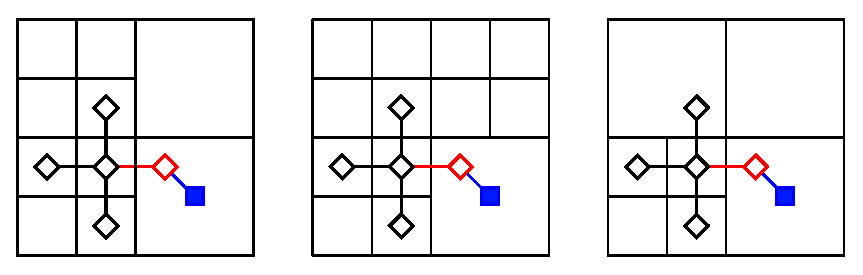
\includegraphics[width=\textwidth,height=\textheight/2,keepaspectratio=true]{fc0}
\doxyfigcaption{F\+C0}
\end{DoxyImage}

\begin{DoxyImage}
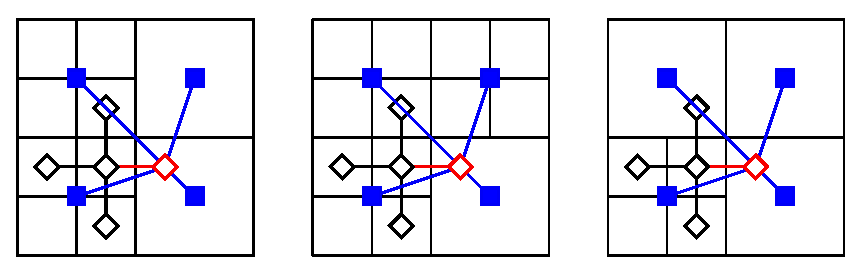
\includegraphics[width=\textwidth,height=\textheight/2,keepaspectratio=true]{fc1}
\doxyfigcaption{F\+C1}
\end{DoxyImage}

\begin{DoxyImage}
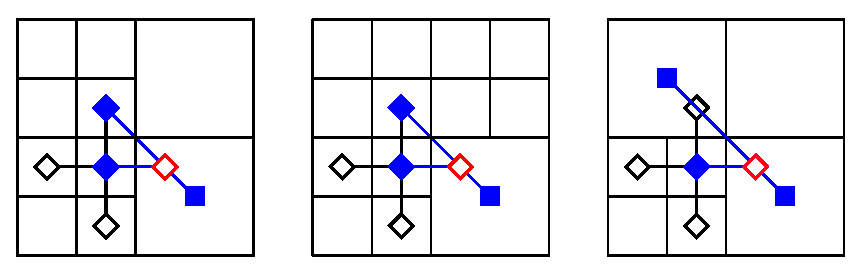
\includegraphics[width=\textwidth,height=\textheight/2,keepaspectratio=true]{fcsimple}
\doxyfigcaption{F\+C\+Simple}
\end{DoxyImage}

\begin{DoxyImage}
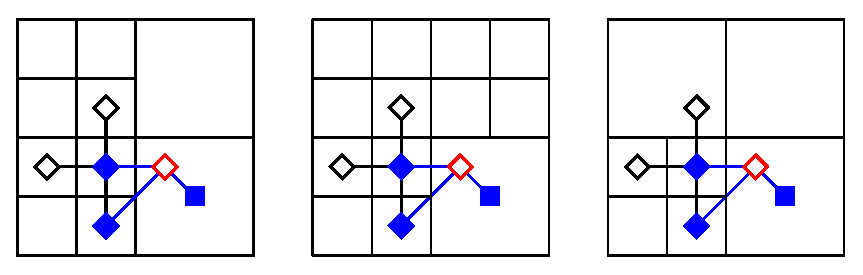
\includegraphics[width=\textwidth,height=\textheight/2,keepaspectratio=true]{fclinear}
\doxyfigcaption{F\+C\+Linear}
\end{DoxyImage}

\begin{DoxyImage}
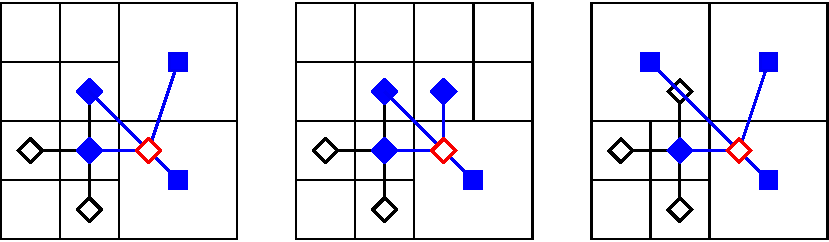
\includegraphics[width=\textwidth,height=\textheight/2,keepaspectratio=true]{fcbilinear}
\doxyfigcaption{F\+C\+Bilinear}
\end{DoxyImage}
\begin{DoxyEnumFields}{Enumerator}
\raisebox{\heightof{T}}[0pt][0pt]{\index{None@{None}!Uintah\+::\+Phase\+Field@{Uintah\+::\+Phase\+Field}}\index{Uintah\+::\+Phase\+Field@{Uintah\+::\+Phase\+Field}!None@{None}}}\mbox{\Hypertarget{namespaceUintah_1_1PhaseField_aeb51fe956fe07f1487f5878f4039f27ca6adf97f83acf6453d4a6a4b1070f3754}\label{namespaceUintah_1_1PhaseField_aeb51fe956fe07f1487f5878f4039f27ca6adf97f83acf6453d4a6a4b1070f3754}} 
None&Continuity across interfaces is not enforced. \\
\hline

\raisebox{\heightof{T}}[0pt][0pt]{\index{F\+C0@{F\+C0}!Uintah\+::\+Phase\+Field@{Uintah\+::\+Phase\+Field}}\index{Uintah\+::\+Phase\+Field@{Uintah\+::\+Phase\+Field}!F\+C0@{F\+C0}}}\mbox{\Hypertarget{namespaceUintah_1_1PhaseField_aeb51fe956fe07f1487f5878f4039f27cae950aa1aad6fdf2c9b8012a0e1f8c1fa}\label{namespaceUintah_1_1PhaseField_aeb51fe956fe07f1487f5878f4039f27cae950aa1aad6fdf2c9b8012a0e1f8c1fa}} 
F\+C0&Piece-\/wise interpolation is used to compute the value on fine levels ghosts from the old solution at coarser levels. \begin{DoxyRemark}{Remarks}
to be used with Hypre\+F\+A\+C\+Solver 

should be used with NC variables since no interpolation is required 
\end{DoxyRemark}
\\
\hline

\raisebox{\heightof{T}}[0pt][0pt]{\index{F\+C1@{F\+C1}!Uintah\+::\+Phase\+Field@{Uintah\+::\+Phase\+Field}}\index{Uintah\+::\+Phase\+Field@{Uintah\+::\+Phase\+Field}!F\+C1@{F\+C1}}}\mbox{\Hypertarget{namespaceUintah_1_1PhaseField_aeb51fe956fe07f1487f5878f4039f27cad752b12b0fc874dddc6f67101b900706}\label{namespaceUintah_1_1PhaseField_aeb51fe956fe07f1487f5878f4039f27cad752b12b0fc874dddc6f67101b900706}} 
F\+C1&Linear interpolation in each direction is used to compute the value on fine levels ghosts from the old solution at coarser levels. \begin{DoxyRemark}{Remarks}
to be used with Hypre\+F\+A\+C\+Solver 

should be used with CC variables since interpolation reduces the approximation error of solution derivatives 
\end{DoxyRemark}
\\
\hline

\raisebox{\heightof{T}}[0pt][0pt]{\index{F\+C\+Simple@{F\+C\+Simple}!Uintah\+::\+Phase\+Field@{Uintah\+::\+Phase\+Field}}\index{Uintah\+::\+Phase\+Field@{Uintah\+::\+Phase\+Field}!F\+C\+Simple@{F\+C\+Simple}}}\mbox{\Hypertarget{namespaceUintah_1_1PhaseField_aeb51fe956fe07f1487f5878f4039f27ca6a316dd1139b99e2a8af86106b3cf045}\label{namespaceUintah_1_1PhaseField_aeb51fe956fe07f1487f5878f4039f27ca6a316dd1139b99e2a8af86106b3cf045}} 
F\+C\+Simple&2 elements interpolation for 2D problems and CC variables \\
\hline

\raisebox{\heightof{T}}[0pt][0pt]{\index{F\+C\+Linear@{F\+C\+Linear}!Uintah\+::\+Phase\+Field@{Uintah\+::\+Phase\+Field}}\index{Uintah\+::\+Phase\+Field@{Uintah\+::\+Phase\+Field}!F\+C\+Linear@{F\+C\+Linear}}}\mbox{\Hypertarget{namespaceUintah_1_1PhaseField_aeb51fe956fe07f1487f5878f4039f27ca7460527a4d3065117218d8822530ed6a}\label{namespaceUintah_1_1PhaseField_aeb51fe956fe07f1487f5878f4039f27ca7460527a4d3065117218d8822530ed6a}} 
F\+C\+Linear&3 elements extrapolation for 2D problems and CC variables \\
\hline

\raisebox{\heightof{T}}[0pt][0pt]{\index{F\+C\+Bilinear@{F\+C\+Bilinear}!Uintah\+::\+Phase\+Field@{Uintah\+::\+Phase\+Field}}\index{Uintah\+::\+Phase\+Field@{Uintah\+::\+Phase\+Field}!F\+C\+Bilinear@{F\+C\+Bilinear}}}\mbox{\Hypertarget{namespaceUintah_1_1PhaseField_aeb51fe956fe07f1487f5878f4039f27ca529374bd8795ca8cdf1e8257ecce2f3a}\label{namespaceUintah_1_1PhaseField_aeb51fe956fe07f1487f5878f4039f27ca529374bd8795ca8cdf1e8257ecce2f3a}} 
F\+C\+Bilinear&4 elements interpolation for 2D problems and CC variables \\
\hline

\end{DoxyEnumFields}
\mbox{\Hypertarget{namespaceUintah_1_1PhaseField_a547ce3002aa97fbd3ef3192a6eec8406}\label{namespaceUintah_1_1PhaseField_a547ce3002aa97fbd3ef3192a6eec8406}} 
\index{Uintah\+::\+Phase\+Field@{Uintah\+::\+Phase\+Field}!F\+C\+I\+Type@{F\+C\+I\+Type}}
\index{F\+C\+I\+Type@{F\+C\+I\+Type}!Uintah\+::\+Phase\+Field@{Uintah\+::\+Phase\+Field}}
\subsubsection{\texorpdfstring{F\+C\+I\+Type}{FCIType}}
{\footnotesize\ttfamily enum \hyperlink{namespaceUintah_1_1PhaseField_a547ce3002aa97fbd3ef3192a6eec8406}{Uintah\+::\+Phase\+Field\+::\+F\+C\+I\+Type} \+: size\+\_\+t}



Interpolation Type. 

Enumeration for different order of interpolations \begin{DoxyEnumFields}{Enumerator}
\raisebox{\heightof{T}}[0pt][0pt]{\index{I0@{I0}!Uintah\+::\+Phase\+Field@{Uintah\+::\+Phase\+Field}}\index{Uintah\+::\+Phase\+Field@{Uintah\+::\+Phase\+Field}!I0@{I0}}}\mbox{\Hypertarget{namespaceUintah_1_1PhaseField_a547ce3002aa97fbd3ef3192a6eec8406abdd8ebcbdfd71d1125937e3012dc45fb}\label{namespaceUintah_1_1PhaseField_a547ce3002aa97fbd3ef3192a6eec8406abdd8ebcbdfd71d1125937e3012dc45fb}} 
I0&Piece-\/wise Interpolation (0th order\+: 1 point stencil. \\
\hline

\raisebox{\heightof{T}}[0pt][0pt]{\index{I1@{I1}!Uintah\+::\+Phase\+Field@{Uintah\+::\+Phase\+Field}}\index{Uintah\+::\+Phase\+Field@{Uintah\+::\+Phase\+Field}!I1@{I1}}}\mbox{\Hypertarget{namespaceUintah_1_1PhaseField_a547ce3002aa97fbd3ef3192a6eec8406a66f19efe774b0d2b6e5844eb2d83d305}\label{namespaceUintah_1_1PhaseField_a547ce3002aa97fbd3ef3192a6eec8406a66f19efe774b0d2b6e5844eb2d83d305}} 
I1&Linear Interpolation in each direction (1st order\+: 2 D\+IM points stencil) \\
\hline

\end{DoxyEnumFields}
\mbox{\Hypertarget{namespaceUintah_1_1PhaseField_a24d833a720598df1020f5cc2e75f8702}\label{namespaceUintah_1_1PhaseField_a24d833a720598df1020f5cc2e75f8702}} 
\index{Uintah\+::\+Phase\+Field@{Uintah\+::\+Phase\+Field}!Stn\+Type@{Stn\+Type}}
\index{Stn\+Type@{Stn\+Type}!Uintah\+::\+Phase\+Field@{Uintah\+::\+Phase\+Field}}
\subsubsection{\texorpdfstring{Stn\+Type}{StnType}}
{\footnotesize\ttfamily enum \hyperlink{namespaceUintah_1_1PhaseField_a24d833a720598df1020f5cc2e75f8702}{Uintah\+::\+Phase\+Field\+::\+Stn\+Type} \+: size\+\_\+t}



Stencil Type. 

Enumeration for different finite-\/difference stencils \begin{DoxyEnumFields}{Enumerator}
\raisebox{\heightof{T}}[0pt][0pt]{\index{P3@{P3}!Uintah\+::\+Phase\+Field@{Uintah\+::\+Phase\+Field}}\index{Uintah\+::\+Phase\+Field@{Uintah\+::\+Phase\+Field}!P3@{P3}}}\mbox{\Hypertarget{namespaceUintah_1_1PhaseField_a24d833a720598df1020f5cc2e75f8702a4f237510ae9624ab7568055802b586c6}\label{namespaceUintah_1_1PhaseField_a24d833a720598df1020f5cc2e75f8702a4f237510ae9624ab7568055802b586c6}} 
P3&3 Point stencil for 1D finite-\/differences \\
\hline

\raisebox{\heightof{T}}[0pt][0pt]{\index{P5@{P5}!Uintah\+::\+Phase\+Field@{Uintah\+::\+Phase\+Field}}\index{Uintah\+::\+Phase\+Field@{Uintah\+::\+Phase\+Field}!P5@{P5}}}\mbox{\Hypertarget{namespaceUintah_1_1PhaseField_a24d833a720598df1020f5cc2e75f8702a218e7fca21085b602c79158a04bc83a0}\label{namespaceUintah_1_1PhaseField_a24d833a720598df1020f5cc2e75f8702a218e7fca21085b602c79158a04bc83a0}} 
P5&5 Point stencil for 2D finite-\/differences \\
\hline

\raisebox{\heightof{T}}[0pt][0pt]{\index{P7@{P7}!Uintah\+::\+Phase\+Field@{Uintah\+::\+Phase\+Field}}\index{Uintah\+::\+Phase\+Field@{Uintah\+::\+Phase\+Field}!P7@{P7}}}\mbox{\Hypertarget{namespaceUintah_1_1PhaseField_a24d833a720598df1020f5cc2e75f8702a099a5b9a00f5644bb917fdec6afd8768}\label{namespaceUintah_1_1PhaseField_a24d833a720598df1020f5cc2e75f8702a099a5b9a00f5644bb917fdec6afd8768}} 
P7&7 Point stencil for 3D finite-\/differences \\
\hline

\raisebox{\heightof{T}}[0pt][0pt]{\index{EU@{EU}!Uintah\+::\+Phase\+Field@{Uintah\+::\+Phase\+Field}}\index{Uintah\+::\+Phase\+Field@{Uintah\+::\+Phase\+Field}!EU@{EU}}}\mbox{\Hypertarget{namespaceUintah_1_1PhaseField_a24d833a720598df1020f5cc2e75f8702a97463475a8bd68261d440a40349a814a}\label{namespaceUintah_1_1PhaseField_a24d833a720598df1020f5cc2e75f8702a97463475a8bd68261d440a40349a814a}} 
EU&5 Point stencil for 2D finite-\/differences as used in campfire \\
\hline

\end{DoxyEnumFields}
\mbox{\Hypertarget{namespaceUintah_1_1PhaseField_a33d355affda78a83f45755ba8388cedd}\label{namespaceUintah_1_1PhaseField_a33d355affda78a83f45755ba8388cedd}} 
\index{Uintah\+::\+Phase\+Field@{Uintah\+::\+Phase\+Field}!Var\+Type@{Var\+Type}}
\index{Var\+Type@{Var\+Type}!Uintah\+::\+Phase\+Field@{Uintah\+::\+Phase\+Field}}
\subsubsection{\texorpdfstring{Var\+Type}{VarType}}
{\footnotesize\ttfamily enum \hyperlink{namespaceUintah_1_1PhaseField_a33d355affda78a83f45755ba8388cedd}{Uintah\+::\+Phase\+Field\+::\+Var\+Type} \+: size\+\_\+t}



\hyperlink{structUintah_1_1PhaseField_1_1Variable}{Variable} Type. 

Enumeration for different types of variable representation \begin{DoxyEnumFields}{Enumerator}
\raisebox{\heightof{T}}[0pt][0pt]{\index{CC@{CC}!Uintah\+::\+Phase\+Field@{Uintah\+::\+Phase\+Field}}\index{Uintah\+::\+Phase\+Field@{Uintah\+::\+Phase\+Field}!CC@{CC}}}\mbox{\Hypertarget{namespaceUintah_1_1PhaseField_a33d355affda78a83f45755ba8388cedda22303704507d024d1d6508ed9859a85a}\label{namespaceUintah_1_1PhaseField_a33d355affda78a83f45755ba8388cedda22303704507d024d1d6508ed9859a85a}} 
CC&Cell Centered \hyperlink{structUintah_1_1PhaseField_1_1Variable}{Variable}. \\
\hline

\raisebox{\heightof{T}}[0pt][0pt]{\index{NC@{NC}!Uintah\+::\+Phase\+Field@{Uintah\+::\+Phase\+Field}}\index{Uintah\+::\+Phase\+Field@{Uintah\+::\+Phase\+Field}!NC@{NC}}}\mbox{\Hypertarget{namespaceUintah_1_1PhaseField_a33d355affda78a83f45755ba8388cedda77924170fe82bfd58b74ca3e44139718}\label{namespaceUintah_1_1PhaseField_a33d355affda78a83f45755ba8388cedda77924170fe82bfd58b74ca3e44139718}} 
NC&Node Centered \hyperlink{structUintah_1_1PhaseField_1_1Variable}{Variable}. \\
\hline

\raisebox{\heightof{T}}[0pt][0pt]{\index{PP@{PP}!Uintah\+::\+Phase\+Field@{Uintah\+::\+Phase\+Field}}\index{Uintah\+::\+Phase\+Field@{Uintah\+::\+Phase\+Field}!PP@{PP}}}\mbox{\Hypertarget{namespaceUintah_1_1PhaseField_a33d355affda78a83f45755ba8388ceddada289ff9f2ba3ad8077f45c9070afa2e}\label{namespaceUintah_1_1PhaseField_a33d355affda78a83f45755ba8388ceddada289ff9f2ba3ad8077f45c9070afa2e}} 
PP&Per\+Patch \hyperlink{structUintah_1_1PhaseField_1_1Variable}{Variable} ( used for Problems ) \\
\hline

\end{DoxyEnumFields}


\subsection{Function Documentation}
\mbox{\Hypertarget{namespaceUintah_1_1PhaseField_ad205f402e20ed9209f12265147bd4e5c}\label{namespaceUintah_1_1PhaseField_ad205f402e20ed9209f12265147bd4e5c}} 
\index{Uintah\+::\+Phase\+Field@{Uintah\+::\+Phase\+Field}!bc\+\_\+to\+\_\+str@{bc\+\_\+to\+\_\+str}}
\index{bc\+\_\+to\+\_\+str@{bc\+\_\+to\+\_\+str}!Uintah\+::\+Phase\+Field@{Uintah\+::\+Phase\+Field}}
\subsubsection{\texorpdfstring{bc\+\_\+to\+\_\+str()}{bc\_to\_str()}}
{\footnotesize\ttfamily std\+::string Uintah\+::\+Phase\+Field\+::bc\+\_\+to\+\_\+str (\begin{DoxyParamCaption}\item[{\hyperlink{namespaceUintah_1_1PhaseField_a148fba372aa3be96fd6eede7a2fa10b5}{BC}}]{value }\end{DoxyParamCaption})\hspace{0.3cm}{\ttfamily [inline]}}



BC to std\+::string. 

Converts the type of boundary conditions to the corresponding string as used by factory constructors \mbox{\Hypertarget{namespaceUintah_1_1PhaseField_a89a79191f10636fd81e9900120c16bf3}\label{namespaceUintah_1_1PhaseField_a89a79191f10636fd81e9900120c16bf3}} 
\index{Uintah\+::\+Phase\+Field@{Uintah\+::\+Phase\+Field}!dim\+\_\+to\+\_\+str@{dim\+\_\+to\+\_\+str}}
\index{dim\+\_\+to\+\_\+str@{dim\+\_\+to\+\_\+str}!Uintah\+::\+Phase\+Field@{Uintah\+::\+Phase\+Field}}
\subsubsection{\texorpdfstring{dim\+\_\+to\+\_\+str()}{dim\_to\_str()}}
{\footnotesize\ttfamily std\+::string Uintah\+::\+Phase\+Field\+::dim\+\_\+to\+\_\+str (\begin{DoxyParamCaption}\item[{\hyperlink{namespaceUintah_1_1PhaseField_a12bfc68444894dffdf0cb8d9cf0cc76a}{Dim\+Type}}]{dim }\end{DoxyParamCaption})\hspace{0.3cm}{\ttfamily [inline]}}



Dim\+Type to std\+::string. 

Converts the problem dimension to the corresponding string as used by factory constructors \mbox{\Hypertarget{namespaceUintah_1_1PhaseField_a210a65278fe4cc9c19a428de018272ec}\label{namespaceUintah_1_1PhaseField_a210a65278fe4cc9c19a428de018272ec}} 
\index{Uintah\+::\+Phase\+Field@{Uintah\+::\+Phase\+Field}!dir\+\_\+to\+\_\+str@{dir\+\_\+to\+\_\+str}}
\index{dir\+\_\+to\+\_\+str@{dir\+\_\+to\+\_\+str}!Uintah\+::\+Phase\+Field@{Uintah\+::\+Phase\+Field}}
\subsubsection{\texorpdfstring{dir\+\_\+to\+\_\+str()}{dir\_to\_str()}}
{\footnotesize\ttfamily std\+::string Uintah\+::\+Phase\+Field\+::dir\+\_\+to\+\_\+str (\begin{DoxyParamCaption}\item[{\hyperlink{namespaceUintah_1_1PhaseField_a94555da848596a419ae2c0e32649e1dc}{Dir\+Type}}]{dir }\end{DoxyParamCaption})\hspace{0.3cm}{\ttfamily [inline]}}



Dir\+Type to std\+::string. 

Converts the type of variable representation to the corresponding string as used by factory constructors \mbox{\Hypertarget{namespaceUintah_1_1PhaseField_a3efdada0de283a3b4482293537e59452}\label{namespaceUintah_1_1PhaseField_a3efdada0de283a3b4482293537e59452}} 
\index{Uintah\+::\+Phase\+Field@{Uintah\+::\+Phase\+Field}!fc\+\_\+to\+\_\+str@{fc\+\_\+to\+\_\+str}}
\index{fc\+\_\+to\+\_\+str@{fc\+\_\+to\+\_\+str}!Uintah\+::\+Phase\+Field@{Uintah\+::\+Phase\+Field}}
\subsubsection{\texorpdfstring{fc\+\_\+to\+\_\+str()}{fc\_to\_str()}}
{\footnotesize\ttfamily std\+::string Uintah\+::\+Phase\+Field\+::fc\+\_\+to\+\_\+str (\begin{DoxyParamCaption}\item[{\hyperlink{namespaceUintah_1_1PhaseField_aeb51fe956fe07f1487f5878f4039f27c}{FC}}]{value }\end{DoxyParamCaption})\hspace{0.3cm}{\ttfamily [inline]}}



FC to std\+::string. 

Converts the type of fine/coarse interface conditions to the corresponding string as used by factory constructors \mbox{\Hypertarget{namespaceUintah_1_1PhaseField_a98ea8b8abff26138762ce1898ce6c424}\label{namespaceUintah_1_1PhaseField_a98ea8b8abff26138762ce1898ce6c424}} 
\index{Uintah\+::\+Phase\+Field@{Uintah\+::\+Phase\+Field}!operator\&@{operator\&}}
\index{operator\&@{operator\&}!Uintah\+::\+Phase\+Field@{Uintah\+::\+Phase\+Field}}
\subsubsection{\texorpdfstring{operator\&()}{operator\&()}}
{\footnotesize\ttfamily constexpr bool Uintah\+::\+Phase\+Field\+::operator \& (\begin{DoxyParamCaption}\item[{\hyperlink{namespaceUintah_1_1PhaseField_aeb51fe956fe07f1487f5878f4039f27c}{FC}}]{a,  }\item[{\hyperlink{namespaceUintah_1_1PhaseField_aeb51fe956fe07f1487f5878f4039f27c}{FC}}]{b }\end{DoxyParamCaption})}



Check FC masks. 

Evaluate if a given FC matches a required type (or category) of fine/coarse interface conditions 
\begin{DoxyParams}{Parameters}
{\em a} & TS to check \\
\hline
{\em b} & TS required type or category of fine/coarse interface conditions \\
\hline
\end{DoxyParams}
\begin{DoxyReturn}{Returns}
check result 
\end{DoxyReturn}
\mbox{\Hypertarget{namespaceUintah_1_1PhaseField_af380c33ff438112a2ddff1a51432d4ce}\label{namespaceUintah_1_1PhaseField_af380c33ff438112a2ddff1a51432d4ce}} 
\index{Uintah\+::\+Phase\+Field@{Uintah\+::\+Phase\+Field}!operator$<$$<$@{operator$<$$<$}}
\index{operator$<$$<$@{operator$<$$<$}!Uintah\+::\+Phase\+Field@{Uintah\+::\+Phase\+Field}}
\subsubsection{\texorpdfstring{operator$<$$<$()}{operator<<()}\hspace{0.1cm}{\footnotesize\ttfamily [1/2]}}
{\footnotesize\ttfamily std\+::ostream\& Uintah\+::\+Phase\+Field\+::operator$<$$<$ (\begin{DoxyParamCaption}\item[{std\+::ostream \&}]{stream,  }\item[{const Block\+Range \&}]{range }\end{DoxyParamCaption})\hspace{0.3cm}{\ttfamily [inline]}}



Insertion operator between Block\+Range and std\+::ostream. 

Used for debug purposes


\begin{DoxyParams}{Parameters}
{\em stream} & output stream reference \\
\hline
{\em range} & range to output \\
\hline
\end{DoxyParams}
\begin{DoxyReturn}{Returns}
output stream reference for concatenation 
\end{DoxyReturn}
\mbox{\Hypertarget{namespaceUintah_1_1PhaseField_a2db17c3638c3df36c1050d6a89d0dbd5}\label{namespaceUintah_1_1PhaseField_a2db17c3638c3df36c1050d6a89d0dbd5}} 
\index{Uintah\+::\+Phase\+Field@{Uintah\+::\+Phase\+Field}!operator$<$$<$@{operator$<$$<$}}
\index{operator$<$$<$@{operator$<$$<$}!Uintah\+::\+Phase\+Field@{Uintah\+::\+Phase\+Field}}
\subsubsection{\texorpdfstring{operator$<$$<$()}{operator<<()}\hspace{0.1cm}{\footnotesize\ttfamily [2/2]}}
{\footnotesize\ttfamily template$<$Phase\+Field\+::\+Var\+Type V\+AR, Phase\+Field\+::\+Stn\+Type S\+TN, typename... T$>$ \\
std\+::ostream\& Uintah\+::\+Phase\+Field\+::operator$<$$<$ (\begin{DoxyParamCaption}\item[{std\+::ostream \&}]{os,  }\item[{const \hyperlink{classUintah_1_1PhaseField_1_1Problem}{Phase\+Field\+::\+Problem}$<$ V\+AR, S\+TN, T... $>$ \&}]{p }\end{DoxyParamCaption})}



Insertion operator between \hyperlink{classUintah_1_1PhaseField_1_1Problem}{Problem} and std\+::ostream. 

Used for debug purposes


\begin{DoxyParams}{Parameters}
{\em os} & output stream reference \\
\hline
{\em p} & problem to output \\
\hline
\end{DoxyParams}
\begin{DoxyReturn}{Returns}
output stream reference for concatenation 
\end{DoxyReturn}
\mbox{\Hypertarget{namespaceUintah_1_1PhaseField_acafefaa50f1ec411fdb981feac59c488}\label{namespaceUintah_1_1PhaseField_acafefaa50f1ec411fdb981feac59c488}} 
\index{Uintah\+::\+Phase\+Field@{Uintah\+::\+Phase\+Field}!operator\texttt{"|}@{operator\texttt{"|}}}
\index{operator\texttt{"|}@{operator\texttt{"|}}!Uintah\+::\+Phase\+Field@{Uintah\+::\+Phase\+Field}}
\subsubsection{\texorpdfstring{operator\texttt{"|}()}{operator|()}\hspace{0.1cm}{\footnotesize\ttfamily [1/3]}}
{\footnotesize\ttfamily template$<$typename A $>$ \\
constexpr \hyperlink{namespaceUintah_1_1PhaseField_ab9b5949afaa59b9b862e606410431331}{B\+CF} Uintah\+::\+Phase\+Field\+::operator$\vert$ (\begin{DoxyParamCaption}\item[{A}]{a,  }\item[{\hyperlink{namespaceUintah_1_1PhaseField_aeb51fe956fe07f1487f5878f4039f27c}{FC}}]{b }\end{DoxyParamCaption})}

\mbox{\Hypertarget{namespaceUintah_1_1PhaseField_aa2de98442fe079b97ff71c974452edf2}\label{namespaceUintah_1_1PhaseField_aa2de98442fe079b97ff71c974452edf2}} 
\index{Uintah\+::\+Phase\+Field@{Uintah\+::\+Phase\+Field}!operator\texttt{"|}@{operator\texttt{"|}}}
\index{operator\texttt{"|}@{operator\texttt{"|}}!Uintah\+::\+Phase\+Field@{Uintah\+::\+Phase\+Field}}
\subsubsection{\texorpdfstring{operator\texttt{"|}()}{operator|()}\hspace{0.1cm}{\footnotesize\ttfamily [2/3]}}
{\footnotesize\ttfamily template$<$typename A $>$ \\
constexpr \hyperlink{namespaceUintah_1_1PhaseField_ab9b5949afaa59b9b862e606410431331}{B\+CF} Uintah\+::\+Phase\+Field\+::operator$\vert$ (\begin{DoxyParamCaption}\item[{A}]{a,  }\item[{\hyperlink{namespaceUintah_1_1PhaseField_a148fba372aa3be96fd6eede7a2fa10b5}{BC}}]{b }\end{DoxyParamCaption})}

\mbox{\Hypertarget{namespaceUintah_1_1PhaseField_aef70a549ef150398587c759d5676b128}\label{namespaceUintah_1_1PhaseField_aef70a549ef150398587c759d5676b128}} 
\index{Uintah\+::\+Phase\+Field@{Uintah\+::\+Phase\+Field}!operator\texttt{"|}@{operator\texttt{"|}}}
\index{operator\texttt{"|}@{operator\texttt{"|}}!Uintah\+::\+Phase\+Field@{Uintah\+::\+Phase\+Field}}
\subsubsection{\texorpdfstring{operator\texttt{"|}()}{operator|()}\hspace{0.1cm}{\footnotesize\ttfamily [3/3]}}
{\footnotesize\ttfamily template$<$typename A $>$ \\
constexpr \hyperlink{namespaceUintah_1_1PhaseField_ab9b5949afaa59b9b862e606410431331}{B\+CF} Uintah\+::\+Phase\+Field\+::operator$\vert$ (\begin{DoxyParamCaption}\item[{A}]{a,  }\item[{Patch\+::\+Face\+Type}]{b }\end{DoxyParamCaption})}

\mbox{\Hypertarget{namespaceUintah_1_1PhaseField_ae83ff43dad3972682130259154aa13ef}\label{namespaceUintah_1_1PhaseField_ae83ff43dad3972682130259154aa13ef}} 
\index{Uintah\+::\+Phase\+Field@{Uintah\+::\+Phase\+Field}!stn\+\_\+to\+\_\+str@{stn\+\_\+to\+\_\+str}}
\index{stn\+\_\+to\+\_\+str@{stn\+\_\+to\+\_\+str}!Uintah\+::\+Phase\+Field@{Uintah\+::\+Phase\+Field}}
\subsubsection{\texorpdfstring{stn\+\_\+to\+\_\+str()}{stn\_to\_str()}}
{\footnotesize\ttfamily std\+::string Uintah\+::\+Phase\+Field\+::stn\+\_\+to\+\_\+str (\begin{DoxyParamCaption}\item[{\hyperlink{namespaceUintah_1_1PhaseField_a24d833a720598df1020f5cc2e75f8702}{Stn\+Type}}]{stn }\end{DoxyParamCaption})\hspace{0.3cm}{\ttfamily [inline]}}



Stn\+Type to std\+::string. 

Converts the finite-\/difference stencil to the corresponding string as used by factory constructors \mbox{\Hypertarget{namespaceUintah_1_1PhaseField_ae111bd8827ecc139cc3c88e52ceb141d}\label{namespaceUintah_1_1PhaseField_ae111bd8827ecc139cc3c88e52ceb141d}} 
\index{Uintah\+::\+Phase\+Field@{Uintah\+::\+Phase\+Field}!str\+\_\+to\+\_\+bc@{str\+\_\+to\+\_\+bc}}
\index{str\+\_\+to\+\_\+bc@{str\+\_\+to\+\_\+bc}!Uintah\+::\+Phase\+Field@{Uintah\+::\+Phase\+Field}}
\subsubsection{\texorpdfstring{str\+\_\+to\+\_\+bc()}{str\_to\_bc()}}
{\footnotesize\ttfamily \hyperlink{namespaceUintah_1_1PhaseField_a148fba372aa3be96fd6eede7a2fa10b5}{BC} Uintah\+::\+Phase\+Field\+::str\+\_\+to\+\_\+bc (\begin{DoxyParamCaption}\item[{const std\+::string \&}]{value }\end{DoxyParamCaption})\hspace{0.3cm}{\ttfamily [inline]}}



std\+::string to BC 

Converts the string as used in input files to the corresponding type of boundary conditions \mbox{\Hypertarget{namespaceUintah_1_1PhaseField_a1b73af9bf55d015e399d292360fd700b}\label{namespaceUintah_1_1PhaseField_a1b73af9bf55d015e399d292360fd700b}} 
\index{Uintah\+::\+Phase\+Field@{Uintah\+::\+Phase\+Field}!str\+\_\+to\+\_\+fc@{str\+\_\+to\+\_\+fc}}
\index{str\+\_\+to\+\_\+fc@{str\+\_\+to\+\_\+fc}!Uintah\+::\+Phase\+Field@{Uintah\+::\+Phase\+Field}}
\subsubsection{\texorpdfstring{str\+\_\+to\+\_\+fc()}{str\_to\_fc()}}
{\footnotesize\ttfamily \hyperlink{namespaceUintah_1_1PhaseField_aeb51fe956fe07f1487f5878f4039f27c}{FC} Uintah\+::\+Phase\+Field\+::str\+\_\+to\+\_\+fc (\begin{DoxyParamCaption}\item[{const std\+::string \&}]{value }\end{DoxyParamCaption})\hspace{0.3cm}{\ttfamily [inline]}}



std\+::string to FC 

Converts the string as used in input files to the corresponding type of fine/coarse interface condition \mbox{\Hypertarget{namespaceUintah_1_1PhaseField_a85973f31ba84b1b5e1b9efa32baef615}\label{namespaceUintah_1_1PhaseField_a85973f31ba84b1b5e1b9efa32baef615}} 
\index{Uintah\+::\+Phase\+Field@{Uintah\+::\+Phase\+Field}!var\+\_\+to\+\_\+str@{var\+\_\+to\+\_\+str}}
\index{var\+\_\+to\+\_\+str@{var\+\_\+to\+\_\+str}!Uintah\+::\+Phase\+Field@{Uintah\+::\+Phase\+Field}}
\subsubsection{\texorpdfstring{var\+\_\+to\+\_\+str()}{var\_to\_str()}}
{\footnotesize\ttfamily std\+::string Uintah\+::\+Phase\+Field\+::var\+\_\+to\+\_\+str (\begin{DoxyParamCaption}\item[{\hyperlink{namespaceUintah_1_1PhaseField_a33d355affda78a83f45755ba8388cedd}{Var\+Type}}]{var }\end{DoxyParamCaption})\hspace{0.3cm}{\ttfamily [inline]}}



Var\+Type to std\+::string. 

Converts the type of variable representation to the corresponding string as used by factory constructors 
\hypertarget{namespaceUintah_1_1PhaseField_1_1detail}{}\section{Uintah\+:\+:Phase\+Field\+:\+:detail Namespace Reference}
\label{namespaceUintah_1_1PhaseField_1_1detail}\index{Uintah\+::\+Phase\+Field\+::detail@{Uintah\+::\+Phase\+Field\+::detail}}
\subsection*{Classes}
\begin{DoxyCompactItemize}
\item 
class \hyperlink{classUintah_1_1PhaseField_1_1detail_1_1amr__coarser__view}{amr\+\_\+coarser\+\_\+view}
\begin{DoxyCompactList}\small\item\em Composite view for accessing coarser grid variables. \end{DoxyCompactList}\item 
class \hyperlink{classUintah_1_1PhaseField_1_1detail_1_1amr__coarser__view_3_01ScalarField_3_01T_01_4_00_01Proble9cadea116dab5bdb44bb3e29abbe99ef}{amr\+\_\+coarser\+\_\+view$<$ Scalar\+Field$<$ T $>$, Problem, index\+\_\+sequence$<$ I... $>$ $>$}
\begin{DoxyCompactList}\small\item\em Composite view for accessing coarser grid variables (\hyperlink{structUintah_1_1PhaseField_1_1ScalarField}{Scalar\+Field} implementation) \end{DoxyCompactList}\item 
class \hyperlink{classUintah_1_1PhaseField_1_1detail_1_1amr__finer__view}{amr\+\_\+finer\+\_\+view}
\begin{DoxyCompactList}\small\item\em Composite view for accessing coarser grid variables. \end{DoxyCompactList}\item 
class \hyperlink{classUintah_1_1PhaseField_1_1detail_1_1amr__finer__view_3_01ScalarField_3_01T_01_4_00_01Problem_810ae3f886a4d3bdb2b37c629369a2ec}{amr\+\_\+finer\+\_\+view$<$ Scalar\+Field$<$ T $>$, Problem, index\+\_\+sequence$<$ I... $>$ $>$}
\begin{DoxyCompactList}\small\item\em Composite view for accessing finer grid variables (\hyperlink{structUintah_1_1PhaseField_1_1ScalarField}{Scalar\+Field} implementation) \end{DoxyCompactList}\item 
class \hyperlink{classUintah_1_1PhaseField_1_1detail_1_1amr__interface0}{amr\+\_\+interface0}
\begin{DoxyCompactList}\small\item\em Interface for amr. \end{DoxyCompactList}\item 
class \hyperlink{classUintah_1_1PhaseField_1_1detail_1_1amr__interface0_3_01CC_01_4}{amr\+\_\+interface0$<$ C\+C $>$}
\begin{DoxyCompactList}\small\item\em Interface for amr (CC implementation) \end{DoxyCompactList}\item 
class \hyperlink{classUintah_1_1PhaseField_1_1detail_1_1amr__interface0_3_01NC_01_4}{amr\+\_\+interface0$<$ N\+C $>$}
\begin{DoxyCompactList}\small\item\em Interface for amr (NC implementation) \end{DoxyCompactList}\item 
class \hyperlink{classUintah_1_1PhaseField_1_1detail_1_1amr__interpolator}{amr\+\_\+interpolator}
\begin{DoxyCompactList}\small\item\em Abstract wrapper of grid variables for interpolation from coarser to finer levels. \end{DoxyCompactList}\item 
class \hyperlink{classUintah_1_1PhaseField_1_1detail_1_1amr__interpolator_3_01ScalarField_3_01T_01_4_00_01Problem64f2458f98b03e27672a091eecc4b696}{amr\+\_\+interpolator$<$ Scalar\+Field$<$ T $>$, Problem, index\+\_\+sequence$<$ I... $>$, I0, D\+I\+M $>$}
\begin{DoxyCompactList}\small\item\em Wrapper of grid variables for interpolation from coarser to finer levels (piecewise implementation) \end{DoxyCompactList}\item 
class \hyperlink{classUintah_1_1PhaseField_1_1detail_1_1amr__interpolator_3_01ScalarField_3_01T_01_4_00_01Problem71844444bc14a03c0566689b6b502040}{amr\+\_\+interpolator$<$ Scalar\+Field$<$ T $>$, Problem, index\+\_\+sequence$<$ I... $>$, I1, D1 $>$}
\begin{DoxyCompactList}\small\item\em Wrapper of grid variables for interpolation from coarser to finer levels (1D linear implementation) \end{DoxyCompactList}\item 
class \hyperlink{classUintah_1_1PhaseField_1_1detail_1_1amr__interpolator_3_01ScalarField_3_01T_01_4_00_01Problemd2db9de1754b5450c93c191a9275f5ed}{amr\+\_\+interpolator$<$ Scalar\+Field$<$ T $>$, Problem, index\+\_\+sequence$<$ I... $>$, I1, D2 $>$}
\begin{DoxyCompactList}\small\item\em Implements linear interpolation of a variable from coarser to finer levels in 2D. \end{DoxyCompactList}\item 
class \hyperlink{classUintah_1_1PhaseField_1_1detail_1_1amr__interpolator_3_01ScalarField_3_01T_01_4_00_01Problemdf68628a6010a1e1526666730125c372}{amr\+\_\+interpolator$<$ Scalar\+Field$<$ T $>$, Problem, index\+\_\+sequence$<$ I... $>$, I1, D3 $>$}
\begin{DoxyCompactList}\small\item\em Wrapper of grid variables for interpolation from coarser to finer levels (3D linear implementation) \end{DoxyCompactList}\item 
class \hyperlink{classUintah_1_1PhaseField_1_1detail_1_1amr__interpolator_3_01VectorField_3_01T_00_01N_01_4_00_01ab3739ebd28e1ffb5bc0b138cfaddd80}{amr\+\_\+interpolator$<$ Vector\+Field$<$ T, N $>$, Problem, Index, F\+C\+I, D\+I\+M $>$}
\begin{DoxyCompactList}\small\item\em Abstract wrapper of grid variables for interpolation from coarser to finer levels. (\hyperlink{structUintah_1_1PhaseField_1_1VectorField}{Vector\+Field} implementation) \end{DoxyCompactList}\item 
class \hyperlink{classUintah_1_1PhaseField_1_1detail_1_1amr__restrictor}{amr\+\_\+restrictor}
\begin{DoxyCompactList}\small\item\em Abstract wrapper of grid variables for restriction from finer to coarser levels. \end{DoxyCompactList}\item 
class \hyperlink{classUintah_1_1PhaseField_1_1detail_1_1amr__restrictor_3_01ScalarField_3_01T_01_4_00_01Problem_05760ee5d1d3adcc969b3f56f71e72acb}{amr\+\_\+restrictor$<$ Scalar\+Field$<$ T $>$, Problem, index\+\_\+sequence$<$ I... $>$, I0, N\+C $>$}
\begin{DoxyCompactList}\small\item\em Wrapper of grid variables for restriction from finer to coarser levels (node-\/centered piecewise constant implementation) \end{DoxyCompactList}\item 
class \hyperlink{classUintah_1_1PhaseField_1_1detail_1_1amr__restrictor_3_01ScalarField_3_01T_01_4_00_01Problem_0778720acc9a55f696b8537356a4dbcae}{amr\+\_\+restrictor$<$ Scalar\+Field$<$ T $>$, Problem, index\+\_\+sequence$<$ I... $>$, I1, C\+C $>$}
\begin{DoxyCompactList}\small\item\em Wrapper of grid variables for restriction from finer to coarser levels (cell-\/centered linear implementation) \end{DoxyCompactList}\item 
class \hyperlink{classUintah_1_1PhaseField_1_1detail_1_1amr__restrictor_3_01VectorField_3_01T_00_01N_01_4_00_01Pre7f2e99a4fbf25ff00717d25c8580b1a}{amr\+\_\+restrictor$<$ Vector\+Field$<$ T, N $>$, Problem, Index, F\+C\+I, D\+I\+M $>$}
\begin{DoxyCompactList}\small\item\em Abstract wrapper of grid variables for restriction from finer to coarser levels. (\hyperlink{structUintah_1_1PhaseField_1_1VectorField}{Vector\+Field} implementation) \end{DoxyCompactList}\item 
class \hyperlink{classUintah_1_1PhaseField_1_1detail_1_1basic__fd__view}{basic\+\_\+fd\+\_\+view}
\begin{DoxyCompactList}\small\item\em Abstract wrapper of grid variables for basic finite-\/difference operations. \end{DoxyCompactList}\item 
class \hyperlink{classUintah_1_1PhaseField_1_1detail_1_1basic__fd__view_3_01ScalarField_3_01T_01_4_00_01STN_01_4}{basic\+\_\+fd\+\_\+view$<$ Scalar\+Field$<$ T $>$, S\+T\+N $>$}
\begin{DoxyCompactList}\small\item\em Abstract class for basic finite-\/difference operations on variables (\hyperlink{structUintah_1_1PhaseField_1_1ScalarField}{Scalar\+Field} implementation) \end{DoxyCompactList}\item 
class \hyperlink{classUintah_1_1PhaseField_1_1detail_1_1basic__fd__view_3_01VectorField_3_01T_00_01N_01_4_00_01STN_01_4}{basic\+\_\+fd\+\_\+view$<$ Vector\+Field$<$ T, N $>$, S\+T\+N $>$}
\begin{DoxyCompactList}\small\item\em Abstract class for basic finite-\/difference operations on variables (\hyperlink{structUintah_1_1PhaseField_1_1VectorField}{Vector\+Field} implementation) \end{DoxyCompactList}\item 
class \hyperlink{classUintah_1_1PhaseField_1_1detail_1_1bc__basic__fd__view}{bc\+\_\+basic\+\_\+fd\+\_\+view}
\begin{DoxyCompactList}\small\item\em Wrapper of Data\+Warehouse variables for basic differential operations. \end{DoxyCompactList}\item 
class \hyperlink{classUintah_1_1PhaseField_1_1detail_1_1bc__basic__fd__view_3_01ScalarField_3_01T_01_4_00_01STN_00_01VAR_00_01P_01_4}{bc\+\_\+basic\+\_\+fd\+\_\+view$<$ Scalar\+Field$<$ T $>$, S\+T\+N, V\+A\+R, P $>$}
\begin{DoxyCompactList}\small\item\em Wrapper of Data\+Warehouse variables for basic differential operations (\hyperlink{structUintah_1_1PhaseField_1_1ScalarField}{Scalar\+Field} implementation) \end{DoxyCompactList}\item 
class \hyperlink{classUintah_1_1PhaseField_1_1detail_1_1bc__fd}{bc\+\_\+fd}
\begin{DoxyCompactList}\small\item\em Abstract finite-\/differences scheme for variables at grid boundary. \end{DoxyCompactList}\item 
class \hyperlink{classUintah_1_1PhaseField_1_1detail_1_1bc__fd_3_01ScalarField_3_01T_01_4_00_01STN_00_01CC_00_01Fa77b2fd7fb77d0a4dc6c86c68d4ea0bc}{bc\+\_\+fd$<$ Scalar\+Field$<$ T $>$, S\+T\+N, C\+C, F, B\+C\+::\+Dirichlet, 1 $>$}
\begin{DoxyCompactList}\small\item\em Finite-\/differences scheme at Dirichlet boundaries interface (\hyperlink{structUintah_1_1PhaseField_1_1ScalarField}{Scalar\+Field}, Cell-\/centered, 1-\/ghost stencils implementation) \end{DoxyCompactList}\item 
class \hyperlink{classUintah_1_1PhaseField_1_1detail_1_1bc__fd_3_01ScalarField_3_01T_01_4_00_01STN_00_01CC_00_01F_00_01BC_1_1Neumann_00_011_01_4}{bc\+\_\+fd$<$ Scalar\+Field$<$ T $>$, S\+T\+N, C\+C, F, B\+C\+::\+Neumann, 1 $>$}
\begin{DoxyCompactList}\small\item\em Finite-\/differences scheme at Neumann boundaries interface (\hyperlink{structUintah_1_1PhaseField_1_1ScalarField}{Scalar\+Field}, Cell-\/centered, 1-\/ghost stencils implementation) \end{DoxyCompactList}\item 
class \hyperlink{classUintah_1_1PhaseField_1_1detail_1_1bc__fd_3_01ScalarField_3_01T_01_4_00_01STN_00_01NC_00_01Fc8a6e28ffa258d282d0a921216b0ed9f}{bc\+\_\+fd$<$ Scalar\+Field$<$ T $>$, S\+T\+N, N\+C, F, B\+C\+::\+Dirichlet, 1 $>$}
\begin{DoxyCompactList}\small\item\em Finite-\/differences scheme at Dirichlet boundaries interface (\hyperlink{structUintah_1_1PhaseField_1_1ScalarField}{Scalar\+Field}, node-\/centered, 1-\/ghost stencils implementation) \end{DoxyCompactList}\item 
class \hyperlink{classUintah_1_1PhaseField_1_1detail_1_1bc__fd_3_01ScalarField_3_01T_01_4_00_01STN_00_01NC_00_01F_00_01BC_1_1Neumann_00_011_01_4}{bc\+\_\+fd$<$ Scalar\+Field$<$ T $>$, S\+T\+N, N\+C, F, B\+C\+::\+Neumann, 1 $>$}
\begin{DoxyCompactList}\small\item\em Finite-\/differences scheme at Neumann boundaries interface (\hyperlink{structUintah_1_1PhaseField_1_1ScalarField}{Scalar\+Field}, node-\/centered, 1-\/ghost stencils implementation) \end{DoxyCompactList}\item 
class \hyperlink{classUintah_1_1PhaseField_1_1detail_1_1bc__fd_3_01ScalarField_3_01T_01_4_00_01STN_00_01VAR_00_01efea904a4b4ba4f7ece7ded248f84d17}{bc\+\_\+fd$<$ Scalar\+Field$<$ T $>$, S\+T\+N, V\+A\+R, F, B\+C\+::\+Fine\+Coarse\+Interface, 1, C2\+F $>$}
\begin{DoxyCompactList}\small\item\em Finite-\/differences scheme at fine/coarse interfaces (1-\/ghost stencils) (\hyperlink{structUintah_1_1PhaseField_1_1ScalarField}{Scalar\+Field} implementation) \end{DoxyCompactList}\item 
class \hyperlink{classUintah_1_1PhaseField_1_1detail_1_1bc__fd_3_01ScalarField_3_01T_01_4_00_01STN_00_01VAR_00_01bd5f5aa94f34afad5c8a785ee391ed2b}{bc\+\_\+fd$<$ Scalar\+Field$<$ T $>$, S\+T\+N, V\+A\+R, F, B\+C\+::\+Fine\+Coarse\+Interface, 1, F\+C\+::\+F\+C\+Bilinear $>$}
\begin{DoxyCompactList}\small\item\em Finite-\/differences scheme at fine/coarse interfaces (1-\/ghost stencils) (\hyperlink{structUintah_1_1PhaseField_1_1ScalarField}{Scalar\+Field} implementation) \end{DoxyCompactList}\item 
class \hyperlink{classUintah_1_1PhaseField_1_1detail_1_1bc__fd_3_01ScalarField_3_01T_01_4_00_01STN_00_01VAR_00_01f836207db876ecd28bf65f631f79030f}{bc\+\_\+fd$<$ Scalar\+Field$<$ T $>$, S\+T\+N, V\+A\+R, F, B\+C\+::\+Fine\+Coarse\+Interface, 1, F\+C\+::\+F\+C\+Linear $>$}
\begin{DoxyCompactList}\small\item\em Finite-\/differences scheme at fine/coarse interfaces (1-\/ghost stencils) (\hyperlink{structUintah_1_1PhaseField_1_1ScalarField}{Scalar\+Field} implementation) \end{DoxyCompactList}\item 
class \hyperlink{classUintah_1_1PhaseField_1_1detail_1_1bc__fd_3_01ScalarField_3_01T_01_4_00_01STN_00_01VAR_00_01ce55d0bf8381798bc129da931b626e80}{bc\+\_\+fd$<$ Scalar\+Field$<$ T $>$, S\+T\+N, V\+A\+R, F, B\+C\+::\+Fine\+Coarse\+Interface, 1, F\+C\+::\+F\+C\+Simple $>$}
\begin{DoxyCompactList}\small\item\em Finite-\/differences scheme at fine/coarse interfaces (\hyperlink{structUintah_1_1PhaseField_1_1ScalarField}{Scalar\+Field} implementation) \end{DoxyCompactList}\item 
class \hyperlink{classUintah_1_1PhaseField_1_1detail_1_1bcfd__view}{bcfd\+\_\+view}
\begin{DoxyCompactList}\small\item\em Wrapper of Data\+Warehouse variables for both basic and complex differential operations over both physical and amr boundaries. \end{DoxyCompactList}\item 
class \hyperlink{classUintah_1_1PhaseField_1_1detail_1_1bcfd__view_3_01ScalarField_3_01T_01_4_00_01STN_00_01Problem_00_01Index_00_01P_8_8_8_01_4}{bcfd\+\_\+view$<$ Scalar\+Field$<$ T $>$, S\+T\+N, Problem, Index, P... $>$}
\begin{DoxyCompactList}\small\item\em Wrapper of Data\+Warehouse variables for both basic and complex differential operations over both physical and amr boundaries (\hyperlink{structUintah_1_1PhaseField_1_1ScalarField}{Scalar\+Field} implementation) \end{DoxyCompactList}\item 
class \hyperlink{classUintah_1_1PhaseField_1_1detail_1_1bcfd__view_3_01VectorField_3_01T_00_01N_01_4_00_01STN_00_1a8b5a6da126f9f6f13d940aa745f239}{bcfd\+\_\+view$<$ Vector\+Field$<$ T, N $>$, S\+T\+N, Problem, index\+\_\+sequence$<$ I $>$, P... $>$}
\begin{DoxyCompactList}\small\item\em Wrapper of Data\+Warehouse variables for both basic and complex differential operations over both physical and amr boundaries (\hyperlink{structUintah_1_1PhaseField_1_1VectorField}{Vector\+Field} implementation) \end{DoxyCompactList}\item 
class \hyperlink{classUintah_1_1PhaseField_1_1detail_1_1bcs__basic__fd__view}{bcs\+\_\+basic\+\_\+fd\+\_\+view}
\begin{DoxyCompactList}\small\item\em Detail implementation of variables wrapper for both basic differential operations over both physical and amr boundaries. \end{DoxyCompactList}\item 
class \hyperlink{classUintah_1_1PhaseField_1_1detail_1_1bcs__basic__fd__view_3_01ScalarField_3_01T_01_4_00_01STN_07caa9955adf783da0505eac75e76f08}{bcs\+\_\+basic\+\_\+fd\+\_\+view$<$ Scalar\+Field$<$ T $>$, S\+T\+N, Problem, Index, P... $>$}
\item 
class \hyperlink{classUintah_1_1PhaseField_1_1detail_1_1dw__basic__fd__view}{dw\+\_\+basic\+\_\+fd\+\_\+view}
\begin{DoxyCompactList}\small\item\em Wrapper of Data\+Warehouse variables for basic differential operations. \end{DoxyCompactList}\item 
class \hyperlink{classUintah_1_1PhaseField_1_1detail_1_1dw__basic__fd__view_3_01ScalarField_3_01T_01_4_00_01STN_00_01VAR_01_4}{dw\+\_\+basic\+\_\+fd\+\_\+view$<$ Scalar\+Field$<$ T $>$, S\+T\+N, V\+A\+R $>$}
\begin{DoxyCompactList}\small\item\em Wrapper of Data\+Warehouse variables for basic differential operations (\hyperlink{structUintah_1_1PhaseField_1_1ScalarField}{Scalar\+Field} implementation) \end{DoxyCompactList}\item 
class \hyperlink{classUintah_1_1PhaseField_1_1detail_1_1dw__fd}{dw\+\_\+fd}
\begin{DoxyCompactList}\small\item\em Abstract finite-\/differences scheme for dw variables. \end{DoxyCompactList}\item 
class \hyperlink{classUintah_1_1PhaseField_1_1detail_1_1dw__fd_3_01ScalarField_3_01T_01_4_00_01STN_00_01VAR_00_011_01_4}{dw\+\_\+fd$<$ Scalar\+Field$<$ T $>$, S\+T\+N, V\+A\+R, 1 $>$}
\begin{DoxyCompactList}\small\item\em Finite-\/differences scheme for dw variables (1-\/ghost in each direction) (\hyperlink{structUintah_1_1PhaseField_1_1ScalarField}{Scalar\+Field} implementation) \end{DoxyCompactList}\item 
class \hyperlink{classUintah_1_1PhaseField_1_1detail_1_1dw__fd__view}{dw\+\_\+fd\+\_\+view}
\begin{DoxyCompactList}\small\item\em Wrapper of Data\+Warehouse variables for complex differential operations. \end{DoxyCompactList}\item 
class \hyperlink{classUintah_1_1PhaseField_1_1detail_1_1dw__fd__view_3_01ScalarField_3_01T_01_4_00_01STN_00_01VAR_01_4}{dw\+\_\+fd\+\_\+view$<$ Scalar\+Field$<$ T $>$, S\+T\+N, V\+A\+R $>$}
\begin{DoxyCompactList}\small\item\em Wrapper of Data\+Warehouse variables for complex differential operations (\hyperlink{structUintah_1_1PhaseField_1_1ScalarField}{Scalar\+Field} implementation) \end{DoxyCompactList}\item 
class \hyperlink{classUintah_1_1PhaseField_1_1detail_1_1dw__interface0}{dw\+\_\+interface0}
\begin{DoxyCompactList}\small\item\em Interface for data-\/warehouse (variable dependent implementations) \end{DoxyCompactList}\item 
class \hyperlink{classUintah_1_1PhaseField_1_1detail_1_1dw__interface0_3_01CC_01_4}{dw\+\_\+interface0$<$ C\+C $>$}
\begin{DoxyCompactList}\small\item\em Interface for data-\/warehouse (cc implementations) \end{DoxyCompactList}\item 
class \hyperlink{classUintah_1_1PhaseField_1_1detail_1_1dw__interface0_3_01NC_01_4}{dw\+\_\+interface0$<$ N\+C $>$}
\begin{DoxyCompactList}\small\item\em Interface for data-\/warehouse (nc implementations) \end{DoxyCompactList}\item 
class \hyperlink{classUintah_1_1PhaseField_1_1detail_1_1dw__interface1}{dw\+\_\+interface1}
\begin{DoxyCompactList}\small\item\em Interface for data-\/warehouse (variable and dimension dependent implementations) \end{DoxyCompactList}\item 
class \hyperlink{classUintah_1_1PhaseField_1_1detail_1_1dw__interface1_3_01CC_00_01D1_01_4}{dw\+\_\+interface1$<$ C\+C, D1 $>$}
\begin{DoxyCompactList}\small\item\em Interface for data-\/warehouse (1D CC implementations) \end{DoxyCompactList}\item 
class \hyperlink{classUintah_1_1PhaseField_1_1detail_1_1dw__interface1_3_01CC_00_01D2_01_4}{dw\+\_\+interface1$<$ C\+C, D2 $>$}
\begin{DoxyCompactList}\small\item\em Interface for data-\/warehouse (2D CC implementations) \end{DoxyCompactList}\item 
class \hyperlink{classUintah_1_1PhaseField_1_1detail_1_1dw__interface1_3_01CC_00_01D3_01_4}{dw\+\_\+interface1$<$ C\+C, D3 $>$}
\begin{DoxyCompactList}\small\item\em Interface for data-\/warehouse (3D CC implementations) \end{DoxyCompactList}\item 
class \hyperlink{classUintah_1_1PhaseField_1_1detail_1_1dw__interface1_3_01NC_00_01D1_01_4}{dw\+\_\+interface1$<$ N\+C, D1 $>$}
\begin{DoxyCompactList}\small\item\em Interface for data-\/warehouse (1D NC implementations) \end{DoxyCompactList}\item 
class \hyperlink{classUintah_1_1PhaseField_1_1detail_1_1dw__interface1_3_01NC_00_01D2_01_4}{dw\+\_\+interface1$<$ N\+C, D2 $>$}
\begin{DoxyCompactList}\small\item\em Interface for data-\/warehouse (2D NC implementations) \end{DoxyCompactList}\item 
class \hyperlink{classUintah_1_1PhaseField_1_1detail_1_1dw__interface1_3_01NC_00_01D3_01_4}{dw\+\_\+interface1$<$ N\+C, D3 $>$}
\begin{DoxyCompactList}\small\item\em Interface for data-\/warehouse (3D NC implementations) \end{DoxyCompactList}\item 
class \hyperlink{classUintah_1_1PhaseField_1_1detail_1_1dw__view}{dw\+\_\+view}
\begin{DoxyCompactList}\small\item\em Class for accessing variables from the Data\+Warehouse. \end{DoxyCompactList}\item 
class \hyperlink{classUintah_1_1PhaseField_1_1detail_1_1dw__view_3_01ScalarField_3_01T_01_4_00_01VAR_00_01DIM_00_01GN_01_4}{dw\+\_\+view$<$ Scalar\+Field$<$ T $>$, V\+A\+R, D\+I\+M, G\+N $>$}
\begin{DoxyCompactList}\small\item\em Class for accessing variables from the Data\+Warehouse (\hyperlink{structUintah_1_1PhaseField_1_1ScalarField}{Scalar\+Field} implementation) \end{DoxyCompactList}\item 
class \hyperlink{classUintah_1_1PhaseField_1_1detail_1_1dw__view_3_01VectorField_3_01T_00_01N_01_4_00_01VAR_00_01DIM_00_01GN_01_4}{dw\+\_\+view$<$ Vector\+Field$<$ T, N $>$, V\+A\+R, D\+I\+M, G\+N $>$}
\item 
class \hyperlink{classUintah_1_1PhaseField_1_1detail_1_1dwfd__view}{dwfd\+\_\+view}
\begin{DoxyCompactList}\small\item\em Wrapper of Data\+Warehouse variables for both basic and complex differential operations. \end{DoxyCompactList}\item 
class \hyperlink{classUintah_1_1PhaseField_1_1detail_1_1dwfd__view_3_01ScalarField_3_01T_01_4_00_01STN_00_01VAR_01_4}{dwfd\+\_\+view$<$ Scalar\+Field$<$ T $>$, S\+T\+N, V\+A\+R $>$}
\item 
class \hyperlink{classUintah_1_1PhaseField_1_1detail_1_1dwfd__view_3_01VectorField_3_01T_00_01N_01_4_00_01STN_00_01VAR_01_4}{dwfd\+\_\+view$<$ Vector\+Field$<$ T, N $>$, S\+T\+N, V\+A\+R $>$}
\item 
class \hyperlink{classUintah_1_1PhaseField_1_1detail_1_1fd__view}{fd\+\_\+view}
\begin{DoxyCompactList}\small\item\em Abstract wrapper of grid variables for complex differential operations. \end{DoxyCompactList}\item 
class \hyperlink{classUintah_1_1PhaseField_1_1detail_1_1fd__view_3_01ScalarField_3_01T_01_4_00_01STN_01_4}{fd\+\_\+view$<$ Scalar\+Field$<$ T $>$, S\+T\+N $>$}
\begin{DoxyCompactList}\small\item\em Abstract wrapper of grid variables for complex differential operations (\hyperlink{structUintah_1_1PhaseField_1_1ScalarField}{Scalar\+Field} implementation) \end{DoxyCompactList}\item 
class \hyperlink{classUintah_1_1PhaseField_1_1detail_1_1fd__view_3_01VectorField_3_01T_00_01N_01_4_00_01STN_01_4}{fd\+\_\+view$<$ Vector\+Field$<$ T, N $>$, S\+T\+N $>$}
\begin{DoxyCompactList}\small\item\em Abstract wrapper of grid variables for complex differential operations (\hyperlink{structUintah_1_1PhaseField_1_1VectorField}{Vector\+Field} implementation) \end{DoxyCompactList}\item 
class \hyperlink{classUintah_1_1PhaseField_1_1detail_1_1get__bc}{get\+\_\+bc}
\begin{DoxyCompactList}\small\item\em Get boundary conditions on one face static functor. \end{DoxyCompactList}\item 
class \hyperlink{classUintah_1_1PhaseField_1_1detail_1_1get__bc_3_01ScalarField_3_01T_01_4_01_4}{get\+\_\+bc$<$ Scalar\+Field$<$ T $>$ $>$}
\begin{DoxyCompactList}\small\item\em Get boundary conditions on one face static functor (\hyperlink{structUintah_1_1PhaseField_1_1ScalarField}{Scalar\+Field} implementation) \end{DoxyCompactList}\item 
class \hyperlink{classUintah_1_1PhaseField_1_1detail_1_1get__bc_3_01VectorField_3_01T_00_01N_01_4_01_4}{get\+\_\+bc$<$ Vector\+Field$<$ T, N $>$ $>$}
\begin{DoxyCompactList}\small\item\em Get boundary conditions on one face static functor (\hyperlink{structUintah_1_1PhaseField_1_1VectorField}{Vector\+Field} implementation) \end{DoxyCompactList}\item 
class \hyperlink{classUintah_1_1PhaseField_1_1detail_1_1get__bcs}{get\+\_\+bcs}
\begin{DoxyCompactList}\small\item\em Get boundary conditions on multiple faces static functor. \end{DoxyCompactList}\item 
struct \hyperlink{structUintah_1_1PhaseField_1_1detail_1_1partition__range}{partition\+\_\+range}
\begin{DoxyCompactList}\small\item\em Partition range static functor. \end{DoxyCompactList}\item 
class \hyperlink{classUintah_1_1PhaseField_1_1detail_1_1partition__range_3_01X_00_01GN_00_01DONE_00_01Field_8_8_8_01_4}{partition\+\_\+range$<$ X, G\+N, D\+O\+N\+E, Field... $>$}
\begin{DoxyCompactList}\small\item\em Partition range static functor (X direction implementation) \end{DoxyCompactList}\item 
class \hyperlink{classUintah_1_1PhaseField_1_1detail_1_1piecewise__view}{piecewise\+\_\+view}
\begin{DoxyCompactList}\small\item\em Container for collecting multiple views as a unique composite view. \end{DoxyCompactList}\item 
class \hyperlink{classUintah_1_1PhaseField_1_1detail_1_1piecewise__view_3_01ScalarField_3_01T_01_4_01_4}{piecewise\+\_\+view$<$ Scalar\+Field$<$ T $>$ $>$}
\begin{DoxyCompactList}\small\item\em Container for collecting multiple views as a unique composite view (\hyperlink{structUintah_1_1PhaseField_1_1ScalarField}{Scalar\+Field} implementation) \end{DoxyCompactList}\item 
class \hyperlink{classUintah_1_1PhaseField_1_1detail_1_1view}{view}
\begin{DoxyCompactList}\small\item\em Abstract wrapper for accessing grid variables. \end{DoxyCompactList}\item 
class \hyperlink{classUintah_1_1PhaseField_1_1detail_1_1view_3_01ScalarField_3_01T_01_4_01_4}{view$<$ Scalar\+Field$<$ T $>$ $>$}
\begin{DoxyCompactList}\small\item\em Abstract class for accessing variables (\hyperlink{structUintah_1_1PhaseField_1_1ScalarField}{Scalar\+Field} implementation) \end{DoxyCompactList}\item 
class \hyperlink{classUintah_1_1PhaseField_1_1detail_1_1view_3_01VectorField_3_01T_00_01N_01_4_01_4}{view$<$ Vector\+Field$<$ T, N $>$ $>$}
\begin{DoxyCompactList}\small\item\em Abstract class for accessing variables (\hyperlink{structUintah_1_1PhaseField_1_1VectorField}{Vector\+Field} implementation) \end{DoxyCompactList}\item 
class \hyperlink{classUintah_1_1PhaseField_1_1detail_1_1view__array}{view\+\_\+array}
\begin{DoxyCompactList}\small\item\em Container for collecting multiple generic views as an array. \end{DoxyCompactList}\item 
class \hyperlink{classUintah_1_1PhaseField_1_1detail_1_1view__array__view}{view\+\_\+array\+\_\+view}
\begin{DoxyCompactList}\small\item\em Container for collecting multiple views as an array. \end{DoxyCompactList}\item 
class \hyperlink{classUintah_1_1PhaseField_1_1detail_1_1virtual__view}{virtual\+\_\+view}
\begin{DoxyCompactList}\small\item\em Abstract class for accessing variables on virtual patches. \end{DoxyCompactList}\item 
class \hyperlink{classUintah_1_1PhaseField_1_1detail_1_1virtual__view_3_01View_00_01ScalarField_3_01T_01_4_01_4}{virtual\+\_\+view$<$ View, Scalar\+Field$<$ T $>$ $>$}
\begin{DoxyCompactList}\small\item\em Abstract class for accessing variables on virtual patches (\hyperlink{structUintah_1_1PhaseField_1_1ScalarField}{Scalar\+Field} implementation) \end{DoxyCompactList}\end{DoxyCompactItemize}
\subsection*{Functions}
\begin{DoxyCompactItemize}
\item 
{\footnotesize template$<$Dir\+Type D\+IR$>$ }\\V \hyperlink{namespaceUintah_1_1PhaseField_1_1detail_a668f64c95b8c2526195f4318be283e11}{d} (const Int\+Vector \&id) const =0
\begin{DoxyCompactList}\small\item\em Non const type of the field value. \end{DoxyCompactList}\item 
{\footnotesize template$<$Dir\+Type D\+IR$>$ }\\V \hyperlink{namespaceUintah_1_1PhaseField_1_1detail_aa16b629683ac039c2ea8bcc553216fb5}{d2} (const Int\+Vector \&id) const =0
\begin{DoxyCompactList}\small\item\em Second order derivative $\ast$ $\ast$ Second order derivative along D\+IR at index id $\ast$ $\ast$. \end{DoxyCompactList}\end{DoxyCompactItemize}


\subsection{Function Documentation}
\mbox{\Hypertarget{namespaceUintah_1_1PhaseField_1_1detail_a668f64c95b8c2526195f4318be283e11}\label{namespaceUintah_1_1PhaseField_1_1detail_a668f64c95b8c2526195f4318be283e11}} 
\index{Uintah\+::\+Phase\+Field\+::detail@{Uintah\+::\+Phase\+Field\+::detail}!d@{d}}
\index{d@{d}!Uintah\+::\+Phase\+Field\+::detail@{Uintah\+::\+Phase\+Field\+::detail}}
\subsubsection{\texorpdfstring{d()}{d()}}
{\footnotesize\ttfamily template$<$Dir\+Type D\+IR$>$ \\
V Uintah\+::\+Phase\+Field\+::detail\+::d (\begin{DoxyParamCaption}\item[{const Int\+Vector \&}]{id }\end{DoxyParamCaption}) const\hspace{0.3cm}{\ttfamily [inline]}, {\ttfamily [pure virtual]}}



Non const type of the field value. 


\begin{DoxyItemize}
\item First order derivative $\ast$ $\ast$ First order derivative along D\+IR at index id $\ast$ $\ast$ 
\begin{DoxyTemplParams}{Template Parameters}
{\em D\+IR} & Direction along with derivative is approximated $\ast$ \\
\hline
\end{DoxyTemplParams}

\begin{DoxyParams}{Parameters}
{\em id} & index where to evaluate the finite-\/difference $\ast$ \\
\hline
\end{DoxyParams}
\begin{DoxyReturn}{Returns}
approximated value at id 
\end{DoxyReturn}

\end{DoxyItemize}\mbox{\Hypertarget{namespaceUintah_1_1PhaseField_1_1detail_aa16b629683ac039c2ea8bcc553216fb5}\label{namespaceUintah_1_1PhaseField_1_1detail_aa16b629683ac039c2ea8bcc553216fb5}} 
\index{Uintah\+::\+Phase\+Field\+::detail@{Uintah\+::\+Phase\+Field\+::detail}!d2@{d2}}
\index{d2@{d2}!Uintah\+::\+Phase\+Field\+::detail@{Uintah\+::\+Phase\+Field\+::detail}}
\subsubsection{\texorpdfstring{d2()}{d2()}}
{\footnotesize\ttfamily template$<$Dir\+Type D\+IR$>$ \\
V Uintah\+::\+Phase\+Field\+::detail\+::d2 (\begin{DoxyParamCaption}\item[{const Int\+Vector \&}]{id }\end{DoxyParamCaption}) const\hspace{0.3cm}{\ttfamily [inline]}, {\ttfamily [pure virtual]}}



Second order derivative $\ast$ $\ast$ Second order derivative along D\+IR at index id $\ast$ $\ast$. 


\begin{DoxyItemize}
\item 
\begin{DoxyTemplParams}{Template Parameters}
{\em D\+IR} & Direction along with derivative is approximated $\ast$ \\
\hline
\end{DoxyTemplParams}

\begin{DoxyParams}{Parameters}
{\em id} & index where to evaluate the finite-\/difference $\ast$ \\
\hline
\end{DoxyParams}
\begin{DoxyReturn}{Returns}
approximated value at id 
\end{DoxyReturn}

\end{DoxyItemize}
\chapter{Class Documentation}
\hypertarget{classUintah_1_1PhaseField_1_1detail_1_1amr__coarser__view}{}\section{Uintah\+:\+:Phase\+Field\+:\+:detail\+:\+:amr\+\_\+coarser\+\_\+view$<$ Field, Problem, Index $>$ Class Template Reference}
\label{classUintah_1_1PhaseField_1_1detail_1_1amr__coarser__view}\index{Uintah\+::\+Phase\+Field\+::detail\+::amr\+\_\+coarser\+\_\+view$<$ Field, Problem, Index $>$@{Uintah\+::\+Phase\+Field\+::detail\+::amr\+\_\+coarser\+\_\+view$<$ Field, Problem, Index $>$}}


Composite view for accessing coarser grid variables.  




{\ttfamily \#include $<$amr\+\_\+coarser\+\_\+view.\+h$>$}



\subsection{Detailed Description}
\subsubsection*{template$<$typename Field, typename Problem, typename Index$>$\newline
class Uintah\+::\+Phase\+Field\+::detail\+::amr\+\_\+coarser\+\_\+view$<$ Field, Problem, Index $>$}

Composite view for accessing coarser grid variables. 


\begin{DoxyTemplParams}{Template Parameters}
{\em Field} & type of Field (should be only \hyperlink{structUintah_1_1PhaseField_1_1ScalarField}{Scalar\+Field}) \\
\hline
{\em \hyperlink{classUintah_1_1PhaseField_1_1Problem}{Problem}} & type of \hyperlink{namespaceUintah_1_1PhaseField}{Phase\+Field} problem \\
\hline
{\em Index} & index\+\_\+sequence of Field within \hyperlink{classUintah_1_1PhaseField_1_1Problem}{Problem} (first element is variable index, following ones, if present, are the component index within the variable) \\
\hline
\end{DoxyTemplParams}


The documentation for this class was generated from the following file\+:\begin{DoxyCompactItemize}
\item 
\hyperlink{amr__coarser__view_8h}{amr\+\_\+coarser\+\_\+view.\+h}\end{DoxyCompactItemize}

\hypertarget{classUintah_1_1PhaseField_1_1detail_1_1amr__coarser__view_3_01ScalarField_3_01T_01_4_00_01Proble9cadea116dab5bdb44bb3e29abbe99ef}{}\section{Uintah\+:\+:Phase\+Field\+:\+:detail\+:\+:amr\+\_\+coarser\+\_\+view$<$ Scalar\+Field$<$ T $>$, Problem, index\+\_\+sequence$<$ I... $>$ $>$ Class Template Reference}
\label{classUintah_1_1PhaseField_1_1detail_1_1amr__coarser__view_3_01ScalarField_3_01T_01_4_00_01Proble9cadea116dab5bdb44bb3e29abbe99ef}\index{Uintah\+::\+Phase\+Field\+::detail\+::amr\+\_\+coarser\+\_\+view$<$ Scalar\+Field$<$ T $>$, Problem, index\+\_\+sequence$<$ I... $>$ $>$@{Uintah\+::\+Phase\+Field\+::detail\+::amr\+\_\+coarser\+\_\+view$<$ Scalar\+Field$<$ T $>$, Problem, index\+\_\+sequence$<$ I... $>$ $>$}}


Composite view for accessing coarser grid variables (\hyperlink{structUintah_1_1PhaseField_1_1ScalarField}{Scalar\+Field} implementation)  




{\ttfamily \#include $<$amr\+\_\+coarser\+\_\+view.\+h$>$}



Inheritance diagram for Uintah\+:\+:Phase\+Field\+:\+:detail\+:\+:amr\+\_\+coarser\+\_\+view$<$ Scalar\+Field$<$ T $>$, Problem, index\+\_\+sequence$<$ I... $>$ $>$\+:\nopagebreak
\begin{figure}[H]
\begin{center}
\leavevmode
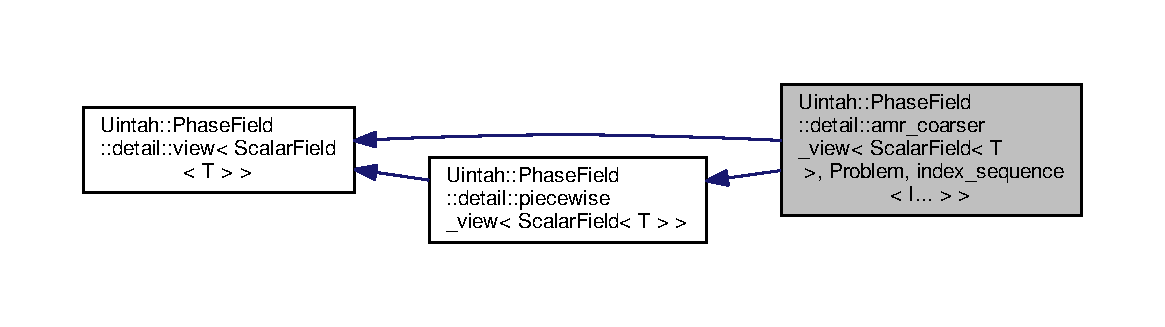
\includegraphics[width=350pt]{classUintah_1_1PhaseField_1_1detail_1_1amr__coarser__view_3_01ScalarField_3_01T_01_4_00_01Proble06512f6d13005d234184897dae96b0e0}
\end{center}
\end{figure}


Collaboration diagram for Uintah\+:\+:Phase\+Field\+:\+:detail\+:\+:amr\+\_\+coarser\+\_\+view$<$ Scalar\+Field$<$ T $>$, Problem, index\+\_\+sequence$<$ I... $>$ $>$\+:\nopagebreak
\begin{figure}[H]
\begin{center}
\leavevmode
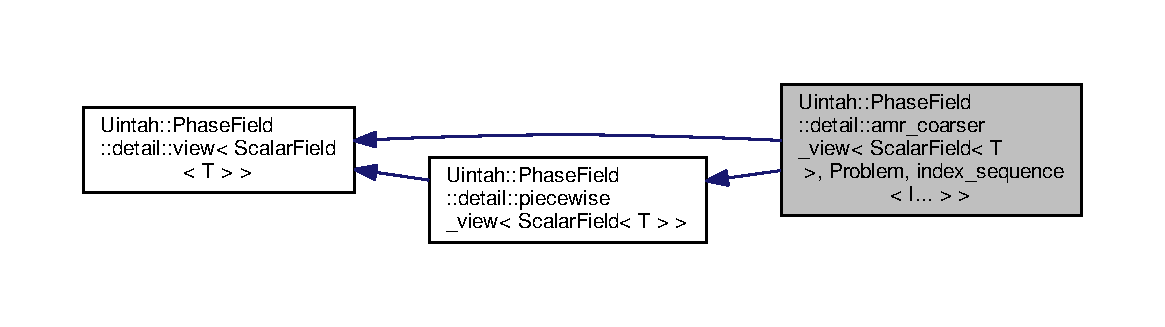
\includegraphics[width=350pt]{classUintah_1_1PhaseField_1_1detail_1_1amr__coarser__view_3_01ScalarField_3_01T_01_4_00_01Problea20917c4205b43c76a94539da984f2bf}
\end{center}
\end{figure}
\subsection*{Public Member Functions}
\begin{DoxyCompactItemize}
\item 
\hyperlink{classUintah_1_1PhaseField_1_1detail_1_1amr__coarser__view_3_01ScalarField_3_01T_01_4_00_01Proble9cadea116dab5bdb44bb3e29abbe99ef_a028eef83d6df8dcc30eddb8595f628c3}{amr\+\_\+coarser\+\_\+view} (const Var\+Label $\ast$label, const Var\+Label $\ast$subproblems\+\_\+label, int material)
\begin{DoxyCompactList}\small\item\em Constructor. \end{DoxyCompactList}\item 
\hyperlink{classUintah_1_1PhaseField_1_1detail_1_1amr__coarser__view_3_01ScalarField_3_01T_01_4_00_01Proble9cadea116dab5bdb44bb3e29abbe99ef_a67cbe6e1cb69a42c0669e7a477d5e403}{amr\+\_\+coarser\+\_\+view} (Data\+Warehouse $\ast$dw, const Var\+Label $\ast$label, const Var\+Label $\ast$subproblems\+\_\+label, int material, const Patch $\ast$patch, bool use\+\_\+ghosts=\hyperlink{classUintah_1_1PhaseField_1_1detail_1_1amr__coarser__view_3_01ScalarField_3_01T_01_4_00_01Proble9cadea116dab5bdb44bb3e29abbe99ef_ace77967592bbb525ac1e29555bb317cd}{use\+\_\+ghosts\+\_\+dflt})
\begin{DoxyCompactList}\small\item\em Constructor. \end{DoxyCompactList}\item 
virtual \hyperlink{classUintah_1_1PhaseField_1_1detail_1_1amr__coarser__view_3_01ScalarField_3_01T_01_4_00_01Proble9cadea116dab5bdb44bb3e29abbe99ef_ae7ef0e8e785d39a1813d9d05f0e2154e}{$\sim$amr\+\_\+coarser\+\_\+view} ()
\begin{DoxyCompactList}\small\item\em Destructor. \end{DoxyCompactList}\item 
\hyperlink{classUintah_1_1PhaseField_1_1detail_1_1amr__coarser__view_3_01ScalarField_3_01T_01_4_00_01Proble9cadea116dab5bdb44bb3e29abbe99ef_ae8ffacd55d47c21178637fc1a8e9e5b0}{amr\+\_\+coarser\+\_\+view} (const \hyperlink{classUintah_1_1PhaseField_1_1detail_1_1amr__coarser__view}{amr\+\_\+coarser\+\_\+view} \&)=delete
\begin{DoxyCompactList}\small\item\em Prevent copy (and move) constructor. \end{DoxyCompactList}\item 
\hyperlink{classUintah_1_1PhaseField_1_1detail_1_1amr__coarser__view}{amr\+\_\+coarser\+\_\+view} \& \hyperlink{classUintah_1_1PhaseField_1_1detail_1_1amr__coarser__view_3_01ScalarField_3_01T_01_4_00_01Proble9cadea116dab5bdb44bb3e29abbe99ef_a2e79e402bc0ccd6e06672f8f79fe4bda}{operator=} (const \hyperlink{classUintah_1_1PhaseField_1_1detail_1_1amr__coarser__view}{amr\+\_\+coarser\+\_\+view} \&)=delete
\begin{DoxyCompactList}\small\item\em Prevent copy (and move) assignment. \end{DoxyCompactList}\item 
virtual void \hyperlink{classUintah_1_1PhaseField_1_1detail_1_1amr__coarser__view_3_01ScalarField_3_01T_01_4_00_01Proble9cadea116dab5bdb44bb3e29abbe99ef_abe4876f94a9c77e38b7c3d434f86b3c0}{set} (Data\+Warehouse $\ast$dw, const Patch $\ast$patch, bool use\+\_\+ghosts=\hyperlink{classUintah_1_1PhaseField_1_1detail_1_1amr__coarser__view_3_01ScalarField_3_01T_01_4_00_01Proble9cadea116dab5bdb44bb3e29abbe99ef_ace77967592bbb525ac1e29555bb317cd}{use\+\_\+ghosts\+\_\+dflt}) override
\begin{DoxyCompactList}\small\item\em Retrieve value from the Data\+Warehouse for accessing the coarser region below a given fine patch. \end{DoxyCompactList}\item 
virtual void \hyperlink{classUintah_1_1PhaseField_1_1detail_1_1amr__coarser__view_3_01ScalarField_3_01T_01_4_00_01Proble9cadea116dab5bdb44bb3e29abbe99ef_a6e4dba1a59399d5ebc28800155fb4c06}{set} (Data\+Warehouse $\ast$dw, const Level $\ast$level, const Int\+Vector \&low, const Int\+Vector \&high, bool use\+\_\+ghosts=\hyperlink{classUintah_1_1PhaseField_1_1detail_1_1amr__coarser__view_3_01ScalarField_3_01T_01_4_00_01Proble9cadea116dab5bdb44bb3e29abbe99ef_ace77967592bbb525ac1e29555bb317cd}{use\+\_\+ghosts\+\_\+dflt}) override
\begin{DoxyCompactList}\small\item\em Retrieve value from the Data\+Warehouse for accessing the coarser region below a given fine region. \end{DoxyCompactList}\item 
virtual \hyperlink{classUintah_1_1PhaseField_1_1detail_1_1view}{view}$<$ \hyperlink{structUintah_1_1PhaseField_1_1ScalarField}{Field} $>$ $\ast$ \hyperlink{classUintah_1_1PhaseField_1_1detail_1_1amr__coarser__view_3_01ScalarField_3_01T_01_4_00_01Proble9cadea116dab5bdb44bb3e29abbe99ef_a125db112d5568827ed202d5e02610515}{clone} (bool deep) const override
\begin{DoxyCompactList}\small\item\em Get a copy of the view. \end{DoxyCompactList}\item 
virtual \hyperlink{classUintah_1_1PhaseField_1_1detail_1_1view}{view}$<$ \hyperlink{structUintah_1_1PhaseField_1_1ScalarField}{Field} $>$ $\ast$ \hyperlink{classUintah_1_1PhaseField_1_1detail_1_1amr__coarser__view_3_01ScalarField_3_01T_01_4_00_01Proble9cadea116dab5bdb44bb3e29abbe99ef_ac4654e84d3f8f4498e45eddfe0818370}{clone} (bool deep, const Int\+Vector \&offset) const override
\begin{DoxyCompactList}\small\item\em Get a copy of the view and apply translate the support. \end{DoxyCompactList}\item 
virtual \hyperlink{classUintah_1_1PhaseField_1_1Support}{Support} \hyperlink{classUintah_1_1PhaseField_1_1detail_1_1amr__coarser__view_3_01ScalarField_3_01T_01_4_00_01Proble9cadea116dab5bdb44bb3e29abbe99ef_a783d09b56009a7b0bcb0eb981c49a710}{get\+\_\+support} () const override
\begin{DoxyCompactList}\small\item\em Get the fine region corresponding to the coarser one for which the view has access to the Data\+Warehouse. \end{DoxyCompactList}\end{DoxyCompactItemize}
\subsection*{Static Public Attributes}
\begin{DoxyCompactItemize}
\item 
static constexpr bool \hyperlink{classUintah_1_1PhaseField_1_1detail_1_1amr__coarser__view_3_01ScalarField_3_01T_01_4_00_01Proble9cadea116dab5bdb44bb3e29abbe99ef_ace77967592bbb525ac1e29555bb317cd}{use\+\_\+ghosts\+\_\+dflt} = false
\begin{DoxyCompactList}\small\item\em Default value for use\+\_\+ghost when retrieving data. \end{DoxyCompactList}\end{DoxyCompactItemize}
\subsection*{Protected Member Functions}
\begin{DoxyCompactItemize}
\item 
\hyperlink{classUintah_1_1PhaseField_1_1detail_1_1amr__coarser__view_3_01ScalarField_3_01T_01_4_00_01Proble9cadea116dab5bdb44bb3e29abbe99ef_a01447da34e14e479a121699cd8f4d6a2}{amr\+\_\+coarser\+\_\+view} (const \hyperlink{classUintah_1_1PhaseField_1_1detail_1_1amr__coarser__view}{amr\+\_\+coarser\+\_\+view} $\ast$copy, bool deep)
\begin{DoxyCompactList}\small\item\em Constructor. \end{DoxyCompactList}\end{DoxyCompactItemize}
\subsection*{Additional Inherited Members}


\subsection{Detailed Description}
\subsubsection*{template$<$typename T, typename Problem, size\+\_\+t... I$>$\newline
class Uintah\+::\+Phase\+Field\+::detail\+::amr\+\_\+coarser\+\_\+view$<$ Scalar\+Field$<$ T $>$, Problem, index\+\_\+sequence$<$ I... $>$ $>$}

Composite view for accessing coarser grid variables (\hyperlink{structUintah_1_1PhaseField_1_1ScalarField}{Scalar\+Field} implementation) 

\begin{DoxyRemark}{Remarks}
deletion of views instantiated in \hyperlink{classUintah_1_1PhaseField_1_1detail_1_1piecewise__view}{piecewise\+\_\+view} are performed here
\end{DoxyRemark}

\begin{DoxyTemplParams}{Template Parameters}
{\em T} & type of the field value at each point \\
\hline
{\em \hyperlink{classUintah_1_1PhaseField_1_1Problem}{Problem}} & type of \hyperlink{namespaceUintah_1_1PhaseField}{Phase\+Field} problem \\
\hline
{\em \hyperlink{structUintah_1_1PhaseField_1_1I}{I}} & list of indices of Field within \hyperlink{classUintah_1_1PhaseField_1_1Problem}{Problem} (first element is variable index, following ones, if present, are the component index within the variable) \\
\hline
\end{DoxyTemplParams}


\subsection{Constructor \& Destructor Documentation}
\mbox{\Hypertarget{classUintah_1_1PhaseField_1_1detail_1_1amr__coarser__view_3_01ScalarField_3_01T_01_4_00_01Proble9cadea116dab5bdb44bb3e29abbe99ef_a01447da34e14e479a121699cd8f4d6a2}\label{classUintah_1_1PhaseField_1_1detail_1_1amr__coarser__view_3_01ScalarField_3_01T_01_4_00_01Proble9cadea116dab5bdb44bb3e29abbe99ef_a01447da34e14e479a121699cd8f4d6a2}} 
\index{Uintah\+::\+Phase\+Field\+::detail\+::amr\+\_\+coarser\+\_\+view$<$ Scalar\+Field$<$ T $>$, Problem, index\+\_\+sequence$<$ I... $>$ $>$@{Uintah\+::\+Phase\+Field\+::detail\+::amr\+\_\+coarser\+\_\+view$<$ Scalar\+Field$<$ T $>$, Problem, index\+\_\+sequence$<$ I... $>$ $>$}!amr\+\_\+coarser\+\_\+view@{amr\+\_\+coarser\+\_\+view}}
\index{amr\+\_\+coarser\+\_\+view@{amr\+\_\+coarser\+\_\+view}!Uintah\+::\+Phase\+Field\+::detail\+::amr\+\_\+coarser\+\_\+view$<$ Scalar\+Field$<$ T $>$, Problem, index\+\_\+sequence$<$ I... $>$ $>$@{Uintah\+::\+Phase\+Field\+::detail\+::amr\+\_\+coarser\+\_\+view$<$ Scalar\+Field$<$ T $>$, Problem, index\+\_\+sequence$<$ I... $>$ $>$}}
\subsubsection{\texorpdfstring{amr\+\_\+coarser\+\_\+view()}{amr\_coarser\_view()}\hspace{0.1cm}{\footnotesize\ttfamily [1/4]}}
{\footnotesize\ttfamily template$<$typename T , typename Problem , size\+\_\+t... I$>$ \\
\hyperlink{classUintah_1_1PhaseField_1_1detail_1_1amr__coarser__view}{Uintah\+::\+Phase\+Field\+::detail\+::amr\+\_\+coarser\+\_\+view}$<$ \hyperlink{structUintah_1_1PhaseField_1_1ScalarField}{Scalar\+Field}$<$ T $>$, \hyperlink{classUintah_1_1PhaseField_1_1Problem}{Problem}, \hyperlink{namespaceUintah_1_1PhaseField_a237de804d99512e50613aff7c94a9461}{index\+\_\+sequence}$<$ I... $>$ $>$\+::\hyperlink{classUintah_1_1PhaseField_1_1detail_1_1amr__coarser__view}{amr\+\_\+coarser\+\_\+view} (\begin{DoxyParamCaption}\item[{const \hyperlink{classUintah_1_1PhaseField_1_1detail_1_1amr__coarser__view}{amr\+\_\+coarser\+\_\+view}$<$ \hyperlink{structUintah_1_1PhaseField_1_1ScalarField}{Scalar\+Field}$<$ T $>$, \hyperlink{classUintah_1_1PhaseField_1_1Problem}{Problem}, \hyperlink{namespaceUintah_1_1PhaseField_a237de804d99512e50613aff7c94a9461}{index\+\_\+sequence}$<$ I... $>$ $>$ $\ast$}]{copy,  }\item[{bool}]{deep }\end{DoxyParamCaption})\hspace{0.3cm}{\ttfamily [inline]}, {\ttfamily [protected]}}



Constructor. 

Instantiate a copy of a given view


\begin{DoxyParams}{Parameters}
{\em copy} & source view for copying \\
\hline
{\em deep} & if true inner grid variable is copied as well otherwise the same grid variable is referenced \\
\hline
\end{DoxyParams}
\mbox{\Hypertarget{classUintah_1_1PhaseField_1_1detail_1_1amr__coarser__view_3_01ScalarField_3_01T_01_4_00_01Proble9cadea116dab5bdb44bb3e29abbe99ef_a028eef83d6df8dcc30eddb8595f628c3}\label{classUintah_1_1PhaseField_1_1detail_1_1amr__coarser__view_3_01ScalarField_3_01T_01_4_00_01Proble9cadea116dab5bdb44bb3e29abbe99ef_a028eef83d6df8dcc30eddb8595f628c3}} 
\index{Uintah\+::\+Phase\+Field\+::detail\+::amr\+\_\+coarser\+\_\+view$<$ Scalar\+Field$<$ T $>$, Problem, index\+\_\+sequence$<$ I... $>$ $>$@{Uintah\+::\+Phase\+Field\+::detail\+::amr\+\_\+coarser\+\_\+view$<$ Scalar\+Field$<$ T $>$, Problem, index\+\_\+sequence$<$ I... $>$ $>$}!amr\+\_\+coarser\+\_\+view@{amr\+\_\+coarser\+\_\+view}}
\index{amr\+\_\+coarser\+\_\+view@{amr\+\_\+coarser\+\_\+view}!Uintah\+::\+Phase\+Field\+::detail\+::amr\+\_\+coarser\+\_\+view$<$ Scalar\+Field$<$ T $>$, Problem, index\+\_\+sequence$<$ I... $>$ $>$@{Uintah\+::\+Phase\+Field\+::detail\+::amr\+\_\+coarser\+\_\+view$<$ Scalar\+Field$<$ T $>$, Problem, index\+\_\+sequence$<$ I... $>$ $>$}}
\subsubsection{\texorpdfstring{amr\+\_\+coarser\+\_\+view()}{amr\_coarser\_view()}\hspace{0.1cm}{\footnotesize\ttfamily [2/4]}}
{\footnotesize\ttfamily template$<$typename T , typename Problem , size\+\_\+t... I$>$ \\
\hyperlink{classUintah_1_1PhaseField_1_1detail_1_1amr__coarser__view}{Uintah\+::\+Phase\+Field\+::detail\+::amr\+\_\+coarser\+\_\+view}$<$ \hyperlink{structUintah_1_1PhaseField_1_1ScalarField}{Scalar\+Field}$<$ T $>$, \hyperlink{classUintah_1_1PhaseField_1_1Problem}{Problem}, \hyperlink{namespaceUintah_1_1PhaseField_a237de804d99512e50613aff7c94a9461}{index\+\_\+sequence}$<$ I... $>$ $>$\+::\hyperlink{classUintah_1_1PhaseField_1_1detail_1_1amr__coarser__view}{amr\+\_\+coarser\+\_\+view} (\begin{DoxyParamCaption}\item[{const Var\+Label $\ast$}]{label,  }\item[{const Var\+Label $\ast$}]{subproblems\+\_\+label,  }\item[{int}]{material }\end{DoxyParamCaption})\hspace{0.3cm}{\ttfamily [inline]}}



Constructor. 

construct coarser view without retrieving inner variable data from the Data\+Warehouse


\begin{DoxyParams}{Parameters}
{\em label} & label of variable in the Data\+Warehouse \\
\hline
{\em subproblems\+\_\+label} & label of subproblems in the Data\+Warehouse \\
\hline
{\em material} & index of material in the Data\+Warehouse \\
\hline
\end{DoxyParams}
\mbox{\Hypertarget{classUintah_1_1PhaseField_1_1detail_1_1amr__coarser__view_3_01ScalarField_3_01T_01_4_00_01Proble9cadea116dab5bdb44bb3e29abbe99ef_a67cbe6e1cb69a42c0669e7a477d5e403}\label{classUintah_1_1PhaseField_1_1detail_1_1amr__coarser__view_3_01ScalarField_3_01T_01_4_00_01Proble9cadea116dab5bdb44bb3e29abbe99ef_a67cbe6e1cb69a42c0669e7a477d5e403}} 
\index{Uintah\+::\+Phase\+Field\+::detail\+::amr\+\_\+coarser\+\_\+view$<$ Scalar\+Field$<$ T $>$, Problem, index\+\_\+sequence$<$ I... $>$ $>$@{Uintah\+::\+Phase\+Field\+::detail\+::amr\+\_\+coarser\+\_\+view$<$ Scalar\+Field$<$ T $>$, Problem, index\+\_\+sequence$<$ I... $>$ $>$}!amr\+\_\+coarser\+\_\+view@{amr\+\_\+coarser\+\_\+view}}
\index{amr\+\_\+coarser\+\_\+view@{amr\+\_\+coarser\+\_\+view}!Uintah\+::\+Phase\+Field\+::detail\+::amr\+\_\+coarser\+\_\+view$<$ Scalar\+Field$<$ T $>$, Problem, index\+\_\+sequence$<$ I... $>$ $>$@{Uintah\+::\+Phase\+Field\+::detail\+::amr\+\_\+coarser\+\_\+view$<$ Scalar\+Field$<$ T $>$, Problem, index\+\_\+sequence$<$ I... $>$ $>$}}
\subsubsection{\texorpdfstring{amr\+\_\+coarser\+\_\+view()}{amr\_coarser\_view()}\hspace{0.1cm}{\footnotesize\ttfamily [3/4]}}
{\footnotesize\ttfamily template$<$typename T , typename Problem , size\+\_\+t... I$>$ \\
\hyperlink{classUintah_1_1PhaseField_1_1detail_1_1amr__coarser__view}{Uintah\+::\+Phase\+Field\+::detail\+::amr\+\_\+coarser\+\_\+view}$<$ \hyperlink{structUintah_1_1PhaseField_1_1ScalarField}{Scalar\+Field}$<$ T $>$, \hyperlink{classUintah_1_1PhaseField_1_1Problem}{Problem}, \hyperlink{namespaceUintah_1_1PhaseField_a237de804d99512e50613aff7c94a9461}{index\+\_\+sequence}$<$ I... $>$ $>$\+::\hyperlink{classUintah_1_1PhaseField_1_1detail_1_1amr__coarser__view}{amr\+\_\+coarser\+\_\+view} (\begin{DoxyParamCaption}\item[{Data\+Warehouse $\ast$}]{dw,  }\item[{const Var\+Label $\ast$}]{label,  }\item[{const Var\+Label $\ast$}]{subproblems\+\_\+label,  }\item[{int}]{material,  }\item[{const Patch $\ast$}]{patch,  }\item[{bool}]{use\+\_\+ghosts = {\ttfamily \hyperlink{classUintah_1_1PhaseField_1_1detail_1_1amr__coarser__view_3_01ScalarField_3_01T_01_4_00_01Proble9cadea116dab5bdb44bb3e29abbe99ef_ace77967592bbb525ac1e29555bb317cd}{use\+\_\+ghosts\+\_\+dflt}} }\end{DoxyParamCaption})\hspace{0.3cm}{\ttfamily [inline]}}



Constructor. 

construct coarser view and retrieve inner variable data from the Data\+Warehouse for the region lying under a given fine patch.

\begin{DoxyRemark}{Remarks}
the number of ghost cells/nodes and the corresponding region on the coarser level is automatically computed to match the interpolation type
\end{DoxyRemark}

\begin{DoxyParams}{Parameters}
{\em dw} & Data\+Warehouse which data is retrieved from \\
\hline
{\em label} & label of variable in the Data\+Warehouse \\
\hline
{\em subproblems\+\_\+label} & label of subproblems in the Data\+Warehouse \\
\hline
{\em material} & index of material in the Data\+Warehouse \\
\hline
{\em patch} & patch on which data is retrieved \\
\hline
{\em use\+\_\+ghosts} & must be false \\
\hline
\end{DoxyParams}
\mbox{\Hypertarget{classUintah_1_1PhaseField_1_1detail_1_1amr__coarser__view_3_01ScalarField_3_01T_01_4_00_01Proble9cadea116dab5bdb44bb3e29abbe99ef_ae7ef0e8e785d39a1813d9d05f0e2154e}\label{classUintah_1_1PhaseField_1_1detail_1_1amr__coarser__view_3_01ScalarField_3_01T_01_4_00_01Proble9cadea116dab5bdb44bb3e29abbe99ef_ae7ef0e8e785d39a1813d9d05f0e2154e}} 
\index{Uintah\+::\+Phase\+Field\+::detail\+::amr\+\_\+coarser\+\_\+view$<$ Scalar\+Field$<$ T $>$, Problem, index\+\_\+sequence$<$ I... $>$ $>$@{Uintah\+::\+Phase\+Field\+::detail\+::amr\+\_\+coarser\+\_\+view$<$ Scalar\+Field$<$ T $>$, Problem, index\+\_\+sequence$<$ I... $>$ $>$}!````~amr\+\_\+coarser\+\_\+view@{$\sim$amr\+\_\+coarser\+\_\+view}}
\index{````~amr\+\_\+coarser\+\_\+view@{$\sim$amr\+\_\+coarser\+\_\+view}!Uintah\+::\+Phase\+Field\+::detail\+::amr\+\_\+coarser\+\_\+view$<$ Scalar\+Field$<$ T $>$, Problem, index\+\_\+sequence$<$ I... $>$ $>$@{Uintah\+::\+Phase\+Field\+::detail\+::amr\+\_\+coarser\+\_\+view$<$ Scalar\+Field$<$ T $>$, Problem, index\+\_\+sequence$<$ I... $>$ $>$}}
\subsubsection{\texorpdfstring{$\sim$amr\+\_\+coarser\+\_\+view()}{~amr\_coarser\_view()}}
{\footnotesize\ttfamily template$<$typename T , typename Problem , size\+\_\+t... I$>$ \\
virtual \hyperlink{classUintah_1_1PhaseField_1_1detail_1_1amr__coarser__view}{Uintah\+::\+Phase\+Field\+::detail\+::amr\+\_\+coarser\+\_\+view}$<$ \hyperlink{structUintah_1_1PhaseField_1_1ScalarField}{Scalar\+Field}$<$ T $>$, \hyperlink{classUintah_1_1PhaseField_1_1Problem}{Problem}, \hyperlink{namespaceUintah_1_1PhaseField_a237de804d99512e50613aff7c94a9461}{index\+\_\+sequence}$<$ I... $>$ $>$\+::$\sim$\hyperlink{classUintah_1_1PhaseField_1_1detail_1_1amr__coarser__view}{amr\+\_\+coarser\+\_\+view} (\begin{DoxyParamCaption}{ }\end{DoxyParamCaption})\hspace{0.3cm}{\ttfamily [inline]}, {\ttfamily [virtual]}}



Destructor. 

\mbox{\Hypertarget{classUintah_1_1PhaseField_1_1detail_1_1amr__coarser__view_3_01ScalarField_3_01T_01_4_00_01Proble9cadea116dab5bdb44bb3e29abbe99ef_ae8ffacd55d47c21178637fc1a8e9e5b0}\label{classUintah_1_1PhaseField_1_1detail_1_1amr__coarser__view_3_01ScalarField_3_01T_01_4_00_01Proble9cadea116dab5bdb44bb3e29abbe99ef_ae8ffacd55d47c21178637fc1a8e9e5b0}} 
\index{Uintah\+::\+Phase\+Field\+::detail\+::amr\+\_\+coarser\+\_\+view$<$ Scalar\+Field$<$ T $>$, Problem, index\+\_\+sequence$<$ I... $>$ $>$@{Uintah\+::\+Phase\+Field\+::detail\+::amr\+\_\+coarser\+\_\+view$<$ Scalar\+Field$<$ T $>$, Problem, index\+\_\+sequence$<$ I... $>$ $>$}!amr\+\_\+coarser\+\_\+view@{amr\+\_\+coarser\+\_\+view}}
\index{amr\+\_\+coarser\+\_\+view@{amr\+\_\+coarser\+\_\+view}!Uintah\+::\+Phase\+Field\+::detail\+::amr\+\_\+coarser\+\_\+view$<$ Scalar\+Field$<$ T $>$, Problem, index\+\_\+sequence$<$ I... $>$ $>$@{Uintah\+::\+Phase\+Field\+::detail\+::amr\+\_\+coarser\+\_\+view$<$ Scalar\+Field$<$ T $>$, Problem, index\+\_\+sequence$<$ I... $>$ $>$}}
\subsubsection{\texorpdfstring{amr\+\_\+coarser\+\_\+view()}{amr\_coarser\_view()}\hspace{0.1cm}{\footnotesize\ttfamily [4/4]}}
{\footnotesize\ttfamily template$<$typename T , typename Problem , size\+\_\+t... I$>$ \\
\hyperlink{classUintah_1_1PhaseField_1_1detail_1_1amr__coarser__view}{Uintah\+::\+Phase\+Field\+::detail\+::amr\+\_\+coarser\+\_\+view}$<$ \hyperlink{structUintah_1_1PhaseField_1_1ScalarField}{Scalar\+Field}$<$ T $>$, \hyperlink{classUintah_1_1PhaseField_1_1Problem}{Problem}, \hyperlink{namespaceUintah_1_1PhaseField_a237de804d99512e50613aff7c94a9461}{index\+\_\+sequence}$<$ I... $>$ $>$\+::\hyperlink{classUintah_1_1PhaseField_1_1detail_1_1amr__coarser__view}{amr\+\_\+coarser\+\_\+view} (\begin{DoxyParamCaption}\item[{const \hyperlink{classUintah_1_1PhaseField_1_1detail_1_1amr__coarser__view}{amr\+\_\+coarser\+\_\+view}$<$ \hyperlink{structUintah_1_1PhaseField_1_1ScalarField}{Scalar\+Field}$<$ T $>$, \hyperlink{classUintah_1_1PhaseField_1_1Problem}{Problem}, \hyperlink{namespaceUintah_1_1PhaseField_a237de804d99512e50613aff7c94a9461}{index\+\_\+sequence}$<$ I... $>$ $>$ \&}]{ }\end{DoxyParamCaption})\hspace{0.3cm}{\ttfamily [delete]}}



Prevent copy (and move) constructor. 



\subsection{Member Function Documentation}
\mbox{\Hypertarget{classUintah_1_1PhaseField_1_1detail_1_1amr__coarser__view_3_01ScalarField_3_01T_01_4_00_01Proble9cadea116dab5bdb44bb3e29abbe99ef_a125db112d5568827ed202d5e02610515}\label{classUintah_1_1PhaseField_1_1detail_1_1amr__coarser__view_3_01ScalarField_3_01T_01_4_00_01Proble9cadea116dab5bdb44bb3e29abbe99ef_a125db112d5568827ed202d5e02610515}} 
\index{Uintah\+::\+Phase\+Field\+::detail\+::amr\+\_\+coarser\+\_\+view$<$ Scalar\+Field$<$ T $>$, Problem, index\+\_\+sequence$<$ I... $>$ $>$@{Uintah\+::\+Phase\+Field\+::detail\+::amr\+\_\+coarser\+\_\+view$<$ Scalar\+Field$<$ T $>$, Problem, index\+\_\+sequence$<$ I... $>$ $>$}!clone@{clone}}
\index{clone@{clone}!Uintah\+::\+Phase\+Field\+::detail\+::amr\+\_\+coarser\+\_\+view$<$ Scalar\+Field$<$ T $>$, Problem, index\+\_\+sequence$<$ I... $>$ $>$@{Uintah\+::\+Phase\+Field\+::detail\+::amr\+\_\+coarser\+\_\+view$<$ Scalar\+Field$<$ T $>$, Problem, index\+\_\+sequence$<$ I... $>$ $>$}}
\subsubsection{\texorpdfstring{clone()}{clone()}\hspace{0.1cm}{\footnotesize\ttfamily [1/2]}}
{\footnotesize\ttfamily template$<$typename T , typename Problem , size\+\_\+t... I$>$ \\
virtual \hyperlink{classUintah_1_1PhaseField_1_1detail_1_1view}{view}$<$\hyperlink{structUintah_1_1PhaseField_1_1ScalarField}{Field}$>$$\ast$ \hyperlink{classUintah_1_1PhaseField_1_1detail_1_1amr__coarser__view}{Uintah\+::\+Phase\+Field\+::detail\+::amr\+\_\+coarser\+\_\+view}$<$ \hyperlink{structUintah_1_1PhaseField_1_1ScalarField}{Scalar\+Field}$<$ T $>$, \hyperlink{classUintah_1_1PhaseField_1_1Problem}{Problem}, \hyperlink{namespaceUintah_1_1PhaseField_a237de804d99512e50613aff7c94a9461}{index\+\_\+sequence}$<$ I... $>$ $>$\+::clone (\begin{DoxyParamCaption}\item[{bool}]{deep }\end{DoxyParamCaption}) const\hspace{0.3cm}{\ttfamily [inline]}, {\ttfamily [override]}, {\ttfamily [virtual]}}



Get a copy of the view. 


\begin{DoxyParams}{Parameters}
{\em deep} & if true inner grid variable is copied as well otherwise the same grid variable is referenced\\
\hline
\end{DoxyParams}
\begin{DoxyReturn}{Returns}
new view instance 
\end{DoxyReturn}


Implements \hyperlink{classUintah_1_1PhaseField_1_1detail_1_1view_3_01ScalarField_3_01T_01_4_01_4_a6e11243c9d776a7b703e524ea4151a16}{Uintah\+::\+Phase\+Field\+::detail\+::view$<$ Scalar\+Field$<$ T $>$ $>$}.

\mbox{\Hypertarget{classUintah_1_1PhaseField_1_1detail_1_1amr__coarser__view_3_01ScalarField_3_01T_01_4_00_01Proble9cadea116dab5bdb44bb3e29abbe99ef_ac4654e84d3f8f4498e45eddfe0818370}\label{classUintah_1_1PhaseField_1_1detail_1_1amr__coarser__view_3_01ScalarField_3_01T_01_4_00_01Proble9cadea116dab5bdb44bb3e29abbe99ef_ac4654e84d3f8f4498e45eddfe0818370}} 
\index{Uintah\+::\+Phase\+Field\+::detail\+::amr\+\_\+coarser\+\_\+view$<$ Scalar\+Field$<$ T $>$, Problem, index\+\_\+sequence$<$ I... $>$ $>$@{Uintah\+::\+Phase\+Field\+::detail\+::amr\+\_\+coarser\+\_\+view$<$ Scalar\+Field$<$ T $>$, Problem, index\+\_\+sequence$<$ I... $>$ $>$}!clone@{clone}}
\index{clone@{clone}!Uintah\+::\+Phase\+Field\+::detail\+::amr\+\_\+coarser\+\_\+view$<$ Scalar\+Field$<$ T $>$, Problem, index\+\_\+sequence$<$ I... $>$ $>$@{Uintah\+::\+Phase\+Field\+::detail\+::amr\+\_\+coarser\+\_\+view$<$ Scalar\+Field$<$ T $>$, Problem, index\+\_\+sequence$<$ I... $>$ $>$}}
\subsubsection{\texorpdfstring{clone()}{clone()}\hspace{0.1cm}{\footnotesize\ttfamily [2/2]}}
{\footnotesize\ttfamily template$<$typename T , typename Problem , size\+\_\+t... I$>$ \\
virtual \hyperlink{classUintah_1_1PhaseField_1_1detail_1_1view}{view}$<$\hyperlink{structUintah_1_1PhaseField_1_1ScalarField}{Field}$>$$\ast$ \hyperlink{classUintah_1_1PhaseField_1_1detail_1_1amr__coarser__view}{Uintah\+::\+Phase\+Field\+::detail\+::amr\+\_\+coarser\+\_\+view}$<$ \hyperlink{structUintah_1_1PhaseField_1_1ScalarField}{Scalar\+Field}$<$ T $>$, \hyperlink{classUintah_1_1PhaseField_1_1Problem}{Problem}, \hyperlink{namespaceUintah_1_1PhaseField_a237de804d99512e50613aff7c94a9461}{index\+\_\+sequence}$<$ I... $>$ $>$\+::clone (\begin{DoxyParamCaption}\item[{bool}]{deep,  }\item[{const Int\+Vector \&}]{offset }\end{DoxyParamCaption}) const\hspace{0.3cm}{\ttfamily [inline]}, {\ttfamily [override]}, {\ttfamily [virtual]}}



Get a copy of the view and apply translate the support. 

\begin{DoxyRemark}{Remarks}
It is meant to be used for virtual patches (i.\+e. periodic boundaries)
\end{DoxyRemark}

\begin{DoxyParams}{Parameters}
{\em deep} & if true inner grid variable is copied as well otherwise the same grid variable is referenced \\
\hline
{\em offset} & vector specifying the translation of the support \\
\hline
\end{DoxyParams}
\begin{DoxyReturn}{Returns}
new view instance 
\end{DoxyReturn}


Implements \hyperlink{classUintah_1_1PhaseField_1_1detail_1_1view_3_01ScalarField_3_01T_01_4_01_4_abd928104240e329f3bc4441ebab7c50c}{Uintah\+::\+Phase\+Field\+::detail\+::view$<$ Scalar\+Field$<$ T $>$ $>$}.

\mbox{\Hypertarget{classUintah_1_1PhaseField_1_1detail_1_1amr__coarser__view_3_01ScalarField_3_01T_01_4_00_01Proble9cadea116dab5bdb44bb3e29abbe99ef_a783d09b56009a7b0bcb0eb981c49a710}\label{classUintah_1_1PhaseField_1_1detail_1_1amr__coarser__view_3_01ScalarField_3_01T_01_4_00_01Proble9cadea116dab5bdb44bb3e29abbe99ef_a783d09b56009a7b0bcb0eb981c49a710}} 
\index{Uintah\+::\+Phase\+Field\+::detail\+::amr\+\_\+coarser\+\_\+view$<$ Scalar\+Field$<$ T $>$, Problem, index\+\_\+sequence$<$ I... $>$ $>$@{Uintah\+::\+Phase\+Field\+::detail\+::amr\+\_\+coarser\+\_\+view$<$ Scalar\+Field$<$ T $>$, Problem, index\+\_\+sequence$<$ I... $>$ $>$}!get\+\_\+support@{get\+\_\+support}}
\index{get\+\_\+support@{get\+\_\+support}!Uintah\+::\+Phase\+Field\+::detail\+::amr\+\_\+coarser\+\_\+view$<$ Scalar\+Field$<$ T $>$, Problem, index\+\_\+sequence$<$ I... $>$ $>$@{Uintah\+::\+Phase\+Field\+::detail\+::amr\+\_\+coarser\+\_\+view$<$ Scalar\+Field$<$ T $>$, Problem, index\+\_\+sequence$<$ I... $>$ $>$}}
\subsubsection{\texorpdfstring{get\+\_\+support()}{get\_support()}}
{\footnotesize\ttfamily template$<$typename T , typename Problem , size\+\_\+t... I$>$ \\
virtual \hyperlink{classUintah_1_1PhaseField_1_1Support}{Support} \hyperlink{classUintah_1_1PhaseField_1_1detail_1_1amr__coarser__view}{Uintah\+::\+Phase\+Field\+::detail\+::amr\+\_\+coarser\+\_\+view}$<$ \hyperlink{structUintah_1_1PhaseField_1_1ScalarField}{Scalar\+Field}$<$ T $>$, \hyperlink{classUintah_1_1PhaseField_1_1Problem}{Problem}, \hyperlink{namespaceUintah_1_1PhaseField_a237de804d99512e50613aff7c94a9461}{index\+\_\+sequence}$<$ I... $>$ $>$\+::get\+\_\+support (\begin{DoxyParamCaption}{ }\end{DoxyParamCaption}) const\hspace{0.3cm}{\ttfamily [inline]}, {\ttfamily [override]}, {\ttfamily [virtual]}}



Get the fine region corresponding to the coarser one for which the view has access to the Data\+Warehouse. 

\begin{DoxyReturn}{Returns}
support of the view 
\end{DoxyReturn}


Implements \hyperlink{classUintah_1_1PhaseField_1_1detail_1_1view_3_01ScalarField_3_01T_01_4_01_4_a3e14b0c7a57a57707bb33954861ab1c1}{Uintah\+::\+Phase\+Field\+::detail\+::view$<$ Scalar\+Field$<$ T $>$ $>$}.

\mbox{\Hypertarget{classUintah_1_1PhaseField_1_1detail_1_1amr__coarser__view_3_01ScalarField_3_01T_01_4_00_01Proble9cadea116dab5bdb44bb3e29abbe99ef_a2e79e402bc0ccd6e06672f8f79fe4bda}\label{classUintah_1_1PhaseField_1_1detail_1_1amr__coarser__view_3_01ScalarField_3_01T_01_4_00_01Proble9cadea116dab5bdb44bb3e29abbe99ef_a2e79e402bc0ccd6e06672f8f79fe4bda}} 
\index{Uintah\+::\+Phase\+Field\+::detail\+::amr\+\_\+coarser\+\_\+view$<$ Scalar\+Field$<$ T $>$, Problem, index\+\_\+sequence$<$ I... $>$ $>$@{Uintah\+::\+Phase\+Field\+::detail\+::amr\+\_\+coarser\+\_\+view$<$ Scalar\+Field$<$ T $>$, Problem, index\+\_\+sequence$<$ I... $>$ $>$}!operator=@{operator=}}
\index{operator=@{operator=}!Uintah\+::\+Phase\+Field\+::detail\+::amr\+\_\+coarser\+\_\+view$<$ Scalar\+Field$<$ T $>$, Problem, index\+\_\+sequence$<$ I... $>$ $>$@{Uintah\+::\+Phase\+Field\+::detail\+::amr\+\_\+coarser\+\_\+view$<$ Scalar\+Field$<$ T $>$, Problem, index\+\_\+sequence$<$ I... $>$ $>$}}
\subsubsection{\texorpdfstring{operator=()}{operator=()}}
{\footnotesize\ttfamily template$<$typename T , typename Problem , size\+\_\+t... I$>$ \\
\hyperlink{classUintah_1_1PhaseField_1_1detail_1_1amr__coarser__view}{amr\+\_\+coarser\+\_\+view}\& \hyperlink{classUintah_1_1PhaseField_1_1detail_1_1amr__coarser__view}{Uintah\+::\+Phase\+Field\+::detail\+::amr\+\_\+coarser\+\_\+view}$<$ \hyperlink{structUintah_1_1PhaseField_1_1ScalarField}{Scalar\+Field}$<$ T $>$, \hyperlink{classUintah_1_1PhaseField_1_1Problem}{Problem}, \hyperlink{namespaceUintah_1_1PhaseField_a237de804d99512e50613aff7c94a9461}{index\+\_\+sequence}$<$ I... $>$ $>$\+::operator= (\begin{DoxyParamCaption}\item[{const \hyperlink{classUintah_1_1PhaseField_1_1detail_1_1amr__coarser__view}{amr\+\_\+coarser\+\_\+view}$<$ \hyperlink{structUintah_1_1PhaseField_1_1ScalarField}{Scalar\+Field}$<$ T $>$, \hyperlink{classUintah_1_1PhaseField_1_1Problem}{Problem}, \hyperlink{namespaceUintah_1_1PhaseField_a237de804d99512e50613aff7c94a9461}{index\+\_\+sequence}$<$ I... $>$ $>$ \&}]{ }\end{DoxyParamCaption})\hspace{0.3cm}{\ttfamily [delete]}}



Prevent copy (and move) assignment. 

\mbox{\Hypertarget{classUintah_1_1PhaseField_1_1detail_1_1amr__coarser__view_3_01ScalarField_3_01T_01_4_00_01Proble9cadea116dab5bdb44bb3e29abbe99ef_abe4876f94a9c77e38b7c3d434f86b3c0}\label{classUintah_1_1PhaseField_1_1detail_1_1amr__coarser__view_3_01ScalarField_3_01T_01_4_00_01Proble9cadea116dab5bdb44bb3e29abbe99ef_abe4876f94a9c77e38b7c3d434f86b3c0}} 
\index{Uintah\+::\+Phase\+Field\+::detail\+::amr\+\_\+coarser\+\_\+view$<$ Scalar\+Field$<$ T $>$, Problem, index\+\_\+sequence$<$ I... $>$ $>$@{Uintah\+::\+Phase\+Field\+::detail\+::amr\+\_\+coarser\+\_\+view$<$ Scalar\+Field$<$ T $>$, Problem, index\+\_\+sequence$<$ I... $>$ $>$}!set@{set}}
\index{set@{set}!Uintah\+::\+Phase\+Field\+::detail\+::amr\+\_\+coarser\+\_\+view$<$ Scalar\+Field$<$ T $>$, Problem, index\+\_\+sequence$<$ I... $>$ $>$@{Uintah\+::\+Phase\+Field\+::detail\+::amr\+\_\+coarser\+\_\+view$<$ Scalar\+Field$<$ T $>$, Problem, index\+\_\+sequence$<$ I... $>$ $>$}}
\subsubsection{\texorpdfstring{set()}{set()}\hspace{0.1cm}{\footnotesize\ttfamily [1/2]}}
{\footnotesize\ttfamily template$<$typename T , typename Problem , size\+\_\+t... I$>$ \\
virtual void \hyperlink{classUintah_1_1PhaseField_1_1detail_1_1amr__coarser__view}{Uintah\+::\+Phase\+Field\+::detail\+::amr\+\_\+coarser\+\_\+view}$<$ \hyperlink{structUintah_1_1PhaseField_1_1ScalarField}{Scalar\+Field}$<$ T $>$, \hyperlink{classUintah_1_1PhaseField_1_1Problem}{Problem}, \hyperlink{namespaceUintah_1_1PhaseField_a237de804d99512e50613aff7c94a9461}{index\+\_\+sequence}$<$ I... $>$ $>$\+::set (\begin{DoxyParamCaption}\item[{Data\+Warehouse $\ast$}]{dw,  }\item[{const Patch $\ast$}]{patch,  }\item[{bool}]{use\+\_\+ghosts = {\ttfamily \hyperlink{classUintah_1_1PhaseField_1_1detail_1_1amr__coarser__view_3_01ScalarField_3_01T_01_4_00_01Proble9cadea116dab5bdb44bb3e29abbe99ef_ace77967592bbb525ac1e29555bb317cd}{use\+\_\+ghosts\+\_\+dflt}} }\end{DoxyParamCaption})\hspace{0.3cm}{\ttfamily [inline]}, {\ttfamily [override]}, {\ttfamily [virtual]}}



Retrieve value from the Data\+Warehouse for accessing the coarser region below a given fine patch. 


\begin{DoxyParams}{Parameters}
{\em dw} & Data\+Warehouse from which data is retrieved \\
\hline
{\em patch} & fine grid patch to retrieve data for \\
\hline
{\em use\+\_\+ghosts} & must be false \\
\hline
\end{DoxyParams}


Implements \hyperlink{classUintah_1_1PhaseField_1_1detail_1_1view_3_01ScalarField_3_01T_01_4_01_4_ae90ea8b33fde8515a1f2e8f5c03c0166}{Uintah\+::\+Phase\+Field\+::detail\+::view$<$ Scalar\+Field$<$ T $>$ $>$}.

\mbox{\Hypertarget{classUintah_1_1PhaseField_1_1detail_1_1amr__coarser__view_3_01ScalarField_3_01T_01_4_00_01Proble9cadea116dab5bdb44bb3e29abbe99ef_a6e4dba1a59399d5ebc28800155fb4c06}\label{classUintah_1_1PhaseField_1_1detail_1_1amr__coarser__view_3_01ScalarField_3_01T_01_4_00_01Proble9cadea116dab5bdb44bb3e29abbe99ef_a6e4dba1a59399d5ebc28800155fb4c06}} 
\index{Uintah\+::\+Phase\+Field\+::detail\+::amr\+\_\+coarser\+\_\+view$<$ Scalar\+Field$<$ T $>$, Problem, index\+\_\+sequence$<$ I... $>$ $>$@{Uintah\+::\+Phase\+Field\+::detail\+::amr\+\_\+coarser\+\_\+view$<$ Scalar\+Field$<$ T $>$, Problem, index\+\_\+sequence$<$ I... $>$ $>$}!set@{set}}
\index{set@{set}!Uintah\+::\+Phase\+Field\+::detail\+::amr\+\_\+coarser\+\_\+view$<$ Scalar\+Field$<$ T $>$, Problem, index\+\_\+sequence$<$ I... $>$ $>$@{Uintah\+::\+Phase\+Field\+::detail\+::amr\+\_\+coarser\+\_\+view$<$ Scalar\+Field$<$ T $>$, Problem, index\+\_\+sequence$<$ I... $>$ $>$}}
\subsubsection{\texorpdfstring{set()}{set()}\hspace{0.1cm}{\footnotesize\ttfamily [2/2]}}
{\footnotesize\ttfamily template$<$typename T , typename Problem , size\+\_\+t... I$>$ \\
virtual void \hyperlink{classUintah_1_1PhaseField_1_1detail_1_1amr__coarser__view}{Uintah\+::\+Phase\+Field\+::detail\+::amr\+\_\+coarser\+\_\+view}$<$ \hyperlink{structUintah_1_1PhaseField_1_1ScalarField}{Scalar\+Field}$<$ T $>$, \hyperlink{classUintah_1_1PhaseField_1_1Problem}{Problem}, \hyperlink{namespaceUintah_1_1PhaseField_a237de804d99512e50613aff7c94a9461}{index\+\_\+sequence}$<$ I... $>$ $>$\+::set (\begin{DoxyParamCaption}\item[{Data\+Warehouse $\ast$}]{dw,  }\item[{const Level $\ast$}]{level,  }\item[{const Int\+Vector \&}]{low,  }\item[{const Int\+Vector \&}]{high,  }\item[{bool}]{use\+\_\+ghosts = {\ttfamily \hyperlink{classUintah_1_1PhaseField_1_1detail_1_1amr__coarser__view_3_01ScalarField_3_01T_01_4_00_01Proble9cadea116dab5bdb44bb3e29abbe99ef_ace77967592bbb525ac1e29555bb317cd}{use\+\_\+ghosts\+\_\+dflt}} }\end{DoxyParamCaption})\hspace{0.3cm}{\ttfamily [inline]}, {\ttfamily [override]}, {\ttfamily [virtual]}}



Retrieve value from the Data\+Warehouse for accessing the coarser region below a given fine region. 


\begin{DoxyParams}{Parameters}
{\em dw} & Data\+Warehouse from which data is retrieved \\
\hline
{\em level} & fine grid level from which retrieve data \\
\hline
{\em low} & lower bound of the fine region to retrieve \\
\hline
{\em high} & higher bound of the fine region to retrieve \\
\hline
{\em use\+\_\+ghosts} & must be false \\
\hline
\end{DoxyParams}


Implements \hyperlink{classUintah_1_1PhaseField_1_1detail_1_1view_3_01ScalarField_3_01T_01_4_01_4_a5fc830b30b120922cfe8a2c008d96109}{Uintah\+::\+Phase\+Field\+::detail\+::view$<$ Scalar\+Field$<$ T $>$ $>$}.



\subsection{Member Data Documentation}
\mbox{\Hypertarget{classUintah_1_1PhaseField_1_1detail_1_1amr__coarser__view_3_01ScalarField_3_01T_01_4_00_01Proble9cadea116dab5bdb44bb3e29abbe99ef_ace77967592bbb525ac1e29555bb317cd}\label{classUintah_1_1PhaseField_1_1detail_1_1amr__coarser__view_3_01ScalarField_3_01T_01_4_00_01Proble9cadea116dab5bdb44bb3e29abbe99ef_ace77967592bbb525ac1e29555bb317cd}} 
\index{Uintah\+::\+Phase\+Field\+::detail\+::amr\+\_\+coarser\+\_\+view$<$ Scalar\+Field$<$ T $>$, Problem, index\+\_\+sequence$<$ I... $>$ $>$@{Uintah\+::\+Phase\+Field\+::detail\+::amr\+\_\+coarser\+\_\+view$<$ Scalar\+Field$<$ T $>$, Problem, index\+\_\+sequence$<$ I... $>$ $>$}!use\+\_\+ghosts\+\_\+dflt@{use\+\_\+ghosts\+\_\+dflt}}
\index{use\+\_\+ghosts\+\_\+dflt@{use\+\_\+ghosts\+\_\+dflt}!Uintah\+::\+Phase\+Field\+::detail\+::amr\+\_\+coarser\+\_\+view$<$ Scalar\+Field$<$ T $>$, Problem, index\+\_\+sequence$<$ I... $>$ $>$@{Uintah\+::\+Phase\+Field\+::detail\+::amr\+\_\+coarser\+\_\+view$<$ Scalar\+Field$<$ T $>$, Problem, index\+\_\+sequence$<$ I... $>$ $>$}}
\subsubsection{\texorpdfstring{use\+\_\+ghosts\+\_\+dflt}{use\_ghosts\_dflt}}
{\footnotesize\ttfamily template$<$typename T , typename Problem , size\+\_\+t... I$>$ \\
constexpr bool \hyperlink{classUintah_1_1PhaseField_1_1detail_1_1amr__coarser__view}{Uintah\+::\+Phase\+Field\+::detail\+::amr\+\_\+coarser\+\_\+view}$<$ \hyperlink{structUintah_1_1PhaseField_1_1ScalarField}{Scalar\+Field}$<$ T $>$, \hyperlink{classUintah_1_1PhaseField_1_1Problem}{Problem}, \hyperlink{namespaceUintah_1_1PhaseField_a237de804d99512e50613aff7c94a9461}{index\+\_\+sequence}$<$ I... $>$ $>$\+::use\+\_\+ghosts\+\_\+dflt = false\hspace{0.3cm}{\ttfamily [static]}}



Default value for use\+\_\+ghost when retrieving data. 



The documentation for this class was generated from the following file\+:\begin{DoxyCompactItemize}
\item 
\hyperlink{amr__coarser__view_8h}{amr\+\_\+coarser\+\_\+view.\+h}\end{DoxyCompactItemize}

\hypertarget{classUintah_1_1PhaseField_1_1detail_1_1amr__finer__view}{}\section{Uintah\+:\+:Phase\+Field\+:\+:detail\+:\+:amr\+\_\+finer\+\_\+view$<$ Field, Problem, Index $>$ Class Template Reference}
\label{classUintah_1_1PhaseField_1_1detail_1_1amr__finer__view}\index{Uintah\+::\+Phase\+Field\+::detail\+::amr\+\_\+finer\+\_\+view$<$ Field, Problem, Index $>$@{Uintah\+::\+Phase\+Field\+::detail\+::amr\+\_\+finer\+\_\+view$<$ Field, Problem, Index $>$}}


Composite view for accessing coarser grid variables.  




{\ttfamily \#include $<$amr\+\_\+finer\+\_\+view.\+h$>$}



\subsection{Detailed Description}
\subsubsection*{template$<$typename Field, typename Problem, typename Index$>$\newline
class Uintah\+::\+Phase\+Field\+::detail\+::amr\+\_\+finer\+\_\+view$<$ Field, Problem, Index $>$}

Composite view for accessing coarser grid variables. 


\begin{DoxyTemplParams}{Template Parameters}
{\em Field} & type of Field (should be only \hyperlink{structUintah_1_1PhaseField_1_1ScalarField}{Scalar\+Field}) \\
\hline
{\em \hyperlink{classUintah_1_1PhaseField_1_1Problem}{Problem}} & type of \hyperlink{namespaceUintah_1_1PhaseField}{Phase\+Field} problem \\
\hline
{\em Index} & index\+\_\+sequence of Field within \hyperlink{classUintah_1_1PhaseField_1_1Problem}{Problem} (first element is variable index, following ones, if present, are the component index within the variable) \\
\hline
\end{DoxyTemplParams}


The documentation for this class was generated from the following file\+:\begin{DoxyCompactItemize}
\item 
\hyperlink{amr__finer__view_8h}{amr\+\_\+finer\+\_\+view.\+h}\end{DoxyCompactItemize}

\hypertarget{classUintah_1_1PhaseField_1_1detail_1_1amr__finer__view_3_01ScalarField_3_01T_01_4_00_01Problem_810ae3f886a4d3bdb2b37c629369a2ec}{}\section{Uintah\+:\+:Phase\+Field\+:\+:detail\+:\+:amr\+\_\+finer\+\_\+view$<$ Scalar\+Field$<$ T $>$, Problem, index\+\_\+sequence$<$ I... $>$ $>$ Class Template Reference}
\label{classUintah_1_1PhaseField_1_1detail_1_1amr__finer__view_3_01ScalarField_3_01T_01_4_00_01Problem_810ae3f886a4d3bdb2b37c629369a2ec}\index{Uintah\+::\+Phase\+Field\+::detail\+::amr\+\_\+finer\+\_\+view$<$ Scalar\+Field$<$ T $>$, Problem, index\+\_\+sequence$<$ I... $>$ $>$@{Uintah\+::\+Phase\+Field\+::detail\+::amr\+\_\+finer\+\_\+view$<$ Scalar\+Field$<$ T $>$, Problem, index\+\_\+sequence$<$ I... $>$ $>$}}


Composite view for accessing finer grid variables (\hyperlink{structUintah_1_1PhaseField_1_1ScalarField}{Scalar\+Field} implementation)  




{\ttfamily \#include $<$amr\+\_\+finer\+\_\+view.\+h$>$}



Inheritance diagram for Uintah\+:\+:Phase\+Field\+:\+:detail\+:\+:amr\+\_\+finer\+\_\+view$<$ Scalar\+Field$<$ T $>$, Problem, index\+\_\+sequence$<$ I... $>$ $>$\+:\nopagebreak
\begin{figure}[H]
\begin{center}
\leavevmode
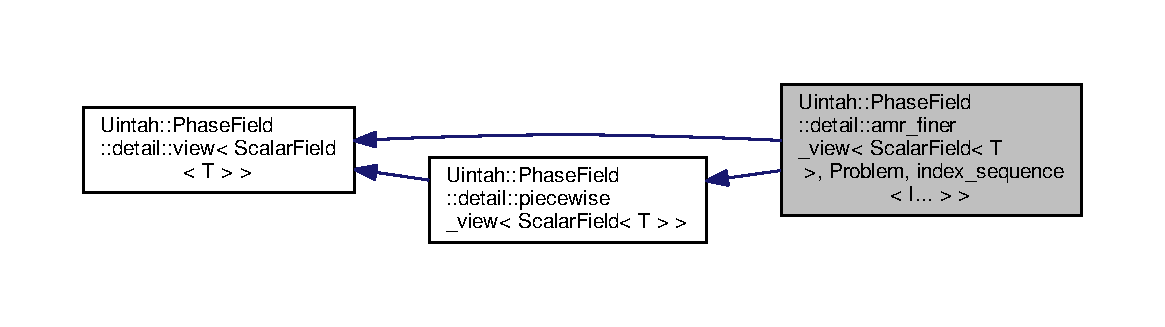
\includegraphics[width=350pt]{classUintah_1_1PhaseField_1_1detail_1_1amr__finer__view_3_01ScalarField_3_01T_01_4_00_01Problem_5955b0b99b60d322ead22e908697acaa}
\end{center}
\end{figure}


Collaboration diagram for Uintah\+:\+:Phase\+Field\+:\+:detail\+:\+:amr\+\_\+finer\+\_\+view$<$ Scalar\+Field$<$ T $>$, Problem, index\+\_\+sequence$<$ I... $>$ $>$\+:\nopagebreak
\begin{figure}[H]
\begin{center}
\leavevmode
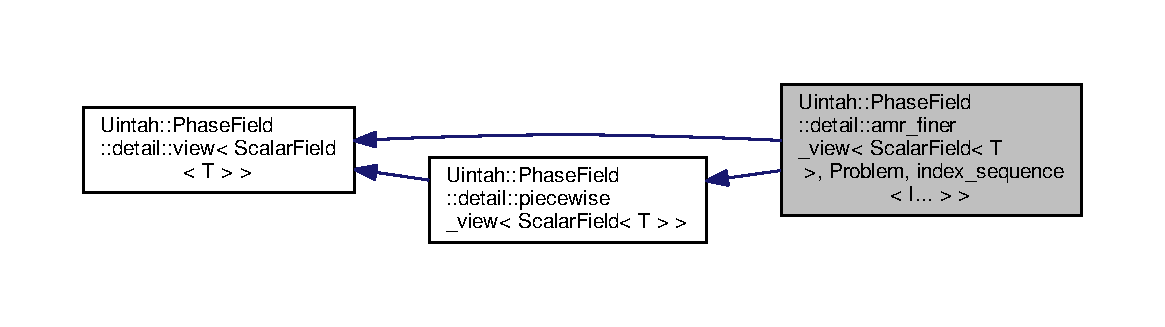
\includegraphics[width=350pt]{classUintah_1_1PhaseField_1_1detail_1_1amr__finer__view_3_01ScalarField_3_01T_01_4_00_01Problem_1532c6371c2eb1abbcb22e40b922d2af}
\end{center}
\end{figure}
\subsection*{Public Member Functions}
\begin{DoxyCompactItemize}
\item 
\hyperlink{classUintah_1_1PhaseField_1_1detail_1_1amr__finer__view_3_01ScalarField_3_01T_01_4_00_01Problem_810ae3f886a4d3bdb2b37c629369a2ec_a73afae95bc743443a5e4a72820fdacf0}{amr\+\_\+finer\+\_\+view} (const Var\+Label $\ast$label, const Var\+Label $\ast$subproblems\+\_\+label, int material)
\begin{DoxyCompactList}\small\item\em Constructor. \end{DoxyCompactList}\item 
\hyperlink{classUintah_1_1PhaseField_1_1detail_1_1amr__finer__view_3_01ScalarField_3_01T_01_4_00_01Problem_810ae3f886a4d3bdb2b37c629369a2ec_aec1b05c6c22f2d89b6f931a0b33b584c}{amr\+\_\+finer\+\_\+view} (Data\+Warehouse $\ast$dw, const Var\+Label $\ast$label, const Var\+Label $\ast$subproblems\+\_\+label, int material, const Patch $\ast$patch, bool use\+\_\+ghosts=\hyperlink{classUintah_1_1PhaseField_1_1detail_1_1amr__finer__view_3_01ScalarField_3_01T_01_4_00_01Problem_810ae3f886a4d3bdb2b37c629369a2ec_aee5138b1c87ec5e7717b5f1dd6fd47cd}{use\+\_\+ghosts\+\_\+dflt})
\begin{DoxyCompactList}\small\item\em Constructor. \end{DoxyCompactList}\item 
virtual \hyperlink{classUintah_1_1PhaseField_1_1detail_1_1amr__finer__view_3_01ScalarField_3_01T_01_4_00_01Problem_810ae3f886a4d3bdb2b37c629369a2ec_a5c34e61bae1798b170982e597180aa38}{$\sim$amr\+\_\+finer\+\_\+view} ()
\begin{DoxyCompactList}\small\item\em Destructor. \end{DoxyCompactList}\item 
\hyperlink{classUintah_1_1PhaseField_1_1detail_1_1amr__finer__view_3_01ScalarField_3_01T_01_4_00_01Problem_810ae3f886a4d3bdb2b37c629369a2ec_ae2099f71af3c5304a40a77de474052eb}{amr\+\_\+finer\+\_\+view} (const \hyperlink{classUintah_1_1PhaseField_1_1detail_1_1amr__finer__view}{amr\+\_\+finer\+\_\+view} \&)=delete
\begin{DoxyCompactList}\small\item\em Prevent copy (and move) constructor. \end{DoxyCompactList}\item 
\hyperlink{classUintah_1_1PhaseField_1_1detail_1_1amr__finer__view}{amr\+\_\+finer\+\_\+view} \& \hyperlink{classUintah_1_1PhaseField_1_1detail_1_1amr__finer__view_3_01ScalarField_3_01T_01_4_00_01Problem_810ae3f886a4d3bdb2b37c629369a2ec_a5b17dfade19e5fa6db10f185917fe731}{operator=} (const \hyperlink{classUintah_1_1PhaseField_1_1detail_1_1amr__finer__view}{amr\+\_\+finer\+\_\+view} \&)=delete
\begin{DoxyCompactList}\small\item\em Prevent copy (and move) assignment. \end{DoxyCompactList}\item 
virtual void \hyperlink{classUintah_1_1PhaseField_1_1detail_1_1amr__finer__view_3_01ScalarField_3_01T_01_4_00_01Problem_810ae3f886a4d3bdb2b37c629369a2ec_acc717dc37c60169bc4c85fbaaea766b3}{set} (Data\+Warehouse $\ast$dw, const Patch $\ast$patch, bool use\+\_\+ghosts=\hyperlink{classUintah_1_1PhaseField_1_1detail_1_1amr__finer__view_3_01ScalarField_3_01T_01_4_00_01Problem_810ae3f886a4d3bdb2b37c629369a2ec_aee5138b1c87ec5e7717b5f1dd6fd47cd}{use\+\_\+ghosts\+\_\+dflt}) override
\begin{DoxyCompactList}\small\item\em Retrieve value from the Data\+Warehouse for accessing the finer region over a given coarse patch. \end{DoxyCompactList}\item 
virtual void \hyperlink{classUintah_1_1PhaseField_1_1detail_1_1amr__finer__view_3_01ScalarField_3_01T_01_4_00_01Problem_810ae3f886a4d3bdb2b37c629369a2ec_a159ca4d3aaf8d45bd070ad7e4bf3561c}{set} (Data\+Warehouse $\ast$dw, const Level $\ast$level, const Int\+Vector \&low, const Int\+Vector \&high, bool use\+\_\+ghosts=\hyperlink{classUintah_1_1PhaseField_1_1detail_1_1amr__finer__view_3_01ScalarField_3_01T_01_4_00_01Problem_810ae3f886a4d3bdb2b37c629369a2ec_aee5138b1c87ec5e7717b5f1dd6fd47cd}{use\+\_\+ghosts\+\_\+dflt}) override
\begin{DoxyCompactList}\small\item\em Retrieve value from the Data\+Warehouse for accessing the finer region over a given coarse region. \end{DoxyCompactList}\item 
virtual \hyperlink{classUintah_1_1PhaseField_1_1detail_1_1view}{view}$<$ \hyperlink{structUintah_1_1PhaseField_1_1ScalarField}{Field} $>$ $\ast$ \hyperlink{classUintah_1_1PhaseField_1_1detail_1_1amr__finer__view_3_01ScalarField_3_01T_01_4_00_01Problem_810ae3f886a4d3bdb2b37c629369a2ec_a38bba423ebb77e4aaaded71c0c80583e}{clone} (bool deep) const override
\begin{DoxyCompactList}\small\item\em Get a copy of the view. \end{DoxyCompactList}\item 
virtual \hyperlink{classUintah_1_1PhaseField_1_1detail_1_1view}{view}$<$ \hyperlink{structUintah_1_1PhaseField_1_1ScalarField}{Field} $>$ $\ast$ \hyperlink{classUintah_1_1PhaseField_1_1detail_1_1amr__finer__view_3_01ScalarField_3_01T_01_4_00_01Problem_810ae3f886a4d3bdb2b37c629369a2ec_afae4d2b27a016b9f84d795d3e698608f}{clone} (bool deep, const Int\+Vector \&offset) const override
\begin{DoxyCompactList}\small\item\em Get a copy of the view and apply translate the support. \end{DoxyCompactList}\item 
virtual \hyperlink{classUintah_1_1PhaseField_1_1Support}{Support} \hyperlink{classUintah_1_1PhaseField_1_1detail_1_1amr__finer__view_3_01ScalarField_3_01T_01_4_00_01Problem_810ae3f886a4d3bdb2b37c629369a2ec_adfbb25e7253411ffab2a2bc035e87a6b}{get\+\_\+support} () const override
\begin{DoxyCompactList}\small\item\em Get the coarse region corresponding to the finer one for which the view has access to the Data\+Warehouse. \end{DoxyCompactList}\end{DoxyCompactItemize}
\subsection*{Static Public Attributes}
\begin{DoxyCompactItemize}
\item 
static constexpr bool \hyperlink{classUintah_1_1PhaseField_1_1detail_1_1amr__finer__view_3_01ScalarField_3_01T_01_4_00_01Problem_810ae3f886a4d3bdb2b37c629369a2ec_aee5138b1c87ec5e7717b5f1dd6fd47cd}{use\+\_\+ghosts\+\_\+dflt} = false
\begin{DoxyCompactList}\small\item\em Default value for use\+\_\+ghost when retrieving data. \end{DoxyCompactList}\end{DoxyCompactItemize}
\subsection*{Protected Member Functions}
\begin{DoxyCompactItemize}
\item 
\hyperlink{classUintah_1_1PhaseField_1_1detail_1_1amr__finer__view_3_01ScalarField_3_01T_01_4_00_01Problem_810ae3f886a4d3bdb2b37c629369a2ec_a3836d284166d8899b18d17a4f37d1852}{amr\+\_\+finer\+\_\+view} (const \hyperlink{classUintah_1_1PhaseField_1_1detail_1_1amr__finer__view}{amr\+\_\+finer\+\_\+view} $\ast$copy, bool deep)
\begin{DoxyCompactList}\small\item\em Constructor. \end{DoxyCompactList}\end{DoxyCompactItemize}
\subsection*{Additional Inherited Members}


\subsection{Detailed Description}
\subsubsection*{template$<$typename T, typename Problem, size\+\_\+t... I$>$\newline
class Uintah\+::\+Phase\+Field\+::detail\+::amr\+\_\+finer\+\_\+view$<$ Scalar\+Field$<$ T $>$, Problem, index\+\_\+sequence$<$ I... $>$ $>$}

Composite view for accessing finer grid variables (\hyperlink{structUintah_1_1PhaseField_1_1ScalarField}{Scalar\+Field} implementation) 

\begin{DoxyRemark}{Remarks}
deletion of views instantiated in \hyperlink{classUintah_1_1PhaseField_1_1detail_1_1piecewise__view}{piecewise\+\_\+view} are performed here
\end{DoxyRemark}

\begin{DoxyTemplParams}{Template Parameters}
{\em T} & type of the field value at each point \\
\hline
{\em \hyperlink{classUintah_1_1PhaseField_1_1Problem}{Problem}} & type of \hyperlink{namespaceUintah_1_1PhaseField}{Phase\+Field} problem \\
\hline
{\em \hyperlink{structUintah_1_1PhaseField_1_1I}{I}} & list of indices of Field within \hyperlink{classUintah_1_1PhaseField_1_1Problem}{Problem} (first element is variable index, following ones, if present, are the component index within the variable) \\
\hline
\end{DoxyTemplParams}


\subsection{Constructor \& Destructor Documentation}
\mbox{\Hypertarget{classUintah_1_1PhaseField_1_1detail_1_1amr__finer__view_3_01ScalarField_3_01T_01_4_00_01Problem_810ae3f886a4d3bdb2b37c629369a2ec_a3836d284166d8899b18d17a4f37d1852}\label{classUintah_1_1PhaseField_1_1detail_1_1amr__finer__view_3_01ScalarField_3_01T_01_4_00_01Problem_810ae3f886a4d3bdb2b37c629369a2ec_a3836d284166d8899b18d17a4f37d1852}} 
\index{Uintah\+::\+Phase\+Field\+::detail\+::amr\+\_\+finer\+\_\+view$<$ Scalar\+Field$<$ T $>$, Problem, index\+\_\+sequence$<$ I... $>$ $>$@{Uintah\+::\+Phase\+Field\+::detail\+::amr\+\_\+finer\+\_\+view$<$ Scalar\+Field$<$ T $>$, Problem, index\+\_\+sequence$<$ I... $>$ $>$}!amr\+\_\+finer\+\_\+view@{amr\+\_\+finer\+\_\+view}}
\index{amr\+\_\+finer\+\_\+view@{amr\+\_\+finer\+\_\+view}!Uintah\+::\+Phase\+Field\+::detail\+::amr\+\_\+finer\+\_\+view$<$ Scalar\+Field$<$ T $>$, Problem, index\+\_\+sequence$<$ I... $>$ $>$@{Uintah\+::\+Phase\+Field\+::detail\+::amr\+\_\+finer\+\_\+view$<$ Scalar\+Field$<$ T $>$, Problem, index\+\_\+sequence$<$ I... $>$ $>$}}
\subsubsection{\texorpdfstring{amr\+\_\+finer\+\_\+view()}{amr\_finer\_view()}\hspace{0.1cm}{\footnotesize\ttfamily [1/4]}}
{\footnotesize\ttfamily template$<$typename T , typename Problem , size\+\_\+t... I$>$ \\
\hyperlink{classUintah_1_1PhaseField_1_1detail_1_1amr__finer__view}{Uintah\+::\+Phase\+Field\+::detail\+::amr\+\_\+finer\+\_\+view}$<$ \hyperlink{structUintah_1_1PhaseField_1_1ScalarField}{Scalar\+Field}$<$ T $>$, \hyperlink{classUintah_1_1PhaseField_1_1Problem}{Problem}, \hyperlink{namespaceUintah_1_1PhaseField_a237de804d99512e50613aff7c94a9461}{index\+\_\+sequence}$<$ I... $>$ $>$\+::\hyperlink{classUintah_1_1PhaseField_1_1detail_1_1amr__finer__view}{amr\+\_\+finer\+\_\+view} (\begin{DoxyParamCaption}\item[{const \hyperlink{classUintah_1_1PhaseField_1_1detail_1_1amr__finer__view}{amr\+\_\+finer\+\_\+view}$<$ \hyperlink{structUintah_1_1PhaseField_1_1ScalarField}{Scalar\+Field}$<$ T $>$, \hyperlink{classUintah_1_1PhaseField_1_1Problem}{Problem}, \hyperlink{namespaceUintah_1_1PhaseField_a237de804d99512e50613aff7c94a9461}{index\+\_\+sequence}$<$ I... $>$ $>$ $\ast$}]{copy,  }\item[{bool}]{deep }\end{DoxyParamCaption})\hspace{0.3cm}{\ttfamily [inline]}, {\ttfamily [protected]}}



Constructor. 

Instantiate a copy of a given view


\begin{DoxyParams}{Parameters}
{\em copy} & source view for copying \\
\hline
{\em deep} & if true inner grid variable is copied as well otherwise the same grid variable is referenced \\
\hline
\end{DoxyParams}
\mbox{\Hypertarget{classUintah_1_1PhaseField_1_1detail_1_1amr__finer__view_3_01ScalarField_3_01T_01_4_00_01Problem_810ae3f886a4d3bdb2b37c629369a2ec_a73afae95bc743443a5e4a72820fdacf0}\label{classUintah_1_1PhaseField_1_1detail_1_1amr__finer__view_3_01ScalarField_3_01T_01_4_00_01Problem_810ae3f886a4d3bdb2b37c629369a2ec_a73afae95bc743443a5e4a72820fdacf0}} 
\index{Uintah\+::\+Phase\+Field\+::detail\+::amr\+\_\+finer\+\_\+view$<$ Scalar\+Field$<$ T $>$, Problem, index\+\_\+sequence$<$ I... $>$ $>$@{Uintah\+::\+Phase\+Field\+::detail\+::amr\+\_\+finer\+\_\+view$<$ Scalar\+Field$<$ T $>$, Problem, index\+\_\+sequence$<$ I... $>$ $>$}!amr\+\_\+finer\+\_\+view@{amr\+\_\+finer\+\_\+view}}
\index{amr\+\_\+finer\+\_\+view@{amr\+\_\+finer\+\_\+view}!Uintah\+::\+Phase\+Field\+::detail\+::amr\+\_\+finer\+\_\+view$<$ Scalar\+Field$<$ T $>$, Problem, index\+\_\+sequence$<$ I... $>$ $>$@{Uintah\+::\+Phase\+Field\+::detail\+::amr\+\_\+finer\+\_\+view$<$ Scalar\+Field$<$ T $>$, Problem, index\+\_\+sequence$<$ I... $>$ $>$}}
\subsubsection{\texorpdfstring{amr\+\_\+finer\+\_\+view()}{amr\_finer\_view()}\hspace{0.1cm}{\footnotesize\ttfamily [2/4]}}
{\footnotesize\ttfamily template$<$typename T , typename Problem , size\+\_\+t... I$>$ \\
\hyperlink{classUintah_1_1PhaseField_1_1detail_1_1amr__finer__view}{Uintah\+::\+Phase\+Field\+::detail\+::amr\+\_\+finer\+\_\+view}$<$ \hyperlink{structUintah_1_1PhaseField_1_1ScalarField}{Scalar\+Field}$<$ T $>$, \hyperlink{classUintah_1_1PhaseField_1_1Problem}{Problem}, \hyperlink{namespaceUintah_1_1PhaseField_a237de804d99512e50613aff7c94a9461}{index\+\_\+sequence}$<$ I... $>$ $>$\+::\hyperlink{classUintah_1_1PhaseField_1_1detail_1_1amr__finer__view}{amr\+\_\+finer\+\_\+view} (\begin{DoxyParamCaption}\item[{const Var\+Label $\ast$}]{label,  }\item[{const Var\+Label $\ast$}]{subproblems\+\_\+label,  }\item[{int}]{material }\end{DoxyParamCaption})\hspace{0.3cm}{\ttfamily [inline]}}



Constructor. 

construct finer view without retrieving inner variable data from the Data\+Warehouse


\begin{DoxyParams}{Parameters}
{\em label} & label of variable in the Data\+Warehouse \\
\hline
{\em subproblems\+\_\+label} & label of subproblems in the Data\+Warehouse \\
\hline
{\em material} & index of material in the Data\+Warehouse \\
\hline
\end{DoxyParams}
\mbox{\Hypertarget{classUintah_1_1PhaseField_1_1detail_1_1amr__finer__view_3_01ScalarField_3_01T_01_4_00_01Problem_810ae3f886a4d3bdb2b37c629369a2ec_aec1b05c6c22f2d89b6f931a0b33b584c}\label{classUintah_1_1PhaseField_1_1detail_1_1amr__finer__view_3_01ScalarField_3_01T_01_4_00_01Problem_810ae3f886a4d3bdb2b37c629369a2ec_aec1b05c6c22f2d89b6f931a0b33b584c}} 
\index{Uintah\+::\+Phase\+Field\+::detail\+::amr\+\_\+finer\+\_\+view$<$ Scalar\+Field$<$ T $>$, Problem, index\+\_\+sequence$<$ I... $>$ $>$@{Uintah\+::\+Phase\+Field\+::detail\+::amr\+\_\+finer\+\_\+view$<$ Scalar\+Field$<$ T $>$, Problem, index\+\_\+sequence$<$ I... $>$ $>$}!amr\+\_\+finer\+\_\+view@{amr\+\_\+finer\+\_\+view}}
\index{amr\+\_\+finer\+\_\+view@{amr\+\_\+finer\+\_\+view}!Uintah\+::\+Phase\+Field\+::detail\+::amr\+\_\+finer\+\_\+view$<$ Scalar\+Field$<$ T $>$, Problem, index\+\_\+sequence$<$ I... $>$ $>$@{Uintah\+::\+Phase\+Field\+::detail\+::amr\+\_\+finer\+\_\+view$<$ Scalar\+Field$<$ T $>$, Problem, index\+\_\+sequence$<$ I... $>$ $>$}}
\subsubsection{\texorpdfstring{amr\+\_\+finer\+\_\+view()}{amr\_finer\_view()}\hspace{0.1cm}{\footnotesize\ttfamily [3/4]}}
{\footnotesize\ttfamily template$<$typename T , typename Problem , size\+\_\+t... I$>$ \\
\hyperlink{classUintah_1_1PhaseField_1_1detail_1_1amr__finer__view}{Uintah\+::\+Phase\+Field\+::detail\+::amr\+\_\+finer\+\_\+view}$<$ \hyperlink{structUintah_1_1PhaseField_1_1ScalarField}{Scalar\+Field}$<$ T $>$, \hyperlink{classUintah_1_1PhaseField_1_1Problem}{Problem}, \hyperlink{namespaceUintah_1_1PhaseField_a237de804d99512e50613aff7c94a9461}{index\+\_\+sequence}$<$ I... $>$ $>$\+::\hyperlink{classUintah_1_1PhaseField_1_1detail_1_1amr__finer__view}{amr\+\_\+finer\+\_\+view} (\begin{DoxyParamCaption}\item[{Data\+Warehouse $\ast$}]{dw,  }\item[{const Var\+Label $\ast$}]{label,  }\item[{const Var\+Label $\ast$}]{subproblems\+\_\+label,  }\item[{int}]{material,  }\item[{const Patch $\ast$}]{patch,  }\item[{bool}]{use\+\_\+ghosts = {\ttfamily \hyperlink{classUintah_1_1PhaseField_1_1detail_1_1amr__finer__view_3_01ScalarField_3_01T_01_4_00_01Problem_810ae3f886a4d3bdb2b37c629369a2ec_aee5138b1c87ec5e7717b5f1dd6fd47cd}{use\+\_\+ghosts\+\_\+dflt}} }\end{DoxyParamCaption})\hspace{0.3cm}{\ttfamily [inline]}}



Constructor. 

construct finer view and retrieve inner variable data from the Data\+Warehouse for the region lying under a given fine patch.

\begin{DoxyRemark}{Remarks}
the number of ghost cells/nodes and the corresponding region on the finer level is automatically computed to match the restriction type
\end{DoxyRemark}

\begin{DoxyParams}{Parameters}
{\em dw} & Data\+Warehouse which data is retrieved from \\
\hline
{\em label} & label of variable in the Data\+Warehouse \\
\hline
{\em subproblems\+\_\+label} & label of subproblems in the Data\+Warehouse \\
\hline
{\em material} & index of material in the Data\+Warehouse \\
\hline
{\em patch} & patch on which data is retrieved \\
\hline
{\em use\+\_\+ghosts} & must be false \\
\hline
\end{DoxyParams}
\mbox{\Hypertarget{classUintah_1_1PhaseField_1_1detail_1_1amr__finer__view_3_01ScalarField_3_01T_01_4_00_01Problem_810ae3f886a4d3bdb2b37c629369a2ec_a5c34e61bae1798b170982e597180aa38}\label{classUintah_1_1PhaseField_1_1detail_1_1amr__finer__view_3_01ScalarField_3_01T_01_4_00_01Problem_810ae3f886a4d3bdb2b37c629369a2ec_a5c34e61bae1798b170982e597180aa38}} 
\index{Uintah\+::\+Phase\+Field\+::detail\+::amr\+\_\+finer\+\_\+view$<$ Scalar\+Field$<$ T $>$, Problem, index\+\_\+sequence$<$ I... $>$ $>$@{Uintah\+::\+Phase\+Field\+::detail\+::amr\+\_\+finer\+\_\+view$<$ Scalar\+Field$<$ T $>$, Problem, index\+\_\+sequence$<$ I... $>$ $>$}!````~amr\+\_\+finer\+\_\+view@{$\sim$amr\+\_\+finer\+\_\+view}}
\index{````~amr\+\_\+finer\+\_\+view@{$\sim$amr\+\_\+finer\+\_\+view}!Uintah\+::\+Phase\+Field\+::detail\+::amr\+\_\+finer\+\_\+view$<$ Scalar\+Field$<$ T $>$, Problem, index\+\_\+sequence$<$ I... $>$ $>$@{Uintah\+::\+Phase\+Field\+::detail\+::amr\+\_\+finer\+\_\+view$<$ Scalar\+Field$<$ T $>$, Problem, index\+\_\+sequence$<$ I... $>$ $>$}}
\subsubsection{\texorpdfstring{$\sim$amr\+\_\+finer\+\_\+view()}{~amr\_finer\_view()}}
{\footnotesize\ttfamily template$<$typename T , typename Problem , size\+\_\+t... I$>$ \\
virtual \hyperlink{classUintah_1_1PhaseField_1_1detail_1_1amr__finer__view}{Uintah\+::\+Phase\+Field\+::detail\+::amr\+\_\+finer\+\_\+view}$<$ \hyperlink{structUintah_1_1PhaseField_1_1ScalarField}{Scalar\+Field}$<$ T $>$, \hyperlink{classUintah_1_1PhaseField_1_1Problem}{Problem}, \hyperlink{namespaceUintah_1_1PhaseField_a237de804d99512e50613aff7c94a9461}{index\+\_\+sequence}$<$ I... $>$ $>$\+::$\sim$\hyperlink{classUintah_1_1PhaseField_1_1detail_1_1amr__finer__view}{amr\+\_\+finer\+\_\+view} (\begin{DoxyParamCaption}{ }\end{DoxyParamCaption})\hspace{0.3cm}{\ttfamily [inline]}, {\ttfamily [virtual]}}



Destructor. 

\mbox{\Hypertarget{classUintah_1_1PhaseField_1_1detail_1_1amr__finer__view_3_01ScalarField_3_01T_01_4_00_01Problem_810ae3f886a4d3bdb2b37c629369a2ec_ae2099f71af3c5304a40a77de474052eb}\label{classUintah_1_1PhaseField_1_1detail_1_1amr__finer__view_3_01ScalarField_3_01T_01_4_00_01Problem_810ae3f886a4d3bdb2b37c629369a2ec_ae2099f71af3c5304a40a77de474052eb}} 
\index{Uintah\+::\+Phase\+Field\+::detail\+::amr\+\_\+finer\+\_\+view$<$ Scalar\+Field$<$ T $>$, Problem, index\+\_\+sequence$<$ I... $>$ $>$@{Uintah\+::\+Phase\+Field\+::detail\+::amr\+\_\+finer\+\_\+view$<$ Scalar\+Field$<$ T $>$, Problem, index\+\_\+sequence$<$ I... $>$ $>$}!amr\+\_\+finer\+\_\+view@{amr\+\_\+finer\+\_\+view}}
\index{amr\+\_\+finer\+\_\+view@{amr\+\_\+finer\+\_\+view}!Uintah\+::\+Phase\+Field\+::detail\+::amr\+\_\+finer\+\_\+view$<$ Scalar\+Field$<$ T $>$, Problem, index\+\_\+sequence$<$ I... $>$ $>$@{Uintah\+::\+Phase\+Field\+::detail\+::amr\+\_\+finer\+\_\+view$<$ Scalar\+Field$<$ T $>$, Problem, index\+\_\+sequence$<$ I... $>$ $>$}}
\subsubsection{\texorpdfstring{amr\+\_\+finer\+\_\+view()}{amr\_finer\_view()}\hspace{0.1cm}{\footnotesize\ttfamily [4/4]}}
{\footnotesize\ttfamily template$<$typename T , typename Problem , size\+\_\+t... I$>$ \\
\hyperlink{classUintah_1_1PhaseField_1_1detail_1_1amr__finer__view}{Uintah\+::\+Phase\+Field\+::detail\+::amr\+\_\+finer\+\_\+view}$<$ \hyperlink{structUintah_1_1PhaseField_1_1ScalarField}{Scalar\+Field}$<$ T $>$, \hyperlink{classUintah_1_1PhaseField_1_1Problem}{Problem}, \hyperlink{namespaceUintah_1_1PhaseField_a237de804d99512e50613aff7c94a9461}{index\+\_\+sequence}$<$ I... $>$ $>$\+::\hyperlink{classUintah_1_1PhaseField_1_1detail_1_1amr__finer__view}{amr\+\_\+finer\+\_\+view} (\begin{DoxyParamCaption}\item[{const \hyperlink{classUintah_1_1PhaseField_1_1detail_1_1amr__finer__view}{amr\+\_\+finer\+\_\+view}$<$ \hyperlink{structUintah_1_1PhaseField_1_1ScalarField}{Scalar\+Field}$<$ T $>$, \hyperlink{classUintah_1_1PhaseField_1_1Problem}{Problem}, \hyperlink{namespaceUintah_1_1PhaseField_a237de804d99512e50613aff7c94a9461}{index\+\_\+sequence}$<$ I... $>$ $>$ \&}]{ }\end{DoxyParamCaption})\hspace{0.3cm}{\ttfamily [delete]}}



Prevent copy (and move) constructor. 



\subsection{Member Function Documentation}
\mbox{\Hypertarget{classUintah_1_1PhaseField_1_1detail_1_1amr__finer__view_3_01ScalarField_3_01T_01_4_00_01Problem_810ae3f886a4d3bdb2b37c629369a2ec_a38bba423ebb77e4aaaded71c0c80583e}\label{classUintah_1_1PhaseField_1_1detail_1_1amr__finer__view_3_01ScalarField_3_01T_01_4_00_01Problem_810ae3f886a4d3bdb2b37c629369a2ec_a38bba423ebb77e4aaaded71c0c80583e}} 
\index{Uintah\+::\+Phase\+Field\+::detail\+::amr\+\_\+finer\+\_\+view$<$ Scalar\+Field$<$ T $>$, Problem, index\+\_\+sequence$<$ I... $>$ $>$@{Uintah\+::\+Phase\+Field\+::detail\+::amr\+\_\+finer\+\_\+view$<$ Scalar\+Field$<$ T $>$, Problem, index\+\_\+sequence$<$ I... $>$ $>$}!clone@{clone}}
\index{clone@{clone}!Uintah\+::\+Phase\+Field\+::detail\+::amr\+\_\+finer\+\_\+view$<$ Scalar\+Field$<$ T $>$, Problem, index\+\_\+sequence$<$ I... $>$ $>$@{Uintah\+::\+Phase\+Field\+::detail\+::amr\+\_\+finer\+\_\+view$<$ Scalar\+Field$<$ T $>$, Problem, index\+\_\+sequence$<$ I... $>$ $>$}}
\subsubsection{\texorpdfstring{clone()}{clone()}\hspace{0.1cm}{\footnotesize\ttfamily [1/2]}}
{\footnotesize\ttfamily template$<$typename T , typename Problem , size\+\_\+t... I$>$ \\
virtual \hyperlink{classUintah_1_1PhaseField_1_1detail_1_1view}{view}$<$\hyperlink{structUintah_1_1PhaseField_1_1ScalarField}{Field}$>$$\ast$ \hyperlink{classUintah_1_1PhaseField_1_1detail_1_1amr__finer__view}{Uintah\+::\+Phase\+Field\+::detail\+::amr\+\_\+finer\+\_\+view}$<$ \hyperlink{structUintah_1_1PhaseField_1_1ScalarField}{Scalar\+Field}$<$ T $>$, \hyperlink{classUintah_1_1PhaseField_1_1Problem}{Problem}, \hyperlink{namespaceUintah_1_1PhaseField_a237de804d99512e50613aff7c94a9461}{index\+\_\+sequence}$<$ I... $>$ $>$\+::clone (\begin{DoxyParamCaption}\item[{bool}]{deep }\end{DoxyParamCaption}) const\hspace{0.3cm}{\ttfamily [inline]}, {\ttfamily [override]}, {\ttfamily [virtual]}}



Get a copy of the view. 


\begin{DoxyParams}{Parameters}
{\em deep} & if true inner grid variable is copied as well otherwise the same grid variable is referenced\\
\hline
\end{DoxyParams}
\begin{DoxyReturn}{Returns}
new view instance 
\end{DoxyReturn}


Implements \hyperlink{classUintah_1_1PhaseField_1_1detail_1_1view_3_01ScalarField_3_01T_01_4_01_4_a6e11243c9d776a7b703e524ea4151a16}{Uintah\+::\+Phase\+Field\+::detail\+::view$<$ Scalar\+Field$<$ T $>$ $>$}.

\mbox{\Hypertarget{classUintah_1_1PhaseField_1_1detail_1_1amr__finer__view_3_01ScalarField_3_01T_01_4_00_01Problem_810ae3f886a4d3bdb2b37c629369a2ec_afae4d2b27a016b9f84d795d3e698608f}\label{classUintah_1_1PhaseField_1_1detail_1_1amr__finer__view_3_01ScalarField_3_01T_01_4_00_01Problem_810ae3f886a4d3bdb2b37c629369a2ec_afae4d2b27a016b9f84d795d3e698608f}} 
\index{Uintah\+::\+Phase\+Field\+::detail\+::amr\+\_\+finer\+\_\+view$<$ Scalar\+Field$<$ T $>$, Problem, index\+\_\+sequence$<$ I... $>$ $>$@{Uintah\+::\+Phase\+Field\+::detail\+::amr\+\_\+finer\+\_\+view$<$ Scalar\+Field$<$ T $>$, Problem, index\+\_\+sequence$<$ I... $>$ $>$}!clone@{clone}}
\index{clone@{clone}!Uintah\+::\+Phase\+Field\+::detail\+::amr\+\_\+finer\+\_\+view$<$ Scalar\+Field$<$ T $>$, Problem, index\+\_\+sequence$<$ I... $>$ $>$@{Uintah\+::\+Phase\+Field\+::detail\+::amr\+\_\+finer\+\_\+view$<$ Scalar\+Field$<$ T $>$, Problem, index\+\_\+sequence$<$ I... $>$ $>$}}
\subsubsection{\texorpdfstring{clone()}{clone()}\hspace{0.1cm}{\footnotesize\ttfamily [2/2]}}
{\footnotesize\ttfamily template$<$typename T , typename Problem , size\+\_\+t... I$>$ \\
virtual \hyperlink{classUintah_1_1PhaseField_1_1detail_1_1view}{view}$<$\hyperlink{structUintah_1_1PhaseField_1_1ScalarField}{Field}$>$$\ast$ \hyperlink{classUintah_1_1PhaseField_1_1detail_1_1amr__finer__view}{Uintah\+::\+Phase\+Field\+::detail\+::amr\+\_\+finer\+\_\+view}$<$ \hyperlink{structUintah_1_1PhaseField_1_1ScalarField}{Scalar\+Field}$<$ T $>$, \hyperlink{classUintah_1_1PhaseField_1_1Problem}{Problem}, \hyperlink{namespaceUintah_1_1PhaseField_a237de804d99512e50613aff7c94a9461}{index\+\_\+sequence}$<$ I... $>$ $>$\+::clone (\begin{DoxyParamCaption}\item[{bool}]{deep,  }\item[{const Int\+Vector \&}]{offset }\end{DoxyParamCaption}) const\hspace{0.3cm}{\ttfamily [inline]}, {\ttfamily [override]}, {\ttfamily [virtual]}}



Get a copy of the view and apply translate the support. 

\begin{DoxyRemark}{Remarks}
It is meant to be used for virtual patches (i.\+e. periodic boundaries)
\end{DoxyRemark}

\begin{DoxyParams}{Parameters}
{\em deep} & if true inner grid variable is copied as well otherwise the same grid variable is referenced \\
\hline
{\em offset} & vector specifying the translation of the support \\
\hline
\end{DoxyParams}
\begin{DoxyReturn}{Returns}
new view instance 
\end{DoxyReturn}


Implements \hyperlink{classUintah_1_1PhaseField_1_1detail_1_1view_3_01ScalarField_3_01T_01_4_01_4_abd928104240e329f3bc4441ebab7c50c}{Uintah\+::\+Phase\+Field\+::detail\+::view$<$ Scalar\+Field$<$ T $>$ $>$}.

\mbox{\Hypertarget{classUintah_1_1PhaseField_1_1detail_1_1amr__finer__view_3_01ScalarField_3_01T_01_4_00_01Problem_810ae3f886a4d3bdb2b37c629369a2ec_adfbb25e7253411ffab2a2bc035e87a6b}\label{classUintah_1_1PhaseField_1_1detail_1_1amr__finer__view_3_01ScalarField_3_01T_01_4_00_01Problem_810ae3f886a4d3bdb2b37c629369a2ec_adfbb25e7253411ffab2a2bc035e87a6b}} 
\index{Uintah\+::\+Phase\+Field\+::detail\+::amr\+\_\+finer\+\_\+view$<$ Scalar\+Field$<$ T $>$, Problem, index\+\_\+sequence$<$ I... $>$ $>$@{Uintah\+::\+Phase\+Field\+::detail\+::amr\+\_\+finer\+\_\+view$<$ Scalar\+Field$<$ T $>$, Problem, index\+\_\+sequence$<$ I... $>$ $>$}!get\+\_\+support@{get\+\_\+support}}
\index{get\+\_\+support@{get\+\_\+support}!Uintah\+::\+Phase\+Field\+::detail\+::amr\+\_\+finer\+\_\+view$<$ Scalar\+Field$<$ T $>$, Problem, index\+\_\+sequence$<$ I... $>$ $>$@{Uintah\+::\+Phase\+Field\+::detail\+::amr\+\_\+finer\+\_\+view$<$ Scalar\+Field$<$ T $>$, Problem, index\+\_\+sequence$<$ I... $>$ $>$}}
\subsubsection{\texorpdfstring{get\+\_\+support()}{get\_support()}}
{\footnotesize\ttfamily template$<$typename T , typename Problem , size\+\_\+t... I$>$ \\
virtual \hyperlink{classUintah_1_1PhaseField_1_1Support}{Support} \hyperlink{classUintah_1_1PhaseField_1_1detail_1_1amr__finer__view}{Uintah\+::\+Phase\+Field\+::detail\+::amr\+\_\+finer\+\_\+view}$<$ \hyperlink{structUintah_1_1PhaseField_1_1ScalarField}{Scalar\+Field}$<$ T $>$, \hyperlink{classUintah_1_1PhaseField_1_1Problem}{Problem}, \hyperlink{namespaceUintah_1_1PhaseField_a237de804d99512e50613aff7c94a9461}{index\+\_\+sequence}$<$ I... $>$ $>$\+::get\+\_\+support (\begin{DoxyParamCaption}{ }\end{DoxyParamCaption}) const\hspace{0.3cm}{\ttfamily [inline]}, {\ttfamily [override]}, {\ttfamily [virtual]}}



Get the coarse region corresponding to the finer one for which the view has access to the Data\+Warehouse. 

\begin{DoxyReturn}{Returns}
support of the view 
\end{DoxyReturn}


Implements \hyperlink{classUintah_1_1PhaseField_1_1detail_1_1view_3_01ScalarField_3_01T_01_4_01_4_a3e14b0c7a57a57707bb33954861ab1c1}{Uintah\+::\+Phase\+Field\+::detail\+::view$<$ Scalar\+Field$<$ T $>$ $>$}.

\mbox{\Hypertarget{classUintah_1_1PhaseField_1_1detail_1_1amr__finer__view_3_01ScalarField_3_01T_01_4_00_01Problem_810ae3f886a4d3bdb2b37c629369a2ec_a5b17dfade19e5fa6db10f185917fe731}\label{classUintah_1_1PhaseField_1_1detail_1_1amr__finer__view_3_01ScalarField_3_01T_01_4_00_01Problem_810ae3f886a4d3bdb2b37c629369a2ec_a5b17dfade19e5fa6db10f185917fe731}} 
\index{Uintah\+::\+Phase\+Field\+::detail\+::amr\+\_\+finer\+\_\+view$<$ Scalar\+Field$<$ T $>$, Problem, index\+\_\+sequence$<$ I... $>$ $>$@{Uintah\+::\+Phase\+Field\+::detail\+::amr\+\_\+finer\+\_\+view$<$ Scalar\+Field$<$ T $>$, Problem, index\+\_\+sequence$<$ I... $>$ $>$}!operator=@{operator=}}
\index{operator=@{operator=}!Uintah\+::\+Phase\+Field\+::detail\+::amr\+\_\+finer\+\_\+view$<$ Scalar\+Field$<$ T $>$, Problem, index\+\_\+sequence$<$ I... $>$ $>$@{Uintah\+::\+Phase\+Field\+::detail\+::amr\+\_\+finer\+\_\+view$<$ Scalar\+Field$<$ T $>$, Problem, index\+\_\+sequence$<$ I... $>$ $>$}}
\subsubsection{\texorpdfstring{operator=()}{operator=()}}
{\footnotesize\ttfamily template$<$typename T , typename Problem , size\+\_\+t... I$>$ \\
\hyperlink{classUintah_1_1PhaseField_1_1detail_1_1amr__finer__view}{amr\+\_\+finer\+\_\+view}\& \hyperlink{classUintah_1_1PhaseField_1_1detail_1_1amr__finer__view}{Uintah\+::\+Phase\+Field\+::detail\+::amr\+\_\+finer\+\_\+view}$<$ \hyperlink{structUintah_1_1PhaseField_1_1ScalarField}{Scalar\+Field}$<$ T $>$, \hyperlink{classUintah_1_1PhaseField_1_1Problem}{Problem}, \hyperlink{namespaceUintah_1_1PhaseField_a237de804d99512e50613aff7c94a9461}{index\+\_\+sequence}$<$ I... $>$ $>$\+::operator= (\begin{DoxyParamCaption}\item[{const \hyperlink{classUintah_1_1PhaseField_1_1detail_1_1amr__finer__view}{amr\+\_\+finer\+\_\+view}$<$ \hyperlink{structUintah_1_1PhaseField_1_1ScalarField}{Scalar\+Field}$<$ T $>$, \hyperlink{classUintah_1_1PhaseField_1_1Problem}{Problem}, \hyperlink{namespaceUintah_1_1PhaseField_a237de804d99512e50613aff7c94a9461}{index\+\_\+sequence}$<$ I... $>$ $>$ \&}]{ }\end{DoxyParamCaption})\hspace{0.3cm}{\ttfamily [delete]}}



Prevent copy (and move) assignment. 

\mbox{\Hypertarget{classUintah_1_1PhaseField_1_1detail_1_1amr__finer__view_3_01ScalarField_3_01T_01_4_00_01Problem_810ae3f886a4d3bdb2b37c629369a2ec_acc717dc37c60169bc4c85fbaaea766b3}\label{classUintah_1_1PhaseField_1_1detail_1_1amr__finer__view_3_01ScalarField_3_01T_01_4_00_01Problem_810ae3f886a4d3bdb2b37c629369a2ec_acc717dc37c60169bc4c85fbaaea766b3}} 
\index{Uintah\+::\+Phase\+Field\+::detail\+::amr\+\_\+finer\+\_\+view$<$ Scalar\+Field$<$ T $>$, Problem, index\+\_\+sequence$<$ I... $>$ $>$@{Uintah\+::\+Phase\+Field\+::detail\+::amr\+\_\+finer\+\_\+view$<$ Scalar\+Field$<$ T $>$, Problem, index\+\_\+sequence$<$ I... $>$ $>$}!set@{set}}
\index{set@{set}!Uintah\+::\+Phase\+Field\+::detail\+::amr\+\_\+finer\+\_\+view$<$ Scalar\+Field$<$ T $>$, Problem, index\+\_\+sequence$<$ I... $>$ $>$@{Uintah\+::\+Phase\+Field\+::detail\+::amr\+\_\+finer\+\_\+view$<$ Scalar\+Field$<$ T $>$, Problem, index\+\_\+sequence$<$ I... $>$ $>$}}
\subsubsection{\texorpdfstring{set()}{set()}\hspace{0.1cm}{\footnotesize\ttfamily [1/2]}}
{\footnotesize\ttfamily template$<$typename T , typename Problem , size\+\_\+t... I$>$ \\
virtual void \hyperlink{classUintah_1_1PhaseField_1_1detail_1_1amr__finer__view}{Uintah\+::\+Phase\+Field\+::detail\+::amr\+\_\+finer\+\_\+view}$<$ \hyperlink{structUintah_1_1PhaseField_1_1ScalarField}{Scalar\+Field}$<$ T $>$, \hyperlink{classUintah_1_1PhaseField_1_1Problem}{Problem}, \hyperlink{namespaceUintah_1_1PhaseField_a237de804d99512e50613aff7c94a9461}{index\+\_\+sequence}$<$ I... $>$ $>$\+::set (\begin{DoxyParamCaption}\item[{Data\+Warehouse $\ast$}]{dw,  }\item[{const Patch $\ast$}]{patch,  }\item[{bool}]{use\+\_\+ghosts = {\ttfamily \hyperlink{classUintah_1_1PhaseField_1_1detail_1_1amr__finer__view_3_01ScalarField_3_01T_01_4_00_01Problem_810ae3f886a4d3bdb2b37c629369a2ec_aee5138b1c87ec5e7717b5f1dd6fd47cd}{use\+\_\+ghosts\+\_\+dflt}} }\end{DoxyParamCaption})\hspace{0.3cm}{\ttfamily [inline]}, {\ttfamily [override]}, {\ttfamily [virtual]}}



Retrieve value from the Data\+Warehouse for accessing the finer region over a given coarse patch. 


\begin{DoxyParams}{Parameters}
{\em dw} & Data\+Warehouse from which data is retrieved \\
\hline
{\em patch} & coarse grid patch to retrieve data for \\
\hline
{\em use\+\_\+ghosts} & must be false \\
\hline
\end{DoxyParams}


Implements \hyperlink{classUintah_1_1PhaseField_1_1detail_1_1view_3_01ScalarField_3_01T_01_4_01_4_ae90ea8b33fde8515a1f2e8f5c03c0166}{Uintah\+::\+Phase\+Field\+::detail\+::view$<$ Scalar\+Field$<$ T $>$ $>$}.

\mbox{\Hypertarget{classUintah_1_1PhaseField_1_1detail_1_1amr__finer__view_3_01ScalarField_3_01T_01_4_00_01Problem_810ae3f886a4d3bdb2b37c629369a2ec_a159ca4d3aaf8d45bd070ad7e4bf3561c}\label{classUintah_1_1PhaseField_1_1detail_1_1amr__finer__view_3_01ScalarField_3_01T_01_4_00_01Problem_810ae3f886a4d3bdb2b37c629369a2ec_a159ca4d3aaf8d45bd070ad7e4bf3561c}} 
\index{Uintah\+::\+Phase\+Field\+::detail\+::amr\+\_\+finer\+\_\+view$<$ Scalar\+Field$<$ T $>$, Problem, index\+\_\+sequence$<$ I... $>$ $>$@{Uintah\+::\+Phase\+Field\+::detail\+::amr\+\_\+finer\+\_\+view$<$ Scalar\+Field$<$ T $>$, Problem, index\+\_\+sequence$<$ I... $>$ $>$}!set@{set}}
\index{set@{set}!Uintah\+::\+Phase\+Field\+::detail\+::amr\+\_\+finer\+\_\+view$<$ Scalar\+Field$<$ T $>$, Problem, index\+\_\+sequence$<$ I... $>$ $>$@{Uintah\+::\+Phase\+Field\+::detail\+::amr\+\_\+finer\+\_\+view$<$ Scalar\+Field$<$ T $>$, Problem, index\+\_\+sequence$<$ I... $>$ $>$}}
\subsubsection{\texorpdfstring{set()}{set()}\hspace{0.1cm}{\footnotesize\ttfamily [2/2]}}
{\footnotesize\ttfamily template$<$typename T , typename Problem , size\+\_\+t... I$>$ \\
virtual void \hyperlink{classUintah_1_1PhaseField_1_1detail_1_1amr__finer__view}{Uintah\+::\+Phase\+Field\+::detail\+::amr\+\_\+finer\+\_\+view}$<$ \hyperlink{structUintah_1_1PhaseField_1_1ScalarField}{Scalar\+Field}$<$ T $>$, \hyperlink{classUintah_1_1PhaseField_1_1Problem}{Problem}, \hyperlink{namespaceUintah_1_1PhaseField_a237de804d99512e50613aff7c94a9461}{index\+\_\+sequence}$<$ I... $>$ $>$\+::set (\begin{DoxyParamCaption}\item[{Data\+Warehouse $\ast$}]{dw,  }\item[{const Level $\ast$}]{level,  }\item[{const Int\+Vector \&}]{low,  }\item[{const Int\+Vector \&}]{high,  }\item[{bool}]{use\+\_\+ghosts = {\ttfamily \hyperlink{classUintah_1_1PhaseField_1_1detail_1_1amr__finer__view_3_01ScalarField_3_01T_01_4_00_01Problem_810ae3f886a4d3bdb2b37c629369a2ec_aee5138b1c87ec5e7717b5f1dd6fd47cd}{use\+\_\+ghosts\+\_\+dflt}} }\end{DoxyParamCaption})\hspace{0.3cm}{\ttfamily [inline]}, {\ttfamily [override]}, {\ttfamily [virtual]}}



Retrieve value from the Data\+Warehouse for accessing the finer region over a given coarse region. 


\begin{DoxyParams}{Parameters}
{\em dw} & Data\+Warehouse from which data is retrieved \\
\hline
{\em level} & coarse grid level from which retrieve data \\
\hline
{\em low} & lower bound of the coarse region to retrieve \\
\hline
{\em high} & higher bound of the coarse region to retrieve \\
\hline
{\em use\+\_\+ghosts} & must be false \\
\hline
\end{DoxyParams}


Implements \hyperlink{classUintah_1_1PhaseField_1_1detail_1_1view_3_01ScalarField_3_01T_01_4_01_4_a5fc830b30b120922cfe8a2c008d96109}{Uintah\+::\+Phase\+Field\+::detail\+::view$<$ Scalar\+Field$<$ T $>$ $>$}.



\subsection{Member Data Documentation}
\mbox{\Hypertarget{classUintah_1_1PhaseField_1_1detail_1_1amr__finer__view_3_01ScalarField_3_01T_01_4_00_01Problem_810ae3f886a4d3bdb2b37c629369a2ec_aee5138b1c87ec5e7717b5f1dd6fd47cd}\label{classUintah_1_1PhaseField_1_1detail_1_1amr__finer__view_3_01ScalarField_3_01T_01_4_00_01Problem_810ae3f886a4d3bdb2b37c629369a2ec_aee5138b1c87ec5e7717b5f1dd6fd47cd}} 
\index{Uintah\+::\+Phase\+Field\+::detail\+::amr\+\_\+finer\+\_\+view$<$ Scalar\+Field$<$ T $>$, Problem, index\+\_\+sequence$<$ I... $>$ $>$@{Uintah\+::\+Phase\+Field\+::detail\+::amr\+\_\+finer\+\_\+view$<$ Scalar\+Field$<$ T $>$, Problem, index\+\_\+sequence$<$ I... $>$ $>$}!use\+\_\+ghosts\+\_\+dflt@{use\+\_\+ghosts\+\_\+dflt}}
\index{use\+\_\+ghosts\+\_\+dflt@{use\+\_\+ghosts\+\_\+dflt}!Uintah\+::\+Phase\+Field\+::detail\+::amr\+\_\+finer\+\_\+view$<$ Scalar\+Field$<$ T $>$, Problem, index\+\_\+sequence$<$ I... $>$ $>$@{Uintah\+::\+Phase\+Field\+::detail\+::amr\+\_\+finer\+\_\+view$<$ Scalar\+Field$<$ T $>$, Problem, index\+\_\+sequence$<$ I... $>$ $>$}}
\subsubsection{\texorpdfstring{use\+\_\+ghosts\+\_\+dflt}{use\_ghosts\_dflt}}
{\footnotesize\ttfamily template$<$typename T , typename Problem , size\+\_\+t... I$>$ \\
constexpr bool \hyperlink{classUintah_1_1PhaseField_1_1detail_1_1amr__finer__view}{Uintah\+::\+Phase\+Field\+::detail\+::amr\+\_\+finer\+\_\+view}$<$ \hyperlink{structUintah_1_1PhaseField_1_1ScalarField}{Scalar\+Field}$<$ T $>$, \hyperlink{classUintah_1_1PhaseField_1_1Problem}{Problem}, \hyperlink{namespaceUintah_1_1PhaseField_a237de804d99512e50613aff7c94a9461}{index\+\_\+sequence}$<$ I... $>$ $>$\+::use\+\_\+ghosts\+\_\+dflt = false\hspace{0.3cm}{\ttfamily [static]}}



Default value for use\+\_\+ghost when retrieving data. 



The documentation for this class was generated from the following file\+:\begin{DoxyCompactItemize}
\item 
\hyperlink{amr__finer__view_8h}{amr\+\_\+finer\+\_\+view.\+h}\end{DoxyCompactItemize}

\hypertarget{classUintah_1_1PhaseField_1_1detail_1_1amr__interface0}{}\section{Uintah\+:\+:Phase\+Field\+:\+:detail\+:\+:amr\+\_\+interface0$<$ V\+AR $>$ Class Template Reference}
\label{classUintah_1_1PhaseField_1_1detail_1_1amr__interface0}\index{Uintah\+::\+Phase\+Field\+::detail\+::amr\+\_\+interface0$<$ V\+A\+R $>$@{Uintah\+::\+Phase\+Field\+::detail\+::amr\+\_\+interface0$<$ V\+A\+R $>$}}


Interface for amr.  




{\ttfamily \#include $<$amr\+\_\+interface0.\+h$>$}



Inheritance diagram for Uintah\+:\+:Phase\+Field\+:\+:detail\+:\+:amr\+\_\+interface0$<$ V\+AR $>$\+:\nopagebreak
\begin{figure}[H]
\begin{center}
\leavevmode
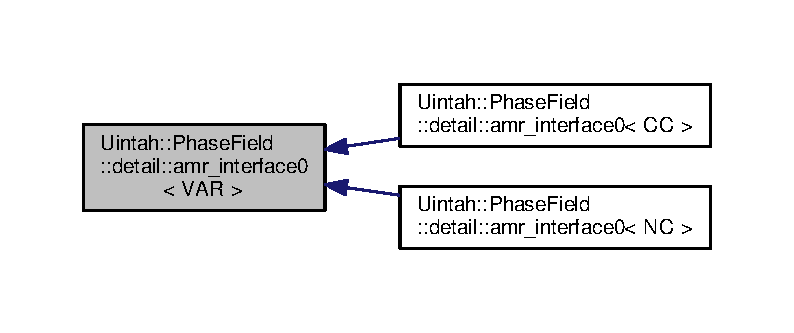
\includegraphics[width=350pt]{classUintah_1_1PhaseField_1_1detail_1_1amr__interface0__inherit__graph}
\end{center}
\end{figure}


\subsection{Detailed Description}
\subsubsection*{template$<$Var\+Type V\+AR$>$\newline
class Uintah\+::\+Phase\+Field\+::detail\+::amr\+\_\+interface0$<$ V\+A\+R $>$}

Interface for amr. 

groups together various methods to get info about amr patches and levels which depend on the different types of variable representation allowing to choose the relevant implementation at compile time


\begin{DoxyTemplParams}{Template Parameters}
{\em V\+AR} & type of variable representation \\
\hline
\end{DoxyTemplParams}


The documentation for this class was generated from the following file\+:\begin{DoxyCompactItemize}
\item 
\hyperlink{amr__interface0_8h}{amr\+\_\+interface0.\+h}\end{DoxyCompactItemize}

\hypertarget{classUintah_1_1PhaseField_1_1detail_1_1amr__interface0_3_01CC_01_4}{}\section{Uintah\+:\+:Phase\+Field\+:\+:detail\+:\+:amr\+\_\+interface0$<$ CC $>$ Class Template Reference}
\label{classUintah_1_1PhaseField_1_1detail_1_1amr__interface0_3_01CC_01_4}\index{Uintah\+::\+Phase\+Field\+::detail\+::amr\+\_\+interface0$<$ C\+C $>$@{Uintah\+::\+Phase\+Field\+::detail\+::amr\+\_\+interface0$<$ C\+C $>$}}


Interface for amr (CC implementation)  




{\ttfamily \#include $<$amr\+\_\+interface0\+\_\+\+C\+C.\+h$>$}



Inheritance diagram for Uintah\+:\+:Phase\+Field\+:\+:detail\+:\+:amr\+\_\+interface0$<$ CC $>$\+:\nopagebreak
\begin{figure}[H]
\begin{center}
\leavevmode
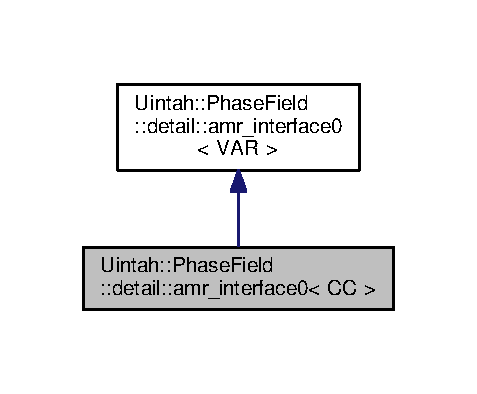
\includegraphics[width=229pt]{classUintah_1_1PhaseField_1_1detail_1_1amr__interface0_3_01CC_01_4__inherit__graph}
\end{center}
\end{figure}


Collaboration diagram for Uintah\+:\+:Phase\+Field\+:\+:detail\+:\+:amr\+\_\+interface0$<$ CC $>$\+:\nopagebreak
\begin{figure}[H]
\begin{center}
\leavevmode
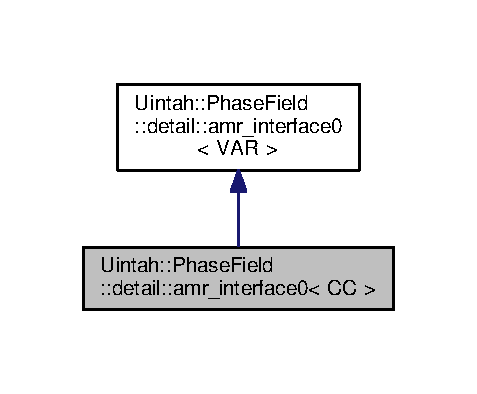
\includegraphics[width=229pt]{classUintah_1_1PhaseField_1_1detail_1_1amr__interface0_3_01CC_01_4__coll__graph}
\end{center}
\end{figure}
\subsection*{Static Public Member Functions}
\begin{DoxyCompactItemize}
\item 
static Int\+Vector \hyperlink{classUintah_1_1PhaseField_1_1detail_1_1amr__interface0_3_01CC_01_4_a54ea40a0a051b55ff5c7a07895e1bba1}{get\+\_\+coarser} (const Level $\ast$l, const Int\+Vector \&i)
\begin{DoxyCompactList}\small\item\em Get coarser grid index. \end{DoxyCompactList}\item 
static Int\+Vector \hyperlink{classUintah_1_1PhaseField_1_1detail_1_1amr__interface0_3_01CC_01_4_a04ebe7c5eb56f351c20353fe93a09e3a}{get\+\_\+finer} (const Level $\ast$l, const Int\+Vector \&i)
\begin{DoxyCompactList}\small\item\em Get finer grid index. \end{DoxyCompactList}\end{DoxyCompactItemize}
\subsection*{Protected Member Functions}
\begin{DoxyCompactItemize}
\item 
\hyperlink{classUintah_1_1PhaseField_1_1detail_1_1amr__interface0_3_01CC_01_4_a54940842b4b34735b6181a3e66efd7c4}{amr\+\_\+interface0} ()=delete
\begin{DoxyCompactList}\small\item\em prevent coonstruction \end{DoxyCompactList}\item 
\hyperlink{classUintah_1_1PhaseField_1_1detail_1_1amr__interface0_3_01CC_01_4_a64f385463bfd52462ed9babaf56aea35}{amr\+\_\+interface0} (const \hyperlink{classUintah_1_1PhaseField_1_1detail_1_1amr__interface0}{amr\+\_\+interface0} \&)=delete
\begin{DoxyCompactList}\small\item\em Prevent copy (and move) constructor. \end{DoxyCompactList}\item 
\hyperlink{classUintah_1_1PhaseField_1_1detail_1_1amr__interface0}{amr\+\_\+interface0} \& \hyperlink{classUintah_1_1PhaseField_1_1detail_1_1amr__interface0_3_01CC_01_4_a31ce6d17e902abe712165f395a8d1ffb}{operator=} (const \hyperlink{classUintah_1_1PhaseField_1_1detail_1_1amr__interface0}{amr\+\_\+interface0} \&)=delete
\begin{DoxyCompactList}\small\item\em Prevent copy (and move) assignment. \end{DoxyCompactList}\end{DoxyCompactItemize}


\subsection{Detailed Description}
\subsubsection*{template$<$$>$\newline
class Uintah\+::\+Phase\+Field\+::detail\+::amr\+\_\+interface0$<$ C\+C $>$}

Interface for amr (CC implementation) 

groups together various methods to get info about amr patches and levels which depend on the different types of variable representation allowing to choose the relevant implementation at compile time

$<$ V\+AR $>$ 

\subsection{Constructor \& Destructor Documentation}
\mbox{\Hypertarget{classUintah_1_1PhaseField_1_1detail_1_1amr__interface0_3_01CC_01_4_a54940842b4b34735b6181a3e66efd7c4}\label{classUintah_1_1PhaseField_1_1detail_1_1amr__interface0_3_01CC_01_4_a54940842b4b34735b6181a3e66efd7c4}} 
\index{Uintah\+::\+Phase\+Field\+::detail\+::amr\+\_\+interface0$<$ C\+C $>$@{Uintah\+::\+Phase\+Field\+::detail\+::amr\+\_\+interface0$<$ C\+C $>$}!amr\+\_\+interface0@{amr\+\_\+interface0}}
\index{amr\+\_\+interface0@{amr\+\_\+interface0}!Uintah\+::\+Phase\+Field\+::detail\+::amr\+\_\+interface0$<$ C\+C $>$@{Uintah\+::\+Phase\+Field\+::detail\+::amr\+\_\+interface0$<$ C\+C $>$}}
\subsubsection{\texorpdfstring{amr\+\_\+interface0()}{amr\_interface0()}\hspace{0.1cm}{\footnotesize\ttfamily [1/2]}}
{\footnotesize\ttfamily \hyperlink{classUintah_1_1PhaseField_1_1detail_1_1amr__interface0}{Uintah\+::\+Phase\+Field\+::detail\+::amr\+\_\+interface0}$<$ \hyperlink{namespaceUintah_1_1PhaseField_a33d355affda78a83f45755ba8388cedda22303704507d024d1d6508ed9859a85a}{CC} $>$\+::\hyperlink{classUintah_1_1PhaseField_1_1detail_1_1amr__interface0}{amr\+\_\+interface0} (\begin{DoxyParamCaption}{ }\end{DoxyParamCaption})\hspace{0.3cm}{\ttfamily [protected]}, {\ttfamily [delete]}}



prevent coonstruction 

\mbox{\Hypertarget{classUintah_1_1PhaseField_1_1detail_1_1amr__interface0_3_01CC_01_4_a64f385463bfd52462ed9babaf56aea35}\label{classUintah_1_1PhaseField_1_1detail_1_1amr__interface0_3_01CC_01_4_a64f385463bfd52462ed9babaf56aea35}} 
\index{Uintah\+::\+Phase\+Field\+::detail\+::amr\+\_\+interface0$<$ C\+C $>$@{Uintah\+::\+Phase\+Field\+::detail\+::amr\+\_\+interface0$<$ C\+C $>$}!amr\+\_\+interface0@{amr\+\_\+interface0}}
\index{amr\+\_\+interface0@{amr\+\_\+interface0}!Uintah\+::\+Phase\+Field\+::detail\+::amr\+\_\+interface0$<$ C\+C $>$@{Uintah\+::\+Phase\+Field\+::detail\+::amr\+\_\+interface0$<$ C\+C $>$}}
\subsubsection{\texorpdfstring{amr\+\_\+interface0()}{amr\_interface0()}\hspace{0.1cm}{\footnotesize\ttfamily [2/2]}}
{\footnotesize\ttfamily \hyperlink{classUintah_1_1PhaseField_1_1detail_1_1amr__interface0}{Uintah\+::\+Phase\+Field\+::detail\+::amr\+\_\+interface0}$<$ \hyperlink{namespaceUintah_1_1PhaseField_a33d355affda78a83f45755ba8388cedda22303704507d024d1d6508ed9859a85a}{CC} $>$\+::\hyperlink{classUintah_1_1PhaseField_1_1detail_1_1amr__interface0}{amr\+\_\+interface0} (\begin{DoxyParamCaption}\item[{const \hyperlink{classUintah_1_1PhaseField_1_1detail_1_1amr__interface0}{amr\+\_\+interface0}$<$ \hyperlink{namespaceUintah_1_1PhaseField_a33d355affda78a83f45755ba8388cedda22303704507d024d1d6508ed9859a85a}{CC} $>$ \&}]{ }\end{DoxyParamCaption})\hspace{0.3cm}{\ttfamily [protected]}, {\ttfamily [delete]}}



Prevent copy (and move) constructor. 



\subsection{Member Function Documentation}
\mbox{\Hypertarget{classUintah_1_1PhaseField_1_1detail_1_1amr__interface0_3_01CC_01_4_a54ea40a0a051b55ff5c7a07895e1bba1}\label{classUintah_1_1PhaseField_1_1detail_1_1amr__interface0_3_01CC_01_4_a54ea40a0a051b55ff5c7a07895e1bba1}} 
\index{Uintah\+::\+Phase\+Field\+::detail\+::amr\+\_\+interface0$<$ C\+C $>$@{Uintah\+::\+Phase\+Field\+::detail\+::amr\+\_\+interface0$<$ C\+C $>$}!get\+\_\+coarser@{get\+\_\+coarser}}
\index{get\+\_\+coarser@{get\+\_\+coarser}!Uintah\+::\+Phase\+Field\+::detail\+::amr\+\_\+interface0$<$ C\+C $>$@{Uintah\+::\+Phase\+Field\+::detail\+::amr\+\_\+interface0$<$ C\+C $>$}}
\subsubsection{\texorpdfstring{get\+\_\+coarser()}{get\_coarser()}}
{\footnotesize\ttfamily static Int\+Vector \hyperlink{classUintah_1_1PhaseField_1_1detail_1_1amr__interface0}{Uintah\+::\+Phase\+Field\+::detail\+::amr\+\_\+interface0}$<$ \hyperlink{namespaceUintah_1_1PhaseField_a33d355affda78a83f45755ba8388cedda22303704507d024d1d6508ed9859a85a}{CC} $>$\+::get\+\_\+coarser (\begin{DoxyParamCaption}\item[{const Level $\ast$}]{l,  }\item[{const Int\+Vector \&}]{i }\end{DoxyParamCaption})\hspace{0.3cm}{\ttfamily [inline]}, {\ttfamily [static]}}



Get coarser grid index. 


\begin{DoxyParams}{Parameters}
{\em l} & fine grid level \\
\hline
{\em i} & fine grid index \\
\hline
\end{DoxyParams}
\begin{DoxyReturn}{Returns}
nearest coarser grid index to the given position 
\end{DoxyReturn}
\mbox{\Hypertarget{classUintah_1_1PhaseField_1_1detail_1_1amr__interface0_3_01CC_01_4_a04ebe7c5eb56f351c20353fe93a09e3a}\label{classUintah_1_1PhaseField_1_1detail_1_1amr__interface0_3_01CC_01_4_a04ebe7c5eb56f351c20353fe93a09e3a}} 
\index{Uintah\+::\+Phase\+Field\+::detail\+::amr\+\_\+interface0$<$ C\+C $>$@{Uintah\+::\+Phase\+Field\+::detail\+::amr\+\_\+interface0$<$ C\+C $>$}!get\+\_\+finer@{get\+\_\+finer}}
\index{get\+\_\+finer@{get\+\_\+finer}!Uintah\+::\+Phase\+Field\+::detail\+::amr\+\_\+interface0$<$ C\+C $>$@{Uintah\+::\+Phase\+Field\+::detail\+::amr\+\_\+interface0$<$ C\+C $>$}}
\subsubsection{\texorpdfstring{get\+\_\+finer()}{get\_finer()}}
{\footnotesize\ttfamily static Int\+Vector \hyperlink{classUintah_1_1PhaseField_1_1detail_1_1amr__interface0}{Uintah\+::\+Phase\+Field\+::detail\+::amr\+\_\+interface0}$<$ \hyperlink{namespaceUintah_1_1PhaseField_a33d355affda78a83f45755ba8388cedda22303704507d024d1d6508ed9859a85a}{CC} $>$\+::get\+\_\+finer (\begin{DoxyParamCaption}\item[{const Level $\ast$}]{l,  }\item[{const Int\+Vector \&}]{i }\end{DoxyParamCaption})\hspace{0.3cm}{\ttfamily [inline]}, {\ttfamily [static]}}



Get finer grid index. 


\begin{DoxyParams}{Parameters}
{\em l} & coarse grid level \\
\hline
{\em i} & coarse grid index \\
\hline
\end{DoxyParams}
\begin{DoxyReturn}{Returns}
nearest finer grid index to the given position 
\end{DoxyReturn}
\mbox{\Hypertarget{classUintah_1_1PhaseField_1_1detail_1_1amr__interface0_3_01CC_01_4_a31ce6d17e902abe712165f395a8d1ffb}\label{classUintah_1_1PhaseField_1_1detail_1_1amr__interface0_3_01CC_01_4_a31ce6d17e902abe712165f395a8d1ffb}} 
\index{Uintah\+::\+Phase\+Field\+::detail\+::amr\+\_\+interface0$<$ C\+C $>$@{Uintah\+::\+Phase\+Field\+::detail\+::amr\+\_\+interface0$<$ C\+C $>$}!operator=@{operator=}}
\index{operator=@{operator=}!Uintah\+::\+Phase\+Field\+::detail\+::amr\+\_\+interface0$<$ C\+C $>$@{Uintah\+::\+Phase\+Field\+::detail\+::amr\+\_\+interface0$<$ C\+C $>$}}
\subsubsection{\texorpdfstring{operator=()}{operator=()}}
{\footnotesize\ttfamily \hyperlink{classUintah_1_1PhaseField_1_1detail_1_1amr__interface0}{amr\+\_\+interface0}\& \hyperlink{classUintah_1_1PhaseField_1_1detail_1_1amr__interface0}{Uintah\+::\+Phase\+Field\+::detail\+::amr\+\_\+interface0}$<$ \hyperlink{namespaceUintah_1_1PhaseField_a33d355affda78a83f45755ba8388cedda22303704507d024d1d6508ed9859a85a}{CC} $>$\+::operator= (\begin{DoxyParamCaption}\item[{const \hyperlink{classUintah_1_1PhaseField_1_1detail_1_1amr__interface0}{amr\+\_\+interface0}$<$ \hyperlink{namespaceUintah_1_1PhaseField_a33d355affda78a83f45755ba8388cedda22303704507d024d1d6508ed9859a85a}{CC} $>$ \&}]{ }\end{DoxyParamCaption})\hspace{0.3cm}{\ttfamily [protected]}, {\ttfamily [delete]}}



Prevent copy (and move) assignment. 



The documentation for this class was generated from the following file\+:\begin{DoxyCompactItemize}
\item 
\hyperlink{amr__interface0__CC_8h}{amr\+\_\+interface0\+\_\+\+C\+C.\+h}\end{DoxyCompactItemize}

\hypertarget{classUintah_1_1PhaseField_1_1detail_1_1amr__interface0_3_01NC_01_4}{}\section{Uintah\+:\+:Phase\+Field\+:\+:detail\+:\+:amr\+\_\+interface0$<$ NC $>$ Class Template Reference}
\label{classUintah_1_1PhaseField_1_1detail_1_1amr__interface0_3_01NC_01_4}\index{Uintah\+::\+Phase\+Field\+::detail\+::amr\+\_\+interface0$<$ N\+C $>$@{Uintah\+::\+Phase\+Field\+::detail\+::amr\+\_\+interface0$<$ N\+C $>$}}


Interface for amr (NC implementation)  




{\ttfamily \#include $<$amr\+\_\+interface0\+\_\+\+N\+C.\+h$>$}



Inheritance diagram for Uintah\+:\+:Phase\+Field\+:\+:detail\+:\+:amr\+\_\+interface0$<$ NC $>$\+:\nopagebreak
\begin{figure}[H]
\begin{center}
\leavevmode
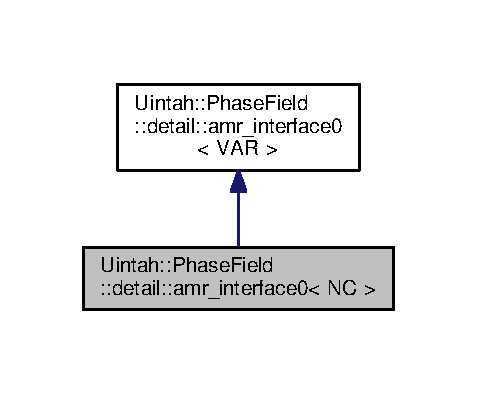
\includegraphics[width=229pt]{classUintah_1_1PhaseField_1_1detail_1_1amr__interface0_3_01NC_01_4__inherit__graph}
\end{center}
\end{figure}


Collaboration diagram for Uintah\+:\+:Phase\+Field\+:\+:detail\+:\+:amr\+\_\+interface0$<$ NC $>$\+:\nopagebreak
\begin{figure}[H]
\begin{center}
\leavevmode
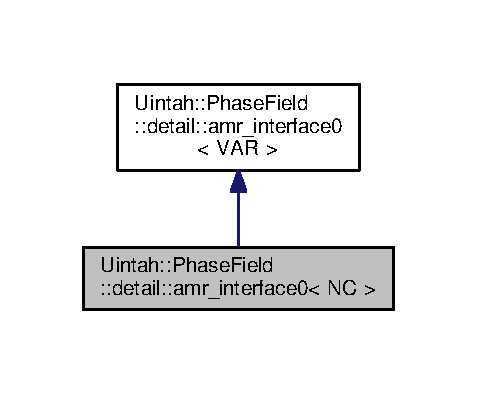
\includegraphics[width=229pt]{classUintah_1_1PhaseField_1_1detail_1_1amr__interface0_3_01NC_01_4__coll__graph}
\end{center}
\end{figure}
\subsection*{Static Public Member Functions}
\begin{DoxyCompactItemize}
\item 
static Int\+Vector \hyperlink{classUintah_1_1PhaseField_1_1detail_1_1amr__interface0_3_01NC_01_4_a48d0bbcf71aa7b965cfb026b6b7c9d05}{get\+\_\+coarser} (const Level $\ast$l, const Int\+Vector \&i)
\begin{DoxyCompactList}\small\item\em Get coarser grid index. \end{DoxyCompactList}\item 
static Int\+Vector \hyperlink{classUintah_1_1PhaseField_1_1detail_1_1amr__interface0_3_01NC_01_4_a474c01b32edcf2ba2dac72c35a63edba}{get\+\_\+finer} (const Level $\ast$l, const Int\+Vector \&i)
\begin{DoxyCompactList}\small\item\em Get finer grid index. \end{DoxyCompactList}\end{DoxyCompactItemize}
\subsection*{Protected Member Functions}
\begin{DoxyCompactItemize}
\item 
\hyperlink{classUintah_1_1PhaseField_1_1detail_1_1amr__interface0_3_01NC_01_4_a16d98f7ce2ef79663793cd2235c857bc}{amr\+\_\+interface0} ()=delete
\begin{DoxyCompactList}\small\item\em prevent coonstruction \end{DoxyCompactList}\item 
\hyperlink{classUintah_1_1PhaseField_1_1detail_1_1amr__interface0_3_01NC_01_4_ad771896bd47c8e03eac2e63330ae52ec}{amr\+\_\+interface0} (const \hyperlink{classUintah_1_1PhaseField_1_1detail_1_1amr__interface0}{amr\+\_\+interface0} \&)=delete
\begin{DoxyCompactList}\small\item\em Prevent copy (and move) constructor. \end{DoxyCompactList}\item 
\hyperlink{classUintah_1_1PhaseField_1_1detail_1_1amr__interface0}{amr\+\_\+interface0} \& \hyperlink{classUintah_1_1PhaseField_1_1detail_1_1amr__interface0_3_01NC_01_4_a9aaf0ac9821706c4d1b07b879c9f2937}{operator=} (const \hyperlink{classUintah_1_1PhaseField_1_1detail_1_1amr__interface0}{amr\+\_\+interface0} \&)=delete
\begin{DoxyCompactList}\small\item\em Prevent copy (and move) assignment. \end{DoxyCompactList}\end{DoxyCompactItemize}


\subsection{Detailed Description}
\subsubsection*{template$<$$>$\newline
class Uintah\+::\+Phase\+Field\+::detail\+::amr\+\_\+interface0$<$ N\+C $>$}

Interface for amr (NC implementation) 

groups together various methods to get info about amr patches and levels which depend on the different types of variable representation allowing to choose the relevant implementation at compile time

$<$ V\+AR $>$ 

\subsection{Constructor \& Destructor Documentation}
\mbox{\Hypertarget{classUintah_1_1PhaseField_1_1detail_1_1amr__interface0_3_01NC_01_4_a16d98f7ce2ef79663793cd2235c857bc}\label{classUintah_1_1PhaseField_1_1detail_1_1amr__interface0_3_01NC_01_4_a16d98f7ce2ef79663793cd2235c857bc}} 
\index{Uintah\+::\+Phase\+Field\+::detail\+::amr\+\_\+interface0$<$ N\+C $>$@{Uintah\+::\+Phase\+Field\+::detail\+::amr\+\_\+interface0$<$ N\+C $>$}!amr\+\_\+interface0@{amr\+\_\+interface0}}
\index{amr\+\_\+interface0@{amr\+\_\+interface0}!Uintah\+::\+Phase\+Field\+::detail\+::amr\+\_\+interface0$<$ N\+C $>$@{Uintah\+::\+Phase\+Field\+::detail\+::amr\+\_\+interface0$<$ N\+C $>$}}
\subsubsection{\texorpdfstring{amr\+\_\+interface0()}{amr\_interface0()}\hspace{0.1cm}{\footnotesize\ttfamily [1/2]}}
{\footnotesize\ttfamily \hyperlink{classUintah_1_1PhaseField_1_1detail_1_1amr__interface0}{Uintah\+::\+Phase\+Field\+::detail\+::amr\+\_\+interface0}$<$ \hyperlink{namespaceUintah_1_1PhaseField_a33d355affda78a83f45755ba8388cedda77924170fe82bfd58b74ca3e44139718}{NC} $>$\+::\hyperlink{classUintah_1_1PhaseField_1_1detail_1_1amr__interface0}{amr\+\_\+interface0} (\begin{DoxyParamCaption}{ }\end{DoxyParamCaption})\hspace{0.3cm}{\ttfamily [protected]}, {\ttfamily [delete]}}



prevent coonstruction 

\mbox{\Hypertarget{classUintah_1_1PhaseField_1_1detail_1_1amr__interface0_3_01NC_01_4_ad771896bd47c8e03eac2e63330ae52ec}\label{classUintah_1_1PhaseField_1_1detail_1_1amr__interface0_3_01NC_01_4_ad771896bd47c8e03eac2e63330ae52ec}} 
\index{Uintah\+::\+Phase\+Field\+::detail\+::amr\+\_\+interface0$<$ N\+C $>$@{Uintah\+::\+Phase\+Field\+::detail\+::amr\+\_\+interface0$<$ N\+C $>$}!amr\+\_\+interface0@{amr\+\_\+interface0}}
\index{amr\+\_\+interface0@{amr\+\_\+interface0}!Uintah\+::\+Phase\+Field\+::detail\+::amr\+\_\+interface0$<$ N\+C $>$@{Uintah\+::\+Phase\+Field\+::detail\+::amr\+\_\+interface0$<$ N\+C $>$}}
\subsubsection{\texorpdfstring{amr\+\_\+interface0()}{amr\_interface0()}\hspace{0.1cm}{\footnotesize\ttfamily [2/2]}}
{\footnotesize\ttfamily \hyperlink{classUintah_1_1PhaseField_1_1detail_1_1amr__interface0}{Uintah\+::\+Phase\+Field\+::detail\+::amr\+\_\+interface0}$<$ \hyperlink{namespaceUintah_1_1PhaseField_a33d355affda78a83f45755ba8388cedda77924170fe82bfd58b74ca3e44139718}{NC} $>$\+::\hyperlink{classUintah_1_1PhaseField_1_1detail_1_1amr__interface0}{amr\+\_\+interface0} (\begin{DoxyParamCaption}\item[{const \hyperlink{classUintah_1_1PhaseField_1_1detail_1_1amr__interface0}{amr\+\_\+interface0}$<$ \hyperlink{namespaceUintah_1_1PhaseField_a33d355affda78a83f45755ba8388cedda77924170fe82bfd58b74ca3e44139718}{NC} $>$ \&}]{ }\end{DoxyParamCaption})\hspace{0.3cm}{\ttfamily [protected]}, {\ttfamily [delete]}}



Prevent copy (and move) constructor. 



\subsection{Member Function Documentation}
\mbox{\Hypertarget{classUintah_1_1PhaseField_1_1detail_1_1amr__interface0_3_01NC_01_4_a48d0bbcf71aa7b965cfb026b6b7c9d05}\label{classUintah_1_1PhaseField_1_1detail_1_1amr__interface0_3_01NC_01_4_a48d0bbcf71aa7b965cfb026b6b7c9d05}} 
\index{Uintah\+::\+Phase\+Field\+::detail\+::amr\+\_\+interface0$<$ N\+C $>$@{Uintah\+::\+Phase\+Field\+::detail\+::amr\+\_\+interface0$<$ N\+C $>$}!get\+\_\+coarser@{get\+\_\+coarser}}
\index{get\+\_\+coarser@{get\+\_\+coarser}!Uintah\+::\+Phase\+Field\+::detail\+::amr\+\_\+interface0$<$ N\+C $>$@{Uintah\+::\+Phase\+Field\+::detail\+::amr\+\_\+interface0$<$ N\+C $>$}}
\subsubsection{\texorpdfstring{get\+\_\+coarser()}{get\_coarser()}}
{\footnotesize\ttfamily static Int\+Vector \hyperlink{classUintah_1_1PhaseField_1_1detail_1_1amr__interface0}{Uintah\+::\+Phase\+Field\+::detail\+::amr\+\_\+interface0}$<$ \hyperlink{namespaceUintah_1_1PhaseField_a33d355affda78a83f45755ba8388cedda77924170fe82bfd58b74ca3e44139718}{NC} $>$\+::get\+\_\+coarser (\begin{DoxyParamCaption}\item[{const Level $\ast$}]{l,  }\item[{const Int\+Vector \&}]{i }\end{DoxyParamCaption})\hspace{0.3cm}{\ttfamily [inline]}, {\ttfamily [static]}}



Get coarser grid index. 


\begin{DoxyParams}{Parameters}
{\em l} & fine grid level \\
\hline
{\em i} & fine grid index \\
\hline
\end{DoxyParams}
\begin{DoxyReturn}{Returns}
nearest coarser grid index to the given position 
\end{DoxyReturn}
\mbox{\Hypertarget{classUintah_1_1PhaseField_1_1detail_1_1amr__interface0_3_01NC_01_4_a474c01b32edcf2ba2dac72c35a63edba}\label{classUintah_1_1PhaseField_1_1detail_1_1amr__interface0_3_01NC_01_4_a474c01b32edcf2ba2dac72c35a63edba}} 
\index{Uintah\+::\+Phase\+Field\+::detail\+::amr\+\_\+interface0$<$ N\+C $>$@{Uintah\+::\+Phase\+Field\+::detail\+::amr\+\_\+interface0$<$ N\+C $>$}!get\+\_\+finer@{get\+\_\+finer}}
\index{get\+\_\+finer@{get\+\_\+finer}!Uintah\+::\+Phase\+Field\+::detail\+::amr\+\_\+interface0$<$ N\+C $>$@{Uintah\+::\+Phase\+Field\+::detail\+::amr\+\_\+interface0$<$ N\+C $>$}}
\subsubsection{\texorpdfstring{get\+\_\+finer()}{get\_finer()}}
{\footnotesize\ttfamily static Int\+Vector \hyperlink{classUintah_1_1PhaseField_1_1detail_1_1amr__interface0}{Uintah\+::\+Phase\+Field\+::detail\+::amr\+\_\+interface0}$<$ \hyperlink{namespaceUintah_1_1PhaseField_a33d355affda78a83f45755ba8388cedda77924170fe82bfd58b74ca3e44139718}{NC} $>$\+::get\+\_\+finer (\begin{DoxyParamCaption}\item[{const Level $\ast$}]{l,  }\item[{const Int\+Vector \&}]{i }\end{DoxyParamCaption})\hspace{0.3cm}{\ttfamily [inline]}, {\ttfamily [static]}}



Get finer grid index. 


\begin{DoxyParams}{Parameters}
{\em l} & coarse grid level \\
\hline
{\em i} & coarse grid index \\
\hline
\end{DoxyParams}
\begin{DoxyReturn}{Returns}
nearest finer grid index to the given position 
\end{DoxyReturn}
\mbox{\Hypertarget{classUintah_1_1PhaseField_1_1detail_1_1amr__interface0_3_01NC_01_4_a9aaf0ac9821706c4d1b07b879c9f2937}\label{classUintah_1_1PhaseField_1_1detail_1_1amr__interface0_3_01NC_01_4_a9aaf0ac9821706c4d1b07b879c9f2937}} 
\index{Uintah\+::\+Phase\+Field\+::detail\+::amr\+\_\+interface0$<$ N\+C $>$@{Uintah\+::\+Phase\+Field\+::detail\+::amr\+\_\+interface0$<$ N\+C $>$}!operator=@{operator=}}
\index{operator=@{operator=}!Uintah\+::\+Phase\+Field\+::detail\+::amr\+\_\+interface0$<$ N\+C $>$@{Uintah\+::\+Phase\+Field\+::detail\+::amr\+\_\+interface0$<$ N\+C $>$}}
\subsubsection{\texorpdfstring{operator=()}{operator=()}}
{\footnotesize\ttfamily \hyperlink{classUintah_1_1PhaseField_1_1detail_1_1amr__interface0}{amr\+\_\+interface0}\& \hyperlink{classUintah_1_1PhaseField_1_1detail_1_1amr__interface0}{Uintah\+::\+Phase\+Field\+::detail\+::amr\+\_\+interface0}$<$ \hyperlink{namespaceUintah_1_1PhaseField_a33d355affda78a83f45755ba8388cedda77924170fe82bfd58b74ca3e44139718}{NC} $>$\+::operator= (\begin{DoxyParamCaption}\item[{const \hyperlink{classUintah_1_1PhaseField_1_1detail_1_1amr__interface0}{amr\+\_\+interface0}$<$ \hyperlink{namespaceUintah_1_1PhaseField_a33d355affda78a83f45755ba8388cedda77924170fe82bfd58b74ca3e44139718}{NC} $>$ \&}]{ }\end{DoxyParamCaption})\hspace{0.3cm}{\ttfamily [protected]}, {\ttfamily [delete]}}



Prevent copy (and move) assignment. 



The documentation for this class was generated from the following file\+:\begin{DoxyCompactItemize}
\item 
\hyperlink{amr__interface0__NC_8h}{amr\+\_\+interface0\+\_\+\+N\+C.\+h}\end{DoxyCompactItemize}

\hypertarget{classUintah_1_1PhaseField_1_1detail_1_1amr__interpolator}{}\section{Uintah\+:\+:Phase\+Field\+:\+:detail\+:\+:amr\+\_\+interpolator$<$ Field, Problem, Index, F\+CI, D\+IM $>$ Class Template Reference}
\label{classUintah_1_1PhaseField_1_1detail_1_1amr__interpolator}\index{Uintah\+::\+Phase\+Field\+::detail\+::amr\+\_\+interpolator$<$ Field, Problem, Index, F\+C\+I, D\+I\+M $>$@{Uintah\+::\+Phase\+Field\+::detail\+::amr\+\_\+interpolator$<$ Field, Problem, Index, F\+C\+I, D\+I\+M $>$}}


Abstract wrapper of grid variables for interpolation from coarser to finer levels.  




{\ttfamily \#include $<$amr\+\_\+interpolator.\+h$>$}



Inheritance diagram for Uintah\+:\+:Phase\+Field\+:\+:detail\+:\+:amr\+\_\+interpolator$<$ Field, Problem, Index, F\+CI, D\+IM $>$\+:\nopagebreak
\begin{figure}[H]
\begin{center}
\leavevmode
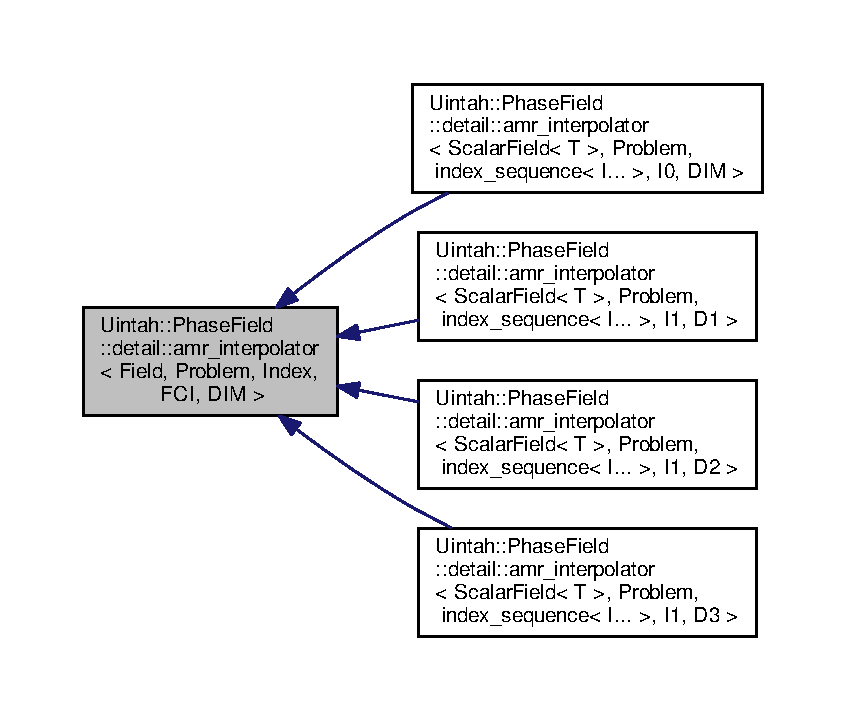
\includegraphics[width=350pt]{classUintah_1_1PhaseField_1_1detail_1_1amr__interpolator__inherit__graph}
\end{center}
\end{figure}


\subsection{Detailed Description}
\subsubsection*{template$<$typename Field, typename Problem, typename Index, F\+C\+I\+Type F\+CI, Dim\+Type D\+IM$>$\newline
class Uintah\+::\+Phase\+Field\+::detail\+::amr\+\_\+interpolator$<$ Field, Problem, Index, F\+C\+I, D\+I\+M $>$}

Abstract wrapper of grid variables for interpolation from coarser to finer levels. 

Adds to view the possibility to compute multi-\/grid interpolation

\begin{DoxyRemark}{Remarks}
All different interpolation strategies must specialize this class and implement the view$<$ T $>$ class
\end{DoxyRemark}

\begin{DoxyTemplParams}{Template Parameters}
{\em Field} & type of Field (should be only \hyperlink{structUintah_1_1PhaseField_1_1ScalarField}{Scalar\+Field}) \\
\hline
{\em \hyperlink{classUintah_1_1PhaseField_1_1Problem}{Problem}} & type of \hyperlink{namespaceUintah_1_1PhaseField}{Phase\+Field} problem \\
\hline
{\em Index} & index\+\_\+sequence of Field within \hyperlink{classUintah_1_1PhaseField_1_1Problem}{Problem} (first element is variable index, following ones, if present, are the component index within the variable) \\
\hline
\end{DoxyTemplParams}


The documentation for this class was generated from the following file\+:\begin{DoxyCompactItemize}
\item 
\hyperlink{amr__interpolator_8h}{amr\+\_\+interpolator.\+h}\end{DoxyCompactItemize}

\hypertarget{classUintah_1_1PhaseField_1_1detail_1_1amr__interpolator_3_01ScalarField_3_01T_01_4_00_01Problem64f2458f98b03e27672a091eecc4b696}{}\section{Uintah\+:\+:Phase\+Field\+:\+:detail\+:\+:amr\+\_\+interpolator$<$ Scalar\+Field$<$ T $>$, Problem, index\+\_\+sequence$<$ I... $>$, I0, D\+IM $>$ Class Template Reference}
\label{classUintah_1_1PhaseField_1_1detail_1_1amr__interpolator_3_01ScalarField_3_01T_01_4_00_01Problem64f2458f98b03e27672a091eecc4b696}\index{Uintah\+::\+Phase\+Field\+::detail\+::amr\+\_\+interpolator$<$ Scalar\+Field$<$ T $>$, Problem, index\+\_\+sequence$<$ I... $>$, I0, D\+I\+M $>$@{Uintah\+::\+Phase\+Field\+::detail\+::amr\+\_\+interpolator$<$ Scalar\+Field$<$ T $>$, Problem, index\+\_\+sequence$<$ I... $>$, I0, D\+I\+M $>$}}


Wrapper of grid variables for interpolation from coarser to finer levels (piecewise implementation)  




{\ttfamily \#include $<$amr\+\_\+interpolator\+\_\+\+I0.\+h$>$}



Inheritance diagram for Uintah\+:\+:Phase\+Field\+:\+:detail\+:\+:amr\+\_\+interpolator$<$ Scalar\+Field$<$ T $>$, Problem, index\+\_\+sequence$<$ I... $>$, I0, D\+IM $>$\+:\nopagebreak
\begin{figure}[H]
\begin{center}
\leavevmode
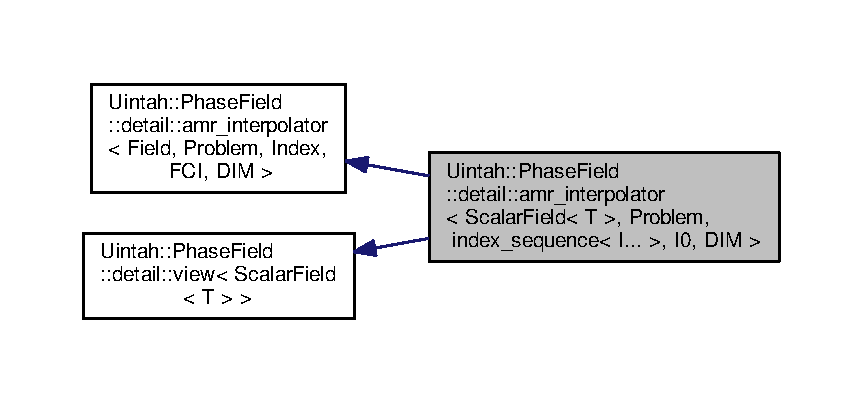
\includegraphics[width=350pt]{classUintah_1_1PhaseField_1_1detail_1_1amr__interpolator_3_01ScalarField_3_01T_01_4_00_01Problem658d7d8430fa7798999c8e5549cf0c0c}
\end{center}
\end{figure}


Collaboration diagram for Uintah\+:\+:Phase\+Field\+:\+:detail\+:\+:amr\+\_\+interpolator$<$ Scalar\+Field$<$ T $>$, Problem, index\+\_\+sequence$<$ I... $>$, I0, D\+IM $>$\+:\nopagebreak
\begin{figure}[H]
\begin{center}
\leavevmode
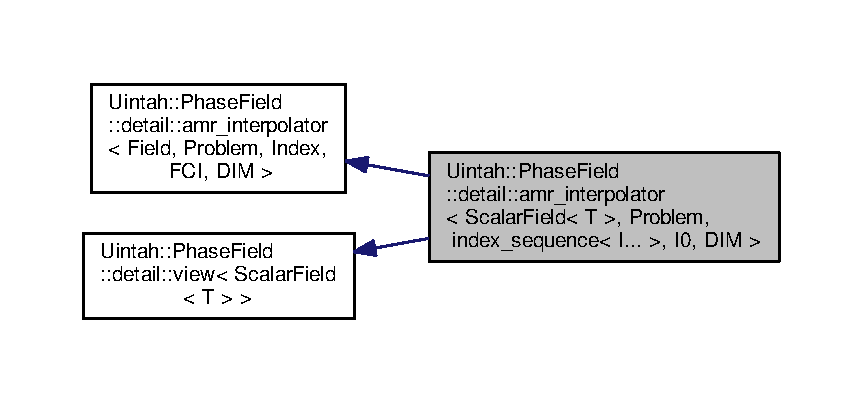
\includegraphics[width=350pt]{classUintah_1_1PhaseField_1_1detail_1_1amr__interpolator_3_01ScalarField_3_01T_01_4_00_01Problem6ba9a5949addff795f5d319ffd2479c9}
\end{center}
\end{figure}
\subsection*{Public Member Functions}
\begin{DoxyCompactItemize}
\item 
\hyperlink{classUintah_1_1PhaseField_1_1detail_1_1amr__interpolator_3_01ScalarField_3_01T_01_4_00_01Problem64f2458f98b03e27672a091eecc4b696_a71dd7bddaaeff40500a9bb9e8c1d2885}{amr\+\_\+interpolator} (const typename \hyperlink{structUintah_1_1PhaseField_1_1ScalarField_a7a77875e030da64c47ce9f6c22a06959}{Field\+::label\+\_\+type} \&label, const Var\+Label $\ast$subproblems\+\_\+label, int material)
\begin{DoxyCompactList}\small\item\em Constructor. \end{DoxyCompactList}\item 
\hyperlink{classUintah_1_1PhaseField_1_1detail_1_1amr__interpolator_3_01ScalarField_3_01T_01_4_00_01Problem64f2458f98b03e27672a091eecc4b696_af4062a318cfc2a19b0e57eb9478e406b}{amr\+\_\+interpolator} (Data\+Warehouse $\ast$dw, const typename \hyperlink{structUintah_1_1PhaseField_1_1ScalarField_a7a77875e030da64c47ce9f6c22a06959}{Field\+::label\+\_\+type} \&label, const Var\+Label $\ast$subproblems\+\_\+label, int material, const Patch $\ast$patch, bool use\+\_\+ghosts=\hyperlink{classUintah_1_1PhaseField_1_1detail_1_1amr__interpolator_3_01ScalarField_3_01T_01_4_00_01Problem64f2458f98b03e27672a091eecc4b696_a659b258bc11df07830b73859f57dee78}{use\+\_\+ghosts\+\_\+dflt})
\begin{DoxyCompactList}\small\item\em Constructor. \end{DoxyCompactList}\item 
virtual \hyperlink{classUintah_1_1PhaseField_1_1detail_1_1amr__interpolator_3_01ScalarField_3_01T_01_4_00_01Problem64f2458f98b03e27672a091eecc4b696_a1ff4737fd9c3eea7dc026410c81e1010}{$\sim$amr\+\_\+interpolator} ()
\begin{DoxyCompactList}\small\item\em Destructor. \end{DoxyCompactList}\item 
\hyperlink{classUintah_1_1PhaseField_1_1detail_1_1amr__interpolator_3_01ScalarField_3_01T_01_4_00_01Problem64f2458f98b03e27672a091eecc4b696_a3eab83979045d441f7296539058bd9d3}{amr\+\_\+interpolator} (const \hyperlink{classUintah_1_1PhaseField_1_1detail_1_1amr__interpolator}{amr\+\_\+interpolator} \&)=delete
\begin{DoxyCompactList}\small\item\em Prevent copy (and move) constructor. \end{DoxyCompactList}\item 
\hyperlink{classUintah_1_1PhaseField_1_1detail_1_1amr__interpolator}{amr\+\_\+interpolator} \& \hyperlink{classUintah_1_1PhaseField_1_1detail_1_1amr__interpolator_3_01ScalarField_3_01T_01_4_00_01Problem64f2458f98b03e27672a091eecc4b696_a728951556ec6db508959f5841d2f2141}{operator=} (const \hyperlink{classUintah_1_1PhaseField_1_1detail_1_1amr__interpolator}{amr\+\_\+interpolator} \&)=delete
\begin{DoxyCompactList}\small\item\em Prevent copy (and move) assignment. \end{DoxyCompactList}\item 
virtual void \hyperlink{classUintah_1_1PhaseField_1_1detail_1_1amr__interpolator_3_01ScalarField_3_01T_01_4_00_01Problem64f2458f98b03e27672a091eecc4b696_a75df9007f3338551abf056c9c2c32aad}{set} (Data\+Warehouse $\ast$dw, const Patch $\ast$patch, bool use\+\_\+ghosts=\hyperlink{classUintah_1_1PhaseField_1_1detail_1_1amr__interpolator_3_01ScalarField_3_01T_01_4_00_01Problem64f2458f98b03e27672a091eecc4b696_a659b258bc11df07830b73859f57dee78}{use\+\_\+ghosts\+\_\+dflt}) override
\begin{DoxyCompactList}\small\item\em retrieve inner variable data from the Data\+Warehouse within a given patch. \end{DoxyCompactList}\item 
virtual void \hyperlink{classUintah_1_1PhaseField_1_1detail_1_1amr__interpolator_3_01ScalarField_3_01T_01_4_00_01Problem64f2458f98b03e27672a091eecc4b696_a2b548da6a4fc9626172b906a6a1a7d57}{set} (Data\+Warehouse $\ast$dw, const Level $\ast$level, const Int\+Vector \&low, const Int\+Vector \&high, bool use\+\_\+ghosts=\hyperlink{classUintah_1_1PhaseField_1_1detail_1_1amr__interpolator_3_01ScalarField_3_01T_01_4_00_01Problem64f2458f98b03e27672a091eecc4b696_a659b258bc11df07830b73859f57dee78}{use\+\_\+ghosts\+\_\+dflt}) override
\begin{DoxyCompactList}\small\item\em retrieve inner variable data from the Data\+Warehouse within a given region. \end{DoxyCompactList}\item 
virtual \hyperlink{classUintah_1_1PhaseField_1_1detail_1_1view}{view}$<$ \hyperlink{structUintah_1_1PhaseField_1_1ScalarField}{Field} $>$ $\ast$ \hyperlink{classUintah_1_1PhaseField_1_1detail_1_1amr__interpolator_3_01ScalarField_3_01T_01_4_00_01Problem64f2458f98b03e27672a091eecc4b696_a6bdc935e6a1d72f8437cbe1b37dcb12c}{clone} (bool deep) const override
\begin{DoxyCompactList}\small\item\em Get a copy of the view. \end{DoxyCompactList}\item 
virtual \hyperlink{classUintah_1_1PhaseField_1_1detail_1_1view}{view}$<$ \hyperlink{structUintah_1_1PhaseField_1_1ScalarField}{Field} $>$ $\ast$ \hyperlink{classUintah_1_1PhaseField_1_1detail_1_1amr__interpolator_3_01ScalarField_3_01T_01_4_00_01Problem64f2458f98b03e27672a091eecc4b696_a890e72b7dfe89f2a0f95bb76d5f7638b}{clone} (bool deep, const Int\+Vector \&offset) const override
\begin{DoxyCompactList}\small\item\em Get a copy of the view and apply translate the support. \end{DoxyCompactList}\item 
virtual \hyperlink{classUintah_1_1PhaseField_1_1Support}{Support} \hyperlink{classUintah_1_1PhaseField_1_1detail_1_1amr__interpolator_3_01ScalarField_3_01T_01_4_00_01Problem64f2458f98b03e27672a091eecc4b696_a9b8a209da971b010bbe33864781d31b2}{get\+\_\+support} () const override
\begin{DoxyCompactList}\small\item\em get interpolator\textquotesingle{}s fine range \end{DoxyCompactList}\item 
virtual bool \hyperlink{classUintah_1_1PhaseField_1_1detail_1_1amr__interpolator_3_01ScalarField_3_01T_01_4_00_01Problem64f2458f98b03e27672a091eecc4b696_a717ca596094560642261d7bec44c6695}{is\+\_\+defined\+\_\+at} (const Int\+Vector \&id) const override
\begin{DoxyCompactList}\small\item\em Check if the view has access to the fine position with index id. \end{DoxyCompactList}\item 
virtual T \& \hyperlink{classUintah_1_1PhaseField_1_1detail_1_1amr__interpolator_3_01ScalarField_3_01T_01_4_00_01Problem64f2458f98b03e27672a091eecc4b696_ac91d5f95be69ce381a6458f38478ba74}{operator\mbox{[}$\,$\mbox{]}} (const Int\+Vector \&id) override
\begin{DoxyCompactList}\small\item\em Get/\+Modify value at position with index id (virtual implementation) \end{DoxyCompactList}\item 
virtual V \hyperlink{classUintah_1_1PhaseField_1_1detail_1_1amr__interpolator_3_01ScalarField_3_01T_01_4_00_01Problem64f2458f98b03e27672a091eecc4b696_aafa653b8bf8b3fae50db0042f5bbbcfc}{operator\mbox{[}$\,$\mbox{]}} (const Int\+Vector \&id\+\_\+fine) const override
\begin{DoxyCompactList}\small\item\em get interpolated value \end{DoxyCompactList}\end{DoxyCompactItemize}
\subsection*{Static Public Attributes}
\begin{DoxyCompactItemize}
\item 
static constexpr bool \hyperlink{classUintah_1_1PhaseField_1_1detail_1_1amr__interpolator_3_01ScalarField_3_01T_01_4_00_01Problem64f2458f98b03e27672a091eecc4b696_a659b258bc11df07830b73859f57dee78}{use\+\_\+ghosts\+\_\+dflt} = false
\begin{DoxyCompactList}\small\item\em Default value for use\+\_\+ghost when retrieving data. \end{DoxyCompactList}\end{DoxyCompactItemize}
\subsection*{Protected Member Functions}
\begin{DoxyCompactItemize}
\item 
\hyperlink{classUintah_1_1PhaseField_1_1detail_1_1amr__interpolator_3_01ScalarField_3_01T_01_4_00_01Problem64f2458f98b03e27672a091eecc4b696_a2ac98ad421a41cc7a2780cb09a95539f}{amr\+\_\+interpolator} (const \hyperlink{classUintah_1_1PhaseField_1_1detail_1_1amr__interpolator}{amr\+\_\+interpolator} $\ast$copy, bool deep)
\begin{DoxyCompactList}\small\item\em Constructor. \end{DoxyCompactList}\end{DoxyCompactItemize}
\subsection*{Additional Inherited Members}


\subsection{Detailed Description}
\subsubsection*{template$<$typename T, typename Problem, size\+\_\+t... I, Dim\+Type D\+IM$>$\newline
class Uintah\+::\+Phase\+Field\+::detail\+::amr\+\_\+interpolator$<$ Scalar\+Field$<$ T $>$, Problem, index\+\_\+sequence$<$ I... $>$, I0, D\+I\+M $>$}

Wrapper of grid variables for interpolation from coarser to finer levels (piecewise implementation) 

implements piecewise constant interpolation of a variable from coarser to finer levels in 1D


\begin{DoxyTemplParams}{Template Parameters}
{\em T} & variable data type (must be constant) \\
\hline
{\em \hyperlink{classUintah_1_1PhaseField_1_1Problem}{Problem}} & type of \hyperlink{namespaceUintah_1_1PhaseField}{Phase\+Field} problem \\
\hline
{\em \hyperlink{structUintah_1_1PhaseField_1_1I}{I}} & list of indices corresponding to the variable within the subproblems \\
\hline
{\em D\+IM} & problem dimension\\
\hline
\end{DoxyTemplParams}
$<$ Field, \hyperlink{classUintah_1_1PhaseField_1_1Problem}{Problem}, Index, F\+CI, D\+IM $>$ 

\subsection{Constructor \& Destructor Documentation}
\mbox{\Hypertarget{classUintah_1_1PhaseField_1_1detail_1_1amr__interpolator_3_01ScalarField_3_01T_01_4_00_01Problem64f2458f98b03e27672a091eecc4b696_a2ac98ad421a41cc7a2780cb09a95539f}\label{classUintah_1_1PhaseField_1_1detail_1_1amr__interpolator_3_01ScalarField_3_01T_01_4_00_01Problem64f2458f98b03e27672a091eecc4b696_a2ac98ad421a41cc7a2780cb09a95539f}} 
\index{Uintah\+::\+Phase\+Field\+::detail\+::amr\+\_\+interpolator$<$ Scalar\+Field$<$ T $>$, Problem, index\+\_\+sequence$<$ I... $>$, I0, D\+I\+M $>$@{Uintah\+::\+Phase\+Field\+::detail\+::amr\+\_\+interpolator$<$ Scalar\+Field$<$ T $>$, Problem, index\+\_\+sequence$<$ I... $>$, I0, D\+I\+M $>$}!amr\+\_\+interpolator@{amr\+\_\+interpolator}}
\index{amr\+\_\+interpolator@{amr\+\_\+interpolator}!Uintah\+::\+Phase\+Field\+::detail\+::amr\+\_\+interpolator$<$ Scalar\+Field$<$ T $>$, Problem, index\+\_\+sequence$<$ I... $>$, I0, D\+I\+M $>$@{Uintah\+::\+Phase\+Field\+::detail\+::amr\+\_\+interpolator$<$ Scalar\+Field$<$ T $>$, Problem, index\+\_\+sequence$<$ I... $>$, I0, D\+I\+M $>$}}
\subsubsection{\texorpdfstring{amr\+\_\+interpolator()}{amr\_interpolator()}\hspace{0.1cm}{\footnotesize\ttfamily [1/4]}}
{\footnotesize\ttfamily template$<$typename T , typename Problem , size\+\_\+t... I, Dim\+Type D\+IM$>$ \\
\hyperlink{classUintah_1_1PhaseField_1_1detail_1_1amr__interpolator}{Uintah\+::\+Phase\+Field\+::detail\+::amr\+\_\+interpolator}$<$ \hyperlink{structUintah_1_1PhaseField_1_1ScalarField}{Scalar\+Field}$<$ T $>$, \hyperlink{classUintah_1_1PhaseField_1_1Problem}{Problem}, \hyperlink{namespaceUintah_1_1PhaseField_a237de804d99512e50613aff7c94a9461}{index\+\_\+sequence}$<$ I... $>$, \hyperlink{namespaceUintah_1_1PhaseField_a547ce3002aa97fbd3ef3192a6eec8406abdd8ebcbdfd71d1125937e3012dc45fb}{I0}, D\+IM $>$\+::\hyperlink{classUintah_1_1PhaseField_1_1detail_1_1amr__interpolator}{amr\+\_\+interpolator} (\begin{DoxyParamCaption}\item[{const \hyperlink{classUintah_1_1PhaseField_1_1detail_1_1amr__interpolator}{amr\+\_\+interpolator}$<$ \hyperlink{structUintah_1_1PhaseField_1_1ScalarField}{Scalar\+Field}$<$ T $>$, \hyperlink{classUintah_1_1PhaseField_1_1Problem}{Problem}, \hyperlink{namespaceUintah_1_1PhaseField_a237de804d99512e50613aff7c94a9461}{index\+\_\+sequence}$<$ I... $>$, \hyperlink{namespaceUintah_1_1PhaseField_a547ce3002aa97fbd3ef3192a6eec8406abdd8ebcbdfd71d1125937e3012dc45fb}{I0}, D\+IM $>$ $\ast$}]{copy,  }\item[{bool}]{deep }\end{DoxyParamCaption})\hspace{0.3cm}{\ttfamily [inline]}, {\ttfamily [protected]}}



Constructor. 

Instantiate a copy of a given view


\begin{DoxyParams}{Parameters}
{\em copy} & source view for copying \\
\hline
{\em deep} & if true inner grid variable is copied as well otherwise the same grid variable is referenced \\
\hline
\end{DoxyParams}
\mbox{\Hypertarget{classUintah_1_1PhaseField_1_1detail_1_1amr__interpolator_3_01ScalarField_3_01T_01_4_00_01Problem64f2458f98b03e27672a091eecc4b696_a71dd7bddaaeff40500a9bb9e8c1d2885}\label{classUintah_1_1PhaseField_1_1detail_1_1amr__interpolator_3_01ScalarField_3_01T_01_4_00_01Problem64f2458f98b03e27672a091eecc4b696_a71dd7bddaaeff40500a9bb9e8c1d2885}} 
\index{Uintah\+::\+Phase\+Field\+::detail\+::amr\+\_\+interpolator$<$ Scalar\+Field$<$ T $>$, Problem, index\+\_\+sequence$<$ I... $>$, I0, D\+I\+M $>$@{Uintah\+::\+Phase\+Field\+::detail\+::amr\+\_\+interpolator$<$ Scalar\+Field$<$ T $>$, Problem, index\+\_\+sequence$<$ I... $>$, I0, D\+I\+M $>$}!amr\+\_\+interpolator@{amr\+\_\+interpolator}}
\index{amr\+\_\+interpolator@{amr\+\_\+interpolator}!Uintah\+::\+Phase\+Field\+::detail\+::amr\+\_\+interpolator$<$ Scalar\+Field$<$ T $>$, Problem, index\+\_\+sequence$<$ I... $>$, I0, D\+I\+M $>$@{Uintah\+::\+Phase\+Field\+::detail\+::amr\+\_\+interpolator$<$ Scalar\+Field$<$ T $>$, Problem, index\+\_\+sequence$<$ I... $>$, I0, D\+I\+M $>$}}
\subsubsection{\texorpdfstring{amr\+\_\+interpolator()}{amr\_interpolator()}\hspace{0.1cm}{\footnotesize\ttfamily [2/4]}}
{\footnotesize\ttfamily template$<$typename T , typename Problem , size\+\_\+t... I, Dim\+Type D\+IM$>$ \\
\hyperlink{classUintah_1_1PhaseField_1_1detail_1_1amr__interpolator}{Uintah\+::\+Phase\+Field\+::detail\+::amr\+\_\+interpolator}$<$ \hyperlink{structUintah_1_1PhaseField_1_1ScalarField}{Scalar\+Field}$<$ T $>$, \hyperlink{classUintah_1_1PhaseField_1_1Problem}{Problem}, \hyperlink{namespaceUintah_1_1PhaseField_a237de804d99512e50613aff7c94a9461}{index\+\_\+sequence}$<$ I... $>$, \hyperlink{namespaceUintah_1_1PhaseField_a547ce3002aa97fbd3ef3192a6eec8406abdd8ebcbdfd71d1125937e3012dc45fb}{I0}, D\+IM $>$\+::\hyperlink{classUintah_1_1PhaseField_1_1detail_1_1amr__interpolator}{amr\+\_\+interpolator} (\begin{DoxyParamCaption}\item[{const typename \hyperlink{structUintah_1_1PhaseField_1_1ScalarField_a7a77875e030da64c47ce9f6c22a06959}{Field\+::label\+\_\+type} \&}]{label,  }\item[{const Var\+Label $\ast$}]{subproblems\+\_\+label,  }\item[{int}]{material }\end{DoxyParamCaption})\hspace{0.3cm}{\ttfamily [inline]}}



Constructor. 

construct interpolator without retrieving inner variable data from the Data\+Warehouse


\begin{DoxyParams}{Parameters}
{\em label} & label of variable in the Data\+Warehouse \\
\hline
{\em subproblems\+\_\+label} & label of subproblems in the Data\+Warehouse \\
\hline
{\em material} & index of material in the Data\+Warehouse \\
\hline
\end{DoxyParams}
\mbox{\Hypertarget{classUintah_1_1PhaseField_1_1detail_1_1amr__interpolator_3_01ScalarField_3_01T_01_4_00_01Problem64f2458f98b03e27672a091eecc4b696_af4062a318cfc2a19b0e57eb9478e406b}\label{classUintah_1_1PhaseField_1_1detail_1_1amr__interpolator_3_01ScalarField_3_01T_01_4_00_01Problem64f2458f98b03e27672a091eecc4b696_af4062a318cfc2a19b0e57eb9478e406b}} 
\index{Uintah\+::\+Phase\+Field\+::detail\+::amr\+\_\+interpolator$<$ Scalar\+Field$<$ T $>$, Problem, index\+\_\+sequence$<$ I... $>$, I0, D\+I\+M $>$@{Uintah\+::\+Phase\+Field\+::detail\+::amr\+\_\+interpolator$<$ Scalar\+Field$<$ T $>$, Problem, index\+\_\+sequence$<$ I... $>$, I0, D\+I\+M $>$}!amr\+\_\+interpolator@{amr\+\_\+interpolator}}
\index{amr\+\_\+interpolator@{amr\+\_\+interpolator}!Uintah\+::\+Phase\+Field\+::detail\+::amr\+\_\+interpolator$<$ Scalar\+Field$<$ T $>$, Problem, index\+\_\+sequence$<$ I... $>$, I0, D\+I\+M $>$@{Uintah\+::\+Phase\+Field\+::detail\+::amr\+\_\+interpolator$<$ Scalar\+Field$<$ T $>$, Problem, index\+\_\+sequence$<$ I... $>$, I0, D\+I\+M $>$}}
\subsubsection{\texorpdfstring{amr\+\_\+interpolator()}{amr\_interpolator()}\hspace{0.1cm}{\footnotesize\ttfamily [3/4]}}
{\footnotesize\ttfamily template$<$typename T , typename Problem , size\+\_\+t... I, Dim\+Type D\+IM$>$ \\
\hyperlink{classUintah_1_1PhaseField_1_1detail_1_1amr__interpolator}{Uintah\+::\+Phase\+Field\+::detail\+::amr\+\_\+interpolator}$<$ \hyperlink{structUintah_1_1PhaseField_1_1ScalarField}{Scalar\+Field}$<$ T $>$, \hyperlink{classUintah_1_1PhaseField_1_1Problem}{Problem}, \hyperlink{namespaceUintah_1_1PhaseField_a237de804d99512e50613aff7c94a9461}{index\+\_\+sequence}$<$ I... $>$, \hyperlink{namespaceUintah_1_1PhaseField_a547ce3002aa97fbd3ef3192a6eec8406abdd8ebcbdfd71d1125937e3012dc45fb}{I0}, D\+IM $>$\+::\hyperlink{classUintah_1_1PhaseField_1_1detail_1_1amr__interpolator}{amr\+\_\+interpolator} (\begin{DoxyParamCaption}\item[{Data\+Warehouse $\ast$}]{dw,  }\item[{const typename \hyperlink{structUintah_1_1PhaseField_1_1ScalarField_a7a77875e030da64c47ce9f6c22a06959}{Field\+::label\+\_\+type} \&}]{label,  }\item[{const Var\+Label $\ast$}]{subproblems\+\_\+label,  }\item[{int}]{material,  }\item[{const Patch $\ast$}]{patch,  }\item[{bool}]{use\+\_\+ghosts = {\ttfamily \hyperlink{classUintah_1_1PhaseField_1_1detail_1_1amr__interpolator_3_01ScalarField_3_01T_01_4_00_01Problem64f2458f98b03e27672a091eecc4b696_a659b258bc11df07830b73859f57dee78}{use\+\_\+ghosts\+\_\+dflt}} }\end{DoxyParamCaption})\hspace{0.3cm}{\ttfamily [inline]}}



Constructor. 

construct interpolator and retrieve inner variable data from the Data\+Warehouse within a given fine patch.

\begin{DoxyRemark}{Remarks}
the number of ghost cells/nodes and the corresponding region on the coarser level is automatically computed to match the interpolation type
\end{DoxyRemark}

\begin{DoxyParams}{Parameters}
{\em dw} & Data\+Warehouse which data is retrieved from \\
\hline
{\em label} & label of variable in the Data\+Warehouse \\
\hline
{\em subproblems\+\_\+label} & label of subproblems in the Data\+Warehouse \\
\hline
{\em material} & index of material in the Data\+Warehouse \\
\hline
{\em patch} & patch on which data is retrieved \\
\hline
{\em use\+\_\+ghosts} & must be false \\
\hline
\end{DoxyParams}
\mbox{\Hypertarget{classUintah_1_1PhaseField_1_1detail_1_1amr__interpolator_3_01ScalarField_3_01T_01_4_00_01Problem64f2458f98b03e27672a091eecc4b696_a1ff4737fd9c3eea7dc026410c81e1010}\label{classUintah_1_1PhaseField_1_1detail_1_1amr__interpolator_3_01ScalarField_3_01T_01_4_00_01Problem64f2458f98b03e27672a091eecc4b696_a1ff4737fd9c3eea7dc026410c81e1010}} 
\index{Uintah\+::\+Phase\+Field\+::detail\+::amr\+\_\+interpolator$<$ Scalar\+Field$<$ T $>$, Problem, index\+\_\+sequence$<$ I... $>$, I0, D\+I\+M $>$@{Uintah\+::\+Phase\+Field\+::detail\+::amr\+\_\+interpolator$<$ Scalar\+Field$<$ T $>$, Problem, index\+\_\+sequence$<$ I... $>$, I0, D\+I\+M $>$}!````~amr\+\_\+interpolator@{$\sim$amr\+\_\+interpolator}}
\index{````~amr\+\_\+interpolator@{$\sim$amr\+\_\+interpolator}!Uintah\+::\+Phase\+Field\+::detail\+::amr\+\_\+interpolator$<$ Scalar\+Field$<$ T $>$, Problem, index\+\_\+sequence$<$ I... $>$, I0, D\+I\+M $>$@{Uintah\+::\+Phase\+Field\+::detail\+::amr\+\_\+interpolator$<$ Scalar\+Field$<$ T $>$, Problem, index\+\_\+sequence$<$ I... $>$, I0, D\+I\+M $>$}}
\subsubsection{\texorpdfstring{$\sim$amr\+\_\+interpolator()}{~amr\_interpolator()}}
{\footnotesize\ttfamily template$<$typename T , typename Problem , size\+\_\+t... I, Dim\+Type D\+IM$>$ \\
virtual \hyperlink{classUintah_1_1PhaseField_1_1detail_1_1amr__interpolator}{Uintah\+::\+Phase\+Field\+::detail\+::amr\+\_\+interpolator}$<$ \hyperlink{structUintah_1_1PhaseField_1_1ScalarField}{Scalar\+Field}$<$ T $>$, \hyperlink{classUintah_1_1PhaseField_1_1Problem}{Problem}, \hyperlink{namespaceUintah_1_1PhaseField_a237de804d99512e50613aff7c94a9461}{index\+\_\+sequence}$<$ I... $>$, \hyperlink{namespaceUintah_1_1PhaseField_a547ce3002aa97fbd3ef3192a6eec8406abdd8ebcbdfd71d1125937e3012dc45fb}{I0}, D\+IM $>$\+::$\sim$\hyperlink{classUintah_1_1PhaseField_1_1detail_1_1amr__interpolator}{amr\+\_\+interpolator} (\begin{DoxyParamCaption}{ }\end{DoxyParamCaption})\hspace{0.3cm}{\ttfamily [inline]}, {\ttfamily [virtual]}}



Destructor. 

\mbox{\Hypertarget{classUintah_1_1PhaseField_1_1detail_1_1amr__interpolator_3_01ScalarField_3_01T_01_4_00_01Problem64f2458f98b03e27672a091eecc4b696_a3eab83979045d441f7296539058bd9d3}\label{classUintah_1_1PhaseField_1_1detail_1_1amr__interpolator_3_01ScalarField_3_01T_01_4_00_01Problem64f2458f98b03e27672a091eecc4b696_a3eab83979045d441f7296539058bd9d3}} 
\index{Uintah\+::\+Phase\+Field\+::detail\+::amr\+\_\+interpolator$<$ Scalar\+Field$<$ T $>$, Problem, index\+\_\+sequence$<$ I... $>$, I0, D\+I\+M $>$@{Uintah\+::\+Phase\+Field\+::detail\+::amr\+\_\+interpolator$<$ Scalar\+Field$<$ T $>$, Problem, index\+\_\+sequence$<$ I... $>$, I0, D\+I\+M $>$}!amr\+\_\+interpolator@{amr\+\_\+interpolator}}
\index{amr\+\_\+interpolator@{amr\+\_\+interpolator}!Uintah\+::\+Phase\+Field\+::detail\+::amr\+\_\+interpolator$<$ Scalar\+Field$<$ T $>$, Problem, index\+\_\+sequence$<$ I... $>$, I0, D\+I\+M $>$@{Uintah\+::\+Phase\+Field\+::detail\+::amr\+\_\+interpolator$<$ Scalar\+Field$<$ T $>$, Problem, index\+\_\+sequence$<$ I... $>$, I0, D\+I\+M $>$}}
\subsubsection{\texorpdfstring{amr\+\_\+interpolator()}{amr\_interpolator()}\hspace{0.1cm}{\footnotesize\ttfamily [4/4]}}
{\footnotesize\ttfamily template$<$typename T , typename Problem , size\+\_\+t... I, Dim\+Type D\+IM$>$ \\
\hyperlink{classUintah_1_1PhaseField_1_1detail_1_1amr__interpolator}{Uintah\+::\+Phase\+Field\+::detail\+::amr\+\_\+interpolator}$<$ \hyperlink{structUintah_1_1PhaseField_1_1ScalarField}{Scalar\+Field}$<$ T $>$, \hyperlink{classUintah_1_1PhaseField_1_1Problem}{Problem}, \hyperlink{namespaceUintah_1_1PhaseField_a237de804d99512e50613aff7c94a9461}{index\+\_\+sequence}$<$ I... $>$, \hyperlink{namespaceUintah_1_1PhaseField_a547ce3002aa97fbd3ef3192a6eec8406abdd8ebcbdfd71d1125937e3012dc45fb}{I0}, D\+IM $>$\+::\hyperlink{classUintah_1_1PhaseField_1_1detail_1_1amr__interpolator}{amr\+\_\+interpolator} (\begin{DoxyParamCaption}\item[{const \hyperlink{classUintah_1_1PhaseField_1_1detail_1_1amr__interpolator}{amr\+\_\+interpolator}$<$ \hyperlink{structUintah_1_1PhaseField_1_1ScalarField}{Scalar\+Field}$<$ T $>$, \hyperlink{classUintah_1_1PhaseField_1_1Problem}{Problem}, \hyperlink{namespaceUintah_1_1PhaseField_a237de804d99512e50613aff7c94a9461}{index\+\_\+sequence}$<$ I... $>$, \hyperlink{namespaceUintah_1_1PhaseField_a547ce3002aa97fbd3ef3192a6eec8406abdd8ebcbdfd71d1125937e3012dc45fb}{I0}, D\+IM $>$ \&}]{ }\end{DoxyParamCaption})\hspace{0.3cm}{\ttfamily [delete]}}



Prevent copy (and move) constructor. 



\subsection{Member Function Documentation}
\mbox{\Hypertarget{classUintah_1_1PhaseField_1_1detail_1_1amr__interpolator_3_01ScalarField_3_01T_01_4_00_01Problem64f2458f98b03e27672a091eecc4b696_a6bdc935e6a1d72f8437cbe1b37dcb12c}\label{classUintah_1_1PhaseField_1_1detail_1_1amr__interpolator_3_01ScalarField_3_01T_01_4_00_01Problem64f2458f98b03e27672a091eecc4b696_a6bdc935e6a1d72f8437cbe1b37dcb12c}} 
\index{Uintah\+::\+Phase\+Field\+::detail\+::amr\+\_\+interpolator$<$ Scalar\+Field$<$ T $>$, Problem, index\+\_\+sequence$<$ I... $>$, I0, D\+I\+M $>$@{Uintah\+::\+Phase\+Field\+::detail\+::amr\+\_\+interpolator$<$ Scalar\+Field$<$ T $>$, Problem, index\+\_\+sequence$<$ I... $>$, I0, D\+I\+M $>$}!clone@{clone}}
\index{clone@{clone}!Uintah\+::\+Phase\+Field\+::detail\+::amr\+\_\+interpolator$<$ Scalar\+Field$<$ T $>$, Problem, index\+\_\+sequence$<$ I... $>$, I0, D\+I\+M $>$@{Uintah\+::\+Phase\+Field\+::detail\+::amr\+\_\+interpolator$<$ Scalar\+Field$<$ T $>$, Problem, index\+\_\+sequence$<$ I... $>$, I0, D\+I\+M $>$}}
\subsubsection{\texorpdfstring{clone()}{clone()}\hspace{0.1cm}{\footnotesize\ttfamily [1/2]}}
{\footnotesize\ttfamily template$<$typename T , typename Problem , size\+\_\+t... I, Dim\+Type D\+IM$>$ \\
virtual \hyperlink{classUintah_1_1PhaseField_1_1detail_1_1view}{view}$<$\hyperlink{structUintah_1_1PhaseField_1_1ScalarField}{Field}$>$$\ast$ \hyperlink{classUintah_1_1PhaseField_1_1detail_1_1amr__interpolator}{Uintah\+::\+Phase\+Field\+::detail\+::amr\+\_\+interpolator}$<$ \hyperlink{structUintah_1_1PhaseField_1_1ScalarField}{Scalar\+Field}$<$ T $>$, \hyperlink{classUintah_1_1PhaseField_1_1Problem}{Problem}, \hyperlink{namespaceUintah_1_1PhaseField_a237de804d99512e50613aff7c94a9461}{index\+\_\+sequence}$<$ I... $>$, \hyperlink{namespaceUintah_1_1PhaseField_a547ce3002aa97fbd3ef3192a6eec8406abdd8ebcbdfd71d1125937e3012dc45fb}{I0}, D\+IM $>$\+::clone (\begin{DoxyParamCaption}\item[{bool}]{deep }\end{DoxyParamCaption}) const\hspace{0.3cm}{\ttfamily [inline]}, {\ttfamily [override]}, {\ttfamily [virtual]}}



Get a copy of the view. 


\begin{DoxyParams}{Parameters}
{\em deep} & if true inner grid variable is copied as well otherwise the same grid variable is referenced\\
\hline
\end{DoxyParams}
\begin{DoxyReturn}{Returns}
new view instance 
\end{DoxyReturn}


Implements \hyperlink{classUintah_1_1PhaseField_1_1detail_1_1view_3_01ScalarField_3_01T_01_4_01_4_a6e11243c9d776a7b703e524ea4151a16}{Uintah\+::\+Phase\+Field\+::detail\+::view$<$ Scalar\+Field$<$ T $>$ $>$}.

\mbox{\Hypertarget{classUintah_1_1PhaseField_1_1detail_1_1amr__interpolator_3_01ScalarField_3_01T_01_4_00_01Problem64f2458f98b03e27672a091eecc4b696_a890e72b7dfe89f2a0f95bb76d5f7638b}\label{classUintah_1_1PhaseField_1_1detail_1_1amr__interpolator_3_01ScalarField_3_01T_01_4_00_01Problem64f2458f98b03e27672a091eecc4b696_a890e72b7dfe89f2a0f95bb76d5f7638b}} 
\index{Uintah\+::\+Phase\+Field\+::detail\+::amr\+\_\+interpolator$<$ Scalar\+Field$<$ T $>$, Problem, index\+\_\+sequence$<$ I... $>$, I0, D\+I\+M $>$@{Uintah\+::\+Phase\+Field\+::detail\+::amr\+\_\+interpolator$<$ Scalar\+Field$<$ T $>$, Problem, index\+\_\+sequence$<$ I... $>$, I0, D\+I\+M $>$}!clone@{clone}}
\index{clone@{clone}!Uintah\+::\+Phase\+Field\+::detail\+::amr\+\_\+interpolator$<$ Scalar\+Field$<$ T $>$, Problem, index\+\_\+sequence$<$ I... $>$, I0, D\+I\+M $>$@{Uintah\+::\+Phase\+Field\+::detail\+::amr\+\_\+interpolator$<$ Scalar\+Field$<$ T $>$, Problem, index\+\_\+sequence$<$ I... $>$, I0, D\+I\+M $>$}}
\subsubsection{\texorpdfstring{clone()}{clone()}\hspace{0.1cm}{\footnotesize\ttfamily [2/2]}}
{\footnotesize\ttfamily template$<$typename T , typename Problem , size\+\_\+t... I, Dim\+Type D\+IM$>$ \\
virtual \hyperlink{classUintah_1_1PhaseField_1_1detail_1_1view}{view}$<$\hyperlink{structUintah_1_1PhaseField_1_1ScalarField}{Field}$>$$\ast$ \hyperlink{classUintah_1_1PhaseField_1_1detail_1_1amr__interpolator}{Uintah\+::\+Phase\+Field\+::detail\+::amr\+\_\+interpolator}$<$ \hyperlink{structUintah_1_1PhaseField_1_1ScalarField}{Scalar\+Field}$<$ T $>$, \hyperlink{classUintah_1_1PhaseField_1_1Problem}{Problem}, \hyperlink{namespaceUintah_1_1PhaseField_a237de804d99512e50613aff7c94a9461}{index\+\_\+sequence}$<$ I... $>$, \hyperlink{namespaceUintah_1_1PhaseField_a547ce3002aa97fbd3ef3192a6eec8406abdd8ebcbdfd71d1125937e3012dc45fb}{I0}, D\+IM $>$\+::clone (\begin{DoxyParamCaption}\item[{bool}]{deep,  }\item[{const Int\+Vector \&}]{offset }\end{DoxyParamCaption}) const\hspace{0.3cm}{\ttfamily [inline]}, {\ttfamily [override]}, {\ttfamily [virtual]}}



Get a copy of the view and apply translate the support. 

\begin{DoxyRemark}{Remarks}
It is meant to be used for virtual patches (i.\+e. periodic boundaries)
\end{DoxyRemark}

\begin{DoxyParams}{Parameters}
{\em deep} & if true inner grid variable is copied as well otherwise the same grid variable is referenced \\
\hline
{\em offset} & vector specifying the translation of the support \\
\hline
\end{DoxyParams}
\begin{DoxyReturn}{Returns}
new view instance 
\end{DoxyReturn}


Implements \hyperlink{classUintah_1_1PhaseField_1_1detail_1_1view_3_01ScalarField_3_01T_01_4_01_4_abd928104240e329f3bc4441ebab7c50c}{Uintah\+::\+Phase\+Field\+::detail\+::view$<$ Scalar\+Field$<$ T $>$ $>$}.

\mbox{\Hypertarget{classUintah_1_1PhaseField_1_1detail_1_1amr__interpolator_3_01ScalarField_3_01T_01_4_00_01Problem64f2458f98b03e27672a091eecc4b696_a9b8a209da971b010bbe33864781d31b2}\label{classUintah_1_1PhaseField_1_1detail_1_1amr__interpolator_3_01ScalarField_3_01T_01_4_00_01Problem64f2458f98b03e27672a091eecc4b696_a9b8a209da971b010bbe33864781d31b2}} 
\index{Uintah\+::\+Phase\+Field\+::detail\+::amr\+\_\+interpolator$<$ Scalar\+Field$<$ T $>$, Problem, index\+\_\+sequence$<$ I... $>$, I0, D\+I\+M $>$@{Uintah\+::\+Phase\+Field\+::detail\+::amr\+\_\+interpolator$<$ Scalar\+Field$<$ T $>$, Problem, index\+\_\+sequence$<$ I... $>$, I0, D\+I\+M $>$}!get\+\_\+support@{get\+\_\+support}}
\index{get\+\_\+support@{get\+\_\+support}!Uintah\+::\+Phase\+Field\+::detail\+::amr\+\_\+interpolator$<$ Scalar\+Field$<$ T $>$, Problem, index\+\_\+sequence$<$ I... $>$, I0, D\+I\+M $>$@{Uintah\+::\+Phase\+Field\+::detail\+::amr\+\_\+interpolator$<$ Scalar\+Field$<$ T $>$, Problem, index\+\_\+sequence$<$ I... $>$, I0, D\+I\+M $>$}}
\subsubsection{\texorpdfstring{get\+\_\+support()}{get\_support()}}
{\footnotesize\ttfamily template$<$typename T , typename Problem , size\+\_\+t... I, Dim\+Type D\+IM$>$ \\
virtual \hyperlink{classUintah_1_1PhaseField_1_1Support}{Support} \hyperlink{classUintah_1_1PhaseField_1_1detail_1_1amr__interpolator}{Uintah\+::\+Phase\+Field\+::detail\+::amr\+\_\+interpolator}$<$ \hyperlink{structUintah_1_1PhaseField_1_1ScalarField}{Scalar\+Field}$<$ T $>$, \hyperlink{classUintah_1_1PhaseField_1_1Problem}{Problem}, \hyperlink{namespaceUintah_1_1PhaseField_a237de804d99512e50613aff7c94a9461}{index\+\_\+sequence}$<$ I... $>$, \hyperlink{namespaceUintah_1_1PhaseField_a547ce3002aa97fbd3ef3192a6eec8406abdd8ebcbdfd71d1125937e3012dc45fb}{I0}, D\+IM $>$\+::get\+\_\+support (\begin{DoxyParamCaption}{ }\end{DoxyParamCaption}) const\hspace{0.3cm}{\ttfamily [inline]}, {\ttfamily [override]}, {\ttfamily [virtual]}}



get interpolator\textquotesingle{}s fine range 

\begin{DoxyReturn}{Returns}
fine range 
\end{DoxyReturn}


Implements \hyperlink{classUintah_1_1PhaseField_1_1detail_1_1view_3_01ScalarField_3_01T_01_4_01_4_a3e14b0c7a57a57707bb33954861ab1c1}{Uintah\+::\+Phase\+Field\+::detail\+::view$<$ Scalar\+Field$<$ T $>$ $>$}.

\mbox{\Hypertarget{classUintah_1_1PhaseField_1_1detail_1_1amr__interpolator_3_01ScalarField_3_01T_01_4_00_01Problem64f2458f98b03e27672a091eecc4b696_a717ca596094560642261d7bec44c6695}\label{classUintah_1_1PhaseField_1_1detail_1_1amr__interpolator_3_01ScalarField_3_01T_01_4_00_01Problem64f2458f98b03e27672a091eecc4b696_a717ca596094560642261d7bec44c6695}} 
\index{Uintah\+::\+Phase\+Field\+::detail\+::amr\+\_\+interpolator$<$ Scalar\+Field$<$ T $>$, Problem, index\+\_\+sequence$<$ I... $>$, I0, D\+I\+M $>$@{Uintah\+::\+Phase\+Field\+::detail\+::amr\+\_\+interpolator$<$ Scalar\+Field$<$ T $>$, Problem, index\+\_\+sequence$<$ I... $>$, I0, D\+I\+M $>$}!is\+\_\+defined\+\_\+at@{is\+\_\+defined\+\_\+at}}
\index{is\+\_\+defined\+\_\+at@{is\+\_\+defined\+\_\+at}!Uintah\+::\+Phase\+Field\+::detail\+::amr\+\_\+interpolator$<$ Scalar\+Field$<$ T $>$, Problem, index\+\_\+sequence$<$ I... $>$, I0, D\+I\+M $>$@{Uintah\+::\+Phase\+Field\+::detail\+::amr\+\_\+interpolator$<$ Scalar\+Field$<$ T $>$, Problem, index\+\_\+sequence$<$ I... $>$, I0, D\+I\+M $>$}}
\subsubsection{\texorpdfstring{is\+\_\+defined\+\_\+at()}{is\_defined\_at()}}
{\footnotesize\ttfamily template$<$typename T , typename Problem , size\+\_\+t... I, Dim\+Type D\+IM$>$ \\
virtual bool \hyperlink{classUintah_1_1PhaseField_1_1detail_1_1amr__interpolator}{Uintah\+::\+Phase\+Field\+::detail\+::amr\+\_\+interpolator}$<$ \hyperlink{structUintah_1_1PhaseField_1_1ScalarField}{Scalar\+Field}$<$ T $>$, \hyperlink{classUintah_1_1PhaseField_1_1Problem}{Problem}, \hyperlink{namespaceUintah_1_1PhaseField_a237de804d99512e50613aff7c94a9461}{index\+\_\+sequence}$<$ I... $>$, \hyperlink{namespaceUintah_1_1PhaseField_a547ce3002aa97fbd3ef3192a6eec8406abdd8ebcbdfd71d1125937e3012dc45fb}{I0}, D\+IM $>$\+::is\+\_\+defined\+\_\+at (\begin{DoxyParamCaption}\item[{const Int\+Vector \&}]{id }\end{DoxyParamCaption}) const\hspace{0.3cm}{\ttfamily [inline]}, {\ttfamily [override]}, {\ttfamily [virtual]}}



Check if the view has access to the fine position with index id. 


\begin{DoxyParams}{Parameters}
{\em id} & fine position index \\
\hline
\end{DoxyParams}
\begin{DoxyReturn}{Returns}
check result 
\end{DoxyReturn}


Implements \hyperlink{classUintah_1_1PhaseField_1_1detail_1_1view_3_01ScalarField_3_01T_01_4_01_4_a9a950513dacd6468658436b737c3314f}{Uintah\+::\+Phase\+Field\+::detail\+::view$<$ Scalar\+Field$<$ T $>$ $>$}.

\mbox{\Hypertarget{classUintah_1_1PhaseField_1_1detail_1_1amr__interpolator_3_01ScalarField_3_01T_01_4_00_01Problem64f2458f98b03e27672a091eecc4b696_a728951556ec6db508959f5841d2f2141}\label{classUintah_1_1PhaseField_1_1detail_1_1amr__interpolator_3_01ScalarField_3_01T_01_4_00_01Problem64f2458f98b03e27672a091eecc4b696_a728951556ec6db508959f5841d2f2141}} 
\index{Uintah\+::\+Phase\+Field\+::detail\+::amr\+\_\+interpolator$<$ Scalar\+Field$<$ T $>$, Problem, index\+\_\+sequence$<$ I... $>$, I0, D\+I\+M $>$@{Uintah\+::\+Phase\+Field\+::detail\+::amr\+\_\+interpolator$<$ Scalar\+Field$<$ T $>$, Problem, index\+\_\+sequence$<$ I... $>$, I0, D\+I\+M $>$}!operator=@{operator=}}
\index{operator=@{operator=}!Uintah\+::\+Phase\+Field\+::detail\+::amr\+\_\+interpolator$<$ Scalar\+Field$<$ T $>$, Problem, index\+\_\+sequence$<$ I... $>$, I0, D\+I\+M $>$@{Uintah\+::\+Phase\+Field\+::detail\+::amr\+\_\+interpolator$<$ Scalar\+Field$<$ T $>$, Problem, index\+\_\+sequence$<$ I... $>$, I0, D\+I\+M $>$}}
\subsubsection{\texorpdfstring{operator=()}{operator=()}}
{\footnotesize\ttfamily template$<$typename T , typename Problem , size\+\_\+t... I, Dim\+Type D\+IM$>$ \\
\hyperlink{classUintah_1_1PhaseField_1_1detail_1_1amr__interpolator}{amr\+\_\+interpolator}\& \hyperlink{classUintah_1_1PhaseField_1_1detail_1_1amr__interpolator}{Uintah\+::\+Phase\+Field\+::detail\+::amr\+\_\+interpolator}$<$ \hyperlink{structUintah_1_1PhaseField_1_1ScalarField}{Scalar\+Field}$<$ T $>$, \hyperlink{classUintah_1_1PhaseField_1_1Problem}{Problem}, \hyperlink{namespaceUintah_1_1PhaseField_a237de804d99512e50613aff7c94a9461}{index\+\_\+sequence}$<$ I... $>$, \hyperlink{namespaceUintah_1_1PhaseField_a547ce3002aa97fbd3ef3192a6eec8406abdd8ebcbdfd71d1125937e3012dc45fb}{I0}, D\+IM $>$\+::operator= (\begin{DoxyParamCaption}\item[{const \hyperlink{classUintah_1_1PhaseField_1_1detail_1_1amr__interpolator}{amr\+\_\+interpolator}$<$ \hyperlink{structUintah_1_1PhaseField_1_1ScalarField}{Scalar\+Field}$<$ T $>$, \hyperlink{classUintah_1_1PhaseField_1_1Problem}{Problem}, \hyperlink{namespaceUintah_1_1PhaseField_a237de804d99512e50613aff7c94a9461}{index\+\_\+sequence}$<$ I... $>$, \hyperlink{namespaceUintah_1_1PhaseField_a547ce3002aa97fbd3ef3192a6eec8406abdd8ebcbdfd71d1125937e3012dc45fb}{I0}, D\+IM $>$ \&}]{ }\end{DoxyParamCaption})\hspace{0.3cm}{\ttfamily [delete]}}



Prevent copy (and move) assignment. 

\mbox{\Hypertarget{classUintah_1_1PhaseField_1_1detail_1_1amr__interpolator_3_01ScalarField_3_01T_01_4_00_01Problem64f2458f98b03e27672a091eecc4b696_ac91d5f95be69ce381a6458f38478ba74}\label{classUintah_1_1PhaseField_1_1detail_1_1amr__interpolator_3_01ScalarField_3_01T_01_4_00_01Problem64f2458f98b03e27672a091eecc4b696_ac91d5f95be69ce381a6458f38478ba74}} 
\index{Uintah\+::\+Phase\+Field\+::detail\+::amr\+\_\+interpolator$<$ Scalar\+Field$<$ T $>$, Problem, index\+\_\+sequence$<$ I... $>$, I0, D\+I\+M $>$@{Uintah\+::\+Phase\+Field\+::detail\+::amr\+\_\+interpolator$<$ Scalar\+Field$<$ T $>$, Problem, index\+\_\+sequence$<$ I... $>$, I0, D\+I\+M $>$}!operator\mbox{[}\mbox{]}@{operator[]}}
\index{operator\mbox{[}\mbox{]}@{operator[]}!Uintah\+::\+Phase\+Field\+::detail\+::amr\+\_\+interpolator$<$ Scalar\+Field$<$ T $>$, Problem, index\+\_\+sequence$<$ I... $>$, I0, D\+I\+M $>$@{Uintah\+::\+Phase\+Field\+::detail\+::amr\+\_\+interpolator$<$ Scalar\+Field$<$ T $>$, Problem, index\+\_\+sequence$<$ I... $>$, I0, D\+I\+M $>$}}
\subsubsection{\texorpdfstring{operator[]()}{operator[]()}\hspace{0.1cm}{\footnotesize\ttfamily [1/2]}}
{\footnotesize\ttfamily template$<$typename T , typename Problem , size\+\_\+t... I, Dim\+Type D\+IM$>$ \\
virtual T\& \hyperlink{classUintah_1_1PhaseField_1_1detail_1_1amr__interpolator}{Uintah\+::\+Phase\+Field\+::detail\+::amr\+\_\+interpolator}$<$ \hyperlink{structUintah_1_1PhaseField_1_1ScalarField}{Scalar\+Field}$<$ T $>$, \hyperlink{classUintah_1_1PhaseField_1_1Problem}{Problem}, \hyperlink{namespaceUintah_1_1PhaseField_a237de804d99512e50613aff7c94a9461}{index\+\_\+sequence}$<$ I... $>$, \hyperlink{namespaceUintah_1_1PhaseField_a547ce3002aa97fbd3ef3192a6eec8406abdd8ebcbdfd71d1125937e3012dc45fb}{I0}, D\+IM $>$\+::operator\mbox{[}$\,$\mbox{]} (\begin{DoxyParamCaption}\item[{const Int\+Vector \&}]{id }\end{DoxyParamCaption})\hspace{0.3cm}{\ttfamily [inline]}, {\ttfamily [override]}, {\ttfamily [virtual]}}



Get/\+Modify value at position with index id (virtual implementation) 

\begin{DoxyRemark}{Remarks}
interpolated value is computed at runtime thus doesn\textquotesingle{}t exist in the Data\+Warehouse
\end{DoxyRemark}

\begin{DoxyParams}{Parameters}
{\em id} & unused \\
\hline
\end{DoxyParams}
\begin{DoxyReturn}{Returns}
nothing 
\end{DoxyReturn}


Implements \hyperlink{classUintah_1_1PhaseField_1_1detail_1_1view_3_01ScalarField_3_01T_01_4_01_4_a96b3035d435ae901516b6bc5e138f3b5}{Uintah\+::\+Phase\+Field\+::detail\+::view$<$ Scalar\+Field$<$ T $>$ $>$}.

\mbox{\Hypertarget{classUintah_1_1PhaseField_1_1detail_1_1amr__interpolator_3_01ScalarField_3_01T_01_4_00_01Problem64f2458f98b03e27672a091eecc4b696_aafa653b8bf8b3fae50db0042f5bbbcfc}\label{classUintah_1_1PhaseField_1_1detail_1_1amr__interpolator_3_01ScalarField_3_01T_01_4_00_01Problem64f2458f98b03e27672a091eecc4b696_aafa653b8bf8b3fae50db0042f5bbbcfc}} 
\index{Uintah\+::\+Phase\+Field\+::detail\+::amr\+\_\+interpolator$<$ Scalar\+Field$<$ T $>$, Problem, index\+\_\+sequence$<$ I... $>$, I0, D\+I\+M $>$@{Uintah\+::\+Phase\+Field\+::detail\+::amr\+\_\+interpolator$<$ Scalar\+Field$<$ T $>$, Problem, index\+\_\+sequence$<$ I... $>$, I0, D\+I\+M $>$}!operator\mbox{[}\mbox{]}@{operator[]}}
\index{operator\mbox{[}\mbox{]}@{operator[]}!Uintah\+::\+Phase\+Field\+::detail\+::amr\+\_\+interpolator$<$ Scalar\+Field$<$ T $>$, Problem, index\+\_\+sequence$<$ I... $>$, I0, D\+I\+M $>$@{Uintah\+::\+Phase\+Field\+::detail\+::amr\+\_\+interpolator$<$ Scalar\+Field$<$ T $>$, Problem, index\+\_\+sequence$<$ I... $>$, I0, D\+I\+M $>$}}
\subsubsection{\texorpdfstring{operator[]()}{operator[]()}\hspace{0.1cm}{\footnotesize\ttfamily [2/2]}}
{\footnotesize\ttfamily template$<$typename T , typename Problem , size\+\_\+t... I, Dim\+Type D\+IM$>$ \\
virtual V \hyperlink{classUintah_1_1PhaseField_1_1detail_1_1amr__interpolator}{Uintah\+::\+Phase\+Field\+::detail\+::amr\+\_\+interpolator}$<$ \hyperlink{structUintah_1_1PhaseField_1_1ScalarField}{Scalar\+Field}$<$ T $>$, \hyperlink{classUintah_1_1PhaseField_1_1Problem}{Problem}, \hyperlink{namespaceUintah_1_1PhaseField_a237de804d99512e50613aff7c94a9461}{index\+\_\+sequence}$<$ I... $>$, \hyperlink{namespaceUintah_1_1PhaseField_a547ce3002aa97fbd3ef3192a6eec8406abdd8ebcbdfd71d1125937e3012dc45fb}{I0}, D\+IM $>$\+::operator\mbox{[}$\,$\mbox{]} (\begin{DoxyParamCaption}\item[{const Int\+Vector \&}]{id\+\_\+fine }\end{DoxyParamCaption}) const\hspace{0.3cm}{\ttfamily [inline]}, {\ttfamily [override]}, {\ttfamily [virtual]}}



get interpolated value 

value at fine index is computed using the value at the nearset index on the coarser level


\begin{DoxyParams}{Parameters}
{\em id\+\_\+fine} & fine index \\
\hline
\end{DoxyParams}
\begin{DoxyReturn}{Returns}
interpolated value at the given fine index 
\end{DoxyReturn}


Implements \hyperlink{classUintah_1_1PhaseField_1_1detail_1_1view_3_01ScalarField_3_01T_01_4_01_4_aea43cfedfe3b6f3c038ff795caec49b8}{Uintah\+::\+Phase\+Field\+::detail\+::view$<$ Scalar\+Field$<$ T $>$ $>$}.

\mbox{\Hypertarget{classUintah_1_1PhaseField_1_1detail_1_1amr__interpolator_3_01ScalarField_3_01T_01_4_00_01Problem64f2458f98b03e27672a091eecc4b696_a75df9007f3338551abf056c9c2c32aad}\label{classUintah_1_1PhaseField_1_1detail_1_1amr__interpolator_3_01ScalarField_3_01T_01_4_00_01Problem64f2458f98b03e27672a091eecc4b696_a75df9007f3338551abf056c9c2c32aad}} 
\index{Uintah\+::\+Phase\+Field\+::detail\+::amr\+\_\+interpolator$<$ Scalar\+Field$<$ T $>$, Problem, index\+\_\+sequence$<$ I... $>$, I0, D\+I\+M $>$@{Uintah\+::\+Phase\+Field\+::detail\+::amr\+\_\+interpolator$<$ Scalar\+Field$<$ T $>$, Problem, index\+\_\+sequence$<$ I... $>$, I0, D\+I\+M $>$}!set@{set}}
\index{set@{set}!Uintah\+::\+Phase\+Field\+::detail\+::amr\+\_\+interpolator$<$ Scalar\+Field$<$ T $>$, Problem, index\+\_\+sequence$<$ I... $>$, I0, D\+I\+M $>$@{Uintah\+::\+Phase\+Field\+::detail\+::amr\+\_\+interpolator$<$ Scalar\+Field$<$ T $>$, Problem, index\+\_\+sequence$<$ I... $>$, I0, D\+I\+M $>$}}
\subsubsection{\texorpdfstring{set()}{set()}\hspace{0.1cm}{\footnotesize\ttfamily [1/2]}}
{\footnotesize\ttfamily template$<$typename T , typename Problem , size\+\_\+t... I, Dim\+Type D\+IM$>$ \\
virtual void \hyperlink{classUintah_1_1PhaseField_1_1detail_1_1amr__interpolator}{Uintah\+::\+Phase\+Field\+::detail\+::amr\+\_\+interpolator}$<$ \hyperlink{structUintah_1_1PhaseField_1_1ScalarField}{Scalar\+Field}$<$ T $>$, \hyperlink{classUintah_1_1PhaseField_1_1Problem}{Problem}, \hyperlink{namespaceUintah_1_1PhaseField_a237de804d99512e50613aff7c94a9461}{index\+\_\+sequence}$<$ I... $>$, \hyperlink{namespaceUintah_1_1PhaseField_a547ce3002aa97fbd3ef3192a6eec8406abdd8ebcbdfd71d1125937e3012dc45fb}{I0}, D\+IM $>$\+::set (\begin{DoxyParamCaption}\item[{Data\+Warehouse $\ast$}]{dw,  }\item[{const Patch $\ast$}]{patch,  }\item[{bool}]{use\+\_\+ghosts = {\ttfamily \hyperlink{classUintah_1_1PhaseField_1_1detail_1_1amr__interpolator_3_01ScalarField_3_01T_01_4_00_01Problem64f2458f98b03e27672a091eecc4b696_a659b258bc11df07830b73859f57dee78}{use\+\_\+ghosts\+\_\+dflt}} }\end{DoxyParamCaption})\hspace{0.3cm}{\ttfamily [inline]}, {\ttfamily [override]}, {\ttfamily [virtual]}}



retrieve inner variable data from the Data\+Warehouse within a given patch. 

the number of ghost cells/nodes and the corresponding region on the coarser level is automatically computed to match the interpolation type


\begin{DoxyParams}{Parameters}
{\em dw} & Data\+Warehouse which data is retrieved from \\
\hline
{\em patch} & patch on which data is retrieved \\
\hline
{\em use\+\_\+ghosts} & if ghosts value are to be retrieved (must be false) \\
\hline
\end{DoxyParams}


Implements \hyperlink{classUintah_1_1PhaseField_1_1detail_1_1view_3_01ScalarField_3_01T_01_4_01_4_ae90ea8b33fde8515a1f2e8f5c03c0166}{Uintah\+::\+Phase\+Field\+::detail\+::view$<$ Scalar\+Field$<$ T $>$ $>$}.

\mbox{\Hypertarget{classUintah_1_1PhaseField_1_1detail_1_1amr__interpolator_3_01ScalarField_3_01T_01_4_00_01Problem64f2458f98b03e27672a091eecc4b696_a2b548da6a4fc9626172b906a6a1a7d57}\label{classUintah_1_1PhaseField_1_1detail_1_1amr__interpolator_3_01ScalarField_3_01T_01_4_00_01Problem64f2458f98b03e27672a091eecc4b696_a2b548da6a4fc9626172b906a6a1a7d57}} 
\index{Uintah\+::\+Phase\+Field\+::detail\+::amr\+\_\+interpolator$<$ Scalar\+Field$<$ T $>$, Problem, index\+\_\+sequence$<$ I... $>$, I0, D\+I\+M $>$@{Uintah\+::\+Phase\+Field\+::detail\+::amr\+\_\+interpolator$<$ Scalar\+Field$<$ T $>$, Problem, index\+\_\+sequence$<$ I... $>$, I0, D\+I\+M $>$}!set@{set}}
\index{set@{set}!Uintah\+::\+Phase\+Field\+::detail\+::amr\+\_\+interpolator$<$ Scalar\+Field$<$ T $>$, Problem, index\+\_\+sequence$<$ I... $>$, I0, D\+I\+M $>$@{Uintah\+::\+Phase\+Field\+::detail\+::amr\+\_\+interpolator$<$ Scalar\+Field$<$ T $>$, Problem, index\+\_\+sequence$<$ I... $>$, I0, D\+I\+M $>$}}
\subsubsection{\texorpdfstring{set()}{set()}\hspace{0.1cm}{\footnotesize\ttfamily [2/2]}}
{\footnotesize\ttfamily template$<$typename T , typename Problem , size\+\_\+t... I, Dim\+Type D\+IM$>$ \\
virtual void \hyperlink{classUintah_1_1PhaseField_1_1detail_1_1amr__interpolator}{Uintah\+::\+Phase\+Field\+::detail\+::amr\+\_\+interpolator}$<$ \hyperlink{structUintah_1_1PhaseField_1_1ScalarField}{Scalar\+Field}$<$ T $>$, \hyperlink{classUintah_1_1PhaseField_1_1Problem}{Problem}, \hyperlink{namespaceUintah_1_1PhaseField_a237de804d99512e50613aff7c94a9461}{index\+\_\+sequence}$<$ I... $>$, \hyperlink{namespaceUintah_1_1PhaseField_a547ce3002aa97fbd3ef3192a6eec8406abdd8ebcbdfd71d1125937e3012dc45fb}{I0}, D\+IM $>$\+::set (\begin{DoxyParamCaption}\item[{Data\+Warehouse $\ast$}]{dw,  }\item[{const Level $\ast$}]{level,  }\item[{const Int\+Vector \&}]{low,  }\item[{const Int\+Vector \&}]{high,  }\item[{bool}]{use\+\_\+ghosts = {\ttfamily \hyperlink{classUintah_1_1PhaseField_1_1detail_1_1amr__interpolator_3_01ScalarField_3_01T_01_4_00_01Problem64f2458f98b03e27672a091eecc4b696_a659b258bc11df07830b73859f57dee78}{use\+\_\+ghosts\+\_\+dflt}} }\end{DoxyParamCaption})\hspace{0.3cm}{\ttfamily [inline]}, {\ttfamily [override]}, {\ttfamily [virtual]}}



retrieve inner variable data from the Data\+Warehouse within a given region. 

the number of ghost cells/nodes and the corresponding region on the coarser level is automatically computed to match the interpolation type


\begin{DoxyParams}{Parameters}
{\em dw} & Data\+Warehouse which data is retrieved from \\
\hline
{\em level} & level of the fine region \\
\hline
{\em low} & start index for the fine region \\
\hline
{\em high} & past the end index for the fine region \\
\hline
{\em use\+\_\+ghosts} & if ghosts value are to be retrieved (must be false) \\
\hline
\end{DoxyParams}


Implements \hyperlink{classUintah_1_1PhaseField_1_1detail_1_1view_3_01ScalarField_3_01T_01_4_01_4_a5fc830b30b120922cfe8a2c008d96109}{Uintah\+::\+Phase\+Field\+::detail\+::view$<$ Scalar\+Field$<$ T $>$ $>$}.



\subsection{Member Data Documentation}
\mbox{\Hypertarget{classUintah_1_1PhaseField_1_1detail_1_1amr__interpolator_3_01ScalarField_3_01T_01_4_00_01Problem64f2458f98b03e27672a091eecc4b696_a659b258bc11df07830b73859f57dee78}\label{classUintah_1_1PhaseField_1_1detail_1_1amr__interpolator_3_01ScalarField_3_01T_01_4_00_01Problem64f2458f98b03e27672a091eecc4b696_a659b258bc11df07830b73859f57dee78}} 
\index{Uintah\+::\+Phase\+Field\+::detail\+::amr\+\_\+interpolator$<$ Scalar\+Field$<$ T $>$, Problem, index\+\_\+sequence$<$ I... $>$, I0, D\+I\+M $>$@{Uintah\+::\+Phase\+Field\+::detail\+::amr\+\_\+interpolator$<$ Scalar\+Field$<$ T $>$, Problem, index\+\_\+sequence$<$ I... $>$, I0, D\+I\+M $>$}!use\+\_\+ghosts\+\_\+dflt@{use\+\_\+ghosts\+\_\+dflt}}
\index{use\+\_\+ghosts\+\_\+dflt@{use\+\_\+ghosts\+\_\+dflt}!Uintah\+::\+Phase\+Field\+::detail\+::amr\+\_\+interpolator$<$ Scalar\+Field$<$ T $>$, Problem, index\+\_\+sequence$<$ I... $>$, I0, D\+I\+M $>$@{Uintah\+::\+Phase\+Field\+::detail\+::amr\+\_\+interpolator$<$ Scalar\+Field$<$ T $>$, Problem, index\+\_\+sequence$<$ I... $>$, I0, D\+I\+M $>$}}
\subsubsection{\texorpdfstring{use\+\_\+ghosts\+\_\+dflt}{use\_ghosts\_dflt}}
{\footnotesize\ttfamily template$<$typename T , typename Problem , size\+\_\+t... I, Dim\+Type D\+IM$>$ \\
constexpr bool \hyperlink{classUintah_1_1PhaseField_1_1detail_1_1amr__interpolator}{Uintah\+::\+Phase\+Field\+::detail\+::amr\+\_\+interpolator}$<$ \hyperlink{structUintah_1_1PhaseField_1_1ScalarField}{Scalar\+Field}$<$ T $>$, \hyperlink{classUintah_1_1PhaseField_1_1Problem}{Problem}, \hyperlink{namespaceUintah_1_1PhaseField_a237de804d99512e50613aff7c94a9461}{index\+\_\+sequence}$<$ I... $>$, \hyperlink{namespaceUintah_1_1PhaseField_a547ce3002aa97fbd3ef3192a6eec8406abdd8ebcbdfd71d1125937e3012dc45fb}{I0}, D\+IM $>$\+::use\+\_\+ghosts\+\_\+dflt = false\hspace{0.3cm}{\ttfamily [static]}}



Default value for use\+\_\+ghost when retrieving data. 



The documentation for this class was generated from the following file\+:\begin{DoxyCompactItemize}
\item 
\hyperlink{amr__interpolator__I0_8h}{amr\+\_\+interpolator\+\_\+\+I0.\+h}\end{DoxyCompactItemize}

\hypertarget{classUintah_1_1PhaseField_1_1detail_1_1amr__interpolator_3_01ScalarField_3_01T_01_4_00_01Problem71844444bc14a03c0566689b6b502040}{}\section{Uintah\+:\+:Phase\+Field\+:\+:detail\+:\+:amr\+\_\+interpolator$<$ Scalar\+Field$<$ T $>$, Problem, index\+\_\+sequence$<$ I... $>$, I1, D1 $>$ Class Template Reference}
\label{classUintah_1_1PhaseField_1_1detail_1_1amr__interpolator_3_01ScalarField_3_01T_01_4_00_01Problem71844444bc14a03c0566689b6b502040}\index{Uintah\+::\+Phase\+Field\+::detail\+::amr\+\_\+interpolator$<$ Scalar\+Field$<$ T $>$, Problem, index\+\_\+sequence$<$ I... $>$, I1, D1 $>$@{Uintah\+::\+Phase\+Field\+::detail\+::amr\+\_\+interpolator$<$ Scalar\+Field$<$ T $>$, Problem, index\+\_\+sequence$<$ I... $>$, I1, D1 $>$}}


Wrapper of grid variables for interpolation from coarser to finer levels (1D linear implementation)  




{\ttfamily \#include $<$amr\+\_\+interpolator\+\_\+\+I1\+\_\+\+D1.\+h$>$}



Inheritance diagram for Uintah\+:\+:Phase\+Field\+:\+:detail\+:\+:amr\+\_\+interpolator$<$ Scalar\+Field$<$ T $>$, Problem, index\+\_\+sequence$<$ I... $>$, I1, D1 $>$\+:\nopagebreak
\begin{figure}[H]
\begin{center}
\leavevmode
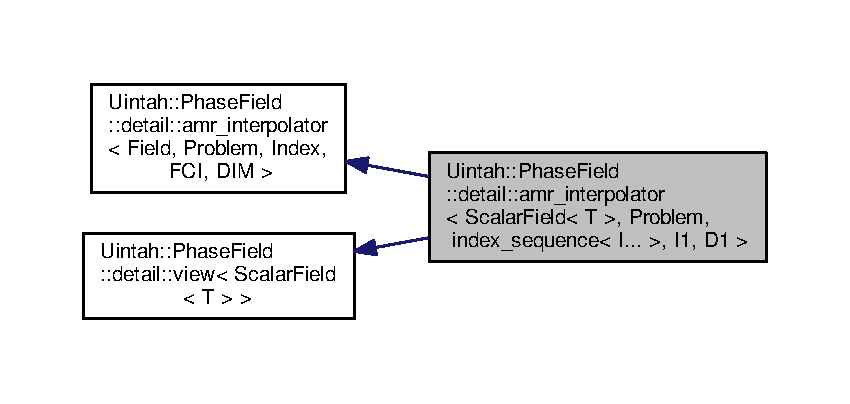
\includegraphics[width=350pt]{classUintah_1_1PhaseField_1_1detail_1_1amr__interpolator_3_01ScalarField_3_01T_01_4_00_01Problem7a982fef67338c89568bbf31cbc3f89e}
\end{center}
\end{figure}


Collaboration diagram for Uintah\+:\+:Phase\+Field\+:\+:detail\+:\+:amr\+\_\+interpolator$<$ Scalar\+Field$<$ T $>$, Problem, index\+\_\+sequence$<$ I... $>$, I1, D1 $>$\+:\nopagebreak
\begin{figure}[H]
\begin{center}
\leavevmode
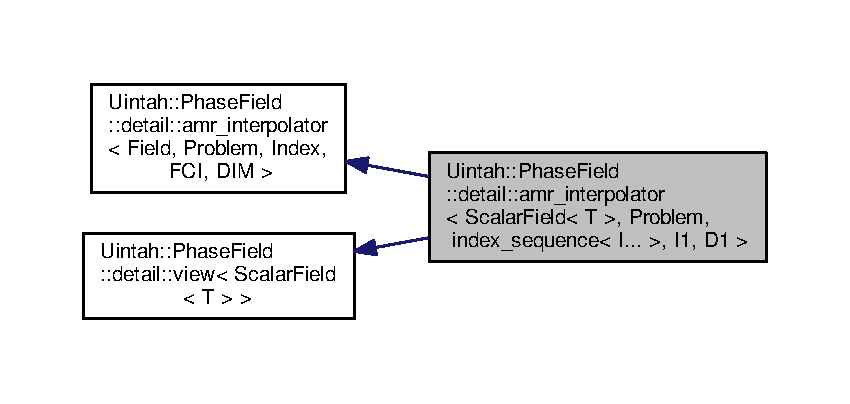
\includegraphics[width=350pt]{classUintah_1_1PhaseField_1_1detail_1_1amr__interpolator_3_01ScalarField_3_01T_01_4_00_01Problemfaefa6495259eedf2277d002c5b0b265}
\end{center}
\end{figure}
\subsection*{Public Member Functions}
\begin{DoxyCompactItemize}
\item 
\hyperlink{classUintah_1_1PhaseField_1_1detail_1_1amr__interpolator_3_01ScalarField_3_01T_01_4_00_01Problem71844444bc14a03c0566689b6b502040_a9c040b7f2b8029127f93431a363bc684}{amr\+\_\+interpolator} (const typename \hyperlink{structUintah_1_1PhaseField_1_1ScalarField_a7a77875e030da64c47ce9f6c22a06959}{Field\+::label\+\_\+type} \&label, const Var\+Label $\ast$subproblems\+\_\+label, int material)
\begin{DoxyCompactList}\small\item\em construct interpolator without retrieving inner variable data from the Data\+Warehouse \end{DoxyCompactList}\item 
\hyperlink{classUintah_1_1PhaseField_1_1detail_1_1amr__interpolator_3_01ScalarField_3_01T_01_4_00_01Problem71844444bc14a03c0566689b6b502040_a7a642e4084ed35347969bda983e80191}{amr\+\_\+interpolator} (Data\+Warehouse $\ast$dw, const typename \hyperlink{structUintah_1_1PhaseField_1_1ScalarField_a7a77875e030da64c47ce9f6c22a06959}{Field\+::label\+\_\+type} \&label, const Var\+Label $\ast$subproblems\+\_\+label, int material, const Patch $\ast$patch, bool use\+\_\+ghosts=\hyperlink{classUintah_1_1PhaseField_1_1detail_1_1amr__interpolator_3_01ScalarField_3_01T_01_4_00_01Problem71844444bc14a03c0566689b6b502040_ad1c55bf968b88ce13f275aa631a69cf7}{use\+\_\+ghosts\+\_\+dflt})
\begin{DoxyCompactList}\small\item\em construct interpolator and retrieve inner variable data from the Data\+Warehouse whitin a given fine patch. \end{DoxyCompactList}\item 
virtual \hyperlink{classUintah_1_1PhaseField_1_1detail_1_1amr__interpolator_3_01ScalarField_3_01T_01_4_00_01Problem71844444bc14a03c0566689b6b502040_a82ad51ad82c3cda7754e0e283ab062b2}{$\sim$amr\+\_\+interpolator} ()
\begin{DoxyCompactList}\small\item\em Destructor. \end{DoxyCompactList}\item 
\hyperlink{classUintah_1_1PhaseField_1_1detail_1_1amr__interpolator_3_01ScalarField_3_01T_01_4_00_01Problem71844444bc14a03c0566689b6b502040_a71a0a8eed81cb7716ea9c75f0ae384d1}{amr\+\_\+interpolator} (const \hyperlink{classUintah_1_1PhaseField_1_1detail_1_1amr__interpolator}{amr\+\_\+interpolator} \&)=delete
\begin{DoxyCompactList}\small\item\em Prevent copy (and move) constructor. \end{DoxyCompactList}\item 
\hyperlink{classUintah_1_1PhaseField_1_1detail_1_1amr__interpolator}{amr\+\_\+interpolator} \& \hyperlink{classUintah_1_1PhaseField_1_1detail_1_1amr__interpolator_3_01ScalarField_3_01T_01_4_00_01Problem71844444bc14a03c0566689b6b502040_a9e873656c2c7deea8645541176e8b752}{operator=} (const \hyperlink{classUintah_1_1PhaseField_1_1detail_1_1amr__interpolator}{amr\+\_\+interpolator} \&)=delete
\begin{DoxyCompactList}\small\item\em Prevent copy (and move) assignment. \end{DoxyCompactList}\item 
virtual void \hyperlink{classUintah_1_1PhaseField_1_1detail_1_1amr__interpolator_3_01ScalarField_3_01T_01_4_00_01Problem71844444bc14a03c0566689b6b502040_aa8b73dcc7d87c412ecb5540689d33fe9}{set} (Data\+Warehouse $\ast$dw, const Patch $\ast$patch, bool use\+\_\+ghosts=\hyperlink{classUintah_1_1PhaseField_1_1detail_1_1amr__interpolator_3_01ScalarField_3_01T_01_4_00_01Problem71844444bc14a03c0566689b6b502040_ad1c55bf968b88ce13f275aa631a69cf7}{use\+\_\+ghosts\+\_\+dflt}) override
\begin{DoxyCompactList}\small\item\em retrieve inner variable data from the Data\+Warehouse whitin a given patch. \end{DoxyCompactList}\item 
virtual void \hyperlink{classUintah_1_1PhaseField_1_1detail_1_1amr__interpolator_3_01ScalarField_3_01T_01_4_00_01Problem71844444bc14a03c0566689b6b502040_af37070317967e41c06604969034c2f71}{set} (Data\+Warehouse $\ast$dw, const Level $\ast$level, const Int\+Vector \&low, const Int\+Vector \&high, bool use\+\_\+ghosts=\hyperlink{classUintah_1_1PhaseField_1_1detail_1_1amr__interpolator_3_01ScalarField_3_01T_01_4_00_01Problem71844444bc14a03c0566689b6b502040_ad1c55bf968b88ce13f275aa631a69cf7}{use\+\_\+ghosts\+\_\+dflt}) override
\begin{DoxyCompactList}\small\item\em retrieve inner variable data from the Data\+Warehouse whitin a given region. \end{DoxyCompactList}\item 
virtual \hyperlink{classUintah_1_1PhaseField_1_1detail_1_1view}{view}$<$ \hyperlink{structUintah_1_1PhaseField_1_1ScalarField}{Field} $>$ $\ast$ \hyperlink{classUintah_1_1PhaseField_1_1detail_1_1amr__interpolator_3_01ScalarField_3_01T_01_4_00_01Problem71844444bc14a03c0566689b6b502040_ad67d51ec30f811cb8e8ac5c6a87c97e1}{clone} (bool deep) const override
\begin{DoxyCompactList}\small\item\em Get a copy of the view. \end{DoxyCompactList}\item 
virtual \hyperlink{classUintah_1_1PhaseField_1_1detail_1_1view}{view}$<$ \hyperlink{structUintah_1_1PhaseField_1_1ScalarField}{Field} $>$ $\ast$ \hyperlink{classUintah_1_1PhaseField_1_1detail_1_1amr__interpolator_3_01ScalarField_3_01T_01_4_00_01Problem71844444bc14a03c0566689b6b502040_a52720f26bf906c6bd380490b4579ffa0}{clone} (bool deep, const Int\+Vector \&offset) const override
\begin{DoxyCompactList}\small\item\em Get a copy of the view and apply translate the support. \end{DoxyCompactList}\item 
virtual \hyperlink{classUintah_1_1PhaseField_1_1Support}{Support} \hyperlink{classUintah_1_1PhaseField_1_1detail_1_1amr__interpolator_3_01ScalarField_3_01T_01_4_00_01Problem71844444bc14a03c0566689b6b502040_aab5b3fae360fb157ff3a6cba940f0db2}{get\+\_\+support} () const override
\begin{DoxyCompactList}\small\item\em get interpolator\textquotesingle{}s fine range \end{DoxyCompactList}\item 
virtual bool \hyperlink{classUintah_1_1PhaseField_1_1detail_1_1amr__interpolator_3_01ScalarField_3_01T_01_4_00_01Problem71844444bc14a03c0566689b6b502040_a0dd27e67f64c434b482cf31dcd395068}{is\+\_\+defined\+\_\+at} (const Int\+Vector \&id) const override
\begin{DoxyCompactList}\small\item\em Check if the view has access to the fine position with index id. \end{DoxyCompactList}\item 
virtual T \& \hyperlink{classUintah_1_1PhaseField_1_1detail_1_1amr__interpolator_3_01ScalarField_3_01T_01_4_00_01Problem71844444bc14a03c0566689b6b502040_a61e5afaf74c959be8ac8b1d5a57f01d5}{operator\mbox{[}$\,$\mbox{]}} (const Int\+Vector \&id) override
\begin{DoxyCompactList}\small\item\em Get/\+Modify value at position with index id (virtual implementation) \end{DoxyCompactList}\item 
virtual T \hyperlink{classUintah_1_1PhaseField_1_1detail_1_1amr__interpolator_3_01ScalarField_3_01T_01_4_00_01Problem71844444bc14a03c0566689b6b502040_a94e3434279f44322dd2fe65f16a15613}{operator\mbox{[}$\,$\mbox{]}} (const Int\+Vector \&id\+\_\+fine) const override
\begin{DoxyCompactList}\small\item\em get interpolated value \end{DoxyCompactList}\end{DoxyCompactItemize}
\subsection*{Static Public Attributes}
\begin{DoxyCompactItemize}
\item 
static constexpr bool \hyperlink{classUintah_1_1PhaseField_1_1detail_1_1amr__interpolator_3_01ScalarField_3_01T_01_4_00_01Problem71844444bc14a03c0566689b6b502040_ad1c55bf968b88ce13f275aa631a69cf7}{use\+\_\+ghosts\+\_\+dflt} = false
\begin{DoxyCompactList}\small\item\em Default value for use\+\_\+ghost when retrieving data. \end{DoxyCompactList}\end{DoxyCompactItemize}
\subsection*{Protected Member Functions}
\begin{DoxyCompactItemize}
\item 
\hyperlink{classUintah_1_1PhaseField_1_1detail_1_1amr__interpolator_3_01ScalarField_3_01T_01_4_00_01Problem71844444bc14a03c0566689b6b502040_a9fbeccc2abec84a86e4238658ce57cc3}{amr\+\_\+interpolator} (const \hyperlink{classUintah_1_1PhaseField_1_1detail_1_1amr__interpolator}{amr\+\_\+interpolator} $\ast$copy, bool deep)
\begin{DoxyCompactList}\small\item\em Constructor. \end{DoxyCompactList}\end{DoxyCompactItemize}
\subsection*{Additional Inherited Members}


\subsection{Detailed Description}
\subsubsection*{template$<$typename T, typename Problem, size\+\_\+t... I$>$\newline
class Uintah\+::\+Phase\+Field\+::detail\+::amr\+\_\+interpolator$<$ Scalar\+Field$<$ T $>$, Problem, index\+\_\+sequence$<$ I... $>$, I1, D1 $>$}

Wrapper of grid variables for interpolation from coarser to finer levels (1D linear implementation) 

Implements linear interpolation of a variable from coarser to finer levels in 1D


\begin{DoxyTemplParams}{Template Parameters}
{\em T} & variable data type (must be constant) \\
\hline
{\em \hyperlink{classUintah_1_1PhaseField_1_1Problem}{Problem}} & type of \hyperlink{namespaceUintah_1_1PhaseField}{Phase\+Field} problem \\
\hline
{\em \hyperlink{structUintah_1_1PhaseField_1_1I}{I}} & list of indices corresponding to the variable within the subproblems\\
\hline
\end{DoxyTemplParams}
\begin{DoxyRefDesc}{Todo}
\item[\hyperlink{todo__todo000001}{Todo}]generalize implementation to arbitrary dimension\end{DoxyRefDesc}


$<$ Field, \hyperlink{classUintah_1_1PhaseField_1_1Problem}{Problem}, Index, F\+CI, D\+IM $>$ 

\subsection{Constructor \& Destructor Documentation}
\mbox{\Hypertarget{classUintah_1_1PhaseField_1_1detail_1_1amr__interpolator_3_01ScalarField_3_01T_01_4_00_01Problem71844444bc14a03c0566689b6b502040_a9fbeccc2abec84a86e4238658ce57cc3}\label{classUintah_1_1PhaseField_1_1detail_1_1amr__interpolator_3_01ScalarField_3_01T_01_4_00_01Problem71844444bc14a03c0566689b6b502040_a9fbeccc2abec84a86e4238658ce57cc3}} 
\index{Uintah\+::\+Phase\+Field\+::detail\+::amr\+\_\+interpolator$<$ Scalar\+Field$<$ T $>$, Problem, index\+\_\+sequence$<$ I... $>$, I1, D1 $>$@{Uintah\+::\+Phase\+Field\+::detail\+::amr\+\_\+interpolator$<$ Scalar\+Field$<$ T $>$, Problem, index\+\_\+sequence$<$ I... $>$, I1, D1 $>$}!amr\+\_\+interpolator@{amr\+\_\+interpolator}}
\index{amr\+\_\+interpolator@{amr\+\_\+interpolator}!Uintah\+::\+Phase\+Field\+::detail\+::amr\+\_\+interpolator$<$ Scalar\+Field$<$ T $>$, Problem, index\+\_\+sequence$<$ I... $>$, I1, D1 $>$@{Uintah\+::\+Phase\+Field\+::detail\+::amr\+\_\+interpolator$<$ Scalar\+Field$<$ T $>$, Problem, index\+\_\+sequence$<$ I... $>$, I1, D1 $>$}}
\subsubsection{\texorpdfstring{amr\+\_\+interpolator()}{amr\_interpolator()}\hspace{0.1cm}{\footnotesize\ttfamily [1/4]}}
{\footnotesize\ttfamily template$<$typename T , typename Problem , size\+\_\+t... I$>$ \\
\hyperlink{classUintah_1_1PhaseField_1_1detail_1_1amr__interpolator}{Uintah\+::\+Phase\+Field\+::detail\+::amr\+\_\+interpolator}$<$ \hyperlink{structUintah_1_1PhaseField_1_1ScalarField}{Scalar\+Field}$<$ T $>$, \hyperlink{classUintah_1_1PhaseField_1_1Problem}{Problem}, \hyperlink{namespaceUintah_1_1PhaseField_a237de804d99512e50613aff7c94a9461}{index\+\_\+sequence}$<$ I... $>$, \hyperlink{namespaceUintah_1_1PhaseField_a547ce3002aa97fbd3ef3192a6eec8406a66f19efe774b0d2b6e5844eb2d83d305}{I1}, \hyperlink{namespaceUintah_1_1PhaseField_a12bfc68444894dffdf0cb8d9cf0cc76aa24dcc0ba6bcb45bc6f503b1b538c6809}{D1} $>$\+::\hyperlink{classUintah_1_1PhaseField_1_1detail_1_1amr__interpolator}{amr\+\_\+interpolator} (\begin{DoxyParamCaption}\item[{const \hyperlink{classUintah_1_1PhaseField_1_1detail_1_1amr__interpolator}{amr\+\_\+interpolator}$<$ \hyperlink{structUintah_1_1PhaseField_1_1ScalarField}{Scalar\+Field}$<$ T $>$, \hyperlink{classUintah_1_1PhaseField_1_1Problem}{Problem}, \hyperlink{namespaceUintah_1_1PhaseField_a237de804d99512e50613aff7c94a9461}{index\+\_\+sequence}$<$ I... $>$, \hyperlink{namespaceUintah_1_1PhaseField_a547ce3002aa97fbd3ef3192a6eec8406a66f19efe774b0d2b6e5844eb2d83d305}{I1}, \hyperlink{namespaceUintah_1_1PhaseField_a12bfc68444894dffdf0cb8d9cf0cc76aa24dcc0ba6bcb45bc6f503b1b538c6809}{D1} $>$ $\ast$}]{copy,  }\item[{bool}]{deep }\end{DoxyParamCaption})\hspace{0.3cm}{\ttfamily [inline]}, {\ttfamily [protected]}}



Constructor. 

Instantiate a copy of a given view


\begin{DoxyParams}{Parameters}
{\em copy} & source view for copying \\
\hline
{\em deep} & if true inner grid variable is copied as well otherwise the same grid variable is referenced \\
\hline
\end{DoxyParams}
\mbox{\Hypertarget{classUintah_1_1PhaseField_1_1detail_1_1amr__interpolator_3_01ScalarField_3_01T_01_4_00_01Problem71844444bc14a03c0566689b6b502040_a9c040b7f2b8029127f93431a363bc684}\label{classUintah_1_1PhaseField_1_1detail_1_1amr__interpolator_3_01ScalarField_3_01T_01_4_00_01Problem71844444bc14a03c0566689b6b502040_a9c040b7f2b8029127f93431a363bc684}} 
\index{Uintah\+::\+Phase\+Field\+::detail\+::amr\+\_\+interpolator$<$ Scalar\+Field$<$ T $>$, Problem, index\+\_\+sequence$<$ I... $>$, I1, D1 $>$@{Uintah\+::\+Phase\+Field\+::detail\+::amr\+\_\+interpolator$<$ Scalar\+Field$<$ T $>$, Problem, index\+\_\+sequence$<$ I... $>$, I1, D1 $>$}!amr\+\_\+interpolator@{amr\+\_\+interpolator}}
\index{amr\+\_\+interpolator@{amr\+\_\+interpolator}!Uintah\+::\+Phase\+Field\+::detail\+::amr\+\_\+interpolator$<$ Scalar\+Field$<$ T $>$, Problem, index\+\_\+sequence$<$ I... $>$, I1, D1 $>$@{Uintah\+::\+Phase\+Field\+::detail\+::amr\+\_\+interpolator$<$ Scalar\+Field$<$ T $>$, Problem, index\+\_\+sequence$<$ I... $>$, I1, D1 $>$}}
\subsubsection{\texorpdfstring{amr\+\_\+interpolator()}{amr\_interpolator()}\hspace{0.1cm}{\footnotesize\ttfamily [2/4]}}
{\footnotesize\ttfamily template$<$typename T , typename Problem , size\+\_\+t... I$>$ \\
\hyperlink{classUintah_1_1PhaseField_1_1detail_1_1amr__interpolator}{Uintah\+::\+Phase\+Field\+::detail\+::amr\+\_\+interpolator}$<$ \hyperlink{structUintah_1_1PhaseField_1_1ScalarField}{Scalar\+Field}$<$ T $>$, \hyperlink{classUintah_1_1PhaseField_1_1Problem}{Problem}, \hyperlink{namespaceUintah_1_1PhaseField_a237de804d99512e50613aff7c94a9461}{index\+\_\+sequence}$<$ I... $>$, \hyperlink{namespaceUintah_1_1PhaseField_a547ce3002aa97fbd3ef3192a6eec8406a66f19efe774b0d2b6e5844eb2d83d305}{I1}, \hyperlink{namespaceUintah_1_1PhaseField_a12bfc68444894dffdf0cb8d9cf0cc76aa24dcc0ba6bcb45bc6f503b1b538c6809}{D1} $>$\+::\hyperlink{classUintah_1_1PhaseField_1_1detail_1_1amr__interpolator}{amr\+\_\+interpolator} (\begin{DoxyParamCaption}\item[{const typename \hyperlink{structUintah_1_1PhaseField_1_1ScalarField_a7a77875e030da64c47ce9f6c22a06959}{Field\+::label\+\_\+type} \&}]{label,  }\item[{const Var\+Label $\ast$}]{subproblems\+\_\+label,  }\item[{int}]{material }\end{DoxyParamCaption})\hspace{0.3cm}{\ttfamily [inline]}}



construct interpolator without retrieving inner variable data from the Data\+Warehouse 


\begin{DoxyParams}{Parameters}
{\em label} & label of variable in the Data\+Warehouse \\
\hline
{\em subproblems\+\_\+label} & label of subproblems in the Data\+Warehouse \\
\hline
{\em material} & index of material in the Data\+Warehouse \\
\hline
\end{DoxyParams}
\mbox{\Hypertarget{classUintah_1_1PhaseField_1_1detail_1_1amr__interpolator_3_01ScalarField_3_01T_01_4_00_01Problem71844444bc14a03c0566689b6b502040_a7a642e4084ed35347969bda983e80191}\label{classUintah_1_1PhaseField_1_1detail_1_1amr__interpolator_3_01ScalarField_3_01T_01_4_00_01Problem71844444bc14a03c0566689b6b502040_a7a642e4084ed35347969bda983e80191}} 
\index{Uintah\+::\+Phase\+Field\+::detail\+::amr\+\_\+interpolator$<$ Scalar\+Field$<$ T $>$, Problem, index\+\_\+sequence$<$ I... $>$, I1, D1 $>$@{Uintah\+::\+Phase\+Field\+::detail\+::amr\+\_\+interpolator$<$ Scalar\+Field$<$ T $>$, Problem, index\+\_\+sequence$<$ I... $>$, I1, D1 $>$}!amr\+\_\+interpolator@{amr\+\_\+interpolator}}
\index{amr\+\_\+interpolator@{amr\+\_\+interpolator}!Uintah\+::\+Phase\+Field\+::detail\+::amr\+\_\+interpolator$<$ Scalar\+Field$<$ T $>$, Problem, index\+\_\+sequence$<$ I... $>$, I1, D1 $>$@{Uintah\+::\+Phase\+Field\+::detail\+::amr\+\_\+interpolator$<$ Scalar\+Field$<$ T $>$, Problem, index\+\_\+sequence$<$ I... $>$, I1, D1 $>$}}
\subsubsection{\texorpdfstring{amr\+\_\+interpolator()}{amr\_interpolator()}\hspace{0.1cm}{\footnotesize\ttfamily [3/4]}}
{\footnotesize\ttfamily template$<$typename T , typename Problem , size\+\_\+t... I$>$ \\
\hyperlink{classUintah_1_1PhaseField_1_1detail_1_1amr__interpolator}{Uintah\+::\+Phase\+Field\+::detail\+::amr\+\_\+interpolator}$<$ \hyperlink{structUintah_1_1PhaseField_1_1ScalarField}{Scalar\+Field}$<$ T $>$, \hyperlink{classUintah_1_1PhaseField_1_1Problem}{Problem}, \hyperlink{namespaceUintah_1_1PhaseField_a237de804d99512e50613aff7c94a9461}{index\+\_\+sequence}$<$ I... $>$, \hyperlink{namespaceUintah_1_1PhaseField_a547ce3002aa97fbd3ef3192a6eec8406a66f19efe774b0d2b6e5844eb2d83d305}{I1}, \hyperlink{namespaceUintah_1_1PhaseField_a12bfc68444894dffdf0cb8d9cf0cc76aa24dcc0ba6bcb45bc6f503b1b538c6809}{D1} $>$\+::\hyperlink{classUintah_1_1PhaseField_1_1detail_1_1amr__interpolator}{amr\+\_\+interpolator} (\begin{DoxyParamCaption}\item[{Data\+Warehouse $\ast$}]{dw,  }\item[{const typename \hyperlink{structUintah_1_1PhaseField_1_1ScalarField_a7a77875e030da64c47ce9f6c22a06959}{Field\+::label\+\_\+type} \&}]{label,  }\item[{const Var\+Label $\ast$}]{subproblems\+\_\+label,  }\item[{int}]{material,  }\item[{const Patch $\ast$}]{patch,  }\item[{bool}]{use\+\_\+ghosts = {\ttfamily \hyperlink{classUintah_1_1PhaseField_1_1detail_1_1amr__interpolator_3_01ScalarField_3_01T_01_4_00_01Problem71844444bc14a03c0566689b6b502040_ad1c55bf968b88ce13f275aa631a69cf7}{use\+\_\+ghosts\+\_\+dflt}} }\end{DoxyParamCaption})\hspace{0.3cm}{\ttfamily [inline]}}



construct interpolator and retrieve inner variable data from the Data\+Warehouse whitin a given fine patch. 

the number of ghost cells/nodes and the corresponding region on the coarser level is automatically computed to match the interpolation type


\begin{DoxyParams}{Parameters}
{\em dw} & Data\+Warehouse which data is retrieved from \\
\hline
{\em label} & label of variable in the Data\+Warehouse \\
\hline
{\em subproblems\+\_\+label} & label of subproblems in the Data\+Warehouse \\
\hline
{\em material} & index of material in the Data\+Warehouse \\
\hline
{\em patch} & patch on which data is retrieved \\
\hline
{\em use\+\_\+ghosts} & if ghosts value are to be retrieved (must be false) \\
\hline
\end{DoxyParams}
\mbox{\Hypertarget{classUintah_1_1PhaseField_1_1detail_1_1amr__interpolator_3_01ScalarField_3_01T_01_4_00_01Problem71844444bc14a03c0566689b6b502040_a82ad51ad82c3cda7754e0e283ab062b2}\label{classUintah_1_1PhaseField_1_1detail_1_1amr__interpolator_3_01ScalarField_3_01T_01_4_00_01Problem71844444bc14a03c0566689b6b502040_a82ad51ad82c3cda7754e0e283ab062b2}} 
\index{Uintah\+::\+Phase\+Field\+::detail\+::amr\+\_\+interpolator$<$ Scalar\+Field$<$ T $>$, Problem, index\+\_\+sequence$<$ I... $>$, I1, D1 $>$@{Uintah\+::\+Phase\+Field\+::detail\+::amr\+\_\+interpolator$<$ Scalar\+Field$<$ T $>$, Problem, index\+\_\+sequence$<$ I... $>$, I1, D1 $>$}!````~amr\+\_\+interpolator@{$\sim$amr\+\_\+interpolator}}
\index{````~amr\+\_\+interpolator@{$\sim$amr\+\_\+interpolator}!Uintah\+::\+Phase\+Field\+::detail\+::amr\+\_\+interpolator$<$ Scalar\+Field$<$ T $>$, Problem, index\+\_\+sequence$<$ I... $>$, I1, D1 $>$@{Uintah\+::\+Phase\+Field\+::detail\+::amr\+\_\+interpolator$<$ Scalar\+Field$<$ T $>$, Problem, index\+\_\+sequence$<$ I... $>$, I1, D1 $>$}}
\subsubsection{\texorpdfstring{$\sim$amr\+\_\+interpolator()}{~amr\_interpolator()}}
{\footnotesize\ttfamily template$<$typename T , typename Problem , size\+\_\+t... I$>$ \\
virtual \hyperlink{classUintah_1_1PhaseField_1_1detail_1_1amr__interpolator}{Uintah\+::\+Phase\+Field\+::detail\+::amr\+\_\+interpolator}$<$ \hyperlink{structUintah_1_1PhaseField_1_1ScalarField}{Scalar\+Field}$<$ T $>$, \hyperlink{classUintah_1_1PhaseField_1_1Problem}{Problem}, \hyperlink{namespaceUintah_1_1PhaseField_a237de804d99512e50613aff7c94a9461}{index\+\_\+sequence}$<$ I... $>$, \hyperlink{namespaceUintah_1_1PhaseField_a547ce3002aa97fbd3ef3192a6eec8406a66f19efe774b0d2b6e5844eb2d83d305}{I1}, \hyperlink{namespaceUintah_1_1PhaseField_a12bfc68444894dffdf0cb8d9cf0cc76aa24dcc0ba6bcb45bc6f503b1b538c6809}{D1} $>$\+::$\sim$\hyperlink{classUintah_1_1PhaseField_1_1detail_1_1amr__interpolator}{amr\+\_\+interpolator} (\begin{DoxyParamCaption}{ }\end{DoxyParamCaption})\hspace{0.3cm}{\ttfamily [inline]}, {\ttfamily [virtual]}}



Destructor. 

\mbox{\Hypertarget{classUintah_1_1PhaseField_1_1detail_1_1amr__interpolator_3_01ScalarField_3_01T_01_4_00_01Problem71844444bc14a03c0566689b6b502040_a71a0a8eed81cb7716ea9c75f0ae384d1}\label{classUintah_1_1PhaseField_1_1detail_1_1amr__interpolator_3_01ScalarField_3_01T_01_4_00_01Problem71844444bc14a03c0566689b6b502040_a71a0a8eed81cb7716ea9c75f0ae384d1}} 
\index{Uintah\+::\+Phase\+Field\+::detail\+::amr\+\_\+interpolator$<$ Scalar\+Field$<$ T $>$, Problem, index\+\_\+sequence$<$ I... $>$, I1, D1 $>$@{Uintah\+::\+Phase\+Field\+::detail\+::amr\+\_\+interpolator$<$ Scalar\+Field$<$ T $>$, Problem, index\+\_\+sequence$<$ I... $>$, I1, D1 $>$}!amr\+\_\+interpolator@{amr\+\_\+interpolator}}
\index{amr\+\_\+interpolator@{amr\+\_\+interpolator}!Uintah\+::\+Phase\+Field\+::detail\+::amr\+\_\+interpolator$<$ Scalar\+Field$<$ T $>$, Problem, index\+\_\+sequence$<$ I... $>$, I1, D1 $>$@{Uintah\+::\+Phase\+Field\+::detail\+::amr\+\_\+interpolator$<$ Scalar\+Field$<$ T $>$, Problem, index\+\_\+sequence$<$ I... $>$, I1, D1 $>$}}
\subsubsection{\texorpdfstring{amr\+\_\+interpolator()}{amr\_interpolator()}\hspace{0.1cm}{\footnotesize\ttfamily [4/4]}}
{\footnotesize\ttfamily template$<$typename T , typename Problem , size\+\_\+t... I$>$ \\
\hyperlink{classUintah_1_1PhaseField_1_1detail_1_1amr__interpolator}{Uintah\+::\+Phase\+Field\+::detail\+::amr\+\_\+interpolator}$<$ \hyperlink{structUintah_1_1PhaseField_1_1ScalarField}{Scalar\+Field}$<$ T $>$, \hyperlink{classUintah_1_1PhaseField_1_1Problem}{Problem}, \hyperlink{namespaceUintah_1_1PhaseField_a237de804d99512e50613aff7c94a9461}{index\+\_\+sequence}$<$ I... $>$, \hyperlink{namespaceUintah_1_1PhaseField_a547ce3002aa97fbd3ef3192a6eec8406a66f19efe774b0d2b6e5844eb2d83d305}{I1}, \hyperlink{namespaceUintah_1_1PhaseField_a12bfc68444894dffdf0cb8d9cf0cc76aa24dcc0ba6bcb45bc6f503b1b538c6809}{D1} $>$\+::\hyperlink{classUintah_1_1PhaseField_1_1detail_1_1amr__interpolator}{amr\+\_\+interpolator} (\begin{DoxyParamCaption}\item[{const \hyperlink{classUintah_1_1PhaseField_1_1detail_1_1amr__interpolator}{amr\+\_\+interpolator}$<$ \hyperlink{structUintah_1_1PhaseField_1_1ScalarField}{Scalar\+Field}$<$ T $>$, \hyperlink{classUintah_1_1PhaseField_1_1Problem}{Problem}, \hyperlink{namespaceUintah_1_1PhaseField_a237de804d99512e50613aff7c94a9461}{index\+\_\+sequence}$<$ I... $>$, \hyperlink{namespaceUintah_1_1PhaseField_a547ce3002aa97fbd3ef3192a6eec8406a66f19efe774b0d2b6e5844eb2d83d305}{I1}, \hyperlink{namespaceUintah_1_1PhaseField_a12bfc68444894dffdf0cb8d9cf0cc76aa24dcc0ba6bcb45bc6f503b1b538c6809}{D1} $>$ \&}]{ }\end{DoxyParamCaption})\hspace{0.3cm}{\ttfamily [delete]}}



Prevent copy (and move) constructor. 



\subsection{Member Function Documentation}
\mbox{\Hypertarget{classUintah_1_1PhaseField_1_1detail_1_1amr__interpolator_3_01ScalarField_3_01T_01_4_00_01Problem71844444bc14a03c0566689b6b502040_ad67d51ec30f811cb8e8ac5c6a87c97e1}\label{classUintah_1_1PhaseField_1_1detail_1_1amr__interpolator_3_01ScalarField_3_01T_01_4_00_01Problem71844444bc14a03c0566689b6b502040_ad67d51ec30f811cb8e8ac5c6a87c97e1}} 
\index{Uintah\+::\+Phase\+Field\+::detail\+::amr\+\_\+interpolator$<$ Scalar\+Field$<$ T $>$, Problem, index\+\_\+sequence$<$ I... $>$, I1, D1 $>$@{Uintah\+::\+Phase\+Field\+::detail\+::amr\+\_\+interpolator$<$ Scalar\+Field$<$ T $>$, Problem, index\+\_\+sequence$<$ I... $>$, I1, D1 $>$}!clone@{clone}}
\index{clone@{clone}!Uintah\+::\+Phase\+Field\+::detail\+::amr\+\_\+interpolator$<$ Scalar\+Field$<$ T $>$, Problem, index\+\_\+sequence$<$ I... $>$, I1, D1 $>$@{Uintah\+::\+Phase\+Field\+::detail\+::amr\+\_\+interpolator$<$ Scalar\+Field$<$ T $>$, Problem, index\+\_\+sequence$<$ I... $>$, I1, D1 $>$}}
\subsubsection{\texorpdfstring{clone()}{clone()}\hspace{0.1cm}{\footnotesize\ttfamily [1/2]}}
{\footnotesize\ttfamily template$<$typename T , typename Problem , size\+\_\+t... I$>$ \\
virtual \hyperlink{classUintah_1_1PhaseField_1_1detail_1_1view}{view}$<$\hyperlink{structUintah_1_1PhaseField_1_1ScalarField}{Field}$>$$\ast$ \hyperlink{classUintah_1_1PhaseField_1_1detail_1_1amr__interpolator}{Uintah\+::\+Phase\+Field\+::detail\+::amr\+\_\+interpolator}$<$ \hyperlink{structUintah_1_1PhaseField_1_1ScalarField}{Scalar\+Field}$<$ T $>$, \hyperlink{classUintah_1_1PhaseField_1_1Problem}{Problem}, \hyperlink{namespaceUintah_1_1PhaseField_a237de804d99512e50613aff7c94a9461}{index\+\_\+sequence}$<$ I... $>$, \hyperlink{namespaceUintah_1_1PhaseField_a547ce3002aa97fbd3ef3192a6eec8406a66f19efe774b0d2b6e5844eb2d83d305}{I1}, \hyperlink{namespaceUintah_1_1PhaseField_a12bfc68444894dffdf0cb8d9cf0cc76aa24dcc0ba6bcb45bc6f503b1b538c6809}{D1} $>$\+::clone (\begin{DoxyParamCaption}\item[{bool}]{deep }\end{DoxyParamCaption}) const\hspace{0.3cm}{\ttfamily [inline]}, {\ttfamily [override]}, {\ttfamily [virtual]}}



Get a copy of the view. 


\begin{DoxyParams}{Parameters}
{\em deep} & if true inner grid variable is copied as well otherwise the same grid variable is referenced\\
\hline
\end{DoxyParams}
\begin{DoxyReturn}{Returns}
new view instance 
\end{DoxyReturn}


Implements \hyperlink{classUintah_1_1PhaseField_1_1detail_1_1view_3_01ScalarField_3_01T_01_4_01_4_a6e11243c9d776a7b703e524ea4151a16}{Uintah\+::\+Phase\+Field\+::detail\+::view$<$ Scalar\+Field$<$ T $>$ $>$}.

\mbox{\Hypertarget{classUintah_1_1PhaseField_1_1detail_1_1amr__interpolator_3_01ScalarField_3_01T_01_4_00_01Problem71844444bc14a03c0566689b6b502040_a52720f26bf906c6bd380490b4579ffa0}\label{classUintah_1_1PhaseField_1_1detail_1_1amr__interpolator_3_01ScalarField_3_01T_01_4_00_01Problem71844444bc14a03c0566689b6b502040_a52720f26bf906c6bd380490b4579ffa0}} 
\index{Uintah\+::\+Phase\+Field\+::detail\+::amr\+\_\+interpolator$<$ Scalar\+Field$<$ T $>$, Problem, index\+\_\+sequence$<$ I... $>$, I1, D1 $>$@{Uintah\+::\+Phase\+Field\+::detail\+::amr\+\_\+interpolator$<$ Scalar\+Field$<$ T $>$, Problem, index\+\_\+sequence$<$ I... $>$, I1, D1 $>$}!clone@{clone}}
\index{clone@{clone}!Uintah\+::\+Phase\+Field\+::detail\+::amr\+\_\+interpolator$<$ Scalar\+Field$<$ T $>$, Problem, index\+\_\+sequence$<$ I... $>$, I1, D1 $>$@{Uintah\+::\+Phase\+Field\+::detail\+::amr\+\_\+interpolator$<$ Scalar\+Field$<$ T $>$, Problem, index\+\_\+sequence$<$ I... $>$, I1, D1 $>$}}
\subsubsection{\texorpdfstring{clone()}{clone()}\hspace{0.1cm}{\footnotesize\ttfamily [2/2]}}
{\footnotesize\ttfamily template$<$typename T , typename Problem , size\+\_\+t... I$>$ \\
virtual \hyperlink{classUintah_1_1PhaseField_1_1detail_1_1view}{view}$<$\hyperlink{structUintah_1_1PhaseField_1_1ScalarField}{Field}$>$$\ast$ \hyperlink{classUintah_1_1PhaseField_1_1detail_1_1amr__interpolator}{Uintah\+::\+Phase\+Field\+::detail\+::amr\+\_\+interpolator}$<$ \hyperlink{structUintah_1_1PhaseField_1_1ScalarField}{Scalar\+Field}$<$ T $>$, \hyperlink{classUintah_1_1PhaseField_1_1Problem}{Problem}, \hyperlink{namespaceUintah_1_1PhaseField_a237de804d99512e50613aff7c94a9461}{index\+\_\+sequence}$<$ I... $>$, \hyperlink{namespaceUintah_1_1PhaseField_a547ce3002aa97fbd3ef3192a6eec8406a66f19efe774b0d2b6e5844eb2d83d305}{I1}, \hyperlink{namespaceUintah_1_1PhaseField_a12bfc68444894dffdf0cb8d9cf0cc76aa24dcc0ba6bcb45bc6f503b1b538c6809}{D1} $>$\+::clone (\begin{DoxyParamCaption}\item[{bool}]{deep,  }\item[{const Int\+Vector \&}]{offset }\end{DoxyParamCaption}) const\hspace{0.3cm}{\ttfamily [inline]}, {\ttfamily [override]}, {\ttfamily [virtual]}}



Get a copy of the view and apply translate the support. 

\begin{DoxyRemark}{Remarks}
It is meant to be used for virtual patches (i.\+e. periodic boundaries)
\end{DoxyRemark}

\begin{DoxyParams}{Parameters}
{\em deep} & if true inner grid variable is copied as well otherwise the same grid variable is referenced \\
\hline
{\em offset} & vector specifying the translation of the support \\
\hline
\end{DoxyParams}
\begin{DoxyReturn}{Returns}
new view instance 
\end{DoxyReturn}


Implements \hyperlink{classUintah_1_1PhaseField_1_1detail_1_1view_3_01ScalarField_3_01T_01_4_01_4_abd928104240e329f3bc4441ebab7c50c}{Uintah\+::\+Phase\+Field\+::detail\+::view$<$ Scalar\+Field$<$ T $>$ $>$}.

\mbox{\Hypertarget{classUintah_1_1PhaseField_1_1detail_1_1amr__interpolator_3_01ScalarField_3_01T_01_4_00_01Problem71844444bc14a03c0566689b6b502040_aab5b3fae360fb157ff3a6cba940f0db2}\label{classUintah_1_1PhaseField_1_1detail_1_1amr__interpolator_3_01ScalarField_3_01T_01_4_00_01Problem71844444bc14a03c0566689b6b502040_aab5b3fae360fb157ff3a6cba940f0db2}} 
\index{Uintah\+::\+Phase\+Field\+::detail\+::amr\+\_\+interpolator$<$ Scalar\+Field$<$ T $>$, Problem, index\+\_\+sequence$<$ I... $>$, I1, D1 $>$@{Uintah\+::\+Phase\+Field\+::detail\+::amr\+\_\+interpolator$<$ Scalar\+Field$<$ T $>$, Problem, index\+\_\+sequence$<$ I... $>$, I1, D1 $>$}!get\+\_\+support@{get\+\_\+support}}
\index{get\+\_\+support@{get\+\_\+support}!Uintah\+::\+Phase\+Field\+::detail\+::amr\+\_\+interpolator$<$ Scalar\+Field$<$ T $>$, Problem, index\+\_\+sequence$<$ I... $>$, I1, D1 $>$@{Uintah\+::\+Phase\+Field\+::detail\+::amr\+\_\+interpolator$<$ Scalar\+Field$<$ T $>$, Problem, index\+\_\+sequence$<$ I... $>$, I1, D1 $>$}}
\subsubsection{\texorpdfstring{get\+\_\+support()}{get\_support()}}
{\footnotesize\ttfamily template$<$typename T , typename Problem , size\+\_\+t... I$>$ \\
virtual \hyperlink{classUintah_1_1PhaseField_1_1Support}{Support} \hyperlink{classUintah_1_1PhaseField_1_1detail_1_1amr__interpolator}{Uintah\+::\+Phase\+Field\+::detail\+::amr\+\_\+interpolator}$<$ \hyperlink{structUintah_1_1PhaseField_1_1ScalarField}{Scalar\+Field}$<$ T $>$, \hyperlink{classUintah_1_1PhaseField_1_1Problem}{Problem}, \hyperlink{namespaceUintah_1_1PhaseField_a237de804d99512e50613aff7c94a9461}{index\+\_\+sequence}$<$ I... $>$, \hyperlink{namespaceUintah_1_1PhaseField_a547ce3002aa97fbd3ef3192a6eec8406a66f19efe774b0d2b6e5844eb2d83d305}{I1}, \hyperlink{namespaceUintah_1_1PhaseField_a12bfc68444894dffdf0cb8d9cf0cc76aa24dcc0ba6bcb45bc6f503b1b538c6809}{D1} $>$\+::get\+\_\+support (\begin{DoxyParamCaption}{ }\end{DoxyParamCaption}) const\hspace{0.3cm}{\ttfamily [inline]}, {\ttfamily [override]}, {\ttfamily [virtual]}}



get interpolator\textquotesingle{}s fine range 

\begin{DoxyReturn}{Returns}
fine range 
\end{DoxyReturn}


Implements \hyperlink{classUintah_1_1PhaseField_1_1detail_1_1view_3_01ScalarField_3_01T_01_4_01_4_a3e14b0c7a57a57707bb33954861ab1c1}{Uintah\+::\+Phase\+Field\+::detail\+::view$<$ Scalar\+Field$<$ T $>$ $>$}.

\mbox{\Hypertarget{classUintah_1_1PhaseField_1_1detail_1_1amr__interpolator_3_01ScalarField_3_01T_01_4_00_01Problem71844444bc14a03c0566689b6b502040_a0dd27e67f64c434b482cf31dcd395068}\label{classUintah_1_1PhaseField_1_1detail_1_1amr__interpolator_3_01ScalarField_3_01T_01_4_00_01Problem71844444bc14a03c0566689b6b502040_a0dd27e67f64c434b482cf31dcd395068}} 
\index{Uintah\+::\+Phase\+Field\+::detail\+::amr\+\_\+interpolator$<$ Scalar\+Field$<$ T $>$, Problem, index\+\_\+sequence$<$ I... $>$, I1, D1 $>$@{Uintah\+::\+Phase\+Field\+::detail\+::amr\+\_\+interpolator$<$ Scalar\+Field$<$ T $>$, Problem, index\+\_\+sequence$<$ I... $>$, I1, D1 $>$}!is\+\_\+defined\+\_\+at@{is\+\_\+defined\+\_\+at}}
\index{is\+\_\+defined\+\_\+at@{is\+\_\+defined\+\_\+at}!Uintah\+::\+Phase\+Field\+::detail\+::amr\+\_\+interpolator$<$ Scalar\+Field$<$ T $>$, Problem, index\+\_\+sequence$<$ I... $>$, I1, D1 $>$@{Uintah\+::\+Phase\+Field\+::detail\+::amr\+\_\+interpolator$<$ Scalar\+Field$<$ T $>$, Problem, index\+\_\+sequence$<$ I... $>$, I1, D1 $>$}}
\subsubsection{\texorpdfstring{is\+\_\+defined\+\_\+at()}{is\_defined\_at()}}
{\footnotesize\ttfamily template$<$typename T , typename Problem , size\+\_\+t... I$>$ \\
virtual bool \hyperlink{classUintah_1_1PhaseField_1_1detail_1_1amr__interpolator}{Uintah\+::\+Phase\+Field\+::detail\+::amr\+\_\+interpolator}$<$ \hyperlink{structUintah_1_1PhaseField_1_1ScalarField}{Scalar\+Field}$<$ T $>$, \hyperlink{classUintah_1_1PhaseField_1_1Problem}{Problem}, \hyperlink{namespaceUintah_1_1PhaseField_a237de804d99512e50613aff7c94a9461}{index\+\_\+sequence}$<$ I... $>$, \hyperlink{namespaceUintah_1_1PhaseField_a547ce3002aa97fbd3ef3192a6eec8406a66f19efe774b0d2b6e5844eb2d83d305}{I1}, \hyperlink{namespaceUintah_1_1PhaseField_a12bfc68444894dffdf0cb8d9cf0cc76aa24dcc0ba6bcb45bc6f503b1b538c6809}{D1} $>$\+::is\+\_\+defined\+\_\+at (\begin{DoxyParamCaption}\item[{const Int\+Vector \&}]{id }\end{DoxyParamCaption}) const\hspace{0.3cm}{\ttfamily [inline]}, {\ttfamily [override]}, {\ttfamily [virtual]}}



Check if the view has access to the fine position with index id. 


\begin{DoxyParams}{Parameters}
{\em id} & fine position index \\
\hline
\end{DoxyParams}
\begin{DoxyReturn}{Returns}
check result 
\end{DoxyReturn}


Implements \hyperlink{classUintah_1_1PhaseField_1_1detail_1_1view_3_01ScalarField_3_01T_01_4_01_4_a9a950513dacd6468658436b737c3314f}{Uintah\+::\+Phase\+Field\+::detail\+::view$<$ Scalar\+Field$<$ T $>$ $>$}.

\mbox{\Hypertarget{classUintah_1_1PhaseField_1_1detail_1_1amr__interpolator_3_01ScalarField_3_01T_01_4_00_01Problem71844444bc14a03c0566689b6b502040_a9e873656c2c7deea8645541176e8b752}\label{classUintah_1_1PhaseField_1_1detail_1_1amr__interpolator_3_01ScalarField_3_01T_01_4_00_01Problem71844444bc14a03c0566689b6b502040_a9e873656c2c7deea8645541176e8b752}} 
\index{Uintah\+::\+Phase\+Field\+::detail\+::amr\+\_\+interpolator$<$ Scalar\+Field$<$ T $>$, Problem, index\+\_\+sequence$<$ I... $>$, I1, D1 $>$@{Uintah\+::\+Phase\+Field\+::detail\+::amr\+\_\+interpolator$<$ Scalar\+Field$<$ T $>$, Problem, index\+\_\+sequence$<$ I... $>$, I1, D1 $>$}!operator=@{operator=}}
\index{operator=@{operator=}!Uintah\+::\+Phase\+Field\+::detail\+::amr\+\_\+interpolator$<$ Scalar\+Field$<$ T $>$, Problem, index\+\_\+sequence$<$ I... $>$, I1, D1 $>$@{Uintah\+::\+Phase\+Field\+::detail\+::amr\+\_\+interpolator$<$ Scalar\+Field$<$ T $>$, Problem, index\+\_\+sequence$<$ I... $>$, I1, D1 $>$}}
\subsubsection{\texorpdfstring{operator=()}{operator=()}}
{\footnotesize\ttfamily template$<$typename T , typename Problem , size\+\_\+t... I$>$ \\
\hyperlink{classUintah_1_1PhaseField_1_1detail_1_1amr__interpolator}{amr\+\_\+interpolator}\& \hyperlink{classUintah_1_1PhaseField_1_1detail_1_1amr__interpolator}{Uintah\+::\+Phase\+Field\+::detail\+::amr\+\_\+interpolator}$<$ \hyperlink{structUintah_1_1PhaseField_1_1ScalarField}{Scalar\+Field}$<$ T $>$, \hyperlink{classUintah_1_1PhaseField_1_1Problem}{Problem}, \hyperlink{namespaceUintah_1_1PhaseField_a237de804d99512e50613aff7c94a9461}{index\+\_\+sequence}$<$ I... $>$, \hyperlink{namespaceUintah_1_1PhaseField_a547ce3002aa97fbd3ef3192a6eec8406a66f19efe774b0d2b6e5844eb2d83d305}{I1}, \hyperlink{namespaceUintah_1_1PhaseField_a12bfc68444894dffdf0cb8d9cf0cc76aa24dcc0ba6bcb45bc6f503b1b538c6809}{D1} $>$\+::operator= (\begin{DoxyParamCaption}\item[{const \hyperlink{classUintah_1_1PhaseField_1_1detail_1_1amr__interpolator}{amr\+\_\+interpolator}$<$ \hyperlink{structUintah_1_1PhaseField_1_1ScalarField}{Scalar\+Field}$<$ T $>$, \hyperlink{classUintah_1_1PhaseField_1_1Problem}{Problem}, \hyperlink{namespaceUintah_1_1PhaseField_a237de804d99512e50613aff7c94a9461}{index\+\_\+sequence}$<$ I... $>$, \hyperlink{namespaceUintah_1_1PhaseField_a547ce3002aa97fbd3ef3192a6eec8406a66f19efe774b0d2b6e5844eb2d83d305}{I1}, \hyperlink{namespaceUintah_1_1PhaseField_a12bfc68444894dffdf0cb8d9cf0cc76aa24dcc0ba6bcb45bc6f503b1b538c6809}{D1} $>$ \&}]{ }\end{DoxyParamCaption})\hspace{0.3cm}{\ttfamily [delete]}}



Prevent copy (and move) assignment. 

\mbox{\Hypertarget{classUintah_1_1PhaseField_1_1detail_1_1amr__interpolator_3_01ScalarField_3_01T_01_4_00_01Problem71844444bc14a03c0566689b6b502040_a61e5afaf74c959be8ac8b1d5a57f01d5}\label{classUintah_1_1PhaseField_1_1detail_1_1amr__interpolator_3_01ScalarField_3_01T_01_4_00_01Problem71844444bc14a03c0566689b6b502040_a61e5afaf74c959be8ac8b1d5a57f01d5}} 
\index{Uintah\+::\+Phase\+Field\+::detail\+::amr\+\_\+interpolator$<$ Scalar\+Field$<$ T $>$, Problem, index\+\_\+sequence$<$ I... $>$, I1, D1 $>$@{Uintah\+::\+Phase\+Field\+::detail\+::amr\+\_\+interpolator$<$ Scalar\+Field$<$ T $>$, Problem, index\+\_\+sequence$<$ I... $>$, I1, D1 $>$}!operator\mbox{[}\mbox{]}@{operator[]}}
\index{operator\mbox{[}\mbox{]}@{operator[]}!Uintah\+::\+Phase\+Field\+::detail\+::amr\+\_\+interpolator$<$ Scalar\+Field$<$ T $>$, Problem, index\+\_\+sequence$<$ I... $>$, I1, D1 $>$@{Uintah\+::\+Phase\+Field\+::detail\+::amr\+\_\+interpolator$<$ Scalar\+Field$<$ T $>$, Problem, index\+\_\+sequence$<$ I... $>$, I1, D1 $>$}}
\subsubsection{\texorpdfstring{operator[]()}{operator[]()}\hspace{0.1cm}{\footnotesize\ttfamily [1/2]}}
{\footnotesize\ttfamily template$<$typename T , typename Problem , size\+\_\+t... I$>$ \\
virtual T\& \hyperlink{classUintah_1_1PhaseField_1_1detail_1_1amr__interpolator}{Uintah\+::\+Phase\+Field\+::detail\+::amr\+\_\+interpolator}$<$ \hyperlink{structUintah_1_1PhaseField_1_1ScalarField}{Scalar\+Field}$<$ T $>$, \hyperlink{classUintah_1_1PhaseField_1_1Problem}{Problem}, \hyperlink{namespaceUintah_1_1PhaseField_a237de804d99512e50613aff7c94a9461}{index\+\_\+sequence}$<$ I... $>$, \hyperlink{namespaceUintah_1_1PhaseField_a547ce3002aa97fbd3ef3192a6eec8406a66f19efe774b0d2b6e5844eb2d83d305}{I1}, \hyperlink{namespaceUintah_1_1PhaseField_a12bfc68444894dffdf0cb8d9cf0cc76aa24dcc0ba6bcb45bc6f503b1b538c6809}{D1} $>$\+::operator\mbox{[}$\,$\mbox{]} (\begin{DoxyParamCaption}\item[{const Int\+Vector \&}]{id }\end{DoxyParamCaption})\hspace{0.3cm}{\ttfamily [inline]}, {\ttfamily [override]}, {\ttfamily [virtual]}}



Get/\+Modify value at position with index id (virtual implementation) 

\begin{DoxyRemark}{Remarks}
interpolated value is computed at runtime thus doesn\textquotesingle{}t exist in the Data\+Warehouse
\end{DoxyRemark}

\begin{DoxyParams}{Parameters}
{\em id} & unused \\
\hline
\end{DoxyParams}
\begin{DoxyReturn}{Returns}
nothing 
\end{DoxyReturn}


Implements \hyperlink{classUintah_1_1PhaseField_1_1detail_1_1view_3_01ScalarField_3_01T_01_4_01_4_a96b3035d435ae901516b6bc5e138f3b5}{Uintah\+::\+Phase\+Field\+::detail\+::view$<$ Scalar\+Field$<$ T $>$ $>$}.

\mbox{\Hypertarget{classUintah_1_1PhaseField_1_1detail_1_1amr__interpolator_3_01ScalarField_3_01T_01_4_00_01Problem71844444bc14a03c0566689b6b502040_a94e3434279f44322dd2fe65f16a15613}\label{classUintah_1_1PhaseField_1_1detail_1_1amr__interpolator_3_01ScalarField_3_01T_01_4_00_01Problem71844444bc14a03c0566689b6b502040_a94e3434279f44322dd2fe65f16a15613}} 
\index{Uintah\+::\+Phase\+Field\+::detail\+::amr\+\_\+interpolator$<$ Scalar\+Field$<$ T $>$, Problem, index\+\_\+sequence$<$ I... $>$, I1, D1 $>$@{Uintah\+::\+Phase\+Field\+::detail\+::amr\+\_\+interpolator$<$ Scalar\+Field$<$ T $>$, Problem, index\+\_\+sequence$<$ I... $>$, I1, D1 $>$}!operator\mbox{[}\mbox{]}@{operator[]}}
\index{operator\mbox{[}\mbox{]}@{operator[]}!Uintah\+::\+Phase\+Field\+::detail\+::amr\+\_\+interpolator$<$ Scalar\+Field$<$ T $>$, Problem, index\+\_\+sequence$<$ I... $>$, I1, D1 $>$@{Uintah\+::\+Phase\+Field\+::detail\+::amr\+\_\+interpolator$<$ Scalar\+Field$<$ T $>$, Problem, index\+\_\+sequence$<$ I... $>$, I1, D1 $>$}}
\subsubsection{\texorpdfstring{operator[]()}{operator[]()}\hspace{0.1cm}{\footnotesize\ttfamily [2/2]}}
{\footnotesize\ttfamily template$<$typename T , typename Problem , size\+\_\+t... I$>$ \\
virtual T \hyperlink{classUintah_1_1PhaseField_1_1detail_1_1amr__interpolator}{Uintah\+::\+Phase\+Field\+::detail\+::amr\+\_\+interpolator}$<$ \hyperlink{structUintah_1_1PhaseField_1_1ScalarField}{Scalar\+Field}$<$ T $>$, \hyperlink{classUintah_1_1PhaseField_1_1Problem}{Problem}, \hyperlink{namespaceUintah_1_1PhaseField_a237de804d99512e50613aff7c94a9461}{index\+\_\+sequence}$<$ I... $>$, \hyperlink{namespaceUintah_1_1PhaseField_a547ce3002aa97fbd3ef3192a6eec8406a66f19efe774b0d2b6e5844eb2d83d305}{I1}, \hyperlink{namespaceUintah_1_1PhaseField_a12bfc68444894dffdf0cb8d9cf0cc76aa24dcc0ba6bcb45bc6f503b1b538c6809}{D1} $>$\+::operator\mbox{[}$\,$\mbox{]} (\begin{DoxyParamCaption}\item[{const Int\+Vector \&}]{id\+\_\+fine }\end{DoxyParamCaption}) const\hspace{0.3cm}{\ttfamily [inline]}, {\ttfamily [override]}, {\ttfamily [virtual]}}



get interpolated value 

value at fine index is computed by linear interpolation over the nearest 2 indexes on the coarser level


\begin{DoxyParams}{Parameters}
{\em id\+\_\+fine} & fine index \\
\hline
\end{DoxyParams}
\begin{DoxyReturn}{Returns}
interpolated value at the given fine index 
\end{DoxyReturn}


Implements \hyperlink{classUintah_1_1PhaseField_1_1detail_1_1view_3_01ScalarField_3_01T_01_4_01_4_aea43cfedfe3b6f3c038ff795caec49b8}{Uintah\+::\+Phase\+Field\+::detail\+::view$<$ Scalar\+Field$<$ T $>$ $>$}.

\mbox{\Hypertarget{classUintah_1_1PhaseField_1_1detail_1_1amr__interpolator_3_01ScalarField_3_01T_01_4_00_01Problem71844444bc14a03c0566689b6b502040_aa8b73dcc7d87c412ecb5540689d33fe9}\label{classUintah_1_1PhaseField_1_1detail_1_1amr__interpolator_3_01ScalarField_3_01T_01_4_00_01Problem71844444bc14a03c0566689b6b502040_aa8b73dcc7d87c412ecb5540689d33fe9}} 
\index{Uintah\+::\+Phase\+Field\+::detail\+::amr\+\_\+interpolator$<$ Scalar\+Field$<$ T $>$, Problem, index\+\_\+sequence$<$ I... $>$, I1, D1 $>$@{Uintah\+::\+Phase\+Field\+::detail\+::amr\+\_\+interpolator$<$ Scalar\+Field$<$ T $>$, Problem, index\+\_\+sequence$<$ I... $>$, I1, D1 $>$}!set@{set}}
\index{set@{set}!Uintah\+::\+Phase\+Field\+::detail\+::amr\+\_\+interpolator$<$ Scalar\+Field$<$ T $>$, Problem, index\+\_\+sequence$<$ I... $>$, I1, D1 $>$@{Uintah\+::\+Phase\+Field\+::detail\+::amr\+\_\+interpolator$<$ Scalar\+Field$<$ T $>$, Problem, index\+\_\+sequence$<$ I... $>$, I1, D1 $>$}}
\subsubsection{\texorpdfstring{set()}{set()}\hspace{0.1cm}{\footnotesize\ttfamily [1/2]}}
{\footnotesize\ttfamily template$<$typename T , typename Problem , size\+\_\+t... I$>$ \\
virtual void \hyperlink{classUintah_1_1PhaseField_1_1detail_1_1amr__interpolator}{Uintah\+::\+Phase\+Field\+::detail\+::amr\+\_\+interpolator}$<$ \hyperlink{structUintah_1_1PhaseField_1_1ScalarField}{Scalar\+Field}$<$ T $>$, \hyperlink{classUintah_1_1PhaseField_1_1Problem}{Problem}, \hyperlink{namespaceUintah_1_1PhaseField_a237de804d99512e50613aff7c94a9461}{index\+\_\+sequence}$<$ I... $>$, \hyperlink{namespaceUintah_1_1PhaseField_a547ce3002aa97fbd3ef3192a6eec8406a66f19efe774b0d2b6e5844eb2d83d305}{I1}, \hyperlink{namespaceUintah_1_1PhaseField_a12bfc68444894dffdf0cb8d9cf0cc76aa24dcc0ba6bcb45bc6f503b1b538c6809}{D1} $>$\+::set (\begin{DoxyParamCaption}\item[{Data\+Warehouse $\ast$}]{dw,  }\item[{const Patch $\ast$}]{patch,  }\item[{bool}]{use\+\_\+ghosts = {\ttfamily \hyperlink{classUintah_1_1PhaseField_1_1detail_1_1amr__interpolator_3_01ScalarField_3_01T_01_4_00_01Problem71844444bc14a03c0566689b6b502040_ad1c55bf968b88ce13f275aa631a69cf7}{use\+\_\+ghosts\+\_\+dflt}} }\end{DoxyParamCaption})\hspace{0.3cm}{\ttfamily [inline]}, {\ttfamily [override]}, {\ttfamily [virtual]}}



retrieve inner variable data from the Data\+Warehouse whitin a given patch. 

the number of ghost cells/nodes and the corresponding region on the coarser level is automatically computed to match the interpolation type


\begin{DoxyParams}{Parameters}
{\em dw} & Data\+Warehouse which data is retrieved from \\
\hline
{\em patch} & patch on which data is retrieved \\
\hline
{\em use\+\_\+ghosts} & if ghosts value are to be retrieved (must be false) \\
\hline
\end{DoxyParams}


Implements \hyperlink{classUintah_1_1PhaseField_1_1detail_1_1view_3_01ScalarField_3_01T_01_4_01_4_ae90ea8b33fde8515a1f2e8f5c03c0166}{Uintah\+::\+Phase\+Field\+::detail\+::view$<$ Scalar\+Field$<$ T $>$ $>$}.

\mbox{\Hypertarget{classUintah_1_1PhaseField_1_1detail_1_1amr__interpolator_3_01ScalarField_3_01T_01_4_00_01Problem71844444bc14a03c0566689b6b502040_af37070317967e41c06604969034c2f71}\label{classUintah_1_1PhaseField_1_1detail_1_1amr__interpolator_3_01ScalarField_3_01T_01_4_00_01Problem71844444bc14a03c0566689b6b502040_af37070317967e41c06604969034c2f71}} 
\index{Uintah\+::\+Phase\+Field\+::detail\+::amr\+\_\+interpolator$<$ Scalar\+Field$<$ T $>$, Problem, index\+\_\+sequence$<$ I... $>$, I1, D1 $>$@{Uintah\+::\+Phase\+Field\+::detail\+::amr\+\_\+interpolator$<$ Scalar\+Field$<$ T $>$, Problem, index\+\_\+sequence$<$ I... $>$, I1, D1 $>$}!set@{set}}
\index{set@{set}!Uintah\+::\+Phase\+Field\+::detail\+::amr\+\_\+interpolator$<$ Scalar\+Field$<$ T $>$, Problem, index\+\_\+sequence$<$ I... $>$, I1, D1 $>$@{Uintah\+::\+Phase\+Field\+::detail\+::amr\+\_\+interpolator$<$ Scalar\+Field$<$ T $>$, Problem, index\+\_\+sequence$<$ I... $>$, I1, D1 $>$}}
\subsubsection{\texorpdfstring{set()}{set()}\hspace{0.1cm}{\footnotesize\ttfamily [2/2]}}
{\footnotesize\ttfamily template$<$typename T , typename Problem , size\+\_\+t... I$>$ \\
virtual void \hyperlink{classUintah_1_1PhaseField_1_1detail_1_1amr__interpolator}{Uintah\+::\+Phase\+Field\+::detail\+::amr\+\_\+interpolator}$<$ \hyperlink{structUintah_1_1PhaseField_1_1ScalarField}{Scalar\+Field}$<$ T $>$, \hyperlink{classUintah_1_1PhaseField_1_1Problem}{Problem}, \hyperlink{namespaceUintah_1_1PhaseField_a237de804d99512e50613aff7c94a9461}{index\+\_\+sequence}$<$ I... $>$, \hyperlink{namespaceUintah_1_1PhaseField_a547ce3002aa97fbd3ef3192a6eec8406a66f19efe774b0d2b6e5844eb2d83d305}{I1}, \hyperlink{namespaceUintah_1_1PhaseField_a12bfc68444894dffdf0cb8d9cf0cc76aa24dcc0ba6bcb45bc6f503b1b538c6809}{D1} $>$\+::set (\begin{DoxyParamCaption}\item[{Data\+Warehouse $\ast$}]{dw,  }\item[{const Level $\ast$}]{level,  }\item[{const Int\+Vector \&}]{low,  }\item[{const Int\+Vector \&}]{high,  }\item[{bool}]{use\+\_\+ghosts = {\ttfamily \hyperlink{classUintah_1_1PhaseField_1_1detail_1_1amr__interpolator_3_01ScalarField_3_01T_01_4_00_01Problem71844444bc14a03c0566689b6b502040_ad1c55bf968b88ce13f275aa631a69cf7}{use\+\_\+ghosts\+\_\+dflt}} }\end{DoxyParamCaption})\hspace{0.3cm}{\ttfamily [inline]}, {\ttfamily [override]}, {\ttfamily [virtual]}}



retrieve inner variable data from the Data\+Warehouse whitin a given region. 

the number of ghost cells/nodes and the corresponding region on the coarser level is automatically computed to match the interpolation type


\begin{DoxyParams}{Parameters}
{\em dw} & Data\+Warehouse which data is retrieved from \\
\hline
{\em level} & level of the fine region \\
\hline
{\em low} & start index for the fine region \\
\hline
{\em high} & past the end index for the fine region \\
\hline
{\em use\+\_\+ghosts} & if ghosts value are to be retrieved (must be false) \\
\hline
\end{DoxyParams}


Implements \hyperlink{classUintah_1_1PhaseField_1_1detail_1_1view_3_01ScalarField_3_01T_01_4_01_4_a5fc830b30b120922cfe8a2c008d96109}{Uintah\+::\+Phase\+Field\+::detail\+::view$<$ Scalar\+Field$<$ T $>$ $>$}.



\subsection{Member Data Documentation}
\mbox{\Hypertarget{classUintah_1_1PhaseField_1_1detail_1_1amr__interpolator_3_01ScalarField_3_01T_01_4_00_01Problem71844444bc14a03c0566689b6b502040_ad1c55bf968b88ce13f275aa631a69cf7}\label{classUintah_1_1PhaseField_1_1detail_1_1amr__interpolator_3_01ScalarField_3_01T_01_4_00_01Problem71844444bc14a03c0566689b6b502040_ad1c55bf968b88ce13f275aa631a69cf7}} 
\index{Uintah\+::\+Phase\+Field\+::detail\+::amr\+\_\+interpolator$<$ Scalar\+Field$<$ T $>$, Problem, index\+\_\+sequence$<$ I... $>$, I1, D1 $>$@{Uintah\+::\+Phase\+Field\+::detail\+::amr\+\_\+interpolator$<$ Scalar\+Field$<$ T $>$, Problem, index\+\_\+sequence$<$ I... $>$, I1, D1 $>$}!use\+\_\+ghosts\+\_\+dflt@{use\+\_\+ghosts\+\_\+dflt}}
\index{use\+\_\+ghosts\+\_\+dflt@{use\+\_\+ghosts\+\_\+dflt}!Uintah\+::\+Phase\+Field\+::detail\+::amr\+\_\+interpolator$<$ Scalar\+Field$<$ T $>$, Problem, index\+\_\+sequence$<$ I... $>$, I1, D1 $>$@{Uintah\+::\+Phase\+Field\+::detail\+::amr\+\_\+interpolator$<$ Scalar\+Field$<$ T $>$, Problem, index\+\_\+sequence$<$ I... $>$, I1, D1 $>$}}
\subsubsection{\texorpdfstring{use\+\_\+ghosts\+\_\+dflt}{use\_ghosts\_dflt}}
{\footnotesize\ttfamily template$<$typename T , typename Problem , size\+\_\+t... I$>$ \\
constexpr bool \hyperlink{classUintah_1_1PhaseField_1_1detail_1_1amr__interpolator}{Uintah\+::\+Phase\+Field\+::detail\+::amr\+\_\+interpolator}$<$ \hyperlink{structUintah_1_1PhaseField_1_1ScalarField}{Scalar\+Field}$<$ T $>$, \hyperlink{classUintah_1_1PhaseField_1_1Problem}{Problem}, \hyperlink{namespaceUintah_1_1PhaseField_a237de804d99512e50613aff7c94a9461}{index\+\_\+sequence}$<$ I... $>$, \hyperlink{namespaceUintah_1_1PhaseField_a547ce3002aa97fbd3ef3192a6eec8406a66f19efe774b0d2b6e5844eb2d83d305}{I1}, \hyperlink{namespaceUintah_1_1PhaseField_a12bfc68444894dffdf0cb8d9cf0cc76aa24dcc0ba6bcb45bc6f503b1b538c6809}{D1} $>$\+::use\+\_\+ghosts\+\_\+dflt = false\hspace{0.3cm}{\ttfamily [static]}}



Default value for use\+\_\+ghost when retrieving data. 



The documentation for this class was generated from the following file\+:\begin{DoxyCompactItemize}
\item 
\hyperlink{amr__interpolator__I1__D1_8h}{amr\+\_\+interpolator\+\_\+\+I1\+\_\+\+D1.\+h}\end{DoxyCompactItemize}

\hypertarget{classUintah_1_1PhaseField_1_1detail_1_1amr__interpolator_3_01ScalarField_3_01T_01_4_00_01Problemd2db9de1754b5450c93c191a9275f5ed}{}\section{Uintah\+:\+:Phase\+Field\+:\+:detail\+:\+:amr\+\_\+interpolator$<$ Scalar\+Field$<$ T $>$, Problem, index\+\_\+sequence$<$ I... $>$, I1, D2 $>$ Class Template Reference}
\label{classUintah_1_1PhaseField_1_1detail_1_1amr__interpolator_3_01ScalarField_3_01T_01_4_00_01Problemd2db9de1754b5450c93c191a9275f5ed}\index{Uintah\+::\+Phase\+Field\+::detail\+::amr\+\_\+interpolator$<$ Scalar\+Field$<$ T $>$, Problem, index\+\_\+sequence$<$ I... $>$, I1, D2 $>$@{Uintah\+::\+Phase\+Field\+::detail\+::amr\+\_\+interpolator$<$ Scalar\+Field$<$ T $>$, Problem, index\+\_\+sequence$<$ I... $>$, I1, D2 $>$}}


Implements linear interpolation of a variable from coarser to finer levels in 2D.  




{\ttfamily \#include $<$amr\+\_\+interpolator\+\_\+\+I1\+\_\+\+D2.\+h$>$}



Inheritance diagram for Uintah\+:\+:Phase\+Field\+:\+:detail\+:\+:amr\+\_\+interpolator$<$ Scalar\+Field$<$ T $>$, Problem, index\+\_\+sequence$<$ I... $>$, I1, D2 $>$\+:\nopagebreak
\begin{figure}[H]
\begin{center}
\leavevmode
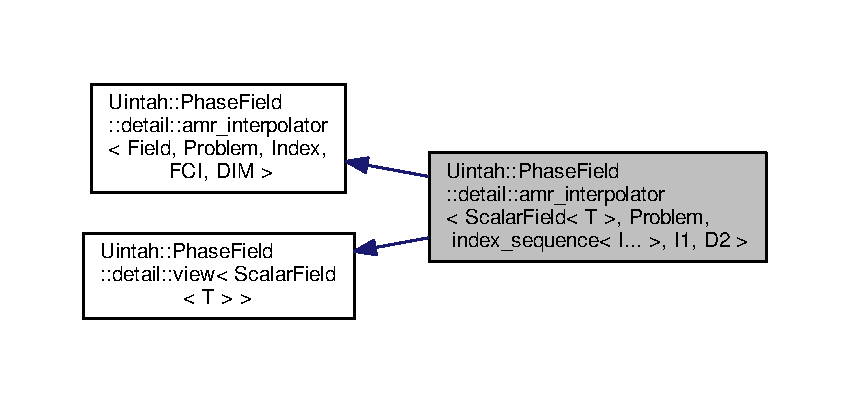
\includegraphics[width=350pt]{classUintah_1_1PhaseField_1_1detail_1_1amr__interpolator_3_01ScalarField_3_01T_01_4_00_01Problem6a5a099c3b36d5203324e5b7f8662e42}
\end{center}
\end{figure}


Collaboration diagram for Uintah\+:\+:Phase\+Field\+:\+:detail\+:\+:amr\+\_\+interpolator$<$ Scalar\+Field$<$ T $>$, Problem, index\+\_\+sequence$<$ I... $>$, I1, D2 $>$\+:\nopagebreak
\begin{figure}[H]
\begin{center}
\leavevmode
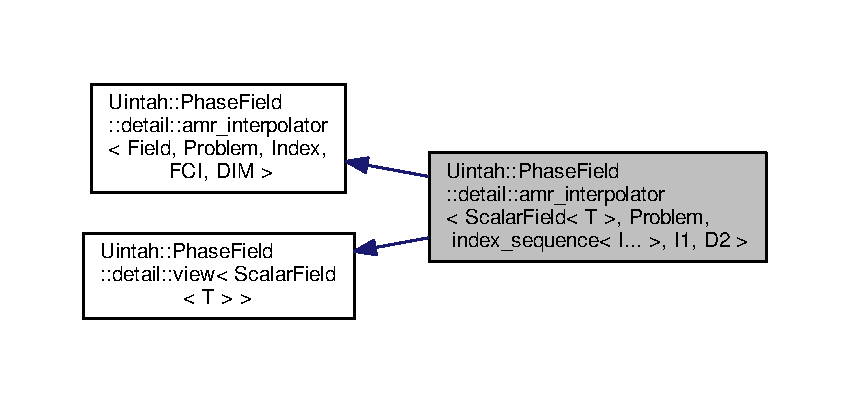
\includegraphics[width=350pt]{classUintah_1_1PhaseField_1_1detail_1_1amr__interpolator_3_01ScalarField_3_01T_01_4_00_01Problemcb8cbfe24988b8a6e1f5e685c48d5546}
\end{center}
\end{figure}
\subsection*{Public Member Functions}
\begin{DoxyCompactItemize}
\item 
\hyperlink{classUintah_1_1PhaseField_1_1detail_1_1amr__interpolator_3_01ScalarField_3_01T_01_4_00_01Problemd2db9de1754b5450c93c191a9275f5ed_ad916da29eec73351ea6fb0fd54d24a86}{amr\+\_\+interpolator} (const Var\+Label $\ast$label, const Var\+Label $\ast$subproblems\+\_\+label, int material)
\begin{DoxyCompactList}\small\item\em construct interpolator without retrieving inner variable data from the Data\+Warehouse \end{DoxyCompactList}\item 
\hyperlink{classUintah_1_1PhaseField_1_1detail_1_1amr__interpolator_3_01ScalarField_3_01T_01_4_00_01Problemd2db9de1754b5450c93c191a9275f5ed_a09018bc2f75f6f87bb893dd7caf831aa}{amr\+\_\+interpolator} (Data\+Warehouse $\ast$dw, const Var\+Label $\ast$label, const Var\+Label $\ast$subproblems\+\_\+label, int material, const Patch $\ast$patch, bool use\+\_\+ghosts=\hyperlink{classUintah_1_1PhaseField_1_1detail_1_1amr__interpolator_3_01ScalarField_3_01T_01_4_00_01Problemd2db9de1754b5450c93c191a9275f5ed_a05a1e360547dde624240ae943f6ced4b}{use\+\_\+ghosts\+\_\+dflt})
\begin{DoxyCompactList}\small\item\em construct interpolator and retrieve inner variable data from the Data\+Warehouse whithin a given fine patch. \end{DoxyCompactList}\item 
virtual \hyperlink{classUintah_1_1PhaseField_1_1detail_1_1amr__interpolator_3_01ScalarField_3_01T_01_4_00_01Problemd2db9de1754b5450c93c191a9275f5ed_a9d452934993c1a509d4da611ae087494}{$\sim$amr\+\_\+interpolator} ()
\begin{DoxyCompactList}\small\item\em Destructor. \end{DoxyCompactList}\item 
\hyperlink{classUintah_1_1PhaseField_1_1detail_1_1amr__interpolator_3_01ScalarField_3_01T_01_4_00_01Problemd2db9de1754b5450c93c191a9275f5ed_a6eb4d51ce7b438faf75dceeb700627c0}{amr\+\_\+interpolator} (const \hyperlink{classUintah_1_1PhaseField_1_1detail_1_1amr__interpolator}{amr\+\_\+interpolator} \&)=delete
\begin{DoxyCompactList}\small\item\em Prevent copy (and move) constructor. \end{DoxyCompactList}\item 
\hyperlink{classUintah_1_1PhaseField_1_1detail_1_1amr__interpolator}{amr\+\_\+interpolator} \& \hyperlink{classUintah_1_1PhaseField_1_1detail_1_1amr__interpolator_3_01ScalarField_3_01T_01_4_00_01Problemd2db9de1754b5450c93c191a9275f5ed_aa081fd4fb3b2875c48d15712f3dc1a5c}{operator=} (const \hyperlink{classUintah_1_1PhaseField_1_1detail_1_1amr__interpolator}{amr\+\_\+interpolator} \&)=delete
\begin{DoxyCompactList}\small\item\em Prevent copy (and move) assignment. \end{DoxyCompactList}\item 
virtual void \hyperlink{classUintah_1_1PhaseField_1_1detail_1_1amr__interpolator_3_01ScalarField_3_01T_01_4_00_01Problemd2db9de1754b5450c93c191a9275f5ed_a2dfec8ca1eebdd59bda5dec83403d674}{set} (Data\+Warehouse $\ast$dw, const Patch $\ast$patch, bool use\+\_\+ghosts=\hyperlink{classUintah_1_1PhaseField_1_1detail_1_1amr__interpolator_3_01ScalarField_3_01T_01_4_00_01Problemd2db9de1754b5450c93c191a9275f5ed_a05a1e360547dde624240ae943f6ced4b}{use\+\_\+ghosts\+\_\+dflt}) override
\begin{DoxyCompactList}\small\item\em retrieve inner variable data from the Data\+Warehouse whithin a given patch. \end{DoxyCompactList}\item 
virtual void \hyperlink{classUintah_1_1PhaseField_1_1detail_1_1amr__interpolator_3_01ScalarField_3_01T_01_4_00_01Problemd2db9de1754b5450c93c191a9275f5ed_a014b41daf40384377d58ba9ada6a42ba}{set} (Data\+Warehouse $\ast$dw, const Level $\ast$level, const Int\+Vector \&low, const Int\+Vector \&high, bool use\+\_\+ghosts=\hyperlink{classUintah_1_1PhaseField_1_1detail_1_1amr__interpolator_3_01ScalarField_3_01T_01_4_00_01Problemd2db9de1754b5450c93c191a9275f5ed_a05a1e360547dde624240ae943f6ced4b}{use\+\_\+ghosts\+\_\+dflt}) override
\begin{DoxyCompactList}\small\item\em retrieve inner variable data from the Data\+Warehouse whithin a given region. \end{DoxyCompactList}\item 
virtual \hyperlink{classUintah_1_1PhaseField_1_1detail_1_1view}{view}$<$ \hyperlink{structUintah_1_1PhaseField_1_1ScalarField}{Field} $>$ $\ast$ \hyperlink{classUintah_1_1PhaseField_1_1detail_1_1amr__interpolator_3_01ScalarField_3_01T_01_4_00_01Problemd2db9de1754b5450c93c191a9275f5ed_a81fe3ebe5215f1879c8fcacad90a240e}{clone} (bool deep) const override
\begin{DoxyCompactList}\small\item\em Get a copy of the view. \end{DoxyCompactList}\item 
virtual \hyperlink{classUintah_1_1PhaseField_1_1detail_1_1view}{view}$<$ \hyperlink{structUintah_1_1PhaseField_1_1ScalarField}{Field} $>$ $\ast$ \hyperlink{classUintah_1_1PhaseField_1_1detail_1_1amr__interpolator_3_01ScalarField_3_01T_01_4_00_01Problemd2db9de1754b5450c93c191a9275f5ed_a62362155afcaf1db632655a3a8ab23f4}{clone} (bool deep, const Int\+Vector \&offset) const override
\begin{DoxyCompactList}\small\item\em Get a copy of the view and apply translate the support. \end{DoxyCompactList}\item 
virtual \hyperlink{classUintah_1_1PhaseField_1_1Support}{Support} \hyperlink{classUintah_1_1PhaseField_1_1detail_1_1amr__interpolator_3_01ScalarField_3_01T_01_4_00_01Problemd2db9de1754b5450c93c191a9275f5ed_a62fab5a21bbdb676abc26812e2935b43}{get\+\_\+support} () const override
\begin{DoxyCompactList}\small\item\em get interpolator\textquotesingle{}s fine range \end{DoxyCompactList}\item 
virtual bool \hyperlink{classUintah_1_1PhaseField_1_1detail_1_1amr__interpolator_3_01ScalarField_3_01T_01_4_00_01Problemd2db9de1754b5450c93c191a9275f5ed_af8195600d1dd48eb942fb86df76e3127}{is\+\_\+defined\+\_\+at} (const Int\+Vector \&id) const override
\begin{DoxyCompactList}\small\item\em Check if the view has access to the fine position with index id. \end{DoxyCompactList}\item 
virtual T \& \hyperlink{classUintah_1_1PhaseField_1_1detail_1_1amr__interpolator_3_01ScalarField_3_01T_01_4_00_01Problemd2db9de1754b5450c93c191a9275f5ed_a1b98af006f3ad7a60aa33f7c4dc02ea2}{operator\mbox{[}$\,$\mbox{]}} (const Int\+Vector \&id) override \hyperlink{Definitions_8h_a3ce9c14452594b5b9ee3b63f9b3a981e}{V\+I\+RT}
\begin{DoxyCompactList}\small\item\em Get/\+Modify value at position with index id (virtual implementation) \end{DoxyCompactList}\item 
virtual V \hyperlink{classUintah_1_1PhaseField_1_1detail_1_1amr__interpolator_3_01ScalarField_3_01T_01_4_00_01Problemd2db9de1754b5450c93c191a9275f5ed_a92258242d6be3d033373def65b687a94}{operator\mbox{[}$\,$\mbox{]}} (const Int\+Vector \&id\+\_\+fine) const override
\begin{DoxyCompactList}\small\item\em get interpolated value \end{DoxyCompactList}\end{DoxyCompactItemize}
\subsection*{Static Public Attributes}
\begin{DoxyCompactItemize}
\item 
static constexpr bool \hyperlink{classUintah_1_1PhaseField_1_1detail_1_1amr__interpolator_3_01ScalarField_3_01T_01_4_00_01Problemd2db9de1754b5450c93c191a9275f5ed_a05a1e360547dde624240ae943f6ced4b}{use\+\_\+ghosts\+\_\+dflt} = false
\begin{DoxyCompactList}\small\item\em Default value for use\+\_\+ghost when retrieving data. \end{DoxyCompactList}\end{DoxyCompactItemize}
\subsection*{Protected Member Functions}
\begin{DoxyCompactItemize}
\item 
\hyperlink{classUintah_1_1PhaseField_1_1detail_1_1amr__interpolator_3_01ScalarField_3_01T_01_4_00_01Problemd2db9de1754b5450c93c191a9275f5ed_a5f8bf03fb74a723290420d7aaabe31d2}{amr\+\_\+interpolator} (const \hyperlink{classUintah_1_1PhaseField_1_1detail_1_1amr__interpolator}{amr\+\_\+interpolator} $\ast$copy, bool deep)
\begin{DoxyCompactList}\small\item\em Constructor. \end{DoxyCompactList}\end{DoxyCompactItemize}
\subsection*{Additional Inherited Members}


\subsection{Detailed Description}
\subsubsection*{template$<$typename T, typename Problem, size\+\_\+t... I$>$\newline
class Uintah\+::\+Phase\+Field\+::detail\+::amr\+\_\+interpolator$<$ Scalar\+Field$<$ T $>$, Problem, index\+\_\+sequence$<$ I... $>$, I1, D2 $>$}

Implements linear interpolation of a variable from coarser to finer levels in 2D. 

\begin{DoxyRefDesc}{Todo}
\item[\hyperlink{todo__todo000002}{Todo}]generalize implementation over D\+IM\end{DoxyRefDesc}



\begin{DoxyTemplParams}{Template Parameters}
{\em T} & variable data type (must be constant) \\
\hline
{\em \hyperlink{classUintah_1_1PhaseField_1_1Problem}{Problem}} & type of \hyperlink{namespaceUintah_1_1PhaseField}{Phase\+Field} problem \\
\hline
{\em \hyperlink{structUintah_1_1PhaseField_1_1I}{I}} & list of indices corresponding to the variable within the subproblems\\
\hline
\end{DoxyTemplParams}
\begin{DoxyRefDesc}{Todo}
\item[\hyperlink{todo__todo000003}{Todo}]generalize implementation to arbitrary dimension\end{DoxyRefDesc}


$<$ Field, \hyperlink{classUintah_1_1PhaseField_1_1Problem}{Problem}, Index, F\+CI, D\+IM $>$ 

\subsection{Constructor \& Destructor Documentation}
\mbox{\Hypertarget{classUintah_1_1PhaseField_1_1detail_1_1amr__interpolator_3_01ScalarField_3_01T_01_4_00_01Problemd2db9de1754b5450c93c191a9275f5ed_a5f8bf03fb74a723290420d7aaabe31d2}\label{classUintah_1_1PhaseField_1_1detail_1_1amr__interpolator_3_01ScalarField_3_01T_01_4_00_01Problemd2db9de1754b5450c93c191a9275f5ed_a5f8bf03fb74a723290420d7aaabe31d2}} 
\index{Uintah\+::\+Phase\+Field\+::detail\+::amr\+\_\+interpolator$<$ Scalar\+Field$<$ T $>$, Problem, index\+\_\+sequence$<$ I... $>$, I1, D2 $>$@{Uintah\+::\+Phase\+Field\+::detail\+::amr\+\_\+interpolator$<$ Scalar\+Field$<$ T $>$, Problem, index\+\_\+sequence$<$ I... $>$, I1, D2 $>$}!amr\+\_\+interpolator@{amr\+\_\+interpolator}}
\index{amr\+\_\+interpolator@{amr\+\_\+interpolator}!Uintah\+::\+Phase\+Field\+::detail\+::amr\+\_\+interpolator$<$ Scalar\+Field$<$ T $>$, Problem, index\+\_\+sequence$<$ I... $>$, I1, D2 $>$@{Uintah\+::\+Phase\+Field\+::detail\+::amr\+\_\+interpolator$<$ Scalar\+Field$<$ T $>$, Problem, index\+\_\+sequence$<$ I... $>$, I1, D2 $>$}}
\subsubsection{\texorpdfstring{amr\+\_\+interpolator()}{amr\_interpolator()}\hspace{0.1cm}{\footnotesize\ttfamily [1/4]}}
{\footnotesize\ttfamily template$<$typename T , typename Problem , size\+\_\+t... I$>$ \\
\hyperlink{classUintah_1_1PhaseField_1_1detail_1_1amr__interpolator}{Uintah\+::\+Phase\+Field\+::detail\+::amr\+\_\+interpolator}$<$ \hyperlink{structUintah_1_1PhaseField_1_1ScalarField}{Scalar\+Field}$<$ T $>$, \hyperlink{classUintah_1_1PhaseField_1_1Problem}{Problem}, \hyperlink{namespaceUintah_1_1PhaseField_a237de804d99512e50613aff7c94a9461}{index\+\_\+sequence}$<$ I... $>$, \hyperlink{namespaceUintah_1_1PhaseField_a547ce3002aa97fbd3ef3192a6eec8406a66f19efe774b0d2b6e5844eb2d83d305}{I1}, \hyperlink{namespaceUintah_1_1PhaseField_a12bfc68444894dffdf0cb8d9cf0cc76aa1a451dae278b0103a94105c8776e9a67}{D2} $>$\+::\hyperlink{classUintah_1_1PhaseField_1_1detail_1_1amr__interpolator}{amr\+\_\+interpolator} (\begin{DoxyParamCaption}\item[{const \hyperlink{classUintah_1_1PhaseField_1_1detail_1_1amr__interpolator}{amr\+\_\+interpolator}$<$ \hyperlink{structUintah_1_1PhaseField_1_1ScalarField}{Scalar\+Field}$<$ T $>$, \hyperlink{classUintah_1_1PhaseField_1_1Problem}{Problem}, \hyperlink{namespaceUintah_1_1PhaseField_a237de804d99512e50613aff7c94a9461}{index\+\_\+sequence}$<$ I... $>$, \hyperlink{namespaceUintah_1_1PhaseField_a547ce3002aa97fbd3ef3192a6eec8406a66f19efe774b0d2b6e5844eb2d83d305}{I1}, \hyperlink{namespaceUintah_1_1PhaseField_a12bfc68444894dffdf0cb8d9cf0cc76aa1a451dae278b0103a94105c8776e9a67}{D2} $>$ $\ast$}]{copy,  }\item[{bool}]{deep }\end{DoxyParamCaption})\hspace{0.3cm}{\ttfamily [inline]}, {\ttfamily [protected]}}



Constructor. 

Instantiate a copy of a given view


\begin{DoxyParams}{Parameters}
{\em copy} & source view for copying \\
\hline
{\em deep} & if true inner grid variable is copied as well otherwise the same grid variable is referenced \\
\hline
\end{DoxyParams}
\mbox{\Hypertarget{classUintah_1_1PhaseField_1_1detail_1_1amr__interpolator_3_01ScalarField_3_01T_01_4_00_01Problemd2db9de1754b5450c93c191a9275f5ed_ad916da29eec73351ea6fb0fd54d24a86}\label{classUintah_1_1PhaseField_1_1detail_1_1amr__interpolator_3_01ScalarField_3_01T_01_4_00_01Problemd2db9de1754b5450c93c191a9275f5ed_ad916da29eec73351ea6fb0fd54d24a86}} 
\index{Uintah\+::\+Phase\+Field\+::detail\+::amr\+\_\+interpolator$<$ Scalar\+Field$<$ T $>$, Problem, index\+\_\+sequence$<$ I... $>$, I1, D2 $>$@{Uintah\+::\+Phase\+Field\+::detail\+::amr\+\_\+interpolator$<$ Scalar\+Field$<$ T $>$, Problem, index\+\_\+sequence$<$ I... $>$, I1, D2 $>$}!amr\+\_\+interpolator@{amr\+\_\+interpolator}}
\index{amr\+\_\+interpolator@{amr\+\_\+interpolator}!Uintah\+::\+Phase\+Field\+::detail\+::amr\+\_\+interpolator$<$ Scalar\+Field$<$ T $>$, Problem, index\+\_\+sequence$<$ I... $>$, I1, D2 $>$@{Uintah\+::\+Phase\+Field\+::detail\+::amr\+\_\+interpolator$<$ Scalar\+Field$<$ T $>$, Problem, index\+\_\+sequence$<$ I... $>$, I1, D2 $>$}}
\subsubsection{\texorpdfstring{amr\+\_\+interpolator()}{amr\_interpolator()}\hspace{0.1cm}{\footnotesize\ttfamily [2/4]}}
{\footnotesize\ttfamily template$<$typename T , typename Problem , size\+\_\+t... I$>$ \\
\hyperlink{classUintah_1_1PhaseField_1_1detail_1_1amr__interpolator}{Uintah\+::\+Phase\+Field\+::detail\+::amr\+\_\+interpolator}$<$ \hyperlink{structUintah_1_1PhaseField_1_1ScalarField}{Scalar\+Field}$<$ T $>$, \hyperlink{classUintah_1_1PhaseField_1_1Problem}{Problem}, \hyperlink{namespaceUintah_1_1PhaseField_a237de804d99512e50613aff7c94a9461}{index\+\_\+sequence}$<$ I... $>$, \hyperlink{namespaceUintah_1_1PhaseField_a547ce3002aa97fbd3ef3192a6eec8406a66f19efe774b0d2b6e5844eb2d83d305}{I1}, \hyperlink{namespaceUintah_1_1PhaseField_a12bfc68444894dffdf0cb8d9cf0cc76aa1a451dae278b0103a94105c8776e9a67}{D2} $>$\+::\hyperlink{classUintah_1_1PhaseField_1_1detail_1_1amr__interpolator}{amr\+\_\+interpolator} (\begin{DoxyParamCaption}\item[{const Var\+Label $\ast$}]{label,  }\item[{const Var\+Label $\ast$}]{subproblems\+\_\+label,  }\item[{int}]{material }\end{DoxyParamCaption})\hspace{0.3cm}{\ttfamily [inline]}}



construct interpolator without retrieving inner variable data from the Data\+Warehouse 


\begin{DoxyParams}{Parameters}
{\em label} & label of variable in the Data\+Warehouse \\
\hline
{\em subproblems\+\_\+label} & label of subproblems in the Data\+Warehouse \\
\hline
{\em material} & index of material in the Data\+Warehouse \\
\hline
\end{DoxyParams}
\mbox{\Hypertarget{classUintah_1_1PhaseField_1_1detail_1_1amr__interpolator_3_01ScalarField_3_01T_01_4_00_01Problemd2db9de1754b5450c93c191a9275f5ed_a09018bc2f75f6f87bb893dd7caf831aa}\label{classUintah_1_1PhaseField_1_1detail_1_1amr__interpolator_3_01ScalarField_3_01T_01_4_00_01Problemd2db9de1754b5450c93c191a9275f5ed_a09018bc2f75f6f87bb893dd7caf831aa}} 
\index{Uintah\+::\+Phase\+Field\+::detail\+::amr\+\_\+interpolator$<$ Scalar\+Field$<$ T $>$, Problem, index\+\_\+sequence$<$ I... $>$, I1, D2 $>$@{Uintah\+::\+Phase\+Field\+::detail\+::amr\+\_\+interpolator$<$ Scalar\+Field$<$ T $>$, Problem, index\+\_\+sequence$<$ I... $>$, I1, D2 $>$}!amr\+\_\+interpolator@{amr\+\_\+interpolator}}
\index{amr\+\_\+interpolator@{amr\+\_\+interpolator}!Uintah\+::\+Phase\+Field\+::detail\+::amr\+\_\+interpolator$<$ Scalar\+Field$<$ T $>$, Problem, index\+\_\+sequence$<$ I... $>$, I1, D2 $>$@{Uintah\+::\+Phase\+Field\+::detail\+::amr\+\_\+interpolator$<$ Scalar\+Field$<$ T $>$, Problem, index\+\_\+sequence$<$ I... $>$, I1, D2 $>$}}
\subsubsection{\texorpdfstring{amr\+\_\+interpolator()}{amr\_interpolator()}\hspace{0.1cm}{\footnotesize\ttfamily [3/4]}}
{\footnotesize\ttfamily template$<$typename T , typename Problem , size\+\_\+t... I$>$ \\
\hyperlink{classUintah_1_1PhaseField_1_1detail_1_1amr__interpolator}{Uintah\+::\+Phase\+Field\+::detail\+::amr\+\_\+interpolator}$<$ \hyperlink{structUintah_1_1PhaseField_1_1ScalarField}{Scalar\+Field}$<$ T $>$, \hyperlink{classUintah_1_1PhaseField_1_1Problem}{Problem}, \hyperlink{namespaceUintah_1_1PhaseField_a237de804d99512e50613aff7c94a9461}{index\+\_\+sequence}$<$ I... $>$, \hyperlink{namespaceUintah_1_1PhaseField_a547ce3002aa97fbd3ef3192a6eec8406a66f19efe774b0d2b6e5844eb2d83d305}{I1}, \hyperlink{namespaceUintah_1_1PhaseField_a12bfc68444894dffdf0cb8d9cf0cc76aa1a451dae278b0103a94105c8776e9a67}{D2} $>$\+::\hyperlink{classUintah_1_1PhaseField_1_1detail_1_1amr__interpolator}{amr\+\_\+interpolator} (\begin{DoxyParamCaption}\item[{Data\+Warehouse $\ast$}]{dw,  }\item[{const Var\+Label $\ast$}]{label,  }\item[{const Var\+Label $\ast$}]{subproblems\+\_\+label,  }\item[{int}]{material,  }\item[{const Patch $\ast$}]{patch,  }\item[{bool}]{use\+\_\+ghosts = {\ttfamily \hyperlink{classUintah_1_1PhaseField_1_1detail_1_1amr__interpolator_3_01ScalarField_3_01T_01_4_00_01Problemd2db9de1754b5450c93c191a9275f5ed_a05a1e360547dde624240ae943f6ced4b}{use\+\_\+ghosts\+\_\+dflt}} }\end{DoxyParamCaption})\hspace{0.3cm}{\ttfamily [inline]}}



construct interpolator and retrieve inner variable data from the Data\+Warehouse whithin a given fine patch. 

the number of ghost cells/nodes and the corresponding region on the coarser level is automatically computed to match the interpolation type


\begin{DoxyParams}{Parameters}
{\em dw} & Data\+Warehouse which data is retrieved from \\
\hline
{\em label} & label of variable in the Data\+Warehouse \\
\hline
{\em subproblems\+\_\+label} & label of subproblems in the Data\+Warehouse \\
\hline
{\em material} & index of material in the Data\+Warehouse \\
\hline
{\em patch} & patch on which data is retrieved \\
\hline
{\em use\+\_\+ghosts} & if ghosts value are to be retrieved (must be false) \\
\hline
\end{DoxyParams}
\mbox{\Hypertarget{classUintah_1_1PhaseField_1_1detail_1_1amr__interpolator_3_01ScalarField_3_01T_01_4_00_01Problemd2db9de1754b5450c93c191a9275f5ed_a9d452934993c1a509d4da611ae087494}\label{classUintah_1_1PhaseField_1_1detail_1_1amr__interpolator_3_01ScalarField_3_01T_01_4_00_01Problemd2db9de1754b5450c93c191a9275f5ed_a9d452934993c1a509d4da611ae087494}} 
\index{Uintah\+::\+Phase\+Field\+::detail\+::amr\+\_\+interpolator$<$ Scalar\+Field$<$ T $>$, Problem, index\+\_\+sequence$<$ I... $>$, I1, D2 $>$@{Uintah\+::\+Phase\+Field\+::detail\+::amr\+\_\+interpolator$<$ Scalar\+Field$<$ T $>$, Problem, index\+\_\+sequence$<$ I... $>$, I1, D2 $>$}!````~amr\+\_\+interpolator@{$\sim$amr\+\_\+interpolator}}
\index{````~amr\+\_\+interpolator@{$\sim$amr\+\_\+interpolator}!Uintah\+::\+Phase\+Field\+::detail\+::amr\+\_\+interpolator$<$ Scalar\+Field$<$ T $>$, Problem, index\+\_\+sequence$<$ I... $>$, I1, D2 $>$@{Uintah\+::\+Phase\+Field\+::detail\+::amr\+\_\+interpolator$<$ Scalar\+Field$<$ T $>$, Problem, index\+\_\+sequence$<$ I... $>$, I1, D2 $>$}}
\subsubsection{\texorpdfstring{$\sim$amr\+\_\+interpolator()}{~amr\_interpolator()}}
{\footnotesize\ttfamily template$<$typename T , typename Problem , size\+\_\+t... I$>$ \\
virtual \hyperlink{classUintah_1_1PhaseField_1_1detail_1_1amr__interpolator}{Uintah\+::\+Phase\+Field\+::detail\+::amr\+\_\+interpolator}$<$ \hyperlink{structUintah_1_1PhaseField_1_1ScalarField}{Scalar\+Field}$<$ T $>$, \hyperlink{classUintah_1_1PhaseField_1_1Problem}{Problem}, \hyperlink{namespaceUintah_1_1PhaseField_a237de804d99512e50613aff7c94a9461}{index\+\_\+sequence}$<$ I... $>$, \hyperlink{namespaceUintah_1_1PhaseField_a547ce3002aa97fbd3ef3192a6eec8406a66f19efe774b0d2b6e5844eb2d83d305}{I1}, \hyperlink{namespaceUintah_1_1PhaseField_a12bfc68444894dffdf0cb8d9cf0cc76aa1a451dae278b0103a94105c8776e9a67}{D2} $>$\+::$\sim$\hyperlink{classUintah_1_1PhaseField_1_1detail_1_1amr__interpolator}{amr\+\_\+interpolator} (\begin{DoxyParamCaption}{ }\end{DoxyParamCaption})\hspace{0.3cm}{\ttfamily [inline]}, {\ttfamily [virtual]}}



Destructor. 

\mbox{\Hypertarget{classUintah_1_1PhaseField_1_1detail_1_1amr__interpolator_3_01ScalarField_3_01T_01_4_00_01Problemd2db9de1754b5450c93c191a9275f5ed_a6eb4d51ce7b438faf75dceeb700627c0}\label{classUintah_1_1PhaseField_1_1detail_1_1amr__interpolator_3_01ScalarField_3_01T_01_4_00_01Problemd2db9de1754b5450c93c191a9275f5ed_a6eb4d51ce7b438faf75dceeb700627c0}} 
\index{Uintah\+::\+Phase\+Field\+::detail\+::amr\+\_\+interpolator$<$ Scalar\+Field$<$ T $>$, Problem, index\+\_\+sequence$<$ I... $>$, I1, D2 $>$@{Uintah\+::\+Phase\+Field\+::detail\+::amr\+\_\+interpolator$<$ Scalar\+Field$<$ T $>$, Problem, index\+\_\+sequence$<$ I... $>$, I1, D2 $>$}!amr\+\_\+interpolator@{amr\+\_\+interpolator}}
\index{amr\+\_\+interpolator@{amr\+\_\+interpolator}!Uintah\+::\+Phase\+Field\+::detail\+::amr\+\_\+interpolator$<$ Scalar\+Field$<$ T $>$, Problem, index\+\_\+sequence$<$ I... $>$, I1, D2 $>$@{Uintah\+::\+Phase\+Field\+::detail\+::amr\+\_\+interpolator$<$ Scalar\+Field$<$ T $>$, Problem, index\+\_\+sequence$<$ I... $>$, I1, D2 $>$}}
\subsubsection{\texorpdfstring{amr\+\_\+interpolator()}{amr\_interpolator()}\hspace{0.1cm}{\footnotesize\ttfamily [4/4]}}
{\footnotesize\ttfamily template$<$typename T , typename Problem , size\+\_\+t... I$>$ \\
\hyperlink{classUintah_1_1PhaseField_1_1detail_1_1amr__interpolator}{Uintah\+::\+Phase\+Field\+::detail\+::amr\+\_\+interpolator}$<$ \hyperlink{structUintah_1_1PhaseField_1_1ScalarField}{Scalar\+Field}$<$ T $>$, \hyperlink{classUintah_1_1PhaseField_1_1Problem}{Problem}, \hyperlink{namespaceUintah_1_1PhaseField_a237de804d99512e50613aff7c94a9461}{index\+\_\+sequence}$<$ I... $>$, \hyperlink{namespaceUintah_1_1PhaseField_a547ce3002aa97fbd3ef3192a6eec8406a66f19efe774b0d2b6e5844eb2d83d305}{I1}, \hyperlink{namespaceUintah_1_1PhaseField_a12bfc68444894dffdf0cb8d9cf0cc76aa1a451dae278b0103a94105c8776e9a67}{D2} $>$\+::\hyperlink{classUintah_1_1PhaseField_1_1detail_1_1amr__interpolator}{amr\+\_\+interpolator} (\begin{DoxyParamCaption}\item[{const \hyperlink{classUintah_1_1PhaseField_1_1detail_1_1amr__interpolator}{amr\+\_\+interpolator}$<$ \hyperlink{structUintah_1_1PhaseField_1_1ScalarField}{Scalar\+Field}$<$ T $>$, \hyperlink{classUintah_1_1PhaseField_1_1Problem}{Problem}, \hyperlink{namespaceUintah_1_1PhaseField_a237de804d99512e50613aff7c94a9461}{index\+\_\+sequence}$<$ I... $>$, \hyperlink{namespaceUintah_1_1PhaseField_a547ce3002aa97fbd3ef3192a6eec8406a66f19efe774b0d2b6e5844eb2d83d305}{I1}, \hyperlink{namespaceUintah_1_1PhaseField_a12bfc68444894dffdf0cb8d9cf0cc76aa1a451dae278b0103a94105c8776e9a67}{D2} $>$ \&}]{ }\end{DoxyParamCaption})\hspace{0.3cm}{\ttfamily [delete]}}



Prevent copy (and move) constructor. 



\subsection{Member Function Documentation}
\mbox{\Hypertarget{classUintah_1_1PhaseField_1_1detail_1_1amr__interpolator_3_01ScalarField_3_01T_01_4_00_01Problemd2db9de1754b5450c93c191a9275f5ed_a81fe3ebe5215f1879c8fcacad90a240e}\label{classUintah_1_1PhaseField_1_1detail_1_1amr__interpolator_3_01ScalarField_3_01T_01_4_00_01Problemd2db9de1754b5450c93c191a9275f5ed_a81fe3ebe5215f1879c8fcacad90a240e}} 
\index{Uintah\+::\+Phase\+Field\+::detail\+::amr\+\_\+interpolator$<$ Scalar\+Field$<$ T $>$, Problem, index\+\_\+sequence$<$ I... $>$, I1, D2 $>$@{Uintah\+::\+Phase\+Field\+::detail\+::amr\+\_\+interpolator$<$ Scalar\+Field$<$ T $>$, Problem, index\+\_\+sequence$<$ I... $>$, I1, D2 $>$}!clone@{clone}}
\index{clone@{clone}!Uintah\+::\+Phase\+Field\+::detail\+::amr\+\_\+interpolator$<$ Scalar\+Field$<$ T $>$, Problem, index\+\_\+sequence$<$ I... $>$, I1, D2 $>$@{Uintah\+::\+Phase\+Field\+::detail\+::amr\+\_\+interpolator$<$ Scalar\+Field$<$ T $>$, Problem, index\+\_\+sequence$<$ I... $>$, I1, D2 $>$}}
\subsubsection{\texorpdfstring{clone()}{clone()}\hspace{0.1cm}{\footnotesize\ttfamily [1/2]}}
{\footnotesize\ttfamily template$<$typename T , typename Problem , size\+\_\+t... I$>$ \\
virtual \hyperlink{classUintah_1_1PhaseField_1_1detail_1_1view}{view}$<$\hyperlink{structUintah_1_1PhaseField_1_1ScalarField}{Field}$>$$\ast$ \hyperlink{classUintah_1_1PhaseField_1_1detail_1_1amr__interpolator}{Uintah\+::\+Phase\+Field\+::detail\+::amr\+\_\+interpolator}$<$ \hyperlink{structUintah_1_1PhaseField_1_1ScalarField}{Scalar\+Field}$<$ T $>$, \hyperlink{classUintah_1_1PhaseField_1_1Problem}{Problem}, \hyperlink{namespaceUintah_1_1PhaseField_a237de804d99512e50613aff7c94a9461}{index\+\_\+sequence}$<$ I... $>$, \hyperlink{namespaceUintah_1_1PhaseField_a547ce3002aa97fbd3ef3192a6eec8406a66f19efe774b0d2b6e5844eb2d83d305}{I1}, \hyperlink{namespaceUintah_1_1PhaseField_a12bfc68444894dffdf0cb8d9cf0cc76aa1a451dae278b0103a94105c8776e9a67}{D2} $>$\+::clone (\begin{DoxyParamCaption}\item[{bool}]{deep }\end{DoxyParamCaption}) const\hspace{0.3cm}{\ttfamily [inline]}, {\ttfamily [override]}, {\ttfamily [virtual]}}



Get a copy of the view. 


\begin{DoxyParams}{Parameters}
{\em deep} & if true inner grid variable is copied as well otherwise the same grid variable is referenced\\
\hline
\end{DoxyParams}
\begin{DoxyReturn}{Returns}
new view instance 
\end{DoxyReturn}


Implements \hyperlink{classUintah_1_1PhaseField_1_1detail_1_1view_3_01ScalarField_3_01T_01_4_01_4_a6e11243c9d776a7b703e524ea4151a16}{Uintah\+::\+Phase\+Field\+::detail\+::view$<$ Scalar\+Field$<$ T $>$ $>$}.

\mbox{\Hypertarget{classUintah_1_1PhaseField_1_1detail_1_1amr__interpolator_3_01ScalarField_3_01T_01_4_00_01Problemd2db9de1754b5450c93c191a9275f5ed_a62362155afcaf1db632655a3a8ab23f4}\label{classUintah_1_1PhaseField_1_1detail_1_1amr__interpolator_3_01ScalarField_3_01T_01_4_00_01Problemd2db9de1754b5450c93c191a9275f5ed_a62362155afcaf1db632655a3a8ab23f4}} 
\index{Uintah\+::\+Phase\+Field\+::detail\+::amr\+\_\+interpolator$<$ Scalar\+Field$<$ T $>$, Problem, index\+\_\+sequence$<$ I... $>$, I1, D2 $>$@{Uintah\+::\+Phase\+Field\+::detail\+::amr\+\_\+interpolator$<$ Scalar\+Field$<$ T $>$, Problem, index\+\_\+sequence$<$ I... $>$, I1, D2 $>$}!clone@{clone}}
\index{clone@{clone}!Uintah\+::\+Phase\+Field\+::detail\+::amr\+\_\+interpolator$<$ Scalar\+Field$<$ T $>$, Problem, index\+\_\+sequence$<$ I... $>$, I1, D2 $>$@{Uintah\+::\+Phase\+Field\+::detail\+::amr\+\_\+interpolator$<$ Scalar\+Field$<$ T $>$, Problem, index\+\_\+sequence$<$ I... $>$, I1, D2 $>$}}
\subsubsection{\texorpdfstring{clone()}{clone()}\hspace{0.1cm}{\footnotesize\ttfamily [2/2]}}
{\footnotesize\ttfamily template$<$typename T , typename Problem , size\+\_\+t... I$>$ \\
virtual \hyperlink{classUintah_1_1PhaseField_1_1detail_1_1view}{view}$<$\hyperlink{structUintah_1_1PhaseField_1_1ScalarField}{Field}$>$$\ast$ \hyperlink{classUintah_1_1PhaseField_1_1detail_1_1amr__interpolator}{Uintah\+::\+Phase\+Field\+::detail\+::amr\+\_\+interpolator}$<$ \hyperlink{structUintah_1_1PhaseField_1_1ScalarField}{Scalar\+Field}$<$ T $>$, \hyperlink{classUintah_1_1PhaseField_1_1Problem}{Problem}, \hyperlink{namespaceUintah_1_1PhaseField_a237de804d99512e50613aff7c94a9461}{index\+\_\+sequence}$<$ I... $>$, \hyperlink{namespaceUintah_1_1PhaseField_a547ce3002aa97fbd3ef3192a6eec8406a66f19efe774b0d2b6e5844eb2d83d305}{I1}, \hyperlink{namespaceUintah_1_1PhaseField_a12bfc68444894dffdf0cb8d9cf0cc76aa1a451dae278b0103a94105c8776e9a67}{D2} $>$\+::clone (\begin{DoxyParamCaption}\item[{bool}]{deep,  }\item[{const Int\+Vector \&}]{offset }\end{DoxyParamCaption}) const\hspace{0.3cm}{\ttfamily [inline]}, {\ttfamily [override]}, {\ttfamily [virtual]}}



Get a copy of the view and apply translate the support. 

\begin{DoxyRemark}{Remarks}
It is meant to be used for virtual patches (i.\+e. periodic boundaries)
\end{DoxyRemark}

\begin{DoxyParams}{Parameters}
{\em deep} & if true inner grid variable is copied as well otherwise the same grid variable is referenced \\
\hline
{\em offset} & vector specifying the translation of the support \\
\hline
\end{DoxyParams}
\begin{DoxyReturn}{Returns}
new view instance 
\end{DoxyReturn}


Implements \hyperlink{classUintah_1_1PhaseField_1_1detail_1_1view_3_01ScalarField_3_01T_01_4_01_4_abd928104240e329f3bc4441ebab7c50c}{Uintah\+::\+Phase\+Field\+::detail\+::view$<$ Scalar\+Field$<$ T $>$ $>$}.

\mbox{\Hypertarget{classUintah_1_1PhaseField_1_1detail_1_1amr__interpolator_3_01ScalarField_3_01T_01_4_00_01Problemd2db9de1754b5450c93c191a9275f5ed_a62fab5a21bbdb676abc26812e2935b43}\label{classUintah_1_1PhaseField_1_1detail_1_1amr__interpolator_3_01ScalarField_3_01T_01_4_00_01Problemd2db9de1754b5450c93c191a9275f5ed_a62fab5a21bbdb676abc26812e2935b43}} 
\index{Uintah\+::\+Phase\+Field\+::detail\+::amr\+\_\+interpolator$<$ Scalar\+Field$<$ T $>$, Problem, index\+\_\+sequence$<$ I... $>$, I1, D2 $>$@{Uintah\+::\+Phase\+Field\+::detail\+::amr\+\_\+interpolator$<$ Scalar\+Field$<$ T $>$, Problem, index\+\_\+sequence$<$ I... $>$, I1, D2 $>$}!get\+\_\+support@{get\+\_\+support}}
\index{get\+\_\+support@{get\+\_\+support}!Uintah\+::\+Phase\+Field\+::detail\+::amr\+\_\+interpolator$<$ Scalar\+Field$<$ T $>$, Problem, index\+\_\+sequence$<$ I... $>$, I1, D2 $>$@{Uintah\+::\+Phase\+Field\+::detail\+::amr\+\_\+interpolator$<$ Scalar\+Field$<$ T $>$, Problem, index\+\_\+sequence$<$ I... $>$, I1, D2 $>$}}
\subsubsection{\texorpdfstring{get\+\_\+support()}{get\_support()}}
{\footnotesize\ttfamily template$<$typename T , typename Problem , size\+\_\+t... I$>$ \\
virtual \hyperlink{classUintah_1_1PhaseField_1_1Support}{Support} \hyperlink{classUintah_1_1PhaseField_1_1detail_1_1amr__interpolator}{Uintah\+::\+Phase\+Field\+::detail\+::amr\+\_\+interpolator}$<$ \hyperlink{structUintah_1_1PhaseField_1_1ScalarField}{Scalar\+Field}$<$ T $>$, \hyperlink{classUintah_1_1PhaseField_1_1Problem}{Problem}, \hyperlink{namespaceUintah_1_1PhaseField_a237de804d99512e50613aff7c94a9461}{index\+\_\+sequence}$<$ I... $>$, \hyperlink{namespaceUintah_1_1PhaseField_a547ce3002aa97fbd3ef3192a6eec8406a66f19efe774b0d2b6e5844eb2d83d305}{I1}, \hyperlink{namespaceUintah_1_1PhaseField_a12bfc68444894dffdf0cb8d9cf0cc76aa1a451dae278b0103a94105c8776e9a67}{D2} $>$\+::get\+\_\+support (\begin{DoxyParamCaption}{ }\end{DoxyParamCaption}) const\hspace{0.3cm}{\ttfamily [inline]}, {\ttfamily [override]}, {\ttfamily [virtual]}}



get interpolator\textquotesingle{}s fine range 

\begin{DoxyReturn}{Returns}
fine range 
\end{DoxyReturn}


Implements \hyperlink{classUintah_1_1PhaseField_1_1detail_1_1view_3_01ScalarField_3_01T_01_4_01_4_a3e14b0c7a57a57707bb33954861ab1c1}{Uintah\+::\+Phase\+Field\+::detail\+::view$<$ Scalar\+Field$<$ T $>$ $>$}.

\mbox{\Hypertarget{classUintah_1_1PhaseField_1_1detail_1_1amr__interpolator_3_01ScalarField_3_01T_01_4_00_01Problemd2db9de1754b5450c93c191a9275f5ed_af8195600d1dd48eb942fb86df76e3127}\label{classUintah_1_1PhaseField_1_1detail_1_1amr__interpolator_3_01ScalarField_3_01T_01_4_00_01Problemd2db9de1754b5450c93c191a9275f5ed_af8195600d1dd48eb942fb86df76e3127}} 
\index{Uintah\+::\+Phase\+Field\+::detail\+::amr\+\_\+interpolator$<$ Scalar\+Field$<$ T $>$, Problem, index\+\_\+sequence$<$ I... $>$, I1, D2 $>$@{Uintah\+::\+Phase\+Field\+::detail\+::amr\+\_\+interpolator$<$ Scalar\+Field$<$ T $>$, Problem, index\+\_\+sequence$<$ I... $>$, I1, D2 $>$}!is\+\_\+defined\+\_\+at@{is\+\_\+defined\+\_\+at}}
\index{is\+\_\+defined\+\_\+at@{is\+\_\+defined\+\_\+at}!Uintah\+::\+Phase\+Field\+::detail\+::amr\+\_\+interpolator$<$ Scalar\+Field$<$ T $>$, Problem, index\+\_\+sequence$<$ I... $>$, I1, D2 $>$@{Uintah\+::\+Phase\+Field\+::detail\+::amr\+\_\+interpolator$<$ Scalar\+Field$<$ T $>$, Problem, index\+\_\+sequence$<$ I... $>$, I1, D2 $>$}}
\subsubsection{\texorpdfstring{is\+\_\+defined\+\_\+at()}{is\_defined\_at()}}
{\footnotesize\ttfamily template$<$typename T , typename Problem , size\+\_\+t... I$>$ \\
virtual bool \hyperlink{classUintah_1_1PhaseField_1_1detail_1_1amr__interpolator}{Uintah\+::\+Phase\+Field\+::detail\+::amr\+\_\+interpolator}$<$ \hyperlink{structUintah_1_1PhaseField_1_1ScalarField}{Scalar\+Field}$<$ T $>$, \hyperlink{classUintah_1_1PhaseField_1_1Problem}{Problem}, \hyperlink{namespaceUintah_1_1PhaseField_a237de804d99512e50613aff7c94a9461}{index\+\_\+sequence}$<$ I... $>$, \hyperlink{namespaceUintah_1_1PhaseField_a547ce3002aa97fbd3ef3192a6eec8406a66f19efe774b0d2b6e5844eb2d83d305}{I1}, \hyperlink{namespaceUintah_1_1PhaseField_a12bfc68444894dffdf0cb8d9cf0cc76aa1a451dae278b0103a94105c8776e9a67}{D2} $>$\+::is\+\_\+defined\+\_\+at (\begin{DoxyParamCaption}\item[{const Int\+Vector \&}]{id }\end{DoxyParamCaption}) const\hspace{0.3cm}{\ttfamily [inline]}, {\ttfamily [override]}, {\ttfamily [virtual]}}



Check if the view has access to the fine position with index id. 


\begin{DoxyParams}{Parameters}
{\em id} & fine position index \\
\hline
\end{DoxyParams}
\begin{DoxyReturn}{Returns}
check result 
\end{DoxyReturn}


Implements \hyperlink{classUintah_1_1PhaseField_1_1detail_1_1view_3_01ScalarField_3_01T_01_4_01_4_a9a950513dacd6468658436b737c3314f}{Uintah\+::\+Phase\+Field\+::detail\+::view$<$ Scalar\+Field$<$ T $>$ $>$}.

\mbox{\Hypertarget{classUintah_1_1PhaseField_1_1detail_1_1amr__interpolator_3_01ScalarField_3_01T_01_4_00_01Problemd2db9de1754b5450c93c191a9275f5ed_aa081fd4fb3b2875c48d15712f3dc1a5c}\label{classUintah_1_1PhaseField_1_1detail_1_1amr__interpolator_3_01ScalarField_3_01T_01_4_00_01Problemd2db9de1754b5450c93c191a9275f5ed_aa081fd4fb3b2875c48d15712f3dc1a5c}} 
\index{Uintah\+::\+Phase\+Field\+::detail\+::amr\+\_\+interpolator$<$ Scalar\+Field$<$ T $>$, Problem, index\+\_\+sequence$<$ I... $>$, I1, D2 $>$@{Uintah\+::\+Phase\+Field\+::detail\+::amr\+\_\+interpolator$<$ Scalar\+Field$<$ T $>$, Problem, index\+\_\+sequence$<$ I... $>$, I1, D2 $>$}!operator=@{operator=}}
\index{operator=@{operator=}!Uintah\+::\+Phase\+Field\+::detail\+::amr\+\_\+interpolator$<$ Scalar\+Field$<$ T $>$, Problem, index\+\_\+sequence$<$ I... $>$, I1, D2 $>$@{Uintah\+::\+Phase\+Field\+::detail\+::amr\+\_\+interpolator$<$ Scalar\+Field$<$ T $>$, Problem, index\+\_\+sequence$<$ I... $>$, I1, D2 $>$}}
\subsubsection{\texorpdfstring{operator=()}{operator=()}}
{\footnotesize\ttfamily template$<$typename T , typename Problem , size\+\_\+t... I$>$ \\
\hyperlink{classUintah_1_1PhaseField_1_1detail_1_1amr__interpolator}{amr\+\_\+interpolator}\& \hyperlink{classUintah_1_1PhaseField_1_1detail_1_1amr__interpolator}{Uintah\+::\+Phase\+Field\+::detail\+::amr\+\_\+interpolator}$<$ \hyperlink{structUintah_1_1PhaseField_1_1ScalarField}{Scalar\+Field}$<$ T $>$, \hyperlink{classUintah_1_1PhaseField_1_1Problem}{Problem}, \hyperlink{namespaceUintah_1_1PhaseField_a237de804d99512e50613aff7c94a9461}{index\+\_\+sequence}$<$ I... $>$, \hyperlink{namespaceUintah_1_1PhaseField_a547ce3002aa97fbd3ef3192a6eec8406a66f19efe774b0d2b6e5844eb2d83d305}{I1}, \hyperlink{namespaceUintah_1_1PhaseField_a12bfc68444894dffdf0cb8d9cf0cc76aa1a451dae278b0103a94105c8776e9a67}{D2} $>$\+::operator= (\begin{DoxyParamCaption}\item[{const \hyperlink{classUintah_1_1PhaseField_1_1detail_1_1amr__interpolator}{amr\+\_\+interpolator}$<$ \hyperlink{structUintah_1_1PhaseField_1_1ScalarField}{Scalar\+Field}$<$ T $>$, \hyperlink{classUintah_1_1PhaseField_1_1Problem}{Problem}, \hyperlink{namespaceUintah_1_1PhaseField_a237de804d99512e50613aff7c94a9461}{index\+\_\+sequence}$<$ I... $>$, \hyperlink{namespaceUintah_1_1PhaseField_a547ce3002aa97fbd3ef3192a6eec8406a66f19efe774b0d2b6e5844eb2d83d305}{I1}, \hyperlink{namespaceUintah_1_1PhaseField_a12bfc68444894dffdf0cb8d9cf0cc76aa1a451dae278b0103a94105c8776e9a67}{D2} $>$ \&}]{ }\end{DoxyParamCaption})\hspace{0.3cm}{\ttfamily [delete]}}



Prevent copy (and move) assignment. 

\mbox{\Hypertarget{classUintah_1_1PhaseField_1_1detail_1_1amr__interpolator_3_01ScalarField_3_01T_01_4_00_01Problemd2db9de1754b5450c93c191a9275f5ed_a1b98af006f3ad7a60aa33f7c4dc02ea2}\label{classUintah_1_1PhaseField_1_1detail_1_1amr__interpolator_3_01ScalarField_3_01T_01_4_00_01Problemd2db9de1754b5450c93c191a9275f5ed_a1b98af006f3ad7a60aa33f7c4dc02ea2}} 
\index{Uintah\+::\+Phase\+Field\+::detail\+::amr\+\_\+interpolator$<$ Scalar\+Field$<$ T $>$, Problem, index\+\_\+sequence$<$ I... $>$, I1, D2 $>$@{Uintah\+::\+Phase\+Field\+::detail\+::amr\+\_\+interpolator$<$ Scalar\+Field$<$ T $>$, Problem, index\+\_\+sequence$<$ I... $>$, I1, D2 $>$}!operator\mbox{[}\mbox{]}@{operator[]}}
\index{operator\mbox{[}\mbox{]}@{operator[]}!Uintah\+::\+Phase\+Field\+::detail\+::amr\+\_\+interpolator$<$ Scalar\+Field$<$ T $>$, Problem, index\+\_\+sequence$<$ I... $>$, I1, D2 $>$@{Uintah\+::\+Phase\+Field\+::detail\+::amr\+\_\+interpolator$<$ Scalar\+Field$<$ T $>$, Problem, index\+\_\+sequence$<$ I... $>$, I1, D2 $>$}}
\subsubsection{\texorpdfstring{operator[]()}{operator[]()}\hspace{0.1cm}{\footnotesize\ttfamily [1/2]}}
{\footnotesize\ttfamily template$<$typename T , typename Problem , size\+\_\+t... I$>$ \\
virtual T\& \hyperlink{classUintah_1_1PhaseField_1_1detail_1_1amr__interpolator}{Uintah\+::\+Phase\+Field\+::detail\+::amr\+\_\+interpolator}$<$ \hyperlink{structUintah_1_1PhaseField_1_1ScalarField}{Scalar\+Field}$<$ T $>$, \hyperlink{classUintah_1_1PhaseField_1_1Problem}{Problem}, \hyperlink{namespaceUintah_1_1PhaseField_a237de804d99512e50613aff7c94a9461}{index\+\_\+sequence}$<$ I... $>$, \hyperlink{namespaceUintah_1_1PhaseField_a547ce3002aa97fbd3ef3192a6eec8406a66f19efe774b0d2b6e5844eb2d83d305}{I1}, \hyperlink{namespaceUintah_1_1PhaseField_a12bfc68444894dffdf0cb8d9cf0cc76aa1a451dae278b0103a94105c8776e9a67}{D2} $>$\+::operator\mbox{[}$\,$\mbox{]} (\begin{DoxyParamCaption}\item[{const Int\+Vector \&}]{id }\end{DoxyParamCaption})\hspace{0.3cm}{\ttfamily [override]}, {\ttfamily [virtual]}}



Get/\+Modify value at position with index id (virtual implementation) 

\begin{DoxyRemark}{Remarks}
interpolated value is computed at runtime thus doesn\textquotesingle{}t exist in the Data\+Warehouse
\end{DoxyRemark}

\begin{DoxyParams}{Parameters}
{\em id} & unused \\
\hline
\end{DoxyParams}
\begin{DoxyReturn}{Returns}
nothing 
\end{DoxyReturn}


Implements \hyperlink{classUintah_1_1PhaseField_1_1detail_1_1view_3_01ScalarField_3_01T_01_4_01_4_a96b3035d435ae901516b6bc5e138f3b5}{Uintah\+::\+Phase\+Field\+::detail\+::view$<$ Scalar\+Field$<$ T $>$ $>$}.

\mbox{\Hypertarget{classUintah_1_1PhaseField_1_1detail_1_1amr__interpolator_3_01ScalarField_3_01T_01_4_00_01Problemd2db9de1754b5450c93c191a9275f5ed_a92258242d6be3d033373def65b687a94}\label{classUintah_1_1PhaseField_1_1detail_1_1amr__interpolator_3_01ScalarField_3_01T_01_4_00_01Problemd2db9de1754b5450c93c191a9275f5ed_a92258242d6be3d033373def65b687a94}} 
\index{Uintah\+::\+Phase\+Field\+::detail\+::amr\+\_\+interpolator$<$ Scalar\+Field$<$ T $>$, Problem, index\+\_\+sequence$<$ I... $>$, I1, D2 $>$@{Uintah\+::\+Phase\+Field\+::detail\+::amr\+\_\+interpolator$<$ Scalar\+Field$<$ T $>$, Problem, index\+\_\+sequence$<$ I... $>$, I1, D2 $>$}!operator\mbox{[}\mbox{]}@{operator[]}}
\index{operator\mbox{[}\mbox{]}@{operator[]}!Uintah\+::\+Phase\+Field\+::detail\+::amr\+\_\+interpolator$<$ Scalar\+Field$<$ T $>$, Problem, index\+\_\+sequence$<$ I... $>$, I1, D2 $>$@{Uintah\+::\+Phase\+Field\+::detail\+::amr\+\_\+interpolator$<$ Scalar\+Field$<$ T $>$, Problem, index\+\_\+sequence$<$ I... $>$, I1, D2 $>$}}
\subsubsection{\texorpdfstring{operator[]()}{operator[]()}\hspace{0.1cm}{\footnotesize\ttfamily [2/2]}}
{\footnotesize\ttfamily template$<$typename T , typename Problem , size\+\_\+t... I$>$ \\
virtual V \hyperlink{classUintah_1_1PhaseField_1_1detail_1_1amr__interpolator}{Uintah\+::\+Phase\+Field\+::detail\+::amr\+\_\+interpolator}$<$ \hyperlink{structUintah_1_1PhaseField_1_1ScalarField}{Scalar\+Field}$<$ T $>$, \hyperlink{classUintah_1_1PhaseField_1_1Problem}{Problem}, \hyperlink{namespaceUintah_1_1PhaseField_a237de804d99512e50613aff7c94a9461}{index\+\_\+sequence}$<$ I... $>$, \hyperlink{namespaceUintah_1_1PhaseField_a547ce3002aa97fbd3ef3192a6eec8406a66f19efe774b0d2b6e5844eb2d83d305}{I1}, \hyperlink{namespaceUintah_1_1PhaseField_a12bfc68444894dffdf0cb8d9cf0cc76aa1a451dae278b0103a94105c8776e9a67}{D2} $>$\+::operator\mbox{[}$\,$\mbox{]} (\begin{DoxyParamCaption}\item[{const Int\+Vector \&}]{id\+\_\+fine }\end{DoxyParamCaption}) const\hspace{0.3cm}{\ttfamily [inline]}, {\ttfamily [override]}, {\ttfamily [virtual]}}



get interpolated value 

value at fine index is computed by bi-\/linear interpolation over the nearest 4 indexes on the coarser level


\begin{DoxyParams}{Parameters}
{\em id\+\_\+fine} & fine index \\
\hline
\end{DoxyParams}
\begin{DoxyReturn}{Returns}
interpolated value at the given fine index 
\end{DoxyReturn}


Implements \hyperlink{classUintah_1_1PhaseField_1_1detail_1_1view_3_01ScalarField_3_01T_01_4_01_4_aea43cfedfe3b6f3c038ff795caec49b8}{Uintah\+::\+Phase\+Field\+::detail\+::view$<$ Scalar\+Field$<$ T $>$ $>$}.

\mbox{\Hypertarget{classUintah_1_1PhaseField_1_1detail_1_1amr__interpolator_3_01ScalarField_3_01T_01_4_00_01Problemd2db9de1754b5450c93c191a9275f5ed_a2dfec8ca1eebdd59bda5dec83403d674}\label{classUintah_1_1PhaseField_1_1detail_1_1amr__interpolator_3_01ScalarField_3_01T_01_4_00_01Problemd2db9de1754b5450c93c191a9275f5ed_a2dfec8ca1eebdd59bda5dec83403d674}} 
\index{Uintah\+::\+Phase\+Field\+::detail\+::amr\+\_\+interpolator$<$ Scalar\+Field$<$ T $>$, Problem, index\+\_\+sequence$<$ I... $>$, I1, D2 $>$@{Uintah\+::\+Phase\+Field\+::detail\+::amr\+\_\+interpolator$<$ Scalar\+Field$<$ T $>$, Problem, index\+\_\+sequence$<$ I... $>$, I1, D2 $>$}!set@{set}}
\index{set@{set}!Uintah\+::\+Phase\+Field\+::detail\+::amr\+\_\+interpolator$<$ Scalar\+Field$<$ T $>$, Problem, index\+\_\+sequence$<$ I... $>$, I1, D2 $>$@{Uintah\+::\+Phase\+Field\+::detail\+::amr\+\_\+interpolator$<$ Scalar\+Field$<$ T $>$, Problem, index\+\_\+sequence$<$ I... $>$, I1, D2 $>$}}
\subsubsection{\texorpdfstring{set()}{set()}\hspace{0.1cm}{\footnotesize\ttfamily [1/2]}}
{\footnotesize\ttfamily template$<$typename T , typename Problem , size\+\_\+t... I$>$ \\
virtual void \hyperlink{classUintah_1_1PhaseField_1_1detail_1_1amr__interpolator}{Uintah\+::\+Phase\+Field\+::detail\+::amr\+\_\+interpolator}$<$ \hyperlink{structUintah_1_1PhaseField_1_1ScalarField}{Scalar\+Field}$<$ T $>$, \hyperlink{classUintah_1_1PhaseField_1_1Problem}{Problem}, \hyperlink{namespaceUintah_1_1PhaseField_a237de804d99512e50613aff7c94a9461}{index\+\_\+sequence}$<$ I... $>$, \hyperlink{namespaceUintah_1_1PhaseField_a547ce3002aa97fbd3ef3192a6eec8406a66f19efe774b0d2b6e5844eb2d83d305}{I1}, \hyperlink{namespaceUintah_1_1PhaseField_a12bfc68444894dffdf0cb8d9cf0cc76aa1a451dae278b0103a94105c8776e9a67}{D2} $>$\+::set (\begin{DoxyParamCaption}\item[{Data\+Warehouse $\ast$}]{dw,  }\item[{const Patch $\ast$}]{patch,  }\item[{bool}]{use\+\_\+ghosts = {\ttfamily \hyperlink{classUintah_1_1PhaseField_1_1detail_1_1amr__interpolator_3_01ScalarField_3_01T_01_4_00_01Problemd2db9de1754b5450c93c191a9275f5ed_a05a1e360547dde624240ae943f6ced4b}{use\+\_\+ghosts\+\_\+dflt}} }\end{DoxyParamCaption})\hspace{0.3cm}{\ttfamily [inline]}, {\ttfamily [override]}, {\ttfamily [virtual]}}



retrieve inner variable data from the Data\+Warehouse whithin a given patch. 

the number of ghost cells/nodes and the corresponding region on the coarser level is automatically computed to match the interpolation type


\begin{DoxyParams}{Parameters}
{\em dw} & Data\+Warehouse which data is retrieved from \\
\hline
{\em patch} & patch on which data is retrieved \\
\hline
{\em use\+\_\+ghosts} & if ghosts value are to be retrieved (must be false) \\
\hline
\end{DoxyParams}


Implements \hyperlink{classUintah_1_1PhaseField_1_1detail_1_1view_3_01ScalarField_3_01T_01_4_01_4_ae90ea8b33fde8515a1f2e8f5c03c0166}{Uintah\+::\+Phase\+Field\+::detail\+::view$<$ Scalar\+Field$<$ T $>$ $>$}.

\mbox{\Hypertarget{classUintah_1_1PhaseField_1_1detail_1_1amr__interpolator_3_01ScalarField_3_01T_01_4_00_01Problemd2db9de1754b5450c93c191a9275f5ed_a014b41daf40384377d58ba9ada6a42ba}\label{classUintah_1_1PhaseField_1_1detail_1_1amr__interpolator_3_01ScalarField_3_01T_01_4_00_01Problemd2db9de1754b5450c93c191a9275f5ed_a014b41daf40384377d58ba9ada6a42ba}} 
\index{Uintah\+::\+Phase\+Field\+::detail\+::amr\+\_\+interpolator$<$ Scalar\+Field$<$ T $>$, Problem, index\+\_\+sequence$<$ I... $>$, I1, D2 $>$@{Uintah\+::\+Phase\+Field\+::detail\+::amr\+\_\+interpolator$<$ Scalar\+Field$<$ T $>$, Problem, index\+\_\+sequence$<$ I... $>$, I1, D2 $>$}!set@{set}}
\index{set@{set}!Uintah\+::\+Phase\+Field\+::detail\+::amr\+\_\+interpolator$<$ Scalar\+Field$<$ T $>$, Problem, index\+\_\+sequence$<$ I... $>$, I1, D2 $>$@{Uintah\+::\+Phase\+Field\+::detail\+::amr\+\_\+interpolator$<$ Scalar\+Field$<$ T $>$, Problem, index\+\_\+sequence$<$ I... $>$, I1, D2 $>$}}
\subsubsection{\texorpdfstring{set()}{set()}\hspace{0.1cm}{\footnotesize\ttfamily [2/2]}}
{\footnotesize\ttfamily template$<$typename T , typename Problem , size\+\_\+t... I$>$ \\
virtual void \hyperlink{classUintah_1_1PhaseField_1_1detail_1_1amr__interpolator}{Uintah\+::\+Phase\+Field\+::detail\+::amr\+\_\+interpolator}$<$ \hyperlink{structUintah_1_1PhaseField_1_1ScalarField}{Scalar\+Field}$<$ T $>$, \hyperlink{classUintah_1_1PhaseField_1_1Problem}{Problem}, \hyperlink{namespaceUintah_1_1PhaseField_a237de804d99512e50613aff7c94a9461}{index\+\_\+sequence}$<$ I... $>$, \hyperlink{namespaceUintah_1_1PhaseField_a547ce3002aa97fbd3ef3192a6eec8406a66f19efe774b0d2b6e5844eb2d83d305}{I1}, \hyperlink{namespaceUintah_1_1PhaseField_a12bfc68444894dffdf0cb8d9cf0cc76aa1a451dae278b0103a94105c8776e9a67}{D2} $>$\+::set (\begin{DoxyParamCaption}\item[{Data\+Warehouse $\ast$}]{dw,  }\item[{const Level $\ast$}]{level,  }\item[{const Int\+Vector \&}]{low,  }\item[{const Int\+Vector \&}]{high,  }\item[{bool}]{use\+\_\+ghosts = {\ttfamily \hyperlink{classUintah_1_1PhaseField_1_1detail_1_1amr__interpolator_3_01ScalarField_3_01T_01_4_00_01Problemd2db9de1754b5450c93c191a9275f5ed_a05a1e360547dde624240ae943f6ced4b}{use\+\_\+ghosts\+\_\+dflt}} }\end{DoxyParamCaption})\hspace{0.3cm}{\ttfamily [inline]}, {\ttfamily [override]}, {\ttfamily [virtual]}}



retrieve inner variable data from the Data\+Warehouse whithin a given region. 

the number of ghost cells/nodes and the corresponding region on the coarser level is automatically computed to match the interpolation type


\begin{DoxyParams}{Parameters}
{\em dw} & Data\+Warehouse which data is retrieved from \\
\hline
{\em level} & level of the fine region \\
\hline
{\em low} & start index for the fine region \\
\hline
{\em high} & past the end index for the fine region \\
\hline
{\em use\+\_\+ghosts} & if ghosts value are to be retrieved (must be false) \\
\hline
\end{DoxyParams}


Implements \hyperlink{classUintah_1_1PhaseField_1_1detail_1_1view_3_01ScalarField_3_01T_01_4_01_4_a5fc830b30b120922cfe8a2c008d96109}{Uintah\+::\+Phase\+Field\+::detail\+::view$<$ Scalar\+Field$<$ T $>$ $>$}.



\subsection{Member Data Documentation}
\mbox{\Hypertarget{classUintah_1_1PhaseField_1_1detail_1_1amr__interpolator_3_01ScalarField_3_01T_01_4_00_01Problemd2db9de1754b5450c93c191a9275f5ed_a05a1e360547dde624240ae943f6ced4b}\label{classUintah_1_1PhaseField_1_1detail_1_1amr__interpolator_3_01ScalarField_3_01T_01_4_00_01Problemd2db9de1754b5450c93c191a9275f5ed_a05a1e360547dde624240ae943f6ced4b}} 
\index{Uintah\+::\+Phase\+Field\+::detail\+::amr\+\_\+interpolator$<$ Scalar\+Field$<$ T $>$, Problem, index\+\_\+sequence$<$ I... $>$, I1, D2 $>$@{Uintah\+::\+Phase\+Field\+::detail\+::amr\+\_\+interpolator$<$ Scalar\+Field$<$ T $>$, Problem, index\+\_\+sequence$<$ I... $>$, I1, D2 $>$}!use\+\_\+ghosts\+\_\+dflt@{use\+\_\+ghosts\+\_\+dflt}}
\index{use\+\_\+ghosts\+\_\+dflt@{use\+\_\+ghosts\+\_\+dflt}!Uintah\+::\+Phase\+Field\+::detail\+::amr\+\_\+interpolator$<$ Scalar\+Field$<$ T $>$, Problem, index\+\_\+sequence$<$ I... $>$, I1, D2 $>$@{Uintah\+::\+Phase\+Field\+::detail\+::amr\+\_\+interpolator$<$ Scalar\+Field$<$ T $>$, Problem, index\+\_\+sequence$<$ I... $>$, I1, D2 $>$}}
\subsubsection{\texorpdfstring{use\+\_\+ghosts\+\_\+dflt}{use\_ghosts\_dflt}}
{\footnotesize\ttfamily template$<$typename T , typename Problem , size\+\_\+t... I$>$ \\
constexpr bool \hyperlink{classUintah_1_1PhaseField_1_1detail_1_1amr__interpolator}{Uintah\+::\+Phase\+Field\+::detail\+::amr\+\_\+interpolator}$<$ \hyperlink{structUintah_1_1PhaseField_1_1ScalarField}{Scalar\+Field}$<$ T $>$, \hyperlink{classUintah_1_1PhaseField_1_1Problem}{Problem}, \hyperlink{namespaceUintah_1_1PhaseField_a237de804d99512e50613aff7c94a9461}{index\+\_\+sequence}$<$ I... $>$, \hyperlink{namespaceUintah_1_1PhaseField_a547ce3002aa97fbd3ef3192a6eec8406a66f19efe774b0d2b6e5844eb2d83d305}{I1}, \hyperlink{namespaceUintah_1_1PhaseField_a12bfc68444894dffdf0cb8d9cf0cc76aa1a451dae278b0103a94105c8776e9a67}{D2} $>$\+::use\+\_\+ghosts\+\_\+dflt = false\hspace{0.3cm}{\ttfamily [static]}}



Default value for use\+\_\+ghost when retrieving data. 



The documentation for this class was generated from the following file\+:\begin{DoxyCompactItemize}
\item 
\hyperlink{amr__interpolator__I1__D2_8h}{amr\+\_\+interpolator\+\_\+\+I1\+\_\+\+D2.\+h}\end{DoxyCompactItemize}

\hypertarget{classUintah_1_1PhaseField_1_1detail_1_1amr__interpolator_3_01ScalarField_3_01T_01_4_00_01Problemdf68628a6010a1e1526666730125c372}{}\section{Uintah\+:\+:Phase\+Field\+:\+:detail\+:\+:amr\+\_\+interpolator$<$ Scalar\+Field$<$ T $>$, Problem, index\+\_\+sequence$<$ I... $>$, I1, D3 $>$ Class Template Reference}
\label{classUintah_1_1PhaseField_1_1detail_1_1amr__interpolator_3_01ScalarField_3_01T_01_4_00_01Problemdf68628a6010a1e1526666730125c372}\index{Uintah\+::\+Phase\+Field\+::detail\+::amr\+\_\+interpolator$<$ Scalar\+Field$<$ T $>$, Problem, index\+\_\+sequence$<$ I... $>$, I1, D3 $>$@{Uintah\+::\+Phase\+Field\+::detail\+::amr\+\_\+interpolator$<$ Scalar\+Field$<$ T $>$, Problem, index\+\_\+sequence$<$ I... $>$, I1, D3 $>$}}


Wrapper of grid variables for interpolation from coarser to finer levels (3D linear implementation)  




{\ttfamily \#include $<$amr\+\_\+interpolator\+\_\+\+I1\+\_\+\+D3.\+h$>$}



Inheritance diagram for Uintah\+:\+:Phase\+Field\+:\+:detail\+:\+:amr\+\_\+interpolator$<$ Scalar\+Field$<$ T $>$, Problem, index\+\_\+sequence$<$ I... $>$, I1, D3 $>$\+:\nopagebreak
\begin{figure}[H]
\begin{center}
\leavevmode
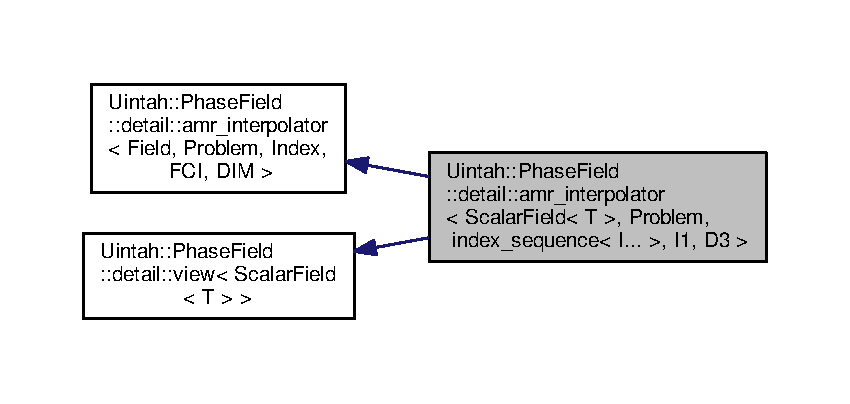
\includegraphics[width=350pt]{classUintah_1_1PhaseField_1_1detail_1_1amr__interpolator_3_01ScalarField_3_01T_01_4_00_01Problem754fdc2afe2dd55c64d406f42defc6a3}
\end{center}
\end{figure}


Collaboration diagram for Uintah\+:\+:Phase\+Field\+:\+:detail\+:\+:amr\+\_\+interpolator$<$ Scalar\+Field$<$ T $>$, Problem, index\+\_\+sequence$<$ I... $>$, I1, D3 $>$\+:\nopagebreak
\begin{figure}[H]
\begin{center}
\leavevmode
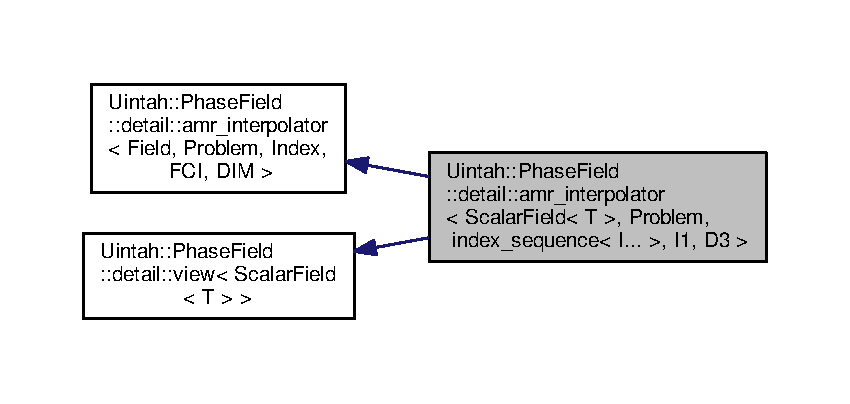
\includegraphics[width=350pt]{classUintah_1_1PhaseField_1_1detail_1_1amr__interpolator_3_01ScalarField_3_01T_01_4_00_01Problemb4baeed8e1c07f67a29c180b13cabc08}
\end{center}
\end{figure}
\subsection*{Public Member Functions}
\begin{DoxyCompactItemize}
\item 
\hyperlink{classUintah_1_1PhaseField_1_1detail_1_1amr__interpolator_3_01ScalarField_3_01T_01_4_00_01Problemdf68628a6010a1e1526666730125c372_a8580864e454adb1e3b4edea25eb2e9d9}{amr\+\_\+interpolator} (const Var\+Label $\ast$label, const Var\+Label $\ast$subproblems\+\_\+label, int material)
\begin{DoxyCompactList}\small\item\em construct interpolator without retrieving inner variable data from the Data\+Warehouse \end{DoxyCompactList}\item 
\hyperlink{classUintah_1_1PhaseField_1_1detail_1_1amr__interpolator_3_01ScalarField_3_01T_01_4_00_01Problemdf68628a6010a1e1526666730125c372_abe39c29b1413dd0cbc8a0b7b86c658e6}{amr\+\_\+interpolator} (Data\+Warehouse $\ast$dw, const Var\+Label $\ast$label, const Var\+Label $\ast$subproblems\+\_\+label, int material, const Patch $\ast$patch, bool use\+\_\+ghosts=\hyperlink{classUintah_1_1PhaseField_1_1detail_1_1amr__interpolator_3_01ScalarField_3_01T_01_4_00_01Problemdf68628a6010a1e1526666730125c372_ac8949b5e1e12de5843d579bed1556ddb}{use\+\_\+ghosts\+\_\+dflt})
\begin{DoxyCompactList}\small\item\em construct interpolator and retrieve inner variable data from the Data\+Warehouse whitin a given fine patch. \end{DoxyCompactList}\item 
virtual \hyperlink{classUintah_1_1PhaseField_1_1detail_1_1amr__interpolator_3_01ScalarField_3_01T_01_4_00_01Problemdf68628a6010a1e1526666730125c372_afed7a05333a90833b66c23731cf7f512}{$\sim$amr\+\_\+interpolator} ()
\begin{DoxyCompactList}\small\item\em Destructor. \end{DoxyCompactList}\item 
\hyperlink{classUintah_1_1PhaseField_1_1detail_1_1amr__interpolator_3_01ScalarField_3_01T_01_4_00_01Problemdf68628a6010a1e1526666730125c372_a982aa701741ac38691e8c36c81bf6898}{amr\+\_\+interpolator} (const \hyperlink{classUintah_1_1PhaseField_1_1detail_1_1amr__interpolator}{amr\+\_\+interpolator} \&)=delete
\begin{DoxyCompactList}\small\item\em Prevent copy (and move) constructor. \end{DoxyCompactList}\item 
\hyperlink{classUintah_1_1PhaseField_1_1detail_1_1amr__interpolator}{amr\+\_\+interpolator} \& \hyperlink{classUintah_1_1PhaseField_1_1detail_1_1amr__interpolator_3_01ScalarField_3_01T_01_4_00_01Problemdf68628a6010a1e1526666730125c372_a6636b05d21c6ca04c38bc2baa3fce356}{operator=} (const \hyperlink{classUintah_1_1PhaseField_1_1detail_1_1amr__interpolator}{amr\+\_\+interpolator} \&)=delete
\begin{DoxyCompactList}\small\item\em Prevent copy (and move) assignment. \end{DoxyCompactList}\item 
virtual void \hyperlink{classUintah_1_1PhaseField_1_1detail_1_1amr__interpolator_3_01ScalarField_3_01T_01_4_00_01Problemdf68628a6010a1e1526666730125c372_a2bd6c99b7578b0f8842dff6deb19caca}{set} (Data\+Warehouse $\ast$dw, const Patch $\ast$patch, bool use\+\_\+ghosts=\hyperlink{classUintah_1_1PhaseField_1_1detail_1_1amr__interpolator_3_01ScalarField_3_01T_01_4_00_01Problemdf68628a6010a1e1526666730125c372_ac8949b5e1e12de5843d579bed1556ddb}{use\+\_\+ghosts\+\_\+dflt}) override
\begin{DoxyCompactList}\small\item\em retrieve inner variable data from the Data\+Warehouse whitin a given patch. \end{DoxyCompactList}\item 
virtual void \hyperlink{classUintah_1_1PhaseField_1_1detail_1_1amr__interpolator_3_01ScalarField_3_01T_01_4_00_01Problemdf68628a6010a1e1526666730125c372_af36ec266ac99db41c8d9addb98999112}{set} (Data\+Warehouse $\ast$dw, const Level $\ast$level, const Int\+Vector \&low, const Int\+Vector \&high, bool use\+\_\+ghosts=\hyperlink{classUintah_1_1PhaseField_1_1detail_1_1amr__interpolator_3_01ScalarField_3_01T_01_4_00_01Problemdf68628a6010a1e1526666730125c372_ac8949b5e1e12de5843d579bed1556ddb}{use\+\_\+ghosts\+\_\+dflt}) override
\begin{DoxyCompactList}\small\item\em retrieve inner variable data from the Data\+Warehouse whitin a given region. \end{DoxyCompactList}\item 
virtual \hyperlink{classUintah_1_1PhaseField_1_1detail_1_1view}{view}$<$ \hyperlink{structUintah_1_1PhaseField_1_1ScalarField}{Field} $>$ $\ast$ \hyperlink{classUintah_1_1PhaseField_1_1detail_1_1amr__interpolator_3_01ScalarField_3_01T_01_4_00_01Problemdf68628a6010a1e1526666730125c372_a69b809d731de3fdfe713ac4321394962}{clone} (bool deep) const override
\begin{DoxyCompactList}\small\item\em Get a copy of the view. \end{DoxyCompactList}\item 
virtual \hyperlink{classUintah_1_1PhaseField_1_1detail_1_1view}{view}$<$ \hyperlink{structUintah_1_1PhaseField_1_1ScalarField}{Field} $>$ $\ast$ \hyperlink{classUintah_1_1PhaseField_1_1detail_1_1amr__interpolator_3_01ScalarField_3_01T_01_4_00_01Problemdf68628a6010a1e1526666730125c372_ac7391fa05270a0b845674752ce8bb8bf}{clone} (bool deep, const Int\+Vector \&offset) const override
\begin{DoxyCompactList}\small\item\em Get a copy of the view and apply translate the support. \end{DoxyCompactList}\item 
virtual \hyperlink{classUintah_1_1PhaseField_1_1Support}{Support} \hyperlink{classUintah_1_1PhaseField_1_1detail_1_1amr__interpolator_3_01ScalarField_3_01T_01_4_00_01Problemdf68628a6010a1e1526666730125c372_ac5fa7533900896ba125401671a5739d2}{get\+\_\+support} () const override
\begin{DoxyCompactList}\small\item\em get interpolator\textquotesingle{}s fine range \end{DoxyCompactList}\item 
virtual bool \hyperlink{classUintah_1_1PhaseField_1_1detail_1_1amr__interpolator_3_01ScalarField_3_01T_01_4_00_01Problemdf68628a6010a1e1526666730125c372_a5fa0ce1cd64383bfba2965f9cb88d35b}{is\+\_\+defined\+\_\+at} (const Int\+Vector \&id) const override
\begin{DoxyCompactList}\small\item\em Check if the view has access to the fine position with index id. \end{DoxyCompactList}\item 
virtual T \& \hyperlink{classUintah_1_1PhaseField_1_1detail_1_1amr__interpolator_3_01ScalarField_3_01T_01_4_00_01Problemdf68628a6010a1e1526666730125c372_a11af7680ab9786aade9b1913cd846c6f}{operator\mbox{[}$\,$\mbox{]}} (const Int\+Vector \&id) override \hyperlink{Definitions_8h_a3ce9c14452594b5b9ee3b63f9b3a981e}{V\+I\+RT}
\begin{DoxyCompactList}\small\item\em Get/\+Modify value at position with index id (virtual implementation) \end{DoxyCompactList}\item 
virtual V \hyperlink{classUintah_1_1PhaseField_1_1detail_1_1amr__interpolator_3_01ScalarField_3_01T_01_4_00_01Problemdf68628a6010a1e1526666730125c372_ae35934d096a5301035afb6347114f465}{operator\mbox{[}$\,$\mbox{]}} (const Int\+Vector \&id\+\_\+fine) const override
\begin{DoxyCompactList}\small\item\em get interpolated value \end{DoxyCompactList}\end{DoxyCompactItemize}
\subsection*{Static Public Attributes}
\begin{DoxyCompactItemize}
\item 
static constexpr bool \hyperlink{classUintah_1_1PhaseField_1_1detail_1_1amr__interpolator_3_01ScalarField_3_01T_01_4_00_01Problemdf68628a6010a1e1526666730125c372_ac8949b5e1e12de5843d579bed1556ddb}{use\+\_\+ghosts\+\_\+dflt} = false
\end{DoxyCompactItemize}
\subsection*{Protected Member Functions}
\begin{DoxyCompactItemize}
\item 
\hyperlink{classUintah_1_1PhaseField_1_1detail_1_1amr__interpolator_3_01ScalarField_3_01T_01_4_00_01Problemdf68628a6010a1e1526666730125c372_a979f58156a77c56eeff8e548f8886dd3}{amr\+\_\+interpolator} (const \hyperlink{classUintah_1_1PhaseField_1_1detail_1_1amr__interpolator}{amr\+\_\+interpolator} $\ast$copy, bool deep)
\begin{DoxyCompactList}\small\item\em Constructor. \end{DoxyCompactList}\end{DoxyCompactItemize}
\subsection*{Additional Inherited Members}


\subsection{Detailed Description}
\subsubsection*{template$<$typename T, typename Problem, size\+\_\+t... I$>$\newline
class Uintah\+::\+Phase\+Field\+::detail\+::amr\+\_\+interpolator$<$ Scalar\+Field$<$ T $>$, Problem, index\+\_\+sequence$<$ I... $>$, I1, D3 $>$}

Wrapper of grid variables for interpolation from coarser to finer levels (3D linear implementation) 

Implements linear interpolation of a variable from coarser to finer levels in 3D

\begin{DoxyRefDesc}{Bug}
\item[\hyperlink{bug__bug000001}{Bug}]this is actually broken since it could happen that interpolation is requiring values from coarse level that are not extrapolated by bcs! \end{DoxyRefDesc}
\begin{DoxyRefDesc}{Todo}
\item[\hyperlink{todo__todo000004}{Todo}]implment as recursion over dimension to avoid this issue!\end{DoxyRefDesc}



\begin{DoxyTemplParams}{Template Parameters}
{\em T} & variable data type (must be constant) \\
\hline
{\em \hyperlink{classUintah_1_1PhaseField_1_1Problem}{Problem}} & type of \hyperlink{namespaceUintah_1_1PhaseField}{Phase\+Field} problem \\
\hline
{\em \hyperlink{structUintah_1_1PhaseField_1_1I}{I}} & list of indices corresponding to the variable within the subproblems\\
\hline
\end{DoxyTemplParams}
\begin{DoxyRefDesc}{Todo}
\item[\hyperlink{todo__todo000005}{Todo}]generalize implementation to arbitrary dimension\end{DoxyRefDesc}


$<$ Field, \hyperlink{classUintah_1_1PhaseField_1_1Problem}{Problem}, Index, F\+CI, D\+IM $>$ 

\subsection{Constructor \& Destructor Documentation}
\mbox{\Hypertarget{classUintah_1_1PhaseField_1_1detail_1_1amr__interpolator_3_01ScalarField_3_01T_01_4_00_01Problemdf68628a6010a1e1526666730125c372_a979f58156a77c56eeff8e548f8886dd3}\label{classUintah_1_1PhaseField_1_1detail_1_1amr__interpolator_3_01ScalarField_3_01T_01_4_00_01Problemdf68628a6010a1e1526666730125c372_a979f58156a77c56eeff8e548f8886dd3}} 
\index{Uintah\+::\+Phase\+Field\+::detail\+::amr\+\_\+interpolator$<$ Scalar\+Field$<$ T $>$, Problem, index\+\_\+sequence$<$ I... $>$, I1, D3 $>$@{Uintah\+::\+Phase\+Field\+::detail\+::amr\+\_\+interpolator$<$ Scalar\+Field$<$ T $>$, Problem, index\+\_\+sequence$<$ I... $>$, I1, D3 $>$}!amr\+\_\+interpolator@{amr\+\_\+interpolator}}
\index{amr\+\_\+interpolator@{amr\+\_\+interpolator}!Uintah\+::\+Phase\+Field\+::detail\+::amr\+\_\+interpolator$<$ Scalar\+Field$<$ T $>$, Problem, index\+\_\+sequence$<$ I... $>$, I1, D3 $>$@{Uintah\+::\+Phase\+Field\+::detail\+::amr\+\_\+interpolator$<$ Scalar\+Field$<$ T $>$, Problem, index\+\_\+sequence$<$ I... $>$, I1, D3 $>$}}
\subsubsection{\texorpdfstring{amr\+\_\+interpolator()}{amr\_interpolator()}\hspace{0.1cm}{\footnotesize\ttfamily [1/4]}}
{\footnotesize\ttfamily template$<$typename T , typename Problem , size\+\_\+t... I$>$ \\
\hyperlink{classUintah_1_1PhaseField_1_1detail_1_1amr__interpolator}{Uintah\+::\+Phase\+Field\+::detail\+::amr\+\_\+interpolator}$<$ \hyperlink{structUintah_1_1PhaseField_1_1ScalarField}{Scalar\+Field}$<$ T $>$, \hyperlink{classUintah_1_1PhaseField_1_1Problem}{Problem}, \hyperlink{namespaceUintah_1_1PhaseField_a237de804d99512e50613aff7c94a9461}{index\+\_\+sequence}$<$ I... $>$, \hyperlink{namespaceUintah_1_1PhaseField_a547ce3002aa97fbd3ef3192a6eec8406a66f19efe774b0d2b6e5844eb2d83d305}{I1}, \hyperlink{namespaceUintah_1_1PhaseField_a12bfc68444894dffdf0cb8d9cf0cc76aa72fd61934c7ca788c49ad90629f76e78}{D3} $>$\+::\hyperlink{classUintah_1_1PhaseField_1_1detail_1_1amr__interpolator}{amr\+\_\+interpolator} (\begin{DoxyParamCaption}\item[{const \hyperlink{classUintah_1_1PhaseField_1_1detail_1_1amr__interpolator}{amr\+\_\+interpolator}$<$ \hyperlink{structUintah_1_1PhaseField_1_1ScalarField}{Scalar\+Field}$<$ T $>$, \hyperlink{classUintah_1_1PhaseField_1_1Problem}{Problem}, \hyperlink{namespaceUintah_1_1PhaseField_a237de804d99512e50613aff7c94a9461}{index\+\_\+sequence}$<$ I... $>$, \hyperlink{namespaceUintah_1_1PhaseField_a547ce3002aa97fbd3ef3192a6eec8406a66f19efe774b0d2b6e5844eb2d83d305}{I1}, \hyperlink{namespaceUintah_1_1PhaseField_a12bfc68444894dffdf0cb8d9cf0cc76aa72fd61934c7ca788c49ad90629f76e78}{D3} $>$ $\ast$}]{copy,  }\item[{bool}]{deep }\end{DoxyParamCaption})\hspace{0.3cm}{\ttfamily [inline]}, {\ttfamily [protected]}}



Constructor. 

Instantiate a copy of a given view


\begin{DoxyParams}{Parameters}
{\em copy} & source view for copying \\
\hline
{\em deep} & if true inner grid variable is copied as well otherwise the same grid variable is referenced \\
\hline
\end{DoxyParams}
\mbox{\Hypertarget{classUintah_1_1PhaseField_1_1detail_1_1amr__interpolator_3_01ScalarField_3_01T_01_4_00_01Problemdf68628a6010a1e1526666730125c372_a8580864e454adb1e3b4edea25eb2e9d9}\label{classUintah_1_1PhaseField_1_1detail_1_1amr__interpolator_3_01ScalarField_3_01T_01_4_00_01Problemdf68628a6010a1e1526666730125c372_a8580864e454adb1e3b4edea25eb2e9d9}} 
\index{Uintah\+::\+Phase\+Field\+::detail\+::amr\+\_\+interpolator$<$ Scalar\+Field$<$ T $>$, Problem, index\+\_\+sequence$<$ I... $>$, I1, D3 $>$@{Uintah\+::\+Phase\+Field\+::detail\+::amr\+\_\+interpolator$<$ Scalar\+Field$<$ T $>$, Problem, index\+\_\+sequence$<$ I... $>$, I1, D3 $>$}!amr\+\_\+interpolator@{amr\+\_\+interpolator}}
\index{amr\+\_\+interpolator@{amr\+\_\+interpolator}!Uintah\+::\+Phase\+Field\+::detail\+::amr\+\_\+interpolator$<$ Scalar\+Field$<$ T $>$, Problem, index\+\_\+sequence$<$ I... $>$, I1, D3 $>$@{Uintah\+::\+Phase\+Field\+::detail\+::amr\+\_\+interpolator$<$ Scalar\+Field$<$ T $>$, Problem, index\+\_\+sequence$<$ I... $>$, I1, D3 $>$}}
\subsubsection{\texorpdfstring{amr\+\_\+interpolator()}{amr\_interpolator()}\hspace{0.1cm}{\footnotesize\ttfamily [2/4]}}
{\footnotesize\ttfamily template$<$typename T , typename Problem , size\+\_\+t... I$>$ \\
\hyperlink{classUintah_1_1PhaseField_1_1detail_1_1amr__interpolator}{Uintah\+::\+Phase\+Field\+::detail\+::amr\+\_\+interpolator}$<$ \hyperlink{structUintah_1_1PhaseField_1_1ScalarField}{Scalar\+Field}$<$ T $>$, \hyperlink{classUintah_1_1PhaseField_1_1Problem}{Problem}, \hyperlink{namespaceUintah_1_1PhaseField_a237de804d99512e50613aff7c94a9461}{index\+\_\+sequence}$<$ I... $>$, \hyperlink{namespaceUintah_1_1PhaseField_a547ce3002aa97fbd3ef3192a6eec8406a66f19efe774b0d2b6e5844eb2d83d305}{I1}, \hyperlink{namespaceUintah_1_1PhaseField_a12bfc68444894dffdf0cb8d9cf0cc76aa72fd61934c7ca788c49ad90629f76e78}{D3} $>$\+::\hyperlink{classUintah_1_1PhaseField_1_1detail_1_1amr__interpolator}{amr\+\_\+interpolator} (\begin{DoxyParamCaption}\item[{const Var\+Label $\ast$}]{label,  }\item[{const Var\+Label $\ast$}]{subproblems\+\_\+label,  }\item[{int}]{material }\end{DoxyParamCaption})\hspace{0.3cm}{\ttfamily [inline]}}



construct interpolator without retrieving inner variable data from the Data\+Warehouse 


\begin{DoxyParams}{Parameters}
{\em label} & label of variable in the Data\+Warehouse \\
\hline
{\em subproblems\+\_\+label} & label of subproblems in the Data\+Warehouse \\
\hline
{\em material} & index of material in the Data\+Warehouse \\
\hline
\end{DoxyParams}
\mbox{\Hypertarget{classUintah_1_1PhaseField_1_1detail_1_1amr__interpolator_3_01ScalarField_3_01T_01_4_00_01Problemdf68628a6010a1e1526666730125c372_abe39c29b1413dd0cbc8a0b7b86c658e6}\label{classUintah_1_1PhaseField_1_1detail_1_1amr__interpolator_3_01ScalarField_3_01T_01_4_00_01Problemdf68628a6010a1e1526666730125c372_abe39c29b1413dd0cbc8a0b7b86c658e6}} 
\index{Uintah\+::\+Phase\+Field\+::detail\+::amr\+\_\+interpolator$<$ Scalar\+Field$<$ T $>$, Problem, index\+\_\+sequence$<$ I... $>$, I1, D3 $>$@{Uintah\+::\+Phase\+Field\+::detail\+::amr\+\_\+interpolator$<$ Scalar\+Field$<$ T $>$, Problem, index\+\_\+sequence$<$ I... $>$, I1, D3 $>$}!amr\+\_\+interpolator@{amr\+\_\+interpolator}}
\index{amr\+\_\+interpolator@{amr\+\_\+interpolator}!Uintah\+::\+Phase\+Field\+::detail\+::amr\+\_\+interpolator$<$ Scalar\+Field$<$ T $>$, Problem, index\+\_\+sequence$<$ I... $>$, I1, D3 $>$@{Uintah\+::\+Phase\+Field\+::detail\+::amr\+\_\+interpolator$<$ Scalar\+Field$<$ T $>$, Problem, index\+\_\+sequence$<$ I... $>$, I1, D3 $>$}}
\subsubsection{\texorpdfstring{amr\+\_\+interpolator()}{amr\_interpolator()}\hspace{0.1cm}{\footnotesize\ttfamily [3/4]}}
{\footnotesize\ttfamily template$<$typename T , typename Problem , size\+\_\+t... I$>$ \\
\hyperlink{classUintah_1_1PhaseField_1_1detail_1_1amr__interpolator}{Uintah\+::\+Phase\+Field\+::detail\+::amr\+\_\+interpolator}$<$ \hyperlink{structUintah_1_1PhaseField_1_1ScalarField}{Scalar\+Field}$<$ T $>$, \hyperlink{classUintah_1_1PhaseField_1_1Problem}{Problem}, \hyperlink{namespaceUintah_1_1PhaseField_a237de804d99512e50613aff7c94a9461}{index\+\_\+sequence}$<$ I... $>$, \hyperlink{namespaceUintah_1_1PhaseField_a547ce3002aa97fbd3ef3192a6eec8406a66f19efe774b0d2b6e5844eb2d83d305}{I1}, \hyperlink{namespaceUintah_1_1PhaseField_a12bfc68444894dffdf0cb8d9cf0cc76aa72fd61934c7ca788c49ad90629f76e78}{D3} $>$\+::\hyperlink{classUintah_1_1PhaseField_1_1detail_1_1amr__interpolator}{amr\+\_\+interpolator} (\begin{DoxyParamCaption}\item[{Data\+Warehouse $\ast$}]{dw,  }\item[{const Var\+Label $\ast$}]{label,  }\item[{const Var\+Label $\ast$}]{subproblems\+\_\+label,  }\item[{int}]{material,  }\item[{const Patch $\ast$}]{patch,  }\item[{bool}]{use\+\_\+ghosts = {\ttfamily \hyperlink{classUintah_1_1PhaseField_1_1detail_1_1amr__interpolator_3_01ScalarField_3_01T_01_4_00_01Problemdf68628a6010a1e1526666730125c372_ac8949b5e1e12de5843d579bed1556ddb}{use\+\_\+ghosts\+\_\+dflt}} }\end{DoxyParamCaption})\hspace{0.3cm}{\ttfamily [inline]}}



construct interpolator and retrieve inner variable data from the Data\+Warehouse whitin a given fine patch. 

the number of ghost cells/nodes and the corresponding region on the coarser level is automatically computed to match the interpolation type


\begin{DoxyParams}{Parameters}
{\em dw} & Data\+Warehouse which data is retrieved from \\
\hline
{\em label} & label of variable in the Data\+Warehouse \\
\hline
{\em subproblems\+\_\+label} & label of subproblems in the Data\+Warehouse \\
\hline
{\em material} & index of material in the Data\+Warehouse \\
\hline
{\em patch} & patch on which data is retrieved \\
\hline
{\em use\+\_\+ghosts} & if ghosts value are to be retrieved (must be false) \\
\hline
\end{DoxyParams}
\mbox{\Hypertarget{classUintah_1_1PhaseField_1_1detail_1_1amr__interpolator_3_01ScalarField_3_01T_01_4_00_01Problemdf68628a6010a1e1526666730125c372_afed7a05333a90833b66c23731cf7f512}\label{classUintah_1_1PhaseField_1_1detail_1_1amr__interpolator_3_01ScalarField_3_01T_01_4_00_01Problemdf68628a6010a1e1526666730125c372_afed7a05333a90833b66c23731cf7f512}} 
\index{Uintah\+::\+Phase\+Field\+::detail\+::amr\+\_\+interpolator$<$ Scalar\+Field$<$ T $>$, Problem, index\+\_\+sequence$<$ I... $>$, I1, D3 $>$@{Uintah\+::\+Phase\+Field\+::detail\+::amr\+\_\+interpolator$<$ Scalar\+Field$<$ T $>$, Problem, index\+\_\+sequence$<$ I... $>$, I1, D3 $>$}!````~amr\+\_\+interpolator@{$\sim$amr\+\_\+interpolator}}
\index{````~amr\+\_\+interpolator@{$\sim$amr\+\_\+interpolator}!Uintah\+::\+Phase\+Field\+::detail\+::amr\+\_\+interpolator$<$ Scalar\+Field$<$ T $>$, Problem, index\+\_\+sequence$<$ I... $>$, I1, D3 $>$@{Uintah\+::\+Phase\+Field\+::detail\+::amr\+\_\+interpolator$<$ Scalar\+Field$<$ T $>$, Problem, index\+\_\+sequence$<$ I... $>$, I1, D3 $>$}}
\subsubsection{\texorpdfstring{$\sim$amr\+\_\+interpolator()}{~amr\_interpolator()}}
{\footnotesize\ttfamily template$<$typename T , typename Problem , size\+\_\+t... I$>$ \\
virtual \hyperlink{classUintah_1_1PhaseField_1_1detail_1_1amr__interpolator}{Uintah\+::\+Phase\+Field\+::detail\+::amr\+\_\+interpolator}$<$ \hyperlink{structUintah_1_1PhaseField_1_1ScalarField}{Scalar\+Field}$<$ T $>$, \hyperlink{classUintah_1_1PhaseField_1_1Problem}{Problem}, \hyperlink{namespaceUintah_1_1PhaseField_a237de804d99512e50613aff7c94a9461}{index\+\_\+sequence}$<$ I... $>$, \hyperlink{namespaceUintah_1_1PhaseField_a547ce3002aa97fbd3ef3192a6eec8406a66f19efe774b0d2b6e5844eb2d83d305}{I1}, \hyperlink{namespaceUintah_1_1PhaseField_a12bfc68444894dffdf0cb8d9cf0cc76aa72fd61934c7ca788c49ad90629f76e78}{D3} $>$\+::$\sim$\hyperlink{classUintah_1_1PhaseField_1_1detail_1_1amr__interpolator}{amr\+\_\+interpolator} (\begin{DoxyParamCaption}{ }\end{DoxyParamCaption})\hspace{0.3cm}{\ttfamily [inline]}, {\ttfamily [virtual]}}



Destructor. 

\mbox{\Hypertarget{classUintah_1_1PhaseField_1_1detail_1_1amr__interpolator_3_01ScalarField_3_01T_01_4_00_01Problemdf68628a6010a1e1526666730125c372_a982aa701741ac38691e8c36c81bf6898}\label{classUintah_1_1PhaseField_1_1detail_1_1amr__interpolator_3_01ScalarField_3_01T_01_4_00_01Problemdf68628a6010a1e1526666730125c372_a982aa701741ac38691e8c36c81bf6898}} 
\index{Uintah\+::\+Phase\+Field\+::detail\+::amr\+\_\+interpolator$<$ Scalar\+Field$<$ T $>$, Problem, index\+\_\+sequence$<$ I... $>$, I1, D3 $>$@{Uintah\+::\+Phase\+Field\+::detail\+::amr\+\_\+interpolator$<$ Scalar\+Field$<$ T $>$, Problem, index\+\_\+sequence$<$ I... $>$, I1, D3 $>$}!amr\+\_\+interpolator@{amr\+\_\+interpolator}}
\index{amr\+\_\+interpolator@{amr\+\_\+interpolator}!Uintah\+::\+Phase\+Field\+::detail\+::amr\+\_\+interpolator$<$ Scalar\+Field$<$ T $>$, Problem, index\+\_\+sequence$<$ I... $>$, I1, D3 $>$@{Uintah\+::\+Phase\+Field\+::detail\+::amr\+\_\+interpolator$<$ Scalar\+Field$<$ T $>$, Problem, index\+\_\+sequence$<$ I... $>$, I1, D3 $>$}}
\subsubsection{\texorpdfstring{amr\+\_\+interpolator()}{amr\_interpolator()}\hspace{0.1cm}{\footnotesize\ttfamily [4/4]}}
{\footnotesize\ttfamily template$<$typename T , typename Problem , size\+\_\+t... I$>$ \\
\hyperlink{classUintah_1_1PhaseField_1_1detail_1_1amr__interpolator}{Uintah\+::\+Phase\+Field\+::detail\+::amr\+\_\+interpolator}$<$ \hyperlink{structUintah_1_1PhaseField_1_1ScalarField}{Scalar\+Field}$<$ T $>$, \hyperlink{classUintah_1_1PhaseField_1_1Problem}{Problem}, \hyperlink{namespaceUintah_1_1PhaseField_a237de804d99512e50613aff7c94a9461}{index\+\_\+sequence}$<$ I... $>$, \hyperlink{namespaceUintah_1_1PhaseField_a547ce3002aa97fbd3ef3192a6eec8406a66f19efe774b0d2b6e5844eb2d83d305}{I1}, \hyperlink{namespaceUintah_1_1PhaseField_a12bfc68444894dffdf0cb8d9cf0cc76aa72fd61934c7ca788c49ad90629f76e78}{D3} $>$\+::\hyperlink{classUintah_1_1PhaseField_1_1detail_1_1amr__interpolator}{amr\+\_\+interpolator} (\begin{DoxyParamCaption}\item[{const \hyperlink{classUintah_1_1PhaseField_1_1detail_1_1amr__interpolator}{amr\+\_\+interpolator}$<$ \hyperlink{structUintah_1_1PhaseField_1_1ScalarField}{Scalar\+Field}$<$ T $>$, \hyperlink{classUintah_1_1PhaseField_1_1Problem}{Problem}, \hyperlink{namespaceUintah_1_1PhaseField_a237de804d99512e50613aff7c94a9461}{index\+\_\+sequence}$<$ I... $>$, \hyperlink{namespaceUintah_1_1PhaseField_a547ce3002aa97fbd3ef3192a6eec8406a66f19efe774b0d2b6e5844eb2d83d305}{I1}, \hyperlink{namespaceUintah_1_1PhaseField_a12bfc68444894dffdf0cb8d9cf0cc76aa72fd61934c7ca788c49ad90629f76e78}{D3} $>$ \&}]{ }\end{DoxyParamCaption})\hspace{0.3cm}{\ttfamily [delete]}}



Prevent copy (and move) constructor. 



\subsection{Member Function Documentation}
\mbox{\Hypertarget{classUintah_1_1PhaseField_1_1detail_1_1amr__interpolator_3_01ScalarField_3_01T_01_4_00_01Problemdf68628a6010a1e1526666730125c372_a69b809d731de3fdfe713ac4321394962}\label{classUintah_1_1PhaseField_1_1detail_1_1amr__interpolator_3_01ScalarField_3_01T_01_4_00_01Problemdf68628a6010a1e1526666730125c372_a69b809d731de3fdfe713ac4321394962}} 
\index{Uintah\+::\+Phase\+Field\+::detail\+::amr\+\_\+interpolator$<$ Scalar\+Field$<$ T $>$, Problem, index\+\_\+sequence$<$ I... $>$, I1, D3 $>$@{Uintah\+::\+Phase\+Field\+::detail\+::amr\+\_\+interpolator$<$ Scalar\+Field$<$ T $>$, Problem, index\+\_\+sequence$<$ I... $>$, I1, D3 $>$}!clone@{clone}}
\index{clone@{clone}!Uintah\+::\+Phase\+Field\+::detail\+::amr\+\_\+interpolator$<$ Scalar\+Field$<$ T $>$, Problem, index\+\_\+sequence$<$ I... $>$, I1, D3 $>$@{Uintah\+::\+Phase\+Field\+::detail\+::amr\+\_\+interpolator$<$ Scalar\+Field$<$ T $>$, Problem, index\+\_\+sequence$<$ I... $>$, I1, D3 $>$}}
\subsubsection{\texorpdfstring{clone()}{clone()}\hspace{0.1cm}{\footnotesize\ttfamily [1/2]}}
{\footnotesize\ttfamily template$<$typename T , typename Problem , size\+\_\+t... I$>$ \\
virtual \hyperlink{classUintah_1_1PhaseField_1_1detail_1_1view}{view}$<$\hyperlink{structUintah_1_1PhaseField_1_1ScalarField}{Field}$>$$\ast$ \hyperlink{classUintah_1_1PhaseField_1_1detail_1_1amr__interpolator}{Uintah\+::\+Phase\+Field\+::detail\+::amr\+\_\+interpolator}$<$ \hyperlink{structUintah_1_1PhaseField_1_1ScalarField}{Scalar\+Field}$<$ T $>$, \hyperlink{classUintah_1_1PhaseField_1_1Problem}{Problem}, \hyperlink{namespaceUintah_1_1PhaseField_a237de804d99512e50613aff7c94a9461}{index\+\_\+sequence}$<$ I... $>$, \hyperlink{namespaceUintah_1_1PhaseField_a547ce3002aa97fbd3ef3192a6eec8406a66f19efe774b0d2b6e5844eb2d83d305}{I1}, \hyperlink{namespaceUintah_1_1PhaseField_a12bfc68444894dffdf0cb8d9cf0cc76aa72fd61934c7ca788c49ad90629f76e78}{D3} $>$\+::clone (\begin{DoxyParamCaption}\item[{bool}]{deep }\end{DoxyParamCaption}) const\hspace{0.3cm}{\ttfamily [inline]}, {\ttfamily [override]}, {\ttfamily [virtual]}}



Get a copy of the view. 


\begin{DoxyParams}{Parameters}
{\em deep} & if true inner grid variable is copied as well otherwise the same grid variable is referenced\\
\hline
\end{DoxyParams}
\begin{DoxyReturn}{Returns}
new view instance 
\end{DoxyReturn}


Implements \hyperlink{classUintah_1_1PhaseField_1_1detail_1_1view_3_01ScalarField_3_01T_01_4_01_4_a6e11243c9d776a7b703e524ea4151a16}{Uintah\+::\+Phase\+Field\+::detail\+::view$<$ Scalar\+Field$<$ T $>$ $>$}.

\mbox{\Hypertarget{classUintah_1_1PhaseField_1_1detail_1_1amr__interpolator_3_01ScalarField_3_01T_01_4_00_01Problemdf68628a6010a1e1526666730125c372_ac7391fa05270a0b845674752ce8bb8bf}\label{classUintah_1_1PhaseField_1_1detail_1_1amr__interpolator_3_01ScalarField_3_01T_01_4_00_01Problemdf68628a6010a1e1526666730125c372_ac7391fa05270a0b845674752ce8bb8bf}} 
\index{Uintah\+::\+Phase\+Field\+::detail\+::amr\+\_\+interpolator$<$ Scalar\+Field$<$ T $>$, Problem, index\+\_\+sequence$<$ I... $>$, I1, D3 $>$@{Uintah\+::\+Phase\+Field\+::detail\+::amr\+\_\+interpolator$<$ Scalar\+Field$<$ T $>$, Problem, index\+\_\+sequence$<$ I... $>$, I1, D3 $>$}!clone@{clone}}
\index{clone@{clone}!Uintah\+::\+Phase\+Field\+::detail\+::amr\+\_\+interpolator$<$ Scalar\+Field$<$ T $>$, Problem, index\+\_\+sequence$<$ I... $>$, I1, D3 $>$@{Uintah\+::\+Phase\+Field\+::detail\+::amr\+\_\+interpolator$<$ Scalar\+Field$<$ T $>$, Problem, index\+\_\+sequence$<$ I... $>$, I1, D3 $>$}}
\subsubsection{\texorpdfstring{clone()}{clone()}\hspace{0.1cm}{\footnotesize\ttfamily [2/2]}}
{\footnotesize\ttfamily template$<$typename T , typename Problem , size\+\_\+t... I$>$ \\
virtual \hyperlink{classUintah_1_1PhaseField_1_1detail_1_1view}{view}$<$\hyperlink{structUintah_1_1PhaseField_1_1ScalarField}{Field}$>$$\ast$ \hyperlink{classUintah_1_1PhaseField_1_1detail_1_1amr__interpolator}{Uintah\+::\+Phase\+Field\+::detail\+::amr\+\_\+interpolator}$<$ \hyperlink{structUintah_1_1PhaseField_1_1ScalarField}{Scalar\+Field}$<$ T $>$, \hyperlink{classUintah_1_1PhaseField_1_1Problem}{Problem}, \hyperlink{namespaceUintah_1_1PhaseField_a237de804d99512e50613aff7c94a9461}{index\+\_\+sequence}$<$ I... $>$, \hyperlink{namespaceUintah_1_1PhaseField_a547ce3002aa97fbd3ef3192a6eec8406a66f19efe774b0d2b6e5844eb2d83d305}{I1}, \hyperlink{namespaceUintah_1_1PhaseField_a12bfc68444894dffdf0cb8d9cf0cc76aa72fd61934c7ca788c49ad90629f76e78}{D3} $>$\+::clone (\begin{DoxyParamCaption}\item[{bool}]{deep,  }\item[{const Int\+Vector \&}]{offset }\end{DoxyParamCaption}) const\hspace{0.3cm}{\ttfamily [inline]}, {\ttfamily [override]}, {\ttfamily [virtual]}}



Get a copy of the view and apply translate the support. 

\begin{DoxyRemark}{Remarks}
It is meant to be used for virtual patches (i.\+e. periodic boundaries)
\end{DoxyRemark}

\begin{DoxyParams}{Parameters}
{\em deep} & if true inner grid variable is copied as well otherwise the same grid variable is referenced \\
\hline
{\em offset} & vector specifying the translation of the support \\
\hline
\end{DoxyParams}
\begin{DoxyReturn}{Returns}
new view instance 
\end{DoxyReturn}


Implements \hyperlink{classUintah_1_1PhaseField_1_1detail_1_1view_3_01ScalarField_3_01T_01_4_01_4_abd928104240e329f3bc4441ebab7c50c}{Uintah\+::\+Phase\+Field\+::detail\+::view$<$ Scalar\+Field$<$ T $>$ $>$}.

\mbox{\Hypertarget{classUintah_1_1PhaseField_1_1detail_1_1amr__interpolator_3_01ScalarField_3_01T_01_4_00_01Problemdf68628a6010a1e1526666730125c372_ac5fa7533900896ba125401671a5739d2}\label{classUintah_1_1PhaseField_1_1detail_1_1amr__interpolator_3_01ScalarField_3_01T_01_4_00_01Problemdf68628a6010a1e1526666730125c372_ac5fa7533900896ba125401671a5739d2}} 
\index{Uintah\+::\+Phase\+Field\+::detail\+::amr\+\_\+interpolator$<$ Scalar\+Field$<$ T $>$, Problem, index\+\_\+sequence$<$ I... $>$, I1, D3 $>$@{Uintah\+::\+Phase\+Field\+::detail\+::amr\+\_\+interpolator$<$ Scalar\+Field$<$ T $>$, Problem, index\+\_\+sequence$<$ I... $>$, I1, D3 $>$}!get\+\_\+support@{get\+\_\+support}}
\index{get\+\_\+support@{get\+\_\+support}!Uintah\+::\+Phase\+Field\+::detail\+::amr\+\_\+interpolator$<$ Scalar\+Field$<$ T $>$, Problem, index\+\_\+sequence$<$ I... $>$, I1, D3 $>$@{Uintah\+::\+Phase\+Field\+::detail\+::amr\+\_\+interpolator$<$ Scalar\+Field$<$ T $>$, Problem, index\+\_\+sequence$<$ I... $>$, I1, D3 $>$}}
\subsubsection{\texorpdfstring{get\+\_\+support()}{get\_support()}}
{\footnotesize\ttfamily template$<$typename T , typename Problem , size\+\_\+t... I$>$ \\
virtual \hyperlink{classUintah_1_1PhaseField_1_1Support}{Support} \hyperlink{classUintah_1_1PhaseField_1_1detail_1_1amr__interpolator}{Uintah\+::\+Phase\+Field\+::detail\+::amr\+\_\+interpolator}$<$ \hyperlink{structUintah_1_1PhaseField_1_1ScalarField}{Scalar\+Field}$<$ T $>$, \hyperlink{classUintah_1_1PhaseField_1_1Problem}{Problem}, \hyperlink{namespaceUintah_1_1PhaseField_a237de804d99512e50613aff7c94a9461}{index\+\_\+sequence}$<$ I... $>$, \hyperlink{namespaceUintah_1_1PhaseField_a547ce3002aa97fbd3ef3192a6eec8406a66f19efe774b0d2b6e5844eb2d83d305}{I1}, \hyperlink{namespaceUintah_1_1PhaseField_a12bfc68444894dffdf0cb8d9cf0cc76aa72fd61934c7ca788c49ad90629f76e78}{D3} $>$\+::get\+\_\+support (\begin{DoxyParamCaption}{ }\end{DoxyParamCaption}) const\hspace{0.3cm}{\ttfamily [inline]}, {\ttfamily [override]}, {\ttfamily [virtual]}}



get interpolator\textquotesingle{}s fine range 

\begin{DoxyReturn}{Returns}
fine range 
\end{DoxyReturn}


Implements \hyperlink{classUintah_1_1PhaseField_1_1detail_1_1view_3_01ScalarField_3_01T_01_4_01_4_a3e14b0c7a57a57707bb33954861ab1c1}{Uintah\+::\+Phase\+Field\+::detail\+::view$<$ Scalar\+Field$<$ T $>$ $>$}.

\mbox{\Hypertarget{classUintah_1_1PhaseField_1_1detail_1_1amr__interpolator_3_01ScalarField_3_01T_01_4_00_01Problemdf68628a6010a1e1526666730125c372_a5fa0ce1cd64383bfba2965f9cb88d35b}\label{classUintah_1_1PhaseField_1_1detail_1_1amr__interpolator_3_01ScalarField_3_01T_01_4_00_01Problemdf68628a6010a1e1526666730125c372_a5fa0ce1cd64383bfba2965f9cb88d35b}} 
\index{Uintah\+::\+Phase\+Field\+::detail\+::amr\+\_\+interpolator$<$ Scalar\+Field$<$ T $>$, Problem, index\+\_\+sequence$<$ I... $>$, I1, D3 $>$@{Uintah\+::\+Phase\+Field\+::detail\+::amr\+\_\+interpolator$<$ Scalar\+Field$<$ T $>$, Problem, index\+\_\+sequence$<$ I... $>$, I1, D3 $>$}!is\+\_\+defined\+\_\+at@{is\+\_\+defined\+\_\+at}}
\index{is\+\_\+defined\+\_\+at@{is\+\_\+defined\+\_\+at}!Uintah\+::\+Phase\+Field\+::detail\+::amr\+\_\+interpolator$<$ Scalar\+Field$<$ T $>$, Problem, index\+\_\+sequence$<$ I... $>$, I1, D3 $>$@{Uintah\+::\+Phase\+Field\+::detail\+::amr\+\_\+interpolator$<$ Scalar\+Field$<$ T $>$, Problem, index\+\_\+sequence$<$ I... $>$, I1, D3 $>$}}
\subsubsection{\texorpdfstring{is\+\_\+defined\+\_\+at()}{is\_defined\_at()}}
{\footnotesize\ttfamily template$<$typename T , typename Problem , size\+\_\+t... I$>$ \\
virtual bool \hyperlink{classUintah_1_1PhaseField_1_1detail_1_1amr__interpolator}{Uintah\+::\+Phase\+Field\+::detail\+::amr\+\_\+interpolator}$<$ \hyperlink{structUintah_1_1PhaseField_1_1ScalarField}{Scalar\+Field}$<$ T $>$, \hyperlink{classUintah_1_1PhaseField_1_1Problem}{Problem}, \hyperlink{namespaceUintah_1_1PhaseField_a237de804d99512e50613aff7c94a9461}{index\+\_\+sequence}$<$ I... $>$, \hyperlink{namespaceUintah_1_1PhaseField_a547ce3002aa97fbd3ef3192a6eec8406a66f19efe774b0d2b6e5844eb2d83d305}{I1}, \hyperlink{namespaceUintah_1_1PhaseField_a12bfc68444894dffdf0cb8d9cf0cc76aa72fd61934c7ca788c49ad90629f76e78}{D3} $>$\+::is\+\_\+defined\+\_\+at (\begin{DoxyParamCaption}\item[{const Int\+Vector \&}]{id }\end{DoxyParamCaption}) const\hspace{0.3cm}{\ttfamily [inline]}, {\ttfamily [override]}, {\ttfamily [virtual]}}



Check if the view has access to the fine position with index id. 


\begin{DoxyParams}{Parameters}
{\em id} & fine position index \\
\hline
\end{DoxyParams}
\begin{DoxyReturn}{Returns}
check result 
\end{DoxyReturn}


Implements \hyperlink{classUintah_1_1PhaseField_1_1detail_1_1view_3_01ScalarField_3_01T_01_4_01_4_a9a950513dacd6468658436b737c3314f}{Uintah\+::\+Phase\+Field\+::detail\+::view$<$ Scalar\+Field$<$ T $>$ $>$}.

\mbox{\Hypertarget{classUintah_1_1PhaseField_1_1detail_1_1amr__interpolator_3_01ScalarField_3_01T_01_4_00_01Problemdf68628a6010a1e1526666730125c372_a6636b05d21c6ca04c38bc2baa3fce356}\label{classUintah_1_1PhaseField_1_1detail_1_1amr__interpolator_3_01ScalarField_3_01T_01_4_00_01Problemdf68628a6010a1e1526666730125c372_a6636b05d21c6ca04c38bc2baa3fce356}} 
\index{Uintah\+::\+Phase\+Field\+::detail\+::amr\+\_\+interpolator$<$ Scalar\+Field$<$ T $>$, Problem, index\+\_\+sequence$<$ I... $>$, I1, D3 $>$@{Uintah\+::\+Phase\+Field\+::detail\+::amr\+\_\+interpolator$<$ Scalar\+Field$<$ T $>$, Problem, index\+\_\+sequence$<$ I... $>$, I1, D3 $>$}!operator=@{operator=}}
\index{operator=@{operator=}!Uintah\+::\+Phase\+Field\+::detail\+::amr\+\_\+interpolator$<$ Scalar\+Field$<$ T $>$, Problem, index\+\_\+sequence$<$ I... $>$, I1, D3 $>$@{Uintah\+::\+Phase\+Field\+::detail\+::amr\+\_\+interpolator$<$ Scalar\+Field$<$ T $>$, Problem, index\+\_\+sequence$<$ I... $>$, I1, D3 $>$}}
\subsubsection{\texorpdfstring{operator=()}{operator=()}}
{\footnotesize\ttfamily template$<$typename T , typename Problem , size\+\_\+t... I$>$ \\
\hyperlink{classUintah_1_1PhaseField_1_1detail_1_1amr__interpolator}{amr\+\_\+interpolator}\& \hyperlink{classUintah_1_1PhaseField_1_1detail_1_1amr__interpolator}{Uintah\+::\+Phase\+Field\+::detail\+::amr\+\_\+interpolator}$<$ \hyperlink{structUintah_1_1PhaseField_1_1ScalarField}{Scalar\+Field}$<$ T $>$, \hyperlink{classUintah_1_1PhaseField_1_1Problem}{Problem}, \hyperlink{namespaceUintah_1_1PhaseField_a237de804d99512e50613aff7c94a9461}{index\+\_\+sequence}$<$ I... $>$, \hyperlink{namespaceUintah_1_1PhaseField_a547ce3002aa97fbd3ef3192a6eec8406a66f19efe774b0d2b6e5844eb2d83d305}{I1}, \hyperlink{namespaceUintah_1_1PhaseField_a12bfc68444894dffdf0cb8d9cf0cc76aa72fd61934c7ca788c49ad90629f76e78}{D3} $>$\+::operator= (\begin{DoxyParamCaption}\item[{const \hyperlink{classUintah_1_1PhaseField_1_1detail_1_1amr__interpolator}{amr\+\_\+interpolator}$<$ \hyperlink{structUintah_1_1PhaseField_1_1ScalarField}{Scalar\+Field}$<$ T $>$, \hyperlink{classUintah_1_1PhaseField_1_1Problem}{Problem}, \hyperlink{namespaceUintah_1_1PhaseField_a237de804d99512e50613aff7c94a9461}{index\+\_\+sequence}$<$ I... $>$, \hyperlink{namespaceUintah_1_1PhaseField_a547ce3002aa97fbd3ef3192a6eec8406a66f19efe774b0d2b6e5844eb2d83d305}{I1}, \hyperlink{namespaceUintah_1_1PhaseField_a12bfc68444894dffdf0cb8d9cf0cc76aa72fd61934c7ca788c49ad90629f76e78}{D3} $>$ \&}]{ }\end{DoxyParamCaption})\hspace{0.3cm}{\ttfamily [delete]}}



Prevent copy (and move) assignment. 

\mbox{\Hypertarget{classUintah_1_1PhaseField_1_1detail_1_1amr__interpolator_3_01ScalarField_3_01T_01_4_00_01Problemdf68628a6010a1e1526666730125c372_a11af7680ab9786aade9b1913cd846c6f}\label{classUintah_1_1PhaseField_1_1detail_1_1amr__interpolator_3_01ScalarField_3_01T_01_4_00_01Problemdf68628a6010a1e1526666730125c372_a11af7680ab9786aade9b1913cd846c6f}} 
\index{Uintah\+::\+Phase\+Field\+::detail\+::amr\+\_\+interpolator$<$ Scalar\+Field$<$ T $>$, Problem, index\+\_\+sequence$<$ I... $>$, I1, D3 $>$@{Uintah\+::\+Phase\+Field\+::detail\+::amr\+\_\+interpolator$<$ Scalar\+Field$<$ T $>$, Problem, index\+\_\+sequence$<$ I... $>$, I1, D3 $>$}!operator\mbox{[}\mbox{]}@{operator[]}}
\index{operator\mbox{[}\mbox{]}@{operator[]}!Uintah\+::\+Phase\+Field\+::detail\+::amr\+\_\+interpolator$<$ Scalar\+Field$<$ T $>$, Problem, index\+\_\+sequence$<$ I... $>$, I1, D3 $>$@{Uintah\+::\+Phase\+Field\+::detail\+::amr\+\_\+interpolator$<$ Scalar\+Field$<$ T $>$, Problem, index\+\_\+sequence$<$ I... $>$, I1, D3 $>$}}
\subsubsection{\texorpdfstring{operator[]()}{operator[]()}\hspace{0.1cm}{\footnotesize\ttfamily [1/2]}}
{\footnotesize\ttfamily template$<$typename T , typename Problem , size\+\_\+t... I$>$ \\
virtual T\& \hyperlink{classUintah_1_1PhaseField_1_1detail_1_1amr__interpolator}{Uintah\+::\+Phase\+Field\+::detail\+::amr\+\_\+interpolator}$<$ \hyperlink{structUintah_1_1PhaseField_1_1ScalarField}{Scalar\+Field}$<$ T $>$, \hyperlink{classUintah_1_1PhaseField_1_1Problem}{Problem}, \hyperlink{namespaceUintah_1_1PhaseField_a237de804d99512e50613aff7c94a9461}{index\+\_\+sequence}$<$ I... $>$, \hyperlink{namespaceUintah_1_1PhaseField_a547ce3002aa97fbd3ef3192a6eec8406a66f19efe774b0d2b6e5844eb2d83d305}{I1}, \hyperlink{namespaceUintah_1_1PhaseField_a12bfc68444894dffdf0cb8d9cf0cc76aa72fd61934c7ca788c49ad90629f76e78}{D3} $>$\+::operator\mbox{[}$\,$\mbox{]} (\begin{DoxyParamCaption}\item[{const Int\+Vector \&}]{id }\end{DoxyParamCaption})\hspace{0.3cm}{\ttfamily [override]}, {\ttfamily [virtual]}}



Get/\+Modify value at position with index id (virtual implementation) 

\begin{DoxyRemark}{Remarks}
interpolated value is computed at runtime thus doesn\textquotesingle{}t exist in the Data\+Warehouse
\end{DoxyRemark}

\begin{DoxyParams}{Parameters}
{\em id} & unused \\
\hline
\end{DoxyParams}
\begin{DoxyReturn}{Returns}
nothing 
\end{DoxyReturn}


Implements \hyperlink{classUintah_1_1PhaseField_1_1detail_1_1view_3_01ScalarField_3_01T_01_4_01_4_a96b3035d435ae901516b6bc5e138f3b5}{Uintah\+::\+Phase\+Field\+::detail\+::view$<$ Scalar\+Field$<$ T $>$ $>$}.

\mbox{\Hypertarget{classUintah_1_1PhaseField_1_1detail_1_1amr__interpolator_3_01ScalarField_3_01T_01_4_00_01Problemdf68628a6010a1e1526666730125c372_ae35934d096a5301035afb6347114f465}\label{classUintah_1_1PhaseField_1_1detail_1_1amr__interpolator_3_01ScalarField_3_01T_01_4_00_01Problemdf68628a6010a1e1526666730125c372_ae35934d096a5301035afb6347114f465}} 
\index{Uintah\+::\+Phase\+Field\+::detail\+::amr\+\_\+interpolator$<$ Scalar\+Field$<$ T $>$, Problem, index\+\_\+sequence$<$ I... $>$, I1, D3 $>$@{Uintah\+::\+Phase\+Field\+::detail\+::amr\+\_\+interpolator$<$ Scalar\+Field$<$ T $>$, Problem, index\+\_\+sequence$<$ I... $>$, I1, D3 $>$}!operator\mbox{[}\mbox{]}@{operator[]}}
\index{operator\mbox{[}\mbox{]}@{operator[]}!Uintah\+::\+Phase\+Field\+::detail\+::amr\+\_\+interpolator$<$ Scalar\+Field$<$ T $>$, Problem, index\+\_\+sequence$<$ I... $>$, I1, D3 $>$@{Uintah\+::\+Phase\+Field\+::detail\+::amr\+\_\+interpolator$<$ Scalar\+Field$<$ T $>$, Problem, index\+\_\+sequence$<$ I... $>$, I1, D3 $>$}}
\subsubsection{\texorpdfstring{operator[]()}{operator[]()}\hspace{0.1cm}{\footnotesize\ttfamily [2/2]}}
{\footnotesize\ttfamily template$<$typename T , typename Problem , size\+\_\+t... I$>$ \\
virtual V \hyperlink{classUintah_1_1PhaseField_1_1detail_1_1amr__interpolator}{Uintah\+::\+Phase\+Field\+::detail\+::amr\+\_\+interpolator}$<$ \hyperlink{structUintah_1_1PhaseField_1_1ScalarField}{Scalar\+Field}$<$ T $>$, \hyperlink{classUintah_1_1PhaseField_1_1Problem}{Problem}, \hyperlink{namespaceUintah_1_1PhaseField_a237de804d99512e50613aff7c94a9461}{index\+\_\+sequence}$<$ I... $>$, \hyperlink{namespaceUintah_1_1PhaseField_a547ce3002aa97fbd3ef3192a6eec8406a66f19efe774b0d2b6e5844eb2d83d305}{I1}, \hyperlink{namespaceUintah_1_1PhaseField_a12bfc68444894dffdf0cb8d9cf0cc76aa72fd61934c7ca788c49ad90629f76e78}{D3} $>$\+::operator\mbox{[}$\,$\mbox{]} (\begin{DoxyParamCaption}\item[{const Int\+Vector \&}]{id\+\_\+fine }\end{DoxyParamCaption}) const\hspace{0.3cm}{\ttfamily [inline]}, {\ttfamily [override]}, {\ttfamily [virtual]}}



get interpolated value 

value at fine index is computed by tri-\/linear interpolation over the nearest 8 indexes on the coarser level


\begin{DoxyParams}{Parameters}
{\em id\+\_\+fine} & fine index \\
\hline
\end{DoxyParams}
\begin{DoxyReturn}{Returns}
interpolated value at the given fine index 
\end{DoxyReturn}


Implements \hyperlink{classUintah_1_1PhaseField_1_1detail_1_1view_3_01ScalarField_3_01T_01_4_01_4_aea43cfedfe3b6f3c038ff795caec49b8}{Uintah\+::\+Phase\+Field\+::detail\+::view$<$ Scalar\+Field$<$ T $>$ $>$}.

\mbox{\Hypertarget{classUintah_1_1PhaseField_1_1detail_1_1amr__interpolator_3_01ScalarField_3_01T_01_4_00_01Problemdf68628a6010a1e1526666730125c372_a2bd6c99b7578b0f8842dff6deb19caca}\label{classUintah_1_1PhaseField_1_1detail_1_1amr__interpolator_3_01ScalarField_3_01T_01_4_00_01Problemdf68628a6010a1e1526666730125c372_a2bd6c99b7578b0f8842dff6deb19caca}} 
\index{Uintah\+::\+Phase\+Field\+::detail\+::amr\+\_\+interpolator$<$ Scalar\+Field$<$ T $>$, Problem, index\+\_\+sequence$<$ I... $>$, I1, D3 $>$@{Uintah\+::\+Phase\+Field\+::detail\+::amr\+\_\+interpolator$<$ Scalar\+Field$<$ T $>$, Problem, index\+\_\+sequence$<$ I... $>$, I1, D3 $>$}!set@{set}}
\index{set@{set}!Uintah\+::\+Phase\+Field\+::detail\+::amr\+\_\+interpolator$<$ Scalar\+Field$<$ T $>$, Problem, index\+\_\+sequence$<$ I... $>$, I1, D3 $>$@{Uintah\+::\+Phase\+Field\+::detail\+::amr\+\_\+interpolator$<$ Scalar\+Field$<$ T $>$, Problem, index\+\_\+sequence$<$ I... $>$, I1, D3 $>$}}
\subsubsection{\texorpdfstring{set()}{set()}\hspace{0.1cm}{\footnotesize\ttfamily [1/2]}}
{\footnotesize\ttfamily template$<$typename T , typename Problem , size\+\_\+t... I$>$ \\
virtual void \hyperlink{classUintah_1_1PhaseField_1_1detail_1_1amr__interpolator}{Uintah\+::\+Phase\+Field\+::detail\+::amr\+\_\+interpolator}$<$ \hyperlink{structUintah_1_1PhaseField_1_1ScalarField}{Scalar\+Field}$<$ T $>$, \hyperlink{classUintah_1_1PhaseField_1_1Problem}{Problem}, \hyperlink{namespaceUintah_1_1PhaseField_a237de804d99512e50613aff7c94a9461}{index\+\_\+sequence}$<$ I... $>$, \hyperlink{namespaceUintah_1_1PhaseField_a547ce3002aa97fbd3ef3192a6eec8406a66f19efe774b0d2b6e5844eb2d83d305}{I1}, \hyperlink{namespaceUintah_1_1PhaseField_a12bfc68444894dffdf0cb8d9cf0cc76aa72fd61934c7ca788c49ad90629f76e78}{D3} $>$\+::set (\begin{DoxyParamCaption}\item[{Data\+Warehouse $\ast$}]{dw,  }\item[{const Patch $\ast$}]{patch,  }\item[{bool}]{use\+\_\+ghosts = {\ttfamily \hyperlink{classUintah_1_1PhaseField_1_1detail_1_1amr__interpolator_3_01ScalarField_3_01T_01_4_00_01Problemdf68628a6010a1e1526666730125c372_ac8949b5e1e12de5843d579bed1556ddb}{use\+\_\+ghosts\+\_\+dflt}} }\end{DoxyParamCaption})\hspace{0.3cm}{\ttfamily [inline]}, {\ttfamily [override]}, {\ttfamily [virtual]}}



retrieve inner variable data from the Data\+Warehouse whitin a given patch. 

the number of ghost cells/nodes and the corresponding region on the coarser level is automatically computed to match the interpolation type


\begin{DoxyParams}{Parameters}
{\em dw} & Data\+Warehouse which data is retrieved from \\
\hline
{\em patch} & patch on which data is retrieved \\
\hline
{\em use\+\_\+ghosts} & if ghosts value are to be retrieved (must be false) \\
\hline
\end{DoxyParams}


Implements \hyperlink{classUintah_1_1PhaseField_1_1detail_1_1view_3_01ScalarField_3_01T_01_4_01_4_ae90ea8b33fde8515a1f2e8f5c03c0166}{Uintah\+::\+Phase\+Field\+::detail\+::view$<$ Scalar\+Field$<$ T $>$ $>$}.

\mbox{\Hypertarget{classUintah_1_1PhaseField_1_1detail_1_1amr__interpolator_3_01ScalarField_3_01T_01_4_00_01Problemdf68628a6010a1e1526666730125c372_af36ec266ac99db41c8d9addb98999112}\label{classUintah_1_1PhaseField_1_1detail_1_1amr__interpolator_3_01ScalarField_3_01T_01_4_00_01Problemdf68628a6010a1e1526666730125c372_af36ec266ac99db41c8d9addb98999112}} 
\index{Uintah\+::\+Phase\+Field\+::detail\+::amr\+\_\+interpolator$<$ Scalar\+Field$<$ T $>$, Problem, index\+\_\+sequence$<$ I... $>$, I1, D3 $>$@{Uintah\+::\+Phase\+Field\+::detail\+::amr\+\_\+interpolator$<$ Scalar\+Field$<$ T $>$, Problem, index\+\_\+sequence$<$ I... $>$, I1, D3 $>$}!set@{set}}
\index{set@{set}!Uintah\+::\+Phase\+Field\+::detail\+::amr\+\_\+interpolator$<$ Scalar\+Field$<$ T $>$, Problem, index\+\_\+sequence$<$ I... $>$, I1, D3 $>$@{Uintah\+::\+Phase\+Field\+::detail\+::amr\+\_\+interpolator$<$ Scalar\+Field$<$ T $>$, Problem, index\+\_\+sequence$<$ I... $>$, I1, D3 $>$}}
\subsubsection{\texorpdfstring{set()}{set()}\hspace{0.1cm}{\footnotesize\ttfamily [2/2]}}
{\footnotesize\ttfamily template$<$typename T , typename Problem , size\+\_\+t... I$>$ \\
virtual void \hyperlink{classUintah_1_1PhaseField_1_1detail_1_1amr__interpolator}{Uintah\+::\+Phase\+Field\+::detail\+::amr\+\_\+interpolator}$<$ \hyperlink{structUintah_1_1PhaseField_1_1ScalarField}{Scalar\+Field}$<$ T $>$, \hyperlink{classUintah_1_1PhaseField_1_1Problem}{Problem}, \hyperlink{namespaceUintah_1_1PhaseField_a237de804d99512e50613aff7c94a9461}{index\+\_\+sequence}$<$ I... $>$, \hyperlink{namespaceUintah_1_1PhaseField_a547ce3002aa97fbd3ef3192a6eec8406a66f19efe774b0d2b6e5844eb2d83d305}{I1}, \hyperlink{namespaceUintah_1_1PhaseField_a12bfc68444894dffdf0cb8d9cf0cc76aa72fd61934c7ca788c49ad90629f76e78}{D3} $>$\+::set (\begin{DoxyParamCaption}\item[{Data\+Warehouse $\ast$}]{dw,  }\item[{const Level $\ast$}]{level,  }\item[{const Int\+Vector \&}]{low,  }\item[{const Int\+Vector \&}]{high,  }\item[{bool}]{use\+\_\+ghosts = {\ttfamily \hyperlink{classUintah_1_1PhaseField_1_1detail_1_1amr__interpolator_3_01ScalarField_3_01T_01_4_00_01Problemdf68628a6010a1e1526666730125c372_ac8949b5e1e12de5843d579bed1556ddb}{use\+\_\+ghosts\+\_\+dflt}} }\end{DoxyParamCaption})\hspace{0.3cm}{\ttfamily [inline]}, {\ttfamily [override]}, {\ttfamily [virtual]}}



retrieve inner variable data from the Data\+Warehouse whitin a given region. 

the number of ghost cells/nodes and the corresponding region on the coarser level is automatically computed to match the interpolation type


\begin{DoxyParams}{Parameters}
{\em dw} & Data\+Warehouse which data is retrieved from \\
\hline
{\em level} & level of the fine region \\
\hline
{\em low} & start index for the fine region \\
\hline
{\em high} & past the end index for the fine region \\
\hline
{\em use\+\_\+ghosts} & if ghosts value are to be retrieved (must be false) \\
\hline
\end{DoxyParams}


Implements \hyperlink{classUintah_1_1PhaseField_1_1detail_1_1view_3_01ScalarField_3_01T_01_4_01_4_a5fc830b30b120922cfe8a2c008d96109}{Uintah\+::\+Phase\+Field\+::detail\+::view$<$ Scalar\+Field$<$ T $>$ $>$}.



\subsection{Member Data Documentation}
\mbox{\Hypertarget{classUintah_1_1PhaseField_1_1detail_1_1amr__interpolator_3_01ScalarField_3_01T_01_4_00_01Problemdf68628a6010a1e1526666730125c372_ac8949b5e1e12de5843d579bed1556ddb}\label{classUintah_1_1PhaseField_1_1detail_1_1amr__interpolator_3_01ScalarField_3_01T_01_4_00_01Problemdf68628a6010a1e1526666730125c372_ac8949b5e1e12de5843d579bed1556ddb}} 
\index{Uintah\+::\+Phase\+Field\+::detail\+::amr\+\_\+interpolator$<$ Scalar\+Field$<$ T $>$, Problem, index\+\_\+sequence$<$ I... $>$, I1, D3 $>$@{Uintah\+::\+Phase\+Field\+::detail\+::amr\+\_\+interpolator$<$ Scalar\+Field$<$ T $>$, Problem, index\+\_\+sequence$<$ I... $>$, I1, D3 $>$}!use\+\_\+ghosts\+\_\+dflt@{use\+\_\+ghosts\+\_\+dflt}}
\index{use\+\_\+ghosts\+\_\+dflt@{use\+\_\+ghosts\+\_\+dflt}!Uintah\+::\+Phase\+Field\+::detail\+::amr\+\_\+interpolator$<$ Scalar\+Field$<$ T $>$, Problem, index\+\_\+sequence$<$ I... $>$, I1, D3 $>$@{Uintah\+::\+Phase\+Field\+::detail\+::amr\+\_\+interpolator$<$ Scalar\+Field$<$ T $>$, Problem, index\+\_\+sequence$<$ I... $>$, I1, D3 $>$}}
\subsubsection{\texorpdfstring{use\+\_\+ghosts\+\_\+dflt}{use\_ghosts\_dflt}}
{\footnotesize\ttfamily template$<$typename T , typename Problem , size\+\_\+t... I$>$ \\
constexpr bool \hyperlink{classUintah_1_1PhaseField_1_1detail_1_1amr__interpolator}{Uintah\+::\+Phase\+Field\+::detail\+::amr\+\_\+interpolator}$<$ \hyperlink{structUintah_1_1PhaseField_1_1ScalarField}{Scalar\+Field}$<$ T $>$, \hyperlink{classUintah_1_1PhaseField_1_1Problem}{Problem}, \hyperlink{namespaceUintah_1_1PhaseField_a237de804d99512e50613aff7c94a9461}{index\+\_\+sequence}$<$ I... $>$, \hyperlink{namespaceUintah_1_1PhaseField_a547ce3002aa97fbd3ef3192a6eec8406a66f19efe774b0d2b6e5844eb2d83d305}{I1}, \hyperlink{namespaceUintah_1_1PhaseField_a12bfc68444894dffdf0cb8d9cf0cc76aa72fd61934c7ca788c49ad90629f76e78}{D3} $>$\+::use\+\_\+ghosts\+\_\+dflt = false\hspace{0.3cm}{\ttfamily [static]}}



The documentation for this class was generated from the following file\+:\begin{DoxyCompactItemize}
\item 
\hyperlink{amr__interpolator__I1__D3_8h}{amr\+\_\+interpolator\+\_\+\+I1\+\_\+\+D3.\+h}\end{DoxyCompactItemize}

\hypertarget{classUintah_1_1PhaseField_1_1detail_1_1amr__interpolator_3_01VectorField_3_01T_00_01N_01_4_00_01ab3739ebd28e1ffb5bc0b138cfaddd80}{}\section{Uintah\+:\+:Phase\+Field\+:\+:detail\+:\+:amr\+\_\+interpolator$<$ Vector\+Field$<$ T, N $>$, Problem, Index, F\+CI, D\+IM $>$ Class Template Reference}
\label{classUintah_1_1PhaseField_1_1detail_1_1amr__interpolator_3_01VectorField_3_01T_00_01N_01_4_00_01ab3739ebd28e1ffb5bc0b138cfaddd80}\index{Uintah\+::\+Phase\+Field\+::detail\+::amr\+\_\+interpolator$<$ Vector\+Field$<$ T, N $>$, Problem, Index, F\+C\+I, D\+I\+M $>$@{Uintah\+::\+Phase\+Field\+::detail\+::amr\+\_\+interpolator$<$ Vector\+Field$<$ T, N $>$, Problem, Index, F\+C\+I, D\+I\+M $>$}}


Abstract wrapper of grid variables for interpolation from coarser to finer levels. (\hyperlink{structUintah_1_1PhaseField_1_1VectorField}{Vector\+Field} implementation)  




{\ttfamily \#include $<$amr\+\_\+interpolator.\+h$>$}



Inheritance diagram for Uintah\+:\+:Phase\+Field\+:\+:detail\+:\+:amr\+\_\+interpolator$<$ Vector\+Field$<$ T, N $>$, Problem, Index, F\+CI, D\+IM $>$\+:\nopagebreak
\begin{figure}[H]
\begin{center}
\leavevmode
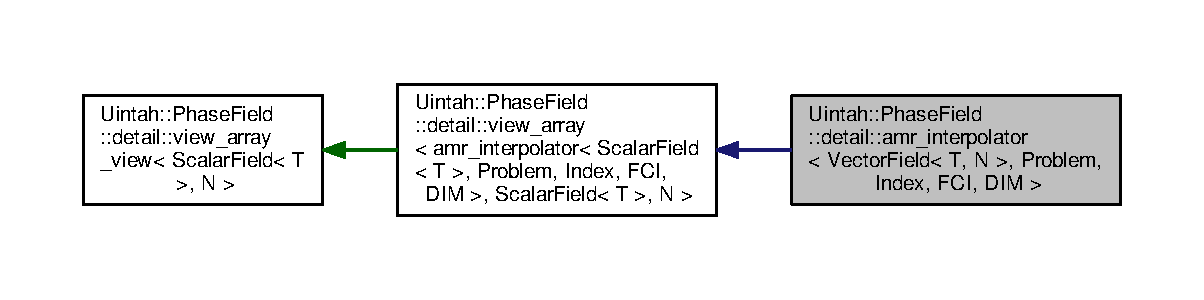
\includegraphics[width=350pt]{classUintah_1_1PhaseField_1_1detail_1_1amr__interpolator_3_01VectorField_3_01T_00_01N_01_4_00_01ab5f6a8bab1985b8dc10c54b9c0965b3}
\end{center}
\end{figure}


Collaboration diagram for Uintah\+:\+:Phase\+Field\+:\+:detail\+:\+:amr\+\_\+interpolator$<$ Vector\+Field$<$ T, N $>$, Problem, Index, F\+CI, D\+IM $>$\+:\nopagebreak
\begin{figure}[H]
\begin{center}
\leavevmode
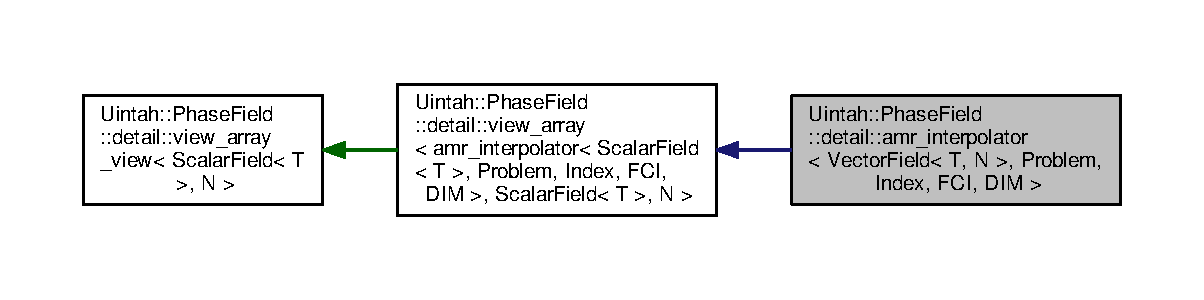
\includegraphics[width=350pt]{classUintah_1_1PhaseField_1_1detail_1_1amr__interpolator_3_01VectorField_3_01T_00_01N_01_4_00_013a4e3ec9316ef55d5c97281d51aeaa69}
\end{center}
\end{figure}
\subsection*{Public Member Functions}
\begin{DoxyCompactItemize}
\item 
\hyperlink{classUintah_1_1PhaseField_1_1detail_1_1amr__interpolator_3_01VectorField_3_01T_00_01N_01_4_00_01ab3739ebd28e1ffb5bc0b138cfaddd80_affa96f42d4c838acc9a94dd0c5fc4d33}{amr\+\_\+interpolator} (const typename \hyperlink{structUintah_1_1PhaseField_1_1VectorField_a59698346336d8cdfdf767367839f2be9}{Field\+::label\+\_\+type} \&label, const Var\+Label $\ast$subproblems\+\_\+label, int material)
\begin{DoxyCompactList}\small\item\em Constructor. \end{DoxyCompactList}\item 
\hyperlink{classUintah_1_1PhaseField_1_1detail_1_1amr__interpolator_3_01VectorField_3_01T_00_01N_01_4_00_01ab3739ebd28e1ffb5bc0b138cfaddd80_ab5cb32ce1a86a80d7b16ba06b42a2e1d}{amr\+\_\+interpolator} (Data\+Warehouse $\ast$dw, const typename \hyperlink{structUintah_1_1PhaseField_1_1VectorField_a59698346336d8cdfdf767367839f2be9}{Field\+::label\+\_\+type} \&label, const Var\+Label $\ast$subproblems\+\_\+label, int material, const Patch $\ast$patch, bool use\+\_\+ghosts=View\+::use\+\_\+ghosts\+\_\+dflt)
\begin{DoxyCompactList}\small\item\em Constructor. \end{DoxyCompactList}\item 
virtual \hyperlink{classUintah_1_1PhaseField_1_1detail_1_1amr__interpolator_3_01VectorField_3_01T_00_01N_01_4_00_01ab3739ebd28e1ffb5bc0b138cfaddd80_afbe7bb3efbb058c4396e8e549b3cbcef}{$\sim$amr\+\_\+interpolator} ()
\begin{DoxyCompactList}\small\item\em Destructor. \end{DoxyCompactList}\item 
\hyperlink{classUintah_1_1PhaseField_1_1detail_1_1amr__interpolator_3_01VectorField_3_01T_00_01N_01_4_00_01ab3739ebd28e1ffb5bc0b138cfaddd80_a1f75287ee5fc8828e84fa530fb779e47}{amr\+\_\+interpolator} (const \hyperlink{classUintah_1_1PhaseField_1_1detail_1_1amr__interpolator}{amr\+\_\+interpolator} \&)=delete
\begin{DoxyCompactList}\small\item\em Prevent copy (and move) constructor. \end{DoxyCompactList}\item 
\hyperlink{classUintah_1_1PhaseField_1_1detail_1_1amr__interpolator}{amr\+\_\+interpolator} \& \hyperlink{classUintah_1_1PhaseField_1_1detail_1_1amr__interpolator_3_01VectorField_3_01T_00_01N_01_4_00_01ab3739ebd28e1ffb5bc0b138cfaddd80_aadd32c026392c0a152d1704b0ae69bd1}{operator=} (const \hyperlink{classUintah_1_1PhaseField_1_1detail_1_1amr__interpolator}{amr\+\_\+interpolator} \&)=delete
\begin{DoxyCompactList}\small\item\em Prevent copy (and move) assignment. \end{DoxyCompactList}\end{DoxyCompactItemize}
\subsection*{Additional Inherited Members}


\subsection{Detailed Description}
\subsubsection*{template$<$typename T, size\+\_\+t N, typename Problem, typename Index, F\+C\+I\+Type F\+CI, Dim\+Type D\+IM$>$\newline
class Uintah\+::\+Phase\+Field\+::detail\+::amr\+\_\+interpolator$<$ Vector\+Field$<$ T, N $>$, Problem, Index, F\+C\+I, D\+I\+M $>$}

Abstract wrapper of grid variables for interpolation from coarser to finer levels. (\hyperlink{structUintah_1_1PhaseField_1_1VectorField}{Vector\+Field} implementation) 

Adds to view the possibility to compute multi-\/grid interpolation


\begin{DoxyTemplParams}{Template Parameters}
{\em T} & type of each component of the field at each point \\
\hline
{\em N} & number of components \\
\hline
{\em \hyperlink{classUintah_1_1PhaseField_1_1Problem}{Problem}} & type of \hyperlink{namespaceUintah_1_1PhaseField}{Phase\+Field} problem \\
\hline
{\em Index} & index\+\_\+sequence of Field within \hyperlink{classUintah_1_1PhaseField_1_1Problem}{Problem} (first element is variable index, following ones, if present, are the component index within the variable) \\
\hline
\end{DoxyTemplParams}


\subsection{Constructor \& Destructor Documentation}
\mbox{\Hypertarget{classUintah_1_1PhaseField_1_1detail_1_1amr__interpolator_3_01VectorField_3_01T_00_01N_01_4_00_01ab3739ebd28e1ffb5bc0b138cfaddd80_affa96f42d4c838acc9a94dd0c5fc4d33}\label{classUintah_1_1PhaseField_1_1detail_1_1amr__interpolator_3_01VectorField_3_01T_00_01N_01_4_00_01ab3739ebd28e1ffb5bc0b138cfaddd80_affa96f42d4c838acc9a94dd0c5fc4d33}} 
\index{Uintah\+::\+Phase\+Field\+::detail\+::amr\+\_\+interpolator$<$ Vector\+Field$<$ T, N $>$, Problem, Index, F\+C\+I, D\+I\+M $>$@{Uintah\+::\+Phase\+Field\+::detail\+::amr\+\_\+interpolator$<$ Vector\+Field$<$ T, N $>$, Problem, Index, F\+C\+I, D\+I\+M $>$}!amr\+\_\+interpolator@{amr\+\_\+interpolator}}
\index{amr\+\_\+interpolator@{amr\+\_\+interpolator}!Uintah\+::\+Phase\+Field\+::detail\+::amr\+\_\+interpolator$<$ Vector\+Field$<$ T, N $>$, Problem, Index, F\+C\+I, D\+I\+M $>$@{Uintah\+::\+Phase\+Field\+::detail\+::amr\+\_\+interpolator$<$ Vector\+Field$<$ T, N $>$, Problem, Index, F\+C\+I, D\+I\+M $>$}}
\subsubsection{\texorpdfstring{amr\+\_\+interpolator()}{amr\_interpolator()}\hspace{0.1cm}{\footnotesize\ttfamily [1/3]}}
{\footnotesize\ttfamily template$<$typename T , size\+\_\+t N, typename Problem , typename Index , F\+C\+I\+Type F\+CI, Dim\+Type D\+IM$>$ \\
\hyperlink{classUintah_1_1PhaseField_1_1detail_1_1amr__interpolator}{Uintah\+::\+Phase\+Field\+::detail\+::amr\+\_\+interpolator}$<$ \hyperlink{structUintah_1_1PhaseField_1_1VectorField}{Vector\+Field}$<$ T, N $>$, \hyperlink{classUintah_1_1PhaseField_1_1Problem}{Problem}, Index, F\+CI, D\+IM $>$\+::\hyperlink{classUintah_1_1PhaseField_1_1detail_1_1amr__interpolator}{amr\+\_\+interpolator} (\begin{DoxyParamCaption}\item[{const typename \hyperlink{structUintah_1_1PhaseField_1_1VectorField_a59698346336d8cdfdf767367839f2be9}{Field\+::label\+\_\+type} \&}]{label,  }\item[{const Var\+Label $\ast$}]{subproblems\+\_\+label,  }\item[{int}]{material }\end{DoxyParamCaption})\hspace{0.3cm}{\ttfamily [inline]}}



Constructor. 

Instantiate \hyperlink{classUintah_1_1PhaseField_1_1detail_1_1amr__interpolator}{amr\+\_\+interpolator} components without gathering info from the Data\+Warehouse


\begin{DoxyParams}{Parameters}
{\em label} & list of variable labels for each component \\
\hline
{\em subproblems\+\_\+label} & label of subproblems in the Data\+Warehouse \\
\hline
{\em material} & material index \\
\hline
\end{DoxyParams}
\mbox{\Hypertarget{classUintah_1_1PhaseField_1_1detail_1_1amr__interpolator_3_01VectorField_3_01T_00_01N_01_4_00_01ab3739ebd28e1ffb5bc0b138cfaddd80_ab5cb32ce1a86a80d7b16ba06b42a2e1d}\label{classUintah_1_1PhaseField_1_1detail_1_1amr__interpolator_3_01VectorField_3_01T_00_01N_01_4_00_01ab3739ebd28e1ffb5bc0b138cfaddd80_ab5cb32ce1a86a80d7b16ba06b42a2e1d}} 
\index{Uintah\+::\+Phase\+Field\+::detail\+::amr\+\_\+interpolator$<$ Vector\+Field$<$ T, N $>$, Problem, Index, F\+C\+I, D\+I\+M $>$@{Uintah\+::\+Phase\+Field\+::detail\+::amr\+\_\+interpolator$<$ Vector\+Field$<$ T, N $>$, Problem, Index, F\+C\+I, D\+I\+M $>$}!amr\+\_\+interpolator@{amr\+\_\+interpolator}}
\index{amr\+\_\+interpolator@{amr\+\_\+interpolator}!Uintah\+::\+Phase\+Field\+::detail\+::amr\+\_\+interpolator$<$ Vector\+Field$<$ T, N $>$, Problem, Index, F\+C\+I, D\+I\+M $>$@{Uintah\+::\+Phase\+Field\+::detail\+::amr\+\_\+interpolator$<$ Vector\+Field$<$ T, N $>$, Problem, Index, F\+C\+I, D\+I\+M $>$}}
\subsubsection{\texorpdfstring{amr\+\_\+interpolator()}{amr\_interpolator()}\hspace{0.1cm}{\footnotesize\ttfamily [2/3]}}
{\footnotesize\ttfamily template$<$typename T , size\+\_\+t N, typename Problem , typename Index , F\+C\+I\+Type F\+CI, Dim\+Type D\+IM$>$ \\
\hyperlink{classUintah_1_1PhaseField_1_1detail_1_1amr__interpolator}{Uintah\+::\+Phase\+Field\+::detail\+::amr\+\_\+interpolator}$<$ \hyperlink{structUintah_1_1PhaseField_1_1VectorField}{Vector\+Field}$<$ T, N $>$, \hyperlink{classUintah_1_1PhaseField_1_1Problem}{Problem}, Index, F\+CI, D\+IM $>$\+::\hyperlink{classUintah_1_1PhaseField_1_1detail_1_1amr__interpolator}{amr\+\_\+interpolator} (\begin{DoxyParamCaption}\item[{Data\+Warehouse $\ast$}]{dw,  }\item[{const typename \hyperlink{structUintah_1_1PhaseField_1_1VectorField_a59698346336d8cdfdf767367839f2be9}{Field\+::label\+\_\+type} \&}]{label,  }\item[{const Var\+Label $\ast$}]{subproblems\+\_\+label,  }\item[{int}]{material,  }\item[{const Patch $\ast$}]{patch,  }\item[{bool}]{use\+\_\+ghosts = {\ttfamily View\+:\+:use\+\_\+ghosts\+\_\+dflt} }\end{DoxyParamCaption})\hspace{0.3cm}{\ttfamily [inline]}}



Constructor. 

Instantiate \hyperlink{classUintah_1_1PhaseField_1_1detail_1_1amr__interpolator}{amr\+\_\+interpolator} components and gather info from dw


\begin{DoxyParams}{Parameters}
{\em dw} & Data\+Warehouse from which data is retrieved \\
\hline
{\em label} & list of variable labels for each component \\
\hline
{\em subproblems\+\_\+label} & label of subproblems in the Data\+Warehouse \\
\hline
{\em material} & material index \\
\hline
{\em patch} & grid patch \\
\hline
{\em use\+\_\+ghosts} & if ghosts value are to be retrieved \\
\hline
\end{DoxyParams}
\mbox{\Hypertarget{classUintah_1_1PhaseField_1_1detail_1_1amr__interpolator_3_01VectorField_3_01T_00_01N_01_4_00_01ab3739ebd28e1ffb5bc0b138cfaddd80_afbe7bb3efbb058c4396e8e549b3cbcef}\label{classUintah_1_1PhaseField_1_1detail_1_1amr__interpolator_3_01VectorField_3_01T_00_01N_01_4_00_01ab3739ebd28e1ffb5bc0b138cfaddd80_afbe7bb3efbb058c4396e8e549b3cbcef}} 
\index{Uintah\+::\+Phase\+Field\+::detail\+::amr\+\_\+interpolator$<$ Vector\+Field$<$ T, N $>$, Problem, Index, F\+C\+I, D\+I\+M $>$@{Uintah\+::\+Phase\+Field\+::detail\+::amr\+\_\+interpolator$<$ Vector\+Field$<$ T, N $>$, Problem, Index, F\+C\+I, D\+I\+M $>$}!````~amr\+\_\+interpolator@{$\sim$amr\+\_\+interpolator}}
\index{````~amr\+\_\+interpolator@{$\sim$amr\+\_\+interpolator}!Uintah\+::\+Phase\+Field\+::detail\+::amr\+\_\+interpolator$<$ Vector\+Field$<$ T, N $>$, Problem, Index, F\+C\+I, D\+I\+M $>$@{Uintah\+::\+Phase\+Field\+::detail\+::amr\+\_\+interpolator$<$ Vector\+Field$<$ T, N $>$, Problem, Index, F\+C\+I, D\+I\+M $>$}}
\subsubsection{\texorpdfstring{$\sim$amr\+\_\+interpolator()}{~amr\_interpolator()}}
{\footnotesize\ttfamily template$<$typename T , size\+\_\+t N, typename Problem , typename Index , F\+C\+I\+Type F\+CI, Dim\+Type D\+IM$>$ \\
virtual \hyperlink{classUintah_1_1PhaseField_1_1detail_1_1amr__interpolator}{Uintah\+::\+Phase\+Field\+::detail\+::amr\+\_\+interpolator}$<$ \hyperlink{structUintah_1_1PhaseField_1_1VectorField}{Vector\+Field}$<$ T, N $>$, \hyperlink{classUintah_1_1PhaseField_1_1Problem}{Problem}, Index, F\+CI, D\+IM $>$\+::$\sim$\hyperlink{classUintah_1_1PhaseField_1_1detail_1_1amr__interpolator}{amr\+\_\+interpolator} (\begin{DoxyParamCaption}{ }\end{DoxyParamCaption})\hspace{0.3cm}{\ttfamily [inline]}, {\ttfamily [virtual]}}



Destructor. 

\mbox{\Hypertarget{classUintah_1_1PhaseField_1_1detail_1_1amr__interpolator_3_01VectorField_3_01T_00_01N_01_4_00_01ab3739ebd28e1ffb5bc0b138cfaddd80_a1f75287ee5fc8828e84fa530fb779e47}\label{classUintah_1_1PhaseField_1_1detail_1_1amr__interpolator_3_01VectorField_3_01T_00_01N_01_4_00_01ab3739ebd28e1ffb5bc0b138cfaddd80_a1f75287ee5fc8828e84fa530fb779e47}} 
\index{Uintah\+::\+Phase\+Field\+::detail\+::amr\+\_\+interpolator$<$ Vector\+Field$<$ T, N $>$, Problem, Index, F\+C\+I, D\+I\+M $>$@{Uintah\+::\+Phase\+Field\+::detail\+::amr\+\_\+interpolator$<$ Vector\+Field$<$ T, N $>$, Problem, Index, F\+C\+I, D\+I\+M $>$}!amr\+\_\+interpolator@{amr\+\_\+interpolator}}
\index{amr\+\_\+interpolator@{amr\+\_\+interpolator}!Uintah\+::\+Phase\+Field\+::detail\+::amr\+\_\+interpolator$<$ Vector\+Field$<$ T, N $>$, Problem, Index, F\+C\+I, D\+I\+M $>$@{Uintah\+::\+Phase\+Field\+::detail\+::amr\+\_\+interpolator$<$ Vector\+Field$<$ T, N $>$, Problem, Index, F\+C\+I, D\+I\+M $>$}}
\subsubsection{\texorpdfstring{amr\+\_\+interpolator()}{amr\_interpolator()}\hspace{0.1cm}{\footnotesize\ttfamily [3/3]}}
{\footnotesize\ttfamily template$<$typename T , size\+\_\+t N, typename Problem , typename Index , F\+C\+I\+Type F\+CI, Dim\+Type D\+IM$>$ \\
\hyperlink{classUintah_1_1PhaseField_1_1detail_1_1amr__interpolator}{Uintah\+::\+Phase\+Field\+::detail\+::amr\+\_\+interpolator}$<$ \hyperlink{structUintah_1_1PhaseField_1_1VectorField}{Vector\+Field}$<$ T, N $>$, \hyperlink{classUintah_1_1PhaseField_1_1Problem}{Problem}, Index, F\+CI, D\+IM $>$\+::\hyperlink{classUintah_1_1PhaseField_1_1detail_1_1amr__interpolator}{amr\+\_\+interpolator} (\begin{DoxyParamCaption}\item[{const \hyperlink{classUintah_1_1PhaseField_1_1detail_1_1amr__interpolator}{amr\+\_\+interpolator}$<$ \hyperlink{structUintah_1_1PhaseField_1_1VectorField}{Vector\+Field}$<$ T, N $>$, \hyperlink{classUintah_1_1PhaseField_1_1Problem}{Problem}, Index, F\+CI, D\+IM $>$ \&}]{ }\end{DoxyParamCaption})\hspace{0.3cm}{\ttfamily [delete]}}



Prevent copy (and move) constructor. 



\subsection{Member Function Documentation}
\mbox{\Hypertarget{classUintah_1_1PhaseField_1_1detail_1_1amr__interpolator_3_01VectorField_3_01T_00_01N_01_4_00_01ab3739ebd28e1ffb5bc0b138cfaddd80_aadd32c026392c0a152d1704b0ae69bd1}\label{classUintah_1_1PhaseField_1_1detail_1_1amr__interpolator_3_01VectorField_3_01T_00_01N_01_4_00_01ab3739ebd28e1ffb5bc0b138cfaddd80_aadd32c026392c0a152d1704b0ae69bd1}} 
\index{Uintah\+::\+Phase\+Field\+::detail\+::amr\+\_\+interpolator$<$ Vector\+Field$<$ T, N $>$, Problem, Index, F\+C\+I, D\+I\+M $>$@{Uintah\+::\+Phase\+Field\+::detail\+::amr\+\_\+interpolator$<$ Vector\+Field$<$ T, N $>$, Problem, Index, F\+C\+I, D\+I\+M $>$}!operator=@{operator=}}
\index{operator=@{operator=}!Uintah\+::\+Phase\+Field\+::detail\+::amr\+\_\+interpolator$<$ Vector\+Field$<$ T, N $>$, Problem, Index, F\+C\+I, D\+I\+M $>$@{Uintah\+::\+Phase\+Field\+::detail\+::amr\+\_\+interpolator$<$ Vector\+Field$<$ T, N $>$, Problem, Index, F\+C\+I, D\+I\+M $>$}}
\subsubsection{\texorpdfstring{operator=()}{operator=()}}
{\footnotesize\ttfamily template$<$typename T , size\+\_\+t N, typename Problem , typename Index , F\+C\+I\+Type F\+CI, Dim\+Type D\+IM$>$ \\
\hyperlink{classUintah_1_1PhaseField_1_1detail_1_1amr__interpolator}{amr\+\_\+interpolator}\& \hyperlink{classUintah_1_1PhaseField_1_1detail_1_1amr__interpolator}{Uintah\+::\+Phase\+Field\+::detail\+::amr\+\_\+interpolator}$<$ \hyperlink{structUintah_1_1PhaseField_1_1VectorField}{Vector\+Field}$<$ T, N $>$, \hyperlink{classUintah_1_1PhaseField_1_1Problem}{Problem}, Index, F\+CI, D\+IM $>$\+::operator= (\begin{DoxyParamCaption}\item[{const \hyperlink{classUintah_1_1PhaseField_1_1detail_1_1amr__interpolator}{amr\+\_\+interpolator}$<$ \hyperlink{structUintah_1_1PhaseField_1_1VectorField}{Vector\+Field}$<$ T, N $>$, \hyperlink{classUintah_1_1PhaseField_1_1Problem}{Problem}, Index, F\+CI, D\+IM $>$ \&}]{ }\end{DoxyParamCaption})\hspace{0.3cm}{\ttfamily [delete]}}



Prevent copy (and move) assignment. 



The documentation for this class was generated from the following file\+:\begin{DoxyCompactItemize}
\item 
\hyperlink{amr__interpolator_8h}{amr\+\_\+interpolator.\+h}\end{DoxyCompactItemize}

\hypertarget{classUintah_1_1PhaseField_1_1detail_1_1amr__restrictor}{}\section{Uintah\+:\+:Phase\+Field\+:\+:detail\+:\+:amr\+\_\+restrictor$<$ Field, Problem, Index, F\+CI, V\+AR $>$ Class Template Reference}
\label{classUintah_1_1PhaseField_1_1detail_1_1amr__restrictor}\index{Uintah\+::\+Phase\+Field\+::detail\+::amr\+\_\+restrictor$<$ Field, Problem, Index, F\+C\+I, V\+A\+R $>$@{Uintah\+::\+Phase\+Field\+::detail\+::amr\+\_\+restrictor$<$ Field, Problem, Index, F\+C\+I, V\+A\+R $>$}}


Abstract wrapper of grid variables for restriction from finer to coarser levels.  




{\ttfamily \#include $<$amr\+\_\+restrictor.\+h$>$}



Inheritance diagram for Uintah\+:\+:Phase\+Field\+:\+:detail\+:\+:amr\+\_\+restrictor$<$ Field, Problem, Index, F\+CI, V\+AR $>$\+:\nopagebreak
\begin{figure}[H]
\begin{center}
\leavevmode
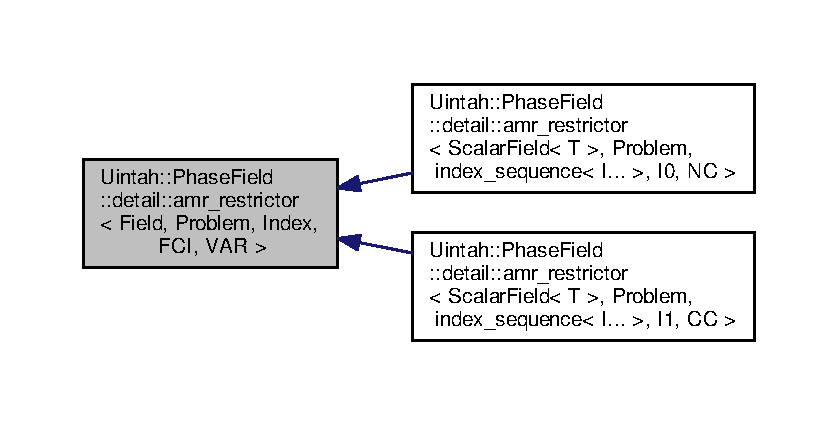
\includegraphics[width=350pt]{classUintah_1_1PhaseField_1_1detail_1_1amr__restrictor__inherit__graph}
\end{center}
\end{figure}


\subsection{Detailed Description}
\subsubsection*{template$<$typename Field, typename Problem, typename Index, F\+C\+I\+Type F\+CI, Var\+Type V\+AR$>$\newline
class Uintah\+::\+Phase\+Field\+::detail\+::amr\+\_\+restrictor$<$ Field, Problem, Index, F\+C\+I, V\+A\+R $>$}

Abstract wrapper of grid variables for restriction from finer to coarser levels. 

Adds to view the possibility to compute multi-\/grid restriction

\begin{DoxyRemark}{Remarks}
All different restriction strategies must specialize this class and implement the view$<$ T $>$ class
\end{DoxyRemark}

\begin{DoxyTemplParams}{Template Parameters}
{\em Field} & type of Field (should be only \hyperlink{structUintah_1_1PhaseField_1_1ScalarField}{Scalar\+Field}) \\
\hline
{\em \hyperlink{classUintah_1_1PhaseField_1_1Problem}{Problem}} & type of \hyperlink{namespaceUintah_1_1PhaseField}{Phase\+Field} problem \\
\hline
{\em Index} & index\+\_\+sequence of Field within \hyperlink{classUintah_1_1PhaseField_1_1Problem}{Problem} (first element is variable index, following ones, if present, are the component index within the variable) \\
\hline
\end{DoxyTemplParams}


The documentation for this class was generated from the following file\+:\begin{DoxyCompactItemize}
\item 
\hyperlink{amr__restrictor_8h}{amr\+\_\+restrictor.\+h}\end{DoxyCompactItemize}

\hypertarget{classUintah_1_1PhaseField_1_1detail_1_1amr__restrictor_3_01ScalarField_3_01T_01_4_00_01Problem_05760ee5d1d3adcc969b3f56f71e72acb}{}\section{Uintah\+:\+:Phase\+Field\+:\+:detail\+:\+:amr\+\_\+restrictor$<$ Scalar\+Field$<$ T $>$, Problem, index\+\_\+sequence$<$ I... $>$, I0, NC $>$ Class Template Reference}
\label{classUintah_1_1PhaseField_1_1detail_1_1amr__restrictor_3_01ScalarField_3_01T_01_4_00_01Problem_05760ee5d1d3adcc969b3f56f71e72acb}\index{Uintah\+::\+Phase\+Field\+::detail\+::amr\+\_\+restrictor$<$ Scalar\+Field$<$ T $>$, Problem, index\+\_\+sequence$<$ I... $>$, I0, N\+C $>$@{Uintah\+::\+Phase\+Field\+::detail\+::amr\+\_\+restrictor$<$ Scalar\+Field$<$ T $>$, Problem, index\+\_\+sequence$<$ I... $>$, I0, N\+C $>$}}


Wrapper of grid variables for restriction from finer to coarser levels (node-\/centered piecewise constant implementation)  




{\ttfamily \#include $<$amr\+\_\+restrictor\+\_\+\+I0\+\_\+\+N\+C.\+h$>$}



Inheritance diagram for Uintah\+:\+:Phase\+Field\+:\+:detail\+:\+:amr\+\_\+restrictor$<$ Scalar\+Field$<$ T $>$, Problem, index\+\_\+sequence$<$ I... $>$, I0, NC $>$\+:\nopagebreak
\begin{figure}[H]
\begin{center}
\leavevmode
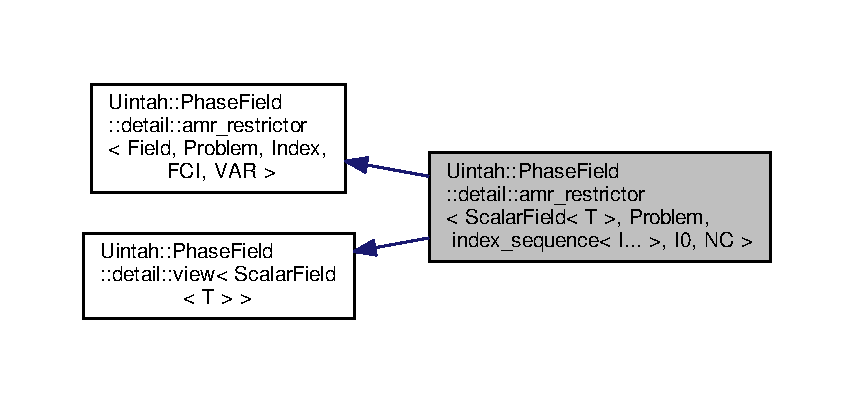
\includegraphics[width=350pt]{classUintah_1_1PhaseField_1_1detail_1_1amr__restrictor_3_01ScalarField_3_01T_01_4_00_01Problem_0df32558d588a2dddebce5cf93a5b29cf}
\end{center}
\end{figure}


Collaboration diagram for Uintah\+:\+:Phase\+Field\+:\+:detail\+:\+:amr\+\_\+restrictor$<$ Scalar\+Field$<$ T $>$, Problem, index\+\_\+sequence$<$ I... $>$, I0, NC $>$\+:\nopagebreak
\begin{figure}[H]
\begin{center}
\leavevmode
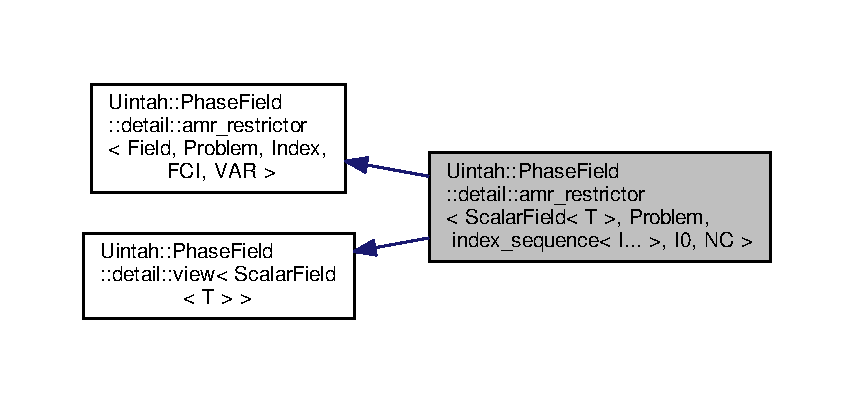
\includegraphics[width=350pt]{classUintah_1_1PhaseField_1_1detail_1_1amr__restrictor_3_01ScalarField_3_01T_01_4_00_01Problem_01f60fd6bddea2818dfc4c8616cecbd87}
\end{center}
\end{figure}
\subsection*{Public Member Functions}
\begin{DoxyCompactItemize}
\item 
\hyperlink{classUintah_1_1PhaseField_1_1detail_1_1amr__restrictor_3_01ScalarField_3_01T_01_4_00_01Problem_05760ee5d1d3adcc969b3f56f71e72acb_adc68b10aa0ea3669167e75e848315f69}{amr\+\_\+restrictor} (const Var\+Label $\ast$label, const Var\+Label $\ast$subproblems\+\_\+label, int material)
\begin{DoxyCompactList}\small\item\em construct restrictor without retrieving inner variable data from the Data\+Warehouse \end{DoxyCompactList}\item 
\hyperlink{classUintah_1_1PhaseField_1_1detail_1_1amr__restrictor_3_01ScalarField_3_01T_01_4_00_01Problem_05760ee5d1d3adcc969b3f56f71e72acb_aecb2d88122a1adaae4560445ee13eaed}{amr\+\_\+restrictor} (Data\+Warehouse $\ast$dw, const Var\+Label $\ast$label, const Var\+Label $\ast$subproblems\+\_\+label, int material, const Patch $\ast$patch, bool use\+\_\+ghosts=\hyperlink{classUintah_1_1PhaseField_1_1detail_1_1amr__restrictor_3_01ScalarField_3_01T_01_4_00_01Problem_05760ee5d1d3adcc969b3f56f71e72acb_a1579c120a731bc2c5e5d53a3e3db51dc}{use\+\_\+ghosts\+\_\+dflt})
\begin{DoxyCompactList}\small\item\em construct interpolator and retrieve inner variable data from the Data\+Warehouse whitin a given fine patch. \end{DoxyCompactList}\item 
virtual \hyperlink{classUintah_1_1PhaseField_1_1detail_1_1amr__restrictor_3_01ScalarField_3_01T_01_4_00_01Problem_05760ee5d1d3adcc969b3f56f71e72acb_a2b82f57cc6e6034d4ce47be7d9df29f7}{$\sim$amr\+\_\+restrictor} ()
\begin{DoxyCompactList}\small\item\em Destructor. \end{DoxyCompactList}\item 
\hyperlink{classUintah_1_1PhaseField_1_1detail_1_1amr__restrictor_3_01ScalarField_3_01T_01_4_00_01Problem_05760ee5d1d3adcc969b3f56f71e72acb_a9dd4c58f76077456452653c0cf793955}{amr\+\_\+restrictor} (const \hyperlink{classUintah_1_1PhaseField_1_1detail_1_1amr__restrictor}{amr\+\_\+restrictor} \&)=delete
\begin{DoxyCompactList}\small\item\em Prevent copy (and move) constructor. \end{DoxyCompactList}\item 
\hyperlink{classUintah_1_1PhaseField_1_1detail_1_1amr__restrictor}{amr\+\_\+restrictor} \& \hyperlink{classUintah_1_1PhaseField_1_1detail_1_1amr__restrictor_3_01ScalarField_3_01T_01_4_00_01Problem_05760ee5d1d3adcc969b3f56f71e72acb_ae1d3846e6970b38ddf48c6abc6327ea2}{operator=} (const \hyperlink{classUintah_1_1PhaseField_1_1detail_1_1amr__restrictor}{amr\+\_\+restrictor} \&)=delete
\begin{DoxyCompactList}\small\item\em Prevent copy (and move) assignment. \end{DoxyCompactList}\item 
virtual void \hyperlink{classUintah_1_1PhaseField_1_1detail_1_1amr__restrictor_3_01ScalarField_3_01T_01_4_00_01Problem_05760ee5d1d3adcc969b3f56f71e72acb_aa937cac548dc6bb5ebda0907804d5434}{set} (Data\+Warehouse $\ast$dw, const Patch $\ast$patch, bool use\+\_\+ghosts=\hyperlink{classUintah_1_1PhaseField_1_1detail_1_1amr__restrictor_3_01ScalarField_3_01T_01_4_00_01Problem_05760ee5d1d3adcc969b3f56f71e72acb_a1579c120a731bc2c5e5d53a3e3db51dc}{use\+\_\+ghosts\+\_\+dflt}) override
\begin{DoxyCompactList}\small\item\em retrieve inner variable data from the Data\+Warehouse whitin a given patch. \end{DoxyCompactList}\item 
virtual void \hyperlink{classUintah_1_1PhaseField_1_1detail_1_1amr__restrictor_3_01ScalarField_3_01T_01_4_00_01Problem_05760ee5d1d3adcc969b3f56f71e72acb_a71f5fbbdd3e56e753d19c1d65f5c8467}{set} (Data\+Warehouse $\ast$dw, const Level $\ast$level, const Int\+Vector \&low, const Int\+Vector \&high, bool use\+\_\+ghosts=\hyperlink{classUintah_1_1PhaseField_1_1detail_1_1amr__restrictor_3_01ScalarField_3_01T_01_4_00_01Problem_05760ee5d1d3adcc969b3f56f71e72acb_a1579c120a731bc2c5e5d53a3e3db51dc}{use\+\_\+ghosts\+\_\+dflt}) override
\begin{DoxyCompactList}\small\item\em retrieve inner variable data from the Data\+Warehouse whitin a given region. \end{DoxyCompactList}\item 
virtual \hyperlink{classUintah_1_1PhaseField_1_1detail_1_1view}{view}$<$ \hyperlink{structUintah_1_1PhaseField_1_1ScalarField}{Field} $>$ $\ast$ \hyperlink{classUintah_1_1PhaseField_1_1detail_1_1amr__restrictor_3_01ScalarField_3_01T_01_4_00_01Problem_05760ee5d1d3adcc969b3f56f71e72acb_a7756f69a970700829f04886c454a4b18}{clone} (bool deep) const override
\begin{DoxyCompactList}\small\item\em Get a copy of the view. \end{DoxyCompactList}\item 
virtual \hyperlink{classUintah_1_1PhaseField_1_1detail_1_1view}{view}$<$ \hyperlink{structUintah_1_1PhaseField_1_1ScalarField}{Field} $>$ $\ast$ \hyperlink{classUintah_1_1PhaseField_1_1detail_1_1amr__restrictor_3_01ScalarField_3_01T_01_4_00_01Problem_05760ee5d1d3adcc969b3f56f71e72acb_a81b7ca467a9a0f54f9bf37ca18038240}{clone} (bool deep, const Int\+Vector \&offset) const override
\begin{DoxyCompactList}\small\item\em Get a copy of the view and apply translate the support. \end{DoxyCompactList}\item 
virtual \hyperlink{classUintah_1_1PhaseField_1_1Support}{Support} \hyperlink{classUintah_1_1PhaseField_1_1detail_1_1amr__restrictor_3_01ScalarField_3_01T_01_4_00_01Problem_05760ee5d1d3adcc969b3f56f71e72acb_a5b7788432aecb51049ec0fdeefd90519}{get\+\_\+support} () const override
\begin{DoxyCompactList}\small\item\em get restrictor\textquotesingle{}s coarse range \end{DoxyCompactList}\item 
virtual bool \hyperlink{classUintah_1_1PhaseField_1_1detail_1_1amr__restrictor_3_01ScalarField_3_01T_01_4_00_01Problem_05760ee5d1d3adcc969b3f56f71e72acb_acb67236a4a7ecac027655ad592fff4ae}{is\+\_\+defined\+\_\+at} (const Int\+Vector \&id\+\_\+coarse) const override
\begin{DoxyCompactList}\small\item\em Check if the view has access to the coarse position with index id. \end{DoxyCompactList}\item 
virtual T \& \hyperlink{classUintah_1_1PhaseField_1_1detail_1_1amr__restrictor_3_01ScalarField_3_01T_01_4_00_01Problem_05760ee5d1d3adcc969b3f56f71e72acb_a900eab9c5c4f402881b207bb5270ebbc}{operator\mbox{[}$\,$\mbox{]}} (const Int\+Vector \&id) override
\begin{DoxyCompactList}\small\item\em Get/\+Modify value at position with index id (virtual implementation) \end{DoxyCompactList}\item 
virtual V \hyperlink{classUintah_1_1PhaseField_1_1detail_1_1amr__restrictor_3_01ScalarField_3_01T_01_4_00_01Problem_05760ee5d1d3adcc969b3f56f71e72acb_ab29b8c1e68dba955e6062c84adca2ef4}{operator\mbox{[}$\,$\mbox{]}} (const Int\+Vector \&id\+\_\+coarse) const override
\begin{DoxyCompactList}\small\item\em get restricted value \end{DoxyCompactList}\end{DoxyCompactItemize}
\subsection*{Static Public Attributes}
\begin{DoxyCompactItemize}
\item 
static constexpr bool \hyperlink{classUintah_1_1PhaseField_1_1detail_1_1amr__restrictor_3_01ScalarField_3_01T_01_4_00_01Problem_05760ee5d1d3adcc969b3f56f71e72acb_a1579c120a731bc2c5e5d53a3e3db51dc}{use\+\_\+ghosts\+\_\+dflt} = false
\begin{DoxyCompactList}\small\item\em Default value for use\+\_\+ghost when retrieving data. \end{DoxyCompactList}\end{DoxyCompactItemize}
\subsection*{Protected Member Functions}
\begin{DoxyCompactItemize}
\item 
\hyperlink{classUintah_1_1PhaseField_1_1detail_1_1amr__restrictor_3_01ScalarField_3_01T_01_4_00_01Problem_05760ee5d1d3adcc969b3f56f71e72acb_a9d8bbe1e77519c3e16e93d047a231da5}{amr\+\_\+restrictor} (const \hyperlink{classUintah_1_1PhaseField_1_1detail_1_1amr__restrictor}{amr\+\_\+restrictor} $\ast$copy, bool deep)
\begin{DoxyCompactList}\small\item\em Constructor. \end{DoxyCompactList}\end{DoxyCompactItemize}
\subsection*{Additional Inherited Members}


\subsection{Detailed Description}
\subsubsection*{template$<$typename T, typename Problem, size\+\_\+t... I$>$\newline
class Uintah\+::\+Phase\+Field\+::detail\+::amr\+\_\+restrictor$<$ Scalar\+Field$<$ T $>$, Problem, index\+\_\+sequence$<$ I... $>$, I0, N\+C $>$}

Wrapper of grid variables for restriction from finer to coarser levels (node-\/centered piecewise constant implementation) 

implements piecewise constant restriction of a variable from finer to coarser levels.


\begin{DoxyTemplParams}{Template Parameters}
{\em T} & variable data type (must be constant) \\
\hline
{\em \hyperlink{classUintah_1_1PhaseField_1_1Problem}{Problem}} & type of \hyperlink{namespaceUintah_1_1PhaseField}{Phase\+Field} problem \\
\hline
{\em \hyperlink{structUintah_1_1PhaseField_1_1I}{I}} & list of indices corresponding to the variable within the subproblems\\
\hline
\end{DoxyTemplParams}
$<$ F\+CI, V\+AR, D\+IM, T, \hyperlink{classUintah_1_1PhaseField_1_1Problem}{Problem}, \hyperlink{structUintah_1_1PhaseField_1_1I}{I} $>$ 

\subsection{Constructor \& Destructor Documentation}
\mbox{\Hypertarget{classUintah_1_1PhaseField_1_1detail_1_1amr__restrictor_3_01ScalarField_3_01T_01_4_00_01Problem_05760ee5d1d3adcc969b3f56f71e72acb_a9d8bbe1e77519c3e16e93d047a231da5}\label{classUintah_1_1PhaseField_1_1detail_1_1amr__restrictor_3_01ScalarField_3_01T_01_4_00_01Problem_05760ee5d1d3adcc969b3f56f71e72acb_a9d8bbe1e77519c3e16e93d047a231da5}} 
\index{Uintah\+::\+Phase\+Field\+::detail\+::amr\+\_\+restrictor$<$ Scalar\+Field$<$ T $>$, Problem, index\+\_\+sequence$<$ I... $>$, I0, N\+C $>$@{Uintah\+::\+Phase\+Field\+::detail\+::amr\+\_\+restrictor$<$ Scalar\+Field$<$ T $>$, Problem, index\+\_\+sequence$<$ I... $>$, I0, N\+C $>$}!amr\+\_\+restrictor@{amr\+\_\+restrictor}}
\index{amr\+\_\+restrictor@{amr\+\_\+restrictor}!Uintah\+::\+Phase\+Field\+::detail\+::amr\+\_\+restrictor$<$ Scalar\+Field$<$ T $>$, Problem, index\+\_\+sequence$<$ I... $>$, I0, N\+C $>$@{Uintah\+::\+Phase\+Field\+::detail\+::amr\+\_\+restrictor$<$ Scalar\+Field$<$ T $>$, Problem, index\+\_\+sequence$<$ I... $>$, I0, N\+C $>$}}
\subsubsection{\texorpdfstring{amr\+\_\+restrictor()}{amr\_restrictor()}\hspace{0.1cm}{\footnotesize\ttfamily [1/4]}}
{\footnotesize\ttfamily template$<$typename T , typename Problem , size\+\_\+t... I$>$ \\
\hyperlink{classUintah_1_1PhaseField_1_1detail_1_1amr__restrictor}{Uintah\+::\+Phase\+Field\+::detail\+::amr\+\_\+restrictor}$<$ \hyperlink{structUintah_1_1PhaseField_1_1ScalarField}{Scalar\+Field}$<$ T $>$, \hyperlink{classUintah_1_1PhaseField_1_1Problem}{Problem}, \hyperlink{namespaceUintah_1_1PhaseField_a237de804d99512e50613aff7c94a9461}{index\+\_\+sequence}$<$ I... $>$, \hyperlink{namespaceUintah_1_1PhaseField_a547ce3002aa97fbd3ef3192a6eec8406abdd8ebcbdfd71d1125937e3012dc45fb}{I0}, \hyperlink{namespaceUintah_1_1PhaseField_a33d355affda78a83f45755ba8388cedda77924170fe82bfd58b74ca3e44139718}{NC} $>$\+::\hyperlink{classUintah_1_1PhaseField_1_1detail_1_1amr__restrictor}{amr\+\_\+restrictor} (\begin{DoxyParamCaption}\item[{const \hyperlink{classUintah_1_1PhaseField_1_1detail_1_1amr__restrictor}{amr\+\_\+restrictor}$<$ \hyperlink{structUintah_1_1PhaseField_1_1ScalarField}{Scalar\+Field}$<$ T $>$, \hyperlink{classUintah_1_1PhaseField_1_1Problem}{Problem}, \hyperlink{namespaceUintah_1_1PhaseField_a237de804d99512e50613aff7c94a9461}{index\+\_\+sequence}$<$ I... $>$, \hyperlink{namespaceUintah_1_1PhaseField_a547ce3002aa97fbd3ef3192a6eec8406abdd8ebcbdfd71d1125937e3012dc45fb}{I0}, \hyperlink{namespaceUintah_1_1PhaseField_a33d355affda78a83f45755ba8388cedda77924170fe82bfd58b74ca3e44139718}{NC} $>$ $\ast$}]{copy,  }\item[{bool}]{deep }\end{DoxyParamCaption})\hspace{0.3cm}{\ttfamily [inline]}, {\ttfamily [protected]}}



Constructor. 

Instantiate a copy of a given view


\begin{DoxyParams}{Parameters}
{\em copy} & source view for copying \\
\hline
{\em deep} & if true inner grid variable is copied as well otherwise the same grid variable is referenced \\
\hline
\end{DoxyParams}
\mbox{\Hypertarget{classUintah_1_1PhaseField_1_1detail_1_1amr__restrictor_3_01ScalarField_3_01T_01_4_00_01Problem_05760ee5d1d3adcc969b3f56f71e72acb_adc68b10aa0ea3669167e75e848315f69}\label{classUintah_1_1PhaseField_1_1detail_1_1amr__restrictor_3_01ScalarField_3_01T_01_4_00_01Problem_05760ee5d1d3adcc969b3f56f71e72acb_adc68b10aa0ea3669167e75e848315f69}} 
\index{Uintah\+::\+Phase\+Field\+::detail\+::amr\+\_\+restrictor$<$ Scalar\+Field$<$ T $>$, Problem, index\+\_\+sequence$<$ I... $>$, I0, N\+C $>$@{Uintah\+::\+Phase\+Field\+::detail\+::amr\+\_\+restrictor$<$ Scalar\+Field$<$ T $>$, Problem, index\+\_\+sequence$<$ I... $>$, I0, N\+C $>$}!amr\+\_\+restrictor@{amr\+\_\+restrictor}}
\index{amr\+\_\+restrictor@{amr\+\_\+restrictor}!Uintah\+::\+Phase\+Field\+::detail\+::amr\+\_\+restrictor$<$ Scalar\+Field$<$ T $>$, Problem, index\+\_\+sequence$<$ I... $>$, I0, N\+C $>$@{Uintah\+::\+Phase\+Field\+::detail\+::amr\+\_\+restrictor$<$ Scalar\+Field$<$ T $>$, Problem, index\+\_\+sequence$<$ I... $>$, I0, N\+C $>$}}
\subsubsection{\texorpdfstring{amr\+\_\+restrictor()}{amr\_restrictor()}\hspace{0.1cm}{\footnotesize\ttfamily [2/4]}}
{\footnotesize\ttfamily template$<$typename T , typename Problem , size\+\_\+t... I$>$ \\
\hyperlink{classUintah_1_1PhaseField_1_1detail_1_1amr__restrictor}{Uintah\+::\+Phase\+Field\+::detail\+::amr\+\_\+restrictor}$<$ \hyperlink{structUintah_1_1PhaseField_1_1ScalarField}{Scalar\+Field}$<$ T $>$, \hyperlink{classUintah_1_1PhaseField_1_1Problem}{Problem}, \hyperlink{namespaceUintah_1_1PhaseField_a237de804d99512e50613aff7c94a9461}{index\+\_\+sequence}$<$ I... $>$, \hyperlink{namespaceUintah_1_1PhaseField_a547ce3002aa97fbd3ef3192a6eec8406abdd8ebcbdfd71d1125937e3012dc45fb}{I0}, \hyperlink{namespaceUintah_1_1PhaseField_a33d355affda78a83f45755ba8388cedda77924170fe82bfd58b74ca3e44139718}{NC} $>$\+::\hyperlink{classUintah_1_1PhaseField_1_1detail_1_1amr__restrictor}{amr\+\_\+restrictor} (\begin{DoxyParamCaption}\item[{const Var\+Label $\ast$}]{label,  }\item[{const Var\+Label $\ast$}]{subproblems\+\_\+label,  }\item[{int}]{material }\end{DoxyParamCaption})\hspace{0.3cm}{\ttfamily [inline]}}



construct restrictor without retrieving inner variable data from the Data\+Warehouse 


\begin{DoxyParams}{Parameters}
{\em label} & label of variable in the Data\+Warehouse \\
\hline
{\em subproblems\+\_\+label} & label of subproblems in the Data\+Warehouse \\
\hline
{\em material} & index of material in the Data\+Warehouse \\
\hline
\end{DoxyParams}
\mbox{\Hypertarget{classUintah_1_1PhaseField_1_1detail_1_1amr__restrictor_3_01ScalarField_3_01T_01_4_00_01Problem_05760ee5d1d3adcc969b3f56f71e72acb_aecb2d88122a1adaae4560445ee13eaed}\label{classUintah_1_1PhaseField_1_1detail_1_1amr__restrictor_3_01ScalarField_3_01T_01_4_00_01Problem_05760ee5d1d3adcc969b3f56f71e72acb_aecb2d88122a1adaae4560445ee13eaed}} 
\index{Uintah\+::\+Phase\+Field\+::detail\+::amr\+\_\+restrictor$<$ Scalar\+Field$<$ T $>$, Problem, index\+\_\+sequence$<$ I... $>$, I0, N\+C $>$@{Uintah\+::\+Phase\+Field\+::detail\+::amr\+\_\+restrictor$<$ Scalar\+Field$<$ T $>$, Problem, index\+\_\+sequence$<$ I... $>$, I0, N\+C $>$}!amr\+\_\+restrictor@{amr\+\_\+restrictor}}
\index{amr\+\_\+restrictor@{amr\+\_\+restrictor}!Uintah\+::\+Phase\+Field\+::detail\+::amr\+\_\+restrictor$<$ Scalar\+Field$<$ T $>$, Problem, index\+\_\+sequence$<$ I... $>$, I0, N\+C $>$@{Uintah\+::\+Phase\+Field\+::detail\+::amr\+\_\+restrictor$<$ Scalar\+Field$<$ T $>$, Problem, index\+\_\+sequence$<$ I... $>$, I0, N\+C $>$}}
\subsubsection{\texorpdfstring{amr\+\_\+restrictor()}{amr\_restrictor()}\hspace{0.1cm}{\footnotesize\ttfamily [3/4]}}
{\footnotesize\ttfamily template$<$typename T , typename Problem , size\+\_\+t... I$>$ \\
\hyperlink{classUintah_1_1PhaseField_1_1detail_1_1amr__restrictor}{Uintah\+::\+Phase\+Field\+::detail\+::amr\+\_\+restrictor}$<$ \hyperlink{structUintah_1_1PhaseField_1_1ScalarField}{Scalar\+Field}$<$ T $>$, \hyperlink{classUintah_1_1PhaseField_1_1Problem}{Problem}, \hyperlink{namespaceUintah_1_1PhaseField_a237de804d99512e50613aff7c94a9461}{index\+\_\+sequence}$<$ I... $>$, \hyperlink{namespaceUintah_1_1PhaseField_a547ce3002aa97fbd3ef3192a6eec8406abdd8ebcbdfd71d1125937e3012dc45fb}{I0}, \hyperlink{namespaceUintah_1_1PhaseField_a33d355affda78a83f45755ba8388cedda77924170fe82bfd58b74ca3e44139718}{NC} $>$\+::\hyperlink{classUintah_1_1PhaseField_1_1detail_1_1amr__restrictor}{amr\+\_\+restrictor} (\begin{DoxyParamCaption}\item[{Data\+Warehouse $\ast$}]{dw,  }\item[{const Var\+Label $\ast$}]{label,  }\item[{const Var\+Label $\ast$}]{subproblems\+\_\+label,  }\item[{int}]{material,  }\item[{const Patch $\ast$}]{patch,  }\item[{bool}]{use\+\_\+ghosts = {\ttfamily \hyperlink{classUintah_1_1PhaseField_1_1detail_1_1amr__restrictor_3_01ScalarField_3_01T_01_4_00_01Problem_05760ee5d1d3adcc969b3f56f71e72acb_a1579c120a731bc2c5e5d53a3e3db51dc}{use\+\_\+ghosts\+\_\+dflt}} }\end{DoxyParamCaption})\hspace{0.3cm}{\ttfamily [inline]}}



construct interpolator and retrieve inner variable data from the Data\+Warehouse whitin a given fine patch. 

the number of ghost cells/nodes and the corresponding region on the coarser level is automatically computed to match the interpolation type


\begin{DoxyParams}{Parameters}
{\em dw} & Data\+Warehouse which data is retrieved from \\
\hline
{\em label} & label of variable in the Data\+Warehouse \\
\hline
{\em subproblems\+\_\+label} & label of subproblems in the Data\+Warehouse \\
\hline
{\em material} & index of material in the Data\+Warehouse \\
\hline
{\em patch} & patch on which data is retrieved \\
\hline
{\em use\+\_\+ghosts} & if ghosts value are to be retrieved (must be false) \\
\hline
\end{DoxyParams}
\mbox{\Hypertarget{classUintah_1_1PhaseField_1_1detail_1_1amr__restrictor_3_01ScalarField_3_01T_01_4_00_01Problem_05760ee5d1d3adcc969b3f56f71e72acb_a2b82f57cc6e6034d4ce47be7d9df29f7}\label{classUintah_1_1PhaseField_1_1detail_1_1amr__restrictor_3_01ScalarField_3_01T_01_4_00_01Problem_05760ee5d1d3adcc969b3f56f71e72acb_a2b82f57cc6e6034d4ce47be7d9df29f7}} 
\index{Uintah\+::\+Phase\+Field\+::detail\+::amr\+\_\+restrictor$<$ Scalar\+Field$<$ T $>$, Problem, index\+\_\+sequence$<$ I... $>$, I0, N\+C $>$@{Uintah\+::\+Phase\+Field\+::detail\+::amr\+\_\+restrictor$<$ Scalar\+Field$<$ T $>$, Problem, index\+\_\+sequence$<$ I... $>$, I0, N\+C $>$}!````~amr\+\_\+restrictor@{$\sim$amr\+\_\+restrictor}}
\index{````~amr\+\_\+restrictor@{$\sim$amr\+\_\+restrictor}!Uintah\+::\+Phase\+Field\+::detail\+::amr\+\_\+restrictor$<$ Scalar\+Field$<$ T $>$, Problem, index\+\_\+sequence$<$ I... $>$, I0, N\+C $>$@{Uintah\+::\+Phase\+Field\+::detail\+::amr\+\_\+restrictor$<$ Scalar\+Field$<$ T $>$, Problem, index\+\_\+sequence$<$ I... $>$, I0, N\+C $>$}}
\subsubsection{\texorpdfstring{$\sim$amr\+\_\+restrictor()}{~amr\_restrictor()}}
{\footnotesize\ttfamily template$<$typename T , typename Problem , size\+\_\+t... I$>$ \\
virtual \hyperlink{classUintah_1_1PhaseField_1_1detail_1_1amr__restrictor}{Uintah\+::\+Phase\+Field\+::detail\+::amr\+\_\+restrictor}$<$ \hyperlink{structUintah_1_1PhaseField_1_1ScalarField}{Scalar\+Field}$<$ T $>$, \hyperlink{classUintah_1_1PhaseField_1_1Problem}{Problem}, \hyperlink{namespaceUintah_1_1PhaseField_a237de804d99512e50613aff7c94a9461}{index\+\_\+sequence}$<$ I... $>$, \hyperlink{namespaceUintah_1_1PhaseField_a547ce3002aa97fbd3ef3192a6eec8406abdd8ebcbdfd71d1125937e3012dc45fb}{I0}, \hyperlink{namespaceUintah_1_1PhaseField_a33d355affda78a83f45755ba8388cedda77924170fe82bfd58b74ca3e44139718}{NC} $>$\+::$\sim$\hyperlink{classUintah_1_1PhaseField_1_1detail_1_1amr__restrictor}{amr\+\_\+restrictor} (\begin{DoxyParamCaption}{ }\end{DoxyParamCaption})\hspace{0.3cm}{\ttfamily [inline]}, {\ttfamily [virtual]}}



Destructor. 

\mbox{\Hypertarget{classUintah_1_1PhaseField_1_1detail_1_1amr__restrictor_3_01ScalarField_3_01T_01_4_00_01Problem_05760ee5d1d3adcc969b3f56f71e72acb_a9dd4c58f76077456452653c0cf793955}\label{classUintah_1_1PhaseField_1_1detail_1_1amr__restrictor_3_01ScalarField_3_01T_01_4_00_01Problem_05760ee5d1d3adcc969b3f56f71e72acb_a9dd4c58f76077456452653c0cf793955}} 
\index{Uintah\+::\+Phase\+Field\+::detail\+::amr\+\_\+restrictor$<$ Scalar\+Field$<$ T $>$, Problem, index\+\_\+sequence$<$ I... $>$, I0, N\+C $>$@{Uintah\+::\+Phase\+Field\+::detail\+::amr\+\_\+restrictor$<$ Scalar\+Field$<$ T $>$, Problem, index\+\_\+sequence$<$ I... $>$, I0, N\+C $>$}!amr\+\_\+restrictor@{amr\+\_\+restrictor}}
\index{amr\+\_\+restrictor@{amr\+\_\+restrictor}!Uintah\+::\+Phase\+Field\+::detail\+::amr\+\_\+restrictor$<$ Scalar\+Field$<$ T $>$, Problem, index\+\_\+sequence$<$ I... $>$, I0, N\+C $>$@{Uintah\+::\+Phase\+Field\+::detail\+::amr\+\_\+restrictor$<$ Scalar\+Field$<$ T $>$, Problem, index\+\_\+sequence$<$ I... $>$, I0, N\+C $>$}}
\subsubsection{\texorpdfstring{amr\+\_\+restrictor()}{amr\_restrictor()}\hspace{0.1cm}{\footnotesize\ttfamily [4/4]}}
{\footnotesize\ttfamily template$<$typename T , typename Problem , size\+\_\+t... I$>$ \\
\hyperlink{classUintah_1_1PhaseField_1_1detail_1_1amr__restrictor}{Uintah\+::\+Phase\+Field\+::detail\+::amr\+\_\+restrictor}$<$ \hyperlink{structUintah_1_1PhaseField_1_1ScalarField}{Scalar\+Field}$<$ T $>$, \hyperlink{classUintah_1_1PhaseField_1_1Problem}{Problem}, \hyperlink{namespaceUintah_1_1PhaseField_a237de804d99512e50613aff7c94a9461}{index\+\_\+sequence}$<$ I... $>$, \hyperlink{namespaceUintah_1_1PhaseField_a547ce3002aa97fbd3ef3192a6eec8406abdd8ebcbdfd71d1125937e3012dc45fb}{I0}, \hyperlink{namespaceUintah_1_1PhaseField_a33d355affda78a83f45755ba8388cedda77924170fe82bfd58b74ca3e44139718}{NC} $>$\+::\hyperlink{classUintah_1_1PhaseField_1_1detail_1_1amr__restrictor}{amr\+\_\+restrictor} (\begin{DoxyParamCaption}\item[{const \hyperlink{classUintah_1_1PhaseField_1_1detail_1_1amr__restrictor}{amr\+\_\+restrictor}$<$ \hyperlink{structUintah_1_1PhaseField_1_1ScalarField}{Scalar\+Field}$<$ T $>$, \hyperlink{classUintah_1_1PhaseField_1_1Problem}{Problem}, \hyperlink{namespaceUintah_1_1PhaseField_a237de804d99512e50613aff7c94a9461}{index\+\_\+sequence}$<$ I... $>$, \hyperlink{namespaceUintah_1_1PhaseField_a547ce3002aa97fbd3ef3192a6eec8406abdd8ebcbdfd71d1125937e3012dc45fb}{I0}, \hyperlink{namespaceUintah_1_1PhaseField_a33d355affda78a83f45755ba8388cedda77924170fe82bfd58b74ca3e44139718}{NC} $>$ \&}]{ }\end{DoxyParamCaption})\hspace{0.3cm}{\ttfamily [delete]}}



Prevent copy (and move) constructor. 



\subsection{Member Function Documentation}
\mbox{\Hypertarget{classUintah_1_1PhaseField_1_1detail_1_1amr__restrictor_3_01ScalarField_3_01T_01_4_00_01Problem_05760ee5d1d3adcc969b3f56f71e72acb_a7756f69a970700829f04886c454a4b18}\label{classUintah_1_1PhaseField_1_1detail_1_1amr__restrictor_3_01ScalarField_3_01T_01_4_00_01Problem_05760ee5d1d3adcc969b3f56f71e72acb_a7756f69a970700829f04886c454a4b18}} 
\index{Uintah\+::\+Phase\+Field\+::detail\+::amr\+\_\+restrictor$<$ Scalar\+Field$<$ T $>$, Problem, index\+\_\+sequence$<$ I... $>$, I0, N\+C $>$@{Uintah\+::\+Phase\+Field\+::detail\+::amr\+\_\+restrictor$<$ Scalar\+Field$<$ T $>$, Problem, index\+\_\+sequence$<$ I... $>$, I0, N\+C $>$}!clone@{clone}}
\index{clone@{clone}!Uintah\+::\+Phase\+Field\+::detail\+::amr\+\_\+restrictor$<$ Scalar\+Field$<$ T $>$, Problem, index\+\_\+sequence$<$ I... $>$, I0, N\+C $>$@{Uintah\+::\+Phase\+Field\+::detail\+::amr\+\_\+restrictor$<$ Scalar\+Field$<$ T $>$, Problem, index\+\_\+sequence$<$ I... $>$, I0, N\+C $>$}}
\subsubsection{\texorpdfstring{clone()}{clone()}\hspace{0.1cm}{\footnotesize\ttfamily [1/2]}}
{\footnotesize\ttfamily template$<$typename T , typename Problem , size\+\_\+t... I$>$ \\
virtual \hyperlink{classUintah_1_1PhaseField_1_1detail_1_1view}{view}$<$\hyperlink{structUintah_1_1PhaseField_1_1ScalarField}{Field}$>$$\ast$ \hyperlink{classUintah_1_1PhaseField_1_1detail_1_1amr__restrictor}{Uintah\+::\+Phase\+Field\+::detail\+::amr\+\_\+restrictor}$<$ \hyperlink{structUintah_1_1PhaseField_1_1ScalarField}{Scalar\+Field}$<$ T $>$, \hyperlink{classUintah_1_1PhaseField_1_1Problem}{Problem}, \hyperlink{namespaceUintah_1_1PhaseField_a237de804d99512e50613aff7c94a9461}{index\+\_\+sequence}$<$ I... $>$, \hyperlink{namespaceUintah_1_1PhaseField_a547ce3002aa97fbd3ef3192a6eec8406abdd8ebcbdfd71d1125937e3012dc45fb}{I0}, \hyperlink{namespaceUintah_1_1PhaseField_a33d355affda78a83f45755ba8388cedda77924170fe82bfd58b74ca3e44139718}{NC} $>$\+::clone (\begin{DoxyParamCaption}\item[{bool}]{deep }\end{DoxyParamCaption}) const\hspace{0.3cm}{\ttfamily [inline]}, {\ttfamily [override]}, {\ttfamily [virtual]}}



Get a copy of the view. 


\begin{DoxyParams}{Parameters}
{\em deep} & if true inner grid variable is copied as well otherwise the same grid variable is referenced\\
\hline
\end{DoxyParams}
\begin{DoxyReturn}{Returns}
new view instance 
\end{DoxyReturn}


Implements \hyperlink{classUintah_1_1PhaseField_1_1detail_1_1view_3_01ScalarField_3_01T_01_4_01_4_a6e11243c9d776a7b703e524ea4151a16}{Uintah\+::\+Phase\+Field\+::detail\+::view$<$ Scalar\+Field$<$ T $>$ $>$}.

\mbox{\Hypertarget{classUintah_1_1PhaseField_1_1detail_1_1amr__restrictor_3_01ScalarField_3_01T_01_4_00_01Problem_05760ee5d1d3adcc969b3f56f71e72acb_a81b7ca467a9a0f54f9bf37ca18038240}\label{classUintah_1_1PhaseField_1_1detail_1_1amr__restrictor_3_01ScalarField_3_01T_01_4_00_01Problem_05760ee5d1d3adcc969b3f56f71e72acb_a81b7ca467a9a0f54f9bf37ca18038240}} 
\index{Uintah\+::\+Phase\+Field\+::detail\+::amr\+\_\+restrictor$<$ Scalar\+Field$<$ T $>$, Problem, index\+\_\+sequence$<$ I... $>$, I0, N\+C $>$@{Uintah\+::\+Phase\+Field\+::detail\+::amr\+\_\+restrictor$<$ Scalar\+Field$<$ T $>$, Problem, index\+\_\+sequence$<$ I... $>$, I0, N\+C $>$}!clone@{clone}}
\index{clone@{clone}!Uintah\+::\+Phase\+Field\+::detail\+::amr\+\_\+restrictor$<$ Scalar\+Field$<$ T $>$, Problem, index\+\_\+sequence$<$ I... $>$, I0, N\+C $>$@{Uintah\+::\+Phase\+Field\+::detail\+::amr\+\_\+restrictor$<$ Scalar\+Field$<$ T $>$, Problem, index\+\_\+sequence$<$ I... $>$, I0, N\+C $>$}}
\subsubsection{\texorpdfstring{clone()}{clone()}\hspace{0.1cm}{\footnotesize\ttfamily [2/2]}}
{\footnotesize\ttfamily template$<$typename T , typename Problem , size\+\_\+t... I$>$ \\
virtual \hyperlink{classUintah_1_1PhaseField_1_1detail_1_1view}{view}$<$\hyperlink{structUintah_1_1PhaseField_1_1ScalarField}{Field}$>$$\ast$ \hyperlink{classUintah_1_1PhaseField_1_1detail_1_1amr__restrictor}{Uintah\+::\+Phase\+Field\+::detail\+::amr\+\_\+restrictor}$<$ \hyperlink{structUintah_1_1PhaseField_1_1ScalarField}{Scalar\+Field}$<$ T $>$, \hyperlink{classUintah_1_1PhaseField_1_1Problem}{Problem}, \hyperlink{namespaceUintah_1_1PhaseField_a237de804d99512e50613aff7c94a9461}{index\+\_\+sequence}$<$ I... $>$, \hyperlink{namespaceUintah_1_1PhaseField_a547ce3002aa97fbd3ef3192a6eec8406abdd8ebcbdfd71d1125937e3012dc45fb}{I0}, \hyperlink{namespaceUintah_1_1PhaseField_a33d355affda78a83f45755ba8388cedda77924170fe82bfd58b74ca3e44139718}{NC} $>$\+::clone (\begin{DoxyParamCaption}\item[{bool}]{deep,  }\item[{const Int\+Vector \&}]{offset }\end{DoxyParamCaption}) const\hspace{0.3cm}{\ttfamily [inline]}, {\ttfamily [override]}, {\ttfamily [virtual]}}



Get a copy of the view and apply translate the support. 

\begin{DoxyRemark}{Remarks}
It is meant to be used for virtual patches (i.\+e. periodic boundaries)
\end{DoxyRemark}

\begin{DoxyParams}{Parameters}
{\em deep} & if true inner grid variable is copied as well otherwise the same grid variable is referenced \\
\hline
{\em offset} & vector specifying the translation of the support \\
\hline
\end{DoxyParams}
\begin{DoxyReturn}{Returns}
new view instance 
\end{DoxyReturn}


Implements \hyperlink{classUintah_1_1PhaseField_1_1detail_1_1view_3_01ScalarField_3_01T_01_4_01_4_abd928104240e329f3bc4441ebab7c50c}{Uintah\+::\+Phase\+Field\+::detail\+::view$<$ Scalar\+Field$<$ T $>$ $>$}.

\mbox{\Hypertarget{classUintah_1_1PhaseField_1_1detail_1_1amr__restrictor_3_01ScalarField_3_01T_01_4_00_01Problem_05760ee5d1d3adcc969b3f56f71e72acb_a5b7788432aecb51049ec0fdeefd90519}\label{classUintah_1_1PhaseField_1_1detail_1_1amr__restrictor_3_01ScalarField_3_01T_01_4_00_01Problem_05760ee5d1d3adcc969b3f56f71e72acb_a5b7788432aecb51049ec0fdeefd90519}} 
\index{Uintah\+::\+Phase\+Field\+::detail\+::amr\+\_\+restrictor$<$ Scalar\+Field$<$ T $>$, Problem, index\+\_\+sequence$<$ I... $>$, I0, N\+C $>$@{Uintah\+::\+Phase\+Field\+::detail\+::amr\+\_\+restrictor$<$ Scalar\+Field$<$ T $>$, Problem, index\+\_\+sequence$<$ I... $>$, I0, N\+C $>$}!get\+\_\+support@{get\+\_\+support}}
\index{get\+\_\+support@{get\+\_\+support}!Uintah\+::\+Phase\+Field\+::detail\+::amr\+\_\+restrictor$<$ Scalar\+Field$<$ T $>$, Problem, index\+\_\+sequence$<$ I... $>$, I0, N\+C $>$@{Uintah\+::\+Phase\+Field\+::detail\+::amr\+\_\+restrictor$<$ Scalar\+Field$<$ T $>$, Problem, index\+\_\+sequence$<$ I... $>$, I0, N\+C $>$}}
\subsubsection{\texorpdfstring{get\+\_\+support()}{get\_support()}}
{\footnotesize\ttfamily template$<$typename T , typename Problem , size\+\_\+t... I$>$ \\
virtual \hyperlink{classUintah_1_1PhaseField_1_1Support}{Support} \hyperlink{classUintah_1_1PhaseField_1_1detail_1_1amr__restrictor}{Uintah\+::\+Phase\+Field\+::detail\+::amr\+\_\+restrictor}$<$ \hyperlink{structUintah_1_1PhaseField_1_1ScalarField}{Scalar\+Field}$<$ T $>$, \hyperlink{classUintah_1_1PhaseField_1_1Problem}{Problem}, \hyperlink{namespaceUintah_1_1PhaseField_a237de804d99512e50613aff7c94a9461}{index\+\_\+sequence}$<$ I... $>$, \hyperlink{namespaceUintah_1_1PhaseField_a547ce3002aa97fbd3ef3192a6eec8406abdd8ebcbdfd71d1125937e3012dc45fb}{I0}, \hyperlink{namespaceUintah_1_1PhaseField_a33d355affda78a83f45755ba8388cedda77924170fe82bfd58b74ca3e44139718}{NC} $>$\+::get\+\_\+support (\begin{DoxyParamCaption}{ }\end{DoxyParamCaption}) const\hspace{0.3cm}{\ttfamily [inline]}, {\ttfamily [override]}, {\ttfamily [virtual]}}



get restrictor\textquotesingle{}s coarse range 

\begin{DoxyReturn}{Returns}
coarse range 
\end{DoxyReturn}


Implements \hyperlink{classUintah_1_1PhaseField_1_1detail_1_1view_3_01ScalarField_3_01T_01_4_01_4_a3e14b0c7a57a57707bb33954861ab1c1}{Uintah\+::\+Phase\+Field\+::detail\+::view$<$ Scalar\+Field$<$ T $>$ $>$}.

\mbox{\Hypertarget{classUintah_1_1PhaseField_1_1detail_1_1amr__restrictor_3_01ScalarField_3_01T_01_4_00_01Problem_05760ee5d1d3adcc969b3f56f71e72acb_acb67236a4a7ecac027655ad592fff4ae}\label{classUintah_1_1PhaseField_1_1detail_1_1amr__restrictor_3_01ScalarField_3_01T_01_4_00_01Problem_05760ee5d1d3adcc969b3f56f71e72acb_acb67236a4a7ecac027655ad592fff4ae}} 
\index{Uintah\+::\+Phase\+Field\+::detail\+::amr\+\_\+restrictor$<$ Scalar\+Field$<$ T $>$, Problem, index\+\_\+sequence$<$ I... $>$, I0, N\+C $>$@{Uintah\+::\+Phase\+Field\+::detail\+::amr\+\_\+restrictor$<$ Scalar\+Field$<$ T $>$, Problem, index\+\_\+sequence$<$ I... $>$, I0, N\+C $>$}!is\+\_\+defined\+\_\+at@{is\+\_\+defined\+\_\+at}}
\index{is\+\_\+defined\+\_\+at@{is\+\_\+defined\+\_\+at}!Uintah\+::\+Phase\+Field\+::detail\+::amr\+\_\+restrictor$<$ Scalar\+Field$<$ T $>$, Problem, index\+\_\+sequence$<$ I... $>$, I0, N\+C $>$@{Uintah\+::\+Phase\+Field\+::detail\+::amr\+\_\+restrictor$<$ Scalar\+Field$<$ T $>$, Problem, index\+\_\+sequence$<$ I... $>$, I0, N\+C $>$}}
\subsubsection{\texorpdfstring{is\+\_\+defined\+\_\+at()}{is\_defined\_at()}}
{\footnotesize\ttfamily template$<$typename T , typename Problem , size\+\_\+t... I$>$ \\
virtual bool \hyperlink{classUintah_1_1PhaseField_1_1detail_1_1amr__restrictor}{Uintah\+::\+Phase\+Field\+::detail\+::amr\+\_\+restrictor}$<$ \hyperlink{structUintah_1_1PhaseField_1_1ScalarField}{Scalar\+Field}$<$ T $>$, \hyperlink{classUintah_1_1PhaseField_1_1Problem}{Problem}, \hyperlink{namespaceUintah_1_1PhaseField_a237de804d99512e50613aff7c94a9461}{index\+\_\+sequence}$<$ I... $>$, \hyperlink{namespaceUintah_1_1PhaseField_a547ce3002aa97fbd3ef3192a6eec8406abdd8ebcbdfd71d1125937e3012dc45fb}{I0}, \hyperlink{namespaceUintah_1_1PhaseField_a33d355affda78a83f45755ba8388cedda77924170fe82bfd58b74ca3e44139718}{NC} $>$\+::is\+\_\+defined\+\_\+at (\begin{DoxyParamCaption}\item[{const Int\+Vector \&}]{id\+\_\+coarse }\end{DoxyParamCaption}) const\hspace{0.3cm}{\ttfamily [inline]}, {\ttfamily [override]}, {\ttfamily [virtual]}}



Check if the view has access to the coarse position with index id. 


\begin{DoxyParams}{Parameters}
{\em id\+\_\+coarse} & coarse position index \\
\hline
\end{DoxyParams}
\begin{DoxyReturn}{Returns}
check result 
\end{DoxyReturn}


Implements \hyperlink{classUintah_1_1PhaseField_1_1detail_1_1view_3_01ScalarField_3_01T_01_4_01_4_a9a950513dacd6468658436b737c3314f}{Uintah\+::\+Phase\+Field\+::detail\+::view$<$ Scalar\+Field$<$ T $>$ $>$}.

\mbox{\Hypertarget{classUintah_1_1PhaseField_1_1detail_1_1amr__restrictor_3_01ScalarField_3_01T_01_4_00_01Problem_05760ee5d1d3adcc969b3f56f71e72acb_ae1d3846e6970b38ddf48c6abc6327ea2}\label{classUintah_1_1PhaseField_1_1detail_1_1amr__restrictor_3_01ScalarField_3_01T_01_4_00_01Problem_05760ee5d1d3adcc969b3f56f71e72acb_ae1d3846e6970b38ddf48c6abc6327ea2}} 
\index{Uintah\+::\+Phase\+Field\+::detail\+::amr\+\_\+restrictor$<$ Scalar\+Field$<$ T $>$, Problem, index\+\_\+sequence$<$ I... $>$, I0, N\+C $>$@{Uintah\+::\+Phase\+Field\+::detail\+::amr\+\_\+restrictor$<$ Scalar\+Field$<$ T $>$, Problem, index\+\_\+sequence$<$ I... $>$, I0, N\+C $>$}!operator=@{operator=}}
\index{operator=@{operator=}!Uintah\+::\+Phase\+Field\+::detail\+::amr\+\_\+restrictor$<$ Scalar\+Field$<$ T $>$, Problem, index\+\_\+sequence$<$ I... $>$, I0, N\+C $>$@{Uintah\+::\+Phase\+Field\+::detail\+::amr\+\_\+restrictor$<$ Scalar\+Field$<$ T $>$, Problem, index\+\_\+sequence$<$ I... $>$, I0, N\+C $>$}}
\subsubsection{\texorpdfstring{operator=()}{operator=()}}
{\footnotesize\ttfamily template$<$typename T , typename Problem , size\+\_\+t... I$>$ \\
\hyperlink{classUintah_1_1PhaseField_1_1detail_1_1amr__restrictor}{amr\+\_\+restrictor}\& \hyperlink{classUintah_1_1PhaseField_1_1detail_1_1amr__restrictor}{Uintah\+::\+Phase\+Field\+::detail\+::amr\+\_\+restrictor}$<$ \hyperlink{structUintah_1_1PhaseField_1_1ScalarField}{Scalar\+Field}$<$ T $>$, \hyperlink{classUintah_1_1PhaseField_1_1Problem}{Problem}, \hyperlink{namespaceUintah_1_1PhaseField_a237de804d99512e50613aff7c94a9461}{index\+\_\+sequence}$<$ I... $>$, \hyperlink{namespaceUintah_1_1PhaseField_a547ce3002aa97fbd3ef3192a6eec8406abdd8ebcbdfd71d1125937e3012dc45fb}{I0}, \hyperlink{namespaceUintah_1_1PhaseField_a33d355affda78a83f45755ba8388cedda77924170fe82bfd58b74ca3e44139718}{NC} $>$\+::operator= (\begin{DoxyParamCaption}\item[{const \hyperlink{classUintah_1_1PhaseField_1_1detail_1_1amr__restrictor}{amr\+\_\+restrictor}$<$ \hyperlink{structUintah_1_1PhaseField_1_1ScalarField}{Scalar\+Field}$<$ T $>$, \hyperlink{classUintah_1_1PhaseField_1_1Problem}{Problem}, \hyperlink{namespaceUintah_1_1PhaseField_a237de804d99512e50613aff7c94a9461}{index\+\_\+sequence}$<$ I... $>$, \hyperlink{namespaceUintah_1_1PhaseField_a547ce3002aa97fbd3ef3192a6eec8406abdd8ebcbdfd71d1125937e3012dc45fb}{I0}, \hyperlink{namespaceUintah_1_1PhaseField_a33d355affda78a83f45755ba8388cedda77924170fe82bfd58b74ca3e44139718}{NC} $>$ \&}]{ }\end{DoxyParamCaption})\hspace{0.3cm}{\ttfamily [delete]}}



Prevent copy (and move) assignment. 

\mbox{\Hypertarget{classUintah_1_1PhaseField_1_1detail_1_1amr__restrictor_3_01ScalarField_3_01T_01_4_00_01Problem_05760ee5d1d3adcc969b3f56f71e72acb_a900eab9c5c4f402881b207bb5270ebbc}\label{classUintah_1_1PhaseField_1_1detail_1_1amr__restrictor_3_01ScalarField_3_01T_01_4_00_01Problem_05760ee5d1d3adcc969b3f56f71e72acb_a900eab9c5c4f402881b207bb5270ebbc}} 
\index{Uintah\+::\+Phase\+Field\+::detail\+::amr\+\_\+restrictor$<$ Scalar\+Field$<$ T $>$, Problem, index\+\_\+sequence$<$ I... $>$, I0, N\+C $>$@{Uintah\+::\+Phase\+Field\+::detail\+::amr\+\_\+restrictor$<$ Scalar\+Field$<$ T $>$, Problem, index\+\_\+sequence$<$ I... $>$, I0, N\+C $>$}!operator\mbox{[}\mbox{]}@{operator[]}}
\index{operator\mbox{[}\mbox{]}@{operator[]}!Uintah\+::\+Phase\+Field\+::detail\+::amr\+\_\+restrictor$<$ Scalar\+Field$<$ T $>$, Problem, index\+\_\+sequence$<$ I... $>$, I0, N\+C $>$@{Uintah\+::\+Phase\+Field\+::detail\+::amr\+\_\+restrictor$<$ Scalar\+Field$<$ T $>$, Problem, index\+\_\+sequence$<$ I... $>$, I0, N\+C $>$}}
\subsubsection{\texorpdfstring{operator[]()}{operator[]()}\hspace{0.1cm}{\footnotesize\ttfamily [1/2]}}
{\footnotesize\ttfamily template$<$typename T , typename Problem , size\+\_\+t... I$>$ \\
virtual T\& \hyperlink{classUintah_1_1PhaseField_1_1detail_1_1amr__restrictor}{Uintah\+::\+Phase\+Field\+::detail\+::amr\+\_\+restrictor}$<$ \hyperlink{structUintah_1_1PhaseField_1_1ScalarField}{Scalar\+Field}$<$ T $>$, \hyperlink{classUintah_1_1PhaseField_1_1Problem}{Problem}, \hyperlink{namespaceUintah_1_1PhaseField_a237de804d99512e50613aff7c94a9461}{index\+\_\+sequence}$<$ I... $>$, \hyperlink{namespaceUintah_1_1PhaseField_a547ce3002aa97fbd3ef3192a6eec8406abdd8ebcbdfd71d1125937e3012dc45fb}{I0}, \hyperlink{namespaceUintah_1_1PhaseField_a33d355affda78a83f45755ba8388cedda77924170fe82bfd58b74ca3e44139718}{NC} $>$\+::operator\mbox{[}$\,$\mbox{]} (\begin{DoxyParamCaption}\item[{const Int\+Vector \&}]{id }\end{DoxyParamCaption})\hspace{0.3cm}{\ttfamily [inline]}, {\ttfamily [override]}, {\ttfamily [virtual]}}



Get/\+Modify value at position with index id (virtual implementation) 

\begin{DoxyRemark}{Remarks}
restricted value is computed at runtime thus doesn\textquotesingle{}t exist in the Data\+Warehouse
\end{DoxyRemark}

\begin{DoxyParams}{Parameters}
{\em id} & unused \\
\hline
\end{DoxyParams}
\begin{DoxyReturn}{Returns}
nothing 
\end{DoxyReturn}


Implements \hyperlink{classUintah_1_1PhaseField_1_1detail_1_1view_3_01ScalarField_3_01T_01_4_01_4_a96b3035d435ae901516b6bc5e138f3b5}{Uintah\+::\+Phase\+Field\+::detail\+::view$<$ Scalar\+Field$<$ T $>$ $>$}.

\mbox{\Hypertarget{classUintah_1_1PhaseField_1_1detail_1_1amr__restrictor_3_01ScalarField_3_01T_01_4_00_01Problem_05760ee5d1d3adcc969b3f56f71e72acb_ab29b8c1e68dba955e6062c84adca2ef4}\label{classUintah_1_1PhaseField_1_1detail_1_1amr__restrictor_3_01ScalarField_3_01T_01_4_00_01Problem_05760ee5d1d3adcc969b3f56f71e72acb_ab29b8c1e68dba955e6062c84adca2ef4}} 
\index{Uintah\+::\+Phase\+Field\+::detail\+::amr\+\_\+restrictor$<$ Scalar\+Field$<$ T $>$, Problem, index\+\_\+sequence$<$ I... $>$, I0, N\+C $>$@{Uintah\+::\+Phase\+Field\+::detail\+::amr\+\_\+restrictor$<$ Scalar\+Field$<$ T $>$, Problem, index\+\_\+sequence$<$ I... $>$, I0, N\+C $>$}!operator\mbox{[}\mbox{]}@{operator[]}}
\index{operator\mbox{[}\mbox{]}@{operator[]}!Uintah\+::\+Phase\+Field\+::detail\+::amr\+\_\+restrictor$<$ Scalar\+Field$<$ T $>$, Problem, index\+\_\+sequence$<$ I... $>$, I0, N\+C $>$@{Uintah\+::\+Phase\+Field\+::detail\+::amr\+\_\+restrictor$<$ Scalar\+Field$<$ T $>$, Problem, index\+\_\+sequence$<$ I... $>$, I0, N\+C $>$}}
\subsubsection{\texorpdfstring{operator[]()}{operator[]()}\hspace{0.1cm}{\footnotesize\ttfamily [2/2]}}
{\footnotesize\ttfamily template$<$typename T , typename Problem , size\+\_\+t... I$>$ \\
virtual V \hyperlink{classUintah_1_1PhaseField_1_1detail_1_1amr__restrictor}{Uintah\+::\+Phase\+Field\+::detail\+::amr\+\_\+restrictor}$<$ \hyperlink{structUintah_1_1PhaseField_1_1ScalarField}{Scalar\+Field}$<$ T $>$, \hyperlink{classUintah_1_1PhaseField_1_1Problem}{Problem}, \hyperlink{namespaceUintah_1_1PhaseField_a237de804d99512e50613aff7c94a9461}{index\+\_\+sequence}$<$ I... $>$, \hyperlink{namespaceUintah_1_1PhaseField_a547ce3002aa97fbd3ef3192a6eec8406abdd8ebcbdfd71d1125937e3012dc45fb}{I0}, \hyperlink{namespaceUintah_1_1PhaseField_a33d355affda78a83f45755ba8388cedda77924170fe82bfd58b74ca3e44139718}{NC} $>$\+::operator\mbox{[}$\,$\mbox{]} (\begin{DoxyParamCaption}\item[{const Int\+Vector \&}]{id\+\_\+coarse }\end{DoxyParamCaption}) const\hspace{0.3cm}{\ttfamily [inline]}, {\ttfamily [override]}, {\ttfamily [virtual]}}



get restricted value 

value at fine index is computed avareging over the corresponding cells the finer level


\begin{DoxyParams}{Parameters}
{\em id\+\_\+coarse} & coarse index \\
\hline
\end{DoxyParams}
\begin{DoxyReturn}{Returns}
restricted value at the given fine index 
\end{DoxyReturn}


Implements \hyperlink{classUintah_1_1PhaseField_1_1detail_1_1view_3_01ScalarField_3_01T_01_4_01_4_aea43cfedfe3b6f3c038ff795caec49b8}{Uintah\+::\+Phase\+Field\+::detail\+::view$<$ Scalar\+Field$<$ T $>$ $>$}.

\mbox{\Hypertarget{classUintah_1_1PhaseField_1_1detail_1_1amr__restrictor_3_01ScalarField_3_01T_01_4_00_01Problem_05760ee5d1d3adcc969b3f56f71e72acb_aa937cac548dc6bb5ebda0907804d5434}\label{classUintah_1_1PhaseField_1_1detail_1_1amr__restrictor_3_01ScalarField_3_01T_01_4_00_01Problem_05760ee5d1d3adcc969b3f56f71e72acb_aa937cac548dc6bb5ebda0907804d5434}} 
\index{Uintah\+::\+Phase\+Field\+::detail\+::amr\+\_\+restrictor$<$ Scalar\+Field$<$ T $>$, Problem, index\+\_\+sequence$<$ I... $>$, I0, N\+C $>$@{Uintah\+::\+Phase\+Field\+::detail\+::amr\+\_\+restrictor$<$ Scalar\+Field$<$ T $>$, Problem, index\+\_\+sequence$<$ I... $>$, I0, N\+C $>$}!set@{set}}
\index{set@{set}!Uintah\+::\+Phase\+Field\+::detail\+::amr\+\_\+restrictor$<$ Scalar\+Field$<$ T $>$, Problem, index\+\_\+sequence$<$ I... $>$, I0, N\+C $>$@{Uintah\+::\+Phase\+Field\+::detail\+::amr\+\_\+restrictor$<$ Scalar\+Field$<$ T $>$, Problem, index\+\_\+sequence$<$ I... $>$, I0, N\+C $>$}}
\subsubsection{\texorpdfstring{set()}{set()}\hspace{0.1cm}{\footnotesize\ttfamily [1/2]}}
{\footnotesize\ttfamily template$<$typename T , typename Problem , size\+\_\+t... I$>$ \\
virtual void \hyperlink{classUintah_1_1PhaseField_1_1detail_1_1amr__restrictor}{Uintah\+::\+Phase\+Field\+::detail\+::amr\+\_\+restrictor}$<$ \hyperlink{structUintah_1_1PhaseField_1_1ScalarField}{Scalar\+Field}$<$ T $>$, \hyperlink{classUintah_1_1PhaseField_1_1Problem}{Problem}, \hyperlink{namespaceUintah_1_1PhaseField_a237de804d99512e50613aff7c94a9461}{index\+\_\+sequence}$<$ I... $>$, \hyperlink{namespaceUintah_1_1PhaseField_a547ce3002aa97fbd3ef3192a6eec8406abdd8ebcbdfd71d1125937e3012dc45fb}{I0}, \hyperlink{namespaceUintah_1_1PhaseField_a33d355affda78a83f45755ba8388cedda77924170fe82bfd58b74ca3e44139718}{NC} $>$\+::set (\begin{DoxyParamCaption}\item[{Data\+Warehouse $\ast$}]{dw,  }\item[{const Patch $\ast$}]{patch,  }\item[{bool}]{use\+\_\+ghosts = {\ttfamily \hyperlink{classUintah_1_1PhaseField_1_1detail_1_1amr__restrictor_3_01ScalarField_3_01T_01_4_00_01Problem_05760ee5d1d3adcc969b3f56f71e72acb_a1579c120a731bc2c5e5d53a3e3db51dc}{use\+\_\+ghosts\+\_\+dflt}} }\end{DoxyParamCaption})\hspace{0.3cm}{\ttfamily [inline]}, {\ttfamily [override]}, {\ttfamily [virtual]}}



retrieve inner variable data from the Data\+Warehouse whitin a given patch. 

the number of ghost cells/nodes and the corresponding region on the finer level is automatically computed to match the interpolation type


\begin{DoxyParams}{Parameters}
{\em dw} & Data\+Warehouse which data is retrieved from \\
\hline
{\em patch} & patch on which data is retrieved \\
\hline
{\em use\+\_\+ghosts} & if ghosts value are to be retrieved (must be false) \\
\hline
\end{DoxyParams}


Implements \hyperlink{classUintah_1_1PhaseField_1_1detail_1_1view_3_01ScalarField_3_01T_01_4_01_4_ae90ea8b33fde8515a1f2e8f5c03c0166}{Uintah\+::\+Phase\+Field\+::detail\+::view$<$ Scalar\+Field$<$ T $>$ $>$}.

\mbox{\Hypertarget{classUintah_1_1PhaseField_1_1detail_1_1amr__restrictor_3_01ScalarField_3_01T_01_4_00_01Problem_05760ee5d1d3adcc969b3f56f71e72acb_a71f5fbbdd3e56e753d19c1d65f5c8467}\label{classUintah_1_1PhaseField_1_1detail_1_1amr__restrictor_3_01ScalarField_3_01T_01_4_00_01Problem_05760ee5d1d3adcc969b3f56f71e72acb_a71f5fbbdd3e56e753d19c1d65f5c8467}} 
\index{Uintah\+::\+Phase\+Field\+::detail\+::amr\+\_\+restrictor$<$ Scalar\+Field$<$ T $>$, Problem, index\+\_\+sequence$<$ I... $>$, I0, N\+C $>$@{Uintah\+::\+Phase\+Field\+::detail\+::amr\+\_\+restrictor$<$ Scalar\+Field$<$ T $>$, Problem, index\+\_\+sequence$<$ I... $>$, I0, N\+C $>$}!set@{set}}
\index{set@{set}!Uintah\+::\+Phase\+Field\+::detail\+::amr\+\_\+restrictor$<$ Scalar\+Field$<$ T $>$, Problem, index\+\_\+sequence$<$ I... $>$, I0, N\+C $>$@{Uintah\+::\+Phase\+Field\+::detail\+::amr\+\_\+restrictor$<$ Scalar\+Field$<$ T $>$, Problem, index\+\_\+sequence$<$ I... $>$, I0, N\+C $>$}}
\subsubsection{\texorpdfstring{set()}{set()}\hspace{0.1cm}{\footnotesize\ttfamily [2/2]}}
{\footnotesize\ttfamily template$<$typename T , typename Problem , size\+\_\+t... I$>$ \\
virtual void \hyperlink{classUintah_1_1PhaseField_1_1detail_1_1amr__restrictor}{Uintah\+::\+Phase\+Field\+::detail\+::amr\+\_\+restrictor}$<$ \hyperlink{structUintah_1_1PhaseField_1_1ScalarField}{Scalar\+Field}$<$ T $>$, \hyperlink{classUintah_1_1PhaseField_1_1Problem}{Problem}, \hyperlink{namespaceUintah_1_1PhaseField_a237de804d99512e50613aff7c94a9461}{index\+\_\+sequence}$<$ I... $>$, \hyperlink{namespaceUintah_1_1PhaseField_a547ce3002aa97fbd3ef3192a6eec8406abdd8ebcbdfd71d1125937e3012dc45fb}{I0}, \hyperlink{namespaceUintah_1_1PhaseField_a33d355affda78a83f45755ba8388cedda77924170fe82bfd58b74ca3e44139718}{NC} $>$\+::set (\begin{DoxyParamCaption}\item[{Data\+Warehouse $\ast$}]{dw,  }\item[{const Level $\ast$}]{level,  }\item[{const Int\+Vector \&}]{low,  }\item[{const Int\+Vector \&}]{high,  }\item[{bool}]{use\+\_\+ghosts = {\ttfamily \hyperlink{classUintah_1_1PhaseField_1_1detail_1_1amr__restrictor_3_01ScalarField_3_01T_01_4_00_01Problem_05760ee5d1d3adcc969b3f56f71e72acb_a1579c120a731bc2c5e5d53a3e3db51dc}{use\+\_\+ghosts\+\_\+dflt}} }\end{DoxyParamCaption})\hspace{0.3cm}{\ttfamily [inline]}, {\ttfamily [override]}, {\ttfamily [virtual]}}



retrieve inner variable data from the Data\+Warehouse whitin a given region. 

the number of ghost cells/nodes and the corresponding region on the finer level is automatically computed to match the interpolation type


\begin{DoxyParams}{Parameters}
{\em dw} & Data\+Warehouse which data is retrieved from \\
\hline
{\em level} & level of the coarse region \\
\hline
{\em low} & start index for the coarse region \\
\hline
{\em high} & past the end index for the coarse region \\
\hline
{\em use\+\_\+ghosts} & if ghosts value are to be retrieved (must be false) \\
\hline
\end{DoxyParams}


Implements \hyperlink{classUintah_1_1PhaseField_1_1detail_1_1view_3_01ScalarField_3_01T_01_4_01_4_a5fc830b30b120922cfe8a2c008d96109}{Uintah\+::\+Phase\+Field\+::detail\+::view$<$ Scalar\+Field$<$ T $>$ $>$}.



\subsection{Member Data Documentation}
\mbox{\Hypertarget{classUintah_1_1PhaseField_1_1detail_1_1amr__restrictor_3_01ScalarField_3_01T_01_4_00_01Problem_05760ee5d1d3adcc969b3f56f71e72acb_a1579c120a731bc2c5e5d53a3e3db51dc}\label{classUintah_1_1PhaseField_1_1detail_1_1amr__restrictor_3_01ScalarField_3_01T_01_4_00_01Problem_05760ee5d1d3adcc969b3f56f71e72acb_a1579c120a731bc2c5e5d53a3e3db51dc}} 
\index{Uintah\+::\+Phase\+Field\+::detail\+::amr\+\_\+restrictor$<$ Scalar\+Field$<$ T $>$, Problem, index\+\_\+sequence$<$ I... $>$, I0, N\+C $>$@{Uintah\+::\+Phase\+Field\+::detail\+::amr\+\_\+restrictor$<$ Scalar\+Field$<$ T $>$, Problem, index\+\_\+sequence$<$ I... $>$, I0, N\+C $>$}!use\+\_\+ghosts\+\_\+dflt@{use\+\_\+ghosts\+\_\+dflt}}
\index{use\+\_\+ghosts\+\_\+dflt@{use\+\_\+ghosts\+\_\+dflt}!Uintah\+::\+Phase\+Field\+::detail\+::amr\+\_\+restrictor$<$ Scalar\+Field$<$ T $>$, Problem, index\+\_\+sequence$<$ I... $>$, I0, N\+C $>$@{Uintah\+::\+Phase\+Field\+::detail\+::amr\+\_\+restrictor$<$ Scalar\+Field$<$ T $>$, Problem, index\+\_\+sequence$<$ I... $>$, I0, N\+C $>$}}
\subsubsection{\texorpdfstring{use\+\_\+ghosts\+\_\+dflt}{use\_ghosts\_dflt}}
{\footnotesize\ttfamily template$<$typename T , typename Problem , size\+\_\+t... I$>$ \\
constexpr bool \hyperlink{classUintah_1_1PhaseField_1_1detail_1_1amr__restrictor}{Uintah\+::\+Phase\+Field\+::detail\+::amr\+\_\+restrictor}$<$ \hyperlink{structUintah_1_1PhaseField_1_1ScalarField}{Scalar\+Field}$<$ T $>$, \hyperlink{classUintah_1_1PhaseField_1_1Problem}{Problem}, \hyperlink{namespaceUintah_1_1PhaseField_a237de804d99512e50613aff7c94a9461}{index\+\_\+sequence}$<$ I... $>$, \hyperlink{namespaceUintah_1_1PhaseField_a547ce3002aa97fbd3ef3192a6eec8406abdd8ebcbdfd71d1125937e3012dc45fb}{I0}, \hyperlink{namespaceUintah_1_1PhaseField_a33d355affda78a83f45755ba8388cedda77924170fe82bfd58b74ca3e44139718}{NC} $>$\+::use\+\_\+ghosts\+\_\+dflt = false\hspace{0.3cm}{\ttfamily [static]}}



Default value for use\+\_\+ghost when retrieving data. 



The documentation for this class was generated from the following file\+:\begin{DoxyCompactItemize}
\item 
\hyperlink{amr__restrictor__I0__NC_8h}{amr\+\_\+restrictor\+\_\+\+I0\+\_\+\+N\+C.\+h}\end{DoxyCompactItemize}

\hypertarget{classUintah_1_1PhaseField_1_1detail_1_1amr__restrictor_3_01ScalarField_3_01T_01_4_00_01Problem_0778720acc9a55f696b8537356a4dbcae}{}\section{Uintah\+:\+:Phase\+Field\+:\+:detail\+:\+:amr\+\_\+restrictor$<$ Scalar\+Field$<$ T $>$, Problem, index\+\_\+sequence$<$ I... $>$, I1, CC $>$ Class Template Reference}
\label{classUintah_1_1PhaseField_1_1detail_1_1amr__restrictor_3_01ScalarField_3_01T_01_4_00_01Problem_0778720acc9a55f696b8537356a4dbcae}\index{Uintah\+::\+Phase\+Field\+::detail\+::amr\+\_\+restrictor$<$ Scalar\+Field$<$ T $>$, Problem, index\+\_\+sequence$<$ I... $>$, I1, C\+C $>$@{Uintah\+::\+Phase\+Field\+::detail\+::amr\+\_\+restrictor$<$ Scalar\+Field$<$ T $>$, Problem, index\+\_\+sequence$<$ I... $>$, I1, C\+C $>$}}


Wrapper of grid variables for restriction from finer to coarser levels (cell-\/centered linear implementation)  




{\ttfamily \#include $<$amr\+\_\+restrictor\+\_\+\+I1\+\_\+\+C\+C.\+h$>$}



Inheritance diagram for Uintah\+:\+:Phase\+Field\+:\+:detail\+:\+:amr\+\_\+restrictor$<$ Scalar\+Field$<$ T $>$, Problem, index\+\_\+sequence$<$ I... $>$, I1, CC $>$\+:\nopagebreak
\begin{figure}[H]
\begin{center}
\leavevmode
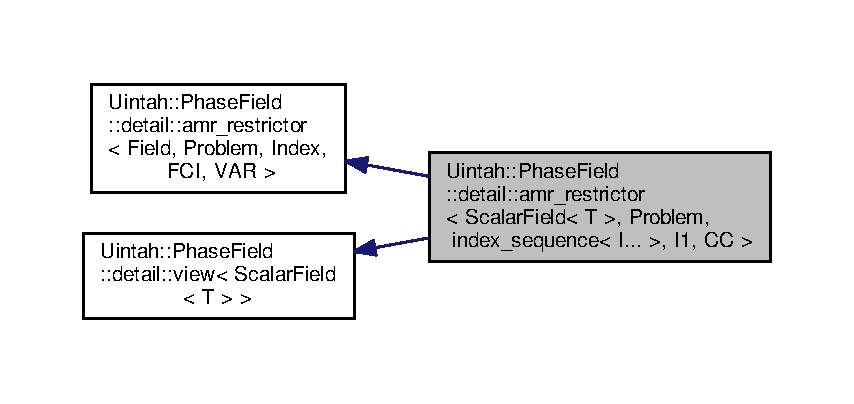
\includegraphics[width=350pt]{classUintah_1_1PhaseField_1_1detail_1_1amr__restrictor_3_01ScalarField_3_01T_01_4_00_01Problem_04093513e287bc124f53e03ea6f74dce7}
\end{center}
\end{figure}


Collaboration diagram for Uintah\+:\+:Phase\+Field\+:\+:detail\+:\+:amr\+\_\+restrictor$<$ Scalar\+Field$<$ T $>$, Problem, index\+\_\+sequence$<$ I... $>$, I1, CC $>$\+:\nopagebreak
\begin{figure}[H]
\begin{center}
\leavevmode
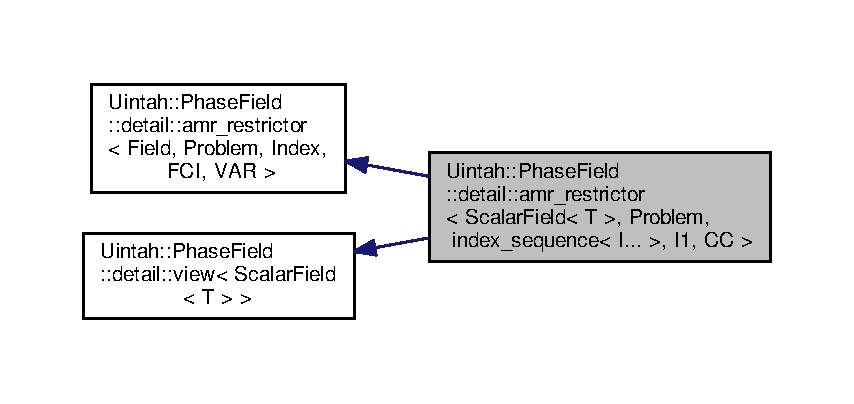
\includegraphics[width=350pt]{classUintah_1_1PhaseField_1_1detail_1_1amr__restrictor_3_01ScalarField_3_01T_01_4_00_01Problem_02d933a6b5ef956be4511371ad65666b6}
\end{center}
\end{figure}
\subsection*{Public Member Functions}
\begin{DoxyCompactItemize}
\item 
\hyperlink{classUintah_1_1PhaseField_1_1detail_1_1amr__restrictor_3_01ScalarField_3_01T_01_4_00_01Problem_0778720acc9a55f696b8537356a4dbcae_a880d7f565151be8edc8b5b549e0a50ca}{amr\+\_\+restrictor} (const Var\+Label $\ast$label, const Var\+Label $\ast$subproblems\+\_\+label, int material)
\begin{DoxyCompactList}\small\item\em construct restrictor without retrieving inner variable data from the Data\+Warehouse \end{DoxyCompactList}\item 
\hyperlink{classUintah_1_1PhaseField_1_1detail_1_1amr__restrictor_3_01ScalarField_3_01T_01_4_00_01Problem_0778720acc9a55f696b8537356a4dbcae_a0a9a3d33840bf6e095165cc1c3efb729}{amr\+\_\+restrictor} (Data\+Warehouse $\ast$dw, const Var\+Label $\ast$label, const Var\+Label $\ast$subproblems\+\_\+label, int material, const Patch $\ast$patch, bool use\+\_\+ghosts=\hyperlink{classUintah_1_1PhaseField_1_1detail_1_1amr__restrictor_3_01ScalarField_3_01T_01_4_00_01Problem_0778720acc9a55f696b8537356a4dbcae_a4cae73002d40229c69caae07718b94d4}{use\+\_\+ghosts\+\_\+dflt})
\begin{DoxyCompactList}\small\item\em construct interpolator and retrieve inner variable data from the Data\+Warehouse whitin a given fine patch. \end{DoxyCompactList}\item 
virtual \hyperlink{classUintah_1_1PhaseField_1_1detail_1_1amr__restrictor_3_01ScalarField_3_01T_01_4_00_01Problem_0778720acc9a55f696b8537356a4dbcae_a35e91389c93de03bae73b73418a03eec}{$\sim$amr\+\_\+restrictor} ()
\begin{DoxyCompactList}\small\item\em Destructor. \end{DoxyCompactList}\item 
\hyperlink{classUintah_1_1PhaseField_1_1detail_1_1amr__restrictor_3_01ScalarField_3_01T_01_4_00_01Problem_0778720acc9a55f696b8537356a4dbcae_a469b1387fab382992209bf3c0e884df7}{amr\+\_\+restrictor} (const \hyperlink{classUintah_1_1PhaseField_1_1detail_1_1amr__restrictor}{amr\+\_\+restrictor} \&)=delete
\begin{DoxyCompactList}\small\item\em Prevent copy (and move) constructor. \end{DoxyCompactList}\item 
\hyperlink{classUintah_1_1PhaseField_1_1detail_1_1amr__restrictor}{amr\+\_\+restrictor} \& \hyperlink{classUintah_1_1PhaseField_1_1detail_1_1amr__restrictor_3_01ScalarField_3_01T_01_4_00_01Problem_0778720acc9a55f696b8537356a4dbcae_a90a87c8184a3e38dca6057f1f5950659}{operator=} (const \hyperlink{classUintah_1_1PhaseField_1_1detail_1_1amr__restrictor}{amr\+\_\+restrictor} \&)=delete
\begin{DoxyCompactList}\small\item\em Prevent copy (and move) assignment. \end{DoxyCompactList}\item 
virtual void \hyperlink{classUintah_1_1PhaseField_1_1detail_1_1amr__restrictor_3_01ScalarField_3_01T_01_4_00_01Problem_0778720acc9a55f696b8537356a4dbcae_a9b2995c37fd05414ef795bab71d89693}{set} (Data\+Warehouse $\ast$dw, const Patch $\ast$patch, bool use\+\_\+ghosts=\hyperlink{classUintah_1_1PhaseField_1_1detail_1_1amr__restrictor_3_01ScalarField_3_01T_01_4_00_01Problem_0778720acc9a55f696b8537356a4dbcae_a4cae73002d40229c69caae07718b94d4}{use\+\_\+ghosts\+\_\+dflt}) override
\begin{DoxyCompactList}\small\item\em retrieve inner variable data from the Data\+Warehouse whitin a given patch. \end{DoxyCompactList}\item 
virtual void \hyperlink{classUintah_1_1PhaseField_1_1detail_1_1amr__restrictor_3_01ScalarField_3_01T_01_4_00_01Problem_0778720acc9a55f696b8537356a4dbcae_ace64828bcebd35f8bbb6bfc203a08c86}{set} (Data\+Warehouse $\ast$dw, const Level $\ast$level, const Int\+Vector \&low, const Int\+Vector \&high, bool use\+\_\+ghosts=\hyperlink{classUintah_1_1PhaseField_1_1detail_1_1amr__restrictor_3_01ScalarField_3_01T_01_4_00_01Problem_0778720acc9a55f696b8537356a4dbcae_a4cae73002d40229c69caae07718b94d4}{use\+\_\+ghosts\+\_\+dflt}) override
\begin{DoxyCompactList}\small\item\em retrieve inner variable data from the Data\+Warehouse whitin a given region. \end{DoxyCompactList}\item 
virtual \hyperlink{classUintah_1_1PhaseField_1_1detail_1_1view}{view}$<$ \hyperlink{structUintah_1_1PhaseField_1_1ScalarField}{Field} $>$ $\ast$ \hyperlink{classUintah_1_1PhaseField_1_1detail_1_1amr__restrictor_3_01ScalarField_3_01T_01_4_00_01Problem_0778720acc9a55f696b8537356a4dbcae_ac7b27aad09d6d193f1cfe96ce2f69f8f}{clone} (bool deep) const override
\begin{DoxyCompactList}\small\item\em Get a copy of the view. \end{DoxyCompactList}\item 
virtual \hyperlink{classUintah_1_1PhaseField_1_1detail_1_1view}{view}$<$ \hyperlink{structUintah_1_1PhaseField_1_1ScalarField}{Field} $>$ $\ast$ \hyperlink{classUintah_1_1PhaseField_1_1detail_1_1amr__restrictor_3_01ScalarField_3_01T_01_4_00_01Problem_0778720acc9a55f696b8537356a4dbcae_a3150edfe50702f16b12ced6a2ef77903}{clone} (bool deep, const Int\+Vector \&offset) const override
\begin{DoxyCompactList}\small\item\em Get a copy of the view and apply translate the support. \end{DoxyCompactList}\item 
virtual \hyperlink{classUintah_1_1PhaseField_1_1Support}{Support} \hyperlink{classUintah_1_1PhaseField_1_1detail_1_1amr__restrictor_3_01ScalarField_3_01T_01_4_00_01Problem_0778720acc9a55f696b8537356a4dbcae_a9565e793be2d11018a724418e3dd3891}{get\+\_\+support} () const override
\begin{DoxyCompactList}\small\item\em get restrictor\textquotesingle{}s coarse range \end{DoxyCompactList}\item 
virtual bool \hyperlink{classUintah_1_1PhaseField_1_1detail_1_1amr__restrictor_3_01ScalarField_3_01T_01_4_00_01Problem_0778720acc9a55f696b8537356a4dbcae_aa4f6dbd8c7469f348c7c3b8198de37b9}{is\+\_\+defined\+\_\+at} (const Int\+Vector \&id\+\_\+coarse) const override
\begin{DoxyCompactList}\small\item\em Check if the view has access to the coarse position with index id. \end{DoxyCompactList}\item 
virtual T \& \hyperlink{classUintah_1_1PhaseField_1_1detail_1_1amr__restrictor_3_01ScalarField_3_01T_01_4_00_01Problem_0778720acc9a55f696b8537356a4dbcae_a628628a8b49e3a7b7abed79f7f1fe0ea}{operator\mbox{[}$\,$\mbox{]}} (const Int\+Vector \&id) override
\begin{DoxyCompactList}\small\item\em Get/\+Modify value at position with index id (virtual implementation) \end{DoxyCompactList}\item 
virtual V \hyperlink{classUintah_1_1PhaseField_1_1detail_1_1amr__restrictor_3_01ScalarField_3_01T_01_4_00_01Problem_0778720acc9a55f696b8537356a4dbcae_a799928df9c231704c14239ab59173e67}{operator\mbox{[}$\,$\mbox{]}} (const Int\+Vector \&id\+\_\+coarse) const override
\begin{DoxyCompactList}\small\item\em get restricted value \end{DoxyCompactList}\end{DoxyCompactItemize}
\subsection*{Static Public Attributes}
\begin{DoxyCompactItemize}
\item 
static constexpr bool \hyperlink{classUintah_1_1PhaseField_1_1detail_1_1amr__restrictor_3_01ScalarField_3_01T_01_4_00_01Problem_0778720acc9a55f696b8537356a4dbcae_a4cae73002d40229c69caae07718b94d4}{use\+\_\+ghosts\+\_\+dflt} = false
\begin{DoxyCompactList}\small\item\em Default value for use\+\_\+ghost when retrieving data. \end{DoxyCompactList}\end{DoxyCompactItemize}
\subsection*{Protected Member Functions}
\begin{DoxyCompactItemize}
\item 
\hyperlink{classUintah_1_1PhaseField_1_1detail_1_1amr__restrictor_3_01ScalarField_3_01T_01_4_00_01Problem_0778720acc9a55f696b8537356a4dbcae_a660561d50c26f0cbed63979b4f04abca}{amr\+\_\+restrictor} (const \hyperlink{classUintah_1_1PhaseField_1_1detail_1_1amr__restrictor}{amr\+\_\+restrictor} $\ast$copy, bool deep)
\begin{DoxyCompactList}\small\item\em Constructor. \end{DoxyCompactList}\end{DoxyCompactItemize}
\subsection*{Additional Inherited Members}


\subsection{Detailed Description}
\subsubsection*{template$<$typename T, typename Problem, size\+\_\+t... I$>$\newline
class Uintah\+::\+Phase\+Field\+::detail\+::amr\+\_\+restrictor$<$ Scalar\+Field$<$ T $>$, Problem, index\+\_\+sequence$<$ I... $>$, I1, C\+C $>$}

Wrapper of grid variables for restriction from finer to coarser levels (cell-\/centered linear implementation) 

implements piecewise constant interpolation of a variable from coarser to finer levels in 1D


\begin{DoxyTemplParams}{Template Parameters}
{\em T} & variable data type (must be constant) \\
\hline
{\em \hyperlink{classUintah_1_1PhaseField_1_1Problem}{Problem}} & type of \hyperlink{namespaceUintah_1_1PhaseField}{Phase\+Field} problem \\
\hline
{\em \hyperlink{structUintah_1_1PhaseField_1_1I}{I}} & list of indices corresponding to the variable within the subproblems\\
\hline
\end{DoxyTemplParams}
$<$ Field, \hyperlink{classUintah_1_1PhaseField_1_1Problem}{Problem}, Index, F\+CI, D\+IM $>$ 

\subsection{Constructor \& Destructor Documentation}
\mbox{\Hypertarget{classUintah_1_1PhaseField_1_1detail_1_1amr__restrictor_3_01ScalarField_3_01T_01_4_00_01Problem_0778720acc9a55f696b8537356a4dbcae_a660561d50c26f0cbed63979b4f04abca}\label{classUintah_1_1PhaseField_1_1detail_1_1amr__restrictor_3_01ScalarField_3_01T_01_4_00_01Problem_0778720acc9a55f696b8537356a4dbcae_a660561d50c26f0cbed63979b4f04abca}} 
\index{Uintah\+::\+Phase\+Field\+::detail\+::amr\+\_\+restrictor$<$ Scalar\+Field$<$ T $>$, Problem, index\+\_\+sequence$<$ I... $>$, I1, C\+C $>$@{Uintah\+::\+Phase\+Field\+::detail\+::amr\+\_\+restrictor$<$ Scalar\+Field$<$ T $>$, Problem, index\+\_\+sequence$<$ I... $>$, I1, C\+C $>$}!amr\+\_\+restrictor@{amr\+\_\+restrictor}}
\index{amr\+\_\+restrictor@{amr\+\_\+restrictor}!Uintah\+::\+Phase\+Field\+::detail\+::amr\+\_\+restrictor$<$ Scalar\+Field$<$ T $>$, Problem, index\+\_\+sequence$<$ I... $>$, I1, C\+C $>$@{Uintah\+::\+Phase\+Field\+::detail\+::amr\+\_\+restrictor$<$ Scalar\+Field$<$ T $>$, Problem, index\+\_\+sequence$<$ I... $>$, I1, C\+C $>$}}
\subsubsection{\texorpdfstring{amr\+\_\+restrictor()}{amr\_restrictor()}\hspace{0.1cm}{\footnotesize\ttfamily [1/4]}}
{\footnotesize\ttfamily template$<$typename T , typename Problem , size\+\_\+t... I$>$ \\
\hyperlink{classUintah_1_1PhaseField_1_1detail_1_1amr__restrictor}{Uintah\+::\+Phase\+Field\+::detail\+::amr\+\_\+restrictor}$<$ \hyperlink{structUintah_1_1PhaseField_1_1ScalarField}{Scalar\+Field}$<$ T $>$, \hyperlink{classUintah_1_1PhaseField_1_1Problem}{Problem}, \hyperlink{namespaceUintah_1_1PhaseField_a237de804d99512e50613aff7c94a9461}{index\+\_\+sequence}$<$ I... $>$, \hyperlink{namespaceUintah_1_1PhaseField_a547ce3002aa97fbd3ef3192a6eec8406a66f19efe774b0d2b6e5844eb2d83d305}{I1}, \hyperlink{namespaceUintah_1_1PhaseField_a33d355affda78a83f45755ba8388cedda22303704507d024d1d6508ed9859a85a}{CC} $>$\+::\hyperlink{classUintah_1_1PhaseField_1_1detail_1_1amr__restrictor}{amr\+\_\+restrictor} (\begin{DoxyParamCaption}\item[{const \hyperlink{classUintah_1_1PhaseField_1_1detail_1_1amr__restrictor}{amr\+\_\+restrictor}$<$ \hyperlink{structUintah_1_1PhaseField_1_1ScalarField}{Scalar\+Field}$<$ T $>$, \hyperlink{classUintah_1_1PhaseField_1_1Problem}{Problem}, \hyperlink{namespaceUintah_1_1PhaseField_a237de804d99512e50613aff7c94a9461}{index\+\_\+sequence}$<$ I... $>$, \hyperlink{namespaceUintah_1_1PhaseField_a547ce3002aa97fbd3ef3192a6eec8406a66f19efe774b0d2b6e5844eb2d83d305}{I1}, \hyperlink{namespaceUintah_1_1PhaseField_a33d355affda78a83f45755ba8388cedda22303704507d024d1d6508ed9859a85a}{CC} $>$ $\ast$}]{copy,  }\item[{bool}]{deep }\end{DoxyParamCaption})\hspace{0.3cm}{\ttfamily [inline]}, {\ttfamily [protected]}}



Constructor. 

Instantiate a copy of a given view


\begin{DoxyParams}{Parameters}
{\em copy} & source view for copying \\
\hline
{\em deep} & if true inner grid variable is copied as well otherwise the same grid variable is referenced \\
\hline
\end{DoxyParams}
\mbox{\Hypertarget{classUintah_1_1PhaseField_1_1detail_1_1amr__restrictor_3_01ScalarField_3_01T_01_4_00_01Problem_0778720acc9a55f696b8537356a4dbcae_a880d7f565151be8edc8b5b549e0a50ca}\label{classUintah_1_1PhaseField_1_1detail_1_1amr__restrictor_3_01ScalarField_3_01T_01_4_00_01Problem_0778720acc9a55f696b8537356a4dbcae_a880d7f565151be8edc8b5b549e0a50ca}} 
\index{Uintah\+::\+Phase\+Field\+::detail\+::amr\+\_\+restrictor$<$ Scalar\+Field$<$ T $>$, Problem, index\+\_\+sequence$<$ I... $>$, I1, C\+C $>$@{Uintah\+::\+Phase\+Field\+::detail\+::amr\+\_\+restrictor$<$ Scalar\+Field$<$ T $>$, Problem, index\+\_\+sequence$<$ I... $>$, I1, C\+C $>$}!amr\+\_\+restrictor@{amr\+\_\+restrictor}}
\index{amr\+\_\+restrictor@{amr\+\_\+restrictor}!Uintah\+::\+Phase\+Field\+::detail\+::amr\+\_\+restrictor$<$ Scalar\+Field$<$ T $>$, Problem, index\+\_\+sequence$<$ I... $>$, I1, C\+C $>$@{Uintah\+::\+Phase\+Field\+::detail\+::amr\+\_\+restrictor$<$ Scalar\+Field$<$ T $>$, Problem, index\+\_\+sequence$<$ I... $>$, I1, C\+C $>$}}
\subsubsection{\texorpdfstring{amr\+\_\+restrictor()}{amr\_restrictor()}\hspace{0.1cm}{\footnotesize\ttfamily [2/4]}}
{\footnotesize\ttfamily template$<$typename T , typename Problem , size\+\_\+t... I$>$ \\
\hyperlink{classUintah_1_1PhaseField_1_1detail_1_1amr__restrictor}{Uintah\+::\+Phase\+Field\+::detail\+::amr\+\_\+restrictor}$<$ \hyperlink{structUintah_1_1PhaseField_1_1ScalarField}{Scalar\+Field}$<$ T $>$, \hyperlink{classUintah_1_1PhaseField_1_1Problem}{Problem}, \hyperlink{namespaceUintah_1_1PhaseField_a237de804d99512e50613aff7c94a9461}{index\+\_\+sequence}$<$ I... $>$, \hyperlink{namespaceUintah_1_1PhaseField_a547ce3002aa97fbd3ef3192a6eec8406a66f19efe774b0d2b6e5844eb2d83d305}{I1}, \hyperlink{namespaceUintah_1_1PhaseField_a33d355affda78a83f45755ba8388cedda22303704507d024d1d6508ed9859a85a}{CC} $>$\+::\hyperlink{classUintah_1_1PhaseField_1_1detail_1_1amr__restrictor}{amr\+\_\+restrictor} (\begin{DoxyParamCaption}\item[{const Var\+Label $\ast$}]{label,  }\item[{const Var\+Label $\ast$}]{subproblems\+\_\+label,  }\item[{int}]{material }\end{DoxyParamCaption})\hspace{0.3cm}{\ttfamily [inline]}}



construct restrictor without retrieving inner variable data from the Data\+Warehouse 


\begin{DoxyParams}{Parameters}
{\em label} & label of variable in the Data\+Warehouse \\
\hline
{\em subproblems\+\_\+label} & label of subproblems in the Data\+Warehouse \\
\hline
{\em material} & index of material in the Data\+Warehouse \\
\hline
\end{DoxyParams}
\mbox{\Hypertarget{classUintah_1_1PhaseField_1_1detail_1_1amr__restrictor_3_01ScalarField_3_01T_01_4_00_01Problem_0778720acc9a55f696b8537356a4dbcae_a0a9a3d33840bf6e095165cc1c3efb729}\label{classUintah_1_1PhaseField_1_1detail_1_1amr__restrictor_3_01ScalarField_3_01T_01_4_00_01Problem_0778720acc9a55f696b8537356a4dbcae_a0a9a3d33840bf6e095165cc1c3efb729}} 
\index{Uintah\+::\+Phase\+Field\+::detail\+::amr\+\_\+restrictor$<$ Scalar\+Field$<$ T $>$, Problem, index\+\_\+sequence$<$ I... $>$, I1, C\+C $>$@{Uintah\+::\+Phase\+Field\+::detail\+::amr\+\_\+restrictor$<$ Scalar\+Field$<$ T $>$, Problem, index\+\_\+sequence$<$ I... $>$, I1, C\+C $>$}!amr\+\_\+restrictor@{amr\+\_\+restrictor}}
\index{amr\+\_\+restrictor@{amr\+\_\+restrictor}!Uintah\+::\+Phase\+Field\+::detail\+::amr\+\_\+restrictor$<$ Scalar\+Field$<$ T $>$, Problem, index\+\_\+sequence$<$ I... $>$, I1, C\+C $>$@{Uintah\+::\+Phase\+Field\+::detail\+::amr\+\_\+restrictor$<$ Scalar\+Field$<$ T $>$, Problem, index\+\_\+sequence$<$ I... $>$, I1, C\+C $>$}}
\subsubsection{\texorpdfstring{amr\+\_\+restrictor()}{amr\_restrictor()}\hspace{0.1cm}{\footnotesize\ttfamily [3/4]}}
{\footnotesize\ttfamily template$<$typename T , typename Problem , size\+\_\+t... I$>$ \\
\hyperlink{classUintah_1_1PhaseField_1_1detail_1_1amr__restrictor}{Uintah\+::\+Phase\+Field\+::detail\+::amr\+\_\+restrictor}$<$ \hyperlink{structUintah_1_1PhaseField_1_1ScalarField}{Scalar\+Field}$<$ T $>$, \hyperlink{classUintah_1_1PhaseField_1_1Problem}{Problem}, \hyperlink{namespaceUintah_1_1PhaseField_a237de804d99512e50613aff7c94a9461}{index\+\_\+sequence}$<$ I... $>$, \hyperlink{namespaceUintah_1_1PhaseField_a547ce3002aa97fbd3ef3192a6eec8406a66f19efe774b0d2b6e5844eb2d83d305}{I1}, \hyperlink{namespaceUintah_1_1PhaseField_a33d355affda78a83f45755ba8388cedda22303704507d024d1d6508ed9859a85a}{CC} $>$\+::\hyperlink{classUintah_1_1PhaseField_1_1detail_1_1amr__restrictor}{amr\+\_\+restrictor} (\begin{DoxyParamCaption}\item[{Data\+Warehouse $\ast$}]{dw,  }\item[{const Var\+Label $\ast$}]{label,  }\item[{const Var\+Label $\ast$}]{subproblems\+\_\+label,  }\item[{int}]{material,  }\item[{const Patch $\ast$}]{patch,  }\item[{bool}]{use\+\_\+ghosts = {\ttfamily \hyperlink{classUintah_1_1PhaseField_1_1detail_1_1amr__restrictor_3_01ScalarField_3_01T_01_4_00_01Problem_0778720acc9a55f696b8537356a4dbcae_a4cae73002d40229c69caae07718b94d4}{use\+\_\+ghosts\+\_\+dflt}} }\end{DoxyParamCaption})\hspace{0.3cm}{\ttfamily [inline]}}



construct interpolator and retrieve inner variable data from the Data\+Warehouse whitin a given fine patch. 

the number of ghost cells/nodes and the corresponding region on the coarser level is automatically computed to match the interpolation type


\begin{DoxyParams}{Parameters}
{\em dw} & Data\+Warehouse which data is retrieved from \\
\hline
{\em label} & label of variable in the Data\+Warehouse \\
\hline
{\em subproblems\+\_\+label} & label of subproblems in the Data\+Warehouse \\
\hline
{\em material} & index of material in the Data\+Warehouse \\
\hline
{\em patch} & patch on which data is retrieved \\
\hline
{\em use\+\_\+ghosts} & if ghosts value are to be retrieved (must be false) \\
\hline
\end{DoxyParams}
\mbox{\Hypertarget{classUintah_1_1PhaseField_1_1detail_1_1amr__restrictor_3_01ScalarField_3_01T_01_4_00_01Problem_0778720acc9a55f696b8537356a4dbcae_a35e91389c93de03bae73b73418a03eec}\label{classUintah_1_1PhaseField_1_1detail_1_1amr__restrictor_3_01ScalarField_3_01T_01_4_00_01Problem_0778720acc9a55f696b8537356a4dbcae_a35e91389c93de03bae73b73418a03eec}} 
\index{Uintah\+::\+Phase\+Field\+::detail\+::amr\+\_\+restrictor$<$ Scalar\+Field$<$ T $>$, Problem, index\+\_\+sequence$<$ I... $>$, I1, C\+C $>$@{Uintah\+::\+Phase\+Field\+::detail\+::amr\+\_\+restrictor$<$ Scalar\+Field$<$ T $>$, Problem, index\+\_\+sequence$<$ I... $>$, I1, C\+C $>$}!````~amr\+\_\+restrictor@{$\sim$amr\+\_\+restrictor}}
\index{````~amr\+\_\+restrictor@{$\sim$amr\+\_\+restrictor}!Uintah\+::\+Phase\+Field\+::detail\+::amr\+\_\+restrictor$<$ Scalar\+Field$<$ T $>$, Problem, index\+\_\+sequence$<$ I... $>$, I1, C\+C $>$@{Uintah\+::\+Phase\+Field\+::detail\+::amr\+\_\+restrictor$<$ Scalar\+Field$<$ T $>$, Problem, index\+\_\+sequence$<$ I... $>$, I1, C\+C $>$}}
\subsubsection{\texorpdfstring{$\sim$amr\+\_\+restrictor()}{~amr\_restrictor()}}
{\footnotesize\ttfamily template$<$typename T , typename Problem , size\+\_\+t... I$>$ \\
virtual \hyperlink{classUintah_1_1PhaseField_1_1detail_1_1amr__restrictor}{Uintah\+::\+Phase\+Field\+::detail\+::amr\+\_\+restrictor}$<$ \hyperlink{structUintah_1_1PhaseField_1_1ScalarField}{Scalar\+Field}$<$ T $>$, \hyperlink{classUintah_1_1PhaseField_1_1Problem}{Problem}, \hyperlink{namespaceUintah_1_1PhaseField_a237de804d99512e50613aff7c94a9461}{index\+\_\+sequence}$<$ I... $>$, \hyperlink{namespaceUintah_1_1PhaseField_a547ce3002aa97fbd3ef3192a6eec8406a66f19efe774b0d2b6e5844eb2d83d305}{I1}, \hyperlink{namespaceUintah_1_1PhaseField_a33d355affda78a83f45755ba8388cedda22303704507d024d1d6508ed9859a85a}{CC} $>$\+::$\sim$\hyperlink{classUintah_1_1PhaseField_1_1detail_1_1amr__restrictor}{amr\+\_\+restrictor} (\begin{DoxyParamCaption}{ }\end{DoxyParamCaption})\hspace{0.3cm}{\ttfamily [inline]}, {\ttfamily [virtual]}}



Destructor. 

\mbox{\Hypertarget{classUintah_1_1PhaseField_1_1detail_1_1amr__restrictor_3_01ScalarField_3_01T_01_4_00_01Problem_0778720acc9a55f696b8537356a4dbcae_a469b1387fab382992209bf3c0e884df7}\label{classUintah_1_1PhaseField_1_1detail_1_1amr__restrictor_3_01ScalarField_3_01T_01_4_00_01Problem_0778720acc9a55f696b8537356a4dbcae_a469b1387fab382992209bf3c0e884df7}} 
\index{Uintah\+::\+Phase\+Field\+::detail\+::amr\+\_\+restrictor$<$ Scalar\+Field$<$ T $>$, Problem, index\+\_\+sequence$<$ I... $>$, I1, C\+C $>$@{Uintah\+::\+Phase\+Field\+::detail\+::amr\+\_\+restrictor$<$ Scalar\+Field$<$ T $>$, Problem, index\+\_\+sequence$<$ I... $>$, I1, C\+C $>$}!amr\+\_\+restrictor@{amr\+\_\+restrictor}}
\index{amr\+\_\+restrictor@{amr\+\_\+restrictor}!Uintah\+::\+Phase\+Field\+::detail\+::amr\+\_\+restrictor$<$ Scalar\+Field$<$ T $>$, Problem, index\+\_\+sequence$<$ I... $>$, I1, C\+C $>$@{Uintah\+::\+Phase\+Field\+::detail\+::amr\+\_\+restrictor$<$ Scalar\+Field$<$ T $>$, Problem, index\+\_\+sequence$<$ I... $>$, I1, C\+C $>$}}
\subsubsection{\texorpdfstring{amr\+\_\+restrictor()}{amr\_restrictor()}\hspace{0.1cm}{\footnotesize\ttfamily [4/4]}}
{\footnotesize\ttfamily template$<$typename T , typename Problem , size\+\_\+t... I$>$ \\
\hyperlink{classUintah_1_1PhaseField_1_1detail_1_1amr__restrictor}{Uintah\+::\+Phase\+Field\+::detail\+::amr\+\_\+restrictor}$<$ \hyperlink{structUintah_1_1PhaseField_1_1ScalarField}{Scalar\+Field}$<$ T $>$, \hyperlink{classUintah_1_1PhaseField_1_1Problem}{Problem}, \hyperlink{namespaceUintah_1_1PhaseField_a237de804d99512e50613aff7c94a9461}{index\+\_\+sequence}$<$ I... $>$, \hyperlink{namespaceUintah_1_1PhaseField_a547ce3002aa97fbd3ef3192a6eec8406a66f19efe774b0d2b6e5844eb2d83d305}{I1}, \hyperlink{namespaceUintah_1_1PhaseField_a33d355affda78a83f45755ba8388cedda22303704507d024d1d6508ed9859a85a}{CC} $>$\+::\hyperlink{classUintah_1_1PhaseField_1_1detail_1_1amr__restrictor}{amr\+\_\+restrictor} (\begin{DoxyParamCaption}\item[{const \hyperlink{classUintah_1_1PhaseField_1_1detail_1_1amr__restrictor}{amr\+\_\+restrictor}$<$ \hyperlink{structUintah_1_1PhaseField_1_1ScalarField}{Scalar\+Field}$<$ T $>$, \hyperlink{classUintah_1_1PhaseField_1_1Problem}{Problem}, \hyperlink{namespaceUintah_1_1PhaseField_a237de804d99512e50613aff7c94a9461}{index\+\_\+sequence}$<$ I... $>$, \hyperlink{namespaceUintah_1_1PhaseField_a547ce3002aa97fbd3ef3192a6eec8406a66f19efe774b0d2b6e5844eb2d83d305}{I1}, \hyperlink{namespaceUintah_1_1PhaseField_a33d355affda78a83f45755ba8388cedda22303704507d024d1d6508ed9859a85a}{CC} $>$ \&}]{ }\end{DoxyParamCaption})\hspace{0.3cm}{\ttfamily [delete]}}



Prevent copy (and move) constructor. 



\subsection{Member Function Documentation}
\mbox{\Hypertarget{classUintah_1_1PhaseField_1_1detail_1_1amr__restrictor_3_01ScalarField_3_01T_01_4_00_01Problem_0778720acc9a55f696b8537356a4dbcae_ac7b27aad09d6d193f1cfe96ce2f69f8f}\label{classUintah_1_1PhaseField_1_1detail_1_1amr__restrictor_3_01ScalarField_3_01T_01_4_00_01Problem_0778720acc9a55f696b8537356a4dbcae_ac7b27aad09d6d193f1cfe96ce2f69f8f}} 
\index{Uintah\+::\+Phase\+Field\+::detail\+::amr\+\_\+restrictor$<$ Scalar\+Field$<$ T $>$, Problem, index\+\_\+sequence$<$ I... $>$, I1, C\+C $>$@{Uintah\+::\+Phase\+Field\+::detail\+::amr\+\_\+restrictor$<$ Scalar\+Field$<$ T $>$, Problem, index\+\_\+sequence$<$ I... $>$, I1, C\+C $>$}!clone@{clone}}
\index{clone@{clone}!Uintah\+::\+Phase\+Field\+::detail\+::amr\+\_\+restrictor$<$ Scalar\+Field$<$ T $>$, Problem, index\+\_\+sequence$<$ I... $>$, I1, C\+C $>$@{Uintah\+::\+Phase\+Field\+::detail\+::amr\+\_\+restrictor$<$ Scalar\+Field$<$ T $>$, Problem, index\+\_\+sequence$<$ I... $>$, I1, C\+C $>$}}
\subsubsection{\texorpdfstring{clone()}{clone()}\hspace{0.1cm}{\footnotesize\ttfamily [1/2]}}
{\footnotesize\ttfamily template$<$typename T , typename Problem , size\+\_\+t... I$>$ \\
virtual \hyperlink{classUintah_1_1PhaseField_1_1detail_1_1view}{view}$<$\hyperlink{structUintah_1_1PhaseField_1_1ScalarField}{Field}$>$$\ast$ \hyperlink{classUintah_1_1PhaseField_1_1detail_1_1amr__restrictor}{Uintah\+::\+Phase\+Field\+::detail\+::amr\+\_\+restrictor}$<$ \hyperlink{structUintah_1_1PhaseField_1_1ScalarField}{Scalar\+Field}$<$ T $>$, \hyperlink{classUintah_1_1PhaseField_1_1Problem}{Problem}, \hyperlink{namespaceUintah_1_1PhaseField_a237de804d99512e50613aff7c94a9461}{index\+\_\+sequence}$<$ I... $>$, \hyperlink{namespaceUintah_1_1PhaseField_a547ce3002aa97fbd3ef3192a6eec8406a66f19efe774b0d2b6e5844eb2d83d305}{I1}, \hyperlink{namespaceUintah_1_1PhaseField_a33d355affda78a83f45755ba8388cedda22303704507d024d1d6508ed9859a85a}{CC} $>$\+::clone (\begin{DoxyParamCaption}\item[{bool}]{deep }\end{DoxyParamCaption}) const\hspace{0.3cm}{\ttfamily [inline]}, {\ttfamily [override]}, {\ttfamily [virtual]}}



Get a copy of the view. 


\begin{DoxyParams}{Parameters}
{\em deep} & if true inner grid variable is copied as well otherwise the same grid variable is referenced\\
\hline
\end{DoxyParams}
\begin{DoxyReturn}{Returns}
new view instance 
\end{DoxyReturn}


Implements \hyperlink{classUintah_1_1PhaseField_1_1detail_1_1view_3_01ScalarField_3_01T_01_4_01_4_a6e11243c9d776a7b703e524ea4151a16}{Uintah\+::\+Phase\+Field\+::detail\+::view$<$ Scalar\+Field$<$ T $>$ $>$}.

\mbox{\Hypertarget{classUintah_1_1PhaseField_1_1detail_1_1amr__restrictor_3_01ScalarField_3_01T_01_4_00_01Problem_0778720acc9a55f696b8537356a4dbcae_a3150edfe50702f16b12ced6a2ef77903}\label{classUintah_1_1PhaseField_1_1detail_1_1amr__restrictor_3_01ScalarField_3_01T_01_4_00_01Problem_0778720acc9a55f696b8537356a4dbcae_a3150edfe50702f16b12ced6a2ef77903}} 
\index{Uintah\+::\+Phase\+Field\+::detail\+::amr\+\_\+restrictor$<$ Scalar\+Field$<$ T $>$, Problem, index\+\_\+sequence$<$ I... $>$, I1, C\+C $>$@{Uintah\+::\+Phase\+Field\+::detail\+::amr\+\_\+restrictor$<$ Scalar\+Field$<$ T $>$, Problem, index\+\_\+sequence$<$ I... $>$, I1, C\+C $>$}!clone@{clone}}
\index{clone@{clone}!Uintah\+::\+Phase\+Field\+::detail\+::amr\+\_\+restrictor$<$ Scalar\+Field$<$ T $>$, Problem, index\+\_\+sequence$<$ I... $>$, I1, C\+C $>$@{Uintah\+::\+Phase\+Field\+::detail\+::amr\+\_\+restrictor$<$ Scalar\+Field$<$ T $>$, Problem, index\+\_\+sequence$<$ I... $>$, I1, C\+C $>$}}
\subsubsection{\texorpdfstring{clone()}{clone()}\hspace{0.1cm}{\footnotesize\ttfamily [2/2]}}
{\footnotesize\ttfamily template$<$typename T , typename Problem , size\+\_\+t... I$>$ \\
virtual \hyperlink{classUintah_1_1PhaseField_1_1detail_1_1view}{view}$<$\hyperlink{structUintah_1_1PhaseField_1_1ScalarField}{Field}$>$$\ast$ \hyperlink{classUintah_1_1PhaseField_1_1detail_1_1amr__restrictor}{Uintah\+::\+Phase\+Field\+::detail\+::amr\+\_\+restrictor}$<$ \hyperlink{structUintah_1_1PhaseField_1_1ScalarField}{Scalar\+Field}$<$ T $>$, \hyperlink{classUintah_1_1PhaseField_1_1Problem}{Problem}, \hyperlink{namespaceUintah_1_1PhaseField_a237de804d99512e50613aff7c94a9461}{index\+\_\+sequence}$<$ I... $>$, \hyperlink{namespaceUintah_1_1PhaseField_a547ce3002aa97fbd3ef3192a6eec8406a66f19efe774b0d2b6e5844eb2d83d305}{I1}, \hyperlink{namespaceUintah_1_1PhaseField_a33d355affda78a83f45755ba8388cedda22303704507d024d1d6508ed9859a85a}{CC} $>$\+::clone (\begin{DoxyParamCaption}\item[{bool}]{deep,  }\item[{const Int\+Vector \&}]{offset }\end{DoxyParamCaption}) const\hspace{0.3cm}{\ttfamily [inline]}, {\ttfamily [override]}, {\ttfamily [virtual]}}



Get a copy of the view and apply translate the support. 

\begin{DoxyRemark}{Remarks}
It is meant to be used for virtual patches (i.\+e. periodic boundaries)
\end{DoxyRemark}

\begin{DoxyParams}{Parameters}
{\em deep} & if true inner grid variable is copied as well otherwise the same grid variable is referenced \\
\hline
{\em offset} & vector specifying the translation of the support \\
\hline
\end{DoxyParams}
\begin{DoxyReturn}{Returns}
new view instance 
\end{DoxyReturn}


Implements \hyperlink{classUintah_1_1PhaseField_1_1detail_1_1view_3_01ScalarField_3_01T_01_4_01_4_abd928104240e329f3bc4441ebab7c50c}{Uintah\+::\+Phase\+Field\+::detail\+::view$<$ Scalar\+Field$<$ T $>$ $>$}.

\mbox{\Hypertarget{classUintah_1_1PhaseField_1_1detail_1_1amr__restrictor_3_01ScalarField_3_01T_01_4_00_01Problem_0778720acc9a55f696b8537356a4dbcae_a9565e793be2d11018a724418e3dd3891}\label{classUintah_1_1PhaseField_1_1detail_1_1amr__restrictor_3_01ScalarField_3_01T_01_4_00_01Problem_0778720acc9a55f696b8537356a4dbcae_a9565e793be2d11018a724418e3dd3891}} 
\index{Uintah\+::\+Phase\+Field\+::detail\+::amr\+\_\+restrictor$<$ Scalar\+Field$<$ T $>$, Problem, index\+\_\+sequence$<$ I... $>$, I1, C\+C $>$@{Uintah\+::\+Phase\+Field\+::detail\+::amr\+\_\+restrictor$<$ Scalar\+Field$<$ T $>$, Problem, index\+\_\+sequence$<$ I... $>$, I1, C\+C $>$}!get\+\_\+support@{get\+\_\+support}}
\index{get\+\_\+support@{get\+\_\+support}!Uintah\+::\+Phase\+Field\+::detail\+::amr\+\_\+restrictor$<$ Scalar\+Field$<$ T $>$, Problem, index\+\_\+sequence$<$ I... $>$, I1, C\+C $>$@{Uintah\+::\+Phase\+Field\+::detail\+::amr\+\_\+restrictor$<$ Scalar\+Field$<$ T $>$, Problem, index\+\_\+sequence$<$ I... $>$, I1, C\+C $>$}}
\subsubsection{\texorpdfstring{get\+\_\+support()}{get\_support()}}
{\footnotesize\ttfamily template$<$typename T , typename Problem , size\+\_\+t... I$>$ \\
virtual \hyperlink{classUintah_1_1PhaseField_1_1Support}{Support} \hyperlink{classUintah_1_1PhaseField_1_1detail_1_1amr__restrictor}{Uintah\+::\+Phase\+Field\+::detail\+::amr\+\_\+restrictor}$<$ \hyperlink{structUintah_1_1PhaseField_1_1ScalarField}{Scalar\+Field}$<$ T $>$, \hyperlink{classUintah_1_1PhaseField_1_1Problem}{Problem}, \hyperlink{namespaceUintah_1_1PhaseField_a237de804d99512e50613aff7c94a9461}{index\+\_\+sequence}$<$ I... $>$, \hyperlink{namespaceUintah_1_1PhaseField_a547ce3002aa97fbd3ef3192a6eec8406a66f19efe774b0d2b6e5844eb2d83d305}{I1}, \hyperlink{namespaceUintah_1_1PhaseField_a33d355affda78a83f45755ba8388cedda22303704507d024d1d6508ed9859a85a}{CC} $>$\+::get\+\_\+support (\begin{DoxyParamCaption}{ }\end{DoxyParamCaption}) const\hspace{0.3cm}{\ttfamily [inline]}, {\ttfamily [override]}, {\ttfamily [virtual]}}



get restrictor\textquotesingle{}s coarse range 

\begin{DoxyReturn}{Returns}
coarse range 
\end{DoxyReturn}


Implements \hyperlink{classUintah_1_1PhaseField_1_1detail_1_1view_3_01ScalarField_3_01T_01_4_01_4_a3e14b0c7a57a57707bb33954861ab1c1}{Uintah\+::\+Phase\+Field\+::detail\+::view$<$ Scalar\+Field$<$ T $>$ $>$}.

\mbox{\Hypertarget{classUintah_1_1PhaseField_1_1detail_1_1amr__restrictor_3_01ScalarField_3_01T_01_4_00_01Problem_0778720acc9a55f696b8537356a4dbcae_aa4f6dbd8c7469f348c7c3b8198de37b9}\label{classUintah_1_1PhaseField_1_1detail_1_1amr__restrictor_3_01ScalarField_3_01T_01_4_00_01Problem_0778720acc9a55f696b8537356a4dbcae_aa4f6dbd8c7469f348c7c3b8198de37b9}} 
\index{Uintah\+::\+Phase\+Field\+::detail\+::amr\+\_\+restrictor$<$ Scalar\+Field$<$ T $>$, Problem, index\+\_\+sequence$<$ I... $>$, I1, C\+C $>$@{Uintah\+::\+Phase\+Field\+::detail\+::amr\+\_\+restrictor$<$ Scalar\+Field$<$ T $>$, Problem, index\+\_\+sequence$<$ I... $>$, I1, C\+C $>$}!is\+\_\+defined\+\_\+at@{is\+\_\+defined\+\_\+at}}
\index{is\+\_\+defined\+\_\+at@{is\+\_\+defined\+\_\+at}!Uintah\+::\+Phase\+Field\+::detail\+::amr\+\_\+restrictor$<$ Scalar\+Field$<$ T $>$, Problem, index\+\_\+sequence$<$ I... $>$, I1, C\+C $>$@{Uintah\+::\+Phase\+Field\+::detail\+::amr\+\_\+restrictor$<$ Scalar\+Field$<$ T $>$, Problem, index\+\_\+sequence$<$ I... $>$, I1, C\+C $>$}}
\subsubsection{\texorpdfstring{is\+\_\+defined\+\_\+at()}{is\_defined\_at()}}
{\footnotesize\ttfamily template$<$typename T , typename Problem , size\+\_\+t... I$>$ \\
virtual bool \hyperlink{classUintah_1_1PhaseField_1_1detail_1_1amr__restrictor}{Uintah\+::\+Phase\+Field\+::detail\+::amr\+\_\+restrictor}$<$ \hyperlink{structUintah_1_1PhaseField_1_1ScalarField}{Scalar\+Field}$<$ T $>$, \hyperlink{classUintah_1_1PhaseField_1_1Problem}{Problem}, \hyperlink{namespaceUintah_1_1PhaseField_a237de804d99512e50613aff7c94a9461}{index\+\_\+sequence}$<$ I... $>$, \hyperlink{namespaceUintah_1_1PhaseField_a547ce3002aa97fbd3ef3192a6eec8406a66f19efe774b0d2b6e5844eb2d83d305}{I1}, \hyperlink{namespaceUintah_1_1PhaseField_a33d355affda78a83f45755ba8388cedda22303704507d024d1d6508ed9859a85a}{CC} $>$\+::is\+\_\+defined\+\_\+at (\begin{DoxyParamCaption}\item[{const Int\+Vector \&}]{id\+\_\+coarse }\end{DoxyParamCaption}) const\hspace{0.3cm}{\ttfamily [inline]}, {\ttfamily [override]}, {\ttfamily [virtual]}}



Check if the view has access to the coarse position with index id. 


\begin{DoxyParams}{Parameters}
{\em id\+\_\+coarse} & coarse position index \\
\hline
\end{DoxyParams}
\begin{DoxyReturn}{Returns}
check result 
\end{DoxyReturn}


Implements \hyperlink{classUintah_1_1PhaseField_1_1detail_1_1view_3_01ScalarField_3_01T_01_4_01_4_a9a950513dacd6468658436b737c3314f}{Uintah\+::\+Phase\+Field\+::detail\+::view$<$ Scalar\+Field$<$ T $>$ $>$}.

\mbox{\Hypertarget{classUintah_1_1PhaseField_1_1detail_1_1amr__restrictor_3_01ScalarField_3_01T_01_4_00_01Problem_0778720acc9a55f696b8537356a4dbcae_a90a87c8184a3e38dca6057f1f5950659}\label{classUintah_1_1PhaseField_1_1detail_1_1amr__restrictor_3_01ScalarField_3_01T_01_4_00_01Problem_0778720acc9a55f696b8537356a4dbcae_a90a87c8184a3e38dca6057f1f5950659}} 
\index{Uintah\+::\+Phase\+Field\+::detail\+::amr\+\_\+restrictor$<$ Scalar\+Field$<$ T $>$, Problem, index\+\_\+sequence$<$ I... $>$, I1, C\+C $>$@{Uintah\+::\+Phase\+Field\+::detail\+::amr\+\_\+restrictor$<$ Scalar\+Field$<$ T $>$, Problem, index\+\_\+sequence$<$ I... $>$, I1, C\+C $>$}!operator=@{operator=}}
\index{operator=@{operator=}!Uintah\+::\+Phase\+Field\+::detail\+::amr\+\_\+restrictor$<$ Scalar\+Field$<$ T $>$, Problem, index\+\_\+sequence$<$ I... $>$, I1, C\+C $>$@{Uintah\+::\+Phase\+Field\+::detail\+::amr\+\_\+restrictor$<$ Scalar\+Field$<$ T $>$, Problem, index\+\_\+sequence$<$ I... $>$, I1, C\+C $>$}}
\subsubsection{\texorpdfstring{operator=()}{operator=()}}
{\footnotesize\ttfamily template$<$typename T , typename Problem , size\+\_\+t... I$>$ \\
\hyperlink{classUintah_1_1PhaseField_1_1detail_1_1amr__restrictor}{amr\+\_\+restrictor}\& \hyperlink{classUintah_1_1PhaseField_1_1detail_1_1amr__restrictor}{Uintah\+::\+Phase\+Field\+::detail\+::amr\+\_\+restrictor}$<$ \hyperlink{structUintah_1_1PhaseField_1_1ScalarField}{Scalar\+Field}$<$ T $>$, \hyperlink{classUintah_1_1PhaseField_1_1Problem}{Problem}, \hyperlink{namespaceUintah_1_1PhaseField_a237de804d99512e50613aff7c94a9461}{index\+\_\+sequence}$<$ I... $>$, \hyperlink{namespaceUintah_1_1PhaseField_a547ce3002aa97fbd3ef3192a6eec8406a66f19efe774b0d2b6e5844eb2d83d305}{I1}, \hyperlink{namespaceUintah_1_1PhaseField_a33d355affda78a83f45755ba8388cedda22303704507d024d1d6508ed9859a85a}{CC} $>$\+::operator= (\begin{DoxyParamCaption}\item[{const \hyperlink{classUintah_1_1PhaseField_1_1detail_1_1amr__restrictor}{amr\+\_\+restrictor}$<$ \hyperlink{structUintah_1_1PhaseField_1_1ScalarField}{Scalar\+Field}$<$ T $>$, \hyperlink{classUintah_1_1PhaseField_1_1Problem}{Problem}, \hyperlink{namespaceUintah_1_1PhaseField_a237de804d99512e50613aff7c94a9461}{index\+\_\+sequence}$<$ I... $>$, \hyperlink{namespaceUintah_1_1PhaseField_a547ce3002aa97fbd3ef3192a6eec8406a66f19efe774b0d2b6e5844eb2d83d305}{I1}, \hyperlink{namespaceUintah_1_1PhaseField_a33d355affda78a83f45755ba8388cedda22303704507d024d1d6508ed9859a85a}{CC} $>$ \&}]{ }\end{DoxyParamCaption})\hspace{0.3cm}{\ttfamily [delete]}}



Prevent copy (and move) assignment. 

\mbox{\Hypertarget{classUintah_1_1PhaseField_1_1detail_1_1amr__restrictor_3_01ScalarField_3_01T_01_4_00_01Problem_0778720acc9a55f696b8537356a4dbcae_a628628a8b49e3a7b7abed79f7f1fe0ea}\label{classUintah_1_1PhaseField_1_1detail_1_1amr__restrictor_3_01ScalarField_3_01T_01_4_00_01Problem_0778720acc9a55f696b8537356a4dbcae_a628628a8b49e3a7b7abed79f7f1fe0ea}} 
\index{Uintah\+::\+Phase\+Field\+::detail\+::amr\+\_\+restrictor$<$ Scalar\+Field$<$ T $>$, Problem, index\+\_\+sequence$<$ I... $>$, I1, C\+C $>$@{Uintah\+::\+Phase\+Field\+::detail\+::amr\+\_\+restrictor$<$ Scalar\+Field$<$ T $>$, Problem, index\+\_\+sequence$<$ I... $>$, I1, C\+C $>$}!operator\mbox{[}\mbox{]}@{operator[]}}
\index{operator\mbox{[}\mbox{]}@{operator[]}!Uintah\+::\+Phase\+Field\+::detail\+::amr\+\_\+restrictor$<$ Scalar\+Field$<$ T $>$, Problem, index\+\_\+sequence$<$ I... $>$, I1, C\+C $>$@{Uintah\+::\+Phase\+Field\+::detail\+::amr\+\_\+restrictor$<$ Scalar\+Field$<$ T $>$, Problem, index\+\_\+sequence$<$ I... $>$, I1, C\+C $>$}}
\subsubsection{\texorpdfstring{operator[]()}{operator[]()}\hspace{0.1cm}{\footnotesize\ttfamily [1/2]}}
{\footnotesize\ttfamily template$<$typename T , typename Problem , size\+\_\+t... I$>$ \\
virtual T\& \hyperlink{classUintah_1_1PhaseField_1_1detail_1_1amr__restrictor}{Uintah\+::\+Phase\+Field\+::detail\+::amr\+\_\+restrictor}$<$ \hyperlink{structUintah_1_1PhaseField_1_1ScalarField}{Scalar\+Field}$<$ T $>$, \hyperlink{classUintah_1_1PhaseField_1_1Problem}{Problem}, \hyperlink{namespaceUintah_1_1PhaseField_a237de804d99512e50613aff7c94a9461}{index\+\_\+sequence}$<$ I... $>$, \hyperlink{namespaceUintah_1_1PhaseField_a547ce3002aa97fbd3ef3192a6eec8406a66f19efe774b0d2b6e5844eb2d83d305}{I1}, \hyperlink{namespaceUintah_1_1PhaseField_a33d355affda78a83f45755ba8388cedda22303704507d024d1d6508ed9859a85a}{CC} $>$\+::operator\mbox{[}$\,$\mbox{]} (\begin{DoxyParamCaption}\item[{const Int\+Vector \&}]{id }\end{DoxyParamCaption})\hspace{0.3cm}{\ttfamily [inline]}, {\ttfamily [override]}, {\ttfamily [virtual]}}



Get/\+Modify value at position with index id (virtual implementation) 

\begin{DoxyRemark}{Remarks}
restricted value is computed at runtime thus doesn\textquotesingle{}t exist in the Data\+Warehouse
\end{DoxyRemark}

\begin{DoxyParams}{Parameters}
{\em id} & unused \\
\hline
\end{DoxyParams}
\begin{DoxyReturn}{Returns}
nothing 
\end{DoxyReturn}


Implements \hyperlink{classUintah_1_1PhaseField_1_1detail_1_1view_3_01ScalarField_3_01T_01_4_01_4_a96b3035d435ae901516b6bc5e138f3b5}{Uintah\+::\+Phase\+Field\+::detail\+::view$<$ Scalar\+Field$<$ T $>$ $>$}.

\mbox{\Hypertarget{classUintah_1_1PhaseField_1_1detail_1_1amr__restrictor_3_01ScalarField_3_01T_01_4_00_01Problem_0778720acc9a55f696b8537356a4dbcae_a799928df9c231704c14239ab59173e67}\label{classUintah_1_1PhaseField_1_1detail_1_1amr__restrictor_3_01ScalarField_3_01T_01_4_00_01Problem_0778720acc9a55f696b8537356a4dbcae_a799928df9c231704c14239ab59173e67}} 
\index{Uintah\+::\+Phase\+Field\+::detail\+::amr\+\_\+restrictor$<$ Scalar\+Field$<$ T $>$, Problem, index\+\_\+sequence$<$ I... $>$, I1, C\+C $>$@{Uintah\+::\+Phase\+Field\+::detail\+::amr\+\_\+restrictor$<$ Scalar\+Field$<$ T $>$, Problem, index\+\_\+sequence$<$ I... $>$, I1, C\+C $>$}!operator\mbox{[}\mbox{]}@{operator[]}}
\index{operator\mbox{[}\mbox{]}@{operator[]}!Uintah\+::\+Phase\+Field\+::detail\+::amr\+\_\+restrictor$<$ Scalar\+Field$<$ T $>$, Problem, index\+\_\+sequence$<$ I... $>$, I1, C\+C $>$@{Uintah\+::\+Phase\+Field\+::detail\+::amr\+\_\+restrictor$<$ Scalar\+Field$<$ T $>$, Problem, index\+\_\+sequence$<$ I... $>$, I1, C\+C $>$}}
\subsubsection{\texorpdfstring{operator[]()}{operator[]()}\hspace{0.1cm}{\footnotesize\ttfamily [2/2]}}
{\footnotesize\ttfamily template$<$typename T , typename Problem , size\+\_\+t... I$>$ \\
virtual V \hyperlink{classUintah_1_1PhaseField_1_1detail_1_1amr__restrictor}{Uintah\+::\+Phase\+Field\+::detail\+::amr\+\_\+restrictor}$<$ \hyperlink{structUintah_1_1PhaseField_1_1ScalarField}{Scalar\+Field}$<$ T $>$, \hyperlink{classUintah_1_1PhaseField_1_1Problem}{Problem}, \hyperlink{namespaceUintah_1_1PhaseField_a237de804d99512e50613aff7c94a9461}{index\+\_\+sequence}$<$ I... $>$, \hyperlink{namespaceUintah_1_1PhaseField_a547ce3002aa97fbd3ef3192a6eec8406a66f19efe774b0d2b6e5844eb2d83d305}{I1}, \hyperlink{namespaceUintah_1_1PhaseField_a33d355affda78a83f45755ba8388cedda22303704507d024d1d6508ed9859a85a}{CC} $>$\+::operator\mbox{[}$\,$\mbox{]} (\begin{DoxyParamCaption}\item[{const Int\+Vector \&}]{id\+\_\+coarse }\end{DoxyParamCaption}) const\hspace{0.3cm}{\ttfamily [inline]}, {\ttfamily [override]}, {\ttfamily [virtual]}}



get restricted value 

value at fine index is computed avareging over the corresponding cells the finer level


\begin{DoxyParams}{Parameters}
{\em id\+\_\+coarse} & coarse index \\
\hline
\end{DoxyParams}
\begin{DoxyReturn}{Returns}
restricted value at the given fine index 
\end{DoxyReturn}


Implements \hyperlink{classUintah_1_1PhaseField_1_1detail_1_1view_3_01ScalarField_3_01T_01_4_01_4_aea43cfedfe3b6f3c038ff795caec49b8}{Uintah\+::\+Phase\+Field\+::detail\+::view$<$ Scalar\+Field$<$ T $>$ $>$}.

\mbox{\Hypertarget{classUintah_1_1PhaseField_1_1detail_1_1amr__restrictor_3_01ScalarField_3_01T_01_4_00_01Problem_0778720acc9a55f696b8537356a4dbcae_a9b2995c37fd05414ef795bab71d89693}\label{classUintah_1_1PhaseField_1_1detail_1_1amr__restrictor_3_01ScalarField_3_01T_01_4_00_01Problem_0778720acc9a55f696b8537356a4dbcae_a9b2995c37fd05414ef795bab71d89693}} 
\index{Uintah\+::\+Phase\+Field\+::detail\+::amr\+\_\+restrictor$<$ Scalar\+Field$<$ T $>$, Problem, index\+\_\+sequence$<$ I... $>$, I1, C\+C $>$@{Uintah\+::\+Phase\+Field\+::detail\+::amr\+\_\+restrictor$<$ Scalar\+Field$<$ T $>$, Problem, index\+\_\+sequence$<$ I... $>$, I1, C\+C $>$}!set@{set}}
\index{set@{set}!Uintah\+::\+Phase\+Field\+::detail\+::amr\+\_\+restrictor$<$ Scalar\+Field$<$ T $>$, Problem, index\+\_\+sequence$<$ I... $>$, I1, C\+C $>$@{Uintah\+::\+Phase\+Field\+::detail\+::amr\+\_\+restrictor$<$ Scalar\+Field$<$ T $>$, Problem, index\+\_\+sequence$<$ I... $>$, I1, C\+C $>$}}
\subsubsection{\texorpdfstring{set()}{set()}\hspace{0.1cm}{\footnotesize\ttfamily [1/2]}}
{\footnotesize\ttfamily template$<$typename T , typename Problem , size\+\_\+t... I$>$ \\
virtual void \hyperlink{classUintah_1_1PhaseField_1_1detail_1_1amr__restrictor}{Uintah\+::\+Phase\+Field\+::detail\+::amr\+\_\+restrictor}$<$ \hyperlink{structUintah_1_1PhaseField_1_1ScalarField}{Scalar\+Field}$<$ T $>$, \hyperlink{classUintah_1_1PhaseField_1_1Problem}{Problem}, \hyperlink{namespaceUintah_1_1PhaseField_a237de804d99512e50613aff7c94a9461}{index\+\_\+sequence}$<$ I... $>$, \hyperlink{namespaceUintah_1_1PhaseField_a547ce3002aa97fbd3ef3192a6eec8406a66f19efe774b0d2b6e5844eb2d83d305}{I1}, \hyperlink{namespaceUintah_1_1PhaseField_a33d355affda78a83f45755ba8388cedda22303704507d024d1d6508ed9859a85a}{CC} $>$\+::set (\begin{DoxyParamCaption}\item[{Data\+Warehouse $\ast$}]{dw,  }\item[{const Patch $\ast$}]{patch,  }\item[{bool}]{use\+\_\+ghosts = {\ttfamily \hyperlink{classUintah_1_1PhaseField_1_1detail_1_1amr__restrictor_3_01ScalarField_3_01T_01_4_00_01Problem_0778720acc9a55f696b8537356a4dbcae_a4cae73002d40229c69caae07718b94d4}{use\+\_\+ghosts\+\_\+dflt}} }\end{DoxyParamCaption})\hspace{0.3cm}{\ttfamily [inline]}, {\ttfamily [override]}, {\ttfamily [virtual]}}



retrieve inner variable data from the Data\+Warehouse whitin a given patch. 

the number of ghost cells/nodes and the corresponding region on the finer level is automatically computed to match the interpolation type


\begin{DoxyParams}{Parameters}
{\em dw} & Data\+Warehouse which data is retrieved from \\
\hline
{\em patch} & patch on which data is retrieved \\
\hline
{\em use\+\_\+ghosts} & if ghosts value are to be retrieved (must be false) \\
\hline
\end{DoxyParams}


Implements \hyperlink{classUintah_1_1PhaseField_1_1detail_1_1view_3_01ScalarField_3_01T_01_4_01_4_ae90ea8b33fde8515a1f2e8f5c03c0166}{Uintah\+::\+Phase\+Field\+::detail\+::view$<$ Scalar\+Field$<$ T $>$ $>$}.

\mbox{\Hypertarget{classUintah_1_1PhaseField_1_1detail_1_1amr__restrictor_3_01ScalarField_3_01T_01_4_00_01Problem_0778720acc9a55f696b8537356a4dbcae_ace64828bcebd35f8bbb6bfc203a08c86}\label{classUintah_1_1PhaseField_1_1detail_1_1amr__restrictor_3_01ScalarField_3_01T_01_4_00_01Problem_0778720acc9a55f696b8537356a4dbcae_ace64828bcebd35f8bbb6bfc203a08c86}} 
\index{Uintah\+::\+Phase\+Field\+::detail\+::amr\+\_\+restrictor$<$ Scalar\+Field$<$ T $>$, Problem, index\+\_\+sequence$<$ I... $>$, I1, C\+C $>$@{Uintah\+::\+Phase\+Field\+::detail\+::amr\+\_\+restrictor$<$ Scalar\+Field$<$ T $>$, Problem, index\+\_\+sequence$<$ I... $>$, I1, C\+C $>$}!set@{set}}
\index{set@{set}!Uintah\+::\+Phase\+Field\+::detail\+::amr\+\_\+restrictor$<$ Scalar\+Field$<$ T $>$, Problem, index\+\_\+sequence$<$ I... $>$, I1, C\+C $>$@{Uintah\+::\+Phase\+Field\+::detail\+::amr\+\_\+restrictor$<$ Scalar\+Field$<$ T $>$, Problem, index\+\_\+sequence$<$ I... $>$, I1, C\+C $>$}}
\subsubsection{\texorpdfstring{set()}{set()}\hspace{0.1cm}{\footnotesize\ttfamily [2/2]}}
{\footnotesize\ttfamily template$<$typename T , typename Problem , size\+\_\+t... I$>$ \\
virtual void \hyperlink{classUintah_1_1PhaseField_1_1detail_1_1amr__restrictor}{Uintah\+::\+Phase\+Field\+::detail\+::amr\+\_\+restrictor}$<$ \hyperlink{structUintah_1_1PhaseField_1_1ScalarField}{Scalar\+Field}$<$ T $>$, \hyperlink{classUintah_1_1PhaseField_1_1Problem}{Problem}, \hyperlink{namespaceUintah_1_1PhaseField_a237de804d99512e50613aff7c94a9461}{index\+\_\+sequence}$<$ I... $>$, \hyperlink{namespaceUintah_1_1PhaseField_a547ce3002aa97fbd3ef3192a6eec8406a66f19efe774b0d2b6e5844eb2d83d305}{I1}, \hyperlink{namespaceUintah_1_1PhaseField_a33d355affda78a83f45755ba8388cedda22303704507d024d1d6508ed9859a85a}{CC} $>$\+::set (\begin{DoxyParamCaption}\item[{Data\+Warehouse $\ast$}]{dw,  }\item[{const Level $\ast$}]{level,  }\item[{const Int\+Vector \&}]{low,  }\item[{const Int\+Vector \&}]{high,  }\item[{bool}]{use\+\_\+ghosts = {\ttfamily \hyperlink{classUintah_1_1PhaseField_1_1detail_1_1amr__restrictor_3_01ScalarField_3_01T_01_4_00_01Problem_0778720acc9a55f696b8537356a4dbcae_a4cae73002d40229c69caae07718b94d4}{use\+\_\+ghosts\+\_\+dflt}} }\end{DoxyParamCaption})\hspace{0.3cm}{\ttfamily [inline]}, {\ttfamily [override]}, {\ttfamily [virtual]}}



retrieve inner variable data from the Data\+Warehouse whitin a given region. 

the number of ghost cells/nodes and the corresponding region on the finer level is automatically computed to match the interpolation type


\begin{DoxyParams}{Parameters}
{\em dw} & Data\+Warehouse which data is retrieved from \\
\hline
{\em level} & level of the coarse region \\
\hline
{\em low} & start index for the coarse region \\
\hline
{\em high} & past the end index for the coarse region \\
\hline
{\em use\+\_\+ghosts} & if ghosts value are to be retrieved (must be false) \\
\hline
\end{DoxyParams}


Implements \hyperlink{classUintah_1_1PhaseField_1_1detail_1_1view_3_01ScalarField_3_01T_01_4_01_4_a5fc830b30b120922cfe8a2c008d96109}{Uintah\+::\+Phase\+Field\+::detail\+::view$<$ Scalar\+Field$<$ T $>$ $>$}.



\subsection{Member Data Documentation}
\mbox{\Hypertarget{classUintah_1_1PhaseField_1_1detail_1_1amr__restrictor_3_01ScalarField_3_01T_01_4_00_01Problem_0778720acc9a55f696b8537356a4dbcae_a4cae73002d40229c69caae07718b94d4}\label{classUintah_1_1PhaseField_1_1detail_1_1amr__restrictor_3_01ScalarField_3_01T_01_4_00_01Problem_0778720acc9a55f696b8537356a4dbcae_a4cae73002d40229c69caae07718b94d4}} 
\index{Uintah\+::\+Phase\+Field\+::detail\+::amr\+\_\+restrictor$<$ Scalar\+Field$<$ T $>$, Problem, index\+\_\+sequence$<$ I... $>$, I1, C\+C $>$@{Uintah\+::\+Phase\+Field\+::detail\+::amr\+\_\+restrictor$<$ Scalar\+Field$<$ T $>$, Problem, index\+\_\+sequence$<$ I... $>$, I1, C\+C $>$}!use\+\_\+ghosts\+\_\+dflt@{use\+\_\+ghosts\+\_\+dflt}}
\index{use\+\_\+ghosts\+\_\+dflt@{use\+\_\+ghosts\+\_\+dflt}!Uintah\+::\+Phase\+Field\+::detail\+::amr\+\_\+restrictor$<$ Scalar\+Field$<$ T $>$, Problem, index\+\_\+sequence$<$ I... $>$, I1, C\+C $>$@{Uintah\+::\+Phase\+Field\+::detail\+::amr\+\_\+restrictor$<$ Scalar\+Field$<$ T $>$, Problem, index\+\_\+sequence$<$ I... $>$, I1, C\+C $>$}}
\subsubsection{\texorpdfstring{use\+\_\+ghosts\+\_\+dflt}{use\_ghosts\_dflt}}
{\footnotesize\ttfamily template$<$typename T , typename Problem , size\+\_\+t... I$>$ \\
constexpr bool \hyperlink{classUintah_1_1PhaseField_1_1detail_1_1amr__restrictor}{Uintah\+::\+Phase\+Field\+::detail\+::amr\+\_\+restrictor}$<$ \hyperlink{structUintah_1_1PhaseField_1_1ScalarField}{Scalar\+Field}$<$ T $>$, \hyperlink{classUintah_1_1PhaseField_1_1Problem}{Problem}, \hyperlink{namespaceUintah_1_1PhaseField_a237de804d99512e50613aff7c94a9461}{index\+\_\+sequence}$<$ I... $>$, \hyperlink{namespaceUintah_1_1PhaseField_a547ce3002aa97fbd3ef3192a6eec8406a66f19efe774b0d2b6e5844eb2d83d305}{I1}, \hyperlink{namespaceUintah_1_1PhaseField_a33d355affda78a83f45755ba8388cedda22303704507d024d1d6508ed9859a85a}{CC} $>$\+::use\+\_\+ghosts\+\_\+dflt = false\hspace{0.3cm}{\ttfamily [static]}}



Default value for use\+\_\+ghost when retrieving data. 



The documentation for this class was generated from the following file\+:\begin{DoxyCompactItemize}
\item 
\hyperlink{amr__restrictor__I1__CC_8h}{amr\+\_\+restrictor\+\_\+\+I1\+\_\+\+C\+C.\+h}\end{DoxyCompactItemize}

\hypertarget{classUintah_1_1PhaseField_1_1detail_1_1amr__restrictor_3_01VectorField_3_01T_00_01N_01_4_00_01Pre7f2e99a4fbf25ff00717d25c8580b1a}{}\section{Uintah\+:\+:Phase\+Field\+:\+:detail\+:\+:amr\+\_\+restrictor$<$ Vector\+Field$<$ T, N $>$, Problem, Index, F\+CI, D\+IM $>$ Class Template Reference}
\label{classUintah_1_1PhaseField_1_1detail_1_1amr__restrictor_3_01VectorField_3_01T_00_01N_01_4_00_01Pre7f2e99a4fbf25ff00717d25c8580b1a}\index{Uintah\+::\+Phase\+Field\+::detail\+::amr\+\_\+restrictor$<$ Vector\+Field$<$ T, N $>$, Problem, Index, F\+C\+I, D\+I\+M $>$@{Uintah\+::\+Phase\+Field\+::detail\+::amr\+\_\+restrictor$<$ Vector\+Field$<$ T, N $>$, Problem, Index, F\+C\+I, D\+I\+M $>$}}


Abstract wrapper of grid variables for restriction from finer to coarser levels. (\hyperlink{structUintah_1_1PhaseField_1_1VectorField}{Vector\+Field} implementation)  




{\ttfamily \#include $<$amr\+\_\+restrictor.\+h$>$}



Inheritance diagram for Uintah\+:\+:Phase\+Field\+:\+:detail\+:\+:amr\+\_\+restrictor$<$ Vector\+Field$<$ T, N $>$, Problem, Index, F\+CI, D\+IM $>$\+:\nopagebreak
\begin{figure}[H]
\begin{center}
\leavevmode
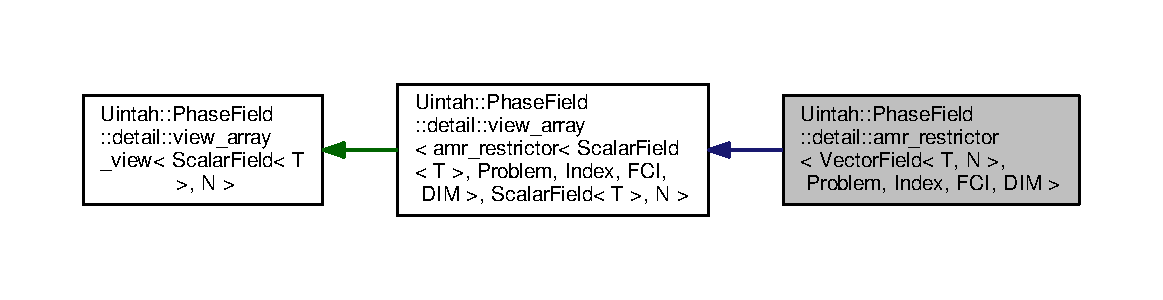
\includegraphics[width=350pt]{classUintah_1_1PhaseField_1_1detail_1_1amr__restrictor_3_01VectorField_3_01T_00_01N_01_4_00_01Prd14088bb03c51f5baa253b23a196d0e2}
\end{center}
\end{figure}


Collaboration diagram for Uintah\+:\+:Phase\+Field\+:\+:detail\+:\+:amr\+\_\+restrictor$<$ Vector\+Field$<$ T, N $>$, Problem, Index, F\+CI, D\+IM $>$\+:\nopagebreak
\begin{figure}[H]
\begin{center}
\leavevmode
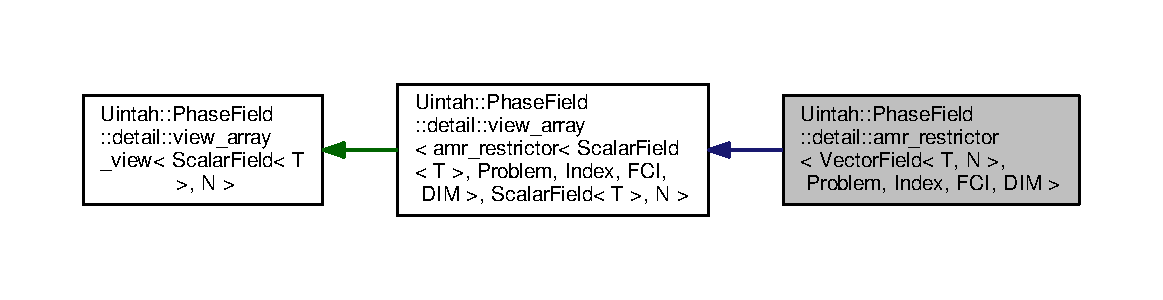
\includegraphics[width=350pt]{classUintah_1_1PhaseField_1_1detail_1_1amr__restrictor_3_01VectorField_3_01T_00_01N_01_4_00_01Pr128d8728dd04fc640a9cf08402c46e84}
\end{center}
\end{figure}
\subsection*{Public Member Functions}
\begin{DoxyCompactItemize}
\item 
\hyperlink{classUintah_1_1PhaseField_1_1detail_1_1amr__restrictor_3_01VectorField_3_01T_00_01N_01_4_00_01Pre7f2e99a4fbf25ff00717d25c8580b1a_abdd0eb090306c15eaeeee55105877b1f}{amr\+\_\+restrictor} (const typename \hyperlink{structUintah_1_1PhaseField_1_1VectorField_a59698346336d8cdfdf767367839f2be9}{Field\+::label\+\_\+type} \&label, const Var\+Label $\ast$subproblems\+\_\+label, int material)
\begin{DoxyCompactList}\small\item\em Constructor. \end{DoxyCompactList}\item 
\hyperlink{classUintah_1_1PhaseField_1_1detail_1_1amr__restrictor_3_01VectorField_3_01T_00_01N_01_4_00_01Pre7f2e99a4fbf25ff00717d25c8580b1a_a7c6b000db52c00663a106bbcfd22e287}{amr\+\_\+restrictor} (Data\+Warehouse $\ast$dw, const typename \hyperlink{structUintah_1_1PhaseField_1_1VectorField_a59698346336d8cdfdf767367839f2be9}{Field\+::label\+\_\+type} \&label, const Var\+Label $\ast$subproblems\+\_\+label, int material, const Patch $\ast$patch, bool use\+\_\+ghosts=View\+::use\+\_\+ghosts\+\_\+dflt)
\begin{DoxyCompactList}\small\item\em Constructor. \end{DoxyCompactList}\item 
virtual \hyperlink{classUintah_1_1PhaseField_1_1detail_1_1amr__restrictor_3_01VectorField_3_01T_00_01N_01_4_00_01Pre7f2e99a4fbf25ff00717d25c8580b1a_a0f0accb3ad8bfab4b88464b61f3b3491}{$\sim$amr\+\_\+restrictor} ()
\begin{DoxyCompactList}\small\item\em Destructor. \end{DoxyCompactList}\item 
\hyperlink{classUintah_1_1PhaseField_1_1detail_1_1amr__restrictor_3_01VectorField_3_01T_00_01N_01_4_00_01Pre7f2e99a4fbf25ff00717d25c8580b1a_a58c616d121749519316e5241271e618a}{amr\+\_\+restrictor} (const \hyperlink{classUintah_1_1PhaseField_1_1detail_1_1amr__restrictor}{amr\+\_\+restrictor} \&)=delete
\begin{DoxyCompactList}\small\item\em Prevent copy (and move) constructor. \end{DoxyCompactList}\item 
\hyperlink{classUintah_1_1PhaseField_1_1detail_1_1amr__restrictor}{amr\+\_\+restrictor} \& \hyperlink{classUintah_1_1PhaseField_1_1detail_1_1amr__restrictor_3_01VectorField_3_01T_00_01N_01_4_00_01Pre7f2e99a4fbf25ff00717d25c8580b1a_a8a66e1c425c67a41925ea9714816d586}{operator=} (const \hyperlink{classUintah_1_1PhaseField_1_1detail_1_1amr__restrictor}{amr\+\_\+restrictor} \&)=delete
\begin{DoxyCompactList}\small\item\em Prevent copy (and move) assignment. \end{DoxyCompactList}\end{DoxyCompactItemize}
\subsection*{Additional Inherited Members}


\subsection{Detailed Description}
\subsubsection*{template$<$typename T, size\+\_\+t N, typename Problem, typename Index, F\+C\+I\+Type F\+CI, Dim\+Type D\+IM$>$\newline
class Uintah\+::\+Phase\+Field\+::detail\+::amr\+\_\+restrictor$<$ Vector\+Field$<$ T, N $>$, Problem, Index, F\+C\+I, D\+I\+M $>$}

Abstract wrapper of grid variables for restriction from finer to coarser levels. (\hyperlink{structUintah_1_1PhaseField_1_1VectorField}{Vector\+Field} implementation) 

Adds to view the possibility to compute multi-\/grid interpolation


\begin{DoxyTemplParams}{Template Parameters}
{\em T} & type of each component of the field at each point \\
\hline
{\em N} & number of components \\
\hline
{\em \hyperlink{classUintah_1_1PhaseField_1_1Problem}{Problem}} & type of \hyperlink{namespaceUintah_1_1PhaseField}{Phase\+Field} problem \\
\hline
{\em Index} & index\+\_\+sequence of Field within \hyperlink{classUintah_1_1PhaseField_1_1Problem}{Problem} (first element is variable index, following ones, if present, are the component index within the variable) \\
\hline
\end{DoxyTemplParams}


\subsection{Constructor \& Destructor Documentation}
\mbox{\Hypertarget{classUintah_1_1PhaseField_1_1detail_1_1amr__restrictor_3_01VectorField_3_01T_00_01N_01_4_00_01Pre7f2e99a4fbf25ff00717d25c8580b1a_abdd0eb090306c15eaeeee55105877b1f}\label{classUintah_1_1PhaseField_1_1detail_1_1amr__restrictor_3_01VectorField_3_01T_00_01N_01_4_00_01Pre7f2e99a4fbf25ff00717d25c8580b1a_abdd0eb090306c15eaeeee55105877b1f}} 
\index{Uintah\+::\+Phase\+Field\+::detail\+::amr\+\_\+restrictor$<$ Vector\+Field$<$ T, N $>$, Problem, Index, F\+C\+I, D\+I\+M $>$@{Uintah\+::\+Phase\+Field\+::detail\+::amr\+\_\+restrictor$<$ Vector\+Field$<$ T, N $>$, Problem, Index, F\+C\+I, D\+I\+M $>$}!amr\+\_\+restrictor@{amr\+\_\+restrictor}}
\index{amr\+\_\+restrictor@{amr\+\_\+restrictor}!Uintah\+::\+Phase\+Field\+::detail\+::amr\+\_\+restrictor$<$ Vector\+Field$<$ T, N $>$, Problem, Index, F\+C\+I, D\+I\+M $>$@{Uintah\+::\+Phase\+Field\+::detail\+::amr\+\_\+restrictor$<$ Vector\+Field$<$ T, N $>$, Problem, Index, F\+C\+I, D\+I\+M $>$}}
\subsubsection{\texorpdfstring{amr\+\_\+restrictor()}{amr\_restrictor()}\hspace{0.1cm}{\footnotesize\ttfamily [1/3]}}
{\footnotesize\ttfamily template$<$typename T , size\+\_\+t N, typename Problem , typename Index , F\+C\+I\+Type F\+CI, Dim\+Type D\+IM$>$ \\
\hyperlink{classUintah_1_1PhaseField_1_1detail_1_1amr__restrictor}{Uintah\+::\+Phase\+Field\+::detail\+::amr\+\_\+restrictor}$<$ \hyperlink{structUintah_1_1PhaseField_1_1VectorField}{Vector\+Field}$<$ T, N $>$, \hyperlink{classUintah_1_1PhaseField_1_1Problem}{Problem}, Index, F\+CI, D\+IM $>$\+::\hyperlink{classUintah_1_1PhaseField_1_1detail_1_1amr__restrictor}{amr\+\_\+restrictor} (\begin{DoxyParamCaption}\item[{const typename \hyperlink{structUintah_1_1PhaseField_1_1VectorField_a59698346336d8cdfdf767367839f2be9}{Field\+::label\+\_\+type} \&}]{label,  }\item[{const Var\+Label $\ast$}]{subproblems\+\_\+label,  }\item[{int}]{material }\end{DoxyParamCaption})\hspace{0.3cm}{\ttfamily [inline]}}



Constructor. 

Instantiate \hyperlink{classUintah_1_1PhaseField_1_1detail_1_1amr__restrictor}{amr\+\_\+restrictor} components without gathering info from the Data\+Warehouse


\begin{DoxyParams}{Parameters}
{\em label} & list of variable labels for each component \\
\hline
{\em subproblems\+\_\+label} & label of subproblems in the Data\+Warehouse \\
\hline
{\em material} & material index \\
\hline
\end{DoxyParams}
\mbox{\Hypertarget{classUintah_1_1PhaseField_1_1detail_1_1amr__restrictor_3_01VectorField_3_01T_00_01N_01_4_00_01Pre7f2e99a4fbf25ff00717d25c8580b1a_a7c6b000db52c00663a106bbcfd22e287}\label{classUintah_1_1PhaseField_1_1detail_1_1amr__restrictor_3_01VectorField_3_01T_00_01N_01_4_00_01Pre7f2e99a4fbf25ff00717d25c8580b1a_a7c6b000db52c00663a106bbcfd22e287}} 
\index{Uintah\+::\+Phase\+Field\+::detail\+::amr\+\_\+restrictor$<$ Vector\+Field$<$ T, N $>$, Problem, Index, F\+C\+I, D\+I\+M $>$@{Uintah\+::\+Phase\+Field\+::detail\+::amr\+\_\+restrictor$<$ Vector\+Field$<$ T, N $>$, Problem, Index, F\+C\+I, D\+I\+M $>$}!amr\+\_\+restrictor@{amr\+\_\+restrictor}}
\index{amr\+\_\+restrictor@{amr\+\_\+restrictor}!Uintah\+::\+Phase\+Field\+::detail\+::amr\+\_\+restrictor$<$ Vector\+Field$<$ T, N $>$, Problem, Index, F\+C\+I, D\+I\+M $>$@{Uintah\+::\+Phase\+Field\+::detail\+::amr\+\_\+restrictor$<$ Vector\+Field$<$ T, N $>$, Problem, Index, F\+C\+I, D\+I\+M $>$}}
\subsubsection{\texorpdfstring{amr\+\_\+restrictor()}{amr\_restrictor()}\hspace{0.1cm}{\footnotesize\ttfamily [2/3]}}
{\footnotesize\ttfamily template$<$typename T , size\+\_\+t N, typename Problem , typename Index , F\+C\+I\+Type F\+CI, Dim\+Type D\+IM$>$ \\
\hyperlink{classUintah_1_1PhaseField_1_1detail_1_1amr__restrictor}{Uintah\+::\+Phase\+Field\+::detail\+::amr\+\_\+restrictor}$<$ \hyperlink{structUintah_1_1PhaseField_1_1VectorField}{Vector\+Field}$<$ T, N $>$, \hyperlink{classUintah_1_1PhaseField_1_1Problem}{Problem}, Index, F\+CI, D\+IM $>$\+::\hyperlink{classUintah_1_1PhaseField_1_1detail_1_1amr__restrictor}{amr\+\_\+restrictor} (\begin{DoxyParamCaption}\item[{Data\+Warehouse $\ast$}]{dw,  }\item[{const typename \hyperlink{structUintah_1_1PhaseField_1_1VectorField_a59698346336d8cdfdf767367839f2be9}{Field\+::label\+\_\+type} \&}]{label,  }\item[{const Var\+Label $\ast$}]{subproblems\+\_\+label,  }\item[{int}]{material,  }\item[{const Patch $\ast$}]{patch,  }\item[{bool}]{use\+\_\+ghosts = {\ttfamily View\+:\+:use\+\_\+ghosts\+\_\+dflt} }\end{DoxyParamCaption})\hspace{0.3cm}{\ttfamily [inline]}}



Constructor. 

Instantiate \hyperlink{classUintah_1_1PhaseField_1_1detail_1_1amr__restrictor}{amr\+\_\+restrictor} components and gather info from dw


\begin{DoxyParams}{Parameters}
{\em dw} & Data\+Warehouse from which data is retrieved \\
\hline
{\em label} & list of variable labels for each component \\
\hline
{\em subproblems\+\_\+label} & label of subproblems in the Data\+Warehouse \\
\hline
{\em material} & material index \\
\hline
{\em patch} & grid patch \\
\hline
{\em use\+\_\+ghosts} & if ghosts value are to be retrieved \\
\hline
\end{DoxyParams}
\mbox{\Hypertarget{classUintah_1_1PhaseField_1_1detail_1_1amr__restrictor_3_01VectorField_3_01T_00_01N_01_4_00_01Pre7f2e99a4fbf25ff00717d25c8580b1a_a0f0accb3ad8bfab4b88464b61f3b3491}\label{classUintah_1_1PhaseField_1_1detail_1_1amr__restrictor_3_01VectorField_3_01T_00_01N_01_4_00_01Pre7f2e99a4fbf25ff00717d25c8580b1a_a0f0accb3ad8bfab4b88464b61f3b3491}} 
\index{Uintah\+::\+Phase\+Field\+::detail\+::amr\+\_\+restrictor$<$ Vector\+Field$<$ T, N $>$, Problem, Index, F\+C\+I, D\+I\+M $>$@{Uintah\+::\+Phase\+Field\+::detail\+::amr\+\_\+restrictor$<$ Vector\+Field$<$ T, N $>$, Problem, Index, F\+C\+I, D\+I\+M $>$}!````~amr\+\_\+restrictor@{$\sim$amr\+\_\+restrictor}}
\index{````~amr\+\_\+restrictor@{$\sim$amr\+\_\+restrictor}!Uintah\+::\+Phase\+Field\+::detail\+::amr\+\_\+restrictor$<$ Vector\+Field$<$ T, N $>$, Problem, Index, F\+C\+I, D\+I\+M $>$@{Uintah\+::\+Phase\+Field\+::detail\+::amr\+\_\+restrictor$<$ Vector\+Field$<$ T, N $>$, Problem, Index, F\+C\+I, D\+I\+M $>$}}
\subsubsection{\texorpdfstring{$\sim$amr\+\_\+restrictor()}{~amr\_restrictor()}}
{\footnotesize\ttfamily template$<$typename T , size\+\_\+t N, typename Problem , typename Index , F\+C\+I\+Type F\+CI, Dim\+Type D\+IM$>$ \\
virtual \hyperlink{classUintah_1_1PhaseField_1_1detail_1_1amr__restrictor}{Uintah\+::\+Phase\+Field\+::detail\+::amr\+\_\+restrictor}$<$ \hyperlink{structUintah_1_1PhaseField_1_1VectorField}{Vector\+Field}$<$ T, N $>$, \hyperlink{classUintah_1_1PhaseField_1_1Problem}{Problem}, Index, F\+CI, D\+IM $>$\+::$\sim$\hyperlink{classUintah_1_1PhaseField_1_1detail_1_1amr__restrictor}{amr\+\_\+restrictor} (\begin{DoxyParamCaption}{ }\end{DoxyParamCaption})\hspace{0.3cm}{\ttfamily [inline]}, {\ttfamily [virtual]}}



Destructor. 

\mbox{\Hypertarget{classUintah_1_1PhaseField_1_1detail_1_1amr__restrictor_3_01VectorField_3_01T_00_01N_01_4_00_01Pre7f2e99a4fbf25ff00717d25c8580b1a_a58c616d121749519316e5241271e618a}\label{classUintah_1_1PhaseField_1_1detail_1_1amr__restrictor_3_01VectorField_3_01T_00_01N_01_4_00_01Pre7f2e99a4fbf25ff00717d25c8580b1a_a58c616d121749519316e5241271e618a}} 
\index{Uintah\+::\+Phase\+Field\+::detail\+::amr\+\_\+restrictor$<$ Vector\+Field$<$ T, N $>$, Problem, Index, F\+C\+I, D\+I\+M $>$@{Uintah\+::\+Phase\+Field\+::detail\+::amr\+\_\+restrictor$<$ Vector\+Field$<$ T, N $>$, Problem, Index, F\+C\+I, D\+I\+M $>$}!amr\+\_\+restrictor@{amr\+\_\+restrictor}}
\index{amr\+\_\+restrictor@{amr\+\_\+restrictor}!Uintah\+::\+Phase\+Field\+::detail\+::amr\+\_\+restrictor$<$ Vector\+Field$<$ T, N $>$, Problem, Index, F\+C\+I, D\+I\+M $>$@{Uintah\+::\+Phase\+Field\+::detail\+::amr\+\_\+restrictor$<$ Vector\+Field$<$ T, N $>$, Problem, Index, F\+C\+I, D\+I\+M $>$}}
\subsubsection{\texorpdfstring{amr\+\_\+restrictor()}{amr\_restrictor()}\hspace{0.1cm}{\footnotesize\ttfamily [3/3]}}
{\footnotesize\ttfamily template$<$typename T , size\+\_\+t N, typename Problem , typename Index , F\+C\+I\+Type F\+CI, Dim\+Type D\+IM$>$ \\
\hyperlink{classUintah_1_1PhaseField_1_1detail_1_1amr__restrictor}{Uintah\+::\+Phase\+Field\+::detail\+::amr\+\_\+restrictor}$<$ \hyperlink{structUintah_1_1PhaseField_1_1VectorField}{Vector\+Field}$<$ T, N $>$, \hyperlink{classUintah_1_1PhaseField_1_1Problem}{Problem}, Index, F\+CI, D\+IM $>$\+::\hyperlink{classUintah_1_1PhaseField_1_1detail_1_1amr__restrictor}{amr\+\_\+restrictor} (\begin{DoxyParamCaption}\item[{const \hyperlink{classUintah_1_1PhaseField_1_1detail_1_1amr__restrictor}{amr\+\_\+restrictor}$<$ \hyperlink{structUintah_1_1PhaseField_1_1VectorField}{Vector\+Field}$<$ T, N $>$, \hyperlink{classUintah_1_1PhaseField_1_1Problem}{Problem}, Index, F\+CI, D\+IM $>$ \&}]{ }\end{DoxyParamCaption})\hspace{0.3cm}{\ttfamily [delete]}}



Prevent copy (and move) constructor. 



\subsection{Member Function Documentation}
\mbox{\Hypertarget{classUintah_1_1PhaseField_1_1detail_1_1amr__restrictor_3_01VectorField_3_01T_00_01N_01_4_00_01Pre7f2e99a4fbf25ff00717d25c8580b1a_a8a66e1c425c67a41925ea9714816d586}\label{classUintah_1_1PhaseField_1_1detail_1_1amr__restrictor_3_01VectorField_3_01T_00_01N_01_4_00_01Pre7f2e99a4fbf25ff00717d25c8580b1a_a8a66e1c425c67a41925ea9714816d586}} 
\index{Uintah\+::\+Phase\+Field\+::detail\+::amr\+\_\+restrictor$<$ Vector\+Field$<$ T, N $>$, Problem, Index, F\+C\+I, D\+I\+M $>$@{Uintah\+::\+Phase\+Field\+::detail\+::amr\+\_\+restrictor$<$ Vector\+Field$<$ T, N $>$, Problem, Index, F\+C\+I, D\+I\+M $>$}!operator=@{operator=}}
\index{operator=@{operator=}!Uintah\+::\+Phase\+Field\+::detail\+::amr\+\_\+restrictor$<$ Vector\+Field$<$ T, N $>$, Problem, Index, F\+C\+I, D\+I\+M $>$@{Uintah\+::\+Phase\+Field\+::detail\+::amr\+\_\+restrictor$<$ Vector\+Field$<$ T, N $>$, Problem, Index, F\+C\+I, D\+I\+M $>$}}
\subsubsection{\texorpdfstring{operator=()}{operator=()}}
{\footnotesize\ttfamily template$<$typename T , size\+\_\+t N, typename Problem , typename Index , F\+C\+I\+Type F\+CI, Dim\+Type D\+IM$>$ \\
\hyperlink{classUintah_1_1PhaseField_1_1detail_1_1amr__restrictor}{amr\+\_\+restrictor}\& \hyperlink{classUintah_1_1PhaseField_1_1detail_1_1amr__restrictor}{Uintah\+::\+Phase\+Field\+::detail\+::amr\+\_\+restrictor}$<$ \hyperlink{structUintah_1_1PhaseField_1_1VectorField}{Vector\+Field}$<$ T, N $>$, \hyperlink{classUintah_1_1PhaseField_1_1Problem}{Problem}, Index, F\+CI, D\+IM $>$\+::operator= (\begin{DoxyParamCaption}\item[{const \hyperlink{classUintah_1_1PhaseField_1_1detail_1_1amr__restrictor}{amr\+\_\+restrictor}$<$ \hyperlink{structUintah_1_1PhaseField_1_1VectorField}{Vector\+Field}$<$ T, N $>$, \hyperlink{classUintah_1_1PhaseField_1_1Problem}{Problem}, Index, F\+CI, D\+IM $>$ \&}]{ }\end{DoxyParamCaption})\hspace{0.3cm}{\ttfamily [delete]}}



Prevent copy (and move) assignment. 



The documentation for this class was generated from the following file\+:\begin{DoxyCompactItemize}
\item 
\hyperlink{amr__restrictor_8h}{amr\+\_\+restrictor.\+h}\end{DoxyCompactItemize}

\hypertarget{structUintah_1_1PhaseField_1_1AMRInterface}{}\section{Uintah\+:\+:Phase\+Field\+:\+:A\+M\+R\+Interface$<$ V\+AR, D\+IM $>$ Struct Template Reference}
\label{structUintah_1_1PhaseField_1_1AMRInterface}\index{Uintah\+::\+Phase\+Field\+::\+A\+M\+R\+Interface$<$ V\+A\+R, D\+I\+M $>$@{Uintah\+::\+Phase\+Field\+::\+A\+M\+R\+Interface$<$ V\+A\+R, D\+I\+M $>$}}


Interface for A\+MR.  




{\ttfamily \#include $<$A\+M\+R\+Interface.\+h$>$}



Inheritance diagram for Uintah\+:\+:Phase\+Field\+:\+:A\+M\+R\+Interface$<$ V\+AR, D\+IM $>$\+:\nopagebreak
\begin{figure}[H]
\begin{center}
\leavevmode
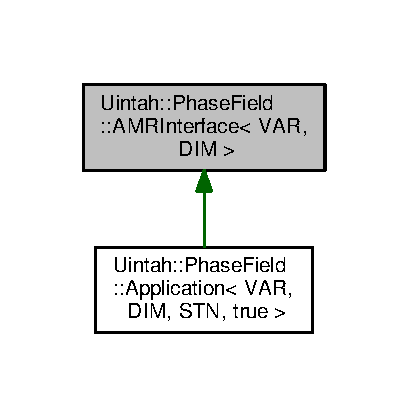
\includegraphics[width=196pt]{structUintah_1_1PhaseField_1_1AMRInterface__inherit__graph}
\end{center}
\end{figure}
\subsection*{Static Public Member Functions}
\begin{DoxyCompactItemize}
\item 
{\footnotesize template$<$Var\+Type V = V\+AR$>$ }\\static Int\+Vector \hyperlink{structUintah_1_1PhaseField_1_1AMRInterface_a567b8c307a636ab6addd2fa4272581a4}{get\+\_\+coarser} (const Level $\ast$l, const Int\+Vector \&i)
\item 
{\footnotesize template$<$Var\+Type V = V\+AR$>$ }\\static Int\+Vector \hyperlink{structUintah_1_1PhaseField_1_1AMRInterface_a5b3ace8289c6b187d6d42c2e19dec9f4}{get\+\_\+finer} (const Level $\ast$l, const Int\+Vector \&i)
\end{DoxyCompactItemize}


\subsection{Detailed Description}
\subsubsection*{template$<$Var\+Type V\+AR, Dim\+Type D\+IM$>$\newline
struct Uintah\+::\+Phase\+Field\+::\+A\+M\+R\+Interface$<$ V\+A\+R, D\+I\+M $>$}

Interface for A\+MR. 

groups together various methods to get info about amr patches and levels which depend on the different types of variable representation and problem dimensions allowing to choose the relevant implementation at compile time


\begin{DoxyTemplParams}{Template Parameters}
{\em V\+AR} & type of variable representation \\
\hline
{\em D\+IM} & problem dimension \\
\hline
\end{DoxyTemplParams}


\subsection{Member Function Documentation}
\mbox{\Hypertarget{structUintah_1_1PhaseField_1_1AMRInterface_a567b8c307a636ab6addd2fa4272581a4}\label{structUintah_1_1PhaseField_1_1AMRInterface_a567b8c307a636ab6addd2fa4272581a4}} 
\index{Uintah\+::\+Phase\+Field\+::\+A\+M\+R\+Interface@{Uintah\+::\+Phase\+Field\+::\+A\+M\+R\+Interface}!get\+\_\+coarser@{get\+\_\+coarser}}
\index{get\+\_\+coarser@{get\+\_\+coarser}!Uintah\+::\+Phase\+Field\+::\+A\+M\+R\+Interface@{Uintah\+::\+Phase\+Field\+::\+A\+M\+R\+Interface}}
\subsubsection{\texorpdfstring{get\+\_\+coarser()}{get\_coarser()}}
{\footnotesize\ttfamily template$<$Var\+Type V\+AR, Dim\+Type D\+IM$>$ \\
template$<$Var\+Type V = V\+AR$>$ \\
static Int\+Vector \hyperlink{structUintah_1_1PhaseField_1_1AMRInterface}{Uintah\+::\+Phase\+Field\+::\+A\+M\+R\+Interface}$<$ V\+AR, D\+IM $>$\+::get\+\_\+coarser (\begin{DoxyParamCaption}\item[{const Level $\ast$}]{l,  }\item[{const Int\+Vector \&}]{i }\end{DoxyParamCaption})\hspace{0.3cm}{\ttfamily [inline]}, {\ttfamily [static]}}

\mbox{\Hypertarget{structUintah_1_1PhaseField_1_1AMRInterface_a5b3ace8289c6b187d6d42c2e19dec9f4}\label{structUintah_1_1PhaseField_1_1AMRInterface_a5b3ace8289c6b187d6d42c2e19dec9f4}} 
\index{Uintah\+::\+Phase\+Field\+::\+A\+M\+R\+Interface@{Uintah\+::\+Phase\+Field\+::\+A\+M\+R\+Interface}!get\+\_\+finer@{get\+\_\+finer}}
\index{get\+\_\+finer@{get\+\_\+finer}!Uintah\+::\+Phase\+Field\+::\+A\+M\+R\+Interface@{Uintah\+::\+Phase\+Field\+::\+A\+M\+R\+Interface}}
\subsubsection{\texorpdfstring{get\+\_\+finer()}{get\_finer()}}
{\footnotesize\ttfamily template$<$Var\+Type V\+AR, Dim\+Type D\+IM$>$ \\
template$<$Var\+Type V = V\+AR$>$ \\
static Int\+Vector \hyperlink{structUintah_1_1PhaseField_1_1AMRInterface}{Uintah\+::\+Phase\+Field\+::\+A\+M\+R\+Interface}$<$ V\+AR, D\+IM $>$\+::get\+\_\+finer (\begin{DoxyParamCaption}\item[{const Level $\ast$}]{l,  }\item[{const Int\+Vector \&}]{i }\end{DoxyParamCaption})\hspace{0.3cm}{\ttfamily [inline]}, {\ttfamily [static]}}



The documentation for this struct was generated from the following file\+:\begin{DoxyCompactItemize}
\item 
\hyperlink{AMRInterface_8h}{A\+M\+R\+Interface.\+h}\end{DoxyCompactItemize}

\hypertarget{classUintah_1_1PhaseField_1_1Application}{}\section{Uintah\+:\+:Phase\+Field\+:\+:Application$<$ V\+AR, D\+IM, S\+TN, A\+MR $>$ Class Template Reference}
\label{classUintah_1_1PhaseField_1_1Application}\index{Uintah\+::\+Phase\+Field\+::\+Application$<$ V\+A\+R, D\+I\+M, S\+T\+N, A\+M\+R $>$@{Uintah\+::\+Phase\+Field\+::\+Application$<$ V\+A\+R, D\+I\+M, S\+T\+N, A\+M\+R $>$}}


Virtual base for \hyperlink{namespaceUintah_1_1PhaseField}{Phase\+Field} applications.  




{\ttfamily \#include $<$Application.\+h$>$}



Inheritance diagram for Uintah\+:\+:Phase\+Field\+:\+:Application$<$ V\+AR, D\+IM, S\+TN, A\+MR $>$\+:\nopagebreak
\begin{figure}[H]
\begin{center}
\leavevmode
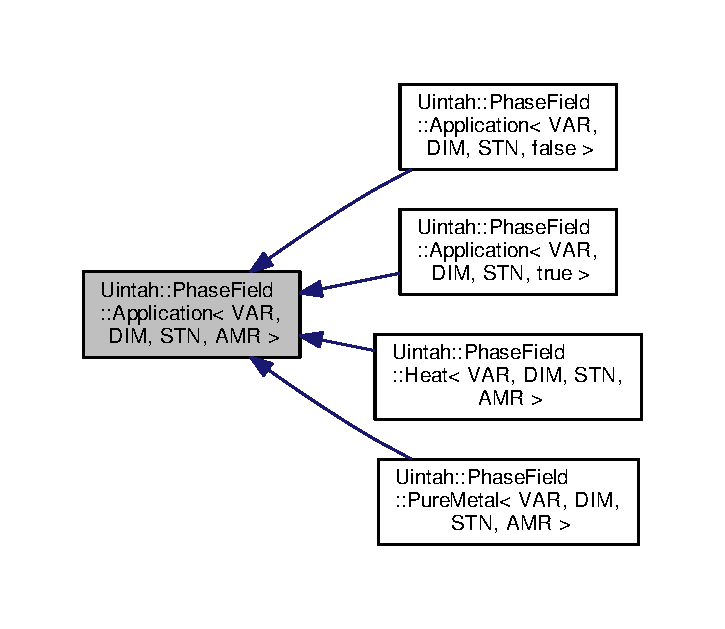
\includegraphics[width=348pt]{classUintah_1_1PhaseField_1_1Application__inherit__graph}
\end{center}
\end{figure}


\subsection{Detailed Description}
\subsubsection*{template$<$Var\+Type V\+AR, Dim\+Type D\+IM, Stn\+Type S\+TN, bool A\+MR = false$>$\newline
class Uintah\+::\+Phase\+Field\+::\+Application$<$ V\+A\+R, D\+I\+M, S\+T\+N, A\+M\+R $>$}

Virtual base for \hyperlink{namespaceUintah_1_1PhaseField}{Phase\+Field} applications. 

Wrapper of Application\+Common and interfaces


\begin{DoxyTemplParams}{Template Parameters}
{\em V\+AR} & type of variable representation \\
\hline
{\em D\+IM} & problem dimension \\
\hline
{\em S\+TN} & finite-\/difference stencil \\
\hline
{\em A\+MR} & whether to use adaptive mesh refinement \\
\hline
\end{DoxyTemplParams}


The documentation for this class was generated from the following file\+:\begin{DoxyCompactItemize}
\item 
\hyperlink{Application_8h}{Application.\+h}\end{DoxyCompactItemize}

\hypertarget{classUintah_1_1PhaseField_1_1Application_3_01VAR_00_01DIM_00_01STN_00_01false_01_4}{}\section{Uintah\+:\+:Phase\+Field\+:\+:Application$<$ V\+AR, D\+IM, S\+TN, false $>$ Class Template Reference}
\label{classUintah_1_1PhaseField_1_1Application_3_01VAR_00_01DIM_00_01STN_00_01false_01_4}\index{Uintah\+::\+Phase\+Field\+::\+Application$<$ V\+A\+R, D\+I\+M, S\+T\+N, false $>$@{Uintah\+::\+Phase\+Field\+::\+Application$<$ V\+A\+R, D\+I\+M, S\+T\+N, false $>$}}


Virtual base for \hyperlink{namespaceUintah_1_1PhaseField}{Phase\+Field} applications (non-\/\+A\+MR implementation)  




{\ttfamily \#include $<$Application.\+h$>$}



Inheritance diagram for Uintah\+:\+:Phase\+Field\+:\+:Application$<$ V\+AR, D\+IM, S\+TN, false $>$\+:\nopagebreak
\begin{figure}[H]
\begin{center}
\leavevmode
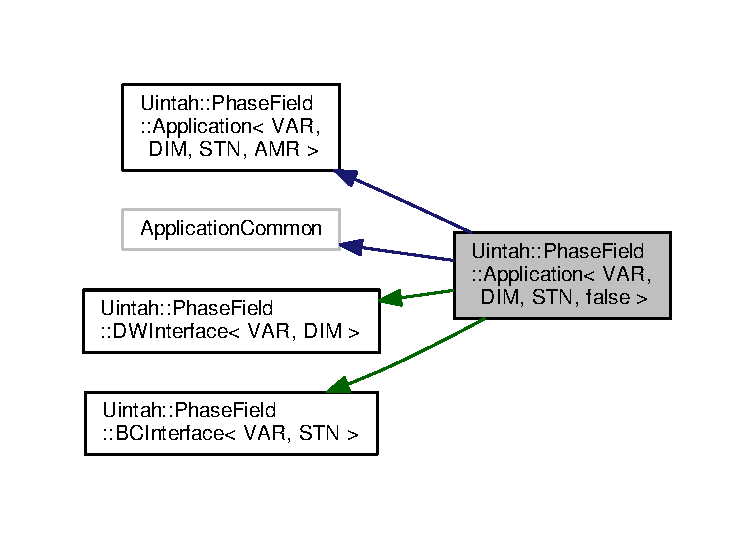
\includegraphics[width=350pt]{classUintah_1_1PhaseField_1_1Application_3_01VAR_00_01DIM_00_01STN_00_01false_01_4__inherit__graph}
\end{center}
\end{figure}


Collaboration diagram for Uintah\+:\+:Phase\+Field\+:\+:Application$<$ V\+AR, D\+IM, S\+TN, false $>$\+:\nopagebreak
\begin{figure}[H]
\begin{center}
\leavevmode
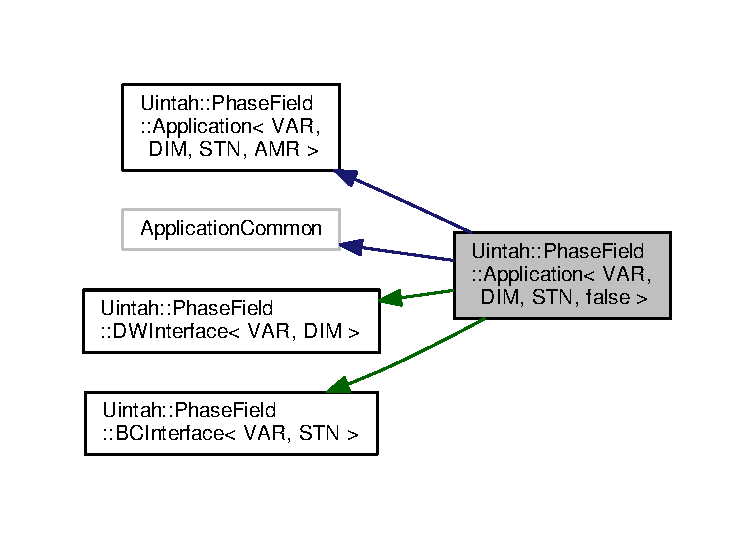
\includegraphics[width=350pt]{classUintah_1_1PhaseField_1_1Application_3_01VAR_00_01DIM_00_01STN_00_01false_01_4__coll__graph}
\end{center}
\end{figure}
\subsection*{Additional Inherited Members}


\subsection{Detailed Description}
\subsubsection*{template$<$Var\+Type V\+AR, Dim\+Type D\+IM, Stn\+Type S\+TN$>$\newline
class Uintah\+::\+Phase\+Field\+::\+Application$<$ V\+A\+R, D\+I\+M, S\+T\+N, false $>$}

Virtual base for \hyperlink{namespaceUintah_1_1PhaseField}{Phase\+Field} applications (non-\/\+A\+MR implementation) 

Wrapper of Application\+Common and interfaces

$<$ V\+AR, D\+IM, S\+TN, A\+MR $>$ 
\begin{DoxyTemplParams}{Template Parameters}
{\em V\+AR} & type of variable representation \\
\hline
{\em D\+IM} & problem dimension \\
\hline
{\em S\+TN} & finite-\/difference stencil \\
\hline
\end{DoxyTemplParams}


The documentation for this class was generated from the following file\+:\begin{DoxyCompactItemize}
\item 
\hyperlink{Application_8h}{Application.\+h}\end{DoxyCompactItemize}

\hypertarget{classUintah_1_1PhaseField_1_1Application_3_01VAR_00_01DIM_00_01STN_00_01true_01_4}{}\section{Uintah\+:\+:Phase\+Field\+:\+:Application$<$ V\+AR, D\+IM, S\+TN, true $>$ Class Template Reference}
\label{classUintah_1_1PhaseField_1_1Application_3_01VAR_00_01DIM_00_01STN_00_01true_01_4}\index{Uintah\+::\+Phase\+Field\+::\+Application$<$ V\+A\+R, D\+I\+M, S\+T\+N, true $>$@{Uintah\+::\+Phase\+Field\+::\+Application$<$ V\+A\+R, D\+I\+M, S\+T\+N, true $>$}}


Virtual base for \hyperlink{namespaceUintah_1_1PhaseField}{Phase\+Field} applications (A\+MR implementation)  




{\ttfamily \#include $<$Application.\+h$>$}



Inheritance diagram for Uintah\+:\+:Phase\+Field\+:\+:Application$<$ V\+AR, D\+IM, S\+TN, true $>$\+:\nopagebreak
\begin{figure}[H]
\begin{center}
\leavevmode
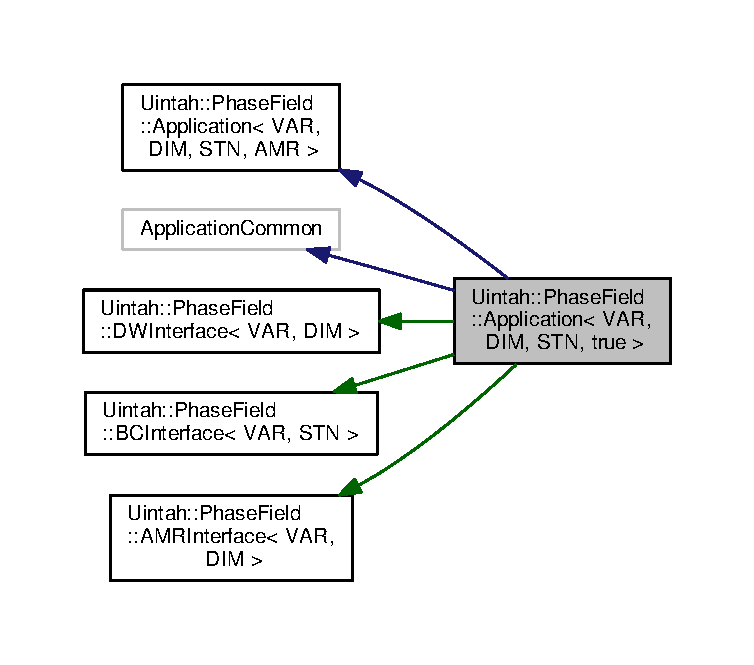
\includegraphics[width=350pt]{classUintah_1_1PhaseField_1_1Application_3_01VAR_00_01DIM_00_01STN_00_01true_01_4__inherit__graph}
\end{center}
\end{figure}


Collaboration diagram for Uintah\+:\+:Phase\+Field\+:\+:Application$<$ V\+AR, D\+IM, S\+TN, true $>$\+:\nopagebreak
\begin{figure}[H]
\begin{center}
\leavevmode
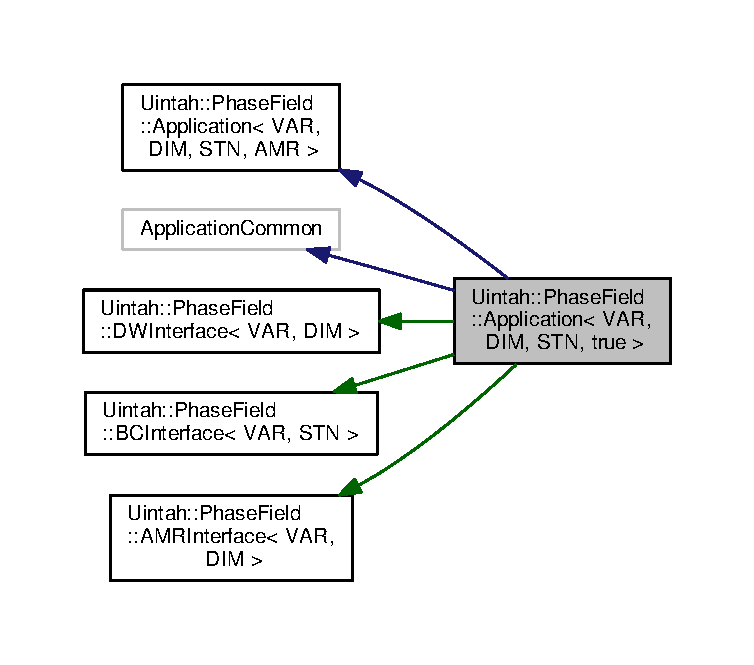
\includegraphics[width=350pt]{classUintah_1_1PhaseField_1_1Application_3_01VAR_00_01DIM_00_01STN_00_01true_01_4__coll__graph}
\end{center}
\end{figure}
\subsection*{Additional Inherited Members}


\subsection{Detailed Description}
\subsubsection*{template$<$Var\+Type V\+AR, Dim\+Type D\+IM, Stn\+Type S\+TN$>$\newline
class Uintah\+::\+Phase\+Field\+::\+Application$<$ V\+A\+R, D\+I\+M, S\+T\+N, true $>$}

Virtual base for \hyperlink{namespaceUintah_1_1PhaseField}{Phase\+Field} applications (A\+MR implementation) 

Wrapper of Application\+Common and interfaces

$<$ V\+AR, D\+IM, S\+TN, A\+MR $>$ 
\begin{DoxyTemplParams}{Template Parameters}
{\em V\+AR} & type of variable representation \\
\hline
{\em D\+IM} & problem dimension \\
\hline
{\em S\+TN} & finite-\/difference stencil \\
\hline
\end{DoxyTemplParams}


The documentation for this class was generated from the following file\+:\begin{DoxyCompactItemize}
\item 
\hyperlink{Application_8h}{Application.\+h}\end{DoxyCompactItemize}

\hypertarget{classUintah_1_1PhaseField_1_1ApplicationFactory}{}\section{Uintah\+:\+:Phase\+Field\+:\+:Application\+Factory Class Reference}
\label{classUintah_1_1PhaseField_1_1ApplicationFactory}\index{Uintah\+::\+Phase\+Field\+::\+Application\+Factory@{Uintah\+::\+Phase\+Field\+::\+Application\+Factory}}


\hyperlink{classUintah_1_1PhaseField_1_1Factory}{Factory} class for different \hyperlink{namespaceUintah_1_1PhaseField}{Phase\+Field} applications.  




{\ttfamily \#include $<$Application\+Factory.\+h$>$}

\subsection*{Static Public Member Functions}
\begin{DoxyCompactItemize}
\item 
static Uintah\+Parallel\+Component $\ast$ \hyperlink{classUintah_1_1PhaseField_1_1ApplicationFactory_ac5cb141180ec988bac718994efcce36f}{create} (const Processor\+Group $\ast$my\+World, const Material\+ManagerP material\+Manager, Problem\+SpecP prob\+Spec, bool do\+A\+MR)
\begin{DoxyCompactList}\small\item\em factory create method \end{DoxyCompactList}\end{DoxyCompactItemize}


\subsection{Detailed Description}
\hyperlink{classUintah_1_1PhaseField_1_1Factory}{Factory} class for different \hyperlink{namespaceUintah_1_1PhaseField}{Phase\+Field} applications. 

\hyperlink{classUintah_1_1PhaseField_1_1Factory}{Factory} class for creating new instances of Uintah\+Parallel\+Component within the \hyperlink{namespaceUintah_1_1PhaseField}{Phase\+Field} component 

\subsection{Member Function Documentation}
\mbox{\Hypertarget{classUintah_1_1PhaseField_1_1ApplicationFactory_ac5cb141180ec988bac718994efcce36f}\label{classUintah_1_1PhaseField_1_1ApplicationFactory_ac5cb141180ec988bac718994efcce36f}} 
\index{Uintah\+::\+Phase\+Field\+::\+Application\+Factory@{Uintah\+::\+Phase\+Field\+::\+Application\+Factory}!create@{create}}
\index{create@{create}!Uintah\+::\+Phase\+Field\+::\+Application\+Factory@{Uintah\+::\+Phase\+Field\+::\+Application\+Factory}}
\subsubsection{\texorpdfstring{create()}{create()}}
{\footnotesize\ttfamily Uintah\+Parallel\+Component $\ast$ Application\+Factory\+::create (\begin{DoxyParamCaption}\item[{const Processor\+Group $\ast$}]{my\+World,  }\item[{const Material\+ManagerP}]{material\+Manager,  }\item[{Problem\+SpecP}]{prob\+Spec,  }\item[{bool}]{do\+A\+MR }\end{DoxyParamCaption})\hspace{0.3cm}{\ttfamily [static]}}



factory create method 

\hyperlink{classUintah_1_1PhaseField_1_1Factory}{Factory} method for creating new instances of Uintah\+Parallel\+Component within the \hyperlink{namespaceUintah_1_1PhaseField}{Phase\+Field} component


\begin{DoxyParams}{Parameters}
{\em my\+World} & data structure to manage mpi processes \\
\hline
{\em material\+Manager} & data structure to manage materials \\
\hline
{\em prob\+Spec} & specifications parsed from ups input file \\
\hline
{\em do\+A\+MR} & if adaptive mesh refinement is requsted by the input \\
\hline
\end{DoxyParams}


The documentation for this class was generated from the following files\+:\begin{DoxyCompactItemize}
\item 
\hyperlink{ApplicationFactory_8h}{Application\+Factory.\+h}\item 
\hyperlink{ApplicationFactory_8cc}{Application\+Factory.\+cc}\end{DoxyCompactItemize}

\hypertarget{classUintah_1_1PhaseField_1_1Base}{}\section{Uintah\+:\+:Phase\+Field\+:\+:Base$<$ B $>$ Class Template Reference}
\label{classUintah_1_1PhaseField_1_1Base}\index{Uintah\+::\+Phase\+Field\+::\+Base$<$ B $>$@{Uintah\+::\+Phase\+Field\+::\+Base$<$ B $>$}}


Generic factory base class.  




{\ttfamily \#include $<$Base.\+h$>$}



Inheritance diagram for Uintah\+:\+:Phase\+Field\+:\+:Base$<$ B $>$\+:\nopagebreak
\begin{figure}[H]
\begin{center}
\leavevmode
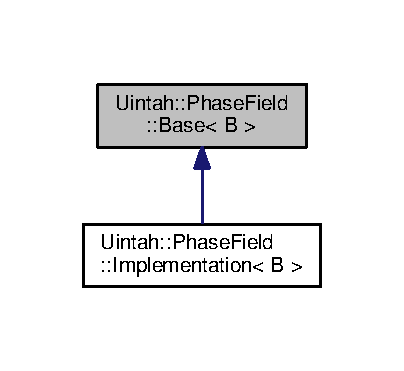
\includegraphics[width=194pt]{classUintah_1_1PhaseField_1_1Base__inherit__graph}
\end{center}
\end{figure}
\subsection*{Protected Member Functions}
\begin{DoxyCompactItemize}
\item 
\hyperlink{classUintah_1_1PhaseField_1_1Base_af64dc0e6053ade056af9806edce1d852}{Base} ()
\begin{DoxyCompactList}\small\item\em Default constructor. \end{DoxyCompactList}\item 
\hyperlink{classUintah_1_1PhaseField_1_1Base_a282bf8678ac00386cdd0b4b6b347d516}{Base} (bool \hyperlink{classUintah_1_1PhaseField_1_1Base_aead016aeee1f43fb7959158d7c9edb31}{is\+Registered})
\begin{DoxyCompactList}\small\item\em Constructor for \hyperlink{classUintah_1_1PhaseField_1_1Implementation}{Implementation}. \end{DoxyCompactList}\item 
virtual \hyperlink{classUintah_1_1PhaseField_1_1Base_a6c584b6c9a0a40c98870e6a25311fbff}{$\sim$\+Base} ()=default
\begin{DoxyCompactList}\small\item\em Default destructor. \end{DoxyCompactList}\item 
bool \hyperlink{classUintah_1_1PhaseField_1_1Base_aead016aeee1f43fb7959158d7c9edb31}{is\+Registered} () const
\begin{DoxyCompactList}\small\item\em Get registered status. \end{DoxyCompactList}\item 
virtual std\+::string \hyperlink{classUintah_1_1PhaseField_1_1Base_acd19fa2507f239588926b04069ad1b73}{get\+Name} ()=0
\begin{DoxyCompactList}\small\item\em Get \hyperlink{classUintah_1_1PhaseField_1_1Implementation}{Implementation} name. \end{DoxyCompactList}\end{DoxyCompactItemize}


\subsection{Detailed Description}
\subsubsection*{template$<$typename B$>$\newline
class Uintah\+::\+Phase\+Field\+::\+Base$<$ B $>$}

Generic factory base class. 

Make possible to create a new instance of a virtual class choosing which derived class implementation to create according to a string


\begin{DoxyTemplParams}{Template Parameters}
{\em B} & virtual base class type \\
\hline
\end{DoxyTemplParams}


\subsection{Constructor \& Destructor Documentation}
\mbox{\Hypertarget{classUintah_1_1PhaseField_1_1Base_af64dc0e6053ade056af9806edce1d852}\label{classUintah_1_1PhaseField_1_1Base_af64dc0e6053ade056af9806edce1d852}} 
\index{Uintah\+::\+Phase\+Field\+::\+Base@{Uintah\+::\+Phase\+Field\+::\+Base}!Base@{Base}}
\index{Base@{Base}!Uintah\+::\+Phase\+Field\+::\+Base@{Uintah\+::\+Phase\+Field\+::\+Base}}
\subsubsection{\texorpdfstring{Base()}{Base()}\hspace{0.1cm}{\footnotesize\ttfamily [1/2]}}
{\footnotesize\ttfamily template$<$typename B$>$ \\
\hyperlink{classUintah_1_1PhaseField_1_1Base}{Uintah\+::\+Phase\+Field\+::\+Base}$<$ B $>$\+::\hyperlink{classUintah_1_1PhaseField_1_1Base}{Base} (\begin{DoxyParamCaption}{ }\end{DoxyParamCaption})\hspace{0.3cm}{\ttfamily [inline]}, {\ttfamily [protected]}}



Default constructor. 

Virtual class is not registered \mbox{\Hypertarget{classUintah_1_1PhaseField_1_1Base_a282bf8678ac00386cdd0b4b6b347d516}\label{classUintah_1_1PhaseField_1_1Base_a282bf8678ac00386cdd0b4b6b347d516}} 
\index{Uintah\+::\+Phase\+Field\+::\+Base@{Uintah\+::\+Phase\+Field\+::\+Base}!Base@{Base}}
\index{Base@{Base}!Uintah\+::\+Phase\+Field\+::\+Base@{Uintah\+::\+Phase\+Field\+::\+Base}}
\subsubsection{\texorpdfstring{Base()}{Base()}\hspace{0.1cm}{\footnotesize\ttfamily [2/2]}}
{\footnotesize\ttfamily template$<$typename B$>$ \\
\hyperlink{classUintah_1_1PhaseField_1_1Base}{Uintah\+::\+Phase\+Field\+::\+Base}$<$ B $>$\+::\hyperlink{classUintah_1_1PhaseField_1_1Base}{Base} (\begin{DoxyParamCaption}\item[{bool}]{is\+Registered }\end{DoxyParamCaption})\hspace{0.3cm}{\ttfamily [inline]}, {\ttfamily [protected]}}



Constructor for \hyperlink{classUintah_1_1PhaseField_1_1Implementation}{Implementation}. 

This constructor is called by the constructor of any \hyperlink{classUintah_1_1PhaseField_1_1Implementation}{Implementation} of B


\begin{DoxyParams}{Parameters}
{\em is\+Registered} & whether the \hyperlink{classUintah_1_1PhaseField_1_1Implementation}{Implementation} is registered \\
\hline
\end{DoxyParams}
\mbox{\Hypertarget{classUintah_1_1PhaseField_1_1Base_a6c584b6c9a0a40c98870e6a25311fbff}\label{classUintah_1_1PhaseField_1_1Base_a6c584b6c9a0a40c98870e6a25311fbff}} 
\index{Uintah\+::\+Phase\+Field\+::\+Base@{Uintah\+::\+Phase\+Field\+::\+Base}!````~Base@{$\sim$\+Base}}
\index{````~Base@{$\sim$\+Base}!Uintah\+::\+Phase\+Field\+::\+Base@{Uintah\+::\+Phase\+Field\+::\+Base}}
\subsubsection{\texorpdfstring{$\sim$\+Base()}{~Base()}}
{\footnotesize\ttfamily template$<$typename B$>$ \\
virtual \hyperlink{classUintah_1_1PhaseField_1_1Base}{Uintah\+::\+Phase\+Field\+::\+Base}$<$ B $>$\+::$\sim$\hyperlink{classUintah_1_1PhaseField_1_1Base}{Base} (\begin{DoxyParamCaption}{ }\end{DoxyParamCaption})\hspace{0.3cm}{\ttfamily [protected]}, {\ttfamily [virtual]}, {\ttfamily [default]}}



Default destructor. 



\subsection{Member Function Documentation}
\mbox{\Hypertarget{classUintah_1_1PhaseField_1_1Base_acd19fa2507f239588926b04069ad1b73}\label{classUintah_1_1PhaseField_1_1Base_acd19fa2507f239588926b04069ad1b73}} 
\index{Uintah\+::\+Phase\+Field\+::\+Base@{Uintah\+::\+Phase\+Field\+::\+Base}!get\+Name@{get\+Name}}
\index{get\+Name@{get\+Name}!Uintah\+::\+Phase\+Field\+::\+Base@{Uintah\+::\+Phase\+Field\+::\+Base}}
\subsubsection{\texorpdfstring{get\+Name()}{getName()}}
{\footnotesize\ttfamily template$<$typename B$>$ \\
virtual std\+::string \hyperlink{classUintah_1_1PhaseField_1_1Base}{Uintah\+::\+Phase\+Field\+::\+Base}$<$ B $>$\+::get\+Name (\begin{DoxyParamCaption}{ }\end{DoxyParamCaption})\hspace{0.3cm}{\ttfamily [protected]}, {\ttfamily [pure virtual]}}



Get \hyperlink{classUintah_1_1PhaseField_1_1Implementation}{Implementation} name. 

Provide a way for derived classes to identify themselves

\begin{DoxyReturn}{Returns}
string identifying a derived class 
\end{DoxyReturn}


Implemented in \hyperlink{classUintah_1_1PhaseField_1_1Implementation_a115940ce50afb4e7a2a0a831a2a6577c}{Uintah\+::\+Phase\+Field\+::\+Implementation$<$ I, B, Args $>$}, \hyperlink{classUintah_1_1PhaseField_1_1Implementation_a115940ce50afb4e7a2a0a831a2a6577c}{Uintah\+::\+Phase\+Field\+::\+Implementation$<$ Benchmark03$<$ V\+A\+R, S\+T\+N $>$, Uintah\+Parallel\+Component, const Processor\+Group $\ast$, const Material\+Manager\+P, int $>$}, \hyperlink{classUintah_1_1PhaseField_1_1Implementation_a115940ce50afb4e7a2a0a831a2a6577c}{Uintah\+::\+Phase\+Field\+::\+Implementation$<$ D\+W\+View$<$ Field, V\+A\+R, D\+I\+M $>$, View$<$ Field $>$, const Field\+::label\+\_\+type \&, int $>$}, \hyperlink{classUintah_1_1PhaseField_1_1Implementation_a115940ce50afb4e7a2a0a831a2a6577c}{Uintah\+::\+Phase\+Field\+::\+Implementation$<$ D\+W\+F\+D\+View$<$ Field, S\+T\+N, V\+A\+R $>$, F\+D\+View$<$ Field, S\+T\+N $>$, const Field\+::label\+\_\+type \&, int, const Level $\ast$ $>$}, \hyperlink{classUintah_1_1PhaseField_1_1Implementation_a115940ce50afb4e7a2a0a831a2a6577c}{Uintah\+::\+Phase\+Field\+::\+Implementation$<$ Benchmark01$<$ V\+A\+R, S\+T\+N $>$, Uintah\+Parallel\+Component, const Processor\+Group $\ast$, const Material\+Manager\+P, int $>$}, \hyperlink{classUintah_1_1PhaseField_1_1Implementation_a115940ce50afb4e7a2a0a831a2a6577c}{Uintah\+::\+Phase\+Field\+::\+Implementation$<$ B\+C\+F\+D\+View$<$ Problem, I, P... $>$, F\+D\+View$<$ Problem\+::template get\+\_\+field$<$ I $>$\+::type, Problem\+::\+Stn $>$, const Problem\+::template get\+\_\+field$<$ I $>$\+::type\+::label\+\_\+type \&, const Var\+Label $\ast$, int, const Level $\ast$, const std\+::vector$<$ B\+C\+Info$<$ Problem\+::template get\+\_\+field$<$ I $>$\+::type $>$ $>$ \& $>$}, \hyperlink{classUintah_1_1PhaseField_1_1Implementation_a115940ce50afb4e7a2a0a831a2a6577c}{Uintah\+::\+Phase\+Field\+::\+Implementation$<$ Benchmark02$<$ V\+A\+R, S\+T\+N $>$, Uintah\+Parallel\+Component, const Processor\+Group $\ast$, const Material\+Manager\+P, int $>$}, \hyperlink{classUintah_1_1PhaseField_1_1Implementation_a115940ce50afb4e7a2a0a831a2a6577c}{Uintah\+::\+Phase\+Field\+::\+Implementation$<$ Heat$<$ V\+A\+R, D\+I\+M, S\+T\+N, A\+M\+R $>$, Uintah\+Parallel\+Component, const Processor\+Group $\ast$, const Material\+Manager\+P, int $>$}, \hyperlink{classUintah_1_1PhaseField_1_1Implementation_a115940ce50afb4e7a2a0a831a2a6577c}{Uintah\+::\+Phase\+Field\+::\+Implementation$<$ Benchmark04$<$ V\+A\+R, S\+T\+N $>$, Uintah\+Parallel\+Component, const Processor\+Group $\ast$, const Material\+Manager\+P, int $>$}, and \hyperlink{classUintah_1_1PhaseField_1_1Implementation_a115940ce50afb4e7a2a0a831a2a6577c}{Uintah\+::\+Phase\+Field\+::\+Implementation$<$ Pure\+Metal$<$ V\+A\+R, D\+I\+M, S\+T\+N, A\+M\+R $>$, Uintah\+Parallel\+Component, const Processor\+Group $\ast$, const Material\+Manager\+P, int $>$}.

\mbox{\Hypertarget{classUintah_1_1PhaseField_1_1Base_aead016aeee1f43fb7959158d7c9edb31}\label{classUintah_1_1PhaseField_1_1Base_aead016aeee1f43fb7959158d7c9edb31}} 
\index{Uintah\+::\+Phase\+Field\+::\+Base@{Uintah\+::\+Phase\+Field\+::\+Base}!is\+Registered@{is\+Registered}}
\index{is\+Registered@{is\+Registered}!Uintah\+::\+Phase\+Field\+::\+Base@{Uintah\+::\+Phase\+Field\+::\+Base}}
\subsubsection{\texorpdfstring{is\+Registered()}{isRegistered()}}
{\footnotesize\ttfamily template$<$typename B$>$ \\
bool \hyperlink{classUintah_1_1PhaseField_1_1Base}{Uintah\+::\+Phase\+Field\+::\+Base}$<$ B $>$\+::is\+Registered (\begin{DoxyParamCaption}{ }\end{DoxyParamCaption}) const\hspace{0.3cm}{\ttfamily [inline]}, {\ttfamily [protected]}}



Get registered status. 

Determine if this is an instance of an \hyperlink{classUintah_1_1PhaseField_1_1Implementation}{Implementation} registered to the factory.

\begin{DoxyReturn}{Returns}
whether the \hyperlink{classUintah_1_1PhaseField_1_1Implementation}{Implementation} is registered 
\end{DoxyReturn}


The documentation for this class was generated from the following file\+:\begin{DoxyCompactItemize}
\item 
\hyperlink{Base_8h}{Base.\+h}\end{DoxyCompactItemize}

\hypertarget{classUintah_1_1PhaseField_1_1detail_1_1basic__fd__view}{}\section{Uintah\+:\+:Phase\+Field\+:\+:detail\+:\+:basic\+\_\+fd\+\_\+view$<$ Field, S\+TN $>$ Class Template Reference}
\label{classUintah_1_1PhaseField_1_1detail_1_1basic__fd__view}\index{Uintah\+::\+Phase\+Field\+::detail\+::basic\+\_\+fd\+\_\+view$<$ Field, S\+T\+N $>$@{Uintah\+::\+Phase\+Field\+::detail\+::basic\+\_\+fd\+\_\+view$<$ Field, S\+T\+N $>$}}


Abstract wrapper of grid variables for basic finite-\/difference operations.  




{\ttfamily \#include $<$basic\+\_\+fd\+\_\+view.\+h$>$}



Inheritance diagram for Uintah\+:\+:Phase\+Field\+:\+:detail\+:\+:basic\+\_\+fd\+\_\+view$<$ Field, S\+TN $>$\+:\nopagebreak
\begin{figure}[H]
\begin{center}
\leavevmode
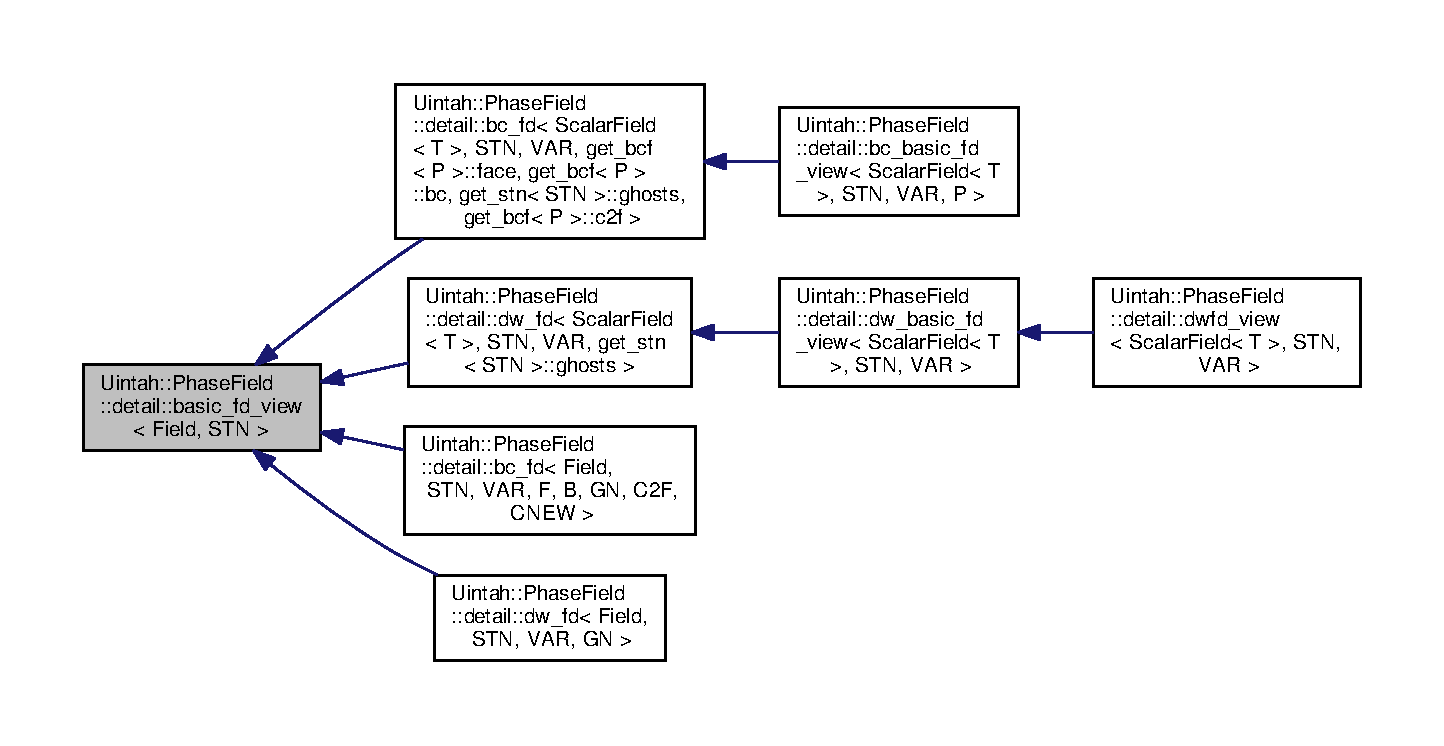
\includegraphics[width=350pt]{classUintah_1_1PhaseField_1_1detail_1_1basic__fd__view__inherit__graph}
\end{center}
\end{figure}


\subsection{Detailed Description}
\subsubsection*{template$<$typename Field, Stn\+Type S\+TN$>$\newline
class Uintah\+::\+Phase\+Field\+::detail\+::basic\+\_\+fd\+\_\+view$<$ Field, S\+T\+N $>$}

Abstract wrapper of grid variables for basic finite-\/difference operations. 

detail implementation of view (variable wrapping) which include also finite difference approximation of basic differential operations (first and second oreder derivatives)


\begin{DoxyTemplParams}{Template Parameters}
{\em Field} & type of field (\hyperlink{structUintah_1_1PhaseField_1_1ScalarField}{Scalar\+Field} $<$ T $>$ or \hyperlink{structUintah_1_1PhaseField_1_1VectorField}{Vector\+Field} $<$ T, N $>$) \\
\hline
{\em S\+TN} & finite-\/difference stencil \\
\hline
\end{DoxyTemplParams}


The documentation for this class was generated from the following file\+:\begin{DoxyCompactItemize}
\item 
\hyperlink{basic__fd__view_8h}{basic\+\_\+fd\+\_\+view.\+h}\end{DoxyCompactItemize}

\hypertarget{classUintah_1_1PhaseField_1_1detail_1_1basic__fd__view_3_01ScalarField_3_01T_01_4_00_01STN_01_4}{}\section{Uintah\+:\+:Phase\+Field\+:\+:detail\+:\+:basic\+\_\+fd\+\_\+view$<$ Scalar\+Field$<$ T $>$, S\+TN $>$ Class Template Reference}
\label{classUintah_1_1PhaseField_1_1detail_1_1basic__fd__view_3_01ScalarField_3_01T_01_4_00_01STN_01_4}\index{Uintah\+::\+Phase\+Field\+::detail\+::basic\+\_\+fd\+\_\+view$<$ Scalar\+Field$<$ T $>$, S\+T\+N $>$@{Uintah\+::\+Phase\+Field\+::detail\+::basic\+\_\+fd\+\_\+view$<$ Scalar\+Field$<$ T $>$, S\+T\+N $>$}}


Abstract class for basic finite-\/difference operations on variables (\hyperlink{structUintah_1_1PhaseField_1_1ScalarField}{Scalar\+Field} implementation)  




{\ttfamily \#include $<$basic\+\_\+fd\+\_\+view.\+h$>$}



Inheritance diagram for Uintah\+:\+:Phase\+Field\+:\+:detail\+:\+:basic\+\_\+fd\+\_\+view$<$ Scalar\+Field$<$ T $>$, S\+TN $>$\+:\nopagebreak
\begin{figure}[H]
\begin{center}
\leavevmode
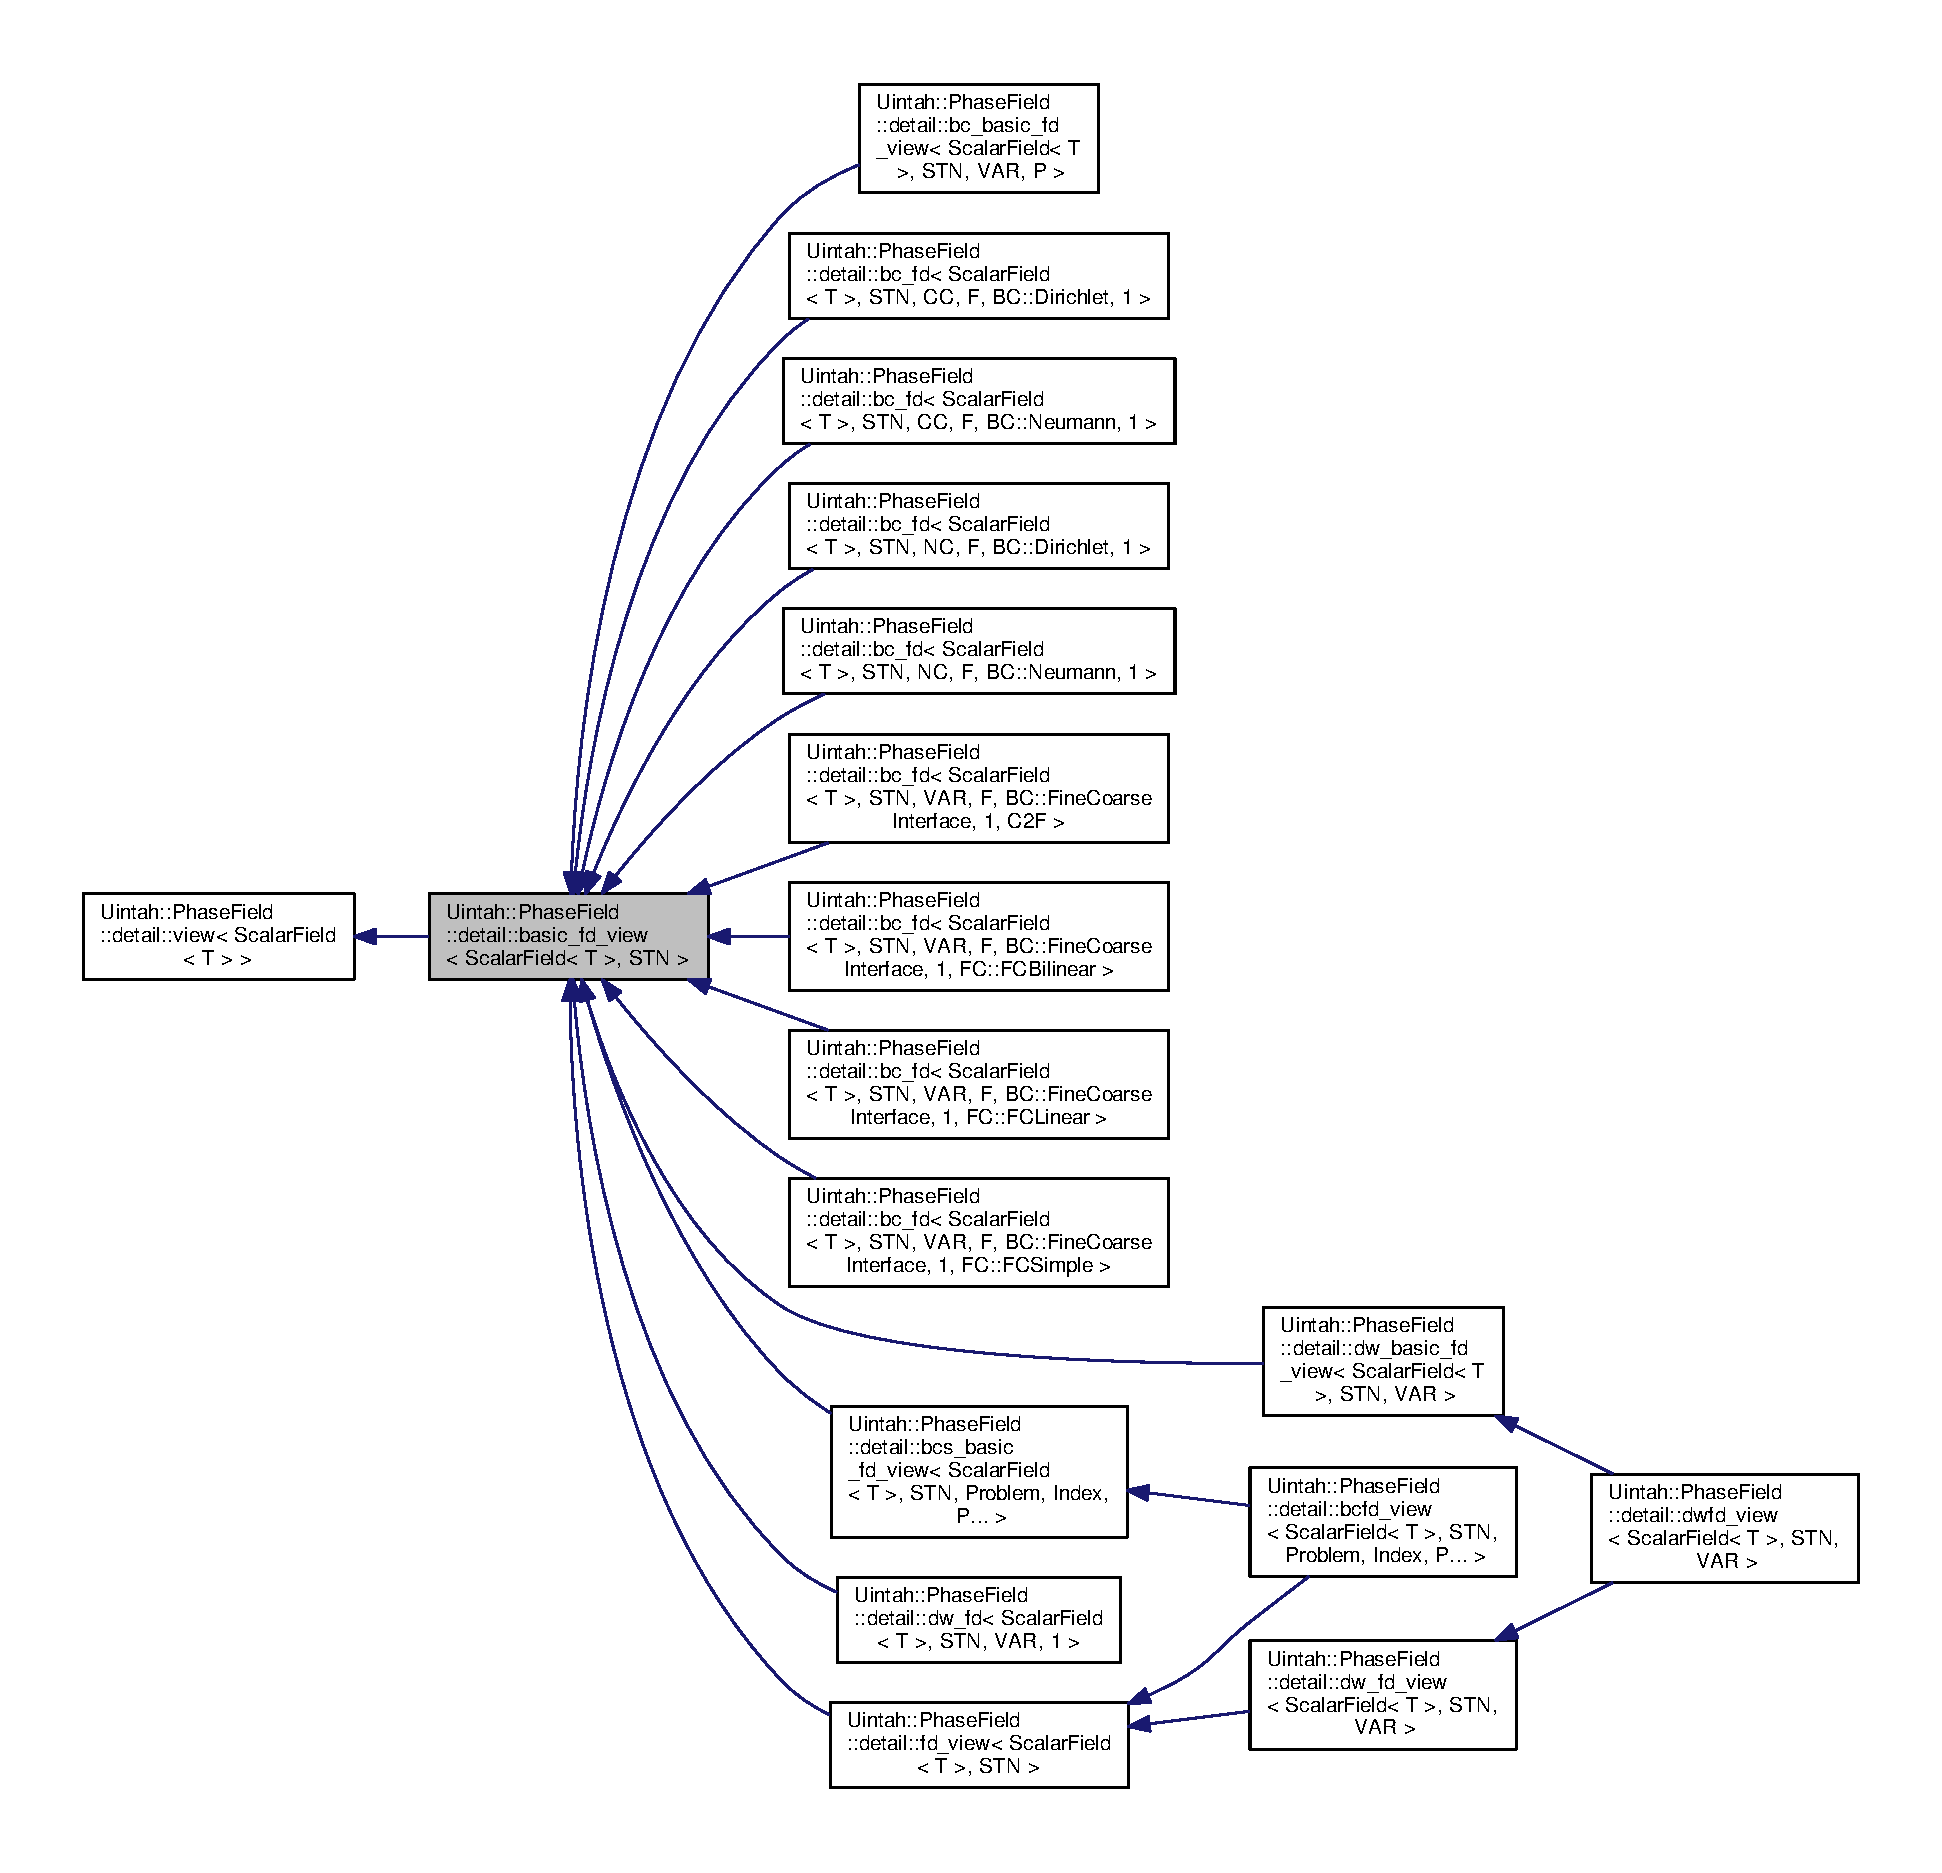
\includegraphics[width=350pt]{classUintah_1_1PhaseField_1_1detail_1_1basic__fd__view_3_01ScalarField_3_01T_01_4_00_01STN_01_4__inherit__graph}
\end{center}
\end{figure}


Collaboration diagram for Uintah\+:\+:Phase\+Field\+:\+:detail\+:\+:basic\+\_\+fd\+\_\+view$<$ Scalar\+Field$<$ T $>$, S\+TN $>$\+:\nopagebreak
\begin{figure}[H]
\begin{center}
\leavevmode
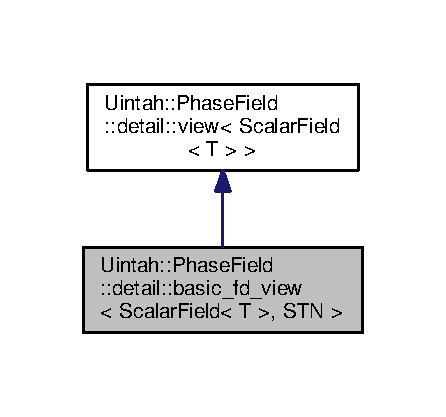
\includegraphics[width=214pt]{classUintah_1_1PhaseField_1_1detail_1_1basic__fd__view_3_01ScalarField_3_01T_01_4_00_01STN_01_4__coll__graph}
\end{center}
\end{figure}
\subsection*{Public Member Functions}
\begin{DoxyCompactItemize}
\item 
virtual \hyperlink{classUintah_1_1PhaseField_1_1detail_1_1basic__fd__view_3_01ScalarField_3_01T_01_4_00_01STN_01_4_ac8440931815c622c28fd417f9a81fdb9}{$\sim$basic\+\_\+fd\+\_\+view} ()=default
\begin{DoxyCompactList}\small\item\em Default destructor. \end{DoxyCompactList}\item 
virtual void \hyperlink{classUintah_1_1PhaseField_1_1detail_1_1basic__fd__view_3_01ScalarField_3_01T_01_4_00_01STN_01_4_a26d507d016ee4c943903214e7547594a}{set} (Data\+Warehouse $\ast$dw, const Patch $\ast$patch, bool use\+\_\+ghosts=\hyperlink{classUintah_1_1PhaseField_1_1detail_1_1basic__fd__view_3_01ScalarField_3_01T_01_4_00_01STN_01_4_a2faa49acca4f2f6983d318ae64e3ed39}{use\+\_\+ghosts\+\_\+dflt})=0
\begin{DoxyCompactList}\small\item\em Retrieve value from the Data\+Warehouse for a given patch. \end{DoxyCompactList}\item 
virtual void \hyperlink{classUintah_1_1PhaseField_1_1detail_1_1basic__fd__view_3_01ScalarField_3_01T_01_4_00_01STN_01_4_aa5cbbb3b73ea2933659cb082c6d6d863}{set} (Data\+Warehouse $\ast$dw, const Level $\ast$level, const Int\+Vector \&low, const Int\+Vector \&high, bool use\+\_\+ghosts=\hyperlink{classUintah_1_1PhaseField_1_1detail_1_1basic__fd__view_3_01ScalarField_3_01T_01_4_00_01STN_01_4_a2faa49acca4f2f6983d318ae64e3ed39}{use\+\_\+ghosts\+\_\+dflt})=0
\begin{DoxyCompactList}\small\item\em Retrieve value from the Data\+Warehouse for a given region. \end{DoxyCompactList}\item 
virtual \hyperlink{classUintah_1_1PhaseField_1_1detail_1_1view}{view}$<$ \hyperlink{structUintah_1_1PhaseField_1_1ScalarField}{Field} $>$ $\ast$ \hyperlink{classUintah_1_1PhaseField_1_1detail_1_1basic__fd__view_3_01ScalarField_3_01T_01_4_00_01STN_01_4_a2bbf870b332cfd997ec5297428019bc8}{get\+\_\+view} ()=0
\begin{DoxyCompactList}\small\item\em Get base view. \end{DoxyCompactList}\item 
virtual const \hyperlink{classUintah_1_1PhaseField_1_1detail_1_1view}{view}$<$ \hyperlink{structUintah_1_1PhaseField_1_1ScalarField}{Field} $>$ $\ast$ \hyperlink{classUintah_1_1PhaseField_1_1detail_1_1basic__fd__view_3_01ScalarField_3_01T_01_4_00_01STN_01_4_a006d6f7c6fd81ff2c8d53f59656a23dc}{get\+\_\+view} () const =0
\begin{DoxyCompactList}\small\item\em Get base view. \end{DoxyCompactList}\item 
virtual V \hyperlink{classUintah_1_1PhaseField_1_1detail_1_1basic__fd__view_3_01ScalarField_3_01T_01_4_00_01STN_01_4_a55198fb0007fd73e5a20bd4746f59c6f}{dx} (const Int\+Vector \&id) const =0
\begin{DoxyCompactList}\small\item\em Partial x derivative. \end{DoxyCompactList}\item 
virtual V \hyperlink{classUintah_1_1PhaseField_1_1detail_1_1basic__fd__view_3_01ScalarField_3_01T_01_4_00_01STN_01_4_ac30b34cfd91c6f4df4eec1a0a224c405}{dy} (const Int\+Vector \&id) const =0
\begin{DoxyCompactList}\small\item\em Partial y derivative. \end{DoxyCompactList}\item 
virtual V \hyperlink{classUintah_1_1PhaseField_1_1detail_1_1basic__fd__view_3_01ScalarField_3_01T_01_4_00_01STN_01_4_a0a37a79b114139b6b8cb2d238897d0b0}{dz} (const Int\+Vector \&id) const =0
\begin{DoxyCompactList}\small\item\em Partial z derivative. \end{DoxyCompactList}\item 
virtual V \hyperlink{classUintah_1_1PhaseField_1_1detail_1_1basic__fd__view_3_01ScalarField_3_01T_01_4_00_01STN_01_4_a3ea4026cb6251facdd6548bb4ce76408}{dxx} (const Int\+Vector \&id) const =0
\begin{DoxyCompactList}\small\item\em Partial x second order derivative. \end{DoxyCompactList}\item 
virtual V \hyperlink{classUintah_1_1PhaseField_1_1detail_1_1basic__fd__view_3_01ScalarField_3_01T_01_4_00_01STN_01_4_a387a991c42fe021f192dee7e0db5908a}{dyy} (const Int\+Vector \&id) const =0
\begin{DoxyCompactList}\small\item\em Partial y second order derivative. \end{DoxyCompactList}\item 
virtual V \hyperlink{classUintah_1_1PhaseField_1_1detail_1_1basic__fd__view_3_01ScalarField_3_01T_01_4_00_01STN_01_4_a6a9141dd1b9b547eba1bd7ff0440b6bf}{dzz} (const Int\+Vector \&id) const =0
\begin{DoxyCompactList}\small\item\em Partial z second order derivative. \end{DoxyCompactList}\end{DoxyCompactItemize}
\subsection*{Static Public Attributes}
\begin{DoxyCompactItemize}
\item 
static constexpr bool \hyperlink{classUintah_1_1PhaseField_1_1detail_1_1basic__fd__view_3_01ScalarField_3_01T_01_4_00_01STN_01_4_a2faa49acca4f2f6983d318ae64e3ed39}{use\+\_\+ghosts\+\_\+dflt} = true
\begin{DoxyCompactList}\small\item\em Default value for use\+\_\+ghost when retrieving data. \end{DoxyCompactList}\end{DoxyCompactItemize}
\subsection*{Additional Inherited Members}


\subsection{Detailed Description}
\subsubsection*{template$<$typename T, Stn\+Type S\+TN$>$\newline
class Uintah\+::\+Phase\+Field\+::detail\+::basic\+\_\+fd\+\_\+view$<$ Scalar\+Field$<$ T $>$, S\+T\+N $>$}

Abstract class for basic finite-\/difference operations on variables (\hyperlink{structUintah_1_1PhaseField_1_1ScalarField}{Scalar\+Field} implementation) 

detail implementation of view (variable wrapping) which include also finite difference approximation on basic differential operations (first and second oreder derivatives)


\begin{DoxyTemplParams}{Template Parameters}
{\em T} & type of the field value at each point \\
\hline
{\em S\+TN} & finite-\/difference stencil \\
\hline
\end{DoxyTemplParams}


\subsection{Constructor \& Destructor Documentation}
\mbox{\Hypertarget{classUintah_1_1PhaseField_1_1detail_1_1basic__fd__view_3_01ScalarField_3_01T_01_4_00_01STN_01_4_ac8440931815c622c28fd417f9a81fdb9}\label{classUintah_1_1PhaseField_1_1detail_1_1basic__fd__view_3_01ScalarField_3_01T_01_4_00_01STN_01_4_ac8440931815c622c28fd417f9a81fdb9}} 
\index{Uintah\+::\+Phase\+Field\+::detail\+::basic\+\_\+fd\+\_\+view$<$ Scalar\+Field$<$ T $>$, S\+T\+N $>$@{Uintah\+::\+Phase\+Field\+::detail\+::basic\+\_\+fd\+\_\+view$<$ Scalar\+Field$<$ T $>$, S\+T\+N $>$}!````~basic\+\_\+fd\+\_\+view@{$\sim$basic\+\_\+fd\+\_\+view}}
\index{````~basic\+\_\+fd\+\_\+view@{$\sim$basic\+\_\+fd\+\_\+view}!Uintah\+::\+Phase\+Field\+::detail\+::basic\+\_\+fd\+\_\+view$<$ Scalar\+Field$<$ T $>$, S\+T\+N $>$@{Uintah\+::\+Phase\+Field\+::detail\+::basic\+\_\+fd\+\_\+view$<$ Scalar\+Field$<$ T $>$, S\+T\+N $>$}}
\subsubsection{\texorpdfstring{$\sim$basic\+\_\+fd\+\_\+view()}{~basic\_fd\_view()}}
{\footnotesize\ttfamily template$<$typename T , Stn\+Type S\+TN$>$ \\
virtual \hyperlink{classUintah_1_1PhaseField_1_1detail_1_1basic__fd__view}{Uintah\+::\+Phase\+Field\+::detail\+::basic\+\_\+fd\+\_\+view}$<$ \hyperlink{structUintah_1_1PhaseField_1_1ScalarField}{Scalar\+Field}$<$ T $>$, S\+TN $>$\+::$\sim$\hyperlink{classUintah_1_1PhaseField_1_1detail_1_1basic__fd__view}{basic\+\_\+fd\+\_\+view} (\begin{DoxyParamCaption}{ }\end{DoxyParamCaption})\hspace{0.3cm}{\ttfamily [virtual]}, {\ttfamily [default]}}



Default destructor. 



\subsection{Member Function Documentation}
\mbox{\Hypertarget{classUintah_1_1PhaseField_1_1detail_1_1basic__fd__view_3_01ScalarField_3_01T_01_4_00_01STN_01_4_a55198fb0007fd73e5a20bd4746f59c6f}\label{classUintah_1_1PhaseField_1_1detail_1_1basic__fd__view_3_01ScalarField_3_01T_01_4_00_01STN_01_4_a55198fb0007fd73e5a20bd4746f59c6f}} 
\index{Uintah\+::\+Phase\+Field\+::detail\+::basic\+\_\+fd\+\_\+view$<$ Scalar\+Field$<$ T $>$, S\+T\+N $>$@{Uintah\+::\+Phase\+Field\+::detail\+::basic\+\_\+fd\+\_\+view$<$ Scalar\+Field$<$ T $>$, S\+T\+N $>$}!dx@{dx}}
\index{dx@{dx}!Uintah\+::\+Phase\+Field\+::detail\+::basic\+\_\+fd\+\_\+view$<$ Scalar\+Field$<$ T $>$, S\+T\+N $>$@{Uintah\+::\+Phase\+Field\+::detail\+::basic\+\_\+fd\+\_\+view$<$ Scalar\+Field$<$ T $>$, S\+T\+N $>$}}
\subsubsection{\texorpdfstring{dx()}{dx()}}
{\footnotesize\ttfamily template$<$typename T , Stn\+Type S\+TN$>$ \\
virtual V \hyperlink{classUintah_1_1PhaseField_1_1detail_1_1basic__fd__view}{Uintah\+::\+Phase\+Field\+::detail\+::basic\+\_\+fd\+\_\+view}$<$ \hyperlink{structUintah_1_1PhaseField_1_1ScalarField}{Scalar\+Field}$<$ T $>$, S\+TN $>$\+::dx (\begin{DoxyParamCaption}\item[{const Int\+Vector \&}]{id }\end{DoxyParamCaption}) const\hspace{0.3cm}{\ttfamily [pure virtual]}}



Partial x derivative. 

First order derivative along x at index id


\begin{DoxyParams}{Parameters}
{\em id} & index where to evaluate the finite-\/difference \\
\hline
\end{DoxyParams}
\begin{DoxyReturn}{Returns}
approximated value at id 
\end{DoxyReturn}


Implemented in \hyperlink{classUintah_1_1PhaseField_1_1detail_1_1bcs__basic__fd__view_3_01ScalarField_3_01T_01_4_00_01STN_07caa9955adf783da0505eac75e76f08_ad8f5b6be3ef5d9b502478f1978d8dd0e}{Uintah\+::\+Phase\+Field\+::detail\+::bcs\+\_\+basic\+\_\+fd\+\_\+view$<$ Scalar\+Field$<$ T $>$, S\+T\+N, Problem, Index, P... $>$}, \hyperlink{classUintah_1_1PhaseField_1_1detail_1_1bc__basic__fd__view_3_01ScalarField_3_01T_01_4_00_01STN_00_01VAR_00_01P_01_4_ae734fd388d7a680aa366db584bc54107}{Uintah\+::\+Phase\+Field\+::detail\+::bc\+\_\+basic\+\_\+fd\+\_\+view$<$ Scalar\+Field$<$ T $>$, S\+T\+N, V\+A\+R, P $>$}, and \hyperlink{classUintah_1_1PhaseField_1_1detail_1_1dw__basic__fd__view_3_01ScalarField_3_01T_01_4_00_01STN_00_01VAR_01_4_ad93583d4b60ddc8eccb5199ddff534c3}{Uintah\+::\+Phase\+Field\+::detail\+::dw\+\_\+basic\+\_\+fd\+\_\+view$<$ Scalar\+Field$<$ T $>$, S\+T\+N, V\+A\+R $>$}.

\mbox{\Hypertarget{classUintah_1_1PhaseField_1_1detail_1_1basic__fd__view_3_01ScalarField_3_01T_01_4_00_01STN_01_4_a3ea4026cb6251facdd6548bb4ce76408}\label{classUintah_1_1PhaseField_1_1detail_1_1basic__fd__view_3_01ScalarField_3_01T_01_4_00_01STN_01_4_a3ea4026cb6251facdd6548bb4ce76408}} 
\index{Uintah\+::\+Phase\+Field\+::detail\+::basic\+\_\+fd\+\_\+view$<$ Scalar\+Field$<$ T $>$, S\+T\+N $>$@{Uintah\+::\+Phase\+Field\+::detail\+::basic\+\_\+fd\+\_\+view$<$ Scalar\+Field$<$ T $>$, S\+T\+N $>$}!dxx@{dxx}}
\index{dxx@{dxx}!Uintah\+::\+Phase\+Field\+::detail\+::basic\+\_\+fd\+\_\+view$<$ Scalar\+Field$<$ T $>$, S\+T\+N $>$@{Uintah\+::\+Phase\+Field\+::detail\+::basic\+\_\+fd\+\_\+view$<$ Scalar\+Field$<$ T $>$, S\+T\+N $>$}}
\subsubsection{\texorpdfstring{dxx()}{dxx()}}
{\footnotesize\ttfamily template$<$typename T , Stn\+Type S\+TN$>$ \\
virtual V \hyperlink{classUintah_1_1PhaseField_1_1detail_1_1basic__fd__view}{Uintah\+::\+Phase\+Field\+::detail\+::basic\+\_\+fd\+\_\+view}$<$ \hyperlink{structUintah_1_1PhaseField_1_1ScalarField}{Scalar\+Field}$<$ T $>$, S\+TN $>$\+::dxx (\begin{DoxyParamCaption}\item[{const Int\+Vector \&}]{id }\end{DoxyParamCaption}) const\hspace{0.3cm}{\ttfamily [pure virtual]}}



Partial x second order derivative. 

Second order derivative along x at index id


\begin{DoxyParams}{Parameters}
{\em id} & index where to evaluate the finite-\/difference \\
\hline
\end{DoxyParams}
\begin{DoxyReturn}{Returns}
approximated value at id 
\end{DoxyReturn}


Implemented in \hyperlink{classUintah_1_1PhaseField_1_1detail_1_1bcs__basic__fd__view_3_01ScalarField_3_01T_01_4_00_01STN_07caa9955adf783da0505eac75e76f08_ab5f1d6ae2f25c2d050775578499db79e}{Uintah\+::\+Phase\+Field\+::detail\+::bcs\+\_\+basic\+\_\+fd\+\_\+view$<$ Scalar\+Field$<$ T $>$, S\+T\+N, Problem, Index, P... $>$}, \hyperlink{classUintah_1_1PhaseField_1_1detail_1_1bc__basic__fd__view_3_01ScalarField_3_01T_01_4_00_01STN_00_01VAR_00_01P_01_4_a7146569da689f425b7eb963295905ee2}{Uintah\+::\+Phase\+Field\+::detail\+::bc\+\_\+basic\+\_\+fd\+\_\+view$<$ Scalar\+Field$<$ T $>$, S\+T\+N, V\+A\+R, P $>$}, and \hyperlink{classUintah_1_1PhaseField_1_1detail_1_1dw__basic__fd__view_3_01ScalarField_3_01T_01_4_00_01STN_00_01VAR_01_4_a3deb16fdbf624c192e273b7b856db9d2}{Uintah\+::\+Phase\+Field\+::detail\+::dw\+\_\+basic\+\_\+fd\+\_\+view$<$ Scalar\+Field$<$ T $>$, S\+T\+N, V\+A\+R $>$}.

\mbox{\Hypertarget{classUintah_1_1PhaseField_1_1detail_1_1basic__fd__view_3_01ScalarField_3_01T_01_4_00_01STN_01_4_ac30b34cfd91c6f4df4eec1a0a224c405}\label{classUintah_1_1PhaseField_1_1detail_1_1basic__fd__view_3_01ScalarField_3_01T_01_4_00_01STN_01_4_ac30b34cfd91c6f4df4eec1a0a224c405}} 
\index{Uintah\+::\+Phase\+Field\+::detail\+::basic\+\_\+fd\+\_\+view$<$ Scalar\+Field$<$ T $>$, S\+T\+N $>$@{Uintah\+::\+Phase\+Field\+::detail\+::basic\+\_\+fd\+\_\+view$<$ Scalar\+Field$<$ T $>$, S\+T\+N $>$}!dy@{dy}}
\index{dy@{dy}!Uintah\+::\+Phase\+Field\+::detail\+::basic\+\_\+fd\+\_\+view$<$ Scalar\+Field$<$ T $>$, S\+T\+N $>$@{Uintah\+::\+Phase\+Field\+::detail\+::basic\+\_\+fd\+\_\+view$<$ Scalar\+Field$<$ T $>$, S\+T\+N $>$}}
\subsubsection{\texorpdfstring{dy()}{dy()}}
{\footnotesize\ttfamily template$<$typename T , Stn\+Type S\+TN$>$ \\
virtual V \hyperlink{classUintah_1_1PhaseField_1_1detail_1_1basic__fd__view}{Uintah\+::\+Phase\+Field\+::detail\+::basic\+\_\+fd\+\_\+view}$<$ \hyperlink{structUintah_1_1PhaseField_1_1ScalarField}{Scalar\+Field}$<$ T $>$, S\+TN $>$\+::dy (\begin{DoxyParamCaption}\item[{const Int\+Vector \&}]{id }\end{DoxyParamCaption}) const\hspace{0.3cm}{\ttfamily [pure virtual]}}



Partial y derivative. 

First order derivative along y at index id


\begin{DoxyParams}{Parameters}
{\em id} & index where to evaluate the finite-\/difference \\
\hline
\end{DoxyParams}
\begin{DoxyReturn}{Returns}
approximated value at id 
\end{DoxyReturn}


Implemented in \hyperlink{classUintah_1_1PhaseField_1_1detail_1_1bcs__basic__fd__view_3_01ScalarField_3_01T_01_4_00_01STN_07caa9955adf783da0505eac75e76f08_acb8d3d8217637aecdac144650632c57f}{Uintah\+::\+Phase\+Field\+::detail\+::bcs\+\_\+basic\+\_\+fd\+\_\+view$<$ Scalar\+Field$<$ T $>$, S\+T\+N, Problem, Index, P... $>$}, \hyperlink{classUintah_1_1PhaseField_1_1detail_1_1bc__basic__fd__view_3_01ScalarField_3_01T_01_4_00_01STN_00_01VAR_00_01P_01_4_ad81ac1a8cf3ddce875d270b6bb00a380}{Uintah\+::\+Phase\+Field\+::detail\+::bc\+\_\+basic\+\_\+fd\+\_\+view$<$ Scalar\+Field$<$ T $>$, S\+T\+N, V\+A\+R, P $>$}, and \hyperlink{classUintah_1_1PhaseField_1_1detail_1_1dw__basic__fd__view_3_01ScalarField_3_01T_01_4_00_01STN_00_01VAR_01_4_a99f11a208f062a1704d7ba83b0550591}{Uintah\+::\+Phase\+Field\+::detail\+::dw\+\_\+basic\+\_\+fd\+\_\+view$<$ Scalar\+Field$<$ T $>$, S\+T\+N, V\+A\+R $>$}.

\mbox{\Hypertarget{classUintah_1_1PhaseField_1_1detail_1_1basic__fd__view_3_01ScalarField_3_01T_01_4_00_01STN_01_4_a387a991c42fe021f192dee7e0db5908a}\label{classUintah_1_1PhaseField_1_1detail_1_1basic__fd__view_3_01ScalarField_3_01T_01_4_00_01STN_01_4_a387a991c42fe021f192dee7e0db5908a}} 
\index{Uintah\+::\+Phase\+Field\+::detail\+::basic\+\_\+fd\+\_\+view$<$ Scalar\+Field$<$ T $>$, S\+T\+N $>$@{Uintah\+::\+Phase\+Field\+::detail\+::basic\+\_\+fd\+\_\+view$<$ Scalar\+Field$<$ T $>$, S\+T\+N $>$}!dyy@{dyy}}
\index{dyy@{dyy}!Uintah\+::\+Phase\+Field\+::detail\+::basic\+\_\+fd\+\_\+view$<$ Scalar\+Field$<$ T $>$, S\+T\+N $>$@{Uintah\+::\+Phase\+Field\+::detail\+::basic\+\_\+fd\+\_\+view$<$ Scalar\+Field$<$ T $>$, S\+T\+N $>$}}
\subsubsection{\texorpdfstring{dyy()}{dyy()}}
{\footnotesize\ttfamily template$<$typename T , Stn\+Type S\+TN$>$ \\
virtual V \hyperlink{classUintah_1_1PhaseField_1_1detail_1_1basic__fd__view}{Uintah\+::\+Phase\+Field\+::detail\+::basic\+\_\+fd\+\_\+view}$<$ \hyperlink{structUintah_1_1PhaseField_1_1ScalarField}{Scalar\+Field}$<$ T $>$, S\+TN $>$\+::dyy (\begin{DoxyParamCaption}\item[{const Int\+Vector \&}]{id }\end{DoxyParamCaption}) const\hspace{0.3cm}{\ttfamily [pure virtual]}}



Partial y second order derivative. 

Second order derivative along y at index id


\begin{DoxyParams}{Parameters}
{\em id} & index where to evaluate the finite-\/difference \\
\hline
\end{DoxyParams}
\begin{DoxyReturn}{Returns}
approximated value at id 
\end{DoxyReturn}


Implemented in \hyperlink{classUintah_1_1PhaseField_1_1detail_1_1bcs__basic__fd__view_3_01ScalarField_3_01T_01_4_00_01STN_07caa9955adf783da0505eac75e76f08_af8155387a989a9a9c007b49cb4420f8e}{Uintah\+::\+Phase\+Field\+::detail\+::bcs\+\_\+basic\+\_\+fd\+\_\+view$<$ Scalar\+Field$<$ T $>$, S\+T\+N, Problem, Index, P... $>$}, \hyperlink{classUintah_1_1PhaseField_1_1detail_1_1bc__basic__fd__view_3_01ScalarField_3_01T_01_4_00_01STN_00_01VAR_00_01P_01_4_a5549a4a413c2be230e484c8921524395}{Uintah\+::\+Phase\+Field\+::detail\+::bc\+\_\+basic\+\_\+fd\+\_\+view$<$ Scalar\+Field$<$ T $>$, S\+T\+N, V\+A\+R, P $>$}, and \hyperlink{classUintah_1_1PhaseField_1_1detail_1_1dw__basic__fd__view_3_01ScalarField_3_01T_01_4_00_01STN_00_01VAR_01_4_ababac9886dc3c97a1cd3348e9f09d477}{Uintah\+::\+Phase\+Field\+::detail\+::dw\+\_\+basic\+\_\+fd\+\_\+view$<$ Scalar\+Field$<$ T $>$, S\+T\+N, V\+A\+R $>$}.

\mbox{\Hypertarget{classUintah_1_1PhaseField_1_1detail_1_1basic__fd__view_3_01ScalarField_3_01T_01_4_00_01STN_01_4_a0a37a79b114139b6b8cb2d238897d0b0}\label{classUintah_1_1PhaseField_1_1detail_1_1basic__fd__view_3_01ScalarField_3_01T_01_4_00_01STN_01_4_a0a37a79b114139b6b8cb2d238897d0b0}} 
\index{Uintah\+::\+Phase\+Field\+::detail\+::basic\+\_\+fd\+\_\+view$<$ Scalar\+Field$<$ T $>$, S\+T\+N $>$@{Uintah\+::\+Phase\+Field\+::detail\+::basic\+\_\+fd\+\_\+view$<$ Scalar\+Field$<$ T $>$, S\+T\+N $>$}!dz@{dz}}
\index{dz@{dz}!Uintah\+::\+Phase\+Field\+::detail\+::basic\+\_\+fd\+\_\+view$<$ Scalar\+Field$<$ T $>$, S\+T\+N $>$@{Uintah\+::\+Phase\+Field\+::detail\+::basic\+\_\+fd\+\_\+view$<$ Scalar\+Field$<$ T $>$, S\+T\+N $>$}}
\subsubsection{\texorpdfstring{dz()}{dz()}}
{\footnotesize\ttfamily template$<$typename T , Stn\+Type S\+TN$>$ \\
virtual V \hyperlink{classUintah_1_1PhaseField_1_1detail_1_1basic__fd__view}{Uintah\+::\+Phase\+Field\+::detail\+::basic\+\_\+fd\+\_\+view}$<$ \hyperlink{structUintah_1_1PhaseField_1_1ScalarField}{Scalar\+Field}$<$ T $>$, S\+TN $>$\+::dz (\begin{DoxyParamCaption}\item[{const Int\+Vector \&}]{id }\end{DoxyParamCaption}) const\hspace{0.3cm}{\ttfamily [pure virtual]}}



Partial z derivative. 

First order derivative along z at index id


\begin{DoxyParams}{Parameters}
{\em id} & index where to evaluate the finite-\/difference \\
\hline
\end{DoxyParams}
\begin{DoxyReturn}{Returns}
approximated value at id 
\end{DoxyReturn}


Implemented in \hyperlink{classUintah_1_1PhaseField_1_1detail_1_1bcs__basic__fd__view_3_01ScalarField_3_01T_01_4_00_01STN_07caa9955adf783da0505eac75e76f08_abbfa68e1cf8c0eb675f3934f2fcf8259}{Uintah\+::\+Phase\+Field\+::detail\+::bcs\+\_\+basic\+\_\+fd\+\_\+view$<$ Scalar\+Field$<$ T $>$, S\+T\+N, Problem, Index, P... $>$}, \hyperlink{classUintah_1_1PhaseField_1_1detail_1_1bc__basic__fd__view_3_01ScalarField_3_01T_01_4_00_01STN_00_01VAR_00_01P_01_4_a994e7388acdb4040da7cc438ecd2dc4b}{Uintah\+::\+Phase\+Field\+::detail\+::bc\+\_\+basic\+\_\+fd\+\_\+view$<$ Scalar\+Field$<$ T $>$, S\+T\+N, V\+A\+R, P $>$}, and \hyperlink{classUintah_1_1PhaseField_1_1detail_1_1dw__basic__fd__view_3_01ScalarField_3_01T_01_4_00_01STN_00_01VAR_01_4_ab95f7f4aed23245ff58a676e9df745fb}{Uintah\+::\+Phase\+Field\+::detail\+::dw\+\_\+basic\+\_\+fd\+\_\+view$<$ Scalar\+Field$<$ T $>$, S\+T\+N, V\+A\+R $>$}.

\mbox{\Hypertarget{classUintah_1_1PhaseField_1_1detail_1_1basic__fd__view_3_01ScalarField_3_01T_01_4_00_01STN_01_4_a6a9141dd1b9b547eba1bd7ff0440b6bf}\label{classUintah_1_1PhaseField_1_1detail_1_1basic__fd__view_3_01ScalarField_3_01T_01_4_00_01STN_01_4_a6a9141dd1b9b547eba1bd7ff0440b6bf}} 
\index{Uintah\+::\+Phase\+Field\+::detail\+::basic\+\_\+fd\+\_\+view$<$ Scalar\+Field$<$ T $>$, S\+T\+N $>$@{Uintah\+::\+Phase\+Field\+::detail\+::basic\+\_\+fd\+\_\+view$<$ Scalar\+Field$<$ T $>$, S\+T\+N $>$}!dzz@{dzz}}
\index{dzz@{dzz}!Uintah\+::\+Phase\+Field\+::detail\+::basic\+\_\+fd\+\_\+view$<$ Scalar\+Field$<$ T $>$, S\+T\+N $>$@{Uintah\+::\+Phase\+Field\+::detail\+::basic\+\_\+fd\+\_\+view$<$ Scalar\+Field$<$ T $>$, S\+T\+N $>$}}
\subsubsection{\texorpdfstring{dzz()}{dzz()}}
{\footnotesize\ttfamily template$<$typename T , Stn\+Type S\+TN$>$ \\
virtual V \hyperlink{classUintah_1_1PhaseField_1_1detail_1_1basic__fd__view}{Uintah\+::\+Phase\+Field\+::detail\+::basic\+\_\+fd\+\_\+view}$<$ \hyperlink{structUintah_1_1PhaseField_1_1ScalarField}{Scalar\+Field}$<$ T $>$, S\+TN $>$\+::dzz (\begin{DoxyParamCaption}\item[{const Int\+Vector \&}]{id }\end{DoxyParamCaption}) const\hspace{0.3cm}{\ttfamily [pure virtual]}}



Partial z second order derivative. 

Second order derivative along z at index id


\begin{DoxyParams}{Parameters}
{\em id} & index where to evaluate the finite-\/difference \\
\hline
\end{DoxyParams}
\begin{DoxyReturn}{Returns}
approximated value at id 
\end{DoxyReturn}


Implemented in \hyperlink{classUintah_1_1PhaseField_1_1detail_1_1bcs__basic__fd__view_3_01ScalarField_3_01T_01_4_00_01STN_07caa9955adf783da0505eac75e76f08_a8edd18a7f77bf23f10b87ad970da31c4}{Uintah\+::\+Phase\+Field\+::detail\+::bcs\+\_\+basic\+\_\+fd\+\_\+view$<$ Scalar\+Field$<$ T $>$, S\+T\+N, Problem, Index, P... $>$}, \hyperlink{classUintah_1_1PhaseField_1_1detail_1_1bc__basic__fd__view_3_01ScalarField_3_01T_01_4_00_01STN_00_01VAR_00_01P_01_4_ad2c322a2540d22bffda0332f436df825}{Uintah\+::\+Phase\+Field\+::detail\+::bc\+\_\+basic\+\_\+fd\+\_\+view$<$ Scalar\+Field$<$ T $>$, S\+T\+N, V\+A\+R, P $>$}, and \hyperlink{classUintah_1_1PhaseField_1_1detail_1_1dw__basic__fd__view_3_01ScalarField_3_01T_01_4_00_01STN_00_01VAR_01_4_ad7be1669f58aaecc7f5e7ac94d087bc5}{Uintah\+::\+Phase\+Field\+::detail\+::dw\+\_\+basic\+\_\+fd\+\_\+view$<$ Scalar\+Field$<$ T $>$, S\+T\+N, V\+A\+R $>$}.

\mbox{\Hypertarget{classUintah_1_1PhaseField_1_1detail_1_1basic__fd__view_3_01ScalarField_3_01T_01_4_00_01STN_01_4_a2bbf870b332cfd997ec5297428019bc8}\label{classUintah_1_1PhaseField_1_1detail_1_1basic__fd__view_3_01ScalarField_3_01T_01_4_00_01STN_01_4_a2bbf870b332cfd997ec5297428019bc8}} 
\index{Uintah\+::\+Phase\+Field\+::detail\+::basic\+\_\+fd\+\_\+view$<$ Scalar\+Field$<$ T $>$, S\+T\+N $>$@{Uintah\+::\+Phase\+Field\+::detail\+::basic\+\_\+fd\+\_\+view$<$ Scalar\+Field$<$ T $>$, S\+T\+N $>$}!get\+\_\+view@{get\+\_\+view}}
\index{get\+\_\+view@{get\+\_\+view}!Uintah\+::\+Phase\+Field\+::detail\+::basic\+\_\+fd\+\_\+view$<$ Scalar\+Field$<$ T $>$, S\+T\+N $>$@{Uintah\+::\+Phase\+Field\+::detail\+::basic\+\_\+fd\+\_\+view$<$ Scalar\+Field$<$ T $>$, S\+T\+N $>$}}
\subsubsection{\texorpdfstring{get\+\_\+view()}{get\_view()}\hspace{0.1cm}{\footnotesize\ttfamily [1/2]}}
{\footnotesize\ttfamily template$<$typename T , Stn\+Type S\+TN$>$ \\
virtual \hyperlink{classUintah_1_1PhaseField_1_1detail_1_1view}{view}$<$\hyperlink{structUintah_1_1PhaseField_1_1ScalarField}{Field}$>$$\ast$ \hyperlink{classUintah_1_1PhaseField_1_1detail_1_1basic__fd__view}{Uintah\+::\+Phase\+Field\+::detail\+::basic\+\_\+fd\+\_\+view}$<$ \hyperlink{structUintah_1_1PhaseField_1_1ScalarField}{Scalar\+Field}$<$ T $>$, S\+TN $>$\+::get\+\_\+view (\begin{DoxyParamCaption}{ }\end{DoxyParamCaption})\hspace{0.3cm}{\ttfamily [pure virtual]}}



Get base view. 

\begin{DoxyReturn}{Returns}
non const pointer to base view implementation 
\end{DoxyReturn}


Implemented in \hyperlink{classUintah_1_1PhaseField_1_1detail_1_1bcs__basic__fd__view_3_01ScalarField_3_01T_01_4_00_01STN_07caa9955adf783da0505eac75e76f08_a1c51fe0d64605df5ce9c757681eb80a5}{Uintah\+::\+Phase\+Field\+::detail\+::bcs\+\_\+basic\+\_\+fd\+\_\+view$<$ Scalar\+Field$<$ T $>$, S\+T\+N, Problem, Index, P... $>$}, \hyperlink{classUintah_1_1PhaseField_1_1detail_1_1bc__fd_3_01ScalarField_3_01T_01_4_00_01STN_00_01VAR_00_01bd5f5aa94f34afad5c8a785ee391ed2b_a1bd33bee3f10040e59c3571cd0e2ce57}{Uintah\+::\+Phase\+Field\+::detail\+::bc\+\_\+fd$<$ Scalar\+Field$<$ T $>$, S\+T\+N, V\+A\+R, F, B\+C\+::\+Fine\+Coarse\+Interface, 1, F\+C\+::\+F\+C\+Bilinear $>$}, \hyperlink{classUintah_1_1PhaseField_1_1detail_1_1bc__fd_3_01ScalarField_3_01T_01_4_00_01STN_00_01VAR_00_01ce55d0bf8381798bc129da931b626e80_a579bb0bf5063314ac57aace2d8ff2c31}{Uintah\+::\+Phase\+Field\+::detail\+::bc\+\_\+fd$<$ Scalar\+Field$<$ T $>$, S\+T\+N, V\+A\+R, F, B\+C\+::\+Fine\+Coarse\+Interface, 1, F\+C\+::\+F\+C\+Simple $>$}, \hyperlink{classUintah_1_1PhaseField_1_1detail_1_1bc__fd_3_01ScalarField_3_01T_01_4_00_01STN_00_01VAR_00_01f836207db876ecd28bf65f631f79030f_abc3b93271050f310bc7f6095ccb19d08}{Uintah\+::\+Phase\+Field\+::detail\+::bc\+\_\+fd$<$ Scalar\+Field$<$ T $>$, S\+T\+N, V\+A\+R, F, B\+C\+::\+Fine\+Coarse\+Interface, 1, F\+C\+::\+F\+C\+Linear $>$}, \hyperlink{classUintah_1_1PhaseField_1_1detail_1_1bc__fd_3_01ScalarField_3_01T_01_4_00_01STN_00_01VAR_00_01efea904a4b4ba4f7ece7ded248f84d17_abe29015f77805b0afa450c56f22814cb}{Uintah\+::\+Phase\+Field\+::detail\+::bc\+\_\+fd$<$ Scalar\+Field$<$ T $>$, S\+T\+N, V\+A\+R, F, B\+C\+::\+Fine\+Coarse\+Interface, 1, C2\+F $>$}, \hyperlink{classUintah_1_1PhaseField_1_1detail_1_1bc__fd_3_01ScalarField_3_01T_01_4_00_01STN_00_01CC_00_01F_00_01BC_1_1Neumann_00_011_01_4_ae067158c4bde7162f906999a1eb7c4e8}{Uintah\+::\+Phase\+Field\+::detail\+::bc\+\_\+fd$<$ Scalar\+Field$<$ T $>$, S\+T\+N, C\+C, F, B\+C\+::\+Neumann, 1 $>$}, \hyperlink{classUintah_1_1PhaseField_1_1detail_1_1bc__fd_3_01ScalarField_3_01T_01_4_00_01STN_00_01NC_00_01F_00_01BC_1_1Neumann_00_011_01_4_acd326fe71c0df45ad7fccd480a29da8e}{Uintah\+::\+Phase\+Field\+::detail\+::bc\+\_\+fd$<$ Scalar\+Field$<$ T $>$, S\+T\+N, N\+C, F, B\+C\+::\+Neumann, 1 $>$}, \hyperlink{classUintah_1_1PhaseField_1_1detail_1_1bc__fd_3_01ScalarField_3_01T_01_4_00_01STN_00_01CC_00_01Fa77b2fd7fb77d0a4dc6c86c68d4ea0bc_ab7b39dfca20ca18356b1a72ae055e99f}{Uintah\+::\+Phase\+Field\+::detail\+::bc\+\_\+fd$<$ Scalar\+Field$<$ T $>$, S\+T\+N, C\+C, F, B\+C\+::\+Dirichlet, 1 $>$}, \hyperlink{classUintah_1_1PhaseField_1_1detail_1_1bc__fd_3_01ScalarField_3_01T_01_4_00_01STN_00_01NC_00_01Fc8a6e28ffa258d282d0a921216b0ed9f_a27bd79a8b66a0a7a21a2473795f11911}{Uintah\+::\+Phase\+Field\+::detail\+::bc\+\_\+fd$<$ Scalar\+Field$<$ T $>$, S\+T\+N, N\+C, F, B\+C\+::\+Dirichlet, 1 $>$}, \hyperlink{classUintah_1_1PhaseField_1_1detail_1_1dw__fd_3_01ScalarField_3_01T_01_4_00_01STN_00_01VAR_00_011_01_4_a6c8bfba52568211434dbb756fe44b6be}{Uintah\+::\+Phase\+Field\+::detail\+::dw\+\_\+fd$<$ Scalar\+Field$<$ T $>$, S\+T\+N, V\+A\+R, 1 $>$}, \hyperlink{classUintah_1_1PhaseField_1_1detail_1_1bc__basic__fd__view_3_01ScalarField_3_01T_01_4_00_01STN_00_01VAR_00_01P_01_4_a46e6a2a932a522c1ed93c7c28d728e83}{Uintah\+::\+Phase\+Field\+::detail\+::bc\+\_\+basic\+\_\+fd\+\_\+view$<$ Scalar\+Field$<$ T $>$, S\+T\+N, V\+A\+R, P $>$}, and \hyperlink{classUintah_1_1PhaseField_1_1detail_1_1dw__basic__fd__view_3_01ScalarField_3_01T_01_4_00_01STN_00_01VAR_01_4_ada3c79dde199711c630431fad25fbc2e}{Uintah\+::\+Phase\+Field\+::detail\+::dw\+\_\+basic\+\_\+fd\+\_\+view$<$ Scalar\+Field$<$ T $>$, S\+T\+N, V\+A\+R $>$}.

\mbox{\Hypertarget{classUintah_1_1PhaseField_1_1detail_1_1basic__fd__view_3_01ScalarField_3_01T_01_4_00_01STN_01_4_a006d6f7c6fd81ff2c8d53f59656a23dc}\label{classUintah_1_1PhaseField_1_1detail_1_1basic__fd__view_3_01ScalarField_3_01T_01_4_00_01STN_01_4_a006d6f7c6fd81ff2c8d53f59656a23dc}} 
\index{Uintah\+::\+Phase\+Field\+::detail\+::basic\+\_\+fd\+\_\+view$<$ Scalar\+Field$<$ T $>$, S\+T\+N $>$@{Uintah\+::\+Phase\+Field\+::detail\+::basic\+\_\+fd\+\_\+view$<$ Scalar\+Field$<$ T $>$, S\+T\+N $>$}!get\+\_\+view@{get\+\_\+view}}
\index{get\+\_\+view@{get\+\_\+view}!Uintah\+::\+Phase\+Field\+::detail\+::basic\+\_\+fd\+\_\+view$<$ Scalar\+Field$<$ T $>$, S\+T\+N $>$@{Uintah\+::\+Phase\+Field\+::detail\+::basic\+\_\+fd\+\_\+view$<$ Scalar\+Field$<$ T $>$, S\+T\+N $>$}}
\subsubsection{\texorpdfstring{get\+\_\+view()}{get\_view()}\hspace{0.1cm}{\footnotesize\ttfamily [2/2]}}
{\footnotesize\ttfamily template$<$typename T , Stn\+Type S\+TN$>$ \\
virtual const \hyperlink{classUintah_1_1PhaseField_1_1detail_1_1view}{view}$<$\hyperlink{structUintah_1_1PhaseField_1_1ScalarField}{Field}$>$$\ast$ \hyperlink{classUintah_1_1PhaseField_1_1detail_1_1basic__fd__view}{Uintah\+::\+Phase\+Field\+::detail\+::basic\+\_\+fd\+\_\+view}$<$ \hyperlink{structUintah_1_1PhaseField_1_1ScalarField}{Scalar\+Field}$<$ T $>$, S\+TN $>$\+::get\+\_\+view (\begin{DoxyParamCaption}{ }\end{DoxyParamCaption}) const\hspace{0.3cm}{\ttfamily [pure virtual]}}



Get base view. 

\begin{DoxyReturn}{Returns}
const pointer to base view implementation 
\end{DoxyReturn}


Implemented in \hyperlink{classUintah_1_1PhaseField_1_1detail_1_1bcs__basic__fd__view_3_01ScalarField_3_01T_01_4_00_01STN_07caa9955adf783da0505eac75e76f08_a0aae05fb5f6751eddd0c5d5713512669}{Uintah\+::\+Phase\+Field\+::detail\+::bcs\+\_\+basic\+\_\+fd\+\_\+view$<$ Scalar\+Field$<$ T $>$, S\+T\+N, Problem, Index, P... $>$}, \hyperlink{classUintah_1_1PhaseField_1_1detail_1_1bc__fd_3_01ScalarField_3_01T_01_4_00_01STN_00_01VAR_00_01bd5f5aa94f34afad5c8a785ee391ed2b_aeaad8cf19d01e440be21295b7ae2627f}{Uintah\+::\+Phase\+Field\+::detail\+::bc\+\_\+fd$<$ Scalar\+Field$<$ T $>$, S\+T\+N, V\+A\+R, F, B\+C\+::\+Fine\+Coarse\+Interface, 1, F\+C\+::\+F\+C\+Bilinear $>$}, \hyperlink{classUintah_1_1PhaseField_1_1detail_1_1bc__fd_3_01ScalarField_3_01T_01_4_00_01STN_00_01VAR_00_01ce55d0bf8381798bc129da931b626e80_a68249997b8422670b8831c9b6db4d879}{Uintah\+::\+Phase\+Field\+::detail\+::bc\+\_\+fd$<$ Scalar\+Field$<$ T $>$, S\+T\+N, V\+A\+R, F, B\+C\+::\+Fine\+Coarse\+Interface, 1, F\+C\+::\+F\+C\+Simple $>$}, \hyperlink{classUintah_1_1PhaseField_1_1detail_1_1bc__fd_3_01ScalarField_3_01T_01_4_00_01STN_00_01VAR_00_01f836207db876ecd28bf65f631f79030f_a03ab09ea8008b24b6cbffe0ce8e14388}{Uintah\+::\+Phase\+Field\+::detail\+::bc\+\_\+fd$<$ Scalar\+Field$<$ T $>$, S\+T\+N, V\+A\+R, F, B\+C\+::\+Fine\+Coarse\+Interface, 1, F\+C\+::\+F\+C\+Linear $>$}, \hyperlink{classUintah_1_1PhaseField_1_1detail_1_1bc__fd_3_01ScalarField_3_01T_01_4_00_01STN_00_01VAR_00_01efea904a4b4ba4f7ece7ded248f84d17_ad6ddff2b89c38e20df734b094bbfff9c}{Uintah\+::\+Phase\+Field\+::detail\+::bc\+\_\+fd$<$ Scalar\+Field$<$ T $>$, S\+T\+N, V\+A\+R, F, B\+C\+::\+Fine\+Coarse\+Interface, 1, C2\+F $>$}, \hyperlink{classUintah_1_1PhaseField_1_1detail_1_1bc__fd_3_01ScalarField_3_01T_01_4_00_01STN_00_01CC_00_01F_00_01BC_1_1Neumann_00_011_01_4_a158cefd68ffdfd59e5590b850c7ca78f}{Uintah\+::\+Phase\+Field\+::detail\+::bc\+\_\+fd$<$ Scalar\+Field$<$ T $>$, S\+T\+N, C\+C, F, B\+C\+::\+Neumann, 1 $>$}, \hyperlink{classUintah_1_1PhaseField_1_1detail_1_1bc__fd_3_01ScalarField_3_01T_01_4_00_01STN_00_01NC_00_01F_00_01BC_1_1Neumann_00_011_01_4_a54dca99f90e96dabfffe594538bd5ca8}{Uintah\+::\+Phase\+Field\+::detail\+::bc\+\_\+fd$<$ Scalar\+Field$<$ T $>$, S\+T\+N, N\+C, F, B\+C\+::\+Neumann, 1 $>$}, \hyperlink{classUintah_1_1PhaseField_1_1detail_1_1bc__fd_3_01ScalarField_3_01T_01_4_00_01STN_00_01CC_00_01Fa77b2fd7fb77d0a4dc6c86c68d4ea0bc_a2199408e573e0a6f2cd86bb7fbd002a7}{Uintah\+::\+Phase\+Field\+::detail\+::bc\+\_\+fd$<$ Scalar\+Field$<$ T $>$, S\+T\+N, C\+C, F, B\+C\+::\+Dirichlet, 1 $>$}, \hyperlink{classUintah_1_1PhaseField_1_1detail_1_1bc__fd_3_01ScalarField_3_01T_01_4_00_01STN_00_01NC_00_01Fc8a6e28ffa258d282d0a921216b0ed9f_a01b987b37d15d552579788a353ecce2d}{Uintah\+::\+Phase\+Field\+::detail\+::bc\+\_\+fd$<$ Scalar\+Field$<$ T $>$, S\+T\+N, N\+C, F, B\+C\+::\+Dirichlet, 1 $>$}, \hyperlink{classUintah_1_1PhaseField_1_1detail_1_1dw__fd_3_01ScalarField_3_01T_01_4_00_01STN_00_01VAR_00_011_01_4_a4f93fef2b9ee7daaff2707f59dc6ac17}{Uintah\+::\+Phase\+Field\+::detail\+::dw\+\_\+fd$<$ Scalar\+Field$<$ T $>$, S\+T\+N, V\+A\+R, 1 $>$}, \hyperlink{classUintah_1_1PhaseField_1_1detail_1_1bc__basic__fd__view_3_01ScalarField_3_01T_01_4_00_01STN_00_01VAR_00_01P_01_4_aa82811e38cba5075406deb5e0f4adf62}{Uintah\+::\+Phase\+Field\+::detail\+::bc\+\_\+basic\+\_\+fd\+\_\+view$<$ Scalar\+Field$<$ T $>$, S\+T\+N, V\+A\+R, P $>$}, and \hyperlink{classUintah_1_1PhaseField_1_1detail_1_1dw__basic__fd__view_3_01ScalarField_3_01T_01_4_00_01STN_00_01VAR_01_4_af125295808e73f3d236f85f45d054b23}{Uintah\+::\+Phase\+Field\+::detail\+::dw\+\_\+basic\+\_\+fd\+\_\+view$<$ Scalar\+Field$<$ T $>$, S\+T\+N, V\+A\+R $>$}.

\mbox{\Hypertarget{classUintah_1_1PhaseField_1_1detail_1_1basic__fd__view_3_01ScalarField_3_01T_01_4_00_01STN_01_4_a26d507d016ee4c943903214e7547594a}\label{classUintah_1_1PhaseField_1_1detail_1_1basic__fd__view_3_01ScalarField_3_01T_01_4_00_01STN_01_4_a26d507d016ee4c943903214e7547594a}} 
\index{Uintah\+::\+Phase\+Field\+::detail\+::basic\+\_\+fd\+\_\+view$<$ Scalar\+Field$<$ T $>$, S\+T\+N $>$@{Uintah\+::\+Phase\+Field\+::detail\+::basic\+\_\+fd\+\_\+view$<$ Scalar\+Field$<$ T $>$, S\+T\+N $>$}!set@{set}}
\index{set@{set}!Uintah\+::\+Phase\+Field\+::detail\+::basic\+\_\+fd\+\_\+view$<$ Scalar\+Field$<$ T $>$, S\+T\+N $>$@{Uintah\+::\+Phase\+Field\+::detail\+::basic\+\_\+fd\+\_\+view$<$ Scalar\+Field$<$ T $>$, S\+T\+N $>$}}
\subsubsection{\texorpdfstring{set()}{set()}\hspace{0.1cm}{\footnotesize\ttfamily [1/2]}}
{\footnotesize\ttfamily template$<$typename T , Stn\+Type S\+TN$>$ \\
virtual void \hyperlink{classUintah_1_1PhaseField_1_1detail_1_1basic__fd__view}{Uintah\+::\+Phase\+Field\+::detail\+::basic\+\_\+fd\+\_\+view}$<$ \hyperlink{structUintah_1_1PhaseField_1_1ScalarField}{Scalar\+Field}$<$ T $>$, S\+TN $>$\+::set (\begin{DoxyParamCaption}\item[{Data\+Warehouse $\ast$}]{dw,  }\item[{const Patch $\ast$}]{patch,  }\item[{bool}]{use\+\_\+ghosts = {\ttfamily \hyperlink{classUintah_1_1PhaseField_1_1detail_1_1basic__fd__view_3_01ScalarField_3_01T_01_4_00_01STN_01_4_a2faa49acca4f2f6983d318ae64e3ed39}{use\+\_\+ghosts\+\_\+dflt}} }\end{DoxyParamCaption})\hspace{0.3cm}{\ttfamily [pure virtual]}}



Retrieve value from the Data\+Warehouse for a given patch. 


\begin{DoxyParams}{Parameters}
{\em dw} & Data\+Warehouse from which data is retrieved \\
\hline
{\em patch} & grid patch to retrieve data for \\
\hline
{\em use\+\_\+ghosts} & if ghosts value are to be retrieved \\
\hline
\end{DoxyParams}


Implements \hyperlink{classUintah_1_1PhaseField_1_1detail_1_1view_3_01ScalarField_3_01T_01_4_01_4_ae90ea8b33fde8515a1f2e8f5c03c0166}{Uintah\+::\+Phase\+Field\+::detail\+::view$<$ Scalar\+Field$<$ T $>$ $>$}.



Implemented in \hyperlink{classUintah_1_1PhaseField_1_1detail_1_1bcs__basic__fd__view_3_01ScalarField_3_01T_01_4_00_01STN_07caa9955adf783da0505eac75e76f08_afe8b66fd39607e8f5b5e79ae5d6e0df3}{Uintah\+::\+Phase\+Field\+::detail\+::bcs\+\_\+basic\+\_\+fd\+\_\+view$<$ Scalar\+Field$<$ T $>$, S\+T\+N, Problem, Index, P... $>$}, \hyperlink{classUintah_1_1PhaseField_1_1detail_1_1bc__fd_3_01ScalarField_3_01T_01_4_00_01STN_00_01VAR_00_01bd5f5aa94f34afad5c8a785ee391ed2b_a43e765b95c9cbc27cc55ae316f3c9e57}{Uintah\+::\+Phase\+Field\+::detail\+::bc\+\_\+fd$<$ Scalar\+Field$<$ T $>$, S\+T\+N, V\+A\+R, F, B\+C\+::\+Fine\+Coarse\+Interface, 1, F\+C\+::\+F\+C\+Bilinear $>$}, \hyperlink{classUintah_1_1PhaseField_1_1detail_1_1bc__fd_3_01ScalarField_3_01T_01_4_00_01STN_00_01VAR_00_01f836207db876ecd28bf65f631f79030f_a8e9206230f471f1e83e57b2d123fa9be}{Uintah\+::\+Phase\+Field\+::detail\+::bc\+\_\+fd$<$ Scalar\+Field$<$ T $>$, S\+T\+N, V\+A\+R, F, B\+C\+::\+Fine\+Coarse\+Interface, 1, F\+C\+::\+F\+C\+Linear $>$}, \hyperlink{classUintah_1_1PhaseField_1_1detail_1_1bc__fd_3_01ScalarField_3_01T_01_4_00_01STN_00_01VAR_00_01ce55d0bf8381798bc129da931b626e80_ac70a40f99b59aafe8dc8166ccd48347f}{Uintah\+::\+Phase\+Field\+::detail\+::bc\+\_\+fd$<$ Scalar\+Field$<$ T $>$, S\+T\+N, V\+A\+R, F, B\+C\+::\+Fine\+Coarse\+Interface, 1, F\+C\+::\+F\+C\+Simple $>$}, \hyperlink{classUintah_1_1PhaseField_1_1detail_1_1bc__fd_3_01ScalarField_3_01T_01_4_00_01STN_00_01VAR_00_01efea904a4b4ba4f7ece7ded248f84d17_a725864a9a341495edfce651508026fe3}{Uintah\+::\+Phase\+Field\+::detail\+::bc\+\_\+fd$<$ Scalar\+Field$<$ T $>$, S\+T\+N, V\+A\+R, F, B\+C\+::\+Fine\+Coarse\+Interface, 1, C2\+F $>$}, \hyperlink{classUintah_1_1PhaseField_1_1detail_1_1bc__fd_3_01ScalarField_3_01T_01_4_00_01STN_00_01CC_00_01Fa77b2fd7fb77d0a4dc6c86c68d4ea0bc_a871bf41d80de5acd4151631818963802}{Uintah\+::\+Phase\+Field\+::detail\+::bc\+\_\+fd$<$ Scalar\+Field$<$ T $>$, S\+T\+N, C\+C, F, B\+C\+::\+Dirichlet, 1 $>$}, \hyperlink{classUintah_1_1PhaseField_1_1detail_1_1bc__fd_3_01ScalarField_3_01T_01_4_00_01STN_00_01CC_00_01F_00_01BC_1_1Neumann_00_011_01_4_a94ada060ff3ae2ef6a8d3c52410d26ea}{Uintah\+::\+Phase\+Field\+::detail\+::bc\+\_\+fd$<$ Scalar\+Field$<$ T $>$, S\+T\+N, C\+C, F, B\+C\+::\+Neumann, 1 $>$}, \hyperlink{classUintah_1_1PhaseField_1_1detail_1_1bc__fd_3_01ScalarField_3_01T_01_4_00_01STN_00_01NC_00_01F_00_01BC_1_1Neumann_00_011_01_4_a55e95036a5ed9c743cc19f644edf2d84}{Uintah\+::\+Phase\+Field\+::detail\+::bc\+\_\+fd$<$ Scalar\+Field$<$ T $>$, S\+T\+N, N\+C, F, B\+C\+::\+Neumann, 1 $>$}, \hyperlink{classUintah_1_1PhaseField_1_1detail_1_1dw__fd_3_01ScalarField_3_01T_01_4_00_01STN_00_01VAR_00_011_01_4_ae718a5d7a2210592ec2b5dbd7eab1ace}{Uintah\+::\+Phase\+Field\+::detail\+::dw\+\_\+fd$<$ Scalar\+Field$<$ T $>$, S\+T\+N, V\+A\+R, 1 $>$}, and \hyperlink{classUintah_1_1PhaseField_1_1detail_1_1bc__fd_3_01ScalarField_3_01T_01_4_00_01STN_00_01NC_00_01Fc8a6e28ffa258d282d0a921216b0ed9f_a88a1002b012e8aefe6109f263cadf2d7}{Uintah\+::\+Phase\+Field\+::detail\+::bc\+\_\+fd$<$ Scalar\+Field$<$ T $>$, S\+T\+N, N\+C, F, B\+C\+::\+Dirichlet, 1 $>$}.

\mbox{\Hypertarget{classUintah_1_1PhaseField_1_1detail_1_1basic__fd__view_3_01ScalarField_3_01T_01_4_00_01STN_01_4_aa5cbbb3b73ea2933659cb082c6d6d863}\label{classUintah_1_1PhaseField_1_1detail_1_1basic__fd__view_3_01ScalarField_3_01T_01_4_00_01STN_01_4_aa5cbbb3b73ea2933659cb082c6d6d863}} 
\index{Uintah\+::\+Phase\+Field\+::detail\+::basic\+\_\+fd\+\_\+view$<$ Scalar\+Field$<$ T $>$, S\+T\+N $>$@{Uintah\+::\+Phase\+Field\+::detail\+::basic\+\_\+fd\+\_\+view$<$ Scalar\+Field$<$ T $>$, S\+T\+N $>$}!set@{set}}
\index{set@{set}!Uintah\+::\+Phase\+Field\+::detail\+::basic\+\_\+fd\+\_\+view$<$ Scalar\+Field$<$ T $>$, S\+T\+N $>$@{Uintah\+::\+Phase\+Field\+::detail\+::basic\+\_\+fd\+\_\+view$<$ Scalar\+Field$<$ T $>$, S\+T\+N $>$}}
\subsubsection{\texorpdfstring{set()}{set()}\hspace{0.1cm}{\footnotesize\ttfamily [2/2]}}
{\footnotesize\ttfamily template$<$typename T , Stn\+Type S\+TN$>$ \\
virtual void \hyperlink{classUintah_1_1PhaseField_1_1detail_1_1basic__fd__view}{Uintah\+::\+Phase\+Field\+::detail\+::basic\+\_\+fd\+\_\+view}$<$ \hyperlink{structUintah_1_1PhaseField_1_1ScalarField}{Scalar\+Field}$<$ T $>$, S\+TN $>$\+::set (\begin{DoxyParamCaption}\item[{Data\+Warehouse $\ast$}]{dw,  }\item[{const Level $\ast$}]{level,  }\item[{const Int\+Vector \&}]{low,  }\item[{const Int\+Vector \&}]{high,  }\item[{bool}]{use\+\_\+ghosts = {\ttfamily \hyperlink{classUintah_1_1PhaseField_1_1detail_1_1basic__fd__view_3_01ScalarField_3_01T_01_4_00_01STN_01_4_a2faa49acca4f2f6983d318ae64e3ed39}{use\+\_\+ghosts\+\_\+dflt}} }\end{DoxyParamCaption})\hspace{0.3cm}{\ttfamily [pure virtual]}}



Retrieve value from the Data\+Warehouse for a given region. 


\begin{DoxyParams}{Parameters}
{\em dw} & Data\+Warehouse from which data is retrieved \\
\hline
{\em level} & grid level from which retrieve data \\
\hline
{\em low} & lower bound of the region to retrieve \\
\hline
{\em high} & higher bound of the region to retrieve \\
\hline
{\em use\+\_\+ghosts} & if ghosts value are to be retrieved \\
\hline
\end{DoxyParams}


Implements \hyperlink{classUintah_1_1PhaseField_1_1detail_1_1view_3_01ScalarField_3_01T_01_4_01_4_a5fc830b30b120922cfe8a2c008d96109}{Uintah\+::\+Phase\+Field\+::detail\+::view$<$ Scalar\+Field$<$ T $>$ $>$}.



Implemented in \hyperlink{classUintah_1_1PhaseField_1_1detail_1_1bcs__basic__fd__view_3_01ScalarField_3_01T_01_4_00_01STN_07caa9955adf783da0505eac75e76f08_aef6c3677070fcceb4a3e3c4fe3531e09}{Uintah\+::\+Phase\+Field\+::detail\+::bcs\+\_\+basic\+\_\+fd\+\_\+view$<$ Scalar\+Field$<$ T $>$, S\+T\+N, Problem, Index, P... $>$}, \hyperlink{classUintah_1_1PhaseField_1_1detail_1_1bc__fd_3_01ScalarField_3_01T_01_4_00_01STN_00_01VAR_00_01bd5f5aa94f34afad5c8a785ee391ed2b_acb19e148caf9dd4d85758d1ee9527b67}{Uintah\+::\+Phase\+Field\+::detail\+::bc\+\_\+fd$<$ Scalar\+Field$<$ T $>$, S\+T\+N, V\+A\+R, F, B\+C\+::\+Fine\+Coarse\+Interface, 1, F\+C\+::\+F\+C\+Bilinear $>$}, \hyperlink{classUintah_1_1PhaseField_1_1detail_1_1bc__fd_3_01ScalarField_3_01T_01_4_00_01STN_00_01VAR_00_01f836207db876ecd28bf65f631f79030f_a016500469e881e3d9528e2055e499570}{Uintah\+::\+Phase\+Field\+::detail\+::bc\+\_\+fd$<$ Scalar\+Field$<$ T $>$, S\+T\+N, V\+A\+R, F, B\+C\+::\+Fine\+Coarse\+Interface, 1, F\+C\+::\+F\+C\+Linear $>$}, \hyperlink{classUintah_1_1PhaseField_1_1detail_1_1bc__fd_3_01ScalarField_3_01T_01_4_00_01STN_00_01VAR_00_01ce55d0bf8381798bc129da931b626e80_a69189cb1ecb842a77f9b17e4c2c2ba4e}{Uintah\+::\+Phase\+Field\+::detail\+::bc\+\_\+fd$<$ Scalar\+Field$<$ T $>$, S\+T\+N, V\+A\+R, F, B\+C\+::\+Fine\+Coarse\+Interface, 1, F\+C\+::\+F\+C\+Simple $>$}, \hyperlink{classUintah_1_1PhaseField_1_1detail_1_1bc__fd_3_01ScalarField_3_01T_01_4_00_01STN_00_01VAR_00_01efea904a4b4ba4f7ece7ded248f84d17_a5c8ac10f38ae63f72ca3d7c13a19c98f}{Uintah\+::\+Phase\+Field\+::detail\+::bc\+\_\+fd$<$ Scalar\+Field$<$ T $>$, S\+T\+N, V\+A\+R, F, B\+C\+::\+Fine\+Coarse\+Interface, 1, C2\+F $>$}, \hyperlink{classUintah_1_1PhaseField_1_1detail_1_1bc__fd_3_01ScalarField_3_01T_01_4_00_01STN_00_01CC_00_01Fa77b2fd7fb77d0a4dc6c86c68d4ea0bc_ae4afb706928d60f195b00315b9458a50}{Uintah\+::\+Phase\+Field\+::detail\+::bc\+\_\+fd$<$ Scalar\+Field$<$ T $>$, S\+T\+N, C\+C, F, B\+C\+::\+Dirichlet, 1 $>$}, \hyperlink{classUintah_1_1PhaseField_1_1detail_1_1bc__fd_3_01ScalarField_3_01T_01_4_00_01STN_00_01CC_00_01F_00_01BC_1_1Neumann_00_011_01_4_aebc559bc6be63b5d66d55394663204a1}{Uintah\+::\+Phase\+Field\+::detail\+::bc\+\_\+fd$<$ Scalar\+Field$<$ T $>$, S\+T\+N, C\+C, F, B\+C\+::\+Neumann, 1 $>$}, \hyperlink{classUintah_1_1PhaseField_1_1detail_1_1bc__fd_3_01ScalarField_3_01T_01_4_00_01STN_00_01NC_00_01F_00_01BC_1_1Neumann_00_011_01_4_acf2148e7d2ee01661b5df64c35e46eb4}{Uintah\+::\+Phase\+Field\+::detail\+::bc\+\_\+fd$<$ Scalar\+Field$<$ T $>$, S\+T\+N, N\+C, F, B\+C\+::\+Neumann, 1 $>$}, \hyperlink{classUintah_1_1PhaseField_1_1detail_1_1bc__fd_3_01ScalarField_3_01T_01_4_00_01STN_00_01NC_00_01Fc8a6e28ffa258d282d0a921216b0ed9f_af9bd1a08e740ff69bd66001c82290794}{Uintah\+::\+Phase\+Field\+::detail\+::bc\+\_\+fd$<$ Scalar\+Field$<$ T $>$, S\+T\+N, N\+C, F, B\+C\+::\+Dirichlet, 1 $>$}, and \hyperlink{classUintah_1_1PhaseField_1_1detail_1_1dw__fd_3_01ScalarField_3_01T_01_4_00_01STN_00_01VAR_00_011_01_4_a403e762e621c14b27ecc024308b32b44}{Uintah\+::\+Phase\+Field\+::detail\+::dw\+\_\+fd$<$ Scalar\+Field$<$ T $>$, S\+T\+N, V\+A\+R, 1 $>$}.



\subsection{Member Data Documentation}
\mbox{\Hypertarget{classUintah_1_1PhaseField_1_1detail_1_1basic__fd__view_3_01ScalarField_3_01T_01_4_00_01STN_01_4_a2faa49acca4f2f6983d318ae64e3ed39}\label{classUintah_1_1PhaseField_1_1detail_1_1basic__fd__view_3_01ScalarField_3_01T_01_4_00_01STN_01_4_a2faa49acca4f2f6983d318ae64e3ed39}} 
\index{Uintah\+::\+Phase\+Field\+::detail\+::basic\+\_\+fd\+\_\+view$<$ Scalar\+Field$<$ T $>$, S\+T\+N $>$@{Uintah\+::\+Phase\+Field\+::detail\+::basic\+\_\+fd\+\_\+view$<$ Scalar\+Field$<$ T $>$, S\+T\+N $>$}!use\+\_\+ghosts\+\_\+dflt@{use\+\_\+ghosts\+\_\+dflt}}
\index{use\+\_\+ghosts\+\_\+dflt@{use\+\_\+ghosts\+\_\+dflt}!Uintah\+::\+Phase\+Field\+::detail\+::basic\+\_\+fd\+\_\+view$<$ Scalar\+Field$<$ T $>$, S\+T\+N $>$@{Uintah\+::\+Phase\+Field\+::detail\+::basic\+\_\+fd\+\_\+view$<$ Scalar\+Field$<$ T $>$, S\+T\+N $>$}}
\subsubsection{\texorpdfstring{use\+\_\+ghosts\+\_\+dflt}{use\_ghosts\_dflt}}
{\footnotesize\ttfamily template$<$typename T , Stn\+Type S\+TN$>$ \\
constexpr bool \hyperlink{classUintah_1_1PhaseField_1_1detail_1_1basic__fd__view}{Uintah\+::\+Phase\+Field\+::detail\+::basic\+\_\+fd\+\_\+view}$<$ \hyperlink{structUintah_1_1PhaseField_1_1ScalarField}{Scalar\+Field}$<$ T $>$, S\+TN $>$\+::use\+\_\+ghosts\+\_\+dflt = true\hspace{0.3cm}{\ttfamily [static]}}



Default value for use\+\_\+ghost when retrieving data. 



The documentation for this class was generated from the following file\+:\begin{DoxyCompactItemize}
\item 
\hyperlink{basic__fd__view_8h}{basic\+\_\+fd\+\_\+view.\+h}\end{DoxyCompactItemize}

\hypertarget{classUintah_1_1PhaseField_1_1detail_1_1basic__fd__view_3_01VectorField_3_01T_00_01N_01_4_00_01STN_01_4}{}\section{Uintah\+:\+:Phase\+Field\+:\+:detail\+:\+:basic\+\_\+fd\+\_\+view$<$ Vector\+Field$<$ T, N $>$, S\+TN $>$ Class Template Reference}
\label{classUintah_1_1PhaseField_1_1detail_1_1basic__fd__view_3_01VectorField_3_01T_00_01N_01_4_00_01STN_01_4}\index{Uintah\+::\+Phase\+Field\+::detail\+::basic\+\_\+fd\+\_\+view$<$ Vector\+Field$<$ T, N $>$, S\+T\+N $>$@{Uintah\+::\+Phase\+Field\+::detail\+::basic\+\_\+fd\+\_\+view$<$ Vector\+Field$<$ T, N $>$, S\+T\+N $>$}}


Abstract class for basic finite-\/difference operations on variables (\hyperlink{structUintah_1_1PhaseField_1_1VectorField}{Vector\+Field} implementation)  




{\ttfamily \#include $<$basic\+\_\+fd\+\_\+view.\+h$>$}



Inheritance diagram for Uintah\+:\+:Phase\+Field\+:\+:detail\+:\+:basic\+\_\+fd\+\_\+view$<$ Vector\+Field$<$ T, N $>$, S\+TN $>$\+:\nopagebreak
\begin{figure}[H]
\begin{center}
\leavevmode
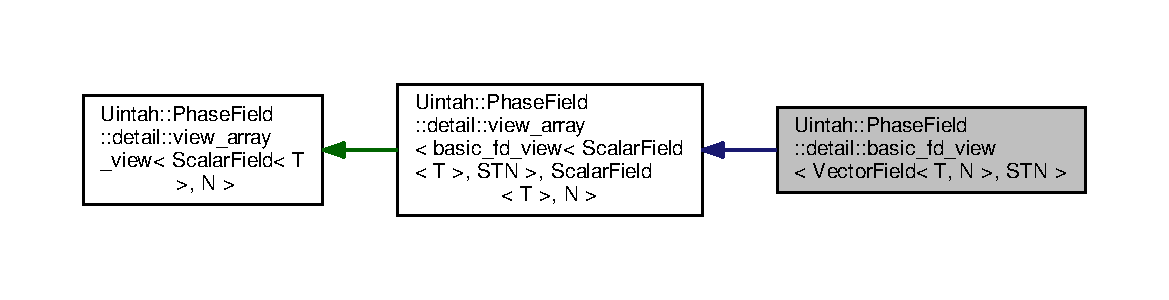
\includegraphics[width=350pt]{classUintah_1_1PhaseField_1_1detail_1_1basic__fd__view_3_01VectorField_3_01T_00_01N_01_4_00_01STN_01_4__inherit__graph}
\end{center}
\end{figure}


Collaboration diagram for Uintah\+:\+:Phase\+Field\+:\+:detail\+:\+:basic\+\_\+fd\+\_\+view$<$ Vector\+Field$<$ T, N $>$, S\+TN $>$\+:\nopagebreak
\begin{figure}[H]
\begin{center}
\leavevmode
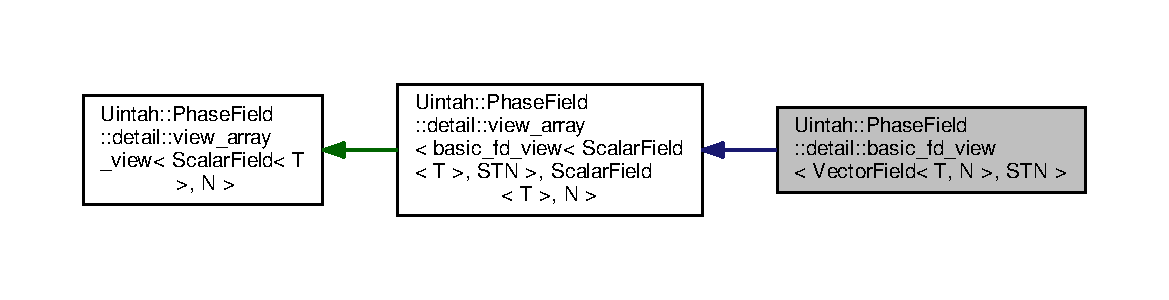
\includegraphics[width=350pt]{classUintah_1_1PhaseField_1_1detail_1_1basic__fd__view_3_01VectorField_3_01T_00_01N_01_4_00_01STN_01_4__coll__graph}
\end{center}
\end{figure}
\subsection*{Public Member Functions}
\begin{DoxyCompactItemize}
\item 
virtual \hyperlink{classUintah_1_1PhaseField_1_1detail_1_1basic__fd__view_3_01VectorField_3_01T_00_01N_01_4_00_01STN_01_4_ac602ec10bc7689756306f5a8a89ba8ee}{$\sim$basic\+\_\+fd\+\_\+view} ()=default
\begin{DoxyCompactList}\small\item\em Default destructor. \end{DoxyCompactList}\end{DoxyCompactItemize}
\subsection*{Additional Inherited Members}


\subsection{Detailed Description}
\subsubsection*{template$<$typename T, size\+\_\+t N, Stn\+Type S\+TN$>$\newline
class Uintah\+::\+Phase\+Field\+::detail\+::basic\+\_\+fd\+\_\+view$<$ Vector\+Field$<$ T, N $>$, S\+T\+N $>$}

Abstract class for basic finite-\/difference operations on variables (\hyperlink{structUintah_1_1PhaseField_1_1VectorField}{Vector\+Field} implementation) 

detail implementation of view (variable wrapping) which include also finite difference approximation on basic differential operations (first and second order derivatives)


\begin{DoxyTemplParams}{Template Parameters}
{\em T} & type of each component of the field at each point \\
\hline
{\em N} & number of components \\
\hline
{\em S\+TN} & finite-\/difference stencil \\
\hline
\end{DoxyTemplParams}


\subsection{Constructor \& Destructor Documentation}
\mbox{\Hypertarget{classUintah_1_1PhaseField_1_1detail_1_1basic__fd__view_3_01VectorField_3_01T_00_01N_01_4_00_01STN_01_4_ac602ec10bc7689756306f5a8a89ba8ee}\label{classUintah_1_1PhaseField_1_1detail_1_1basic__fd__view_3_01VectorField_3_01T_00_01N_01_4_00_01STN_01_4_ac602ec10bc7689756306f5a8a89ba8ee}} 
\index{Uintah\+::\+Phase\+Field\+::detail\+::basic\+\_\+fd\+\_\+view$<$ Vector\+Field$<$ T, N $>$, S\+T\+N $>$@{Uintah\+::\+Phase\+Field\+::detail\+::basic\+\_\+fd\+\_\+view$<$ Vector\+Field$<$ T, N $>$, S\+T\+N $>$}!````~basic\+\_\+fd\+\_\+view@{$\sim$basic\+\_\+fd\+\_\+view}}
\index{````~basic\+\_\+fd\+\_\+view@{$\sim$basic\+\_\+fd\+\_\+view}!Uintah\+::\+Phase\+Field\+::detail\+::basic\+\_\+fd\+\_\+view$<$ Vector\+Field$<$ T, N $>$, S\+T\+N $>$@{Uintah\+::\+Phase\+Field\+::detail\+::basic\+\_\+fd\+\_\+view$<$ Vector\+Field$<$ T, N $>$, S\+T\+N $>$}}
\subsubsection{\texorpdfstring{$\sim$basic\+\_\+fd\+\_\+view()}{~basic\_fd\_view()}}
{\footnotesize\ttfamily template$<$typename T , size\+\_\+t N, Stn\+Type S\+TN$>$ \\
virtual \hyperlink{classUintah_1_1PhaseField_1_1detail_1_1basic__fd__view}{Uintah\+::\+Phase\+Field\+::detail\+::basic\+\_\+fd\+\_\+view}$<$ \hyperlink{structUintah_1_1PhaseField_1_1VectorField}{Vector\+Field}$<$ T, N $>$, S\+TN $>$\+::$\sim$\hyperlink{classUintah_1_1PhaseField_1_1detail_1_1basic__fd__view}{basic\+\_\+fd\+\_\+view} (\begin{DoxyParamCaption}{ }\end{DoxyParamCaption})\hspace{0.3cm}{\ttfamily [virtual]}, {\ttfamily [default]}}



Default destructor. 



The documentation for this class was generated from the following file\+:\begin{DoxyCompactItemize}
\item 
\hyperlink{basic__fd__view_8h}{basic\+\_\+fd\+\_\+view.\+h}\end{DoxyCompactItemize}

\hypertarget{classUintah_1_1PhaseField_1_1detail_1_1bc__basic__fd__view}{}\section{Uintah\+:\+:Phase\+Field\+:\+:detail\+:\+:bc\+\_\+basic\+\_\+fd\+\_\+view$<$ Field, S\+TN, V\+AR, P $>$ Class Template Reference}
\label{classUintah_1_1PhaseField_1_1detail_1_1bc__basic__fd__view}\index{Uintah\+::\+Phase\+Field\+::detail\+::bc\+\_\+basic\+\_\+fd\+\_\+view$<$ Field, S\+T\+N, V\+A\+R, P $>$@{Uintah\+::\+Phase\+Field\+::detail\+::bc\+\_\+basic\+\_\+fd\+\_\+view$<$ Field, S\+T\+N, V\+A\+R, P $>$}}


Wrapper of Data\+Warehouse variables for basic differential operations.  




{\ttfamily \#include $<$bc\+\_\+basic\+\_\+fd\+\_\+view.\+h$>$}



\subsection{Detailed Description}
\subsubsection*{template$<$typename Field, Stn\+Type S\+TN, Var\+Type V\+AR, B\+CF P$>$\newline
class Uintah\+::\+Phase\+Field\+::detail\+::bc\+\_\+basic\+\_\+fd\+\_\+view$<$ Field, S\+T\+N, V\+A\+R, P $>$}

Wrapper of Data\+Warehouse variables for basic differential operations. 

Adds to \hyperlink{classUintah_1_1PhaseField_1_1detail_1_1dw__view}{dw\+\_\+view} the possibility to compute finite-\/difference approximation of of basic differential operations (first and second order derivatives) at boundary faces


\begin{DoxyTemplParams}{Template Parameters}
{\em Field} & type of field (\hyperlink{structUintah_1_1PhaseField_1_1ScalarField}{Scalar\+Field} $<$ T $>$ or \hyperlink{structUintah_1_1PhaseField_1_1VectorField}{Vector\+Field} $<$ T, N $>$) \\
\hline
{\em S\+TN} & finite-\/difference stencil \\
\hline
{\em V\+AR} & type of variable representation \\
\hline
{\em P} & BC, FC, and Patch\+::\+Face pack \\
\hline
\end{DoxyTemplParams}


The documentation for this class was generated from the following file\+:\begin{DoxyCompactItemize}
\item 
\hyperlink{bc__basic__fd__view_8h}{bc\+\_\+basic\+\_\+fd\+\_\+view.\+h}\end{DoxyCompactItemize}

\hypertarget{classUintah_1_1PhaseField_1_1detail_1_1bc__basic__fd__view_3_01ScalarField_3_01T_01_4_00_01STN_00_01VAR_00_01P_01_4}{}\section{Uintah\+:\+:Phase\+Field\+:\+:detail\+:\+:bc\+\_\+basic\+\_\+fd\+\_\+view$<$ Scalar\+Field$<$ T $>$, S\+TN, V\+AR, P $>$ Class Template Reference}
\label{classUintah_1_1PhaseField_1_1detail_1_1bc__basic__fd__view_3_01ScalarField_3_01T_01_4_00_01STN_00_01VAR_00_01P_01_4}\index{Uintah\+::\+Phase\+Field\+::detail\+::bc\+\_\+basic\+\_\+fd\+\_\+view$<$ Scalar\+Field$<$ T $>$, S\+T\+N, V\+A\+R, P $>$@{Uintah\+::\+Phase\+Field\+::detail\+::bc\+\_\+basic\+\_\+fd\+\_\+view$<$ Scalar\+Field$<$ T $>$, S\+T\+N, V\+A\+R, P $>$}}


Wrapper of Data\+Warehouse variables for basic differential operations (\hyperlink{structUintah_1_1PhaseField_1_1ScalarField}{Scalar\+Field} implementation)  




{\ttfamily \#include $<$bc\+\_\+basic\+\_\+fd\+\_\+view.\+h$>$}



Inheritance diagram for Uintah\+:\+:Phase\+Field\+:\+:detail\+:\+:bc\+\_\+basic\+\_\+fd\+\_\+view$<$ Scalar\+Field$<$ T $>$, S\+TN, V\+AR, P $>$\+:\nopagebreak
\begin{figure}[H]
\begin{center}
\leavevmode
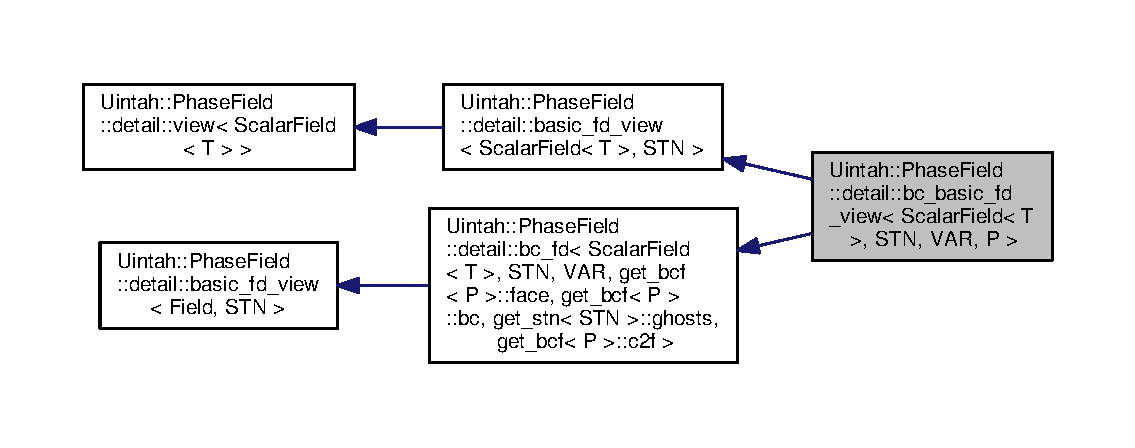
\includegraphics[width=350pt]{classUintah_1_1PhaseField_1_1detail_1_1bc__basic__fd__view_3_01ScalarField_3_01T_01_4_00_01STN_02b3cc3e1866aa450fde42bf2262388e3}
\end{center}
\end{figure}


Collaboration diagram for Uintah\+:\+:Phase\+Field\+:\+:detail\+:\+:bc\+\_\+basic\+\_\+fd\+\_\+view$<$ Scalar\+Field$<$ T $>$, S\+TN, V\+AR, P $>$\+:\nopagebreak
\begin{figure}[H]
\begin{center}
\leavevmode
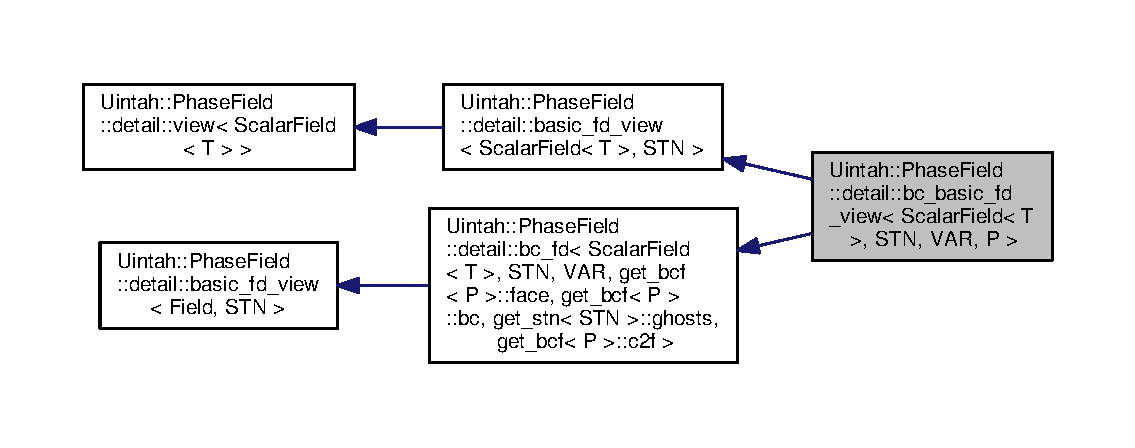
\includegraphics[width=350pt]{classUintah_1_1PhaseField_1_1detail_1_1bc__basic__fd__view_3_01ScalarField_3_01T_01_4_00_01STN_0cbac9e814a2ccab639c7edbd28b0fdcb}
\end{center}
\end{figure}
\subsection*{Public Member Functions}
\begin{DoxyCompactItemize}
\item 
\hyperlink{classUintah_1_1PhaseField_1_1detail_1_1bc__basic__fd__view_3_01ScalarField_3_01T_01_4_00_01STN_00_01VAR_00_01P_01_4_a71f5d2796724efaaf5e046f86e780aea}{bc\+\_\+basic\+\_\+fd\+\_\+view} (\hyperlink{classUintah_1_1PhaseField_1_1detail_1_1view}{view}$<$ \hyperlink{structUintah_1_1PhaseField_1_1ScalarField}{Field} $>$ $\ast$\hyperlink{classUintah_1_1PhaseField_1_1detail_1_1view}{view}, const typename \hyperlink{structUintah_1_1PhaseField_1_1ScalarField_a7a77875e030da64c47ce9f6c22a06959}{Field\+::label\+\_\+type} \&label, int material, const Level $\ast$level, const BV \&value)
\begin{DoxyCompactList}\small\item\em Constructor. \end{DoxyCompactList}\item 
\hyperlink{classUintah_1_1PhaseField_1_1detail_1_1bc__basic__fd__view_3_01ScalarField_3_01T_01_4_00_01STN_00_01VAR_00_01P_01_4_a302171385c2d6e02780239bf81b4231a}{bc\+\_\+basic\+\_\+fd\+\_\+view} (const \hyperlink{classUintah_1_1PhaseField_1_1detail_1_1view}{view}$<$ \hyperlink{structUintah_1_1PhaseField_1_1ScalarField}{Field} $>$ $\ast$\hyperlink{classUintah_1_1PhaseField_1_1detail_1_1view}{view}, Data\+Warehouse $\ast$dw, const Var\+Label $\ast$label, int material, const Level $\ast$level, const BV \&value, const Patch $\ast$patch, bool use\+\_\+ghosts)
\begin{DoxyCompactList}\small\item\em Constructor. \end{DoxyCompactList}\item 
virtual \hyperlink{classUintah_1_1PhaseField_1_1detail_1_1bc__basic__fd__view_3_01ScalarField_3_01T_01_4_00_01STN_00_01VAR_00_01P_01_4_a8440a2cb32190e75b3f9f79a408980c8}{$\sim$bc\+\_\+basic\+\_\+fd\+\_\+view} ()=default
\item 
\hyperlink{classUintah_1_1PhaseField_1_1detail_1_1bc__basic__fd__view_3_01ScalarField_3_01T_01_4_00_01STN_00_01VAR_00_01P_01_4_a48c8acbfa62da6002160c50117b7b75d}{bc\+\_\+basic\+\_\+fd\+\_\+view} (const \hyperlink{classUintah_1_1PhaseField_1_1detail_1_1bc__basic__fd__view}{bc\+\_\+basic\+\_\+fd\+\_\+view} \&)=delete
\begin{DoxyCompactList}\small\item\em Prevent copy (and move) constructor. \end{DoxyCompactList}\item 
\hyperlink{classUintah_1_1PhaseField_1_1detail_1_1bc__basic__fd__view}{bc\+\_\+basic\+\_\+fd\+\_\+view} \& \hyperlink{classUintah_1_1PhaseField_1_1detail_1_1bc__basic__fd__view_3_01ScalarField_3_01T_01_4_00_01STN_00_01VAR_00_01P_01_4_af7343355f3109a8891a073e9aeb7bf9a}{operator=} (const \hyperlink{classUintah_1_1PhaseField_1_1detail_1_1bc__basic__fd__view}{bc\+\_\+basic\+\_\+fd\+\_\+view} \&)=delete
\begin{DoxyCompactList}\small\item\em Prevent copy (and move) assignment. \end{DoxyCompactList}\item 
virtual \hyperlink{classUintah_1_1PhaseField_1_1detail_1_1view}{view}$<$ \hyperlink{structUintah_1_1PhaseField_1_1ScalarField}{Field} $>$ $\ast$ \hyperlink{classUintah_1_1PhaseField_1_1detail_1_1bc__basic__fd__view_3_01ScalarField_3_01T_01_4_00_01STN_00_01VAR_00_01P_01_4_aefe3932d2c0c72fe420417f7291b4c15}{clone} (bool deep) const override
\begin{DoxyCompactList}\small\item\em Get a copy of the view. \end{DoxyCompactList}\item 
virtual \hyperlink{classUintah_1_1PhaseField_1_1detail_1_1view}{view}$<$ \hyperlink{structUintah_1_1PhaseField_1_1ScalarField}{Field} $>$ $\ast$ \hyperlink{classUintah_1_1PhaseField_1_1detail_1_1bc__basic__fd__view_3_01ScalarField_3_01T_01_4_00_01STN_00_01VAR_00_01P_01_4_adc6935173c04499a5a7c769d296a97d7}{clone} (bool deep, const Int\+Vector \&offset) const override
\begin{DoxyCompactList}\small\item\em Get a copy of the view and apply translate the support. \end{DoxyCompactList}\item 
virtual \hyperlink{classUintah_1_1PhaseField_1_1detail_1_1view}{view}$<$ \hyperlink{structUintah_1_1PhaseField_1_1ScalarField}{Field} $>$ $\ast$ \hyperlink{classUintah_1_1PhaseField_1_1detail_1_1bc__basic__fd__view_3_01ScalarField_3_01T_01_4_00_01STN_00_01VAR_00_01P_01_4_a46e6a2a932a522c1ed93c7c28d728e83}{get\+\_\+view} () override
\begin{DoxyCompactList}\small\item\em Get base view (virtual implementation) \end{DoxyCompactList}\item 
virtual const \hyperlink{classUintah_1_1PhaseField_1_1detail_1_1view}{view}$<$ \hyperlink{structUintah_1_1PhaseField_1_1ScalarField}{Field} $>$ $\ast$ \hyperlink{classUintah_1_1PhaseField_1_1detail_1_1bc__basic__fd__view_3_01ScalarField_3_01T_01_4_00_01STN_00_01VAR_00_01P_01_4_aa82811e38cba5075406deb5e0f4adf62}{get\+\_\+view} () const override
\begin{DoxyCompactList}\small\item\em Get base view. \end{DoxyCompactList}\item 
virtual V \hyperlink{classUintah_1_1PhaseField_1_1detail_1_1bc__basic__fd__view_3_01ScalarField_3_01T_01_4_00_01STN_00_01VAR_00_01P_01_4_ae734fd388d7a680aa366db584bc54107}{dx} (const Int\+Vector \&id) const override
\begin{DoxyCompactList}\small\item\em Partial x derivative. \end{DoxyCompactList}\item 
virtual V \hyperlink{classUintah_1_1PhaseField_1_1detail_1_1bc__basic__fd__view_3_01ScalarField_3_01T_01_4_00_01STN_00_01VAR_00_01P_01_4_ad81ac1a8cf3ddce875d270b6bb00a380}{dy} (const Int\+Vector \&id) const override
\begin{DoxyCompactList}\small\item\em Partial y derivative. \end{DoxyCompactList}\item 
virtual V \hyperlink{classUintah_1_1PhaseField_1_1detail_1_1bc__basic__fd__view_3_01ScalarField_3_01T_01_4_00_01STN_00_01VAR_00_01P_01_4_a994e7388acdb4040da7cc438ecd2dc4b}{dz} (const Int\+Vector \&id) const override
\begin{DoxyCompactList}\small\item\em Partial z derivative. \end{DoxyCompactList}\item 
virtual V \hyperlink{classUintah_1_1PhaseField_1_1detail_1_1bc__basic__fd__view_3_01ScalarField_3_01T_01_4_00_01STN_00_01VAR_00_01P_01_4_a7146569da689f425b7eb963295905ee2}{dxx} (const Int\+Vector \&id) const override
\begin{DoxyCompactList}\small\item\em Partial x second order derivative. \end{DoxyCompactList}\item 
virtual V \hyperlink{classUintah_1_1PhaseField_1_1detail_1_1bc__basic__fd__view_3_01ScalarField_3_01T_01_4_00_01STN_00_01VAR_00_01P_01_4_a5549a4a413c2be230e484c8921524395}{dyy} (const Int\+Vector \&id) const override
\begin{DoxyCompactList}\small\item\em Partial x second order derivative. \end{DoxyCompactList}\item 
virtual V \hyperlink{classUintah_1_1PhaseField_1_1detail_1_1bc__basic__fd__view_3_01ScalarField_3_01T_01_4_00_01STN_00_01VAR_00_01P_01_4_ad2c322a2540d22bffda0332f436df825}{dzz} (const Int\+Vector \&id) const override
\begin{DoxyCompactList}\small\item\em Partial x second order derivative. \end{DoxyCompactList}\end{DoxyCompactItemize}
\subsection*{Protected Member Functions}
\begin{DoxyCompactItemize}
\item 
\hyperlink{classUintah_1_1PhaseField_1_1detail_1_1bc__basic__fd__view_3_01ScalarField_3_01T_01_4_00_01STN_00_01VAR_00_01P_01_4_abb5dbc3676f8c31fd3fce28c505b941a}{bc\+\_\+basic\+\_\+fd\+\_\+view} (const \hyperlink{classUintah_1_1PhaseField_1_1detail_1_1bc__basic__fd__view}{bc\+\_\+basic\+\_\+fd\+\_\+view} $\ast$copy, bool deep)
\begin{DoxyCompactList}\small\item\em Constructor. \end{DoxyCompactList}\end{DoxyCompactItemize}
\subsection*{Additional Inherited Members}


\subsection{Detailed Description}
\subsubsection*{template$<$typename T, Stn\+Type S\+TN, Var\+Type V\+AR, B\+CF P$>$\newline
class Uintah\+::\+Phase\+Field\+::detail\+::bc\+\_\+basic\+\_\+fd\+\_\+view$<$ Scalar\+Field$<$ T $>$, S\+T\+N, V\+A\+R, P $>$}

Wrapper of Data\+Warehouse variables for basic differential operations (\hyperlink{structUintah_1_1PhaseField_1_1ScalarField}{Scalar\+Field} implementation) 

Adds to \hyperlink{classUintah_1_1PhaseField_1_1detail_1_1dw__view}{dw\+\_\+view} the possibility to compute finite-\/difference approximation of of basic differential operations (first and second order derivatives) at boundary faces

\begin{DoxyRemark}{Remarks}
actual finite-\/differences implementations are in \hyperlink{classUintah_1_1PhaseField_1_1detail_1_1bc__fd}{bc\+\_\+fd}
\end{DoxyRemark}

\begin{DoxyTemplParams}{Template Parameters}
{\em T} & type of the field value at each point \\
\hline
{\em S\+TN} & finite-\/difference stencil \\
\hline
{\em V\+AR} & type of variable representation \\
\hline
{\em P} & BC, FC, and Patch\+::\+Face pack \\
\hline
\end{DoxyTemplParams}


\subsection{Constructor \& Destructor Documentation}
\mbox{\Hypertarget{classUintah_1_1PhaseField_1_1detail_1_1bc__basic__fd__view_3_01ScalarField_3_01T_01_4_00_01STN_00_01VAR_00_01P_01_4_abb5dbc3676f8c31fd3fce28c505b941a}\label{classUintah_1_1PhaseField_1_1detail_1_1bc__basic__fd__view_3_01ScalarField_3_01T_01_4_00_01STN_00_01VAR_00_01P_01_4_abb5dbc3676f8c31fd3fce28c505b941a}} 
\index{Uintah\+::\+Phase\+Field\+::detail\+::bc\+\_\+basic\+\_\+fd\+\_\+view$<$ Scalar\+Field$<$ T $>$, S\+T\+N, V\+A\+R, P $>$@{Uintah\+::\+Phase\+Field\+::detail\+::bc\+\_\+basic\+\_\+fd\+\_\+view$<$ Scalar\+Field$<$ T $>$, S\+T\+N, V\+A\+R, P $>$}!bc\+\_\+basic\+\_\+fd\+\_\+view@{bc\+\_\+basic\+\_\+fd\+\_\+view}}
\index{bc\+\_\+basic\+\_\+fd\+\_\+view@{bc\+\_\+basic\+\_\+fd\+\_\+view}!Uintah\+::\+Phase\+Field\+::detail\+::bc\+\_\+basic\+\_\+fd\+\_\+view$<$ Scalar\+Field$<$ T $>$, S\+T\+N, V\+A\+R, P $>$@{Uintah\+::\+Phase\+Field\+::detail\+::bc\+\_\+basic\+\_\+fd\+\_\+view$<$ Scalar\+Field$<$ T $>$, S\+T\+N, V\+A\+R, P $>$}}
\subsubsection{\texorpdfstring{bc\+\_\+basic\+\_\+fd\+\_\+view()}{bc\_basic\_fd\_view()}\hspace{0.1cm}{\footnotesize\ttfamily [1/4]}}
{\footnotesize\ttfamily template$<$typename T , Stn\+Type S\+TN, Var\+Type V\+AR, B\+CF P$>$ \\
\hyperlink{classUintah_1_1PhaseField_1_1detail_1_1bc__basic__fd__view}{Uintah\+::\+Phase\+Field\+::detail\+::bc\+\_\+basic\+\_\+fd\+\_\+view}$<$ \hyperlink{structUintah_1_1PhaseField_1_1ScalarField}{Scalar\+Field}$<$ T $>$, S\+TN, V\+AR, P $>$\+::\hyperlink{classUintah_1_1PhaseField_1_1detail_1_1bc__basic__fd__view}{bc\+\_\+basic\+\_\+fd\+\_\+view} (\begin{DoxyParamCaption}\item[{const \hyperlink{classUintah_1_1PhaseField_1_1detail_1_1bc__basic__fd__view}{bc\+\_\+basic\+\_\+fd\+\_\+view}$<$ \hyperlink{structUintah_1_1PhaseField_1_1ScalarField}{Scalar\+Field}$<$ T $>$, S\+TN, V\+AR, P $>$ $\ast$}]{copy,  }\item[{bool}]{deep }\end{DoxyParamCaption})\hspace{0.3cm}{\ttfamily [inline]}, {\ttfamily [protected]}}



Constructor. 

Instantiate a copy of a given view


\begin{DoxyParams}{Parameters}
{\em copy} & source view for copying \\
\hline
{\em deep} & if true inner grid variable is copied as well otherwise the same grid variable is referenced \\
\hline
\end{DoxyParams}
\mbox{\Hypertarget{classUintah_1_1PhaseField_1_1detail_1_1bc__basic__fd__view_3_01ScalarField_3_01T_01_4_00_01STN_00_01VAR_00_01P_01_4_a71f5d2796724efaaf5e046f86e780aea}\label{classUintah_1_1PhaseField_1_1detail_1_1bc__basic__fd__view_3_01ScalarField_3_01T_01_4_00_01STN_00_01VAR_00_01P_01_4_a71f5d2796724efaaf5e046f86e780aea}} 
\index{Uintah\+::\+Phase\+Field\+::detail\+::bc\+\_\+basic\+\_\+fd\+\_\+view$<$ Scalar\+Field$<$ T $>$, S\+T\+N, V\+A\+R, P $>$@{Uintah\+::\+Phase\+Field\+::detail\+::bc\+\_\+basic\+\_\+fd\+\_\+view$<$ Scalar\+Field$<$ T $>$, S\+T\+N, V\+A\+R, P $>$}!bc\+\_\+basic\+\_\+fd\+\_\+view@{bc\+\_\+basic\+\_\+fd\+\_\+view}}
\index{bc\+\_\+basic\+\_\+fd\+\_\+view@{bc\+\_\+basic\+\_\+fd\+\_\+view}!Uintah\+::\+Phase\+Field\+::detail\+::bc\+\_\+basic\+\_\+fd\+\_\+view$<$ Scalar\+Field$<$ T $>$, S\+T\+N, V\+A\+R, P $>$@{Uintah\+::\+Phase\+Field\+::detail\+::bc\+\_\+basic\+\_\+fd\+\_\+view$<$ Scalar\+Field$<$ T $>$, S\+T\+N, V\+A\+R, P $>$}}
\subsubsection{\texorpdfstring{bc\+\_\+basic\+\_\+fd\+\_\+view()}{bc\_basic\_fd\_view()}\hspace{0.1cm}{\footnotesize\ttfamily [2/4]}}
{\footnotesize\ttfamily template$<$typename T , Stn\+Type S\+TN, Var\+Type V\+AR, B\+CF P$>$ \\
\hyperlink{classUintah_1_1PhaseField_1_1detail_1_1bc__basic__fd__view}{Uintah\+::\+Phase\+Field\+::detail\+::bc\+\_\+basic\+\_\+fd\+\_\+view}$<$ \hyperlink{structUintah_1_1PhaseField_1_1ScalarField}{Scalar\+Field}$<$ T $>$, S\+TN, V\+AR, P $>$\+::\hyperlink{classUintah_1_1PhaseField_1_1detail_1_1bc__basic__fd__view}{bc\+\_\+basic\+\_\+fd\+\_\+view} (\begin{DoxyParamCaption}\item[{\hyperlink{classUintah_1_1PhaseField_1_1detail_1_1view}{view}$<$ \hyperlink{structUintah_1_1PhaseField_1_1ScalarField}{Field} $>$ $\ast$}]{view,  }\item[{const typename \hyperlink{structUintah_1_1PhaseField_1_1ScalarField_a7a77875e030da64c47ce9f6c22a06959}{Field\+::label\+\_\+type} \&}]{label,  }\item[{int}]{material,  }\item[{const Level $\ast$}]{level,  }\item[{const BV \&}]{value }\end{DoxyParamCaption})\hspace{0.3cm}{\ttfamily [inline]}}



Constructor. 

Instantiate a view without gathering info from the Data\+Warehouse


\begin{DoxyParams}{Parameters}
{\em view} & view on which the bc has to be imposed \\
\hline
{\em label} & variable label \\
\hline
{\em material} & material index \\
\hline
{\em level} & grid level \\
\hline
{\em value} & used when imposing the prescribed BC \\
\hline
\end{DoxyParams}
\mbox{\Hypertarget{classUintah_1_1PhaseField_1_1detail_1_1bc__basic__fd__view_3_01ScalarField_3_01T_01_4_00_01STN_00_01VAR_00_01P_01_4_a302171385c2d6e02780239bf81b4231a}\label{classUintah_1_1PhaseField_1_1detail_1_1bc__basic__fd__view_3_01ScalarField_3_01T_01_4_00_01STN_00_01VAR_00_01P_01_4_a302171385c2d6e02780239bf81b4231a}} 
\index{Uintah\+::\+Phase\+Field\+::detail\+::bc\+\_\+basic\+\_\+fd\+\_\+view$<$ Scalar\+Field$<$ T $>$, S\+T\+N, V\+A\+R, P $>$@{Uintah\+::\+Phase\+Field\+::detail\+::bc\+\_\+basic\+\_\+fd\+\_\+view$<$ Scalar\+Field$<$ T $>$, S\+T\+N, V\+A\+R, P $>$}!bc\+\_\+basic\+\_\+fd\+\_\+view@{bc\+\_\+basic\+\_\+fd\+\_\+view}}
\index{bc\+\_\+basic\+\_\+fd\+\_\+view@{bc\+\_\+basic\+\_\+fd\+\_\+view}!Uintah\+::\+Phase\+Field\+::detail\+::bc\+\_\+basic\+\_\+fd\+\_\+view$<$ Scalar\+Field$<$ T $>$, S\+T\+N, V\+A\+R, P $>$@{Uintah\+::\+Phase\+Field\+::detail\+::bc\+\_\+basic\+\_\+fd\+\_\+view$<$ Scalar\+Field$<$ T $>$, S\+T\+N, V\+A\+R, P $>$}}
\subsubsection{\texorpdfstring{bc\+\_\+basic\+\_\+fd\+\_\+view()}{bc\_basic\_fd\_view()}\hspace{0.1cm}{\footnotesize\ttfamily [3/4]}}
{\footnotesize\ttfamily template$<$typename T , Stn\+Type S\+TN, Var\+Type V\+AR, B\+CF P$>$ \\
\hyperlink{classUintah_1_1PhaseField_1_1detail_1_1bc__basic__fd__view}{Uintah\+::\+Phase\+Field\+::detail\+::bc\+\_\+basic\+\_\+fd\+\_\+view}$<$ \hyperlink{structUintah_1_1PhaseField_1_1ScalarField}{Scalar\+Field}$<$ T $>$, S\+TN, V\+AR, P $>$\+::\hyperlink{classUintah_1_1PhaseField_1_1detail_1_1bc__basic__fd__view}{bc\+\_\+basic\+\_\+fd\+\_\+view} (\begin{DoxyParamCaption}\item[{const \hyperlink{classUintah_1_1PhaseField_1_1detail_1_1view}{view}$<$ \hyperlink{structUintah_1_1PhaseField_1_1ScalarField}{Field} $>$ $\ast$}]{view,  }\item[{Data\+Warehouse $\ast$}]{dw,  }\item[{const Var\+Label $\ast$}]{label,  }\item[{int}]{material,  }\item[{const Level $\ast$}]{level,  }\item[{const BV \&}]{value,  }\item[{const Patch $\ast$}]{patch,  }\item[{bool}]{use\+\_\+ghosts }\end{DoxyParamCaption})\hspace{0.3cm}{\ttfamily [inline]}}



Constructor. 

Instantiate a view and gather info from dw


\begin{DoxyParams}{Parameters}
{\em dw} & Data\+Warehouse from which data is retrieved \\
\hline
{\em view} & view on which the bc has to be imposed \\
\hline
{\em label} & variable label \\
\hline
{\em material} & material index \\
\hline
{\em level} & grid level \\
\hline
{\em value} & used when imposing the prescribed BC \\
\hline
{\em patch} & grid patch owning the face \\
\hline
{\em use\+\_\+ghosts} & if ghosts value are to be retrieved \\
\hline
\end{DoxyParams}
\mbox{\Hypertarget{classUintah_1_1PhaseField_1_1detail_1_1bc__basic__fd__view_3_01ScalarField_3_01T_01_4_00_01STN_00_01VAR_00_01P_01_4_a8440a2cb32190e75b3f9f79a408980c8}\label{classUintah_1_1PhaseField_1_1detail_1_1bc__basic__fd__view_3_01ScalarField_3_01T_01_4_00_01STN_00_01VAR_00_01P_01_4_a8440a2cb32190e75b3f9f79a408980c8}} 
\index{Uintah\+::\+Phase\+Field\+::detail\+::bc\+\_\+basic\+\_\+fd\+\_\+view$<$ Scalar\+Field$<$ T $>$, S\+T\+N, V\+A\+R, P $>$@{Uintah\+::\+Phase\+Field\+::detail\+::bc\+\_\+basic\+\_\+fd\+\_\+view$<$ Scalar\+Field$<$ T $>$, S\+T\+N, V\+A\+R, P $>$}!````~bc\+\_\+basic\+\_\+fd\+\_\+view@{$\sim$bc\+\_\+basic\+\_\+fd\+\_\+view}}
\index{````~bc\+\_\+basic\+\_\+fd\+\_\+view@{$\sim$bc\+\_\+basic\+\_\+fd\+\_\+view}!Uintah\+::\+Phase\+Field\+::detail\+::bc\+\_\+basic\+\_\+fd\+\_\+view$<$ Scalar\+Field$<$ T $>$, S\+T\+N, V\+A\+R, P $>$@{Uintah\+::\+Phase\+Field\+::detail\+::bc\+\_\+basic\+\_\+fd\+\_\+view$<$ Scalar\+Field$<$ T $>$, S\+T\+N, V\+A\+R, P $>$}}
\subsubsection{\texorpdfstring{$\sim$bc\+\_\+basic\+\_\+fd\+\_\+view()}{~bc\_basic\_fd\_view()}}
{\footnotesize\ttfamily template$<$typename T , Stn\+Type S\+TN, Var\+Type V\+AR, B\+CF P$>$ \\
virtual \hyperlink{classUintah_1_1PhaseField_1_1detail_1_1bc__basic__fd__view}{Uintah\+::\+Phase\+Field\+::detail\+::bc\+\_\+basic\+\_\+fd\+\_\+view}$<$ \hyperlink{structUintah_1_1PhaseField_1_1ScalarField}{Scalar\+Field}$<$ T $>$, S\+TN, V\+AR, P $>$\+::$\sim$\hyperlink{classUintah_1_1PhaseField_1_1detail_1_1bc__basic__fd__view}{bc\+\_\+basic\+\_\+fd\+\_\+view} (\begin{DoxyParamCaption}{ }\end{DoxyParamCaption})\hspace{0.3cm}{\ttfamily [virtual]}, {\ttfamily [default]}}

\mbox{\Hypertarget{classUintah_1_1PhaseField_1_1detail_1_1bc__basic__fd__view_3_01ScalarField_3_01T_01_4_00_01STN_00_01VAR_00_01P_01_4_a48c8acbfa62da6002160c50117b7b75d}\label{classUintah_1_1PhaseField_1_1detail_1_1bc__basic__fd__view_3_01ScalarField_3_01T_01_4_00_01STN_00_01VAR_00_01P_01_4_a48c8acbfa62da6002160c50117b7b75d}} 
\index{Uintah\+::\+Phase\+Field\+::detail\+::bc\+\_\+basic\+\_\+fd\+\_\+view$<$ Scalar\+Field$<$ T $>$, S\+T\+N, V\+A\+R, P $>$@{Uintah\+::\+Phase\+Field\+::detail\+::bc\+\_\+basic\+\_\+fd\+\_\+view$<$ Scalar\+Field$<$ T $>$, S\+T\+N, V\+A\+R, P $>$}!bc\+\_\+basic\+\_\+fd\+\_\+view@{bc\+\_\+basic\+\_\+fd\+\_\+view}}
\index{bc\+\_\+basic\+\_\+fd\+\_\+view@{bc\+\_\+basic\+\_\+fd\+\_\+view}!Uintah\+::\+Phase\+Field\+::detail\+::bc\+\_\+basic\+\_\+fd\+\_\+view$<$ Scalar\+Field$<$ T $>$, S\+T\+N, V\+A\+R, P $>$@{Uintah\+::\+Phase\+Field\+::detail\+::bc\+\_\+basic\+\_\+fd\+\_\+view$<$ Scalar\+Field$<$ T $>$, S\+T\+N, V\+A\+R, P $>$}}
\subsubsection{\texorpdfstring{bc\+\_\+basic\+\_\+fd\+\_\+view()}{bc\_basic\_fd\_view()}\hspace{0.1cm}{\footnotesize\ttfamily [4/4]}}
{\footnotesize\ttfamily template$<$typename T , Stn\+Type S\+TN, Var\+Type V\+AR, B\+CF P$>$ \\
\hyperlink{classUintah_1_1PhaseField_1_1detail_1_1bc__basic__fd__view}{Uintah\+::\+Phase\+Field\+::detail\+::bc\+\_\+basic\+\_\+fd\+\_\+view}$<$ \hyperlink{structUintah_1_1PhaseField_1_1ScalarField}{Scalar\+Field}$<$ T $>$, S\+TN, V\+AR, P $>$\+::\hyperlink{classUintah_1_1PhaseField_1_1detail_1_1bc__basic__fd__view}{bc\+\_\+basic\+\_\+fd\+\_\+view} (\begin{DoxyParamCaption}\item[{const \hyperlink{classUintah_1_1PhaseField_1_1detail_1_1bc__basic__fd__view}{bc\+\_\+basic\+\_\+fd\+\_\+view}$<$ \hyperlink{structUintah_1_1PhaseField_1_1ScalarField}{Scalar\+Field}$<$ T $>$, S\+TN, V\+AR, P $>$ \&}]{ }\end{DoxyParamCaption})\hspace{0.3cm}{\ttfamily [delete]}}



Prevent copy (and move) constructor. 



\subsection{Member Function Documentation}
\mbox{\Hypertarget{classUintah_1_1PhaseField_1_1detail_1_1bc__basic__fd__view_3_01ScalarField_3_01T_01_4_00_01STN_00_01VAR_00_01P_01_4_aefe3932d2c0c72fe420417f7291b4c15}\label{classUintah_1_1PhaseField_1_1detail_1_1bc__basic__fd__view_3_01ScalarField_3_01T_01_4_00_01STN_00_01VAR_00_01P_01_4_aefe3932d2c0c72fe420417f7291b4c15}} 
\index{Uintah\+::\+Phase\+Field\+::detail\+::bc\+\_\+basic\+\_\+fd\+\_\+view$<$ Scalar\+Field$<$ T $>$, S\+T\+N, V\+A\+R, P $>$@{Uintah\+::\+Phase\+Field\+::detail\+::bc\+\_\+basic\+\_\+fd\+\_\+view$<$ Scalar\+Field$<$ T $>$, S\+T\+N, V\+A\+R, P $>$}!clone@{clone}}
\index{clone@{clone}!Uintah\+::\+Phase\+Field\+::detail\+::bc\+\_\+basic\+\_\+fd\+\_\+view$<$ Scalar\+Field$<$ T $>$, S\+T\+N, V\+A\+R, P $>$@{Uintah\+::\+Phase\+Field\+::detail\+::bc\+\_\+basic\+\_\+fd\+\_\+view$<$ Scalar\+Field$<$ T $>$, S\+T\+N, V\+A\+R, P $>$}}
\subsubsection{\texorpdfstring{clone()}{clone()}\hspace{0.1cm}{\footnotesize\ttfamily [1/2]}}
{\footnotesize\ttfamily template$<$typename T , Stn\+Type S\+TN, Var\+Type V\+AR, B\+CF P$>$ \\
virtual \hyperlink{classUintah_1_1PhaseField_1_1detail_1_1view}{view}$<$\hyperlink{structUintah_1_1PhaseField_1_1ScalarField}{Field}$>$$\ast$ \hyperlink{classUintah_1_1PhaseField_1_1detail_1_1bc__basic__fd__view}{Uintah\+::\+Phase\+Field\+::detail\+::bc\+\_\+basic\+\_\+fd\+\_\+view}$<$ \hyperlink{structUintah_1_1PhaseField_1_1ScalarField}{Scalar\+Field}$<$ T $>$, S\+TN, V\+AR, P $>$\+::clone (\begin{DoxyParamCaption}\item[{bool}]{deep }\end{DoxyParamCaption}) const\hspace{0.3cm}{\ttfamily [inline]}, {\ttfamily [override]}, {\ttfamily [virtual]}}



Get a copy of the view. 


\begin{DoxyParams}{Parameters}
{\em deep} & if true inner grid variable is copied as well otherwise the same grid variable is referenced\\
\hline
\end{DoxyParams}
\begin{DoxyReturn}{Returns}
new view instance 
\end{DoxyReturn}


Implements \hyperlink{classUintah_1_1PhaseField_1_1detail_1_1view_3_01ScalarField_3_01T_01_4_01_4_a6e11243c9d776a7b703e524ea4151a16}{Uintah\+::\+Phase\+Field\+::detail\+::view$<$ Scalar\+Field$<$ T $>$ $>$}.

\mbox{\Hypertarget{classUintah_1_1PhaseField_1_1detail_1_1bc__basic__fd__view_3_01ScalarField_3_01T_01_4_00_01STN_00_01VAR_00_01P_01_4_adc6935173c04499a5a7c769d296a97d7}\label{classUintah_1_1PhaseField_1_1detail_1_1bc__basic__fd__view_3_01ScalarField_3_01T_01_4_00_01STN_00_01VAR_00_01P_01_4_adc6935173c04499a5a7c769d296a97d7}} 
\index{Uintah\+::\+Phase\+Field\+::detail\+::bc\+\_\+basic\+\_\+fd\+\_\+view$<$ Scalar\+Field$<$ T $>$, S\+T\+N, V\+A\+R, P $>$@{Uintah\+::\+Phase\+Field\+::detail\+::bc\+\_\+basic\+\_\+fd\+\_\+view$<$ Scalar\+Field$<$ T $>$, S\+T\+N, V\+A\+R, P $>$}!clone@{clone}}
\index{clone@{clone}!Uintah\+::\+Phase\+Field\+::detail\+::bc\+\_\+basic\+\_\+fd\+\_\+view$<$ Scalar\+Field$<$ T $>$, S\+T\+N, V\+A\+R, P $>$@{Uintah\+::\+Phase\+Field\+::detail\+::bc\+\_\+basic\+\_\+fd\+\_\+view$<$ Scalar\+Field$<$ T $>$, S\+T\+N, V\+A\+R, P $>$}}
\subsubsection{\texorpdfstring{clone()}{clone()}\hspace{0.1cm}{\footnotesize\ttfamily [2/2]}}
{\footnotesize\ttfamily template$<$typename T , Stn\+Type S\+TN, Var\+Type V\+AR, B\+CF P$>$ \\
virtual \hyperlink{classUintah_1_1PhaseField_1_1detail_1_1view}{view}$<$\hyperlink{structUintah_1_1PhaseField_1_1ScalarField}{Field}$>$$\ast$ \hyperlink{classUintah_1_1PhaseField_1_1detail_1_1bc__basic__fd__view}{Uintah\+::\+Phase\+Field\+::detail\+::bc\+\_\+basic\+\_\+fd\+\_\+view}$<$ \hyperlink{structUintah_1_1PhaseField_1_1ScalarField}{Scalar\+Field}$<$ T $>$, S\+TN, V\+AR, P $>$\+::clone (\begin{DoxyParamCaption}\item[{bool}]{deep,  }\item[{const Int\+Vector \&}]{offset }\end{DoxyParamCaption}) const\hspace{0.3cm}{\ttfamily [inline]}, {\ttfamily [override]}, {\ttfamily [virtual]}}



Get a copy of the view and apply translate the support. 

\begin{DoxyRemark}{Remarks}
It is meant to be used for virtual patches (i.\+e. periodic boundaries)
\end{DoxyRemark}

\begin{DoxyParams}{Parameters}
{\em deep} & if true inner grid variable is copied as well otherwise the same grid variable is referenced \\
\hline
{\em offset} & vector specifying the translation of the support \\
\hline
\end{DoxyParams}
\begin{DoxyReturn}{Returns}
new view instance 
\end{DoxyReturn}


Implements \hyperlink{classUintah_1_1PhaseField_1_1detail_1_1view_3_01ScalarField_3_01T_01_4_01_4_abd928104240e329f3bc4441ebab7c50c}{Uintah\+::\+Phase\+Field\+::detail\+::view$<$ Scalar\+Field$<$ T $>$ $>$}.

\mbox{\Hypertarget{classUintah_1_1PhaseField_1_1detail_1_1bc__basic__fd__view_3_01ScalarField_3_01T_01_4_00_01STN_00_01VAR_00_01P_01_4_ae734fd388d7a680aa366db584bc54107}\label{classUintah_1_1PhaseField_1_1detail_1_1bc__basic__fd__view_3_01ScalarField_3_01T_01_4_00_01STN_00_01VAR_00_01P_01_4_ae734fd388d7a680aa366db584bc54107}} 
\index{Uintah\+::\+Phase\+Field\+::detail\+::bc\+\_\+basic\+\_\+fd\+\_\+view$<$ Scalar\+Field$<$ T $>$, S\+T\+N, V\+A\+R, P $>$@{Uintah\+::\+Phase\+Field\+::detail\+::bc\+\_\+basic\+\_\+fd\+\_\+view$<$ Scalar\+Field$<$ T $>$, S\+T\+N, V\+A\+R, P $>$}!dx@{dx}}
\index{dx@{dx}!Uintah\+::\+Phase\+Field\+::detail\+::bc\+\_\+basic\+\_\+fd\+\_\+view$<$ Scalar\+Field$<$ T $>$, S\+T\+N, V\+A\+R, P $>$@{Uintah\+::\+Phase\+Field\+::detail\+::bc\+\_\+basic\+\_\+fd\+\_\+view$<$ Scalar\+Field$<$ T $>$, S\+T\+N, V\+A\+R, P $>$}}
\subsubsection{\texorpdfstring{dx()}{dx()}}
{\footnotesize\ttfamily template$<$typename T , Stn\+Type S\+TN, Var\+Type V\+AR, B\+CF P$>$ \\
virtual V \hyperlink{classUintah_1_1PhaseField_1_1detail_1_1bc__basic__fd__view}{Uintah\+::\+Phase\+Field\+::detail\+::bc\+\_\+basic\+\_\+fd\+\_\+view}$<$ \hyperlink{structUintah_1_1PhaseField_1_1ScalarField}{Scalar\+Field}$<$ T $>$, S\+TN, V\+AR, P $>$\+::dx (\begin{DoxyParamCaption}\item[{const Int\+Vector \&}]{id }\end{DoxyParamCaption}) const\hspace{0.3cm}{\ttfamily [inline]}, {\ttfamily [override]}, {\ttfamily [virtual]}}



Partial x derivative. 

First order derivative along x at index id


\begin{DoxyParams}{Parameters}
{\em id} & index where to evaluate the finite-\/difference \\
\hline
\end{DoxyParams}
\begin{DoxyReturn}{Returns}
approximated value at id 
\end{DoxyReturn}


Implements \hyperlink{classUintah_1_1PhaseField_1_1detail_1_1basic__fd__view_3_01ScalarField_3_01T_01_4_00_01STN_01_4_a55198fb0007fd73e5a20bd4746f59c6f}{Uintah\+::\+Phase\+Field\+::detail\+::basic\+\_\+fd\+\_\+view$<$ Scalar\+Field$<$ T $>$, S\+T\+N $>$}.

\mbox{\Hypertarget{classUintah_1_1PhaseField_1_1detail_1_1bc__basic__fd__view_3_01ScalarField_3_01T_01_4_00_01STN_00_01VAR_00_01P_01_4_a7146569da689f425b7eb963295905ee2}\label{classUintah_1_1PhaseField_1_1detail_1_1bc__basic__fd__view_3_01ScalarField_3_01T_01_4_00_01STN_00_01VAR_00_01P_01_4_a7146569da689f425b7eb963295905ee2}} 
\index{Uintah\+::\+Phase\+Field\+::detail\+::bc\+\_\+basic\+\_\+fd\+\_\+view$<$ Scalar\+Field$<$ T $>$, S\+T\+N, V\+A\+R, P $>$@{Uintah\+::\+Phase\+Field\+::detail\+::bc\+\_\+basic\+\_\+fd\+\_\+view$<$ Scalar\+Field$<$ T $>$, S\+T\+N, V\+A\+R, P $>$}!dxx@{dxx}}
\index{dxx@{dxx}!Uintah\+::\+Phase\+Field\+::detail\+::bc\+\_\+basic\+\_\+fd\+\_\+view$<$ Scalar\+Field$<$ T $>$, S\+T\+N, V\+A\+R, P $>$@{Uintah\+::\+Phase\+Field\+::detail\+::bc\+\_\+basic\+\_\+fd\+\_\+view$<$ Scalar\+Field$<$ T $>$, S\+T\+N, V\+A\+R, P $>$}}
\subsubsection{\texorpdfstring{dxx()}{dxx()}}
{\footnotesize\ttfamily template$<$typename T , Stn\+Type S\+TN, Var\+Type V\+AR, B\+CF P$>$ \\
virtual V \hyperlink{classUintah_1_1PhaseField_1_1detail_1_1bc__basic__fd__view}{Uintah\+::\+Phase\+Field\+::detail\+::bc\+\_\+basic\+\_\+fd\+\_\+view}$<$ \hyperlink{structUintah_1_1PhaseField_1_1ScalarField}{Scalar\+Field}$<$ T $>$, S\+TN, V\+AR, P $>$\+::dxx (\begin{DoxyParamCaption}\item[{const Int\+Vector \&}]{id }\end{DoxyParamCaption}) const\hspace{0.3cm}{\ttfamily [inline]}, {\ttfamily [override]}, {\ttfamily [virtual]}}



Partial x second order derivative. 

Second order derivative along x at index id


\begin{DoxyParams}{Parameters}
{\em id} & index where to evaluate the finite-\/difference \\
\hline
\end{DoxyParams}
\begin{DoxyReturn}{Returns}
approximated value at id 
\end{DoxyReturn}


Implements \hyperlink{classUintah_1_1PhaseField_1_1detail_1_1basic__fd__view_3_01ScalarField_3_01T_01_4_00_01STN_01_4_a3ea4026cb6251facdd6548bb4ce76408}{Uintah\+::\+Phase\+Field\+::detail\+::basic\+\_\+fd\+\_\+view$<$ Scalar\+Field$<$ T $>$, S\+T\+N $>$}.

\mbox{\Hypertarget{classUintah_1_1PhaseField_1_1detail_1_1bc__basic__fd__view_3_01ScalarField_3_01T_01_4_00_01STN_00_01VAR_00_01P_01_4_ad81ac1a8cf3ddce875d270b6bb00a380}\label{classUintah_1_1PhaseField_1_1detail_1_1bc__basic__fd__view_3_01ScalarField_3_01T_01_4_00_01STN_00_01VAR_00_01P_01_4_ad81ac1a8cf3ddce875d270b6bb00a380}} 
\index{Uintah\+::\+Phase\+Field\+::detail\+::bc\+\_\+basic\+\_\+fd\+\_\+view$<$ Scalar\+Field$<$ T $>$, S\+T\+N, V\+A\+R, P $>$@{Uintah\+::\+Phase\+Field\+::detail\+::bc\+\_\+basic\+\_\+fd\+\_\+view$<$ Scalar\+Field$<$ T $>$, S\+T\+N, V\+A\+R, P $>$}!dy@{dy}}
\index{dy@{dy}!Uintah\+::\+Phase\+Field\+::detail\+::bc\+\_\+basic\+\_\+fd\+\_\+view$<$ Scalar\+Field$<$ T $>$, S\+T\+N, V\+A\+R, P $>$@{Uintah\+::\+Phase\+Field\+::detail\+::bc\+\_\+basic\+\_\+fd\+\_\+view$<$ Scalar\+Field$<$ T $>$, S\+T\+N, V\+A\+R, P $>$}}
\subsubsection{\texorpdfstring{dy()}{dy()}}
{\footnotesize\ttfamily template$<$typename T , Stn\+Type S\+TN, Var\+Type V\+AR, B\+CF P$>$ \\
virtual V \hyperlink{classUintah_1_1PhaseField_1_1detail_1_1bc__basic__fd__view}{Uintah\+::\+Phase\+Field\+::detail\+::bc\+\_\+basic\+\_\+fd\+\_\+view}$<$ \hyperlink{structUintah_1_1PhaseField_1_1ScalarField}{Scalar\+Field}$<$ T $>$, S\+TN, V\+AR, P $>$\+::dy (\begin{DoxyParamCaption}\item[{const Int\+Vector \&}]{id }\end{DoxyParamCaption}) const\hspace{0.3cm}{\ttfamily [inline]}, {\ttfamily [override]}, {\ttfamily [virtual]}}



Partial y derivative. 

First order derivative along y at index id


\begin{DoxyParams}{Parameters}
{\em id} & index where to evaluate the finite-\/difference \\
\hline
\end{DoxyParams}
\begin{DoxyReturn}{Returns}
approximated value at id 
\end{DoxyReturn}


Implements \hyperlink{classUintah_1_1PhaseField_1_1detail_1_1basic__fd__view_3_01ScalarField_3_01T_01_4_00_01STN_01_4_ac30b34cfd91c6f4df4eec1a0a224c405}{Uintah\+::\+Phase\+Field\+::detail\+::basic\+\_\+fd\+\_\+view$<$ Scalar\+Field$<$ T $>$, S\+T\+N $>$}.

\mbox{\Hypertarget{classUintah_1_1PhaseField_1_1detail_1_1bc__basic__fd__view_3_01ScalarField_3_01T_01_4_00_01STN_00_01VAR_00_01P_01_4_a5549a4a413c2be230e484c8921524395}\label{classUintah_1_1PhaseField_1_1detail_1_1bc__basic__fd__view_3_01ScalarField_3_01T_01_4_00_01STN_00_01VAR_00_01P_01_4_a5549a4a413c2be230e484c8921524395}} 
\index{Uintah\+::\+Phase\+Field\+::detail\+::bc\+\_\+basic\+\_\+fd\+\_\+view$<$ Scalar\+Field$<$ T $>$, S\+T\+N, V\+A\+R, P $>$@{Uintah\+::\+Phase\+Field\+::detail\+::bc\+\_\+basic\+\_\+fd\+\_\+view$<$ Scalar\+Field$<$ T $>$, S\+T\+N, V\+A\+R, P $>$}!dyy@{dyy}}
\index{dyy@{dyy}!Uintah\+::\+Phase\+Field\+::detail\+::bc\+\_\+basic\+\_\+fd\+\_\+view$<$ Scalar\+Field$<$ T $>$, S\+T\+N, V\+A\+R, P $>$@{Uintah\+::\+Phase\+Field\+::detail\+::bc\+\_\+basic\+\_\+fd\+\_\+view$<$ Scalar\+Field$<$ T $>$, S\+T\+N, V\+A\+R, P $>$}}
\subsubsection{\texorpdfstring{dyy()}{dyy()}}
{\footnotesize\ttfamily template$<$typename T , Stn\+Type S\+TN, Var\+Type V\+AR, B\+CF P$>$ \\
virtual V \hyperlink{classUintah_1_1PhaseField_1_1detail_1_1bc__basic__fd__view}{Uintah\+::\+Phase\+Field\+::detail\+::bc\+\_\+basic\+\_\+fd\+\_\+view}$<$ \hyperlink{structUintah_1_1PhaseField_1_1ScalarField}{Scalar\+Field}$<$ T $>$, S\+TN, V\+AR, P $>$\+::dyy (\begin{DoxyParamCaption}\item[{const Int\+Vector \&}]{id }\end{DoxyParamCaption}) const\hspace{0.3cm}{\ttfamily [inline]}, {\ttfamily [override]}, {\ttfamily [virtual]}}



Partial x second order derivative. 

Second order derivative along y at index id


\begin{DoxyParams}{Parameters}
{\em id} & index where to evaluate the finite-\/difference \\
\hline
\end{DoxyParams}
\begin{DoxyReturn}{Returns}
approximated value at id 
\end{DoxyReturn}


Implements \hyperlink{classUintah_1_1PhaseField_1_1detail_1_1basic__fd__view_3_01ScalarField_3_01T_01_4_00_01STN_01_4_a387a991c42fe021f192dee7e0db5908a}{Uintah\+::\+Phase\+Field\+::detail\+::basic\+\_\+fd\+\_\+view$<$ Scalar\+Field$<$ T $>$, S\+T\+N $>$}.

\mbox{\Hypertarget{classUintah_1_1PhaseField_1_1detail_1_1bc__basic__fd__view_3_01ScalarField_3_01T_01_4_00_01STN_00_01VAR_00_01P_01_4_a994e7388acdb4040da7cc438ecd2dc4b}\label{classUintah_1_1PhaseField_1_1detail_1_1bc__basic__fd__view_3_01ScalarField_3_01T_01_4_00_01STN_00_01VAR_00_01P_01_4_a994e7388acdb4040da7cc438ecd2dc4b}} 
\index{Uintah\+::\+Phase\+Field\+::detail\+::bc\+\_\+basic\+\_\+fd\+\_\+view$<$ Scalar\+Field$<$ T $>$, S\+T\+N, V\+A\+R, P $>$@{Uintah\+::\+Phase\+Field\+::detail\+::bc\+\_\+basic\+\_\+fd\+\_\+view$<$ Scalar\+Field$<$ T $>$, S\+T\+N, V\+A\+R, P $>$}!dz@{dz}}
\index{dz@{dz}!Uintah\+::\+Phase\+Field\+::detail\+::bc\+\_\+basic\+\_\+fd\+\_\+view$<$ Scalar\+Field$<$ T $>$, S\+T\+N, V\+A\+R, P $>$@{Uintah\+::\+Phase\+Field\+::detail\+::bc\+\_\+basic\+\_\+fd\+\_\+view$<$ Scalar\+Field$<$ T $>$, S\+T\+N, V\+A\+R, P $>$}}
\subsubsection{\texorpdfstring{dz()}{dz()}}
{\footnotesize\ttfamily template$<$typename T , Stn\+Type S\+TN, Var\+Type V\+AR, B\+CF P$>$ \\
virtual V \hyperlink{classUintah_1_1PhaseField_1_1detail_1_1bc__basic__fd__view}{Uintah\+::\+Phase\+Field\+::detail\+::bc\+\_\+basic\+\_\+fd\+\_\+view}$<$ \hyperlink{structUintah_1_1PhaseField_1_1ScalarField}{Scalar\+Field}$<$ T $>$, S\+TN, V\+AR, P $>$\+::dz (\begin{DoxyParamCaption}\item[{const Int\+Vector \&}]{id }\end{DoxyParamCaption}) const\hspace{0.3cm}{\ttfamily [inline]}, {\ttfamily [override]}, {\ttfamily [virtual]}}



Partial z derivative. 

First order derivative along z at index id


\begin{DoxyParams}{Parameters}
{\em id} & index where to evaluate the finite-\/difference \\
\hline
\end{DoxyParams}
\begin{DoxyReturn}{Returns}
approximated value at id 
\end{DoxyReturn}


Implements \hyperlink{classUintah_1_1PhaseField_1_1detail_1_1basic__fd__view_3_01ScalarField_3_01T_01_4_00_01STN_01_4_a0a37a79b114139b6b8cb2d238897d0b0}{Uintah\+::\+Phase\+Field\+::detail\+::basic\+\_\+fd\+\_\+view$<$ Scalar\+Field$<$ T $>$, S\+T\+N $>$}.

\mbox{\Hypertarget{classUintah_1_1PhaseField_1_1detail_1_1bc__basic__fd__view_3_01ScalarField_3_01T_01_4_00_01STN_00_01VAR_00_01P_01_4_ad2c322a2540d22bffda0332f436df825}\label{classUintah_1_1PhaseField_1_1detail_1_1bc__basic__fd__view_3_01ScalarField_3_01T_01_4_00_01STN_00_01VAR_00_01P_01_4_ad2c322a2540d22bffda0332f436df825}} 
\index{Uintah\+::\+Phase\+Field\+::detail\+::bc\+\_\+basic\+\_\+fd\+\_\+view$<$ Scalar\+Field$<$ T $>$, S\+T\+N, V\+A\+R, P $>$@{Uintah\+::\+Phase\+Field\+::detail\+::bc\+\_\+basic\+\_\+fd\+\_\+view$<$ Scalar\+Field$<$ T $>$, S\+T\+N, V\+A\+R, P $>$}!dzz@{dzz}}
\index{dzz@{dzz}!Uintah\+::\+Phase\+Field\+::detail\+::bc\+\_\+basic\+\_\+fd\+\_\+view$<$ Scalar\+Field$<$ T $>$, S\+T\+N, V\+A\+R, P $>$@{Uintah\+::\+Phase\+Field\+::detail\+::bc\+\_\+basic\+\_\+fd\+\_\+view$<$ Scalar\+Field$<$ T $>$, S\+T\+N, V\+A\+R, P $>$}}
\subsubsection{\texorpdfstring{dzz()}{dzz()}}
{\footnotesize\ttfamily template$<$typename T , Stn\+Type S\+TN, Var\+Type V\+AR, B\+CF P$>$ \\
virtual V \hyperlink{classUintah_1_1PhaseField_1_1detail_1_1bc__basic__fd__view}{Uintah\+::\+Phase\+Field\+::detail\+::bc\+\_\+basic\+\_\+fd\+\_\+view}$<$ \hyperlink{structUintah_1_1PhaseField_1_1ScalarField}{Scalar\+Field}$<$ T $>$, S\+TN, V\+AR, P $>$\+::dzz (\begin{DoxyParamCaption}\item[{const Int\+Vector \&}]{id }\end{DoxyParamCaption}) const\hspace{0.3cm}{\ttfamily [inline]}, {\ttfamily [override]}, {\ttfamily [virtual]}}



Partial x second order derivative. 

Second order derivative along z at index id


\begin{DoxyParams}{Parameters}
{\em id} & index where to evaluate the finite-\/difference \\
\hline
\end{DoxyParams}
\begin{DoxyReturn}{Returns}
approximated value at id 
\end{DoxyReturn}


Implements \hyperlink{classUintah_1_1PhaseField_1_1detail_1_1basic__fd__view_3_01ScalarField_3_01T_01_4_00_01STN_01_4_a6a9141dd1b9b547eba1bd7ff0440b6bf}{Uintah\+::\+Phase\+Field\+::detail\+::basic\+\_\+fd\+\_\+view$<$ Scalar\+Field$<$ T $>$, S\+T\+N $>$}.

\mbox{\Hypertarget{classUintah_1_1PhaseField_1_1detail_1_1bc__basic__fd__view_3_01ScalarField_3_01T_01_4_00_01STN_00_01VAR_00_01P_01_4_a46e6a2a932a522c1ed93c7c28d728e83}\label{classUintah_1_1PhaseField_1_1detail_1_1bc__basic__fd__view_3_01ScalarField_3_01T_01_4_00_01STN_00_01VAR_00_01P_01_4_a46e6a2a932a522c1ed93c7c28d728e83}} 
\index{Uintah\+::\+Phase\+Field\+::detail\+::bc\+\_\+basic\+\_\+fd\+\_\+view$<$ Scalar\+Field$<$ T $>$, S\+T\+N, V\+A\+R, P $>$@{Uintah\+::\+Phase\+Field\+::detail\+::bc\+\_\+basic\+\_\+fd\+\_\+view$<$ Scalar\+Field$<$ T $>$, S\+T\+N, V\+A\+R, P $>$}!get\+\_\+view@{get\+\_\+view}}
\index{get\+\_\+view@{get\+\_\+view}!Uintah\+::\+Phase\+Field\+::detail\+::bc\+\_\+basic\+\_\+fd\+\_\+view$<$ Scalar\+Field$<$ T $>$, S\+T\+N, V\+A\+R, P $>$@{Uintah\+::\+Phase\+Field\+::detail\+::bc\+\_\+basic\+\_\+fd\+\_\+view$<$ Scalar\+Field$<$ T $>$, S\+T\+N, V\+A\+R, P $>$}}
\subsubsection{\texorpdfstring{get\+\_\+view()}{get\_view()}\hspace{0.1cm}{\footnotesize\ttfamily [1/2]}}
{\footnotesize\ttfamily template$<$typename T , Stn\+Type S\+TN, Var\+Type V\+AR, B\+CF P$>$ \\
virtual \hyperlink{classUintah_1_1PhaseField_1_1detail_1_1view}{view}$<$\hyperlink{structUintah_1_1PhaseField_1_1ScalarField}{Field}$>$$\ast$ \hyperlink{classUintah_1_1PhaseField_1_1detail_1_1bc__basic__fd__view}{Uintah\+::\+Phase\+Field\+::detail\+::bc\+\_\+basic\+\_\+fd\+\_\+view}$<$ \hyperlink{structUintah_1_1PhaseField_1_1ScalarField}{Scalar\+Field}$<$ T $>$, S\+TN, V\+AR, P $>$\+::get\+\_\+view (\begin{DoxyParamCaption}{ }\end{DoxyParamCaption})\hspace{0.3cm}{\ttfamily [inline]}, {\ttfamily [override]}, {\ttfamily [virtual]}}



Get base view (virtual implementation) 

\begin{DoxyRemark}{Remarks}
bc values are computed at runtime thus cannot create non const view, there\textquotesingle{}s nothing to modify in the Data\+Warehouse
\end{DoxyRemark}
\begin{DoxyReturn}{Returns}
nothing 
\end{DoxyReturn}


Implements \hyperlink{classUintah_1_1PhaseField_1_1detail_1_1basic__fd__view_3_01ScalarField_3_01T_01_4_00_01STN_01_4_a2bbf870b332cfd997ec5297428019bc8}{Uintah\+::\+Phase\+Field\+::detail\+::basic\+\_\+fd\+\_\+view$<$ Scalar\+Field$<$ T $>$, S\+T\+N $>$}.

\mbox{\Hypertarget{classUintah_1_1PhaseField_1_1detail_1_1bc__basic__fd__view_3_01ScalarField_3_01T_01_4_00_01STN_00_01VAR_00_01P_01_4_aa82811e38cba5075406deb5e0f4adf62}\label{classUintah_1_1PhaseField_1_1detail_1_1bc__basic__fd__view_3_01ScalarField_3_01T_01_4_00_01STN_00_01VAR_00_01P_01_4_aa82811e38cba5075406deb5e0f4adf62}} 
\index{Uintah\+::\+Phase\+Field\+::detail\+::bc\+\_\+basic\+\_\+fd\+\_\+view$<$ Scalar\+Field$<$ T $>$, S\+T\+N, V\+A\+R, P $>$@{Uintah\+::\+Phase\+Field\+::detail\+::bc\+\_\+basic\+\_\+fd\+\_\+view$<$ Scalar\+Field$<$ T $>$, S\+T\+N, V\+A\+R, P $>$}!get\+\_\+view@{get\+\_\+view}}
\index{get\+\_\+view@{get\+\_\+view}!Uintah\+::\+Phase\+Field\+::detail\+::bc\+\_\+basic\+\_\+fd\+\_\+view$<$ Scalar\+Field$<$ T $>$, S\+T\+N, V\+A\+R, P $>$@{Uintah\+::\+Phase\+Field\+::detail\+::bc\+\_\+basic\+\_\+fd\+\_\+view$<$ Scalar\+Field$<$ T $>$, S\+T\+N, V\+A\+R, P $>$}}
\subsubsection{\texorpdfstring{get\+\_\+view()}{get\_view()}\hspace{0.1cm}{\footnotesize\ttfamily [2/2]}}
{\footnotesize\ttfamily template$<$typename T , Stn\+Type S\+TN, Var\+Type V\+AR, B\+CF P$>$ \\
virtual const \hyperlink{classUintah_1_1PhaseField_1_1detail_1_1view}{view}$<$\hyperlink{structUintah_1_1PhaseField_1_1ScalarField}{Field}$>$$\ast$ \hyperlink{classUintah_1_1PhaseField_1_1detail_1_1bc__basic__fd__view}{Uintah\+::\+Phase\+Field\+::detail\+::bc\+\_\+basic\+\_\+fd\+\_\+view}$<$ \hyperlink{structUintah_1_1PhaseField_1_1ScalarField}{Scalar\+Field}$<$ T $>$, S\+TN, V\+AR, P $>$\+::get\+\_\+view (\begin{DoxyParamCaption}{ }\end{DoxyParamCaption}) const\hspace{0.3cm}{\ttfamily [inline]}, {\ttfamily [override]}, {\ttfamily [virtual]}}



Get base view. 

\begin{DoxyReturn}{Returns}
const pointer to base view implementation 
\end{DoxyReturn}


Implements \hyperlink{classUintah_1_1PhaseField_1_1detail_1_1basic__fd__view_3_01ScalarField_3_01T_01_4_00_01STN_01_4_a006d6f7c6fd81ff2c8d53f59656a23dc}{Uintah\+::\+Phase\+Field\+::detail\+::basic\+\_\+fd\+\_\+view$<$ Scalar\+Field$<$ T $>$, S\+T\+N $>$}.

\mbox{\Hypertarget{classUintah_1_1PhaseField_1_1detail_1_1bc__basic__fd__view_3_01ScalarField_3_01T_01_4_00_01STN_00_01VAR_00_01P_01_4_af7343355f3109a8891a073e9aeb7bf9a}\label{classUintah_1_1PhaseField_1_1detail_1_1bc__basic__fd__view_3_01ScalarField_3_01T_01_4_00_01STN_00_01VAR_00_01P_01_4_af7343355f3109a8891a073e9aeb7bf9a}} 
\index{Uintah\+::\+Phase\+Field\+::detail\+::bc\+\_\+basic\+\_\+fd\+\_\+view$<$ Scalar\+Field$<$ T $>$, S\+T\+N, V\+A\+R, P $>$@{Uintah\+::\+Phase\+Field\+::detail\+::bc\+\_\+basic\+\_\+fd\+\_\+view$<$ Scalar\+Field$<$ T $>$, S\+T\+N, V\+A\+R, P $>$}!operator=@{operator=}}
\index{operator=@{operator=}!Uintah\+::\+Phase\+Field\+::detail\+::bc\+\_\+basic\+\_\+fd\+\_\+view$<$ Scalar\+Field$<$ T $>$, S\+T\+N, V\+A\+R, P $>$@{Uintah\+::\+Phase\+Field\+::detail\+::bc\+\_\+basic\+\_\+fd\+\_\+view$<$ Scalar\+Field$<$ T $>$, S\+T\+N, V\+A\+R, P $>$}}
\subsubsection{\texorpdfstring{operator=()}{operator=()}}
{\footnotesize\ttfamily template$<$typename T , Stn\+Type S\+TN, Var\+Type V\+AR, B\+CF P$>$ \\
\hyperlink{classUintah_1_1PhaseField_1_1detail_1_1bc__basic__fd__view}{bc\+\_\+basic\+\_\+fd\+\_\+view}\& \hyperlink{classUintah_1_1PhaseField_1_1detail_1_1bc__basic__fd__view}{Uintah\+::\+Phase\+Field\+::detail\+::bc\+\_\+basic\+\_\+fd\+\_\+view}$<$ \hyperlink{structUintah_1_1PhaseField_1_1ScalarField}{Scalar\+Field}$<$ T $>$, S\+TN, V\+AR, P $>$\+::operator= (\begin{DoxyParamCaption}\item[{const \hyperlink{classUintah_1_1PhaseField_1_1detail_1_1bc__basic__fd__view}{bc\+\_\+basic\+\_\+fd\+\_\+view}$<$ \hyperlink{structUintah_1_1PhaseField_1_1ScalarField}{Scalar\+Field}$<$ T $>$, S\+TN, V\+AR, P $>$ \&}]{ }\end{DoxyParamCaption})\hspace{0.3cm}{\ttfamily [delete]}}



Prevent copy (and move) assignment. 



The documentation for this class was generated from the following file\+:\begin{DoxyCompactItemize}
\item 
\hyperlink{bc__basic__fd__view_8h}{bc\+\_\+basic\+\_\+fd\+\_\+view.\+h}\end{DoxyCompactItemize}

\hypertarget{classUintah_1_1PhaseField_1_1detail_1_1bc__fd}{}\section{Uintah\+:\+:Phase\+Field\+:\+:detail\+:\+:bc\+\_\+fd$<$ Field, S\+TN, V\+AR, F, B, GN, C2F, C\+N\+EW $>$ Class Template Reference}
\label{classUintah_1_1PhaseField_1_1detail_1_1bc__fd}\index{Uintah\+::\+Phase\+Field\+::detail\+::bc\+\_\+fd$<$ Field, S\+T\+N, V\+A\+R, F, B, G\+N, C2\+F, C\+N\+E\+W $>$@{Uintah\+::\+Phase\+Field\+::detail\+::bc\+\_\+fd$<$ Field, S\+T\+N, V\+A\+R, F, B, G\+N, C2\+F, C\+N\+E\+W $>$}}


Abstract finite-\/differences scheme for variables at grid boundary.  




{\ttfamily \#include $<$bc\+\_\+fd.\+h$>$}



Inheritance diagram for Uintah\+:\+:Phase\+Field\+:\+:detail\+:\+:bc\+\_\+fd$<$ Field, S\+TN, V\+AR, F, B, GN, C2F, C\+N\+EW $>$\+:\nopagebreak
\begin{figure}[H]
\begin{center}
\leavevmode
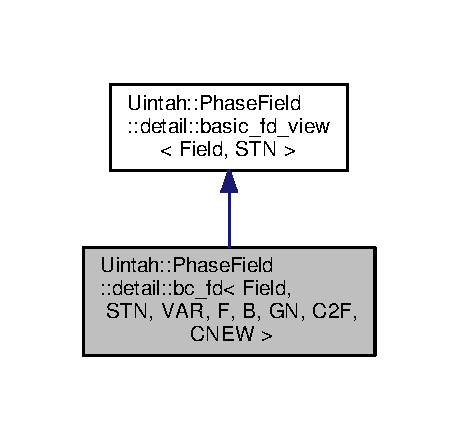
\includegraphics[width=220pt]{classUintah_1_1PhaseField_1_1detail_1_1bc__fd__inherit__graph}
\end{center}
\end{figure}


Collaboration diagram for Uintah\+:\+:Phase\+Field\+:\+:detail\+:\+:bc\+\_\+fd$<$ Field, S\+TN, V\+AR, F, B, GN, C2F, C\+N\+EW $>$\+:\nopagebreak
\begin{figure}[H]
\begin{center}
\leavevmode
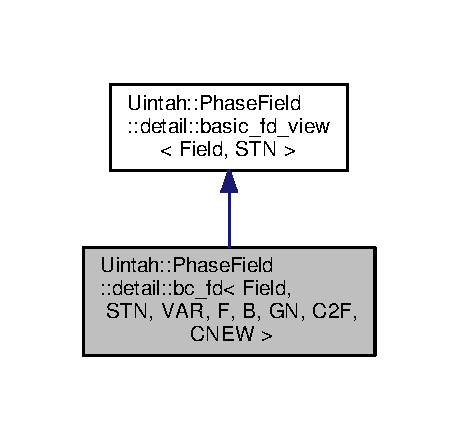
\includegraphics[width=220pt]{classUintah_1_1PhaseField_1_1detail_1_1bc__fd__coll__graph}
\end{center}
\end{figure}


\subsection{Detailed Description}
\subsubsection*{template$<$typename Field, Stn\+Type S\+TN, Var\+Type V\+AR, Patch\+::\+Face\+Type F, BC B, int GN, FC C2F = F\+C\+::\+None, bool C\+N\+EW = false$>$\newline
class Uintah\+::\+Phase\+Field\+::detail\+::bc\+\_\+fd$<$ Field, S\+T\+N, V\+A\+R, F, B, G\+N, C2\+F, C\+N\+E\+W $>$}

Abstract finite-\/differences scheme for variables at grid boundary. 

To implement a new boundary-\/condition it should be sufficient to define a new BC and code the relevant implementations of this class (for amr simulations also the corresponding \hyperlink{classUintah_1_1PhaseField_1_1detail_1_1bc__fd}{bc\+\_\+fd} implementation for fine/coarse interfaces must be provided)

$<$ Field, S\+TN $>$

\begin{DoxyRemark}{Remarks}
the method implemented in this class are ment to be called only by \hyperlink{classUintah_1_1PhaseField_1_1detail_1_1bcs__basic__fd__view}{bcs\+\_\+basic\+\_\+fd\+\_\+view} to compute bc dependent quantities only
\end{DoxyRemark}

\begin{DoxyTemplParams}{Template Parameters}
{\em Field} & type of field (\hyperlink{structUintah_1_1PhaseField_1_1ScalarField}{Scalar\+Field} $<$ T $>$ or \hyperlink{structUintah_1_1PhaseField_1_1VectorField}{Vector\+Field} $<$ T, N $>$) \\
\hline
{\em S\+TN} & finite-\/difference stencil \\
\hline
{\em F} & patch face on which bc is to be applied \\
\hline
{\em B} & type of boundary conditions \\
\hline
{\em GN} & Number of ghosts required \\
\hline
{\em C2F} & Fine/\+Coarse Interface conditions \\
\hline
{\em C\+N\+EW} & Wheter to use new datawarehouse for retrieving corse grid data \\
\hline
\end{DoxyTemplParams}


The documentation for this class was generated from the following file\+:\begin{DoxyCompactItemize}
\item 
\hyperlink{bc__fd_8h}{bc\+\_\+fd.\+h}\end{DoxyCompactItemize}

\hypertarget{classUintah_1_1PhaseField_1_1detail_1_1bc__fd_3_01ScalarField_3_01T_01_4_00_01STN_00_01CC_00_01Fa77b2fd7fb77d0a4dc6c86c68d4ea0bc}{}\section{Uintah\+:\+:Phase\+Field\+:\+:detail\+:\+:bc\+\_\+fd$<$ Scalar\+Field$<$ T $>$, S\+TN, CC, F, BC\+:\+:Dirichlet, 1 $>$ Class Template Reference}
\label{classUintah_1_1PhaseField_1_1detail_1_1bc__fd_3_01ScalarField_3_01T_01_4_00_01STN_00_01CC_00_01Fa77b2fd7fb77d0a4dc6c86c68d4ea0bc}\index{Uintah\+::\+Phase\+Field\+::detail\+::bc\+\_\+fd$<$ Scalar\+Field$<$ T $>$, S\+T\+N, C\+C, F, B\+C\+::\+Dirichlet, 1 $>$@{Uintah\+::\+Phase\+Field\+::detail\+::bc\+\_\+fd$<$ Scalar\+Field$<$ T $>$, S\+T\+N, C\+C, F, B\+C\+::\+Dirichlet, 1 $>$}}


Finite-\/differences scheme at Dirichlet boundaries interface (\hyperlink{structUintah_1_1PhaseField_1_1ScalarField}{Scalar\+Field}, Cell-\/centered, 1-\/ghost stencils implementation)  




{\ttfamily \#include $<$bc\+\_\+fd\+\_\+\+Dirichlet\+\_\+\+G1\+\_\+\+C\+C.\+h$>$}



Inheritance diagram for Uintah\+:\+:Phase\+Field\+:\+:detail\+:\+:bc\+\_\+fd$<$ Scalar\+Field$<$ T $>$, S\+TN, CC, F, BC\+:\+:Dirichlet, 1 $>$\+:\nopagebreak
\begin{figure}[H]
\begin{center}
\leavevmode
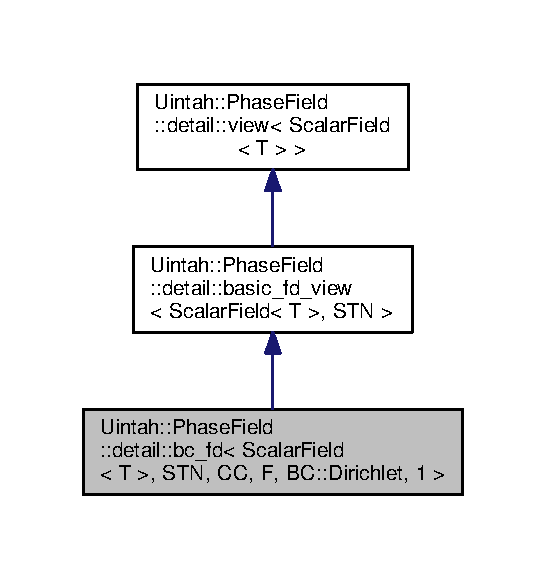
\includegraphics[width=262pt]{classUintah_1_1PhaseField_1_1detail_1_1bc__fd_3_01ScalarField_3_01T_01_4_00_01STN_00_01CC_00_01F69c852c1346d1beda70b87f87de8e083}
\end{center}
\end{figure}


Collaboration diagram for Uintah\+:\+:Phase\+Field\+:\+:detail\+:\+:bc\+\_\+fd$<$ Scalar\+Field$<$ T $>$, S\+TN, CC, F, BC\+:\+:Dirichlet, 1 $>$\+:\nopagebreak
\begin{figure}[H]
\begin{center}
\leavevmode
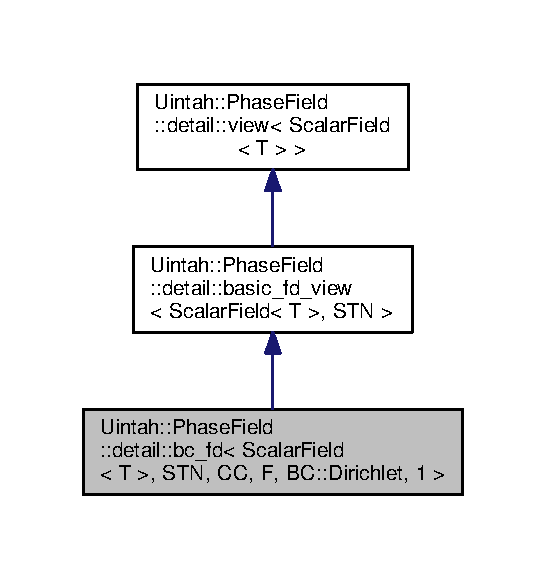
\includegraphics[width=262pt]{classUintah_1_1PhaseField_1_1detail_1_1bc__fd_3_01ScalarField_3_01T_01_4_00_01STN_00_01CC_00_01F5195a5e9bda779df4f8927144fe0fc8b}
\end{center}
\end{figure}
\subsection*{Public Member Functions}
\begin{DoxyCompactItemize}
\item 
\hyperlink{classUintah_1_1PhaseField_1_1detail_1_1bc__fd_3_01ScalarField_3_01T_01_4_00_01STN_00_01CC_00_01Fa77b2fd7fb77d0a4dc6c86c68d4ea0bc_a3eed84729f860613e68776346aab0823}{bc\+\_\+fd} (const \hyperlink{classUintah_1_1PhaseField_1_1detail_1_1view}{view}$<$ \hyperlink{structUintah_1_1PhaseField_1_1ScalarField}{Field} $>$ $\ast$\hyperlink{classUintah_1_1PhaseField_1_1detail_1_1view}{view}, const Var\+Label $\ast$label, int material, const Level $\ast$level, const V \&value)
\begin{DoxyCompactList}\small\item\em Constructor. \end{DoxyCompactList}\item 
virtual \hyperlink{classUintah_1_1PhaseField_1_1detail_1_1bc__fd_3_01ScalarField_3_01T_01_4_00_01STN_00_01CC_00_01Fa77b2fd7fb77d0a4dc6c86c68d4ea0bc_a525eeb5802602601c6b8346247814040}{$\sim$bc\+\_\+fd} ()=default
\begin{DoxyCompactList}\small\item\em Destructor. \end{DoxyCompactList}\item 
\hyperlink{classUintah_1_1PhaseField_1_1detail_1_1bc__fd_3_01ScalarField_3_01T_01_4_00_01STN_00_01CC_00_01Fa77b2fd7fb77d0a4dc6c86c68d4ea0bc_a8ffe1bfa5b1c08957e0d8884e717bdd1}{bc\+\_\+fd} (const \hyperlink{classUintah_1_1PhaseField_1_1detail_1_1bc__fd}{bc\+\_\+fd} \&)=delete
\begin{DoxyCompactList}\small\item\em Prevent copy (and move) constructor. \end{DoxyCompactList}\item 
\hyperlink{classUintah_1_1PhaseField_1_1detail_1_1bc__fd}{bc\+\_\+fd} \& \hyperlink{classUintah_1_1PhaseField_1_1detail_1_1bc__fd_3_01ScalarField_3_01T_01_4_00_01STN_00_01CC_00_01Fa77b2fd7fb77d0a4dc6c86c68d4ea0bc_abd92f471dd7440b6a1c2ea3a7b977807}{operator=} (const \hyperlink{classUintah_1_1PhaseField_1_1detail_1_1bc__fd}{bc\+\_\+fd} \&)=delete
\begin{DoxyCompactList}\small\item\em Prevent copy (and move) assignment. \end{DoxyCompactList}\item 
virtual void \hyperlink{classUintah_1_1PhaseField_1_1detail_1_1bc__fd_3_01ScalarField_3_01T_01_4_00_01STN_00_01CC_00_01Fa77b2fd7fb77d0a4dc6c86c68d4ea0bc_a871bf41d80de5acd4151631818963802}{set} (Data\+Warehouse $\ast$dw, const Patch $\ast$patch, bool use\+\_\+ghosts) override
\begin{DoxyCompactList}\small\item\em Retrieve value from the Data\+Warehouse for a given patch. \end{DoxyCompactList}\item 
virtual void \hyperlink{classUintah_1_1PhaseField_1_1detail_1_1bc__fd_3_01ScalarField_3_01T_01_4_00_01STN_00_01CC_00_01Fa77b2fd7fb77d0a4dc6c86c68d4ea0bc_ae4afb706928d60f195b00315b9458a50}{set} (Data\+Warehouse $\ast$dw, const Level $\ast$level, const Int\+Vector \&low, const Int\+Vector \&high, bool use\+\_\+ghosts) override
\begin{DoxyCompactList}\small\item\em Retrieve value from the Data\+Warehouse for a given region. \end{DoxyCompactList}\item 
virtual \hyperlink{classUintah_1_1PhaseField_1_1Support}{Support} \hyperlink{classUintah_1_1PhaseField_1_1detail_1_1bc__fd_3_01ScalarField_3_01T_01_4_00_01STN_00_01CC_00_01Fa77b2fd7fb77d0a4dc6c86c68d4ea0bc_a7cc7b8ca9e9f4663a5363f5bb9069934}{get\+\_\+support} () const override
\begin{DoxyCompactList}\small\item\em get bc view support \end{DoxyCompactList}\item 
virtual bool \hyperlink{classUintah_1_1PhaseField_1_1detail_1_1bc__fd_3_01ScalarField_3_01T_01_4_00_01STN_00_01CC_00_01Fa77b2fd7fb77d0a4dc6c86c68d4ea0bc_a247dbc32fb57a6d0c51badbb01657a9a}{is\+\_\+defined\+\_\+at} (const Int\+Vector \&id) const override
\begin{DoxyCompactList}\small\item\em Check if the view has access to the position with index id. \end{DoxyCompactList}\item 
virtual T \& \hyperlink{classUintah_1_1PhaseField_1_1detail_1_1bc__fd_3_01ScalarField_3_01T_01_4_00_01STN_00_01CC_00_01Fa77b2fd7fb77d0a4dc6c86c68d4ea0bc_a9c2ee6b6084d76371aea3008dda736e2}{operator\mbox{[}$\,$\mbox{]}} (const Int\+Vector \&id) override
\begin{DoxyCompactList}\small\item\em Get/\+Modify value at position with index id (modifications are allowed if T is non const) \end{DoxyCompactList}\item 
virtual V \hyperlink{classUintah_1_1PhaseField_1_1detail_1_1bc__fd_3_01ScalarField_3_01T_01_4_00_01STN_00_01CC_00_01Fa77b2fd7fb77d0a4dc6c86c68d4ea0bc_a83bd04bf932ebbe064ac01bae98d7227}{operator\mbox{[}$\,$\mbox{]}} (const Int\+Vector \&id) const override
\begin{DoxyCompactList}\small\item\em Get value at position. \end{DoxyCompactList}\item 
virtual \hyperlink{classUintah_1_1PhaseField_1_1detail_1_1view}{view}$<$ \hyperlink{structUintah_1_1PhaseField_1_1ScalarField}{Field} $>$ $\ast$ \hyperlink{classUintah_1_1PhaseField_1_1detail_1_1bc__fd_3_01ScalarField_3_01T_01_4_00_01STN_00_01CC_00_01Fa77b2fd7fb77d0a4dc6c86c68d4ea0bc_ab7b39dfca20ca18356b1a72ae055e99f}{get\+\_\+view} () override
\begin{DoxyCompactList}\small\item\em Get base view (Virtual \hyperlink{classUintah_1_1PhaseField_1_1Implementation}{Implementation}) \end{DoxyCompactList}\item 
const \hyperlink{classUintah_1_1PhaseField_1_1detail_1_1view}{view}$<$ \hyperlink{structUintah_1_1PhaseField_1_1ScalarField}{Field} $>$ $\ast$ \hyperlink{classUintah_1_1PhaseField_1_1detail_1_1bc__fd_3_01ScalarField_3_01T_01_4_00_01STN_00_01CC_00_01Fa77b2fd7fb77d0a4dc6c86c68d4ea0bc_a2199408e573e0a6f2cd86bb7fbd002a7}{get\+\_\+view} () const override
\begin{DoxyCompactList}\small\item\em Get base view. \end{DoxyCompactList}\item 
{\footnotesize template$<$Dir\+Type D\+IR$>$ }\\std\+::enable\+\_\+if$<$ D !=D\+IR, T $>$\+::type \hyperlink{classUintah_1_1PhaseField_1_1detail_1_1bc__fd_3_01ScalarField_3_01T_01_4_00_01STN_00_01CC_00_01Fa77b2fd7fb77d0a4dc6c86c68d4ea0bc_af5f6c1e347ff1106dd15643c8346fe46}{d} (const Int\+Vector \&id) const
\begin{DoxyCompactList}\small\item\em First order derivative (parallel direction implementation) \end{DoxyCompactList}\item 
{\footnotesize template$<$Dir\+Type D\+IR$>$ }\\std\+::enable\+\_\+if$<$ D==D\+IR, T $>$\+::type \hyperlink{classUintah_1_1PhaseField_1_1detail_1_1bc__fd_3_01ScalarField_3_01T_01_4_00_01STN_00_01CC_00_01Fa77b2fd7fb77d0a4dc6c86c68d4ea0bc_a139958f277e857c56d230179e31e4246}{d} (const Int\+Vector \&id) const
\begin{DoxyCompactList}\small\item\em First order derivative (normal direction implementation) \end{DoxyCompactList}\item 
{\footnotesize template$<$Dir\+Type D\+IR$>$ }\\std\+::enable\+\_\+if$<$ D !=D\+IR, T $>$\+::type \hyperlink{classUintah_1_1PhaseField_1_1detail_1_1bc__fd_3_01ScalarField_3_01T_01_4_00_01STN_00_01CC_00_01Fa77b2fd7fb77d0a4dc6c86c68d4ea0bc_a84837d53271498e1194195453376d465}{d2} (const Int\+Vector \&id) const
\begin{DoxyCompactList}\small\item\em Second order derivative (parallel direction implementation) \end{DoxyCompactList}\item 
{\footnotesize template$<$Dir\+Type D\+IR$>$ }\\std\+::enable\+\_\+if$<$ D==D\+IR, T $>$\+::type \hyperlink{classUintah_1_1PhaseField_1_1detail_1_1bc__fd_3_01ScalarField_3_01T_01_4_00_01STN_00_01CC_00_01Fa77b2fd7fb77d0a4dc6c86c68d4ea0bc_a00852e794ce39ec2ec62f2b836cbaeb4}{d2} (const Int\+Vector \&id) const
\begin{DoxyCompactList}\small\item\em Second order derivative (normal direction implementation) \end{DoxyCompactList}\end{DoxyCompactItemize}
\subsection*{Protected Member Functions}
\begin{DoxyCompactItemize}
\item 
\hyperlink{classUintah_1_1PhaseField_1_1detail_1_1bc__fd_3_01ScalarField_3_01T_01_4_00_01STN_00_01CC_00_01Fa77b2fd7fb77d0a4dc6c86c68d4ea0bc_ae9f84f9d7e72f56a8d07e48e72b947d4}{bc\+\_\+fd} (const \hyperlink{classUintah_1_1PhaseField_1_1detail_1_1bc__fd}{bc\+\_\+fd} $\ast$copy, bool deep)
\begin{DoxyCompactList}\small\item\em Constructor. \end{DoxyCompactList}\end{DoxyCompactItemize}
\subsection*{Additional Inherited Members}


\subsection{Detailed Description}
\subsubsection*{template$<$typename T, Stn\+Type S\+TN, Patch\+::\+Face\+Type F$>$\newline
class Uintah\+::\+Phase\+Field\+::detail\+::bc\+\_\+fd$<$ Scalar\+Field$<$ T $>$, S\+T\+N, C\+C, F, B\+C\+::\+Dirichlet, 1 $>$}

Finite-\/differences scheme at Dirichlet boundaries interface (\hyperlink{structUintah_1_1PhaseField_1_1ScalarField}{Scalar\+Field}, Cell-\/centered, 1-\/ghost stencils implementation) 

approximation of ghost value across Dirichlet boundaries


\begin{DoxyTemplParams}{Template Parameters}
{\em T} & type of the field value at each point \\
\hline
{\em S\+TN} & finite-\/difference stencil \\
\hline
{\em F} & patch face on which bc is to be applied \\
\hline
\end{DoxyTemplParams}


\subsection{Constructor \& Destructor Documentation}
\mbox{\Hypertarget{classUintah_1_1PhaseField_1_1detail_1_1bc__fd_3_01ScalarField_3_01T_01_4_00_01STN_00_01CC_00_01Fa77b2fd7fb77d0a4dc6c86c68d4ea0bc_ae9f84f9d7e72f56a8d07e48e72b947d4}\label{classUintah_1_1PhaseField_1_1detail_1_1bc__fd_3_01ScalarField_3_01T_01_4_00_01STN_00_01CC_00_01Fa77b2fd7fb77d0a4dc6c86c68d4ea0bc_ae9f84f9d7e72f56a8d07e48e72b947d4}} 
\index{Uintah\+::\+Phase\+Field\+::detail\+::bc\+\_\+fd$<$ Scalar\+Field$<$ T $>$, S\+T\+N, C\+C, F, B\+C\+::\+Dirichlet, 1 $>$@{Uintah\+::\+Phase\+Field\+::detail\+::bc\+\_\+fd$<$ Scalar\+Field$<$ T $>$, S\+T\+N, C\+C, F, B\+C\+::\+Dirichlet, 1 $>$}!bc\+\_\+fd@{bc\+\_\+fd}}
\index{bc\+\_\+fd@{bc\+\_\+fd}!Uintah\+::\+Phase\+Field\+::detail\+::bc\+\_\+fd$<$ Scalar\+Field$<$ T $>$, S\+T\+N, C\+C, F, B\+C\+::\+Dirichlet, 1 $>$@{Uintah\+::\+Phase\+Field\+::detail\+::bc\+\_\+fd$<$ Scalar\+Field$<$ T $>$, S\+T\+N, C\+C, F, B\+C\+::\+Dirichlet, 1 $>$}}
\subsubsection{\texorpdfstring{bc\+\_\+fd()}{bc\_fd()}\hspace{0.1cm}{\footnotesize\ttfamily [1/3]}}
{\footnotesize\ttfamily template$<$typename T , Stn\+Type S\+TN, Patch\+::\+Face\+Type F$>$ \\
\hyperlink{classUintah_1_1PhaseField_1_1detail_1_1bc__fd}{Uintah\+::\+Phase\+Field\+::detail\+::bc\+\_\+fd}$<$ \hyperlink{structUintah_1_1PhaseField_1_1ScalarField}{Scalar\+Field}$<$ T $>$, S\+TN, \hyperlink{namespaceUintah_1_1PhaseField_a33d355affda78a83f45755ba8388cedda22303704507d024d1d6508ed9859a85a}{CC}, F, \hyperlink{namespaceUintah_1_1PhaseField_a148fba372aa3be96fd6eede7a2fa10b5abac152b762896edff34ed668ae1a546f}{B\+C\+::\+Dirichlet}, 1 $>$\+::\hyperlink{classUintah_1_1PhaseField_1_1detail_1_1bc__fd}{bc\+\_\+fd} (\begin{DoxyParamCaption}\item[{const \hyperlink{classUintah_1_1PhaseField_1_1detail_1_1bc__fd}{bc\+\_\+fd}$<$ \hyperlink{structUintah_1_1PhaseField_1_1ScalarField}{Scalar\+Field}$<$ T $>$, S\+TN, \hyperlink{namespaceUintah_1_1PhaseField_a33d355affda78a83f45755ba8388cedda22303704507d024d1d6508ed9859a85a}{CC}, F, \hyperlink{namespaceUintah_1_1PhaseField_a148fba372aa3be96fd6eede7a2fa10b5abac152b762896edff34ed668ae1a546f}{B\+C\+::\+Dirichlet}, 1 $>$ $\ast$}]{copy,  }\item[{bool}]{deep }\end{DoxyParamCaption})\hspace{0.3cm}{\ttfamily [inline]}, {\ttfamily [protected]}}



Constructor. 

Instantiate a copy of a given view


\begin{DoxyParams}{Parameters}
{\em copy} & source view for copying \\
\hline
{\em deep} & if true inner grid variable is copied as well otherwise the same grid variable is referenced \\
\hline
\end{DoxyParams}
\mbox{\Hypertarget{classUintah_1_1PhaseField_1_1detail_1_1bc__fd_3_01ScalarField_3_01T_01_4_00_01STN_00_01CC_00_01Fa77b2fd7fb77d0a4dc6c86c68d4ea0bc_a3eed84729f860613e68776346aab0823}\label{classUintah_1_1PhaseField_1_1detail_1_1bc__fd_3_01ScalarField_3_01T_01_4_00_01STN_00_01CC_00_01Fa77b2fd7fb77d0a4dc6c86c68d4ea0bc_a3eed84729f860613e68776346aab0823}} 
\index{Uintah\+::\+Phase\+Field\+::detail\+::bc\+\_\+fd$<$ Scalar\+Field$<$ T $>$, S\+T\+N, C\+C, F, B\+C\+::\+Dirichlet, 1 $>$@{Uintah\+::\+Phase\+Field\+::detail\+::bc\+\_\+fd$<$ Scalar\+Field$<$ T $>$, S\+T\+N, C\+C, F, B\+C\+::\+Dirichlet, 1 $>$}!bc\+\_\+fd@{bc\+\_\+fd}}
\index{bc\+\_\+fd@{bc\+\_\+fd}!Uintah\+::\+Phase\+Field\+::detail\+::bc\+\_\+fd$<$ Scalar\+Field$<$ T $>$, S\+T\+N, C\+C, F, B\+C\+::\+Dirichlet, 1 $>$@{Uintah\+::\+Phase\+Field\+::detail\+::bc\+\_\+fd$<$ Scalar\+Field$<$ T $>$, S\+T\+N, C\+C, F, B\+C\+::\+Dirichlet, 1 $>$}}
\subsubsection{\texorpdfstring{bc\+\_\+fd()}{bc\_fd()}\hspace{0.1cm}{\footnotesize\ttfamily [2/3]}}
{\footnotesize\ttfamily template$<$typename T , Stn\+Type S\+TN, Patch\+::\+Face\+Type F$>$ \\
\hyperlink{classUintah_1_1PhaseField_1_1detail_1_1bc__fd}{Uintah\+::\+Phase\+Field\+::detail\+::bc\+\_\+fd}$<$ \hyperlink{structUintah_1_1PhaseField_1_1ScalarField}{Scalar\+Field}$<$ T $>$, S\+TN, \hyperlink{namespaceUintah_1_1PhaseField_a33d355affda78a83f45755ba8388cedda22303704507d024d1d6508ed9859a85a}{CC}, F, \hyperlink{namespaceUintah_1_1PhaseField_a148fba372aa3be96fd6eede7a2fa10b5abac152b762896edff34ed668ae1a546f}{B\+C\+::\+Dirichlet}, 1 $>$\+::\hyperlink{classUintah_1_1PhaseField_1_1detail_1_1bc__fd}{bc\+\_\+fd} (\begin{DoxyParamCaption}\item[{const \hyperlink{classUintah_1_1PhaseField_1_1detail_1_1view}{view}$<$ \hyperlink{structUintah_1_1PhaseField_1_1ScalarField}{Field} $>$ $\ast$}]{view,  }\item[{const Var\+Label $\ast$}]{label,  }\item[{int}]{material,  }\item[{const Level $\ast$}]{level,  }\item[{const V \&}]{value }\end{DoxyParamCaption})\hspace{0.3cm}{\ttfamily [inline]}}



Constructor. 

Instantiate a view without gathering info from the Data\+Warehouse


\begin{DoxyParams}{Parameters}
{\em view} & view to access grid values \\
\hline
{\em label} & unused since value is already in view \\
\hline
{\em material} & unused since value is already in view \\
\hline
{\em level} & fine grid level \\
\hline
{\em value} & imposed value at boundary \\
\hline
\end{DoxyParams}
\mbox{\Hypertarget{classUintah_1_1PhaseField_1_1detail_1_1bc__fd_3_01ScalarField_3_01T_01_4_00_01STN_00_01CC_00_01Fa77b2fd7fb77d0a4dc6c86c68d4ea0bc_a525eeb5802602601c6b8346247814040}\label{classUintah_1_1PhaseField_1_1detail_1_1bc__fd_3_01ScalarField_3_01T_01_4_00_01STN_00_01CC_00_01Fa77b2fd7fb77d0a4dc6c86c68d4ea0bc_a525eeb5802602601c6b8346247814040}} 
\index{Uintah\+::\+Phase\+Field\+::detail\+::bc\+\_\+fd$<$ Scalar\+Field$<$ T $>$, S\+T\+N, C\+C, F, B\+C\+::\+Dirichlet, 1 $>$@{Uintah\+::\+Phase\+Field\+::detail\+::bc\+\_\+fd$<$ Scalar\+Field$<$ T $>$, S\+T\+N, C\+C, F, B\+C\+::\+Dirichlet, 1 $>$}!````~bc\+\_\+fd@{$\sim$bc\+\_\+fd}}
\index{````~bc\+\_\+fd@{$\sim$bc\+\_\+fd}!Uintah\+::\+Phase\+Field\+::detail\+::bc\+\_\+fd$<$ Scalar\+Field$<$ T $>$, S\+T\+N, C\+C, F, B\+C\+::\+Dirichlet, 1 $>$@{Uintah\+::\+Phase\+Field\+::detail\+::bc\+\_\+fd$<$ Scalar\+Field$<$ T $>$, S\+T\+N, C\+C, F, B\+C\+::\+Dirichlet, 1 $>$}}
\subsubsection{\texorpdfstring{$\sim$bc\+\_\+fd()}{~bc\_fd()}}
{\footnotesize\ttfamily template$<$typename T , Stn\+Type S\+TN, Patch\+::\+Face\+Type F$>$ \\
virtual \hyperlink{classUintah_1_1PhaseField_1_1detail_1_1bc__fd}{Uintah\+::\+Phase\+Field\+::detail\+::bc\+\_\+fd}$<$ \hyperlink{structUintah_1_1PhaseField_1_1ScalarField}{Scalar\+Field}$<$ T $>$, S\+TN, \hyperlink{namespaceUintah_1_1PhaseField_a33d355affda78a83f45755ba8388cedda22303704507d024d1d6508ed9859a85a}{CC}, F, \hyperlink{namespaceUintah_1_1PhaseField_a148fba372aa3be96fd6eede7a2fa10b5abac152b762896edff34ed668ae1a546f}{B\+C\+::\+Dirichlet}, 1 $>$\+::$\sim$\hyperlink{classUintah_1_1PhaseField_1_1detail_1_1bc__fd}{bc\+\_\+fd} (\begin{DoxyParamCaption}{ }\end{DoxyParamCaption})\hspace{0.3cm}{\ttfamily [virtual]}, {\ttfamily [default]}}



Destructor. 

\mbox{\Hypertarget{classUintah_1_1PhaseField_1_1detail_1_1bc__fd_3_01ScalarField_3_01T_01_4_00_01STN_00_01CC_00_01Fa77b2fd7fb77d0a4dc6c86c68d4ea0bc_a8ffe1bfa5b1c08957e0d8884e717bdd1}\label{classUintah_1_1PhaseField_1_1detail_1_1bc__fd_3_01ScalarField_3_01T_01_4_00_01STN_00_01CC_00_01Fa77b2fd7fb77d0a4dc6c86c68d4ea0bc_a8ffe1bfa5b1c08957e0d8884e717bdd1}} 
\index{Uintah\+::\+Phase\+Field\+::detail\+::bc\+\_\+fd$<$ Scalar\+Field$<$ T $>$, S\+T\+N, C\+C, F, B\+C\+::\+Dirichlet, 1 $>$@{Uintah\+::\+Phase\+Field\+::detail\+::bc\+\_\+fd$<$ Scalar\+Field$<$ T $>$, S\+T\+N, C\+C, F, B\+C\+::\+Dirichlet, 1 $>$}!bc\+\_\+fd@{bc\+\_\+fd}}
\index{bc\+\_\+fd@{bc\+\_\+fd}!Uintah\+::\+Phase\+Field\+::detail\+::bc\+\_\+fd$<$ Scalar\+Field$<$ T $>$, S\+T\+N, C\+C, F, B\+C\+::\+Dirichlet, 1 $>$@{Uintah\+::\+Phase\+Field\+::detail\+::bc\+\_\+fd$<$ Scalar\+Field$<$ T $>$, S\+T\+N, C\+C, F, B\+C\+::\+Dirichlet, 1 $>$}}
\subsubsection{\texorpdfstring{bc\+\_\+fd()}{bc\_fd()}\hspace{0.1cm}{\footnotesize\ttfamily [3/3]}}
{\footnotesize\ttfamily template$<$typename T , Stn\+Type S\+TN, Patch\+::\+Face\+Type F$>$ \\
\hyperlink{classUintah_1_1PhaseField_1_1detail_1_1bc__fd}{Uintah\+::\+Phase\+Field\+::detail\+::bc\+\_\+fd}$<$ \hyperlink{structUintah_1_1PhaseField_1_1ScalarField}{Scalar\+Field}$<$ T $>$, S\+TN, \hyperlink{namespaceUintah_1_1PhaseField_a33d355affda78a83f45755ba8388cedda22303704507d024d1d6508ed9859a85a}{CC}, F, \hyperlink{namespaceUintah_1_1PhaseField_a148fba372aa3be96fd6eede7a2fa10b5abac152b762896edff34ed668ae1a546f}{B\+C\+::\+Dirichlet}, 1 $>$\+::\hyperlink{classUintah_1_1PhaseField_1_1detail_1_1bc__fd}{bc\+\_\+fd} (\begin{DoxyParamCaption}\item[{const \hyperlink{classUintah_1_1PhaseField_1_1detail_1_1bc__fd}{bc\+\_\+fd}$<$ \hyperlink{structUintah_1_1PhaseField_1_1ScalarField}{Scalar\+Field}$<$ T $>$, S\+TN, \hyperlink{namespaceUintah_1_1PhaseField_a33d355affda78a83f45755ba8388cedda22303704507d024d1d6508ed9859a85a}{CC}, F, \hyperlink{namespaceUintah_1_1PhaseField_a148fba372aa3be96fd6eede7a2fa10b5abac152b762896edff34ed668ae1a546f}{B\+C\+::\+Dirichlet}, 1 $>$ \&}]{ }\end{DoxyParamCaption})\hspace{0.3cm}{\ttfamily [delete]}}



Prevent copy (and move) constructor. 



\subsection{Member Function Documentation}
\mbox{\Hypertarget{classUintah_1_1PhaseField_1_1detail_1_1bc__fd_3_01ScalarField_3_01T_01_4_00_01STN_00_01CC_00_01Fa77b2fd7fb77d0a4dc6c86c68d4ea0bc_af5f6c1e347ff1106dd15643c8346fe46}\label{classUintah_1_1PhaseField_1_1detail_1_1bc__fd_3_01ScalarField_3_01T_01_4_00_01STN_00_01CC_00_01Fa77b2fd7fb77d0a4dc6c86c68d4ea0bc_af5f6c1e347ff1106dd15643c8346fe46}} 
\index{Uintah\+::\+Phase\+Field\+::detail\+::bc\+\_\+fd$<$ Scalar\+Field$<$ T $>$, S\+T\+N, C\+C, F, B\+C\+::\+Dirichlet, 1 $>$@{Uintah\+::\+Phase\+Field\+::detail\+::bc\+\_\+fd$<$ Scalar\+Field$<$ T $>$, S\+T\+N, C\+C, F, B\+C\+::\+Dirichlet, 1 $>$}!d@{d}}
\index{d@{d}!Uintah\+::\+Phase\+Field\+::detail\+::bc\+\_\+fd$<$ Scalar\+Field$<$ T $>$, S\+T\+N, C\+C, F, B\+C\+::\+Dirichlet, 1 $>$@{Uintah\+::\+Phase\+Field\+::detail\+::bc\+\_\+fd$<$ Scalar\+Field$<$ T $>$, S\+T\+N, C\+C, F, B\+C\+::\+Dirichlet, 1 $>$}}
\subsubsection{\texorpdfstring{d()}{d()}\hspace{0.1cm}{\footnotesize\ttfamily [1/2]}}
{\footnotesize\ttfamily template$<$typename T , Stn\+Type S\+TN, Patch\+::\+Face\+Type F$>$ \\
template$<$Dir\+Type D\+IR$>$ \\
std\+::enable\+\_\+if$<$ D != D\+IR, T $>$\+::type \hyperlink{classUintah_1_1PhaseField_1_1detail_1_1bc__fd}{Uintah\+::\+Phase\+Field\+::detail\+::bc\+\_\+fd}$<$ \hyperlink{structUintah_1_1PhaseField_1_1ScalarField}{Scalar\+Field}$<$ T $>$, S\+TN, \hyperlink{namespaceUintah_1_1PhaseField_a33d355affda78a83f45755ba8388cedda22303704507d024d1d6508ed9859a85a}{CC}, F, \hyperlink{namespaceUintah_1_1PhaseField_a148fba372aa3be96fd6eede7a2fa10b5abac152b762896edff34ed668ae1a546f}{B\+C\+::\+Dirichlet}, 1 $>$\+::d (\begin{DoxyParamCaption}\item[{const Int\+Vector \&}]{id }\end{DoxyParamCaption}) const\hspace{0.3cm}{\ttfamily [inline]}}



First order derivative (parallel direction implementation) 

First order derivative along D\+IR at index id at boundary interface

\begin{DoxyRemark}{Remarks}
derivative parallel to the face should not be computed by this \hyperlink{classUintah_1_1PhaseField_1_1detail_1_1bc__fd}{bc\+\_\+fd}
\end{DoxyRemark}

\begin{DoxyTemplParams}{Template Parameters}
{\em D\+IR} & Direction along with derivative is approximated \\
\hline
\end{DoxyTemplParams}

\begin{DoxyParams}{Parameters}
{\em id} & unused \\
\hline
\end{DoxyParams}
\begin{DoxyReturn}{Returns}
nothing 
\end{DoxyReturn}
\mbox{\Hypertarget{classUintah_1_1PhaseField_1_1detail_1_1bc__fd_3_01ScalarField_3_01T_01_4_00_01STN_00_01CC_00_01Fa77b2fd7fb77d0a4dc6c86c68d4ea0bc_a139958f277e857c56d230179e31e4246}\label{classUintah_1_1PhaseField_1_1detail_1_1bc__fd_3_01ScalarField_3_01T_01_4_00_01STN_00_01CC_00_01Fa77b2fd7fb77d0a4dc6c86c68d4ea0bc_a139958f277e857c56d230179e31e4246}} 
\index{Uintah\+::\+Phase\+Field\+::detail\+::bc\+\_\+fd$<$ Scalar\+Field$<$ T $>$, S\+T\+N, C\+C, F, B\+C\+::\+Dirichlet, 1 $>$@{Uintah\+::\+Phase\+Field\+::detail\+::bc\+\_\+fd$<$ Scalar\+Field$<$ T $>$, S\+T\+N, C\+C, F, B\+C\+::\+Dirichlet, 1 $>$}!d@{d}}
\index{d@{d}!Uintah\+::\+Phase\+Field\+::detail\+::bc\+\_\+fd$<$ Scalar\+Field$<$ T $>$, S\+T\+N, C\+C, F, B\+C\+::\+Dirichlet, 1 $>$@{Uintah\+::\+Phase\+Field\+::detail\+::bc\+\_\+fd$<$ Scalar\+Field$<$ T $>$, S\+T\+N, C\+C, F, B\+C\+::\+Dirichlet, 1 $>$}}
\subsubsection{\texorpdfstring{d()}{d()}\hspace{0.1cm}{\footnotesize\ttfamily [2/2]}}
{\footnotesize\ttfamily template$<$typename T , Stn\+Type S\+TN, Patch\+::\+Face\+Type F$>$ \\
template$<$Dir\+Type D\+IR$>$ \\
std\+::enable\+\_\+if$<$ D == D\+IR, T $>$\+::type \hyperlink{classUintah_1_1PhaseField_1_1detail_1_1bc__fd}{Uintah\+::\+Phase\+Field\+::detail\+::bc\+\_\+fd}$<$ \hyperlink{structUintah_1_1PhaseField_1_1ScalarField}{Scalar\+Field}$<$ T $>$, S\+TN, \hyperlink{namespaceUintah_1_1PhaseField_a33d355affda78a83f45755ba8388cedda22303704507d024d1d6508ed9859a85a}{CC}, F, \hyperlink{namespaceUintah_1_1PhaseField_a148fba372aa3be96fd6eede7a2fa10b5abac152b762896edff34ed668ae1a546f}{B\+C\+::\+Dirichlet}, 1 $>$\+::d (\begin{DoxyParamCaption}\item[{const Int\+Vector \&}]{id }\end{DoxyParamCaption}) const\hspace{0.3cm}{\ttfamily [inline]}}



First order derivative (normal direction implementation) 

First order derivative along D\+IR at index id at boundary interface \begin{DoxyRemark}{Remarks}
Dirichlet condition is applied to cell edge
\end{DoxyRemark}

\begin{DoxyTemplParams}{Template Parameters}
{\em D\+IR} & Direction along with derivative is approximated \\
\hline
\end{DoxyTemplParams}

\begin{DoxyParams}{Parameters}
{\em id} & index where to evaluate the finite-\/difference \\
\hline
\end{DoxyParams}
\begin{DoxyReturn}{Returns}
approximated value at id 
\end{DoxyReturn}
\mbox{\Hypertarget{classUintah_1_1PhaseField_1_1detail_1_1bc__fd_3_01ScalarField_3_01T_01_4_00_01STN_00_01CC_00_01Fa77b2fd7fb77d0a4dc6c86c68d4ea0bc_a84837d53271498e1194195453376d465}\label{classUintah_1_1PhaseField_1_1detail_1_1bc__fd_3_01ScalarField_3_01T_01_4_00_01STN_00_01CC_00_01Fa77b2fd7fb77d0a4dc6c86c68d4ea0bc_a84837d53271498e1194195453376d465}} 
\index{Uintah\+::\+Phase\+Field\+::detail\+::bc\+\_\+fd$<$ Scalar\+Field$<$ T $>$, S\+T\+N, C\+C, F, B\+C\+::\+Dirichlet, 1 $>$@{Uintah\+::\+Phase\+Field\+::detail\+::bc\+\_\+fd$<$ Scalar\+Field$<$ T $>$, S\+T\+N, C\+C, F, B\+C\+::\+Dirichlet, 1 $>$}!d2@{d2}}
\index{d2@{d2}!Uintah\+::\+Phase\+Field\+::detail\+::bc\+\_\+fd$<$ Scalar\+Field$<$ T $>$, S\+T\+N, C\+C, F, B\+C\+::\+Dirichlet, 1 $>$@{Uintah\+::\+Phase\+Field\+::detail\+::bc\+\_\+fd$<$ Scalar\+Field$<$ T $>$, S\+T\+N, C\+C, F, B\+C\+::\+Dirichlet, 1 $>$}}
\subsubsection{\texorpdfstring{d2()}{d2()}\hspace{0.1cm}{\footnotesize\ttfamily [1/2]}}
{\footnotesize\ttfamily template$<$typename T , Stn\+Type S\+TN, Patch\+::\+Face\+Type F$>$ \\
template$<$Dir\+Type D\+IR$>$ \\
std\+::enable\+\_\+if$<$ D != D\+IR, T $>$\+::type \hyperlink{classUintah_1_1PhaseField_1_1detail_1_1bc__fd}{Uintah\+::\+Phase\+Field\+::detail\+::bc\+\_\+fd}$<$ \hyperlink{structUintah_1_1PhaseField_1_1ScalarField}{Scalar\+Field}$<$ T $>$, S\+TN, \hyperlink{namespaceUintah_1_1PhaseField_a33d355affda78a83f45755ba8388cedda22303704507d024d1d6508ed9859a85a}{CC}, F, \hyperlink{namespaceUintah_1_1PhaseField_a148fba372aa3be96fd6eede7a2fa10b5abac152b762896edff34ed668ae1a546f}{B\+C\+::\+Dirichlet}, 1 $>$\+::d2 (\begin{DoxyParamCaption}\item[{const Int\+Vector \&}]{id }\end{DoxyParamCaption}) const\hspace{0.3cm}{\ttfamily [inline]}}



Second order derivative (parallel direction implementation) 

Second order derivative along D\+IR at index id at boundary interface

\begin{DoxyRemark}{Remarks}
derivative parallel to the face should not be computed by this \hyperlink{classUintah_1_1PhaseField_1_1detail_1_1bc__fd}{bc\+\_\+fd}
\end{DoxyRemark}

\begin{DoxyTemplParams}{Template Parameters}
{\em D\+IR} & Direction along with derivative is approximated \\
\hline
\end{DoxyTemplParams}

\begin{DoxyParams}{Parameters}
{\em id} & unused \\
\hline
\end{DoxyParams}
\begin{DoxyReturn}{Returns}
nothing 
\end{DoxyReturn}
\mbox{\Hypertarget{classUintah_1_1PhaseField_1_1detail_1_1bc__fd_3_01ScalarField_3_01T_01_4_00_01STN_00_01CC_00_01Fa77b2fd7fb77d0a4dc6c86c68d4ea0bc_a00852e794ce39ec2ec62f2b836cbaeb4}\label{classUintah_1_1PhaseField_1_1detail_1_1bc__fd_3_01ScalarField_3_01T_01_4_00_01STN_00_01CC_00_01Fa77b2fd7fb77d0a4dc6c86c68d4ea0bc_a00852e794ce39ec2ec62f2b836cbaeb4}} 
\index{Uintah\+::\+Phase\+Field\+::detail\+::bc\+\_\+fd$<$ Scalar\+Field$<$ T $>$, S\+T\+N, C\+C, F, B\+C\+::\+Dirichlet, 1 $>$@{Uintah\+::\+Phase\+Field\+::detail\+::bc\+\_\+fd$<$ Scalar\+Field$<$ T $>$, S\+T\+N, C\+C, F, B\+C\+::\+Dirichlet, 1 $>$}!d2@{d2}}
\index{d2@{d2}!Uintah\+::\+Phase\+Field\+::detail\+::bc\+\_\+fd$<$ Scalar\+Field$<$ T $>$, S\+T\+N, C\+C, F, B\+C\+::\+Dirichlet, 1 $>$@{Uintah\+::\+Phase\+Field\+::detail\+::bc\+\_\+fd$<$ Scalar\+Field$<$ T $>$, S\+T\+N, C\+C, F, B\+C\+::\+Dirichlet, 1 $>$}}
\subsubsection{\texorpdfstring{d2()}{d2()}\hspace{0.1cm}{\footnotesize\ttfamily [2/2]}}
{\footnotesize\ttfamily template$<$typename T , Stn\+Type S\+TN, Patch\+::\+Face\+Type F$>$ \\
template$<$Dir\+Type D\+IR$>$ \\
std\+::enable\+\_\+if$<$ D == D\+IR, T $>$\+::type \hyperlink{classUintah_1_1PhaseField_1_1detail_1_1bc__fd}{Uintah\+::\+Phase\+Field\+::detail\+::bc\+\_\+fd}$<$ \hyperlink{structUintah_1_1PhaseField_1_1ScalarField}{Scalar\+Field}$<$ T $>$, S\+TN, \hyperlink{namespaceUintah_1_1PhaseField_a33d355affda78a83f45755ba8388cedda22303704507d024d1d6508ed9859a85a}{CC}, F, \hyperlink{namespaceUintah_1_1PhaseField_a148fba372aa3be96fd6eede7a2fa10b5abac152b762896edff34ed668ae1a546f}{B\+C\+::\+Dirichlet}, 1 $>$\+::d2 (\begin{DoxyParamCaption}\item[{const Int\+Vector \&}]{id }\end{DoxyParamCaption}) const\hspace{0.3cm}{\ttfamily [inline]}}



Second order derivative (normal direction implementation) 

Second order derivative along D\+IR at index id at boundary interface


\begin{DoxyTemplParams}{Template Parameters}
{\em D\+IR} & Direction along with derivative is approximated \\
\hline
\end{DoxyTemplParams}

\begin{DoxyParams}{Parameters}
{\em id} & index where to evaluate the finite-\/difference \\
\hline
\end{DoxyParams}
\begin{DoxyReturn}{Returns}
approximated value at id 
\end{DoxyReturn}
\mbox{\Hypertarget{classUintah_1_1PhaseField_1_1detail_1_1bc__fd_3_01ScalarField_3_01T_01_4_00_01STN_00_01CC_00_01Fa77b2fd7fb77d0a4dc6c86c68d4ea0bc_a7cc7b8ca9e9f4663a5363f5bb9069934}\label{classUintah_1_1PhaseField_1_1detail_1_1bc__fd_3_01ScalarField_3_01T_01_4_00_01STN_00_01CC_00_01Fa77b2fd7fb77d0a4dc6c86c68d4ea0bc_a7cc7b8ca9e9f4663a5363f5bb9069934}} 
\index{Uintah\+::\+Phase\+Field\+::detail\+::bc\+\_\+fd$<$ Scalar\+Field$<$ T $>$, S\+T\+N, C\+C, F, B\+C\+::\+Dirichlet, 1 $>$@{Uintah\+::\+Phase\+Field\+::detail\+::bc\+\_\+fd$<$ Scalar\+Field$<$ T $>$, S\+T\+N, C\+C, F, B\+C\+::\+Dirichlet, 1 $>$}!get\+\_\+support@{get\+\_\+support}}
\index{get\+\_\+support@{get\+\_\+support}!Uintah\+::\+Phase\+Field\+::detail\+::bc\+\_\+fd$<$ Scalar\+Field$<$ T $>$, S\+T\+N, C\+C, F, B\+C\+::\+Dirichlet, 1 $>$@{Uintah\+::\+Phase\+Field\+::detail\+::bc\+\_\+fd$<$ Scalar\+Field$<$ T $>$, S\+T\+N, C\+C, F, B\+C\+::\+Dirichlet, 1 $>$}}
\subsubsection{\texorpdfstring{get\+\_\+support()}{get\_support()}}
{\footnotesize\ttfamily template$<$typename T , Stn\+Type S\+TN, Patch\+::\+Face\+Type F$>$ \\
virtual \hyperlink{classUintah_1_1PhaseField_1_1Support}{Support} \hyperlink{classUintah_1_1PhaseField_1_1detail_1_1bc__fd}{Uintah\+::\+Phase\+Field\+::detail\+::bc\+\_\+fd}$<$ \hyperlink{structUintah_1_1PhaseField_1_1ScalarField}{Scalar\+Field}$<$ T $>$, S\+TN, \hyperlink{namespaceUintah_1_1PhaseField_a33d355affda78a83f45755ba8388cedda22303704507d024d1d6508ed9859a85a}{CC}, F, \hyperlink{namespaceUintah_1_1PhaseField_a148fba372aa3be96fd6eede7a2fa10b5abac152b762896edff34ed668ae1a546f}{B\+C\+::\+Dirichlet}, 1 $>$\+::get\+\_\+support (\begin{DoxyParamCaption}{ }\end{DoxyParamCaption}) const\hspace{0.3cm}{\ttfamily [inline]}, {\ttfamily [override]}, {\ttfamily [virtual]}}



get bc view support 

we want to extend this to ghost cells/nodes

\begin{DoxyReturn}{Returns}
support of the view 
\end{DoxyReturn}


Implements \hyperlink{classUintah_1_1PhaseField_1_1detail_1_1view_3_01ScalarField_3_01T_01_4_01_4_a3e14b0c7a57a57707bb33954861ab1c1}{Uintah\+::\+Phase\+Field\+::detail\+::view$<$ Scalar\+Field$<$ T $>$ $>$}.

\mbox{\Hypertarget{classUintah_1_1PhaseField_1_1detail_1_1bc__fd_3_01ScalarField_3_01T_01_4_00_01STN_00_01CC_00_01Fa77b2fd7fb77d0a4dc6c86c68d4ea0bc_ab7b39dfca20ca18356b1a72ae055e99f}\label{classUintah_1_1PhaseField_1_1detail_1_1bc__fd_3_01ScalarField_3_01T_01_4_00_01STN_00_01CC_00_01Fa77b2fd7fb77d0a4dc6c86c68d4ea0bc_ab7b39dfca20ca18356b1a72ae055e99f}} 
\index{Uintah\+::\+Phase\+Field\+::detail\+::bc\+\_\+fd$<$ Scalar\+Field$<$ T $>$, S\+T\+N, C\+C, F, B\+C\+::\+Dirichlet, 1 $>$@{Uintah\+::\+Phase\+Field\+::detail\+::bc\+\_\+fd$<$ Scalar\+Field$<$ T $>$, S\+T\+N, C\+C, F, B\+C\+::\+Dirichlet, 1 $>$}!get\+\_\+view@{get\+\_\+view}}
\index{get\+\_\+view@{get\+\_\+view}!Uintah\+::\+Phase\+Field\+::detail\+::bc\+\_\+fd$<$ Scalar\+Field$<$ T $>$, S\+T\+N, C\+C, F, B\+C\+::\+Dirichlet, 1 $>$@{Uintah\+::\+Phase\+Field\+::detail\+::bc\+\_\+fd$<$ Scalar\+Field$<$ T $>$, S\+T\+N, C\+C, F, B\+C\+::\+Dirichlet, 1 $>$}}
\subsubsection{\texorpdfstring{get\+\_\+view()}{get\_view()}\hspace{0.1cm}{\footnotesize\ttfamily [1/2]}}
{\footnotesize\ttfamily template$<$typename T , Stn\+Type S\+TN, Patch\+::\+Face\+Type F$>$ \\
virtual \hyperlink{classUintah_1_1PhaseField_1_1detail_1_1view}{view}$<$\hyperlink{structUintah_1_1PhaseField_1_1ScalarField}{Field}$>$$\ast$ \hyperlink{classUintah_1_1PhaseField_1_1detail_1_1bc__fd}{Uintah\+::\+Phase\+Field\+::detail\+::bc\+\_\+fd}$<$ \hyperlink{structUintah_1_1PhaseField_1_1ScalarField}{Scalar\+Field}$<$ T $>$, S\+TN, \hyperlink{namespaceUintah_1_1PhaseField_a33d355affda78a83f45755ba8388cedda22303704507d024d1d6508ed9859a85a}{CC}, F, \hyperlink{namespaceUintah_1_1PhaseField_a148fba372aa3be96fd6eede7a2fa10b5abac152b762896edff34ed668ae1a546f}{B\+C\+::\+Dirichlet}, 1 $>$\+::get\+\_\+view (\begin{DoxyParamCaption}{ }\end{DoxyParamCaption})\hspace{0.3cm}{\ttfamily [inline]}, {\ttfamily [override]}, {\ttfamily [virtual]}}



Get base view (Virtual \hyperlink{classUintah_1_1PhaseField_1_1Implementation}{Implementation}) 

\begin{DoxyRemark}{Remarks}
Fails because inner view is constant
\end{DoxyRemark}
\begin{DoxyReturn}{Returns}
nothing 
\end{DoxyReturn}


Implements \hyperlink{classUintah_1_1PhaseField_1_1detail_1_1basic__fd__view_3_01ScalarField_3_01T_01_4_00_01STN_01_4_a2bbf870b332cfd997ec5297428019bc8}{Uintah\+::\+Phase\+Field\+::detail\+::basic\+\_\+fd\+\_\+view$<$ Scalar\+Field$<$ T $>$, S\+T\+N $>$}.

\mbox{\Hypertarget{classUintah_1_1PhaseField_1_1detail_1_1bc__fd_3_01ScalarField_3_01T_01_4_00_01STN_00_01CC_00_01Fa77b2fd7fb77d0a4dc6c86c68d4ea0bc_a2199408e573e0a6f2cd86bb7fbd002a7}\label{classUintah_1_1PhaseField_1_1detail_1_1bc__fd_3_01ScalarField_3_01T_01_4_00_01STN_00_01CC_00_01Fa77b2fd7fb77d0a4dc6c86c68d4ea0bc_a2199408e573e0a6f2cd86bb7fbd002a7}} 
\index{Uintah\+::\+Phase\+Field\+::detail\+::bc\+\_\+fd$<$ Scalar\+Field$<$ T $>$, S\+T\+N, C\+C, F, B\+C\+::\+Dirichlet, 1 $>$@{Uintah\+::\+Phase\+Field\+::detail\+::bc\+\_\+fd$<$ Scalar\+Field$<$ T $>$, S\+T\+N, C\+C, F, B\+C\+::\+Dirichlet, 1 $>$}!get\+\_\+view@{get\+\_\+view}}
\index{get\+\_\+view@{get\+\_\+view}!Uintah\+::\+Phase\+Field\+::detail\+::bc\+\_\+fd$<$ Scalar\+Field$<$ T $>$, S\+T\+N, C\+C, F, B\+C\+::\+Dirichlet, 1 $>$@{Uintah\+::\+Phase\+Field\+::detail\+::bc\+\_\+fd$<$ Scalar\+Field$<$ T $>$, S\+T\+N, C\+C, F, B\+C\+::\+Dirichlet, 1 $>$}}
\subsubsection{\texorpdfstring{get\+\_\+view()}{get\_view()}\hspace{0.1cm}{\footnotesize\ttfamily [2/2]}}
{\footnotesize\ttfamily template$<$typename T , Stn\+Type S\+TN, Patch\+::\+Face\+Type F$>$ \\
const \hyperlink{classUintah_1_1PhaseField_1_1detail_1_1view}{view}$<$\hyperlink{structUintah_1_1PhaseField_1_1ScalarField}{Field}$>$$\ast$ \hyperlink{classUintah_1_1PhaseField_1_1detail_1_1bc__fd}{Uintah\+::\+Phase\+Field\+::detail\+::bc\+\_\+fd}$<$ \hyperlink{structUintah_1_1PhaseField_1_1ScalarField}{Scalar\+Field}$<$ T $>$, S\+TN, \hyperlink{namespaceUintah_1_1PhaseField_a33d355affda78a83f45755ba8388cedda22303704507d024d1d6508ed9859a85a}{CC}, F, \hyperlink{namespaceUintah_1_1PhaseField_a148fba372aa3be96fd6eede7a2fa10b5abac152b762896edff34ed668ae1a546f}{B\+C\+::\+Dirichlet}, 1 $>$\+::get\+\_\+view (\begin{DoxyParamCaption}{ }\end{DoxyParamCaption}) const\hspace{0.3cm}{\ttfamily [inline]}, {\ttfamily [override]}, {\ttfamily [virtual]}}



Get base view. 

\begin{DoxyReturn}{Returns}
const pointer to base view implementation 
\end{DoxyReturn}


Implements \hyperlink{classUintah_1_1PhaseField_1_1detail_1_1basic__fd__view_3_01ScalarField_3_01T_01_4_00_01STN_01_4_a006d6f7c6fd81ff2c8d53f59656a23dc}{Uintah\+::\+Phase\+Field\+::detail\+::basic\+\_\+fd\+\_\+view$<$ Scalar\+Field$<$ T $>$, S\+T\+N $>$}.

\mbox{\Hypertarget{classUintah_1_1PhaseField_1_1detail_1_1bc__fd_3_01ScalarField_3_01T_01_4_00_01STN_00_01CC_00_01Fa77b2fd7fb77d0a4dc6c86c68d4ea0bc_a247dbc32fb57a6d0c51badbb01657a9a}\label{classUintah_1_1PhaseField_1_1detail_1_1bc__fd_3_01ScalarField_3_01T_01_4_00_01STN_00_01CC_00_01Fa77b2fd7fb77d0a4dc6c86c68d4ea0bc_a247dbc32fb57a6d0c51badbb01657a9a}} 
\index{Uintah\+::\+Phase\+Field\+::detail\+::bc\+\_\+fd$<$ Scalar\+Field$<$ T $>$, S\+T\+N, C\+C, F, B\+C\+::\+Dirichlet, 1 $>$@{Uintah\+::\+Phase\+Field\+::detail\+::bc\+\_\+fd$<$ Scalar\+Field$<$ T $>$, S\+T\+N, C\+C, F, B\+C\+::\+Dirichlet, 1 $>$}!is\+\_\+defined\+\_\+at@{is\+\_\+defined\+\_\+at}}
\index{is\+\_\+defined\+\_\+at@{is\+\_\+defined\+\_\+at}!Uintah\+::\+Phase\+Field\+::detail\+::bc\+\_\+fd$<$ Scalar\+Field$<$ T $>$, S\+T\+N, C\+C, F, B\+C\+::\+Dirichlet, 1 $>$@{Uintah\+::\+Phase\+Field\+::detail\+::bc\+\_\+fd$<$ Scalar\+Field$<$ T $>$, S\+T\+N, C\+C, F, B\+C\+::\+Dirichlet, 1 $>$}}
\subsubsection{\texorpdfstring{is\+\_\+defined\+\_\+at()}{is\_defined\_at()}}
{\footnotesize\ttfamily template$<$typename T , Stn\+Type S\+TN, Patch\+::\+Face\+Type F$>$ \\
virtual bool \hyperlink{classUintah_1_1PhaseField_1_1detail_1_1bc__fd}{Uintah\+::\+Phase\+Field\+::detail\+::bc\+\_\+fd}$<$ \hyperlink{structUintah_1_1PhaseField_1_1ScalarField}{Scalar\+Field}$<$ T $>$, S\+TN, \hyperlink{namespaceUintah_1_1PhaseField_a33d355affda78a83f45755ba8388cedda22303704507d024d1d6508ed9859a85a}{CC}, F, \hyperlink{namespaceUintah_1_1PhaseField_a148fba372aa3be96fd6eede7a2fa10b5abac152b762896edff34ed668ae1a546f}{B\+C\+::\+Dirichlet}, 1 $>$\+::is\+\_\+defined\+\_\+at (\begin{DoxyParamCaption}\item[{const Int\+Vector \&}]{id }\end{DoxyParamCaption}) const\hspace{0.3cm}{\ttfamily [inline]}, {\ttfamily [override]}, {\ttfamily [virtual]}}



Check if the view has access to the position with index id. 


\begin{DoxyParams}{Parameters}
{\em id} & position index \\
\hline
\end{DoxyParams}
\begin{DoxyReturn}{Returns}
check result 
\end{DoxyReturn}


Implements \hyperlink{classUintah_1_1PhaseField_1_1detail_1_1view_3_01ScalarField_3_01T_01_4_01_4_a9a950513dacd6468658436b737c3314f}{Uintah\+::\+Phase\+Field\+::detail\+::view$<$ Scalar\+Field$<$ T $>$ $>$}.

\mbox{\Hypertarget{classUintah_1_1PhaseField_1_1detail_1_1bc__fd_3_01ScalarField_3_01T_01_4_00_01STN_00_01CC_00_01Fa77b2fd7fb77d0a4dc6c86c68d4ea0bc_abd92f471dd7440b6a1c2ea3a7b977807}\label{classUintah_1_1PhaseField_1_1detail_1_1bc__fd_3_01ScalarField_3_01T_01_4_00_01STN_00_01CC_00_01Fa77b2fd7fb77d0a4dc6c86c68d4ea0bc_abd92f471dd7440b6a1c2ea3a7b977807}} 
\index{Uintah\+::\+Phase\+Field\+::detail\+::bc\+\_\+fd$<$ Scalar\+Field$<$ T $>$, S\+T\+N, C\+C, F, B\+C\+::\+Dirichlet, 1 $>$@{Uintah\+::\+Phase\+Field\+::detail\+::bc\+\_\+fd$<$ Scalar\+Field$<$ T $>$, S\+T\+N, C\+C, F, B\+C\+::\+Dirichlet, 1 $>$}!operator=@{operator=}}
\index{operator=@{operator=}!Uintah\+::\+Phase\+Field\+::detail\+::bc\+\_\+fd$<$ Scalar\+Field$<$ T $>$, S\+T\+N, C\+C, F, B\+C\+::\+Dirichlet, 1 $>$@{Uintah\+::\+Phase\+Field\+::detail\+::bc\+\_\+fd$<$ Scalar\+Field$<$ T $>$, S\+T\+N, C\+C, F, B\+C\+::\+Dirichlet, 1 $>$}}
\subsubsection{\texorpdfstring{operator=()}{operator=()}}
{\footnotesize\ttfamily template$<$typename T , Stn\+Type S\+TN, Patch\+::\+Face\+Type F$>$ \\
\hyperlink{classUintah_1_1PhaseField_1_1detail_1_1bc__fd}{bc\+\_\+fd}\& \hyperlink{classUintah_1_1PhaseField_1_1detail_1_1bc__fd}{Uintah\+::\+Phase\+Field\+::detail\+::bc\+\_\+fd}$<$ \hyperlink{structUintah_1_1PhaseField_1_1ScalarField}{Scalar\+Field}$<$ T $>$, S\+TN, \hyperlink{namespaceUintah_1_1PhaseField_a33d355affda78a83f45755ba8388cedda22303704507d024d1d6508ed9859a85a}{CC}, F, \hyperlink{namespaceUintah_1_1PhaseField_a148fba372aa3be96fd6eede7a2fa10b5abac152b762896edff34ed668ae1a546f}{B\+C\+::\+Dirichlet}, 1 $>$\+::operator= (\begin{DoxyParamCaption}\item[{const \hyperlink{classUintah_1_1PhaseField_1_1detail_1_1bc__fd}{bc\+\_\+fd}$<$ \hyperlink{structUintah_1_1PhaseField_1_1ScalarField}{Scalar\+Field}$<$ T $>$, S\+TN, \hyperlink{namespaceUintah_1_1PhaseField_a33d355affda78a83f45755ba8388cedda22303704507d024d1d6508ed9859a85a}{CC}, F, \hyperlink{namespaceUintah_1_1PhaseField_a148fba372aa3be96fd6eede7a2fa10b5abac152b762896edff34ed668ae1a546f}{B\+C\+::\+Dirichlet}, 1 $>$ \&}]{ }\end{DoxyParamCaption})\hspace{0.3cm}{\ttfamily [delete]}}



Prevent copy (and move) assignment. 

\mbox{\Hypertarget{classUintah_1_1PhaseField_1_1detail_1_1bc__fd_3_01ScalarField_3_01T_01_4_00_01STN_00_01CC_00_01Fa77b2fd7fb77d0a4dc6c86c68d4ea0bc_a9c2ee6b6084d76371aea3008dda736e2}\label{classUintah_1_1PhaseField_1_1detail_1_1bc__fd_3_01ScalarField_3_01T_01_4_00_01STN_00_01CC_00_01Fa77b2fd7fb77d0a4dc6c86c68d4ea0bc_a9c2ee6b6084d76371aea3008dda736e2}} 
\index{Uintah\+::\+Phase\+Field\+::detail\+::bc\+\_\+fd$<$ Scalar\+Field$<$ T $>$, S\+T\+N, C\+C, F, B\+C\+::\+Dirichlet, 1 $>$@{Uintah\+::\+Phase\+Field\+::detail\+::bc\+\_\+fd$<$ Scalar\+Field$<$ T $>$, S\+T\+N, C\+C, F, B\+C\+::\+Dirichlet, 1 $>$}!operator\mbox{[}\mbox{]}@{operator[]}}
\index{operator\mbox{[}\mbox{]}@{operator[]}!Uintah\+::\+Phase\+Field\+::detail\+::bc\+\_\+fd$<$ Scalar\+Field$<$ T $>$, S\+T\+N, C\+C, F, B\+C\+::\+Dirichlet, 1 $>$@{Uintah\+::\+Phase\+Field\+::detail\+::bc\+\_\+fd$<$ Scalar\+Field$<$ T $>$, S\+T\+N, C\+C, F, B\+C\+::\+Dirichlet, 1 $>$}}
\subsubsection{\texorpdfstring{operator[]()}{operator[]()}\hspace{0.1cm}{\footnotesize\ttfamily [1/2]}}
{\footnotesize\ttfamily template$<$typename T , Stn\+Type S\+TN, Patch\+::\+Face\+Type F$>$ \\
virtual T\& \hyperlink{classUintah_1_1PhaseField_1_1detail_1_1bc__fd}{Uintah\+::\+Phase\+Field\+::detail\+::bc\+\_\+fd}$<$ \hyperlink{structUintah_1_1PhaseField_1_1ScalarField}{Scalar\+Field}$<$ T $>$, S\+TN, \hyperlink{namespaceUintah_1_1PhaseField_a33d355affda78a83f45755ba8388cedda22303704507d024d1d6508ed9859a85a}{CC}, F, \hyperlink{namespaceUintah_1_1PhaseField_a148fba372aa3be96fd6eede7a2fa10b5abac152b762896edff34ed668ae1a546f}{B\+C\+::\+Dirichlet}, 1 $>$\+::operator\mbox{[}$\,$\mbox{]} (\begin{DoxyParamCaption}\item[{const Int\+Vector \&}]{id }\end{DoxyParamCaption})\hspace{0.3cm}{\ttfamily [inline]}, {\ttfamily [override]}, {\ttfamily [virtual]}}



Get/\+Modify value at position with index id (modifications are allowed if T is non const) 

\begin{DoxyRemark}{Remarks}
Fails because inner view is constant
\end{DoxyRemark}

\begin{DoxyParams}{Parameters}
{\em id} & position index \\
\hline
\end{DoxyParams}
\begin{DoxyReturn}{Returns}
reference to field value at id 
\end{DoxyReturn}


Implements \hyperlink{classUintah_1_1PhaseField_1_1detail_1_1view_3_01ScalarField_3_01T_01_4_01_4_a96b3035d435ae901516b6bc5e138f3b5}{Uintah\+::\+Phase\+Field\+::detail\+::view$<$ Scalar\+Field$<$ T $>$ $>$}.

\mbox{\Hypertarget{classUintah_1_1PhaseField_1_1detail_1_1bc__fd_3_01ScalarField_3_01T_01_4_00_01STN_00_01CC_00_01Fa77b2fd7fb77d0a4dc6c86c68d4ea0bc_a83bd04bf932ebbe064ac01bae98d7227}\label{classUintah_1_1PhaseField_1_1detail_1_1bc__fd_3_01ScalarField_3_01T_01_4_00_01STN_00_01CC_00_01Fa77b2fd7fb77d0a4dc6c86c68d4ea0bc_a83bd04bf932ebbe064ac01bae98d7227}} 
\index{Uintah\+::\+Phase\+Field\+::detail\+::bc\+\_\+fd$<$ Scalar\+Field$<$ T $>$, S\+T\+N, C\+C, F, B\+C\+::\+Dirichlet, 1 $>$@{Uintah\+::\+Phase\+Field\+::detail\+::bc\+\_\+fd$<$ Scalar\+Field$<$ T $>$, S\+T\+N, C\+C, F, B\+C\+::\+Dirichlet, 1 $>$}!operator\mbox{[}\mbox{]}@{operator[]}}
\index{operator\mbox{[}\mbox{]}@{operator[]}!Uintah\+::\+Phase\+Field\+::detail\+::bc\+\_\+fd$<$ Scalar\+Field$<$ T $>$, S\+T\+N, C\+C, F, B\+C\+::\+Dirichlet, 1 $>$@{Uintah\+::\+Phase\+Field\+::detail\+::bc\+\_\+fd$<$ Scalar\+Field$<$ T $>$, S\+T\+N, C\+C, F, B\+C\+::\+Dirichlet, 1 $>$}}
\subsubsection{\texorpdfstring{operator[]()}{operator[]()}\hspace{0.1cm}{\footnotesize\ttfamily [2/2]}}
{\footnotesize\ttfamily template$<$typename T , Stn\+Type S\+TN, Patch\+::\+Face\+Type F$>$ \\
virtual V \hyperlink{classUintah_1_1PhaseField_1_1detail_1_1bc__fd}{Uintah\+::\+Phase\+Field\+::detail\+::bc\+\_\+fd}$<$ \hyperlink{structUintah_1_1PhaseField_1_1ScalarField}{Scalar\+Field}$<$ T $>$, S\+TN, \hyperlink{namespaceUintah_1_1PhaseField_a33d355affda78a83f45755ba8388cedda22303704507d024d1d6508ed9859a85a}{CC}, F, \hyperlink{namespaceUintah_1_1PhaseField_a148fba372aa3be96fd6eede7a2fa10b5abac152b762896edff34ed668ae1a546f}{B\+C\+::\+Dirichlet}, 1 $>$\+::operator\mbox{[}$\,$\mbox{]} (\begin{DoxyParamCaption}\item[{const Int\+Vector \&}]{id }\end{DoxyParamCaption}) const\hspace{0.3cm}{\ttfamily [inline]}, {\ttfamily [override]}, {\ttfamily [virtual]}}



Get value at position. 


\begin{DoxyParams}{Parameters}
{\em id} & position index \\
\hline
\end{DoxyParams}
\begin{DoxyReturn}{Returns}
field value at id 
\end{DoxyReturn}


Implements \hyperlink{classUintah_1_1PhaseField_1_1detail_1_1view_3_01ScalarField_3_01T_01_4_01_4_aea43cfedfe3b6f3c038ff795caec49b8}{Uintah\+::\+Phase\+Field\+::detail\+::view$<$ Scalar\+Field$<$ T $>$ $>$}.

\mbox{\Hypertarget{classUintah_1_1PhaseField_1_1detail_1_1bc__fd_3_01ScalarField_3_01T_01_4_00_01STN_00_01CC_00_01Fa77b2fd7fb77d0a4dc6c86c68d4ea0bc_a871bf41d80de5acd4151631818963802}\label{classUintah_1_1PhaseField_1_1detail_1_1bc__fd_3_01ScalarField_3_01T_01_4_00_01STN_00_01CC_00_01Fa77b2fd7fb77d0a4dc6c86c68d4ea0bc_a871bf41d80de5acd4151631818963802}} 
\index{Uintah\+::\+Phase\+Field\+::detail\+::bc\+\_\+fd$<$ Scalar\+Field$<$ T $>$, S\+T\+N, C\+C, F, B\+C\+::\+Dirichlet, 1 $>$@{Uintah\+::\+Phase\+Field\+::detail\+::bc\+\_\+fd$<$ Scalar\+Field$<$ T $>$, S\+T\+N, C\+C, F, B\+C\+::\+Dirichlet, 1 $>$}!set@{set}}
\index{set@{set}!Uintah\+::\+Phase\+Field\+::detail\+::bc\+\_\+fd$<$ Scalar\+Field$<$ T $>$, S\+T\+N, C\+C, F, B\+C\+::\+Dirichlet, 1 $>$@{Uintah\+::\+Phase\+Field\+::detail\+::bc\+\_\+fd$<$ Scalar\+Field$<$ T $>$, S\+T\+N, C\+C, F, B\+C\+::\+Dirichlet, 1 $>$}}
\subsubsection{\texorpdfstring{set()}{set()}\hspace{0.1cm}{\footnotesize\ttfamily [1/2]}}
{\footnotesize\ttfamily template$<$typename T , Stn\+Type S\+TN, Patch\+::\+Face\+Type F$>$ \\
virtual void \hyperlink{classUintah_1_1PhaseField_1_1detail_1_1bc__fd}{Uintah\+::\+Phase\+Field\+::detail\+::bc\+\_\+fd}$<$ \hyperlink{structUintah_1_1PhaseField_1_1ScalarField}{Scalar\+Field}$<$ T $>$, S\+TN, \hyperlink{namespaceUintah_1_1PhaseField_a33d355affda78a83f45755ba8388cedda22303704507d024d1d6508ed9859a85a}{CC}, F, \hyperlink{namespaceUintah_1_1PhaseField_a148fba372aa3be96fd6eede7a2fa10b5abac152b762896edff34ed668ae1a546f}{B\+C\+::\+Dirichlet}, 1 $>$\+::set (\begin{DoxyParamCaption}\item[{Data\+Warehouse $\ast$}]{dw,  }\item[{const Patch $\ast$}]{patch,  }\item[{bool}]{use\+\_\+ghosts }\end{DoxyParamCaption})\hspace{0.3cm}{\ttfamily [inline]}, {\ttfamily [override]}, {\ttfamily [virtual]}}



Retrieve value from the Data\+Warehouse for a given patch. 

\begin{DoxyRemark}{Remarks}
Fails because cannot set \hyperlink{classUintah_1_1PhaseField_1_1detail_1_1bc__fd}{bc\+\_\+fd} over a patch
\end{DoxyRemark}

\begin{DoxyParams}{Parameters}
{\em dw} & unused \\
\hline
{\em patch} & unused \\
\hline
{\em use\+\_\+ghosts} & unused \\
\hline
\end{DoxyParams}


Implements \hyperlink{classUintah_1_1PhaseField_1_1detail_1_1basic__fd__view_3_01ScalarField_3_01T_01_4_00_01STN_01_4_a26d507d016ee4c943903214e7547594a}{Uintah\+::\+Phase\+Field\+::detail\+::basic\+\_\+fd\+\_\+view$<$ Scalar\+Field$<$ T $>$, S\+T\+N $>$}.

\mbox{\Hypertarget{classUintah_1_1PhaseField_1_1detail_1_1bc__fd_3_01ScalarField_3_01T_01_4_00_01STN_00_01CC_00_01Fa77b2fd7fb77d0a4dc6c86c68d4ea0bc_ae4afb706928d60f195b00315b9458a50}\label{classUintah_1_1PhaseField_1_1detail_1_1bc__fd_3_01ScalarField_3_01T_01_4_00_01STN_00_01CC_00_01Fa77b2fd7fb77d0a4dc6c86c68d4ea0bc_ae4afb706928d60f195b00315b9458a50}} 
\index{Uintah\+::\+Phase\+Field\+::detail\+::bc\+\_\+fd$<$ Scalar\+Field$<$ T $>$, S\+T\+N, C\+C, F, B\+C\+::\+Dirichlet, 1 $>$@{Uintah\+::\+Phase\+Field\+::detail\+::bc\+\_\+fd$<$ Scalar\+Field$<$ T $>$, S\+T\+N, C\+C, F, B\+C\+::\+Dirichlet, 1 $>$}!set@{set}}
\index{set@{set}!Uintah\+::\+Phase\+Field\+::detail\+::bc\+\_\+fd$<$ Scalar\+Field$<$ T $>$, S\+T\+N, C\+C, F, B\+C\+::\+Dirichlet, 1 $>$@{Uintah\+::\+Phase\+Field\+::detail\+::bc\+\_\+fd$<$ Scalar\+Field$<$ T $>$, S\+T\+N, C\+C, F, B\+C\+::\+Dirichlet, 1 $>$}}
\subsubsection{\texorpdfstring{set()}{set()}\hspace{0.1cm}{\footnotesize\ttfamily [2/2]}}
{\footnotesize\ttfamily template$<$typename T , Stn\+Type S\+TN, Patch\+::\+Face\+Type F$>$ \\
virtual void \hyperlink{classUintah_1_1PhaseField_1_1detail_1_1bc__fd}{Uintah\+::\+Phase\+Field\+::detail\+::bc\+\_\+fd}$<$ \hyperlink{structUintah_1_1PhaseField_1_1ScalarField}{Scalar\+Field}$<$ T $>$, S\+TN, \hyperlink{namespaceUintah_1_1PhaseField_a33d355affda78a83f45755ba8388cedda22303704507d024d1d6508ed9859a85a}{CC}, F, \hyperlink{namespaceUintah_1_1PhaseField_a148fba372aa3be96fd6eede7a2fa10b5abac152b762896edff34ed668ae1a546f}{B\+C\+::\+Dirichlet}, 1 $>$\+::set (\begin{DoxyParamCaption}\item[{Data\+Warehouse $\ast$}]{dw,  }\item[{const Level $\ast$}]{level,  }\item[{const Int\+Vector \&}]{low,  }\item[{const Int\+Vector \&}]{high,  }\item[{bool}]{use\+\_\+ghosts }\end{DoxyParamCaption})\hspace{0.3cm}{\ttfamily [inline]}, {\ttfamily [override]}, {\ttfamily [virtual]}}



Retrieve value from the Data\+Warehouse for a given region. 

Does not retrieve data since it is not required to enforce boundary conditions (inner view is just referenced here and is already set by \hyperlink{classUintah_1_1PhaseField_1_1detail_1_1bcs__basic__fd__view}{bcs\+\_\+basic\+\_\+fd\+\_\+view} which owns it. It just set the view support.


\begin{DoxyParams}{Parameters}
{\em dw} & unused \\
\hline
{\em level} & grid level from which retrieve data \\
\hline
{\em low} & lower bound of the region to retrieve \\
\hline
{\em high} & higher bound of the region to retrieve \\
\hline
{\em use\+\_\+ghosts} & unused \\
\hline
\end{DoxyParams}


Implements \hyperlink{classUintah_1_1PhaseField_1_1detail_1_1basic__fd__view_3_01ScalarField_3_01T_01_4_00_01STN_01_4_aa5cbbb3b73ea2933659cb082c6d6d863}{Uintah\+::\+Phase\+Field\+::detail\+::basic\+\_\+fd\+\_\+view$<$ Scalar\+Field$<$ T $>$, S\+T\+N $>$}.



The documentation for this class was generated from the following file\+:\begin{DoxyCompactItemize}
\item 
\hyperlink{bc__fd__Dirichlet__G1__CC_8h}{bc\+\_\+fd\+\_\+\+Dirichlet\+\_\+\+G1\+\_\+\+C\+C.\+h}\end{DoxyCompactItemize}

\hypertarget{classUintah_1_1PhaseField_1_1detail_1_1bc__fd_3_01ScalarField_3_01T_01_4_00_01STN_00_01CC_00_01F_00_01BC_1_1Neumann_00_011_01_4}{}\section{Uintah\+:\+:Phase\+Field\+:\+:detail\+:\+:bc\+\_\+fd$<$ Scalar\+Field$<$ T $>$, S\+TN, CC, F, BC\+:\+:Neumann, 1 $>$ Class Template Reference}
\label{classUintah_1_1PhaseField_1_1detail_1_1bc__fd_3_01ScalarField_3_01T_01_4_00_01STN_00_01CC_00_01F_00_01BC_1_1Neumann_00_011_01_4}\index{Uintah\+::\+Phase\+Field\+::detail\+::bc\+\_\+fd$<$ Scalar\+Field$<$ T $>$, S\+T\+N, C\+C, F, B\+C\+::\+Neumann, 1 $>$@{Uintah\+::\+Phase\+Field\+::detail\+::bc\+\_\+fd$<$ Scalar\+Field$<$ T $>$, S\+T\+N, C\+C, F, B\+C\+::\+Neumann, 1 $>$}}


Finite-\/differences scheme at Neumann boundaries interface (\hyperlink{structUintah_1_1PhaseField_1_1ScalarField}{Scalar\+Field}, Cell-\/centered, 1-\/ghost stencils implementation)  




{\ttfamily \#include $<$bc\+\_\+fd\+\_\+\+Neumann\+\_\+\+G1\+\_\+\+C\+C.\+h$>$}



Inheritance diagram for Uintah\+:\+:Phase\+Field\+:\+:detail\+:\+:bc\+\_\+fd$<$ Scalar\+Field$<$ T $>$, S\+TN, CC, F, BC\+:\+:Neumann, 1 $>$\+:\nopagebreak
\begin{figure}[H]
\begin{center}
\leavevmode
\includegraphics[width=268pt]{classUintah_1_1PhaseField_1_1detail_1_1bc__fd_3_01ScalarField_3_01T_01_4_00_01STN_00_01CC_00_01Fdd86f0a409be8e09970e05f4e95b5775}
\end{center}
\end{figure}


Collaboration diagram for Uintah\+:\+:Phase\+Field\+:\+:detail\+:\+:bc\+\_\+fd$<$ Scalar\+Field$<$ T $>$, S\+TN, CC, F, BC\+:\+:Neumann, 1 $>$\+:\nopagebreak
\begin{figure}[H]
\begin{center}
\leavevmode
\includegraphics[width=268pt]{classUintah_1_1PhaseField_1_1detail_1_1bc__fd_3_01ScalarField_3_01T_01_4_00_01STN_00_01CC_00_01F4887c23833c4640ed778cc380166f6b2}
\end{center}
\end{figure}
\subsection*{Public Member Functions}
\begin{DoxyCompactItemize}
\item 
\hyperlink{classUintah_1_1PhaseField_1_1detail_1_1bc__fd_3_01ScalarField_3_01T_01_4_00_01STN_00_01CC_00_01F_00_01BC_1_1Neumann_00_011_01_4_aa71e2e363f226745258c02b0076c4044}{bc\+\_\+fd} (const \hyperlink{classUintah_1_1PhaseField_1_1detail_1_1view}{view}$<$ \hyperlink{structUintah_1_1PhaseField_1_1ScalarField}{Field} $>$ $\ast$\hyperlink{classUintah_1_1PhaseField_1_1detail_1_1view}{view}, const Var\+Label $\ast$label, int material, const Level $\ast$level, const V \&value)
\begin{DoxyCompactList}\small\item\em Constructor. \end{DoxyCompactList}\item 
virtual \hyperlink{classUintah_1_1PhaseField_1_1detail_1_1bc__fd_3_01ScalarField_3_01T_01_4_00_01STN_00_01CC_00_01F_00_01BC_1_1Neumann_00_011_01_4_a7539ef4c65e155cfbdc63ddeadc64c1b}{$\sim$bc\+\_\+fd} ()=default
\begin{DoxyCompactList}\small\item\em Destructor. \end{DoxyCompactList}\item 
\hyperlink{classUintah_1_1PhaseField_1_1detail_1_1bc__fd_3_01ScalarField_3_01T_01_4_00_01STN_00_01CC_00_01F_00_01BC_1_1Neumann_00_011_01_4_addc8e7082d38f370c659ccddad2e0438}{bc\+\_\+fd} (const \hyperlink{classUintah_1_1PhaseField_1_1detail_1_1bc__fd}{bc\+\_\+fd} \&)=delete
\begin{DoxyCompactList}\small\item\em Prevent copy (and move) constructor. \end{DoxyCompactList}\item 
\hyperlink{classUintah_1_1PhaseField_1_1detail_1_1bc__fd}{bc\+\_\+fd} \& \hyperlink{classUintah_1_1PhaseField_1_1detail_1_1bc__fd_3_01ScalarField_3_01T_01_4_00_01STN_00_01CC_00_01F_00_01BC_1_1Neumann_00_011_01_4_a22efd45a0b2f5dd7c2016c3bea10f2fe}{operator=} (const \hyperlink{classUintah_1_1PhaseField_1_1detail_1_1bc__fd}{bc\+\_\+fd} \&)=delete
\begin{DoxyCompactList}\small\item\em Prevent copy (and move) assignment. \end{DoxyCompactList}\item 
virtual void \hyperlink{classUintah_1_1PhaseField_1_1detail_1_1bc__fd_3_01ScalarField_3_01T_01_4_00_01STN_00_01CC_00_01F_00_01BC_1_1Neumann_00_011_01_4_a94ada060ff3ae2ef6a8d3c52410d26ea}{set} (Data\+Warehouse $\ast$dw, const Patch $\ast$patch, bool use\+\_\+ghosts) override
\begin{DoxyCompactList}\small\item\em Retrieve value from the Data\+Warehouse for a given patch. \end{DoxyCompactList}\item 
virtual void \hyperlink{classUintah_1_1PhaseField_1_1detail_1_1bc__fd_3_01ScalarField_3_01T_01_4_00_01STN_00_01CC_00_01F_00_01BC_1_1Neumann_00_011_01_4_aebc559bc6be63b5d66d55394663204a1}{set} (Data\+Warehouse $\ast$dw, const Level $\ast$level, const Int\+Vector \&low, const Int\+Vector \&high, bool use\+\_\+ghosts) override
\begin{DoxyCompactList}\small\item\em Retrieve value from the Data\+Warehouse for a given region. \end{DoxyCompactList}\item 
virtual \hyperlink{classUintah_1_1PhaseField_1_1Support}{Support} \hyperlink{classUintah_1_1PhaseField_1_1detail_1_1bc__fd_3_01ScalarField_3_01T_01_4_00_01STN_00_01CC_00_01F_00_01BC_1_1Neumann_00_011_01_4_a90a5e22d8aeb5d4d8b11663e5f4c6028}{get\+\_\+support} () const override
\begin{DoxyCompactList}\small\item\em get bc view support \end{DoxyCompactList}\item 
virtual bool \hyperlink{classUintah_1_1PhaseField_1_1detail_1_1bc__fd_3_01ScalarField_3_01T_01_4_00_01STN_00_01CC_00_01F_00_01BC_1_1Neumann_00_011_01_4_a512e4a467a43e3681ec10da35a186346}{is\+\_\+defined\+\_\+at} (const Int\+Vector \&id) const override
\begin{DoxyCompactList}\small\item\em Check if the view has access to the position with index id. \end{DoxyCompactList}\item 
virtual T \& \hyperlink{classUintah_1_1PhaseField_1_1detail_1_1bc__fd_3_01ScalarField_3_01T_01_4_00_01STN_00_01CC_00_01F_00_01BC_1_1Neumann_00_011_01_4_a9da6c4cba7924b42a6ccf3d937192c93}{operator\mbox{[}$\,$\mbox{]}} (const Int\+Vector \&id) override
\begin{DoxyCompactList}\small\item\em Get/\+Modify value at position with index id (modifications are allowed if T is non const) \end{DoxyCompactList}\item 
virtual V \hyperlink{classUintah_1_1PhaseField_1_1detail_1_1bc__fd_3_01ScalarField_3_01T_01_4_00_01STN_00_01CC_00_01F_00_01BC_1_1Neumann_00_011_01_4_ab867f0e9a7da24159768755a1fdbe659}{operator\mbox{[}$\,$\mbox{]}} (const Int\+Vector \&id) const override
\begin{DoxyCompactList}\small\item\em Get value at position. \end{DoxyCompactList}\item 
virtual \hyperlink{classUintah_1_1PhaseField_1_1detail_1_1view}{view}$<$ \hyperlink{structUintah_1_1PhaseField_1_1ScalarField}{Field} $>$ $\ast$ \hyperlink{classUintah_1_1PhaseField_1_1detail_1_1bc__fd_3_01ScalarField_3_01T_01_4_00_01STN_00_01CC_00_01F_00_01BC_1_1Neumann_00_011_01_4_ae067158c4bde7162f906999a1eb7c4e8}{get\+\_\+view} () override
\begin{DoxyCompactList}\small\item\em Get base view (Virtual \hyperlink{classUintah_1_1PhaseField_1_1Implementation}{Implementation}) \end{DoxyCompactList}\item 
const \hyperlink{classUintah_1_1PhaseField_1_1detail_1_1view}{view}$<$ \hyperlink{structUintah_1_1PhaseField_1_1ScalarField}{Field} $>$ $\ast$ \hyperlink{classUintah_1_1PhaseField_1_1detail_1_1bc__fd_3_01ScalarField_3_01T_01_4_00_01STN_00_01CC_00_01F_00_01BC_1_1Neumann_00_011_01_4_a158cefd68ffdfd59e5590b850c7ca78f}{get\+\_\+view} () const override
\begin{DoxyCompactList}\small\item\em Get base view. \end{DoxyCompactList}\item 
{\footnotesize template$<$Dir\+Type D\+IR$>$ }\\std\+::enable\+\_\+if$<$ D !=D\+IR, T $>$\+::type \hyperlink{classUintah_1_1PhaseField_1_1detail_1_1bc__fd_3_01ScalarField_3_01T_01_4_00_01STN_00_01CC_00_01F_00_01BC_1_1Neumann_00_011_01_4_a0aa06e97cc6a71b85517cbf3f2145c5d}{d} (const Int\+Vector \&id) const
\begin{DoxyCompactList}\small\item\em First order derivative (parallel direction implementation) \end{DoxyCompactList}\item 
{\footnotesize template$<$Dir\+Type D\+IR$>$ }\\std\+::enable\+\_\+if$<$ D==D\+IR, T $>$\+::type \hyperlink{classUintah_1_1PhaseField_1_1detail_1_1bc__fd_3_01ScalarField_3_01T_01_4_00_01STN_00_01CC_00_01F_00_01BC_1_1Neumann_00_011_01_4_a196717da3f3852b13f554ab51c510a44}{d} (const Int\+Vector \&id) const
\begin{DoxyCompactList}\small\item\em First order derivative (normal direction implementation) \end{DoxyCompactList}\item 
{\footnotesize template$<$Dir\+Type D\+IR$>$ }\\std\+::enable\+\_\+if$<$ D !=D\+IR, T $>$\+::type \hyperlink{classUintah_1_1PhaseField_1_1detail_1_1bc__fd_3_01ScalarField_3_01T_01_4_00_01STN_00_01CC_00_01F_00_01BC_1_1Neumann_00_011_01_4_aa5da08a4e88aeb54e7369d43f0b76293}{d2} (const Int\+Vector \&id) const
\begin{DoxyCompactList}\small\item\em Second order derivative (parallel direction implementation) \end{DoxyCompactList}\item 
{\footnotesize template$<$Dir\+Type D\+IR$>$ }\\std\+::enable\+\_\+if$<$ D==D\+IR, T $>$\+::type \hyperlink{classUintah_1_1PhaseField_1_1detail_1_1bc__fd_3_01ScalarField_3_01T_01_4_00_01STN_00_01CC_00_01F_00_01BC_1_1Neumann_00_011_01_4_aab1ab02401ca7dca5904181ba9cff467}{d2} (const Int\+Vector \&id) const
\begin{DoxyCompactList}\small\item\em Second order derivative (normal direction implementation) \end{DoxyCompactList}\end{DoxyCompactItemize}
\subsection*{Protected Member Functions}
\begin{DoxyCompactItemize}
\item 
\hyperlink{classUintah_1_1PhaseField_1_1detail_1_1bc__fd_3_01ScalarField_3_01T_01_4_00_01STN_00_01CC_00_01F_00_01BC_1_1Neumann_00_011_01_4_a0cc2c3bcc51bbd5a2961f277df27e359}{bc\+\_\+fd} (const \hyperlink{classUintah_1_1PhaseField_1_1detail_1_1bc__fd}{bc\+\_\+fd} $\ast$copy, bool deep)
\begin{DoxyCompactList}\small\item\em Constructor. \end{DoxyCompactList}\end{DoxyCompactItemize}
\subsection*{Additional Inherited Members}


\subsection{Detailed Description}
\subsubsection*{template$<$typename T, Stn\+Type S\+TN, Patch\+::\+Face\+Type F$>$\newline
class Uintah\+::\+Phase\+Field\+::detail\+::bc\+\_\+fd$<$ Scalar\+Field$<$ T $>$, S\+T\+N, C\+C, F, B\+C\+::\+Neumann, 1 $>$}

Finite-\/differences scheme at Neumann boundaries interface (\hyperlink{structUintah_1_1PhaseField_1_1ScalarField}{Scalar\+Field}, Cell-\/centered, 1-\/ghost stencils implementation) 

approximation of ghost value across Neumann boundaries


\begin{DoxyTemplParams}{Template Parameters}
{\em T} & type of the field value at each point \\
\hline
{\em S\+TN} & finite-\/difference stencil \\
\hline
{\em F} & patch face on which bc is to be applied \\
\hline
\end{DoxyTemplParams}


\subsection{Constructor \& Destructor Documentation}
\mbox{\Hypertarget{classUintah_1_1PhaseField_1_1detail_1_1bc__fd_3_01ScalarField_3_01T_01_4_00_01STN_00_01CC_00_01F_00_01BC_1_1Neumann_00_011_01_4_a0cc2c3bcc51bbd5a2961f277df27e359}\label{classUintah_1_1PhaseField_1_1detail_1_1bc__fd_3_01ScalarField_3_01T_01_4_00_01STN_00_01CC_00_01F_00_01BC_1_1Neumann_00_011_01_4_a0cc2c3bcc51bbd5a2961f277df27e359}} 
\index{Uintah\+::\+Phase\+Field\+::detail\+::bc\+\_\+fd$<$ Scalar\+Field$<$ T $>$, S\+T\+N, C\+C, F, B\+C\+::\+Neumann, 1 $>$@{Uintah\+::\+Phase\+Field\+::detail\+::bc\+\_\+fd$<$ Scalar\+Field$<$ T $>$, S\+T\+N, C\+C, F, B\+C\+::\+Neumann, 1 $>$}!bc\+\_\+fd@{bc\+\_\+fd}}
\index{bc\+\_\+fd@{bc\+\_\+fd}!Uintah\+::\+Phase\+Field\+::detail\+::bc\+\_\+fd$<$ Scalar\+Field$<$ T $>$, S\+T\+N, C\+C, F, B\+C\+::\+Neumann, 1 $>$@{Uintah\+::\+Phase\+Field\+::detail\+::bc\+\_\+fd$<$ Scalar\+Field$<$ T $>$, S\+T\+N, C\+C, F, B\+C\+::\+Neumann, 1 $>$}}
\subsubsection{\texorpdfstring{bc\+\_\+fd()}{bc\_fd()}\hspace{0.1cm}{\footnotesize\ttfamily [1/3]}}
{\footnotesize\ttfamily template$<$typename T , Stn\+Type S\+TN, Patch\+::\+Face\+Type F$>$ \\
\hyperlink{classUintah_1_1PhaseField_1_1detail_1_1bc__fd}{Uintah\+::\+Phase\+Field\+::detail\+::bc\+\_\+fd}$<$ \hyperlink{structUintah_1_1PhaseField_1_1ScalarField}{Scalar\+Field}$<$ T $>$, S\+TN, \hyperlink{namespaceUintah_1_1PhaseField_a33d355affda78a83f45755ba8388cedda22303704507d024d1d6508ed9859a85a}{CC}, F, \hyperlink{namespaceUintah_1_1PhaseField_a148fba372aa3be96fd6eede7a2fa10b5ab8537a769dbc90cb1762215441212152}{B\+C\+::\+Neumann}, 1 $>$\+::\hyperlink{classUintah_1_1PhaseField_1_1detail_1_1bc__fd}{bc\+\_\+fd} (\begin{DoxyParamCaption}\item[{const \hyperlink{classUintah_1_1PhaseField_1_1detail_1_1bc__fd}{bc\+\_\+fd}$<$ \hyperlink{structUintah_1_1PhaseField_1_1ScalarField}{Scalar\+Field}$<$ T $>$, S\+TN, \hyperlink{namespaceUintah_1_1PhaseField_a33d355affda78a83f45755ba8388cedda22303704507d024d1d6508ed9859a85a}{CC}, F, \hyperlink{namespaceUintah_1_1PhaseField_a148fba372aa3be96fd6eede7a2fa10b5ab8537a769dbc90cb1762215441212152}{B\+C\+::\+Neumann}, 1 $>$ $\ast$}]{copy,  }\item[{bool}]{deep }\end{DoxyParamCaption})\hspace{0.3cm}{\ttfamily [inline]}, {\ttfamily [protected]}}



Constructor. 

Instantiate a copy of a given view


\begin{DoxyParams}{Parameters}
{\em copy} & source view for copying \\
\hline
{\em deep} & if true inner grid variable is copied as well otherwise the same grid variable is referenced \\
\hline
\end{DoxyParams}
\mbox{\Hypertarget{classUintah_1_1PhaseField_1_1detail_1_1bc__fd_3_01ScalarField_3_01T_01_4_00_01STN_00_01CC_00_01F_00_01BC_1_1Neumann_00_011_01_4_aa71e2e363f226745258c02b0076c4044}\label{classUintah_1_1PhaseField_1_1detail_1_1bc__fd_3_01ScalarField_3_01T_01_4_00_01STN_00_01CC_00_01F_00_01BC_1_1Neumann_00_011_01_4_aa71e2e363f226745258c02b0076c4044}} 
\index{Uintah\+::\+Phase\+Field\+::detail\+::bc\+\_\+fd$<$ Scalar\+Field$<$ T $>$, S\+T\+N, C\+C, F, B\+C\+::\+Neumann, 1 $>$@{Uintah\+::\+Phase\+Field\+::detail\+::bc\+\_\+fd$<$ Scalar\+Field$<$ T $>$, S\+T\+N, C\+C, F, B\+C\+::\+Neumann, 1 $>$}!bc\+\_\+fd@{bc\+\_\+fd}}
\index{bc\+\_\+fd@{bc\+\_\+fd}!Uintah\+::\+Phase\+Field\+::detail\+::bc\+\_\+fd$<$ Scalar\+Field$<$ T $>$, S\+T\+N, C\+C, F, B\+C\+::\+Neumann, 1 $>$@{Uintah\+::\+Phase\+Field\+::detail\+::bc\+\_\+fd$<$ Scalar\+Field$<$ T $>$, S\+T\+N, C\+C, F, B\+C\+::\+Neumann, 1 $>$}}
\subsubsection{\texorpdfstring{bc\+\_\+fd()}{bc\_fd()}\hspace{0.1cm}{\footnotesize\ttfamily [2/3]}}
{\footnotesize\ttfamily template$<$typename T , Stn\+Type S\+TN, Patch\+::\+Face\+Type F$>$ \\
\hyperlink{classUintah_1_1PhaseField_1_1detail_1_1bc__fd}{Uintah\+::\+Phase\+Field\+::detail\+::bc\+\_\+fd}$<$ \hyperlink{structUintah_1_1PhaseField_1_1ScalarField}{Scalar\+Field}$<$ T $>$, S\+TN, \hyperlink{namespaceUintah_1_1PhaseField_a33d355affda78a83f45755ba8388cedda22303704507d024d1d6508ed9859a85a}{CC}, F, \hyperlink{namespaceUintah_1_1PhaseField_a148fba372aa3be96fd6eede7a2fa10b5ab8537a769dbc90cb1762215441212152}{B\+C\+::\+Neumann}, 1 $>$\+::\hyperlink{classUintah_1_1PhaseField_1_1detail_1_1bc__fd}{bc\+\_\+fd} (\begin{DoxyParamCaption}\item[{const \hyperlink{classUintah_1_1PhaseField_1_1detail_1_1view}{view}$<$ \hyperlink{structUintah_1_1PhaseField_1_1ScalarField}{Field} $>$ $\ast$}]{view,  }\item[{const Var\+Label $\ast$}]{label,  }\item[{int}]{material,  }\item[{const Level $\ast$}]{level,  }\item[{const V \&}]{value }\end{DoxyParamCaption})\hspace{0.3cm}{\ttfamily [inline]}}



Constructor. 

Instantiate a view without gathering info from the Data\+Warehouse


\begin{DoxyParams}{Parameters}
{\em view} & view to access grid values \\
\hline
{\em label} & unused since value is already in view \\
\hline
{\em material} & unused since value is already in view \\
\hline
{\em level} & fine grid level \\
\hline
{\em value} & imposed value at boundary \\
\hline
\end{DoxyParams}
\mbox{\Hypertarget{classUintah_1_1PhaseField_1_1detail_1_1bc__fd_3_01ScalarField_3_01T_01_4_00_01STN_00_01CC_00_01F_00_01BC_1_1Neumann_00_011_01_4_a7539ef4c65e155cfbdc63ddeadc64c1b}\label{classUintah_1_1PhaseField_1_1detail_1_1bc__fd_3_01ScalarField_3_01T_01_4_00_01STN_00_01CC_00_01F_00_01BC_1_1Neumann_00_011_01_4_a7539ef4c65e155cfbdc63ddeadc64c1b}} 
\index{Uintah\+::\+Phase\+Field\+::detail\+::bc\+\_\+fd$<$ Scalar\+Field$<$ T $>$, S\+T\+N, C\+C, F, B\+C\+::\+Neumann, 1 $>$@{Uintah\+::\+Phase\+Field\+::detail\+::bc\+\_\+fd$<$ Scalar\+Field$<$ T $>$, S\+T\+N, C\+C, F, B\+C\+::\+Neumann, 1 $>$}!````~bc\+\_\+fd@{$\sim$bc\+\_\+fd}}
\index{````~bc\+\_\+fd@{$\sim$bc\+\_\+fd}!Uintah\+::\+Phase\+Field\+::detail\+::bc\+\_\+fd$<$ Scalar\+Field$<$ T $>$, S\+T\+N, C\+C, F, B\+C\+::\+Neumann, 1 $>$@{Uintah\+::\+Phase\+Field\+::detail\+::bc\+\_\+fd$<$ Scalar\+Field$<$ T $>$, S\+T\+N, C\+C, F, B\+C\+::\+Neumann, 1 $>$}}
\subsubsection{\texorpdfstring{$\sim$bc\+\_\+fd()}{~bc\_fd()}}
{\footnotesize\ttfamily template$<$typename T , Stn\+Type S\+TN, Patch\+::\+Face\+Type F$>$ \\
virtual \hyperlink{classUintah_1_1PhaseField_1_1detail_1_1bc__fd}{Uintah\+::\+Phase\+Field\+::detail\+::bc\+\_\+fd}$<$ \hyperlink{structUintah_1_1PhaseField_1_1ScalarField}{Scalar\+Field}$<$ T $>$, S\+TN, \hyperlink{namespaceUintah_1_1PhaseField_a33d355affda78a83f45755ba8388cedda22303704507d024d1d6508ed9859a85a}{CC}, F, \hyperlink{namespaceUintah_1_1PhaseField_a148fba372aa3be96fd6eede7a2fa10b5ab8537a769dbc90cb1762215441212152}{B\+C\+::\+Neumann}, 1 $>$\+::$\sim$\hyperlink{classUintah_1_1PhaseField_1_1detail_1_1bc__fd}{bc\+\_\+fd} (\begin{DoxyParamCaption}{ }\end{DoxyParamCaption})\hspace{0.3cm}{\ttfamily [virtual]}, {\ttfamily [default]}}



Destructor. 

\mbox{\Hypertarget{classUintah_1_1PhaseField_1_1detail_1_1bc__fd_3_01ScalarField_3_01T_01_4_00_01STN_00_01CC_00_01F_00_01BC_1_1Neumann_00_011_01_4_addc8e7082d38f370c659ccddad2e0438}\label{classUintah_1_1PhaseField_1_1detail_1_1bc__fd_3_01ScalarField_3_01T_01_4_00_01STN_00_01CC_00_01F_00_01BC_1_1Neumann_00_011_01_4_addc8e7082d38f370c659ccddad2e0438}} 
\index{Uintah\+::\+Phase\+Field\+::detail\+::bc\+\_\+fd$<$ Scalar\+Field$<$ T $>$, S\+T\+N, C\+C, F, B\+C\+::\+Neumann, 1 $>$@{Uintah\+::\+Phase\+Field\+::detail\+::bc\+\_\+fd$<$ Scalar\+Field$<$ T $>$, S\+T\+N, C\+C, F, B\+C\+::\+Neumann, 1 $>$}!bc\+\_\+fd@{bc\+\_\+fd}}
\index{bc\+\_\+fd@{bc\+\_\+fd}!Uintah\+::\+Phase\+Field\+::detail\+::bc\+\_\+fd$<$ Scalar\+Field$<$ T $>$, S\+T\+N, C\+C, F, B\+C\+::\+Neumann, 1 $>$@{Uintah\+::\+Phase\+Field\+::detail\+::bc\+\_\+fd$<$ Scalar\+Field$<$ T $>$, S\+T\+N, C\+C, F, B\+C\+::\+Neumann, 1 $>$}}
\subsubsection{\texorpdfstring{bc\+\_\+fd()}{bc\_fd()}\hspace{0.1cm}{\footnotesize\ttfamily [3/3]}}
{\footnotesize\ttfamily template$<$typename T , Stn\+Type S\+TN, Patch\+::\+Face\+Type F$>$ \\
\hyperlink{classUintah_1_1PhaseField_1_1detail_1_1bc__fd}{Uintah\+::\+Phase\+Field\+::detail\+::bc\+\_\+fd}$<$ \hyperlink{structUintah_1_1PhaseField_1_1ScalarField}{Scalar\+Field}$<$ T $>$, S\+TN, \hyperlink{namespaceUintah_1_1PhaseField_a33d355affda78a83f45755ba8388cedda22303704507d024d1d6508ed9859a85a}{CC}, F, \hyperlink{namespaceUintah_1_1PhaseField_a148fba372aa3be96fd6eede7a2fa10b5ab8537a769dbc90cb1762215441212152}{B\+C\+::\+Neumann}, 1 $>$\+::\hyperlink{classUintah_1_1PhaseField_1_1detail_1_1bc__fd}{bc\+\_\+fd} (\begin{DoxyParamCaption}\item[{const \hyperlink{classUintah_1_1PhaseField_1_1detail_1_1bc__fd}{bc\+\_\+fd}$<$ \hyperlink{structUintah_1_1PhaseField_1_1ScalarField}{Scalar\+Field}$<$ T $>$, S\+TN, \hyperlink{namespaceUintah_1_1PhaseField_a33d355affda78a83f45755ba8388cedda22303704507d024d1d6508ed9859a85a}{CC}, F, \hyperlink{namespaceUintah_1_1PhaseField_a148fba372aa3be96fd6eede7a2fa10b5ab8537a769dbc90cb1762215441212152}{B\+C\+::\+Neumann}, 1 $>$ \&}]{ }\end{DoxyParamCaption})\hspace{0.3cm}{\ttfamily [delete]}}



Prevent copy (and move) constructor. 



\subsection{Member Function Documentation}
\mbox{\Hypertarget{classUintah_1_1PhaseField_1_1detail_1_1bc__fd_3_01ScalarField_3_01T_01_4_00_01STN_00_01CC_00_01F_00_01BC_1_1Neumann_00_011_01_4_a0aa06e97cc6a71b85517cbf3f2145c5d}\label{classUintah_1_1PhaseField_1_1detail_1_1bc__fd_3_01ScalarField_3_01T_01_4_00_01STN_00_01CC_00_01F_00_01BC_1_1Neumann_00_011_01_4_a0aa06e97cc6a71b85517cbf3f2145c5d}} 
\index{Uintah\+::\+Phase\+Field\+::detail\+::bc\+\_\+fd$<$ Scalar\+Field$<$ T $>$, S\+T\+N, C\+C, F, B\+C\+::\+Neumann, 1 $>$@{Uintah\+::\+Phase\+Field\+::detail\+::bc\+\_\+fd$<$ Scalar\+Field$<$ T $>$, S\+T\+N, C\+C, F, B\+C\+::\+Neumann, 1 $>$}!d@{d}}
\index{d@{d}!Uintah\+::\+Phase\+Field\+::detail\+::bc\+\_\+fd$<$ Scalar\+Field$<$ T $>$, S\+T\+N, C\+C, F, B\+C\+::\+Neumann, 1 $>$@{Uintah\+::\+Phase\+Field\+::detail\+::bc\+\_\+fd$<$ Scalar\+Field$<$ T $>$, S\+T\+N, C\+C, F, B\+C\+::\+Neumann, 1 $>$}}
\subsubsection{\texorpdfstring{d()}{d()}\hspace{0.1cm}{\footnotesize\ttfamily [1/2]}}
{\footnotesize\ttfamily template$<$typename T , Stn\+Type S\+TN, Patch\+::\+Face\+Type F$>$ \\
template$<$Dir\+Type D\+IR$>$ \\
std\+::enable\+\_\+if$<$ D != D\+IR, T $>$\+::type \hyperlink{classUintah_1_1PhaseField_1_1detail_1_1bc__fd}{Uintah\+::\+Phase\+Field\+::detail\+::bc\+\_\+fd}$<$ \hyperlink{structUintah_1_1PhaseField_1_1ScalarField}{Scalar\+Field}$<$ T $>$, S\+TN, \hyperlink{namespaceUintah_1_1PhaseField_a33d355affda78a83f45755ba8388cedda22303704507d024d1d6508ed9859a85a}{CC}, F, \hyperlink{namespaceUintah_1_1PhaseField_a148fba372aa3be96fd6eede7a2fa10b5ab8537a769dbc90cb1762215441212152}{B\+C\+::\+Neumann}, 1 $>$\+::d (\begin{DoxyParamCaption}\item[{const Int\+Vector \&}]{id }\end{DoxyParamCaption}) const\hspace{0.3cm}{\ttfamily [inline]}}



First order derivative (parallel direction implementation) 

First order derivative along D\+IR at index id at boundary interface

\begin{DoxyRemark}{Remarks}
derivative parallel to the face should not be computed by this \hyperlink{classUintah_1_1PhaseField_1_1detail_1_1bc__fd}{bc\+\_\+fd}
\end{DoxyRemark}

\begin{DoxyTemplParams}{Template Parameters}
{\em D\+IR} & Direction along with derivative is approximated \\
\hline
\end{DoxyTemplParams}

\begin{DoxyParams}{Parameters}
{\em id} & unused \\
\hline
\end{DoxyParams}
\begin{DoxyReturn}{Returns}
nothing 
\end{DoxyReturn}
\mbox{\Hypertarget{classUintah_1_1PhaseField_1_1detail_1_1bc__fd_3_01ScalarField_3_01T_01_4_00_01STN_00_01CC_00_01F_00_01BC_1_1Neumann_00_011_01_4_a196717da3f3852b13f554ab51c510a44}\label{classUintah_1_1PhaseField_1_1detail_1_1bc__fd_3_01ScalarField_3_01T_01_4_00_01STN_00_01CC_00_01F_00_01BC_1_1Neumann_00_011_01_4_a196717da3f3852b13f554ab51c510a44}} 
\index{Uintah\+::\+Phase\+Field\+::detail\+::bc\+\_\+fd$<$ Scalar\+Field$<$ T $>$, S\+T\+N, C\+C, F, B\+C\+::\+Neumann, 1 $>$@{Uintah\+::\+Phase\+Field\+::detail\+::bc\+\_\+fd$<$ Scalar\+Field$<$ T $>$, S\+T\+N, C\+C, F, B\+C\+::\+Neumann, 1 $>$}!d@{d}}
\index{d@{d}!Uintah\+::\+Phase\+Field\+::detail\+::bc\+\_\+fd$<$ Scalar\+Field$<$ T $>$, S\+T\+N, C\+C, F, B\+C\+::\+Neumann, 1 $>$@{Uintah\+::\+Phase\+Field\+::detail\+::bc\+\_\+fd$<$ Scalar\+Field$<$ T $>$, S\+T\+N, C\+C, F, B\+C\+::\+Neumann, 1 $>$}}
\subsubsection{\texorpdfstring{d()}{d()}\hspace{0.1cm}{\footnotesize\ttfamily [2/2]}}
{\footnotesize\ttfamily template$<$typename T , Stn\+Type S\+TN, Patch\+::\+Face\+Type F$>$ \\
template$<$Dir\+Type D\+IR$>$ \\
std\+::enable\+\_\+if$<$ D == D\+IR, T $>$\+::type \hyperlink{classUintah_1_1PhaseField_1_1detail_1_1bc__fd}{Uintah\+::\+Phase\+Field\+::detail\+::bc\+\_\+fd}$<$ \hyperlink{structUintah_1_1PhaseField_1_1ScalarField}{Scalar\+Field}$<$ T $>$, S\+TN, \hyperlink{namespaceUintah_1_1PhaseField_a33d355affda78a83f45755ba8388cedda22303704507d024d1d6508ed9859a85a}{CC}, F, \hyperlink{namespaceUintah_1_1PhaseField_a148fba372aa3be96fd6eede7a2fa10b5ab8537a769dbc90cb1762215441212152}{B\+C\+::\+Neumann}, 1 $>$\+::d (\begin{DoxyParamCaption}\item[{const Int\+Vector \&}]{id }\end{DoxyParamCaption}) const\hspace{0.3cm}{\ttfamily [inline]}}



First order derivative (normal direction implementation) 

First order derivative along D\+IR at index id at boundary interface \begin{DoxyRemark}{Remarks}
Dirichlet condition is applied to cell edge
\end{DoxyRemark}

\begin{DoxyTemplParams}{Template Parameters}
{\em D\+IR} & Direction along with derivative is approximated \\
\hline
\end{DoxyTemplParams}

\begin{DoxyParams}{Parameters}
{\em id} & index where to evaluate the finite-\/difference \\
\hline
\end{DoxyParams}
\begin{DoxyReturn}{Returns}
approximated value at id 
\end{DoxyReturn}
\mbox{\Hypertarget{classUintah_1_1PhaseField_1_1detail_1_1bc__fd_3_01ScalarField_3_01T_01_4_00_01STN_00_01CC_00_01F_00_01BC_1_1Neumann_00_011_01_4_aa5da08a4e88aeb54e7369d43f0b76293}\label{classUintah_1_1PhaseField_1_1detail_1_1bc__fd_3_01ScalarField_3_01T_01_4_00_01STN_00_01CC_00_01F_00_01BC_1_1Neumann_00_011_01_4_aa5da08a4e88aeb54e7369d43f0b76293}} 
\index{Uintah\+::\+Phase\+Field\+::detail\+::bc\+\_\+fd$<$ Scalar\+Field$<$ T $>$, S\+T\+N, C\+C, F, B\+C\+::\+Neumann, 1 $>$@{Uintah\+::\+Phase\+Field\+::detail\+::bc\+\_\+fd$<$ Scalar\+Field$<$ T $>$, S\+T\+N, C\+C, F, B\+C\+::\+Neumann, 1 $>$}!d2@{d2}}
\index{d2@{d2}!Uintah\+::\+Phase\+Field\+::detail\+::bc\+\_\+fd$<$ Scalar\+Field$<$ T $>$, S\+T\+N, C\+C, F, B\+C\+::\+Neumann, 1 $>$@{Uintah\+::\+Phase\+Field\+::detail\+::bc\+\_\+fd$<$ Scalar\+Field$<$ T $>$, S\+T\+N, C\+C, F, B\+C\+::\+Neumann, 1 $>$}}
\subsubsection{\texorpdfstring{d2()}{d2()}\hspace{0.1cm}{\footnotesize\ttfamily [1/2]}}
{\footnotesize\ttfamily template$<$typename T , Stn\+Type S\+TN, Patch\+::\+Face\+Type F$>$ \\
template$<$Dir\+Type D\+IR$>$ \\
std\+::enable\+\_\+if$<$ D != D\+IR, T $>$\+::type \hyperlink{classUintah_1_1PhaseField_1_1detail_1_1bc__fd}{Uintah\+::\+Phase\+Field\+::detail\+::bc\+\_\+fd}$<$ \hyperlink{structUintah_1_1PhaseField_1_1ScalarField}{Scalar\+Field}$<$ T $>$, S\+TN, \hyperlink{namespaceUintah_1_1PhaseField_a33d355affda78a83f45755ba8388cedda22303704507d024d1d6508ed9859a85a}{CC}, F, \hyperlink{namespaceUintah_1_1PhaseField_a148fba372aa3be96fd6eede7a2fa10b5ab8537a769dbc90cb1762215441212152}{B\+C\+::\+Neumann}, 1 $>$\+::d2 (\begin{DoxyParamCaption}\item[{const Int\+Vector \&}]{id }\end{DoxyParamCaption}) const\hspace{0.3cm}{\ttfamily [inline]}}



Second order derivative (parallel direction implementation) 

Second order derivative along D\+IR at index id at boundary interface

\begin{DoxyRemark}{Remarks}
derivative parallel to the face should not be computed by this \hyperlink{classUintah_1_1PhaseField_1_1detail_1_1bc__fd}{bc\+\_\+fd}
\end{DoxyRemark}

\begin{DoxyTemplParams}{Template Parameters}
{\em D\+IR} & Direction along with derivative is approximated \\
\hline
\end{DoxyTemplParams}

\begin{DoxyParams}{Parameters}
{\em id} & unused \\
\hline
\end{DoxyParams}
\begin{DoxyReturn}{Returns}
nothing 
\end{DoxyReturn}
\mbox{\Hypertarget{classUintah_1_1PhaseField_1_1detail_1_1bc__fd_3_01ScalarField_3_01T_01_4_00_01STN_00_01CC_00_01F_00_01BC_1_1Neumann_00_011_01_4_aab1ab02401ca7dca5904181ba9cff467}\label{classUintah_1_1PhaseField_1_1detail_1_1bc__fd_3_01ScalarField_3_01T_01_4_00_01STN_00_01CC_00_01F_00_01BC_1_1Neumann_00_011_01_4_aab1ab02401ca7dca5904181ba9cff467}} 
\index{Uintah\+::\+Phase\+Field\+::detail\+::bc\+\_\+fd$<$ Scalar\+Field$<$ T $>$, S\+T\+N, C\+C, F, B\+C\+::\+Neumann, 1 $>$@{Uintah\+::\+Phase\+Field\+::detail\+::bc\+\_\+fd$<$ Scalar\+Field$<$ T $>$, S\+T\+N, C\+C, F, B\+C\+::\+Neumann, 1 $>$}!d2@{d2}}
\index{d2@{d2}!Uintah\+::\+Phase\+Field\+::detail\+::bc\+\_\+fd$<$ Scalar\+Field$<$ T $>$, S\+T\+N, C\+C, F, B\+C\+::\+Neumann, 1 $>$@{Uintah\+::\+Phase\+Field\+::detail\+::bc\+\_\+fd$<$ Scalar\+Field$<$ T $>$, S\+T\+N, C\+C, F, B\+C\+::\+Neumann, 1 $>$}}
\subsubsection{\texorpdfstring{d2()}{d2()}\hspace{0.1cm}{\footnotesize\ttfamily [2/2]}}
{\footnotesize\ttfamily template$<$typename T , Stn\+Type S\+TN, Patch\+::\+Face\+Type F$>$ \\
template$<$Dir\+Type D\+IR$>$ \\
std\+::enable\+\_\+if$<$ D == D\+IR, T$>$\+::type \hyperlink{classUintah_1_1PhaseField_1_1detail_1_1bc__fd}{Uintah\+::\+Phase\+Field\+::detail\+::bc\+\_\+fd}$<$ \hyperlink{structUintah_1_1PhaseField_1_1ScalarField}{Scalar\+Field}$<$ T $>$, S\+TN, \hyperlink{namespaceUintah_1_1PhaseField_a33d355affda78a83f45755ba8388cedda22303704507d024d1d6508ed9859a85a}{CC}, F, \hyperlink{namespaceUintah_1_1PhaseField_a148fba372aa3be96fd6eede7a2fa10b5ab8537a769dbc90cb1762215441212152}{B\+C\+::\+Neumann}, 1 $>$\+::d2 (\begin{DoxyParamCaption}\item[{const Int\+Vector \&}]{id }\end{DoxyParamCaption}) const\hspace{0.3cm}{\ttfamily [inline]}}



Second order derivative (normal direction implementation) 

Second order derivative along D\+IR at index id at boundary interface


\begin{DoxyTemplParams}{Template Parameters}
{\em D\+IR} & Direction along with derivative is approximated \\
\hline
\end{DoxyTemplParams}

\begin{DoxyParams}{Parameters}
{\em id} & index where to evaluate the finite-\/difference \\
\hline
\end{DoxyParams}
\begin{DoxyReturn}{Returns}
approximated value at id 
\end{DoxyReturn}
\mbox{\Hypertarget{classUintah_1_1PhaseField_1_1detail_1_1bc__fd_3_01ScalarField_3_01T_01_4_00_01STN_00_01CC_00_01F_00_01BC_1_1Neumann_00_011_01_4_a90a5e22d8aeb5d4d8b11663e5f4c6028}\label{classUintah_1_1PhaseField_1_1detail_1_1bc__fd_3_01ScalarField_3_01T_01_4_00_01STN_00_01CC_00_01F_00_01BC_1_1Neumann_00_011_01_4_a90a5e22d8aeb5d4d8b11663e5f4c6028}} 
\index{Uintah\+::\+Phase\+Field\+::detail\+::bc\+\_\+fd$<$ Scalar\+Field$<$ T $>$, S\+T\+N, C\+C, F, B\+C\+::\+Neumann, 1 $>$@{Uintah\+::\+Phase\+Field\+::detail\+::bc\+\_\+fd$<$ Scalar\+Field$<$ T $>$, S\+T\+N, C\+C, F, B\+C\+::\+Neumann, 1 $>$}!get\+\_\+support@{get\+\_\+support}}
\index{get\+\_\+support@{get\+\_\+support}!Uintah\+::\+Phase\+Field\+::detail\+::bc\+\_\+fd$<$ Scalar\+Field$<$ T $>$, S\+T\+N, C\+C, F, B\+C\+::\+Neumann, 1 $>$@{Uintah\+::\+Phase\+Field\+::detail\+::bc\+\_\+fd$<$ Scalar\+Field$<$ T $>$, S\+T\+N, C\+C, F, B\+C\+::\+Neumann, 1 $>$}}
\subsubsection{\texorpdfstring{get\+\_\+support()}{get\_support()}}
{\footnotesize\ttfamily template$<$typename T , Stn\+Type S\+TN, Patch\+::\+Face\+Type F$>$ \\
virtual \hyperlink{classUintah_1_1PhaseField_1_1Support}{Support} \hyperlink{classUintah_1_1PhaseField_1_1detail_1_1bc__fd}{Uintah\+::\+Phase\+Field\+::detail\+::bc\+\_\+fd}$<$ \hyperlink{structUintah_1_1PhaseField_1_1ScalarField}{Scalar\+Field}$<$ T $>$, S\+TN, \hyperlink{namespaceUintah_1_1PhaseField_a33d355affda78a83f45755ba8388cedda22303704507d024d1d6508ed9859a85a}{CC}, F, \hyperlink{namespaceUintah_1_1PhaseField_a148fba372aa3be96fd6eede7a2fa10b5ab8537a769dbc90cb1762215441212152}{B\+C\+::\+Neumann}, 1 $>$\+::get\+\_\+support (\begin{DoxyParamCaption}{ }\end{DoxyParamCaption}) const\hspace{0.3cm}{\ttfamily [inline]}, {\ttfamily [override]}, {\ttfamily [virtual]}}



get bc view support 

we want to extend this to ghost cells/nodes

\begin{DoxyReturn}{Returns}
support of the view 
\end{DoxyReturn}


Implements \hyperlink{classUintah_1_1PhaseField_1_1detail_1_1view_3_01ScalarField_3_01T_01_4_01_4_a3e14b0c7a57a57707bb33954861ab1c1}{Uintah\+::\+Phase\+Field\+::detail\+::view$<$ Scalar\+Field$<$ T $>$ $>$}.

\mbox{\Hypertarget{classUintah_1_1PhaseField_1_1detail_1_1bc__fd_3_01ScalarField_3_01T_01_4_00_01STN_00_01CC_00_01F_00_01BC_1_1Neumann_00_011_01_4_ae067158c4bde7162f906999a1eb7c4e8}\label{classUintah_1_1PhaseField_1_1detail_1_1bc__fd_3_01ScalarField_3_01T_01_4_00_01STN_00_01CC_00_01F_00_01BC_1_1Neumann_00_011_01_4_ae067158c4bde7162f906999a1eb7c4e8}} 
\index{Uintah\+::\+Phase\+Field\+::detail\+::bc\+\_\+fd$<$ Scalar\+Field$<$ T $>$, S\+T\+N, C\+C, F, B\+C\+::\+Neumann, 1 $>$@{Uintah\+::\+Phase\+Field\+::detail\+::bc\+\_\+fd$<$ Scalar\+Field$<$ T $>$, S\+T\+N, C\+C, F, B\+C\+::\+Neumann, 1 $>$}!get\+\_\+view@{get\+\_\+view}}
\index{get\+\_\+view@{get\+\_\+view}!Uintah\+::\+Phase\+Field\+::detail\+::bc\+\_\+fd$<$ Scalar\+Field$<$ T $>$, S\+T\+N, C\+C, F, B\+C\+::\+Neumann, 1 $>$@{Uintah\+::\+Phase\+Field\+::detail\+::bc\+\_\+fd$<$ Scalar\+Field$<$ T $>$, S\+T\+N, C\+C, F, B\+C\+::\+Neumann, 1 $>$}}
\subsubsection{\texorpdfstring{get\+\_\+view()}{get\_view()}\hspace{0.1cm}{\footnotesize\ttfamily [1/2]}}
{\footnotesize\ttfamily template$<$typename T , Stn\+Type S\+TN, Patch\+::\+Face\+Type F$>$ \\
virtual \hyperlink{classUintah_1_1PhaseField_1_1detail_1_1view}{view}$<$\hyperlink{structUintah_1_1PhaseField_1_1ScalarField}{Field}$>$$\ast$ \hyperlink{classUintah_1_1PhaseField_1_1detail_1_1bc__fd}{Uintah\+::\+Phase\+Field\+::detail\+::bc\+\_\+fd}$<$ \hyperlink{structUintah_1_1PhaseField_1_1ScalarField}{Scalar\+Field}$<$ T $>$, S\+TN, \hyperlink{namespaceUintah_1_1PhaseField_a33d355affda78a83f45755ba8388cedda22303704507d024d1d6508ed9859a85a}{CC}, F, \hyperlink{namespaceUintah_1_1PhaseField_a148fba372aa3be96fd6eede7a2fa10b5ab8537a769dbc90cb1762215441212152}{B\+C\+::\+Neumann}, 1 $>$\+::get\+\_\+view (\begin{DoxyParamCaption}{ }\end{DoxyParamCaption})\hspace{0.3cm}{\ttfamily [inline]}, {\ttfamily [override]}, {\ttfamily [virtual]}}



Get base view (Virtual \hyperlink{classUintah_1_1PhaseField_1_1Implementation}{Implementation}) 

\begin{DoxyRemark}{Remarks}
Fails because inner view is constant
\end{DoxyRemark}
\begin{DoxyReturn}{Returns}
nothing 
\end{DoxyReturn}


Implements \hyperlink{classUintah_1_1PhaseField_1_1detail_1_1basic__fd__view_3_01ScalarField_3_01T_01_4_00_01STN_01_4_a2bbf870b332cfd997ec5297428019bc8}{Uintah\+::\+Phase\+Field\+::detail\+::basic\+\_\+fd\+\_\+view$<$ Scalar\+Field$<$ T $>$, S\+T\+N $>$}.

\mbox{\Hypertarget{classUintah_1_1PhaseField_1_1detail_1_1bc__fd_3_01ScalarField_3_01T_01_4_00_01STN_00_01CC_00_01F_00_01BC_1_1Neumann_00_011_01_4_a158cefd68ffdfd59e5590b850c7ca78f}\label{classUintah_1_1PhaseField_1_1detail_1_1bc__fd_3_01ScalarField_3_01T_01_4_00_01STN_00_01CC_00_01F_00_01BC_1_1Neumann_00_011_01_4_a158cefd68ffdfd59e5590b850c7ca78f}} 
\index{Uintah\+::\+Phase\+Field\+::detail\+::bc\+\_\+fd$<$ Scalar\+Field$<$ T $>$, S\+T\+N, C\+C, F, B\+C\+::\+Neumann, 1 $>$@{Uintah\+::\+Phase\+Field\+::detail\+::bc\+\_\+fd$<$ Scalar\+Field$<$ T $>$, S\+T\+N, C\+C, F, B\+C\+::\+Neumann, 1 $>$}!get\+\_\+view@{get\+\_\+view}}
\index{get\+\_\+view@{get\+\_\+view}!Uintah\+::\+Phase\+Field\+::detail\+::bc\+\_\+fd$<$ Scalar\+Field$<$ T $>$, S\+T\+N, C\+C, F, B\+C\+::\+Neumann, 1 $>$@{Uintah\+::\+Phase\+Field\+::detail\+::bc\+\_\+fd$<$ Scalar\+Field$<$ T $>$, S\+T\+N, C\+C, F, B\+C\+::\+Neumann, 1 $>$}}
\subsubsection{\texorpdfstring{get\+\_\+view()}{get\_view()}\hspace{0.1cm}{\footnotesize\ttfamily [2/2]}}
{\footnotesize\ttfamily template$<$typename T , Stn\+Type S\+TN, Patch\+::\+Face\+Type F$>$ \\
const \hyperlink{classUintah_1_1PhaseField_1_1detail_1_1view}{view}$<$\hyperlink{structUintah_1_1PhaseField_1_1ScalarField}{Field}$>$$\ast$ \hyperlink{classUintah_1_1PhaseField_1_1detail_1_1bc__fd}{Uintah\+::\+Phase\+Field\+::detail\+::bc\+\_\+fd}$<$ \hyperlink{structUintah_1_1PhaseField_1_1ScalarField}{Scalar\+Field}$<$ T $>$, S\+TN, \hyperlink{namespaceUintah_1_1PhaseField_a33d355affda78a83f45755ba8388cedda22303704507d024d1d6508ed9859a85a}{CC}, F, \hyperlink{namespaceUintah_1_1PhaseField_a148fba372aa3be96fd6eede7a2fa10b5ab8537a769dbc90cb1762215441212152}{B\+C\+::\+Neumann}, 1 $>$\+::get\+\_\+view (\begin{DoxyParamCaption}{ }\end{DoxyParamCaption}) const\hspace{0.3cm}{\ttfamily [inline]}, {\ttfamily [override]}, {\ttfamily [virtual]}}



Get base view. 

\begin{DoxyReturn}{Returns}
const pointer to base view implementation 
\end{DoxyReturn}


Implements \hyperlink{classUintah_1_1PhaseField_1_1detail_1_1basic__fd__view_3_01ScalarField_3_01T_01_4_00_01STN_01_4_a006d6f7c6fd81ff2c8d53f59656a23dc}{Uintah\+::\+Phase\+Field\+::detail\+::basic\+\_\+fd\+\_\+view$<$ Scalar\+Field$<$ T $>$, S\+T\+N $>$}.

\mbox{\Hypertarget{classUintah_1_1PhaseField_1_1detail_1_1bc__fd_3_01ScalarField_3_01T_01_4_00_01STN_00_01CC_00_01F_00_01BC_1_1Neumann_00_011_01_4_a512e4a467a43e3681ec10da35a186346}\label{classUintah_1_1PhaseField_1_1detail_1_1bc__fd_3_01ScalarField_3_01T_01_4_00_01STN_00_01CC_00_01F_00_01BC_1_1Neumann_00_011_01_4_a512e4a467a43e3681ec10da35a186346}} 
\index{Uintah\+::\+Phase\+Field\+::detail\+::bc\+\_\+fd$<$ Scalar\+Field$<$ T $>$, S\+T\+N, C\+C, F, B\+C\+::\+Neumann, 1 $>$@{Uintah\+::\+Phase\+Field\+::detail\+::bc\+\_\+fd$<$ Scalar\+Field$<$ T $>$, S\+T\+N, C\+C, F, B\+C\+::\+Neumann, 1 $>$}!is\+\_\+defined\+\_\+at@{is\+\_\+defined\+\_\+at}}
\index{is\+\_\+defined\+\_\+at@{is\+\_\+defined\+\_\+at}!Uintah\+::\+Phase\+Field\+::detail\+::bc\+\_\+fd$<$ Scalar\+Field$<$ T $>$, S\+T\+N, C\+C, F, B\+C\+::\+Neumann, 1 $>$@{Uintah\+::\+Phase\+Field\+::detail\+::bc\+\_\+fd$<$ Scalar\+Field$<$ T $>$, S\+T\+N, C\+C, F, B\+C\+::\+Neumann, 1 $>$}}
\subsubsection{\texorpdfstring{is\+\_\+defined\+\_\+at()}{is\_defined\_at()}}
{\footnotesize\ttfamily template$<$typename T , Stn\+Type S\+TN, Patch\+::\+Face\+Type F$>$ \\
virtual bool \hyperlink{classUintah_1_1PhaseField_1_1detail_1_1bc__fd}{Uintah\+::\+Phase\+Field\+::detail\+::bc\+\_\+fd}$<$ \hyperlink{structUintah_1_1PhaseField_1_1ScalarField}{Scalar\+Field}$<$ T $>$, S\+TN, \hyperlink{namespaceUintah_1_1PhaseField_a33d355affda78a83f45755ba8388cedda22303704507d024d1d6508ed9859a85a}{CC}, F, \hyperlink{namespaceUintah_1_1PhaseField_a148fba372aa3be96fd6eede7a2fa10b5ab8537a769dbc90cb1762215441212152}{B\+C\+::\+Neumann}, 1 $>$\+::is\+\_\+defined\+\_\+at (\begin{DoxyParamCaption}\item[{const Int\+Vector \&}]{id }\end{DoxyParamCaption}) const\hspace{0.3cm}{\ttfamily [inline]}, {\ttfamily [override]}, {\ttfamily [virtual]}}



Check if the view has access to the position with index id. 


\begin{DoxyParams}{Parameters}
{\em id} & position index \\
\hline
\end{DoxyParams}
\begin{DoxyReturn}{Returns}
check result 
\end{DoxyReturn}


Implements \hyperlink{classUintah_1_1PhaseField_1_1detail_1_1view_3_01ScalarField_3_01T_01_4_01_4_a9a950513dacd6468658436b737c3314f}{Uintah\+::\+Phase\+Field\+::detail\+::view$<$ Scalar\+Field$<$ T $>$ $>$}.

\mbox{\Hypertarget{classUintah_1_1PhaseField_1_1detail_1_1bc__fd_3_01ScalarField_3_01T_01_4_00_01STN_00_01CC_00_01F_00_01BC_1_1Neumann_00_011_01_4_a22efd45a0b2f5dd7c2016c3bea10f2fe}\label{classUintah_1_1PhaseField_1_1detail_1_1bc__fd_3_01ScalarField_3_01T_01_4_00_01STN_00_01CC_00_01F_00_01BC_1_1Neumann_00_011_01_4_a22efd45a0b2f5dd7c2016c3bea10f2fe}} 
\index{Uintah\+::\+Phase\+Field\+::detail\+::bc\+\_\+fd$<$ Scalar\+Field$<$ T $>$, S\+T\+N, C\+C, F, B\+C\+::\+Neumann, 1 $>$@{Uintah\+::\+Phase\+Field\+::detail\+::bc\+\_\+fd$<$ Scalar\+Field$<$ T $>$, S\+T\+N, C\+C, F, B\+C\+::\+Neumann, 1 $>$}!operator=@{operator=}}
\index{operator=@{operator=}!Uintah\+::\+Phase\+Field\+::detail\+::bc\+\_\+fd$<$ Scalar\+Field$<$ T $>$, S\+T\+N, C\+C, F, B\+C\+::\+Neumann, 1 $>$@{Uintah\+::\+Phase\+Field\+::detail\+::bc\+\_\+fd$<$ Scalar\+Field$<$ T $>$, S\+T\+N, C\+C, F, B\+C\+::\+Neumann, 1 $>$}}
\subsubsection{\texorpdfstring{operator=()}{operator=()}}
{\footnotesize\ttfamily template$<$typename T , Stn\+Type S\+TN, Patch\+::\+Face\+Type F$>$ \\
\hyperlink{classUintah_1_1PhaseField_1_1detail_1_1bc__fd}{bc\+\_\+fd}\& \hyperlink{classUintah_1_1PhaseField_1_1detail_1_1bc__fd}{Uintah\+::\+Phase\+Field\+::detail\+::bc\+\_\+fd}$<$ \hyperlink{structUintah_1_1PhaseField_1_1ScalarField}{Scalar\+Field}$<$ T $>$, S\+TN, \hyperlink{namespaceUintah_1_1PhaseField_a33d355affda78a83f45755ba8388cedda22303704507d024d1d6508ed9859a85a}{CC}, F, \hyperlink{namespaceUintah_1_1PhaseField_a148fba372aa3be96fd6eede7a2fa10b5ab8537a769dbc90cb1762215441212152}{B\+C\+::\+Neumann}, 1 $>$\+::operator= (\begin{DoxyParamCaption}\item[{const \hyperlink{classUintah_1_1PhaseField_1_1detail_1_1bc__fd}{bc\+\_\+fd}$<$ \hyperlink{structUintah_1_1PhaseField_1_1ScalarField}{Scalar\+Field}$<$ T $>$, S\+TN, \hyperlink{namespaceUintah_1_1PhaseField_a33d355affda78a83f45755ba8388cedda22303704507d024d1d6508ed9859a85a}{CC}, F, \hyperlink{namespaceUintah_1_1PhaseField_a148fba372aa3be96fd6eede7a2fa10b5ab8537a769dbc90cb1762215441212152}{B\+C\+::\+Neumann}, 1 $>$ \&}]{ }\end{DoxyParamCaption})\hspace{0.3cm}{\ttfamily [delete]}}



Prevent copy (and move) assignment. 

\mbox{\Hypertarget{classUintah_1_1PhaseField_1_1detail_1_1bc__fd_3_01ScalarField_3_01T_01_4_00_01STN_00_01CC_00_01F_00_01BC_1_1Neumann_00_011_01_4_a9da6c4cba7924b42a6ccf3d937192c93}\label{classUintah_1_1PhaseField_1_1detail_1_1bc__fd_3_01ScalarField_3_01T_01_4_00_01STN_00_01CC_00_01F_00_01BC_1_1Neumann_00_011_01_4_a9da6c4cba7924b42a6ccf3d937192c93}} 
\index{Uintah\+::\+Phase\+Field\+::detail\+::bc\+\_\+fd$<$ Scalar\+Field$<$ T $>$, S\+T\+N, C\+C, F, B\+C\+::\+Neumann, 1 $>$@{Uintah\+::\+Phase\+Field\+::detail\+::bc\+\_\+fd$<$ Scalar\+Field$<$ T $>$, S\+T\+N, C\+C, F, B\+C\+::\+Neumann, 1 $>$}!operator\mbox{[}\mbox{]}@{operator[]}}
\index{operator\mbox{[}\mbox{]}@{operator[]}!Uintah\+::\+Phase\+Field\+::detail\+::bc\+\_\+fd$<$ Scalar\+Field$<$ T $>$, S\+T\+N, C\+C, F, B\+C\+::\+Neumann, 1 $>$@{Uintah\+::\+Phase\+Field\+::detail\+::bc\+\_\+fd$<$ Scalar\+Field$<$ T $>$, S\+T\+N, C\+C, F, B\+C\+::\+Neumann, 1 $>$}}
\subsubsection{\texorpdfstring{operator[]()}{operator[]()}\hspace{0.1cm}{\footnotesize\ttfamily [1/2]}}
{\footnotesize\ttfamily template$<$typename T , Stn\+Type S\+TN, Patch\+::\+Face\+Type F$>$ \\
virtual T\& \hyperlink{classUintah_1_1PhaseField_1_1detail_1_1bc__fd}{Uintah\+::\+Phase\+Field\+::detail\+::bc\+\_\+fd}$<$ \hyperlink{structUintah_1_1PhaseField_1_1ScalarField}{Scalar\+Field}$<$ T $>$, S\+TN, \hyperlink{namespaceUintah_1_1PhaseField_a33d355affda78a83f45755ba8388cedda22303704507d024d1d6508ed9859a85a}{CC}, F, \hyperlink{namespaceUintah_1_1PhaseField_a148fba372aa3be96fd6eede7a2fa10b5ab8537a769dbc90cb1762215441212152}{B\+C\+::\+Neumann}, 1 $>$\+::operator\mbox{[}$\,$\mbox{]} (\begin{DoxyParamCaption}\item[{const Int\+Vector \&}]{id }\end{DoxyParamCaption})\hspace{0.3cm}{\ttfamily [inline]}, {\ttfamily [override]}, {\ttfamily [virtual]}}



Get/\+Modify value at position with index id (modifications are allowed if T is non const) 

\begin{DoxyRemark}{Remarks}
Fails because inner view is constant
\end{DoxyRemark}

\begin{DoxyParams}{Parameters}
{\em id} & position index \\
\hline
\end{DoxyParams}
\begin{DoxyReturn}{Returns}
reference to field value at id 
\end{DoxyReturn}


Implements \hyperlink{classUintah_1_1PhaseField_1_1detail_1_1view_3_01ScalarField_3_01T_01_4_01_4_a96b3035d435ae901516b6bc5e138f3b5}{Uintah\+::\+Phase\+Field\+::detail\+::view$<$ Scalar\+Field$<$ T $>$ $>$}.

\mbox{\Hypertarget{classUintah_1_1PhaseField_1_1detail_1_1bc__fd_3_01ScalarField_3_01T_01_4_00_01STN_00_01CC_00_01F_00_01BC_1_1Neumann_00_011_01_4_ab867f0e9a7da24159768755a1fdbe659}\label{classUintah_1_1PhaseField_1_1detail_1_1bc__fd_3_01ScalarField_3_01T_01_4_00_01STN_00_01CC_00_01F_00_01BC_1_1Neumann_00_011_01_4_ab867f0e9a7da24159768755a1fdbe659}} 
\index{Uintah\+::\+Phase\+Field\+::detail\+::bc\+\_\+fd$<$ Scalar\+Field$<$ T $>$, S\+T\+N, C\+C, F, B\+C\+::\+Neumann, 1 $>$@{Uintah\+::\+Phase\+Field\+::detail\+::bc\+\_\+fd$<$ Scalar\+Field$<$ T $>$, S\+T\+N, C\+C, F, B\+C\+::\+Neumann, 1 $>$}!operator\mbox{[}\mbox{]}@{operator[]}}
\index{operator\mbox{[}\mbox{]}@{operator[]}!Uintah\+::\+Phase\+Field\+::detail\+::bc\+\_\+fd$<$ Scalar\+Field$<$ T $>$, S\+T\+N, C\+C, F, B\+C\+::\+Neumann, 1 $>$@{Uintah\+::\+Phase\+Field\+::detail\+::bc\+\_\+fd$<$ Scalar\+Field$<$ T $>$, S\+T\+N, C\+C, F, B\+C\+::\+Neumann, 1 $>$}}
\subsubsection{\texorpdfstring{operator[]()}{operator[]()}\hspace{0.1cm}{\footnotesize\ttfamily [2/2]}}
{\footnotesize\ttfamily template$<$typename T , Stn\+Type S\+TN, Patch\+::\+Face\+Type F$>$ \\
virtual V \hyperlink{classUintah_1_1PhaseField_1_1detail_1_1bc__fd}{Uintah\+::\+Phase\+Field\+::detail\+::bc\+\_\+fd}$<$ \hyperlink{structUintah_1_1PhaseField_1_1ScalarField}{Scalar\+Field}$<$ T $>$, S\+TN, \hyperlink{namespaceUintah_1_1PhaseField_a33d355affda78a83f45755ba8388cedda22303704507d024d1d6508ed9859a85a}{CC}, F, \hyperlink{namespaceUintah_1_1PhaseField_a148fba372aa3be96fd6eede7a2fa10b5ab8537a769dbc90cb1762215441212152}{B\+C\+::\+Neumann}, 1 $>$\+::operator\mbox{[}$\,$\mbox{]} (\begin{DoxyParamCaption}\item[{const Int\+Vector \&}]{id }\end{DoxyParamCaption}) const\hspace{0.3cm}{\ttfamily [inline]}, {\ttfamily [override]}, {\ttfamily [virtual]}}



Get value at position. 


\begin{DoxyParams}{Parameters}
{\em id} & position index \\
\hline
\end{DoxyParams}
\begin{DoxyReturn}{Returns}
field value at id 
\end{DoxyReturn}


Implements \hyperlink{classUintah_1_1PhaseField_1_1detail_1_1view_3_01ScalarField_3_01T_01_4_01_4_aea43cfedfe3b6f3c038ff795caec49b8}{Uintah\+::\+Phase\+Field\+::detail\+::view$<$ Scalar\+Field$<$ T $>$ $>$}.

\mbox{\Hypertarget{classUintah_1_1PhaseField_1_1detail_1_1bc__fd_3_01ScalarField_3_01T_01_4_00_01STN_00_01CC_00_01F_00_01BC_1_1Neumann_00_011_01_4_a94ada060ff3ae2ef6a8d3c52410d26ea}\label{classUintah_1_1PhaseField_1_1detail_1_1bc__fd_3_01ScalarField_3_01T_01_4_00_01STN_00_01CC_00_01F_00_01BC_1_1Neumann_00_011_01_4_a94ada060ff3ae2ef6a8d3c52410d26ea}} 
\index{Uintah\+::\+Phase\+Field\+::detail\+::bc\+\_\+fd$<$ Scalar\+Field$<$ T $>$, S\+T\+N, C\+C, F, B\+C\+::\+Neumann, 1 $>$@{Uintah\+::\+Phase\+Field\+::detail\+::bc\+\_\+fd$<$ Scalar\+Field$<$ T $>$, S\+T\+N, C\+C, F, B\+C\+::\+Neumann, 1 $>$}!set@{set}}
\index{set@{set}!Uintah\+::\+Phase\+Field\+::detail\+::bc\+\_\+fd$<$ Scalar\+Field$<$ T $>$, S\+T\+N, C\+C, F, B\+C\+::\+Neumann, 1 $>$@{Uintah\+::\+Phase\+Field\+::detail\+::bc\+\_\+fd$<$ Scalar\+Field$<$ T $>$, S\+T\+N, C\+C, F, B\+C\+::\+Neumann, 1 $>$}}
\subsubsection{\texorpdfstring{set()}{set()}\hspace{0.1cm}{\footnotesize\ttfamily [1/2]}}
{\footnotesize\ttfamily template$<$typename T , Stn\+Type S\+TN, Patch\+::\+Face\+Type F$>$ \\
virtual void \hyperlink{classUintah_1_1PhaseField_1_1detail_1_1bc__fd}{Uintah\+::\+Phase\+Field\+::detail\+::bc\+\_\+fd}$<$ \hyperlink{structUintah_1_1PhaseField_1_1ScalarField}{Scalar\+Field}$<$ T $>$, S\+TN, \hyperlink{namespaceUintah_1_1PhaseField_a33d355affda78a83f45755ba8388cedda22303704507d024d1d6508ed9859a85a}{CC}, F, \hyperlink{namespaceUintah_1_1PhaseField_a148fba372aa3be96fd6eede7a2fa10b5ab8537a769dbc90cb1762215441212152}{B\+C\+::\+Neumann}, 1 $>$\+::set (\begin{DoxyParamCaption}\item[{Data\+Warehouse $\ast$}]{dw,  }\item[{const Patch $\ast$}]{patch,  }\item[{bool}]{use\+\_\+ghosts }\end{DoxyParamCaption})\hspace{0.3cm}{\ttfamily [inline]}, {\ttfamily [override]}, {\ttfamily [virtual]}}



Retrieve value from the Data\+Warehouse for a given patch. 

\begin{DoxyRemark}{Remarks}
Fails because cannot set \hyperlink{classUintah_1_1PhaseField_1_1detail_1_1bc__fd}{bc\+\_\+fd} over a patch
\end{DoxyRemark}

\begin{DoxyParams}{Parameters}
{\em dw} & unused \\
\hline
{\em patch} & unused \\
\hline
{\em use\+\_\+ghosts} & unused \\
\hline
\end{DoxyParams}


Implements \hyperlink{classUintah_1_1PhaseField_1_1detail_1_1basic__fd__view_3_01ScalarField_3_01T_01_4_00_01STN_01_4_a26d507d016ee4c943903214e7547594a}{Uintah\+::\+Phase\+Field\+::detail\+::basic\+\_\+fd\+\_\+view$<$ Scalar\+Field$<$ T $>$, S\+T\+N $>$}.

\mbox{\Hypertarget{classUintah_1_1PhaseField_1_1detail_1_1bc__fd_3_01ScalarField_3_01T_01_4_00_01STN_00_01CC_00_01F_00_01BC_1_1Neumann_00_011_01_4_aebc559bc6be63b5d66d55394663204a1}\label{classUintah_1_1PhaseField_1_1detail_1_1bc__fd_3_01ScalarField_3_01T_01_4_00_01STN_00_01CC_00_01F_00_01BC_1_1Neumann_00_011_01_4_aebc559bc6be63b5d66d55394663204a1}} 
\index{Uintah\+::\+Phase\+Field\+::detail\+::bc\+\_\+fd$<$ Scalar\+Field$<$ T $>$, S\+T\+N, C\+C, F, B\+C\+::\+Neumann, 1 $>$@{Uintah\+::\+Phase\+Field\+::detail\+::bc\+\_\+fd$<$ Scalar\+Field$<$ T $>$, S\+T\+N, C\+C, F, B\+C\+::\+Neumann, 1 $>$}!set@{set}}
\index{set@{set}!Uintah\+::\+Phase\+Field\+::detail\+::bc\+\_\+fd$<$ Scalar\+Field$<$ T $>$, S\+T\+N, C\+C, F, B\+C\+::\+Neumann, 1 $>$@{Uintah\+::\+Phase\+Field\+::detail\+::bc\+\_\+fd$<$ Scalar\+Field$<$ T $>$, S\+T\+N, C\+C, F, B\+C\+::\+Neumann, 1 $>$}}
\subsubsection{\texorpdfstring{set()}{set()}\hspace{0.1cm}{\footnotesize\ttfamily [2/2]}}
{\footnotesize\ttfamily template$<$typename T , Stn\+Type S\+TN, Patch\+::\+Face\+Type F$>$ \\
virtual void \hyperlink{classUintah_1_1PhaseField_1_1detail_1_1bc__fd}{Uintah\+::\+Phase\+Field\+::detail\+::bc\+\_\+fd}$<$ \hyperlink{structUintah_1_1PhaseField_1_1ScalarField}{Scalar\+Field}$<$ T $>$, S\+TN, \hyperlink{namespaceUintah_1_1PhaseField_a33d355affda78a83f45755ba8388cedda22303704507d024d1d6508ed9859a85a}{CC}, F, \hyperlink{namespaceUintah_1_1PhaseField_a148fba372aa3be96fd6eede7a2fa10b5ab8537a769dbc90cb1762215441212152}{B\+C\+::\+Neumann}, 1 $>$\+::set (\begin{DoxyParamCaption}\item[{Data\+Warehouse $\ast$}]{dw,  }\item[{const Level $\ast$}]{level,  }\item[{const Int\+Vector \&}]{low,  }\item[{const Int\+Vector \&}]{high,  }\item[{bool}]{use\+\_\+ghosts }\end{DoxyParamCaption})\hspace{0.3cm}{\ttfamily [inline]}, {\ttfamily [override]}, {\ttfamily [virtual]}}



Retrieve value from the Data\+Warehouse for a given region. 

Does not retrieve data since it is not required to enforce boundary conditions (inner view is just referenced here and is already set by \hyperlink{classUintah_1_1PhaseField_1_1detail_1_1bcs__basic__fd__view}{bcs\+\_\+basic\+\_\+fd\+\_\+view} which owns it. It just set the view support.


\begin{DoxyParams}{Parameters}
{\em dw} & unused \\
\hline
{\em level} & grid level from which retrieve data \\
\hline
{\em low} & lower bound of the region to retrieve \\
\hline
{\em high} & higher bound of the region to retrieve \\
\hline
{\em use\+\_\+ghosts} & unused \\
\hline
\end{DoxyParams}


Implements \hyperlink{classUintah_1_1PhaseField_1_1detail_1_1basic__fd__view_3_01ScalarField_3_01T_01_4_00_01STN_01_4_aa5cbbb3b73ea2933659cb082c6d6d863}{Uintah\+::\+Phase\+Field\+::detail\+::basic\+\_\+fd\+\_\+view$<$ Scalar\+Field$<$ T $>$, S\+T\+N $>$}.



The documentation for this class was generated from the following file\+:\begin{DoxyCompactItemize}
\item 
\hyperlink{bc__fd__Neumann__G1__CC_8h}{bc\+\_\+fd\+\_\+\+Neumann\+\_\+\+G1\+\_\+\+C\+C.\+h}\end{DoxyCompactItemize}

\hypertarget{classUintah_1_1PhaseField_1_1detail_1_1bc__fd_3_01ScalarField_3_01T_01_4_00_01STN_00_01NC_00_01Fc8a6e28ffa258d282d0a921216b0ed9f}{}\section{Uintah\+:\+:Phase\+Field\+:\+:detail\+:\+:bc\+\_\+fd$<$ Scalar\+Field$<$ T $>$, S\+TN, NC, F, BC\+:\+:Dirichlet, 1 $>$ Class Template Reference}
\label{classUintah_1_1PhaseField_1_1detail_1_1bc__fd_3_01ScalarField_3_01T_01_4_00_01STN_00_01NC_00_01Fc8a6e28ffa258d282d0a921216b0ed9f}\index{Uintah\+::\+Phase\+Field\+::detail\+::bc\+\_\+fd$<$ Scalar\+Field$<$ T $>$, S\+T\+N, N\+C, F, B\+C\+::\+Dirichlet, 1 $>$@{Uintah\+::\+Phase\+Field\+::detail\+::bc\+\_\+fd$<$ Scalar\+Field$<$ T $>$, S\+T\+N, N\+C, F, B\+C\+::\+Dirichlet, 1 $>$}}


Finite-\/differences scheme at Dirichlet boundaries interface (\hyperlink{structUintah_1_1PhaseField_1_1ScalarField}{Scalar\+Field}, node-\/centered, 1-\/ghost stencils implementation)  




{\ttfamily \#include $<$bc\+\_\+fd\+\_\+\+Dirichlet\+\_\+\+G1\+\_\+\+N\+C.\+h$>$}



Inheritance diagram for Uintah\+:\+:Phase\+Field\+:\+:detail\+:\+:bc\+\_\+fd$<$ Scalar\+Field$<$ T $>$, S\+TN, NC, F, BC\+:\+:Dirichlet, 1 $>$\+:\nopagebreak
\begin{figure}[H]
\begin{center}
\leavevmode
\includegraphics[width=262pt]{classUintah_1_1PhaseField_1_1detail_1_1bc__fd_3_01ScalarField_3_01T_01_4_00_01STN_00_01NC_00_01Ff5eba3bbc4b2be3767e5d6d06f2601f7}
\end{center}
\end{figure}


Collaboration diagram for Uintah\+:\+:Phase\+Field\+:\+:detail\+:\+:bc\+\_\+fd$<$ Scalar\+Field$<$ T $>$, S\+TN, NC, F, BC\+:\+:Dirichlet, 1 $>$\+:\nopagebreak
\begin{figure}[H]
\begin{center}
\leavevmode
\includegraphics[width=262pt]{classUintah_1_1PhaseField_1_1detail_1_1bc__fd_3_01ScalarField_3_01T_01_4_00_01STN_00_01NC_00_01F75603d4fb14d6d81d1ee8ca039e798b1}
\end{center}
\end{figure}
\subsection*{Public Member Functions}
\begin{DoxyCompactItemize}
\item 
\hyperlink{classUintah_1_1PhaseField_1_1detail_1_1bc__fd_3_01ScalarField_3_01T_01_4_00_01STN_00_01NC_00_01Fc8a6e28ffa258d282d0a921216b0ed9f_aadba23a90178025c8425a5c7db96579d}{bc\+\_\+fd} (const \hyperlink{classUintah_1_1PhaseField_1_1detail_1_1view}{view}$<$ \hyperlink{structUintah_1_1PhaseField_1_1ScalarField}{Field} $>$ $\ast$\hyperlink{classUintah_1_1PhaseField_1_1detail_1_1view}{view}, const Var\+Label $\ast$label, int material, const Level $\ast$level, const V \&value)
\begin{DoxyCompactList}\small\item\em Constructor. \end{DoxyCompactList}\item 
virtual \hyperlink{classUintah_1_1PhaseField_1_1detail_1_1bc__fd_3_01ScalarField_3_01T_01_4_00_01STN_00_01NC_00_01Fc8a6e28ffa258d282d0a921216b0ed9f_a10b4ccdf16124e3d18651ee00827ecac}{$\sim$bc\+\_\+fd} ()=default
\begin{DoxyCompactList}\small\item\em Destructor. \end{DoxyCompactList}\item 
\hyperlink{classUintah_1_1PhaseField_1_1detail_1_1bc__fd_3_01ScalarField_3_01T_01_4_00_01STN_00_01NC_00_01Fc8a6e28ffa258d282d0a921216b0ed9f_a02fd0e695acfaa8e98294556b654f361}{bc\+\_\+fd} (const \hyperlink{classUintah_1_1PhaseField_1_1detail_1_1bc__fd}{bc\+\_\+fd} \&)=delete
\begin{DoxyCompactList}\small\item\em Prevent copy (and move) constructor. \end{DoxyCompactList}\item 
\hyperlink{classUintah_1_1PhaseField_1_1detail_1_1bc__fd}{bc\+\_\+fd} \& \hyperlink{classUintah_1_1PhaseField_1_1detail_1_1bc__fd_3_01ScalarField_3_01T_01_4_00_01STN_00_01NC_00_01Fc8a6e28ffa258d282d0a921216b0ed9f_a63a8c64cac6bca8c276656b47c96f3ab}{operator=} (const \hyperlink{classUintah_1_1PhaseField_1_1detail_1_1bc__fd}{bc\+\_\+fd} \&)=delete
\begin{DoxyCompactList}\small\item\em Prevent copy (and move) assignment. \end{DoxyCompactList}\item 
virtual void \hyperlink{classUintah_1_1PhaseField_1_1detail_1_1bc__fd_3_01ScalarField_3_01T_01_4_00_01STN_00_01NC_00_01Fc8a6e28ffa258d282d0a921216b0ed9f_a88a1002b012e8aefe6109f263cadf2d7}{set} (Data\+Warehouse $\ast$dw, const Patch $\ast$patch, bool use\+\_\+ghosts) override
\begin{DoxyCompactList}\small\item\em Retrieve value from the Data\+Warehouse for a given patch. \end{DoxyCompactList}\item 
virtual void \hyperlink{classUintah_1_1PhaseField_1_1detail_1_1bc__fd_3_01ScalarField_3_01T_01_4_00_01STN_00_01NC_00_01Fc8a6e28ffa258d282d0a921216b0ed9f_af9bd1a08e740ff69bd66001c82290794}{set} (Data\+Warehouse $\ast$dw, const Level $\ast$level, const Int\+Vector \&low, const Int\+Vector \&high, bool use\+\_\+ghosts) override
\begin{DoxyCompactList}\small\item\em Retrieve value from the Data\+Warehouse for a given region. \end{DoxyCompactList}\item 
virtual \hyperlink{classUintah_1_1PhaseField_1_1Support}{Support} \hyperlink{classUintah_1_1PhaseField_1_1detail_1_1bc__fd_3_01ScalarField_3_01T_01_4_00_01STN_00_01NC_00_01Fc8a6e28ffa258d282d0a921216b0ed9f_a4731083dea627d5f282b4499e899de94}{get\+\_\+support} () const override
\begin{DoxyCompactList}\small\item\em get bc view range \end{DoxyCompactList}\item 
virtual bool \hyperlink{classUintah_1_1PhaseField_1_1detail_1_1bc__fd_3_01ScalarField_3_01T_01_4_00_01STN_00_01NC_00_01Fc8a6e28ffa258d282d0a921216b0ed9f_ae576ddb84c0dd18248dcd0a76be8ca80}{is\+\_\+defined\+\_\+at} (const Int\+Vector \&id) const override
\begin{DoxyCompactList}\small\item\em Check if the view has access to the position with index id. \end{DoxyCompactList}\item 
virtual T \& \hyperlink{classUintah_1_1PhaseField_1_1detail_1_1bc__fd_3_01ScalarField_3_01T_01_4_00_01STN_00_01NC_00_01Fc8a6e28ffa258d282d0a921216b0ed9f_a5ebdbeeeb5f2dae30693ae0d411f1927}{operator\mbox{[}$\,$\mbox{]}} (const Int\+Vector \&id) override \hyperlink{Definitions_8h_a3ce9c14452594b5b9ee3b63f9b3a981e}{V\+I\+RT}
\begin{DoxyCompactList}\small\item\em Get/\+Modify value at position with index id (modifications are allowed if T is non const) \end{DoxyCompactList}\item 
virtual V \hyperlink{classUintah_1_1PhaseField_1_1detail_1_1bc__fd_3_01ScalarField_3_01T_01_4_00_01STN_00_01NC_00_01Fc8a6e28ffa258d282d0a921216b0ed9f_ade8541fd8e1d3c81ca6ae8a84af357ec}{operator\mbox{[}$\,$\mbox{]}} (const Int\+Vector \&id) const override
\begin{DoxyCompactList}\small\item\em Get value at position. \end{DoxyCompactList}\item 
virtual \hyperlink{classUintah_1_1PhaseField_1_1detail_1_1view}{view}$<$ \hyperlink{structUintah_1_1PhaseField_1_1ScalarField}{Field} $>$ $\ast$ \hyperlink{classUintah_1_1PhaseField_1_1detail_1_1bc__fd_3_01ScalarField_3_01T_01_4_00_01STN_00_01NC_00_01Fc8a6e28ffa258d282d0a921216b0ed9f_a27bd79a8b66a0a7a21a2473795f11911}{get\+\_\+view} () override \hyperlink{Definitions_8h_a3ce9c14452594b5b9ee3b63f9b3a981e}{V\+I\+RT}
\begin{DoxyCompactList}\small\item\em Get base view (Virtual \hyperlink{classUintah_1_1PhaseField_1_1Implementation}{Implementation}) \end{DoxyCompactList}\item 
virtual const \hyperlink{classUintah_1_1PhaseField_1_1detail_1_1view}{view}$<$ \hyperlink{structUintah_1_1PhaseField_1_1ScalarField}{Field} $>$ $\ast$ \hyperlink{classUintah_1_1PhaseField_1_1detail_1_1bc__fd_3_01ScalarField_3_01T_01_4_00_01STN_00_01NC_00_01Fc8a6e28ffa258d282d0a921216b0ed9f_a01b987b37d15d552579788a353ecce2d}{get\+\_\+view} () const override
\begin{DoxyCompactList}\small\item\em Get base view. \end{DoxyCompactList}\item 
{\footnotesize template$<$Dir\+Type D\+IR$>$ }\\std\+::enable\+\_\+if$<$ D !=D\+IR, T $>$\+::type \hyperlink{classUintah_1_1PhaseField_1_1detail_1_1bc__fd_3_01ScalarField_3_01T_01_4_00_01STN_00_01NC_00_01Fc8a6e28ffa258d282d0a921216b0ed9f_a143a2a7c842f5341b0a9ec43f3fcffc5}{d} (const Int\+Vector \&id) const \hyperlink{Definitions_8h_a3ce9c14452594b5b9ee3b63f9b3a981e}{V\+I\+RT}
\begin{DoxyCompactList}\small\item\em First order derivative (parallel direction implementation) \end{DoxyCompactList}\item 
{\footnotesize template$<$Dir\+Type D\+IR$>$ }\\std\+::enable\+\_\+if$<$ D==D\+IR, T $>$\+::type \hyperlink{classUintah_1_1PhaseField_1_1detail_1_1bc__fd_3_01ScalarField_3_01T_01_4_00_01STN_00_01NC_00_01Fc8a6e28ffa258d282d0a921216b0ed9f_ac757e8ea341c82d1e307bc243d7344a2}{d} (const Int\+Vector \&id) const
\begin{DoxyCompactList}\small\item\em First order derivative (normal direction implementation) \end{DoxyCompactList}\item 
{\footnotesize template$<$Dir\+Type D\+IR$>$ }\\std\+::enable\+\_\+if$<$ D !=D\+IR, T $>$\+::type \hyperlink{classUintah_1_1PhaseField_1_1detail_1_1bc__fd_3_01ScalarField_3_01T_01_4_00_01STN_00_01NC_00_01Fc8a6e28ffa258d282d0a921216b0ed9f_a11859a7618bbd2410f1835a58d8a5e21}{d2} (const Int\+Vector \&id) const \hyperlink{Definitions_8h_a3ce9c14452594b5b9ee3b63f9b3a981e}{V\+I\+RT}
\begin{DoxyCompactList}\small\item\em Second order derivative (parallel direction implementation) \end{DoxyCompactList}\item 
{\footnotesize template$<$Dir\+Type D\+IR$>$ }\\std\+::enable\+\_\+if$<$ D==D\+IR, T $>$\+::type \hyperlink{classUintah_1_1PhaseField_1_1detail_1_1bc__fd_3_01ScalarField_3_01T_01_4_00_01STN_00_01NC_00_01Fc8a6e28ffa258d282d0a921216b0ed9f_a33267c99082064cb0db44ac7e4d0c89b}{d2} (const Int\+Vector \&id) const
\begin{DoxyCompactList}\small\item\em Second order derivative (normal direction implementation) \end{DoxyCompactList}\end{DoxyCompactItemize}
\subsection*{Protected Member Functions}
\begin{DoxyCompactItemize}
\item 
\hyperlink{classUintah_1_1PhaseField_1_1detail_1_1bc__fd_3_01ScalarField_3_01T_01_4_00_01STN_00_01NC_00_01Fc8a6e28ffa258d282d0a921216b0ed9f_a847bfeaf6f5d7dd5e32c1f9ff5df4a60}{bc\+\_\+fd} (const \hyperlink{classUintah_1_1PhaseField_1_1detail_1_1bc__fd}{bc\+\_\+fd} $\ast$copy, bool deep)
\begin{DoxyCompactList}\small\item\em Constructor. \end{DoxyCompactList}\end{DoxyCompactItemize}
\subsection*{Additional Inherited Members}


\subsection{Detailed Description}
\subsubsection*{template$<$typename T, Stn\+Type S\+TN, Patch\+::\+Face\+Type F$>$\newline
class Uintah\+::\+Phase\+Field\+::detail\+::bc\+\_\+fd$<$ Scalar\+Field$<$ T $>$, S\+T\+N, N\+C, F, B\+C\+::\+Dirichlet, 1 $>$}

Finite-\/differences scheme at Dirichlet boundaries interface (\hyperlink{structUintah_1_1PhaseField_1_1ScalarField}{Scalar\+Field}, node-\/centered, 1-\/ghost stencils implementation) 

approximation of ghost value across Dirichlet boundaries


\begin{DoxyTemplParams}{Template Parameters}
{\em T} & type of the field value at each point \\
\hline
{\em S\+TN} & finite-\/difference stencil \\
\hline
{\em F} & patch face on which bc is to be applied \\
\hline
\end{DoxyTemplParams}


\subsection{Constructor \& Destructor Documentation}
\mbox{\Hypertarget{classUintah_1_1PhaseField_1_1detail_1_1bc__fd_3_01ScalarField_3_01T_01_4_00_01STN_00_01NC_00_01Fc8a6e28ffa258d282d0a921216b0ed9f_a847bfeaf6f5d7dd5e32c1f9ff5df4a60}\label{classUintah_1_1PhaseField_1_1detail_1_1bc__fd_3_01ScalarField_3_01T_01_4_00_01STN_00_01NC_00_01Fc8a6e28ffa258d282d0a921216b0ed9f_a847bfeaf6f5d7dd5e32c1f9ff5df4a60}} 
\index{Uintah\+::\+Phase\+Field\+::detail\+::bc\+\_\+fd$<$ Scalar\+Field$<$ T $>$, S\+T\+N, N\+C, F, B\+C\+::\+Dirichlet, 1 $>$@{Uintah\+::\+Phase\+Field\+::detail\+::bc\+\_\+fd$<$ Scalar\+Field$<$ T $>$, S\+T\+N, N\+C, F, B\+C\+::\+Dirichlet, 1 $>$}!bc\+\_\+fd@{bc\+\_\+fd}}
\index{bc\+\_\+fd@{bc\+\_\+fd}!Uintah\+::\+Phase\+Field\+::detail\+::bc\+\_\+fd$<$ Scalar\+Field$<$ T $>$, S\+T\+N, N\+C, F, B\+C\+::\+Dirichlet, 1 $>$@{Uintah\+::\+Phase\+Field\+::detail\+::bc\+\_\+fd$<$ Scalar\+Field$<$ T $>$, S\+T\+N, N\+C, F, B\+C\+::\+Dirichlet, 1 $>$}}
\subsubsection{\texorpdfstring{bc\+\_\+fd()}{bc\_fd()}\hspace{0.1cm}{\footnotesize\ttfamily [1/3]}}
{\footnotesize\ttfamily template$<$typename T , Stn\+Type S\+TN, Patch\+::\+Face\+Type F$>$ \\
\hyperlink{classUintah_1_1PhaseField_1_1detail_1_1bc__fd}{Uintah\+::\+Phase\+Field\+::detail\+::bc\+\_\+fd}$<$ \hyperlink{structUintah_1_1PhaseField_1_1ScalarField}{Scalar\+Field}$<$ T $>$, S\+TN, \hyperlink{namespaceUintah_1_1PhaseField_a33d355affda78a83f45755ba8388cedda77924170fe82bfd58b74ca3e44139718}{NC}, F, \hyperlink{namespaceUintah_1_1PhaseField_a148fba372aa3be96fd6eede7a2fa10b5abac152b762896edff34ed668ae1a546f}{B\+C\+::\+Dirichlet}, 1 $>$\+::\hyperlink{classUintah_1_1PhaseField_1_1detail_1_1bc__fd}{bc\+\_\+fd} (\begin{DoxyParamCaption}\item[{const \hyperlink{classUintah_1_1PhaseField_1_1detail_1_1bc__fd}{bc\+\_\+fd}$<$ \hyperlink{structUintah_1_1PhaseField_1_1ScalarField}{Scalar\+Field}$<$ T $>$, S\+TN, \hyperlink{namespaceUintah_1_1PhaseField_a33d355affda78a83f45755ba8388cedda77924170fe82bfd58b74ca3e44139718}{NC}, F, \hyperlink{namespaceUintah_1_1PhaseField_a148fba372aa3be96fd6eede7a2fa10b5abac152b762896edff34ed668ae1a546f}{B\+C\+::\+Dirichlet}, 1 $>$ $\ast$}]{copy,  }\item[{bool}]{deep }\end{DoxyParamCaption})\hspace{0.3cm}{\ttfamily [inline]}, {\ttfamily [protected]}}



Constructor. 

Instantiate a copy of a given view


\begin{DoxyParams}{Parameters}
{\em copy} & source view for copying \\
\hline
{\em deep} & if true inner grid variable is copied as well otherwise the same grid variable is referenced \\
\hline
\end{DoxyParams}
\mbox{\Hypertarget{classUintah_1_1PhaseField_1_1detail_1_1bc__fd_3_01ScalarField_3_01T_01_4_00_01STN_00_01NC_00_01Fc8a6e28ffa258d282d0a921216b0ed9f_aadba23a90178025c8425a5c7db96579d}\label{classUintah_1_1PhaseField_1_1detail_1_1bc__fd_3_01ScalarField_3_01T_01_4_00_01STN_00_01NC_00_01Fc8a6e28ffa258d282d0a921216b0ed9f_aadba23a90178025c8425a5c7db96579d}} 
\index{Uintah\+::\+Phase\+Field\+::detail\+::bc\+\_\+fd$<$ Scalar\+Field$<$ T $>$, S\+T\+N, N\+C, F, B\+C\+::\+Dirichlet, 1 $>$@{Uintah\+::\+Phase\+Field\+::detail\+::bc\+\_\+fd$<$ Scalar\+Field$<$ T $>$, S\+T\+N, N\+C, F, B\+C\+::\+Dirichlet, 1 $>$}!bc\+\_\+fd@{bc\+\_\+fd}}
\index{bc\+\_\+fd@{bc\+\_\+fd}!Uintah\+::\+Phase\+Field\+::detail\+::bc\+\_\+fd$<$ Scalar\+Field$<$ T $>$, S\+T\+N, N\+C, F, B\+C\+::\+Dirichlet, 1 $>$@{Uintah\+::\+Phase\+Field\+::detail\+::bc\+\_\+fd$<$ Scalar\+Field$<$ T $>$, S\+T\+N, N\+C, F, B\+C\+::\+Dirichlet, 1 $>$}}
\subsubsection{\texorpdfstring{bc\+\_\+fd()}{bc\_fd()}\hspace{0.1cm}{\footnotesize\ttfamily [2/3]}}
{\footnotesize\ttfamily template$<$typename T , Stn\+Type S\+TN, Patch\+::\+Face\+Type F$>$ \\
\hyperlink{classUintah_1_1PhaseField_1_1detail_1_1bc__fd}{Uintah\+::\+Phase\+Field\+::detail\+::bc\+\_\+fd}$<$ \hyperlink{structUintah_1_1PhaseField_1_1ScalarField}{Scalar\+Field}$<$ T $>$, S\+TN, \hyperlink{namespaceUintah_1_1PhaseField_a33d355affda78a83f45755ba8388cedda77924170fe82bfd58b74ca3e44139718}{NC}, F, \hyperlink{namespaceUintah_1_1PhaseField_a148fba372aa3be96fd6eede7a2fa10b5abac152b762896edff34ed668ae1a546f}{B\+C\+::\+Dirichlet}, 1 $>$\+::\hyperlink{classUintah_1_1PhaseField_1_1detail_1_1bc__fd}{bc\+\_\+fd} (\begin{DoxyParamCaption}\item[{const \hyperlink{classUintah_1_1PhaseField_1_1detail_1_1view}{view}$<$ \hyperlink{structUintah_1_1PhaseField_1_1ScalarField}{Field} $>$ $\ast$}]{view,  }\item[{const Var\+Label $\ast$}]{label,  }\item[{int}]{material,  }\item[{const Level $\ast$}]{level,  }\item[{const V \&}]{value }\end{DoxyParamCaption})\hspace{0.3cm}{\ttfamily [inline]}}



Constructor. 

Instantiate a view without gathering info from the Data\+Warehouse


\begin{DoxyParams}{Parameters}
{\em view} & view to access grid values \\
\hline
{\em label} & unused since value is already in view \\
\hline
{\em material} & unused since value is already in view \\
\hline
{\em level} & fine grid level \\
\hline
{\em value} & imposed value at boundary \\
\hline
\end{DoxyParams}
\mbox{\Hypertarget{classUintah_1_1PhaseField_1_1detail_1_1bc__fd_3_01ScalarField_3_01T_01_4_00_01STN_00_01NC_00_01Fc8a6e28ffa258d282d0a921216b0ed9f_a10b4ccdf16124e3d18651ee00827ecac}\label{classUintah_1_1PhaseField_1_1detail_1_1bc__fd_3_01ScalarField_3_01T_01_4_00_01STN_00_01NC_00_01Fc8a6e28ffa258d282d0a921216b0ed9f_a10b4ccdf16124e3d18651ee00827ecac}} 
\index{Uintah\+::\+Phase\+Field\+::detail\+::bc\+\_\+fd$<$ Scalar\+Field$<$ T $>$, S\+T\+N, N\+C, F, B\+C\+::\+Dirichlet, 1 $>$@{Uintah\+::\+Phase\+Field\+::detail\+::bc\+\_\+fd$<$ Scalar\+Field$<$ T $>$, S\+T\+N, N\+C, F, B\+C\+::\+Dirichlet, 1 $>$}!````~bc\+\_\+fd@{$\sim$bc\+\_\+fd}}
\index{````~bc\+\_\+fd@{$\sim$bc\+\_\+fd}!Uintah\+::\+Phase\+Field\+::detail\+::bc\+\_\+fd$<$ Scalar\+Field$<$ T $>$, S\+T\+N, N\+C, F, B\+C\+::\+Dirichlet, 1 $>$@{Uintah\+::\+Phase\+Field\+::detail\+::bc\+\_\+fd$<$ Scalar\+Field$<$ T $>$, S\+T\+N, N\+C, F, B\+C\+::\+Dirichlet, 1 $>$}}
\subsubsection{\texorpdfstring{$\sim$bc\+\_\+fd()}{~bc\_fd()}}
{\footnotesize\ttfamily template$<$typename T , Stn\+Type S\+TN, Patch\+::\+Face\+Type F$>$ \\
virtual \hyperlink{classUintah_1_1PhaseField_1_1detail_1_1bc__fd}{Uintah\+::\+Phase\+Field\+::detail\+::bc\+\_\+fd}$<$ \hyperlink{structUintah_1_1PhaseField_1_1ScalarField}{Scalar\+Field}$<$ T $>$, S\+TN, \hyperlink{namespaceUintah_1_1PhaseField_a33d355affda78a83f45755ba8388cedda77924170fe82bfd58b74ca3e44139718}{NC}, F, \hyperlink{namespaceUintah_1_1PhaseField_a148fba372aa3be96fd6eede7a2fa10b5abac152b762896edff34ed668ae1a546f}{B\+C\+::\+Dirichlet}, 1 $>$\+::$\sim$\hyperlink{classUintah_1_1PhaseField_1_1detail_1_1bc__fd}{bc\+\_\+fd} (\begin{DoxyParamCaption}{ }\end{DoxyParamCaption})\hspace{0.3cm}{\ttfamily [virtual]}, {\ttfamily [default]}}



Destructor. 

\mbox{\Hypertarget{classUintah_1_1PhaseField_1_1detail_1_1bc__fd_3_01ScalarField_3_01T_01_4_00_01STN_00_01NC_00_01Fc8a6e28ffa258d282d0a921216b0ed9f_a02fd0e695acfaa8e98294556b654f361}\label{classUintah_1_1PhaseField_1_1detail_1_1bc__fd_3_01ScalarField_3_01T_01_4_00_01STN_00_01NC_00_01Fc8a6e28ffa258d282d0a921216b0ed9f_a02fd0e695acfaa8e98294556b654f361}} 
\index{Uintah\+::\+Phase\+Field\+::detail\+::bc\+\_\+fd$<$ Scalar\+Field$<$ T $>$, S\+T\+N, N\+C, F, B\+C\+::\+Dirichlet, 1 $>$@{Uintah\+::\+Phase\+Field\+::detail\+::bc\+\_\+fd$<$ Scalar\+Field$<$ T $>$, S\+T\+N, N\+C, F, B\+C\+::\+Dirichlet, 1 $>$}!bc\+\_\+fd@{bc\+\_\+fd}}
\index{bc\+\_\+fd@{bc\+\_\+fd}!Uintah\+::\+Phase\+Field\+::detail\+::bc\+\_\+fd$<$ Scalar\+Field$<$ T $>$, S\+T\+N, N\+C, F, B\+C\+::\+Dirichlet, 1 $>$@{Uintah\+::\+Phase\+Field\+::detail\+::bc\+\_\+fd$<$ Scalar\+Field$<$ T $>$, S\+T\+N, N\+C, F, B\+C\+::\+Dirichlet, 1 $>$}}
\subsubsection{\texorpdfstring{bc\+\_\+fd()}{bc\_fd()}\hspace{0.1cm}{\footnotesize\ttfamily [3/3]}}
{\footnotesize\ttfamily template$<$typename T , Stn\+Type S\+TN, Patch\+::\+Face\+Type F$>$ \\
\hyperlink{classUintah_1_1PhaseField_1_1detail_1_1bc__fd}{Uintah\+::\+Phase\+Field\+::detail\+::bc\+\_\+fd}$<$ \hyperlink{structUintah_1_1PhaseField_1_1ScalarField}{Scalar\+Field}$<$ T $>$, S\+TN, \hyperlink{namespaceUintah_1_1PhaseField_a33d355affda78a83f45755ba8388cedda77924170fe82bfd58b74ca3e44139718}{NC}, F, \hyperlink{namespaceUintah_1_1PhaseField_a148fba372aa3be96fd6eede7a2fa10b5abac152b762896edff34ed668ae1a546f}{B\+C\+::\+Dirichlet}, 1 $>$\+::\hyperlink{classUintah_1_1PhaseField_1_1detail_1_1bc__fd}{bc\+\_\+fd} (\begin{DoxyParamCaption}\item[{const \hyperlink{classUintah_1_1PhaseField_1_1detail_1_1bc__fd}{bc\+\_\+fd}$<$ \hyperlink{structUintah_1_1PhaseField_1_1ScalarField}{Scalar\+Field}$<$ T $>$, S\+TN, \hyperlink{namespaceUintah_1_1PhaseField_a33d355affda78a83f45755ba8388cedda77924170fe82bfd58b74ca3e44139718}{NC}, F, \hyperlink{namespaceUintah_1_1PhaseField_a148fba372aa3be96fd6eede7a2fa10b5abac152b762896edff34ed668ae1a546f}{B\+C\+::\+Dirichlet}, 1 $>$ \&}]{ }\end{DoxyParamCaption})\hspace{0.3cm}{\ttfamily [delete]}}



Prevent copy (and move) constructor. 



\subsection{Member Function Documentation}
\mbox{\Hypertarget{classUintah_1_1PhaseField_1_1detail_1_1bc__fd_3_01ScalarField_3_01T_01_4_00_01STN_00_01NC_00_01Fc8a6e28ffa258d282d0a921216b0ed9f_a143a2a7c842f5341b0a9ec43f3fcffc5}\label{classUintah_1_1PhaseField_1_1detail_1_1bc__fd_3_01ScalarField_3_01T_01_4_00_01STN_00_01NC_00_01Fc8a6e28ffa258d282d0a921216b0ed9f_a143a2a7c842f5341b0a9ec43f3fcffc5}} 
\index{Uintah\+::\+Phase\+Field\+::detail\+::bc\+\_\+fd$<$ Scalar\+Field$<$ T $>$, S\+T\+N, N\+C, F, B\+C\+::\+Dirichlet, 1 $>$@{Uintah\+::\+Phase\+Field\+::detail\+::bc\+\_\+fd$<$ Scalar\+Field$<$ T $>$, S\+T\+N, N\+C, F, B\+C\+::\+Dirichlet, 1 $>$}!d@{d}}
\index{d@{d}!Uintah\+::\+Phase\+Field\+::detail\+::bc\+\_\+fd$<$ Scalar\+Field$<$ T $>$, S\+T\+N, N\+C, F, B\+C\+::\+Dirichlet, 1 $>$@{Uintah\+::\+Phase\+Field\+::detail\+::bc\+\_\+fd$<$ Scalar\+Field$<$ T $>$, S\+T\+N, N\+C, F, B\+C\+::\+Dirichlet, 1 $>$}}
\subsubsection{\texorpdfstring{d()}{d()}\hspace{0.1cm}{\footnotesize\ttfamily [1/2]}}
{\footnotesize\ttfamily template$<$typename T , Stn\+Type S\+TN, Patch\+::\+Face\+Type F$>$ \\
template$<$Dir\+Type D\+IR$>$ \\
std\+::enable\+\_\+if$<$ D != D\+IR, T $>$\+::type \hyperlink{classUintah_1_1PhaseField_1_1detail_1_1bc__fd}{Uintah\+::\+Phase\+Field\+::detail\+::bc\+\_\+fd}$<$ \hyperlink{structUintah_1_1PhaseField_1_1ScalarField}{Scalar\+Field}$<$ T $>$, S\+TN, \hyperlink{namespaceUintah_1_1PhaseField_a33d355affda78a83f45755ba8388cedda77924170fe82bfd58b74ca3e44139718}{NC}, F, \hyperlink{namespaceUintah_1_1PhaseField_a148fba372aa3be96fd6eede7a2fa10b5abac152b762896edff34ed668ae1a546f}{B\+C\+::\+Dirichlet}, 1 $>$\+::d (\begin{DoxyParamCaption}\item[{const Int\+Vector \&}]{id }\end{DoxyParamCaption}) const\hspace{0.3cm}{\ttfamily [inline]}}



First order derivative (parallel direction implementation) 

First order derivative along D\+IR at index id at boundary interface

\begin{DoxyRemark}{Remarks}
derivative parallel to the face should not be computed by this \hyperlink{classUintah_1_1PhaseField_1_1detail_1_1bc__fd}{bc\+\_\+fd}
\end{DoxyRemark}

\begin{DoxyTemplParams}{Template Parameters}
{\em D\+IR} & Direction along with derivative is approximated \\
\hline
\end{DoxyTemplParams}

\begin{DoxyParams}{Parameters}
{\em id} & unused \\
\hline
\end{DoxyParams}
\begin{DoxyReturn}{Returns}
nothing 
\end{DoxyReturn}
\mbox{\Hypertarget{classUintah_1_1PhaseField_1_1detail_1_1bc__fd_3_01ScalarField_3_01T_01_4_00_01STN_00_01NC_00_01Fc8a6e28ffa258d282d0a921216b0ed9f_ac757e8ea341c82d1e307bc243d7344a2}\label{classUintah_1_1PhaseField_1_1detail_1_1bc__fd_3_01ScalarField_3_01T_01_4_00_01STN_00_01NC_00_01Fc8a6e28ffa258d282d0a921216b0ed9f_ac757e8ea341c82d1e307bc243d7344a2}} 
\index{Uintah\+::\+Phase\+Field\+::detail\+::bc\+\_\+fd$<$ Scalar\+Field$<$ T $>$, S\+T\+N, N\+C, F, B\+C\+::\+Dirichlet, 1 $>$@{Uintah\+::\+Phase\+Field\+::detail\+::bc\+\_\+fd$<$ Scalar\+Field$<$ T $>$, S\+T\+N, N\+C, F, B\+C\+::\+Dirichlet, 1 $>$}!d@{d}}
\index{d@{d}!Uintah\+::\+Phase\+Field\+::detail\+::bc\+\_\+fd$<$ Scalar\+Field$<$ T $>$, S\+T\+N, N\+C, F, B\+C\+::\+Dirichlet, 1 $>$@{Uintah\+::\+Phase\+Field\+::detail\+::bc\+\_\+fd$<$ Scalar\+Field$<$ T $>$, S\+T\+N, N\+C, F, B\+C\+::\+Dirichlet, 1 $>$}}
\subsubsection{\texorpdfstring{d()}{d()}\hspace{0.1cm}{\footnotesize\ttfamily [2/2]}}
{\footnotesize\ttfamily template$<$typename T , Stn\+Type S\+TN, Patch\+::\+Face\+Type F$>$ \\
template$<$Dir\+Type D\+IR$>$ \\
std\+::enable\+\_\+if$<$ D == D\+IR, T $>$\+::type \hyperlink{classUintah_1_1PhaseField_1_1detail_1_1bc__fd}{Uintah\+::\+Phase\+Field\+::detail\+::bc\+\_\+fd}$<$ \hyperlink{structUintah_1_1PhaseField_1_1ScalarField}{Scalar\+Field}$<$ T $>$, S\+TN, \hyperlink{namespaceUintah_1_1PhaseField_a33d355affda78a83f45755ba8388cedda77924170fe82bfd58b74ca3e44139718}{NC}, F, \hyperlink{namespaceUintah_1_1PhaseField_a148fba372aa3be96fd6eede7a2fa10b5abac152b762896edff34ed668ae1a546f}{B\+C\+::\+Dirichlet}, 1 $>$\+::d (\begin{DoxyParamCaption}\item[{const Int\+Vector \&}]{id }\end{DoxyParamCaption}) const\hspace{0.3cm}{\ttfamily [inline]}}



First order derivative (normal direction implementation) 

First order derivative along D\+IR at index id at boundary interface \begin{DoxyRemark}{Remarks}
Dirichlet condition is applied to cell edge
\end{DoxyRemark}

\begin{DoxyTemplParams}{Template Parameters}
{\em D\+IR} & Direction along with derivative is approximated \\
\hline
\end{DoxyTemplParams}

\begin{DoxyParams}{Parameters}
{\em id} & index where to evaluate the finite-\/difference \\
\hline
\end{DoxyParams}
\begin{DoxyReturn}{Returns}
approximated value at id 
\end{DoxyReturn}
\mbox{\Hypertarget{classUintah_1_1PhaseField_1_1detail_1_1bc__fd_3_01ScalarField_3_01T_01_4_00_01STN_00_01NC_00_01Fc8a6e28ffa258d282d0a921216b0ed9f_a11859a7618bbd2410f1835a58d8a5e21}\label{classUintah_1_1PhaseField_1_1detail_1_1bc__fd_3_01ScalarField_3_01T_01_4_00_01STN_00_01NC_00_01Fc8a6e28ffa258d282d0a921216b0ed9f_a11859a7618bbd2410f1835a58d8a5e21}} 
\index{Uintah\+::\+Phase\+Field\+::detail\+::bc\+\_\+fd$<$ Scalar\+Field$<$ T $>$, S\+T\+N, N\+C, F, B\+C\+::\+Dirichlet, 1 $>$@{Uintah\+::\+Phase\+Field\+::detail\+::bc\+\_\+fd$<$ Scalar\+Field$<$ T $>$, S\+T\+N, N\+C, F, B\+C\+::\+Dirichlet, 1 $>$}!d2@{d2}}
\index{d2@{d2}!Uintah\+::\+Phase\+Field\+::detail\+::bc\+\_\+fd$<$ Scalar\+Field$<$ T $>$, S\+T\+N, N\+C, F, B\+C\+::\+Dirichlet, 1 $>$@{Uintah\+::\+Phase\+Field\+::detail\+::bc\+\_\+fd$<$ Scalar\+Field$<$ T $>$, S\+T\+N, N\+C, F, B\+C\+::\+Dirichlet, 1 $>$}}
\subsubsection{\texorpdfstring{d2()}{d2()}\hspace{0.1cm}{\footnotesize\ttfamily [1/2]}}
{\footnotesize\ttfamily template$<$typename T , Stn\+Type S\+TN, Patch\+::\+Face\+Type F$>$ \\
template$<$Dir\+Type D\+IR$>$ \\
std\+::enable\+\_\+if$<$ D != D\+IR, T $>$\+::type \hyperlink{classUintah_1_1PhaseField_1_1detail_1_1bc__fd}{Uintah\+::\+Phase\+Field\+::detail\+::bc\+\_\+fd}$<$ \hyperlink{structUintah_1_1PhaseField_1_1ScalarField}{Scalar\+Field}$<$ T $>$, S\+TN, \hyperlink{namespaceUintah_1_1PhaseField_a33d355affda78a83f45755ba8388cedda77924170fe82bfd58b74ca3e44139718}{NC}, F, \hyperlink{namespaceUintah_1_1PhaseField_a148fba372aa3be96fd6eede7a2fa10b5abac152b762896edff34ed668ae1a546f}{B\+C\+::\+Dirichlet}, 1 $>$\+::d2 (\begin{DoxyParamCaption}\item[{const Int\+Vector \&}]{id }\end{DoxyParamCaption}) const\hspace{0.3cm}{\ttfamily [inline]}}



Second order derivative (parallel direction implementation) 

Second order derivative along D\+IR at index id at boundary interface

\begin{DoxyRemark}{Remarks}
derivative parallel to the face should not be computed by this \hyperlink{classUintah_1_1PhaseField_1_1detail_1_1bc__fd}{bc\+\_\+fd}
\end{DoxyRemark}

\begin{DoxyTemplParams}{Template Parameters}
{\em D\+IR} & Direction along with derivative is approximated \\
\hline
\end{DoxyTemplParams}

\begin{DoxyParams}{Parameters}
{\em id} & unused \\
\hline
\end{DoxyParams}
\begin{DoxyReturn}{Returns}
nothing 
\end{DoxyReturn}
\mbox{\Hypertarget{classUintah_1_1PhaseField_1_1detail_1_1bc__fd_3_01ScalarField_3_01T_01_4_00_01STN_00_01NC_00_01Fc8a6e28ffa258d282d0a921216b0ed9f_a33267c99082064cb0db44ac7e4d0c89b}\label{classUintah_1_1PhaseField_1_1detail_1_1bc__fd_3_01ScalarField_3_01T_01_4_00_01STN_00_01NC_00_01Fc8a6e28ffa258d282d0a921216b0ed9f_a33267c99082064cb0db44ac7e4d0c89b}} 
\index{Uintah\+::\+Phase\+Field\+::detail\+::bc\+\_\+fd$<$ Scalar\+Field$<$ T $>$, S\+T\+N, N\+C, F, B\+C\+::\+Dirichlet, 1 $>$@{Uintah\+::\+Phase\+Field\+::detail\+::bc\+\_\+fd$<$ Scalar\+Field$<$ T $>$, S\+T\+N, N\+C, F, B\+C\+::\+Dirichlet, 1 $>$}!d2@{d2}}
\index{d2@{d2}!Uintah\+::\+Phase\+Field\+::detail\+::bc\+\_\+fd$<$ Scalar\+Field$<$ T $>$, S\+T\+N, N\+C, F, B\+C\+::\+Dirichlet, 1 $>$@{Uintah\+::\+Phase\+Field\+::detail\+::bc\+\_\+fd$<$ Scalar\+Field$<$ T $>$, S\+T\+N, N\+C, F, B\+C\+::\+Dirichlet, 1 $>$}}
\subsubsection{\texorpdfstring{d2()}{d2()}\hspace{0.1cm}{\footnotesize\ttfamily [2/2]}}
{\footnotesize\ttfamily template$<$typename T , Stn\+Type S\+TN, Patch\+::\+Face\+Type F$>$ \\
template$<$Dir\+Type D\+IR$>$ \\
std\+::enable\+\_\+if$<$ D == D\+IR, T $>$\+::type \hyperlink{classUintah_1_1PhaseField_1_1detail_1_1bc__fd}{Uintah\+::\+Phase\+Field\+::detail\+::bc\+\_\+fd}$<$ \hyperlink{structUintah_1_1PhaseField_1_1ScalarField}{Scalar\+Field}$<$ T $>$, S\+TN, \hyperlink{namespaceUintah_1_1PhaseField_a33d355affda78a83f45755ba8388cedda77924170fe82bfd58b74ca3e44139718}{NC}, F, \hyperlink{namespaceUintah_1_1PhaseField_a148fba372aa3be96fd6eede7a2fa10b5abac152b762896edff34ed668ae1a546f}{B\+C\+::\+Dirichlet}, 1 $>$\+::d2 (\begin{DoxyParamCaption}\item[{const Int\+Vector \&}]{id }\end{DoxyParamCaption}) const\hspace{0.3cm}{\ttfamily [inline]}}



Second order derivative (normal direction implementation) 

Second order derivative along D\+IR at index id at boundary interface


\begin{DoxyTemplParams}{Template Parameters}
{\em D\+IR} & Direction along with derivative is approximated \\
\hline
\end{DoxyTemplParams}

\begin{DoxyParams}{Parameters}
{\em id} & index where to evaluate the finite-\/difference \\
\hline
\end{DoxyParams}
\begin{DoxyReturn}{Returns}
approximated value at id 
\end{DoxyReturn}
\mbox{\Hypertarget{classUintah_1_1PhaseField_1_1detail_1_1bc__fd_3_01ScalarField_3_01T_01_4_00_01STN_00_01NC_00_01Fc8a6e28ffa258d282d0a921216b0ed9f_a4731083dea627d5f282b4499e899de94}\label{classUintah_1_1PhaseField_1_1detail_1_1bc__fd_3_01ScalarField_3_01T_01_4_00_01STN_00_01NC_00_01Fc8a6e28ffa258d282d0a921216b0ed9f_a4731083dea627d5f282b4499e899de94}} 
\index{Uintah\+::\+Phase\+Field\+::detail\+::bc\+\_\+fd$<$ Scalar\+Field$<$ T $>$, S\+T\+N, N\+C, F, B\+C\+::\+Dirichlet, 1 $>$@{Uintah\+::\+Phase\+Field\+::detail\+::bc\+\_\+fd$<$ Scalar\+Field$<$ T $>$, S\+T\+N, N\+C, F, B\+C\+::\+Dirichlet, 1 $>$}!get\+\_\+support@{get\+\_\+support}}
\index{get\+\_\+support@{get\+\_\+support}!Uintah\+::\+Phase\+Field\+::detail\+::bc\+\_\+fd$<$ Scalar\+Field$<$ T $>$, S\+T\+N, N\+C, F, B\+C\+::\+Dirichlet, 1 $>$@{Uintah\+::\+Phase\+Field\+::detail\+::bc\+\_\+fd$<$ Scalar\+Field$<$ T $>$, S\+T\+N, N\+C, F, B\+C\+::\+Dirichlet, 1 $>$}}
\subsubsection{\texorpdfstring{get\+\_\+support()}{get\_support()}}
{\footnotesize\ttfamily template$<$typename T , Stn\+Type S\+TN, Patch\+::\+Face\+Type F$>$ \\
virtual \hyperlink{classUintah_1_1PhaseField_1_1Support}{Support} \hyperlink{classUintah_1_1PhaseField_1_1detail_1_1bc__fd}{Uintah\+::\+Phase\+Field\+::detail\+::bc\+\_\+fd}$<$ \hyperlink{structUintah_1_1PhaseField_1_1ScalarField}{Scalar\+Field}$<$ T $>$, S\+TN, \hyperlink{namespaceUintah_1_1PhaseField_a33d355affda78a83f45755ba8388cedda77924170fe82bfd58b74ca3e44139718}{NC}, F, \hyperlink{namespaceUintah_1_1PhaseField_a148fba372aa3be96fd6eede7a2fa10b5abac152b762896edff34ed668ae1a546f}{B\+C\+::\+Dirichlet}, 1 $>$\+::get\+\_\+support (\begin{DoxyParamCaption}{ }\end{DoxyParamCaption}) const\hspace{0.3cm}{\ttfamily [inline]}, {\ttfamily [override]}, {\ttfamily [virtual]}}



get bc view range 

we want to extend this to ghost cells/nodes

\begin{DoxyReturn}{Returns}
range 
\end{DoxyReturn}


Implements \hyperlink{classUintah_1_1PhaseField_1_1detail_1_1view_3_01ScalarField_3_01T_01_4_01_4_a3e14b0c7a57a57707bb33954861ab1c1}{Uintah\+::\+Phase\+Field\+::detail\+::view$<$ Scalar\+Field$<$ T $>$ $>$}.

\mbox{\Hypertarget{classUintah_1_1PhaseField_1_1detail_1_1bc__fd_3_01ScalarField_3_01T_01_4_00_01STN_00_01NC_00_01Fc8a6e28ffa258d282d0a921216b0ed9f_a27bd79a8b66a0a7a21a2473795f11911}\label{classUintah_1_1PhaseField_1_1detail_1_1bc__fd_3_01ScalarField_3_01T_01_4_00_01STN_00_01NC_00_01Fc8a6e28ffa258d282d0a921216b0ed9f_a27bd79a8b66a0a7a21a2473795f11911}} 
\index{Uintah\+::\+Phase\+Field\+::detail\+::bc\+\_\+fd$<$ Scalar\+Field$<$ T $>$, S\+T\+N, N\+C, F, B\+C\+::\+Dirichlet, 1 $>$@{Uintah\+::\+Phase\+Field\+::detail\+::bc\+\_\+fd$<$ Scalar\+Field$<$ T $>$, S\+T\+N, N\+C, F, B\+C\+::\+Dirichlet, 1 $>$}!get\+\_\+view@{get\+\_\+view}}
\index{get\+\_\+view@{get\+\_\+view}!Uintah\+::\+Phase\+Field\+::detail\+::bc\+\_\+fd$<$ Scalar\+Field$<$ T $>$, S\+T\+N, N\+C, F, B\+C\+::\+Dirichlet, 1 $>$@{Uintah\+::\+Phase\+Field\+::detail\+::bc\+\_\+fd$<$ Scalar\+Field$<$ T $>$, S\+T\+N, N\+C, F, B\+C\+::\+Dirichlet, 1 $>$}}
\subsubsection{\texorpdfstring{get\+\_\+view()}{get\_view()}\hspace{0.1cm}{\footnotesize\ttfamily [1/2]}}
{\footnotesize\ttfamily template$<$typename T , Stn\+Type S\+TN, Patch\+::\+Face\+Type F$>$ \\
virtual \hyperlink{classUintah_1_1PhaseField_1_1detail_1_1view}{view}$<$\hyperlink{structUintah_1_1PhaseField_1_1ScalarField}{Field}$>$$\ast$ \hyperlink{classUintah_1_1PhaseField_1_1detail_1_1bc__fd}{Uintah\+::\+Phase\+Field\+::detail\+::bc\+\_\+fd}$<$ \hyperlink{structUintah_1_1PhaseField_1_1ScalarField}{Scalar\+Field}$<$ T $>$, S\+TN, \hyperlink{namespaceUintah_1_1PhaseField_a33d355affda78a83f45755ba8388cedda77924170fe82bfd58b74ca3e44139718}{NC}, F, \hyperlink{namespaceUintah_1_1PhaseField_a148fba372aa3be96fd6eede7a2fa10b5abac152b762896edff34ed668ae1a546f}{B\+C\+::\+Dirichlet}, 1 $>$\+::get\+\_\+view (\begin{DoxyParamCaption}{ }\end{DoxyParamCaption})\hspace{0.3cm}{\ttfamily [inline]}, {\ttfamily [override]}, {\ttfamily [virtual]}}



Get base view (Virtual \hyperlink{classUintah_1_1PhaseField_1_1Implementation}{Implementation}) 

\begin{DoxyRemark}{Remarks}
Fails because inner view is constant
\end{DoxyRemark}
\begin{DoxyReturn}{Returns}
nothing 
\end{DoxyReturn}


Implements \hyperlink{classUintah_1_1PhaseField_1_1detail_1_1basic__fd__view_3_01ScalarField_3_01T_01_4_00_01STN_01_4_a2bbf870b332cfd997ec5297428019bc8}{Uintah\+::\+Phase\+Field\+::detail\+::basic\+\_\+fd\+\_\+view$<$ Scalar\+Field$<$ T $>$, S\+T\+N $>$}.

\mbox{\Hypertarget{classUintah_1_1PhaseField_1_1detail_1_1bc__fd_3_01ScalarField_3_01T_01_4_00_01STN_00_01NC_00_01Fc8a6e28ffa258d282d0a921216b0ed9f_a01b987b37d15d552579788a353ecce2d}\label{classUintah_1_1PhaseField_1_1detail_1_1bc__fd_3_01ScalarField_3_01T_01_4_00_01STN_00_01NC_00_01Fc8a6e28ffa258d282d0a921216b0ed9f_a01b987b37d15d552579788a353ecce2d}} 
\index{Uintah\+::\+Phase\+Field\+::detail\+::bc\+\_\+fd$<$ Scalar\+Field$<$ T $>$, S\+T\+N, N\+C, F, B\+C\+::\+Dirichlet, 1 $>$@{Uintah\+::\+Phase\+Field\+::detail\+::bc\+\_\+fd$<$ Scalar\+Field$<$ T $>$, S\+T\+N, N\+C, F, B\+C\+::\+Dirichlet, 1 $>$}!get\+\_\+view@{get\+\_\+view}}
\index{get\+\_\+view@{get\+\_\+view}!Uintah\+::\+Phase\+Field\+::detail\+::bc\+\_\+fd$<$ Scalar\+Field$<$ T $>$, S\+T\+N, N\+C, F, B\+C\+::\+Dirichlet, 1 $>$@{Uintah\+::\+Phase\+Field\+::detail\+::bc\+\_\+fd$<$ Scalar\+Field$<$ T $>$, S\+T\+N, N\+C, F, B\+C\+::\+Dirichlet, 1 $>$}}
\subsubsection{\texorpdfstring{get\+\_\+view()}{get\_view()}\hspace{0.1cm}{\footnotesize\ttfamily [2/2]}}
{\footnotesize\ttfamily template$<$typename T , Stn\+Type S\+TN, Patch\+::\+Face\+Type F$>$ \\
virtual const \hyperlink{classUintah_1_1PhaseField_1_1detail_1_1view}{view}$<$\hyperlink{structUintah_1_1PhaseField_1_1ScalarField}{Field}$>$$\ast$ \hyperlink{classUintah_1_1PhaseField_1_1detail_1_1bc__fd}{Uintah\+::\+Phase\+Field\+::detail\+::bc\+\_\+fd}$<$ \hyperlink{structUintah_1_1PhaseField_1_1ScalarField}{Scalar\+Field}$<$ T $>$, S\+TN, \hyperlink{namespaceUintah_1_1PhaseField_a33d355affda78a83f45755ba8388cedda77924170fe82bfd58b74ca3e44139718}{NC}, F, \hyperlink{namespaceUintah_1_1PhaseField_a148fba372aa3be96fd6eede7a2fa10b5abac152b762896edff34ed668ae1a546f}{B\+C\+::\+Dirichlet}, 1 $>$\+::get\+\_\+view (\begin{DoxyParamCaption}{ }\end{DoxyParamCaption}) const\hspace{0.3cm}{\ttfamily [inline]}, {\ttfamily [override]}, {\ttfamily [virtual]}}



Get base view. 

\begin{DoxyReturn}{Returns}
const pointer to base view implementation 
\end{DoxyReturn}


Implements \hyperlink{classUintah_1_1PhaseField_1_1detail_1_1basic__fd__view_3_01ScalarField_3_01T_01_4_00_01STN_01_4_a006d6f7c6fd81ff2c8d53f59656a23dc}{Uintah\+::\+Phase\+Field\+::detail\+::basic\+\_\+fd\+\_\+view$<$ Scalar\+Field$<$ T $>$, S\+T\+N $>$}.

\mbox{\Hypertarget{classUintah_1_1PhaseField_1_1detail_1_1bc__fd_3_01ScalarField_3_01T_01_4_00_01STN_00_01NC_00_01Fc8a6e28ffa258d282d0a921216b0ed9f_ae576ddb84c0dd18248dcd0a76be8ca80}\label{classUintah_1_1PhaseField_1_1detail_1_1bc__fd_3_01ScalarField_3_01T_01_4_00_01STN_00_01NC_00_01Fc8a6e28ffa258d282d0a921216b0ed9f_ae576ddb84c0dd18248dcd0a76be8ca80}} 
\index{Uintah\+::\+Phase\+Field\+::detail\+::bc\+\_\+fd$<$ Scalar\+Field$<$ T $>$, S\+T\+N, N\+C, F, B\+C\+::\+Dirichlet, 1 $>$@{Uintah\+::\+Phase\+Field\+::detail\+::bc\+\_\+fd$<$ Scalar\+Field$<$ T $>$, S\+T\+N, N\+C, F, B\+C\+::\+Dirichlet, 1 $>$}!is\+\_\+defined\+\_\+at@{is\+\_\+defined\+\_\+at}}
\index{is\+\_\+defined\+\_\+at@{is\+\_\+defined\+\_\+at}!Uintah\+::\+Phase\+Field\+::detail\+::bc\+\_\+fd$<$ Scalar\+Field$<$ T $>$, S\+T\+N, N\+C, F, B\+C\+::\+Dirichlet, 1 $>$@{Uintah\+::\+Phase\+Field\+::detail\+::bc\+\_\+fd$<$ Scalar\+Field$<$ T $>$, S\+T\+N, N\+C, F, B\+C\+::\+Dirichlet, 1 $>$}}
\subsubsection{\texorpdfstring{is\+\_\+defined\+\_\+at()}{is\_defined\_at()}}
{\footnotesize\ttfamily template$<$typename T , Stn\+Type S\+TN, Patch\+::\+Face\+Type F$>$ \\
virtual bool \hyperlink{classUintah_1_1PhaseField_1_1detail_1_1bc__fd}{Uintah\+::\+Phase\+Field\+::detail\+::bc\+\_\+fd}$<$ \hyperlink{structUintah_1_1PhaseField_1_1ScalarField}{Scalar\+Field}$<$ T $>$, S\+TN, \hyperlink{namespaceUintah_1_1PhaseField_a33d355affda78a83f45755ba8388cedda77924170fe82bfd58b74ca3e44139718}{NC}, F, \hyperlink{namespaceUintah_1_1PhaseField_a148fba372aa3be96fd6eede7a2fa10b5abac152b762896edff34ed668ae1a546f}{B\+C\+::\+Dirichlet}, 1 $>$\+::is\+\_\+defined\+\_\+at (\begin{DoxyParamCaption}\item[{const Int\+Vector \&}]{id }\end{DoxyParamCaption}) const\hspace{0.3cm}{\ttfamily [inline]}, {\ttfamily [override]}, {\ttfamily [virtual]}}



Check if the view has access to the position with index id. 


\begin{DoxyParams}{Parameters}
{\em id} & position index \\
\hline
\end{DoxyParams}
\begin{DoxyReturn}{Returns}
check result 
\end{DoxyReturn}


Implements \hyperlink{classUintah_1_1PhaseField_1_1detail_1_1view_3_01ScalarField_3_01T_01_4_01_4_a9a950513dacd6468658436b737c3314f}{Uintah\+::\+Phase\+Field\+::detail\+::view$<$ Scalar\+Field$<$ T $>$ $>$}.

\mbox{\Hypertarget{classUintah_1_1PhaseField_1_1detail_1_1bc__fd_3_01ScalarField_3_01T_01_4_00_01STN_00_01NC_00_01Fc8a6e28ffa258d282d0a921216b0ed9f_a63a8c64cac6bca8c276656b47c96f3ab}\label{classUintah_1_1PhaseField_1_1detail_1_1bc__fd_3_01ScalarField_3_01T_01_4_00_01STN_00_01NC_00_01Fc8a6e28ffa258d282d0a921216b0ed9f_a63a8c64cac6bca8c276656b47c96f3ab}} 
\index{Uintah\+::\+Phase\+Field\+::detail\+::bc\+\_\+fd$<$ Scalar\+Field$<$ T $>$, S\+T\+N, N\+C, F, B\+C\+::\+Dirichlet, 1 $>$@{Uintah\+::\+Phase\+Field\+::detail\+::bc\+\_\+fd$<$ Scalar\+Field$<$ T $>$, S\+T\+N, N\+C, F, B\+C\+::\+Dirichlet, 1 $>$}!operator=@{operator=}}
\index{operator=@{operator=}!Uintah\+::\+Phase\+Field\+::detail\+::bc\+\_\+fd$<$ Scalar\+Field$<$ T $>$, S\+T\+N, N\+C, F, B\+C\+::\+Dirichlet, 1 $>$@{Uintah\+::\+Phase\+Field\+::detail\+::bc\+\_\+fd$<$ Scalar\+Field$<$ T $>$, S\+T\+N, N\+C, F, B\+C\+::\+Dirichlet, 1 $>$}}
\subsubsection{\texorpdfstring{operator=()}{operator=()}}
{\footnotesize\ttfamily template$<$typename T , Stn\+Type S\+TN, Patch\+::\+Face\+Type F$>$ \\
\hyperlink{classUintah_1_1PhaseField_1_1detail_1_1bc__fd}{bc\+\_\+fd}\& \hyperlink{classUintah_1_1PhaseField_1_1detail_1_1bc__fd}{Uintah\+::\+Phase\+Field\+::detail\+::bc\+\_\+fd}$<$ \hyperlink{structUintah_1_1PhaseField_1_1ScalarField}{Scalar\+Field}$<$ T $>$, S\+TN, \hyperlink{namespaceUintah_1_1PhaseField_a33d355affda78a83f45755ba8388cedda77924170fe82bfd58b74ca3e44139718}{NC}, F, \hyperlink{namespaceUintah_1_1PhaseField_a148fba372aa3be96fd6eede7a2fa10b5abac152b762896edff34ed668ae1a546f}{B\+C\+::\+Dirichlet}, 1 $>$\+::operator= (\begin{DoxyParamCaption}\item[{const \hyperlink{classUintah_1_1PhaseField_1_1detail_1_1bc__fd}{bc\+\_\+fd}$<$ \hyperlink{structUintah_1_1PhaseField_1_1ScalarField}{Scalar\+Field}$<$ T $>$, S\+TN, \hyperlink{namespaceUintah_1_1PhaseField_a33d355affda78a83f45755ba8388cedda77924170fe82bfd58b74ca3e44139718}{NC}, F, \hyperlink{namespaceUintah_1_1PhaseField_a148fba372aa3be96fd6eede7a2fa10b5abac152b762896edff34ed668ae1a546f}{B\+C\+::\+Dirichlet}, 1 $>$ \&}]{ }\end{DoxyParamCaption})\hspace{0.3cm}{\ttfamily [delete]}}



Prevent copy (and move) assignment. 

\mbox{\Hypertarget{classUintah_1_1PhaseField_1_1detail_1_1bc__fd_3_01ScalarField_3_01T_01_4_00_01STN_00_01NC_00_01Fc8a6e28ffa258d282d0a921216b0ed9f_a5ebdbeeeb5f2dae30693ae0d411f1927}\label{classUintah_1_1PhaseField_1_1detail_1_1bc__fd_3_01ScalarField_3_01T_01_4_00_01STN_00_01NC_00_01Fc8a6e28ffa258d282d0a921216b0ed9f_a5ebdbeeeb5f2dae30693ae0d411f1927}} 
\index{Uintah\+::\+Phase\+Field\+::detail\+::bc\+\_\+fd$<$ Scalar\+Field$<$ T $>$, S\+T\+N, N\+C, F, B\+C\+::\+Dirichlet, 1 $>$@{Uintah\+::\+Phase\+Field\+::detail\+::bc\+\_\+fd$<$ Scalar\+Field$<$ T $>$, S\+T\+N, N\+C, F, B\+C\+::\+Dirichlet, 1 $>$}!operator\mbox{[}\mbox{]}@{operator[]}}
\index{operator\mbox{[}\mbox{]}@{operator[]}!Uintah\+::\+Phase\+Field\+::detail\+::bc\+\_\+fd$<$ Scalar\+Field$<$ T $>$, S\+T\+N, N\+C, F, B\+C\+::\+Dirichlet, 1 $>$@{Uintah\+::\+Phase\+Field\+::detail\+::bc\+\_\+fd$<$ Scalar\+Field$<$ T $>$, S\+T\+N, N\+C, F, B\+C\+::\+Dirichlet, 1 $>$}}
\subsubsection{\texorpdfstring{operator[]()}{operator[]()}\hspace{0.1cm}{\footnotesize\ttfamily [1/2]}}
{\footnotesize\ttfamily template$<$typename T , Stn\+Type S\+TN, Patch\+::\+Face\+Type F$>$ \\
virtual T\& \hyperlink{classUintah_1_1PhaseField_1_1detail_1_1bc__fd}{Uintah\+::\+Phase\+Field\+::detail\+::bc\+\_\+fd}$<$ \hyperlink{structUintah_1_1PhaseField_1_1ScalarField}{Scalar\+Field}$<$ T $>$, S\+TN, \hyperlink{namespaceUintah_1_1PhaseField_a33d355affda78a83f45755ba8388cedda77924170fe82bfd58b74ca3e44139718}{NC}, F, \hyperlink{namespaceUintah_1_1PhaseField_a148fba372aa3be96fd6eede7a2fa10b5abac152b762896edff34ed668ae1a546f}{B\+C\+::\+Dirichlet}, 1 $>$\+::operator\mbox{[}$\,$\mbox{]} (\begin{DoxyParamCaption}\item[{const Int\+Vector \&}]{id }\end{DoxyParamCaption})\hspace{0.3cm}{\ttfamily [override]}, {\ttfamily [virtual]}}



Get/\+Modify value at position with index id (modifications are allowed if T is non const) 

\begin{DoxyRemark}{Remarks}
Fails because inner view is constant
\end{DoxyRemark}

\begin{DoxyParams}{Parameters}
{\em id} & position index \\
\hline
\end{DoxyParams}
\begin{DoxyReturn}{Returns}
reference to field value at id 
\end{DoxyReturn}


Implements \hyperlink{classUintah_1_1PhaseField_1_1detail_1_1view_3_01ScalarField_3_01T_01_4_01_4_a96b3035d435ae901516b6bc5e138f3b5}{Uintah\+::\+Phase\+Field\+::detail\+::view$<$ Scalar\+Field$<$ T $>$ $>$}.

\mbox{\Hypertarget{classUintah_1_1PhaseField_1_1detail_1_1bc__fd_3_01ScalarField_3_01T_01_4_00_01STN_00_01NC_00_01Fc8a6e28ffa258d282d0a921216b0ed9f_ade8541fd8e1d3c81ca6ae8a84af357ec}\label{classUintah_1_1PhaseField_1_1detail_1_1bc__fd_3_01ScalarField_3_01T_01_4_00_01STN_00_01NC_00_01Fc8a6e28ffa258d282d0a921216b0ed9f_ade8541fd8e1d3c81ca6ae8a84af357ec}} 
\index{Uintah\+::\+Phase\+Field\+::detail\+::bc\+\_\+fd$<$ Scalar\+Field$<$ T $>$, S\+T\+N, N\+C, F, B\+C\+::\+Dirichlet, 1 $>$@{Uintah\+::\+Phase\+Field\+::detail\+::bc\+\_\+fd$<$ Scalar\+Field$<$ T $>$, S\+T\+N, N\+C, F, B\+C\+::\+Dirichlet, 1 $>$}!operator\mbox{[}\mbox{]}@{operator[]}}
\index{operator\mbox{[}\mbox{]}@{operator[]}!Uintah\+::\+Phase\+Field\+::detail\+::bc\+\_\+fd$<$ Scalar\+Field$<$ T $>$, S\+T\+N, N\+C, F, B\+C\+::\+Dirichlet, 1 $>$@{Uintah\+::\+Phase\+Field\+::detail\+::bc\+\_\+fd$<$ Scalar\+Field$<$ T $>$, S\+T\+N, N\+C, F, B\+C\+::\+Dirichlet, 1 $>$}}
\subsubsection{\texorpdfstring{operator[]()}{operator[]()}\hspace{0.1cm}{\footnotesize\ttfamily [2/2]}}
{\footnotesize\ttfamily template$<$typename T , Stn\+Type S\+TN, Patch\+::\+Face\+Type F$>$ \\
virtual V \hyperlink{classUintah_1_1PhaseField_1_1detail_1_1bc__fd}{Uintah\+::\+Phase\+Field\+::detail\+::bc\+\_\+fd}$<$ \hyperlink{structUintah_1_1PhaseField_1_1ScalarField}{Scalar\+Field}$<$ T $>$, S\+TN, \hyperlink{namespaceUintah_1_1PhaseField_a33d355affda78a83f45755ba8388cedda77924170fe82bfd58b74ca3e44139718}{NC}, F, \hyperlink{namespaceUintah_1_1PhaseField_a148fba372aa3be96fd6eede7a2fa10b5abac152b762896edff34ed668ae1a546f}{B\+C\+::\+Dirichlet}, 1 $>$\+::operator\mbox{[}$\,$\mbox{]} (\begin{DoxyParamCaption}\item[{const Int\+Vector \&}]{id }\end{DoxyParamCaption}) const\hspace{0.3cm}{\ttfamily [inline]}, {\ttfamily [override]}, {\ttfamily [virtual]}}



Get value at position. 


\begin{DoxyParams}{Parameters}
{\em id} & position index \\
\hline
\end{DoxyParams}
\begin{DoxyReturn}{Returns}
field value at id 
\end{DoxyReturn}


Implements \hyperlink{classUintah_1_1PhaseField_1_1detail_1_1view_3_01ScalarField_3_01T_01_4_01_4_aea43cfedfe3b6f3c038ff795caec49b8}{Uintah\+::\+Phase\+Field\+::detail\+::view$<$ Scalar\+Field$<$ T $>$ $>$}.

\mbox{\Hypertarget{classUintah_1_1PhaseField_1_1detail_1_1bc__fd_3_01ScalarField_3_01T_01_4_00_01STN_00_01NC_00_01Fc8a6e28ffa258d282d0a921216b0ed9f_a88a1002b012e8aefe6109f263cadf2d7}\label{classUintah_1_1PhaseField_1_1detail_1_1bc__fd_3_01ScalarField_3_01T_01_4_00_01STN_00_01NC_00_01Fc8a6e28ffa258d282d0a921216b0ed9f_a88a1002b012e8aefe6109f263cadf2d7}} 
\index{Uintah\+::\+Phase\+Field\+::detail\+::bc\+\_\+fd$<$ Scalar\+Field$<$ T $>$, S\+T\+N, N\+C, F, B\+C\+::\+Dirichlet, 1 $>$@{Uintah\+::\+Phase\+Field\+::detail\+::bc\+\_\+fd$<$ Scalar\+Field$<$ T $>$, S\+T\+N, N\+C, F, B\+C\+::\+Dirichlet, 1 $>$}!set@{set}}
\index{set@{set}!Uintah\+::\+Phase\+Field\+::detail\+::bc\+\_\+fd$<$ Scalar\+Field$<$ T $>$, S\+T\+N, N\+C, F, B\+C\+::\+Dirichlet, 1 $>$@{Uintah\+::\+Phase\+Field\+::detail\+::bc\+\_\+fd$<$ Scalar\+Field$<$ T $>$, S\+T\+N, N\+C, F, B\+C\+::\+Dirichlet, 1 $>$}}
\subsubsection{\texorpdfstring{set()}{set()}\hspace{0.1cm}{\footnotesize\ttfamily [1/2]}}
{\footnotesize\ttfamily template$<$typename T , Stn\+Type S\+TN, Patch\+::\+Face\+Type F$>$ \\
virtual void \hyperlink{classUintah_1_1PhaseField_1_1detail_1_1bc__fd}{Uintah\+::\+Phase\+Field\+::detail\+::bc\+\_\+fd}$<$ \hyperlink{structUintah_1_1PhaseField_1_1ScalarField}{Scalar\+Field}$<$ T $>$, S\+TN, \hyperlink{namespaceUintah_1_1PhaseField_a33d355affda78a83f45755ba8388cedda77924170fe82bfd58b74ca3e44139718}{NC}, F, \hyperlink{namespaceUintah_1_1PhaseField_a148fba372aa3be96fd6eede7a2fa10b5abac152b762896edff34ed668ae1a546f}{B\+C\+::\+Dirichlet}, 1 $>$\+::set (\begin{DoxyParamCaption}\item[{Data\+Warehouse $\ast$}]{dw,  }\item[{const Patch $\ast$}]{patch,  }\item[{bool}]{use\+\_\+ghosts }\end{DoxyParamCaption})\hspace{0.3cm}{\ttfamily [inline]}, {\ttfamily [override]}, {\ttfamily [virtual]}}



Retrieve value from the Data\+Warehouse for a given patch. 

\begin{DoxyRemark}{Remarks}
Does nothing because cannot set \hyperlink{classUintah_1_1PhaseField_1_1detail_1_1bc__fd}{bc\+\_\+fd} over a patch
\end{DoxyRemark}

\begin{DoxyParams}{Parameters}
{\em dw} & Data\+Warehouse from which data is retrieved \\
\hline
{\em patch} & grid patch to retrieve data for \\
\hline
{\em use\+\_\+ghosts} & if ghosts value are to be retrieved \\
\hline
\end{DoxyParams}


Implements \hyperlink{classUintah_1_1PhaseField_1_1detail_1_1basic__fd__view_3_01ScalarField_3_01T_01_4_00_01STN_01_4_a26d507d016ee4c943903214e7547594a}{Uintah\+::\+Phase\+Field\+::detail\+::basic\+\_\+fd\+\_\+view$<$ Scalar\+Field$<$ T $>$, S\+T\+N $>$}.

\mbox{\Hypertarget{classUintah_1_1PhaseField_1_1detail_1_1bc__fd_3_01ScalarField_3_01T_01_4_00_01STN_00_01NC_00_01Fc8a6e28ffa258d282d0a921216b0ed9f_af9bd1a08e740ff69bd66001c82290794}\label{classUintah_1_1PhaseField_1_1detail_1_1bc__fd_3_01ScalarField_3_01T_01_4_00_01STN_00_01NC_00_01Fc8a6e28ffa258d282d0a921216b0ed9f_af9bd1a08e740ff69bd66001c82290794}} 
\index{Uintah\+::\+Phase\+Field\+::detail\+::bc\+\_\+fd$<$ Scalar\+Field$<$ T $>$, S\+T\+N, N\+C, F, B\+C\+::\+Dirichlet, 1 $>$@{Uintah\+::\+Phase\+Field\+::detail\+::bc\+\_\+fd$<$ Scalar\+Field$<$ T $>$, S\+T\+N, N\+C, F, B\+C\+::\+Dirichlet, 1 $>$}!set@{set}}
\index{set@{set}!Uintah\+::\+Phase\+Field\+::detail\+::bc\+\_\+fd$<$ Scalar\+Field$<$ T $>$, S\+T\+N, N\+C, F, B\+C\+::\+Dirichlet, 1 $>$@{Uintah\+::\+Phase\+Field\+::detail\+::bc\+\_\+fd$<$ Scalar\+Field$<$ T $>$, S\+T\+N, N\+C, F, B\+C\+::\+Dirichlet, 1 $>$}}
\subsubsection{\texorpdfstring{set()}{set()}\hspace{0.1cm}{\footnotesize\ttfamily [2/2]}}
{\footnotesize\ttfamily template$<$typename T , Stn\+Type S\+TN, Patch\+::\+Face\+Type F$>$ \\
virtual void \hyperlink{classUintah_1_1PhaseField_1_1detail_1_1bc__fd}{Uintah\+::\+Phase\+Field\+::detail\+::bc\+\_\+fd}$<$ \hyperlink{structUintah_1_1PhaseField_1_1ScalarField}{Scalar\+Field}$<$ T $>$, S\+TN, \hyperlink{namespaceUintah_1_1PhaseField_a33d355affda78a83f45755ba8388cedda77924170fe82bfd58b74ca3e44139718}{NC}, F, \hyperlink{namespaceUintah_1_1PhaseField_a148fba372aa3be96fd6eede7a2fa10b5abac152b762896edff34ed668ae1a546f}{B\+C\+::\+Dirichlet}, 1 $>$\+::set (\begin{DoxyParamCaption}\item[{Data\+Warehouse $\ast$}]{dw,  }\item[{const Level $\ast$}]{level,  }\item[{const Int\+Vector \&}]{low,  }\item[{const Int\+Vector \&}]{high,  }\item[{bool}]{use\+\_\+ghosts }\end{DoxyParamCaption})\hspace{0.3cm}{\ttfamily [inline]}, {\ttfamily [override]}, {\ttfamily [virtual]}}



Retrieve value from the Data\+Warehouse for a given region. 

Does not retrieve data since it is not required to enforce boundary conditions (inner view is just referenced here and is already set by \hyperlink{classUintah_1_1PhaseField_1_1detail_1_1bcs__basic__fd__view}{bcs\+\_\+basic\+\_\+fd\+\_\+view} which owns it. It just set the view support.


\begin{DoxyParams}{Parameters}
{\em dw} & unused \\
\hline
{\em level} & grid level from which retrieve data \\
\hline
{\em low} & lower bound of the region to retrieve \\
\hline
{\em high} & higher bound of the region to retrieve \\
\hline
{\em use\+\_\+ghosts} & unused \\
\hline
\end{DoxyParams}


Implements \hyperlink{classUintah_1_1PhaseField_1_1detail_1_1basic__fd__view_3_01ScalarField_3_01T_01_4_00_01STN_01_4_aa5cbbb3b73ea2933659cb082c6d6d863}{Uintah\+::\+Phase\+Field\+::detail\+::basic\+\_\+fd\+\_\+view$<$ Scalar\+Field$<$ T $>$, S\+T\+N $>$}.



The documentation for this class was generated from the following file\+:\begin{DoxyCompactItemize}
\item 
\hyperlink{bc__fd__Dirichlet__G1__NC_8h}{bc\+\_\+fd\+\_\+\+Dirichlet\+\_\+\+G1\+\_\+\+N\+C.\+h}\end{DoxyCompactItemize}

\hypertarget{classUintah_1_1PhaseField_1_1detail_1_1bc__fd_3_01ScalarField_3_01T_01_4_00_01STN_00_01NC_00_01F_00_01BC_1_1Neumann_00_011_01_4}{}\section{Uintah\+:\+:Phase\+Field\+:\+:detail\+:\+:bc\+\_\+fd$<$ Scalar\+Field$<$ T $>$, S\+TN, NC, F, BC\+:\+:Neumann, 1 $>$ Class Template Reference}
\label{classUintah_1_1PhaseField_1_1detail_1_1bc__fd_3_01ScalarField_3_01T_01_4_00_01STN_00_01NC_00_01F_00_01BC_1_1Neumann_00_011_01_4}\index{Uintah\+::\+Phase\+Field\+::detail\+::bc\+\_\+fd$<$ Scalar\+Field$<$ T $>$, S\+T\+N, N\+C, F, B\+C\+::\+Neumann, 1 $>$@{Uintah\+::\+Phase\+Field\+::detail\+::bc\+\_\+fd$<$ Scalar\+Field$<$ T $>$, S\+T\+N, N\+C, F, B\+C\+::\+Neumann, 1 $>$}}


Finite-\/differences scheme at Neumann boundaries interface (\hyperlink{structUintah_1_1PhaseField_1_1ScalarField}{Scalar\+Field}, node-\/centered, 1-\/ghost stencils implementation)  




{\ttfamily \#include $<$bc\+\_\+fd\+\_\+\+Neumann\+\_\+\+G1\+\_\+\+N\+C.\+h$>$}



Inheritance diagram for Uintah\+:\+:Phase\+Field\+:\+:detail\+:\+:bc\+\_\+fd$<$ Scalar\+Field$<$ T $>$, S\+TN, NC, F, BC\+:\+:Neumann, 1 $>$\+:\nopagebreak
\begin{figure}[H]
\begin{center}
\leavevmode
\includegraphics[width=268pt]{classUintah_1_1PhaseField_1_1detail_1_1bc__fd_3_01ScalarField_3_01T_01_4_00_01STN_00_01NC_00_01F7d085f441019d0b213df9eba1b242bd7}
\end{center}
\end{figure}


Collaboration diagram for Uintah\+:\+:Phase\+Field\+:\+:detail\+:\+:bc\+\_\+fd$<$ Scalar\+Field$<$ T $>$, S\+TN, NC, F, BC\+:\+:Neumann, 1 $>$\+:\nopagebreak
\begin{figure}[H]
\begin{center}
\leavevmode
\includegraphics[width=268pt]{classUintah_1_1PhaseField_1_1detail_1_1bc__fd_3_01ScalarField_3_01T_01_4_00_01STN_00_01NC_00_01F8d776953deded199ac394e88759f6f6a}
\end{center}
\end{figure}
\subsection*{Public Member Functions}
\begin{DoxyCompactItemize}
\item 
\hyperlink{classUintah_1_1PhaseField_1_1detail_1_1bc__fd_3_01ScalarField_3_01T_01_4_00_01STN_00_01NC_00_01F_00_01BC_1_1Neumann_00_011_01_4_a13e0083365b98a057de79df55981caa6}{bc\+\_\+fd} (const \hyperlink{classUintah_1_1PhaseField_1_1detail_1_1view}{view}$<$ \hyperlink{structUintah_1_1PhaseField_1_1ScalarField}{Field} $>$ $\ast$\hyperlink{classUintah_1_1PhaseField_1_1detail_1_1view}{view}, const Var\+Label $\ast$label, int material, const Level $\ast$level, const V \&value)
\begin{DoxyCompactList}\small\item\em Constructor. \end{DoxyCompactList}\item 
virtual \hyperlink{classUintah_1_1PhaseField_1_1detail_1_1bc__fd_3_01ScalarField_3_01T_01_4_00_01STN_00_01NC_00_01F_00_01BC_1_1Neumann_00_011_01_4_aee708ce2ad74c77112375e740d982fde}{$\sim$bc\+\_\+fd} ()=default
\begin{DoxyCompactList}\small\item\em Destructor. \end{DoxyCompactList}\item 
\hyperlink{classUintah_1_1PhaseField_1_1detail_1_1bc__fd_3_01ScalarField_3_01T_01_4_00_01STN_00_01NC_00_01F_00_01BC_1_1Neumann_00_011_01_4_ab73bf7b4cf2f091c0cd5ec85144a1253}{bc\+\_\+fd} (const \hyperlink{classUintah_1_1PhaseField_1_1detail_1_1bc__fd}{bc\+\_\+fd} \&)=delete
\begin{DoxyCompactList}\small\item\em Prevent copy (and move) constructor. \end{DoxyCompactList}\item 
\hyperlink{classUintah_1_1PhaseField_1_1detail_1_1bc__fd}{bc\+\_\+fd} \& \hyperlink{classUintah_1_1PhaseField_1_1detail_1_1bc__fd_3_01ScalarField_3_01T_01_4_00_01STN_00_01NC_00_01F_00_01BC_1_1Neumann_00_011_01_4_a44a1f3c1dfd7206a4f3f79b103325b07}{operator=} (const \hyperlink{classUintah_1_1PhaseField_1_1detail_1_1bc__fd}{bc\+\_\+fd} \&)=delete
\begin{DoxyCompactList}\small\item\em Prevent copy (and move) assignment. \end{DoxyCompactList}\item 
virtual void \hyperlink{classUintah_1_1PhaseField_1_1detail_1_1bc__fd_3_01ScalarField_3_01T_01_4_00_01STN_00_01NC_00_01F_00_01BC_1_1Neumann_00_011_01_4_a55e95036a5ed9c743cc19f644edf2d84}{set} (Data\+Warehouse $\ast$dw, const Patch $\ast$patch, bool use\+\_\+ghosts) override
\begin{DoxyCompactList}\small\item\em Retrieve value from the Data\+Warehouse for a given patch. \end{DoxyCompactList}\item 
virtual void \hyperlink{classUintah_1_1PhaseField_1_1detail_1_1bc__fd_3_01ScalarField_3_01T_01_4_00_01STN_00_01NC_00_01F_00_01BC_1_1Neumann_00_011_01_4_acf2148e7d2ee01661b5df64c35e46eb4}{set} (Data\+Warehouse $\ast$dw, const Level $\ast$level, const Int\+Vector \&low, const Int\+Vector \&high, bool use\+\_\+ghosts) override
\begin{DoxyCompactList}\small\item\em Retrieve value from the Data\+Warehouse for a given region. \end{DoxyCompactList}\item 
virtual \hyperlink{classUintah_1_1PhaseField_1_1Support}{Support} \hyperlink{classUintah_1_1PhaseField_1_1detail_1_1bc__fd_3_01ScalarField_3_01T_01_4_00_01STN_00_01NC_00_01F_00_01BC_1_1Neumann_00_011_01_4_aa7eefccb50d6481f68875de64daaf45b}{get\+\_\+support} () const override
\begin{DoxyCompactList}\small\item\em get bc view support \end{DoxyCompactList}\item 
virtual bool \hyperlink{classUintah_1_1PhaseField_1_1detail_1_1bc__fd_3_01ScalarField_3_01T_01_4_00_01STN_00_01NC_00_01F_00_01BC_1_1Neumann_00_011_01_4_a037b689de3e6d887bf5965e9b69027fe}{is\+\_\+defined\+\_\+at} (const Int\+Vector \&id) const override
\begin{DoxyCompactList}\small\item\em Check if the view has access to the position with index id. \end{DoxyCompactList}\item 
virtual T \& \hyperlink{classUintah_1_1PhaseField_1_1detail_1_1bc__fd_3_01ScalarField_3_01T_01_4_00_01STN_00_01NC_00_01F_00_01BC_1_1Neumann_00_011_01_4_a3e82c3bc703a7db437b068134c290af3}{operator\mbox{[}$\,$\mbox{]}} (const Int\+Vector \&id) override
\begin{DoxyCompactList}\small\item\em Get/\+Modify value at position with index id (modifications are allowed if T is non const) \end{DoxyCompactList}\item 
virtual V \hyperlink{classUintah_1_1PhaseField_1_1detail_1_1bc__fd_3_01ScalarField_3_01T_01_4_00_01STN_00_01NC_00_01F_00_01BC_1_1Neumann_00_011_01_4_a4d5cce009d33d31c9c01e05c01d37cc3}{operator\mbox{[}$\,$\mbox{]}} (const Int\+Vector \&id) const override
\begin{DoxyCompactList}\small\item\em Get value at position. \end{DoxyCompactList}\item 
virtual \hyperlink{classUintah_1_1PhaseField_1_1detail_1_1view}{view}$<$ \hyperlink{structUintah_1_1PhaseField_1_1ScalarField}{Field} $>$ $\ast$ \hyperlink{classUintah_1_1PhaseField_1_1detail_1_1bc__fd_3_01ScalarField_3_01T_01_4_00_01STN_00_01NC_00_01F_00_01BC_1_1Neumann_00_011_01_4_acd326fe71c0df45ad7fccd480a29da8e}{get\+\_\+view} () override
\begin{DoxyCompactList}\small\item\em Get base view (Virtual \hyperlink{classUintah_1_1PhaseField_1_1Implementation}{Implementation}) \end{DoxyCompactList}\item 
virtual const \hyperlink{classUintah_1_1PhaseField_1_1detail_1_1view}{view}$<$ \hyperlink{structUintah_1_1PhaseField_1_1ScalarField}{Field} $>$ $\ast$ \hyperlink{classUintah_1_1PhaseField_1_1detail_1_1bc__fd_3_01ScalarField_3_01T_01_4_00_01STN_00_01NC_00_01F_00_01BC_1_1Neumann_00_011_01_4_a54dca99f90e96dabfffe594538bd5ca8}{get\+\_\+view} () const override
\begin{DoxyCompactList}\small\item\em Get base view. \end{DoxyCompactList}\item 
{\footnotesize template$<$Dir\+Type D\+IR$>$ }\\std\+::enable\+\_\+if$<$ D !=D\+IR, T $>$\+::type \hyperlink{classUintah_1_1PhaseField_1_1detail_1_1bc__fd_3_01ScalarField_3_01T_01_4_00_01STN_00_01NC_00_01F_00_01BC_1_1Neumann_00_011_01_4_a50bec25e8d3126b0b9fa2cc64384e1b9}{d} (const Int\+Vector \&id) const
\begin{DoxyCompactList}\small\item\em First order derivative (parallel direction implementation) \end{DoxyCompactList}\item 
{\footnotesize template$<$Dir\+Type D\+IR$>$ }\\std\+::enable\+\_\+if$<$ D==D\+IR, T $>$\+::type \hyperlink{classUintah_1_1PhaseField_1_1detail_1_1bc__fd_3_01ScalarField_3_01T_01_4_00_01STN_00_01NC_00_01F_00_01BC_1_1Neumann_00_011_01_4_a926e64240794eb45ef08980249e93384}{d} (const Int\+Vector \&id) const
\begin{DoxyCompactList}\small\item\em First order derivative (normal direction implementation) \end{DoxyCompactList}\item 
{\footnotesize template$<$Dir\+Type D\+IR$>$ }\\std\+::enable\+\_\+if$<$ D !=D\+IR, T $>$\+::type \hyperlink{classUintah_1_1PhaseField_1_1detail_1_1bc__fd_3_01ScalarField_3_01T_01_4_00_01STN_00_01NC_00_01F_00_01BC_1_1Neumann_00_011_01_4_ab7b436fd10026aedf2f8241b59876d1b}{d2} (const Int\+Vector \&id) const
\begin{DoxyCompactList}\small\item\em Second order derivative (parallel direction implementation) \end{DoxyCompactList}\item 
{\footnotesize template$<$Dir\+Type D\+IR$>$ }\\std\+::enable\+\_\+if$<$ D==D\+IR, T $>$\+::type \hyperlink{classUintah_1_1PhaseField_1_1detail_1_1bc__fd_3_01ScalarField_3_01T_01_4_00_01STN_00_01NC_00_01F_00_01BC_1_1Neumann_00_011_01_4_a8f3fe59fd02ee59bcef5e38d2d3da1ee}{d2} (const Int\+Vector \&id) const
\begin{DoxyCompactList}\small\item\em Second order derivative (normal direction implementation) \end{DoxyCompactList}\end{DoxyCompactItemize}
\subsection*{Protected Member Functions}
\begin{DoxyCompactItemize}
\item 
\hyperlink{classUintah_1_1PhaseField_1_1detail_1_1bc__fd_3_01ScalarField_3_01T_01_4_00_01STN_00_01NC_00_01F_00_01BC_1_1Neumann_00_011_01_4_a8ffff403ebc837ea64fe01e7fcf1ef06}{bc\+\_\+fd} (const \hyperlink{classUintah_1_1PhaseField_1_1detail_1_1bc__fd}{bc\+\_\+fd} $\ast$copy, bool deep)
\begin{DoxyCompactList}\small\item\em Constructor. \end{DoxyCompactList}\end{DoxyCompactItemize}
\subsection*{Additional Inherited Members}


\subsection{Detailed Description}
\subsubsection*{template$<$typename T, Stn\+Type S\+TN, Patch\+::\+Face\+Type F$>$\newline
class Uintah\+::\+Phase\+Field\+::detail\+::bc\+\_\+fd$<$ Scalar\+Field$<$ T $>$, S\+T\+N, N\+C, F, B\+C\+::\+Neumann, 1 $>$}

Finite-\/differences scheme at Neumann boundaries interface (\hyperlink{structUintah_1_1PhaseField_1_1ScalarField}{Scalar\+Field}, node-\/centered, 1-\/ghost stencils implementation) 

approximation of ghost value across Neumann boundaries


\begin{DoxyTemplParams}{Template Parameters}
{\em T} & type of the field value at each point \\
\hline
{\em S\+TN} & finite-\/difference stencil \\
\hline
{\em F} & patch face on which bc is to be applied \\
\hline
\end{DoxyTemplParams}


\subsection{Constructor \& Destructor Documentation}
\mbox{\Hypertarget{classUintah_1_1PhaseField_1_1detail_1_1bc__fd_3_01ScalarField_3_01T_01_4_00_01STN_00_01NC_00_01F_00_01BC_1_1Neumann_00_011_01_4_a8ffff403ebc837ea64fe01e7fcf1ef06}\label{classUintah_1_1PhaseField_1_1detail_1_1bc__fd_3_01ScalarField_3_01T_01_4_00_01STN_00_01NC_00_01F_00_01BC_1_1Neumann_00_011_01_4_a8ffff403ebc837ea64fe01e7fcf1ef06}} 
\index{Uintah\+::\+Phase\+Field\+::detail\+::bc\+\_\+fd$<$ Scalar\+Field$<$ T $>$, S\+T\+N, N\+C, F, B\+C\+::\+Neumann, 1 $>$@{Uintah\+::\+Phase\+Field\+::detail\+::bc\+\_\+fd$<$ Scalar\+Field$<$ T $>$, S\+T\+N, N\+C, F, B\+C\+::\+Neumann, 1 $>$}!bc\+\_\+fd@{bc\+\_\+fd}}
\index{bc\+\_\+fd@{bc\+\_\+fd}!Uintah\+::\+Phase\+Field\+::detail\+::bc\+\_\+fd$<$ Scalar\+Field$<$ T $>$, S\+T\+N, N\+C, F, B\+C\+::\+Neumann, 1 $>$@{Uintah\+::\+Phase\+Field\+::detail\+::bc\+\_\+fd$<$ Scalar\+Field$<$ T $>$, S\+T\+N, N\+C, F, B\+C\+::\+Neumann, 1 $>$}}
\subsubsection{\texorpdfstring{bc\+\_\+fd()}{bc\_fd()}\hspace{0.1cm}{\footnotesize\ttfamily [1/3]}}
{\footnotesize\ttfamily template$<$typename T , Stn\+Type S\+TN, Patch\+::\+Face\+Type F$>$ \\
\hyperlink{classUintah_1_1PhaseField_1_1detail_1_1bc__fd}{Uintah\+::\+Phase\+Field\+::detail\+::bc\+\_\+fd}$<$ \hyperlink{structUintah_1_1PhaseField_1_1ScalarField}{Scalar\+Field}$<$ T $>$, S\+TN, \hyperlink{namespaceUintah_1_1PhaseField_a33d355affda78a83f45755ba8388cedda77924170fe82bfd58b74ca3e44139718}{NC}, F, \hyperlink{namespaceUintah_1_1PhaseField_a148fba372aa3be96fd6eede7a2fa10b5ab8537a769dbc90cb1762215441212152}{B\+C\+::\+Neumann}, 1 $>$\+::\hyperlink{classUintah_1_1PhaseField_1_1detail_1_1bc__fd}{bc\+\_\+fd} (\begin{DoxyParamCaption}\item[{const \hyperlink{classUintah_1_1PhaseField_1_1detail_1_1bc__fd}{bc\+\_\+fd}$<$ \hyperlink{structUintah_1_1PhaseField_1_1ScalarField}{Scalar\+Field}$<$ T $>$, S\+TN, \hyperlink{namespaceUintah_1_1PhaseField_a33d355affda78a83f45755ba8388cedda77924170fe82bfd58b74ca3e44139718}{NC}, F, \hyperlink{namespaceUintah_1_1PhaseField_a148fba372aa3be96fd6eede7a2fa10b5ab8537a769dbc90cb1762215441212152}{B\+C\+::\+Neumann}, 1 $>$ $\ast$}]{copy,  }\item[{bool}]{deep }\end{DoxyParamCaption})\hspace{0.3cm}{\ttfamily [inline]}, {\ttfamily [protected]}}



Constructor. 

Instantiate a copy of a given view


\begin{DoxyParams}{Parameters}
{\em copy} & source view for copying \\
\hline
{\em deep} & if true inner grid variable is copied as well otherwise the same grid variable is referenced \\
\hline
\end{DoxyParams}
\mbox{\Hypertarget{classUintah_1_1PhaseField_1_1detail_1_1bc__fd_3_01ScalarField_3_01T_01_4_00_01STN_00_01NC_00_01F_00_01BC_1_1Neumann_00_011_01_4_a13e0083365b98a057de79df55981caa6}\label{classUintah_1_1PhaseField_1_1detail_1_1bc__fd_3_01ScalarField_3_01T_01_4_00_01STN_00_01NC_00_01F_00_01BC_1_1Neumann_00_011_01_4_a13e0083365b98a057de79df55981caa6}} 
\index{Uintah\+::\+Phase\+Field\+::detail\+::bc\+\_\+fd$<$ Scalar\+Field$<$ T $>$, S\+T\+N, N\+C, F, B\+C\+::\+Neumann, 1 $>$@{Uintah\+::\+Phase\+Field\+::detail\+::bc\+\_\+fd$<$ Scalar\+Field$<$ T $>$, S\+T\+N, N\+C, F, B\+C\+::\+Neumann, 1 $>$}!bc\+\_\+fd@{bc\+\_\+fd}}
\index{bc\+\_\+fd@{bc\+\_\+fd}!Uintah\+::\+Phase\+Field\+::detail\+::bc\+\_\+fd$<$ Scalar\+Field$<$ T $>$, S\+T\+N, N\+C, F, B\+C\+::\+Neumann, 1 $>$@{Uintah\+::\+Phase\+Field\+::detail\+::bc\+\_\+fd$<$ Scalar\+Field$<$ T $>$, S\+T\+N, N\+C, F, B\+C\+::\+Neumann, 1 $>$}}
\subsubsection{\texorpdfstring{bc\+\_\+fd()}{bc\_fd()}\hspace{0.1cm}{\footnotesize\ttfamily [2/3]}}
{\footnotesize\ttfamily template$<$typename T , Stn\+Type S\+TN, Patch\+::\+Face\+Type F$>$ \\
\hyperlink{classUintah_1_1PhaseField_1_1detail_1_1bc__fd}{Uintah\+::\+Phase\+Field\+::detail\+::bc\+\_\+fd}$<$ \hyperlink{structUintah_1_1PhaseField_1_1ScalarField}{Scalar\+Field}$<$ T $>$, S\+TN, \hyperlink{namespaceUintah_1_1PhaseField_a33d355affda78a83f45755ba8388cedda77924170fe82bfd58b74ca3e44139718}{NC}, F, \hyperlink{namespaceUintah_1_1PhaseField_a148fba372aa3be96fd6eede7a2fa10b5ab8537a769dbc90cb1762215441212152}{B\+C\+::\+Neumann}, 1 $>$\+::\hyperlink{classUintah_1_1PhaseField_1_1detail_1_1bc__fd}{bc\+\_\+fd} (\begin{DoxyParamCaption}\item[{const \hyperlink{classUintah_1_1PhaseField_1_1detail_1_1view}{view}$<$ \hyperlink{structUintah_1_1PhaseField_1_1ScalarField}{Field} $>$ $\ast$}]{view,  }\item[{const Var\+Label $\ast$}]{label,  }\item[{int}]{material,  }\item[{const Level $\ast$}]{level,  }\item[{const V \&}]{value }\end{DoxyParamCaption})\hspace{0.3cm}{\ttfamily [inline]}}



Constructor. 

Instantiate a view without gathering info from the Data\+Warehouse


\begin{DoxyParams}{Parameters}
{\em view} & view to access grid values \\
\hline
{\em label} & unused since value is already in view \\
\hline
{\em material} & unused since value is already in view \\
\hline
{\em level} & fine grid level \\
\hline
{\em value} & imposed value at boundary \\
\hline
\end{DoxyParams}
\mbox{\Hypertarget{classUintah_1_1PhaseField_1_1detail_1_1bc__fd_3_01ScalarField_3_01T_01_4_00_01STN_00_01NC_00_01F_00_01BC_1_1Neumann_00_011_01_4_aee708ce2ad74c77112375e740d982fde}\label{classUintah_1_1PhaseField_1_1detail_1_1bc__fd_3_01ScalarField_3_01T_01_4_00_01STN_00_01NC_00_01F_00_01BC_1_1Neumann_00_011_01_4_aee708ce2ad74c77112375e740d982fde}} 
\index{Uintah\+::\+Phase\+Field\+::detail\+::bc\+\_\+fd$<$ Scalar\+Field$<$ T $>$, S\+T\+N, N\+C, F, B\+C\+::\+Neumann, 1 $>$@{Uintah\+::\+Phase\+Field\+::detail\+::bc\+\_\+fd$<$ Scalar\+Field$<$ T $>$, S\+T\+N, N\+C, F, B\+C\+::\+Neumann, 1 $>$}!````~bc\+\_\+fd@{$\sim$bc\+\_\+fd}}
\index{````~bc\+\_\+fd@{$\sim$bc\+\_\+fd}!Uintah\+::\+Phase\+Field\+::detail\+::bc\+\_\+fd$<$ Scalar\+Field$<$ T $>$, S\+T\+N, N\+C, F, B\+C\+::\+Neumann, 1 $>$@{Uintah\+::\+Phase\+Field\+::detail\+::bc\+\_\+fd$<$ Scalar\+Field$<$ T $>$, S\+T\+N, N\+C, F, B\+C\+::\+Neumann, 1 $>$}}
\subsubsection{\texorpdfstring{$\sim$bc\+\_\+fd()}{~bc\_fd()}}
{\footnotesize\ttfamily template$<$typename T , Stn\+Type S\+TN, Patch\+::\+Face\+Type F$>$ \\
virtual \hyperlink{classUintah_1_1PhaseField_1_1detail_1_1bc__fd}{Uintah\+::\+Phase\+Field\+::detail\+::bc\+\_\+fd}$<$ \hyperlink{structUintah_1_1PhaseField_1_1ScalarField}{Scalar\+Field}$<$ T $>$, S\+TN, \hyperlink{namespaceUintah_1_1PhaseField_a33d355affda78a83f45755ba8388cedda77924170fe82bfd58b74ca3e44139718}{NC}, F, \hyperlink{namespaceUintah_1_1PhaseField_a148fba372aa3be96fd6eede7a2fa10b5ab8537a769dbc90cb1762215441212152}{B\+C\+::\+Neumann}, 1 $>$\+::$\sim$\hyperlink{classUintah_1_1PhaseField_1_1detail_1_1bc__fd}{bc\+\_\+fd} (\begin{DoxyParamCaption}{ }\end{DoxyParamCaption})\hspace{0.3cm}{\ttfamily [virtual]}, {\ttfamily [default]}}



Destructor. 

\mbox{\Hypertarget{classUintah_1_1PhaseField_1_1detail_1_1bc__fd_3_01ScalarField_3_01T_01_4_00_01STN_00_01NC_00_01F_00_01BC_1_1Neumann_00_011_01_4_ab73bf7b4cf2f091c0cd5ec85144a1253}\label{classUintah_1_1PhaseField_1_1detail_1_1bc__fd_3_01ScalarField_3_01T_01_4_00_01STN_00_01NC_00_01F_00_01BC_1_1Neumann_00_011_01_4_ab73bf7b4cf2f091c0cd5ec85144a1253}} 
\index{Uintah\+::\+Phase\+Field\+::detail\+::bc\+\_\+fd$<$ Scalar\+Field$<$ T $>$, S\+T\+N, N\+C, F, B\+C\+::\+Neumann, 1 $>$@{Uintah\+::\+Phase\+Field\+::detail\+::bc\+\_\+fd$<$ Scalar\+Field$<$ T $>$, S\+T\+N, N\+C, F, B\+C\+::\+Neumann, 1 $>$}!bc\+\_\+fd@{bc\+\_\+fd}}
\index{bc\+\_\+fd@{bc\+\_\+fd}!Uintah\+::\+Phase\+Field\+::detail\+::bc\+\_\+fd$<$ Scalar\+Field$<$ T $>$, S\+T\+N, N\+C, F, B\+C\+::\+Neumann, 1 $>$@{Uintah\+::\+Phase\+Field\+::detail\+::bc\+\_\+fd$<$ Scalar\+Field$<$ T $>$, S\+T\+N, N\+C, F, B\+C\+::\+Neumann, 1 $>$}}
\subsubsection{\texorpdfstring{bc\+\_\+fd()}{bc\_fd()}\hspace{0.1cm}{\footnotesize\ttfamily [3/3]}}
{\footnotesize\ttfamily template$<$typename T , Stn\+Type S\+TN, Patch\+::\+Face\+Type F$>$ \\
\hyperlink{classUintah_1_1PhaseField_1_1detail_1_1bc__fd}{Uintah\+::\+Phase\+Field\+::detail\+::bc\+\_\+fd}$<$ \hyperlink{structUintah_1_1PhaseField_1_1ScalarField}{Scalar\+Field}$<$ T $>$, S\+TN, \hyperlink{namespaceUintah_1_1PhaseField_a33d355affda78a83f45755ba8388cedda77924170fe82bfd58b74ca3e44139718}{NC}, F, \hyperlink{namespaceUintah_1_1PhaseField_a148fba372aa3be96fd6eede7a2fa10b5ab8537a769dbc90cb1762215441212152}{B\+C\+::\+Neumann}, 1 $>$\+::\hyperlink{classUintah_1_1PhaseField_1_1detail_1_1bc__fd}{bc\+\_\+fd} (\begin{DoxyParamCaption}\item[{const \hyperlink{classUintah_1_1PhaseField_1_1detail_1_1bc__fd}{bc\+\_\+fd}$<$ \hyperlink{structUintah_1_1PhaseField_1_1ScalarField}{Scalar\+Field}$<$ T $>$, S\+TN, \hyperlink{namespaceUintah_1_1PhaseField_a33d355affda78a83f45755ba8388cedda77924170fe82bfd58b74ca3e44139718}{NC}, F, \hyperlink{namespaceUintah_1_1PhaseField_a148fba372aa3be96fd6eede7a2fa10b5ab8537a769dbc90cb1762215441212152}{B\+C\+::\+Neumann}, 1 $>$ \&}]{ }\end{DoxyParamCaption})\hspace{0.3cm}{\ttfamily [delete]}}



Prevent copy (and move) constructor. 



\subsection{Member Function Documentation}
\mbox{\Hypertarget{classUintah_1_1PhaseField_1_1detail_1_1bc__fd_3_01ScalarField_3_01T_01_4_00_01STN_00_01NC_00_01F_00_01BC_1_1Neumann_00_011_01_4_a50bec25e8d3126b0b9fa2cc64384e1b9}\label{classUintah_1_1PhaseField_1_1detail_1_1bc__fd_3_01ScalarField_3_01T_01_4_00_01STN_00_01NC_00_01F_00_01BC_1_1Neumann_00_011_01_4_a50bec25e8d3126b0b9fa2cc64384e1b9}} 
\index{Uintah\+::\+Phase\+Field\+::detail\+::bc\+\_\+fd$<$ Scalar\+Field$<$ T $>$, S\+T\+N, N\+C, F, B\+C\+::\+Neumann, 1 $>$@{Uintah\+::\+Phase\+Field\+::detail\+::bc\+\_\+fd$<$ Scalar\+Field$<$ T $>$, S\+T\+N, N\+C, F, B\+C\+::\+Neumann, 1 $>$}!d@{d}}
\index{d@{d}!Uintah\+::\+Phase\+Field\+::detail\+::bc\+\_\+fd$<$ Scalar\+Field$<$ T $>$, S\+T\+N, N\+C, F, B\+C\+::\+Neumann, 1 $>$@{Uintah\+::\+Phase\+Field\+::detail\+::bc\+\_\+fd$<$ Scalar\+Field$<$ T $>$, S\+T\+N, N\+C, F, B\+C\+::\+Neumann, 1 $>$}}
\subsubsection{\texorpdfstring{d()}{d()}\hspace{0.1cm}{\footnotesize\ttfamily [1/2]}}
{\footnotesize\ttfamily template$<$typename T , Stn\+Type S\+TN, Patch\+::\+Face\+Type F$>$ \\
template$<$Dir\+Type D\+IR$>$ \\
std\+::enable\+\_\+if$<$ D != D\+IR, T $>$\+::type \hyperlink{classUintah_1_1PhaseField_1_1detail_1_1bc__fd}{Uintah\+::\+Phase\+Field\+::detail\+::bc\+\_\+fd}$<$ \hyperlink{structUintah_1_1PhaseField_1_1ScalarField}{Scalar\+Field}$<$ T $>$, S\+TN, \hyperlink{namespaceUintah_1_1PhaseField_a33d355affda78a83f45755ba8388cedda77924170fe82bfd58b74ca3e44139718}{NC}, F, \hyperlink{namespaceUintah_1_1PhaseField_a148fba372aa3be96fd6eede7a2fa10b5ab8537a769dbc90cb1762215441212152}{B\+C\+::\+Neumann}, 1 $>$\+::d (\begin{DoxyParamCaption}\item[{const Int\+Vector \&}]{id }\end{DoxyParamCaption}) const\hspace{0.3cm}{\ttfamily [inline]}}



First order derivative (parallel direction implementation) 

First order derivative along D\+IR at index id at boundary interface

\begin{DoxyRemark}{Remarks}
derivative parallel to the face should not be computed by this \hyperlink{classUintah_1_1PhaseField_1_1detail_1_1bc__fd}{bc\+\_\+fd}
\end{DoxyRemark}

\begin{DoxyTemplParams}{Template Parameters}
{\em D\+IR} & Direction along with derivative is approximated \\
\hline
\end{DoxyTemplParams}

\begin{DoxyParams}{Parameters}
{\em id} & unused \\
\hline
\end{DoxyParams}
\begin{DoxyReturn}{Returns}
nothing 
\end{DoxyReturn}
\mbox{\Hypertarget{classUintah_1_1PhaseField_1_1detail_1_1bc__fd_3_01ScalarField_3_01T_01_4_00_01STN_00_01NC_00_01F_00_01BC_1_1Neumann_00_011_01_4_a926e64240794eb45ef08980249e93384}\label{classUintah_1_1PhaseField_1_1detail_1_1bc__fd_3_01ScalarField_3_01T_01_4_00_01STN_00_01NC_00_01F_00_01BC_1_1Neumann_00_011_01_4_a926e64240794eb45ef08980249e93384}} 
\index{Uintah\+::\+Phase\+Field\+::detail\+::bc\+\_\+fd$<$ Scalar\+Field$<$ T $>$, S\+T\+N, N\+C, F, B\+C\+::\+Neumann, 1 $>$@{Uintah\+::\+Phase\+Field\+::detail\+::bc\+\_\+fd$<$ Scalar\+Field$<$ T $>$, S\+T\+N, N\+C, F, B\+C\+::\+Neumann, 1 $>$}!d@{d}}
\index{d@{d}!Uintah\+::\+Phase\+Field\+::detail\+::bc\+\_\+fd$<$ Scalar\+Field$<$ T $>$, S\+T\+N, N\+C, F, B\+C\+::\+Neumann, 1 $>$@{Uintah\+::\+Phase\+Field\+::detail\+::bc\+\_\+fd$<$ Scalar\+Field$<$ T $>$, S\+T\+N, N\+C, F, B\+C\+::\+Neumann, 1 $>$}}
\subsubsection{\texorpdfstring{d()}{d()}\hspace{0.1cm}{\footnotesize\ttfamily [2/2]}}
{\footnotesize\ttfamily template$<$typename T , Stn\+Type S\+TN, Patch\+::\+Face\+Type F$>$ \\
template$<$Dir\+Type D\+IR$>$ \\
std\+::enable\+\_\+if$<$ D == D\+IR, T $>$\+::type \hyperlink{classUintah_1_1PhaseField_1_1detail_1_1bc__fd}{Uintah\+::\+Phase\+Field\+::detail\+::bc\+\_\+fd}$<$ \hyperlink{structUintah_1_1PhaseField_1_1ScalarField}{Scalar\+Field}$<$ T $>$, S\+TN, \hyperlink{namespaceUintah_1_1PhaseField_a33d355affda78a83f45755ba8388cedda77924170fe82bfd58b74ca3e44139718}{NC}, F, \hyperlink{namespaceUintah_1_1PhaseField_a148fba372aa3be96fd6eede7a2fa10b5ab8537a769dbc90cb1762215441212152}{B\+C\+::\+Neumann}, 1 $>$\+::d (\begin{DoxyParamCaption}\item[{const Int\+Vector \&}]{id }\end{DoxyParamCaption}) const\hspace{0.3cm}{\ttfamily [inline]}}



First order derivative (normal direction implementation) 

First order derivative along D\+IR at index id at boundary interface \begin{DoxyRemark}{Remarks}
Dirichlet condition is applied to cell edge
\end{DoxyRemark}

\begin{DoxyTemplParams}{Template Parameters}
{\em D\+IR} & Direction along with derivative is approximated \\
\hline
\end{DoxyTemplParams}

\begin{DoxyParams}{Parameters}
{\em id} & index where to evaluate the finite-\/difference \\
\hline
\end{DoxyParams}
\begin{DoxyReturn}{Returns}
approximated value at id 
\end{DoxyReturn}
\mbox{\Hypertarget{classUintah_1_1PhaseField_1_1detail_1_1bc__fd_3_01ScalarField_3_01T_01_4_00_01STN_00_01NC_00_01F_00_01BC_1_1Neumann_00_011_01_4_ab7b436fd10026aedf2f8241b59876d1b}\label{classUintah_1_1PhaseField_1_1detail_1_1bc__fd_3_01ScalarField_3_01T_01_4_00_01STN_00_01NC_00_01F_00_01BC_1_1Neumann_00_011_01_4_ab7b436fd10026aedf2f8241b59876d1b}} 
\index{Uintah\+::\+Phase\+Field\+::detail\+::bc\+\_\+fd$<$ Scalar\+Field$<$ T $>$, S\+T\+N, N\+C, F, B\+C\+::\+Neumann, 1 $>$@{Uintah\+::\+Phase\+Field\+::detail\+::bc\+\_\+fd$<$ Scalar\+Field$<$ T $>$, S\+T\+N, N\+C, F, B\+C\+::\+Neumann, 1 $>$}!d2@{d2}}
\index{d2@{d2}!Uintah\+::\+Phase\+Field\+::detail\+::bc\+\_\+fd$<$ Scalar\+Field$<$ T $>$, S\+T\+N, N\+C, F, B\+C\+::\+Neumann, 1 $>$@{Uintah\+::\+Phase\+Field\+::detail\+::bc\+\_\+fd$<$ Scalar\+Field$<$ T $>$, S\+T\+N, N\+C, F, B\+C\+::\+Neumann, 1 $>$}}
\subsubsection{\texorpdfstring{d2()}{d2()}\hspace{0.1cm}{\footnotesize\ttfamily [1/2]}}
{\footnotesize\ttfamily template$<$typename T , Stn\+Type S\+TN, Patch\+::\+Face\+Type F$>$ \\
template$<$Dir\+Type D\+IR$>$ \\
std\+::enable\+\_\+if$<$ D != D\+IR, T $>$\+::type \hyperlink{classUintah_1_1PhaseField_1_1detail_1_1bc__fd}{Uintah\+::\+Phase\+Field\+::detail\+::bc\+\_\+fd}$<$ \hyperlink{structUintah_1_1PhaseField_1_1ScalarField}{Scalar\+Field}$<$ T $>$, S\+TN, \hyperlink{namespaceUintah_1_1PhaseField_a33d355affda78a83f45755ba8388cedda77924170fe82bfd58b74ca3e44139718}{NC}, F, \hyperlink{namespaceUintah_1_1PhaseField_a148fba372aa3be96fd6eede7a2fa10b5ab8537a769dbc90cb1762215441212152}{B\+C\+::\+Neumann}, 1 $>$\+::d2 (\begin{DoxyParamCaption}\item[{const Int\+Vector \&}]{id }\end{DoxyParamCaption}) const\hspace{0.3cm}{\ttfamily [inline]}}



Second order derivative (parallel direction implementation) 

Second order derivative along D\+IR at index id at boundary interface

\begin{DoxyRemark}{Remarks}
derivative parallel to the face should not be computed by this \hyperlink{classUintah_1_1PhaseField_1_1detail_1_1bc__fd}{bc\+\_\+fd}
\end{DoxyRemark}

\begin{DoxyTemplParams}{Template Parameters}
{\em D\+IR} & Direction along with derivative is approximated \\
\hline
\end{DoxyTemplParams}

\begin{DoxyParams}{Parameters}
{\em id} & unused \\
\hline
\end{DoxyParams}
\begin{DoxyReturn}{Returns}
nothing 
\end{DoxyReturn}
\mbox{\Hypertarget{classUintah_1_1PhaseField_1_1detail_1_1bc__fd_3_01ScalarField_3_01T_01_4_00_01STN_00_01NC_00_01F_00_01BC_1_1Neumann_00_011_01_4_a8f3fe59fd02ee59bcef5e38d2d3da1ee}\label{classUintah_1_1PhaseField_1_1detail_1_1bc__fd_3_01ScalarField_3_01T_01_4_00_01STN_00_01NC_00_01F_00_01BC_1_1Neumann_00_011_01_4_a8f3fe59fd02ee59bcef5e38d2d3da1ee}} 
\index{Uintah\+::\+Phase\+Field\+::detail\+::bc\+\_\+fd$<$ Scalar\+Field$<$ T $>$, S\+T\+N, N\+C, F, B\+C\+::\+Neumann, 1 $>$@{Uintah\+::\+Phase\+Field\+::detail\+::bc\+\_\+fd$<$ Scalar\+Field$<$ T $>$, S\+T\+N, N\+C, F, B\+C\+::\+Neumann, 1 $>$}!d2@{d2}}
\index{d2@{d2}!Uintah\+::\+Phase\+Field\+::detail\+::bc\+\_\+fd$<$ Scalar\+Field$<$ T $>$, S\+T\+N, N\+C, F, B\+C\+::\+Neumann, 1 $>$@{Uintah\+::\+Phase\+Field\+::detail\+::bc\+\_\+fd$<$ Scalar\+Field$<$ T $>$, S\+T\+N, N\+C, F, B\+C\+::\+Neumann, 1 $>$}}
\subsubsection{\texorpdfstring{d2()}{d2()}\hspace{0.1cm}{\footnotesize\ttfamily [2/2]}}
{\footnotesize\ttfamily template$<$typename T , Stn\+Type S\+TN, Patch\+::\+Face\+Type F$>$ \\
template$<$Dir\+Type D\+IR$>$ \\
std\+::enable\+\_\+if$<$ D == D\+IR, T $>$\+::type \hyperlink{classUintah_1_1PhaseField_1_1detail_1_1bc__fd}{Uintah\+::\+Phase\+Field\+::detail\+::bc\+\_\+fd}$<$ \hyperlink{structUintah_1_1PhaseField_1_1ScalarField}{Scalar\+Field}$<$ T $>$, S\+TN, \hyperlink{namespaceUintah_1_1PhaseField_a33d355affda78a83f45755ba8388cedda77924170fe82bfd58b74ca3e44139718}{NC}, F, \hyperlink{namespaceUintah_1_1PhaseField_a148fba372aa3be96fd6eede7a2fa10b5ab8537a769dbc90cb1762215441212152}{B\+C\+::\+Neumann}, 1 $>$\+::d2 (\begin{DoxyParamCaption}\item[{const Int\+Vector \&}]{id }\end{DoxyParamCaption}) const\hspace{0.3cm}{\ttfamily [inline]}}



Second order derivative (normal direction implementation) 

Second order derivative along D\+IR at index id at boundary interface


\begin{DoxyTemplParams}{Template Parameters}
{\em D\+IR} & Direction along with derivative is approximated \\
\hline
\end{DoxyTemplParams}

\begin{DoxyParams}{Parameters}
{\em id} & index where to evaluate the finite-\/difference \\
\hline
\end{DoxyParams}
\begin{DoxyReturn}{Returns}
approximated value at id 
\end{DoxyReturn}
\mbox{\Hypertarget{classUintah_1_1PhaseField_1_1detail_1_1bc__fd_3_01ScalarField_3_01T_01_4_00_01STN_00_01NC_00_01F_00_01BC_1_1Neumann_00_011_01_4_aa7eefccb50d6481f68875de64daaf45b}\label{classUintah_1_1PhaseField_1_1detail_1_1bc__fd_3_01ScalarField_3_01T_01_4_00_01STN_00_01NC_00_01F_00_01BC_1_1Neumann_00_011_01_4_aa7eefccb50d6481f68875de64daaf45b}} 
\index{Uintah\+::\+Phase\+Field\+::detail\+::bc\+\_\+fd$<$ Scalar\+Field$<$ T $>$, S\+T\+N, N\+C, F, B\+C\+::\+Neumann, 1 $>$@{Uintah\+::\+Phase\+Field\+::detail\+::bc\+\_\+fd$<$ Scalar\+Field$<$ T $>$, S\+T\+N, N\+C, F, B\+C\+::\+Neumann, 1 $>$}!get\+\_\+support@{get\+\_\+support}}
\index{get\+\_\+support@{get\+\_\+support}!Uintah\+::\+Phase\+Field\+::detail\+::bc\+\_\+fd$<$ Scalar\+Field$<$ T $>$, S\+T\+N, N\+C, F, B\+C\+::\+Neumann, 1 $>$@{Uintah\+::\+Phase\+Field\+::detail\+::bc\+\_\+fd$<$ Scalar\+Field$<$ T $>$, S\+T\+N, N\+C, F, B\+C\+::\+Neumann, 1 $>$}}
\subsubsection{\texorpdfstring{get\+\_\+support()}{get\_support()}}
{\footnotesize\ttfamily template$<$typename T , Stn\+Type S\+TN, Patch\+::\+Face\+Type F$>$ \\
virtual \hyperlink{classUintah_1_1PhaseField_1_1Support}{Support} \hyperlink{classUintah_1_1PhaseField_1_1detail_1_1bc__fd}{Uintah\+::\+Phase\+Field\+::detail\+::bc\+\_\+fd}$<$ \hyperlink{structUintah_1_1PhaseField_1_1ScalarField}{Scalar\+Field}$<$ T $>$, S\+TN, \hyperlink{namespaceUintah_1_1PhaseField_a33d355affda78a83f45755ba8388cedda77924170fe82bfd58b74ca3e44139718}{NC}, F, \hyperlink{namespaceUintah_1_1PhaseField_a148fba372aa3be96fd6eede7a2fa10b5ab8537a769dbc90cb1762215441212152}{B\+C\+::\+Neumann}, 1 $>$\+::get\+\_\+support (\begin{DoxyParamCaption}{ }\end{DoxyParamCaption}) const\hspace{0.3cm}{\ttfamily [inline]}, {\ttfamily [override]}, {\ttfamily [virtual]}}



get bc view support 

we want to extend this to ghost cells/nodes

\begin{DoxyReturn}{Returns}
support of the view 
\end{DoxyReturn}


Implements \hyperlink{classUintah_1_1PhaseField_1_1detail_1_1view_3_01ScalarField_3_01T_01_4_01_4_a3e14b0c7a57a57707bb33954861ab1c1}{Uintah\+::\+Phase\+Field\+::detail\+::view$<$ Scalar\+Field$<$ T $>$ $>$}.

\mbox{\Hypertarget{classUintah_1_1PhaseField_1_1detail_1_1bc__fd_3_01ScalarField_3_01T_01_4_00_01STN_00_01NC_00_01F_00_01BC_1_1Neumann_00_011_01_4_acd326fe71c0df45ad7fccd480a29da8e}\label{classUintah_1_1PhaseField_1_1detail_1_1bc__fd_3_01ScalarField_3_01T_01_4_00_01STN_00_01NC_00_01F_00_01BC_1_1Neumann_00_011_01_4_acd326fe71c0df45ad7fccd480a29da8e}} 
\index{Uintah\+::\+Phase\+Field\+::detail\+::bc\+\_\+fd$<$ Scalar\+Field$<$ T $>$, S\+T\+N, N\+C, F, B\+C\+::\+Neumann, 1 $>$@{Uintah\+::\+Phase\+Field\+::detail\+::bc\+\_\+fd$<$ Scalar\+Field$<$ T $>$, S\+T\+N, N\+C, F, B\+C\+::\+Neumann, 1 $>$}!get\+\_\+view@{get\+\_\+view}}
\index{get\+\_\+view@{get\+\_\+view}!Uintah\+::\+Phase\+Field\+::detail\+::bc\+\_\+fd$<$ Scalar\+Field$<$ T $>$, S\+T\+N, N\+C, F, B\+C\+::\+Neumann, 1 $>$@{Uintah\+::\+Phase\+Field\+::detail\+::bc\+\_\+fd$<$ Scalar\+Field$<$ T $>$, S\+T\+N, N\+C, F, B\+C\+::\+Neumann, 1 $>$}}
\subsubsection{\texorpdfstring{get\+\_\+view()}{get\_view()}\hspace{0.1cm}{\footnotesize\ttfamily [1/2]}}
{\footnotesize\ttfamily template$<$typename T , Stn\+Type S\+TN, Patch\+::\+Face\+Type F$>$ \\
virtual \hyperlink{classUintah_1_1PhaseField_1_1detail_1_1view}{view}$<$\hyperlink{structUintah_1_1PhaseField_1_1ScalarField}{Field}$>$$\ast$ \hyperlink{classUintah_1_1PhaseField_1_1detail_1_1bc__fd}{Uintah\+::\+Phase\+Field\+::detail\+::bc\+\_\+fd}$<$ \hyperlink{structUintah_1_1PhaseField_1_1ScalarField}{Scalar\+Field}$<$ T $>$, S\+TN, \hyperlink{namespaceUintah_1_1PhaseField_a33d355affda78a83f45755ba8388cedda77924170fe82bfd58b74ca3e44139718}{NC}, F, \hyperlink{namespaceUintah_1_1PhaseField_a148fba372aa3be96fd6eede7a2fa10b5ab8537a769dbc90cb1762215441212152}{B\+C\+::\+Neumann}, 1 $>$\+::get\+\_\+view (\begin{DoxyParamCaption}{ }\end{DoxyParamCaption})\hspace{0.3cm}{\ttfamily [inline]}, {\ttfamily [override]}, {\ttfamily [virtual]}}



Get base view (Virtual \hyperlink{classUintah_1_1PhaseField_1_1Implementation}{Implementation}) 

\begin{DoxyRemark}{Remarks}
Fails because inner view is constant
\end{DoxyRemark}
\begin{DoxyReturn}{Returns}
nothing 
\end{DoxyReturn}


Implements \hyperlink{classUintah_1_1PhaseField_1_1detail_1_1basic__fd__view_3_01ScalarField_3_01T_01_4_00_01STN_01_4_a2bbf870b332cfd997ec5297428019bc8}{Uintah\+::\+Phase\+Field\+::detail\+::basic\+\_\+fd\+\_\+view$<$ Scalar\+Field$<$ T $>$, S\+T\+N $>$}.

\mbox{\Hypertarget{classUintah_1_1PhaseField_1_1detail_1_1bc__fd_3_01ScalarField_3_01T_01_4_00_01STN_00_01NC_00_01F_00_01BC_1_1Neumann_00_011_01_4_a54dca99f90e96dabfffe594538bd5ca8}\label{classUintah_1_1PhaseField_1_1detail_1_1bc__fd_3_01ScalarField_3_01T_01_4_00_01STN_00_01NC_00_01F_00_01BC_1_1Neumann_00_011_01_4_a54dca99f90e96dabfffe594538bd5ca8}} 
\index{Uintah\+::\+Phase\+Field\+::detail\+::bc\+\_\+fd$<$ Scalar\+Field$<$ T $>$, S\+T\+N, N\+C, F, B\+C\+::\+Neumann, 1 $>$@{Uintah\+::\+Phase\+Field\+::detail\+::bc\+\_\+fd$<$ Scalar\+Field$<$ T $>$, S\+T\+N, N\+C, F, B\+C\+::\+Neumann, 1 $>$}!get\+\_\+view@{get\+\_\+view}}
\index{get\+\_\+view@{get\+\_\+view}!Uintah\+::\+Phase\+Field\+::detail\+::bc\+\_\+fd$<$ Scalar\+Field$<$ T $>$, S\+T\+N, N\+C, F, B\+C\+::\+Neumann, 1 $>$@{Uintah\+::\+Phase\+Field\+::detail\+::bc\+\_\+fd$<$ Scalar\+Field$<$ T $>$, S\+T\+N, N\+C, F, B\+C\+::\+Neumann, 1 $>$}}
\subsubsection{\texorpdfstring{get\+\_\+view()}{get\_view()}\hspace{0.1cm}{\footnotesize\ttfamily [2/2]}}
{\footnotesize\ttfamily template$<$typename T , Stn\+Type S\+TN, Patch\+::\+Face\+Type F$>$ \\
virtual const \hyperlink{classUintah_1_1PhaseField_1_1detail_1_1view}{view}$<$\hyperlink{structUintah_1_1PhaseField_1_1ScalarField}{Field}$>$$\ast$ \hyperlink{classUintah_1_1PhaseField_1_1detail_1_1bc__fd}{Uintah\+::\+Phase\+Field\+::detail\+::bc\+\_\+fd}$<$ \hyperlink{structUintah_1_1PhaseField_1_1ScalarField}{Scalar\+Field}$<$ T $>$, S\+TN, \hyperlink{namespaceUintah_1_1PhaseField_a33d355affda78a83f45755ba8388cedda77924170fe82bfd58b74ca3e44139718}{NC}, F, \hyperlink{namespaceUintah_1_1PhaseField_a148fba372aa3be96fd6eede7a2fa10b5ab8537a769dbc90cb1762215441212152}{B\+C\+::\+Neumann}, 1 $>$\+::get\+\_\+view (\begin{DoxyParamCaption}{ }\end{DoxyParamCaption}) const\hspace{0.3cm}{\ttfamily [inline]}, {\ttfamily [override]}, {\ttfamily [virtual]}}



Get base view. 

\begin{DoxyReturn}{Returns}
const pointer to base view implementation 
\end{DoxyReturn}


Implements \hyperlink{classUintah_1_1PhaseField_1_1detail_1_1basic__fd__view_3_01ScalarField_3_01T_01_4_00_01STN_01_4_a006d6f7c6fd81ff2c8d53f59656a23dc}{Uintah\+::\+Phase\+Field\+::detail\+::basic\+\_\+fd\+\_\+view$<$ Scalar\+Field$<$ T $>$, S\+T\+N $>$}.

\mbox{\Hypertarget{classUintah_1_1PhaseField_1_1detail_1_1bc__fd_3_01ScalarField_3_01T_01_4_00_01STN_00_01NC_00_01F_00_01BC_1_1Neumann_00_011_01_4_a037b689de3e6d887bf5965e9b69027fe}\label{classUintah_1_1PhaseField_1_1detail_1_1bc__fd_3_01ScalarField_3_01T_01_4_00_01STN_00_01NC_00_01F_00_01BC_1_1Neumann_00_011_01_4_a037b689de3e6d887bf5965e9b69027fe}} 
\index{Uintah\+::\+Phase\+Field\+::detail\+::bc\+\_\+fd$<$ Scalar\+Field$<$ T $>$, S\+T\+N, N\+C, F, B\+C\+::\+Neumann, 1 $>$@{Uintah\+::\+Phase\+Field\+::detail\+::bc\+\_\+fd$<$ Scalar\+Field$<$ T $>$, S\+T\+N, N\+C, F, B\+C\+::\+Neumann, 1 $>$}!is\+\_\+defined\+\_\+at@{is\+\_\+defined\+\_\+at}}
\index{is\+\_\+defined\+\_\+at@{is\+\_\+defined\+\_\+at}!Uintah\+::\+Phase\+Field\+::detail\+::bc\+\_\+fd$<$ Scalar\+Field$<$ T $>$, S\+T\+N, N\+C, F, B\+C\+::\+Neumann, 1 $>$@{Uintah\+::\+Phase\+Field\+::detail\+::bc\+\_\+fd$<$ Scalar\+Field$<$ T $>$, S\+T\+N, N\+C, F, B\+C\+::\+Neumann, 1 $>$}}
\subsubsection{\texorpdfstring{is\+\_\+defined\+\_\+at()}{is\_defined\_at()}}
{\footnotesize\ttfamily template$<$typename T , Stn\+Type S\+TN, Patch\+::\+Face\+Type F$>$ \\
virtual bool \hyperlink{classUintah_1_1PhaseField_1_1detail_1_1bc__fd}{Uintah\+::\+Phase\+Field\+::detail\+::bc\+\_\+fd}$<$ \hyperlink{structUintah_1_1PhaseField_1_1ScalarField}{Scalar\+Field}$<$ T $>$, S\+TN, \hyperlink{namespaceUintah_1_1PhaseField_a33d355affda78a83f45755ba8388cedda77924170fe82bfd58b74ca3e44139718}{NC}, F, \hyperlink{namespaceUintah_1_1PhaseField_a148fba372aa3be96fd6eede7a2fa10b5ab8537a769dbc90cb1762215441212152}{B\+C\+::\+Neumann}, 1 $>$\+::is\+\_\+defined\+\_\+at (\begin{DoxyParamCaption}\item[{const Int\+Vector \&}]{id }\end{DoxyParamCaption}) const\hspace{0.3cm}{\ttfamily [inline]}, {\ttfamily [override]}, {\ttfamily [virtual]}}



Check if the view has access to the position with index id. 


\begin{DoxyParams}{Parameters}
{\em id} & position index \\
\hline
\end{DoxyParams}
\begin{DoxyReturn}{Returns}
check result 
\end{DoxyReturn}


Implements \hyperlink{classUintah_1_1PhaseField_1_1detail_1_1view_3_01ScalarField_3_01T_01_4_01_4_a9a950513dacd6468658436b737c3314f}{Uintah\+::\+Phase\+Field\+::detail\+::view$<$ Scalar\+Field$<$ T $>$ $>$}.

\mbox{\Hypertarget{classUintah_1_1PhaseField_1_1detail_1_1bc__fd_3_01ScalarField_3_01T_01_4_00_01STN_00_01NC_00_01F_00_01BC_1_1Neumann_00_011_01_4_a44a1f3c1dfd7206a4f3f79b103325b07}\label{classUintah_1_1PhaseField_1_1detail_1_1bc__fd_3_01ScalarField_3_01T_01_4_00_01STN_00_01NC_00_01F_00_01BC_1_1Neumann_00_011_01_4_a44a1f3c1dfd7206a4f3f79b103325b07}} 
\index{Uintah\+::\+Phase\+Field\+::detail\+::bc\+\_\+fd$<$ Scalar\+Field$<$ T $>$, S\+T\+N, N\+C, F, B\+C\+::\+Neumann, 1 $>$@{Uintah\+::\+Phase\+Field\+::detail\+::bc\+\_\+fd$<$ Scalar\+Field$<$ T $>$, S\+T\+N, N\+C, F, B\+C\+::\+Neumann, 1 $>$}!operator=@{operator=}}
\index{operator=@{operator=}!Uintah\+::\+Phase\+Field\+::detail\+::bc\+\_\+fd$<$ Scalar\+Field$<$ T $>$, S\+T\+N, N\+C, F, B\+C\+::\+Neumann, 1 $>$@{Uintah\+::\+Phase\+Field\+::detail\+::bc\+\_\+fd$<$ Scalar\+Field$<$ T $>$, S\+T\+N, N\+C, F, B\+C\+::\+Neumann, 1 $>$}}
\subsubsection{\texorpdfstring{operator=()}{operator=()}}
{\footnotesize\ttfamily template$<$typename T , Stn\+Type S\+TN, Patch\+::\+Face\+Type F$>$ \\
\hyperlink{classUintah_1_1PhaseField_1_1detail_1_1bc__fd}{bc\+\_\+fd}\& \hyperlink{classUintah_1_1PhaseField_1_1detail_1_1bc__fd}{Uintah\+::\+Phase\+Field\+::detail\+::bc\+\_\+fd}$<$ \hyperlink{structUintah_1_1PhaseField_1_1ScalarField}{Scalar\+Field}$<$ T $>$, S\+TN, \hyperlink{namespaceUintah_1_1PhaseField_a33d355affda78a83f45755ba8388cedda77924170fe82bfd58b74ca3e44139718}{NC}, F, \hyperlink{namespaceUintah_1_1PhaseField_a148fba372aa3be96fd6eede7a2fa10b5ab8537a769dbc90cb1762215441212152}{B\+C\+::\+Neumann}, 1 $>$\+::operator= (\begin{DoxyParamCaption}\item[{const \hyperlink{classUintah_1_1PhaseField_1_1detail_1_1bc__fd}{bc\+\_\+fd}$<$ \hyperlink{structUintah_1_1PhaseField_1_1ScalarField}{Scalar\+Field}$<$ T $>$, S\+TN, \hyperlink{namespaceUintah_1_1PhaseField_a33d355affda78a83f45755ba8388cedda77924170fe82bfd58b74ca3e44139718}{NC}, F, \hyperlink{namespaceUintah_1_1PhaseField_a148fba372aa3be96fd6eede7a2fa10b5ab8537a769dbc90cb1762215441212152}{B\+C\+::\+Neumann}, 1 $>$ \&}]{ }\end{DoxyParamCaption})\hspace{0.3cm}{\ttfamily [delete]}}



Prevent copy (and move) assignment. 

\mbox{\Hypertarget{classUintah_1_1PhaseField_1_1detail_1_1bc__fd_3_01ScalarField_3_01T_01_4_00_01STN_00_01NC_00_01F_00_01BC_1_1Neumann_00_011_01_4_a3e82c3bc703a7db437b068134c290af3}\label{classUintah_1_1PhaseField_1_1detail_1_1bc__fd_3_01ScalarField_3_01T_01_4_00_01STN_00_01NC_00_01F_00_01BC_1_1Neumann_00_011_01_4_a3e82c3bc703a7db437b068134c290af3}} 
\index{Uintah\+::\+Phase\+Field\+::detail\+::bc\+\_\+fd$<$ Scalar\+Field$<$ T $>$, S\+T\+N, N\+C, F, B\+C\+::\+Neumann, 1 $>$@{Uintah\+::\+Phase\+Field\+::detail\+::bc\+\_\+fd$<$ Scalar\+Field$<$ T $>$, S\+T\+N, N\+C, F, B\+C\+::\+Neumann, 1 $>$}!operator\mbox{[}\mbox{]}@{operator[]}}
\index{operator\mbox{[}\mbox{]}@{operator[]}!Uintah\+::\+Phase\+Field\+::detail\+::bc\+\_\+fd$<$ Scalar\+Field$<$ T $>$, S\+T\+N, N\+C, F, B\+C\+::\+Neumann, 1 $>$@{Uintah\+::\+Phase\+Field\+::detail\+::bc\+\_\+fd$<$ Scalar\+Field$<$ T $>$, S\+T\+N, N\+C, F, B\+C\+::\+Neumann, 1 $>$}}
\subsubsection{\texorpdfstring{operator[]()}{operator[]()}\hspace{0.1cm}{\footnotesize\ttfamily [1/2]}}
{\footnotesize\ttfamily template$<$typename T , Stn\+Type S\+TN, Patch\+::\+Face\+Type F$>$ \\
virtual T\& \hyperlink{classUintah_1_1PhaseField_1_1detail_1_1bc__fd}{Uintah\+::\+Phase\+Field\+::detail\+::bc\+\_\+fd}$<$ \hyperlink{structUintah_1_1PhaseField_1_1ScalarField}{Scalar\+Field}$<$ T $>$, S\+TN, \hyperlink{namespaceUintah_1_1PhaseField_a33d355affda78a83f45755ba8388cedda77924170fe82bfd58b74ca3e44139718}{NC}, F, \hyperlink{namespaceUintah_1_1PhaseField_a148fba372aa3be96fd6eede7a2fa10b5ab8537a769dbc90cb1762215441212152}{B\+C\+::\+Neumann}, 1 $>$\+::operator\mbox{[}$\,$\mbox{]} (\begin{DoxyParamCaption}\item[{const Int\+Vector \&}]{id }\end{DoxyParamCaption})\hspace{0.3cm}{\ttfamily [inline]}, {\ttfamily [override]}, {\ttfamily [virtual]}}



Get/\+Modify value at position with index id (modifications are allowed if T is non const) 

\begin{DoxyRemark}{Remarks}
Fails because inner view is constant
\end{DoxyRemark}

\begin{DoxyParams}{Parameters}
{\em id} & position index \\
\hline
\end{DoxyParams}
\begin{DoxyReturn}{Returns}
reference to field value at id 
\end{DoxyReturn}


Implements \hyperlink{classUintah_1_1PhaseField_1_1detail_1_1view_3_01ScalarField_3_01T_01_4_01_4_a96b3035d435ae901516b6bc5e138f3b5}{Uintah\+::\+Phase\+Field\+::detail\+::view$<$ Scalar\+Field$<$ T $>$ $>$}.

\mbox{\Hypertarget{classUintah_1_1PhaseField_1_1detail_1_1bc__fd_3_01ScalarField_3_01T_01_4_00_01STN_00_01NC_00_01F_00_01BC_1_1Neumann_00_011_01_4_a4d5cce009d33d31c9c01e05c01d37cc3}\label{classUintah_1_1PhaseField_1_1detail_1_1bc__fd_3_01ScalarField_3_01T_01_4_00_01STN_00_01NC_00_01F_00_01BC_1_1Neumann_00_011_01_4_a4d5cce009d33d31c9c01e05c01d37cc3}} 
\index{Uintah\+::\+Phase\+Field\+::detail\+::bc\+\_\+fd$<$ Scalar\+Field$<$ T $>$, S\+T\+N, N\+C, F, B\+C\+::\+Neumann, 1 $>$@{Uintah\+::\+Phase\+Field\+::detail\+::bc\+\_\+fd$<$ Scalar\+Field$<$ T $>$, S\+T\+N, N\+C, F, B\+C\+::\+Neumann, 1 $>$}!operator\mbox{[}\mbox{]}@{operator[]}}
\index{operator\mbox{[}\mbox{]}@{operator[]}!Uintah\+::\+Phase\+Field\+::detail\+::bc\+\_\+fd$<$ Scalar\+Field$<$ T $>$, S\+T\+N, N\+C, F, B\+C\+::\+Neumann, 1 $>$@{Uintah\+::\+Phase\+Field\+::detail\+::bc\+\_\+fd$<$ Scalar\+Field$<$ T $>$, S\+T\+N, N\+C, F, B\+C\+::\+Neumann, 1 $>$}}
\subsubsection{\texorpdfstring{operator[]()}{operator[]()}\hspace{0.1cm}{\footnotesize\ttfamily [2/2]}}
{\footnotesize\ttfamily template$<$typename T , Stn\+Type S\+TN, Patch\+::\+Face\+Type F$>$ \\
virtual V \hyperlink{classUintah_1_1PhaseField_1_1detail_1_1bc__fd}{Uintah\+::\+Phase\+Field\+::detail\+::bc\+\_\+fd}$<$ \hyperlink{structUintah_1_1PhaseField_1_1ScalarField}{Scalar\+Field}$<$ T $>$, S\+TN, \hyperlink{namespaceUintah_1_1PhaseField_a33d355affda78a83f45755ba8388cedda77924170fe82bfd58b74ca3e44139718}{NC}, F, \hyperlink{namespaceUintah_1_1PhaseField_a148fba372aa3be96fd6eede7a2fa10b5ab8537a769dbc90cb1762215441212152}{B\+C\+::\+Neumann}, 1 $>$\+::operator\mbox{[}$\,$\mbox{]} (\begin{DoxyParamCaption}\item[{const Int\+Vector \&}]{id }\end{DoxyParamCaption}) const\hspace{0.3cm}{\ttfamily [inline]}, {\ttfamily [override]}, {\ttfamily [virtual]}}



Get value at position. 


\begin{DoxyParams}{Parameters}
{\em id} & position index \\
\hline
\end{DoxyParams}
\begin{DoxyReturn}{Returns}
field value at id 
\end{DoxyReturn}


Implements \hyperlink{classUintah_1_1PhaseField_1_1detail_1_1view_3_01ScalarField_3_01T_01_4_01_4_aea43cfedfe3b6f3c038ff795caec49b8}{Uintah\+::\+Phase\+Field\+::detail\+::view$<$ Scalar\+Field$<$ T $>$ $>$}.

\mbox{\Hypertarget{classUintah_1_1PhaseField_1_1detail_1_1bc__fd_3_01ScalarField_3_01T_01_4_00_01STN_00_01NC_00_01F_00_01BC_1_1Neumann_00_011_01_4_a55e95036a5ed9c743cc19f644edf2d84}\label{classUintah_1_1PhaseField_1_1detail_1_1bc__fd_3_01ScalarField_3_01T_01_4_00_01STN_00_01NC_00_01F_00_01BC_1_1Neumann_00_011_01_4_a55e95036a5ed9c743cc19f644edf2d84}} 
\index{Uintah\+::\+Phase\+Field\+::detail\+::bc\+\_\+fd$<$ Scalar\+Field$<$ T $>$, S\+T\+N, N\+C, F, B\+C\+::\+Neumann, 1 $>$@{Uintah\+::\+Phase\+Field\+::detail\+::bc\+\_\+fd$<$ Scalar\+Field$<$ T $>$, S\+T\+N, N\+C, F, B\+C\+::\+Neumann, 1 $>$}!set@{set}}
\index{set@{set}!Uintah\+::\+Phase\+Field\+::detail\+::bc\+\_\+fd$<$ Scalar\+Field$<$ T $>$, S\+T\+N, N\+C, F, B\+C\+::\+Neumann, 1 $>$@{Uintah\+::\+Phase\+Field\+::detail\+::bc\+\_\+fd$<$ Scalar\+Field$<$ T $>$, S\+T\+N, N\+C, F, B\+C\+::\+Neumann, 1 $>$}}
\subsubsection{\texorpdfstring{set()}{set()}\hspace{0.1cm}{\footnotesize\ttfamily [1/2]}}
{\footnotesize\ttfamily template$<$typename T , Stn\+Type S\+TN, Patch\+::\+Face\+Type F$>$ \\
virtual void \hyperlink{classUintah_1_1PhaseField_1_1detail_1_1bc__fd}{Uintah\+::\+Phase\+Field\+::detail\+::bc\+\_\+fd}$<$ \hyperlink{structUintah_1_1PhaseField_1_1ScalarField}{Scalar\+Field}$<$ T $>$, S\+TN, \hyperlink{namespaceUintah_1_1PhaseField_a33d355affda78a83f45755ba8388cedda77924170fe82bfd58b74ca3e44139718}{NC}, F, \hyperlink{namespaceUintah_1_1PhaseField_a148fba372aa3be96fd6eede7a2fa10b5ab8537a769dbc90cb1762215441212152}{B\+C\+::\+Neumann}, 1 $>$\+::set (\begin{DoxyParamCaption}\item[{Data\+Warehouse $\ast$}]{dw,  }\item[{const Patch $\ast$}]{patch,  }\item[{bool}]{use\+\_\+ghosts }\end{DoxyParamCaption})\hspace{0.3cm}{\ttfamily [inline]}, {\ttfamily [override]}, {\ttfamily [virtual]}}



Retrieve value from the Data\+Warehouse for a given patch. 

\begin{DoxyRemark}{Remarks}
Fails because cannot set \hyperlink{classUintah_1_1PhaseField_1_1detail_1_1bc__fd}{bc\+\_\+fd} over a patch
\end{DoxyRemark}

\begin{DoxyParams}{Parameters}
{\em dw} & unused \\
\hline
{\em patch} & unused \\
\hline
{\em use\+\_\+ghosts} & unused \\
\hline
\end{DoxyParams}


Implements \hyperlink{classUintah_1_1PhaseField_1_1detail_1_1basic__fd__view_3_01ScalarField_3_01T_01_4_00_01STN_01_4_a26d507d016ee4c943903214e7547594a}{Uintah\+::\+Phase\+Field\+::detail\+::basic\+\_\+fd\+\_\+view$<$ Scalar\+Field$<$ T $>$, S\+T\+N $>$}.

\mbox{\Hypertarget{classUintah_1_1PhaseField_1_1detail_1_1bc__fd_3_01ScalarField_3_01T_01_4_00_01STN_00_01NC_00_01F_00_01BC_1_1Neumann_00_011_01_4_acf2148e7d2ee01661b5df64c35e46eb4}\label{classUintah_1_1PhaseField_1_1detail_1_1bc__fd_3_01ScalarField_3_01T_01_4_00_01STN_00_01NC_00_01F_00_01BC_1_1Neumann_00_011_01_4_acf2148e7d2ee01661b5df64c35e46eb4}} 
\index{Uintah\+::\+Phase\+Field\+::detail\+::bc\+\_\+fd$<$ Scalar\+Field$<$ T $>$, S\+T\+N, N\+C, F, B\+C\+::\+Neumann, 1 $>$@{Uintah\+::\+Phase\+Field\+::detail\+::bc\+\_\+fd$<$ Scalar\+Field$<$ T $>$, S\+T\+N, N\+C, F, B\+C\+::\+Neumann, 1 $>$}!set@{set}}
\index{set@{set}!Uintah\+::\+Phase\+Field\+::detail\+::bc\+\_\+fd$<$ Scalar\+Field$<$ T $>$, S\+T\+N, N\+C, F, B\+C\+::\+Neumann, 1 $>$@{Uintah\+::\+Phase\+Field\+::detail\+::bc\+\_\+fd$<$ Scalar\+Field$<$ T $>$, S\+T\+N, N\+C, F, B\+C\+::\+Neumann, 1 $>$}}
\subsubsection{\texorpdfstring{set()}{set()}\hspace{0.1cm}{\footnotesize\ttfamily [2/2]}}
{\footnotesize\ttfamily template$<$typename T , Stn\+Type S\+TN, Patch\+::\+Face\+Type F$>$ \\
virtual void \hyperlink{classUintah_1_1PhaseField_1_1detail_1_1bc__fd}{Uintah\+::\+Phase\+Field\+::detail\+::bc\+\_\+fd}$<$ \hyperlink{structUintah_1_1PhaseField_1_1ScalarField}{Scalar\+Field}$<$ T $>$, S\+TN, \hyperlink{namespaceUintah_1_1PhaseField_a33d355affda78a83f45755ba8388cedda77924170fe82bfd58b74ca3e44139718}{NC}, F, \hyperlink{namespaceUintah_1_1PhaseField_a148fba372aa3be96fd6eede7a2fa10b5ab8537a769dbc90cb1762215441212152}{B\+C\+::\+Neumann}, 1 $>$\+::set (\begin{DoxyParamCaption}\item[{Data\+Warehouse $\ast$}]{dw,  }\item[{const Level $\ast$}]{level,  }\item[{const Int\+Vector \&}]{low,  }\item[{const Int\+Vector \&}]{high,  }\item[{bool}]{use\+\_\+ghosts }\end{DoxyParamCaption})\hspace{0.3cm}{\ttfamily [inline]}, {\ttfamily [override]}, {\ttfamily [virtual]}}



Retrieve value from the Data\+Warehouse for a given region. 

Does not retrieve data since it is not required to enforce boundary conditions (inner view is just referenced here and is already set by \hyperlink{classUintah_1_1PhaseField_1_1detail_1_1bcs__basic__fd__view}{bcs\+\_\+basic\+\_\+fd\+\_\+view} which owns it. It just set the view support.


\begin{DoxyParams}{Parameters}
{\em dw} & unused \\
\hline
{\em level} & grid level from which retrieve data \\
\hline
{\em low} & lower bound of the region to retrieve \\
\hline
{\em high} & higher bound of the region to retrieve \\
\hline
{\em use\+\_\+ghosts} & unused \\
\hline
\end{DoxyParams}


Implements \hyperlink{classUintah_1_1PhaseField_1_1detail_1_1basic__fd__view_3_01ScalarField_3_01T_01_4_00_01STN_01_4_aa5cbbb3b73ea2933659cb082c6d6d863}{Uintah\+::\+Phase\+Field\+::detail\+::basic\+\_\+fd\+\_\+view$<$ Scalar\+Field$<$ T $>$, S\+T\+N $>$}.



The documentation for this class was generated from the following file\+:\begin{DoxyCompactItemize}
\item 
\hyperlink{bc__fd__Neumann__G1__NC_8h}{bc\+\_\+fd\+\_\+\+Neumann\+\_\+\+G1\+\_\+\+N\+C.\+h}\end{DoxyCompactItemize}

\hypertarget{classUintah_1_1PhaseField_1_1detail_1_1bc__fd_3_01ScalarField_3_01T_01_4_00_01STN_00_01VAR_00_01efea904a4b4ba4f7ece7ded248f84d17}{}\section{Uintah\+:\+:Phase\+Field\+:\+:detail\+:\+:bc\+\_\+fd$<$ Scalar\+Field$<$ T $>$, S\+TN, V\+AR, F, BC\+:\+:Fine\+Coarse\+Interface, 1, C2F $>$ Class Template Reference}
\label{classUintah_1_1PhaseField_1_1detail_1_1bc__fd_3_01ScalarField_3_01T_01_4_00_01STN_00_01VAR_00_01efea904a4b4ba4f7ece7ded248f84d17}\index{Uintah\+::\+Phase\+Field\+::detail\+::bc\+\_\+fd$<$ Scalar\+Field$<$ T $>$, S\+T\+N, V\+A\+R, F, B\+C\+::\+Fine\+Coarse\+Interface, 1, C2\+F $>$@{Uintah\+::\+Phase\+Field\+::detail\+::bc\+\_\+fd$<$ Scalar\+Field$<$ T $>$, S\+T\+N, V\+A\+R, F, B\+C\+::\+Fine\+Coarse\+Interface, 1, C2\+F $>$}}


Finite-\/differences scheme at fine/coarse interfaces (1-\/ghost stencils) (\hyperlink{structUintah_1_1PhaseField_1_1ScalarField}{Scalar\+Field} implementation)  




{\ttfamily \#include $<$bc\+\_\+fd\+\_\+\+Fine\+Coarse\+Interface\+\_\+\+G1.\+h$>$}



Inheritance diagram for Uintah\+:\+:Phase\+Field\+:\+:detail\+:\+:bc\+\_\+fd$<$ Scalar\+Field$<$ T $>$, S\+TN, V\+AR, F, BC\+:\+:Fine\+Coarse\+Interface, 1, C2F $>$\+:\nopagebreak
\begin{figure}[H]
\begin{center}
\leavevmode
\includegraphics[width=262pt]{classUintah_1_1PhaseField_1_1detail_1_1bc__fd_3_01ScalarField_3_01T_01_4_00_01STN_00_01VAR_00_0196fe19882c8a3b5adadd66ba1d4a974b}
\end{center}
\end{figure}


Collaboration diagram for Uintah\+:\+:Phase\+Field\+:\+:detail\+:\+:bc\+\_\+fd$<$ Scalar\+Field$<$ T $>$, S\+TN, V\+AR, F, BC\+:\+:Fine\+Coarse\+Interface, 1, C2F $>$\+:\nopagebreak
\begin{figure}[H]
\begin{center}
\leavevmode
\includegraphics[width=262pt]{classUintah_1_1PhaseField_1_1detail_1_1bc__fd_3_01ScalarField_3_01T_01_4_00_01STN_00_01VAR_00_0194fc06e8b3bf3d2b392846a9b15ce85c}
\end{center}
\end{figure}
\subsection*{Public Member Functions}
\begin{DoxyCompactItemize}
\item 
virtual \hyperlink{classUintah_1_1PhaseField_1_1detail_1_1bc__fd_3_01ScalarField_3_01T_01_4_00_01STN_00_01VAR_00_01efea904a4b4ba4f7ece7ded248f84d17_ada4308f863ee9bb9309b8a7d64d81443}{$\sim$bc\+\_\+fd} ()
\begin{DoxyCompactList}\small\item\em Destructor. \end{DoxyCompactList}\item 
\hyperlink{classUintah_1_1PhaseField_1_1detail_1_1bc__fd_3_01ScalarField_3_01T_01_4_00_01STN_00_01VAR_00_01efea904a4b4ba4f7ece7ded248f84d17_a13019816cddfe4d8ea8946fef9f7392e}{bc\+\_\+fd} (const \hyperlink{classUintah_1_1PhaseField_1_1detail_1_1bc__fd}{bc\+\_\+fd} \&)=delete
\begin{DoxyCompactList}\small\item\em Prevent copy (and move) constructor. \end{DoxyCompactList}\item 
\hyperlink{classUintah_1_1PhaseField_1_1detail_1_1bc__fd}{bc\+\_\+fd} \& \hyperlink{classUintah_1_1PhaseField_1_1detail_1_1bc__fd_3_01ScalarField_3_01T_01_4_00_01STN_00_01VAR_00_01efea904a4b4ba4f7ece7ded248f84d17_a9d4fe743d1ab6df050b389d61b8e3443}{operator=} (const \hyperlink{classUintah_1_1PhaseField_1_1detail_1_1bc__fd}{bc\+\_\+fd} \&)=delete
\begin{DoxyCompactList}\small\item\em Prevent copy (and move) assignment. \end{DoxyCompactList}\item 
virtual void \hyperlink{classUintah_1_1PhaseField_1_1detail_1_1bc__fd_3_01ScalarField_3_01T_01_4_00_01STN_00_01VAR_00_01efea904a4b4ba4f7ece7ded248f84d17_a725864a9a341495edfce651508026fe3}{set} (Data\+Warehouse $\ast$dw, const Patch $\ast$patch, bool use\+\_\+ghosts) override
\begin{DoxyCompactList}\small\item\em Retrieve value from the Data\+Warehouse for a given patch. \end{DoxyCompactList}\item 
virtual void \hyperlink{classUintah_1_1PhaseField_1_1detail_1_1bc__fd_3_01ScalarField_3_01T_01_4_00_01STN_00_01VAR_00_01efea904a4b4ba4f7ece7ded248f84d17_a5c8ac10f38ae63f72ca3d7c13a19c98f}{set} (Data\+Warehouse $\ast$dw, const Level $\ast$level, const Int\+Vector \&low, const Int\+Vector \&high, bool use\+\_\+ghosts) override
\begin{DoxyCompactList}\small\item\em Retrieve value from the Data\+Warehouse for a given region. \end{DoxyCompactList}\item 
virtual T \& \hyperlink{classUintah_1_1PhaseField_1_1detail_1_1bc__fd_3_01ScalarField_3_01T_01_4_00_01STN_00_01VAR_00_01efea904a4b4ba4f7ece7ded248f84d17_ae531c8ee9e5e31e9de8ff1185dfb29a5}{operator\mbox{[}$\,$\mbox{]}} (const Int\+Vector \&id) override
\begin{DoxyCompactList}\small\item\em Get/\+Modify value at position with index id (virtual implementation) \end{DoxyCompactList}\item 
virtual V \hyperlink{classUintah_1_1PhaseField_1_1detail_1_1bc__fd_3_01ScalarField_3_01T_01_4_00_01STN_00_01VAR_00_01efea904a4b4ba4f7ece7ded248f84d17_aee8323885e39c03035125ca8724f4304}{operator\mbox{[}$\,$\mbox{]}} (const Int\+Vector \&id) const override
\begin{DoxyCompactList}\small\item\em Get value at position with index id. \end{DoxyCompactList}\item 
virtual \hyperlink{classUintah_1_1PhaseField_1_1Support}{Support} \hyperlink{classUintah_1_1PhaseField_1_1detail_1_1bc__fd_3_01ScalarField_3_01T_01_4_00_01STN_00_01VAR_00_01efea904a4b4ba4f7ece7ded248f84d17_a35f50fc7e7fdce81d199c14e4169b940}{get\+\_\+support} () const override
\begin{DoxyCompactList}\small\item\em Get the region on which the view is defined. \end{DoxyCompactList}\item 
virtual bool \hyperlink{classUintah_1_1PhaseField_1_1detail_1_1bc__fd_3_01ScalarField_3_01T_01_4_00_01STN_00_01VAR_00_01efea904a4b4ba4f7ece7ded248f84d17_a31a01924d9054863933a3ea1916b1d00}{is\+\_\+defined\+\_\+at} (const Int\+Vector \&id) const override
\begin{DoxyCompactList}\small\item\em Check if the view has access to the fine position with index id. \end{DoxyCompactList}\item 
virtual \hyperlink{classUintah_1_1PhaseField_1_1detail_1_1view}{view}$<$ \hyperlink{structUintah_1_1PhaseField_1_1ScalarField}{Field} $>$ $\ast$ \hyperlink{classUintah_1_1PhaseField_1_1detail_1_1bc__fd_3_01ScalarField_3_01T_01_4_00_01STN_00_01VAR_00_01efea904a4b4ba4f7ece7ded248f84d17_abe29015f77805b0afa450c56f22814cb}{get\+\_\+view} () override
\begin{DoxyCompactList}\small\item\em Get base view (virtual implementation) \end{DoxyCompactList}\item 
virtual const \hyperlink{classUintah_1_1PhaseField_1_1detail_1_1view}{view}$<$ \hyperlink{structUintah_1_1PhaseField_1_1ScalarField}{Field} $>$ $\ast$ \hyperlink{classUintah_1_1PhaseField_1_1detail_1_1bc__fd_3_01ScalarField_3_01T_01_4_00_01STN_00_01VAR_00_01efea904a4b4ba4f7ece7ded248f84d17_ad6ddff2b89c38e20df734b094bbfff9c}{get\+\_\+view} () const override
\begin{DoxyCompactList}\small\item\em Get base view. \end{DoxyCompactList}\item 
{\footnotesize template$<$Dir\+Type D\+IR$>$ }\\std\+::enable\+\_\+if$<$ D !=D\+IR, T $>$\+::type \hyperlink{classUintah_1_1PhaseField_1_1detail_1_1bc__fd_3_01ScalarField_3_01T_01_4_00_01STN_00_01VAR_00_01efea904a4b4ba4f7ece7ded248f84d17_a27885796a9b426f03e73d72ba79f49fa}{d} (const Int\+Vector \&id) const
\begin{DoxyCompactList}\small\item\em First order derivative (parallel direction implementation) \end{DoxyCompactList}\item 
{\footnotesize template$<$Dir\+Type D\+IR$>$ }\\std\+::enable\+\_\+if$<$ D==D\+IR, T $>$\+::type \hyperlink{classUintah_1_1PhaseField_1_1detail_1_1bc__fd_3_01ScalarField_3_01T_01_4_00_01STN_00_01VAR_00_01efea904a4b4ba4f7ece7ded248f84d17_ad125782ef12a708dc3ab1dbe6d1912c4}{d} (const Int\+Vector \&id) const
\begin{DoxyCompactList}\small\item\em First order derivative (normal direction implementation) \end{DoxyCompactList}\item 
{\footnotesize template$<$Dir\+Type D\+IR$>$ }\\std\+::enable\+\_\+if$<$ D !=D\+IR, T $>$\+::type \hyperlink{classUintah_1_1PhaseField_1_1detail_1_1bc__fd_3_01ScalarField_3_01T_01_4_00_01STN_00_01VAR_00_01efea904a4b4ba4f7ece7ded248f84d17_acada25d698a83ec2cda2e2eda3c631d3}{d2} (const Int\+Vector \&id) const
\begin{DoxyCompactList}\small\item\em Second order derivative (parallel direction implementation) \end{DoxyCompactList}\item 
{\footnotesize template$<$Dir\+Type D\+IR$>$ }\\std\+::enable\+\_\+if$<$ D==D\+IR, T $>$\+::type \hyperlink{classUintah_1_1PhaseField_1_1detail_1_1bc__fd_3_01ScalarField_3_01T_01_4_00_01STN_00_01VAR_00_01efea904a4b4ba4f7ece7ded248f84d17_a5e2d755029bed90de9fe18f8b817c7ce}{d2} (const Int\+Vector \&id) const
\begin{DoxyCompactList}\small\item\em Second order derivative (normal direction implementation) \end{DoxyCompactList}\end{DoxyCompactItemize}
\subsection*{Protected Member Functions}
\begin{DoxyCompactItemize}
\item 
\hyperlink{classUintah_1_1PhaseField_1_1detail_1_1bc__fd_3_01ScalarField_3_01T_01_4_00_01STN_00_01VAR_00_01efea904a4b4ba4f7ece7ded248f84d17_a796bbb58e654e7b7ee0935e8e355d77b}{bc\+\_\+fd} (const \hyperlink{classUintah_1_1PhaseField_1_1detail_1_1bc__fd}{bc\+\_\+fd} $\ast$copy, bool deep)
\begin{DoxyCompactList}\small\item\em Constructor. \end{DoxyCompactList}\item 
\hyperlink{classUintah_1_1PhaseField_1_1detail_1_1bc__fd_3_01ScalarField_3_01T_01_4_00_01STN_00_01VAR_00_01efea904a4b4ba4f7ece7ded248f84d17_a7978a59575905c073eeb0b124e62a7e7}{bc\+\_\+fd} (const \hyperlink{classUintah_1_1PhaseField_1_1detail_1_1view}{view}$<$ \hyperlink{structUintah_1_1PhaseField_1_1ScalarField}{Field} $>$ $\ast$fine\+\_\+view, const Var\+Label $\ast$label, int material, const Level $\ast$level, \hyperlink{classUintah_1_1PhaseField_1_1detail_1_1view}{view}$<$ \hyperlink{structUintah_1_1PhaseField_1_1ScalarField}{Field} $>$ $\ast$coarse\+\_\+interp)
\begin{DoxyCompactList}\small\item\em Constructor. \end{DoxyCompactList}\end{DoxyCompactItemize}
\subsection*{Additional Inherited Members}


\subsection{Detailed Description}
\subsubsection*{template$<$typename T, Stn\+Type S\+TN, Var\+Type V\+AR, Patch\+::\+Face\+Type F, FC C2F$>$\newline
class Uintah\+::\+Phase\+Field\+::detail\+::bc\+\_\+fd$<$ Scalar\+Field$<$ T $>$, S\+T\+N, V\+A\+R, F, B\+C\+::\+Fine\+Coarse\+Interface, 1, C2\+F $>$}

Finite-\/differences scheme at fine/coarse interfaces (1-\/ghost stencils) (\hyperlink{structUintah_1_1PhaseField_1_1ScalarField}{Scalar\+Field} implementation) 

approximation of ghost value across the amr interface is done using interpolator


\begin{DoxyImage}
\includegraphics[width=\textwidth,height=\textheight/2,keepaspectratio=true]{fc0}
\doxyfigcaption{F\+C0}
\end{DoxyImage}

\begin{DoxyImage}
\includegraphics[width=\textwidth,height=\textheight/2,keepaspectratio=true]{fc1}
\doxyfigcaption{F\+C1}
\end{DoxyImage}
 
\begin{DoxyTemplParams}{Template Parameters}
{\em T} & type of the field value at each point \\
\hline
{\em S\+TN} & finite-\/difference stencil \\
\hline
{\em V\+AR} & type of variable representation \\
\hline
{\em F} & patch face on which bc is to be applied \\
\hline
{\em C2F} & Fine/\+Coarse Interface conditions \\
\hline
\end{DoxyTemplParams}


\subsection{Constructor \& Destructor Documentation}
\mbox{\Hypertarget{classUintah_1_1PhaseField_1_1detail_1_1bc__fd_3_01ScalarField_3_01T_01_4_00_01STN_00_01VAR_00_01efea904a4b4ba4f7ece7ded248f84d17_a796bbb58e654e7b7ee0935e8e355d77b}\label{classUintah_1_1PhaseField_1_1detail_1_1bc__fd_3_01ScalarField_3_01T_01_4_00_01STN_00_01VAR_00_01efea904a4b4ba4f7ece7ded248f84d17_a796bbb58e654e7b7ee0935e8e355d77b}} 
\index{Uintah\+::\+Phase\+Field\+::detail\+::bc\+\_\+fd$<$ Scalar\+Field$<$ T $>$, S\+T\+N, V\+A\+R, F, B\+C\+::\+Fine\+Coarse\+Interface, 1, C2\+F $>$@{Uintah\+::\+Phase\+Field\+::detail\+::bc\+\_\+fd$<$ Scalar\+Field$<$ T $>$, S\+T\+N, V\+A\+R, F, B\+C\+::\+Fine\+Coarse\+Interface, 1, C2\+F $>$}!bc\+\_\+fd@{bc\+\_\+fd}}
\index{bc\+\_\+fd@{bc\+\_\+fd}!Uintah\+::\+Phase\+Field\+::detail\+::bc\+\_\+fd$<$ Scalar\+Field$<$ T $>$, S\+T\+N, V\+A\+R, F, B\+C\+::\+Fine\+Coarse\+Interface, 1, C2\+F $>$@{Uintah\+::\+Phase\+Field\+::detail\+::bc\+\_\+fd$<$ Scalar\+Field$<$ T $>$, S\+T\+N, V\+A\+R, F, B\+C\+::\+Fine\+Coarse\+Interface, 1, C2\+F $>$}}
\subsubsection{\texorpdfstring{bc\+\_\+fd()}{bc\_fd()}\hspace{0.1cm}{\footnotesize\ttfamily [1/3]}}
{\footnotesize\ttfamily template$<$typename T , Stn\+Type S\+TN, Var\+Type V\+AR, Patch\+::\+Face\+Type F, FC C2F$>$ \\
\hyperlink{classUintah_1_1PhaseField_1_1detail_1_1bc__fd}{Uintah\+::\+Phase\+Field\+::detail\+::bc\+\_\+fd}$<$ \hyperlink{structUintah_1_1PhaseField_1_1ScalarField}{Scalar\+Field}$<$ T $>$, S\+TN, V\+AR, F, \hyperlink{namespaceUintah_1_1PhaseField_a148fba372aa3be96fd6eede7a2fa10b5ad2d89be9637ff8b537fa4b6026c0e574}{B\+C\+::\+Fine\+Coarse\+Interface}, 1, C2F $>$\+::\hyperlink{classUintah_1_1PhaseField_1_1detail_1_1bc__fd}{bc\+\_\+fd} (\begin{DoxyParamCaption}\item[{const \hyperlink{classUintah_1_1PhaseField_1_1detail_1_1bc__fd}{bc\+\_\+fd}$<$ \hyperlink{structUintah_1_1PhaseField_1_1ScalarField}{Scalar\+Field}$<$ T $>$, S\+TN, V\+AR, F, \hyperlink{namespaceUintah_1_1PhaseField_a148fba372aa3be96fd6eede7a2fa10b5ad2d89be9637ff8b537fa4b6026c0e574}{B\+C\+::\+Fine\+Coarse\+Interface}, 1, C2F $>$ $\ast$}]{copy,  }\item[{bool}]{deep }\end{DoxyParamCaption})\hspace{0.3cm}{\ttfamily [inline]}, {\ttfamily [protected]}}



Constructor. 

Instantiate a copy of a given view


\begin{DoxyParams}{Parameters}
{\em copy} & source view for copying \\
\hline
{\em deep} & if true inner grid variable is copied as well otherwise the same grid variable is referenced \\
\hline
\end{DoxyParams}
\mbox{\Hypertarget{classUintah_1_1PhaseField_1_1detail_1_1bc__fd_3_01ScalarField_3_01T_01_4_00_01STN_00_01VAR_00_01efea904a4b4ba4f7ece7ded248f84d17_a7978a59575905c073eeb0b124e62a7e7}\label{classUintah_1_1PhaseField_1_1detail_1_1bc__fd_3_01ScalarField_3_01T_01_4_00_01STN_00_01VAR_00_01efea904a4b4ba4f7ece7ded248f84d17_a7978a59575905c073eeb0b124e62a7e7}} 
\index{Uintah\+::\+Phase\+Field\+::detail\+::bc\+\_\+fd$<$ Scalar\+Field$<$ T $>$, S\+T\+N, V\+A\+R, F, B\+C\+::\+Fine\+Coarse\+Interface, 1, C2\+F $>$@{Uintah\+::\+Phase\+Field\+::detail\+::bc\+\_\+fd$<$ Scalar\+Field$<$ T $>$, S\+T\+N, V\+A\+R, F, B\+C\+::\+Fine\+Coarse\+Interface, 1, C2\+F $>$}!bc\+\_\+fd@{bc\+\_\+fd}}
\index{bc\+\_\+fd@{bc\+\_\+fd}!Uintah\+::\+Phase\+Field\+::detail\+::bc\+\_\+fd$<$ Scalar\+Field$<$ T $>$, S\+T\+N, V\+A\+R, F, B\+C\+::\+Fine\+Coarse\+Interface, 1, C2\+F $>$@{Uintah\+::\+Phase\+Field\+::detail\+::bc\+\_\+fd$<$ Scalar\+Field$<$ T $>$, S\+T\+N, V\+A\+R, F, B\+C\+::\+Fine\+Coarse\+Interface, 1, C2\+F $>$}}
\subsubsection{\texorpdfstring{bc\+\_\+fd()}{bc\_fd()}\hspace{0.1cm}{\footnotesize\ttfamily [2/3]}}
{\footnotesize\ttfamily template$<$typename T , Stn\+Type S\+TN, Var\+Type V\+AR, Patch\+::\+Face\+Type F, FC C2F$>$ \\
\hyperlink{classUintah_1_1PhaseField_1_1detail_1_1bc__fd}{Uintah\+::\+Phase\+Field\+::detail\+::bc\+\_\+fd}$<$ \hyperlink{structUintah_1_1PhaseField_1_1ScalarField}{Scalar\+Field}$<$ T $>$, S\+TN, V\+AR, F, \hyperlink{namespaceUintah_1_1PhaseField_a148fba372aa3be96fd6eede7a2fa10b5ad2d89be9637ff8b537fa4b6026c0e574}{B\+C\+::\+Fine\+Coarse\+Interface}, 1, C2F $>$\+::\hyperlink{classUintah_1_1PhaseField_1_1detail_1_1bc__fd}{bc\+\_\+fd} (\begin{DoxyParamCaption}\item[{const \hyperlink{classUintah_1_1PhaseField_1_1detail_1_1view}{view}$<$ \hyperlink{structUintah_1_1PhaseField_1_1ScalarField}{Field} $>$ $\ast$}]{fine\+\_\+view,  }\item[{const Var\+Label $\ast$}]{label,  }\item[{int}]{material,  }\item[{const Level $\ast$}]{level,  }\item[{\hyperlink{classUintah_1_1PhaseField_1_1detail_1_1view}{view}$<$ \hyperlink{structUintah_1_1PhaseField_1_1ScalarField}{Field} $>$ $\ast$}]{coarse\+\_\+interp }\end{DoxyParamCaption})\hspace{0.3cm}{\ttfamily [inline]}, {\ttfamily [protected]}}



Constructor. 

Instantiate a view without gathering info from the Data\+Warehouse


\begin{DoxyParams}{Parameters}
{\em fine\+\_\+view} & view to access fine grid values \\
\hline
{\em label} & unused since value is already in fine/coarse\+\_\+view \\
\hline
{\em material} & unused since value is already in fine/coarse\+\_\+view \\
\hline
{\em level} & fine grid level \\
\hline
{\em coarse\+\_\+interp} & interpolator of coarse grid values \\
\hline
\end{DoxyParams}
\mbox{\Hypertarget{classUintah_1_1PhaseField_1_1detail_1_1bc__fd_3_01ScalarField_3_01T_01_4_00_01STN_00_01VAR_00_01efea904a4b4ba4f7ece7ded248f84d17_ada4308f863ee9bb9309b8a7d64d81443}\label{classUintah_1_1PhaseField_1_1detail_1_1bc__fd_3_01ScalarField_3_01T_01_4_00_01STN_00_01VAR_00_01efea904a4b4ba4f7ece7ded248f84d17_ada4308f863ee9bb9309b8a7d64d81443}} 
\index{Uintah\+::\+Phase\+Field\+::detail\+::bc\+\_\+fd$<$ Scalar\+Field$<$ T $>$, S\+T\+N, V\+A\+R, F, B\+C\+::\+Fine\+Coarse\+Interface, 1, C2\+F $>$@{Uintah\+::\+Phase\+Field\+::detail\+::bc\+\_\+fd$<$ Scalar\+Field$<$ T $>$, S\+T\+N, V\+A\+R, F, B\+C\+::\+Fine\+Coarse\+Interface, 1, C2\+F $>$}!````~bc\+\_\+fd@{$\sim$bc\+\_\+fd}}
\index{````~bc\+\_\+fd@{$\sim$bc\+\_\+fd}!Uintah\+::\+Phase\+Field\+::detail\+::bc\+\_\+fd$<$ Scalar\+Field$<$ T $>$, S\+T\+N, V\+A\+R, F, B\+C\+::\+Fine\+Coarse\+Interface, 1, C2\+F $>$@{Uintah\+::\+Phase\+Field\+::detail\+::bc\+\_\+fd$<$ Scalar\+Field$<$ T $>$, S\+T\+N, V\+A\+R, F, B\+C\+::\+Fine\+Coarse\+Interface, 1, C2\+F $>$}}
\subsubsection{\texorpdfstring{$\sim$bc\+\_\+fd()}{~bc\_fd()}}
{\footnotesize\ttfamily template$<$typename T , Stn\+Type S\+TN, Var\+Type V\+AR, Patch\+::\+Face\+Type F, FC C2F$>$ \\
virtual \hyperlink{classUintah_1_1PhaseField_1_1detail_1_1bc__fd}{Uintah\+::\+Phase\+Field\+::detail\+::bc\+\_\+fd}$<$ \hyperlink{structUintah_1_1PhaseField_1_1ScalarField}{Scalar\+Field}$<$ T $>$, S\+TN, V\+AR, F, \hyperlink{namespaceUintah_1_1PhaseField_a148fba372aa3be96fd6eede7a2fa10b5ad2d89be9637ff8b537fa4b6026c0e574}{B\+C\+::\+Fine\+Coarse\+Interface}, 1, C2F $>$\+::$\sim$\hyperlink{classUintah_1_1PhaseField_1_1detail_1_1bc__fd}{bc\+\_\+fd} (\begin{DoxyParamCaption}{ }\end{DoxyParamCaption})\hspace{0.3cm}{\ttfamily [inline]}, {\ttfamily [virtual]}}



Destructor. 

\mbox{\Hypertarget{classUintah_1_1PhaseField_1_1detail_1_1bc__fd_3_01ScalarField_3_01T_01_4_00_01STN_00_01VAR_00_01efea904a4b4ba4f7ece7ded248f84d17_a13019816cddfe4d8ea8946fef9f7392e}\label{classUintah_1_1PhaseField_1_1detail_1_1bc__fd_3_01ScalarField_3_01T_01_4_00_01STN_00_01VAR_00_01efea904a4b4ba4f7ece7ded248f84d17_a13019816cddfe4d8ea8946fef9f7392e}} 
\index{Uintah\+::\+Phase\+Field\+::detail\+::bc\+\_\+fd$<$ Scalar\+Field$<$ T $>$, S\+T\+N, V\+A\+R, F, B\+C\+::\+Fine\+Coarse\+Interface, 1, C2\+F $>$@{Uintah\+::\+Phase\+Field\+::detail\+::bc\+\_\+fd$<$ Scalar\+Field$<$ T $>$, S\+T\+N, V\+A\+R, F, B\+C\+::\+Fine\+Coarse\+Interface, 1, C2\+F $>$}!bc\+\_\+fd@{bc\+\_\+fd}}
\index{bc\+\_\+fd@{bc\+\_\+fd}!Uintah\+::\+Phase\+Field\+::detail\+::bc\+\_\+fd$<$ Scalar\+Field$<$ T $>$, S\+T\+N, V\+A\+R, F, B\+C\+::\+Fine\+Coarse\+Interface, 1, C2\+F $>$@{Uintah\+::\+Phase\+Field\+::detail\+::bc\+\_\+fd$<$ Scalar\+Field$<$ T $>$, S\+T\+N, V\+A\+R, F, B\+C\+::\+Fine\+Coarse\+Interface, 1, C2\+F $>$}}
\subsubsection{\texorpdfstring{bc\+\_\+fd()}{bc\_fd()}\hspace{0.1cm}{\footnotesize\ttfamily [3/3]}}
{\footnotesize\ttfamily template$<$typename T , Stn\+Type S\+TN, Var\+Type V\+AR, Patch\+::\+Face\+Type F, FC C2F$>$ \\
\hyperlink{classUintah_1_1PhaseField_1_1detail_1_1bc__fd}{Uintah\+::\+Phase\+Field\+::detail\+::bc\+\_\+fd}$<$ \hyperlink{structUintah_1_1PhaseField_1_1ScalarField}{Scalar\+Field}$<$ T $>$, S\+TN, V\+AR, F, \hyperlink{namespaceUintah_1_1PhaseField_a148fba372aa3be96fd6eede7a2fa10b5ad2d89be9637ff8b537fa4b6026c0e574}{B\+C\+::\+Fine\+Coarse\+Interface}, 1, C2F $>$\+::\hyperlink{classUintah_1_1PhaseField_1_1detail_1_1bc__fd}{bc\+\_\+fd} (\begin{DoxyParamCaption}\item[{const \hyperlink{classUintah_1_1PhaseField_1_1detail_1_1bc__fd}{bc\+\_\+fd}$<$ \hyperlink{structUintah_1_1PhaseField_1_1ScalarField}{Scalar\+Field}$<$ T $>$, S\+TN, V\+AR, F, \hyperlink{namespaceUintah_1_1PhaseField_a148fba372aa3be96fd6eede7a2fa10b5ad2d89be9637ff8b537fa4b6026c0e574}{B\+C\+::\+Fine\+Coarse\+Interface}, 1, C2F $>$ \&}]{ }\end{DoxyParamCaption})\hspace{0.3cm}{\ttfamily [delete]}}



Prevent copy (and move) constructor. 



\subsection{Member Function Documentation}
\mbox{\Hypertarget{classUintah_1_1PhaseField_1_1detail_1_1bc__fd_3_01ScalarField_3_01T_01_4_00_01STN_00_01VAR_00_01efea904a4b4ba4f7ece7ded248f84d17_a27885796a9b426f03e73d72ba79f49fa}\label{classUintah_1_1PhaseField_1_1detail_1_1bc__fd_3_01ScalarField_3_01T_01_4_00_01STN_00_01VAR_00_01efea904a4b4ba4f7ece7ded248f84d17_a27885796a9b426f03e73d72ba79f49fa}} 
\index{Uintah\+::\+Phase\+Field\+::detail\+::bc\+\_\+fd$<$ Scalar\+Field$<$ T $>$, S\+T\+N, V\+A\+R, F, B\+C\+::\+Fine\+Coarse\+Interface, 1, C2\+F $>$@{Uintah\+::\+Phase\+Field\+::detail\+::bc\+\_\+fd$<$ Scalar\+Field$<$ T $>$, S\+T\+N, V\+A\+R, F, B\+C\+::\+Fine\+Coarse\+Interface, 1, C2\+F $>$}!d@{d}}
\index{d@{d}!Uintah\+::\+Phase\+Field\+::detail\+::bc\+\_\+fd$<$ Scalar\+Field$<$ T $>$, S\+T\+N, V\+A\+R, F, B\+C\+::\+Fine\+Coarse\+Interface, 1, C2\+F $>$@{Uintah\+::\+Phase\+Field\+::detail\+::bc\+\_\+fd$<$ Scalar\+Field$<$ T $>$, S\+T\+N, V\+A\+R, F, B\+C\+::\+Fine\+Coarse\+Interface, 1, C2\+F $>$}}
\subsubsection{\texorpdfstring{d()}{d()}\hspace{0.1cm}{\footnotesize\ttfamily [1/2]}}
{\footnotesize\ttfamily template$<$typename T , Stn\+Type S\+TN, Var\+Type V\+AR, Patch\+::\+Face\+Type F, FC C2F$>$ \\
template$<$Dir\+Type D\+IR$>$ \\
std\+::enable\+\_\+if$<$ D != D\+IR, T $>$\+::type \hyperlink{classUintah_1_1PhaseField_1_1detail_1_1bc__fd}{Uintah\+::\+Phase\+Field\+::detail\+::bc\+\_\+fd}$<$ \hyperlink{structUintah_1_1PhaseField_1_1ScalarField}{Scalar\+Field}$<$ T $>$, S\+TN, V\+AR, F, \hyperlink{namespaceUintah_1_1PhaseField_a148fba372aa3be96fd6eede7a2fa10b5ad2d89be9637ff8b537fa4b6026c0e574}{B\+C\+::\+Fine\+Coarse\+Interface}, 1, C2F $>$\+::d (\begin{DoxyParamCaption}\item[{const Int\+Vector \&}]{id }\end{DoxyParamCaption}) const\hspace{0.3cm}{\ttfamily [inline]}}



First order derivative (parallel direction implementation) 

First order derivative along D\+IR at index id at amr interface

\begin{DoxyRemark}{Remarks}
derivative parallel to the face should not be computed by this \hyperlink{classUintah_1_1PhaseField_1_1detail_1_1bc__fd}{bc\+\_\+fd}
\end{DoxyRemark}

\begin{DoxyTemplParams}{Template Parameters}
{\em D\+IR} & Direction along with derivative is approximated \\
\hline
\end{DoxyTemplParams}

\begin{DoxyParams}{Parameters}
{\em id} & unused \\
\hline
\end{DoxyParams}
\begin{DoxyReturn}{Returns}
nothing 
\end{DoxyReturn}
\mbox{\Hypertarget{classUintah_1_1PhaseField_1_1detail_1_1bc__fd_3_01ScalarField_3_01T_01_4_00_01STN_00_01VAR_00_01efea904a4b4ba4f7ece7ded248f84d17_ad125782ef12a708dc3ab1dbe6d1912c4}\label{classUintah_1_1PhaseField_1_1detail_1_1bc__fd_3_01ScalarField_3_01T_01_4_00_01STN_00_01VAR_00_01efea904a4b4ba4f7ece7ded248f84d17_ad125782ef12a708dc3ab1dbe6d1912c4}} 
\index{Uintah\+::\+Phase\+Field\+::detail\+::bc\+\_\+fd$<$ Scalar\+Field$<$ T $>$, S\+T\+N, V\+A\+R, F, B\+C\+::\+Fine\+Coarse\+Interface, 1, C2\+F $>$@{Uintah\+::\+Phase\+Field\+::detail\+::bc\+\_\+fd$<$ Scalar\+Field$<$ T $>$, S\+T\+N, V\+A\+R, F, B\+C\+::\+Fine\+Coarse\+Interface, 1, C2\+F $>$}!d@{d}}
\index{d@{d}!Uintah\+::\+Phase\+Field\+::detail\+::bc\+\_\+fd$<$ Scalar\+Field$<$ T $>$, S\+T\+N, V\+A\+R, F, B\+C\+::\+Fine\+Coarse\+Interface, 1, C2\+F $>$@{Uintah\+::\+Phase\+Field\+::detail\+::bc\+\_\+fd$<$ Scalar\+Field$<$ T $>$, S\+T\+N, V\+A\+R, F, B\+C\+::\+Fine\+Coarse\+Interface, 1, C2\+F $>$}}
\subsubsection{\texorpdfstring{d()}{d()}\hspace{0.1cm}{\footnotesize\ttfamily [2/2]}}
{\footnotesize\ttfamily template$<$typename T , Stn\+Type S\+TN, Var\+Type V\+AR, Patch\+::\+Face\+Type F, FC C2F$>$ \\
template$<$Dir\+Type D\+IR$>$ \\
std\+::enable\+\_\+if$<$ D == D\+IR, T $>$\+::type \hyperlink{classUintah_1_1PhaseField_1_1detail_1_1bc__fd}{Uintah\+::\+Phase\+Field\+::detail\+::bc\+\_\+fd}$<$ \hyperlink{structUintah_1_1PhaseField_1_1ScalarField}{Scalar\+Field}$<$ T $>$, S\+TN, V\+AR, F, \hyperlink{namespaceUintah_1_1PhaseField_a148fba372aa3be96fd6eede7a2fa10b5ad2d89be9637ff8b537fa4b6026c0e574}{B\+C\+::\+Fine\+Coarse\+Interface}, 1, C2F $>$\+::d (\begin{DoxyParamCaption}\item[{const Int\+Vector \&}]{id }\end{DoxyParamCaption}) const\hspace{0.3cm}{\ttfamily [inline]}}



First order derivative (normal direction implementation) 

First order derivative along D\+IR at index id at amr interface


\begin{DoxyTemplParams}{Template Parameters}
{\em D\+IR} & Direction along with derivative is approximated \\
\hline
\end{DoxyTemplParams}

\begin{DoxyParams}{Parameters}
{\em id} & index where to evaluate the finite-\/difference \\
\hline
\end{DoxyParams}
\begin{DoxyReturn}{Returns}
approximated value at id 
\end{DoxyReturn}
\mbox{\Hypertarget{classUintah_1_1PhaseField_1_1detail_1_1bc__fd_3_01ScalarField_3_01T_01_4_00_01STN_00_01VAR_00_01efea904a4b4ba4f7ece7ded248f84d17_acada25d698a83ec2cda2e2eda3c631d3}\label{classUintah_1_1PhaseField_1_1detail_1_1bc__fd_3_01ScalarField_3_01T_01_4_00_01STN_00_01VAR_00_01efea904a4b4ba4f7ece7ded248f84d17_acada25d698a83ec2cda2e2eda3c631d3}} 
\index{Uintah\+::\+Phase\+Field\+::detail\+::bc\+\_\+fd$<$ Scalar\+Field$<$ T $>$, S\+T\+N, V\+A\+R, F, B\+C\+::\+Fine\+Coarse\+Interface, 1, C2\+F $>$@{Uintah\+::\+Phase\+Field\+::detail\+::bc\+\_\+fd$<$ Scalar\+Field$<$ T $>$, S\+T\+N, V\+A\+R, F, B\+C\+::\+Fine\+Coarse\+Interface, 1, C2\+F $>$}!d2@{d2}}
\index{d2@{d2}!Uintah\+::\+Phase\+Field\+::detail\+::bc\+\_\+fd$<$ Scalar\+Field$<$ T $>$, S\+T\+N, V\+A\+R, F, B\+C\+::\+Fine\+Coarse\+Interface, 1, C2\+F $>$@{Uintah\+::\+Phase\+Field\+::detail\+::bc\+\_\+fd$<$ Scalar\+Field$<$ T $>$, S\+T\+N, V\+A\+R, F, B\+C\+::\+Fine\+Coarse\+Interface, 1, C2\+F $>$}}
\subsubsection{\texorpdfstring{d2()}{d2()}\hspace{0.1cm}{\footnotesize\ttfamily [1/2]}}
{\footnotesize\ttfamily template$<$typename T , Stn\+Type S\+TN, Var\+Type V\+AR, Patch\+::\+Face\+Type F, FC C2F$>$ \\
template$<$Dir\+Type D\+IR$>$ \\
std\+::enable\+\_\+if$<$ D != D\+IR, T $>$\+::type \hyperlink{classUintah_1_1PhaseField_1_1detail_1_1bc__fd}{Uintah\+::\+Phase\+Field\+::detail\+::bc\+\_\+fd}$<$ \hyperlink{structUintah_1_1PhaseField_1_1ScalarField}{Scalar\+Field}$<$ T $>$, S\+TN, V\+AR, F, \hyperlink{namespaceUintah_1_1PhaseField_a148fba372aa3be96fd6eede7a2fa10b5ad2d89be9637ff8b537fa4b6026c0e574}{B\+C\+::\+Fine\+Coarse\+Interface}, 1, C2F $>$\+::d2 (\begin{DoxyParamCaption}\item[{const Int\+Vector \&}]{id }\end{DoxyParamCaption}) const\hspace{0.3cm}{\ttfamily [inline]}}



Second order derivative (parallel direction implementation) 

Second order derivative along D\+IR at index id at amr interface

\begin{DoxyRemark}{Remarks}
derivative parallel to the face should not be computed by this \hyperlink{classUintah_1_1PhaseField_1_1detail_1_1bc__fd}{bc\+\_\+fd}
\end{DoxyRemark}

\begin{DoxyTemplParams}{Template Parameters}
{\em D\+IR} & Direction along with derivative is approximated \\
\hline
\end{DoxyTemplParams}

\begin{DoxyParams}{Parameters}
{\em id} & unused \\
\hline
\end{DoxyParams}
\begin{DoxyReturn}{Returns}
nothing 
\end{DoxyReturn}
\mbox{\Hypertarget{classUintah_1_1PhaseField_1_1detail_1_1bc__fd_3_01ScalarField_3_01T_01_4_00_01STN_00_01VAR_00_01efea904a4b4ba4f7ece7ded248f84d17_a5e2d755029bed90de9fe18f8b817c7ce}\label{classUintah_1_1PhaseField_1_1detail_1_1bc__fd_3_01ScalarField_3_01T_01_4_00_01STN_00_01VAR_00_01efea904a4b4ba4f7ece7ded248f84d17_a5e2d755029bed90de9fe18f8b817c7ce}} 
\index{Uintah\+::\+Phase\+Field\+::detail\+::bc\+\_\+fd$<$ Scalar\+Field$<$ T $>$, S\+T\+N, V\+A\+R, F, B\+C\+::\+Fine\+Coarse\+Interface, 1, C2\+F $>$@{Uintah\+::\+Phase\+Field\+::detail\+::bc\+\_\+fd$<$ Scalar\+Field$<$ T $>$, S\+T\+N, V\+A\+R, F, B\+C\+::\+Fine\+Coarse\+Interface, 1, C2\+F $>$}!d2@{d2}}
\index{d2@{d2}!Uintah\+::\+Phase\+Field\+::detail\+::bc\+\_\+fd$<$ Scalar\+Field$<$ T $>$, S\+T\+N, V\+A\+R, F, B\+C\+::\+Fine\+Coarse\+Interface, 1, C2\+F $>$@{Uintah\+::\+Phase\+Field\+::detail\+::bc\+\_\+fd$<$ Scalar\+Field$<$ T $>$, S\+T\+N, V\+A\+R, F, B\+C\+::\+Fine\+Coarse\+Interface, 1, C2\+F $>$}}
\subsubsection{\texorpdfstring{d2()}{d2()}\hspace{0.1cm}{\footnotesize\ttfamily [2/2]}}
{\footnotesize\ttfamily template$<$typename T , Stn\+Type S\+TN, Var\+Type V\+AR, Patch\+::\+Face\+Type F, FC C2F$>$ \\
template$<$Dir\+Type D\+IR$>$ \\
std\+::enable\+\_\+if$<$ D == D\+IR, T $>$\+::type \hyperlink{classUintah_1_1PhaseField_1_1detail_1_1bc__fd}{Uintah\+::\+Phase\+Field\+::detail\+::bc\+\_\+fd}$<$ \hyperlink{structUintah_1_1PhaseField_1_1ScalarField}{Scalar\+Field}$<$ T $>$, S\+TN, V\+AR, F, \hyperlink{namespaceUintah_1_1PhaseField_a148fba372aa3be96fd6eede7a2fa10b5ad2d89be9637ff8b537fa4b6026c0e574}{B\+C\+::\+Fine\+Coarse\+Interface}, 1, C2F $>$\+::d2 (\begin{DoxyParamCaption}\item[{const Int\+Vector \&}]{id }\end{DoxyParamCaption}) const\hspace{0.3cm}{\ttfamily [inline]}}



Second order derivative (normal direction implementation) 

Second order derivative along D\+IR at index id at amr interface


\begin{DoxyTemplParams}{Template Parameters}
{\em D\+IR} & Direction along with derivative is approximated \\
\hline
\end{DoxyTemplParams}

\begin{DoxyParams}{Parameters}
{\em id} & index where to evaluate the finite-\/difference \\
\hline
\end{DoxyParams}
\begin{DoxyReturn}{Returns}
approximated value at id 
\end{DoxyReturn}
\mbox{\Hypertarget{classUintah_1_1PhaseField_1_1detail_1_1bc__fd_3_01ScalarField_3_01T_01_4_00_01STN_00_01VAR_00_01efea904a4b4ba4f7ece7ded248f84d17_a35f50fc7e7fdce81d199c14e4169b940}\label{classUintah_1_1PhaseField_1_1detail_1_1bc__fd_3_01ScalarField_3_01T_01_4_00_01STN_00_01VAR_00_01efea904a4b4ba4f7ece7ded248f84d17_a35f50fc7e7fdce81d199c14e4169b940}} 
\index{Uintah\+::\+Phase\+Field\+::detail\+::bc\+\_\+fd$<$ Scalar\+Field$<$ T $>$, S\+T\+N, V\+A\+R, F, B\+C\+::\+Fine\+Coarse\+Interface, 1, C2\+F $>$@{Uintah\+::\+Phase\+Field\+::detail\+::bc\+\_\+fd$<$ Scalar\+Field$<$ T $>$, S\+T\+N, V\+A\+R, F, B\+C\+::\+Fine\+Coarse\+Interface, 1, C2\+F $>$}!get\+\_\+support@{get\+\_\+support}}
\index{get\+\_\+support@{get\+\_\+support}!Uintah\+::\+Phase\+Field\+::detail\+::bc\+\_\+fd$<$ Scalar\+Field$<$ T $>$, S\+T\+N, V\+A\+R, F, B\+C\+::\+Fine\+Coarse\+Interface, 1, C2\+F $>$@{Uintah\+::\+Phase\+Field\+::detail\+::bc\+\_\+fd$<$ Scalar\+Field$<$ T $>$, S\+T\+N, V\+A\+R, F, B\+C\+::\+Fine\+Coarse\+Interface, 1, C2\+F $>$}}
\subsubsection{\texorpdfstring{get\+\_\+support()}{get\_support()}}
{\footnotesize\ttfamily template$<$typename T , Stn\+Type S\+TN, Var\+Type V\+AR, Patch\+::\+Face\+Type F, FC C2F$>$ \\
virtual \hyperlink{classUintah_1_1PhaseField_1_1Support}{Support} \hyperlink{classUintah_1_1PhaseField_1_1detail_1_1bc__fd}{Uintah\+::\+Phase\+Field\+::detail\+::bc\+\_\+fd}$<$ \hyperlink{structUintah_1_1PhaseField_1_1ScalarField}{Scalar\+Field}$<$ T $>$, S\+TN, V\+AR, F, \hyperlink{namespaceUintah_1_1PhaseField_a148fba372aa3be96fd6eede7a2fa10b5ad2d89be9637ff8b537fa4b6026c0e574}{B\+C\+::\+Fine\+Coarse\+Interface}, 1, C2F $>$\+::get\+\_\+support (\begin{DoxyParamCaption}{ }\end{DoxyParamCaption}) const\hspace{0.3cm}{\ttfamily [inline]}, {\ttfamily [override]}, {\ttfamily [virtual]}}



Get the region on which the view is defined. 

It is the ghost fine region across an amr interface

\begin{DoxyReturn}{Returns}
support of the view 
\end{DoxyReturn}


Implements \hyperlink{classUintah_1_1PhaseField_1_1detail_1_1view_3_01ScalarField_3_01T_01_4_01_4_a3e14b0c7a57a57707bb33954861ab1c1}{Uintah\+::\+Phase\+Field\+::detail\+::view$<$ Scalar\+Field$<$ T $>$ $>$}.

\mbox{\Hypertarget{classUintah_1_1PhaseField_1_1detail_1_1bc__fd_3_01ScalarField_3_01T_01_4_00_01STN_00_01VAR_00_01efea904a4b4ba4f7ece7ded248f84d17_abe29015f77805b0afa450c56f22814cb}\label{classUintah_1_1PhaseField_1_1detail_1_1bc__fd_3_01ScalarField_3_01T_01_4_00_01STN_00_01VAR_00_01efea904a4b4ba4f7ece7ded248f84d17_abe29015f77805b0afa450c56f22814cb}} 
\index{Uintah\+::\+Phase\+Field\+::detail\+::bc\+\_\+fd$<$ Scalar\+Field$<$ T $>$, S\+T\+N, V\+A\+R, F, B\+C\+::\+Fine\+Coarse\+Interface, 1, C2\+F $>$@{Uintah\+::\+Phase\+Field\+::detail\+::bc\+\_\+fd$<$ Scalar\+Field$<$ T $>$, S\+T\+N, V\+A\+R, F, B\+C\+::\+Fine\+Coarse\+Interface, 1, C2\+F $>$}!get\+\_\+view@{get\+\_\+view}}
\index{get\+\_\+view@{get\+\_\+view}!Uintah\+::\+Phase\+Field\+::detail\+::bc\+\_\+fd$<$ Scalar\+Field$<$ T $>$, S\+T\+N, V\+A\+R, F, B\+C\+::\+Fine\+Coarse\+Interface, 1, C2\+F $>$@{Uintah\+::\+Phase\+Field\+::detail\+::bc\+\_\+fd$<$ Scalar\+Field$<$ T $>$, S\+T\+N, V\+A\+R, F, B\+C\+::\+Fine\+Coarse\+Interface, 1, C2\+F $>$}}
\subsubsection{\texorpdfstring{get\+\_\+view()}{get\_view()}\hspace{0.1cm}{\footnotesize\ttfamily [1/2]}}
{\footnotesize\ttfamily template$<$typename T , Stn\+Type S\+TN, Var\+Type V\+AR, Patch\+::\+Face\+Type F, FC C2F$>$ \\
virtual \hyperlink{classUintah_1_1PhaseField_1_1detail_1_1view}{view}$<$\hyperlink{structUintah_1_1PhaseField_1_1ScalarField}{Field}$>$$\ast$ \hyperlink{classUintah_1_1PhaseField_1_1detail_1_1bc__fd}{Uintah\+::\+Phase\+Field\+::detail\+::bc\+\_\+fd}$<$ \hyperlink{structUintah_1_1PhaseField_1_1ScalarField}{Scalar\+Field}$<$ T $>$, S\+TN, V\+AR, F, \hyperlink{namespaceUintah_1_1PhaseField_a148fba372aa3be96fd6eede7a2fa10b5ad2d89be9637ff8b537fa4b6026c0e574}{B\+C\+::\+Fine\+Coarse\+Interface}, 1, C2F $>$\+::get\+\_\+view (\begin{DoxyParamCaption}{ }\end{DoxyParamCaption})\hspace{0.3cm}{\ttfamily [inline]}, {\ttfamily [override]}, {\ttfamily [virtual]}}



Get base view (virtual implementation) 

\begin{DoxyRemark}{Remarks}
bc values are computed at runtime thus cannot create non const view, there\textquotesingle{}s nothing to modify in the Data\+Warehouse
\end{DoxyRemark}
\begin{DoxyReturn}{Returns}
nothing 
\end{DoxyReturn}


Implements \hyperlink{classUintah_1_1PhaseField_1_1detail_1_1basic__fd__view_3_01ScalarField_3_01T_01_4_00_01STN_01_4_a2bbf870b332cfd997ec5297428019bc8}{Uintah\+::\+Phase\+Field\+::detail\+::basic\+\_\+fd\+\_\+view$<$ Scalar\+Field$<$ T $>$, S\+T\+N $>$}.

\mbox{\Hypertarget{classUintah_1_1PhaseField_1_1detail_1_1bc__fd_3_01ScalarField_3_01T_01_4_00_01STN_00_01VAR_00_01efea904a4b4ba4f7ece7ded248f84d17_ad6ddff2b89c38e20df734b094bbfff9c}\label{classUintah_1_1PhaseField_1_1detail_1_1bc__fd_3_01ScalarField_3_01T_01_4_00_01STN_00_01VAR_00_01efea904a4b4ba4f7ece7ded248f84d17_ad6ddff2b89c38e20df734b094bbfff9c}} 
\index{Uintah\+::\+Phase\+Field\+::detail\+::bc\+\_\+fd$<$ Scalar\+Field$<$ T $>$, S\+T\+N, V\+A\+R, F, B\+C\+::\+Fine\+Coarse\+Interface, 1, C2\+F $>$@{Uintah\+::\+Phase\+Field\+::detail\+::bc\+\_\+fd$<$ Scalar\+Field$<$ T $>$, S\+T\+N, V\+A\+R, F, B\+C\+::\+Fine\+Coarse\+Interface, 1, C2\+F $>$}!get\+\_\+view@{get\+\_\+view}}
\index{get\+\_\+view@{get\+\_\+view}!Uintah\+::\+Phase\+Field\+::detail\+::bc\+\_\+fd$<$ Scalar\+Field$<$ T $>$, S\+T\+N, V\+A\+R, F, B\+C\+::\+Fine\+Coarse\+Interface, 1, C2\+F $>$@{Uintah\+::\+Phase\+Field\+::detail\+::bc\+\_\+fd$<$ Scalar\+Field$<$ T $>$, S\+T\+N, V\+A\+R, F, B\+C\+::\+Fine\+Coarse\+Interface, 1, C2\+F $>$}}
\subsubsection{\texorpdfstring{get\+\_\+view()}{get\_view()}\hspace{0.1cm}{\footnotesize\ttfamily [2/2]}}
{\footnotesize\ttfamily template$<$typename T , Stn\+Type S\+TN, Var\+Type V\+AR, Patch\+::\+Face\+Type F, FC C2F$>$ \\
virtual const \hyperlink{classUintah_1_1PhaseField_1_1detail_1_1view}{view}$<$\hyperlink{structUintah_1_1PhaseField_1_1ScalarField}{Field}$>$$\ast$ \hyperlink{classUintah_1_1PhaseField_1_1detail_1_1bc__fd}{Uintah\+::\+Phase\+Field\+::detail\+::bc\+\_\+fd}$<$ \hyperlink{structUintah_1_1PhaseField_1_1ScalarField}{Scalar\+Field}$<$ T $>$, S\+TN, V\+AR, F, \hyperlink{namespaceUintah_1_1PhaseField_a148fba372aa3be96fd6eede7a2fa10b5ad2d89be9637ff8b537fa4b6026c0e574}{B\+C\+::\+Fine\+Coarse\+Interface}, 1, C2F $>$\+::get\+\_\+view (\begin{DoxyParamCaption}{ }\end{DoxyParamCaption}) const\hspace{0.3cm}{\ttfamily [inline]}, {\ttfamily [override]}, {\ttfamily [virtual]}}



Get base view. 

\begin{DoxyReturn}{Returns}
const pointer to base view implementation 
\end{DoxyReturn}


Implements \hyperlink{classUintah_1_1PhaseField_1_1detail_1_1basic__fd__view_3_01ScalarField_3_01T_01_4_00_01STN_01_4_a006d6f7c6fd81ff2c8d53f59656a23dc}{Uintah\+::\+Phase\+Field\+::detail\+::basic\+\_\+fd\+\_\+view$<$ Scalar\+Field$<$ T $>$, S\+T\+N $>$}.

\mbox{\Hypertarget{classUintah_1_1PhaseField_1_1detail_1_1bc__fd_3_01ScalarField_3_01T_01_4_00_01STN_00_01VAR_00_01efea904a4b4ba4f7ece7ded248f84d17_a31a01924d9054863933a3ea1916b1d00}\label{classUintah_1_1PhaseField_1_1detail_1_1bc__fd_3_01ScalarField_3_01T_01_4_00_01STN_00_01VAR_00_01efea904a4b4ba4f7ece7ded248f84d17_a31a01924d9054863933a3ea1916b1d00}} 
\index{Uintah\+::\+Phase\+Field\+::detail\+::bc\+\_\+fd$<$ Scalar\+Field$<$ T $>$, S\+T\+N, V\+A\+R, F, B\+C\+::\+Fine\+Coarse\+Interface, 1, C2\+F $>$@{Uintah\+::\+Phase\+Field\+::detail\+::bc\+\_\+fd$<$ Scalar\+Field$<$ T $>$, S\+T\+N, V\+A\+R, F, B\+C\+::\+Fine\+Coarse\+Interface, 1, C2\+F $>$}!is\+\_\+defined\+\_\+at@{is\+\_\+defined\+\_\+at}}
\index{is\+\_\+defined\+\_\+at@{is\+\_\+defined\+\_\+at}!Uintah\+::\+Phase\+Field\+::detail\+::bc\+\_\+fd$<$ Scalar\+Field$<$ T $>$, S\+T\+N, V\+A\+R, F, B\+C\+::\+Fine\+Coarse\+Interface, 1, C2\+F $>$@{Uintah\+::\+Phase\+Field\+::detail\+::bc\+\_\+fd$<$ Scalar\+Field$<$ T $>$, S\+T\+N, V\+A\+R, F, B\+C\+::\+Fine\+Coarse\+Interface, 1, C2\+F $>$}}
\subsubsection{\texorpdfstring{is\+\_\+defined\+\_\+at()}{is\_defined\_at()}}
{\footnotesize\ttfamily template$<$typename T , Stn\+Type S\+TN, Var\+Type V\+AR, Patch\+::\+Face\+Type F, FC C2F$>$ \\
virtual bool \hyperlink{classUintah_1_1PhaseField_1_1detail_1_1bc__fd}{Uintah\+::\+Phase\+Field\+::detail\+::bc\+\_\+fd}$<$ \hyperlink{structUintah_1_1PhaseField_1_1ScalarField}{Scalar\+Field}$<$ T $>$, S\+TN, V\+AR, F, \hyperlink{namespaceUintah_1_1PhaseField_a148fba372aa3be96fd6eede7a2fa10b5ad2d89be9637ff8b537fa4b6026c0e574}{B\+C\+::\+Fine\+Coarse\+Interface}, 1, C2F $>$\+::is\+\_\+defined\+\_\+at (\begin{DoxyParamCaption}\item[{const Int\+Vector \&}]{id }\end{DoxyParamCaption}) const\hspace{0.3cm}{\ttfamily [inline]}, {\ttfamily [override]}, {\ttfamily [virtual]}}



Check if the view has access to the fine position with index id. 


\begin{DoxyParams}{Parameters}
{\em id} & fine position index \\
\hline
\end{DoxyParams}
\begin{DoxyReturn}{Returns}
check result 
\end{DoxyReturn}


Implements \hyperlink{classUintah_1_1PhaseField_1_1detail_1_1view_3_01ScalarField_3_01T_01_4_01_4_a9a950513dacd6468658436b737c3314f}{Uintah\+::\+Phase\+Field\+::detail\+::view$<$ Scalar\+Field$<$ T $>$ $>$}.

\mbox{\Hypertarget{classUintah_1_1PhaseField_1_1detail_1_1bc__fd_3_01ScalarField_3_01T_01_4_00_01STN_00_01VAR_00_01efea904a4b4ba4f7ece7ded248f84d17_a9d4fe743d1ab6df050b389d61b8e3443}\label{classUintah_1_1PhaseField_1_1detail_1_1bc__fd_3_01ScalarField_3_01T_01_4_00_01STN_00_01VAR_00_01efea904a4b4ba4f7ece7ded248f84d17_a9d4fe743d1ab6df050b389d61b8e3443}} 
\index{Uintah\+::\+Phase\+Field\+::detail\+::bc\+\_\+fd$<$ Scalar\+Field$<$ T $>$, S\+T\+N, V\+A\+R, F, B\+C\+::\+Fine\+Coarse\+Interface, 1, C2\+F $>$@{Uintah\+::\+Phase\+Field\+::detail\+::bc\+\_\+fd$<$ Scalar\+Field$<$ T $>$, S\+T\+N, V\+A\+R, F, B\+C\+::\+Fine\+Coarse\+Interface, 1, C2\+F $>$}!operator=@{operator=}}
\index{operator=@{operator=}!Uintah\+::\+Phase\+Field\+::detail\+::bc\+\_\+fd$<$ Scalar\+Field$<$ T $>$, S\+T\+N, V\+A\+R, F, B\+C\+::\+Fine\+Coarse\+Interface, 1, C2\+F $>$@{Uintah\+::\+Phase\+Field\+::detail\+::bc\+\_\+fd$<$ Scalar\+Field$<$ T $>$, S\+T\+N, V\+A\+R, F, B\+C\+::\+Fine\+Coarse\+Interface, 1, C2\+F $>$}}
\subsubsection{\texorpdfstring{operator=()}{operator=()}}
{\footnotesize\ttfamily template$<$typename T , Stn\+Type S\+TN, Var\+Type V\+AR, Patch\+::\+Face\+Type F, FC C2F$>$ \\
\hyperlink{classUintah_1_1PhaseField_1_1detail_1_1bc__fd}{bc\+\_\+fd}\& \hyperlink{classUintah_1_1PhaseField_1_1detail_1_1bc__fd}{Uintah\+::\+Phase\+Field\+::detail\+::bc\+\_\+fd}$<$ \hyperlink{structUintah_1_1PhaseField_1_1ScalarField}{Scalar\+Field}$<$ T $>$, S\+TN, V\+AR, F, \hyperlink{namespaceUintah_1_1PhaseField_a148fba372aa3be96fd6eede7a2fa10b5ad2d89be9637ff8b537fa4b6026c0e574}{B\+C\+::\+Fine\+Coarse\+Interface}, 1, C2F $>$\+::operator= (\begin{DoxyParamCaption}\item[{const \hyperlink{classUintah_1_1PhaseField_1_1detail_1_1bc__fd}{bc\+\_\+fd}$<$ \hyperlink{structUintah_1_1PhaseField_1_1ScalarField}{Scalar\+Field}$<$ T $>$, S\+TN, V\+AR, F, \hyperlink{namespaceUintah_1_1PhaseField_a148fba372aa3be96fd6eede7a2fa10b5ad2d89be9637ff8b537fa4b6026c0e574}{B\+C\+::\+Fine\+Coarse\+Interface}, 1, C2F $>$ \&}]{ }\end{DoxyParamCaption})\hspace{0.3cm}{\ttfamily [delete]}}



Prevent copy (and move) assignment. 

\mbox{\Hypertarget{classUintah_1_1PhaseField_1_1detail_1_1bc__fd_3_01ScalarField_3_01T_01_4_00_01STN_00_01VAR_00_01efea904a4b4ba4f7ece7ded248f84d17_ae531c8ee9e5e31e9de8ff1185dfb29a5}\label{classUintah_1_1PhaseField_1_1detail_1_1bc__fd_3_01ScalarField_3_01T_01_4_00_01STN_00_01VAR_00_01efea904a4b4ba4f7ece7ded248f84d17_ae531c8ee9e5e31e9de8ff1185dfb29a5}} 
\index{Uintah\+::\+Phase\+Field\+::detail\+::bc\+\_\+fd$<$ Scalar\+Field$<$ T $>$, S\+T\+N, V\+A\+R, F, B\+C\+::\+Fine\+Coarse\+Interface, 1, C2\+F $>$@{Uintah\+::\+Phase\+Field\+::detail\+::bc\+\_\+fd$<$ Scalar\+Field$<$ T $>$, S\+T\+N, V\+A\+R, F, B\+C\+::\+Fine\+Coarse\+Interface, 1, C2\+F $>$}!operator\mbox{[}\mbox{]}@{operator[]}}
\index{operator\mbox{[}\mbox{]}@{operator[]}!Uintah\+::\+Phase\+Field\+::detail\+::bc\+\_\+fd$<$ Scalar\+Field$<$ T $>$, S\+T\+N, V\+A\+R, F, B\+C\+::\+Fine\+Coarse\+Interface, 1, C2\+F $>$@{Uintah\+::\+Phase\+Field\+::detail\+::bc\+\_\+fd$<$ Scalar\+Field$<$ T $>$, S\+T\+N, V\+A\+R, F, B\+C\+::\+Fine\+Coarse\+Interface, 1, C2\+F $>$}}
\subsubsection{\texorpdfstring{operator[]()}{operator[]()}\hspace{0.1cm}{\footnotesize\ttfamily [1/2]}}
{\footnotesize\ttfamily template$<$typename T , Stn\+Type S\+TN, Var\+Type V\+AR, Patch\+::\+Face\+Type F, FC C2F$>$ \\
virtual T\& \hyperlink{classUintah_1_1PhaseField_1_1detail_1_1bc__fd}{Uintah\+::\+Phase\+Field\+::detail\+::bc\+\_\+fd}$<$ \hyperlink{structUintah_1_1PhaseField_1_1ScalarField}{Scalar\+Field}$<$ T $>$, S\+TN, V\+AR, F, \hyperlink{namespaceUintah_1_1PhaseField_a148fba372aa3be96fd6eede7a2fa10b5ad2d89be9637ff8b537fa4b6026c0e574}{B\+C\+::\+Fine\+Coarse\+Interface}, 1, C2F $>$\+::operator\mbox{[}$\,$\mbox{]} (\begin{DoxyParamCaption}\item[{const Int\+Vector \&}]{id }\end{DoxyParamCaption})\hspace{0.3cm}{\ttfamily [inline]}, {\ttfamily [override]}, {\ttfamily [virtual]}}



Get/\+Modify value at position with index id (virtual implementation) 

\begin{DoxyRemark}{Remarks}
value at boundary is computed at runtime thus doesn\textquotesingle{}t exist in the Data\+Warehouse
\end{DoxyRemark}

\begin{DoxyParams}{Parameters}
{\em id} & unused \\
\hline
\end{DoxyParams}
\begin{DoxyReturn}{Returns}
nothing 
\end{DoxyReturn}


Implements \hyperlink{classUintah_1_1PhaseField_1_1detail_1_1view_3_01ScalarField_3_01T_01_4_01_4_a96b3035d435ae901516b6bc5e138f3b5}{Uintah\+::\+Phase\+Field\+::detail\+::view$<$ Scalar\+Field$<$ T $>$ $>$}.

\mbox{\Hypertarget{classUintah_1_1PhaseField_1_1detail_1_1bc__fd_3_01ScalarField_3_01T_01_4_00_01STN_00_01VAR_00_01efea904a4b4ba4f7ece7ded248f84d17_aee8323885e39c03035125ca8724f4304}\label{classUintah_1_1PhaseField_1_1detail_1_1bc__fd_3_01ScalarField_3_01T_01_4_00_01STN_00_01VAR_00_01efea904a4b4ba4f7ece7ded248f84d17_aee8323885e39c03035125ca8724f4304}} 
\index{Uintah\+::\+Phase\+Field\+::detail\+::bc\+\_\+fd$<$ Scalar\+Field$<$ T $>$, S\+T\+N, V\+A\+R, F, B\+C\+::\+Fine\+Coarse\+Interface, 1, C2\+F $>$@{Uintah\+::\+Phase\+Field\+::detail\+::bc\+\_\+fd$<$ Scalar\+Field$<$ T $>$, S\+T\+N, V\+A\+R, F, B\+C\+::\+Fine\+Coarse\+Interface, 1, C2\+F $>$}!operator\mbox{[}\mbox{]}@{operator[]}}
\index{operator\mbox{[}\mbox{]}@{operator[]}!Uintah\+::\+Phase\+Field\+::detail\+::bc\+\_\+fd$<$ Scalar\+Field$<$ T $>$, S\+T\+N, V\+A\+R, F, B\+C\+::\+Fine\+Coarse\+Interface, 1, C2\+F $>$@{Uintah\+::\+Phase\+Field\+::detail\+::bc\+\_\+fd$<$ Scalar\+Field$<$ T $>$, S\+T\+N, V\+A\+R, F, B\+C\+::\+Fine\+Coarse\+Interface, 1, C2\+F $>$}}
\subsubsection{\texorpdfstring{operator[]()}{operator[]()}\hspace{0.1cm}{\footnotesize\ttfamily [2/2]}}
{\footnotesize\ttfamily template$<$typename T , Stn\+Type S\+TN, Var\+Type V\+AR, Patch\+::\+Face\+Type F, FC C2F$>$ \\
virtual V \hyperlink{classUintah_1_1PhaseField_1_1detail_1_1bc__fd}{Uintah\+::\+Phase\+Field\+::detail\+::bc\+\_\+fd}$<$ \hyperlink{structUintah_1_1PhaseField_1_1ScalarField}{Scalar\+Field}$<$ T $>$, S\+TN, V\+AR, F, \hyperlink{namespaceUintah_1_1PhaseField_a148fba372aa3be96fd6eede7a2fa10b5ad2d89be9637ff8b537fa4b6026c0e574}{B\+C\+::\+Fine\+Coarse\+Interface}, 1, C2F $>$\+::operator\mbox{[}$\,$\mbox{]} (\begin{DoxyParamCaption}\item[{const Int\+Vector \&}]{id }\end{DoxyParamCaption}) const\hspace{0.3cm}{\ttfamily [inline]}, {\ttfamily [override]}, {\ttfamily [virtual]}}



Get value at position with index id. 


\begin{DoxyParams}{Parameters}
{\em id} & position index (on fine level) \\
\hline
\end{DoxyParams}
\begin{DoxyReturn}{Returns}
interpolated value from coarser level 
\end{DoxyReturn}


Implements \hyperlink{classUintah_1_1PhaseField_1_1detail_1_1view_3_01ScalarField_3_01T_01_4_01_4_aea43cfedfe3b6f3c038ff795caec49b8}{Uintah\+::\+Phase\+Field\+::detail\+::view$<$ Scalar\+Field$<$ T $>$ $>$}.

\mbox{\Hypertarget{classUintah_1_1PhaseField_1_1detail_1_1bc__fd_3_01ScalarField_3_01T_01_4_00_01STN_00_01VAR_00_01efea904a4b4ba4f7ece7ded248f84d17_a725864a9a341495edfce651508026fe3}\label{classUintah_1_1PhaseField_1_1detail_1_1bc__fd_3_01ScalarField_3_01T_01_4_00_01STN_00_01VAR_00_01efea904a4b4ba4f7ece7ded248f84d17_a725864a9a341495edfce651508026fe3}} 
\index{Uintah\+::\+Phase\+Field\+::detail\+::bc\+\_\+fd$<$ Scalar\+Field$<$ T $>$, S\+T\+N, V\+A\+R, F, B\+C\+::\+Fine\+Coarse\+Interface, 1, C2\+F $>$@{Uintah\+::\+Phase\+Field\+::detail\+::bc\+\_\+fd$<$ Scalar\+Field$<$ T $>$, S\+T\+N, V\+A\+R, F, B\+C\+::\+Fine\+Coarse\+Interface, 1, C2\+F $>$}!set@{set}}
\index{set@{set}!Uintah\+::\+Phase\+Field\+::detail\+::bc\+\_\+fd$<$ Scalar\+Field$<$ T $>$, S\+T\+N, V\+A\+R, F, B\+C\+::\+Fine\+Coarse\+Interface, 1, C2\+F $>$@{Uintah\+::\+Phase\+Field\+::detail\+::bc\+\_\+fd$<$ Scalar\+Field$<$ T $>$, S\+T\+N, V\+A\+R, F, B\+C\+::\+Fine\+Coarse\+Interface, 1, C2\+F $>$}}
\subsubsection{\texorpdfstring{set()}{set()}\hspace{0.1cm}{\footnotesize\ttfamily [1/2]}}
{\footnotesize\ttfamily template$<$typename T , Stn\+Type S\+TN, Var\+Type V\+AR, Patch\+::\+Face\+Type F, FC C2F$>$ \\
virtual void \hyperlink{classUintah_1_1PhaseField_1_1detail_1_1bc__fd}{Uintah\+::\+Phase\+Field\+::detail\+::bc\+\_\+fd}$<$ \hyperlink{structUintah_1_1PhaseField_1_1ScalarField}{Scalar\+Field}$<$ T $>$, S\+TN, V\+AR, F, \hyperlink{namespaceUintah_1_1PhaseField_a148fba372aa3be96fd6eede7a2fa10b5ad2d89be9637ff8b537fa4b6026c0e574}{B\+C\+::\+Fine\+Coarse\+Interface}, 1, C2F $>$\+::set (\begin{DoxyParamCaption}\item[{Data\+Warehouse $\ast$}]{dw,  }\item[{const Patch $\ast$}]{patch,  }\item[{bool}]{use\+\_\+ghosts }\end{DoxyParamCaption})\hspace{0.3cm}{\ttfamily [inline]}, {\ttfamily [override]}, {\ttfamily [virtual]}}



Retrieve value from the Data\+Warehouse for a given patch. 

\begin{DoxyRemark}{Remarks}
\hyperlink{classUintah_1_1PhaseField_1_1detail_1_1bc__fd}{bc\+\_\+fd} should not be set to range over a patch
\end{DoxyRemark}

\begin{DoxyParams}{Parameters}
{\em dw} & unused \\
\hline
{\em patch} & unused \\
\hline
{\em use\+\_\+ghosts} & unused \\
\hline
\end{DoxyParams}


Implements \hyperlink{classUintah_1_1PhaseField_1_1detail_1_1basic__fd__view_3_01ScalarField_3_01T_01_4_00_01STN_01_4_a26d507d016ee4c943903214e7547594a}{Uintah\+::\+Phase\+Field\+::detail\+::basic\+\_\+fd\+\_\+view$<$ Scalar\+Field$<$ T $>$, S\+T\+N $>$}.

\mbox{\Hypertarget{classUintah_1_1PhaseField_1_1detail_1_1bc__fd_3_01ScalarField_3_01T_01_4_00_01STN_00_01VAR_00_01efea904a4b4ba4f7ece7ded248f84d17_a5c8ac10f38ae63f72ca3d7c13a19c98f}\label{classUintah_1_1PhaseField_1_1detail_1_1bc__fd_3_01ScalarField_3_01T_01_4_00_01STN_00_01VAR_00_01efea904a4b4ba4f7ece7ded248f84d17_a5c8ac10f38ae63f72ca3d7c13a19c98f}} 
\index{Uintah\+::\+Phase\+Field\+::detail\+::bc\+\_\+fd$<$ Scalar\+Field$<$ T $>$, S\+T\+N, V\+A\+R, F, B\+C\+::\+Fine\+Coarse\+Interface, 1, C2\+F $>$@{Uintah\+::\+Phase\+Field\+::detail\+::bc\+\_\+fd$<$ Scalar\+Field$<$ T $>$, S\+T\+N, V\+A\+R, F, B\+C\+::\+Fine\+Coarse\+Interface, 1, C2\+F $>$}!set@{set}}
\index{set@{set}!Uintah\+::\+Phase\+Field\+::detail\+::bc\+\_\+fd$<$ Scalar\+Field$<$ T $>$, S\+T\+N, V\+A\+R, F, B\+C\+::\+Fine\+Coarse\+Interface, 1, C2\+F $>$@{Uintah\+::\+Phase\+Field\+::detail\+::bc\+\_\+fd$<$ Scalar\+Field$<$ T $>$, S\+T\+N, V\+A\+R, F, B\+C\+::\+Fine\+Coarse\+Interface, 1, C2\+F $>$}}
\subsubsection{\texorpdfstring{set()}{set()}\hspace{0.1cm}{\footnotesize\ttfamily [2/2]}}
{\footnotesize\ttfamily template$<$typename T , Stn\+Type S\+TN, Var\+Type V\+AR, Patch\+::\+Face\+Type F, FC C2F$>$ \\
virtual void \hyperlink{classUintah_1_1PhaseField_1_1detail_1_1bc__fd}{Uintah\+::\+Phase\+Field\+::detail\+::bc\+\_\+fd}$<$ \hyperlink{structUintah_1_1PhaseField_1_1ScalarField}{Scalar\+Field}$<$ T $>$, S\+TN, V\+AR, F, \hyperlink{namespaceUintah_1_1PhaseField_a148fba372aa3be96fd6eede7a2fa10b5ad2d89be9637ff8b537fa4b6026c0e574}{B\+C\+::\+Fine\+Coarse\+Interface}, 1, C2F $>$\+::set (\begin{DoxyParamCaption}\item[{Data\+Warehouse $\ast$}]{dw,  }\item[{const Level $\ast$}]{level,  }\item[{const Int\+Vector \&}]{low,  }\item[{const Int\+Vector \&}]{high,  }\item[{bool}]{use\+\_\+ghosts }\end{DoxyParamCaption})\hspace{0.3cm}{\ttfamily [inline]}, {\ttfamily [override]}, {\ttfamily [virtual]}}



Retrieve value from the Data\+Warehouse for a given region. 

retrieve also info from coarser level region by setting the coarser interpolator


\begin{DoxyParams}{Parameters}
{\em dw} & Data\+Warehouse from which data is retrieved \\
\hline
{\em level} & grid level from which retrieve data \\
\hline
{\em low} & lower bound of the region to retrieve \\
\hline
{\em high} & higher bound of the region to retrieve \\
\hline
{\em use\+\_\+ghosts} & if ghosts value are to be retrieved \\
\hline
\end{DoxyParams}


Implements \hyperlink{classUintah_1_1PhaseField_1_1detail_1_1basic__fd__view_3_01ScalarField_3_01T_01_4_00_01STN_01_4_aa5cbbb3b73ea2933659cb082c6d6d863}{Uintah\+::\+Phase\+Field\+::detail\+::basic\+\_\+fd\+\_\+view$<$ Scalar\+Field$<$ T $>$, S\+T\+N $>$}.



The documentation for this class was generated from the following file\+:\begin{DoxyCompactItemize}
\item 
\hyperlink{bc__fd__FineCoarseInterface__G1_8h}{bc\+\_\+fd\+\_\+\+Fine\+Coarse\+Interface\+\_\+\+G1.\+h}\end{DoxyCompactItemize}

\hypertarget{classUintah_1_1PhaseField_1_1detail_1_1bc__fd_3_01ScalarField_3_01T_01_4_00_01STN_00_01VAR_00_01bd5f5aa94f34afad5c8a785ee391ed2b}{}\section{Uintah\+:\+:Phase\+Field\+:\+:detail\+:\+:bc\+\_\+fd$<$ Scalar\+Field$<$ T $>$, S\+TN, V\+AR, F, BC\+:\+:Fine\+Coarse\+Interface, 1, FC\+:\+:F\+C\+Bilinear $>$ Class Template Reference}
\label{classUintah_1_1PhaseField_1_1detail_1_1bc__fd_3_01ScalarField_3_01T_01_4_00_01STN_00_01VAR_00_01bd5f5aa94f34afad5c8a785ee391ed2b}\index{Uintah\+::\+Phase\+Field\+::detail\+::bc\+\_\+fd$<$ Scalar\+Field$<$ T $>$, S\+T\+N, V\+A\+R, F, B\+C\+::\+Fine\+Coarse\+Interface, 1, F\+C\+::\+F\+C\+Bilinear $>$@{Uintah\+::\+Phase\+Field\+::detail\+::bc\+\_\+fd$<$ Scalar\+Field$<$ T $>$, S\+T\+N, V\+A\+R, F, B\+C\+::\+Fine\+Coarse\+Interface, 1, F\+C\+::\+F\+C\+Bilinear $>$}}


Finite-\/differences scheme at fine/coarse interfaces (1-\/ghost stencils) (\hyperlink{structUintah_1_1PhaseField_1_1ScalarField}{Scalar\+Field} implementation)  




{\ttfamily \#include $<$bc\+\_\+fd\+\_\+\+Fine\+Coarse\+Interface\+\_\+\+G1\+\_\+\+F\+C\+Bilinear.\+h$>$}



Inheritance diagram for Uintah\+:\+:Phase\+Field\+:\+:detail\+:\+:bc\+\_\+fd$<$ Scalar\+Field$<$ T $>$, S\+TN, V\+AR, F, BC\+:\+:Fine\+Coarse\+Interface, 1, FC\+:\+:F\+C\+Bilinear $>$\+:\nopagebreak
\begin{figure}[H]
\begin{center}
\leavevmode
\includegraphics[width=262pt]{classUintah_1_1PhaseField_1_1detail_1_1bc__fd_3_01ScalarField_3_01T_01_4_00_01STN_00_01VAR_00_01f8b9d4b9ab4cb3e3d7f9aa647820a93c}
\end{center}
\end{figure}


Collaboration diagram for Uintah\+:\+:Phase\+Field\+:\+:detail\+:\+:bc\+\_\+fd$<$ Scalar\+Field$<$ T $>$, S\+TN, V\+AR, F, BC\+:\+:Fine\+Coarse\+Interface, 1, FC\+:\+:F\+C\+Bilinear $>$\+:\nopagebreak
\begin{figure}[H]
\begin{center}
\leavevmode
\includegraphics[width=262pt]{classUintah_1_1PhaseField_1_1detail_1_1bc__fd_3_01ScalarField_3_01T_01_4_00_01STN_00_01VAR_00_01ebaa4c9390629582f16ee9499e06045c}
\end{center}
\end{figure}
\subsection*{Public Member Functions}
\begin{DoxyCompactItemize}
\item 
virtual \hyperlink{classUintah_1_1PhaseField_1_1detail_1_1bc__fd_3_01ScalarField_3_01T_01_4_00_01STN_00_01VAR_00_01bd5f5aa94f34afad5c8a785ee391ed2b_a54e11f3749451d4f4b126470bc7eb1d3}{$\sim$bc\+\_\+fd} ()
\begin{DoxyCompactList}\small\item\em Destructor. \end{DoxyCompactList}\item 
\hyperlink{classUintah_1_1PhaseField_1_1detail_1_1bc__fd_3_01ScalarField_3_01T_01_4_00_01STN_00_01VAR_00_01bd5f5aa94f34afad5c8a785ee391ed2b_aa039e0ec396d94d603cb4c5e9e713482}{bc\+\_\+fd} (const \hyperlink{classUintah_1_1PhaseField_1_1detail_1_1bc__fd}{bc\+\_\+fd} \&)=delete
\begin{DoxyCompactList}\small\item\em Prevent copy (and move) constructor. \end{DoxyCompactList}\item 
\hyperlink{classUintah_1_1PhaseField_1_1detail_1_1bc__fd}{bc\+\_\+fd} \& \hyperlink{classUintah_1_1PhaseField_1_1detail_1_1bc__fd_3_01ScalarField_3_01T_01_4_00_01STN_00_01VAR_00_01bd5f5aa94f34afad5c8a785ee391ed2b_aaf0537e4e3902555962875bbfc321e3d}{operator=} (const \hyperlink{classUintah_1_1PhaseField_1_1detail_1_1bc__fd}{bc\+\_\+fd} \&)=delete
\begin{DoxyCompactList}\small\item\em Prevent copy (and move) assignment. \end{DoxyCompactList}\item 
virtual void \hyperlink{classUintah_1_1PhaseField_1_1detail_1_1bc__fd_3_01ScalarField_3_01T_01_4_00_01STN_00_01VAR_00_01bd5f5aa94f34afad5c8a785ee391ed2b_a43e765b95c9cbc27cc55ae316f3c9e57}{set} (Data\+Warehouse $\ast$dw, const Patch $\ast$patch, bool use\+\_\+ghosts) override
\begin{DoxyCompactList}\small\item\em Retrieve value from the Data\+Warehouse for a given patch. \end{DoxyCompactList}\item 
virtual void \hyperlink{classUintah_1_1PhaseField_1_1detail_1_1bc__fd_3_01ScalarField_3_01T_01_4_00_01STN_00_01VAR_00_01bd5f5aa94f34afad5c8a785ee391ed2b_acb19e148caf9dd4d85758d1ee9527b67}{set} (Data\+Warehouse $\ast$dw, const Level $\ast$level, const Int\+Vector \&low, const Int\+Vector \&high, bool use\+\_\+ghosts) override
\begin{DoxyCompactList}\small\item\em Retrieve value from the Data\+Warehouse for a given region. \end{DoxyCompactList}\item 
virtual T \& \hyperlink{classUintah_1_1PhaseField_1_1detail_1_1bc__fd_3_01ScalarField_3_01T_01_4_00_01STN_00_01VAR_00_01bd5f5aa94f34afad5c8a785ee391ed2b_a8efffaaa001abbf6e2dfa03b4cd03cc7}{operator\mbox{[}$\,$\mbox{]}} (const Int\+Vector \&id) override
\begin{DoxyCompactList}\small\item\em Get/\+Modify value at position with index id (virtual implementation) \end{DoxyCompactList}\item 
virtual V \hyperlink{classUintah_1_1PhaseField_1_1detail_1_1bc__fd_3_01ScalarField_3_01T_01_4_00_01STN_00_01VAR_00_01bd5f5aa94f34afad5c8a785ee391ed2b_abf26616ccf278d369f1cef08b2263ece}{operator\mbox{[}$\,$\mbox{]}} (const Int\+Vector \&id) const override
\begin{DoxyCompactList}\small\item\em Get value at position with index id. \end{DoxyCompactList}\item 
virtual \hyperlink{classUintah_1_1PhaseField_1_1Support}{Support} \hyperlink{classUintah_1_1PhaseField_1_1detail_1_1bc__fd_3_01ScalarField_3_01T_01_4_00_01STN_00_01VAR_00_01bd5f5aa94f34afad5c8a785ee391ed2b_ad3c31d73b4d4e1d7327b7f6634158af5}{get\+\_\+support} () const override
\begin{DoxyCompactList}\small\item\em get bc view range \end{DoxyCompactList}\item 
virtual bool \hyperlink{classUintah_1_1PhaseField_1_1detail_1_1bc__fd_3_01ScalarField_3_01T_01_4_00_01STN_00_01VAR_00_01bd5f5aa94f34afad5c8a785ee391ed2b_ab655fb2896af31c0ac5df8a81d033a99}{is\+\_\+defined\+\_\+at} (const Int\+Vector \&id) const override
\begin{DoxyCompactList}\small\item\em Check if the view has access to the fine position with index id. \end{DoxyCompactList}\item 
virtual \hyperlink{classUintah_1_1PhaseField_1_1detail_1_1view}{view}$<$ \hyperlink{structUintah_1_1PhaseField_1_1ScalarField}{Field} $>$ $\ast$ \hyperlink{classUintah_1_1PhaseField_1_1detail_1_1bc__fd_3_01ScalarField_3_01T_01_4_00_01STN_00_01VAR_00_01bd5f5aa94f34afad5c8a785ee391ed2b_a1bd33bee3f10040e59c3571cd0e2ce57}{get\+\_\+view} () override
\begin{DoxyCompactList}\small\item\em Get base view (virtual implementation) \end{DoxyCompactList}\item 
virtual const \hyperlink{classUintah_1_1PhaseField_1_1detail_1_1view}{view}$<$ \hyperlink{structUintah_1_1PhaseField_1_1ScalarField}{Field} $>$ $\ast$ \hyperlink{classUintah_1_1PhaseField_1_1detail_1_1bc__fd_3_01ScalarField_3_01T_01_4_00_01STN_00_01VAR_00_01bd5f5aa94f34afad5c8a785ee391ed2b_aeaad8cf19d01e440be21295b7ae2627f}{get\+\_\+view} () const override
\begin{DoxyCompactList}\small\item\em Get base view. \end{DoxyCompactList}\item 
{\footnotesize template$<$Dir\+Type D\+IR$>$ }\\std\+::enable\+\_\+if$<$ D !=D\+IR, T $>$\+::type \hyperlink{classUintah_1_1PhaseField_1_1detail_1_1bc__fd_3_01ScalarField_3_01T_01_4_00_01STN_00_01VAR_00_01bd5f5aa94f34afad5c8a785ee391ed2b_a3690b2916e946d9a9305823ef910aeb8}{d} (const Int\+Vector \&id) const
\begin{DoxyCompactList}\small\item\em First order derivative (parallel direction implementation) \end{DoxyCompactList}\item 
{\footnotesize template$<$Dir\+Type D\+IR$>$ }\\std\+::enable\+\_\+if$<$ D==D\+IR, T $>$\+::type \hyperlink{classUintah_1_1PhaseField_1_1detail_1_1bc__fd_3_01ScalarField_3_01T_01_4_00_01STN_00_01VAR_00_01bd5f5aa94f34afad5c8a785ee391ed2b_a36f1b7c6f3d165a3fa7974fceb9bf331}{d} (const Int\+Vector \&id) const
\begin{DoxyCompactList}\small\item\em First order derivative. \end{DoxyCompactList}\item 
{\footnotesize template$<$Dir\+Type D\+IR$>$ }\\std\+::enable\+\_\+if$<$ D !=D\+IR, T $>$\+::type \hyperlink{classUintah_1_1PhaseField_1_1detail_1_1bc__fd_3_01ScalarField_3_01T_01_4_00_01STN_00_01VAR_00_01bd5f5aa94f34afad5c8a785ee391ed2b_a141176090231615612bb60c131efda7a}{d2} (const Int\+Vector \&id) const
\begin{DoxyCompactList}\small\item\em Second order derivative (parallel direction implementation) \end{DoxyCompactList}\item 
{\footnotesize template$<$Dir\+Type D\+IR$>$ }\\std\+::enable\+\_\+if$<$ D==D\+IR, T $>$\+::type \hyperlink{classUintah_1_1PhaseField_1_1detail_1_1bc__fd_3_01ScalarField_3_01T_01_4_00_01STN_00_01VAR_00_01bd5f5aa94f34afad5c8a785ee391ed2b_a914c22b3d3cc415f1908e297bbec2855}{d2} (const Int\+Vector \&id) const
\begin{DoxyCompactList}\small\item\em Second order derivative (normal direction implementation) \end{DoxyCompactList}\end{DoxyCompactItemize}
\subsection*{Protected Member Functions}
\begin{DoxyCompactItemize}
\item 
\hyperlink{classUintah_1_1PhaseField_1_1detail_1_1bc__fd_3_01ScalarField_3_01T_01_4_00_01STN_00_01VAR_00_01bd5f5aa94f34afad5c8a785ee391ed2b_aa765466e50ed5bffe7a0de05ade9d0c1}{bc\+\_\+fd} (const \hyperlink{classUintah_1_1PhaseField_1_1detail_1_1bc__fd}{bc\+\_\+fd} $\ast$copy, bool deep)
\item 
\hyperlink{classUintah_1_1PhaseField_1_1detail_1_1bc__fd_3_01ScalarField_3_01T_01_4_00_01STN_00_01VAR_00_01bd5f5aa94f34afad5c8a785ee391ed2b_a2654d2be87e481e85a413a68ff84f030}{bc\+\_\+fd} (const \hyperlink{classUintah_1_1PhaseField_1_1detail_1_1view}{view}$<$ \hyperlink{structUintah_1_1PhaseField_1_1ScalarField}{Field} $>$ $\ast$fine\+\_\+view, const Var\+Label $\ast$label, int material, const Level $\ast$level, \hyperlink{classUintah_1_1PhaseField_1_1detail_1_1view}{view}$<$ \hyperlink{structUintah_1_1PhaseField_1_1ScalarField}{Field} $>$ $\ast$coarse\+\_\+view)
\begin{DoxyCompactList}\small\item\em Constructor. \end{DoxyCompactList}\end{DoxyCompactItemize}
\subsection*{Additional Inherited Members}


\subsection{Detailed Description}
\subsubsection*{template$<$typename T, Stn\+Type S\+TN, Var\+Type V\+AR, Patch\+::\+Face\+Type F$>$\newline
class Uintah\+::\+Phase\+Field\+::detail\+::bc\+\_\+fd$<$ Scalar\+Field$<$ T $>$, S\+T\+N, V\+A\+R, F, B\+C\+::\+Fine\+Coarse\+Interface, 1, F\+C\+::\+F\+C\+Bilinear $>$}

Finite-\/differences scheme at fine/coarse interfaces (1-\/ghost stencils) (\hyperlink{structUintah_1_1PhaseField_1_1ScalarField}{Scalar\+Field} implementation) 

Implement F\+C\+Linear approximation of ghost value across the amr interface


\begin{DoxyImage}
\includegraphics[width=\textwidth,height=\textheight/2,keepaspectratio=true]{fclinear}
\doxyfigcaption{F\+C\+Linear}
\end{DoxyImage}
 \begin{DoxyRefDesc}{Todo}
\item[\hyperlink{todo__todo000007}{Todo}]generilize to D\+IM != D2\end{DoxyRefDesc}



\begin{DoxyTemplParams}{Template Parameters}
{\em T} & type of the field value at each point \\
\hline
{\em S\+TN} & finite-\/difference stencil \\
\hline
{\em V\+AR} & type of variable representation \\
\hline
{\em F} & patch face on which bc is to be applied \\
\hline
\end{DoxyTemplParams}


\subsection{Constructor \& Destructor Documentation}
\mbox{\Hypertarget{classUintah_1_1PhaseField_1_1detail_1_1bc__fd_3_01ScalarField_3_01T_01_4_00_01STN_00_01VAR_00_01bd5f5aa94f34afad5c8a785ee391ed2b_aa765466e50ed5bffe7a0de05ade9d0c1}\label{classUintah_1_1PhaseField_1_1detail_1_1bc__fd_3_01ScalarField_3_01T_01_4_00_01STN_00_01VAR_00_01bd5f5aa94f34afad5c8a785ee391ed2b_aa765466e50ed5bffe7a0de05ade9d0c1}} 
\index{Uintah\+::\+Phase\+Field\+::detail\+::bc\+\_\+fd$<$ Scalar\+Field$<$ T $>$, S\+T\+N, V\+A\+R, F, B\+C\+::\+Fine\+Coarse\+Interface, 1, F\+C\+::\+F\+C\+Bilinear $>$@{Uintah\+::\+Phase\+Field\+::detail\+::bc\+\_\+fd$<$ Scalar\+Field$<$ T $>$, S\+T\+N, V\+A\+R, F, B\+C\+::\+Fine\+Coarse\+Interface, 1, F\+C\+::\+F\+C\+Bilinear $>$}!bc\+\_\+fd@{bc\+\_\+fd}}
\index{bc\+\_\+fd@{bc\+\_\+fd}!Uintah\+::\+Phase\+Field\+::detail\+::bc\+\_\+fd$<$ Scalar\+Field$<$ T $>$, S\+T\+N, V\+A\+R, F, B\+C\+::\+Fine\+Coarse\+Interface, 1, F\+C\+::\+F\+C\+Bilinear $>$@{Uintah\+::\+Phase\+Field\+::detail\+::bc\+\_\+fd$<$ Scalar\+Field$<$ T $>$, S\+T\+N, V\+A\+R, F, B\+C\+::\+Fine\+Coarse\+Interface, 1, F\+C\+::\+F\+C\+Bilinear $>$}}
\subsubsection{\texorpdfstring{bc\+\_\+fd()}{bc\_fd()}\hspace{0.1cm}{\footnotesize\ttfamily [1/3]}}
{\footnotesize\ttfamily template$<$typename T , Stn\+Type S\+TN, Var\+Type V\+AR, Patch\+::\+Face\+Type F$>$ \\
\hyperlink{classUintah_1_1PhaseField_1_1detail_1_1bc__fd}{Uintah\+::\+Phase\+Field\+::detail\+::bc\+\_\+fd}$<$ \hyperlink{structUintah_1_1PhaseField_1_1ScalarField}{Scalar\+Field}$<$ T $>$, S\+TN, V\+AR, F, \hyperlink{namespaceUintah_1_1PhaseField_a148fba372aa3be96fd6eede7a2fa10b5ad2d89be9637ff8b537fa4b6026c0e574}{B\+C\+::\+Fine\+Coarse\+Interface}, 1, \hyperlink{namespaceUintah_1_1PhaseField_aeb51fe956fe07f1487f5878f4039f27ca529374bd8795ca8cdf1e8257ecce2f3a}{F\+C\+::\+F\+C\+Bilinear} $>$\+::\hyperlink{classUintah_1_1PhaseField_1_1detail_1_1bc__fd}{bc\+\_\+fd} (\begin{DoxyParamCaption}\item[{const \hyperlink{classUintah_1_1PhaseField_1_1detail_1_1bc__fd}{bc\+\_\+fd}$<$ \hyperlink{structUintah_1_1PhaseField_1_1ScalarField}{Scalar\+Field}$<$ T $>$, S\+TN, V\+AR, F, \hyperlink{namespaceUintah_1_1PhaseField_a148fba372aa3be96fd6eede7a2fa10b5ad2d89be9637ff8b537fa4b6026c0e574}{B\+C\+::\+Fine\+Coarse\+Interface}, 1, \hyperlink{namespaceUintah_1_1PhaseField_aeb51fe956fe07f1487f5878f4039f27ca529374bd8795ca8cdf1e8257ecce2f3a}{F\+C\+::\+F\+C\+Bilinear} $>$ $\ast$}]{copy,  }\item[{bool}]{deep }\end{DoxyParamCaption})\hspace{0.3cm}{\ttfamily [inline]}, {\ttfamily [protected]}}

\mbox{\Hypertarget{classUintah_1_1PhaseField_1_1detail_1_1bc__fd_3_01ScalarField_3_01T_01_4_00_01STN_00_01VAR_00_01bd5f5aa94f34afad5c8a785ee391ed2b_a2654d2be87e481e85a413a68ff84f030}\label{classUintah_1_1PhaseField_1_1detail_1_1bc__fd_3_01ScalarField_3_01T_01_4_00_01STN_00_01VAR_00_01bd5f5aa94f34afad5c8a785ee391ed2b_a2654d2be87e481e85a413a68ff84f030}} 
\index{Uintah\+::\+Phase\+Field\+::detail\+::bc\+\_\+fd$<$ Scalar\+Field$<$ T $>$, S\+T\+N, V\+A\+R, F, B\+C\+::\+Fine\+Coarse\+Interface, 1, F\+C\+::\+F\+C\+Bilinear $>$@{Uintah\+::\+Phase\+Field\+::detail\+::bc\+\_\+fd$<$ Scalar\+Field$<$ T $>$, S\+T\+N, V\+A\+R, F, B\+C\+::\+Fine\+Coarse\+Interface, 1, F\+C\+::\+F\+C\+Bilinear $>$}!bc\+\_\+fd@{bc\+\_\+fd}}
\index{bc\+\_\+fd@{bc\+\_\+fd}!Uintah\+::\+Phase\+Field\+::detail\+::bc\+\_\+fd$<$ Scalar\+Field$<$ T $>$, S\+T\+N, V\+A\+R, F, B\+C\+::\+Fine\+Coarse\+Interface, 1, F\+C\+::\+F\+C\+Bilinear $>$@{Uintah\+::\+Phase\+Field\+::detail\+::bc\+\_\+fd$<$ Scalar\+Field$<$ T $>$, S\+T\+N, V\+A\+R, F, B\+C\+::\+Fine\+Coarse\+Interface, 1, F\+C\+::\+F\+C\+Bilinear $>$}}
\subsubsection{\texorpdfstring{bc\+\_\+fd()}{bc\_fd()}\hspace{0.1cm}{\footnotesize\ttfamily [2/3]}}
{\footnotesize\ttfamily template$<$typename T , Stn\+Type S\+TN, Var\+Type V\+AR, Patch\+::\+Face\+Type F$>$ \\
\hyperlink{classUintah_1_1PhaseField_1_1detail_1_1bc__fd}{Uintah\+::\+Phase\+Field\+::detail\+::bc\+\_\+fd}$<$ \hyperlink{structUintah_1_1PhaseField_1_1ScalarField}{Scalar\+Field}$<$ T $>$, S\+TN, V\+AR, F, \hyperlink{namespaceUintah_1_1PhaseField_a148fba372aa3be96fd6eede7a2fa10b5ad2d89be9637ff8b537fa4b6026c0e574}{B\+C\+::\+Fine\+Coarse\+Interface}, 1, \hyperlink{namespaceUintah_1_1PhaseField_aeb51fe956fe07f1487f5878f4039f27ca529374bd8795ca8cdf1e8257ecce2f3a}{F\+C\+::\+F\+C\+Bilinear} $>$\+::\hyperlink{classUintah_1_1PhaseField_1_1detail_1_1bc__fd}{bc\+\_\+fd} (\begin{DoxyParamCaption}\item[{const \hyperlink{classUintah_1_1PhaseField_1_1detail_1_1view}{view}$<$ \hyperlink{structUintah_1_1PhaseField_1_1ScalarField}{Field} $>$ $\ast$}]{fine\+\_\+view,  }\item[{const Var\+Label $\ast$}]{label,  }\item[{int}]{material,  }\item[{const Level $\ast$}]{level,  }\item[{\hyperlink{classUintah_1_1PhaseField_1_1detail_1_1view}{view}$<$ \hyperlink{structUintah_1_1PhaseField_1_1ScalarField}{Field} $>$ $\ast$}]{coarse\+\_\+view }\end{DoxyParamCaption})\hspace{0.3cm}{\ttfamily [inline]}, {\ttfamily [protected]}}



Constructor. 

Instantiate a view without gathering info from the Data\+Warehouse


\begin{DoxyParams}{Parameters}
{\em fine\+\_\+view} & view to access fine grid values \\
\hline
{\em label} & unused since value is already in fine/coarse\+\_\+view \\
\hline
{\em material} & unused since value is already in fine/coarse\+\_\+view \\
\hline
{\em level} & fine grid level \\
\hline
{\em coarse\+\_\+view} & view to access coarse grid values \\
\hline
\end{DoxyParams}
\mbox{\Hypertarget{classUintah_1_1PhaseField_1_1detail_1_1bc__fd_3_01ScalarField_3_01T_01_4_00_01STN_00_01VAR_00_01bd5f5aa94f34afad5c8a785ee391ed2b_a54e11f3749451d4f4b126470bc7eb1d3}\label{classUintah_1_1PhaseField_1_1detail_1_1bc__fd_3_01ScalarField_3_01T_01_4_00_01STN_00_01VAR_00_01bd5f5aa94f34afad5c8a785ee391ed2b_a54e11f3749451d4f4b126470bc7eb1d3}} 
\index{Uintah\+::\+Phase\+Field\+::detail\+::bc\+\_\+fd$<$ Scalar\+Field$<$ T $>$, S\+T\+N, V\+A\+R, F, B\+C\+::\+Fine\+Coarse\+Interface, 1, F\+C\+::\+F\+C\+Bilinear $>$@{Uintah\+::\+Phase\+Field\+::detail\+::bc\+\_\+fd$<$ Scalar\+Field$<$ T $>$, S\+T\+N, V\+A\+R, F, B\+C\+::\+Fine\+Coarse\+Interface, 1, F\+C\+::\+F\+C\+Bilinear $>$}!````~bc\+\_\+fd@{$\sim$bc\+\_\+fd}}
\index{````~bc\+\_\+fd@{$\sim$bc\+\_\+fd}!Uintah\+::\+Phase\+Field\+::detail\+::bc\+\_\+fd$<$ Scalar\+Field$<$ T $>$, S\+T\+N, V\+A\+R, F, B\+C\+::\+Fine\+Coarse\+Interface, 1, F\+C\+::\+F\+C\+Bilinear $>$@{Uintah\+::\+Phase\+Field\+::detail\+::bc\+\_\+fd$<$ Scalar\+Field$<$ T $>$, S\+T\+N, V\+A\+R, F, B\+C\+::\+Fine\+Coarse\+Interface, 1, F\+C\+::\+F\+C\+Bilinear $>$}}
\subsubsection{\texorpdfstring{$\sim$bc\+\_\+fd()}{~bc\_fd()}}
{\footnotesize\ttfamily template$<$typename T , Stn\+Type S\+TN, Var\+Type V\+AR, Patch\+::\+Face\+Type F$>$ \\
virtual \hyperlink{classUintah_1_1PhaseField_1_1detail_1_1bc__fd}{Uintah\+::\+Phase\+Field\+::detail\+::bc\+\_\+fd}$<$ \hyperlink{structUintah_1_1PhaseField_1_1ScalarField}{Scalar\+Field}$<$ T $>$, S\+TN, V\+AR, F, \hyperlink{namespaceUintah_1_1PhaseField_a148fba372aa3be96fd6eede7a2fa10b5ad2d89be9637ff8b537fa4b6026c0e574}{B\+C\+::\+Fine\+Coarse\+Interface}, 1, \hyperlink{namespaceUintah_1_1PhaseField_aeb51fe956fe07f1487f5878f4039f27ca529374bd8795ca8cdf1e8257ecce2f3a}{F\+C\+::\+F\+C\+Bilinear} $>$\+::$\sim$\hyperlink{classUintah_1_1PhaseField_1_1detail_1_1bc__fd}{bc\+\_\+fd} (\begin{DoxyParamCaption}{ }\end{DoxyParamCaption})\hspace{0.3cm}{\ttfamily [inline]}, {\ttfamily [virtual]}}



Destructor. 

\mbox{\Hypertarget{classUintah_1_1PhaseField_1_1detail_1_1bc__fd_3_01ScalarField_3_01T_01_4_00_01STN_00_01VAR_00_01bd5f5aa94f34afad5c8a785ee391ed2b_aa039e0ec396d94d603cb4c5e9e713482}\label{classUintah_1_1PhaseField_1_1detail_1_1bc__fd_3_01ScalarField_3_01T_01_4_00_01STN_00_01VAR_00_01bd5f5aa94f34afad5c8a785ee391ed2b_aa039e0ec396d94d603cb4c5e9e713482}} 
\index{Uintah\+::\+Phase\+Field\+::detail\+::bc\+\_\+fd$<$ Scalar\+Field$<$ T $>$, S\+T\+N, V\+A\+R, F, B\+C\+::\+Fine\+Coarse\+Interface, 1, F\+C\+::\+F\+C\+Bilinear $>$@{Uintah\+::\+Phase\+Field\+::detail\+::bc\+\_\+fd$<$ Scalar\+Field$<$ T $>$, S\+T\+N, V\+A\+R, F, B\+C\+::\+Fine\+Coarse\+Interface, 1, F\+C\+::\+F\+C\+Bilinear $>$}!bc\+\_\+fd@{bc\+\_\+fd}}
\index{bc\+\_\+fd@{bc\+\_\+fd}!Uintah\+::\+Phase\+Field\+::detail\+::bc\+\_\+fd$<$ Scalar\+Field$<$ T $>$, S\+T\+N, V\+A\+R, F, B\+C\+::\+Fine\+Coarse\+Interface, 1, F\+C\+::\+F\+C\+Bilinear $>$@{Uintah\+::\+Phase\+Field\+::detail\+::bc\+\_\+fd$<$ Scalar\+Field$<$ T $>$, S\+T\+N, V\+A\+R, F, B\+C\+::\+Fine\+Coarse\+Interface, 1, F\+C\+::\+F\+C\+Bilinear $>$}}
\subsubsection{\texorpdfstring{bc\+\_\+fd()}{bc\_fd()}\hspace{0.1cm}{\footnotesize\ttfamily [3/3]}}
{\footnotesize\ttfamily template$<$typename T , Stn\+Type S\+TN, Var\+Type V\+AR, Patch\+::\+Face\+Type F$>$ \\
\hyperlink{classUintah_1_1PhaseField_1_1detail_1_1bc__fd}{Uintah\+::\+Phase\+Field\+::detail\+::bc\+\_\+fd}$<$ \hyperlink{structUintah_1_1PhaseField_1_1ScalarField}{Scalar\+Field}$<$ T $>$, S\+TN, V\+AR, F, \hyperlink{namespaceUintah_1_1PhaseField_a148fba372aa3be96fd6eede7a2fa10b5ad2d89be9637ff8b537fa4b6026c0e574}{B\+C\+::\+Fine\+Coarse\+Interface}, 1, \hyperlink{namespaceUintah_1_1PhaseField_aeb51fe956fe07f1487f5878f4039f27ca529374bd8795ca8cdf1e8257ecce2f3a}{F\+C\+::\+F\+C\+Bilinear} $>$\+::\hyperlink{classUintah_1_1PhaseField_1_1detail_1_1bc__fd}{bc\+\_\+fd} (\begin{DoxyParamCaption}\item[{const \hyperlink{classUintah_1_1PhaseField_1_1detail_1_1bc__fd}{bc\+\_\+fd}$<$ \hyperlink{structUintah_1_1PhaseField_1_1ScalarField}{Scalar\+Field}$<$ T $>$, S\+TN, V\+AR, F, \hyperlink{namespaceUintah_1_1PhaseField_a148fba372aa3be96fd6eede7a2fa10b5ad2d89be9637ff8b537fa4b6026c0e574}{B\+C\+::\+Fine\+Coarse\+Interface}, 1, \hyperlink{namespaceUintah_1_1PhaseField_aeb51fe956fe07f1487f5878f4039f27ca529374bd8795ca8cdf1e8257ecce2f3a}{F\+C\+::\+F\+C\+Bilinear} $>$ \&}]{ }\end{DoxyParamCaption})\hspace{0.3cm}{\ttfamily [delete]}}



Prevent copy (and move) constructor. 



\subsection{Member Function Documentation}
\mbox{\Hypertarget{classUintah_1_1PhaseField_1_1detail_1_1bc__fd_3_01ScalarField_3_01T_01_4_00_01STN_00_01VAR_00_01bd5f5aa94f34afad5c8a785ee391ed2b_a3690b2916e946d9a9305823ef910aeb8}\label{classUintah_1_1PhaseField_1_1detail_1_1bc__fd_3_01ScalarField_3_01T_01_4_00_01STN_00_01VAR_00_01bd5f5aa94f34afad5c8a785ee391ed2b_a3690b2916e946d9a9305823ef910aeb8}} 
\index{Uintah\+::\+Phase\+Field\+::detail\+::bc\+\_\+fd$<$ Scalar\+Field$<$ T $>$, S\+T\+N, V\+A\+R, F, B\+C\+::\+Fine\+Coarse\+Interface, 1, F\+C\+::\+F\+C\+Bilinear $>$@{Uintah\+::\+Phase\+Field\+::detail\+::bc\+\_\+fd$<$ Scalar\+Field$<$ T $>$, S\+T\+N, V\+A\+R, F, B\+C\+::\+Fine\+Coarse\+Interface, 1, F\+C\+::\+F\+C\+Bilinear $>$}!d@{d}}
\index{d@{d}!Uintah\+::\+Phase\+Field\+::detail\+::bc\+\_\+fd$<$ Scalar\+Field$<$ T $>$, S\+T\+N, V\+A\+R, F, B\+C\+::\+Fine\+Coarse\+Interface, 1, F\+C\+::\+F\+C\+Bilinear $>$@{Uintah\+::\+Phase\+Field\+::detail\+::bc\+\_\+fd$<$ Scalar\+Field$<$ T $>$, S\+T\+N, V\+A\+R, F, B\+C\+::\+Fine\+Coarse\+Interface, 1, F\+C\+::\+F\+C\+Bilinear $>$}}
\subsubsection{\texorpdfstring{d()}{d()}\hspace{0.1cm}{\footnotesize\ttfamily [1/2]}}
{\footnotesize\ttfamily template$<$typename T , Stn\+Type S\+TN, Var\+Type V\+AR, Patch\+::\+Face\+Type F$>$ \\
template$<$Dir\+Type D\+IR$>$ \\
std\+::enable\+\_\+if$<$ D != D\+IR, T $>$\+::type \hyperlink{classUintah_1_1PhaseField_1_1detail_1_1bc__fd}{Uintah\+::\+Phase\+Field\+::detail\+::bc\+\_\+fd}$<$ \hyperlink{structUintah_1_1PhaseField_1_1ScalarField}{Scalar\+Field}$<$ T $>$, S\+TN, V\+AR, F, \hyperlink{namespaceUintah_1_1PhaseField_a148fba372aa3be96fd6eede7a2fa10b5ad2d89be9637ff8b537fa4b6026c0e574}{B\+C\+::\+Fine\+Coarse\+Interface}, 1, \hyperlink{namespaceUintah_1_1PhaseField_aeb51fe956fe07f1487f5878f4039f27ca529374bd8795ca8cdf1e8257ecce2f3a}{F\+C\+::\+F\+C\+Bilinear} $>$\+::d (\begin{DoxyParamCaption}\item[{const Int\+Vector \&}]{id }\end{DoxyParamCaption}) const\hspace{0.3cm}{\ttfamily [inline]}}



First order derivative (parallel direction implementation) 

First order derivative along D\+IR at index id at amr interface

\begin{DoxyRemark}{Remarks}
derivative parallel to the face should not be computed by this \hyperlink{classUintah_1_1PhaseField_1_1detail_1_1bc__fd}{bc\+\_\+fd}
\end{DoxyRemark}

\begin{DoxyTemplParams}{Template Parameters}
{\em D\+IR} & Direction along with derivative is approximated \\
\hline
\end{DoxyTemplParams}

\begin{DoxyParams}{Parameters}
{\em id} & unused \\
\hline
\end{DoxyParams}
\begin{DoxyReturn}{Returns}
nothing 
\end{DoxyReturn}
\mbox{\Hypertarget{classUintah_1_1PhaseField_1_1detail_1_1bc__fd_3_01ScalarField_3_01T_01_4_00_01STN_00_01VAR_00_01bd5f5aa94f34afad5c8a785ee391ed2b_a36f1b7c6f3d165a3fa7974fceb9bf331}\label{classUintah_1_1PhaseField_1_1detail_1_1bc__fd_3_01ScalarField_3_01T_01_4_00_01STN_00_01VAR_00_01bd5f5aa94f34afad5c8a785ee391ed2b_a36f1b7c6f3d165a3fa7974fceb9bf331}} 
\index{Uintah\+::\+Phase\+Field\+::detail\+::bc\+\_\+fd$<$ Scalar\+Field$<$ T $>$, S\+T\+N, V\+A\+R, F, B\+C\+::\+Fine\+Coarse\+Interface, 1, F\+C\+::\+F\+C\+Bilinear $>$@{Uintah\+::\+Phase\+Field\+::detail\+::bc\+\_\+fd$<$ Scalar\+Field$<$ T $>$, S\+T\+N, V\+A\+R, F, B\+C\+::\+Fine\+Coarse\+Interface, 1, F\+C\+::\+F\+C\+Bilinear $>$}!d@{d}}
\index{d@{d}!Uintah\+::\+Phase\+Field\+::detail\+::bc\+\_\+fd$<$ Scalar\+Field$<$ T $>$, S\+T\+N, V\+A\+R, F, B\+C\+::\+Fine\+Coarse\+Interface, 1, F\+C\+::\+F\+C\+Bilinear $>$@{Uintah\+::\+Phase\+Field\+::detail\+::bc\+\_\+fd$<$ Scalar\+Field$<$ T $>$, S\+T\+N, V\+A\+R, F, B\+C\+::\+Fine\+Coarse\+Interface, 1, F\+C\+::\+F\+C\+Bilinear $>$}}
\subsubsection{\texorpdfstring{d()}{d()}\hspace{0.1cm}{\footnotesize\ttfamily [2/2]}}
{\footnotesize\ttfamily template$<$typename T , Stn\+Type S\+TN, Var\+Type V\+AR, Patch\+::\+Face\+Type F$>$ \\
template$<$Dir\+Type D\+IR$>$ \\
std\+::enable\+\_\+if$<$ D == D\+IR, T $>$\+::type \hyperlink{classUintah_1_1PhaseField_1_1detail_1_1bc__fd}{Uintah\+::\+Phase\+Field\+::detail\+::bc\+\_\+fd}$<$ \hyperlink{structUintah_1_1PhaseField_1_1ScalarField}{Scalar\+Field}$<$ T $>$, S\+TN, V\+AR, F, \hyperlink{namespaceUintah_1_1PhaseField_a148fba372aa3be96fd6eede7a2fa10b5ad2d89be9637ff8b537fa4b6026c0e574}{B\+C\+::\+Fine\+Coarse\+Interface}, 1, \hyperlink{namespaceUintah_1_1PhaseField_aeb51fe956fe07f1487f5878f4039f27ca529374bd8795ca8cdf1e8257ecce2f3a}{F\+C\+::\+F\+C\+Bilinear} $>$\+::d (\begin{DoxyParamCaption}\item[{const Int\+Vector \&}]{id }\end{DoxyParamCaption}) const\hspace{0.3cm}{\ttfamily [inline]}}



First order derivative. 

First order derivative along D\+IR at index id at amr interface


\begin{DoxyTemplParams}{Template Parameters}
{\em D\+IR} & Direction along with derivative is approximated \\
\hline
\end{DoxyTemplParams}

\begin{DoxyParams}{Parameters}
{\em id} & index where to evaluate the finite-\/difference \\
\hline
\end{DoxyParams}
\begin{DoxyReturn}{Returns}
approximated value at id 
\end{DoxyReturn}
\mbox{\Hypertarget{classUintah_1_1PhaseField_1_1detail_1_1bc__fd_3_01ScalarField_3_01T_01_4_00_01STN_00_01VAR_00_01bd5f5aa94f34afad5c8a785ee391ed2b_a141176090231615612bb60c131efda7a}\label{classUintah_1_1PhaseField_1_1detail_1_1bc__fd_3_01ScalarField_3_01T_01_4_00_01STN_00_01VAR_00_01bd5f5aa94f34afad5c8a785ee391ed2b_a141176090231615612bb60c131efda7a}} 
\index{Uintah\+::\+Phase\+Field\+::detail\+::bc\+\_\+fd$<$ Scalar\+Field$<$ T $>$, S\+T\+N, V\+A\+R, F, B\+C\+::\+Fine\+Coarse\+Interface, 1, F\+C\+::\+F\+C\+Bilinear $>$@{Uintah\+::\+Phase\+Field\+::detail\+::bc\+\_\+fd$<$ Scalar\+Field$<$ T $>$, S\+T\+N, V\+A\+R, F, B\+C\+::\+Fine\+Coarse\+Interface, 1, F\+C\+::\+F\+C\+Bilinear $>$}!d2@{d2}}
\index{d2@{d2}!Uintah\+::\+Phase\+Field\+::detail\+::bc\+\_\+fd$<$ Scalar\+Field$<$ T $>$, S\+T\+N, V\+A\+R, F, B\+C\+::\+Fine\+Coarse\+Interface, 1, F\+C\+::\+F\+C\+Bilinear $>$@{Uintah\+::\+Phase\+Field\+::detail\+::bc\+\_\+fd$<$ Scalar\+Field$<$ T $>$, S\+T\+N, V\+A\+R, F, B\+C\+::\+Fine\+Coarse\+Interface, 1, F\+C\+::\+F\+C\+Bilinear $>$}}
\subsubsection{\texorpdfstring{d2()}{d2()}\hspace{0.1cm}{\footnotesize\ttfamily [1/2]}}
{\footnotesize\ttfamily template$<$typename T , Stn\+Type S\+TN, Var\+Type V\+AR, Patch\+::\+Face\+Type F$>$ \\
template$<$Dir\+Type D\+IR$>$ \\
std\+::enable\+\_\+if$<$ D != D\+IR, T $>$\+::type \hyperlink{classUintah_1_1PhaseField_1_1detail_1_1bc__fd}{Uintah\+::\+Phase\+Field\+::detail\+::bc\+\_\+fd}$<$ \hyperlink{structUintah_1_1PhaseField_1_1ScalarField}{Scalar\+Field}$<$ T $>$, S\+TN, V\+AR, F, \hyperlink{namespaceUintah_1_1PhaseField_a148fba372aa3be96fd6eede7a2fa10b5ad2d89be9637ff8b537fa4b6026c0e574}{B\+C\+::\+Fine\+Coarse\+Interface}, 1, \hyperlink{namespaceUintah_1_1PhaseField_aeb51fe956fe07f1487f5878f4039f27ca529374bd8795ca8cdf1e8257ecce2f3a}{F\+C\+::\+F\+C\+Bilinear} $>$\+::d2 (\begin{DoxyParamCaption}\item[{const Int\+Vector \&}]{id }\end{DoxyParamCaption}) const\hspace{0.3cm}{\ttfamily [inline]}}



Second order derivative (parallel direction implementation) 

Second order derivative along D\+IR at index id at amr interface

\begin{DoxyRemark}{Remarks}
derivative parallel to the face should not be computed by this \hyperlink{classUintah_1_1PhaseField_1_1detail_1_1bc__fd}{bc\+\_\+fd}
\end{DoxyRemark}

\begin{DoxyTemplParams}{Template Parameters}
{\em D\+IR} & Direction along with derivative is approximated \\
\hline
\end{DoxyTemplParams}

\begin{DoxyParams}{Parameters}
{\em id} & unused \\
\hline
\end{DoxyParams}
\begin{DoxyReturn}{Returns}
nothing 
\end{DoxyReturn}
\mbox{\Hypertarget{classUintah_1_1PhaseField_1_1detail_1_1bc__fd_3_01ScalarField_3_01T_01_4_00_01STN_00_01VAR_00_01bd5f5aa94f34afad5c8a785ee391ed2b_a914c22b3d3cc415f1908e297bbec2855}\label{classUintah_1_1PhaseField_1_1detail_1_1bc__fd_3_01ScalarField_3_01T_01_4_00_01STN_00_01VAR_00_01bd5f5aa94f34afad5c8a785ee391ed2b_a914c22b3d3cc415f1908e297bbec2855}} 
\index{Uintah\+::\+Phase\+Field\+::detail\+::bc\+\_\+fd$<$ Scalar\+Field$<$ T $>$, S\+T\+N, V\+A\+R, F, B\+C\+::\+Fine\+Coarse\+Interface, 1, F\+C\+::\+F\+C\+Bilinear $>$@{Uintah\+::\+Phase\+Field\+::detail\+::bc\+\_\+fd$<$ Scalar\+Field$<$ T $>$, S\+T\+N, V\+A\+R, F, B\+C\+::\+Fine\+Coarse\+Interface, 1, F\+C\+::\+F\+C\+Bilinear $>$}!d2@{d2}}
\index{d2@{d2}!Uintah\+::\+Phase\+Field\+::detail\+::bc\+\_\+fd$<$ Scalar\+Field$<$ T $>$, S\+T\+N, V\+A\+R, F, B\+C\+::\+Fine\+Coarse\+Interface, 1, F\+C\+::\+F\+C\+Bilinear $>$@{Uintah\+::\+Phase\+Field\+::detail\+::bc\+\_\+fd$<$ Scalar\+Field$<$ T $>$, S\+T\+N, V\+A\+R, F, B\+C\+::\+Fine\+Coarse\+Interface, 1, F\+C\+::\+F\+C\+Bilinear $>$}}
\subsubsection{\texorpdfstring{d2()}{d2()}\hspace{0.1cm}{\footnotesize\ttfamily [2/2]}}
{\footnotesize\ttfamily template$<$typename T , Stn\+Type S\+TN, Var\+Type V\+AR, Patch\+::\+Face\+Type F$>$ \\
template$<$Dir\+Type D\+IR$>$ \\
std\+::enable\+\_\+if$<$ D == D\+IR, T $>$\+::type \hyperlink{classUintah_1_1PhaseField_1_1detail_1_1bc__fd}{Uintah\+::\+Phase\+Field\+::detail\+::bc\+\_\+fd}$<$ \hyperlink{structUintah_1_1PhaseField_1_1ScalarField}{Scalar\+Field}$<$ T $>$, S\+TN, V\+AR, F, \hyperlink{namespaceUintah_1_1PhaseField_a148fba372aa3be96fd6eede7a2fa10b5ad2d89be9637ff8b537fa4b6026c0e574}{B\+C\+::\+Fine\+Coarse\+Interface}, 1, \hyperlink{namespaceUintah_1_1PhaseField_aeb51fe956fe07f1487f5878f4039f27ca529374bd8795ca8cdf1e8257ecce2f3a}{F\+C\+::\+F\+C\+Bilinear} $>$\+::d2 (\begin{DoxyParamCaption}\item[{const Int\+Vector \&}]{id }\end{DoxyParamCaption}) const\hspace{0.3cm}{\ttfamily [inline]}}



Second order derivative (normal direction implementation) 

Second order derivative along D\+IR at index id at amr interface


\begin{DoxyTemplParams}{Template Parameters}
{\em D\+IR} & Direction along with derivative is approximated \\
\hline
\end{DoxyTemplParams}

\begin{DoxyParams}{Parameters}
{\em id} & index where to evaluate the finite-\/difference \\
\hline
\end{DoxyParams}
\begin{DoxyReturn}{Returns}
approximated value at id 
\end{DoxyReturn}
\mbox{\Hypertarget{classUintah_1_1PhaseField_1_1detail_1_1bc__fd_3_01ScalarField_3_01T_01_4_00_01STN_00_01VAR_00_01bd5f5aa94f34afad5c8a785ee391ed2b_ad3c31d73b4d4e1d7327b7f6634158af5}\label{classUintah_1_1PhaseField_1_1detail_1_1bc__fd_3_01ScalarField_3_01T_01_4_00_01STN_00_01VAR_00_01bd5f5aa94f34afad5c8a785ee391ed2b_ad3c31d73b4d4e1d7327b7f6634158af5}} 
\index{Uintah\+::\+Phase\+Field\+::detail\+::bc\+\_\+fd$<$ Scalar\+Field$<$ T $>$, S\+T\+N, V\+A\+R, F, B\+C\+::\+Fine\+Coarse\+Interface, 1, F\+C\+::\+F\+C\+Bilinear $>$@{Uintah\+::\+Phase\+Field\+::detail\+::bc\+\_\+fd$<$ Scalar\+Field$<$ T $>$, S\+T\+N, V\+A\+R, F, B\+C\+::\+Fine\+Coarse\+Interface, 1, F\+C\+::\+F\+C\+Bilinear $>$}!get\+\_\+support@{get\+\_\+support}}
\index{get\+\_\+support@{get\+\_\+support}!Uintah\+::\+Phase\+Field\+::detail\+::bc\+\_\+fd$<$ Scalar\+Field$<$ T $>$, S\+T\+N, V\+A\+R, F, B\+C\+::\+Fine\+Coarse\+Interface, 1, F\+C\+::\+F\+C\+Bilinear $>$@{Uintah\+::\+Phase\+Field\+::detail\+::bc\+\_\+fd$<$ Scalar\+Field$<$ T $>$, S\+T\+N, V\+A\+R, F, B\+C\+::\+Fine\+Coarse\+Interface, 1, F\+C\+::\+F\+C\+Bilinear $>$}}
\subsubsection{\texorpdfstring{get\+\_\+support()}{get\_support()}}
{\footnotesize\ttfamily template$<$typename T , Stn\+Type S\+TN, Var\+Type V\+AR, Patch\+::\+Face\+Type F$>$ \\
virtual \hyperlink{classUintah_1_1PhaseField_1_1Support}{Support} \hyperlink{classUintah_1_1PhaseField_1_1detail_1_1bc__fd}{Uintah\+::\+Phase\+Field\+::detail\+::bc\+\_\+fd}$<$ \hyperlink{structUintah_1_1PhaseField_1_1ScalarField}{Scalar\+Field}$<$ T $>$, S\+TN, V\+AR, F, \hyperlink{namespaceUintah_1_1PhaseField_a148fba372aa3be96fd6eede7a2fa10b5ad2d89be9637ff8b537fa4b6026c0e574}{B\+C\+::\+Fine\+Coarse\+Interface}, 1, \hyperlink{namespaceUintah_1_1PhaseField_aeb51fe956fe07f1487f5878f4039f27ca529374bd8795ca8cdf1e8257ecce2f3a}{F\+C\+::\+F\+C\+Bilinear} $>$\+::get\+\_\+support (\begin{DoxyParamCaption}{ }\end{DoxyParamCaption}) const\hspace{0.3cm}{\ttfamily [inline]}, {\ttfamily [override]}, {\ttfamily [virtual]}}



get bc view range 

we want to extend this to ghost cells/nodes

\begin{DoxyReturn}{Returns}
range 
\end{DoxyReturn}


Implements \hyperlink{classUintah_1_1PhaseField_1_1detail_1_1view_3_01ScalarField_3_01T_01_4_01_4_a3e14b0c7a57a57707bb33954861ab1c1}{Uintah\+::\+Phase\+Field\+::detail\+::view$<$ Scalar\+Field$<$ T $>$ $>$}.

\mbox{\Hypertarget{classUintah_1_1PhaseField_1_1detail_1_1bc__fd_3_01ScalarField_3_01T_01_4_00_01STN_00_01VAR_00_01bd5f5aa94f34afad5c8a785ee391ed2b_a1bd33bee3f10040e59c3571cd0e2ce57}\label{classUintah_1_1PhaseField_1_1detail_1_1bc__fd_3_01ScalarField_3_01T_01_4_00_01STN_00_01VAR_00_01bd5f5aa94f34afad5c8a785ee391ed2b_a1bd33bee3f10040e59c3571cd0e2ce57}} 
\index{Uintah\+::\+Phase\+Field\+::detail\+::bc\+\_\+fd$<$ Scalar\+Field$<$ T $>$, S\+T\+N, V\+A\+R, F, B\+C\+::\+Fine\+Coarse\+Interface, 1, F\+C\+::\+F\+C\+Bilinear $>$@{Uintah\+::\+Phase\+Field\+::detail\+::bc\+\_\+fd$<$ Scalar\+Field$<$ T $>$, S\+T\+N, V\+A\+R, F, B\+C\+::\+Fine\+Coarse\+Interface, 1, F\+C\+::\+F\+C\+Bilinear $>$}!get\+\_\+view@{get\+\_\+view}}
\index{get\+\_\+view@{get\+\_\+view}!Uintah\+::\+Phase\+Field\+::detail\+::bc\+\_\+fd$<$ Scalar\+Field$<$ T $>$, S\+T\+N, V\+A\+R, F, B\+C\+::\+Fine\+Coarse\+Interface, 1, F\+C\+::\+F\+C\+Bilinear $>$@{Uintah\+::\+Phase\+Field\+::detail\+::bc\+\_\+fd$<$ Scalar\+Field$<$ T $>$, S\+T\+N, V\+A\+R, F, B\+C\+::\+Fine\+Coarse\+Interface, 1, F\+C\+::\+F\+C\+Bilinear $>$}}
\subsubsection{\texorpdfstring{get\+\_\+view()}{get\_view()}\hspace{0.1cm}{\footnotesize\ttfamily [1/2]}}
{\footnotesize\ttfamily template$<$typename T , Stn\+Type S\+TN, Var\+Type V\+AR, Patch\+::\+Face\+Type F$>$ \\
virtual \hyperlink{classUintah_1_1PhaseField_1_1detail_1_1view}{view}$<$\hyperlink{structUintah_1_1PhaseField_1_1ScalarField}{Field}$>$$\ast$ \hyperlink{classUintah_1_1PhaseField_1_1detail_1_1bc__fd}{Uintah\+::\+Phase\+Field\+::detail\+::bc\+\_\+fd}$<$ \hyperlink{structUintah_1_1PhaseField_1_1ScalarField}{Scalar\+Field}$<$ T $>$, S\+TN, V\+AR, F, \hyperlink{namespaceUintah_1_1PhaseField_a148fba372aa3be96fd6eede7a2fa10b5ad2d89be9637ff8b537fa4b6026c0e574}{B\+C\+::\+Fine\+Coarse\+Interface}, 1, \hyperlink{namespaceUintah_1_1PhaseField_aeb51fe956fe07f1487f5878f4039f27ca529374bd8795ca8cdf1e8257ecce2f3a}{F\+C\+::\+F\+C\+Bilinear} $>$\+::get\+\_\+view (\begin{DoxyParamCaption}{ }\end{DoxyParamCaption})\hspace{0.3cm}{\ttfamily [inline]}, {\ttfamily [override]}, {\ttfamily [virtual]}}



Get base view (virtual implementation) 

\begin{DoxyRemark}{Remarks}
bc values are computed at runtime thus cannot create non const view, there\textquotesingle{}s nothing to modify in the Data\+Warehouse
\end{DoxyRemark}
\begin{DoxyReturn}{Returns}
nothing 
\end{DoxyReturn}


Implements \hyperlink{classUintah_1_1PhaseField_1_1detail_1_1basic__fd__view_3_01ScalarField_3_01T_01_4_00_01STN_01_4_a2bbf870b332cfd997ec5297428019bc8}{Uintah\+::\+Phase\+Field\+::detail\+::basic\+\_\+fd\+\_\+view$<$ Scalar\+Field$<$ T $>$, S\+T\+N $>$}.

\mbox{\Hypertarget{classUintah_1_1PhaseField_1_1detail_1_1bc__fd_3_01ScalarField_3_01T_01_4_00_01STN_00_01VAR_00_01bd5f5aa94f34afad5c8a785ee391ed2b_aeaad8cf19d01e440be21295b7ae2627f}\label{classUintah_1_1PhaseField_1_1detail_1_1bc__fd_3_01ScalarField_3_01T_01_4_00_01STN_00_01VAR_00_01bd5f5aa94f34afad5c8a785ee391ed2b_aeaad8cf19d01e440be21295b7ae2627f}} 
\index{Uintah\+::\+Phase\+Field\+::detail\+::bc\+\_\+fd$<$ Scalar\+Field$<$ T $>$, S\+T\+N, V\+A\+R, F, B\+C\+::\+Fine\+Coarse\+Interface, 1, F\+C\+::\+F\+C\+Bilinear $>$@{Uintah\+::\+Phase\+Field\+::detail\+::bc\+\_\+fd$<$ Scalar\+Field$<$ T $>$, S\+T\+N, V\+A\+R, F, B\+C\+::\+Fine\+Coarse\+Interface, 1, F\+C\+::\+F\+C\+Bilinear $>$}!get\+\_\+view@{get\+\_\+view}}
\index{get\+\_\+view@{get\+\_\+view}!Uintah\+::\+Phase\+Field\+::detail\+::bc\+\_\+fd$<$ Scalar\+Field$<$ T $>$, S\+T\+N, V\+A\+R, F, B\+C\+::\+Fine\+Coarse\+Interface, 1, F\+C\+::\+F\+C\+Bilinear $>$@{Uintah\+::\+Phase\+Field\+::detail\+::bc\+\_\+fd$<$ Scalar\+Field$<$ T $>$, S\+T\+N, V\+A\+R, F, B\+C\+::\+Fine\+Coarse\+Interface, 1, F\+C\+::\+F\+C\+Bilinear $>$}}
\subsubsection{\texorpdfstring{get\+\_\+view()}{get\_view()}\hspace{0.1cm}{\footnotesize\ttfamily [2/2]}}
{\footnotesize\ttfamily template$<$typename T , Stn\+Type S\+TN, Var\+Type V\+AR, Patch\+::\+Face\+Type F$>$ \\
virtual const \hyperlink{classUintah_1_1PhaseField_1_1detail_1_1view}{view}$<$\hyperlink{structUintah_1_1PhaseField_1_1ScalarField}{Field}$>$$\ast$ \hyperlink{classUintah_1_1PhaseField_1_1detail_1_1bc__fd}{Uintah\+::\+Phase\+Field\+::detail\+::bc\+\_\+fd}$<$ \hyperlink{structUintah_1_1PhaseField_1_1ScalarField}{Scalar\+Field}$<$ T $>$, S\+TN, V\+AR, F, \hyperlink{namespaceUintah_1_1PhaseField_a148fba372aa3be96fd6eede7a2fa10b5ad2d89be9637ff8b537fa4b6026c0e574}{B\+C\+::\+Fine\+Coarse\+Interface}, 1, \hyperlink{namespaceUintah_1_1PhaseField_aeb51fe956fe07f1487f5878f4039f27ca529374bd8795ca8cdf1e8257ecce2f3a}{F\+C\+::\+F\+C\+Bilinear} $>$\+::get\+\_\+view (\begin{DoxyParamCaption}{ }\end{DoxyParamCaption}) const\hspace{0.3cm}{\ttfamily [inline]}, {\ttfamily [override]}, {\ttfamily [virtual]}}



Get base view. 

\begin{DoxyReturn}{Returns}
const pointer to base view implementation 
\end{DoxyReturn}


Implements \hyperlink{classUintah_1_1PhaseField_1_1detail_1_1basic__fd__view_3_01ScalarField_3_01T_01_4_00_01STN_01_4_a006d6f7c6fd81ff2c8d53f59656a23dc}{Uintah\+::\+Phase\+Field\+::detail\+::basic\+\_\+fd\+\_\+view$<$ Scalar\+Field$<$ T $>$, S\+T\+N $>$}.

\mbox{\Hypertarget{classUintah_1_1PhaseField_1_1detail_1_1bc__fd_3_01ScalarField_3_01T_01_4_00_01STN_00_01VAR_00_01bd5f5aa94f34afad5c8a785ee391ed2b_ab655fb2896af31c0ac5df8a81d033a99}\label{classUintah_1_1PhaseField_1_1detail_1_1bc__fd_3_01ScalarField_3_01T_01_4_00_01STN_00_01VAR_00_01bd5f5aa94f34afad5c8a785ee391ed2b_ab655fb2896af31c0ac5df8a81d033a99}} 
\index{Uintah\+::\+Phase\+Field\+::detail\+::bc\+\_\+fd$<$ Scalar\+Field$<$ T $>$, S\+T\+N, V\+A\+R, F, B\+C\+::\+Fine\+Coarse\+Interface, 1, F\+C\+::\+F\+C\+Bilinear $>$@{Uintah\+::\+Phase\+Field\+::detail\+::bc\+\_\+fd$<$ Scalar\+Field$<$ T $>$, S\+T\+N, V\+A\+R, F, B\+C\+::\+Fine\+Coarse\+Interface, 1, F\+C\+::\+F\+C\+Bilinear $>$}!is\+\_\+defined\+\_\+at@{is\+\_\+defined\+\_\+at}}
\index{is\+\_\+defined\+\_\+at@{is\+\_\+defined\+\_\+at}!Uintah\+::\+Phase\+Field\+::detail\+::bc\+\_\+fd$<$ Scalar\+Field$<$ T $>$, S\+T\+N, V\+A\+R, F, B\+C\+::\+Fine\+Coarse\+Interface, 1, F\+C\+::\+F\+C\+Bilinear $>$@{Uintah\+::\+Phase\+Field\+::detail\+::bc\+\_\+fd$<$ Scalar\+Field$<$ T $>$, S\+T\+N, V\+A\+R, F, B\+C\+::\+Fine\+Coarse\+Interface, 1, F\+C\+::\+F\+C\+Bilinear $>$}}
\subsubsection{\texorpdfstring{is\+\_\+defined\+\_\+at()}{is\_defined\_at()}}
{\footnotesize\ttfamily template$<$typename T , Stn\+Type S\+TN, Var\+Type V\+AR, Patch\+::\+Face\+Type F$>$ \\
virtual bool \hyperlink{classUintah_1_1PhaseField_1_1detail_1_1bc__fd}{Uintah\+::\+Phase\+Field\+::detail\+::bc\+\_\+fd}$<$ \hyperlink{structUintah_1_1PhaseField_1_1ScalarField}{Scalar\+Field}$<$ T $>$, S\+TN, V\+AR, F, \hyperlink{namespaceUintah_1_1PhaseField_a148fba372aa3be96fd6eede7a2fa10b5ad2d89be9637ff8b537fa4b6026c0e574}{B\+C\+::\+Fine\+Coarse\+Interface}, 1, \hyperlink{namespaceUintah_1_1PhaseField_aeb51fe956fe07f1487f5878f4039f27ca529374bd8795ca8cdf1e8257ecce2f3a}{F\+C\+::\+F\+C\+Bilinear} $>$\+::is\+\_\+defined\+\_\+at (\begin{DoxyParamCaption}\item[{const Int\+Vector \&}]{id }\end{DoxyParamCaption}) const\hspace{0.3cm}{\ttfamily [inline]}, {\ttfamily [override]}, {\ttfamily [virtual]}}



Check if the view has access to the fine position with index id. 


\begin{DoxyParams}{Parameters}
{\em id} & fine position index \\
\hline
\end{DoxyParams}
\begin{DoxyReturn}{Returns}
check result 
\end{DoxyReturn}


Implements \hyperlink{classUintah_1_1PhaseField_1_1detail_1_1view_3_01ScalarField_3_01T_01_4_01_4_a9a950513dacd6468658436b737c3314f}{Uintah\+::\+Phase\+Field\+::detail\+::view$<$ Scalar\+Field$<$ T $>$ $>$}.

\mbox{\Hypertarget{classUintah_1_1PhaseField_1_1detail_1_1bc__fd_3_01ScalarField_3_01T_01_4_00_01STN_00_01VAR_00_01bd5f5aa94f34afad5c8a785ee391ed2b_aaf0537e4e3902555962875bbfc321e3d}\label{classUintah_1_1PhaseField_1_1detail_1_1bc__fd_3_01ScalarField_3_01T_01_4_00_01STN_00_01VAR_00_01bd5f5aa94f34afad5c8a785ee391ed2b_aaf0537e4e3902555962875bbfc321e3d}} 
\index{Uintah\+::\+Phase\+Field\+::detail\+::bc\+\_\+fd$<$ Scalar\+Field$<$ T $>$, S\+T\+N, V\+A\+R, F, B\+C\+::\+Fine\+Coarse\+Interface, 1, F\+C\+::\+F\+C\+Bilinear $>$@{Uintah\+::\+Phase\+Field\+::detail\+::bc\+\_\+fd$<$ Scalar\+Field$<$ T $>$, S\+T\+N, V\+A\+R, F, B\+C\+::\+Fine\+Coarse\+Interface, 1, F\+C\+::\+F\+C\+Bilinear $>$}!operator=@{operator=}}
\index{operator=@{operator=}!Uintah\+::\+Phase\+Field\+::detail\+::bc\+\_\+fd$<$ Scalar\+Field$<$ T $>$, S\+T\+N, V\+A\+R, F, B\+C\+::\+Fine\+Coarse\+Interface, 1, F\+C\+::\+F\+C\+Bilinear $>$@{Uintah\+::\+Phase\+Field\+::detail\+::bc\+\_\+fd$<$ Scalar\+Field$<$ T $>$, S\+T\+N, V\+A\+R, F, B\+C\+::\+Fine\+Coarse\+Interface, 1, F\+C\+::\+F\+C\+Bilinear $>$}}
\subsubsection{\texorpdfstring{operator=()}{operator=()}}
{\footnotesize\ttfamily template$<$typename T , Stn\+Type S\+TN, Var\+Type V\+AR, Patch\+::\+Face\+Type F$>$ \\
\hyperlink{classUintah_1_1PhaseField_1_1detail_1_1bc__fd}{bc\+\_\+fd}\& \hyperlink{classUintah_1_1PhaseField_1_1detail_1_1bc__fd}{Uintah\+::\+Phase\+Field\+::detail\+::bc\+\_\+fd}$<$ \hyperlink{structUintah_1_1PhaseField_1_1ScalarField}{Scalar\+Field}$<$ T $>$, S\+TN, V\+AR, F, \hyperlink{namespaceUintah_1_1PhaseField_a148fba372aa3be96fd6eede7a2fa10b5ad2d89be9637ff8b537fa4b6026c0e574}{B\+C\+::\+Fine\+Coarse\+Interface}, 1, \hyperlink{namespaceUintah_1_1PhaseField_aeb51fe956fe07f1487f5878f4039f27ca529374bd8795ca8cdf1e8257ecce2f3a}{F\+C\+::\+F\+C\+Bilinear} $>$\+::operator= (\begin{DoxyParamCaption}\item[{const \hyperlink{classUintah_1_1PhaseField_1_1detail_1_1bc__fd}{bc\+\_\+fd}$<$ \hyperlink{structUintah_1_1PhaseField_1_1ScalarField}{Scalar\+Field}$<$ T $>$, S\+TN, V\+AR, F, \hyperlink{namespaceUintah_1_1PhaseField_a148fba372aa3be96fd6eede7a2fa10b5ad2d89be9637ff8b537fa4b6026c0e574}{B\+C\+::\+Fine\+Coarse\+Interface}, 1, \hyperlink{namespaceUintah_1_1PhaseField_aeb51fe956fe07f1487f5878f4039f27ca529374bd8795ca8cdf1e8257ecce2f3a}{F\+C\+::\+F\+C\+Bilinear} $>$ \&}]{ }\end{DoxyParamCaption})\hspace{0.3cm}{\ttfamily [delete]}}



Prevent copy (and move) assignment. 

\mbox{\Hypertarget{classUintah_1_1PhaseField_1_1detail_1_1bc__fd_3_01ScalarField_3_01T_01_4_00_01STN_00_01VAR_00_01bd5f5aa94f34afad5c8a785ee391ed2b_a8efffaaa001abbf6e2dfa03b4cd03cc7}\label{classUintah_1_1PhaseField_1_1detail_1_1bc__fd_3_01ScalarField_3_01T_01_4_00_01STN_00_01VAR_00_01bd5f5aa94f34afad5c8a785ee391ed2b_a8efffaaa001abbf6e2dfa03b4cd03cc7}} 
\index{Uintah\+::\+Phase\+Field\+::detail\+::bc\+\_\+fd$<$ Scalar\+Field$<$ T $>$, S\+T\+N, V\+A\+R, F, B\+C\+::\+Fine\+Coarse\+Interface, 1, F\+C\+::\+F\+C\+Bilinear $>$@{Uintah\+::\+Phase\+Field\+::detail\+::bc\+\_\+fd$<$ Scalar\+Field$<$ T $>$, S\+T\+N, V\+A\+R, F, B\+C\+::\+Fine\+Coarse\+Interface, 1, F\+C\+::\+F\+C\+Bilinear $>$}!operator\mbox{[}\mbox{]}@{operator[]}}
\index{operator\mbox{[}\mbox{]}@{operator[]}!Uintah\+::\+Phase\+Field\+::detail\+::bc\+\_\+fd$<$ Scalar\+Field$<$ T $>$, S\+T\+N, V\+A\+R, F, B\+C\+::\+Fine\+Coarse\+Interface, 1, F\+C\+::\+F\+C\+Bilinear $>$@{Uintah\+::\+Phase\+Field\+::detail\+::bc\+\_\+fd$<$ Scalar\+Field$<$ T $>$, S\+T\+N, V\+A\+R, F, B\+C\+::\+Fine\+Coarse\+Interface, 1, F\+C\+::\+F\+C\+Bilinear $>$}}
\subsubsection{\texorpdfstring{operator[]()}{operator[]()}\hspace{0.1cm}{\footnotesize\ttfamily [1/2]}}
{\footnotesize\ttfamily template$<$typename T , Stn\+Type S\+TN, Var\+Type V\+AR, Patch\+::\+Face\+Type F$>$ \\
virtual T\& \hyperlink{classUintah_1_1PhaseField_1_1detail_1_1bc__fd}{Uintah\+::\+Phase\+Field\+::detail\+::bc\+\_\+fd}$<$ \hyperlink{structUintah_1_1PhaseField_1_1ScalarField}{Scalar\+Field}$<$ T $>$, S\+TN, V\+AR, F, \hyperlink{namespaceUintah_1_1PhaseField_a148fba372aa3be96fd6eede7a2fa10b5ad2d89be9637ff8b537fa4b6026c0e574}{B\+C\+::\+Fine\+Coarse\+Interface}, 1, \hyperlink{namespaceUintah_1_1PhaseField_aeb51fe956fe07f1487f5878f4039f27ca529374bd8795ca8cdf1e8257ecce2f3a}{F\+C\+::\+F\+C\+Bilinear} $>$\+::operator\mbox{[}$\,$\mbox{]} (\begin{DoxyParamCaption}\item[{const Int\+Vector \&}]{id }\end{DoxyParamCaption})\hspace{0.3cm}{\ttfamily [inline]}, {\ttfamily [override]}, {\ttfamily [virtual]}}



Get/\+Modify value at position with index id (virtual implementation) 

\begin{DoxyRemark}{Remarks}
value at boundary is computed at runtime thus doesn\textquotesingle{}t exist in the Data\+Warehouse
\end{DoxyRemark}

\begin{DoxyParams}{Parameters}
{\em id} & unused \\
\hline
\end{DoxyParams}
\begin{DoxyReturn}{Returns}
nothing 
\end{DoxyReturn}


Implements \hyperlink{classUintah_1_1PhaseField_1_1detail_1_1view_3_01ScalarField_3_01T_01_4_01_4_a96b3035d435ae901516b6bc5e138f3b5}{Uintah\+::\+Phase\+Field\+::detail\+::view$<$ Scalar\+Field$<$ T $>$ $>$}.

\mbox{\Hypertarget{classUintah_1_1PhaseField_1_1detail_1_1bc__fd_3_01ScalarField_3_01T_01_4_00_01STN_00_01VAR_00_01bd5f5aa94f34afad5c8a785ee391ed2b_abf26616ccf278d369f1cef08b2263ece}\label{classUintah_1_1PhaseField_1_1detail_1_1bc__fd_3_01ScalarField_3_01T_01_4_00_01STN_00_01VAR_00_01bd5f5aa94f34afad5c8a785ee391ed2b_abf26616ccf278d369f1cef08b2263ece}} 
\index{Uintah\+::\+Phase\+Field\+::detail\+::bc\+\_\+fd$<$ Scalar\+Field$<$ T $>$, S\+T\+N, V\+A\+R, F, B\+C\+::\+Fine\+Coarse\+Interface, 1, F\+C\+::\+F\+C\+Bilinear $>$@{Uintah\+::\+Phase\+Field\+::detail\+::bc\+\_\+fd$<$ Scalar\+Field$<$ T $>$, S\+T\+N, V\+A\+R, F, B\+C\+::\+Fine\+Coarse\+Interface, 1, F\+C\+::\+F\+C\+Bilinear $>$}!operator\mbox{[}\mbox{]}@{operator[]}}
\index{operator\mbox{[}\mbox{]}@{operator[]}!Uintah\+::\+Phase\+Field\+::detail\+::bc\+\_\+fd$<$ Scalar\+Field$<$ T $>$, S\+T\+N, V\+A\+R, F, B\+C\+::\+Fine\+Coarse\+Interface, 1, F\+C\+::\+F\+C\+Bilinear $>$@{Uintah\+::\+Phase\+Field\+::detail\+::bc\+\_\+fd$<$ Scalar\+Field$<$ T $>$, S\+T\+N, V\+A\+R, F, B\+C\+::\+Fine\+Coarse\+Interface, 1, F\+C\+::\+F\+C\+Bilinear $>$}}
\subsubsection{\texorpdfstring{operator[]()}{operator[]()}\hspace{0.1cm}{\footnotesize\ttfamily [2/2]}}
{\footnotesize\ttfamily template$<$typename T , Stn\+Type S\+TN, Var\+Type V\+AR, Patch\+::\+Face\+Type F$>$ \\
virtual V \hyperlink{classUintah_1_1PhaseField_1_1detail_1_1bc__fd}{Uintah\+::\+Phase\+Field\+::detail\+::bc\+\_\+fd}$<$ \hyperlink{structUintah_1_1PhaseField_1_1ScalarField}{Scalar\+Field}$<$ T $>$, S\+TN, V\+AR, F, \hyperlink{namespaceUintah_1_1PhaseField_a148fba372aa3be96fd6eede7a2fa10b5ad2d89be9637ff8b537fa4b6026c0e574}{B\+C\+::\+Fine\+Coarse\+Interface}, 1, \hyperlink{namespaceUintah_1_1PhaseField_aeb51fe956fe07f1487f5878f4039f27ca529374bd8795ca8cdf1e8257ecce2f3a}{F\+C\+::\+F\+C\+Bilinear} $>$\+::operator\mbox{[}$\,$\mbox{]} (\begin{DoxyParamCaption}\item[{const Int\+Vector \&}]{id }\end{DoxyParamCaption}) const\hspace{0.3cm}{\ttfamily [inline]}, {\ttfamily [override]}, {\ttfamily [virtual]}}



Get value at position with index id. 


\begin{DoxyParams}{Parameters}
{\em id} & position index (on fine level) \\
\hline
\end{DoxyParams}
\begin{DoxyReturn}{Returns}
interpolated value from coarser level 
\end{DoxyReturn}


Implements \hyperlink{classUintah_1_1PhaseField_1_1detail_1_1view_3_01ScalarField_3_01T_01_4_01_4_aea43cfedfe3b6f3c038ff795caec49b8}{Uintah\+::\+Phase\+Field\+::detail\+::view$<$ Scalar\+Field$<$ T $>$ $>$}.

\mbox{\Hypertarget{classUintah_1_1PhaseField_1_1detail_1_1bc__fd_3_01ScalarField_3_01T_01_4_00_01STN_00_01VAR_00_01bd5f5aa94f34afad5c8a785ee391ed2b_a43e765b95c9cbc27cc55ae316f3c9e57}\label{classUintah_1_1PhaseField_1_1detail_1_1bc__fd_3_01ScalarField_3_01T_01_4_00_01STN_00_01VAR_00_01bd5f5aa94f34afad5c8a785ee391ed2b_a43e765b95c9cbc27cc55ae316f3c9e57}} 
\index{Uintah\+::\+Phase\+Field\+::detail\+::bc\+\_\+fd$<$ Scalar\+Field$<$ T $>$, S\+T\+N, V\+A\+R, F, B\+C\+::\+Fine\+Coarse\+Interface, 1, F\+C\+::\+F\+C\+Bilinear $>$@{Uintah\+::\+Phase\+Field\+::detail\+::bc\+\_\+fd$<$ Scalar\+Field$<$ T $>$, S\+T\+N, V\+A\+R, F, B\+C\+::\+Fine\+Coarse\+Interface, 1, F\+C\+::\+F\+C\+Bilinear $>$}!set@{set}}
\index{set@{set}!Uintah\+::\+Phase\+Field\+::detail\+::bc\+\_\+fd$<$ Scalar\+Field$<$ T $>$, S\+T\+N, V\+A\+R, F, B\+C\+::\+Fine\+Coarse\+Interface, 1, F\+C\+::\+F\+C\+Bilinear $>$@{Uintah\+::\+Phase\+Field\+::detail\+::bc\+\_\+fd$<$ Scalar\+Field$<$ T $>$, S\+T\+N, V\+A\+R, F, B\+C\+::\+Fine\+Coarse\+Interface, 1, F\+C\+::\+F\+C\+Bilinear $>$}}
\subsubsection{\texorpdfstring{set()}{set()}\hspace{0.1cm}{\footnotesize\ttfamily [1/2]}}
{\footnotesize\ttfamily template$<$typename T , Stn\+Type S\+TN, Var\+Type V\+AR, Patch\+::\+Face\+Type F$>$ \\
virtual void \hyperlink{classUintah_1_1PhaseField_1_1detail_1_1bc__fd}{Uintah\+::\+Phase\+Field\+::detail\+::bc\+\_\+fd}$<$ \hyperlink{structUintah_1_1PhaseField_1_1ScalarField}{Scalar\+Field}$<$ T $>$, S\+TN, V\+AR, F, \hyperlink{namespaceUintah_1_1PhaseField_a148fba372aa3be96fd6eede7a2fa10b5ad2d89be9637ff8b537fa4b6026c0e574}{B\+C\+::\+Fine\+Coarse\+Interface}, 1, \hyperlink{namespaceUintah_1_1PhaseField_aeb51fe956fe07f1487f5878f4039f27ca529374bd8795ca8cdf1e8257ecce2f3a}{F\+C\+::\+F\+C\+Bilinear} $>$\+::set (\begin{DoxyParamCaption}\item[{Data\+Warehouse $\ast$}]{dw,  }\item[{const Patch $\ast$}]{patch,  }\item[{bool}]{use\+\_\+ghosts }\end{DoxyParamCaption})\hspace{0.3cm}{\ttfamily [inline]}, {\ttfamily [override]}, {\ttfamily [virtual]}}



Retrieve value from the Data\+Warehouse for a given patch. 

\begin{DoxyRemark}{Remarks}
\hyperlink{classUintah_1_1PhaseField_1_1detail_1_1bc__fd}{bc\+\_\+fd} should not be set to range over a patch
\end{DoxyRemark}

\begin{DoxyParams}{Parameters}
{\em dw} & unused \\
\hline
{\em patch} & unused \\
\hline
{\em use\+\_\+ghosts} & unused \\
\hline
\end{DoxyParams}


Implements \hyperlink{classUintah_1_1PhaseField_1_1detail_1_1basic__fd__view_3_01ScalarField_3_01T_01_4_00_01STN_01_4_a26d507d016ee4c943903214e7547594a}{Uintah\+::\+Phase\+Field\+::detail\+::basic\+\_\+fd\+\_\+view$<$ Scalar\+Field$<$ T $>$, S\+T\+N $>$}.

\mbox{\Hypertarget{classUintah_1_1PhaseField_1_1detail_1_1bc__fd_3_01ScalarField_3_01T_01_4_00_01STN_00_01VAR_00_01bd5f5aa94f34afad5c8a785ee391ed2b_acb19e148caf9dd4d85758d1ee9527b67}\label{classUintah_1_1PhaseField_1_1detail_1_1bc__fd_3_01ScalarField_3_01T_01_4_00_01STN_00_01VAR_00_01bd5f5aa94f34afad5c8a785ee391ed2b_acb19e148caf9dd4d85758d1ee9527b67}} 
\index{Uintah\+::\+Phase\+Field\+::detail\+::bc\+\_\+fd$<$ Scalar\+Field$<$ T $>$, S\+T\+N, V\+A\+R, F, B\+C\+::\+Fine\+Coarse\+Interface, 1, F\+C\+::\+F\+C\+Bilinear $>$@{Uintah\+::\+Phase\+Field\+::detail\+::bc\+\_\+fd$<$ Scalar\+Field$<$ T $>$, S\+T\+N, V\+A\+R, F, B\+C\+::\+Fine\+Coarse\+Interface, 1, F\+C\+::\+F\+C\+Bilinear $>$}!set@{set}}
\index{set@{set}!Uintah\+::\+Phase\+Field\+::detail\+::bc\+\_\+fd$<$ Scalar\+Field$<$ T $>$, S\+T\+N, V\+A\+R, F, B\+C\+::\+Fine\+Coarse\+Interface, 1, F\+C\+::\+F\+C\+Bilinear $>$@{Uintah\+::\+Phase\+Field\+::detail\+::bc\+\_\+fd$<$ Scalar\+Field$<$ T $>$, S\+T\+N, V\+A\+R, F, B\+C\+::\+Fine\+Coarse\+Interface, 1, F\+C\+::\+F\+C\+Bilinear $>$}}
\subsubsection{\texorpdfstring{set()}{set()}\hspace{0.1cm}{\footnotesize\ttfamily [2/2]}}
{\footnotesize\ttfamily template$<$typename T , Stn\+Type S\+TN, Var\+Type V\+AR, Patch\+::\+Face\+Type F$>$ \\
virtual void \hyperlink{classUintah_1_1PhaseField_1_1detail_1_1bc__fd}{Uintah\+::\+Phase\+Field\+::detail\+::bc\+\_\+fd}$<$ \hyperlink{structUintah_1_1PhaseField_1_1ScalarField}{Scalar\+Field}$<$ T $>$, S\+TN, V\+AR, F, \hyperlink{namespaceUintah_1_1PhaseField_a148fba372aa3be96fd6eede7a2fa10b5ad2d89be9637ff8b537fa4b6026c0e574}{B\+C\+::\+Fine\+Coarse\+Interface}, 1, \hyperlink{namespaceUintah_1_1PhaseField_aeb51fe956fe07f1487f5878f4039f27ca529374bd8795ca8cdf1e8257ecce2f3a}{F\+C\+::\+F\+C\+Bilinear} $>$\+::set (\begin{DoxyParamCaption}\item[{Data\+Warehouse $\ast$}]{dw,  }\item[{const Level $\ast$}]{level,  }\item[{const Int\+Vector \&}]{low,  }\item[{const Int\+Vector \&}]{high,  }\item[{bool}]{use\+\_\+ghosts }\end{DoxyParamCaption})\hspace{0.3cm}{\ttfamily [inline]}, {\ttfamily [override]}, {\ttfamily [virtual]}}



Retrieve value from the Data\+Warehouse for a given region. 

retrieve also info from coarser level region by setting the coarser view


\begin{DoxyParams}{Parameters}
{\em dw} & Data\+Warehouse from which data is retrieved \\
\hline
{\em level} & grid level from which retrieve data \\
\hline
{\em low} & lower bound of the region to retrieve \\
\hline
{\em high} & higher bound of the region to retrieve \\
\hline
{\em use\+\_\+ghosts} & if ghosts value are to be retrieved \\
\hline
\end{DoxyParams}


Implements \hyperlink{classUintah_1_1PhaseField_1_1detail_1_1basic__fd__view_3_01ScalarField_3_01T_01_4_00_01STN_01_4_aa5cbbb3b73ea2933659cb082c6d6d863}{Uintah\+::\+Phase\+Field\+::detail\+::basic\+\_\+fd\+\_\+view$<$ Scalar\+Field$<$ T $>$, S\+T\+N $>$}.



The documentation for this class was generated from the following file\+:\begin{DoxyCompactItemize}
\item 
\hyperlink{bc__fd__FineCoarseInterface__G1__FCBilinear_8h}{bc\+\_\+fd\+\_\+\+Fine\+Coarse\+Interface\+\_\+\+G1\+\_\+\+F\+C\+Bilinear.\+h}\end{DoxyCompactItemize}

\hypertarget{classUintah_1_1PhaseField_1_1detail_1_1bc__fd_3_01ScalarField_3_01T_01_4_00_01STN_00_01VAR_00_01f836207db876ecd28bf65f631f79030f}{}\section{Uintah\+:\+:Phase\+Field\+:\+:detail\+:\+:bc\+\_\+fd$<$ Scalar\+Field$<$ T $>$, S\+TN, V\+AR, F, BC\+:\+:Fine\+Coarse\+Interface, 1, FC\+:\+:F\+C\+Linear $>$ Class Template Reference}
\label{classUintah_1_1PhaseField_1_1detail_1_1bc__fd_3_01ScalarField_3_01T_01_4_00_01STN_00_01VAR_00_01f836207db876ecd28bf65f631f79030f}\index{Uintah\+::\+Phase\+Field\+::detail\+::bc\+\_\+fd$<$ Scalar\+Field$<$ T $>$, S\+T\+N, V\+A\+R, F, B\+C\+::\+Fine\+Coarse\+Interface, 1, F\+C\+::\+F\+C\+Linear $>$@{Uintah\+::\+Phase\+Field\+::detail\+::bc\+\_\+fd$<$ Scalar\+Field$<$ T $>$, S\+T\+N, V\+A\+R, F, B\+C\+::\+Fine\+Coarse\+Interface, 1, F\+C\+::\+F\+C\+Linear $>$}}


Finite-\/differences scheme at fine/coarse interfaces (1-\/ghost stencils) (\hyperlink{structUintah_1_1PhaseField_1_1ScalarField}{Scalar\+Field} implementation)  




{\ttfamily \#include $<$bc\+\_\+fd\+\_\+\+Fine\+Coarse\+Interface\+\_\+\+G1\+\_\+\+F\+C\+Linear.\+h$>$}



Inheritance diagram for Uintah\+:\+:Phase\+Field\+:\+:detail\+:\+:bc\+\_\+fd$<$ Scalar\+Field$<$ T $>$, S\+TN, V\+AR, F, BC\+:\+:Fine\+Coarse\+Interface, 1, FC\+:\+:F\+C\+Linear $>$\+:\nopagebreak
\begin{figure}[H]
\begin{center}
\leavevmode
\includegraphics[width=262pt]{classUintah_1_1PhaseField_1_1detail_1_1bc__fd_3_01ScalarField_3_01T_01_4_00_01STN_00_01VAR_00_01ec1c1ffce337f28b654f800f5c34ba8c}
\end{center}
\end{figure}


Collaboration diagram for Uintah\+:\+:Phase\+Field\+:\+:detail\+:\+:bc\+\_\+fd$<$ Scalar\+Field$<$ T $>$, S\+TN, V\+AR, F, BC\+:\+:Fine\+Coarse\+Interface, 1, FC\+:\+:F\+C\+Linear $>$\+:\nopagebreak
\begin{figure}[H]
\begin{center}
\leavevmode
\includegraphics[width=262pt]{classUintah_1_1PhaseField_1_1detail_1_1bc__fd_3_01ScalarField_3_01T_01_4_00_01STN_00_01VAR_00_01b6b075cfbd7ab445b4f77db90fe30ca6}
\end{center}
\end{figure}
\subsection*{Public Member Functions}
\begin{DoxyCompactItemize}
\item 
virtual \hyperlink{classUintah_1_1PhaseField_1_1detail_1_1bc__fd_3_01ScalarField_3_01T_01_4_00_01STN_00_01VAR_00_01f836207db876ecd28bf65f631f79030f_a24903191d9f896e4c56b0712320a3586}{$\sim$bc\+\_\+fd} ()
\begin{DoxyCompactList}\small\item\em Destructor. \end{DoxyCompactList}\item 
\hyperlink{classUintah_1_1PhaseField_1_1detail_1_1bc__fd_3_01ScalarField_3_01T_01_4_00_01STN_00_01VAR_00_01f836207db876ecd28bf65f631f79030f_a1d243cc9c9da7725af84dc3c76da7583}{bc\+\_\+fd} (const \hyperlink{classUintah_1_1PhaseField_1_1detail_1_1bc__fd}{bc\+\_\+fd} \&)=delete
\begin{DoxyCompactList}\small\item\em Prevent copy (and move) constructor. \end{DoxyCompactList}\item 
\hyperlink{classUintah_1_1PhaseField_1_1detail_1_1bc__fd}{bc\+\_\+fd} \& \hyperlink{classUintah_1_1PhaseField_1_1detail_1_1bc__fd_3_01ScalarField_3_01T_01_4_00_01STN_00_01VAR_00_01f836207db876ecd28bf65f631f79030f_abc4c47d85a1a32312360ad7e539aff36}{operator=} (const \hyperlink{classUintah_1_1PhaseField_1_1detail_1_1bc__fd}{bc\+\_\+fd} \&)=delete
\begin{DoxyCompactList}\small\item\em Prevent copy (and move) assignment. \end{DoxyCompactList}\item 
virtual void \hyperlink{classUintah_1_1PhaseField_1_1detail_1_1bc__fd_3_01ScalarField_3_01T_01_4_00_01STN_00_01VAR_00_01f836207db876ecd28bf65f631f79030f_a8e9206230f471f1e83e57b2d123fa9be}{set} (Data\+Warehouse $\ast$dw, const Patch $\ast$patch, bool use\+\_\+ghosts) override
\begin{DoxyCompactList}\small\item\em Retrieve value from the Data\+Warehouse for a given patch. \end{DoxyCompactList}\item 
virtual void \hyperlink{classUintah_1_1PhaseField_1_1detail_1_1bc__fd_3_01ScalarField_3_01T_01_4_00_01STN_00_01VAR_00_01f836207db876ecd28bf65f631f79030f_a016500469e881e3d9528e2055e499570}{set} (Data\+Warehouse $\ast$dw, const Level $\ast$level, const Int\+Vector \&low, const Int\+Vector \&high, bool use\+\_\+ghosts) override
\begin{DoxyCompactList}\small\item\em Retrieve value from the Data\+Warehouse for a given region. \end{DoxyCompactList}\item 
virtual T \& \hyperlink{classUintah_1_1PhaseField_1_1detail_1_1bc__fd_3_01ScalarField_3_01T_01_4_00_01STN_00_01VAR_00_01f836207db876ecd28bf65f631f79030f_a5f6be00fffcaecf7f41bde2970e21f3d}{operator\mbox{[}$\,$\mbox{]}} (const Int\+Vector \&id) override
\begin{DoxyCompactList}\small\item\em Get/\+Modify value at position with index id (virtual implementation) \end{DoxyCompactList}\item 
virtual V \hyperlink{classUintah_1_1PhaseField_1_1detail_1_1bc__fd_3_01ScalarField_3_01T_01_4_00_01STN_00_01VAR_00_01f836207db876ecd28bf65f631f79030f_a9cc3eef91571aaa6a1469f7ff3716e58}{operator\mbox{[}$\,$\mbox{]}} (const Int\+Vector \&id) const override
\begin{DoxyCompactList}\small\item\em Get value at position with index id. \end{DoxyCompactList}\item 
virtual \hyperlink{classUintah_1_1PhaseField_1_1Support}{Support} \hyperlink{classUintah_1_1PhaseField_1_1detail_1_1bc__fd_3_01ScalarField_3_01T_01_4_00_01STN_00_01VAR_00_01f836207db876ecd28bf65f631f79030f_afc1510ada00f1164ab696046f674d4ff}{get\+\_\+support} () const override
\begin{DoxyCompactList}\small\item\em Get the region on which the view is defined. \end{DoxyCompactList}\item 
virtual bool \hyperlink{classUintah_1_1PhaseField_1_1detail_1_1bc__fd_3_01ScalarField_3_01T_01_4_00_01STN_00_01VAR_00_01f836207db876ecd28bf65f631f79030f_a5712015d95670c28fd60dbd764c8d7b1}{is\+\_\+defined\+\_\+at} (const Int\+Vector \&id) const override
\begin{DoxyCompactList}\small\item\em Check if the view has access to the fine position with index id. \end{DoxyCompactList}\item 
virtual \hyperlink{classUintah_1_1PhaseField_1_1detail_1_1view}{view}$<$ \hyperlink{structUintah_1_1PhaseField_1_1ScalarField}{Field} $>$ $\ast$ \hyperlink{classUintah_1_1PhaseField_1_1detail_1_1bc__fd_3_01ScalarField_3_01T_01_4_00_01STN_00_01VAR_00_01f836207db876ecd28bf65f631f79030f_abc3b93271050f310bc7f6095ccb19d08}{get\+\_\+view} () override
\begin{DoxyCompactList}\small\item\em Get base view (virtual implementation) \end{DoxyCompactList}\item 
virtual const \hyperlink{classUintah_1_1PhaseField_1_1detail_1_1view}{view}$<$ \hyperlink{structUintah_1_1PhaseField_1_1ScalarField}{Field} $>$ $\ast$ \hyperlink{classUintah_1_1PhaseField_1_1detail_1_1bc__fd_3_01ScalarField_3_01T_01_4_00_01STN_00_01VAR_00_01f836207db876ecd28bf65f631f79030f_a03ab09ea8008b24b6cbffe0ce8e14388}{get\+\_\+view} () const override
\begin{DoxyCompactList}\small\item\em Get base view. \end{DoxyCompactList}\item 
{\footnotesize template$<$Dir\+Type D\+IR$>$ }\\std\+::enable\+\_\+if$<$ D !=D\+IR, T $>$\+::type \hyperlink{classUintah_1_1PhaseField_1_1detail_1_1bc__fd_3_01ScalarField_3_01T_01_4_00_01STN_00_01VAR_00_01f836207db876ecd28bf65f631f79030f_a1452f655eb6f33907b44f48db57b6a1c}{d} (const Int\+Vector \&id) const
\begin{DoxyCompactList}\small\item\em First order derivative (parallel direction implementation) \end{DoxyCompactList}\item 
{\footnotesize template$<$Dir\+Type D\+IR$>$ }\\std\+::enable\+\_\+if$<$ D==D\+IR, T $>$\+::type \hyperlink{classUintah_1_1PhaseField_1_1detail_1_1bc__fd_3_01ScalarField_3_01T_01_4_00_01STN_00_01VAR_00_01f836207db876ecd28bf65f631f79030f_affc4340b3354ce21d34ca76f6664a9d0}{d} (const Int\+Vector \&id) const
\begin{DoxyCompactList}\small\item\em First order derivative. \end{DoxyCompactList}\item 
{\footnotesize template$<$Dir\+Type D\+IR$>$ }\\std\+::enable\+\_\+if$<$ D !=D\+IR, T $>$\+::type \hyperlink{classUintah_1_1PhaseField_1_1detail_1_1bc__fd_3_01ScalarField_3_01T_01_4_00_01STN_00_01VAR_00_01f836207db876ecd28bf65f631f79030f_a8e015275a6e592cd7f6a93634eea51fb}{d2} (const Int\+Vector \&id) const
\begin{DoxyCompactList}\small\item\em Second order derivative (parallel direction implementation) \end{DoxyCompactList}\item 
{\footnotesize template$<$Dir\+Type D\+IR$>$ }\\std\+::enable\+\_\+if$<$ D==D\+IR, T $>$\+::type \hyperlink{classUintah_1_1PhaseField_1_1detail_1_1bc__fd_3_01ScalarField_3_01T_01_4_00_01STN_00_01VAR_00_01f836207db876ecd28bf65f631f79030f_aba9c7fe1d0f3f241be00431d6b9d1194}{d2} (const Int\+Vector \&id) const
\begin{DoxyCompactList}\small\item\em Second order derivative (normal direction implementation) \end{DoxyCompactList}\end{DoxyCompactItemize}
\subsection*{Protected Member Functions}
\begin{DoxyCompactItemize}
\item 
\hyperlink{classUintah_1_1PhaseField_1_1detail_1_1bc__fd_3_01ScalarField_3_01T_01_4_00_01STN_00_01VAR_00_01f836207db876ecd28bf65f631f79030f_af9dcc3019430b6ed799fee1afd92d062}{bc\+\_\+fd} (const \hyperlink{classUintah_1_1PhaseField_1_1detail_1_1bc__fd}{bc\+\_\+fd} $\ast$copy, bool deep)
\item 
\hyperlink{classUintah_1_1PhaseField_1_1detail_1_1bc__fd_3_01ScalarField_3_01T_01_4_00_01STN_00_01VAR_00_01f836207db876ecd28bf65f631f79030f_aa158ac488b17ef1983cb4cf93523c4b6}{bc\+\_\+fd} (const \hyperlink{classUintah_1_1PhaseField_1_1detail_1_1view}{view}$<$ \hyperlink{structUintah_1_1PhaseField_1_1ScalarField}{Field} $>$ $\ast$fine\+\_\+view, const Var\+Label $\ast$label, int material, const Level $\ast$level, \hyperlink{classUintah_1_1PhaseField_1_1detail_1_1view}{view}$<$ \hyperlink{structUintah_1_1PhaseField_1_1ScalarField}{Field} $>$ $\ast$coarse\+\_\+view)
\begin{DoxyCompactList}\small\item\em Constructor. \end{DoxyCompactList}\end{DoxyCompactItemize}
\subsection*{Additional Inherited Members}


\subsection{Detailed Description}
\subsubsection*{template$<$typename T, Stn\+Type S\+TN, Var\+Type V\+AR, Patch\+::\+Face\+Type F$>$\newline
class Uintah\+::\+Phase\+Field\+::detail\+::bc\+\_\+fd$<$ Scalar\+Field$<$ T $>$, S\+T\+N, V\+A\+R, F, B\+C\+::\+Fine\+Coarse\+Interface, 1, F\+C\+::\+F\+C\+Linear $>$}

Finite-\/differences scheme at fine/coarse interfaces (1-\/ghost stencils) (\hyperlink{structUintah_1_1PhaseField_1_1ScalarField}{Scalar\+Field} implementation) 

Implement F\+C\+Linear approximation of ghost value across the amr interface


\begin{DoxyImage}
\includegraphics[width=\textwidth,height=\textheight/2,keepaspectratio=true]{fclinear}
\doxyfigcaption{F\+C\+Linear}
\end{DoxyImage}
 \begin{DoxyRefDesc}{Todo}
\item[\hyperlink{todo__todo000008}{Todo}]generilize to D\+IM != D2\end{DoxyRefDesc}



\begin{DoxyTemplParams}{Template Parameters}
{\em T} & type of the field value at each point \\
\hline
{\em S\+TN} & finite-\/difference stencil \\
\hline
{\em V\+AR} & type of variable representation \\
\hline
{\em F} & patch face on which bc is to be applied \\
\hline
\end{DoxyTemplParams}


\subsection{Constructor \& Destructor Documentation}
\mbox{\Hypertarget{classUintah_1_1PhaseField_1_1detail_1_1bc__fd_3_01ScalarField_3_01T_01_4_00_01STN_00_01VAR_00_01f836207db876ecd28bf65f631f79030f_af9dcc3019430b6ed799fee1afd92d062}\label{classUintah_1_1PhaseField_1_1detail_1_1bc__fd_3_01ScalarField_3_01T_01_4_00_01STN_00_01VAR_00_01f836207db876ecd28bf65f631f79030f_af9dcc3019430b6ed799fee1afd92d062}} 
\index{Uintah\+::\+Phase\+Field\+::detail\+::bc\+\_\+fd$<$ Scalar\+Field$<$ T $>$, S\+T\+N, V\+A\+R, F, B\+C\+::\+Fine\+Coarse\+Interface, 1, F\+C\+::\+F\+C\+Linear $>$@{Uintah\+::\+Phase\+Field\+::detail\+::bc\+\_\+fd$<$ Scalar\+Field$<$ T $>$, S\+T\+N, V\+A\+R, F, B\+C\+::\+Fine\+Coarse\+Interface, 1, F\+C\+::\+F\+C\+Linear $>$}!bc\+\_\+fd@{bc\+\_\+fd}}
\index{bc\+\_\+fd@{bc\+\_\+fd}!Uintah\+::\+Phase\+Field\+::detail\+::bc\+\_\+fd$<$ Scalar\+Field$<$ T $>$, S\+T\+N, V\+A\+R, F, B\+C\+::\+Fine\+Coarse\+Interface, 1, F\+C\+::\+F\+C\+Linear $>$@{Uintah\+::\+Phase\+Field\+::detail\+::bc\+\_\+fd$<$ Scalar\+Field$<$ T $>$, S\+T\+N, V\+A\+R, F, B\+C\+::\+Fine\+Coarse\+Interface, 1, F\+C\+::\+F\+C\+Linear $>$}}
\subsubsection{\texorpdfstring{bc\+\_\+fd()}{bc\_fd()}\hspace{0.1cm}{\footnotesize\ttfamily [1/3]}}
{\footnotesize\ttfamily template$<$typename T , Stn\+Type S\+TN, Var\+Type V\+AR, Patch\+::\+Face\+Type F$>$ \\
\hyperlink{classUintah_1_1PhaseField_1_1detail_1_1bc__fd}{Uintah\+::\+Phase\+Field\+::detail\+::bc\+\_\+fd}$<$ \hyperlink{structUintah_1_1PhaseField_1_1ScalarField}{Scalar\+Field}$<$ T $>$, S\+TN, V\+AR, F, \hyperlink{namespaceUintah_1_1PhaseField_a148fba372aa3be96fd6eede7a2fa10b5ad2d89be9637ff8b537fa4b6026c0e574}{B\+C\+::\+Fine\+Coarse\+Interface}, 1, \hyperlink{namespaceUintah_1_1PhaseField_aeb51fe956fe07f1487f5878f4039f27ca7460527a4d3065117218d8822530ed6a}{F\+C\+::\+F\+C\+Linear} $>$\+::\hyperlink{classUintah_1_1PhaseField_1_1detail_1_1bc__fd}{bc\+\_\+fd} (\begin{DoxyParamCaption}\item[{const \hyperlink{classUintah_1_1PhaseField_1_1detail_1_1bc__fd}{bc\+\_\+fd}$<$ \hyperlink{structUintah_1_1PhaseField_1_1ScalarField}{Scalar\+Field}$<$ T $>$, S\+TN, V\+AR, F, \hyperlink{namespaceUintah_1_1PhaseField_a148fba372aa3be96fd6eede7a2fa10b5ad2d89be9637ff8b537fa4b6026c0e574}{B\+C\+::\+Fine\+Coarse\+Interface}, 1, \hyperlink{namespaceUintah_1_1PhaseField_aeb51fe956fe07f1487f5878f4039f27ca7460527a4d3065117218d8822530ed6a}{F\+C\+::\+F\+C\+Linear} $>$ $\ast$}]{copy,  }\item[{bool}]{deep }\end{DoxyParamCaption})\hspace{0.3cm}{\ttfamily [inline]}, {\ttfamily [protected]}}

\mbox{\Hypertarget{classUintah_1_1PhaseField_1_1detail_1_1bc__fd_3_01ScalarField_3_01T_01_4_00_01STN_00_01VAR_00_01f836207db876ecd28bf65f631f79030f_aa158ac488b17ef1983cb4cf93523c4b6}\label{classUintah_1_1PhaseField_1_1detail_1_1bc__fd_3_01ScalarField_3_01T_01_4_00_01STN_00_01VAR_00_01f836207db876ecd28bf65f631f79030f_aa158ac488b17ef1983cb4cf93523c4b6}} 
\index{Uintah\+::\+Phase\+Field\+::detail\+::bc\+\_\+fd$<$ Scalar\+Field$<$ T $>$, S\+T\+N, V\+A\+R, F, B\+C\+::\+Fine\+Coarse\+Interface, 1, F\+C\+::\+F\+C\+Linear $>$@{Uintah\+::\+Phase\+Field\+::detail\+::bc\+\_\+fd$<$ Scalar\+Field$<$ T $>$, S\+T\+N, V\+A\+R, F, B\+C\+::\+Fine\+Coarse\+Interface, 1, F\+C\+::\+F\+C\+Linear $>$}!bc\+\_\+fd@{bc\+\_\+fd}}
\index{bc\+\_\+fd@{bc\+\_\+fd}!Uintah\+::\+Phase\+Field\+::detail\+::bc\+\_\+fd$<$ Scalar\+Field$<$ T $>$, S\+T\+N, V\+A\+R, F, B\+C\+::\+Fine\+Coarse\+Interface, 1, F\+C\+::\+F\+C\+Linear $>$@{Uintah\+::\+Phase\+Field\+::detail\+::bc\+\_\+fd$<$ Scalar\+Field$<$ T $>$, S\+T\+N, V\+A\+R, F, B\+C\+::\+Fine\+Coarse\+Interface, 1, F\+C\+::\+F\+C\+Linear $>$}}
\subsubsection{\texorpdfstring{bc\+\_\+fd()}{bc\_fd()}\hspace{0.1cm}{\footnotesize\ttfamily [2/3]}}
{\footnotesize\ttfamily template$<$typename T , Stn\+Type S\+TN, Var\+Type V\+AR, Patch\+::\+Face\+Type F$>$ \\
\hyperlink{classUintah_1_1PhaseField_1_1detail_1_1bc__fd}{Uintah\+::\+Phase\+Field\+::detail\+::bc\+\_\+fd}$<$ \hyperlink{structUintah_1_1PhaseField_1_1ScalarField}{Scalar\+Field}$<$ T $>$, S\+TN, V\+AR, F, \hyperlink{namespaceUintah_1_1PhaseField_a148fba372aa3be96fd6eede7a2fa10b5ad2d89be9637ff8b537fa4b6026c0e574}{B\+C\+::\+Fine\+Coarse\+Interface}, 1, \hyperlink{namespaceUintah_1_1PhaseField_aeb51fe956fe07f1487f5878f4039f27ca7460527a4d3065117218d8822530ed6a}{F\+C\+::\+F\+C\+Linear} $>$\+::\hyperlink{classUintah_1_1PhaseField_1_1detail_1_1bc__fd}{bc\+\_\+fd} (\begin{DoxyParamCaption}\item[{const \hyperlink{classUintah_1_1PhaseField_1_1detail_1_1view}{view}$<$ \hyperlink{structUintah_1_1PhaseField_1_1ScalarField}{Field} $>$ $\ast$}]{fine\+\_\+view,  }\item[{const Var\+Label $\ast$}]{label,  }\item[{int}]{material,  }\item[{const Level $\ast$}]{level,  }\item[{\hyperlink{classUintah_1_1PhaseField_1_1detail_1_1view}{view}$<$ \hyperlink{structUintah_1_1PhaseField_1_1ScalarField}{Field} $>$ $\ast$}]{coarse\+\_\+view }\end{DoxyParamCaption})\hspace{0.3cm}{\ttfamily [inline]}, {\ttfamily [protected]}}



Constructor. 

Instantiate a view without gathering info from the Data\+Warehouse


\begin{DoxyParams}{Parameters}
{\em fine\+\_\+view} & view to access fine grid values \\
\hline
{\em label} & unused since value is already in fine/coarse\+\_\+view \\
\hline
{\em material} & unused since value is already in fine/coarse\+\_\+view \\
\hline
{\em level} & fine grid level \\
\hline
{\em coarse\+\_\+view} & view to access coarse grid values \\
\hline
\end{DoxyParams}
\mbox{\Hypertarget{classUintah_1_1PhaseField_1_1detail_1_1bc__fd_3_01ScalarField_3_01T_01_4_00_01STN_00_01VAR_00_01f836207db876ecd28bf65f631f79030f_a24903191d9f896e4c56b0712320a3586}\label{classUintah_1_1PhaseField_1_1detail_1_1bc__fd_3_01ScalarField_3_01T_01_4_00_01STN_00_01VAR_00_01f836207db876ecd28bf65f631f79030f_a24903191d9f896e4c56b0712320a3586}} 
\index{Uintah\+::\+Phase\+Field\+::detail\+::bc\+\_\+fd$<$ Scalar\+Field$<$ T $>$, S\+T\+N, V\+A\+R, F, B\+C\+::\+Fine\+Coarse\+Interface, 1, F\+C\+::\+F\+C\+Linear $>$@{Uintah\+::\+Phase\+Field\+::detail\+::bc\+\_\+fd$<$ Scalar\+Field$<$ T $>$, S\+T\+N, V\+A\+R, F, B\+C\+::\+Fine\+Coarse\+Interface, 1, F\+C\+::\+F\+C\+Linear $>$}!````~bc\+\_\+fd@{$\sim$bc\+\_\+fd}}
\index{````~bc\+\_\+fd@{$\sim$bc\+\_\+fd}!Uintah\+::\+Phase\+Field\+::detail\+::bc\+\_\+fd$<$ Scalar\+Field$<$ T $>$, S\+T\+N, V\+A\+R, F, B\+C\+::\+Fine\+Coarse\+Interface, 1, F\+C\+::\+F\+C\+Linear $>$@{Uintah\+::\+Phase\+Field\+::detail\+::bc\+\_\+fd$<$ Scalar\+Field$<$ T $>$, S\+T\+N, V\+A\+R, F, B\+C\+::\+Fine\+Coarse\+Interface, 1, F\+C\+::\+F\+C\+Linear $>$}}
\subsubsection{\texorpdfstring{$\sim$bc\+\_\+fd()}{~bc\_fd()}}
{\footnotesize\ttfamily template$<$typename T , Stn\+Type S\+TN, Var\+Type V\+AR, Patch\+::\+Face\+Type F$>$ \\
virtual \hyperlink{classUintah_1_1PhaseField_1_1detail_1_1bc__fd}{Uintah\+::\+Phase\+Field\+::detail\+::bc\+\_\+fd}$<$ \hyperlink{structUintah_1_1PhaseField_1_1ScalarField}{Scalar\+Field}$<$ T $>$, S\+TN, V\+AR, F, \hyperlink{namespaceUintah_1_1PhaseField_a148fba372aa3be96fd6eede7a2fa10b5ad2d89be9637ff8b537fa4b6026c0e574}{B\+C\+::\+Fine\+Coarse\+Interface}, 1, \hyperlink{namespaceUintah_1_1PhaseField_aeb51fe956fe07f1487f5878f4039f27ca7460527a4d3065117218d8822530ed6a}{F\+C\+::\+F\+C\+Linear} $>$\+::$\sim$\hyperlink{classUintah_1_1PhaseField_1_1detail_1_1bc__fd}{bc\+\_\+fd} (\begin{DoxyParamCaption}{ }\end{DoxyParamCaption})\hspace{0.3cm}{\ttfamily [inline]}, {\ttfamily [virtual]}}



Destructor. 

\mbox{\Hypertarget{classUintah_1_1PhaseField_1_1detail_1_1bc__fd_3_01ScalarField_3_01T_01_4_00_01STN_00_01VAR_00_01f836207db876ecd28bf65f631f79030f_a1d243cc9c9da7725af84dc3c76da7583}\label{classUintah_1_1PhaseField_1_1detail_1_1bc__fd_3_01ScalarField_3_01T_01_4_00_01STN_00_01VAR_00_01f836207db876ecd28bf65f631f79030f_a1d243cc9c9da7725af84dc3c76da7583}} 
\index{Uintah\+::\+Phase\+Field\+::detail\+::bc\+\_\+fd$<$ Scalar\+Field$<$ T $>$, S\+T\+N, V\+A\+R, F, B\+C\+::\+Fine\+Coarse\+Interface, 1, F\+C\+::\+F\+C\+Linear $>$@{Uintah\+::\+Phase\+Field\+::detail\+::bc\+\_\+fd$<$ Scalar\+Field$<$ T $>$, S\+T\+N, V\+A\+R, F, B\+C\+::\+Fine\+Coarse\+Interface, 1, F\+C\+::\+F\+C\+Linear $>$}!bc\+\_\+fd@{bc\+\_\+fd}}
\index{bc\+\_\+fd@{bc\+\_\+fd}!Uintah\+::\+Phase\+Field\+::detail\+::bc\+\_\+fd$<$ Scalar\+Field$<$ T $>$, S\+T\+N, V\+A\+R, F, B\+C\+::\+Fine\+Coarse\+Interface, 1, F\+C\+::\+F\+C\+Linear $>$@{Uintah\+::\+Phase\+Field\+::detail\+::bc\+\_\+fd$<$ Scalar\+Field$<$ T $>$, S\+T\+N, V\+A\+R, F, B\+C\+::\+Fine\+Coarse\+Interface, 1, F\+C\+::\+F\+C\+Linear $>$}}
\subsubsection{\texorpdfstring{bc\+\_\+fd()}{bc\_fd()}\hspace{0.1cm}{\footnotesize\ttfamily [3/3]}}
{\footnotesize\ttfamily template$<$typename T , Stn\+Type S\+TN, Var\+Type V\+AR, Patch\+::\+Face\+Type F$>$ \\
\hyperlink{classUintah_1_1PhaseField_1_1detail_1_1bc__fd}{Uintah\+::\+Phase\+Field\+::detail\+::bc\+\_\+fd}$<$ \hyperlink{structUintah_1_1PhaseField_1_1ScalarField}{Scalar\+Field}$<$ T $>$, S\+TN, V\+AR, F, \hyperlink{namespaceUintah_1_1PhaseField_a148fba372aa3be96fd6eede7a2fa10b5ad2d89be9637ff8b537fa4b6026c0e574}{B\+C\+::\+Fine\+Coarse\+Interface}, 1, \hyperlink{namespaceUintah_1_1PhaseField_aeb51fe956fe07f1487f5878f4039f27ca7460527a4d3065117218d8822530ed6a}{F\+C\+::\+F\+C\+Linear} $>$\+::\hyperlink{classUintah_1_1PhaseField_1_1detail_1_1bc__fd}{bc\+\_\+fd} (\begin{DoxyParamCaption}\item[{const \hyperlink{classUintah_1_1PhaseField_1_1detail_1_1bc__fd}{bc\+\_\+fd}$<$ \hyperlink{structUintah_1_1PhaseField_1_1ScalarField}{Scalar\+Field}$<$ T $>$, S\+TN, V\+AR, F, \hyperlink{namespaceUintah_1_1PhaseField_a148fba372aa3be96fd6eede7a2fa10b5ad2d89be9637ff8b537fa4b6026c0e574}{B\+C\+::\+Fine\+Coarse\+Interface}, 1, \hyperlink{namespaceUintah_1_1PhaseField_aeb51fe956fe07f1487f5878f4039f27ca7460527a4d3065117218d8822530ed6a}{F\+C\+::\+F\+C\+Linear} $>$ \&}]{ }\end{DoxyParamCaption})\hspace{0.3cm}{\ttfamily [delete]}}



Prevent copy (and move) constructor. 



\subsection{Member Function Documentation}
\mbox{\Hypertarget{classUintah_1_1PhaseField_1_1detail_1_1bc__fd_3_01ScalarField_3_01T_01_4_00_01STN_00_01VAR_00_01f836207db876ecd28bf65f631f79030f_a1452f655eb6f33907b44f48db57b6a1c}\label{classUintah_1_1PhaseField_1_1detail_1_1bc__fd_3_01ScalarField_3_01T_01_4_00_01STN_00_01VAR_00_01f836207db876ecd28bf65f631f79030f_a1452f655eb6f33907b44f48db57b6a1c}} 
\index{Uintah\+::\+Phase\+Field\+::detail\+::bc\+\_\+fd$<$ Scalar\+Field$<$ T $>$, S\+T\+N, V\+A\+R, F, B\+C\+::\+Fine\+Coarse\+Interface, 1, F\+C\+::\+F\+C\+Linear $>$@{Uintah\+::\+Phase\+Field\+::detail\+::bc\+\_\+fd$<$ Scalar\+Field$<$ T $>$, S\+T\+N, V\+A\+R, F, B\+C\+::\+Fine\+Coarse\+Interface, 1, F\+C\+::\+F\+C\+Linear $>$}!d@{d}}
\index{d@{d}!Uintah\+::\+Phase\+Field\+::detail\+::bc\+\_\+fd$<$ Scalar\+Field$<$ T $>$, S\+T\+N, V\+A\+R, F, B\+C\+::\+Fine\+Coarse\+Interface, 1, F\+C\+::\+F\+C\+Linear $>$@{Uintah\+::\+Phase\+Field\+::detail\+::bc\+\_\+fd$<$ Scalar\+Field$<$ T $>$, S\+T\+N, V\+A\+R, F, B\+C\+::\+Fine\+Coarse\+Interface, 1, F\+C\+::\+F\+C\+Linear $>$}}
\subsubsection{\texorpdfstring{d()}{d()}\hspace{0.1cm}{\footnotesize\ttfamily [1/2]}}
{\footnotesize\ttfamily template$<$typename T , Stn\+Type S\+TN, Var\+Type V\+AR, Patch\+::\+Face\+Type F$>$ \\
template$<$Dir\+Type D\+IR$>$ \\
std\+::enable\+\_\+if$<$ D != D\+IR, T $>$\+::type \hyperlink{classUintah_1_1PhaseField_1_1detail_1_1bc__fd}{Uintah\+::\+Phase\+Field\+::detail\+::bc\+\_\+fd}$<$ \hyperlink{structUintah_1_1PhaseField_1_1ScalarField}{Scalar\+Field}$<$ T $>$, S\+TN, V\+AR, F, \hyperlink{namespaceUintah_1_1PhaseField_a148fba372aa3be96fd6eede7a2fa10b5ad2d89be9637ff8b537fa4b6026c0e574}{B\+C\+::\+Fine\+Coarse\+Interface}, 1, \hyperlink{namespaceUintah_1_1PhaseField_aeb51fe956fe07f1487f5878f4039f27ca7460527a4d3065117218d8822530ed6a}{F\+C\+::\+F\+C\+Linear} $>$\+::d (\begin{DoxyParamCaption}\item[{const Int\+Vector \&}]{id }\end{DoxyParamCaption}) const\hspace{0.3cm}{\ttfamily [inline]}}



First order derivative (parallel direction implementation) 

First order derivative along D\+IR at index id at amr interface

\begin{DoxyRemark}{Remarks}
derivative parallel to the face should not be computed by this \hyperlink{classUintah_1_1PhaseField_1_1detail_1_1bc__fd}{bc\+\_\+fd}
\end{DoxyRemark}

\begin{DoxyTemplParams}{Template Parameters}
{\em D\+IR} & Direction along with derivative is approximated \\
\hline
\end{DoxyTemplParams}

\begin{DoxyParams}{Parameters}
{\em id} & unused \\
\hline
\end{DoxyParams}
\begin{DoxyReturn}{Returns}
nothing 
\end{DoxyReturn}
\mbox{\Hypertarget{classUintah_1_1PhaseField_1_1detail_1_1bc__fd_3_01ScalarField_3_01T_01_4_00_01STN_00_01VAR_00_01f836207db876ecd28bf65f631f79030f_affc4340b3354ce21d34ca76f6664a9d0}\label{classUintah_1_1PhaseField_1_1detail_1_1bc__fd_3_01ScalarField_3_01T_01_4_00_01STN_00_01VAR_00_01f836207db876ecd28bf65f631f79030f_affc4340b3354ce21d34ca76f6664a9d0}} 
\index{Uintah\+::\+Phase\+Field\+::detail\+::bc\+\_\+fd$<$ Scalar\+Field$<$ T $>$, S\+T\+N, V\+A\+R, F, B\+C\+::\+Fine\+Coarse\+Interface, 1, F\+C\+::\+F\+C\+Linear $>$@{Uintah\+::\+Phase\+Field\+::detail\+::bc\+\_\+fd$<$ Scalar\+Field$<$ T $>$, S\+T\+N, V\+A\+R, F, B\+C\+::\+Fine\+Coarse\+Interface, 1, F\+C\+::\+F\+C\+Linear $>$}!d@{d}}
\index{d@{d}!Uintah\+::\+Phase\+Field\+::detail\+::bc\+\_\+fd$<$ Scalar\+Field$<$ T $>$, S\+T\+N, V\+A\+R, F, B\+C\+::\+Fine\+Coarse\+Interface, 1, F\+C\+::\+F\+C\+Linear $>$@{Uintah\+::\+Phase\+Field\+::detail\+::bc\+\_\+fd$<$ Scalar\+Field$<$ T $>$, S\+T\+N, V\+A\+R, F, B\+C\+::\+Fine\+Coarse\+Interface, 1, F\+C\+::\+F\+C\+Linear $>$}}
\subsubsection{\texorpdfstring{d()}{d()}\hspace{0.1cm}{\footnotesize\ttfamily [2/2]}}
{\footnotesize\ttfamily template$<$typename T , Stn\+Type S\+TN, Var\+Type V\+AR, Patch\+::\+Face\+Type F$>$ \\
template$<$Dir\+Type D\+IR$>$ \\
std\+::enable\+\_\+if$<$ D == D\+IR, T $>$\+::type \hyperlink{classUintah_1_1PhaseField_1_1detail_1_1bc__fd}{Uintah\+::\+Phase\+Field\+::detail\+::bc\+\_\+fd}$<$ \hyperlink{structUintah_1_1PhaseField_1_1ScalarField}{Scalar\+Field}$<$ T $>$, S\+TN, V\+AR, F, \hyperlink{namespaceUintah_1_1PhaseField_a148fba372aa3be96fd6eede7a2fa10b5ad2d89be9637ff8b537fa4b6026c0e574}{B\+C\+::\+Fine\+Coarse\+Interface}, 1, \hyperlink{namespaceUintah_1_1PhaseField_aeb51fe956fe07f1487f5878f4039f27ca7460527a4d3065117218d8822530ed6a}{F\+C\+::\+F\+C\+Linear} $>$\+::d (\begin{DoxyParamCaption}\item[{const Int\+Vector \&}]{id }\end{DoxyParamCaption}) const\hspace{0.3cm}{\ttfamily [inline]}}



First order derivative. 

First order derivative along D\+IR at index id at amr interface


\begin{DoxyTemplParams}{Template Parameters}
{\em D\+IR} & Direction along with derivative is approximated \\
\hline
\end{DoxyTemplParams}

\begin{DoxyParams}{Parameters}
{\em id} & index where to evaluate the finite-\/difference \\
\hline
\end{DoxyParams}
\begin{DoxyReturn}{Returns}
approximated value at id 
\end{DoxyReturn}
\mbox{\Hypertarget{classUintah_1_1PhaseField_1_1detail_1_1bc__fd_3_01ScalarField_3_01T_01_4_00_01STN_00_01VAR_00_01f836207db876ecd28bf65f631f79030f_a8e015275a6e592cd7f6a93634eea51fb}\label{classUintah_1_1PhaseField_1_1detail_1_1bc__fd_3_01ScalarField_3_01T_01_4_00_01STN_00_01VAR_00_01f836207db876ecd28bf65f631f79030f_a8e015275a6e592cd7f6a93634eea51fb}} 
\index{Uintah\+::\+Phase\+Field\+::detail\+::bc\+\_\+fd$<$ Scalar\+Field$<$ T $>$, S\+T\+N, V\+A\+R, F, B\+C\+::\+Fine\+Coarse\+Interface, 1, F\+C\+::\+F\+C\+Linear $>$@{Uintah\+::\+Phase\+Field\+::detail\+::bc\+\_\+fd$<$ Scalar\+Field$<$ T $>$, S\+T\+N, V\+A\+R, F, B\+C\+::\+Fine\+Coarse\+Interface, 1, F\+C\+::\+F\+C\+Linear $>$}!d2@{d2}}
\index{d2@{d2}!Uintah\+::\+Phase\+Field\+::detail\+::bc\+\_\+fd$<$ Scalar\+Field$<$ T $>$, S\+T\+N, V\+A\+R, F, B\+C\+::\+Fine\+Coarse\+Interface, 1, F\+C\+::\+F\+C\+Linear $>$@{Uintah\+::\+Phase\+Field\+::detail\+::bc\+\_\+fd$<$ Scalar\+Field$<$ T $>$, S\+T\+N, V\+A\+R, F, B\+C\+::\+Fine\+Coarse\+Interface, 1, F\+C\+::\+F\+C\+Linear $>$}}
\subsubsection{\texorpdfstring{d2()}{d2()}\hspace{0.1cm}{\footnotesize\ttfamily [1/2]}}
{\footnotesize\ttfamily template$<$typename T , Stn\+Type S\+TN, Var\+Type V\+AR, Patch\+::\+Face\+Type F$>$ \\
template$<$Dir\+Type D\+IR$>$ \\
std\+::enable\+\_\+if$<$ D != D\+IR, T $>$\+::type \hyperlink{classUintah_1_1PhaseField_1_1detail_1_1bc__fd}{Uintah\+::\+Phase\+Field\+::detail\+::bc\+\_\+fd}$<$ \hyperlink{structUintah_1_1PhaseField_1_1ScalarField}{Scalar\+Field}$<$ T $>$, S\+TN, V\+AR, F, \hyperlink{namespaceUintah_1_1PhaseField_a148fba372aa3be96fd6eede7a2fa10b5ad2d89be9637ff8b537fa4b6026c0e574}{B\+C\+::\+Fine\+Coarse\+Interface}, 1, \hyperlink{namespaceUintah_1_1PhaseField_aeb51fe956fe07f1487f5878f4039f27ca7460527a4d3065117218d8822530ed6a}{F\+C\+::\+F\+C\+Linear} $>$\+::d2 (\begin{DoxyParamCaption}\item[{const Int\+Vector \&}]{id }\end{DoxyParamCaption}) const\hspace{0.3cm}{\ttfamily [inline]}}



Second order derivative (parallel direction implementation) 

Second order derivative along D\+IR at index id at amr interface

\begin{DoxyRemark}{Remarks}
derivative parallel to the face should not be computed by this \hyperlink{classUintah_1_1PhaseField_1_1detail_1_1bc__fd}{bc\+\_\+fd}
\end{DoxyRemark}

\begin{DoxyTemplParams}{Template Parameters}
{\em D\+IR} & Direction along with derivative is approximated \\
\hline
\end{DoxyTemplParams}

\begin{DoxyParams}{Parameters}
{\em id} & unused \\
\hline
\end{DoxyParams}
\begin{DoxyReturn}{Returns}
nothing 
\end{DoxyReturn}
\mbox{\Hypertarget{classUintah_1_1PhaseField_1_1detail_1_1bc__fd_3_01ScalarField_3_01T_01_4_00_01STN_00_01VAR_00_01f836207db876ecd28bf65f631f79030f_aba9c7fe1d0f3f241be00431d6b9d1194}\label{classUintah_1_1PhaseField_1_1detail_1_1bc__fd_3_01ScalarField_3_01T_01_4_00_01STN_00_01VAR_00_01f836207db876ecd28bf65f631f79030f_aba9c7fe1d0f3f241be00431d6b9d1194}} 
\index{Uintah\+::\+Phase\+Field\+::detail\+::bc\+\_\+fd$<$ Scalar\+Field$<$ T $>$, S\+T\+N, V\+A\+R, F, B\+C\+::\+Fine\+Coarse\+Interface, 1, F\+C\+::\+F\+C\+Linear $>$@{Uintah\+::\+Phase\+Field\+::detail\+::bc\+\_\+fd$<$ Scalar\+Field$<$ T $>$, S\+T\+N, V\+A\+R, F, B\+C\+::\+Fine\+Coarse\+Interface, 1, F\+C\+::\+F\+C\+Linear $>$}!d2@{d2}}
\index{d2@{d2}!Uintah\+::\+Phase\+Field\+::detail\+::bc\+\_\+fd$<$ Scalar\+Field$<$ T $>$, S\+T\+N, V\+A\+R, F, B\+C\+::\+Fine\+Coarse\+Interface, 1, F\+C\+::\+F\+C\+Linear $>$@{Uintah\+::\+Phase\+Field\+::detail\+::bc\+\_\+fd$<$ Scalar\+Field$<$ T $>$, S\+T\+N, V\+A\+R, F, B\+C\+::\+Fine\+Coarse\+Interface, 1, F\+C\+::\+F\+C\+Linear $>$}}
\subsubsection{\texorpdfstring{d2()}{d2()}\hspace{0.1cm}{\footnotesize\ttfamily [2/2]}}
{\footnotesize\ttfamily template$<$typename T , Stn\+Type S\+TN, Var\+Type V\+AR, Patch\+::\+Face\+Type F$>$ \\
template$<$Dir\+Type D\+IR$>$ \\
std\+::enable\+\_\+if$<$ D == D\+IR, T $>$\+::type \hyperlink{classUintah_1_1PhaseField_1_1detail_1_1bc__fd}{Uintah\+::\+Phase\+Field\+::detail\+::bc\+\_\+fd}$<$ \hyperlink{structUintah_1_1PhaseField_1_1ScalarField}{Scalar\+Field}$<$ T $>$, S\+TN, V\+AR, F, \hyperlink{namespaceUintah_1_1PhaseField_a148fba372aa3be96fd6eede7a2fa10b5ad2d89be9637ff8b537fa4b6026c0e574}{B\+C\+::\+Fine\+Coarse\+Interface}, 1, \hyperlink{namespaceUintah_1_1PhaseField_aeb51fe956fe07f1487f5878f4039f27ca7460527a4d3065117218d8822530ed6a}{F\+C\+::\+F\+C\+Linear} $>$\+::d2 (\begin{DoxyParamCaption}\item[{const Int\+Vector \&}]{id }\end{DoxyParamCaption}) const\hspace{0.3cm}{\ttfamily [inline]}}



Second order derivative (normal direction implementation) 

Second order derivative along D\+IR at index id at amr interface


\begin{DoxyTemplParams}{Template Parameters}
{\em D\+IR} & Direction along with derivative is approximated \\
\hline
\end{DoxyTemplParams}

\begin{DoxyParams}{Parameters}
{\em id} & index where to evaluate the finite-\/difference \\
\hline
\end{DoxyParams}
\begin{DoxyReturn}{Returns}
approximated value at id 
\end{DoxyReturn}
\mbox{\Hypertarget{classUintah_1_1PhaseField_1_1detail_1_1bc__fd_3_01ScalarField_3_01T_01_4_00_01STN_00_01VAR_00_01f836207db876ecd28bf65f631f79030f_afc1510ada00f1164ab696046f674d4ff}\label{classUintah_1_1PhaseField_1_1detail_1_1bc__fd_3_01ScalarField_3_01T_01_4_00_01STN_00_01VAR_00_01f836207db876ecd28bf65f631f79030f_afc1510ada00f1164ab696046f674d4ff}} 
\index{Uintah\+::\+Phase\+Field\+::detail\+::bc\+\_\+fd$<$ Scalar\+Field$<$ T $>$, S\+T\+N, V\+A\+R, F, B\+C\+::\+Fine\+Coarse\+Interface, 1, F\+C\+::\+F\+C\+Linear $>$@{Uintah\+::\+Phase\+Field\+::detail\+::bc\+\_\+fd$<$ Scalar\+Field$<$ T $>$, S\+T\+N, V\+A\+R, F, B\+C\+::\+Fine\+Coarse\+Interface, 1, F\+C\+::\+F\+C\+Linear $>$}!get\+\_\+support@{get\+\_\+support}}
\index{get\+\_\+support@{get\+\_\+support}!Uintah\+::\+Phase\+Field\+::detail\+::bc\+\_\+fd$<$ Scalar\+Field$<$ T $>$, S\+T\+N, V\+A\+R, F, B\+C\+::\+Fine\+Coarse\+Interface, 1, F\+C\+::\+F\+C\+Linear $>$@{Uintah\+::\+Phase\+Field\+::detail\+::bc\+\_\+fd$<$ Scalar\+Field$<$ T $>$, S\+T\+N, V\+A\+R, F, B\+C\+::\+Fine\+Coarse\+Interface, 1, F\+C\+::\+F\+C\+Linear $>$}}
\subsubsection{\texorpdfstring{get\+\_\+support()}{get\_support()}}
{\footnotesize\ttfamily template$<$typename T , Stn\+Type S\+TN, Var\+Type V\+AR, Patch\+::\+Face\+Type F$>$ \\
virtual \hyperlink{classUintah_1_1PhaseField_1_1Support}{Support} \hyperlink{classUintah_1_1PhaseField_1_1detail_1_1bc__fd}{Uintah\+::\+Phase\+Field\+::detail\+::bc\+\_\+fd}$<$ \hyperlink{structUintah_1_1PhaseField_1_1ScalarField}{Scalar\+Field}$<$ T $>$, S\+TN, V\+AR, F, \hyperlink{namespaceUintah_1_1PhaseField_a148fba372aa3be96fd6eede7a2fa10b5ad2d89be9637ff8b537fa4b6026c0e574}{B\+C\+::\+Fine\+Coarse\+Interface}, 1, \hyperlink{namespaceUintah_1_1PhaseField_aeb51fe956fe07f1487f5878f4039f27ca7460527a4d3065117218d8822530ed6a}{F\+C\+::\+F\+C\+Linear} $>$\+::get\+\_\+support (\begin{DoxyParamCaption}{ }\end{DoxyParamCaption}) const\hspace{0.3cm}{\ttfamily [inline]}, {\ttfamily [override]}, {\ttfamily [virtual]}}



Get the region on which the view is defined. 

It is the ghost fine region across an amr interface

\begin{DoxyReturn}{Returns}
support of the view 
\end{DoxyReturn}


Implements \hyperlink{classUintah_1_1PhaseField_1_1detail_1_1view_3_01ScalarField_3_01T_01_4_01_4_a3e14b0c7a57a57707bb33954861ab1c1}{Uintah\+::\+Phase\+Field\+::detail\+::view$<$ Scalar\+Field$<$ T $>$ $>$}.

\mbox{\Hypertarget{classUintah_1_1PhaseField_1_1detail_1_1bc__fd_3_01ScalarField_3_01T_01_4_00_01STN_00_01VAR_00_01f836207db876ecd28bf65f631f79030f_abc3b93271050f310bc7f6095ccb19d08}\label{classUintah_1_1PhaseField_1_1detail_1_1bc__fd_3_01ScalarField_3_01T_01_4_00_01STN_00_01VAR_00_01f836207db876ecd28bf65f631f79030f_abc3b93271050f310bc7f6095ccb19d08}} 
\index{Uintah\+::\+Phase\+Field\+::detail\+::bc\+\_\+fd$<$ Scalar\+Field$<$ T $>$, S\+T\+N, V\+A\+R, F, B\+C\+::\+Fine\+Coarse\+Interface, 1, F\+C\+::\+F\+C\+Linear $>$@{Uintah\+::\+Phase\+Field\+::detail\+::bc\+\_\+fd$<$ Scalar\+Field$<$ T $>$, S\+T\+N, V\+A\+R, F, B\+C\+::\+Fine\+Coarse\+Interface, 1, F\+C\+::\+F\+C\+Linear $>$}!get\+\_\+view@{get\+\_\+view}}
\index{get\+\_\+view@{get\+\_\+view}!Uintah\+::\+Phase\+Field\+::detail\+::bc\+\_\+fd$<$ Scalar\+Field$<$ T $>$, S\+T\+N, V\+A\+R, F, B\+C\+::\+Fine\+Coarse\+Interface, 1, F\+C\+::\+F\+C\+Linear $>$@{Uintah\+::\+Phase\+Field\+::detail\+::bc\+\_\+fd$<$ Scalar\+Field$<$ T $>$, S\+T\+N, V\+A\+R, F, B\+C\+::\+Fine\+Coarse\+Interface, 1, F\+C\+::\+F\+C\+Linear $>$}}
\subsubsection{\texorpdfstring{get\+\_\+view()}{get\_view()}\hspace{0.1cm}{\footnotesize\ttfamily [1/2]}}
{\footnotesize\ttfamily template$<$typename T , Stn\+Type S\+TN, Var\+Type V\+AR, Patch\+::\+Face\+Type F$>$ \\
virtual \hyperlink{classUintah_1_1PhaseField_1_1detail_1_1view}{view}$<$\hyperlink{structUintah_1_1PhaseField_1_1ScalarField}{Field}$>$$\ast$ \hyperlink{classUintah_1_1PhaseField_1_1detail_1_1bc__fd}{Uintah\+::\+Phase\+Field\+::detail\+::bc\+\_\+fd}$<$ \hyperlink{structUintah_1_1PhaseField_1_1ScalarField}{Scalar\+Field}$<$ T $>$, S\+TN, V\+AR, F, \hyperlink{namespaceUintah_1_1PhaseField_a148fba372aa3be96fd6eede7a2fa10b5ad2d89be9637ff8b537fa4b6026c0e574}{B\+C\+::\+Fine\+Coarse\+Interface}, 1, \hyperlink{namespaceUintah_1_1PhaseField_aeb51fe956fe07f1487f5878f4039f27ca7460527a4d3065117218d8822530ed6a}{F\+C\+::\+F\+C\+Linear} $>$\+::get\+\_\+view (\begin{DoxyParamCaption}{ }\end{DoxyParamCaption})\hspace{0.3cm}{\ttfamily [inline]}, {\ttfamily [override]}, {\ttfamily [virtual]}}



Get base view (virtual implementation) 

\begin{DoxyRemark}{Remarks}
bc values are computed at runtime thus cannot create non const view, there\textquotesingle{}s nothing to modify in the Data\+Warehouse
\end{DoxyRemark}
\begin{DoxyReturn}{Returns}
nothing 
\end{DoxyReturn}


Implements \hyperlink{classUintah_1_1PhaseField_1_1detail_1_1basic__fd__view_3_01ScalarField_3_01T_01_4_00_01STN_01_4_a2bbf870b332cfd997ec5297428019bc8}{Uintah\+::\+Phase\+Field\+::detail\+::basic\+\_\+fd\+\_\+view$<$ Scalar\+Field$<$ T $>$, S\+T\+N $>$}.

\mbox{\Hypertarget{classUintah_1_1PhaseField_1_1detail_1_1bc__fd_3_01ScalarField_3_01T_01_4_00_01STN_00_01VAR_00_01f836207db876ecd28bf65f631f79030f_a03ab09ea8008b24b6cbffe0ce8e14388}\label{classUintah_1_1PhaseField_1_1detail_1_1bc__fd_3_01ScalarField_3_01T_01_4_00_01STN_00_01VAR_00_01f836207db876ecd28bf65f631f79030f_a03ab09ea8008b24b6cbffe0ce8e14388}} 
\index{Uintah\+::\+Phase\+Field\+::detail\+::bc\+\_\+fd$<$ Scalar\+Field$<$ T $>$, S\+T\+N, V\+A\+R, F, B\+C\+::\+Fine\+Coarse\+Interface, 1, F\+C\+::\+F\+C\+Linear $>$@{Uintah\+::\+Phase\+Field\+::detail\+::bc\+\_\+fd$<$ Scalar\+Field$<$ T $>$, S\+T\+N, V\+A\+R, F, B\+C\+::\+Fine\+Coarse\+Interface, 1, F\+C\+::\+F\+C\+Linear $>$}!get\+\_\+view@{get\+\_\+view}}
\index{get\+\_\+view@{get\+\_\+view}!Uintah\+::\+Phase\+Field\+::detail\+::bc\+\_\+fd$<$ Scalar\+Field$<$ T $>$, S\+T\+N, V\+A\+R, F, B\+C\+::\+Fine\+Coarse\+Interface, 1, F\+C\+::\+F\+C\+Linear $>$@{Uintah\+::\+Phase\+Field\+::detail\+::bc\+\_\+fd$<$ Scalar\+Field$<$ T $>$, S\+T\+N, V\+A\+R, F, B\+C\+::\+Fine\+Coarse\+Interface, 1, F\+C\+::\+F\+C\+Linear $>$}}
\subsubsection{\texorpdfstring{get\+\_\+view()}{get\_view()}\hspace{0.1cm}{\footnotesize\ttfamily [2/2]}}
{\footnotesize\ttfamily template$<$typename T , Stn\+Type S\+TN, Var\+Type V\+AR, Patch\+::\+Face\+Type F$>$ \\
virtual const \hyperlink{classUintah_1_1PhaseField_1_1detail_1_1view}{view}$<$\hyperlink{structUintah_1_1PhaseField_1_1ScalarField}{Field}$>$$\ast$ \hyperlink{classUintah_1_1PhaseField_1_1detail_1_1bc__fd}{Uintah\+::\+Phase\+Field\+::detail\+::bc\+\_\+fd}$<$ \hyperlink{structUintah_1_1PhaseField_1_1ScalarField}{Scalar\+Field}$<$ T $>$, S\+TN, V\+AR, F, \hyperlink{namespaceUintah_1_1PhaseField_a148fba372aa3be96fd6eede7a2fa10b5ad2d89be9637ff8b537fa4b6026c0e574}{B\+C\+::\+Fine\+Coarse\+Interface}, 1, \hyperlink{namespaceUintah_1_1PhaseField_aeb51fe956fe07f1487f5878f4039f27ca7460527a4d3065117218d8822530ed6a}{F\+C\+::\+F\+C\+Linear} $>$\+::get\+\_\+view (\begin{DoxyParamCaption}{ }\end{DoxyParamCaption}) const\hspace{0.3cm}{\ttfamily [inline]}, {\ttfamily [override]}, {\ttfamily [virtual]}}



Get base view. 

\begin{DoxyReturn}{Returns}
const pointer to base view implementation 
\end{DoxyReturn}


Implements \hyperlink{classUintah_1_1PhaseField_1_1detail_1_1basic__fd__view_3_01ScalarField_3_01T_01_4_00_01STN_01_4_a006d6f7c6fd81ff2c8d53f59656a23dc}{Uintah\+::\+Phase\+Field\+::detail\+::basic\+\_\+fd\+\_\+view$<$ Scalar\+Field$<$ T $>$, S\+T\+N $>$}.

\mbox{\Hypertarget{classUintah_1_1PhaseField_1_1detail_1_1bc__fd_3_01ScalarField_3_01T_01_4_00_01STN_00_01VAR_00_01f836207db876ecd28bf65f631f79030f_a5712015d95670c28fd60dbd764c8d7b1}\label{classUintah_1_1PhaseField_1_1detail_1_1bc__fd_3_01ScalarField_3_01T_01_4_00_01STN_00_01VAR_00_01f836207db876ecd28bf65f631f79030f_a5712015d95670c28fd60dbd764c8d7b1}} 
\index{Uintah\+::\+Phase\+Field\+::detail\+::bc\+\_\+fd$<$ Scalar\+Field$<$ T $>$, S\+T\+N, V\+A\+R, F, B\+C\+::\+Fine\+Coarse\+Interface, 1, F\+C\+::\+F\+C\+Linear $>$@{Uintah\+::\+Phase\+Field\+::detail\+::bc\+\_\+fd$<$ Scalar\+Field$<$ T $>$, S\+T\+N, V\+A\+R, F, B\+C\+::\+Fine\+Coarse\+Interface, 1, F\+C\+::\+F\+C\+Linear $>$}!is\+\_\+defined\+\_\+at@{is\+\_\+defined\+\_\+at}}
\index{is\+\_\+defined\+\_\+at@{is\+\_\+defined\+\_\+at}!Uintah\+::\+Phase\+Field\+::detail\+::bc\+\_\+fd$<$ Scalar\+Field$<$ T $>$, S\+T\+N, V\+A\+R, F, B\+C\+::\+Fine\+Coarse\+Interface, 1, F\+C\+::\+F\+C\+Linear $>$@{Uintah\+::\+Phase\+Field\+::detail\+::bc\+\_\+fd$<$ Scalar\+Field$<$ T $>$, S\+T\+N, V\+A\+R, F, B\+C\+::\+Fine\+Coarse\+Interface, 1, F\+C\+::\+F\+C\+Linear $>$}}
\subsubsection{\texorpdfstring{is\+\_\+defined\+\_\+at()}{is\_defined\_at()}}
{\footnotesize\ttfamily template$<$typename T , Stn\+Type S\+TN, Var\+Type V\+AR, Patch\+::\+Face\+Type F$>$ \\
virtual bool \hyperlink{classUintah_1_1PhaseField_1_1detail_1_1bc__fd}{Uintah\+::\+Phase\+Field\+::detail\+::bc\+\_\+fd}$<$ \hyperlink{structUintah_1_1PhaseField_1_1ScalarField}{Scalar\+Field}$<$ T $>$, S\+TN, V\+AR, F, \hyperlink{namespaceUintah_1_1PhaseField_a148fba372aa3be96fd6eede7a2fa10b5ad2d89be9637ff8b537fa4b6026c0e574}{B\+C\+::\+Fine\+Coarse\+Interface}, 1, \hyperlink{namespaceUintah_1_1PhaseField_aeb51fe956fe07f1487f5878f4039f27ca7460527a4d3065117218d8822530ed6a}{F\+C\+::\+F\+C\+Linear} $>$\+::is\+\_\+defined\+\_\+at (\begin{DoxyParamCaption}\item[{const Int\+Vector \&}]{id }\end{DoxyParamCaption}) const\hspace{0.3cm}{\ttfamily [inline]}, {\ttfamily [override]}, {\ttfamily [virtual]}}



Check if the view has access to the fine position with index id. 


\begin{DoxyParams}{Parameters}
{\em id} & fine position index \\
\hline
\end{DoxyParams}
\begin{DoxyReturn}{Returns}
check result 
\end{DoxyReturn}


Implements \hyperlink{classUintah_1_1PhaseField_1_1detail_1_1view_3_01ScalarField_3_01T_01_4_01_4_a9a950513dacd6468658436b737c3314f}{Uintah\+::\+Phase\+Field\+::detail\+::view$<$ Scalar\+Field$<$ T $>$ $>$}.

\mbox{\Hypertarget{classUintah_1_1PhaseField_1_1detail_1_1bc__fd_3_01ScalarField_3_01T_01_4_00_01STN_00_01VAR_00_01f836207db876ecd28bf65f631f79030f_abc4c47d85a1a32312360ad7e539aff36}\label{classUintah_1_1PhaseField_1_1detail_1_1bc__fd_3_01ScalarField_3_01T_01_4_00_01STN_00_01VAR_00_01f836207db876ecd28bf65f631f79030f_abc4c47d85a1a32312360ad7e539aff36}} 
\index{Uintah\+::\+Phase\+Field\+::detail\+::bc\+\_\+fd$<$ Scalar\+Field$<$ T $>$, S\+T\+N, V\+A\+R, F, B\+C\+::\+Fine\+Coarse\+Interface, 1, F\+C\+::\+F\+C\+Linear $>$@{Uintah\+::\+Phase\+Field\+::detail\+::bc\+\_\+fd$<$ Scalar\+Field$<$ T $>$, S\+T\+N, V\+A\+R, F, B\+C\+::\+Fine\+Coarse\+Interface, 1, F\+C\+::\+F\+C\+Linear $>$}!operator=@{operator=}}
\index{operator=@{operator=}!Uintah\+::\+Phase\+Field\+::detail\+::bc\+\_\+fd$<$ Scalar\+Field$<$ T $>$, S\+T\+N, V\+A\+R, F, B\+C\+::\+Fine\+Coarse\+Interface, 1, F\+C\+::\+F\+C\+Linear $>$@{Uintah\+::\+Phase\+Field\+::detail\+::bc\+\_\+fd$<$ Scalar\+Field$<$ T $>$, S\+T\+N, V\+A\+R, F, B\+C\+::\+Fine\+Coarse\+Interface, 1, F\+C\+::\+F\+C\+Linear $>$}}
\subsubsection{\texorpdfstring{operator=()}{operator=()}}
{\footnotesize\ttfamily template$<$typename T , Stn\+Type S\+TN, Var\+Type V\+AR, Patch\+::\+Face\+Type F$>$ \\
\hyperlink{classUintah_1_1PhaseField_1_1detail_1_1bc__fd}{bc\+\_\+fd}\& \hyperlink{classUintah_1_1PhaseField_1_1detail_1_1bc__fd}{Uintah\+::\+Phase\+Field\+::detail\+::bc\+\_\+fd}$<$ \hyperlink{structUintah_1_1PhaseField_1_1ScalarField}{Scalar\+Field}$<$ T $>$, S\+TN, V\+AR, F, \hyperlink{namespaceUintah_1_1PhaseField_a148fba372aa3be96fd6eede7a2fa10b5ad2d89be9637ff8b537fa4b6026c0e574}{B\+C\+::\+Fine\+Coarse\+Interface}, 1, \hyperlink{namespaceUintah_1_1PhaseField_aeb51fe956fe07f1487f5878f4039f27ca7460527a4d3065117218d8822530ed6a}{F\+C\+::\+F\+C\+Linear} $>$\+::operator= (\begin{DoxyParamCaption}\item[{const \hyperlink{classUintah_1_1PhaseField_1_1detail_1_1bc__fd}{bc\+\_\+fd}$<$ \hyperlink{structUintah_1_1PhaseField_1_1ScalarField}{Scalar\+Field}$<$ T $>$, S\+TN, V\+AR, F, \hyperlink{namespaceUintah_1_1PhaseField_a148fba372aa3be96fd6eede7a2fa10b5ad2d89be9637ff8b537fa4b6026c0e574}{B\+C\+::\+Fine\+Coarse\+Interface}, 1, \hyperlink{namespaceUintah_1_1PhaseField_aeb51fe956fe07f1487f5878f4039f27ca7460527a4d3065117218d8822530ed6a}{F\+C\+::\+F\+C\+Linear} $>$ \&}]{ }\end{DoxyParamCaption})\hspace{0.3cm}{\ttfamily [delete]}}



Prevent copy (and move) assignment. 

\mbox{\Hypertarget{classUintah_1_1PhaseField_1_1detail_1_1bc__fd_3_01ScalarField_3_01T_01_4_00_01STN_00_01VAR_00_01f836207db876ecd28bf65f631f79030f_a5f6be00fffcaecf7f41bde2970e21f3d}\label{classUintah_1_1PhaseField_1_1detail_1_1bc__fd_3_01ScalarField_3_01T_01_4_00_01STN_00_01VAR_00_01f836207db876ecd28bf65f631f79030f_a5f6be00fffcaecf7f41bde2970e21f3d}} 
\index{Uintah\+::\+Phase\+Field\+::detail\+::bc\+\_\+fd$<$ Scalar\+Field$<$ T $>$, S\+T\+N, V\+A\+R, F, B\+C\+::\+Fine\+Coarse\+Interface, 1, F\+C\+::\+F\+C\+Linear $>$@{Uintah\+::\+Phase\+Field\+::detail\+::bc\+\_\+fd$<$ Scalar\+Field$<$ T $>$, S\+T\+N, V\+A\+R, F, B\+C\+::\+Fine\+Coarse\+Interface, 1, F\+C\+::\+F\+C\+Linear $>$}!operator\mbox{[}\mbox{]}@{operator[]}}
\index{operator\mbox{[}\mbox{]}@{operator[]}!Uintah\+::\+Phase\+Field\+::detail\+::bc\+\_\+fd$<$ Scalar\+Field$<$ T $>$, S\+T\+N, V\+A\+R, F, B\+C\+::\+Fine\+Coarse\+Interface, 1, F\+C\+::\+F\+C\+Linear $>$@{Uintah\+::\+Phase\+Field\+::detail\+::bc\+\_\+fd$<$ Scalar\+Field$<$ T $>$, S\+T\+N, V\+A\+R, F, B\+C\+::\+Fine\+Coarse\+Interface, 1, F\+C\+::\+F\+C\+Linear $>$}}
\subsubsection{\texorpdfstring{operator[]()}{operator[]()}\hspace{0.1cm}{\footnotesize\ttfamily [1/2]}}
{\footnotesize\ttfamily template$<$typename T , Stn\+Type S\+TN, Var\+Type V\+AR, Patch\+::\+Face\+Type F$>$ \\
virtual T\& \hyperlink{classUintah_1_1PhaseField_1_1detail_1_1bc__fd}{Uintah\+::\+Phase\+Field\+::detail\+::bc\+\_\+fd}$<$ \hyperlink{structUintah_1_1PhaseField_1_1ScalarField}{Scalar\+Field}$<$ T $>$, S\+TN, V\+AR, F, \hyperlink{namespaceUintah_1_1PhaseField_a148fba372aa3be96fd6eede7a2fa10b5ad2d89be9637ff8b537fa4b6026c0e574}{B\+C\+::\+Fine\+Coarse\+Interface}, 1, \hyperlink{namespaceUintah_1_1PhaseField_aeb51fe956fe07f1487f5878f4039f27ca7460527a4d3065117218d8822530ed6a}{F\+C\+::\+F\+C\+Linear} $>$\+::operator\mbox{[}$\,$\mbox{]} (\begin{DoxyParamCaption}\item[{const Int\+Vector \&}]{id }\end{DoxyParamCaption})\hspace{0.3cm}{\ttfamily [inline]}, {\ttfamily [override]}, {\ttfamily [virtual]}}



Get/\+Modify value at position with index id (virtual implementation) 

\begin{DoxyRemark}{Remarks}
value at boundary is computed at runtime thus doesn\textquotesingle{}t exist in the Data\+Warehouse
\end{DoxyRemark}

\begin{DoxyParams}{Parameters}
{\em id} & unused \\
\hline
\end{DoxyParams}
\begin{DoxyReturn}{Returns}
nothing 
\end{DoxyReturn}


Implements \hyperlink{classUintah_1_1PhaseField_1_1detail_1_1view_3_01ScalarField_3_01T_01_4_01_4_a96b3035d435ae901516b6bc5e138f3b5}{Uintah\+::\+Phase\+Field\+::detail\+::view$<$ Scalar\+Field$<$ T $>$ $>$}.

\mbox{\Hypertarget{classUintah_1_1PhaseField_1_1detail_1_1bc__fd_3_01ScalarField_3_01T_01_4_00_01STN_00_01VAR_00_01f836207db876ecd28bf65f631f79030f_a9cc3eef91571aaa6a1469f7ff3716e58}\label{classUintah_1_1PhaseField_1_1detail_1_1bc__fd_3_01ScalarField_3_01T_01_4_00_01STN_00_01VAR_00_01f836207db876ecd28bf65f631f79030f_a9cc3eef91571aaa6a1469f7ff3716e58}} 
\index{Uintah\+::\+Phase\+Field\+::detail\+::bc\+\_\+fd$<$ Scalar\+Field$<$ T $>$, S\+T\+N, V\+A\+R, F, B\+C\+::\+Fine\+Coarse\+Interface, 1, F\+C\+::\+F\+C\+Linear $>$@{Uintah\+::\+Phase\+Field\+::detail\+::bc\+\_\+fd$<$ Scalar\+Field$<$ T $>$, S\+T\+N, V\+A\+R, F, B\+C\+::\+Fine\+Coarse\+Interface, 1, F\+C\+::\+F\+C\+Linear $>$}!operator\mbox{[}\mbox{]}@{operator[]}}
\index{operator\mbox{[}\mbox{]}@{operator[]}!Uintah\+::\+Phase\+Field\+::detail\+::bc\+\_\+fd$<$ Scalar\+Field$<$ T $>$, S\+T\+N, V\+A\+R, F, B\+C\+::\+Fine\+Coarse\+Interface, 1, F\+C\+::\+F\+C\+Linear $>$@{Uintah\+::\+Phase\+Field\+::detail\+::bc\+\_\+fd$<$ Scalar\+Field$<$ T $>$, S\+T\+N, V\+A\+R, F, B\+C\+::\+Fine\+Coarse\+Interface, 1, F\+C\+::\+F\+C\+Linear $>$}}
\subsubsection{\texorpdfstring{operator[]()}{operator[]()}\hspace{0.1cm}{\footnotesize\ttfamily [2/2]}}
{\footnotesize\ttfamily template$<$typename T , Stn\+Type S\+TN, Var\+Type V\+AR, Patch\+::\+Face\+Type F$>$ \\
virtual V \hyperlink{classUintah_1_1PhaseField_1_1detail_1_1bc__fd}{Uintah\+::\+Phase\+Field\+::detail\+::bc\+\_\+fd}$<$ \hyperlink{structUintah_1_1PhaseField_1_1ScalarField}{Scalar\+Field}$<$ T $>$, S\+TN, V\+AR, F, \hyperlink{namespaceUintah_1_1PhaseField_a148fba372aa3be96fd6eede7a2fa10b5ad2d89be9637ff8b537fa4b6026c0e574}{B\+C\+::\+Fine\+Coarse\+Interface}, 1, \hyperlink{namespaceUintah_1_1PhaseField_aeb51fe956fe07f1487f5878f4039f27ca7460527a4d3065117218d8822530ed6a}{F\+C\+::\+F\+C\+Linear} $>$\+::operator\mbox{[}$\,$\mbox{]} (\begin{DoxyParamCaption}\item[{const Int\+Vector \&}]{id }\end{DoxyParamCaption}) const\hspace{0.3cm}{\ttfamily [inline]}, {\ttfamily [override]}, {\ttfamily [virtual]}}



Get value at position with index id. 


\begin{DoxyParams}{Parameters}
{\em id} & position index (on fine level) \\
\hline
\end{DoxyParams}
\begin{DoxyReturn}{Returns}
interpolated value from coarser level 
\end{DoxyReturn}


Implements \hyperlink{classUintah_1_1PhaseField_1_1detail_1_1view_3_01ScalarField_3_01T_01_4_01_4_aea43cfedfe3b6f3c038ff795caec49b8}{Uintah\+::\+Phase\+Field\+::detail\+::view$<$ Scalar\+Field$<$ T $>$ $>$}.

\mbox{\Hypertarget{classUintah_1_1PhaseField_1_1detail_1_1bc__fd_3_01ScalarField_3_01T_01_4_00_01STN_00_01VAR_00_01f836207db876ecd28bf65f631f79030f_a8e9206230f471f1e83e57b2d123fa9be}\label{classUintah_1_1PhaseField_1_1detail_1_1bc__fd_3_01ScalarField_3_01T_01_4_00_01STN_00_01VAR_00_01f836207db876ecd28bf65f631f79030f_a8e9206230f471f1e83e57b2d123fa9be}} 
\index{Uintah\+::\+Phase\+Field\+::detail\+::bc\+\_\+fd$<$ Scalar\+Field$<$ T $>$, S\+T\+N, V\+A\+R, F, B\+C\+::\+Fine\+Coarse\+Interface, 1, F\+C\+::\+F\+C\+Linear $>$@{Uintah\+::\+Phase\+Field\+::detail\+::bc\+\_\+fd$<$ Scalar\+Field$<$ T $>$, S\+T\+N, V\+A\+R, F, B\+C\+::\+Fine\+Coarse\+Interface, 1, F\+C\+::\+F\+C\+Linear $>$}!set@{set}}
\index{set@{set}!Uintah\+::\+Phase\+Field\+::detail\+::bc\+\_\+fd$<$ Scalar\+Field$<$ T $>$, S\+T\+N, V\+A\+R, F, B\+C\+::\+Fine\+Coarse\+Interface, 1, F\+C\+::\+F\+C\+Linear $>$@{Uintah\+::\+Phase\+Field\+::detail\+::bc\+\_\+fd$<$ Scalar\+Field$<$ T $>$, S\+T\+N, V\+A\+R, F, B\+C\+::\+Fine\+Coarse\+Interface, 1, F\+C\+::\+F\+C\+Linear $>$}}
\subsubsection{\texorpdfstring{set()}{set()}\hspace{0.1cm}{\footnotesize\ttfamily [1/2]}}
{\footnotesize\ttfamily template$<$typename T , Stn\+Type S\+TN, Var\+Type V\+AR, Patch\+::\+Face\+Type F$>$ \\
virtual void \hyperlink{classUintah_1_1PhaseField_1_1detail_1_1bc__fd}{Uintah\+::\+Phase\+Field\+::detail\+::bc\+\_\+fd}$<$ \hyperlink{structUintah_1_1PhaseField_1_1ScalarField}{Scalar\+Field}$<$ T $>$, S\+TN, V\+AR, F, \hyperlink{namespaceUintah_1_1PhaseField_a148fba372aa3be96fd6eede7a2fa10b5ad2d89be9637ff8b537fa4b6026c0e574}{B\+C\+::\+Fine\+Coarse\+Interface}, 1, \hyperlink{namespaceUintah_1_1PhaseField_aeb51fe956fe07f1487f5878f4039f27ca7460527a4d3065117218d8822530ed6a}{F\+C\+::\+F\+C\+Linear} $>$\+::set (\begin{DoxyParamCaption}\item[{Data\+Warehouse $\ast$}]{dw,  }\item[{const Patch $\ast$}]{patch,  }\item[{bool}]{use\+\_\+ghosts }\end{DoxyParamCaption})\hspace{0.3cm}{\ttfamily [inline]}, {\ttfamily [override]}, {\ttfamily [virtual]}}



Retrieve value from the Data\+Warehouse for a given patch. 

\begin{DoxyRemark}{Remarks}
\hyperlink{classUintah_1_1PhaseField_1_1detail_1_1bc__fd}{bc\+\_\+fd} should not be set to range over a patch
\end{DoxyRemark}

\begin{DoxyParams}{Parameters}
{\em dw} & unused \\
\hline
{\em patch} & unused \\
\hline
{\em use\+\_\+ghosts} & unused \\
\hline
\end{DoxyParams}


Implements \hyperlink{classUintah_1_1PhaseField_1_1detail_1_1basic__fd__view_3_01ScalarField_3_01T_01_4_00_01STN_01_4_a26d507d016ee4c943903214e7547594a}{Uintah\+::\+Phase\+Field\+::detail\+::basic\+\_\+fd\+\_\+view$<$ Scalar\+Field$<$ T $>$, S\+T\+N $>$}.

\mbox{\Hypertarget{classUintah_1_1PhaseField_1_1detail_1_1bc__fd_3_01ScalarField_3_01T_01_4_00_01STN_00_01VAR_00_01f836207db876ecd28bf65f631f79030f_a016500469e881e3d9528e2055e499570}\label{classUintah_1_1PhaseField_1_1detail_1_1bc__fd_3_01ScalarField_3_01T_01_4_00_01STN_00_01VAR_00_01f836207db876ecd28bf65f631f79030f_a016500469e881e3d9528e2055e499570}} 
\index{Uintah\+::\+Phase\+Field\+::detail\+::bc\+\_\+fd$<$ Scalar\+Field$<$ T $>$, S\+T\+N, V\+A\+R, F, B\+C\+::\+Fine\+Coarse\+Interface, 1, F\+C\+::\+F\+C\+Linear $>$@{Uintah\+::\+Phase\+Field\+::detail\+::bc\+\_\+fd$<$ Scalar\+Field$<$ T $>$, S\+T\+N, V\+A\+R, F, B\+C\+::\+Fine\+Coarse\+Interface, 1, F\+C\+::\+F\+C\+Linear $>$}!set@{set}}
\index{set@{set}!Uintah\+::\+Phase\+Field\+::detail\+::bc\+\_\+fd$<$ Scalar\+Field$<$ T $>$, S\+T\+N, V\+A\+R, F, B\+C\+::\+Fine\+Coarse\+Interface, 1, F\+C\+::\+F\+C\+Linear $>$@{Uintah\+::\+Phase\+Field\+::detail\+::bc\+\_\+fd$<$ Scalar\+Field$<$ T $>$, S\+T\+N, V\+A\+R, F, B\+C\+::\+Fine\+Coarse\+Interface, 1, F\+C\+::\+F\+C\+Linear $>$}}
\subsubsection{\texorpdfstring{set()}{set()}\hspace{0.1cm}{\footnotesize\ttfamily [2/2]}}
{\footnotesize\ttfamily template$<$typename T , Stn\+Type S\+TN, Var\+Type V\+AR, Patch\+::\+Face\+Type F$>$ \\
virtual void \hyperlink{classUintah_1_1PhaseField_1_1detail_1_1bc__fd}{Uintah\+::\+Phase\+Field\+::detail\+::bc\+\_\+fd}$<$ \hyperlink{structUintah_1_1PhaseField_1_1ScalarField}{Scalar\+Field}$<$ T $>$, S\+TN, V\+AR, F, \hyperlink{namespaceUintah_1_1PhaseField_a148fba372aa3be96fd6eede7a2fa10b5ad2d89be9637ff8b537fa4b6026c0e574}{B\+C\+::\+Fine\+Coarse\+Interface}, 1, \hyperlink{namespaceUintah_1_1PhaseField_aeb51fe956fe07f1487f5878f4039f27ca7460527a4d3065117218d8822530ed6a}{F\+C\+::\+F\+C\+Linear} $>$\+::set (\begin{DoxyParamCaption}\item[{Data\+Warehouse $\ast$}]{dw,  }\item[{const Level $\ast$}]{level,  }\item[{const Int\+Vector \&}]{low,  }\item[{const Int\+Vector \&}]{high,  }\item[{bool}]{use\+\_\+ghosts }\end{DoxyParamCaption})\hspace{0.3cm}{\ttfamily [inline]}, {\ttfamily [override]}, {\ttfamily [virtual]}}



Retrieve value from the Data\+Warehouse for a given region. 

retrieve also info from coarser level region by setting the coarser view


\begin{DoxyParams}{Parameters}
{\em dw} & Data\+Warehouse from which data is retrieved \\
\hline
{\em level} & grid level from which retrieve data \\
\hline
{\em low} & lower bound of the region to retrieve \\
\hline
{\em high} & higher bound of the region to retrieve \\
\hline
{\em use\+\_\+ghosts} & if ghosts value are to be retrieved \\
\hline
\end{DoxyParams}


Implements \hyperlink{classUintah_1_1PhaseField_1_1detail_1_1basic__fd__view_3_01ScalarField_3_01T_01_4_00_01STN_01_4_aa5cbbb3b73ea2933659cb082c6d6d863}{Uintah\+::\+Phase\+Field\+::detail\+::basic\+\_\+fd\+\_\+view$<$ Scalar\+Field$<$ T $>$, S\+T\+N $>$}.



The documentation for this class was generated from the following file\+:\begin{DoxyCompactItemize}
\item 
\hyperlink{bc__fd__FineCoarseInterface__G1__FCLinear_8h}{bc\+\_\+fd\+\_\+\+Fine\+Coarse\+Interface\+\_\+\+G1\+\_\+\+F\+C\+Linear.\+h}\end{DoxyCompactItemize}

\hypertarget{classUintah_1_1PhaseField_1_1detail_1_1bc__fd_3_01ScalarField_3_01T_01_4_00_01STN_00_01VAR_00_01ce55d0bf8381798bc129da931b626e80}{}\section{Uintah\+:\+:Phase\+Field\+:\+:detail\+:\+:bc\+\_\+fd$<$ Scalar\+Field$<$ T $>$, S\+TN, V\+AR, F, BC\+:\+:Fine\+Coarse\+Interface, 1, FC\+:\+:F\+C\+Simple $>$ Class Template Reference}
\label{classUintah_1_1PhaseField_1_1detail_1_1bc__fd_3_01ScalarField_3_01T_01_4_00_01STN_00_01VAR_00_01ce55d0bf8381798bc129da931b626e80}\index{Uintah\+::\+Phase\+Field\+::detail\+::bc\+\_\+fd$<$ Scalar\+Field$<$ T $>$, S\+T\+N, V\+A\+R, F, B\+C\+::\+Fine\+Coarse\+Interface, 1, F\+C\+::\+F\+C\+Simple $>$@{Uintah\+::\+Phase\+Field\+::detail\+::bc\+\_\+fd$<$ Scalar\+Field$<$ T $>$, S\+T\+N, V\+A\+R, F, B\+C\+::\+Fine\+Coarse\+Interface, 1, F\+C\+::\+F\+C\+Simple $>$}}


Finite-\/differences scheme at fine/coarse interfaces (\hyperlink{structUintah_1_1PhaseField_1_1ScalarField}{Scalar\+Field} implementation)  




{\ttfamily \#include $<$bc\+\_\+fd\+\_\+\+Fine\+Coarse\+Interface\+\_\+\+G1\+\_\+\+F\+C\+Simple.\+h$>$}



Inheritance diagram for Uintah\+:\+:Phase\+Field\+:\+:detail\+:\+:bc\+\_\+fd$<$ Scalar\+Field$<$ T $>$, S\+TN, V\+AR, F, BC\+:\+:Fine\+Coarse\+Interface, 1, FC\+:\+:F\+C\+Simple $>$\+:\nopagebreak
\begin{figure}[H]
\begin{center}
\leavevmode
\includegraphics[width=262pt]{classUintah_1_1PhaseField_1_1detail_1_1bc__fd_3_01ScalarField_3_01T_01_4_00_01STN_00_01VAR_00_015343226ac19827c6dd09eeb3dfb0ef1f}
\end{center}
\end{figure}


Collaboration diagram for Uintah\+:\+:Phase\+Field\+:\+:detail\+:\+:bc\+\_\+fd$<$ Scalar\+Field$<$ T $>$, S\+TN, V\+AR, F, BC\+:\+:Fine\+Coarse\+Interface, 1, FC\+:\+:F\+C\+Simple $>$\+:\nopagebreak
\begin{figure}[H]
\begin{center}
\leavevmode
\includegraphics[width=262pt]{classUintah_1_1PhaseField_1_1detail_1_1bc__fd_3_01ScalarField_3_01T_01_4_00_01STN_00_01VAR_00_01b47c705a7b90eff5d5f481f5d9dbc972}
\end{center}
\end{figure}
\subsection*{Public Member Functions}
\begin{DoxyCompactItemize}
\item 
virtual \hyperlink{classUintah_1_1PhaseField_1_1detail_1_1bc__fd_3_01ScalarField_3_01T_01_4_00_01STN_00_01VAR_00_01ce55d0bf8381798bc129da931b626e80_a4188396ef5d9794ba158d0fe1b1ccefa}{$\sim$bc\+\_\+fd} ()
\begin{DoxyCompactList}\small\item\em Destructor. \end{DoxyCompactList}\item 
\hyperlink{classUintah_1_1PhaseField_1_1detail_1_1bc__fd_3_01ScalarField_3_01T_01_4_00_01STN_00_01VAR_00_01ce55d0bf8381798bc129da931b626e80_a697161ed958dc972a88658e957c2db28}{bc\+\_\+fd} (const \hyperlink{classUintah_1_1PhaseField_1_1detail_1_1bc__fd}{bc\+\_\+fd} \&)=delete
\begin{DoxyCompactList}\small\item\em Prevent copy (and move) constructor. \end{DoxyCompactList}\item 
\hyperlink{classUintah_1_1PhaseField_1_1detail_1_1bc__fd}{bc\+\_\+fd} \& \hyperlink{classUintah_1_1PhaseField_1_1detail_1_1bc__fd_3_01ScalarField_3_01T_01_4_00_01STN_00_01VAR_00_01ce55d0bf8381798bc129da931b626e80_a62d7c0a3b6774bf5b54674a8b3d71781}{operator=} (const \hyperlink{classUintah_1_1PhaseField_1_1detail_1_1bc__fd}{bc\+\_\+fd} \&)=delete
\begin{DoxyCompactList}\small\item\em Prevent copy (and move) assignment. \end{DoxyCompactList}\item 
virtual void \hyperlink{classUintah_1_1PhaseField_1_1detail_1_1bc__fd_3_01ScalarField_3_01T_01_4_00_01STN_00_01VAR_00_01ce55d0bf8381798bc129da931b626e80_ac70a40f99b59aafe8dc8166ccd48347f}{set} (Data\+Warehouse $\ast$dw, const Patch $\ast$patch, bool use\+\_\+ghosts) override
\begin{DoxyCompactList}\small\item\em Retrieve value from the Data\+Warehouse for a given patch. \end{DoxyCompactList}\item 
virtual void \hyperlink{classUintah_1_1PhaseField_1_1detail_1_1bc__fd_3_01ScalarField_3_01T_01_4_00_01STN_00_01VAR_00_01ce55d0bf8381798bc129da931b626e80_a69189cb1ecb842a77f9b17e4c2c2ba4e}{set} (Data\+Warehouse $\ast$dw, const Level $\ast$level, const Int\+Vector \&low, const Int\+Vector \&high, bool use\+\_\+ghosts) override
\begin{DoxyCompactList}\small\item\em Retrieve value from the Data\+Warehouse for a given region. \end{DoxyCompactList}\item 
virtual T \& \hyperlink{classUintah_1_1PhaseField_1_1detail_1_1bc__fd_3_01ScalarField_3_01T_01_4_00_01STN_00_01VAR_00_01ce55d0bf8381798bc129da931b626e80_aebe3f76e4cf84f5325bfc431e6aaaad8}{operator\mbox{[}$\,$\mbox{]}} (const Int\+Vector \&id) override
\begin{DoxyCompactList}\small\item\em Get/\+Modify value at position with index id (virtual implementation) \end{DoxyCompactList}\item 
virtual V \hyperlink{classUintah_1_1PhaseField_1_1detail_1_1bc__fd_3_01ScalarField_3_01T_01_4_00_01STN_00_01VAR_00_01ce55d0bf8381798bc129da931b626e80_a115ae39eefa8454c9f88383e80f90269}{operator\mbox{[}$\,$\mbox{]}} (const Int\+Vector \&id) const override
\begin{DoxyCompactList}\small\item\em Get value at position with index id. \end{DoxyCompactList}\item 
virtual \hyperlink{classUintah_1_1PhaseField_1_1Support}{Support} \hyperlink{classUintah_1_1PhaseField_1_1detail_1_1bc__fd_3_01ScalarField_3_01T_01_4_00_01STN_00_01VAR_00_01ce55d0bf8381798bc129da931b626e80_a5538ce862e91e70376369ad7f4b17ba1}{get\+\_\+support} () const override
\begin{DoxyCompactList}\small\item\em Get the region on which the view is defined. \end{DoxyCompactList}\item 
virtual bool \hyperlink{classUintah_1_1PhaseField_1_1detail_1_1bc__fd_3_01ScalarField_3_01T_01_4_00_01STN_00_01VAR_00_01ce55d0bf8381798bc129da931b626e80_ae7959101e272906f6a4b624fa05582d2}{is\+\_\+defined\+\_\+at} (const Int\+Vector \&id) const override
\begin{DoxyCompactList}\small\item\em Check if the view has access to the fine position with index id. \end{DoxyCompactList}\item 
virtual \hyperlink{classUintah_1_1PhaseField_1_1detail_1_1view}{view}$<$ \hyperlink{structUintah_1_1PhaseField_1_1ScalarField}{Field} $>$ $\ast$ \hyperlink{classUintah_1_1PhaseField_1_1detail_1_1bc__fd_3_01ScalarField_3_01T_01_4_00_01STN_00_01VAR_00_01ce55d0bf8381798bc129da931b626e80_a579bb0bf5063314ac57aace2d8ff2c31}{get\+\_\+view} () override
\begin{DoxyCompactList}\small\item\em Get base view (virtual implementation) \end{DoxyCompactList}\item 
virtual const \hyperlink{classUintah_1_1PhaseField_1_1detail_1_1view}{view}$<$ \hyperlink{structUintah_1_1PhaseField_1_1ScalarField}{Field} $>$ $\ast$ \hyperlink{classUintah_1_1PhaseField_1_1detail_1_1bc__fd_3_01ScalarField_3_01T_01_4_00_01STN_00_01VAR_00_01ce55d0bf8381798bc129da931b626e80_a68249997b8422670b8831c9b6db4d879}{get\+\_\+view} () const override
\begin{DoxyCompactList}\small\item\em Get base view. \end{DoxyCompactList}\item 
{\footnotesize template$<$Dir\+Type D\+IR$>$ }\\std\+::enable\+\_\+if$<$ D !=D\+IR, T $>$\+::type \hyperlink{classUintah_1_1PhaseField_1_1detail_1_1bc__fd_3_01ScalarField_3_01T_01_4_00_01STN_00_01VAR_00_01ce55d0bf8381798bc129da931b626e80_ac9c8b756ab58e30981e7aeb5c985c825}{d} (const Int\+Vector \&id) const
\begin{DoxyCompactList}\small\item\em First order derivative (parallel direction implementation) \end{DoxyCompactList}\item 
{\footnotesize template$<$Dir\+Type D\+IR$>$ }\\std\+::enable\+\_\+if$<$ D==D\+IR, T $>$\+::type \hyperlink{classUintah_1_1PhaseField_1_1detail_1_1bc__fd_3_01ScalarField_3_01T_01_4_00_01STN_00_01VAR_00_01ce55d0bf8381798bc129da931b626e80_af55ab4dfc36a5f8f14c9cab7fc211771}{d} (const Int\+Vector \&id) const
\begin{DoxyCompactList}\small\item\em First order derivative. \end{DoxyCompactList}\item 
{\footnotesize template$<$Dir\+Type D\+IR$>$ }\\std\+::enable\+\_\+if$<$ D !=D\+IR, T $>$\+::type \hyperlink{classUintah_1_1PhaseField_1_1detail_1_1bc__fd_3_01ScalarField_3_01T_01_4_00_01STN_00_01VAR_00_01ce55d0bf8381798bc129da931b626e80_a0ff4e57d47399e1a0085b00730375b48}{d2} (const Int\+Vector \&id) const
\begin{DoxyCompactList}\small\item\em Second order derivative (parallel direction implementation) \end{DoxyCompactList}\item 
{\footnotesize template$<$Dir\+Type D\+IR$>$ }\\std\+::enable\+\_\+if$<$ D==D\+IR, T $>$\+::type \hyperlink{classUintah_1_1PhaseField_1_1detail_1_1bc__fd_3_01ScalarField_3_01T_01_4_00_01STN_00_01VAR_00_01ce55d0bf8381798bc129da931b626e80_a884390e9ecd0c377a1074e8b48507f72}{d2} (const Int\+Vector \&id) const
\begin{DoxyCompactList}\small\item\em Second order derivative (normal direction implementation) \end{DoxyCompactList}\end{DoxyCompactItemize}
\subsection*{Protected Member Functions}
\begin{DoxyCompactItemize}
\item 
\hyperlink{classUintah_1_1PhaseField_1_1detail_1_1bc__fd_3_01ScalarField_3_01T_01_4_00_01STN_00_01VAR_00_01ce55d0bf8381798bc129da931b626e80_a4ff2e7573d5e22d6e6d044016f22937e}{bc\+\_\+fd} (const \hyperlink{classUintah_1_1PhaseField_1_1detail_1_1bc__fd}{bc\+\_\+fd} $\ast$copy, bool deep)
\item 
\hyperlink{classUintah_1_1PhaseField_1_1detail_1_1bc__fd_3_01ScalarField_3_01T_01_4_00_01STN_00_01VAR_00_01ce55d0bf8381798bc129da931b626e80_ad85c6eec21f8abe2b7d97cc5eab97cb3}{bc\+\_\+fd} (const \hyperlink{classUintah_1_1PhaseField_1_1detail_1_1view}{view}$<$ \hyperlink{structUintah_1_1PhaseField_1_1ScalarField}{Field} $>$ $\ast$fine\+\_\+view, const Var\+Label $\ast$label, int material, const Level $\ast$level, \hyperlink{classUintah_1_1PhaseField_1_1detail_1_1view}{view}$<$ \hyperlink{structUintah_1_1PhaseField_1_1ScalarField}{Field} $>$ $\ast$coarse\+\_\+view)
\begin{DoxyCompactList}\small\item\em Constructor. \end{DoxyCompactList}\end{DoxyCompactItemize}
\subsection*{Additional Inherited Members}


\subsection{Detailed Description}
\subsubsection*{template$<$typename T, Stn\+Type S\+TN, Var\+Type V\+AR, Patch\+::\+Face\+Type F$>$\newline
class Uintah\+::\+Phase\+Field\+::detail\+::bc\+\_\+fd$<$ Scalar\+Field$<$ T $>$, S\+T\+N, V\+A\+R, F, B\+C\+::\+Fine\+Coarse\+Interface, 1, F\+C\+::\+F\+C\+Simple $>$}

Finite-\/differences scheme at fine/coarse interfaces (\hyperlink{structUintah_1_1PhaseField_1_1ScalarField}{Scalar\+Field} implementation) 

Implement F\+C\+Simple approximation of ghost value across the amr interface


\begin{DoxyImage}
\includegraphics[width=\textwidth,height=\textheight/2,keepaspectratio=true]{fcsimple}
\doxyfigcaption{F\+C\+Simple}
\end{DoxyImage}
 \begin{DoxyRefDesc}{Todo}
\item[\hyperlink{todo__todo000009}{Todo}]generilize to D\+IM != D2\end{DoxyRefDesc}



\begin{DoxyTemplParams}{Template Parameters}
{\em T} & type of the field value at each point \\
\hline
{\em S\+TN} & finite-\/difference stencil \\
\hline
{\em V\+AR} & type of variable representation \\
\hline
{\em F} & patch face on which bc is to be applied \\
\hline
\end{DoxyTemplParams}


\subsection{Constructor \& Destructor Documentation}
\mbox{\Hypertarget{classUintah_1_1PhaseField_1_1detail_1_1bc__fd_3_01ScalarField_3_01T_01_4_00_01STN_00_01VAR_00_01ce55d0bf8381798bc129da931b626e80_a4ff2e7573d5e22d6e6d044016f22937e}\label{classUintah_1_1PhaseField_1_1detail_1_1bc__fd_3_01ScalarField_3_01T_01_4_00_01STN_00_01VAR_00_01ce55d0bf8381798bc129da931b626e80_a4ff2e7573d5e22d6e6d044016f22937e}} 
\index{Uintah\+::\+Phase\+Field\+::detail\+::bc\+\_\+fd$<$ Scalar\+Field$<$ T $>$, S\+T\+N, V\+A\+R, F, B\+C\+::\+Fine\+Coarse\+Interface, 1, F\+C\+::\+F\+C\+Simple $>$@{Uintah\+::\+Phase\+Field\+::detail\+::bc\+\_\+fd$<$ Scalar\+Field$<$ T $>$, S\+T\+N, V\+A\+R, F, B\+C\+::\+Fine\+Coarse\+Interface, 1, F\+C\+::\+F\+C\+Simple $>$}!bc\+\_\+fd@{bc\+\_\+fd}}
\index{bc\+\_\+fd@{bc\+\_\+fd}!Uintah\+::\+Phase\+Field\+::detail\+::bc\+\_\+fd$<$ Scalar\+Field$<$ T $>$, S\+T\+N, V\+A\+R, F, B\+C\+::\+Fine\+Coarse\+Interface, 1, F\+C\+::\+F\+C\+Simple $>$@{Uintah\+::\+Phase\+Field\+::detail\+::bc\+\_\+fd$<$ Scalar\+Field$<$ T $>$, S\+T\+N, V\+A\+R, F, B\+C\+::\+Fine\+Coarse\+Interface, 1, F\+C\+::\+F\+C\+Simple $>$}}
\subsubsection{\texorpdfstring{bc\+\_\+fd()}{bc\_fd()}\hspace{0.1cm}{\footnotesize\ttfamily [1/3]}}
{\footnotesize\ttfamily template$<$typename T , Stn\+Type S\+TN, Var\+Type V\+AR, Patch\+::\+Face\+Type F$>$ \\
\hyperlink{classUintah_1_1PhaseField_1_1detail_1_1bc__fd}{Uintah\+::\+Phase\+Field\+::detail\+::bc\+\_\+fd}$<$ \hyperlink{structUintah_1_1PhaseField_1_1ScalarField}{Scalar\+Field}$<$ T $>$, S\+TN, V\+AR, F, \hyperlink{namespaceUintah_1_1PhaseField_a148fba372aa3be96fd6eede7a2fa10b5ad2d89be9637ff8b537fa4b6026c0e574}{B\+C\+::\+Fine\+Coarse\+Interface}, 1, \hyperlink{namespaceUintah_1_1PhaseField_aeb51fe956fe07f1487f5878f4039f27ca6a316dd1139b99e2a8af86106b3cf045}{F\+C\+::\+F\+C\+Simple} $>$\+::\hyperlink{classUintah_1_1PhaseField_1_1detail_1_1bc__fd}{bc\+\_\+fd} (\begin{DoxyParamCaption}\item[{const \hyperlink{classUintah_1_1PhaseField_1_1detail_1_1bc__fd}{bc\+\_\+fd}$<$ \hyperlink{structUintah_1_1PhaseField_1_1ScalarField}{Scalar\+Field}$<$ T $>$, S\+TN, V\+AR, F, \hyperlink{namespaceUintah_1_1PhaseField_a148fba372aa3be96fd6eede7a2fa10b5ad2d89be9637ff8b537fa4b6026c0e574}{B\+C\+::\+Fine\+Coarse\+Interface}, 1, \hyperlink{namespaceUintah_1_1PhaseField_aeb51fe956fe07f1487f5878f4039f27ca6a316dd1139b99e2a8af86106b3cf045}{F\+C\+::\+F\+C\+Simple} $>$ $\ast$}]{copy,  }\item[{bool}]{deep }\end{DoxyParamCaption})\hspace{0.3cm}{\ttfamily [inline]}, {\ttfamily [protected]}}

\mbox{\Hypertarget{classUintah_1_1PhaseField_1_1detail_1_1bc__fd_3_01ScalarField_3_01T_01_4_00_01STN_00_01VAR_00_01ce55d0bf8381798bc129da931b626e80_ad85c6eec21f8abe2b7d97cc5eab97cb3}\label{classUintah_1_1PhaseField_1_1detail_1_1bc__fd_3_01ScalarField_3_01T_01_4_00_01STN_00_01VAR_00_01ce55d0bf8381798bc129da931b626e80_ad85c6eec21f8abe2b7d97cc5eab97cb3}} 
\index{Uintah\+::\+Phase\+Field\+::detail\+::bc\+\_\+fd$<$ Scalar\+Field$<$ T $>$, S\+T\+N, V\+A\+R, F, B\+C\+::\+Fine\+Coarse\+Interface, 1, F\+C\+::\+F\+C\+Simple $>$@{Uintah\+::\+Phase\+Field\+::detail\+::bc\+\_\+fd$<$ Scalar\+Field$<$ T $>$, S\+T\+N, V\+A\+R, F, B\+C\+::\+Fine\+Coarse\+Interface, 1, F\+C\+::\+F\+C\+Simple $>$}!bc\+\_\+fd@{bc\+\_\+fd}}
\index{bc\+\_\+fd@{bc\+\_\+fd}!Uintah\+::\+Phase\+Field\+::detail\+::bc\+\_\+fd$<$ Scalar\+Field$<$ T $>$, S\+T\+N, V\+A\+R, F, B\+C\+::\+Fine\+Coarse\+Interface, 1, F\+C\+::\+F\+C\+Simple $>$@{Uintah\+::\+Phase\+Field\+::detail\+::bc\+\_\+fd$<$ Scalar\+Field$<$ T $>$, S\+T\+N, V\+A\+R, F, B\+C\+::\+Fine\+Coarse\+Interface, 1, F\+C\+::\+F\+C\+Simple $>$}}
\subsubsection{\texorpdfstring{bc\+\_\+fd()}{bc\_fd()}\hspace{0.1cm}{\footnotesize\ttfamily [2/3]}}
{\footnotesize\ttfamily template$<$typename T , Stn\+Type S\+TN, Var\+Type V\+AR, Patch\+::\+Face\+Type F$>$ \\
\hyperlink{classUintah_1_1PhaseField_1_1detail_1_1bc__fd}{Uintah\+::\+Phase\+Field\+::detail\+::bc\+\_\+fd}$<$ \hyperlink{structUintah_1_1PhaseField_1_1ScalarField}{Scalar\+Field}$<$ T $>$, S\+TN, V\+AR, F, \hyperlink{namespaceUintah_1_1PhaseField_a148fba372aa3be96fd6eede7a2fa10b5ad2d89be9637ff8b537fa4b6026c0e574}{B\+C\+::\+Fine\+Coarse\+Interface}, 1, \hyperlink{namespaceUintah_1_1PhaseField_aeb51fe956fe07f1487f5878f4039f27ca6a316dd1139b99e2a8af86106b3cf045}{F\+C\+::\+F\+C\+Simple} $>$\+::\hyperlink{classUintah_1_1PhaseField_1_1detail_1_1bc__fd}{bc\+\_\+fd} (\begin{DoxyParamCaption}\item[{const \hyperlink{classUintah_1_1PhaseField_1_1detail_1_1view}{view}$<$ \hyperlink{structUintah_1_1PhaseField_1_1ScalarField}{Field} $>$ $\ast$}]{fine\+\_\+view,  }\item[{const Var\+Label $\ast$}]{label,  }\item[{int}]{material,  }\item[{const Level $\ast$}]{level,  }\item[{\hyperlink{classUintah_1_1PhaseField_1_1detail_1_1view}{view}$<$ \hyperlink{structUintah_1_1PhaseField_1_1ScalarField}{Field} $>$ $\ast$}]{coarse\+\_\+view }\end{DoxyParamCaption})\hspace{0.3cm}{\ttfamily [inline]}, {\ttfamily [protected]}}



Constructor. 

Instantiate a view without gathering info from the Data\+Warehouse


\begin{DoxyParams}{Parameters}
{\em fine\+\_\+view} & view to access fine grid values \\
\hline
{\em label} & unused since value is already in fine/coarse\+\_\+view \\
\hline
{\em material} & unused since value is already in fine/coarse\+\_\+view \\
\hline
{\em level} & fine grid level \\
\hline
{\em coarse\+\_\+view} & view to access coarse grid values \\
\hline
\end{DoxyParams}
\mbox{\Hypertarget{classUintah_1_1PhaseField_1_1detail_1_1bc__fd_3_01ScalarField_3_01T_01_4_00_01STN_00_01VAR_00_01ce55d0bf8381798bc129da931b626e80_a4188396ef5d9794ba158d0fe1b1ccefa}\label{classUintah_1_1PhaseField_1_1detail_1_1bc__fd_3_01ScalarField_3_01T_01_4_00_01STN_00_01VAR_00_01ce55d0bf8381798bc129da931b626e80_a4188396ef5d9794ba158d0fe1b1ccefa}} 
\index{Uintah\+::\+Phase\+Field\+::detail\+::bc\+\_\+fd$<$ Scalar\+Field$<$ T $>$, S\+T\+N, V\+A\+R, F, B\+C\+::\+Fine\+Coarse\+Interface, 1, F\+C\+::\+F\+C\+Simple $>$@{Uintah\+::\+Phase\+Field\+::detail\+::bc\+\_\+fd$<$ Scalar\+Field$<$ T $>$, S\+T\+N, V\+A\+R, F, B\+C\+::\+Fine\+Coarse\+Interface, 1, F\+C\+::\+F\+C\+Simple $>$}!````~bc\+\_\+fd@{$\sim$bc\+\_\+fd}}
\index{````~bc\+\_\+fd@{$\sim$bc\+\_\+fd}!Uintah\+::\+Phase\+Field\+::detail\+::bc\+\_\+fd$<$ Scalar\+Field$<$ T $>$, S\+T\+N, V\+A\+R, F, B\+C\+::\+Fine\+Coarse\+Interface, 1, F\+C\+::\+F\+C\+Simple $>$@{Uintah\+::\+Phase\+Field\+::detail\+::bc\+\_\+fd$<$ Scalar\+Field$<$ T $>$, S\+T\+N, V\+A\+R, F, B\+C\+::\+Fine\+Coarse\+Interface, 1, F\+C\+::\+F\+C\+Simple $>$}}
\subsubsection{\texorpdfstring{$\sim$bc\+\_\+fd()}{~bc\_fd()}}
{\footnotesize\ttfamily template$<$typename T , Stn\+Type S\+TN, Var\+Type V\+AR, Patch\+::\+Face\+Type F$>$ \\
virtual \hyperlink{classUintah_1_1PhaseField_1_1detail_1_1bc__fd}{Uintah\+::\+Phase\+Field\+::detail\+::bc\+\_\+fd}$<$ \hyperlink{structUintah_1_1PhaseField_1_1ScalarField}{Scalar\+Field}$<$ T $>$, S\+TN, V\+AR, F, \hyperlink{namespaceUintah_1_1PhaseField_a148fba372aa3be96fd6eede7a2fa10b5ad2d89be9637ff8b537fa4b6026c0e574}{B\+C\+::\+Fine\+Coarse\+Interface}, 1, \hyperlink{namespaceUintah_1_1PhaseField_aeb51fe956fe07f1487f5878f4039f27ca6a316dd1139b99e2a8af86106b3cf045}{F\+C\+::\+F\+C\+Simple} $>$\+::$\sim$\hyperlink{classUintah_1_1PhaseField_1_1detail_1_1bc__fd}{bc\+\_\+fd} (\begin{DoxyParamCaption}{ }\end{DoxyParamCaption})\hspace{0.3cm}{\ttfamily [inline]}, {\ttfamily [virtual]}}



Destructor. 

\mbox{\Hypertarget{classUintah_1_1PhaseField_1_1detail_1_1bc__fd_3_01ScalarField_3_01T_01_4_00_01STN_00_01VAR_00_01ce55d0bf8381798bc129da931b626e80_a697161ed958dc972a88658e957c2db28}\label{classUintah_1_1PhaseField_1_1detail_1_1bc__fd_3_01ScalarField_3_01T_01_4_00_01STN_00_01VAR_00_01ce55d0bf8381798bc129da931b626e80_a697161ed958dc972a88658e957c2db28}} 
\index{Uintah\+::\+Phase\+Field\+::detail\+::bc\+\_\+fd$<$ Scalar\+Field$<$ T $>$, S\+T\+N, V\+A\+R, F, B\+C\+::\+Fine\+Coarse\+Interface, 1, F\+C\+::\+F\+C\+Simple $>$@{Uintah\+::\+Phase\+Field\+::detail\+::bc\+\_\+fd$<$ Scalar\+Field$<$ T $>$, S\+T\+N, V\+A\+R, F, B\+C\+::\+Fine\+Coarse\+Interface, 1, F\+C\+::\+F\+C\+Simple $>$}!bc\+\_\+fd@{bc\+\_\+fd}}
\index{bc\+\_\+fd@{bc\+\_\+fd}!Uintah\+::\+Phase\+Field\+::detail\+::bc\+\_\+fd$<$ Scalar\+Field$<$ T $>$, S\+T\+N, V\+A\+R, F, B\+C\+::\+Fine\+Coarse\+Interface, 1, F\+C\+::\+F\+C\+Simple $>$@{Uintah\+::\+Phase\+Field\+::detail\+::bc\+\_\+fd$<$ Scalar\+Field$<$ T $>$, S\+T\+N, V\+A\+R, F, B\+C\+::\+Fine\+Coarse\+Interface, 1, F\+C\+::\+F\+C\+Simple $>$}}
\subsubsection{\texorpdfstring{bc\+\_\+fd()}{bc\_fd()}\hspace{0.1cm}{\footnotesize\ttfamily [3/3]}}
{\footnotesize\ttfamily template$<$typename T , Stn\+Type S\+TN, Var\+Type V\+AR, Patch\+::\+Face\+Type F$>$ \\
\hyperlink{classUintah_1_1PhaseField_1_1detail_1_1bc__fd}{Uintah\+::\+Phase\+Field\+::detail\+::bc\+\_\+fd}$<$ \hyperlink{structUintah_1_1PhaseField_1_1ScalarField}{Scalar\+Field}$<$ T $>$, S\+TN, V\+AR, F, \hyperlink{namespaceUintah_1_1PhaseField_a148fba372aa3be96fd6eede7a2fa10b5ad2d89be9637ff8b537fa4b6026c0e574}{B\+C\+::\+Fine\+Coarse\+Interface}, 1, \hyperlink{namespaceUintah_1_1PhaseField_aeb51fe956fe07f1487f5878f4039f27ca6a316dd1139b99e2a8af86106b3cf045}{F\+C\+::\+F\+C\+Simple} $>$\+::\hyperlink{classUintah_1_1PhaseField_1_1detail_1_1bc__fd}{bc\+\_\+fd} (\begin{DoxyParamCaption}\item[{const \hyperlink{classUintah_1_1PhaseField_1_1detail_1_1bc__fd}{bc\+\_\+fd}$<$ \hyperlink{structUintah_1_1PhaseField_1_1ScalarField}{Scalar\+Field}$<$ T $>$, S\+TN, V\+AR, F, \hyperlink{namespaceUintah_1_1PhaseField_a148fba372aa3be96fd6eede7a2fa10b5ad2d89be9637ff8b537fa4b6026c0e574}{B\+C\+::\+Fine\+Coarse\+Interface}, 1, \hyperlink{namespaceUintah_1_1PhaseField_aeb51fe956fe07f1487f5878f4039f27ca6a316dd1139b99e2a8af86106b3cf045}{F\+C\+::\+F\+C\+Simple} $>$ \&}]{ }\end{DoxyParamCaption})\hspace{0.3cm}{\ttfamily [delete]}}



Prevent copy (and move) constructor. 



\subsection{Member Function Documentation}
\mbox{\Hypertarget{classUintah_1_1PhaseField_1_1detail_1_1bc__fd_3_01ScalarField_3_01T_01_4_00_01STN_00_01VAR_00_01ce55d0bf8381798bc129da931b626e80_ac9c8b756ab58e30981e7aeb5c985c825}\label{classUintah_1_1PhaseField_1_1detail_1_1bc__fd_3_01ScalarField_3_01T_01_4_00_01STN_00_01VAR_00_01ce55d0bf8381798bc129da931b626e80_ac9c8b756ab58e30981e7aeb5c985c825}} 
\index{Uintah\+::\+Phase\+Field\+::detail\+::bc\+\_\+fd$<$ Scalar\+Field$<$ T $>$, S\+T\+N, V\+A\+R, F, B\+C\+::\+Fine\+Coarse\+Interface, 1, F\+C\+::\+F\+C\+Simple $>$@{Uintah\+::\+Phase\+Field\+::detail\+::bc\+\_\+fd$<$ Scalar\+Field$<$ T $>$, S\+T\+N, V\+A\+R, F, B\+C\+::\+Fine\+Coarse\+Interface, 1, F\+C\+::\+F\+C\+Simple $>$}!d@{d}}
\index{d@{d}!Uintah\+::\+Phase\+Field\+::detail\+::bc\+\_\+fd$<$ Scalar\+Field$<$ T $>$, S\+T\+N, V\+A\+R, F, B\+C\+::\+Fine\+Coarse\+Interface, 1, F\+C\+::\+F\+C\+Simple $>$@{Uintah\+::\+Phase\+Field\+::detail\+::bc\+\_\+fd$<$ Scalar\+Field$<$ T $>$, S\+T\+N, V\+A\+R, F, B\+C\+::\+Fine\+Coarse\+Interface, 1, F\+C\+::\+F\+C\+Simple $>$}}
\subsubsection{\texorpdfstring{d()}{d()}\hspace{0.1cm}{\footnotesize\ttfamily [1/2]}}
{\footnotesize\ttfamily template$<$typename T , Stn\+Type S\+TN, Var\+Type V\+AR, Patch\+::\+Face\+Type F$>$ \\
template$<$Dir\+Type D\+IR$>$ \\
std\+::enable\+\_\+if$<$ D != D\+IR, T $>$\+::type \hyperlink{classUintah_1_1PhaseField_1_1detail_1_1bc__fd}{Uintah\+::\+Phase\+Field\+::detail\+::bc\+\_\+fd}$<$ \hyperlink{structUintah_1_1PhaseField_1_1ScalarField}{Scalar\+Field}$<$ T $>$, S\+TN, V\+AR, F, \hyperlink{namespaceUintah_1_1PhaseField_a148fba372aa3be96fd6eede7a2fa10b5ad2d89be9637ff8b537fa4b6026c0e574}{B\+C\+::\+Fine\+Coarse\+Interface}, 1, \hyperlink{namespaceUintah_1_1PhaseField_aeb51fe956fe07f1487f5878f4039f27ca6a316dd1139b99e2a8af86106b3cf045}{F\+C\+::\+F\+C\+Simple} $>$\+::d (\begin{DoxyParamCaption}\item[{const Int\+Vector \&}]{id }\end{DoxyParamCaption}) const\hspace{0.3cm}{\ttfamily [inline]}}



First order derivative (parallel direction implementation) 

First order derivative along D\+IR at index id at amr interface

\begin{DoxyRemark}{Remarks}
derivative parallel to the face should not be computed by this \hyperlink{classUintah_1_1PhaseField_1_1detail_1_1bc__fd}{bc\+\_\+fd}
\end{DoxyRemark}

\begin{DoxyTemplParams}{Template Parameters}
{\em D\+IR} & Direction along with derivative is approximated \\
\hline
\end{DoxyTemplParams}

\begin{DoxyParams}{Parameters}
{\em id} & unused \\
\hline
\end{DoxyParams}
\begin{DoxyReturn}{Returns}
nothing 
\end{DoxyReturn}
\mbox{\Hypertarget{classUintah_1_1PhaseField_1_1detail_1_1bc__fd_3_01ScalarField_3_01T_01_4_00_01STN_00_01VAR_00_01ce55d0bf8381798bc129da931b626e80_af55ab4dfc36a5f8f14c9cab7fc211771}\label{classUintah_1_1PhaseField_1_1detail_1_1bc__fd_3_01ScalarField_3_01T_01_4_00_01STN_00_01VAR_00_01ce55d0bf8381798bc129da931b626e80_af55ab4dfc36a5f8f14c9cab7fc211771}} 
\index{Uintah\+::\+Phase\+Field\+::detail\+::bc\+\_\+fd$<$ Scalar\+Field$<$ T $>$, S\+T\+N, V\+A\+R, F, B\+C\+::\+Fine\+Coarse\+Interface, 1, F\+C\+::\+F\+C\+Simple $>$@{Uintah\+::\+Phase\+Field\+::detail\+::bc\+\_\+fd$<$ Scalar\+Field$<$ T $>$, S\+T\+N, V\+A\+R, F, B\+C\+::\+Fine\+Coarse\+Interface, 1, F\+C\+::\+F\+C\+Simple $>$}!d@{d}}
\index{d@{d}!Uintah\+::\+Phase\+Field\+::detail\+::bc\+\_\+fd$<$ Scalar\+Field$<$ T $>$, S\+T\+N, V\+A\+R, F, B\+C\+::\+Fine\+Coarse\+Interface, 1, F\+C\+::\+F\+C\+Simple $>$@{Uintah\+::\+Phase\+Field\+::detail\+::bc\+\_\+fd$<$ Scalar\+Field$<$ T $>$, S\+T\+N, V\+A\+R, F, B\+C\+::\+Fine\+Coarse\+Interface, 1, F\+C\+::\+F\+C\+Simple $>$}}
\subsubsection{\texorpdfstring{d()}{d()}\hspace{0.1cm}{\footnotesize\ttfamily [2/2]}}
{\footnotesize\ttfamily template$<$typename T , Stn\+Type S\+TN, Var\+Type V\+AR, Patch\+::\+Face\+Type F$>$ \\
template$<$Dir\+Type D\+IR$>$ \\
std\+::enable\+\_\+if$<$ D == D\+IR, T $>$\+::type \hyperlink{classUintah_1_1PhaseField_1_1detail_1_1bc__fd}{Uintah\+::\+Phase\+Field\+::detail\+::bc\+\_\+fd}$<$ \hyperlink{structUintah_1_1PhaseField_1_1ScalarField}{Scalar\+Field}$<$ T $>$, S\+TN, V\+AR, F, \hyperlink{namespaceUintah_1_1PhaseField_a148fba372aa3be96fd6eede7a2fa10b5ad2d89be9637ff8b537fa4b6026c0e574}{B\+C\+::\+Fine\+Coarse\+Interface}, 1, \hyperlink{namespaceUintah_1_1PhaseField_aeb51fe956fe07f1487f5878f4039f27ca6a316dd1139b99e2a8af86106b3cf045}{F\+C\+::\+F\+C\+Simple} $>$\+::d (\begin{DoxyParamCaption}\item[{const Int\+Vector \&}]{id }\end{DoxyParamCaption}) const\hspace{0.3cm}{\ttfamily [inline]}}



First order derivative. 

First order derivative along D\+IR at index id at amr interface


\begin{DoxyTemplParams}{Template Parameters}
{\em D\+IR} & Direction along with derivative is approximated \\
\hline
\end{DoxyTemplParams}

\begin{DoxyParams}{Parameters}
{\em id} & index where to evaluate the finite-\/difference \\
\hline
\end{DoxyParams}
\begin{DoxyReturn}{Returns}
approximated value at id 
\end{DoxyReturn}
\mbox{\Hypertarget{classUintah_1_1PhaseField_1_1detail_1_1bc__fd_3_01ScalarField_3_01T_01_4_00_01STN_00_01VAR_00_01ce55d0bf8381798bc129da931b626e80_a0ff4e57d47399e1a0085b00730375b48}\label{classUintah_1_1PhaseField_1_1detail_1_1bc__fd_3_01ScalarField_3_01T_01_4_00_01STN_00_01VAR_00_01ce55d0bf8381798bc129da931b626e80_a0ff4e57d47399e1a0085b00730375b48}} 
\index{Uintah\+::\+Phase\+Field\+::detail\+::bc\+\_\+fd$<$ Scalar\+Field$<$ T $>$, S\+T\+N, V\+A\+R, F, B\+C\+::\+Fine\+Coarse\+Interface, 1, F\+C\+::\+F\+C\+Simple $>$@{Uintah\+::\+Phase\+Field\+::detail\+::bc\+\_\+fd$<$ Scalar\+Field$<$ T $>$, S\+T\+N, V\+A\+R, F, B\+C\+::\+Fine\+Coarse\+Interface, 1, F\+C\+::\+F\+C\+Simple $>$}!d2@{d2}}
\index{d2@{d2}!Uintah\+::\+Phase\+Field\+::detail\+::bc\+\_\+fd$<$ Scalar\+Field$<$ T $>$, S\+T\+N, V\+A\+R, F, B\+C\+::\+Fine\+Coarse\+Interface, 1, F\+C\+::\+F\+C\+Simple $>$@{Uintah\+::\+Phase\+Field\+::detail\+::bc\+\_\+fd$<$ Scalar\+Field$<$ T $>$, S\+T\+N, V\+A\+R, F, B\+C\+::\+Fine\+Coarse\+Interface, 1, F\+C\+::\+F\+C\+Simple $>$}}
\subsubsection{\texorpdfstring{d2()}{d2()}\hspace{0.1cm}{\footnotesize\ttfamily [1/2]}}
{\footnotesize\ttfamily template$<$typename T , Stn\+Type S\+TN, Var\+Type V\+AR, Patch\+::\+Face\+Type F$>$ \\
template$<$Dir\+Type D\+IR$>$ \\
std\+::enable\+\_\+if$<$ D != D\+IR, T $>$\+::type \hyperlink{classUintah_1_1PhaseField_1_1detail_1_1bc__fd}{Uintah\+::\+Phase\+Field\+::detail\+::bc\+\_\+fd}$<$ \hyperlink{structUintah_1_1PhaseField_1_1ScalarField}{Scalar\+Field}$<$ T $>$, S\+TN, V\+AR, F, \hyperlink{namespaceUintah_1_1PhaseField_a148fba372aa3be96fd6eede7a2fa10b5ad2d89be9637ff8b537fa4b6026c0e574}{B\+C\+::\+Fine\+Coarse\+Interface}, 1, \hyperlink{namespaceUintah_1_1PhaseField_aeb51fe956fe07f1487f5878f4039f27ca6a316dd1139b99e2a8af86106b3cf045}{F\+C\+::\+F\+C\+Simple} $>$\+::d2 (\begin{DoxyParamCaption}\item[{const Int\+Vector \&}]{id }\end{DoxyParamCaption}) const\hspace{0.3cm}{\ttfamily [inline]}}



Second order derivative (parallel direction implementation) 

Second order derivative along D\+IR at index id at amr interface

\begin{DoxyRemark}{Remarks}
derivative parallel to the face should not be computed by this \hyperlink{classUintah_1_1PhaseField_1_1detail_1_1bc__fd}{bc\+\_\+fd}
\end{DoxyRemark}

\begin{DoxyTemplParams}{Template Parameters}
{\em D\+IR} & Direction along with derivative is approximated \\
\hline
\end{DoxyTemplParams}

\begin{DoxyParams}{Parameters}
{\em id} & unused \\
\hline
\end{DoxyParams}
\begin{DoxyReturn}{Returns}
nothing 
\end{DoxyReturn}
\mbox{\Hypertarget{classUintah_1_1PhaseField_1_1detail_1_1bc__fd_3_01ScalarField_3_01T_01_4_00_01STN_00_01VAR_00_01ce55d0bf8381798bc129da931b626e80_a884390e9ecd0c377a1074e8b48507f72}\label{classUintah_1_1PhaseField_1_1detail_1_1bc__fd_3_01ScalarField_3_01T_01_4_00_01STN_00_01VAR_00_01ce55d0bf8381798bc129da931b626e80_a884390e9ecd0c377a1074e8b48507f72}} 
\index{Uintah\+::\+Phase\+Field\+::detail\+::bc\+\_\+fd$<$ Scalar\+Field$<$ T $>$, S\+T\+N, V\+A\+R, F, B\+C\+::\+Fine\+Coarse\+Interface, 1, F\+C\+::\+F\+C\+Simple $>$@{Uintah\+::\+Phase\+Field\+::detail\+::bc\+\_\+fd$<$ Scalar\+Field$<$ T $>$, S\+T\+N, V\+A\+R, F, B\+C\+::\+Fine\+Coarse\+Interface, 1, F\+C\+::\+F\+C\+Simple $>$}!d2@{d2}}
\index{d2@{d2}!Uintah\+::\+Phase\+Field\+::detail\+::bc\+\_\+fd$<$ Scalar\+Field$<$ T $>$, S\+T\+N, V\+A\+R, F, B\+C\+::\+Fine\+Coarse\+Interface, 1, F\+C\+::\+F\+C\+Simple $>$@{Uintah\+::\+Phase\+Field\+::detail\+::bc\+\_\+fd$<$ Scalar\+Field$<$ T $>$, S\+T\+N, V\+A\+R, F, B\+C\+::\+Fine\+Coarse\+Interface, 1, F\+C\+::\+F\+C\+Simple $>$}}
\subsubsection{\texorpdfstring{d2()}{d2()}\hspace{0.1cm}{\footnotesize\ttfamily [2/2]}}
{\footnotesize\ttfamily template$<$typename T , Stn\+Type S\+TN, Var\+Type V\+AR, Patch\+::\+Face\+Type F$>$ \\
template$<$Dir\+Type D\+IR$>$ \\
std\+::enable\+\_\+if$<$ D == D\+IR, T $>$\+::type \hyperlink{classUintah_1_1PhaseField_1_1detail_1_1bc__fd}{Uintah\+::\+Phase\+Field\+::detail\+::bc\+\_\+fd}$<$ \hyperlink{structUintah_1_1PhaseField_1_1ScalarField}{Scalar\+Field}$<$ T $>$, S\+TN, V\+AR, F, \hyperlink{namespaceUintah_1_1PhaseField_a148fba372aa3be96fd6eede7a2fa10b5ad2d89be9637ff8b537fa4b6026c0e574}{B\+C\+::\+Fine\+Coarse\+Interface}, 1, \hyperlink{namespaceUintah_1_1PhaseField_aeb51fe956fe07f1487f5878f4039f27ca6a316dd1139b99e2a8af86106b3cf045}{F\+C\+::\+F\+C\+Simple} $>$\+::d2 (\begin{DoxyParamCaption}\item[{const Int\+Vector \&}]{id }\end{DoxyParamCaption}) const\hspace{0.3cm}{\ttfamily [inline]}}



Second order derivative (normal direction implementation) 

Second order derivative along D\+IR at index id at amr interface


\begin{DoxyTemplParams}{Template Parameters}
{\em D\+IR} & Direction along with derivative is approximated \\
\hline
\end{DoxyTemplParams}

\begin{DoxyParams}{Parameters}
{\em id} & index where to evaluate the finite-\/difference \\
\hline
\end{DoxyParams}
\begin{DoxyReturn}{Returns}
approximated value at id 
\end{DoxyReturn}
\mbox{\Hypertarget{classUintah_1_1PhaseField_1_1detail_1_1bc__fd_3_01ScalarField_3_01T_01_4_00_01STN_00_01VAR_00_01ce55d0bf8381798bc129da931b626e80_a5538ce862e91e70376369ad7f4b17ba1}\label{classUintah_1_1PhaseField_1_1detail_1_1bc__fd_3_01ScalarField_3_01T_01_4_00_01STN_00_01VAR_00_01ce55d0bf8381798bc129da931b626e80_a5538ce862e91e70376369ad7f4b17ba1}} 
\index{Uintah\+::\+Phase\+Field\+::detail\+::bc\+\_\+fd$<$ Scalar\+Field$<$ T $>$, S\+T\+N, V\+A\+R, F, B\+C\+::\+Fine\+Coarse\+Interface, 1, F\+C\+::\+F\+C\+Simple $>$@{Uintah\+::\+Phase\+Field\+::detail\+::bc\+\_\+fd$<$ Scalar\+Field$<$ T $>$, S\+T\+N, V\+A\+R, F, B\+C\+::\+Fine\+Coarse\+Interface, 1, F\+C\+::\+F\+C\+Simple $>$}!get\+\_\+support@{get\+\_\+support}}
\index{get\+\_\+support@{get\+\_\+support}!Uintah\+::\+Phase\+Field\+::detail\+::bc\+\_\+fd$<$ Scalar\+Field$<$ T $>$, S\+T\+N, V\+A\+R, F, B\+C\+::\+Fine\+Coarse\+Interface, 1, F\+C\+::\+F\+C\+Simple $>$@{Uintah\+::\+Phase\+Field\+::detail\+::bc\+\_\+fd$<$ Scalar\+Field$<$ T $>$, S\+T\+N, V\+A\+R, F, B\+C\+::\+Fine\+Coarse\+Interface, 1, F\+C\+::\+F\+C\+Simple $>$}}
\subsubsection{\texorpdfstring{get\+\_\+support()}{get\_support()}}
{\footnotesize\ttfamily template$<$typename T , Stn\+Type S\+TN, Var\+Type V\+AR, Patch\+::\+Face\+Type F$>$ \\
virtual \hyperlink{classUintah_1_1PhaseField_1_1Support}{Support} \hyperlink{classUintah_1_1PhaseField_1_1detail_1_1bc__fd}{Uintah\+::\+Phase\+Field\+::detail\+::bc\+\_\+fd}$<$ \hyperlink{structUintah_1_1PhaseField_1_1ScalarField}{Scalar\+Field}$<$ T $>$, S\+TN, V\+AR, F, \hyperlink{namespaceUintah_1_1PhaseField_a148fba372aa3be96fd6eede7a2fa10b5ad2d89be9637ff8b537fa4b6026c0e574}{B\+C\+::\+Fine\+Coarse\+Interface}, 1, \hyperlink{namespaceUintah_1_1PhaseField_aeb51fe956fe07f1487f5878f4039f27ca6a316dd1139b99e2a8af86106b3cf045}{F\+C\+::\+F\+C\+Simple} $>$\+::get\+\_\+support (\begin{DoxyParamCaption}{ }\end{DoxyParamCaption}) const\hspace{0.3cm}{\ttfamily [inline]}, {\ttfamily [override]}, {\ttfamily [virtual]}}



Get the region on which the view is defined. 

It is the ghost fine region across an amr interface

\begin{DoxyReturn}{Returns}
support of the view 
\end{DoxyReturn}


Implements \hyperlink{classUintah_1_1PhaseField_1_1detail_1_1view_3_01ScalarField_3_01T_01_4_01_4_a3e14b0c7a57a57707bb33954861ab1c1}{Uintah\+::\+Phase\+Field\+::detail\+::view$<$ Scalar\+Field$<$ T $>$ $>$}.

\mbox{\Hypertarget{classUintah_1_1PhaseField_1_1detail_1_1bc__fd_3_01ScalarField_3_01T_01_4_00_01STN_00_01VAR_00_01ce55d0bf8381798bc129da931b626e80_a579bb0bf5063314ac57aace2d8ff2c31}\label{classUintah_1_1PhaseField_1_1detail_1_1bc__fd_3_01ScalarField_3_01T_01_4_00_01STN_00_01VAR_00_01ce55d0bf8381798bc129da931b626e80_a579bb0bf5063314ac57aace2d8ff2c31}} 
\index{Uintah\+::\+Phase\+Field\+::detail\+::bc\+\_\+fd$<$ Scalar\+Field$<$ T $>$, S\+T\+N, V\+A\+R, F, B\+C\+::\+Fine\+Coarse\+Interface, 1, F\+C\+::\+F\+C\+Simple $>$@{Uintah\+::\+Phase\+Field\+::detail\+::bc\+\_\+fd$<$ Scalar\+Field$<$ T $>$, S\+T\+N, V\+A\+R, F, B\+C\+::\+Fine\+Coarse\+Interface, 1, F\+C\+::\+F\+C\+Simple $>$}!get\+\_\+view@{get\+\_\+view}}
\index{get\+\_\+view@{get\+\_\+view}!Uintah\+::\+Phase\+Field\+::detail\+::bc\+\_\+fd$<$ Scalar\+Field$<$ T $>$, S\+T\+N, V\+A\+R, F, B\+C\+::\+Fine\+Coarse\+Interface, 1, F\+C\+::\+F\+C\+Simple $>$@{Uintah\+::\+Phase\+Field\+::detail\+::bc\+\_\+fd$<$ Scalar\+Field$<$ T $>$, S\+T\+N, V\+A\+R, F, B\+C\+::\+Fine\+Coarse\+Interface, 1, F\+C\+::\+F\+C\+Simple $>$}}
\subsubsection{\texorpdfstring{get\+\_\+view()}{get\_view()}\hspace{0.1cm}{\footnotesize\ttfamily [1/2]}}
{\footnotesize\ttfamily template$<$typename T , Stn\+Type S\+TN, Var\+Type V\+AR, Patch\+::\+Face\+Type F$>$ \\
virtual \hyperlink{classUintah_1_1PhaseField_1_1detail_1_1view}{view}$<$\hyperlink{structUintah_1_1PhaseField_1_1ScalarField}{Field}$>$$\ast$ \hyperlink{classUintah_1_1PhaseField_1_1detail_1_1bc__fd}{Uintah\+::\+Phase\+Field\+::detail\+::bc\+\_\+fd}$<$ \hyperlink{structUintah_1_1PhaseField_1_1ScalarField}{Scalar\+Field}$<$ T $>$, S\+TN, V\+AR, F, \hyperlink{namespaceUintah_1_1PhaseField_a148fba372aa3be96fd6eede7a2fa10b5ad2d89be9637ff8b537fa4b6026c0e574}{B\+C\+::\+Fine\+Coarse\+Interface}, 1, \hyperlink{namespaceUintah_1_1PhaseField_aeb51fe956fe07f1487f5878f4039f27ca6a316dd1139b99e2a8af86106b3cf045}{F\+C\+::\+F\+C\+Simple} $>$\+::get\+\_\+view (\begin{DoxyParamCaption}{ }\end{DoxyParamCaption})\hspace{0.3cm}{\ttfamily [inline]}, {\ttfamily [override]}, {\ttfamily [virtual]}}



Get base view (virtual implementation) 

\begin{DoxyRemark}{Remarks}
bc values are computed at runtime thus cannot create non const view, there\textquotesingle{}s nothing to modify in the Data\+Warehouse
\end{DoxyRemark}
\begin{DoxyReturn}{Returns}
nothing 
\end{DoxyReturn}


Implements \hyperlink{classUintah_1_1PhaseField_1_1detail_1_1basic__fd__view_3_01ScalarField_3_01T_01_4_00_01STN_01_4_a2bbf870b332cfd997ec5297428019bc8}{Uintah\+::\+Phase\+Field\+::detail\+::basic\+\_\+fd\+\_\+view$<$ Scalar\+Field$<$ T $>$, S\+T\+N $>$}.

\mbox{\Hypertarget{classUintah_1_1PhaseField_1_1detail_1_1bc__fd_3_01ScalarField_3_01T_01_4_00_01STN_00_01VAR_00_01ce55d0bf8381798bc129da931b626e80_a68249997b8422670b8831c9b6db4d879}\label{classUintah_1_1PhaseField_1_1detail_1_1bc__fd_3_01ScalarField_3_01T_01_4_00_01STN_00_01VAR_00_01ce55d0bf8381798bc129da931b626e80_a68249997b8422670b8831c9b6db4d879}} 
\index{Uintah\+::\+Phase\+Field\+::detail\+::bc\+\_\+fd$<$ Scalar\+Field$<$ T $>$, S\+T\+N, V\+A\+R, F, B\+C\+::\+Fine\+Coarse\+Interface, 1, F\+C\+::\+F\+C\+Simple $>$@{Uintah\+::\+Phase\+Field\+::detail\+::bc\+\_\+fd$<$ Scalar\+Field$<$ T $>$, S\+T\+N, V\+A\+R, F, B\+C\+::\+Fine\+Coarse\+Interface, 1, F\+C\+::\+F\+C\+Simple $>$}!get\+\_\+view@{get\+\_\+view}}
\index{get\+\_\+view@{get\+\_\+view}!Uintah\+::\+Phase\+Field\+::detail\+::bc\+\_\+fd$<$ Scalar\+Field$<$ T $>$, S\+T\+N, V\+A\+R, F, B\+C\+::\+Fine\+Coarse\+Interface, 1, F\+C\+::\+F\+C\+Simple $>$@{Uintah\+::\+Phase\+Field\+::detail\+::bc\+\_\+fd$<$ Scalar\+Field$<$ T $>$, S\+T\+N, V\+A\+R, F, B\+C\+::\+Fine\+Coarse\+Interface, 1, F\+C\+::\+F\+C\+Simple $>$}}
\subsubsection{\texorpdfstring{get\+\_\+view()}{get\_view()}\hspace{0.1cm}{\footnotesize\ttfamily [2/2]}}
{\footnotesize\ttfamily template$<$typename T , Stn\+Type S\+TN, Var\+Type V\+AR, Patch\+::\+Face\+Type F$>$ \\
virtual const \hyperlink{classUintah_1_1PhaseField_1_1detail_1_1view}{view}$<$\hyperlink{structUintah_1_1PhaseField_1_1ScalarField}{Field}$>$$\ast$ \hyperlink{classUintah_1_1PhaseField_1_1detail_1_1bc__fd}{Uintah\+::\+Phase\+Field\+::detail\+::bc\+\_\+fd}$<$ \hyperlink{structUintah_1_1PhaseField_1_1ScalarField}{Scalar\+Field}$<$ T $>$, S\+TN, V\+AR, F, \hyperlink{namespaceUintah_1_1PhaseField_a148fba372aa3be96fd6eede7a2fa10b5ad2d89be9637ff8b537fa4b6026c0e574}{B\+C\+::\+Fine\+Coarse\+Interface}, 1, \hyperlink{namespaceUintah_1_1PhaseField_aeb51fe956fe07f1487f5878f4039f27ca6a316dd1139b99e2a8af86106b3cf045}{F\+C\+::\+F\+C\+Simple} $>$\+::get\+\_\+view (\begin{DoxyParamCaption}{ }\end{DoxyParamCaption}) const\hspace{0.3cm}{\ttfamily [inline]}, {\ttfamily [override]}, {\ttfamily [virtual]}}



Get base view. 

\begin{DoxyReturn}{Returns}
const pointer to base view implementation 
\end{DoxyReturn}


Implements \hyperlink{classUintah_1_1PhaseField_1_1detail_1_1basic__fd__view_3_01ScalarField_3_01T_01_4_00_01STN_01_4_a006d6f7c6fd81ff2c8d53f59656a23dc}{Uintah\+::\+Phase\+Field\+::detail\+::basic\+\_\+fd\+\_\+view$<$ Scalar\+Field$<$ T $>$, S\+T\+N $>$}.

\mbox{\Hypertarget{classUintah_1_1PhaseField_1_1detail_1_1bc__fd_3_01ScalarField_3_01T_01_4_00_01STN_00_01VAR_00_01ce55d0bf8381798bc129da931b626e80_ae7959101e272906f6a4b624fa05582d2}\label{classUintah_1_1PhaseField_1_1detail_1_1bc__fd_3_01ScalarField_3_01T_01_4_00_01STN_00_01VAR_00_01ce55d0bf8381798bc129da931b626e80_ae7959101e272906f6a4b624fa05582d2}} 
\index{Uintah\+::\+Phase\+Field\+::detail\+::bc\+\_\+fd$<$ Scalar\+Field$<$ T $>$, S\+T\+N, V\+A\+R, F, B\+C\+::\+Fine\+Coarse\+Interface, 1, F\+C\+::\+F\+C\+Simple $>$@{Uintah\+::\+Phase\+Field\+::detail\+::bc\+\_\+fd$<$ Scalar\+Field$<$ T $>$, S\+T\+N, V\+A\+R, F, B\+C\+::\+Fine\+Coarse\+Interface, 1, F\+C\+::\+F\+C\+Simple $>$}!is\+\_\+defined\+\_\+at@{is\+\_\+defined\+\_\+at}}
\index{is\+\_\+defined\+\_\+at@{is\+\_\+defined\+\_\+at}!Uintah\+::\+Phase\+Field\+::detail\+::bc\+\_\+fd$<$ Scalar\+Field$<$ T $>$, S\+T\+N, V\+A\+R, F, B\+C\+::\+Fine\+Coarse\+Interface, 1, F\+C\+::\+F\+C\+Simple $>$@{Uintah\+::\+Phase\+Field\+::detail\+::bc\+\_\+fd$<$ Scalar\+Field$<$ T $>$, S\+T\+N, V\+A\+R, F, B\+C\+::\+Fine\+Coarse\+Interface, 1, F\+C\+::\+F\+C\+Simple $>$}}
\subsubsection{\texorpdfstring{is\+\_\+defined\+\_\+at()}{is\_defined\_at()}}
{\footnotesize\ttfamily template$<$typename T , Stn\+Type S\+TN, Var\+Type V\+AR, Patch\+::\+Face\+Type F$>$ \\
virtual bool \hyperlink{classUintah_1_1PhaseField_1_1detail_1_1bc__fd}{Uintah\+::\+Phase\+Field\+::detail\+::bc\+\_\+fd}$<$ \hyperlink{structUintah_1_1PhaseField_1_1ScalarField}{Scalar\+Field}$<$ T $>$, S\+TN, V\+AR, F, \hyperlink{namespaceUintah_1_1PhaseField_a148fba372aa3be96fd6eede7a2fa10b5ad2d89be9637ff8b537fa4b6026c0e574}{B\+C\+::\+Fine\+Coarse\+Interface}, 1, \hyperlink{namespaceUintah_1_1PhaseField_aeb51fe956fe07f1487f5878f4039f27ca6a316dd1139b99e2a8af86106b3cf045}{F\+C\+::\+F\+C\+Simple} $>$\+::is\+\_\+defined\+\_\+at (\begin{DoxyParamCaption}\item[{const Int\+Vector \&}]{id }\end{DoxyParamCaption}) const\hspace{0.3cm}{\ttfamily [inline]}, {\ttfamily [override]}, {\ttfamily [virtual]}}



Check if the view has access to the fine position with index id. 


\begin{DoxyParams}{Parameters}
{\em id} & fine position index \\
\hline
\end{DoxyParams}
\begin{DoxyReturn}{Returns}
check result 
\end{DoxyReturn}


Implements \hyperlink{classUintah_1_1PhaseField_1_1detail_1_1view_3_01ScalarField_3_01T_01_4_01_4_a9a950513dacd6468658436b737c3314f}{Uintah\+::\+Phase\+Field\+::detail\+::view$<$ Scalar\+Field$<$ T $>$ $>$}.

\mbox{\Hypertarget{classUintah_1_1PhaseField_1_1detail_1_1bc__fd_3_01ScalarField_3_01T_01_4_00_01STN_00_01VAR_00_01ce55d0bf8381798bc129da931b626e80_a62d7c0a3b6774bf5b54674a8b3d71781}\label{classUintah_1_1PhaseField_1_1detail_1_1bc__fd_3_01ScalarField_3_01T_01_4_00_01STN_00_01VAR_00_01ce55d0bf8381798bc129da931b626e80_a62d7c0a3b6774bf5b54674a8b3d71781}} 
\index{Uintah\+::\+Phase\+Field\+::detail\+::bc\+\_\+fd$<$ Scalar\+Field$<$ T $>$, S\+T\+N, V\+A\+R, F, B\+C\+::\+Fine\+Coarse\+Interface, 1, F\+C\+::\+F\+C\+Simple $>$@{Uintah\+::\+Phase\+Field\+::detail\+::bc\+\_\+fd$<$ Scalar\+Field$<$ T $>$, S\+T\+N, V\+A\+R, F, B\+C\+::\+Fine\+Coarse\+Interface, 1, F\+C\+::\+F\+C\+Simple $>$}!operator=@{operator=}}
\index{operator=@{operator=}!Uintah\+::\+Phase\+Field\+::detail\+::bc\+\_\+fd$<$ Scalar\+Field$<$ T $>$, S\+T\+N, V\+A\+R, F, B\+C\+::\+Fine\+Coarse\+Interface, 1, F\+C\+::\+F\+C\+Simple $>$@{Uintah\+::\+Phase\+Field\+::detail\+::bc\+\_\+fd$<$ Scalar\+Field$<$ T $>$, S\+T\+N, V\+A\+R, F, B\+C\+::\+Fine\+Coarse\+Interface, 1, F\+C\+::\+F\+C\+Simple $>$}}
\subsubsection{\texorpdfstring{operator=()}{operator=()}}
{\footnotesize\ttfamily template$<$typename T , Stn\+Type S\+TN, Var\+Type V\+AR, Patch\+::\+Face\+Type F$>$ \\
\hyperlink{classUintah_1_1PhaseField_1_1detail_1_1bc__fd}{bc\+\_\+fd}\& \hyperlink{classUintah_1_1PhaseField_1_1detail_1_1bc__fd}{Uintah\+::\+Phase\+Field\+::detail\+::bc\+\_\+fd}$<$ \hyperlink{structUintah_1_1PhaseField_1_1ScalarField}{Scalar\+Field}$<$ T $>$, S\+TN, V\+AR, F, \hyperlink{namespaceUintah_1_1PhaseField_a148fba372aa3be96fd6eede7a2fa10b5ad2d89be9637ff8b537fa4b6026c0e574}{B\+C\+::\+Fine\+Coarse\+Interface}, 1, \hyperlink{namespaceUintah_1_1PhaseField_aeb51fe956fe07f1487f5878f4039f27ca6a316dd1139b99e2a8af86106b3cf045}{F\+C\+::\+F\+C\+Simple} $>$\+::operator= (\begin{DoxyParamCaption}\item[{const \hyperlink{classUintah_1_1PhaseField_1_1detail_1_1bc__fd}{bc\+\_\+fd}$<$ \hyperlink{structUintah_1_1PhaseField_1_1ScalarField}{Scalar\+Field}$<$ T $>$, S\+TN, V\+AR, F, \hyperlink{namespaceUintah_1_1PhaseField_a148fba372aa3be96fd6eede7a2fa10b5ad2d89be9637ff8b537fa4b6026c0e574}{B\+C\+::\+Fine\+Coarse\+Interface}, 1, \hyperlink{namespaceUintah_1_1PhaseField_aeb51fe956fe07f1487f5878f4039f27ca6a316dd1139b99e2a8af86106b3cf045}{F\+C\+::\+F\+C\+Simple} $>$ \&}]{ }\end{DoxyParamCaption})\hspace{0.3cm}{\ttfamily [delete]}}



Prevent copy (and move) assignment. 

\mbox{\Hypertarget{classUintah_1_1PhaseField_1_1detail_1_1bc__fd_3_01ScalarField_3_01T_01_4_00_01STN_00_01VAR_00_01ce55d0bf8381798bc129da931b626e80_aebe3f76e4cf84f5325bfc431e6aaaad8}\label{classUintah_1_1PhaseField_1_1detail_1_1bc__fd_3_01ScalarField_3_01T_01_4_00_01STN_00_01VAR_00_01ce55d0bf8381798bc129da931b626e80_aebe3f76e4cf84f5325bfc431e6aaaad8}} 
\index{Uintah\+::\+Phase\+Field\+::detail\+::bc\+\_\+fd$<$ Scalar\+Field$<$ T $>$, S\+T\+N, V\+A\+R, F, B\+C\+::\+Fine\+Coarse\+Interface, 1, F\+C\+::\+F\+C\+Simple $>$@{Uintah\+::\+Phase\+Field\+::detail\+::bc\+\_\+fd$<$ Scalar\+Field$<$ T $>$, S\+T\+N, V\+A\+R, F, B\+C\+::\+Fine\+Coarse\+Interface, 1, F\+C\+::\+F\+C\+Simple $>$}!operator\mbox{[}\mbox{]}@{operator[]}}
\index{operator\mbox{[}\mbox{]}@{operator[]}!Uintah\+::\+Phase\+Field\+::detail\+::bc\+\_\+fd$<$ Scalar\+Field$<$ T $>$, S\+T\+N, V\+A\+R, F, B\+C\+::\+Fine\+Coarse\+Interface, 1, F\+C\+::\+F\+C\+Simple $>$@{Uintah\+::\+Phase\+Field\+::detail\+::bc\+\_\+fd$<$ Scalar\+Field$<$ T $>$, S\+T\+N, V\+A\+R, F, B\+C\+::\+Fine\+Coarse\+Interface, 1, F\+C\+::\+F\+C\+Simple $>$}}
\subsubsection{\texorpdfstring{operator[]()}{operator[]()}\hspace{0.1cm}{\footnotesize\ttfamily [1/2]}}
{\footnotesize\ttfamily template$<$typename T , Stn\+Type S\+TN, Var\+Type V\+AR, Patch\+::\+Face\+Type F$>$ \\
virtual T\& \hyperlink{classUintah_1_1PhaseField_1_1detail_1_1bc__fd}{Uintah\+::\+Phase\+Field\+::detail\+::bc\+\_\+fd}$<$ \hyperlink{structUintah_1_1PhaseField_1_1ScalarField}{Scalar\+Field}$<$ T $>$, S\+TN, V\+AR, F, \hyperlink{namespaceUintah_1_1PhaseField_a148fba372aa3be96fd6eede7a2fa10b5ad2d89be9637ff8b537fa4b6026c0e574}{B\+C\+::\+Fine\+Coarse\+Interface}, 1, \hyperlink{namespaceUintah_1_1PhaseField_aeb51fe956fe07f1487f5878f4039f27ca6a316dd1139b99e2a8af86106b3cf045}{F\+C\+::\+F\+C\+Simple} $>$\+::operator\mbox{[}$\,$\mbox{]} (\begin{DoxyParamCaption}\item[{const Int\+Vector \&}]{id }\end{DoxyParamCaption})\hspace{0.3cm}{\ttfamily [inline]}, {\ttfamily [override]}, {\ttfamily [virtual]}}



Get/\+Modify value at position with index id (virtual implementation) 

\begin{DoxyRemark}{Remarks}
value at boundary is computed at runtime thus doesn\textquotesingle{}t exist in the Data\+Warehouse
\end{DoxyRemark}

\begin{DoxyParams}{Parameters}
{\em id} & unused \\
\hline
\end{DoxyParams}
\begin{DoxyReturn}{Returns}
nothing 
\end{DoxyReturn}


Implements \hyperlink{classUintah_1_1PhaseField_1_1detail_1_1view_3_01ScalarField_3_01T_01_4_01_4_a96b3035d435ae901516b6bc5e138f3b5}{Uintah\+::\+Phase\+Field\+::detail\+::view$<$ Scalar\+Field$<$ T $>$ $>$}.

\mbox{\Hypertarget{classUintah_1_1PhaseField_1_1detail_1_1bc__fd_3_01ScalarField_3_01T_01_4_00_01STN_00_01VAR_00_01ce55d0bf8381798bc129da931b626e80_a115ae39eefa8454c9f88383e80f90269}\label{classUintah_1_1PhaseField_1_1detail_1_1bc__fd_3_01ScalarField_3_01T_01_4_00_01STN_00_01VAR_00_01ce55d0bf8381798bc129da931b626e80_a115ae39eefa8454c9f88383e80f90269}} 
\index{Uintah\+::\+Phase\+Field\+::detail\+::bc\+\_\+fd$<$ Scalar\+Field$<$ T $>$, S\+T\+N, V\+A\+R, F, B\+C\+::\+Fine\+Coarse\+Interface, 1, F\+C\+::\+F\+C\+Simple $>$@{Uintah\+::\+Phase\+Field\+::detail\+::bc\+\_\+fd$<$ Scalar\+Field$<$ T $>$, S\+T\+N, V\+A\+R, F, B\+C\+::\+Fine\+Coarse\+Interface, 1, F\+C\+::\+F\+C\+Simple $>$}!operator\mbox{[}\mbox{]}@{operator[]}}
\index{operator\mbox{[}\mbox{]}@{operator[]}!Uintah\+::\+Phase\+Field\+::detail\+::bc\+\_\+fd$<$ Scalar\+Field$<$ T $>$, S\+T\+N, V\+A\+R, F, B\+C\+::\+Fine\+Coarse\+Interface, 1, F\+C\+::\+F\+C\+Simple $>$@{Uintah\+::\+Phase\+Field\+::detail\+::bc\+\_\+fd$<$ Scalar\+Field$<$ T $>$, S\+T\+N, V\+A\+R, F, B\+C\+::\+Fine\+Coarse\+Interface, 1, F\+C\+::\+F\+C\+Simple $>$}}
\subsubsection{\texorpdfstring{operator[]()}{operator[]()}\hspace{0.1cm}{\footnotesize\ttfamily [2/2]}}
{\footnotesize\ttfamily template$<$typename T , Stn\+Type S\+TN, Var\+Type V\+AR, Patch\+::\+Face\+Type F$>$ \\
virtual V \hyperlink{classUintah_1_1PhaseField_1_1detail_1_1bc__fd}{Uintah\+::\+Phase\+Field\+::detail\+::bc\+\_\+fd}$<$ \hyperlink{structUintah_1_1PhaseField_1_1ScalarField}{Scalar\+Field}$<$ T $>$, S\+TN, V\+AR, F, \hyperlink{namespaceUintah_1_1PhaseField_a148fba372aa3be96fd6eede7a2fa10b5ad2d89be9637ff8b537fa4b6026c0e574}{B\+C\+::\+Fine\+Coarse\+Interface}, 1, \hyperlink{namespaceUintah_1_1PhaseField_aeb51fe956fe07f1487f5878f4039f27ca6a316dd1139b99e2a8af86106b3cf045}{F\+C\+::\+F\+C\+Simple} $>$\+::operator\mbox{[}$\,$\mbox{]} (\begin{DoxyParamCaption}\item[{const Int\+Vector \&}]{id }\end{DoxyParamCaption}) const\hspace{0.3cm}{\ttfamily [inline]}, {\ttfamily [override]}, {\ttfamily [virtual]}}



Get value at position with index id. 


\begin{DoxyParams}{Parameters}
{\em id} & position index (on fine level) \\
\hline
\end{DoxyParams}
\begin{DoxyReturn}{Returns}
interpolated value from coarser level 
\end{DoxyReturn}


Implements \hyperlink{classUintah_1_1PhaseField_1_1detail_1_1view_3_01ScalarField_3_01T_01_4_01_4_aea43cfedfe3b6f3c038ff795caec49b8}{Uintah\+::\+Phase\+Field\+::detail\+::view$<$ Scalar\+Field$<$ T $>$ $>$}.

\mbox{\Hypertarget{classUintah_1_1PhaseField_1_1detail_1_1bc__fd_3_01ScalarField_3_01T_01_4_00_01STN_00_01VAR_00_01ce55d0bf8381798bc129da931b626e80_ac70a40f99b59aafe8dc8166ccd48347f}\label{classUintah_1_1PhaseField_1_1detail_1_1bc__fd_3_01ScalarField_3_01T_01_4_00_01STN_00_01VAR_00_01ce55d0bf8381798bc129da931b626e80_ac70a40f99b59aafe8dc8166ccd48347f}} 
\index{Uintah\+::\+Phase\+Field\+::detail\+::bc\+\_\+fd$<$ Scalar\+Field$<$ T $>$, S\+T\+N, V\+A\+R, F, B\+C\+::\+Fine\+Coarse\+Interface, 1, F\+C\+::\+F\+C\+Simple $>$@{Uintah\+::\+Phase\+Field\+::detail\+::bc\+\_\+fd$<$ Scalar\+Field$<$ T $>$, S\+T\+N, V\+A\+R, F, B\+C\+::\+Fine\+Coarse\+Interface, 1, F\+C\+::\+F\+C\+Simple $>$}!set@{set}}
\index{set@{set}!Uintah\+::\+Phase\+Field\+::detail\+::bc\+\_\+fd$<$ Scalar\+Field$<$ T $>$, S\+T\+N, V\+A\+R, F, B\+C\+::\+Fine\+Coarse\+Interface, 1, F\+C\+::\+F\+C\+Simple $>$@{Uintah\+::\+Phase\+Field\+::detail\+::bc\+\_\+fd$<$ Scalar\+Field$<$ T $>$, S\+T\+N, V\+A\+R, F, B\+C\+::\+Fine\+Coarse\+Interface, 1, F\+C\+::\+F\+C\+Simple $>$}}
\subsubsection{\texorpdfstring{set()}{set()}\hspace{0.1cm}{\footnotesize\ttfamily [1/2]}}
{\footnotesize\ttfamily template$<$typename T , Stn\+Type S\+TN, Var\+Type V\+AR, Patch\+::\+Face\+Type F$>$ \\
virtual void \hyperlink{classUintah_1_1PhaseField_1_1detail_1_1bc__fd}{Uintah\+::\+Phase\+Field\+::detail\+::bc\+\_\+fd}$<$ \hyperlink{structUintah_1_1PhaseField_1_1ScalarField}{Scalar\+Field}$<$ T $>$, S\+TN, V\+AR, F, \hyperlink{namespaceUintah_1_1PhaseField_a148fba372aa3be96fd6eede7a2fa10b5ad2d89be9637ff8b537fa4b6026c0e574}{B\+C\+::\+Fine\+Coarse\+Interface}, 1, \hyperlink{namespaceUintah_1_1PhaseField_aeb51fe956fe07f1487f5878f4039f27ca6a316dd1139b99e2a8af86106b3cf045}{F\+C\+::\+F\+C\+Simple} $>$\+::set (\begin{DoxyParamCaption}\item[{Data\+Warehouse $\ast$}]{dw,  }\item[{const Patch $\ast$}]{patch,  }\item[{bool}]{use\+\_\+ghosts }\end{DoxyParamCaption})\hspace{0.3cm}{\ttfamily [inline]}, {\ttfamily [override]}, {\ttfamily [virtual]}}



Retrieve value from the Data\+Warehouse for a given patch. 

\begin{DoxyRemark}{Remarks}
\hyperlink{classUintah_1_1PhaseField_1_1detail_1_1bc__fd}{bc\+\_\+fd} should not be set to range over a patch
\end{DoxyRemark}

\begin{DoxyParams}{Parameters}
{\em dw} & unused \\
\hline
{\em patch} & unused \\
\hline
{\em use\+\_\+ghosts} & unused \\
\hline
\end{DoxyParams}


Implements \hyperlink{classUintah_1_1PhaseField_1_1detail_1_1basic__fd__view_3_01ScalarField_3_01T_01_4_00_01STN_01_4_a26d507d016ee4c943903214e7547594a}{Uintah\+::\+Phase\+Field\+::detail\+::basic\+\_\+fd\+\_\+view$<$ Scalar\+Field$<$ T $>$, S\+T\+N $>$}.

\mbox{\Hypertarget{classUintah_1_1PhaseField_1_1detail_1_1bc__fd_3_01ScalarField_3_01T_01_4_00_01STN_00_01VAR_00_01ce55d0bf8381798bc129da931b626e80_a69189cb1ecb842a77f9b17e4c2c2ba4e}\label{classUintah_1_1PhaseField_1_1detail_1_1bc__fd_3_01ScalarField_3_01T_01_4_00_01STN_00_01VAR_00_01ce55d0bf8381798bc129da931b626e80_a69189cb1ecb842a77f9b17e4c2c2ba4e}} 
\index{Uintah\+::\+Phase\+Field\+::detail\+::bc\+\_\+fd$<$ Scalar\+Field$<$ T $>$, S\+T\+N, V\+A\+R, F, B\+C\+::\+Fine\+Coarse\+Interface, 1, F\+C\+::\+F\+C\+Simple $>$@{Uintah\+::\+Phase\+Field\+::detail\+::bc\+\_\+fd$<$ Scalar\+Field$<$ T $>$, S\+T\+N, V\+A\+R, F, B\+C\+::\+Fine\+Coarse\+Interface, 1, F\+C\+::\+F\+C\+Simple $>$}!set@{set}}
\index{set@{set}!Uintah\+::\+Phase\+Field\+::detail\+::bc\+\_\+fd$<$ Scalar\+Field$<$ T $>$, S\+T\+N, V\+A\+R, F, B\+C\+::\+Fine\+Coarse\+Interface, 1, F\+C\+::\+F\+C\+Simple $>$@{Uintah\+::\+Phase\+Field\+::detail\+::bc\+\_\+fd$<$ Scalar\+Field$<$ T $>$, S\+T\+N, V\+A\+R, F, B\+C\+::\+Fine\+Coarse\+Interface, 1, F\+C\+::\+F\+C\+Simple $>$}}
\subsubsection{\texorpdfstring{set()}{set()}\hspace{0.1cm}{\footnotesize\ttfamily [2/2]}}
{\footnotesize\ttfamily template$<$typename T , Stn\+Type S\+TN, Var\+Type V\+AR, Patch\+::\+Face\+Type F$>$ \\
virtual void \hyperlink{classUintah_1_1PhaseField_1_1detail_1_1bc__fd}{Uintah\+::\+Phase\+Field\+::detail\+::bc\+\_\+fd}$<$ \hyperlink{structUintah_1_1PhaseField_1_1ScalarField}{Scalar\+Field}$<$ T $>$, S\+TN, V\+AR, F, \hyperlink{namespaceUintah_1_1PhaseField_a148fba372aa3be96fd6eede7a2fa10b5ad2d89be9637ff8b537fa4b6026c0e574}{B\+C\+::\+Fine\+Coarse\+Interface}, 1, \hyperlink{namespaceUintah_1_1PhaseField_aeb51fe956fe07f1487f5878f4039f27ca6a316dd1139b99e2a8af86106b3cf045}{F\+C\+::\+F\+C\+Simple} $>$\+::set (\begin{DoxyParamCaption}\item[{Data\+Warehouse $\ast$}]{dw,  }\item[{const Level $\ast$}]{level,  }\item[{const Int\+Vector \&}]{low,  }\item[{const Int\+Vector \&}]{high,  }\item[{bool}]{use\+\_\+ghosts }\end{DoxyParamCaption})\hspace{0.3cm}{\ttfamily [inline]}, {\ttfamily [override]}, {\ttfamily [virtual]}}



Retrieve value from the Data\+Warehouse for a given region. 

retrieve also info from coarser level region by setting the coarser view


\begin{DoxyParams}{Parameters}
{\em dw} & Data\+Warehouse from which data is retrieved \\
\hline
{\em level} & grid level from which retrieve data \\
\hline
{\em low} & lower bound of the region to retrieve \\
\hline
{\em high} & higher bound of the region to retrieve \\
\hline
{\em use\+\_\+ghosts} & if ghosts value are to be retrieved \\
\hline
\end{DoxyParams}


Implements \hyperlink{classUintah_1_1PhaseField_1_1detail_1_1basic__fd__view_3_01ScalarField_3_01T_01_4_00_01STN_01_4_aa5cbbb3b73ea2933659cb082c6d6d863}{Uintah\+::\+Phase\+Field\+::detail\+::basic\+\_\+fd\+\_\+view$<$ Scalar\+Field$<$ T $>$, S\+T\+N $>$}.



The documentation for this class was generated from the following file\+:\begin{DoxyCompactItemize}
\item 
\hyperlink{bc__fd__FineCoarseInterface__G1__FCSimple_8h}{bc\+\_\+fd\+\_\+\+Fine\+Coarse\+Interface\+\_\+\+G1\+\_\+\+F\+C\+Simple.\+h}\end{DoxyCompactItemize}

\hypertarget{classUintah_1_1PhaseField_1_1detail_1_1bcfd__view}{}\section{Uintah\+:\+:Phase\+Field\+:\+:detail\+:\+:bcfd\+\_\+view$<$ Field, S\+TN, Problem, Index, P $>$ Class Template Reference}
\label{classUintah_1_1PhaseField_1_1detail_1_1bcfd__view}\index{Uintah\+::\+Phase\+Field\+::detail\+::bcfd\+\_\+view$<$ Field, S\+T\+N, Problem, Index, P $>$@{Uintah\+::\+Phase\+Field\+::detail\+::bcfd\+\_\+view$<$ Field, S\+T\+N, Problem, Index, P $>$}}


Wrapper of Data\+Warehouse variables for both basic and complex differential operations over both physical and amr boundaries.  




{\ttfamily \#include $<$bcfd\+\_\+view.\+h$>$}



\subsection{Detailed Description}
\subsubsection*{template$<$typename Field, Stn\+Type S\+TN, typename Problem, typename Index, B\+C\+F ... P$>$\newline
class Uintah\+::\+Phase\+Field\+::detail\+::bcfd\+\_\+view$<$ Field, S\+T\+N, Problem, Index, P $>$}

Wrapper of Data\+Warehouse variables for both basic and complex differential operations over both physical and amr boundaries. 

Adds to \hyperlink{classUintah_1_1PhaseField_1_1detail_1_1dw__view}{dw\+\_\+view} the possibility to compute finite-\/difference approximation of of differential operations at boundary cells/points


\begin{DoxyTemplParams}{Template Parameters}
{\em Field} & type of Field \\
\hline
{\em \hyperlink{classUintah_1_1PhaseField_1_1Problem}{Problem}} & type of \hyperlink{namespaceUintah_1_1PhaseField}{Phase\+Field} problem \\
\hline
{\em Index} & index\+\_\+sequence of Field within \hyperlink{classUintah_1_1PhaseField_1_1Problem}{Problem} (first element is variable index, following ones, if present, are the component index within the variable) \\
\hline
{\em P} & list of BC, FC, and Patch\+::\+Face packs \\
\hline
\end{DoxyTemplParams}


The documentation for this class was generated from the following file\+:\begin{DoxyCompactItemize}
\item 
\hyperlink{bcfd__view_8h}{bcfd\+\_\+view.\+h}\end{DoxyCompactItemize}

\hypertarget{classUintah_1_1PhaseField_1_1detail_1_1bcfd__view_3_01ScalarField_3_01T_01_4_00_01STN_00_01Problem_00_01Index_00_01P_8_8_8_01_4}{}\section{Uintah\+:\+:Phase\+Field\+:\+:detail\+:\+:bcfd\+\_\+view$<$ Scalar\+Field$<$ T $>$, S\+TN, Problem, Index, P... $>$ Class Template Reference}
\label{classUintah_1_1PhaseField_1_1detail_1_1bcfd__view_3_01ScalarField_3_01T_01_4_00_01STN_00_01Problem_00_01Index_00_01P_8_8_8_01_4}\index{Uintah\+::\+Phase\+Field\+::detail\+::bcfd\+\_\+view$<$ Scalar\+Field$<$ T $>$, S\+T\+N, Problem, Index, P... $>$@{Uintah\+::\+Phase\+Field\+::detail\+::bcfd\+\_\+view$<$ Scalar\+Field$<$ T $>$, S\+T\+N, Problem, Index, P... $>$}}


Wrapper of Data\+Warehouse variables for both basic and complex differential operations over both physical and amr boundaries (\hyperlink{structUintah_1_1PhaseField_1_1ScalarField}{Scalar\+Field} implementation)  




{\ttfamily \#include $<$bcfd\+\_\+view.\+h$>$}



Inheritance diagram for Uintah\+:\+:Phase\+Field\+:\+:detail\+:\+:bcfd\+\_\+view$<$ Scalar\+Field$<$ T $>$, S\+TN, Problem, Index, P... $>$\+:\nopagebreak
\begin{figure}[H]
\begin{center}
\leavevmode
\includegraphics[width=350pt]{classUintah_1_1PhaseField_1_1detail_1_1bcfd__view_3_01ScalarField_3_01T_01_4_00_01STN_00_01Proble6ebcea295b52797f0a4d54c72847e6a}
\end{center}
\end{figure}


Collaboration diagram for Uintah\+:\+:Phase\+Field\+:\+:detail\+:\+:bcfd\+\_\+view$<$ Scalar\+Field$<$ T $>$, S\+TN, Problem, Index, P... $>$\+:\nopagebreak
\begin{figure}[H]
\begin{center}
\leavevmode
\includegraphics[width=350pt]{classUintah_1_1PhaseField_1_1detail_1_1bcfd__view_3_01ScalarField_3_01T_01_4_00_01STN_00_01Probl4701bf69703a0fc8d343205b0320a4dc}
\end{center}
\end{figure}
\subsection*{Public Member Functions}
\begin{DoxyCompactItemize}
\item 
virtual \hyperlink{classUintah_1_1PhaseField_1_1detail_1_1bcfd__view_3_01ScalarField_3_01T_01_4_00_01STN_00_01Problem_00_01Index_00_01P_8_8_8_01_4_abaa29ff6c02f48531b6119eb8e25c2ae}{$\sim$bcfd\+\_\+view} ()=default
\begin{DoxyCompactList}\small\item\em Default destructor. \end{DoxyCompactList}\item 
\hyperlink{classUintah_1_1PhaseField_1_1detail_1_1bcfd__view_3_01ScalarField_3_01T_01_4_00_01STN_00_01Problem_00_01Index_00_01P_8_8_8_01_4_a65dafd15a10a6047cc64abecb4a9a9aa}{bcfd\+\_\+view} (const \hyperlink{classUintah_1_1PhaseField_1_1detail_1_1bcfd__view}{bcfd\+\_\+view} \&)=delete
\begin{DoxyCompactList}\small\item\em Prevent copy (and move) constructor. \end{DoxyCompactList}\item 
\hyperlink{classUintah_1_1PhaseField_1_1detail_1_1bcfd__view}{bcfd\+\_\+view} \& \hyperlink{classUintah_1_1PhaseField_1_1detail_1_1bcfd__view_3_01ScalarField_3_01T_01_4_00_01STN_00_01Problem_00_01Index_00_01P_8_8_8_01_4_a063e364cea3b9c346082797cc244392d}{operator=} (const \hyperlink{classUintah_1_1PhaseField_1_1detail_1_1bcfd__view}{bcfd\+\_\+view} \&)=delete
\begin{DoxyCompactList}\small\item\em Prevent copy (and move) assignment. \end{DoxyCompactList}\end{DoxyCompactItemize}
\subsection*{Additional Inherited Members}


\subsection{Detailed Description}
\subsubsection*{template$<$typename T, Stn\+Type S\+TN, typename Problem, typename Index, B\+C\+F ... P$>$\newline
class Uintah\+::\+Phase\+Field\+::detail\+::bcfd\+\_\+view$<$ Scalar\+Field$<$ T $>$, S\+T\+N, Problem, Index, P... $>$}

Wrapper of Data\+Warehouse variables for both basic and complex differential operations over both physical and amr boundaries (\hyperlink{structUintah_1_1PhaseField_1_1ScalarField}{Scalar\+Field} implementation) 

Adds to \hyperlink{classUintah_1_1PhaseField_1_1detail_1_1dw__view}{dw\+\_\+view} the possibility to compute finite-\/difference approximation of of differential operations at boundary cells/points


\begin{DoxyTemplParams}{Template Parameters}
{\em \hyperlink{classUintah_1_1PhaseField_1_1Problem}{Problem}} & type of \hyperlink{namespaceUintah_1_1PhaseField}{Phase\+Field} problem \\
\hline
{\em Index} & index\+\_\+sequence of Field within \hyperlink{classUintah_1_1PhaseField_1_1Problem}{Problem} (first element is variable index, following ones, if present, are the component index within the variable) \\
\hline
{\em P} & list of BC, FC, and Patch\+::\+Face packs \\
\hline
\end{DoxyTemplParams}


\subsection{Constructor \& Destructor Documentation}
\mbox{\Hypertarget{classUintah_1_1PhaseField_1_1detail_1_1bcfd__view_3_01ScalarField_3_01T_01_4_00_01STN_00_01Problem_00_01Index_00_01P_8_8_8_01_4_abaa29ff6c02f48531b6119eb8e25c2ae}\label{classUintah_1_1PhaseField_1_1detail_1_1bcfd__view_3_01ScalarField_3_01T_01_4_00_01STN_00_01Problem_00_01Index_00_01P_8_8_8_01_4_abaa29ff6c02f48531b6119eb8e25c2ae}} 
\index{Uintah\+::\+Phase\+Field\+::detail\+::bcfd\+\_\+view$<$ Scalar\+Field$<$ T $>$, S\+T\+N, Problem, Index, P... $>$@{Uintah\+::\+Phase\+Field\+::detail\+::bcfd\+\_\+view$<$ Scalar\+Field$<$ T $>$, S\+T\+N, Problem, Index, P... $>$}!````~bcfd\+\_\+view@{$\sim$bcfd\+\_\+view}}
\index{````~bcfd\+\_\+view@{$\sim$bcfd\+\_\+view}!Uintah\+::\+Phase\+Field\+::detail\+::bcfd\+\_\+view$<$ Scalar\+Field$<$ T $>$, S\+T\+N, Problem, Index, P... $>$@{Uintah\+::\+Phase\+Field\+::detail\+::bcfd\+\_\+view$<$ Scalar\+Field$<$ T $>$, S\+T\+N, Problem, Index, P... $>$}}
\subsubsection{\texorpdfstring{$\sim$bcfd\+\_\+view()}{~bcfd\_view()}}
{\footnotesize\ttfamily template$<$typename T , Stn\+Type S\+TN, typename Problem , typename Index , B\+C\+F ... P$>$ \\
virtual \hyperlink{classUintah_1_1PhaseField_1_1detail_1_1bcfd__view}{Uintah\+::\+Phase\+Field\+::detail\+::bcfd\+\_\+view}$<$ \hyperlink{structUintah_1_1PhaseField_1_1ScalarField}{Scalar\+Field}$<$ T $>$, S\+TN, \hyperlink{classUintah_1_1PhaseField_1_1Problem}{Problem}, Index, P... $>$\+::$\sim$\hyperlink{classUintah_1_1PhaseField_1_1detail_1_1bcfd__view}{bcfd\+\_\+view} (\begin{DoxyParamCaption}{ }\end{DoxyParamCaption})\hspace{0.3cm}{\ttfamily [virtual]}, {\ttfamily [default]}}



Default destructor. 

\mbox{\Hypertarget{classUintah_1_1PhaseField_1_1detail_1_1bcfd__view_3_01ScalarField_3_01T_01_4_00_01STN_00_01Problem_00_01Index_00_01P_8_8_8_01_4_a65dafd15a10a6047cc64abecb4a9a9aa}\label{classUintah_1_1PhaseField_1_1detail_1_1bcfd__view_3_01ScalarField_3_01T_01_4_00_01STN_00_01Problem_00_01Index_00_01P_8_8_8_01_4_a65dafd15a10a6047cc64abecb4a9a9aa}} 
\index{Uintah\+::\+Phase\+Field\+::detail\+::bcfd\+\_\+view$<$ Scalar\+Field$<$ T $>$, S\+T\+N, Problem, Index, P... $>$@{Uintah\+::\+Phase\+Field\+::detail\+::bcfd\+\_\+view$<$ Scalar\+Field$<$ T $>$, S\+T\+N, Problem, Index, P... $>$}!bcfd\+\_\+view@{bcfd\+\_\+view}}
\index{bcfd\+\_\+view@{bcfd\+\_\+view}!Uintah\+::\+Phase\+Field\+::detail\+::bcfd\+\_\+view$<$ Scalar\+Field$<$ T $>$, S\+T\+N, Problem, Index, P... $>$@{Uintah\+::\+Phase\+Field\+::detail\+::bcfd\+\_\+view$<$ Scalar\+Field$<$ T $>$, S\+T\+N, Problem, Index, P... $>$}}
\subsubsection{\texorpdfstring{bcfd\+\_\+view()}{bcfd\_view()}}
{\footnotesize\ttfamily template$<$typename T , Stn\+Type S\+TN, typename Problem , typename Index , B\+C\+F ... P$>$ \\
\hyperlink{classUintah_1_1PhaseField_1_1detail_1_1bcfd__view}{Uintah\+::\+Phase\+Field\+::detail\+::bcfd\+\_\+view}$<$ \hyperlink{structUintah_1_1PhaseField_1_1ScalarField}{Scalar\+Field}$<$ T $>$, S\+TN, \hyperlink{classUintah_1_1PhaseField_1_1Problem}{Problem}, Index, P... $>$\+::\hyperlink{classUintah_1_1PhaseField_1_1detail_1_1bcfd__view}{bcfd\+\_\+view} (\begin{DoxyParamCaption}\item[{const \hyperlink{classUintah_1_1PhaseField_1_1detail_1_1bcfd__view}{bcfd\+\_\+view}$<$ \hyperlink{structUintah_1_1PhaseField_1_1ScalarField}{Scalar\+Field}$<$ T $>$, S\+TN, \hyperlink{classUintah_1_1PhaseField_1_1Problem}{Problem}, Index, P... $>$ \&}]{ }\end{DoxyParamCaption})\hspace{0.3cm}{\ttfamily [delete]}}



Prevent copy (and move) constructor. 



\subsection{Member Function Documentation}
\mbox{\Hypertarget{classUintah_1_1PhaseField_1_1detail_1_1bcfd__view_3_01ScalarField_3_01T_01_4_00_01STN_00_01Problem_00_01Index_00_01P_8_8_8_01_4_a063e364cea3b9c346082797cc244392d}\label{classUintah_1_1PhaseField_1_1detail_1_1bcfd__view_3_01ScalarField_3_01T_01_4_00_01STN_00_01Problem_00_01Index_00_01P_8_8_8_01_4_a063e364cea3b9c346082797cc244392d}} 
\index{Uintah\+::\+Phase\+Field\+::detail\+::bcfd\+\_\+view$<$ Scalar\+Field$<$ T $>$, S\+T\+N, Problem, Index, P... $>$@{Uintah\+::\+Phase\+Field\+::detail\+::bcfd\+\_\+view$<$ Scalar\+Field$<$ T $>$, S\+T\+N, Problem, Index, P... $>$}!operator=@{operator=}}
\index{operator=@{operator=}!Uintah\+::\+Phase\+Field\+::detail\+::bcfd\+\_\+view$<$ Scalar\+Field$<$ T $>$, S\+T\+N, Problem, Index, P... $>$@{Uintah\+::\+Phase\+Field\+::detail\+::bcfd\+\_\+view$<$ Scalar\+Field$<$ T $>$, S\+T\+N, Problem, Index, P... $>$}}
\subsubsection{\texorpdfstring{operator=()}{operator=()}}
{\footnotesize\ttfamily template$<$typename T , Stn\+Type S\+TN, typename Problem , typename Index , B\+C\+F ... P$>$ \\
\hyperlink{classUintah_1_1PhaseField_1_1detail_1_1bcfd__view}{bcfd\+\_\+view}\& \hyperlink{classUintah_1_1PhaseField_1_1detail_1_1bcfd__view}{Uintah\+::\+Phase\+Field\+::detail\+::bcfd\+\_\+view}$<$ \hyperlink{structUintah_1_1PhaseField_1_1ScalarField}{Scalar\+Field}$<$ T $>$, S\+TN, \hyperlink{classUintah_1_1PhaseField_1_1Problem}{Problem}, Index, P... $>$\+::operator= (\begin{DoxyParamCaption}\item[{const \hyperlink{classUintah_1_1PhaseField_1_1detail_1_1bcfd__view}{bcfd\+\_\+view}$<$ \hyperlink{structUintah_1_1PhaseField_1_1ScalarField}{Scalar\+Field}$<$ T $>$, S\+TN, \hyperlink{classUintah_1_1PhaseField_1_1Problem}{Problem}, Index, P... $>$ \&}]{ }\end{DoxyParamCaption})\hspace{0.3cm}{\ttfamily [delete]}}



Prevent copy (and move) assignment. 



The documentation for this class was generated from the following file\+:\begin{DoxyCompactItemize}
\item 
\hyperlink{bcfd__view_8h}{bcfd\+\_\+view.\+h}\end{DoxyCompactItemize}

\hypertarget{classUintah_1_1PhaseField_1_1detail_1_1bcfd__view_3_01VectorField_3_01T_00_01N_01_4_00_01STN_00_1a8b5a6da126f9f6f13d940aa745f239}{}\section{Uintah\+:\+:Phase\+Field\+:\+:detail\+:\+:bcfd\+\_\+view$<$ Vector\+Field$<$ T, N $>$, S\+TN, Problem, index\+\_\+sequence$<$ I $>$, P... $>$ Class Template Reference}
\label{classUintah_1_1PhaseField_1_1detail_1_1bcfd__view_3_01VectorField_3_01T_00_01N_01_4_00_01STN_00_1a8b5a6da126f9f6f13d940aa745f239}\index{Uintah\+::\+Phase\+Field\+::detail\+::bcfd\+\_\+view$<$ Vector\+Field$<$ T, N $>$, S\+T\+N, Problem, index\+\_\+sequence$<$ I $>$, P... $>$@{Uintah\+::\+Phase\+Field\+::detail\+::bcfd\+\_\+view$<$ Vector\+Field$<$ T, N $>$, S\+T\+N, Problem, index\+\_\+sequence$<$ I $>$, P... $>$}}


Wrapper of Data\+Warehouse variables for both basic and complex differential operations over both physical and amr boundaries (\hyperlink{structUintah_1_1PhaseField_1_1VectorField}{Vector\+Field} implementation)  




{\ttfamily \#include $<$bcfd\+\_\+view.\+h$>$}



Inheritance diagram for Uintah\+:\+:Phase\+Field\+:\+:detail\+:\+:bcfd\+\_\+view$<$ Vector\+Field$<$ T, N $>$, S\+TN, Problem, index\+\_\+sequence$<$ I $>$, P... $>$\+:\nopagebreak
\begin{figure}[H]
\begin{center}
\leavevmode
\includegraphics[width=350pt]{classUintah_1_1PhaseField_1_1detail_1_1bcfd__view_3_01VectorField_3_01T_00_01N_01_4_00_01STN_00_8d05db2faf7551b95d679fd8b325dfc5}
\end{center}
\end{figure}


Collaboration diagram for Uintah\+:\+:Phase\+Field\+:\+:detail\+:\+:bcfd\+\_\+view$<$ Vector\+Field$<$ T, N $>$, S\+TN, Problem, index\+\_\+sequence$<$ I $>$, P... $>$\+:\nopagebreak
\begin{figure}[H]
\begin{center}
\leavevmode
\includegraphics[width=350pt]{classUintah_1_1PhaseField_1_1detail_1_1bcfd__view_3_01VectorField_3_01T_00_01N_01_4_00_01STN_00_fc119c0eacbe638f2e815d7892dd3902}
\end{center}
\end{figure}
\subsection*{Public Member Functions}
\begin{DoxyCompactItemize}
\item 
\hyperlink{classUintah_1_1PhaseField_1_1detail_1_1bcfd__view_3_01VectorField_3_01T_00_01N_01_4_00_01STN_00_1a8b5a6da126f9f6f13d940aa745f239_a31c9bb4fc69202ba43f6914a2f2d8a82}{bcfd\+\_\+view} (const typename \hyperlink{structUintah_1_1PhaseField_1_1VectorField_a59698346336d8cdfdf767367839f2be9}{Field\+::label\+\_\+type} \&label, const Var\+Label $\ast$subproblems\+\_\+label, int material, const Level $\ast$level, const std\+::vector$<$ \hyperlink{structUintah_1_1PhaseField_1_1BCInfo}{B\+C\+Info}$<$ \hyperlink{structUintah_1_1PhaseField_1_1VectorField}{Field} $>$ $>$ \&bcs)
\begin{DoxyCompactList}\small\item\em Constructor. \end{DoxyCompactList}\item 
\hyperlink{classUintah_1_1PhaseField_1_1detail_1_1bcfd__view_3_01VectorField_3_01T_00_01N_01_4_00_01STN_00_1a8b5a6da126f9f6f13d940aa745f239_a3b3d45ca26a000d9a3d1213cd503cadc}{bcfd\+\_\+view} (Data\+Warehouse $\ast$dw, const typename \hyperlink{structUintah_1_1PhaseField_1_1VectorField_a59698346336d8cdfdf767367839f2be9}{Field\+::label\+\_\+type} \&label, const Var\+Label $\ast$subproblems\+\_\+label, int material, const Patch $\ast$patch, const std\+::vector$<$ \hyperlink{structUintah_1_1PhaseField_1_1BCInfo}{B\+C\+Info}$<$ \hyperlink{structUintah_1_1PhaseField_1_1VectorField}{Field} $>$ $>$ \&bcs, bool use\+\_\+ghosts)
\begin{DoxyCompactList}\small\item\em Constructor. \end{DoxyCompactList}\item 
virtual \hyperlink{classUintah_1_1PhaseField_1_1detail_1_1bcfd__view_3_01VectorField_3_01T_00_01N_01_4_00_01STN_00_1a8b5a6da126f9f6f13d940aa745f239_a2216822a4f539de5f79ecae1a9ef7f10}{$\sim$bcfd\+\_\+view} ()
\begin{DoxyCompactList}\small\item\em Destructor. \end{DoxyCompactList}\item 
\hyperlink{classUintah_1_1PhaseField_1_1detail_1_1bcfd__view_3_01VectorField_3_01T_00_01N_01_4_00_01STN_00_1a8b5a6da126f9f6f13d940aa745f239_a6a0ad1ad218d4326bbac47abd2acb24f}{bcfd\+\_\+view} (const \hyperlink{classUintah_1_1PhaseField_1_1detail_1_1bcfd__view}{bcfd\+\_\+view} \&)=delete
\begin{DoxyCompactList}\small\item\em Prevent copy (and move) constructor. \end{DoxyCompactList}\item 
\hyperlink{classUintah_1_1PhaseField_1_1detail_1_1bcfd__view}{bcfd\+\_\+view} \& \hyperlink{classUintah_1_1PhaseField_1_1detail_1_1bcfd__view_3_01VectorField_3_01T_00_01N_01_4_00_01STN_00_1a8b5a6da126f9f6f13d940aa745f239_a85279cdc6a38b63bdcfae93ee3ce8a9c}{operator=} (const \hyperlink{classUintah_1_1PhaseField_1_1detail_1_1bcfd__view}{bcfd\+\_\+view} \&)=delete
\begin{DoxyCompactList}\small\item\em Prevent copy (and move) assignment. \end{DoxyCompactList}\end{DoxyCompactItemize}
\subsection*{Additional Inherited Members}


\subsection{Detailed Description}
\subsubsection*{template$<$typename T, size\+\_\+t N, Stn\+Type S\+TN, typename Problem, size\+\_\+t I, B\+C\+F ... P$>$\newline
class Uintah\+::\+Phase\+Field\+::detail\+::bcfd\+\_\+view$<$ Vector\+Field$<$ T, N $>$, S\+T\+N, Problem, index\+\_\+sequence$<$ I $>$, P... $>$}

Wrapper of Data\+Warehouse variables for both basic and complex differential operations over both physical and amr boundaries (\hyperlink{structUintah_1_1PhaseField_1_1VectorField}{Vector\+Field} implementation) 

Adds to \hyperlink{classUintah_1_1PhaseField_1_1detail_1_1dw__view}{dw\+\_\+view} the possibility to compute finite-\/difference approximation of of differential operations at boundary cells/points


\begin{DoxyTemplParams}{Template Parameters}
{\em \hyperlink{classUintah_1_1PhaseField_1_1Problem}{Problem}} & type of \hyperlink{namespaceUintah_1_1PhaseField}{Phase\+Field} problem \\
\hline
{\em \hyperlink{structUintah_1_1PhaseField_1_1I}{I}} & variable index within \hyperlink{classUintah_1_1PhaseField_1_1Problem}{Problem} \\
\hline
{\em P} & list of BC, FC, and Patch\+::\+Face packs \\
\hline
\end{DoxyTemplParams}


\subsection{Constructor \& Destructor Documentation}
\mbox{\Hypertarget{classUintah_1_1PhaseField_1_1detail_1_1bcfd__view_3_01VectorField_3_01T_00_01N_01_4_00_01STN_00_1a8b5a6da126f9f6f13d940aa745f239_a31c9bb4fc69202ba43f6914a2f2d8a82}\label{classUintah_1_1PhaseField_1_1detail_1_1bcfd__view_3_01VectorField_3_01T_00_01N_01_4_00_01STN_00_1a8b5a6da126f9f6f13d940aa745f239_a31c9bb4fc69202ba43f6914a2f2d8a82}} 
\index{Uintah\+::\+Phase\+Field\+::detail\+::bcfd\+\_\+view$<$ Vector\+Field$<$ T, N $>$, S\+T\+N, Problem, index\+\_\+sequence$<$ I $>$, P... $>$@{Uintah\+::\+Phase\+Field\+::detail\+::bcfd\+\_\+view$<$ Vector\+Field$<$ T, N $>$, S\+T\+N, Problem, index\+\_\+sequence$<$ I $>$, P... $>$}!bcfd\+\_\+view@{bcfd\+\_\+view}}
\index{bcfd\+\_\+view@{bcfd\+\_\+view}!Uintah\+::\+Phase\+Field\+::detail\+::bcfd\+\_\+view$<$ Vector\+Field$<$ T, N $>$, S\+T\+N, Problem, index\+\_\+sequence$<$ I $>$, P... $>$@{Uintah\+::\+Phase\+Field\+::detail\+::bcfd\+\_\+view$<$ Vector\+Field$<$ T, N $>$, S\+T\+N, Problem, index\+\_\+sequence$<$ I $>$, P... $>$}}
\subsubsection{\texorpdfstring{bcfd\+\_\+view()}{bcfd\_view()}\hspace{0.1cm}{\footnotesize\ttfamily [1/3]}}
{\footnotesize\ttfamily template$<$typename T , size\+\_\+t N, Stn\+Type S\+TN, typename Problem , size\+\_\+t I, B\+C\+F ... P$>$ \\
\hyperlink{classUintah_1_1PhaseField_1_1detail_1_1bcfd__view}{Uintah\+::\+Phase\+Field\+::detail\+::bcfd\+\_\+view}$<$ \hyperlink{structUintah_1_1PhaseField_1_1VectorField}{Vector\+Field}$<$ T, N $>$, S\+TN, \hyperlink{classUintah_1_1PhaseField_1_1Problem}{Problem}, \hyperlink{namespaceUintah_1_1PhaseField_a237de804d99512e50613aff7c94a9461}{index\+\_\+sequence}$<$ \hyperlink{structUintah_1_1PhaseField_1_1I}{I} $>$, P... $>$\+::\hyperlink{classUintah_1_1PhaseField_1_1detail_1_1bcfd__view}{bcfd\+\_\+view} (\begin{DoxyParamCaption}\item[{const typename \hyperlink{structUintah_1_1PhaseField_1_1VectorField_a59698346336d8cdfdf767367839f2be9}{Field\+::label\+\_\+type} \&}]{label,  }\item[{const Var\+Label $\ast$}]{subproblems\+\_\+label,  }\item[{int}]{material,  }\item[{const Level $\ast$}]{level,  }\item[{const std\+::vector$<$ \hyperlink{structUintah_1_1PhaseField_1_1BCInfo}{B\+C\+Info}$<$ \hyperlink{structUintah_1_1PhaseField_1_1VectorField}{Field} $>$ $>$ \&}]{bcs }\end{DoxyParamCaption})\hspace{0.3cm}{\ttfamily [inline]}}



Constructor. 

Instantiate a view without gathering info from the Data\+Warehouse


\begin{DoxyParams}{Parameters}
{\em label} & label of variable in the Data\+Warehouse \\
\hline
{\em subproblems\+\_\+label} & label of subproblems in the Data\+Warehouse \\
\hline
{\em material} & index of material in the Data\+Warehouse \\
\hline
{\em level} & grid level on which data is retrieved \\
\hline
{\em bcs} & vector with info on the boundary conditions \\
\hline
\end{DoxyParams}
\mbox{\Hypertarget{classUintah_1_1PhaseField_1_1detail_1_1bcfd__view_3_01VectorField_3_01T_00_01N_01_4_00_01STN_00_1a8b5a6da126f9f6f13d940aa745f239_a3b3d45ca26a000d9a3d1213cd503cadc}\label{classUintah_1_1PhaseField_1_1detail_1_1bcfd__view_3_01VectorField_3_01T_00_01N_01_4_00_01STN_00_1a8b5a6da126f9f6f13d940aa745f239_a3b3d45ca26a000d9a3d1213cd503cadc}} 
\index{Uintah\+::\+Phase\+Field\+::detail\+::bcfd\+\_\+view$<$ Vector\+Field$<$ T, N $>$, S\+T\+N, Problem, index\+\_\+sequence$<$ I $>$, P... $>$@{Uintah\+::\+Phase\+Field\+::detail\+::bcfd\+\_\+view$<$ Vector\+Field$<$ T, N $>$, S\+T\+N, Problem, index\+\_\+sequence$<$ I $>$, P... $>$}!bcfd\+\_\+view@{bcfd\+\_\+view}}
\index{bcfd\+\_\+view@{bcfd\+\_\+view}!Uintah\+::\+Phase\+Field\+::detail\+::bcfd\+\_\+view$<$ Vector\+Field$<$ T, N $>$, S\+T\+N, Problem, index\+\_\+sequence$<$ I $>$, P... $>$@{Uintah\+::\+Phase\+Field\+::detail\+::bcfd\+\_\+view$<$ Vector\+Field$<$ T, N $>$, S\+T\+N, Problem, index\+\_\+sequence$<$ I $>$, P... $>$}}
\subsubsection{\texorpdfstring{bcfd\+\_\+view()}{bcfd\_view()}\hspace{0.1cm}{\footnotesize\ttfamily [2/3]}}
{\footnotesize\ttfamily template$<$typename T , size\+\_\+t N, Stn\+Type S\+TN, typename Problem , size\+\_\+t I, B\+C\+F ... P$>$ \\
\hyperlink{classUintah_1_1PhaseField_1_1detail_1_1bcfd__view}{Uintah\+::\+Phase\+Field\+::detail\+::bcfd\+\_\+view}$<$ \hyperlink{structUintah_1_1PhaseField_1_1VectorField}{Vector\+Field}$<$ T, N $>$, S\+TN, \hyperlink{classUintah_1_1PhaseField_1_1Problem}{Problem}, \hyperlink{namespaceUintah_1_1PhaseField_a237de804d99512e50613aff7c94a9461}{index\+\_\+sequence}$<$ \hyperlink{structUintah_1_1PhaseField_1_1I}{I} $>$, P... $>$\+::\hyperlink{classUintah_1_1PhaseField_1_1detail_1_1bcfd__view}{bcfd\+\_\+view} (\begin{DoxyParamCaption}\item[{Data\+Warehouse $\ast$}]{dw,  }\item[{const typename \hyperlink{structUintah_1_1PhaseField_1_1VectorField_a59698346336d8cdfdf767367839f2be9}{Field\+::label\+\_\+type} \&}]{label,  }\item[{const Var\+Label $\ast$}]{subproblems\+\_\+label,  }\item[{int}]{material,  }\item[{const Patch $\ast$}]{patch,  }\item[{const std\+::vector$<$ \hyperlink{structUintah_1_1PhaseField_1_1BCInfo}{B\+C\+Info}$<$ \hyperlink{structUintah_1_1PhaseField_1_1VectorField}{Field} $>$ $>$ \&}]{bcs,  }\item[{bool}]{use\+\_\+ghosts }\end{DoxyParamCaption})\hspace{0.3cm}{\ttfamily [inline]}}



Constructor. 

Instantiate a view and gather info from dw


\begin{DoxyParams}{Parameters}
{\em dw} & Data\+Warehouse from which data is retrieved \\
\hline
{\em label} & label of variable in the Data\+Warehouse \\
\hline
{\em subproblems\+\_\+label} & label of subproblems in the Data\+Warehouse \\
\hline
{\em material} & index of material in the Data\+Warehouse \\
\hline
{\em patch} & grid patch \\
\hline
{\em bcs} & vector with info on the boundary conditions \\
\hline
{\em use\+\_\+ghosts} & if ghosts value are to be retrieved \\
\hline
\end{DoxyParams}
\mbox{\Hypertarget{classUintah_1_1PhaseField_1_1detail_1_1bcfd__view_3_01VectorField_3_01T_00_01N_01_4_00_01STN_00_1a8b5a6da126f9f6f13d940aa745f239_a2216822a4f539de5f79ecae1a9ef7f10}\label{classUintah_1_1PhaseField_1_1detail_1_1bcfd__view_3_01VectorField_3_01T_00_01N_01_4_00_01STN_00_1a8b5a6da126f9f6f13d940aa745f239_a2216822a4f539de5f79ecae1a9ef7f10}} 
\index{Uintah\+::\+Phase\+Field\+::detail\+::bcfd\+\_\+view$<$ Vector\+Field$<$ T, N $>$, S\+T\+N, Problem, index\+\_\+sequence$<$ I $>$, P... $>$@{Uintah\+::\+Phase\+Field\+::detail\+::bcfd\+\_\+view$<$ Vector\+Field$<$ T, N $>$, S\+T\+N, Problem, index\+\_\+sequence$<$ I $>$, P... $>$}!````~bcfd\+\_\+view@{$\sim$bcfd\+\_\+view}}
\index{````~bcfd\+\_\+view@{$\sim$bcfd\+\_\+view}!Uintah\+::\+Phase\+Field\+::detail\+::bcfd\+\_\+view$<$ Vector\+Field$<$ T, N $>$, S\+T\+N, Problem, index\+\_\+sequence$<$ I $>$, P... $>$@{Uintah\+::\+Phase\+Field\+::detail\+::bcfd\+\_\+view$<$ Vector\+Field$<$ T, N $>$, S\+T\+N, Problem, index\+\_\+sequence$<$ I $>$, P... $>$}}
\subsubsection{\texorpdfstring{$\sim$bcfd\+\_\+view()}{~bcfd\_view()}}
{\footnotesize\ttfamily template$<$typename T , size\+\_\+t N, Stn\+Type S\+TN, typename Problem , size\+\_\+t I, B\+C\+F ... P$>$ \\
virtual \hyperlink{classUintah_1_1PhaseField_1_1detail_1_1bcfd__view}{Uintah\+::\+Phase\+Field\+::detail\+::bcfd\+\_\+view}$<$ \hyperlink{structUintah_1_1PhaseField_1_1VectorField}{Vector\+Field}$<$ T, N $>$, S\+TN, \hyperlink{classUintah_1_1PhaseField_1_1Problem}{Problem}, \hyperlink{namespaceUintah_1_1PhaseField_a237de804d99512e50613aff7c94a9461}{index\+\_\+sequence}$<$ \hyperlink{structUintah_1_1PhaseField_1_1I}{I} $>$, P... $>$\+::$\sim$\hyperlink{classUintah_1_1PhaseField_1_1detail_1_1bcfd__view}{bcfd\+\_\+view} (\begin{DoxyParamCaption}{ }\end{DoxyParamCaption})\hspace{0.3cm}{\ttfamily [inline]}, {\ttfamily [virtual]}}



Destructor. 

\mbox{\Hypertarget{classUintah_1_1PhaseField_1_1detail_1_1bcfd__view_3_01VectorField_3_01T_00_01N_01_4_00_01STN_00_1a8b5a6da126f9f6f13d940aa745f239_a6a0ad1ad218d4326bbac47abd2acb24f}\label{classUintah_1_1PhaseField_1_1detail_1_1bcfd__view_3_01VectorField_3_01T_00_01N_01_4_00_01STN_00_1a8b5a6da126f9f6f13d940aa745f239_a6a0ad1ad218d4326bbac47abd2acb24f}} 
\index{Uintah\+::\+Phase\+Field\+::detail\+::bcfd\+\_\+view$<$ Vector\+Field$<$ T, N $>$, S\+T\+N, Problem, index\+\_\+sequence$<$ I $>$, P... $>$@{Uintah\+::\+Phase\+Field\+::detail\+::bcfd\+\_\+view$<$ Vector\+Field$<$ T, N $>$, S\+T\+N, Problem, index\+\_\+sequence$<$ I $>$, P... $>$}!bcfd\+\_\+view@{bcfd\+\_\+view}}
\index{bcfd\+\_\+view@{bcfd\+\_\+view}!Uintah\+::\+Phase\+Field\+::detail\+::bcfd\+\_\+view$<$ Vector\+Field$<$ T, N $>$, S\+T\+N, Problem, index\+\_\+sequence$<$ I $>$, P... $>$@{Uintah\+::\+Phase\+Field\+::detail\+::bcfd\+\_\+view$<$ Vector\+Field$<$ T, N $>$, S\+T\+N, Problem, index\+\_\+sequence$<$ I $>$, P... $>$}}
\subsubsection{\texorpdfstring{bcfd\+\_\+view()}{bcfd\_view()}\hspace{0.1cm}{\footnotesize\ttfamily [3/3]}}
{\footnotesize\ttfamily template$<$typename T , size\+\_\+t N, Stn\+Type S\+TN, typename Problem , size\+\_\+t I, B\+C\+F ... P$>$ \\
\hyperlink{classUintah_1_1PhaseField_1_1detail_1_1bcfd__view}{Uintah\+::\+Phase\+Field\+::detail\+::bcfd\+\_\+view}$<$ \hyperlink{structUintah_1_1PhaseField_1_1VectorField}{Vector\+Field}$<$ T, N $>$, S\+TN, \hyperlink{classUintah_1_1PhaseField_1_1Problem}{Problem}, \hyperlink{namespaceUintah_1_1PhaseField_a237de804d99512e50613aff7c94a9461}{index\+\_\+sequence}$<$ \hyperlink{structUintah_1_1PhaseField_1_1I}{I} $>$, P... $>$\+::\hyperlink{classUintah_1_1PhaseField_1_1detail_1_1bcfd__view}{bcfd\+\_\+view} (\begin{DoxyParamCaption}\item[{const \hyperlink{classUintah_1_1PhaseField_1_1detail_1_1bcfd__view}{bcfd\+\_\+view}$<$ \hyperlink{structUintah_1_1PhaseField_1_1VectorField}{Vector\+Field}$<$ T, N $>$, S\+TN, \hyperlink{classUintah_1_1PhaseField_1_1Problem}{Problem}, \hyperlink{namespaceUintah_1_1PhaseField_a237de804d99512e50613aff7c94a9461}{index\+\_\+sequence}$<$ \hyperlink{structUintah_1_1PhaseField_1_1I}{I} $>$, P... $>$ \&}]{ }\end{DoxyParamCaption})\hspace{0.3cm}{\ttfamily [delete]}}



Prevent copy (and move) constructor. 



\subsection{Member Function Documentation}
\mbox{\Hypertarget{classUintah_1_1PhaseField_1_1detail_1_1bcfd__view_3_01VectorField_3_01T_00_01N_01_4_00_01STN_00_1a8b5a6da126f9f6f13d940aa745f239_a85279cdc6a38b63bdcfae93ee3ce8a9c}\label{classUintah_1_1PhaseField_1_1detail_1_1bcfd__view_3_01VectorField_3_01T_00_01N_01_4_00_01STN_00_1a8b5a6da126f9f6f13d940aa745f239_a85279cdc6a38b63bdcfae93ee3ce8a9c}} 
\index{Uintah\+::\+Phase\+Field\+::detail\+::bcfd\+\_\+view$<$ Vector\+Field$<$ T, N $>$, S\+T\+N, Problem, index\+\_\+sequence$<$ I $>$, P... $>$@{Uintah\+::\+Phase\+Field\+::detail\+::bcfd\+\_\+view$<$ Vector\+Field$<$ T, N $>$, S\+T\+N, Problem, index\+\_\+sequence$<$ I $>$, P... $>$}!operator=@{operator=}}
\index{operator=@{operator=}!Uintah\+::\+Phase\+Field\+::detail\+::bcfd\+\_\+view$<$ Vector\+Field$<$ T, N $>$, S\+T\+N, Problem, index\+\_\+sequence$<$ I $>$, P... $>$@{Uintah\+::\+Phase\+Field\+::detail\+::bcfd\+\_\+view$<$ Vector\+Field$<$ T, N $>$, S\+T\+N, Problem, index\+\_\+sequence$<$ I $>$, P... $>$}}
\subsubsection{\texorpdfstring{operator=()}{operator=()}}
{\footnotesize\ttfamily template$<$typename T , size\+\_\+t N, Stn\+Type S\+TN, typename Problem , size\+\_\+t I, B\+C\+F ... P$>$ \\
\hyperlink{classUintah_1_1PhaseField_1_1detail_1_1bcfd__view}{bcfd\+\_\+view}\& \hyperlink{classUintah_1_1PhaseField_1_1detail_1_1bcfd__view}{Uintah\+::\+Phase\+Field\+::detail\+::bcfd\+\_\+view}$<$ \hyperlink{structUintah_1_1PhaseField_1_1VectorField}{Vector\+Field}$<$ T, N $>$, S\+TN, \hyperlink{classUintah_1_1PhaseField_1_1Problem}{Problem}, \hyperlink{namespaceUintah_1_1PhaseField_a237de804d99512e50613aff7c94a9461}{index\+\_\+sequence}$<$ \hyperlink{structUintah_1_1PhaseField_1_1I}{I} $>$, P... $>$\+::operator= (\begin{DoxyParamCaption}\item[{const \hyperlink{classUintah_1_1PhaseField_1_1detail_1_1bcfd__view}{bcfd\+\_\+view}$<$ \hyperlink{structUintah_1_1PhaseField_1_1VectorField}{Vector\+Field}$<$ T, N $>$, S\+TN, \hyperlink{classUintah_1_1PhaseField_1_1Problem}{Problem}, \hyperlink{namespaceUintah_1_1PhaseField_a237de804d99512e50613aff7c94a9461}{index\+\_\+sequence}$<$ \hyperlink{structUintah_1_1PhaseField_1_1I}{I} $>$, P... $>$ \&}]{ }\end{DoxyParamCaption})\hspace{0.3cm}{\ttfamily [delete]}}



Prevent copy (and move) assignment. 



The documentation for this class was generated from the following file\+:\begin{DoxyCompactItemize}
\item 
\hyperlink{bcfd__view_8h}{bcfd\+\_\+view.\+h}\end{DoxyCompactItemize}

\hypertarget{classUintah_1_1PhaseField_1_1BCFDView}{}\section{Uintah\+:\+:Phase\+Field\+:\+:B\+C\+F\+D\+View$<$ Problem, I, P $>$ Class Template Reference}
\label{classUintah_1_1PhaseField_1_1BCFDView}\index{Uintah\+::\+Phase\+Field\+::\+B\+C\+F\+D\+View$<$ Problem, I, P $>$@{Uintah\+::\+Phase\+Field\+::\+B\+C\+F\+D\+View$<$ Problem, I, P $>$}}


Wrapper of Data\+Warehouse variables for both basic and complex differential operations at both physical and amr boundaries.  




{\ttfamily \#include $<$B\+C\+F\+D\+View.\+h$>$}



Inheritance diagram for Uintah\+:\+:Phase\+Field\+:\+:B\+C\+F\+D\+View$<$ Problem, I, P $>$\+:\nopagebreak
\begin{figure}[H]
\begin{center}
\leavevmode
\includegraphics[width=350pt]{classUintah_1_1PhaseField_1_1BCFDView__inherit__graph}
\end{center}
\end{figure}


Collaboration diagram for Uintah\+:\+:Phase\+Field\+:\+:B\+C\+F\+D\+View$<$ Problem, I, P $>$\+:\nopagebreak
\begin{figure}[H]
\begin{center}
\leavevmode
\includegraphics[width=350pt]{classUintah_1_1PhaseField_1_1BCFDView__coll__graph}
\end{center}
\end{figure}
\subsection*{Public Member Functions}
\begin{DoxyCompactItemize}
\item 
\hyperlink{classUintah_1_1PhaseField_1_1BCFDView_ad4373326efd0b7c9cbe0c6dc3ad47c20}{B\+C\+F\+D\+View} (const typename Field\+::label\+\_\+type \&label, const Var\+Label $\ast$subproblems\+\_\+label, int material, const Level $\ast$level, const std\+::vector$<$ \hyperlink{structUintah_1_1PhaseField_1_1BCInfo}{B\+C\+Info}$<$ Field $>$ $>$ \&bcs)
\begin{DoxyCompactList}\small\item\em Constructor. \end{DoxyCompactList}\item 
\hyperlink{classUintah_1_1PhaseField_1_1BCFDView_a6d8ec6f7ffa8f5fd672d73c4688124ee}{B\+C\+F\+D\+View} (Data\+Warehouse $\ast$dw, const typename Field\+::label\+\_\+type \&label, const Var\+Label $\ast$subproblems\+\_\+label, int material, const Patch $\ast$patch, const std\+::vector$<$ \hyperlink{structUintah_1_1PhaseField_1_1BCInfo}{B\+C\+Info}$<$ Field $>$ $>$ \&bcs, bool use\+\_\+ghosts=\hyperlink{classUintah_1_1PhaseField_1_1BCFDView_a7746f0ab792c1d5201e8917409fab236}{use\+\_\+ghosts\+\_\+dflt})
\begin{DoxyCompactList}\small\item\em Constructor. \end{DoxyCompactList}\item 
virtual \hyperlink{classUintah_1_1PhaseField_1_1BCFDView_aea8c208f40a8962423afa58cea2b8d6c}{$\sim$\+B\+C\+F\+D\+View} ()=default
\begin{DoxyCompactList}\small\item\em Destructor. \end{DoxyCompactList}\item 
\hyperlink{classUintah_1_1PhaseField_1_1BCFDView_ad31cc98a6bd0db4f3df038bae6c62415}{B\+C\+F\+D\+View} (const \hyperlink{classUintah_1_1PhaseField_1_1BCFDView}{B\+C\+F\+D\+View} \&)=delete
\begin{DoxyCompactList}\small\item\em Prevent copy (and move) constructor. \end{DoxyCompactList}\item 
\hyperlink{classUintah_1_1PhaseField_1_1BCFDView}{B\+C\+F\+D\+View} \& \hyperlink{classUintah_1_1PhaseField_1_1BCFDView_aaa28c532b707463797e7a498a3830a81}{operator=} (const \hyperlink{classUintah_1_1PhaseField_1_1BCFDView}{B\+C\+F\+D\+View} \&)=delete
\begin{DoxyCompactList}\small\item\em Prevent copy (and move) assignment. \end{DoxyCompactList}\end{DoxyCompactItemize}
\subsection*{Static Public Attributes}
\begin{DoxyCompactItemize}
\item 
static constexpr bool \hyperlink{classUintah_1_1PhaseField_1_1BCFDView_a7746f0ab792c1d5201e8917409fab236}{use\+\_\+ghosts\+\_\+dflt} = true
\begin{DoxyCompactList}\small\item\em Default value for use\+\_\+ghost when retrieving data. \end{DoxyCompactList}\item 
static const std\+::string \hyperlink{classUintah_1_1PhaseField_1_1BCFDView_accb8305fbad15fe1920987ce17148773}{Name}
\begin{DoxyCompactList}\small\item\em \hyperlink{classUintah_1_1PhaseField_1_1Implementation}{Implementation} identifier within \hyperlink{classUintah_1_1PhaseField_1_1Factory}{Factory}. \end{DoxyCompactList}\end{DoxyCompactItemize}
\subsection*{Additional Inherited Members}


\subsection{Detailed Description}
\subsubsection*{template$<$typename Problem, size\+\_\+t I, B\+C\+F... P$>$\newline
class Uintah\+::\+Phase\+Field\+::\+B\+C\+F\+D\+View$<$ Problem, I, P $>$}

Wrapper of Data\+Warehouse variables for both basic and complex differential operations at both physical and amr boundaries. 

\hyperlink{classUintah_1_1PhaseField_1_1Factory}{Factory} \hyperlink{classUintah_1_1PhaseField_1_1Implementation}{Implementation} for dynamic instantiation


\begin{DoxyTemplParams}{Template Parameters}
{\em \hyperlink{classUintah_1_1PhaseField_1_1Problem}{Problem}} & type of \hyperlink{namespaceUintah_1_1PhaseField}{Phase\+Field} problem \\
\hline
{\em \hyperlink{structUintah_1_1PhaseField_1_1I}{I}} & index of Field within \hyperlink{classUintah_1_1PhaseField_1_1Problem}{Problem} \\
\hline
{\em P} & list of BC, FC, and Patch\+::\+Face packs \\
\hline
\end{DoxyTemplParams}


\subsection{Constructor \& Destructor Documentation}
\mbox{\Hypertarget{classUintah_1_1PhaseField_1_1BCFDView_ad4373326efd0b7c9cbe0c6dc3ad47c20}\label{classUintah_1_1PhaseField_1_1BCFDView_ad4373326efd0b7c9cbe0c6dc3ad47c20}} 
\index{Uintah\+::\+Phase\+Field\+::\+B\+C\+F\+D\+View@{Uintah\+::\+Phase\+Field\+::\+B\+C\+F\+D\+View}!B\+C\+F\+D\+View@{B\+C\+F\+D\+View}}
\index{B\+C\+F\+D\+View@{B\+C\+F\+D\+View}!Uintah\+::\+Phase\+Field\+::\+B\+C\+F\+D\+View@{Uintah\+::\+Phase\+Field\+::\+B\+C\+F\+D\+View}}
\subsubsection{\texorpdfstring{B\+C\+F\+D\+View()}{BCFDView()}\hspace{0.1cm}{\footnotesize\ttfamily [1/3]}}
{\footnotesize\ttfamily template$<$typename Problem , size\+\_\+t I, B\+C\+F... P$>$ \\
\hyperlink{classUintah_1_1PhaseField_1_1BCFDView}{Uintah\+::\+Phase\+Field\+::\+B\+C\+F\+D\+View}$<$ \hyperlink{classUintah_1_1PhaseField_1_1Problem}{Problem}, \hyperlink{structUintah_1_1PhaseField_1_1I}{I}, P $>$\+::\hyperlink{classUintah_1_1PhaseField_1_1BCFDView}{B\+C\+F\+D\+View} (\begin{DoxyParamCaption}\item[{const typename Field\+::label\+\_\+type \&}]{label,  }\item[{const Var\+Label $\ast$}]{subproblems\+\_\+label,  }\item[{int}]{material,  }\item[{const Level $\ast$}]{level,  }\item[{const std\+::vector$<$ \hyperlink{structUintah_1_1PhaseField_1_1BCInfo}{B\+C\+Info}$<$ Field $>$ $>$ \&}]{bcs }\end{DoxyParamCaption})\hspace{0.3cm}{\ttfamily [inline]}}



Constructor. 

Instantiate view components without gathering info from the Data\+Warehouse


\begin{DoxyParams}{Parameters}
{\em label} & list of variable labels for each component \\
\hline
{\em subproblems\+\_\+label} & label of subproblems in the Data\+Warehouse \\
\hline
{\em material} & material index \\
\hline
{\em level} & grid level \\
\hline
{\em bcs} & vector with info on the boundary conditions \\
\hline
\end{DoxyParams}
\mbox{\Hypertarget{classUintah_1_1PhaseField_1_1BCFDView_a6d8ec6f7ffa8f5fd672d73c4688124ee}\label{classUintah_1_1PhaseField_1_1BCFDView_a6d8ec6f7ffa8f5fd672d73c4688124ee}} 
\index{Uintah\+::\+Phase\+Field\+::\+B\+C\+F\+D\+View@{Uintah\+::\+Phase\+Field\+::\+B\+C\+F\+D\+View}!B\+C\+F\+D\+View@{B\+C\+F\+D\+View}}
\index{B\+C\+F\+D\+View@{B\+C\+F\+D\+View}!Uintah\+::\+Phase\+Field\+::\+B\+C\+F\+D\+View@{Uintah\+::\+Phase\+Field\+::\+B\+C\+F\+D\+View}}
\subsubsection{\texorpdfstring{B\+C\+F\+D\+View()}{BCFDView()}\hspace{0.1cm}{\footnotesize\ttfamily [2/3]}}
{\footnotesize\ttfamily template$<$typename Problem , size\+\_\+t I, B\+C\+F... P$>$ \\
\hyperlink{classUintah_1_1PhaseField_1_1BCFDView}{Uintah\+::\+Phase\+Field\+::\+B\+C\+F\+D\+View}$<$ \hyperlink{classUintah_1_1PhaseField_1_1Problem}{Problem}, \hyperlink{structUintah_1_1PhaseField_1_1I}{I}, P $>$\+::\hyperlink{classUintah_1_1PhaseField_1_1BCFDView}{B\+C\+F\+D\+View} (\begin{DoxyParamCaption}\item[{Data\+Warehouse $\ast$}]{dw,  }\item[{const typename Field\+::label\+\_\+type \&}]{label,  }\item[{const Var\+Label $\ast$}]{subproblems\+\_\+label,  }\item[{int}]{material,  }\item[{const Patch $\ast$}]{patch,  }\item[{const std\+::vector$<$ \hyperlink{structUintah_1_1PhaseField_1_1BCInfo}{B\+C\+Info}$<$ Field $>$ $>$ \&}]{bcs,  }\item[{bool}]{use\+\_\+ghosts = {\ttfamily \hyperlink{classUintah_1_1PhaseField_1_1BCFDView_a7746f0ab792c1d5201e8917409fab236}{use\+\_\+ghosts\+\_\+dflt}} }\end{DoxyParamCaption})\hspace{0.3cm}{\ttfamily [inline]}}



Constructor. 

Instantiate a view and gather info from dw


\begin{DoxyParams}{Parameters}
{\em dw} & Data\+Warehouse from which data is retrieved \\
\hline
{\em label} & label of variable in the Data\+Warehouse \\
\hline
{\em subproblems\+\_\+label} & label of subproblems in the Data\+Warehouse \\
\hline
{\em material} & index of material in the Data\+Warehouse \\
\hline
{\em patch} & grid patch \\
\hline
{\em bcs} & vector with info on the boundary conditions \\
\hline
{\em use\+\_\+ghosts} & if ghosts value are to be retrieved \\
\hline
\end{DoxyParams}
\mbox{\Hypertarget{classUintah_1_1PhaseField_1_1BCFDView_aea8c208f40a8962423afa58cea2b8d6c}\label{classUintah_1_1PhaseField_1_1BCFDView_aea8c208f40a8962423afa58cea2b8d6c}} 
\index{Uintah\+::\+Phase\+Field\+::\+B\+C\+F\+D\+View@{Uintah\+::\+Phase\+Field\+::\+B\+C\+F\+D\+View}!````~B\+C\+F\+D\+View@{$\sim$\+B\+C\+F\+D\+View}}
\index{````~B\+C\+F\+D\+View@{$\sim$\+B\+C\+F\+D\+View}!Uintah\+::\+Phase\+Field\+::\+B\+C\+F\+D\+View@{Uintah\+::\+Phase\+Field\+::\+B\+C\+F\+D\+View}}
\subsubsection{\texorpdfstring{$\sim$\+B\+C\+F\+D\+View()}{~BCFDView()}}
{\footnotesize\ttfamily template$<$typename Problem , size\+\_\+t I, B\+C\+F... P$>$ \\
virtual \hyperlink{classUintah_1_1PhaseField_1_1BCFDView}{Uintah\+::\+Phase\+Field\+::\+B\+C\+F\+D\+View}$<$ \hyperlink{classUintah_1_1PhaseField_1_1Problem}{Problem}, \hyperlink{structUintah_1_1PhaseField_1_1I}{I}, P $>$\+::$\sim$\hyperlink{classUintah_1_1PhaseField_1_1BCFDView}{B\+C\+F\+D\+View} (\begin{DoxyParamCaption}{ }\end{DoxyParamCaption})\hspace{0.3cm}{\ttfamily [virtual]}, {\ttfamily [default]}}



Destructor. 

\mbox{\Hypertarget{classUintah_1_1PhaseField_1_1BCFDView_ad31cc98a6bd0db4f3df038bae6c62415}\label{classUintah_1_1PhaseField_1_1BCFDView_ad31cc98a6bd0db4f3df038bae6c62415}} 
\index{Uintah\+::\+Phase\+Field\+::\+B\+C\+F\+D\+View@{Uintah\+::\+Phase\+Field\+::\+B\+C\+F\+D\+View}!B\+C\+F\+D\+View@{B\+C\+F\+D\+View}}
\index{B\+C\+F\+D\+View@{B\+C\+F\+D\+View}!Uintah\+::\+Phase\+Field\+::\+B\+C\+F\+D\+View@{Uintah\+::\+Phase\+Field\+::\+B\+C\+F\+D\+View}}
\subsubsection{\texorpdfstring{B\+C\+F\+D\+View()}{BCFDView()}\hspace{0.1cm}{\footnotesize\ttfamily [3/3]}}
{\footnotesize\ttfamily template$<$typename Problem , size\+\_\+t I, B\+C\+F... P$>$ \\
\hyperlink{classUintah_1_1PhaseField_1_1BCFDView}{Uintah\+::\+Phase\+Field\+::\+B\+C\+F\+D\+View}$<$ \hyperlink{classUintah_1_1PhaseField_1_1Problem}{Problem}, \hyperlink{structUintah_1_1PhaseField_1_1I}{I}, P $>$\+::\hyperlink{classUintah_1_1PhaseField_1_1BCFDView}{B\+C\+F\+D\+View} (\begin{DoxyParamCaption}\item[{const \hyperlink{classUintah_1_1PhaseField_1_1BCFDView}{B\+C\+F\+D\+View}$<$ \hyperlink{classUintah_1_1PhaseField_1_1Problem}{Problem}, \hyperlink{structUintah_1_1PhaseField_1_1I}{I}, P $>$ \&}]{ }\end{DoxyParamCaption})\hspace{0.3cm}{\ttfamily [delete]}}



Prevent copy (and move) constructor. 



\subsection{Member Function Documentation}
\mbox{\Hypertarget{classUintah_1_1PhaseField_1_1BCFDView_aaa28c532b707463797e7a498a3830a81}\label{classUintah_1_1PhaseField_1_1BCFDView_aaa28c532b707463797e7a498a3830a81}} 
\index{Uintah\+::\+Phase\+Field\+::\+B\+C\+F\+D\+View@{Uintah\+::\+Phase\+Field\+::\+B\+C\+F\+D\+View}!operator=@{operator=}}
\index{operator=@{operator=}!Uintah\+::\+Phase\+Field\+::\+B\+C\+F\+D\+View@{Uintah\+::\+Phase\+Field\+::\+B\+C\+F\+D\+View}}
\subsubsection{\texorpdfstring{operator=()}{operator=()}}
{\footnotesize\ttfamily template$<$typename Problem , size\+\_\+t I, B\+C\+F... P$>$ \\
\hyperlink{classUintah_1_1PhaseField_1_1BCFDView}{B\+C\+F\+D\+View}\& \hyperlink{classUintah_1_1PhaseField_1_1BCFDView}{Uintah\+::\+Phase\+Field\+::\+B\+C\+F\+D\+View}$<$ \hyperlink{classUintah_1_1PhaseField_1_1Problem}{Problem}, \hyperlink{structUintah_1_1PhaseField_1_1I}{I}, P $>$\+::operator= (\begin{DoxyParamCaption}\item[{const \hyperlink{classUintah_1_1PhaseField_1_1BCFDView}{B\+C\+F\+D\+View}$<$ \hyperlink{classUintah_1_1PhaseField_1_1Problem}{Problem}, \hyperlink{structUintah_1_1PhaseField_1_1I}{I}, P $>$ \&}]{ }\end{DoxyParamCaption})\hspace{0.3cm}{\ttfamily [delete]}}



Prevent copy (and move) assignment. 



\subsection{Member Data Documentation}
\mbox{\Hypertarget{classUintah_1_1PhaseField_1_1BCFDView_accb8305fbad15fe1920987ce17148773}\label{classUintah_1_1PhaseField_1_1BCFDView_accb8305fbad15fe1920987ce17148773}} 
\index{Uintah\+::\+Phase\+Field\+::\+B\+C\+F\+D\+View@{Uintah\+::\+Phase\+Field\+::\+B\+C\+F\+D\+View}!Name@{Name}}
\index{Name@{Name}!Uintah\+::\+Phase\+Field\+::\+B\+C\+F\+D\+View@{Uintah\+::\+Phase\+Field\+::\+B\+C\+F\+D\+View}}
\subsubsection{\texorpdfstring{Name}{Name}}
{\footnotesize\ttfamily template$<$typename Problem , size\+\_\+t I, B\+C\+F... P$>$ \\
const std\+::string \hyperlink{classUintah_1_1PhaseField_1_1BCFDView}{Uintah\+::\+Phase\+Field\+::\+B\+C\+F\+D\+View}$<$ \hyperlink{classUintah_1_1PhaseField_1_1Problem}{Problem}, \hyperlink{structUintah_1_1PhaseField_1_1I}{I}, P $>$\+::Name\hspace{0.3cm}{\ttfamily [static]}}



\hyperlink{classUintah_1_1PhaseField_1_1Implementation}{Implementation} identifier within \hyperlink{classUintah_1_1PhaseField_1_1Factory}{Factory}. 

\mbox{\Hypertarget{classUintah_1_1PhaseField_1_1BCFDView_a7746f0ab792c1d5201e8917409fab236}\label{classUintah_1_1PhaseField_1_1BCFDView_a7746f0ab792c1d5201e8917409fab236}} 
\index{Uintah\+::\+Phase\+Field\+::\+B\+C\+F\+D\+View@{Uintah\+::\+Phase\+Field\+::\+B\+C\+F\+D\+View}!use\+\_\+ghosts\+\_\+dflt@{use\+\_\+ghosts\+\_\+dflt}}
\index{use\+\_\+ghosts\+\_\+dflt@{use\+\_\+ghosts\+\_\+dflt}!Uintah\+::\+Phase\+Field\+::\+B\+C\+F\+D\+View@{Uintah\+::\+Phase\+Field\+::\+B\+C\+F\+D\+View}}
\subsubsection{\texorpdfstring{use\+\_\+ghosts\+\_\+dflt}{use\_ghosts\_dflt}}
{\footnotesize\ttfamily template$<$typename Problem , size\+\_\+t I, B\+C\+F... P$>$ \\
constexpr bool \hyperlink{classUintah_1_1PhaseField_1_1BCFDView}{Uintah\+::\+Phase\+Field\+::\+B\+C\+F\+D\+View}$<$ \hyperlink{classUintah_1_1PhaseField_1_1Problem}{Problem}, \hyperlink{structUintah_1_1PhaseField_1_1I}{I}, P $>$\+::use\+\_\+ghosts\+\_\+dflt = true\hspace{0.3cm}{\ttfamily [static]}}



Default value for use\+\_\+ghost when retrieving data. 



The documentation for this class was generated from the following file\+:\begin{DoxyCompactItemize}
\item 
\hyperlink{BCFDView_8h}{B\+C\+F\+D\+View.\+h}\end{DoxyCompactItemize}

\hypertarget{classUintah_1_1PhaseField_1_1BCFDViewFactory}{}\section{Uintah\+:\+:Phase\+Field\+:\+:B\+C\+F\+D\+View\+Factory$<$ Problem, I $>$ Class Template Reference}
\label{classUintah_1_1PhaseField_1_1BCFDViewFactory}\index{Uintah\+::\+Phase\+Field\+::\+B\+C\+F\+D\+View\+Factory$<$ Problem, I $>$@{Uintah\+::\+Phase\+Field\+::\+B\+C\+F\+D\+View\+Factory$<$ Problem, I $>$}}


\hyperlink{classUintah_1_1PhaseField_1_1Factory}{Factory} creator implementation for \hyperlink{classUintah_1_1PhaseField_1_1BCFDView}{B\+C\+F\+D\+View}.  




{\ttfamily \#include $<$B\+C\+F\+D\+View\+Factory.\+h$>$}

\subsection*{Static Public Member Functions}
\begin{DoxyCompactItemize}
\item 
static \hyperlink{namespaceUintah_1_1PhaseField_a63032464b1cd54eaa53c1c29109746ac}{F\+D\+View}$<$ Field, S\+TN $>$ $\ast$ \hyperlink{classUintah_1_1PhaseField_1_1BCFDViewFactory_ae064d3d5c16b89c2afe44205cedc4ff8}{create} (const typename Field\+::label\+\_\+type \&label, const Var\+Label $\ast$subproblems\+\_\+label, int material, const Level $\ast$level, const std\+::list$<$ Patch\+::\+Face\+Type $>$ \&faces, const std\+::vector$<$ \hyperlink{structUintah_1_1PhaseField_1_1BCInfo}{B\+C\+Info}$<$ Field $>$ $>$ \&bcs)
\begin{DoxyCompactList}\small\item\em factory static method for intantiating a B\+C\+View$<$ T, S $>$ \end{DoxyCompactList}\end{DoxyCompactItemize}


\subsection{Detailed Description}
\subsubsection*{template$<$typename Problem, size\+\_\+t I$>$\newline
class Uintah\+::\+Phase\+Field\+::\+B\+C\+F\+D\+View\+Factory$<$ Problem, I $>$}

\hyperlink{classUintah_1_1PhaseField_1_1Factory}{Factory} creator implementation for \hyperlink{classUintah_1_1PhaseField_1_1BCFDView}{B\+C\+F\+D\+View}. 


\begin{DoxyTemplParams}{Template Parameters}
{\em \hyperlink{classUintah_1_1PhaseField_1_1Problem}{Problem}} & type of \hyperlink{namespaceUintah_1_1PhaseField}{Phase\+Field} problem \\
\hline
{\em \hyperlink{structUintah_1_1PhaseField_1_1I}{I}} & index of Field within \hyperlink{classUintah_1_1PhaseField_1_1Problem}{Problem} \\
\hline
\end{DoxyTemplParams}


\subsection{Member Function Documentation}
\mbox{\Hypertarget{classUintah_1_1PhaseField_1_1BCFDViewFactory_ae064d3d5c16b89c2afe44205cedc4ff8}\label{classUintah_1_1PhaseField_1_1BCFDViewFactory_ae064d3d5c16b89c2afe44205cedc4ff8}} 
\index{Uintah\+::\+Phase\+Field\+::\+B\+C\+F\+D\+View\+Factory@{Uintah\+::\+Phase\+Field\+::\+B\+C\+F\+D\+View\+Factory}!create@{create}}
\index{create@{create}!Uintah\+::\+Phase\+Field\+::\+B\+C\+F\+D\+View\+Factory@{Uintah\+::\+Phase\+Field\+::\+B\+C\+F\+D\+View\+Factory}}
\subsubsection{\texorpdfstring{create()}{create()}}
{\footnotesize\ttfamily template$<$typename Problem , size\+\_\+t I$>$ \\
static \hyperlink{namespaceUintah_1_1PhaseField_a63032464b1cd54eaa53c1c29109746ac}{F\+D\+View}$<$Field, S\+TN$>$$\ast$ \hyperlink{classUintah_1_1PhaseField_1_1BCFDViewFactory}{Uintah\+::\+Phase\+Field\+::\+B\+C\+F\+D\+View\+Factory}$<$ \hyperlink{classUintah_1_1PhaseField_1_1Problem}{Problem}, \hyperlink{structUintah_1_1PhaseField_1_1I}{I} $>$\+::create (\begin{DoxyParamCaption}\item[{const typename Field\+::label\+\_\+type \&}]{label,  }\item[{const Var\+Label $\ast$}]{subproblems\+\_\+label,  }\item[{int}]{material,  }\item[{const Level $\ast$}]{level,  }\item[{const std\+::list$<$ Patch\+::\+Face\+Type $>$ \&}]{faces,  }\item[{const std\+::vector$<$ \hyperlink{structUintah_1_1PhaseField_1_1BCInfo}{B\+C\+Info}$<$ Field $>$ $>$ \&}]{bcs }\end{DoxyParamCaption})\hspace{0.3cm}{\ttfamily [inline]}, {\ttfamily [static]}}



factory static method for intantiating a B\+C\+View$<$ T, S $>$ 


\begin{DoxyParams}{Parameters}
{\em label} & label of variable in the Data\+Warehouse \\
\hline
{\em subproblems\+\_\+label} & label of subproblems in the Data\+Warehouse \\
\hline
{\em material} & index of material in the Data\+Warehouse \\
\hline
{\em level} & level on which data is retrieved \\
\hline
{\em faces} & list of the faces where to impose boundary conditions \\
\hline
{\em bcs} & vector with info on the boundary conditions (ordered as in faces) \\
\hline
\end{DoxyParams}
\begin{DoxyReturn}{Returns}
F\+D\+View$<$ T, S $>$$\ast$ newly instantiated view 
\end{DoxyReturn}


The documentation for this class was generated from the following file\+:\begin{DoxyCompactItemize}
\item 
\hyperlink{BCFDViewFactory_8h}{B\+C\+F\+D\+View\+Factory.\+h}\end{DoxyCompactItemize}

\hypertarget{structUintah_1_1PhaseField_1_1BCInfo}{}\section{Uintah\+:\+:Phase\+Field\+:\+:B\+C\+Info$<$ Field $>$ Struct Template Reference}
\label{structUintah_1_1PhaseField_1_1BCInfo}\index{Uintah\+::\+Phase\+Field\+::\+B\+C\+Info$<$ Field $>$@{Uintah\+::\+Phase\+Field\+::\+B\+C\+Info$<$ Field $>$}}


Boundary Condition Information.  




{\ttfamily \#include $<$B\+C\+Info.\+h$>$}



\subsection{Detailed Description}
\subsubsection*{template$<$typename Field$>$\newline
struct Uintah\+::\+Phase\+Field\+::\+B\+C\+Info$<$ Field $>$}

Boundary Condition Information. 

Stores the type of boundary conditions, o fine coarse interpolation and the value to impose on a boundary face


\begin{DoxyTemplParams}{Template Parameters}
{\em Field} & type of field of the variable on which the condition is applied \\
\hline
\end{DoxyTemplParams}


The documentation for this struct was generated from the following file\+:\begin{DoxyCompactItemize}
\item 
\hyperlink{BCInfo_8h}{B\+C\+Info.\+h}\end{DoxyCompactItemize}

\hypertarget{structUintah_1_1PhaseField_1_1BCInfo_3_01ScalarField_3_01T_01_4_01_4}{}\section{Uintah\+:\+:Phase\+Field\+:\+:B\+C\+Info$<$ Scalar\+Field$<$ T $>$ $>$ Struct Template Reference}
\label{structUintah_1_1PhaseField_1_1BCInfo_3_01ScalarField_3_01T_01_4_01_4}\index{Uintah\+::\+Phase\+Field\+::\+B\+C\+Info$<$ Scalar\+Field$<$ T $>$ $>$@{Uintah\+::\+Phase\+Field\+::\+B\+C\+Info$<$ Scalar\+Field$<$ T $>$ $>$}}


Boundary Condition Information (\hyperlink{structUintah_1_1PhaseField_1_1ScalarField}{Scalar\+Field} implementation)  




{\ttfamily \#include $<$B\+C\+Info.\+h$>$}

\subsection*{Public Attributes}
\begin{DoxyCompactItemize}
\item 
std\+::remove\+\_\+const$<$ T $>$\+::type \hyperlink{structUintah_1_1PhaseField_1_1BCInfo_3_01ScalarField_3_01T_01_4_01_4_a5966d1046d646fa0bf0a2abbff927ce6}{value}
\begin{DoxyCompactList}\small\item\em value to impose on boundary \end{DoxyCompactList}\item 
\hyperlink{namespaceUintah_1_1PhaseField_a148fba372aa3be96fd6eede7a2fa10b5}{BC} \hyperlink{structUintah_1_1PhaseField_1_1BCInfo_3_01ScalarField_3_01T_01_4_01_4_ae9766432d25bb51969514416b541ba2c}{bc}
\begin{DoxyCompactList}\small\item\em Type of boundary conditions. \end{DoxyCompactList}\item 
\hyperlink{namespaceUintah_1_1PhaseField_aeb51fe956fe07f1487f5878f4039f27c}{FC} \hyperlink{structUintah_1_1PhaseField_1_1BCInfo_3_01ScalarField_3_01T_01_4_01_4_a6418f823c0e3c123aaacc573b04cb5ff}{c2f}
\begin{DoxyCompactList}\small\item\em type of fine/coarse interface conditions \end{DoxyCompactList}\end{DoxyCompactItemize}


\subsection{Detailed Description}
\subsubsection*{template$<$typename T$>$\newline
struct Uintah\+::\+Phase\+Field\+::\+B\+C\+Info$<$ Scalar\+Field$<$ T $>$ $>$}

Boundary Condition Information (\hyperlink{structUintah_1_1PhaseField_1_1ScalarField}{Scalar\+Field} implementation) 

Stores the type of boundary conditions, o fine coarse interpolation and the value to impose on a boundary face


\begin{DoxyTemplParams}{Template Parameters}
{\em T} & type of the field value at each point \\
\hline
\end{DoxyTemplParams}


\subsection{Member Data Documentation}
\mbox{\Hypertarget{structUintah_1_1PhaseField_1_1BCInfo_3_01ScalarField_3_01T_01_4_01_4_ae9766432d25bb51969514416b541ba2c}\label{structUintah_1_1PhaseField_1_1BCInfo_3_01ScalarField_3_01T_01_4_01_4_ae9766432d25bb51969514416b541ba2c}} 
\index{Uintah\+::\+Phase\+Field\+::\+B\+C\+Info$<$ Scalar\+Field$<$ T $>$ $>$@{Uintah\+::\+Phase\+Field\+::\+B\+C\+Info$<$ Scalar\+Field$<$ T $>$ $>$}!bc@{bc}}
\index{bc@{bc}!Uintah\+::\+Phase\+Field\+::\+B\+C\+Info$<$ Scalar\+Field$<$ T $>$ $>$@{Uintah\+::\+Phase\+Field\+::\+B\+C\+Info$<$ Scalar\+Field$<$ T $>$ $>$}}
\subsubsection{\texorpdfstring{bc}{bc}}
{\footnotesize\ttfamily template$<$typename T $>$ \\
\hyperlink{namespaceUintah_1_1PhaseField_a148fba372aa3be96fd6eede7a2fa10b5}{BC} \hyperlink{structUintah_1_1PhaseField_1_1BCInfo}{Uintah\+::\+Phase\+Field\+::\+B\+C\+Info}$<$ \hyperlink{structUintah_1_1PhaseField_1_1ScalarField}{Scalar\+Field}$<$ T $>$ $>$\+::bc}



Type of boundary conditions. 

\mbox{\Hypertarget{structUintah_1_1PhaseField_1_1BCInfo_3_01ScalarField_3_01T_01_4_01_4_a6418f823c0e3c123aaacc573b04cb5ff}\label{structUintah_1_1PhaseField_1_1BCInfo_3_01ScalarField_3_01T_01_4_01_4_a6418f823c0e3c123aaacc573b04cb5ff}} 
\index{Uintah\+::\+Phase\+Field\+::\+B\+C\+Info$<$ Scalar\+Field$<$ T $>$ $>$@{Uintah\+::\+Phase\+Field\+::\+B\+C\+Info$<$ Scalar\+Field$<$ T $>$ $>$}!c2f@{c2f}}
\index{c2f@{c2f}!Uintah\+::\+Phase\+Field\+::\+B\+C\+Info$<$ Scalar\+Field$<$ T $>$ $>$@{Uintah\+::\+Phase\+Field\+::\+B\+C\+Info$<$ Scalar\+Field$<$ T $>$ $>$}}
\subsubsection{\texorpdfstring{c2f}{c2f}}
{\footnotesize\ttfamily template$<$typename T $>$ \\
\hyperlink{namespaceUintah_1_1PhaseField_aeb51fe956fe07f1487f5878f4039f27c}{FC} \hyperlink{structUintah_1_1PhaseField_1_1BCInfo}{Uintah\+::\+Phase\+Field\+::\+B\+C\+Info}$<$ \hyperlink{structUintah_1_1PhaseField_1_1ScalarField}{Scalar\+Field}$<$ T $>$ $>$\+::c2f}



type of fine/coarse interface conditions 

\mbox{\Hypertarget{structUintah_1_1PhaseField_1_1BCInfo_3_01ScalarField_3_01T_01_4_01_4_a5966d1046d646fa0bf0a2abbff927ce6}\label{structUintah_1_1PhaseField_1_1BCInfo_3_01ScalarField_3_01T_01_4_01_4_a5966d1046d646fa0bf0a2abbff927ce6}} 
\index{Uintah\+::\+Phase\+Field\+::\+B\+C\+Info$<$ Scalar\+Field$<$ T $>$ $>$@{Uintah\+::\+Phase\+Field\+::\+B\+C\+Info$<$ Scalar\+Field$<$ T $>$ $>$}!value@{value}}
\index{value@{value}!Uintah\+::\+Phase\+Field\+::\+B\+C\+Info$<$ Scalar\+Field$<$ T $>$ $>$@{Uintah\+::\+Phase\+Field\+::\+B\+C\+Info$<$ Scalar\+Field$<$ T $>$ $>$}}
\subsubsection{\texorpdfstring{value}{value}}
{\footnotesize\ttfamily template$<$typename T $>$ \\
std\+::remove\+\_\+const$<$T$>$\+::type \hyperlink{structUintah_1_1PhaseField_1_1BCInfo}{Uintah\+::\+Phase\+Field\+::\+B\+C\+Info}$<$ \hyperlink{structUintah_1_1PhaseField_1_1ScalarField}{Scalar\+Field}$<$ T $>$ $>$\+::value}



value to impose on boundary 



The documentation for this struct was generated from the following file\+:\begin{DoxyCompactItemize}
\item 
\hyperlink{BCInfo_8h}{B\+C\+Info.\+h}\end{DoxyCompactItemize}

\hypertarget{structUintah_1_1PhaseField_1_1BCInfo_3_01VectorField_3_01T_00_01N_01_4_01_4}{}\section{Uintah\+:\+:Phase\+Field\+:\+:B\+C\+Info$<$ Vector\+Field$<$ T, N $>$ $>$ Struct Template Reference}
\label{structUintah_1_1PhaseField_1_1BCInfo_3_01VectorField_3_01T_00_01N_01_4_01_4}\index{Uintah\+::\+Phase\+Field\+::\+B\+C\+Info$<$ Vector\+Field$<$ T, N $>$ $>$@{Uintah\+::\+Phase\+Field\+::\+B\+C\+Info$<$ Vector\+Field$<$ T, N $>$ $>$}}


Boundary Condition Information (\hyperlink{structUintah_1_1PhaseField_1_1VectorField}{Vector\+Field} implementation)  




{\ttfamily \#include $<$B\+C\+Info.\+h$>$}

\subsection*{Public Member Functions}
\begin{DoxyCompactItemize}
\item 
{\footnotesize template$<$typename I0 , typename... I$>$ }\\\hyperlink{structUintah_1_1PhaseField_1_1BCInfo_3_01VectorField_3_01T_00_01N_01_4_01_4_a90e4e750e4c44c0a04aeb5ea2f81b565}{B\+C\+Info} (\hyperlink{namespaceUintah_1_1PhaseField_a547ce3002aa97fbd3ef3192a6eec8406abdd8ebcbdfd71d1125937e3012dc45fb}{I0} \&\&i0, \hyperlink{structUintah_1_1PhaseField_1_1I}{I} \&\&... i)
\begin{DoxyCompactList}\small\item\em Constructor. \end{DoxyCompactList}\end{DoxyCompactItemize}
\subsection*{Public Attributes}
\begin{DoxyCompactItemize}
\item 
std\+::array$<$ typename std\+::remove\+\_\+const$<$ T $>$\+::type, N $>$ \hyperlink{structUintah_1_1PhaseField_1_1BCInfo_3_01VectorField_3_01T_00_01N_01_4_01_4_a7c5590e798cd64c8fadaa2dbbfdbc6c0}{value}
\begin{DoxyCompactList}\small\item\em array of values to impose on boundary \end{DoxyCompactList}\item 
\hyperlink{namespaceUintah_1_1PhaseField_a148fba372aa3be96fd6eede7a2fa10b5}{BC} \hyperlink{structUintah_1_1PhaseField_1_1BCInfo_3_01VectorField_3_01T_00_01N_01_4_01_4_adc26b61112f16d2e2117d86dea179b34}{bc}
\begin{DoxyCompactList}\small\item\em Type of boundary conditions. \end{DoxyCompactList}\item 
\hyperlink{namespaceUintah_1_1PhaseField_aeb51fe956fe07f1487f5878f4039f27c}{FC} \hyperlink{structUintah_1_1PhaseField_1_1BCInfo_3_01VectorField_3_01T_00_01N_01_4_01_4_a9843129baa022ca05ed9cd91834398c0}{c2f}
\begin{DoxyCompactList}\small\item\em type of fine/coarse interface conditions \end{DoxyCompactList}\end{DoxyCompactItemize}


\subsection{Detailed Description}
\subsubsection*{template$<$typename T, size\+\_\+t N$>$\newline
struct Uintah\+::\+Phase\+Field\+::\+B\+C\+Info$<$ Vector\+Field$<$ T, N $>$ $>$}

Boundary Condition Information (\hyperlink{structUintah_1_1PhaseField_1_1VectorField}{Vector\+Field} implementation) 

Stores the type of boundary conditions, o fine coarse interpolation and the value to impose on a boundary face


\begin{DoxyTemplParams}{Template Parameters}
{\em T} & type of each component of the field at each point \\
\hline
{\em N} & number of components \\
\hline
\end{DoxyTemplParams}


\subsection{Constructor \& Destructor Documentation}
\mbox{\Hypertarget{structUintah_1_1PhaseField_1_1BCInfo_3_01VectorField_3_01T_00_01N_01_4_01_4_a90e4e750e4c44c0a04aeb5ea2f81b565}\label{structUintah_1_1PhaseField_1_1BCInfo_3_01VectorField_3_01T_00_01N_01_4_01_4_a90e4e750e4c44c0a04aeb5ea2f81b565}} 
\index{Uintah\+::\+Phase\+Field\+::\+B\+C\+Info$<$ Vector\+Field$<$ T, N $>$ $>$@{Uintah\+::\+Phase\+Field\+::\+B\+C\+Info$<$ Vector\+Field$<$ T, N $>$ $>$}!B\+C\+Info@{B\+C\+Info}}
\index{B\+C\+Info@{B\+C\+Info}!Uintah\+::\+Phase\+Field\+::\+B\+C\+Info$<$ Vector\+Field$<$ T, N $>$ $>$@{Uintah\+::\+Phase\+Field\+::\+B\+C\+Info$<$ Vector\+Field$<$ T, N $>$ $>$}}
\subsubsection{\texorpdfstring{B\+C\+Info()}{BCInfo()}}
{\footnotesize\ttfamily template$<$typename T , size\+\_\+t N$>$ \\
template$<$typename I0 , typename... I$>$ \\
\hyperlink{structUintah_1_1PhaseField_1_1BCInfo}{Uintah\+::\+Phase\+Field\+::\+B\+C\+Info}$<$ \hyperlink{structUintah_1_1PhaseField_1_1VectorField}{Vector\+Field}$<$ T, N $>$ $>$\+::\hyperlink{structUintah_1_1PhaseField_1_1BCInfo}{B\+C\+Info} (\begin{DoxyParamCaption}\item[{\hyperlink{namespaceUintah_1_1PhaseField_a547ce3002aa97fbd3ef3192a6eec8406abdd8ebcbdfd71d1125937e3012dc45fb}{I0} \&\&}]{i0,  }\item[{\hyperlink{structUintah_1_1PhaseField_1_1I}{I} \&\&...}]{i }\end{DoxyParamCaption})\hspace{0.3cm}{\ttfamily [inline]}}



Constructor. 

From a list of \hyperlink{structUintah_1_1PhaseField_1_1BCInfo}{B\+C\+Info} 
\begin{DoxyTemplParams}{Template Parameters}
{\em I0} & first \hyperlink{structUintah_1_1PhaseField_1_1BCInfo}{B\+C\+Info} type \\
\hline
{\em \hyperlink{structUintah_1_1PhaseField_1_1I}{I}} & following \hyperlink{structUintah_1_1PhaseField_1_1BCInfo}{B\+C\+Info} types \\
\hline
\end{DoxyTemplParams}

\begin{DoxyParams}{Parameters}
{\em i0} & first \hyperlink{structUintah_1_1PhaseField_1_1BCInfo}{B\+C\+Info} \\
\hline
{\em i} & following \hyperlink{structUintah_1_1PhaseField_1_1BCInfo}{B\+C\+Info}\textquotesingle{}s \\
\hline
\end{DoxyParams}


\subsection{Member Data Documentation}
\mbox{\Hypertarget{structUintah_1_1PhaseField_1_1BCInfo_3_01VectorField_3_01T_00_01N_01_4_01_4_adc26b61112f16d2e2117d86dea179b34}\label{structUintah_1_1PhaseField_1_1BCInfo_3_01VectorField_3_01T_00_01N_01_4_01_4_adc26b61112f16d2e2117d86dea179b34}} 
\index{Uintah\+::\+Phase\+Field\+::\+B\+C\+Info$<$ Vector\+Field$<$ T, N $>$ $>$@{Uintah\+::\+Phase\+Field\+::\+B\+C\+Info$<$ Vector\+Field$<$ T, N $>$ $>$}!bc@{bc}}
\index{bc@{bc}!Uintah\+::\+Phase\+Field\+::\+B\+C\+Info$<$ Vector\+Field$<$ T, N $>$ $>$@{Uintah\+::\+Phase\+Field\+::\+B\+C\+Info$<$ Vector\+Field$<$ T, N $>$ $>$}}
\subsubsection{\texorpdfstring{bc}{bc}}
{\footnotesize\ttfamily template$<$typename T , size\+\_\+t N$>$ \\
\hyperlink{namespaceUintah_1_1PhaseField_a148fba372aa3be96fd6eede7a2fa10b5}{BC} \hyperlink{structUintah_1_1PhaseField_1_1BCInfo}{Uintah\+::\+Phase\+Field\+::\+B\+C\+Info}$<$ \hyperlink{structUintah_1_1PhaseField_1_1VectorField}{Vector\+Field}$<$ T, N $>$ $>$\+::bc}



Type of boundary conditions. 

\mbox{\Hypertarget{structUintah_1_1PhaseField_1_1BCInfo_3_01VectorField_3_01T_00_01N_01_4_01_4_a9843129baa022ca05ed9cd91834398c0}\label{structUintah_1_1PhaseField_1_1BCInfo_3_01VectorField_3_01T_00_01N_01_4_01_4_a9843129baa022ca05ed9cd91834398c0}} 
\index{Uintah\+::\+Phase\+Field\+::\+B\+C\+Info$<$ Vector\+Field$<$ T, N $>$ $>$@{Uintah\+::\+Phase\+Field\+::\+B\+C\+Info$<$ Vector\+Field$<$ T, N $>$ $>$}!c2f@{c2f}}
\index{c2f@{c2f}!Uintah\+::\+Phase\+Field\+::\+B\+C\+Info$<$ Vector\+Field$<$ T, N $>$ $>$@{Uintah\+::\+Phase\+Field\+::\+B\+C\+Info$<$ Vector\+Field$<$ T, N $>$ $>$}}
\subsubsection{\texorpdfstring{c2f}{c2f}}
{\footnotesize\ttfamily template$<$typename T , size\+\_\+t N$>$ \\
\hyperlink{namespaceUintah_1_1PhaseField_aeb51fe956fe07f1487f5878f4039f27c}{FC} \hyperlink{structUintah_1_1PhaseField_1_1BCInfo}{Uintah\+::\+Phase\+Field\+::\+B\+C\+Info}$<$ \hyperlink{structUintah_1_1PhaseField_1_1VectorField}{Vector\+Field}$<$ T, N $>$ $>$\+::c2f}



type of fine/coarse interface conditions 

\mbox{\Hypertarget{structUintah_1_1PhaseField_1_1BCInfo_3_01VectorField_3_01T_00_01N_01_4_01_4_a7c5590e798cd64c8fadaa2dbbfdbc6c0}\label{structUintah_1_1PhaseField_1_1BCInfo_3_01VectorField_3_01T_00_01N_01_4_01_4_a7c5590e798cd64c8fadaa2dbbfdbc6c0}} 
\index{Uintah\+::\+Phase\+Field\+::\+B\+C\+Info$<$ Vector\+Field$<$ T, N $>$ $>$@{Uintah\+::\+Phase\+Field\+::\+B\+C\+Info$<$ Vector\+Field$<$ T, N $>$ $>$}!value@{value}}
\index{value@{value}!Uintah\+::\+Phase\+Field\+::\+B\+C\+Info$<$ Vector\+Field$<$ T, N $>$ $>$@{Uintah\+::\+Phase\+Field\+::\+B\+C\+Info$<$ Vector\+Field$<$ T, N $>$ $>$}}
\subsubsection{\texorpdfstring{value}{value}}
{\footnotesize\ttfamily template$<$typename T , size\+\_\+t N$>$ \\
std\+::array$<$ typename std\+::remove\+\_\+const$<$T$>$\+::type, N $>$ \hyperlink{structUintah_1_1PhaseField_1_1BCInfo}{Uintah\+::\+Phase\+Field\+::\+B\+C\+Info}$<$ \hyperlink{structUintah_1_1PhaseField_1_1VectorField}{Vector\+Field}$<$ T, N $>$ $>$\+::value}



array of values to impose on boundary 



The documentation for this struct was generated from the following file\+:\begin{DoxyCompactItemize}
\item 
\hyperlink{BCInfo_8h}{B\+C\+Info.\+h}\end{DoxyCompactItemize}

\hypertarget{structUintah_1_1PhaseField_1_1BCInterface}{}\section{Uintah\+:\+:Phase\+Field\+:\+:B\+C\+Interface$<$ V\+AR, S\+TN $>$ Class Template Reference}
\label{structUintah_1_1PhaseField_1_1BCInterface}\index{Uintah\+::\+Phase\+Field\+::\+B\+C\+Interface$<$ V\+A\+R, S\+T\+N $>$@{Uintah\+::\+Phase\+Field\+::\+B\+C\+Interface$<$ V\+A\+R, S\+T\+N $>$}}


Interface for boundary conditions.  




{\ttfamily \#include $<$B\+C\+Interface.\+h$>$}



Inheritance diagram for Uintah\+:\+:Phase\+Field\+:\+:B\+C\+Interface$<$ V\+AR, S\+TN $>$\+:\nopagebreak
\begin{figure}[H]
\begin{center}
\leavevmode
\includegraphics[width=350pt]{structUintah_1_1PhaseField_1_1BCInterface__inherit__graph}
\end{center}
\end{figure}
\subsection*{Static Public Member Functions}
\begin{DoxyCompactItemize}
\item 
{\footnotesize template$<$typename... Field$>$ }\\static std\+::list$<$ \hyperlink{classUintah_1_1PhaseField_1_1Problem}{Problem}$<$ V\+AR, S\+TN, Field... $>$ $>$ \hyperlink{structUintah_1_1PhaseField_1_1BCInterface_a50bf60e11fabf331dd0f21c28f46c7fc}{partition\+\_\+patch} (const typename Field\+::label\+\_\+type \&... labels, const Var\+Label $\ast$subproblems\+\_\+label, int material, const Patch $\ast$patch, const std\+::map$<$ std\+::string, \hyperlink{namespaceUintah_1_1PhaseField_aeb51fe956fe07f1487f5878f4039f27c}{FC} $>$ $\ast$c2f=nullptr)
\begin{DoxyCompactList}\small\item\em Partition a patch into a list of Problems. \end{DoxyCompactList}\end{DoxyCompactItemize}


\subsection{Detailed Description}
\subsubsection*{template$<$Var\+Type V\+AR, Stn\+Type S\+TN$>$\newline
class Uintah\+::\+Phase\+Field\+::\+B\+C\+Interface$<$ V\+A\+R, S\+T\+N $>$}

Interface for boundary conditions. 

groups together various methods to get info about boundary conditions which depend on the different types of variable representation and fine-\/differences stencils allowing to choose the relevant implementation at compile time 
\begin{DoxyTemplParams}{Template Parameters}
{\em V\+AR} & type of variable representation \\
\hline
{\em S\+TN} & finite-\/difference stencil \\
\hline
\end{DoxyTemplParams}


\subsection{Member Function Documentation}
\mbox{\Hypertarget{structUintah_1_1PhaseField_1_1BCInterface_a50bf60e11fabf331dd0f21c28f46c7fc}\label{structUintah_1_1PhaseField_1_1BCInterface_a50bf60e11fabf331dd0f21c28f46c7fc}} 
\index{Uintah\+::\+Phase\+Field\+::\+B\+C\+Interface@{Uintah\+::\+Phase\+Field\+::\+B\+C\+Interface}!partition\+\_\+patch@{partition\+\_\+patch}}
\index{partition\+\_\+patch@{partition\+\_\+patch}!Uintah\+::\+Phase\+Field\+::\+B\+C\+Interface@{Uintah\+::\+Phase\+Field\+::\+B\+C\+Interface}}
\subsubsection{\texorpdfstring{partition\+\_\+patch()}{partition\_patch()}}
{\footnotesize\ttfamily template$<$Var\+Type V\+AR, Stn\+Type S\+TN$>$ \\
template$<$typename... Field$>$ \\
static std\+::list$<$ \hyperlink{classUintah_1_1PhaseField_1_1Problem}{Problem}$<$V\+AR, S\+TN, Field...$>$ $>$ \hyperlink{structUintah_1_1PhaseField_1_1BCInterface}{Uintah\+::\+Phase\+Field\+::\+B\+C\+Interface}$<$ V\+AR, S\+TN $>$\+::partition\+\_\+patch (\begin{DoxyParamCaption}\item[{const typename Field\+::label\+\_\+type \&...}]{labels,  }\item[{const Var\+Label $\ast$}]{subproblems\+\_\+label,  }\item[{int}]{material,  }\item[{const Patch $\ast$}]{patch,  }\item[{const std\+::map$<$ std\+::string, \hyperlink{namespaceUintah_1_1PhaseField_aeb51fe956fe07f1487f5878f4039f27c}{FC} $>$ $\ast$}]{c2f = {\ttfamily nullptr} }\end{DoxyParamCaption})\hspace{0.3cm}{\ttfamily [inline]}, {\ttfamily [static]}}



Partition a patch into a list of Problems. 

Retrieves boundary conditions and partirion a patch accordingly


\begin{DoxyTemplParams}{Template Parameters}
{\em Field} & list of type of fields (\hyperlink{structUintah_1_1PhaseField_1_1ScalarField}{Scalar\+Field} $<$ T$>$ or \hyperlink{structUintah_1_1PhaseField_1_1VectorField}{Vector\+Field} $<$ T, N $>$) of the Problems \\
\hline
\end{DoxyTemplParams}

\begin{DoxyParams}{Parameters}
{\em labels} & list of lables for each variable of the problem \\
\hline
{\em subproblems\+\_\+label} & label of subproblems in the Data\+Warehouse \\
\hline
{\em material} & problem material index \\
\hline
{\em patch} & grid patch to be partitioned \\
\hline
{\em c2f} & which fine/coarse interface conditions to use on each variable \\
\hline
\end{DoxyParams}
\begin{DoxyReturn}{Returns}
list of partitioned Problems 
\end{DoxyReturn}
\hyperlink{classUintah_1_1PhaseField_1_1Problem}{Problem} Dimension 

The documentation for this class was generated from the following file\+:\begin{DoxyCompactItemize}
\item 
\hyperlink{BCInterface_8h}{B\+C\+Interface.\+h}\end{DoxyCompactItemize}

\hypertarget{classUintah_1_1PhaseField_1_1detail_1_1bcs__basic__fd__view}{}\section{Uintah\+:\+:Phase\+Field\+:\+:detail\+:\+:bcs\+\_\+basic\+\_\+fd\+\_\+view$<$ Field, S\+TN, Problem, Index, P $>$ Class Template Reference}
\label{classUintah_1_1PhaseField_1_1detail_1_1bcs__basic__fd__view}\index{Uintah\+::\+Phase\+Field\+::detail\+::bcs\+\_\+basic\+\_\+fd\+\_\+view$<$ Field, S\+T\+N, Problem, Index, P $>$@{Uintah\+::\+Phase\+Field\+::detail\+::bcs\+\_\+basic\+\_\+fd\+\_\+view$<$ Field, S\+T\+N, Problem, Index, P $>$}}


Detail implementation of variables wrapper for both basic differential operations over both physical and amr boundaries.  




{\ttfamily \#include $<$bcs\+\_\+basic\+\_\+fd\+\_\+view.\+h$>$}



\subsection{Detailed Description}
\subsubsection*{template$<$typename Field, Stn\+Type S\+TN, typename Problem, typename Index, B\+C\+F ... P$>$\newline
class Uintah\+::\+Phase\+Field\+::detail\+::bcs\+\_\+basic\+\_\+fd\+\_\+view$<$ Field, S\+T\+N, Problem, Index, P $>$}

Detail implementation of variables wrapper for both basic differential operations over both physical and amr boundaries. 

Group together multiple views (one for eatch edge the boundary belongs to, and one for accessing the Data\+Warehouse on internal indices) and expose the correct implementation of basic differential operations for each direction


\begin{DoxyTemplParams}{Template Parameters}
{\em Field} & type of Field \\
\hline
{\em \hyperlink{classUintah_1_1PhaseField_1_1Problem}{Problem}} & type of \hyperlink{namespaceUintah_1_1PhaseField}{Phase\+Field} problem \\
\hline
{\em Index} & index\+\_\+sequence of Field within \hyperlink{classUintah_1_1PhaseField_1_1Problem}{Problem} (first element is variable index, following ones, if present, are the component index within the variable) \\
\hline
{\em P} & list of BC, FC, and Patch\+::\+Face packs \\
\hline
\end{DoxyTemplParams}


The documentation for this class was generated from the following file\+:\begin{DoxyCompactItemize}
\item 
\hyperlink{bcs__basic__fd__view_8h}{bcs\+\_\+basic\+\_\+fd\+\_\+view.\+h}\end{DoxyCompactItemize}

\hypertarget{classUintah_1_1PhaseField_1_1detail_1_1bcs__basic__fd__view_3_01ScalarField_3_01T_01_4_00_01STN_07caa9955adf783da0505eac75e76f08}{}\section{Uintah\+:\+:Phase\+Field\+:\+:detail\+:\+:bcs\+\_\+basic\+\_\+fd\+\_\+view$<$ Scalar\+Field$<$ T $>$, S\+TN, Problem, Index, P... $>$ Class Template Reference}
\label{classUintah_1_1PhaseField_1_1detail_1_1bcs__basic__fd__view_3_01ScalarField_3_01T_01_4_00_01STN_07caa9955adf783da0505eac75e76f08}\index{Uintah\+::\+Phase\+Field\+::detail\+::bcs\+\_\+basic\+\_\+fd\+\_\+view$<$ Scalar\+Field$<$ T $>$, S\+T\+N, Problem, Index, P... $>$@{Uintah\+::\+Phase\+Field\+::detail\+::bcs\+\_\+basic\+\_\+fd\+\_\+view$<$ Scalar\+Field$<$ T $>$, S\+T\+N, Problem, Index, P... $>$}}


{\ttfamily \#include $<$bcs\+\_\+basic\+\_\+fd\+\_\+view.\+h$>$}



Inheritance diagram for Uintah\+:\+:Phase\+Field\+:\+:detail\+:\+:bcs\+\_\+basic\+\_\+fd\+\_\+view$<$ Scalar\+Field$<$ T $>$, S\+TN, Problem, Index, P... $>$\+:\nopagebreak
\begin{figure}[H]
\begin{center}
\leavevmode
\includegraphics[width=350pt]{classUintah_1_1PhaseField_1_1detail_1_1bcs__basic__fd__view_3_01ScalarField_3_01T_01_4_00_01STN_e0effd9c4e3f40d82739c913ef29ed54}
\end{center}
\end{figure}


Collaboration diagram for Uintah\+:\+:Phase\+Field\+:\+:detail\+:\+:bcs\+\_\+basic\+\_\+fd\+\_\+view$<$ Scalar\+Field$<$ T $>$, S\+TN, Problem, Index, P... $>$\+:\nopagebreak
\begin{figure}[H]
\begin{center}
\leavevmode
\includegraphics[width=350pt]{classUintah_1_1PhaseField_1_1detail_1_1bcs__basic__fd__view_3_01ScalarField_3_01T_01_4_00_01STN_479744f0941af26351070d76b488bf63}
\end{center}
\end{figure}
\subsection*{Public Member Functions}
\begin{DoxyCompactItemize}
\item 
\hyperlink{classUintah_1_1PhaseField_1_1detail_1_1bcs__basic__fd__view_3_01ScalarField_3_01T_01_4_00_01STN_07caa9955adf783da0505eac75e76f08_a1b5f0227833fd0dc7da0ec1c45d97eb8}{bcs\+\_\+basic\+\_\+fd\+\_\+view} (const typename \hyperlink{structUintah_1_1PhaseField_1_1ScalarField_a7a77875e030da64c47ce9f6c22a06959}{Field\+::label\+\_\+type} \&label, const Var\+Label $\ast$subproblems\+\_\+label, int material, const Level $\ast$level, const std\+::vector$<$ \hyperlink{structUintah_1_1PhaseField_1_1BCInfo}{B\+C\+Info}$<$ \hyperlink{structUintah_1_1PhaseField_1_1ScalarField}{Field} $>$ $>$ \&bcs)
\begin{DoxyCompactList}\small\item\em Constructor. \end{DoxyCompactList}\item 
\hyperlink{classUintah_1_1PhaseField_1_1detail_1_1bcs__basic__fd__view_3_01ScalarField_3_01T_01_4_00_01STN_07caa9955adf783da0505eac75e76f08_ac3029d7ee0cdc524ddba34e999a7cb18}{bcs\+\_\+basic\+\_\+fd\+\_\+view} (Data\+Warehouse $\ast$dw, const typename \hyperlink{structUintah_1_1PhaseField_1_1ScalarField_a7a77875e030da64c47ce9f6c22a06959}{Field\+::label\+\_\+type} \&label, const Var\+Label $\ast$subproblems\+\_\+label, int material, const Patch $\ast$patch, const std\+::vector$<$ \hyperlink{structUintah_1_1PhaseField_1_1BCInfo}{B\+C\+Info}$<$ \hyperlink{structUintah_1_1PhaseField_1_1ScalarField}{Field} $>$ $>$ \&bcs, bool use\+\_\+ghosts)
\begin{DoxyCompactList}\small\item\em Constructor. \end{DoxyCompactList}\item 
\hyperlink{classUintah_1_1PhaseField_1_1detail_1_1bcs__basic__fd__view_3_01ScalarField_3_01T_01_4_00_01STN_07caa9955adf783da0505eac75e76f08_ae66035ebabe57b04d0436bc17ee82c82}{$\sim$bcs\+\_\+basic\+\_\+fd\+\_\+view} ()=default
\begin{DoxyCompactList}\small\item\em Destructor. \end{DoxyCompactList}\item 
\hyperlink{classUintah_1_1PhaseField_1_1detail_1_1bcs__basic__fd__view_3_01ScalarField_3_01T_01_4_00_01STN_07caa9955adf783da0505eac75e76f08_a383094a6f77183df1e6799934780adce}{bcs\+\_\+basic\+\_\+fd\+\_\+view} (const \hyperlink{classUintah_1_1PhaseField_1_1detail_1_1bcs__basic__fd__view}{bcs\+\_\+basic\+\_\+fd\+\_\+view} \&)=delete
\begin{DoxyCompactList}\small\item\em Prevent copy (and move) constructor. \end{DoxyCompactList}\item 
\hyperlink{classUintah_1_1PhaseField_1_1detail_1_1bcs__basic__fd__view}{bcs\+\_\+basic\+\_\+fd\+\_\+view} \& \hyperlink{classUintah_1_1PhaseField_1_1detail_1_1bcs__basic__fd__view_3_01ScalarField_3_01T_01_4_00_01STN_07caa9955adf783da0505eac75e76f08_a68f359b2c857a801daf7875ee6e1c3cf}{operator=} (const \hyperlink{classUintah_1_1PhaseField_1_1detail_1_1bcs__basic__fd__view}{bcs\+\_\+basic\+\_\+fd\+\_\+view} \&)=delete
\begin{DoxyCompactList}\small\item\em Prevent copy (and move) assignment. \end{DoxyCompactList}\item 
virtual void \hyperlink{classUintah_1_1PhaseField_1_1detail_1_1bcs__basic__fd__view_3_01ScalarField_3_01T_01_4_00_01STN_07caa9955adf783da0505eac75e76f08_afe8b66fd39607e8f5b5e79ae5d6e0df3}{set} (Data\+Warehouse $\ast$dw, const Patch $\ast$patch, bool use\+\_\+ghosts) override
\begin{DoxyCompactList}\small\item\em Retrieve value from the Data\+Warehouse for a given patch. \end{DoxyCompactList}\item 
virtual void \hyperlink{classUintah_1_1PhaseField_1_1detail_1_1bcs__basic__fd__view_3_01ScalarField_3_01T_01_4_00_01STN_07caa9955adf783da0505eac75e76f08_aef6c3677070fcceb4a3e3c4fe3531e09}{set} (Data\+Warehouse $\ast$dw, const Level $\ast$level, const Int\+Vector \&low, const Int\+Vector \&high, bool use\+\_\+ghosts) override
\begin{DoxyCompactList}\small\item\em Retrieve value from the Data\+Warehouse for a given region. \end{DoxyCompactList}\item 
virtual \hyperlink{classUintah_1_1PhaseField_1_1detail_1_1view}{view}$<$ \hyperlink{structUintah_1_1PhaseField_1_1ScalarField}{Field} $>$ $\ast$ \hyperlink{classUintah_1_1PhaseField_1_1detail_1_1bcs__basic__fd__view_3_01ScalarField_3_01T_01_4_00_01STN_07caa9955adf783da0505eac75e76f08_a5f5cdae9c3953834dfc8167e5ac9dafb}{clone} (bool deep) const override
\begin{DoxyCompactList}\small\item\em Get a copy of the view. \end{DoxyCompactList}\item 
virtual \hyperlink{classUintah_1_1PhaseField_1_1detail_1_1view}{view}$<$ \hyperlink{structUintah_1_1PhaseField_1_1ScalarField}{Field} $>$ $\ast$ \hyperlink{classUintah_1_1PhaseField_1_1detail_1_1bcs__basic__fd__view_3_01ScalarField_3_01T_01_4_00_01STN_07caa9955adf783da0505eac75e76f08_abc781c41321336b5cc9e47157d133b2e}{clone} (bool deep, const Int\+Vector \&offset) const override
\begin{DoxyCompactList}\small\item\em Get a copy of the view and apply translate the support. \end{DoxyCompactList}\item 
virtual \hyperlink{classUintah_1_1PhaseField_1_1Support}{Support} \hyperlink{classUintah_1_1PhaseField_1_1detail_1_1bcs__basic__fd__view_3_01ScalarField_3_01T_01_4_00_01STN_07caa9955adf783da0505eac75e76f08_a64c502e452847bd6bbfa26e6584bd64b}{get\+\_\+support} () const override
\begin{DoxyCompactList}\small\item\em Get the region for which the view has access to the Data\+Warehouse. \end{DoxyCompactList}\item 
virtual bool \hyperlink{classUintah_1_1PhaseField_1_1detail_1_1bcs__basic__fd__view_3_01ScalarField_3_01T_01_4_00_01STN_07caa9955adf783da0505eac75e76f08_ad16a59586f836b9cb0d0110073418ad6}{is\+\_\+defined\+\_\+at} (const Int\+Vector \&id) const override
\begin{DoxyCompactList}\small\item\em Check if the view has access to the position with index id. \end{DoxyCompactList}\item 
virtual \hyperlink{classUintah_1_1PhaseField_1_1detail_1_1view}{view}$<$ \hyperlink{structUintah_1_1PhaseField_1_1ScalarField}{Field} $>$ $\ast$ \hyperlink{classUintah_1_1PhaseField_1_1detail_1_1bcs__basic__fd__view_3_01ScalarField_3_01T_01_4_00_01STN_07caa9955adf783da0505eac75e76f08_a1c51fe0d64605df5ce9c757681eb80a5}{get\+\_\+view} () override
\begin{DoxyCompactList}\small\item\em Get base view. \end{DoxyCompactList}\item 
virtual const \hyperlink{classUintah_1_1PhaseField_1_1detail_1_1view}{view}$<$ \hyperlink{structUintah_1_1PhaseField_1_1ScalarField}{Field} $>$ $\ast$ \hyperlink{classUintah_1_1PhaseField_1_1detail_1_1bcs__basic__fd__view_3_01ScalarField_3_01T_01_4_00_01STN_07caa9955adf783da0505eac75e76f08_a0aae05fb5f6751eddd0c5d5713512669}{get\+\_\+view} () const override
\begin{DoxyCompactList}\small\item\em Get base view. \end{DoxyCompactList}\item 
virtual V \hyperlink{classUintah_1_1PhaseField_1_1detail_1_1bcs__basic__fd__view_3_01ScalarField_3_01T_01_4_00_01STN_07caa9955adf783da0505eac75e76f08_ad8f5b6be3ef5d9b502478f1978d8dd0e}{dx} (const Int\+Vector \&id) const override
\begin{DoxyCompactList}\small\item\em Partial x derivative. \end{DoxyCompactList}\item 
virtual V \hyperlink{classUintah_1_1PhaseField_1_1detail_1_1bcs__basic__fd__view_3_01ScalarField_3_01T_01_4_00_01STN_07caa9955adf783da0505eac75e76f08_acb8d3d8217637aecdac144650632c57f}{dy} (const Int\+Vector \&id) const override
\begin{DoxyCompactList}\small\item\em Partial y derivative. \end{DoxyCompactList}\item 
virtual V \hyperlink{classUintah_1_1PhaseField_1_1detail_1_1bcs__basic__fd__view_3_01ScalarField_3_01T_01_4_00_01STN_07caa9955adf783da0505eac75e76f08_abbfa68e1cf8c0eb675f3934f2fcf8259}{dz} (const Int\+Vector \&id) const override
\begin{DoxyCompactList}\small\item\em Partial z derivative. \end{DoxyCompactList}\item 
virtual V \hyperlink{classUintah_1_1PhaseField_1_1detail_1_1bcs__basic__fd__view_3_01ScalarField_3_01T_01_4_00_01STN_07caa9955adf783da0505eac75e76f08_ab5f1d6ae2f25c2d050775578499db79e}{dxx} (const Int\+Vector \&id) const override
\begin{DoxyCompactList}\small\item\em Partial x second order derivative. \end{DoxyCompactList}\item 
virtual V \hyperlink{classUintah_1_1PhaseField_1_1detail_1_1bcs__basic__fd__view_3_01ScalarField_3_01T_01_4_00_01STN_07caa9955adf783da0505eac75e76f08_af8155387a989a9a9c007b49cb4420f8e}{dyy} (const Int\+Vector \&id) const override
\begin{DoxyCompactList}\small\item\em Partial y second order derivative. \end{DoxyCompactList}\item 
virtual V \hyperlink{classUintah_1_1PhaseField_1_1detail_1_1bcs__basic__fd__view_3_01ScalarField_3_01T_01_4_00_01STN_07caa9955adf783da0505eac75e76f08_a8edd18a7f77bf23f10b87ad970da31c4}{dzz} (const Int\+Vector \&id) const override
\begin{DoxyCompactList}\small\item\em Partial z second order derivative. \end{DoxyCompactList}\end{DoxyCompactItemize}
\subsection*{Protected Member Functions}
\begin{DoxyCompactItemize}
\item 
\hyperlink{classUintah_1_1PhaseField_1_1detail_1_1bcs__basic__fd__view_3_01ScalarField_3_01T_01_4_00_01STN_07caa9955adf783da0505eac75e76f08_ae36afbefcb091fa3ce645f4f6ccf2d0d}{bcs\+\_\+basic\+\_\+fd\+\_\+view} (const \hyperlink{classUintah_1_1PhaseField_1_1detail_1_1bcs__basic__fd__view}{bcs\+\_\+basic\+\_\+fd\+\_\+view} $\ast$copy, bool deep)
\begin{DoxyCompactList}\small\item\em Constructor. \end{DoxyCompactList}\end{DoxyCompactItemize}
\subsection*{Additional Inherited Members}


\subsection{Constructor \& Destructor Documentation}
\mbox{\Hypertarget{classUintah_1_1PhaseField_1_1detail_1_1bcs__basic__fd__view_3_01ScalarField_3_01T_01_4_00_01STN_07caa9955adf783da0505eac75e76f08_ae36afbefcb091fa3ce645f4f6ccf2d0d}\label{classUintah_1_1PhaseField_1_1detail_1_1bcs__basic__fd__view_3_01ScalarField_3_01T_01_4_00_01STN_07caa9955adf783da0505eac75e76f08_ae36afbefcb091fa3ce645f4f6ccf2d0d}} 
\index{Uintah\+::\+Phase\+Field\+::detail\+::bcs\+\_\+basic\+\_\+fd\+\_\+view$<$ Scalar\+Field$<$ T $>$, S\+T\+N, Problem, Index, P... $>$@{Uintah\+::\+Phase\+Field\+::detail\+::bcs\+\_\+basic\+\_\+fd\+\_\+view$<$ Scalar\+Field$<$ T $>$, S\+T\+N, Problem, Index, P... $>$}!bcs\+\_\+basic\+\_\+fd\+\_\+view@{bcs\+\_\+basic\+\_\+fd\+\_\+view}}
\index{bcs\+\_\+basic\+\_\+fd\+\_\+view@{bcs\+\_\+basic\+\_\+fd\+\_\+view}!Uintah\+::\+Phase\+Field\+::detail\+::bcs\+\_\+basic\+\_\+fd\+\_\+view$<$ Scalar\+Field$<$ T $>$, S\+T\+N, Problem, Index, P... $>$@{Uintah\+::\+Phase\+Field\+::detail\+::bcs\+\_\+basic\+\_\+fd\+\_\+view$<$ Scalar\+Field$<$ T $>$, S\+T\+N, Problem, Index, P... $>$}}
\subsubsection{\texorpdfstring{bcs\+\_\+basic\+\_\+fd\+\_\+view()}{bcs\_basic\_fd\_view()}\hspace{0.1cm}{\footnotesize\ttfamily [1/4]}}
{\footnotesize\ttfamily template$<$typename T , Stn\+Type S\+TN, typename Problem , typename Index , B\+C\+F ... P$>$ \\
\hyperlink{classUintah_1_1PhaseField_1_1detail_1_1bcs__basic__fd__view}{Uintah\+::\+Phase\+Field\+::detail\+::bcs\+\_\+basic\+\_\+fd\+\_\+view}$<$ \hyperlink{structUintah_1_1PhaseField_1_1ScalarField}{Scalar\+Field}$<$ T $>$, S\+TN, \hyperlink{classUintah_1_1PhaseField_1_1Problem}{Problem}, Index, P... $>$\+::\hyperlink{classUintah_1_1PhaseField_1_1detail_1_1bcs__basic__fd__view}{bcs\+\_\+basic\+\_\+fd\+\_\+view} (\begin{DoxyParamCaption}\item[{const \hyperlink{classUintah_1_1PhaseField_1_1detail_1_1bcs__basic__fd__view}{bcs\+\_\+basic\+\_\+fd\+\_\+view}$<$ \hyperlink{structUintah_1_1PhaseField_1_1ScalarField}{Scalar\+Field}$<$ T $>$, S\+TN, \hyperlink{classUintah_1_1PhaseField_1_1Problem}{Problem}, Index, P... $>$ $\ast$}]{copy,  }\item[{bool}]{deep }\end{DoxyParamCaption})\hspace{0.3cm}{\ttfamily [inline]}, {\ttfamily [protected]}}



Constructor. 

Instantiate a copy of a given view


\begin{DoxyParams}{Parameters}
{\em copy} & source view for copying \\
\hline
{\em deep} & if true inner grid variable is copied as well otherwise the same grid variable is referenced \\
\hline
\end{DoxyParams}
\mbox{\Hypertarget{classUintah_1_1PhaseField_1_1detail_1_1bcs__basic__fd__view_3_01ScalarField_3_01T_01_4_00_01STN_07caa9955adf783da0505eac75e76f08_a1b5f0227833fd0dc7da0ec1c45d97eb8}\label{classUintah_1_1PhaseField_1_1detail_1_1bcs__basic__fd__view_3_01ScalarField_3_01T_01_4_00_01STN_07caa9955adf783da0505eac75e76f08_a1b5f0227833fd0dc7da0ec1c45d97eb8}} 
\index{Uintah\+::\+Phase\+Field\+::detail\+::bcs\+\_\+basic\+\_\+fd\+\_\+view$<$ Scalar\+Field$<$ T $>$, S\+T\+N, Problem, Index, P... $>$@{Uintah\+::\+Phase\+Field\+::detail\+::bcs\+\_\+basic\+\_\+fd\+\_\+view$<$ Scalar\+Field$<$ T $>$, S\+T\+N, Problem, Index, P... $>$}!bcs\+\_\+basic\+\_\+fd\+\_\+view@{bcs\+\_\+basic\+\_\+fd\+\_\+view}}
\index{bcs\+\_\+basic\+\_\+fd\+\_\+view@{bcs\+\_\+basic\+\_\+fd\+\_\+view}!Uintah\+::\+Phase\+Field\+::detail\+::bcs\+\_\+basic\+\_\+fd\+\_\+view$<$ Scalar\+Field$<$ T $>$, S\+T\+N, Problem, Index, P... $>$@{Uintah\+::\+Phase\+Field\+::detail\+::bcs\+\_\+basic\+\_\+fd\+\_\+view$<$ Scalar\+Field$<$ T $>$, S\+T\+N, Problem, Index, P... $>$}}
\subsubsection{\texorpdfstring{bcs\+\_\+basic\+\_\+fd\+\_\+view()}{bcs\_basic\_fd\_view()}\hspace{0.1cm}{\footnotesize\ttfamily [2/4]}}
{\footnotesize\ttfamily template$<$typename T , Stn\+Type S\+TN, typename Problem , typename Index , B\+C\+F ... P$>$ \\
\hyperlink{classUintah_1_1PhaseField_1_1detail_1_1bcs__basic__fd__view}{Uintah\+::\+Phase\+Field\+::detail\+::bcs\+\_\+basic\+\_\+fd\+\_\+view}$<$ \hyperlink{structUintah_1_1PhaseField_1_1ScalarField}{Scalar\+Field}$<$ T $>$, S\+TN, \hyperlink{classUintah_1_1PhaseField_1_1Problem}{Problem}, Index, P... $>$\+::\hyperlink{classUintah_1_1PhaseField_1_1detail_1_1bcs__basic__fd__view}{bcs\+\_\+basic\+\_\+fd\+\_\+view} (\begin{DoxyParamCaption}\item[{const typename \hyperlink{structUintah_1_1PhaseField_1_1ScalarField_a7a77875e030da64c47ce9f6c22a06959}{Field\+::label\+\_\+type} \&}]{label,  }\item[{const Var\+Label $\ast$}]{subproblems\+\_\+label,  }\item[{int}]{material,  }\item[{const Level $\ast$}]{level,  }\item[{const std\+::vector$<$ \hyperlink{structUintah_1_1PhaseField_1_1BCInfo}{B\+C\+Info}$<$ \hyperlink{structUintah_1_1PhaseField_1_1ScalarField}{Field} $>$ $>$ \&}]{bcs }\end{DoxyParamCaption})\hspace{0.3cm}{\ttfamily [inline]}}



Constructor. 

Instantiate a view without gathering info from the Data\+Warehouse


\begin{DoxyParams}{Parameters}
{\em label} & unused since value is already in view \\
\hline
{\em subproblems\+\_\+label} & label of subproblems in the Data\+Warehouse \\
\hline
{\em material} & unused since value is already in view \\
\hline
{\em level} & fine grid level \\
\hline
{\em bcs} & vector with info on the boundary conditions \\
\hline
\end{DoxyParams}
\mbox{\Hypertarget{classUintah_1_1PhaseField_1_1detail_1_1bcs__basic__fd__view_3_01ScalarField_3_01T_01_4_00_01STN_07caa9955adf783da0505eac75e76f08_ac3029d7ee0cdc524ddba34e999a7cb18}\label{classUintah_1_1PhaseField_1_1detail_1_1bcs__basic__fd__view_3_01ScalarField_3_01T_01_4_00_01STN_07caa9955adf783da0505eac75e76f08_ac3029d7ee0cdc524ddba34e999a7cb18}} 
\index{Uintah\+::\+Phase\+Field\+::detail\+::bcs\+\_\+basic\+\_\+fd\+\_\+view$<$ Scalar\+Field$<$ T $>$, S\+T\+N, Problem, Index, P... $>$@{Uintah\+::\+Phase\+Field\+::detail\+::bcs\+\_\+basic\+\_\+fd\+\_\+view$<$ Scalar\+Field$<$ T $>$, S\+T\+N, Problem, Index, P... $>$}!bcs\+\_\+basic\+\_\+fd\+\_\+view@{bcs\+\_\+basic\+\_\+fd\+\_\+view}}
\index{bcs\+\_\+basic\+\_\+fd\+\_\+view@{bcs\+\_\+basic\+\_\+fd\+\_\+view}!Uintah\+::\+Phase\+Field\+::detail\+::bcs\+\_\+basic\+\_\+fd\+\_\+view$<$ Scalar\+Field$<$ T $>$, S\+T\+N, Problem, Index, P... $>$@{Uintah\+::\+Phase\+Field\+::detail\+::bcs\+\_\+basic\+\_\+fd\+\_\+view$<$ Scalar\+Field$<$ T $>$, S\+T\+N, Problem, Index, P... $>$}}
\subsubsection{\texorpdfstring{bcs\+\_\+basic\+\_\+fd\+\_\+view()}{bcs\_basic\_fd\_view()}\hspace{0.1cm}{\footnotesize\ttfamily [3/4]}}
{\footnotesize\ttfamily template$<$typename T , Stn\+Type S\+TN, typename Problem , typename Index , B\+C\+F ... P$>$ \\
\hyperlink{classUintah_1_1PhaseField_1_1detail_1_1bcs__basic__fd__view}{Uintah\+::\+Phase\+Field\+::detail\+::bcs\+\_\+basic\+\_\+fd\+\_\+view}$<$ \hyperlink{structUintah_1_1PhaseField_1_1ScalarField}{Scalar\+Field}$<$ T $>$, S\+TN, \hyperlink{classUintah_1_1PhaseField_1_1Problem}{Problem}, Index, P... $>$\+::\hyperlink{classUintah_1_1PhaseField_1_1detail_1_1bcs__basic__fd__view}{bcs\+\_\+basic\+\_\+fd\+\_\+view} (\begin{DoxyParamCaption}\item[{Data\+Warehouse $\ast$}]{dw,  }\item[{const typename \hyperlink{structUintah_1_1PhaseField_1_1ScalarField_a7a77875e030da64c47ce9f6c22a06959}{Field\+::label\+\_\+type} \&}]{label,  }\item[{const Var\+Label $\ast$}]{subproblems\+\_\+label,  }\item[{int}]{material,  }\item[{const Patch $\ast$}]{patch,  }\item[{const std\+::vector$<$ \hyperlink{structUintah_1_1PhaseField_1_1BCInfo}{B\+C\+Info}$<$ \hyperlink{structUintah_1_1PhaseField_1_1ScalarField}{Field} $>$ $>$ \&}]{bcs,  }\item[{bool}]{use\+\_\+ghosts }\end{DoxyParamCaption})\hspace{0.3cm}{\ttfamily [inline]}}



Constructor. 

Instantiate a view and gather info from dw


\begin{DoxyParams}{Parameters}
{\em dw} & Data\+Warehouse from which data is retrieved \\
\hline
{\em label} & label of variable in the Data\+Warehouse \\
\hline
{\em subproblems\+\_\+label} & label of subproblems in the Data\+Warehouse \\
\hline
{\em material} & index of material in the Data\+Warehouse \\
\hline
{\em patch} & grid patch \\
\hline
{\em bcs} & vector with info on the boundary conditions \\
\hline
{\em use\+\_\+ghosts} & if ghosts value are to be retrieved \\
\hline
\end{DoxyParams}
\mbox{\Hypertarget{classUintah_1_1PhaseField_1_1detail_1_1bcs__basic__fd__view_3_01ScalarField_3_01T_01_4_00_01STN_07caa9955adf783da0505eac75e76f08_ae66035ebabe57b04d0436bc17ee82c82}\label{classUintah_1_1PhaseField_1_1detail_1_1bcs__basic__fd__view_3_01ScalarField_3_01T_01_4_00_01STN_07caa9955adf783da0505eac75e76f08_ae66035ebabe57b04d0436bc17ee82c82}} 
\index{Uintah\+::\+Phase\+Field\+::detail\+::bcs\+\_\+basic\+\_\+fd\+\_\+view$<$ Scalar\+Field$<$ T $>$, S\+T\+N, Problem, Index, P... $>$@{Uintah\+::\+Phase\+Field\+::detail\+::bcs\+\_\+basic\+\_\+fd\+\_\+view$<$ Scalar\+Field$<$ T $>$, S\+T\+N, Problem, Index, P... $>$}!````~bcs\+\_\+basic\+\_\+fd\+\_\+view@{$\sim$bcs\+\_\+basic\+\_\+fd\+\_\+view}}
\index{````~bcs\+\_\+basic\+\_\+fd\+\_\+view@{$\sim$bcs\+\_\+basic\+\_\+fd\+\_\+view}!Uintah\+::\+Phase\+Field\+::detail\+::bcs\+\_\+basic\+\_\+fd\+\_\+view$<$ Scalar\+Field$<$ T $>$, S\+T\+N, Problem, Index, P... $>$@{Uintah\+::\+Phase\+Field\+::detail\+::bcs\+\_\+basic\+\_\+fd\+\_\+view$<$ Scalar\+Field$<$ T $>$, S\+T\+N, Problem, Index, P... $>$}}
\subsubsection{\texorpdfstring{$\sim$bcs\+\_\+basic\+\_\+fd\+\_\+view()}{~bcs\_basic\_fd\_view()}}
{\footnotesize\ttfamily template$<$typename T , Stn\+Type S\+TN, typename Problem , typename Index , B\+C\+F ... P$>$ \\
\hyperlink{classUintah_1_1PhaseField_1_1detail_1_1bcs__basic__fd__view}{Uintah\+::\+Phase\+Field\+::detail\+::bcs\+\_\+basic\+\_\+fd\+\_\+view}$<$ \hyperlink{structUintah_1_1PhaseField_1_1ScalarField}{Scalar\+Field}$<$ T $>$, S\+TN, \hyperlink{classUintah_1_1PhaseField_1_1Problem}{Problem}, Index, P... $>$\+::$\sim$\hyperlink{classUintah_1_1PhaseField_1_1detail_1_1bcs__basic__fd__view}{bcs\+\_\+basic\+\_\+fd\+\_\+view} (\begin{DoxyParamCaption}{ }\end{DoxyParamCaption})\hspace{0.3cm}{\ttfamily [default]}}



Destructor. 

\mbox{\Hypertarget{classUintah_1_1PhaseField_1_1detail_1_1bcs__basic__fd__view_3_01ScalarField_3_01T_01_4_00_01STN_07caa9955adf783da0505eac75e76f08_a383094a6f77183df1e6799934780adce}\label{classUintah_1_1PhaseField_1_1detail_1_1bcs__basic__fd__view_3_01ScalarField_3_01T_01_4_00_01STN_07caa9955adf783da0505eac75e76f08_a383094a6f77183df1e6799934780adce}} 
\index{Uintah\+::\+Phase\+Field\+::detail\+::bcs\+\_\+basic\+\_\+fd\+\_\+view$<$ Scalar\+Field$<$ T $>$, S\+T\+N, Problem, Index, P... $>$@{Uintah\+::\+Phase\+Field\+::detail\+::bcs\+\_\+basic\+\_\+fd\+\_\+view$<$ Scalar\+Field$<$ T $>$, S\+T\+N, Problem, Index, P... $>$}!bcs\+\_\+basic\+\_\+fd\+\_\+view@{bcs\+\_\+basic\+\_\+fd\+\_\+view}}
\index{bcs\+\_\+basic\+\_\+fd\+\_\+view@{bcs\+\_\+basic\+\_\+fd\+\_\+view}!Uintah\+::\+Phase\+Field\+::detail\+::bcs\+\_\+basic\+\_\+fd\+\_\+view$<$ Scalar\+Field$<$ T $>$, S\+T\+N, Problem, Index, P... $>$@{Uintah\+::\+Phase\+Field\+::detail\+::bcs\+\_\+basic\+\_\+fd\+\_\+view$<$ Scalar\+Field$<$ T $>$, S\+T\+N, Problem, Index, P... $>$}}
\subsubsection{\texorpdfstring{bcs\+\_\+basic\+\_\+fd\+\_\+view()}{bcs\_basic\_fd\_view()}\hspace{0.1cm}{\footnotesize\ttfamily [4/4]}}
{\footnotesize\ttfamily template$<$typename T , Stn\+Type S\+TN, typename Problem , typename Index , B\+C\+F ... P$>$ \\
\hyperlink{classUintah_1_1PhaseField_1_1detail_1_1bcs__basic__fd__view}{Uintah\+::\+Phase\+Field\+::detail\+::bcs\+\_\+basic\+\_\+fd\+\_\+view}$<$ \hyperlink{structUintah_1_1PhaseField_1_1ScalarField}{Scalar\+Field}$<$ T $>$, S\+TN, \hyperlink{classUintah_1_1PhaseField_1_1Problem}{Problem}, Index, P... $>$\+::\hyperlink{classUintah_1_1PhaseField_1_1detail_1_1bcs__basic__fd__view}{bcs\+\_\+basic\+\_\+fd\+\_\+view} (\begin{DoxyParamCaption}\item[{const \hyperlink{classUintah_1_1PhaseField_1_1detail_1_1bcs__basic__fd__view}{bcs\+\_\+basic\+\_\+fd\+\_\+view}$<$ \hyperlink{structUintah_1_1PhaseField_1_1ScalarField}{Scalar\+Field}$<$ T $>$, S\+TN, \hyperlink{classUintah_1_1PhaseField_1_1Problem}{Problem}, Index, P... $>$ \&}]{ }\end{DoxyParamCaption})\hspace{0.3cm}{\ttfamily [delete]}}



Prevent copy (and move) constructor. 



\subsection{Member Function Documentation}
\mbox{\Hypertarget{classUintah_1_1PhaseField_1_1detail_1_1bcs__basic__fd__view_3_01ScalarField_3_01T_01_4_00_01STN_07caa9955adf783da0505eac75e76f08_a5f5cdae9c3953834dfc8167e5ac9dafb}\label{classUintah_1_1PhaseField_1_1detail_1_1bcs__basic__fd__view_3_01ScalarField_3_01T_01_4_00_01STN_07caa9955adf783da0505eac75e76f08_a5f5cdae9c3953834dfc8167e5ac9dafb}} 
\index{Uintah\+::\+Phase\+Field\+::detail\+::bcs\+\_\+basic\+\_\+fd\+\_\+view$<$ Scalar\+Field$<$ T $>$, S\+T\+N, Problem, Index, P... $>$@{Uintah\+::\+Phase\+Field\+::detail\+::bcs\+\_\+basic\+\_\+fd\+\_\+view$<$ Scalar\+Field$<$ T $>$, S\+T\+N, Problem, Index, P... $>$}!clone@{clone}}
\index{clone@{clone}!Uintah\+::\+Phase\+Field\+::detail\+::bcs\+\_\+basic\+\_\+fd\+\_\+view$<$ Scalar\+Field$<$ T $>$, S\+T\+N, Problem, Index, P... $>$@{Uintah\+::\+Phase\+Field\+::detail\+::bcs\+\_\+basic\+\_\+fd\+\_\+view$<$ Scalar\+Field$<$ T $>$, S\+T\+N, Problem, Index, P... $>$}}
\subsubsection{\texorpdfstring{clone()}{clone()}\hspace{0.1cm}{\footnotesize\ttfamily [1/2]}}
{\footnotesize\ttfamily template$<$typename T , Stn\+Type S\+TN, typename Problem , typename Index , B\+C\+F ... P$>$ \\
virtual \hyperlink{classUintah_1_1PhaseField_1_1detail_1_1view}{view}$<$\hyperlink{structUintah_1_1PhaseField_1_1ScalarField}{Field}$>$$\ast$ \hyperlink{classUintah_1_1PhaseField_1_1detail_1_1bcs__basic__fd__view}{Uintah\+::\+Phase\+Field\+::detail\+::bcs\+\_\+basic\+\_\+fd\+\_\+view}$<$ \hyperlink{structUintah_1_1PhaseField_1_1ScalarField}{Scalar\+Field}$<$ T $>$, S\+TN, \hyperlink{classUintah_1_1PhaseField_1_1Problem}{Problem}, Index, P... $>$\+::clone (\begin{DoxyParamCaption}\item[{bool}]{deep }\end{DoxyParamCaption}) const\hspace{0.3cm}{\ttfamily [inline]}, {\ttfamily [override]}, {\ttfamily [virtual]}}



Get a copy of the view. 


\begin{DoxyParams}{Parameters}
{\em deep} & if true inner grid variable is copied as well otherwise the same grid variable is referenced\\
\hline
\end{DoxyParams}
\begin{DoxyReturn}{Returns}
new view instance 
\end{DoxyReturn}


Implements \hyperlink{classUintah_1_1PhaseField_1_1detail_1_1view_3_01ScalarField_3_01T_01_4_01_4_a6e11243c9d776a7b703e524ea4151a16}{Uintah\+::\+Phase\+Field\+::detail\+::view$<$ Scalar\+Field$<$ T $>$ $>$}.

\mbox{\Hypertarget{classUintah_1_1PhaseField_1_1detail_1_1bcs__basic__fd__view_3_01ScalarField_3_01T_01_4_00_01STN_07caa9955adf783da0505eac75e76f08_abc781c41321336b5cc9e47157d133b2e}\label{classUintah_1_1PhaseField_1_1detail_1_1bcs__basic__fd__view_3_01ScalarField_3_01T_01_4_00_01STN_07caa9955adf783da0505eac75e76f08_abc781c41321336b5cc9e47157d133b2e}} 
\index{Uintah\+::\+Phase\+Field\+::detail\+::bcs\+\_\+basic\+\_\+fd\+\_\+view$<$ Scalar\+Field$<$ T $>$, S\+T\+N, Problem, Index, P... $>$@{Uintah\+::\+Phase\+Field\+::detail\+::bcs\+\_\+basic\+\_\+fd\+\_\+view$<$ Scalar\+Field$<$ T $>$, S\+T\+N, Problem, Index, P... $>$}!clone@{clone}}
\index{clone@{clone}!Uintah\+::\+Phase\+Field\+::detail\+::bcs\+\_\+basic\+\_\+fd\+\_\+view$<$ Scalar\+Field$<$ T $>$, S\+T\+N, Problem, Index, P... $>$@{Uintah\+::\+Phase\+Field\+::detail\+::bcs\+\_\+basic\+\_\+fd\+\_\+view$<$ Scalar\+Field$<$ T $>$, S\+T\+N, Problem, Index, P... $>$}}
\subsubsection{\texorpdfstring{clone()}{clone()}\hspace{0.1cm}{\footnotesize\ttfamily [2/2]}}
{\footnotesize\ttfamily template$<$typename T , Stn\+Type S\+TN, typename Problem , typename Index , B\+C\+F ... P$>$ \\
virtual \hyperlink{classUintah_1_1PhaseField_1_1detail_1_1view}{view}$<$\hyperlink{structUintah_1_1PhaseField_1_1ScalarField}{Field}$>$$\ast$ \hyperlink{classUintah_1_1PhaseField_1_1detail_1_1bcs__basic__fd__view}{Uintah\+::\+Phase\+Field\+::detail\+::bcs\+\_\+basic\+\_\+fd\+\_\+view}$<$ \hyperlink{structUintah_1_1PhaseField_1_1ScalarField}{Scalar\+Field}$<$ T $>$, S\+TN, \hyperlink{classUintah_1_1PhaseField_1_1Problem}{Problem}, Index, P... $>$\+::clone (\begin{DoxyParamCaption}\item[{bool}]{deep,  }\item[{const Int\+Vector \&}]{offset }\end{DoxyParamCaption}) const\hspace{0.3cm}{\ttfamily [inline]}, {\ttfamily [override]}, {\ttfamily [virtual]}}



Get a copy of the view and apply translate the support. 

\begin{DoxyRemark}{Remarks}
It is meant to be used for virtual patches (i.\+e. periodic boundaries)
\end{DoxyRemark}

\begin{DoxyParams}{Parameters}
{\em deep} & if true inner grid variable is copied as well otherwise the same grid variable is referenced \\
\hline
{\em offset} & vector specifying the translation of the support \\
\hline
\end{DoxyParams}
\begin{DoxyReturn}{Returns}
new view instance 
\end{DoxyReturn}


Implements \hyperlink{classUintah_1_1PhaseField_1_1detail_1_1view_3_01ScalarField_3_01T_01_4_01_4_abd928104240e329f3bc4441ebab7c50c}{Uintah\+::\+Phase\+Field\+::detail\+::view$<$ Scalar\+Field$<$ T $>$ $>$}.

\mbox{\Hypertarget{classUintah_1_1PhaseField_1_1detail_1_1bcs__basic__fd__view_3_01ScalarField_3_01T_01_4_00_01STN_07caa9955adf783da0505eac75e76f08_ad8f5b6be3ef5d9b502478f1978d8dd0e}\label{classUintah_1_1PhaseField_1_1detail_1_1bcs__basic__fd__view_3_01ScalarField_3_01T_01_4_00_01STN_07caa9955adf783da0505eac75e76f08_ad8f5b6be3ef5d9b502478f1978d8dd0e}} 
\index{Uintah\+::\+Phase\+Field\+::detail\+::bcs\+\_\+basic\+\_\+fd\+\_\+view$<$ Scalar\+Field$<$ T $>$, S\+T\+N, Problem, Index, P... $>$@{Uintah\+::\+Phase\+Field\+::detail\+::bcs\+\_\+basic\+\_\+fd\+\_\+view$<$ Scalar\+Field$<$ T $>$, S\+T\+N, Problem, Index, P... $>$}!dx@{dx}}
\index{dx@{dx}!Uintah\+::\+Phase\+Field\+::detail\+::bcs\+\_\+basic\+\_\+fd\+\_\+view$<$ Scalar\+Field$<$ T $>$, S\+T\+N, Problem, Index, P... $>$@{Uintah\+::\+Phase\+Field\+::detail\+::bcs\+\_\+basic\+\_\+fd\+\_\+view$<$ Scalar\+Field$<$ T $>$, S\+T\+N, Problem, Index, P... $>$}}
\subsubsection{\texorpdfstring{dx()}{dx()}}
{\footnotesize\ttfamily template$<$typename T , Stn\+Type S\+TN, typename Problem , typename Index , B\+C\+F ... P$>$ \\
virtual V \hyperlink{classUintah_1_1PhaseField_1_1detail_1_1bcs__basic__fd__view}{Uintah\+::\+Phase\+Field\+::detail\+::bcs\+\_\+basic\+\_\+fd\+\_\+view}$<$ \hyperlink{structUintah_1_1PhaseField_1_1ScalarField}{Scalar\+Field}$<$ T $>$, S\+TN, \hyperlink{classUintah_1_1PhaseField_1_1Problem}{Problem}, Index, P... $>$\+::dx (\begin{DoxyParamCaption}\item[{const Int\+Vector \&}]{id }\end{DoxyParamCaption}) const\hspace{0.3cm}{\ttfamily [inline]}, {\ttfamily [override]}, {\ttfamily [virtual]}}



Partial x derivative. 

First order derivative along x at index id


\begin{DoxyParams}{Parameters}
{\em id} & index where to evaluate the finite-\/difference \\
\hline
\end{DoxyParams}
\begin{DoxyReturn}{Returns}
approximated value at id 
\end{DoxyReturn}


Implements \hyperlink{classUintah_1_1PhaseField_1_1detail_1_1basic__fd__view_3_01ScalarField_3_01T_01_4_00_01STN_01_4_a55198fb0007fd73e5a20bd4746f59c6f}{Uintah\+::\+Phase\+Field\+::detail\+::basic\+\_\+fd\+\_\+view$<$ Scalar\+Field$<$ T $>$, S\+T\+N $>$}.

\mbox{\Hypertarget{classUintah_1_1PhaseField_1_1detail_1_1bcs__basic__fd__view_3_01ScalarField_3_01T_01_4_00_01STN_07caa9955adf783da0505eac75e76f08_ab5f1d6ae2f25c2d050775578499db79e}\label{classUintah_1_1PhaseField_1_1detail_1_1bcs__basic__fd__view_3_01ScalarField_3_01T_01_4_00_01STN_07caa9955adf783da0505eac75e76f08_ab5f1d6ae2f25c2d050775578499db79e}} 
\index{Uintah\+::\+Phase\+Field\+::detail\+::bcs\+\_\+basic\+\_\+fd\+\_\+view$<$ Scalar\+Field$<$ T $>$, S\+T\+N, Problem, Index, P... $>$@{Uintah\+::\+Phase\+Field\+::detail\+::bcs\+\_\+basic\+\_\+fd\+\_\+view$<$ Scalar\+Field$<$ T $>$, S\+T\+N, Problem, Index, P... $>$}!dxx@{dxx}}
\index{dxx@{dxx}!Uintah\+::\+Phase\+Field\+::detail\+::bcs\+\_\+basic\+\_\+fd\+\_\+view$<$ Scalar\+Field$<$ T $>$, S\+T\+N, Problem, Index, P... $>$@{Uintah\+::\+Phase\+Field\+::detail\+::bcs\+\_\+basic\+\_\+fd\+\_\+view$<$ Scalar\+Field$<$ T $>$, S\+T\+N, Problem, Index, P... $>$}}
\subsubsection{\texorpdfstring{dxx()}{dxx()}}
{\footnotesize\ttfamily template$<$typename T , Stn\+Type S\+TN, typename Problem , typename Index , B\+C\+F ... P$>$ \\
virtual V \hyperlink{classUintah_1_1PhaseField_1_1detail_1_1bcs__basic__fd__view}{Uintah\+::\+Phase\+Field\+::detail\+::bcs\+\_\+basic\+\_\+fd\+\_\+view}$<$ \hyperlink{structUintah_1_1PhaseField_1_1ScalarField}{Scalar\+Field}$<$ T $>$, S\+TN, \hyperlink{classUintah_1_1PhaseField_1_1Problem}{Problem}, Index, P... $>$\+::dxx (\begin{DoxyParamCaption}\item[{const Int\+Vector \&}]{id }\end{DoxyParamCaption}) const\hspace{0.3cm}{\ttfamily [inline]}, {\ttfamily [override]}, {\ttfamily [virtual]}}



Partial x second order derivative. 

Second order derivative along x at index id


\begin{DoxyParams}{Parameters}
{\em id} & index where to evaluate the finite-\/difference \\
\hline
\end{DoxyParams}
\begin{DoxyReturn}{Returns}
approximated value at id 
\end{DoxyReturn}


Implements \hyperlink{classUintah_1_1PhaseField_1_1detail_1_1basic__fd__view_3_01ScalarField_3_01T_01_4_00_01STN_01_4_a3ea4026cb6251facdd6548bb4ce76408}{Uintah\+::\+Phase\+Field\+::detail\+::basic\+\_\+fd\+\_\+view$<$ Scalar\+Field$<$ T $>$, S\+T\+N $>$}.

\mbox{\Hypertarget{classUintah_1_1PhaseField_1_1detail_1_1bcs__basic__fd__view_3_01ScalarField_3_01T_01_4_00_01STN_07caa9955adf783da0505eac75e76f08_acb8d3d8217637aecdac144650632c57f}\label{classUintah_1_1PhaseField_1_1detail_1_1bcs__basic__fd__view_3_01ScalarField_3_01T_01_4_00_01STN_07caa9955adf783da0505eac75e76f08_acb8d3d8217637aecdac144650632c57f}} 
\index{Uintah\+::\+Phase\+Field\+::detail\+::bcs\+\_\+basic\+\_\+fd\+\_\+view$<$ Scalar\+Field$<$ T $>$, S\+T\+N, Problem, Index, P... $>$@{Uintah\+::\+Phase\+Field\+::detail\+::bcs\+\_\+basic\+\_\+fd\+\_\+view$<$ Scalar\+Field$<$ T $>$, S\+T\+N, Problem, Index, P... $>$}!dy@{dy}}
\index{dy@{dy}!Uintah\+::\+Phase\+Field\+::detail\+::bcs\+\_\+basic\+\_\+fd\+\_\+view$<$ Scalar\+Field$<$ T $>$, S\+T\+N, Problem, Index, P... $>$@{Uintah\+::\+Phase\+Field\+::detail\+::bcs\+\_\+basic\+\_\+fd\+\_\+view$<$ Scalar\+Field$<$ T $>$, S\+T\+N, Problem, Index, P... $>$}}
\subsubsection{\texorpdfstring{dy()}{dy()}}
{\footnotesize\ttfamily template$<$typename T , Stn\+Type S\+TN, typename Problem , typename Index , B\+C\+F ... P$>$ \\
virtual V \hyperlink{classUintah_1_1PhaseField_1_1detail_1_1bcs__basic__fd__view}{Uintah\+::\+Phase\+Field\+::detail\+::bcs\+\_\+basic\+\_\+fd\+\_\+view}$<$ \hyperlink{structUintah_1_1PhaseField_1_1ScalarField}{Scalar\+Field}$<$ T $>$, S\+TN, \hyperlink{classUintah_1_1PhaseField_1_1Problem}{Problem}, Index, P... $>$\+::dy (\begin{DoxyParamCaption}\item[{const Int\+Vector \&}]{id }\end{DoxyParamCaption}) const\hspace{0.3cm}{\ttfamily [inline]}, {\ttfamily [override]}, {\ttfamily [virtual]}}



Partial y derivative. 

First order derivative along y at index id


\begin{DoxyParams}{Parameters}
{\em id} & index where to evaluate the finite-\/difference \\
\hline
\end{DoxyParams}
\begin{DoxyReturn}{Returns}
approximated value at id 
\end{DoxyReturn}


Implements \hyperlink{classUintah_1_1PhaseField_1_1detail_1_1basic__fd__view_3_01ScalarField_3_01T_01_4_00_01STN_01_4_ac30b34cfd91c6f4df4eec1a0a224c405}{Uintah\+::\+Phase\+Field\+::detail\+::basic\+\_\+fd\+\_\+view$<$ Scalar\+Field$<$ T $>$, S\+T\+N $>$}.

\mbox{\Hypertarget{classUintah_1_1PhaseField_1_1detail_1_1bcs__basic__fd__view_3_01ScalarField_3_01T_01_4_00_01STN_07caa9955adf783da0505eac75e76f08_af8155387a989a9a9c007b49cb4420f8e}\label{classUintah_1_1PhaseField_1_1detail_1_1bcs__basic__fd__view_3_01ScalarField_3_01T_01_4_00_01STN_07caa9955adf783da0505eac75e76f08_af8155387a989a9a9c007b49cb4420f8e}} 
\index{Uintah\+::\+Phase\+Field\+::detail\+::bcs\+\_\+basic\+\_\+fd\+\_\+view$<$ Scalar\+Field$<$ T $>$, S\+T\+N, Problem, Index, P... $>$@{Uintah\+::\+Phase\+Field\+::detail\+::bcs\+\_\+basic\+\_\+fd\+\_\+view$<$ Scalar\+Field$<$ T $>$, S\+T\+N, Problem, Index, P... $>$}!dyy@{dyy}}
\index{dyy@{dyy}!Uintah\+::\+Phase\+Field\+::detail\+::bcs\+\_\+basic\+\_\+fd\+\_\+view$<$ Scalar\+Field$<$ T $>$, S\+T\+N, Problem, Index, P... $>$@{Uintah\+::\+Phase\+Field\+::detail\+::bcs\+\_\+basic\+\_\+fd\+\_\+view$<$ Scalar\+Field$<$ T $>$, S\+T\+N, Problem, Index, P... $>$}}
\subsubsection{\texorpdfstring{dyy()}{dyy()}}
{\footnotesize\ttfamily template$<$typename T , Stn\+Type S\+TN, typename Problem , typename Index , B\+C\+F ... P$>$ \\
virtual V \hyperlink{classUintah_1_1PhaseField_1_1detail_1_1bcs__basic__fd__view}{Uintah\+::\+Phase\+Field\+::detail\+::bcs\+\_\+basic\+\_\+fd\+\_\+view}$<$ \hyperlink{structUintah_1_1PhaseField_1_1ScalarField}{Scalar\+Field}$<$ T $>$, S\+TN, \hyperlink{classUintah_1_1PhaseField_1_1Problem}{Problem}, Index, P... $>$\+::dyy (\begin{DoxyParamCaption}\item[{const Int\+Vector \&}]{id }\end{DoxyParamCaption}) const\hspace{0.3cm}{\ttfamily [inline]}, {\ttfamily [override]}, {\ttfamily [virtual]}}



Partial y second order derivative. 

Second order derivative along y at index id


\begin{DoxyParams}{Parameters}
{\em id} & index where to evaluate the finite-\/difference \\
\hline
\end{DoxyParams}
\begin{DoxyReturn}{Returns}
approximated value at id 
\end{DoxyReturn}


Implements \hyperlink{classUintah_1_1PhaseField_1_1detail_1_1basic__fd__view_3_01ScalarField_3_01T_01_4_00_01STN_01_4_a387a991c42fe021f192dee7e0db5908a}{Uintah\+::\+Phase\+Field\+::detail\+::basic\+\_\+fd\+\_\+view$<$ Scalar\+Field$<$ T $>$, S\+T\+N $>$}.

\mbox{\Hypertarget{classUintah_1_1PhaseField_1_1detail_1_1bcs__basic__fd__view_3_01ScalarField_3_01T_01_4_00_01STN_07caa9955adf783da0505eac75e76f08_abbfa68e1cf8c0eb675f3934f2fcf8259}\label{classUintah_1_1PhaseField_1_1detail_1_1bcs__basic__fd__view_3_01ScalarField_3_01T_01_4_00_01STN_07caa9955adf783da0505eac75e76f08_abbfa68e1cf8c0eb675f3934f2fcf8259}} 
\index{Uintah\+::\+Phase\+Field\+::detail\+::bcs\+\_\+basic\+\_\+fd\+\_\+view$<$ Scalar\+Field$<$ T $>$, S\+T\+N, Problem, Index, P... $>$@{Uintah\+::\+Phase\+Field\+::detail\+::bcs\+\_\+basic\+\_\+fd\+\_\+view$<$ Scalar\+Field$<$ T $>$, S\+T\+N, Problem, Index, P... $>$}!dz@{dz}}
\index{dz@{dz}!Uintah\+::\+Phase\+Field\+::detail\+::bcs\+\_\+basic\+\_\+fd\+\_\+view$<$ Scalar\+Field$<$ T $>$, S\+T\+N, Problem, Index, P... $>$@{Uintah\+::\+Phase\+Field\+::detail\+::bcs\+\_\+basic\+\_\+fd\+\_\+view$<$ Scalar\+Field$<$ T $>$, S\+T\+N, Problem, Index, P... $>$}}
\subsubsection{\texorpdfstring{dz()}{dz()}}
{\footnotesize\ttfamily template$<$typename T , Stn\+Type S\+TN, typename Problem , typename Index , B\+C\+F ... P$>$ \\
virtual V \hyperlink{classUintah_1_1PhaseField_1_1detail_1_1bcs__basic__fd__view}{Uintah\+::\+Phase\+Field\+::detail\+::bcs\+\_\+basic\+\_\+fd\+\_\+view}$<$ \hyperlink{structUintah_1_1PhaseField_1_1ScalarField}{Scalar\+Field}$<$ T $>$, S\+TN, \hyperlink{classUintah_1_1PhaseField_1_1Problem}{Problem}, Index, P... $>$\+::dz (\begin{DoxyParamCaption}\item[{const Int\+Vector \&}]{id }\end{DoxyParamCaption}) const\hspace{0.3cm}{\ttfamily [inline]}, {\ttfamily [override]}, {\ttfamily [virtual]}}



Partial z derivative. 

First order derivative along z at index id


\begin{DoxyParams}{Parameters}
{\em id} & index where to evaluate the finite-\/difference \\
\hline
\end{DoxyParams}
\begin{DoxyReturn}{Returns}
approximated value at id 
\end{DoxyReturn}


Implements \hyperlink{classUintah_1_1PhaseField_1_1detail_1_1basic__fd__view_3_01ScalarField_3_01T_01_4_00_01STN_01_4_a0a37a79b114139b6b8cb2d238897d0b0}{Uintah\+::\+Phase\+Field\+::detail\+::basic\+\_\+fd\+\_\+view$<$ Scalar\+Field$<$ T $>$, S\+T\+N $>$}.

\mbox{\Hypertarget{classUintah_1_1PhaseField_1_1detail_1_1bcs__basic__fd__view_3_01ScalarField_3_01T_01_4_00_01STN_07caa9955adf783da0505eac75e76f08_a8edd18a7f77bf23f10b87ad970da31c4}\label{classUintah_1_1PhaseField_1_1detail_1_1bcs__basic__fd__view_3_01ScalarField_3_01T_01_4_00_01STN_07caa9955adf783da0505eac75e76f08_a8edd18a7f77bf23f10b87ad970da31c4}} 
\index{Uintah\+::\+Phase\+Field\+::detail\+::bcs\+\_\+basic\+\_\+fd\+\_\+view$<$ Scalar\+Field$<$ T $>$, S\+T\+N, Problem, Index, P... $>$@{Uintah\+::\+Phase\+Field\+::detail\+::bcs\+\_\+basic\+\_\+fd\+\_\+view$<$ Scalar\+Field$<$ T $>$, S\+T\+N, Problem, Index, P... $>$}!dzz@{dzz}}
\index{dzz@{dzz}!Uintah\+::\+Phase\+Field\+::detail\+::bcs\+\_\+basic\+\_\+fd\+\_\+view$<$ Scalar\+Field$<$ T $>$, S\+T\+N, Problem, Index, P... $>$@{Uintah\+::\+Phase\+Field\+::detail\+::bcs\+\_\+basic\+\_\+fd\+\_\+view$<$ Scalar\+Field$<$ T $>$, S\+T\+N, Problem, Index, P... $>$}}
\subsubsection{\texorpdfstring{dzz()}{dzz()}}
{\footnotesize\ttfamily template$<$typename T , Stn\+Type S\+TN, typename Problem , typename Index , B\+C\+F ... P$>$ \\
virtual V \hyperlink{classUintah_1_1PhaseField_1_1detail_1_1bcs__basic__fd__view}{Uintah\+::\+Phase\+Field\+::detail\+::bcs\+\_\+basic\+\_\+fd\+\_\+view}$<$ \hyperlink{structUintah_1_1PhaseField_1_1ScalarField}{Scalar\+Field}$<$ T $>$, S\+TN, \hyperlink{classUintah_1_1PhaseField_1_1Problem}{Problem}, Index, P... $>$\+::dzz (\begin{DoxyParamCaption}\item[{const Int\+Vector \&}]{id }\end{DoxyParamCaption}) const\hspace{0.3cm}{\ttfamily [inline]}, {\ttfamily [override]}, {\ttfamily [virtual]}}



Partial z second order derivative. 

Second order derivative along z at index id


\begin{DoxyParams}{Parameters}
{\em id} & index where to evaluate the finite-\/difference \\
\hline
\end{DoxyParams}
\begin{DoxyReturn}{Returns}
approximated value at id 
\end{DoxyReturn}


Implements \hyperlink{classUintah_1_1PhaseField_1_1detail_1_1basic__fd__view_3_01ScalarField_3_01T_01_4_00_01STN_01_4_a6a9141dd1b9b547eba1bd7ff0440b6bf}{Uintah\+::\+Phase\+Field\+::detail\+::basic\+\_\+fd\+\_\+view$<$ Scalar\+Field$<$ T $>$, S\+T\+N $>$}.

\mbox{\Hypertarget{classUintah_1_1PhaseField_1_1detail_1_1bcs__basic__fd__view_3_01ScalarField_3_01T_01_4_00_01STN_07caa9955adf783da0505eac75e76f08_a64c502e452847bd6bbfa26e6584bd64b}\label{classUintah_1_1PhaseField_1_1detail_1_1bcs__basic__fd__view_3_01ScalarField_3_01T_01_4_00_01STN_07caa9955adf783da0505eac75e76f08_a64c502e452847bd6bbfa26e6584bd64b}} 
\index{Uintah\+::\+Phase\+Field\+::detail\+::bcs\+\_\+basic\+\_\+fd\+\_\+view$<$ Scalar\+Field$<$ T $>$, S\+T\+N, Problem, Index, P... $>$@{Uintah\+::\+Phase\+Field\+::detail\+::bcs\+\_\+basic\+\_\+fd\+\_\+view$<$ Scalar\+Field$<$ T $>$, S\+T\+N, Problem, Index, P... $>$}!get\+\_\+support@{get\+\_\+support}}
\index{get\+\_\+support@{get\+\_\+support}!Uintah\+::\+Phase\+Field\+::detail\+::bcs\+\_\+basic\+\_\+fd\+\_\+view$<$ Scalar\+Field$<$ T $>$, S\+T\+N, Problem, Index, P... $>$@{Uintah\+::\+Phase\+Field\+::detail\+::bcs\+\_\+basic\+\_\+fd\+\_\+view$<$ Scalar\+Field$<$ T $>$, S\+T\+N, Problem, Index, P... $>$}}
\subsubsection{\texorpdfstring{get\+\_\+support()}{get\_support()}}
{\footnotesize\ttfamily template$<$typename T , Stn\+Type S\+TN, typename Problem , typename Index , B\+C\+F ... P$>$ \\
virtual \hyperlink{classUintah_1_1PhaseField_1_1Support}{Support} \hyperlink{classUintah_1_1PhaseField_1_1detail_1_1bcs__basic__fd__view}{Uintah\+::\+Phase\+Field\+::detail\+::bcs\+\_\+basic\+\_\+fd\+\_\+view}$<$ \hyperlink{structUintah_1_1PhaseField_1_1ScalarField}{Scalar\+Field}$<$ T $>$, S\+TN, \hyperlink{classUintah_1_1PhaseField_1_1Problem}{Problem}, Index, P... $>$\+::get\+\_\+support (\begin{DoxyParamCaption}{ }\end{DoxyParamCaption}) const\hspace{0.3cm}{\ttfamily [inline]}, {\ttfamily [override]}, {\ttfamily [virtual]}}



Get the region for which the view has access to the Data\+Warehouse. 

It is the boundary region plus ghosts

\begin{DoxyReturn}{Returns}
support of the view 
\end{DoxyReturn}


Implements \hyperlink{classUintah_1_1PhaseField_1_1detail_1_1view_3_01ScalarField_3_01T_01_4_01_4_a3e14b0c7a57a57707bb33954861ab1c1}{Uintah\+::\+Phase\+Field\+::detail\+::view$<$ Scalar\+Field$<$ T $>$ $>$}.

\mbox{\Hypertarget{classUintah_1_1PhaseField_1_1detail_1_1bcs__basic__fd__view_3_01ScalarField_3_01T_01_4_00_01STN_07caa9955adf783da0505eac75e76f08_a1c51fe0d64605df5ce9c757681eb80a5}\label{classUintah_1_1PhaseField_1_1detail_1_1bcs__basic__fd__view_3_01ScalarField_3_01T_01_4_00_01STN_07caa9955adf783da0505eac75e76f08_a1c51fe0d64605df5ce9c757681eb80a5}} 
\index{Uintah\+::\+Phase\+Field\+::detail\+::bcs\+\_\+basic\+\_\+fd\+\_\+view$<$ Scalar\+Field$<$ T $>$, S\+T\+N, Problem, Index, P... $>$@{Uintah\+::\+Phase\+Field\+::detail\+::bcs\+\_\+basic\+\_\+fd\+\_\+view$<$ Scalar\+Field$<$ T $>$, S\+T\+N, Problem, Index, P... $>$}!get\+\_\+view@{get\+\_\+view}}
\index{get\+\_\+view@{get\+\_\+view}!Uintah\+::\+Phase\+Field\+::detail\+::bcs\+\_\+basic\+\_\+fd\+\_\+view$<$ Scalar\+Field$<$ T $>$, S\+T\+N, Problem, Index, P... $>$@{Uintah\+::\+Phase\+Field\+::detail\+::bcs\+\_\+basic\+\_\+fd\+\_\+view$<$ Scalar\+Field$<$ T $>$, S\+T\+N, Problem, Index, P... $>$}}
\subsubsection{\texorpdfstring{get\+\_\+view()}{get\_view()}\hspace{0.1cm}{\footnotesize\ttfamily [1/2]}}
{\footnotesize\ttfamily template$<$typename T , Stn\+Type S\+TN, typename Problem , typename Index , B\+C\+F ... P$>$ \\
virtual \hyperlink{classUintah_1_1PhaseField_1_1detail_1_1view}{view}$<$\hyperlink{structUintah_1_1PhaseField_1_1ScalarField}{Field}$>$$\ast$ \hyperlink{classUintah_1_1PhaseField_1_1detail_1_1bcs__basic__fd__view}{Uintah\+::\+Phase\+Field\+::detail\+::bcs\+\_\+basic\+\_\+fd\+\_\+view}$<$ \hyperlink{structUintah_1_1PhaseField_1_1ScalarField}{Scalar\+Field}$<$ T $>$, S\+TN, \hyperlink{classUintah_1_1PhaseField_1_1Problem}{Problem}, Index, P... $>$\+::get\+\_\+view (\begin{DoxyParamCaption}{ }\end{DoxyParamCaption})\hspace{0.3cm}{\ttfamily [inline]}, {\ttfamily [override]}, {\ttfamily [virtual]}}



Get base view. 

\begin{DoxyReturn}{Returns}
non const pointer to base view implementation 
\end{DoxyReturn}


Implements \hyperlink{classUintah_1_1PhaseField_1_1detail_1_1basic__fd__view_3_01ScalarField_3_01T_01_4_00_01STN_01_4_a2bbf870b332cfd997ec5297428019bc8}{Uintah\+::\+Phase\+Field\+::detail\+::basic\+\_\+fd\+\_\+view$<$ Scalar\+Field$<$ T $>$, S\+T\+N $>$}.

\mbox{\Hypertarget{classUintah_1_1PhaseField_1_1detail_1_1bcs__basic__fd__view_3_01ScalarField_3_01T_01_4_00_01STN_07caa9955adf783da0505eac75e76f08_a0aae05fb5f6751eddd0c5d5713512669}\label{classUintah_1_1PhaseField_1_1detail_1_1bcs__basic__fd__view_3_01ScalarField_3_01T_01_4_00_01STN_07caa9955adf783da0505eac75e76f08_a0aae05fb5f6751eddd0c5d5713512669}} 
\index{Uintah\+::\+Phase\+Field\+::detail\+::bcs\+\_\+basic\+\_\+fd\+\_\+view$<$ Scalar\+Field$<$ T $>$, S\+T\+N, Problem, Index, P... $>$@{Uintah\+::\+Phase\+Field\+::detail\+::bcs\+\_\+basic\+\_\+fd\+\_\+view$<$ Scalar\+Field$<$ T $>$, S\+T\+N, Problem, Index, P... $>$}!get\+\_\+view@{get\+\_\+view}}
\index{get\+\_\+view@{get\+\_\+view}!Uintah\+::\+Phase\+Field\+::detail\+::bcs\+\_\+basic\+\_\+fd\+\_\+view$<$ Scalar\+Field$<$ T $>$, S\+T\+N, Problem, Index, P... $>$@{Uintah\+::\+Phase\+Field\+::detail\+::bcs\+\_\+basic\+\_\+fd\+\_\+view$<$ Scalar\+Field$<$ T $>$, S\+T\+N, Problem, Index, P... $>$}}
\subsubsection{\texorpdfstring{get\+\_\+view()}{get\_view()}\hspace{0.1cm}{\footnotesize\ttfamily [2/2]}}
{\footnotesize\ttfamily template$<$typename T , Stn\+Type S\+TN, typename Problem , typename Index , B\+C\+F ... P$>$ \\
virtual const \hyperlink{classUintah_1_1PhaseField_1_1detail_1_1view}{view}$<$\hyperlink{structUintah_1_1PhaseField_1_1ScalarField}{Field}$>$$\ast$ \hyperlink{classUintah_1_1PhaseField_1_1detail_1_1bcs__basic__fd__view}{Uintah\+::\+Phase\+Field\+::detail\+::bcs\+\_\+basic\+\_\+fd\+\_\+view}$<$ \hyperlink{structUintah_1_1PhaseField_1_1ScalarField}{Scalar\+Field}$<$ T $>$, S\+TN, \hyperlink{classUintah_1_1PhaseField_1_1Problem}{Problem}, Index, P... $>$\+::get\+\_\+view (\begin{DoxyParamCaption}{ }\end{DoxyParamCaption}) const\hspace{0.3cm}{\ttfamily [inline]}, {\ttfamily [override]}, {\ttfamily [virtual]}}



Get base view. 

\begin{DoxyReturn}{Returns}
const pointer to base view implementation 
\end{DoxyReturn}


Implements \hyperlink{classUintah_1_1PhaseField_1_1detail_1_1basic__fd__view_3_01ScalarField_3_01T_01_4_00_01STN_01_4_a006d6f7c6fd81ff2c8d53f59656a23dc}{Uintah\+::\+Phase\+Field\+::detail\+::basic\+\_\+fd\+\_\+view$<$ Scalar\+Field$<$ T $>$, S\+T\+N $>$}.

\mbox{\Hypertarget{classUintah_1_1PhaseField_1_1detail_1_1bcs__basic__fd__view_3_01ScalarField_3_01T_01_4_00_01STN_07caa9955adf783da0505eac75e76f08_ad16a59586f836b9cb0d0110073418ad6}\label{classUintah_1_1PhaseField_1_1detail_1_1bcs__basic__fd__view_3_01ScalarField_3_01T_01_4_00_01STN_07caa9955adf783da0505eac75e76f08_ad16a59586f836b9cb0d0110073418ad6}} 
\index{Uintah\+::\+Phase\+Field\+::detail\+::bcs\+\_\+basic\+\_\+fd\+\_\+view$<$ Scalar\+Field$<$ T $>$, S\+T\+N, Problem, Index, P... $>$@{Uintah\+::\+Phase\+Field\+::detail\+::bcs\+\_\+basic\+\_\+fd\+\_\+view$<$ Scalar\+Field$<$ T $>$, S\+T\+N, Problem, Index, P... $>$}!is\+\_\+defined\+\_\+at@{is\+\_\+defined\+\_\+at}}
\index{is\+\_\+defined\+\_\+at@{is\+\_\+defined\+\_\+at}!Uintah\+::\+Phase\+Field\+::detail\+::bcs\+\_\+basic\+\_\+fd\+\_\+view$<$ Scalar\+Field$<$ T $>$, S\+T\+N, Problem, Index, P... $>$@{Uintah\+::\+Phase\+Field\+::detail\+::bcs\+\_\+basic\+\_\+fd\+\_\+view$<$ Scalar\+Field$<$ T $>$, S\+T\+N, Problem, Index, P... $>$}}
\subsubsection{\texorpdfstring{is\+\_\+defined\+\_\+at()}{is\_defined\_at()}}
{\footnotesize\ttfamily template$<$typename T , Stn\+Type S\+TN, typename Problem , typename Index , B\+C\+F ... P$>$ \\
virtual bool \hyperlink{classUintah_1_1PhaseField_1_1detail_1_1bcs__basic__fd__view}{Uintah\+::\+Phase\+Field\+::detail\+::bcs\+\_\+basic\+\_\+fd\+\_\+view}$<$ \hyperlink{structUintah_1_1PhaseField_1_1ScalarField}{Scalar\+Field}$<$ T $>$, S\+TN, \hyperlink{classUintah_1_1PhaseField_1_1Problem}{Problem}, Index, P... $>$\+::is\+\_\+defined\+\_\+at (\begin{DoxyParamCaption}\item[{const Int\+Vector \&}]{id }\end{DoxyParamCaption}) const\hspace{0.3cm}{\ttfamily [inline]}, {\ttfamily [override]}, {\ttfamily [virtual]}}



Check if the view has access to the position with index id. 


\begin{DoxyParams}{Parameters}
{\em id} & position index \\
\hline
\end{DoxyParams}
\begin{DoxyReturn}{Returns}
check result 
\end{DoxyReturn}


Reimplemented from \hyperlink{classUintah_1_1PhaseField_1_1detail_1_1piecewise__view_3_01ScalarField_3_01T_01_4_01_4_a6fd5f9ee9b2e91f114845fa2ada152e0}{Uintah\+::\+Phase\+Field\+::detail\+::piecewise\+\_\+view$<$ Scalar\+Field$<$ T $>$ $>$}.

\mbox{\Hypertarget{classUintah_1_1PhaseField_1_1detail_1_1bcs__basic__fd__view_3_01ScalarField_3_01T_01_4_00_01STN_07caa9955adf783da0505eac75e76f08_a68f359b2c857a801daf7875ee6e1c3cf}\label{classUintah_1_1PhaseField_1_1detail_1_1bcs__basic__fd__view_3_01ScalarField_3_01T_01_4_00_01STN_07caa9955adf783da0505eac75e76f08_a68f359b2c857a801daf7875ee6e1c3cf}} 
\index{Uintah\+::\+Phase\+Field\+::detail\+::bcs\+\_\+basic\+\_\+fd\+\_\+view$<$ Scalar\+Field$<$ T $>$, S\+T\+N, Problem, Index, P... $>$@{Uintah\+::\+Phase\+Field\+::detail\+::bcs\+\_\+basic\+\_\+fd\+\_\+view$<$ Scalar\+Field$<$ T $>$, S\+T\+N, Problem, Index, P... $>$}!operator=@{operator=}}
\index{operator=@{operator=}!Uintah\+::\+Phase\+Field\+::detail\+::bcs\+\_\+basic\+\_\+fd\+\_\+view$<$ Scalar\+Field$<$ T $>$, S\+T\+N, Problem, Index, P... $>$@{Uintah\+::\+Phase\+Field\+::detail\+::bcs\+\_\+basic\+\_\+fd\+\_\+view$<$ Scalar\+Field$<$ T $>$, S\+T\+N, Problem, Index, P... $>$}}
\subsubsection{\texorpdfstring{operator=()}{operator=()}}
{\footnotesize\ttfamily template$<$typename T , Stn\+Type S\+TN, typename Problem , typename Index , B\+C\+F ... P$>$ \\
\hyperlink{classUintah_1_1PhaseField_1_1detail_1_1bcs__basic__fd__view}{bcs\+\_\+basic\+\_\+fd\+\_\+view}\& \hyperlink{classUintah_1_1PhaseField_1_1detail_1_1bcs__basic__fd__view}{Uintah\+::\+Phase\+Field\+::detail\+::bcs\+\_\+basic\+\_\+fd\+\_\+view}$<$ \hyperlink{structUintah_1_1PhaseField_1_1ScalarField}{Scalar\+Field}$<$ T $>$, S\+TN, \hyperlink{classUintah_1_1PhaseField_1_1Problem}{Problem}, Index, P... $>$\+::operator= (\begin{DoxyParamCaption}\item[{const \hyperlink{classUintah_1_1PhaseField_1_1detail_1_1bcs__basic__fd__view}{bcs\+\_\+basic\+\_\+fd\+\_\+view}$<$ \hyperlink{structUintah_1_1PhaseField_1_1ScalarField}{Scalar\+Field}$<$ T $>$, S\+TN, \hyperlink{classUintah_1_1PhaseField_1_1Problem}{Problem}, Index, P... $>$ \&}]{ }\end{DoxyParamCaption})\hspace{0.3cm}{\ttfamily [delete]}}



Prevent copy (and move) assignment. 

\mbox{\Hypertarget{classUintah_1_1PhaseField_1_1detail_1_1bcs__basic__fd__view_3_01ScalarField_3_01T_01_4_00_01STN_07caa9955adf783da0505eac75e76f08_afe8b66fd39607e8f5b5e79ae5d6e0df3}\label{classUintah_1_1PhaseField_1_1detail_1_1bcs__basic__fd__view_3_01ScalarField_3_01T_01_4_00_01STN_07caa9955adf783da0505eac75e76f08_afe8b66fd39607e8f5b5e79ae5d6e0df3}} 
\index{Uintah\+::\+Phase\+Field\+::detail\+::bcs\+\_\+basic\+\_\+fd\+\_\+view$<$ Scalar\+Field$<$ T $>$, S\+T\+N, Problem, Index, P... $>$@{Uintah\+::\+Phase\+Field\+::detail\+::bcs\+\_\+basic\+\_\+fd\+\_\+view$<$ Scalar\+Field$<$ T $>$, S\+T\+N, Problem, Index, P... $>$}!set@{set}}
\index{set@{set}!Uintah\+::\+Phase\+Field\+::detail\+::bcs\+\_\+basic\+\_\+fd\+\_\+view$<$ Scalar\+Field$<$ T $>$, S\+T\+N, Problem, Index, P... $>$@{Uintah\+::\+Phase\+Field\+::detail\+::bcs\+\_\+basic\+\_\+fd\+\_\+view$<$ Scalar\+Field$<$ T $>$, S\+T\+N, Problem, Index, P... $>$}}
\subsubsection{\texorpdfstring{set()}{set()}\hspace{0.1cm}{\footnotesize\ttfamily [1/2]}}
{\footnotesize\ttfamily template$<$typename T , Stn\+Type S\+TN, typename Problem , typename Index , B\+C\+F ... P$>$ \\
virtual void \hyperlink{classUintah_1_1PhaseField_1_1detail_1_1bcs__basic__fd__view}{Uintah\+::\+Phase\+Field\+::detail\+::bcs\+\_\+basic\+\_\+fd\+\_\+view}$<$ \hyperlink{structUintah_1_1PhaseField_1_1ScalarField}{Scalar\+Field}$<$ T $>$, S\+TN, \hyperlink{classUintah_1_1PhaseField_1_1Problem}{Problem}, Index, P... $>$\+::set (\begin{DoxyParamCaption}\item[{Data\+Warehouse $\ast$}]{dw,  }\item[{const Patch $\ast$}]{patch,  }\item[{bool}]{use\+\_\+ghosts }\end{DoxyParamCaption})\hspace{0.3cm}{\ttfamily [inline]}, {\ttfamily [override]}, {\ttfamily [virtual]}}



Retrieve value from the Data\+Warehouse for a given patch. 

\begin{DoxyRemark}{Remarks}
\hyperlink{classUintah_1_1PhaseField_1_1detail_1_1bcs__basic__fd__view}{bcs\+\_\+basic\+\_\+fd\+\_\+view} should not be set to range over a patch
\end{DoxyRemark}

\begin{DoxyParams}{Parameters}
{\em dw} & unused \\
\hline
{\em patch} & unused \\
\hline
{\em use\+\_\+ghosts} & unused \\
\hline
\end{DoxyParams}


Implements \hyperlink{classUintah_1_1PhaseField_1_1detail_1_1basic__fd__view_3_01ScalarField_3_01T_01_4_00_01STN_01_4_a26d507d016ee4c943903214e7547594a}{Uintah\+::\+Phase\+Field\+::detail\+::basic\+\_\+fd\+\_\+view$<$ Scalar\+Field$<$ T $>$, S\+T\+N $>$}.

\mbox{\Hypertarget{classUintah_1_1PhaseField_1_1detail_1_1bcs__basic__fd__view_3_01ScalarField_3_01T_01_4_00_01STN_07caa9955adf783da0505eac75e76f08_aef6c3677070fcceb4a3e3c4fe3531e09}\label{classUintah_1_1PhaseField_1_1detail_1_1bcs__basic__fd__view_3_01ScalarField_3_01T_01_4_00_01STN_07caa9955adf783da0505eac75e76f08_aef6c3677070fcceb4a3e3c4fe3531e09}} 
\index{Uintah\+::\+Phase\+Field\+::detail\+::bcs\+\_\+basic\+\_\+fd\+\_\+view$<$ Scalar\+Field$<$ T $>$, S\+T\+N, Problem, Index, P... $>$@{Uintah\+::\+Phase\+Field\+::detail\+::bcs\+\_\+basic\+\_\+fd\+\_\+view$<$ Scalar\+Field$<$ T $>$, S\+T\+N, Problem, Index, P... $>$}!set@{set}}
\index{set@{set}!Uintah\+::\+Phase\+Field\+::detail\+::bcs\+\_\+basic\+\_\+fd\+\_\+view$<$ Scalar\+Field$<$ T $>$, S\+T\+N, Problem, Index, P... $>$@{Uintah\+::\+Phase\+Field\+::detail\+::bcs\+\_\+basic\+\_\+fd\+\_\+view$<$ Scalar\+Field$<$ T $>$, S\+T\+N, Problem, Index, P... $>$}}
\subsubsection{\texorpdfstring{set()}{set()}\hspace{0.1cm}{\footnotesize\ttfamily [2/2]}}
{\footnotesize\ttfamily template$<$typename T , Stn\+Type S\+TN, typename Problem , typename Index , B\+C\+F ... P$>$ \\
virtual void \hyperlink{classUintah_1_1PhaseField_1_1detail_1_1bcs__basic__fd__view}{Uintah\+::\+Phase\+Field\+::detail\+::bcs\+\_\+basic\+\_\+fd\+\_\+view}$<$ \hyperlink{structUintah_1_1PhaseField_1_1ScalarField}{Scalar\+Field}$<$ T $>$, S\+TN, \hyperlink{classUintah_1_1PhaseField_1_1Problem}{Problem}, Index, P... $>$\+::set (\begin{DoxyParamCaption}\item[{Data\+Warehouse $\ast$}]{dw,  }\item[{const Level $\ast$}]{level,  }\item[{const Int\+Vector \&}]{low,  }\item[{const Int\+Vector \&}]{high,  }\item[{bool}]{use\+\_\+ghosts }\end{DoxyParamCaption})\hspace{0.3cm}{\ttfamily [inline]}, {\ttfamily [override]}, {\ttfamily [virtual]}}



Retrieve value from the Data\+Warehouse for a given region. 

Retrieve data for all internal views


\begin{DoxyParams}{Parameters}
{\em dw} & Data\+Warehouse from which data is retrieved \\
\hline
{\em level} & grid level from which retrieve data \\
\hline
{\em low} & lower bound of the region to retrieve \\
\hline
{\em high} & higher bound of the region to retrieve \\
\hline
{\em use\+\_\+ghosts} & if ghosts value are to be retrieved \\
\hline
\end{DoxyParams}


Implements \hyperlink{classUintah_1_1PhaseField_1_1detail_1_1basic__fd__view_3_01ScalarField_3_01T_01_4_00_01STN_01_4_aa5cbbb3b73ea2933659cb082c6d6d863}{Uintah\+::\+Phase\+Field\+::detail\+::basic\+\_\+fd\+\_\+view$<$ Scalar\+Field$<$ T $>$, S\+T\+N $>$}.



The documentation for this class was generated from the following file\+:\begin{DoxyCompactItemize}
\item 
\hyperlink{bcs__basic__fd__view_8h}{bcs\+\_\+basic\+\_\+fd\+\_\+view.\+h}\end{DoxyCompactItemize}

\hypertarget{classUintah_1_1PhaseField_1_1Benchmark01}{}\section{Uintah\+:\+:Phase\+Field\+:\+:Benchmark01$<$ V\+AR, S\+TN $>$ Class Template Reference}
\label{classUintah_1_1PhaseField_1_1Benchmark01}\index{Uintah\+::\+Phase\+Field\+::\+Benchmark01$<$ V\+A\+R, S\+T\+N $>$@{Uintah\+::\+Phase\+Field\+::\+Benchmark01$<$ V\+A\+R, S\+T\+N $>$}}


Benchmark \hyperlink{structUintah_1_1PhaseField_1_1I}{I} application\+: 2D Allen Cahn.  




{\ttfamily \#include $<$Benchmark01.\+h$>$}



Inheritance diagram for Uintah\+:\+:Phase\+Field\+:\+:Benchmark01$<$ V\+AR, S\+TN $>$\+:\nopagebreak
\begin{figure}[H]
\begin{center}
\leavevmode
\includegraphics[width=350pt]{classUintah_1_1PhaseField_1_1Benchmark01__inherit__graph}
\end{center}
\end{figure}


Collaboration diagram for Uintah\+:\+:Phase\+Field\+:\+:Benchmark01$<$ V\+AR, S\+TN $>$\+:\nopagebreak
\begin{figure}[H]
\begin{center}
\leavevmode
\includegraphics[width=350pt]{classUintah_1_1PhaseField_1_1Benchmark01__coll__graph}
\end{center}
\end{figure}
\subsection*{Public Member Functions}
\begin{DoxyCompactItemize}
\item 
\hyperlink{classUintah_1_1PhaseField_1_1Benchmark01_a1081aa4dc4f203dda68637071b5a86b1}{Benchmark01} (const Processor\+Group $\ast$myworld, const Material\+ManagerP material\+Manager, int verbosity=0)
\begin{DoxyCompactList}\small\item\em Constructor. \end{DoxyCompactList}\item 
virtual \hyperlink{classUintah_1_1PhaseField_1_1Benchmark01_a9515dd5a93049aadddcdfe50bd8b73fd}{$\sim$\+Benchmark01} ()
\begin{DoxyCompactList}\small\item\em Destructor. \end{DoxyCompactList}\item 
\hyperlink{classUintah_1_1PhaseField_1_1Benchmark01_a15134f872f3a9060c920f4dce5efc8b6}{Benchmark01} (const \hyperlink{classUintah_1_1PhaseField_1_1Benchmark01}{Benchmark01} \&)=delete
\begin{DoxyCompactList}\small\item\em Prevent copy (and move) constructor. \end{DoxyCompactList}\item 
\hyperlink{classUintah_1_1PhaseField_1_1Benchmark01}{Benchmark01} \& \hyperlink{classUintah_1_1PhaseField_1_1Benchmark01_a78557f576ba2deb68ef0715766bb6f77}{operator=} (const \hyperlink{classUintah_1_1PhaseField_1_1Benchmark01}{Benchmark01} \&)=delete
\begin{DoxyCompactList}\small\item\em Prevent copy (and move) assignment. \end{DoxyCompactList}\item 
{\footnotesize template$<$$>$ }\\const std\+::string \hyperlink{classUintah_1_1PhaseField_1_1Benchmark01_a798873872d0207da600c4b037a952478}{Name}
\item 
{\footnotesize template$<$$>$ }\\const std\+::string \hyperlink{classUintah_1_1PhaseField_1_1Benchmark01_a87c90fb809d6afa3f37b29f6fffd62f3}{Name}
\end{DoxyCompactItemize}
\subsection*{Static Public Attributes}
\begin{DoxyCompactItemize}
\item 
static const std\+::string \hyperlink{classUintah_1_1PhaseField_1_1Benchmark01_abab90c495929691edf1c71d2a596c9b2}{Name}
\begin{DoxyCompactList}\small\item\em Class name as used by \hyperlink{classUintah_1_1PhaseField_1_1ApplicationFactory}{Application\+Factory}. \end{DoxyCompactList}\end{DoxyCompactItemize}
\subsection*{Protected Member Functions}
\begin{DoxyCompactItemize}
\item 
virtual void \hyperlink{classUintah_1_1PhaseField_1_1Benchmark01_a426541ce929d26d0f0d9712d25da666b}{problem\+Setup} (const Problem\+SpecP \&params, const Problem\+SpecP \&restart\+\_\+prob\+\_\+spec, GridP \&grid) override
\begin{DoxyCompactList}\small\item\em Setup. \end{DoxyCompactList}\item 
virtual void \hyperlink{classUintah_1_1PhaseField_1_1Benchmark01_adaa55a328a231404f070cc9730764852}{schedule\+Initialize} (const LevelP \&level, SchedulerP \&sched) override
\begin{DoxyCompactList}\small\item\em Schedule the initialization tasks. \end{DoxyCompactList}\item 
virtual void \hyperlink{classUintah_1_1PhaseField_1_1Benchmark01_aefae5ede638d77a117caea0decd060e5}{schedule\+Restart\+Initialize} (const LevelP \&level, SchedulerP \&sched) override
\begin{DoxyCompactList}\small\item\em Schedule the initialization tasks for restarting a simulation. \end{DoxyCompactList}\item 
virtual void \hyperlink{classUintah_1_1PhaseField_1_1Benchmark01_a12d0aab623f6edcb1eedb9bf48b89d43}{schedule\+Compute\+Stable\+Time\+Step} (const LevelP \&level, SchedulerP \&sched) override
\begin{DoxyCompactList}\small\item\em Schedule task\+\_\+compute\+\_\+stable\+\_\+timestep. \end{DoxyCompactList}\item 
virtual void \hyperlink{classUintah_1_1PhaseField_1_1Benchmark01_a0b0fa031276034614fca1d38d0790934}{schedule\+Time\+Advance} (const LevelP \&level, SchedulerP \&sched) override
\begin{DoxyCompactList}\small\item\em Schedule the time advance tasks. \end{DoxyCompactList}\item 
void \hyperlink{classUintah_1_1PhaseField_1_1Benchmark01_a2cf1fec2489115edcb7935be78a79e2a}{schedule\+Time\+Advance\+\_\+solution} (const LevelP \&level, SchedulerP \&sched)
\begin{DoxyCompactList}\small\item\em Schedule task\+\_\+time\+\_\+advance\+\_\+solution. \end{DoxyCompactList}\item 
void \hyperlink{classUintah_1_1PhaseField_1_1Benchmark01_ae448ca51efff33aa178ea1b8c4b54143}{schedule\+Time\+Advance\+\_\+postprocess} (const LevelP \&level, SchedulerP \&sched)
\begin{DoxyCompactList}\small\item\em Schedule task\+\_\+time\+\_\+advance\+\_\+postprocess. \end{DoxyCompactList}\item 
void \hyperlink{classUintah_1_1PhaseField_1_1Benchmark01_a1e484a56215a850e343c3c739967363a}{task\+\_\+initialize\+\_\+solution} (const Processor\+Group $\ast$myworld, const Patch\+Subset $\ast$patches, const Material\+Subset $\ast$matls, Data\+Warehouse $\ast$dw\+\_\+old, Data\+Warehouse $\ast$dw\+\_\+new)
\begin{DoxyCompactList}\small\item\em Initialize solution task. \end{DoxyCompactList}\item 
void \hyperlink{classUintah_1_1PhaseField_1_1Benchmark01_aae2f068c2c47ba30085ab056c017eee3}{task\+\_\+compute\+\_\+stable\+\_\+timestep} (const Processor\+Group $\ast$myworld, const Patch\+Subset $\ast$patches, const Material\+Subset $\ast$matls, Data\+Warehouse $\ast$dw\+\_\+old, Data\+Warehouse $\ast$dw\+\_\+new)
\begin{DoxyCompactList}\small\item\em Compute timestep task. \end{DoxyCompactList}\item 
void \hyperlink{classUintah_1_1PhaseField_1_1Benchmark01_acf3bb77103efadfb4ffc45f04a2fb5db}{task\+\_\+time\+\_\+advance\+\_\+solution} (const Processor\+Group $\ast$myworld, const Patch\+Subset $\ast$patches, const Material\+Subset $\ast$matls, Data\+Warehouse $\ast$dw\+\_\+old, Data\+Warehouse $\ast$dw\+\_\+new)
\begin{DoxyCompactList}\small\item\em Advance solution task. \end{DoxyCompactList}\item 
void \hyperlink{classUintah_1_1PhaseField_1_1Benchmark01_a96b43a37981c4a1fd842fc97d60e5234}{task\+\_\+time\+\_\+advance\+\_\+postprocess} (const Processor\+Group $\ast$myworld, const Patch\+Subset $\ast$patches, const Material\+Subset $\ast$matls, Data\+Warehouse $\ast$dw\+\_\+old, Data\+Warehouse $\ast$dw\+\_\+new)
\begin{DoxyCompactList}\small\item\em Advance postprocess task. \end{DoxyCompactList}\item 
void \hyperlink{classUintah_1_1PhaseField_1_1Benchmark01_a6789411f77db67cff05bb1b12e68b1bf}{initialize\+\_\+solution} (const Int\+Vector \&id, const Patch $\ast$patch, \hyperlink{namespaceUintah_1_1PhaseField_a59210a1e28eba254d428762c92ddeabb}{View}$<$ \hyperlink{structUintah_1_1PhaseField_1_1ScalarField}{Scalar\+Field}$<$ double $>$ $>$ \&u)
\begin{DoxyCompactList}\small\item\em Initialize solution implementation. \end{DoxyCompactList}\item 
virtual void \hyperlink{classUintah_1_1PhaseField_1_1Benchmark01_a91c1543ff7fa956471a391544a5d2a13}{time\+\_\+advance\+\_\+solution} (const Int\+Vector \&id, const \hyperlink{namespaceUintah_1_1PhaseField_a63032464b1cd54eaa53c1c29109746ac}{F\+D\+View}$<$ \hyperlink{structUintah_1_1PhaseField_1_1ScalarField}{Scalar\+Field}$<$ const double $>$, S\+TN $>$ \&u\+\_\+old, \hyperlink{namespaceUintah_1_1PhaseField_a59210a1e28eba254d428762c92ddeabb}{View}$<$ \hyperlink{structUintah_1_1PhaseField_1_1ScalarField}{Scalar\+Field}$<$ double $>$ $>$ \&u\+\_\+new)
\begin{DoxyCompactList}\small\item\em Advance solution implementation. \end{DoxyCompactList}\item 
virtual void \hyperlink{classUintah_1_1PhaseField_1_1Benchmark01_a6d7e02e56b5c5b618964b42d5d9de5ab}{time\+\_\+advance\+\_\+postprocess\+\_\+energy} (const Int\+Vector \&id, const Patch $\ast$patch, const \hyperlink{namespaceUintah_1_1PhaseField_a63032464b1cd54eaa53c1c29109746ac}{F\+D\+View}$<$ \hyperlink{structUintah_1_1PhaseField_1_1ScalarField}{Scalar\+Field}$<$ const double $>$, S\+TN $>$ \&u\+\_\+new, double \&energy)
\begin{DoxyCompactList}\small\item\em Advance system energy implementation. \end{DoxyCompactList}\end{DoxyCompactItemize}
\subsection*{Protected Attributes}
\begin{DoxyCompactItemize}
\item 
Debug\+Stream \hyperlink{classUintah_1_1PhaseField_1_1Benchmark01_a508ea7b52d7b955a31f48d3769a3171a}{dbg\+\_\+out1}
\begin{DoxyCompactList}\small\item\em Output streams for debugging. \end{DoxyCompactList}\item 
Debug\+Stream \hyperlink{classUintah_1_1PhaseField_1_1Benchmark01_afd6848f35441c7a958306800d00a3750}{dbg\+\_\+out2}
\item 
Debug\+Stream \hyperlink{classUintah_1_1PhaseField_1_1Benchmark01_a341ce0901f446ac5cd2970c164ae367f}{dbg\+\_\+out3}
\item 
Debug\+Stream \hyperlink{classUintah_1_1PhaseField_1_1Benchmark01_a9fd3b73d5c205c9f4d42f47d417ddae8}{dbg\+\_\+out4}
\item 
const Var\+Label $\ast$ \hyperlink{classUintah_1_1PhaseField_1_1Benchmark01_a94ce522995ca326e88fc0b0320758adc}{u\+\_\+label}
\item 
const Var\+Label $\ast$ \hyperlink{classUintah_1_1PhaseField_1_1Benchmark01_adb6a3a583d04f70b9f76fdaee4cc62c3}{u0\+\_\+label}
\item 
const Var\+Label $\ast$ \hyperlink{classUintah_1_1PhaseField_1_1Benchmark01_a71b25c8870acd88707f5f6471d725ec5}{energy\+\_\+label}
\item 
const Var\+Label $\ast$ \hyperlink{classUintah_1_1PhaseField_1_1Benchmark01_addfd00bbf38ab47b044cf556fdb4a67d}{matrix\+\_\+label}
\item 
const Var\+Label $\ast$ \hyperlink{classUintah_1_1PhaseField_1_1Benchmark01_a4ca92fbfb4cce0b18e28d1f14e6938e2}{rhs\+\_\+label}
\item 
double \hyperlink{classUintah_1_1PhaseField_1_1Benchmark01_ab133d370fe0ddb7fdf0f53aaba4a640a}{delt}
\begin{DoxyCompactList}\small\item\em Time step size. \end{DoxyCompactList}\item 
double \hyperlink{classUintah_1_1PhaseField_1_1Benchmark01_a4c4be4f9dd310e6ab85ca1b83826a84a}{epsilon}
\begin{DoxyCompactList}\small\item\em Interface width. \end{DoxyCompactList}\end{DoxyCompactItemize}
\subsection*{Additional Inherited Members}


\subsection{Detailed Description}
\subsubsection*{template$<$Var\+Type V\+AR, Stn\+Type S\+TN$>$\newline
class Uintah\+::\+Phase\+Field\+::\+Benchmark01$<$ V\+A\+R, S\+T\+N $>$}

Benchmark \hyperlink{structUintah_1_1PhaseField_1_1I}{I} application\+: 2D Allen Cahn. 

\[ \dot u = \epsilon^2 \nabla^2 u - W^\prime(u) \] where \[ W (u) = \frac{1}{4} (u^2 − 1)^2 \] on $[0, 2\pi]^2$ with initial data \[ u_{|t=0} = \tanh \frac{\sqrt{(x-\pi)^2+(y-\pi)^2}-2}{epsilon\sqrt{2}} \] with periodic boundary conditions.

The model parameters are\+:
\begin{DoxyItemize}
\item $ \epsilon $ interface width
\end{DoxyItemize}


\begin{DoxyTemplParams}{Template Parameters}
{\em V\+AR} & type of variable representation \\
\hline
{\em S\+TN} & finite-\/difference stencil \\
\hline
\end{DoxyTemplParams}


\subsection{Constructor \& Destructor Documentation}
\mbox{\Hypertarget{classUintah_1_1PhaseField_1_1Benchmark01_a1081aa4dc4f203dda68637071b5a86b1}\label{classUintah_1_1PhaseField_1_1Benchmark01_a1081aa4dc4f203dda68637071b5a86b1}} 
\index{Uintah\+::\+Phase\+Field\+::\+Benchmark01@{Uintah\+::\+Phase\+Field\+::\+Benchmark01}!Benchmark01@{Benchmark01}}
\index{Benchmark01@{Benchmark01}!Uintah\+::\+Phase\+Field\+::\+Benchmark01@{Uintah\+::\+Phase\+Field\+::\+Benchmark01}}
\subsubsection{\texorpdfstring{Benchmark01()}{Benchmark01()}\hspace{0.1cm}{\footnotesize\ttfamily [1/2]}}
{\footnotesize\ttfamily template$<$Var\+Type V\+AR, Stn\+Type S\+TN$>$ \\
\hyperlink{classUintah_1_1PhaseField_1_1Benchmark01}{Uintah\+::\+Phase\+Field\+::\+Benchmark01}$<$ V\+AR, S\+TN $>$\+::\hyperlink{classUintah_1_1PhaseField_1_1Benchmark01}{Benchmark01} (\begin{DoxyParamCaption}\item[{const Processor\+Group $\ast$}]{myworld,  }\item[{const Material\+ManagerP}]{material\+Manager,  }\item[{int}]{verbosity = {\ttfamily 0} }\end{DoxyParamCaption})}



Constructor. 

Intantiate a Benchmark \hyperlink{structUintah_1_1PhaseField_1_1I}{I} application


\begin{DoxyParams}{Parameters}
{\em myworld} & data structure to manage mpi processes \\
\hline
{\em material\+Manager} & data structure to manage materials \\
\hline
{\em verbosity} & constrols amount of debugging output \\
\hline
\end{DoxyParams}
\mbox{\Hypertarget{classUintah_1_1PhaseField_1_1Benchmark01_a9515dd5a93049aadddcdfe50bd8b73fd}\label{classUintah_1_1PhaseField_1_1Benchmark01_a9515dd5a93049aadddcdfe50bd8b73fd}} 
\index{Uintah\+::\+Phase\+Field\+::\+Benchmark01@{Uintah\+::\+Phase\+Field\+::\+Benchmark01}!````~Benchmark01@{$\sim$\+Benchmark01}}
\index{````~Benchmark01@{$\sim$\+Benchmark01}!Uintah\+::\+Phase\+Field\+::\+Benchmark01@{Uintah\+::\+Phase\+Field\+::\+Benchmark01}}
\subsubsection{\texorpdfstring{$\sim$\+Benchmark01()}{~Benchmark01()}}
{\footnotesize\ttfamily template$<$Var\+Type V\+AR, Stn\+Type S\+TN$>$ \\
\hyperlink{classUintah_1_1PhaseField_1_1Benchmark01}{Uintah\+::\+Phase\+Field\+::\+Benchmark01}$<$ V\+AR, S\+TN $>$\+::$\sim$\hyperlink{classUintah_1_1PhaseField_1_1Benchmark01}{Benchmark01} (\begin{DoxyParamCaption}{ }\end{DoxyParamCaption})\hspace{0.3cm}{\ttfamily [virtual]}}



Destructor. 

\mbox{\Hypertarget{classUintah_1_1PhaseField_1_1Benchmark01_a15134f872f3a9060c920f4dce5efc8b6}\label{classUintah_1_1PhaseField_1_1Benchmark01_a15134f872f3a9060c920f4dce5efc8b6}} 
\index{Uintah\+::\+Phase\+Field\+::\+Benchmark01@{Uintah\+::\+Phase\+Field\+::\+Benchmark01}!Benchmark01@{Benchmark01}}
\index{Benchmark01@{Benchmark01}!Uintah\+::\+Phase\+Field\+::\+Benchmark01@{Uintah\+::\+Phase\+Field\+::\+Benchmark01}}
\subsubsection{\texorpdfstring{Benchmark01()}{Benchmark01()}\hspace{0.1cm}{\footnotesize\ttfamily [2/2]}}
{\footnotesize\ttfamily template$<$Var\+Type V\+AR, Stn\+Type S\+TN$>$ \\
\hyperlink{classUintah_1_1PhaseField_1_1Benchmark01}{Uintah\+::\+Phase\+Field\+::\+Benchmark01}$<$ V\+AR, S\+TN $>$\+::\hyperlink{classUintah_1_1PhaseField_1_1Benchmark01}{Benchmark01} (\begin{DoxyParamCaption}\item[{const \hyperlink{classUintah_1_1PhaseField_1_1Benchmark01}{Benchmark01}$<$ V\+AR, S\+TN $>$ \&}]{ }\end{DoxyParamCaption})\hspace{0.3cm}{\ttfamily [delete]}}



Prevent copy (and move) constructor. 



\subsection{Member Function Documentation}
\mbox{\Hypertarget{classUintah_1_1PhaseField_1_1Benchmark01_a6789411f77db67cff05bb1b12e68b1bf}\label{classUintah_1_1PhaseField_1_1Benchmark01_a6789411f77db67cff05bb1b12e68b1bf}} 
\index{Uintah\+::\+Phase\+Field\+::\+Benchmark01@{Uintah\+::\+Phase\+Field\+::\+Benchmark01}!initialize\+\_\+solution@{initialize\+\_\+solution}}
\index{initialize\+\_\+solution@{initialize\+\_\+solution}!Uintah\+::\+Phase\+Field\+::\+Benchmark01@{Uintah\+::\+Phase\+Field\+::\+Benchmark01}}
\subsubsection{\texorpdfstring{initialize\+\_\+solution()}{initialize\_solution()}}
{\footnotesize\ttfamily template$<$Var\+Type V\+AR, Stn\+Type S\+TN$>$ \\
void \hyperlink{classUintah_1_1PhaseField_1_1Benchmark01}{Uintah\+::\+Phase\+Field\+::\+Benchmark01}$<$ V\+AR, S\+TN $>$\+::initialize\+\_\+solution (\begin{DoxyParamCaption}\item[{const Int\+Vector \&}]{id,  }\item[{const Patch $\ast$}]{patch,  }\item[{\hyperlink{namespaceUintah_1_1PhaseField_a59210a1e28eba254d428762c92ddeabb}{View}$<$ \hyperlink{structUintah_1_1PhaseField_1_1ScalarField}{Scalar\+Field}$<$ double $>$ $>$ \&}]{u }\end{DoxyParamCaption})\hspace{0.3cm}{\ttfamily [protected]}}



Initialize solution implementation. 

compute initial condition for u at a given grid position


\begin{DoxyParams}[1]{Parameters}
 & {\em id} & grid index \\
\hline
 & {\em patch} & grid patch \\
\hline
\mbox{\tt out}  & {\em u} & view of the solution field in the new dw \\
\hline
\end{DoxyParams}
\mbox{\Hypertarget{classUintah_1_1PhaseField_1_1Benchmark01_a798873872d0207da600c4b037a952478}\label{classUintah_1_1PhaseField_1_1Benchmark01_a798873872d0207da600c4b037a952478}} 
\index{Uintah\+::\+Phase\+Field\+::\+Benchmark01@{Uintah\+::\+Phase\+Field\+::\+Benchmark01}!Name@{Name}}
\index{Name@{Name}!Uintah\+::\+Phase\+Field\+::\+Benchmark01@{Uintah\+::\+Phase\+Field\+::\+Benchmark01}}
\subsubsection{\texorpdfstring{Name()}{Name()}\hspace{0.1cm}{\footnotesize\ttfamily [1/2]}}
{\footnotesize\ttfamily template$<$$>$ \\
const std\+::string \hyperlink{classUintah_1_1PhaseField_1_1Benchmark01}{Uintah\+::\+Phase\+Field\+::\+Benchmark01}$<$ \hyperlink{namespaceUintah_1_1PhaseField_a33d355affda78a83f45755ba8388cedda22303704507d024d1d6508ed9859a85a}{CC}, \hyperlink{namespaceUintah_1_1PhaseField_a24d833a720598df1020f5cc2e75f8702a218e7fca21085b602c79158a04bc83a0}{P5} $>$\+::Name (\begin{DoxyParamCaption}{ }\end{DoxyParamCaption})}

\mbox{\Hypertarget{classUintah_1_1PhaseField_1_1Benchmark01_a87c90fb809d6afa3f37b29f6fffd62f3}\label{classUintah_1_1PhaseField_1_1Benchmark01_a87c90fb809d6afa3f37b29f6fffd62f3}} 
\index{Uintah\+::\+Phase\+Field\+::\+Benchmark01@{Uintah\+::\+Phase\+Field\+::\+Benchmark01}!Name@{Name}}
\index{Name@{Name}!Uintah\+::\+Phase\+Field\+::\+Benchmark01@{Uintah\+::\+Phase\+Field\+::\+Benchmark01}}
\subsubsection{\texorpdfstring{Name()}{Name()}\hspace{0.1cm}{\footnotesize\ttfamily [2/2]}}
{\footnotesize\ttfamily template$<$$>$ \\
const std\+::string \hyperlink{classUintah_1_1PhaseField_1_1Benchmark01}{Uintah\+::\+Phase\+Field\+::\+Benchmark01}$<$ \hyperlink{namespaceUintah_1_1PhaseField_a33d355affda78a83f45755ba8388cedda77924170fe82bfd58b74ca3e44139718}{NC}, \hyperlink{namespaceUintah_1_1PhaseField_a24d833a720598df1020f5cc2e75f8702a218e7fca21085b602c79158a04bc83a0}{P5} $>$\+::Name (\begin{DoxyParamCaption}{ }\end{DoxyParamCaption})}

\mbox{\Hypertarget{classUintah_1_1PhaseField_1_1Benchmark01_a78557f576ba2deb68ef0715766bb6f77}\label{classUintah_1_1PhaseField_1_1Benchmark01_a78557f576ba2deb68ef0715766bb6f77}} 
\index{Uintah\+::\+Phase\+Field\+::\+Benchmark01@{Uintah\+::\+Phase\+Field\+::\+Benchmark01}!operator=@{operator=}}
\index{operator=@{operator=}!Uintah\+::\+Phase\+Field\+::\+Benchmark01@{Uintah\+::\+Phase\+Field\+::\+Benchmark01}}
\subsubsection{\texorpdfstring{operator=()}{operator=()}}
{\footnotesize\ttfamily template$<$Var\+Type V\+AR, Stn\+Type S\+TN$>$ \\
\hyperlink{classUintah_1_1PhaseField_1_1Benchmark01}{Benchmark01}\& \hyperlink{classUintah_1_1PhaseField_1_1Benchmark01}{Uintah\+::\+Phase\+Field\+::\+Benchmark01}$<$ V\+AR, S\+TN $>$\+::operator= (\begin{DoxyParamCaption}\item[{const \hyperlink{classUintah_1_1PhaseField_1_1Benchmark01}{Benchmark01}$<$ V\+AR, S\+TN $>$ \&}]{ }\end{DoxyParamCaption})\hspace{0.3cm}{\ttfamily [delete]}}



Prevent copy (and move) assignment. 

\mbox{\Hypertarget{classUintah_1_1PhaseField_1_1Benchmark01_a426541ce929d26d0f0d9712d25da666b}\label{classUintah_1_1PhaseField_1_1Benchmark01_a426541ce929d26d0f0d9712d25da666b}} 
\index{Uintah\+::\+Phase\+Field\+::\+Benchmark01@{Uintah\+::\+Phase\+Field\+::\+Benchmark01}!problem\+Setup@{problem\+Setup}}
\index{problem\+Setup@{problem\+Setup}!Uintah\+::\+Phase\+Field\+::\+Benchmark01@{Uintah\+::\+Phase\+Field\+::\+Benchmark01}}
\subsubsection{\texorpdfstring{problem\+Setup()}{problemSetup()}}
{\footnotesize\ttfamily template$<$Var\+Type V\+AR, Stn\+Type S\+TN$>$ \\
void \hyperlink{classUintah_1_1PhaseField_1_1Benchmark01}{Uintah\+::\+Phase\+Field\+::\+Benchmark01}$<$ V\+AR, S\+TN $>$\+::problem\+Setup (\begin{DoxyParamCaption}\item[{const Problem\+SpecP \&}]{params,  }\item[{const Problem\+SpecP \&}]{restart\+\_\+prob\+\_\+spec,  }\item[{GridP \&}]{grid }\end{DoxyParamCaption})\hspace{0.3cm}{\ttfamily [override]}, {\ttfamily [protected]}, {\ttfamily [virtual]}}



Setup. 

Initialize problem parameters with values from problem specifications


\begin{DoxyParams}{Parameters}
{\em params} & problem specifications parsed from input file \\
\hline
{\em restart\+\_\+prob\+\_\+spec} & unused \\
\hline
{\em grid} & unused \\
\hline
\end{DoxyParams}
\mbox{\Hypertarget{classUintah_1_1PhaseField_1_1Benchmark01_a12d0aab623f6edcb1eedb9bf48b89d43}\label{classUintah_1_1PhaseField_1_1Benchmark01_a12d0aab623f6edcb1eedb9bf48b89d43}} 
\index{Uintah\+::\+Phase\+Field\+::\+Benchmark01@{Uintah\+::\+Phase\+Field\+::\+Benchmark01}!schedule\+Compute\+Stable\+Time\+Step@{schedule\+Compute\+Stable\+Time\+Step}}
\index{schedule\+Compute\+Stable\+Time\+Step@{schedule\+Compute\+Stable\+Time\+Step}!Uintah\+::\+Phase\+Field\+::\+Benchmark01@{Uintah\+::\+Phase\+Field\+::\+Benchmark01}}
\subsubsection{\texorpdfstring{schedule\+Compute\+Stable\+Time\+Step()}{scheduleComputeStableTimeStep()}}
{\footnotesize\ttfamily template$<$Var\+Type V\+AR, Stn\+Type S\+TN$>$ \\
void \hyperlink{classUintah_1_1PhaseField_1_1Benchmark01}{Uintah\+::\+Phase\+Field\+::\+Benchmark01}$<$ V\+AR, S\+TN $>$\+::schedule\+Compute\+Stable\+Time\+Step (\begin{DoxyParamCaption}\item[{const LevelP \&}]{level,  }\item[{SchedulerP \&}]{sched }\end{DoxyParamCaption})\hspace{0.3cm}{\ttfamily [override]}, {\ttfamily [protected]}, {\ttfamily [virtual]}}



Schedule task\+\_\+compute\+\_\+stable\+\_\+timestep. 

Specify all tasks to be performed before each time advance to compute a timestep size which ensures numerical stability


\begin{DoxyParams}{Parameters}
{\em level} & grid level to be initialized \\
\hline
{\em sched} & scheduler to manage the tasks \\
\hline
\end{DoxyParams}
\mbox{\Hypertarget{classUintah_1_1PhaseField_1_1Benchmark01_adaa55a328a231404f070cc9730764852}\label{classUintah_1_1PhaseField_1_1Benchmark01_adaa55a328a231404f070cc9730764852}} 
\index{Uintah\+::\+Phase\+Field\+::\+Benchmark01@{Uintah\+::\+Phase\+Field\+::\+Benchmark01}!schedule\+Initialize@{schedule\+Initialize}}
\index{schedule\+Initialize@{schedule\+Initialize}!Uintah\+::\+Phase\+Field\+::\+Benchmark01@{Uintah\+::\+Phase\+Field\+::\+Benchmark01}}
\subsubsection{\texorpdfstring{schedule\+Initialize()}{scheduleInitialize()}}
{\footnotesize\ttfamily template$<$Var\+Type V\+AR, Stn\+Type S\+TN$>$ \\
void \hyperlink{classUintah_1_1PhaseField_1_1Benchmark01}{Uintah\+::\+Phase\+Field\+::\+Benchmark01}$<$ V\+AR, S\+TN $>$\+::schedule\+Initialize (\begin{DoxyParamCaption}\item[{const LevelP \&}]{level,  }\item[{SchedulerP \&}]{sched }\end{DoxyParamCaption})\hspace{0.3cm}{\ttfamily [override]}, {\ttfamily [protected]}, {\ttfamily [virtual]}}



Schedule the initialization tasks. 

Specify all tasks to be performed at initial timestep to initialize variables in the Data\+Warehouse


\begin{DoxyParams}{Parameters}
{\em level} & grid level to be initialized \\
\hline
{\em sched} & scheduler to manage the tasks \\
\hline
\end{DoxyParams}
\mbox{\Hypertarget{classUintah_1_1PhaseField_1_1Benchmark01_aefae5ede638d77a117caea0decd060e5}\label{classUintah_1_1PhaseField_1_1Benchmark01_aefae5ede638d77a117caea0decd060e5}} 
\index{Uintah\+::\+Phase\+Field\+::\+Benchmark01@{Uintah\+::\+Phase\+Field\+::\+Benchmark01}!schedule\+Restart\+Initialize@{schedule\+Restart\+Initialize}}
\index{schedule\+Restart\+Initialize@{schedule\+Restart\+Initialize}!Uintah\+::\+Phase\+Field\+::\+Benchmark01@{Uintah\+::\+Phase\+Field\+::\+Benchmark01}}
\subsubsection{\texorpdfstring{schedule\+Restart\+Initialize()}{scheduleRestartInitialize()}}
{\footnotesize\ttfamily template$<$Var\+Type V\+AR, Stn\+Type S\+TN$>$ \\
void \hyperlink{classUintah_1_1PhaseField_1_1Benchmark01}{Uintah\+::\+Phase\+Field\+::\+Benchmark01}$<$ V\+AR, S\+TN $>$\+::schedule\+Restart\+Initialize (\begin{DoxyParamCaption}\item[{const LevelP \&}]{level,  }\item[{SchedulerP \&}]{sched }\end{DoxyParamCaption})\hspace{0.3cm}{\ttfamily [override]}, {\ttfamily [protected]}, {\ttfamily [virtual]}}



Schedule the initialization tasks for restarting a simulation. 

Specify all tasks to be performed at fist timestep after a stop to initialize not saved variables to the Data\+Warehouse

\begin{DoxyRemark}{Remarks}
only subproblems need to be reinitialized all other variables should be retrieved from saved checkpoints
\end{DoxyRemark}

\begin{DoxyParams}{Parameters}
{\em level} & grid level to be initialized \\
\hline
{\em sched} & scheduler to manage the tasks \\
\hline
\end{DoxyParams}
\mbox{\Hypertarget{classUintah_1_1PhaseField_1_1Benchmark01_a0b0fa031276034614fca1d38d0790934}\label{classUintah_1_1PhaseField_1_1Benchmark01_a0b0fa031276034614fca1d38d0790934}} 
\index{Uintah\+::\+Phase\+Field\+::\+Benchmark01@{Uintah\+::\+Phase\+Field\+::\+Benchmark01}!schedule\+Time\+Advance@{schedule\+Time\+Advance}}
\index{schedule\+Time\+Advance@{schedule\+Time\+Advance}!Uintah\+::\+Phase\+Field\+::\+Benchmark01@{Uintah\+::\+Phase\+Field\+::\+Benchmark01}}
\subsubsection{\texorpdfstring{schedule\+Time\+Advance()}{scheduleTimeAdvance()}}
{\footnotesize\ttfamily template$<$Var\+Type V\+AR, Stn\+Type S\+TN$>$ \\
void \hyperlink{classUintah_1_1PhaseField_1_1Benchmark01}{Uintah\+::\+Phase\+Field\+::\+Benchmark01}$<$ V\+AR, S\+TN $>$\+::schedule\+Time\+Advance (\begin{DoxyParamCaption}\item[{const LevelP \&}]{level,  }\item[{SchedulerP \&}]{sched }\end{DoxyParamCaption})\hspace{0.3cm}{\ttfamily [override]}, {\ttfamily [protected]}, {\ttfamily [virtual]}}



Schedule the time advance tasks. 

Specify all tasks to be performed at each timestep to update the simulation variables in the Data\+Warehouse


\begin{DoxyParams}{Parameters}
{\em level} & grid level to be initialized \\
\hline
{\em sched} & scheduler to manage the tasks \\
\hline
\end{DoxyParams}
\mbox{\Hypertarget{classUintah_1_1PhaseField_1_1Benchmark01_ae448ca51efff33aa178ea1b8c4b54143}\label{classUintah_1_1PhaseField_1_1Benchmark01_ae448ca51efff33aa178ea1b8c4b54143}} 
\index{Uintah\+::\+Phase\+Field\+::\+Benchmark01@{Uintah\+::\+Phase\+Field\+::\+Benchmark01}!schedule\+Time\+Advance\+\_\+postprocess@{schedule\+Time\+Advance\+\_\+postprocess}}
\index{schedule\+Time\+Advance\+\_\+postprocess@{schedule\+Time\+Advance\+\_\+postprocess}!Uintah\+::\+Phase\+Field\+::\+Benchmark01@{Uintah\+::\+Phase\+Field\+::\+Benchmark01}}
\subsubsection{\texorpdfstring{schedule\+Time\+Advance\+\_\+postprocess()}{scheduleTimeAdvance\_postprocess()}}
{\footnotesize\ttfamily template$<$Var\+Type V\+AR, Stn\+Type S\+TN$>$ \\
void \hyperlink{classUintah_1_1PhaseField_1_1Benchmark01}{Uintah\+::\+Phase\+Field\+::\+Benchmark01}$<$ V\+AR, S\+TN $>$\+::schedule\+Time\+Advance\+\_\+postprocess (\begin{DoxyParamCaption}\item[{const LevelP \&}]{level,  }\item[{SchedulerP \&}]{sched }\end{DoxyParamCaption})\hspace{0.3cm}{\ttfamily [protected]}}



Schedule task\+\_\+time\+\_\+advance\+\_\+postprocess. 

Defines the dependencies and output of the task which updates energy and solution value at the center allowing sched to control its execution order


\begin{DoxyParams}{Parameters}
{\em level} & grid level to be updated \\
\hline
{\em sched} & scheduler to manage the tasks \\
\hline
\end{DoxyParams}
\mbox{\Hypertarget{classUintah_1_1PhaseField_1_1Benchmark01_a2cf1fec2489115edcb7935be78a79e2a}\label{classUintah_1_1PhaseField_1_1Benchmark01_a2cf1fec2489115edcb7935be78a79e2a}} 
\index{Uintah\+::\+Phase\+Field\+::\+Benchmark01@{Uintah\+::\+Phase\+Field\+::\+Benchmark01}!schedule\+Time\+Advance\+\_\+solution@{schedule\+Time\+Advance\+\_\+solution}}
\index{schedule\+Time\+Advance\+\_\+solution@{schedule\+Time\+Advance\+\_\+solution}!Uintah\+::\+Phase\+Field\+::\+Benchmark01@{Uintah\+::\+Phase\+Field\+::\+Benchmark01}}
\subsubsection{\texorpdfstring{schedule\+Time\+Advance\+\_\+solution()}{scheduleTimeAdvance\_solution()}}
{\footnotesize\ttfamily template$<$Var\+Type V\+AR, Stn\+Type S\+TN$>$ \\
void \hyperlink{classUintah_1_1PhaseField_1_1Benchmark01}{Uintah\+::\+Phase\+Field\+::\+Benchmark01}$<$ V\+AR, S\+TN $>$\+::schedule\+Time\+Advance\+\_\+solution (\begin{DoxyParamCaption}\item[{const LevelP \&}]{level,  }\item[{SchedulerP \&}]{sched }\end{DoxyParamCaption})\hspace{0.3cm}{\ttfamily [protected]}}



Schedule task\+\_\+time\+\_\+advance\+\_\+solution. 

Defines the dependencies and output of the task which updates u allowing sched to control its execution order


\begin{DoxyParams}{Parameters}
{\em level} & grid level to be updated \\
\hline
{\em sched} & scheduler to manage the tasks \\
\hline
\end{DoxyParams}
\mbox{\Hypertarget{classUintah_1_1PhaseField_1_1Benchmark01_aae2f068c2c47ba30085ab056c017eee3}\label{classUintah_1_1PhaseField_1_1Benchmark01_aae2f068c2c47ba30085ab056c017eee3}} 
\index{Uintah\+::\+Phase\+Field\+::\+Benchmark01@{Uintah\+::\+Phase\+Field\+::\+Benchmark01}!task\+\_\+compute\+\_\+stable\+\_\+timestep@{task\+\_\+compute\+\_\+stable\+\_\+timestep}}
\index{task\+\_\+compute\+\_\+stable\+\_\+timestep@{task\+\_\+compute\+\_\+stable\+\_\+timestep}!Uintah\+::\+Phase\+Field\+::\+Benchmark01@{Uintah\+::\+Phase\+Field\+::\+Benchmark01}}
\subsubsection{\texorpdfstring{task\+\_\+compute\+\_\+stable\+\_\+timestep()}{task\_compute\_stable\_timestep()}}
{\footnotesize\ttfamily template$<$Var\+Type V\+AR, Stn\+Type S\+TN$>$ \\
void \hyperlink{classUintah_1_1PhaseField_1_1Benchmark01}{Uintah\+::\+Phase\+Field\+::\+Benchmark01}$<$ V\+AR, S\+TN $>$\+::task\+\_\+compute\+\_\+stable\+\_\+timestep (\begin{DoxyParamCaption}\item[{const Processor\+Group $\ast$}]{myworld,  }\item[{const Patch\+Subset $\ast$}]{patches,  }\item[{const Material\+Subset $\ast$}]{matls,  }\item[{Data\+Warehouse $\ast$}]{dw\+\_\+old,  }\item[{Data\+Warehouse $\ast$}]{dw\+\_\+new }\end{DoxyParamCaption})\hspace{0.3cm}{\ttfamily [protected]}}



Compute timestep task. 

Puts into the new Data\+Warehouse the constant value specified in input (delt) of the timestep


\begin{DoxyParams}{Parameters}
{\em myworld} & data structure to manage mpi processes \\
\hline
{\em patches} & list of patches to be initialized \\
\hline
{\em matls} & unused \\
\hline
{\em dw\+\_\+old} & unused \\
\hline
{\em dw\+\_\+new} & Data\+Warehouse to be initialized \\
\hline
\end{DoxyParams}
\mbox{\Hypertarget{classUintah_1_1PhaseField_1_1Benchmark01_a1e484a56215a850e343c3c739967363a}\label{classUintah_1_1PhaseField_1_1Benchmark01_a1e484a56215a850e343c3c739967363a}} 
\index{Uintah\+::\+Phase\+Field\+::\+Benchmark01@{Uintah\+::\+Phase\+Field\+::\+Benchmark01}!task\+\_\+initialize\+\_\+solution@{task\+\_\+initialize\+\_\+solution}}
\index{task\+\_\+initialize\+\_\+solution@{task\+\_\+initialize\+\_\+solution}!Uintah\+::\+Phase\+Field\+::\+Benchmark01@{Uintah\+::\+Phase\+Field\+::\+Benchmark01}}
\subsubsection{\texorpdfstring{task\+\_\+initialize\+\_\+solution()}{task\_initialize\_solution()}}
{\footnotesize\ttfamily template$<$Var\+Type V\+AR, Stn\+Type S\+TN$>$ \\
void \hyperlink{classUintah_1_1PhaseField_1_1Benchmark01}{Uintah\+::\+Phase\+Field\+::\+Benchmark01}$<$ V\+AR, S\+TN $>$\+::task\+\_\+initialize\+\_\+solution (\begin{DoxyParamCaption}\item[{const Processor\+Group $\ast$}]{myworld,  }\item[{const Patch\+Subset $\ast$}]{patches,  }\item[{const Material\+Subset $\ast$}]{matls,  }\item[{Data\+Warehouse $\ast$}]{dw\+\_\+old,  }\item[{Data\+Warehouse $\ast$}]{dw\+\_\+new }\end{DoxyParamCaption})\hspace{0.3cm}{\ttfamily [protected]}}



Initialize solution task. 

Allocate and save variables u for each one of the patches and save them to dw\+\_\+new


\begin{DoxyParams}{Parameters}
{\em myworld} & data structure to manage mpi processes \\
\hline
{\em patches} & list of patches to be initialized \\
\hline
{\em matls} & unused \\
\hline
{\em dw\+\_\+old} & unused \\
\hline
{\em dw\+\_\+new} & Data\+Warehouse to be initialized \\
\hline
\end{DoxyParams}
\mbox{\Hypertarget{classUintah_1_1PhaseField_1_1Benchmark01_a96b43a37981c4a1fd842fc97d60e5234}\label{classUintah_1_1PhaseField_1_1Benchmark01_a96b43a37981c4a1fd842fc97d60e5234}} 
\index{Uintah\+::\+Phase\+Field\+::\+Benchmark01@{Uintah\+::\+Phase\+Field\+::\+Benchmark01}!task\+\_\+time\+\_\+advance\+\_\+postprocess@{task\+\_\+time\+\_\+advance\+\_\+postprocess}}
\index{task\+\_\+time\+\_\+advance\+\_\+postprocess@{task\+\_\+time\+\_\+advance\+\_\+postprocess}!Uintah\+::\+Phase\+Field\+::\+Benchmark01@{Uintah\+::\+Phase\+Field\+::\+Benchmark01}}
\subsubsection{\texorpdfstring{task\+\_\+time\+\_\+advance\+\_\+postprocess()}{task\_time\_advance\_postprocess()}}
{\footnotesize\ttfamily template$<$Var\+Type V\+AR, Stn\+Type S\+TN$>$ \\
void \hyperlink{classUintah_1_1PhaseField_1_1Benchmark01}{Uintah\+::\+Phase\+Field\+::\+Benchmark01}$<$ V\+AR, S\+TN $>$\+::task\+\_\+time\+\_\+advance\+\_\+postprocess (\begin{DoxyParamCaption}\item[{const Processor\+Group $\ast$}]{myworld,  }\item[{const Patch\+Subset $\ast$}]{patches,  }\item[{const Material\+Subset $\ast$}]{matls,  }\item[{Data\+Warehouse $\ast$}]{dw\+\_\+old,  }\item[{Data\+Warehouse $\ast$}]{dw\+\_\+new }\end{DoxyParamCaption})\hspace{0.3cm}{\ttfamily [protected]}}



Advance postprocess task. 

Computes new value of the system energy and of the solution at the center


\begin{DoxyParams}{Parameters}
{\em myworld} & data structure to manage mpi processes \\
\hline
{\em patches} & list of patches to be initialized \\
\hline
{\em matls} & unused \\
\hline
{\em dw\+\_\+old} & Data\+Warehouse for previous timestep \\
\hline
{\em dw\+\_\+new} & Data\+Warehouse to be initialized \\
\hline
\end{DoxyParams}
\mbox{\Hypertarget{classUintah_1_1PhaseField_1_1Benchmark01_acf3bb77103efadfb4ffc45f04a2fb5db}\label{classUintah_1_1PhaseField_1_1Benchmark01_acf3bb77103efadfb4ffc45f04a2fb5db}} 
\index{Uintah\+::\+Phase\+Field\+::\+Benchmark01@{Uintah\+::\+Phase\+Field\+::\+Benchmark01}!task\+\_\+time\+\_\+advance\+\_\+solution@{task\+\_\+time\+\_\+advance\+\_\+solution}}
\index{task\+\_\+time\+\_\+advance\+\_\+solution@{task\+\_\+time\+\_\+advance\+\_\+solution}!Uintah\+::\+Phase\+Field\+::\+Benchmark01@{Uintah\+::\+Phase\+Field\+::\+Benchmark01}}
\subsubsection{\texorpdfstring{task\+\_\+time\+\_\+advance\+\_\+solution()}{task\_time\_advance\_solution()}}
{\footnotesize\ttfamily template$<$Var\+Type V\+AR, Stn\+Type S\+TN$>$ \\
void \hyperlink{classUintah_1_1PhaseField_1_1Benchmark01}{Uintah\+::\+Phase\+Field\+::\+Benchmark01}$<$ V\+AR, S\+TN $>$\+::task\+\_\+time\+\_\+advance\+\_\+solution (\begin{DoxyParamCaption}\item[{const Processor\+Group $\ast$}]{myworld,  }\item[{const Patch\+Subset $\ast$}]{patches,  }\item[{const Material\+Subset $\ast$}]{matls,  }\item[{Data\+Warehouse $\ast$}]{dw\+\_\+old,  }\item[{Data\+Warehouse $\ast$}]{dw\+\_\+new }\end{DoxyParamCaption})\hspace{0.3cm}{\ttfamily [protected]}}



Advance solution task. 

Computes new value of u using the value of the solution and at previous timestep


\begin{DoxyParams}{Parameters}
{\em myworld} & data structure to manage mpi processes \\
\hline
{\em patches} & list of patches to be initialized \\
\hline
{\em matls} & unused \\
\hline
{\em dw\+\_\+old} & Data\+Warehouse for previous timestep \\
\hline
{\em dw\+\_\+new} & Data\+Warehouse to be initialized \\
\hline
\end{DoxyParams}
\mbox{\Hypertarget{classUintah_1_1PhaseField_1_1Benchmark01_a6d7e02e56b5c5b618964b42d5d9de5ab}\label{classUintah_1_1PhaseField_1_1Benchmark01_a6d7e02e56b5c5b618964b42d5d9de5ab}} 
\index{Uintah\+::\+Phase\+Field\+::\+Benchmark01@{Uintah\+::\+Phase\+Field\+::\+Benchmark01}!time\+\_\+advance\+\_\+postprocess\+\_\+energy@{time\+\_\+advance\+\_\+postprocess\+\_\+energy}}
\index{time\+\_\+advance\+\_\+postprocess\+\_\+energy@{time\+\_\+advance\+\_\+postprocess\+\_\+energy}!Uintah\+::\+Phase\+Field\+::\+Benchmark01@{Uintah\+::\+Phase\+Field\+::\+Benchmark01}}
\subsubsection{\texorpdfstring{time\+\_\+advance\+\_\+postprocess\+\_\+energy()}{time\_advance\_postprocess\_energy()}}
{\footnotesize\ttfamily template$<$Var\+Type V\+AR, Stn\+Type S\+TN$>$ \\
void \hyperlink{classUintah_1_1PhaseField_1_1Benchmark01}{Uintah\+::\+Phase\+Field\+::\+Benchmark01}$<$ V\+AR, S\+TN $>$\+::time\+\_\+advance\+\_\+postprocess\+\_\+energy (\begin{DoxyParamCaption}\item[{const Int\+Vector \&}]{id,  }\item[{const Patch $\ast$}]{patch,  }\item[{const \hyperlink{namespaceUintah_1_1PhaseField_a63032464b1cd54eaa53c1c29109746ac}{F\+D\+View}$<$ \hyperlink{structUintah_1_1PhaseField_1_1ScalarField}{Scalar\+Field}$<$ const double $>$, S\+TN $>$ \&}]{u\+\_\+new,  }\item[{double \&}]{energy }\end{DoxyParamCaption})\hspace{0.3cm}{\ttfamily [protected]}, {\ttfamily [virtual]}}



Advance system energy implementation. 

compute new value for energy at a given grid position and accumulate it


\begin{DoxyParams}[1]{Parameters}
 & {\em id} & grid index \\
\hline
 & {\em patch} & grid patch \\
\hline
 & {\em u\+\_\+new} & view of the solution field in the new dw \\
\hline
\mbox{\tt out}  & {\em energy} & system energy \\
\hline
\end{DoxyParams}
\mbox{\Hypertarget{classUintah_1_1PhaseField_1_1Benchmark01_a91c1543ff7fa956471a391544a5d2a13}\label{classUintah_1_1PhaseField_1_1Benchmark01_a91c1543ff7fa956471a391544a5d2a13}} 
\index{Uintah\+::\+Phase\+Field\+::\+Benchmark01@{Uintah\+::\+Phase\+Field\+::\+Benchmark01}!time\+\_\+advance\+\_\+solution@{time\+\_\+advance\+\_\+solution}}
\index{time\+\_\+advance\+\_\+solution@{time\+\_\+advance\+\_\+solution}!Uintah\+::\+Phase\+Field\+::\+Benchmark01@{Uintah\+::\+Phase\+Field\+::\+Benchmark01}}
\subsubsection{\texorpdfstring{time\+\_\+advance\+\_\+solution()}{time\_advance\_solution()}}
{\footnotesize\ttfamily template$<$Var\+Type V\+AR, Stn\+Type S\+TN$>$ \\
void \hyperlink{classUintah_1_1PhaseField_1_1Benchmark01}{Uintah\+::\+Phase\+Field\+::\+Benchmark01}$<$ V\+AR, S\+TN $>$\+::time\+\_\+advance\+\_\+solution (\begin{DoxyParamCaption}\item[{const Int\+Vector \&}]{id,  }\item[{const \hyperlink{namespaceUintah_1_1PhaseField_a63032464b1cd54eaa53c1c29109746ac}{F\+D\+View}$<$ \hyperlink{structUintah_1_1PhaseField_1_1ScalarField}{Scalar\+Field}$<$ const double $>$, S\+TN $>$ \&}]{u\+\_\+old,  }\item[{\hyperlink{namespaceUintah_1_1PhaseField_a59210a1e28eba254d428762c92ddeabb}{View}$<$ \hyperlink{structUintah_1_1PhaseField_1_1ScalarField}{Scalar\+Field}$<$ double $>$ $>$ \&}]{u\+\_\+new }\end{DoxyParamCaption})\hspace{0.3cm}{\ttfamily [protected]}, {\ttfamily [virtual]}}



Advance solution implementation. 

compute new value for u at a given grid position using the value of the solution and at previous timestep


\begin{DoxyParams}[1]{Parameters}
 & {\em id} & grid index \\
\hline
 & {\em u\+\_\+old} & view of the solution field in the old dw \\
\hline
\mbox{\tt out}  & {\em u\+\_\+new} & view of the solution field in the new dw \\
\hline
\end{DoxyParams}


\subsection{Member Data Documentation}
\mbox{\Hypertarget{classUintah_1_1PhaseField_1_1Benchmark01_a508ea7b52d7b955a31f48d3769a3171a}\label{classUintah_1_1PhaseField_1_1Benchmark01_a508ea7b52d7b955a31f48d3769a3171a}} 
\index{Uintah\+::\+Phase\+Field\+::\+Benchmark01@{Uintah\+::\+Phase\+Field\+::\+Benchmark01}!dbg\+\_\+out1@{dbg\+\_\+out1}}
\index{dbg\+\_\+out1@{dbg\+\_\+out1}!Uintah\+::\+Phase\+Field\+::\+Benchmark01@{Uintah\+::\+Phase\+Field\+::\+Benchmark01}}
\subsubsection{\texorpdfstring{dbg\+\_\+out1}{dbg\_out1}}
{\footnotesize\ttfamily template$<$Var\+Type V\+AR, Stn\+Type S\+TN$>$ \\
Debug\+Stream \hyperlink{classUintah_1_1PhaseField_1_1Benchmark01}{Uintah\+::\+Phase\+Field\+::\+Benchmark01}$<$ V\+AR, S\+TN $>$\+::dbg\+\_\+out1\hspace{0.3cm}{\ttfamily [protected]}}



Output streams for debugging. 

\mbox{\Hypertarget{classUintah_1_1PhaseField_1_1Benchmark01_afd6848f35441c7a958306800d00a3750}\label{classUintah_1_1PhaseField_1_1Benchmark01_afd6848f35441c7a958306800d00a3750}} 
\index{Uintah\+::\+Phase\+Field\+::\+Benchmark01@{Uintah\+::\+Phase\+Field\+::\+Benchmark01}!dbg\+\_\+out2@{dbg\+\_\+out2}}
\index{dbg\+\_\+out2@{dbg\+\_\+out2}!Uintah\+::\+Phase\+Field\+::\+Benchmark01@{Uintah\+::\+Phase\+Field\+::\+Benchmark01}}
\subsubsection{\texorpdfstring{dbg\+\_\+out2}{dbg\_out2}}
{\footnotesize\ttfamily template$<$Var\+Type V\+AR, Stn\+Type S\+TN$>$ \\
Debug\+Stream \hyperlink{classUintah_1_1PhaseField_1_1Benchmark01}{Uintah\+::\+Phase\+Field\+::\+Benchmark01}$<$ V\+AR, S\+TN $>$\+::dbg\+\_\+out2\hspace{0.3cm}{\ttfamily [protected]}}

\mbox{\Hypertarget{classUintah_1_1PhaseField_1_1Benchmark01_a341ce0901f446ac5cd2970c164ae367f}\label{classUintah_1_1PhaseField_1_1Benchmark01_a341ce0901f446ac5cd2970c164ae367f}} 
\index{Uintah\+::\+Phase\+Field\+::\+Benchmark01@{Uintah\+::\+Phase\+Field\+::\+Benchmark01}!dbg\+\_\+out3@{dbg\+\_\+out3}}
\index{dbg\+\_\+out3@{dbg\+\_\+out3}!Uintah\+::\+Phase\+Field\+::\+Benchmark01@{Uintah\+::\+Phase\+Field\+::\+Benchmark01}}
\subsubsection{\texorpdfstring{dbg\+\_\+out3}{dbg\_out3}}
{\footnotesize\ttfamily template$<$Var\+Type V\+AR, Stn\+Type S\+TN$>$ \\
Debug\+Stream \hyperlink{classUintah_1_1PhaseField_1_1Benchmark01}{Uintah\+::\+Phase\+Field\+::\+Benchmark01}$<$ V\+AR, S\+TN $>$\+::dbg\+\_\+out3\hspace{0.3cm}{\ttfamily [protected]}}

\mbox{\Hypertarget{classUintah_1_1PhaseField_1_1Benchmark01_a9fd3b73d5c205c9f4d42f47d417ddae8}\label{classUintah_1_1PhaseField_1_1Benchmark01_a9fd3b73d5c205c9f4d42f47d417ddae8}} 
\index{Uintah\+::\+Phase\+Field\+::\+Benchmark01@{Uintah\+::\+Phase\+Field\+::\+Benchmark01}!dbg\+\_\+out4@{dbg\+\_\+out4}}
\index{dbg\+\_\+out4@{dbg\+\_\+out4}!Uintah\+::\+Phase\+Field\+::\+Benchmark01@{Uintah\+::\+Phase\+Field\+::\+Benchmark01}}
\subsubsection{\texorpdfstring{dbg\+\_\+out4}{dbg\_out4}}
{\footnotesize\ttfamily template$<$Var\+Type V\+AR, Stn\+Type S\+TN$>$ \\
Debug\+Stream \hyperlink{classUintah_1_1PhaseField_1_1Benchmark01}{Uintah\+::\+Phase\+Field\+::\+Benchmark01}$<$ V\+AR, S\+TN $>$\+::dbg\+\_\+out4\hspace{0.3cm}{\ttfamily [protected]}}

\mbox{\Hypertarget{classUintah_1_1PhaseField_1_1Benchmark01_ab133d370fe0ddb7fdf0f53aaba4a640a}\label{classUintah_1_1PhaseField_1_1Benchmark01_ab133d370fe0ddb7fdf0f53aaba4a640a}} 
\index{Uintah\+::\+Phase\+Field\+::\+Benchmark01@{Uintah\+::\+Phase\+Field\+::\+Benchmark01}!delt@{delt}}
\index{delt@{delt}!Uintah\+::\+Phase\+Field\+::\+Benchmark01@{Uintah\+::\+Phase\+Field\+::\+Benchmark01}}
\subsubsection{\texorpdfstring{delt}{delt}}
{\footnotesize\ttfamily template$<$Var\+Type V\+AR, Stn\+Type S\+TN$>$ \\
double \hyperlink{classUintah_1_1PhaseField_1_1Benchmark01}{Uintah\+::\+Phase\+Field\+::\+Benchmark01}$<$ V\+AR, S\+TN $>$\+::delt\hspace{0.3cm}{\ttfamily [protected]}}



Time step size. 

\mbox{\Hypertarget{classUintah_1_1PhaseField_1_1Benchmark01_a71b25c8870acd88707f5f6471d725ec5}\label{classUintah_1_1PhaseField_1_1Benchmark01_a71b25c8870acd88707f5f6471d725ec5}} 
\index{Uintah\+::\+Phase\+Field\+::\+Benchmark01@{Uintah\+::\+Phase\+Field\+::\+Benchmark01}!energy\+\_\+label@{energy\+\_\+label}}
\index{energy\+\_\+label@{energy\+\_\+label}!Uintah\+::\+Phase\+Field\+::\+Benchmark01@{Uintah\+::\+Phase\+Field\+::\+Benchmark01}}
\subsubsection{\texorpdfstring{energy\+\_\+label}{energy\_label}}
{\footnotesize\ttfamily template$<$Var\+Type V\+AR, Stn\+Type S\+TN$>$ \\
const Var\+Label$\ast$ \hyperlink{classUintah_1_1PhaseField_1_1Benchmark01}{Uintah\+::\+Phase\+Field\+::\+Benchmark01}$<$ V\+AR, S\+TN $>$\+::energy\+\_\+label\hspace{0.3cm}{\ttfamily [protected]}}

\mbox{\Hypertarget{classUintah_1_1PhaseField_1_1Benchmark01_a4c4be4f9dd310e6ab85ca1b83826a84a}\label{classUintah_1_1PhaseField_1_1Benchmark01_a4c4be4f9dd310e6ab85ca1b83826a84a}} 
\index{Uintah\+::\+Phase\+Field\+::\+Benchmark01@{Uintah\+::\+Phase\+Field\+::\+Benchmark01}!epsilon@{epsilon}}
\index{epsilon@{epsilon}!Uintah\+::\+Phase\+Field\+::\+Benchmark01@{Uintah\+::\+Phase\+Field\+::\+Benchmark01}}
\subsubsection{\texorpdfstring{epsilon}{epsilon}}
{\footnotesize\ttfamily template$<$Var\+Type V\+AR, Stn\+Type S\+TN$>$ \\
double \hyperlink{classUintah_1_1PhaseField_1_1Benchmark01}{Uintah\+::\+Phase\+Field\+::\+Benchmark01}$<$ V\+AR, S\+TN $>$\+::epsilon\hspace{0.3cm}{\ttfamily [protected]}}



Interface width. 

\mbox{\Hypertarget{classUintah_1_1PhaseField_1_1Benchmark01_addfd00bbf38ab47b044cf556fdb4a67d}\label{classUintah_1_1PhaseField_1_1Benchmark01_addfd00bbf38ab47b044cf556fdb4a67d}} 
\index{Uintah\+::\+Phase\+Field\+::\+Benchmark01@{Uintah\+::\+Phase\+Field\+::\+Benchmark01}!matrix\+\_\+label@{matrix\+\_\+label}}
\index{matrix\+\_\+label@{matrix\+\_\+label}!Uintah\+::\+Phase\+Field\+::\+Benchmark01@{Uintah\+::\+Phase\+Field\+::\+Benchmark01}}
\subsubsection{\texorpdfstring{matrix\+\_\+label}{matrix\_label}}
{\footnotesize\ttfamily template$<$Var\+Type V\+AR, Stn\+Type S\+TN$>$ \\
const Var\+Label$\ast$ \hyperlink{classUintah_1_1PhaseField_1_1Benchmark01}{Uintah\+::\+Phase\+Field\+::\+Benchmark01}$<$ V\+AR, S\+TN $>$\+::matrix\+\_\+label\hspace{0.3cm}{\ttfamily [protected]}}

\mbox{\Hypertarget{classUintah_1_1PhaseField_1_1Benchmark01_abab90c495929691edf1c71d2a596c9b2}\label{classUintah_1_1PhaseField_1_1Benchmark01_abab90c495929691edf1c71d2a596c9b2}} 
\index{Uintah\+::\+Phase\+Field\+::\+Benchmark01@{Uintah\+::\+Phase\+Field\+::\+Benchmark01}!Name@{Name}}
\index{Name@{Name}!Uintah\+::\+Phase\+Field\+::\+Benchmark01@{Uintah\+::\+Phase\+Field\+::\+Benchmark01}}
\subsubsection{\texorpdfstring{Name}{Name}}
{\footnotesize\ttfamily template$<$Var\+Type V\+AR, Stn\+Type S\+TN$>$ \\
const std\+::string \hyperlink{classUintah_1_1PhaseField_1_1Benchmark01}{Uintah\+::\+Phase\+Field\+::\+Benchmark01}$<$ V\+AR, S\+TN $>$\+::Name\hspace{0.3cm}{\ttfamily [static]}}



Class name as used by \hyperlink{classUintah_1_1PhaseField_1_1ApplicationFactory}{Application\+Factory}. 

\mbox{\Hypertarget{classUintah_1_1PhaseField_1_1Benchmark01_a4ca92fbfb4cce0b18e28d1f14e6938e2}\label{classUintah_1_1PhaseField_1_1Benchmark01_a4ca92fbfb4cce0b18e28d1f14e6938e2}} 
\index{Uintah\+::\+Phase\+Field\+::\+Benchmark01@{Uintah\+::\+Phase\+Field\+::\+Benchmark01}!rhs\+\_\+label@{rhs\+\_\+label}}
\index{rhs\+\_\+label@{rhs\+\_\+label}!Uintah\+::\+Phase\+Field\+::\+Benchmark01@{Uintah\+::\+Phase\+Field\+::\+Benchmark01}}
\subsubsection{\texorpdfstring{rhs\+\_\+label}{rhs\_label}}
{\footnotesize\ttfamily template$<$Var\+Type V\+AR, Stn\+Type S\+TN$>$ \\
const Var\+Label $\ast$ \hyperlink{classUintah_1_1PhaseField_1_1Benchmark01}{Uintah\+::\+Phase\+Field\+::\+Benchmark01}$<$ V\+AR, S\+TN $>$\+::rhs\+\_\+label\hspace{0.3cm}{\ttfamily [protected]}}

\mbox{\Hypertarget{classUintah_1_1PhaseField_1_1Benchmark01_adb6a3a583d04f70b9f76fdaee4cc62c3}\label{classUintah_1_1PhaseField_1_1Benchmark01_adb6a3a583d04f70b9f76fdaee4cc62c3}} 
\index{Uintah\+::\+Phase\+Field\+::\+Benchmark01@{Uintah\+::\+Phase\+Field\+::\+Benchmark01}!u0\+\_\+label@{u0\+\_\+label}}
\index{u0\+\_\+label@{u0\+\_\+label}!Uintah\+::\+Phase\+Field\+::\+Benchmark01@{Uintah\+::\+Phase\+Field\+::\+Benchmark01}}
\subsubsection{\texorpdfstring{u0\+\_\+label}{u0\_label}}
{\footnotesize\ttfamily template$<$Var\+Type V\+AR, Stn\+Type S\+TN$>$ \\
const Var\+Label$\ast$ \hyperlink{classUintah_1_1PhaseField_1_1Benchmark01}{Uintah\+::\+Phase\+Field\+::\+Benchmark01}$<$ V\+AR, S\+TN $>$\+::u0\+\_\+label\hspace{0.3cm}{\ttfamily [protected]}}

\mbox{\Hypertarget{classUintah_1_1PhaseField_1_1Benchmark01_a94ce522995ca326e88fc0b0320758adc}\label{classUintah_1_1PhaseField_1_1Benchmark01_a94ce522995ca326e88fc0b0320758adc}} 
\index{Uintah\+::\+Phase\+Field\+::\+Benchmark01@{Uintah\+::\+Phase\+Field\+::\+Benchmark01}!u\+\_\+label@{u\+\_\+label}}
\index{u\+\_\+label@{u\+\_\+label}!Uintah\+::\+Phase\+Field\+::\+Benchmark01@{Uintah\+::\+Phase\+Field\+::\+Benchmark01}}
\subsubsection{\texorpdfstring{u\+\_\+label}{u\_label}}
{\footnotesize\ttfamily template$<$Var\+Type V\+AR, Stn\+Type S\+TN$>$ \\
const Var\+Label$\ast$ \hyperlink{classUintah_1_1PhaseField_1_1Benchmark01}{Uintah\+::\+Phase\+Field\+::\+Benchmark01}$<$ V\+AR, S\+TN $>$\+::u\+\_\+label\hspace{0.3cm}{\ttfamily [protected]}}



The documentation for this class was generated from the following file\+:\begin{DoxyCompactItemize}
\item 
\hyperlink{Benchmark01_8h}{Benchmark01.\+h}\end{DoxyCompactItemize}

\hypertarget{classUintah_1_1PhaseField_1_1Benchmark02}{}\section{Uintah\+:\+:Phase\+Field\+:\+:Benchmark02$<$ V\+AR, S\+TN $>$ Class Template Reference}
\label{classUintah_1_1PhaseField_1_1Benchmark02}\index{Uintah\+::\+Phase\+Field\+::\+Benchmark02$<$ V\+A\+R, S\+T\+N $>$@{Uintah\+::\+Phase\+Field\+::\+Benchmark02$<$ V\+A\+R, S\+T\+N $>$}}


Benchmark II application\+: 2D Cahn Hilliard seven circles.  




{\ttfamily \#include $<$Benchmark02.\+h$>$}



Inheritance diagram for Uintah\+:\+:Phase\+Field\+:\+:Benchmark02$<$ V\+AR, S\+TN $>$\+:\nopagebreak
\begin{figure}[H]
\begin{center}
\leavevmode
\includegraphics[width=350pt]{classUintah_1_1PhaseField_1_1Benchmark02__inherit__graph}
\end{center}
\end{figure}


Collaboration diagram for Uintah\+:\+:Phase\+Field\+:\+:Benchmark02$<$ V\+AR, S\+TN $>$\+:\nopagebreak
\begin{figure}[H]
\begin{center}
\leavevmode
\includegraphics[width=350pt]{classUintah_1_1PhaseField_1_1Benchmark02__coll__graph}
\end{center}
\end{figure}
\subsection*{Public Member Functions}
\begin{DoxyCompactItemize}
\item 
\hyperlink{classUintah_1_1PhaseField_1_1Benchmark02_acec272491b8fca70d195c50efbf21278}{Benchmark02} (const Processor\+Group $\ast$myworld, const Material\+ManagerP material\+Manager, int verbosity=0)
\begin{DoxyCompactList}\small\item\em Constructor. \end{DoxyCompactList}\item 
virtual \hyperlink{classUintah_1_1PhaseField_1_1Benchmark02_a04af887474930975698c2427f90d1d53}{$\sim$\+Benchmark02} ()
\begin{DoxyCompactList}\small\item\em Destructor. \end{DoxyCompactList}\item 
\hyperlink{classUintah_1_1PhaseField_1_1Benchmark02_a330d6a1af2b9052829e2952e4a69f904}{Benchmark02} (\hyperlink{classUintah_1_1PhaseField_1_1Benchmark02}{Benchmark02} const \&)=delete
\begin{DoxyCompactList}\small\item\em Prevent copy (and move) constructor. \end{DoxyCompactList}\item 
\hyperlink{classUintah_1_1PhaseField_1_1Benchmark02}{Benchmark02} \& \hyperlink{classUintah_1_1PhaseField_1_1Benchmark02_a53bd0c07c069db978fd2e993e451ead8}{operator=} (\hyperlink{classUintah_1_1PhaseField_1_1Benchmark02}{Benchmark02} const \&)=delete
\begin{DoxyCompactList}\small\item\em Prevent copy (and move) assignment. \end{DoxyCompactList}\item 
{\footnotesize template$<$$>$ }\\const std\+::string \hyperlink{classUintah_1_1PhaseField_1_1Benchmark02_a59887a97ce81684603a82b37279fb180}{Name}
\item 
{\footnotesize template$<$$>$ }\\const std\+::string \hyperlink{classUintah_1_1PhaseField_1_1Benchmark02_aeba1af4c807d2e6d6bc8c678a40fa92c}{Name}
\end{DoxyCompactItemize}
\subsection*{Static Public Attributes}
\begin{DoxyCompactItemize}
\item 
static const std\+::string \hyperlink{classUintah_1_1PhaseField_1_1Benchmark02_a929f49867bffd55ae69052b8150dea5a}{Name}
\begin{DoxyCompactList}\small\item\em Class name as used by \hyperlink{classUintah_1_1PhaseField_1_1ApplicationFactory}{Application\+Factory}. \end{DoxyCompactList}\end{DoxyCompactItemize}
\subsection*{Protected Member Functions}
\begin{DoxyCompactItemize}
\item 
virtual void \hyperlink{classUintah_1_1PhaseField_1_1Benchmark02_a7a64085e3286c0e631fc051b3d472799}{problem\+Setup} (Problem\+SpecP const \&params, Problem\+SpecP const \&restart\+\_\+prob\+\_\+spec, GridP \&grid) override
\begin{DoxyCompactList}\small\item\em Setup. \end{DoxyCompactList}\item 
virtual void \hyperlink{classUintah_1_1PhaseField_1_1Benchmark02_a883a1f7dfd7461ca274476d06c02b968}{schedule\+Initialize} (LevelP const \&level, SchedulerP \&sched) override
\begin{DoxyCompactList}\small\item\em Schedule the initialization tasks. \end{DoxyCompactList}\item 
virtual void \hyperlink{classUintah_1_1PhaseField_1_1Benchmark02_a45e3fbf539b671cc483f633fe631f552}{schedule\+Restart\+Initialize} (LevelP const \&level, SchedulerP \&sched) override
\begin{DoxyCompactList}\small\item\em Schedule the initialization tasks for restarting a simulation. \end{DoxyCompactList}\item 
virtual void \hyperlink{classUintah_1_1PhaseField_1_1Benchmark02_a6cfcca4d5c4f2703247cb1dfa508b32b}{schedule\+Compute\+Stable\+Time\+Step} (LevelP const \&level, SchedulerP \&sched) override
\begin{DoxyCompactList}\small\item\em Schedule task\+\_\+compute\+\_\+stable\+\_\+timestep. \end{DoxyCompactList}\item 
virtual void \hyperlink{classUintah_1_1PhaseField_1_1Benchmark02_a17d3ffefcc77148251dd189d5bf4e9e2}{schedule\+Time\+Advance} (LevelP const \&level, SchedulerP \&sched) override
\begin{DoxyCompactList}\small\item\em Schedule the time advance tasks. \end{DoxyCompactList}\item 
void \hyperlink{classUintah_1_1PhaseField_1_1Benchmark02_a183dca13aaa1f5fbfec6c2d7c74a8ffc}{schedule\+Time\+Advance\+\_\+solution} (const LevelP \&level, SchedulerP \&sched)
\begin{DoxyCompactList}\small\item\em Schedule task\+\_\+time\+\_\+advance\+\_\+solution. \end{DoxyCompactList}\item 
void \hyperlink{classUintah_1_1PhaseField_1_1Benchmark02_a73521864cb1e605a4c4e723b50773a67}{schedule\+Time\+Advance\+\_\+v} (LevelP const \&level, SchedulerP \&sched)
\begin{DoxyCompactList}\small\item\em Schedule task\+\_\+time\+\_\+advance\+\_\+solution. \end{DoxyCompactList}\item 
void \hyperlink{classUintah_1_1PhaseField_1_1Benchmark02_a105d595f52243f6c86d55f69f6bc6719}{schedule\+Time\+Advance\+\_\+u} (LevelP const \&level, SchedulerP \&sched)
\begin{DoxyCompactList}\small\item\em Schedule task\+\_\+time\+\_\+advance\+\_\+solution. \end{DoxyCompactList}\item 
void \hyperlink{classUintah_1_1PhaseField_1_1Benchmark02_a3f268a0901a1ba635474fa485d957ce2}{schedule\+Time\+Advance\+\_\+postprocess} (LevelP const \&level, SchedulerP \&sched)
\begin{DoxyCompactList}\small\item\em Schedule task\+\_\+time\+\_\+advance\+\_\+postprocess. \end{DoxyCompactList}\item 
void \hyperlink{classUintah_1_1PhaseField_1_1Benchmark02_a2ac75eea8ab40994c7639d07cd908c47}{task\+\_\+initialize\+\_\+solution} (Processor\+Group const $\ast$myworld, Patch\+Subset const $\ast$patches, Material\+Subset const $\ast$matls, Data\+Warehouse $\ast$dw\+\_\+old, Data\+Warehouse $\ast$dw\+\_\+new)
\begin{DoxyCompactList}\small\item\em Initialize solution task. \end{DoxyCompactList}\item 
void \hyperlink{classUintah_1_1PhaseField_1_1Benchmark02_a097ea9b2c6eb5485c1a5b92f40efaada}{task\+\_\+compute\+\_\+stable\+\_\+timestep} (Processor\+Group const $\ast$myworld, Patch\+Subset const $\ast$patches, Material\+Subset const $\ast$matls, Data\+Warehouse $\ast$dw\+\_\+old, Data\+Warehouse $\ast$dw\+\_\+new)
\begin{DoxyCompactList}\small\item\em Compute timestep task. \end{DoxyCompactList}\item 
void \hyperlink{classUintah_1_1PhaseField_1_1Benchmark02_aa5e31e6f0172e501d470f82797cb156b}{task\+\_\+time\+\_\+advance\+\_\+v} (Processor\+Group const $\ast$myworld, Patch\+Subset const $\ast$patches, Material\+Subset const $\ast$matls, Data\+Warehouse $\ast$dw\+\_\+old, Data\+Warehouse $\ast$dw\+\_\+new)
\begin{DoxyCompactList}\small\item\em Advance solution task. \end{DoxyCompactList}\item 
void \hyperlink{classUintah_1_1PhaseField_1_1Benchmark02_a9f9d6a3100268dd499f89a3f947c212b}{task\+\_\+time\+\_\+advance\+\_\+u} (Processor\+Group const $\ast$myworld, Patch\+Subset const $\ast$patches, Material\+Subset const $\ast$matls, Data\+Warehouse $\ast$dw\+\_\+old, Data\+Warehouse $\ast$dw\+\_\+new)
\begin{DoxyCompactList}\small\item\em Advance solution task. \end{DoxyCompactList}\item 
void \hyperlink{classUintah_1_1PhaseField_1_1Benchmark02_a6a68c98d8bb8c754cacb77a0643dc356}{task\+\_\+time\+\_\+advance\+\_\+postprocess} (Processor\+Group const $\ast$myworld, Patch\+Subset const $\ast$patches, Material\+Subset const $\ast$matls, Data\+Warehouse $\ast$dw\+\_\+old, Data\+Warehouse $\ast$dw\+\_\+new)
\begin{DoxyCompactList}\small\item\em Advance postprocess task. \end{DoxyCompactList}\item 
void \hyperlink{classUintah_1_1PhaseField_1_1Benchmark02_a693803d78839479670c452fd55dc7e46}{initialize\+\_\+solution} (const Int\+Vector \&id, const Patch $\ast$patch, \hyperlink{namespaceUintah_1_1PhaseField_a59210a1e28eba254d428762c92ddeabb}{View}$<$ \hyperlink{structUintah_1_1PhaseField_1_1ScalarField}{Scalar\+Field}$<$ double $>$ $>$ \&u)
\begin{DoxyCompactList}\small\item\em Initialize solution implementation. \end{DoxyCompactList}\item 
virtual void \hyperlink{classUintah_1_1PhaseField_1_1Benchmark02_a6fb1a3520895a9ef40ad2944d200dc8e}{time\+\_\+advance\+\_\+v} (const Int\+Vector \&id, const \hyperlink{namespaceUintah_1_1PhaseField_a63032464b1cd54eaa53c1c29109746ac}{F\+D\+View}$<$ \hyperlink{structUintah_1_1PhaseField_1_1ScalarField}{Scalar\+Field}$<$ const double $>$, S\+TN $>$ \&u\+\_\+old, \hyperlink{namespaceUintah_1_1PhaseField_a59210a1e28eba254d428762c92ddeabb}{View}$<$ \hyperlink{structUintah_1_1PhaseField_1_1ScalarField}{Scalar\+Field}$<$ double $>$ $>$ \&v\+\_\+new)
\begin{DoxyCompactList}\small\item\em Advance solution implementation. \end{DoxyCompactList}\item 
virtual void \hyperlink{classUintah_1_1PhaseField_1_1Benchmark02_a8117feca33d2bcb6ddf72556a63f9325}{time\+\_\+advance\+\_\+u} (const Int\+Vector \&id, const \hyperlink{namespaceUintah_1_1PhaseField_a59210a1e28eba254d428762c92ddeabb}{View}$<$ \hyperlink{structUintah_1_1PhaseField_1_1ScalarField}{Scalar\+Field}$<$ const double $>$ $>$ \&u\+\_\+old, const \hyperlink{namespaceUintah_1_1PhaseField_a63032464b1cd54eaa53c1c29109746ac}{F\+D\+View}$<$ \hyperlink{structUintah_1_1PhaseField_1_1ScalarField}{Scalar\+Field}$<$ const double $>$, S\+TN $>$ \&v\+\_\+new, \hyperlink{namespaceUintah_1_1PhaseField_a59210a1e28eba254d428762c92ddeabb}{View}$<$ \hyperlink{structUintah_1_1PhaseField_1_1ScalarField}{Scalar\+Field}$<$ double $>$ $>$ \&u\+\_\+new)
\begin{DoxyCompactList}\small\item\em Advance solution implementation. \end{DoxyCompactList}\item 
virtual void \hyperlink{classUintah_1_1PhaseField_1_1Benchmark02_a762961bfb5136ade74157eb5125f2c4f}{time\+\_\+advance\+\_\+postprocess\+\_\+energy} (const Int\+Vector \&id, const Patch $\ast$patch, const \hyperlink{namespaceUintah_1_1PhaseField_a63032464b1cd54eaa53c1c29109746ac}{F\+D\+View}$<$ \hyperlink{structUintah_1_1PhaseField_1_1ScalarField}{Scalar\+Field}$<$ const double $>$, S\+TN $>$ \&u\+\_\+new, double \&energy)
\begin{DoxyCompactList}\small\item\em Advance system energy implementation. \end{DoxyCompactList}\end{DoxyCompactItemize}
\subsection*{Protected Attributes}
\begin{DoxyCompactItemize}
\item 
Debug\+Stream \hyperlink{classUintah_1_1PhaseField_1_1Benchmark02_a004f26e78f314bb5fcf0abd83bd5d93e}{dbg\+\_\+out1}
\begin{DoxyCompactList}\small\item\em Output streams for debugging. \end{DoxyCompactList}\item 
Debug\+Stream \hyperlink{classUintah_1_1PhaseField_1_1Benchmark02_ae2aadee6468b7d2f177ae5c990bcba06}{dbg\+\_\+out2}
\item 
Debug\+Stream \hyperlink{classUintah_1_1PhaseField_1_1Benchmark02_ac1725ac89d63b87a843b886fad40a172}{dbg\+\_\+out3}
\item 
Debug\+Stream \hyperlink{classUintah_1_1PhaseField_1_1Benchmark02_a24eec1b88739d1384bc794e00187153a}{dbg\+\_\+out4}
\item 
const Var\+Label $\ast$ \hyperlink{classUintah_1_1PhaseField_1_1Benchmark02_abc26a6dd659ee3be717fee74f7318ecb}{u\+\_\+label}
\item 
const Var\+Label $\ast$ \hyperlink{classUintah_1_1PhaseField_1_1Benchmark02_a34bbefa81a976949d307079736aaf597}{v\+\_\+label}
\item 
const Var\+Label $\ast$ \hyperlink{classUintah_1_1PhaseField_1_1Benchmark02_a783de1b3404d498d0225473c19035ba6}{u1\+\_\+label}
\item 
const Var\+Label $\ast$ \hyperlink{classUintah_1_1PhaseField_1_1Benchmark02_a201ddf875cb5ab90e45b054fcadd2ccd}{u2\+\_\+label}
\item 
const Var\+Label $\ast$ \hyperlink{classUintah_1_1PhaseField_1_1Benchmark02_a4d2ecc4478ebbe38e93dc7f07a065498}{energy\+\_\+label}
\item 
double \hyperlink{classUintah_1_1PhaseField_1_1Benchmark02_a1a3782d2f13c619f5655214569c7b0c6}{delt}
\begin{DoxyCompactList}\small\item\em Time step size. \end{DoxyCompactList}\item 
double \hyperlink{classUintah_1_1PhaseField_1_1Benchmark02_a124c2741d5c879476f7cc139dae053ed}{epsilon}
\begin{DoxyCompactList}\small\item\em Interface width. \end{DoxyCompactList}\end{DoxyCompactItemize}
\subsection*{Additional Inherited Members}


\subsection{Detailed Description}
\subsubsection*{template$<$Var\+Type V\+AR, Stn\+Type S\+TN$>$\newline
class Uintah\+::\+Phase\+Field\+::\+Benchmark02$<$ V\+A\+R, S\+T\+N $>$}

Benchmark II application\+: 2D Cahn Hilliard seven circles. 

\[ \dot u = \epsilon^2 \nabla^2 v + \nabla^2 W^\prime(u) \] \[ v = \nabla^2 u \] where \[ W (u) = \frac{1}{4} (u^2 − 1)^2 \] on $[0, 2\pi]^2$ with initial data being seven circles with different centres and radii,


\begin{DoxyImage}
\includegraphics[width=\textwidth,height=\textheight/2,keepaspectratio=true]{benchmark02_ic}
\doxyfigcaption{Benchmark II initial condition}
\end{DoxyImage}
 and with periodic boundary conditions.

The model parameters are\+:
\begin{DoxyItemize}
\item $ \epsilon $ interface width
\end{DoxyItemize}


\begin{DoxyTemplParams}{Template Parameters}
{\em V\+AR} & type of variable representation \\
\hline
{\em S\+TN} & finite-\/difference stencil \\
\hline
\end{DoxyTemplParams}


\subsection{Constructor \& Destructor Documentation}
\mbox{\Hypertarget{classUintah_1_1PhaseField_1_1Benchmark02_acec272491b8fca70d195c50efbf21278}\label{classUintah_1_1PhaseField_1_1Benchmark02_acec272491b8fca70d195c50efbf21278}} 
\index{Uintah\+::\+Phase\+Field\+::\+Benchmark02@{Uintah\+::\+Phase\+Field\+::\+Benchmark02}!Benchmark02@{Benchmark02}}
\index{Benchmark02@{Benchmark02}!Uintah\+::\+Phase\+Field\+::\+Benchmark02@{Uintah\+::\+Phase\+Field\+::\+Benchmark02}}
\subsubsection{\texorpdfstring{Benchmark02()}{Benchmark02()}\hspace{0.1cm}{\footnotesize\ttfamily [1/2]}}
{\footnotesize\ttfamily template$<$Var\+Type V\+AR, Stn\+Type S\+TN$>$ \\
\hyperlink{classUintah_1_1PhaseField_1_1Benchmark02}{Uintah\+::\+Phase\+Field\+::\+Benchmark02}$<$ V\+AR, S\+TN $>$\+::\hyperlink{classUintah_1_1PhaseField_1_1Benchmark02}{Benchmark02} (\begin{DoxyParamCaption}\item[{const Processor\+Group $\ast$}]{myworld,  }\item[{const Material\+ManagerP}]{material\+Manager,  }\item[{int}]{verbosity = {\ttfamily 0} }\end{DoxyParamCaption})}



Constructor. 

Intantiate a Benchmark II application


\begin{DoxyParams}{Parameters}
{\em myworld} & data structure to manage mpi processes \\
\hline
{\em material\+Manager} & data structure to manage materials \\
\hline
{\em verbosity} & constrols amount of debugging output \\
\hline
\end{DoxyParams}
\mbox{\Hypertarget{classUintah_1_1PhaseField_1_1Benchmark02_a04af887474930975698c2427f90d1d53}\label{classUintah_1_1PhaseField_1_1Benchmark02_a04af887474930975698c2427f90d1d53}} 
\index{Uintah\+::\+Phase\+Field\+::\+Benchmark02@{Uintah\+::\+Phase\+Field\+::\+Benchmark02}!````~Benchmark02@{$\sim$\+Benchmark02}}
\index{````~Benchmark02@{$\sim$\+Benchmark02}!Uintah\+::\+Phase\+Field\+::\+Benchmark02@{Uintah\+::\+Phase\+Field\+::\+Benchmark02}}
\subsubsection{\texorpdfstring{$\sim$\+Benchmark02()}{~Benchmark02()}}
{\footnotesize\ttfamily template$<$Var\+Type V\+AR, Stn\+Type S\+TN$>$ \\
\hyperlink{classUintah_1_1PhaseField_1_1Benchmark02}{Uintah\+::\+Phase\+Field\+::\+Benchmark02}$<$ V\+AR, S\+TN $>$\+::$\sim$\hyperlink{classUintah_1_1PhaseField_1_1Benchmark02}{Benchmark02} (\begin{DoxyParamCaption}{ }\end{DoxyParamCaption})\hspace{0.3cm}{\ttfamily [virtual]}}



Destructor. 

\mbox{\Hypertarget{classUintah_1_1PhaseField_1_1Benchmark02_a330d6a1af2b9052829e2952e4a69f904}\label{classUintah_1_1PhaseField_1_1Benchmark02_a330d6a1af2b9052829e2952e4a69f904}} 
\index{Uintah\+::\+Phase\+Field\+::\+Benchmark02@{Uintah\+::\+Phase\+Field\+::\+Benchmark02}!Benchmark02@{Benchmark02}}
\index{Benchmark02@{Benchmark02}!Uintah\+::\+Phase\+Field\+::\+Benchmark02@{Uintah\+::\+Phase\+Field\+::\+Benchmark02}}
\subsubsection{\texorpdfstring{Benchmark02()}{Benchmark02()}\hspace{0.1cm}{\footnotesize\ttfamily [2/2]}}
{\footnotesize\ttfamily template$<$Var\+Type V\+AR, Stn\+Type S\+TN$>$ \\
\hyperlink{classUintah_1_1PhaseField_1_1Benchmark02}{Uintah\+::\+Phase\+Field\+::\+Benchmark02}$<$ V\+AR, S\+TN $>$\+::\hyperlink{classUintah_1_1PhaseField_1_1Benchmark02}{Benchmark02} (\begin{DoxyParamCaption}\item[{\hyperlink{classUintah_1_1PhaseField_1_1Benchmark02}{Benchmark02}$<$ V\+AR, S\+TN $>$ const \&}]{ }\end{DoxyParamCaption})\hspace{0.3cm}{\ttfamily [delete]}}



Prevent copy (and move) constructor. 



\subsection{Member Function Documentation}
\mbox{\Hypertarget{classUintah_1_1PhaseField_1_1Benchmark02_a693803d78839479670c452fd55dc7e46}\label{classUintah_1_1PhaseField_1_1Benchmark02_a693803d78839479670c452fd55dc7e46}} 
\index{Uintah\+::\+Phase\+Field\+::\+Benchmark02@{Uintah\+::\+Phase\+Field\+::\+Benchmark02}!initialize\+\_\+solution@{initialize\+\_\+solution}}
\index{initialize\+\_\+solution@{initialize\+\_\+solution}!Uintah\+::\+Phase\+Field\+::\+Benchmark02@{Uintah\+::\+Phase\+Field\+::\+Benchmark02}}
\subsubsection{\texorpdfstring{initialize\+\_\+solution()}{initialize\_solution()}}
{\footnotesize\ttfamily template$<$Var\+Type V\+AR, Stn\+Type S\+TN$>$ \\
void \hyperlink{classUintah_1_1PhaseField_1_1Benchmark02}{Uintah\+::\+Phase\+Field\+::\+Benchmark02}$<$ V\+AR, S\+TN $>$\+::initialize\+\_\+solution (\begin{DoxyParamCaption}\item[{const Int\+Vector \&}]{id,  }\item[{const Patch $\ast$}]{patch,  }\item[{\hyperlink{namespaceUintah_1_1PhaseField_a59210a1e28eba254d428762c92ddeabb}{View}$<$ \hyperlink{structUintah_1_1PhaseField_1_1ScalarField}{Scalar\+Field}$<$ double $>$ $>$ \&}]{u }\end{DoxyParamCaption})\hspace{0.3cm}{\ttfamily [protected]}}



Initialize solution implementation. 

compute initial condition for u at a given grid position


\begin{DoxyParams}[1]{Parameters}
 & {\em id} & grid index \\
\hline
 & {\em patch} & grid patch \\
\hline
\mbox{\tt out}  & {\em u} & view of the solution field in the new dw \\
\hline
\end{DoxyParams}
\mbox{\Hypertarget{classUintah_1_1PhaseField_1_1Benchmark02_a59887a97ce81684603a82b37279fb180}\label{classUintah_1_1PhaseField_1_1Benchmark02_a59887a97ce81684603a82b37279fb180}} 
\index{Uintah\+::\+Phase\+Field\+::\+Benchmark02@{Uintah\+::\+Phase\+Field\+::\+Benchmark02}!Name@{Name}}
\index{Name@{Name}!Uintah\+::\+Phase\+Field\+::\+Benchmark02@{Uintah\+::\+Phase\+Field\+::\+Benchmark02}}
\subsubsection{\texorpdfstring{Name()}{Name()}\hspace{0.1cm}{\footnotesize\ttfamily [1/2]}}
{\footnotesize\ttfamily template$<$$>$ \\
const std\+::string \hyperlink{classUintah_1_1PhaseField_1_1Benchmark02}{Uintah\+::\+Phase\+Field\+::\+Benchmark02}$<$ \hyperlink{namespaceUintah_1_1PhaseField_a33d355affda78a83f45755ba8388cedda22303704507d024d1d6508ed9859a85a}{CC}, \hyperlink{namespaceUintah_1_1PhaseField_a24d833a720598df1020f5cc2e75f8702a218e7fca21085b602c79158a04bc83a0}{P5} $>$\+::Name (\begin{DoxyParamCaption}{ }\end{DoxyParamCaption})}

\mbox{\Hypertarget{classUintah_1_1PhaseField_1_1Benchmark02_aeba1af4c807d2e6d6bc8c678a40fa92c}\label{classUintah_1_1PhaseField_1_1Benchmark02_aeba1af4c807d2e6d6bc8c678a40fa92c}} 
\index{Uintah\+::\+Phase\+Field\+::\+Benchmark02@{Uintah\+::\+Phase\+Field\+::\+Benchmark02}!Name@{Name}}
\index{Name@{Name}!Uintah\+::\+Phase\+Field\+::\+Benchmark02@{Uintah\+::\+Phase\+Field\+::\+Benchmark02}}
\subsubsection{\texorpdfstring{Name()}{Name()}\hspace{0.1cm}{\footnotesize\ttfamily [2/2]}}
{\footnotesize\ttfamily template$<$$>$ \\
const std\+::string \hyperlink{classUintah_1_1PhaseField_1_1Benchmark02}{Uintah\+::\+Phase\+Field\+::\+Benchmark02}$<$ \hyperlink{namespaceUintah_1_1PhaseField_a33d355affda78a83f45755ba8388cedda77924170fe82bfd58b74ca3e44139718}{NC}, \hyperlink{namespaceUintah_1_1PhaseField_a24d833a720598df1020f5cc2e75f8702a218e7fca21085b602c79158a04bc83a0}{P5} $>$\+::Name (\begin{DoxyParamCaption}{ }\end{DoxyParamCaption})}

\mbox{\Hypertarget{classUintah_1_1PhaseField_1_1Benchmark02_a53bd0c07c069db978fd2e993e451ead8}\label{classUintah_1_1PhaseField_1_1Benchmark02_a53bd0c07c069db978fd2e993e451ead8}} 
\index{Uintah\+::\+Phase\+Field\+::\+Benchmark02@{Uintah\+::\+Phase\+Field\+::\+Benchmark02}!operator=@{operator=}}
\index{operator=@{operator=}!Uintah\+::\+Phase\+Field\+::\+Benchmark02@{Uintah\+::\+Phase\+Field\+::\+Benchmark02}}
\subsubsection{\texorpdfstring{operator=()}{operator=()}}
{\footnotesize\ttfamily template$<$Var\+Type V\+AR, Stn\+Type S\+TN$>$ \\
\hyperlink{classUintah_1_1PhaseField_1_1Benchmark02}{Benchmark02}\& \hyperlink{classUintah_1_1PhaseField_1_1Benchmark02}{Uintah\+::\+Phase\+Field\+::\+Benchmark02}$<$ V\+AR, S\+TN $>$\+::operator= (\begin{DoxyParamCaption}\item[{\hyperlink{classUintah_1_1PhaseField_1_1Benchmark02}{Benchmark02}$<$ V\+AR, S\+TN $>$ const \&}]{ }\end{DoxyParamCaption})\hspace{0.3cm}{\ttfamily [delete]}}



Prevent copy (and move) assignment. 

\mbox{\Hypertarget{classUintah_1_1PhaseField_1_1Benchmark02_a7a64085e3286c0e631fc051b3d472799}\label{classUintah_1_1PhaseField_1_1Benchmark02_a7a64085e3286c0e631fc051b3d472799}} 
\index{Uintah\+::\+Phase\+Field\+::\+Benchmark02@{Uintah\+::\+Phase\+Field\+::\+Benchmark02}!problem\+Setup@{problem\+Setup}}
\index{problem\+Setup@{problem\+Setup}!Uintah\+::\+Phase\+Field\+::\+Benchmark02@{Uintah\+::\+Phase\+Field\+::\+Benchmark02}}
\subsubsection{\texorpdfstring{problem\+Setup()}{problemSetup()}}
{\footnotesize\ttfamily template$<$Var\+Type V\+AR, Stn\+Type S\+TN$>$ \\
void \hyperlink{classUintah_1_1PhaseField_1_1Benchmark02}{Uintah\+::\+Phase\+Field\+::\+Benchmark02}$<$ V\+AR, S\+TN $>$\+::problem\+Setup (\begin{DoxyParamCaption}\item[{Problem\+SpecP const \&}]{params,  }\item[{Problem\+SpecP const \&}]{restart\+\_\+prob\+\_\+spec,  }\item[{GridP \&}]{grid }\end{DoxyParamCaption})\hspace{0.3cm}{\ttfamily [override]}, {\ttfamily [protected]}, {\ttfamily [virtual]}}



Setup. 

Initialize problem parameters with values from problem specifications


\begin{DoxyParams}{Parameters}
{\em params} & problem specifications parsed from input file \\
\hline
{\em restart\+\_\+prob\+\_\+spec} & unused \\
\hline
{\em grid} & unused \\
\hline
\end{DoxyParams}
\mbox{\Hypertarget{classUintah_1_1PhaseField_1_1Benchmark02_a6cfcca4d5c4f2703247cb1dfa508b32b}\label{classUintah_1_1PhaseField_1_1Benchmark02_a6cfcca4d5c4f2703247cb1dfa508b32b}} 
\index{Uintah\+::\+Phase\+Field\+::\+Benchmark02@{Uintah\+::\+Phase\+Field\+::\+Benchmark02}!schedule\+Compute\+Stable\+Time\+Step@{schedule\+Compute\+Stable\+Time\+Step}}
\index{schedule\+Compute\+Stable\+Time\+Step@{schedule\+Compute\+Stable\+Time\+Step}!Uintah\+::\+Phase\+Field\+::\+Benchmark02@{Uintah\+::\+Phase\+Field\+::\+Benchmark02}}
\subsubsection{\texorpdfstring{schedule\+Compute\+Stable\+Time\+Step()}{scheduleComputeStableTimeStep()}}
{\footnotesize\ttfamily template$<$Var\+Type V\+AR, Stn\+Type S\+TN$>$ \\
void \hyperlink{classUintah_1_1PhaseField_1_1Benchmark02}{Uintah\+::\+Phase\+Field\+::\+Benchmark02}$<$ V\+AR, S\+TN $>$\+::schedule\+Compute\+Stable\+Time\+Step (\begin{DoxyParamCaption}\item[{LevelP const \&}]{level,  }\item[{SchedulerP \&}]{sched }\end{DoxyParamCaption})\hspace{0.3cm}{\ttfamily [override]}, {\ttfamily [protected]}, {\ttfamily [virtual]}}



Schedule task\+\_\+compute\+\_\+stable\+\_\+timestep. 

Specify all tasks to be performed before each time advance to compute a timestep size which ensures numerical stability


\begin{DoxyParams}{Parameters}
{\em level} & grid level to be initialized \\
\hline
{\em sched} & scheduler to manage the tasks \\
\hline
\end{DoxyParams}
\mbox{\Hypertarget{classUintah_1_1PhaseField_1_1Benchmark02_a883a1f7dfd7461ca274476d06c02b968}\label{classUintah_1_1PhaseField_1_1Benchmark02_a883a1f7dfd7461ca274476d06c02b968}} 
\index{Uintah\+::\+Phase\+Field\+::\+Benchmark02@{Uintah\+::\+Phase\+Field\+::\+Benchmark02}!schedule\+Initialize@{schedule\+Initialize}}
\index{schedule\+Initialize@{schedule\+Initialize}!Uintah\+::\+Phase\+Field\+::\+Benchmark02@{Uintah\+::\+Phase\+Field\+::\+Benchmark02}}
\subsubsection{\texorpdfstring{schedule\+Initialize()}{scheduleInitialize()}}
{\footnotesize\ttfamily template$<$Var\+Type V\+AR, Stn\+Type S\+TN$>$ \\
void \hyperlink{classUintah_1_1PhaseField_1_1Benchmark02}{Uintah\+::\+Phase\+Field\+::\+Benchmark02}$<$ V\+AR, S\+TN $>$\+::schedule\+Initialize (\begin{DoxyParamCaption}\item[{LevelP const \&}]{level,  }\item[{SchedulerP \&}]{sched }\end{DoxyParamCaption})\hspace{0.3cm}{\ttfamily [override]}, {\ttfamily [protected]}, {\ttfamily [virtual]}}



Schedule the initialization tasks. 

Specify all tasks to be performed at initial timestep to initialize variables in the Data\+Warehouse


\begin{DoxyParams}{Parameters}
{\em level} & grid level to be initialized \\
\hline
{\em sched} & scheduler to manage the tasks \\
\hline
\end{DoxyParams}
\mbox{\Hypertarget{classUintah_1_1PhaseField_1_1Benchmark02_a45e3fbf539b671cc483f633fe631f552}\label{classUintah_1_1PhaseField_1_1Benchmark02_a45e3fbf539b671cc483f633fe631f552}} 
\index{Uintah\+::\+Phase\+Field\+::\+Benchmark02@{Uintah\+::\+Phase\+Field\+::\+Benchmark02}!schedule\+Restart\+Initialize@{schedule\+Restart\+Initialize}}
\index{schedule\+Restart\+Initialize@{schedule\+Restart\+Initialize}!Uintah\+::\+Phase\+Field\+::\+Benchmark02@{Uintah\+::\+Phase\+Field\+::\+Benchmark02}}
\subsubsection{\texorpdfstring{schedule\+Restart\+Initialize()}{scheduleRestartInitialize()}}
{\footnotesize\ttfamily template$<$Var\+Type V\+AR, Stn\+Type S\+TN$>$ \\
void \hyperlink{classUintah_1_1PhaseField_1_1Benchmark02}{Uintah\+::\+Phase\+Field\+::\+Benchmark02}$<$ V\+AR, S\+TN $>$\+::schedule\+Restart\+Initialize (\begin{DoxyParamCaption}\item[{LevelP const \&}]{level,  }\item[{SchedulerP \&}]{sched }\end{DoxyParamCaption})\hspace{0.3cm}{\ttfamily [override]}, {\ttfamily [protected]}, {\ttfamily [virtual]}}



Schedule the initialization tasks for restarting a simulation. 

Specify all tasks to be performed at fist timestep after a stop to initialize not saved variables to the Data\+Warehouse

\begin{DoxyRemark}{Remarks}
only subproblems need to be reinitialized all other variables should be retrieved from saved checkpoints
\end{DoxyRemark}

\begin{DoxyParams}{Parameters}
{\em level} & grid level to be initialized \\
\hline
{\em sched} & scheduler to manage the tasks \\
\hline
\end{DoxyParams}
\mbox{\Hypertarget{classUintah_1_1PhaseField_1_1Benchmark02_a17d3ffefcc77148251dd189d5bf4e9e2}\label{classUintah_1_1PhaseField_1_1Benchmark02_a17d3ffefcc77148251dd189d5bf4e9e2}} 
\index{Uintah\+::\+Phase\+Field\+::\+Benchmark02@{Uintah\+::\+Phase\+Field\+::\+Benchmark02}!schedule\+Time\+Advance@{schedule\+Time\+Advance}}
\index{schedule\+Time\+Advance@{schedule\+Time\+Advance}!Uintah\+::\+Phase\+Field\+::\+Benchmark02@{Uintah\+::\+Phase\+Field\+::\+Benchmark02}}
\subsubsection{\texorpdfstring{schedule\+Time\+Advance()}{scheduleTimeAdvance()}}
{\footnotesize\ttfamily template$<$Var\+Type V\+AR, Stn\+Type S\+TN$>$ \\
void \hyperlink{classUintah_1_1PhaseField_1_1Benchmark02}{Uintah\+::\+Phase\+Field\+::\+Benchmark02}$<$ V\+AR, S\+TN $>$\+::schedule\+Time\+Advance (\begin{DoxyParamCaption}\item[{LevelP const \&}]{level,  }\item[{SchedulerP \&}]{sched }\end{DoxyParamCaption})\hspace{0.3cm}{\ttfamily [override]}, {\ttfamily [protected]}, {\ttfamily [virtual]}}



Schedule the time advance tasks. 

Specify all tasks to be performed at each timestep to update the simulation variables in the Data\+Warehouse


\begin{DoxyParams}{Parameters}
{\em level} & grid level to be initialized \\
\hline
{\em sched} & scheduler to manage the tasks \\
\hline
\end{DoxyParams}
\mbox{\Hypertarget{classUintah_1_1PhaseField_1_1Benchmark02_a3f268a0901a1ba635474fa485d957ce2}\label{classUintah_1_1PhaseField_1_1Benchmark02_a3f268a0901a1ba635474fa485d957ce2}} 
\index{Uintah\+::\+Phase\+Field\+::\+Benchmark02@{Uintah\+::\+Phase\+Field\+::\+Benchmark02}!schedule\+Time\+Advance\+\_\+postprocess@{schedule\+Time\+Advance\+\_\+postprocess}}
\index{schedule\+Time\+Advance\+\_\+postprocess@{schedule\+Time\+Advance\+\_\+postprocess}!Uintah\+::\+Phase\+Field\+::\+Benchmark02@{Uintah\+::\+Phase\+Field\+::\+Benchmark02}}
\subsubsection{\texorpdfstring{schedule\+Time\+Advance\+\_\+postprocess()}{scheduleTimeAdvance\_postprocess()}}
{\footnotesize\ttfamily template$<$Var\+Type V\+AR, Stn\+Type S\+TN$>$ \\
void \hyperlink{classUintah_1_1PhaseField_1_1Benchmark02}{Uintah\+::\+Phase\+Field\+::\+Benchmark02}$<$ V\+AR, S\+TN $>$\+::schedule\+Time\+Advance\+\_\+postprocess (\begin{DoxyParamCaption}\item[{LevelP const \&}]{level,  }\item[{SchedulerP \&}]{sched }\end{DoxyParamCaption})\hspace{0.3cm}{\ttfamily [protected]}}



Schedule task\+\_\+time\+\_\+advance\+\_\+postprocess. 

Defines the dependencies and output of the task which updates energy and solution value at two centers allowing sched to control its execution order


\begin{DoxyParams}{Parameters}
{\em level} & grid level to be updated \\
\hline
{\em sched} & scheduler to manage the tasks \\
\hline
\end{DoxyParams}
\mbox{\Hypertarget{classUintah_1_1PhaseField_1_1Benchmark02_a183dca13aaa1f5fbfec6c2d7c74a8ffc}\label{classUintah_1_1PhaseField_1_1Benchmark02_a183dca13aaa1f5fbfec6c2d7c74a8ffc}} 
\index{Uintah\+::\+Phase\+Field\+::\+Benchmark02@{Uintah\+::\+Phase\+Field\+::\+Benchmark02}!schedule\+Time\+Advance\+\_\+solution@{schedule\+Time\+Advance\+\_\+solution}}
\index{schedule\+Time\+Advance\+\_\+solution@{schedule\+Time\+Advance\+\_\+solution}!Uintah\+::\+Phase\+Field\+::\+Benchmark02@{Uintah\+::\+Phase\+Field\+::\+Benchmark02}}
\subsubsection{\texorpdfstring{schedule\+Time\+Advance\+\_\+solution()}{scheduleTimeAdvance\_solution()}}
{\footnotesize\ttfamily template$<$Var\+Type V\+AR, Stn\+Type S\+TN$>$ \\
void \hyperlink{classUintah_1_1PhaseField_1_1Benchmark02}{Uintah\+::\+Phase\+Field\+::\+Benchmark02}$<$ V\+AR, S\+TN $>$\+::schedule\+Time\+Advance\+\_\+solution (\begin{DoxyParamCaption}\item[{const LevelP \&}]{level,  }\item[{SchedulerP \&}]{sched }\end{DoxyParamCaption})\hspace{0.3cm}{\ttfamily [protected]}}



Schedule task\+\_\+time\+\_\+advance\+\_\+solution. 

Defines the dependencies and output of the tasks which updates the solution allowing sched to control its execution order


\begin{DoxyParams}{Parameters}
{\em level} & grid level to be updated \\
\hline
{\em sched} & scheduler to manage the tasks \\
\hline
\end{DoxyParams}
\mbox{\Hypertarget{classUintah_1_1PhaseField_1_1Benchmark02_a105d595f52243f6c86d55f69f6bc6719}\label{classUintah_1_1PhaseField_1_1Benchmark02_a105d595f52243f6c86d55f69f6bc6719}} 
\index{Uintah\+::\+Phase\+Field\+::\+Benchmark02@{Uintah\+::\+Phase\+Field\+::\+Benchmark02}!schedule\+Time\+Advance\+\_\+u@{schedule\+Time\+Advance\+\_\+u}}
\index{schedule\+Time\+Advance\+\_\+u@{schedule\+Time\+Advance\+\_\+u}!Uintah\+::\+Phase\+Field\+::\+Benchmark02@{Uintah\+::\+Phase\+Field\+::\+Benchmark02}}
\subsubsection{\texorpdfstring{schedule\+Time\+Advance\+\_\+u()}{scheduleTimeAdvance\_u()}}
{\footnotesize\ttfamily template$<$Var\+Type V\+AR, Stn\+Type S\+TN$>$ \\
void \hyperlink{classUintah_1_1PhaseField_1_1Benchmark02}{Uintah\+::\+Phase\+Field\+::\+Benchmark02}$<$ V\+AR, S\+TN $>$\+::schedule\+Time\+Advance\+\_\+u (\begin{DoxyParamCaption}\item[{LevelP const \&}]{level,  }\item[{SchedulerP \&}]{sched }\end{DoxyParamCaption})\hspace{0.3cm}{\ttfamily [protected]}}



Schedule task\+\_\+time\+\_\+advance\+\_\+solution. 

Defines the dependencies and output of the tasks which updates u allowing sched to control its execution order


\begin{DoxyParams}{Parameters}
{\em level} & grid level to be updated \\
\hline
{\em sched} & scheduler to manage the tasks \\
\hline
\end{DoxyParams}
\mbox{\Hypertarget{classUintah_1_1PhaseField_1_1Benchmark02_a73521864cb1e605a4c4e723b50773a67}\label{classUintah_1_1PhaseField_1_1Benchmark02_a73521864cb1e605a4c4e723b50773a67}} 
\index{Uintah\+::\+Phase\+Field\+::\+Benchmark02@{Uintah\+::\+Phase\+Field\+::\+Benchmark02}!schedule\+Time\+Advance\+\_\+v@{schedule\+Time\+Advance\+\_\+v}}
\index{schedule\+Time\+Advance\+\_\+v@{schedule\+Time\+Advance\+\_\+v}!Uintah\+::\+Phase\+Field\+::\+Benchmark02@{Uintah\+::\+Phase\+Field\+::\+Benchmark02}}
\subsubsection{\texorpdfstring{schedule\+Time\+Advance\+\_\+v()}{scheduleTimeAdvance\_v()}}
{\footnotesize\ttfamily template$<$Var\+Type V\+AR, Stn\+Type S\+TN$>$ \\
void \hyperlink{classUintah_1_1PhaseField_1_1Benchmark02}{Uintah\+::\+Phase\+Field\+::\+Benchmark02}$<$ V\+AR, S\+TN $>$\+::schedule\+Time\+Advance\+\_\+v (\begin{DoxyParamCaption}\item[{LevelP const \&}]{level,  }\item[{SchedulerP \&}]{sched }\end{DoxyParamCaption})\hspace{0.3cm}{\ttfamily [protected]}}



Schedule task\+\_\+time\+\_\+advance\+\_\+solution. 

Defines the dependencies and output of the tasks which updates v allowing sched to control its execution order


\begin{DoxyParams}{Parameters}
{\em level} & grid level to be updated \\
\hline
{\em sched} & scheduler to manage the tasks \\
\hline
\end{DoxyParams}
\mbox{\Hypertarget{classUintah_1_1PhaseField_1_1Benchmark02_a097ea9b2c6eb5485c1a5b92f40efaada}\label{classUintah_1_1PhaseField_1_1Benchmark02_a097ea9b2c6eb5485c1a5b92f40efaada}} 
\index{Uintah\+::\+Phase\+Field\+::\+Benchmark02@{Uintah\+::\+Phase\+Field\+::\+Benchmark02}!task\+\_\+compute\+\_\+stable\+\_\+timestep@{task\+\_\+compute\+\_\+stable\+\_\+timestep}}
\index{task\+\_\+compute\+\_\+stable\+\_\+timestep@{task\+\_\+compute\+\_\+stable\+\_\+timestep}!Uintah\+::\+Phase\+Field\+::\+Benchmark02@{Uintah\+::\+Phase\+Field\+::\+Benchmark02}}
\subsubsection{\texorpdfstring{task\+\_\+compute\+\_\+stable\+\_\+timestep()}{task\_compute\_stable\_timestep()}}
{\footnotesize\ttfamily template$<$Var\+Type V\+AR, Stn\+Type S\+TN$>$ \\
void \hyperlink{classUintah_1_1PhaseField_1_1Benchmark02}{Uintah\+::\+Phase\+Field\+::\+Benchmark02}$<$ V\+AR, S\+TN $>$\+::task\+\_\+compute\+\_\+stable\+\_\+timestep (\begin{DoxyParamCaption}\item[{Processor\+Group const $\ast$}]{myworld,  }\item[{Patch\+Subset const $\ast$}]{patches,  }\item[{Material\+Subset const $\ast$}]{matls,  }\item[{Data\+Warehouse $\ast$}]{dw\+\_\+old,  }\item[{Data\+Warehouse $\ast$}]{dw\+\_\+new }\end{DoxyParamCaption})\hspace{0.3cm}{\ttfamily [protected]}}



Compute timestep task. 

Puts into the new Data\+Warehouse the constant value specified in input (delt) of the timestep


\begin{DoxyParams}{Parameters}
{\em myworld} & data structure to manage mpi processes \\
\hline
{\em patches} & list of patches to be initialized \\
\hline
{\em matls} & unused \\
\hline
{\em dw\+\_\+old} & unused \\
\hline
{\em dw\+\_\+new} & Data\+Warehouse to be initialized \\
\hline
\end{DoxyParams}
\mbox{\Hypertarget{classUintah_1_1PhaseField_1_1Benchmark02_a2ac75eea8ab40994c7639d07cd908c47}\label{classUintah_1_1PhaseField_1_1Benchmark02_a2ac75eea8ab40994c7639d07cd908c47}} 
\index{Uintah\+::\+Phase\+Field\+::\+Benchmark02@{Uintah\+::\+Phase\+Field\+::\+Benchmark02}!task\+\_\+initialize\+\_\+solution@{task\+\_\+initialize\+\_\+solution}}
\index{task\+\_\+initialize\+\_\+solution@{task\+\_\+initialize\+\_\+solution}!Uintah\+::\+Phase\+Field\+::\+Benchmark02@{Uintah\+::\+Phase\+Field\+::\+Benchmark02}}
\subsubsection{\texorpdfstring{task\+\_\+initialize\+\_\+solution()}{task\_initialize\_solution()}}
{\footnotesize\ttfamily template$<$Var\+Type V\+AR, Stn\+Type S\+TN$>$ \\
void \hyperlink{classUintah_1_1PhaseField_1_1Benchmark02}{Uintah\+::\+Phase\+Field\+::\+Benchmark02}$<$ V\+AR, S\+TN $>$\+::task\+\_\+initialize\+\_\+solution (\begin{DoxyParamCaption}\item[{Processor\+Group const $\ast$}]{myworld,  }\item[{Patch\+Subset const $\ast$}]{patches,  }\item[{Material\+Subset const $\ast$}]{matls,  }\item[{Data\+Warehouse $\ast$}]{dw\+\_\+old,  }\item[{Data\+Warehouse $\ast$}]{dw\+\_\+new }\end{DoxyParamCaption})\hspace{0.3cm}{\ttfamily [protected]}}



Initialize solution task. 

Allocate and save variables u and v for each one of the patches and save them to dw\+\_\+new


\begin{DoxyParams}{Parameters}
{\em myworld} & data structure to manage mpi processes \\
\hline
{\em patches} & list of patches to be initialized \\
\hline
{\em matls} & unused \\
\hline
{\em dw\+\_\+old} & unused \\
\hline
{\em dw\+\_\+new} & Data\+Warehouse to be initialized \\
\hline
\end{DoxyParams}
\mbox{\Hypertarget{classUintah_1_1PhaseField_1_1Benchmark02_a6a68c98d8bb8c754cacb77a0643dc356}\label{classUintah_1_1PhaseField_1_1Benchmark02_a6a68c98d8bb8c754cacb77a0643dc356}} 
\index{Uintah\+::\+Phase\+Field\+::\+Benchmark02@{Uintah\+::\+Phase\+Field\+::\+Benchmark02}!task\+\_\+time\+\_\+advance\+\_\+postprocess@{task\+\_\+time\+\_\+advance\+\_\+postprocess}}
\index{task\+\_\+time\+\_\+advance\+\_\+postprocess@{task\+\_\+time\+\_\+advance\+\_\+postprocess}!Uintah\+::\+Phase\+Field\+::\+Benchmark02@{Uintah\+::\+Phase\+Field\+::\+Benchmark02}}
\subsubsection{\texorpdfstring{task\+\_\+time\+\_\+advance\+\_\+postprocess()}{task\_time\_advance\_postprocess()}}
{\footnotesize\ttfamily template$<$Var\+Type V\+AR, Stn\+Type S\+TN$>$ \\
void \hyperlink{classUintah_1_1PhaseField_1_1Benchmark02}{Uintah\+::\+Phase\+Field\+::\+Benchmark02}$<$ V\+AR, S\+TN $>$\+::task\+\_\+time\+\_\+advance\+\_\+postprocess (\begin{DoxyParamCaption}\item[{Processor\+Group const $\ast$}]{myworld,  }\item[{Patch\+Subset const $\ast$}]{patches,  }\item[{Material\+Subset const $\ast$}]{matls,  }\item[{Data\+Warehouse $\ast$}]{dw\+\_\+old,  }\item[{Data\+Warehouse $\ast$}]{dw\+\_\+new }\end{DoxyParamCaption})\hspace{0.3cm}{\ttfamily [protected]}}



Advance postprocess task. 

Computes new value of the system energy and of the solution at two centers


\begin{DoxyParams}{Parameters}
{\em myworld} & data structure to manage mpi processes \\
\hline
{\em patches} & list of patches to be initialized \\
\hline
{\em matls} & unused \\
\hline
{\em dw\+\_\+old} & Data\+Warehouse for previous timestep \\
\hline
{\em dw\+\_\+new} & Data\+Warehouse to be initialized \\
\hline
\end{DoxyParams}
\mbox{\Hypertarget{classUintah_1_1PhaseField_1_1Benchmark02_a9f9d6a3100268dd499f89a3f947c212b}\label{classUintah_1_1PhaseField_1_1Benchmark02_a9f9d6a3100268dd499f89a3f947c212b}} 
\index{Uintah\+::\+Phase\+Field\+::\+Benchmark02@{Uintah\+::\+Phase\+Field\+::\+Benchmark02}!task\+\_\+time\+\_\+advance\+\_\+u@{task\+\_\+time\+\_\+advance\+\_\+u}}
\index{task\+\_\+time\+\_\+advance\+\_\+u@{task\+\_\+time\+\_\+advance\+\_\+u}!Uintah\+::\+Phase\+Field\+::\+Benchmark02@{Uintah\+::\+Phase\+Field\+::\+Benchmark02}}
\subsubsection{\texorpdfstring{task\+\_\+time\+\_\+advance\+\_\+u()}{task\_time\_advance\_u()}}
{\footnotesize\ttfamily template$<$Var\+Type V\+AR, Stn\+Type S\+TN$>$ \\
void \hyperlink{classUintah_1_1PhaseField_1_1Benchmark02}{Uintah\+::\+Phase\+Field\+::\+Benchmark02}$<$ V\+AR, S\+TN $>$\+::task\+\_\+time\+\_\+advance\+\_\+u (\begin{DoxyParamCaption}\item[{Processor\+Group const $\ast$}]{myworld,  }\item[{Patch\+Subset const $\ast$}]{patches,  }\item[{Material\+Subset const $\ast$}]{matls,  }\item[{Data\+Warehouse $\ast$}]{dw\+\_\+old,  }\item[{Data\+Warehouse $\ast$}]{dw\+\_\+new }\end{DoxyParamCaption})\hspace{0.3cm}{\ttfamily [protected]}}



Advance solution task. 

Computes new value of u using the value of the newly computed v and the solution and at previous timestep


\begin{DoxyParams}{Parameters}
{\em myworld} & data structure to manage mpi processes \\
\hline
{\em patches} & list of patches to be initialized \\
\hline
{\em matls} & unused \\
\hline
{\em dw\+\_\+old} & Data\+Warehouse for previous timestep \\
\hline
{\em dw\+\_\+new} & Data\+Warehouse to be initialized \\
\hline
\end{DoxyParams}
\mbox{\Hypertarget{classUintah_1_1PhaseField_1_1Benchmark02_aa5e31e6f0172e501d470f82797cb156b}\label{classUintah_1_1PhaseField_1_1Benchmark02_aa5e31e6f0172e501d470f82797cb156b}} 
\index{Uintah\+::\+Phase\+Field\+::\+Benchmark02@{Uintah\+::\+Phase\+Field\+::\+Benchmark02}!task\+\_\+time\+\_\+advance\+\_\+v@{task\+\_\+time\+\_\+advance\+\_\+v}}
\index{task\+\_\+time\+\_\+advance\+\_\+v@{task\+\_\+time\+\_\+advance\+\_\+v}!Uintah\+::\+Phase\+Field\+::\+Benchmark02@{Uintah\+::\+Phase\+Field\+::\+Benchmark02}}
\subsubsection{\texorpdfstring{task\+\_\+time\+\_\+advance\+\_\+v()}{task\_time\_advance\_v()}}
{\footnotesize\ttfamily template$<$Var\+Type V\+AR, Stn\+Type S\+TN$>$ \\
void \hyperlink{classUintah_1_1PhaseField_1_1Benchmark02}{Uintah\+::\+Phase\+Field\+::\+Benchmark02}$<$ V\+AR, S\+TN $>$\+::task\+\_\+time\+\_\+advance\+\_\+v (\begin{DoxyParamCaption}\item[{Processor\+Group const $\ast$}]{myworld,  }\item[{Patch\+Subset const $\ast$}]{patches,  }\item[{Material\+Subset const $\ast$}]{matls,  }\item[{Data\+Warehouse $\ast$}]{dw\+\_\+old,  }\item[{Data\+Warehouse $\ast$}]{dw\+\_\+new }\end{DoxyParamCaption})\hspace{0.3cm}{\ttfamily [protected]}}



Advance solution task. 

Computes new value of v using the value of the solution and at previous timestep


\begin{DoxyParams}{Parameters}
{\em myworld} & data structure to manage mpi processes \\
\hline
{\em patches} & list of patches to be initialized \\
\hline
{\em matls} & unused \\
\hline
{\em dw\+\_\+old} & Data\+Warehouse for previous timestep \\
\hline
{\em dw\+\_\+new} & Data\+Warehouse to be initialized \\
\hline
\end{DoxyParams}
\mbox{\Hypertarget{classUintah_1_1PhaseField_1_1Benchmark02_a762961bfb5136ade74157eb5125f2c4f}\label{classUintah_1_1PhaseField_1_1Benchmark02_a762961bfb5136ade74157eb5125f2c4f}} 
\index{Uintah\+::\+Phase\+Field\+::\+Benchmark02@{Uintah\+::\+Phase\+Field\+::\+Benchmark02}!time\+\_\+advance\+\_\+postprocess\+\_\+energy@{time\+\_\+advance\+\_\+postprocess\+\_\+energy}}
\index{time\+\_\+advance\+\_\+postprocess\+\_\+energy@{time\+\_\+advance\+\_\+postprocess\+\_\+energy}!Uintah\+::\+Phase\+Field\+::\+Benchmark02@{Uintah\+::\+Phase\+Field\+::\+Benchmark02}}
\subsubsection{\texorpdfstring{time\+\_\+advance\+\_\+postprocess\+\_\+energy()}{time\_advance\_postprocess\_energy()}}
{\footnotesize\ttfamily template$<$Var\+Type V\+AR, Stn\+Type S\+TN$>$ \\
void \hyperlink{classUintah_1_1PhaseField_1_1Benchmark02}{Uintah\+::\+Phase\+Field\+::\+Benchmark02}$<$ V\+AR, S\+TN $>$\+::time\+\_\+advance\+\_\+postprocess\+\_\+energy (\begin{DoxyParamCaption}\item[{const Int\+Vector \&}]{id,  }\item[{const Patch $\ast$}]{patch,  }\item[{const \hyperlink{namespaceUintah_1_1PhaseField_a63032464b1cd54eaa53c1c29109746ac}{F\+D\+View}$<$ \hyperlink{structUintah_1_1PhaseField_1_1ScalarField}{Scalar\+Field}$<$ const double $>$, S\+TN $>$ \&}]{u\+\_\+new,  }\item[{double \&}]{energy }\end{DoxyParamCaption})\hspace{0.3cm}{\ttfamily [protected]}, {\ttfamily [virtual]}}



Advance system energy implementation. 

compute new value for energy at a given grid position and accumulate it


\begin{DoxyParams}[1]{Parameters}
 & {\em id} & grid index \\
\hline
 & {\em patch} & grid patch \\
\hline
 & {\em u\+\_\+new} & view of the solution field in the new dw \\
\hline
\mbox{\tt out}  & {\em energy} & system energy \\
\hline
\end{DoxyParams}
\mbox{\Hypertarget{classUintah_1_1PhaseField_1_1Benchmark02_a8117feca33d2bcb6ddf72556a63f9325}\label{classUintah_1_1PhaseField_1_1Benchmark02_a8117feca33d2bcb6ddf72556a63f9325}} 
\index{Uintah\+::\+Phase\+Field\+::\+Benchmark02@{Uintah\+::\+Phase\+Field\+::\+Benchmark02}!time\+\_\+advance\+\_\+u@{time\+\_\+advance\+\_\+u}}
\index{time\+\_\+advance\+\_\+u@{time\+\_\+advance\+\_\+u}!Uintah\+::\+Phase\+Field\+::\+Benchmark02@{Uintah\+::\+Phase\+Field\+::\+Benchmark02}}
\subsubsection{\texorpdfstring{time\+\_\+advance\+\_\+u()}{time\_advance\_u()}}
{\footnotesize\ttfamily template$<$Var\+Type V\+AR, Stn\+Type S\+TN$>$ \\
void \hyperlink{classUintah_1_1PhaseField_1_1Benchmark02}{Uintah\+::\+Phase\+Field\+::\+Benchmark02}$<$ V\+AR, S\+TN $>$\+::time\+\_\+advance\+\_\+u (\begin{DoxyParamCaption}\item[{const Int\+Vector \&}]{id,  }\item[{const \hyperlink{namespaceUintah_1_1PhaseField_a59210a1e28eba254d428762c92ddeabb}{View}$<$ \hyperlink{structUintah_1_1PhaseField_1_1ScalarField}{Scalar\+Field}$<$ const double $>$ $>$ \&}]{u\+\_\+old,  }\item[{const \hyperlink{namespaceUintah_1_1PhaseField_a63032464b1cd54eaa53c1c29109746ac}{F\+D\+View}$<$ \hyperlink{structUintah_1_1PhaseField_1_1ScalarField}{Scalar\+Field}$<$ const double $>$, S\+TN $>$ \&}]{v\+\_\+new,  }\item[{\hyperlink{namespaceUintah_1_1PhaseField_a59210a1e28eba254d428762c92ddeabb}{View}$<$ \hyperlink{structUintah_1_1PhaseField_1_1ScalarField}{Scalar\+Field}$<$ double $>$ $>$ \&}]{u\+\_\+new }\end{DoxyParamCaption})\hspace{0.3cm}{\ttfamily [protected]}, {\ttfamily [virtual]}}



Advance solution implementation. 

compute new value for u at a given grid position using the value of the solution and at previous timestep


\begin{DoxyParams}[1]{Parameters}
 & {\em id} & grid index \\
\hline
 & {\em u\+\_\+old} & view of u field in the old dw \\
\hline
 & {\em v\+\_\+new} & view of v field in the old dw \\
\hline
\mbox{\tt out}  & {\em u\+\_\+new} & view of the solution field in the new dw \\
\hline
\end{DoxyParams}
\mbox{\Hypertarget{classUintah_1_1PhaseField_1_1Benchmark02_a6fb1a3520895a9ef40ad2944d200dc8e}\label{classUintah_1_1PhaseField_1_1Benchmark02_a6fb1a3520895a9ef40ad2944d200dc8e}} 
\index{Uintah\+::\+Phase\+Field\+::\+Benchmark02@{Uintah\+::\+Phase\+Field\+::\+Benchmark02}!time\+\_\+advance\+\_\+v@{time\+\_\+advance\+\_\+v}}
\index{time\+\_\+advance\+\_\+v@{time\+\_\+advance\+\_\+v}!Uintah\+::\+Phase\+Field\+::\+Benchmark02@{Uintah\+::\+Phase\+Field\+::\+Benchmark02}}
\subsubsection{\texorpdfstring{time\+\_\+advance\+\_\+v()}{time\_advance\_v()}}
{\footnotesize\ttfamily template$<$Var\+Type V\+AR, Stn\+Type S\+TN$>$ \\
void \hyperlink{classUintah_1_1PhaseField_1_1Benchmark02}{Uintah\+::\+Phase\+Field\+::\+Benchmark02}$<$ V\+AR, S\+TN $>$\+::time\+\_\+advance\+\_\+v (\begin{DoxyParamCaption}\item[{const Int\+Vector \&}]{id,  }\item[{const \hyperlink{namespaceUintah_1_1PhaseField_a63032464b1cd54eaa53c1c29109746ac}{F\+D\+View}$<$ \hyperlink{structUintah_1_1PhaseField_1_1ScalarField}{Scalar\+Field}$<$ const double $>$, S\+TN $>$ \&}]{u\+\_\+old,  }\item[{\hyperlink{namespaceUintah_1_1PhaseField_a59210a1e28eba254d428762c92ddeabb}{View}$<$ \hyperlink{structUintah_1_1PhaseField_1_1ScalarField}{Scalar\+Field}$<$ double $>$ $>$ \&}]{v\+\_\+new }\end{DoxyParamCaption})\hspace{0.3cm}{\ttfamily [protected]}, {\ttfamily [virtual]}}



Advance solution implementation. 

compute new value for v at a given grid position using the value of the solution and at previous timestep


\begin{DoxyParams}[1]{Parameters}
 & {\em id} & grid index \\
\hline
 & {\em u\+\_\+old} & view of the solution field in the old dw \\
\hline
\mbox{\tt out}  & {\em v\+\_\+new} & view of v field in the new dw \\
\hline
\end{DoxyParams}


\subsection{Member Data Documentation}
\mbox{\Hypertarget{classUintah_1_1PhaseField_1_1Benchmark02_a004f26e78f314bb5fcf0abd83bd5d93e}\label{classUintah_1_1PhaseField_1_1Benchmark02_a004f26e78f314bb5fcf0abd83bd5d93e}} 
\index{Uintah\+::\+Phase\+Field\+::\+Benchmark02@{Uintah\+::\+Phase\+Field\+::\+Benchmark02}!dbg\+\_\+out1@{dbg\+\_\+out1}}
\index{dbg\+\_\+out1@{dbg\+\_\+out1}!Uintah\+::\+Phase\+Field\+::\+Benchmark02@{Uintah\+::\+Phase\+Field\+::\+Benchmark02}}
\subsubsection{\texorpdfstring{dbg\+\_\+out1}{dbg\_out1}}
{\footnotesize\ttfamily template$<$Var\+Type V\+AR, Stn\+Type S\+TN$>$ \\
Debug\+Stream \hyperlink{classUintah_1_1PhaseField_1_1Benchmark02}{Uintah\+::\+Phase\+Field\+::\+Benchmark02}$<$ V\+AR, S\+TN $>$\+::dbg\+\_\+out1\hspace{0.3cm}{\ttfamily [protected]}}



Output streams for debugging. 

\mbox{\Hypertarget{classUintah_1_1PhaseField_1_1Benchmark02_ae2aadee6468b7d2f177ae5c990bcba06}\label{classUintah_1_1PhaseField_1_1Benchmark02_ae2aadee6468b7d2f177ae5c990bcba06}} 
\index{Uintah\+::\+Phase\+Field\+::\+Benchmark02@{Uintah\+::\+Phase\+Field\+::\+Benchmark02}!dbg\+\_\+out2@{dbg\+\_\+out2}}
\index{dbg\+\_\+out2@{dbg\+\_\+out2}!Uintah\+::\+Phase\+Field\+::\+Benchmark02@{Uintah\+::\+Phase\+Field\+::\+Benchmark02}}
\subsubsection{\texorpdfstring{dbg\+\_\+out2}{dbg\_out2}}
{\footnotesize\ttfamily template$<$Var\+Type V\+AR, Stn\+Type S\+TN$>$ \\
Debug\+Stream \hyperlink{classUintah_1_1PhaseField_1_1Benchmark02}{Uintah\+::\+Phase\+Field\+::\+Benchmark02}$<$ V\+AR, S\+TN $>$\+::dbg\+\_\+out2\hspace{0.3cm}{\ttfamily [protected]}}

\mbox{\Hypertarget{classUintah_1_1PhaseField_1_1Benchmark02_ac1725ac89d63b87a843b886fad40a172}\label{classUintah_1_1PhaseField_1_1Benchmark02_ac1725ac89d63b87a843b886fad40a172}} 
\index{Uintah\+::\+Phase\+Field\+::\+Benchmark02@{Uintah\+::\+Phase\+Field\+::\+Benchmark02}!dbg\+\_\+out3@{dbg\+\_\+out3}}
\index{dbg\+\_\+out3@{dbg\+\_\+out3}!Uintah\+::\+Phase\+Field\+::\+Benchmark02@{Uintah\+::\+Phase\+Field\+::\+Benchmark02}}
\subsubsection{\texorpdfstring{dbg\+\_\+out3}{dbg\_out3}}
{\footnotesize\ttfamily template$<$Var\+Type V\+AR, Stn\+Type S\+TN$>$ \\
Debug\+Stream \hyperlink{classUintah_1_1PhaseField_1_1Benchmark02}{Uintah\+::\+Phase\+Field\+::\+Benchmark02}$<$ V\+AR, S\+TN $>$\+::dbg\+\_\+out3\hspace{0.3cm}{\ttfamily [protected]}}

\mbox{\Hypertarget{classUintah_1_1PhaseField_1_1Benchmark02_a24eec1b88739d1384bc794e00187153a}\label{classUintah_1_1PhaseField_1_1Benchmark02_a24eec1b88739d1384bc794e00187153a}} 
\index{Uintah\+::\+Phase\+Field\+::\+Benchmark02@{Uintah\+::\+Phase\+Field\+::\+Benchmark02}!dbg\+\_\+out4@{dbg\+\_\+out4}}
\index{dbg\+\_\+out4@{dbg\+\_\+out4}!Uintah\+::\+Phase\+Field\+::\+Benchmark02@{Uintah\+::\+Phase\+Field\+::\+Benchmark02}}
\subsubsection{\texorpdfstring{dbg\+\_\+out4}{dbg\_out4}}
{\footnotesize\ttfamily template$<$Var\+Type V\+AR, Stn\+Type S\+TN$>$ \\
Debug\+Stream \hyperlink{classUintah_1_1PhaseField_1_1Benchmark02}{Uintah\+::\+Phase\+Field\+::\+Benchmark02}$<$ V\+AR, S\+TN $>$\+::dbg\+\_\+out4\hspace{0.3cm}{\ttfamily [protected]}}

\mbox{\Hypertarget{classUintah_1_1PhaseField_1_1Benchmark02_a1a3782d2f13c619f5655214569c7b0c6}\label{classUintah_1_1PhaseField_1_1Benchmark02_a1a3782d2f13c619f5655214569c7b0c6}} 
\index{Uintah\+::\+Phase\+Field\+::\+Benchmark02@{Uintah\+::\+Phase\+Field\+::\+Benchmark02}!delt@{delt}}
\index{delt@{delt}!Uintah\+::\+Phase\+Field\+::\+Benchmark02@{Uintah\+::\+Phase\+Field\+::\+Benchmark02}}
\subsubsection{\texorpdfstring{delt}{delt}}
{\footnotesize\ttfamily template$<$Var\+Type V\+AR, Stn\+Type S\+TN$>$ \\
double \hyperlink{classUintah_1_1PhaseField_1_1Benchmark02}{Uintah\+::\+Phase\+Field\+::\+Benchmark02}$<$ V\+AR, S\+TN $>$\+::delt\hspace{0.3cm}{\ttfamily [protected]}}



Time step size. 

\mbox{\Hypertarget{classUintah_1_1PhaseField_1_1Benchmark02_a4d2ecc4478ebbe38e93dc7f07a065498}\label{classUintah_1_1PhaseField_1_1Benchmark02_a4d2ecc4478ebbe38e93dc7f07a065498}} 
\index{Uintah\+::\+Phase\+Field\+::\+Benchmark02@{Uintah\+::\+Phase\+Field\+::\+Benchmark02}!energy\+\_\+label@{energy\+\_\+label}}
\index{energy\+\_\+label@{energy\+\_\+label}!Uintah\+::\+Phase\+Field\+::\+Benchmark02@{Uintah\+::\+Phase\+Field\+::\+Benchmark02}}
\subsubsection{\texorpdfstring{energy\+\_\+label}{energy\_label}}
{\footnotesize\ttfamily template$<$Var\+Type V\+AR, Stn\+Type S\+TN$>$ \\
const Var\+Label$\ast$ \hyperlink{classUintah_1_1PhaseField_1_1Benchmark02}{Uintah\+::\+Phase\+Field\+::\+Benchmark02}$<$ V\+AR, S\+TN $>$\+::energy\+\_\+label\hspace{0.3cm}{\ttfamily [protected]}}

\mbox{\Hypertarget{classUintah_1_1PhaseField_1_1Benchmark02_a124c2741d5c879476f7cc139dae053ed}\label{classUintah_1_1PhaseField_1_1Benchmark02_a124c2741d5c879476f7cc139dae053ed}} 
\index{Uintah\+::\+Phase\+Field\+::\+Benchmark02@{Uintah\+::\+Phase\+Field\+::\+Benchmark02}!epsilon@{epsilon}}
\index{epsilon@{epsilon}!Uintah\+::\+Phase\+Field\+::\+Benchmark02@{Uintah\+::\+Phase\+Field\+::\+Benchmark02}}
\subsubsection{\texorpdfstring{epsilon}{epsilon}}
{\footnotesize\ttfamily template$<$Var\+Type V\+AR, Stn\+Type S\+TN$>$ \\
double \hyperlink{classUintah_1_1PhaseField_1_1Benchmark02}{Uintah\+::\+Phase\+Field\+::\+Benchmark02}$<$ V\+AR, S\+TN $>$\+::epsilon\hspace{0.3cm}{\ttfamily [protected]}}



Interface width. 

\mbox{\Hypertarget{classUintah_1_1PhaseField_1_1Benchmark02_a929f49867bffd55ae69052b8150dea5a}\label{classUintah_1_1PhaseField_1_1Benchmark02_a929f49867bffd55ae69052b8150dea5a}} 
\index{Uintah\+::\+Phase\+Field\+::\+Benchmark02@{Uintah\+::\+Phase\+Field\+::\+Benchmark02}!Name@{Name}}
\index{Name@{Name}!Uintah\+::\+Phase\+Field\+::\+Benchmark02@{Uintah\+::\+Phase\+Field\+::\+Benchmark02}}
\subsubsection{\texorpdfstring{Name}{Name}}
{\footnotesize\ttfamily template$<$Var\+Type V\+AR, Stn\+Type S\+TN$>$ \\
const std\+::string \hyperlink{classUintah_1_1PhaseField_1_1Benchmark02}{Uintah\+::\+Phase\+Field\+::\+Benchmark02}$<$ V\+AR, S\+TN $>$\+::Name\hspace{0.3cm}{\ttfamily [static]}}



Class name as used by \hyperlink{classUintah_1_1PhaseField_1_1ApplicationFactory}{Application\+Factory}. 

\mbox{\Hypertarget{classUintah_1_1PhaseField_1_1Benchmark02_a783de1b3404d498d0225473c19035ba6}\label{classUintah_1_1PhaseField_1_1Benchmark02_a783de1b3404d498d0225473c19035ba6}} 
\index{Uintah\+::\+Phase\+Field\+::\+Benchmark02@{Uintah\+::\+Phase\+Field\+::\+Benchmark02}!u1\+\_\+label@{u1\+\_\+label}}
\index{u1\+\_\+label@{u1\+\_\+label}!Uintah\+::\+Phase\+Field\+::\+Benchmark02@{Uintah\+::\+Phase\+Field\+::\+Benchmark02}}
\subsubsection{\texorpdfstring{u1\+\_\+label}{u1\_label}}
{\footnotesize\ttfamily template$<$Var\+Type V\+AR, Stn\+Type S\+TN$>$ \\
const Var\+Label$\ast$ \hyperlink{classUintah_1_1PhaseField_1_1Benchmark02}{Uintah\+::\+Phase\+Field\+::\+Benchmark02}$<$ V\+AR, S\+TN $>$\+::u1\+\_\+label\hspace{0.3cm}{\ttfamily [protected]}}

\mbox{\Hypertarget{classUintah_1_1PhaseField_1_1Benchmark02_a201ddf875cb5ab90e45b054fcadd2ccd}\label{classUintah_1_1PhaseField_1_1Benchmark02_a201ddf875cb5ab90e45b054fcadd2ccd}} 
\index{Uintah\+::\+Phase\+Field\+::\+Benchmark02@{Uintah\+::\+Phase\+Field\+::\+Benchmark02}!u2\+\_\+label@{u2\+\_\+label}}
\index{u2\+\_\+label@{u2\+\_\+label}!Uintah\+::\+Phase\+Field\+::\+Benchmark02@{Uintah\+::\+Phase\+Field\+::\+Benchmark02}}
\subsubsection{\texorpdfstring{u2\+\_\+label}{u2\_label}}
{\footnotesize\ttfamily template$<$Var\+Type V\+AR, Stn\+Type S\+TN$>$ \\
const Var\+Label $\ast$ \hyperlink{classUintah_1_1PhaseField_1_1Benchmark02}{Uintah\+::\+Phase\+Field\+::\+Benchmark02}$<$ V\+AR, S\+TN $>$\+::u2\+\_\+label\hspace{0.3cm}{\ttfamily [protected]}}

\mbox{\Hypertarget{classUintah_1_1PhaseField_1_1Benchmark02_abc26a6dd659ee3be717fee74f7318ecb}\label{classUintah_1_1PhaseField_1_1Benchmark02_abc26a6dd659ee3be717fee74f7318ecb}} 
\index{Uintah\+::\+Phase\+Field\+::\+Benchmark02@{Uintah\+::\+Phase\+Field\+::\+Benchmark02}!u\+\_\+label@{u\+\_\+label}}
\index{u\+\_\+label@{u\+\_\+label}!Uintah\+::\+Phase\+Field\+::\+Benchmark02@{Uintah\+::\+Phase\+Field\+::\+Benchmark02}}
\subsubsection{\texorpdfstring{u\+\_\+label}{u\_label}}
{\footnotesize\ttfamily template$<$Var\+Type V\+AR, Stn\+Type S\+TN$>$ \\
const Var\+Label$\ast$ \hyperlink{classUintah_1_1PhaseField_1_1Benchmark02}{Uintah\+::\+Phase\+Field\+::\+Benchmark02}$<$ V\+AR, S\+TN $>$\+::u\+\_\+label\hspace{0.3cm}{\ttfamily [protected]}}

\mbox{\Hypertarget{classUintah_1_1PhaseField_1_1Benchmark02_a34bbefa81a976949d307079736aaf597}\label{classUintah_1_1PhaseField_1_1Benchmark02_a34bbefa81a976949d307079736aaf597}} 
\index{Uintah\+::\+Phase\+Field\+::\+Benchmark02@{Uintah\+::\+Phase\+Field\+::\+Benchmark02}!v\+\_\+label@{v\+\_\+label}}
\index{v\+\_\+label@{v\+\_\+label}!Uintah\+::\+Phase\+Field\+::\+Benchmark02@{Uintah\+::\+Phase\+Field\+::\+Benchmark02}}
\subsubsection{\texorpdfstring{v\+\_\+label}{v\_label}}
{\footnotesize\ttfamily template$<$Var\+Type V\+AR, Stn\+Type S\+TN$>$ \\
const Var\+Label $\ast$ \hyperlink{classUintah_1_1PhaseField_1_1Benchmark02}{Uintah\+::\+Phase\+Field\+::\+Benchmark02}$<$ V\+AR, S\+TN $>$\+::v\+\_\+label\hspace{0.3cm}{\ttfamily [protected]}}



The documentation for this class was generated from the following file\+:\begin{DoxyCompactItemize}
\item 
\hyperlink{Benchmark02_8h}{Benchmark02.\+h}\end{DoxyCompactItemize}

\hypertarget{classUintah_1_1PhaseField_1_1Benchmark03}{}\section{Uintah\+:\+:Phase\+Field\+:\+:Benchmark03$<$ V\+AR, S\+TN $>$ Class Template Reference}
\label{classUintah_1_1PhaseField_1_1Benchmark03}\index{Uintah\+::\+Phase\+Field\+::\+Benchmark03$<$ V\+A\+R, S\+T\+N $>$@{Uintah\+::\+Phase\+Field\+::\+Benchmark03$<$ V\+A\+R, S\+T\+N $>$}}


Benchmark I\+II application\+: 1D Cahn Hilliard.  




{\ttfamily \#include $<$Benchmark03.\+h$>$}



Inheritance diagram for Uintah\+:\+:Phase\+Field\+:\+:Benchmark03$<$ V\+AR, S\+TN $>$\+:\nopagebreak
\begin{figure}[H]
\begin{center}
\leavevmode
\includegraphics[width=350pt]{classUintah_1_1PhaseField_1_1Benchmark03__inherit__graph}
\end{center}
\end{figure}


Collaboration diagram for Uintah\+:\+:Phase\+Field\+:\+:Benchmark03$<$ V\+AR, S\+TN $>$\+:\nopagebreak
\begin{figure}[H]
\begin{center}
\leavevmode
\includegraphics[width=350pt]{classUintah_1_1PhaseField_1_1Benchmark03__coll__graph}
\end{center}
\end{figure}
\subsection*{Public Member Functions}
\begin{DoxyCompactItemize}
\item 
\hyperlink{classUintah_1_1PhaseField_1_1Benchmark03_ad2f44d664d62ff81a6f7ec039d779c35}{Benchmark03} (const Processor\+Group $\ast$myworld, const Material\+ManagerP material\+Manager, int verbosity=0)
\begin{DoxyCompactList}\small\item\em Constructor. \end{DoxyCompactList}\item 
virtual \hyperlink{classUintah_1_1PhaseField_1_1Benchmark03_a9527212bded7f353e9376f278ab9baf4}{$\sim$\+Benchmark03} ()
\begin{DoxyCompactList}\small\item\em Destructor. \end{DoxyCompactList}\item 
\hyperlink{classUintah_1_1PhaseField_1_1Benchmark03_a07e76b7ec2c47efb2cb28dc038720b1a}{Benchmark03} (\hyperlink{classUintah_1_1PhaseField_1_1Benchmark03}{Benchmark03} const \&)=delete
\begin{DoxyCompactList}\small\item\em Prevent copy (and move) constructor. \end{DoxyCompactList}\item 
\hyperlink{classUintah_1_1PhaseField_1_1Benchmark03}{Benchmark03} \& \hyperlink{classUintah_1_1PhaseField_1_1Benchmark03_a737e2ac7671a49af4ea12c684d5c8e63}{operator=} (\hyperlink{classUintah_1_1PhaseField_1_1Benchmark03}{Benchmark03} const \&)=delete
\begin{DoxyCompactList}\small\item\em Prevent copy (and move) assignment. \end{DoxyCompactList}\item 
{\footnotesize template$<$$>$ }\\const std\+::string \hyperlink{classUintah_1_1PhaseField_1_1Benchmark03_a5af4428f49db343bf95f911607fe7a52}{Name}
\item 
{\footnotesize template$<$$>$ }\\const std\+::string \hyperlink{classUintah_1_1PhaseField_1_1Benchmark03_a5a0cc49838d8e6850bf47551196041c4}{Name}
\end{DoxyCompactItemize}
\subsection*{Static Public Attributes}
\begin{DoxyCompactItemize}
\item 
static const std\+::string \hyperlink{classUintah_1_1PhaseField_1_1Benchmark03_aab82b308863066536c21e027f2795cd3}{Name}
\begin{DoxyCompactList}\small\item\em Class name as used by \hyperlink{classUintah_1_1PhaseField_1_1ApplicationFactory}{Application\+Factory}. \end{DoxyCompactList}\end{DoxyCompactItemize}
\subsection*{Protected Member Functions}
\begin{DoxyCompactItemize}
\item 
virtual void \hyperlink{classUintah_1_1PhaseField_1_1Benchmark03_ac00a1530386dfec6ceac6fd596b137e1}{problem\+Setup} (Problem\+SpecP const \&params, Problem\+SpecP const \&restart\+\_\+prob\+\_\+spec, GridP \&grid) override
\begin{DoxyCompactList}\small\item\em Setup. \end{DoxyCompactList}\item 
virtual void \hyperlink{classUintah_1_1PhaseField_1_1Benchmark03_a7d45ff9174a7b0c83890dad43730df3c}{schedule\+Initialize} (LevelP const \&level, SchedulerP \&sched) override
\begin{DoxyCompactList}\small\item\em Schedule the initialization tasks. \end{DoxyCompactList}\item 
virtual void \hyperlink{classUintah_1_1PhaseField_1_1Benchmark03_abcaca760998f8456529825bd35470deb}{schedule\+Restart\+Initialize} (LevelP const \&level, SchedulerP \&sched) override
\begin{DoxyCompactList}\small\item\em Schedule the initialization tasks for restarting a simulation. \end{DoxyCompactList}\item 
virtual void \hyperlink{classUintah_1_1PhaseField_1_1Benchmark03_a6da7217df9dea578d4a9c35982a743b7}{schedule\+Compute\+Stable\+Time\+Step} (LevelP const \&level, SchedulerP \&sched) override
\begin{DoxyCompactList}\small\item\em Schedule task\+\_\+compute\+\_\+stable\+\_\+timestep. \end{DoxyCompactList}\item 
virtual void \hyperlink{classUintah_1_1PhaseField_1_1Benchmark03_aa2b5eeaf8726e56e512095e15612783e}{schedule\+Time\+Advance} (LevelP const \&level, SchedulerP \&sched) override
\begin{DoxyCompactList}\small\item\em Schedule the time advance tasks. \end{DoxyCompactList}\item 
void \hyperlink{classUintah_1_1PhaseField_1_1Benchmark03_a7c0d12cc78ef53dfd16049b452a41b64}{schedule\+Time\+Advance\+\_\+solution} (const LevelP \&level, SchedulerP \&sched)
\begin{DoxyCompactList}\small\item\em Schedule task\+\_\+time\+\_\+advance\+\_\+solution. \end{DoxyCompactList}\item 
void \hyperlink{classUintah_1_1PhaseField_1_1Benchmark03_a0c433430de13f1b4fbd2d671b13a192a}{schedule\+Time\+Advance\+\_\+v} (LevelP const \&level, SchedulerP \&sched)
\begin{DoxyCompactList}\small\item\em Schedule task\+\_\+time\+\_\+advance\+\_\+solution. \end{DoxyCompactList}\item 
void \hyperlink{classUintah_1_1PhaseField_1_1Benchmark03_acb3c3cdb91b958e3bb4bcfdcc809e72b}{schedule\+Time\+Advance\+\_\+u} (LevelP const \&level, SchedulerP \&sched)
\begin{DoxyCompactList}\small\item\em Schedule task\+\_\+time\+\_\+advance\+\_\+solution. \end{DoxyCompactList}\item 
void \hyperlink{classUintah_1_1PhaseField_1_1Benchmark03_a6e782ef567230e917ad9afe2b5e677eb}{schedule\+Time\+Advance\+\_\+postprocess} (LevelP const \&level, SchedulerP \&sched)
\begin{DoxyCompactList}\small\item\em Schedule task\+\_\+time\+\_\+advance\+\_\+postprocess. \end{DoxyCompactList}\item 
void \hyperlink{classUintah_1_1PhaseField_1_1Benchmark03_af80ddfd8cce9feab9427d9a1cea71f9b}{task\+\_\+initialize\+\_\+solution} (Processor\+Group const $\ast$myworld, Patch\+Subset const $\ast$patches, Material\+Subset const $\ast$matls, Data\+Warehouse $\ast$dw\+\_\+old, Data\+Warehouse $\ast$dw\+\_\+new)
\begin{DoxyCompactList}\small\item\em Initialize solution task. \end{DoxyCompactList}\item 
void \hyperlink{classUintah_1_1PhaseField_1_1Benchmark03_a7f43fa4a4319add16174dc4446e0efd0}{task\+\_\+compute\+\_\+stable\+\_\+timestep} (Processor\+Group const $\ast$myworld, Patch\+Subset const $\ast$patches, Material\+Subset const $\ast$matls, Data\+Warehouse $\ast$dw\+\_\+old, Data\+Warehouse $\ast$dw\+\_\+new)
\begin{DoxyCompactList}\small\item\em Compute timestep task. \end{DoxyCompactList}\item 
void \hyperlink{classUintah_1_1PhaseField_1_1Benchmark03_a9c26151e4a228e657451beda0d61c710}{task\+\_\+time\+\_\+advance\+\_\+v} (Processor\+Group const $\ast$myworld, Patch\+Subset const $\ast$patches, Material\+Subset const $\ast$matls, Data\+Warehouse $\ast$dw\+\_\+old, Data\+Warehouse $\ast$dw\+\_\+new)
\begin{DoxyCompactList}\small\item\em Advance solution task. \end{DoxyCompactList}\item 
void \hyperlink{classUintah_1_1PhaseField_1_1Benchmark03_a7c76a65417afb7e852e12416cf67a3aa}{task\+\_\+time\+\_\+advance\+\_\+u} (Processor\+Group const $\ast$myworld, Patch\+Subset const $\ast$patches, Material\+Subset const $\ast$matls, Data\+Warehouse $\ast$dw\+\_\+old, Data\+Warehouse $\ast$dw\+\_\+new)
\begin{DoxyCompactList}\small\item\em Advance solution task. \end{DoxyCompactList}\item 
void \hyperlink{classUintah_1_1PhaseField_1_1Benchmark03_a6636a94200d4aeaee5805d3ab93f6d9b}{task\+\_\+time\+\_\+advance\+\_\+postprocess} (Processor\+Group const $\ast$myworld, Patch\+Subset const $\ast$patches, Material\+Subset const $\ast$matls, Data\+Warehouse $\ast$dw\+\_\+old, Data\+Warehouse $\ast$dw\+\_\+new)
\begin{DoxyCompactList}\small\item\em Advance postprocess task. \end{DoxyCompactList}\item 
void \hyperlink{classUintah_1_1PhaseField_1_1Benchmark03_addcf86da2865373798dcb9138f4cc6c0}{initialize\+\_\+solution} (const Int\+Vector \&id, const Patch $\ast$patch, \hyperlink{namespaceUintah_1_1PhaseField_a59210a1e28eba254d428762c92ddeabb}{View}$<$ \hyperlink{structUintah_1_1PhaseField_1_1ScalarField}{Scalar\+Field}$<$ double $>$ $>$ \&u)
\begin{DoxyCompactList}\small\item\em Initialize solution implementation. \end{DoxyCompactList}\item 
virtual void \hyperlink{classUintah_1_1PhaseField_1_1Benchmark03_a9843324dc26fc3eb005d66fc1bcf8925}{time\+\_\+advance\+\_\+v} (const Int\+Vector \&id, const \hyperlink{namespaceUintah_1_1PhaseField_a63032464b1cd54eaa53c1c29109746ac}{F\+D\+View}$<$ \hyperlink{structUintah_1_1PhaseField_1_1ScalarField}{Scalar\+Field}$<$ const double $>$, S\+TN $>$ \&u\+\_\+old, \hyperlink{namespaceUintah_1_1PhaseField_a59210a1e28eba254d428762c92ddeabb}{View}$<$ \hyperlink{structUintah_1_1PhaseField_1_1ScalarField}{Scalar\+Field}$<$ double $>$ $>$ \&v\+\_\+new)
\begin{DoxyCompactList}\small\item\em Advance solution implementation. \end{DoxyCompactList}\item 
virtual void \hyperlink{classUintah_1_1PhaseField_1_1Benchmark03_a51ea928c378f24b331e11e162df4fbe2}{time\+\_\+advance\+\_\+u} (const Int\+Vector \&id, const \hyperlink{namespaceUintah_1_1PhaseField_a59210a1e28eba254d428762c92ddeabb}{View}$<$ \hyperlink{structUintah_1_1PhaseField_1_1ScalarField}{Scalar\+Field}$<$ const double $>$ $>$ \&u\+\_\+old, const \hyperlink{namespaceUintah_1_1PhaseField_a63032464b1cd54eaa53c1c29109746ac}{F\+D\+View}$<$ \hyperlink{structUintah_1_1PhaseField_1_1ScalarField}{Scalar\+Field}$<$ const double $>$, S\+TN $>$ \&v\+\_\+new, \hyperlink{namespaceUintah_1_1PhaseField_a59210a1e28eba254d428762c92ddeabb}{View}$<$ \hyperlink{structUintah_1_1PhaseField_1_1ScalarField}{Scalar\+Field}$<$ double $>$ $>$ \&u\+\_\+new)
\begin{DoxyCompactList}\small\item\em Advance solution implementation. \end{DoxyCompactList}\item 
virtual void \hyperlink{classUintah_1_1PhaseField_1_1Benchmark03_a680037eb4f53f69ffec819f6964f695d}{time\+\_\+advance\+\_\+postprocess\+\_\+energy} (const Int\+Vector \&id, const Patch $\ast$patch, const \hyperlink{namespaceUintah_1_1PhaseField_a63032464b1cd54eaa53c1c29109746ac}{F\+D\+View}$<$ \hyperlink{structUintah_1_1PhaseField_1_1ScalarField}{Scalar\+Field}$<$ const double $>$, S\+TN $>$ \&u\+\_\+new, double \&energy)
\begin{DoxyCompactList}\small\item\em Advance system energy implementation. \end{DoxyCompactList}\end{DoxyCompactItemize}
\subsection*{Protected Attributes}
\begin{DoxyCompactItemize}
\item 
Debug\+Stream \hyperlink{classUintah_1_1PhaseField_1_1Benchmark03_a2ed09d87caef15cfaf3b91828b0733d6}{dbg\+\_\+out1}
\begin{DoxyCompactList}\small\item\em Output streams for debugging. \end{DoxyCompactList}\item 
Debug\+Stream \hyperlink{classUintah_1_1PhaseField_1_1Benchmark03_acbd79e4c8670dd870251a5d72fcac8d1}{dbg\+\_\+out2}
\item 
Debug\+Stream \hyperlink{classUintah_1_1PhaseField_1_1Benchmark03_a8cc0f383b9728ff5e231141d0c27f932}{dbg\+\_\+out3}
\item 
Debug\+Stream \hyperlink{classUintah_1_1PhaseField_1_1Benchmark03_a29cd210e788cbabd667218cad16139d6}{dbg\+\_\+out4}
\item 
const Var\+Label $\ast$ \hyperlink{classUintah_1_1PhaseField_1_1Benchmark03_ab692d6e3cd312a0a07f0d02ce4819e22}{u\+\_\+label}
\item 
const Var\+Label $\ast$ \hyperlink{classUintah_1_1PhaseField_1_1Benchmark03_a339f3cb33651e391b9fda92ced34870b}{v\+\_\+label}
\item 
const Var\+Label $\ast$ \hyperlink{classUintah_1_1PhaseField_1_1Benchmark03_af60ffd6c85ad808b303a8faac0c9dce8}{u0\+\_\+label}
\item 
const Var\+Label $\ast$ \hyperlink{classUintah_1_1PhaseField_1_1Benchmark03_a45df7033030bf7cf92dae0b901d30410}{energy\+\_\+label}
\item 
double \hyperlink{classUintah_1_1PhaseField_1_1Benchmark03_a2ed55bf5e285b705c3b3a895dc03bd57}{delt}
\begin{DoxyCompactList}\small\item\em Time step size. \end{DoxyCompactList}\item 
double \hyperlink{classUintah_1_1PhaseField_1_1Benchmark03_ab486022710d8d32de2c7aa2dcf017e4a}{epsilon}
\begin{DoxyCompactList}\small\item\em Interface width. \end{DoxyCompactList}\end{DoxyCompactItemize}
\subsection*{Additional Inherited Members}


\subsection{Detailed Description}
\subsubsection*{template$<$Var\+Type V\+AR, Stn\+Type S\+TN$>$\newline
class Uintah\+::\+Phase\+Field\+::\+Benchmark03$<$ V\+A\+R, S\+T\+N $>$}

Benchmark I\+II application\+: 1D Cahn Hilliard. 

\[ \dot u = \epsilon^2 v^{\prime\prime} + \nabla^2 W^\prime(u) \] \[ v = u^{\prime\prime} \] where \[ W (u) = \frac{1}{4} (u^2 − 1)^2 \] on $[0, 2\pi]^2$ with initial data \[ u_{|t=0} = \cos(2x) + \exp[ \cos(x+1/10) ]/100 \] and with periodic boundary conditions.

The model parameters are\+:
\begin{DoxyItemize}
\item $ \epsilon $ interface width
\end{DoxyItemize}


\begin{DoxyTemplParams}{Template Parameters}
{\em V\+AR} & type of variable representation \\
\hline
{\em S\+TN} & finite-\/difference stencil \\
\hline
\end{DoxyTemplParams}


\subsection{Constructor \& Destructor Documentation}
\mbox{\Hypertarget{classUintah_1_1PhaseField_1_1Benchmark03_ad2f44d664d62ff81a6f7ec039d779c35}\label{classUintah_1_1PhaseField_1_1Benchmark03_ad2f44d664d62ff81a6f7ec039d779c35}} 
\index{Uintah\+::\+Phase\+Field\+::\+Benchmark03@{Uintah\+::\+Phase\+Field\+::\+Benchmark03}!Benchmark03@{Benchmark03}}
\index{Benchmark03@{Benchmark03}!Uintah\+::\+Phase\+Field\+::\+Benchmark03@{Uintah\+::\+Phase\+Field\+::\+Benchmark03}}
\subsubsection{\texorpdfstring{Benchmark03()}{Benchmark03()}\hspace{0.1cm}{\footnotesize\ttfamily [1/2]}}
{\footnotesize\ttfamily template$<$Var\+Type V\+AR, Stn\+Type S\+TN$>$ \\
\hyperlink{classUintah_1_1PhaseField_1_1Benchmark03}{Uintah\+::\+Phase\+Field\+::\+Benchmark03}$<$ V\+AR, S\+TN $>$\+::\hyperlink{classUintah_1_1PhaseField_1_1Benchmark03}{Benchmark03} (\begin{DoxyParamCaption}\item[{const Processor\+Group $\ast$}]{myworld,  }\item[{const Material\+ManagerP}]{material\+Manager,  }\item[{int}]{verbosity = {\ttfamily 0} }\end{DoxyParamCaption})}



Constructor. 

Intantiate a Benchmark I\+II application


\begin{DoxyParams}{Parameters}
{\em myworld} & data structure to manage mpi processes \\
\hline
{\em material\+Manager} & data structure to manage materials \\
\hline
{\em verbosity} & constrols amount of debugging output \\
\hline
\end{DoxyParams}
\mbox{\Hypertarget{classUintah_1_1PhaseField_1_1Benchmark03_a9527212bded7f353e9376f278ab9baf4}\label{classUintah_1_1PhaseField_1_1Benchmark03_a9527212bded7f353e9376f278ab9baf4}} 
\index{Uintah\+::\+Phase\+Field\+::\+Benchmark03@{Uintah\+::\+Phase\+Field\+::\+Benchmark03}!````~Benchmark03@{$\sim$\+Benchmark03}}
\index{````~Benchmark03@{$\sim$\+Benchmark03}!Uintah\+::\+Phase\+Field\+::\+Benchmark03@{Uintah\+::\+Phase\+Field\+::\+Benchmark03}}
\subsubsection{\texorpdfstring{$\sim$\+Benchmark03()}{~Benchmark03()}}
{\footnotesize\ttfamily template$<$Var\+Type V\+AR, Stn\+Type S\+TN$>$ \\
\hyperlink{classUintah_1_1PhaseField_1_1Benchmark03}{Uintah\+::\+Phase\+Field\+::\+Benchmark03}$<$ V\+AR, S\+TN $>$\+::$\sim$\hyperlink{classUintah_1_1PhaseField_1_1Benchmark03}{Benchmark03} (\begin{DoxyParamCaption}{ }\end{DoxyParamCaption})\hspace{0.3cm}{\ttfamily [virtual]}}



Destructor. 

\mbox{\Hypertarget{classUintah_1_1PhaseField_1_1Benchmark03_a07e76b7ec2c47efb2cb28dc038720b1a}\label{classUintah_1_1PhaseField_1_1Benchmark03_a07e76b7ec2c47efb2cb28dc038720b1a}} 
\index{Uintah\+::\+Phase\+Field\+::\+Benchmark03@{Uintah\+::\+Phase\+Field\+::\+Benchmark03}!Benchmark03@{Benchmark03}}
\index{Benchmark03@{Benchmark03}!Uintah\+::\+Phase\+Field\+::\+Benchmark03@{Uintah\+::\+Phase\+Field\+::\+Benchmark03}}
\subsubsection{\texorpdfstring{Benchmark03()}{Benchmark03()}\hspace{0.1cm}{\footnotesize\ttfamily [2/2]}}
{\footnotesize\ttfamily template$<$Var\+Type V\+AR, Stn\+Type S\+TN$>$ \\
\hyperlink{classUintah_1_1PhaseField_1_1Benchmark03}{Uintah\+::\+Phase\+Field\+::\+Benchmark03}$<$ V\+AR, S\+TN $>$\+::\hyperlink{classUintah_1_1PhaseField_1_1Benchmark03}{Benchmark03} (\begin{DoxyParamCaption}\item[{\hyperlink{classUintah_1_1PhaseField_1_1Benchmark03}{Benchmark03}$<$ V\+AR, S\+TN $>$ const \&}]{ }\end{DoxyParamCaption})\hspace{0.3cm}{\ttfamily [delete]}}



Prevent copy (and move) constructor. 



\subsection{Member Function Documentation}
\mbox{\Hypertarget{classUintah_1_1PhaseField_1_1Benchmark03_addcf86da2865373798dcb9138f4cc6c0}\label{classUintah_1_1PhaseField_1_1Benchmark03_addcf86da2865373798dcb9138f4cc6c0}} 
\index{Uintah\+::\+Phase\+Field\+::\+Benchmark03@{Uintah\+::\+Phase\+Field\+::\+Benchmark03}!initialize\+\_\+solution@{initialize\+\_\+solution}}
\index{initialize\+\_\+solution@{initialize\+\_\+solution}!Uintah\+::\+Phase\+Field\+::\+Benchmark03@{Uintah\+::\+Phase\+Field\+::\+Benchmark03}}
\subsubsection{\texorpdfstring{initialize\+\_\+solution()}{initialize\_solution()}}
{\footnotesize\ttfamily template$<$Var\+Type V\+AR, Stn\+Type S\+TN$>$ \\
void \hyperlink{classUintah_1_1PhaseField_1_1Benchmark03}{Uintah\+::\+Phase\+Field\+::\+Benchmark03}$<$ V\+AR, S\+TN $>$\+::initialize\+\_\+solution (\begin{DoxyParamCaption}\item[{const Int\+Vector \&}]{id,  }\item[{const Patch $\ast$}]{patch,  }\item[{\hyperlink{namespaceUintah_1_1PhaseField_a59210a1e28eba254d428762c92ddeabb}{View}$<$ \hyperlink{structUintah_1_1PhaseField_1_1ScalarField}{Scalar\+Field}$<$ double $>$ $>$ \&}]{u }\end{DoxyParamCaption})\hspace{0.3cm}{\ttfamily [protected]}}



Initialize solution implementation. 

compute initial condition for u at a given grid position


\begin{DoxyParams}[1]{Parameters}
 & {\em id} & grid index \\
\hline
 & {\em patch} & grid patch \\
\hline
\mbox{\tt out}  & {\em u} & view of the solution field in the new dw \\
\hline
\end{DoxyParams}
\mbox{\Hypertarget{classUintah_1_1PhaseField_1_1Benchmark03_a5af4428f49db343bf95f911607fe7a52}\label{classUintah_1_1PhaseField_1_1Benchmark03_a5af4428f49db343bf95f911607fe7a52}} 
\index{Uintah\+::\+Phase\+Field\+::\+Benchmark03@{Uintah\+::\+Phase\+Field\+::\+Benchmark03}!Name@{Name}}
\index{Name@{Name}!Uintah\+::\+Phase\+Field\+::\+Benchmark03@{Uintah\+::\+Phase\+Field\+::\+Benchmark03}}
\subsubsection{\texorpdfstring{Name()}{Name()}\hspace{0.1cm}{\footnotesize\ttfamily [1/2]}}
{\footnotesize\ttfamily template$<$$>$ \\
const std\+::string \hyperlink{classUintah_1_1PhaseField_1_1Benchmark03}{Uintah\+::\+Phase\+Field\+::\+Benchmark03}$<$ \hyperlink{namespaceUintah_1_1PhaseField_a33d355affda78a83f45755ba8388cedda22303704507d024d1d6508ed9859a85a}{CC}, \hyperlink{namespaceUintah_1_1PhaseField_a24d833a720598df1020f5cc2e75f8702a4f237510ae9624ab7568055802b586c6}{P3} $>$\+::Name (\begin{DoxyParamCaption}{ }\end{DoxyParamCaption})}

\mbox{\Hypertarget{classUintah_1_1PhaseField_1_1Benchmark03_a5a0cc49838d8e6850bf47551196041c4}\label{classUintah_1_1PhaseField_1_1Benchmark03_a5a0cc49838d8e6850bf47551196041c4}} 
\index{Uintah\+::\+Phase\+Field\+::\+Benchmark03@{Uintah\+::\+Phase\+Field\+::\+Benchmark03}!Name@{Name}}
\index{Name@{Name}!Uintah\+::\+Phase\+Field\+::\+Benchmark03@{Uintah\+::\+Phase\+Field\+::\+Benchmark03}}
\subsubsection{\texorpdfstring{Name()}{Name()}\hspace{0.1cm}{\footnotesize\ttfamily [2/2]}}
{\footnotesize\ttfamily template$<$$>$ \\
const std\+::string \hyperlink{classUintah_1_1PhaseField_1_1Benchmark03}{Uintah\+::\+Phase\+Field\+::\+Benchmark03}$<$ \hyperlink{namespaceUintah_1_1PhaseField_a33d355affda78a83f45755ba8388cedda77924170fe82bfd58b74ca3e44139718}{NC}, \hyperlink{namespaceUintah_1_1PhaseField_a24d833a720598df1020f5cc2e75f8702a4f237510ae9624ab7568055802b586c6}{P3} $>$\+::Name (\begin{DoxyParamCaption}{ }\end{DoxyParamCaption})}

\mbox{\Hypertarget{classUintah_1_1PhaseField_1_1Benchmark03_a737e2ac7671a49af4ea12c684d5c8e63}\label{classUintah_1_1PhaseField_1_1Benchmark03_a737e2ac7671a49af4ea12c684d5c8e63}} 
\index{Uintah\+::\+Phase\+Field\+::\+Benchmark03@{Uintah\+::\+Phase\+Field\+::\+Benchmark03}!operator=@{operator=}}
\index{operator=@{operator=}!Uintah\+::\+Phase\+Field\+::\+Benchmark03@{Uintah\+::\+Phase\+Field\+::\+Benchmark03}}
\subsubsection{\texorpdfstring{operator=()}{operator=()}}
{\footnotesize\ttfamily template$<$Var\+Type V\+AR, Stn\+Type S\+TN$>$ \\
\hyperlink{classUintah_1_1PhaseField_1_1Benchmark03}{Benchmark03}\& \hyperlink{classUintah_1_1PhaseField_1_1Benchmark03}{Uintah\+::\+Phase\+Field\+::\+Benchmark03}$<$ V\+AR, S\+TN $>$\+::operator= (\begin{DoxyParamCaption}\item[{\hyperlink{classUintah_1_1PhaseField_1_1Benchmark03}{Benchmark03}$<$ V\+AR, S\+TN $>$ const \&}]{ }\end{DoxyParamCaption})\hspace{0.3cm}{\ttfamily [delete]}}



Prevent copy (and move) assignment. 

\mbox{\Hypertarget{classUintah_1_1PhaseField_1_1Benchmark03_ac00a1530386dfec6ceac6fd596b137e1}\label{classUintah_1_1PhaseField_1_1Benchmark03_ac00a1530386dfec6ceac6fd596b137e1}} 
\index{Uintah\+::\+Phase\+Field\+::\+Benchmark03@{Uintah\+::\+Phase\+Field\+::\+Benchmark03}!problem\+Setup@{problem\+Setup}}
\index{problem\+Setup@{problem\+Setup}!Uintah\+::\+Phase\+Field\+::\+Benchmark03@{Uintah\+::\+Phase\+Field\+::\+Benchmark03}}
\subsubsection{\texorpdfstring{problem\+Setup()}{problemSetup()}}
{\footnotesize\ttfamily template$<$Var\+Type V\+AR, Stn\+Type S\+TN$>$ \\
void \hyperlink{classUintah_1_1PhaseField_1_1Benchmark03}{Uintah\+::\+Phase\+Field\+::\+Benchmark03}$<$ V\+AR, S\+TN $>$\+::problem\+Setup (\begin{DoxyParamCaption}\item[{Problem\+SpecP const \&}]{params,  }\item[{Problem\+SpecP const \&}]{restart\+\_\+prob\+\_\+spec,  }\item[{GridP \&}]{grid }\end{DoxyParamCaption})\hspace{0.3cm}{\ttfamily [override]}, {\ttfamily [protected]}, {\ttfamily [virtual]}}



Setup. 

Initialize problem parameters with values from problem specifications


\begin{DoxyParams}{Parameters}
{\em params} & problem specifications parsed from input file \\
\hline
{\em restart\+\_\+prob\+\_\+spec} & unused \\
\hline
{\em grid} & unused \\
\hline
\end{DoxyParams}
\mbox{\Hypertarget{classUintah_1_1PhaseField_1_1Benchmark03_a6da7217df9dea578d4a9c35982a743b7}\label{classUintah_1_1PhaseField_1_1Benchmark03_a6da7217df9dea578d4a9c35982a743b7}} 
\index{Uintah\+::\+Phase\+Field\+::\+Benchmark03@{Uintah\+::\+Phase\+Field\+::\+Benchmark03}!schedule\+Compute\+Stable\+Time\+Step@{schedule\+Compute\+Stable\+Time\+Step}}
\index{schedule\+Compute\+Stable\+Time\+Step@{schedule\+Compute\+Stable\+Time\+Step}!Uintah\+::\+Phase\+Field\+::\+Benchmark03@{Uintah\+::\+Phase\+Field\+::\+Benchmark03}}
\subsubsection{\texorpdfstring{schedule\+Compute\+Stable\+Time\+Step()}{scheduleComputeStableTimeStep()}}
{\footnotesize\ttfamily template$<$Var\+Type V\+AR, Stn\+Type S\+TN$>$ \\
void \hyperlink{classUintah_1_1PhaseField_1_1Benchmark03}{Uintah\+::\+Phase\+Field\+::\+Benchmark03}$<$ V\+AR, S\+TN $>$\+::schedule\+Compute\+Stable\+Time\+Step (\begin{DoxyParamCaption}\item[{LevelP const \&}]{level,  }\item[{SchedulerP \&}]{sched }\end{DoxyParamCaption})\hspace{0.3cm}{\ttfamily [override]}, {\ttfamily [protected]}, {\ttfamily [virtual]}}



Schedule task\+\_\+compute\+\_\+stable\+\_\+timestep. 

Specify all tasks to be performed before each time advance to compute a timestep size which ensures numerical stability


\begin{DoxyParams}{Parameters}
{\em level} & grid level to be initialized \\
\hline
{\em sched} & scheduler to manage the tasks \\
\hline
\end{DoxyParams}
\mbox{\Hypertarget{classUintah_1_1PhaseField_1_1Benchmark03_a7d45ff9174a7b0c83890dad43730df3c}\label{classUintah_1_1PhaseField_1_1Benchmark03_a7d45ff9174a7b0c83890dad43730df3c}} 
\index{Uintah\+::\+Phase\+Field\+::\+Benchmark03@{Uintah\+::\+Phase\+Field\+::\+Benchmark03}!schedule\+Initialize@{schedule\+Initialize}}
\index{schedule\+Initialize@{schedule\+Initialize}!Uintah\+::\+Phase\+Field\+::\+Benchmark03@{Uintah\+::\+Phase\+Field\+::\+Benchmark03}}
\subsubsection{\texorpdfstring{schedule\+Initialize()}{scheduleInitialize()}}
{\footnotesize\ttfamily template$<$Var\+Type V\+AR, Stn\+Type S\+TN$>$ \\
void \hyperlink{classUintah_1_1PhaseField_1_1Benchmark03}{Uintah\+::\+Phase\+Field\+::\+Benchmark03}$<$ V\+AR, S\+TN $>$\+::schedule\+Initialize (\begin{DoxyParamCaption}\item[{LevelP const \&}]{level,  }\item[{SchedulerP \&}]{sched }\end{DoxyParamCaption})\hspace{0.3cm}{\ttfamily [override]}, {\ttfamily [protected]}, {\ttfamily [virtual]}}



Schedule the initialization tasks. 

Specify all tasks to be performed at initial timestep to initialize variables in the Data\+Warehouse


\begin{DoxyParams}{Parameters}
{\em level} & grid level to be initialized \\
\hline
{\em sched} & scheduler to manage the tasks \\
\hline
\end{DoxyParams}
\mbox{\Hypertarget{classUintah_1_1PhaseField_1_1Benchmark03_abcaca760998f8456529825bd35470deb}\label{classUintah_1_1PhaseField_1_1Benchmark03_abcaca760998f8456529825bd35470deb}} 
\index{Uintah\+::\+Phase\+Field\+::\+Benchmark03@{Uintah\+::\+Phase\+Field\+::\+Benchmark03}!schedule\+Restart\+Initialize@{schedule\+Restart\+Initialize}}
\index{schedule\+Restart\+Initialize@{schedule\+Restart\+Initialize}!Uintah\+::\+Phase\+Field\+::\+Benchmark03@{Uintah\+::\+Phase\+Field\+::\+Benchmark03}}
\subsubsection{\texorpdfstring{schedule\+Restart\+Initialize()}{scheduleRestartInitialize()}}
{\footnotesize\ttfamily template$<$Var\+Type V\+AR, Stn\+Type S\+TN$>$ \\
void \hyperlink{classUintah_1_1PhaseField_1_1Benchmark03}{Uintah\+::\+Phase\+Field\+::\+Benchmark03}$<$ V\+AR, S\+TN $>$\+::schedule\+Restart\+Initialize (\begin{DoxyParamCaption}\item[{LevelP const \&}]{level,  }\item[{SchedulerP \&}]{sched }\end{DoxyParamCaption})\hspace{0.3cm}{\ttfamily [override]}, {\ttfamily [protected]}, {\ttfamily [virtual]}}



Schedule the initialization tasks for restarting a simulation. 

Specify all tasks to be performed at fist timestep after a stop to initialize not saved variables to the Data\+Warehouse

\begin{DoxyRemark}{Remarks}
only subproblems need to be reinitialized all other variables should be retrieved from saved checkpoints
\end{DoxyRemark}

\begin{DoxyParams}{Parameters}
{\em level} & grid level to be initialized \\
\hline
{\em sched} & scheduler to manage the tasks \\
\hline
\end{DoxyParams}
\mbox{\Hypertarget{classUintah_1_1PhaseField_1_1Benchmark03_aa2b5eeaf8726e56e512095e15612783e}\label{classUintah_1_1PhaseField_1_1Benchmark03_aa2b5eeaf8726e56e512095e15612783e}} 
\index{Uintah\+::\+Phase\+Field\+::\+Benchmark03@{Uintah\+::\+Phase\+Field\+::\+Benchmark03}!schedule\+Time\+Advance@{schedule\+Time\+Advance}}
\index{schedule\+Time\+Advance@{schedule\+Time\+Advance}!Uintah\+::\+Phase\+Field\+::\+Benchmark03@{Uintah\+::\+Phase\+Field\+::\+Benchmark03}}
\subsubsection{\texorpdfstring{schedule\+Time\+Advance()}{scheduleTimeAdvance()}}
{\footnotesize\ttfamily template$<$Var\+Type V\+AR, Stn\+Type S\+TN$>$ \\
void \hyperlink{classUintah_1_1PhaseField_1_1Benchmark03}{Uintah\+::\+Phase\+Field\+::\+Benchmark03}$<$ V\+AR, S\+TN $>$\+::schedule\+Time\+Advance (\begin{DoxyParamCaption}\item[{LevelP const \&}]{level,  }\item[{SchedulerP \&}]{sched }\end{DoxyParamCaption})\hspace{0.3cm}{\ttfamily [override]}, {\ttfamily [protected]}, {\ttfamily [virtual]}}



Schedule the time advance tasks. 

Specify all tasks to be performed at each timestep to update the simulation variables in the Data\+Warehouse


\begin{DoxyParams}{Parameters}
{\em level} & grid level to be initialized \\
\hline
{\em sched} & scheduler to manage the tasks \\
\hline
\end{DoxyParams}
\mbox{\Hypertarget{classUintah_1_1PhaseField_1_1Benchmark03_a6e782ef567230e917ad9afe2b5e677eb}\label{classUintah_1_1PhaseField_1_1Benchmark03_a6e782ef567230e917ad9afe2b5e677eb}} 
\index{Uintah\+::\+Phase\+Field\+::\+Benchmark03@{Uintah\+::\+Phase\+Field\+::\+Benchmark03}!schedule\+Time\+Advance\+\_\+postprocess@{schedule\+Time\+Advance\+\_\+postprocess}}
\index{schedule\+Time\+Advance\+\_\+postprocess@{schedule\+Time\+Advance\+\_\+postprocess}!Uintah\+::\+Phase\+Field\+::\+Benchmark03@{Uintah\+::\+Phase\+Field\+::\+Benchmark03}}
\subsubsection{\texorpdfstring{schedule\+Time\+Advance\+\_\+postprocess()}{scheduleTimeAdvance\_postprocess()}}
{\footnotesize\ttfamily template$<$Var\+Type V\+AR, Stn\+Type S\+TN$>$ \\
void \hyperlink{classUintah_1_1PhaseField_1_1Benchmark03}{Uintah\+::\+Phase\+Field\+::\+Benchmark03}$<$ V\+AR, S\+TN $>$\+::schedule\+Time\+Advance\+\_\+postprocess (\begin{DoxyParamCaption}\item[{LevelP const \&}]{level,  }\item[{SchedulerP \&}]{sched }\end{DoxyParamCaption})\hspace{0.3cm}{\ttfamily [protected]}}



Schedule task\+\_\+time\+\_\+advance\+\_\+postprocess. 

Defines the dependencies and output of the task which updates energy and solution value at middle point allowing sched to control its execution order


\begin{DoxyParams}{Parameters}
{\em level} & grid level to be updated \\
\hline
{\em sched} & scheduler to manage the tasks \\
\hline
\end{DoxyParams}
\mbox{\Hypertarget{classUintah_1_1PhaseField_1_1Benchmark03_a7c0d12cc78ef53dfd16049b452a41b64}\label{classUintah_1_1PhaseField_1_1Benchmark03_a7c0d12cc78ef53dfd16049b452a41b64}} 
\index{Uintah\+::\+Phase\+Field\+::\+Benchmark03@{Uintah\+::\+Phase\+Field\+::\+Benchmark03}!schedule\+Time\+Advance\+\_\+solution@{schedule\+Time\+Advance\+\_\+solution}}
\index{schedule\+Time\+Advance\+\_\+solution@{schedule\+Time\+Advance\+\_\+solution}!Uintah\+::\+Phase\+Field\+::\+Benchmark03@{Uintah\+::\+Phase\+Field\+::\+Benchmark03}}
\subsubsection{\texorpdfstring{schedule\+Time\+Advance\+\_\+solution()}{scheduleTimeAdvance\_solution()}}
{\footnotesize\ttfamily template$<$Var\+Type V\+AR, Stn\+Type S\+TN$>$ \\
void \hyperlink{classUintah_1_1PhaseField_1_1Benchmark03}{Uintah\+::\+Phase\+Field\+::\+Benchmark03}$<$ V\+AR, S\+TN $>$\+::schedule\+Time\+Advance\+\_\+solution (\begin{DoxyParamCaption}\item[{const LevelP \&}]{level,  }\item[{SchedulerP \&}]{sched }\end{DoxyParamCaption})\hspace{0.3cm}{\ttfamily [protected]}}



Schedule task\+\_\+time\+\_\+advance\+\_\+solution. 

Defines the dependencies and output of the tasks which updates the solution allowing sched to control its execution order


\begin{DoxyParams}{Parameters}
{\em level} & grid level to be updated \\
\hline
{\em sched} & scheduler to manage the tasks \\
\hline
\end{DoxyParams}
\mbox{\Hypertarget{classUintah_1_1PhaseField_1_1Benchmark03_acb3c3cdb91b958e3bb4bcfdcc809e72b}\label{classUintah_1_1PhaseField_1_1Benchmark03_acb3c3cdb91b958e3bb4bcfdcc809e72b}} 
\index{Uintah\+::\+Phase\+Field\+::\+Benchmark03@{Uintah\+::\+Phase\+Field\+::\+Benchmark03}!schedule\+Time\+Advance\+\_\+u@{schedule\+Time\+Advance\+\_\+u}}
\index{schedule\+Time\+Advance\+\_\+u@{schedule\+Time\+Advance\+\_\+u}!Uintah\+::\+Phase\+Field\+::\+Benchmark03@{Uintah\+::\+Phase\+Field\+::\+Benchmark03}}
\subsubsection{\texorpdfstring{schedule\+Time\+Advance\+\_\+u()}{scheduleTimeAdvance\_u()}}
{\footnotesize\ttfamily template$<$Var\+Type V\+AR, Stn\+Type S\+TN$>$ \\
void \hyperlink{classUintah_1_1PhaseField_1_1Benchmark03}{Uintah\+::\+Phase\+Field\+::\+Benchmark03}$<$ V\+AR, S\+TN $>$\+::schedule\+Time\+Advance\+\_\+u (\begin{DoxyParamCaption}\item[{LevelP const \&}]{level,  }\item[{SchedulerP \&}]{sched }\end{DoxyParamCaption})\hspace{0.3cm}{\ttfamily [protected]}}



Schedule task\+\_\+time\+\_\+advance\+\_\+solution. 

Defines the dependencies and output of the tasks which updates u allowing sched to control its execution order


\begin{DoxyParams}{Parameters}
{\em level} & grid level to be updated \\
\hline
{\em sched} & scheduler to manage the tasks \\
\hline
\end{DoxyParams}
\mbox{\Hypertarget{classUintah_1_1PhaseField_1_1Benchmark03_a0c433430de13f1b4fbd2d671b13a192a}\label{classUintah_1_1PhaseField_1_1Benchmark03_a0c433430de13f1b4fbd2d671b13a192a}} 
\index{Uintah\+::\+Phase\+Field\+::\+Benchmark03@{Uintah\+::\+Phase\+Field\+::\+Benchmark03}!schedule\+Time\+Advance\+\_\+v@{schedule\+Time\+Advance\+\_\+v}}
\index{schedule\+Time\+Advance\+\_\+v@{schedule\+Time\+Advance\+\_\+v}!Uintah\+::\+Phase\+Field\+::\+Benchmark03@{Uintah\+::\+Phase\+Field\+::\+Benchmark03}}
\subsubsection{\texorpdfstring{schedule\+Time\+Advance\+\_\+v()}{scheduleTimeAdvance\_v()}}
{\footnotesize\ttfamily template$<$Var\+Type V\+AR, Stn\+Type S\+TN$>$ \\
void \hyperlink{classUintah_1_1PhaseField_1_1Benchmark03}{Uintah\+::\+Phase\+Field\+::\+Benchmark03}$<$ V\+AR, S\+TN $>$\+::schedule\+Time\+Advance\+\_\+v (\begin{DoxyParamCaption}\item[{LevelP const \&}]{level,  }\item[{SchedulerP \&}]{sched }\end{DoxyParamCaption})\hspace{0.3cm}{\ttfamily [protected]}}



Schedule task\+\_\+time\+\_\+advance\+\_\+solution. 

Defines the dependencies and output of the tasks which updates v allowing sched to control its execution order


\begin{DoxyParams}{Parameters}
{\em level} & grid level to be updated \\
\hline
{\em sched} & scheduler to manage the tasks \\
\hline
\end{DoxyParams}
\mbox{\Hypertarget{classUintah_1_1PhaseField_1_1Benchmark03_a7f43fa4a4319add16174dc4446e0efd0}\label{classUintah_1_1PhaseField_1_1Benchmark03_a7f43fa4a4319add16174dc4446e0efd0}} 
\index{Uintah\+::\+Phase\+Field\+::\+Benchmark03@{Uintah\+::\+Phase\+Field\+::\+Benchmark03}!task\+\_\+compute\+\_\+stable\+\_\+timestep@{task\+\_\+compute\+\_\+stable\+\_\+timestep}}
\index{task\+\_\+compute\+\_\+stable\+\_\+timestep@{task\+\_\+compute\+\_\+stable\+\_\+timestep}!Uintah\+::\+Phase\+Field\+::\+Benchmark03@{Uintah\+::\+Phase\+Field\+::\+Benchmark03}}
\subsubsection{\texorpdfstring{task\+\_\+compute\+\_\+stable\+\_\+timestep()}{task\_compute\_stable\_timestep()}}
{\footnotesize\ttfamily template$<$Var\+Type V\+AR, Stn\+Type S\+TN$>$ \\
void \hyperlink{classUintah_1_1PhaseField_1_1Benchmark03}{Uintah\+::\+Phase\+Field\+::\+Benchmark03}$<$ V\+AR, S\+TN $>$\+::task\+\_\+compute\+\_\+stable\+\_\+timestep (\begin{DoxyParamCaption}\item[{Processor\+Group const $\ast$}]{myworld,  }\item[{Patch\+Subset const $\ast$}]{patches,  }\item[{Material\+Subset const $\ast$}]{matls,  }\item[{Data\+Warehouse $\ast$}]{dw\+\_\+old,  }\item[{Data\+Warehouse $\ast$}]{dw\+\_\+new }\end{DoxyParamCaption})\hspace{0.3cm}{\ttfamily [protected]}}



Compute timestep task. 

Puts into the new Data\+Warehouse the constant value specified in input (delt) of the timestep


\begin{DoxyParams}{Parameters}
{\em myworld} & data structure to manage mpi processes \\
\hline
{\em patches} & list of patches to be initialized \\
\hline
{\em matls} & unused \\
\hline
{\em dw\+\_\+old} & unused \\
\hline
{\em dw\+\_\+new} & Data\+Warehouse to be initialized \\
\hline
\end{DoxyParams}
\mbox{\Hypertarget{classUintah_1_1PhaseField_1_1Benchmark03_af80ddfd8cce9feab9427d9a1cea71f9b}\label{classUintah_1_1PhaseField_1_1Benchmark03_af80ddfd8cce9feab9427d9a1cea71f9b}} 
\index{Uintah\+::\+Phase\+Field\+::\+Benchmark03@{Uintah\+::\+Phase\+Field\+::\+Benchmark03}!task\+\_\+initialize\+\_\+solution@{task\+\_\+initialize\+\_\+solution}}
\index{task\+\_\+initialize\+\_\+solution@{task\+\_\+initialize\+\_\+solution}!Uintah\+::\+Phase\+Field\+::\+Benchmark03@{Uintah\+::\+Phase\+Field\+::\+Benchmark03}}
\subsubsection{\texorpdfstring{task\+\_\+initialize\+\_\+solution()}{task\_initialize\_solution()}}
{\footnotesize\ttfamily template$<$Var\+Type V\+AR, Stn\+Type S\+TN$>$ \\
void \hyperlink{classUintah_1_1PhaseField_1_1Benchmark03}{Uintah\+::\+Phase\+Field\+::\+Benchmark03}$<$ V\+AR, S\+TN $>$\+::task\+\_\+initialize\+\_\+solution (\begin{DoxyParamCaption}\item[{Processor\+Group const $\ast$}]{myworld,  }\item[{Patch\+Subset const $\ast$}]{patches,  }\item[{Material\+Subset const $\ast$}]{matls,  }\item[{Data\+Warehouse $\ast$}]{dw\+\_\+old,  }\item[{Data\+Warehouse $\ast$}]{dw\+\_\+new }\end{DoxyParamCaption})\hspace{0.3cm}{\ttfamily [protected]}}



Initialize solution task. 

Allocate and save variables u and v for each one of the patches and save them to dw\+\_\+new


\begin{DoxyParams}{Parameters}
{\em myworld} & data structure to manage mpi processes \\
\hline
{\em patches} & list of patches to be initialized \\
\hline
{\em matls} & unused \\
\hline
{\em dw\+\_\+old} & unused \\
\hline
{\em dw\+\_\+new} & Data\+Warehouse to be initialized \\
\hline
\end{DoxyParams}
\mbox{\Hypertarget{classUintah_1_1PhaseField_1_1Benchmark03_a6636a94200d4aeaee5805d3ab93f6d9b}\label{classUintah_1_1PhaseField_1_1Benchmark03_a6636a94200d4aeaee5805d3ab93f6d9b}} 
\index{Uintah\+::\+Phase\+Field\+::\+Benchmark03@{Uintah\+::\+Phase\+Field\+::\+Benchmark03}!task\+\_\+time\+\_\+advance\+\_\+postprocess@{task\+\_\+time\+\_\+advance\+\_\+postprocess}}
\index{task\+\_\+time\+\_\+advance\+\_\+postprocess@{task\+\_\+time\+\_\+advance\+\_\+postprocess}!Uintah\+::\+Phase\+Field\+::\+Benchmark03@{Uintah\+::\+Phase\+Field\+::\+Benchmark03}}
\subsubsection{\texorpdfstring{task\+\_\+time\+\_\+advance\+\_\+postprocess()}{task\_time\_advance\_postprocess()}}
{\footnotesize\ttfamily template$<$Var\+Type V\+AR, Stn\+Type S\+TN$>$ \\
void \hyperlink{classUintah_1_1PhaseField_1_1Benchmark03}{Uintah\+::\+Phase\+Field\+::\+Benchmark03}$<$ V\+AR, S\+TN $>$\+::task\+\_\+time\+\_\+advance\+\_\+postprocess (\begin{DoxyParamCaption}\item[{Processor\+Group const $\ast$}]{myworld,  }\item[{Patch\+Subset const $\ast$}]{patches,  }\item[{Material\+Subset const $\ast$}]{matls,  }\item[{Data\+Warehouse $\ast$}]{dw\+\_\+old,  }\item[{Data\+Warehouse $\ast$}]{dw\+\_\+new }\end{DoxyParamCaption})\hspace{0.3cm}{\ttfamily [protected]}}



Advance postprocess task. 

Computes new value of the system energy and of the solution at middle point


\begin{DoxyParams}{Parameters}
{\em myworld} & data structure to manage mpi processes \\
\hline
{\em patches} & list of patches to be initialized \\
\hline
{\em matls} & unused \\
\hline
{\em dw\+\_\+old} & Data\+Warehouse for previous timestep \\
\hline
{\em dw\+\_\+new} & Data\+Warehouse to be initialized \\
\hline
\end{DoxyParams}
\mbox{\Hypertarget{classUintah_1_1PhaseField_1_1Benchmark03_a7c76a65417afb7e852e12416cf67a3aa}\label{classUintah_1_1PhaseField_1_1Benchmark03_a7c76a65417afb7e852e12416cf67a3aa}} 
\index{Uintah\+::\+Phase\+Field\+::\+Benchmark03@{Uintah\+::\+Phase\+Field\+::\+Benchmark03}!task\+\_\+time\+\_\+advance\+\_\+u@{task\+\_\+time\+\_\+advance\+\_\+u}}
\index{task\+\_\+time\+\_\+advance\+\_\+u@{task\+\_\+time\+\_\+advance\+\_\+u}!Uintah\+::\+Phase\+Field\+::\+Benchmark03@{Uintah\+::\+Phase\+Field\+::\+Benchmark03}}
\subsubsection{\texorpdfstring{task\+\_\+time\+\_\+advance\+\_\+u()}{task\_time\_advance\_u()}}
{\footnotesize\ttfamily template$<$Var\+Type V\+AR, Stn\+Type S\+TN$>$ \\
void \hyperlink{classUintah_1_1PhaseField_1_1Benchmark03}{Uintah\+::\+Phase\+Field\+::\+Benchmark03}$<$ V\+AR, S\+TN $>$\+::task\+\_\+time\+\_\+advance\+\_\+u (\begin{DoxyParamCaption}\item[{Processor\+Group const $\ast$}]{myworld,  }\item[{Patch\+Subset const $\ast$}]{patches,  }\item[{Material\+Subset const $\ast$}]{matls,  }\item[{Data\+Warehouse $\ast$}]{dw\+\_\+old,  }\item[{Data\+Warehouse $\ast$}]{dw\+\_\+new }\end{DoxyParamCaption})\hspace{0.3cm}{\ttfamily [protected]}}



Advance solution task. 

Computes new value of u using the value of the newly computed v and the solution and at previous timestep


\begin{DoxyParams}{Parameters}
{\em myworld} & data structure to manage mpi processes \\
\hline
{\em patches} & list of patches to be initialized \\
\hline
{\em matls} & unused \\
\hline
{\em dw\+\_\+old} & Data\+Warehouse for previous timestep \\
\hline
{\em dw\+\_\+new} & Data\+Warehouse to be initialized \\
\hline
\end{DoxyParams}
\mbox{\Hypertarget{classUintah_1_1PhaseField_1_1Benchmark03_a9c26151e4a228e657451beda0d61c710}\label{classUintah_1_1PhaseField_1_1Benchmark03_a9c26151e4a228e657451beda0d61c710}} 
\index{Uintah\+::\+Phase\+Field\+::\+Benchmark03@{Uintah\+::\+Phase\+Field\+::\+Benchmark03}!task\+\_\+time\+\_\+advance\+\_\+v@{task\+\_\+time\+\_\+advance\+\_\+v}}
\index{task\+\_\+time\+\_\+advance\+\_\+v@{task\+\_\+time\+\_\+advance\+\_\+v}!Uintah\+::\+Phase\+Field\+::\+Benchmark03@{Uintah\+::\+Phase\+Field\+::\+Benchmark03}}
\subsubsection{\texorpdfstring{task\+\_\+time\+\_\+advance\+\_\+v()}{task\_time\_advance\_v()}}
{\footnotesize\ttfamily template$<$Var\+Type V\+AR, Stn\+Type S\+TN$>$ \\
void \hyperlink{classUintah_1_1PhaseField_1_1Benchmark03}{Uintah\+::\+Phase\+Field\+::\+Benchmark03}$<$ V\+AR, S\+TN $>$\+::task\+\_\+time\+\_\+advance\+\_\+v (\begin{DoxyParamCaption}\item[{Processor\+Group const $\ast$}]{myworld,  }\item[{Patch\+Subset const $\ast$}]{patches,  }\item[{Material\+Subset const $\ast$}]{matls,  }\item[{Data\+Warehouse $\ast$}]{dw\+\_\+old,  }\item[{Data\+Warehouse $\ast$}]{dw\+\_\+new }\end{DoxyParamCaption})\hspace{0.3cm}{\ttfamily [protected]}}



Advance solution task. 

Computes new value of v using the value of the solution and at previous timestep


\begin{DoxyParams}{Parameters}
{\em myworld} & data structure to manage mpi processes \\
\hline
{\em patches} & list of patches to be initialized \\
\hline
{\em matls} & unused \\
\hline
{\em dw\+\_\+old} & Data\+Warehouse for previous timestep \\
\hline
{\em dw\+\_\+new} & Data\+Warehouse to be initialized \\
\hline
\end{DoxyParams}
\mbox{\Hypertarget{classUintah_1_1PhaseField_1_1Benchmark03_a680037eb4f53f69ffec819f6964f695d}\label{classUintah_1_1PhaseField_1_1Benchmark03_a680037eb4f53f69ffec819f6964f695d}} 
\index{Uintah\+::\+Phase\+Field\+::\+Benchmark03@{Uintah\+::\+Phase\+Field\+::\+Benchmark03}!time\+\_\+advance\+\_\+postprocess\+\_\+energy@{time\+\_\+advance\+\_\+postprocess\+\_\+energy}}
\index{time\+\_\+advance\+\_\+postprocess\+\_\+energy@{time\+\_\+advance\+\_\+postprocess\+\_\+energy}!Uintah\+::\+Phase\+Field\+::\+Benchmark03@{Uintah\+::\+Phase\+Field\+::\+Benchmark03}}
\subsubsection{\texorpdfstring{time\+\_\+advance\+\_\+postprocess\+\_\+energy()}{time\_advance\_postprocess\_energy()}}
{\footnotesize\ttfamily template$<$Var\+Type V\+AR, Stn\+Type S\+TN$>$ \\
void \hyperlink{classUintah_1_1PhaseField_1_1Benchmark03}{Uintah\+::\+Phase\+Field\+::\+Benchmark03}$<$ V\+AR, S\+TN $>$\+::time\+\_\+advance\+\_\+postprocess\+\_\+energy (\begin{DoxyParamCaption}\item[{const Int\+Vector \&}]{id,  }\item[{const Patch $\ast$}]{patch,  }\item[{const \hyperlink{namespaceUintah_1_1PhaseField_a63032464b1cd54eaa53c1c29109746ac}{F\+D\+View}$<$ \hyperlink{structUintah_1_1PhaseField_1_1ScalarField}{Scalar\+Field}$<$ const double $>$, S\+TN $>$ \&}]{u\+\_\+new,  }\item[{double \&}]{energy }\end{DoxyParamCaption})\hspace{0.3cm}{\ttfamily [protected]}, {\ttfamily [virtual]}}



Advance system energy implementation. 

compute new value for energy at a given grid position and accumulate it


\begin{DoxyParams}[1]{Parameters}
 & {\em id} & grid index \\
\hline
 & {\em patch} & grid patch \\
\hline
 & {\em u\+\_\+new} & view of the solution field in the new dw \\
\hline
\mbox{\tt out}  & {\em energy} & system energy \\
\hline
\end{DoxyParams}
\mbox{\Hypertarget{classUintah_1_1PhaseField_1_1Benchmark03_a51ea928c378f24b331e11e162df4fbe2}\label{classUintah_1_1PhaseField_1_1Benchmark03_a51ea928c378f24b331e11e162df4fbe2}} 
\index{Uintah\+::\+Phase\+Field\+::\+Benchmark03@{Uintah\+::\+Phase\+Field\+::\+Benchmark03}!time\+\_\+advance\+\_\+u@{time\+\_\+advance\+\_\+u}}
\index{time\+\_\+advance\+\_\+u@{time\+\_\+advance\+\_\+u}!Uintah\+::\+Phase\+Field\+::\+Benchmark03@{Uintah\+::\+Phase\+Field\+::\+Benchmark03}}
\subsubsection{\texorpdfstring{time\+\_\+advance\+\_\+u()}{time\_advance\_u()}}
{\footnotesize\ttfamily template$<$Var\+Type V\+AR, Stn\+Type S\+TN$>$ \\
void \hyperlink{classUintah_1_1PhaseField_1_1Benchmark03}{Uintah\+::\+Phase\+Field\+::\+Benchmark03}$<$ V\+AR, S\+TN $>$\+::time\+\_\+advance\+\_\+u (\begin{DoxyParamCaption}\item[{const Int\+Vector \&}]{id,  }\item[{const \hyperlink{namespaceUintah_1_1PhaseField_a59210a1e28eba254d428762c92ddeabb}{View}$<$ \hyperlink{structUintah_1_1PhaseField_1_1ScalarField}{Scalar\+Field}$<$ const double $>$ $>$ \&}]{u\+\_\+old,  }\item[{const \hyperlink{namespaceUintah_1_1PhaseField_a63032464b1cd54eaa53c1c29109746ac}{F\+D\+View}$<$ \hyperlink{structUintah_1_1PhaseField_1_1ScalarField}{Scalar\+Field}$<$ const double $>$, S\+TN $>$ \&}]{v\+\_\+new,  }\item[{\hyperlink{namespaceUintah_1_1PhaseField_a59210a1e28eba254d428762c92ddeabb}{View}$<$ \hyperlink{structUintah_1_1PhaseField_1_1ScalarField}{Scalar\+Field}$<$ double $>$ $>$ \&}]{u\+\_\+new }\end{DoxyParamCaption})\hspace{0.3cm}{\ttfamily [protected]}, {\ttfamily [virtual]}}



Advance solution implementation. 

compute new value for u at a given grid position using the value of the solution and at previous timestep


\begin{DoxyParams}[1]{Parameters}
 & {\em id} & grid index \\
\hline
 & {\em u\+\_\+old} & view of u field in the old dw \\
\hline
 & {\em v\+\_\+new} & view of v field in the old dw \\
\hline
\mbox{\tt out}  & {\em u\+\_\+new} & view of the solution field in the new dw \\
\hline
\end{DoxyParams}
\mbox{\Hypertarget{classUintah_1_1PhaseField_1_1Benchmark03_a9843324dc26fc3eb005d66fc1bcf8925}\label{classUintah_1_1PhaseField_1_1Benchmark03_a9843324dc26fc3eb005d66fc1bcf8925}} 
\index{Uintah\+::\+Phase\+Field\+::\+Benchmark03@{Uintah\+::\+Phase\+Field\+::\+Benchmark03}!time\+\_\+advance\+\_\+v@{time\+\_\+advance\+\_\+v}}
\index{time\+\_\+advance\+\_\+v@{time\+\_\+advance\+\_\+v}!Uintah\+::\+Phase\+Field\+::\+Benchmark03@{Uintah\+::\+Phase\+Field\+::\+Benchmark03}}
\subsubsection{\texorpdfstring{time\+\_\+advance\+\_\+v()}{time\_advance\_v()}}
{\footnotesize\ttfamily template$<$Var\+Type V\+AR, Stn\+Type S\+TN$>$ \\
void \hyperlink{classUintah_1_1PhaseField_1_1Benchmark03}{Uintah\+::\+Phase\+Field\+::\+Benchmark03}$<$ V\+AR, S\+TN $>$\+::time\+\_\+advance\+\_\+v (\begin{DoxyParamCaption}\item[{const Int\+Vector \&}]{id,  }\item[{const \hyperlink{namespaceUintah_1_1PhaseField_a63032464b1cd54eaa53c1c29109746ac}{F\+D\+View}$<$ \hyperlink{structUintah_1_1PhaseField_1_1ScalarField}{Scalar\+Field}$<$ const double $>$, S\+TN $>$ \&}]{u\+\_\+old,  }\item[{\hyperlink{namespaceUintah_1_1PhaseField_a59210a1e28eba254d428762c92ddeabb}{View}$<$ \hyperlink{structUintah_1_1PhaseField_1_1ScalarField}{Scalar\+Field}$<$ double $>$ $>$ \&}]{v\+\_\+new }\end{DoxyParamCaption})\hspace{0.3cm}{\ttfamily [protected]}, {\ttfamily [virtual]}}



Advance solution implementation. 

compute new value for v at a given grid position using the value of the solution and at previous timestep


\begin{DoxyParams}[1]{Parameters}
 & {\em id} & grid index \\
\hline
 & {\em u\+\_\+old} & view of the solution field in the old dw \\
\hline
\mbox{\tt out}  & {\em v\+\_\+new} & view of v field in the new dw \\
\hline
\end{DoxyParams}


\subsection{Member Data Documentation}
\mbox{\Hypertarget{classUintah_1_1PhaseField_1_1Benchmark03_a2ed09d87caef15cfaf3b91828b0733d6}\label{classUintah_1_1PhaseField_1_1Benchmark03_a2ed09d87caef15cfaf3b91828b0733d6}} 
\index{Uintah\+::\+Phase\+Field\+::\+Benchmark03@{Uintah\+::\+Phase\+Field\+::\+Benchmark03}!dbg\+\_\+out1@{dbg\+\_\+out1}}
\index{dbg\+\_\+out1@{dbg\+\_\+out1}!Uintah\+::\+Phase\+Field\+::\+Benchmark03@{Uintah\+::\+Phase\+Field\+::\+Benchmark03}}
\subsubsection{\texorpdfstring{dbg\+\_\+out1}{dbg\_out1}}
{\footnotesize\ttfamily template$<$Var\+Type V\+AR, Stn\+Type S\+TN$>$ \\
Debug\+Stream \hyperlink{classUintah_1_1PhaseField_1_1Benchmark03}{Uintah\+::\+Phase\+Field\+::\+Benchmark03}$<$ V\+AR, S\+TN $>$\+::dbg\+\_\+out1\hspace{0.3cm}{\ttfamily [protected]}}



Output streams for debugging. 

\mbox{\Hypertarget{classUintah_1_1PhaseField_1_1Benchmark03_acbd79e4c8670dd870251a5d72fcac8d1}\label{classUintah_1_1PhaseField_1_1Benchmark03_acbd79e4c8670dd870251a5d72fcac8d1}} 
\index{Uintah\+::\+Phase\+Field\+::\+Benchmark03@{Uintah\+::\+Phase\+Field\+::\+Benchmark03}!dbg\+\_\+out2@{dbg\+\_\+out2}}
\index{dbg\+\_\+out2@{dbg\+\_\+out2}!Uintah\+::\+Phase\+Field\+::\+Benchmark03@{Uintah\+::\+Phase\+Field\+::\+Benchmark03}}
\subsubsection{\texorpdfstring{dbg\+\_\+out2}{dbg\_out2}}
{\footnotesize\ttfamily template$<$Var\+Type V\+AR, Stn\+Type S\+TN$>$ \\
Debug\+Stream \hyperlink{classUintah_1_1PhaseField_1_1Benchmark03}{Uintah\+::\+Phase\+Field\+::\+Benchmark03}$<$ V\+AR, S\+TN $>$\+::dbg\+\_\+out2\hspace{0.3cm}{\ttfamily [protected]}}

\mbox{\Hypertarget{classUintah_1_1PhaseField_1_1Benchmark03_a8cc0f383b9728ff5e231141d0c27f932}\label{classUintah_1_1PhaseField_1_1Benchmark03_a8cc0f383b9728ff5e231141d0c27f932}} 
\index{Uintah\+::\+Phase\+Field\+::\+Benchmark03@{Uintah\+::\+Phase\+Field\+::\+Benchmark03}!dbg\+\_\+out3@{dbg\+\_\+out3}}
\index{dbg\+\_\+out3@{dbg\+\_\+out3}!Uintah\+::\+Phase\+Field\+::\+Benchmark03@{Uintah\+::\+Phase\+Field\+::\+Benchmark03}}
\subsubsection{\texorpdfstring{dbg\+\_\+out3}{dbg\_out3}}
{\footnotesize\ttfamily template$<$Var\+Type V\+AR, Stn\+Type S\+TN$>$ \\
Debug\+Stream \hyperlink{classUintah_1_1PhaseField_1_1Benchmark03}{Uintah\+::\+Phase\+Field\+::\+Benchmark03}$<$ V\+AR, S\+TN $>$\+::dbg\+\_\+out3\hspace{0.3cm}{\ttfamily [protected]}}

\mbox{\Hypertarget{classUintah_1_1PhaseField_1_1Benchmark03_a29cd210e788cbabd667218cad16139d6}\label{classUintah_1_1PhaseField_1_1Benchmark03_a29cd210e788cbabd667218cad16139d6}} 
\index{Uintah\+::\+Phase\+Field\+::\+Benchmark03@{Uintah\+::\+Phase\+Field\+::\+Benchmark03}!dbg\+\_\+out4@{dbg\+\_\+out4}}
\index{dbg\+\_\+out4@{dbg\+\_\+out4}!Uintah\+::\+Phase\+Field\+::\+Benchmark03@{Uintah\+::\+Phase\+Field\+::\+Benchmark03}}
\subsubsection{\texorpdfstring{dbg\+\_\+out4}{dbg\_out4}}
{\footnotesize\ttfamily template$<$Var\+Type V\+AR, Stn\+Type S\+TN$>$ \\
Debug\+Stream \hyperlink{classUintah_1_1PhaseField_1_1Benchmark03}{Uintah\+::\+Phase\+Field\+::\+Benchmark03}$<$ V\+AR, S\+TN $>$\+::dbg\+\_\+out4\hspace{0.3cm}{\ttfamily [protected]}}

\mbox{\Hypertarget{classUintah_1_1PhaseField_1_1Benchmark03_a2ed55bf5e285b705c3b3a895dc03bd57}\label{classUintah_1_1PhaseField_1_1Benchmark03_a2ed55bf5e285b705c3b3a895dc03bd57}} 
\index{Uintah\+::\+Phase\+Field\+::\+Benchmark03@{Uintah\+::\+Phase\+Field\+::\+Benchmark03}!delt@{delt}}
\index{delt@{delt}!Uintah\+::\+Phase\+Field\+::\+Benchmark03@{Uintah\+::\+Phase\+Field\+::\+Benchmark03}}
\subsubsection{\texorpdfstring{delt}{delt}}
{\footnotesize\ttfamily template$<$Var\+Type V\+AR, Stn\+Type S\+TN$>$ \\
double \hyperlink{classUintah_1_1PhaseField_1_1Benchmark03}{Uintah\+::\+Phase\+Field\+::\+Benchmark03}$<$ V\+AR, S\+TN $>$\+::delt\hspace{0.3cm}{\ttfamily [protected]}}



Time step size. 

\mbox{\Hypertarget{classUintah_1_1PhaseField_1_1Benchmark03_a45df7033030bf7cf92dae0b901d30410}\label{classUintah_1_1PhaseField_1_1Benchmark03_a45df7033030bf7cf92dae0b901d30410}} 
\index{Uintah\+::\+Phase\+Field\+::\+Benchmark03@{Uintah\+::\+Phase\+Field\+::\+Benchmark03}!energy\+\_\+label@{energy\+\_\+label}}
\index{energy\+\_\+label@{energy\+\_\+label}!Uintah\+::\+Phase\+Field\+::\+Benchmark03@{Uintah\+::\+Phase\+Field\+::\+Benchmark03}}
\subsubsection{\texorpdfstring{energy\+\_\+label}{energy\_label}}
{\footnotesize\ttfamily template$<$Var\+Type V\+AR, Stn\+Type S\+TN$>$ \\
const Var\+Label$\ast$ \hyperlink{classUintah_1_1PhaseField_1_1Benchmark03}{Uintah\+::\+Phase\+Field\+::\+Benchmark03}$<$ V\+AR, S\+TN $>$\+::energy\+\_\+label\hspace{0.3cm}{\ttfamily [protected]}}

\mbox{\Hypertarget{classUintah_1_1PhaseField_1_1Benchmark03_ab486022710d8d32de2c7aa2dcf017e4a}\label{classUintah_1_1PhaseField_1_1Benchmark03_ab486022710d8d32de2c7aa2dcf017e4a}} 
\index{Uintah\+::\+Phase\+Field\+::\+Benchmark03@{Uintah\+::\+Phase\+Field\+::\+Benchmark03}!epsilon@{epsilon}}
\index{epsilon@{epsilon}!Uintah\+::\+Phase\+Field\+::\+Benchmark03@{Uintah\+::\+Phase\+Field\+::\+Benchmark03}}
\subsubsection{\texorpdfstring{epsilon}{epsilon}}
{\footnotesize\ttfamily template$<$Var\+Type V\+AR, Stn\+Type S\+TN$>$ \\
double \hyperlink{classUintah_1_1PhaseField_1_1Benchmark03}{Uintah\+::\+Phase\+Field\+::\+Benchmark03}$<$ V\+AR, S\+TN $>$\+::epsilon\hspace{0.3cm}{\ttfamily [protected]}}



Interface width. 

\mbox{\Hypertarget{classUintah_1_1PhaseField_1_1Benchmark03_aab82b308863066536c21e027f2795cd3}\label{classUintah_1_1PhaseField_1_1Benchmark03_aab82b308863066536c21e027f2795cd3}} 
\index{Uintah\+::\+Phase\+Field\+::\+Benchmark03@{Uintah\+::\+Phase\+Field\+::\+Benchmark03}!Name@{Name}}
\index{Name@{Name}!Uintah\+::\+Phase\+Field\+::\+Benchmark03@{Uintah\+::\+Phase\+Field\+::\+Benchmark03}}
\subsubsection{\texorpdfstring{Name}{Name}}
{\footnotesize\ttfamily template$<$Var\+Type V\+AR, Stn\+Type S\+TN$>$ \\
const std\+::string \hyperlink{classUintah_1_1PhaseField_1_1Benchmark03}{Uintah\+::\+Phase\+Field\+::\+Benchmark03}$<$ V\+AR, S\+TN $>$\+::Name\hspace{0.3cm}{\ttfamily [static]}}



Class name as used by \hyperlink{classUintah_1_1PhaseField_1_1ApplicationFactory}{Application\+Factory}. 

\mbox{\Hypertarget{classUintah_1_1PhaseField_1_1Benchmark03_af60ffd6c85ad808b303a8faac0c9dce8}\label{classUintah_1_1PhaseField_1_1Benchmark03_af60ffd6c85ad808b303a8faac0c9dce8}} 
\index{Uintah\+::\+Phase\+Field\+::\+Benchmark03@{Uintah\+::\+Phase\+Field\+::\+Benchmark03}!u0\+\_\+label@{u0\+\_\+label}}
\index{u0\+\_\+label@{u0\+\_\+label}!Uintah\+::\+Phase\+Field\+::\+Benchmark03@{Uintah\+::\+Phase\+Field\+::\+Benchmark03}}
\subsubsection{\texorpdfstring{u0\+\_\+label}{u0\_label}}
{\footnotesize\ttfamily template$<$Var\+Type V\+AR, Stn\+Type S\+TN$>$ \\
const Var\+Label$\ast$ \hyperlink{classUintah_1_1PhaseField_1_1Benchmark03}{Uintah\+::\+Phase\+Field\+::\+Benchmark03}$<$ V\+AR, S\+TN $>$\+::u0\+\_\+label\hspace{0.3cm}{\ttfamily [protected]}}

\mbox{\Hypertarget{classUintah_1_1PhaseField_1_1Benchmark03_ab692d6e3cd312a0a07f0d02ce4819e22}\label{classUintah_1_1PhaseField_1_1Benchmark03_ab692d6e3cd312a0a07f0d02ce4819e22}} 
\index{Uintah\+::\+Phase\+Field\+::\+Benchmark03@{Uintah\+::\+Phase\+Field\+::\+Benchmark03}!u\+\_\+label@{u\+\_\+label}}
\index{u\+\_\+label@{u\+\_\+label}!Uintah\+::\+Phase\+Field\+::\+Benchmark03@{Uintah\+::\+Phase\+Field\+::\+Benchmark03}}
\subsubsection{\texorpdfstring{u\+\_\+label}{u\_label}}
{\footnotesize\ttfamily template$<$Var\+Type V\+AR, Stn\+Type S\+TN$>$ \\
const Var\+Label$\ast$ \hyperlink{classUintah_1_1PhaseField_1_1Benchmark03}{Uintah\+::\+Phase\+Field\+::\+Benchmark03}$<$ V\+AR, S\+TN $>$\+::u\+\_\+label\hspace{0.3cm}{\ttfamily [protected]}}

\mbox{\Hypertarget{classUintah_1_1PhaseField_1_1Benchmark03_a339f3cb33651e391b9fda92ced34870b}\label{classUintah_1_1PhaseField_1_1Benchmark03_a339f3cb33651e391b9fda92ced34870b}} 
\index{Uintah\+::\+Phase\+Field\+::\+Benchmark03@{Uintah\+::\+Phase\+Field\+::\+Benchmark03}!v\+\_\+label@{v\+\_\+label}}
\index{v\+\_\+label@{v\+\_\+label}!Uintah\+::\+Phase\+Field\+::\+Benchmark03@{Uintah\+::\+Phase\+Field\+::\+Benchmark03}}
\subsubsection{\texorpdfstring{v\+\_\+label}{v\_label}}
{\footnotesize\ttfamily template$<$Var\+Type V\+AR, Stn\+Type S\+TN$>$ \\
const Var\+Label $\ast$ \hyperlink{classUintah_1_1PhaseField_1_1Benchmark03}{Uintah\+::\+Phase\+Field\+::\+Benchmark03}$<$ V\+AR, S\+TN $>$\+::v\+\_\+label\hspace{0.3cm}{\ttfamily [protected]}}



The documentation for this class was generated from the following file\+:\begin{DoxyCompactItemize}
\item 
\hyperlink{Benchmark03_8h}{Benchmark03.\+h}\end{DoxyCompactItemize}

\hypertarget{classUintah_1_1PhaseField_1_1Benchmark04}{}\section{Uintah\+:\+:Phase\+Field\+:\+:Benchmark04$<$ V\+AR, S\+TN $>$ Class Template Reference}
\label{classUintah_1_1PhaseField_1_1Benchmark04}\index{Uintah\+::\+Phase\+Field\+::\+Benchmark04$<$ V\+A\+R, S\+T\+N $>$@{Uintah\+::\+Phase\+Field\+::\+Benchmark04$<$ V\+A\+R, S\+T\+N $>$}}


Benchmark IV application\+: 2D Cahn Hilliard energy decay.  




{\ttfamily \#include $<$Benchmark04.\+h$>$}



Inheritance diagram for Uintah\+:\+:Phase\+Field\+:\+:Benchmark04$<$ V\+AR, S\+TN $>$\+:\nopagebreak
\begin{figure}[H]
\begin{center}
\leavevmode
\includegraphics[width=350pt]{classUintah_1_1PhaseField_1_1Benchmark04__inherit__graph}
\end{center}
\end{figure}


Collaboration diagram for Uintah\+:\+:Phase\+Field\+:\+:Benchmark04$<$ V\+AR, S\+TN $>$\+:\nopagebreak
\begin{figure}[H]
\begin{center}
\leavevmode
\includegraphics[width=350pt]{classUintah_1_1PhaseField_1_1Benchmark04__coll__graph}
\end{center}
\end{figure}
\subsection*{Public Member Functions}
\begin{DoxyCompactItemize}
\item 
\hyperlink{classUintah_1_1PhaseField_1_1Benchmark04_a2e812d73510d52d17943902bc85d4a34}{Benchmark04} (const Processor\+Group $\ast$myworld, const Material\+ManagerP material\+Manager, int verbosity=0)
\begin{DoxyCompactList}\small\item\em Constructor. \end{DoxyCompactList}\item 
virtual \hyperlink{classUintah_1_1PhaseField_1_1Benchmark04_ab612055f60d29494267419b89789f30f}{$\sim$\+Benchmark04} ()
\begin{DoxyCompactList}\small\item\em Destructor. \end{DoxyCompactList}\item 
\hyperlink{classUintah_1_1PhaseField_1_1Benchmark04_ae552c55e6fe5ccbc34e175902a9dc03e}{Benchmark04} (\hyperlink{classUintah_1_1PhaseField_1_1Benchmark04}{Benchmark04} const \&)=delete
\begin{DoxyCompactList}\small\item\em Prevent copy (and move) constructor. \end{DoxyCompactList}\item 
\hyperlink{classUintah_1_1PhaseField_1_1Benchmark04}{Benchmark04} \& \hyperlink{classUintah_1_1PhaseField_1_1Benchmark04_a4d5885a02b3a95cd6be86b8f8dead7f2}{operator=} (\hyperlink{classUintah_1_1PhaseField_1_1Benchmark04}{Benchmark04} const \&)=delete
\begin{DoxyCompactList}\small\item\em Prevent copy (and move) assignment. \end{DoxyCompactList}\item 
{\footnotesize template$<$$>$ }\\const std\+::string \hyperlink{classUintah_1_1PhaseField_1_1Benchmark04_a6cd972fc982ee6a408bc2f92336a9461}{Name}
\item 
{\footnotesize template$<$$>$ }\\const std\+::string \hyperlink{classUintah_1_1PhaseField_1_1Benchmark04_a72b1767a76b88213594a41883af9e431}{Name}
\end{DoxyCompactItemize}
\subsection*{Static Public Attributes}
\begin{DoxyCompactItemize}
\item 
static const std\+::string \hyperlink{classUintah_1_1PhaseField_1_1Benchmark04_a9ef3fef9b0df279c3922560e1c821985}{Name}
\begin{DoxyCompactList}\small\item\em Class name as used by \hyperlink{classUintah_1_1PhaseField_1_1ApplicationFactory}{Application\+Factory}. \end{DoxyCompactList}\end{DoxyCompactItemize}
\subsection*{Protected Member Functions}
\begin{DoxyCompactItemize}
\item 
virtual void \hyperlink{classUintah_1_1PhaseField_1_1Benchmark04_a14c50cbb8bb2f27118f68746d70d6cff}{problem\+Setup} (Problem\+SpecP const \&params, Problem\+SpecP const \&restart\+\_\+prob\+\_\+spec, GridP \&grid) override
\begin{DoxyCompactList}\small\item\em Setup. \end{DoxyCompactList}\item 
virtual void \hyperlink{classUintah_1_1PhaseField_1_1Benchmark04_a23ba99dde87f5fa7fd25956bc49217f7}{schedule\+Initialize} (LevelP const \&level, SchedulerP \&sched) override
\begin{DoxyCompactList}\small\item\em Schedule the initialization tasks. \end{DoxyCompactList}\item 
virtual void \hyperlink{classUintah_1_1PhaseField_1_1Benchmark04_a52b5b59cd0428de443f88c506221df14}{schedule\+Restart\+Initialize} (LevelP const \&level, SchedulerP \&sched) override
\begin{DoxyCompactList}\small\item\em Schedule the initialization tasks for restarting a simulation. \end{DoxyCompactList}\item 
virtual void \hyperlink{classUintah_1_1PhaseField_1_1Benchmark04_a2d8d8ba046f9c10301bd42b679af58bb}{schedule\+Compute\+Stable\+Time\+Step} (LevelP const \&level, SchedulerP \&sched) override
\begin{DoxyCompactList}\small\item\em Schedule task\+\_\+compute\+\_\+stable\+\_\+timestep. \end{DoxyCompactList}\item 
virtual void \hyperlink{classUintah_1_1PhaseField_1_1Benchmark04_ac02ffdab67acde76dd275583c6d2c2dd}{schedule\+Time\+Advance} (LevelP const \&level, SchedulerP \&sched) override
\begin{DoxyCompactList}\small\item\em Schedule the time advance tasks. \end{DoxyCompactList}\item 
void \hyperlink{classUintah_1_1PhaseField_1_1Benchmark04_a1d0abfa4aa49476cb9b022bac5bff82a}{schedule\+Time\+Advance\+\_\+solution} (const LevelP \&level, SchedulerP \&sched)
\begin{DoxyCompactList}\small\item\em Schedule task\+\_\+time\+\_\+advance\+\_\+solution. \end{DoxyCompactList}\item 
void \hyperlink{classUintah_1_1PhaseField_1_1Benchmark04_af2af174a250e55c88d011aade126d709}{schedule\+Time\+Advance\+\_\+v} (LevelP const \&level, SchedulerP \&sched)
\begin{DoxyCompactList}\small\item\em Schedule task\+\_\+time\+\_\+advance\+\_\+solution. \end{DoxyCompactList}\item 
void \hyperlink{classUintah_1_1PhaseField_1_1Benchmark04_a9c6ef6608cb97d1faacaa581fe75fc76}{schedule\+Time\+Advance\+\_\+u} (LevelP const \&level, SchedulerP \&sched)
\begin{DoxyCompactList}\small\item\em Schedule task\+\_\+time\+\_\+advance\+\_\+solution. \end{DoxyCompactList}\item 
void \hyperlink{classUintah_1_1PhaseField_1_1Benchmark04_a82f67970e8a33d7c463ce281c56eec74}{schedule\+Time\+Advance\+\_\+postprocess} (LevelP const \&level, SchedulerP \&sched)
\begin{DoxyCompactList}\small\item\em Schedule task\+\_\+time\+\_\+advance\+\_\+postprocess. \end{DoxyCompactList}\item 
void \hyperlink{classUintah_1_1PhaseField_1_1Benchmark04_a10e849c0d9123bb24db786856a35cab6}{task\+\_\+initialize\+\_\+solution} (Processor\+Group const $\ast$myworld, Patch\+Subset const $\ast$patches, Material\+Subset const $\ast$matls, Data\+Warehouse $\ast$dw\+\_\+old, Data\+Warehouse $\ast$dw\+\_\+new)
\begin{DoxyCompactList}\small\item\em Initialize solution task. \end{DoxyCompactList}\item 
void \hyperlink{classUintah_1_1PhaseField_1_1Benchmark04_a541c18c75f49e043193c13c729c84ceb}{task\+\_\+compute\+\_\+stable\+\_\+timestep} (Processor\+Group const $\ast$myworld, Patch\+Subset const $\ast$patches, Material\+Subset const $\ast$matls, Data\+Warehouse $\ast$dw\+\_\+old, Data\+Warehouse $\ast$dw\+\_\+new)
\begin{DoxyCompactList}\small\item\em Compute timestep task. \end{DoxyCompactList}\item 
void \hyperlink{classUintah_1_1PhaseField_1_1Benchmark04_a850a31be7bd73670c36248b0e2f2e88a}{task\+\_\+time\+\_\+advance\+\_\+v} (Processor\+Group const $\ast$myworld, Patch\+Subset const $\ast$patches, Material\+Subset const $\ast$matls, Data\+Warehouse $\ast$dw\+\_\+old, Data\+Warehouse $\ast$dw\+\_\+new)
\begin{DoxyCompactList}\small\item\em Advance solution task. \end{DoxyCompactList}\item 
void \hyperlink{classUintah_1_1PhaseField_1_1Benchmark04_a0754c4dfe6c6516228a41202ec4cb243}{task\+\_\+time\+\_\+advance\+\_\+u} (Processor\+Group const $\ast$myworld, Patch\+Subset const $\ast$patches, Material\+Subset const $\ast$matls, Data\+Warehouse $\ast$dw\+\_\+old, Data\+Warehouse $\ast$dw\+\_\+new)
\begin{DoxyCompactList}\small\item\em Advance solution task. \end{DoxyCompactList}\item 
void \hyperlink{classUintah_1_1PhaseField_1_1Benchmark04_aaebe2dd1d5305b080fb527049263af80}{task\+\_\+time\+\_\+advance\+\_\+postprocess} (Processor\+Group const $\ast$myworld, Patch\+Subset const $\ast$patches, Material\+Subset const $\ast$matls, Data\+Warehouse $\ast$dw\+\_\+old, Data\+Warehouse $\ast$dw\+\_\+new)
\begin{DoxyCompactList}\small\item\em Advance postprocess task. \end{DoxyCompactList}\item 
void \hyperlink{classUintah_1_1PhaseField_1_1Benchmark04_a9fe98191e28f7f10fcdda34319265ec9}{initialize\+\_\+solution} (const Int\+Vector \&id, const Patch $\ast$patch, \hyperlink{namespaceUintah_1_1PhaseField_a59210a1e28eba254d428762c92ddeabb}{View}$<$ \hyperlink{structUintah_1_1PhaseField_1_1ScalarField}{Scalar\+Field}$<$ double $>$ $>$ \&u)
\begin{DoxyCompactList}\small\item\em Initialize solution implementation. \end{DoxyCompactList}\item 
virtual void \hyperlink{classUintah_1_1PhaseField_1_1Benchmark04_a10fb461c124d868596674a2d33cb37c9}{time\+\_\+advance\+\_\+v} (const Int\+Vector \&id, const \hyperlink{namespaceUintah_1_1PhaseField_a63032464b1cd54eaa53c1c29109746ac}{F\+D\+View}$<$ \hyperlink{structUintah_1_1PhaseField_1_1ScalarField}{Scalar\+Field}$<$ const double $>$, S\+TN $>$ \&u\+\_\+old, \hyperlink{namespaceUintah_1_1PhaseField_a59210a1e28eba254d428762c92ddeabb}{View}$<$ \hyperlink{structUintah_1_1PhaseField_1_1ScalarField}{Scalar\+Field}$<$ double $>$ $>$ \&v\+\_\+new)
\begin{DoxyCompactList}\small\item\em Advance solution implementation. \end{DoxyCompactList}\item 
virtual void \hyperlink{classUintah_1_1PhaseField_1_1Benchmark04_a73e326756a365f7ec6b8c11448f51adc}{time\+\_\+advance\+\_\+u} (const Int\+Vector \&id, const \hyperlink{namespaceUintah_1_1PhaseField_a59210a1e28eba254d428762c92ddeabb}{View}$<$ \hyperlink{structUintah_1_1PhaseField_1_1ScalarField}{Scalar\+Field}$<$ const double $>$ $>$ \&u\+\_\+old, const \hyperlink{namespaceUintah_1_1PhaseField_a63032464b1cd54eaa53c1c29109746ac}{F\+D\+View}$<$ \hyperlink{structUintah_1_1PhaseField_1_1ScalarField}{Scalar\+Field}$<$ const double $>$, S\+TN $>$ \&v\+\_\+new, \hyperlink{namespaceUintah_1_1PhaseField_a59210a1e28eba254d428762c92ddeabb}{View}$<$ \hyperlink{structUintah_1_1PhaseField_1_1ScalarField}{Scalar\+Field}$<$ double $>$ $>$ \&u\+\_\+new)
\begin{DoxyCompactList}\small\item\em Advance solution implementation. \end{DoxyCompactList}\item 
virtual void \hyperlink{classUintah_1_1PhaseField_1_1Benchmark04_aa3ee00796e7a6aee5c8fd1c3b0140ab8}{time\+\_\+advance\+\_\+postprocess\+\_\+energy} (const Int\+Vector \&id, const Patch $\ast$patch, const \hyperlink{namespaceUintah_1_1PhaseField_a63032464b1cd54eaa53c1c29109746ac}{F\+D\+View}$<$ \hyperlink{structUintah_1_1PhaseField_1_1ScalarField}{Scalar\+Field}$<$ const double $>$, S\+TN $>$ \&u\+\_\+new, double \&energy)
\begin{DoxyCompactList}\small\item\em Advance system energy implementation. \end{DoxyCompactList}\end{DoxyCompactItemize}
\subsection*{Protected Attributes}
\begin{DoxyCompactItemize}
\item 
Debug\+Stream \hyperlink{classUintah_1_1PhaseField_1_1Benchmark04_ab80237c1fc2a53f18e89d9f893302af6}{dbg\+\_\+out1}
\begin{DoxyCompactList}\small\item\em Output streams for debugging. \end{DoxyCompactList}\item 
Debug\+Stream \hyperlink{classUintah_1_1PhaseField_1_1Benchmark04_a86773fa68e6182b0510cba50697e5362}{dbg\+\_\+out2}
\item 
Debug\+Stream \hyperlink{classUintah_1_1PhaseField_1_1Benchmark04_a462ce7657a1aa9ae2b064184f0c4fa43}{dbg\+\_\+out3}
\item 
Debug\+Stream \hyperlink{classUintah_1_1PhaseField_1_1Benchmark04_a9b4f5cc408e023b7da51600d83889ccb}{dbg\+\_\+out4}
\item 
const Var\+Label $\ast$ \hyperlink{classUintah_1_1PhaseField_1_1Benchmark04_a440d44ec4e99753872e418be27bc445e}{u\+\_\+label}
\item 
const Var\+Label $\ast$ \hyperlink{classUintah_1_1PhaseField_1_1Benchmark04_adb064f99ad9fd107d25f571e800fce74}{v\+\_\+label}
\item 
const Var\+Label $\ast$ \hyperlink{classUintah_1_1PhaseField_1_1Benchmark04_a859dfe60c1cdc737d9866c422fe4ea64}{energy\+\_\+label}
\item 
double \hyperlink{classUintah_1_1PhaseField_1_1Benchmark04_ac31e3ea43d9b64dd5a02338cef941888}{delt}
\begin{DoxyCompactList}\small\item\em Time step size. \end{DoxyCompactList}\item 
double \hyperlink{classUintah_1_1PhaseField_1_1Benchmark04_a913523316117dd168d9645d8430e1e07}{epsilon}
\begin{DoxyCompactList}\small\item\em Interface width. \end{DoxyCompactList}\end{DoxyCompactItemize}
\subsection*{Additional Inherited Members}


\subsection{Detailed Description}
\subsubsection*{template$<$Var\+Type V\+AR, Stn\+Type S\+TN$>$\newline
class Uintah\+::\+Phase\+Field\+::\+Benchmark04$<$ V\+A\+R, S\+T\+N $>$}

Benchmark IV application\+: 2D Cahn Hilliard energy decay. 

\[ \dot u = \epsilon^2 \nabla^2 v + \nabla^2 W^\prime(u) \] \[ v = \nabla^2 u \] where \[ W (u) = \frac{1}{4} (u^2 − 1)^2 \] on $[0, 2\pi]^2$ with initial data being a compex pattern,


\begin{DoxyImage}
\includegraphics[width=\textwidth,height=\textheight/2,keepaspectratio=true]{benchmark04_ic}
\doxyfigcaption{Benchmark IV initial condition}
\end{DoxyImage}
 and with periodic boundary conditions.

The model parameters are\+:
\begin{DoxyItemize}
\item $ \epsilon = \pi/100 \sqrt{2/5} $ interface width
\end{DoxyItemize}


\begin{DoxyTemplParams}{Template Parameters}
{\em V\+AR} & type of variable representation \\
\hline
{\em S\+TN} & finite-\/difference stencil \\
\hline
\end{DoxyTemplParams}


\subsection{Constructor \& Destructor Documentation}
\mbox{\Hypertarget{classUintah_1_1PhaseField_1_1Benchmark04_a2e812d73510d52d17943902bc85d4a34}\label{classUintah_1_1PhaseField_1_1Benchmark04_a2e812d73510d52d17943902bc85d4a34}} 
\index{Uintah\+::\+Phase\+Field\+::\+Benchmark04@{Uintah\+::\+Phase\+Field\+::\+Benchmark04}!Benchmark04@{Benchmark04}}
\index{Benchmark04@{Benchmark04}!Uintah\+::\+Phase\+Field\+::\+Benchmark04@{Uintah\+::\+Phase\+Field\+::\+Benchmark04}}
\subsubsection{\texorpdfstring{Benchmark04()}{Benchmark04()}\hspace{0.1cm}{\footnotesize\ttfamily [1/2]}}
{\footnotesize\ttfamily template$<$Var\+Type V\+AR, Stn\+Type S\+TN$>$ \\
\hyperlink{classUintah_1_1PhaseField_1_1Benchmark04}{Uintah\+::\+Phase\+Field\+::\+Benchmark04}$<$ V\+AR, S\+TN $>$\+::\hyperlink{classUintah_1_1PhaseField_1_1Benchmark04}{Benchmark04} (\begin{DoxyParamCaption}\item[{const Processor\+Group $\ast$}]{myworld,  }\item[{const Material\+ManagerP}]{material\+Manager,  }\item[{int}]{verbosity = {\ttfamily 0} }\end{DoxyParamCaption})}



Constructor. 

Intantiate a Benchmark IV application


\begin{DoxyParams}{Parameters}
{\em myworld} & data structure to manage mpi processes \\
\hline
{\em material\+Manager} & data structure to manage materials \\
\hline
{\em verbosity} & constrols amount of debugging output \\
\hline
\end{DoxyParams}
\mbox{\Hypertarget{classUintah_1_1PhaseField_1_1Benchmark04_ab612055f60d29494267419b89789f30f}\label{classUintah_1_1PhaseField_1_1Benchmark04_ab612055f60d29494267419b89789f30f}} 
\index{Uintah\+::\+Phase\+Field\+::\+Benchmark04@{Uintah\+::\+Phase\+Field\+::\+Benchmark04}!````~Benchmark04@{$\sim$\+Benchmark04}}
\index{````~Benchmark04@{$\sim$\+Benchmark04}!Uintah\+::\+Phase\+Field\+::\+Benchmark04@{Uintah\+::\+Phase\+Field\+::\+Benchmark04}}
\subsubsection{\texorpdfstring{$\sim$\+Benchmark04()}{~Benchmark04()}}
{\footnotesize\ttfamily template$<$Var\+Type V\+AR, Stn\+Type S\+TN$>$ \\
\hyperlink{classUintah_1_1PhaseField_1_1Benchmark04}{Uintah\+::\+Phase\+Field\+::\+Benchmark04}$<$ V\+AR, S\+TN $>$\+::$\sim$\hyperlink{classUintah_1_1PhaseField_1_1Benchmark04}{Benchmark04} (\begin{DoxyParamCaption}{ }\end{DoxyParamCaption})\hspace{0.3cm}{\ttfamily [virtual]}}



Destructor. 

\mbox{\Hypertarget{classUintah_1_1PhaseField_1_1Benchmark04_ae552c55e6fe5ccbc34e175902a9dc03e}\label{classUintah_1_1PhaseField_1_1Benchmark04_ae552c55e6fe5ccbc34e175902a9dc03e}} 
\index{Uintah\+::\+Phase\+Field\+::\+Benchmark04@{Uintah\+::\+Phase\+Field\+::\+Benchmark04}!Benchmark04@{Benchmark04}}
\index{Benchmark04@{Benchmark04}!Uintah\+::\+Phase\+Field\+::\+Benchmark04@{Uintah\+::\+Phase\+Field\+::\+Benchmark04}}
\subsubsection{\texorpdfstring{Benchmark04()}{Benchmark04()}\hspace{0.1cm}{\footnotesize\ttfamily [2/2]}}
{\footnotesize\ttfamily template$<$Var\+Type V\+AR, Stn\+Type S\+TN$>$ \\
\hyperlink{classUintah_1_1PhaseField_1_1Benchmark04}{Uintah\+::\+Phase\+Field\+::\+Benchmark04}$<$ V\+AR, S\+TN $>$\+::\hyperlink{classUintah_1_1PhaseField_1_1Benchmark04}{Benchmark04} (\begin{DoxyParamCaption}\item[{\hyperlink{classUintah_1_1PhaseField_1_1Benchmark04}{Benchmark04}$<$ V\+AR, S\+TN $>$ const \&}]{ }\end{DoxyParamCaption})\hspace{0.3cm}{\ttfamily [delete]}}



Prevent copy (and move) constructor. 



\subsection{Member Function Documentation}
\mbox{\Hypertarget{classUintah_1_1PhaseField_1_1Benchmark04_a9fe98191e28f7f10fcdda34319265ec9}\label{classUintah_1_1PhaseField_1_1Benchmark04_a9fe98191e28f7f10fcdda34319265ec9}} 
\index{Uintah\+::\+Phase\+Field\+::\+Benchmark04@{Uintah\+::\+Phase\+Field\+::\+Benchmark04}!initialize\+\_\+solution@{initialize\+\_\+solution}}
\index{initialize\+\_\+solution@{initialize\+\_\+solution}!Uintah\+::\+Phase\+Field\+::\+Benchmark04@{Uintah\+::\+Phase\+Field\+::\+Benchmark04}}
\subsubsection{\texorpdfstring{initialize\+\_\+solution()}{initialize\_solution()}}
{\footnotesize\ttfamily template$<$Var\+Type V\+AR, Stn\+Type S\+TN$>$ \\
void \hyperlink{classUintah_1_1PhaseField_1_1Benchmark04}{Uintah\+::\+Phase\+Field\+::\+Benchmark04}$<$ V\+AR, S\+TN $>$\+::initialize\+\_\+solution (\begin{DoxyParamCaption}\item[{const Int\+Vector \&}]{id,  }\item[{const Patch $\ast$}]{patch,  }\item[{\hyperlink{namespaceUintah_1_1PhaseField_a59210a1e28eba254d428762c92ddeabb}{View}$<$ \hyperlink{structUintah_1_1PhaseField_1_1ScalarField}{Scalar\+Field}$<$ double $>$ $>$ \&}]{u }\end{DoxyParamCaption})\hspace{0.3cm}{\ttfamily [protected]}}



Initialize solution implementation. 

compute initial condition for u at a given grid position


\begin{DoxyParams}[1]{Parameters}
 & {\em id} & grid index \\
\hline
 & {\em patch} & grid patch \\
\hline
\mbox{\tt out}  & {\em u} & view of the solution field in the new dw \\
\hline
\end{DoxyParams}
\mbox{\Hypertarget{classUintah_1_1PhaseField_1_1Benchmark04_a6cd972fc982ee6a408bc2f92336a9461}\label{classUintah_1_1PhaseField_1_1Benchmark04_a6cd972fc982ee6a408bc2f92336a9461}} 
\index{Uintah\+::\+Phase\+Field\+::\+Benchmark04@{Uintah\+::\+Phase\+Field\+::\+Benchmark04}!Name@{Name}}
\index{Name@{Name}!Uintah\+::\+Phase\+Field\+::\+Benchmark04@{Uintah\+::\+Phase\+Field\+::\+Benchmark04}}
\subsubsection{\texorpdfstring{Name()}{Name()}\hspace{0.1cm}{\footnotesize\ttfamily [1/2]}}
{\footnotesize\ttfamily template$<$$>$ \\
const std\+::string \hyperlink{classUintah_1_1PhaseField_1_1Benchmark04}{Uintah\+::\+Phase\+Field\+::\+Benchmark04}$<$ \hyperlink{namespaceUintah_1_1PhaseField_a33d355affda78a83f45755ba8388cedda22303704507d024d1d6508ed9859a85a}{CC}, \hyperlink{namespaceUintah_1_1PhaseField_a24d833a720598df1020f5cc2e75f8702a218e7fca21085b602c79158a04bc83a0}{P5} $>$\+::Name (\begin{DoxyParamCaption}{ }\end{DoxyParamCaption})}

\mbox{\Hypertarget{classUintah_1_1PhaseField_1_1Benchmark04_a72b1767a76b88213594a41883af9e431}\label{classUintah_1_1PhaseField_1_1Benchmark04_a72b1767a76b88213594a41883af9e431}} 
\index{Uintah\+::\+Phase\+Field\+::\+Benchmark04@{Uintah\+::\+Phase\+Field\+::\+Benchmark04}!Name@{Name}}
\index{Name@{Name}!Uintah\+::\+Phase\+Field\+::\+Benchmark04@{Uintah\+::\+Phase\+Field\+::\+Benchmark04}}
\subsubsection{\texorpdfstring{Name()}{Name()}\hspace{0.1cm}{\footnotesize\ttfamily [2/2]}}
{\footnotesize\ttfamily template$<$$>$ \\
const std\+::string \hyperlink{classUintah_1_1PhaseField_1_1Benchmark04}{Uintah\+::\+Phase\+Field\+::\+Benchmark04}$<$ \hyperlink{namespaceUintah_1_1PhaseField_a33d355affda78a83f45755ba8388cedda77924170fe82bfd58b74ca3e44139718}{NC}, \hyperlink{namespaceUintah_1_1PhaseField_a24d833a720598df1020f5cc2e75f8702a218e7fca21085b602c79158a04bc83a0}{P5} $>$\+::Name (\begin{DoxyParamCaption}{ }\end{DoxyParamCaption})}

\mbox{\Hypertarget{classUintah_1_1PhaseField_1_1Benchmark04_a4d5885a02b3a95cd6be86b8f8dead7f2}\label{classUintah_1_1PhaseField_1_1Benchmark04_a4d5885a02b3a95cd6be86b8f8dead7f2}} 
\index{Uintah\+::\+Phase\+Field\+::\+Benchmark04@{Uintah\+::\+Phase\+Field\+::\+Benchmark04}!operator=@{operator=}}
\index{operator=@{operator=}!Uintah\+::\+Phase\+Field\+::\+Benchmark04@{Uintah\+::\+Phase\+Field\+::\+Benchmark04}}
\subsubsection{\texorpdfstring{operator=()}{operator=()}}
{\footnotesize\ttfamily template$<$Var\+Type V\+AR, Stn\+Type S\+TN$>$ \\
\hyperlink{classUintah_1_1PhaseField_1_1Benchmark04}{Benchmark04}\& \hyperlink{classUintah_1_1PhaseField_1_1Benchmark04}{Uintah\+::\+Phase\+Field\+::\+Benchmark04}$<$ V\+AR, S\+TN $>$\+::operator= (\begin{DoxyParamCaption}\item[{\hyperlink{classUintah_1_1PhaseField_1_1Benchmark04}{Benchmark04}$<$ V\+AR, S\+TN $>$ const \&}]{ }\end{DoxyParamCaption})\hspace{0.3cm}{\ttfamily [delete]}}



Prevent copy (and move) assignment. 

\mbox{\Hypertarget{classUintah_1_1PhaseField_1_1Benchmark04_a14c50cbb8bb2f27118f68746d70d6cff}\label{classUintah_1_1PhaseField_1_1Benchmark04_a14c50cbb8bb2f27118f68746d70d6cff}} 
\index{Uintah\+::\+Phase\+Field\+::\+Benchmark04@{Uintah\+::\+Phase\+Field\+::\+Benchmark04}!problem\+Setup@{problem\+Setup}}
\index{problem\+Setup@{problem\+Setup}!Uintah\+::\+Phase\+Field\+::\+Benchmark04@{Uintah\+::\+Phase\+Field\+::\+Benchmark04}}
\subsubsection{\texorpdfstring{problem\+Setup()}{problemSetup()}}
{\footnotesize\ttfamily template$<$Var\+Type V\+AR, Stn\+Type S\+TN$>$ \\
void \hyperlink{classUintah_1_1PhaseField_1_1Benchmark04}{Uintah\+::\+Phase\+Field\+::\+Benchmark04}$<$ V\+AR, S\+TN $>$\+::problem\+Setup (\begin{DoxyParamCaption}\item[{Problem\+SpecP const \&}]{params,  }\item[{Problem\+SpecP const \&}]{restart\+\_\+prob\+\_\+spec,  }\item[{GridP \&}]{grid }\end{DoxyParamCaption})\hspace{0.3cm}{\ttfamily [override]}, {\ttfamily [protected]}, {\ttfamily [virtual]}}



Setup. 

Initialize problem parameters with values from problem specifications


\begin{DoxyParams}{Parameters}
{\em params} & problem specifications parsed from input file \\
\hline
{\em restart\+\_\+prob\+\_\+spec} & unused \\
\hline
{\em grid} & unused \\
\hline
\end{DoxyParams}
\mbox{\Hypertarget{classUintah_1_1PhaseField_1_1Benchmark04_a2d8d8ba046f9c10301bd42b679af58bb}\label{classUintah_1_1PhaseField_1_1Benchmark04_a2d8d8ba046f9c10301bd42b679af58bb}} 
\index{Uintah\+::\+Phase\+Field\+::\+Benchmark04@{Uintah\+::\+Phase\+Field\+::\+Benchmark04}!schedule\+Compute\+Stable\+Time\+Step@{schedule\+Compute\+Stable\+Time\+Step}}
\index{schedule\+Compute\+Stable\+Time\+Step@{schedule\+Compute\+Stable\+Time\+Step}!Uintah\+::\+Phase\+Field\+::\+Benchmark04@{Uintah\+::\+Phase\+Field\+::\+Benchmark04}}
\subsubsection{\texorpdfstring{schedule\+Compute\+Stable\+Time\+Step()}{scheduleComputeStableTimeStep()}}
{\footnotesize\ttfamily template$<$Var\+Type V\+AR, Stn\+Type S\+TN$>$ \\
void \hyperlink{classUintah_1_1PhaseField_1_1Benchmark04}{Uintah\+::\+Phase\+Field\+::\+Benchmark04}$<$ V\+AR, S\+TN $>$\+::schedule\+Compute\+Stable\+Time\+Step (\begin{DoxyParamCaption}\item[{LevelP const \&}]{level,  }\item[{SchedulerP \&}]{sched }\end{DoxyParamCaption})\hspace{0.3cm}{\ttfamily [override]}, {\ttfamily [protected]}, {\ttfamily [virtual]}}



Schedule task\+\_\+compute\+\_\+stable\+\_\+timestep. 

Specify all tasks to be performed before each time advance to compute a timestep size which ensures numerical stability


\begin{DoxyParams}{Parameters}
{\em level} & grid level to be initialized \\
\hline
{\em sched} & scheduler to manage the tasks \\
\hline
\end{DoxyParams}
\mbox{\Hypertarget{classUintah_1_1PhaseField_1_1Benchmark04_a23ba99dde87f5fa7fd25956bc49217f7}\label{classUintah_1_1PhaseField_1_1Benchmark04_a23ba99dde87f5fa7fd25956bc49217f7}} 
\index{Uintah\+::\+Phase\+Field\+::\+Benchmark04@{Uintah\+::\+Phase\+Field\+::\+Benchmark04}!schedule\+Initialize@{schedule\+Initialize}}
\index{schedule\+Initialize@{schedule\+Initialize}!Uintah\+::\+Phase\+Field\+::\+Benchmark04@{Uintah\+::\+Phase\+Field\+::\+Benchmark04}}
\subsubsection{\texorpdfstring{schedule\+Initialize()}{scheduleInitialize()}}
{\footnotesize\ttfamily template$<$Var\+Type V\+AR, Stn\+Type S\+TN$>$ \\
void \hyperlink{classUintah_1_1PhaseField_1_1Benchmark04}{Uintah\+::\+Phase\+Field\+::\+Benchmark04}$<$ V\+AR, S\+TN $>$\+::schedule\+Initialize (\begin{DoxyParamCaption}\item[{LevelP const \&}]{level,  }\item[{SchedulerP \&}]{sched }\end{DoxyParamCaption})\hspace{0.3cm}{\ttfamily [override]}, {\ttfamily [protected]}, {\ttfamily [virtual]}}



Schedule the initialization tasks. 

Specify all tasks to be performed at initial timestep to initialize variables in the Data\+Warehouse


\begin{DoxyParams}{Parameters}
{\em level} & grid level to be initialized \\
\hline
{\em sched} & scheduler to manage the tasks \\
\hline
\end{DoxyParams}
\mbox{\Hypertarget{classUintah_1_1PhaseField_1_1Benchmark04_a52b5b59cd0428de443f88c506221df14}\label{classUintah_1_1PhaseField_1_1Benchmark04_a52b5b59cd0428de443f88c506221df14}} 
\index{Uintah\+::\+Phase\+Field\+::\+Benchmark04@{Uintah\+::\+Phase\+Field\+::\+Benchmark04}!schedule\+Restart\+Initialize@{schedule\+Restart\+Initialize}}
\index{schedule\+Restart\+Initialize@{schedule\+Restart\+Initialize}!Uintah\+::\+Phase\+Field\+::\+Benchmark04@{Uintah\+::\+Phase\+Field\+::\+Benchmark04}}
\subsubsection{\texorpdfstring{schedule\+Restart\+Initialize()}{scheduleRestartInitialize()}}
{\footnotesize\ttfamily template$<$Var\+Type V\+AR, Stn\+Type S\+TN$>$ \\
void \hyperlink{classUintah_1_1PhaseField_1_1Benchmark04}{Uintah\+::\+Phase\+Field\+::\+Benchmark04}$<$ V\+AR, S\+TN $>$\+::schedule\+Restart\+Initialize (\begin{DoxyParamCaption}\item[{LevelP const \&}]{level,  }\item[{SchedulerP \&}]{sched }\end{DoxyParamCaption})\hspace{0.3cm}{\ttfamily [override]}, {\ttfamily [protected]}, {\ttfamily [virtual]}}



Schedule the initialization tasks for restarting a simulation. 

Specify all tasks to be performed at fist timestep after a stop to initialize not saved variables to the Data\+Warehouse

\begin{DoxyRemark}{Remarks}
only subproblems need to be reinitialized all other variables should be retrieved from saved checkpoints
\end{DoxyRemark}

\begin{DoxyParams}{Parameters}
{\em level} & grid level to be initialized \\
\hline
{\em sched} & scheduler to manage the tasks \\
\hline
\end{DoxyParams}
\mbox{\Hypertarget{classUintah_1_1PhaseField_1_1Benchmark04_ac02ffdab67acde76dd275583c6d2c2dd}\label{classUintah_1_1PhaseField_1_1Benchmark04_ac02ffdab67acde76dd275583c6d2c2dd}} 
\index{Uintah\+::\+Phase\+Field\+::\+Benchmark04@{Uintah\+::\+Phase\+Field\+::\+Benchmark04}!schedule\+Time\+Advance@{schedule\+Time\+Advance}}
\index{schedule\+Time\+Advance@{schedule\+Time\+Advance}!Uintah\+::\+Phase\+Field\+::\+Benchmark04@{Uintah\+::\+Phase\+Field\+::\+Benchmark04}}
\subsubsection{\texorpdfstring{schedule\+Time\+Advance()}{scheduleTimeAdvance()}}
{\footnotesize\ttfamily template$<$Var\+Type V\+AR, Stn\+Type S\+TN$>$ \\
void \hyperlink{classUintah_1_1PhaseField_1_1Benchmark04}{Uintah\+::\+Phase\+Field\+::\+Benchmark04}$<$ V\+AR, S\+TN $>$\+::schedule\+Time\+Advance (\begin{DoxyParamCaption}\item[{LevelP const \&}]{level,  }\item[{SchedulerP \&}]{sched }\end{DoxyParamCaption})\hspace{0.3cm}{\ttfamily [override]}, {\ttfamily [protected]}, {\ttfamily [virtual]}}



Schedule the time advance tasks. 

Specify all tasks to be performed at each timestep to update the simulation variables in the Data\+Warehouse


\begin{DoxyParams}{Parameters}
{\em level} & grid level to be initialized \\
\hline
{\em sched} & scheduler to manage the tasks \\
\hline
\end{DoxyParams}
\mbox{\Hypertarget{classUintah_1_1PhaseField_1_1Benchmark04_a82f67970e8a33d7c463ce281c56eec74}\label{classUintah_1_1PhaseField_1_1Benchmark04_a82f67970e8a33d7c463ce281c56eec74}} 
\index{Uintah\+::\+Phase\+Field\+::\+Benchmark04@{Uintah\+::\+Phase\+Field\+::\+Benchmark04}!schedule\+Time\+Advance\+\_\+postprocess@{schedule\+Time\+Advance\+\_\+postprocess}}
\index{schedule\+Time\+Advance\+\_\+postprocess@{schedule\+Time\+Advance\+\_\+postprocess}!Uintah\+::\+Phase\+Field\+::\+Benchmark04@{Uintah\+::\+Phase\+Field\+::\+Benchmark04}}
\subsubsection{\texorpdfstring{schedule\+Time\+Advance\+\_\+postprocess()}{scheduleTimeAdvance\_postprocess()}}
{\footnotesize\ttfamily template$<$Var\+Type V\+AR, Stn\+Type S\+TN$>$ \\
void \hyperlink{classUintah_1_1PhaseField_1_1Benchmark04}{Uintah\+::\+Phase\+Field\+::\+Benchmark04}$<$ V\+AR, S\+TN $>$\+::schedule\+Time\+Advance\+\_\+postprocess (\begin{DoxyParamCaption}\item[{LevelP const \&}]{level,  }\item[{SchedulerP \&}]{sched }\end{DoxyParamCaption})\hspace{0.3cm}{\ttfamily [protected]}}



Schedule task\+\_\+time\+\_\+advance\+\_\+postprocess. 

Defines the dependencies and output of the task which updates energy and solution value at two centers allowing sched to control its execution order


\begin{DoxyParams}{Parameters}
{\em level} & grid level to be updated \\
\hline
{\em sched} & scheduler to manage the tasks \\
\hline
\end{DoxyParams}
\mbox{\Hypertarget{classUintah_1_1PhaseField_1_1Benchmark04_a1d0abfa4aa49476cb9b022bac5bff82a}\label{classUintah_1_1PhaseField_1_1Benchmark04_a1d0abfa4aa49476cb9b022bac5bff82a}} 
\index{Uintah\+::\+Phase\+Field\+::\+Benchmark04@{Uintah\+::\+Phase\+Field\+::\+Benchmark04}!schedule\+Time\+Advance\+\_\+solution@{schedule\+Time\+Advance\+\_\+solution}}
\index{schedule\+Time\+Advance\+\_\+solution@{schedule\+Time\+Advance\+\_\+solution}!Uintah\+::\+Phase\+Field\+::\+Benchmark04@{Uintah\+::\+Phase\+Field\+::\+Benchmark04}}
\subsubsection{\texorpdfstring{schedule\+Time\+Advance\+\_\+solution()}{scheduleTimeAdvance\_solution()}}
{\footnotesize\ttfamily template$<$Var\+Type V\+AR, Stn\+Type S\+TN$>$ \\
void \hyperlink{classUintah_1_1PhaseField_1_1Benchmark04}{Uintah\+::\+Phase\+Field\+::\+Benchmark04}$<$ V\+AR, S\+TN $>$\+::schedule\+Time\+Advance\+\_\+solution (\begin{DoxyParamCaption}\item[{const LevelP \&}]{level,  }\item[{SchedulerP \&}]{sched }\end{DoxyParamCaption})\hspace{0.3cm}{\ttfamily [protected]}}



Schedule task\+\_\+time\+\_\+advance\+\_\+solution. 

Defines the dependencies and output of the tasks which updates the solution allowing sched to control its execution order


\begin{DoxyParams}{Parameters}
{\em level} & grid level to be updated \\
\hline
{\em sched} & scheduler to manage the tasks \\
\hline
\end{DoxyParams}
\mbox{\Hypertarget{classUintah_1_1PhaseField_1_1Benchmark04_a9c6ef6608cb97d1faacaa581fe75fc76}\label{classUintah_1_1PhaseField_1_1Benchmark04_a9c6ef6608cb97d1faacaa581fe75fc76}} 
\index{Uintah\+::\+Phase\+Field\+::\+Benchmark04@{Uintah\+::\+Phase\+Field\+::\+Benchmark04}!schedule\+Time\+Advance\+\_\+u@{schedule\+Time\+Advance\+\_\+u}}
\index{schedule\+Time\+Advance\+\_\+u@{schedule\+Time\+Advance\+\_\+u}!Uintah\+::\+Phase\+Field\+::\+Benchmark04@{Uintah\+::\+Phase\+Field\+::\+Benchmark04}}
\subsubsection{\texorpdfstring{schedule\+Time\+Advance\+\_\+u()}{scheduleTimeAdvance\_u()}}
{\footnotesize\ttfamily template$<$Var\+Type V\+AR, Stn\+Type S\+TN$>$ \\
void \hyperlink{classUintah_1_1PhaseField_1_1Benchmark04}{Uintah\+::\+Phase\+Field\+::\+Benchmark04}$<$ V\+AR, S\+TN $>$\+::schedule\+Time\+Advance\+\_\+u (\begin{DoxyParamCaption}\item[{LevelP const \&}]{level,  }\item[{SchedulerP \&}]{sched }\end{DoxyParamCaption})\hspace{0.3cm}{\ttfamily [protected]}}



Schedule task\+\_\+time\+\_\+advance\+\_\+solution. 

Defines the dependencies and output of the tasks which updates u allowing sched to control its execution order


\begin{DoxyParams}{Parameters}
{\em level} & grid level to be updated \\
\hline
{\em sched} & scheduler to manage the tasks \\
\hline
\end{DoxyParams}
\mbox{\Hypertarget{classUintah_1_1PhaseField_1_1Benchmark04_af2af174a250e55c88d011aade126d709}\label{classUintah_1_1PhaseField_1_1Benchmark04_af2af174a250e55c88d011aade126d709}} 
\index{Uintah\+::\+Phase\+Field\+::\+Benchmark04@{Uintah\+::\+Phase\+Field\+::\+Benchmark04}!schedule\+Time\+Advance\+\_\+v@{schedule\+Time\+Advance\+\_\+v}}
\index{schedule\+Time\+Advance\+\_\+v@{schedule\+Time\+Advance\+\_\+v}!Uintah\+::\+Phase\+Field\+::\+Benchmark04@{Uintah\+::\+Phase\+Field\+::\+Benchmark04}}
\subsubsection{\texorpdfstring{schedule\+Time\+Advance\+\_\+v()}{scheduleTimeAdvance\_v()}}
{\footnotesize\ttfamily template$<$Var\+Type V\+AR, Stn\+Type S\+TN$>$ \\
void \hyperlink{classUintah_1_1PhaseField_1_1Benchmark04}{Uintah\+::\+Phase\+Field\+::\+Benchmark04}$<$ V\+AR, S\+TN $>$\+::schedule\+Time\+Advance\+\_\+v (\begin{DoxyParamCaption}\item[{LevelP const \&}]{level,  }\item[{SchedulerP \&}]{sched }\end{DoxyParamCaption})\hspace{0.3cm}{\ttfamily [protected]}}



Schedule task\+\_\+time\+\_\+advance\+\_\+solution. 

Defines the dependencies and output of the tasks which updates v allowing sched to control its execution order


\begin{DoxyParams}{Parameters}
{\em level} & grid level to be updated \\
\hline
{\em sched} & scheduler to manage the tasks \\
\hline
\end{DoxyParams}
\mbox{\Hypertarget{classUintah_1_1PhaseField_1_1Benchmark04_a541c18c75f49e043193c13c729c84ceb}\label{classUintah_1_1PhaseField_1_1Benchmark04_a541c18c75f49e043193c13c729c84ceb}} 
\index{Uintah\+::\+Phase\+Field\+::\+Benchmark04@{Uintah\+::\+Phase\+Field\+::\+Benchmark04}!task\+\_\+compute\+\_\+stable\+\_\+timestep@{task\+\_\+compute\+\_\+stable\+\_\+timestep}}
\index{task\+\_\+compute\+\_\+stable\+\_\+timestep@{task\+\_\+compute\+\_\+stable\+\_\+timestep}!Uintah\+::\+Phase\+Field\+::\+Benchmark04@{Uintah\+::\+Phase\+Field\+::\+Benchmark04}}
\subsubsection{\texorpdfstring{task\+\_\+compute\+\_\+stable\+\_\+timestep()}{task\_compute\_stable\_timestep()}}
{\footnotesize\ttfamily template$<$Var\+Type V\+AR, Stn\+Type S\+TN$>$ \\
void \hyperlink{classUintah_1_1PhaseField_1_1Benchmark04}{Uintah\+::\+Phase\+Field\+::\+Benchmark04}$<$ V\+AR, S\+TN $>$\+::task\+\_\+compute\+\_\+stable\+\_\+timestep (\begin{DoxyParamCaption}\item[{Processor\+Group const $\ast$}]{myworld,  }\item[{Patch\+Subset const $\ast$}]{patches,  }\item[{Material\+Subset const $\ast$}]{matls,  }\item[{Data\+Warehouse $\ast$}]{dw\+\_\+old,  }\item[{Data\+Warehouse $\ast$}]{dw\+\_\+new }\end{DoxyParamCaption})\hspace{0.3cm}{\ttfamily [protected]}}



Compute timestep task. 

Puts into the new Data\+Warehouse the constant value specified in input (delt) of the timestep


\begin{DoxyParams}{Parameters}
{\em myworld} & data structure to manage mpi processes \\
\hline
{\em patches} & list of patches to be initialized \\
\hline
{\em matls} & unused \\
\hline
{\em dw\+\_\+old} & unused \\
\hline
{\em dw\+\_\+new} & Data\+Warehouse to be initialized \\
\hline
\end{DoxyParams}
\mbox{\Hypertarget{classUintah_1_1PhaseField_1_1Benchmark04_a10e849c0d9123bb24db786856a35cab6}\label{classUintah_1_1PhaseField_1_1Benchmark04_a10e849c0d9123bb24db786856a35cab6}} 
\index{Uintah\+::\+Phase\+Field\+::\+Benchmark04@{Uintah\+::\+Phase\+Field\+::\+Benchmark04}!task\+\_\+initialize\+\_\+solution@{task\+\_\+initialize\+\_\+solution}}
\index{task\+\_\+initialize\+\_\+solution@{task\+\_\+initialize\+\_\+solution}!Uintah\+::\+Phase\+Field\+::\+Benchmark04@{Uintah\+::\+Phase\+Field\+::\+Benchmark04}}
\subsubsection{\texorpdfstring{task\+\_\+initialize\+\_\+solution()}{task\_initialize\_solution()}}
{\footnotesize\ttfamily template$<$Var\+Type V\+AR, Stn\+Type S\+TN$>$ \\
void \hyperlink{classUintah_1_1PhaseField_1_1Benchmark04}{Uintah\+::\+Phase\+Field\+::\+Benchmark04}$<$ V\+AR, S\+TN $>$\+::task\+\_\+initialize\+\_\+solution (\begin{DoxyParamCaption}\item[{Processor\+Group const $\ast$}]{myworld,  }\item[{Patch\+Subset const $\ast$}]{patches,  }\item[{Material\+Subset const $\ast$}]{matls,  }\item[{Data\+Warehouse $\ast$}]{dw\+\_\+old,  }\item[{Data\+Warehouse $\ast$}]{dw\+\_\+new }\end{DoxyParamCaption})\hspace{0.3cm}{\ttfamily [protected]}}



Initialize solution task. 

Allocate and save variables u and v for each one of the patches and save them to dw\+\_\+new


\begin{DoxyParams}{Parameters}
{\em myworld} & data structure to manage mpi processes \\
\hline
{\em patches} & list of patches to be initialized \\
\hline
{\em matls} & unused \\
\hline
{\em dw\+\_\+old} & unused \\
\hline
{\em dw\+\_\+new} & Data\+Warehouse to be initialized \\
\hline
\end{DoxyParams}
\mbox{\Hypertarget{classUintah_1_1PhaseField_1_1Benchmark04_aaebe2dd1d5305b080fb527049263af80}\label{classUintah_1_1PhaseField_1_1Benchmark04_aaebe2dd1d5305b080fb527049263af80}} 
\index{Uintah\+::\+Phase\+Field\+::\+Benchmark04@{Uintah\+::\+Phase\+Field\+::\+Benchmark04}!task\+\_\+time\+\_\+advance\+\_\+postprocess@{task\+\_\+time\+\_\+advance\+\_\+postprocess}}
\index{task\+\_\+time\+\_\+advance\+\_\+postprocess@{task\+\_\+time\+\_\+advance\+\_\+postprocess}!Uintah\+::\+Phase\+Field\+::\+Benchmark04@{Uintah\+::\+Phase\+Field\+::\+Benchmark04}}
\subsubsection{\texorpdfstring{task\+\_\+time\+\_\+advance\+\_\+postprocess()}{task\_time\_advance\_postprocess()}}
{\footnotesize\ttfamily template$<$Var\+Type V\+AR, Stn\+Type S\+TN$>$ \\
void \hyperlink{classUintah_1_1PhaseField_1_1Benchmark04}{Uintah\+::\+Phase\+Field\+::\+Benchmark04}$<$ V\+AR, S\+TN $>$\+::task\+\_\+time\+\_\+advance\+\_\+postprocess (\begin{DoxyParamCaption}\item[{Processor\+Group const $\ast$}]{myworld,  }\item[{Patch\+Subset const $\ast$}]{patches,  }\item[{Material\+Subset const $\ast$}]{matls,  }\item[{Data\+Warehouse $\ast$}]{dw\+\_\+old,  }\item[{Data\+Warehouse $\ast$}]{dw\+\_\+new }\end{DoxyParamCaption})\hspace{0.3cm}{\ttfamily [protected]}}



Advance postprocess task. 

Computes new value of the system energy and of the solution at two centers


\begin{DoxyParams}{Parameters}
{\em myworld} & data structure to manage mpi processes \\
\hline
{\em patches} & list of patches to be initialized \\
\hline
{\em matls} & unused \\
\hline
{\em dw\+\_\+old} & Data\+Warehouse for previous timestep \\
\hline
{\em dw\+\_\+new} & Data\+Warehouse to be initialized \\
\hline
\end{DoxyParams}
\mbox{\Hypertarget{classUintah_1_1PhaseField_1_1Benchmark04_a0754c4dfe6c6516228a41202ec4cb243}\label{classUintah_1_1PhaseField_1_1Benchmark04_a0754c4dfe6c6516228a41202ec4cb243}} 
\index{Uintah\+::\+Phase\+Field\+::\+Benchmark04@{Uintah\+::\+Phase\+Field\+::\+Benchmark04}!task\+\_\+time\+\_\+advance\+\_\+u@{task\+\_\+time\+\_\+advance\+\_\+u}}
\index{task\+\_\+time\+\_\+advance\+\_\+u@{task\+\_\+time\+\_\+advance\+\_\+u}!Uintah\+::\+Phase\+Field\+::\+Benchmark04@{Uintah\+::\+Phase\+Field\+::\+Benchmark04}}
\subsubsection{\texorpdfstring{task\+\_\+time\+\_\+advance\+\_\+u()}{task\_time\_advance\_u()}}
{\footnotesize\ttfamily template$<$Var\+Type V\+AR, Stn\+Type S\+TN$>$ \\
void \hyperlink{classUintah_1_1PhaseField_1_1Benchmark04}{Uintah\+::\+Phase\+Field\+::\+Benchmark04}$<$ V\+AR, S\+TN $>$\+::task\+\_\+time\+\_\+advance\+\_\+u (\begin{DoxyParamCaption}\item[{Processor\+Group const $\ast$}]{myworld,  }\item[{Patch\+Subset const $\ast$}]{patches,  }\item[{Material\+Subset const $\ast$}]{matls,  }\item[{Data\+Warehouse $\ast$}]{dw\+\_\+old,  }\item[{Data\+Warehouse $\ast$}]{dw\+\_\+new }\end{DoxyParamCaption})\hspace{0.3cm}{\ttfamily [protected]}}



Advance solution task. 

Computes new value of u using the value of the newly computed v and the solution and at previous timestep


\begin{DoxyParams}{Parameters}
{\em myworld} & data structure to manage mpi processes \\
\hline
{\em patches} & list of patches to be initialized \\
\hline
{\em matls} & unused \\
\hline
{\em dw\+\_\+old} & Data\+Warehouse for previous timestep \\
\hline
{\em dw\+\_\+new} & Data\+Warehouse to be initialized \\
\hline
\end{DoxyParams}
\mbox{\Hypertarget{classUintah_1_1PhaseField_1_1Benchmark04_a850a31be7bd73670c36248b0e2f2e88a}\label{classUintah_1_1PhaseField_1_1Benchmark04_a850a31be7bd73670c36248b0e2f2e88a}} 
\index{Uintah\+::\+Phase\+Field\+::\+Benchmark04@{Uintah\+::\+Phase\+Field\+::\+Benchmark04}!task\+\_\+time\+\_\+advance\+\_\+v@{task\+\_\+time\+\_\+advance\+\_\+v}}
\index{task\+\_\+time\+\_\+advance\+\_\+v@{task\+\_\+time\+\_\+advance\+\_\+v}!Uintah\+::\+Phase\+Field\+::\+Benchmark04@{Uintah\+::\+Phase\+Field\+::\+Benchmark04}}
\subsubsection{\texorpdfstring{task\+\_\+time\+\_\+advance\+\_\+v()}{task\_time\_advance\_v()}}
{\footnotesize\ttfamily template$<$Var\+Type V\+AR, Stn\+Type S\+TN$>$ \\
void \hyperlink{classUintah_1_1PhaseField_1_1Benchmark04}{Uintah\+::\+Phase\+Field\+::\+Benchmark04}$<$ V\+AR, S\+TN $>$\+::task\+\_\+time\+\_\+advance\+\_\+v (\begin{DoxyParamCaption}\item[{Processor\+Group const $\ast$}]{myworld,  }\item[{Patch\+Subset const $\ast$}]{patches,  }\item[{Material\+Subset const $\ast$}]{matls,  }\item[{Data\+Warehouse $\ast$}]{dw\+\_\+old,  }\item[{Data\+Warehouse $\ast$}]{dw\+\_\+new }\end{DoxyParamCaption})\hspace{0.3cm}{\ttfamily [protected]}}



Advance solution task. 

Computes new value of v using the value of the solution and at previous timestep


\begin{DoxyParams}{Parameters}
{\em myworld} & data structure to manage mpi processes \\
\hline
{\em patches} & list of patches to be initialized \\
\hline
{\em matls} & unused \\
\hline
{\em dw\+\_\+old} & Data\+Warehouse for previous timestep \\
\hline
{\em dw\+\_\+new} & Data\+Warehouse to be initialized \\
\hline
\end{DoxyParams}
\mbox{\Hypertarget{classUintah_1_1PhaseField_1_1Benchmark04_aa3ee00796e7a6aee5c8fd1c3b0140ab8}\label{classUintah_1_1PhaseField_1_1Benchmark04_aa3ee00796e7a6aee5c8fd1c3b0140ab8}} 
\index{Uintah\+::\+Phase\+Field\+::\+Benchmark04@{Uintah\+::\+Phase\+Field\+::\+Benchmark04}!time\+\_\+advance\+\_\+postprocess\+\_\+energy@{time\+\_\+advance\+\_\+postprocess\+\_\+energy}}
\index{time\+\_\+advance\+\_\+postprocess\+\_\+energy@{time\+\_\+advance\+\_\+postprocess\+\_\+energy}!Uintah\+::\+Phase\+Field\+::\+Benchmark04@{Uintah\+::\+Phase\+Field\+::\+Benchmark04}}
\subsubsection{\texorpdfstring{time\+\_\+advance\+\_\+postprocess\+\_\+energy()}{time\_advance\_postprocess\_energy()}}
{\footnotesize\ttfamily template$<$Var\+Type V\+AR, Stn\+Type S\+TN$>$ \\
void \hyperlink{classUintah_1_1PhaseField_1_1Benchmark04}{Uintah\+::\+Phase\+Field\+::\+Benchmark04}$<$ V\+AR, S\+TN $>$\+::time\+\_\+advance\+\_\+postprocess\+\_\+energy (\begin{DoxyParamCaption}\item[{const Int\+Vector \&}]{id,  }\item[{const Patch $\ast$}]{patch,  }\item[{const \hyperlink{namespaceUintah_1_1PhaseField_a63032464b1cd54eaa53c1c29109746ac}{F\+D\+View}$<$ \hyperlink{structUintah_1_1PhaseField_1_1ScalarField}{Scalar\+Field}$<$ const double $>$, S\+TN $>$ \&}]{u\+\_\+new,  }\item[{double \&}]{energy }\end{DoxyParamCaption})\hspace{0.3cm}{\ttfamily [protected]}, {\ttfamily [virtual]}}



Advance system energy implementation. 

compute new value for energy at a given grid position and accumulate it


\begin{DoxyParams}[1]{Parameters}
 & {\em id} & grid index \\
\hline
 & {\em patch} & grid patch \\
\hline
 & {\em u\+\_\+new} & view of the solution field in the new dw \\
\hline
\mbox{\tt out}  & {\em energy} & system energy \\
\hline
\end{DoxyParams}
\mbox{\Hypertarget{classUintah_1_1PhaseField_1_1Benchmark04_a73e326756a365f7ec6b8c11448f51adc}\label{classUintah_1_1PhaseField_1_1Benchmark04_a73e326756a365f7ec6b8c11448f51adc}} 
\index{Uintah\+::\+Phase\+Field\+::\+Benchmark04@{Uintah\+::\+Phase\+Field\+::\+Benchmark04}!time\+\_\+advance\+\_\+u@{time\+\_\+advance\+\_\+u}}
\index{time\+\_\+advance\+\_\+u@{time\+\_\+advance\+\_\+u}!Uintah\+::\+Phase\+Field\+::\+Benchmark04@{Uintah\+::\+Phase\+Field\+::\+Benchmark04}}
\subsubsection{\texorpdfstring{time\+\_\+advance\+\_\+u()}{time\_advance\_u()}}
{\footnotesize\ttfamily template$<$Var\+Type V\+AR, Stn\+Type S\+TN$>$ \\
void \hyperlink{classUintah_1_1PhaseField_1_1Benchmark04}{Uintah\+::\+Phase\+Field\+::\+Benchmark04}$<$ V\+AR, S\+TN $>$\+::time\+\_\+advance\+\_\+u (\begin{DoxyParamCaption}\item[{const Int\+Vector \&}]{id,  }\item[{const \hyperlink{namespaceUintah_1_1PhaseField_a59210a1e28eba254d428762c92ddeabb}{View}$<$ \hyperlink{structUintah_1_1PhaseField_1_1ScalarField}{Scalar\+Field}$<$ const double $>$ $>$ \&}]{u\+\_\+old,  }\item[{const \hyperlink{namespaceUintah_1_1PhaseField_a63032464b1cd54eaa53c1c29109746ac}{F\+D\+View}$<$ \hyperlink{structUintah_1_1PhaseField_1_1ScalarField}{Scalar\+Field}$<$ const double $>$, S\+TN $>$ \&}]{v\+\_\+new,  }\item[{\hyperlink{namespaceUintah_1_1PhaseField_a59210a1e28eba254d428762c92ddeabb}{View}$<$ \hyperlink{structUintah_1_1PhaseField_1_1ScalarField}{Scalar\+Field}$<$ double $>$ $>$ \&}]{u\+\_\+new }\end{DoxyParamCaption})\hspace{0.3cm}{\ttfamily [protected]}, {\ttfamily [virtual]}}



Advance solution implementation. 

compute new value for u at a given grid position using the value of the solution and at previous timestep


\begin{DoxyParams}[1]{Parameters}
 & {\em id} & grid index \\
\hline
 & {\em u\+\_\+old} & view of u field in the old dw \\
\hline
 & {\em v\+\_\+new} & view of v field in the old dw \\
\hline
\mbox{\tt out}  & {\em u\+\_\+new} & view of the solution field in the new dw \\
\hline
\end{DoxyParams}
\mbox{\Hypertarget{classUintah_1_1PhaseField_1_1Benchmark04_a10fb461c124d868596674a2d33cb37c9}\label{classUintah_1_1PhaseField_1_1Benchmark04_a10fb461c124d868596674a2d33cb37c9}} 
\index{Uintah\+::\+Phase\+Field\+::\+Benchmark04@{Uintah\+::\+Phase\+Field\+::\+Benchmark04}!time\+\_\+advance\+\_\+v@{time\+\_\+advance\+\_\+v}}
\index{time\+\_\+advance\+\_\+v@{time\+\_\+advance\+\_\+v}!Uintah\+::\+Phase\+Field\+::\+Benchmark04@{Uintah\+::\+Phase\+Field\+::\+Benchmark04}}
\subsubsection{\texorpdfstring{time\+\_\+advance\+\_\+v()}{time\_advance\_v()}}
{\footnotesize\ttfamily template$<$Var\+Type V\+AR, Stn\+Type S\+TN$>$ \\
void \hyperlink{classUintah_1_1PhaseField_1_1Benchmark04}{Uintah\+::\+Phase\+Field\+::\+Benchmark04}$<$ V\+AR, S\+TN $>$\+::time\+\_\+advance\+\_\+v (\begin{DoxyParamCaption}\item[{const Int\+Vector \&}]{id,  }\item[{const \hyperlink{namespaceUintah_1_1PhaseField_a63032464b1cd54eaa53c1c29109746ac}{F\+D\+View}$<$ \hyperlink{structUintah_1_1PhaseField_1_1ScalarField}{Scalar\+Field}$<$ const double $>$, S\+TN $>$ \&}]{u\+\_\+old,  }\item[{\hyperlink{namespaceUintah_1_1PhaseField_a59210a1e28eba254d428762c92ddeabb}{View}$<$ \hyperlink{structUintah_1_1PhaseField_1_1ScalarField}{Scalar\+Field}$<$ double $>$ $>$ \&}]{v\+\_\+new }\end{DoxyParamCaption})\hspace{0.3cm}{\ttfamily [protected]}, {\ttfamily [virtual]}}



Advance solution implementation. 

compute new value for v at a given grid position using the value of the solution and at previous timestep


\begin{DoxyParams}[1]{Parameters}
 & {\em id} & grid index \\
\hline
 & {\em u\+\_\+old} & view of the solution field in the old dw \\
\hline
\mbox{\tt out}  & {\em v\+\_\+new} & view of v field in the new dw \\
\hline
\end{DoxyParams}


\subsection{Member Data Documentation}
\mbox{\Hypertarget{classUintah_1_1PhaseField_1_1Benchmark04_ab80237c1fc2a53f18e89d9f893302af6}\label{classUintah_1_1PhaseField_1_1Benchmark04_ab80237c1fc2a53f18e89d9f893302af6}} 
\index{Uintah\+::\+Phase\+Field\+::\+Benchmark04@{Uintah\+::\+Phase\+Field\+::\+Benchmark04}!dbg\+\_\+out1@{dbg\+\_\+out1}}
\index{dbg\+\_\+out1@{dbg\+\_\+out1}!Uintah\+::\+Phase\+Field\+::\+Benchmark04@{Uintah\+::\+Phase\+Field\+::\+Benchmark04}}
\subsubsection{\texorpdfstring{dbg\+\_\+out1}{dbg\_out1}}
{\footnotesize\ttfamily template$<$Var\+Type V\+AR, Stn\+Type S\+TN$>$ \\
Debug\+Stream \hyperlink{classUintah_1_1PhaseField_1_1Benchmark04}{Uintah\+::\+Phase\+Field\+::\+Benchmark04}$<$ V\+AR, S\+TN $>$\+::dbg\+\_\+out1\hspace{0.3cm}{\ttfamily [protected]}}



Output streams for debugging. 

\mbox{\Hypertarget{classUintah_1_1PhaseField_1_1Benchmark04_a86773fa68e6182b0510cba50697e5362}\label{classUintah_1_1PhaseField_1_1Benchmark04_a86773fa68e6182b0510cba50697e5362}} 
\index{Uintah\+::\+Phase\+Field\+::\+Benchmark04@{Uintah\+::\+Phase\+Field\+::\+Benchmark04}!dbg\+\_\+out2@{dbg\+\_\+out2}}
\index{dbg\+\_\+out2@{dbg\+\_\+out2}!Uintah\+::\+Phase\+Field\+::\+Benchmark04@{Uintah\+::\+Phase\+Field\+::\+Benchmark04}}
\subsubsection{\texorpdfstring{dbg\+\_\+out2}{dbg\_out2}}
{\footnotesize\ttfamily template$<$Var\+Type V\+AR, Stn\+Type S\+TN$>$ \\
Debug\+Stream \hyperlink{classUintah_1_1PhaseField_1_1Benchmark04}{Uintah\+::\+Phase\+Field\+::\+Benchmark04}$<$ V\+AR, S\+TN $>$\+::dbg\+\_\+out2\hspace{0.3cm}{\ttfamily [protected]}}

\mbox{\Hypertarget{classUintah_1_1PhaseField_1_1Benchmark04_a462ce7657a1aa9ae2b064184f0c4fa43}\label{classUintah_1_1PhaseField_1_1Benchmark04_a462ce7657a1aa9ae2b064184f0c4fa43}} 
\index{Uintah\+::\+Phase\+Field\+::\+Benchmark04@{Uintah\+::\+Phase\+Field\+::\+Benchmark04}!dbg\+\_\+out3@{dbg\+\_\+out3}}
\index{dbg\+\_\+out3@{dbg\+\_\+out3}!Uintah\+::\+Phase\+Field\+::\+Benchmark04@{Uintah\+::\+Phase\+Field\+::\+Benchmark04}}
\subsubsection{\texorpdfstring{dbg\+\_\+out3}{dbg\_out3}}
{\footnotesize\ttfamily template$<$Var\+Type V\+AR, Stn\+Type S\+TN$>$ \\
Debug\+Stream \hyperlink{classUintah_1_1PhaseField_1_1Benchmark04}{Uintah\+::\+Phase\+Field\+::\+Benchmark04}$<$ V\+AR, S\+TN $>$\+::dbg\+\_\+out3\hspace{0.3cm}{\ttfamily [protected]}}

\mbox{\Hypertarget{classUintah_1_1PhaseField_1_1Benchmark04_a9b4f5cc408e023b7da51600d83889ccb}\label{classUintah_1_1PhaseField_1_1Benchmark04_a9b4f5cc408e023b7da51600d83889ccb}} 
\index{Uintah\+::\+Phase\+Field\+::\+Benchmark04@{Uintah\+::\+Phase\+Field\+::\+Benchmark04}!dbg\+\_\+out4@{dbg\+\_\+out4}}
\index{dbg\+\_\+out4@{dbg\+\_\+out4}!Uintah\+::\+Phase\+Field\+::\+Benchmark04@{Uintah\+::\+Phase\+Field\+::\+Benchmark04}}
\subsubsection{\texorpdfstring{dbg\+\_\+out4}{dbg\_out4}}
{\footnotesize\ttfamily template$<$Var\+Type V\+AR, Stn\+Type S\+TN$>$ \\
Debug\+Stream \hyperlink{classUintah_1_1PhaseField_1_1Benchmark04}{Uintah\+::\+Phase\+Field\+::\+Benchmark04}$<$ V\+AR, S\+TN $>$\+::dbg\+\_\+out4\hspace{0.3cm}{\ttfamily [protected]}}

\mbox{\Hypertarget{classUintah_1_1PhaseField_1_1Benchmark04_ac31e3ea43d9b64dd5a02338cef941888}\label{classUintah_1_1PhaseField_1_1Benchmark04_ac31e3ea43d9b64dd5a02338cef941888}} 
\index{Uintah\+::\+Phase\+Field\+::\+Benchmark04@{Uintah\+::\+Phase\+Field\+::\+Benchmark04}!delt@{delt}}
\index{delt@{delt}!Uintah\+::\+Phase\+Field\+::\+Benchmark04@{Uintah\+::\+Phase\+Field\+::\+Benchmark04}}
\subsubsection{\texorpdfstring{delt}{delt}}
{\footnotesize\ttfamily template$<$Var\+Type V\+AR, Stn\+Type S\+TN$>$ \\
double \hyperlink{classUintah_1_1PhaseField_1_1Benchmark04}{Uintah\+::\+Phase\+Field\+::\+Benchmark04}$<$ V\+AR, S\+TN $>$\+::delt\hspace{0.3cm}{\ttfamily [protected]}}



Time step size. 

\mbox{\Hypertarget{classUintah_1_1PhaseField_1_1Benchmark04_a859dfe60c1cdc737d9866c422fe4ea64}\label{classUintah_1_1PhaseField_1_1Benchmark04_a859dfe60c1cdc737d9866c422fe4ea64}} 
\index{Uintah\+::\+Phase\+Field\+::\+Benchmark04@{Uintah\+::\+Phase\+Field\+::\+Benchmark04}!energy\+\_\+label@{energy\+\_\+label}}
\index{energy\+\_\+label@{energy\+\_\+label}!Uintah\+::\+Phase\+Field\+::\+Benchmark04@{Uintah\+::\+Phase\+Field\+::\+Benchmark04}}
\subsubsection{\texorpdfstring{energy\+\_\+label}{energy\_label}}
{\footnotesize\ttfamily template$<$Var\+Type V\+AR, Stn\+Type S\+TN$>$ \\
const Var\+Label$\ast$ \hyperlink{classUintah_1_1PhaseField_1_1Benchmark04}{Uintah\+::\+Phase\+Field\+::\+Benchmark04}$<$ V\+AR, S\+TN $>$\+::energy\+\_\+label\hspace{0.3cm}{\ttfamily [protected]}}

\mbox{\Hypertarget{classUintah_1_1PhaseField_1_1Benchmark04_a913523316117dd168d9645d8430e1e07}\label{classUintah_1_1PhaseField_1_1Benchmark04_a913523316117dd168d9645d8430e1e07}} 
\index{Uintah\+::\+Phase\+Field\+::\+Benchmark04@{Uintah\+::\+Phase\+Field\+::\+Benchmark04}!epsilon@{epsilon}}
\index{epsilon@{epsilon}!Uintah\+::\+Phase\+Field\+::\+Benchmark04@{Uintah\+::\+Phase\+Field\+::\+Benchmark04}}
\subsubsection{\texorpdfstring{epsilon}{epsilon}}
{\footnotesize\ttfamily template$<$Var\+Type V\+AR, Stn\+Type S\+TN$>$ \\
double \hyperlink{classUintah_1_1PhaseField_1_1Benchmark04}{Uintah\+::\+Phase\+Field\+::\+Benchmark04}$<$ V\+AR, S\+TN $>$\+::epsilon\hspace{0.3cm}{\ttfamily [protected]}}



Interface width. 

\mbox{\Hypertarget{classUintah_1_1PhaseField_1_1Benchmark04_a9ef3fef9b0df279c3922560e1c821985}\label{classUintah_1_1PhaseField_1_1Benchmark04_a9ef3fef9b0df279c3922560e1c821985}} 
\index{Uintah\+::\+Phase\+Field\+::\+Benchmark04@{Uintah\+::\+Phase\+Field\+::\+Benchmark04}!Name@{Name}}
\index{Name@{Name}!Uintah\+::\+Phase\+Field\+::\+Benchmark04@{Uintah\+::\+Phase\+Field\+::\+Benchmark04}}
\subsubsection{\texorpdfstring{Name}{Name}}
{\footnotesize\ttfamily template$<$Var\+Type V\+AR, Stn\+Type S\+TN$>$ \\
const std\+::string \hyperlink{classUintah_1_1PhaseField_1_1Benchmark04}{Uintah\+::\+Phase\+Field\+::\+Benchmark04}$<$ V\+AR, S\+TN $>$\+::Name\hspace{0.3cm}{\ttfamily [static]}}



Class name as used by \hyperlink{classUintah_1_1PhaseField_1_1ApplicationFactory}{Application\+Factory}. 

\mbox{\Hypertarget{classUintah_1_1PhaseField_1_1Benchmark04_a440d44ec4e99753872e418be27bc445e}\label{classUintah_1_1PhaseField_1_1Benchmark04_a440d44ec4e99753872e418be27bc445e}} 
\index{Uintah\+::\+Phase\+Field\+::\+Benchmark04@{Uintah\+::\+Phase\+Field\+::\+Benchmark04}!u\+\_\+label@{u\+\_\+label}}
\index{u\+\_\+label@{u\+\_\+label}!Uintah\+::\+Phase\+Field\+::\+Benchmark04@{Uintah\+::\+Phase\+Field\+::\+Benchmark04}}
\subsubsection{\texorpdfstring{u\+\_\+label}{u\_label}}
{\footnotesize\ttfamily template$<$Var\+Type V\+AR, Stn\+Type S\+TN$>$ \\
const Var\+Label$\ast$ \hyperlink{classUintah_1_1PhaseField_1_1Benchmark04}{Uintah\+::\+Phase\+Field\+::\+Benchmark04}$<$ V\+AR, S\+TN $>$\+::u\+\_\+label\hspace{0.3cm}{\ttfamily [protected]}}

\mbox{\Hypertarget{classUintah_1_1PhaseField_1_1Benchmark04_adb064f99ad9fd107d25f571e800fce74}\label{classUintah_1_1PhaseField_1_1Benchmark04_adb064f99ad9fd107d25f571e800fce74}} 
\index{Uintah\+::\+Phase\+Field\+::\+Benchmark04@{Uintah\+::\+Phase\+Field\+::\+Benchmark04}!v\+\_\+label@{v\+\_\+label}}
\index{v\+\_\+label@{v\+\_\+label}!Uintah\+::\+Phase\+Field\+::\+Benchmark04@{Uintah\+::\+Phase\+Field\+::\+Benchmark04}}
\subsubsection{\texorpdfstring{v\+\_\+label}{v\_label}}
{\footnotesize\ttfamily template$<$Var\+Type V\+AR, Stn\+Type S\+TN$>$ \\
const Var\+Label $\ast$ \hyperlink{classUintah_1_1PhaseField_1_1Benchmark04}{Uintah\+::\+Phase\+Field\+::\+Benchmark04}$<$ V\+AR, S\+TN $>$\+::v\+\_\+label\hspace{0.3cm}{\ttfamily [protected]}}



The documentation for this class was generated from the following file\+:\begin{DoxyCompactItemize}
\item 
\hyperlink{Benchmark04_8h}{Benchmark04.\+h}\end{DoxyCompactItemize}

\hypertarget{structUintah_1_1PhaseField_1_1combinations}{}\section{Uintah\+:\+:Phase\+Field\+:\+:combinations$<$ N, R $>$ Struct Template Reference}
\label{structUintah_1_1PhaseField_1_1combinations}\index{Uintah\+::\+Phase\+Field\+::combinations$<$ N, R $>$@{Uintah\+::\+Phase\+Field\+::combinations$<$ N, R $>$}}


Compile time combinations.  




{\ttfamily \#include $<$Expressions.\+h$>$}

\subsection*{Static Public Attributes}
\begin{DoxyCompactItemize}
\item 
static constexpr size\+\_\+t \hyperlink{structUintah_1_1PhaseField_1_1combinations_af4ee057e220b323e71a7bfb2107af0a1}{value} = \hyperlink{structUintah_1_1PhaseField_1_1factorial}{factorial}$<$N$>$\+::value / ( \hyperlink{structUintah_1_1PhaseField_1_1factorial}{factorial}$<$R$>$\+::value $\ast$ \hyperlink{structUintah_1_1PhaseField_1_1factorial}{factorial} $<$ N -\/ R $>$\+::value )
\begin{DoxyCompactList}\small\item\em value of $ N\choose R $ \end{DoxyCompactList}\end{DoxyCompactItemize}


\subsection{Detailed Description}
\subsubsection*{template$<$size\+\_\+t N, size\+\_\+t R$>$\newline
struct Uintah\+::\+Phase\+Field\+::combinations$<$ N, R $>$}

Compile time combinations. 

Expression template for computing the binomial coefficient $ N\choose R $ at compile time 
\begin{DoxyTemplParams}{Template Parameters}
{\em N} & set size \\
\hline
{\em R} & combinations size \\
\hline
\end{DoxyTemplParams}


\subsection{Member Data Documentation}
\mbox{\Hypertarget{structUintah_1_1PhaseField_1_1combinations_af4ee057e220b323e71a7bfb2107af0a1}\label{structUintah_1_1PhaseField_1_1combinations_af4ee057e220b323e71a7bfb2107af0a1}} 
\index{Uintah\+::\+Phase\+Field\+::combinations@{Uintah\+::\+Phase\+Field\+::combinations}!value@{value}}
\index{value@{value}!Uintah\+::\+Phase\+Field\+::combinations@{Uintah\+::\+Phase\+Field\+::combinations}}
\subsubsection{\texorpdfstring{value}{value}}
{\footnotesize\ttfamily template$<$size\+\_\+t N, size\+\_\+t R$>$ \\
constexpr size\+\_\+t \hyperlink{structUintah_1_1PhaseField_1_1combinations}{Uintah\+::\+Phase\+Field\+::combinations}$<$ N, R $>$\+::value = \hyperlink{structUintah_1_1PhaseField_1_1factorial}{factorial}$<$N$>$\+::value / ( \hyperlink{structUintah_1_1PhaseField_1_1factorial}{factorial}$<$R$>$\+::value $\ast$ \hyperlink{structUintah_1_1PhaseField_1_1factorial}{factorial} $<$ N -\/ R $>$\+::value )\hspace{0.3cm}{\ttfamily [static]}}



value of $ N\choose R $ 



The documentation for this struct was generated from the following file\+:\begin{DoxyCompactItemize}
\item 
\hyperlink{Expressions_8h}{Expressions.\+h}\end{DoxyCompactItemize}

\hypertarget{classUintah_1_1PhaseField_1_1detail_1_1dw__basic__fd__view}{}\section{Uintah\+:\+:Phase\+Field\+:\+:detail\+:\+:dw\+\_\+basic\+\_\+fd\+\_\+view$<$ Field, S\+TN, V\+AR $>$ Class Template Reference}
\label{classUintah_1_1PhaseField_1_1detail_1_1dw__basic__fd__view}\index{Uintah\+::\+Phase\+Field\+::detail\+::dw\+\_\+basic\+\_\+fd\+\_\+view$<$ Field, S\+T\+N, V\+A\+R $>$@{Uintah\+::\+Phase\+Field\+::detail\+::dw\+\_\+basic\+\_\+fd\+\_\+view$<$ Field, S\+T\+N, V\+A\+R $>$}}


Wrapper of Data\+Warehouse variables for basic differential operations.  




{\ttfamily \#include $<$dw\+\_\+basic\+\_\+fd\+\_\+view.\+h$>$}



\subsection{Detailed Description}
\subsubsection*{template$<$typename Field, Stn\+Type S\+TN, Var\+Type V\+AR$>$\newline
class Uintah\+::\+Phase\+Field\+::detail\+::dw\+\_\+basic\+\_\+fd\+\_\+view$<$ Field, S\+T\+N, V\+A\+R $>$}

Wrapper of Data\+Warehouse variables for basic differential operations. 

Adds to \hyperlink{classUintah_1_1PhaseField_1_1detail_1_1dw__view}{dw\+\_\+view} the possibility to compute finite-\/difference approximation of of basic differential operations (first and second order derivatives) at internal cells/points


\begin{DoxyTemplParams}{Template Parameters}
{\em Field} & type of field (\hyperlink{structUintah_1_1PhaseField_1_1ScalarField}{Scalar\+Field} $<$ T $>$ or \hyperlink{structUintah_1_1PhaseField_1_1VectorField}{Vector\+Field} $<$ T, N $>$) \\
\hline
{\em S\+TN} & finite-\/difference stencil \\
\hline
{\em V\+AR} & type of variable representation \\
\hline
\end{DoxyTemplParams}


The documentation for this class was generated from the following file\+:\begin{DoxyCompactItemize}
\item 
\hyperlink{dw__basic__fd__view_8h}{dw\+\_\+basic\+\_\+fd\+\_\+view.\+h}\end{DoxyCompactItemize}

\hypertarget{classUintah_1_1PhaseField_1_1detail_1_1dw__basic__fd__view_3_01ScalarField_3_01T_01_4_00_01STN_00_01VAR_01_4}{}\section{Uintah\+:\+:Phase\+Field\+:\+:detail\+:\+:dw\+\_\+basic\+\_\+fd\+\_\+view$<$ Scalar\+Field$<$ T $>$, S\+TN, V\+AR $>$ Class Template Reference}
\label{classUintah_1_1PhaseField_1_1detail_1_1dw__basic__fd__view_3_01ScalarField_3_01T_01_4_00_01STN_00_01VAR_01_4}\index{Uintah\+::\+Phase\+Field\+::detail\+::dw\+\_\+basic\+\_\+fd\+\_\+view$<$ Scalar\+Field$<$ T $>$, S\+T\+N, V\+A\+R $>$@{Uintah\+::\+Phase\+Field\+::detail\+::dw\+\_\+basic\+\_\+fd\+\_\+view$<$ Scalar\+Field$<$ T $>$, S\+T\+N, V\+A\+R $>$}}


Wrapper of Data\+Warehouse variables for basic differential operations (\hyperlink{structUintah_1_1PhaseField_1_1ScalarField}{Scalar\+Field} implementation)  




{\ttfamily \#include $<$dw\+\_\+basic\+\_\+fd\+\_\+view.\+h$>$}



Inheritance diagram for Uintah\+:\+:Phase\+Field\+:\+:detail\+:\+:dw\+\_\+basic\+\_\+fd\+\_\+view$<$ Scalar\+Field$<$ T $>$, S\+TN, V\+AR $>$\+:\nopagebreak
\begin{figure}[H]
\begin{center}
\leavevmode
\includegraphics[width=350pt]{classUintah_1_1PhaseField_1_1detail_1_1dw__basic__fd__view_3_01ScalarField_3_01T_01_4_00_01STN_00_01VAR_01_4__inherit__graph}
\end{center}
\end{figure}


Collaboration diagram for Uintah\+:\+:Phase\+Field\+:\+:detail\+:\+:dw\+\_\+basic\+\_\+fd\+\_\+view$<$ Scalar\+Field$<$ T $>$, S\+TN, V\+AR $>$\+:\nopagebreak
\begin{figure}[H]
\begin{center}
\leavevmode
\includegraphics[width=350pt]{classUintah_1_1PhaseField_1_1detail_1_1dw__basic__fd__view_3_01ScalarField_3_01T_01_4_00_01STN_00_01VAR_01_4__coll__graph}
\end{center}
\end{figure}
\subsection*{Public Member Functions}
\begin{DoxyCompactItemize}
\item 
\hyperlink{classUintah_1_1PhaseField_1_1detail_1_1dw__basic__fd__view_3_01ScalarField_3_01T_01_4_00_01STN_00_01VAR_01_4_a23be6debd2588a1c5b9c89996ad9c314}{dw\+\_\+basic\+\_\+fd\+\_\+view} (const typename \hyperlink{structUintah_1_1PhaseField_1_1ScalarField_a7a77875e030da64c47ce9f6c22a06959}{Field\+::label\+\_\+type} \&label, int material, const Level $\ast$level)
\begin{DoxyCompactList}\small\item\em Constructor. \end{DoxyCompactList}\item 
\hyperlink{classUintah_1_1PhaseField_1_1detail_1_1dw__basic__fd__view_3_01ScalarField_3_01T_01_4_00_01STN_00_01VAR_01_4_a07788d6ad4b810e214213f85d543f727}{dw\+\_\+basic\+\_\+fd\+\_\+view} (Data\+Warehouse $\ast$dw, const typename \hyperlink{structUintah_1_1PhaseField_1_1ScalarField_a7a77875e030da64c47ce9f6c22a06959}{Field\+::label\+\_\+type} \&label, int material, const Patch $\ast$patch, bool use\+\_\+ghosts=\hyperlink{classUintah_1_1PhaseField_1_1detail_1_1dw__basic__fd__view_3_01ScalarField_3_01T_01_4_00_01STN_00_01VAR_01_4_a2e418e1016be0d58b9f1fbcaf16f2fa5}{use\+\_\+ghosts\+\_\+dflt})
\begin{DoxyCompactList}\small\item\em Constructor. \end{DoxyCompactList}\item 
virtual \hyperlink{classUintah_1_1PhaseField_1_1detail_1_1dw__basic__fd__view_3_01ScalarField_3_01T_01_4_00_01STN_00_01VAR_01_4_a0b69d6698fd06a7a3654acd778332bf2}{$\sim$dw\+\_\+basic\+\_\+fd\+\_\+view} ()=default
\begin{DoxyCompactList}\small\item\em Default destructor. \end{DoxyCompactList}\item 
\hyperlink{classUintah_1_1PhaseField_1_1detail_1_1dw__basic__fd__view_3_01ScalarField_3_01T_01_4_00_01STN_00_01VAR_01_4_a366783dc41c34d4f1c3f729fb3759df4}{dw\+\_\+basic\+\_\+fd\+\_\+view} (const \hyperlink{classUintah_1_1PhaseField_1_1detail_1_1dw__basic__fd__view}{dw\+\_\+basic\+\_\+fd\+\_\+view} \&)=delete
\begin{DoxyCompactList}\small\item\em Prevent copy (and move) constructor. \end{DoxyCompactList}\item 
\hyperlink{classUintah_1_1PhaseField_1_1detail_1_1dw__basic__fd__view}{dw\+\_\+basic\+\_\+fd\+\_\+view} \& \hyperlink{classUintah_1_1PhaseField_1_1detail_1_1dw__basic__fd__view_3_01ScalarField_3_01T_01_4_00_01STN_00_01VAR_01_4_ae2fa9eab3d9f771513f111e8ba0fe27c}{operator=} (const \hyperlink{classUintah_1_1PhaseField_1_1detail_1_1dw__basic__fd__view}{dw\+\_\+basic\+\_\+fd\+\_\+view} \&)=delete
\begin{DoxyCompactList}\small\item\em Prevent copy (and move) assignment. \end{DoxyCompactList}\item 
virtual \hyperlink{classUintah_1_1PhaseField_1_1detail_1_1view}{view}$<$ \hyperlink{structUintah_1_1PhaseField_1_1ScalarField}{Field} $>$ $\ast$ \hyperlink{classUintah_1_1PhaseField_1_1detail_1_1dw__basic__fd__view_3_01ScalarField_3_01T_01_4_00_01STN_00_01VAR_01_4_a4eb9e3d89bde232c59088512c30b2ce7}{clone} (bool deep) const override
\begin{DoxyCompactList}\small\item\em Get a copy of the view. \end{DoxyCompactList}\item 
virtual \hyperlink{classUintah_1_1PhaseField_1_1detail_1_1view}{view}$<$ \hyperlink{structUintah_1_1PhaseField_1_1ScalarField}{Field} $>$ $\ast$ \hyperlink{classUintah_1_1PhaseField_1_1detail_1_1dw__basic__fd__view_3_01ScalarField_3_01T_01_4_00_01STN_00_01VAR_01_4_aea06a1fde74c23fae95356021548da34}{clone} (bool deep, const Int\+Vector \&offset) const override
\begin{DoxyCompactList}\small\item\em Get a copy of the view and apply translate the support. \end{DoxyCompactList}\item 
virtual \hyperlink{classUintah_1_1PhaseField_1_1detail_1_1view}{view}$<$ \hyperlink{structUintah_1_1PhaseField_1_1ScalarField}{Field} $>$ $\ast$ \hyperlink{classUintah_1_1PhaseField_1_1detail_1_1dw__basic__fd__view_3_01ScalarField_3_01T_01_4_00_01STN_00_01VAR_01_4_ada3c79dde199711c630431fad25fbc2e}{get\+\_\+view} () override
\begin{DoxyCompactList}\small\item\em Get base view. \end{DoxyCompactList}\item 
virtual const \hyperlink{classUintah_1_1PhaseField_1_1detail_1_1view}{view}$<$ \hyperlink{structUintah_1_1PhaseField_1_1ScalarField}{Field} $>$ $\ast$ \hyperlink{classUintah_1_1PhaseField_1_1detail_1_1dw__basic__fd__view_3_01ScalarField_3_01T_01_4_00_01STN_00_01VAR_01_4_af125295808e73f3d236f85f45d054b23}{get\+\_\+view} () const override
\begin{DoxyCompactList}\small\item\em Get base view. \end{DoxyCompactList}\item 
virtual V \hyperlink{classUintah_1_1PhaseField_1_1detail_1_1dw__basic__fd__view_3_01ScalarField_3_01T_01_4_00_01STN_00_01VAR_01_4_ad93583d4b60ddc8eccb5199ddff534c3}{dx} (const Int\+Vector \&id) const override
\begin{DoxyCompactList}\small\item\em Partial x derivative. \end{DoxyCompactList}\item 
virtual V \hyperlink{classUintah_1_1PhaseField_1_1detail_1_1dw__basic__fd__view_3_01ScalarField_3_01T_01_4_00_01STN_00_01VAR_01_4_a99f11a208f062a1704d7ba83b0550591}{dy} (const Int\+Vector \&id) const override
\begin{DoxyCompactList}\small\item\em Partial y derivative. \end{DoxyCompactList}\item 
virtual V \hyperlink{classUintah_1_1PhaseField_1_1detail_1_1dw__basic__fd__view_3_01ScalarField_3_01T_01_4_00_01STN_00_01VAR_01_4_ab95f7f4aed23245ff58a676e9df745fb}{dz} (const Int\+Vector \&id) const override
\begin{DoxyCompactList}\small\item\em Partial z derivative. \end{DoxyCompactList}\item 
virtual V \hyperlink{classUintah_1_1PhaseField_1_1detail_1_1dw__basic__fd__view_3_01ScalarField_3_01T_01_4_00_01STN_00_01VAR_01_4_a3deb16fdbf624c192e273b7b856db9d2}{dxx} (const Int\+Vector \&id) const override
\begin{DoxyCompactList}\small\item\em Partial x second order derivative. \end{DoxyCompactList}\item 
virtual V \hyperlink{classUintah_1_1PhaseField_1_1detail_1_1dw__basic__fd__view_3_01ScalarField_3_01T_01_4_00_01STN_00_01VAR_01_4_ababac9886dc3c97a1cd3348e9f09d477}{dyy} (const Int\+Vector \&id) const override
\begin{DoxyCompactList}\small\item\em Partial y second order derivative. \end{DoxyCompactList}\item 
virtual V \hyperlink{classUintah_1_1PhaseField_1_1detail_1_1dw__basic__fd__view_3_01ScalarField_3_01T_01_4_00_01STN_00_01VAR_01_4_ad7be1669f58aaecc7f5e7ac94d087bc5}{dzz} (const Int\+Vector \&id) const override
\begin{DoxyCompactList}\small\item\em Partial z second order derivative. \end{DoxyCompactList}\end{DoxyCompactItemize}
\subsection*{Static Public Attributes}
\begin{DoxyCompactItemize}
\item 
static constexpr bool \hyperlink{classUintah_1_1PhaseField_1_1detail_1_1dw__basic__fd__view_3_01ScalarField_3_01T_01_4_00_01STN_00_01VAR_01_4_a2e418e1016be0d58b9f1fbcaf16f2fa5}{use\+\_\+ghosts\+\_\+dflt} = true
\begin{DoxyCompactList}\small\item\em Default value for use\+\_\+ghost when retrieving data. \end{DoxyCompactList}\end{DoxyCompactItemize}
\subsection*{Protected Member Functions}
\begin{DoxyCompactItemize}
\item 
\hyperlink{classUintah_1_1PhaseField_1_1detail_1_1dw__basic__fd__view_3_01ScalarField_3_01T_01_4_00_01STN_00_01VAR_01_4_a24526a2c0daca0cb39b13a1b61fcda83}{dw\+\_\+basic\+\_\+fd\+\_\+view} (const \hyperlink{classUintah_1_1PhaseField_1_1detail_1_1dw__basic__fd__view}{dw\+\_\+basic\+\_\+fd\+\_\+view} $\ast$copy, bool deep)
\begin{DoxyCompactList}\small\item\em Constructor. \end{DoxyCompactList}\end{DoxyCompactItemize}
\subsection*{Additional Inherited Members}


\subsection{Detailed Description}
\subsubsection*{template$<$typename T, Stn\+Type S\+TN, Var\+Type V\+AR$>$\newline
class Uintah\+::\+Phase\+Field\+::detail\+::dw\+\_\+basic\+\_\+fd\+\_\+view$<$ Scalar\+Field$<$ T $>$, S\+T\+N, V\+A\+R $>$}

Wrapper of Data\+Warehouse variables for basic differential operations (\hyperlink{structUintah_1_1PhaseField_1_1ScalarField}{Scalar\+Field} implementation) 

Adds to \hyperlink{classUintah_1_1PhaseField_1_1detail_1_1dw__view}{dw\+\_\+view} the possibility to compute finite-\/difference approximation of of basic differential operations (first and second order derivatives) at internal cells/points

\begin{DoxyRemark}{Remarks}
actual finite-\/differences implementations are in \hyperlink{classUintah_1_1PhaseField_1_1detail_1_1dw__fd}{dw\+\_\+fd}
\end{DoxyRemark}

\begin{DoxyTemplParams}{Template Parameters}
{\em T} & type of the field value at each point \\
\hline
{\em S\+TN} & finite-\/difference stencil \\
\hline
{\em V\+AR} & type of variable representation \\
\hline
\end{DoxyTemplParams}


\subsection{Constructor \& Destructor Documentation}
\mbox{\Hypertarget{classUintah_1_1PhaseField_1_1detail_1_1dw__basic__fd__view_3_01ScalarField_3_01T_01_4_00_01STN_00_01VAR_01_4_a24526a2c0daca0cb39b13a1b61fcda83}\label{classUintah_1_1PhaseField_1_1detail_1_1dw__basic__fd__view_3_01ScalarField_3_01T_01_4_00_01STN_00_01VAR_01_4_a24526a2c0daca0cb39b13a1b61fcda83}} 
\index{Uintah\+::\+Phase\+Field\+::detail\+::dw\+\_\+basic\+\_\+fd\+\_\+view$<$ Scalar\+Field$<$ T $>$, S\+T\+N, V\+A\+R $>$@{Uintah\+::\+Phase\+Field\+::detail\+::dw\+\_\+basic\+\_\+fd\+\_\+view$<$ Scalar\+Field$<$ T $>$, S\+T\+N, V\+A\+R $>$}!dw\+\_\+basic\+\_\+fd\+\_\+view@{dw\+\_\+basic\+\_\+fd\+\_\+view}}
\index{dw\+\_\+basic\+\_\+fd\+\_\+view@{dw\+\_\+basic\+\_\+fd\+\_\+view}!Uintah\+::\+Phase\+Field\+::detail\+::dw\+\_\+basic\+\_\+fd\+\_\+view$<$ Scalar\+Field$<$ T $>$, S\+T\+N, V\+A\+R $>$@{Uintah\+::\+Phase\+Field\+::detail\+::dw\+\_\+basic\+\_\+fd\+\_\+view$<$ Scalar\+Field$<$ T $>$, S\+T\+N, V\+A\+R $>$}}
\subsubsection{\texorpdfstring{dw\+\_\+basic\+\_\+fd\+\_\+view()}{dw\_basic\_fd\_view()}\hspace{0.1cm}{\footnotesize\ttfamily [1/4]}}
{\footnotesize\ttfamily template$<$typename T , Stn\+Type S\+TN, Var\+Type V\+AR$>$ \\
\hyperlink{classUintah_1_1PhaseField_1_1detail_1_1dw__basic__fd__view}{Uintah\+::\+Phase\+Field\+::detail\+::dw\+\_\+basic\+\_\+fd\+\_\+view}$<$ \hyperlink{structUintah_1_1PhaseField_1_1ScalarField}{Scalar\+Field}$<$ T $>$, S\+TN, V\+AR $>$\+::\hyperlink{classUintah_1_1PhaseField_1_1detail_1_1dw__basic__fd__view}{dw\+\_\+basic\+\_\+fd\+\_\+view} (\begin{DoxyParamCaption}\item[{const \hyperlink{classUintah_1_1PhaseField_1_1detail_1_1dw__basic__fd__view}{dw\+\_\+basic\+\_\+fd\+\_\+view}$<$ \hyperlink{structUintah_1_1PhaseField_1_1ScalarField}{Scalar\+Field}$<$ T $>$, S\+TN, V\+AR $>$ $\ast$}]{copy,  }\item[{bool}]{deep }\end{DoxyParamCaption})\hspace{0.3cm}{\ttfamily [inline]}, {\ttfamily [protected]}}



Constructor. 

Instantiate a copy of a given view


\begin{DoxyParams}{Parameters}
{\em copy} & source view for copying \\
\hline
{\em deep} & if true inner grid variable is copied as well otherwise the same grid variable is referenced \\
\hline
\end{DoxyParams}
\mbox{\Hypertarget{classUintah_1_1PhaseField_1_1detail_1_1dw__basic__fd__view_3_01ScalarField_3_01T_01_4_00_01STN_00_01VAR_01_4_a23be6debd2588a1c5b9c89996ad9c314}\label{classUintah_1_1PhaseField_1_1detail_1_1dw__basic__fd__view_3_01ScalarField_3_01T_01_4_00_01STN_00_01VAR_01_4_a23be6debd2588a1c5b9c89996ad9c314}} 
\index{Uintah\+::\+Phase\+Field\+::detail\+::dw\+\_\+basic\+\_\+fd\+\_\+view$<$ Scalar\+Field$<$ T $>$, S\+T\+N, V\+A\+R $>$@{Uintah\+::\+Phase\+Field\+::detail\+::dw\+\_\+basic\+\_\+fd\+\_\+view$<$ Scalar\+Field$<$ T $>$, S\+T\+N, V\+A\+R $>$}!dw\+\_\+basic\+\_\+fd\+\_\+view@{dw\+\_\+basic\+\_\+fd\+\_\+view}}
\index{dw\+\_\+basic\+\_\+fd\+\_\+view@{dw\+\_\+basic\+\_\+fd\+\_\+view}!Uintah\+::\+Phase\+Field\+::detail\+::dw\+\_\+basic\+\_\+fd\+\_\+view$<$ Scalar\+Field$<$ T $>$, S\+T\+N, V\+A\+R $>$@{Uintah\+::\+Phase\+Field\+::detail\+::dw\+\_\+basic\+\_\+fd\+\_\+view$<$ Scalar\+Field$<$ T $>$, S\+T\+N, V\+A\+R $>$}}
\subsubsection{\texorpdfstring{dw\+\_\+basic\+\_\+fd\+\_\+view()}{dw\_basic\_fd\_view()}\hspace{0.1cm}{\footnotesize\ttfamily [2/4]}}
{\footnotesize\ttfamily template$<$typename T , Stn\+Type S\+TN, Var\+Type V\+AR$>$ \\
\hyperlink{classUintah_1_1PhaseField_1_1detail_1_1dw__basic__fd__view}{Uintah\+::\+Phase\+Field\+::detail\+::dw\+\_\+basic\+\_\+fd\+\_\+view}$<$ \hyperlink{structUintah_1_1PhaseField_1_1ScalarField}{Scalar\+Field}$<$ T $>$, S\+TN, V\+AR $>$\+::\hyperlink{classUintah_1_1PhaseField_1_1detail_1_1dw__basic__fd__view}{dw\+\_\+basic\+\_\+fd\+\_\+view} (\begin{DoxyParamCaption}\item[{const typename \hyperlink{structUintah_1_1PhaseField_1_1ScalarField_a7a77875e030da64c47ce9f6c22a06959}{Field\+::label\+\_\+type} \&}]{label,  }\item[{int}]{material,  }\item[{const Level $\ast$}]{level }\end{DoxyParamCaption})\hspace{0.3cm}{\ttfamily [inline]}}



Constructor. 

Instantiate a view without gathering info from the Data\+Warehouse


\begin{DoxyParams}{Parameters}
{\em label} & variable label \\
\hline
{\em material} & material index \\
\hline
{\em level} & grid level \\
\hline
\end{DoxyParams}
\mbox{\Hypertarget{classUintah_1_1PhaseField_1_1detail_1_1dw__basic__fd__view_3_01ScalarField_3_01T_01_4_00_01STN_00_01VAR_01_4_a07788d6ad4b810e214213f85d543f727}\label{classUintah_1_1PhaseField_1_1detail_1_1dw__basic__fd__view_3_01ScalarField_3_01T_01_4_00_01STN_00_01VAR_01_4_a07788d6ad4b810e214213f85d543f727}} 
\index{Uintah\+::\+Phase\+Field\+::detail\+::dw\+\_\+basic\+\_\+fd\+\_\+view$<$ Scalar\+Field$<$ T $>$, S\+T\+N, V\+A\+R $>$@{Uintah\+::\+Phase\+Field\+::detail\+::dw\+\_\+basic\+\_\+fd\+\_\+view$<$ Scalar\+Field$<$ T $>$, S\+T\+N, V\+A\+R $>$}!dw\+\_\+basic\+\_\+fd\+\_\+view@{dw\+\_\+basic\+\_\+fd\+\_\+view}}
\index{dw\+\_\+basic\+\_\+fd\+\_\+view@{dw\+\_\+basic\+\_\+fd\+\_\+view}!Uintah\+::\+Phase\+Field\+::detail\+::dw\+\_\+basic\+\_\+fd\+\_\+view$<$ Scalar\+Field$<$ T $>$, S\+T\+N, V\+A\+R $>$@{Uintah\+::\+Phase\+Field\+::detail\+::dw\+\_\+basic\+\_\+fd\+\_\+view$<$ Scalar\+Field$<$ T $>$, S\+T\+N, V\+A\+R $>$}}
\subsubsection{\texorpdfstring{dw\+\_\+basic\+\_\+fd\+\_\+view()}{dw\_basic\_fd\_view()}\hspace{0.1cm}{\footnotesize\ttfamily [3/4]}}
{\footnotesize\ttfamily template$<$typename T , Stn\+Type S\+TN, Var\+Type V\+AR$>$ \\
\hyperlink{classUintah_1_1PhaseField_1_1detail_1_1dw__basic__fd__view}{Uintah\+::\+Phase\+Field\+::detail\+::dw\+\_\+basic\+\_\+fd\+\_\+view}$<$ \hyperlink{structUintah_1_1PhaseField_1_1ScalarField}{Scalar\+Field}$<$ T $>$, S\+TN, V\+AR $>$\+::\hyperlink{classUintah_1_1PhaseField_1_1detail_1_1dw__basic__fd__view}{dw\+\_\+basic\+\_\+fd\+\_\+view} (\begin{DoxyParamCaption}\item[{Data\+Warehouse $\ast$}]{dw,  }\item[{const typename \hyperlink{structUintah_1_1PhaseField_1_1ScalarField_a7a77875e030da64c47ce9f6c22a06959}{Field\+::label\+\_\+type} \&}]{label,  }\item[{int}]{material,  }\item[{const Patch $\ast$}]{patch,  }\item[{bool}]{use\+\_\+ghosts = {\ttfamily \hyperlink{classUintah_1_1PhaseField_1_1detail_1_1dw__basic__fd__view_3_01ScalarField_3_01T_01_4_00_01STN_00_01VAR_01_4_a2e418e1016be0d58b9f1fbcaf16f2fa5}{use\+\_\+ghosts\+\_\+dflt}} }\end{DoxyParamCaption})\hspace{0.3cm}{\ttfamily [inline]}}



Constructor. 

Instantiate a view and gather info from dw


\begin{DoxyParams}{Parameters}
{\em dw} & Data\+Warehouse from which data is retrieved \\
\hline
{\em label} & variable label \\
\hline
{\em material} & material index \\
\hline
{\em patch} & grid patch \\
\hline
{\em use\+\_\+ghosts} & if ghosts value are to be retrieved \\
\hline
\end{DoxyParams}
\mbox{\Hypertarget{classUintah_1_1PhaseField_1_1detail_1_1dw__basic__fd__view_3_01ScalarField_3_01T_01_4_00_01STN_00_01VAR_01_4_a0b69d6698fd06a7a3654acd778332bf2}\label{classUintah_1_1PhaseField_1_1detail_1_1dw__basic__fd__view_3_01ScalarField_3_01T_01_4_00_01STN_00_01VAR_01_4_a0b69d6698fd06a7a3654acd778332bf2}} 
\index{Uintah\+::\+Phase\+Field\+::detail\+::dw\+\_\+basic\+\_\+fd\+\_\+view$<$ Scalar\+Field$<$ T $>$, S\+T\+N, V\+A\+R $>$@{Uintah\+::\+Phase\+Field\+::detail\+::dw\+\_\+basic\+\_\+fd\+\_\+view$<$ Scalar\+Field$<$ T $>$, S\+T\+N, V\+A\+R $>$}!````~dw\+\_\+basic\+\_\+fd\+\_\+view@{$\sim$dw\+\_\+basic\+\_\+fd\+\_\+view}}
\index{````~dw\+\_\+basic\+\_\+fd\+\_\+view@{$\sim$dw\+\_\+basic\+\_\+fd\+\_\+view}!Uintah\+::\+Phase\+Field\+::detail\+::dw\+\_\+basic\+\_\+fd\+\_\+view$<$ Scalar\+Field$<$ T $>$, S\+T\+N, V\+A\+R $>$@{Uintah\+::\+Phase\+Field\+::detail\+::dw\+\_\+basic\+\_\+fd\+\_\+view$<$ Scalar\+Field$<$ T $>$, S\+T\+N, V\+A\+R $>$}}
\subsubsection{\texorpdfstring{$\sim$dw\+\_\+basic\+\_\+fd\+\_\+view()}{~dw\_basic\_fd\_view()}}
{\footnotesize\ttfamily template$<$typename T , Stn\+Type S\+TN, Var\+Type V\+AR$>$ \\
virtual \hyperlink{classUintah_1_1PhaseField_1_1detail_1_1dw__basic__fd__view}{Uintah\+::\+Phase\+Field\+::detail\+::dw\+\_\+basic\+\_\+fd\+\_\+view}$<$ \hyperlink{structUintah_1_1PhaseField_1_1ScalarField}{Scalar\+Field}$<$ T $>$, S\+TN, V\+AR $>$\+::$\sim$\hyperlink{classUintah_1_1PhaseField_1_1detail_1_1dw__basic__fd__view}{dw\+\_\+basic\+\_\+fd\+\_\+view} (\begin{DoxyParamCaption}{ }\end{DoxyParamCaption})\hspace{0.3cm}{\ttfamily [virtual]}, {\ttfamily [default]}}



Default destructor. 

\mbox{\Hypertarget{classUintah_1_1PhaseField_1_1detail_1_1dw__basic__fd__view_3_01ScalarField_3_01T_01_4_00_01STN_00_01VAR_01_4_a366783dc41c34d4f1c3f729fb3759df4}\label{classUintah_1_1PhaseField_1_1detail_1_1dw__basic__fd__view_3_01ScalarField_3_01T_01_4_00_01STN_00_01VAR_01_4_a366783dc41c34d4f1c3f729fb3759df4}} 
\index{Uintah\+::\+Phase\+Field\+::detail\+::dw\+\_\+basic\+\_\+fd\+\_\+view$<$ Scalar\+Field$<$ T $>$, S\+T\+N, V\+A\+R $>$@{Uintah\+::\+Phase\+Field\+::detail\+::dw\+\_\+basic\+\_\+fd\+\_\+view$<$ Scalar\+Field$<$ T $>$, S\+T\+N, V\+A\+R $>$}!dw\+\_\+basic\+\_\+fd\+\_\+view@{dw\+\_\+basic\+\_\+fd\+\_\+view}}
\index{dw\+\_\+basic\+\_\+fd\+\_\+view@{dw\+\_\+basic\+\_\+fd\+\_\+view}!Uintah\+::\+Phase\+Field\+::detail\+::dw\+\_\+basic\+\_\+fd\+\_\+view$<$ Scalar\+Field$<$ T $>$, S\+T\+N, V\+A\+R $>$@{Uintah\+::\+Phase\+Field\+::detail\+::dw\+\_\+basic\+\_\+fd\+\_\+view$<$ Scalar\+Field$<$ T $>$, S\+T\+N, V\+A\+R $>$}}
\subsubsection{\texorpdfstring{dw\+\_\+basic\+\_\+fd\+\_\+view()}{dw\_basic\_fd\_view()}\hspace{0.1cm}{\footnotesize\ttfamily [4/4]}}
{\footnotesize\ttfamily template$<$typename T , Stn\+Type S\+TN, Var\+Type V\+AR$>$ \\
\hyperlink{classUintah_1_1PhaseField_1_1detail_1_1dw__basic__fd__view}{Uintah\+::\+Phase\+Field\+::detail\+::dw\+\_\+basic\+\_\+fd\+\_\+view}$<$ \hyperlink{structUintah_1_1PhaseField_1_1ScalarField}{Scalar\+Field}$<$ T $>$, S\+TN, V\+AR $>$\+::\hyperlink{classUintah_1_1PhaseField_1_1detail_1_1dw__basic__fd__view}{dw\+\_\+basic\+\_\+fd\+\_\+view} (\begin{DoxyParamCaption}\item[{const \hyperlink{classUintah_1_1PhaseField_1_1detail_1_1dw__basic__fd__view}{dw\+\_\+basic\+\_\+fd\+\_\+view}$<$ \hyperlink{structUintah_1_1PhaseField_1_1ScalarField}{Scalar\+Field}$<$ T $>$, S\+TN, V\+AR $>$ \&}]{ }\end{DoxyParamCaption})\hspace{0.3cm}{\ttfamily [delete]}}



Prevent copy (and move) constructor. 



\subsection{Member Function Documentation}
\mbox{\Hypertarget{classUintah_1_1PhaseField_1_1detail_1_1dw__basic__fd__view_3_01ScalarField_3_01T_01_4_00_01STN_00_01VAR_01_4_a4eb9e3d89bde232c59088512c30b2ce7}\label{classUintah_1_1PhaseField_1_1detail_1_1dw__basic__fd__view_3_01ScalarField_3_01T_01_4_00_01STN_00_01VAR_01_4_a4eb9e3d89bde232c59088512c30b2ce7}} 
\index{Uintah\+::\+Phase\+Field\+::detail\+::dw\+\_\+basic\+\_\+fd\+\_\+view$<$ Scalar\+Field$<$ T $>$, S\+T\+N, V\+A\+R $>$@{Uintah\+::\+Phase\+Field\+::detail\+::dw\+\_\+basic\+\_\+fd\+\_\+view$<$ Scalar\+Field$<$ T $>$, S\+T\+N, V\+A\+R $>$}!clone@{clone}}
\index{clone@{clone}!Uintah\+::\+Phase\+Field\+::detail\+::dw\+\_\+basic\+\_\+fd\+\_\+view$<$ Scalar\+Field$<$ T $>$, S\+T\+N, V\+A\+R $>$@{Uintah\+::\+Phase\+Field\+::detail\+::dw\+\_\+basic\+\_\+fd\+\_\+view$<$ Scalar\+Field$<$ T $>$, S\+T\+N, V\+A\+R $>$}}
\subsubsection{\texorpdfstring{clone()}{clone()}\hspace{0.1cm}{\footnotesize\ttfamily [1/2]}}
{\footnotesize\ttfamily template$<$typename T , Stn\+Type S\+TN, Var\+Type V\+AR$>$ \\
virtual \hyperlink{classUintah_1_1PhaseField_1_1detail_1_1view}{view}$<$\hyperlink{structUintah_1_1PhaseField_1_1ScalarField}{Field}$>$$\ast$ \hyperlink{classUintah_1_1PhaseField_1_1detail_1_1dw__basic__fd__view}{Uintah\+::\+Phase\+Field\+::detail\+::dw\+\_\+basic\+\_\+fd\+\_\+view}$<$ \hyperlink{structUintah_1_1PhaseField_1_1ScalarField}{Scalar\+Field}$<$ T $>$, S\+TN, V\+AR $>$\+::clone (\begin{DoxyParamCaption}\item[{bool}]{deep }\end{DoxyParamCaption}) const\hspace{0.3cm}{\ttfamily [inline]}, {\ttfamily [override]}, {\ttfamily [virtual]}}



Get a copy of the view. 


\begin{DoxyParams}{Parameters}
{\em deep} & if true inner grid variable is copied as well otherwise the same grid variable is referenced\\
\hline
\end{DoxyParams}
\begin{DoxyReturn}{Returns}
new view instance 
\end{DoxyReturn}


Implements \hyperlink{classUintah_1_1PhaseField_1_1detail_1_1view_3_01ScalarField_3_01T_01_4_01_4_a6e11243c9d776a7b703e524ea4151a16}{Uintah\+::\+Phase\+Field\+::detail\+::view$<$ Scalar\+Field$<$ T $>$ $>$}.

\mbox{\Hypertarget{classUintah_1_1PhaseField_1_1detail_1_1dw__basic__fd__view_3_01ScalarField_3_01T_01_4_00_01STN_00_01VAR_01_4_aea06a1fde74c23fae95356021548da34}\label{classUintah_1_1PhaseField_1_1detail_1_1dw__basic__fd__view_3_01ScalarField_3_01T_01_4_00_01STN_00_01VAR_01_4_aea06a1fde74c23fae95356021548da34}} 
\index{Uintah\+::\+Phase\+Field\+::detail\+::dw\+\_\+basic\+\_\+fd\+\_\+view$<$ Scalar\+Field$<$ T $>$, S\+T\+N, V\+A\+R $>$@{Uintah\+::\+Phase\+Field\+::detail\+::dw\+\_\+basic\+\_\+fd\+\_\+view$<$ Scalar\+Field$<$ T $>$, S\+T\+N, V\+A\+R $>$}!clone@{clone}}
\index{clone@{clone}!Uintah\+::\+Phase\+Field\+::detail\+::dw\+\_\+basic\+\_\+fd\+\_\+view$<$ Scalar\+Field$<$ T $>$, S\+T\+N, V\+A\+R $>$@{Uintah\+::\+Phase\+Field\+::detail\+::dw\+\_\+basic\+\_\+fd\+\_\+view$<$ Scalar\+Field$<$ T $>$, S\+T\+N, V\+A\+R $>$}}
\subsubsection{\texorpdfstring{clone()}{clone()}\hspace{0.1cm}{\footnotesize\ttfamily [2/2]}}
{\footnotesize\ttfamily template$<$typename T , Stn\+Type S\+TN, Var\+Type V\+AR$>$ \\
virtual \hyperlink{classUintah_1_1PhaseField_1_1detail_1_1view}{view}$<$\hyperlink{structUintah_1_1PhaseField_1_1ScalarField}{Field}$>$$\ast$ \hyperlink{classUintah_1_1PhaseField_1_1detail_1_1dw__basic__fd__view}{Uintah\+::\+Phase\+Field\+::detail\+::dw\+\_\+basic\+\_\+fd\+\_\+view}$<$ \hyperlink{structUintah_1_1PhaseField_1_1ScalarField}{Scalar\+Field}$<$ T $>$, S\+TN, V\+AR $>$\+::clone (\begin{DoxyParamCaption}\item[{bool}]{deep,  }\item[{const Int\+Vector \&}]{offset }\end{DoxyParamCaption}) const\hspace{0.3cm}{\ttfamily [inline]}, {\ttfamily [override]}, {\ttfamily [virtual]}}



Get a copy of the view and apply translate the support. 

\begin{DoxyRemark}{Remarks}
It is meant to be used for virtual patches (i.\+e. periodic boundaries)
\end{DoxyRemark}

\begin{DoxyParams}{Parameters}
{\em deep} & if true inner grid variable is copied as well otherwise the same grid variable is referenced \\
\hline
{\em offset} & vector specifying the translation of the support \\
\hline
\end{DoxyParams}
\begin{DoxyReturn}{Returns}
new view instance 
\end{DoxyReturn}


Implements \hyperlink{classUintah_1_1PhaseField_1_1detail_1_1view_3_01ScalarField_3_01T_01_4_01_4_abd928104240e329f3bc4441ebab7c50c}{Uintah\+::\+Phase\+Field\+::detail\+::view$<$ Scalar\+Field$<$ T $>$ $>$}.

\mbox{\Hypertarget{classUintah_1_1PhaseField_1_1detail_1_1dw__basic__fd__view_3_01ScalarField_3_01T_01_4_00_01STN_00_01VAR_01_4_ad93583d4b60ddc8eccb5199ddff534c3}\label{classUintah_1_1PhaseField_1_1detail_1_1dw__basic__fd__view_3_01ScalarField_3_01T_01_4_00_01STN_00_01VAR_01_4_ad93583d4b60ddc8eccb5199ddff534c3}} 
\index{Uintah\+::\+Phase\+Field\+::detail\+::dw\+\_\+basic\+\_\+fd\+\_\+view$<$ Scalar\+Field$<$ T $>$, S\+T\+N, V\+A\+R $>$@{Uintah\+::\+Phase\+Field\+::detail\+::dw\+\_\+basic\+\_\+fd\+\_\+view$<$ Scalar\+Field$<$ T $>$, S\+T\+N, V\+A\+R $>$}!dx@{dx}}
\index{dx@{dx}!Uintah\+::\+Phase\+Field\+::detail\+::dw\+\_\+basic\+\_\+fd\+\_\+view$<$ Scalar\+Field$<$ T $>$, S\+T\+N, V\+A\+R $>$@{Uintah\+::\+Phase\+Field\+::detail\+::dw\+\_\+basic\+\_\+fd\+\_\+view$<$ Scalar\+Field$<$ T $>$, S\+T\+N, V\+A\+R $>$}}
\subsubsection{\texorpdfstring{dx()}{dx()}}
{\footnotesize\ttfamily template$<$typename T , Stn\+Type S\+TN, Var\+Type V\+AR$>$ \\
virtual V \hyperlink{classUintah_1_1PhaseField_1_1detail_1_1dw__basic__fd__view}{Uintah\+::\+Phase\+Field\+::detail\+::dw\+\_\+basic\+\_\+fd\+\_\+view}$<$ \hyperlink{structUintah_1_1PhaseField_1_1ScalarField}{Scalar\+Field}$<$ T $>$, S\+TN, V\+AR $>$\+::dx (\begin{DoxyParamCaption}\item[{const Int\+Vector \&}]{id }\end{DoxyParamCaption}) const\hspace{0.3cm}{\ttfamily [inline]}, {\ttfamily [override]}, {\ttfamily [virtual]}}



Partial x derivative. 

First order derivative along x at index id


\begin{DoxyParams}{Parameters}
{\em id} & index where to evaluate the finite-\/difference \\
\hline
\end{DoxyParams}
\begin{DoxyReturn}{Returns}
approximated value at id 
\end{DoxyReturn}


Implements \hyperlink{classUintah_1_1PhaseField_1_1detail_1_1basic__fd__view_3_01ScalarField_3_01T_01_4_00_01STN_01_4_a55198fb0007fd73e5a20bd4746f59c6f}{Uintah\+::\+Phase\+Field\+::detail\+::basic\+\_\+fd\+\_\+view$<$ Scalar\+Field$<$ T $>$, S\+T\+N $>$}.

\mbox{\Hypertarget{classUintah_1_1PhaseField_1_1detail_1_1dw__basic__fd__view_3_01ScalarField_3_01T_01_4_00_01STN_00_01VAR_01_4_a3deb16fdbf624c192e273b7b856db9d2}\label{classUintah_1_1PhaseField_1_1detail_1_1dw__basic__fd__view_3_01ScalarField_3_01T_01_4_00_01STN_00_01VAR_01_4_a3deb16fdbf624c192e273b7b856db9d2}} 
\index{Uintah\+::\+Phase\+Field\+::detail\+::dw\+\_\+basic\+\_\+fd\+\_\+view$<$ Scalar\+Field$<$ T $>$, S\+T\+N, V\+A\+R $>$@{Uintah\+::\+Phase\+Field\+::detail\+::dw\+\_\+basic\+\_\+fd\+\_\+view$<$ Scalar\+Field$<$ T $>$, S\+T\+N, V\+A\+R $>$}!dxx@{dxx}}
\index{dxx@{dxx}!Uintah\+::\+Phase\+Field\+::detail\+::dw\+\_\+basic\+\_\+fd\+\_\+view$<$ Scalar\+Field$<$ T $>$, S\+T\+N, V\+A\+R $>$@{Uintah\+::\+Phase\+Field\+::detail\+::dw\+\_\+basic\+\_\+fd\+\_\+view$<$ Scalar\+Field$<$ T $>$, S\+T\+N, V\+A\+R $>$}}
\subsubsection{\texorpdfstring{dxx()}{dxx()}}
{\footnotesize\ttfamily template$<$typename T , Stn\+Type S\+TN, Var\+Type V\+AR$>$ \\
virtual V \hyperlink{classUintah_1_1PhaseField_1_1detail_1_1dw__basic__fd__view}{Uintah\+::\+Phase\+Field\+::detail\+::dw\+\_\+basic\+\_\+fd\+\_\+view}$<$ \hyperlink{structUintah_1_1PhaseField_1_1ScalarField}{Scalar\+Field}$<$ T $>$, S\+TN, V\+AR $>$\+::dxx (\begin{DoxyParamCaption}\item[{const Int\+Vector \&}]{id }\end{DoxyParamCaption}) const\hspace{0.3cm}{\ttfamily [inline]}, {\ttfamily [override]}, {\ttfamily [virtual]}}



Partial x second order derivative. 

Second order derivative along x at index id


\begin{DoxyParams}{Parameters}
{\em id} & index where to evaluate the finite-\/difference \\
\hline
\end{DoxyParams}
\begin{DoxyReturn}{Returns}
approximated value at id 
\end{DoxyReturn}


Implements \hyperlink{classUintah_1_1PhaseField_1_1detail_1_1basic__fd__view_3_01ScalarField_3_01T_01_4_00_01STN_01_4_a3ea4026cb6251facdd6548bb4ce76408}{Uintah\+::\+Phase\+Field\+::detail\+::basic\+\_\+fd\+\_\+view$<$ Scalar\+Field$<$ T $>$, S\+T\+N $>$}.

\mbox{\Hypertarget{classUintah_1_1PhaseField_1_1detail_1_1dw__basic__fd__view_3_01ScalarField_3_01T_01_4_00_01STN_00_01VAR_01_4_a99f11a208f062a1704d7ba83b0550591}\label{classUintah_1_1PhaseField_1_1detail_1_1dw__basic__fd__view_3_01ScalarField_3_01T_01_4_00_01STN_00_01VAR_01_4_a99f11a208f062a1704d7ba83b0550591}} 
\index{Uintah\+::\+Phase\+Field\+::detail\+::dw\+\_\+basic\+\_\+fd\+\_\+view$<$ Scalar\+Field$<$ T $>$, S\+T\+N, V\+A\+R $>$@{Uintah\+::\+Phase\+Field\+::detail\+::dw\+\_\+basic\+\_\+fd\+\_\+view$<$ Scalar\+Field$<$ T $>$, S\+T\+N, V\+A\+R $>$}!dy@{dy}}
\index{dy@{dy}!Uintah\+::\+Phase\+Field\+::detail\+::dw\+\_\+basic\+\_\+fd\+\_\+view$<$ Scalar\+Field$<$ T $>$, S\+T\+N, V\+A\+R $>$@{Uintah\+::\+Phase\+Field\+::detail\+::dw\+\_\+basic\+\_\+fd\+\_\+view$<$ Scalar\+Field$<$ T $>$, S\+T\+N, V\+A\+R $>$}}
\subsubsection{\texorpdfstring{dy()}{dy()}}
{\footnotesize\ttfamily template$<$typename T , Stn\+Type S\+TN, Var\+Type V\+AR$>$ \\
virtual V \hyperlink{classUintah_1_1PhaseField_1_1detail_1_1dw__basic__fd__view}{Uintah\+::\+Phase\+Field\+::detail\+::dw\+\_\+basic\+\_\+fd\+\_\+view}$<$ \hyperlink{structUintah_1_1PhaseField_1_1ScalarField}{Scalar\+Field}$<$ T $>$, S\+TN, V\+AR $>$\+::dy (\begin{DoxyParamCaption}\item[{const Int\+Vector \&}]{id }\end{DoxyParamCaption}) const\hspace{0.3cm}{\ttfamily [inline]}, {\ttfamily [override]}, {\ttfamily [virtual]}}



Partial y derivative. 

First order derivative along y at index id


\begin{DoxyParams}{Parameters}
{\em id} & index where to evaluate the finite-\/difference \\
\hline
\end{DoxyParams}
\begin{DoxyReturn}{Returns}
approximated value at id 
\end{DoxyReturn}


Implements \hyperlink{classUintah_1_1PhaseField_1_1detail_1_1basic__fd__view_3_01ScalarField_3_01T_01_4_00_01STN_01_4_ac30b34cfd91c6f4df4eec1a0a224c405}{Uintah\+::\+Phase\+Field\+::detail\+::basic\+\_\+fd\+\_\+view$<$ Scalar\+Field$<$ T $>$, S\+T\+N $>$}.

\mbox{\Hypertarget{classUintah_1_1PhaseField_1_1detail_1_1dw__basic__fd__view_3_01ScalarField_3_01T_01_4_00_01STN_00_01VAR_01_4_ababac9886dc3c97a1cd3348e9f09d477}\label{classUintah_1_1PhaseField_1_1detail_1_1dw__basic__fd__view_3_01ScalarField_3_01T_01_4_00_01STN_00_01VAR_01_4_ababac9886dc3c97a1cd3348e9f09d477}} 
\index{Uintah\+::\+Phase\+Field\+::detail\+::dw\+\_\+basic\+\_\+fd\+\_\+view$<$ Scalar\+Field$<$ T $>$, S\+T\+N, V\+A\+R $>$@{Uintah\+::\+Phase\+Field\+::detail\+::dw\+\_\+basic\+\_\+fd\+\_\+view$<$ Scalar\+Field$<$ T $>$, S\+T\+N, V\+A\+R $>$}!dyy@{dyy}}
\index{dyy@{dyy}!Uintah\+::\+Phase\+Field\+::detail\+::dw\+\_\+basic\+\_\+fd\+\_\+view$<$ Scalar\+Field$<$ T $>$, S\+T\+N, V\+A\+R $>$@{Uintah\+::\+Phase\+Field\+::detail\+::dw\+\_\+basic\+\_\+fd\+\_\+view$<$ Scalar\+Field$<$ T $>$, S\+T\+N, V\+A\+R $>$}}
\subsubsection{\texorpdfstring{dyy()}{dyy()}}
{\footnotesize\ttfamily template$<$typename T , Stn\+Type S\+TN, Var\+Type V\+AR$>$ \\
virtual V \hyperlink{classUintah_1_1PhaseField_1_1detail_1_1dw__basic__fd__view}{Uintah\+::\+Phase\+Field\+::detail\+::dw\+\_\+basic\+\_\+fd\+\_\+view}$<$ \hyperlink{structUintah_1_1PhaseField_1_1ScalarField}{Scalar\+Field}$<$ T $>$, S\+TN, V\+AR $>$\+::dyy (\begin{DoxyParamCaption}\item[{const Int\+Vector \&}]{id }\end{DoxyParamCaption}) const\hspace{0.3cm}{\ttfamily [inline]}, {\ttfamily [override]}, {\ttfamily [virtual]}}



Partial y second order derivative. 

Second order derivative along y at index id


\begin{DoxyParams}{Parameters}
{\em id} & index where to evaluate the finite-\/difference \\
\hline
\end{DoxyParams}
\begin{DoxyReturn}{Returns}
approximated value at id 
\end{DoxyReturn}


Implements \hyperlink{classUintah_1_1PhaseField_1_1detail_1_1basic__fd__view_3_01ScalarField_3_01T_01_4_00_01STN_01_4_a387a991c42fe021f192dee7e0db5908a}{Uintah\+::\+Phase\+Field\+::detail\+::basic\+\_\+fd\+\_\+view$<$ Scalar\+Field$<$ T $>$, S\+T\+N $>$}.

\mbox{\Hypertarget{classUintah_1_1PhaseField_1_1detail_1_1dw__basic__fd__view_3_01ScalarField_3_01T_01_4_00_01STN_00_01VAR_01_4_ab95f7f4aed23245ff58a676e9df745fb}\label{classUintah_1_1PhaseField_1_1detail_1_1dw__basic__fd__view_3_01ScalarField_3_01T_01_4_00_01STN_00_01VAR_01_4_ab95f7f4aed23245ff58a676e9df745fb}} 
\index{Uintah\+::\+Phase\+Field\+::detail\+::dw\+\_\+basic\+\_\+fd\+\_\+view$<$ Scalar\+Field$<$ T $>$, S\+T\+N, V\+A\+R $>$@{Uintah\+::\+Phase\+Field\+::detail\+::dw\+\_\+basic\+\_\+fd\+\_\+view$<$ Scalar\+Field$<$ T $>$, S\+T\+N, V\+A\+R $>$}!dz@{dz}}
\index{dz@{dz}!Uintah\+::\+Phase\+Field\+::detail\+::dw\+\_\+basic\+\_\+fd\+\_\+view$<$ Scalar\+Field$<$ T $>$, S\+T\+N, V\+A\+R $>$@{Uintah\+::\+Phase\+Field\+::detail\+::dw\+\_\+basic\+\_\+fd\+\_\+view$<$ Scalar\+Field$<$ T $>$, S\+T\+N, V\+A\+R $>$}}
\subsubsection{\texorpdfstring{dz()}{dz()}}
{\footnotesize\ttfamily template$<$typename T , Stn\+Type S\+TN, Var\+Type V\+AR$>$ \\
virtual V \hyperlink{classUintah_1_1PhaseField_1_1detail_1_1dw__basic__fd__view}{Uintah\+::\+Phase\+Field\+::detail\+::dw\+\_\+basic\+\_\+fd\+\_\+view}$<$ \hyperlink{structUintah_1_1PhaseField_1_1ScalarField}{Scalar\+Field}$<$ T $>$, S\+TN, V\+AR $>$\+::dz (\begin{DoxyParamCaption}\item[{const Int\+Vector \&}]{id }\end{DoxyParamCaption}) const\hspace{0.3cm}{\ttfamily [inline]}, {\ttfamily [override]}, {\ttfamily [virtual]}}



Partial z derivative. 

First order derivative along z at index id


\begin{DoxyParams}{Parameters}
{\em id} & index where to evaluate the finite-\/difference \\
\hline
\end{DoxyParams}
\begin{DoxyReturn}{Returns}
approximated value at id 
\end{DoxyReturn}


Implements \hyperlink{classUintah_1_1PhaseField_1_1detail_1_1basic__fd__view_3_01ScalarField_3_01T_01_4_00_01STN_01_4_a0a37a79b114139b6b8cb2d238897d0b0}{Uintah\+::\+Phase\+Field\+::detail\+::basic\+\_\+fd\+\_\+view$<$ Scalar\+Field$<$ T $>$, S\+T\+N $>$}.

\mbox{\Hypertarget{classUintah_1_1PhaseField_1_1detail_1_1dw__basic__fd__view_3_01ScalarField_3_01T_01_4_00_01STN_00_01VAR_01_4_ad7be1669f58aaecc7f5e7ac94d087bc5}\label{classUintah_1_1PhaseField_1_1detail_1_1dw__basic__fd__view_3_01ScalarField_3_01T_01_4_00_01STN_00_01VAR_01_4_ad7be1669f58aaecc7f5e7ac94d087bc5}} 
\index{Uintah\+::\+Phase\+Field\+::detail\+::dw\+\_\+basic\+\_\+fd\+\_\+view$<$ Scalar\+Field$<$ T $>$, S\+T\+N, V\+A\+R $>$@{Uintah\+::\+Phase\+Field\+::detail\+::dw\+\_\+basic\+\_\+fd\+\_\+view$<$ Scalar\+Field$<$ T $>$, S\+T\+N, V\+A\+R $>$}!dzz@{dzz}}
\index{dzz@{dzz}!Uintah\+::\+Phase\+Field\+::detail\+::dw\+\_\+basic\+\_\+fd\+\_\+view$<$ Scalar\+Field$<$ T $>$, S\+T\+N, V\+A\+R $>$@{Uintah\+::\+Phase\+Field\+::detail\+::dw\+\_\+basic\+\_\+fd\+\_\+view$<$ Scalar\+Field$<$ T $>$, S\+T\+N, V\+A\+R $>$}}
\subsubsection{\texorpdfstring{dzz()}{dzz()}}
{\footnotesize\ttfamily template$<$typename T , Stn\+Type S\+TN, Var\+Type V\+AR$>$ \\
virtual V \hyperlink{classUintah_1_1PhaseField_1_1detail_1_1dw__basic__fd__view}{Uintah\+::\+Phase\+Field\+::detail\+::dw\+\_\+basic\+\_\+fd\+\_\+view}$<$ \hyperlink{structUintah_1_1PhaseField_1_1ScalarField}{Scalar\+Field}$<$ T $>$, S\+TN, V\+AR $>$\+::dzz (\begin{DoxyParamCaption}\item[{const Int\+Vector \&}]{id }\end{DoxyParamCaption}) const\hspace{0.3cm}{\ttfamily [inline]}, {\ttfamily [override]}, {\ttfamily [virtual]}}



Partial z second order derivative. 

Second order derivative along z at index id


\begin{DoxyParams}{Parameters}
{\em id} & index where to evaluate the finite-\/difference \\
\hline
\end{DoxyParams}
\begin{DoxyReturn}{Returns}
approximated value at id 
\end{DoxyReturn}


Implements \hyperlink{classUintah_1_1PhaseField_1_1detail_1_1basic__fd__view_3_01ScalarField_3_01T_01_4_00_01STN_01_4_a6a9141dd1b9b547eba1bd7ff0440b6bf}{Uintah\+::\+Phase\+Field\+::detail\+::basic\+\_\+fd\+\_\+view$<$ Scalar\+Field$<$ T $>$, S\+T\+N $>$}.

\mbox{\Hypertarget{classUintah_1_1PhaseField_1_1detail_1_1dw__basic__fd__view_3_01ScalarField_3_01T_01_4_00_01STN_00_01VAR_01_4_ada3c79dde199711c630431fad25fbc2e}\label{classUintah_1_1PhaseField_1_1detail_1_1dw__basic__fd__view_3_01ScalarField_3_01T_01_4_00_01STN_00_01VAR_01_4_ada3c79dde199711c630431fad25fbc2e}} 
\index{Uintah\+::\+Phase\+Field\+::detail\+::dw\+\_\+basic\+\_\+fd\+\_\+view$<$ Scalar\+Field$<$ T $>$, S\+T\+N, V\+A\+R $>$@{Uintah\+::\+Phase\+Field\+::detail\+::dw\+\_\+basic\+\_\+fd\+\_\+view$<$ Scalar\+Field$<$ T $>$, S\+T\+N, V\+A\+R $>$}!get\+\_\+view@{get\+\_\+view}}
\index{get\+\_\+view@{get\+\_\+view}!Uintah\+::\+Phase\+Field\+::detail\+::dw\+\_\+basic\+\_\+fd\+\_\+view$<$ Scalar\+Field$<$ T $>$, S\+T\+N, V\+A\+R $>$@{Uintah\+::\+Phase\+Field\+::detail\+::dw\+\_\+basic\+\_\+fd\+\_\+view$<$ Scalar\+Field$<$ T $>$, S\+T\+N, V\+A\+R $>$}}
\subsubsection{\texorpdfstring{get\+\_\+view()}{get\_view()}\hspace{0.1cm}{\footnotesize\ttfamily [1/2]}}
{\footnotesize\ttfamily template$<$typename T , Stn\+Type S\+TN, Var\+Type V\+AR$>$ \\
virtual \hyperlink{classUintah_1_1PhaseField_1_1detail_1_1view}{view}$<$\hyperlink{structUintah_1_1PhaseField_1_1ScalarField}{Field}$>$$\ast$ \hyperlink{classUintah_1_1PhaseField_1_1detail_1_1dw__basic__fd__view}{Uintah\+::\+Phase\+Field\+::detail\+::dw\+\_\+basic\+\_\+fd\+\_\+view}$<$ \hyperlink{structUintah_1_1PhaseField_1_1ScalarField}{Scalar\+Field}$<$ T $>$, S\+TN, V\+AR $>$\+::get\+\_\+view (\begin{DoxyParamCaption}{ }\end{DoxyParamCaption})\hspace{0.3cm}{\ttfamily [inline]}, {\ttfamily [override]}, {\ttfamily [virtual]}}



Get base view. 

\begin{DoxyReturn}{Returns}
non const pointer to base view implementation 
\end{DoxyReturn}


Implements \hyperlink{classUintah_1_1PhaseField_1_1detail_1_1basic__fd__view_3_01ScalarField_3_01T_01_4_00_01STN_01_4_a2bbf870b332cfd997ec5297428019bc8}{Uintah\+::\+Phase\+Field\+::detail\+::basic\+\_\+fd\+\_\+view$<$ Scalar\+Field$<$ T $>$, S\+T\+N $>$}.

\mbox{\Hypertarget{classUintah_1_1PhaseField_1_1detail_1_1dw__basic__fd__view_3_01ScalarField_3_01T_01_4_00_01STN_00_01VAR_01_4_af125295808e73f3d236f85f45d054b23}\label{classUintah_1_1PhaseField_1_1detail_1_1dw__basic__fd__view_3_01ScalarField_3_01T_01_4_00_01STN_00_01VAR_01_4_af125295808e73f3d236f85f45d054b23}} 
\index{Uintah\+::\+Phase\+Field\+::detail\+::dw\+\_\+basic\+\_\+fd\+\_\+view$<$ Scalar\+Field$<$ T $>$, S\+T\+N, V\+A\+R $>$@{Uintah\+::\+Phase\+Field\+::detail\+::dw\+\_\+basic\+\_\+fd\+\_\+view$<$ Scalar\+Field$<$ T $>$, S\+T\+N, V\+A\+R $>$}!get\+\_\+view@{get\+\_\+view}}
\index{get\+\_\+view@{get\+\_\+view}!Uintah\+::\+Phase\+Field\+::detail\+::dw\+\_\+basic\+\_\+fd\+\_\+view$<$ Scalar\+Field$<$ T $>$, S\+T\+N, V\+A\+R $>$@{Uintah\+::\+Phase\+Field\+::detail\+::dw\+\_\+basic\+\_\+fd\+\_\+view$<$ Scalar\+Field$<$ T $>$, S\+T\+N, V\+A\+R $>$}}
\subsubsection{\texorpdfstring{get\+\_\+view()}{get\_view()}\hspace{0.1cm}{\footnotesize\ttfamily [2/2]}}
{\footnotesize\ttfamily template$<$typename T , Stn\+Type S\+TN, Var\+Type V\+AR$>$ \\
virtual const \hyperlink{classUintah_1_1PhaseField_1_1detail_1_1view}{view}$<$\hyperlink{structUintah_1_1PhaseField_1_1ScalarField}{Field}$>$$\ast$ \hyperlink{classUintah_1_1PhaseField_1_1detail_1_1dw__basic__fd__view}{Uintah\+::\+Phase\+Field\+::detail\+::dw\+\_\+basic\+\_\+fd\+\_\+view}$<$ \hyperlink{structUintah_1_1PhaseField_1_1ScalarField}{Scalar\+Field}$<$ T $>$, S\+TN, V\+AR $>$\+::get\+\_\+view (\begin{DoxyParamCaption}{ }\end{DoxyParamCaption}) const\hspace{0.3cm}{\ttfamily [inline]}, {\ttfamily [override]}, {\ttfamily [virtual]}}



Get base view. 

\begin{DoxyReturn}{Returns}
const pointer to base view implementation 
\end{DoxyReturn}


Implements \hyperlink{classUintah_1_1PhaseField_1_1detail_1_1basic__fd__view_3_01ScalarField_3_01T_01_4_00_01STN_01_4_a006d6f7c6fd81ff2c8d53f59656a23dc}{Uintah\+::\+Phase\+Field\+::detail\+::basic\+\_\+fd\+\_\+view$<$ Scalar\+Field$<$ T $>$, S\+T\+N $>$}.

\mbox{\Hypertarget{classUintah_1_1PhaseField_1_1detail_1_1dw__basic__fd__view_3_01ScalarField_3_01T_01_4_00_01STN_00_01VAR_01_4_ae2fa9eab3d9f771513f111e8ba0fe27c}\label{classUintah_1_1PhaseField_1_1detail_1_1dw__basic__fd__view_3_01ScalarField_3_01T_01_4_00_01STN_00_01VAR_01_4_ae2fa9eab3d9f771513f111e8ba0fe27c}} 
\index{Uintah\+::\+Phase\+Field\+::detail\+::dw\+\_\+basic\+\_\+fd\+\_\+view$<$ Scalar\+Field$<$ T $>$, S\+T\+N, V\+A\+R $>$@{Uintah\+::\+Phase\+Field\+::detail\+::dw\+\_\+basic\+\_\+fd\+\_\+view$<$ Scalar\+Field$<$ T $>$, S\+T\+N, V\+A\+R $>$}!operator=@{operator=}}
\index{operator=@{operator=}!Uintah\+::\+Phase\+Field\+::detail\+::dw\+\_\+basic\+\_\+fd\+\_\+view$<$ Scalar\+Field$<$ T $>$, S\+T\+N, V\+A\+R $>$@{Uintah\+::\+Phase\+Field\+::detail\+::dw\+\_\+basic\+\_\+fd\+\_\+view$<$ Scalar\+Field$<$ T $>$, S\+T\+N, V\+A\+R $>$}}
\subsubsection{\texorpdfstring{operator=()}{operator=()}}
{\footnotesize\ttfamily template$<$typename T , Stn\+Type S\+TN, Var\+Type V\+AR$>$ \\
\hyperlink{classUintah_1_1PhaseField_1_1detail_1_1dw__basic__fd__view}{dw\+\_\+basic\+\_\+fd\+\_\+view}\& \hyperlink{classUintah_1_1PhaseField_1_1detail_1_1dw__basic__fd__view}{Uintah\+::\+Phase\+Field\+::detail\+::dw\+\_\+basic\+\_\+fd\+\_\+view}$<$ \hyperlink{structUintah_1_1PhaseField_1_1ScalarField}{Scalar\+Field}$<$ T $>$, S\+TN, V\+AR $>$\+::operator= (\begin{DoxyParamCaption}\item[{const \hyperlink{classUintah_1_1PhaseField_1_1detail_1_1dw__basic__fd__view}{dw\+\_\+basic\+\_\+fd\+\_\+view}$<$ \hyperlink{structUintah_1_1PhaseField_1_1ScalarField}{Scalar\+Field}$<$ T $>$, S\+TN, V\+AR $>$ \&}]{ }\end{DoxyParamCaption})\hspace{0.3cm}{\ttfamily [delete]}}



Prevent copy (and move) assignment. 



\subsection{Member Data Documentation}
\mbox{\Hypertarget{classUintah_1_1PhaseField_1_1detail_1_1dw__basic__fd__view_3_01ScalarField_3_01T_01_4_00_01STN_00_01VAR_01_4_a2e418e1016be0d58b9f1fbcaf16f2fa5}\label{classUintah_1_1PhaseField_1_1detail_1_1dw__basic__fd__view_3_01ScalarField_3_01T_01_4_00_01STN_00_01VAR_01_4_a2e418e1016be0d58b9f1fbcaf16f2fa5}} 
\index{Uintah\+::\+Phase\+Field\+::detail\+::dw\+\_\+basic\+\_\+fd\+\_\+view$<$ Scalar\+Field$<$ T $>$, S\+T\+N, V\+A\+R $>$@{Uintah\+::\+Phase\+Field\+::detail\+::dw\+\_\+basic\+\_\+fd\+\_\+view$<$ Scalar\+Field$<$ T $>$, S\+T\+N, V\+A\+R $>$}!use\+\_\+ghosts\+\_\+dflt@{use\+\_\+ghosts\+\_\+dflt}}
\index{use\+\_\+ghosts\+\_\+dflt@{use\+\_\+ghosts\+\_\+dflt}!Uintah\+::\+Phase\+Field\+::detail\+::dw\+\_\+basic\+\_\+fd\+\_\+view$<$ Scalar\+Field$<$ T $>$, S\+T\+N, V\+A\+R $>$@{Uintah\+::\+Phase\+Field\+::detail\+::dw\+\_\+basic\+\_\+fd\+\_\+view$<$ Scalar\+Field$<$ T $>$, S\+T\+N, V\+A\+R $>$}}
\subsubsection{\texorpdfstring{use\+\_\+ghosts\+\_\+dflt}{use\_ghosts\_dflt}}
{\footnotesize\ttfamily template$<$typename T , Stn\+Type S\+TN, Var\+Type V\+AR$>$ \\
constexpr bool \hyperlink{classUintah_1_1PhaseField_1_1detail_1_1dw__basic__fd__view}{Uintah\+::\+Phase\+Field\+::detail\+::dw\+\_\+basic\+\_\+fd\+\_\+view}$<$ \hyperlink{structUintah_1_1PhaseField_1_1ScalarField}{Scalar\+Field}$<$ T $>$, S\+TN, V\+AR $>$\+::use\+\_\+ghosts\+\_\+dflt = true\hspace{0.3cm}{\ttfamily [static]}}



Default value for use\+\_\+ghost when retrieving data. 



The documentation for this class was generated from the following file\+:\begin{DoxyCompactItemize}
\item 
\hyperlink{dw__basic__fd__view_8h}{dw\+\_\+basic\+\_\+fd\+\_\+view.\+h}\end{DoxyCompactItemize}

\hypertarget{classUintah_1_1PhaseField_1_1detail_1_1dw__fd}{}\section{Uintah\+:\+:Phase\+Field\+:\+:detail\+:\+:dw\+\_\+fd$<$ Field, S\+TN, V\+AR, GN $>$ Class Template Reference}
\label{classUintah_1_1PhaseField_1_1detail_1_1dw__fd}\index{Uintah\+::\+Phase\+Field\+::detail\+::dw\+\_\+fd$<$ Field, S\+T\+N, V\+A\+R, G\+N $>$@{Uintah\+::\+Phase\+Field\+::detail\+::dw\+\_\+fd$<$ Field, S\+T\+N, V\+A\+R, G\+N $>$}}


Abstract finite-\/differences scheme for dw variables.  




{\ttfamily \#include $<$dw\+\_\+fd.\+h$>$}



Inheritance diagram for Uintah\+:\+:Phase\+Field\+:\+:detail\+:\+:dw\+\_\+fd$<$ Field, S\+TN, V\+AR, GN $>$\+:\nopagebreak
\begin{figure}[H]
\begin{center}
\leavevmode
\includegraphics[width=194pt]{classUintah_1_1PhaseField_1_1detail_1_1dw__fd__inherit__graph}
\end{center}
\end{figure}


Collaboration diagram for Uintah\+:\+:Phase\+Field\+:\+:detail\+:\+:dw\+\_\+fd$<$ Field, S\+TN, V\+AR, GN $>$\+:\nopagebreak
\begin{figure}[H]
\begin{center}
\leavevmode
\includegraphics[width=194pt]{classUintah_1_1PhaseField_1_1detail_1_1dw__fd__coll__graph}
\end{center}
\end{figure}


\subsection{Detailed Description}
\subsubsection*{template$<$typename Field, Stn\+Type S\+TN, Var\+Type V\+AR, int GN$>$\newline
class Uintah\+::\+Phase\+Field\+::detail\+::dw\+\_\+fd$<$ Field, S\+T\+N, V\+A\+R, G\+N $>$}

Abstract finite-\/differences scheme for dw variables. 

To implement a new finite-\/differences scheme it should be sufficient to define a new S\+TN and code the relevant implementations of this class (for amr simulations also the corresponding \hyperlink{classUintah_1_1PhaseField_1_1detail_1_1bc__fd}{bc\+\_\+fd} implementation for fine/coarse interfaces must be provided)

$<$ Field, S\+TN $>$


\begin{DoxyTemplParams}{Template Parameters}
{\em Field} & type of field (\hyperlink{structUintah_1_1PhaseField_1_1ScalarField}{Scalar\+Field} $<$ T $>$ or \hyperlink{structUintah_1_1PhaseField_1_1VectorField}{Vector\+Field} $<$ T, N $>$) \\
\hline
{\em S\+TN} & finite-\/difference stencil \\
\hline
{\em V\+AR} & type of variable representation \\
\hline
{\em GN} & Number of ghosts required\+Non const type of the field value \\
\hline
\end{DoxyTemplParams}


The documentation for this class was generated from the following file\+:\begin{DoxyCompactItemize}
\item 
\hyperlink{dw__fd_8h}{dw\+\_\+fd.\+h}\end{DoxyCompactItemize}

\hypertarget{classUintah_1_1PhaseField_1_1detail_1_1dw__fd_3_01ScalarField_3_01T_01_4_00_01STN_00_01VAR_00_011_01_4}{}\section{Uintah\+:\+:Phase\+Field\+:\+:detail\+:\+:dw\+\_\+fd$<$ Scalar\+Field$<$ T $>$, S\+TN, V\+AR, 1 $>$ Class Template Reference}
\label{classUintah_1_1PhaseField_1_1detail_1_1dw__fd_3_01ScalarField_3_01T_01_4_00_01STN_00_01VAR_00_011_01_4}\index{Uintah\+::\+Phase\+Field\+::detail\+::dw\+\_\+fd$<$ Scalar\+Field$<$ T $>$, S\+T\+N, V\+A\+R, 1 $>$@{Uintah\+::\+Phase\+Field\+::detail\+::dw\+\_\+fd$<$ Scalar\+Field$<$ T $>$, S\+T\+N, V\+A\+R, 1 $>$}}


Finite-\/differences scheme for dw variables (1-\/ghost in each direction) (\hyperlink{structUintah_1_1PhaseField_1_1ScalarField}{Scalar\+Field} implementation)  




{\ttfamily \#include $<$dw\+\_\+fd\+\_\+\+G1.\+h$>$}



Inheritance diagram for Uintah\+:\+:Phase\+Field\+:\+:detail\+:\+:dw\+\_\+fd$<$ Scalar\+Field$<$ T $>$, S\+TN, V\+AR, 1 $>$\+:\nopagebreak
\begin{figure}[H]
\begin{center}
\leavevmode
\includegraphics[width=216pt]{classUintah_1_1PhaseField_1_1detail_1_1dw__fd_3_01ScalarField_3_01T_01_4_00_01STN_00_01VAR_00_011_01_4__inherit__graph}
\end{center}
\end{figure}


Collaboration diagram for Uintah\+:\+:Phase\+Field\+:\+:detail\+:\+:dw\+\_\+fd$<$ Scalar\+Field$<$ T $>$, S\+TN, V\+AR, 1 $>$\+:\nopagebreak
\begin{figure}[H]
\begin{center}
\leavevmode
\includegraphics[width=216pt]{classUintah_1_1PhaseField_1_1detail_1_1dw__fd_3_01ScalarField_3_01T_01_4_00_01STN_00_01VAR_00_011_01_4__coll__graph}
\end{center}
\end{figure}
\subsection*{Public Member Functions}
\begin{DoxyCompactItemize}
\item 
\hyperlink{classUintah_1_1PhaseField_1_1detail_1_1dw__fd_3_01ScalarField_3_01T_01_4_00_01STN_00_01VAR_00_011_01_4_a27f38724446925a1a5fc4674295e86c7}{dw\+\_\+fd} (const Var\+Label $\ast$label, int material, const Level $\ast$level)
\begin{DoxyCompactList}\small\item\em Constructor. \end{DoxyCompactList}\item 
\hyperlink{classUintah_1_1PhaseField_1_1detail_1_1dw__fd_3_01ScalarField_3_01T_01_4_00_01STN_00_01VAR_00_011_01_4_a79108ca4987183e07f352f843c36451d}{dw\+\_\+fd} (Data\+Warehouse $\ast$dw, const Var\+Label $\ast$label, int material, const Patch $\ast$patch, bool use\+\_\+ghosts=\hyperlink{classUintah_1_1PhaseField_1_1detail_1_1dw__fd_3_01ScalarField_3_01T_01_4_00_01STN_00_01VAR_00_011_01_4_a052f491aac43151f67e123d0bf79ea96}{use\+\_\+ghosts\+\_\+dflt})
\begin{DoxyCompactList}\small\item\em Constructor. \end{DoxyCompactList}\item 
virtual \hyperlink{classUintah_1_1PhaseField_1_1detail_1_1dw__fd_3_01ScalarField_3_01T_01_4_00_01STN_00_01VAR_00_011_01_4_a2ca1bbfb2df0c09ef52e269c6283f28d}{$\sim$dw\+\_\+fd} ()
\begin{DoxyCompactList}\small\item\em Destructor. \end{DoxyCompactList}\item 
\hyperlink{classUintah_1_1PhaseField_1_1detail_1_1dw__fd_3_01ScalarField_3_01T_01_4_00_01STN_00_01VAR_00_011_01_4_ad0b66fa4134e4de6b7e0ad9258d42f0d}{dw\+\_\+fd} (const \hyperlink{classUintah_1_1PhaseField_1_1detail_1_1dw__fd}{dw\+\_\+fd} \&)=delete
\begin{DoxyCompactList}\small\item\em Prevent copy (and move) constructor. \end{DoxyCompactList}\item 
\hyperlink{classUintah_1_1PhaseField_1_1detail_1_1dw__fd}{dw\+\_\+fd} \& \hyperlink{classUintah_1_1PhaseField_1_1detail_1_1dw__fd_3_01ScalarField_3_01T_01_4_00_01STN_00_01VAR_00_011_01_4_ad55ec5600ad65557c49858f75f0392db}{operator=} (const \hyperlink{classUintah_1_1PhaseField_1_1detail_1_1dw__fd}{dw\+\_\+fd} \&)=delete
\begin{DoxyCompactList}\small\item\em Prevent copy (and move) assignment. \end{DoxyCompactList}\item 
virtual void \hyperlink{classUintah_1_1PhaseField_1_1detail_1_1dw__fd_3_01ScalarField_3_01T_01_4_00_01STN_00_01VAR_00_011_01_4_ae718a5d7a2210592ec2b5dbd7eab1ace}{set} (Data\+Warehouse $\ast$dw, const Patch $\ast$patch, bool use\+\_\+ghosts) override
\begin{DoxyCompactList}\small\item\em Retrieve value from the Data\+Warehouse for a given patch. \end{DoxyCompactList}\item 
virtual void \hyperlink{classUintah_1_1PhaseField_1_1detail_1_1dw__fd_3_01ScalarField_3_01T_01_4_00_01STN_00_01VAR_00_011_01_4_a403e762e621c14b27ecc024308b32b44}{set} (Data\+Warehouse $\ast$dw, const Level $\ast$level, const Int\+Vector \&low, const Int\+Vector \&high, bool use\+\_\+ghosts) override
\begin{DoxyCompactList}\small\item\em Retrieve value from the Data\+Warehouse for a given region. \end{DoxyCompactList}\item 
virtual \hyperlink{classUintah_1_1PhaseField_1_1Support}{Support} \hyperlink{classUintah_1_1PhaseField_1_1detail_1_1dw__fd_3_01ScalarField_3_01T_01_4_00_01STN_00_01VAR_00_011_01_4_a7171f44368a08fb35192a7c9e05b25d8}{get\+\_\+support} () const override
\begin{DoxyCompactList}\small\item\em Get the region for which the view has access to the Data\+Warehouse. \end{DoxyCompactList}\item 
virtual bool \hyperlink{classUintah_1_1PhaseField_1_1detail_1_1dw__fd_3_01ScalarField_3_01T_01_4_00_01STN_00_01VAR_00_011_01_4_abd0db288b2cc873ba3205b69d94cf158}{is\+\_\+defined\+\_\+at} (const Int\+Vector \&id) const override
\begin{DoxyCompactList}\small\item\em Check if the view has access to the position with index id. \end{DoxyCompactList}\item 
virtual T \& \hyperlink{classUintah_1_1PhaseField_1_1detail_1_1dw__fd_3_01ScalarField_3_01T_01_4_00_01STN_00_01VAR_00_011_01_4_a06e82e1468aa38aad7a2237a2830ebc6}{operator\mbox{[}$\,$\mbox{]}} (const Int\+Vector \&id) override
\begin{DoxyCompactList}\small\item\em Get/\+Modify value at position with index id (modifications are allowed if T is non const) \end{DoxyCompactList}\item 
virtual V \hyperlink{classUintah_1_1PhaseField_1_1detail_1_1dw__fd_3_01ScalarField_3_01T_01_4_00_01STN_00_01VAR_00_011_01_4_af88147d0e6c0b18e7e90b04d5a5db313}{operator\mbox{[}$\,$\mbox{]}} (const Int\+Vector \&id) const override
\begin{DoxyCompactList}\small\item\em Get value at position. \end{DoxyCompactList}\item 
virtual \hyperlink{classUintah_1_1PhaseField_1_1detail_1_1view}{view}$<$ \hyperlink{structUintah_1_1PhaseField_1_1ScalarField}{Field} $>$ $\ast$ \hyperlink{classUintah_1_1PhaseField_1_1detail_1_1dw__fd_3_01ScalarField_3_01T_01_4_00_01STN_00_01VAR_00_011_01_4_a6c8bfba52568211434dbb756fe44b6be}{get\+\_\+view} () override
\begin{DoxyCompactList}\small\item\em Get base view. \end{DoxyCompactList}\item 
virtual const \hyperlink{classUintah_1_1PhaseField_1_1detail_1_1view}{view}$<$ \hyperlink{structUintah_1_1PhaseField_1_1ScalarField}{Field} $>$ $\ast$ \hyperlink{classUintah_1_1PhaseField_1_1detail_1_1dw__fd_3_01ScalarField_3_01T_01_4_00_01STN_00_01VAR_00_011_01_4_a4f93fef2b9ee7daaff2707f59dc6ac17}{get\+\_\+view} () const override
\begin{DoxyCompactList}\small\item\em Get base view. \end{DoxyCompactList}\item 
{\footnotesize template$<$Dir\+Type D\+IR$>$ }\\T \hyperlink{classUintah_1_1PhaseField_1_1detail_1_1dw__fd_3_01ScalarField_3_01T_01_4_00_01STN_00_01VAR_00_011_01_4_a26fc84c003985def3cc58fdd08e68759}{d} (const Int\+Vector \&id) const
\begin{DoxyCompactList}\small\item\em First order derivative. \end{DoxyCompactList}\item 
{\footnotesize template$<$Dir\+Type D\+IR$>$ }\\T \hyperlink{classUintah_1_1PhaseField_1_1detail_1_1dw__fd_3_01ScalarField_3_01T_01_4_00_01STN_00_01VAR_00_011_01_4_a0f3866f3affecf6243d5474585783d13}{d2} (const Int\+Vector \&id) const
\begin{DoxyCompactList}\small\item\em Second order derivative. \end{DoxyCompactList}\end{DoxyCompactItemize}
\subsection*{Static Public Attributes}
\begin{DoxyCompactItemize}
\item 
static constexpr bool \hyperlink{classUintah_1_1PhaseField_1_1detail_1_1dw__fd_3_01ScalarField_3_01T_01_4_00_01STN_00_01VAR_00_011_01_4_a052f491aac43151f67e123d0bf79ea96}{use\+\_\+ghosts\+\_\+dflt} = true
\end{DoxyCompactItemize}
\subsection*{Protected Member Functions}
\begin{DoxyCompactItemize}
\item 
\hyperlink{classUintah_1_1PhaseField_1_1detail_1_1dw__fd_3_01ScalarField_3_01T_01_4_00_01STN_00_01VAR_00_011_01_4_ac2909219cca3685d3ec27405135b72a1}{dw\+\_\+fd} (const \hyperlink{classUintah_1_1PhaseField_1_1detail_1_1dw__fd}{dw\+\_\+fd} $\ast$copy, bool deep)
\end{DoxyCompactItemize}
\subsection*{Additional Inherited Members}


\subsection{Detailed Description}
\subsubsection*{template$<$typename T, Stn\+Type S\+TN, Var\+Type V\+AR$>$\newline
class Uintah\+::\+Phase\+Field\+::detail\+::dw\+\_\+fd$<$ Scalar\+Field$<$ T $>$, S\+T\+N, V\+A\+R, 1 $>$}

Finite-\/differences scheme for dw variables (1-\/ghost in each direction) (\hyperlink{structUintah_1_1PhaseField_1_1ScalarField}{Scalar\+Field} implementation) 

Implement P3 (three-\/point 1D), P5 (five-\/point 2D) and P7 (seven-\/point 3D) stencils


\begin{DoxyTemplParams}{Template Parameters}
{\em T} & type of the field value at each point \\
\hline
{\em S\+TN} & finite-\/difference stencil \\
\hline
{\em V\+AR} & type of variable representation \\
\hline
\end{DoxyTemplParams}


\subsection{Constructor \& Destructor Documentation}
\mbox{\Hypertarget{classUintah_1_1PhaseField_1_1detail_1_1dw__fd_3_01ScalarField_3_01T_01_4_00_01STN_00_01VAR_00_011_01_4_ac2909219cca3685d3ec27405135b72a1}\label{classUintah_1_1PhaseField_1_1detail_1_1dw__fd_3_01ScalarField_3_01T_01_4_00_01STN_00_01VAR_00_011_01_4_ac2909219cca3685d3ec27405135b72a1}} 
\index{Uintah\+::\+Phase\+Field\+::detail\+::dw\+\_\+fd$<$ Scalar\+Field$<$ T $>$, S\+T\+N, V\+A\+R, 1 $>$@{Uintah\+::\+Phase\+Field\+::detail\+::dw\+\_\+fd$<$ Scalar\+Field$<$ T $>$, S\+T\+N, V\+A\+R, 1 $>$}!dw\+\_\+fd@{dw\+\_\+fd}}
\index{dw\+\_\+fd@{dw\+\_\+fd}!Uintah\+::\+Phase\+Field\+::detail\+::dw\+\_\+fd$<$ Scalar\+Field$<$ T $>$, S\+T\+N, V\+A\+R, 1 $>$@{Uintah\+::\+Phase\+Field\+::detail\+::dw\+\_\+fd$<$ Scalar\+Field$<$ T $>$, S\+T\+N, V\+A\+R, 1 $>$}}
\subsubsection{\texorpdfstring{dw\+\_\+fd()}{dw\_fd()}\hspace{0.1cm}{\footnotesize\ttfamily [1/4]}}
{\footnotesize\ttfamily template$<$typename T , Stn\+Type S\+TN, Var\+Type V\+AR$>$ \\
\hyperlink{classUintah_1_1PhaseField_1_1detail_1_1dw__fd}{Uintah\+::\+Phase\+Field\+::detail\+::dw\+\_\+fd}$<$ \hyperlink{structUintah_1_1PhaseField_1_1ScalarField}{Scalar\+Field}$<$ T $>$, S\+TN, V\+AR, 1 $>$\+::\hyperlink{classUintah_1_1PhaseField_1_1detail_1_1dw__fd}{dw\+\_\+fd} (\begin{DoxyParamCaption}\item[{const \hyperlink{classUintah_1_1PhaseField_1_1detail_1_1dw__fd}{dw\+\_\+fd}$<$ \hyperlink{structUintah_1_1PhaseField_1_1ScalarField}{Scalar\+Field}$<$ T $>$, S\+TN, V\+AR, 1 $>$ $\ast$}]{copy,  }\item[{bool}]{deep }\end{DoxyParamCaption})\hspace{0.3cm}{\ttfamily [inline]}, {\ttfamily [protected]}}

\mbox{\Hypertarget{classUintah_1_1PhaseField_1_1detail_1_1dw__fd_3_01ScalarField_3_01T_01_4_00_01STN_00_01VAR_00_011_01_4_a27f38724446925a1a5fc4674295e86c7}\label{classUintah_1_1PhaseField_1_1detail_1_1dw__fd_3_01ScalarField_3_01T_01_4_00_01STN_00_01VAR_00_011_01_4_a27f38724446925a1a5fc4674295e86c7}} 
\index{Uintah\+::\+Phase\+Field\+::detail\+::dw\+\_\+fd$<$ Scalar\+Field$<$ T $>$, S\+T\+N, V\+A\+R, 1 $>$@{Uintah\+::\+Phase\+Field\+::detail\+::dw\+\_\+fd$<$ Scalar\+Field$<$ T $>$, S\+T\+N, V\+A\+R, 1 $>$}!dw\+\_\+fd@{dw\+\_\+fd}}
\index{dw\+\_\+fd@{dw\+\_\+fd}!Uintah\+::\+Phase\+Field\+::detail\+::dw\+\_\+fd$<$ Scalar\+Field$<$ T $>$, S\+T\+N, V\+A\+R, 1 $>$@{Uintah\+::\+Phase\+Field\+::detail\+::dw\+\_\+fd$<$ Scalar\+Field$<$ T $>$, S\+T\+N, V\+A\+R, 1 $>$}}
\subsubsection{\texorpdfstring{dw\+\_\+fd()}{dw\_fd()}\hspace{0.1cm}{\footnotesize\ttfamily [2/4]}}
{\footnotesize\ttfamily template$<$typename T , Stn\+Type S\+TN, Var\+Type V\+AR$>$ \\
\hyperlink{classUintah_1_1PhaseField_1_1detail_1_1dw__fd}{Uintah\+::\+Phase\+Field\+::detail\+::dw\+\_\+fd}$<$ \hyperlink{structUintah_1_1PhaseField_1_1ScalarField}{Scalar\+Field}$<$ T $>$, S\+TN, V\+AR, 1 $>$\+::\hyperlink{classUintah_1_1PhaseField_1_1detail_1_1dw__fd}{dw\+\_\+fd} (\begin{DoxyParamCaption}\item[{const Var\+Label $\ast$}]{label,  }\item[{int}]{material,  }\item[{const Level $\ast$}]{level }\end{DoxyParamCaption})\hspace{0.3cm}{\ttfamily [inline]}}



Constructor. 

Instantiate a view without gathering info from the Data\+Warehouse


\begin{DoxyParams}{Parameters}
{\em label} & variable label \\
\hline
{\em material} & material index \\
\hline
{\em level} & grid level \\
\hline
\end{DoxyParams}
\mbox{\Hypertarget{classUintah_1_1PhaseField_1_1detail_1_1dw__fd_3_01ScalarField_3_01T_01_4_00_01STN_00_01VAR_00_011_01_4_a79108ca4987183e07f352f843c36451d}\label{classUintah_1_1PhaseField_1_1detail_1_1dw__fd_3_01ScalarField_3_01T_01_4_00_01STN_00_01VAR_00_011_01_4_a79108ca4987183e07f352f843c36451d}} 
\index{Uintah\+::\+Phase\+Field\+::detail\+::dw\+\_\+fd$<$ Scalar\+Field$<$ T $>$, S\+T\+N, V\+A\+R, 1 $>$@{Uintah\+::\+Phase\+Field\+::detail\+::dw\+\_\+fd$<$ Scalar\+Field$<$ T $>$, S\+T\+N, V\+A\+R, 1 $>$}!dw\+\_\+fd@{dw\+\_\+fd}}
\index{dw\+\_\+fd@{dw\+\_\+fd}!Uintah\+::\+Phase\+Field\+::detail\+::dw\+\_\+fd$<$ Scalar\+Field$<$ T $>$, S\+T\+N, V\+A\+R, 1 $>$@{Uintah\+::\+Phase\+Field\+::detail\+::dw\+\_\+fd$<$ Scalar\+Field$<$ T $>$, S\+T\+N, V\+A\+R, 1 $>$}}
\subsubsection{\texorpdfstring{dw\+\_\+fd()}{dw\_fd()}\hspace{0.1cm}{\footnotesize\ttfamily [3/4]}}
{\footnotesize\ttfamily template$<$typename T , Stn\+Type S\+TN, Var\+Type V\+AR$>$ \\
\hyperlink{classUintah_1_1PhaseField_1_1detail_1_1dw__fd}{Uintah\+::\+Phase\+Field\+::detail\+::dw\+\_\+fd}$<$ \hyperlink{structUintah_1_1PhaseField_1_1ScalarField}{Scalar\+Field}$<$ T $>$, S\+TN, V\+AR, 1 $>$\+::\hyperlink{classUintah_1_1PhaseField_1_1detail_1_1dw__fd}{dw\+\_\+fd} (\begin{DoxyParamCaption}\item[{Data\+Warehouse $\ast$}]{dw,  }\item[{const Var\+Label $\ast$}]{label,  }\item[{int}]{material,  }\item[{const Patch $\ast$}]{patch,  }\item[{bool}]{use\+\_\+ghosts = {\ttfamily \hyperlink{classUintah_1_1PhaseField_1_1detail_1_1dw__fd_3_01ScalarField_3_01T_01_4_00_01STN_00_01VAR_00_011_01_4_a052f491aac43151f67e123d0bf79ea96}{use\+\_\+ghosts\+\_\+dflt}} }\end{DoxyParamCaption})\hspace{0.3cm}{\ttfamily [inline]}}



Constructor. 

Instantiate a view and gather info from dw


\begin{DoxyParams}{Parameters}
{\em dw} & Data\+Warehouse from which data is retrieved \\
\hline
{\em label} & variable label \\
\hline
{\em material} & material index \\
\hline
{\em patch} & grid patch \\
\hline
{\em use\+\_\+ghosts} & if ghosts value are to be retrieved \\
\hline
\end{DoxyParams}
\mbox{\Hypertarget{classUintah_1_1PhaseField_1_1detail_1_1dw__fd_3_01ScalarField_3_01T_01_4_00_01STN_00_01VAR_00_011_01_4_a2ca1bbfb2df0c09ef52e269c6283f28d}\label{classUintah_1_1PhaseField_1_1detail_1_1dw__fd_3_01ScalarField_3_01T_01_4_00_01STN_00_01VAR_00_011_01_4_a2ca1bbfb2df0c09ef52e269c6283f28d}} 
\index{Uintah\+::\+Phase\+Field\+::detail\+::dw\+\_\+fd$<$ Scalar\+Field$<$ T $>$, S\+T\+N, V\+A\+R, 1 $>$@{Uintah\+::\+Phase\+Field\+::detail\+::dw\+\_\+fd$<$ Scalar\+Field$<$ T $>$, S\+T\+N, V\+A\+R, 1 $>$}!````~dw\+\_\+fd@{$\sim$dw\+\_\+fd}}
\index{````~dw\+\_\+fd@{$\sim$dw\+\_\+fd}!Uintah\+::\+Phase\+Field\+::detail\+::dw\+\_\+fd$<$ Scalar\+Field$<$ T $>$, S\+T\+N, V\+A\+R, 1 $>$@{Uintah\+::\+Phase\+Field\+::detail\+::dw\+\_\+fd$<$ Scalar\+Field$<$ T $>$, S\+T\+N, V\+A\+R, 1 $>$}}
\subsubsection{\texorpdfstring{$\sim$dw\+\_\+fd()}{~dw\_fd()}}
{\footnotesize\ttfamily template$<$typename T , Stn\+Type S\+TN, Var\+Type V\+AR$>$ \\
virtual \hyperlink{classUintah_1_1PhaseField_1_1detail_1_1dw__fd}{Uintah\+::\+Phase\+Field\+::detail\+::dw\+\_\+fd}$<$ \hyperlink{structUintah_1_1PhaseField_1_1ScalarField}{Scalar\+Field}$<$ T $>$, S\+TN, V\+AR, 1 $>$\+::$\sim$\hyperlink{classUintah_1_1PhaseField_1_1detail_1_1dw__fd}{dw\+\_\+fd} (\begin{DoxyParamCaption}{ }\end{DoxyParamCaption})\hspace{0.3cm}{\ttfamily [inline]}, {\ttfamily [virtual]}}



Destructor. 

\mbox{\Hypertarget{classUintah_1_1PhaseField_1_1detail_1_1dw__fd_3_01ScalarField_3_01T_01_4_00_01STN_00_01VAR_00_011_01_4_ad0b66fa4134e4de6b7e0ad9258d42f0d}\label{classUintah_1_1PhaseField_1_1detail_1_1dw__fd_3_01ScalarField_3_01T_01_4_00_01STN_00_01VAR_00_011_01_4_ad0b66fa4134e4de6b7e0ad9258d42f0d}} 
\index{Uintah\+::\+Phase\+Field\+::detail\+::dw\+\_\+fd$<$ Scalar\+Field$<$ T $>$, S\+T\+N, V\+A\+R, 1 $>$@{Uintah\+::\+Phase\+Field\+::detail\+::dw\+\_\+fd$<$ Scalar\+Field$<$ T $>$, S\+T\+N, V\+A\+R, 1 $>$}!dw\+\_\+fd@{dw\+\_\+fd}}
\index{dw\+\_\+fd@{dw\+\_\+fd}!Uintah\+::\+Phase\+Field\+::detail\+::dw\+\_\+fd$<$ Scalar\+Field$<$ T $>$, S\+T\+N, V\+A\+R, 1 $>$@{Uintah\+::\+Phase\+Field\+::detail\+::dw\+\_\+fd$<$ Scalar\+Field$<$ T $>$, S\+T\+N, V\+A\+R, 1 $>$}}
\subsubsection{\texorpdfstring{dw\+\_\+fd()}{dw\_fd()}\hspace{0.1cm}{\footnotesize\ttfamily [4/4]}}
{\footnotesize\ttfamily template$<$typename T , Stn\+Type S\+TN, Var\+Type V\+AR$>$ \\
\hyperlink{classUintah_1_1PhaseField_1_1detail_1_1dw__fd}{Uintah\+::\+Phase\+Field\+::detail\+::dw\+\_\+fd}$<$ \hyperlink{structUintah_1_1PhaseField_1_1ScalarField}{Scalar\+Field}$<$ T $>$, S\+TN, V\+AR, 1 $>$\+::\hyperlink{classUintah_1_1PhaseField_1_1detail_1_1dw__fd}{dw\+\_\+fd} (\begin{DoxyParamCaption}\item[{const \hyperlink{classUintah_1_1PhaseField_1_1detail_1_1dw__fd}{dw\+\_\+fd}$<$ \hyperlink{structUintah_1_1PhaseField_1_1ScalarField}{Scalar\+Field}$<$ T $>$, S\+TN, V\+AR, 1 $>$ \&}]{ }\end{DoxyParamCaption})\hspace{0.3cm}{\ttfamily [delete]}}



Prevent copy (and move) constructor. 



\subsection{Member Function Documentation}
\mbox{\Hypertarget{classUintah_1_1PhaseField_1_1detail_1_1dw__fd_3_01ScalarField_3_01T_01_4_00_01STN_00_01VAR_00_011_01_4_a26fc84c003985def3cc58fdd08e68759}\label{classUintah_1_1PhaseField_1_1detail_1_1dw__fd_3_01ScalarField_3_01T_01_4_00_01STN_00_01VAR_00_011_01_4_a26fc84c003985def3cc58fdd08e68759}} 
\index{Uintah\+::\+Phase\+Field\+::detail\+::dw\+\_\+fd$<$ Scalar\+Field$<$ T $>$, S\+T\+N, V\+A\+R, 1 $>$@{Uintah\+::\+Phase\+Field\+::detail\+::dw\+\_\+fd$<$ Scalar\+Field$<$ T $>$, S\+T\+N, V\+A\+R, 1 $>$}!d@{d}}
\index{d@{d}!Uintah\+::\+Phase\+Field\+::detail\+::dw\+\_\+fd$<$ Scalar\+Field$<$ T $>$, S\+T\+N, V\+A\+R, 1 $>$@{Uintah\+::\+Phase\+Field\+::detail\+::dw\+\_\+fd$<$ Scalar\+Field$<$ T $>$, S\+T\+N, V\+A\+R, 1 $>$}}
\subsubsection{\texorpdfstring{d()}{d()}}
{\footnotesize\ttfamily template$<$typename T , Stn\+Type S\+TN, Var\+Type V\+AR$>$ \\
template$<$Dir\+Type D\+IR$>$ \\
T \hyperlink{classUintah_1_1PhaseField_1_1detail_1_1dw__fd}{Uintah\+::\+Phase\+Field\+::detail\+::dw\+\_\+fd}$<$ \hyperlink{structUintah_1_1PhaseField_1_1ScalarField}{Scalar\+Field}$<$ T $>$, S\+TN, V\+AR, 1 $>$\+::d (\begin{DoxyParamCaption}\item[{const Int\+Vector \&}]{id }\end{DoxyParamCaption}) const\hspace{0.3cm}{\ttfamily [inline]}}



First order derivative. 

First order derivative along D\+IR at index id


\begin{DoxyTemplParams}{Template Parameters}
{\em D\+IR} & Direction along with derivative is approximated \\
\hline
\end{DoxyTemplParams}

\begin{DoxyParams}{Parameters}
{\em id} & index where to evaluate the finite-\/difference \\
\hline
\end{DoxyParams}
\begin{DoxyReturn}{Returns}
approximated value at id 
\end{DoxyReturn}
\mbox{\Hypertarget{classUintah_1_1PhaseField_1_1detail_1_1dw__fd_3_01ScalarField_3_01T_01_4_00_01STN_00_01VAR_00_011_01_4_a0f3866f3affecf6243d5474585783d13}\label{classUintah_1_1PhaseField_1_1detail_1_1dw__fd_3_01ScalarField_3_01T_01_4_00_01STN_00_01VAR_00_011_01_4_a0f3866f3affecf6243d5474585783d13}} 
\index{Uintah\+::\+Phase\+Field\+::detail\+::dw\+\_\+fd$<$ Scalar\+Field$<$ T $>$, S\+T\+N, V\+A\+R, 1 $>$@{Uintah\+::\+Phase\+Field\+::detail\+::dw\+\_\+fd$<$ Scalar\+Field$<$ T $>$, S\+T\+N, V\+A\+R, 1 $>$}!d2@{d2}}
\index{d2@{d2}!Uintah\+::\+Phase\+Field\+::detail\+::dw\+\_\+fd$<$ Scalar\+Field$<$ T $>$, S\+T\+N, V\+A\+R, 1 $>$@{Uintah\+::\+Phase\+Field\+::detail\+::dw\+\_\+fd$<$ Scalar\+Field$<$ T $>$, S\+T\+N, V\+A\+R, 1 $>$}}
\subsubsection{\texorpdfstring{d2()}{d2()}}
{\footnotesize\ttfamily template$<$typename T , Stn\+Type S\+TN, Var\+Type V\+AR$>$ \\
template$<$Dir\+Type D\+IR$>$ \\
T \hyperlink{classUintah_1_1PhaseField_1_1detail_1_1dw__fd}{Uintah\+::\+Phase\+Field\+::detail\+::dw\+\_\+fd}$<$ \hyperlink{structUintah_1_1PhaseField_1_1ScalarField}{Scalar\+Field}$<$ T $>$, S\+TN, V\+AR, 1 $>$\+::d2 (\begin{DoxyParamCaption}\item[{const Int\+Vector \&}]{id }\end{DoxyParamCaption}) const\hspace{0.3cm}{\ttfamily [inline]}}



Second order derivative. 

Second order derivative along D\+IR at index id


\begin{DoxyTemplParams}{Template Parameters}
{\em D\+IR} & Direction along with derivative is approximated \\
\hline
\end{DoxyTemplParams}

\begin{DoxyParams}{Parameters}
{\em id} & index where to evaluate the finite-\/difference \\
\hline
\end{DoxyParams}
\begin{DoxyReturn}{Returns}
approximated value at id 
\end{DoxyReturn}
\mbox{\Hypertarget{classUintah_1_1PhaseField_1_1detail_1_1dw__fd_3_01ScalarField_3_01T_01_4_00_01STN_00_01VAR_00_011_01_4_a7171f44368a08fb35192a7c9e05b25d8}\label{classUintah_1_1PhaseField_1_1detail_1_1dw__fd_3_01ScalarField_3_01T_01_4_00_01STN_00_01VAR_00_011_01_4_a7171f44368a08fb35192a7c9e05b25d8}} 
\index{Uintah\+::\+Phase\+Field\+::detail\+::dw\+\_\+fd$<$ Scalar\+Field$<$ T $>$, S\+T\+N, V\+A\+R, 1 $>$@{Uintah\+::\+Phase\+Field\+::detail\+::dw\+\_\+fd$<$ Scalar\+Field$<$ T $>$, S\+T\+N, V\+A\+R, 1 $>$}!get\+\_\+support@{get\+\_\+support}}
\index{get\+\_\+support@{get\+\_\+support}!Uintah\+::\+Phase\+Field\+::detail\+::dw\+\_\+fd$<$ Scalar\+Field$<$ T $>$, S\+T\+N, V\+A\+R, 1 $>$@{Uintah\+::\+Phase\+Field\+::detail\+::dw\+\_\+fd$<$ Scalar\+Field$<$ T $>$, S\+T\+N, V\+A\+R, 1 $>$}}
\subsubsection{\texorpdfstring{get\+\_\+support()}{get\_support()}}
{\footnotesize\ttfamily template$<$typename T , Stn\+Type S\+TN, Var\+Type V\+AR$>$ \\
virtual \hyperlink{classUintah_1_1PhaseField_1_1Support}{Support} \hyperlink{classUintah_1_1PhaseField_1_1detail_1_1dw__fd}{Uintah\+::\+Phase\+Field\+::detail\+::dw\+\_\+fd}$<$ \hyperlink{structUintah_1_1PhaseField_1_1ScalarField}{Scalar\+Field}$<$ T $>$, S\+TN, V\+AR, 1 $>$\+::get\+\_\+support (\begin{DoxyParamCaption}{ }\end{DoxyParamCaption}) const\hspace{0.3cm}{\ttfamily [inline]}, {\ttfamily [override]}, {\ttfamily [virtual]}}



Get the region for which the view has access to the Data\+Warehouse. 

\begin{DoxyReturn}{Returns}
support of the view 
\end{DoxyReturn}


Implements \hyperlink{classUintah_1_1PhaseField_1_1detail_1_1view_3_01ScalarField_3_01T_01_4_01_4_a3e14b0c7a57a57707bb33954861ab1c1}{Uintah\+::\+Phase\+Field\+::detail\+::view$<$ Scalar\+Field$<$ T $>$ $>$}.

\mbox{\Hypertarget{classUintah_1_1PhaseField_1_1detail_1_1dw__fd_3_01ScalarField_3_01T_01_4_00_01STN_00_01VAR_00_011_01_4_a6c8bfba52568211434dbb756fe44b6be}\label{classUintah_1_1PhaseField_1_1detail_1_1dw__fd_3_01ScalarField_3_01T_01_4_00_01STN_00_01VAR_00_011_01_4_a6c8bfba52568211434dbb756fe44b6be}} 
\index{Uintah\+::\+Phase\+Field\+::detail\+::dw\+\_\+fd$<$ Scalar\+Field$<$ T $>$, S\+T\+N, V\+A\+R, 1 $>$@{Uintah\+::\+Phase\+Field\+::detail\+::dw\+\_\+fd$<$ Scalar\+Field$<$ T $>$, S\+T\+N, V\+A\+R, 1 $>$}!get\+\_\+view@{get\+\_\+view}}
\index{get\+\_\+view@{get\+\_\+view}!Uintah\+::\+Phase\+Field\+::detail\+::dw\+\_\+fd$<$ Scalar\+Field$<$ T $>$, S\+T\+N, V\+A\+R, 1 $>$@{Uintah\+::\+Phase\+Field\+::detail\+::dw\+\_\+fd$<$ Scalar\+Field$<$ T $>$, S\+T\+N, V\+A\+R, 1 $>$}}
\subsubsection{\texorpdfstring{get\+\_\+view()}{get\_view()}\hspace{0.1cm}{\footnotesize\ttfamily [1/2]}}
{\footnotesize\ttfamily template$<$typename T , Stn\+Type S\+TN, Var\+Type V\+AR$>$ \\
virtual \hyperlink{classUintah_1_1PhaseField_1_1detail_1_1view}{view}$<$\hyperlink{structUintah_1_1PhaseField_1_1ScalarField}{Field}$>$$\ast$ \hyperlink{classUintah_1_1PhaseField_1_1detail_1_1dw__fd}{Uintah\+::\+Phase\+Field\+::detail\+::dw\+\_\+fd}$<$ \hyperlink{structUintah_1_1PhaseField_1_1ScalarField}{Scalar\+Field}$<$ T $>$, S\+TN, V\+AR, 1 $>$\+::get\+\_\+view (\begin{DoxyParamCaption}{ }\end{DoxyParamCaption})\hspace{0.3cm}{\ttfamily [inline]}, {\ttfamily [override]}, {\ttfamily [virtual]}}



Get base view. 

\begin{DoxyReturn}{Returns}
non const pointer to base view implementation 
\end{DoxyReturn}


Implements \hyperlink{classUintah_1_1PhaseField_1_1detail_1_1basic__fd__view_3_01ScalarField_3_01T_01_4_00_01STN_01_4_a2bbf870b332cfd997ec5297428019bc8}{Uintah\+::\+Phase\+Field\+::detail\+::basic\+\_\+fd\+\_\+view$<$ Scalar\+Field$<$ T $>$, S\+T\+N $>$}.

\mbox{\Hypertarget{classUintah_1_1PhaseField_1_1detail_1_1dw__fd_3_01ScalarField_3_01T_01_4_00_01STN_00_01VAR_00_011_01_4_a4f93fef2b9ee7daaff2707f59dc6ac17}\label{classUintah_1_1PhaseField_1_1detail_1_1dw__fd_3_01ScalarField_3_01T_01_4_00_01STN_00_01VAR_00_011_01_4_a4f93fef2b9ee7daaff2707f59dc6ac17}} 
\index{Uintah\+::\+Phase\+Field\+::detail\+::dw\+\_\+fd$<$ Scalar\+Field$<$ T $>$, S\+T\+N, V\+A\+R, 1 $>$@{Uintah\+::\+Phase\+Field\+::detail\+::dw\+\_\+fd$<$ Scalar\+Field$<$ T $>$, S\+T\+N, V\+A\+R, 1 $>$}!get\+\_\+view@{get\+\_\+view}}
\index{get\+\_\+view@{get\+\_\+view}!Uintah\+::\+Phase\+Field\+::detail\+::dw\+\_\+fd$<$ Scalar\+Field$<$ T $>$, S\+T\+N, V\+A\+R, 1 $>$@{Uintah\+::\+Phase\+Field\+::detail\+::dw\+\_\+fd$<$ Scalar\+Field$<$ T $>$, S\+T\+N, V\+A\+R, 1 $>$}}
\subsubsection{\texorpdfstring{get\+\_\+view()}{get\_view()}\hspace{0.1cm}{\footnotesize\ttfamily [2/2]}}
{\footnotesize\ttfamily template$<$typename T , Stn\+Type S\+TN, Var\+Type V\+AR$>$ \\
virtual const \hyperlink{classUintah_1_1PhaseField_1_1detail_1_1view}{view}$<$\hyperlink{structUintah_1_1PhaseField_1_1ScalarField}{Field}$>$$\ast$ \hyperlink{classUintah_1_1PhaseField_1_1detail_1_1dw__fd}{Uintah\+::\+Phase\+Field\+::detail\+::dw\+\_\+fd}$<$ \hyperlink{structUintah_1_1PhaseField_1_1ScalarField}{Scalar\+Field}$<$ T $>$, S\+TN, V\+AR, 1 $>$\+::get\+\_\+view (\begin{DoxyParamCaption}{ }\end{DoxyParamCaption}) const\hspace{0.3cm}{\ttfamily [inline]}, {\ttfamily [override]}, {\ttfamily [virtual]}}



Get base view. 

\begin{DoxyReturn}{Returns}
const pointer to base view implementation 
\end{DoxyReturn}


Implements \hyperlink{classUintah_1_1PhaseField_1_1detail_1_1basic__fd__view_3_01ScalarField_3_01T_01_4_00_01STN_01_4_a006d6f7c6fd81ff2c8d53f59656a23dc}{Uintah\+::\+Phase\+Field\+::detail\+::basic\+\_\+fd\+\_\+view$<$ Scalar\+Field$<$ T $>$, S\+T\+N $>$}.

\mbox{\Hypertarget{classUintah_1_1PhaseField_1_1detail_1_1dw__fd_3_01ScalarField_3_01T_01_4_00_01STN_00_01VAR_00_011_01_4_abd0db288b2cc873ba3205b69d94cf158}\label{classUintah_1_1PhaseField_1_1detail_1_1dw__fd_3_01ScalarField_3_01T_01_4_00_01STN_00_01VAR_00_011_01_4_abd0db288b2cc873ba3205b69d94cf158}} 
\index{Uintah\+::\+Phase\+Field\+::detail\+::dw\+\_\+fd$<$ Scalar\+Field$<$ T $>$, S\+T\+N, V\+A\+R, 1 $>$@{Uintah\+::\+Phase\+Field\+::detail\+::dw\+\_\+fd$<$ Scalar\+Field$<$ T $>$, S\+T\+N, V\+A\+R, 1 $>$}!is\+\_\+defined\+\_\+at@{is\+\_\+defined\+\_\+at}}
\index{is\+\_\+defined\+\_\+at@{is\+\_\+defined\+\_\+at}!Uintah\+::\+Phase\+Field\+::detail\+::dw\+\_\+fd$<$ Scalar\+Field$<$ T $>$, S\+T\+N, V\+A\+R, 1 $>$@{Uintah\+::\+Phase\+Field\+::detail\+::dw\+\_\+fd$<$ Scalar\+Field$<$ T $>$, S\+T\+N, V\+A\+R, 1 $>$}}
\subsubsection{\texorpdfstring{is\+\_\+defined\+\_\+at()}{is\_defined\_at()}}
{\footnotesize\ttfamily template$<$typename T , Stn\+Type S\+TN, Var\+Type V\+AR$>$ \\
virtual bool \hyperlink{classUintah_1_1PhaseField_1_1detail_1_1dw__fd}{Uintah\+::\+Phase\+Field\+::detail\+::dw\+\_\+fd}$<$ \hyperlink{structUintah_1_1PhaseField_1_1ScalarField}{Scalar\+Field}$<$ T $>$, S\+TN, V\+AR, 1 $>$\+::is\+\_\+defined\+\_\+at (\begin{DoxyParamCaption}\item[{const Int\+Vector \&}]{id }\end{DoxyParamCaption}) const\hspace{0.3cm}{\ttfamily [inline]}, {\ttfamily [override]}, {\ttfamily [virtual]}}



Check if the view has access to the position with index id. 


\begin{DoxyParams}{Parameters}
{\em id} & position index \\
\hline
\end{DoxyParams}
\begin{DoxyReturn}{Returns}
check result 
\end{DoxyReturn}


Implements \hyperlink{classUintah_1_1PhaseField_1_1detail_1_1view_3_01ScalarField_3_01T_01_4_01_4_a9a950513dacd6468658436b737c3314f}{Uintah\+::\+Phase\+Field\+::detail\+::view$<$ Scalar\+Field$<$ T $>$ $>$}.

\mbox{\Hypertarget{classUintah_1_1PhaseField_1_1detail_1_1dw__fd_3_01ScalarField_3_01T_01_4_00_01STN_00_01VAR_00_011_01_4_ad55ec5600ad65557c49858f75f0392db}\label{classUintah_1_1PhaseField_1_1detail_1_1dw__fd_3_01ScalarField_3_01T_01_4_00_01STN_00_01VAR_00_011_01_4_ad55ec5600ad65557c49858f75f0392db}} 
\index{Uintah\+::\+Phase\+Field\+::detail\+::dw\+\_\+fd$<$ Scalar\+Field$<$ T $>$, S\+T\+N, V\+A\+R, 1 $>$@{Uintah\+::\+Phase\+Field\+::detail\+::dw\+\_\+fd$<$ Scalar\+Field$<$ T $>$, S\+T\+N, V\+A\+R, 1 $>$}!operator=@{operator=}}
\index{operator=@{operator=}!Uintah\+::\+Phase\+Field\+::detail\+::dw\+\_\+fd$<$ Scalar\+Field$<$ T $>$, S\+T\+N, V\+A\+R, 1 $>$@{Uintah\+::\+Phase\+Field\+::detail\+::dw\+\_\+fd$<$ Scalar\+Field$<$ T $>$, S\+T\+N, V\+A\+R, 1 $>$}}
\subsubsection{\texorpdfstring{operator=()}{operator=()}}
{\footnotesize\ttfamily template$<$typename T , Stn\+Type S\+TN, Var\+Type V\+AR$>$ \\
\hyperlink{classUintah_1_1PhaseField_1_1detail_1_1dw__fd}{dw\+\_\+fd}\& \hyperlink{classUintah_1_1PhaseField_1_1detail_1_1dw__fd}{Uintah\+::\+Phase\+Field\+::detail\+::dw\+\_\+fd}$<$ \hyperlink{structUintah_1_1PhaseField_1_1ScalarField}{Scalar\+Field}$<$ T $>$, S\+TN, V\+AR, 1 $>$\+::operator= (\begin{DoxyParamCaption}\item[{const \hyperlink{classUintah_1_1PhaseField_1_1detail_1_1dw__fd}{dw\+\_\+fd}$<$ \hyperlink{structUintah_1_1PhaseField_1_1ScalarField}{Scalar\+Field}$<$ T $>$, S\+TN, V\+AR, 1 $>$ \&}]{ }\end{DoxyParamCaption})\hspace{0.3cm}{\ttfamily [delete]}}



Prevent copy (and move) assignment. 

\mbox{\Hypertarget{classUintah_1_1PhaseField_1_1detail_1_1dw__fd_3_01ScalarField_3_01T_01_4_00_01STN_00_01VAR_00_011_01_4_a06e82e1468aa38aad7a2237a2830ebc6}\label{classUintah_1_1PhaseField_1_1detail_1_1dw__fd_3_01ScalarField_3_01T_01_4_00_01STN_00_01VAR_00_011_01_4_a06e82e1468aa38aad7a2237a2830ebc6}} 
\index{Uintah\+::\+Phase\+Field\+::detail\+::dw\+\_\+fd$<$ Scalar\+Field$<$ T $>$, S\+T\+N, V\+A\+R, 1 $>$@{Uintah\+::\+Phase\+Field\+::detail\+::dw\+\_\+fd$<$ Scalar\+Field$<$ T $>$, S\+T\+N, V\+A\+R, 1 $>$}!operator\mbox{[}\mbox{]}@{operator[]}}
\index{operator\mbox{[}\mbox{]}@{operator[]}!Uintah\+::\+Phase\+Field\+::detail\+::dw\+\_\+fd$<$ Scalar\+Field$<$ T $>$, S\+T\+N, V\+A\+R, 1 $>$@{Uintah\+::\+Phase\+Field\+::detail\+::dw\+\_\+fd$<$ Scalar\+Field$<$ T $>$, S\+T\+N, V\+A\+R, 1 $>$}}
\subsubsection{\texorpdfstring{operator[]()}{operator[]()}\hspace{0.1cm}{\footnotesize\ttfamily [1/2]}}
{\footnotesize\ttfamily template$<$typename T , Stn\+Type S\+TN, Var\+Type V\+AR$>$ \\
virtual T\& \hyperlink{classUintah_1_1PhaseField_1_1detail_1_1dw__fd}{Uintah\+::\+Phase\+Field\+::detail\+::dw\+\_\+fd}$<$ \hyperlink{structUintah_1_1PhaseField_1_1ScalarField}{Scalar\+Field}$<$ T $>$, S\+TN, V\+AR, 1 $>$\+::operator\mbox{[}$\,$\mbox{]} (\begin{DoxyParamCaption}\item[{const Int\+Vector \&}]{id }\end{DoxyParamCaption})\hspace{0.3cm}{\ttfamily [inline]}, {\ttfamily [override]}, {\ttfamily [virtual]}}



Get/\+Modify value at position with index id (modifications are allowed if T is non const) 


\begin{DoxyParams}{Parameters}
{\em id} & position index \\
\hline
\end{DoxyParams}
\begin{DoxyReturn}{Returns}
reference to field value at id 
\end{DoxyReturn}


Implements \hyperlink{classUintah_1_1PhaseField_1_1detail_1_1view_3_01ScalarField_3_01T_01_4_01_4_a96b3035d435ae901516b6bc5e138f3b5}{Uintah\+::\+Phase\+Field\+::detail\+::view$<$ Scalar\+Field$<$ T $>$ $>$}.

\mbox{\Hypertarget{classUintah_1_1PhaseField_1_1detail_1_1dw__fd_3_01ScalarField_3_01T_01_4_00_01STN_00_01VAR_00_011_01_4_af88147d0e6c0b18e7e90b04d5a5db313}\label{classUintah_1_1PhaseField_1_1detail_1_1dw__fd_3_01ScalarField_3_01T_01_4_00_01STN_00_01VAR_00_011_01_4_af88147d0e6c0b18e7e90b04d5a5db313}} 
\index{Uintah\+::\+Phase\+Field\+::detail\+::dw\+\_\+fd$<$ Scalar\+Field$<$ T $>$, S\+T\+N, V\+A\+R, 1 $>$@{Uintah\+::\+Phase\+Field\+::detail\+::dw\+\_\+fd$<$ Scalar\+Field$<$ T $>$, S\+T\+N, V\+A\+R, 1 $>$}!operator\mbox{[}\mbox{]}@{operator[]}}
\index{operator\mbox{[}\mbox{]}@{operator[]}!Uintah\+::\+Phase\+Field\+::detail\+::dw\+\_\+fd$<$ Scalar\+Field$<$ T $>$, S\+T\+N, V\+A\+R, 1 $>$@{Uintah\+::\+Phase\+Field\+::detail\+::dw\+\_\+fd$<$ Scalar\+Field$<$ T $>$, S\+T\+N, V\+A\+R, 1 $>$}}
\subsubsection{\texorpdfstring{operator[]()}{operator[]()}\hspace{0.1cm}{\footnotesize\ttfamily [2/2]}}
{\footnotesize\ttfamily template$<$typename T , Stn\+Type S\+TN, Var\+Type V\+AR$>$ \\
virtual V \hyperlink{classUintah_1_1PhaseField_1_1detail_1_1dw__fd}{Uintah\+::\+Phase\+Field\+::detail\+::dw\+\_\+fd}$<$ \hyperlink{structUintah_1_1PhaseField_1_1ScalarField}{Scalar\+Field}$<$ T $>$, S\+TN, V\+AR, 1 $>$\+::operator\mbox{[}$\,$\mbox{]} (\begin{DoxyParamCaption}\item[{const Int\+Vector \&}]{id }\end{DoxyParamCaption}) const\hspace{0.3cm}{\ttfamily [inline]}, {\ttfamily [override]}, {\ttfamily [virtual]}}



Get value at position. 


\begin{DoxyParams}{Parameters}
{\em id} & position index \\
\hline
\end{DoxyParams}
\begin{DoxyReturn}{Returns}
field value at id 
\end{DoxyReturn}


Implements \hyperlink{classUintah_1_1PhaseField_1_1detail_1_1view_3_01ScalarField_3_01T_01_4_01_4_aea43cfedfe3b6f3c038ff795caec49b8}{Uintah\+::\+Phase\+Field\+::detail\+::view$<$ Scalar\+Field$<$ T $>$ $>$}.

\mbox{\Hypertarget{classUintah_1_1PhaseField_1_1detail_1_1dw__fd_3_01ScalarField_3_01T_01_4_00_01STN_00_01VAR_00_011_01_4_ae718a5d7a2210592ec2b5dbd7eab1ace}\label{classUintah_1_1PhaseField_1_1detail_1_1dw__fd_3_01ScalarField_3_01T_01_4_00_01STN_00_01VAR_00_011_01_4_ae718a5d7a2210592ec2b5dbd7eab1ace}} 
\index{Uintah\+::\+Phase\+Field\+::detail\+::dw\+\_\+fd$<$ Scalar\+Field$<$ T $>$, S\+T\+N, V\+A\+R, 1 $>$@{Uintah\+::\+Phase\+Field\+::detail\+::dw\+\_\+fd$<$ Scalar\+Field$<$ T $>$, S\+T\+N, V\+A\+R, 1 $>$}!set@{set}}
\index{set@{set}!Uintah\+::\+Phase\+Field\+::detail\+::dw\+\_\+fd$<$ Scalar\+Field$<$ T $>$, S\+T\+N, V\+A\+R, 1 $>$@{Uintah\+::\+Phase\+Field\+::detail\+::dw\+\_\+fd$<$ Scalar\+Field$<$ T $>$, S\+T\+N, V\+A\+R, 1 $>$}}
\subsubsection{\texorpdfstring{set()}{set()}\hspace{0.1cm}{\footnotesize\ttfamily [1/2]}}
{\footnotesize\ttfamily template$<$typename T , Stn\+Type S\+TN, Var\+Type V\+AR$>$ \\
virtual void \hyperlink{classUintah_1_1PhaseField_1_1detail_1_1dw__fd}{Uintah\+::\+Phase\+Field\+::detail\+::dw\+\_\+fd}$<$ \hyperlink{structUintah_1_1PhaseField_1_1ScalarField}{Scalar\+Field}$<$ T $>$, S\+TN, V\+AR, 1 $>$\+::set (\begin{DoxyParamCaption}\item[{Data\+Warehouse $\ast$}]{dw,  }\item[{const Patch $\ast$}]{patch,  }\item[{bool}]{use\+\_\+ghosts }\end{DoxyParamCaption})\hspace{0.3cm}{\ttfamily [inline]}, {\ttfamily [override]}, {\ttfamily [virtual]}}



Retrieve value from the Data\+Warehouse for a given patch. 


\begin{DoxyParams}{Parameters}
{\em dw} & Data\+Warehouse from which data is retrieved \\
\hline
{\em patch} & grid patch to retrieve data for \\
\hline
{\em use\+\_\+ghosts} & if ghosts value are to be retrieved \\
\hline
\end{DoxyParams}


Implements \hyperlink{classUintah_1_1PhaseField_1_1detail_1_1basic__fd__view_3_01ScalarField_3_01T_01_4_00_01STN_01_4_a26d507d016ee4c943903214e7547594a}{Uintah\+::\+Phase\+Field\+::detail\+::basic\+\_\+fd\+\_\+view$<$ Scalar\+Field$<$ T $>$, S\+T\+N $>$}.

\mbox{\Hypertarget{classUintah_1_1PhaseField_1_1detail_1_1dw__fd_3_01ScalarField_3_01T_01_4_00_01STN_00_01VAR_00_011_01_4_a403e762e621c14b27ecc024308b32b44}\label{classUintah_1_1PhaseField_1_1detail_1_1dw__fd_3_01ScalarField_3_01T_01_4_00_01STN_00_01VAR_00_011_01_4_a403e762e621c14b27ecc024308b32b44}} 
\index{Uintah\+::\+Phase\+Field\+::detail\+::dw\+\_\+fd$<$ Scalar\+Field$<$ T $>$, S\+T\+N, V\+A\+R, 1 $>$@{Uintah\+::\+Phase\+Field\+::detail\+::dw\+\_\+fd$<$ Scalar\+Field$<$ T $>$, S\+T\+N, V\+A\+R, 1 $>$}!set@{set}}
\index{set@{set}!Uintah\+::\+Phase\+Field\+::detail\+::dw\+\_\+fd$<$ Scalar\+Field$<$ T $>$, S\+T\+N, V\+A\+R, 1 $>$@{Uintah\+::\+Phase\+Field\+::detail\+::dw\+\_\+fd$<$ Scalar\+Field$<$ T $>$, S\+T\+N, V\+A\+R, 1 $>$}}
\subsubsection{\texorpdfstring{set()}{set()}\hspace{0.1cm}{\footnotesize\ttfamily [2/2]}}
{\footnotesize\ttfamily template$<$typename T , Stn\+Type S\+TN, Var\+Type V\+AR$>$ \\
virtual void \hyperlink{classUintah_1_1PhaseField_1_1detail_1_1dw__fd}{Uintah\+::\+Phase\+Field\+::detail\+::dw\+\_\+fd}$<$ \hyperlink{structUintah_1_1PhaseField_1_1ScalarField}{Scalar\+Field}$<$ T $>$, S\+TN, V\+AR, 1 $>$\+::set (\begin{DoxyParamCaption}\item[{Data\+Warehouse $\ast$}]{dw,  }\item[{const Level $\ast$}]{level,  }\item[{const Int\+Vector \&}]{low,  }\item[{const Int\+Vector \&}]{high,  }\item[{bool}]{use\+\_\+ghosts }\end{DoxyParamCaption})\hspace{0.3cm}{\ttfamily [inline]}, {\ttfamily [override]}, {\ttfamily [virtual]}}



Retrieve value from the Data\+Warehouse for a given region. 


\begin{DoxyParams}{Parameters}
{\em dw} & Data\+Warehouse from which data is retrieved \\
\hline
{\em level} & grid level from which retrieve data \\
\hline
{\em low} & lower bound of the region to retrieve \\
\hline
{\em high} & higher bound of the region to retrieve \\
\hline
{\em use\+\_\+ghosts} & if ghosts value are to be retrieved \\
\hline
\end{DoxyParams}


Implements \hyperlink{classUintah_1_1PhaseField_1_1detail_1_1basic__fd__view_3_01ScalarField_3_01T_01_4_00_01STN_01_4_aa5cbbb3b73ea2933659cb082c6d6d863}{Uintah\+::\+Phase\+Field\+::detail\+::basic\+\_\+fd\+\_\+view$<$ Scalar\+Field$<$ T $>$, S\+T\+N $>$}.



\subsection{Member Data Documentation}
\mbox{\Hypertarget{classUintah_1_1PhaseField_1_1detail_1_1dw__fd_3_01ScalarField_3_01T_01_4_00_01STN_00_01VAR_00_011_01_4_a052f491aac43151f67e123d0bf79ea96}\label{classUintah_1_1PhaseField_1_1detail_1_1dw__fd_3_01ScalarField_3_01T_01_4_00_01STN_00_01VAR_00_011_01_4_a052f491aac43151f67e123d0bf79ea96}} 
\index{Uintah\+::\+Phase\+Field\+::detail\+::dw\+\_\+fd$<$ Scalar\+Field$<$ T $>$, S\+T\+N, V\+A\+R, 1 $>$@{Uintah\+::\+Phase\+Field\+::detail\+::dw\+\_\+fd$<$ Scalar\+Field$<$ T $>$, S\+T\+N, V\+A\+R, 1 $>$}!use\+\_\+ghosts\+\_\+dflt@{use\+\_\+ghosts\+\_\+dflt}}
\index{use\+\_\+ghosts\+\_\+dflt@{use\+\_\+ghosts\+\_\+dflt}!Uintah\+::\+Phase\+Field\+::detail\+::dw\+\_\+fd$<$ Scalar\+Field$<$ T $>$, S\+T\+N, V\+A\+R, 1 $>$@{Uintah\+::\+Phase\+Field\+::detail\+::dw\+\_\+fd$<$ Scalar\+Field$<$ T $>$, S\+T\+N, V\+A\+R, 1 $>$}}
\subsubsection{\texorpdfstring{use\+\_\+ghosts\+\_\+dflt}{use\_ghosts\_dflt}}
{\footnotesize\ttfamily template$<$typename T , Stn\+Type S\+TN, Var\+Type V\+AR$>$ \\
constexpr bool \hyperlink{classUintah_1_1PhaseField_1_1detail_1_1dw__fd}{Uintah\+::\+Phase\+Field\+::detail\+::dw\+\_\+fd}$<$ \hyperlink{structUintah_1_1PhaseField_1_1ScalarField}{Scalar\+Field}$<$ T $>$, S\+TN, V\+AR, 1 $>$\+::use\+\_\+ghosts\+\_\+dflt = true\hspace{0.3cm}{\ttfamily [static]}}



The documentation for this class was generated from the following file\+:\begin{DoxyCompactItemize}
\item 
\hyperlink{dw__fd__G1_8h}{dw\+\_\+fd\+\_\+\+G1.\+h}\end{DoxyCompactItemize}

\hypertarget{classUintah_1_1PhaseField_1_1detail_1_1dw__fd__view}{}\section{Uintah\+:\+:Phase\+Field\+:\+:detail\+:\+:dw\+\_\+fd\+\_\+view$<$ Field, S\+TN, V\+AR $>$ Class Template Reference}
\label{classUintah_1_1PhaseField_1_1detail_1_1dw__fd__view}\index{Uintah\+::\+Phase\+Field\+::detail\+::dw\+\_\+fd\+\_\+view$<$ Field, S\+T\+N, V\+A\+R $>$@{Uintah\+::\+Phase\+Field\+::detail\+::dw\+\_\+fd\+\_\+view$<$ Field, S\+T\+N, V\+A\+R $>$}}


Wrapper of Data\+Warehouse variables for complex differential operations.  




{\ttfamily \#include $<$dw\+\_\+fd\+\_\+view.\+h$>$}



\subsection{Detailed Description}
\subsubsection*{template$<$typename Field, Stn\+Type S\+TN, Var\+Type V\+AR$>$\newline
class Uintah\+::\+Phase\+Field\+::detail\+::dw\+\_\+fd\+\_\+view$<$ Field, S\+T\+N, V\+A\+R $>$}

Wrapper of Data\+Warehouse variables for complex differential operations. 

Adds to \hyperlink{classUintah_1_1PhaseField_1_1detail_1_1dw__view}{dw\+\_\+view} the possibility to compute finite-\/difference approximation of of complex differential operations (gradient and laplacian) at internal cells/points


\begin{DoxyTemplParams}{Template Parameters}
{\em Field} & type of field (\hyperlink{structUintah_1_1PhaseField_1_1ScalarField}{Scalar\+Field} $<$ T $>$ or \hyperlink{structUintah_1_1PhaseField_1_1VectorField}{Vector\+Field} $<$ T, N $>$) \\
\hline
{\em S\+TN} & finite-\/difference stencil \\
\hline
{\em V\+AR} & type of variable representation \\
\hline
\end{DoxyTemplParams}


The documentation for this class was generated from the following file\+:\begin{DoxyCompactItemize}
\item 
\hyperlink{dw__fd__view_8h}{dw\+\_\+fd\+\_\+view.\+h}\end{DoxyCompactItemize}

\hypertarget{classUintah_1_1PhaseField_1_1detail_1_1dw__fd__view_3_01ScalarField_3_01T_01_4_00_01STN_00_01VAR_01_4}{}\section{Uintah\+:\+:Phase\+Field\+:\+:detail\+:\+:dw\+\_\+fd\+\_\+view$<$ Scalar\+Field$<$ T $>$, S\+TN, V\+AR $>$ Class Template Reference}
\label{classUintah_1_1PhaseField_1_1detail_1_1dw__fd__view_3_01ScalarField_3_01T_01_4_00_01STN_00_01VAR_01_4}\index{Uintah\+::\+Phase\+Field\+::detail\+::dw\+\_\+fd\+\_\+view$<$ Scalar\+Field$<$ T $>$, S\+T\+N, V\+A\+R $>$@{Uintah\+::\+Phase\+Field\+::detail\+::dw\+\_\+fd\+\_\+view$<$ Scalar\+Field$<$ T $>$, S\+T\+N, V\+A\+R $>$}}


Wrapper of Data\+Warehouse variables for complex differential operations (\hyperlink{structUintah_1_1PhaseField_1_1ScalarField}{Scalar\+Field} implementation)  




{\ttfamily \#include $<$dw\+\_\+fd\+\_\+view.\+h$>$}



Inheritance diagram for Uintah\+:\+:Phase\+Field\+:\+:detail\+:\+:dw\+\_\+fd\+\_\+view$<$ Scalar\+Field$<$ T $>$, S\+TN, V\+AR $>$\+:\nopagebreak
\begin{figure}[H]
\begin{center}
\leavevmode
\includegraphics[width=223pt]{classUintah_1_1PhaseField_1_1detail_1_1dw__fd__view_3_01ScalarField_3_01T_01_4_00_01STN_00_01VAR_01_4__inherit__graph}
\end{center}
\end{figure}


Collaboration diagram for Uintah\+:\+:Phase\+Field\+:\+:detail\+:\+:dw\+\_\+fd\+\_\+view$<$ Scalar\+Field$<$ T $>$, S\+TN, V\+AR $>$\+:\nopagebreak
\begin{figure}[H]
\begin{center}
\leavevmode
\includegraphics[width=223pt]{classUintah_1_1PhaseField_1_1detail_1_1dw__fd__view_3_01ScalarField_3_01T_01_4_00_01STN_00_01VAR_01_4__coll__graph}
\end{center}
\end{figure}
\subsection*{Public Member Functions}
\begin{DoxyCompactItemize}
\item 
\hyperlink{classUintah_1_1PhaseField_1_1detail_1_1dw__fd__view_3_01ScalarField_3_01T_01_4_00_01STN_00_01VAR_01_4_a1295ecab76eb1e5d9298f6dfb422e50c}{dw\+\_\+fd\+\_\+view} ()=default
\begin{DoxyCompactList}\small\item\em Default constructor. \end{DoxyCompactList}\item 
virtual \hyperlink{classUintah_1_1PhaseField_1_1detail_1_1dw__fd__view_3_01ScalarField_3_01T_01_4_00_01STN_00_01VAR_01_4_a60f52e459d40794dd546c478b62263c3}{$\sim$dw\+\_\+fd\+\_\+view} ()=default
\begin{DoxyCompactList}\small\item\em Default destructor. \end{DoxyCompactList}\item 
\hyperlink{classUintah_1_1PhaseField_1_1detail_1_1dw__fd__view_3_01ScalarField_3_01T_01_4_00_01STN_00_01VAR_01_4_a99fc15fbf127ebbf1634b16ffd7cdc61}{dw\+\_\+fd\+\_\+view} (const \hyperlink{classUintah_1_1PhaseField_1_1detail_1_1dw__fd__view}{dw\+\_\+fd\+\_\+view} \&)=delete
\begin{DoxyCompactList}\small\item\em Prevent copy (and move) constructor. \end{DoxyCompactList}\item 
\hyperlink{classUintah_1_1PhaseField_1_1detail_1_1dw__fd__view}{dw\+\_\+fd\+\_\+view} \& \hyperlink{classUintah_1_1PhaseField_1_1detail_1_1dw__fd__view_3_01ScalarField_3_01T_01_4_00_01STN_00_01VAR_01_4_a34c77876a09c7a3378e63198c5d584b9}{operator=} (const \hyperlink{classUintah_1_1PhaseField_1_1detail_1_1dw__fd__view}{dw\+\_\+fd\+\_\+view} \&)=delete
\begin{DoxyCompactList}\small\item\em Prevent copy (and move) assignment. \end{DoxyCompactList}\item 
virtual std\+::vector$<$ V $>$ \hyperlink{classUintah_1_1PhaseField_1_1detail_1_1dw__fd__view_3_01ScalarField_3_01T_01_4_00_01STN_00_01VAR_01_4_a53bba74114c4e41819e3c3e8128477be}{gradient} (const Int\+Vector \&id) const override
\begin{DoxyCompactList}\small\item\em Get gradient value at position. \end{DoxyCompactList}\item 
virtual std\+::remove\+\_\+const$<$ T $>$\+::type \hyperlink{classUintah_1_1PhaseField_1_1detail_1_1dw__fd__view_3_01ScalarField_3_01T_01_4_00_01STN_00_01VAR_01_4_a8a1d1b1618801478fc2af6b545245c7b}{laplacian} (const Int\+Vector \&id) const override
\begin{DoxyCompactList}\small\item\em Get laplacian at position. \end{DoxyCompactList}\end{DoxyCompactItemize}
\subsection*{Additional Inherited Members}


\subsection{Detailed Description}
\subsubsection*{template$<$typename T, Stn\+Type S\+TN, Var\+Type V\+AR$>$\newline
class Uintah\+::\+Phase\+Field\+::detail\+::dw\+\_\+fd\+\_\+view$<$ Scalar\+Field$<$ T $>$, S\+T\+N, V\+A\+R $>$}

Wrapper of Data\+Warehouse variables for complex differential operations (\hyperlink{structUintah_1_1PhaseField_1_1ScalarField}{Scalar\+Field} implementation) 

Adds to \hyperlink{classUintah_1_1PhaseField_1_1detail_1_1dw__view}{dw\+\_\+view} the possibility to compute finite-\/difference approximation of of complex differential operations (gradient and laplacian) at internal cells/points

\begin{DoxyRemark}{Remarks}
actual finite-\/differences implementations are in \hyperlink{classUintah_1_1PhaseField_1_1detail_1_1dw__fd}{dw\+\_\+fd}
\end{DoxyRemark}

\begin{DoxyTemplParams}{Template Parameters}
{\em T} & type of the field value at each point \\
\hline
{\em S\+TN} & finite-\/difference stencil \\
\hline
{\em V\+AR} & type of variable representation \\
\hline
\end{DoxyTemplParams}


\subsection{Constructor \& Destructor Documentation}
\mbox{\Hypertarget{classUintah_1_1PhaseField_1_1detail_1_1dw__fd__view_3_01ScalarField_3_01T_01_4_00_01STN_00_01VAR_01_4_a1295ecab76eb1e5d9298f6dfb422e50c}\label{classUintah_1_1PhaseField_1_1detail_1_1dw__fd__view_3_01ScalarField_3_01T_01_4_00_01STN_00_01VAR_01_4_a1295ecab76eb1e5d9298f6dfb422e50c}} 
\index{Uintah\+::\+Phase\+Field\+::detail\+::dw\+\_\+fd\+\_\+view$<$ Scalar\+Field$<$ T $>$, S\+T\+N, V\+A\+R $>$@{Uintah\+::\+Phase\+Field\+::detail\+::dw\+\_\+fd\+\_\+view$<$ Scalar\+Field$<$ T $>$, S\+T\+N, V\+A\+R $>$}!dw\+\_\+fd\+\_\+view@{dw\+\_\+fd\+\_\+view}}
\index{dw\+\_\+fd\+\_\+view@{dw\+\_\+fd\+\_\+view}!Uintah\+::\+Phase\+Field\+::detail\+::dw\+\_\+fd\+\_\+view$<$ Scalar\+Field$<$ T $>$, S\+T\+N, V\+A\+R $>$@{Uintah\+::\+Phase\+Field\+::detail\+::dw\+\_\+fd\+\_\+view$<$ Scalar\+Field$<$ T $>$, S\+T\+N, V\+A\+R $>$}}
\subsubsection{\texorpdfstring{dw\+\_\+fd\+\_\+view()}{dw\_fd\_view()}\hspace{0.1cm}{\footnotesize\ttfamily [1/2]}}
{\footnotesize\ttfamily template$<$typename T , Stn\+Type S\+TN, Var\+Type V\+AR$>$ \\
\hyperlink{classUintah_1_1PhaseField_1_1detail_1_1dw__fd__view}{Uintah\+::\+Phase\+Field\+::detail\+::dw\+\_\+fd\+\_\+view}$<$ \hyperlink{structUintah_1_1PhaseField_1_1ScalarField}{Scalar\+Field}$<$ T $>$, S\+TN, V\+AR $>$\+::\hyperlink{classUintah_1_1PhaseField_1_1detail_1_1dw__fd__view}{dw\+\_\+fd\+\_\+view} (\begin{DoxyParamCaption}{ }\end{DoxyParamCaption})\hspace{0.3cm}{\ttfamily [default]}}



Default constructor. 

\mbox{\Hypertarget{classUintah_1_1PhaseField_1_1detail_1_1dw__fd__view_3_01ScalarField_3_01T_01_4_00_01STN_00_01VAR_01_4_a60f52e459d40794dd546c478b62263c3}\label{classUintah_1_1PhaseField_1_1detail_1_1dw__fd__view_3_01ScalarField_3_01T_01_4_00_01STN_00_01VAR_01_4_a60f52e459d40794dd546c478b62263c3}} 
\index{Uintah\+::\+Phase\+Field\+::detail\+::dw\+\_\+fd\+\_\+view$<$ Scalar\+Field$<$ T $>$, S\+T\+N, V\+A\+R $>$@{Uintah\+::\+Phase\+Field\+::detail\+::dw\+\_\+fd\+\_\+view$<$ Scalar\+Field$<$ T $>$, S\+T\+N, V\+A\+R $>$}!````~dw\+\_\+fd\+\_\+view@{$\sim$dw\+\_\+fd\+\_\+view}}
\index{````~dw\+\_\+fd\+\_\+view@{$\sim$dw\+\_\+fd\+\_\+view}!Uintah\+::\+Phase\+Field\+::detail\+::dw\+\_\+fd\+\_\+view$<$ Scalar\+Field$<$ T $>$, S\+T\+N, V\+A\+R $>$@{Uintah\+::\+Phase\+Field\+::detail\+::dw\+\_\+fd\+\_\+view$<$ Scalar\+Field$<$ T $>$, S\+T\+N, V\+A\+R $>$}}
\subsubsection{\texorpdfstring{$\sim$dw\+\_\+fd\+\_\+view()}{~dw\_fd\_view()}}
{\footnotesize\ttfamily template$<$typename T , Stn\+Type S\+TN, Var\+Type V\+AR$>$ \\
virtual \hyperlink{classUintah_1_1PhaseField_1_1detail_1_1dw__fd__view}{Uintah\+::\+Phase\+Field\+::detail\+::dw\+\_\+fd\+\_\+view}$<$ \hyperlink{structUintah_1_1PhaseField_1_1ScalarField}{Scalar\+Field}$<$ T $>$, S\+TN, V\+AR $>$\+::$\sim$\hyperlink{classUintah_1_1PhaseField_1_1detail_1_1dw__fd__view}{dw\+\_\+fd\+\_\+view} (\begin{DoxyParamCaption}{ }\end{DoxyParamCaption})\hspace{0.3cm}{\ttfamily [virtual]}, {\ttfamily [default]}}



Default destructor. 

\mbox{\Hypertarget{classUintah_1_1PhaseField_1_1detail_1_1dw__fd__view_3_01ScalarField_3_01T_01_4_00_01STN_00_01VAR_01_4_a99fc15fbf127ebbf1634b16ffd7cdc61}\label{classUintah_1_1PhaseField_1_1detail_1_1dw__fd__view_3_01ScalarField_3_01T_01_4_00_01STN_00_01VAR_01_4_a99fc15fbf127ebbf1634b16ffd7cdc61}} 
\index{Uintah\+::\+Phase\+Field\+::detail\+::dw\+\_\+fd\+\_\+view$<$ Scalar\+Field$<$ T $>$, S\+T\+N, V\+A\+R $>$@{Uintah\+::\+Phase\+Field\+::detail\+::dw\+\_\+fd\+\_\+view$<$ Scalar\+Field$<$ T $>$, S\+T\+N, V\+A\+R $>$}!dw\+\_\+fd\+\_\+view@{dw\+\_\+fd\+\_\+view}}
\index{dw\+\_\+fd\+\_\+view@{dw\+\_\+fd\+\_\+view}!Uintah\+::\+Phase\+Field\+::detail\+::dw\+\_\+fd\+\_\+view$<$ Scalar\+Field$<$ T $>$, S\+T\+N, V\+A\+R $>$@{Uintah\+::\+Phase\+Field\+::detail\+::dw\+\_\+fd\+\_\+view$<$ Scalar\+Field$<$ T $>$, S\+T\+N, V\+A\+R $>$}}
\subsubsection{\texorpdfstring{dw\+\_\+fd\+\_\+view()}{dw\_fd\_view()}\hspace{0.1cm}{\footnotesize\ttfamily [2/2]}}
{\footnotesize\ttfamily template$<$typename T , Stn\+Type S\+TN, Var\+Type V\+AR$>$ \\
\hyperlink{classUintah_1_1PhaseField_1_1detail_1_1dw__fd__view}{Uintah\+::\+Phase\+Field\+::detail\+::dw\+\_\+fd\+\_\+view}$<$ \hyperlink{structUintah_1_1PhaseField_1_1ScalarField}{Scalar\+Field}$<$ T $>$, S\+TN, V\+AR $>$\+::\hyperlink{classUintah_1_1PhaseField_1_1detail_1_1dw__fd__view}{dw\+\_\+fd\+\_\+view} (\begin{DoxyParamCaption}\item[{const \hyperlink{classUintah_1_1PhaseField_1_1detail_1_1dw__fd__view}{dw\+\_\+fd\+\_\+view}$<$ \hyperlink{structUintah_1_1PhaseField_1_1ScalarField}{Scalar\+Field}$<$ T $>$, S\+TN, V\+AR $>$ \&}]{ }\end{DoxyParamCaption})\hspace{0.3cm}{\ttfamily [delete]}}



Prevent copy (and move) constructor. 



\subsection{Member Function Documentation}
\mbox{\Hypertarget{classUintah_1_1PhaseField_1_1detail_1_1dw__fd__view_3_01ScalarField_3_01T_01_4_00_01STN_00_01VAR_01_4_a53bba74114c4e41819e3c3e8128477be}\label{classUintah_1_1PhaseField_1_1detail_1_1dw__fd__view_3_01ScalarField_3_01T_01_4_00_01STN_00_01VAR_01_4_a53bba74114c4e41819e3c3e8128477be}} 
\index{Uintah\+::\+Phase\+Field\+::detail\+::dw\+\_\+fd\+\_\+view$<$ Scalar\+Field$<$ T $>$, S\+T\+N, V\+A\+R $>$@{Uintah\+::\+Phase\+Field\+::detail\+::dw\+\_\+fd\+\_\+view$<$ Scalar\+Field$<$ T $>$, S\+T\+N, V\+A\+R $>$}!gradient@{gradient}}
\index{gradient@{gradient}!Uintah\+::\+Phase\+Field\+::detail\+::dw\+\_\+fd\+\_\+view$<$ Scalar\+Field$<$ T $>$, S\+T\+N, V\+A\+R $>$@{Uintah\+::\+Phase\+Field\+::detail\+::dw\+\_\+fd\+\_\+view$<$ Scalar\+Field$<$ T $>$, S\+T\+N, V\+A\+R $>$}}
\subsubsection{\texorpdfstring{gradient()}{gradient()}}
{\footnotesize\ttfamily template$<$typename T , Stn\+Type S\+TN, Var\+Type V\+AR$>$ \\
virtual std\+::vector$<$V$>$ \hyperlink{classUintah_1_1PhaseField_1_1detail_1_1dw__fd__view}{Uintah\+::\+Phase\+Field\+::detail\+::dw\+\_\+fd\+\_\+view}$<$ \hyperlink{structUintah_1_1PhaseField_1_1ScalarField}{Scalar\+Field}$<$ T $>$, S\+TN, V\+AR $>$\+::gradient (\begin{DoxyParamCaption}\item[{const Int\+Vector \&}]{id }\end{DoxyParamCaption}) const\hspace{0.3cm}{\ttfamily [inline]}, {\ttfamily [override]}, {\ttfamily [virtual]}}



Get gradient value at position. 


\begin{DoxyParams}{Parameters}
{\em id} & position index \\
\hline
\end{DoxyParams}
\begin{DoxyReturn}{Returns}
gradient value at id 
\end{DoxyReturn}


Implements \hyperlink{classUintah_1_1PhaseField_1_1detail_1_1fd__view_3_01ScalarField_3_01T_01_4_00_01STN_01_4_a5f8aa629d4cfae6641941946ff1d8aad}{Uintah\+::\+Phase\+Field\+::detail\+::fd\+\_\+view$<$ Scalar\+Field$<$ T $>$, S\+T\+N $>$}.

\mbox{\Hypertarget{classUintah_1_1PhaseField_1_1detail_1_1dw__fd__view_3_01ScalarField_3_01T_01_4_00_01STN_00_01VAR_01_4_a8a1d1b1618801478fc2af6b545245c7b}\label{classUintah_1_1PhaseField_1_1detail_1_1dw__fd__view_3_01ScalarField_3_01T_01_4_00_01STN_00_01VAR_01_4_a8a1d1b1618801478fc2af6b545245c7b}} 
\index{Uintah\+::\+Phase\+Field\+::detail\+::dw\+\_\+fd\+\_\+view$<$ Scalar\+Field$<$ T $>$, S\+T\+N, V\+A\+R $>$@{Uintah\+::\+Phase\+Field\+::detail\+::dw\+\_\+fd\+\_\+view$<$ Scalar\+Field$<$ T $>$, S\+T\+N, V\+A\+R $>$}!laplacian@{laplacian}}
\index{laplacian@{laplacian}!Uintah\+::\+Phase\+Field\+::detail\+::dw\+\_\+fd\+\_\+view$<$ Scalar\+Field$<$ T $>$, S\+T\+N, V\+A\+R $>$@{Uintah\+::\+Phase\+Field\+::detail\+::dw\+\_\+fd\+\_\+view$<$ Scalar\+Field$<$ T $>$, S\+T\+N, V\+A\+R $>$}}
\subsubsection{\texorpdfstring{laplacian()}{laplacian()}}
{\footnotesize\ttfamily template$<$typename T , Stn\+Type S\+TN, Var\+Type V\+AR$>$ \\
virtual std\+::remove\+\_\+const$<$T$>$\+::type \hyperlink{classUintah_1_1PhaseField_1_1detail_1_1dw__fd__view}{Uintah\+::\+Phase\+Field\+::detail\+::dw\+\_\+fd\+\_\+view}$<$ \hyperlink{structUintah_1_1PhaseField_1_1ScalarField}{Scalar\+Field}$<$ T $>$, S\+TN, V\+AR $>$\+::laplacian (\begin{DoxyParamCaption}\item[{const Int\+Vector \&}]{id }\end{DoxyParamCaption}) const\hspace{0.3cm}{\ttfamily [inline]}, {\ttfamily [override]}, {\ttfamily [virtual]}}



Get laplacian at position. 


\begin{DoxyParams}{Parameters}
{\em id} & position index \\
\hline
\end{DoxyParams}
\begin{DoxyReturn}{Returns}
laplacian value at id 
\end{DoxyReturn}


Implements \hyperlink{classUintah_1_1PhaseField_1_1detail_1_1fd__view_3_01ScalarField_3_01T_01_4_00_01STN_01_4_a553675ea0c01e201769674a30333d56a}{Uintah\+::\+Phase\+Field\+::detail\+::fd\+\_\+view$<$ Scalar\+Field$<$ T $>$, S\+T\+N $>$}.

\mbox{\Hypertarget{classUintah_1_1PhaseField_1_1detail_1_1dw__fd__view_3_01ScalarField_3_01T_01_4_00_01STN_00_01VAR_01_4_a34c77876a09c7a3378e63198c5d584b9}\label{classUintah_1_1PhaseField_1_1detail_1_1dw__fd__view_3_01ScalarField_3_01T_01_4_00_01STN_00_01VAR_01_4_a34c77876a09c7a3378e63198c5d584b9}} 
\index{Uintah\+::\+Phase\+Field\+::detail\+::dw\+\_\+fd\+\_\+view$<$ Scalar\+Field$<$ T $>$, S\+T\+N, V\+A\+R $>$@{Uintah\+::\+Phase\+Field\+::detail\+::dw\+\_\+fd\+\_\+view$<$ Scalar\+Field$<$ T $>$, S\+T\+N, V\+A\+R $>$}!operator=@{operator=}}
\index{operator=@{operator=}!Uintah\+::\+Phase\+Field\+::detail\+::dw\+\_\+fd\+\_\+view$<$ Scalar\+Field$<$ T $>$, S\+T\+N, V\+A\+R $>$@{Uintah\+::\+Phase\+Field\+::detail\+::dw\+\_\+fd\+\_\+view$<$ Scalar\+Field$<$ T $>$, S\+T\+N, V\+A\+R $>$}}
\subsubsection{\texorpdfstring{operator=()}{operator=()}}
{\footnotesize\ttfamily template$<$typename T , Stn\+Type S\+TN, Var\+Type V\+AR$>$ \\
\hyperlink{classUintah_1_1PhaseField_1_1detail_1_1dw__fd__view}{dw\+\_\+fd\+\_\+view}\& \hyperlink{classUintah_1_1PhaseField_1_1detail_1_1dw__fd__view}{Uintah\+::\+Phase\+Field\+::detail\+::dw\+\_\+fd\+\_\+view}$<$ \hyperlink{structUintah_1_1PhaseField_1_1ScalarField}{Scalar\+Field}$<$ T $>$, S\+TN, V\+AR $>$\+::operator= (\begin{DoxyParamCaption}\item[{const \hyperlink{classUintah_1_1PhaseField_1_1detail_1_1dw__fd__view}{dw\+\_\+fd\+\_\+view}$<$ \hyperlink{structUintah_1_1PhaseField_1_1ScalarField}{Scalar\+Field}$<$ T $>$, S\+TN, V\+AR $>$ \&}]{ }\end{DoxyParamCaption})\hspace{0.3cm}{\ttfamily [delete]}}



Prevent copy (and move) assignment. 



The documentation for this class was generated from the following file\+:\begin{DoxyCompactItemize}
\item 
\hyperlink{dw__fd__view_8h}{dw\+\_\+fd\+\_\+view.\+h}\end{DoxyCompactItemize}

\hypertarget{classUintah_1_1PhaseField_1_1detail_1_1dw__interface0}{}\section{Uintah\+:\+:Phase\+Field\+:\+:detail\+:\+:dw\+\_\+interface0$<$ V\+AR $>$ Class Template Reference}
\label{classUintah_1_1PhaseField_1_1detail_1_1dw__interface0}\index{Uintah\+::\+Phase\+Field\+::detail\+::dw\+\_\+interface0$<$ V\+A\+R $>$@{Uintah\+::\+Phase\+Field\+::detail\+::dw\+\_\+interface0$<$ V\+A\+R $>$}}


Interface for data-\/warehouse (variable dependent implementations)  




{\ttfamily \#include $<$dw\+\_\+interface0.\+h$>$}



Inheritance diagram for Uintah\+:\+:Phase\+Field\+:\+:detail\+:\+:dw\+\_\+interface0$<$ V\+AR $>$\+:\nopagebreak
\begin{figure}[H]
\begin{center}
\leavevmode
\includegraphics[width=350pt]{classUintah_1_1PhaseField_1_1detail_1_1dw__interface0__inherit__graph}
\end{center}
\end{figure}


\subsection{Detailed Description}
\subsubsection*{template$<$Var\+Type V\+AR$>$\newline
class Uintah\+::\+Phase\+Field\+::detail\+::dw\+\_\+interface0$<$ V\+A\+R $>$}

Interface for data-\/warehouse (variable dependent implementations) 

groups together various methods to get info about patches and levels which depend on the different types of variable representation and problem dimensions allowing to choose the relevant implementation at compile time


\begin{DoxyTemplParams}{Template Parameters}
{\em V\+AR} & type of variable representation \\
\hline
\end{DoxyTemplParams}


The documentation for this class was generated from the following file\+:\begin{DoxyCompactItemize}
\item 
\hyperlink{dw__interface0_8h}{dw\+\_\+interface0.\+h}\end{DoxyCompactItemize}

\hypertarget{classUintah_1_1PhaseField_1_1detail_1_1dw__interface0_3_01CC_01_4}{}\section{Uintah\+:\+:Phase\+Field\+:\+:detail\+:\+:dw\+\_\+interface0$<$ CC $>$ Class Template Reference}
\label{classUintah_1_1PhaseField_1_1detail_1_1dw__interface0_3_01CC_01_4}\index{Uintah\+::\+Phase\+Field\+::detail\+::dw\+\_\+interface0$<$ C\+C $>$@{Uintah\+::\+Phase\+Field\+::detail\+::dw\+\_\+interface0$<$ C\+C $>$}}


Interface for data-\/warehouse (cc implementations)  




{\ttfamily \#include $<$dw\+\_\+interface0\+\_\+\+C\+C.\+h$>$}



Inheritance diagram for Uintah\+:\+:Phase\+Field\+:\+:detail\+:\+:dw\+\_\+interface0$<$ CC $>$\+:\nopagebreak
\begin{figure}[H]
\begin{center}
\leavevmode
\includegraphics[width=226pt]{classUintah_1_1PhaseField_1_1detail_1_1dw__interface0_3_01CC_01_4__inherit__graph}
\end{center}
\end{figure}


Collaboration diagram for Uintah\+:\+:Phase\+Field\+:\+:detail\+:\+:dw\+\_\+interface0$<$ CC $>$\+:\nopagebreak
\begin{figure}[H]
\begin{center}
\leavevmode
\includegraphics[width=226pt]{classUintah_1_1PhaseField_1_1detail_1_1dw__interface0_3_01CC_01_4__coll__graph}
\end{center}
\end{figure}
\subsection*{Static Public Member Functions}
\begin{DoxyCompactItemize}
\item 
static Point \hyperlink{classUintah_1_1PhaseField_1_1detail_1_1dw__interface0_3_01CC_01_4_a2643a66e4e8bd62de7382177db262f6d}{get\+\_\+position} (const Patch $\ast$p, const Int\+Vector \&i)
\begin{DoxyCompactList}\small\item\em get position within patch \end{DoxyCompactList}\item 
static Point \hyperlink{classUintah_1_1PhaseField_1_1detail_1_1dw__interface0_3_01CC_01_4_a0dd7b14ca510edbf480c3a54f92f978c}{get\+\_\+position} (const Level $\ast$l, const Int\+Vector \&i)
\begin{DoxyCompactList}\small\item\em get position within level \end{DoxyCompactList}\item 
static Int\+Vector \hyperlink{classUintah_1_1PhaseField_1_1detail_1_1dw__interface0_3_01CC_01_4_aa5eb357ac72806395c26237ed8f99d35}{get\+\_\+low} (const Patch $\ast$p)
\begin{DoxyCompactList}\small\item\em get patch first index \end{DoxyCompactList}\item 
static Int\+Vector \hyperlink{classUintah_1_1PhaseField_1_1detail_1_1dw__interface0_3_01CC_01_4_ac43d60210f4efd7ffa0ca62788161f8a}{get\+\_\+high} (const Patch $\ast$p)
\begin{DoxyCompactList}\small\item\em get patch past the end index \end{DoxyCompactList}\end{DoxyCompactItemize}
\subsection*{Static Public Attributes}
\begin{DoxyCompactItemize}
\item 
static constexpr Ghost\+::\+Ghost\+Type \hyperlink{classUintah_1_1PhaseField_1_1detail_1_1dw__interface0_3_01CC_01_4_a95c8e4cca1a77793692a758d06dac8a5}{ghost\+\_\+type} = Ghost\+::\+Around\+Cells
\begin{DoxyCompactList}\small\item\em type of ghost for variable in the datawarehouse \end{DoxyCompactList}\end{DoxyCompactItemize}
\subsection*{Protected Member Functions}
\begin{DoxyCompactItemize}
\item 
\hyperlink{classUintah_1_1PhaseField_1_1detail_1_1dw__interface0_3_01CC_01_4_adb6d19a0028b35dce581e0d110ad99a0}{dw\+\_\+interface0} ()=delete
\begin{DoxyCompactList}\small\item\em prevent coonstruction \end{DoxyCompactList}\item 
\hyperlink{classUintah_1_1PhaseField_1_1detail_1_1dw__interface0_3_01CC_01_4_a07c134f8f27e061e5f4c4641f0ec9ad8}{dw\+\_\+interface0} (const \hyperlink{classUintah_1_1PhaseField_1_1detail_1_1dw__interface0}{dw\+\_\+interface0} \&)=delete
\begin{DoxyCompactList}\small\item\em Prevent copy (and move) constructor. \end{DoxyCompactList}\item 
\hyperlink{classUintah_1_1PhaseField_1_1detail_1_1dw__interface0}{dw\+\_\+interface0} \& \hyperlink{classUintah_1_1PhaseField_1_1detail_1_1dw__interface0_3_01CC_01_4_a4e44be489fb9c660a8584c95b4e104b8}{operator=} (const \hyperlink{classUintah_1_1PhaseField_1_1detail_1_1dw__interface0}{dw\+\_\+interface0} \&)=delete
\begin{DoxyCompactList}\small\item\em Prevent copy (and move) assignment. \end{DoxyCompactList}\end{DoxyCompactItemize}


\subsection{Detailed Description}
\subsubsection*{template$<$$>$\newline
class Uintah\+::\+Phase\+Field\+::detail\+::dw\+\_\+interface0$<$ C\+C $>$}

Interface for data-\/warehouse (cc implementations) 

groups together various methods to get info about patches and levels which depend on the different types of variable representation and problem dimensions allowing to choose the relevant implementation at compile time

$<$ V\+AR $>$ 

\subsection{Constructor \& Destructor Documentation}
\mbox{\Hypertarget{classUintah_1_1PhaseField_1_1detail_1_1dw__interface0_3_01CC_01_4_adb6d19a0028b35dce581e0d110ad99a0}\label{classUintah_1_1PhaseField_1_1detail_1_1dw__interface0_3_01CC_01_4_adb6d19a0028b35dce581e0d110ad99a0}} 
\index{Uintah\+::\+Phase\+Field\+::detail\+::dw\+\_\+interface0$<$ C\+C $>$@{Uintah\+::\+Phase\+Field\+::detail\+::dw\+\_\+interface0$<$ C\+C $>$}!dw\+\_\+interface0@{dw\+\_\+interface0}}
\index{dw\+\_\+interface0@{dw\+\_\+interface0}!Uintah\+::\+Phase\+Field\+::detail\+::dw\+\_\+interface0$<$ C\+C $>$@{Uintah\+::\+Phase\+Field\+::detail\+::dw\+\_\+interface0$<$ C\+C $>$}}
\subsubsection{\texorpdfstring{dw\+\_\+interface0()}{dw\_interface0()}\hspace{0.1cm}{\footnotesize\ttfamily [1/2]}}
{\footnotesize\ttfamily \hyperlink{classUintah_1_1PhaseField_1_1detail_1_1dw__interface0}{Uintah\+::\+Phase\+Field\+::detail\+::dw\+\_\+interface0}$<$ \hyperlink{namespaceUintah_1_1PhaseField_a33d355affda78a83f45755ba8388cedda22303704507d024d1d6508ed9859a85a}{CC} $>$\+::\hyperlink{classUintah_1_1PhaseField_1_1detail_1_1dw__interface0}{dw\+\_\+interface0} (\begin{DoxyParamCaption}{ }\end{DoxyParamCaption})\hspace{0.3cm}{\ttfamily [protected]}, {\ttfamily [delete]}}



prevent coonstruction 

\mbox{\Hypertarget{classUintah_1_1PhaseField_1_1detail_1_1dw__interface0_3_01CC_01_4_a07c134f8f27e061e5f4c4641f0ec9ad8}\label{classUintah_1_1PhaseField_1_1detail_1_1dw__interface0_3_01CC_01_4_a07c134f8f27e061e5f4c4641f0ec9ad8}} 
\index{Uintah\+::\+Phase\+Field\+::detail\+::dw\+\_\+interface0$<$ C\+C $>$@{Uintah\+::\+Phase\+Field\+::detail\+::dw\+\_\+interface0$<$ C\+C $>$}!dw\+\_\+interface0@{dw\+\_\+interface0}}
\index{dw\+\_\+interface0@{dw\+\_\+interface0}!Uintah\+::\+Phase\+Field\+::detail\+::dw\+\_\+interface0$<$ C\+C $>$@{Uintah\+::\+Phase\+Field\+::detail\+::dw\+\_\+interface0$<$ C\+C $>$}}
\subsubsection{\texorpdfstring{dw\+\_\+interface0()}{dw\_interface0()}\hspace{0.1cm}{\footnotesize\ttfamily [2/2]}}
{\footnotesize\ttfamily \hyperlink{classUintah_1_1PhaseField_1_1detail_1_1dw__interface0}{Uintah\+::\+Phase\+Field\+::detail\+::dw\+\_\+interface0}$<$ \hyperlink{namespaceUintah_1_1PhaseField_a33d355affda78a83f45755ba8388cedda22303704507d024d1d6508ed9859a85a}{CC} $>$\+::\hyperlink{classUintah_1_1PhaseField_1_1detail_1_1dw__interface0}{dw\+\_\+interface0} (\begin{DoxyParamCaption}\item[{const \hyperlink{classUintah_1_1PhaseField_1_1detail_1_1dw__interface0}{dw\+\_\+interface0}$<$ \hyperlink{namespaceUintah_1_1PhaseField_a33d355affda78a83f45755ba8388cedda22303704507d024d1d6508ed9859a85a}{CC} $>$ \&}]{ }\end{DoxyParamCaption})\hspace{0.3cm}{\ttfamily [protected]}, {\ttfamily [delete]}}



Prevent copy (and move) constructor. 



\subsection{Member Function Documentation}
\mbox{\Hypertarget{classUintah_1_1PhaseField_1_1detail_1_1dw__interface0_3_01CC_01_4_ac43d60210f4efd7ffa0ca62788161f8a}\label{classUintah_1_1PhaseField_1_1detail_1_1dw__interface0_3_01CC_01_4_ac43d60210f4efd7ffa0ca62788161f8a}} 
\index{Uintah\+::\+Phase\+Field\+::detail\+::dw\+\_\+interface0$<$ C\+C $>$@{Uintah\+::\+Phase\+Field\+::detail\+::dw\+\_\+interface0$<$ C\+C $>$}!get\+\_\+high@{get\+\_\+high}}
\index{get\+\_\+high@{get\+\_\+high}!Uintah\+::\+Phase\+Field\+::detail\+::dw\+\_\+interface0$<$ C\+C $>$@{Uintah\+::\+Phase\+Field\+::detail\+::dw\+\_\+interface0$<$ C\+C $>$}}
\subsubsection{\texorpdfstring{get\+\_\+high()}{get\_high()}}
{\footnotesize\ttfamily static Int\+Vector \hyperlink{classUintah_1_1PhaseField_1_1detail_1_1dw__interface0}{Uintah\+::\+Phase\+Field\+::detail\+::dw\+\_\+interface0}$<$ \hyperlink{namespaceUintah_1_1PhaseField_a33d355affda78a83f45755ba8388cedda22303704507d024d1d6508ed9859a85a}{CC} $>$\+::get\+\_\+high (\begin{DoxyParamCaption}\item[{const Patch $\ast$}]{p }\end{DoxyParamCaption})\hspace{0.3cm}{\ttfamily [inline]}, {\ttfamily [static]}}



get patch past the end index 


\begin{DoxyParams}{Parameters}
{\em p} & grid patch \\
\hline
\end{DoxyParams}
\begin{DoxyReturn}{Returns}
upper bound 
\end{DoxyReturn}
\mbox{\Hypertarget{classUintah_1_1PhaseField_1_1detail_1_1dw__interface0_3_01CC_01_4_aa5eb357ac72806395c26237ed8f99d35}\label{classUintah_1_1PhaseField_1_1detail_1_1dw__interface0_3_01CC_01_4_aa5eb357ac72806395c26237ed8f99d35}} 
\index{Uintah\+::\+Phase\+Field\+::detail\+::dw\+\_\+interface0$<$ C\+C $>$@{Uintah\+::\+Phase\+Field\+::detail\+::dw\+\_\+interface0$<$ C\+C $>$}!get\+\_\+low@{get\+\_\+low}}
\index{get\+\_\+low@{get\+\_\+low}!Uintah\+::\+Phase\+Field\+::detail\+::dw\+\_\+interface0$<$ C\+C $>$@{Uintah\+::\+Phase\+Field\+::detail\+::dw\+\_\+interface0$<$ C\+C $>$}}
\subsubsection{\texorpdfstring{get\+\_\+low()}{get\_low()}}
{\footnotesize\ttfamily static Int\+Vector \hyperlink{classUintah_1_1PhaseField_1_1detail_1_1dw__interface0}{Uintah\+::\+Phase\+Field\+::detail\+::dw\+\_\+interface0}$<$ \hyperlink{namespaceUintah_1_1PhaseField_a33d355affda78a83f45755ba8388cedda22303704507d024d1d6508ed9859a85a}{CC} $>$\+::get\+\_\+low (\begin{DoxyParamCaption}\item[{const Patch $\ast$}]{p }\end{DoxyParamCaption})\hspace{0.3cm}{\ttfamily [inline]}, {\ttfamily [static]}}



get patch first index 


\begin{DoxyParams}{Parameters}
{\em p} & grid patch \\
\hline
\end{DoxyParams}
\begin{DoxyReturn}{Returns}
lower bound 
\end{DoxyReturn}
\mbox{\Hypertarget{classUintah_1_1PhaseField_1_1detail_1_1dw__interface0_3_01CC_01_4_a2643a66e4e8bd62de7382177db262f6d}\label{classUintah_1_1PhaseField_1_1detail_1_1dw__interface0_3_01CC_01_4_a2643a66e4e8bd62de7382177db262f6d}} 
\index{Uintah\+::\+Phase\+Field\+::detail\+::dw\+\_\+interface0$<$ C\+C $>$@{Uintah\+::\+Phase\+Field\+::detail\+::dw\+\_\+interface0$<$ C\+C $>$}!get\+\_\+position@{get\+\_\+position}}
\index{get\+\_\+position@{get\+\_\+position}!Uintah\+::\+Phase\+Field\+::detail\+::dw\+\_\+interface0$<$ C\+C $>$@{Uintah\+::\+Phase\+Field\+::detail\+::dw\+\_\+interface0$<$ C\+C $>$}}
\subsubsection{\texorpdfstring{get\+\_\+position()}{get\_position()}\hspace{0.1cm}{\footnotesize\ttfamily [1/2]}}
{\footnotesize\ttfamily static Point \hyperlink{classUintah_1_1PhaseField_1_1detail_1_1dw__interface0}{Uintah\+::\+Phase\+Field\+::detail\+::dw\+\_\+interface0}$<$ \hyperlink{namespaceUintah_1_1PhaseField_a33d355affda78a83f45755ba8388cedda22303704507d024d1d6508ed9859a85a}{CC} $>$\+::get\+\_\+position (\begin{DoxyParamCaption}\item[{const Patch $\ast$}]{p,  }\item[{const Int\+Vector \&}]{i }\end{DoxyParamCaption})\hspace{0.3cm}{\ttfamily [inline]}, {\ttfamily [static]}}



get position within patch 


\begin{DoxyParams}{Parameters}
{\em p} & grid patch \\
\hline
{\em i} & grid index \\
\hline
\end{DoxyParams}
\begin{DoxyReturn}{Returns}
coordinates of the grid element 
\end{DoxyReturn}
\mbox{\Hypertarget{classUintah_1_1PhaseField_1_1detail_1_1dw__interface0_3_01CC_01_4_a0dd7b14ca510edbf480c3a54f92f978c}\label{classUintah_1_1PhaseField_1_1detail_1_1dw__interface0_3_01CC_01_4_a0dd7b14ca510edbf480c3a54f92f978c}} 
\index{Uintah\+::\+Phase\+Field\+::detail\+::dw\+\_\+interface0$<$ C\+C $>$@{Uintah\+::\+Phase\+Field\+::detail\+::dw\+\_\+interface0$<$ C\+C $>$}!get\+\_\+position@{get\+\_\+position}}
\index{get\+\_\+position@{get\+\_\+position}!Uintah\+::\+Phase\+Field\+::detail\+::dw\+\_\+interface0$<$ C\+C $>$@{Uintah\+::\+Phase\+Field\+::detail\+::dw\+\_\+interface0$<$ C\+C $>$}}
\subsubsection{\texorpdfstring{get\+\_\+position()}{get\_position()}\hspace{0.1cm}{\footnotesize\ttfamily [2/2]}}
{\footnotesize\ttfamily static Point \hyperlink{classUintah_1_1PhaseField_1_1detail_1_1dw__interface0}{Uintah\+::\+Phase\+Field\+::detail\+::dw\+\_\+interface0}$<$ \hyperlink{namespaceUintah_1_1PhaseField_a33d355affda78a83f45755ba8388cedda22303704507d024d1d6508ed9859a85a}{CC} $>$\+::get\+\_\+position (\begin{DoxyParamCaption}\item[{const Level $\ast$}]{l,  }\item[{const Int\+Vector \&}]{i }\end{DoxyParamCaption})\hspace{0.3cm}{\ttfamily [inline]}, {\ttfamily [static]}}



get position within level 


\begin{DoxyParams}{Parameters}
{\em l} & grid level \\
\hline
{\em i} & grid index \\
\hline
\end{DoxyParams}
\begin{DoxyReturn}{Returns}
coordinates of the grid element 
\end{DoxyReturn}
\mbox{\Hypertarget{classUintah_1_1PhaseField_1_1detail_1_1dw__interface0_3_01CC_01_4_a4e44be489fb9c660a8584c95b4e104b8}\label{classUintah_1_1PhaseField_1_1detail_1_1dw__interface0_3_01CC_01_4_a4e44be489fb9c660a8584c95b4e104b8}} 
\index{Uintah\+::\+Phase\+Field\+::detail\+::dw\+\_\+interface0$<$ C\+C $>$@{Uintah\+::\+Phase\+Field\+::detail\+::dw\+\_\+interface0$<$ C\+C $>$}!operator=@{operator=}}
\index{operator=@{operator=}!Uintah\+::\+Phase\+Field\+::detail\+::dw\+\_\+interface0$<$ C\+C $>$@{Uintah\+::\+Phase\+Field\+::detail\+::dw\+\_\+interface0$<$ C\+C $>$}}
\subsubsection{\texorpdfstring{operator=()}{operator=()}}
{\footnotesize\ttfamily \hyperlink{classUintah_1_1PhaseField_1_1detail_1_1dw__interface0}{dw\+\_\+interface0}\& \hyperlink{classUintah_1_1PhaseField_1_1detail_1_1dw__interface0}{Uintah\+::\+Phase\+Field\+::detail\+::dw\+\_\+interface0}$<$ \hyperlink{namespaceUintah_1_1PhaseField_a33d355affda78a83f45755ba8388cedda22303704507d024d1d6508ed9859a85a}{CC} $>$\+::operator= (\begin{DoxyParamCaption}\item[{const \hyperlink{classUintah_1_1PhaseField_1_1detail_1_1dw__interface0}{dw\+\_\+interface0}$<$ \hyperlink{namespaceUintah_1_1PhaseField_a33d355affda78a83f45755ba8388cedda22303704507d024d1d6508ed9859a85a}{CC} $>$ \&}]{ }\end{DoxyParamCaption})\hspace{0.3cm}{\ttfamily [protected]}, {\ttfamily [delete]}}



Prevent copy (and move) assignment. 



\subsection{Member Data Documentation}
\mbox{\Hypertarget{classUintah_1_1PhaseField_1_1detail_1_1dw__interface0_3_01CC_01_4_a95c8e4cca1a77793692a758d06dac8a5}\label{classUintah_1_1PhaseField_1_1detail_1_1dw__interface0_3_01CC_01_4_a95c8e4cca1a77793692a758d06dac8a5}} 
\index{Uintah\+::\+Phase\+Field\+::detail\+::dw\+\_\+interface0$<$ C\+C $>$@{Uintah\+::\+Phase\+Field\+::detail\+::dw\+\_\+interface0$<$ C\+C $>$}!ghost\+\_\+type@{ghost\+\_\+type}}
\index{ghost\+\_\+type@{ghost\+\_\+type}!Uintah\+::\+Phase\+Field\+::detail\+::dw\+\_\+interface0$<$ C\+C $>$@{Uintah\+::\+Phase\+Field\+::detail\+::dw\+\_\+interface0$<$ C\+C $>$}}
\subsubsection{\texorpdfstring{ghost\+\_\+type}{ghost\_type}}
{\footnotesize\ttfamily constexpr Ghost\+::\+Ghost\+Type \hyperlink{classUintah_1_1PhaseField_1_1detail_1_1dw__interface0}{Uintah\+::\+Phase\+Field\+::detail\+::dw\+\_\+interface0}$<$ \hyperlink{namespaceUintah_1_1PhaseField_a33d355affda78a83f45755ba8388cedda22303704507d024d1d6508ed9859a85a}{CC} $>$\+::ghost\+\_\+type = Ghost\+::\+Around\+Cells\hspace{0.3cm}{\ttfamily [static]}}



type of ghost for variable in the datawarehouse 



The documentation for this class was generated from the following file\+:\begin{DoxyCompactItemize}
\item 
\hyperlink{dw__interface0__CC_8h}{dw\+\_\+interface0\+\_\+\+C\+C.\+h}\end{DoxyCompactItemize}

\hypertarget{classUintah_1_1PhaseField_1_1detail_1_1dw__interface0_3_01NC_01_4}{}\section{Uintah\+:\+:Phase\+Field\+:\+:detail\+:\+:dw\+\_\+interface0$<$ NC $>$ Class Template Reference}
\label{classUintah_1_1PhaseField_1_1detail_1_1dw__interface0_3_01NC_01_4}\index{Uintah\+::\+Phase\+Field\+::detail\+::dw\+\_\+interface0$<$ N\+C $>$@{Uintah\+::\+Phase\+Field\+::detail\+::dw\+\_\+interface0$<$ N\+C $>$}}


Interface for data-\/warehouse (nc implementations)  




{\ttfamily \#include $<$dw\+\_\+interface0\+\_\+\+N\+C.\+h$>$}



Inheritance diagram for Uintah\+:\+:Phase\+Field\+:\+:detail\+:\+:dw\+\_\+interface0$<$ NC $>$\+:\nopagebreak
\begin{figure}[H]
\begin{center}
\leavevmode
\includegraphics[width=226pt]{classUintah_1_1PhaseField_1_1detail_1_1dw__interface0_3_01NC_01_4__inherit__graph}
\end{center}
\end{figure}


Collaboration diagram for Uintah\+:\+:Phase\+Field\+:\+:detail\+:\+:dw\+\_\+interface0$<$ NC $>$\+:\nopagebreak
\begin{figure}[H]
\begin{center}
\leavevmode
\includegraphics[width=226pt]{classUintah_1_1PhaseField_1_1detail_1_1dw__interface0_3_01NC_01_4__coll__graph}
\end{center}
\end{figure}
\subsection*{Static Public Member Functions}
\begin{DoxyCompactItemize}
\item 
static Point \hyperlink{classUintah_1_1PhaseField_1_1detail_1_1dw__interface0_3_01NC_01_4_af7af27e9535e598a1226cb23f64378d5}{get\+\_\+position} (const Patch $\ast$p, const Int\+Vector \&i)
\begin{DoxyCompactList}\small\item\em get position within patch \end{DoxyCompactList}\item 
static Point \hyperlink{classUintah_1_1PhaseField_1_1detail_1_1dw__interface0_3_01NC_01_4_a85da081958a57a02d6a14b2534375a63}{get\+\_\+position} (const Level $\ast$l, const Int\+Vector \&i)
\begin{DoxyCompactList}\small\item\em get position within level \end{DoxyCompactList}\item 
static Int\+Vector \hyperlink{classUintah_1_1PhaseField_1_1detail_1_1dw__interface0_3_01NC_01_4_af9691af5a8683099f6660b3511f85f0c}{get\+\_\+low} (const Patch $\ast$p)
\begin{DoxyCompactList}\small\item\em get patch first index \end{DoxyCompactList}\item 
static Int\+Vector \hyperlink{classUintah_1_1PhaseField_1_1detail_1_1dw__interface0_3_01NC_01_4_a5802f2280d1671d47ba20e6b763bc3bd}{get\+\_\+high} (const Patch $\ast$p)
\begin{DoxyCompactList}\small\item\em get patch past the end index \end{DoxyCompactList}\end{DoxyCompactItemize}
\subsection*{Static Public Attributes}
\begin{DoxyCompactItemize}
\item 
static constexpr Ghost\+::\+Ghost\+Type \hyperlink{classUintah_1_1PhaseField_1_1detail_1_1dw__interface0_3_01NC_01_4_a18732f33999dc6af8676c280847d717a}{ghost\+\_\+type} = Ghost\+::\+Around\+Nodes
\begin{DoxyCompactList}\small\item\em type of ghost for variable in the datawarehouse \end{DoxyCompactList}\end{DoxyCompactItemize}
\subsection*{Protected Member Functions}
\begin{DoxyCompactItemize}
\item 
\hyperlink{classUintah_1_1PhaseField_1_1detail_1_1dw__interface0_3_01NC_01_4_aad7b82c8d10817240284f428f6dbc7ad}{dw\+\_\+interface0} ()=delete
\begin{DoxyCompactList}\small\item\em prevent coonstruction \end{DoxyCompactList}\item 
\hyperlink{classUintah_1_1PhaseField_1_1detail_1_1dw__interface0_3_01NC_01_4_ac163b15aa058e87032713e07a618ccb5}{dw\+\_\+interface0} (const \hyperlink{classUintah_1_1PhaseField_1_1detail_1_1dw__interface0}{dw\+\_\+interface0} \&)=delete
\begin{DoxyCompactList}\small\item\em Prevent copy (and move) constructor. \end{DoxyCompactList}\item 
\hyperlink{classUintah_1_1PhaseField_1_1detail_1_1dw__interface0}{dw\+\_\+interface0} \& \hyperlink{classUintah_1_1PhaseField_1_1detail_1_1dw__interface0_3_01NC_01_4_af04801048a103c1b86d4d90f5d74a61a}{operator=} (const \hyperlink{classUintah_1_1PhaseField_1_1detail_1_1dw__interface0}{dw\+\_\+interface0} \&)=delete
\begin{DoxyCompactList}\small\item\em Prevent copy (and move) assignment. \end{DoxyCompactList}\end{DoxyCompactItemize}


\subsection{Detailed Description}
\subsubsection*{template$<$$>$\newline
class Uintah\+::\+Phase\+Field\+::detail\+::dw\+\_\+interface0$<$ N\+C $>$}

Interface for data-\/warehouse (nc implementations) 

groups together various methods to get info about patches and levels which depend on the different types of variable representation and problem dimensions allowing to choose the relevant implementation at compile time

$<$ V\+AR $>$ 

\subsection{Constructor \& Destructor Documentation}
\mbox{\Hypertarget{classUintah_1_1PhaseField_1_1detail_1_1dw__interface0_3_01NC_01_4_aad7b82c8d10817240284f428f6dbc7ad}\label{classUintah_1_1PhaseField_1_1detail_1_1dw__interface0_3_01NC_01_4_aad7b82c8d10817240284f428f6dbc7ad}} 
\index{Uintah\+::\+Phase\+Field\+::detail\+::dw\+\_\+interface0$<$ N\+C $>$@{Uintah\+::\+Phase\+Field\+::detail\+::dw\+\_\+interface0$<$ N\+C $>$}!dw\+\_\+interface0@{dw\+\_\+interface0}}
\index{dw\+\_\+interface0@{dw\+\_\+interface0}!Uintah\+::\+Phase\+Field\+::detail\+::dw\+\_\+interface0$<$ N\+C $>$@{Uintah\+::\+Phase\+Field\+::detail\+::dw\+\_\+interface0$<$ N\+C $>$}}
\subsubsection{\texorpdfstring{dw\+\_\+interface0()}{dw\_interface0()}\hspace{0.1cm}{\footnotesize\ttfamily [1/2]}}
{\footnotesize\ttfamily \hyperlink{classUintah_1_1PhaseField_1_1detail_1_1dw__interface0}{Uintah\+::\+Phase\+Field\+::detail\+::dw\+\_\+interface0}$<$ \hyperlink{namespaceUintah_1_1PhaseField_a33d355affda78a83f45755ba8388cedda77924170fe82bfd58b74ca3e44139718}{NC} $>$\+::\hyperlink{classUintah_1_1PhaseField_1_1detail_1_1dw__interface0}{dw\+\_\+interface0} (\begin{DoxyParamCaption}{ }\end{DoxyParamCaption})\hspace{0.3cm}{\ttfamily [protected]}, {\ttfamily [delete]}}



prevent coonstruction 

\mbox{\Hypertarget{classUintah_1_1PhaseField_1_1detail_1_1dw__interface0_3_01NC_01_4_ac163b15aa058e87032713e07a618ccb5}\label{classUintah_1_1PhaseField_1_1detail_1_1dw__interface0_3_01NC_01_4_ac163b15aa058e87032713e07a618ccb5}} 
\index{Uintah\+::\+Phase\+Field\+::detail\+::dw\+\_\+interface0$<$ N\+C $>$@{Uintah\+::\+Phase\+Field\+::detail\+::dw\+\_\+interface0$<$ N\+C $>$}!dw\+\_\+interface0@{dw\+\_\+interface0}}
\index{dw\+\_\+interface0@{dw\+\_\+interface0}!Uintah\+::\+Phase\+Field\+::detail\+::dw\+\_\+interface0$<$ N\+C $>$@{Uintah\+::\+Phase\+Field\+::detail\+::dw\+\_\+interface0$<$ N\+C $>$}}
\subsubsection{\texorpdfstring{dw\+\_\+interface0()}{dw\_interface0()}\hspace{0.1cm}{\footnotesize\ttfamily [2/2]}}
{\footnotesize\ttfamily \hyperlink{classUintah_1_1PhaseField_1_1detail_1_1dw__interface0}{Uintah\+::\+Phase\+Field\+::detail\+::dw\+\_\+interface0}$<$ \hyperlink{namespaceUintah_1_1PhaseField_a33d355affda78a83f45755ba8388cedda77924170fe82bfd58b74ca3e44139718}{NC} $>$\+::\hyperlink{classUintah_1_1PhaseField_1_1detail_1_1dw__interface0}{dw\+\_\+interface0} (\begin{DoxyParamCaption}\item[{const \hyperlink{classUintah_1_1PhaseField_1_1detail_1_1dw__interface0}{dw\+\_\+interface0}$<$ \hyperlink{namespaceUintah_1_1PhaseField_a33d355affda78a83f45755ba8388cedda77924170fe82bfd58b74ca3e44139718}{NC} $>$ \&}]{ }\end{DoxyParamCaption})\hspace{0.3cm}{\ttfamily [protected]}, {\ttfamily [delete]}}



Prevent copy (and move) constructor. 



\subsection{Member Function Documentation}
\mbox{\Hypertarget{classUintah_1_1PhaseField_1_1detail_1_1dw__interface0_3_01NC_01_4_a5802f2280d1671d47ba20e6b763bc3bd}\label{classUintah_1_1PhaseField_1_1detail_1_1dw__interface0_3_01NC_01_4_a5802f2280d1671d47ba20e6b763bc3bd}} 
\index{Uintah\+::\+Phase\+Field\+::detail\+::dw\+\_\+interface0$<$ N\+C $>$@{Uintah\+::\+Phase\+Field\+::detail\+::dw\+\_\+interface0$<$ N\+C $>$}!get\+\_\+high@{get\+\_\+high}}
\index{get\+\_\+high@{get\+\_\+high}!Uintah\+::\+Phase\+Field\+::detail\+::dw\+\_\+interface0$<$ N\+C $>$@{Uintah\+::\+Phase\+Field\+::detail\+::dw\+\_\+interface0$<$ N\+C $>$}}
\subsubsection{\texorpdfstring{get\+\_\+high()}{get\_high()}}
{\footnotesize\ttfamily static Int\+Vector \hyperlink{classUintah_1_1PhaseField_1_1detail_1_1dw__interface0}{Uintah\+::\+Phase\+Field\+::detail\+::dw\+\_\+interface0}$<$ \hyperlink{namespaceUintah_1_1PhaseField_a33d355affda78a83f45755ba8388cedda77924170fe82bfd58b74ca3e44139718}{NC} $>$\+::get\+\_\+high (\begin{DoxyParamCaption}\item[{const Patch $\ast$}]{p }\end{DoxyParamCaption})\hspace{0.3cm}{\ttfamily [inline]}, {\ttfamily [static]}}



get patch past the end index 


\begin{DoxyParams}{Parameters}
{\em p} & grid patch \\
\hline
\end{DoxyParams}
\begin{DoxyReturn}{Returns}
upper bound 
\end{DoxyReturn}
\mbox{\Hypertarget{classUintah_1_1PhaseField_1_1detail_1_1dw__interface0_3_01NC_01_4_af9691af5a8683099f6660b3511f85f0c}\label{classUintah_1_1PhaseField_1_1detail_1_1dw__interface0_3_01NC_01_4_af9691af5a8683099f6660b3511f85f0c}} 
\index{Uintah\+::\+Phase\+Field\+::detail\+::dw\+\_\+interface0$<$ N\+C $>$@{Uintah\+::\+Phase\+Field\+::detail\+::dw\+\_\+interface0$<$ N\+C $>$}!get\+\_\+low@{get\+\_\+low}}
\index{get\+\_\+low@{get\+\_\+low}!Uintah\+::\+Phase\+Field\+::detail\+::dw\+\_\+interface0$<$ N\+C $>$@{Uintah\+::\+Phase\+Field\+::detail\+::dw\+\_\+interface0$<$ N\+C $>$}}
\subsubsection{\texorpdfstring{get\+\_\+low()}{get\_low()}}
{\footnotesize\ttfamily static Int\+Vector \hyperlink{classUintah_1_1PhaseField_1_1detail_1_1dw__interface0}{Uintah\+::\+Phase\+Field\+::detail\+::dw\+\_\+interface0}$<$ \hyperlink{namespaceUintah_1_1PhaseField_a33d355affda78a83f45755ba8388cedda77924170fe82bfd58b74ca3e44139718}{NC} $>$\+::get\+\_\+low (\begin{DoxyParamCaption}\item[{const Patch $\ast$}]{p }\end{DoxyParamCaption})\hspace{0.3cm}{\ttfamily [inline]}, {\ttfamily [static]}}



get patch first index 


\begin{DoxyParams}{Parameters}
{\em p} & grid patch \\
\hline
\end{DoxyParams}
\begin{DoxyReturn}{Returns}
lower bound 
\end{DoxyReturn}
\mbox{\Hypertarget{classUintah_1_1PhaseField_1_1detail_1_1dw__interface0_3_01NC_01_4_af7af27e9535e598a1226cb23f64378d5}\label{classUintah_1_1PhaseField_1_1detail_1_1dw__interface0_3_01NC_01_4_af7af27e9535e598a1226cb23f64378d5}} 
\index{Uintah\+::\+Phase\+Field\+::detail\+::dw\+\_\+interface0$<$ N\+C $>$@{Uintah\+::\+Phase\+Field\+::detail\+::dw\+\_\+interface0$<$ N\+C $>$}!get\+\_\+position@{get\+\_\+position}}
\index{get\+\_\+position@{get\+\_\+position}!Uintah\+::\+Phase\+Field\+::detail\+::dw\+\_\+interface0$<$ N\+C $>$@{Uintah\+::\+Phase\+Field\+::detail\+::dw\+\_\+interface0$<$ N\+C $>$}}
\subsubsection{\texorpdfstring{get\+\_\+position()}{get\_position()}\hspace{0.1cm}{\footnotesize\ttfamily [1/2]}}
{\footnotesize\ttfamily static Point \hyperlink{classUintah_1_1PhaseField_1_1detail_1_1dw__interface0}{Uintah\+::\+Phase\+Field\+::detail\+::dw\+\_\+interface0}$<$ \hyperlink{namespaceUintah_1_1PhaseField_a33d355affda78a83f45755ba8388cedda77924170fe82bfd58b74ca3e44139718}{NC} $>$\+::get\+\_\+position (\begin{DoxyParamCaption}\item[{const Patch $\ast$}]{p,  }\item[{const Int\+Vector \&}]{i }\end{DoxyParamCaption})\hspace{0.3cm}{\ttfamily [inline]}, {\ttfamily [static]}}



get position within patch 


\begin{DoxyParams}{Parameters}
{\em p} & grid patch \\
\hline
{\em i} & grid index \\
\hline
\end{DoxyParams}
\begin{DoxyReturn}{Returns}
coordinates of the grid element 
\end{DoxyReturn}
\mbox{\Hypertarget{classUintah_1_1PhaseField_1_1detail_1_1dw__interface0_3_01NC_01_4_a85da081958a57a02d6a14b2534375a63}\label{classUintah_1_1PhaseField_1_1detail_1_1dw__interface0_3_01NC_01_4_a85da081958a57a02d6a14b2534375a63}} 
\index{Uintah\+::\+Phase\+Field\+::detail\+::dw\+\_\+interface0$<$ N\+C $>$@{Uintah\+::\+Phase\+Field\+::detail\+::dw\+\_\+interface0$<$ N\+C $>$}!get\+\_\+position@{get\+\_\+position}}
\index{get\+\_\+position@{get\+\_\+position}!Uintah\+::\+Phase\+Field\+::detail\+::dw\+\_\+interface0$<$ N\+C $>$@{Uintah\+::\+Phase\+Field\+::detail\+::dw\+\_\+interface0$<$ N\+C $>$}}
\subsubsection{\texorpdfstring{get\+\_\+position()}{get\_position()}\hspace{0.1cm}{\footnotesize\ttfamily [2/2]}}
{\footnotesize\ttfamily static Point \hyperlink{classUintah_1_1PhaseField_1_1detail_1_1dw__interface0}{Uintah\+::\+Phase\+Field\+::detail\+::dw\+\_\+interface0}$<$ \hyperlink{namespaceUintah_1_1PhaseField_a33d355affda78a83f45755ba8388cedda77924170fe82bfd58b74ca3e44139718}{NC} $>$\+::get\+\_\+position (\begin{DoxyParamCaption}\item[{const Level $\ast$}]{l,  }\item[{const Int\+Vector \&}]{i }\end{DoxyParamCaption})\hspace{0.3cm}{\ttfamily [inline]}, {\ttfamily [static]}}



get position within level 


\begin{DoxyParams}{Parameters}
{\em l} & grid level \\
\hline
{\em i} & grid index \\
\hline
\end{DoxyParams}
\begin{DoxyReturn}{Returns}
coordinates of the grid element 
\end{DoxyReturn}
\mbox{\Hypertarget{classUintah_1_1PhaseField_1_1detail_1_1dw__interface0_3_01NC_01_4_af04801048a103c1b86d4d90f5d74a61a}\label{classUintah_1_1PhaseField_1_1detail_1_1dw__interface0_3_01NC_01_4_af04801048a103c1b86d4d90f5d74a61a}} 
\index{Uintah\+::\+Phase\+Field\+::detail\+::dw\+\_\+interface0$<$ N\+C $>$@{Uintah\+::\+Phase\+Field\+::detail\+::dw\+\_\+interface0$<$ N\+C $>$}!operator=@{operator=}}
\index{operator=@{operator=}!Uintah\+::\+Phase\+Field\+::detail\+::dw\+\_\+interface0$<$ N\+C $>$@{Uintah\+::\+Phase\+Field\+::detail\+::dw\+\_\+interface0$<$ N\+C $>$}}
\subsubsection{\texorpdfstring{operator=()}{operator=()}}
{\footnotesize\ttfamily \hyperlink{classUintah_1_1PhaseField_1_1detail_1_1dw__interface0}{dw\+\_\+interface0}\& \hyperlink{classUintah_1_1PhaseField_1_1detail_1_1dw__interface0}{Uintah\+::\+Phase\+Field\+::detail\+::dw\+\_\+interface0}$<$ \hyperlink{namespaceUintah_1_1PhaseField_a33d355affda78a83f45755ba8388cedda77924170fe82bfd58b74ca3e44139718}{NC} $>$\+::operator= (\begin{DoxyParamCaption}\item[{const \hyperlink{classUintah_1_1PhaseField_1_1detail_1_1dw__interface0}{dw\+\_\+interface0}$<$ \hyperlink{namespaceUintah_1_1PhaseField_a33d355affda78a83f45755ba8388cedda77924170fe82bfd58b74ca3e44139718}{NC} $>$ \&}]{ }\end{DoxyParamCaption})\hspace{0.3cm}{\ttfamily [protected]}, {\ttfamily [delete]}}



Prevent copy (and move) assignment. 



\subsection{Member Data Documentation}
\mbox{\Hypertarget{classUintah_1_1PhaseField_1_1detail_1_1dw__interface0_3_01NC_01_4_a18732f33999dc6af8676c280847d717a}\label{classUintah_1_1PhaseField_1_1detail_1_1dw__interface0_3_01NC_01_4_a18732f33999dc6af8676c280847d717a}} 
\index{Uintah\+::\+Phase\+Field\+::detail\+::dw\+\_\+interface0$<$ N\+C $>$@{Uintah\+::\+Phase\+Field\+::detail\+::dw\+\_\+interface0$<$ N\+C $>$}!ghost\+\_\+type@{ghost\+\_\+type}}
\index{ghost\+\_\+type@{ghost\+\_\+type}!Uintah\+::\+Phase\+Field\+::detail\+::dw\+\_\+interface0$<$ N\+C $>$@{Uintah\+::\+Phase\+Field\+::detail\+::dw\+\_\+interface0$<$ N\+C $>$}}
\subsubsection{\texorpdfstring{ghost\+\_\+type}{ghost\_type}}
{\footnotesize\ttfamily constexpr Ghost\+::\+Ghost\+Type \hyperlink{classUintah_1_1PhaseField_1_1detail_1_1dw__interface0}{Uintah\+::\+Phase\+Field\+::detail\+::dw\+\_\+interface0}$<$ \hyperlink{namespaceUintah_1_1PhaseField_a33d355affda78a83f45755ba8388cedda77924170fe82bfd58b74ca3e44139718}{NC} $>$\+::ghost\+\_\+type = Ghost\+::\+Around\+Nodes\hspace{0.3cm}{\ttfamily [static]}}



type of ghost for variable in the datawarehouse 



The documentation for this class was generated from the following file\+:\begin{DoxyCompactItemize}
\item 
\hyperlink{dw__interface0__NC_8h}{dw\+\_\+interface0\+\_\+\+N\+C.\+h}\end{DoxyCompactItemize}

\hypertarget{classUintah_1_1PhaseField_1_1detail_1_1dw__interface1}{}\section{Uintah\+:\+:Phase\+Field\+:\+:detail\+:\+:dw\+\_\+interface1$<$ V\+AR, D\+IM $>$ Class Template Reference}
\label{classUintah_1_1PhaseField_1_1detail_1_1dw__interface1}\index{Uintah\+::\+Phase\+Field\+::detail\+::dw\+\_\+interface1$<$ V\+A\+R, D\+I\+M $>$@{Uintah\+::\+Phase\+Field\+::detail\+::dw\+\_\+interface1$<$ V\+A\+R, D\+I\+M $>$}}


Interface for data-\/warehouse (variable and dimension dependent implementations)  




{\ttfamily \#include $<$dw\+\_\+interface1.\+h$>$}



Inheritance diagram for Uintah\+:\+:Phase\+Field\+:\+:detail\+:\+:dw\+\_\+interface1$<$ V\+AR, D\+IM $>$\+:\nopagebreak
\begin{figure}[H]
\begin{center}
\leavevmode
\includegraphics[width=342pt]{classUintah_1_1PhaseField_1_1detail_1_1dw__interface1__inherit__graph}
\end{center}
\end{figure}


\subsection{Detailed Description}
\subsubsection*{template$<$Var\+Type V\+AR, Dim\+Type D\+IM$>$\newline
class Uintah\+::\+Phase\+Field\+::detail\+::dw\+\_\+interface1$<$ V\+A\+R, D\+I\+M $>$}

Interface for data-\/warehouse (variable and dimension dependent implementations) 

groups together various methods to get info about patches and levels which depend on the different types of variable representation and problem dimensions allowing to choose the relevant implementation at compile time


\begin{DoxyTemplParams}{Template Parameters}
{\em V\+AR} & type of variable representation \\
\hline
{\em D\+IM} & problem dimension \\
\hline
\end{DoxyTemplParams}


The documentation for this class was generated from the following file\+:\begin{DoxyCompactItemize}
\item 
\hyperlink{dw__interface1_8h}{dw\+\_\+interface1.\+h}\end{DoxyCompactItemize}

\hypertarget{classUintah_1_1PhaseField_1_1detail_1_1dw__interface1_3_01CC_00_01D1_01_4}{}\section{Uintah\+:\+:Phase\+Field\+:\+:detail\+:\+:dw\+\_\+interface1$<$ CC, D1 $>$ Class Template Reference}
\label{classUintah_1_1PhaseField_1_1detail_1_1dw__interface1_3_01CC_00_01D1_01_4}\index{Uintah\+::\+Phase\+Field\+::detail\+::dw\+\_\+interface1$<$ C\+C, D1 $>$@{Uintah\+::\+Phase\+Field\+::detail\+::dw\+\_\+interface1$<$ C\+C, D1 $>$}}


Interface for data-\/warehouse (1D CC implementations)  




{\ttfamily \#include $<$dw\+\_\+interface1\+\_\+\+C\+C\+\_\+\+D1.\+h$>$}



Inheritance diagram for Uintah\+:\+:Phase\+Field\+:\+:detail\+:\+:dw\+\_\+interface1$<$ CC, D1 $>$\+:\nopagebreak
\begin{figure}[H]
\begin{center}
\leavevmode
\includegraphics[width=193pt]{classUintah_1_1PhaseField_1_1detail_1_1dw__interface1_3_01CC_00_01D1_01_4__inherit__graph}
\end{center}
\end{figure}


Collaboration diagram for Uintah\+:\+:Phase\+Field\+:\+:detail\+:\+:dw\+\_\+interface1$<$ CC, D1 $>$\+:\nopagebreak
\begin{figure}[H]
\begin{center}
\leavevmode
\includegraphics[width=193pt]{classUintah_1_1PhaseField_1_1detail_1_1dw__interface1_3_01CC_00_01D1_01_4__coll__graph}
\end{center}
\end{figure}
\subsection*{Static Public Member Functions}
\begin{DoxyCompactItemize}
\item 
static bool \hyperlink{classUintah_1_1PhaseField_1_1detail_1_1dw__interface1_3_01CC_00_01D1_01_4_a8109ae2121c0bbe8843cd8d24e96c6f5}{find\+\_\+point} (const Patch $\ast$p, const Point \&pt, Int\+Vector \&id)
\begin{DoxyCompactList}\small\item\em get index from position \end{DoxyCompactList}\end{DoxyCompactItemize}
\subsection*{Protected Member Functions}
\begin{DoxyCompactItemize}
\item 
\hyperlink{classUintah_1_1PhaseField_1_1detail_1_1dw__interface1_3_01CC_00_01D1_01_4_ae3e286b0e3d96012eef3335f7c59ad17}{dw\+\_\+interface1} ()=delete
\begin{DoxyCompactList}\small\item\em prevent coonstruction \end{DoxyCompactList}\item 
\hyperlink{classUintah_1_1PhaseField_1_1detail_1_1dw__interface1_3_01CC_00_01D1_01_4_a0bbaa1862a30d977e22fd61c8c87bece}{dw\+\_\+interface1} (const \hyperlink{classUintah_1_1PhaseField_1_1detail_1_1dw__interface1}{dw\+\_\+interface1} \&)=delete
\begin{DoxyCompactList}\small\item\em Prevent copy (and move) constructor. \end{DoxyCompactList}\item 
\hyperlink{classUintah_1_1PhaseField_1_1detail_1_1dw__interface1}{dw\+\_\+interface1} \& \hyperlink{classUintah_1_1PhaseField_1_1detail_1_1dw__interface1_3_01CC_00_01D1_01_4_ae8444608aaaad3fc1780b4058cac45ce}{operator=} (const \hyperlink{classUintah_1_1PhaseField_1_1detail_1_1dw__interface1}{dw\+\_\+interface1} \&)=delete
\begin{DoxyCompactList}\small\item\em Prevent copy (and move) assignment. \end{DoxyCompactList}\end{DoxyCompactItemize}


\subsection{Detailed Description}
\subsubsection*{template$<$$>$\newline
class Uintah\+::\+Phase\+Field\+::detail\+::dw\+\_\+interface1$<$ C\+C, D1 $>$}

Interface for data-\/warehouse (1D CC implementations) 

groups together various methods to get info about patches and levels which depend on the different types of variable representation and problem dimensions allowing to choose the relevant implementation at compile time

$<$ V\+AR, D\+IM $>$ 

\subsection{Constructor \& Destructor Documentation}
\mbox{\Hypertarget{classUintah_1_1PhaseField_1_1detail_1_1dw__interface1_3_01CC_00_01D1_01_4_ae3e286b0e3d96012eef3335f7c59ad17}\label{classUintah_1_1PhaseField_1_1detail_1_1dw__interface1_3_01CC_00_01D1_01_4_ae3e286b0e3d96012eef3335f7c59ad17}} 
\index{Uintah\+::\+Phase\+Field\+::detail\+::dw\+\_\+interface1$<$ C\+C, D1 $>$@{Uintah\+::\+Phase\+Field\+::detail\+::dw\+\_\+interface1$<$ C\+C, D1 $>$}!dw\+\_\+interface1@{dw\+\_\+interface1}}
\index{dw\+\_\+interface1@{dw\+\_\+interface1}!Uintah\+::\+Phase\+Field\+::detail\+::dw\+\_\+interface1$<$ C\+C, D1 $>$@{Uintah\+::\+Phase\+Field\+::detail\+::dw\+\_\+interface1$<$ C\+C, D1 $>$}}
\subsubsection{\texorpdfstring{dw\+\_\+interface1()}{dw\_interface1()}\hspace{0.1cm}{\footnotesize\ttfamily [1/2]}}
{\footnotesize\ttfamily \hyperlink{classUintah_1_1PhaseField_1_1detail_1_1dw__interface1}{Uintah\+::\+Phase\+Field\+::detail\+::dw\+\_\+interface1}$<$ \hyperlink{namespaceUintah_1_1PhaseField_a33d355affda78a83f45755ba8388cedda22303704507d024d1d6508ed9859a85a}{CC}, \hyperlink{namespaceUintah_1_1PhaseField_a12bfc68444894dffdf0cb8d9cf0cc76aa24dcc0ba6bcb45bc6f503b1b538c6809}{D1} $>$\+::\hyperlink{classUintah_1_1PhaseField_1_1detail_1_1dw__interface1}{dw\+\_\+interface1} (\begin{DoxyParamCaption}{ }\end{DoxyParamCaption})\hspace{0.3cm}{\ttfamily [protected]}, {\ttfamily [delete]}}



prevent coonstruction 

\mbox{\Hypertarget{classUintah_1_1PhaseField_1_1detail_1_1dw__interface1_3_01CC_00_01D1_01_4_a0bbaa1862a30d977e22fd61c8c87bece}\label{classUintah_1_1PhaseField_1_1detail_1_1dw__interface1_3_01CC_00_01D1_01_4_a0bbaa1862a30d977e22fd61c8c87bece}} 
\index{Uintah\+::\+Phase\+Field\+::detail\+::dw\+\_\+interface1$<$ C\+C, D1 $>$@{Uintah\+::\+Phase\+Field\+::detail\+::dw\+\_\+interface1$<$ C\+C, D1 $>$}!dw\+\_\+interface1@{dw\+\_\+interface1}}
\index{dw\+\_\+interface1@{dw\+\_\+interface1}!Uintah\+::\+Phase\+Field\+::detail\+::dw\+\_\+interface1$<$ C\+C, D1 $>$@{Uintah\+::\+Phase\+Field\+::detail\+::dw\+\_\+interface1$<$ C\+C, D1 $>$}}
\subsubsection{\texorpdfstring{dw\+\_\+interface1()}{dw\_interface1()}\hspace{0.1cm}{\footnotesize\ttfamily [2/2]}}
{\footnotesize\ttfamily \hyperlink{classUintah_1_1PhaseField_1_1detail_1_1dw__interface1}{Uintah\+::\+Phase\+Field\+::detail\+::dw\+\_\+interface1}$<$ \hyperlink{namespaceUintah_1_1PhaseField_a33d355affda78a83f45755ba8388cedda22303704507d024d1d6508ed9859a85a}{CC}, \hyperlink{namespaceUintah_1_1PhaseField_a12bfc68444894dffdf0cb8d9cf0cc76aa24dcc0ba6bcb45bc6f503b1b538c6809}{D1} $>$\+::\hyperlink{classUintah_1_1PhaseField_1_1detail_1_1dw__interface1}{dw\+\_\+interface1} (\begin{DoxyParamCaption}\item[{const \hyperlink{classUintah_1_1PhaseField_1_1detail_1_1dw__interface1}{dw\+\_\+interface1}$<$ \hyperlink{namespaceUintah_1_1PhaseField_a33d355affda78a83f45755ba8388cedda22303704507d024d1d6508ed9859a85a}{CC}, \hyperlink{namespaceUintah_1_1PhaseField_a12bfc68444894dffdf0cb8d9cf0cc76aa24dcc0ba6bcb45bc6f503b1b538c6809}{D1} $>$ \&}]{ }\end{DoxyParamCaption})\hspace{0.3cm}{\ttfamily [protected]}, {\ttfamily [delete]}}



Prevent copy (and move) constructor. 



\subsection{Member Function Documentation}
\mbox{\Hypertarget{classUintah_1_1PhaseField_1_1detail_1_1dw__interface1_3_01CC_00_01D1_01_4_a8109ae2121c0bbe8843cd8d24e96c6f5}\label{classUintah_1_1PhaseField_1_1detail_1_1dw__interface1_3_01CC_00_01D1_01_4_a8109ae2121c0bbe8843cd8d24e96c6f5}} 
\index{Uintah\+::\+Phase\+Field\+::detail\+::dw\+\_\+interface1$<$ C\+C, D1 $>$@{Uintah\+::\+Phase\+Field\+::detail\+::dw\+\_\+interface1$<$ C\+C, D1 $>$}!find\+\_\+point@{find\+\_\+point}}
\index{find\+\_\+point@{find\+\_\+point}!Uintah\+::\+Phase\+Field\+::detail\+::dw\+\_\+interface1$<$ C\+C, D1 $>$@{Uintah\+::\+Phase\+Field\+::detail\+::dw\+\_\+interface1$<$ C\+C, D1 $>$}}
\subsubsection{\texorpdfstring{find\+\_\+point()}{find\_point()}}
{\footnotesize\ttfamily static bool \hyperlink{classUintah_1_1PhaseField_1_1detail_1_1dw__interface1}{Uintah\+::\+Phase\+Field\+::detail\+::dw\+\_\+interface1}$<$ \hyperlink{namespaceUintah_1_1PhaseField_a33d355affda78a83f45755ba8388cedda22303704507d024d1d6508ed9859a85a}{CC}, \hyperlink{namespaceUintah_1_1PhaseField_a12bfc68444894dffdf0cb8d9cf0cc76aa24dcc0ba6bcb45bc6f503b1b538c6809}{D1} $>$\+::find\+\_\+point (\begin{DoxyParamCaption}\item[{const Patch $\ast$}]{p,  }\item[{const Point \&}]{pt,  }\item[{Int\+Vector \&}]{id }\end{DoxyParamCaption})\hspace{0.3cm}{\ttfamily [inline]}, {\ttfamily [static]}}



get index from position 


\begin{DoxyParams}[1]{Parameters}
 & {\em p} & grid patch \\
\hline
 & {\em pt} & point coordinates \\
\hline
\mbox{\tt out}  & {\em id} & grid index \\
\hline
\end{DoxyParams}
\begin{DoxyReturn}{Returns}
if point has been found within patch 
\end{DoxyReturn}
\mbox{\Hypertarget{classUintah_1_1PhaseField_1_1detail_1_1dw__interface1_3_01CC_00_01D1_01_4_ae8444608aaaad3fc1780b4058cac45ce}\label{classUintah_1_1PhaseField_1_1detail_1_1dw__interface1_3_01CC_00_01D1_01_4_ae8444608aaaad3fc1780b4058cac45ce}} 
\index{Uintah\+::\+Phase\+Field\+::detail\+::dw\+\_\+interface1$<$ C\+C, D1 $>$@{Uintah\+::\+Phase\+Field\+::detail\+::dw\+\_\+interface1$<$ C\+C, D1 $>$}!operator=@{operator=}}
\index{operator=@{operator=}!Uintah\+::\+Phase\+Field\+::detail\+::dw\+\_\+interface1$<$ C\+C, D1 $>$@{Uintah\+::\+Phase\+Field\+::detail\+::dw\+\_\+interface1$<$ C\+C, D1 $>$}}
\subsubsection{\texorpdfstring{operator=()}{operator=()}}
{\footnotesize\ttfamily \hyperlink{classUintah_1_1PhaseField_1_1detail_1_1dw__interface1}{dw\+\_\+interface1}\& \hyperlink{classUintah_1_1PhaseField_1_1detail_1_1dw__interface1}{Uintah\+::\+Phase\+Field\+::detail\+::dw\+\_\+interface1}$<$ \hyperlink{namespaceUintah_1_1PhaseField_a33d355affda78a83f45755ba8388cedda22303704507d024d1d6508ed9859a85a}{CC}, \hyperlink{namespaceUintah_1_1PhaseField_a12bfc68444894dffdf0cb8d9cf0cc76aa24dcc0ba6bcb45bc6f503b1b538c6809}{D1} $>$\+::operator= (\begin{DoxyParamCaption}\item[{const \hyperlink{classUintah_1_1PhaseField_1_1detail_1_1dw__interface1}{dw\+\_\+interface1}$<$ \hyperlink{namespaceUintah_1_1PhaseField_a33d355affda78a83f45755ba8388cedda22303704507d024d1d6508ed9859a85a}{CC}, \hyperlink{namespaceUintah_1_1PhaseField_a12bfc68444894dffdf0cb8d9cf0cc76aa24dcc0ba6bcb45bc6f503b1b538c6809}{D1} $>$ \&}]{ }\end{DoxyParamCaption})\hspace{0.3cm}{\ttfamily [protected]}, {\ttfamily [delete]}}



Prevent copy (and move) assignment. 



The documentation for this class was generated from the following file\+:\begin{DoxyCompactItemize}
\item 
\hyperlink{dw__interface1__CC__D1_8h}{dw\+\_\+interface1\+\_\+\+C\+C\+\_\+\+D1.\+h}\end{DoxyCompactItemize}

\hypertarget{classUintah_1_1PhaseField_1_1detail_1_1dw__interface1_3_01CC_00_01D2_01_4}{}\section{Uintah\+:\+:Phase\+Field\+:\+:detail\+:\+:dw\+\_\+interface1$<$ CC, D2 $>$ Class Template Reference}
\label{classUintah_1_1PhaseField_1_1detail_1_1dw__interface1_3_01CC_00_01D2_01_4}\index{Uintah\+::\+Phase\+Field\+::detail\+::dw\+\_\+interface1$<$ C\+C, D2 $>$@{Uintah\+::\+Phase\+Field\+::detail\+::dw\+\_\+interface1$<$ C\+C, D2 $>$}}


Interface for data-\/warehouse (2D CC implementations)  




{\ttfamily \#include $<$dw\+\_\+interface1\+\_\+\+C\+C\+\_\+\+D2.\+h$>$}



Inheritance diagram for Uintah\+:\+:Phase\+Field\+:\+:detail\+:\+:dw\+\_\+interface1$<$ CC, D2 $>$\+:\nopagebreak
\begin{figure}[H]
\begin{center}
\leavevmode
\includegraphics[width=193pt]{classUintah_1_1PhaseField_1_1detail_1_1dw__interface1_3_01CC_00_01D2_01_4__inherit__graph}
\end{center}
\end{figure}


Collaboration diagram for Uintah\+:\+:Phase\+Field\+:\+:detail\+:\+:dw\+\_\+interface1$<$ CC, D2 $>$\+:\nopagebreak
\begin{figure}[H]
\begin{center}
\leavevmode
\includegraphics[width=193pt]{classUintah_1_1PhaseField_1_1detail_1_1dw__interface1_3_01CC_00_01D2_01_4__coll__graph}
\end{center}
\end{figure}
\subsection*{Static Public Member Functions}
\begin{DoxyCompactItemize}
\item 
static bool \hyperlink{classUintah_1_1PhaseField_1_1detail_1_1dw__interface1_3_01CC_00_01D2_01_4_a908ec21d3264e58451ff2e4e4ee674d2}{find\+\_\+point} (const Patch $\ast$p, const Point \&pt, Int\+Vector \&id)
\begin{DoxyCompactList}\small\item\em get index from position \end{DoxyCompactList}\end{DoxyCompactItemize}
\subsection*{Protected Member Functions}
\begin{DoxyCompactItemize}
\item 
\hyperlink{classUintah_1_1PhaseField_1_1detail_1_1dw__interface1_3_01CC_00_01D2_01_4_a952c66c5a34fe4f1181e5759bc3497b0}{dw\+\_\+interface1} ()=delete
\begin{DoxyCompactList}\small\item\em prevent coonstruction \end{DoxyCompactList}\item 
\hyperlink{classUintah_1_1PhaseField_1_1detail_1_1dw__interface1_3_01CC_00_01D2_01_4_a3caff207c60c8102c1bde3a10698f3e4}{dw\+\_\+interface1} (const \hyperlink{classUintah_1_1PhaseField_1_1detail_1_1dw__interface1}{dw\+\_\+interface1} \&)=delete
\begin{DoxyCompactList}\small\item\em Prevent copy (and move) constructor. \end{DoxyCompactList}\item 
\hyperlink{classUintah_1_1PhaseField_1_1detail_1_1dw__interface1}{dw\+\_\+interface1} \& \hyperlink{classUintah_1_1PhaseField_1_1detail_1_1dw__interface1_3_01CC_00_01D2_01_4_a479da142f0df97f4bb394cc481dd74f7}{operator=} (const \hyperlink{classUintah_1_1PhaseField_1_1detail_1_1dw__interface1}{dw\+\_\+interface1} \&)=delete
\begin{DoxyCompactList}\small\item\em Prevent copy (and move) assignment. \end{DoxyCompactList}\end{DoxyCompactItemize}


\subsection{Detailed Description}
\subsubsection*{template$<$$>$\newline
class Uintah\+::\+Phase\+Field\+::detail\+::dw\+\_\+interface1$<$ C\+C, D2 $>$}

Interface for data-\/warehouse (2D CC implementations) 

groups together various methods to get info about patches and levels which depend on the different types of variable representation and problem dimensions allowing to choose the relevant implementation at compile time

$<$ V\+AR, D\+IM $>$ 

\subsection{Constructor \& Destructor Documentation}
\mbox{\Hypertarget{classUintah_1_1PhaseField_1_1detail_1_1dw__interface1_3_01CC_00_01D2_01_4_a952c66c5a34fe4f1181e5759bc3497b0}\label{classUintah_1_1PhaseField_1_1detail_1_1dw__interface1_3_01CC_00_01D2_01_4_a952c66c5a34fe4f1181e5759bc3497b0}} 
\index{Uintah\+::\+Phase\+Field\+::detail\+::dw\+\_\+interface1$<$ C\+C, D2 $>$@{Uintah\+::\+Phase\+Field\+::detail\+::dw\+\_\+interface1$<$ C\+C, D2 $>$}!dw\+\_\+interface1@{dw\+\_\+interface1}}
\index{dw\+\_\+interface1@{dw\+\_\+interface1}!Uintah\+::\+Phase\+Field\+::detail\+::dw\+\_\+interface1$<$ C\+C, D2 $>$@{Uintah\+::\+Phase\+Field\+::detail\+::dw\+\_\+interface1$<$ C\+C, D2 $>$}}
\subsubsection{\texorpdfstring{dw\+\_\+interface1()}{dw\_interface1()}\hspace{0.1cm}{\footnotesize\ttfamily [1/2]}}
{\footnotesize\ttfamily \hyperlink{classUintah_1_1PhaseField_1_1detail_1_1dw__interface1}{Uintah\+::\+Phase\+Field\+::detail\+::dw\+\_\+interface1}$<$ \hyperlink{namespaceUintah_1_1PhaseField_a33d355affda78a83f45755ba8388cedda22303704507d024d1d6508ed9859a85a}{CC}, \hyperlink{namespaceUintah_1_1PhaseField_a12bfc68444894dffdf0cb8d9cf0cc76aa1a451dae278b0103a94105c8776e9a67}{D2} $>$\+::\hyperlink{classUintah_1_1PhaseField_1_1detail_1_1dw__interface1}{dw\+\_\+interface1} (\begin{DoxyParamCaption}{ }\end{DoxyParamCaption})\hspace{0.3cm}{\ttfamily [protected]}, {\ttfamily [delete]}}



prevent coonstruction 

\mbox{\Hypertarget{classUintah_1_1PhaseField_1_1detail_1_1dw__interface1_3_01CC_00_01D2_01_4_a3caff207c60c8102c1bde3a10698f3e4}\label{classUintah_1_1PhaseField_1_1detail_1_1dw__interface1_3_01CC_00_01D2_01_4_a3caff207c60c8102c1bde3a10698f3e4}} 
\index{Uintah\+::\+Phase\+Field\+::detail\+::dw\+\_\+interface1$<$ C\+C, D2 $>$@{Uintah\+::\+Phase\+Field\+::detail\+::dw\+\_\+interface1$<$ C\+C, D2 $>$}!dw\+\_\+interface1@{dw\+\_\+interface1}}
\index{dw\+\_\+interface1@{dw\+\_\+interface1}!Uintah\+::\+Phase\+Field\+::detail\+::dw\+\_\+interface1$<$ C\+C, D2 $>$@{Uintah\+::\+Phase\+Field\+::detail\+::dw\+\_\+interface1$<$ C\+C, D2 $>$}}
\subsubsection{\texorpdfstring{dw\+\_\+interface1()}{dw\_interface1()}\hspace{0.1cm}{\footnotesize\ttfamily [2/2]}}
{\footnotesize\ttfamily \hyperlink{classUintah_1_1PhaseField_1_1detail_1_1dw__interface1}{Uintah\+::\+Phase\+Field\+::detail\+::dw\+\_\+interface1}$<$ \hyperlink{namespaceUintah_1_1PhaseField_a33d355affda78a83f45755ba8388cedda22303704507d024d1d6508ed9859a85a}{CC}, \hyperlink{namespaceUintah_1_1PhaseField_a12bfc68444894dffdf0cb8d9cf0cc76aa1a451dae278b0103a94105c8776e9a67}{D2} $>$\+::\hyperlink{classUintah_1_1PhaseField_1_1detail_1_1dw__interface1}{dw\+\_\+interface1} (\begin{DoxyParamCaption}\item[{const \hyperlink{classUintah_1_1PhaseField_1_1detail_1_1dw__interface1}{dw\+\_\+interface1}$<$ \hyperlink{namespaceUintah_1_1PhaseField_a33d355affda78a83f45755ba8388cedda22303704507d024d1d6508ed9859a85a}{CC}, \hyperlink{namespaceUintah_1_1PhaseField_a12bfc68444894dffdf0cb8d9cf0cc76aa1a451dae278b0103a94105c8776e9a67}{D2} $>$ \&}]{ }\end{DoxyParamCaption})\hspace{0.3cm}{\ttfamily [protected]}, {\ttfamily [delete]}}



Prevent copy (and move) constructor. 



\subsection{Member Function Documentation}
\mbox{\Hypertarget{classUintah_1_1PhaseField_1_1detail_1_1dw__interface1_3_01CC_00_01D2_01_4_a908ec21d3264e58451ff2e4e4ee674d2}\label{classUintah_1_1PhaseField_1_1detail_1_1dw__interface1_3_01CC_00_01D2_01_4_a908ec21d3264e58451ff2e4e4ee674d2}} 
\index{Uintah\+::\+Phase\+Field\+::detail\+::dw\+\_\+interface1$<$ C\+C, D2 $>$@{Uintah\+::\+Phase\+Field\+::detail\+::dw\+\_\+interface1$<$ C\+C, D2 $>$}!find\+\_\+point@{find\+\_\+point}}
\index{find\+\_\+point@{find\+\_\+point}!Uintah\+::\+Phase\+Field\+::detail\+::dw\+\_\+interface1$<$ C\+C, D2 $>$@{Uintah\+::\+Phase\+Field\+::detail\+::dw\+\_\+interface1$<$ C\+C, D2 $>$}}
\subsubsection{\texorpdfstring{find\+\_\+point()}{find\_point()}}
{\footnotesize\ttfamily static bool \hyperlink{classUintah_1_1PhaseField_1_1detail_1_1dw__interface1}{Uintah\+::\+Phase\+Field\+::detail\+::dw\+\_\+interface1}$<$ \hyperlink{namespaceUintah_1_1PhaseField_a33d355affda78a83f45755ba8388cedda22303704507d024d1d6508ed9859a85a}{CC}, \hyperlink{namespaceUintah_1_1PhaseField_a12bfc68444894dffdf0cb8d9cf0cc76aa1a451dae278b0103a94105c8776e9a67}{D2} $>$\+::find\+\_\+point (\begin{DoxyParamCaption}\item[{const Patch $\ast$}]{p,  }\item[{const Point \&}]{pt,  }\item[{Int\+Vector \&}]{id }\end{DoxyParamCaption})\hspace{0.3cm}{\ttfamily [inline]}, {\ttfamily [static]}}



get index from position 


\begin{DoxyParams}[1]{Parameters}
 & {\em p} & grid patch \\
\hline
 & {\em pt} & point coordinates \\
\hline
\mbox{\tt out}  & {\em id} & grid index \\
\hline
\end{DoxyParams}
\begin{DoxyReturn}{Returns}
if point has been found within patch 
\end{DoxyReturn}
\mbox{\Hypertarget{classUintah_1_1PhaseField_1_1detail_1_1dw__interface1_3_01CC_00_01D2_01_4_a479da142f0df97f4bb394cc481dd74f7}\label{classUintah_1_1PhaseField_1_1detail_1_1dw__interface1_3_01CC_00_01D2_01_4_a479da142f0df97f4bb394cc481dd74f7}} 
\index{Uintah\+::\+Phase\+Field\+::detail\+::dw\+\_\+interface1$<$ C\+C, D2 $>$@{Uintah\+::\+Phase\+Field\+::detail\+::dw\+\_\+interface1$<$ C\+C, D2 $>$}!operator=@{operator=}}
\index{operator=@{operator=}!Uintah\+::\+Phase\+Field\+::detail\+::dw\+\_\+interface1$<$ C\+C, D2 $>$@{Uintah\+::\+Phase\+Field\+::detail\+::dw\+\_\+interface1$<$ C\+C, D2 $>$}}
\subsubsection{\texorpdfstring{operator=()}{operator=()}}
{\footnotesize\ttfamily \hyperlink{classUintah_1_1PhaseField_1_1detail_1_1dw__interface1}{dw\+\_\+interface1}\& \hyperlink{classUintah_1_1PhaseField_1_1detail_1_1dw__interface1}{Uintah\+::\+Phase\+Field\+::detail\+::dw\+\_\+interface1}$<$ \hyperlink{namespaceUintah_1_1PhaseField_a33d355affda78a83f45755ba8388cedda22303704507d024d1d6508ed9859a85a}{CC}, \hyperlink{namespaceUintah_1_1PhaseField_a12bfc68444894dffdf0cb8d9cf0cc76aa1a451dae278b0103a94105c8776e9a67}{D2} $>$\+::operator= (\begin{DoxyParamCaption}\item[{const \hyperlink{classUintah_1_1PhaseField_1_1detail_1_1dw__interface1}{dw\+\_\+interface1}$<$ \hyperlink{namespaceUintah_1_1PhaseField_a33d355affda78a83f45755ba8388cedda22303704507d024d1d6508ed9859a85a}{CC}, \hyperlink{namespaceUintah_1_1PhaseField_a12bfc68444894dffdf0cb8d9cf0cc76aa1a451dae278b0103a94105c8776e9a67}{D2} $>$ \&}]{ }\end{DoxyParamCaption})\hspace{0.3cm}{\ttfamily [protected]}, {\ttfamily [delete]}}



Prevent copy (and move) assignment. 



The documentation for this class was generated from the following file\+:\begin{DoxyCompactItemize}
\item 
\hyperlink{dw__interface1__CC__D2_8h}{dw\+\_\+interface1\+\_\+\+C\+C\+\_\+\+D2.\+h}\end{DoxyCompactItemize}

\hypertarget{classUintah_1_1PhaseField_1_1detail_1_1dw__interface1_3_01CC_00_01D3_01_4}{}\section{Uintah\+:\+:Phase\+Field\+:\+:detail\+:\+:dw\+\_\+interface1$<$ CC, D3 $>$ Class Template Reference}
\label{classUintah_1_1PhaseField_1_1detail_1_1dw__interface1_3_01CC_00_01D3_01_4}\index{Uintah\+::\+Phase\+Field\+::detail\+::dw\+\_\+interface1$<$ C\+C, D3 $>$@{Uintah\+::\+Phase\+Field\+::detail\+::dw\+\_\+interface1$<$ C\+C, D3 $>$}}


Interface for data-\/warehouse (3D CC implementations)  




{\ttfamily \#include $<$dw\+\_\+interface1\+\_\+\+C\+C\+\_\+\+D3.\+h$>$}



Inheritance diagram for Uintah\+:\+:Phase\+Field\+:\+:detail\+:\+:dw\+\_\+interface1$<$ CC, D3 $>$\+:\nopagebreak
\begin{figure}[H]
\begin{center}
\leavevmode
\includegraphics[width=193pt]{classUintah_1_1PhaseField_1_1detail_1_1dw__interface1_3_01CC_00_01D3_01_4__inherit__graph}
\end{center}
\end{figure}


Collaboration diagram for Uintah\+:\+:Phase\+Field\+:\+:detail\+:\+:dw\+\_\+interface1$<$ CC, D3 $>$\+:\nopagebreak
\begin{figure}[H]
\begin{center}
\leavevmode
\includegraphics[width=193pt]{classUintah_1_1PhaseField_1_1detail_1_1dw__interface1_3_01CC_00_01D3_01_4__coll__graph}
\end{center}
\end{figure}
\subsection*{Static Public Member Functions}
\begin{DoxyCompactItemize}
\item 
static bool \hyperlink{classUintah_1_1PhaseField_1_1detail_1_1dw__interface1_3_01CC_00_01D3_01_4_a0e337355f78cba6a9952f501064f6726}{find\+\_\+point} (const Patch $\ast$p, const Point \&pt, Int\+Vector \&id)
\begin{DoxyCompactList}\small\item\em get index from position \end{DoxyCompactList}\end{DoxyCompactItemize}
\subsection*{Protected Member Functions}
\begin{DoxyCompactItemize}
\item 
\hyperlink{classUintah_1_1PhaseField_1_1detail_1_1dw__interface1_3_01CC_00_01D3_01_4_aaab27f9f9d153be8d97d003b0b8201d7}{dw\+\_\+interface1} ()=delete
\begin{DoxyCompactList}\small\item\em prevent coonstruction \end{DoxyCompactList}\item 
\hyperlink{classUintah_1_1PhaseField_1_1detail_1_1dw__interface1_3_01CC_00_01D3_01_4_ad3a527868250845bbecea3555ee604e9}{dw\+\_\+interface1} (const \hyperlink{classUintah_1_1PhaseField_1_1detail_1_1dw__interface1}{dw\+\_\+interface1} \&)=delete
\begin{DoxyCompactList}\small\item\em Prevent copy (and move) constructor. \end{DoxyCompactList}\item 
\hyperlink{classUintah_1_1PhaseField_1_1detail_1_1dw__interface1}{dw\+\_\+interface1} \& \hyperlink{classUintah_1_1PhaseField_1_1detail_1_1dw__interface1_3_01CC_00_01D3_01_4_af196a308c1deb8c955a1e1fb0f989364}{operator=} (const \hyperlink{classUintah_1_1PhaseField_1_1detail_1_1dw__interface1}{dw\+\_\+interface1} \&)=delete
\begin{DoxyCompactList}\small\item\em Prevent copy (and move) assignment. \end{DoxyCompactList}\end{DoxyCompactItemize}


\subsection{Detailed Description}
\subsubsection*{template$<$$>$\newline
class Uintah\+::\+Phase\+Field\+::detail\+::dw\+\_\+interface1$<$ C\+C, D3 $>$}

Interface for data-\/warehouse (3D CC implementations) 

groups together various methods to get info about patches and levels which depend on the different types of variable representation and problem dimensions allowing to choose the relevant implementation at compile time

$<$ V\+AR, D\+IM $>$ 

\subsection{Constructor \& Destructor Documentation}
\mbox{\Hypertarget{classUintah_1_1PhaseField_1_1detail_1_1dw__interface1_3_01CC_00_01D3_01_4_aaab27f9f9d153be8d97d003b0b8201d7}\label{classUintah_1_1PhaseField_1_1detail_1_1dw__interface1_3_01CC_00_01D3_01_4_aaab27f9f9d153be8d97d003b0b8201d7}} 
\index{Uintah\+::\+Phase\+Field\+::detail\+::dw\+\_\+interface1$<$ C\+C, D3 $>$@{Uintah\+::\+Phase\+Field\+::detail\+::dw\+\_\+interface1$<$ C\+C, D3 $>$}!dw\+\_\+interface1@{dw\+\_\+interface1}}
\index{dw\+\_\+interface1@{dw\+\_\+interface1}!Uintah\+::\+Phase\+Field\+::detail\+::dw\+\_\+interface1$<$ C\+C, D3 $>$@{Uintah\+::\+Phase\+Field\+::detail\+::dw\+\_\+interface1$<$ C\+C, D3 $>$}}
\subsubsection{\texorpdfstring{dw\+\_\+interface1()}{dw\_interface1()}\hspace{0.1cm}{\footnotesize\ttfamily [1/2]}}
{\footnotesize\ttfamily \hyperlink{classUintah_1_1PhaseField_1_1detail_1_1dw__interface1}{Uintah\+::\+Phase\+Field\+::detail\+::dw\+\_\+interface1}$<$ \hyperlink{namespaceUintah_1_1PhaseField_a33d355affda78a83f45755ba8388cedda22303704507d024d1d6508ed9859a85a}{CC}, \hyperlink{namespaceUintah_1_1PhaseField_a12bfc68444894dffdf0cb8d9cf0cc76aa72fd61934c7ca788c49ad90629f76e78}{D3} $>$\+::\hyperlink{classUintah_1_1PhaseField_1_1detail_1_1dw__interface1}{dw\+\_\+interface1} (\begin{DoxyParamCaption}{ }\end{DoxyParamCaption})\hspace{0.3cm}{\ttfamily [protected]}, {\ttfamily [delete]}}



prevent coonstruction 

\mbox{\Hypertarget{classUintah_1_1PhaseField_1_1detail_1_1dw__interface1_3_01CC_00_01D3_01_4_ad3a527868250845bbecea3555ee604e9}\label{classUintah_1_1PhaseField_1_1detail_1_1dw__interface1_3_01CC_00_01D3_01_4_ad3a527868250845bbecea3555ee604e9}} 
\index{Uintah\+::\+Phase\+Field\+::detail\+::dw\+\_\+interface1$<$ C\+C, D3 $>$@{Uintah\+::\+Phase\+Field\+::detail\+::dw\+\_\+interface1$<$ C\+C, D3 $>$}!dw\+\_\+interface1@{dw\+\_\+interface1}}
\index{dw\+\_\+interface1@{dw\+\_\+interface1}!Uintah\+::\+Phase\+Field\+::detail\+::dw\+\_\+interface1$<$ C\+C, D3 $>$@{Uintah\+::\+Phase\+Field\+::detail\+::dw\+\_\+interface1$<$ C\+C, D3 $>$}}
\subsubsection{\texorpdfstring{dw\+\_\+interface1()}{dw\_interface1()}\hspace{0.1cm}{\footnotesize\ttfamily [2/2]}}
{\footnotesize\ttfamily \hyperlink{classUintah_1_1PhaseField_1_1detail_1_1dw__interface1}{Uintah\+::\+Phase\+Field\+::detail\+::dw\+\_\+interface1}$<$ \hyperlink{namespaceUintah_1_1PhaseField_a33d355affda78a83f45755ba8388cedda22303704507d024d1d6508ed9859a85a}{CC}, \hyperlink{namespaceUintah_1_1PhaseField_a12bfc68444894dffdf0cb8d9cf0cc76aa72fd61934c7ca788c49ad90629f76e78}{D3} $>$\+::\hyperlink{classUintah_1_1PhaseField_1_1detail_1_1dw__interface1}{dw\+\_\+interface1} (\begin{DoxyParamCaption}\item[{const \hyperlink{classUintah_1_1PhaseField_1_1detail_1_1dw__interface1}{dw\+\_\+interface1}$<$ \hyperlink{namespaceUintah_1_1PhaseField_a33d355affda78a83f45755ba8388cedda22303704507d024d1d6508ed9859a85a}{CC}, \hyperlink{namespaceUintah_1_1PhaseField_a12bfc68444894dffdf0cb8d9cf0cc76aa72fd61934c7ca788c49ad90629f76e78}{D3} $>$ \&}]{ }\end{DoxyParamCaption})\hspace{0.3cm}{\ttfamily [protected]}, {\ttfamily [delete]}}



Prevent copy (and move) constructor. 



\subsection{Member Function Documentation}
\mbox{\Hypertarget{classUintah_1_1PhaseField_1_1detail_1_1dw__interface1_3_01CC_00_01D3_01_4_a0e337355f78cba6a9952f501064f6726}\label{classUintah_1_1PhaseField_1_1detail_1_1dw__interface1_3_01CC_00_01D3_01_4_a0e337355f78cba6a9952f501064f6726}} 
\index{Uintah\+::\+Phase\+Field\+::detail\+::dw\+\_\+interface1$<$ C\+C, D3 $>$@{Uintah\+::\+Phase\+Field\+::detail\+::dw\+\_\+interface1$<$ C\+C, D3 $>$}!find\+\_\+point@{find\+\_\+point}}
\index{find\+\_\+point@{find\+\_\+point}!Uintah\+::\+Phase\+Field\+::detail\+::dw\+\_\+interface1$<$ C\+C, D3 $>$@{Uintah\+::\+Phase\+Field\+::detail\+::dw\+\_\+interface1$<$ C\+C, D3 $>$}}
\subsubsection{\texorpdfstring{find\+\_\+point()}{find\_point()}}
{\footnotesize\ttfamily static bool \hyperlink{classUintah_1_1PhaseField_1_1detail_1_1dw__interface1}{Uintah\+::\+Phase\+Field\+::detail\+::dw\+\_\+interface1}$<$ \hyperlink{namespaceUintah_1_1PhaseField_a33d355affda78a83f45755ba8388cedda22303704507d024d1d6508ed9859a85a}{CC}, \hyperlink{namespaceUintah_1_1PhaseField_a12bfc68444894dffdf0cb8d9cf0cc76aa72fd61934c7ca788c49ad90629f76e78}{D3} $>$\+::find\+\_\+point (\begin{DoxyParamCaption}\item[{const Patch $\ast$}]{p,  }\item[{const Point \&}]{pt,  }\item[{Int\+Vector \&}]{id }\end{DoxyParamCaption})\hspace{0.3cm}{\ttfamily [inline]}, {\ttfamily [static]}}



get index from position 


\begin{DoxyParams}[1]{Parameters}
 & {\em p} & grid patch \\
\hline
 & {\em pt} & point coordinates \\
\hline
\mbox{\tt out}  & {\em id} & grid index \\
\hline
\end{DoxyParams}
\begin{DoxyReturn}{Returns}
if point has been found within patch 
\end{DoxyReturn}
\mbox{\Hypertarget{classUintah_1_1PhaseField_1_1detail_1_1dw__interface1_3_01CC_00_01D3_01_4_af196a308c1deb8c955a1e1fb0f989364}\label{classUintah_1_1PhaseField_1_1detail_1_1dw__interface1_3_01CC_00_01D3_01_4_af196a308c1deb8c955a1e1fb0f989364}} 
\index{Uintah\+::\+Phase\+Field\+::detail\+::dw\+\_\+interface1$<$ C\+C, D3 $>$@{Uintah\+::\+Phase\+Field\+::detail\+::dw\+\_\+interface1$<$ C\+C, D3 $>$}!operator=@{operator=}}
\index{operator=@{operator=}!Uintah\+::\+Phase\+Field\+::detail\+::dw\+\_\+interface1$<$ C\+C, D3 $>$@{Uintah\+::\+Phase\+Field\+::detail\+::dw\+\_\+interface1$<$ C\+C, D3 $>$}}
\subsubsection{\texorpdfstring{operator=()}{operator=()}}
{\footnotesize\ttfamily \hyperlink{classUintah_1_1PhaseField_1_1detail_1_1dw__interface1}{dw\+\_\+interface1}\& \hyperlink{classUintah_1_1PhaseField_1_1detail_1_1dw__interface1}{Uintah\+::\+Phase\+Field\+::detail\+::dw\+\_\+interface1}$<$ \hyperlink{namespaceUintah_1_1PhaseField_a33d355affda78a83f45755ba8388cedda22303704507d024d1d6508ed9859a85a}{CC}, \hyperlink{namespaceUintah_1_1PhaseField_a12bfc68444894dffdf0cb8d9cf0cc76aa72fd61934c7ca788c49ad90629f76e78}{D3} $>$\+::operator= (\begin{DoxyParamCaption}\item[{const \hyperlink{classUintah_1_1PhaseField_1_1detail_1_1dw__interface1}{dw\+\_\+interface1}$<$ \hyperlink{namespaceUintah_1_1PhaseField_a33d355affda78a83f45755ba8388cedda22303704507d024d1d6508ed9859a85a}{CC}, \hyperlink{namespaceUintah_1_1PhaseField_a12bfc68444894dffdf0cb8d9cf0cc76aa72fd61934c7ca788c49ad90629f76e78}{D3} $>$ \&}]{ }\end{DoxyParamCaption})\hspace{0.3cm}{\ttfamily [protected]}, {\ttfamily [delete]}}



Prevent copy (and move) assignment. 



The documentation for this class was generated from the following file\+:\begin{DoxyCompactItemize}
\item 
\hyperlink{dw__interface1__CC__D3_8h}{dw\+\_\+interface1\+\_\+\+C\+C\+\_\+\+D3.\+h}\end{DoxyCompactItemize}

\hypertarget{classUintah_1_1PhaseField_1_1detail_1_1dw__interface1_3_01NC_00_01D1_01_4}{}\section{Uintah\+:\+:Phase\+Field\+:\+:detail\+:\+:dw\+\_\+interface1$<$ NC, D1 $>$ Class Template Reference}
\label{classUintah_1_1PhaseField_1_1detail_1_1dw__interface1_3_01NC_00_01D1_01_4}\index{Uintah\+::\+Phase\+Field\+::detail\+::dw\+\_\+interface1$<$ N\+C, D1 $>$@{Uintah\+::\+Phase\+Field\+::detail\+::dw\+\_\+interface1$<$ N\+C, D1 $>$}}


Interface for data-\/warehouse (1D NC implementations)  




{\ttfamily \#include $<$dw\+\_\+interface1\+\_\+\+N\+C\+\_\+\+D1.\+h$>$}



Inheritance diagram for Uintah\+:\+:Phase\+Field\+:\+:detail\+:\+:dw\+\_\+interface1$<$ NC, D1 $>$\+:\nopagebreak
\begin{figure}[H]
\begin{center}
\leavevmode
\includegraphics[width=193pt]{classUintah_1_1PhaseField_1_1detail_1_1dw__interface1_3_01NC_00_01D1_01_4__inherit__graph}
\end{center}
\end{figure}


Collaboration diagram for Uintah\+:\+:Phase\+Field\+:\+:detail\+:\+:dw\+\_\+interface1$<$ NC, D1 $>$\+:\nopagebreak
\begin{figure}[H]
\begin{center}
\leavevmode
\includegraphics[width=193pt]{classUintah_1_1PhaseField_1_1detail_1_1dw__interface1_3_01NC_00_01D1_01_4__coll__graph}
\end{center}
\end{figure}
\subsection*{Static Public Member Functions}
\begin{DoxyCompactItemize}
\item 
static bool \hyperlink{classUintah_1_1PhaseField_1_1detail_1_1dw__interface1_3_01NC_00_01D1_01_4_a9ee6649624d76192fac572dddbd67a58}{find\+\_\+point} (const Patch $\ast$p, const Point \&pt, Int\+Vector \&id)
\begin{DoxyCompactList}\small\item\em get index from position \end{DoxyCompactList}\end{DoxyCompactItemize}
\subsection*{Protected Member Functions}
\begin{DoxyCompactItemize}
\item 
\hyperlink{classUintah_1_1PhaseField_1_1detail_1_1dw__interface1_3_01NC_00_01D1_01_4_a0d49c52d40faf4acf47836e49f844940}{dw\+\_\+interface1} ()=delete
\begin{DoxyCompactList}\small\item\em prevent coonstruction \end{DoxyCompactList}\item 
\hyperlink{classUintah_1_1PhaseField_1_1detail_1_1dw__interface1_3_01NC_00_01D1_01_4_af2c8f7ab4d9c315f71ea2ad6974d572f}{dw\+\_\+interface1} (const \hyperlink{classUintah_1_1PhaseField_1_1detail_1_1dw__interface1}{dw\+\_\+interface1} \&)=delete
\begin{DoxyCompactList}\small\item\em Prevent copy (and move) constructor. \end{DoxyCompactList}\item 
\hyperlink{classUintah_1_1PhaseField_1_1detail_1_1dw__interface1}{dw\+\_\+interface1} \& \hyperlink{classUintah_1_1PhaseField_1_1detail_1_1dw__interface1_3_01NC_00_01D1_01_4_a8103e98e66d319b0a58f5d7573d93c72}{operator=} (const \hyperlink{classUintah_1_1PhaseField_1_1detail_1_1dw__interface1}{dw\+\_\+interface1} \&)=delete
\begin{DoxyCompactList}\small\item\em Prevent copy (and move) assignment. \end{DoxyCompactList}\end{DoxyCompactItemize}


\subsection{Detailed Description}
\subsubsection*{template$<$$>$\newline
class Uintah\+::\+Phase\+Field\+::detail\+::dw\+\_\+interface1$<$ N\+C, D1 $>$}

Interface for data-\/warehouse (1D NC implementations) 

groups together various methods to get info about patches and levels which depend on the different types of variable representation and problem dimensions allowing to choose the relevant implementation at compile time

$<$ V\+AR, D\+IM $>$ 

\subsection{Constructor \& Destructor Documentation}
\mbox{\Hypertarget{classUintah_1_1PhaseField_1_1detail_1_1dw__interface1_3_01NC_00_01D1_01_4_a0d49c52d40faf4acf47836e49f844940}\label{classUintah_1_1PhaseField_1_1detail_1_1dw__interface1_3_01NC_00_01D1_01_4_a0d49c52d40faf4acf47836e49f844940}} 
\index{Uintah\+::\+Phase\+Field\+::detail\+::dw\+\_\+interface1$<$ N\+C, D1 $>$@{Uintah\+::\+Phase\+Field\+::detail\+::dw\+\_\+interface1$<$ N\+C, D1 $>$}!dw\+\_\+interface1@{dw\+\_\+interface1}}
\index{dw\+\_\+interface1@{dw\+\_\+interface1}!Uintah\+::\+Phase\+Field\+::detail\+::dw\+\_\+interface1$<$ N\+C, D1 $>$@{Uintah\+::\+Phase\+Field\+::detail\+::dw\+\_\+interface1$<$ N\+C, D1 $>$}}
\subsubsection{\texorpdfstring{dw\+\_\+interface1()}{dw\_interface1()}\hspace{0.1cm}{\footnotesize\ttfamily [1/2]}}
{\footnotesize\ttfamily \hyperlink{classUintah_1_1PhaseField_1_1detail_1_1dw__interface1}{Uintah\+::\+Phase\+Field\+::detail\+::dw\+\_\+interface1}$<$ \hyperlink{namespaceUintah_1_1PhaseField_a33d355affda78a83f45755ba8388cedda77924170fe82bfd58b74ca3e44139718}{NC}, \hyperlink{namespaceUintah_1_1PhaseField_a12bfc68444894dffdf0cb8d9cf0cc76aa24dcc0ba6bcb45bc6f503b1b538c6809}{D1} $>$\+::\hyperlink{classUintah_1_1PhaseField_1_1detail_1_1dw__interface1}{dw\+\_\+interface1} (\begin{DoxyParamCaption}{ }\end{DoxyParamCaption})\hspace{0.3cm}{\ttfamily [protected]}, {\ttfamily [delete]}}



prevent coonstruction 

\mbox{\Hypertarget{classUintah_1_1PhaseField_1_1detail_1_1dw__interface1_3_01NC_00_01D1_01_4_af2c8f7ab4d9c315f71ea2ad6974d572f}\label{classUintah_1_1PhaseField_1_1detail_1_1dw__interface1_3_01NC_00_01D1_01_4_af2c8f7ab4d9c315f71ea2ad6974d572f}} 
\index{Uintah\+::\+Phase\+Field\+::detail\+::dw\+\_\+interface1$<$ N\+C, D1 $>$@{Uintah\+::\+Phase\+Field\+::detail\+::dw\+\_\+interface1$<$ N\+C, D1 $>$}!dw\+\_\+interface1@{dw\+\_\+interface1}}
\index{dw\+\_\+interface1@{dw\+\_\+interface1}!Uintah\+::\+Phase\+Field\+::detail\+::dw\+\_\+interface1$<$ N\+C, D1 $>$@{Uintah\+::\+Phase\+Field\+::detail\+::dw\+\_\+interface1$<$ N\+C, D1 $>$}}
\subsubsection{\texorpdfstring{dw\+\_\+interface1()}{dw\_interface1()}\hspace{0.1cm}{\footnotesize\ttfamily [2/2]}}
{\footnotesize\ttfamily \hyperlink{classUintah_1_1PhaseField_1_1detail_1_1dw__interface1}{Uintah\+::\+Phase\+Field\+::detail\+::dw\+\_\+interface1}$<$ \hyperlink{namespaceUintah_1_1PhaseField_a33d355affda78a83f45755ba8388cedda77924170fe82bfd58b74ca3e44139718}{NC}, \hyperlink{namespaceUintah_1_1PhaseField_a12bfc68444894dffdf0cb8d9cf0cc76aa24dcc0ba6bcb45bc6f503b1b538c6809}{D1} $>$\+::\hyperlink{classUintah_1_1PhaseField_1_1detail_1_1dw__interface1}{dw\+\_\+interface1} (\begin{DoxyParamCaption}\item[{const \hyperlink{classUintah_1_1PhaseField_1_1detail_1_1dw__interface1}{dw\+\_\+interface1}$<$ \hyperlink{namespaceUintah_1_1PhaseField_a33d355affda78a83f45755ba8388cedda77924170fe82bfd58b74ca3e44139718}{NC}, \hyperlink{namespaceUintah_1_1PhaseField_a12bfc68444894dffdf0cb8d9cf0cc76aa24dcc0ba6bcb45bc6f503b1b538c6809}{D1} $>$ \&}]{ }\end{DoxyParamCaption})\hspace{0.3cm}{\ttfamily [protected]}, {\ttfamily [delete]}}



Prevent copy (and move) constructor. 



\subsection{Member Function Documentation}
\mbox{\Hypertarget{classUintah_1_1PhaseField_1_1detail_1_1dw__interface1_3_01NC_00_01D1_01_4_a9ee6649624d76192fac572dddbd67a58}\label{classUintah_1_1PhaseField_1_1detail_1_1dw__interface1_3_01NC_00_01D1_01_4_a9ee6649624d76192fac572dddbd67a58}} 
\index{Uintah\+::\+Phase\+Field\+::detail\+::dw\+\_\+interface1$<$ N\+C, D1 $>$@{Uintah\+::\+Phase\+Field\+::detail\+::dw\+\_\+interface1$<$ N\+C, D1 $>$}!find\+\_\+point@{find\+\_\+point}}
\index{find\+\_\+point@{find\+\_\+point}!Uintah\+::\+Phase\+Field\+::detail\+::dw\+\_\+interface1$<$ N\+C, D1 $>$@{Uintah\+::\+Phase\+Field\+::detail\+::dw\+\_\+interface1$<$ N\+C, D1 $>$}}
\subsubsection{\texorpdfstring{find\+\_\+point()}{find\_point()}}
{\footnotesize\ttfamily static bool \hyperlink{classUintah_1_1PhaseField_1_1detail_1_1dw__interface1}{Uintah\+::\+Phase\+Field\+::detail\+::dw\+\_\+interface1}$<$ \hyperlink{namespaceUintah_1_1PhaseField_a33d355affda78a83f45755ba8388cedda77924170fe82bfd58b74ca3e44139718}{NC}, \hyperlink{namespaceUintah_1_1PhaseField_a12bfc68444894dffdf0cb8d9cf0cc76aa24dcc0ba6bcb45bc6f503b1b538c6809}{D1} $>$\+::find\+\_\+point (\begin{DoxyParamCaption}\item[{const Patch $\ast$}]{p,  }\item[{const Point \&}]{pt,  }\item[{Int\+Vector \&}]{id }\end{DoxyParamCaption})\hspace{0.3cm}{\ttfamily [inline]}, {\ttfamily [static]}}



get index from position 


\begin{DoxyParams}[1]{Parameters}
 & {\em p} & grid patch \\
\hline
 & {\em pt} & point coordinates \\
\hline
\mbox{\tt out}  & {\em id} & grid index \\
\hline
\end{DoxyParams}
\begin{DoxyReturn}{Returns}
if point has been found within patch 
\end{DoxyReturn}
\mbox{\Hypertarget{classUintah_1_1PhaseField_1_1detail_1_1dw__interface1_3_01NC_00_01D1_01_4_a8103e98e66d319b0a58f5d7573d93c72}\label{classUintah_1_1PhaseField_1_1detail_1_1dw__interface1_3_01NC_00_01D1_01_4_a8103e98e66d319b0a58f5d7573d93c72}} 
\index{Uintah\+::\+Phase\+Field\+::detail\+::dw\+\_\+interface1$<$ N\+C, D1 $>$@{Uintah\+::\+Phase\+Field\+::detail\+::dw\+\_\+interface1$<$ N\+C, D1 $>$}!operator=@{operator=}}
\index{operator=@{operator=}!Uintah\+::\+Phase\+Field\+::detail\+::dw\+\_\+interface1$<$ N\+C, D1 $>$@{Uintah\+::\+Phase\+Field\+::detail\+::dw\+\_\+interface1$<$ N\+C, D1 $>$}}
\subsubsection{\texorpdfstring{operator=()}{operator=()}}
{\footnotesize\ttfamily \hyperlink{classUintah_1_1PhaseField_1_1detail_1_1dw__interface1}{dw\+\_\+interface1}\& \hyperlink{classUintah_1_1PhaseField_1_1detail_1_1dw__interface1}{Uintah\+::\+Phase\+Field\+::detail\+::dw\+\_\+interface1}$<$ \hyperlink{namespaceUintah_1_1PhaseField_a33d355affda78a83f45755ba8388cedda77924170fe82bfd58b74ca3e44139718}{NC}, \hyperlink{namespaceUintah_1_1PhaseField_a12bfc68444894dffdf0cb8d9cf0cc76aa24dcc0ba6bcb45bc6f503b1b538c6809}{D1} $>$\+::operator= (\begin{DoxyParamCaption}\item[{const \hyperlink{classUintah_1_1PhaseField_1_1detail_1_1dw__interface1}{dw\+\_\+interface1}$<$ \hyperlink{namespaceUintah_1_1PhaseField_a33d355affda78a83f45755ba8388cedda77924170fe82bfd58b74ca3e44139718}{NC}, \hyperlink{namespaceUintah_1_1PhaseField_a12bfc68444894dffdf0cb8d9cf0cc76aa24dcc0ba6bcb45bc6f503b1b538c6809}{D1} $>$ \&}]{ }\end{DoxyParamCaption})\hspace{0.3cm}{\ttfamily [protected]}, {\ttfamily [delete]}}



Prevent copy (and move) assignment. 



The documentation for this class was generated from the following file\+:\begin{DoxyCompactItemize}
\item 
\hyperlink{dw__interface1__NC__D1_8h}{dw\+\_\+interface1\+\_\+\+N\+C\+\_\+\+D1.\+h}\end{DoxyCompactItemize}

\hypertarget{classUintah_1_1PhaseField_1_1detail_1_1dw__interface1_3_01NC_00_01D2_01_4}{}\section{Uintah\+:\+:Phase\+Field\+:\+:detail\+:\+:dw\+\_\+interface1$<$ NC, D2 $>$ Class Template Reference}
\label{classUintah_1_1PhaseField_1_1detail_1_1dw__interface1_3_01NC_00_01D2_01_4}\index{Uintah\+::\+Phase\+Field\+::detail\+::dw\+\_\+interface1$<$ N\+C, D2 $>$@{Uintah\+::\+Phase\+Field\+::detail\+::dw\+\_\+interface1$<$ N\+C, D2 $>$}}


Interface for data-\/warehouse (2D NC implementations)  




{\ttfamily \#include $<$dw\+\_\+interface1\+\_\+\+N\+C\+\_\+\+D2.\+h$>$}



Inheritance diagram for Uintah\+:\+:Phase\+Field\+:\+:detail\+:\+:dw\+\_\+interface1$<$ NC, D2 $>$\+:\nopagebreak
\begin{figure}[H]
\begin{center}
\leavevmode
\includegraphics[width=193pt]{classUintah_1_1PhaseField_1_1detail_1_1dw__interface1_3_01NC_00_01D2_01_4__inherit__graph}
\end{center}
\end{figure}


Collaboration diagram for Uintah\+:\+:Phase\+Field\+:\+:detail\+:\+:dw\+\_\+interface1$<$ NC, D2 $>$\+:\nopagebreak
\begin{figure}[H]
\begin{center}
\leavevmode
\includegraphics[width=193pt]{classUintah_1_1PhaseField_1_1detail_1_1dw__interface1_3_01NC_00_01D2_01_4__coll__graph}
\end{center}
\end{figure}
\subsection*{Static Public Member Functions}
\begin{DoxyCompactItemize}
\item 
static bool \hyperlink{classUintah_1_1PhaseField_1_1detail_1_1dw__interface1_3_01NC_00_01D2_01_4_a04eb2d72e7d42e5dc0c06f0dc8b1894e}{find\+\_\+point} (const Patch $\ast$p, const Point \&pt, Int\+Vector \&id)
\begin{DoxyCompactList}\small\item\em get index from position \end{DoxyCompactList}\end{DoxyCompactItemize}
\subsection*{Protected Member Functions}
\begin{DoxyCompactItemize}
\item 
\hyperlink{classUintah_1_1PhaseField_1_1detail_1_1dw__interface1_3_01NC_00_01D2_01_4_ae2c45cfd0e5dca8e2158ebd86f498525}{dw\+\_\+interface1} ()=delete
\begin{DoxyCompactList}\small\item\em prevent coonstruction \end{DoxyCompactList}\item 
\hyperlink{classUintah_1_1PhaseField_1_1detail_1_1dw__interface1_3_01NC_00_01D2_01_4_a04acb22657dd84497b751d7bc1af5388}{dw\+\_\+interface1} (const \hyperlink{classUintah_1_1PhaseField_1_1detail_1_1dw__interface1}{dw\+\_\+interface1} \&)=delete
\begin{DoxyCompactList}\small\item\em Prevent copy (and move) constructor. \end{DoxyCompactList}\item 
\hyperlink{classUintah_1_1PhaseField_1_1detail_1_1dw__interface1}{dw\+\_\+interface1} \& \hyperlink{classUintah_1_1PhaseField_1_1detail_1_1dw__interface1_3_01NC_00_01D2_01_4_af0ef4f48fd73003dfd1ed6c9bf6aab2b}{operator=} (const \hyperlink{classUintah_1_1PhaseField_1_1detail_1_1dw__interface1}{dw\+\_\+interface1} \&)=delete
\begin{DoxyCompactList}\small\item\em Prevent copy (and move) assignment. \end{DoxyCompactList}\end{DoxyCompactItemize}


\subsection{Detailed Description}
\subsubsection*{template$<$$>$\newline
class Uintah\+::\+Phase\+Field\+::detail\+::dw\+\_\+interface1$<$ N\+C, D2 $>$}

Interface for data-\/warehouse (2D NC implementations) 

groups together various methods to get info about patches and levels which depend on the different types of variable representation and problem dimensions allowing to choose the relevant implementation at compile time

$<$ V\+AR, D\+IM $>$ 

\subsection{Constructor \& Destructor Documentation}
\mbox{\Hypertarget{classUintah_1_1PhaseField_1_1detail_1_1dw__interface1_3_01NC_00_01D2_01_4_ae2c45cfd0e5dca8e2158ebd86f498525}\label{classUintah_1_1PhaseField_1_1detail_1_1dw__interface1_3_01NC_00_01D2_01_4_ae2c45cfd0e5dca8e2158ebd86f498525}} 
\index{Uintah\+::\+Phase\+Field\+::detail\+::dw\+\_\+interface1$<$ N\+C, D2 $>$@{Uintah\+::\+Phase\+Field\+::detail\+::dw\+\_\+interface1$<$ N\+C, D2 $>$}!dw\+\_\+interface1@{dw\+\_\+interface1}}
\index{dw\+\_\+interface1@{dw\+\_\+interface1}!Uintah\+::\+Phase\+Field\+::detail\+::dw\+\_\+interface1$<$ N\+C, D2 $>$@{Uintah\+::\+Phase\+Field\+::detail\+::dw\+\_\+interface1$<$ N\+C, D2 $>$}}
\subsubsection{\texorpdfstring{dw\+\_\+interface1()}{dw\_interface1()}\hspace{0.1cm}{\footnotesize\ttfamily [1/2]}}
{\footnotesize\ttfamily \hyperlink{classUintah_1_1PhaseField_1_1detail_1_1dw__interface1}{Uintah\+::\+Phase\+Field\+::detail\+::dw\+\_\+interface1}$<$ \hyperlink{namespaceUintah_1_1PhaseField_a33d355affda78a83f45755ba8388cedda77924170fe82bfd58b74ca3e44139718}{NC}, \hyperlink{namespaceUintah_1_1PhaseField_a12bfc68444894dffdf0cb8d9cf0cc76aa1a451dae278b0103a94105c8776e9a67}{D2} $>$\+::\hyperlink{classUintah_1_1PhaseField_1_1detail_1_1dw__interface1}{dw\+\_\+interface1} (\begin{DoxyParamCaption}{ }\end{DoxyParamCaption})\hspace{0.3cm}{\ttfamily [protected]}, {\ttfamily [delete]}}



prevent coonstruction 

\mbox{\Hypertarget{classUintah_1_1PhaseField_1_1detail_1_1dw__interface1_3_01NC_00_01D2_01_4_a04acb22657dd84497b751d7bc1af5388}\label{classUintah_1_1PhaseField_1_1detail_1_1dw__interface1_3_01NC_00_01D2_01_4_a04acb22657dd84497b751d7bc1af5388}} 
\index{Uintah\+::\+Phase\+Field\+::detail\+::dw\+\_\+interface1$<$ N\+C, D2 $>$@{Uintah\+::\+Phase\+Field\+::detail\+::dw\+\_\+interface1$<$ N\+C, D2 $>$}!dw\+\_\+interface1@{dw\+\_\+interface1}}
\index{dw\+\_\+interface1@{dw\+\_\+interface1}!Uintah\+::\+Phase\+Field\+::detail\+::dw\+\_\+interface1$<$ N\+C, D2 $>$@{Uintah\+::\+Phase\+Field\+::detail\+::dw\+\_\+interface1$<$ N\+C, D2 $>$}}
\subsubsection{\texorpdfstring{dw\+\_\+interface1()}{dw\_interface1()}\hspace{0.1cm}{\footnotesize\ttfamily [2/2]}}
{\footnotesize\ttfamily \hyperlink{classUintah_1_1PhaseField_1_1detail_1_1dw__interface1}{Uintah\+::\+Phase\+Field\+::detail\+::dw\+\_\+interface1}$<$ \hyperlink{namespaceUintah_1_1PhaseField_a33d355affda78a83f45755ba8388cedda77924170fe82bfd58b74ca3e44139718}{NC}, \hyperlink{namespaceUintah_1_1PhaseField_a12bfc68444894dffdf0cb8d9cf0cc76aa1a451dae278b0103a94105c8776e9a67}{D2} $>$\+::\hyperlink{classUintah_1_1PhaseField_1_1detail_1_1dw__interface1}{dw\+\_\+interface1} (\begin{DoxyParamCaption}\item[{const \hyperlink{classUintah_1_1PhaseField_1_1detail_1_1dw__interface1}{dw\+\_\+interface1}$<$ \hyperlink{namespaceUintah_1_1PhaseField_a33d355affda78a83f45755ba8388cedda77924170fe82bfd58b74ca3e44139718}{NC}, \hyperlink{namespaceUintah_1_1PhaseField_a12bfc68444894dffdf0cb8d9cf0cc76aa1a451dae278b0103a94105c8776e9a67}{D2} $>$ \&}]{ }\end{DoxyParamCaption})\hspace{0.3cm}{\ttfamily [protected]}, {\ttfamily [delete]}}



Prevent copy (and move) constructor. 



\subsection{Member Function Documentation}
\mbox{\Hypertarget{classUintah_1_1PhaseField_1_1detail_1_1dw__interface1_3_01NC_00_01D2_01_4_a04eb2d72e7d42e5dc0c06f0dc8b1894e}\label{classUintah_1_1PhaseField_1_1detail_1_1dw__interface1_3_01NC_00_01D2_01_4_a04eb2d72e7d42e5dc0c06f0dc8b1894e}} 
\index{Uintah\+::\+Phase\+Field\+::detail\+::dw\+\_\+interface1$<$ N\+C, D2 $>$@{Uintah\+::\+Phase\+Field\+::detail\+::dw\+\_\+interface1$<$ N\+C, D2 $>$}!find\+\_\+point@{find\+\_\+point}}
\index{find\+\_\+point@{find\+\_\+point}!Uintah\+::\+Phase\+Field\+::detail\+::dw\+\_\+interface1$<$ N\+C, D2 $>$@{Uintah\+::\+Phase\+Field\+::detail\+::dw\+\_\+interface1$<$ N\+C, D2 $>$}}
\subsubsection{\texorpdfstring{find\+\_\+point()}{find\_point()}}
{\footnotesize\ttfamily static bool \hyperlink{classUintah_1_1PhaseField_1_1detail_1_1dw__interface1}{Uintah\+::\+Phase\+Field\+::detail\+::dw\+\_\+interface1}$<$ \hyperlink{namespaceUintah_1_1PhaseField_a33d355affda78a83f45755ba8388cedda77924170fe82bfd58b74ca3e44139718}{NC}, \hyperlink{namespaceUintah_1_1PhaseField_a12bfc68444894dffdf0cb8d9cf0cc76aa1a451dae278b0103a94105c8776e9a67}{D2} $>$\+::find\+\_\+point (\begin{DoxyParamCaption}\item[{const Patch $\ast$}]{p,  }\item[{const Point \&}]{pt,  }\item[{Int\+Vector \&}]{id }\end{DoxyParamCaption})\hspace{0.3cm}{\ttfamily [inline]}, {\ttfamily [static]}}



get index from position 


\begin{DoxyParams}[1]{Parameters}
 & {\em p} & grid patch \\
\hline
 & {\em pt} & point coordinates \\
\hline
\mbox{\tt out}  & {\em id} & grid index \\
\hline
\end{DoxyParams}
\begin{DoxyReturn}{Returns}
if point has been found within patch 
\end{DoxyReturn}
\mbox{\Hypertarget{classUintah_1_1PhaseField_1_1detail_1_1dw__interface1_3_01NC_00_01D2_01_4_af0ef4f48fd73003dfd1ed6c9bf6aab2b}\label{classUintah_1_1PhaseField_1_1detail_1_1dw__interface1_3_01NC_00_01D2_01_4_af0ef4f48fd73003dfd1ed6c9bf6aab2b}} 
\index{Uintah\+::\+Phase\+Field\+::detail\+::dw\+\_\+interface1$<$ N\+C, D2 $>$@{Uintah\+::\+Phase\+Field\+::detail\+::dw\+\_\+interface1$<$ N\+C, D2 $>$}!operator=@{operator=}}
\index{operator=@{operator=}!Uintah\+::\+Phase\+Field\+::detail\+::dw\+\_\+interface1$<$ N\+C, D2 $>$@{Uintah\+::\+Phase\+Field\+::detail\+::dw\+\_\+interface1$<$ N\+C, D2 $>$}}
\subsubsection{\texorpdfstring{operator=()}{operator=()}}
{\footnotesize\ttfamily \hyperlink{classUintah_1_1PhaseField_1_1detail_1_1dw__interface1}{dw\+\_\+interface1}\& \hyperlink{classUintah_1_1PhaseField_1_1detail_1_1dw__interface1}{Uintah\+::\+Phase\+Field\+::detail\+::dw\+\_\+interface1}$<$ \hyperlink{namespaceUintah_1_1PhaseField_a33d355affda78a83f45755ba8388cedda77924170fe82bfd58b74ca3e44139718}{NC}, \hyperlink{namespaceUintah_1_1PhaseField_a12bfc68444894dffdf0cb8d9cf0cc76aa1a451dae278b0103a94105c8776e9a67}{D2} $>$\+::operator= (\begin{DoxyParamCaption}\item[{const \hyperlink{classUintah_1_1PhaseField_1_1detail_1_1dw__interface1}{dw\+\_\+interface1}$<$ \hyperlink{namespaceUintah_1_1PhaseField_a33d355affda78a83f45755ba8388cedda77924170fe82bfd58b74ca3e44139718}{NC}, \hyperlink{namespaceUintah_1_1PhaseField_a12bfc68444894dffdf0cb8d9cf0cc76aa1a451dae278b0103a94105c8776e9a67}{D2} $>$ \&}]{ }\end{DoxyParamCaption})\hspace{0.3cm}{\ttfamily [protected]}, {\ttfamily [delete]}}



Prevent copy (and move) assignment. 



The documentation for this class was generated from the following file\+:\begin{DoxyCompactItemize}
\item 
\hyperlink{dw__interface1__NC__D2_8h}{dw\+\_\+interface1\+\_\+\+N\+C\+\_\+\+D2.\+h}\end{DoxyCompactItemize}

\hypertarget{classUintah_1_1PhaseField_1_1detail_1_1dw__interface1_3_01NC_00_01D3_01_4}{}\section{Uintah\+:\+:Phase\+Field\+:\+:detail\+:\+:dw\+\_\+interface1$<$ NC, D3 $>$ Class Template Reference}
\label{classUintah_1_1PhaseField_1_1detail_1_1dw__interface1_3_01NC_00_01D3_01_4}\index{Uintah\+::\+Phase\+Field\+::detail\+::dw\+\_\+interface1$<$ N\+C, D3 $>$@{Uintah\+::\+Phase\+Field\+::detail\+::dw\+\_\+interface1$<$ N\+C, D3 $>$}}


Interface for data-\/warehouse (3D NC implementations)  




{\ttfamily \#include $<$dw\+\_\+interface1\+\_\+\+N\+C\+\_\+\+D3.\+h$>$}



Inheritance diagram for Uintah\+:\+:Phase\+Field\+:\+:detail\+:\+:dw\+\_\+interface1$<$ NC, D3 $>$\+:\nopagebreak
\begin{figure}[H]
\begin{center}
\leavevmode
\includegraphics[width=193pt]{classUintah_1_1PhaseField_1_1detail_1_1dw__interface1_3_01NC_00_01D3_01_4__inherit__graph}
\end{center}
\end{figure}


Collaboration diagram for Uintah\+:\+:Phase\+Field\+:\+:detail\+:\+:dw\+\_\+interface1$<$ NC, D3 $>$\+:\nopagebreak
\begin{figure}[H]
\begin{center}
\leavevmode
\includegraphics[width=193pt]{classUintah_1_1PhaseField_1_1detail_1_1dw__interface1_3_01NC_00_01D3_01_4__coll__graph}
\end{center}
\end{figure}
\subsection*{Static Public Member Functions}
\begin{DoxyCompactItemize}
\item 
static bool \hyperlink{classUintah_1_1PhaseField_1_1detail_1_1dw__interface1_3_01NC_00_01D3_01_4_a297999f9fc1e5b4ac07263a89a6801fd}{find\+\_\+point} (const Patch $\ast$p, const Point \&pt, Int\+Vector \&id)
\begin{DoxyCompactList}\small\item\em get index from position \end{DoxyCompactList}\end{DoxyCompactItemize}
\subsection*{Protected Member Functions}
\begin{DoxyCompactItemize}
\item 
\hyperlink{classUintah_1_1PhaseField_1_1detail_1_1dw__interface1_3_01NC_00_01D3_01_4_a594c4528076c7034d19af0a245ae8b76}{dw\+\_\+interface1} ()=delete
\begin{DoxyCompactList}\small\item\em prevent coonstruction \end{DoxyCompactList}\item 
\hyperlink{classUintah_1_1PhaseField_1_1detail_1_1dw__interface1_3_01NC_00_01D3_01_4_aff5dea7e2d2ef5de139372e1c465b75b}{dw\+\_\+interface1} (const \hyperlink{classUintah_1_1PhaseField_1_1detail_1_1dw__interface1}{dw\+\_\+interface1} \&)=delete
\begin{DoxyCompactList}\small\item\em Prevent copy (and move) constructor. \end{DoxyCompactList}\item 
\hyperlink{classUintah_1_1PhaseField_1_1detail_1_1dw__interface1}{dw\+\_\+interface1} \& \hyperlink{classUintah_1_1PhaseField_1_1detail_1_1dw__interface1_3_01NC_00_01D3_01_4_a244d680621b22e94dc5bbf8d338cbc9c}{operator=} (const \hyperlink{classUintah_1_1PhaseField_1_1detail_1_1dw__interface1}{dw\+\_\+interface1} \&)=delete
\begin{DoxyCompactList}\small\item\em Prevent copy (and move) assignment. \end{DoxyCompactList}\end{DoxyCompactItemize}


\subsection{Detailed Description}
\subsubsection*{template$<$$>$\newline
class Uintah\+::\+Phase\+Field\+::detail\+::dw\+\_\+interface1$<$ N\+C, D3 $>$}

Interface for data-\/warehouse (3D NC implementations) 

groups together various methods to get info about patches and levels which depend on the different types of variable representation and problem dimensions allowing to choose the relevant implementation at compile time

$<$ V\+AR, D\+IM $>$ 

\subsection{Constructor \& Destructor Documentation}
\mbox{\Hypertarget{classUintah_1_1PhaseField_1_1detail_1_1dw__interface1_3_01NC_00_01D3_01_4_a594c4528076c7034d19af0a245ae8b76}\label{classUintah_1_1PhaseField_1_1detail_1_1dw__interface1_3_01NC_00_01D3_01_4_a594c4528076c7034d19af0a245ae8b76}} 
\index{Uintah\+::\+Phase\+Field\+::detail\+::dw\+\_\+interface1$<$ N\+C, D3 $>$@{Uintah\+::\+Phase\+Field\+::detail\+::dw\+\_\+interface1$<$ N\+C, D3 $>$}!dw\+\_\+interface1@{dw\+\_\+interface1}}
\index{dw\+\_\+interface1@{dw\+\_\+interface1}!Uintah\+::\+Phase\+Field\+::detail\+::dw\+\_\+interface1$<$ N\+C, D3 $>$@{Uintah\+::\+Phase\+Field\+::detail\+::dw\+\_\+interface1$<$ N\+C, D3 $>$}}
\subsubsection{\texorpdfstring{dw\+\_\+interface1()}{dw\_interface1()}\hspace{0.1cm}{\footnotesize\ttfamily [1/2]}}
{\footnotesize\ttfamily \hyperlink{classUintah_1_1PhaseField_1_1detail_1_1dw__interface1}{Uintah\+::\+Phase\+Field\+::detail\+::dw\+\_\+interface1}$<$ \hyperlink{namespaceUintah_1_1PhaseField_a33d355affda78a83f45755ba8388cedda77924170fe82bfd58b74ca3e44139718}{NC}, \hyperlink{namespaceUintah_1_1PhaseField_a12bfc68444894dffdf0cb8d9cf0cc76aa72fd61934c7ca788c49ad90629f76e78}{D3} $>$\+::\hyperlink{classUintah_1_1PhaseField_1_1detail_1_1dw__interface1}{dw\+\_\+interface1} (\begin{DoxyParamCaption}{ }\end{DoxyParamCaption})\hspace{0.3cm}{\ttfamily [protected]}, {\ttfamily [delete]}}



prevent coonstruction 

\mbox{\Hypertarget{classUintah_1_1PhaseField_1_1detail_1_1dw__interface1_3_01NC_00_01D3_01_4_aff5dea7e2d2ef5de139372e1c465b75b}\label{classUintah_1_1PhaseField_1_1detail_1_1dw__interface1_3_01NC_00_01D3_01_4_aff5dea7e2d2ef5de139372e1c465b75b}} 
\index{Uintah\+::\+Phase\+Field\+::detail\+::dw\+\_\+interface1$<$ N\+C, D3 $>$@{Uintah\+::\+Phase\+Field\+::detail\+::dw\+\_\+interface1$<$ N\+C, D3 $>$}!dw\+\_\+interface1@{dw\+\_\+interface1}}
\index{dw\+\_\+interface1@{dw\+\_\+interface1}!Uintah\+::\+Phase\+Field\+::detail\+::dw\+\_\+interface1$<$ N\+C, D3 $>$@{Uintah\+::\+Phase\+Field\+::detail\+::dw\+\_\+interface1$<$ N\+C, D3 $>$}}
\subsubsection{\texorpdfstring{dw\+\_\+interface1()}{dw\_interface1()}\hspace{0.1cm}{\footnotesize\ttfamily [2/2]}}
{\footnotesize\ttfamily \hyperlink{classUintah_1_1PhaseField_1_1detail_1_1dw__interface1}{Uintah\+::\+Phase\+Field\+::detail\+::dw\+\_\+interface1}$<$ \hyperlink{namespaceUintah_1_1PhaseField_a33d355affda78a83f45755ba8388cedda77924170fe82bfd58b74ca3e44139718}{NC}, \hyperlink{namespaceUintah_1_1PhaseField_a12bfc68444894dffdf0cb8d9cf0cc76aa72fd61934c7ca788c49ad90629f76e78}{D3} $>$\+::\hyperlink{classUintah_1_1PhaseField_1_1detail_1_1dw__interface1}{dw\+\_\+interface1} (\begin{DoxyParamCaption}\item[{const \hyperlink{classUintah_1_1PhaseField_1_1detail_1_1dw__interface1}{dw\+\_\+interface1}$<$ \hyperlink{namespaceUintah_1_1PhaseField_a33d355affda78a83f45755ba8388cedda77924170fe82bfd58b74ca3e44139718}{NC}, \hyperlink{namespaceUintah_1_1PhaseField_a12bfc68444894dffdf0cb8d9cf0cc76aa72fd61934c7ca788c49ad90629f76e78}{D3} $>$ \&}]{ }\end{DoxyParamCaption})\hspace{0.3cm}{\ttfamily [protected]}, {\ttfamily [delete]}}



Prevent copy (and move) constructor. 



\subsection{Member Function Documentation}
\mbox{\Hypertarget{classUintah_1_1PhaseField_1_1detail_1_1dw__interface1_3_01NC_00_01D3_01_4_a297999f9fc1e5b4ac07263a89a6801fd}\label{classUintah_1_1PhaseField_1_1detail_1_1dw__interface1_3_01NC_00_01D3_01_4_a297999f9fc1e5b4ac07263a89a6801fd}} 
\index{Uintah\+::\+Phase\+Field\+::detail\+::dw\+\_\+interface1$<$ N\+C, D3 $>$@{Uintah\+::\+Phase\+Field\+::detail\+::dw\+\_\+interface1$<$ N\+C, D3 $>$}!find\+\_\+point@{find\+\_\+point}}
\index{find\+\_\+point@{find\+\_\+point}!Uintah\+::\+Phase\+Field\+::detail\+::dw\+\_\+interface1$<$ N\+C, D3 $>$@{Uintah\+::\+Phase\+Field\+::detail\+::dw\+\_\+interface1$<$ N\+C, D3 $>$}}
\subsubsection{\texorpdfstring{find\+\_\+point()}{find\_point()}}
{\footnotesize\ttfamily static bool \hyperlink{classUintah_1_1PhaseField_1_1detail_1_1dw__interface1}{Uintah\+::\+Phase\+Field\+::detail\+::dw\+\_\+interface1}$<$ \hyperlink{namespaceUintah_1_1PhaseField_a33d355affda78a83f45755ba8388cedda77924170fe82bfd58b74ca3e44139718}{NC}, \hyperlink{namespaceUintah_1_1PhaseField_a12bfc68444894dffdf0cb8d9cf0cc76aa72fd61934c7ca788c49ad90629f76e78}{D3} $>$\+::find\+\_\+point (\begin{DoxyParamCaption}\item[{const Patch $\ast$}]{p,  }\item[{const Point \&}]{pt,  }\item[{Int\+Vector \&}]{id }\end{DoxyParamCaption})\hspace{0.3cm}{\ttfamily [inline]}, {\ttfamily [static]}}



get index from position 


\begin{DoxyParams}[1]{Parameters}
 & {\em p} & grid patch \\
\hline
 & {\em pt} & point coordinates \\
\hline
\mbox{\tt out}  & {\em id} & grid index \\
\hline
\end{DoxyParams}
\begin{DoxyReturn}{Returns}
if point has been found within patch 
\end{DoxyReturn}
\mbox{\Hypertarget{classUintah_1_1PhaseField_1_1detail_1_1dw__interface1_3_01NC_00_01D3_01_4_a244d680621b22e94dc5bbf8d338cbc9c}\label{classUintah_1_1PhaseField_1_1detail_1_1dw__interface1_3_01NC_00_01D3_01_4_a244d680621b22e94dc5bbf8d338cbc9c}} 
\index{Uintah\+::\+Phase\+Field\+::detail\+::dw\+\_\+interface1$<$ N\+C, D3 $>$@{Uintah\+::\+Phase\+Field\+::detail\+::dw\+\_\+interface1$<$ N\+C, D3 $>$}!operator=@{operator=}}
\index{operator=@{operator=}!Uintah\+::\+Phase\+Field\+::detail\+::dw\+\_\+interface1$<$ N\+C, D3 $>$@{Uintah\+::\+Phase\+Field\+::detail\+::dw\+\_\+interface1$<$ N\+C, D3 $>$}}
\subsubsection{\texorpdfstring{operator=()}{operator=()}}
{\footnotesize\ttfamily \hyperlink{classUintah_1_1PhaseField_1_1detail_1_1dw__interface1}{dw\+\_\+interface1}\& \hyperlink{classUintah_1_1PhaseField_1_1detail_1_1dw__interface1}{Uintah\+::\+Phase\+Field\+::detail\+::dw\+\_\+interface1}$<$ \hyperlink{namespaceUintah_1_1PhaseField_a33d355affda78a83f45755ba8388cedda77924170fe82bfd58b74ca3e44139718}{NC}, \hyperlink{namespaceUintah_1_1PhaseField_a12bfc68444894dffdf0cb8d9cf0cc76aa72fd61934c7ca788c49ad90629f76e78}{D3} $>$\+::operator= (\begin{DoxyParamCaption}\item[{const \hyperlink{classUintah_1_1PhaseField_1_1detail_1_1dw__interface1}{dw\+\_\+interface1}$<$ \hyperlink{namespaceUintah_1_1PhaseField_a33d355affda78a83f45755ba8388cedda77924170fe82bfd58b74ca3e44139718}{NC}, \hyperlink{namespaceUintah_1_1PhaseField_a12bfc68444894dffdf0cb8d9cf0cc76aa72fd61934c7ca788c49ad90629f76e78}{D3} $>$ \&}]{ }\end{DoxyParamCaption})\hspace{0.3cm}{\ttfamily [protected]}, {\ttfamily [delete]}}



Prevent copy (and move) assignment. 



The documentation for this class was generated from the following file\+:\begin{DoxyCompactItemize}
\item 
\hyperlink{dw__interface1__NC__D3_8h}{dw\+\_\+interface1\+\_\+\+N\+C\+\_\+\+D3.\+h}\end{DoxyCompactItemize}

\hypertarget{classUintah_1_1PhaseField_1_1detail_1_1dw__view}{}\section{Uintah\+:\+:Phase\+Field\+:\+:detail\+:\+:dw\+\_\+view$<$ Field, V\+AR, D\+IM, GN $>$ Class Template Reference}
\label{classUintah_1_1PhaseField_1_1detail_1_1dw__view}\index{Uintah\+::\+Phase\+Field\+::detail\+::dw\+\_\+view$<$ Field, V\+A\+R, D\+I\+M, G\+N $>$@{Uintah\+::\+Phase\+Field\+::detail\+::dw\+\_\+view$<$ Field, V\+A\+R, D\+I\+M, G\+N $>$}}


Class for accessing variables from the Data\+Warehouse.  




{\ttfamily \#include $<$dw\+\_\+view.\+h$>$}



\subsection{Detailed Description}
\subsubsection*{template$<$typename Field, Var\+Type V\+AR, Dim\+Type D\+IM, size\+\_\+t GN$>$\newline
class Uintah\+::\+Phase\+Field\+::detail\+::dw\+\_\+view$<$ Field, V\+A\+R, D\+I\+M, G\+N $>$}

Class for accessing variables from the Data\+Warehouse. 

detail implementation of Data\+Warehouse variable wrapping

\begin{DoxyRemark}{Remarks}
constant view must use fields with const value type
\end{DoxyRemark}

\begin{DoxyTemplParams}{Template Parameters}
{\em Field} & type of field (\hyperlink{structUintah_1_1PhaseField_1_1ScalarField}{Scalar\+Field} $<$ T $>$ or \hyperlink{structUintah_1_1PhaseField_1_1VectorField}{Vector\+Field} $<$ T, N $>$) \\
\hline
{\em V\+AR} & type of variable representation \\
\hline
{\em D\+IM} & problem dimension \\
\hline
{\em GN} & number of ghosts required \\
\hline
\end{DoxyTemplParams}


The documentation for this class was generated from the following file\+:\begin{DoxyCompactItemize}
\item 
\hyperlink{dw__view_8h}{dw\+\_\+view.\+h}\end{DoxyCompactItemize}

\hypertarget{classUintah_1_1PhaseField_1_1detail_1_1dw__view_3_01ScalarField_3_01T_01_4_00_01VAR_00_01DIM_00_01GN_01_4}{}\section{Uintah\+:\+:Phase\+Field\+:\+:detail\+:\+:dw\+\_\+view$<$ Scalar\+Field$<$ T $>$, V\+AR, D\+IM, GN $>$ Class Template Reference}
\label{classUintah_1_1PhaseField_1_1detail_1_1dw__view_3_01ScalarField_3_01T_01_4_00_01VAR_00_01DIM_00_01GN_01_4}\index{Uintah\+::\+Phase\+Field\+::detail\+::dw\+\_\+view$<$ Scalar\+Field$<$ T $>$, V\+A\+R, D\+I\+M, G\+N $>$@{Uintah\+::\+Phase\+Field\+::detail\+::dw\+\_\+view$<$ Scalar\+Field$<$ T $>$, V\+A\+R, D\+I\+M, G\+N $>$}}


Class for accessing variables from the Data\+Warehouse (\hyperlink{structUintah_1_1PhaseField_1_1ScalarField}{Scalar\+Field} implementation)  




{\ttfamily \#include $<$dw\+\_\+view.\+h$>$}



Inheritance diagram for Uintah\+:\+:Phase\+Field\+:\+:detail\+:\+:dw\+\_\+view$<$ Scalar\+Field$<$ T $>$, V\+AR, D\+IM, GN $>$\+:\nopagebreak
\begin{figure}[H]
\begin{center}
\leavevmode
\includegraphics[width=228pt]{classUintah_1_1PhaseField_1_1detail_1_1dw__view_3_01ScalarField_3_01T_01_4_00_01VAR_00_01DIM_00_01GN_01_4__inherit__graph}
\end{center}
\end{figure}


Collaboration diagram for Uintah\+:\+:Phase\+Field\+:\+:detail\+:\+:dw\+\_\+view$<$ Scalar\+Field$<$ T $>$, V\+AR, D\+IM, GN $>$\+:\nopagebreak
\begin{figure}[H]
\begin{center}
\leavevmode
\includegraphics[width=228pt]{classUintah_1_1PhaseField_1_1detail_1_1dw__view_3_01ScalarField_3_01T_01_4_00_01VAR_00_01DIM_00_01GN_01_4__coll__graph}
\end{center}
\end{figure}
\subsection*{Public Member Functions}
\begin{DoxyCompactItemize}
\item 
\hyperlink{classUintah_1_1PhaseField_1_1detail_1_1dw__view_3_01ScalarField_3_01T_01_4_00_01VAR_00_01DIM_00_01GN_01_4_aa305d01f0cabaad24c3114531b5b93a9}{dw\+\_\+view} (const typename \hyperlink{structUintah_1_1PhaseField_1_1ScalarField_a7a77875e030da64c47ce9f6c22a06959}{Field\+::label\+\_\+type} \&label, int material)
\begin{DoxyCompactList}\small\item\em Constructor. \end{DoxyCompactList}\item 
\hyperlink{classUintah_1_1PhaseField_1_1detail_1_1dw__view_3_01ScalarField_3_01T_01_4_00_01VAR_00_01DIM_00_01GN_01_4_ad680d20420eb348dd7084950fd3f52a5}{dw\+\_\+view} (Data\+Warehouse $\ast$dw, const typename \hyperlink{structUintah_1_1PhaseField_1_1ScalarField_a7a77875e030da64c47ce9f6c22a06959}{Field\+::label\+\_\+type} \&label, int material, const Patch $\ast$patch, bool use\+\_\+ghosts=\hyperlink{classUintah_1_1PhaseField_1_1detail_1_1dw__view_3_01ScalarField_3_01T_01_4_00_01VAR_00_01DIM_00_01GN_01_4_a6d76ec22f8cb6a0aff18f14f846950b0}{use\+\_\+ghosts\+\_\+dflt})
\begin{DoxyCompactList}\small\item\em Constructor. \end{DoxyCompactList}\item 
\hyperlink{classUintah_1_1PhaseField_1_1detail_1_1dw__view_3_01ScalarField_3_01T_01_4_00_01VAR_00_01DIM_00_01GN_01_4_a921ce3dea17d712cc07e590117e3c5b3}{$\sim$dw\+\_\+view} ()
\begin{DoxyCompactList}\small\item\em Destructor. \end{DoxyCompactList}\item 
\hyperlink{classUintah_1_1PhaseField_1_1detail_1_1dw__view_3_01ScalarField_3_01T_01_4_00_01VAR_00_01DIM_00_01GN_01_4_a5f179cba166e0f680869c355669f87a9}{dw\+\_\+view} (const \hyperlink{classUintah_1_1PhaseField_1_1detail_1_1dw__view}{dw\+\_\+view} \&)=delete
\begin{DoxyCompactList}\small\item\em Prevent copy (and move) constructor. \end{DoxyCompactList}\item 
\hyperlink{classUintah_1_1PhaseField_1_1detail_1_1dw__view}{dw\+\_\+view} \& \hyperlink{classUintah_1_1PhaseField_1_1detail_1_1dw__view_3_01ScalarField_3_01T_01_4_00_01VAR_00_01DIM_00_01GN_01_4_a5a6c4007981b58d024036706cc78cfb9}{operator=} (const \hyperlink{classUintah_1_1PhaseField_1_1detail_1_1dw__view}{dw\+\_\+view} \&)=delete
\begin{DoxyCompactList}\small\item\em Prevent copy (and move) assignment. \end{DoxyCompactList}\item 
virtual void \hyperlink{classUintah_1_1PhaseField_1_1detail_1_1dw__view_3_01ScalarField_3_01T_01_4_00_01VAR_00_01DIM_00_01GN_01_4_ac2693bea259a1182f011d27198a69ac6}{set} (Data\+Warehouse $\ast$dw, const Patch $\ast$patch, bool use\+\_\+ghosts) override
\begin{DoxyCompactList}\small\item\em Retrieve values from the Data\+Warehouse for a given patch. \end{DoxyCompactList}\item 
virtual void \hyperlink{classUintah_1_1PhaseField_1_1detail_1_1dw__view_3_01ScalarField_3_01T_01_4_00_01VAR_00_01DIM_00_01GN_01_4_a3f5275b8932cb8021465347a523282a1}{set} (Data\+Warehouse $\ast$dw, const Level $\ast$level, const Int\+Vector \&low, const Int\+Vector \&high, bool use\+\_\+ghosts) override
\begin{DoxyCompactList}\small\item\em Retrieve values from the Data\+Warehouse for a given region. \end{DoxyCompactList}\item 
virtual \hyperlink{classUintah_1_1PhaseField_1_1detail_1_1view}{view}$<$ \hyperlink{structUintah_1_1PhaseField_1_1ScalarField}{Field} $>$ $\ast$ \hyperlink{classUintah_1_1PhaseField_1_1detail_1_1dw__view_3_01ScalarField_3_01T_01_4_00_01VAR_00_01DIM_00_01GN_01_4_ae8805279b2994368f8a16bcfc4a5dad2}{clone} (bool deep) const override
\begin{DoxyCompactList}\small\item\em Get a copy of the view. \end{DoxyCompactList}\item 
virtual \hyperlink{classUintah_1_1PhaseField_1_1detail_1_1view}{view}$<$ \hyperlink{structUintah_1_1PhaseField_1_1ScalarField}{Field} $>$ $\ast$ \hyperlink{classUintah_1_1PhaseField_1_1detail_1_1dw__view_3_01ScalarField_3_01T_01_4_00_01VAR_00_01DIM_00_01GN_01_4_a47a3e1a15a57b331281c3c374e49bdc8}{clone} (bool deep, const Int\+Vector \&offset) const override
\begin{DoxyCompactList}\small\item\em Get a copy of the view and apply translate the support. \end{DoxyCompactList}\item 
virtual \hyperlink{classUintah_1_1PhaseField_1_1Support}{Support} \hyperlink{classUintah_1_1PhaseField_1_1detail_1_1dw__view_3_01ScalarField_3_01T_01_4_00_01VAR_00_01DIM_00_01GN_01_4_a318a539e7857de7ba1271e7bb0ac9437}{get\+\_\+support} () const override
\begin{DoxyCompactList}\small\item\em Get the region for which the view has access to the Data\+Warehouse. \end{DoxyCompactList}\item 
virtual bool \hyperlink{classUintah_1_1PhaseField_1_1detail_1_1dw__view_3_01ScalarField_3_01T_01_4_00_01VAR_00_01DIM_00_01GN_01_4_abd0549624c5f50ed06b714957115743a}{is\+\_\+defined\+\_\+at} (const Int\+Vector \&id) const override
\begin{DoxyCompactList}\small\item\em Check if the view has access to the position with index id. \end{DoxyCompactList}\item 
virtual T \& \hyperlink{classUintah_1_1PhaseField_1_1detail_1_1dw__view_3_01ScalarField_3_01T_01_4_00_01VAR_00_01DIM_00_01GN_01_4_a9d658a184e7bfbce1959c5c939fe3f2e}{operator\mbox{[}$\,$\mbox{]}} (const Int\+Vector \&id) override
\begin{DoxyCompactList}\small\item\em Get/\+Modify value at position with index id (modifications are allowed if T is non const) \end{DoxyCompactList}\item 
virtual V \hyperlink{classUintah_1_1PhaseField_1_1detail_1_1dw__view_3_01ScalarField_3_01T_01_4_00_01VAR_00_01DIM_00_01GN_01_4_a3299f0b41a89170185f4ed27b6d52d67}{operator\mbox{[}$\,$\mbox{]}} (const Int\+Vector \&id) const override
\begin{DoxyCompactList}\small\item\em Get value at position. \end{DoxyCompactList}\item 
void \hyperlink{classUintah_1_1PhaseField_1_1detail_1_1dw__view_3_01ScalarField_3_01T_01_4_00_01VAR_00_01DIM_00_01GN_01_4_a29faf454e5cac7b48bece187d8e1b89c}{initialize} (const V \&value) const
\begin{DoxyCompactList}\small\item\em initialize variable in the DW \end{DoxyCompactList}\end{DoxyCompactItemize}
\subsection*{Static Public Attributes}
\begin{DoxyCompactItemize}
\item 
static constexpr bool \hyperlink{classUintah_1_1PhaseField_1_1detail_1_1dw__view_3_01ScalarField_3_01T_01_4_00_01VAR_00_01DIM_00_01GN_01_4_a6d76ec22f8cb6a0aff18f14f846950b0}{use\+\_\+ghosts\+\_\+dflt} = false
\begin{DoxyCompactList}\small\item\em Default value for use\+\_\+ghosts when retrieving data. \end{DoxyCompactList}\end{DoxyCompactItemize}
\subsection*{Additional Inherited Members}


\subsection{Detailed Description}
\subsubsection*{template$<$typename T, Var\+Type V\+AR, Dim\+Type D\+IM, size\+\_\+t GN$>$\newline
class Uintah\+::\+Phase\+Field\+::detail\+::dw\+\_\+view$<$ Scalar\+Field$<$ T $>$, V\+A\+R, D\+I\+M, G\+N $>$}

Class for accessing variables from the Data\+Warehouse (\hyperlink{structUintah_1_1PhaseField_1_1ScalarField}{Scalar\+Field} implementation) 

detail implementation of Data\+Warehouse variable wrapping

\begin{DoxyRemark}{Remarks}
constant view must use fields with const value type
\end{DoxyRemark}

\begin{DoxyTemplParams}{Template Parameters}
{\em T} & type of the field value at each point \\
\hline
{\em V\+AR} & type of variable representation \\
\hline
{\em D\+IM} & problem dimension \\
\hline
{\em GN} & number of ghosts required \\
\hline
\end{DoxyTemplParams}


\subsection{Constructor \& Destructor Documentation}
\mbox{\Hypertarget{classUintah_1_1PhaseField_1_1detail_1_1dw__view_3_01ScalarField_3_01T_01_4_00_01VAR_00_01DIM_00_01GN_01_4_aa305d01f0cabaad24c3114531b5b93a9}\label{classUintah_1_1PhaseField_1_1detail_1_1dw__view_3_01ScalarField_3_01T_01_4_00_01VAR_00_01DIM_00_01GN_01_4_aa305d01f0cabaad24c3114531b5b93a9}} 
\index{Uintah\+::\+Phase\+Field\+::detail\+::dw\+\_\+view$<$ Scalar\+Field$<$ T $>$, V\+A\+R, D\+I\+M, G\+N $>$@{Uintah\+::\+Phase\+Field\+::detail\+::dw\+\_\+view$<$ Scalar\+Field$<$ T $>$, V\+A\+R, D\+I\+M, G\+N $>$}!dw\+\_\+view@{dw\+\_\+view}}
\index{dw\+\_\+view@{dw\+\_\+view}!Uintah\+::\+Phase\+Field\+::detail\+::dw\+\_\+view$<$ Scalar\+Field$<$ T $>$, V\+A\+R, D\+I\+M, G\+N $>$@{Uintah\+::\+Phase\+Field\+::detail\+::dw\+\_\+view$<$ Scalar\+Field$<$ T $>$, V\+A\+R, D\+I\+M, G\+N $>$}}
\subsubsection{\texorpdfstring{dw\+\_\+view()}{dw\_view()}\hspace{0.1cm}{\footnotesize\ttfamily [1/3]}}
{\footnotesize\ttfamily template$<$typename T , Var\+Type V\+AR, Dim\+Type D\+IM, size\+\_\+t GN$>$ \\
\hyperlink{classUintah_1_1PhaseField_1_1detail_1_1dw__view}{Uintah\+::\+Phase\+Field\+::detail\+::dw\+\_\+view}$<$ \hyperlink{structUintah_1_1PhaseField_1_1ScalarField}{Scalar\+Field}$<$ T $>$, V\+AR, D\+IM, GN $>$\+::\hyperlink{classUintah_1_1PhaseField_1_1detail_1_1dw__view}{dw\+\_\+view} (\begin{DoxyParamCaption}\item[{const typename \hyperlink{structUintah_1_1PhaseField_1_1ScalarField_a7a77875e030da64c47ce9f6c22a06959}{Field\+::label\+\_\+type} \&}]{label,  }\item[{int}]{material }\end{DoxyParamCaption})\hspace{0.3cm}{\ttfamily [inline]}}



Constructor. 

Instantiate a view without gathering info from the Data\+Warehouse


\begin{DoxyParams}{Parameters}
{\em label} & variable label \\
\hline
{\em material} & material index \\
\hline
\end{DoxyParams}
\mbox{\Hypertarget{classUintah_1_1PhaseField_1_1detail_1_1dw__view_3_01ScalarField_3_01T_01_4_00_01VAR_00_01DIM_00_01GN_01_4_ad680d20420eb348dd7084950fd3f52a5}\label{classUintah_1_1PhaseField_1_1detail_1_1dw__view_3_01ScalarField_3_01T_01_4_00_01VAR_00_01DIM_00_01GN_01_4_ad680d20420eb348dd7084950fd3f52a5}} 
\index{Uintah\+::\+Phase\+Field\+::detail\+::dw\+\_\+view$<$ Scalar\+Field$<$ T $>$, V\+A\+R, D\+I\+M, G\+N $>$@{Uintah\+::\+Phase\+Field\+::detail\+::dw\+\_\+view$<$ Scalar\+Field$<$ T $>$, V\+A\+R, D\+I\+M, G\+N $>$}!dw\+\_\+view@{dw\+\_\+view}}
\index{dw\+\_\+view@{dw\+\_\+view}!Uintah\+::\+Phase\+Field\+::detail\+::dw\+\_\+view$<$ Scalar\+Field$<$ T $>$, V\+A\+R, D\+I\+M, G\+N $>$@{Uintah\+::\+Phase\+Field\+::detail\+::dw\+\_\+view$<$ Scalar\+Field$<$ T $>$, V\+A\+R, D\+I\+M, G\+N $>$}}
\subsubsection{\texorpdfstring{dw\+\_\+view()}{dw\_view()}\hspace{0.1cm}{\footnotesize\ttfamily [2/3]}}
{\footnotesize\ttfamily template$<$typename T , Var\+Type V\+AR, Dim\+Type D\+IM, size\+\_\+t GN$>$ \\
\hyperlink{classUintah_1_1PhaseField_1_1detail_1_1dw__view}{Uintah\+::\+Phase\+Field\+::detail\+::dw\+\_\+view}$<$ \hyperlink{structUintah_1_1PhaseField_1_1ScalarField}{Scalar\+Field}$<$ T $>$, V\+AR, D\+IM, GN $>$\+::\hyperlink{classUintah_1_1PhaseField_1_1detail_1_1dw__view}{dw\+\_\+view} (\begin{DoxyParamCaption}\item[{Data\+Warehouse $\ast$}]{dw,  }\item[{const typename \hyperlink{structUintah_1_1PhaseField_1_1ScalarField_a7a77875e030da64c47ce9f6c22a06959}{Field\+::label\+\_\+type} \&}]{label,  }\item[{int}]{material,  }\item[{const Patch $\ast$}]{patch,  }\item[{bool}]{use\+\_\+ghosts = {\ttfamily \hyperlink{classUintah_1_1PhaseField_1_1detail_1_1dw__view_3_01ScalarField_3_01T_01_4_00_01VAR_00_01DIM_00_01GN_01_4_a6d76ec22f8cb6a0aff18f14f846950b0}{use\+\_\+ghosts\+\_\+dflt}} }\end{DoxyParamCaption})\hspace{0.3cm}{\ttfamily [inline]}}



Constructor. 

Instantiate a view and gather info from dw


\begin{DoxyParams}{Parameters}
{\em dw} & Data\+Warehouse from which data is retrieved \\
\hline
{\em label} & variable label \\
\hline
{\em material} & material index \\
\hline
{\em patch} & grid patch \\
\hline
{\em use\+\_\+ghosts} & if ghosts value are to be retrieved \\
\hline
\end{DoxyParams}
\mbox{\Hypertarget{classUintah_1_1PhaseField_1_1detail_1_1dw__view_3_01ScalarField_3_01T_01_4_00_01VAR_00_01DIM_00_01GN_01_4_a921ce3dea17d712cc07e590117e3c5b3}\label{classUintah_1_1PhaseField_1_1detail_1_1dw__view_3_01ScalarField_3_01T_01_4_00_01VAR_00_01DIM_00_01GN_01_4_a921ce3dea17d712cc07e590117e3c5b3}} 
\index{Uintah\+::\+Phase\+Field\+::detail\+::dw\+\_\+view$<$ Scalar\+Field$<$ T $>$, V\+A\+R, D\+I\+M, G\+N $>$@{Uintah\+::\+Phase\+Field\+::detail\+::dw\+\_\+view$<$ Scalar\+Field$<$ T $>$, V\+A\+R, D\+I\+M, G\+N $>$}!````~dw\+\_\+view@{$\sim$dw\+\_\+view}}
\index{````~dw\+\_\+view@{$\sim$dw\+\_\+view}!Uintah\+::\+Phase\+Field\+::detail\+::dw\+\_\+view$<$ Scalar\+Field$<$ T $>$, V\+A\+R, D\+I\+M, G\+N $>$@{Uintah\+::\+Phase\+Field\+::detail\+::dw\+\_\+view$<$ Scalar\+Field$<$ T $>$, V\+A\+R, D\+I\+M, G\+N $>$}}
\subsubsection{\texorpdfstring{$\sim$dw\+\_\+view()}{~dw\_view()}}
{\footnotesize\ttfamily template$<$typename T , Var\+Type V\+AR, Dim\+Type D\+IM, size\+\_\+t GN$>$ \\
\hyperlink{classUintah_1_1PhaseField_1_1detail_1_1dw__view}{Uintah\+::\+Phase\+Field\+::detail\+::dw\+\_\+view}$<$ \hyperlink{structUintah_1_1PhaseField_1_1ScalarField}{Scalar\+Field}$<$ T $>$, V\+AR, D\+IM, GN $>$\+::$\sim$\hyperlink{classUintah_1_1PhaseField_1_1detail_1_1dw__view}{dw\+\_\+view} (\begin{DoxyParamCaption}{ }\end{DoxyParamCaption})\hspace{0.3cm}{\ttfamily [inline]}}



Destructor. 

\mbox{\Hypertarget{classUintah_1_1PhaseField_1_1detail_1_1dw__view_3_01ScalarField_3_01T_01_4_00_01VAR_00_01DIM_00_01GN_01_4_a5f179cba166e0f680869c355669f87a9}\label{classUintah_1_1PhaseField_1_1detail_1_1dw__view_3_01ScalarField_3_01T_01_4_00_01VAR_00_01DIM_00_01GN_01_4_a5f179cba166e0f680869c355669f87a9}} 
\index{Uintah\+::\+Phase\+Field\+::detail\+::dw\+\_\+view$<$ Scalar\+Field$<$ T $>$, V\+A\+R, D\+I\+M, G\+N $>$@{Uintah\+::\+Phase\+Field\+::detail\+::dw\+\_\+view$<$ Scalar\+Field$<$ T $>$, V\+A\+R, D\+I\+M, G\+N $>$}!dw\+\_\+view@{dw\+\_\+view}}
\index{dw\+\_\+view@{dw\+\_\+view}!Uintah\+::\+Phase\+Field\+::detail\+::dw\+\_\+view$<$ Scalar\+Field$<$ T $>$, V\+A\+R, D\+I\+M, G\+N $>$@{Uintah\+::\+Phase\+Field\+::detail\+::dw\+\_\+view$<$ Scalar\+Field$<$ T $>$, V\+A\+R, D\+I\+M, G\+N $>$}}
\subsubsection{\texorpdfstring{dw\+\_\+view()}{dw\_view()}\hspace{0.1cm}{\footnotesize\ttfamily [3/3]}}
{\footnotesize\ttfamily template$<$typename T , Var\+Type V\+AR, Dim\+Type D\+IM, size\+\_\+t GN$>$ \\
\hyperlink{classUintah_1_1PhaseField_1_1detail_1_1dw__view}{Uintah\+::\+Phase\+Field\+::detail\+::dw\+\_\+view}$<$ \hyperlink{structUintah_1_1PhaseField_1_1ScalarField}{Scalar\+Field}$<$ T $>$, V\+AR, D\+IM, GN $>$\+::\hyperlink{classUintah_1_1PhaseField_1_1detail_1_1dw__view}{dw\+\_\+view} (\begin{DoxyParamCaption}\item[{const \hyperlink{classUintah_1_1PhaseField_1_1detail_1_1dw__view}{dw\+\_\+view}$<$ \hyperlink{structUintah_1_1PhaseField_1_1ScalarField}{Scalar\+Field}$<$ T $>$, V\+AR, D\+IM, GN $>$ \&}]{ }\end{DoxyParamCaption})\hspace{0.3cm}{\ttfamily [delete]}}



Prevent copy (and move) constructor. 



\subsection{Member Function Documentation}
\mbox{\Hypertarget{classUintah_1_1PhaseField_1_1detail_1_1dw__view_3_01ScalarField_3_01T_01_4_00_01VAR_00_01DIM_00_01GN_01_4_ae8805279b2994368f8a16bcfc4a5dad2}\label{classUintah_1_1PhaseField_1_1detail_1_1dw__view_3_01ScalarField_3_01T_01_4_00_01VAR_00_01DIM_00_01GN_01_4_ae8805279b2994368f8a16bcfc4a5dad2}} 
\index{Uintah\+::\+Phase\+Field\+::detail\+::dw\+\_\+view$<$ Scalar\+Field$<$ T $>$, V\+A\+R, D\+I\+M, G\+N $>$@{Uintah\+::\+Phase\+Field\+::detail\+::dw\+\_\+view$<$ Scalar\+Field$<$ T $>$, V\+A\+R, D\+I\+M, G\+N $>$}!clone@{clone}}
\index{clone@{clone}!Uintah\+::\+Phase\+Field\+::detail\+::dw\+\_\+view$<$ Scalar\+Field$<$ T $>$, V\+A\+R, D\+I\+M, G\+N $>$@{Uintah\+::\+Phase\+Field\+::detail\+::dw\+\_\+view$<$ Scalar\+Field$<$ T $>$, V\+A\+R, D\+I\+M, G\+N $>$}}
\subsubsection{\texorpdfstring{clone()}{clone()}\hspace{0.1cm}{\footnotesize\ttfamily [1/2]}}
{\footnotesize\ttfamily template$<$typename T , Var\+Type V\+AR, Dim\+Type D\+IM, size\+\_\+t GN$>$ \\
virtual \hyperlink{classUintah_1_1PhaseField_1_1detail_1_1view}{view}$<$\hyperlink{structUintah_1_1PhaseField_1_1ScalarField}{Field}$>$$\ast$ \hyperlink{classUintah_1_1PhaseField_1_1detail_1_1dw__view}{Uintah\+::\+Phase\+Field\+::detail\+::dw\+\_\+view}$<$ \hyperlink{structUintah_1_1PhaseField_1_1ScalarField}{Scalar\+Field}$<$ T $>$, V\+AR, D\+IM, GN $>$\+::clone (\begin{DoxyParamCaption}\item[{bool}]{deep }\end{DoxyParamCaption}) const\hspace{0.3cm}{\ttfamily [inline]}, {\ttfamily [override]}, {\ttfamily [virtual]}}



Get a copy of the view. 


\begin{DoxyParams}{Parameters}
{\em deep} & if true inner grid variable is copied as well otherwise the same grid variable is referenced\\
\hline
\end{DoxyParams}
\begin{DoxyReturn}{Returns}
new view instance 
\end{DoxyReturn}


Implements \hyperlink{classUintah_1_1PhaseField_1_1detail_1_1view_3_01ScalarField_3_01T_01_4_01_4_a6e11243c9d776a7b703e524ea4151a16}{Uintah\+::\+Phase\+Field\+::detail\+::view$<$ Scalar\+Field$<$ T $>$ $>$}.

\mbox{\Hypertarget{classUintah_1_1PhaseField_1_1detail_1_1dw__view_3_01ScalarField_3_01T_01_4_00_01VAR_00_01DIM_00_01GN_01_4_a47a3e1a15a57b331281c3c374e49bdc8}\label{classUintah_1_1PhaseField_1_1detail_1_1dw__view_3_01ScalarField_3_01T_01_4_00_01VAR_00_01DIM_00_01GN_01_4_a47a3e1a15a57b331281c3c374e49bdc8}} 
\index{Uintah\+::\+Phase\+Field\+::detail\+::dw\+\_\+view$<$ Scalar\+Field$<$ T $>$, V\+A\+R, D\+I\+M, G\+N $>$@{Uintah\+::\+Phase\+Field\+::detail\+::dw\+\_\+view$<$ Scalar\+Field$<$ T $>$, V\+A\+R, D\+I\+M, G\+N $>$}!clone@{clone}}
\index{clone@{clone}!Uintah\+::\+Phase\+Field\+::detail\+::dw\+\_\+view$<$ Scalar\+Field$<$ T $>$, V\+A\+R, D\+I\+M, G\+N $>$@{Uintah\+::\+Phase\+Field\+::detail\+::dw\+\_\+view$<$ Scalar\+Field$<$ T $>$, V\+A\+R, D\+I\+M, G\+N $>$}}
\subsubsection{\texorpdfstring{clone()}{clone()}\hspace{0.1cm}{\footnotesize\ttfamily [2/2]}}
{\footnotesize\ttfamily template$<$typename T , Var\+Type V\+AR, Dim\+Type D\+IM, size\+\_\+t GN$>$ \\
virtual \hyperlink{classUintah_1_1PhaseField_1_1detail_1_1view}{view}$<$\hyperlink{structUintah_1_1PhaseField_1_1ScalarField}{Field}$>$$\ast$ \hyperlink{classUintah_1_1PhaseField_1_1detail_1_1dw__view}{Uintah\+::\+Phase\+Field\+::detail\+::dw\+\_\+view}$<$ \hyperlink{structUintah_1_1PhaseField_1_1ScalarField}{Scalar\+Field}$<$ T $>$, V\+AR, D\+IM, GN $>$\+::clone (\begin{DoxyParamCaption}\item[{bool}]{deep,  }\item[{const Int\+Vector \&}]{offset }\end{DoxyParamCaption}) const\hspace{0.3cm}{\ttfamily [inline]}, {\ttfamily [override]}, {\ttfamily [virtual]}}



Get a copy of the view and apply translate the support. 

\begin{DoxyRemark}{Remarks}
It is meant to be used for virtual patches (i.\+e. periodic boundaries)
\end{DoxyRemark}

\begin{DoxyParams}{Parameters}
{\em deep} & if true inner grid variable is copied as well otherwise the same grid variable is referenced \\
\hline
{\em offset} & vector specifying the translation of the support \\
\hline
\end{DoxyParams}
\begin{DoxyReturn}{Returns}
new view instance 
\end{DoxyReturn}


Implements \hyperlink{classUintah_1_1PhaseField_1_1detail_1_1view_3_01ScalarField_3_01T_01_4_01_4_abd928104240e329f3bc4441ebab7c50c}{Uintah\+::\+Phase\+Field\+::detail\+::view$<$ Scalar\+Field$<$ T $>$ $>$}.

\mbox{\Hypertarget{classUintah_1_1PhaseField_1_1detail_1_1dw__view_3_01ScalarField_3_01T_01_4_00_01VAR_00_01DIM_00_01GN_01_4_a318a539e7857de7ba1271e7bb0ac9437}\label{classUintah_1_1PhaseField_1_1detail_1_1dw__view_3_01ScalarField_3_01T_01_4_00_01VAR_00_01DIM_00_01GN_01_4_a318a539e7857de7ba1271e7bb0ac9437}} 
\index{Uintah\+::\+Phase\+Field\+::detail\+::dw\+\_\+view$<$ Scalar\+Field$<$ T $>$, V\+A\+R, D\+I\+M, G\+N $>$@{Uintah\+::\+Phase\+Field\+::detail\+::dw\+\_\+view$<$ Scalar\+Field$<$ T $>$, V\+A\+R, D\+I\+M, G\+N $>$}!get\+\_\+support@{get\+\_\+support}}
\index{get\+\_\+support@{get\+\_\+support}!Uintah\+::\+Phase\+Field\+::detail\+::dw\+\_\+view$<$ Scalar\+Field$<$ T $>$, V\+A\+R, D\+I\+M, G\+N $>$@{Uintah\+::\+Phase\+Field\+::detail\+::dw\+\_\+view$<$ Scalar\+Field$<$ T $>$, V\+A\+R, D\+I\+M, G\+N $>$}}
\subsubsection{\texorpdfstring{get\+\_\+support()}{get\_support()}}
{\footnotesize\ttfamily template$<$typename T , Var\+Type V\+AR, Dim\+Type D\+IM, size\+\_\+t GN$>$ \\
virtual \hyperlink{classUintah_1_1PhaseField_1_1Support}{Support} \hyperlink{classUintah_1_1PhaseField_1_1detail_1_1dw__view}{Uintah\+::\+Phase\+Field\+::detail\+::dw\+\_\+view}$<$ \hyperlink{structUintah_1_1PhaseField_1_1ScalarField}{Scalar\+Field}$<$ T $>$, V\+AR, D\+IM, GN $>$\+::get\+\_\+support (\begin{DoxyParamCaption}{ }\end{DoxyParamCaption}) const\hspace{0.3cm}{\ttfamily [inline]}, {\ttfamily [override]}, {\ttfamily [virtual]}}



Get the region for which the view has access to the Data\+Warehouse. 

\begin{DoxyReturn}{Returns}
support of the view 
\end{DoxyReturn}


Implements \hyperlink{classUintah_1_1PhaseField_1_1detail_1_1view_3_01ScalarField_3_01T_01_4_01_4_a3e14b0c7a57a57707bb33954861ab1c1}{Uintah\+::\+Phase\+Field\+::detail\+::view$<$ Scalar\+Field$<$ T $>$ $>$}.

\mbox{\Hypertarget{classUintah_1_1PhaseField_1_1detail_1_1dw__view_3_01ScalarField_3_01T_01_4_00_01VAR_00_01DIM_00_01GN_01_4_a29faf454e5cac7b48bece187d8e1b89c}\label{classUintah_1_1PhaseField_1_1detail_1_1dw__view_3_01ScalarField_3_01T_01_4_00_01VAR_00_01DIM_00_01GN_01_4_a29faf454e5cac7b48bece187d8e1b89c}} 
\index{Uintah\+::\+Phase\+Field\+::detail\+::dw\+\_\+view$<$ Scalar\+Field$<$ T $>$, V\+A\+R, D\+I\+M, G\+N $>$@{Uintah\+::\+Phase\+Field\+::detail\+::dw\+\_\+view$<$ Scalar\+Field$<$ T $>$, V\+A\+R, D\+I\+M, G\+N $>$}!initialize@{initialize}}
\index{initialize@{initialize}!Uintah\+::\+Phase\+Field\+::detail\+::dw\+\_\+view$<$ Scalar\+Field$<$ T $>$, V\+A\+R, D\+I\+M, G\+N $>$@{Uintah\+::\+Phase\+Field\+::detail\+::dw\+\_\+view$<$ Scalar\+Field$<$ T $>$, V\+A\+R, D\+I\+M, G\+N $>$}}
\subsubsection{\texorpdfstring{initialize()}{initialize()}}
{\footnotesize\ttfamily template$<$typename T , Var\+Type V\+AR, Dim\+Type D\+IM, size\+\_\+t GN$>$ \\
void \hyperlink{classUintah_1_1PhaseField_1_1detail_1_1dw__view}{Uintah\+::\+Phase\+Field\+::detail\+::dw\+\_\+view}$<$ \hyperlink{structUintah_1_1PhaseField_1_1ScalarField}{Scalar\+Field}$<$ T $>$, V\+AR, D\+IM, GN $>$\+::initialize (\begin{DoxyParamCaption}\item[{const V \&}]{value }\end{DoxyParamCaption}) const\hspace{0.3cm}{\ttfamily [inline]}}



initialize variable in the DW 

set the field equal to value at each point in the domain

\begin{DoxyRemark}{Remarks}
T must not be const
\end{DoxyRemark}

\begin{DoxyParams}{Parameters}
{\em value} & initialization value \\
\hline
\end{DoxyParams}
\mbox{\Hypertarget{classUintah_1_1PhaseField_1_1detail_1_1dw__view_3_01ScalarField_3_01T_01_4_00_01VAR_00_01DIM_00_01GN_01_4_abd0549624c5f50ed06b714957115743a}\label{classUintah_1_1PhaseField_1_1detail_1_1dw__view_3_01ScalarField_3_01T_01_4_00_01VAR_00_01DIM_00_01GN_01_4_abd0549624c5f50ed06b714957115743a}} 
\index{Uintah\+::\+Phase\+Field\+::detail\+::dw\+\_\+view$<$ Scalar\+Field$<$ T $>$, V\+A\+R, D\+I\+M, G\+N $>$@{Uintah\+::\+Phase\+Field\+::detail\+::dw\+\_\+view$<$ Scalar\+Field$<$ T $>$, V\+A\+R, D\+I\+M, G\+N $>$}!is\+\_\+defined\+\_\+at@{is\+\_\+defined\+\_\+at}}
\index{is\+\_\+defined\+\_\+at@{is\+\_\+defined\+\_\+at}!Uintah\+::\+Phase\+Field\+::detail\+::dw\+\_\+view$<$ Scalar\+Field$<$ T $>$, V\+A\+R, D\+I\+M, G\+N $>$@{Uintah\+::\+Phase\+Field\+::detail\+::dw\+\_\+view$<$ Scalar\+Field$<$ T $>$, V\+A\+R, D\+I\+M, G\+N $>$}}
\subsubsection{\texorpdfstring{is\+\_\+defined\+\_\+at()}{is\_defined\_at()}}
{\footnotesize\ttfamily template$<$typename T , Var\+Type V\+AR, Dim\+Type D\+IM, size\+\_\+t GN$>$ \\
virtual bool \hyperlink{classUintah_1_1PhaseField_1_1detail_1_1dw__view}{Uintah\+::\+Phase\+Field\+::detail\+::dw\+\_\+view}$<$ \hyperlink{structUintah_1_1PhaseField_1_1ScalarField}{Scalar\+Field}$<$ T $>$, V\+AR, D\+IM, GN $>$\+::is\+\_\+defined\+\_\+at (\begin{DoxyParamCaption}\item[{const Int\+Vector \&}]{id }\end{DoxyParamCaption}) const\hspace{0.3cm}{\ttfamily [inline]}, {\ttfamily [override]}, {\ttfamily [virtual]}}



Check if the view has access to the position with index id. 


\begin{DoxyParams}{Parameters}
{\em id} & position index \\
\hline
\end{DoxyParams}
\begin{DoxyReturn}{Returns}
check result 
\end{DoxyReturn}


Implements \hyperlink{classUintah_1_1PhaseField_1_1detail_1_1view_3_01ScalarField_3_01T_01_4_01_4_a9a950513dacd6468658436b737c3314f}{Uintah\+::\+Phase\+Field\+::detail\+::view$<$ Scalar\+Field$<$ T $>$ $>$}.

\mbox{\Hypertarget{classUintah_1_1PhaseField_1_1detail_1_1dw__view_3_01ScalarField_3_01T_01_4_00_01VAR_00_01DIM_00_01GN_01_4_a5a6c4007981b58d024036706cc78cfb9}\label{classUintah_1_1PhaseField_1_1detail_1_1dw__view_3_01ScalarField_3_01T_01_4_00_01VAR_00_01DIM_00_01GN_01_4_a5a6c4007981b58d024036706cc78cfb9}} 
\index{Uintah\+::\+Phase\+Field\+::detail\+::dw\+\_\+view$<$ Scalar\+Field$<$ T $>$, V\+A\+R, D\+I\+M, G\+N $>$@{Uintah\+::\+Phase\+Field\+::detail\+::dw\+\_\+view$<$ Scalar\+Field$<$ T $>$, V\+A\+R, D\+I\+M, G\+N $>$}!operator=@{operator=}}
\index{operator=@{operator=}!Uintah\+::\+Phase\+Field\+::detail\+::dw\+\_\+view$<$ Scalar\+Field$<$ T $>$, V\+A\+R, D\+I\+M, G\+N $>$@{Uintah\+::\+Phase\+Field\+::detail\+::dw\+\_\+view$<$ Scalar\+Field$<$ T $>$, V\+A\+R, D\+I\+M, G\+N $>$}}
\subsubsection{\texorpdfstring{operator=()}{operator=()}}
{\footnotesize\ttfamily template$<$typename T , Var\+Type V\+AR, Dim\+Type D\+IM, size\+\_\+t GN$>$ \\
\hyperlink{classUintah_1_1PhaseField_1_1detail_1_1dw__view}{dw\+\_\+view}\& \hyperlink{classUintah_1_1PhaseField_1_1detail_1_1dw__view}{Uintah\+::\+Phase\+Field\+::detail\+::dw\+\_\+view}$<$ \hyperlink{structUintah_1_1PhaseField_1_1ScalarField}{Scalar\+Field}$<$ T $>$, V\+AR, D\+IM, GN $>$\+::operator= (\begin{DoxyParamCaption}\item[{const \hyperlink{classUintah_1_1PhaseField_1_1detail_1_1dw__view}{dw\+\_\+view}$<$ \hyperlink{structUintah_1_1PhaseField_1_1ScalarField}{Scalar\+Field}$<$ T $>$, V\+AR, D\+IM, GN $>$ \&}]{ }\end{DoxyParamCaption})\hspace{0.3cm}{\ttfamily [delete]}}



Prevent copy (and move) assignment. 

\mbox{\Hypertarget{classUintah_1_1PhaseField_1_1detail_1_1dw__view_3_01ScalarField_3_01T_01_4_00_01VAR_00_01DIM_00_01GN_01_4_a9d658a184e7bfbce1959c5c939fe3f2e}\label{classUintah_1_1PhaseField_1_1detail_1_1dw__view_3_01ScalarField_3_01T_01_4_00_01VAR_00_01DIM_00_01GN_01_4_a9d658a184e7bfbce1959c5c939fe3f2e}} 
\index{Uintah\+::\+Phase\+Field\+::detail\+::dw\+\_\+view$<$ Scalar\+Field$<$ T $>$, V\+A\+R, D\+I\+M, G\+N $>$@{Uintah\+::\+Phase\+Field\+::detail\+::dw\+\_\+view$<$ Scalar\+Field$<$ T $>$, V\+A\+R, D\+I\+M, G\+N $>$}!operator\mbox{[}\mbox{]}@{operator[]}}
\index{operator\mbox{[}\mbox{]}@{operator[]}!Uintah\+::\+Phase\+Field\+::detail\+::dw\+\_\+view$<$ Scalar\+Field$<$ T $>$, V\+A\+R, D\+I\+M, G\+N $>$@{Uintah\+::\+Phase\+Field\+::detail\+::dw\+\_\+view$<$ Scalar\+Field$<$ T $>$, V\+A\+R, D\+I\+M, G\+N $>$}}
\subsubsection{\texorpdfstring{operator[]()}{operator[]()}\hspace{0.1cm}{\footnotesize\ttfamily [1/2]}}
{\footnotesize\ttfamily template$<$typename T , Var\+Type V\+AR, Dim\+Type D\+IM, size\+\_\+t GN$>$ \\
virtual T\& \hyperlink{classUintah_1_1PhaseField_1_1detail_1_1dw__view}{Uintah\+::\+Phase\+Field\+::detail\+::dw\+\_\+view}$<$ \hyperlink{structUintah_1_1PhaseField_1_1ScalarField}{Scalar\+Field}$<$ T $>$, V\+AR, D\+IM, GN $>$\+::operator\mbox{[}$\,$\mbox{]} (\begin{DoxyParamCaption}\item[{const Int\+Vector \&}]{id }\end{DoxyParamCaption})\hspace{0.3cm}{\ttfamily [inline]}, {\ttfamily [override]}, {\ttfamily [virtual]}}



Get/\+Modify value at position with index id (modifications are allowed if T is non const) 


\begin{DoxyParams}{Parameters}
{\em id} & position index \\
\hline
\end{DoxyParams}
\begin{DoxyReturn}{Returns}
reference to field value at id 
\end{DoxyReturn}


Implements \hyperlink{classUintah_1_1PhaseField_1_1detail_1_1view_3_01ScalarField_3_01T_01_4_01_4_a96b3035d435ae901516b6bc5e138f3b5}{Uintah\+::\+Phase\+Field\+::detail\+::view$<$ Scalar\+Field$<$ T $>$ $>$}.

\mbox{\Hypertarget{classUintah_1_1PhaseField_1_1detail_1_1dw__view_3_01ScalarField_3_01T_01_4_00_01VAR_00_01DIM_00_01GN_01_4_a3299f0b41a89170185f4ed27b6d52d67}\label{classUintah_1_1PhaseField_1_1detail_1_1dw__view_3_01ScalarField_3_01T_01_4_00_01VAR_00_01DIM_00_01GN_01_4_a3299f0b41a89170185f4ed27b6d52d67}} 
\index{Uintah\+::\+Phase\+Field\+::detail\+::dw\+\_\+view$<$ Scalar\+Field$<$ T $>$, V\+A\+R, D\+I\+M, G\+N $>$@{Uintah\+::\+Phase\+Field\+::detail\+::dw\+\_\+view$<$ Scalar\+Field$<$ T $>$, V\+A\+R, D\+I\+M, G\+N $>$}!operator\mbox{[}\mbox{]}@{operator[]}}
\index{operator\mbox{[}\mbox{]}@{operator[]}!Uintah\+::\+Phase\+Field\+::detail\+::dw\+\_\+view$<$ Scalar\+Field$<$ T $>$, V\+A\+R, D\+I\+M, G\+N $>$@{Uintah\+::\+Phase\+Field\+::detail\+::dw\+\_\+view$<$ Scalar\+Field$<$ T $>$, V\+A\+R, D\+I\+M, G\+N $>$}}
\subsubsection{\texorpdfstring{operator[]()}{operator[]()}\hspace{0.1cm}{\footnotesize\ttfamily [2/2]}}
{\footnotesize\ttfamily template$<$typename T , Var\+Type V\+AR, Dim\+Type D\+IM, size\+\_\+t GN$>$ \\
virtual V \hyperlink{classUintah_1_1PhaseField_1_1detail_1_1dw__view}{Uintah\+::\+Phase\+Field\+::detail\+::dw\+\_\+view}$<$ \hyperlink{structUintah_1_1PhaseField_1_1ScalarField}{Scalar\+Field}$<$ T $>$, V\+AR, D\+IM, GN $>$\+::operator\mbox{[}$\,$\mbox{]} (\begin{DoxyParamCaption}\item[{const Int\+Vector \&}]{id }\end{DoxyParamCaption}) const\hspace{0.3cm}{\ttfamily [inline]}, {\ttfamily [override]}, {\ttfamily [virtual]}}



Get value at position. 


\begin{DoxyParams}{Parameters}
{\em id} & position index \\
\hline
\end{DoxyParams}
\begin{DoxyReturn}{Returns}
field value at id 
\end{DoxyReturn}


Implements \hyperlink{classUintah_1_1PhaseField_1_1detail_1_1view_3_01ScalarField_3_01T_01_4_01_4_aea43cfedfe3b6f3c038ff795caec49b8}{Uintah\+::\+Phase\+Field\+::detail\+::view$<$ Scalar\+Field$<$ T $>$ $>$}.

\mbox{\Hypertarget{classUintah_1_1PhaseField_1_1detail_1_1dw__view_3_01ScalarField_3_01T_01_4_00_01VAR_00_01DIM_00_01GN_01_4_ac2693bea259a1182f011d27198a69ac6}\label{classUintah_1_1PhaseField_1_1detail_1_1dw__view_3_01ScalarField_3_01T_01_4_00_01VAR_00_01DIM_00_01GN_01_4_ac2693bea259a1182f011d27198a69ac6}} 
\index{Uintah\+::\+Phase\+Field\+::detail\+::dw\+\_\+view$<$ Scalar\+Field$<$ T $>$, V\+A\+R, D\+I\+M, G\+N $>$@{Uintah\+::\+Phase\+Field\+::detail\+::dw\+\_\+view$<$ Scalar\+Field$<$ T $>$, V\+A\+R, D\+I\+M, G\+N $>$}!set@{set}}
\index{set@{set}!Uintah\+::\+Phase\+Field\+::detail\+::dw\+\_\+view$<$ Scalar\+Field$<$ T $>$, V\+A\+R, D\+I\+M, G\+N $>$@{Uintah\+::\+Phase\+Field\+::detail\+::dw\+\_\+view$<$ Scalar\+Field$<$ T $>$, V\+A\+R, D\+I\+M, G\+N $>$}}
\subsubsection{\texorpdfstring{set()}{set()}\hspace{0.1cm}{\footnotesize\ttfamily [1/2]}}
{\footnotesize\ttfamily template$<$typename T , Var\+Type V\+AR, Dim\+Type D\+IM, size\+\_\+t GN$>$ \\
virtual void \hyperlink{classUintah_1_1PhaseField_1_1detail_1_1dw__view}{Uintah\+::\+Phase\+Field\+::detail\+::dw\+\_\+view}$<$ \hyperlink{structUintah_1_1PhaseField_1_1ScalarField}{Scalar\+Field}$<$ T $>$, V\+AR, D\+IM, GN $>$\+::set (\begin{DoxyParamCaption}\item[{Data\+Warehouse $\ast$}]{dw,  }\item[{const Patch $\ast$}]{patch,  }\item[{bool}]{use\+\_\+ghosts }\end{DoxyParamCaption})\hspace{0.3cm}{\ttfamily [inline]}, {\ttfamily [override]}, {\ttfamily [virtual]}}



Retrieve values from the Data\+Warehouse for a given patch. 


\begin{DoxyParams}{Parameters}
{\em dw} & Data\+Warehouse from which data is retrieved \\
\hline
{\em patch} & grid patch to retrieve data for \\
\hline
{\em use\+\_\+ghosts} & if ghosts value are to be retrieved \\
\hline
\end{DoxyParams}


Implements \hyperlink{classUintah_1_1PhaseField_1_1detail_1_1view_3_01ScalarField_3_01T_01_4_01_4_ae90ea8b33fde8515a1f2e8f5c03c0166}{Uintah\+::\+Phase\+Field\+::detail\+::view$<$ Scalar\+Field$<$ T $>$ $>$}.

\mbox{\Hypertarget{classUintah_1_1PhaseField_1_1detail_1_1dw__view_3_01ScalarField_3_01T_01_4_00_01VAR_00_01DIM_00_01GN_01_4_a3f5275b8932cb8021465347a523282a1}\label{classUintah_1_1PhaseField_1_1detail_1_1dw__view_3_01ScalarField_3_01T_01_4_00_01VAR_00_01DIM_00_01GN_01_4_a3f5275b8932cb8021465347a523282a1}} 
\index{Uintah\+::\+Phase\+Field\+::detail\+::dw\+\_\+view$<$ Scalar\+Field$<$ T $>$, V\+A\+R, D\+I\+M, G\+N $>$@{Uintah\+::\+Phase\+Field\+::detail\+::dw\+\_\+view$<$ Scalar\+Field$<$ T $>$, V\+A\+R, D\+I\+M, G\+N $>$}!set@{set}}
\index{set@{set}!Uintah\+::\+Phase\+Field\+::detail\+::dw\+\_\+view$<$ Scalar\+Field$<$ T $>$, V\+A\+R, D\+I\+M, G\+N $>$@{Uintah\+::\+Phase\+Field\+::detail\+::dw\+\_\+view$<$ Scalar\+Field$<$ T $>$, V\+A\+R, D\+I\+M, G\+N $>$}}
\subsubsection{\texorpdfstring{set()}{set()}\hspace{0.1cm}{\footnotesize\ttfamily [2/2]}}
{\footnotesize\ttfamily template$<$typename T , Var\+Type V\+AR, Dim\+Type D\+IM, size\+\_\+t GN$>$ \\
virtual void \hyperlink{classUintah_1_1PhaseField_1_1detail_1_1dw__view}{Uintah\+::\+Phase\+Field\+::detail\+::dw\+\_\+view}$<$ \hyperlink{structUintah_1_1PhaseField_1_1ScalarField}{Scalar\+Field}$<$ T $>$, V\+AR, D\+IM, GN $>$\+::set (\begin{DoxyParamCaption}\item[{Data\+Warehouse $\ast$}]{dw,  }\item[{const Level $\ast$}]{level,  }\item[{const Int\+Vector \&}]{low,  }\item[{const Int\+Vector \&}]{high,  }\item[{bool}]{use\+\_\+ghosts }\end{DoxyParamCaption})\hspace{0.3cm}{\ttfamily [inline]}, {\ttfamily [override]}, {\ttfamily [virtual]}}



Retrieve values from the Data\+Warehouse for a given region. 


\begin{DoxyParams}{Parameters}
{\em dw} & Data\+Warehouse from which data is retrieved \\
\hline
{\em level} & grid level from which retrieve data \\
\hline
{\em low} & lower bound of the region to retrieve \\
\hline
{\em high} & higher bound of the region to retrieve \\
\hline
{\em use\+\_\+ghosts} & if ghosts value are to be retrieved \\
\hline
\end{DoxyParams}


Implements \hyperlink{classUintah_1_1PhaseField_1_1detail_1_1view_3_01ScalarField_3_01T_01_4_01_4_a5fc830b30b120922cfe8a2c008d96109}{Uintah\+::\+Phase\+Field\+::detail\+::view$<$ Scalar\+Field$<$ T $>$ $>$}.



\subsection{Member Data Documentation}
\mbox{\Hypertarget{classUintah_1_1PhaseField_1_1detail_1_1dw__view_3_01ScalarField_3_01T_01_4_00_01VAR_00_01DIM_00_01GN_01_4_a6d76ec22f8cb6a0aff18f14f846950b0}\label{classUintah_1_1PhaseField_1_1detail_1_1dw__view_3_01ScalarField_3_01T_01_4_00_01VAR_00_01DIM_00_01GN_01_4_a6d76ec22f8cb6a0aff18f14f846950b0}} 
\index{Uintah\+::\+Phase\+Field\+::detail\+::dw\+\_\+view$<$ Scalar\+Field$<$ T $>$, V\+A\+R, D\+I\+M, G\+N $>$@{Uintah\+::\+Phase\+Field\+::detail\+::dw\+\_\+view$<$ Scalar\+Field$<$ T $>$, V\+A\+R, D\+I\+M, G\+N $>$}!use\+\_\+ghosts\+\_\+dflt@{use\+\_\+ghosts\+\_\+dflt}}
\index{use\+\_\+ghosts\+\_\+dflt@{use\+\_\+ghosts\+\_\+dflt}!Uintah\+::\+Phase\+Field\+::detail\+::dw\+\_\+view$<$ Scalar\+Field$<$ T $>$, V\+A\+R, D\+I\+M, G\+N $>$@{Uintah\+::\+Phase\+Field\+::detail\+::dw\+\_\+view$<$ Scalar\+Field$<$ T $>$, V\+A\+R, D\+I\+M, G\+N $>$}}
\subsubsection{\texorpdfstring{use\+\_\+ghosts\+\_\+dflt}{use\_ghosts\_dflt}}
{\footnotesize\ttfamily template$<$typename T , Var\+Type V\+AR, Dim\+Type D\+IM, size\+\_\+t GN$>$ \\
constexpr bool \hyperlink{classUintah_1_1PhaseField_1_1detail_1_1dw__view}{Uintah\+::\+Phase\+Field\+::detail\+::dw\+\_\+view}$<$ \hyperlink{structUintah_1_1PhaseField_1_1ScalarField}{Scalar\+Field}$<$ T $>$, V\+AR, D\+IM, GN $>$\+::use\+\_\+ghosts\+\_\+dflt = false\hspace{0.3cm}{\ttfamily [static]}}



Default value for use\+\_\+ghosts when retrieving data. 



The documentation for this class was generated from the following file\+:\begin{DoxyCompactItemize}
\item 
\hyperlink{dw__view_8h}{dw\+\_\+view.\+h}\end{DoxyCompactItemize}

\hypertarget{classUintah_1_1PhaseField_1_1detail_1_1dw__view_3_01VectorField_3_01T_00_01N_01_4_00_01VAR_00_01DIM_00_01GN_01_4}{}\section{Uintah\+:\+:Phase\+Field\+:\+:detail\+:\+:dw\+\_\+view$<$ Vector\+Field$<$ T, N $>$, V\+AR, D\+IM, GN $>$ Class Template Reference}
\label{classUintah_1_1PhaseField_1_1detail_1_1dw__view_3_01VectorField_3_01T_00_01N_01_4_00_01VAR_00_01DIM_00_01GN_01_4}\index{Uintah\+::\+Phase\+Field\+::detail\+::dw\+\_\+view$<$ Vector\+Field$<$ T, N $>$, V\+A\+R, D\+I\+M, G\+N $>$@{Uintah\+::\+Phase\+Field\+::detail\+::dw\+\_\+view$<$ Vector\+Field$<$ T, N $>$, V\+A\+R, D\+I\+M, G\+N $>$}}


{\ttfamily \#include $<$dw\+\_\+view.\+h$>$}



Inheritance diagram for Uintah\+:\+:Phase\+Field\+:\+:detail\+:\+:dw\+\_\+view$<$ Vector\+Field$<$ T, N $>$, V\+AR, D\+IM, GN $>$\+:\nopagebreak
\begin{figure}[H]
\begin{center}
\leavevmode
\includegraphics[width=350pt]{classUintah_1_1PhaseField_1_1detail_1_1dw__view_3_01VectorField_3_01T_00_01N_01_4_00_01VAR_00_01832ca52ecf5087efa55bd89c1d12620e}
\end{center}
\end{figure}


Collaboration diagram for Uintah\+:\+:Phase\+Field\+:\+:detail\+:\+:dw\+\_\+view$<$ Vector\+Field$<$ T, N $>$, V\+AR, D\+IM, GN $>$\+:\nopagebreak
\begin{figure}[H]
\begin{center}
\leavevmode
\includegraphics[width=350pt]{classUintah_1_1PhaseField_1_1detail_1_1dw__view_3_01VectorField_3_01T_00_01N_01_4_00_01VAR_00_01DIM_00_01GN_01_4__coll__graph}
\end{center}
\end{figure}
\subsection*{Public Member Functions}
\begin{DoxyCompactItemize}
\item 
\hyperlink{classUintah_1_1PhaseField_1_1detail_1_1dw__view_3_01VectorField_3_01T_00_01N_01_4_00_01VAR_00_01DIM_00_01GN_01_4_aecbe0f3de7d15c38a27a499064780365}{dw\+\_\+view} (const typename \hyperlink{structUintah_1_1PhaseField_1_1VectorField_a59698346336d8cdfdf767367839f2be9}{Field\+::label\+\_\+type} \&label, int material)
\begin{DoxyCompactList}\small\item\em Constructor. \end{DoxyCompactList}\item 
\hyperlink{classUintah_1_1PhaseField_1_1detail_1_1dw__view_3_01VectorField_3_01T_00_01N_01_4_00_01VAR_00_01DIM_00_01GN_01_4_ab3fdf4520ef9422785a87063533e3d25}{dw\+\_\+view} (Data\+Warehouse $\ast$dw, const typename \hyperlink{structUintah_1_1PhaseField_1_1VectorField_a59698346336d8cdfdf767367839f2be9}{Field\+::label\+\_\+type} \&label, int material, const Patch $\ast$patch, bool use\+\_\+ghosts=View\+::use\+\_\+ghosts\+\_\+dflt)
\begin{DoxyCompactList}\small\item\em Constructor. \end{DoxyCompactList}\item 
virtual \hyperlink{classUintah_1_1PhaseField_1_1detail_1_1dw__view_3_01VectorField_3_01T_00_01N_01_4_00_01VAR_00_01DIM_00_01GN_01_4_a4f9a81dfd5d8870e8551e07401e0b150}{$\sim$dw\+\_\+view} ()
\begin{DoxyCompactList}\small\item\em Destructor. \end{DoxyCompactList}\item 
\hyperlink{classUintah_1_1PhaseField_1_1detail_1_1dw__view_3_01VectorField_3_01T_00_01N_01_4_00_01VAR_00_01DIM_00_01GN_01_4_a717de535076e8c4810bda5d6abb8357d}{dw\+\_\+view} (const \hyperlink{classUintah_1_1PhaseField_1_1detail_1_1dw__view}{dw\+\_\+view} \&)=delete
\begin{DoxyCompactList}\small\item\em Prevent copy (and move) constructor. \end{DoxyCompactList}\item 
\hyperlink{classUintah_1_1PhaseField_1_1detail_1_1dw__view}{dw\+\_\+view} \& \hyperlink{classUintah_1_1PhaseField_1_1detail_1_1dw__view_3_01VectorField_3_01T_00_01N_01_4_00_01VAR_00_01DIM_00_01GN_01_4_ae098d4f14122168c80fc3e224f01639d}{operator=} (const \hyperlink{classUintah_1_1PhaseField_1_1detail_1_1dw__view}{dw\+\_\+view} \&)=delete
\begin{DoxyCompactList}\small\item\em Prevent copy (and move) assignment. \end{DoxyCompactList}\item 
virtual \hyperlink{classUintah_1_1PhaseField_1_1detail_1_1view}{view}$<$ \hyperlink{structUintah_1_1PhaseField_1_1VectorField}{Field} $>$ $\ast$ \hyperlink{classUintah_1_1PhaseField_1_1detail_1_1dw__view_3_01VectorField_3_01T_00_01N_01_4_00_01VAR_00_01DIM_00_01GN_01_4_a3a7ade62eafad8e8db6d6072fb4ad38b}{clone} (bool deep) const override
\begin{DoxyCompactList}\small\item\em Get a copy of the view. \end{DoxyCompactList}\item 
void \hyperlink{classUintah_1_1PhaseField_1_1detail_1_1dw__view_3_01VectorField_3_01T_00_01N_01_4_00_01VAR_00_01DIM_00_01GN_01_4_a4610dc8d6dda1c6b8b66863d854ca7bd}{initialize} (const V \&value) const
\begin{DoxyCompactList}\small\item\em initialize variable in the DW \end{DoxyCompactList}\end{DoxyCompactItemize}
\subsection*{Additional Inherited Members}


\subsection{Constructor \& Destructor Documentation}
\mbox{\Hypertarget{classUintah_1_1PhaseField_1_1detail_1_1dw__view_3_01VectorField_3_01T_00_01N_01_4_00_01VAR_00_01DIM_00_01GN_01_4_aecbe0f3de7d15c38a27a499064780365}\label{classUintah_1_1PhaseField_1_1detail_1_1dw__view_3_01VectorField_3_01T_00_01N_01_4_00_01VAR_00_01DIM_00_01GN_01_4_aecbe0f3de7d15c38a27a499064780365}} 
\index{Uintah\+::\+Phase\+Field\+::detail\+::dw\+\_\+view$<$ Vector\+Field$<$ T, N $>$, V\+A\+R, D\+I\+M, G\+N $>$@{Uintah\+::\+Phase\+Field\+::detail\+::dw\+\_\+view$<$ Vector\+Field$<$ T, N $>$, V\+A\+R, D\+I\+M, G\+N $>$}!dw\+\_\+view@{dw\+\_\+view}}
\index{dw\+\_\+view@{dw\+\_\+view}!Uintah\+::\+Phase\+Field\+::detail\+::dw\+\_\+view$<$ Vector\+Field$<$ T, N $>$, V\+A\+R, D\+I\+M, G\+N $>$@{Uintah\+::\+Phase\+Field\+::detail\+::dw\+\_\+view$<$ Vector\+Field$<$ T, N $>$, V\+A\+R, D\+I\+M, G\+N $>$}}
\subsubsection{\texorpdfstring{dw\+\_\+view()}{dw\_view()}\hspace{0.1cm}{\footnotesize\ttfamily [1/3]}}
{\footnotesize\ttfamily template$<$typename T , size\+\_\+t N, Var\+Type V\+AR, Dim\+Type D\+IM, size\+\_\+t GN$>$ \\
\hyperlink{classUintah_1_1PhaseField_1_1detail_1_1dw__view}{Uintah\+::\+Phase\+Field\+::detail\+::dw\+\_\+view}$<$ \hyperlink{structUintah_1_1PhaseField_1_1VectorField}{Vector\+Field}$<$ T, N $>$, V\+AR, D\+IM, GN $>$\+::\hyperlink{classUintah_1_1PhaseField_1_1detail_1_1dw__view}{dw\+\_\+view} (\begin{DoxyParamCaption}\item[{const typename \hyperlink{structUintah_1_1PhaseField_1_1VectorField_a59698346336d8cdfdf767367839f2be9}{Field\+::label\+\_\+type} \&}]{label,  }\item[{int}]{material }\end{DoxyParamCaption})\hspace{0.3cm}{\ttfamily [inline]}}



Constructor. 

Instantiate view components without gathering info from the Data\+Warehouse


\begin{DoxyParams}{Parameters}
{\em label} & list of variable labels for each component \\
\hline
{\em material} & material index \\
\hline
\end{DoxyParams}
\mbox{\Hypertarget{classUintah_1_1PhaseField_1_1detail_1_1dw__view_3_01VectorField_3_01T_00_01N_01_4_00_01VAR_00_01DIM_00_01GN_01_4_ab3fdf4520ef9422785a87063533e3d25}\label{classUintah_1_1PhaseField_1_1detail_1_1dw__view_3_01VectorField_3_01T_00_01N_01_4_00_01VAR_00_01DIM_00_01GN_01_4_ab3fdf4520ef9422785a87063533e3d25}} 
\index{Uintah\+::\+Phase\+Field\+::detail\+::dw\+\_\+view$<$ Vector\+Field$<$ T, N $>$, V\+A\+R, D\+I\+M, G\+N $>$@{Uintah\+::\+Phase\+Field\+::detail\+::dw\+\_\+view$<$ Vector\+Field$<$ T, N $>$, V\+A\+R, D\+I\+M, G\+N $>$}!dw\+\_\+view@{dw\+\_\+view}}
\index{dw\+\_\+view@{dw\+\_\+view}!Uintah\+::\+Phase\+Field\+::detail\+::dw\+\_\+view$<$ Vector\+Field$<$ T, N $>$, V\+A\+R, D\+I\+M, G\+N $>$@{Uintah\+::\+Phase\+Field\+::detail\+::dw\+\_\+view$<$ Vector\+Field$<$ T, N $>$, V\+A\+R, D\+I\+M, G\+N $>$}}
\subsubsection{\texorpdfstring{dw\+\_\+view()}{dw\_view()}\hspace{0.1cm}{\footnotesize\ttfamily [2/3]}}
{\footnotesize\ttfamily template$<$typename T , size\+\_\+t N, Var\+Type V\+AR, Dim\+Type D\+IM, size\+\_\+t GN$>$ \\
\hyperlink{classUintah_1_1PhaseField_1_1detail_1_1dw__view}{Uintah\+::\+Phase\+Field\+::detail\+::dw\+\_\+view}$<$ \hyperlink{structUintah_1_1PhaseField_1_1VectorField}{Vector\+Field}$<$ T, N $>$, V\+AR, D\+IM, GN $>$\+::\hyperlink{classUintah_1_1PhaseField_1_1detail_1_1dw__view}{dw\+\_\+view} (\begin{DoxyParamCaption}\item[{Data\+Warehouse $\ast$}]{dw,  }\item[{const typename \hyperlink{structUintah_1_1PhaseField_1_1VectorField_a59698346336d8cdfdf767367839f2be9}{Field\+::label\+\_\+type} \&}]{label,  }\item[{int}]{material,  }\item[{const Patch $\ast$}]{patch,  }\item[{bool}]{use\+\_\+ghosts = {\ttfamily View\+:\+:use\+\_\+ghosts\+\_\+dflt} }\end{DoxyParamCaption})\hspace{0.3cm}{\ttfamily [inline]}}



Constructor. 

Instantiate view components and gather info from dw


\begin{DoxyParams}{Parameters}
{\em dw} & Data\+Warehouse from which data is retrieved \\
\hline
{\em label} & list of variable labels for each component \\
\hline
{\em material} & material index \\
\hline
{\em patch} & grid patch \\
\hline
{\em use\+\_\+ghosts} & if ghosts value are to be retrieved \\
\hline
\end{DoxyParams}
\mbox{\Hypertarget{classUintah_1_1PhaseField_1_1detail_1_1dw__view_3_01VectorField_3_01T_00_01N_01_4_00_01VAR_00_01DIM_00_01GN_01_4_a4f9a81dfd5d8870e8551e07401e0b150}\label{classUintah_1_1PhaseField_1_1detail_1_1dw__view_3_01VectorField_3_01T_00_01N_01_4_00_01VAR_00_01DIM_00_01GN_01_4_a4f9a81dfd5d8870e8551e07401e0b150}} 
\index{Uintah\+::\+Phase\+Field\+::detail\+::dw\+\_\+view$<$ Vector\+Field$<$ T, N $>$, V\+A\+R, D\+I\+M, G\+N $>$@{Uintah\+::\+Phase\+Field\+::detail\+::dw\+\_\+view$<$ Vector\+Field$<$ T, N $>$, V\+A\+R, D\+I\+M, G\+N $>$}!````~dw\+\_\+view@{$\sim$dw\+\_\+view}}
\index{````~dw\+\_\+view@{$\sim$dw\+\_\+view}!Uintah\+::\+Phase\+Field\+::detail\+::dw\+\_\+view$<$ Vector\+Field$<$ T, N $>$, V\+A\+R, D\+I\+M, G\+N $>$@{Uintah\+::\+Phase\+Field\+::detail\+::dw\+\_\+view$<$ Vector\+Field$<$ T, N $>$, V\+A\+R, D\+I\+M, G\+N $>$}}
\subsubsection{\texorpdfstring{$\sim$dw\+\_\+view()}{~dw\_view()}}
{\footnotesize\ttfamily template$<$typename T , size\+\_\+t N, Var\+Type V\+AR, Dim\+Type D\+IM, size\+\_\+t GN$>$ \\
virtual \hyperlink{classUintah_1_1PhaseField_1_1detail_1_1dw__view}{Uintah\+::\+Phase\+Field\+::detail\+::dw\+\_\+view}$<$ \hyperlink{structUintah_1_1PhaseField_1_1VectorField}{Vector\+Field}$<$ T, N $>$, V\+AR, D\+IM, GN $>$\+::$\sim$\hyperlink{classUintah_1_1PhaseField_1_1detail_1_1dw__view}{dw\+\_\+view} (\begin{DoxyParamCaption}{ }\end{DoxyParamCaption})\hspace{0.3cm}{\ttfamily [inline]}, {\ttfamily [virtual]}}



Destructor. 

\mbox{\Hypertarget{classUintah_1_1PhaseField_1_1detail_1_1dw__view_3_01VectorField_3_01T_00_01N_01_4_00_01VAR_00_01DIM_00_01GN_01_4_a717de535076e8c4810bda5d6abb8357d}\label{classUintah_1_1PhaseField_1_1detail_1_1dw__view_3_01VectorField_3_01T_00_01N_01_4_00_01VAR_00_01DIM_00_01GN_01_4_a717de535076e8c4810bda5d6abb8357d}} 
\index{Uintah\+::\+Phase\+Field\+::detail\+::dw\+\_\+view$<$ Vector\+Field$<$ T, N $>$, V\+A\+R, D\+I\+M, G\+N $>$@{Uintah\+::\+Phase\+Field\+::detail\+::dw\+\_\+view$<$ Vector\+Field$<$ T, N $>$, V\+A\+R, D\+I\+M, G\+N $>$}!dw\+\_\+view@{dw\+\_\+view}}
\index{dw\+\_\+view@{dw\+\_\+view}!Uintah\+::\+Phase\+Field\+::detail\+::dw\+\_\+view$<$ Vector\+Field$<$ T, N $>$, V\+A\+R, D\+I\+M, G\+N $>$@{Uintah\+::\+Phase\+Field\+::detail\+::dw\+\_\+view$<$ Vector\+Field$<$ T, N $>$, V\+A\+R, D\+I\+M, G\+N $>$}}
\subsubsection{\texorpdfstring{dw\+\_\+view()}{dw\_view()}\hspace{0.1cm}{\footnotesize\ttfamily [3/3]}}
{\footnotesize\ttfamily template$<$typename T , size\+\_\+t N, Var\+Type V\+AR, Dim\+Type D\+IM, size\+\_\+t GN$>$ \\
\hyperlink{classUintah_1_1PhaseField_1_1detail_1_1dw__view}{Uintah\+::\+Phase\+Field\+::detail\+::dw\+\_\+view}$<$ \hyperlink{structUintah_1_1PhaseField_1_1VectorField}{Vector\+Field}$<$ T, N $>$, V\+AR, D\+IM, GN $>$\+::\hyperlink{classUintah_1_1PhaseField_1_1detail_1_1dw__view}{dw\+\_\+view} (\begin{DoxyParamCaption}\item[{const \hyperlink{classUintah_1_1PhaseField_1_1detail_1_1dw__view}{dw\+\_\+view}$<$ \hyperlink{structUintah_1_1PhaseField_1_1VectorField}{Vector\+Field}$<$ T, N $>$, V\+AR, D\+IM, GN $>$ \&}]{ }\end{DoxyParamCaption})\hspace{0.3cm}{\ttfamily [delete]}}



Prevent copy (and move) constructor. 



\subsection{Member Function Documentation}
\mbox{\Hypertarget{classUintah_1_1PhaseField_1_1detail_1_1dw__view_3_01VectorField_3_01T_00_01N_01_4_00_01VAR_00_01DIM_00_01GN_01_4_a3a7ade62eafad8e8db6d6072fb4ad38b}\label{classUintah_1_1PhaseField_1_1detail_1_1dw__view_3_01VectorField_3_01T_00_01N_01_4_00_01VAR_00_01DIM_00_01GN_01_4_a3a7ade62eafad8e8db6d6072fb4ad38b}} 
\index{Uintah\+::\+Phase\+Field\+::detail\+::dw\+\_\+view$<$ Vector\+Field$<$ T, N $>$, V\+A\+R, D\+I\+M, G\+N $>$@{Uintah\+::\+Phase\+Field\+::detail\+::dw\+\_\+view$<$ Vector\+Field$<$ T, N $>$, V\+A\+R, D\+I\+M, G\+N $>$}!clone@{clone}}
\index{clone@{clone}!Uintah\+::\+Phase\+Field\+::detail\+::dw\+\_\+view$<$ Vector\+Field$<$ T, N $>$, V\+A\+R, D\+I\+M, G\+N $>$@{Uintah\+::\+Phase\+Field\+::detail\+::dw\+\_\+view$<$ Vector\+Field$<$ T, N $>$, V\+A\+R, D\+I\+M, G\+N $>$}}
\subsubsection{\texorpdfstring{clone()}{clone()}}
{\footnotesize\ttfamily template$<$typename T , size\+\_\+t N, Var\+Type V\+AR, Dim\+Type D\+IM, size\+\_\+t GN$>$ \\
virtual \hyperlink{classUintah_1_1PhaseField_1_1detail_1_1view}{view}$<$\hyperlink{structUintah_1_1PhaseField_1_1VectorField}{Field}$>$$\ast$ \hyperlink{classUintah_1_1PhaseField_1_1detail_1_1dw__view}{Uintah\+::\+Phase\+Field\+::detail\+::dw\+\_\+view}$<$ \hyperlink{structUintah_1_1PhaseField_1_1VectorField}{Vector\+Field}$<$ T, N $>$, V\+AR, D\+IM, GN $>$\+::clone (\begin{DoxyParamCaption}\item[{bool}]{deep }\end{DoxyParamCaption}) const\hspace{0.3cm}{\ttfamily [inline]}, {\ttfamily [override]}, {\ttfamily [virtual]}}



Get a copy of the view. 


\begin{DoxyParams}{Parameters}
{\em deep} & if true inner grid variable is copied as well otherwise the same grid variable is referenced\\
\hline
\end{DoxyParams}
\begin{DoxyReturn}{Returns}
new view instance 
\end{DoxyReturn}


Implements \hyperlink{classUintah_1_1PhaseField_1_1detail_1_1view_3_01VectorField_3_01T_00_01N_01_4_01_4_a50235465cae83d2080d48dbf4a3c3597}{Uintah\+::\+Phase\+Field\+::detail\+::view$<$ Vector\+Field$<$ T, N $>$ $>$}.

\mbox{\Hypertarget{classUintah_1_1PhaseField_1_1detail_1_1dw__view_3_01VectorField_3_01T_00_01N_01_4_00_01VAR_00_01DIM_00_01GN_01_4_a4610dc8d6dda1c6b8b66863d854ca7bd}\label{classUintah_1_1PhaseField_1_1detail_1_1dw__view_3_01VectorField_3_01T_00_01N_01_4_00_01VAR_00_01DIM_00_01GN_01_4_a4610dc8d6dda1c6b8b66863d854ca7bd}} 
\index{Uintah\+::\+Phase\+Field\+::detail\+::dw\+\_\+view$<$ Vector\+Field$<$ T, N $>$, V\+A\+R, D\+I\+M, G\+N $>$@{Uintah\+::\+Phase\+Field\+::detail\+::dw\+\_\+view$<$ Vector\+Field$<$ T, N $>$, V\+A\+R, D\+I\+M, G\+N $>$}!initialize@{initialize}}
\index{initialize@{initialize}!Uintah\+::\+Phase\+Field\+::detail\+::dw\+\_\+view$<$ Vector\+Field$<$ T, N $>$, V\+A\+R, D\+I\+M, G\+N $>$@{Uintah\+::\+Phase\+Field\+::detail\+::dw\+\_\+view$<$ Vector\+Field$<$ T, N $>$, V\+A\+R, D\+I\+M, G\+N $>$}}
\subsubsection{\texorpdfstring{initialize()}{initialize()}}
{\footnotesize\ttfamily template$<$typename T , size\+\_\+t N, Var\+Type V\+AR, Dim\+Type D\+IM, size\+\_\+t GN$>$ \\
void \hyperlink{classUintah_1_1PhaseField_1_1detail_1_1dw__view}{Uintah\+::\+Phase\+Field\+::detail\+::dw\+\_\+view}$<$ \hyperlink{structUintah_1_1PhaseField_1_1VectorField}{Vector\+Field}$<$ T, N $>$, V\+AR, D\+IM, GN $>$\+::initialize (\begin{DoxyParamCaption}\item[{const V \&}]{value }\end{DoxyParamCaption}) const\hspace{0.3cm}{\ttfamily [inline]}}



initialize variable in the DW 

set the field equal to value at each point in the domain

\begin{DoxyRemark}{Remarks}
T must not be const
\end{DoxyRemark}

\begin{DoxyParams}{Parameters}
{\em value} & initialization value \\
\hline
\end{DoxyParams}
\mbox{\Hypertarget{classUintah_1_1PhaseField_1_1detail_1_1dw__view_3_01VectorField_3_01T_00_01N_01_4_00_01VAR_00_01DIM_00_01GN_01_4_ae098d4f14122168c80fc3e224f01639d}\label{classUintah_1_1PhaseField_1_1detail_1_1dw__view_3_01VectorField_3_01T_00_01N_01_4_00_01VAR_00_01DIM_00_01GN_01_4_ae098d4f14122168c80fc3e224f01639d}} 
\index{Uintah\+::\+Phase\+Field\+::detail\+::dw\+\_\+view$<$ Vector\+Field$<$ T, N $>$, V\+A\+R, D\+I\+M, G\+N $>$@{Uintah\+::\+Phase\+Field\+::detail\+::dw\+\_\+view$<$ Vector\+Field$<$ T, N $>$, V\+A\+R, D\+I\+M, G\+N $>$}!operator=@{operator=}}
\index{operator=@{operator=}!Uintah\+::\+Phase\+Field\+::detail\+::dw\+\_\+view$<$ Vector\+Field$<$ T, N $>$, V\+A\+R, D\+I\+M, G\+N $>$@{Uintah\+::\+Phase\+Field\+::detail\+::dw\+\_\+view$<$ Vector\+Field$<$ T, N $>$, V\+A\+R, D\+I\+M, G\+N $>$}}
\subsubsection{\texorpdfstring{operator=()}{operator=()}}
{\footnotesize\ttfamily template$<$typename T , size\+\_\+t N, Var\+Type V\+AR, Dim\+Type D\+IM, size\+\_\+t GN$>$ \\
\hyperlink{classUintah_1_1PhaseField_1_1detail_1_1dw__view}{dw\+\_\+view}\& \hyperlink{classUintah_1_1PhaseField_1_1detail_1_1dw__view}{Uintah\+::\+Phase\+Field\+::detail\+::dw\+\_\+view}$<$ \hyperlink{structUintah_1_1PhaseField_1_1VectorField}{Vector\+Field}$<$ T, N $>$, V\+AR, D\+IM, GN $>$\+::operator= (\begin{DoxyParamCaption}\item[{const \hyperlink{classUintah_1_1PhaseField_1_1detail_1_1dw__view}{dw\+\_\+view}$<$ \hyperlink{structUintah_1_1PhaseField_1_1VectorField}{Vector\+Field}$<$ T, N $>$, V\+AR, D\+IM, GN $>$ \&}]{ }\end{DoxyParamCaption})\hspace{0.3cm}{\ttfamily [delete]}}



Prevent copy (and move) assignment. 



The documentation for this class was generated from the following file\+:\begin{DoxyCompactItemize}
\item 
\hyperlink{dw__view_8h}{dw\+\_\+view.\+h}\end{DoxyCompactItemize}

\hypertarget{classUintah_1_1PhaseField_1_1detail_1_1dwfd__view}{}\section{Uintah\+:\+:Phase\+Field\+:\+:detail\+:\+:dwfd\+\_\+view$<$ Field, S\+TN, V\+AR $>$ Class Template Reference}
\label{classUintah_1_1PhaseField_1_1detail_1_1dwfd__view}\index{Uintah\+::\+Phase\+Field\+::detail\+::dwfd\+\_\+view$<$ Field, S\+T\+N, V\+A\+R $>$@{Uintah\+::\+Phase\+Field\+::detail\+::dwfd\+\_\+view$<$ Field, S\+T\+N, V\+A\+R $>$}}


Wrapper of Data\+Warehouse variables for both basic and complex differential operations.  




{\ttfamily \#include $<$dwfd\+\_\+view.\+h$>$}



Inheritance diagram for Uintah\+:\+:Phase\+Field\+:\+:detail\+:\+:dwfd\+\_\+view$<$ Field, S\+TN, V\+AR $>$\+:\nopagebreak
\begin{figure}[H]
\begin{center}
\leavevmode
\includegraphics[width=214pt]{classUintah_1_1PhaseField_1_1detail_1_1dwfd__view__inherit__graph}
\end{center}
\end{figure}


\subsection{Detailed Description}
\subsubsection*{template$<$typename Field, Stn\+Type S\+TN, Var\+Type V\+AR$>$\newline
class Uintah\+::\+Phase\+Field\+::detail\+::dwfd\+\_\+view$<$ Field, S\+T\+N, V\+A\+R $>$}

Wrapper of Data\+Warehouse variables for both basic and complex differential operations. 

Adds to \hyperlink{classUintah_1_1PhaseField_1_1detail_1_1dw__view}{dw\+\_\+view} the possibility to compute finite-\/difference approximation of of differential operations at internal cells/points


\begin{DoxyTemplParams}{Template Parameters}
{\em Field} & type of field (\hyperlink{structUintah_1_1PhaseField_1_1ScalarField}{Scalar\+Field} $<$ T $>$ or \hyperlink{structUintah_1_1PhaseField_1_1VectorField}{Vector\+Field} $<$ T, N $>$) \\
\hline
{\em S\+TN} & finite-\/difference stencil \\
\hline
{\em V\+AR} & type of variable representation \\
\hline
\end{DoxyTemplParams}


The documentation for this class was generated from the following file\+:\begin{DoxyCompactItemize}
\item 
\hyperlink{dwfd__view_8h}{dwfd\+\_\+view.\+h}\end{DoxyCompactItemize}

\hypertarget{classUintah_1_1PhaseField_1_1detail_1_1dwfd__view_3_01ScalarField_3_01T_01_4_00_01STN_00_01VAR_01_4}{}\section{Uintah\+:\+:Phase\+Field\+:\+:detail\+:\+:dwfd\+\_\+view$<$ Scalar\+Field$<$ T $>$, S\+TN, V\+AR $>$ Class Template Reference}
\label{classUintah_1_1PhaseField_1_1detail_1_1dwfd__view_3_01ScalarField_3_01T_01_4_00_01STN_00_01VAR_01_4}\index{Uintah\+::\+Phase\+Field\+::detail\+::dwfd\+\_\+view$<$ Scalar\+Field$<$ T $>$, S\+T\+N, V\+A\+R $>$@{Uintah\+::\+Phase\+Field\+::detail\+::dwfd\+\_\+view$<$ Scalar\+Field$<$ T $>$, S\+T\+N, V\+A\+R $>$}}


{\ttfamily \#include $<$dwfd\+\_\+view.\+h$>$}



Inheritance diagram for Uintah\+:\+:Phase\+Field\+:\+:detail\+:\+:dwfd\+\_\+view$<$ Scalar\+Field$<$ T $>$, S\+TN, V\+AR $>$\+:\nopagebreak
\begin{figure}[H]
\begin{center}
\leavevmode
\includegraphics[width=350pt]{classUintah_1_1PhaseField_1_1detail_1_1dwfd__view_3_01ScalarField_3_01T_01_4_00_01STN_00_01VAR_01_4__inherit__graph}
\end{center}
\end{figure}


Collaboration diagram for Uintah\+:\+:Phase\+Field\+:\+:detail\+:\+:dwfd\+\_\+view$<$ Scalar\+Field$<$ T $>$, S\+TN, V\+AR $>$\+:\nopagebreak
\begin{figure}[H]
\begin{center}
\leavevmode
\includegraphics[width=350pt]{classUintah_1_1PhaseField_1_1detail_1_1dwfd__view_3_01ScalarField_3_01T_01_4_00_01STN_00_01VAR_01_4__coll__graph}
\end{center}
\end{figure}
\subsection*{Public Member Functions}
\begin{DoxyCompactItemize}
\item 
virtual \hyperlink{classUintah_1_1PhaseField_1_1detail_1_1dwfd__view_3_01ScalarField_3_01T_01_4_00_01STN_00_01VAR_01_4_a8ec15da1225cea89111fb7fa279f929c}{$\sim$dwfd\+\_\+view} ()=default
\begin{DoxyCompactList}\small\item\em Default destructor. \end{DoxyCompactList}\item 
\hyperlink{classUintah_1_1PhaseField_1_1detail_1_1dwfd__view_3_01ScalarField_3_01T_01_4_00_01STN_00_01VAR_01_4_a09d1b78273bc5111d169326c7ed6e84d}{dwfd\+\_\+view} (const \hyperlink{classUintah_1_1PhaseField_1_1detail_1_1dwfd__view}{dwfd\+\_\+view} \&)=delete
\begin{DoxyCompactList}\small\item\em Prevent copy (and move) constructor. \end{DoxyCompactList}\item 
\hyperlink{classUintah_1_1PhaseField_1_1detail_1_1dwfd__view}{dwfd\+\_\+view} \& \hyperlink{classUintah_1_1PhaseField_1_1detail_1_1dwfd__view_3_01ScalarField_3_01T_01_4_00_01STN_00_01VAR_01_4_ae96d77062c8797072749a962f002a03c}{operator=} (const \hyperlink{classUintah_1_1PhaseField_1_1detail_1_1dwfd__view}{dwfd\+\_\+view} \&)=delete
\begin{DoxyCompactList}\small\item\em Prevent copy (and move) assignment. \end{DoxyCompactList}\end{DoxyCompactItemize}
\subsection*{Additional Inherited Members}


\subsection{Constructor \& Destructor Documentation}
\mbox{\Hypertarget{classUintah_1_1PhaseField_1_1detail_1_1dwfd__view_3_01ScalarField_3_01T_01_4_00_01STN_00_01VAR_01_4_a8ec15da1225cea89111fb7fa279f929c}\label{classUintah_1_1PhaseField_1_1detail_1_1dwfd__view_3_01ScalarField_3_01T_01_4_00_01STN_00_01VAR_01_4_a8ec15da1225cea89111fb7fa279f929c}} 
\index{Uintah\+::\+Phase\+Field\+::detail\+::dwfd\+\_\+view$<$ Scalar\+Field$<$ T $>$, S\+T\+N, V\+A\+R $>$@{Uintah\+::\+Phase\+Field\+::detail\+::dwfd\+\_\+view$<$ Scalar\+Field$<$ T $>$, S\+T\+N, V\+A\+R $>$}!````~dwfd\+\_\+view@{$\sim$dwfd\+\_\+view}}
\index{````~dwfd\+\_\+view@{$\sim$dwfd\+\_\+view}!Uintah\+::\+Phase\+Field\+::detail\+::dwfd\+\_\+view$<$ Scalar\+Field$<$ T $>$, S\+T\+N, V\+A\+R $>$@{Uintah\+::\+Phase\+Field\+::detail\+::dwfd\+\_\+view$<$ Scalar\+Field$<$ T $>$, S\+T\+N, V\+A\+R $>$}}
\subsubsection{\texorpdfstring{$\sim$dwfd\+\_\+view()}{~dwfd\_view()}}
{\footnotesize\ttfamily template$<$typename T , Stn\+Type S\+TN, Var\+Type V\+AR$>$ \\
virtual \hyperlink{classUintah_1_1PhaseField_1_1detail_1_1dwfd__view}{Uintah\+::\+Phase\+Field\+::detail\+::dwfd\+\_\+view}$<$ \hyperlink{structUintah_1_1PhaseField_1_1ScalarField}{Scalar\+Field}$<$ T $>$, S\+TN, V\+AR $>$\+::$\sim$\hyperlink{classUintah_1_1PhaseField_1_1detail_1_1dwfd__view}{dwfd\+\_\+view} (\begin{DoxyParamCaption}{ }\end{DoxyParamCaption})\hspace{0.3cm}{\ttfamily [virtual]}, {\ttfamily [default]}}



Default destructor. 

\mbox{\Hypertarget{classUintah_1_1PhaseField_1_1detail_1_1dwfd__view_3_01ScalarField_3_01T_01_4_00_01STN_00_01VAR_01_4_a09d1b78273bc5111d169326c7ed6e84d}\label{classUintah_1_1PhaseField_1_1detail_1_1dwfd__view_3_01ScalarField_3_01T_01_4_00_01STN_00_01VAR_01_4_a09d1b78273bc5111d169326c7ed6e84d}} 
\index{Uintah\+::\+Phase\+Field\+::detail\+::dwfd\+\_\+view$<$ Scalar\+Field$<$ T $>$, S\+T\+N, V\+A\+R $>$@{Uintah\+::\+Phase\+Field\+::detail\+::dwfd\+\_\+view$<$ Scalar\+Field$<$ T $>$, S\+T\+N, V\+A\+R $>$}!dwfd\+\_\+view@{dwfd\+\_\+view}}
\index{dwfd\+\_\+view@{dwfd\+\_\+view}!Uintah\+::\+Phase\+Field\+::detail\+::dwfd\+\_\+view$<$ Scalar\+Field$<$ T $>$, S\+T\+N, V\+A\+R $>$@{Uintah\+::\+Phase\+Field\+::detail\+::dwfd\+\_\+view$<$ Scalar\+Field$<$ T $>$, S\+T\+N, V\+A\+R $>$}}
\subsubsection{\texorpdfstring{dwfd\+\_\+view()}{dwfd\_view()}}
{\footnotesize\ttfamily template$<$typename T , Stn\+Type S\+TN, Var\+Type V\+AR$>$ \\
\hyperlink{classUintah_1_1PhaseField_1_1detail_1_1dwfd__view}{Uintah\+::\+Phase\+Field\+::detail\+::dwfd\+\_\+view}$<$ \hyperlink{structUintah_1_1PhaseField_1_1ScalarField}{Scalar\+Field}$<$ T $>$, S\+TN, V\+AR $>$\+::\hyperlink{classUintah_1_1PhaseField_1_1detail_1_1dwfd__view}{dwfd\+\_\+view} (\begin{DoxyParamCaption}\item[{const \hyperlink{classUintah_1_1PhaseField_1_1detail_1_1dwfd__view}{dwfd\+\_\+view}$<$ \hyperlink{structUintah_1_1PhaseField_1_1ScalarField}{Scalar\+Field}$<$ T $>$, S\+TN, V\+AR $>$ \&}]{ }\end{DoxyParamCaption})\hspace{0.3cm}{\ttfamily [delete]}}



Prevent copy (and move) constructor. 



\subsection{Member Function Documentation}
\mbox{\Hypertarget{classUintah_1_1PhaseField_1_1detail_1_1dwfd__view_3_01ScalarField_3_01T_01_4_00_01STN_00_01VAR_01_4_ae96d77062c8797072749a962f002a03c}\label{classUintah_1_1PhaseField_1_1detail_1_1dwfd__view_3_01ScalarField_3_01T_01_4_00_01STN_00_01VAR_01_4_ae96d77062c8797072749a962f002a03c}} 
\index{Uintah\+::\+Phase\+Field\+::detail\+::dwfd\+\_\+view$<$ Scalar\+Field$<$ T $>$, S\+T\+N, V\+A\+R $>$@{Uintah\+::\+Phase\+Field\+::detail\+::dwfd\+\_\+view$<$ Scalar\+Field$<$ T $>$, S\+T\+N, V\+A\+R $>$}!operator=@{operator=}}
\index{operator=@{operator=}!Uintah\+::\+Phase\+Field\+::detail\+::dwfd\+\_\+view$<$ Scalar\+Field$<$ T $>$, S\+T\+N, V\+A\+R $>$@{Uintah\+::\+Phase\+Field\+::detail\+::dwfd\+\_\+view$<$ Scalar\+Field$<$ T $>$, S\+T\+N, V\+A\+R $>$}}
\subsubsection{\texorpdfstring{operator=()}{operator=()}}
{\footnotesize\ttfamily template$<$typename T , Stn\+Type S\+TN, Var\+Type V\+AR$>$ \\
\hyperlink{classUintah_1_1PhaseField_1_1detail_1_1dwfd__view}{dwfd\+\_\+view}\& \hyperlink{classUintah_1_1PhaseField_1_1detail_1_1dwfd__view}{Uintah\+::\+Phase\+Field\+::detail\+::dwfd\+\_\+view}$<$ \hyperlink{structUintah_1_1PhaseField_1_1ScalarField}{Scalar\+Field}$<$ T $>$, S\+TN, V\+AR $>$\+::operator= (\begin{DoxyParamCaption}\item[{const \hyperlink{classUintah_1_1PhaseField_1_1detail_1_1dwfd__view}{dwfd\+\_\+view}$<$ \hyperlink{structUintah_1_1PhaseField_1_1ScalarField}{Scalar\+Field}$<$ T $>$, S\+TN, V\+AR $>$ \&}]{ }\end{DoxyParamCaption})\hspace{0.3cm}{\ttfamily [delete]}}



Prevent copy (and move) assignment. 



The documentation for this class was generated from the following file\+:\begin{DoxyCompactItemize}
\item 
\hyperlink{dwfd__view_8h}{dwfd\+\_\+view.\+h}\end{DoxyCompactItemize}

\hypertarget{classUintah_1_1PhaseField_1_1detail_1_1dwfd__view_3_01VectorField_3_01T_00_01N_01_4_00_01STN_00_01VAR_01_4}{}\section{Uintah\+:\+:Phase\+Field\+:\+:detail\+:\+:dwfd\+\_\+view$<$ Vector\+Field$<$ T, N $>$, S\+TN, V\+AR $>$ Class Template Reference}
\label{classUintah_1_1PhaseField_1_1detail_1_1dwfd__view_3_01VectorField_3_01T_00_01N_01_4_00_01STN_00_01VAR_01_4}\index{Uintah\+::\+Phase\+Field\+::detail\+::dwfd\+\_\+view$<$ Vector\+Field$<$ T, N $>$, S\+T\+N, V\+A\+R $>$@{Uintah\+::\+Phase\+Field\+::detail\+::dwfd\+\_\+view$<$ Vector\+Field$<$ T, N $>$, S\+T\+N, V\+A\+R $>$}}


{\ttfamily \#include $<$dwfd\+\_\+view.\+h$>$}



Inheritance diagram for Uintah\+:\+:Phase\+Field\+:\+:detail\+:\+:dwfd\+\_\+view$<$ Vector\+Field$<$ T, N $>$, S\+TN, V\+AR $>$\+:\nopagebreak
\begin{figure}[H]
\begin{center}
\leavevmode
\includegraphics[width=350pt]{classUintah_1_1PhaseField_1_1detail_1_1dwfd__view_3_01VectorField_3_01T_00_01N_01_4_00_01STN_00_01VAR_01_4__inherit__graph}
\end{center}
\end{figure}


Collaboration diagram for Uintah\+:\+:Phase\+Field\+:\+:detail\+:\+:dwfd\+\_\+view$<$ Vector\+Field$<$ T, N $>$, S\+TN, V\+AR $>$\+:\nopagebreak
\begin{figure}[H]
\begin{center}
\leavevmode
\includegraphics[width=350pt]{classUintah_1_1PhaseField_1_1detail_1_1dwfd__view_3_01VectorField_3_01T_00_01N_01_4_00_01STN_00_01VAR_01_4__coll__graph}
\end{center}
\end{figure}
\subsection*{Public Member Functions}
\begin{DoxyCompactItemize}
\item 
\hyperlink{classUintah_1_1PhaseField_1_1detail_1_1dwfd__view_3_01VectorField_3_01T_00_01N_01_4_00_01STN_00_01VAR_01_4_a33c0620dcc95371fc3e259301b0f8c96}{dwfd\+\_\+view} (const typename \hyperlink{structUintah_1_1PhaseField_1_1VectorField_a59698346336d8cdfdf767367839f2be9}{Field\+::label\+\_\+type} \&label, int material, const Level $\ast$level)
\begin{DoxyCompactList}\small\item\em Constructor. \end{DoxyCompactList}\item 
\hyperlink{classUintah_1_1PhaseField_1_1detail_1_1dwfd__view_3_01VectorField_3_01T_00_01N_01_4_00_01STN_00_01VAR_01_4_ab25c9dcbfd9066dc7a0167b873c81262}{dwfd\+\_\+view} (Data\+Warehouse $\ast$dw, const typename \hyperlink{structUintah_1_1PhaseField_1_1VectorField_a59698346336d8cdfdf767367839f2be9}{Field\+::label\+\_\+type} \&label, int material, const Patch $\ast$patch, bool use\+\_\+ghosts=View\+::use\+\_\+ghosts\+\_\+dflt)
\begin{DoxyCompactList}\small\item\em Constructor. \end{DoxyCompactList}\item 
virtual \hyperlink{classUintah_1_1PhaseField_1_1detail_1_1dwfd__view_3_01VectorField_3_01T_00_01N_01_4_00_01STN_00_01VAR_01_4_ac9d741b2ecbec42c72a35b5746f7355f}{$\sim$dwfd\+\_\+view} ()
\begin{DoxyCompactList}\small\item\em Destructor. \end{DoxyCompactList}\item 
\hyperlink{classUintah_1_1PhaseField_1_1detail_1_1dwfd__view_3_01VectorField_3_01T_00_01N_01_4_00_01STN_00_01VAR_01_4_a987a8d08b1d1bc84b76f7cdcff6df8c8}{dwfd\+\_\+view} (const \hyperlink{classUintah_1_1PhaseField_1_1detail_1_1dwfd__view}{dwfd\+\_\+view} \&)=delete
\begin{DoxyCompactList}\small\item\em Prevent copy (and move) constructor. \end{DoxyCompactList}\item 
\hyperlink{classUintah_1_1PhaseField_1_1detail_1_1dwfd__view}{dwfd\+\_\+view} \& \hyperlink{classUintah_1_1PhaseField_1_1detail_1_1dwfd__view_3_01VectorField_3_01T_00_01N_01_4_00_01STN_00_01VAR_01_4_a4086c5b46c3afc1ca97347100cad40b5}{operator=} (const \hyperlink{classUintah_1_1PhaseField_1_1detail_1_1dwfd__view}{dwfd\+\_\+view} \&)=delete
\begin{DoxyCompactList}\small\item\em Prevent copy (and move) assignment. \end{DoxyCompactList}\end{DoxyCompactItemize}
\subsection*{Additional Inherited Members}


\subsection{Constructor \& Destructor Documentation}
\mbox{\Hypertarget{classUintah_1_1PhaseField_1_1detail_1_1dwfd__view_3_01VectorField_3_01T_00_01N_01_4_00_01STN_00_01VAR_01_4_a33c0620dcc95371fc3e259301b0f8c96}\label{classUintah_1_1PhaseField_1_1detail_1_1dwfd__view_3_01VectorField_3_01T_00_01N_01_4_00_01STN_00_01VAR_01_4_a33c0620dcc95371fc3e259301b0f8c96}} 
\index{Uintah\+::\+Phase\+Field\+::detail\+::dwfd\+\_\+view$<$ Vector\+Field$<$ T, N $>$, S\+T\+N, V\+A\+R $>$@{Uintah\+::\+Phase\+Field\+::detail\+::dwfd\+\_\+view$<$ Vector\+Field$<$ T, N $>$, S\+T\+N, V\+A\+R $>$}!dwfd\+\_\+view@{dwfd\+\_\+view}}
\index{dwfd\+\_\+view@{dwfd\+\_\+view}!Uintah\+::\+Phase\+Field\+::detail\+::dwfd\+\_\+view$<$ Vector\+Field$<$ T, N $>$, S\+T\+N, V\+A\+R $>$@{Uintah\+::\+Phase\+Field\+::detail\+::dwfd\+\_\+view$<$ Vector\+Field$<$ T, N $>$, S\+T\+N, V\+A\+R $>$}}
\subsubsection{\texorpdfstring{dwfd\+\_\+view()}{dwfd\_view()}\hspace{0.1cm}{\footnotesize\ttfamily [1/3]}}
{\footnotesize\ttfamily template$<$typename T , size\+\_\+t N, Stn\+Type S\+TN, Var\+Type V\+AR$>$ \\
\hyperlink{classUintah_1_1PhaseField_1_1detail_1_1dwfd__view}{Uintah\+::\+Phase\+Field\+::detail\+::dwfd\+\_\+view}$<$ \hyperlink{structUintah_1_1PhaseField_1_1VectorField}{Vector\+Field}$<$ T, N $>$, S\+TN, V\+AR $>$\+::\hyperlink{classUintah_1_1PhaseField_1_1detail_1_1dwfd__view}{dwfd\+\_\+view} (\begin{DoxyParamCaption}\item[{const typename \hyperlink{structUintah_1_1PhaseField_1_1VectorField_a59698346336d8cdfdf767367839f2be9}{Field\+::label\+\_\+type} \&}]{label,  }\item[{int}]{material,  }\item[{const Level $\ast$}]{level }\end{DoxyParamCaption})\hspace{0.3cm}{\ttfamily [inline]}}



Constructor. 

Instantiate view components without gathering info from the Data\+Warehouse


\begin{DoxyParams}{Parameters}
{\em label} & list of variable labels for each component \\
\hline
{\em material} & material index \\
\hline
{\em level} & grid level \\
\hline
\end{DoxyParams}
\mbox{\Hypertarget{classUintah_1_1PhaseField_1_1detail_1_1dwfd__view_3_01VectorField_3_01T_00_01N_01_4_00_01STN_00_01VAR_01_4_ab25c9dcbfd9066dc7a0167b873c81262}\label{classUintah_1_1PhaseField_1_1detail_1_1dwfd__view_3_01VectorField_3_01T_00_01N_01_4_00_01STN_00_01VAR_01_4_ab25c9dcbfd9066dc7a0167b873c81262}} 
\index{Uintah\+::\+Phase\+Field\+::detail\+::dwfd\+\_\+view$<$ Vector\+Field$<$ T, N $>$, S\+T\+N, V\+A\+R $>$@{Uintah\+::\+Phase\+Field\+::detail\+::dwfd\+\_\+view$<$ Vector\+Field$<$ T, N $>$, S\+T\+N, V\+A\+R $>$}!dwfd\+\_\+view@{dwfd\+\_\+view}}
\index{dwfd\+\_\+view@{dwfd\+\_\+view}!Uintah\+::\+Phase\+Field\+::detail\+::dwfd\+\_\+view$<$ Vector\+Field$<$ T, N $>$, S\+T\+N, V\+A\+R $>$@{Uintah\+::\+Phase\+Field\+::detail\+::dwfd\+\_\+view$<$ Vector\+Field$<$ T, N $>$, S\+T\+N, V\+A\+R $>$}}
\subsubsection{\texorpdfstring{dwfd\+\_\+view()}{dwfd\_view()}\hspace{0.1cm}{\footnotesize\ttfamily [2/3]}}
{\footnotesize\ttfamily template$<$typename T , size\+\_\+t N, Stn\+Type S\+TN, Var\+Type V\+AR$>$ \\
\hyperlink{classUintah_1_1PhaseField_1_1detail_1_1dwfd__view}{Uintah\+::\+Phase\+Field\+::detail\+::dwfd\+\_\+view}$<$ \hyperlink{structUintah_1_1PhaseField_1_1VectorField}{Vector\+Field}$<$ T, N $>$, S\+TN, V\+AR $>$\+::\hyperlink{classUintah_1_1PhaseField_1_1detail_1_1dwfd__view}{dwfd\+\_\+view} (\begin{DoxyParamCaption}\item[{Data\+Warehouse $\ast$}]{dw,  }\item[{const typename \hyperlink{structUintah_1_1PhaseField_1_1VectorField_a59698346336d8cdfdf767367839f2be9}{Field\+::label\+\_\+type} \&}]{label,  }\item[{int}]{material,  }\item[{const Patch $\ast$}]{patch,  }\item[{bool}]{use\+\_\+ghosts = {\ttfamily View\+:\+:use\+\_\+ghosts\+\_\+dflt} }\end{DoxyParamCaption})\hspace{0.3cm}{\ttfamily [inline]}}



Constructor. 

Instantiate view components and gather info from dw


\begin{DoxyParams}{Parameters}
{\em dw} & Data\+Warehouse from which data is retrieved \\
\hline
{\em label} & list of variable labels for each component \\
\hline
{\em material} & material index \\
\hline
{\em patch} & grid patch \\
\hline
{\em use\+\_\+ghosts} & if ghosts value are to be retrieved \\
\hline
\end{DoxyParams}
\mbox{\Hypertarget{classUintah_1_1PhaseField_1_1detail_1_1dwfd__view_3_01VectorField_3_01T_00_01N_01_4_00_01STN_00_01VAR_01_4_ac9d741b2ecbec42c72a35b5746f7355f}\label{classUintah_1_1PhaseField_1_1detail_1_1dwfd__view_3_01VectorField_3_01T_00_01N_01_4_00_01STN_00_01VAR_01_4_ac9d741b2ecbec42c72a35b5746f7355f}} 
\index{Uintah\+::\+Phase\+Field\+::detail\+::dwfd\+\_\+view$<$ Vector\+Field$<$ T, N $>$, S\+T\+N, V\+A\+R $>$@{Uintah\+::\+Phase\+Field\+::detail\+::dwfd\+\_\+view$<$ Vector\+Field$<$ T, N $>$, S\+T\+N, V\+A\+R $>$}!````~dwfd\+\_\+view@{$\sim$dwfd\+\_\+view}}
\index{````~dwfd\+\_\+view@{$\sim$dwfd\+\_\+view}!Uintah\+::\+Phase\+Field\+::detail\+::dwfd\+\_\+view$<$ Vector\+Field$<$ T, N $>$, S\+T\+N, V\+A\+R $>$@{Uintah\+::\+Phase\+Field\+::detail\+::dwfd\+\_\+view$<$ Vector\+Field$<$ T, N $>$, S\+T\+N, V\+A\+R $>$}}
\subsubsection{\texorpdfstring{$\sim$dwfd\+\_\+view()}{~dwfd\_view()}}
{\footnotesize\ttfamily template$<$typename T , size\+\_\+t N, Stn\+Type S\+TN, Var\+Type V\+AR$>$ \\
virtual \hyperlink{classUintah_1_1PhaseField_1_1detail_1_1dwfd__view}{Uintah\+::\+Phase\+Field\+::detail\+::dwfd\+\_\+view}$<$ \hyperlink{structUintah_1_1PhaseField_1_1VectorField}{Vector\+Field}$<$ T, N $>$, S\+TN, V\+AR $>$\+::$\sim$\hyperlink{classUintah_1_1PhaseField_1_1detail_1_1dwfd__view}{dwfd\+\_\+view} (\begin{DoxyParamCaption}{ }\end{DoxyParamCaption})\hspace{0.3cm}{\ttfamily [inline]}, {\ttfamily [virtual]}}



Destructor. 

\mbox{\Hypertarget{classUintah_1_1PhaseField_1_1detail_1_1dwfd__view_3_01VectorField_3_01T_00_01N_01_4_00_01STN_00_01VAR_01_4_a987a8d08b1d1bc84b76f7cdcff6df8c8}\label{classUintah_1_1PhaseField_1_1detail_1_1dwfd__view_3_01VectorField_3_01T_00_01N_01_4_00_01STN_00_01VAR_01_4_a987a8d08b1d1bc84b76f7cdcff6df8c8}} 
\index{Uintah\+::\+Phase\+Field\+::detail\+::dwfd\+\_\+view$<$ Vector\+Field$<$ T, N $>$, S\+T\+N, V\+A\+R $>$@{Uintah\+::\+Phase\+Field\+::detail\+::dwfd\+\_\+view$<$ Vector\+Field$<$ T, N $>$, S\+T\+N, V\+A\+R $>$}!dwfd\+\_\+view@{dwfd\+\_\+view}}
\index{dwfd\+\_\+view@{dwfd\+\_\+view}!Uintah\+::\+Phase\+Field\+::detail\+::dwfd\+\_\+view$<$ Vector\+Field$<$ T, N $>$, S\+T\+N, V\+A\+R $>$@{Uintah\+::\+Phase\+Field\+::detail\+::dwfd\+\_\+view$<$ Vector\+Field$<$ T, N $>$, S\+T\+N, V\+A\+R $>$}}
\subsubsection{\texorpdfstring{dwfd\+\_\+view()}{dwfd\_view()}\hspace{0.1cm}{\footnotesize\ttfamily [3/3]}}
{\footnotesize\ttfamily template$<$typename T , size\+\_\+t N, Stn\+Type S\+TN, Var\+Type V\+AR$>$ \\
\hyperlink{classUintah_1_1PhaseField_1_1detail_1_1dwfd__view}{Uintah\+::\+Phase\+Field\+::detail\+::dwfd\+\_\+view}$<$ \hyperlink{structUintah_1_1PhaseField_1_1VectorField}{Vector\+Field}$<$ T, N $>$, S\+TN, V\+AR $>$\+::\hyperlink{classUintah_1_1PhaseField_1_1detail_1_1dwfd__view}{dwfd\+\_\+view} (\begin{DoxyParamCaption}\item[{const \hyperlink{classUintah_1_1PhaseField_1_1detail_1_1dwfd__view}{dwfd\+\_\+view}$<$ \hyperlink{structUintah_1_1PhaseField_1_1VectorField}{Vector\+Field}$<$ T, N $>$, S\+TN, V\+AR $>$ \&}]{ }\end{DoxyParamCaption})\hspace{0.3cm}{\ttfamily [delete]}}



Prevent copy (and move) constructor. 



\subsection{Member Function Documentation}
\mbox{\Hypertarget{classUintah_1_1PhaseField_1_1detail_1_1dwfd__view_3_01VectorField_3_01T_00_01N_01_4_00_01STN_00_01VAR_01_4_a4086c5b46c3afc1ca97347100cad40b5}\label{classUintah_1_1PhaseField_1_1detail_1_1dwfd__view_3_01VectorField_3_01T_00_01N_01_4_00_01STN_00_01VAR_01_4_a4086c5b46c3afc1ca97347100cad40b5}} 
\index{Uintah\+::\+Phase\+Field\+::detail\+::dwfd\+\_\+view$<$ Vector\+Field$<$ T, N $>$, S\+T\+N, V\+A\+R $>$@{Uintah\+::\+Phase\+Field\+::detail\+::dwfd\+\_\+view$<$ Vector\+Field$<$ T, N $>$, S\+T\+N, V\+A\+R $>$}!operator=@{operator=}}
\index{operator=@{operator=}!Uintah\+::\+Phase\+Field\+::detail\+::dwfd\+\_\+view$<$ Vector\+Field$<$ T, N $>$, S\+T\+N, V\+A\+R $>$@{Uintah\+::\+Phase\+Field\+::detail\+::dwfd\+\_\+view$<$ Vector\+Field$<$ T, N $>$, S\+T\+N, V\+A\+R $>$}}
\subsubsection{\texorpdfstring{operator=()}{operator=()}}
{\footnotesize\ttfamily template$<$typename T , size\+\_\+t N, Stn\+Type S\+TN, Var\+Type V\+AR$>$ \\
\hyperlink{classUintah_1_1PhaseField_1_1detail_1_1dwfd__view}{dwfd\+\_\+view}\& \hyperlink{classUintah_1_1PhaseField_1_1detail_1_1dwfd__view}{Uintah\+::\+Phase\+Field\+::detail\+::dwfd\+\_\+view}$<$ \hyperlink{structUintah_1_1PhaseField_1_1VectorField}{Vector\+Field}$<$ T, N $>$, S\+TN, V\+AR $>$\+::operator= (\begin{DoxyParamCaption}\item[{const \hyperlink{classUintah_1_1PhaseField_1_1detail_1_1dwfd__view}{dwfd\+\_\+view}$<$ \hyperlink{structUintah_1_1PhaseField_1_1VectorField}{Vector\+Field}$<$ T, N $>$, S\+TN, V\+AR $>$ \&}]{ }\end{DoxyParamCaption})\hspace{0.3cm}{\ttfamily [delete]}}



Prevent copy (and move) assignment. 



The documentation for this class was generated from the following file\+:\begin{DoxyCompactItemize}
\item 
\hyperlink{dwfd__view_8h}{dwfd\+\_\+view.\+h}\end{DoxyCompactItemize}

\hypertarget{classUintah_1_1PhaseField_1_1DWFDView}{}\section{Uintah\+:\+:Phase\+Field\+:\+:D\+W\+F\+D\+View$<$ Field, S\+TN, V\+AR $>$ Class Template Reference}
\label{classUintah_1_1PhaseField_1_1DWFDView}\index{Uintah\+::\+Phase\+Field\+::\+D\+W\+F\+D\+View$<$ Field, S\+T\+N, V\+A\+R $>$@{Uintah\+::\+Phase\+Field\+::\+D\+W\+F\+D\+View$<$ Field, S\+T\+N, V\+A\+R $>$}}


Wrapper of Data\+Warehouse variables for both basic and complex differential operations.  




{\ttfamily \#include $<$D\+W\+F\+D\+View.\+h$>$}



Inheritance diagram for Uintah\+:\+:Phase\+Field\+:\+:D\+W\+F\+D\+View$<$ Field, S\+TN, V\+AR $>$\+:\nopagebreak
\begin{figure}[H]
\begin{center}
\leavevmode
\includegraphics[width=350pt]{classUintah_1_1PhaseField_1_1DWFDView__inherit__graph}
\end{center}
\end{figure}


Collaboration diagram for Uintah\+:\+:Phase\+Field\+:\+:D\+W\+F\+D\+View$<$ Field, S\+TN, V\+AR $>$\+:\nopagebreak
\begin{figure}[H]
\begin{center}
\leavevmode
\includegraphics[width=350pt]{classUintah_1_1PhaseField_1_1DWFDView__coll__graph}
\end{center}
\end{figure}
\subsection*{Public Member Functions}
\begin{DoxyCompactItemize}
\item 
\hyperlink{classUintah_1_1PhaseField_1_1DWFDView_ab115fc3f9a50511556f3334799cff71f}{D\+W\+F\+D\+View} (const typename Field\+::label\+\_\+type \&label, int material, const Level $\ast$level)
\begin{DoxyCompactList}\small\item\em Constructor. \end{DoxyCompactList}\item 
\hyperlink{classUintah_1_1PhaseField_1_1DWFDView_aa6e700338d012ad4f2861335dfebb09a}{D\+W\+F\+D\+View} (Data\+Warehouse $\ast$dw, const typename Field\+::label\+\_\+type \&label, int material, const Patch $\ast$patch)
\begin{DoxyCompactList}\small\item\em Constructor. \end{DoxyCompactList}\item 
virtual \hyperlink{classUintah_1_1PhaseField_1_1DWFDView_a3cad74abd5dc25b9bb855add2c00740f}{$\sim$\+D\+W\+F\+D\+View} ()=default
\begin{DoxyCompactList}\small\item\em Default destructor. \end{DoxyCompactList}\item 
\hyperlink{classUintah_1_1PhaseField_1_1DWFDView_ad30db301c5aea2f86106ef63e71eca9e}{D\+W\+F\+D\+View} (const \hyperlink{classUintah_1_1PhaseField_1_1DWFDView}{D\+W\+F\+D\+View} \&)=delete
\begin{DoxyCompactList}\small\item\em Prevent copy (and move) constructor. \end{DoxyCompactList}\item 
\hyperlink{classUintah_1_1PhaseField_1_1DWFDView}{D\+W\+F\+D\+View} \& \hyperlink{classUintah_1_1PhaseField_1_1DWFDView_a00271ff47c904609a0ae22f27e4c382d}{operator=} (const \hyperlink{classUintah_1_1PhaseField_1_1DWFDView}{D\+W\+F\+D\+View} \&)=delete
\begin{DoxyCompactList}\small\item\em Prevent copy (and move) assignment. \end{DoxyCompactList}\end{DoxyCompactItemize}
\subsection*{Static Public Attributes}
\begin{DoxyCompactItemize}
\item 
static const std\+::string \hyperlink{classUintah_1_1PhaseField_1_1DWFDView_a05d3a36d8ec564ad44ce85c2880abe1a}{Name}
\begin{DoxyCompactList}\small\item\em \hyperlink{classUintah_1_1PhaseField_1_1Implementation}{Implementation} identifier within \hyperlink{classUintah_1_1PhaseField_1_1Factory}{Factory}. \end{DoxyCompactList}\end{DoxyCompactItemize}
\subsection*{Additional Inherited Members}


\subsection{Detailed Description}
\subsubsection*{template$<$typename Field, Stn\+Type S\+TN, Var\+Type V\+AR$>$\newline
class Uintah\+::\+Phase\+Field\+::\+D\+W\+F\+D\+View$<$ Field, S\+T\+N, V\+A\+R $>$}

Wrapper of Data\+Warehouse variables for both basic and complex differential operations. 

\hyperlink{classUintah_1_1PhaseField_1_1Factory}{Factory} \hyperlink{classUintah_1_1PhaseField_1_1Implementation}{Implementation} for dynamic instantiation


\begin{DoxyTemplParams}{Template Parameters}
{\em Field} & type of field (\hyperlink{structUintah_1_1PhaseField_1_1ScalarField}{Scalar\+Field} $<$ T $>$ or \hyperlink{structUintah_1_1PhaseField_1_1VectorField}{Vector\+Field} $<$ T, N $>$) \\
\hline
{\em S\+TN} & finite-\/difference stencil \\
\hline
{\em V\+AR} & type of variable representation \\
\hline
\end{DoxyTemplParams}


\subsection{Constructor \& Destructor Documentation}
\mbox{\Hypertarget{classUintah_1_1PhaseField_1_1DWFDView_ab115fc3f9a50511556f3334799cff71f}\label{classUintah_1_1PhaseField_1_1DWFDView_ab115fc3f9a50511556f3334799cff71f}} 
\index{Uintah\+::\+Phase\+Field\+::\+D\+W\+F\+D\+View@{Uintah\+::\+Phase\+Field\+::\+D\+W\+F\+D\+View}!D\+W\+F\+D\+View@{D\+W\+F\+D\+View}}
\index{D\+W\+F\+D\+View@{D\+W\+F\+D\+View}!Uintah\+::\+Phase\+Field\+::\+D\+W\+F\+D\+View@{Uintah\+::\+Phase\+Field\+::\+D\+W\+F\+D\+View}}
\subsubsection{\texorpdfstring{D\+W\+F\+D\+View()}{DWFDView()}\hspace{0.1cm}{\footnotesize\ttfamily [1/3]}}
{\footnotesize\ttfamily template$<$typename Field, Stn\+Type S\+TN, Var\+Type V\+AR$>$ \\
\hyperlink{classUintah_1_1PhaseField_1_1DWFDView}{Uintah\+::\+Phase\+Field\+::\+D\+W\+F\+D\+View}$<$ Field, S\+TN, V\+AR $>$\+::\hyperlink{classUintah_1_1PhaseField_1_1DWFDView}{D\+W\+F\+D\+View} (\begin{DoxyParamCaption}\item[{const typename Field\+::label\+\_\+type \&}]{label,  }\item[{int}]{material,  }\item[{const Level $\ast$}]{level }\end{DoxyParamCaption})\hspace{0.3cm}{\ttfamily [inline]}}



Constructor. 

Instantiate view components without gathering info from the Data\+Warehouse


\begin{DoxyParams}{Parameters}
{\em label} & list of variable labels for each component \\
\hline
{\em material} & material index \\
\hline
{\em level} & grid level \\
\hline
\end{DoxyParams}
\mbox{\Hypertarget{classUintah_1_1PhaseField_1_1DWFDView_aa6e700338d012ad4f2861335dfebb09a}\label{classUintah_1_1PhaseField_1_1DWFDView_aa6e700338d012ad4f2861335dfebb09a}} 
\index{Uintah\+::\+Phase\+Field\+::\+D\+W\+F\+D\+View@{Uintah\+::\+Phase\+Field\+::\+D\+W\+F\+D\+View}!D\+W\+F\+D\+View@{D\+W\+F\+D\+View}}
\index{D\+W\+F\+D\+View@{D\+W\+F\+D\+View}!Uintah\+::\+Phase\+Field\+::\+D\+W\+F\+D\+View@{Uintah\+::\+Phase\+Field\+::\+D\+W\+F\+D\+View}}
\subsubsection{\texorpdfstring{D\+W\+F\+D\+View()}{DWFDView()}\hspace{0.1cm}{\footnotesize\ttfamily [2/3]}}
{\footnotesize\ttfamily template$<$typename Field, Stn\+Type S\+TN, Var\+Type V\+AR$>$ \\
\hyperlink{classUintah_1_1PhaseField_1_1DWFDView}{Uintah\+::\+Phase\+Field\+::\+D\+W\+F\+D\+View}$<$ Field, S\+TN, V\+AR $>$\+::\hyperlink{classUintah_1_1PhaseField_1_1DWFDView}{D\+W\+F\+D\+View} (\begin{DoxyParamCaption}\item[{Data\+Warehouse $\ast$}]{dw,  }\item[{const typename Field\+::label\+\_\+type \&}]{label,  }\item[{int}]{material,  }\item[{const Patch $\ast$}]{patch }\end{DoxyParamCaption})\hspace{0.3cm}{\ttfamily [inline]}}



Constructor. 

Instantiate view components and gather info from dw


\begin{DoxyParams}{Parameters}
{\em dw} & Data\+Warehouse from which data is retrieved \\
\hline
{\em label} & list of variable labels for each component \\
\hline
{\em material} & material index \\
\hline
{\em patch} & grid patch \\
\hline
\end{DoxyParams}
\mbox{\Hypertarget{classUintah_1_1PhaseField_1_1DWFDView_a3cad74abd5dc25b9bb855add2c00740f}\label{classUintah_1_1PhaseField_1_1DWFDView_a3cad74abd5dc25b9bb855add2c00740f}} 
\index{Uintah\+::\+Phase\+Field\+::\+D\+W\+F\+D\+View@{Uintah\+::\+Phase\+Field\+::\+D\+W\+F\+D\+View}!````~D\+W\+F\+D\+View@{$\sim$\+D\+W\+F\+D\+View}}
\index{````~D\+W\+F\+D\+View@{$\sim$\+D\+W\+F\+D\+View}!Uintah\+::\+Phase\+Field\+::\+D\+W\+F\+D\+View@{Uintah\+::\+Phase\+Field\+::\+D\+W\+F\+D\+View}}
\subsubsection{\texorpdfstring{$\sim$\+D\+W\+F\+D\+View()}{~DWFDView()}}
{\footnotesize\ttfamily template$<$typename Field, Stn\+Type S\+TN, Var\+Type V\+AR$>$ \\
virtual \hyperlink{classUintah_1_1PhaseField_1_1DWFDView}{Uintah\+::\+Phase\+Field\+::\+D\+W\+F\+D\+View}$<$ Field, S\+TN, V\+AR $>$\+::$\sim$\hyperlink{classUintah_1_1PhaseField_1_1DWFDView}{D\+W\+F\+D\+View} (\begin{DoxyParamCaption}{ }\end{DoxyParamCaption})\hspace{0.3cm}{\ttfamily [virtual]}, {\ttfamily [default]}}



Default destructor. 

\mbox{\Hypertarget{classUintah_1_1PhaseField_1_1DWFDView_ad30db301c5aea2f86106ef63e71eca9e}\label{classUintah_1_1PhaseField_1_1DWFDView_ad30db301c5aea2f86106ef63e71eca9e}} 
\index{Uintah\+::\+Phase\+Field\+::\+D\+W\+F\+D\+View@{Uintah\+::\+Phase\+Field\+::\+D\+W\+F\+D\+View}!D\+W\+F\+D\+View@{D\+W\+F\+D\+View}}
\index{D\+W\+F\+D\+View@{D\+W\+F\+D\+View}!Uintah\+::\+Phase\+Field\+::\+D\+W\+F\+D\+View@{Uintah\+::\+Phase\+Field\+::\+D\+W\+F\+D\+View}}
\subsubsection{\texorpdfstring{D\+W\+F\+D\+View()}{DWFDView()}\hspace{0.1cm}{\footnotesize\ttfamily [3/3]}}
{\footnotesize\ttfamily template$<$typename Field, Stn\+Type S\+TN, Var\+Type V\+AR$>$ \\
\hyperlink{classUintah_1_1PhaseField_1_1DWFDView}{Uintah\+::\+Phase\+Field\+::\+D\+W\+F\+D\+View}$<$ Field, S\+TN, V\+AR $>$\+::\hyperlink{classUintah_1_1PhaseField_1_1DWFDView}{D\+W\+F\+D\+View} (\begin{DoxyParamCaption}\item[{const \hyperlink{classUintah_1_1PhaseField_1_1DWFDView}{D\+W\+F\+D\+View}$<$ Field, S\+TN, V\+AR $>$ \&}]{ }\end{DoxyParamCaption})\hspace{0.3cm}{\ttfamily [delete]}}



Prevent copy (and move) constructor. 



\subsection{Member Function Documentation}
\mbox{\Hypertarget{classUintah_1_1PhaseField_1_1DWFDView_a00271ff47c904609a0ae22f27e4c382d}\label{classUintah_1_1PhaseField_1_1DWFDView_a00271ff47c904609a0ae22f27e4c382d}} 
\index{Uintah\+::\+Phase\+Field\+::\+D\+W\+F\+D\+View@{Uintah\+::\+Phase\+Field\+::\+D\+W\+F\+D\+View}!operator=@{operator=}}
\index{operator=@{operator=}!Uintah\+::\+Phase\+Field\+::\+D\+W\+F\+D\+View@{Uintah\+::\+Phase\+Field\+::\+D\+W\+F\+D\+View}}
\subsubsection{\texorpdfstring{operator=()}{operator=()}}
{\footnotesize\ttfamily template$<$typename Field, Stn\+Type S\+TN, Var\+Type V\+AR$>$ \\
\hyperlink{classUintah_1_1PhaseField_1_1DWFDView}{D\+W\+F\+D\+View}\& \hyperlink{classUintah_1_1PhaseField_1_1DWFDView}{Uintah\+::\+Phase\+Field\+::\+D\+W\+F\+D\+View}$<$ Field, S\+TN, V\+AR $>$\+::operator= (\begin{DoxyParamCaption}\item[{const \hyperlink{classUintah_1_1PhaseField_1_1DWFDView}{D\+W\+F\+D\+View}$<$ Field, S\+TN, V\+AR $>$ \&}]{ }\end{DoxyParamCaption})\hspace{0.3cm}{\ttfamily [delete]}}



Prevent copy (and move) assignment. 



\subsection{Member Data Documentation}
\mbox{\Hypertarget{classUintah_1_1PhaseField_1_1DWFDView_a05d3a36d8ec564ad44ce85c2880abe1a}\label{classUintah_1_1PhaseField_1_1DWFDView_a05d3a36d8ec564ad44ce85c2880abe1a}} 
\index{Uintah\+::\+Phase\+Field\+::\+D\+W\+F\+D\+View@{Uintah\+::\+Phase\+Field\+::\+D\+W\+F\+D\+View}!Name@{Name}}
\index{Name@{Name}!Uintah\+::\+Phase\+Field\+::\+D\+W\+F\+D\+View@{Uintah\+::\+Phase\+Field\+::\+D\+W\+F\+D\+View}}
\subsubsection{\texorpdfstring{Name}{Name}}
{\footnotesize\ttfamily template$<$typename Field, Stn\+Type S\+TN, Var\+Type V\+AR$>$ \\
const std\+::string \hyperlink{classUintah_1_1PhaseField_1_1DWFDView}{Uintah\+::\+Phase\+Field\+::\+D\+W\+F\+D\+View}$<$ Field, S\+TN, V\+AR $>$\+::Name\hspace{0.3cm}{\ttfamily [static]}}



\hyperlink{classUintah_1_1PhaseField_1_1Implementation}{Implementation} identifier within \hyperlink{classUintah_1_1PhaseField_1_1Factory}{Factory}. 



The documentation for this class was generated from the following file\+:\begin{DoxyCompactItemize}
\item 
\hyperlink{DWFDView_8h}{D\+W\+F\+D\+View.\+h}\end{DoxyCompactItemize}

\hypertarget{structUintah_1_1PhaseField_1_1DWFDViewFactory}{}\section{Uintah\+:\+:Phase\+Field\+:\+:D\+W\+F\+D\+View\+Factory$<$ Field, V\+AR, S\+TN $>$ Struct Template Reference}
\label{structUintah_1_1PhaseField_1_1DWFDViewFactory}\index{Uintah\+::\+Phase\+Field\+::\+D\+W\+F\+D\+View\+Factory$<$ Field, V\+A\+R, S\+T\+N $>$@{Uintah\+::\+Phase\+Field\+::\+D\+W\+F\+D\+View\+Factory$<$ Field, V\+A\+R, S\+T\+N $>$}}


\hyperlink{classUintah_1_1PhaseField_1_1Factory}{Factory} creator implementation for \hyperlink{classUintah_1_1PhaseField_1_1DWFDView}{D\+W\+F\+D\+View} Not implemented as there is no need yet.  




{\ttfamily \#include $<$D\+W\+F\+D\+View\+Factory.\+h$>$}



\subsection{Detailed Description}
\subsubsection*{template$<$typename Field, Var\+Type V\+AR, Stn\+Type S\+TN$>$\newline
struct Uintah\+::\+Phase\+Field\+::\+D\+W\+F\+D\+View\+Factory$<$ Field, V\+A\+R, S\+T\+N $>$}

\hyperlink{classUintah_1_1PhaseField_1_1Factory}{Factory} creator implementation for \hyperlink{classUintah_1_1PhaseField_1_1DWFDView}{D\+W\+F\+D\+View} Not implemented as there is no need yet. 

The documentation for this struct was generated from the following file\+:\begin{DoxyCompactItemize}
\item 
\hyperlink{DWFDViewFactory_8h}{D\+W\+F\+D\+View\+Factory.\+h}\end{DoxyCompactItemize}

\hypertarget{structUintah_1_1PhaseField_1_1DWInterface}{}\section{Uintah\+:\+:Phase\+Field\+:\+:D\+W\+Interface$<$ V\+AR, D\+IM $>$ Struct Template Reference}
\label{structUintah_1_1PhaseField_1_1DWInterface}\index{Uintah\+::\+Phase\+Field\+::\+D\+W\+Interface$<$ V\+A\+R, D\+I\+M $>$@{Uintah\+::\+Phase\+Field\+::\+D\+W\+Interface$<$ V\+A\+R, D\+I\+M $>$}}


Interface for data-\/warehouse.  




{\ttfamily \#include $<$D\+W\+Interface.\+h$>$}



Inheritance diagram for Uintah\+:\+:Phase\+Field\+:\+:D\+W\+Interface$<$ V\+AR, D\+IM $>$\+:\nopagebreak
\begin{figure}[H]
\begin{center}
\leavevmode
\includegraphics[width=350pt]{structUintah_1_1PhaseField_1_1DWInterface__inherit__graph}
\end{center}
\end{figure}
\subsection*{Static Public Member Functions}
\begin{DoxyCompactItemize}
\item 
{\footnotesize template$<$Var\+Type V = V\+AR$>$ }\\static Point \hyperlink{structUintah_1_1PhaseField_1_1DWInterface_aa1c394ba8e632d416d9a3da757055408}{get\+\_\+position} (const Patch $\ast$p, const Int\+Vector \&i)
\item 
{\footnotesize template$<$Var\+Type V = V\+AR$>$ }\\static Point \hyperlink{structUintah_1_1PhaseField_1_1DWInterface_a0e58176333dc74f9a936248a7a7194a2}{get\+\_\+position} (const Level $\ast$l, const Int\+Vector \&i)
\item 
{\footnotesize template$<$Var\+Type V = V\+AR$>$ }\\static Int\+Vector \hyperlink{structUintah_1_1PhaseField_1_1DWInterface_aa7342c67207852dee747a79aaef18d0e}{get\+\_\+low} (const Patch $\ast$p)
\item 
{\footnotesize template$<$Var\+Type V = V\+AR$>$ }\\static Int\+Vector \hyperlink{structUintah_1_1PhaseField_1_1DWInterface_a963134e752d1511f7600c4cfb00350a6}{get\+\_\+high} (const Patch $\ast$p)
\item 
{\footnotesize template$<$Var\+Type V = V\+AR$>$ }\\static Block\+Range \hyperlink{structUintah_1_1PhaseField_1_1DWInterface_aaf163a6173f0ed2d092bb7d2d6b18a21}{get\+\_\+range} (const Patch $\ast$p)
\item 
{\footnotesize template$<$Var\+Type V = V\+AR$>$ }\\static bool \hyperlink{structUintah_1_1PhaseField_1_1DWInterface_a0914b9ebb7d4aba921e212d5a47f55c9}{find\+\_\+point} (const Patch $\ast$p, const Point \&pt, Int\+Vector \&id)
\end{DoxyCompactItemize}


\subsection{Detailed Description}
\subsubsection*{template$<$Var\+Type V\+AR, Dim\+Type D\+IM$>$\newline
struct Uintah\+::\+Phase\+Field\+::\+D\+W\+Interface$<$ V\+A\+R, D\+I\+M $>$}

Interface for data-\/warehouse. 

groups together various methods to get info about patches and levels which depend on the different types of variable representation and problem dimensions allowing to choose the relevant implementation at compile time


\begin{DoxyTemplParams}{Template Parameters}
{\em V\+AR} & type of variable representation \\
\hline
{\em D\+IM} & problem dimension \\
\hline
\end{DoxyTemplParams}


\subsection{Member Function Documentation}
\mbox{\Hypertarget{structUintah_1_1PhaseField_1_1DWInterface_a0914b9ebb7d4aba921e212d5a47f55c9}\label{structUintah_1_1PhaseField_1_1DWInterface_a0914b9ebb7d4aba921e212d5a47f55c9}} 
\index{Uintah\+::\+Phase\+Field\+::\+D\+W\+Interface@{Uintah\+::\+Phase\+Field\+::\+D\+W\+Interface}!find\+\_\+point@{find\+\_\+point}}
\index{find\+\_\+point@{find\+\_\+point}!Uintah\+::\+Phase\+Field\+::\+D\+W\+Interface@{Uintah\+::\+Phase\+Field\+::\+D\+W\+Interface}}
\subsubsection{\texorpdfstring{find\+\_\+point()}{find\_point()}}
{\footnotesize\ttfamily template$<$Var\+Type V\+AR, Dim\+Type D\+IM$>$ \\
template$<$Var\+Type V = V\+AR$>$ \\
static bool \hyperlink{structUintah_1_1PhaseField_1_1DWInterface}{Uintah\+::\+Phase\+Field\+::\+D\+W\+Interface}$<$ V\+AR, D\+IM $>$\+::find\+\_\+point (\begin{DoxyParamCaption}\item[{const Patch $\ast$}]{p,  }\item[{const Point \&}]{pt,  }\item[{Int\+Vector \&}]{id }\end{DoxyParamCaption})\hspace{0.3cm}{\ttfamily [inline]}, {\ttfamily [static]}}

\mbox{\Hypertarget{structUintah_1_1PhaseField_1_1DWInterface_a963134e752d1511f7600c4cfb00350a6}\label{structUintah_1_1PhaseField_1_1DWInterface_a963134e752d1511f7600c4cfb00350a6}} 
\index{Uintah\+::\+Phase\+Field\+::\+D\+W\+Interface@{Uintah\+::\+Phase\+Field\+::\+D\+W\+Interface}!get\+\_\+high@{get\+\_\+high}}
\index{get\+\_\+high@{get\+\_\+high}!Uintah\+::\+Phase\+Field\+::\+D\+W\+Interface@{Uintah\+::\+Phase\+Field\+::\+D\+W\+Interface}}
\subsubsection{\texorpdfstring{get\+\_\+high()}{get\_high()}}
{\footnotesize\ttfamily template$<$Var\+Type V\+AR, Dim\+Type D\+IM$>$ \\
template$<$Var\+Type V = V\+AR$>$ \\
static Int\+Vector \hyperlink{structUintah_1_1PhaseField_1_1DWInterface}{Uintah\+::\+Phase\+Field\+::\+D\+W\+Interface}$<$ V\+AR, D\+IM $>$\+::get\+\_\+high (\begin{DoxyParamCaption}\item[{const Patch $\ast$}]{p }\end{DoxyParamCaption})\hspace{0.3cm}{\ttfamily [inline]}, {\ttfamily [static]}}

\mbox{\Hypertarget{structUintah_1_1PhaseField_1_1DWInterface_aa7342c67207852dee747a79aaef18d0e}\label{structUintah_1_1PhaseField_1_1DWInterface_aa7342c67207852dee747a79aaef18d0e}} 
\index{Uintah\+::\+Phase\+Field\+::\+D\+W\+Interface@{Uintah\+::\+Phase\+Field\+::\+D\+W\+Interface}!get\+\_\+low@{get\+\_\+low}}
\index{get\+\_\+low@{get\+\_\+low}!Uintah\+::\+Phase\+Field\+::\+D\+W\+Interface@{Uintah\+::\+Phase\+Field\+::\+D\+W\+Interface}}
\subsubsection{\texorpdfstring{get\+\_\+low()}{get\_low()}}
{\footnotesize\ttfamily template$<$Var\+Type V\+AR, Dim\+Type D\+IM$>$ \\
template$<$Var\+Type V = V\+AR$>$ \\
static Int\+Vector \hyperlink{structUintah_1_1PhaseField_1_1DWInterface}{Uintah\+::\+Phase\+Field\+::\+D\+W\+Interface}$<$ V\+AR, D\+IM $>$\+::get\+\_\+low (\begin{DoxyParamCaption}\item[{const Patch $\ast$}]{p }\end{DoxyParamCaption})\hspace{0.3cm}{\ttfamily [inline]}, {\ttfamily [static]}}

\mbox{\Hypertarget{structUintah_1_1PhaseField_1_1DWInterface_aa1c394ba8e632d416d9a3da757055408}\label{structUintah_1_1PhaseField_1_1DWInterface_aa1c394ba8e632d416d9a3da757055408}} 
\index{Uintah\+::\+Phase\+Field\+::\+D\+W\+Interface@{Uintah\+::\+Phase\+Field\+::\+D\+W\+Interface}!get\+\_\+position@{get\+\_\+position}}
\index{get\+\_\+position@{get\+\_\+position}!Uintah\+::\+Phase\+Field\+::\+D\+W\+Interface@{Uintah\+::\+Phase\+Field\+::\+D\+W\+Interface}}
\subsubsection{\texorpdfstring{get\+\_\+position()}{get\_position()}\hspace{0.1cm}{\footnotesize\ttfamily [1/2]}}
{\footnotesize\ttfamily template$<$Var\+Type V\+AR, Dim\+Type D\+IM$>$ \\
template$<$Var\+Type V = V\+AR$>$ \\
static Point \hyperlink{structUintah_1_1PhaseField_1_1DWInterface}{Uintah\+::\+Phase\+Field\+::\+D\+W\+Interface}$<$ V\+AR, D\+IM $>$\+::get\+\_\+position (\begin{DoxyParamCaption}\item[{const Patch $\ast$}]{p,  }\item[{const Int\+Vector \&}]{i }\end{DoxyParamCaption})\hspace{0.3cm}{\ttfamily [inline]}, {\ttfamily [static]}}

\mbox{\Hypertarget{structUintah_1_1PhaseField_1_1DWInterface_a0e58176333dc74f9a936248a7a7194a2}\label{structUintah_1_1PhaseField_1_1DWInterface_a0e58176333dc74f9a936248a7a7194a2}} 
\index{Uintah\+::\+Phase\+Field\+::\+D\+W\+Interface@{Uintah\+::\+Phase\+Field\+::\+D\+W\+Interface}!get\+\_\+position@{get\+\_\+position}}
\index{get\+\_\+position@{get\+\_\+position}!Uintah\+::\+Phase\+Field\+::\+D\+W\+Interface@{Uintah\+::\+Phase\+Field\+::\+D\+W\+Interface}}
\subsubsection{\texorpdfstring{get\+\_\+position()}{get\_position()}\hspace{0.1cm}{\footnotesize\ttfamily [2/2]}}
{\footnotesize\ttfamily template$<$Var\+Type V\+AR, Dim\+Type D\+IM$>$ \\
template$<$Var\+Type V = V\+AR$>$ \\
static Point \hyperlink{structUintah_1_1PhaseField_1_1DWInterface}{Uintah\+::\+Phase\+Field\+::\+D\+W\+Interface}$<$ V\+AR, D\+IM $>$\+::get\+\_\+position (\begin{DoxyParamCaption}\item[{const Level $\ast$}]{l,  }\item[{const Int\+Vector \&}]{i }\end{DoxyParamCaption})\hspace{0.3cm}{\ttfamily [inline]}, {\ttfamily [static]}}

\mbox{\Hypertarget{structUintah_1_1PhaseField_1_1DWInterface_aaf163a6173f0ed2d092bb7d2d6b18a21}\label{structUintah_1_1PhaseField_1_1DWInterface_aaf163a6173f0ed2d092bb7d2d6b18a21}} 
\index{Uintah\+::\+Phase\+Field\+::\+D\+W\+Interface@{Uintah\+::\+Phase\+Field\+::\+D\+W\+Interface}!get\+\_\+range@{get\+\_\+range}}
\index{get\+\_\+range@{get\+\_\+range}!Uintah\+::\+Phase\+Field\+::\+D\+W\+Interface@{Uintah\+::\+Phase\+Field\+::\+D\+W\+Interface}}
\subsubsection{\texorpdfstring{get\+\_\+range()}{get\_range()}}
{\footnotesize\ttfamily template$<$Var\+Type V\+AR, Dim\+Type D\+IM$>$ \\
template$<$Var\+Type V = V\+AR$>$ \\
static Block\+Range \hyperlink{structUintah_1_1PhaseField_1_1DWInterface}{Uintah\+::\+Phase\+Field\+::\+D\+W\+Interface}$<$ V\+AR, D\+IM $>$\+::get\+\_\+range (\begin{DoxyParamCaption}\item[{const Patch $\ast$}]{p }\end{DoxyParamCaption})\hspace{0.3cm}{\ttfamily [inline]}, {\ttfamily [static]}}



The documentation for this struct was generated from the following file\+:\begin{DoxyCompactItemize}
\item 
\hyperlink{DWInterface_8h}{D\+W\+Interface.\+h}\end{DoxyCompactItemize}

\hypertarget{classUintah_1_1PhaseField_1_1DWView}{}\section{Uintah\+:\+:Phase\+Field\+:\+:D\+W\+View$<$ Field, V\+AR, D\+IM $>$ Class Template Reference}
\label{classUintah_1_1PhaseField_1_1DWView}\index{Uintah\+::\+Phase\+Field\+::\+D\+W\+View$<$ Field, V\+A\+R, D\+I\+M $>$@{Uintah\+::\+Phase\+Field\+::\+D\+W\+View$<$ Field, V\+A\+R, D\+I\+M $>$}}


Wrapper of Data\+Warehouse variables.  




{\ttfamily \#include $<$D\+W\+View.\+h$>$}



Inheritance diagram for Uintah\+:\+:Phase\+Field\+:\+:D\+W\+View$<$ Field, V\+AR, D\+IM $>$\+:\nopagebreak
\begin{figure}[H]
\begin{center}
\leavevmode
\includegraphics[width=350pt]{classUintah_1_1PhaseField_1_1DWView__inherit__graph}
\end{center}
\end{figure}


Collaboration diagram for Uintah\+:\+:Phase\+Field\+:\+:D\+W\+View$<$ Field, V\+AR, D\+IM $>$\+:\nopagebreak
\begin{figure}[H]
\begin{center}
\leavevmode
\includegraphics[width=350pt]{classUintah_1_1PhaseField_1_1DWView__coll__graph}
\end{center}
\end{figure}
\subsection*{Public Member Functions}
\begin{DoxyCompactItemize}
\item 
\hyperlink{classUintah_1_1PhaseField_1_1DWView_af33d78220bb536a0402193528a1554ec}{D\+W\+View} (const typename Field\+::label\+\_\+type \&label, int material)
\begin{DoxyCompactList}\small\item\em Constructor. \end{DoxyCompactList}\item 
\hyperlink{classUintah_1_1PhaseField_1_1DWView_a47a9d33336fa123747e3f8df85845be3}{D\+W\+View} (Data\+Warehouse $\ast$dw, const typename Field\+::label\+\_\+type \&label, int material, const Patch $\ast$patch)
\begin{DoxyCompactList}\small\item\em Constructor. \end{DoxyCompactList}\item 
virtual \hyperlink{classUintah_1_1PhaseField_1_1DWView_aed5d078b494642944456fa8fa792f22e}{$\sim$\+D\+W\+View} ()=default
\begin{DoxyCompactList}\small\item\em Default destructor. \end{DoxyCompactList}\item 
\hyperlink{classUintah_1_1PhaseField_1_1DWView_a41304332233ca34306f52560a8830207}{D\+W\+View} (const \hyperlink{classUintah_1_1PhaseField_1_1DWView}{D\+W\+View} \&)=delete
\begin{DoxyCompactList}\small\item\em Prevent copy (and move) constructor. \end{DoxyCompactList}\item 
\hyperlink{classUintah_1_1PhaseField_1_1DWView}{D\+W\+View} \& \hyperlink{classUintah_1_1PhaseField_1_1DWView_a71239df8adf25f9af2d5f3dc4754722c}{operator=} (const \hyperlink{classUintah_1_1PhaseField_1_1DWView}{D\+W\+View} \&)=delete
\begin{DoxyCompactList}\small\item\em Prevent copy (and move) assignment. \end{DoxyCompactList}\end{DoxyCompactItemize}
\subsection*{Static Public Attributes}
\begin{DoxyCompactItemize}
\item 
static const std\+::string \hyperlink{classUintah_1_1PhaseField_1_1DWView_ac73a7615df07e872d793511a215dd599}{Name}
\begin{DoxyCompactList}\small\item\em \hyperlink{classUintah_1_1PhaseField_1_1Implementation}{Implementation} identifier within \hyperlink{classUintah_1_1PhaseField_1_1Factory}{Factory}. \end{DoxyCompactList}\end{DoxyCompactItemize}
\subsection*{Additional Inherited Members}


\subsection{Detailed Description}
\subsubsection*{template$<$typename Field, Var\+Type V\+AR, Dim\+Type D\+IM$>$\newline
class Uintah\+::\+Phase\+Field\+::\+D\+W\+View$<$ Field, V\+A\+R, D\+I\+M $>$}

Wrapper of Data\+Warehouse variables. 

\hyperlink{classUintah_1_1PhaseField_1_1Factory}{Factory} \hyperlink{classUintah_1_1PhaseField_1_1Implementation}{Implementation} for dynamic instantiation


\begin{DoxyTemplParams}{Template Parameters}
{\em Field} & type of field (\hyperlink{structUintah_1_1PhaseField_1_1ScalarField}{Scalar\+Field} $<$ T $>$ or \hyperlink{structUintah_1_1PhaseField_1_1VectorField}{Vector\+Field} $<$ T, N $>$) \\
\hline
{\em V\+AR} & type of variable representation \\
\hline
{\em D\+IM} & problem dimension \\
\hline
\end{DoxyTemplParams}


\subsection{Constructor \& Destructor Documentation}
\mbox{\Hypertarget{classUintah_1_1PhaseField_1_1DWView_af33d78220bb536a0402193528a1554ec}\label{classUintah_1_1PhaseField_1_1DWView_af33d78220bb536a0402193528a1554ec}} 
\index{Uintah\+::\+Phase\+Field\+::\+D\+W\+View@{Uintah\+::\+Phase\+Field\+::\+D\+W\+View}!D\+W\+View@{D\+W\+View}}
\index{D\+W\+View@{D\+W\+View}!Uintah\+::\+Phase\+Field\+::\+D\+W\+View@{Uintah\+::\+Phase\+Field\+::\+D\+W\+View}}
\subsubsection{\texorpdfstring{D\+W\+View()}{DWView()}\hspace{0.1cm}{\footnotesize\ttfamily [1/3]}}
{\footnotesize\ttfamily template$<$typename Field, Var\+Type V\+AR, Dim\+Type D\+IM$>$ \\
\hyperlink{classUintah_1_1PhaseField_1_1DWView}{Uintah\+::\+Phase\+Field\+::\+D\+W\+View}$<$ Field, V\+AR, D\+IM $>$\+::\hyperlink{classUintah_1_1PhaseField_1_1DWView}{D\+W\+View} (\begin{DoxyParamCaption}\item[{const typename Field\+::label\+\_\+type \&}]{label,  }\item[{int}]{material }\end{DoxyParamCaption})\hspace{0.3cm}{\ttfamily [inline]}}



Constructor. 

Instantiate view components without gathering info from the Data\+Warehouse


\begin{DoxyParams}{Parameters}
{\em label} & list of variable labels for each component \\
\hline
{\em material} & material index \\
\hline
\end{DoxyParams}
\mbox{\Hypertarget{classUintah_1_1PhaseField_1_1DWView_a47a9d33336fa123747e3f8df85845be3}\label{classUintah_1_1PhaseField_1_1DWView_a47a9d33336fa123747e3f8df85845be3}} 
\index{Uintah\+::\+Phase\+Field\+::\+D\+W\+View@{Uintah\+::\+Phase\+Field\+::\+D\+W\+View}!D\+W\+View@{D\+W\+View}}
\index{D\+W\+View@{D\+W\+View}!Uintah\+::\+Phase\+Field\+::\+D\+W\+View@{Uintah\+::\+Phase\+Field\+::\+D\+W\+View}}
\subsubsection{\texorpdfstring{D\+W\+View()}{DWView()}\hspace{0.1cm}{\footnotesize\ttfamily [2/3]}}
{\footnotesize\ttfamily template$<$typename Field, Var\+Type V\+AR, Dim\+Type D\+IM$>$ \\
\hyperlink{classUintah_1_1PhaseField_1_1DWView}{Uintah\+::\+Phase\+Field\+::\+D\+W\+View}$<$ Field, V\+AR, D\+IM $>$\+::\hyperlink{classUintah_1_1PhaseField_1_1DWView}{D\+W\+View} (\begin{DoxyParamCaption}\item[{Data\+Warehouse $\ast$}]{dw,  }\item[{const typename Field\+::label\+\_\+type \&}]{label,  }\item[{int}]{material,  }\item[{const Patch $\ast$}]{patch }\end{DoxyParamCaption})\hspace{0.3cm}{\ttfamily [inline]}}



Constructor. 

Instantiate view components and gather info from dw


\begin{DoxyParams}{Parameters}
{\em dw} & Data\+Warehouse from which data is retrieved \\
\hline
{\em label} & list of variable labels for each component \\
\hline
{\em material} & material index \\
\hline
{\em patch} & grid patch \\
\hline
\end{DoxyParams}
\mbox{\Hypertarget{classUintah_1_1PhaseField_1_1DWView_aed5d078b494642944456fa8fa792f22e}\label{classUintah_1_1PhaseField_1_1DWView_aed5d078b494642944456fa8fa792f22e}} 
\index{Uintah\+::\+Phase\+Field\+::\+D\+W\+View@{Uintah\+::\+Phase\+Field\+::\+D\+W\+View}!````~D\+W\+View@{$\sim$\+D\+W\+View}}
\index{````~D\+W\+View@{$\sim$\+D\+W\+View}!Uintah\+::\+Phase\+Field\+::\+D\+W\+View@{Uintah\+::\+Phase\+Field\+::\+D\+W\+View}}
\subsubsection{\texorpdfstring{$\sim$\+D\+W\+View()}{~DWView()}}
{\footnotesize\ttfamily template$<$typename Field, Var\+Type V\+AR, Dim\+Type D\+IM$>$ \\
virtual \hyperlink{classUintah_1_1PhaseField_1_1DWView}{Uintah\+::\+Phase\+Field\+::\+D\+W\+View}$<$ Field, V\+AR, D\+IM $>$\+::$\sim$\hyperlink{classUintah_1_1PhaseField_1_1DWView}{D\+W\+View} (\begin{DoxyParamCaption}{ }\end{DoxyParamCaption})\hspace{0.3cm}{\ttfamily [virtual]}, {\ttfamily [default]}}



Default destructor. 

\mbox{\Hypertarget{classUintah_1_1PhaseField_1_1DWView_a41304332233ca34306f52560a8830207}\label{classUintah_1_1PhaseField_1_1DWView_a41304332233ca34306f52560a8830207}} 
\index{Uintah\+::\+Phase\+Field\+::\+D\+W\+View@{Uintah\+::\+Phase\+Field\+::\+D\+W\+View}!D\+W\+View@{D\+W\+View}}
\index{D\+W\+View@{D\+W\+View}!Uintah\+::\+Phase\+Field\+::\+D\+W\+View@{Uintah\+::\+Phase\+Field\+::\+D\+W\+View}}
\subsubsection{\texorpdfstring{D\+W\+View()}{DWView()}\hspace{0.1cm}{\footnotesize\ttfamily [3/3]}}
{\footnotesize\ttfamily template$<$typename Field, Var\+Type V\+AR, Dim\+Type D\+IM$>$ \\
\hyperlink{classUintah_1_1PhaseField_1_1DWView}{Uintah\+::\+Phase\+Field\+::\+D\+W\+View}$<$ Field, V\+AR, D\+IM $>$\+::\hyperlink{classUintah_1_1PhaseField_1_1DWView}{D\+W\+View} (\begin{DoxyParamCaption}\item[{const \hyperlink{classUintah_1_1PhaseField_1_1DWView}{D\+W\+View}$<$ Field, V\+AR, D\+IM $>$ \&}]{ }\end{DoxyParamCaption})\hspace{0.3cm}{\ttfamily [delete]}}



Prevent copy (and move) constructor. 



\subsection{Member Function Documentation}
\mbox{\Hypertarget{classUintah_1_1PhaseField_1_1DWView_a71239df8adf25f9af2d5f3dc4754722c}\label{classUintah_1_1PhaseField_1_1DWView_a71239df8adf25f9af2d5f3dc4754722c}} 
\index{Uintah\+::\+Phase\+Field\+::\+D\+W\+View@{Uintah\+::\+Phase\+Field\+::\+D\+W\+View}!operator=@{operator=}}
\index{operator=@{operator=}!Uintah\+::\+Phase\+Field\+::\+D\+W\+View@{Uintah\+::\+Phase\+Field\+::\+D\+W\+View}}
\subsubsection{\texorpdfstring{operator=()}{operator=()}}
{\footnotesize\ttfamily template$<$typename Field, Var\+Type V\+AR, Dim\+Type D\+IM$>$ \\
\hyperlink{classUintah_1_1PhaseField_1_1DWView}{D\+W\+View}\& \hyperlink{classUintah_1_1PhaseField_1_1DWView}{Uintah\+::\+Phase\+Field\+::\+D\+W\+View}$<$ Field, V\+AR, D\+IM $>$\+::operator= (\begin{DoxyParamCaption}\item[{const \hyperlink{classUintah_1_1PhaseField_1_1DWView}{D\+W\+View}$<$ Field, V\+AR, D\+IM $>$ \&}]{ }\end{DoxyParamCaption})\hspace{0.3cm}{\ttfamily [delete]}}



Prevent copy (and move) assignment. 



\subsection{Member Data Documentation}
\mbox{\Hypertarget{classUintah_1_1PhaseField_1_1DWView_ac73a7615df07e872d793511a215dd599}\label{classUintah_1_1PhaseField_1_1DWView_ac73a7615df07e872d793511a215dd599}} 
\index{Uintah\+::\+Phase\+Field\+::\+D\+W\+View@{Uintah\+::\+Phase\+Field\+::\+D\+W\+View}!Name@{Name}}
\index{Name@{Name}!Uintah\+::\+Phase\+Field\+::\+D\+W\+View@{Uintah\+::\+Phase\+Field\+::\+D\+W\+View}}
\subsubsection{\texorpdfstring{Name}{Name}}
{\footnotesize\ttfamily template$<$typename Field, Var\+Type V\+AR, Dim\+Type D\+IM$>$ \\
const std\+::string \hyperlink{classUintah_1_1PhaseField_1_1DWView}{Uintah\+::\+Phase\+Field\+::\+D\+W\+View}$<$ Field, V\+AR, D\+IM $>$\+::Name\hspace{0.3cm}{\ttfamily [static]}}



\hyperlink{classUintah_1_1PhaseField_1_1Implementation}{Implementation} identifier within \hyperlink{classUintah_1_1PhaseField_1_1Factory}{Factory}. 



The documentation for this class was generated from the following file\+:\begin{DoxyCompactItemize}
\item 
\hyperlink{DWView_8h}{D\+W\+View.\+h}\end{DoxyCompactItemize}

\hypertarget{structUintah_1_1PhaseField_1_1DWViewFactory}{}\section{Uintah\+:\+:Phase\+Field\+:\+:D\+W\+View\+Factory$<$ Field, V\+AR, D\+IM $>$ Struct Template Reference}
\label{structUintah_1_1PhaseField_1_1DWViewFactory}\index{Uintah\+::\+Phase\+Field\+::\+D\+W\+View\+Factory$<$ Field, V\+A\+R, D\+I\+M $>$@{Uintah\+::\+Phase\+Field\+::\+D\+W\+View\+Factory$<$ Field, V\+A\+R, D\+I\+M $>$}}


\hyperlink{classUintah_1_1PhaseField_1_1Factory}{Factory} creator implementation for \hyperlink{classUintah_1_1PhaseField_1_1DWView}{D\+W\+View} Not implemented as there is no need yet.  




{\ttfamily \#include $<$D\+W\+View\+Factory.\+h$>$}



\subsection{Detailed Description}
\subsubsection*{template$<$typename Field, Var\+Type V\+AR, Dim\+Type D\+IM$>$\newline
struct Uintah\+::\+Phase\+Field\+::\+D\+W\+View\+Factory$<$ Field, V\+A\+R, D\+I\+M $>$}

\hyperlink{classUintah_1_1PhaseField_1_1Factory}{Factory} creator implementation for \hyperlink{classUintah_1_1PhaseField_1_1DWView}{D\+W\+View} Not implemented as there is no need yet. 

The documentation for this struct was generated from the following file\+:\begin{DoxyCompactItemize}
\item 
\hyperlink{DWViewFactory_8h}{D\+W\+View\+Factory.\+h}\end{DoxyCompactItemize}

\hypertarget{structUintah_1_1PhaseField_1_1factorial}{}\section{Uintah\+:\+:Phase\+Field\+:\+:factorial$<$ N $>$ Struct Template Reference}
\label{structUintah_1_1PhaseField_1_1factorial}\index{Uintah\+::\+Phase\+Field\+::factorial$<$ N $>$@{Uintah\+::\+Phase\+Field\+::factorial$<$ N $>$}}


Compile time factorial.  




{\ttfamily \#include $<$Expressions.\+h$>$}

\subsection*{Static Public Attributes}
\begin{DoxyCompactItemize}
\item 
static constexpr size\+\_\+t \hyperlink{structUintah_1_1PhaseField_1_1factorial_a73c274f4ee3b6444aa83bb415ba22f3d}{value} = N $\ast$ \hyperlink{structUintah_1_1PhaseField_1_1factorial}{factorial} $<$ N -\/ 1 $>$\+::value
\begin{DoxyCompactList}\small\item\em value of $ N! $ \end{DoxyCompactList}\end{DoxyCompactItemize}


\subsection{Detailed Description}
\subsubsection*{template$<$size\+\_\+t N$>$\newline
struct Uintah\+::\+Phase\+Field\+::factorial$<$ N $>$}

Compile time factorial. 

expression template for computing the factorial $ N! $ at compile time 
\begin{DoxyTemplParams}{Template Parameters}
{\em N} & integer argument $ N $ \\
\hline
\end{DoxyTemplParams}


\subsection{Member Data Documentation}
\mbox{\Hypertarget{structUintah_1_1PhaseField_1_1factorial_a73c274f4ee3b6444aa83bb415ba22f3d}\label{structUintah_1_1PhaseField_1_1factorial_a73c274f4ee3b6444aa83bb415ba22f3d}} 
\index{Uintah\+::\+Phase\+Field\+::factorial@{Uintah\+::\+Phase\+Field\+::factorial}!value@{value}}
\index{value@{value}!Uintah\+::\+Phase\+Field\+::factorial@{Uintah\+::\+Phase\+Field\+::factorial}}
\subsubsection{\texorpdfstring{value}{value}}
{\footnotesize\ttfamily template$<$size\+\_\+t N$>$ \\
constexpr size\+\_\+t \hyperlink{structUintah_1_1PhaseField_1_1factorial}{Uintah\+::\+Phase\+Field\+::factorial}$<$ N $>$\+::value = N $\ast$ \hyperlink{structUintah_1_1PhaseField_1_1factorial}{factorial} $<$ N -\/ 1 $>$\+::value\hspace{0.3cm}{\ttfamily [static]}}



value of $ N! $ 



The documentation for this struct was generated from the following file\+:\begin{DoxyCompactItemize}
\item 
\hyperlink{Expressions_8h}{Expressions.\+h}\end{DoxyCompactItemize}

\hypertarget{structUintah_1_1PhaseField_1_1factorial_3_010_01_4}{}\section{Uintah\+:\+:Phase\+Field\+:\+:factorial$<$ 0 $>$ Struct Template Reference}
\label{structUintah_1_1PhaseField_1_1factorial_3_010_01_4}\index{Uintah\+::\+Phase\+Field\+::factorial$<$ 0 $>$@{Uintah\+::\+Phase\+Field\+::factorial$<$ 0 $>$}}


Compile time factorial (O case)  




{\ttfamily \#include $<$Expressions.\+h$>$}

\subsection*{Static Public Attributes}
\begin{DoxyCompactItemize}
\item 
static constexpr size\+\_\+t \hyperlink{structUintah_1_1PhaseField_1_1factorial_3_010_01_4_a2bcaf97a9b7b81ab1a6fc2891ddaa3da}{value} = 1
\begin{DoxyCompactList}\small\item\em value of $ 0! $ \end{DoxyCompactList}\end{DoxyCompactItemize}


\subsection{Detailed Description}
\subsubsection*{template$<$$>$\newline
struct Uintah\+::\+Phase\+Field\+::factorial$<$ 0 $>$}

Compile time factorial (O case) 

expression template for computing the factorial $ N! $ at compile time for $ N=0 $ 

\subsection{Member Data Documentation}
\mbox{\Hypertarget{structUintah_1_1PhaseField_1_1factorial_3_010_01_4_a2bcaf97a9b7b81ab1a6fc2891ddaa3da}\label{structUintah_1_1PhaseField_1_1factorial_3_010_01_4_a2bcaf97a9b7b81ab1a6fc2891ddaa3da}} 
\index{Uintah\+::\+Phase\+Field\+::factorial$<$ 0 $>$@{Uintah\+::\+Phase\+Field\+::factorial$<$ 0 $>$}!value@{value}}
\index{value@{value}!Uintah\+::\+Phase\+Field\+::factorial$<$ 0 $>$@{Uintah\+::\+Phase\+Field\+::factorial$<$ 0 $>$}}
\subsubsection{\texorpdfstring{value}{value}}
{\footnotesize\ttfamily constexpr size\+\_\+t \hyperlink{structUintah_1_1PhaseField_1_1factorial}{Uintah\+::\+Phase\+Field\+::factorial}$<$ 0 $>$\+::value = 1\hspace{0.3cm}{\ttfamily [static]}}



value of $ 0! $ 



The documentation for this struct was generated from the following file\+:\begin{DoxyCompactItemize}
\item 
\hyperlink{Expressions_8h}{Expressions.\+h}\end{DoxyCompactItemize}

\hypertarget{classUintah_1_1PhaseField_1_1Factory}{}\section{Uintah\+:\+:Phase\+Field\+:\+:Factory$<$ B, Args $>$ Class Template Reference}
\label{classUintah_1_1PhaseField_1_1Factory}\index{Uintah\+::\+Phase\+Field\+::\+Factory$<$ B, Args $>$@{Uintah\+::\+Phase\+Field\+::\+Factory$<$ B, Args $>$}}


Generic factory creator class.  




{\ttfamily \#include $<$Factory.\+h$>$}

\subsection*{Static Public Member Functions}
\begin{DoxyCompactItemize}
\item 
static bool \hyperlink{classUintah_1_1PhaseField_1_1Factory_a52c2dbc3f693413bbd5d1338fa01e3bf}{Register} (std\+::string name, \hyperlink{classUintah_1_1PhaseField_1_1Factory_a896fba2efac0d82ed579b9b0772936f9}{Factory\+Method} constructor)
\begin{DoxyCompactList}\small\item\em Register to the factory. \end{DoxyCompactList}\item 
static \hyperlink{classUintah_1_1PhaseField_1_1Base}{Base}$<$ B $>$ $\ast$ \hyperlink{classUintah_1_1PhaseField_1_1Factory_a286182b5e21838a37893f80613d4a449}{Create} (std\+::string name, Args ... args)
\begin{DoxyCompactList}\small\item\em \hyperlink{classUintah_1_1PhaseField_1_1Factory}{Factory} create. \end{DoxyCompactList}\end{DoxyCompactItemize}
\subsection*{Protected Types}
\begin{DoxyCompactItemize}
\item 
using \hyperlink{classUintah_1_1PhaseField_1_1Factory_a896fba2efac0d82ed579b9b0772936f9}{Factory\+Method} = std\+::function$<$ \hyperlink{classUintah_1_1PhaseField_1_1Base}{Base}$<$ B $>$ $\ast$(Args...) $>$
\begin{DoxyCompactList}\small\item\em Pointer type of the derived classes constructors. \end{DoxyCompactList}\item 
using \hyperlink{classUintah_1_1PhaseField_1_1Factory_aedb6067c58282efa01a12ad72414e0ac}{Factory\+Map} = std\+::map$<$ std\+::string, \hyperlink{classUintah_1_1PhaseField_1_1Factory_a896fba2efac0d82ed579b9b0772936f9}{Factory\+Method} $>$
\begin{DoxyCompactList}\small\item\em Type of the map between strings and derived classes constructors. \end{DoxyCompactList}\end{DoxyCompactItemize}
\subsection*{Static Protected Attributes}
\begin{DoxyCompactItemize}
\item 
static \hyperlink{classUintah_1_1PhaseField_1_1Factory_aedb6067c58282efa01a12ad72414e0ac}{Factory\+Map} \hyperlink{classUintah_1_1PhaseField_1_1Factory_a22f376fae678b41bc28047d7e517e622}{Registered\+Names} = \{\}
\begin{DoxyCompactList}\small\item\em Mapping between strings and derived classes constructors. \end{DoxyCompactList}\end{DoxyCompactItemize}


\subsection{Detailed Description}
\subsubsection*{template$<$typename B, typename ... Args$>$\newline
class Uintah\+::\+Phase\+Field\+::\+Factory$<$ B, Args $>$}

Generic factory creator class. 

Make possible to create a new instance of a virtual class choosing which derived class implementation to create according to a string


\begin{DoxyTemplParams}{Template Parameters}
{\em B} & virtual base class type \\
\hline
{\em Args} & types of the arguments for the derived classes constructors \\
\hline
\end{DoxyTemplParams}


\subsection{Member Typedef Documentation}
\mbox{\Hypertarget{classUintah_1_1PhaseField_1_1Factory_aedb6067c58282efa01a12ad72414e0ac}\label{classUintah_1_1PhaseField_1_1Factory_aedb6067c58282efa01a12ad72414e0ac}} 
\index{Uintah\+::\+Phase\+Field\+::\+Factory@{Uintah\+::\+Phase\+Field\+::\+Factory}!Factory\+Map@{Factory\+Map}}
\index{Factory\+Map@{Factory\+Map}!Uintah\+::\+Phase\+Field\+::\+Factory@{Uintah\+::\+Phase\+Field\+::\+Factory}}
\subsubsection{\texorpdfstring{Factory\+Map}{FactoryMap}}
{\footnotesize\ttfamily template$<$typename B, typename ... Args$>$ \\
using \hyperlink{classUintah_1_1PhaseField_1_1Factory}{Uintah\+::\+Phase\+Field\+::\+Factory}$<$ B, Args $>$\+::\hyperlink{classUintah_1_1PhaseField_1_1Factory_aedb6067c58282efa01a12ad72414e0ac}{Factory\+Map} =  std\+::map$<$std\+::string, \hyperlink{classUintah_1_1PhaseField_1_1Factory_a896fba2efac0d82ed579b9b0772936f9}{Factory\+Method}$>$\hspace{0.3cm}{\ttfamily [protected]}}



Type of the map between strings and derived classes constructors. 

\mbox{\Hypertarget{classUintah_1_1PhaseField_1_1Factory_a896fba2efac0d82ed579b9b0772936f9}\label{classUintah_1_1PhaseField_1_1Factory_a896fba2efac0d82ed579b9b0772936f9}} 
\index{Uintah\+::\+Phase\+Field\+::\+Factory@{Uintah\+::\+Phase\+Field\+::\+Factory}!Factory\+Method@{Factory\+Method}}
\index{Factory\+Method@{Factory\+Method}!Uintah\+::\+Phase\+Field\+::\+Factory@{Uintah\+::\+Phase\+Field\+::\+Factory}}
\subsubsection{\texorpdfstring{Factory\+Method}{FactoryMethod}}
{\footnotesize\ttfamily template$<$typename B, typename ... Args$>$ \\
using \hyperlink{classUintah_1_1PhaseField_1_1Factory}{Uintah\+::\+Phase\+Field\+::\+Factory}$<$ B, Args $>$\+::\hyperlink{classUintah_1_1PhaseField_1_1Factory_a896fba2efac0d82ed579b9b0772936f9}{Factory\+Method} =  std\+::function$<$ \hyperlink{classUintah_1_1PhaseField_1_1Base}{Base}$<$B$>$ $\ast$ ( Args... ) $>$\hspace{0.3cm}{\ttfamily [protected]}}



Pointer type of the derived classes constructors. 



\subsection{Member Function Documentation}
\mbox{\Hypertarget{classUintah_1_1PhaseField_1_1Factory_a286182b5e21838a37893f80613d4a449}\label{classUintah_1_1PhaseField_1_1Factory_a286182b5e21838a37893f80613d4a449}} 
\index{Uintah\+::\+Phase\+Field\+::\+Factory@{Uintah\+::\+Phase\+Field\+::\+Factory}!Create@{Create}}
\index{Create@{Create}!Uintah\+::\+Phase\+Field\+::\+Factory@{Uintah\+::\+Phase\+Field\+::\+Factory}}
\subsubsection{\texorpdfstring{Create()}{Create()}}
{\footnotesize\ttfamily template$<$typename B, typename ... Args$>$ \\
static \hyperlink{classUintah_1_1PhaseField_1_1Base}{Base}$<$B$>$$\ast$ \hyperlink{classUintah_1_1PhaseField_1_1Factory}{Uintah\+::\+Phase\+Field\+::\+Factory}$<$ B, Args $>$\+::Create (\begin{DoxyParamCaption}\item[{std\+::string}]{name,  }\item[{Args ...}]{args }\end{DoxyParamCaption})\hspace{0.3cm}{\ttfamily [inline]}, {\ttfamily [static]}}



\hyperlink{classUintah_1_1PhaseField_1_1Factory}{Factory} create. 

Create a derived class given a string


\begin{DoxyParams}{Parameters}
{\em name} & string identifying a registered derived class \\
\hline
{\em args} & parameters forwarded to the constructor \\
\hline
\end{DoxyParams}
\begin{DoxyReturn}{Returns}
new instance of derived class 
\end{DoxyReturn}
\mbox{\Hypertarget{classUintah_1_1PhaseField_1_1Factory_a52c2dbc3f693413bbd5d1338fa01e3bf}\label{classUintah_1_1PhaseField_1_1Factory_a52c2dbc3f693413bbd5d1338fa01e3bf}} 
\index{Uintah\+::\+Phase\+Field\+::\+Factory@{Uintah\+::\+Phase\+Field\+::\+Factory}!Register@{Register}}
\index{Register@{Register}!Uintah\+::\+Phase\+Field\+::\+Factory@{Uintah\+::\+Phase\+Field\+::\+Factory}}
\subsubsection{\texorpdfstring{Register()}{Register()}}
{\footnotesize\ttfamily template$<$typename B, typename ... Args$>$ \\
static bool \hyperlink{classUintah_1_1PhaseField_1_1Factory}{Uintah\+::\+Phase\+Field\+::\+Factory}$<$ B, Args $>$\+::Register (\begin{DoxyParamCaption}\item[{std\+::string}]{name,  }\item[{\hyperlink{classUintah_1_1PhaseField_1_1Factory_a896fba2efac0d82ed579b9b0772936f9}{Factory\+Method}}]{constructor }\end{DoxyParamCaption})\hspace{0.3cm}{\ttfamily [inline]}, {\ttfamily [static]}}



Register to the factory. 

Register a string with a particular derived class constructor


\begin{DoxyParams}{Parameters}
{\em name} & string to be registered \\
\hline
{\em constructor} & pointer to the derived class constructor \\
\hline
\end{DoxyParams}
\begin{DoxyReturn}{Returns}
whether it was added or updated 
\end{DoxyReturn}


\subsection{Member Data Documentation}
\mbox{\Hypertarget{classUintah_1_1PhaseField_1_1Factory_a22f376fae678b41bc28047d7e517e622}\label{classUintah_1_1PhaseField_1_1Factory_a22f376fae678b41bc28047d7e517e622}} 
\index{Uintah\+::\+Phase\+Field\+::\+Factory@{Uintah\+::\+Phase\+Field\+::\+Factory}!Registered\+Names@{Registered\+Names}}
\index{Registered\+Names@{Registered\+Names}!Uintah\+::\+Phase\+Field\+::\+Factory@{Uintah\+::\+Phase\+Field\+::\+Factory}}
\subsubsection{\texorpdfstring{Registered\+Names}{RegisteredNames}}
{\footnotesize\ttfamily template$<$typename B, typename ... Args$>$ \\
\hyperlink{classUintah_1_1PhaseField_1_1Factory_aedb6067c58282efa01a12ad72414e0ac}{Uintah\+Parallel\+Component\+Factory\+::\+Factory\+Map} Uintah\+Parallel\+Component\+Factory\+::\+Registered\+Names = \{\}\hspace{0.3cm}{\ttfamily [static]}, {\ttfamily [protected]}}



Mapping between strings and derived classes constructors. 



The documentation for this class was generated from the following files\+:\begin{DoxyCompactItemize}
\item 
\hyperlink{Factory_8h}{Factory.\+h}\item 
\hyperlink{ApplicationFactory_8cc}{Application\+Factory.\+cc}\end{DoxyCompactItemize}

\hypertarget{classUintah_1_1PhaseField_1_1detail_1_1fd__view}{}\section{Uintah\+:\+:Phase\+Field\+:\+:detail\+:\+:fd\+\_\+view$<$ Field, S\+TN $>$ Class Template Reference}
\label{classUintah_1_1PhaseField_1_1detail_1_1fd__view}\index{Uintah\+::\+Phase\+Field\+::detail\+::fd\+\_\+view$<$ Field, S\+T\+N $>$@{Uintah\+::\+Phase\+Field\+::detail\+::fd\+\_\+view$<$ Field, S\+T\+N $>$}}


Abstract wrapper of grid variables for complex differential operations.  




{\ttfamily \#include $<$fd\+\_\+view.\+h$>$}



Inheritance diagram for Uintah\+:\+:Phase\+Field\+:\+:detail\+:\+:fd\+\_\+view$<$ Field, S\+TN $>$\+:\nopagebreak
\begin{figure}[H]
\begin{center}
\leavevmode
\includegraphics[width=350pt]{classUintah_1_1PhaseField_1_1detail_1_1fd__view__inherit__graph}
\end{center}
\end{figure}


\subsection{Detailed Description}
\subsubsection*{template$<$typename Field, Stn\+Type S\+TN$>$\newline
class Uintah\+::\+Phase\+Field\+::detail\+::fd\+\_\+view$<$ Field, S\+T\+N $>$}

Abstract wrapper of grid variables for complex differential operations. 

Adds to view the possibility to compute finite-\/difference approximation of of complex differential operations (gradient and laplacian) at internal internal cells/points


\begin{DoxyTemplParams}{Template Parameters}
{\em Field} & type of field (\hyperlink{structUintah_1_1PhaseField_1_1ScalarField}{Scalar\+Field} $<$ T $>$ or \hyperlink{structUintah_1_1PhaseField_1_1VectorField}{Vector\+Field} $<$ T, N $>$) \\
\hline
{\em S\+TN} & finite-\/difference stencil \\
\hline
\end{DoxyTemplParams}


The documentation for this class was generated from the following file\+:\begin{DoxyCompactItemize}
\item 
\hyperlink{fd__view_8h}{fd\+\_\+view.\+h}\end{DoxyCompactItemize}

\hypertarget{classUintah_1_1PhaseField_1_1detail_1_1fd__view_3_01ScalarField_3_01T_01_4_00_01STN_01_4}{}\section{Uintah\+:\+:Phase\+Field\+:\+:detail\+:\+:fd\+\_\+view$<$ Scalar\+Field$<$ T $>$, S\+TN $>$ Class Template Reference}
\label{classUintah_1_1PhaseField_1_1detail_1_1fd__view_3_01ScalarField_3_01T_01_4_00_01STN_01_4}\index{Uintah\+::\+Phase\+Field\+::detail\+::fd\+\_\+view$<$ Scalar\+Field$<$ T $>$, S\+T\+N $>$@{Uintah\+::\+Phase\+Field\+::detail\+::fd\+\_\+view$<$ Scalar\+Field$<$ T $>$, S\+T\+N $>$}}


Abstract wrapper of grid variables for complex differential operations (\hyperlink{structUintah_1_1PhaseField_1_1ScalarField}{Scalar\+Field} implementation)  




{\ttfamily \#include $<$fd\+\_\+view.\+h$>$}



Inheritance diagram for Uintah\+:\+:Phase\+Field\+:\+:detail\+:\+:fd\+\_\+view$<$ Scalar\+Field$<$ T $>$, S\+TN $>$\+:\nopagebreak
\begin{figure}[H]
\begin{center}
\leavevmode
\includegraphics[width=350pt]{classUintah_1_1PhaseField_1_1detail_1_1fd__view_3_01ScalarField_3_01T_01_4_00_01STN_01_4__inherit__graph}
\end{center}
\end{figure}


Collaboration diagram for Uintah\+:\+:Phase\+Field\+:\+:detail\+:\+:fd\+\_\+view$<$ Scalar\+Field$<$ T $>$, S\+TN $>$\+:\nopagebreak
\begin{figure}[H]
\begin{center}
\leavevmode
\includegraphics[width=223pt]{classUintah_1_1PhaseField_1_1detail_1_1fd__view_3_01ScalarField_3_01T_01_4_00_01STN_01_4__coll__graph}
\end{center}
\end{figure}
\subsection*{Public Member Functions}
\begin{DoxyCompactItemize}
\item 
virtual \hyperlink{classUintah_1_1PhaseField_1_1detail_1_1fd__view_3_01ScalarField_3_01T_01_4_00_01STN_01_4_ae0c8252279c942f0732dd858662f045f}{$\sim$fd\+\_\+view} ()=default
\begin{DoxyCompactList}\small\item\em Default destructor. \end{DoxyCompactList}\item 
virtual std\+::vector$<$ V $>$ \hyperlink{classUintah_1_1PhaseField_1_1detail_1_1fd__view_3_01ScalarField_3_01T_01_4_00_01STN_01_4_a5f8aa629d4cfae6641941946ff1d8aad}{gradient} (const Int\+Vector \&id) const =0
\begin{DoxyCompactList}\small\item\em Get gradient value at position. \end{DoxyCompactList}\item 
virtual V \hyperlink{classUintah_1_1PhaseField_1_1detail_1_1fd__view_3_01ScalarField_3_01T_01_4_00_01STN_01_4_a553675ea0c01e201769674a30333d56a}{laplacian} (const Int\+Vector \&id) const =0
\begin{DoxyCompactList}\small\item\em Get laplacian at position. \end{DoxyCompactList}\end{DoxyCompactItemize}
\subsection*{Additional Inherited Members}


\subsection{Detailed Description}
\subsubsection*{template$<$typename T, Stn\+Type S\+TN$>$\newline
class Uintah\+::\+Phase\+Field\+::detail\+::fd\+\_\+view$<$ Scalar\+Field$<$ T $>$, S\+T\+N $>$}

Abstract wrapper of grid variables for complex differential operations (\hyperlink{structUintah_1_1PhaseField_1_1ScalarField}{Scalar\+Field} implementation) 

Adds to view the possibility to compute finite-\/difference approximation of of complex differential operations (gradient and laplacian) at internal internal cells/points


\begin{DoxyTemplParams}{Template Parameters}
{\em T} & type of the field value at each point \\
\hline
{\em S\+TN} & finite-\/difference stencil \\
\hline
\end{DoxyTemplParams}


\subsection{Constructor \& Destructor Documentation}
\mbox{\Hypertarget{classUintah_1_1PhaseField_1_1detail_1_1fd__view_3_01ScalarField_3_01T_01_4_00_01STN_01_4_ae0c8252279c942f0732dd858662f045f}\label{classUintah_1_1PhaseField_1_1detail_1_1fd__view_3_01ScalarField_3_01T_01_4_00_01STN_01_4_ae0c8252279c942f0732dd858662f045f}} 
\index{Uintah\+::\+Phase\+Field\+::detail\+::fd\+\_\+view$<$ Scalar\+Field$<$ T $>$, S\+T\+N $>$@{Uintah\+::\+Phase\+Field\+::detail\+::fd\+\_\+view$<$ Scalar\+Field$<$ T $>$, S\+T\+N $>$}!````~fd\+\_\+view@{$\sim$fd\+\_\+view}}
\index{````~fd\+\_\+view@{$\sim$fd\+\_\+view}!Uintah\+::\+Phase\+Field\+::detail\+::fd\+\_\+view$<$ Scalar\+Field$<$ T $>$, S\+T\+N $>$@{Uintah\+::\+Phase\+Field\+::detail\+::fd\+\_\+view$<$ Scalar\+Field$<$ T $>$, S\+T\+N $>$}}
\subsubsection{\texorpdfstring{$\sim$fd\+\_\+view()}{~fd\_view()}}
{\footnotesize\ttfamily template$<$typename T , Stn\+Type S\+TN$>$ \\
virtual \hyperlink{classUintah_1_1PhaseField_1_1detail_1_1fd__view}{Uintah\+::\+Phase\+Field\+::detail\+::fd\+\_\+view}$<$ \hyperlink{structUintah_1_1PhaseField_1_1ScalarField}{Scalar\+Field}$<$ T $>$, S\+TN $>$\+::$\sim$\hyperlink{classUintah_1_1PhaseField_1_1detail_1_1fd__view}{fd\+\_\+view} (\begin{DoxyParamCaption}{ }\end{DoxyParamCaption})\hspace{0.3cm}{\ttfamily [virtual]}, {\ttfamily [default]}}



Default destructor. 



\subsection{Member Function Documentation}
\mbox{\Hypertarget{classUintah_1_1PhaseField_1_1detail_1_1fd__view_3_01ScalarField_3_01T_01_4_00_01STN_01_4_a5f8aa629d4cfae6641941946ff1d8aad}\label{classUintah_1_1PhaseField_1_1detail_1_1fd__view_3_01ScalarField_3_01T_01_4_00_01STN_01_4_a5f8aa629d4cfae6641941946ff1d8aad}} 
\index{Uintah\+::\+Phase\+Field\+::detail\+::fd\+\_\+view$<$ Scalar\+Field$<$ T $>$, S\+T\+N $>$@{Uintah\+::\+Phase\+Field\+::detail\+::fd\+\_\+view$<$ Scalar\+Field$<$ T $>$, S\+T\+N $>$}!gradient@{gradient}}
\index{gradient@{gradient}!Uintah\+::\+Phase\+Field\+::detail\+::fd\+\_\+view$<$ Scalar\+Field$<$ T $>$, S\+T\+N $>$@{Uintah\+::\+Phase\+Field\+::detail\+::fd\+\_\+view$<$ Scalar\+Field$<$ T $>$, S\+T\+N $>$}}
\subsubsection{\texorpdfstring{gradient()}{gradient()}}
{\footnotesize\ttfamily template$<$typename T , Stn\+Type S\+TN$>$ \\
virtual std\+::vector$<$V$>$ \hyperlink{classUintah_1_1PhaseField_1_1detail_1_1fd__view}{Uintah\+::\+Phase\+Field\+::detail\+::fd\+\_\+view}$<$ \hyperlink{structUintah_1_1PhaseField_1_1ScalarField}{Scalar\+Field}$<$ T $>$, S\+TN $>$\+::gradient (\begin{DoxyParamCaption}\item[{const Int\+Vector \&}]{id }\end{DoxyParamCaption}) const\hspace{0.3cm}{\ttfamily [pure virtual]}}



Get gradient value at position. 


\begin{DoxyParams}{Parameters}
{\em id} & position index \\
\hline
\end{DoxyParams}
\begin{DoxyReturn}{Returns}
gradient value at id 
\end{DoxyReturn}


Implemented in \hyperlink{classUintah_1_1PhaseField_1_1detail_1_1dw__fd__view_3_01ScalarField_3_01T_01_4_00_01STN_00_01VAR_01_4_a53bba74114c4e41819e3c3e8128477be}{Uintah\+::\+Phase\+Field\+::detail\+::dw\+\_\+fd\+\_\+view$<$ Scalar\+Field$<$ T $>$, S\+T\+N, V\+A\+R $>$}.

\mbox{\Hypertarget{classUintah_1_1PhaseField_1_1detail_1_1fd__view_3_01ScalarField_3_01T_01_4_00_01STN_01_4_a553675ea0c01e201769674a30333d56a}\label{classUintah_1_1PhaseField_1_1detail_1_1fd__view_3_01ScalarField_3_01T_01_4_00_01STN_01_4_a553675ea0c01e201769674a30333d56a}} 
\index{Uintah\+::\+Phase\+Field\+::detail\+::fd\+\_\+view$<$ Scalar\+Field$<$ T $>$, S\+T\+N $>$@{Uintah\+::\+Phase\+Field\+::detail\+::fd\+\_\+view$<$ Scalar\+Field$<$ T $>$, S\+T\+N $>$}!laplacian@{laplacian}}
\index{laplacian@{laplacian}!Uintah\+::\+Phase\+Field\+::detail\+::fd\+\_\+view$<$ Scalar\+Field$<$ T $>$, S\+T\+N $>$@{Uintah\+::\+Phase\+Field\+::detail\+::fd\+\_\+view$<$ Scalar\+Field$<$ T $>$, S\+T\+N $>$}}
\subsubsection{\texorpdfstring{laplacian()}{laplacian()}}
{\footnotesize\ttfamily template$<$typename T , Stn\+Type S\+TN$>$ \\
virtual V \hyperlink{classUintah_1_1PhaseField_1_1detail_1_1fd__view}{Uintah\+::\+Phase\+Field\+::detail\+::fd\+\_\+view}$<$ \hyperlink{structUintah_1_1PhaseField_1_1ScalarField}{Scalar\+Field}$<$ T $>$, S\+TN $>$\+::laplacian (\begin{DoxyParamCaption}\item[{const Int\+Vector \&}]{id }\end{DoxyParamCaption}) const\hspace{0.3cm}{\ttfamily [pure virtual]}}



Get laplacian at position. 


\begin{DoxyParams}{Parameters}
{\em id} & position index \\
\hline
\end{DoxyParams}
\begin{DoxyReturn}{Returns}
laplacian value at id 
\end{DoxyReturn}


Implemented in \hyperlink{classUintah_1_1PhaseField_1_1detail_1_1dw__fd__view_3_01ScalarField_3_01T_01_4_00_01STN_00_01VAR_01_4_a8a1d1b1618801478fc2af6b545245c7b}{Uintah\+::\+Phase\+Field\+::detail\+::dw\+\_\+fd\+\_\+view$<$ Scalar\+Field$<$ T $>$, S\+T\+N, V\+A\+R $>$}.



The documentation for this class was generated from the following file\+:\begin{DoxyCompactItemize}
\item 
\hyperlink{fd__view_8h}{fd\+\_\+view.\+h}\end{DoxyCompactItemize}

\hypertarget{classUintah_1_1PhaseField_1_1detail_1_1fd__view_3_01VectorField_3_01T_00_01N_01_4_00_01STN_01_4}{}\section{Uintah\+:\+:Phase\+Field\+:\+:detail\+:\+:fd\+\_\+view$<$ Vector\+Field$<$ T, N $>$, S\+TN $>$ Class Template Reference}
\label{classUintah_1_1PhaseField_1_1detail_1_1fd__view_3_01VectorField_3_01T_00_01N_01_4_00_01STN_01_4}\index{Uintah\+::\+Phase\+Field\+::detail\+::fd\+\_\+view$<$ Vector\+Field$<$ T, N $>$, S\+T\+N $>$@{Uintah\+::\+Phase\+Field\+::detail\+::fd\+\_\+view$<$ Vector\+Field$<$ T, N $>$, S\+T\+N $>$}}


Abstract wrapper of grid variables for complex differential operations (\hyperlink{structUintah_1_1PhaseField_1_1VectorField}{Vector\+Field} implementation)  




{\ttfamily \#include $<$fd\+\_\+view.\+h$>$}



Inheritance diagram for Uintah\+:\+:Phase\+Field\+:\+:detail\+:\+:fd\+\_\+view$<$ Vector\+Field$<$ T, N $>$, S\+TN $>$\+:\nopagebreak
\begin{figure}[H]
\begin{center}
\leavevmode
\includegraphics[width=350pt]{classUintah_1_1PhaseField_1_1detail_1_1fd__view_3_01VectorField_3_01T_00_01N_01_4_00_01STN_01_4__inherit__graph}
\end{center}
\end{figure}


Collaboration diagram for Uintah\+:\+:Phase\+Field\+:\+:detail\+:\+:fd\+\_\+view$<$ Vector\+Field$<$ T, N $>$, S\+TN $>$\+:\nopagebreak
\begin{figure}[H]
\begin{center}
\leavevmode
\includegraphics[width=350pt]{classUintah_1_1PhaseField_1_1detail_1_1fd__view_3_01VectorField_3_01T_00_01N_01_4_00_01STN_01_4__coll__graph}
\end{center}
\end{figure}
\subsection*{Public Member Functions}
\begin{DoxyCompactItemize}
\item 
virtual \hyperlink{classUintah_1_1PhaseField_1_1detail_1_1fd__view_3_01VectorField_3_01T_00_01N_01_4_00_01STN_01_4_a7d8e9e947814c68b5cb5d24f08bd6aa5}{$\sim$fd\+\_\+view} ()=default
\begin{DoxyCompactList}\small\item\em Default destructor. \end{DoxyCompactList}\end{DoxyCompactItemize}
\subsection*{Additional Inherited Members}


\subsection{Detailed Description}
\subsubsection*{template$<$typename T, size\+\_\+t N, Stn\+Type S\+TN$>$\newline
class Uintah\+::\+Phase\+Field\+::detail\+::fd\+\_\+view$<$ Vector\+Field$<$ T, N $>$, S\+T\+N $>$}

Abstract wrapper of grid variables for complex differential operations (\hyperlink{structUintah_1_1PhaseField_1_1VectorField}{Vector\+Field} implementation) 

Adds to view the possibility to compute finite-\/difference approximation of of complex differential operations (gradient and laplacian) at internal internal cells/points


\begin{DoxyTemplParams}{Template Parameters}
{\em T} & type of each component of the field at each point \\
\hline
{\em N} & number of components \\
\hline
{\em S\+TN} & finite-\/difference stencil \\
\hline
\end{DoxyTemplParams}


\subsection{Constructor \& Destructor Documentation}
\mbox{\Hypertarget{classUintah_1_1PhaseField_1_1detail_1_1fd__view_3_01VectorField_3_01T_00_01N_01_4_00_01STN_01_4_a7d8e9e947814c68b5cb5d24f08bd6aa5}\label{classUintah_1_1PhaseField_1_1detail_1_1fd__view_3_01VectorField_3_01T_00_01N_01_4_00_01STN_01_4_a7d8e9e947814c68b5cb5d24f08bd6aa5}} 
\index{Uintah\+::\+Phase\+Field\+::detail\+::fd\+\_\+view$<$ Vector\+Field$<$ T, N $>$, S\+T\+N $>$@{Uintah\+::\+Phase\+Field\+::detail\+::fd\+\_\+view$<$ Vector\+Field$<$ T, N $>$, S\+T\+N $>$}!````~fd\+\_\+view@{$\sim$fd\+\_\+view}}
\index{````~fd\+\_\+view@{$\sim$fd\+\_\+view}!Uintah\+::\+Phase\+Field\+::detail\+::fd\+\_\+view$<$ Vector\+Field$<$ T, N $>$, S\+T\+N $>$@{Uintah\+::\+Phase\+Field\+::detail\+::fd\+\_\+view$<$ Vector\+Field$<$ T, N $>$, S\+T\+N $>$}}
\subsubsection{\texorpdfstring{$\sim$fd\+\_\+view()}{~fd\_view()}}
{\footnotesize\ttfamily template$<$typename T , size\+\_\+t N, Stn\+Type S\+TN$>$ \\
virtual \hyperlink{classUintah_1_1PhaseField_1_1detail_1_1fd__view}{Uintah\+::\+Phase\+Field\+::detail\+::fd\+\_\+view}$<$ \hyperlink{structUintah_1_1PhaseField_1_1VectorField}{Vector\+Field}$<$ T, N $>$, S\+TN $>$\+::$\sim$\hyperlink{classUintah_1_1PhaseField_1_1detail_1_1fd__view}{fd\+\_\+view} (\begin{DoxyParamCaption}{ }\end{DoxyParamCaption})\hspace{0.3cm}{\ttfamily [virtual]}, {\ttfamily [default]}}



Default destructor. 



The documentation for this class was generated from the following file\+:\begin{DoxyCompactItemize}
\item 
\hyperlink{fd__view_8h}{fd\+\_\+view.\+h}\end{DoxyCompactItemize}

\hypertarget{classUintah_1_1PhaseField_1_1detail_1_1get__bc}{}\section{Uintah\+:\+:Phase\+Field\+:\+:detail\+:\+:get\+\_\+bc$<$ Field $>$ Class Template Reference}
\label{classUintah_1_1PhaseField_1_1detail_1_1get__bc}\index{Uintah\+::\+Phase\+Field\+::detail\+::get\+\_\+bc$<$ Field $>$@{Uintah\+::\+Phase\+Field\+::detail\+::get\+\_\+bc$<$ Field $>$}}


Get boundary conditions on one face static functor.  




{\ttfamily \#include $<$get\+\_\+bc.\+h$>$}



Inheritance diagram for Uintah\+:\+:Phase\+Field\+:\+:detail\+:\+:get\+\_\+bc$<$ Field $>$\+:\nopagebreak
\begin{figure}[H]
\begin{center}
\leavevmode
\includegraphics[width=350pt]{classUintah_1_1PhaseField_1_1detail_1_1get__bc__inherit__graph}
\end{center}
\end{figure}


\subsection{Detailed Description}
\subsubsection*{template$<$typename Field$>$\newline
class Uintah\+::\+Phase\+Field\+::detail\+::get\+\_\+bc$<$ Field $>$}

Get boundary conditions on one face static functor. 


\begin{DoxyTemplParams}{Template Parameters}
{\em Field} & type of field (\hyperlink{structUintah_1_1PhaseField_1_1ScalarField}{Scalar\+Field} $<$ T $>$ or \hyperlink{structUintah_1_1PhaseField_1_1VectorField}{Vector\+Field} $<$ T, N $>$)Execute the functor \\
\hline
\end{DoxyTemplParams}


The documentation for this class was generated from the following file\+:\begin{DoxyCompactItemize}
\item 
\hyperlink{get__bc_8h}{get\+\_\+bc.\+h}\end{DoxyCompactItemize}

\hypertarget{structUintah_1_1PhaseField_1_1get__bc}{}\section{Uintah\+:\+:Phase\+Field\+:\+:get\+\_\+bc$<$ B $>$ Struct Template Reference}
\label{structUintah_1_1PhaseField_1_1get__bc}\index{Uintah\+::\+Phase\+Field\+::get\+\_\+bc$<$ B $>$@{Uintah\+::\+Phase\+Field\+::get\+\_\+bc$<$ B $>$}}


BC Helper.  




{\ttfamily \#include $<$Definitions.\+h$>$}



Inheritance diagram for Uintah\+:\+:Phase\+Field\+:\+:get\+\_\+bc$<$ B $>$\+:\nopagebreak
\begin{figure}[H]
\begin{center}
\leavevmode
\includegraphics[width=348pt]{structUintah_1_1PhaseField_1_1get__bc__inherit__graph}
\end{center}
\end{figure}


\subsection{Detailed Description}
\subsubsection*{template$<$BC B$>$\newline
struct Uintah\+::\+Phase\+Field\+::get\+\_\+bc$<$ B $>$}

BC Helper. 

Helper struct to get expressions dependent on the given type of boundary conditions


\begin{DoxyTemplParams}{Template Parameters}
{\em B} & type of boundary conditionstype of bc rhs for the given type of boundary conditions Is the type used for handling the rhs in the boundary condition equation \\
\hline
{\em Field} & field type of the variable on which the condition is applied \\
\hline
\end{DoxyTemplParams}


The documentation for this struct was generated from the following file\+:\begin{DoxyCompactItemize}
\item 
\hyperlink{Definitions_8h}{Definitions.\+h}\end{DoxyCompactItemize}

\hypertarget{structUintah_1_1PhaseField_1_1get__bc_3_01BC_1_1Dirichlet_01_4}{}\section{Uintah\+:\+:Phase\+Field\+:\+:get\+\_\+bc$<$ BC\+:\+:Dirichlet $>$ Struct Template Reference}
\label{structUintah_1_1PhaseField_1_1get__bc_3_01BC_1_1Dirichlet_01_4}\index{Uintah\+::\+Phase\+Field\+::get\+\_\+bc$<$ B\+C\+::\+Dirichlet $>$@{Uintah\+::\+Phase\+Field\+::get\+\_\+bc$<$ B\+C\+::\+Dirichlet $>$}}


BC Helper (Dirichlet implementation)  




{\ttfamily \#include $<$Definitions.\+h$>$}



Inheritance diagram for Uintah\+:\+:Phase\+Field\+:\+:get\+\_\+bc$<$ BC\+:\+:Dirichlet $>$\+:\nopagebreak
\begin{figure}[H]
\begin{center}
\leavevmode
\includegraphics[width=206pt]{structUintah_1_1PhaseField_1_1get__bc_3_01BC_1_1Dirichlet_01_4__inherit__graph}
\end{center}
\end{figure}


Collaboration diagram for Uintah\+:\+:Phase\+Field\+:\+:get\+\_\+bc$<$ BC\+:\+:Dirichlet $>$\+:\nopagebreak
\begin{figure}[H]
\begin{center}
\leavevmode
\includegraphics[width=206pt]{structUintah_1_1PhaseField_1_1get__bc_3_01BC_1_1Dirichlet_01_4__coll__graph}
\end{center}
\end{figure}
\subsection*{Public Types}
\begin{DoxyCompactItemize}
\item 
{\footnotesize template$<$typename Field $>$ }\\using \hyperlink{structUintah_1_1PhaseField_1_1get__bc_3_01BC_1_1Dirichlet_01_4_ae1c15db2b127eed1a3216daeda3a338c}{value\+\_\+type} = typename Field\+::value\+\_\+type
\begin{DoxyCompactList}\small\item\em type of bc rhs for Dirichlet boundary conditions for Dirichlet condition on a scalar variable (T=double, const double) value\+\_\+type = double; otherwise value\+\_\+type = void $\ast$ (undefined) \end{DoxyCompactList}\end{DoxyCompactItemize}


\subsection{Detailed Description}
\subsubsection*{template$<$$>$\newline
struct Uintah\+::\+Phase\+Field\+::get\+\_\+bc$<$ B\+C\+::\+Dirichlet $>$}

BC Helper (Dirichlet implementation) 

Dirichlet implementation of the helper struct to get expressions dependent on the given type of boundary conditions $<$ BC $>$ 

\subsection{Member Typedef Documentation}
\mbox{\Hypertarget{structUintah_1_1PhaseField_1_1get__bc_3_01BC_1_1Dirichlet_01_4_ae1c15db2b127eed1a3216daeda3a338c}\label{structUintah_1_1PhaseField_1_1get__bc_3_01BC_1_1Dirichlet_01_4_ae1c15db2b127eed1a3216daeda3a338c}} 
\index{Uintah\+::\+Phase\+Field\+::get\+\_\+bc$<$ B\+C\+::\+Dirichlet $>$@{Uintah\+::\+Phase\+Field\+::get\+\_\+bc$<$ B\+C\+::\+Dirichlet $>$}!value\+\_\+type@{value\+\_\+type}}
\index{value\+\_\+type@{value\+\_\+type}!Uintah\+::\+Phase\+Field\+::get\+\_\+bc$<$ B\+C\+::\+Dirichlet $>$@{Uintah\+::\+Phase\+Field\+::get\+\_\+bc$<$ B\+C\+::\+Dirichlet $>$}}
\subsubsection{\texorpdfstring{value\+\_\+type}{value\_type}}
{\footnotesize\ttfamily template$<$typename Field $>$ \\
using \hyperlink{structUintah_1_1PhaseField_1_1get__bc}{Uintah\+::\+Phase\+Field\+::get\+\_\+bc}$<$ \hyperlink{namespaceUintah_1_1PhaseField_a148fba372aa3be96fd6eede7a2fa10b5abac152b762896edff34ed668ae1a546f}{B\+C\+::\+Dirichlet} $>$\+::\hyperlink{structUintah_1_1PhaseField_1_1get__bc_3_01BC_1_1Dirichlet_01_4_ae1c15db2b127eed1a3216daeda3a338c}{value\+\_\+type} =  typename Field\+::value\+\_\+type}



type of bc rhs for Dirichlet boundary conditions for Dirichlet condition on a scalar variable (T=double, const double) value\+\_\+type = double; otherwise value\+\_\+type = void $\ast$ (undefined) 


\begin{DoxyTemplParams}{Template Parameters}
{\em Field} & field type of the variable on which the condition is applied \\
\hline
\end{DoxyTemplParams}


The documentation for this struct was generated from the following file\+:\begin{DoxyCompactItemize}
\item 
\hyperlink{Definitions_8h}{Definitions.\+h}\end{DoxyCompactItemize}

\hypertarget{structUintah_1_1PhaseField_1_1get__bc_3_01BC_1_1FineCoarseInterface_01_4}{}\section{Uintah\+:\+:Phase\+Field\+:\+:get\+\_\+bc$<$ BC\+:\+:Fine\+Coarse\+Interface $>$ Struct Template Reference}
\label{structUintah_1_1PhaseField_1_1get__bc_3_01BC_1_1FineCoarseInterface_01_4}\index{Uintah\+::\+Phase\+Field\+::get\+\_\+bc$<$ B\+C\+::\+Fine\+Coarse\+Interface $>$@{Uintah\+::\+Phase\+Field\+::get\+\_\+bc$<$ B\+C\+::\+Fine\+Coarse\+Interface $>$}}


{\ttfamily \#include $<$Definitions.\+h$>$}

\subsection*{Public Types}
\begin{DoxyCompactItemize}
\item 
{\footnotesize template$<$typename Field $>$ }\\using \hyperlink{structUintah_1_1PhaseField_1_1get__bc_3_01BC_1_1FineCoarseInterface_01_4_a65c14de3908bed624a90d1d2c3ad2b84}{value\+\_\+type} = \hyperlink{classUintah_1_1PhaseField_1_1detail_1_1view}{detail\+::view}$<$ Field $>$ $\ast$
\begin{DoxyCompactList}\small\item\em type of bc rhs for Fine\+Coarse\+Interface boundary conditions for Fine\+Coarse\+Interface condition on a scalar variable (T=double, const double) value\+\_\+type = V $\ast$; otherwise value\+\_\+type = void $\ast$ (undefined) \end{DoxyCompactList}\end{DoxyCompactItemize}


\subsection{Member Typedef Documentation}
\mbox{\Hypertarget{structUintah_1_1PhaseField_1_1get__bc_3_01BC_1_1FineCoarseInterface_01_4_a65c14de3908bed624a90d1d2c3ad2b84}\label{structUintah_1_1PhaseField_1_1get__bc_3_01BC_1_1FineCoarseInterface_01_4_a65c14de3908bed624a90d1d2c3ad2b84}} 
\index{Uintah\+::\+Phase\+Field\+::get\+\_\+bc$<$ B\+C\+::\+Fine\+Coarse\+Interface $>$@{Uintah\+::\+Phase\+Field\+::get\+\_\+bc$<$ B\+C\+::\+Fine\+Coarse\+Interface $>$}!value\+\_\+type@{value\+\_\+type}}
\index{value\+\_\+type@{value\+\_\+type}!Uintah\+::\+Phase\+Field\+::get\+\_\+bc$<$ B\+C\+::\+Fine\+Coarse\+Interface $>$@{Uintah\+::\+Phase\+Field\+::get\+\_\+bc$<$ B\+C\+::\+Fine\+Coarse\+Interface $>$}}
\subsubsection{\texorpdfstring{value\+\_\+type}{value\_type}}
{\footnotesize\ttfamily template$<$typename Field $>$ \\
using \hyperlink{structUintah_1_1PhaseField_1_1get__bc}{Uintah\+::\+Phase\+Field\+::get\+\_\+bc}$<$ \hyperlink{namespaceUintah_1_1PhaseField_a148fba372aa3be96fd6eede7a2fa10b5ad2d89be9637ff8b537fa4b6026c0e574}{B\+C\+::\+Fine\+Coarse\+Interface} $>$\+::\hyperlink{structUintah_1_1PhaseField_1_1get__bc_3_01BC_1_1FineCoarseInterface_01_4_a65c14de3908bed624a90d1d2c3ad2b84}{value\+\_\+type} =  \hyperlink{classUintah_1_1PhaseField_1_1detail_1_1view}{detail\+::view}$<$Field$>$ $\ast$}



type of bc rhs for Fine\+Coarse\+Interface boundary conditions for Fine\+Coarse\+Interface condition on a scalar variable (T=double, const double) value\+\_\+type = V $\ast$; otherwise value\+\_\+type = void $\ast$ (undefined) 


\begin{DoxyTemplParams}{Template Parameters}
{\em Field} & field type of the variable on which the condition is applied \\
\hline
\end{DoxyTemplParams}


The documentation for this struct was generated from the following file\+:\begin{DoxyCompactItemize}
\item 
\hyperlink{Definitions_8h}{Definitions.\+h}\end{DoxyCompactItemize}

\hypertarget{structUintah_1_1PhaseField_1_1get__bc_3_01BC_1_1Neumann_01_4}{}\section{Uintah\+:\+:Phase\+Field\+:\+:get\+\_\+bc$<$ BC\+:\+:Neumann $>$ Struct Template Reference}
\label{structUintah_1_1PhaseField_1_1get__bc_3_01BC_1_1Neumann_01_4}\index{Uintah\+::\+Phase\+Field\+::get\+\_\+bc$<$ B\+C\+::\+Neumann $>$@{Uintah\+::\+Phase\+Field\+::get\+\_\+bc$<$ B\+C\+::\+Neumann $>$}}


BC Helper (Neumann implementation)  




{\ttfamily \#include $<$Definitions.\+h$>$}



Inheritance diagram for Uintah\+:\+:Phase\+Field\+:\+:get\+\_\+bc$<$ BC\+:\+:Neumann $>$\+:\nopagebreak
\begin{figure}[H]
\begin{center}
\leavevmode
\includegraphics[width=212pt]{structUintah_1_1PhaseField_1_1get__bc_3_01BC_1_1Neumann_01_4__inherit__graph}
\end{center}
\end{figure}


Collaboration diagram for Uintah\+:\+:Phase\+Field\+:\+:get\+\_\+bc$<$ BC\+:\+:Neumann $>$\+:\nopagebreak
\begin{figure}[H]
\begin{center}
\leavevmode
\includegraphics[width=212pt]{structUintah_1_1PhaseField_1_1get__bc_3_01BC_1_1Neumann_01_4__coll__graph}
\end{center}
\end{figure}
\subsection*{Public Types}
\begin{DoxyCompactItemize}
\item 
{\footnotesize template$<$typename Field $>$ }\\using \hyperlink{structUintah_1_1PhaseField_1_1get__bc_3_01BC_1_1Neumann_01_4_ad054f0bfaf357015c87c8fe22c7aa74d}{value\+\_\+type} = typename Field\+::value\+\_\+type
\begin{DoxyCompactList}\small\item\em type of bc rhs for Neumann boundary conditions for Neumann condition on a scalar variable (T=double, const double) value\+\_\+type = double; otherwise value\+\_\+type = void $\ast$ (undefined) \end{DoxyCompactList}\end{DoxyCompactItemize}


\subsection{Detailed Description}
\subsubsection*{template$<$$>$\newline
struct Uintah\+::\+Phase\+Field\+::get\+\_\+bc$<$ B\+C\+::\+Neumann $>$}

BC Helper (Neumann implementation) 

Neumann implementation of the helper struct to get expressions dependent on the given type of boundary conditions $<$ BC $>$ 

\subsection{Member Typedef Documentation}
\mbox{\Hypertarget{structUintah_1_1PhaseField_1_1get__bc_3_01BC_1_1Neumann_01_4_ad054f0bfaf357015c87c8fe22c7aa74d}\label{structUintah_1_1PhaseField_1_1get__bc_3_01BC_1_1Neumann_01_4_ad054f0bfaf357015c87c8fe22c7aa74d}} 
\index{Uintah\+::\+Phase\+Field\+::get\+\_\+bc$<$ B\+C\+::\+Neumann $>$@{Uintah\+::\+Phase\+Field\+::get\+\_\+bc$<$ B\+C\+::\+Neumann $>$}!value\+\_\+type@{value\+\_\+type}}
\index{value\+\_\+type@{value\+\_\+type}!Uintah\+::\+Phase\+Field\+::get\+\_\+bc$<$ B\+C\+::\+Neumann $>$@{Uintah\+::\+Phase\+Field\+::get\+\_\+bc$<$ B\+C\+::\+Neumann $>$}}
\subsubsection{\texorpdfstring{value\+\_\+type}{value\_type}}
{\footnotesize\ttfamily template$<$typename Field $>$ \\
using \hyperlink{structUintah_1_1PhaseField_1_1get__bc}{Uintah\+::\+Phase\+Field\+::get\+\_\+bc}$<$ \hyperlink{namespaceUintah_1_1PhaseField_a148fba372aa3be96fd6eede7a2fa10b5ab8537a769dbc90cb1762215441212152}{B\+C\+::\+Neumann} $>$\+::\hyperlink{structUintah_1_1PhaseField_1_1get__bc_3_01BC_1_1Neumann_01_4_ad054f0bfaf357015c87c8fe22c7aa74d}{value\+\_\+type} =  typename Field\+::value\+\_\+type}



type of bc rhs for Neumann boundary conditions for Neumann condition on a scalar variable (T=double, const double) value\+\_\+type = double; otherwise value\+\_\+type = void $\ast$ (undefined) 


\begin{DoxyTemplParams}{Template Parameters}
{\em Field} & field type of the variable on which the condition is applied \\
\hline
\end{DoxyTemplParams}


The documentation for this struct was generated from the following file\+:\begin{DoxyCompactItemize}
\item 
\hyperlink{Definitions_8h}{Definitions.\+h}\end{DoxyCompactItemize}

\hypertarget{classUintah_1_1PhaseField_1_1detail_1_1get__bc_3_01ScalarField_3_01T_01_4_01_4}{}\section{Uintah\+:\+:Phase\+Field\+:\+:detail\+:\+:get\+\_\+bc$<$ Scalar\+Field$<$ T $>$ $>$ Class Template Reference}
\label{classUintah_1_1PhaseField_1_1detail_1_1get__bc_3_01ScalarField_3_01T_01_4_01_4}\index{Uintah\+::\+Phase\+Field\+::detail\+::get\+\_\+bc$<$ Scalar\+Field$<$ T $>$ $>$@{Uintah\+::\+Phase\+Field\+::detail\+::get\+\_\+bc$<$ Scalar\+Field$<$ T $>$ $>$}}


Get boundary conditions on one face static functor (\hyperlink{structUintah_1_1PhaseField_1_1ScalarField}{Scalar\+Field} implementation)  




{\ttfamily \#include $<$get\+\_\+bc.\+h$>$}



Inheritance diagram for Uintah\+:\+:Phase\+Field\+:\+:detail\+:\+:get\+\_\+bc$<$ Scalar\+Field$<$ T $>$ $>$\+:\nopagebreak
\begin{figure}[H]
\begin{center}
\leavevmode
\includegraphics[width=219pt]{classUintah_1_1PhaseField_1_1detail_1_1get__bc_3_01ScalarField_3_01T_01_4_01_4__inherit__graph}
\end{center}
\end{figure}


Collaboration diagram for Uintah\+:\+:Phase\+Field\+:\+:detail\+:\+:get\+\_\+bc$<$ Scalar\+Field$<$ T $>$ $>$\+:\nopagebreak
\begin{figure}[H]
\begin{center}
\leavevmode
\includegraphics[width=219pt]{classUintah_1_1PhaseField_1_1detail_1_1get__bc_3_01ScalarField_3_01T_01_4_01_4__coll__graph}
\end{center}
\end{figure}
\subsection*{Static Public Member Functions}
\begin{DoxyCompactItemize}
\item 
static \hyperlink{structUintah_1_1PhaseField_1_1BCInfo}{B\+C\+Info}$<$ \hyperlink{structUintah_1_1PhaseField_1_1ScalarField}{Field} $>$ \hyperlink{classUintah_1_1PhaseField_1_1detail_1_1get__bc_3_01ScalarField_3_01T_01_4_01_4_ad8220caed33e768ba378750f4b7fa9fa}{exec} (Patch const $\ast$patch, const Patch\+::\+Face\+Type \&face, const int \&child, const int \&material, const Var\+Label $\ast$const \&label, const std\+::map$<$ std\+::string, \hyperlink{namespaceUintah_1_1PhaseField_aeb51fe956fe07f1487f5878f4039f27c}{FC} $>$ $\ast$c2f, bool \&flag)
\begin{DoxyCompactList}\small\item\em Execute the functor. \end{DoxyCompactList}\end{DoxyCompactItemize}


\subsection{Detailed Description}
\subsubsection*{template$<$typename T$>$\newline
class Uintah\+::\+Phase\+Field\+::detail\+::get\+\_\+bc$<$ Scalar\+Field$<$ T $>$ $>$}

Get boundary conditions on one face static functor (\hyperlink{structUintah_1_1PhaseField_1_1ScalarField}{Scalar\+Field} implementation) 

Allows to get the boundary value for a given variable label on a given boundary face (face, child) of the given patch.

\begin{DoxyRemark}{Remarks}
Refactor of get\+B\+C\+Value function in Core/\+Grid/\+Boundary\+Conditions/\+B\+C\+Utils.\+h
\end{DoxyRemark}
$<$ Field $>$ 

\subsection{Member Function Documentation}
\mbox{\Hypertarget{classUintah_1_1PhaseField_1_1detail_1_1get__bc_3_01ScalarField_3_01T_01_4_01_4_ad8220caed33e768ba378750f4b7fa9fa}\label{classUintah_1_1PhaseField_1_1detail_1_1get__bc_3_01ScalarField_3_01T_01_4_01_4_ad8220caed33e768ba378750f4b7fa9fa}} 
\index{Uintah\+::\+Phase\+Field\+::detail\+::get\+\_\+bc$<$ Scalar\+Field$<$ T $>$ $>$@{Uintah\+::\+Phase\+Field\+::detail\+::get\+\_\+bc$<$ Scalar\+Field$<$ T $>$ $>$}!exec@{exec}}
\index{exec@{exec}!Uintah\+::\+Phase\+Field\+::detail\+::get\+\_\+bc$<$ Scalar\+Field$<$ T $>$ $>$@{Uintah\+::\+Phase\+Field\+::detail\+::get\+\_\+bc$<$ Scalar\+Field$<$ T $>$ $>$}}
\subsubsection{\texorpdfstring{exec()}{exec()}}
{\footnotesize\ttfamily template$<$typename T $>$ \\
static \hyperlink{structUintah_1_1PhaseField_1_1BCInfo}{B\+C\+Info}$<$\hyperlink{structUintah_1_1PhaseField_1_1ScalarField}{Field}$>$ \hyperlink{classUintah_1_1PhaseField_1_1detail_1_1get__bc}{Uintah\+::\+Phase\+Field\+::detail\+::get\+\_\+bc}$<$ \hyperlink{structUintah_1_1PhaseField_1_1ScalarField}{Scalar\+Field}$<$ T $>$ $>$\+::exec (\begin{DoxyParamCaption}\item[{Patch const $\ast$}]{patch,  }\item[{const Patch\+::\+Face\+Type \&}]{face,  }\item[{const int \&}]{child,  }\item[{const int \&}]{material,  }\item[{const Var\+Label $\ast$const \&}]{label,  }\item[{const std\+::map$<$ std\+::string, \hyperlink{namespaceUintah_1_1PhaseField_aeb51fe956fe07f1487f5878f4039f27c}{FC} $>$ $\ast$}]{c2f,  }\item[{bool \&}]{flag }\end{DoxyParamCaption})\hspace{0.3cm}{\ttfamily [inline]}, {\ttfamily [static]}}



Execute the functor. 

If patch get\+B\+C\+Type is Patch\+::\+Coarse it also populate the output c2f field with the relevant value from the c2f map in input Otherwise, if get\+B\+C\+Type is specified but not \char`\"{}simmetry\char`\"{}, retrieves the values required to enforce the boundary conditions specified in input.


\begin{DoxyParams}[1]{Parameters}
 & {\em patch} & grid patch to be checked \\
\hline
 & {\em face} & face to check \\
\hline
 & {\em child} & bc index (it is possible to specify multiple bc for the same variable) \\
\hline
 & {\em material} & problem material index \\
\hline
 & {\em label} & variable label to check \\
\hline
 & {\em c2f} & which fine/coarse interface conditions to use on each variable \\
\hline
\mbox{\tt in,out}  & {\em flag} & flag to check if any bc is applied to the given face \\
\hline
\end{DoxyParams}
\begin{DoxyReturn}{Returns}
Retrieved boundary conditions information 
\end{DoxyReturn}


The documentation for this class was generated from the following file\+:\begin{DoxyCompactItemize}
\item 
\hyperlink{get__bc_8h}{get\+\_\+bc.\+h}\end{DoxyCompactItemize}

\hypertarget{classUintah_1_1PhaseField_1_1detail_1_1get__bc_3_01VectorField_3_01T_00_01N_01_4_01_4}{}\section{Uintah\+:\+:Phase\+Field\+:\+:detail\+:\+:get\+\_\+bc$<$ Vector\+Field$<$ T, N $>$ $>$ Class Template Reference}
\label{classUintah_1_1PhaseField_1_1detail_1_1get__bc_3_01VectorField_3_01T_00_01N_01_4_01_4}\index{Uintah\+::\+Phase\+Field\+::detail\+::get\+\_\+bc$<$ Vector\+Field$<$ T, N $>$ $>$@{Uintah\+::\+Phase\+Field\+::detail\+::get\+\_\+bc$<$ Vector\+Field$<$ T, N $>$ $>$}}


Get boundary conditions on one face static functor (\hyperlink{structUintah_1_1PhaseField_1_1VectorField}{Vector\+Field} implementation)  




{\ttfamily \#include $<$get\+\_\+bc.\+h$>$}



Inheritance diagram for Uintah\+:\+:Phase\+Field\+:\+:detail\+:\+:get\+\_\+bc$<$ Vector\+Field$<$ T, N $>$ $>$\+:\nopagebreak
\begin{figure}[H]
\begin{center}
\leavevmode
\includegraphics[width=220pt]{classUintah_1_1PhaseField_1_1detail_1_1get__bc_3_01VectorField_3_01T_00_01N_01_4_01_4__inherit__graph}
\end{center}
\end{figure}


Collaboration diagram for Uintah\+:\+:Phase\+Field\+:\+:detail\+:\+:get\+\_\+bc$<$ Vector\+Field$<$ T, N $>$ $>$\+:\nopagebreak
\begin{figure}[H]
\begin{center}
\leavevmode
\includegraphics[width=220pt]{classUintah_1_1PhaseField_1_1detail_1_1get__bc_3_01VectorField_3_01T_00_01N_01_4_01_4__coll__graph}
\end{center}
\end{figure}
\subsection*{Static Public Member Functions}
\begin{DoxyCompactItemize}
\item 
static \hyperlink{structUintah_1_1PhaseField_1_1BCInfo}{B\+C\+Info}$<$ \hyperlink{structUintah_1_1PhaseField_1_1VectorField}{Field} $>$ \hyperlink{classUintah_1_1PhaseField_1_1detail_1_1get__bc_3_01VectorField_3_01T_00_01N_01_4_01_4_a2731912cbb2b0b659ced15a94e705922}{exec} (Patch const $\ast$patch, const Patch\+::\+Face\+Type \&face, const int \&child, const int \&material, const std\+::array$<$ const Var\+Label $\ast$, N $>$ \&label, const std\+::map$<$ std\+::string, \hyperlink{namespaceUintah_1_1PhaseField_aeb51fe956fe07f1487f5878f4039f27c}{FC} $>$ $\ast$c2f, bool \&flag)
\begin{DoxyCompactList}\small\item\em Execute the functor. \end{DoxyCompactList}\end{DoxyCompactItemize}


\subsection{Detailed Description}
\subsubsection*{template$<$typename T, size\+\_\+t N$>$\newline
class Uintah\+::\+Phase\+Field\+::detail\+::get\+\_\+bc$<$ Vector\+Field$<$ T, N $>$ $>$}

Get boundary conditions on one face static functor (\hyperlink{structUintah_1_1PhaseField_1_1VectorField}{Vector\+Field} implementation) 

Allows to get the boundary value for a given variable label on a given boundary face (face, child) of the given patch.

$<$ Field $>$ 

\subsection{Member Function Documentation}
\mbox{\Hypertarget{classUintah_1_1PhaseField_1_1detail_1_1get__bc_3_01VectorField_3_01T_00_01N_01_4_01_4_a2731912cbb2b0b659ced15a94e705922}\label{classUintah_1_1PhaseField_1_1detail_1_1get__bc_3_01VectorField_3_01T_00_01N_01_4_01_4_a2731912cbb2b0b659ced15a94e705922}} 
\index{Uintah\+::\+Phase\+Field\+::detail\+::get\+\_\+bc$<$ Vector\+Field$<$ T, N $>$ $>$@{Uintah\+::\+Phase\+Field\+::detail\+::get\+\_\+bc$<$ Vector\+Field$<$ T, N $>$ $>$}!exec@{exec}}
\index{exec@{exec}!Uintah\+::\+Phase\+Field\+::detail\+::get\+\_\+bc$<$ Vector\+Field$<$ T, N $>$ $>$@{Uintah\+::\+Phase\+Field\+::detail\+::get\+\_\+bc$<$ Vector\+Field$<$ T, N $>$ $>$}}
\subsubsection{\texorpdfstring{exec()}{exec()}}
{\footnotesize\ttfamily template$<$typename T , size\+\_\+t N$>$ \\
static \hyperlink{structUintah_1_1PhaseField_1_1BCInfo}{B\+C\+Info}$<$\hyperlink{structUintah_1_1PhaseField_1_1VectorField}{Field}$>$ \hyperlink{classUintah_1_1PhaseField_1_1detail_1_1get__bc}{Uintah\+::\+Phase\+Field\+::detail\+::get\+\_\+bc}$<$ \hyperlink{structUintah_1_1PhaseField_1_1VectorField}{Vector\+Field}$<$ T, N $>$ $>$\+::exec (\begin{DoxyParamCaption}\item[{Patch const $\ast$}]{patch,  }\item[{const Patch\+::\+Face\+Type \&}]{face,  }\item[{const int \&}]{child,  }\item[{const int \&}]{material,  }\item[{const std\+::array$<$ const Var\+Label $\ast$, N $>$ \&}]{label,  }\item[{const std\+::map$<$ std\+::string, \hyperlink{namespaceUintah_1_1PhaseField_aeb51fe956fe07f1487f5878f4039f27c}{FC} $>$ $\ast$}]{c2f,  }\item[{bool \&}]{flag }\end{DoxyParamCaption})\hspace{0.3cm}{\ttfamily [inline]}, {\ttfamily [static]}}



Execute the functor. 

For each component call the internal indexed implementation


\begin{DoxyParams}[1]{Parameters}
 & {\em patch} & grid patch to be checked \\
\hline
 & {\em face} & face to check \\
\hline
 & {\em child} & bc index (it is possible to specify multiple bc for the same variable) \\
\hline
 & {\em material} & problem material index \\
\hline
 & {\em label} & variable label to check \\
\hline
 & {\em c2f} & which fine/coarse interface conditions to use on each variable \\
\hline
\mbox{\tt in,out}  & {\em flag} & flag to check if any bc is applied to the given face \\
\hline
\end{DoxyParams}
\begin{DoxyReturn}{Returns}
Retrieved boundary conditions information 
\end{DoxyReturn}


The documentation for this class was generated from the following file\+:\begin{DoxyCompactItemize}
\item 
\hyperlink{get__bc_8h}{get\+\_\+bc.\+h}\end{DoxyCompactItemize}

\hypertarget{structUintah_1_1PhaseField_1_1get__bcf}{}\section{Uintah\+:\+:Phase\+Field\+:\+:get\+\_\+bcf$<$ P $>$ Struct Template Reference}
\label{structUintah_1_1PhaseField_1_1get__bcf}\index{Uintah\+::\+Phase\+Field\+::get\+\_\+bcf$<$ P $>$@{Uintah\+::\+Phase\+Field\+::get\+\_\+bcf$<$ P $>$}}


B\+CF Helper.  




{\ttfamily \#include $<$Definitions.\+h$>$}

\subsection*{Static Public Attributes}
\begin{DoxyCompactItemize}
\item 
static constexpr \hyperlink{namespaceUintah_1_1PhaseField_a148fba372aa3be96fd6eede7a2fa10b5}{BC} \hyperlink{structUintah_1_1PhaseField_1_1get__bcf_ab31404d547e11f080ff3a88cf1a8d58d}{bc} = ( \hyperlink{namespaceUintah_1_1PhaseField_a148fba372aa3be96fd6eede7a2fa10b5}{BC} ) ( P \& 0x0000\+F\+F00 )
\begin{DoxyCompactList}\small\item\em type of boundary conditions \end{DoxyCompactList}\item 
static constexpr \hyperlink{namespaceUintah_1_1PhaseField_aeb51fe956fe07f1487f5878f4039f27c}{FC} \hyperlink{structUintah_1_1PhaseField_1_1get__bcf_a1e4dad009db8a43648ddfb7bec0accb9}{c2f} = ( \hyperlink{namespaceUintah_1_1PhaseField_aeb51fe956fe07f1487f5878f4039f27c}{FC} ) ( P \& 0x00\+F\+F0000 )
\begin{DoxyCompactList}\small\item\em type of fine/coarse interface conditions \end{DoxyCompactList}\item 
static constexpr Patch\+::\+Face\+Type \hyperlink{structUintah_1_1PhaseField_1_1get__bcf_a6d5a9f0b2a5c5f39dcdf3e8d7b61feba}{face} = ( Patch\+::\+Face\+Type ) ( P \& 0x000000\+F\+F )
\begin{DoxyCompactList}\small\item\em patch face \end{DoxyCompactList}\end{DoxyCompactItemize}


\subsection{Detailed Description}
\subsubsection*{template$<$B\+CF P$>$\newline
struct Uintah\+::\+Phase\+Field\+::get\+\_\+bcf$<$ P $>$}

B\+CF Helper. 

Helper struct to get expressions dependent on the given BC, FC, and Patch\+::\+Face pack


\begin{DoxyTemplParams}{Template Parameters}
{\em P} & BC, FC, and Patch\+::\+Face pack \\
\hline
\end{DoxyTemplParams}


\subsection{Member Data Documentation}
\mbox{\Hypertarget{structUintah_1_1PhaseField_1_1get__bcf_ab31404d547e11f080ff3a88cf1a8d58d}\label{structUintah_1_1PhaseField_1_1get__bcf_ab31404d547e11f080ff3a88cf1a8d58d}} 
\index{Uintah\+::\+Phase\+Field\+::get\+\_\+bcf@{Uintah\+::\+Phase\+Field\+::get\+\_\+bcf}!bc@{bc}}
\index{bc@{bc}!Uintah\+::\+Phase\+Field\+::get\+\_\+bcf@{Uintah\+::\+Phase\+Field\+::get\+\_\+bcf}}
\subsubsection{\texorpdfstring{bc}{bc}}
{\footnotesize\ttfamily template$<$B\+CF P$>$ \\
constexpr \hyperlink{namespaceUintah_1_1PhaseField_a148fba372aa3be96fd6eede7a2fa10b5}{BC} \hyperlink{structUintah_1_1PhaseField_1_1get__bcf}{Uintah\+::\+Phase\+Field\+::get\+\_\+bcf}$<$ P $>$\+::bc = ( \hyperlink{namespaceUintah_1_1PhaseField_a148fba372aa3be96fd6eede7a2fa10b5}{BC} ) ( P \& 0x0000\+F\+F00 )\hspace{0.3cm}{\ttfamily [static]}}



type of boundary conditions 

\mbox{\Hypertarget{structUintah_1_1PhaseField_1_1get__bcf_a1e4dad009db8a43648ddfb7bec0accb9}\label{structUintah_1_1PhaseField_1_1get__bcf_a1e4dad009db8a43648ddfb7bec0accb9}} 
\index{Uintah\+::\+Phase\+Field\+::get\+\_\+bcf@{Uintah\+::\+Phase\+Field\+::get\+\_\+bcf}!c2f@{c2f}}
\index{c2f@{c2f}!Uintah\+::\+Phase\+Field\+::get\+\_\+bcf@{Uintah\+::\+Phase\+Field\+::get\+\_\+bcf}}
\subsubsection{\texorpdfstring{c2f}{c2f}}
{\footnotesize\ttfamily template$<$B\+CF P$>$ \\
constexpr \hyperlink{namespaceUintah_1_1PhaseField_aeb51fe956fe07f1487f5878f4039f27c}{FC} \hyperlink{structUintah_1_1PhaseField_1_1get__bcf}{Uintah\+::\+Phase\+Field\+::get\+\_\+bcf}$<$ P $>$\+::c2f = ( \hyperlink{namespaceUintah_1_1PhaseField_aeb51fe956fe07f1487f5878f4039f27c}{FC} ) ( P \& 0x00\+F\+F0000 )\hspace{0.3cm}{\ttfamily [static]}}



type of fine/coarse interface conditions 

\mbox{\Hypertarget{structUintah_1_1PhaseField_1_1get__bcf_a6d5a9f0b2a5c5f39dcdf3e8d7b61feba}\label{structUintah_1_1PhaseField_1_1get__bcf_a6d5a9f0b2a5c5f39dcdf3e8d7b61feba}} 
\index{Uintah\+::\+Phase\+Field\+::get\+\_\+bcf@{Uintah\+::\+Phase\+Field\+::get\+\_\+bcf}!face@{face}}
\index{face@{face}!Uintah\+::\+Phase\+Field\+::get\+\_\+bcf@{Uintah\+::\+Phase\+Field\+::get\+\_\+bcf}}
\subsubsection{\texorpdfstring{face}{face}}
{\footnotesize\ttfamily template$<$B\+CF P$>$ \\
constexpr Patch\+::\+Face\+Type \hyperlink{structUintah_1_1PhaseField_1_1get__bcf}{Uintah\+::\+Phase\+Field\+::get\+\_\+bcf}$<$ P $>$\+::face = ( Patch\+::\+Face\+Type ) ( P \& 0x000000\+F\+F )\hspace{0.3cm}{\ttfamily [static]}}



patch face 



The documentation for this struct was generated from the following file\+:\begin{DoxyCompactItemize}
\item 
\hyperlink{Definitions_8h}{Definitions.\+h}\end{DoxyCompactItemize}

\hypertarget{classUintah_1_1PhaseField_1_1detail_1_1get__bcs}{}\section{Uintah\+:\+:Phase\+Field\+:\+:detail\+:\+:get\+\_\+bcs$<$ D\+IM, Field $>$ Class Template Reference}
\label{classUintah_1_1PhaseField_1_1detail_1_1get__bcs}\index{Uintah\+::\+Phase\+Field\+::detail\+::get\+\_\+bcs$<$ D\+I\+M, Field $>$@{Uintah\+::\+Phase\+Field\+::detail\+::get\+\_\+bcs$<$ D\+I\+M, Field $>$}}


Get boundary conditions on multiple faces static functor.  




{\ttfamily \#include $<$get\+\_\+bcs.\+h$>$}

\subsection*{Static Public Member Functions}
\begin{DoxyCompactItemize}
\item 
static std\+::array$<$ \hyperlink{structUintah_1_1PhaseField_1_1BCInfo}{B\+C\+Info}$<$ Field $>$, \hyperlink{structUintah_1_1PhaseField_1_1get__dim}{get\+\_\+dim}$<$ D\+IM $>$\+::face\+\_\+end $>$ \hyperlink{classUintah_1_1PhaseField_1_1detail_1_1get__bcs_aec2c358b09b48c57f06cc8ea48bd3205}{exec} (const Patch $\ast$patch, const int \&child, const int \&material, const typename Field\+::label\+\_\+type \&label, const std\+::map$<$ std\+::string, \hyperlink{namespaceUintah_1_1PhaseField_aeb51fe956fe07f1487f5878f4039f27c}{FC} $>$ $\ast$c2f, std\+::array$<$ bool, \hyperlink{structUintah_1_1PhaseField_1_1get__dim}{get\+\_\+dim}$<$ D\+IM $>$\+::face\+\_\+end $>$ \&flags)
\begin{DoxyCompactList}\small\item\em Execute the functor. \end{DoxyCompactList}\end{DoxyCompactItemize}


\subsection{Detailed Description}
\subsubsection*{template$<$Dim\+Type D\+IM, typename Field$>$\newline
class Uintah\+::\+Phase\+Field\+::detail\+::get\+\_\+bcs$<$ D\+I\+M, Field $>$}

Get boundary conditions on multiple faces static functor. 


\begin{DoxyTemplParams}{Template Parameters}
{\em D\+IM} & problem dimension \\
\hline
{\em Field} & type of field (\hyperlink{structUintah_1_1PhaseField_1_1ScalarField}{Scalar\+Field} $<$ T $>$ or \hyperlink{structUintah_1_1PhaseField_1_1VectorField}{Vector\+Field} $<$ T, N $>$) \\
\hline
\end{DoxyTemplParams}


\subsection{Member Function Documentation}
\mbox{\Hypertarget{classUintah_1_1PhaseField_1_1detail_1_1get__bcs_aec2c358b09b48c57f06cc8ea48bd3205}\label{classUintah_1_1PhaseField_1_1detail_1_1get__bcs_aec2c358b09b48c57f06cc8ea48bd3205}} 
\index{Uintah\+::\+Phase\+Field\+::detail\+::get\+\_\+bcs@{Uintah\+::\+Phase\+Field\+::detail\+::get\+\_\+bcs}!exec@{exec}}
\index{exec@{exec}!Uintah\+::\+Phase\+Field\+::detail\+::get\+\_\+bcs@{Uintah\+::\+Phase\+Field\+::detail\+::get\+\_\+bcs}}
\subsubsection{\texorpdfstring{exec()}{exec()}}
{\footnotesize\ttfamily template$<$Dim\+Type D\+IM, typename Field $>$ \\
static std\+::array$<$ \hyperlink{structUintah_1_1PhaseField_1_1BCInfo}{B\+C\+Info}$<$Field$>$, \hyperlink{structUintah_1_1PhaseField_1_1get__dim}{get\+\_\+dim}$<$D\+IM$>$\+::face\+\_\+end $>$ \hyperlink{classUintah_1_1PhaseField_1_1detail_1_1get__bcs}{Uintah\+::\+Phase\+Field\+::detail\+::get\+\_\+bcs}$<$ D\+IM, Field $>$\+::exec (\begin{DoxyParamCaption}\item[{const Patch $\ast$}]{patch,  }\item[{const int \&}]{child,  }\item[{const int \&}]{material,  }\item[{const typename Field\+::label\+\_\+type \&}]{label,  }\item[{const std\+::map$<$ std\+::string, \hyperlink{namespaceUintah_1_1PhaseField_aeb51fe956fe07f1487f5878f4039f27c}{FC} $>$ $\ast$}]{c2f,  }\item[{std\+::array$<$ bool, \hyperlink{structUintah_1_1PhaseField_1_1get__dim}{get\+\_\+dim}$<$ D\+IM $>$\+::face\+\_\+end $>$ \&}]{flags }\end{DoxyParamCaption})\hspace{0.3cm}{\ttfamily [inline]}, {\ttfamily [static]}}



Execute the functor. 

For each face constuct the list of faces for the patch and call the internal indexed implementation


\begin{DoxyTemplParams}{Template Parameters}
{\em F} & list of faces to check \\
\hline
\end{DoxyTemplParams}

\begin{DoxyParams}[1]{Parameters}
 & {\em patch} & grid patch to be checked \\
\hline
 & {\em child} & child index of face boundary condition (as per input file) \\
\hline
 & {\em material} & problem material index \\
\hline
 & {\em label} & variable label to check \\
\hline
 & {\em c2f} & which fine/coarse interface conditions to use on each variable \\
\hline
\mbox{\tt in,out}  & {\em flags} & array of flags to check if any bc is applied to each one of faces \\
\hline
\end{DoxyParams}
\begin{DoxyReturn}{Returns}
array of \hyperlink{structUintah_1_1PhaseField_1_1BCInfo}{B\+C\+Info} 
\end{DoxyReturn}


The documentation for this class was generated from the following file\+:\begin{DoxyCompactItemize}
\item 
\hyperlink{get__bcs_8h}{get\+\_\+bcs.\+h}\end{DoxyCompactItemize}

\hypertarget{structUintah_1_1PhaseField_1_1get__dim}{}\section{Uintah\+:\+:Phase\+Field\+:\+:get\+\_\+dim$<$ D\+IM $>$ Struct Template Reference}
\label{structUintah_1_1PhaseField_1_1get__dim}\index{Uintah\+::\+Phase\+Field\+::get\+\_\+dim$<$ D\+I\+M $>$@{Uintah\+::\+Phase\+Field\+::get\+\_\+dim$<$ D\+I\+M $>$}}


Dim\+Type Helper.  




{\ttfamily \#include $<$Definitions.\+h$>$}

\subsection*{Static Public Member Functions}
\begin{DoxyCompactItemize}
\item 
static Int\+Vector \hyperlink{structUintah_1_1PhaseField_1_1get__dim_adf79b3a3a658519c8516b6899fb9d588}{unit\+\_\+vector} ()
\item 
{\footnotesize template$<$int V$>$ }\\static Int\+Vector \hyperlink{structUintah_1_1PhaseField_1_1get__dim_a23acb158beb7f5bc2092b0162ffdcf2a}{scalar\+\_\+vector} ()
\end{DoxyCompactItemize}
\subsection*{Static Public Attributes}
\begin{DoxyCompactItemize}
\item 
static constexpr Patch\+::\+Face\+Type \hyperlink{structUintah_1_1PhaseField_1_1get__dim_afd8fb64919d3c885e76d9f5f4484dfcf}{face\+\_\+start} = Patch\+::xminus
\begin{DoxyCompactList}\small\item\em Face\+Type to be used as first value when forward-\/iterating over faces. \end{DoxyCompactList}\item 
static constexpr Patch\+::\+Face\+Type \hyperlink{structUintah_1_1PhaseField_1_1get__dim_a7efaa82a02b8d74fe1c84bc41938bc6c}{face\+\_\+end} = Patch\+::\+Face\+Type ( 2 $\ast$ D\+IM )
\begin{DoxyCompactList}\small\item\em Face\+Type to be used as lest value when forward-\/iterating over faces. \end{DoxyCompactList}\item 
static constexpr \hyperlink{namespaceUintah_1_1PhaseField_a94555da848596a419ae2c0e32649e1dc}{Dir\+Type} \hyperlink{structUintah_1_1PhaseField_1_1get__dim_a5cccf47293a967c562447e0aa5fdbb43}{highest\+\_\+dir} = ( \hyperlink{namespaceUintah_1_1PhaseField_a94555da848596a419ae2c0e32649e1dc}{Dir\+Type} ) ( D\+IM -\/ 1 )
\begin{DoxyCompactList}\small\item\em Highest valid direction for the given D\+IM. \end{DoxyCompactList}\end{DoxyCompactItemize}


\subsection{Detailed Description}
\subsubsection*{template$<$Dim\+Type D\+IM$>$\newline
struct Uintah\+::\+Phase\+Field\+::get\+\_\+dim$<$ D\+I\+M $>$}

Dim\+Type Helper. 

Helper struct to get expressions dependent on the given problem dimension 
\begin{DoxyTemplParams}{Template Parameters}
{\em D\+IM} & problem dimension \\
\hline
\end{DoxyTemplParams}


\subsection{Member Function Documentation}
\mbox{\Hypertarget{structUintah_1_1PhaseField_1_1get__dim_a23acb158beb7f5bc2092b0162ffdcf2a}\label{structUintah_1_1PhaseField_1_1get__dim_a23acb158beb7f5bc2092b0162ffdcf2a}} 
\index{Uintah\+::\+Phase\+Field\+::get\+\_\+dim@{Uintah\+::\+Phase\+Field\+::get\+\_\+dim}!scalar\+\_\+vector@{scalar\+\_\+vector}}
\index{scalar\+\_\+vector@{scalar\+\_\+vector}!Uintah\+::\+Phase\+Field\+::get\+\_\+dim@{Uintah\+::\+Phase\+Field\+::get\+\_\+dim}}
\subsubsection{\texorpdfstring{scalar\+\_\+vector()}{scalar\_vector()}}
{\footnotesize\ttfamily template$<$Dim\+Type D\+IM$>$ \\
template$<$int V$>$ \\
static Int\+Vector \hyperlink{structUintah_1_1PhaseField_1_1get__dim}{Uintah\+::\+Phase\+Field\+::get\+\_\+dim}$<$ D\+IM $>$\+::scalar\+\_\+vector (\begin{DoxyParamCaption}{ }\end{DoxyParamCaption})\hspace{0.3cm}{\ttfamily [inline]}, {\ttfamily [static]}}

Scalar vector in the given D\+IM 
\begin{DoxyTemplParams}{Template Parameters}
{\em V} & scalar value \\
\hline
\end{DoxyTemplParams}
\begin{DoxyReturn}{Returns}
Int\+Vector with relevant entries set to V (entries with index greater than D\+IM are set to 0) 
\end{DoxyReturn}
\mbox{\Hypertarget{structUintah_1_1PhaseField_1_1get__dim_adf79b3a3a658519c8516b6899fb9d588}\label{structUintah_1_1PhaseField_1_1get__dim_adf79b3a3a658519c8516b6899fb9d588}} 
\index{Uintah\+::\+Phase\+Field\+::get\+\_\+dim@{Uintah\+::\+Phase\+Field\+::get\+\_\+dim}!unit\+\_\+vector@{unit\+\_\+vector}}
\index{unit\+\_\+vector@{unit\+\_\+vector}!Uintah\+::\+Phase\+Field\+::get\+\_\+dim@{Uintah\+::\+Phase\+Field\+::get\+\_\+dim}}
\subsubsection{\texorpdfstring{unit\+\_\+vector()}{unit\_vector()}}
{\footnotesize\ttfamily template$<$Dim\+Type D\+IM$>$ \\
static Int\+Vector \hyperlink{structUintah_1_1PhaseField_1_1get__dim}{Uintah\+::\+Phase\+Field\+::get\+\_\+dim}$<$ D\+IM $>$\+::unit\+\_\+vector (\begin{DoxyParamCaption}{ }\end{DoxyParamCaption})\hspace{0.3cm}{\ttfamily [inline]}, {\ttfamily [static]}}

Unit vector for the given D\+IM \begin{DoxyReturn}{Returns}
Int\+Vector with relevant entries set to 1 (entries with index greater than D\+IM are set to 0) 
\end{DoxyReturn}


\subsection{Member Data Documentation}
\mbox{\Hypertarget{structUintah_1_1PhaseField_1_1get__dim_a7efaa82a02b8d74fe1c84bc41938bc6c}\label{structUintah_1_1PhaseField_1_1get__dim_a7efaa82a02b8d74fe1c84bc41938bc6c}} 
\index{Uintah\+::\+Phase\+Field\+::get\+\_\+dim@{Uintah\+::\+Phase\+Field\+::get\+\_\+dim}!face\+\_\+end@{face\+\_\+end}}
\index{face\+\_\+end@{face\+\_\+end}!Uintah\+::\+Phase\+Field\+::get\+\_\+dim@{Uintah\+::\+Phase\+Field\+::get\+\_\+dim}}
\subsubsection{\texorpdfstring{face\+\_\+end}{face\_end}}
{\footnotesize\ttfamily template$<$Dim\+Type D\+IM$>$ \\
constexpr Patch\+::\+Face\+Type \hyperlink{structUintah_1_1PhaseField_1_1get__dim}{Uintah\+::\+Phase\+Field\+::get\+\_\+dim}$<$ D\+IM $>$\+::face\+\_\+end = Patch\+::\+Face\+Type ( 2 $\ast$ D\+IM )\hspace{0.3cm}{\ttfamily [static]}}



Face\+Type to be used as lest value when forward-\/iterating over faces. 

\mbox{\Hypertarget{structUintah_1_1PhaseField_1_1get__dim_afd8fb64919d3c885e76d9f5f4484dfcf}\label{structUintah_1_1PhaseField_1_1get__dim_afd8fb64919d3c885e76d9f5f4484dfcf}} 
\index{Uintah\+::\+Phase\+Field\+::get\+\_\+dim@{Uintah\+::\+Phase\+Field\+::get\+\_\+dim}!face\+\_\+start@{face\+\_\+start}}
\index{face\+\_\+start@{face\+\_\+start}!Uintah\+::\+Phase\+Field\+::get\+\_\+dim@{Uintah\+::\+Phase\+Field\+::get\+\_\+dim}}
\subsubsection{\texorpdfstring{face\+\_\+start}{face\_start}}
{\footnotesize\ttfamily template$<$Dim\+Type D\+IM$>$ \\
constexpr Patch\+::\+Face\+Type \hyperlink{structUintah_1_1PhaseField_1_1get__dim}{Uintah\+::\+Phase\+Field\+::get\+\_\+dim}$<$ D\+IM $>$\+::face\+\_\+start = Patch\+::xminus\hspace{0.3cm}{\ttfamily [static]}}



Face\+Type to be used as first value when forward-\/iterating over faces. 

\mbox{\Hypertarget{structUintah_1_1PhaseField_1_1get__dim_a5cccf47293a967c562447e0aa5fdbb43}\label{structUintah_1_1PhaseField_1_1get__dim_a5cccf47293a967c562447e0aa5fdbb43}} 
\index{Uintah\+::\+Phase\+Field\+::get\+\_\+dim@{Uintah\+::\+Phase\+Field\+::get\+\_\+dim}!highest\+\_\+dir@{highest\+\_\+dir}}
\index{highest\+\_\+dir@{highest\+\_\+dir}!Uintah\+::\+Phase\+Field\+::get\+\_\+dim@{Uintah\+::\+Phase\+Field\+::get\+\_\+dim}}
\subsubsection{\texorpdfstring{highest\+\_\+dir}{highest\_dir}}
{\footnotesize\ttfamily template$<$Dim\+Type D\+IM$>$ \\
constexpr \hyperlink{namespaceUintah_1_1PhaseField_a94555da848596a419ae2c0e32649e1dc}{Dir\+Type} \hyperlink{structUintah_1_1PhaseField_1_1get__dim}{Uintah\+::\+Phase\+Field\+::get\+\_\+dim}$<$ D\+IM $>$\+::highest\+\_\+dir = ( \hyperlink{namespaceUintah_1_1PhaseField_a94555da848596a419ae2c0e32649e1dc}{Dir\+Type} ) ( D\+IM -\/ 1 )\hspace{0.3cm}{\ttfamily [static]}}



Highest valid direction for the given D\+IM. 



The documentation for this struct was generated from the following file\+:\begin{DoxyCompactItemize}
\item 
\hyperlink{Definitions_8h}{Definitions.\+h}\end{DoxyCompactItemize}

\hypertarget{structUintah_1_1PhaseField_1_1get__dir}{}\section{Uintah\+:\+:Phase\+Field\+:\+:get\+\_\+dir$<$ D\+IR $>$ Struct Template Reference}
\label{structUintah_1_1PhaseField_1_1get__dir}\index{Uintah\+::\+Phase\+Field\+::get\+\_\+dir$<$ D\+I\+R $>$@{Uintah\+::\+Phase\+Field\+::get\+\_\+dir$<$ D\+I\+R $>$}}


Dir\+Type Helper.  




{\ttfamily \#include $<$Definitions.\+h$>$}

\subsection*{Static Public Attributes}
\begin{DoxyCompactItemize}
\item 
static constexpr \hyperlink{namespaceUintah_1_1PhaseField_a94555da848596a419ae2c0e32649e1dc}{Dir\+Type} \hyperlink{structUintah_1_1PhaseField_1_1get__dir_a210b10609a865b8f542e78e0d2ba38b0}{lower} = ( \hyperlink{namespaceUintah_1_1PhaseField_a94555da848596a419ae2c0e32649e1dc}{Dir\+Type} ) ( D\+IR -\/ 1 )
\begin{DoxyCompactList}\small\item\em Dir\+Type corresponding to the coordinate direction whose index precedes D\+IR. \end{DoxyCompactList}\item 
static constexpr \hyperlink{namespaceUintah_1_1PhaseField_a94555da848596a419ae2c0e32649e1dc}{Dir\+Type} \hyperlink{structUintah_1_1PhaseField_1_1get__dir_a04063dff326643b6ca4262b753de1c8b}{higher} = ( \hyperlink{namespaceUintah_1_1PhaseField_a94555da848596a419ae2c0e32649e1dc}{Dir\+Type} ) ( D\+IR + 1 )
\begin{DoxyCompactList}\small\item\em Dir\+Type corresponding to the coordinate direction whose index follows D\+IR. \end{DoxyCompactList}\item 
static constexpr Patch\+::\+Face\+Type \hyperlink{structUintah_1_1PhaseField_1_1get__dir_ac1dfe53d61e67038a7784e8d7d1f0b1a}{minus\+\_\+face} = ( Patch\+::\+Face\+Type ) ( 2 $\ast$ D\+IR )
\begin{DoxyCompactList}\small\item\em Patch\+::\+Face\+Type orthogonal to D\+IR (lower face) \end{DoxyCompactList}\item 
static constexpr Patch\+::\+Face\+Type \hyperlink{structUintah_1_1PhaseField_1_1get__dir_ac765716f79e2b699e4fb5a7434c8612f}{plus\+\_\+face} = ( Patch\+::\+Face\+Type ) ( 2 $\ast$ D\+IR + 1 )
\begin{DoxyCompactList}\small\item\em Patch\+::\+Face\+Type orthogonal to D\+IR (upper face) \end{DoxyCompactList}\end{DoxyCompactItemize}


\subsection{Detailed Description}
\subsubsection*{template$<$Dir\+Type D\+IR$>$\newline
struct Uintah\+::\+Phase\+Field\+::get\+\_\+dir$<$ D\+I\+R $>$}

Dir\+Type Helper. 

Helper struct to get expressions dependent on the given coordinate direction 

\subsection{Member Data Documentation}
\mbox{\Hypertarget{structUintah_1_1PhaseField_1_1get__dir_a04063dff326643b6ca4262b753de1c8b}\label{structUintah_1_1PhaseField_1_1get__dir_a04063dff326643b6ca4262b753de1c8b}} 
\index{Uintah\+::\+Phase\+Field\+::get\+\_\+dir@{Uintah\+::\+Phase\+Field\+::get\+\_\+dir}!higher@{higher}}
\index{higher@{higher}!Uintah\+::\+Phase\+Field\+::get\+\_\+dir@{Uintah\+::\+Phase\+Field\+::get\+\_\+dir}}
\subsubsection{\texorpdfstring{higher}{higher}}
{\footnotesize\ttfamily template$<$Dir\+Type D\+IR$>$ \\
constexpr \hyperlink{namespaceUintah_1_1PhaseField_a94555da848596a419ae2c0e32649e1dc}{Dir\+Type} \hyperlink{structUintah_1_1PhaseField_1_1get__dir}{Uintah\+::\+Phase\+Field\+::get\+\_\+dir}$<$ D\+IR $>$\+::higher = ( \hyperlink{namespaceUintah_1_1PhaseField_a94555da848596a419ae2c0e32649e1dc}{Dir\+Type} ) ( D\+IR + 1 )\hspace{0.3cm}{\ttfamily [static]}}



Dir\+Type corresponding to the coordinate direction whose index follows D\+IR. 

\mbox{\Hypertarget{structUintah_1_1PhaseField_1_1get__dir_a210b10609a865b8f542e78e0d2ba38b0}\label{structUintah_1_1PhaseField_1_1get__dir_a210b10609a865b8f542e78e0d2ba38b0}} 
\index{Uintah\+::\+Phase\+Field\+::get\+\_\+dir@{Uintah\+::\+Phase\+Field\+::get\+\_\+dir}!lower@{lower}}
\index{lower@{lower}!Uintah\+::\+Phase\+Field\+::get\+\_\+dir@{Uintah\+::\+Phase\+Field\+::get\+\_\+dir}}
\subsubsection{\texorpdfstring{lower}{lower}}
{\footnotesize\ttfamily template$<$Dir\+Type D\+IR$>$ \\
constexpr \hyperlink{namespaceUintah_1_1PhaseField_a94555da848596a419ae2c0e32649e1dc}{Dir\+Type} \hyperlink{structUintah_1_1PhaseField_1_1get__dir}{Uintah\+::\+Phase\+Field\+::get\+\_\+dir}$<$ D\+IR $>$\+::lower = ( \hyperlink{namespaceUintah_1_1PhaseField_a94555da848596a419ae2c0e32649e1dc}{Dir\+Type} ) ( D\+IR -\/ 1 )\hspace{0.3cm}{\ttfamily [static]}}



Dir\+Type corresponding to the coordinate direction whose index precedes D\+IR. 

\mbox{\Hypertarget{structUintah_1_1PhaseField_1_1get__dir_ac1dfe53d61e67038a7784e8d7d1f0b1a}\label{structUintah_1_1PhaseField_1_1get__dir_ac1dfe53d61e67038a7784e8d7d1f0b1a}} 
\index{Uintah\+::\+Phase\+Field\+::get\+\_\+dir@{Uintah\+::\+Phase\+Field\+::get\+\_\+dir}!minus\+\_\+face@{minus\+\_\+face}}
\index{minus\+\_\+face@{minus\+\_\+face}!Uintah\+::\+Phase\+Field\+::get\+\_\+dir@{Uintah\+::\+Phase\+Field\+::get\+\_\+dir}}
\subsubsection{\texorpdfstring{minus\+\_\+face}{minus\_face}}
{\footnotesize\ttfamily template$<$Dir\+Type D\+IR$>$ \\
constexpr Patch\+::\+Face\+Type \hyperlink{structUintah_1_1PhaseField_1_1get__dir}{Uintah\+::\+Phase\+Field\+::get\+\_\+dir}$<$ D\+IR $>$\+::minus\+\_\+face = ( Patch\+::\+Face\+Type ) ( 2 $\ast$ D\+IR )\hspace{0.3cm}{\ttfamily [static]}}



Patch\+::\+Face\+Type orthogonal to D\+IR (lower face) 

\mbox{\Hypertarget{structUintah_1_1PhaseField_1_1get__dir_ac765716f79e2b699e4fb5a7434c8612f}\label{structUintah_1_1PhaseField_1_1get__dir_ac765716f79e2b699e4fb5a7434c8612f}} 
\index{Uintah\+::\+Phase\+Field\+::get\+\_\+dir@{Uintah\+::\+Phase\+Field\+::get\+\_\+dir}!plus\+\_\+face@{plus\+\_\+face}}
\index{plus\+\_\+face@{plus\+\_\+face}!Uintah\+::\+Phase\+Field\+::get\+\_\+dir@{Uintah\+::\+Phase\+Field\+::get\+\_\+dir}}
\subsubsection{\texorpdfstring{plus\+\_\+face}{plus\_face}}
{\footnotesize\ttfamily template$<$Dir\+Type D\+IR$>$ \\
constexpr Patch\+::\+Face\+Type \hyperlink{structUintah_1_1PhaseField_1_1get__dir}{Uintah\+::\+Phase\+Field\+::get\+\_\+dir}$<$ D\+IR $>$\+::plus\+\_\+face = ( Patch\+::\+Face\+Type ) ( 2 $\ast$ D\+IR + 1 )\hspace{0.3cm}{\ttfamily [static]}}



Patch\+::\+Face\+Type orthogonal to D\+IR (upper face) 



The documentation for this struct was generated from the following file\+:\begin{DoxyCompactItemize}
\item 
\hyperlink{Definitions_8h}{Definitions.\+h}\end{DoxyCompactItemize}

\hypertarget{structUintah_1_1PhaseField_1_1get__face}{}\section{Uintah\+:\+:Phase\+Field\+:\+:get\+\_\+face$<$ F $>$ Struct Template Reference}
\label{structUintah_1_1PhaseField_1_1get__face}\index{Uintah\+::\+Phase\+Field\+::get\+\_\+face$<$ F $>$@{Uintah\+::\+Phase\+Field\+::get\+\_\+face$<$ F $>$}}


Patch\+::\+Face\+Type Helper.  




{\ttfamily \#include $<$Definitions.\+h$>$}

\subsection*{Static Public Attributes}
\begin{DoxyCompactItemize}
\item 
static constexpr \hyperlink{namespaceUintah_1_1PhaseField_a94555da848596a419ae2c0e32649e1dc}{Dir\+Type} \hyperlink{structUintah_1_1PhaseField_1_1get__face_ad9ba7a557252042a35b38103270ab337}{dir} = ( \hyperlink{namespaceUintah_1_1PhaseField_a94555da848596a419ae2c0e32649e1dc}{Dir\+Type} ) ( F / 2 )
\begin{DoxyCompactList}\small\item\em face direction \end{DoxyCompactList}\item 
static constexpr int \hyperlink{structUintah_1_1PhaseField_1_1get__face_a55e98edca4379a745b28aa34f1d530a2}{sgn} = 2 $\ast$ ( F \% 2 ) -\/ 1
\begin{DoxyCompactList}\small\item\em face sign (int) \end{DoxyCompactList}\item 
static constexpr double \hyperlink{structUintah_1_1PhaseField_1_1get__face_a8a9bcbabfa59c782a7c0ea0d55d85673}{dsgn} = static\+\_\+cast$<$double$>$ ( \hyperlink{structUintah_1_1PhaseField_1_1get__face_a55e98edca4379a745b28aa34f1d530a2}{sgn} )
\begin{DoxyCompactList}\small\item\em face sign (double) \end{DoxyCompactList}\end{DoxyCompactItemize}


\subsection{Detailed Description}
\subsubsection*{template$<$Patch\+::\+Face\+Type F$>$\newline
struct Uintah\+::\+Phase\+Field\+::get\+\_\+face$<$ F $>$}

Patch\+::\+Face\+Type Helper. 

Helper struct to get expressions dependent on the given face 
\begin{DoxyTemplParams}{Template Parameters}
{\em Patch\+::\+Face\+Type} & face \\
\hline
\end{DoxyTemplParams}


\subsection{Member Data Documentation}
\mbox{\Hypertarget{structUintah_1_1PhaseField_1_1get__face_ad9ba7a557252042a35b38103270ab337}\label{structUintah_1_1PhaseField_1_1get__face_ad9ba7a557252042a35b38103270ab337}} 
\index{Uintah\+::\+Phase\+Field\+::get\+\_\+face@{Uintah\+::\+Phase\+Field\+::get\+\_\+face}!dir@{dir}}
\index{dir@{dir}!Uintah\+::\+Phase\+Field\+::get\+\_\+face@{Uintah\+::\+Phase\+Field\+::get\+\_\+face}}
\subsubsection{\texorpdfstring{dir}{dir}}
{\footnotesize\ttfamily template$<$Patch\+::\+Face\+Type F$>$ \\
constexpr \hyperlink{namespaceUintah_1_1PhaseField_a94555da848596a419ae2c0e32649e1dc}{Dir\+Type} \hyperlink{structUintah_1_1PhaseField_1_1get__face}{Uintah\+::\+Phase\+Field\+::get\+\_\+face}$<$ F $>$\+::dir = ( \hyperlink{namespaceUintah_1_1PhaseField_a94555da848596a419ae2c0e32649e1dc}{Dir\+Type} ) ( F / 2 )\hspace{0.3cm}{\ttfamily [static]}}



face direction 

\mbox{\Hypertarget{structUintah_1_1PhaseField_1_1get__face_a8a9bcbabfa59c782a7c0ea0d55d85673}\label{structUintah_1_1PhaseField_1_1get__face_a8a9bcbabfa59c782a7c0ea0d55d85673}} 
\index{Uintah\+::\+Phase\+Field\+::get\+\_\+face@{Uintah\+::\+Phase\+Field\+::get\+\_\+face}!dsgn@{dsgn}}
\index{dsgn@{dsgn}!Uintah\+::\+Phase\+Field\+::get\+\_\+face@{Uintah\+::\+Phase\+Field\+::get\+\_\+face}}
\subsubsection{\texorpdfstring{dsgn}{dsgn}}
{\footnotesize\ttfamily template$<$Patch\+::\+Face\+Type F$>$ \\
constexpr double \hyperlink{structUintah_1_1PhaseField_1_1get__face}{Uintah\+::\+Phase\+Field\+::get\+\_\+face}$<$ F $>$\+::dsgn = static\+\_\+cast$<$double$>$ ( \hyperlink{structUintah_1_1PhaseField_1_1get__face_a55e98edca4379a745b28aa34f1d530a2}{sgn} )\hspace{0.3cm}{\ttfamily [static]}}



face sign (double) 

\mbox{\Hypertarget{structUintah_1_1PhaseField_1_1get__face_a55e98edca4379a745b28aa34f1d530a2}\label{structUintah_1_1PhaseField_1_1get__face_a55e98edca4379a745b28aa34f1d530a2}} 
\index{Uintah\+::\+Phase\+Field\+::get\+\_\+face@{Uintah\+::\+Phase\+Field\+::get\+\_\+face}!sgn@{sgn}}
\index{sgn@{sgn}!Uintah\+::\+Phase\+Field\+::get\+\_\+face@{Uintah\+::\+Phase\+Field\+::get\+\_\+face}}
\subsubsection{\texorpdfstring{sgn}{sgn}}
{\footnotesize\ttfamily template$<$Patch\+::\+Face\+Type F$>$ \\
constexpr int \hyperlink{structUintah_1_1PhaseField_1_1get__face}{Uintah\+::\+Phase\+Field\+::get\+\_\+face}$<$ F $>$\+::sgn = 2 $\ast$ ( F \% 2 ) -\/ 1\hspace{0.3cm}{\ttfamily [static]}}



face sign (int) 



The documentation for this struct was generated from the following file\+:\begin{DoxyCompactItemize}
\item 
\hyperlink{Definitions_8h}{Definitions.\+h}\end{DoxyCompactItemize}

\hypertarget{structUintah_1_1PhaseField_1_1get__fc}{}\section{Uintah\+:\+:Phase\+Field\+:\+:get\+\_\+fc$<$ F $>$ Struct Template Reference}
\label{structUintah_1_1PhaseField_1_1get__fc}\index{Uintah\+::\+Phase\+Field\+::get\+\_\+fc$<$ F $>$@{Uintah\+::\+Phase\+Field\+::get\+\_\+fc$<$ F $>$}}


FC Helper.  




{\ttfamily \#include $<$Definitions.\+h$>$}

\subsection*{Static Public Attributes}
\begin{DoxyCompactItemize}
\item 
static constexpr \hyperlink{namespaceUintah_1_1PhaseField_a547ce3002aa97fbd3ef3192a6eec8406}{F\+C\+I\+Type} \hyperlink{structUintah_1_1PhaseField_1_1get__fc_af33cbd8423c89349aa148f6ef1d48012}{fci} = ( \hyperlink{namespaceUintah_1_1PhaseField_a547ce3002aa97fbd3ef3192a6eec8406}{F\+C\+I\+Type} ) ( ( size\+\_\+t ) F / 0x00100000 )
\begin{DoxyCompactList}\small\item\em order of interpolation \end{DoxyCompactList}\end{DoxyCompactItemize}


\subsection{Detailed Description}
\subsubsection*{template$<$FC F$>$\newline
struct Uintah\+::\+Phase\+Field\+::get\+\_\+fc$<$ F $>$}

FC Helper. 

Helper struct to get expressions dependent on the given type of fine/coarse interface conditions


\begin{DoxyTemplParams}{Template Parameters}
{\em F} & type of fine/coarse interface conditions \\
\hline
\end{DoxyTemplParams}


\subsection{Member Data Documentation}
\mbox{\Hypertarget{structUintah_1_1PhaseField_1_1get__fc_af33cbd8423c89349aa148f6ef1d48012}\label{structUintah_1_1PhaseField_1_1get__fc_af33cbd8423c89349aa148f6ef1d48012}} 
\index{Uintah\+::\+Phase\+Field\+::get\+\_\+fc@{Uintah\+::\+Phase\+Field\+::get\+\_\+fc}!fci@{fci}}
\index{fci@{fci}!Uintah\+::\+Phase\+Field\+::get\+\_\+fc@{Uintah\+::\+Phase\+Field\+::get\+\_\+fc}}
\subsubsection{\texorpdfstring{fci}{fci}}
{\footnotesize\ttfamily template$<$FC F$>$ \\
constexpr \hyperlink{namespaceUintah_1_1PhaseField_a547ce3002aa97fbd3ef3192a6eec8406}{F\+C\+I\+Type} \hyperlink{structUintah_1_1PhaseField_1_1get__fc}{Uintah\+::\+Phase\+Field\+::get\+\_\+fc}$<$ F $>$\+::fci = ( \hyperlink{namespaceUintah_1_1PhaseField_a547ce3002aa97fbd3ef3192a6eec8406}{F\+C\+I\+Type} ) ( ( size\+\_\+t ) F / 0x00100000 )\hspace{0.3cm}{\ttfamily [static]}}



order of interpolation 



The documentation for this struct was generated from the following file\+:\begin{DoxyCompactItemize}
\item 
\hyperlink{Definitions_8h}{Definitions.\+h}\end{DoxyCompactItemize}

\hypertarget{structUintah_1_1PhaseField_1_1get__fci}{}\section{Uintah\+:\+:Phase\+Field\+:\+:get\+\_\+fci$<$ F\+CI $>$ Struct Template Reference}
\label{structUintah_1_1PhaseField_1_1get__fci}\index{Uintah\+::\+Phase\+Field\+::get\+\_\+fci$<$ F\+C\+I $>$@{Uintah\+::\+Phase\+Field\+::get\+\_\+fci$<$ F\+C\+I $>$}}


F\+C\+I\+Type Helper.  




{\ttfamily \#include $<$Definitions.\+h$>$}



Inheritance diagram for Uintah\+:\+:Phase\+Field\+:\+:get\+\_\+fci$<$ F\+CI $>$\+:\nopagebreak
\begin{figure}[H]
\begin{center}
\leavevmode
\includegraphics[width=298pt]{structUintah_1_1PhaseField_1_1get__fci__inherit__graph}
\end{center}
\end{figure}
\subsection*{Static Public Attributes}
\begin{DoxyCompactItemize}
\item 
static constexpr int \hyperlink{structUintah_1_1PhaseField_1_1get__fci_a8102351252dc32be04622ad879e67cd3}{elems}
\end{DoxyCompactItemize}


\subsection{Detailed Description}
\subsubsection*{template$<$F\+C\+I\+Type F\+CI$>$\newline
struct Uintah\+::\+Phase\+Field\+::get\+\_\+fci$<$ F\+C\+I $>$}

F\+C\+I\+Type Helper. 

Helper struct to get expressions dependent on the given order of interpolation 
\begin{DoxyTemplParams}{Template Parameters}
{\em F\+CI} & order of interpolationnumber of cells/nodes required for interpolation \\
\hline
\end{DoxyTemplParams}


\subsection{Member Data Documentation}
\mbox{\Hypertarget{structUintah_1_1PhaseField_1_1get__fci_a8102351252dc32be04622ad879e67cd3}\label{structUintah_1_1PhaseField_1_1get__fci_a8102351252dc32be04622ad879e67cd3}} 
\index{Uintah\+::\+Phase\+Field\+::get\+\_\+fci@{Uintah\+::\+Phase\+Field\+::get\+\_\+fci}!elems@{elems}}
\index{elems@{elems}!Uintah\+::\+Phase\+Field\+::get\+\_\+fci@{Uintah\+::\+Phase\+Field\+::get\+\_\+fci}}
\subsubsection{\texorpdfstring{elems}{elems}}
{\footnotesize\ttfamily template$<$F\+C\+I\+Type F\+CI$>$ \\
constexpr int \hyperlink{structUintah_1_1PhaseField_1_1get__fci}{Uintah\+::\+Phase\+Field\+::get\+\_\+fci}$<$ F\+CI $>$\+::elems\hspace{0.3cm}{\ttfamily [static]}}



The documentation for this struct was generated from the following file\+:\begin{DoxyCompactItemize}
\item 
\hyperlink{Definitions_8h}{Definitions.\+h}\end{DoxyCompactItemize}

\hypertarget{structUintah_1_1PhaseField_1_1get__fci_3_01I0_01_4}{}\section{Uintah\+:\+:Phase\+Field\+:\+:get\+\_\+fci$<$ I0 $>$ Struct Template Reference}
\label{structUintah_1_1PhaseField_1_1get__fci_3_01I0_01_4}\index{Uintah\+::\+Phase\+Field\+::get\+\_\+fci$<$ I0 $>$@{Uintah\+::\+Phase\+Field\+::get\+\_\+fci$<$ I0 $>$}}


F\+C\+I\+Type Helper (I0 \hyperlink{classUintah_1_1PhaseField_1_1Implementation}{Implementation})  




{\ttfamily \#include $<$Definitions.\+h$>$}



Inheritance diagram for Uintah\+:\+:Phase\+Field\+:\+:get\+\_\+fci$<$ I0 $>$\+:\nopagebreak
\begin{figure}[H]
\begin{center}
\leavevmode
\includegraphics[width=180pt]{structUintah_1_1PhaseField_1_1get__fci_3_01I0_01_4__inherit__graph}
\end{center}
\end{figure}


Collaboration diagram for Uintah\+:\+:Phase\+Field\+:\+:get\+\_\+fci$<$ I0 $>$\+:\nopagebreak
\begin{figure}[H]
\begin{center}
\leavevmode
\includegraphics[width=180pt]{structUintah_1_1PhaseField_1_1get__fci_3_01I0_01_4__coll__graph}
\end{center}
\end{figure}
\subsection*{Static Public Attributes}
\begin{DoxyCompactItemize}
\item 
static constexpr int \hyperlink{structUintah_1_1PhaseField_1_1get__fci_3_01I0_01_4_a2243f1baa820f562bc83a29784e07ca0}{elems} = 1
\begin{DoxyCompactList}\small\item\em number of cells/nodes required for interpolation \end{DoxyCompactList}\end{DoxyCompactItemize}


\subsection{Detailed Description}
\subsubsection*{template$<$$>$\newline
struct Uintah\+::\+Phase\+Field\+::get\+\_\+fci$<$ I0 $>$}

F\+C\+I\+Type Helper (I0 \hyperlink{classUintah_1_1PhaseField_1_1Implementation}{Implementation}) 

I0 \hyperlink{classUintah_1_1PhaseField_1_1Implementation}{Implementation} of the helper struct to get expressions dependent on the given order of interpolation $<$ F\+CI $>$ 

\subsection{Member Data Documentation}
\mbox{\Hypertarget{structUintah_1_1PhaseField_1_1get__fci_3_01I0_01_4_a2243f1baa820f562bc83a29784e07ca0}\label{structUintah_1_1PhaseField_1_1get__fci_3_01I0_01_4_a2243f1baa820f562bc83a29784e07ca0}} 
\index{Uintah\+::\+Phase\+Field\+::get\+\_\+fci$<$ I0 $>$@{Uintah\+::\+Phase\+Field\+::get\+\_\+fci$<$ I0 $>$}!elems@{elems}}
\index{elems@{elems}!Uintah\+::\+Phase\+Field\+::get\+\_\+fci$<$ I0 $>$@{Uintah\+::\+Phase\+Field\+::get\+\_\+fci$<$ I0 $>$}}
\subsubsection{\texorpdfstring{elems}{elems}}
{\footnotesize\ttfamily constexpr int \hyperlink{structUintah_1_1PhaseField_1_1get__fci}{Uintah\+::\+Phase\+Field\+::get\+\_\+fci}$<$ \hyperlink{namespaceUintah_1_1PhaseField_a547ce3002aa97fbd3ef3192a6eec8406abdd8ebcbdfd71d1125937e3012dc45fb}{I0} $>$\+::elems = 1\hspace{0.3cm}{\ttfamily [static]}}



number of cells/nodes required for interpolation 



The documentation for this struct was generated from the following file\+:\begin{DoxyCompactItemize}
\item 
\hyperlink{Definitions_8h}{Definitions.\+h}\end{DoxyCompactItemize}

\hypertarget{structUintah_1_1PhaseField_1_1get__fci_3_01I1_01_4}{}\section{Uintah\+:\+:Phase\+Field\+:\+:get\+\_\+fci$<$ I1 $>$ Struct Template Reference}
\label{structUintah_1_1PhaseField_1_1get__fci_3_01I1_01_4}\index{Uintah\+::\+Phase\+Field\+::get\+\_\+fci$<$ I1 $>$@{Uintah\+::\+Phase\+Field\+::get\+\_\+fci$<$ I1 $>$}}


F\+C\+I\+Type Helper (I1 \hyperlink{classUintah_1_1PhaseField_1_1Implementation}{Implementation})  




{\ttfamily \#include $<$Definitions.\+h$>$}



Inheritance diagram for Uintah\+:\+:Phase\+Field\+:\+:get\+\_\+fci$<$ I1 $>$\+:\nopagebreak
\begin{figure}[H]
\begin{center}
\leavevmode
\includegraphics[width=180pt]{structUintah_1_1PhaseField_1_1get__fci_3_01I1_01_4__inherit__graph}
\end{center}
\end{figure}


Collaboration diagram for Uintah\+:\+:Phase\+Field\+:\+:get\+\_\+fci$<$ I1 $>$\+:\nopagebreak
\begin{figure}[H]
\begin{center}
\leavevmode
\includegraphics[width=180pt]{structUintah_1_1PhaseField_1_1get__fci_3_01I1_01_4__coll__graph}
\end{center}
\end{figure}
\subsection*{Static Public Attributes}
\begin{DoxyCompactItemize}
\item 
static constexpr int \hyperlink{structUintah_1_1PhaseField_1_1get__fci_3_01I1_01_4_a5366d92494a12b09cb0f5030d218e418}{elems} = 2
\begin{DoxyCompactList}\small\item\em number of cells/nodes required for interpolation/restriction \end{DoxyCompactList}\end{DoxyCompactItemize}


\subsection{Detailed Description}
\subsubsection*{template$<$$>$\newline
struct Uintah\+::\+Phase\+Field\+::get\+\_\+fci$<$ I1 $>$}

F\+C\+I\+Type Helper (I1 \hyperlink{classUintah_1_1PhaseField_1_1Implementation}{Implementation}) 

I1 \hyperlink{classUintah_1_1PhaseField_1_1Implementation}{Implementation} of the helper struct to get expressions dependent on the given order of interpolation $<$ F\+CI $>$ 

\subsection{Member Data Documentation}
\mbox{\Hypertarget{structUintah_1_1PhaseField_1_1get__fci_3_01I1_01_4_a5366d92494a12b09cb0f5030d218e418}\label{structUintah_1_1PhaseField_1_1get__fci_3_01I1_01_4_a5366d92494a12b09cb0f5030d218e418}} 
\index{Uintah\+::\+Phase\+Field\+::get\+\_\+fci$<$ I1 $>$@{Uintah\+::\+Phase\+Field\+::get\+\_\+fci$<$ I1 $>$}!elems@{elems}}
\index{elems@{elems}!Uintah\+::\+Phase\+Field\+::get\+\_\+fci$<$ I1 $>$@{Uintah\+::\+Phase\+Field\+::get\+\_\+fci$<$ I1 $>$}}
\subsubsection{\texorpdfstring{elems}{elems}}
{\footnotesize\ttfamily constexpr int \hyperlink{structUintah_1_1PhaseField_1_1get__fci}{Uintah\+::\+Phase\+Field\+::get\+\_\+fci}$<$ \hyperlink{namespaceUintah_1_1PhaseField_a547ce3002aa97fbd3ef3192a6eec8406a66f19efe774b0d2b6e5844eb2d83d305}{I1} $>$\+::elems = 2\hspace{0.3cm}{\ttfamily [static]}}



number of cells/nodes required for interpolation/restriction 



The documentation for this struct was generated from the following file\+:\begin{DoxyCompactItemize}
\item 
\hyperlink{Definitions_8h}{Definitions.\+h}\end{DoxyCompactItemize}

\hypertarget{structUintah_1_1PhaseField_1_1Problem_1_1get__field}{}\section{Uintah\+:\+:Phase\+Field\+:\+:Problem$<$ V\+AR, S\+TN, Field $>$\+:\+:get\+\_\+field$<$ I, J $>$ Struct Template Reference}
\label{structUintah_1_1PhaseField_1_1Problem_1_1get__field}\index{Uintah\+::\+Phase\+Field\+::\+Problem$<$ V\+A\+R, S\+T\+N, Field $>$\+::get\+\_\+field$<$ I, J $>$@{Uintah\+::\+Phase\+Field\+::\+Problem$<$ V\+A\+R, S\+T\+N, Field $>$\+::get\+\_\+field$<$ I, J $>$}}


Field Type Helper.  




{\ttfamily \#include $<$Problem.\+h$>$}

\subsection*{Public Types}
\begin{DoxyCompactItemize}
\item 
using \hyperlink{structUintah_1_1PhaseField_1_1Problem_1_1get__field_a40f9a8ee2faf5e979fee6bc997991b85}{type} = typename std\+::tuple\+\_\+element$<$ \hyperlink{structUintah_1_1PhaseField_1_1I}{I}, std\+::tuple$<$ Field... $>$ $>$\+::type\+::template elem\+\_\+type$<$ J... $>$
\begin{DoxyCompactList}\small\item\em Type hekpof the Field represented by the \mbox{[}J..\mbox{]}-\/th component of the I-\/th \hyperlink{classUintah_1_1PhaseField_1_1Problem}{Problem} variable. \end{DoxyCompactList}\end{DoxyCompactItemize}


\subsection{Detailed Description}
\subsubsection*{template$<$Var\+Type V\+AR, Stn\+Type S\+TN, typename... Field$>$\newline
template$<$size\+\_\+t I, size\+\_\+t... J$>$\newline
struct Uintah\+::\+Phase\+Field\+::\+Problem$<$ V\+A\+R, S\+T\+N, Field $>$\+::get\+\_\+field$<$ I, J $>$}

Field Type Helper. 

Allow to get the type of the Field represented by the I-\/th \hyperlink{classUintah_1_1PhaseField_1_1Problem}{Problem} variable


\begin{DoxyTemplParams}{Template Parameters}
{\em \hyperlink{structUintah_1_1PhaseField_1_1I}{I}} & index of the variable within the \hyperlink{classUintah_1_1PhaseField_1_1Problem}{Problem} \\
\hline
{\em J} & component indexes of the variable (used with higher dimensional fields) \\
\hline
\end{DoxyTemplParams}


\subsection{Member Typedef Documentation}
\mbox{\Hypertarget{structUintah_1_1PhaseField_1_1Problem_1_1get__field_a40f9a8ee2faf5e979fee6bc997991b85}\label{structUintah_1_1PhaseField_1_1Problem_1_1get__field_a40f9a8ee2faf5e979fee6bc997991b85}} 
\index{Uintah\+::\+Phase\+Field\+::\+Problem\+::get\+\_\+field@{Uintah\+::\+Phase\+Field\+::\+Problem\+::get\+\_\+field}!type@{type}}
\index{type@{type}!Uintah\+::\+Phase\+Field\+::\+Problem\+::get\+\_\+field@{Uintah\+::\+Phase\+Field\+::\+Problem\+::get\+\_\+field}}
\subsubsection{\texorpdfstring{type}{type}}
{\footnotesize\ttfamily template$<$Var\+Type V\+AR, Stn\+Type S\+TN, typename... Field$>$ \\
template$<$size\+\_\+t I, size\+\_\+t... J$>$ \\
using \hyperlink{classUintah_1_1PhaseField_1_1Problem}{Uintah\+::\+Phase\+Field\+::\+Problem}$<$ V\+AR, S\+TN, Field $>$\+::\hyperlink{structUintah_1_1PhaseField_1_1Problem_1_1get__field}{get\+\_\+field}$<$ \hyperlink{structUintah_1_1PhaseField_1_1I}{I}, J $>$\+::\hyperlink{structUintah_1_1PhaseField_1_1Problem_1_1get__field_a40f9a8ee2faf5e979fee6bc997991b85}{type} =  typename std\+::tuple\+\_\+element $<$ \hyperlink{structUintah_1_1PhaseField_1_1I}{I}, std\+::tuple$<$Field...$>$ $>$\+::type\+::template elem\+\_\+type$<$J...$>$}



Type hekpof the Field represented by the \mbox{[}J..\mbox{]}-\/th component of the I-\/th \hyperlink{classUintah_1_1PhaseField_1_1Problem}{Problem} variable. 



The documentation for this struct was generated from the following file\+:\begin{DoxyCompactItemize}
\item 
\hyperlink{Problem_8h}{Problem.\+h}\end{DoxyCompactItemize}

\hypertarget{structUintah_1_1PhaseField_1_1Problem_1_1get__field_3_01I_01_4}{}\section{Uintah\+:\+:Phase\+Field\+:\+:Problem$<$ V\+AR, S\+TN, Field $>$\+:\+:get\+\_\+field$<$ I $>$ Struct Template Reference}
\label{structUintah_1_1PhaseField_1_1Problem_1_1get__field_3_01I_01_4}\index{Uintah\+::\+Phase\+Field\+::\+Problem$<$ V\+A\+R, S\+T\+N, Field $>$\+::get\+\_\+field$<$ I $>$@{Uintah\+::\+Phase\+Field\+::\+Problem$<$ V\+A\+R, S\+T\+N, Field $>$\+::get\+\_\+field$<$ I $>$}}


Field Type Helper (\hyperlink{structUintah_1_1PhaseField_1_1ScalarField}{Scalar\+Field} implementation)  




{\ttfamily \#include $<$Problem.\+h$>$}

\subsection*{Public Types}
\begin{DoxyCompactItemize}
\item 
using \hyperlink{structUintah_1_1PhaseField_1_1Problem_1_1get__field_3_01I_01_4_a362caedbe580a034ff198b7369f2fc82}{type} = typename std\+::tuple\+\_\+element$<$ \hyperlink{structUintah_1_1PhaseField_1_1I}{I}, std\+::tuple$<$ Field... $>$ $>$\+::\hyperlink{structUintah_1_1PhaseField_1_1Problem_1_1get__field_3_01I_01_4_a362caedbe580a034ff198b7369f2fc82}{type}
\begin{DoxyCompactList}\small\item\em Type helper of the Field represented by the I-\/th \hyperlink{classUintah_1_1PhaseField_1_1Problem}{Problem} variable. \end{DoxyCompactList}\end{DoxyCompactItemize}


\subsection{Detailed Description}
\subsubsection*{template$<$Var\+Type V\+AR, Stn\+Type S\+TN, typename... Field$>$\newline
template$<$size\+\_\+t I$>$\newline
struct Uintah\+::\+Phase\+Field\+::\+Problem$<$ V\+A\+R, S\+T\+N, Field $>$\+::get\+\_\+field$<$ I $>$}

Field Type Helper (\hyperlink{structUintah_1_1PhaseField_1_1ScalarField}{Scalar\+Field} implementation) 

Allow to get the type of the Field represented by the I-\/th \hyperlink{classUintah_1_1PhaseField_1_1Problem}{Problem} variable


\begin{DoxyTemplParams}{Template Parameters}
{\em \hyperlink{structUintah_1_1PhaseField_1_1I}{I}} & index of the variable within the \hyperlink{classUintah_1_1PhaseField_1_1Problem}{Problem} \\
\hline
\end{DoxyTemplParams}


\subsection{Member Typedef Documentation}
\mbox{\Hypertarget{structUintah_1_1PhaseField_1_1Problem_1_1get__field_3_01I_01_4_a362caedbe580a034ff198b7369f2fc82}\label{structUintah_1_1PhaseField_1_1Problem_1_1get__field_3_01I_01_4_a362caedbe580a034ff198b7369f2fc82}} 
\index{Uintah\+::\+Phase\+Field\+::\+Problem\+::get\+\_\+field$<$ I $>$@{Uintah\+::\+Phase\+Field\+::\+Problem\+::get\+\_\+field$<$ I $>$}!type@{type}}
\index{type@{type}!Uintah\+::\+Phase\+Field\+::\+Problem\+::get\+\_\+field$<$ I $>$@{Uintah\+::\+Phase\+Field\+::\+Problem\+::get\+\_\+field$<$ I $>$}}
\subsubsection{\texorpdfstring{type}{type}}
{\footnotesize\ttfamily template$<$Var\+Type V\+AR, Stn\+Type S\+TN, typename... Field$>$ \\
template$<$size\+\_\+t I$>$ \\
using \hyperlink{classUintah_1_1PhaseField_1_1Problem}{Uintah\+::\+Phase\+Field\+::\+Problem}$<$ V\+AR, S\+TN, Field $>$\+::\hyperlink{structUintah_1_1PhaseField_1_1Problem_1_1get__field}{get\+\_\+field}$<$ \hyperlink{structUintah_1_1PhaseField_1_1I}{I} $>$\+::\hyperlink{structUintah_1_1PhaseField_1_1Problem_1_1get__field_3_01I_01_4_a362caedbe580a034ff198b7369f2fc82}{type} =  typename std\+::tuple\+\_\+element $<$ \hyperlink{structUintah_1_1PhaseField_1_1I}{I}, std\+::tuple$<$Field...$>$ $>$\+::\hyperlink{structUintah_1_1PhaseField_1_1Problem_1_1get__field_3_01I_01_4_a362caedbe580a034ff198b7369f2fc82}{type}}



Type helper of the Field represented by the I-\/th \hyperlink{classUintah_1_1PhaseField_1_1Problem}{Problem} variable. 



The documentation for this struct was generated from the following file\+:\begin{DoxyCompactItemize}
\item 
\hyperlink{Problem_8h}{Problem.\+h}\end{DoxyCompactItemize}

\hypertarget{structUintah_1_1PhaseField_1_1get__stn}{}\section{Uintah\+:\+:Phase\+Field\+:\+:get\+\_\+stn$<$ S\+TN $>$ Struct Template Reference}
\label{structUintah_1_1PhaseField_1_1get__stn}\index{Uintah\+::\+Phase\+Field\+::get\+\_\+stn$<$ S\+T\+N $>$@{Uintah\+::\+Phase\+Field\+::get\+\_\+stn$<$ S\+T\+N $>$}}


Stn\+Type Helper.  




{\ttfamily \#include $<$Definitions.\+h$>$}



Inheritance diagram for Uintah\+:\+:Phase\+Field\+:\+:get\+\_\+stn$<$ S\+TN $>$\+:\nopagebreak
\begin{figure}[H]
\begin{center}
\leavevmode
\includegraphics[width=316pt]{structUintah_1_1PhaseField_1_1get__stn__inherit__graph}
\end{center}
\end{figure}
\subsection*{Static Public Attributes}
\begin{DoxyCompactItemize}
\item 
static constexpr \hyperlink{namespaceUintah_1_1PhaseField_a12bfc68444894dffdf0cb8d9cf0cc76a}{Dim\+Type} \hyperlink{structUintah_1_1PhaseField_1_1get__stn_a750e0efa7ab05525da0069da316ebae7}{dim}
\item 
static constexpr int \hyperlink{structUintah_1_1PhaseField_1_1get__stn_ab0af4afe766520c639bdc3528e577018}{ghosts}
\end{DoxyCompactItemize}


\subsection{Detailed Description}
\subsubsection*{template$<$Stn\+Type S\+TN$>$\newline
struct Uintah\+::\+Phase\+Field\+::get\+\_\+stn$<$ S\+T\+N $>$}

Stn\+Type Helper. 

Helper struct to get expressions dependent on the given finite-\/differences stencil 
\begin{DoxyTemplParams}{Template Parameters}
{\em S\+TN} & finite-\/differences stencil\+Dim\+Type corresponding to the given stencil ghosts required by the given stencil type of the stencil to be used as template parameter for \hyperlink{structUintah_1_1PhaseField_1_1Variable}{Variable} \\
\hline
\end{DoxyTemplParams}


\subsection{Member Data Documentation}
\mbox{\Hypertarget{structUintah_1_1PhaseField_1_1get__stn_a750e0efa7ab05525da0069da316ebae7}\label{structUintah_1_1PhaseField_1_1get__stn_a750e0efa7ab05525da0069da316ebae7}} 
\index{Uintah\+::\+Phase\+Field\+::get\+\_\+stn@{Uintah\+::\+Phase\+Field\+::get\+\_\+stn}!dim@{dim}}
\index{dim@{dim}!Uintah\+::\+Phase\+Field\+::get\+\_\+stn@{Uintah\+::\+Phase\+Field\+::get\+\_\+stn}}
\subsubsection{\texorpdfstring{dim}{dim}}
{\footnotesize\ttfamily template$<$Stn\+Type S\+TN$>$ \\
constexpr \hyperlink{namespaceUintah_1_1PhaseField_a12bfc68444894dffdf0cb8d9cf0cc76a}{Dim\+Type} \hyperlink{structUintah_1_1PhaseField_1_1get__stn}{Uintah\+::\+Phase\+Field\+::get\+\_\+stn}$<$ S\+TN $>$\+::dim\hspace{0.3cm}{\ttfamily [static]}}

\mbox{\Hypertarget{structUintah_1_1PhaseField_1_1get__stn_ab0af4afe766520c639bdc3528e577018}\label{structUintah_1_1PhaseField_1_1get__stn_ab0af4afe766520c639bdc3528e577018}} 
\index{Uintah\+::\+Phase\+Field\+::get\+\_\+stn@{Uintah\+::\+Phase\+Field\+::get\+\_\+stn}!ghosts@{ghosts}}
\index{ghosts@{ghosts}!Uintah\+::\+Phase\+Field\+::get\+\_\+stn@{Uintah\+::\+Phase\+Field\+::get\+\_\+stn}}
\subsubsection{\texorpdfstring{ghosts}{ghosts}}
{\footnotesize\ttfamily template$<$Stn\+Type S\+TN$>$ \\
constexpr int \hyperlink{structUintah_1_1PhaseField_1_1get__stn}{Uintah\+::\+Phase\+Field\+::get\+\_\+stn}$<$ S\+TN $>$\+::ghosts\hspace{0.3cm}{\ttfamily [static]}}



The documentation for this struct was generated from the following file\+:\begin{DoxyCompactItemize}
\item 
\hyperlink{Definitions_8h}{Definitions.\+h}\end{DoxyCompactItemize}

\hypertarget{structUintah_1_1PhaseField_1_1get__stn_3_01EU_01_4}{}\section{Uintah\+:\+:Phase\+Field\+:\+:get\+\_\+stn$<$ EU $>$ Struct Template Reference}
\label{structUintah_1_1PhaseField_1_1get__stn_3_01EU_01_4}\index{Uintah\+::\+Phase\+Field\+::get\+\_\+stn$<$ E\+U $>$@{Uintah\+::\+Phase\+Field\+::get\+\_\+stn$<$ E\+U $>$}}


Stn\+Type Helper (EU implementation)  




{\ttfamily \#include $<$Definitions.\+h$>$}



Inheritance diagram for Uintah\+:\+:Phase\+Field\+:\+:get\+\_\+stn$<$ EU $>$\+:\nopagebreak
\begin{figure}[H]
\begin{center}
\leavevmode
\includegraphics[width=180pt]{structUintah_1_1PhaseField_1_1get__stn_3_01EU_01_4__inherit__graph}
\end{center}
\end{figure}


Collaboration diagram for Uintah\+:\+:Phase\+Field\+:\+:get\+\_\+stn$<$ EU $>$\+:\nopagebreak
\begin{figure}[H]
\begin{center}
\leavevmode
\includegraphics[width=180pt]{structUintah_1_1PhaseField_1_1get__stn_3_01EU_01_4__coll__graph}
\end{center}
\end{figure}
\subsection*{Static Public Attributes}
\begin{DoxyCompactItemize}
\item 
static constexpr \hyperlink{namespaceUintah_1_1PhaseField_a12bfc68444894dffdf0cb8d9cf0cc76a}{Dim\+Type} \hyperlink{structUintah_1_1PhaseField_1_1get__stn_3_01EU_01_4_a449d31ffcd7d8579bf6e4c10237f4e75}{dim} = \hyperlink{namespaceUintah_1_1PhaseField_a12bfc68444894dffdf0cb8d9cf0cc76aa1a451dae278b0103a94105c8776e9a67}{D2}
\begin{DoxyCompactList}\small\item\em Dim\+Type to be used with S\+TN = EU. \end{DoxyCompactList}\item 
static constexpr int \hyperlink{structUintah_1_1PhaseField_1_1get__stn_3_01EU_01_4_a9539e5e243f41b0655de0b67be85dfc7}{ghosts} = 1
\begin{DoxyCompactList}\small\item\em number of ghosts to be used with S\+TN = EU \end{DoxyCompactList}\end{DoxyCompactItemize}


\subsection{Detailed Description}
\subsubsection*{template$<$$>$\newline
struct Uintah\+::\+Phase\+Field\+::get\+\_\+stn$<$ E\+U $>$}

Stn\+Type Helper (EU implementation) 

EU \hyperlink{classUintah_1_1PhaseField_1_1Implementation}{Implementation} of the helper struct to get expressions dependent on the given finite-\/differences stencil $<$ S\+TN $>$ 

\subsection{Member Data Documentation}
\mbox{\Hypertarget{structUintah_1_1PhaseField_1_1get__stn_3_01EU_01_4_a449d31ffcd7d8579bf6e4c10237f4e75}\label{structUintah_1_1PhaseField_1_1get__stn_3_01EU_01_4_a449d31ffcd7d8579bf6e4c10237f4e75}} 
\index{Uintah\+::\+Phase\+Field\+::get\+\_\+stn$<$ E\+U $>$@{Uintah\+::\+Phase\+Field\+::get\+\_\+stn$<$ E\+U $>$}!dim@{dim}}
\index{dim@{dim}!Uintah\+::\+Phase\+Field\+::get\+\_\+stn$<$ E\+U $>$@{Uintah\+::\+Phase\+Field\+::get\+\_\+stn$<$ E\+U $>$}}
\subsubsection{\texorpdfstring{dim}{dim}}
{\footnotesize\ttfamily constexpr \hyperlink{namespaceUintah_1_1PhaseField_a12bfc68444894dffdf0cb8d9cf0cc76a}{Dim\+Type} \hyperlink{structUintah_1_1PhaseField_1_1get__stn}{Uintah\+::\+Phase\+Field\+::get\+\_\+stn}$<$ \hyperlink{namespaceUintah_1_1PhaseField_a24d833a720598df1020f5cc2e75f8702a97463475a8bd68261d440a40349a814a}{EU} $>$\+::dim = \hyperlink{namespaceUintah_1_1PhaseField_a12bfc68444894dffdf0cb8d9cf0cc76aa1a451dae278b0103a94105c8776e9a67}{D2}\hspace{0.3cm}{\ttfamily [static]}}



Dim\+Type to be used with S\+TN = EU. 

\mbox{\Hypertarget{structUintah_1_1PhaseField_1_1get__stn_3_01EU_01_4_a9539e5e243f41b0655de0b67be85dfc7}\label{structUintah_1_1PhaseField_1_1get__stn_3_01EU_01_4_a9539e5e243f41b0655de0b67be85dfc7}} 
\index{Uintah\+::\+Phase\+Field\+::get\+\_\+stn$<$ E\+U $>$@{Uintah\+::\+Phase\+Field\+::get\+\_\+stn$<$ E\+U $>$}!ghosts@{ghosts}}
\index{ghosts@{ghosts}!Uintah\+::\+Phase\+Field\+::get\+\_\+stn$<$ E\+U $>$@{Uintah\+::\+Phase\+Field\+::get\+\_\+stn$<$ E\+U $>$}}
\subsubsection{\texorpdfstring{ghosts}{ghosts}}
{\footnotesize\ttfamily constexpr int \hyperlink{structUintah_1_1PhaseField_1_1get__stn}{Uintah\+::\+Phase\+Field\+::get\+\_\+stn}$<$ \hyperlink{namespaceUintah_1_1PhaseField_a24d833a720598df1020f5cc2e75f8702a97463475a8bd68261d440a40349a814a}{EU} $>$\+::ghosts = 1\hspace{0.3cm}{\ttfamily [static]}}



number of ghosts to be used with S\+TN = EU 



The documentation for this struct was generated from the following file\+:\begin{DoxyCompactItemize}
\item 
\hyperlink{Definitions_8h}{Definitions.\+h}\end{DoxyCompactItemize}

\hypertarget{structUintah_1_1PhaseField_1_1get__stn_3_01P3_01_4}{}\section{Uintah\+:\+:Phase\+Field\+:\+:get\+\_\+stn$<$ P3 $>$ Struct Template Reference}
\label{structUintah_1_1PhaseField_1_1get__stn_3_01P3_01_4}\index{Uintah\+::\+Phase\+Field\+::get\+\_\+stn$<$ P3 $>$@{Uintah\+::\+Phase\+Field\+::get\+\_\+stn$<$ P3 $>$}}


Stn\+Type Helper (P3 implementation)  




{\ttfamily \#include $<$Definitions.\+h$>$}



Inheritance diagram for Uintah\+:\+:Phase\+Field\+:\+:get\+\_\+stn$<$ P3 $>$\+:\nopagebreak
\begin{figure}[H]
\begin{center}
\leavevmode
\includegraphics[width=180pt]{structUintah_1_1PhaseField_1_1get__stn_3_01P3_01_4__inherit__graph}
\end{center}
\end{figure}


Collaboration diagram for Uintah\+:\+:Phase\+Field\+:\+:get\+\_\+stn$<$ P3 $>$\+:\nopagebreak
\begin{figure}[H]
\begin{center}
\leavevmode
\includegraphics[width=180pt]{structUintah_1_1PhaseField_1_1get__stn_3_01P3_01_4__coll__graph}
\end{center}
\end{figure}
\subsection*{Static Public Attributes}
\begin{DoxyCompactItemize}
\item 
static constexpr \hyperlink{namespaceUintah_1_1PhaseField_a12bfc68444894dffdf0cb8d9cf0cc76a}{Dim\+Type} \hyperlink{structUintah_1_1PhaseField_1_1get__stn_3_01P3_01_4_a7a2d8a40f67eaaa2518bf7f799a4142d}{dim} = \hyperlink{namespaceUintah_1_1PhaseField_a12bfc68444894dffdf0cb8d9cf0cc76aa24dcc0ba6bcb45bc6f503b1b538c6809}{D1}
\begin{DoxyCompactList}\small\item\em Dim\+Type to be used with S\+TN = P3. \end{DoxyCompactList}\item 
static constexpr int \hyperlink{structUintah_1_1PhaseField_1_1get__stn_3_01P3_01_4_a87bd650f62b718e5a353eb64ed5309b6}{ghosts} = 1
\begin{DoxyCompactList}\small\item\em number of ghosts to be used with S\+TN = P3 \end{DoxyCompactList}\end{DoxyCompactItemize}


\subsection{Detailed Description}
\subsubsection*{template$<$$>$\newline
struct Uintah\+::\+Phase\+Field\+::get\+\_\+stn$<$ P3 $>$}

Stn\+Type Helper (P3 implementation) 

P3 \hyperlink{classUintah_1_1PhaseField_1_1Implementation}{Implementation} of the helper struct to get expressions dependent on the given finite-\/differences stencil $<$ S\+TN $>$ 

\subsection{Member Data Documentation}
\mbox{\Hypertarget{structUintah_1_1PhaseField_1_1get__stn_3_01P3_01_4_a7a2d8a40f67eaaa2518bf7f799a4142d}\label{structUintah_1_1PhaseField_1_1get__stn_3_01P3_01_4_a7a2d8a40f67eaaa2518bf7f799a4142d}} 
\index{Uintah\+::\+Phase\+Field\+::get\+\_\+stn$<$ P3 $>$@{Uintah\+::\+Phase\+Field\+::get\+\_\+stn$<$ P3 $>$}!dim@{dim}}
\index{dim@{dim}!Uintah\+::\+Phase\+Field\+::get\+\_\+stn$<$ P3 $>$@{Uintah\+::\+Phase\+Field\+::get\+\_\+stn$<$ P3 $>$}}
\subsubsection{\texorpdfstring{dim}{dim}}
{\footnotesize\ttfamily constexpr \hyperlink{namespaceUintah_1_1PhaseField_a12bfc68444894dffdf0cb8d9cf0cc76a}{Dim\+Type} \hyperlink{structUintah_1_1PhaseField_1_1get__stn}{Uintah\+::\+Phase\+Field\+::get\+\_\+stn}$<$ \hyperlink{namespaceUintah_1_1PhaseField_a24d833a720598df1020f5cc2e75f8702a4f237510ae9624ab7568055802b586c6}{P3} $>$\+::dim = \hyperlink{namespaceUintah_1_1PhaseField_a12bfc68444894dffdf0cb8d9cf0cc76aa24dcc0ba6bcb45bc6f503b1b538c6809}{D1}\hspace{0.3cm}{\ttfamily [static]}}



Dim\+Type to be used with S\+TN = P3. 

\mbox{\Hypertarget{structUintah_1_1PhaseField_1_1get__stn_3_01P3_01_4_a87bd650f62b718e5a353eb64ed5309b6}\label{structUintah_1_1PhaseField_1_1get__stn_3_01P3_01_4_a87bd650f62b718e5a353eb64ed5309b6}} 
\index{Uintah\+::\+Phase\+Field\+::get\+\_\+stn$<$ P3 $>$@{Uintah\+::\+Phase\+Field\+::get\+\_\+stn$<$ P3 $>$}!ghosts@{ghosts}}
\index{ghosts@{ghosts}!Uintah\+::\+Phase\+Field\+::get\+\_\+stn$<$ P3 $>$@{Uintah\+::\+Phase\+Field\+::get\+\_\+stn$<$ P3 $>$}}
\subsubsection{\texorpdfstring{ghosts}{ghosts}}
{\footnotesize\ttfamily constexpr int \hyperlink{structUintah_1_1PhaseField_1_1get__stn}{Uintah\+::\+Phase\+Field\+::get\+\_\+stn}$<$ \hyperlink{namespaceUintah_1_1PhaseField_a24d833a720598df1020f5cc2e75f8702a4f237510ae9624ab7568055802b586c6}{P3} $>$\+::ghosts = 1\hspace{0.3cm}{\ttfamily [static]}}



number of ghosts to be used with S\+TN = P3 



The documentation for this struct was generated from the following file\+:\begin{DoxyCompactItemize}
\item 
\hyperlink{Definitions_8h}{Definitions.\+h}\end{DoxyCompactItemize}

\hypertarget{structUintah_1_1PhaseField_1_1get__stn_3_01P5_01_4}{}\section{Uintah\+:\+:Phase\+Field\+:\+:get\+\_\+stn$<$ P5 $>$ Struct Template Reference}
\label{structUintah_1_1PhaseField_1_1get__stn_3_01P5_01_4}\index{Uintah\+::\+Phase\+Field\+::get\+\_\+stn$<$ P5 $>$@{Uintah\+::\+Phase\+Field\+::get\+\_\+stn$<$ P5 $>$}}


Stn\+Type Helper (P5 implementation)  




{\ttfamily \#include $<$Definitions.\+h$>$}



Inheritance diagram for Uintah\+:\+:Phase\+Field\+:\+:get\+\_\+stn$<$ P5 $>$\+:\nopagebreak
\begin{figure}[H]
\begin{center}
\leavevmode
\includegraphics[width=180pt]{structUintah_1_1PhaseField_1_1get__stn_3_01P5_01_4__inherit__graph}
\end{center}
\end{figure}


Collaboration diagram for Uintah\+:\+:Phase\+Field\+:\+:get\+\_\+stn$<$ P5 $>$\+:\nopagebreak
\begin{figure}[H]
\begin{center}
\leavevmode
\includegraphics[width=180pt]{structUintah_1_1PhaseField_1_1get__stn_3_01P5_01_4__coll__graph}
\end{center}
\end{figure}
\subsection*{Static Public Attributes}
\begin{DoxyCompactItemize}
\item 
static constexpr \hyperlink{namespaceUintah_1_1PhaseField_a12bfc68444894dffdf0cb8d9cf0cc76a}{Dim\+Type} \hyperlink{structUintah_1_1PhaseField_1_1get__stn_3_01P5_01_4_a937eed44e6e31e1a618644b54996e90f}{dim} = \hyperlink{namespaceUintah_1_1PhaseField_a12bfc68444894dffdf0cb8d9cf0cc76aa1a451dae278b0103a94105c8776e9a67}{D2}
\begin{DoxyCompactList}\small\item\em Dim\+Type to be used with S\+TN = P5. \end{DoxyCompactList}\item 
static constexpr int \hyperlink{structUintah_1_1PhaseField_1_1get__stn_3_01P5_01_4_abdc172a7101506a5fc7fa3e5860c5350}{ghosts} = 1
\begin{DoxyCompactList}\small\item\em number of ghosts to be used with S\+TN = P5 \end{DoxyCompactList}\end{DoxyCompactItemize}


\subsection{Detailed Description}
\subsubsection*{template$<$$>$\newline
struct Uintah\+::\+Phase\+Field\+::get\+\_\+stn$<$ P5 $>$}

Stn\+Type Helper (P5 implementation) 

P5 \hyperlink{classUintah_1_1PhaseField_1_1Implementation}{Implementation} of the helper struct to get expressions dependent on the given finite-\/differences stencil $<$ S\+TN $>$ 

\subsection{Member Data Documentation}
\mbox{\Hypertarget{structUintah_1_1PhaseField_1_1get__stn_3_01P5_01_4_a937eed44e6e31e1a618644b54996e90f}\label{structUintah_1_1PhaseField_1_1get__stn_3_01P5_01_4_a937eed44e6e31e1a618644b54996e90f}} 
\index{Uintah\+::\+Phase\+Field\+::get\+\_\+stn$<$ P5 $>$@{Uintah\+::\+Phase\+Field\+::get\+\_\+stn$<$ P5 $>$}!dim@{dim}}
\index{dim@{dim}!Uintah\+::\+Phase\+Field\+::get\+\_\+stn$<$ P5 $>$@{Uintah\+::\+Phase\+Field\+::get\+\_\+stn$<$ P5 $>$}}
\subsubsection{\texorpdfstring{dim}{dim}}
{\footnotesize\ttfamily constexpr \hyperlink{namespaceUintah_1_1PhaseField_a12bfc68444894dffdf0cb8d9cf0cc76a}{Dim\+Type} \hyperlink{structUintah_1_1PhaseField_1_1get__stn}{Uintah\+::\+Phase\+Field\+::get\+\_\+stn}$<$ \hyperlink{namespaceUintah_1_1PhaseField_a24d833a720598df1020f5cc2e75f8702a218e7fca21085b602c79158a04bc83a0}{P5} $>$\+::dim = \hyperlink{namespaceUintah_1_1PhaseField_a12bfc68444894dffdf0cb8d9cf0cc76aa1a451dae278b0103a94105c8776e9a67}{D2}\hspace{0.3cm}{\ttfamily [static]}}



Dim\+Type to be used with S\+TN = P5. 

\mbox{\Hypertarget{structUintah_1_1PhaseField_1_1get__stn_3_01P5_01_4_abdc172a7101506a5fc7fa3e5860c5350}\label{structUintah_1_1PhaseField_1_1get__stn_3_01P5_01_4_abdc172a7101506a5fc7fa3e5860c5350}} 
\index{Uintah\+::\+Phase\+Field\+::get\+\_\+stn$<$ P5 $>$@{Uintah\+::\+Phase\+Field\+::get\+\_\+stn$<$ P5 $>$}!ghosts@{ghosts}}
\index{ghosts@{ghosts}!Uintah\+::\+Phase\+Field\+::get\+\_\+stn$<$ P5 $>$@{Uintah\+::\+Phase\+Field\+::get\+\_\+stn$<$ P5 $>$}}
\subsubsection{\texorpdfstring{ghosts}{ghosts}}
{\footnotesize\ttfamily constexpr int \hyperlink{structUintah_1_1PhaseField_1_1get__stn}{Uintah\+::\+Phase\+Field\+::get\+\_\+stn}$<$ \hyperlink{namespaceUintah_1_1PhaseField_a24d833a720598df1020f5cc2e75f8702a218e7fca21085b602c79158a04bc83a0}{P5} $>$\+::ghosts = 1\hspace{0.3cm}{\ttfamily [static]}}



number of ghosts to be used with S\+TN = P5 



The documentation for this struct was generated from the following file\+:\begin{DoxyCompactItemize}
\item 
\hyperlink{Definitions_8h}{Definitions.\+h}\end{DoxyCompactItemize}

\hypertarget{structUintah_1_1PhaseField_1_1get__stn_3_01P7_01_4}{}\section{Uintah\+:\+:Phase\+Field\+:\+:get\+\_\+stn$<$ P7 $>$ Struct Template Reference}
\label{structUintah_1_1PhaseField_1_1get__stn_3_01P7_01_4}\index{Uintah\+::\+Phase\+Field\+::get\+\_\+stn$<$ P7 $>$@{Uintah\+::\+Phase\+Field\+::get\+\_\+stn$<$ P7 $>$}}


Stn\+Type Helper (P7 implementation)  




{\ttfamily \#include $<$Definitions.\+h$>$}



Inheritance diagram for Uintah\+:\+:Phase\+Field\+:\+:get\+\_\+stn$<$ P7 $>$\+:\nopagebreak
\begin{figure}[H]
\begin{center}
\leavevmode
\includegraphics[width=180pt]{structUintah_1_1PhaseField_1_1get__stn_3_01P7_01_4__inherit__graph}
\end{center}
\end{figure}


Collaboration diagram for Uintah\+:\+:Phase\+Field\+:\+:get\+\_\+stn$<$ P7 $>$\+:\nopagebreak
\begin{figure}[H]
\begin{center}
\leavevmode
\includegraphics[width=180pt]{structUintah_1_1PhaseField_1_1get__stn_3_01P7_01_4__coll__graph}
\end{center}
\end{figure}
\subsection*{Static Public Attributes}
\begin{DoxyCompactItemize}
\item 
static constexpr \hyperlink{namespaceUintah_1_1PhaseField_a12bfc68444894dffdf0cb8d9cf0cc76a}{Dim\+Type} \hyperlink{structUintah_1_1PhaseField_1_1get__stn_3_01P7_01_4_a6f9b1f56f0bd4c6b48980667c7e2bf29}{dim} = \hyperlink{namespaceUintah_1_1PhaseField_a12bfc68444894dffdf0cb8d9cf0cc76aa72fd61934c7ca788c49ad90629f76e78}{D3}
\begin{DoxyCompactList}\small\item\em Dim\+Type to be used with S\+TN = P7. \end{DoxyCompactList}\item 
static constexpr int \hyperlink{structUintah_1_1PhaseField_1_1get__stn_3_01P7_01_4_af08edc97f6f80ca3946b9ebba54a943e}{ghosts} = 1
\begin{DoxyCompactList}\small\item\em number of ghosts to be used with S\+TN = P7 \end{DoxyCompactList}\end{DoxyCompactItemize}


\subsection{Detailed Description}
\subsubsection*{template$<$$>$\newline
struct Uintah\+::\+Phase\+Field\+::get\+\_\+stn$<$ P7 $>$}

Stn\+Type Helper (P7 implementation) 

P7 \hyperlink{classUintah_1_1PhaseField_1_1Implementation}{Implementation} of the helper struct to get expressions dependent on the given finite-\/differences stencil $<$ S\+TN $>$ 

\subsection{Member Data Documentation}
\mbox{\Hypertarget{structUintah_1_1PhaseField_1_1get__stn_3_01P7_01_4_a6f9b1f56f0bd4c6b48980667c7e2bf29}\label{structUintah_1_1PhaseField_1_1get__stn_3_01P7_01_4_a6f9b1f56f0bd4c6b48980667c7e2bf29}} 
\index{Uintah\+::\+Phase\+Field\+::get\+\_\+stn$<$ P7 $>$@{Uintah\+::\+Phase\+Field\+::get\+\_\+stn$<$ P7 $>$}!dim@{dim}}
\index{dim@{dim}!Uintah\+::\+Phase\+Field\+::get\+\_\+stn$<$ P7 $>$@{Uintah\+::\+Phase\+Field\+::get\+\_\+stn$<$ P7 $>$}}
\subsubsection{\texorpdfstring{dim}{dim}}
{\footnotesize\ttfamily constexpr \hyperlink{namespaceUintah_1_1PhaseField_a12bfc68444894dffdf0cb8d9cf0cc76a}{Dim\+Type} \hyperlink{structUintah_1_1PhaseField_1_1get__stn}{Uintah\+::\+Phase\+Field\+::get\+\_\+stn}$<$ \hyperlink{namespaceUintah_1_1PhaseField_a24d833a720598df1020f5cc2e75f8702a099a5b9a00f5644bb917fdec6afd8768}{P7} $>$\+::dim = \hyperlink{namespaceUintah_1_1PhaseField_a12bfc68444894dffdf0cb8d9cf0cc76aa72fd61934c7ca788c49ad90629f76e78}{D3}\hspace{0.3cm}{\ttfamily [static]}}



Dim\+Type to be used with S\+TN = P7. 

\mbox{\Hypertarget{structUintah_1_1PhaseField_1_1get__stn_3_01P7_01_4_af08edc97f6f80ca3946b9ebba54a943e}\label{structUintah_1_1PhaseField_1_1get__stn_3_01P7_01_4_af08edc97f6f80ca3946b9ebba54a943e}} 
\index{Uintah\+::\+Phase\+Field\+::get\+\_\+stn$<$ P7 $>$@{Uintah\+::\+Phase\+Field\+::get\+\_\+stn$<$ P7 $>$}!ghosts@{ghosts}}
\index{ghosts@{ghosts}!Uintah\+::\+Phase\+Field\+::get\+\_\+stn$<$ P7 $>$@{Uintah\+::\+Phase\+Field\+::get\+\_\+stn$<$ P7 $>$}}
\subsubsection{\texorpdfstring{ghosts}{ghosts}}
{\footnotesize\ttfamily constexpr int \hyperlink{structUintah_1_1PhaseField_1_1get__stn}{Uintah\+::\+Phase\+Field\+::get\+\_\+stn}$<$ \hyperlink{namespaceUintah_1_1PhaseField_a24d833a720598df1020f5cc2e75f8702a099a5b9a00f5644bb917fdec6afd8768}{P7} $>$\+::ghosts = 1\hspace{0.3cm}{\ttfamily [static]}}



number of ghosts to be used with S\+TN = P7 



The documentation for this struct was generated from the following file\+:\begin{DoxyCompactItemize}
\item 
\hyperlink{Definitions_8h}{Definitions.\+h}\end{DoxyCompactItemize}

\hypertarget{structUintah_1_1PhaseField_1_1get__var}{}\section{Uintah\+:\+:Phase\+Field\+:\+:get\+\_\+var$<$ V\+AR $>$ Struct Template Reference}
\label{structUintah_1_1PhaseField_1_1get__var}\index{Uintah\+::\+Phase\+Field\+::get\+\_\+var$<$ V\+A\+R $>$@{Uintah\+::\+Phase\+Field\+::get\+\_\+var$<$ V\+A\+R $>$}}


Var\+Type Helper.  




{\ttfamily \#include $<$Definitions.\+h$>$}



Inheritance diagram for Uintah\+:\+:Phase\+Field\+:\+:get\+\_\+var$<$ V\+AR $>$\+:\nopagebreak
\begin{figure}[H]
\begin{center}
\leavevmode
\includegraphics[width=298pt]{structUintah_1_1PhaseField_1_1get__var__inherit__graph}
\end{center}
\end{figure}
\subsection*{Static Public Attributes}
\begin{DoxyCompactItemize}
\item 
static constexpr Ghost\+::\+Ghost\+Type \hyperlink{structUintah_1_1PhaseField_1_1get__var_a3896c2551eea0e63cd6315a6cff02bfd}{ghost\+\_\+type}
\end{DoxyCompactItemize}


\subsection{Detailed Description}
\subsubsection*{template$<$Var\+Type V\+AR$>$\newline
struct Uintah\+::\+Phase\+Field\+::get\+\_\+var$<$ V\+A\+R $>$}

Var\+Type Helper. 

Helper struct to get expressions dependent on the given type of variable representation 
\begin{DoxyTemplParams}{Template Parameters}
{\em V\+AR} & type of variable representation\+Ghost\+Type to be used with given Var\+Type V\+AR \\
\hline
\end{DoxyTemplParams}


\subsection{Member Data Documentation}
\mbox{\Hypertarget{structUintah_1_1PhaseField_1_1get__var_a3896c2551eea0e63cd6315a6cff02bfd}\label{structUintah_1_1PhaseField_1_1get__var_a3896c2551eea0e63cd6315a6cff02bfd}} 
\index{Uintah\+::\+Phase\+Field\+::get\+\_\+var@{Uintah\+::\+Phase\+Field\+::get\+\_\+var}!ghost\+\_\+type@{ghost\+\_\+type}}
\index{ghost\+\_\+type@{ghost\+\_\+type}!Uintah\+::\+Phase\+Field\+::get\+\_\+var@{Uintah\+::\+Phase\+Field\+::get\+\_\+var}}
\subsubsection{\texorpdfstring{ghost\+\_\+type}{ghost\_type}}
{\footnotesize\ttfamily template$<$Var\+Type V\+AR$>$ \\
constexpr Ghost\+::\+Ghost\+Type \hyperlink{structUintah_1_1PhaseField_1_1get__var}{Uintah\+::\+Phase\+Field\+::get\+\_\+var}$<$ V\+AR $>$\+::ghost\+\_\+type\hspace{0.3cm}{\ttfamily [static]}}



The documentation for this struct was generated from the following file\+:\begin{DoxyCompactItemize}
\item 
\hyperlink{Definitions_8h}{Definitions.\+h}\end{DoxyCompactItemize}

\hypertarget{structUintah_1_1PhaseField_1_1get__var_3_01CC_01_4}{}\section{Uintah\+:\+:Phase\+Field\+:\+:get\+\_\+var$<$ CC $>$ Struct Template Reference}
\label{structUintah_1_1PhaseField_1_1get__var_3_01CC_01_4}\index{Uintah\+::\+Phase\+Field\+::get\+\_\+var$<$ C\+C $>$@{Uintah\+::\+Phase\+Field\+::get\+\_\+var$<$ C\+C $>$}}


Var\+Type Helper (CC \hyperlink{classUintah_1_1PhaseField_1_1Implementation}{Implementation})  




{\ttfamily \#include $<$Definitions.\+h$>$}



Inheritance diagram for Uintah\+:\+:Phase\+Field\+:\+:get\+\_\+var$<$ CC $>$\+:\nopagebreak
\begin{figure}[H]
\begin{center}
\leavevmode
\includegraphics[width=180pt]{structUintah_1_1PhaseField_1_1get__var_3_01CC_01_4__inherit__graph}
\end{center}
\end{figure}


Collaboration diagram for Uintah\+:\+:Phase\+Field\+:\+:get\+\_\+var$<$ CC $>$\+:\nopagebreak
\begin{figure}[H]
\begin{center}
\leavevmode
\includegraphics[width=180pt]{structUintah_1_1PhaseField_1_1get__var_3_01CC_01_4__coll__graph}
\end{center}
\end{figure}
\subsection*{Static Public Attributes}
\begin{DoxyCompactItemize}
\item 
static constexpr Ghost\+::\+Ghost\+Type \hyperlink{structUintah_1_1PhaseField_1_1get__var_3_01CC_01_4_a646950645048bc6d0827d877ae0a5912}{ghost\+\_\+type} = Ghost\+::\+Around\+Cells
\begin{DoxyCompactList}\small\item\em Ghost\+Type to be used with V\+AR = CC. \end{DoxyCompactList}\end{DoxyCompactItemize}


\subsection{Detailed Description}
\subsubsection*{template$<$$>$\newline
struct Uintah\+::\+Phase\+Field\+::get\+\_\+var$<$ C\+C $>$}

Var\+Type Helper (CC \hyperlink{classUintah_1_1PhaseField_1_1Implementation}{Implementation}) 

CC \hyperlink{classUintah_1_1PhaseField_1_1Implementation}{Implementation} of the helper struct to get expressions dependent on the given type of variable representation $<$ V\+AR $>$ 

\subsection{Member Data Documentation}
\mbox{\Hypertarget{structUintah_1_1PhaseField_1_1get__var_3_01CC_01_4_a646950645048bc6d0827d877ae0a5912}\label{structUintah_1_1PhaseField_1_1get__var_3_01CC_01_4_a646950645048bc6d0827d877ae0a5912}} 
\index{Uintah\+::\+Phase\+Field\+::get\+\_\+var$<$ C\+C $>$@{Uintah\+::\+Phase\+Field\+::get\+\_\+var$<$ C\+C $>$}!ghost\+\_\+type@{ghost\+\_\+type}}
\index{ghost\+\_\+type@{ghost\+\_\+type}!Uintah\+::\+Phase\+Field\+::get\+\_\+var$<$ C\+C $>$@{Uintah\+::\+Phase\+Field\+::get\+\_\+var$<$ C\+C $>$}}
\subsubsection{\texorpdfstring{ghost\+\_\+type}{ghost\_type}}
{\footnotesize\ttfamily constexpr Ghost\+::\+Ghost\+Type \hyperlink{structUintah_1_1PhaseField_1_1get__var}{Uintah\+::\+Phase\+Field\+::get\+\_\+var}$<$ \hyperlink{namespaceUintah_1_1PhaseField_a33d355affda78a83f45755ba8388cedda22303704507d024d1d6508ed9859a85a}{CC} $>$\+::ghost\+\_\+type = Ghost\+::\+Around\+Cells\hspace{0.3cm}{\ttfamily [static]}}



Ghost\+Type to be used with V\+AR = CC. 



The documentation for this struct was generated from the following file\+:\begin{DoxyCompactItemize}
\item 
\hyperlink{Definitions_8h}{Definitions.\+h}\end{DoxyCompactItemize}

\hypertarget{structUintah_1_1PhaseField_1_1get__var_3_01NC_01_4}{}\section{Uintah\+:\+:Phase\+Field\+:\+:get\+\_\+var$<$ NC $>$ Struct Template Reference}
\label{structUintah_1_1PhaseField_1_1get__var_3_01NC_01_4}\index{Uintah\+::\+Phase\+Field\+::get\+\_\+var$<$ N\+C $>$@{Uintah\+::\+Phase\+Field\+::get\+\_\+var$<$ N\+C $>$}}


Var\+Type Helper (NC \hyperlink{classUintah_1_1PhaseField_1_1Implementation}{Implementation})  




{\ttfamily \#include $<$Definitions.\+h$>$}



Inheritance diagram for Uintah\+:\+:Phase\+Field\+:\+:get\+\_\+var$<$ NC $>$\+:\nopagebreak
\begin{figure}[H]
\begin{center}
\leavevmode
\includegraphics[width=180pt]{structUintah_1_1PhaseField_1_1get__var_3_01NC_01_4__inherit__graph}
\end{center}
\end{figure}


Collaboration diagram for Uintah\+:\+:Phase\+Field\+:\+:get\+\_\+var$<$ NC $>$\+:\nopagebreak
\begin{figure}[H]
\begin{center}
\leavevmode
\includegraphics[width=180pt]{structUintah_1_1PhaseField_1_1get__var_3_01NC_01_4__coll__graph}
\end{center}
\end{figure}
\subsection*{Static Public Attributes}
\begin{DoxyCompactItemize}
\item 
static constexpr Ghost\+::\+Ghost\+Type \hyperlink{structUintah_1_1PhaseField_1_1get__var_3_01NC_01_4_a6a288574616e5a5d4edf754ab86a315e}{ghost\+\_\+type} = Ghost\+::\+Around\+Nodes
\begin{DoxyCompactList}\small\item\em Ghost\+Type to be used with V\+AR = NC. \end{DoxyCompactList}\end{DoxyCompactItemize}


\subsection{Detailed Description}
\subsubsection*{template$<$$>$\newline
struct Uintah\+::\+Phase\+Field\+::get\+\_\+var$<$ N\+C $>$}

Var\+Type Helper (NC \hyperlink{classUintah_1_1PhaseField_1_1Implementation}{Implementation}) 

NC \hyperlink{classUintah_1_1PhaseField_1_1Implementation}{Implementation} of the helper struct to get expressions dependent on the given type of variable representation $<$ V\+AR $>$ 

\subsection{Member Data Documentation}
\mbox{\Hypertarget{structUintah_1_1PhaseField_1_1get__var_3_01NC_01_4_a6a288574616e5a5d4edf754ab86a315e}\label{structUintah_1_1PhaseField_1_1get__var_3_01NC_01_4_a6a288574616e5a5d4edf754ab86a315e}} 
\index{Uintah\+::\+Phase\+Field\+::get\+\_\+var$<$ N\+C $>$@{Uintah\+::\+Phase\+Field\+::get\+\_\+var$<$ N\+C $>$}!ghost\+\_\+type@{ghost\+\_\+type}}
\index{ghost\+\_\+type@{ghost\+\_\+type}!Uintah\+::\+Phase\+Field\+::get\+\_\+var$<$ N\+C $>$@{Uintah\+::\+Phase\+Field\+::get\+\_\+var$<$ N\+C $>$}}
\subsubsection{\texorpdfstring{ghost\+\_\+type}{ghost\_type}}
{\footnotesize\ttfamily constexpr Ghost\+::\+Ghost\+Type \hyperlink{structUintah_1_1PhaseField_1_1get__var}{Uintah\+::\+Phase\+Field\+::get\+\_\+var}$<$ \hyperlink{namespaceUintah_1_1PhaseField_a33d355affda78a83f45755ba8388cedda77924170fe82bfd58b74ca3e44139718}{NC} $>$\+::ghost\+\_\+type = Ghost\+::\+Around\+Nodes\hspace{0.3cm}{\ttfamily [static]}}



Ghost\+Type to be used with V\+AR = NC. 



The documentation for this struct was generated from the following file\+:\begin{DoxyCompactItemize}
\item 
\hyperlink{Definitions_8h}{Definitions.\+h}\end{DoxyCompactItemize}

\hypertarget{classUintah_1_1PhaseField_1_1Heat}{}\section{Uintah\+:\+:Phase\+Field\+:\+:Heat$<$ V\+AR, D\+IM, S\+TN, A\+MR $>$ Class Template Reference}
\label{classUintah_1_1PhaseField_1_1Heat}\index{Uintah\+::\+Phase\+Field\+::\+Heat$<$ V\+A\+R, D\+I\+M, S\+T\+N, A\+M\+R $>$@{Uintah\+::\+Phase\+Field\+::\+Heat$<$ V\+A\+R, D\+I\+M, S\+T\+N, A\+M\+R $>$}}


\hyperlink{classUintah_1_1PhaseField_1_1Heat}{Heat} \hyperlink{namespaceUintah_1_1PhaseField}{Phase\+Field} applications.  




{\ttfamily \#include $<$Heat.\+h$>$}



Inheritance diagram for Uintah\+:\+:Phase\+Field\+:\+:Heat$<$ V\+AR, D\+IM, S\+TN, A\+MR $>$\+:\nopagebreak
\begin{figure}[H]
\begin{center}
\leavevmode
\includegraphics[width=350pt]{classUintah_1_1PhaseField_1_1Heat__inherit__graph}
\end{center}
\end{figure}


Collaboration diagram for Uintah\+:\+:Phase\+Field\+:\+:Heat$<$ V\+AR, D\+IM, S\+TN, A\+MR $>$\+:\nopagebreak
\begin{figure}[H]
\begin{center}
\leavevmode
\includegraphics[width=350pt]{classUintah_1_1PhaseField_1_1Heat__coll__graph}
\end{center}
\end{figure}
\subsection*{Public Member Functions}
\begin{DoxyCompactItemize}
\item 
\hyperlink{classUintah_1_1PhaseField_1_1Heat_a034a847cbfa1066a8d3b31227916f659}{Heat} (const Processor\+Group $\ast$my\+World, const Material\+ManagerP material\+Manager, int verbosity=0)
\begin{DoxyCompactList}\small\item\em Constructor. \end{DoxyCompactList}\item 
virtual \hyperlink{classUintah_1_1PhaseField_1_1Heat_a8b89b4df8ce06c26379b8463efea4652}{$\sim$\+Heat} ()
\begin{DoxyCompactList}\small\item\em Destructor. \end{DoxyCompactList}\item 
\hyperlink{classUintah_1_1PhaseField_1_1Heat_a28cfb869ac32900e8f683abac43aa353}{Heat} (\hyperlink{classUintah_1_1PhaseField_1_1Heat}{Heat} const \&)=delete
\begin{DoxyCompactList}\small\item\em Prevent copy (and move) constructor. \end{DoxyCompactList}\item 
\hyperlink{classUintah_1_1PhaseField_1_1Heat}{Heat} \& \hyperlink{classUintah_1_1PhaseField_1_1Heat_ad93a7ce5e5ad3a18808f63846dd309cd}{operator=} (\hyperlink{classUintah_1_1PhaseField_1_1Heat}{Heat} const \&)=delete
\begin{DoxyCompactList}\small\item\em Prevent copy (and move) assignment. \end{DoxyCompactList}\item 
{\footnotesize template$<$$>$ }\\const std\+::string \hyperlink{classUintah_1_1PhaseField_1_1Heat_a6afff0c96eebbecf6ff2dd24d343833f}{Name}
\item 
{\footnotesize template$<$$>$ }\\const std\+::string \hyperlink{classUintah_1_1PhaseField_1_1Heat_a214c05a905e1fca240598408207c7bf5}{Name}
\item 
{\footnotesize template$<$$>$ }\\const std\+::string \hyperlink{classUintah_1_1PhaseField_1_1Heat_ae1663b72cb7781cb2ed3822403303665}{Name}
\item 
{\footnotesize template$<$$>$ }\\const std\+::string \hyperlink{classUintah_1_1PhaseField_1_1Heat_ae3f72af7abe8777489750b4cca9d0386}{Name}
\item 
{\footnotesize template$<$$>$ }\\const std\+::string \hyperlink{classUintah_1_1PhaseField_1_1Heat_aaadfc711b6e8dbf57965173385ff8de8}{Name}
\item 
{\footnotesize template$<$$>$ }\\const std\+::string \hyperlink{classUintah_1_1PhaseField_1_1Heat_a8f6c6b9bf9e87ad27b76232b415635ff}{Name}
\item 
{\footnotesize template$<$$>$ }\\const std\+::string \hyperlink{classUintah_1_1PhaseField_1_1Heat_a0d9863c94a0326eec3640b49cdb1fbf8}{Name}
\item 
{\footnotesize template$<$$>$ }\\const std\+::string \hyperlink{classUintah_1_1PhaseField_1_1Heat_a273e338193aa6830f8d5fe48a8772bf4}{Name}
\end{DoxyCompactItemize}
\subsection*{Static Public Attributes}
\begin{DoxyCompactItemize}
\item 
static const std\+::string \hyperlink{classUintah_1_1PhaseField_1_1Heat_a98f261632a91a2cac5800b938c1b9518}{Name}
\begin{DoxyCompactList}\small\item\em Class name as used by \hyperlink{classUintah_1_1PhaseField_1_1ApplicationFactory}{Application\+Factory}. \end{DoxyCompactList}\end{DoxyCompactItemize}
\subsection*{Protected Member Functions}
\begin{DoxyCompactItemize}
\item 
virtual void \hyperlink{classUintah_1_1PhaseField_1_1Heat_a0df5d43c738640bcbbd7781ca45b6274}{problem\+Setup} (const Problem\+SpecP \&params, const Problem\+SpecP \&restart\+\_\+prob\+\_\+spec, GridP \&grid) override
\begin{DoxyCompactList}\small\item\em Setup. \end{DoxyCompactList}\item 
virtual void \hyperlink{classUintah_1_1PhaseField_1_1Heat_aa6b857a08f51311bba30771145176601}{schedule\+Initialize} (const LevelP \&level, SchedulerP \&sched) override
\begin{DoxyCompactList}\small\item\em Schedule the initialization tasks. \end{DoxyCompactList}\item 
{\footnotesize template$<$bool MG$>$ }\\std\+::enable\+\_\+if$<$ !MG, void $>$\+::type \hyperlink{classUintah_1_1PhaseField_1_1Heat_a0e727154c6a78ee48cec37740cfe2889}{schedule\+Initialize\+\_\+subproblems} (const LevelP \&level, SchedulerP \&sched)
\begin{DoxyCompactList}\small\item\em Schedule task\+\_\+initialize\+\_\+subproblems (non A\+MR implementation) \end{DoxyCompactList}\item 
{\footnotesize template$<$bool MG$>$ }\\std\+::enable\+\_\+if$<$ MG, void $>$\+::type \hyperlink{classUintah_1_1PhaseField_1_1Heat_a0e727154c6a78ee48cec37740cfe2889}{schedule\+Initialize\+\_\+subproblems} (const LevelP \&level, SchedulerP \&sched)
\begin{DoxyCompactList}\small\item\em Schedule task\+\_\+initialize\+\_\+subproblems (A\+MR implementation) \end{DoxyCompactList}\item 
{\footnotesize template$<$bool MG$>$ }\\std\+::enable\+\_\+if$<$ !MG, void $>$\+::type \hyperlink{classUintah_1_1PhaseField_1_1Heat_a0ee0e3cbb32c28fd0cb4b567cb0dbd9b}{schedule\+Initialize\+\_\+solution} (const LevelP \&level, SchedulerP \&sched)
\begin{DoxyCompactList}\small\item\em Schedule task\+\_\+initialize\+\_\+solution (non A\+MR implementation) \end{DoxyCompactList}\item 
{\footnotesize template$<$bool MG$>$ }\\std\+::enable\+\_\+if$<$ MG, void $>$\+::type \hyperlink{classUintah_1_1PhaseField_1_1Heat_a0ee0e3cbb32c28fd0cb4b567cb0dbd9b}{schedule\+Initialize\+\_\+solution} (const LevelP \&level, SchedulerP \&sched)
\begin{DoxyCompactList}\small\item\em Schedule task\+\_\+initialize\+\_\+solution (A\+MR implementation) \end{DoxyCompactList}\item 
virtual void \hyperlink{classUintah_1_1PhaseField_1_1Heat_aa0d1d051f38540745482f7f3b0888d33}{schedule\+Restart\+Initialize} (const LevelP \&level, SchedulerP \&sched) override
\begin{DoxyCompactList}\small\item\em Schedule the initialization tasks for restarting a simulation. \end{DoxyCompactList}\item 
virtual void \hyperlink{classUintah_1_1PhaseField_1_1Heat_a849225b20f1e31b74339046b9ba2d937}{schedule\+Compute\+Stable\+Time\+Step} (const LevelP \&level, SchedulerP \&sched) override
\begin{DoxyCompactList}\small\item\em Schedule task\+\_\+compute\+\_\+stable\+\_\+timestep. \end{DoxyCompactList}\item 
virtual void \hyperlink{classUintah_1_1PhaseField_1_1Heat_a700f9df2ccf60f560f776dc95ef4883e}{schedule\+Time\+Advance} (const LevelP \&level, SchedulerP \&sched) override
\begin{DoxyCompactList}\small\item\em Schedule the time advance tasks. \end{DoxyCompactList}\item 
{\footnotesize template$<$bool MG$>$ }\\std\+::enable\+\_\+if$<$ !MG, void $>$\+::type \hyperlink{classUintah_1_1PhaseField_1_1Heat_a7daf1da9106d539e50121297c5ecf0b3}{schedule\+Time\+Advance\+\_\+subproblems} (const LevelP \&level, SchedulerP \&sched)
\begin{DoxyCompactList}\small\item\em Schedule task\+\_\+time\+\_\+advance\+\_\+solution (non A\+MR implementation) \end{DoxyCompactList}\item 
{\footnotesize template$<$bool MG$>$ }\\std\+::enable\+\_\+if$<$ MG, void $>$\+::type \hyperlink{classUintah_1_1PhaseField_1_1Heat_a7daf1da9106d539e50121297c5ecf0b3}{schedule\+Time\+Advance\+\_\+subproblems} (const LevelP \&level, SchedulerP \&sched)
\begin{DoxyCompactList}\small\item\em Schedule task\+\_\+time\+\_\+advance\+\_\+solution (A\+MR implementation) \end{DoxyCompactList}\item 
{\footnotesize template$<$bool MG$>$ }\\std\+::enable\+\_\+if$<$ !MG, void $>$\+::type \hyperlink{classUintah_1_1PhaseField_1_1Heat_a4050259130c6c4b8fa97ec69cd646067}{schedule\+Time\+Advance\+\_\+dbg\+\_\+derivatives} (const LevelP \&level, SchedulerP \&sched)
\begin{DoxyCompactList}\small\item\em Schedule task\+\_\+time\+\_\+advance\+\_\+dbg\+\_\+derivatives (non A\+MR implementation) \end{DoxyCompactList}\item 
{\footnotesize template$<$bool MG$>$ }\\std\+::enable\+\_\+if$<$ MG, void $>$\+::type \hyperlink{classUintah_1_1PhaseField_1_1Heat_a4050259130c6c4b8fa97ec69cd646067}{schedule\+Time\+Advance\+\_\+dbg\+\_\+derivatives} (const LevelP \&level, SchedulerP \&sched)
\begin{DoxyCompactList}\small\item\em Schedule task\+\_\+time\+\_\+advance\+\_\+dbg\+\_\+derivatives (A\+MR implementation) \end{DoxyCompactList}\item 
{\footnotesize template$<$bool MG$>$ }\\std\+::enable\+\_\+if$<$ !MG, void $>$\+::type \hyperlink{classUintah_1_1PhaseField_1_1Heat_acc85b548081a60269deee446d0fb0f4b}{schedule\+Time\+Advance\+\_\+dbg\+\_\+derivatives\+\_\+error} (const LevelP \&level, SchedulerP \&sched)
\begin{DoxyCompactList}\small\item\em Schedule task\+\_\+time\+\_\+advance\+\_\+dbg\+\_\+derivatives\+\_\+error (non A\+MR implementation) \end{DoxyCompactList}\item 
{\footnotesize template$<$bool MG$>$ }\\std\+::enable\+\_\+if$<$ MG, void $>$\+::type \hyperlink{classUintah_1_1PhaseField_1_1Heat_acc85b548081a60269deee446d0fb0f4b}{schedule\+Time\+Advance\+\_\+dbg\+\_\+derivatives\+\_\+error} (const LevelP \&level, SchedulerP \&sched)
\begin{DoxyCompactList}\small\item\em Schedule task\+\_\+time\+\_\+advance\+\_\+dbg\+\_\+derivatives\+\_\+error (A\+MR implementation) \end{DoxyCompactList}\item 
{\footnotesize template$<$bool MG$>$ }\\std\+::enable\+\_\+if$<$ !MG, void $>$\+::type \hyperlink{classUintah_1_1PhaseField_1_1Heat_a241faeed94f8958987941d69e1ed2d54}{schedule\+Time\+Advance\+\_\+solution} (const LevelP \&level, SchedulerP \&sched)
\begin{DoxyCompactList}\small\item\em Schedule task\+\_\+time\+\_\+advance\+\_\+solution (non A\+MR implementation) \end{DoxyCompactList}\item 
{\footnotesize template$<$bool MG$>$ }\\std\+::enable\+\_\+if$<$ MG, void $>$\+::type \hyperlink{classUintah_1_1PhaseField_1_1Heat_a241faeed94f8958987941d69e1ed2d54}{schedule\+Time\+Advance\+\_\+solution} (const LevelP \&level, SchedulerP \&sched)
\begin{DoxyCompactList}\small\item\em Schedule task\+\_\+time\+\_\+advance\+\_\+solution (A\+MR implementation) \end{DoxyCompactList}\item 
void \hyperlink{classUintah_1_1PhaseField_1_1Heat_a30a952df198959dae461297e5fd05a4e}{schedule\+Time\+Advance\+\_\+solution\+\_\+error} (const LevelP \&level, SchedulerP \&sched)
\begin{DoxyCompactList}\small\item\em Schedule task\+\_\+time\+\_\+advance\+\_\+solution\+\_\+error. \end{DoxyCompactList}\item 
virtual void \hyperlink{classUintah_1_1PhaseField_1_1Heat_af9bbe0180bc623d58e87a4bf7a5b6852}{schedule\+Refine} (const Patch\+Set $\ast$new\+\_\+patches, SchedulerP \&sched) override
\begin{DoxyCompactList}\small\item\em Schedule the refinement tasks. \end{DoxyCompactList}\item 
void \hyperlink{classUintah_1_1PhaseField_1_1Heat_ae42ceecf972057940227ee62d22fe2bf}{schedule\+Refine\+\_\+subproblems} (const Patch\+Set $\ast$new\+\_\+patches, SchedulerP \&sched)
\begin{DoxyCompactList}\small\item\em Schedule task\+\_\+initialize\+\_\+subproblems after regridding. \end{DoxyCompactList}\item 
void \hyperlink{classUintah_1_1PhaseField_1_1Heat_a49c2b810f24594c25735da508deea0f7}{schedule\+Refine\+\_\+solution} (const Patch\+Set $\ast$new\+\_\+patches, SchedulerP \&sched)
\begin{DoxyCompactList}\small\item\em Schedule task\+\_\+refine\+\_\+solution. \end{DoxyCompactList}\item 
virtual void \hyperlink{classUintah_1_1PhaseField_1_1Heat_a0897d2ac6114e763ec9d832100824faf}{schedule\+Refine\+Interface} (const LevelP \&level\+\_\+fine, SchedulerP \&sched, bool need\+\_\+old\+\_\+coarse, bool need\+\_\+new\+\_\+coarse) override
\begin{DoxyCompactList}\small\item\em Schedule the refinement tasks. \end{DoxyCompactList}\item 
virtual void \hyperlink{classUintah_1_1PhaseField_1_1Heat_a32444a0c898306328d5f2f28f7acb59c}{schedule\+Coarsen} (const LevelP \&level\+\_\+coarse, SchedulerP \&sched) override
\begin{DoxyCompactList}\small\item\em Schedule the time coarsen tasks. \end{DoxyCompactList}\item 
void \hyperlink{classUintah_1_1PhaseField_1_1Heat_affbdc737418eacaee32fdf7adba3a856}{schedule\+Coarsen\+\_\+solution} (const LevelP \&level\+\_\+coarse, SchedulerP \&sched)
\begin{DoxyCompactList}\small\item\em Schedule task\+\_\+coarsen\+\_\+solution. \end{DoxyCompactList}\item 
virtual void \hyperlink{classUintah_1_1PhaseField_1_1Heat_af7b0ce1990eeca4e11e3c65ce57dac8f}{schedule\+Error\+Estimate} (const LevelP \&level, SchedulerP \&sched) override
\begin{DoxyCompactList}\small\item\em Schedule the error estimate tasks. \end{DoxyCompactList}\item 
{\footnotesize template$<$bool MG$>$ }\\std\+::enable\+\_\+if$<$ !MG, void $>$\+::type \hyperlink{classUintah_1_1PhaseField_1_1Heat_a409db9828b044c7f8aec3b9833239678}{schedule\+Error\+Estimate\+\_\+solution} (const LevelP \&level, SchedulerP \&sched)
\begin{DoxyCompactList}\small\item\em Schedule task\+\_\+error\+\_\+estimate\+\_\+solution (coarsest level implementation) \end{DoxyCompactList}\item 
{\footnotesize template$<$bool MG$>$ }\\std\+::enable\+\_\+if$<$ MG, void $>$\+::type \hyperlink{classUintah_1_1PhaseField_1_1Heat_a409db9828b044c7f8aec3b9833239678}{schedule\+Error\+Estimate\+\_\+solution} (const LevelP \&level, SchedulerP \&sched)
\begin{DoxyCompactList}\small\item\em Schedule task\+\_\+error\+\_\+estimate\+\_\+grad\+\_\+psi (refinement level implementation) \end{DoxyCompactList}\item 
virtual void \hyperlink{classUintah_1_1PhaseField_1_1Heat_a2c1ab4a698b92a06cd840786df5acc0a}{schedule\+Initial\+Error\+Estimate} (const LevelP \&level, SchedulerP \&sched) override
\begin{DoxyCompactList}\small\item\em Schedule the initial error estimate tasks. \end{DoxyCompactList}\item 
void \hyperlink{classUintah_1_1PhaseField_1_1Heat_abc95b8a4d937f440b074b64993d38fdf}{task\+\_\+initialize\+\_\+subproblems} (const Processor\+Group $\ast$myworld, const Patch\+Subset $\ast$patches, const Material\+Subset $\ast$matls, Data\+Warehouse $\ast$dw\+\_\+old, Data\+Warehouse $\ast$dw\+\_\+new)
\begin{DoxyCompactList}\small\item\em Initialize subproblems task. \end{DoxyCompactList}\item 
void \hyperlink{classUintah_1_1PhaseField_1_1Heat_a12321dbb2295d63fe3c1befb63a64051}{task\+\_\+initialize\+\_\+solution} (const Processor\+Group $\ast$myworld, const Patch\+Subset $\ast$patches, const Material\+Subset $\ast$matls, Data\+Warehouse $\ast$dw\+\_\+old, Data\+Warehouse $\ast$dw\+\_\+new)
\begin{DoxyCompactList}\small\item\em Initialize solution task. \end{DoxyCompactList}\item 
void \hyperlink{classUintah_1_1PhaseField_1_1Heat_a64acf05f60b90be0b1554dfeda495156}{task\+\_\+compute\+\_\+stable\+\_\+timestep} (const Processor\+Group $\ast$myworld, const Patch\+Subset $\ast$patches, const Material\+Subset $\ast$matls, Data\+Warehouse $\ast$dw\+\_\+old, Data\+Warehouse $\ast$dw\+\_\+new)
\begin{DoxyCompactList}\small\item\em Compute timestep task. \end{DoxyCompactList}\item 
void \hyperlink{classUintah_1_1PhaseField_1_1Heat_a3ee8ce1eca59c2eda6b3c8d74f01b175}{task\+\_\+time\+\_\+advance\+\_\+subproblems} (const Processor\+Group $\ast$myworld, const Patch\+Subset $\ast$patches, const Material\+Subset $\ast$matls, Data\+Warehouse $\ast$dw\+\_\+old, Data\+Warehouse $\ast$dw\+\_\+new)
\begin{DoxyCompactList}\small\item\em Advance subproblems task. \end{DoxyCompactList}\item 
void \hyperlink{classUintah_1_1PhaseField_1_1Heat_ac90620287403d8c9c61e40a0da3dde8f}{task\+\_\+time\+\_\+advance\+\_\+dbg\+\_\+derivatives} (const Processor\+Group $\ast$myworld, const Patch\+Subset $\ast$patches, const Material\+Subset $\ast$matls, Data\+Warehouse $\ast$dw\+\_\+old, Data\+Warehouse $\ast$dw\+\_\+new)
\begin{DoxyCompactList}\small\item\em Advance derivatives task (debug) \end{DoxyCompactList}\item 
void \hyperlink{classUintah_1_1PhaseField_1_1Heat_a7ebff904626dc1a31931f649b22f9ec6}{task\+\_\+time\+\_\+advance\+\_\+dbg\+\_\+derivatives\+\_\+error} (const Processor\+Group $\ast$myworld, const Patch\+Subset $\ast$patches, const Material\+Subset $\ast$matls, Data\+Warehouse $\ast$dw\+\_\+old, Data\+Warehouse $\ast$dw\+\_\+new)
\begin{DoxyCompactList}\small\item\em Advance derivatives error task (debug) \end{DoxyCompactList}\item 
void \hyperlink{classUintah_1_1PhaseField_1_1Heat_af8b474103f410ac92f2f4395c9699628}{task\+\_\+time\+\_\+advance\+\_\+solution} (const Processor\+Group $\ast$myworld, const Patch\+Subset $\ast$patches, const Material\+Subset $\ast$matls, Data\+Warehouse $\ast$dw\+\_\+old, Data\+Warehouse $\ast$dw\+\_\+new)
\begin{DoxyCompactList}\small\item\em Advance solution task. \end{DoxyCompactList}\item 
void \hyperlink{classUintah_1_1PhaseField_1_1Heat_a871801188ed73dca7be728514c5711f8}{task\+\_\+time\+\_\+advance\+\_\+solution\+\_\+error} (const Processor\+Group $\ast$myworld, const Patch\+Subset $\ast$patches, const Material\+Subset $\ast$matls, Data\+Warehouse $\ast$dw\+\_\+old, Data\+Warehouse $\ast$dw\+\_\+new)
\begin{DoxyCompactList}\small\item\em Advance solution error task (test) \end{DoxyCompactList}\item 
void \hyperlink{classUintah_1_1PhaseField_1_1Heat_a453059c9ee7e3920bd24ecc2882f42d7}{task\+\_\+refine\+\_\+solution} (const Processor\+Group $\ast$myworld, const Patch\+Subset $\ast$patches\+\_\+fine, const Material\+Subset $\ast$matls, Data\+Warehouse $\ast$dw\+\_\+old, Data\+Warehouse $\ast$dw\+\_\+new)
\begin{DoxyCompactList}\small\item\em Refine solution task. \end{DoxyCompactList}\item 
void \hyperlink{classUintah_1_1PhaseField_1_1Heat_a73770e2d2271bbab30b3b67462c32a1c}{task\+\_\+coarsen\+\_\+solution} (const Processor\+Group $\ast$myworld, const Patch\+Subset $\ast$patches\+\_\+coarse, const Material\+Subset $\ast$matls, Data\+Warehouse $\ast$dw\+\_\+old, Data\+Warehouse $\ast$dw\+\_\+new)
\begin{DoxyCompactList}\small\item\em Coarsen solution task. \end{DoxyCompactList}\item 
void \hyperlink{classUintah_1_1PhaseField_1_1Heat_aa0622afb02c0f71f50e9206c342f379b}{task\+\_\+error\+\_\+estimate\+\_\+solution} (const Processor\+Group $\ast$myworld, const Patch\+Subset $\ast$patches, const Material\+Subset $\ast$matls, Data\+Warehouse $\ast$dw\+\_\+old, Data\+Warehouse $\ast$dw\+\_\+new)
\begin{DoxyCompactList}\small\item\em Error\+Estimate solution task. \end{DoxyCompactList}\item 
void \hyperlink{classUintah_1_1PhaseField_1_1Heat_a835efcc2e173c6b1ab0f38cfbd3745f9}{initialize\+\_\+solution} (const Int\+Vector \&id, const Patch $\ast$patch, const double \&L, \hyperlink{namespaceUintah_1_1PhaseField_a59210a1e28eba254d428762c92ddeabb}{View}$<$ \hyperlink{structUintah_1_1PhaseField_1_1ScalarField}{Scalar\+Field}$<$ double $>$ $>$ \&u)
\begin{DoxyCompactList}\small\item\em Initialize solution implementation. \end{DoxyCompactList}\item 
void \hyperlink{classUintah_1_1PhaseField_1_1Heat_ae44ac96e2901f80ecd11207ad4c51ee0}{time\+\_\+advance\+\_\+dbg\+\_\+derivatives} (const Int\+Vector \&id, const \hyperlink{namespaceUintah_1_1PhaseField_a63032464b1cd54eaa53c1c29109746ac}{F\+D\+View}$<$ \hyperlink{structUintah_1_1PhaseField_1_1ScalarField}{Scalar\+Field}$<$ const double $>$, S\+TN $>$ \&u\+\_\+old, \hyperlink{namespaceUintah_1_1PhaseField_a59210a1e28eba254d428762c92ddeabb}{View}$<$ \hyperlink{structUintah_1_1PhaseField_1_1VectorField}{Vector\+Field}$<$ double, D\+IM $>$ $>$ \&du, \hyperlink{namespaceUintah_1_1PhaseField_a59210a1e28eba254d428762c92ddeabb}{View}$<$ \hyperlink{structUintah_1_1PhaseField_1_1VectorField}{Vector\+Field}$<$ double, D\+IM $>$ $>$ \&ddu)
\begin{DoxyCompactList}\small\item\em Advance derivatives implementation. \end{DoxyCompactList}\item 
void \hyperlink{classUintah_1_1PhaseField_1_1Heat_a0ac23c69e2e55fd9413f259469a347e4}{time\+\_\+advance\+\_\+dbg\+\_\+derivatives\+\_\+error} (const Int\+Vector \&id, const Patch $\ast$patch, const double \&L, const double \&t, \hyperlink{namespaceUintah_1_1PhaseField_a59210a1e28eba254d428762c92ddeabb}{View}$<$ \hyperlink{structUintah_1_1PhaseField_1_1VectorField}{Vector\+Field}$<$ const double, D\+IM $>$ $>$ \&du, \hyperlink{namespaceUintah_1_1PhaseField_a59210a1e28eba254d428762c92ddeabb}{View}$<$ \hyperlink{structUintah_1_1PhaseField_1_1VectorField}{Vector\+Field}$<$ const double, D\+IM $>$ $>$ \&ddu, \hyperlink{namespaceUintah_1_1PhaseField_a59210a1e28eba254d428762c92ddeabb}{View}$<$ \hyperlink{structUintah_1_1PhaseField_1_1VectorField}{Vector\+Field}$<$ double, D\+IM $>$ $>$ \&error\+\_\+du, \hyperlink{namespaceUintah_1_1PhaseField_a59210a1e28eba254d428762c92ddeabb}{View}$<$ \hyperlink{structUintah_1_1PhaseField_1_1VectorField}{Vector\+Field}$<$ double, D\+IM $>$ $>$ \&error\+\_\+ddu, double \&u\+\_\+norm\+H10, double \&u\+\_\+norm\+H20, double \&error\+\_\+norm\+H10, double \&error\+\_\+norm\+H20)
\begin{DoxyCompactList}\small\item\em Advance derivatives error implementation. \end{DoxyCompactList}\item 
void \hyperlink{classUintah_1_1PhaseField_1_1Heat_aa3871d06b39cf5b7e2b8a0db0aaf61fb}{time\+\_\+advance\+\_\+solution} (const Int\+Vector \&id, const \hyperlink{namespaceUintah_1_1PhaseField_a63032464b1cd54eaa53c1c29109746ac}{F\+D\+View}$<$ \hyperlink{structUintah_1_1PhaseField_1_1ScalarField}{Scalar\+Field}$<$ const double $>$, S\+TN $>$ \&u\+\_\+old, \hyperlink{namespaceUintah_1_1PhaseField_a59210a1e28eba254d428762c92ddeabb}{View}$<$ \hyperlink{structUintah_1_1PhaseField_1_1ScalarField}{Scalar\+Field}$<$ double $>$ $>$ \&u\+\_\+new)
\begin{DoxyCompactList}\small\item\em Advance solution implementation. \end{DoxyCompactList}\item 
void \hyperlink{classUintah_1_1PhaseField_1_1Heat_ad355ac710c7d6e1d646699b4a7ab1270}{time\+\_\+advance\+\_\+solution\+\_\+error} (const Int\+Vector \&id, const Patch $\ast$patch, const double \&L, const double \&t, \hyperlink{namespaceUintah_1_1PhaseField_a59210a1e28eba254d428762c92ddeabb}{View}$<$ \hyperlink{structUintah_1_1PhaseField_1_1ScalarField}{Scalar\+Field}$<$ const double $>$ $>$ \&u, \hyperlink{namespaceUintah_1_1PhaseField_a59210a1e28eba254d428762c92ddeabb}{View}$<$ \hyperlink{structUintah_1_1PhaseField_1_1ScalarField}{Scalar\+Field}$<$ double $>$ $>$ \&delta\+\_\+u, \hyperlink{namespaceUintah_1_1PhaseField_a59210a1e28eba254d428762c92ddeabb}{View}$<$ \hyperlink{structUintah_1_1PhaseField_1_1ScalarField}{Scalar\+Field}$<$ double $>$ $>$ \&error\+\_\+u, double \&u\+\_\+norm\+L2, double \&error\+\_\+norm\+L2)
\begin{DoxyCompactList}\small\item\em Advance solution error task (test) \end{DoxyCompactList}\item 
void \hyperlink{classUintah_1_1PhaseField_1_1Heat_a54b3c4c823e1f91c69df249ba1771089}{refine\+\_\+solution} (const Int\+Vector id\+\_\+fine, const \hyperlink{namespaceUintah_1_1PhaseField_a59210a1e28eba254d428762c92ddeabb}{View}$<$ \hyperlink{structUintah_1_1PhaseField_1_1ScalarField}{Scalar\+Field}$<$ const double $>$ $>$ \&u\+\_\+coarse\+\_\+interp, \hyperlink{namespaceUintah_1_1PhaseField_a59210a1e28eba254d428762c92ddeabb}{View}$<$ \hyperlink{structUintah_1_1PhaseField_1_1ScalarField}{Scalar\+Field}$<$ double $>$ $>$ \&u\+\_\+fine)
\begin{DoxyCompactList}\small\item\em Refine solution implementation. \end{DoxyCompactList}\item 
void \hyperlink{classUintah_1_1PhaseField_1_1Heat_aeb00a7f9aec85898020c405a40c9dcb8}{coarsen\+\_\+solution} (const Int\+Vector id\+\_\+coarse, const \hyperlink{namespaceUintah_1_1PhaseField_a59210a1e28eba254d428762c92ddeabb}{View}$<$ \hyperlink{structUintah_1_1PhaseField_1_1ScalarField}{Scalar\+Field}$<$ const double $>$ $>$ \&u\+\_\+fine\+\_\+restr, \hyperlink{namespaceUintah_1_1PhaseField_a59210a1e28eba254d428762c92ddeabb}{View}$<$ \hyperlink{structUintah_1_1PhaseField_1_1ScalarField}{Scalar\+Field}$<$ double $>$ $>$ \&u\+\_\+coarse)
\begin{DoxyCompactList}\small\item\em Coarsen solution implementation. \end{DoxyCompactList}\item 
{\footnotesize template$<$Var\+Type V$>$ }\\std\+::enable\+\_\+if$<$ V==\hyperlink{namespaceUintah_1_1PhaseField_a33d355affda78a83f45755ba8388cedda22303704507d024d1d6508ed9859a85a}{CC}, void $>$\+::type \hyperlink{classUintah_1_1PhaseField_1_1Heat_a598fb08265f2f7ddb687b2a663e5e203}{error\+\_\+estimate\+\_\+solution} (const Int\+Vector id, \hyperlink{namespaceUintah_1_1PhaseField_a63032464b1cd54eaa53c1c29109746ac}{F\+D\+View}$<$ \hyperlink{structUintah_1_1PhaseField_1_1ScalarField}{Scalar\+Field}$<$ const double $>$, S\+TN $>$ \&u, \hyperlink{namespaceUintah_1_1PhaseField_a59210a1e28eba254d428762c92ddeabb}{View}$<$ \hyperlink{structUintah_1_1PhaseField_1_1ScalarField}{Scalar\+Field}$<$ int $>$ $>$ \&refine\+\_\+flag, bool \&refine\+\_\+patch)
\begin{DoxyCompactList}\small\item\em Error\+Estimate solution implementation (cell centered implementation) \end{DoxyCompactList}\item 
{\footnotesize template$<$Var\+Type V$>$ }\\std\+::enable\+\_\+if$<$ V==\hyperlink{namespaceUintah_1_1PhaseField_a33d355affda78a83f45755ba8388cedda77924170fe82bfd58b74ca3e44139718}{NC}, void $>$\+::type \hyperlink{classUintah_1_1PhaseField_1_1Heat_a31c25ff9983ce8a001c44c68f78c139c}{error\+\_\+estimate\+\_\+solution} (const Int\+Vector id, \hyperlink{namespaceUintah_1_1PhaseField_a63032464b1cd54eaa53c1c29109746ac}{F\+D\+View}$<$ \hyperlink{structUintah_1_1PhaseField_1_1ScalarField}{Scalar\+Field}$<$ const double $>$, S\+TN $>$ \&u, \hyperlink{namespaceUintah_1_1PhaseField_a59210a1e28eba254d428762c92ddeabb}{View}$<$ \hyperlink{structUintah_1_1PhaseField_1_1ScalarField}{Scalar\+Field}$<$ int $>$ $>$ \&refine\+\_\+flag, bool \&refine\+\_\+patch)
\begin{DoxyCompactList}\small\item\em Error\+Estimate solution implementation (vertex based implementation) \end{DoxyCompactList}\end{DoxyCompactItemize}
\subsection*{Protected Attributes}
\begin{DoxyCompactItemize}
\item 
Debug\+Stream \hyperlink{classUintah_1_1PhaseField_1_1Heat_a0e7faf909e7e82c7c0aff03d261a6fa9}{dbg\+\_\+out1}
\begin{DoxyCompactList}\small\item\em Output streams for debugging. \end{DoxyCompactList}\item 
Debug\+Stream \hyperlink{classUintah_1_1PhaseField_1_1Heat_af10b94a5699065313918cf8291b355f8}{dbg\+\_\+out2}
\item 
Debug\+Stream \hyperlink{classUintah_1_1PhaseField_1_1Heat_a8e385e1c1be12146007488186869059c}{dbg\+\_\+out3}
\item 
Debug\+Stream \hyperlink{classUintah_1_1PhaseField_1_1Heat_a541791b40ca8a1dec4964f5e44462da7}{dbg\+\_\+out4}
\item 
const Var\+Label $\ast$ \hyperlink{classUintah_1_1PhaseField_1_1Heat_a8318c248305ac851f69f313697ee3b04}{u\+\_\+label}
\item 
const Var\+Label $\ast$ \hyperlink{classUintah_1_1PhaseField_1_1Heat_a7b051c5513975a78a9049ff5bfd3308f}{delta\+\_\+u\+\_\+label}
\item 
const Var\+Label $\ast$ \hyperlink{classUintah_1_1PhaseField_1_1Heat_ab206aed0bd72c3395ff1d41c3764ddaa}{error\+\_\+u\+\_\+label}
\item 
const Var\+Label $\ast$ \hyperlink{classUintah_1_1PhaseField_1_1Heat_a03406a63938c13923f72306097a3aef2}{u\+\_\+norm\+L2\+\_\+label}
\item 
const Var\+Label $\ast$ \hyperlink{classUintah_1_1PhaseField_1_1Heat_a664b5e6adac2b2d4a5a56596d81ee9c2}{error\+\_\+norm\+L2\+\_\+label}
\item 
const Var\+Label $\ast$ \hyperlink{classUintah_1_1PhaseField_1_1Heat_a1305118ea9f1abeff12771589bca3ef9}{subproblems\+\_\+label}
\item 
std\+::array$<$ const Var\+Label $\ast$, D\+IM $>$ \hyperlink{classUintah_1_1PhaseField_1_1Heat_af869883fdc795a1cc272c01c15a6713e}{du\+\_\+label}
\item 
std\+::array$<$ const Var\+Label $\ast$, D\+IM $>$ \hyperlink{classUintah_1_1PhaseField_1_1Heat_a2998333c458933bc675526b073b7510d}{error\+\_\+du\+\_\+label}
\item 
std\+::array$<$ const Var\+Label $\ast$, D\+IM $>$ \hyperlink{classUintah_1_1PhaseField_1_1Heat_a561356648be34dbc45f66ce6ae8f3d3c}{ddu\+\_\+label}
\item 
std\+::array$<$ const Var\+Label $\ast$, D\+IM $>$ \hyperlink{classUintah_1_1PhaseField_1_1Heat_aa06848deb21efd5d0f8b086cd9b563ec}{error\+\_\+ddu\+\_\+label}
\item 
const Var\+Label $\ast$ \hyperlink{classUintah_1_1PhaseField_1_1Heat_acddad73b120372c5929039787359c9fe}{u\+\_\+norm\+H10\+\_\+label}
\item 
const Var\+Label $\ast$ \hyperlink{classUintah_1_1PhaseField_1_1Heat_a809e43b5076b5778af2f6c2a10ce97a6}{error\+\_\+norm\+H10\+\_\+label}
\item 
const Var\+Label $\ast$ \hyperlink{classUintah_1_1PhaseField_1_1Heat_a47032b7137df200ce4990faf6f65188d}{u\+\_\+norm\+H20\+\_\+label}
\item 
const Var\+Label $\ast$ \hyperlink{classUintah_1_1PhaseField_1_1Heat_ae5fd87bfc6b64d1e72339b4ad860b126}{error\+\_\+norm\+H20\+\_\+label}
\item 
bool \hyperlink{classUintah_1_1PhaseField_1_1Heat_a46a2d7d28834fab61dd63c8c3a2d46a9}{test}
\begin{DoxyCompactList}\small\item\em Wether to perform comparisons with analytical solution. \end{DoxyCompactList}\item 
double \hyperlink{classUintah_1_1PhaseField_1_1Heat_a5aa8d04b6e7177e1a3511ac2fac00a96}{delt}
\begin{DoxyCompactList}\small\item\em Time step size. \end{DoxyCompactList}\item 
double \hyperlink{classUintah_1_1PhaseField_1_1Heat_ab3cee68f7769a98af80877daa13e038b}{alpha}
\begin{DoxyCompactList}\small\item\em Non-\/dimensional thermal diffusivity. \end{DoxyCompactList}\item 
double \hyperlink{classUintah_1_1PhaseField_1_1Heat_aff3739ebcad41c592dcdb5a92b6abb52}{refine\+\_\+threshold}
\begin{DoxyCompactList}\small\item\em Threshold for A\+MR. \end{DoxyCompactList}\item 
std\+::map$<$ std\+::string, \hyperlink{namespaceUintah_1_1PhaseField_aeb51fe956fe07f1487f5878f4039f27c}{FC} $>$ \hyperlink{classUintah_1_1PhaseField_1_1Heat_a4bd64df2d939420f13553008da93cfb5}{c2f}
\begin{DoxyCompactList}\small\item\em Store which fine/coarse interface conditions to use on each variable. \end{DoxyCompactList}\item 
bool \hyperlink{classUintah_1_1PhaseField_1_1Heat_a87604ddeef664dc858efd1603513fb18}{is\+\_\+first\+\_\+schedule\+\_\+refine}
\begin{DoxyCompactList}\small\item\em Flag for avoiding multiple reinitialization of subproblems after regridding. \end{DoxyCompactList}\end{DoxyCompactItemize}
\subsection*{Additional Inherited Members}


\subsection{Detailed Description}
\subsubsection*{template$<$Var\+Type V\+AR, Dim\+Type D\+IM, Stn\+Type S\+TN, bool A\+MR = false$>$\newline
class Uintah\+::\+Phase\+Field\+::\+Heat$<$ V\+A\+R, D\+I\+M, S\+T\+N, A\+M\+R $>$}

\hyperlink{classUintah_1_1PhaseField_1_1Heat}{Heat} \hyperlink{namespaceUintah_1_1PhaseField}{Phase\+Field} applications. 

Implements a Finite Difference solver for the simulation of the heat diffusion model \[ \dot u = \alpha \nabla^2 u \] with initial data \[ u_{|t=0} = \prod_{d} \cos ( \alpha x_d ); \] where $d$ ranges over the problem dimension.

The model parameters are\+:
\begin{DoxyItemize}
\item $ \alpha $ thermal diffusivity
\end{DoxyItemize}

\begin{DoxyRefDesc}{Todo}
\item[\hyperlink{todo__todo000006}{Todo}]templetize F\+A\+C/non\+F\+AC 

check for more than 2 amr levels\end{DoxyRefDesc}



\begin{DoxyTemplParams}{Template Parameters}
{\em V\+AR} & type of variable representation \\
\hline
{\em D\+IM} & problem dimensions \\
\hline
{\em S\+TN} & finite-\/difference stencil \\
\hline
{\em A\+MR} & whether to use adaptive mesh refinement \\
\hline
\end{DoxyTemplParams}


\subsection{Constructor \& Destructor Documentation}
\mbox{\Hypertarget{classUintah_1_1PhaseField_1_1Heat_a034a847cbfa1066a8d3b31227916f659}\label{classUintah_1_1PhaseField_1_1Heat_a034a847cbfa1066a8d3b31227916f659}} 
\index{Uintah\+::\+Phase\+Field\+::\+Heat@{Uintah\+::\+Phase\+Field\+::\+Heat}!Heat@{Heat}}
\index{Heat@{Heat}!Uintah\+::\+Phase\+Field\+::\+Heat@{Uintah\+::\+Phase\+Field\+::\+Heat}}
\subsubsection{\texorpdfstring{Heat()}{Heat()}\hspace{0.1cm}{\footnotesize\ttfamily [1/2]}}
{\footnotesize\ttfamily template$<$Var\+Type V\+AR, Dim\+Type D\+IM, Stn\+Type S\+TN, bool A\+MR$>$ \\
\hyperlink{classUintah_1_1PhaseField_1_1Heat}{Uintah\+::\+Phase\+Field\+::\+Heat}$<$ V\+AR, D\+IM, S\+TN, A\+MR $>$\+::\hyperlink{classUintah_1_1PhaseField_1_1Heat}{Heat} (\begin{DoxyParamCaption}\item[{const Processor\+Group $\ast$}]{my\+World,  }\item[{const Material\+ManagerP}]{material\+Manager,  }\item[{int}]{verbosity = {\ttfamily 0} }\end{DoxyParamCaption})}



Constructor. 

Intantiate an \hyperlink{classUintah_1_1PhaseField_1_1Heat}{Heat} application


\begin{DoxyParams}{Parameters}
{\em my\+World} & data structure to manage mpi processes \\
\hline
{\em material\+Manager} & data structure to manage materials \\
\hline
{\em verbosity} & constrols amount of debugging output \\
\hline
\end{DoxyParams}
\mbox{\Hypertarget{classUintah_1_1PhaseField_1_1Heat_a8b89b4df8ce06c26379b8463efea4652}\label{classUintah_1_1PhaseField_1_1Heat_a8b89b4df8ce06c26379b8463efea4652}} 
\index{Uintah\+::\+Phase\+Field\+::\+Heat@{Uintah\+::\+Phase\+Field\+::\+Heat}!````~Heat@{$\sim$\+Heat}}
\index{````~Heat@{$\sim$\+Heat}!Uintah\+::\+Phase\+Field\+::\+Heat@{Uintah\+::\+Phase\+Field\+::\+Heat}}
\subsubsection{\texorpdfstring{$\sim$\+Heat()}{~Heat()}}
{\footnotesize\ttfamily template$<$Var\+Type V\+AR, Dim\+Type D\+IM, Stn\+Type S\+TN, bool A\+MR$>$ \\
\hyperlink{classUintah_1_1PhaseField_1_1Heat}{Uintah\+::\+Phase\+Field\+::\+Heat}$<$ V\+AR, D\+IM, S\+TN, A\+MR $>$\+::$\sim$\hyperlink{classUintah_1_1PhaseField_1_1Heat}{Heat} (\begin{DoxyParamCaption}{ }\end{DoxyParamCaption})\hspace{0.3cm}{\ttfamily [virtual]}}



Destructor. 

\mbox{\Hypertarget{classUintah_1_1PhaseField_1_1Heat_a28cfb869ac32900e8f683abac43aa353}\label{classUintah_1_1PhaseField_1_1Heat_a28cfb869ac32900e8f683abac43aa353}} 
\index{Uintah\+::\+Phase\+Field\+::\+Heat@{Uintah\+::\+Phase\+Field\+::\+Heat}!Heat@{Heat}}
\index{Heat@{Heat}!Uintah\+::\+Phase\+Field\+::\+Heat@{Uintah\+::\+Phase\+Field\+::\+Heat}}
\subsubsection{\texorpdfstring{Heat()}{Heat()}\hspace{0.1cm}{\footnotesize\ttfamily [2/2]}}
{\footnotesize\ttfamily template$<$Var\+Type V\+AR, Dim\+Type D\+IM, Stn\+Type S\+TN, bool A\+MR = false$>$ \\
\hyperlink{classUintah_1_1PhaseField_1_1Heat}{Uintah\+::\+Phase\+Field\+::\+Heat}$<$ V\+AR, D\+IM, S\+TN, A\+MR $>$\+::\hyperlink{classUintah_1_1PhaseField_1_1Heat}{Heat} (\begin{DoxyParamCaption}\item[{\hyperlink{classUintah_1_1PhaseField_1_1Heat}{Heat}$<$ V\+AR, D\+IM, S\+TN, A\+MR $>$ const \&}]{ }\end{DoxyParamCaption})\hspace{0.3cm}{\ttfamily [delete]}}



Prevent copy (and move) constructor. 



\subsection{Member Function Documentation}
\mbox{\Hypertarget{classUintah_1_1PhaseField_1_1Heat_aeb00a7f9aec85898020c405a40c9dcb8}\label{classUintah_1_1PhaseField_1_1Heat_aeb00a7f9aec85898020c405a40c9dcb8}} 
\index{Uintah\+::\+Phase\+Field\+::\+Heat@{Uintah\+::\+Phase\+Field\+::\+Heat}!coarsen\+\_\+solution@{coarsen\+\_\+solution}}
\index{coarsen\+\_\+solution@{coarsen\+\_\+solution}!Uintah\+::\+Phase\+Field\+::\+Heat@{Uintah\+::\+Phase\+Field\+::\+Heat}}
\subsubsection{\texorpdfstring{coarsen\+\_\+solution()}{coarsen\_solution()}}
{\footnotesize\ttfamily template$<$Var\+Type V\+AR, Dim\+Type D\+IM, Stn\+Type S\+TN, bool A\+MR$>$ \\
void \hyperlink{classUintah_1_1PhaseField_1_1Heat}{Uintah\+::\+Phase\+Field\+::\+Heat}$<$ V\+AR, D\+IM, S\+TN, A\+MR $>$\+::coarsen\+\_\+solution (\begin{DoxyParamCaption}\item[{const Int\+Vector}]{id\+\_\+coarse,  }\item[{const \hyperlink{namespaceUintah_1_1PhaseField_a59210a1e28eba254d428762c92ddeabb}{View}$<$ \hyperlink{structUintah_1_1PhaseField_1_1ScalarField}{Scalar\+Field}$<$ const double $>$ $>$ \&}]{u\+\_\+fine\+\_\+restr,  }\item[{\hyperlink{namespaceUintah_1_1PhaseField_a59210a1e28eba254d428762c92ddeabb}{View}$<$ \hyperlink{structUintah_1_1PhaseField_1_1ScalarField}{Scalar\+Field}$<$ double $>$ $>$ \&}]{u\+\_\+coarse }\end{DoxyParamCaption})\hspace{0.3cm}{\ttfamily [protected]}}



Coarsen solution implementation. 

Computes restricted value of u at a given grid position


\begin{DoxyParams}[1]{Parameters}
 & {\em id\+\_\+coarse} & coarse grid index \\
\hline
 & {\em u\+\_\+fine\+\_\+restr} & restrictor of the aolution field on the fine level \\
\hline
\mbox{\tt out}  & {\em u\+\_\+coarse} & view of the aolution field on the coarse level \\
\hline
\end{DoxyParams}
\mbox{\Hypertarget{classUintah_1_1PhaseField_1_1Heat_a598fb08265f2f7ddb687b2a663e5e203}\label{classUintah_1_1PhaseField_1_1Heat_a598fb08265f2f7ddb687b2a663e5e203}} 
\index{Uintah\+::\+Phase\+Field\+::\+Heat@{Uintah\+::\+Phase\+Field\+::\+Heat}!error\+\_\+estimate\+\_\+solution@{error\+\_\+estimate\+\_\+solution}}
\index{error\+\_\+estimate\+\_\+solution@{error\+\_\+estimate\+\_\+solution}!Uintah\+::\+Phase\+Field\+::\+Heat@{Uintah\+::\+Phase\+Field\+::\+Heat}}
\subsubsection{\texorpdfstring{error\+\_\+estimate\+\_\+solution()}{error\_estimate\_solution()}\hspace{0.1cm}{\footnotesize\ttfamily [1/2]}}
{\footnotesize\ttfamily template$<$Var\+Type V\+AR, Dim\+Type D\+IM, Stn\+Type S\+TN, bool A\+MR$>$ \\
template$<$Var\+Type V$>$ \\
std\+::enable\+\_\+if$<$ V==\hyperlink{namespaceUintah_1_1PhaseField_a33d355affda78a83f45755ba8388cedda77924170fe82bfd58b74ca3e44139718}{NC}, void $>$\+::type \hyperlink{classUintah_1_1PhaseField_1_1Heat}{Uintah\+::\+Phase\+Field\+::\+Heat}$<$ V\+AR, D\+IM, S\+TN, A\+MR $>$\+::error\+\_\+estimate\+\_\+solution (\begin{DoxyParamCaption}\item[{const Int\+Vector}]{id,  }\item[{\hyperlink{namespaceUintah_1_1PhaseField_a63032464b1cd54eaa53c1c29109746ac}{F\+D\+View}$<$ \hyperlink{structUintah_1_1PhaseField_1_1ScalarField}{Scalar\+Field}$<$ const double $>$, S\+TN $>$ \&}]{u,  }\item[{\hyperlink{namespaceUintah_1_1PhaseField_a59210a1e28eba254d428762c92ddeabb}{View}$<$ \hyperlink{structUintah_1_1PhaseField_1_1ScalarField}{Scalar\+Field}$<$ int $>$ $>$ \&}]{refine\+\_\+flag,  }\item[{bool \&}]{refine\+\_\+patch }\end{DoxyParamCaption})\hspace{0.3cm}{\ttfamily [protected]}}



Error\+Estimate solution implementation (cell centered implementation) 

Computes the gradient of the phase field using its value at the previous timestep and set refinement flag where it is above the threshold given in input


\begin{DoxyParams}[1]{Parameters}
 & {\em id} & grid index \\
\hline
 & {\em u} & view of the solution the old dw \\
\hline
\mbox{\tt out}  & {\em refine\+\_\+flag} & view of refine flag (grid field) in the new dw \\
\hline
\mbox{\tt out}  & {\em refine\+\_\+patch} & flag for patch refinement \\
\hline
\end{DoxyParams}
\mbox{\Hypertarget{classUintah_1_1PhaseField_1_1Heat_a31c25ff9983ce8a001c44c68f78c139c}\label{classUintah_1_1PhaseField_1_1Heat_a31c25ff9983ce8a001c44c68f78c139c}} 
\index{Uintah\+::\+Phase\+Field\+::\+Heat@{Uintah\+::\+Phase\+Field\+::\+Heat}!error\+\_\+estimate\+\_\+solution@{error\+\_\+estimate\+\_\+solution}}
\index{error\+\_\+estimate\+\_\+solution@{error\+\_\+estimate\+\_\+solution}!Uintah\+::\+Phase\+Field\+::\+Heat@{Uintah\+::\+Phase\+Field\+::\+Heat}}
\subsubsection{\texorpdfstring{error\+\_\+estimate\+\_\+solution()}{error\_estimate\_solution()}\hspace{0.1cm}{\footnotesize\ttfamily [2/2]}}
{\footnotesize\ttfamily template$<$Var\+Type V\+AR, Dim\+Type D\+IM, Stn\+Type S\+TN, bool A\+MR = false$>$ \\
template$<$Var\+Type V$>$ \\
std\+::enable\+\_\+if$<$ V == \hyperlink{namespaceUintah_1_1PhaseField_a33d355affda78a83f45755ba8388cedda77924170fe82bfd58b74ca3e44139718}{NC}, void $>$\+::type \hyperlink{classUintah_1_1PhaseField_1_1Heat}{Uintah\+::\+Phase\+Field\+::\+Heat}$<$ V\+AR, D\+IM, S\+TN, A\+MR $>$\+::error\+\_\+estimate\+\_\+solution (\begin{DoxyParamCaption}\item[{const Int\+Vector}]{id,  }\item[{\hyperlink{namespaceUintah_1_1PhaseField_a63032464b1cd54eaa53c1c29109746ac}{F\+D\+View}$<$ \hyperlink{structUintah_1_1PhaseField_1_1ScalarField}{Scalar\+Field}$<$ const double $>$, S\+TN $>$ \&}]{u,  }\item[{\hyperlink{namespaceUintah_1_1PhaseField_a59210a1e28eba254d428762c92ddeabb}{View}$<$ \hyperlink{structUintah_1_1PhaseField_1_1ScalarField}{Scalar\+Field}$<$ int $>$ $>$ \&}]{refine\+\_\+flag,  }\item[{bool \&}]{refine\+\_\+patch }\end{DoxyParamCaption})\hspace{0.3cm}{\ttfamily [protected]}}



Error\+Estimate solution implementation (vertex based implementation) 

Computes the gradient of the phase field using its value at the previous timestep and set refinement flag where it is above the threshold given in input


\begin{DoxyParams}[1]{Parameters}
 & {\em id} & grid index \\
\hline
 & {\em u} & view of the solution in the old dw \\
\hline
\mbox{\tt out}  & {\em refine\+\_\+flag} & view of refine flag (grid field) in the new dw \\
\hline
\mbox{\tt out}  & {\em refine\+\_\+patch} & flag for patch refinement \\
\hline
\end{DoxyParams}
\mbox{\Hypertarget{classUintah_1_1PhaseField_1_1Heat_a835efcc2e173c6b1ab0f38cfbd3745f9}\label{classUintah_1_1PhaseField_1_1Heat_a835efcc2e173c6b1ab0f38cfbd3745f9}} 
\index{Uintah\+::\+Phase\+Field\+::\+Heat@{Uintah\+::\+Phase\+Field\+::\+Heat}!initialize\+\_\+solution@{initialize\+\_\+solution}}
\index{initialize\+\_\+solution@{initialize\+\_\+solution}!Uintah\+::\+Phase\+Field\+::\+Heat@{Uintah\+::\+Phase\+Field\+::\+Heat}}
\subsubsection{\texorpdfstring{initialize\+\_\+solution()}{initialize\_solution()}}
{\footnotesize\ttfamily template$<$Var\+Type V\+AR, Dim\+Type D\+IM, Stn\+Type S\+TN, bool A\+MR$>$ \\
void \hyperlink{classUintah_1_1PhaseField_1_1Heat}{Uintah\+::\+Phase\+Field\+::\+Heat}$<$ V\+AR, D\+IM, S\+TN, A\+MR $>$\+::initialize\+\_\+solution (\begin{DoxyParamCaption}\item[{const Int\+Vector \&}]{id,  }\item[{const Patch $\ast$}]{patch,  }\item[{const double \&}]{L,  }\item[{\hyperlink{namespaceUintah_1_1PhaseField_a59210a1e28eba254d428762c92ddeabb}{View}$<$ \hyperlink{structUintah_1_1PhaseField_1_1ScalarField}{Scalar\+Field}$<$ double $>$ $>$ \&}]{u }\end{DoxyParamCaption})\hspace{0.3cm}{\ttfamily [protected]}}



Initialize solution implementation. 

compute initial condition for u at a given grid position


\begin{DoxyParams}[1]{Parameters}
 & {\em id} & grid index \\
\hline
 & {\em patch} & grid patch \\
\hline
 & {\em L} & domain width \\
\hline
\mbox{\tt out}  & {\em u} & view of the solution field in the new dw \\
\hline
\end{DoxyParams}
\mbox{\Hypertarget{classUintah_1_1PhaseField_1_1Heat_a6afff0c96eebbecf6ff2dd24d343833f}\label{classUintah_1_1PhaseField_1_1Heat_a6afff0c96eebbecf6ff2dd24d343833f}} 
\index{Uintah\+::\+Phase\+Field\+::\+Heat@{Uintah\+::\+Phase\+Field\+::\+Heat}!Name@{Name}}
\index{Name@{Name}!Uintah\+::\+Phase\+Field\+::\+Heat@{Uintah\+::\+Phase\+Field\+::\+Heat}}
\subsubsection{\texorpdfstring{Name()}{Name()}\hspace{0.1cm}{\footnotesize\ttfamily [1/8]}}
{\footnotesize\ttfamily template$<$$>$ \\
const std\+::string \hyperlink{classUintah_1_1PhaseField_1_1Heat}{Uintah\+::\+Phase\+Field\+::\+Heat}$<$ \hyperlink{namespaceUintah_1_1PhaseField_a33d355affda78a83f45755ba8388cedda22303704507d024d1d6508ed9859a85a}{CC}, \hyperlink{namespaceUintah_1_1PhaseField_a12bfc68444894dffdf0cb8d9cf0cc76aa1a451dae278b0103a94105c8776e9a67}{D2}, \hyperlink{namespaceUintah_1_1PhaseField_a24d833a720598df1020f5cc2e75f8702a218e7fca21085b602c79158a04bc83a0}{P5} $>$\+::Name (\begin{DoxyParamCaption}{ }\end{DoxyParamCaption})}

\mbox{\Hypertarget{classUintah_1_1PhaseField_1_1Heat_a214c05a905e1fca240598408207c7bf5}\label{classUintah_1_1PhaseField_1_1Heat_a214c05a905e1fca240598408207c7bf5}} 
\index{Uintah\+::\+Phase\+Field\+::\+Heat@{Uintah\+::\+Phase\+Field\+::\+Heat}!Name@{Name}}
\index{Name@{Name}!Uintah\+::\+Phase\+Field\+::\+Heat@{Uintah\+::\+Phase\+Field\+::\+Heat}}
\subsubsection{\texorpdfstring{Name()}{Name()}\hspace{0.1cm}{\footnotesize\ttfamily [2/8]}}
{\footnotesize\ttfamily template$<$$>$ \\
const std\+::string \hyperlink{classUintah_1_1PhaseField_1_1Heat}{Uintah\+::\+Phase\+Field\+::\+Heat}$<$ \hyperlink{namespaceUintah_1_1PhaseField_a33d355affda78a83f45755ba8388cedda77924170fe82bfd58b74ca3e44139718}{NC}, \hyperlink{namespaceUintah_1_1PhaseField_a12bfc68444894dffdf0cb8d9cf0cc76aa1a451dae278b0103a94105c8776e9a67}{D2}, \hyperlink{namespaceUintah_1_1PhaseField_a24d833a720598df1020f5cc2e75f8702a218e7fca21085b602c79158a04bc83a0}{P5} $>$\+::Name (\begin{DoxyParamCaption}{ }\end{DoxyParamCaption})}

\mbox{\Hypertarget{classUintah_1_1PhaseField_1_1Heat_ae1663b72cb7781cb2ed3822403303665}\label{classUintah_1_1PhaseField_1_1Heat_ae1663b72cb7781cb2ed3822403303665}} 
\index{Uintah\+::\+Phase\+Field\+::\+Heat@{Uintah\+::\+Phase\+Field\+::\+Heat}!Name@{Name}}
\index{Name@{Name}!Uintah\+::\+Phase\+Field\+::\+Heat@{Uintah\+::\+Phase\+Field\+::\+Heat}}
\subsubsection{\texorpdfstring{Name()}{Name()}\hspace{0.1cm}{\footnotesize\ttfamily [3/8]}}
{\footnotesize\ttfamily template$<$$>$ \\
const std\+::string \hyperlink{classUintah_1_1PhaseField_1_1Heat}{Uintah\+::\+Phase\+Field\+::\+Heat}$<$ \hyperlink{namespaceUintah_1_1PhaseField_a33d355affda78a83f45755ba8388cedda22303704507d024d1d6508ed9859a85a}{CC}, \hyperlink{namespaceUintah_1_1PhaseField_a12bfc68444894dffdf0cb8d9cf0cc76aa72fd61934c7ca788c49ad90629f76e78}{D3}, \hyperlink{namespaceUintah_1_1PhaseField_a24d833a720598df1020f5cc2e75f8702a099a5b9a00f5644bb917fdec6afd8768}{P7} $>$\+::Name (\begin{DoxyParamCaption}{ }\end{DoxyParamCaption})}

\mbox{\Hypertarget{classUintah_1_1PhaseField_1_1Heat_ae3f72af7abe8777489750b4cca9d0386}\label{classUintah_1_1PhaseField_1_1Heat_ae3f72af7abe8777489750b4cca9d0386}} 
\index{Uintah\+::\+Phase\+Field\+::\+Heat@{Uintah\+::\+Phase\+Field\+::\+Heat}!Name@{Name}}
\index{Name@{Name}!Uintah\+::\+Phase\+Field\+::\+Heat@{Uintah\+::\+Phase\+Field\+::\+Heat}}
\subsubsection{\texorpdfstring{Name()}{Name()}\hspace{0.1cm}{\footnotesize\ttfamily [4/8]}}
{\footnotesize\ttfamily template$<$$>$ \\
const std\+::string \hyperlink{classUintah_1_1PhaseField_1_1Heat}{Uintah\+::\+Phase\+Field\+::\+Heat}$<$ \hyperlink{namespaceUintah_1_1PhaseField_a33d355affda78a83f45755ba8388cedda77924170fe82bfd58b74ca3e44139718}{NC}, \hyperlink{namespaceUintah_1_1PhaseField_a12bfc68444894dffdf0cb8d9cf0cc76aa72fd61934c7ca788c49ad90629f76e78}{D3}, \hyperlink{namespaceUintah_1_1PhaseField_a24d833a720598df1020f5cc2e75f8702a099a5b9a00f5644bb917fdec6afd8768}{P7} $>$\+::Name (\begin{DoxyParamCaption}{ }\end{DoxyParamCaption})}

\mbox{\Hypertarget{classUintah_1_1PhaseField_1_1Heat_aaadfc711b6e8dbf57965173385ff8de8}\label{classUintah_1_1PhaseField_1_1Heat_aaadfc711b6e8dbf57965173385ff8de8}} 
\index{Uintah\+::\+Phase\+Field\+::\+Heat@{Uintah\+::\+Phase\+Field\+::\+Heat}!Name@{Name}}
\index{Name@{Name}!Uintah\+::\+Phase\+Field\+::\+Heat@{Uintah\+::\+Phase\+Field\+::\+Heat}}
\subsubsection{\texorpdfstring{Name()}{Name()}\hspace{0.1cm}{\footnotesize\ttfamily [5/8]}}
{\footnotesize\ttfamily template$<$$>$ \\
const std\+::string \hyperlink{classUintah_1_1PhaseField_1_1Heat}{Uintah\+::\+Phase\+Field\+::\+Heat}$<$ \hyperlink{namespaceUintah_1_1PhaseField_a33d355affda78a83f45755ba8388cedda22303704507d024d1d6508ed9859a85a}{CC}, \hyperlink{namespaceUintah_1_1PhaseField_a12bfc68444894dffdf0cb8d9cf0cc76aa1a451dae278b0103a94105c8776e9a67}{D2}, \hyperlink{namespaceUintah_1_1PhaseField_a24d833a720598df1020f5cc2e75f8702a218e7fca21085b602c79158a04bc83a0}{P5}, A\+MR $>$\+::Name (\begin{DoxyParamCaption}{ }\end{DoxyParamCaption})}

\mbox{\Hypertarget{classUintah_1_1PhaseField_1_1Heat_a8f6c6b9bf9e87ad27b76232b415635ff}\label{classUintah_1_1PhaseField_1_1Heat_a8f6c6b9bf9e87ad27b76232b415635ff}} 
\index{Uintah\+::\+Phase\+Field\+::\+Heat@{Uintah\+::\+Phase\+Field\+::\+Heat}!Name@{Name}}
\index{Name@{Name}!Uintah\+::\+Phase\+Field\+::\+Heat@{Uintah\+::\+Phase\+Field\+::\+Heat}}
\subsubsection{\texorpdfstring{Name()}{Name()}\hspace{0.1cm}{\footnotesize\ttfamily [6/8]}}
{\footnotesize\ttfamily template$<$$>$ \\
const std\+::string \hyperlink{classUintah_1_1PhaseField_1_1Heat}{Uintah\+::\+Phase\+Field\+::\+Heat}$<$ \hyperlink{namespaceUintah_1_1PhaseField_a33d355affda78a83f45755ba8388cedda77924170fe82bfd58b74ca3e44139718}{NC}, \hyperlink{namespaceUintah_1_1PhaseField_a12bfc68444894dffdf0cb8d9cf0cc76aa1a451dae278b0103a94105c8776e9a67}{D2}, \hyperlink{namespaceUintah_1_1PhaseField_a24d833a720598df1020f5cc2e75f8702a218e7fca21085b602c79158a04bc83a0}{P5}, A\+MR $>$\+::Name (\begin{DoxyParamCaption}{ }\end{DoxyParamCaption})}

\mbox{\Hypertarget{classUintah_1_1PhaseField_1_1Heat_a0d9863c94a0326eec3640b49cdb1fbf8}\label{classUintah_1_1PhaseField_1_1Heat_a0d9863c94a0326eec3640b49cdb1fbf8}} 
\index{Uintah\+::\+Phase\+Field\+::\+Heat@{Uintah\+::\+Phase\+Field\+::\+Heat}!Name@{Name}}
\index{Name@{Name}!Uintah\+::\+Phase\+Field\+::\+Heat@{Uintah\+::\+Phase\+Field\+::\+Heat}}
\subsubsection{\texorpdfstring{Name()}{Name()}\hspace{0.1cm}{\footnotesize\ttfamily [7/8]}}
{\footnotesize\ttfamily template$<$$>$ \\
const std\+::string \hyperlink{classUintah_1_1PhaseField_1_1Heat}{Uintah\+::\+Phase\+Field\+::\+Heat}$<$ \hyperlink{namespaceUintah_1_1PhaseField_a33d355affda78a83f45755ba8388cedda22303704507d024d1d6508ed9859a85a}{CC}, \hyperlink{namespaceUintah_1_1PhaseField_a12bfc68444894dffdf0cb8d9cf0cc76aa72fd61934c7ca788c49ad90629f76e78}{D3}, \hyperlink{namespaceUintah_1_1PhaseField_a24d833a720598df1020f5cc2e75f8702a099a5b9a00f5644bb917fdec6afd8768}{P7}, A\+MR $>$\+::Name (\begin{DoxyParamCaption}{ }\end{DoxyParamCaption})}

\mbox{\Hypertarget{classUintah_1_1PhaseField_1_1Heat_a273e338193aa6830f8d5fe48a8772bf4}\label{classUintah_1_1PhaseField_1_1Heat_a273e338193aa6830f8d5fe48a8772bf4}} 
\index{Uintah\+::\+Phase\+Field\+::\+Heat@{Uintah\+::\+Phase\+Field\+::\+Heat}!Name@{Name}}
\index{Name@{Name}!Uintah\+::\+Phase\+Field\+::\+Heat@{Uintah\+::\+Phase\+Field\+::\+Heat}}
\subsubsection{\texorpdfstring{Name()}{Name()}\hspace{0.1cm}{\footnotesize\ttfamily [8/8]}}
{\footnotesize\ttfamily template$<$$>$ \\
const std\+::string \hyperlink{classUintah_1_1PhaseField_1_1Heat}{Uintah\+::\+Phase\+Field\+::\+Heat}$<$ \hyperlink{namespaceUintah_1_1PhaseField_a33d355affda78a83f45755ba8388cedda77924170fe82bfd58b74ca3e44139718}{NC}, \hyperlink{namespaceUintah_1_1PhaseField_a12bfc68444894dffdf0cb8d9cf0cc76aa72fd61934c7ca788c49ad90629f76e78}{D3}, \hyperlink{namespaceUintah_1_1PhaseField_a24d833a720598df1020f5cc2e75f8702a099a5b9a00f5644bb917fdec6afd8768}{P7}, A\+MR $>$\+::Name (\begin{DoxyParamCaption}{ }\end{DoxyParamCaption})}

\mbox{\Hypertarget{classUintah_1_1PhaseField_1_1Heat_ad93a7ce5e5ad3a18808f63846dd309cd}\label{classUintah_1_1PhaseField_1_1Heat_ad93a7ce5e5ad3a18808f63846dd309cd}} 
\index{Uintah\+::\+Phase\+Field\+::\+Heat@{Uintah\+::\+Phase\+Field\+::\+Heat}!operator=@{operator=}}
\index{operator=@{operator=}!Uintah\+::\+Phase\+Field\+::\+Heat@{Uintah\+::\+Phase\+Field\+::\+Heat}}
\subsubsection{\texorpdfstring{operator=()}{operator=()}}
{\footnotesize\ttfamily template$<$Var\+Type V\+AR, Dim\+Type D\+IM, Stn\+Type S\+TN, bool A\+MR = false$>$ \\
\hyperlink{classUintah_1_1PhaseField_1_1Heat}{Heat}\& \hyperlink{classUintah_1_1PhaseField_1_1Heat}{Uintah\+::\+Phase\+Field\+::\+Heat}$<$ V\+AR, D\+IM, S\+TN, A\+MR $>$\+::operator= (\begin{DoxyParamCaption}\item[{\hyperlink{classUintah_1_1PhaseField_1_1Heat}{Heat}$<$ V\+AR, D\+IM, S\+TN, A\+MR $>$ const \&}]{ }\end{DoxyParamCaption})\hspace{0.3cm}{\ttfamily [delete]}}



Prevent copy (and move) assignment. 

\mbox{\Hypertarget{classUintah_1_1PhaseField_1_1Heat_a0df5d43c738640bcbbd7781ca45b6274}\label{classUintah_1_1PhaseField_1_1Heat_a0df5d43c738640bcbbd7781ca45b6274}} 
\index{Uintah\+::\+Phase\+Field\+::\+Heat@{Uintah\+::\+Phase\+Field\+::\+Heat}!problem\+Setup@{problem\+Setup}}
\index{problem\+Setup@{problem\+Setup}!Uintah\+::\+Phase\+Field\+::\+Heat@{Uintah\+::\+Phase\+Field\+::\+Heat}}
\subsubsection{\texorpdfstring{problem\+Setup()}{problemSetup()}}
{\footnotesize\ttfamily template$<$Var\+Type V\+AR, Dim\+Type D\+IM, Stn\+Type S\+TN, bool A\+MR$>$ \\
void \hyperlink{classUintah_1_1PhaseField_1_1Heat}{Uintah\+::\+Phase\+Field\+::\+Heat}$<$ V\+AR, D\+IM, S\+TN, A\+MR $>$\+::problem\+Setup (\begin{DoxyParamCaption}\item[{const Problem\+SpecP \&}]{params,  }\item[{const Problem\+SpecP \&}]{restart\+\_\+prob\+\_\+spec,  }\item[{GridP \&}]{grid }\end{DoxyParamCaption})\hspace{0.3cm}{\ttfamily [override]}, {\ttfamily [protected]}, {\ttfamily [virtual]}}



Setup. 

Initialize problem parameters with values from problem specifications


\begin{DoxyParams}{Parameters}
{\em params} & problem specifications parsed from input file \\
\hline
{\em restart\+\_\+prob\+\_\+spec} & unused \\
\hline
{\em grid} & unused \\
\hline
\end{DoxyParams}
\mbox{\Hypertarget{classUintah_1_1PhaseField_1_1Heat_a54b3c4c823e1f91c69df249ba1771089}\label{classUintah_1_1PhaseField_1_1Heat_a54b3c4c823e1f91c69df249ba1771089}} 
\index{Uintah\+::\+Phase\+Field\+::\+Heat@{Uintah\+::\+Phase\+Field\+::\+Heat}!refine\+\_\+solution@{refine\+\_\+solution}}
\index{refine\+\_\+solution@{refine\+\_\+solution}!Uintah\+::\+Phase\+Field\+::\+Heat@{Uintah\+::\+Phase\+Field\+::\+Heat}}
\subsubsection{\texorpdfstring{refine\+\_\+solution()}{refine\_solution()}}
{\footnotesize\ttfamily template$<$Var\+Type V\+AR, Dim\+Type D\+IM, Stn\+Type S\+TN, bool A\+MR$>$ \\
void \hyperlink{classUintah_1_1PhaseField_1_1Heat}{Uintah\+::\+Phase\+Field\+::\+Heat}$<$ V\+AR, D\+IM, S\+TN, A\+MR $>$\+::refine\+\_\+solution (\begin{DoxyParamCaption}\item[{const Int\+Vector}]{id\+\_\+fine,  }\item[{const \hyperlink{namespaceUintah_1_1PhaseField_a59210a1e28eba254d428762c92ddeabb}{View}$<$ \hyperlink{structUintah_1_1PhaseField_1_1ScalarField}{Scalar\+Field}$<$ const double $>$ $>$ \&}]{u\+\_\+coarse\+\_\+interp,  }\item[{\hyperlink{namespaceUintah_1_1PhaseField_a59210a1e28eba254d428762c92ddeabb}{View}$<$ \hyperlink{structUintah_1_1PhaseField_1_1ScalarField}{Scalar\+Field}$<$ double $>$ $>$ \&}]{u\+\_\+fine }\end{DoxyParamCaption})\hspace{0.3cm}{\ttfamily [protected]}}



Refine solution implementation. 

Computes interpolated value of u at a given grid position


\begin{DoxyParams}[1]{Parameters}
 & {\em id\+\_\+fine} & fine grid index \\
\hline
 & {\em u\+\_\+coarse\+\_\+interp} & interpolator of the aolution field on the coarse level \\
\hline
\mbox{\tt out}  & {\em u\+\_\+fine} & view of the aolution field on the fine level \\
\hline
\end{DoxyParams}
\mbox{\Hypertarget{classUintah_1_1PhaseField_1_1Heat_a32444a0c898306328d5f2f28f7acb59c}\label{classUintah_1_1PhaseField_1_1Heat_a32444a0c898306328d5f2f28f7acb59c}} 
\index{Uintah\+::\+Phase\+Field\+::\+Heat@{Uintah\+::\+Phase\+Field\+::\+Heat}!schedule\+Coarsen@{schedule\+Coarsen}}
\index{schedule\+Coarsen@{schedule\+Coarsen}!Uintah\+::\+Phase\+Field\+::\+Heat@{Uintah\+::\+Phase\+Field\+::\+Heat}}
\subsubsection{\texorpdfstring{schedule\+Coarsen()}{scheduleCoarsen()}}
{\footnotesize\ttfamily template$<$Var\+Type V\+AR, Dim\+Type D\+IM, Stn\+Type S\+TN, bool A\+MR$>$ \\
void \hyperlink{classUintah_1_1PhaseField_1_1Heat}{Uintah\+::\+Phase\+Field\+::\+Heat}$<$ V\+AR, D\+IM, S\+TN, A\+MR $>$\+::schedule\+Coarsen (\begin{DoxyParamCaption}\item[{const LevelP \&}]{level\+\_\+coarse,  }\item[{SchedulerP \&}]{sched }\end{DoxyParamCaption})\hspace{0.3cm}{\ttfamily [override]}, {\ttfamily [protected]}, {\ttfamily [virtual]}}



Schedule the time coarsen tasks. 

Specify all tasks to be performed after each timestep to restrict the computed variables from finer to coarser levels


\begin{DoxyParams}{Parameters}
{\em level\+\_\+coarse} & level to be updated \\
\hline
{\em sched} & scheduler to manage the tasks \\
\hline
\end{DoxyParams}
\mbox{\Hypertarget{classUintah_1_1PhaseField_1_1Heat_affbdc737418eacaee32fdf7adba3a856}\label{classUintah_1_1PhaseField_1_1Heat_affbdc737418eacaee32fdf7adba3a856}} 
\index{Uintah\+::\+Phase\+Field\+::\+Heat@{Uintah\+::\+Phase\+Field\+::\+Heat}!schedule\+Coarsen\+\_\+solution@{schedule\+Coarsen\+\_\+solution}}
\index{schedule\+Coarsen\+\_\+solution@{schedule\+Coarsen\+\_\+solution}!Uintah\+::\+Phase\+Field\+::\+Heat@{Uintah\+::\+Phase\+Field\+::\+Heat}}
\subsubsection{\texorpdfstring{schedule\+Coarsen\+\_\+solution()}{scheduleCoarsen\_solution()}}
{\footnotesize\ttfamily template$<$Var\+Type V\+AR, Dim\+Type D\+IM, Stn\+Type S\+TN, bool A\+MR$>$ \\
void \hyperlink{classUintah_1_1PhaseField_1_1Heat}{Uintah\+::\+Phase\+Field\+::\+Heat}$<$ V\+AR, D\+IM, S\+TN, A\+MR $>$\+::schedule\+Coarsen\+\_\+solution (\begin{DoxyParamCaption}\item[{const LevelP \&}]{level\+\_\+coarse,  }\item[{SchedulerP \&}]{sched }\end{DoxyParamCaption})\hspace{0.3cm}{\ttfamily [protected]}}



Schedule task\+\_\+coarsen\+\_\+solution. 

Defines the dependencies and output of the task which restrict the solution to level\+\_\+coarse from its finer level allowing sched to control its execution order


\begin{DoxyParams}{Parameters}
{\em level\+\_\+coarse} & level to be updated \\
\hline
{\em sched} & scheduler to manage the tasks \\
\hline
\end{DoxyParams}
\mbox{\Hypertarget{classUintah_1_1PhaseField_1_1Heat_a849225b20f1e31b74339046b9ba2d937}\label{classUintah_1_1PhaseField_1_1Heat_a849225b20f1e31b74339046b9ba2d937}} 
\index{Uintah\+::\+Phase\+Field\+::\+Heat@{Uintah\+::\+Phase\+Field\+::\+Heat}!schedule\+Compute\+Stable\+Time\+Step@{schedule\+Compute\+Stable\+Time\+Step}}
\index{schedule\+Compute\+Stable\+Time\+Step@{schedule\+Compute\+Stable\+Time\+Step}!Uintah\+::\+Phase\+Field\+::\+Heat@{Uintah\+::\+Phase\+Field\+::\+Heat}}
\subsubsection{\texorpdfstring{schedule\+Compute\+Stable\+Time\+Step()}{scheduleComputeStableTimeStep()}}
{\footnotesize\ttfamily template$<$Var\+Type V\+AR, Dim\+Type D\+IM, Stn\+Type S\+TN, bool A\+MR$>$ \\
void \hyperlink{classUintah_1_1PhaseField_1_1Heat}{Uintah\+::\+Phase\+Field\+::\+Heat}$<$ V\+AR, D\+IM, S\+TN, A\+MR $>$\+::schedule\+Compute\+Stable\+Time\+Step (\begin{DoxyParamCaption}\item[{const LevelP \&}]{level,  }\item[{SchedulerP \&}]{sched }\end{DoxyParamCaption})\hspace{0.3cm}{\ttfamily [override]}, {\ttfamily [protected]}, {\ttfamily [virtual]}}



Schedule task\+\_\+compute\+\_\+stable\+\_\+timestep. 

Specify all tasks to be performed before each time advance to compute a timestep size which ensures numerical stability


\begin{DoxyParams}{Parameters}
{\em level} & grid level to be initialized \\
\hline
{\em sched} & scheduler to manage the tasks \\
\hline
\end{DoxyParams}
\mbox{\Hypertarget{classUintah_1_1PhaseField_1_1Heat_af7b0ce1990eeca4e11e3c65ce57dac8f}\label{classUintah_1_1PhaseField_1_1Heat_af7b0ce1990eeca4e11e3c65ce57dac8f}} 
\index{Uintah\+::\+Phase\+Field\+::\+Heat@{Uintah\+::\+Phase\+Field\+::\+Heat}!schedule\+Error\+Estimate@{schedule\+Error\+Estimate}}
\index{schedule\+Error\+Estimate@{schedule\+Error\+Estimate}!Uintah\+::\+Phase\+Field\+::\+Heat@{Uintah\+::\+Phase\+Field\+::\+Heat}}
\subsubsection{\texorpdfstring{schedule\+Error\+Estimate()}{scheduleErrorEstimate()}}
{\footnotesize\ttfamily template$<$Var\+Type V\+AR, Dim\+Type D\+IM, Stn\+Type S\+TN, bool A\+MR$>$ \\
void \hyperlink{classUintah_1_1PhaseField_1_1Heat}{Uintah\+::\+Phase\+Field\+::\+Heat}$<$ V\+AR, D\+IM, S\+TN, A\+MR $>$\+::schedule\+Error\+Estimate (\begin{DoxyParamCaption}\item[{const LevelP \&}]{level,  }\item[{SchedulerP \&}]{sched }\end{DoxyParamCaption})\hspace{0.3cm}{\ttfamily [override]}, {\ttfamily [protected]}, {\ttfamily [virtual]}}



Schedule the error estimate tasks. 

Specify all tasks to be performed before each timestep to estimate the spatial discretization error on the solution update in order to decide where to refine the grid


\begin{DoxyParams}{Parameters}
{\em level} & level to check \\
\hline
{\em sched} & scheduler to manage the tasks \\
\hline
\end{DoxyParams}
\mbox{\Hypertarget{classUintah_1_1PhaseField_1_1Heat_a409db9828b044c7f8aec3b9833239678}\label{classUintah_1_1PhaseField_1_1Heat_a409db9828b044c7f8aec3b9833239678}} 
\index{Uintah\+::\+Phase\+Field\+::\+Heat@{Uintah\+::\+Phase\+Field\+::\+Heat}!schedule\+Error\+Estimate\+\_\+solution@{schedule\+Error\+Estimate\+\_\+solution}}
\index{schedule\+Error\+Estimate\+\_\+solution@{schedule\+Error\+Estimate\+\_\+solution}!Uintah\+::\+Phase\+Field\+::\+Heat@{Uintah\+::\+Phase\+Field\+::\+Heat}}
\subsubsection{\texorpdfstring{schedule\+Error\+Estimate\+\_\+solution()}{scheduleErrorEstimate\_solution()}\hspace{0.1cm}{\footnotesize\ttfamily [1/2]}}
{\footnotesize\ttfamily template$<$Var\+Type V\+AR, Dim\+Type D\+IM, Stn\+Type S\+TN, bool A\+MR$>$ \\
template$<$bool MG$>$ \\
std\+::enable\+\_\+if$<$ MG, void $>$\+::type \hyperlink{classUintah_1_1PhaseField_1_1Heat}{Uintah\+::\+Phase\+Field\+::\+Heat}$<$ V\+AR, D\+IM, S\+TN, A\+MR $>$\+::schedule\+Error\+Estimate\+\_\+solution (\begin{DoxyParamCaption}\item[{const LevelP \&}]{level,  }\item[{SchedulerP \&}]{sched }\end{DoxyParamCaption})\hspace{0.3cm}{\ttfamily [protected]}}



Schedule task\+\_\+error\+\_\+estimate\+\_\+solution (coarsest level implementation) 

Defines the dependencies and output of the task which estimates the spatial discretization error allowing sched to controvaluel its execution order


\begin{DoxyParams}{Parameters}
{\em level} & level to check \\
\hline
{\em sched} & scheduler to manage the tasks \\
\hline
\end{DoxyParams}
\mbox{\Hypertarget{classUintah_1_1PhaseField_1_1Heat_a409db9828b044c7f8aec3b9833239678}\label{classUintah_1_1PhaseField_1_1Heat_a409db9828b044c7f8aec3b9833239678}} 
\index{Uintah\+::\+Phase\+Field\+::\+Heat@{Uintah\+::\+Phase\+Field\+::\+Heat}!schedule\+Error\+Estimate\+\_\+solution@{schedule\+Error\+Estimate\+\_\+solution}}
\index{schedule\+Error\+Estimate\+\_\+solution@{schedule\+Error\+Estimate\+\_\+solution}!Uintah\+::\+Phase\+Field\+::\+Heat@{Uintah\+::\+Phase\+Field\+::\+Heat}}
\subsubsection{\texorpdfstring{schedule\+Error\+Estimate\+\_\+solution()}{scheduleErrorEstimate\_solution()}\hspace{0.1cm}{\footnotesize\ttfamily [2/2]}}
{\footnotesize\ttfamily template$<$Var\+Type V\+AR, Dim\+Type D\+IM, Stn\+Type S\+TN, bool A\+MR = false$>$ \\
template$<$bool MG$>$ \\
std\+::enable\+\_\+if$<$ MG, void $>$\+::type \hyperlink{classUintah_1_1PhaseField_1_1Heat}{Uintah\+::\+Phase\+Field\+::\+Heat}$<$ V\+AR, D\+IM, S\+TN, A\+MR $>$\+::schedule\+Error\+Estimate\+\_\+solution (\begin{DoxyParamCaption}\item[{const LevelP \&}]{level,  }\item[{SchedulerP \&}]{sched }\end{DoxyParamCaption})\hspace{0.3cm}{\ttfamily [protected]}}



Schedule task\+\_\+error\+\_\+estimate\+\_\+grad\+\_\+psi (refinement level implementation) 

Defines the dependencies and output of the task which estimates the spatial discretization error allowing sched to control its execution order


\begin{DoxyParams}{Parameters}
{\em level} & level to check \\
\hline
{\em sched} & scheduler to manage the tasks \\
\hline
\end{DoxyParams}
\mbox{\Hypertarget{classUintah_1_1PhaseField_1_1Heat_a2c1ab4a698b92a06cd840786df5acc0a}\label{classUintah_1_1PhaseField_1_1Heat_a2c1ab4a698b92a06cd840786df5acc0a}} 
\index{Uintah\+::\+Phase\+Field\+::\+Heat@{Uintah\+::\+Phase\+Field\+::\+Heat}!schedule\+Initial\+Error\+Estimate@{schedule\+Initial\+Error\+Estimate}}
\index{schedule\+Initial\+Error\+Estimate@{schedule\+Initial\+Error\+Estimate}!Uintah\+::\+Phase\+Field\+::\+Heat@{Uintah\+::\+Phase\+Field\+::\+Heat}}
\subsubsection{\texorpdfstring{schedule\+Initial\+Error\+Estimate()}{scheduleInitialErrorEstimate()}}
{\footnotesize\ttfamily template$<$Var\+Type V\+AR, Dim\+Type D\+IM, Stn\+Type S\+TN, bool A\+MR$>$ \\
void \hyperlink{classUintah_1_1PhaseField_1_1Heat}{Uintah\+::\+Phase\+Field\+::\+Heat}$<$ V\+AR, D\+IM, S\+TN, A\+MR $>$\+::schedule\+Initial\+Error\+Estimate (\begin{DoxyParamCaption}\item[{const LevelP \&}]{level,  }\item[{SchedulerP \&}]{sched }\end{DoxyParamCaption})\hspace{0.3cm}{\ttfamily [override]}, {\ttfamily [protected]}, {\ttfamily [virtual]}}



Schedule the initial error estimate tasks. 

Specify all tasks to be performed before the first timestep to estimate the spatial discretization error on the solution update in order to decide where to refine the grid

\begin{DoxyRemark}{Remarks}
forward to schedule\+Error\+Estimate
\end{DoxyRemark}

\begin{DoxyParams}{Parameters}
{\em level} & level to check \\
\hline
{\em sched} & scheduler to manage the tasks \\
\hline
\end{DoxyParams}
\mbox{\Hypertarget{classUintah_1_1PhaseField_1_1Heat_aa6b857a08f51311bba30771145176601}\label{classUintah_1_1PhaseField_1_1Heat_aa6b857a08f51311bba30771145176601}} 
\index{Uintah\+::\+Phase\+Field\+::\+Heat@{Uintah\+::\+Phase\+Field\+::\+Heat}!schedule\+Initialize@{schedule\+Initialize}}
\index{schedule\+Initialize@{schedule\+Initialize}!Uintah\+::\+Phase\+Field\+::\+Heat@{Uintah\+::\+Phase\+Field\+::\+Heat}}
\subsubsection{\texorpdfstring{schedule\+Initialize()}{scheduleInitialize()}}
{\footnotesize\ttfamily template$<$Var\+Type V\+AR, Dim\+Type D\+IM, Stn\+Type S\+TN, bool A\+MR$>$ \\
void \hyperlink{classUintah_1_1PhaseField_1_1Heat}{Uintah\+::\+Phase\+Field\+::\+Heat}$<$ V\+AR, D\+IM, S\+TN, A\+MR $>$\+::schedule\+Initialize (\begin{DoxyParamCaption}\item[{const LevelP \&}]{level,  }\item[{SchedulerP \&}]{sched }\end{DoxyParamCaption})\hspace{0.3cm}{\ttfamily [override]}, {\ttfamily [protected]}, {\ttfamily [virtual]}}



Schedule the initialization tasks. 

Specify all tasks to be performed at initial timestep to initialize variables in the Data\+Warehouse


\begin{DoxyParams}{Parameters}
{\em level} & grid level to be initialized \\
\hline
{\em sched} & scheduler to manage the tasks \\
\hline
\end{DoxyParams}
\mbox{\Hypertarget{classUintah_1_1PhaseField_1_1Heat_a0ee0e3cbb32c28fd0cb4b567cb0dbd9b}\label{classUintah_1_1PhaseField_1_1Heat_a0ee0e3cbb32c28fd0cb4b567cb0dbd9b}} 
\index{Uintah\+::\+Phase\+Field\+::\+Heat@{Uintah\+::\+Phase\+Field\+::\+Heat}!schedule\+Initialize\+\_\+solution@{schedule\+Initialize\+\_\+solution}}
\index{schedule\+Initialize\+\_\+solution@{schedule\+Initialize\+\_\+solution}!Uintah\+::\+Phase\+Field\+::\+Heat@{Uintah\+::\+Phase\+Field\+::\+Heat}}
\subsubsection{\texorpdfstring{schedule\+Initialize\+\_\+solution()}{scheduleInitialize\_solution()}\hspace{0.1cm}{\footnotesize\ttfamily [1/2]}}
{\footnotesize\ttfamily template$<$Var\+Type V\+AR, Dim\+Type D\+IM, Stn\+Type S\+TN, bool A\+MR$>$ \\
template$<$bool MG$>$ \\
std\+::enable\+\_\+if$<$ MG, void $>$\+::type \hyperlink{classUintah_1_1PhaseField_1_1Heat}{Uintah\+::\+Phase\+Field\+::\+Heat}$<$ V\+AR, D\+IM, S\+TN, A\+MR $>$\+::schedule\+Initialize\+\_\+solution (\begin{DoxyParamCaption}\item[{const LevelP \&}]{level,  }\item[{SchedulerP \&}]{sched }\end{DoxyParamCaption})\hspace{0.3cm}{\ttfamily [protected]}}



Schedule task\+\_\+initialize\+\_\+solution (non A\+MR implementation) 

Defines the dependencies and output of the task which initializes the subproblems allowing sched to control its execution order


\begin{DoxyParams}{Parameters}
{\em level} & grid level to be initialized \\
\hline
{\em sched} & scheduler to manage the tasks\\
\hline
\end{DoxyParams}
\begin{DoxyRemark}{Remarks}
we need to schedule all levels before task\+\_\+error\+\_\+estimate\+\_\+solution to avoid the error \char`\"{}\+Failure finding \mbox{[}u , coarse\+Level, M\+I\+: none, New\+D\+W
(mapped to dw index 1), \#\#\#\#\mbox{]} for Heat\+::task\+\_\+error\+\_\+estimate\+\_\+solution\char`\"{}, on patch \#, Level \#, on material \#, resource (rank)\+: \#" while compiling the Task\+Graph 
\end{DoxyRemark}
\mbox{\Hypertarget{classUintah_1_1PhaseField_1_1Heat_a0ee0e3cbb32c28fd0cb4b567cb0dbd9b}\label{classUintah_1_1PhaseField_1_1Heat_a0ee0e3cbb32c28fd0cb4b567cb0dbd9b}} 
\index{Uintah\+::\+Phase\+Field\+::\+Heat@{Uintah\+::\+Phase\+Field\+::\+Heat}!schedule\+Initialize\+\_\+solution@{schedule\+Initialize\+\_\+solution}}
\index{schedule\+Initialize\+\_\+solution@{schedule\+Initialize\+\_\+solution}!Uintah\+::\+Phase\+Field\+::\+Heat@{Uintah\+::\+Phase\+Field\+::\+Heat}}
\subsubsection{\texorpdfstring{schedule\+Initialize\+\_\+solution()}{scheduleInitialize\_solution()}\hspace{0.1cm}{\footnotesize\ttfamily [2/2]}}
{\footnotesize\ttfamily template$<$Var\+Type V\+AR, Dim\+Type D\+IM, Stn\+Type S\+TN, bool A\+MR = false$>$ \\
template$<$bool MG$>$ \\
std\+::enable\+\_\+if$<$ MG, void $>$\+::type \hyperlink{classUintah_1_1PhaseField_1_1Heat}{Uintah\+::\+Phase\+Field\+::\+Heat}$<$ V\+AR, D\+IM, S\+TN, A\+MR $>$\+::schedule\+Initialize\+\_\+solution (\begin{DoxyParamCaption}\item[{const LevelP \&}]{level,  }\item[{SchedulerP \&}]{sched }\end{DoxyParamCaption})\hspace{0.3cm}{\ttfamily [protected]}}



Schedule task\+\_\+initialize\+\_\+solution (A\+MR implementation) 

Defines the dependencies and output of the task which initializes the subproblems allowing sched to control its execution order


\begin{DoxyParams}{Parameters}
{\em level} & grid level to be initialized \\
\hline
{\em sched} & scheduler to manage the tasks \\
\hline
\end{DoxyParams}
\mbox{\Hypertarget{classUintah_1_1PhaseField_1_1Heat_a0e727154c6a78ee48cec37740cfe2889}\label{classUintah_1_1PhaseField_1_1Heat_a0e727154c6a78ee48cec37740cfe2889}} 
\index{Uintah\+::\+Phase\+Field\+::\+Heat@{Uintah\+::\+Phase\+Field\+::\+Heat}!schedule\+Initialize\+\_\+subproblems@{schedule\+Initialize\+\_\+subproblems}}
\index{schedule\+Initialize\+\_\+subproblems@{schedule\+Initialize\+\_\+subproblems}!Uintah\+::\+Phase\+Field\+::\+Heat@{Uintah\+::\+Phase\+Field\+::\+Heat}}
\subsubsection{\texorpdfstring{schedule\+Initialize\+\_\+subproblems()}{scheduleInitialize\_subproblems()}\hspace{0.1cm}{\footnotesize\ttfamily [1/2]}}
{\footnotesize\ttfamily template$<$Var\+Type V\+AR, Dim\+Type D\+IM, Stn\+Type S\+TN, bool A\+MR$>$ \\
template$<$bool MG$>$ \\
std\+::enable\+\_\+if$<$ MG, void $>$\+::type \hyperlink{classUintah_1_1PhaseField_1_1Heat}{Uintah\+::\+Phase\+Field\+::\+Heat}$<$ V\+AR, D\+IM, S\+TN, A\+MR $>$\+::schedule\+Initialize\+\_\+subproblems (\begin{DoxyParamCaption}\item[{const LevelP \&}]{level,  }\item[{SchedulerP \&}]{sched }\end{DoxyParamCaption})\hspace{0.3cm}{\ttfamily [protected]}}



Schedule task\+\_\+initialize\+\_\+subproblems (non A\+MR implementation) 

Defines the dependencies and output of the task which initializes the subproblems allowing sched to control its execution order


\begin{DoxyParams}{Parameters}
{\em level} & grid level to be initialized \\
\hline
{\em sched} & scheduler to manage the tasks\\
\hline
\end{DoxyParams}
\begin{DoxyRemark}{Remarks}
we need to schedule all levels before task\+\_\+error\+\_\+estimate\+\_\+solution to avoid the error \char`\"{}\+Failure finding \mbox{[}subproblems , coarse\+Level, M\+I\+: none, New\+D\+W
(mapped to dw index 1), \#\#\#\#\mbox{]} for Heat\+::task\+\_\+error\+\_\+estimate\+\_\+solution\char`\"{}, on patch \#, Level \#, on material \#, resource (rank)\+: \#" while compiling the Task\+Graph 
\end{DoxyRemark}
\mbox{\Hypertarget{classUintah_1_1PhaseField_1_1Heat_a0e727154c6a78ee48cec37740cfe2889}\label{classUintah_1_1PhaseField_1_1Heat_a0e727154c6a78ee48cec37740cfe2889}} 
\index{Uintah\+::\+Phase\+Field\+::\+Heat@{Uintah\+::\+Phase\+Field\+::\+Heat}!schedule\+Initialize\+\_\+subproblems@{schedule\+Initialize\+\_\+subproblems}}
\index{schedule\+Initialize\+\_\+subproblems@{schedule\+Initialize\+\_\+subproblems}!Uintah\+::\+Phase\+Field\+::\+Heat@{Uintah\+::\+Phase\+Field\+::\+Heat}}
\subsubsection{\texorpdfstring{schedule\+Initialize\+\_\+subproblems()}{scheduleInitialize\_subproblems()}\hspace{0.1cm}{\footnotesize\ttfamily [2/2]}}
{\footnotesize\ttfamily template$<$Var\+Type V\+AR, Dim\+Type D\+IM, Stn\+Type S\+TN, bool A\+MR = false$>$ \\
template$<$bool MG$>$ \\
std\+::enable\+\_\+if$<$ MG, void $>$\+::type \hyperlink{classUintah_1_1PhaseField_1_1Heat}{Uintah\+::\+Phase\+Field\+::\+Heat}$<$ V\+AR, D\+IM, S\+TN, A\+MR $>$\+::schedule\+Initialize\+\_\+subproblems (\begin{DoxyParamCaption}\item[{const LevelP \&}]{level,  }\item[{SchedulerP \&}]{sched }\end{DoxyParamCaption})\hspace{0.3cm}{\ttfamily [protected]}}



Schedule task\+\_\+initialize\+\_\+subproblems (A\+MR implementation) 

Defines the dependencies and output of the task which initializes the subproblems allowing sched to control its execution order


\begin{DoxyParams}{Parameters}
{\em level} & grid level to be initialized \\
\hline
{\em sched} & scheduler to manage the tasks \\
\hline
\end{DoxyParams}
\mbox{\Hypertarget{classUintah_1_1PhaseField_1_1Heat_af9bbe0180bc623d58e87a4bf7a5b6852}\label{classUintah_1_1PhaseField_1_1Heat_af9bbe0180bc623d58e87a4bf7a5b6852}} 
\index{Uintah\+::\+Phase\+Field\+::\+Heat@{Uintah\+::\+Phase\+Field\+::\+Heat}!schedule\+Refine@{schedule\+Refine}}
\index{schedule\+Refine@{schedule\+Refine}!Uintah\+::\+Phase\+Field\+::\+Heat@{Uintah\+::\+Phase\+Field\+::\+Heat}}
\subsubsection{\texorpdfstring{schedule\+Refine()}{scheduleRefine()}}
{\footnotesize\ttfamily template$<$Var\+Type V\+AR, Dim\+Type D\+IM, Stn\+Type S\+TN, bool A\+MR$>$ \\
void \hyperlink{classUintah_1_1PhaseField_1_1Heat}{Uintah\+::\+Phase\+Field\+::\+Heat}$<$ V\+AR, D\+IM, S\+TN, A\+MR $>$\+::schedule\+Refine (\begin{DoxyParamCaption}\item[{const Patch\+Set $\ast$}]{new\+\_\+patches,  }\item[{SchedulerP \&}]{sched }\end{DoxyParamCaption})\hspace{0.3cm}{\ttfamily [override]}, {\ttfamily [protected]}, {\ttfamily [virtual]}}



Schedule the refinement tasks. 

Specify all tasks to be performed after an A\+MR regrid in order to populate variables in the Data\+Warehouse at newly created patches

\begin{DoxyRemark}{Remarks}
If regridding happens at initial time step schedule\+Initialize is called instead
\end{DoxyRemark}

\begin{DoxyParams}{Parameters}
{\em new\+\_\+patches} & patches to be populated \\
\hline
{\em sched} & scheduler to manage the tasks \\
\hline
\end{DoxyParams}
\mbox{\Hypertarget{classUintah_1_1PhaseField_1_1Heat_a49c2b810f24594c25735da508deea0f7}\label{classUintah_1_1PhaseField_1_1Heat_a49c2b810f24594c25735da508deea0f7}} 
\index{Uintah\+::\+Phase\+Field\+::\+Heat@{Uintah\+::\+Phase\+Field\+::\+Heat}!schedule\+Refine\+\_\+solution@{schedule\+Refine\+\_\+solution}}
\index{schedule\+Refine\+\_\+solution@{schedule\+Refine\+\_\+solution}!Uintah\+::\+Phase\+Field\+::\+Heat@{Uintah\+::\+Phase\+Field\+::\+Heat}}
\subsubsection{\texorpdfstring{schedule\+Refine\+\_\+solution()}{scheduleRefine\_solution()}}
{\footnotesize\ttfamily template$<$Var\+Type V\+AR, Dim\+Type D\+IM, Stn\+Type S\+TN, bool A\+MR$>$ \\
void \hyperlink{classUintah_1_1PhaseField_1_1Heat}{Uintah\+::\+Phase\+Field\+::\+Heat}$<$ V\+AR, D\+IM, S\+TN, A\+MR $>$\+::schedule\+Refine\+\_\+solution (\begin{DoxyParamCaption}\item[{const Patch\+Set $\ast$}]{new\+\_\+patches,  }\item[{SchedulerP \&}]{sched }\end{DoxyParamCaption})\hspace{0.3cm}{\ttfamily [protected]}}



Schedule task\+\_\+refine\+\_\+solution. 

Defines the dependencies and output of the task which interpolates the solution from the coarser level to each one of the new\+\_\+patches allowing sched to control its execution order


\begin{DoxyParams}{Parameters}
{\em new\+\_\+patches} & patches to be populated \\
\hline
{\em sched} & scheduler to manage the tasks \\
\hline
\end{DoxyParams}
\mbox{\Hypertarget{classUintah_1_1PhaseField_1_1Heat_ae42ceecf972057940227ee62d22fe2bf}\label{classUintah_1_1PhaseField_1_1Heat_ae42ceecf972057940227ee62d22fe2bf}} 
\index{Uintah\+::\+Phase\+Field\+::\+Heat@{Uintah\+::\+Phase\+Field\+::\+Heat}!schedule\+Refine\+\_\+subproblems@{schedule\+Refine\+\_\+subproblems}}
\index{schedule\+Refine\+\_\+subproblems@{schedule\+Refine\+\_\+subproblems}!Uintah\+::\+Phase\+Field\+::\+Heat@{Uintah\+::\+Phase\+Field\+::\+Heat}}
\subsubsection{\texorpdfstring{schedule\+Refine\+\_\+subproblems()}{scheduleRefine\_subproblems()}}
{\footnotesize\ttfamily template$<$Var\+Type V\+AR, Dim\+Type D\+IM, Stn\+Type S\+TN, bool A\+MR$>$ \\
void \hyperlink{classUintah_1_1PhaseField_1_1Heat}{Uintah\+::\+Phase\+Field\+::\+Heat}$<$ V\+AR, D\+IM, S\+TN, A\+MR $>$\+::schedule\+Refine\+\_\+subproblems (\begin{DoxyParamCaption}\item[{const Patch\+Set $\ast$}]{new\+\_\+patches,  }\item[{SchedulerP \&}]{sched }\end{DoxyParamCaption})\hspace{0.3cm}{\ttfamily [protected]}}



Schedule task\+\_\+initialize\+\_\+subproblems after regridding. 

Defines the dependencies and output of the task which initializes the subproblems allowing sched to control its execution order

\begin{DoxyRemark}{Remarks}
subproblems need to be reinitialized on all patches because even preexisting patches may have different neighbors
\end{DoxyRemark}

\begin{DoxyParams}{Parameters}
{\em new\+\_\+patches} & patches to be populated \\
\hline
{\em sched} & scheduler to manage the tasks\\
\hline
\end{DoxyParams}
\begin{DoxyRemark}{Remarks}
we need to schedule all levels before task\+\_\+error\+\_\+estimate\+\_\+solution to avoid the error \char`\"{}\+Failure finding \mbox{[}subproblems , coarse\+Level, M\+I\+: none, New\+D\+W
(mapped to dw index 1), \#\#\#\#\mbox{]} for Heat\+::task\+\_\+error\+\_\+estimate\+\_\+solution\char`\"{}, on patch \#, Level \#, on material \#, resource (rank)\+: \#" while compiling the Task\+Graph 
\end{DoxyRemark}
\mbox{\Hypertarget{classUintah_1_1PhaseField_1_1Heat_a0897d2ac6114e763ec9d832100824faf}\label{classUintah_1_1PhaseField_1_1Heat_a0897d2ac6114e763ec9d832100824faf}} 
\index{Uintah\+::\+Phase\+Field\+::\+Heat@{Uintah\+::\+Phase\+Field\+::\+Heat}!schedule\+Refine\+Interface@{schedule\+Refine\+Interface}}
\index{schedule\+Refine\+Interface@{schedule\+Refine\+Interface}!Uintah\+::\+Phase\+Field\+::\+Heat@{Uintah\+::\+Phase\+Field\+::\+Heat}}
\subsubsection{\texorpdfstring{schedule\+Refine\+Interface()}{scheduleRefineInterface()}}
{\footnotesize\ttfamily template$<$Var\+Type V\+AR, Dim\+Type D\+IM, Stn\+Type S\+TN, bool A\+MR$>$ \\
void \hyperlink{classUintah_1_1PhaseField_1_1Heat}{Uintah\+::\+Phase\+Field\+::\+Heat}$<$ V\+AR, D\+IM, S\+TN, A\+MR $>$\+::schedule\+Refine\+Interface (\begin{DoxyParamCaption}\item[{const LevelP \&}]{level\+\_\+fine,  }\item[{SchedulerP \&}]{sched,  }\item[{bool}]{need\+\_\+old\+\_\+coarse,  }\item[{bool}]{need\+\_\+new\+\_\+coarse }\end{DoxyParamCaption})\hspace{0.3cm}{\ttfamily [override]}, {\ttfamily [protected]}, {\ttfamily [virtual]}}



Schedule the refinement tasks. 

Do nothing


\begin{DoxyParams}{Parameters}
{\em level\+\_\+fine} & unused \\
\hline
{\em sched} & unused \\
\hline
{\em need\+\_\+old\+\_\+coarse} & unused \\
\hline
{\em need\+\_\+new\+\_\+coarse} & unused \\
\hline
\end{DoxyParams}
\mbox{\Hypertarget{classUintah_1_1PhaseField_1_1Heat_aa0d1d051f38540745482f7f3b0888d33}\label{classUintah_1_1PhaseField_1_1Heat_aa0d1d051f38540745482f7f3b0888d33}} 
\index{Uintah\+::\+Phase\+Field\+::\+Heat@{Uintah\+::\+Phase\+Field\+::\+Heat}!schedule\+Restart\+Initialize@{schedule\+Restart\+Initialize}}
\index{schedule\+Restart\+Initialize@{schedule\+Restart\+Initialize}!Uintah\+::\+Phase\+Field\+::\+Heat@{Uintah\+::\+Phase\+Field\+::\+Heat}}
\subsubsection{\texorpdfstring{schedule\+Restart\+Initialize()}{scheduleRestartInitialize()}}
{\footnotesize\ttfamily template$<$Var\+Type V\+AR, Dim\+Type D\+IM, Stn\+Type S\+TN, bool A\+MR$>$ \\
void \hyperlink{classUintah_1_1PhaseField_1_1Heat}{Uintah\+::\+Phase\+Field\+::\+Heat}$<$ V\+AR, D\+IM, S\+TN, A\+MR $>$\+::schedule\+Restart\+Initialize (\begin{DoxyParamCaption}\item[{const LevelP \&}]{level,  }\item[{SchedulerP \&}]{sched }\end{DoxyParamCaption})\hspace{0.3cm}{\ttfamily [override]}, {\ttfamily [protected]}, {\ttfamily [virtual]}}



Schedule the initialization tasks for restarting a simulation. 

Specify all tasks to be performed at fist timestep after a stop to initialize not saved variables to the Data\+Warehouse

\begin{DoxyRemark}{Remarks}
only subproblems need to be reinitialized all other variables should be retrieved from saved checkpoints
\end{DoxyRemark}

\begin{DoxyParams}{Parameters}
{\em level} & grid level to be initialized \\
\hline
{\em sched} & scheduler to manage the tasks \\
\hline
\end{DoxyParams}
\mbox{\Hypertarget{classUintah_1_1PhaseField_1_1Heat_a700f9df2ccf60f560f776dc95ef4883e}\label{classUintah_1_1PhaseField_1_1Heat_a700f9df2ccf60f560f776dc95ef4883e}} 
\index{Uintah\+::\+Phase\+Field\+::\+Heat@{Uintah\+::\+Phase\+Field\+::\+Heat}!schedule\+Time\+Advance@{schedule\+Time\+Advance}}
\index{schedule\+Time\+Advance@{schedule\+Time\+Advance}!Uintah\+::\+Phase\+Field\+::\+Heat@{Uintah\+::\+Phase\+Field\+::\+Heat}}
\subsubsection{\texorpdfstring{schedule\+Time\+Advance()}{scheduleTimeAdvance()}}
{\footnotesize\ttfamily template$<$Var\+Type V\+AR, Dim\+Type D\+IM, Stn\+Type S\+TN, bool A\+MR$>$ \\
void \hyperlink{classUintah_1_1PhaseField_1_1Heat}{Uintah\+::\+Phase\+Field\+::\+Heat}$<$ V\+AR, D\+IM, S\+TN, A\+MR $>$\+::schedule\+Time\+Advance (\begin{DoxyParamCaption}\item[{const LevelP \&}]{level,  }\item[{SchedulerP \&}]{sched }\end{DoxyParamCaption})\hspace{0.3cm}{\ttfamily [override]}, {\ttfamily [protected]}, {\ttfamily [virtual]}}



Schedule the time advance tasks. 

Specify all tasks to be performed at each timestep to update the simulation variables in the Data\+Warehouse


\begin{DoxyParams}{Parameters}
{\em level} & grid level to be initialized \\
\hline
{\em sched} & scheduler to manage the tasks \\
\hline
\end{DoxyParams}
\mbox{\Hypertarget{classUintah_1_1PhaseField_1_1Heat_a4050259130c6c4b8fa97ec69cd646067}\label{classUintah_1_1PhaseField_1_1Heat_a4050259130c6c4b8fa97ec69cd646067}} 
\index{Uintah\+::\+Phase\+Field\+::\+Heat@{Uintah\+::\+Phase\+Field\+::\+Heat}!schedule\+Time\+Advance\+\_\+dbg\+\_\+derivatives@{schedule\+Time\+Advance\+\_\+dbg\+\_\+derivatives}}
\index{schedule\+Time\+Advance\+\_\+dbg\+\_\+derivatives@{schedule\+Time\+Advance\+\_\+dbg\+\_\+derivatives}!Uintah\+::\+Phase\+Field\+::\+Heat@{Uintah\+::\+Phase\+Field\+::\+Heat}}
\subsubsection{\texorpdfstring{schedule\+Time\+Advance\+\_\+dbg\+\_\+derivatives()}{scheduleTimeAdvance\_dbg\_derivatives()}\hspace{0.1cm}{\footnotesize\ttfamily [1/2]}}
{\footnotesize\ttfamily template$<$Var\+Type V\+AR, Dim\+Type D\+IM, Stn\+Type S\+TN, bool A\+MR$>$ \\
template$<$bool MG$>$ \\
std\+::enable\+\_\+if$<$ MG, void $>$\+::type \hyperlink{classUintah_1_1PhaseField_1_1Heat}{Uintah\+::\+Phase\+Field\+::\+Heat}$<$ V\+AR, D\+IM, S\+TN, A\+MR $>$\+::schedule\+Time\+Advance\+\_\+dbg\+\_\+derivatives (\begin{DoxyParamCaption}\item[{const LevelP \&}]{level,  }\item[{SchedulerP \&}]{sched }\end{DoxyParamCaption})\hspace{0.3cm}{\ttfamily [protected]}}



Schedule task\+\_\+time\+\_\+advance\+\_\+dbg\+\_\+derivatives (non A\+MR implementation) 

Defines the dependencies and output of the task which updates the subproblems allowing sched to control its execution order


\begin{DoxyParams}{Parameters}
{\em level} & grid level to be updated \\
\hline
{\em sched} & scheduler to manage the tasks \\
\hline
\end{DoxyParams}
\mbox{\Hypertarget{classUintah_1_1PhaseField_1_1Heat_a4050259130c6c4b8fa97ec69cd646067}\label{classUintah_1_1PhaseField_1_1Heat_a4050259130c6c4b8fa97ec69cd646067}} 
\index{Uintah\+::\+Phase\+Field\+::\+Heat@{Uintah\+::\+Phase\+Field\+::\+Heat}!schedule\+Time\+Advance\+\_\+dbg\+\_\+derivatives@{schedule\+Time\+Advance\+\_\+dbg\+\_\+derivatives}}
\index{schedule\+Time\+Advance\+\_\+dbg\+\_\+derivatives@{schedule\+Time\+Advance\+\_\+dbg\+\_\+derivatives}!Uintah\+::\+Phase\+Field\+::\+Heat@{Uintah\+::\+Phase\+Field\+::\+Heat}}
\subsubsection{\texorpdfstring{schedule\+Time\+Advance\+\_\+dbg\+\_\+derivatives()}{scheduleTimeAdvance\_dbg\_derivatives()}\hspace{0.1cm}{\footnotesize\ttfamily [2/2]}}
{\footnotesize\ttfamily template$<$Var\+Type V\+AR, Dim\+Type D\+IM, Stn\+Type S\+TN, bool A\+MR = false$>$ \\
template$<$bool MG$>$ \\
std\+::enable\+\_\+if$<$ MG, void $>$\+::type \hyperlink{classUintah_1_1PhaseField_1_1Heat}{Uintah\+::\+Phase\+Field\+::\+Heat}$<$ V\+AR, D\+IM, S\+TN, A\+MR $>$\+::schedule\+Time\+Advance\+\_\+dbg\+\_\+derivatives (\begin{DoxyParamCaption}\item[{const LevelP \&}]{level,  }\item[{SchedulerP \&}]{sched }\end{DoxyParamCaption})\hspace{0.3cm}{\ttfamily [protected]}}



Schedule task\+\_\+time\+\_\+advance\+\_\+dbg\+\_\+derivatives (A\+MR implementation) 

Defines the dependencies and output of the task which updates the subproblems allowing sched to control its execution order


\begin{DoxyParams}{Parameters}
{\em level} & grid level to be updated \\
\hline
{\em sched} & scheduler to manage the tasks \\
\hline
\end{DoxyParams}
\mbox{\Hypertarget{classUintah_1_1PhaseField_1_1Heat_acc85b548081a60269deee446d0fb0f4b}\label{classUintah_1_1PhaseField_1_1Heat_acc85b548081a60269deee446d0fb0f4b}} 
\index{Uintah\+::\+Phase\+Field\+::\+Heat@{Uintah\+::\+Phase\+Field\+::\+Heat}!schedule\+Time\+Advance\+\_\+dbg\+\_\+derivatives\+\_\+error@{schedule\+Time\+Advance\+\_\+dbg\+\_\+derivatives\+\_\+error}}
\index{schedule\+Time\+Advance\+\_\+dbg\+\_\+derivatives\+\_\+error@{schedule\+Time\+Advance\+\_\+dbg\+\_\+derivatives\+\_\+error}!Uintah\+::\+Phase\+Field\+::\+Heat@{Uintah\+::\+Phase\+Field\+::\+Heat}}
\subsubsection{\texorpdfstring{schedule\+Time\+Advance\+\_\+dbg\+\_\+derivatives\+\_\+error()}{scheduleTimeAdvance\_dbg\_derivatives\_error()}\hspace{0.1cm}{\footnotesize\ttfamily [1/2]}}
{\footnotesize\ttfamily template$<$Var\+Type V\+AR, Dim\+Type D\+IM, Stn\+Type S\+TN, bool A\+MR$>$ \\
template$<$bool MG$>$ \\
std\+::enable\+\_\+if$<$ MG, void $>$\+::type \hyperlink{classUintah_1_1PhaseField_1_1Heat}{Uintah\+::\+Phase\+Field\+::\+Heat}$<$ V\+AR, D\+IM, S\+TN, A\+MR $>$\+::schedule\+Time\+Advance\+\_\+dbg\+\_\+derivatives\+\_\+error (\begin{DoxyParamCaption}\item[{const LevelP \&}]{level,  }\item[{SchedulerP \&}]{sched }\end{DoxyParamCaption})\hspace{0.3cm}{\ttfamily [protected]}}



Schedule task\+\_\+time\+\_\+advance\+\_\+dbg\+\_\+derivatives\+\_\+error (non A\+MR implementation) 

Defines the dependencies and output of the task which updates the subproblems allowing sched to control its execution order


\begin{DoxyParams}{Parameters}
{\em level} & grid level to be updated \\
\hline
{\em sched} & scheduler to manage the tasks \\
\hline
\end{DoxyParams}
\mbox{\Hypertarget{classUintah_1_1PhaseField_1_1Heat_acc85b548081a60269deee446d0fb0f4b}\label{classUintah_1_1PhaseField_1_1Heat_acc85b548081a60269deee446d0fb0f4b}} 
\index{Uintah\+::\+Phase\+Field\+::\+Heat@{Uintah\+::\+Phase\+Field\+::\+Heat}!schedule\+Time\+Advance\+\_\+dbg\+\_\+derivatives\+\_\+error@{schedule\+Time\+Advance\+\_\+dbg\+\_\+derivatives\+\_\+error}}
\index{schedule\+Time\+Advance\+\_\+dbg\+\_\+derivatives\+\_\+error@{schedule\+Time\+Advance\+\_\+dbg\+\_\+derivatives\+\_\+error}!Uintah\+::\+Phase\+Field\+::\+Heat@{Uintah\+::\+Phase\+Field\+::\+Heat}}
\subsubsection{\texorpdfstring{schedule\+Time\+Advance\+\_\+dbg\+\_\+derivatives\+\_\+error()}{scheduleTimeAdvance\_dbg\_derivatives\_error()}\hspace{0.1cm}{\footnotesize\ttfamily [2/2]}}
{\footnotesize\ttfamily template$<$Var\+Type V\+AR, Dim\+Type D\+IM, Stn\+Type S\+TN, bool A\+MR = false$>$ \\
template$<$bool MG$>$ \\
std\+::enable\+\_\+if$<$ MG, void $>$\+::type \hyperlink{classUintah_1_1PhaseField_1_1Heat}{Uintah\+::\+Phase\+Field\+::\+Heat}$<$ V\+AR, D\+IM, S\+TN, A\+MR $>$\+::schedule\+Time\+Advance\+\_\+dbg\+\_\+derivatives\+\_\+error (\begin{DoxyParamCaption}\item[{const LevelP \&}]{level,  }\item[{SchedulerP \&}]{sched }\end{DoxyParamCaption})\hspace{0.3cm}{\ttfamily [protected]}}



Schedule task\+\_\+time\+\_\+advance\+\_\+dbg\+\_\+derivatives\+\_\+error (A\+MR implementation) 

Defines the dependencies and output of the task which updates the subproblems allowing sched to control its execution order


\begin{DoxyParams}{Parameters}
{\em level} & grid level to be updated \\
\hline
{\em sched} & scheduler to manage the tasks \\
\hline
\end{DoxyParams}
\mbox{\Hypertarget{classUintah_1_1PhaseField_1_1Heat_a241faeed94f8958987941d69e1ed2d54}\label{classUintah_1_1PhaseField_1_1Heat_a241faeed94f8958987941d69e1ed2d54}} 
\index{Uintah\+::\+Phase\+Field\+::\+Heat@{Uintah\+::\+Phase\+Field\+::\+Heat}!schedule\+Time\+Advance\+\_\+solution@{schedule\+Time\+Advance\+\_\+solution}}
\index{schedule\+Time\+Advance\+\_\+solution@{schedule\+Time\+Advance\+\_\+solution}!Uintah\+::\+Phase\+Field\+::\+Heat@{Uintah\+::\+Phase\+Field\+::\+Heat}}
\subsubsection{\texorpdfstring{schedule\+Time\+Advance\+\_\+solution()}{scheduleTimeAdvance\_solution()}\hspace{0.1cm}{\footnotesize\ttfamily [1/2]}}
{\footnotesize\ttfamily template$<$Var\+Type V\+AR, Dim\+Type D\+IM, Stn\+Type S\+TN, bool A\+MR$>$ \\
template$<$bool MG$>$ \\
std\+::enable\+\_\+if$<$ MG, void $>$\+::type \hyperlink{classUintah_1_1PhaseField_1_1Heat}{Uintah\+::\+Phase\+Field\+::\+Heat}$<$ V\+AR, D\+IM, S\+TN, A\+MR $>$\+::schedule\+Time\+Advance\+\_\+solution (\begin{DoxyParamCaption}\item[{const LevelP \&}]{level,  }\item[{SchedulerP \&}]{sched }\end{DoxyParamCaption})\hspace{0.3cm}{\ttfamily [protected]}}



Schedule task\+\_\+time\+\_\+advance\+\_\+solution (non A\+MR implementation) 

Defines the dependencies and output of the task which updates psi and u allowing sched to control its execution order


\begin{DoxyParams}{Parameters}
{\em level} & grid level to be updated \\
\hline
{\em sched} & scheduler to manage the tasks \\
\hline
\end{DoxyParams}
\mbox{\Hypertarget{classUintah_1_1PhaseField_1_1Heat_a241faeed94f8958987941d69e1ed2d54}\label{classUintah_1_1PhaseField_1_1Heat_a241faeed94f8958987941d69e1ed2d54}} 
\index{Uintah\+::\+Phase\+Field\+::\+Heat@{Uintah\+::\+Phase\+Field\+::\+Heat}!schedule\+Time\+Advance\+\_\+solution@{schedule\+Time\+Advance\+\_\+solution}}
\index{schedule\+Time\+Advance\+\_\+solution@{schedule\+Time\+Advance\+\_\+solution}!Uintah\+::\+Phase\+Field\+::\+Heat@{Uintah\+::\+Phase\+Field\+::\+Heat}}
\subsubsection{\texorpdfstring{schedule\+Time\+Advance\+\_\+solution()}{scheduleTimeAdvance\_solution()}\hspace{0.1cm}{\footnotesize\ttfamily [2/2]}}
{\footnotesize\ttfamily template$<$Var\+Type V\+AR, Dim\+Type D\+IM, Stn\+Type S\+TN, bool A\+MR = false$>$ \\
template$<$bool MG$>$ \\
std\+::enable\+\_\+if$<$ MG, void $>$\+::type \hyperlink{classUintah_1_1PhaseField_1_1Heat}{Uintah\+::\+Phase\+Field\+::\+Heat}$<$ V\+AR, D\+IM, S\+TN, A\+MR $>$\+::schedule\+Time\+Advance\+\_\+solution (\begin{DoxyParamCaption}\item[{const LevelP \&}]{level,  }\item[{SchedulerP \&}]{sched }\end{DoxyParamCaption})\hspace{0.3cm}{\ttfamily [protected]}}



Schedule task\+\_\+time\+\_\+advance\+\_\+solution (A\+MR implementation) 

Defines the dependencies and output of the task which updates psi and u allowing sched to control its execution order


\begin{DoxyParams}{Parameters}
{\em level} & grid level to be updated \\
\hline
{\em sched} & scheduler to manage the tasks \\
\hline
\end{DoxyParams}
\mbox{\Hypertarget{classUintah_1_1PhaseField_1_1Heat_a30a952df198959dae461297e5fd05a4e}\label{classUintah_1_1PhaseField_1_1Heat_a30a952df198959dae461297e5fd05a4e}} 
\index{Uintah\+::\+Phase\+Field\+::\+Heat@{Uintah\+::\+Phase\+Field\+::\+Heat}!schedule\+Time\+Advance\+\_\+solution\+\_\+error@{schedule\+Time\+Advance\+\_\+solution\+\_\+error}}
\index{schedule\+Time\+Advance\+\_\+solution\+\_\+error@{schedule\+Time\+Advance\+\_\+solution\+\_\+error}!Uintah\+::\+Phase\+Field\+::\+Heat@{Uintah\+::\+Phase\+Field\+::\+Heat}}
\subsubsection{\texorpdfstring{schedule\+Time\+Advance\+\_\+solution\+\_\+error()}{scheduleTimeAdvance\_solution\_error()}}
{\footnotesize\ttfamily template$<$Var\+Type V\+AR, Dim\+Type D\+IM, Stn\+Type S\+TN, bool A\+MR$>$ \\
void \hyperlink{classUintah_1_1PhaseField_1_1Heat}{Uintah\+::\+Phase\+Field\+::\+Heat}$<$ V\+AR, D\+IM, S\+TN, A\+MR $>$\+::schedule\+Time\+Advance\+\_\+solution\+\_\+error (\begin{DoxyParamCaption}\item[{const LevelP \&}]{level,  }\item[{SchedulerP \&}]{sched }\end{DoxyParamCaption})\hspace{0.3cm}{\ttfamily [protected]}}



Schedule task\+\_\+time\+\_\+advance\+\_\+solution\+\_\+error. 

Defines the dependencies and output of the task which updates the subproblems allowing sched to control its execution order


\begin{DoxyParams}{Parameters}
{\em level} & grid level to be updated \\
\hline
{\em sched} & scheduler to manage the tasks \\
\hline
\end{DoxyParams}
\mbox{\Hypertarget{classUintah_1_1PhaseField_1_1Heat_a7daf1da9106d539e50121297c5ecf0b3}\label{classUintah_1_1PhaseField_1_1Heat_a7daf1da9106d539e50121297c5ecf0b3}} 
\index{Uintah\+::\+Phase\+Field\+::\+Heat@{Uintah\+::\+Phase\+Field\+::\+Heat}!schedule\+Time\+Advance\+\_\+subproblems@{schedule\+Time\+Advance\+\_\+subproblems}}
\index{schedule\+Time\+Advance\+\_\+subproblems@{schedule\+Time\+Advance\+\_\+subproblems}!Uintah\+::\+Phase\+Field\+::\+Heat@{Uintah\+::\+Phase\+Field\+::\+Heat}}
\subsubsection{\texorpdfstring{schedule\+Time\+Advance\+\_\+subproblems()}{scheduleTimeAdvance\_subproblems()}\hspace{0.1cm}{\footnotesize\ttfamily [1/2]}}
{\footnotesize\ttfamily template$<$Var\+Type V\+AR, Dim\+Type D\+IM, Stn\+Type S\+TN, bool A\+MR$>$ \\
template$<$bool MG$>$ \\
std\+::enable\+\_\+if$<$ MG, void $>$\+::type \hyperlink{classUintah_1_1PhaseField_1_1Heat}{Uintah\+::\+Phase\+Field\+::\+Heat}$<$ V\+AR, D\+IM, S\+TN, A\+MR $>$\+::schedule\+Time\+Advance\+\_\+subproblems (\begin{DoxyParamCaption}\item[{const LevelP \&}]{level,  }\item[{SchedulerP \&}]{sched }\end{DoxyParamCaption})\hspace{0.3cm}{\ttfamily [protected]}}



Schedule task\+\_\+time\+\_\+advance\+\_\+solution (non A\+MR implementation) 

Defines the dependencies and output of the task which updates the subproblems allowing sched to control its execution order


\begin{DoxyParams}{Parameters}
{\em level} & grid level to be updated \\
\hline
{\em sched} & scheduler to manage the tasks \\
\hline
\end{DoxyParams}
\mbox{\Hypertarget{classUintah_1_1PhaseField_1_1Heat_a7daf1da9106d539e50121297c5ecf0b3}\label{classUintah_1_1PhaseField_1_1Heat_a7daf1da9106d539e50121297c5ecf0b3}} 
\index{Uintah\+::\+Phase\+Field\+::\+Heat@{Uintah\+::\+Phase\+Field\+::\+Heat}!schedule\+Time\+Advance\+\_\+subproblems@{schedule\+Time\+Advance\+\_\+subproblems}}
\index{schedule\+Time\+Advance\+\_\+subproblems@{schedule\+Time\+Advance\+\_\+subproblems}!Uintah\+::\+Phase\+Field\+::\+Heat@{Uintah\+::\+Phase\+Field\+::\+Heat}}
\subsubsection{\texorpdfstring{schedule\+Time\+Advance\+\_\+subproblems()}{scheduleTimeAdvance\_subproblems()}\hspace{0.1cm}{\footnotesize\ttfamily [2/2]}}
{\footnotesize\ttfamily template$<$Var\+Type V\+AR, Dim\+Type D\+IM, Stn\+Type S\+TN, bool A\+MR = false$>$ \\
template$<$bool MG$>$ \\
std\+::enable\+\_\+if$<$ MG, void $>$\+::type \hyperlink{classUintah_1_1PhaseField_1_1Heat}{Uintah\+::\+Phase\+Field\+::\+Heat}$<$ V\+AR, D\+IM, S\+TN, A\+MR $>$\+::schedule\+Time\+Advance\+\_\+subproblems (\begin{DoxyParamCaption}\item[{const LevelP \&}]{level,  }\item[{SchedulerP \&}]{sched }\end{DoxyParamCaption})\hspace{0.3cm}{\ttfamily [protected]}}



Schedule task\+\_\+time\+\_\+advance\+\_\+solution (A\+MR implementation) 

Defines the dependencies and output of the task which updates the subproblems allowing sched to control its execution order


\begin{DoxyParams}{Parameters}
{\em level} & grid level to be updated \\
\hline
{\em sched} & scheduler to manage the tasks \\
\hline
\end{DoxyParams}
\mbox{\Hypertarget{classUintah_1_1PhaseField_1_1Heat_a73770e2d2271bbab30b3b67462c32a1c}\label{classUintah_1_1PhaseField_1_1Heat_a73770e2d2271bbab30b3b67462c32a1c}} 
\index{Uintah\+::\+Phase\+Field\+::\+Heat@{Uintah\+::\+Phase\+Field\+::\+Heat}!task\+\_\+coarsen\+\_\+solution@{task\+\_\+coarsen\+\_\+solution}}
\index{task\+\_\+coarsen\+\_\+solution@{task\+\_\+coarsen\+\_\+solution}!Uintah\+::\+Phase\+Field\+::\+Heat@{Uintah\+::\+Phase\+Field\+::\+Heat}}
\subsubsection{\texorpdfstring{task\+\_\+coarsen\+\_\+solution()}{task\_coarsen\_solution()}}
{\footnotesize\ttfamily template$<$Var\+Type V\+AR, Dim\+Type D\+IM, Stn\+Type S\+TN, bool A\+MR$>$ \\
void \hyperlink{classUintah_1_1PhaseField_1_1Heat}{Uintah\+::\+Phase\+Field\+::\+Heat}$<$ V\+AR, D\+IM, S\+TN, A\+MR $>$\+::task\+\_\+coarsen\+\_\+solution (\begin{DoxyParamCaption}\item[{const Processor\+Group $\ast$}]{myworld,  }\item[{const Patch\+Subset $\ast$}]{patches\+\_\+coarse,  }\item[{const Material\+Subset $\ast$}]{matls,  }\item[{Data\+Warehouse $\ast$}]{dw\+\_\+old,  }\item[{Data\+Warehouse $\ast$}]{dw\+\_\+new }\end{DoxyParamCaption})\hspace{0.3cm}{\ttfamily [protected]}}



Coarsen solution task. 

Restricted value of u from refined regions to coarse patches underneath


\begin{DoxyParams}{Parameters}
{\em myworld} & data structure to manage mpi processes \\
\hline
{\em patches\+\_\+coarse} & list of patches to be updated \\
\hline
{\em matls} & unused \\
\hline
{\em dw\+\_\+old} & unused \\
\hline
{\em dw\+\_\+new} & Data\+Warehouse to be initialized \\
\hline
\end{DoxyParams}
\mbox{\Hypertarget{classUintah_1_1PhaseField_1_1Heat_a64acf05f60b90be0b1554dfeda495156}\label{classUintah_1_1PhaseField_1_1Heat_a64acf05f60b90be0b1554dfeda495156}} 
\index{Uintah\+::\+Phase\+Field\+::\+Heat@{Uintah\+::\+Phase\+Field\+::\+Heat}!task\+\_\+compute\+\_\+stable\+\_\+timestep@{task\+\_\+compute\+\_\+stable\+\_\+timestep}}
\index{task\+\_\+compute\+\_\+stable\+\_\+timestep@{task\+\_\+compute\+\_\+stable\+\_\+timestep}!Uintah\+::\+Phase\+Field\+::\+Heat@{Uintah\+::\+Phase\+Field\+::\+Heat}}
\subsubsection{\texorpdfstring{task\+\_\+compute\+\_\+stable\+\_\+timestep()}{task\_compute\_stable\_timestep()}}
{\footnotesize\ttfamily template$<$Var\+Type V\+AR, Dim\+Type D\+IM, Stn\+Type S\+TN, bool A\+MR$>$ \\
void \hyperlink{classUintah_1_1PhaseField_1_1Heat}{Uintah\+::\+Phase\+Field\+::\+Heat}$<$ V\+AR, D\+IM, S\+TN, A\+MR $>$\+::task\+\_\+compute\+\_\+stable\+\_\+timestep (\begin{DoxyParamCaption}\item[{const Processor\+Group $\ast$}]{myworld,  }\item[{const Patch\+Subset $\ast$}]{patches,  }\item[{const Material\+Subset $\ast$}]{matls,  }\item[{Data\+Warehouse $\ast$}]{dw\+\_\+old,  }\item[{Data\+Warehouse $\ast$}]{dw\+\_\+new }\end{DoxyParamCaption})\hspace{0.3cm}{\ttfamily [protected]}}



Compute timestep task. 

Puts into the new Data\+Warehouse the constant value specified in input (delt) of the timestep


\begin{DoxyParams}{Parameters}
{\em myworld} & data structure to manage mpi processes \\
\hline
{\em patches} & list of patches to be initialized \\
\hline
{\em matls} & unused \\
\hline
{\em dw\+\_\+old} & unused \\
\hline
{\em dw\+\_\+new} & Data\+Warehouse to be initialized \\
\hline
\end{DoxyParams}
\mbox{\Hypertarget{classUintah_1_1PhaseField_1_1Heat_aa0622afb02c0f71f50e9206c342f379b}\label{classUintah_1_1PhaseField_1_1Heat_aa0622afb02c0f71f50e9206c342f379b}} 
\index{Uintah\+::\+Phase\+Field\+::\+Heat@{Uintah\+::\+Phase\+Field\+::\+Heat}!task\+\_\+error\+\_\+estimate\+\_\+solution@{task\+\_\+error\+\_\+estimate\+\_\+solution}}
\index{task\+\_\+error\+\_\+estimate\+\_\+solution@{task\+\_\+error\+\_\+estimate\+\_\+solution}!Uintah\+::\+Phase\+Field\+::\+Heat@{Uintah\+::\+Phase\+Field\+::\+Heat}}
\subsubsection{\texorpdfstring{task\+\_\+error\+\_\+estimate\+\_\+solution()}{task\_error\_estimate\_solution()}}
{\footnotesize\ttfamily template$<$Var\+Type V\+AR, Dim\+Type D\+IM, Stn\+Type S\+TN, bool A\+MR$>$ \\
void \hyperlink{classUintah_1_1PhaseField_1_1Heat}{Uintah\+::\+Phase\+Field\+::\+Heat}$<$ V\+AR, D\+IM, S\+TN, A\+MR $>$\+::task\+\_\+error\+\_\+estimate\+\_\+solution (\begin{DoxyParamCaption}\item[{const Processor\+Group $\ast$}]{myworld,  }\item[{const Patch\+Subset $\ast$}]{patches,  }\item[{const Material\+Subset $\ast$}]{matls,  }\item[{Data\+Warehouse $\ast$}]{dw\+\_\+old,  }\item[{Data\+Warehouse $\ast$}]{dw\+\_\+new }\end{DoxyParamCaption})\hspace{0.3cm}{\ttfamily [protected]}}



Error\+Estimate solution task. 

Computes the gradient of the solution using its value at the previous timestep and set refinement flag where it is above the threshold given in input


\begin{DoxyParams}{Parameters}
{\em myworld} & data structure to manage mpi processes \\
\hline
{\em patches} & list of patches to be initialized \\
\hline
{\em matls} & unused \\
\hline
{\em dw\+\_\+old} & Data\+Warehouse for previous timestep \\
\hline
{\em dw\+\_\+new} & Data\+Warehouse to be initialized \\
\hline
\end{DoxyParams}
\mbox{\Hypertarget{classUintah_1_1PhaseField_1_1Heat_a12321dbb2295d63fe3c1befb63a64051}\label{classUintah_1_1PhaseField_1_1Heat_a12321dbb2295d63fe3c1befb63a64051}} 
\index{Uintah\+::\+Phase\+Field\+::\+Heat@{Uintah\+::\+Phase\+Field\+::\+Heat}!task\+\_\+initialize\+\_\+solution@{task\+\_\+initialize\+\_\+solution}}
\index{task\+\_\+initialize\+\_\+solution@{task\+\_\+initialize\+\_\+solution}!Uintah\+::\+Phase\+Field\+::\+Heat@{Uintah\+::\+Phase\+Field\+::\+Heat}}
\subsubsection{\texorpdfstring{task\+\_\+initialize\+\_\+solution()}{task\_initialize\_solution()}}
{\footnotesize\ttfamily template$<$Var\+Type V\+AR, Dim\+Type D\+IM, Stn\+Type S\+TN, bool A\+MR$>$ \\
void \hyperlink{classUintah_1_1PhaseField_1_1Heat}{Uintah\+::\+Phase\+Field\+::\+Heat}$<$ V\+AR, D\+IM, S\+TN, A\+MR $>$\+::task\+\_\+initialize\+\_\+solution (\begin{DoxyParamCaption}\item[{const Processor\+Group $\ast$}]{myworld,  }\item[{const Patch\+Subset $\ast$}]{patches,  }\item[{const Material\+Subset $\ast$}]{matls,  }\item[{Data\+Warehouse $\ast$}]{dw\+\_\+old,  }\item[{Data\+Warehouse $\ast$}]{dw\+\_\+new }\end{DoxyParamCaption})\hspace{0.3cm}{\ttfamily [protected]}}



Initialize solution task. 

Allocate and save variables for psi and u for each one of the patches and save them to dw\+\_\+new \begin{DoxyRemark}{Remarks}
initialize also anisotropy terms to 0
\end{DoxyRemark}

\begin{DoxyParams}{Parameters}
{\em myworld} & data structure to manage mpi processes \\
\hline
{\em patches} & list of patches to be initialized \\
\hline
{\em matls} & unused \\
\hline
{\em dw\+\_\+old} & unused \\
\hline
{\em dw\+\_\+new} & Data\+Warehouse to be initialized \\
\hline
\end{DoxyParams}
\mbox{\Hypertarget{classUintah_1_1PhaseField_1_1Heat_abc95b8a4d937f440b074b64993d38fdf}\label{classUintah_1_1PhaseField_1_1Heat_abc95b8a4d937f440b074b64993d38fdf}} 
\index{Uintah\+::\+Phase\+Field\+::\+Heat@{Uintah\+::\+Phase\+Field\+::\+Heat}!task\+\_\+initialize\+\_\+subproblems@{task\+\_\+initialize\+\_\+subproblems}}
\index{task\+\_\+initialize\+\_\+subproblems@{task\+\_\+initialize\+\_\+subproblems}!Uintah\+::\+Phase\+Field\+::\+Heat@{Uintah\+::\+Phase\+Field\+::\+Heat}}
\subsubsection{\texorpdfstring{task\+\_\+initialize\+\_\+subproblems()}{task\_initialize\_subproblems()}}
{\footnotesize\ttfamily template$<$Var\+Type V\+AR, Dim\+Type D\+IM, Stn\+Type S\+TN, bool A\+MR$>$ \\
void \hyperlink{classUintah_1_1PhaseField_1_1Heat}{Uintah\+::\+Phase\+Field\+::\+Heat}$<$ V\+AR, D\+IM, S\+TN, A\+MR $>$\+::task\+\_\+initialize\+\_\+subproblems (\begin{DoxyParamCaption}\item[{const Processor\+Group $\ast$}]{myworld,  }\item[{const Patch\+Subset $\ast$}]{patches,  }\item[{const Material\+Subset $\ast$}]{matls,  }\item[{Data\+Warehouse $\ast$}]{dw\+\_\+old,  }\item[{Data\+Warehouse $\ast$}]{dw\+\_\+new }\end{DoxyParamCaption})\hspace{0.3cm}{\ttfamily [protected]}}



Initialize subproblems task. 

Create the \hyperlink{structUintah_1_1PhaseField_1_1SubProblems}{Sub\+Problems} for each one of the patches and save it to dw\+\_\+new


\begin{DoxyParams}{Parameters}
{\em myworld} & data structure to manage mpi processes \\
\hline
{\em patches} & list of patches to be initialized \\
\hline
{\em matls} & unused \\
\hline
{\em dw\+\_\+old} & unused \\
\hline
{\em dw\+\_\+new} & Data\+Warehouse to be initialized \\
\hline
\end{DoxyParams}
\mbox{\Hypertarget{classUintah_1_1PhaseField_1_1Heat_a453059c9ee7e3920bd24ecc2882f42d7}\label{classUintah_1_1PhaseField_1_1Heat_a453059c9ee7e3920bd24ecc2882f42d7}} 
\index{Uintah\+::\+Phase\+Field\+::\+Heat@{Uintah\+::\+Phase\+Field\+::\+Heat}!task\+\_\+refine\+\_\+solution@{task\+\_\+refine\+\_\+solution}}
\index{task\+\_\+refine\+\_\+solution@{task\+\_\+refine\+\_\+solution}!Uintah\+::\+Phase\+Field\+::\+Heat@{Uintah\+::\+Phase\+Field\+::\+Heat}}
\subsubsection{\texorpdfstring{task\+\_\+refine\+\_\+solution()}{task\_refine\_solution()}}
{\footnotesize\ttfamily template$<$Var\+Type V\+AR, Dim\+Type D\+IM, Stn\+Type S\+TN, bool A\+MR$>$ \\
void \hyperlink{classUintah_1_1PhaseField_1_1Heat}{Uintah\+::\+Phase\+Field\+::\+Heat}$<$ V\+AR, D\+IM, S\+TN, A\+MR $>$\+::task\+\_\+refine\+\_\+solution (\begin{DoxyParamCaption}\item[{const Processor\+Group $\ast$}]{myworld,  }\item[{const Patch\+Subset $\ast$}]{patches\+\_\+fine,  }\item[{const Material\+Subset $\ast$}]{matls,  }\item[{Data\+Warehouse $\ast$}]{dw\+\_\+old,  }\item[{Data\+Warehouse $\ast$}]{dw\+\_\+new }\end{DoxyParamCaption})\hspace{0.3cm}{\ttfamily [protected]}}



Refine solution task. 

Computes interpolated value of u on new refined patched


\begin{DoxyParams}{Parameters}
{\em myworld} & data structure to manage mpi processes \\
\hline
{\em patches\+\_\+fine} & list of patches to be initialized \\
\hline
{\em matls} & unused \\
\hline
{\em dw\+\_\+old} & unused \\
\hline
{\em dw\+\_\+new} & Data\+Warehouse to be initialized \\
\hline
\end{DoxyParams}
\mbox{\Hypertarget{classUintah_1_1PhaseField_1_1Heat_ac90620287403d8c9c61e40a0da3dde8f}\label{classUintah_1_1PhaseField_1_1Heat_ac90620287403d8c9c61e40a0da3dde8f}} 
\index{Uintah\+::\+Phase\+Field\+::\+Heat@{Uintah\+::\+Phase\+Field\+::\+Heat}!task\+\_\+time\+\_\+advance\+\_\+dbg\+\_\+derivatives@{task\+\_\+time\+\_\+advance\+\_\+dbg\+\_\+derivatives}}
\index{task\+\_\+time\+\_\+advance\+\_\+dbg\+\_\+derivatives@{task\+\_\+time\+\_\+advance\+\_\+dbg\+\_\+derivatives}!Uintah\+::\+Phase\+Field\+::\+Heat@{Uintah\+::\+Phase\+Field\+::\+Heat}}
\subsubsection{\texorpdfstring{task\+\_\+time\+\_\+advance\+\_\+dbg\+\_\+derivatives()}{task\_time\_advance\_dbg\_derivatives()}}
{\footnotesize\ttfamily template$<$Var\+Type V\+AR, Dim\+Type D\+IM, Stn\+Type S\+TN, bool A\+MR$>$ \\
void \hyperlink{classUintah_1_1PhaseField_1_1Heat}{Uintah\+::\+Phase\+Field\+::\+Heat}$<$ V\+AR, D\+IM, S\+TN, A\+MR $>$\+::task\+\_\+time\+\_\+advance\+\_\+dbg\+\_\+derivatives (\begin{DoxyParamCaption}\item[{const Processor\+Group $\ast$}]{myworld,  }\item[{const Patch\+Subset $\ast$}]{patches,  }\item[{const Material\+Subset $\ast$}]{matls,  }\item[{Data\+Warehouse $\ast$}]{dw\+\_\+old,  }\item[{Data\+Warehouse $\ast$}]{dw\+\_\+new }\end{DoxyParamCaption})\hspace{0.3cm}{\ttfamily [protected]}}



Advance derivatives task (debug) 

Computes value of u derivatives using the solution at the previous timestep (for debugging purpose)


\begin{DoxyParams}{Parameters}
{\em myworld} & data structure to manage mpi processes \\
\hline
{\em patches} & list of patches to be initialized \\
\hline
{\em matls} & unused \\
\hline
{\em dw\+\_\+old} & Data\+Warehouse for previous timestep \\
\hline
{\em dw\+\_\+new} & Data\+Warehouse to be initialized \\
\hline
\end{DoxyParams}
\mbox{\Hypertarget{classUintah_1_1PhaseField_1_1Heat_a7ebff904626dc1a31931f649b22f9ec6}\label{classUintah_1_1PhaseField_1_1Heat_a7ebff904626dc1a31931f649b22f9ec6}} 
\index{Uintah\+::\+Phase\+Field\+::\+Heat@{Uintah\+::\+Phase\+Field\+::\+Heat}!task\+\_\+time\+\_\+advance\+\_\+dbg\+\_\+derivatives\+\_\+error@{task\+\_\+time\+\_\+advance\+\_\+dbg\+\_\+derivatives\+\_\+error}}
\index{task\+\_\+time\+\_\+advance\+\_\+dbg\+\_\+derivatives\+\_\+error@{task\+\_\+time\+\_\+advance\+\_\+dbg\+\_\+derivatives\+\_\+error}!Uintah\+::\+Phase\+Field\+::\+Heat@{Uintah\+::\+Phase\+Field\+::\+Heat}}
\subsubsection{\texorpdfstring{task\+\_\+time\+\_\+advance\+\_\+dbg\+\_\+derivatives\+\_\+error()}{task\_time\_advance\_dbg\_derivatives\_error()}}
{\footnotesize\ttfamily template$<$Var\+Type V\+AR, Dim\+Type D\+IM, Stn\+Type S\+TN, bool A\+MR$>$ \\
void \hyperlink{classUintah_1_1PhaseField_1_1Heat}{Uintah\+::\+Phase\+Field\+::\+Heat}$<$ V\+AR, D\+IM, S\+TN, A\+MR $>$\+::task\+\_\+time\+\_\+advance\+\_\+dbg\+\_\+derivatives\+\_\+error (\begin{DoxyParamCaption}\item[{const Processor\+Group $\ast$}]{myworld,  }\item[{const Patch\+Subset $\ast$}]{patches,  }\item[{const Material\+Subset $\ast$}]{matls,  }\item[{Data\+Warehouse $\ast$}]{dw\+\_\+old,  }\item[{Data\+Warehouse $\ast$}]{dw\+\_\+new }\end{DoxyParamCaption})\hspace{0.3cm}{\ttfamily [protected]}}



Advance derivatives error task (debug) 

Computes the error in the approximation of u derivatives comparing them with their analytical expressions (for debugging purpose)


\begin{DoxyParams}{Parameters}
{\em myworld} & data structure to manage mpi processes \\
\hline
{\em patches} & list of patches to be initialized \\
\hline
{\em matls} & unused \\
\hline
{\em dw\+\_\+old} & Data\+Warehouse for previous timestep \\
\hline
{\em dw\+\_\+new} & Data\+Warehouse to be initialized \\
\hline
\end{DoxyParams}
\mbox{\Hypertarget{classUintah_1_1PhaseField_1_1Heat_af8b474103f410ac92f2f4395c9699628}\label{classUintah_1_1PhaseField_1_1Heat_af8b474103f410ac92f2f4395c9699628}} 
\index{Uintah\+::\+Phase\+Field\+::\+Heat@{Uintah\+::\+Phase\+Field\+::\+Heat}!task\+\_\+time\+\_\+advance\+\_\+solution@{task\+\_\+time\+\_\+advance\+\_\+solution}}
\index{task\+\_\+time\+\_\+advance\+\_\+solution@{task\+\_\+time\+\_\+advance\+\_\+solution}!Uintah\+::\+Phase\+Field\+::\+Heat@{Uintah\+::\+Phase\+Field\+::\+Heat}}
\subsubsection{\texorpdfstring{task\+\_\+time\+\_\+advance\+\_\+solution()}{task\_time\_advance\_solution()}}
{\footnotesize\ttfamily template$<$Var\+Type V\+AR, Dim\+Type D\+IM, Stn\+Type S\+TN, bool A\+MR$>$ \\
void \hyperlink{classUintah_1_1PhaseField_1_1Heat}{Uintah\+::\+Phase\+Field\+::\+Heat}$<$ V\+AR, D\+IM, S\+TN, A\+MR $>$\+::task\+\_\+time\+\_\+advance\+\_\+solution (\begin{DoxyParamCaption}\item[{const Processor\+Group $\ast$}]{myworld,  }\item[{const Patch\+Subset $\ast$}]{patches,  }\item[{const Material\+Subset $\ast$}]{matls,  }\item[{Data\+Warehouse $\ast$}]{dw\+\_\+old,  }\item[{Data\+Warehouse $\ast$}]{dw\+\_\+new }\end{DoxyParamCaption})\hspace{0.3cm}{\ttfamily [protected]}}



Advance solution task. 

Computes new value of u using the value of the solution and at previous timestep


\begin{DoxyParams}{Parameters}
{\em myworld} & data structure to manage mpi processes \\
\hline
{\em patches} & list of patches to be initialized \\
\hline
{\em matls} & unused \\
\hline
{\em dw\+\_\+old} & Data\+Warehouse for previous timestep \\
\hline
{\em dw\+\_\+new} & Data\+Warehouse to be initialized \\
\hline
\end{DoxyParams}
\mbox{\Hypertarget{classUintah_1_1PhaseField_1_1Heat_a871801188ed73dca7be728514c5711f8}\label{classUintah_1_1PhaseField_1_1Heat_a871801188ed73dca7be728514c5711f8}} 
\index{Uintah\+::\+Phase\+Field\+::\+Heat@{Uintah\+::\+Phase\+Field\+::\+Heat}!task\+\_\+time\+\_\+advance\+\_\+solution\+\_\+error@{task\+\_\+time\+\_\+advance\+\_\+solution\+\_\+error}}
\index{task\+\_\+time\+\_\+advance\+\_\+solution\+\_\+error@{task\+\_\+time\+\_\+advance\+\_\+solution\+\_\+error}!Uintah\+::\+Phase\+Field\+::\+Heat@{Uintah\+::\+Phase\+Field\+::\+Heat}}
\subsubsection{\texorpdfstring{task\+\_\+time\+\_\+advance\+\_\+solution\+\_\+error()}{task\_time\_advance\_solution\_error()}}
{\footnotesize\ttfamily template$<$Var\+Type V\+AR, Dim\+Type D\+IM, Stn\+Type S\+TN, bool A\+MR$>$ \\
void \hyperlink{classUintah_1_1PhaseField_1_1Heat}{Uintah\+::\+Phase\+Field\+::\+Heat}$<$ V\+AR, D\+IM, S\+TN, A\+MR $>$\+::task\+\_\+time\+\_\+advance\+\_\+solution\+\_\+error (\begin{DoxyParamCaption}\item[{const Processor\+Group $\ast$}]{myworld,  }\item[{const Patch\+Subset $\ast$}]{patches,  }\item[{const Material\+Subset $\ast$}]{matls,  }\item[{Data\+Warehouse $\ast$}]{dw\+\_\+old,  }\item[{Data\+Warehouse $\ast$}]{dw\+\_\+new }\end{DoxyParamCaption})\hspace{0.3cm}{\ttfamily [protected]}}



Advance solution error task (test) 

Computes error in u approximation using the analytical solution

\begin{DoxyRemark}{Remarks}
test must be set to true in input
\end{DoxyRemark}

\begin{DoxyParams}{Parameters}
{\em myworld} & data structure to manage mpi processes \\
\hline
{\em patches} & list of patches to be initialized \\
\hline
{\em matls} & unused \\
\hline
{\em dw\+\_\+old} & Data\+Warehouse for previous timestep \\
\hline
{\em dw\+\_\+new} & Data\+Warehouse to be initialized \\
\hline
\end{DoxyParams}
\mbox{\Hypertarget{classUintah_1_1PhaseField_1_1Heat_a3ee8ce1eca59c2eda6b3c8d74f01b175}\label{classUintah_1_1PhaseField_1_1Heat_a3ee8ce1eca59c2eda6b3c8d74f01b175}} 
\index{Uintah\+::\+Phase\+Field\+::\+Heat@{Uintah\+::\+Phase\+Field\+::\+Heat}!task\+\_\+time\+\_\+advance\+\_\+subproblems@{task\+\_\+time\+\_\+advance\+\_\+subproblems}}
\index{task\+\_\+time\+\_\+advance\+\_\+subproblems@{task\+\_\+time\+\_\+advance\+\_\+subproblems}!Uintah\+::\+Phase\+Field\+::\+Heat@{Uintah\+::\+Phase\+Field\+::\+Heat}}
\subsubsection{\texorpdfstring{task\+\_\+time\+\_\+advance\+\_\+subproblems()}{task\_time\_advance\_subproblems()}}
{\footnotesize\ttfamily template$<$Var\+Type V\+AR, Dim\+Type D\+IM, Stn\+Type S\+TN, bool A\+MR$>$ \\
void \hyperlink{classUintah_1_1PhaseField_1_1Heat}{Uintah\+::\+Phase\+Field\+::\+Heat}$<$ V\+AR, D\+IM, S\+TN, A\+MR $>$\+::task\+\_\+time\+\_\+advance\+\_\+subproblems (\begin{DoxyParamCaption}\item[{const Processor\+Group $\ast$}]{myworld,  }\item[{const Patch\+Subset $\ast$}]{patches,  }\item[{const Material\+Subset $\ast$}]{matls,  }\item[{Data\+Warehouse $\ast$}]{dw\+\_\+old,  }\item[{Data\+Warehouse $\ast$}]{dw\+\_\+new }\end{DoxyParamCaption})\hspace{0.3cm}{\ttfamily [protected]}}



Advance subproblems task. 

Move \hyperlink{structUintah_1_1PhaseField_1_1SubProblems}{Sub\+Problems} for each one of the patches and from dw\+\_\+old to dw\+\_\+new or, if not found in dw\+\_\+old (after regrid), create new subproblems in dw\+\_\+new


\begin{DoxyParams}{Parameters}
{\em myworld} & data structure to manage mpi processes \\
\hline
{\em patches} & list of patches to be initialized \\
\hline
{\em matls} & unused \\
\hline
{\em dw\+\_\+old} & Data\+Warehouse for previous timestep \\
\hline
{\em dw\+\_\+new} & Data\+Warehouse to be initialized \\
\hline
\end{DoxyParams}
\mbox{\Hypertarget{classUintah_1_1PhaseField_1_1Heat_ae44ac96e2901f80ecd11207ad4c51ee0}\label{classUintah_1_1PhaseField_1_1Heat_ae44ac96e2901f80ecd11207ad4c51ee0}} 
\index{Uintah\+::\+Phase\+Field\+::\+Heat@{Uintah\+::\+Phase\+Field\+::\+Heat}!time\+\_\+advance\+\_\+dbg\+\_\+derivatives@{time\+\_\+advance\+\_\+dbg\+\_\+derivatives}}
\index{time\+\_\+advance\+\_\+dbg\+\_\+derivatives@{time\+\_\+advance\+\_\+dbg\+\_\+derivatives}!Uintah\+::\+Phase\+Field\+::\+Heat@{Uintah\+::\+Phase\+Field\+::\+Heat}}
\subsubsection{\texorpdfstring{time\+\_\+advance\+\_\+dbg\+\_\+derivatives()}{time\_advance\_dbg\_derivatives()}}
{\footnotesize\ttfamily template$<$Var\+Type V\+AR, Dim\+Type D\+IM, Stn\+Type S\+TN, bool A\+MR$>$ \\
void \hyperlink{classUintah_1_1PhaseField_1_1Heat}{Uintah\+::\+Phase\+Field\+::\+Heat}$<$ V\+AR, D\+IM, S\+TN, A\+MR $>$\+::time\+\_\+advance\+\_\+dbg\+\_\+derivatives (\begin{DoxyParamCaption}\item[{const Int\+Vector \&}]{id,  }\item[{const \hyperlink{namespaceUintah_1_1PhaseField_a63032464b1cd54eaa53c1c29109746ac}{F\+D\+View}$<$ \hyperlink{structUintah_1_1PhaseField_1_1ScalarField}{Scalar\+Field}$<$ const double $>$, S\+TN $>$ \&}]{u\+\_\+old,  }\item[{\hyperlink{namespaceUintah_1_1PhaseField_a59210a1e28eba254d428762c92ddeabb}{View}$<$ \hyperlink{structUintah_1_1PhaseField_1_1VectorField}{Vector\+Field}$<$ double, D\+IM $>$ $>$ \&}]{du,  }\item[{\hyperlink{namespaceUintah_1_1PhaseField_a59210a1e28eba254d428762c92ddeabb}{View}$<$ \hyperlink{structUintah_1_1PhaseField_1_1VectorField}{Vector\+Field}$<$ double, D\+IM $>$ $>$ \&}]{ddu }\end{DoxyParamCaption})\hspace{0.3cm}{\ttfamily [protected]}}



Advance derivatives implementation. 

Computes value of u derivatives using the solution at the previous timestep at a given grid position (for debugging purpose)


\begin{DoxyParams}[1]{Parameters}
 & {\em id} & grid index \\
\hline
 & {\em u\+\_\+old} & view of the solution field in the old dw \\
\hline
\mbox{\tt out}  & {\em du} & view of the solution derivatives vector field in the new dw \\
\hline
\mbox{\tt out}  & {\em ddu} & view of the solution derivatives vector field in the new dw \\
\hline
\end{DoxyParams}
\mbox{\Hypertarget{classUintah_1_1PhaseField_1_1Heat_a0ac23c69e2e55fd9413f259469a347e4}\label{classUintah_1_1PhaseField_1_1Heat_a0ac23c69e2e55fd9413f259469a347e4}} 
\index{Uintah\+::\+Phase\+Field\+::\+Heat@{Uintah\+::\+Phase\+Field\+::\+Heat}!time\+\_\+advance\+\_\+dbg\+\_\+derivatives\+\_\+error@{time\+\_\+advance\+\_\+dbg\+\_\+derivatives\+\_\+error}}
\index{time\+\_\+advance\+\_\+dbg\+\_\+derivatives\+\_\+error@{time\+\_\+advance\+\_\+dbg\+\_\+derivatives\+\_\+error}!Uintah\+::\+Phase\+Field\+::\+Heat@{Uintah\+::\+Phase\+Field\+::\+Heat}}
\subsubsection{\texorpdfstring{time\+\_\+advance\+\_\+dbg\+\_\+derivatives\+\_\+error()}{time\_advance\_dbg\_derivatives\_error()}}
{\footnotesize\ttfamily template$<$Var\+Type V\+AR, Dim\+Type D\+IM, Stn\+Type S\+TN, bool A\+MR$>$ \\
void \hyperlink{classUintah_1_1PhaseField_1_1Heat}{Uintah\+::\+Phase\+Field\+::\+Heat}$<$ V\+AR, D\+IM, S\+TN, A\+MR $>$\+::time\+\_\+advance\+\_\+dbg\+\_\+derivatives\+\_\+error (\begin{DoxyParamCaption}\item[{const Int\+Vector \&}]{id,  }\item[{const Patch $\ast$}]{patch,  }\item[{const double \&}]{L,  }\item[{const double \&}]{t,  }\item[{\hyperlink{namespaceUintah_1_1PhaseField_a59210a1e28eba254d428762c92ddeabb}{View}$<$ \hyperlink{structUintah_1_1PhaseField_1_1VectorField}{Vector\+Field}$<$ const double, D\+IM $>$ $>$ \&}]{du,  }\item[{\hyperlink{namespaceUintah_1_1PhaseField_a59210a1e28eba254d428762c92ddeabb}{View}$<$ \hyperlink{structUintah_1_1PhaseField_1_1VectorField}{Vector\+Field}$<$ const double, D\+IM $>$ $>$ \&}]{ddu,  }\item[{\hyperlink{namespaceUintah_1_1PhaseField_a59210a1e28eba254d428762c92ddeabb}{View}$<$ \hyperlink{structUintah_1_1PhaseField_1_1VectorField}{Vector\+Field}$<$ double, D\+IM $>$ $>$ \&}]{error\+\_\+du,  }\item[{\hyperlink{namespaceUintah_1_1PhaseField_a59210a1e28eba254d428762c92ddeabb}{View}$<$ \hyperlink{structUintah_1_1PhaseField_1_1VectorField}{Vector\+Field}$<$ double, D\+IM $>$ $>$ \&}]{error\+\_\+ddu,  }\item[{double \&}]{u\+\_\+norm\+H10,  }\item[{double \&}]{u\+\_\+norm\+H20,  }\item[{double \&}]{error\+\_\+norm\+H10,  }\item[{double \&}]{error\+\_\+norm\+H20 }\end{DoxyParamCaption})\hspace{0.3cm}{\ttfamily [protected]}}



Advance derivatives error implementation. 

Computes error in the approximation of u derivatives comparing them with their analytical expressions at a given grid position (for debugging purpose)


\begin{DoxyParams}[1]{Parameters}
 & {\em id} & grid index \\
\hline
 & {\em patch} & grid patch \\
\hline
 & {\em L} & domain width \\
\hline
 & {\em t} & simulation time \\
\hline
 & {\em du} & view of the solution derivatives vector field in the new dw \\
\hline
 & {\em ddu} & view of the solution derivatives vector field in the new dw \\
\hline
\mbox{\tt out}  & {\em error\+\_\+du} & view of the solution derivatives error vector field in the new dw \\
\hline
\mbox{\tt out}  & {\em error\+\_\+ddu} & view of the solution derivatives error vector field in the new dw \\
\hline
\mbox{\tt out}  & {\em u\+\_\+norm\+H10} & L2-\/norm of the solution 1st order derivatives vector \\
\hline
\mbox{\tt out}  & {\em u\+\_\+norm\+H20} & L2-\/norm of the solution 2nd order derivatives vector \\
\hline
\mbox{\tt out}  & {\em error\+\_\+norm\+H10} & L2-\/norm of the solution 1st order derivatives error vector \\
\hline
\mbox{\tt out}  & {\em error\+\_\+norm\+H20} & L2-\/norm of the solution 2nd order derivatives error vector \\
\hline
\end{DoxyParams}
\mbox{\Hypertarget{classUintah_1_1PhaseField_1_1Heat_aa3871d06b39cf5b7e2b8a0db0aaf61fb}\label{classUintah_1_1PhaseField_1_1Heat_aa3871d06b39cf5b7e2b8a0db0aaf61fb}} 
\index{Uintah\+::\+Phase\+Field\+::\+Heat@{Uintah\+::\+Phase\+Field\+::\+Heat}!time\+\_\+advance\+\_\+solution@{time\+\_\+advance\+\_\+solution}}
\index{time\+\_\+advance\+\_\+solution@{time\+\_\+advance\+\_\+solution}!Uintah\+::\+Phase\+Field\+::\+Heat@{Uintah\+::\+Phase\+Field\+::\+Heat}}
\subsubsection{\texorpdfstring{time\+\_\+advance\+\_\+solution()}{time\_advance\_solution()}}
{\footnotesize\ttfamily template$<$Var\+Type V\+AR, Dim\+Type D\+IM, Stn\+Type S\+TN, bool A\+MR$>$ \\
void \hyperlink{classUintah_1_1PhaseField_1_1Heat}{Uintah\+::\+Phase\+Field\+::\+Heat}$<$ V\+AR, D\+IM, S\+TN, A\+MR $>$\+::time\+\_\+advance\+\_\+solution (\begin{DoxyParamCaption}\item[{const Int\+Vector \&}]{id,  }\item[{const \hyperlink{namespaceUintah_1_1PhaseField_a63032464b1cd54eaa53c1c29109746ac}{F\+D\+View}$<$ \hyperlink{structUintah_1_1PhaseField_1_1ScalarField}{Scalar\+Field}$<$ const double $>$, S\+TN $>$ \&}]{u\+\_\+old,  }\item[{\hyperlink{namespaceUintah_1_1PhaseField_a59210a1e28eba254d428762c92ddeabb}{View}$<$ \hyperlink{structUintah_1_1PhaseField_1_1ScalarField}{Scalar\+Field}$<$ double $>$ $>$ \&}]{u\+\_\+new }\end{DoxyParamCaption})\hspace{0.3cm}{\ttfamily [protected]}}



Advance solution implementation. 

compute new value for u at a given grid position using the value of the solution and at previous timestep


\begin{DoxyParams}[1]{Parameters}
 & {\em id} & grid index \\
\hline
 & {\em u\+\_\+old} & view of the solution field in the old dw \\
\hline
\mbox{\tt out}  & {\em u\+\_\+new} & view of the solution field in the new dw \\
\hline
\end{DoxyParams}
\mbox{\Hypertarget{classUintah_1_1PhaseField_1_1Heat_ad355ac710c7d6e1d646699b4a7ab1270}\label{classUintah_1_1PhaseField_1_1Heat_ad355ac710c7d6e1d646699b4a7ab1270}} 
\index{Uintah\+::\+Phase\+Field\+::\+Heat@{Uintah\+::\+Phase\+Field\+::\+Heat}!time\+\_\+advance\+\_\+solution\+\_\+error@{time\+\_\+advance\+\_\+solution\+\_\+error}}
\index{time\+\_\+advance\+\_\+solution\+\_\+error@{time\+\_\+advance\+\_\+solution\+\_\+error}!Uintah\+::\+Phase\+Field\+::\+Heat@{Uintah\+::\+Phase\+Field\+::\+Heat}}
\subsubsection{\texorpdfstring{time\+\_\+advance\+\_\+solution\+\_\+error()}{time\_advance\_solution\_error()}}
{\footnotesize\ttfamily template$<$Var\+Type V\+AR, Dim\+Type D\+IM, Stn\+Type S\+TN, bool A\+MR$>$ \\
void \hyperlink{classUintah_1_1PhaseField_1_1Heat}{Uintah\+::\+Phase\+Field\+::\+Heat}$<$ V\+AR, D\+IM, S\+TN, A\+MR $>$\+::time\+\_\+advance\+\_\+solution\+\_\+error (\begin{DoxyParamCaption}\item[{const Int\+Vector \&}]{id,  }\item[{const Patch $\ast$}]{patch,  }\item[{const double \&}]{L,  }\item[{const double \&}]{t,  }\item[{\hyperlink{namespaceUintah_1_1PhaseField_a59210a1e28eba254d428762c92ddeabb}{View}$<$ \hyperlink{structUintah_1_1PhaseField_1_1ScalarField}{Scalar\+Field}$<$ const double $>$ $>$ \&}]{u,  }\item[{\hyperlink{namespaceUintah_1_1PhaseField_a59210a1e28eba254d428762c92ddeabb}{View}$<$ \hyperlink{structUintah_1_1PhaseField_1_1ScalarField}{Scalar\+Field}$<$ double $>$ $>$ \&}]{delta\+\_\+u,  }\item[{\hyperlink{namespaceUintah_1_1PhaseField_a59210a1e28eba254d428762c92ddeabb}{View}$<$ \hyperlink{structUintah_1_1PhaseField_1_1ScalarField}{Scalar\+Field}$<$ double $>$ $>$ \&}]{error\+\_\+u,  }\item[{double \&}]{u\+\_\+norm\+L2,  }\item[{double \&}]{error\+\_\+norm\+L2 }\end{DoxyParamCaption})\hspace{0.3cm}{\ttfamily [protected]}}



Advance solution error task (test) 

compute error in u approximation at a given grid position using the analytical solution


\begin{DoxyParams}[1]{Parameters}
 & {\em id} & grid index \\
\hline
 & {\em patch} & grid patch \\
\hline
 & {\em L} & domain width \\
\hline
 & {\em t} & simulation time \\
\hline
 & {\em u} & view of the newly computed solution field in the new dw \\
\hline
\mbox{\tt out}  & {\em delta\+\_\+u} & view of the local error (difference between computed and analytical solution at each grid position) \\
\hline
\mbox{\tt out}  & {\em error\+\_\+u} & interpolation error (L2 norm over the range of each grid position of the difference between computed and analytical solution at each grid position) \\
\hline
\mbox{\tt out}  & {\em u\+\_\+norm\+L2} & L2-\/norm (global) of the solution vector \\
\hline
\mbox{\tt out}  & {\em error\+\_\+norm\+L2} & L2-\/norm (global) of the solution error vector \\
\hline
\end{DoxyParams}


\subsection{Member Data Documentation}
\mbox{\Hypertarget{classUintah_1_1PhaseField_1_1Heat_ab3cee68f7769a98af80877daa13e038b}\label{classUintah_1_1PhaseField_1_1Heat_ab3cee68f7769a98af80877daa13e038b}} 
\index{Uintah\+::\+Phase\+Field\+::\+Heat@{Uintah\+::\+Phase\+Field\+::\+Heat}!alpha@{alpha}}
\index{alpha@{alpha}!Uintah\+::\+Phase\+Field\+::\+Heat@{Uintah\+::\+Phase\+Field\+::\+Heat}}
\subsubsection{\texorpdfstring{alpha}{alpha}}
{\footnotesize\ttfamily template$<$Var\+Type V\+AR, Dim\+Type D\+IM, Stn\+Type S\+TN, bool A\+MR = false$>$ \\
double \hyperlink{classUintah_1_1PhaseField_1_1Heat}{Uintah\+::\+Phase\+Field\+::\+Heat}$<$ V\+AR, D\+IM, S\+TN, A\+MR $>$\+::alpha\hspace{0.3cm}{\ttfamily [protected]}}



Non-\/dimensional thermal diffusivity. 

\mbox{\Hypertarget{classUintah_1_1PhaseField_1_1Heat_a4bd64df2d939420f13553008da93cfb5}\label{classUintah_1_1PhaseField_1_1Heat_a4bd64df2d939420f13553008da93cfb5}} 
\index{Uintah\+::\+Phase\+Field\+::\+Heat@{Uintah\+::\+Phase\+Field\+::\+Heat}!c2f@{c2f}}
\index{c2f@{c2f}!Uintah\+::\+Phase\+Field\+::\+Heat@{Uintah\+::\+Phase\+Field\+::\+Heat}}
\subsubsection{\texorpdfstring{c2f}{c2f}}
{\footnotesize\ttfamily template$<$Var\+Type V\+AR, Dim\+Type D\+IM, Stn\+Type S\+TN, bool A\+MR = false$>$ \\
std\+::map$<$std\+::string, \hyperlink{namespaceUintah_1_1PhaseField_aeb51fe956fe07f1487f5878f4039f27c}{FC}$>$ \hyperlink{classUintah_1_1PhaseField_1_1Heat}{Uintah\+::\+Phase\+Field\+::\+Heat}$<$ V\+AR, D\+IM, S\+TN, A\+MR $>$\+::c2f\hspace{0.3cm}{\ttfamily [protected]}}



Store which fine/coarse interface conditions to use on each variable. 

\mbox{\Hypertarget{classUintah_1_1PhaseField_1_1Heat_a0e7faf909e7e82c7c0aff03d261a6fa9}\label{classUintah_1_1PhaseField_1_1Heat_a0e7faf909e7e82c7c0aff03d261a6fa9}} 
\index{Uintah\+::\+Phase\+Field\+::\+Heat@{Uintah\+::\+Phase\+Field\+::\+Heat}!dbg\+\_\+out1@{dbg\+\_\+out1}}
\index{dbg\+\_\+out1@{dbg\+\_\+out1}!Uintah\+::\+Phase\+Field\+::\+Heat@{Uintah\+::\+Phase\+Field\+::\+Heat}}
\subsubsection{\texorpdfstring{dbg\+\_\+out1}{dbg\_out1}}
{\footnotesize\ttfamily template$<$Var\+Type V\+AR, Dim\+Type D\+IM, Stn\+Type S\+TN, bool A\+MR = false$>$ \\
Debug\+Stream \hyperlink{classUintah_1_1PhaseField_1_1Heat}{Uintah\+::\+Phase\+Field\+::\+Heat}$<$ V\+AR, D\+IM, S\+TN, A\+MR $>$\+::dbg\+\_\+out1\hspace{0.3cm}{\ttfamily [protected]}}



Output streams for debugging. 

\mbox{\Hypertarget{classUintah_1_1PhaseField_1_1Heat_af10b94a5699065313918cf8291b355f8}\label{classUintah_1_1PhaseField_1_1Heat_af10b94a5699065313918cf8291b355f8}} 
\index{Uintah\+::\+Phase\+Field\+::\+Heat@{Uintah\+::\+Phase\+Field\+::\+Heat}!dbg\+\_\+out2@{dbg\+\_\+out2}}
\index{dbg\+\_\+out2@{dbg\+\_\+out2}!Uintah\+::\+Phase\+Field\+::\+Heat@{Uintah\+::\+Phase\+Field\+::\+Heat}}
\subsubsection{\texorpdfstring{dbg\+\_\+out2}{dbg\_out2}}
{\footnotesize\ttfamily template$<$Var\+Type V\+AR, Dim\+Type D\+IM, Stn\+Type S\+TN, bool A\+MR = false$>$ \\
Debug\+Stream \hyperlink{classUintah_1_1PhaseField_1_1Heat}{Uintah\+::\+Phase\+Field\+::\+Heat}$<$ V\+AR, D\+IM, S\+TN, A\+MR $>$\+::dbg\+\_\+out2\hspace{0.3cm}{\ttfamily [protected]}}

\mbox{\Hypertarget{classUintah_1_1PhaseField_1_1Heat_a8e385e1c1be12146007488186869059c}\label{classUintah_1_1PhaseField_1_1Heat_a8e385e1c1be12146007488186869059c}} 
\index{Uintah\+::\+Phase\+Field\+::\+Heat@{Uintah\+::\+Phase\+Field\+::\+Heat}!dbg\+\_\+out3@{dbg\+\_\+out3}}
\index{dbg\+\_\+out3@{dbg\+\_\+out3}!Uintah\+::\+Phase\+Field\+::\+Heat@{Uintah\+::\+Phase\+Field\+::\+Heat}}
\subsubsection{\texorpdfstring{dbg\+\_\+out3}{dbg\_out3}}
{\footnotesize\ttfamily template$<$Var\+Type V\+AR, Dim\+Type D\+IM, Stn\+Type S\+TN, bool A\+MR = false$>$ \\
Debug\+Stream \hyperlink{classUintah_1_1PhaseField_1_1Heat}{Uintah\+::\+Phase\+Field\+::\+Heat}$<$ V\+AR, D\+IM, S\+TN, A\+MR $>$\+::dbg\+\_\+out3\hspace{0.3cm}{\ttfamily [protected]}}

\mbox{\Hypertarget{classUintah_1_1PhaseField_1_1Heat_a541791b40ca8a1dec4964f5e44462da7}\label{classUintah_1_1PhaseField_1_1Heat_a541791b40ca8a1dec4964f5e44462da7}} 
\index{Uintah\+::\+Phase\+Field\+::\+Heat@{Uintah\+::\+Phase\+Field\+::\+Heat}!dbg\+\_\+out4@{dbg\+\_\+out4}}
\index{dbg\+\_\+out4@{dbg\+\_\+out4}!Uintah\+::\+Phase\+Field\+::\+Heat@{Uintah\+::\+Phase\+Field\+::\+Heat}}
\subsubsection{\texorpdfstring{dbg\+\_\+out4}{dbg\_out4}}
{\footnotesize\ttfamily template$<$Var\+Type V\+AR, Dim\+Type D\+IM, Stn\+Type S\+TN, bool A\+MR = false$>$ \\
Debug\+Stream \hyperlink{classUintah_1_1PhaseField_1_1Heat}{Uintah\+::\+Phase\+Field\+::\+Heat}$<$ V\+AR, D\+IM, S\+TN, A\+MR $>$\+::dbg\+\_\+out4\hspace{0.3cm}{\ttfamily [protected]}}

\mbox{\Hypertarget{classUintah_1_1PhaseField_1_1Heat_a561356648be34dbc45f66ce6ae8f3d3c}\label{classUintah_1_1PhaseField_1_1Heat_a561356648be34dbc45f66ce6ae8f3d3c}} 
\index{Uintah\+::\+Phase\+Field\+::\+Heat@{Uintah\+::\+Phase\+Field\+::\+Heat}!ddu\+\_\+label@{ddu\+\_\+label}}
\index{ddu\+\_\+label@{ddu\+\_\+label}!Uintah\+::\+Phase\+Field\+::\+Heat@{Uintah\+::\+Phase\+Field\+::\+Heat}}
\subsubsection{\texorpdfstring{ddu\+\_\+label}{ddu\_label}}
{\footnotesize\ttfamily template$<$Var\+Type V\+AR, Dim\+Type D\+IM, Stn\+Type S\+TN, bool A\+MR = false$>$ \\
std\+::array$<$const Var\+Label $\ast$, D\+IM$>$ \hyperlink{classUintah_1_1PhaseField_1_1Heat}{Uintah\+::\+Phase\+Field\+::\+Heat}$<$ V\+AR, D\+IM, S\+TN, A\+MR $>$\+::ddu\+\_\+label\hspace{0.3cm}{\ttfamily [protected]}}

\mbox{\Hypertarget{classUintah_1_1PhaseField_1_1Heat_a5aa8d04b6e7177e1a3511ac2fac00a96}\label{classUintah_1_1PhaseField_1_1Heat_a5aa8d04b6e7177e1a3511ac2fac00a96}} 
\index{Uintah\+::\+Phase\+Field\+::\+Heat@{Uintah\+::\+Phase\+Field\+::\+Heat}!delt@{delt}}
\index{delt@{delt}!Uintah\+::\+Phase\+Field\+::\+Heat@{Uintah\+::\+Phase\+Field\+::\+Heat}}
\subsubsection{\texorpdfstring{delt}{delt}}
{\footnotesize\ttfamily template$<$Var\+Type V\+AR, Dim\+Type D\+IM, Stn\+Type S\+TN, bool A\+MR = false$>$ \\
double \hyperlink{classUintah_1_1PhaseField_1_1Heat}{Uintah\+::\+Phase\+Field\+::\+Heat}$<$ V\+AR, D\+IM, S\+TN, A\+MR $>$\+::delt\hspace{0.3cm}{\ttfamily [protected]}}



Time step size. 

\mbox{\Hypertarget{classUintah_1_1PhaseField_1_1Heat_a7b051c5513975a78a9049ff5bfd3308f}\label{classUintah_1_1PhaseField_1_1Heat_a7b051c5513975a78a9049ff5bfd3308f}} 
\index{Uintah\+::\+Phase\+Field\+::\+Heat@{Uintah\+::\+Phase\+Field\+::\+Heat}!delta\+\_\+u\+\_\+label@{delta\+\_\+u\+\_\+label}}
\index{delta\+\_\+u\+\_\+label@{delta\+\_\+u\+\_\+label}!Uintah\+::\+Phase\+Field\+::\+Heat@{Uintah\+::\+Phase\+Field\+::\+Heat}}
\subsubsection{\texorpdfstring{delta\+\_\+u\+\_\+label}{delta\_u\_label}}
{\footnotesize\ttfamily template$<$Var\+Type V\+AR, Dim\+Type D\+IM, Stn\+Type S\+TN, bool A\+MR = false$>$ \\
const Var\+Label $\ast$ \hyperlink{classUintah_1_1PhaseField_1_1Heat}{Uintah\+::\+Phase\+Field\+::\+Heat}$<$ V\+AR, D\+IM, S\+TN, A\+MR $>$\+::delta\+\_\+u\+\_\+label\hspace{0.3cm}{\ttfamily [protected]}}

\mbox{\Hypertarget{classUintah_1_1PhaseField_1_1Heat_af869883fdc795a1cc272c01c15a6713e}\label{classUintah_1_1PhaseField_1_1Heat_af869883fdc795a1cc272c01c15a6713e}} 
\index{Uintah\+::\+Phase\+Field\+::\+Heat@{Uintah\+::\+Phase\+Field\+::\+Heat}!du\+\_\+label@{du\+\_\+label}}
\index{du\+\_\+label@{du\+\_\+label}!Uintah\+::\+Phase\+Field\+::\+Heat@{Uintah\+::\+Phase\+Field\+::\+Heat}}
\subsubsection{\texorpdfstring{du\+\_\+label}{du\_label}}
{\footnotesize\ttfamily template$<$Var\+Type V\+AR, Dim\+Type D\+IM, Stn\+Type S\+TN, bool A\+MR = false$>$ \\
std\+::array$<$const Var\+Label $\ast$, D\+IM$>$ \hyperlink{classUintah_1_1PhaseField_1_1Heat}{Uintah\+::\+Phase\+Field\+::\+Heat}$<$ V\+AR, D\+IM, S\+TN, A\+MR $>$\+::du\+\_\+label\hspace{0.3cm}{\ttfamily [protected]}}

\mbox{\Hypertarget{classUintah_1_1PhaseField_1_1Heat_aa06848deb21efd5d0f8b086cd9b563ec}\label{classUintah_1_1PhaseField_1_1Heat_aa06848deb21efd5d0f8b086cd9b563ec}} 
\index{Uintah\+::\+Phase\+Field\+::\+Heat@{Uintah\+::\+Phase\+Field\+::\+Heat}!error\+\_\+ddu\+\_\+label@{error\+\_\+ddu\+\_\+label}}
\index{error\+\_\+ddu\+\_\+label@{error\+\_\+ddu\+\_\+label}!Uintah\+::\+Phase\+Field\+::\+Heat@{Uintah\+::\+Phase\+Field\+::\+Heat}}
\subsubsection{\texorpdfstring{error\+\_\+ddu\+\_\+label}{error\_ddu\_label}}
{\footnotesize\ttfamily template$<$Var\+Type V\+AR, Dim\+Type D\+IM, Stn\+Type S\+TN, bool A\+MR = false$>$ \\
std\+::array$<$const Var\+Label $\ast$, D\+IM$>$ \hyperlink{classUintah_1_1PhaseField_1_1Heat}{Uintah\+::\+Phase\+Field\+::\+Heat}$<$ V\+AR, D\+IM, S\+TN, A\+MR $>$\+::error\+\_\+ddu\+\_\+label\hspace{0.3cm}{\ttfamily [protected]}}

\mbox{\Hypertarget{classUintah_1_1PhaseField_1_1Heat_a2998333c458933bc675526b073b7510d}\label{classUintah_1_1PhaseField_1_1Heat_a2998333c458933bc675526b073b7510d}} 
\index{Uintah\+::\+Phase\+Field\+::\+Heat@{Uintah\+::\+Phase\+Field\+::\+Heat}!error\+\_\+du\+\_\+label@{error\+\_\+du\+\_\+label}}
\index{error\+\_\+du\+\_\+label@{error\+\_\+du\+\_\+label}!Uintah\+::\+Phase\+Field\+::\+Heat@{Uintah\+::\+Phase\+Field\+::\+Heat}}
\subsubsection{\texorpdfstring{error\+\_\+du\+\_\+label}{error\_du\_label}}
{\footnotesize\ttfamily template$<$Var\+Type V\+AR, Dim\+Type D\+IM, Stn\+Type S\+TN, bool A\+MR = false$>$ \\
std\+::array$<$const Var\+Label $\ast$, D\+IM$>$ \hyperlink{classUintah_1_1PhaseField_1_1Heat}{Uintah\+::\+Phase\+Field\+::\+Heat}$<$ V\+AR, D\+IM, S\+TN, A\+MR $>$\+::error\+\_\+du\+\_\+label\hspace{0.3cm}{\ttfamily [protected]}}

\mbox{\Hypertarget{classUintah_1_1PhaseField_1_1Heat_a809e43b5076b5778af2f6c2a10ce97a6}\label{classUintah_1_1PhaseField_1_1Heat_a809e43b5076b5778af2f6c2a10ce97a6}} 
\index{Uintah\+::\+Phase\+Field\+::\+Heat@{Uintah\+::\+Phase\+Field\+::\+Heat}!error\+\_\+norm\+H10\+\_\+label@{error\+\_\+norm\+H10\+\_\+label}}
\index{error\+\_\+norm\+H10\+\_\+label@{error\+\_\+norm\+H10\+\_\+label}!Uintah\+::\+Phase\+Field\+::\+Heat@{Uintah\+::\+Phase\+Field\+::\+Heat}}
\subsubsection{\texorpdfstring{error\+\_\+norm\+H10\+\_\+label}{error\_normH10\_label}}
{\footnotesize\ttfamily template$<$Var\+Type V\+AR, Dim\+Type D\+IM, Stn\+Type S\+TN, bool A\+MR = false$>$ \\
const Var\+Label $\ast$ \hyperlink{classUintah_1_1PhaseField_1_1Heat}{Uintah\+::\+Phase\+Field\+::\+Heat}$<$ V\+AR, D\+IM, S\+TN, A\+MR $>$\+::error\+\_\+norm\+H10\+\_\+label\hspace{0.3cm}{\ttfamily [protected]}}

\mbox{\Hypertarget{classUintah_1_1PhaseField_1_1Heat_ae5fd87bfc6b64d1e72339b4ad860b126}\label{classUintah_1_1PhaseField_1_1Heat_ae5fd87bfc6b64d1e72339b4ad860b126}} 
\index{Uintah\+::\+Phase\+Field\+::\+Heat@{Uintah\+::\+Phase\+Field\+::\+Heat}!error\+\_\+norm\+H20\+\_\+label@{error\+\_\+norm\+H20\+\_\+label}}
\index{error\+\_\+norm\+H20\+\_\+label@{error\+\_\+norm\+H20\+\_\+label}!Uintah\+::\+Phase\+Field\+::\+Heat@{Uintah\+::\+Phase\+Field\+::\+Heat}}
\subsubsection{\texorpdfstring{error\+\_\+norm\+H20\+\_\+label}{error\_normH20\_label}}
{\footnotesize\ttfamily template$<$Var\+Type V\+AR, Dim\+Type D\+IM, Stn\+Type S\+TN, bool A\+MR = false$>$ \\
const Var\+Label $\ast$ \hyperlink{classUintah_1_1PhaseField_1_1Heat}{Uintah\+::\+Phase\+Field\+::\+Heat}$<$ V\+AR, D\+IM, S\+TN, A\+MR $>$\+::error\+\_\+norm\+H20\+\_\+label\hspace{0.3cm}{\ttfamily [protected]}}

\mbox{\Hypertarget{classUintah_1_1PhaseField_1_1Heat_a664b5e6adac2b2d4a5a56596d81ee9c2}\label{classUintah_1_1PhaseField_1_1Heat_a664b5e6adac2b2d4a5a56596d81ee9c2}} 
\index{Uintah\+::\+Phase\+Field\+::\+Heat@{Uintah\+::\+Phase\+Field\+::\+Heat}!error\+\_\+norm\+L2\+\_\+label@{error\+\_\+norm\+L2\+\_\+label}}
\index{error\+\_\+norm\+L2\+\_\+label@{error\+\_\+norm\+L2\+\_\+label}!Uintah\+::\+Phase\+Field\+::\+Heat@{Uintah\+::\+Phase\+Field\+::\+Heat}}
\subsubsection{\texorpdfstring{error\+\_\+norm\+L2\+\_\+label}{error\_normL2\_label}}
{\footnotesize\ttfamily template$<$Var\+Type V\+AR, Dim\+Type D\+IM, Stn\+Type S\+TN, bool A\+MR = false$>$ \\
const Var\+Label $\ast$ \hyperlink{classUintah_1_1PhaseField_1_1Heat}{Uintah\+::\+Phase\+Field\+::\+Heat}$<$ V\+AR, D\+IM, S\+TN, A\+MR $>$\+::error\+\_\+norm\+L2\+\_\+label\hspace{0.3cm}{\ttfamily [protected]}}

\mbox{\Hypertarget{classUintah_1_1PhaseField_1_1Heat_ab206aed0bd72c3395ff1d41c3764ddaa}\label{classUintah_1_1PhaseField_1_1Heat_ab206aed0bd72c3395ff1d41c3764ddaa}} 
\index{Uintah\+::\+Phase\+Field\+::\+Heat@{Uintah\+::\+Phase\+Field\+::\+Heat}!error\+\_\+u\+\_\+label@{error\+\_\+u\+\_\+label}}
\index{error\+\_\+u\+\_\+label@{error\+\_\+u\+\_\+label}!Uintah\+::\+Phase\+Field\+::\+Heat@{Uintah\+::\+Phase\+Field\+::\+Heat}}
\subsubsection{\texorpdfstring{error\+\_\+u\+\_\+label}{error\_u\_label}}
{\footnotesize\ttfamily template$<$Var\+Type V\+AR, Dim\+Type D\+IM, Stn\+Type S\+TN, bool A\+MR = false$>$ \\
const Var\+Label $\ast$ \hyperlink{classUintah_1_1PhaseField_1_1Heat}{Uintah\+::\+Phase\+Field\+::\+Heat}$<$ V\+AR, D\+IM, S\+TN, A\+MR $>$\+::error\+\_\+u\+\_\+label\hspace{0.3cm}{\ttfamily [protected]}}

\mbox{\Hypertarget{classUintah_1_1PhaseField_1_1Heat_a87604ddeef664dc858efd1603513fb18}\label{classUintah_1_1PhaseField_1_1Heat_a87604ddeef664dc858efd1603513fb18}} 
\index{Uintah\+::\+Phase\+Field\+::\+Heat@{Uintah\+::\+Phase\+Field\+::\+Heat}!is\+\_\+first\+\_\+schedule\+\_\+refine@{is\+\_\+first\+\_\+schedule\+\_\+refine}}
\index{is\+\_\+first\+\_\+schedule\+\_\+refine@{is\+\_\+first\+\_\+schedule\+\_\+refine}!Uintah\+::\+Phase\+Field\+::\+Heat@{Uintah\+::\+Phase\+Field\+::\+Heat}}
\subsubsection{\texorpdfstring{is\+\_\+first\+\_\+schedule\+\_\+refine}{is\_first\_schedule\_refine}}
{\footnotesize\ttfamily template$<$Var\+Type V\+AR, Dim\+Type D\+IM, Stn\+Type S\+TN, bool A\+MR = false$>$ \\
bool \hyperlink{classUintah_1_1PhaseField_1_1Heat}{Uintah\+::\+Phase\+Field\+::\+Heat}$<$ V\+AR, D\+IM, S\+TN, A\+MR $>$\+::is\+\_\+first\+\_\+schedule\+\_\+refine\hspace{0.3cm}{\ttfamily [protected]}}



Flag for avoiding multiple reinitialization of subproblems after regridding. 

\mbox{\Hypertarget{classUintah_1_1PhaseField_1_1Heat_a98f261632a91a2cac5800b938c1b9518}\label{classUintah_1_1PhaseField_1_1Heat_a98f261632a91a2cac5800b938c1b9518}} 
\index{Uintah\+::\+Phase\+Field\+::\+Heat@{Uintah\+::\+Phase\+Field\+::\+Heat}!Name@{Name}}
\index{Name@{Name}!Uintah\+::\+Phase\+Field\+::\+Heat@{Uintah\+::\+Phase\+Field\+::\+Heat}}
\subsubsection{\texorpdfstring{Name}{Name}}
{\footnotesize\ttfamily template$<$Var\+Type V\+AR, Dim\+Type D\+IM, Stn\+Type S\+TN, bool A\+MR = false$>$ \\
const std\+::string \hyperlink{classUintah_1_1PhaseField_1_1Heat}{Uintah\+::\+Phase\+Field\+::\+Heat}$<$ V\+AR, D\+IM, S\+TN, A\+MR $>$\+::Name\hspace{0.3cm}{\ttfamily [static]}}



Class name as used by \hyperlink{classUintah_1_1PhaseField_1_1ApplicationFactory}{Application\+Factory}. 

\mbox{\Hypertarget{classUintah_1_1PhaseField_1_1Heat_aff3739ebcad41c592dcdb5a92b6abb52}\label{classUintah_1_1PhaseField_1_1Heat_aff3739ebcad41c592dcdb5a92b6abb52}} 
\index{Uintah\+::\+Phase\+Field\+::\+Heat@{Uintah\+::\+Phase\+Field\+::\+Heat}!refine\+\_\+threshold@{refine\+\_\+threshold}}
\index{refine\+\_\+threshold@{refine\+\_\+threshold}!Uintah\+::\+Phase\+Field\+::\+Heat@{Uintah\+::\+Phase\+Field\+::\+Heat}}
\subsubsection{\texorpdfstring{refine\+\_\+threshold}{refine\_threshold}}
{\footnotesize\ttfamily template$<$Var\+Type V\+AR, Dim\+Type D\+IM, Stn\+Type S\+TN, bool A\+MR = false$>$ \\
double \hyperlink{classUintah_1_1PhaseField_1_1Heat}{Uintah\+::\+Phase\+Field\+::\+Heat}$<$ V\+AR, D\+IM, S\+TN, A\+MR $>$\+::refine\+\_\+threshold\hspace{0.3cm}{\ttfamily [protected]}}



Threshold for A\+MR. 

\mbox{\Hypertarget{classUintah_1_1PhaseField_1_1Heat_a1305118ea9f1abeff12771589bca3ef9}\label{classUintah_1_1PhaseField_1_1Heat_a1305118ea9f1abeff12771589bca3ef9}} 
\index{Uintah\+::\+Phase\+Field\+::\+Heat@{Uintah\+::\+Phase\+Field\+::\+Heat}!subproblems\+\_\+label@{subproblems\+\_\+label}}
\index{subproblems\+\_\+label@{subproblems\+\_\+label}!Uintah\+::\+Phase\+Field\+::\+Heat@{Uintah\+::\+Phase\+Field\+::\+Heat}}
\subsubsection{\texorpdfstring{subproblems\+\_\+label}{subproblems\_label}}
{\footnotesize\ttfamily template$<$Var\+Type V\+AR, Dim\+Type D\+IM, Stn\+Type S\+TN, bool A\+MR = false$>$ \\
const Var\+Label$\ast$ \hyperlink{classUintah_1_1PhaseField_1_1Heat}{Uintah\+::\+Phase\+Field\+::\+Heat}$<$ V\+AR, D\+IM, S\+TN, A\+MR $>$\+::subproblems\+\_\+label\hspace{0.3cm}{\ttfamily [protected]}}

\mbox{\Hypertarget{classUintah_1_1PhaseField_1_1Heat_a46a2d7d28834fab61dd63c8c3a2d46a9}\label{classUintah_1_1PhaseField_1_1Heat_a46a2d7d28834fab61dd63c8c3a2d46a9}} 
\index{Uintah\+::\+Phase\+Field\+::\+Heat@{Uintah\+::\+Phase\+Field\+::\+Heat}!test@{test}}
\index{test@{test}!Uintah\+::\+Phase\+Field\+::\+Heat@{Uintah\+::\+Phase\+Field\+::\+Heat}}
\subsubsection{\texorpdfstring{test}{test}}
{\footnotesize\ttfamily template$<$Var\+Type V\+AR, Dim\+Type D\+IM, Stn\+Type S\+TN, bool A\+MR = false$>$ \\
bool \hyperlink{classUintah_1_1PhaseField_1_1Heat}{Uintah\+::\+Phase\+Field\+::\+Heat}$<$ V\+AR, D\+IM, S\+TN, A\+MR $>$\+::test\hspace{0.3cm}{\ttfamily [protected]}}



Wether to perform comparisons with analytical solution. 

\mbox{\Hypertarget{classUintah_1_1PhaseField_1_1Heat_a8318c248305ac851f69f313697ee3b04}\label{classUintah_1_1PhaseField_1_1Heat_a8318c248305ac851f69f313697ee3b04}} 
\index{Uintah\+::\+Phase\+Field\+::\+Heat@{Uintah\+::\+Phase\+Field\+::\+Heat}!u\+\_\+label@{u\+\_\+label}}
\index{u\+\_\+label@{u\+\_\+label}!Uintah\+::\+Phase\+Field\+::\+Heat@{Uintah\+::\+Phase\+Field\+::\+Heat}}
\subsubsection{\texorpdfstring{u\+\_\+label}{u\_label}}
{\footnotesize\ttfamily template$<$Var\+Type V\+AR, Dim\+Type D\+IM, Stn\+Type S\+TN, bool A\+MR = false$>$ \\
const Var\+Label$\ast$ \hyperlink{classUintah_1_1PhaseField_1_1Heat}{Uintah\+::\+Phase\+Field\+::\+Heat}$<$ V\+AR, D\+IM, S\+TN, A\+MR $>$\+::u\+\_\+label\hspace{0.3cm}{\ttfamily [protected]}}

\mbox{\Hypertarget{classUintah_1_1PhaseField_1_1Heat_acddad73b120372c5929039787359c9fe}\label{classUintah_1_1PhaseField_1_1Heat_acddad73b120372c5929039787359c9fe}} 
\index{Uintah\+::\+Phase\+Field\+::\+Heat@{Uintah\+::\+Phase\+Field\+::\+Heat}!u\+\_\+norm\+H10\+\_\+label@{u\+\_\+norm\+H10\+\_\+label}}
\index{u\+\_\+norm\+H10\+\_\+label@{u\+\_\+norm\+H10\+\_\+label}!Uintah\+::\+Phase\+Field\+::\+Heat@{Uintah\+::\+Phase\+Field\+::\+Heat}}
\subsubsection{\texorpdfstring{u\+\_\+norm\+H10\+\_\+label}{u\_normH10\_label}}
{\footnotesize\ttfamily template$<$Var\+Type V\+AR, Dim\+Type D\+IM, Stn\+Type S\+TN, bool A\+MR = false$>$ \\
const Var\+Label$\ast$ \hyperlink{classUintah_1_1PhaseField_1_1Heat}{Uintah\+::\+Phase\+Field\+::\+Heat}$<$ V\+AR, D\+IM, S\+TN, A\+MR $>$\+::u\+\_\+norm\+H10\+\_\+label\hspace{0.3cm}{\ttfamily [protected]}}

\mbox{\Hypertarget{classUintah_1_1PhaseField_1_1Heat_a47032b7137df200ce4990faf6f65188d}\label{classUintah_1_1PhaseField_1_1Heat_a47032b7137df200ce4990faf6f65188d}} 
\index{Uintah\+::\+Phase\+Field\+::\+Heat@{Uintah\+::\+Phase\+Field\+::\+Heat}!u\+\_\+norm\+H20\+\_\+label@{u\+\_\+norm\+H20\+\_\+label}}
\index{u\+\_\+norm\+H20\+\_\+label@{u\+\_\+norm\+H20\+\_\+label}!Uintah\+::\+Phase\+Field\+::\+Heat@{Uintah\+::\+Phase\+Field\+::\+Heat}}
\subsubsection{\texorpdfstring{u\+\_\+norm\+H20\+\_\+label}{u\_normH20\_label}}
{\footnotesize\ttfamily template$<$Var\+Type V\+AR, Dim\+Type D\+IM, Stn\+Type S\+TN, bool A\+MR = false$>$ \\
const Var\+Label$\ast$ \hyperlink{classUintah_1_1PhaseField_1_1Heat}{Uintah\+::\+Phase\+Field\+::\+Heat}$<$ V\+AR, D\+IM, S\+TN, A\+MR $>$\+::u\+\_\+norm\+H20\+\_\+label\hspace{0.3cm}{\ttfamily [protected]}}

\mbox{\Hypertarget{classUintah_1_1PhaseField_1_1Heat_a03406a63938c13923f72306097a3aef2}\label{classUintah_1_1PhaseField_1_1Heat_a03406a63938c13923f72306097a3aef2}} 
\index{Uintah\+::\+Phase\+Field\+::\+Heat@{Uintah\+::\+Phase\+Field\+::\+Heat}!u\+\_\+norm\+L2\+\_\+label@{u\+\_\+norm\+L2\+\_\+label}}
\index{u\+\_\+norm\+L2\+\_\+label@{u\+\_\+norm\+L2\+\_\+label}!Uintah\+::\+Phase\+Field\+::\+Heat@{Uintah\+::\+Phase\+Field\+::\+Heat}}
\subsubsection{\texorpdfstring{u\+\_\+norm\+L2\+\_\+label}{u\_normL2\_label}}
{\footnotesize\ttfamily template$<$Var\+Type V\+AR, Dim\+Type D\+IM, Stn\+Type S\+TN, bool A\+MR = false$>$ \\
const Var\+Label$\ast$ \hyperlink{classUintah_1_1PhaseField_1_1Heat}{Uintah\+::\+Phase\+Field\+::\+Heat}$<$ V\+AR, D\+IM, S\+TN, A\+MR $>$\+::u\+\_\+norm\+L2\+\_\+label\hspace{0.3cm}{\ttfamily [protected]}}



The documentation for this class was generated from the following file\+:\begin{DoxyCompactItemize}
\item 
\hyperlink{Heat_8h}{Heat.\+h}\end{DoxyCompactItemize}

\hypertarget{structUintah_1_1PhaseField_1_1I}{}\section{Uintah\+:\+:Phase\+Field\+:\+:I$<$ T, N, I $>$ Struct Template Reference}
\label{structUintah_1_1PhaseField_1_1I}\index{Uintah\+::\+Phase\+Field\+::\+I$<$ T, N, I $>$@{Uintah\+::\+Phase\+Field\+::\+I$<$ T, N, I $>$}}


{\ttfamily \#include $<$Expressions.\+h$>$}



\subsection{Detailed Description}
\subsubsection*{template$<$typename T, size\+\_\+t N, T... I$>$\newline
struct Uintah\+::\+Phase\+Field\+::\+I$<$ T, N, I $>$}

A helper alias template make\+\_\+integer\+\_\+sequence is defined to simplify creation of \hyperlink{structUintah_1_1PhaseField_1_1integer__sequence}{integer\+\_\+sequence} types with 0, 1, 2, ..., N-\/1 as \hyperlink{structUintah_1_1PhaseField_1_1I}{I}.


\begin{DoxyTemplParams}{Template Parameters}
{\em T} & an integer type to use for the elements of the sequence \\
\hline
{\em N} & size of the sequence to create \\
\hline
{\em \hyperlink{structUintah_1_1PhaseField_1_1I}{I}} & a non-\/type parameter pack representing the sequence \\
\hline
\end{DoxyTemplParams}


The documentation for this struct was generated from the following file\+:\begin{DoxyCompactItemize}
\item 
\hyperlink{Expressions_8h}{Expressions.\+h}\end{DoxyCompactItemize}

\hypertarget{classUintah_1_1PhaseField_1_1Implementation}{}\section{Uintah\+:\+:Phase\+Field\+:\+:Implementation$<$ I, B, Args $>$ Class Template Reference}
\label{classUintah_1_1PhaseField_1_1Implementation}\index{Uintah\+::\+Phase\+Field\+::\+Implementation$<$ I, B, Args $>$@{Uintah\+::\+Phase\+Field\+::\+Implementation$<$ I, B, Args $>$}}


Generic factory implementation class.  




{\ttfamily \#include $<$Implementation.\+h$>$}



Inheritance diagram for Uintah\+:\+:Phase\+Field\+:\+:Implementation$<$ I, B, Args $>$\+:\nopagebreak
\begin{figure}[H]
\begin{center}
\leavevmode
\includegraphics[width=184pt]{classUintah_1_1PhaseField_1_1Implementation__inherit__graph}
\end{center}
\end{figure}


Collaboration diagram for Uintah\+:\+:Phase\+Field\+:\+:Implementation$<$ I, B, Args $>$\+:\nopagebreak
\begin{figure}[H]
\begin{center}
\leavevmode
\includegraphics[width=184pt]{classUintah_1_1PhaseField_1_1Implementation__coll__graph}
\end{center}
\end{figure}
\subsection*{Protected Member Functions}
\begin{DoxyCompactItemize}
\item 
virtual std\+::string \hyperlink{classUintah_1_1PhaseField_1_1Implementation_a115940ce50afb4e7a2a0a831a2a6577c}{get\+Name} () override
\begin{DoxyCompactList}\small\item\em Get \hyperlink{classUintah_1_1PhaseField_1_1Implementation}{Implementation} name. \end{DoxyCompactList}\item 
\hyperlink{classUintah_1_1PhaseField_1_1Implementation_a93c3a3fe8276accce230cfbdf623b1d0}{Implementation} ()
\begin{DoxyCompactList}\small\item\em Default constructor. \end{DoxyCompactList}\end{DoxyCompactItemize}
\subsection*{Static Protected Member Functions}
\begin{DoxyCompactItemize}
\item 
static \hyperlink{classUintah_1_1PhaseField_1_1Base}{Base}$<$ B $>$ $\ast$ \hyperlink{classUintah_1_1PhaseField_1_1Implementation_a411e1f5a60175c99fee000c0486e956c}{Create} (Args ... args)
\begin{DoxyCompactList}\small\item\em \hyperlink{classUintah_1_1PhaseField_1_1Factory}{Factory} create. \end{DoxyCompactList}\end{DoxyCompactItemize}
\subsection*{Static Protected Attributes}
\begin{DoxyCompactItemize}
\item 
static const bool \hyperlink{classUintah_1_1PhaseField_1_1Implementation_a8415e7c1b2e8aeebec083cf199f5a9c1}{m\+\_\+is\+Registered} = \hyperlink{classUintah_1_1PhaseField_1_1Factory}{Factory}$<$B, Args ...$>$\+::Register ( I\+::\+Name, \&\hyperlink{classUintah_1_1PhaseField_1_1Implementation}{Implementation}$<$\hyperlink{structUintah_1_1PhaseField_1_1I}{I}, B, Args ... $>$\+::\hyperlink{classUintah_1_1PhaseField_1_1Implementation_a411e1f5a60175c99fee000c0486e956c}{Create} )
\begin{DoxyCompactList}\small\item\em Determine if the class definition is registered. \end{DoxyCompactList}\end{DoxyCompactItemize}


\subsection{Detailed Description}
\subsubsection*{template$<$typename I, typename B, typename ... Args$>$\newline
class Uintah\+::\+Phase\+Field\+::\+Implementation$<$ I, B, Args $>$}

Generic factory implementation class. 

Make possible to create a new instance of a virtual class choosing which derived class implementation to create according to a string


\begin{DoxyTemplParams}{Template Parameters}
{\em \hyperlink{structUintah_1_1PhaseField_1_1I}{I}} & derived class type \\
\hline
{\em B} & virtual base class type \\
\hline
{\em Args} & types of the arguments for the derived classes constructors \\
\hline
\end{DoxyTemplParams}


\subsection{Constructor \& Destructor Documentation}
\mbox{\Hypertarget{classUintah_1_1PhaseField_1_1Implementation_a93c3a3fe8276accce230cfbdf623b1d0}\label{classUintah_1_1PhaseField_1_1Implementation_a93c3a3fe8276accce230cfbdf623b1d0}} 
\index{Uintah\+::\+Phase\+Field\+::\+Implementation@{Uintah\+::\+Phase\+Field\+::\+Implementation}!Implementation@{Implementation}}
\index{Implementation@{Implementation}!Uintah\+::\+Phase\+Field\+::\+Implementation@{Uintah\+::\+Phase\+Field\+::\+Implementation}}
\subsubsection{\texorpdfstring{Implementation()}{Implementation()}}
{\footnotesize\ttfamily template$<$typename I, typename B, typename ... Args$>$ \\
\hyperlink{classUintah_1_1PhaseField_1_1Implementation}{Uintah\+::\+Phase\+Field\+::\+Implementation}$<$ \hyperlink{structUintah_1_1PhaseField_1_1I}{I}, B, Args $>$\+::\hyperlink{classUintah_1_1PhaseField_1_1Implementation}{Implementation} (\begin{DoxyParamCaption}{ }\end{DoxyParamCaption})\hspace{0.3cm}{\ttfamily [inline]}, {\ttfamily [protected]}}



Default constructor. 

Initialize derived class and register it to the factory 

\subsection{Member Function Documentation}
\mbox{\Hypertarget{classUintah_1_1PhaseField_1_1Implementation_a411e1f5a60175c99fee000c0486e956c}\label{classUintah_1_1PhaseField_1_1Implementation_a411e1f5a60175c99fee000c0486e956c}} 
\index{Uintah\+::\+Phase\+Field\+::\+Implementation@{Uintah\+::\+Phase\+Field\+::\+Implementation}!Create@{Create}}
\index{Create@{Create}!Uintah\+::\+Phase\+Field\+::\+Implementation@{Uintah\+::\+Phase\+Field\+::\+Implementation}}
\subsubsection{\texorpdfstring{Create()}{Create()}}
{\footnotesize\ttfamily template$<$typename I, typename B, typename ... Args$>$ \\
static \hyperlink{classUintah_1_1PhaseField_1_1Base}{Base}$<$B$>$$\ast$ \hyperlink{classUintah_1_1PhaseField_1_1Implementation}{Uintah\+::\+Phase\+Field\+::\+Implementation}$<$ \hyperlink{structUintah_1_1PhaseField_1_1I}{I}, B, Args $>$\+::Create (\begin{DoxyParamCaption}\item[{Args ...}]{args }\end{DoxyParamCaption})\hspace{0.3cm}{\ttfamily [inline]}, {\ttfamily [static]}, {\ttfamily [protected]}}



\hyperlink{classUintah_1_1PhaseField_1_1Factory}{Factory} create. 

Give derived classes the ability to create themselves


\begin{DoxyParams}{Parameters}
{\em args} & parameters forwarded to the constructor \\
\hline
\end{DoxyParams}
\begin{DoxyReturn}{Returns}
new instance of derived class 
\end{DoxyReturn}
\mbox{\Hypertarget{classUintah_1_1PhaseField_1_1Implementation_a115940ce50afb4e7a2a0a831a2a6577c}\label{classUintah_1_1PhaseField_1_1Implementation_a115940ce50afb4e7a2a0a831a2a6577c}} 
\index{Uintah\+::\+Phase\+Field\+::\+Implementation@{Uintah\+::\+Phase\+Field\+::\+Implementation}!get\+Name@{get\+Name}}
\index{get\+Name@{get\+Name}!Uintah\+::\+Phase\+Field\+::\+Implementation@{Uintah\+::\+Phase\+Field\+::\+Implementation}}
\subsubsection{\texorpdfstring{get\+Name()}{getName()}}
{\footnotesize\ttfamily template$<$typename I, typename B, typename ... Args$>$ \\
virtual std\+::string \hyperlink{classUintah_1_1PhaseField_1_1Implementation}{Uintah\+::\+Phase\+Field\+::\+Implementation}$<$ \hyperlink{structUintah_1_1PhaseField_1_1I}{I}, B, Args $>$\+::get\+Name (\begin{DoxyParamCaption}{ }\end{DoxyParamCaption})\hspace{0.3cm}{\ttfamily [inline]}, {\ttfamily [override]}, {\ttfamily [protected]}, {\ttfamily [virtual]}}



Get \hyperlink{classUintah_1_1PhaseField_1_1Implementation}{Implementation} name. 

Get the identifier of the derived class

\begin{DoxyReturn}{Returns}
string identifying a derived class 
\end{DoxyReturn}


Implements \hyperlink{classUintah_1_1PhaseField_1_1Base_acd19fa2507f239588926b04069ad1b73}{Uintah\+::\+Phase\+Field\+::\+Base$<$ B $>$}.



\subsection{Member Data Documentation}
\mbox{\Hypertarget{classUintah_1_1PhaseField_1_1Implementation_a8415e7c1b2e8aeebec083cf199f5a9c1}\label{classUintah_1_1PhaseField_1_1Implementation_a8415e7c1b2e8aeebec083cf199f5a9c1}} 
\index{Uintah\+::\+Phase\+Field\+::\+Implementation@{Uintah\+::\+Phase\+Field\+::\+Implementation}!m\+\_\+is\+Registered@{m\+\_\+is\+Registered}}
\index{m\+\_\+is\+Registered@{m\+\_\+is\+Registered}!Uintah\+::\+Phase\+Field\+::\+Implementation@{Uintah\+::\+Phase\+Field\+::\+Implementation}}
\subsubsection{\texorpdfstring{m\+\_\+is\+Registered}{m\_isRegistered}}
{\footnotesize\ttfamily template$<$typename I, typename B, typename ... Args$>$ \\
const bool \hyperlink{classUintah_1_1PhaseField_1_1Implementation}{Uintah\+::\+Phase\+Field\+::\+Implementation}$<$ \hyperlink{structUintah_1_1PhaseField_1_1I}{I}, B, Args $>$\+::m\+\_\+is\+Registered = \hyperlink{classUintah_1_1PhaseField_1_1Factory}{Factory}$<$B, Args ...$>$\+::Register ( I\+::\+Name, \&\hyperlink{classUintah_1_1PhaseField_1_1Implementation}{Implementation}$<$\hyperlink{structUintah_1_1PhaseField_1_1I}{I}, B, Args ... $>$\+::\hyperlink{classUintah_1_1PhaseField_1_1Implementation_a411e1f5a60175c99fee000c0486e956c}{Create} )\hspace{0.3cm}{\ttfamily [static]}, {\ttfamily [protected]}}



Determine if the class definition is registered. 



The documentation for this class was generated from the following file\+:\begin{DoxyCompactItemize}
\item 
\hyperlink{Implementation_8h}{Implementation.\+h}\end{DoxyCompactItemize}

\hypertarget{structUintah_1_1PhaseField_1_1integer__sequence}{}\section{Uintah\+:\+:Phase\+Field\+:\+:integer\+\_\+sequence$<$ T, I $>$ Struct Template Reference}
\label{structUintah_1_1PhaseField_1_1integer__sequence}\index{Uintah\+::\+Phase\+Field\+::integer\+\_\+sequence$<$ T, I $>$@{Uintah\+::\+Phase\+Field\+::integer\+\_\+sequence$<$ T, I $>$}}


C++11 implementation of C++14 integer sequence.  




{\ttfamily \#include $<$Expressions.\+h$>$}

\subsection*{Public Types}
\begin{DoxyCompactItemize}
\item 
typedef T \hyperlink{structUintah_1_1PhaseField_1_1integer__sequence_a3bd68d516fd31a6433124da9181cf5d7}{value\+\_\+type}
\end{DoxyCompactItemize}
\subsection*{Static Public Member Functions}
\begin{DoxyCompactItemize}
\item 
static constexpr size\+\_\+t \hyperlink{structUintah_1_1PhaseField_1_1integer__sequence_af392cbbe56b45f3e350d9d3e46f9fcdc}{size} () noexcept
\begin{DoxyCompactList}\small\item\em Returns the number of elements in \hyperlink{structUintah_1_1PhaseField_1_1I}{I}. \end{DoxyCompactList}\end{DoxyCompactItemize}


\subsection{Detailed Description}
\subsubsection*{template$<$typename T, T... I$>$\newline
struct Uintah\+::\+Phase\+Field\+::integer\+\_\+sequence$<$ T, I $>$}

C++11 implementation of C++14 integer sequence. 

The class template \hyperlink{structUintah_1_1PhaseField_1_1integer__sequence}{integer\+\_\+sequence} represents a compile-\/time sequence of integers. When used as an argument to a function template, the parameter pack \hyperlink{structUintah_1_1PhaseField_1_1I}{I} can be deduced and used in pack expansion.


\begin{DoxyTemplParams}{Template Parameters}
{\em T} & an integer type to use for the elements of the sequence \\
\hline
{\em \hyperlink{structUintah_1_1PhaseField_1_1I}{I}} & a non-\/type parameter pack representing the sequence \\
\hline
\end{DoxyTemplParams}


\subsection{Member Typedef Documentation}
\mbox{\Hypertarget{structUintah_1_1PhaseField_1_1integer__sequence_a3bd68d516fd31a6433124da9181cf5d7}\label{structUintah_1_1PhaseField_1_1integer__sequence_a3bd68d516fd31a6433124da9181cf5d7}} 
\index{Uintah\+::\+Phase\+Field\+::integer\+\_\+sequence@{Uintah\+::\+Phase\+Field\+::integer\+\_\+sequence}!value\+\_\+type@{value\+\_\+type}}
\index{value\+\_\+type@{value\+\_\+type}!Uintah\+::\+Phase\+Field\+::integer\+\_\+sequence@{Uintah\+::\+Phase\+Field\+::integer\+\_\+sequence}}
\subsubsection{\texorpdfstring{value\+\_\+type}{value\_type}}
{\footnotesize\ttfamily template$<$typename T, T... I$>$ \\
typedef T \hyperlink{structUintah_1_1PhaseField_1_1integer__sequence}{Uintah\+::\+Phase\+Field\+::integer\+\_\+sequence}$<$ T, \hyperlink{structUintah_1_1PhaseField_1_1I}{I} $>$\+::\hyperlink{structUintah_1_1PhaseField_1_1integer__sequence_a3bd68d516fd31a6433124da9181cf5d7}{value\+\_\+type}}



\subsection{Member Function Documentation}
\mbox{\Hypertarget{structUintah_1_1PhaseField_1_1integer__sequence_af392cbbe56b45f3e350d9d3e46f9fcdc}\label{structUintah_1_1PhaseField_1_1integer__sequence_af392cbbe56b45f3e350d9d3e46f9fcdc}} 
\index{Uintah\+::\+Phase\+Field\+::integer\+\_\+sequence@{Uintah\+::\+Phase\+Field\+::integer\+\_\+sequence}!size@{size}}
\index{size@{size}!Uintah\+::\+Phase\+Field\+::integer\+\_\+sequence@{Uintah\+::\+Phase\+Field\+::integer\+\_\+sequence}}
\subsubsection{\texorpdfstring{size()}{size()}}
{\footnotesize\ttfamily template$<$typename T, T... I$>$ \\
static constexpr size\+\_\+t \hyperlink{structUintah_1_1PhaseField_1_1integer__sequence}{Uintah\+::\+Phase\+Field\+::integer\+\_\+sequence}$<$ T, \hyperlink{structUintah_1_1PhaseField_1_1I}{I} $>$\+::size (\begin{DoxyParamCaption}{ }\end{DoxyParamCaption})\hspace{0.3cm}{\ttfamily [inline]}, {\ttfamily [static]}, {\ttfamily [noexcept]}}



Returns the number of elements in \hyperlink{structUintah_1_1PhaseField_1_1I}{I}. 

Returns the number of elements in Ints. Equivalent to sizeof...(\hyperlink{structUintah_1_1PhaseField_1_1I}{I})

\begin{DoxyReturn}{Returns}
The number of elements in \hyperlink{structUintah_1_1PhaseField_1_1I}{I} 
\end{DoxyReturn}


The documentation for this struct was generated from the following file\+:\begin{DoxyCompactItemize}
\item 
\hyperlink{Expressions_8h}{Expressions.\+h}\end{DoxyCompactItemize}

\hypertarget{classUintah_1_1PhaseField_1_1IntVectorOutOfBounds}{}\section{Uintah\+:\+:Phase\+Field\+:\+:Int\+Vector\+Out\+Of\+Bounds Class Reference}
\label{classUintah_1_1PhaseField_1_1IntVectorOutOfBounds}\index{Uintah\+::\+Phase\+Field\+::\+Int\+Vector\+Out\+Of\+Bounds@{Uintah\+::\+Phase\+Field\+::\+Int\+Vector\+Out\+Of\+Bounds}}


\hyperlink{classUintah_1_1PhaseField_1_1IntVectorOutOfBounds}{Int\+Vector\+Out\+Of\+Bounds} Exception.  




{\ttfamily \#include $<$Int\+Vector\+Out\+Of\+Bounds.\+h$>$}



Inheritance diagram for Uintah\+:\+:Phase\+Field\+:\+:Int\+Vector\+Out\+Of\+Bounds\+:\nopagebreak
\begin{figure}[H]
\begin{center}
\leavevmode
\includegraphics[width=202pt]{classUintah_1_1PhaseField_1_1IntVectorOutOfBounds__inherit__graph}
\end{center}
\end{figure}


Collaboration diagram for Uintah\+:\+:Phase\+Field\+:\+:Int\+Vector\+Out\+Of\+Bounds\+:\nopagebreak
\begin{figure}[H]
\begin{center}
\leavevmode
\includegraphics[width=202pt]{classUintah_1_1PhaseField_1_1IntVectorOutOfBounds__coll__graph}
\end{center}
\end{figure}
\subsection*{Public Member Functions}
\begin{DoxyCompactItemize}
\item 
\hyperlink{classUintah_1_1PhaseField_1_1IntVectorOutOfBounds}{Int\+Vector\+Out\+Of\+Bounds} \& \hyperlink{classUintah_1_1PhaseField_1_1IntVectorOutOfBounds_a03d63bed9bf7dbe56303d04acdb38709}{operator=} (const \hyperlink{classUintah_1_1PhaseField_1_1IntVectorOutOfBounds}{Int\+Vector\+Out\+Of\+Bounds})
\begin{DoxyCompactList}\small\item\em copy assignment \end{DoxyCompactList}\item 
\hyperlink{classUintah_1_1PhaseField_1_1IntVectorOutOfBounds_a410c299c8c3532eb883c544b079135bf}{Int\+Vector\+Out\+Of\+Bounds} (const \hyperlink{classUintah_1_1PhaseField_1_1IntVectorOutOfBounds}{Int\+Vector\+Out\+Of\+Bounds} \&)
\begin{DoxyCompactList}\small\item\em copy constructor \end{DoxyCompactList}\item 
\hyperlink{classUintah_1_1PhaseField_1_1IntVectorOutOfBounds_a4792e32e153c4a7a86a4c7752b7e0bf3}{Int\+Vector\+Out\+Of\+Bounds} (const Int\+Vector \&value, const char $\ast$file, int line)
\begin{DoxyCompactList}\small\item\em Constuctor. \end{DoxyCompactList}\item 
virtual \hyperlink{classUintah_1_1PhaseField_1_1IntVectorOutOfBounds_aca5643b9b9a1a3f917982795680d63b0}{$\sim$\+Int\+Vector\+Out\+Of\+Bounds} ()=default
\begin{DoxyCompactList}\small\item\em default destructor \end{DoxyCompactList}\item 
virtual const char $\ast$ \hyperlink{classUintah_1_1PhaseField_1_1IntVectorOutOfBounds_a780e8da3f990df0e48009dcb52ce1adc}{message} () const
\begin{DoxyCompactList}\small\item\em get error message \end{DoxyCompactList}\item 
virtual const char $\ast$ \hyperlink{classUintah_1_1PhaseField_1_1IntVectorOutOfBounds_a39e996278db91ce379302f8abe3932ea}{type} () const
\begin{DoxyCompactList}\small\item\em get exception name \end{DoxyCompactList}\end{DoxyCompactItemize}


\subsection{Detailed Description}
\hyperlink{classUintah_1_1PhaseField_1_1IntVectorOutOfBounds}{Int\+Vector\+Out\+Of\+Bounds} Exception. 

\subsection{Constructor \& Destructor Documentation}
\mbox{\Hypertarget{classUintah_1_1PhaseField_1_1IntVectorOutOfBounds_a410c299c8c3532eb883c544b079135bf}\label{classUintah_1_1PhaseField_1_1IntVectorOutOfBounds_a410c299c8c3532eb883c544b079135bf}} 
\index{Uintah\+::\+Phase\+Field\+::\+Int\+Vector\+Out\+Of\+Bounds@{Uintah\+::\+Phase\+Field\+::\+Int\+Vector\+Out\+Of\+Bounds}!Int\+Vector\+Out\+Of\+Bounds@{Int\+Vector\+Out\+Of\+Bounds}}
\index{Int\+Vector\+Out\+Of\+Bounds@{Int\+Vector\+Out\+Of\+Bounds}!Uintah\+::\+Phase\+Field\+::\+Int\+Vector\+Out\+Of\+Bounds@{Uintah\+::\+Phase\+Field\+::\+Int\+Vector\+Out\+Of\+Bounds}}
\subsubsection{\texorpdfstring{Int\+Vector\+Out\+Of\+Bounds()}{IntVectorOutOfBounds()}\hspace{0.1cm}{\footnotesize\ttfamily [1/2]}}
{\footnotesize\ttfamily Int\+Vector\+Out\+Of\+Bounds\+::\+Int\+Vector\+Out\+Of\+Bounds (\begin{DoxyParamCaption}\item[{const \hyperlink{classUintah_1_1PhaseField_1_1IntVectorOutOfBounds}{Int\+Vector\+Out\+Of\+Bounds} \&}]{copy }\end{DoxyParamCaption})}



copy constructor 

\mbox{\Hypertarget{classUintah_1_1PhaseField_1_1IntVectorOutOfBounds_a4792e32e153c4a7a86a4c7752b7e0bf3}\label{classUintah_1_1PhaseField_1_1IntVectorOutOfBounds_a4792e32e153c4a7a86a4c7752b7e0bf3}} 
\index{Uintah\+::\+Phase\+Field\+::\+Int\+Vector\+Out\+Of\+Bounds@{Uintah\+::\+Phase\+Field\+::\+Int\+Vector\+Out\+Of\+Bounds}!Int\+Vector\+Out\+Of\+Bounds@{Int\+Vector\+Out\+Of\+Bounds}}
\index{Int\+Vector\+Out\+Of\+Bounds@{Int\+Vector\+Out\+Of\+Bounds}!Uintah\+::\+Phase\+Field\+::\+Int\+Vector\+Out\+Of\+Bounds@{Uintah\+::\+Phase\+Field\+::\+Int\+Vector\+Out\+Of\+Bounds}}
\subsubsection{\texorpdfstring{Int\+Vector\+Out\+Of\+Bounds()}{IntVectorOutOfBounds()}\hspace{0.1cm}{\footnotesize\ttfamily [2/2]}}
{\footnotesize\ttfamily Int\+Vector\+Out\+Of\+Bounds\+::\+Int\+Vector\+Out\+Of\+Bounds (\begin{DoxyParamCaption}\item[{const Int\+Vector \&}]{value,  }\item[{const char $\ast$}]{file,  }\item[{int}]{line }\end{DoxyParamCaption})}



Constuctor. 


\begin{DoxyParams}{Parameters}
{\em value} & out of bound Int\+Vector \\
\hline
{\em file} & file name from which the exception is thrown \\
\hline
{\em line} & line number from which the exception is thrown \\
\hline
\end{DoxyParams}
\mbox{\Hypertarget{classUintah_1_1PhaseField_1_1IntVectorOutOfBounds_aca5643b9b9a1a3f917982795680d63b0}\label{classUintah_1_1PhaseField_1_1IntVectorOutOfBounds_aca5643b9b9a1a3f917982795680d63b0}} 
\index{Uintah\+::\+Phase\+Field\+::\+Int\+Vector\+Out\+Of\+Bounds@{Uintah\+::\+Phase\+Field\+::\+Int\+Vector\+Out\+Of\+Bounds}!````~Int\+Vector\+Out\+Of\+Bounds@{$\sim$\+Int\+Vector\+Out\+Of\+Bounds}}
\index{````~Int\+Vector\+Out\+Of\+Bounds@{$\sim$\+Int\+Vector\+Out\+Of\+Bounds}!Uintah\+::\+Phase\+Field\+::\+Int\+Vector\+Out\+Of\+Bounds@{Uintah\+::\+Phase\+Field\+::\+Int\+Vector\+Out\+Of\+Bounds}}
\subsubsection{\texorpdfstring{$\sim$\+Int\+Vector\+Out\+Of\+Bounds()}{~IntVectorOutOfBounds()}}
{\footnotesize\ttfamily virtual Uintah\+::\+Phase\+Field\+::\+Int\+Vector\+Out\+Of\+Bounds\+::$\sim$\+Int\+Vector\+Out\+Of\+Bounds (\begin{DoxyParamCaption}{ }\end{DoxyParamCaption})\hspace{0.3cm}{\ttfamily [virtual]}, {\ttfamily [default]}}



default destructor 



\subsection{Member Function Documentation}
\mbox{\Hypertarget{classUintah_1_1PhaseField_1_1IntVectorOutOfBounds_a780e8da3f990df0e48009dcb52ce1adc}\label{classUintah_1_1PhaseField_1_1IntVectorOutOfBounds_a780e8da3f990df0e48009dcb52ce1adc}} 
\index{Uintah\+::\+Phase\+Field\+::\+Int\+Vector\+Out\+Of\+Bounds@{Uintah\+::\+Phase\+Field\+::\+Int\+Vector\+Out\+Of\+Bounds}!message@{message}}
\index{message@{message}!Uintah\+::\+Phase\+Field\+::\+Int\+Vector\+Out\+Of\+Bounds@{Uintah\+::\+Phase\+Field\+::\+Int\+Vector\+Out\+Of\+Bounds}}
\subsubsection{\texorpdfstring{message()}{message()}}
{\footnotesize\ttfamily const char $\ast$ Int\+Vector\+Out\+Of\+Bounds\+::message (\begin{DoxyParamCaption}{ }\end{DoxyParamCaption}) const\hspace{0.3cm}{\ttfamily [virtual]}}



get error message 

\mbox{\Hypertarget{classUintah_1_1PhaseField_1_1IntVectorOutOfBounds_a03d63bed9bf7dbe56303d04acdb38709}\label{classUintah_1_1PhaseField_1_1IntVectorOutOfBounds_a03d63bed9bf7dbe56303d04acdb38709}} 
\index{Uintah\+::\+Phase\+Field\+::\+Int\+Vector\+Out\+Of\+Bounds@{Uintah\+::\+Phase\+Field\+::\+Int\+Vector\+Out\+Of\+Bounds}!operator=@{operator=}}
\index{operator=@{operator=}!Uintah\+::\+Phase\+Field\+::\+Int\+Vector\+Out\+Of\+Bounds@{Uintah\+::\+Phase\+Field\+::\+Int\+Vector\+Out\+Of\+Bounds}}
\subsubsection{\texorpdfstring{operator=()}{operator=()}}
{\footnotesize\ttfamily \hyperlink{classUintah_1_1PhaseField_1_1IntVectorOutOfBounds}{Int\+Vector\+Out\+Of\+Bounds}\& Uintah\+::\+Phase\+Field\+::\+Int\+Vector\+Out\+Of\+Bounds\+::operator= (\begin{DoxyParamCaption}\item[{const \hyperlink{classUintah_1_1PhaseField_1_1IntVectorOutOfBounds}{Int\+Vector\+Out\+Of\+Bounds}}]{ }\end{DoxyParamCaption})}



copy assignment 

\mbox{\Hypertarget{classUintah_1_1PhaseField_1_1IntVectorOutOfBounds_a39e996278db91ce379302f8abe3932ea}\label{classUintah_1_1PhaseField_1_1IntVectorOutOfBounds_a39e996278db91ce379302f8abe3932ea}} 
\index{Uintah\+::\+Phase\+Field\+::\+Int\+Vector\+Out\+Of\+Bounds@{Uintah\+::\+Phase\+Field\+::\+Int\+Vector\+Out\+Of\+Bounds}!type@{type}}
\index{type@{type}!Uintah\+::\+Phase\+Field\+::\+Int\+Vector\+Out\+Of\+Bounds@{Uintah\+::\+Phase\+Field\+::\+Int\+Vector\+Out\+Of\+Bounds}}
\subsubsection{\texorpdfstring{type()}{type()}}
{\footnotesize\ttfamily const char $\ast$ Int\+Vector\+Out\+Of\+Bounds\+::type (\begin{DoxyParamCaption}{ }\end{DoxyParamCaption}) const\hspace{0.3cm}{\ttfamily [virtual]}}



get exception name 



The documentation for this class was generated from the following files\+:\begin{DoxyCompactItemize}
\item 
\hyperlink{IntVectorOutOfBounds_8h}{Int\+Vector\+Out\+Of\+Bounds.\+h}\item 
\hyperlink{IntVectorOutOfBounds_8cc}{Int\+Vector\+Out\+Of\+Bounds.\+cc}\end{DoxyCompactItemize}

\hypertarget{structUintah_1_1PhaseField_1_1make__integer__sequence_3_01T_00_010_00_01I_8_8_8_01_4}{}\section{Uintah\+:\+:Phase\+Field\+:\+:make\+\_\+integer\+\_\+sequence$<$ T, 0, I... $>$ Struct Template Reference}
\label{structUintah_1_1PhaseField_1_1make__integer__sequence_3_01T_00_010_00_01I_8_8_8_01_4}\index{Uintah\+::\+Phase\+Field\+::make\+\_\+integer\+\_\+sequence$<$ T, 0, I... $>$@{Uintah\+::\+Phase\+Field\+::make\+\_\+integer\+\_\+sequence$<$ T, 0, I... $>$}}


{\ttfamily \#include $<$Expressions.\+h$>$}



Inheritance diagram for Uintah\+:\+:Phase\+Field\+:\+:make\+\_\+integer\+\_\+sequence$<$ T, 0, I... $>$\+:\nopagebreak
\begin{figure}[H]
\begin{center}
\leavevmode
\includegraphics[width=208pt]{structUintah_1_1PhaseField_1_1make__integer__sequence_3_01T_00_010_00_01I_8_8_8_01_4__inherit__graph}
\end{center}
\end{figure}


Collaboration diagram for Uintah\+:\+:Phase\+Field\+:\+:make\+\_\+integer\+\_\+sequence$<$ T, 0, I... $>$\+:\nopagebreak
\begin{figure}[H]
\begin{center}
\leavevmode
\includegraphics[width=208pt]{structUintah_1_1PhaseField_1_1make__integer__sequence_3_01T_00_010_00_01I_8_8_8_01_4__coll__graph}
\end{center}
\end{figure}
\subsection*{Additional Inherited Members}


\subsection{Detailed Description}
\subsubsection*{template$<$typename T, T... I$>$\newline
struct Uintah\+::\+Phase\+Field\+::make\+\_\+integer\+\_\+sequence$<$ T, 0, I... $>$}

A helper alias template make\+\_\+integer\+\_\+sequence is defined to simplify creation of \hyperlink{structUintah_1_1PhaseField_1_1integer__sequence}{integer\+\_\+sequence} types with 0, 1, 2, ..., N-\/1 as \hyperlink{structUintah_1_1PhaseField_1_1I}{I}. (N=0 implementation)


\begin{DoxyTemplParams}{Template Parameters}
{\em T} & an integer type to use for the elements of the sequence \\
\hline
{\em \hyperlink{structUintah_1_1PhaseField_1_1I}{I}} & a non-\/type parameter pack representing the sequence \\
\hline
\end{DoxyTemplParams}


The documentation for this struct was generated from the following file\+:\begin{DoxyCompactItemize}
\item 
\hyperlink{Expressions_8h}{Expressions.\+h}\end{DoxyCompactItemize}

\hypertarget{structUintah_1_1PhaseField_1_1detail_1_1partition__range}{}\section{Uintah\+:\+:Phase\+Field\+:\+:detail\+:\+:partition\+\_\+range$<$ D\+IR, GN, D\+O\+NE, Field $>$ Struct Template Reference}
\label{structUintah_1_1PhaseField_1_1detail_1_1partition__range}\index{Uintah\+::\+Phase\+Field\+::detail\+::partition\+\_\+range$<$ D\+I\+R, G\+N, D\+O\+N\+E, Field $>$@{Uintah\+::\+Phase\+Field\+::detail\+::partition\+\_\+range$<$ D\+I\+R, G\+N, D\+O\+N\+E, Field $>$}}


Partition range static functor.  




{\ttfamily \#include $<$partition\+\_\+range.\+h$>$}

\subsection*{Static Public Member Functions}
\begin{DoxyCompactItemize}
\item 
{\footnotesize template$<$Var\+Type V\+AR, Stn\+Type S\+TN$>$ }\\static void \hyperlink{structUintah_1_1PhaseField_1_1detail_1_1partition__range_a23c5d8d614575b5c5be05418ea87d014}{exec} (const typename Field\+::label\+\_\+type \&... labels, const Var\+Label $\ast$subproblems\+\_\+label, int material, const Level $\ast$level, Int\+Vector low, Int\+Vector high, std\+::list$<$ Patch\+::\+Face\+Type $>$ faces, const std\+::array$<$ \hyperlink{structUintah_1_1PhaseField_1_1BCInfo}{B\+C\+Info}$<$ Field $>$, 2 $\ast$\hyperlink{structUintah_1_1PhaseField_1_1get__stn}{get\+\_\+stn}$<$ S\+TN $>$\+::dim $>$ \&... bcs, std\+::array$<$ bool, 2 $\ast$\hyperlink{structUintah_1_1PhaseField_1_1get__stn}{get\+\_\+stn}$<$ S\+TN $>$\+::dim $>$ \&flags, std\+::list$<$ \hyperlink{classUintah_1_1PhaseField_1_1Problem}{Problem}$<$ V\+AR, S\+TN, Field... $>$ $>$ \&problems)
\begin{DoxyCompactList}\small\item\em Execute the functor. \end{DoxyCompactList}\end{DoxyCompactItemize}


\subsection{Detailed Description}
\subsubsection*{template$<$Dir\+Type D\+IR, int GN, int D\+O\+NE, typename... Field$>$\newline
struct Uintah\+::\+Phase\+Field\+::detail\+::partition\+\_\+range$<$ D\+I\+R, G\+N, D\+O\+N\+E, Field $>$}

Partition range static functor. 


\begin{DoxyTemplParams}{Template Parameters}
{\em D\+IR} & Direction to be partitioned \\
\hline
{\em GN} & Number of ghosts required \\
\hline
{\em D\+O\+NE} & Number of directions already partitioned (for internal checks) \\
\hline
{\em Field} & list of type of fields (\hyperlink{structUintah_1_1PhaseField_1_1ScalarField}{Scalar\+Field} $<$ T $>$ or \hyperlink{structUintah_1_1PhaseField_1_1VectorField}{Vector\+Field} $<$ T, N $>$) \\
\hline
\end{DoxyTemplParams}


\subsection{Member Function Documentation}
\mbox{\Hypertarget{structUintah_1_1PhaseField_1_1detail_1_1partition__range_a23c5d8d614575b5c5be05418ea87d014}\label{structUintah_1_1PhaseField_1_1detail_1_1partition__range_a23c5d8d614575b5c5be05418ea87d014}} 
\index{Uintah\+::\+Phase\+Field\+::detail\+::partition\+\_\+range@{Uintah\+::\+Phase\+Field\+::detail\+::partition\+\_\+range}!exec@{exec}}
\index{exec@{exec}!Uintah\+::\+Phase\+Field\+::detail\+::partition\+\_\+range@{Uintah\+::\+Phase\+Field\+::detail\+::partition\+\_\+range}}
\subsubsection{\texorpdfstring{exec()}{exec()}}
{\footnotesize\ttfamily template$<$Dir\+Type D\+IR, int GN, int D\+O\+NE, typename... Field$>$ \\
template$<$Var\+Type V\+AR, Stn\+Type S\+TN$>$ \\
static void \hyperlink{structUintah_1_1PhaseField_1_1detail_1_1partition__range}{Uintah\+::\+Phase\+Field\+::detail\+::partition\+\_\+range}$<$ D\+IR, GN, D\+O\+NE, Field $>$\+::exec (\begin{DoxyParamCaption}\item[{const typename Field\+::label\+\_\+type \&...}]{labels,  }\item[{const Var\+Label $\ast$}]{subproblems\+\_\+label,  }\item[{int}]{material,  }\item[{const Level $\ast$}]{level,  }\item[{Int\+Vector}]{low,  }\item[{Int\+Vector}]{high,  }\item[{std\+::list$<$ Patch\+::\+Face\+Type $>$}]{faces,  }\item[{const std\+::array$<$ \hyperlink{structUintah_1_1PhaseField_1_1BCInfo}{B\+C\+Info}$<$ Field $>$, 2 $\ast$\hyperlink{structUintah_1_1PhaseField_1_1get__stn}{get\+\_\+stn}$<$ S\+TN $>$\+::dim $>$ \&...}]{bcs,  }\item[{std\+::array$<$ bool, 2 $\ast$\hyperlink{structUintah_1_1PhaseField_1_1get__stn}{get\+\_\+stn}$<$ S\+TN $>$\+::dim $>$ \&}]{flags,  }\item[{std\+::list$<$ \hyperlink{classUintah_1_1PhaseField_1_1Problem}{Problem}$<$ V\+AR, S\+TN, Field... $>$ $>$ \&}]{problems }\end{DoxyParamCaption})\hspace{0.3cm}{\ttfamily [inline]}, {\ttfamily [static]}}



Execute the functor. 

Check if boundary conditions are applied to D\+IR plus and minus faces and partition the range accordingly, then iterate on each partition on lower directions Problems are instantiated only on lowest direction


\begin{DoxyTemplParams}{Template Parameters}
{\em V\+AR} & type of variable representation \\
\hline
{\em S\+TN} & finite-\/difference stencil \\
\hline
\end{DoxyTemplParams}

\begin{DoxyParams}[1]{Parameters}
 & {\em labels} & list of labels for each variable of the problem \\
\hline
 & {\em subproblems\+\_\+label} & label for subproblems in the DW (required by A\+MR boundary Problems) \\
\hline
 & {\em material} & index of material in the Data\+Warehouse \\
\hline
 & {\em level} & grid level to be partitions \\
\hline
 & {\em low} & lower bound of the region to partition \\
\hline
 & {\em high} & higher bound of the region to partition \\
\hline
 & {\em faces} & list of faces on which boundary conditions are applied \\
\hline
 & {\em bcs} & list of arrays of BC info for each one of face of the patch for each one of the problem labels \\
\hline
 & {\em flags} & array of flags to check if any bc is applied to each one of faces \\
\hline
\mbox{\tt out}  & {\em problems} & list of subproblems to populate \\
\hline
\end{DoxyParams}


The documentation for this struct was generated from the following file\+:\begin{DoxyCompactItemize}
\item 
\hyperlink{partition__range_8h}{partition\+\_\+range.\+h}\end{DoxyCompactItemize}

\hypertarget{classUintah_1_1PhaseField_1_1detail_1_1partition__range_3_01X_00_01GN_00_01DONE_00_01Field_8_8_8_01_4}{}\section{Uintah\+:\+:Phase\+Field\+:\+:detail\+:\+:partition\+\_\+range$<$ X, GN, D\+O\+NE, Field... $>$ Class Template Reference}
\label{classUintah_1_1PhaseField_1_1detail_1_1partition__range_3_01X_00_01GN_00_01DONE_00_01Field_8_8_8_01_4}\index{Uintah\+::\+Phase\+Field\+::detail\+::partition\+\_\+range$<$ X, G\+N, D\+O\+N\+E, Field... $>$@{Uintah\+::\+Phase\+Field\+::detail\+::partition\+\_\+range$<$ X, G\+N, D\+O\+N\+E, Field... $>$}}


Partition range static functor (X direction implementation)  




{\ttfamily \#include $<$partition\+\_\+range\+\_\+\+X.\+h$>$}

\subsection*{Static Public Member Functions}
\begin{DoxyCompactItemize}
\item 
{\footnotesize template$<$Var\+Type V\+AR, Stn\+Type S\+TN$>$ }\\static void \hyperlink{classUintah_1_1PhaseField_1_1detail_1_1partition__range_3_01X_00_01GN_00_01DONE_00_01Field_8_8_8_01_4_aa1e61750c34c2eb589915e421320130b}{exec} (const typename Field\+::label\+\_\+type \&... labels, const Var\+Label $\ast$subproblems\+\_\+label, int material, const Level $\ast$level, Int\+Vector low, Int\+Vector high, std\+::list$<$ Patch\+::\+Face\+Type $>$ faces, const std\+::array$<$ \hyperlink{structUintah_1_1PhaseField_1_1BCInfo}{B\+C\+Info}$<$ Field $>$, 2 $\ast$\hyperlink{structUintah_1_1PhaseField_1_1get__stn}{get\+\_\+stn}$<$ S\+TN $>$\+::dim $>$ \&... bcs, std\+::array$<$ bool, 2 $\ast$\hyperlink{structUintah_1_1PhaseField_1_1get__stn}{get\+\_\+stn}$<$ S\+TN $>$\+::dim $>$ \&flags, std\+::list$<$ \hyperlink{classUintah_1_1PhaseField_1_1Problem}{Problem}$<$ V\+AR, S\+TN, Field... $>$ $>$ \&problems)
\begin{DoxyCompactList}\small\item\em Execute the functor. \end{DoxyCompactList}\end{DoxyCompactItemize}


\subsection{Detailed Description}
\subsubsection*{template$<$int GN, int D\+O\+NE, typename... Field$>$\newline
class Uintah\+::\+Phase\+Field\+::detail\+::partition\+\_\+range$<$ X, G\+N, D\+O\+N\+E, Field... $>$}

Partition range static functor (X direction implementation) 


\begin{DoxyTemplParams}{Template Parameters}
{\em GN} & Number of ghosts required \\
\hline
{\em D\+O\+NE} & Number of directions already partitioned (for internal checks) \\
\hline
{\em Field} & list of type of fields (\hyperlink{structUintah_1_1PhaseField_1_1ScalarField}{Scalar\+Field} $<$ T $>$ or \hyperlink{structUintah_1_1PhaseField_1_1VectorField}{Vector\+Field} $<$ T, N $>$) \\
\hline
\end{DoxyTemplParams}


\subsection{Member Function Documentation}
\mbox{\Hypertarget{classUintah_1_1PhaseField_1_1detail_1_1partition__range_3_01X_00_01GN_00_01DONE_00_01Field_8_8_8_01_4_aa1e61750c34c2eb589915e421320130b}\label{classUintah_1_1PhaseField_1_1detail_1_1partition__range_3_01X_00_01GN_00_01DONE_00_01Field_8_8_8_01_4_aa1e61750c34c2eb589915e421320130b}} 
\index{Uintah\+::\+Phase\+Field\+::detail\+::partition\+\_\+range$<$ X, G\+N, D\+O\+N\+E, Field... $>$@{Uintah\+::\+Phase\+Field\+::detail\+::partition\+\_\+range$<$ X, G\+N, D\+O\+N\+E, Field... $>$}!exec@{exec}}
\index{exec@{exec}!Uintah\+::\+Phase\+Field\+::detail\+::partition\+\_\+range$<$ X, G\+N, D\+O\+N\+E, Field... $>$@{Uintah\+::\+Phase\+Field\+::detail\+::partition\+\_\+range$<$ X, G\+N, D\+O\+N\+E, Field... $>$}}
\subsubsection{\texorpdfstring{exec()}{exec()}}
{\footnotesize\ttfamily template$<$int GN, int D\+O\+NE, typename... Field$>$ \\
template$<$Var\+Type V\+AR, Stn\+Type S\+TN$>$ \\
static void \hyperlink{structUintah_1_1PhaseField_1_1detail_1_1partition__range}{Uintah\+::\+Phase\+Field\+::detail\+::partition\+\_\+range}$<$ \hyperlink{namespaceUintah_1_1PhaseField_a94555da848596a419ae2c0e32649e1dcabccb3e56e2d911af492cf381d06809b6}{X}, GN, D\+O\+NE, Field... $>$\+::exec (\begin{DoxyParamCaption}\item[{const typename Field\+::label\+\_\+type \&...}]{labels,  }\item[{const Var\+Label $\ast$}]{subproblems\+\_\+label,  }\item[{int}]{material,  }\item[{const Level $\ast$}]{level,  }\item[{Int\+Vector}]{low,  }\item[{Int\+Vector}]{high,  }\item[{std\+::list$<$ Patch\+::\+Face\+Type $>$}]{faces,  }\item[{const std\+::array$<$ \hyperlink{structUintah_1_1PhaseField_1_1BCInfo}{B\+C\+Info}$<$ Field $>$, 2 $\ast$\hyperlink{structUintah_1_1PhaseField_1_1get__stn}{get\+\_\+stn}$<$ S\+TN $>$\+::dim $>$ \&...}]{bcs,  }\item[{std\+::array$<$ bool, 2 $\ast$\hyperlink{structUintah_1_1PhaseField_1_1get__stn}{get\+\_\+stn}$<$ S\+TN $>$\+::dim $>$ \&}]{flags,  }\item[{std\+::list$<$ \hyperlink{classUintah_1_1PhaseField_1_1Problem}{Problem}$<$ V\+AR, S\+TN, Field... $>$ $>$ \&}]{problems }\end{DoxyParamCaption})\hspace{0.3cm}{\ttfamily [inline]}, {\ttfamily [static]}}



Execute the functor. 

Check if boundary conditions are applied to xplus and xminus faces and partition the range accordingly, then instantiate all problems


\begin{DoxyTemplParams}{Template Parameters}
{\em V\+AR} & type of variable representation \\
\hline
{\em S\+TN} & finite-\/difference stencil \\
\hline
\end{DoxyTemplParams}

\begin{DoxyParams}[1]{Parameters}
 & {\em labels} & list of labels for each variable of the problem \\
\hline
 & {\em subproblems\+\_\+label} & label for subproblems in the DW (required by A\+MR boundary Problems) \\
\hline
 & {\em material} & index of material in the Data\+Warehouse \\
\hline
 & {\em level} & grid level to be partitions \\
\hline
 & {\em low} & lower bound of the region to partition \\
\hline
 & {\em high} & higher bound of the region to partition \\
\hline
 & {\em faces} & list of faces on which boundary conditions are applied \\
\hline
 & {\em bcs} & list of arrays of BC info for each one of face of the patch for each one of the problem labels \\
\hline
 & {\em flags} & array of flags to check if any bc is applied to each one of faces \\
\hline
\mbox{\tt out}  & {\em problems} & list of subproblems to populate \\
\hline
\end{DoxyParams}


The documentation for this class was generated from the following file\+:\begin{DoxyCompactItemize}
\item 
\hyperlink{partition__range__X_8h}{partition\+\_\+range\+\_\+\+X.\+h}\end{DoxyCompactItemize}

\hypertarget{classUintah_1_1PhaseField_1_1detail_1_1piecewise__view}{}\section{Uintah\+:\+:Phase\+Field\+:\+:detail\+:\+:piecewise\+\_\+view$<$ Field $>$ Class Template Reference}
\label{classUintah_1_1PhaseField_1_1detail_1_1piecewise__view}\index{Uintah\+::\+Phase\+Field\+::detail\+::piecewise\+\_\+view$<$ Field $>$@{Uintah\+::\+Phase\+Field\+::detail\+::piecewise\+\_\+view$<$ Field $>$}}


Container for collecting multiple views as a unique composite view.  




{\ttfamily \#include $<$piecewise\+\_\+view.\+h$>$}



\subsection{Detailed Description}
\subsubsection*{template$<$typename Field$>$\newline
class Uintah\+::\+Phase\+Field\+::detail\+::piecewise\+\_\+view$<$ Field $>$}

Container for collecting multiple views as a unique composite view. 

It is used as abase class for views that are defined across multiple sub-\/problems (i.\+e. bcs views and amr coarser and finer views)

\begin{DoxyRemark}{Remarks}
no instantiation must be performed here
\end{DoxyRemark}

\begin{DoxyTemplParams}{Template Parameters}
{\em Field} & type of Field (should be only \hyperlink{structUintah_1_1PhaseField_1_1ScalarField}{Scalar\+Field}) \\
\hline
\end{DoxyTemplParams}


The documentation for this class was generated from the following file\+:\begin{DoxyCompactItemize}
\item 
\hyperlink{piecewise__view_8h}{piecewise\+\_\+view.\+h}\end{DoxyCompactItemize}

\hypertarget{classUintah_1_1PhaseField_1_1detail_1_1piecewise__view_3_01ScalarField_3_01T_01_4_01_4}{}\section{Uintah\+:\+:Phase\+Field\+:\+:detail\+:\+:piecewise\+\_\+view$<$ Scalar\+Field$<$ T $>$ $>$ Class Template Reference}
\label{classUintah_1_1PhaseField_1_1detail_1_1piecewise__view_3_01ScalarField_3_01T_01_4_01_4}\index{Uintah\+::\+Phase\+Field\+::detail\+::piecewise\+\_\+view$<$ Scalar\+Field$<$ T $>$ $>$@{Uintah\+::\+Phase\+Field\+::detail\+::piecewise\+\_\+view$<$ Scalar\+Field$<$ T $>$ $>$}}


Container for collecting multiple views as a unique composite view (\hyperlink{structUintah_1_1PhaseField_1_1ScalarField}{Scalar\+Field} implementation)  




{\ttfamily \#include $<$piecewise\+\_\+view.\+h$>$}



Inheritance diagram for Uintah\+:\+:Phase\+Field\+:\+:detail\+:\+:piecewise\+\_\+view$<$ Scalar\+Field$<$ T $>$ $>$\+:\nopagebreak
\begin{figure}[H]
\begin{center}
\leavevmode
\includegraphics[width=350pt]{classUintah_1_1PhaseField_1_1detail_1_1piecewise__view_3_01ScalarField_3_01T_01_4_01_4__inherit__graph}
\end{center}
\end{figure}


Collaboration diagram for Uintah\+:\+:Phase\+Field\+:\+:detail\+:\+:piecewise\+\_\+view$<$ Scalar\+Field$<$ T $>$ $>$\+:\nopagebreak
\begin{figure}[H]
\begin{center}
\leavevmode
\includegraphics[width=213pt]{classUintah_1_1PhaseField_1_1detail_1_1piecewise__view_3_01ScalarField_3_01T_01_4_01_4__coll__graph}
\end{center}
\end{figure}
\subsection*{Public Member Functions}
\begin{DoxyCompactItemize}
\item 
virtual \hyperlink{classUintah_1_1PhaseField_1_1detail_1_1piecewise__view_3_01ScalarField_3_01T_01_4_01_4_a27dda4b757d27bc2071ba1c850386b9f}{$\sim$piecewise\+\_\+view} ()=default
\begin{DoxyCompactList}\small\item\em Default destructor. \end{DoxyCompactList}\item 
\hyperlink{classUintah_1_1PhaseField_1_1detail_1_1piecewise__view_3_01ScalarField_3_01T_01_4_01_4_ae009d9a76c018a8056210f9ffa83582b}{piecewise\+\_\+view} (const \hyperlink{classUintah_1_1PhaseField_1_1detail_1_1piecewise__view}{piecewise\+\_\+view} \&)=delete
\begin{DoxyCompactList}\small\item\em Prevent copy (and move) constructor. \end{DoxyCompactList}\item 
\hyperlink{classUintah_1_1PhaseField_1_1detail_1_1piecewise__view}{piecewise\+\_\+view} \& \hyperlink{classUintah_1_1PhaseField_1_1detail_1_1piecewise__view_3_01ScalarField_3_01T_01_4_01_4_a719400ade1a6a5dff7d16ac29c70e2f0}{operator=} (const \hyperlink{classUintah_1_1PhaseField_1_1detail_1_1piecewise__view}{piecewise\+\_\+view} \&)=delete
\begin{DoxyCompactList}\small\item\em Prevent copy (and move) assignment. \end{DoxyCompactList}\item 
virtual bool \hyperlink{classUintah_1_1PhaseField_1_1detail_1_1piecewise__view_3_01ScalarField_3_01T_01_4_01_4_a6fd5f9ee9b2e91f114845fa2ada152e0}{is\+\_\+defined\+\_\+at} (const Int\+Vector \&id) const override
\begin{DoxyCompactList}\small\item\em Check if the view has access to the position with index id. \end{DoxyCompactList}\item 
virtual T \& \hyperlink{classUintah_1_1PhaseField_1_1detail_1_1piecewise__view_3_01ScalarField_3_01T_01_4_01_4_afd5e93d57629abd12be24b48138f560b}{operator\mbox{[}$\,$\mbox{]}} (const Int\+Vector \&id) override
\begin{DoxyCompactList}\small\item\em Get/\+Modify value at position with index id (modifications are allowed if T is non const) \end{DoxyCompactList}\item 
virtual V \hyperlink{classUintah_1_1PhaseField_1_1detail_1_1piecewise__view_3_01ScalarField_3_01T_01_4_01_4_af7d5e07b63df16d901919eb639b1f177}{operator\mbox{[}$\,$\mbox{]}} (const Int\+Vector \&id) const override
\begin{DoxyCompactList}\small\item\em Get value at position. \end{DoxyCompactList}\end{DoxyCompactItemize}
\subsection*{Protected Member Functions}
\begin{DoxyCompactItemize}
\item 
\hyperlink{classUintah_1_1PhaseField_1_1detail_1_1piecewise__view_3_01ScalarField_3_01T_01_4_01_4_a08150ac6e4892b7f07a5465ef5f4d0b6}{piecewise\+\_\+view} ()=default
\begin{DoxyCompactList}\small\item\em Default constructor. \end{DoxyCompactList}\item 
\hyperlink{classUintah_1_1PhaseField_1_1detail_1_1piecewise__view_3_01ScalarField_3_01T_01_4_01_4_a1e74897647aa4d6d076924a5e8d78e6b}{piecewise\+\_\+view} (const \hyperlink{classUintah_1_1PhaseField_1_1detail_1_1piecewise__view}{piecewise\+\_\+view} $\ast$copy, bool deep)
\begin{DoxyCompactList}\small\item\em Constructor. \end{DoxyCompactList}\end{DoxyCompactItemize}
\subsection*{Protected Attributes}
\begin{DoxyCompactItemize}
\item 
std\+::list$<$ \hyperlink{classUintah_1_1PhaseField_1_1detail_1_1view}{view}$<$ \hyperlink{structUintah_1_1PhaseField_1_1ScalarField}{Field} $>$ $\ast$$>$ \hyperlink{classUintah_1_1PhaseField_1_1detail_1_1piecewise__view_3_01ScalarField_3_01T_01_4_01_4_ae5ef4268fdc925bd57ea7abf8d1dc4a7}{m\+\_\+views}
\begin{DoxyCompactList}\small\item\em Container for each sub views. \end{DoxyCompactList}\end{DoxyCompactItemize}
\subsection*{Additional Inherited Members}


\subsection{Detailed Description}
\subsubsection*{template$<$typename T$>$\newline
class Uintah\+::\+Phase\+Field\+::detail\+::piecewise\+\_\+view$<$ Scalar\+Field$<$ T $>$ $>$}

Container for collecting multiple views as a unique composite view (\hyperlink{structUintah_1_1PhaseField_1_1ScalarField}{Scalar\+Field} implementation) 

It is used as abase class for views that are defined across multiple sub-\/problems (i.\+e. bcs views and amr coarser and finer views)

\begin{DoxyRemark}{Remarks}
no instantiation must be performed here
\end{DoxyRemark}

\begin{DoxyTemplParams}{Template Parameters}
{\em T} & type of the field value at each point \\
\hline
\end{DoxyTemplParams}


\subsection{Constructor \& Destructor Documentation}
\mbox{\Hypertarget{classUintah_1_1PhaseField_1_1detail_1_1piecewise__view_3_01ScalarField_3_01T_01_4_01_4_a08150ac6e4892b7f07a5465ef5f4d0b6}\label{classUintah_1_1PhaseField_1_1detail_1_1piecewise__view_3_01ScalarField_3_01T_01_4_01_4_a08150ac6e4892b7f07a5465ef5f4d0b6}} 
\index{Uintah\+::\+Phase\+Field\+::detail\+::piecewise\+\_\+view$<$ Scalar\+Field$<$ T $>$ $>$@{Uintah\+::\+Phase\+Field\+::detail\+::piecewise\+\_\+view$<$ Scalar\+Field$<$ T $>$ $>$}!piecewise\+\_\+view@{piecewise\+\_\+view}}
\index{piecewise\+\_\+view@{piecewise\+\_\+view}!Uintah\+::\+Phase\+Field\+::detail\+::piecewise\+\_\+view$<$ Scalar\+Field$<$ T $>$ $>$@{Uintah\+::\+Phase\+Field\+::detail\+::piecewise\+\_\+view$<$ Scalar\+Field$<$ T $>$ $>$}}
\subsubsection{\texorpdfstring{piecewise\+\_\+view()}{piecewise\_view()}\hspace{0.1cm}{\footnotesize\ttfamily [1/3]}}
{\footnotesize\ttfamily template$<$typename T $>$ \\
\hyperlink{classUintah_1_1PhaseField_1_1detail_1_1piecewise__view}{Uintah\+::\+Phase\+Field\+::detail\+::piecewise\+\_\+view}$<$ \hyperlink{structUintah_1_1PhaseField_1_1ScalarField}{Scalar\+Field}$<$ T $>$ $>$\+::\hyperlink{classUintah_1_1PhaseField_1_1detail_1_1piecewise__view}{piecewise\+\_\+view} (\begin{DoxyParamCaption}{ }\end{DoxyParamCaption})\hspace{0.3cm}{\ttfamily [protected]}, {\ttfamily [default]}}



Default constructor. 

\mbox{\Hypertarget{classUintah_1_1PhaseField_1_1detail_1_1piecewise__view_3_01ScalarField_3_01T_01_4_01_4_a1e74897647aa4d6d076924a5e8d78e6b}\label{classUintah_1_1PhaseField_1_1detail_1_1piecewise__view_3_01ScalarField_3_01T_01_4_01_4_a1e74897647aa4d6d076924a5e8d78e6b}} 
\index{Uintah\+::\+Phase\+Field\+::detail\+::piecewise\+\_\+view$<$ Scalar\+Field$<$ T $>$ $>$@{Uintah\+::\+Phase\+Field\+::detail\+::piecewise\+\_\+view$<$ Scalar\+Field$<$ T $>$ $>$}!piecewise\+\_\+view@{piecewise\+\_\+view}}
\index{piecewise\+\_\+view@{piecewise\+\_\+view}!Uintah\+::\+Phase\+Field\+::detail\+::piecewise\+\_\+view$<$ Scalar\+Field$<$ T $>$ $>$@{Uintah\+::\+Phase\+Field\+::detail\+::piecewise\+\_\+view$<$ Scalar\+Field$<$ T $>$ $>$}}
\subsubsection{\texorpdfstring{piecewise\+\_\+view()}{piecewise\_view()}\hspace{0.1cm}{\footnotesize\ttfamily [2/3]}}
{\footnotesize\ttfamily template$<$typename T $>$ \\
\hyperlink{classUintah_1_1PhaseField_1_1detail_1_1piecewise__view}{Uintah\+::\+Phase\+Field\+::detail\+::piecewise\+\_\+view}$<$ \hyperlink{structUintah_1_1PhaseField_1_1ScalarField}{Scalar\+Field}$<$ T $>$ $>$\+::\hyperlink{classUintah_1_1PhaseField_1_1detail_1_1piecewise__view}{piecewise\+\_\+view} (\begin{DoxyParamCaption}\item[{const \hyperlink{classUintah_1_1PhaseField_1_1detail_1_1piecewise__view}{piecewise\+\_\+view}$<$ \hyperlink{structUintah_1_1PhaseField_1_1ScalarField}{Scalar\+Field}$<$ T $>$ $>$ $\ast$}]{copy,  }\item[{bool}]{deep }\end{DoxyParamCaption})\hspace{0.3cm}{\ttfamily [inline]}, {\ttfamily [protected]}}



Constructor. 

Instantiate a copy of a given view


\begin{DoxyParams}{Parameters}
{\em copy} & source view for copying \\
\hline
{\em deep} & if true inner grid variable is copied as well otherwise the same grid variable is referenced \\
\hline
\end{DoxyParams}
\mbox{\Hypertarget{classUintah_1_1PhaseField_1_1detail_1_1piecewise__view_3_01ScalarField_3_01T_01_4_01_4_a27dda4b757d27bc2071ba1c850386b9f}\label{classUintah_1_1PhaseField_1_1detail_1_1piecewise__view_3_01ScalarField_3_01T_01_4_01_4_a27dda4b757d27bc2071ba1c850386b9f}} 
\index{Uintah\+::\+Phase\+Field\+::detail\+::piecewise\+\_\+view$<$ Scalar\+Field$<$ T $>$ $>$@{Uintah\+::\+Phase\+Field\+::detail\+::piecewise\+\_\+view$<$ Scalar\+Field$<$ T $>$ $>$}!````~piecewise\+\_\+view@{$\sim$piecewise\+\_\+view}}
\index{````~piecewise\+\_\+view@{$\sim$piecewise\+\_\+view}!Uintah\+::\+Phase\+Field\+::detail\+::piecewise\+\_\+view$<$ Scalar\+Field$<$ T $>$ $>$@{Uintah\+::\+Phase\+Field\+::detail\+::piecewise\+\_\+view$<$ Scalar\+Field$<$ T $>$ $>$}}
\subsubsection{\texorpdfstring{$\sim$piecewise\+\_\+view()}{~piecewise\_view()}}
{\footnotesize\ttfamily template$<$typename T $>$ \\
virtual \hyperlink{classUintah_1_1PhaseField_1_1detail_1_1piecewise__view}{Uintah\+::\+Phase\+Field\+::detail\+::piecewise\+\_\+view}$<$ \hyperlink{structUintah_1_1PhaseField_1_1ScalarField}{Scalar\+Field}$<$ T $>$ $>$\+::$\sim$\hyperlink{classUintah_1_1PhaseField_1_1detail_1_1piecewise__view}{piecewise\+\_\+view} (\begin{DoxyParamCaption}{ }\end{DoxyParamCaption})\hspace{0.3cm}{\ttfamily [virtual]}, {\ttfamily [default]}}



Default destructor. 

\mbox{\Hypertarget{classUintah_1_1PhaseField_1_1detail_1_1piecewise__view_3_01ScalarField_3_01T_01_4_01_4_ae009d9a76c018a8056210f9ffa83582b}\label{classUintah_1_1PhaseField_1_1detail_1_1piecewise__view_3_01ScalarField_3_01T_01_4_01_4_ae009d9a76c018a8056210f9ffa83582b}} 
\index{Uintah\+::\+Phase\+Field\+::detail\+::piecewise\+\_\+view$<$ Scalar\+Field$<$ T $>$ $>$@{Uintah\+::\+Phase\+Field\+::detail\+::piecewise\+\_\+view$<$ Scalar\+Field$<$ T $>$ $>$}!piecewise\+\_\+view@{piecewise\+\_\+view}}
\index{piecewise\+\_\+view@{piecewise\+\_\+view}!Uintah\+::\+Phase\+Field\+::detail\+::piecewise\+\_\+view$<$ Scalar\+Field$<$ T $>$ $>$@{Uintah\+::\+Phase\+Field\+::detail\+::piecewise\+\_\+view$<$ Scalar\+Field$<$ T $>$ $>$}}
\subsubsection{\texorpdfstring{piecewise\+\_\+view()}{piecewise\_view()}\hspace{0.1cm}{\footnotesize\ttfamily [3/3]}}
{\footnotesize\ttfamily template$<$typename T $>$ \\
\hyperlink{classUintah_1_1PhaseField_1_1detail_1_1piecewise__view}{Uintah\+::\+Phase\+Field\+::detail\+::piecewise\+\_\+view}$<$ \hyperlink{structUintah_1_1PhaseField_1_1ScalarField}{Scalar\+Field}$<$ T $>$ $>$\+::\hyperlink{classUintah_1_1PhaseField_1_1detail_1_1piecewise__view}{piecewise\+\_\+view} (\begin{DoxyParamCaption}\item[{const \hyperlink{classUintah_1_1PhaseField_1_1detail_1_1piecewise__view}{piecewise\+\_\+view}$<$ \hyperlink{structUintah_1_1PhaseField_1_1ScalarField}{Scalar\+Field}$<$ T $>$ $>$ \&}]{ }\end{DoxyParamCaption})\hspace{0.3cm}{\ttfamily [delete]}}



Prevent copy (and move) constructor. 



\subsection{Member Function Documentation}
\mbox{\Hypertarget{classUintah_1_1PhaseField_1_1detail_1_1piecewise__view_3_01ScalarField_3_01T_01_4_01_4_a6fd5f9ee9b2e91f114845fa2ada152e0}\label{classUintah_1_1PhaseField_1_1detail_1_1piecewise__view_3_01ScalarField_3_01T_01_4_01_4_a6fd5f9ee9b2e91f114845fa2ada152e0}} 
\index{Uintah\+::\+Phase\+Field\+::detail\+::piecewise\+\_\+view$<$ Scalar\+Field$<$ T $>$ $>$@{Uintah\+::\+Phase\+Field\+::detail\+::piecewise\+\_\+view$<$ Scalar\+Field$<$ T $>$ $>$}!is\+\_\+defined\+\_\+at@{is\+\_\+defined\+\_\+at}}
\index{is\+\_\+defined\+\_\+at@{is\+\_\+defined\+\_\+at}!Uintah\+::\+Phase\+Field\+::detail\+::piecewise\+\_\+view$<$ Scalar\+Field$<$ T $>$ $>$@{Uintah\+::\+Phase\+Field\+::detail\+::piecewise\+\_\+view$<$ Scalar\+Field$<$ T $>$ $>$}}
\subsubsection{\texorpdfstring{is\+\_\+defined\+\_\+at()}{is\_defined\_at()}}
{\footnotesize\ttfamily template$<$typename T $>$ \\
virtual bool \hyperlink{classUintah_1_1PhaseField_1_1detail_1_1piecewise__view}{Uintah\+::\+Phase\+Field\+::detail\+::piecewise\+\_\+view}$<$ \hyperlink{structUintah_1_1PhaseField_1_1ScalarField}{Scalar\+Field}$<$ T $>$ $>$\+::is\+\_\+defined\+\_\+at (\begin{DoxyParamCaption}\item[{const Int\+Vector \&}]{id }\end{DoxyParamCaption}) const\hspace{0.3cm}{\ttfamily [inline]}, {\ttfamily [override]}, {\ttfamily [virtual]}}



Check if the view has access to the position with index id. 


\begin{DoxyParams}{Parameters}
{\em id} & position index \\
\hline
\end{DoxyParams}
\begin{DoxyReturn}{Returns}
check result 
\end{DoxyReturn}


Implements \hyperlink{classUintah_1_1PhaseField_1_1detail_1_1view_3_01ScalarField_3_01T_01_4_01_4_a9a950513dacd6468658436b737c3314f}{Uintah\+::\+Phase\+Field\+::detail\+::view$<$ Scalar\+Field$<$ T $>$ $>$}.



Reimplemented in \hyperlink{classUintah_1_1PhaseField_1_1detail_1_1bcs__basic__fd__view_3_01ScalarField_3_01T_01_4_00_01STN_07caa9955adf783da0505eac75e76f08_ad16a59586f836b9cb0d0110073418ad6}{Uintah\+::\+Phase\+Field\+::detail\+::bcs\+\_\+basic\+\_\+fd\+\_\+view$<$ Scalar\+Field$<$ T $>$, S\+T\+N, Problem, Index, P... $>$}.

\mbox{\Hypertarget{classUintah_1_1PhaseField_1_1detail_1_1piecewise__view_3_01ScalarField_3_01T_01_4_01_4_a719400ade1a6a5dff7d16ac29c70e2f0}\label{classUintah_1_1PhaseField_1_1detail_1_1piecewise__view_3_01ScalarField_3_01T_01_4_01_4_a719400ade1a6a5dff7d16ac29c70e2f0}} 
\index{Uintah\+::\+Phase\+Field\+::detail\+::piecewise\+\_\+view$<$ Scalar\+Field$<$ T $>$ $>$@{Uintah\+::\+Phase\+Field\+::detail\+::piecewise\+\_\+view$<$ Scalar\+Field$<$ T $>$ $>$}!operator=@{operator=}}
\index{operator=@{operator=}!Uintah\+::\+Phase\+Field\+::detail\+::piecewise\+\_\+view$<$ Scalar\+Field$<$ T $>$ $>$@{Uintah\+::\+Phase\+Field\+::detail\+::piecewise\+\_\+view$<$ Scalar\+Field$<$ T $>$ $>$}}
\subsubsection{\texorpdfstring{operator=()}{operator=()}}
{\footnotesize\ttfamily template$<$typename T $>$ \\
\hyperlink{classUintah_1_1PhaseField_1_1detail_1_1piecewise__view}{piecewise\+\_\+view}\& \hyperlink{classUintah_1_1PhaseField_1_1detail_1_1piecewise__view}{Uintah\+::\+Phase\+Field\+::detail\+::piecewise\+\_\+view}$<$ \hyperlink{structUintah_1_1PhaseField_1_1ScalarField}{Scalar\+Field}$<$ T $>$ $>$\+::operator= (\begin{DoxyParamCaption}\item[{const \hyperlink{classUintah_1_1PhaseField_1_1detail_1_1piecewise__view}{piecewise\+\_\+view}$<$ \hyperlink{structUintah_1_1PhaseField_1_1ScalarField}{Scalar\+Field}$<$ T $>$ $>$ \&}]{ }\end{DoxyParamCaption})\hspace{0.3cm}{\ttfamily [delete]}}



Prevent copy (and move) assignment. 

\mbox{\Hypertarget{classUintah_1_1PhaseField_1_1detail_1_1piecewise__view_3_01ScalarField_3_01T_01_4_01_4_afd5e93d57629abd12be24b48138f560b}\label{classUintah_1_1PhaseField_1_1detail_1_1piecewise__view_3_01ScalarField_3_01T_01_4_01_4_afd5e93d57629abd12be24b48138f560b}} 
\index{Uintah\+::\+Phase\+Field\+::detail\+::piecewise\+\_\+view$<$ Scalar\+Field$<$ T $>$ $>$@{Uintah\+::\+Phase\+Field\+::detail\+::piecewise\+\_\+view$<$ Scalar\+Field$<$ T $>$ $>$}!operator\mbox{[}\mbox{]}@{operator[]}}
\index{operator\mbox{[}\mbox{]}@{operator[]}!Uintah\+::\+Phase\+Field\+::detail\+::piecewise\+\_\+view$<$ Scalar\+Field$<$ T $>$ $>$@{Uintah\+::\+Phase\+Field\+::detail\+::piecewise\+\_\+view$<$ Scalar\+Field$<$ T $>$ $>$}}
\subsubsection{\texorpdfstring{operator[]()}{operator[]()}\hspace{0.1cm}{\footnotesize\ttfamily [1/2]}}
{\footnotesize\ttfamily template$<$typename T $>$ \\
virtual T\& \hyperlink{classUintah_1_1PhaseField_1_1detail_1_1piecewise__view}{Uintah\+::\+Phase\+Field\+::detail\+::piecewise\+\_\+view}$<$ \hyperlink{structUintah_1_1PhaseField_1_1ScalarField}{Scalar\+Field}$<$ T $>$ $>$\+::operator\mbox{[}$\,$\mbox{]} (\begin{DoxyParamCaption}\item[{const Int\+Vector \&}]{id }\end{DoxyParamCaption})\hspace{0.3cm}{\ttfamily [inline]}, {\ttfamily [override]}, {\ttfamily [virtual]}}



Get/\+Modify value at position with index id (modifications are allowed if T is non const) 


\begin{DoxyParams}{Parameters}
{\em id} & position index \\
\hline
\end{DoxyParams}
\begin{DoxyReturn}{Returns}
reference to field value at id 
\end{DoxyReturn}


Implements \hyperlink{classUintah_1_1PhaseField_1_1detail_1_1view_3_01ScalarField_3_01T_01_4_01_4_a96b3035d435ae901516b6bc5e138f3b5}{Uintah\+::\+Phase\+Field\+::detail\+::view$<$ Scalar\+Field$<$ T $>$ $>$}.

\mbox{\Hypertarget{classUintah_1_1PhaseField_1_1detail_1_1piecewise__view_3_01ScalarField_3_01T_01_4_01_4_af7d5e07b63df16d901919eb639b1f177}\label{classUintah_1_1PhaseField_1_1detail_1_1piecewise__view_3_01ScalarField_3_01T_01_4_01_4_af7d5e07b63df16d901919eb639b1f177}} 
\index{Uintah\+::\+Phase\+Field\+::detail\+::piecewise\+\_\+view$<$ Scalar\+Field$<$ T $>$ $>$@{Uintah\+::\+Phase\+Field\+::detail\+::piecewise\+\_\+view$<$ Scalar\+Field$<$ T $>$ $>$}!operator\mbox{[}\mbox{]}@{operator[]}}
\index{operator\mbox{[}\mbox{]}@{operator[]}!Uintah\+::\+Phase\+Field\+::detail\+::piecewise\+\_\+view$<$ Scalar\+Field$<$ T $>$ $>$@{Uintah\+::\+Phase\+Field\+::detail\+::piecewise\+\_\+view$<$ Scalar\+Field$<$ T $>$ $>$}}
\subsubsection{\texorpdfstring{operator[]()}{operator[]()}\hspace{0.1cm}{\footnotesize\ttfamily [2/2]}}
{\footnotesize\ttfamily template$<$typename T $>$ \\
virtual V \hyperlink{classUintah_1_1PhaseField_1_1detail_1_1piecewise__view}{Uintah\+::\+Phase\+Field\+::detail\+::piecewise\+\_\+view}$<$ \hyperlink{structUintah_1_1PhaseField_1_1ScalarField}{Scalar\+Field}$<$ T $>$ $>$\+::operator\mbox{[}$\,$\mbox{]} (\begin{DoxyParamCaption}\item[{const Int\+Vector \&}]{id }\end{DoxyParamCaption}) const\hspace{0.3cm}{\ttfamily [inline]}, {\ttfamily [override]}, {\ttfamily [virtual]}}



Get value at position. 


\begin{DoxyParams}{Parameters}
{\em id} & position index \\
\hline
\end{DoxyParams}
\begin{DoxyReturn}{Returns}
field value at id 
\end{DoxyReturn}


Implements \hyperlink{classUintah_1_1PhaseField_1_1detail_1_1view_3_01ScalarField_3_01T_01_4_01_4_aea43cfedfe3b6f3c038ff795caec49b8}{Uintah\+::\+Phase\+Field\+::detail\+::view$<$ Scalar\+Field$<$ T $>$ $>$}.



\subsection{Member Data Documentation}
\mbox{\Hypertarget{classUintah_1_1PhaseField_1_1detail_1_1piecewise__view_3_01ScalarField_3_01T_01_4_01_4_ae5ef4268fdc925bd57ea7abf8d1dc4a7}\label{classUintah_1_1PhaseField_1_1detail_1_1piecewise__view_3_01ScalarField_3_01T_01_4_01_4_ae5ef4268fdc925bd57ea7abf8d1dc4a7}} 
\index{Uintah\+::\+Phase\+Field\+::detail\+::piecewise\+\_\+view$<$ Scalar\+Field$<$ T $>$ $>$@{Uintah\+::\+Phase\+Field\+::detail\+::piecewise\+\_\+view$<$ Scalar\+Field$<$ T $>$ $>$}!m\+\_\+views@{m\+\_\+views}}
\index{m\+\_\+views@{m\+\_\+views}!Uintah\+::\+Phase\+Field\+::detail\+::piecewise\+\_\+view$<$ Scalar\+Field$<$ T $>$ $>$@{Uintah\+::\+Phase\+Field\+::detail\+::piecewise\+\_\+view$<$ Scalar\+Field$<$ T $>$ $>$}}
\subsubsection{\texorpdfstring{m\+\_\+views}{m\_views}}
{\footnotesize\ttfamily template$<$typename T $>$ \\
std\+::list$<$ \hyperlink{classUintah_1_1PhaseField_1_1detail_1_1view}{view}$<$\hyperlink{structUintah_1_1PhaseField_1_1ScalarField}{Field}$>$ $\ast$ $>$ \hyperlink{classUintah_1_1PhaseField_1_1detail_1_1piecewise__view}{Uintah\+::\+Phase\+Field\+::detail\+::piecewise\+\_\+view}$<$ \hyperlink{structUintah_1_1PhaseField_1_1ScalarField}{Scalar\+Field}$<$ T $>$ $>$\+::m\+\_\+views\hspace{0.3cm}{\ttfamily [protected]}}



Container for each sub views. 



The documentation for this class was generated from the following file\+:\begin{DoxyCompactItemize}
\item 
\hyperlink{piecewise__view_8h}{piecewise\+\_\+view.\+h}\end{DoxyCompactItemize}

\hypertarget{classUintah_1_1PhaseField_1_1Problem}{}\section{Uintah\+:\+:Phase\+Field\+:\+:Problem$<$ V\+AR, S\+TN, Field $>$ Class Template Reference}
\label{classUintah_1_1PhaseField_1_1Problem}\index{Uintah\+::\+Phase\+Field\+::\+Problem$<$ V\+A\+R, S\+T\+N, Field $>$@{Uintah\+::\+Phase\+Field\+::\+Problem$<$ V\+A\+R, S\+T\+N, Field $>$}}


\hyperlink{namespaceUintah_1_1PhaseField}{Phase\+Field} \hyperlink{classUintah_1_1PhaseField_1_1Problem}{Problem}.  




{\ttfamily \#include $<$Problem.\+h$>$}

\subsection*{Classes}
\begin{DoxyCompactItemize}
\item 
struct \hyperlink{structUintah_1_1PhaseField_1_1Problem_1_1get__field}{get\+\_\+field}
\begin{DoxyCompactList}\small\item\em Field Type Helper. \end{DoxyCompactList}\item 
struct \hyperlink{structUintah_1_1PhaseField_1_1Problem_1_1get__field_3_01I_01_4}{get\+\_\+field$<$ I $>$}
\begin{DoxyCompactList}\small\item\em Field Type Helper (\hyperlink{structUintah_1_1PhaseField_1_1ScalarField}{Scalar\+Field} implementation) \end{DoxyCompactList}\end{DoxyCompactItemize}
\subsection*{Public Types}
\begin{DoxyCompactItemize}
\item 
{\footnotesize template$<$size\+\_\+t I, size\+\_\+t... J$>$ }\\using \hyperlink{classUintah_1_1PhaseField_1_1Problem_a53d941e785f501dddb8c369644eae4fa}{get\+\_\+view\+\_\+type} = \hyperlink{namespaceUintah_1_1PhaseField_a59210a1e28eba254d428762c92ddeabb}{View}$<$ typename \hyperlink{structUintah_1_1PhaseField_1_1Problem_1_1get__field}{get\+\_\+field}$<$ \hyperlink{structUintah_1_1PhaseField_1_1I}{I}, J... $>$\+::type $>$
\begin{DoxyCompactList}\small\item\em View type for the I-\/th \hyperlink{classUintah_1_1PhaseField_1_1Problem}{Problem} variable (J-\/th component) \end{DoxyCompactList}\item 
{\footnotesize template$<$size\+\_\+t I, size\+\_\+t... J$>$ }\\using \hyperlink{classUintah_1_1PhaseField_1_1Problem_a89c10e32620acbe3cae959667a1cdd3e}{get\+\_\+fd\+\_\+view\+\_\+type} = \hyperlink{namespaceUintah_1_1PhaseField_a63032464b1cd54eaa53c1c29109746ac}{F\+D\+View}$<$ typename \hyperlink{structUintah_1_1PhaseField_1_1Problem_1_1get__field}{get\+\_\+field}$<$ \hyperlink{structUintah_1_1PhaseField_1_1I}{I}, J... $>$\+::type, S\+TN $>$
\begin{DoxyCompactList}\small\item\em F\+D\+View type for the I-\/th \hyperlink{classUintah_1_1PhaseField_1_1Problem}{Problem} variable (J-\/th component) \end{DoxyCompactList}\end{DoxyCompactItemize}
\subsection*{Public Member Functions}
\begin{DoxyCompactItemize}
\item 
\hyperlink{classUintah_1_1PhaseField_1_1Problem_af12ef510fb87d6c905f7a29d173f88ba}{Problem} (const typename Field\+::label\+\_\+type \&... labels, int material, const Level $\ast$level, Int\+Vector low, Int\+Vector high)
\begin{DoxyCompactList}\small\item\em Inner \hyperlink{classUintah_1_1PhaseField_1_1Problem}{Problem} constructor. \end{DoxyCompactList}\item 
\hyperlink{classUintah_1_1PhaseField_1_1Problem_aa629dc3614e0da03bf75b5df4ddba69c}{Problem} (const typename Field\+::label\+\_\+type \&... labels, const Var\+Label $\ast$subproblems\+\_\+label, int material, const Level $\ast$level, Int\+Vector low, Int\+Vector high, const std\+::list$<$ Patch\+::\+Face\+Type $>$ \&faces, std\+::vector$<$ \hyperlink{structUintah_1_1PhaseField_1_1BCInfo}{B\+C\+Info}$<$ Field $>$ $>$ ... bcs)
\begin{DoxyCompactList}\small\item\em Boundary constructor. \end{DoxyCompactList}\item 
int \hyperlink{classUintah_1_1PhaseField_1_1Problem_ad1d8374a86011fd613e95249d74cf73f}{get\+\_\+codim} () const
\begin{DoxyCompactList}\small\item\em Get Codimension. \end{DoxyCompactList}\item 
Block\+Range \hyperlink{classUintah_1_1PhaseField_1_1Problem_a33f052fe4dd33891633a479b82e0bea0}{get\+\_\+range} () const
\begin{DoxyCompactList}\small\item\em Get \hyperlink{classUintah_1_1PhaseField_1_1Problem}{Problem} range. \end{DoxyCompactList}\item 
const Int\+Vector \& \hyperlink{classUintah_1_1PhaseField_1_1Problem_a2e415a1743c4eba4f4dc9c09c9c87422}{get\+\_\+low} () const
\begin{DoxyCompactList}\small\item\em Get \hyperlink{classUintah_1_1PhaseField_1_1Problem}{Problem} lower bound. \end{DoxyCompactList}\item 
const Int\+Vector \& \hyperlink{classUintah_1_1PhaseField_1_1Problem_aa69624e71f479931c650be25eff2e12d}{get\+\_\+high} () const
\begin{DoxyCompactList}\small\item\em Get \hyperlink{classUintah_1_1PhaseField_1_1Problem}{Problem} higher bound. \end{DoxyCompactList}\item 
const std\+::list$<$ Patch\+::\+Face\+Type $>$ \& \hyperlink{classUintah_1_1PhaseField_1_1Problem_a80d11dd3a973d867f46c5f663b4c6091}{get\+\_\+faces} () const
\begin{DoxyCompactList}\small\item\em Get problem faces. \end{DoxyCompactList}\item 
{\footnotesize template$<$size\+\_\+t I$>$ }\\\hyperlink{classUintah_1_1PhaseField_1_1Problem_a53d941e785f501dddb8c369644eae4fa}{get\+\_\+view\+\_\+type}$<$ \hyperlink{structUintah_1_1PhaseField_1_1I}{I} $>$ \& \hyperlink{classUintah_1_1PhaseField_1_1Problem_ae68b96eca7d1f30b9cac99498a110de1}{get\+\_\+view} () const
\begin{DoxyCompactList}\small\item\em Get a View. \end{DoxyCompactList}\item 
{\footnotesize template$<$size\+\_\+t I$>$ }\\\hyperlink{classUintah_1_1PhaseField_1_1Problem_a53d941e785f501dddb8c369644eae4fa}{get\+\_\+view\+\_\+type}$<$ \hyperlink{structUintah_1_1PhaseField_1_1I}{I} $>$ \& \hyperlink{classUintah_1_1PhaseField_1_1Problem_a8dcb90397ce9ca79e94d65ea54096288}{get\+\_\+view} (Data\+Warehouse $\ast$dw) const
\begin{DoxyCompactList}\small\item\em Get a View. \end{DoxyCompactList}\item 
{\footnotesize template$<$size\+\_\+t I, size\+\_\+t J$>$ }\\\hyperlink{classUintah_1_1PhaseField_1_1Problem_a53d941e785f501dddb8c369644eae4fa}{get\+\_\+view\+\_\+type}$<$ \hyperlink{structUintah_1_1PhaseField_1_1I}{I}, J $>$ \& \hyperlink{classUintah_1_1PhaseField_1_1Problem_aaca1687245d8afb5c1a86e076cf332fb}{get\+\_\+view} () const
\begin{DoxyCompactList}\small\item\em Get a View. \end{DoxyCompactList}\item 
{\footnotesize template$<$size\+\_\+t I, size\+\_\+t J$>$ }\\\hyperlink{classUintah_1_1PhaseField_1_1Problem_a53d941e785f501dddb8c369644eae4fa}{get\+\_\+view\+\_\+type}$<$ \hyperlink{structUintah_1_1PhaseField_1_1I}{I}, J $>$ \& \hyperlink{classUintah_1_1PhaseField_1_1Problem_aeff947e34ce8b615a988f77af9eac55c}{get\+\_\+view} (Data\+Warehouse $\ast$dw) const
\begin{DoxyCompactList}\small\item\em Get a View. \end{DoxyCompactList}\item 
{\footnotesize template$<$size\+\_\+t I$>$ }\\\hyperlink{classUintah_1_1PhaseField_1_1Problem_a89c10e32620acbe3cae959667a1cdd3e}{get\+\_\+fd\+\_\+view\+\_\+type}$<$ \hyperlink{structUintah_1_1PhaseField_1_1I}{I} $>$ \& \hyperlink{classUintah_1_1PhaseField_1_1Problem_a6e1beb1a9b10e0019116af1eb3aeea8b}{get\+\_\+fd\+\_\+view} () const
\begin{DoxyCompactList}\small\item\em Get a F\+D\+View. \end{DoxyCompactList}\item 
{\footnotesize template$<$size\+\_\+t I$>$ }\\\hyperlink{classUintah_1_1PhaseField_1_1Problem_a89c10e32620acbe3cae959667a1cdd3e}{get\+\_\+fd\+\_\+view\+\_\+type}$<$ \hyperlink{structUintah_1_1PhaseField_1_1I}{I} $>$ \& \hyperlink{classUintah_1_1PhaseField_1_1Problem_a619b0a0b56f6ef1f6d4e6d601c9a3521}{get\+\_\+fd\+\_\+view} (Data\+Warehouse $\ast$dw) const
\begin{DoxyCompactList}\small\item\em Get a F\+D\+View. \end{DoxyCompactList}\item 
{\footnotesize template$<$size\+\_\+t I, size\+\_\+t J$>$ }\\\hyperlink{classUintah_1_1PhaseField_1_1Problem_a89c10e32620acbe3cae959667a1cdd3e}{get\+\_\+fd\+\_\+view\+\_\+type}$<$ \hyperlink{structUintah_1_1PhaseField_1_1I}{I}, J $>$ \& \hyperlink{classUintah_1_1PhaseField_1_1Problem_adb7a0bc3da6d502b45e8addb33772699}{get\+\_\+fd\+\_\+view} () const
\begin{DoxyCompactList}\small\item\em Get a F\+D\+View. \end{DoxyCompactList}\item 
{\footnotesize template$<$size\+\_\+t I, size\+\_\+t J$>$ }\\\hyperlink{classUintah_1_1PhaseField_1_1Problem_a89c10e32620acbe3cae959667a1cdd3e}{get\+\_\+fd\+\_\+view\+\_\+type}$<$ \hyperlink{structUintah_1_1PhaseField_1_1I}{I}, J $>$ \& \hyperlink{classUintah_1_1PhaseField_1_1Problem_a43e532eaf9aff9d7cfdec7190ab2b0f8}{get\+\_\+fd\+\_\+view} (Data\+Warehouse $\ast$dw) const
\begin{DoxyCompactList}\small\item\em Get a F\+D\+View. \end{DoxyCompactList}\end{DoxyCompactItemize}
\subsection*{Static Public Attributes}
\begin{DoxyCompactItemize}
\item 
static constexpr \hyperlink{namespaceUintah_1_1PhaseField_a33d355affda78a83f45755ba8388cedd}{Var\+Type} \hyperlink{classUintah_1_1PhaseField_1_1Problem_a74de1351a682f8523456962f0fc49a18}{Var} = V\+AR
\begin{DoxyCompactList}\small\item\em \hyperlink{classUintah_1_1PhaseField_1_1Problem}{Problem} data representation. \end{DoxyCompactList}\item 
static constexpr \hyperlink{namespaceUintah_1_1PhaseField_a12bfc68444894dffdf0cb8d9cf0cc76a}{Dim\+Type} \hyperlink{classUintah_1_1PhaseField_1_1Problem_a23dbecf657023dd405fc40939661c550}{Dim} = \hyperlink{structUintah_1_1PhaseField_1_1get__stn}{get\+\_\+stn}$<$S\+TN$>$\+::dim
\begin{DoxyCompactList}\small\item\em \hyperlink{classUintah_1_1PhaseField_1_1Problem}{Problem} dimension. \end{DoxyCompactList}\item 
static constexpr \hyperlink{namespaceUintah_1_1PhaseField_a24d833a720598df1020f5cc2e75f8702}{Stn\+Type} \hyperlink{classUintah_1_1PhaseField_1_1Problem_a7f14e7e468084243304784fb9bba0202}{Stn} = S\+TN
\begin{DoxyCompactList}\small\item\em Finite difference stencil. \end{DoxyCompactList}\item 
static const std\+::string \hyperlink{classUintah_1_1PhaseField_1_1Problem_a4573d4e59795aa206d47735ff1a57c85}{Name}
\begin{DoxyCompactList}\small\item\em class name as used by \hyperlink{classUintah_1_1PhaseField_1_1ApplicationFactory}{Application\+Factory} \end{DoxyCompactList}\end{DoxyCompactItemize}


\subsection{Detailed Description}
\subsubsection*{template$<$Var\+Type V\+AR, Stn\+Type S\+TN, typename... Field$>$\newline
class Uintah\+::\+Phase\+Field\+::\+Problem$<$ V\+A\+R, S\+T\+N, Field $>$}

\hyperlink{namespaceUintah_1_1PhaseField}{Phase\+Field} \hyperlink{classUintah_1_1PhaseField_1_1Problem}{Problem}. 

It represent one portion of the global problem on which all implementations required to solve a timestep are fixed (i.\+e\+: there is no need to check boundary conditions/variables extents/neighbors...) 
\begin{DoxyTemplParams}{Template Parameters}
{\em V\+AR} & type of variable representation \\
\hline
{\em S\+TN} & finite-\/difference stencil \\
\hline
{\em Field} & list of type of fields (\hyperlink{structUintah_1_1PhaseField_1_1ScalarField}{Scalar\+Field} $<$ T $>$ or Vectorial\+Field $<$ T, N $>$) \\
\hline
\end{DoxyTemplParams}


\subsection{Member Typedef Documentation}
\mbox{\Hypertarget{classUintah_1_1PhaseField_1_1Problem_a89c10e32620acbe3cae959667a1cdd3e}\label{classUintah_1_1PhaseField_1_1Problem_a89c10e32620acbe3cae959667a1cdd3e}} 
\index{Uintah\+::\+Phase\+Field\+::\+Problem@{Uintah\+::\+Phase\+Field\+::\+Problem}!get\+\_\+fd\+\_\+view\+\_\+type@{get\+\_\+fd\+\_\+view\+\_\+type}}
\index{get\+\_\+fd\+\_\+view\+\_\+type@{get\+\_\+fd\+\_\+view\+\_\+type}!Uintah\+::\+Phase\+Field\+::\+Problem@{Uintah\+::\+Phase\+Field\+::\+Problem}}
\subsubsection{\texorpdfstring{get\+\_\+fd\+\_\+view\+\_\+type}{get\_fd\_view\_type}}
{\footnotesize\ttfamily template$<$Var\+Type V\+AR, Stn\+Type S\+TN, typename... Field$>$ \\
template$<$size\+\_\+t I, size\+\_\+t... J$>$ \\
using \hyperlink{classUintah_1_1PhaseField_1_1Problem}{Uintah\+::\+Phase\+Field\+::\+Problem}$<$ V\+AR, S\+TN, Field $>$\+::\hyperlink{classUintah_1_1PhaseField_1_1Problem_a89c10e32620acbe3cae959667a1cdd3e}{get\+\_\+fd\+\_\+view\+\_\+type} =  \hyperlink{namespaceUintah_1_1PhaseField_a63032464b1cd54eaa53c1c29109746ac}{F\+D\+View} $<$ typename \hyperlink{structUintah_1_1PhaseField_1_1Problem_1_1get__field}{get\+\_\+field}$<$\hyperlink{structUintah_1_1PhaseField_1_1I}{I}, J...$>$\+::type, S\+TN $>$}



F\+D\+View type for the I-\/th \hyperlink{classUintah_1_1PhaseField_1_1Problem}{Problem} variable (J-\/th component) 

\mbox{\Hypertarget{classUintah_1_1PhaseField_1_1Problem_a53d941e785f501dddb8c369644eae4fa}\label{classUintah_1_1PhaseField_1_1Problem_a53d941e785f501dddb8c369644eae4fa}} 
\index{Uintah\+::\+Phase\+Field\+::\+Problem@{Uintah\+::\+Phase\+Field\+::\+Problem}!get\+\_\+view\+\_\+type@{get\+\_\+view\+\_\+type}}
\index{get\+\_\+view\+\_\+type@{get\+\_\+view\+\_\+type}!Uintah\+::\+Phase\+Field\+::\+Problem@{Uintah\+::\+Phase\+Field\+::\+Problem}}
\subsubsection{\texorpdfstring{get\+\_\+view\+\_\+type}{get\_view\_type}}
{\footnotesize\ttfamily template$<$Var\+Type V\+AR, Stn\+Type S\+TN, typename... Field$>$ \\
template$<$size\+\_\+t I, size\+\_\+t... J$>$ \\
using \hyperlink{classUintah_1_1PhaseField_1_1Problem}{Uintah\+::\+Phase\+Field\+::\+Problem}$<$ V\+AR, S\+TN, Field $>$\+::\hyperlink{classUintah_1_1PhaseField_1_1Problem_a53d941e785f501dddb8c369644eae4fa}{get\+\_\+view\+\_\+type} =  \hyperlink{namespaceUintah_1_1PhaseField_a59210a1e28eba254d428762c92ddeabb}{View} $<$ typename \hyperlink{structUintah_1_1PhaseField_1_1Problem_1_1get__field}{get\+\_\+field}$<$\hyperlink{structUintah_1_1PhaseField_1_1I}{I}, J...$>$\+::type $>$}



View type for the I-\/th \hyperlink{classUintah_1_1PhaseField_1_1Problem}{Problem} variable (J-\/th component) 



\subsection{Constructor \& Destructor Documentation}
\mbox{\Hypertarget{classUintah_1_1PhaseField_1_1Problem_af12ef510fb87d6c905f7a29d173f88ba}\label{classUintah_1_1PhaseField_1_1Problem_af12ef510fb87d6c905f7a29d173f88ba}} 
\index{Uintah\+::\+Phase\+Field\+::\+Problem@{Uintah\+::\+Phase\+Field\+::\+Problem}!Problem@{Problem}}
\index{Problem@{Problem}!Uintah\+::\+Phase\+Field\+::\+Problem@{Uintah\+::\+Phase\+Field\+::\+Problem}}
\subsubsection{\texorpdfstring{Problem()}{Problem()}\hspace{0.1cm}{\footnotesize\ttfamily [1/2]}}
{\footnotesize\ttfamily template$<$Var\+Type V\+AR, Stn\+Type S\+TN, typename... Field$>$ \\
\hyperlink{classUintah_1_1PhaseField_1_1Problem}{Uintah\+::\+Phase\+Field\+::\+Problem}$<$ V\+AR, S\+TN, Field $>$\+::\hyperlink{classUintah_1_1PhaseField_1_1Problem}{Problem} (\begin{DoxyParamCaption}\item[{const typename Field\+::label\+\_\+type \&...}]{labels,  }\item[{int}]{material,  }\item[{const Level $\ast$}]{level,  }\item[{Int\+Vector}]{low,  }\item[{Int\+Vector}]{high }\end{DoxyParamCaption})\hspace{0.3cm}{\ttfamily [inline]}}



Inner \hyperlink{classUintah_1_1PhaseField_1_1Problem}{Problem} constructor. 

Instantiate all the views required to handle all given variables in the given region without retrieving data.

\begin{DoxyRemark}{Remarks}
There is no need to recreate the views until the geometry is unchanged
\end{DoxyRemark}

\begin{DoxyParams}{Parameters}
{\em labels} & list of the labels for the variables to handle \\
\hline
{\em material} & index in the Data\+Warehouse \\
\hline
{\em level} & grid level \\
\hline
{\em low} & lower bound of the region to handle \\
\hline
{\em high} & higher bound of the region to handle \\
\hline
\end{DoxyParams}
\mbox{\Hypertarget{classUintah_1_1PhaseField_1_1Problem_aa629dc3614e0da03bf75b5df4ddba69c}\label{classUintah_1_1PhaseField_1_1Problem_aa629dc3614e0da03bf75b5df4ddba69c}} 
\index{Uintah\+::\+Phase\+Field\+::\+Problem@{Uintah\+::\+Phase\+Field\+::\+Problem}!Problem@{Problem}}
\index{Problem@{Problem}!Uintah\+::\+Phase\+Field\+::\+Problem@{Uintah\+::\+Phase\+Field\+::\+Problem}}
\subsubsection{\texorpdfstring{Problem()}{Problem()}\hspace{0.1cm}{\footnotesize\ttfamily [2/2]}}
{\footnotesize\ttfamily template$<$Var\+Type V\+AR, Stn\+Type S\+TN, typename... Field$>$ \\
\hyperlink{classUintah_1_1PhaseField_1_1Problem}{Uintah\+::\+Phase\+Field\+::\+Problem}$<$ V\+AR, S\+TN, Field $>$\+::\hyperlink{classUintah_1_1PhaseField_1_1Problem}{Problem} (\begin{DoxyParamCaption}\item[{const typename Field\+::label\+\_\+type \&...}]{labels,  }\item[{const Var\+Label $\ast$}]{subproblems\+\_\+label,  }\item[{int}]{material,  }\item[{const Level $\ast$}]{level,  }\item[{Int\+Vector}]{low,  }\item[{Int\+Vector}]{high,  }\item[{const std\+::list$<$ Patch\+::\+Face\+Type $>$ \&}]{faces,  }\item[{std\+::vector$<$ \hyperlink{structUintah_1_1PhaseField_1_1BCInfo}{B\+C\+Info}$<$ Field $>$ $>$ ...}]{bcs }\end{DoxyParamCaption})\hspace{0.3cm}{\ttfamily [inline]}}



Boundary constructor. 

Instantiate all subviews required to handle all given variables in the given region without retrieving data. There is no need to recreate the views until the geometry is unchanged


\begin{DoxyParams}{Parameters}
{\em labels} & list of the labels for the variables to handle \\
\hline
{\em subproblems\+\_\+label} & label for subproblems in the Data\+Warehouse \\
\hline
{\em material} & index in the Data\+Warehouse \\
\hline
{\em level} & grid level \\
\hline
{\em low} & lower bound of the region to handle \\
\hline
{\em high} & higher bound of the region to handle \\
\hline
{\em faces} & list of faces the new (sub)problem have to handle \\
\hline
{\em bcs} & boundary info for each variable and face \\
\hline
\end{DoxyParams}


\subsection{Member Function Documentation}
\mbox{\Hypertarget{classUintah_1_1PhaseField_1_1Problem_ad1d8374a86011fd613e95249d74cf73f}\label{classUintah_1_1PhaseField_1_1Problem_ad1d8374a86011fd613e95249d74cf73f}} 
\index{Uintah\+::\+Phase\+Field\+::\+Problem@{Uintah\+::\+Phase\+Field\+::\+Problem}!get\+\_\+codim@{get\+\_\+codim}}
\index{get\+\_\+codim@{get\+\_\+codim}!Uintah\+::\+Phase\+Field\+::\+Problem@{Uintah\+::\+Phase\+Field\+::\+Problem}}
\subsubsection{\texorpdfstring{get\+\_\+codim()}{get\_codim()}}
{\footnotesize\ttfamily template$<$Var\+Type V\+AR, Stn\+Type S\+TN, typename... Field$>$ \\
int \hyperlink{classUintah_1_1PhaseField_1_1Problem}{Uintah\+::\+Phase\+Field\+::\+Problem}$<$ V\+AR, S\+TN, Field $>$\+::get\+\_\+codim (\begin{DoxyParamCaption}{ }\end{DoxyParamCaption}) const\hspace{0.3cm}{\ttfamily [inline]}}



Get Codimension. 

Return the codimension of the variety on which the problem is defined

\begin{DoxyReturn}{Returns}
the number of faces that define the variety 
\end{DoxyReturn}
\mbox{\Hypertarget{classUintah_1_1PhaseField_1_1Problem_a80d11dd3a973d867f46c5f663b4c6091}\label{classUintah_1_1PhaseField_1_1Problem_a80d11dd3a973d867f46c5f663b4c6091}} 
\index{Uintah\+::\+Phase\+Field\+::\+Problem@{Uintah\+::\+Phase\+Field\+::\+Problem}!get\+\_\+faces@{get\+\_\+faces}}
\index{get\+\_\+faces@{get\+\_\+faces}!Uintah\+::\+Phase\+Field\+::\+Problem@{Uintah\+::\+Phase\+Field\+::\+Problem}}
\subsubsection{\texorpdfstring{get\+\_\+faces()}{get\_faces()}}
{\footnotesize\ttfamily template$<$Var\+Type V\+AR, Stn\+Type S\+TN, typename... Field$>$ \\
const std\+::list$<$Patch\+::\+Face\+Type$>$\& \hyperlink{classUintah_1_1PhaseField_1_1Problem}{Uintah\+::\+Phase\+Field\+::\+Problem}$<$ V\+AR, S\+TN, Field $>$\+::get\+\_\+faces (\begin{DoxyParamCaption}{ }\end{DoxyParamCaption}) const\hspace{0.3cm}{\ttfamily [inline]}}



Get problem faces. 

\begin{DoxyReturn}{Returns}
list of faces which the problem region belongs to 
\end{DoxyReturn}
\mbox{\Hypertarget{classUintah_1_1PhaseField_1_1Problem_a6e1beb1a9b10e0019116af1eb3aeea8b}\label{classUintah_1_1PhaseField_1_1Problem_a6e1beb1a9b10e0019116af1eb3aeea8b}} 
\index{Uintah\+::\+Phase\+Field\+::\+Problem@{Uintah\+::\+Phase\+Field\+::\+Problem}!get\+\_\+fd\+\_\+view@{get\+\_\+fd\+\_\+view}}
\index{get\+\_\+fd\+\_\+view@{get\+\_\+fd\+\_\+view}!Uintah\+::\+Phase\+Field\+::\+Problem@{Uintah\+::\+Phase\+Field\+::\+Problem}}
\subsubsection{\texorpdfstring{get\+\_\+fd\+\_\+view()}{get\_fd\_view()}\hspace{0.1cm}{\footnotesize\ttfamily [1/4]}}
{\footnotesize\ttfamily template$<$Var\+Type V\+AR, Stn\+Type S\+TN, typename... Field$>$ \\
template$<$size\+\_\+t I$>$ \\
\hyperlink{classUintah_1_1PhaseField_1_1Problem_a89c10e32620acbe3cae959667a1cdd3e}{get\+\_\+fd\+\_\+view\+\_\+type}$<$\hyperlink{structUintah_1_1PhaseField_1_1I}{I}$>$\& \hyperlink{classUintah_1_1PhaseField_1_1Problem}{Uintah\+::\+Phase\+Field\+::\+Problem}$<$ V\+AR, S\+TN, Field $>$\+::get\+\_\+fd\+\_\+view (\begin{DoxyParamCaption}{ }\end{DoxyParamCaption}) const\hspace{0.3cm}{\ttfamily [inline]}}



Get a F\+D\+View. 

Get the F\+D\+View of the I-\/th \hyperlink{classUintah_1_1PhaseField_1_1Problem}{Problem} variable without retrieving data


\begin{DoxyTemplParams}{Template Parameters}
{\em \hyperlink{structUintah_1_1PhaseField_1_1I}{I}} & index of the variable within the \hyperlink{classUintah_1_1PhaseField_1_1Problem}{Problem} \\
\hline
\end{DoxyTemplParams}
\begin{DoxyReturn}{Returns}
a view to the variable that implements finite-\/differences 
\end{DoxyReturn}
\mbox{\Hypertarget{classUintah_1_1PhaseField_1_1Problem_a619b0a0b56f6ef1f6d4e6d601c9a3521}\label{classUintah_1_1PhaseField_1_1Problem_a619b0a0b56f6ef1f6d4e6d601c9a3521}} 
\index{Uintah\+::\+Phase\+Field\+::\+Problem@{Uintah\+::\+Phase\+Field\+::\+Problem}!get\+\_\+fd\+\_\+view@{get\+\_\+fd\+\_\+view}}
\index{get\+\_\+fd\+\_\+view@{get\+\_\+fd\+\_\+view}!Uintah\+::\+Phase\+Field\+::\+Problem@{Uintah\+::\+Phase\+Field\+::\+Problem}}
\subsubsection{\texorpdfstring{get\+\_\+fd\+\_\+view()}{get\_fd\_view()}\hspace{0.1cm}{\footnotesize\ttfamily [2/4]}}
{\footnotesize\ttfamily template$<$Var\+Type V\+AR, Stn\+Type S\+TN, typename... Field$>$ \\
template$<$size\+\_\+t I$>$ \\
\hyperlink{classUintah_1_1PhaseField_1_1Problem_a89c10e32620acbe3cae959667a1cdd3e}{get\+\_\+fd\+\_\+view\+\_\+type}$<$\hyperlink{structUintah_1_1PhaseField_1_1I}{I}$>$\& \hyperlink{classUintah_1_1PhaseField_1_1Problem}{Uintah\+::\+Phase\+Field\+::\+Problem}$<$ V\+AR, S\+TN, Field $>$\+::get\+\_\+fd\+\_\+view (\begin{DoxyParamCaption}\item[{Data\+Warehouse $\ast$}]{dw }\end{DoxyParamCaption}) const\hspace{0.3cm}{\ttfamily [inline]}}



Get a F\+D\+View. 

Get the F\+D\+View of the I-\/th \hyperlink{classUintah_1_1PhaseField_1_1Problem}{Problem} variable and retrieves the data from dw


\begin{DoxyTemplParams}{Template Parameters}
{\em \hyperlink{structUintah_1_1PhaseField_1_1I}{I}} & index of the variable within the \hyperlink{classUintah_1_1PhaseField_1_1Problem}{Problem} \\
\hline
\end{DoxyTemplParams}

\begin{DoxyParams}{Parameters}
{\em dw} & Data\+Warehouse to use for retrieving data \\
\hline
\end{DoxyParams}
\begin{DoxyReturn}{Returns}
a view to the variable that implements finite-\/differences 
\end{DoxyReturn}
\mbox{\Hypertarget{classUintah_1_1PhaseField_1_1Problem_adb7a0bc3da6d502b45e8addb33772699}\label{classUintah_1_1PhaseField_1_1Problem_adb7a0bc3da6d502b45e8addb33772699}} 
\index{Uintah\+::\+Phase\+Field\+::\+Problem@{Uintah\+::\+Phase\+Field\+::\+Problem}!get\+\_\+fd\+\_\+view@{get\+\_\+fd\+\_\+view}}
\index{get\+\_\+fd\+\_\+view@{get\+\_\+fd\+\_\+view}!Uintah\+::\+Phase\+Field\+::\+Problem@{Uintah\+::\+Phase\+Field\+::\+Problem}}
\subsubsection{\texorpdfstring{get\+\_\+fd\+\_\+view()}{get\_fd\_view()}\hspace{0.1cm}{\footnotesize\ttfamily [3/4]}}
{\footnotesize\ttfamily template$<$Var\+Type V\+AR, Stn\+Type S\+TN, typename... Field$>$ \\
template$<$size\+\_\+t I, size\+\_\+t J$>$ \\
\hyperlink{classUintah_1_1PhaseField_1_1Problem_a89c10e32620acbe3cae959667a1cdd3e}{get\+\_\+fd\+\_\+view\+\_\+type}$<$\hyperlink{structUintah_1_1PhaseField_1_1I}{I}, J$>$\& \hyperlink{classUintah_1_1PhaseField_1_1Problem}{Uintah\+::\+Phase\+Field\+::\+Problem}$<$ V\+AR, S\+TN, Field $>$\+::get\+\_\+fd\+\_\+view (\begin{DoxyParamCaption}{ }\end{DoxyParamCaption}) const\hspace{0.3cm}{\ttfamily [inline]}}



Get a F\+D\+View. 

Get the F\+D\+View of the J-\/th component of the I-\/th \hyperlink{classUintah_1_1PhaseField_1_1Problem}{Problem} variable without retrieving data


\begin{DoxyTemplParams}{Template Parameters}
{\em \hyperlink{structUintah_1_1PhaseField_1_1I}{I}} & index of the variable within the \hyperlink{classUintah_1_1PhaseField_1_1Problem}{Problem} \\
\hline
{\em J} & index of the component within the variable \\
\hline
\end{DoxyTemplParams}
\begin{DoxyReturn}{Returns}
a view to the variable that implements finite-\/differences 
\end{DoxyReturn}
\mbox{\Hypertarget{classUintah_1_1PhaseField_1_1Problem_a43e532eaf9aff9d7cfdec7190ab2b0f8}\label{classUintah_1_1PhaseField_1_1Problem_a43e532eaf9aff9d7cfdec7190ab2b0f8}} 
\index{Uintah\+::\+Phase\+Field\+::\+Problem@{Uintah\+::\+Phase\+Field\+::\+Problem}!get\+\_\+fd\+\_\+view@{get\+\_\+fd\+\_\+view}}
\index{get\+\_\+fd\+\_\+view@{get\+\_\+fd\+\_\+view}!Uintah\+::\+Phase\+Field\+::\+Problem@{Uintah\+::\+Phase\+Field\+::\+Problem}}
\subsubsection{\texorpdfstring{get\+\_\+fd\+\_\+view()}{get\_fd\_view()}\hspace{0.1cm}{\footnotesize\ttfamily [4/4]}}
{\footnotesize\ttfamily template$<$Var\+Type V\+AR, Stn\+Type S\+TN, typename... Field$>$ \\
template$<$size\+\_\+t I, size\+\_\+t J$>$ \\
\hyperlink{classUintah_1_1PhaseField_1_1Problem_a89c10e32620acbe3cae959667a1cdd3e}{get\+\_\+fd\+\_\+view\+\_\+type}$<$\hyperlink{structUintah_1_1PhaseField_1_1I}{I}, J$>$\& \hyperlink{classUintah_1_1PhaseField_1_1Problem}{Uintah\+::\+Phase\+Field\+::\+Problem}$<$ V\+AR, S\+TN, Field $>$\+::get\+\_\+fd\+\_\+view (\begin{DoxyParamCaption}\item[{Data\+Warehouse $\ast$}]{dw }\end{DoxyParamCaption}) const\hspace{0.3cm}{\ttfamily [inline]}}



Get a F\+D\+View. 

Get the F\+D\+View of the J-\/th component of the I-\/th \hyperlink{classUintah_1_1PhaseField_1_1Problem}{Problem} variable and retrieves the data from dw


\begin{DoxyTemplParams}{Template Parameters}
{\em \hyperlink{structUintah_1_1PhaseField_1_1I}{I}} & index of the variable within the \hyperlink{classUintah_1_1PhaseField_1_1Problem}{Problem} \\
\hline
{\em J} & index of the component within the variable \\
\hline
\end{DoxyTemplParams}

\begin{DoxyParams}{Parameters}
{\em dw} & Data\+Warehouse to use for retrieving data \\
\hline
\end{DoxyParams}
\begin{DoxyReturn}{Returns}
a view to the variable that implements finite-\/differences 
\end{DoxyReturn}
\mbox{\Hypertarget{classUintah_1_1PhaseField_1_1Problem_aa69624e71f479931c650be25eff2e12d}\label{classUintah_1_1PhaseField_1_1Problem_aa69624e71f479931c650be25eff2e12d}} 
\index{Uintah\+::\+Phase\+Field\+::\+Problem@{Uintah\+::\+Phase\+Field\+::\+Problem}!get\+\_\+high@{get\+\_\+high}}
\index{get\+\_\+high@{get\+\_\+high}!Uintah\+::\+Phase\+Field\+::\+Problem@{Uintah\+::\+Phase\+Field\+::\+Problem}}
\subsubsection{\texorpdfstring{get\+\_\+high()}{get\_high()}}
{\footnotesize\ttfamily template$<$Var\+Type V\+AR, Stn\+Type S\+TN, typename... Field$>$ \\
const Int\+Vector\& \hyperlink{classUintah_1_1PhaseField_1_1Problem}{Uintah\+::\+Phase\+Field\+::\+Problem}$<$ V\+AR, S\+TN, Field $>$\+::get\+\_\+high (\begin{DoxyParamCaption}{ }\end{DoxyParamCaption}) const\hspace{0.3cm}{\ttfamily [inline]}}



Get \hyperlink{classUintah_1_1PhaseField_1_1Problem}{Problem} higher bound. 

\begin{DoxyReturn}{Returns}
high index 
\end{DoxyReturn}
\mbox{\Hypertarget{classUintah_1_1PhaseField_1_1Problem_a2e415a1743c4eba4f4dc9c09c9c87422}\label{classUintah_1_1PhaseField_1_1Problem_a2e415a1743c4eba4f4dc9c09c9c87422}} 
\index{Uintah\+::\+Phase\+Field\+::\+Problem@{Uintah\+::\+Phase\+Field\+::\+Problem}!get\+\_\+low@{get\+\_\+low}}
\index{get\+\_\+low@{get\+\_\+low}!Uintah\+::\+Phase\+Field\+::\+Problem@{Uintah\+::\+Phase\+Field\+::\+Problem}}
\subsubsection{\texorpdfstring{get\+\_\+low()}{get\_low()}}
{\footnotesize\ttfamily template$<$Var\+Type V\+AR, Stn\+Type S\+TN, typename... Field$>$ \\
const Int\+Vector\& \hyperlink{classUintah_1_1PhaseField_1_1Problem}{Uintah\+::\+Phase\+Field\+::\+Problem}$<$ V\+AR, S\+TN, Field $>$\+::get\+\_\+low (\begin{DoxyParamCaption}{ }\end{DoxyParamCaption}) const\hspace{0.3cm}{\ttfamily [inline]}}



Get \hyperlink{classUintah_1_1PhaseField_1_1Problem}{Problem} lower bound. 

\begin{DoxyReturn}{Returns}
low index 
\end{DoxyReturn}
\mbox{\Hypertarget{classUintah_1_1PhaseField_1_1Problem_a33f052fe4dd33891633a479b82e0bea0}\label{classUintah_1_1PhaseField_1_1Problem_a33f052fe4dd33891633a479b82e0bea0}} 
\index{Uintah\+::\+Phase\+Field\+::\+Problem@{Uintah\+::\+Phase\+Field\+::\+Problem}!get\+\_\+range@{get\+\_\+range}}
\index{get\+\_\+range@{get\+\_\+range}!Uintah\+::\+Phase\+Field\+::\+Problem@{Uintah\+::\+Phase\+Field\+::\+Problem}}
\subsubsection{\texorpdfstring{get\+\_\+range()}{get\_range()}}
{\footnotesize\ttfamily template$<$Var\+Type V\+AR, Stn\+Type S\+TN, typename... Field$>$ \\
Block\+Range \hyperlink{classUintah_1_1PhaseField_1_1Problem}{Uintah\+::\+Phase\+Field\+::\+Problem}$<$ V\+AR, S\+TN, Field $>$\+::get\+\_\+range (\begin{DoxyParamCaption}{ }\end{DoxyParamCaption}) const\hspace{0.3cm}{\ttfamily [inline]}}



Get \hyperlink{classUintah_1_1PhaseField_1_1Problem}{Problem} range. 

\begin{DoxyReturn}{Returns}
Range on which the \hyperlink{classUintah_1_1PhaseField_1_1Problem}{Problem} is defined 
\end{DoxyReturn}
\mbox{\Hypertarget{classUintah_1_1PhaseField_1_1Problem_ae68b96eca7d1f30b9cac99498a110de1}\label{classUintah_1_1PhaseField_1_1Problem_ae68b96eca7d1f30b9cac99498a110de1}} 
\index{Uintah\+::\+Phase\+Field\+::\+Problem@{Uintah\+::\+Phase\+Field\+::\+Problem}!get\+\_\+view@{get\+\_\+view}}
\index{get\+\_\+view@{get\+\_\+view}!Uintah\+::\+Phase\+Field\+::\+Problem@{Uintah\+::\+Phase\+Field\+::\+Problem}}
\subsubsection{\texorpdfstring{get\+\_\+view()}{get\_view()}\hspace{0.1cm}{\footnotesize\ttfamily [1/4]}}
{\footnotesize\ttfamily template$<$Var\+Type V\+AR, Stn\+Type S\+TN, typename... Field$>$ \\
template$<$size\+\_\+t I$>$ \\
\hyperlink{classUintah_1_1PhaseField_1_1Problem_a53d941e785f501dddb8c369644eae4fa}{get\+\_\+view\+\_\+type}$<$\hyperlink{structUintah_1_1PhaseField_1_1I}{I}$>$\& \hyperlink{classUintah_1_1PhaseField_1_1Problem}{Uintah\+::\+Phase\+Field\+::\+Problem}$<$ V\+AR, S\+TN, Field $>$\+::get\+\_\+view (\begin{DoxyParamCaption}{ }\end{DoxyParamCaption}) const\hspace{0.3cm}{\ttfamily [inline]}}



Get a View. 

Get the View of the I-\/th \hyperlink{classUintah_1_1PhaseField_1_1Problem}{Problem} variable without retrieving data


\begin{DoxyTemplParams}{Template Parameters}
{\em \hyperlink{structUintah_1_1PhaseField_1_1I}{I}} & index of the variable within the \hyperlink{classUintah_1_1PhaseField_1_1Problem}{Problem} \\
\hline
\end{DoxyTemplParams}
\begin{DoxyReturn}{Returns}
a view to the variable 
\end{DoxyReturn}
\mbox{\Hypertarget{classUintah_1_1PhaseField_1_1Problem_a8dcb90397ce9ca79e94d65ea54096288}\label{classUintah_1_1PhaseField_1_1Problem_a8dcb90397ce9ca79e94d65ea54096288}} 
\index{Uintah\+::\+Phase\+Field\+::\+Problem@{Uintah\+::\+Phase\+Field\+::\+Problem}!get\+\_\+view@{get\+\_\+view}}
\index{get\+\_\+view@{get\+\_\+view}!Uintah\+::\+Phase\+Field\+::\+Problem@{Uintah\+::\+Phase\+Field\+::\+Problem}}
\subsubsection{\texorpdfstring{get\+\_\+view()}{get\_view()}\hspace{0.1cm}{\footnotesize\ttfamily [2/4]}}
{\footnotesize\ttfamily template$<$Var\+Type V\+AR, Stn\+Type S\+TN, typename... Field$>$ \\
template$<$size\+\_\+t I$>$ \\
\hyperlink{classUintah_1_1PhaseField_1_1Problem_a53d941e785f501dddb8c369644eae4fa}{get\+\_\+view\+\_\+type}$<$\hyperlink{structUintah_1_1PhaseField_1_1I}{I}$>$\& \hyperlink{classUintah_1_1PhaseField_1_1Problem}{Uintah\+::\+Phase\+Field\+::\+Problem}$<$ V\+AR, S\+TN, Field $>$\+::get\+\_\+view (\begin{DoxyParamCaption}\item[{Data\+Warehouse $\ast$}]{dw }\end{DoxyParamCaption}) const\hspace{0.3cm}{\ttfamily [inline]}}



Get a View. 

Get the View of the I-\/th \hyperlink{classUintah_1_1PhaseField_1_1Problem}{Problem} variable and retrieve the data from dw


\begin{DoxyTemplParams}{Template Parameters}
{\em \hyperlink{structUintah_1_1PhaseField_1_1I}{I}} & index of the variable within the \hyperlink{classUintah_1_1PhaseField_1_1Problem}{Problem} \\
\hline
\end{DoxyTemplParams}

\begin{DoxyParams}{Parameters}
{\em dw} & Data\+Warehouse to use for retrieving data \\
\hline
\end{DoxyParams}
\begin{DoxyReturn}{Returns}
a view to the variable 
\end{DoxyReturn}
\mbox{\Hypertarget{classUintah_1_1PhaseField_1_1Problem_aaca1687245d8afb5c1a86e076cf332fb}\label{classUintah_1_1PhaseField_1_1Problem_aaca1687245d8afb5c1a86e076cf332fb}} 
\index{Uintah\+::\+Phase\+Field\+::\+Problem@{Uintah\+::\+Phase\+Field\+::\+Problem}!get\+\_\+view@{get\+\_\+view}}
\index{get\+\_\+view@{get\+\_\+view}!Uintah\+::\+Phase\+Field\+::\+Problem@{Uintah\+::\+Phase\+Field\+::\+Problem}}
\subsubsection{\texorpdfstring{get\+\_\+view()}{get\_view()}\hspace{0.1cm}{\footnotesize\ttfamily [3/4]}}
{\footnotesize\ttfamily template$<$Var\+Type V\+AR, Stn\+Type S\+TN, typename... Field$>$ \\
template$<$size\+\_\+t I, size\+\_\+t J$>$ \\
\hyperlink{classUintah_1_1PhaseField_1_1Problem_a53d941e785f501dddb8c369644eae4fa}{get\+\_\+view\+\_\+type}$<$\hyperlink{structUintah_1_1PhaseField_1_1I}{I}, J$>$\& \hyperlink{classUintah_1_1PhaseField_1_1Problem}{Uintah\+::\+Phase\+Field\+::\+Problem}$<$ V\+AR, S\+TN, Field $>$\+::get\+\_\+view (\begin{DoxyParamCaption}{ }\end{DoxyParamCaption}) const\hspace{0.3cm}{\ttfamily [inline]}}



Get a View. 

Get the View of the J-\/th component of the I-\/th \hyperlink{classUintah_1_1PhaseField_1_1Problem}{Problem} variable without retrieving data


\begin{DoxyTemplParams}{Template Parameters}
{\em \hyperlink{structUintah_1_1PhaseField_1_1I}{I}} & index of the variable within the \hyperlink{classUintah_1_1PhaseField_1_1Problem}{Problem} \\
\hline
{\em J} & index of the component within the variable \\
\hline
\end{DoxyTemplParams}
\begin{DoxyReturn}{Returns}
a view to the variable 
\end{DoxyReturn}
\mbox{\Hypertarget{classUintah_1_1PhaseField_1_1Problem_aeff947e34ce8b615a988f77af9eac55c}\label{classUintah_1_1PhaseField_1_1Problem_aeff947e34ce8b615a988f77af9eac55c}} 
\index{Uintah\+::\+Phase\+Field\+::\+Problem@{Uintah\+::\+Phase\+Field\+::\+Problem}!get\+\_\+view@{get\+\_\+view}}
\index{get\+\_\+view@{get\+\_\+view}!Uintah\+::\+Phase\+Field\+::\+Problem@{Uintah\+::\+Phase\+Field\+::\+Problem}}
\subsubsection{\texorpdfstring{get\+\_\+view()}{get\_view()}\hspace{0.1cm}{\footnotesize\ttfamily [4/4]}}
{\footnotesize\ttfamily template$<$Var\+Type V\+AR, Stn\+Type S\+TN, typename... Field$>$ \\
template$<$size\+\_\+t I, size\+\_\+t J$>$ \\
\hyperlink{classUintah_1_1PhaseField_1_1Problem_a53d941e785f501dddb8c369644eae4fa}{get\+\_\+view\+\_\+type}$<$\hyperlink{structUintah_1_1PhaseField_1_1I}{I}, J$>$\& \hyperlink{classUintah_1_1PhaseField_1_1Problem}{Uintah\+::\+Phase\+Field\+::\+Problem}$<$ V\+AR, S\+TN, Field $>$\+::get\+\_\+view (\begin{DoxyParamCaption}\item[{Data\+Warehouse $\ast$}]{dw }\end{DoxyParamCaption}) const\hspace{0.3cm}{\ttfamily [inline]}}



Get a View. 

Get the View of the J-\/th component of the I-\/th \hyperlink{classUintah_1_1PhaseField_1_1Problem}{Problem} variable and retrieve the data from dw


\begin{DoxyTemplParams}{Template Parameters}
{\em \hyperlink{structUintah_1_1PhaseField_1_1I}{I}} & index of the variable within the \hyperlink{classUintah_1_1PhaseField_1_1Problem}{Problem} \\
\hline
{\em J} & index of the component within the variable \\
\hline
\end{DoxyTemplParams}

\begin{DoxyParams}{Parameters}
{\em dw} & Data\+Warehouse to use for retrieving data \\
\hline
\end{DoxyParams}
\begin{DoxyReturn}{Returns}
a view to the variable 
\end{DoxyReturn}


\subsection{Member Data Documentation}
\mbox{\Hypertarget{classUintah_1_1PhaseField_1_1Problem_a23dbecf657023dd405fc40939661c550}\label{classUintah_1_1PhaseField_1_1Problem_a23dbecf657023dd405fc40939661c550}} 
\index{Uintah\+::\+Phase\+Field\+::\+Problem@{Uintah\+::\+Phase\+Field\+::\+Problem}!Dim@{Dim}}
\index{Dim@{Dim}!Uintah\+::\+Phase\+Field\+::\+Problem@{Uintah\+::\+Phase\+Field\+::\+Problem}}
\subsubsection{\texorpdfstring{Dim}{Dim}}
{\footnotesize\ttfamily template$<$Var\+Type V\+AR, Stn\+Type S\+TN, typename... Field$>$ \\
constexpr \hyperlink{namespaceUintah_1_1PhaseField_a12bfc68444894dffdf0cb8d9cf0cc76a}{Dim\+Type} \hyperlink{classUintah_1_1PhaseField_1_1Problem}{Uintah\+::\+Phase\+Field\+::\+Problem}$<$ V\+AR, S\+TN, Field $>$\+::Dim = \hyperlink{structUintah_1_1PhaseField_1_1get__stn}{get\+\_\+stn}$<$S\+TN$>$\+::dim\hspace{0.3cm}{\ttfamily [static]}}



\hyperlink{classUintah_1_1PhaseField_1_1Problem}{Problem} dimension. 

\mbox{\Hypertarget{classUintah_1_1PhaseField_1_1Problem_a4573d4e59795aa206d47735ff1a57c85}\label{classUintah_1_1PhaseField_1_1Problem_a4573d4e59795aa206d47735ff1a57c85}} 
\index{Uintah\+::\+Phase\+Field\+::\+Problem@{Uintah\+::\+Phase\+Field\+::\+Problem}!Name@{Name}}
\index{Name@{Name}!Uintah\+::\+Phase\+Field\+::\+Problem@{Uintah\+::\+Phase\+Field\+::\+Problem}}
\subsubsection{\texorpdfstring{Name}{Name}}
{\footnotesize\ttfamily template$<$Var\+Type V\+AR, Stn\+Type S\+TN, typename... Field$>$ \\
const std\+::string \hyperlink{classUintah_1_1PhaseField_1_1Problem}{Uintah\+::\+Phase\+Field\+::\+Problem}$<$ V\+AR, S\+TN, Field $>$\+::Name\hspace{0.3cm}{\ttfamily [static]}}



class name as used by \hyperlink{classUintah_1_1PhaseField_1_1ApplicationFactory}{Application\+Factory} 

\mbox{\Hypertarget{classUintah_1_1PhaseField_1_1Problem_a7f14e7e468084243304784fb9bba0202}\label{classUintah_1_1PhaseField_1_1Problem_a7f14e7e468084243304784fb9bba0202}} 
\index{Uintah\+::\+Phase\+Field\+::\+Problem@{Uintah\+::\+Phase\+Field\+::\+Problem}!Stn@{Stn}}
\index{Stn@{Stn}!Uintah\+::\+Phase\+Field\+::\+Problem@{Uintah\+::\+Phase\+Field\+::\+Problem}}
\subsubsection{\texorpdfstring{Stn}{Stn}}
{\footnotesize\ttfamily template$<$Var\+Type V\+AR, Stn\+Type S\+TN, typename... Field$>$ \\
constexpr \hyperlink{namespaceUintah_1_1PhaseField_a24d833a720598df1020f5cc2e75f8702}{Stn\+Type} \hyperlink{classUintah_1_1PhaseField_1_1Problem}{Uintah\+::\+Phase\+Field\+::\+Problem}$<$ V\+AR, S\+TN, Field $>$\+::Stn = S\+TN\hspace{0.3cm}{\ttfamily [static]}}



Finite difference stencil. 

\mbox{\Hypertarget{classUintah_1_1PhaseField_1_1Problem_a74de1351a682f8523456962f0fc49a18}\label{classUintah_1_1PhaseField_1_1Problem_a74de1351a682f8523456962f0fc49a18}} 
\index{Uintah\+::\+Phase\+Field\+::\+Problem@{Uintah\+::\+Phase\+Field\+::\+Problem}!Var@{Var}}
\index{Var@{Var}!Uintah\+::\+Phase\+Field\+::\+Problem@{Uintah\+::\+Phase\+Field\+::\+Problem}}
\subsubsection{\texorpdfstring{Var}{Var}}
{\footnotesize\ttfamily template$<$Var\+Type V\+AR, Stn\+Type S\+TN, typename... Field$>$ \\
constexpr \hyperlink{namespaceUintah_1_1PhaseField_a33d355affda78a83f45755ba8388cedd}{Var\+Type} \hyperlink{classUintah_1_1PhaseField_1_1Problem}{Uintah\+::\+Phase\+Field\+::\+Problem}$<$ V\+AR, S\+TN, Field $>$\+::Var = V\+AR\hspace{0.3cm}{\ttfamily [static]}}



\hyperlink{classUintah_1_1PhaseField_1_1Problem}{Problem} data representation. 



The documentation for this class was generated from the following file\+:\begin{DoxyCompactItemize}
\item 
\hyperlink{Problem_8h}{Problem.\+h}\end{DoxyCompactItemize}

\hypertarget{classUintah_1_1PhaseField_1_1PureMetal}{}\section{Uintah\+:\+:Phase\+Field\+:\+:Pure\+Metal$<$ V\+AR, D\+IM, S\+TN, A\+MR $>$ Class Template Reference}
\label{classUintah_1_1PhaseField_1_1PureMetal}\index{Uintah\+::\+Phase\+Field\+::\+Pure\+Metal$<$ V\+A\+R, D\+I\+M, S\+T\+N, A\+M\+R $>$@{Uintah\+::\+Phase\+Field\+::\+Pure\+Metal$<$ V\+A\+R, D\+I\+M, S\+T\+N, A\+M\+R $>$}}


\hyperlink{classUintah_1_1PhaseField_1_1PureMetal}{Pure\+Metal} \hyperlink{namespaceUintah_1_1PhaseField}{Phase\+Field} applications.  




{\ttfamily \#include $<$Pure\+Metal.\+h$>$}



Inheritance diagram for Uintah\+:\+:Phase\+Field\+:\+:Pure\+Metal$<$ V\+AR, D\+IM, S\+TN, A\+MR $>$\+:\nopagebreak
\begin{figure}[H]
\begin{center}
\leavevmode
\includegraphics[width=350pt]{classUintah_1_1PhaseField_1_1PureMetal__inherit__graph}
\end{center}
\end{figure}


Collaboration diagram for Uintah\+:\+:Phase\+Field\+:\+:Pure\+Metal$<$ V\+AR, D\+IM, S\+TN, A\+MR $>$\+:\nopagebreak
\begin{figure}[H]
\begin{center}
\leavevmode
\includegraphics[width=350pt]{classUintah_1_1PhaseField_1_1PureMetal__coll__graph}
\end{center}
\end{figure}
\subsection*{Public Member Functions}
\begin{DoxyCompactItemize}
\item 
\hyperlink{classUintah_1_1PhaseField_1_1PureMetal_ad70f45a050194475a4dd23237cb6e3ea}{Pure\+Metal} (const Processor\+Group $\ast$my\+World, const Material\+ManagerP material\+Manager, int verbosity=0)
\begin{DoxyCompactList}\small\item\em Constructor. \end{DoxyCompactList}\item 
virtual \hyperlink{classUintah_1_1PhaseField_1_1PureMetal_a2c78cff105c802b5056fc524d557fdeb}{$\sim$\+Pure\+Metal} ()
\begin{DoxyCompactList}\small\item\em Destructor. \end{DoxyCompactList}\item 
\hyperlink{classUintah_1_1PhaseField_1_1PureMetal_af3d049a7d16a892435e2b613fefb6286}{Pure\+Metal} (const \hyperlink{classUintah_1_1PhaseField_1_1PureMetal}{Pure\+Metal} \&)=delete
\begin{DoxyCompactList}\small\item\em Prevent copy (and move) constructor. \end{DoxyCompactList}\item 
\hyperlink{classUintah_1_1PhaseField_1_1PureMetal}{Pure\+Metal} \& \hyperlink{classUintah_1_1PhaseField_1_1PureMetal_aeaab635605e3741a522eae4a6be245ee}{operator=} (const \hyperlink{classUintah_1_1PhaseField_1_1PureMetal}{Pure\+Metal} \&)=delete
\begin{DoxyCompactList}\small\item\em Prevent copy (and move) assignment. \end{DoxyCompactList}\item 
{\footnotesize template$<$$>$ }\\const std\+::string \hyperlink{classUintah_1_1PhaseField_1_1PureMetal_a4058e69cb207dec1c2c3cd38c803ff7e}{Name}
\item 
{\footnotesize template$<$$>$ }\\const std\+::string \hyperlink{classUintah_1_1PhaseField_1_1PureMetal_a3692f58cb41a221762b16bab9c41240d}{Name}
\item 
{\footnotesize template$<$$>$ }\\const std\+::string \hyperlink{classUintah_1_1PhaseField_1_1PureMetal_ab01bb77d0857a9ddf43938a5a2b05792}{Name}
\item 
{\footnotesize template$<$$>$ }\\const std\+::string \hyperlink{classUintah_1_1PhaseField_1_1PureMetal_a1e322e8581543b0ffb02af48bace6731}{Name}
\item 
{\footnotesize template$<$$>$ }\\const std\+::string \hyperlink{classUintah_1_1PhaseField_1_1PureMetal_ab5e48a2ac5013c3ac87f497418ab19c9}{Name}
\item 
{\footnotesize template$<$$>$ }\\const std\+::string \hyperlink{classUintah_1_1PhaseField_1_1PureMetal_a7bf6a9bfad4bded3c99b94ce721c71c0}{Name}
\item 
{\footnotesize template$<$$>$ }\\const std\+::string \hyperlink{classUintah_1_1PhaseField_1_1PureMetal_a6264dabd374ea7e11d9794861f359b62}{Name}
\item 
{\footnotesize template$<$$>$ }\\const std\+::string \hyperlink{classUintah_1_1PhaseField_1_1PureMetal_a4b87c88ceb27d8c139354a2867a39d9e}{Name}
\end{DoxyCompactItemize}
\subsection*{Static Public Attributes}
\begin{DoxyCompactItemize}
\item 
static const std\+::string \hyperlink{classUintah_1_1PhaseField_1_1PureMetal_a7405e739fb77d6fb2d082e1020096b01}{Name}
\begin{DoxyCompactList}\small\item\em Class name as used by \hyperlink{classUintah_1_1PhaseField_1_1ApplicationFactory}{Application\+Factory}. \end{DoxyCompactList}\end{DoxyCompactItemize}
\subsection*{Protected Member Functions}
\begin{DoxyCompactItemize}
\item 
virtual void \hyperlink{classUintah_1_1PhaseField_1_1PureMetal_a2a7b57e07c20ed1a745904886da00323}{problem\+Setup} (const Problem\+SpecP \&params, const Problem\+SpecP \&restart\+\_\+prob\+\_\+spec, GridP \&grid) override
\begin{DoxyCompactList}\small\item\em Setup. \end{DoxyCompactList}\item 
virtual void \hyperlink{classUintah_1_1PhaseField_1_1PureMetal_a40c84aed55de21d116c941ae78cdfbaa}{schedule\+Initialize} (const LevelP \&level, SchedulerP \&sched) override
\begin{DoxyCompactList}\small\item\em Schedule the initialization tasks. \end{DoxyCompactList}\item 
{\footnotesize template$<$bool MG$>$ }\\std\+::enable\+\_\+if$<$ !MG, void $>$\+::type \hyperlink{classUintah_1_1PhaseField_1_1PureMetal_a1ec4eefc3acacbabe19312052f373141}{schedule\+Initialize\+\_\+subproblems} (const LevelP \&level, SchedulerP \&sched)
\begin{DoxyCompactList}\small\item\em Schedule task\+\_\+initialize\+\_\+subproblems (non A\+MR implementation) \end{DoxyCompactList}\item 
{\footnotesize template$<$bool MG$>$ }\\std\+::enable\+\_\+if$<$ MG, void $>$\+::type \hyperlink{classUintah_1_1PhaseField_1_1PureMetal_a1ec4eefc3acacbabe19312052f373141}{schedule\+Initialize\+\_\+subproblems} (const LevelP \&level, SchedulerP \&sched)
\begin{DoxyCompactList}\small\item\em Schedule task\+\_\+initialize\+\_\+subproblems (A\+MR implementation) \end{DoxyCompactList}\item 
{\footnotesize template$<$bool MG$>$ }\\std\+::enable\+\_\+if$<$ !MG, void $>$\+::type \hyperlink{classUintah_1_1PhaseField_1_1PureMetal_a1af29773c5193a9dbb14ff3988bba4fd}{schedule\+Initialize\+\_\+solution} (const LevelP \&level, SchedulerP \&sched)
\begin{DoxyCompactList}\small\item\em Schedule task\+\_\+initialize\+\_\+solution (non A\+MR implementation) \end{DoxyCompactList}\item 
{\footnotesize template$<$bool MG$>$ }\\std\+::enable\+\_\+if$<$ MG, void $>$\+::type \hyperlink{classUintah_1_1PhaseField_1_1PureMetal_a1af29773c5193a9dbb14ff3988bba4fd}{schedule\+Initialize\+\_\+solution} (const LevelP \&level, SchedulerP \&sched)
\begin{DoxyCompactList}\small\item\em Schedule task\+\_\+initialize\+\_\+solution (A\+MR implementation) \end{DoxyCompactList}\item 
{\footnotesize template$<$bool MG$>$ }\\std\+::enable\+\_\+if$<$ !MG, void $>$\+::type \hyperlink{classUintah_1_1PhaseField_1_1PureMetal_a08fd26626ff3782a5805db3725d2da25}{schedule\+Initialize\+\_\+grad\+\_\+psi} (const LevelP \&level, SchedulerP \&sched)
\begin{DoxyCompactList}\small\item\em Schedule task\+\_\+initialize\+\_\+grad\+\_\+psi (non A\+MR implementation) \end{DoxyCompactList}\item 
{\footnotesize template$<$bool MG$>$ }\\std\+::enable\+\_\+if$<$ MG, void $>$\+::type \hyperlink{classUintah_1_1PhaseField_1_1PureMetal_a08fd26626ff3782a5805db3725d2da25}{schedule\+Initialize\+\_\+grad\+\_\+psi} (const LevelP \&level, SchedulerP \&sched)
\begin{DoxyCompactList}\small\item\em Schedule task\+\_\+initialize\+\_\+grad\+\_\+psi (A\+MR implementation) \end{DoxyCompactList}\item 
virtual void \hyperlink{classUintah_1_1PhaseField_1_1PureMetal_a8f3e42d3aeb21f8b07400dc05bcb0ebc}{schedule\+Restart\+Initialize} (const LevelP \&level, SchedulerP \&sched) override
\begin{DoxyCompactList}\small\item\em Schedule the initialization tasks for restarting a simulation. \end{DoxyCompactList}\item 
virtual void \hyperlink{classUintah_1_1PhaseField_1_1PureMetal_aa8315804eb12ca8eaf7dbe2bed83922e}{schedule\+Compute\+Stable\+Time\+Step} (const LevelP \&level, SchedulerP \&sched) override
\begin{DoxyCompactList}\small\item\em Schedule task\+\_\+compute\+\_\+stable\+\_\+timestep. \end{DoxyCompactList}\item 
virtual void \hyperlink{classUintah_1_1PhaseField_1_1PureMetal_a4825e0f8c5b29a746deadb9eac0a4f3a}{schedule\+Time\+Advance} (const LevelP \&level, SchedulerP \&sched) override
\begin{DoxyCompactList}\small\item\em Schedule the time advance tasks. \end{DoxyCompactList}\item 
{\footnotesize template$<$bool MG$>$ }\\std\+::enable\+\_\+if$<$ !MG, void $>$\+::type \hyperlink{classUintah_1_1PhaseField_1_1PureMetal_a343b51c59a68cb107d449d16f4857c1e}{schedule\+Time\+Advance\+\_\+subproblems} (const LevelP \&level, SchedulerP \&sched)
\begin{DoxyCompactList}\small\item\em Schedule task\+\_\+time\+\_\+advance\+\_\+solution (non A\+MR implementation) \end{DoxyCompactList}\item 
{\footnotesize template$<$bool MG$>$ }\\std\+::enable\+\_\+if$<$ MG, void $>$\+::type \hyperlink{classUintah_1_1PhaseField_1_1PureMetal_a343b51c59a68cb107d449d16f4857c1e}{schedule\+Time\+Advance\+\_\+subproblems} (const LevelP \&level, SchedulerP \&sched)
\begin{DoxyCompactList}\small\item\em Schedule task\+\_\+time\+\_\+advance\+\_\+solution (A\+MR implementation) \end{DoxyCompactList}\item 
{\footnotesize template$<$bool MG$>$ }\\std\+::enable\+\_\+if$<$ !MG, void $>$\+::type \hyperlink{classUintah_1_1PhaseField_1_1PureMetal_a4567da5b0cded42b606b75572f3b0599}{schedule\+Time\+Advance\+\_\+grad\+\_\+psi} (const LevelP \&level, SchedulerP \&sched)
\begin{DoxyCompactList}\small\item\em Schedule task\+\_\+time\+\_\+advance\+\_\+grad\+\_\+psi (non A\+MR implementation) \end{DoxyCompactList}\item 
{\footnotesize template$<$bool MG$>$ }\\std\+::enable\+\_\+if$<$ MG, void $>$\+::type \hyperlink{classUintah_1_1PhaseField_1_1PureMetal_a4567da5b0cded42b606b75572f3b0599}{schedule\+Time\+Advance\+\_\+grad\+\_\+psi} (const LevelP \&level, SchedulerP \&sched)
\begin{DoxyCompactList}\small\item\em Schedule task\+\_\+time\+\_\+advance\+\_\+grad\+\_\+psi (A\+MR implementation) \end{DoxyCompactList}\item 
void \hyperlink{classUintah_1_1PhaseField_1_1PureMetal_a8663499001f2e89f6ce1c9b1084fc3c5}{schedule\+Time\+Advance\+\_\+anisotropy\+\_\+terms} (const LevelP \&level, SchedulerP \&sched)
\begin{DoxyCompactList}\small\item\em Schedule task\+\_\+time\+\_\+advance\+\_\+anisotropy\+\_\+terms. \end{DoxyCompactList}\item 
{\footnotesize template$<$bool MG$>$ }\\std\+::enable\+\_\+if$<$ !MG, void $>$\+::type \hyperlink{classUintah_1_1PhaseField_1_1PureMetal_ab026cd5b66042139121875ff1a7d1137}{schedule\+Time\+Advance\+\_\+solution} (const LevelP \&level, SchedulerP \&sched)
\begin{DoxyCompactList}\small\item\em Schedule task\+\_\+time\+\_\+advance\+\_\+solution (non A\+MR implementation) \end{DoxyCompactList}\item 
{\footnotesize template$<$bool MG$>$ }\\std\+::enable\+\_\+if$<$ MG, void $>$\+::type \hyperlink{classUintah_1_1PhaseField_1_1PureMetal_ab026cd5b66042139121875ff1a7d1137}{schedule\+Time\+Advance\+\_\+solution} (const LevelP \&level, SchedulerP \&sched)
\begin{DoxyCompactList}\small\item\em Schedule task\+\_\+time\+\_\+advance\+\_\+solution (A\+MR implementation) \end{DoxyCompactList}\item 
virtual void \hyperlink{classUintah_1_1PhaseField_1_1PureMetal_adac60105aa32fa2d78a379e4fadb0f6d}{schedule\+Refine} (const Patch\+Set $\ast$new\+\_\+patches, SchedulerP \&sched) override
\begin{DoxyCompactList}\small\item\em Schedule the refinement tasks. \end{DoxyCompactList}\item 
void \hyperlink{classUintah_1_1PhaseField_1_1PureMetal_ae742f1e0b6f940c346d21bee750bd206}{schedule\+Refine\+\_\+subproblems} (const GridP \&grid, SchedulerP \&sched)
\begin{DoxyCompactList}\small\item\em Schedule task\+\_\+initialize\+\_\+subproblems after regridding. \end{DoxyCompactList}\item 
void \hyperlink{classUintah_1_1PhaseField_1_1PureMetal_a5cade3bd6819bfdded02d339a6ea2642}{schedule\+Refine\+\_\+solution} (const Patch\+Set $\ast$new\+\_\+patches, SchedulerP \&sched)
\begin{DoxyCompactList}\small\item\em Schedule task\+\_\+refine\+\_\+solution. \end{DoxyCompactList}\item 
void \hyperlink{classUintah_1_1PhaseField_1_1PureMetal_ac72766b53d2bda11d81ea361638d6408}{schedule\+Refine\+\_\+grad\+\_\+psi} (const Patch\+Set $\ast$new\+\_\+patches, SchedulerP \&sched)
\begin{DoxyCompactList}\small\item\em Schedule task\+\_\+refine\+\_\+grad\+\_\+psi. \end{DoxyCompactList}\item 
virtual void \hyperlink{classUintah_1_1PhaseField_1_1PureMetal_a3198fbaa73fbcb094f12b806a7c5caff}{schedule\+Refine\+Interface} (const LevelP \&level\+\_\+fine, SchedulerP \&sched, bool need\+\_\+old\+\_\+coarse, bool need\+\_\+new\+\_\+coarse) override
\begin{DoxyCompactList}\small\item\em Schedule the refinement tasks. \end{DoxyCompactList}\item 
virtual void \hyperlink{classUintah_1_1PhaseField_1_1PureMetal_a7497127d260530ffd5cad90d5f3be2db}{schedule\+Coarsen} (const LevelP \&level\+\_\+coarse, SchedulerP \&sched) override
\begin{DoxyCompactList}\small\item\em Schedule the time coarsen tasks. \end{DoxyCompactList}\item 
void \hyperlink{classUintah_1_1PhaseField_1_1PureMetal_ace0a1e8ac16c5903a67c2debce869bc3}{schedule\+Coarsen\+\_\+solution} (const LevelP \&level\+\_\+coarse, SchedulerP \&sched)
\begin{DoxyCompactList}\small\item\em Schedule task\+\_\+coarsen\+\_\+solution. \end{DoxyCompactList}\item 
virtual void \hyperlink{classUintah_1_1PhaseField_1_1PureMetal_a3c662077070517adee6f60b1b7a26039}{schedule\+Error\+Estimate} (const LevelP \&level, SchedulerP \&sched) override
\begin{DoxyCompactList}\small\item\em Schedule the error estimate tasks. \end{DoxyCompactList}\item 
{\footnotesize template$<$bool MG$>$ }\\std\+::enable\+\_\+if$<$ !MG, void $>$\+::type \hyperlink{classUintah_1_1PhaseField_1_1PureMetal_a77fe2fdf1de3522b5eae6e25bde0f78c}{schedule\+Error\+Estimate\+\_\+grad\+\_\+psi} (const LevelP \&level, SchedulerP \&sched)
\begin{DoxyCompactList}\small\item\em Schedule task\+\_\+error\+\_\+estimate\+\_\+grad\+\_\+psi (coarsest level implementation) \end{DoxyCompactList}\item 
{\footnotesize template$<$bool MG$>$ }\\std\+::enable\+\_\+if$<$ MG, void $>$\+::type \hyperlink{classUintah_1_1PhaseField_1_1PureMetal_a77fe2fdf1de3522b5eae6e25bde0f78c}{schedule\+Error\+Estimate\+\_\+grad\+\_\+psi} (const LevelP \&level, SchedulerP \&sched)
\begin{DoxyCompactList}\small\item\em Schedule task\+\_\+error\+\_\+estimate\+\_\+grad\+\_\+psi (refinement level implementation) \end{DoxyCompactList}\item 
virtual void \hyperlink{classUintah_1_1PhaseField_1_1PureMetal_a79a12af978b8d0d9604e6e7be725ffbe}{schedule\+Initial\+Error\+Estimate} (const LevelP \&level, SchedulerP \&sched) override
\begin{DoxyCompactList}\small\item\em Schedule the initial error estimate tasks. \end{DoxyCompactList}\item 
void \hyperlink{classUintah_1_1PhaseField_1_1PureMetal_ae6736eefab5c30d04359ad04598d1a83}{task\+\_\+initialize\+\_\+subproblems} (const Processor\+Group $\ast$myworld, const Patch\+Subset $\ast$patches, const Material\+Subset $\ast$matls, Data\+Warehouse $\ast$dw\+\_\+old, Data\+Warehouse $\ast$dw\+\_\+new)
\begin{DoxyCompactList}\small\item\em Initialize subproblems task. \end{DoxyCompactList}\item 
void \hyperlink{classUintah_1_1PhaseField_1_1PureMetal_a2319dd2e72eab1e5e2c39c0dbd6170b4}{task\+\_\+initialize\+\_\+solution} (const Processor\+Group $\ast$myworld, const Patch\+Subset $\ast$patches, const Material\+Subset $\ast$matls, Data\+Warehouse $\ast$dw\+\_\+old, Data\+Warehouse $\ast$dw\+\_\+new)
\begin{DoxyCompactList}\small\item\em Initialize solution task. \end{DoxyCompactList}\item 
void \hyperlink{classUintah_1_1PhaseField_1_1PureMetal_afafe9580fa5ea1dfc87a3c8324d75fed}{task\+\_\+initialize\+\_\+grad\+\_\+psi} (const Processor\+Group $\ast$myworld, const Patch\+Subset $\ast$patches, const Material\+Subset $\ast$matls, Data\+Warehouse $\ast$dw\+\_\+old, Data\+Warehouse $\ast$dw\+\_\+new)
\begin{DoxyCompactList}\small\item\em Initialize grad psi task. \end{DoxyCompactList}\item 
void \hyperlink{classUintah_1_1PhaseField_1_1PureMetal_a451bc6cbdfb785c0b45187e50e285cd7}{task\+\_\+compute\+\_\+stable\+\_\+timestep} (const Processor\+Group $\ast$myworld, const Patch\+Subset $\ast$patches, const Material\+Subset $\ast$matls, Data\+Warehouse $\ast$dw\+\_\+old, Data\+Warehouse $\ast$dw\+\_\+new)
\begin{DoxyCompactList}\small\item\em Compute timestep task. \end{DoxyCompactList}\item 
void \hyperlink{classUintah_1_1PhaseField_1_1PureMetal_a4ab7b6cf53bfca0e4ddd9fed7a9cd18c}{task\+\_\+time\+\_\+advance\+\_\+subproblems} (const Processor\+Group $\ast$myworld, const Patch\+Subset $\ast$patches, const Material\+Subset $\ast$matls, Data\+Warehouse $\ast$dw\+\_\+old, Data\+Warehouse $\ast$dw\+\_\+new)
\begin{DoxyCompactList}\small\item\em Advance subproblems task. \end{DoxyCompactList}\item 
void \hyperlink{classUintah_1_1PhaseField_1_1PureMetal_ae6b7b081d56883a560eae38949580b74}{task\+\_\+time\+\_\+advance\+\_\+grad\+\_\+psi} (const Processor\+Group $\ast$myworld, const Patch\+Subset $\ast$patches, const Material\+Subset $\ast$matls, Data\+Warehouse $\ast$dw\+\_\+old, Data\+Warehouse $\ast$dw\+\_\+new)
\begin{DoxyCompactList}\small\item\em Advance grad\+\_\+psi task. \end{DoxyCompactList}\item 
void \hyperlink{classUintah_1_1PhaseField_1_1PureMetal_a8098e2a2b58380a57be4de4e1339d329}{task\+\_\+time\+\_\+advance\+\_\+anisotropy\+\_\+terms} (const Processor\+Group $\ast$myworld, const Patch\+Subset $\ast$patches, const Material\+Subset $\ast$matls, Data\+Warehouse $\ast$dw\+\_\+old, Data\+Warehouse $\ast$dw\+\_\+new)
\begin{DoxyCompactList}\small\item\em Advance anisotropy terms task. \end{DoxyCompactList}\item 
void \hyperlink{classUintah_1_1PhaseField_1_1PureMetal_a944d903102e2e3fabcc50cc2396664c0}{task\+\_\+time\+\_\+advance\+\_\+solution} (const Processor\+Group $\ast$myworld, const Patch\+Subset $\ast$patches, const Material\+Subset $\ast$matls, Data\+Warehouse $\ast$dw\+\_\+old, Data\+Warehouse $\ast$dw\+\_\+new)
\begin{DoxyCompactList}\small\item\em Advance solution task. \end{DoxyCompactList}\item 
void \hyperlink{classUintah_1_1PhaseField_1_1PureMetal_a50053ffe793f1c565e32bf3a687c5b18}{task\+\_\+refine\+\_\+solution} (const Processor\+Group $\ast$myworld, const Patch\+Subset $\ast$patches\+\_\+fine, const Material\+Subset $\ast$matls, Data\+Warehouse $\ast$dw\+\_\+old, Data\+Warehouse $\ast$dw\+\_\+new)
\begin{DoxyCompactList}\small\item\em Refine solution task. \end{DoxyCompactList}\item 
void \hyperlink{classUintah_1_1PhaseField_1_1PureMetal_af66b157b0582b6e167dc569e93739922}{task\+\_\+refine\+\_\+grad\+\_\+psi} (const Processor\+Group $\ast$myworld, const Patch\+Subset $\ast$patches\+\_\+fine, const Material\+Subset $\ast$matls, Data\+Warehouse $\ast$dw\+\_\+old, Data\+Warehouse $\ast$dw\+\_\+new)
\begin{DoxyCompactList}\small\item\em Refine grad psi task. \end{DoxyCompactList}\item 
void \hyperlink{classUintah_1_1PhaseField_1_1PureMetal_ad93d54a2b16de3f0a6411e96a3f6ca6a}{task\+\_\+coarsen\+\_\+solution} (const Processor\+Group $\ast$myworld, const Patch\+Subset $\ast$patches\+\_\+coarse, const Material\+Subset $\ast$matls, Data\+Warehouse $\ast$dw\+\_\+old, Data\+Warehouse $\ast$dw\+\_\+new)
\begin{DoxyCompactList}\small\item\em Coarsen solution task. \end{DoxyCompactList}\item 
void \hyperlink{classUintah_1_1PhaseField_1_1PureMetal_a5d8b8723dd879e8226d550f5d7762a67}{task\+\_\+error\+\_\+estimate\+\_\+grad\+\_\+psi} (const Processor\+Group $\ast$myworld, const Patch\+Subset $\ast$patches, const Material\+Subset $\ast$matls, Data\+Warehouse $\ast$dw\+\_\+old, Data\+Warehouse $\ast$dw\+\_\+new)
\begin{DoxyCompactList}\small\item\em Error\+Estimate grad\+\_\+psi task. \end{DoxyCompactList}\item 
void \hyperlink{classUintah_1_1PhaseField_1_1PureMetal_acd2311b291f274ac2ba43accb04f34d8}{initialize\+\_\+solution} (const Int\+Vector \&id, const Patch $\ast$patch, \hyperlink{namespaceUintah_1_1PhaseField_a59210a1e28eba254d428762c92ddeabb}{View}$<$ \hyperlink{structUintah_1_1PhaseField_1_1ScalarField}{Scalar\+Field}$<$ double $>$ $>$ \&psi, \hyperlink{namespaceUintah_1_1PhaseField_a59210a1e28eba254d428762c92ddeabb}{View}$<$ \hyperlink{structUintah_1_1PhaseField_1_1ScalarField}{Scalar\+Field}$<$ double $>$ $>$ \&u)
\begin{DoxyCompactList}\small\item\em Initialize solution implementation. \end{DoxyCompactList}\item 
void \hyperlink{classUintah_1_1PhaseField_1_1PureMetal_ac401fde1e5bd2fd860137dcb885d4137}{time\+\_\+advance\+\_\+grad\+\_\+psi} (const Int\+Vector \&id, \hyperlink{namespaceUintah_1_1PhaseField_a63032464b1cd54eaa53c1c29109746ac}{F\+D\+View}$<$ \hyperlink{structUintah_1_1PhaseField_1_1ScalarField}{Scalar\+Field}$<$ const double $>$, S\+TN $>$ \&psi, \hyperlink{namespaceUintah_1_1PhaseField_a59210a1e28eba254d428762c92ddeabb}{View}$<$ \hyperlink{structUintah_1_1PhaseField_1_1VectorField}{Vector\+Field}$<$ double, D\+IM $>$ $>$ \&grad\+\_\+psi, \hyperlink{namespaceUintah_1_1PhaseField_a59210a1e28eba254d428762c92ddeabb}{View}$<$ \hyperlink{structUintah_1_1PhaseField_1_1ScalarField}{Scalar\+Field}$<$ double $>$ $>$ \&grad\+\_\+psi\+\_\+norm2)
\begin{DoxyCompactList}\small\item\em Advance grad\+\_\+psi implementation. \end{DoxyCompactList}\item 
void \hyperlink{classUintah_1_1PhaseField_1_1PureMetal_afa4afb2baaeb994ffcd006828689ff7d}{time\+\_\+advance\+\_\+anisotropy\+\_\+terms} (const Int\+Vector \&id, \hyperlink{namespaceUintah_1_1PhaseField_a59210a1e28eba254d428762c92ddeabb}{View}$<$ \hyperlink{structUintah_1_1PhaseField_1_1VectorField}{Vector\+Field}$<$ const double, D\+IM $>$ $>$ \&grad\+\_\+psi, \hyperlink{namespaceUintah_1_1PhaseField_a59210a1e28eba254d428762c92ddeabb}{View}$<$ \hyperlink{structUintah_1_1PhaseField_1_1ScalarField}{Scalar\+Field}$<$ const double $>$ $>$ \&grad\+\_\+psi\+\_\+norm2, \hyperlink{namespaceUintah_1_1PhaseField_a59210a1e28eba254d428762c92ddeabb}{View}$<$ \hyperlink{structUintah_1_1PhaseField_1_1ScalarField}{Scalar\+Field}$<$ double $>$ $>$ \&a, \hyperlink{namespaceUintah_1_1PhaseField_a59210a1e28eba254d428762c92ddeabb}{View}$<$ \hyperlink{structUintah_1_1PhaseField_1_1ScalarField}{Scalar\+Field}$<$ double $>$ $>$ \&a2, \hyperlink{namespaceUintah_1_1PhaseField_a59210a1e28eba254d428762c92ddeabb}{View}$<$ \hyperlink{structUintah_1_1PhaseField_1_1VectorField}{Vector\+Field}$<$ double, B\+SZ $>$ $>$ \&b)
\begin{DoxyCompactList}\small\item\em Advance anisotropy terms implementation. \end{DoxyCompactList}\item 
void \hyperlink{classUintah_1_1PhaseField_1_1PureMetal_aabaaf7d46c81a4ea360885d7abad7839}{time\+\_\+advance\+\_\+solution} (const Int\+Vector \&id, \hyperlink{namespaceUintah_1_1PhaseField_a63032464b1cd54eaa53c1c29109746ac}{F\+D\+View}$<$ \hyperlink{structUintah_1_1PhaseField_1_1ScalarField}{Scalar\+Field}$<$ const double $>$, S\+TN $>$ \&psi\+\_\+old, \hyperlink{namespaceUintah_1_1PhaseField_a63032464b1cd54eaa53c1c29109746ac}{F\+D\+View}$<$ \hyperlink{structUintah_1_1PhaseField_1_1ScalarField}{Scalar\+Field}$<$ const double $>$, S\+TN $>$ \&u\+\_\+old, \hyperlink{namespaceUintah_1_1PhaseField_a59210a1e28eba254d428762c92ddeabb}{View}$<$ \hyperlink{structUintah_1_1PhaseField_1_1VectorField}{Vector\+Field}$<$ const double, D\+IM $>$ $>$ \&grad\+\_\+psi, \hyperlink{namespaceUintah_1_1PhaseField_a59210a1e28eba254d428762c92ddeabb}{View}$<$ \hyperlink{structUintah_1_1PhaseField_1_1ScalarField}{Scalar\+Field}$<$ const double $>$ $>$ \&a, \hyperlink{namespaceUintah_1_1PhaseField_a63032464b1cd54eaa53c1c29109746ac}{F\+D\+View}$<$ \hyperlink{structUintah_1_1PhaseField_1_1ScalarField}{Scalar\+Field}$<$ const double $>$, S\+TN $>$ \&a2, \hyperlink{namespaceUintah_1_1PhaseField_a63032464b1cd54eaa53c1c29109746ac}{F\+D\+View}$<$ \hyperlink{structUintah_1_1PhaseField_1_1VectorField}{Vector\+Field}$<$ const double, B\+SZ $>$, S\+TN $>$ \&b, \hyperlink{namespaceUintah_1_1PhaseField_a59210a1e28eba254d428762c92ddeabb}{View}$<$ \hyperlink{structUintah_1_1PhaseField_1_1ScalarField}{Scalar\+Field}$<$ double $>$ $>$ \&psi\+\_\+new, \hyperlink{namespaceUintah_1_1PhaseField_a59210a1e28eba254d428762c92ddeabb}{View}$<$ \hyperlink{structUintah_1_1PhaseField_1_1ScalarField}{Scalar\+Field}$<$ double $>$ $>$ \&u\+\_\+new)
\begin{DoxyCompactList}\small\item\em Advance solution terms implementation. \end{DoxyCompactList}\item 
void \hyperlink{classUintah_1_1PhaseField_1_1PureMetal_a4e7d985a88caf7f0300e8c16f66da400}{refine\+\_\+solution} (const Int\+Vector id\+\_\+fine, const \hyperlink{namespaceUintah_1_1PhaseField_a59210a1e28eba254d428762c92ddeabb}{View}$<$ \hyperlink{structUintah_1_1PhaseField_1_1ScalarField}{Scalar\+Field}$<$ const double $>$ $>$ \&psi\+\_\+coarse\+\_\+interp, const \hyperlink{namespaceUintah_1_1PhaseField_a59210a1e28eba254d428762c92ddeabb}{View}$<$ \hyperlink{structUintah_1_1PhaseField_1_1ScalarField}{Scalar\+Field}$<$ const double $>$ $>$ \&u\+\_\+coarse\+\_\+interp, \hyperlink{namespaceUintah_1_1PhaseField_a59210a1e28eba254d428762c92ddeabb}{View}$<$ \hyperlink{structUintah_1_1PhaseField_1_1ScalarField}{Scalar\+Field}$<$ double $>$ $>$ \&psi\+\_\+fine, \hyperlink{namespaceUintah_1_1PhaseField_a59210a1e28eba254d428762c92ddeabb}{View}$<$ \hyperlink{structUintah_1_1PhaseField_1_1ScalarField}{Scalar\+Field}$<$ double $>$ $>$ \&u\+\_\+fine)
\begin{DoxyCompactList}\small\item\em Refine solution implementation. \end{DoxyCompactList}\item 
void \hyperlink{classUintah_1_1PhaseField_1_1PureMetal_a9a053dd33303155fb53ae40d779ff817}{coarsen\+\_\+solution} (const Int\+Vector id\+\_\+coarse, const \hyperlink{namespaceUintah_1_1PhaseField_a59210a1e28eba254d428762c92ddeabb}{View}$<$ \hyperlink{structUintah_1_1PhaseField_1_1ScalarField}{Scalar\+Field}$<$ const double $>$ $>$ \&psi\+\_\+fine\+\_\+restr, const \hyperlink{namespaceUintah_1_1PhaseField_a59210a1e28eba254d428762c92ddeabb}{View}$<$ \hyperlink{structUintah_1_1PhaseField_1_1ScalarField}{Scalar\+Field}$<$ const double $>$ $>$ \&u\+\_\+fine\+\_\+restr, \hyperlink{namespaceUintah_1_1PhaseField_a59210a1e28eba254d428762c92ddeabb}{View}$<$ \hyperlink{structUintah_1_1PhaseField_1_1ScalarField}{Scalar\+Field}$<$ double $>$ $>$ \&psi\+\_\+coarse, \hyperlink{namespaceUintah_1_1PhaseField_a59210a1e28eba254d428762c92ddeabb}{View}$<$ \hyperlink{structUintah_1_1PhaseField_1_1ScalarField}{Scalar\+Field}$<$ double $>$ $>$ \&u\+\_\+coarse)
\begin{DoxyCompactList}\small\item\em Coarsen solution implementation. \end{DoxyCompactList}\item 
void \hyperlink{classUintah_1_1PhaseField_1_1PureMetal_a9c33b606b2a822fb32a0bc864aab99fa}{error\+\_\+estimate\+\_\+grad\+\_\+psi} (const Int\+Vector \&id, \hyperlink{namespaceUintah_1_1PhaseField_a63032464b1cd54eaa53c1c29109746ac}{F\+D\+View}$<$ \hyperlink{structUintah_1_1PhaseField_1_1ScalarField}{Scalar\+Field}$<$ const double $>$, S\+TN $>$ \&psi, \hyperlink{namespaceUintah_1_1PhaseField_a59210a1e28eba254d428762c92ddeabb}{View}$<$ \hyperlink{structUintah_1_1PhaseField_1_1VectorField}{Vector\+Field}$<$ double, D\+IM $>$ $>$ \&grad\+\_\+psi, \hyperlink{namespaceUintah_1_1PhaseField_a59210a1e28eba254d428762c92ddeabb}{View}$<$ \hyperlink{structUintah_1_1PhaseField_1_1ScalarField}{Scalar\+Field}$<$ double $>$ $>$ \&grad\+\_\+psi\+\_\+norm2, \hyperlink{namespaceUintah_1_1PhaseField_a59210a1e28eba254d428762c92ddeabb}{View}$<$ \hyperlink{structUintah_1_1PhaseField_1_1ScalarField}{Scalar\+Field}$<$ int $>$ $>$ \&refine\+\_\+flag, bool \&refine\+\_\+patch)
\begin{DoxyCompactList}\small\item\em Error\+Estimate grad\+\_\+psi implementation. \end{DoxyCompactList}\end{DoxyCompactItemize}
\subsection*{Protected Attributes}
\begin{DoxyCompactItemize}
\item 
Debug\+Stream \hyperlink{classUintah_1_1PhaseField_1_1PureMetal_ab839d7f9525beb37d13201d4def284de}{dbg\+\_\+out1}
\begin{DoxyCompactList}\small\item\em Output streams for debugging. \end{DoxyCompactList}\item 
Debug\+Stream \hyperlink{classUintah_1_1PhaseField_1_1PureMetal_a82dab1cd7c6f1c2869cf9988b3bda3f9}{dbg\+\_\+out2}
\item 
Debug\+Stream \hyperlink{classUintah_1_1PhaseField_1_1PureMetal_ac1ad6cdf9b3e6b61bf1621b664c1db2a}{dbg\+\_\+out3}
\item 
Debug\+Stream \hyperlink{classUintah_1_1PhaseField_1_1PureMetal_a6b01123008a17f9b0f7824937eae55d0}{dbg\+\_\+out4}
\item 
const Var\+Label $\ast$ \hyperlink{classUintah_1_1PhaseField_1_1PureMetal_a87727a1df693e06d2b03c841cc231827}{subproblems\+\_\+label}
\item 
const Var\+Label $\ast$ \hyperlink{classUintah_1_1PhaseField_1_1PureMetal_a58c7327ed5dc1be030db14e120e22101}{psi\+\_\+label}
\item 
const Var\+Label $\ast$ \hyperlink{classUintah_1_1PhaseField_1_1PureMetal_a2d7b1d7d7789adcca611c53859855b2e}{u\+\_\+label}
\item 
const Var\+Label $\ast$ \hyperlink{classUintah_1_1PhaseField_1_1PureMetal_ae14f310fbd200ecd19c7179c6b272c9a}{grad\+\_\+psi\+\_\+norm2\+\_\+label}
\item 
const Var\+Label $\ast$ \hyperlink{classUintah_1_1PhaseField_1_1PureMetal_a52b41ebe58b64b6e0014c230c12e0516}{a\+\_\+label}
\item 
const Var\+Label $\ast$ \hyperlink{classUintah_1_1PhaseField_1_1PureMetal_a4224b6793e95a14f793c3213a9cbb99e}{a2\+\_\+label}
\item 
std\+::array$<$ const Var\+Label $\ast$, D\+IM $>$ \hyperlink{classUintah_1_1PhaseField_1_1PureMetal_abac00bbaac3024d05c8ff5173dee9ed6}{grad\+\_\+psi\+\_\+label}
\item 
std\+::array$<$ const Var\+Label $\ast$, B\+SZ $>$ \hyperlink{classUintah_1_1PhaseField_1_1PureMetal_a4255242060008658552fcf4aade85121}{b\+\_\+label}
\item 
double \hyperlink{classUintah_1_1PhaseField_1_1PureMetal_a244f4421efcb74abb18b6fc3db820f3c}{delt}
\begin{DoxyCompactList}\small\item\em Time step size. \end{DoxyCompactList}\item 
double \hyperlink{classUintah_1_1PhaseField_1_1PureMetal_ad6325f31d26471d2e9cb1f5329a76001}{lambda}
\begin{DoxyCompactList}\small\item\em Coupling parameter. \end{DoxyCompactList}\item 
double \hyperlink{classUintah_1_1PhaseField_1_1PureMetal_af93484419f003dadfc39fa2f322290f7}{alpha}
\begin{DoxyCompactList}\small\item\em Non-\/dimensional thermal diffusivity. \end{DoxyCompactList}\item 
double \hyperlink{classUintah_1_1PhaseField_1_1PureMetal_a85cfda14bf17e19996e45ff05b3d04d3}{epsilon}
\begin{DoxyCompactList}\small\item\em Anisotropy strength. \end{DoxyCompactList}\item 
double \hyperlink{classUintah_1_1PhaseField_1_1PureMetal_a97eb2b12020a360a5d448e15dee14186}{gamma\+\_\+psi}
\begin{DoxyCompactList}\small\item\em Initial interface widths. \end{DoxyCompactList}\item 
double \hyperlink{classUintah_1_1PhaseField_1_1PureMetal_a0cdb400615b91186309627f6dd2c7f95}{gamma\+\_\+u}
\item 
double \hyperlink{classUintah_1_1PhaseField_1_1PureMetal_ad3ef1c4a83946912d066e2e100657b62}{r0}
\begin{DoxyCompactList}\small\item\em Initial seed radius. \end{DoxyCompactList}\item 
double \hyperlink{classUintah_1_1PhaseField_1_1PureMetal_a36639bdedb3da620d4e0d3bc760ab0be}{delta}
\begin{DoxyCompactList}\small\item\em Initial undercooling. \end{DoxyCompactList}\item 
double \hyperlink{classUintah_1_1PhaseField_1_1PureMetal_a2a3f55ea47378bda5ac49dd7af58e3a6}{refine\+\_\+threshold}
\begin{DoxyCompactList}\small\item\em Threshold for A\+MR. \end{DoxyCompactList}\item 
std\+::map$<$ std\+::string, \hyperlink{namespaceUintah_1_1PhaseField_aeb51fe956fe07f1487f5878f4039f27c}{FC} $>$ \hyperlink{classUintah_1_1PhaseField_1_1PureMetal_ac5f2288bfc3ee4c2d1291f9d15759aed}{c2f}
\begin{DoxyCompactList}\small\item\em Store which fine/coarse interface conditions to use on each variable. \end{DoxyCompactList}\item 
bool \hyperlink{classUintah_1_1PhaseField_1_1PureMetal_a6dcdb69ac56c14536ad7103268d1c3f6}{is\+\_\+first\+\_\+schedule\+\_\+refine}
\begin{DoxyCompactList}\small\item\em Flag for avoiding multiple reinitialization of subproblems after regridding. \end{DoxyCompactList}\end{DoxyCompactItemize}
\subsection*{Additional Inherited Members}


\subsection{Detailed Description}
\subsubsection*{template$<$Var\+Type V\+AR, Dim\+Type D\+IM, Stn\+Type S\+TN, bool A\+MR = false$>$\newline
class Uintah\+::\+Phase\+Field\+::\+Pure\+Metal$<$ V\+A\+R, D\+I\+M, S\+T\+N, A\+M\+R $>$}

\hyperlink{classUintah_1_1PhaseField_1_1PureMetal}{Pure\+Metal} \hyperlink{namespaceUintah_1_1PhaseField}{Phase\+Field} applications. 

Implements a Finite Difference solver for the simulation of the anisotropic solidification of an under-\/cooled metal around a solid seed using the model from

A, Karma and W.-\/J. Rappel, \char`\"{}\+Phase-\/\+Field Method for Computationally Efficient Modeling of Solidification
with Arbitrary Interface Kinetics\char`\"{}, Phys.\+Rev.\+E, 1996.

Phase-\/field equation for $\psi : \Omega \to [-1. 1]$ \[ \tau_0 A^2 \dot \psi = \psi (1-\psi^2) - \lambda u (\psi^2 - 1)^2 + W_0^2 A^2 \nabla^2 \psi + W_0^2 (A^2_x - \partial_y B_{xy} - \partial_y B_{xz} \psi_x + W_0^2 (A^2_y + \partial_y B_{xy} - \partial_y B_{yz} \psi_y + W_0^2 (A^2_y + \partial_y B_{xz} + \partial_y B_{yz} \psi_z \] (for 3D problems all quantities with $z$ in the subscript are null)

non-\/dimensional temperature equation for $u:\Omega \to \mathbb R$ \[ \dot u = \alpha \nabla^2 u + 1/2 \dot \psi \]

with the following anisotropy functions \[ A = 1 - 3 \epsilon + 4\epsilon \sum n_i^4 \] \[ B_ij = 16 \epsilon A \psi_i \psi_j (\psi_i^2-\psi_j^2) / |\nabla\psi|^4 \] where $ n=\nabla\psi/|\nabla\psi $

The model parameters are\+:
\begin{DoxyItemize}
\item $ \lambda $ coupling parameter
\item $ W_0 $ width scaling ( $ W = W_0 A $ is the interface width)
\item $ \tau_0 $ time scaling ( $ \tau = \tau_0 A^2 $ is the characteristic time of attachment of atoms at the interface)
\item $ \epsilon $ anisotropy strength
\item $ \alpha $ thermal diffusivity
\end{DoxyItemize}

The following no-\/dimensionalizations are performed
\begin{DoxyItemize}
\item $ x \mapsto x/W_0 $
\item $ t \mapsto t/\tau_0 $
\item $ \alpha \mapsto \alpha\tau_0/W_0^2 $
\end{DoxyItemize}


\begin{DoxyTemplParams}{Template Parameters}
{\em V\+AR} & type of variable representation \\
\hline
{\em D\+IM} & problem dimensions \\
\hline
{\em S\+TN} & finite-\/difference stencil \\
\hline
{\em A\+MR} & whether to use adaptive mesh refinement \\
\hline
\end{DoxyTemplParams}


\subsection{Constructor \& Destructor Documentation}
\mbox{\Hypertarget{classUintah_1_1PhaseField_1_1PureMetal_ad70f45a050194475a4dd23237cb6e3ea}\label{classUintah_1_1PhaseField_1_1PureMetal_ad70f45a050194475a4dd23237cb6e3ea}} 
\index{Uintah\+::\+Phase\+Field\+::\+Pure\+Metal@{Uintah\+::\+Phase\+Field\+::\+Pure\+Metal}!Pure\+Metal@{Pure\+Metal}}
\index{Pure\+Metal@{Pure\+Metal}!Uintah\+::\+Phase\+Field\+::\+Pure\+Metal@{Uintah\+::\+Phase\+Field\+::\+Pure\+Metal}}
\subsubsection{\texorpdfstring{Pure\+Metal()}{PureMetal()}\hspace{0.1cm}{\footnotesize\ttfamily [1/2]}}
{\footnotesize\ttfamily template$<$Var\+Type V\+AR, Dim\+Type D\+IM, Stn\+Type S\+TN, bool A\+MR$>$ \\
\hyperlink{classUintah_1_1PhaseField_1_1PureMetal}{Uintah\+::\+Phase\+Field\+::\+Pure\+Metal}$<$ V\+AR, D\+IM, S\+TN, A\+MR $>$\+::\hyperlink{classUintah_1_1PhaseField_1_1PureMetal}{Pure\+Metal} (\begin{DoxyParamCaption}\item[{const Processor\+Group $\ast$}]{my\+World,  }\item[{const Material\+ManagerP}]{material\+Manager,  }\item[{int}]{verbosity = {\ttfamily 0} }\end{DoxyParamCaption})}



Constructor. 

Intantiate a \hyperlink{classUintah_1_1PhaseField_1_1PureMetal}{Pure\+Metal} application


\begin{DoxyParams}{Parameters}
{\em my\+World} & data structure to manage mpi processes \\
\hline
{\em material\+Manager} & data structure to manage materials \\
\hline
{\em verbosity} & constrols amount of debugging output \\
\hline
\end{DoxyParams}
\mbox{\Hypertarget{classUintah_1_1PhaseField_1_1PureMetal_a2c78cff105c802b5056fc524d557fdeb}\label{classUintah_1_1PhaseField_1_1PureMetal_a2c78cff105c802b5056fc524d557fdeb}} 
\index{Uintah\+::\+Phase\+Field\+::\+Pure\+Metal@{Uintah\+::\+Phase\+Field\+::\+Pure\+Metal}!````~Pure\+Metal@{$\sim$\+Pure\+Metal}}
\index{````~Pure\+Metal@{$\sim$\+Pure\+Metal}!Uintah\+::\+Phase\+Field\+::\+Pure\+Metal@{Uintah\+::\+Phase\+Field\+::\+Pure\+Metal}}
\subsubsection{\texorpdfstring{$\sim$\+Pure\+Metal()}{~PureMetal()}}
{\footnotesize\ttfamily template$<$Var\+Type V\+AR, Dim\+Type D\+IM, Stn\+Type S\+TN, bool A\+MR$>$ \\
\hyperlink{classUintah_1_1PhaseField_1_1PureMetal}{Uintah\+::\+Phase\+Field\+::\+Pure\+Metal}$<$ V\+AR, D\+IM, S\+TN, A\+MR $>$\+::$\sim$\hyperlink{classUintah_1_1PhaseField_1_1PureMetal}{Pure\+Metal} (\begin{DoxyParamCaption}{ }\end{DoxyParamCaption})\hspace{0.3cm}{\ttfamily [virtual]}}



Destructor. 

\mbox{\Hypertarget{classUintah_1_1PhaseField_1_1PureMetal_af3d049a7d16a892435e2b613fefb6286}\label{classUintah_1_1PhaseField_1_1PureMetal_af3d049a7d16a892435e2b613fefb6286}} 
\index{Uintah\+::\+Phase\+Field\+::\+Pure\+Metal@{Uintah\+::\+Phase\+Field\+::\+Pure\+Metal}!Pure\+Metal@{Pure\+Metal}}
\index{Pure\+Metal@{Pure\+Metal}!Uintah\+::\+Phase\+Field\+::\+Pure\+Metal@{Uintah\+::\+Phase\+Field\+::\+Pure\+Metal}}
\subsubsection{\texorpdfstring{Pure\+Metal()}{PureMetal()}\hspace{0.1cm}{\footnotesize\ttfamily [2/2]}}
{\footnotesize\ttfamily template$<$Var\+Type V\+AR, Dim\+Type D\+IM, Stn\+Type S\+TN, bool A\+MR = false$>$ \\
\hyperlink{classUintah_1_1PhaseField_1_1PureMetal}{Uintah\+::\+Phase\+Field\+::\+Pure\+Metal}$<$ V\+AR, D\+IM, S\+TN, A\+MR $>$\+::\hyperlink{classUintah_1_1PhaseField_1_1PureMetal}{Pure\+Metal} (\begin{DoxyParamCaption}\item[{const \hyperlink{classUintah_1_1PhaseField_1_1PureMetal}{Pure\+Metal}$<$ V\+AR, D\+IM, S\+TN, A\+MR $>$ \&}]{ }\end{DoxyParamCaption})\hspace{0.3cm}{\ttfamily [delete]}}



Prevent copy (and move) constructor. 



\subsection{Member Function Documentation}
\mbox{\Hypertarget{classUintah_1_1PhaseField_1_1PureMetal_a9a053dd33303155fb53ae40d779ff817}\label{classUintah_1_1PhaseField_1_1PureMetal_a9a053dd33303155fb53ae40d779ff817}} 
\index{Uintah\+::\+Phase\+Field\+::\+Pure\+Metal@{Uintah\+::\+Phase\+Field\+::\+Pure\+Metal}!coarsen\+\_\+solution@{coarsen\+\_\+solution}}
\index{coarsen\+\_\+solution@{coarsen\+\_\+solution}!Uintah\+::\+Phase\+Field\+::\+Pure\+Metal@{Uintah\+::\+Phase\+Field\+::\+Pure\+Metal}}
\subsubsection{\texorpdfstring{coarsen\+\_\+solution()}{coarsen\_solution()}}
{\footnotesize\ttfamily template$<$Var\+Type V\+AR, Dim\+Type D\+IM, Stn\+Type S\+TN, bool A\+MR$>$ \\
void \hyperlink{classUintah_1_1PhaseField_1_1PureMetal}{Uintah\+::\+Phase\+Field\+::\+Pure\+Metal}$<$ V\+AR, D\+IM, S\+TN, A\+MR $>$\+::coarsen\+\_\+solution (\begin{DoxyParamCaption}\item[{const Int\+Vector}]{id\+\_\+coarse,  }\item[{const \hyperlink{namespaceUintah_1_1PhaseField_a59210a1e28eba254d428762c92ddeabb}{View}$<$ \hyperlink{structUintah_1_1PhaseField_1_1ScalarField}{Scalar\+Field}$<$ const double $>$ $>$ \&}]{psi\+\_\+fine\+\_\+restr,  }\item[{const \hyperlink{namespaceUintah_1_1PhaseField_a59210a1e28eba254d428762c92ddeabb}{View}$<$ \hyperlink{structUintah_1_1PhaseField_1_1ScalarField}{Scalar\+Field}$<$ const double $>$ $>$ \&}]{u\+\_\+fine\+\_\+restr,  }\item[{\hyperlink{namespaceUintah_1_1PhaseField_a59210a1e28eba254d428762c92ddeabb}{View}$<$ \hyperlink{structUintah_1_1PhaseField_1_1ScalarField}{Scalar\+Field}$<$ double $>$ $>$ \&}]{psi\+\_\+coarse,  }\item[{\hyperlink{namespaceUintah_1_1PhaseField_a59210a1e28eba254d428762c92ddeabb}{View}$<$ \hyperlink{structUintah_1_1PhaseField_1_1ScalarField}{Scalar\+Field}$<$ double $>$ $>$ \&}]{u\+\_\+coarse }\end{DoxyParamCaption})\hspace{0.3cm}{\ttfamily [protected]}}



Coarsen solution implementation. 

Computes restricted value of u and psi at a given grid position


\begin{DoxyParams}[1]{Parameters}
 & {\em id\+\_\+coarse} & coarse grid index \\
\hline
 & {\em psi\+\_\+fine\+\_\+restr} & restrictor of the phase field on the fine level \\
\hline
 & {\em u\+\_\+fine\+\_\+restr} & restrictor of the temperature field on the fine level \\
\hline
\mbox{\tt out}  & {\em psi\+\_\+coarse} & view of the phase field on the coarse level \\
\hline
\mbox{\tt out}  & {\em u\+\_\+coarse} & view of the temperature field on the coarse level \\
\hline
\end{DoxyParams}
\mbox{\Hypertarget{classUintah_1_1PhaseField_1_1PureMetal_a9c33b606b2a822fb32a0bc864aab99fa}\label{classUintah_1_1PhaseField_1_1PureMetal_a9c33b606b2a822fb32a0bc864aab99fa}} 
\index{Uintah\+::\+Phase\+Field\+::\+Pure\+Metal@{Uintah\+::\+Phase\+Field\+::\+Pure\+Metal}!error\+\_\+estimate\+\_\+grad\+\_\+psi@{error\+\_\+estimate\+\_\+grad\+\_\+psi}}
\index{error\+\_\+estimate\+\_\+grad\+\_\+psi@{error\+\_\+estimate\+\_\+grad\+\_\+psi}!Uintah\+::\+Phase\+Field\+::\+Pure\+Metal@{Uintah\+::\+Phase\+Field\+::\+Pure\+Metal}}
\subsubsection{\texorpdfstring{error\+\_\+estimate\+\_\+grad\+\_\+psi()}{error\_estimate\_grad\_psi()}}
{\footnotesize\ttfamily template$<$Var\+Type V\+AR, Dim\+Type D\+IM, Stn\+Type S\+TN, bool A\+MR$>$ \\
void \hyperlink{classUintah_1_1PhaseField_1_1PureMetal}{Uintah\+::\+Phase\+Field\+::\+Pure\+Metal}$<$ V\+AR, D\+IM, S\+TN, A\+MR $>$\+::error\+\_\+estimate\+\_\+grad\+\_\+psi (\begin{DoxyParamCaption}\item[{const Int\+Vector \&}]{id,  }\item[{\hyperlink{namespaceUintah_1_1PhaseField_a63032464b1cd54eaa53c1c29109746ac}{F\+D\+View}$<$ \hyperlink{structUintah_1_1PhaseField_1_1ScalarField}{Scalar\+Field}$<$ const double $>$, S\+TN $>$ \&}]{psi,  }\item[{\hyperlink{namespaceUintah_1_1PhaseField_a59210a1e28eba254d428762c92ddeabb}{View}$<$ \hyperlink{structUintah_1_1PhaseField_1_1VectorField}{Vector\+Field}$<$ double, D\+IM $>$ $>$ \&}]{grad\+\_\+psi,  }\item[{\hyperlink{namespaceUintah_1_1PhaseField_a59210a1e28eba254d428762c92ddeabb}{View}$<$ \hyperlink{structUintah_1_1PhaseField_1_1ScalarField}{Scalar\+Field}$<$ double $>$ $>$ \&}]{grad\+\_\+psi\+\_\+norm2,  }\item[{\hyperlink{namespaceUintah_1_1PhaseField_a59210a1e28eba254d428762c92ddeabb}{View}$<$ \hyperlink{structUintah_1_1PhaseField_1_1ScalarField}{Scalar\+Field}$<$ int $>$ $>$ \&}]{refine\+\_\+flag,  }\item[{bool \&}]{refine\+\_\+patch }\end{DoxyParamCaption})\hspace{0.3cm}{\ttfamily [protected]}}



Error\+Estimate grad\+\_\+psi implementation. 

Computes the gradient of the phase field using its value at the previous timestep and set refinement flag where it is above the threshold given in input


\begin{DoxyParams}[1]{Parameters}
 & {\em id} & grid index \\
\hline
 & {\em psi} & view of the phase field in the old dw \\
\hline
\mbox{\tt out}  & {\em grad\+\_\+psi} & view of the phase gradient field in the new dw \\
\hline
\mbox{\tt out}  & {\em grad\+\_\+psi\+\_\+norm2} & view of the norm of the phase gradient field in the new dw \\
\hline
\mbox{\tt out}  & {\em refine\+\_\+flag} & view of refine flag (grid field) in the new dw \\
\hline
\mbox{\tt out}  & {\em refine\+\_\+patch} & flag for patch refinement \\
\hline
\end{DoxyParams}
\mbox{\Hypertarget{classUintah_1_1PhaseField_1_1PureMetal_acd2311b291f274ac2ba43accb04f34d8}\label{classUintah_1_1PhaseField_1_1PureMetal_acd2311b291f274ac2ba43accb04f34d8}} 
\index{Uintah\+::\+Phase\+Field\+::\+Pure\+Metal@{Uintah\+::\+Phase\+Field\+::\+Pure\+Metal}!initialize\+\_\+solution@{initialize\+\_\+solution}}
\index{initialize\+\_\+solution@{initialize\+\_\+solution}!Uintah\+::\+Phase\+Field\+::\+Pure\+Metal@{Uintah\+::\+Phase\+Field\+::\+Pure\+Metal}}
\subsubsection{\texorpdfstring{initialize\+\_\+solution()}{initialize\_solution()}}
{\footnotesize\ttfamily template$<$Var\+Type V\+AR, Dim\+Type D\+IM, Stn\+Type S\+TN, bool A\+MR$>$ \\
void \hyperlink{classUintah_1_1PhaseField_1_1PureMetal}{Uintah\+::\+Phase\+Field\+::\+Pure\+Metal}$<$ V\+AR, D\+IM, S\+TN, A\+MR $>$\+::initialize\+\_\+solution (\begin{DoxyParamCaption}\item[{const Int\+Vector \&}]{id,  }\item[{const Patch $\ast$}]{patch,  }\item[{\hyperlink{namespaceUintah_1_1PhaseField_a59210a1e28eba254d428762c92ddeabb}{View}$<$ \hyperlink{structUintah_1_1PhaseField_1_1ScalarField}{Scalar\+Field}$<$ double $>$ $>$ \&}]{psi,  }\item[{\hyperlink{namespaceUintah_1_1PhaseField_a59210a1e28eba254d428762c92ddeabb}{View}$<$ \hyperlink{structUintah_1_1PhaseField_1_1ScalarField}{Scalar\+Field}$<$ double $>$ $>$ \&}]{u }\end{DoxyParamCaption})\hspace{0.3cm}{\ttfamily [protected]}}



Initialize solution implementation. 

compute initial condition for psi and u at a given grid position


\begin{DoxyParams}[1]{Parameters}
 & {\em id} & grid index \\
\hline
 & {\em patch} & grid patch \\
\hline
\mbox{\tt out}  & {\em psi} & view of the phase field in the new dw \\
\hline
\mbox{\tt out}  & {\em u} & view of the temperature field in the new dw \\
\hline
\end{DoxyParams}
\mbox{\Hypertarget{classUintah_1_1PhaseField_1_1PureMetal_a4058e69cb207dec1c2c3cd38c803ff7e}\label{classUintah_1_1PhaseField_1_1PureMetal_a4058e69cb207dec1c2c3cd38c803ff7e}} 
\index{Uintah\+::\+Phase\+Field\+::\+Pure\+Metal@{Uintah\+::\+Phase\+Field\+::\+Pure\+Metal}!Name@{Name}}
\index{Name@{Name}!Uintah\+::\+Phase\+Field\+::\+Pure\+Metal@{Uintah\+::\+Phase\+Field\+::\+Pure\+Metal}}
\subsubsection{\texorpdfstring{Name()}{Name()}\hspace{0.1cm}{\footnotesize\ttfamily [1/8]}}
{\footnotesize\ttfamily template$<$$>$ \\
const std\+::string \hyperlink{classUintah_1_1PhaseField_1_1PureMetal}{Uintah\+::\+Phase\+Field\+::\+Pure\+Metal}$<$ \hyperlink{namespaceUintah_1_1PhaseField_a33d355affda78a83f45755ba8388cedda22303704507d024d1d6508ed9859a85a}{CC}, \hyperlink{namespaceUintah_1_1PhaseField_a12bfc68444894dffdf0cb8d9cf0cc76aa1a451dae278b0103a94105c8776e9a67}{D2}, \hyperlink{namespaceUintah_1_1PhaseField_a24d833a720598df1020f5cc2e75f8702a218e7fca21085b602c79158a04bc83a0}{P5} $>$\+::Name (\begin{DoxyParamCaption}{ }\end{DoxyParamCaption})}

\mbox{\Hypertarget{classUintah_1_1PhaseField_1_1PureMetal_a3692f58cb41a221762b16bab9c41240d}\label{classUintah_1_1PhaseField_1_1PureMetal_a3692f58cb41a221762b16bab9c41240d}} 
\index{Uintah\+::\+Phase\+Field\+::\+Pure\+Metal@{Uintah\+::\+Phase\+Field\+::\+Pure\+Metal}!Name@{Name}}
\index{Name@{Name}!Uintah\+::\+Phase\+Field\+::\+Pure\+Metal@{Uintah\+::\+Phase\+Field\+::\+Pure\+Metal}}
\subsubsection{\texorpdfstring{Name()}{Name()}\hspace{0.1cm}{\footnotesize\ttfamily [2/8]}}
{\footnotesize\ttfamily template$<$$>$ \\
const std\+::string \hyperlink{classUintah_1_1PhaseField_1_1PureMetal}{Uintah\+::\+Phase\+Field\+::\+Pure\+Metal}$<$ \hyperlink{namespaceUintah_1_1PhaseField_a33d355affda78a83f45755ba8388cedda77924170fe82bfd58b74ca3e44139718}{NC}, \hyperlink{namespaceUintah_1_1PhaseField_a12bfc68444894dffdf0cb8d9cf0cc76aa1a451dae278b0103a94105c8776e9a67}{D2}, \hyperlink{namespaceUintah_1_1PhaseField_a24d833a720598df1020f5cc2e75f8702a218e7fca21085b602c79158a04bc83a0}{P5} $>$\+::Name (\begin{DoxyParamCaption}{ }\end{DoxyParamCaption})}

\mbox{\Hypertarget{classUintah_1_1PhaseField_1_1PureMetal_ab01bb77d0857a9ddf43938a5a2b05792}\label{classUintah_1_1PhaseField_1_1PureMetal_ab01bb77d0857a9ddf43938a5a2b05792}} 
\index{Uintah\+::\+Phase\+Field\+::\+Pure\+Metal@{Uintah\+::\+Phase\+Field\+::\+Pure\+Metal}!Name@{Name}}
\index{Name@{Name}!Uintah\+::\+Phase\+Field\+::\+Pure\+Metal@{Uintah\+::\+Phase\+Field\+::\+Pure\+Metal}}
\subsubsection{\texorpdfstring{Name()}{Name()}\hspace{0.1cm}{\footnotesize\ttfamily [3/8]}}
{\footnotesize\ttfamily template$<$$>$ \\
const std\+::string \hyperlink{classUintah_1_1PhaseField_1_1PureMetal}{Uintah\+::\+Phase\+Field\+::\+Pure\+Metal}$<$ \hyperlink{namespaceUintah_1_1PhaseField_a33d355affda78a83f45755ba8388cedda22303704507d024d1d6508ed9859a85a}{CC}, \hyperlink{namespaceUintah_1_1PhaseField_a12bfc68444894dffdf0cb8d9cf0cc76aa72fd61934c7ca788c49ad90629f76e78}{D3}, \hyperlink{namespaceUintah_1_1PhaseField_a24d833a720598df1020f5cc2e75f8702a099a5b9a00f5644bb917fdec6afd8768}{P7} $>$\+::Name (\begin{DoxyParamCaption}{ }\end{DoxyParamCaption})}

\mbox{\Hypertarget{classUintah_1_1PhaseField_1_1PureMetal_a1e322e8581543b0ffb02af48bace6731}\label{classUintah_1_1PhaseField_1_1PureMetal_a1e322e8581543b0ffb02af48bace6731}} 
\index{Uintah\+::\+Phase\+Field\+::\+Pure\+Metal@{Uintah\+::\+Phase\+Field\+::\+Pure\+Metal}!Name@{Name}}
\index{Name@{Name}!Uintah\+::\+Phase\+Field\+::\+Pure\+Metal@{Uintah\+::\+Phase\+Field\+::\+Pure\+Metal}}
\subsubsection{\texorpdfstring{Name()}{Name()}\hspace{0.1cm}{\footnotesize\ttfamily [4/8]}}
{\footnotesize\ttfamily template$<$$>$ \\
const std\+::string \hyperlink{classUintah_1_1PhaseField_1_1PureMetal}{Uintah\+::\+Phase\+Field\+::\+Pure\+Metal}$<$ \hyperlink{namespaceUintah_1_1PhaseField_a33d355affda78a83f45755ba8388cedda77924170fe82bfd58b74ca3e44139718}{NC}, \hyperlink{namespaceUintah_1_1PhaseField_a12bfc68444894dffdf0cb8d9cf0cc76aa72fd61934c7ca788c49ad90629f76e78}{D3}, \hyperlink{namespaceUintah_1_1PhaseField_a24d833a720598df1020f5cc2e75f8702a099a5b9a00f5644bb917fdec6afd8768}{P7} $>$\+::Name (\begin{DoxyParamCaption}{ }\end{DoxyParamCaption})}

\mbox{\Hypertarget{classUintah_1_1PhaseField_1_1PureMetal_ab5e48a2ac5013c3ac87f497418ab19c9}\label{classUintah_1_1PhaseField_1_1PureMetal_ab5e48a2ac5013c3ac87f497418ab19c9}} 
\index{Uintah\+::\+Phase\+Field\+::\+Pure\+Metal@{Uintah\+::\+Phase\+Field\+::\+Pure\+Metal}!Name@{Name}}
\index{Name@{Name}!Uintah\+::\+Phase\+Field\+::\+Pure\+Metal@{Uintah\+::\+Phase\+Field\+::\+Pure\+Metal}}
\subsubsection{\texorpdfstring{Name()}{Name()}\hspace{0.1cm}{\footnotesize\ttfamily [5/8]}}
{\footnotesize\ttfamily template$<$$>$ \\
const std\+::string \hyperlink{classUintah_1_1PhaseField_1_1PureMetal}{Uintah\+::\+Phase\+Field\+::\+Pure\+Metal}$<$ \hyperlink{namespaceUintah_1_1PhaseField_a33d355affda78a83f45755ba8388cedda22303704507d024d1d6508ed9859a85a}{CC}, \hyperlink{namespaceUintah_1_1PhaseField_a12bfc68444894dffdf0cb8d9cf0cc76aa1a451dae278b0103a94105c8776e9a67}{D2}, \hyperlink{namespaceUintah_1_1PhaseField_a24d833a720598df1020f5cc2e75f8702a218e7fca21085b602c79158a04bc83a0}{P5}, A\+MR $>$\+::Name (\begin{DoxyParamCaption}{ }\end{DoxyParamCaption})}

\mbox{\Hypertarget{classUintah_1_1PhaseField_1_1PureMetal_a7bf6a9bfad4bded3c99b94ce721c71c0}\label{classUintah_1_1PhaseField_1_1PureMetal_a7bf6a9bfad4bded3c99b94ce721c71c0}} 
\index{Uintah\+::\+Phase\+Field\+::\+Pure\+Metal@{Uintah\+::\+Phase\+Field\+::\+Pure\+Metal}!Name@{Name}}
\index{Name@{Name}!Uintah\+::\+Phase\+Field\+::\+Pure\+Metal@{Uintah\+::\+Phase\+Field\+::\+Pure\+Metal}}
\subsubsection{\texorpdfstring{Name()}{Name()}\hspace{0.1cm}{\footnotesize\ttfamily [6/8]}}
{\footnotesize\ttfamily template$<$$>$ \\
const std\+::string \hyperlink{classUintah_1_1PhaseField_1_1PureMetal}{Uintah\+::\+Phase\+Field\+::\+Pure\+Metal}$<$ \hyperlink{namespaceUintah_1_1PhaseField_a33d355affda78a83f45755ba8388cedda77924170fe82bfd58b74ca3e44139718}{NC}, \hyperlink{namespaceUintah_1_1PhaseField_a12bfc68444894dffdf0cb8d9cf0cc76aa1a451dae278b0103a94105c8776e9a67}{D2}, \hyperlink{namespaceUintah_1_1PhaseField_a24d833a720598df1020f5cc2e75f8702a218e7fca21085b602c79158a04bc83a0}{P5}, A\+MR $>$\+::Name (\begin{DoxyParamCaption}{ }\end{DoxyParamCaption})}

\mbox{\Hypertarget{classUintah_1_1PhaseField_1_1PureMetal_a6264dabd374ea7e11d9794861f359b62}\label{classUintah_1_1PhaseField_1_1PureMetal_a6264dabd374ea7e11d9794861f359b62}} 
\index{Uintah\+::\+Phase\+Field\+::\+Pure\+Metal@{Uintah\+::\+Phase\+Field\+::\+Pure\+Metal}!Name@{Name}}
\index{Name@{Name}!Uintah\+::\+Phase\+Field\+::\+Pure\+Metal@{Uintah\+::\+Phase\+Field\+::\+Pure\+Metal}}
\subsubsection{\texorpdfstring{Name()}{Name()}\hspace{0.1cm}{\footnotesize\ttfamily [7/8]}}
{\footnotesize\ttfamily template$<$$>$ \\
const std\+::string \hyperlink{classUintah_1_1PhaseField_1_1PureMetal}{Uintah\+::\+Phase\+Field\+::\+Pure\+Metal}$<$ \hyperlink{namespaceUintah_1_1PhaseField_a33d355affda78a83f45755ba8388cedda22303704507d024d1d6508ed9859a85a}{CC}, \hyperlink{namespaceUintah_1_1PhaseField_a12bfc68444894dffdf0cb8d9cf0cc76aa72fd61934c7ca788c49ad90629f76e78}{D3}, \hyperlink{namespaceUintah_1_1PhaseField_a24d833a720598df1020f5cc2e75f8702a099a5b9a00f5644bb917fdec6afd8768}{P7}, A\+MR $>$\+::Name (\begin{DoxyParamCaption}{ }\end{DoxyParamCaption})}

\mbox{\Hypertarget{classUintah_1_1PhaseField_1_1PureMetal_a4b87c88ceb27d8c139354a2867a39d9e}\label{classUintah_1_1PhaseField_1_1PureMetal_a4b87c88ceb27d8c139354a2867a39d9e}} 
\index{Uintah\+::\+Phase\+Field\+::\+Pure\+Metal@{Uintah\+::\+Phase\+Field\+::\+Pure\+Metal}!Name@{Name}}
\index{Name@{Name}!Uintah\+::\+Phase\+Field\+::\+Pure\+Metal@{Uintah\+::\+Phase\+Field\+::\+Pure\+Metal}}
\subsubsection{\texorpdfstring{Name()}{Name()}\hspace{0.1cm}{\footnotesize\ttfamily [8/8]}}
{\footnotesize\ttfamily template$<$$>$ \\
const std\+::string \hyperlink{classUintah_1_1PhaseField_1_1PureMetal}{Uintah\+::\+Phase\+Field\+::\+Pure\+Metal}$<$ \hyperlink{namespaceUintah_1_1PhaseField_a33d355affda78a83f45755ba8388cedda77924170fe82bfd58b74ca3e44139718}{NC}, \hyperlink{namespaceUintah_1_1PhaseField_a12bfc68444894dffdf0cb8d9cf0cc76aa72fd61934c7ca788c49ad90629f76e78}{D3}, \hyperlink{namespaceUintah_1_1PhaseField_a24d833a720598df1020f5cc2e75f8702a099a5b9a00f5644bb917fdec6afd8768}{P7}, A\+MR $>$\+::Name (\begin{DoxyParamCaption}{ }\end{DoxyParamCaption})}

\mbox{\Hypertarget{classUintah_1_1PhaseField_1_1PureMetal_aeaab635605e3741a522eae4a6be245ee}\label{classUintah_1_1PhaseField_1_1PureMetal_aeaab635605e3741a522eae4a6be245ee}} 
\index{Uintah\+::\+Phase\+Field\+::\+Pure\+Metal@{Uintah\+::\+Phase\+Field\+::\+Pure\+Metal}!operator=@{operator=}}
\index{operator=@{operator=}!Uintah\+::\+Phase\+Field\+::\+Pure\+Metal@{Uintah\+::\+Phase\+Field\+::\+Pure\+Metal}}
\subsubsection{\texorpdfstring{operator=()}{operator=()}}
{\footnotesize\ttfamily template$<$Var\+Type V\+AR, Dim\+Type D\+IM, Stn\+Type S\+TN, bool A\+MR = false$>$ \\
\hyperlink{classUintah_1_1PhaseField_1_1PureMetal}{Pure\+Metal}\& \hyperlink{classUintah_1_1PhaseField_1_1PureMetal}{Uintah\+::\+Phase\+Field\+::\+Pure\+Metal}$<$ V\+AR, D\+IM, S\+TN, A\+MR $>$\+::operator= (\begin{DoxyParamCaption}\item[{const \hyperlink{classUintah_1_1PhaseField_1_1PureMetal}{Pure\+Metal}$<$ V\+AR, D\+IM, S\+TN, A\+MR $>$ \&}]{ }\end{DoxyParamCaption})\hspace{0.3cm}{\ttfamily [delete]}}



Prevent copy (and move) assignment. 

\mbox{\Hypertarget{classUintah_1_1PhaseField_1_1PureMetal_a2a7b57e07c20ed1a745904886da00323}\label{classUintah_1_1PhaseField_1_1PureMetal_a2a7b57e07c20ed1a745904886da00323}} 
\index{Uintah\+::\+Phase\+Field\+::\+Pure\+Metal@{Uintah\+::\+Phase\+Field\+::\+Pure\+Metal}!problem\+Setup@{problem\+Setup}}
\index{problem\+Setup@{problem\+Setup}!Uintah\+::\+Phase\+Field\+::\+Pure\+Metal@{Uintah\+::\+Phase\+Field\+::\+Pure\+Metal}}
\subsubsection{\texorpdfstring{problem\+Setup()}{problemSetup()}}
{\footnotesize\ttfamily template$<$Var\+Type V\+AR, Dim\+Type D\+IM, Stn\+Type S\+TN, bool A\+MR$>$ \\
void \hyperlink{classUintah_1_1PhaseField_1_1PureMetal}{Uintah\+::\+Phase\+Field\+::\+Pure\+Metal}$<$ V\+AR, D\+IM, S\+TN, A\+MR $>$\+::problem\+Setup (\begin{DoxyParamCaption}\item[{const Problem\+SpecP \&}]{params,  }\item[{const Problem\+SpecP \&}]{restart\+\_\+prob\+\_\+spec,  }\item[{GridP \&}]{grid }\end{DoxyParamCaption})\hspace{0.3cm}{\ttfamily [override]}, {\ttfamily [protected]}, {\ttfamily [virtual]}}



Setup. 

Initialize problem parameters with values from problem specifications


\begin{DoxyParams}{Parameters}
{\em params} & problem specifications parsed from input file \\
\hline
{\em restart\+\_\+prob\+\_\+spec} & unused \\
\hline
{\em grid} & unused \\
\hline
\end{DoxyParams}
\mbox{\Hypertarget{classUintah_1_1PhaseField_1_1PureMetal_a4e7d985a88caf7f0300e8c16f66da400}\label{classUintah_1_1PhaseField_1_1PureMetal_a4e7d985a88caf7f0300e8c16f66da400}} 
\index{Uintah\+::\+Phase\+Field\+::\+Pure\+Metal@{Uintah\+::\+Phase\+Field\+::\+Pure\+Metal}!refine\+\_\+solution@{refine\+\_\+solution}}
\index{refine\+\_\+solution@{refine\+\_\+solution}!Uintah\+::\+Phase\+Field\+::\+Pure\+Metal@{Uintah\+::\+Phase\+Field\+::\+Pure\+Metal}}
\subsubsection{\texorpdfstring{refine\+\_\+solution()}{refine\_solution()}}
{\footnotesize\ttfamily template$<$Var\+Type V\+AR, Dim\+Type D\+IM, Stn\+Type S\+TN, bool A\+MR$>$ \\
void \hyperlink{classUintah_1_1PhaseField_1_1PureMetal}{Uintah\+::\+Phase\+Field\+::\+Pure\+Metal}$<$ V\+AR, D\+IM, S\+TN, A\+MR $>$\+::refine\+\_\+solution (\begin{DoxyParamCaption}\item[{const Int\+Vector}]{id\+\_\+fine,  }\item[{const \hyperlink{namespaceUintah_1_1PhaseField_a59210a1e28eba254d428762c92ddeabb}{View}$<$ \hyperlink{structUintah_1_1PhaseField_1_1ScalarField}{Scalar\+Field}$<$ const double $>$ $>$ \&}]{psi\+\_\+coarse\+\_\+interp,  }\item[{const \hyperlink{namespaceUintah_1_1PhaseField_a59210a1e28eba254d428762c92ddeabb}{View}$<$ \hyperlink{structUintah_1_1PhaseField_1_1ScalarField}{Scalar\+Field}$<$ const double $>$ $>$ \&}]{u\+\_\+coarse\+\_\+interp,  }\item[{\hyperlink{namespaceUintah_1_1PhaseField_a59210a1e28eba254d428762c92ddeabb}{View}$<$ \hyperlink{structUintah_1_1PhaseField_1_1ScalarField}{Scalar\+Field}$<$ double $>$ $>$ \&}]{psi\+\_\+fine,  }\item[{\hyperlink{namespaceUintah_1_1PhaseField_a59210a1e28eba254d428762c92ddeabb}{View}$<$ \hyperlink{structUintah_1_1PhaseField_1_1ScalarField}{Scalar\+Field}$<$ double $>$ $>$ \&}]{u\+\_\+fine }\end{DoxyParamCaption})\hspace{0.3cm}{\ttfamily [protected]}}



Refine solution implementation. 

Computes interpolated value of u and psi at a given grid position


\begin{DoxyParams}[1]{Parameters}
 & {\em id\+\_\+fine} & fine grid index \\
\hline
 & {\em psi\+\_\+coarse\+\_\+interp} & interpolator of the phase field on the coarse level \\
\hline
 & {\em u\+\_\+coarse\+\_\+interp} & interpolator of the temperature field on the coarse level \\
\hline
\mbox{\tt out}  & {\em psi\+\_\+fine} & view of the phase field on the fine level \\
\hline
\mbox{\tt out}  & {\em u\+\_\+fine} & view of the temperature field on the fine level \\
\hline
\end{DoxyParams}
\mbox{\Hypertarget{classUintah_1_1PhaseField_1_1PureMetal_a7497127d260530ffd5cad90d5f3be2db}\label{classUintah_1_1PhaseField_1_1PureMetal_a7497127d260530ffd5cad90d5f3be2db}} 
\index{Uintah\+::\+Phase\+Field\+::\+Pure\+Metal@{Uintah\+::\+Phase\+Field\+::\+Pure\+Metal}!schedule\+Coarsen@{schedule\+Coarsen}}
\index{schedule\+Coarsen@{schedule\+Coarsen}!Uintah\+::\+Phase\+Field\+::\+Pure\+Metal@{Uintah\+::\+Phase\+Field\+::\+Pure\+Metal}}
\subsubsection{\texorpdfstring{schedule\+Coarsen()}{scheduleCoarsen()}}
{\footnotesize\ttfamily template$<$Var\+Type V\+AR, Dim\+Type D\+IM, Stn\+Type S\+TN, bool A\+MR$>$ \\
void \hyperlink{classUintah_1_1PhaseField_1_1PureMetal}{Uintah\+::\+Phase\+Field\+::\+Pure\+Metal}$<$ V\+AR, D\+IM, S\+TN, A\+MR $>$\+::schedule\+Coarsen (\begin{DoxyParamCaption}\item[{const LevelP \&}]{level\+\_\+coarse,  }\item[{SchedulerP \&}]{sched }\end{DoxyParamCaption})\hspace{0.3cm}{\ttfamily [override]}, {\ttfamily [protected]}, {\ttfamily [virtual]}}



Schedule the time coarsen tasks. 

Specify all tasks to be performed after each timestep to restrict the computed variables from finer to coarser levels


\begin{DoxyParams}{Parameters}
{\em level\+\_\+coarse} & level to be updated \\
\hline
{\em sched} & scheduler to manage the tasks \\
\hline
\end{DoxyParams}
\mbox{\Hypertarget{classUintah_1_1PhaseField_1_1PureMetal_ace0a1e8ac16c5903a67c2debce869bc3}\label{classUintah_1_1PhaseField_1_1PureMetal_ace0a1e8ac16c5903a67c2debce869bc3}} 
\index{Uintah\+::\+Phase\+Field\+::\+Pure\+Metal@{Uintah\+::\+Phase\+Field\+::\+Pure\+Metal}!schedule\+Coarsen\+\_\+solution@{schedule\+Coarsen\+\_\+solution}}
\index{schedule\+Coarsen\+\_\+solution@{schedule\+Coarsen\+\_\+solution}!Uintah\+::\+Phase\+Field\+::\+Pure\+Metal@{Uintah\+::\+Phase\+Field\+::\+Pure\+Metal}}
\subsubsection{\texorpdfstring{schedule\+Coarsen\+\_\+solution()}{scheduleCoarsen\_solution()}}
{\footnotesize\ttfamily template$<$Var\+Type V\+AR, Dim\+Type D\+IM, Stn\+Type S\+TN, bool A\+MR$>$ \\
void \hyperlink{classUintah_1_1PhaseField_1_1PureMetal}{Uintah\+::\+Phase\+Field\+::\+Pure\+Metal}$<$ V\+AR, D\+IM, S\+TN, A\+MR $>$\+::schedule\+Coarsen\+\_\+solution (\begin{DoxyParamCaption}\item[{const LevelP \&}]{level\+\_\+coarse,  }\item[{SchedulerP \&}]{sched }\end{DoxyParamCaption})\hspace{0.3cm}{\ttfamily [protected]}}



Schedule task\+\_\+coarsen\+\_\+solution. 

Defines the dependencies and output of the task which restrict the solution to level\+\_\+coarse from its finer level allowing sched to control its execution order


\begin{DoxyParams}{Parameters}
{\em level\+\_\+coarse} & level to be updated \\
\hline
{\em sched} & scheduler to manage the tasks \\
\hline
\end{DoxyParams}
\mbox{\Hypertarget{classUintah_1_1PhaseField_1_1PureMetal_aa8315804eb12ca8eaf7dbe2bed83922e}\label{classUintah_1_1PhaseField_1_1PureMetal_aa8315804eb12ca8eaf7dbe2bed83922e}} 
\index{Uintah\+::\+Phase\+Field\+::\+Pure\+Metal@{Uintah\+::\+Phase\+Field\+::\+Pure\+Metal}!schedule\+Compute\+Stable\+Time\+Step@{schedule\+Compute\+Stable\+Time\+Step}}
\index{schedule\+Compute\+Stable\+Time\+Step@{schedule\+Compute\+Stable\+Time\+Step}!Uintah\+::\+Phase\+Field\+::\+Pure\+Metal@{Uintah\+::\+Phase\+Field\+::\+Pure\+Metal}}
\subsubsection{\texorpdfstring{schedule\+Compute\+Stable\+Time\+Step()}{scheduleComputeStableTimeStep()}}
{\footnotesize\ttfamily template$<$Var\+Type V\+AR, Dim\+Type D\+IM, Stn\+Type S\+TN, bool A\+MR$>$ \\
void \hyperlink{classUintah_1_1PhaseField_1_1PureMetal}{Uintah\+::\+Phase\+Field\+::\+Pure\+Metal}$<$ V\+AR, D\+IM, S\+TN, A\+MR $>$\+::schedule\+Compute\+Stable\+Time\+Step (\begin{DoxyParamCaption}\item[{const LevelP \&}]{level,  }\item[{SchedulerP \&}]{sched }\end{DoxyParamCaption})\hspace{0.3cm}{\ttfamily [override]}, {\ttfamily [protected]}, {\ttfamily [virtual]}}



Schedule task\+\_\+compute\+\_\+stable\+\_\+timestep. 

Specify all tasks to be performed before each time advance to compute a timestep size which ensures numerical stability


\begin{DoxyParams}{Parameters}
{\em level} & grid level to be initialized \\
\hline
{\em sched} & scheduler to manage the tasks \\
\hline
\end{DoxyParams}
\mbox{\Hypertarget{classUintah_1_1PhaseField_1_1PureMetal_a3c662077070517adee6f60b1b7a26039}\label{classUintah_1_1PhaseField_1_1PureMetal_a3c662077070517adee6f60b1b7a26039}} 
\index{Uintah\+::\+Phase\+Field\+::\+Pure\+Metal@{Uintah\+::\+Phase\+Field\+::\+Pure\+Metal}!schedule\+Error\+Estimate@{schedule\+Error\+Estimate}}
\index{schedule\+Error\+Estimate@{schedule\+Error\+Estimate}!Uintah\+::\+Phase\+Field\+::\+Pure\+Metal@{Uintah\+::\+Phase\+Field\+::\+Pure\+Metal}}
\subsubsection{\texorpdfstring{schedule\+Error\+Estimate()}{scheduleErrorEstimate()}}
{\footnotesize\ttfamily template$<$Var\+Type V\+AR, Dim\+Type D\+IM, Stn\+Type S\+TN, bool A\+MR$>$ \\
void \hyperlink{classUintah_1_1PhaseField_1_1PureMetal}{Uintah\+::\+Phase\+Field\+::\+Pure\+Metal}$<$ V\+AR, D\+IM, S\+TN, A\+MR $>$\+::schedule\+Error\+Estimate (\begin{DoxyParamCaption}\item[{const LevelP \&}]{level,  }\item[{SchedulerP \&}]{sched }\end{DoxyParamCaption})\hspace{0.3cm}{\ttfamily [override]}, {\ttfamily [protected]}, {\ttfamily [virtual]}}



Schedule the error estimate tasks. 

Specify all tasks to be performed before each timestep to estimate the spatial discretization error on the solution update in order to decide where to refine the grid


\begin{DoxyParams}{Parameters}
{\em level} & level to check \\
\hline
{\em sched} & scheduler to manage the tasks \\
\hline
\end{DoxyParams}
\mbox{\Hypertarget{classUintah_1_1PhaseField_1_1PureMetal_a77fe2fdf1de3522b5eae6e25bde0f78c}\label{classUintah_1_1PhaseField_1_1PureMetal_a77fe2fdf1de3522b5eae6e25bde0f78c}} 
\index{Uintah\+::\+Phase\+Field\+::\+Pure\+Metal@{Uintah\+::\+Phase\+Field\+::\+Pure\+Metal}!schedule\+Error\+Estimate\+\_\+grad\+\_\+psi@{schedule\+Error\+Estimate\+\_\+grad\+\_\+psi}}
\index{schedule\+Error\+Estimate\+\_\+grad\+\_\+psi@{schedule\+Error\+Estimate\+\_\+grad\+\_\+psi}!Uintah\+::\+Phase\+Field\+::\+Pure\+Metal@{Uintah\+::\+Phase\+Field\+::\+Pure\+Metal}}
\subsubsection{\texorpdfstring{schedule\+Error\+Estimate\+\_\+grad\+\_\+psi()}{scheduleErrorEstimate\_grad\_psi()}\hspace{0.1cm}{\footnotesize\ttfamily [1/2]}}
{\footnotesize\ttfamily template$<$Var\+Type V\+AR, Dim\+Type D\+IM, Stn\+Type S\+TN, bool A\+MR$>$ \\
template$<$bool MG$>$ \\
std\+::enable\+\_\+if$<$ MG, void $>$\+::type \hyperlink{classUintah_1_1PhaseField_1_1PureMetal}{Uintah\+::\+Phase\+Field\+::\+Pure\+Metal}$<$ V\+AR, D\+IM, S\+TN, A\+MR $>$\+::schedule\+Error\+Estimate\+\_\+grad\+\_\+psi (\begin{DoxyParamCaption}\item[{const LevelP \&}]{level,  }\item[{SchedulerP \&}]{sched }\end{DoxyParamCaption})\hspace{0.3cm}{\ttfamily [protected]}}



Schedule task\+\_\+error\+\_\+estimate\+\_\+grad\+\_\+psi (coarsest level implementation) 

Defines the dependencies and output of the task which estimates the spatial discretization error allowing sched to control its execution order


\begin{DoxyParams}{Parameters}
{\em level} & level to check \\
\hline
{\em sched} & scheduler to manage the tasks \\
\hline
\end{DoxyParams}
\mbox{\Hypertarget{classUintah_1_1PhaseField_1_1PureMetal_a77fe2fdf1de3522b5eae6e25bde0f78c}\label{classUintah_1_1PhaseField_1_1PureMetal_a77fe2fdf1de3522b5eae6e25bde0f78c}} 
\index{Uintah\+::\+Phase\+Field\+::\+Pure\+Metal@{Uintah\+::\+Phase\+Field\+::\+Pure\+Metal}!schedule\+Error\+Estimate\+\_\+grad\+\_\+psi@{schedule\+Error\+Estimate\+\_\+grad\+\_\+psi}}
\index{schedule\+Error\+Estimate\+\_\+grad\+\_\+psi@{schedule\+Error\+Estimate\+\_\+grad\+\_\+psi}!Uintah\+::\+Phase\+Field\+::\+Pure\+Metal@{Uintah\+::\+Phase\+Field\+::\+Pure\+Metal}}
\subsubsection{\texorpdfstring{schedule\+Error\+Estimate\+\_\+grad\+\_\+psi()}{scheduleErrorEstimate\_grad\_psi()}\hspace{0.1cm}{\footnotesize\ttfamily [2/2]}}
{\footnotesize\ttfamily template$<$Var\+Type V\+AR, Dim\+Type D\+IM, Stn\+Type S\+TN, bool A\+MR = false$>$ \\
template$<$bool MG$>$ \\
std\+::enable\+\_\+if$<$ MG, void $>$\+::type \hyperlink{classUintah_1_1PhaseField_1_1PureMetal}{Uintah\+::\+Phase\+Field\+::\+Pure\+Metal}$<$ V\+AR, D\+IM, S\+TN, A\+MR $>$\+::schedule\+Error\+Estimate\+\_\+grad\+\_\+psi (\begin{DoxyParamCaption}\item[{const LevelP \&}]{level,  }\item[{SchedulerP \&}]{sched }\end{DoxyParamCaption})\hspace{0.3cm}{\ttfamily [protected]}}



Schedule task\+\_\+error\+\_\+estimate\+\_\+grad\+\_\+psi (refinement level implementation) 

Defines the dependencies and output of the task which estimates the spatial discretization error allowing sched to control its execution order


\begin{DoxyParams}{Parameters}
{\em level} & level to check \\
\hline
{\em sched} & scheduler to manage the tasks \\
\hline
\end{DoxyParams}
\mbox{\Hypertarget{classUintah_1_1PhaseField_1_1PureMetal_a79a12af978b8d0d9604e6e7be725ffbe}\label{classUintah_1_1PhaseField_1_1PureMetal_a79a12af978b8d0d9604e6e7be725ffbe}} 
\index{Uintah\+::\+Phase\+Field\+::\+Pure\+Metal@{Uintah\+::\+Phase\+Field\+::\+Pure\+Metal}!schedule\+Initial\+Error\+Estimate@{schedule\+Initial\+Error\+Estimate}}
\index{schedule\+Initial\+Error\+Estimate@{schedule\+Initial\+Error\+Estimate}!Uintah\+::\+Phase\+Field\+::\+Pure\+Metal@{Uintah\+::\+Phase\+Field\+::\+Pure\+Metal}}
\subsubsection{\texorpdfstring{schedule\+Initial\+Error\+Estimate()}{scheduleInitialErrorEstimate()}}
{\footnotesize\ttfamily template$<$Var\+Type V\+AR, Dim\+Type D\+IM, Stn\+Type S\+TN, bool A\+MR$>$ \\
void \hyperlink{classUintah_1_1PhaseField_1_1PureMetal}{Uintah\+::\+Phase\+Field\+::\+Pure\+Metal}$<$ V\+AR, D\+IM, S\+TN, A\+MR $>$\+::schedule\+Initial\+Error\+Estimate (\begin{DoxyParamCaption}\item[{const LevelP \&}]{level,  }\item[{SchedulerP \&}]{sched }\end{DoxyParamCaption})\hspace{0.3cm}{\ttfamily [override]}, {\ttfamily [protected]}, {\ttfamily [virtual]}}



Schedule the initial error estimate tasks. 

Specify all tasks to be performed before the first timestep to estimate the spatial discretization error on the solution update in order to decide where to refine the grid

\begin{DoxyRemark}{Remarks}
forward to schedule\+Error\+Estimate
\end{DoxyRemark}

\begin{DoxyParams}{Parameters}
{\em level} & level to check \\
\hline
{\em sched} & scheduler to manage the tasks \\
\hline
\end{DoxyParams}
\mbox{\Hypertarget{classUintah_1_1PhaseField_1_1PureMetal_a40c84aed55de21d116c941ae78cdfbaa}\label{classUintah_1_1PhaseField_1_1PureMetal_a40c84aed55de21d116c941ae78cdfbaa}} 
\index{Uintah\+::\+Phase\+Field\+::\+Pure\+Metal@{Uintah\+::\+Phase\+Field\+::\+Pure\+Metal}!schedule\+Initialize@{schedule\+Initialize}}
\index{schedule\+Initialize@{schedule\+Initialize}!Uintah\+::\+Phase\+Field\+::\+Pure\+Metal@{Uintah\+::\+Phase\+Field\+::\+Pure\+Metal}}
\subsubsection{\texorpdfstring{schedule\+Initialize()}{scheduleInitialize()}}
{\footnotesize\ttfamily template$<$Var\+Type V\+AR, Dim\+Type D\+IM, Stn\+Type S\+TN, bool A\+MR$>$ \\
void \hyperlink{classUintah_1_1PhaseField_1_1PureMetal}{Uintah\+::\+Phase\+Field\+::\+Pure\+Metal}$<$ V\+AR, D\+IM, S\+TN, A\+MR $>$\+::schedule\+Initialize (\begin{DoxyParamCaption}\item[{const LevelP \&}]{level,  }\item[{SchedulerP \&}]{sched }\end{DoxyParamCaption})\hspace{0.3cm}{\ttfamily [override]}, {\ttfamily [protected]}, {\ttfamily [virtual]}}



Schedule the initialization tasks. 

Specify all tasks to be performed at initial timestep to initialize variables in the Data\+Warehouse


\begin{DoxyParams}{Parameters}
{\em level} & grid level to be initialized \\
\hline
{\em sched} & scheduler to manage the tasks \\
\hline
\end{DoxyParams}
\mbox{\Hypertarget{classUintah_1_1PhaseField_1_1PureMetal_a08fd26626ff3782a5805db3725d2da25}\label{classUintah_1_1PhaseField_1_1PureMetal_a08fd26626ff3782a5805db3725d2da25}} 
\index{Uintah\+::\+Phase\+Field\+::\+Pure\+Metal@{Uintah\+::\+Phase\+Field\+::\+Pure\+Metal}!schedule\+Initialize\+\_\+grad\+\_\+psi@{schedule\+Initialize\+\_\+grad\+\_\+psi}}
\index{schedule\+Initialize\+\_\+grad\+\_\+psi@{schedule\+Initialize\+\_\+grad\+\_\+psi}!Uintah\+::\+Phase\+Field\+::\+Pure\+Metal@{Uintah\+::\+Phase\+Field\+::\+Pure\+Metal}}
\subsubsection{\texorpdfstring{schedule\+Initialize\+\_\+grad\+\_\+psi()}{scheduleInitialize\_grad\_psi()}\hspace{0.1cm}{\footnotesize\ttfamily [1/2]}}
{\footnotesize\ttfamily template$<$Var\+Type V\+AR, Dim\+Type D\+IM, Stn\+Type S\+TN, bool A\+MR$>$ \\
template$<$bool MG$>$ \\
std\+::enable\+\_\+if$<$ MG, void $>$\+::type \hyperlink{classUintah_1_1PhaseField_1_1PureMetal}{Uintah\+::\+Phase\+Field\+::\+Pure\+Metal}$<$ V\+AR, D\+IM, S\+TN, A\+MR $>$\+::schedule\+Initialize\+\_\+grad\+\_\+psi (\begin{DoxyParamCaption}\item[{const LevelP \&}]{level,  }\item[{SchedulerP \&}]{sched }\end{DoxyParamCaption})\hspace{0.3cm}{\ttfamily [protected]}}



Schedule task\+\_\+initialize\+\_\+grad\+\_\+psi (non A\+MR implementation) 

Defines the dependencies and output of the task which initializes psi and grad\+\_\+psi\+\_\+norm2 allowing sched to control its execution order. Initialize also the anisotropy terms to 0


\begin{DoxyParams}{Parameters}
{\em level} & grid level to be initialized \\
\hline
{\em sched} & scheduler to manage the tasks \\
\hline
\end{DoxyParams}
\mbox{\Hypertarget{classUintah_1_1PhaseField_1_1PureMetal_a08fd26626ff3782a5805db3725d2da25}\label{classUintah_1_1PhaseField_1_1PureMetal_a08fd26626ff3782a5805db3725d2da25}} 
\index{Uintah\+::\+Phase\+Field\+::\+Pure\+Metal@{Uintah\+::\+Phase\+Field\+::\+Pure\+Metal}!schedule\+Initialize\+\_\+grad\+\_\+psi@{schedule\+Initialize\+\_\+grad\+\_\+psi}}
\index{schedule\+Initialize\+\_\+grad\+\_\+psi@{schedule\+Initialize\+\_\+grad\+\_\+psi}!Uintah\+::\+Phase\+Field\+::\+Pure\+Metal@{Uintah\+::\+Phase\+Field\+::\+Pure\+Metal}}
\subsubsection{\texorpdfstring{schedule\+Initialize\+\_\+grad\+\_\+psi()}{scheduleInitialize\_grad\_psi()}\hspace{0.1cm}{\footnotesize\ttfamily [2/2]}}
{\footnotesize\ttfamily template$<$Var\+Type V\+AR, Dim\+Type D\+IM, Stn\+Type S\+TN, bool A\+MR = false$>$ \\
template$<$bool MG$>$ \\
std\+::enable\+\_\+if$<$ MG, void $>$\+::type \hyperlink{classUintah_1_1PhaseField_1_1PureMetal}{Uintah\+::\+Phase\+Field\+::\+Pure\+Metal}$<$ V\+AR, D\+IM, S\+TN, A\+MR $>$\+::schedule\+Initialize\+\_\+grad\+\_\+psi (\begin{DoxyParamCaption}\item[{const LevelP \&}]{level,  }\item[{SchedulerP \&}]{sched }\end{DoxyParamCaption})\hspace{0.3cm}{\ttfamily [protected]}}



Schedule task\+\_\+initialize\+\_\+grad\+\_\+psi (A\+MR implementation) 

Does nothing since grad\+\_\+psi and grad\+\_\+psi\+\_\+norm2 are computed by error\+\_\+estimate\+\_\+grad\+\_\+psi.


\begin{DoxyParams}{Parameters}
{\em level} & unused \\
\hline
{\em sched} & unused \\
\hline
\end{DoxyParams}
\mbox{\Hypertarget{classUintah_1_1PhaseField_1_1PureMetal_a1af29773c5193a9dbb14ff3988bba4fd}\label{classUintah_1_1PhaseField_1_1PureMetal_a1af29773c5193a9dbb14ff3988bba4fd}} 
\index{Uintah\+::\+Phase\+Field\+::\+Pure\+Metal@{Uintah\+::\+Phase\+Field\+::\+Pure\+Metal}!schedule\+Initialize\+\_\+solution@{schedule\+Initialize\+\_\+solution}}
\index{schedule\+Initialize\+\_\+solution@{schedule\+Initialize\+\_\+solution}!Uintah\+::\+Phase\+Field\+::\+Pure\+Metal@{Uintah\+::\+Phase\+Field\+::\+Pure\+Metal}}
\subsubsection{\texorpdfstring{schedule\+Initialize\+\_\+solution()}{scheduleInitialize\_solution()}\hspace{0.1cm}{\footnotesize\ttfamily [1/2]}}
{\footnotesize\ttfamily template$<$Var\+Type V\+AR, Dim\+Type D\+IM, Stn\+Type S\+TN, bool A\+MR$>$ \\
template$<$bool MG$>$ \\
std\+::enable\+\_\+if$<$ MG, void $>$\+::type \hyperlink{classUintah_1_1PhaseField_1_1PureMetal}{Uintah\+::\+Phase\+Field\+::\+Pure\+Metal}$<$ V\+AR, D\+IM, S\+TN, A\+MR $>$\+::schedule\+Initialize\+\_\+solution (\begin{DoxyParamCaption}\item[{const LevelP \&}]{level,  }\item[{SchedulerP \&}]{sched }\end{DoxyParamCaption})\hspace{0.3cm}{\ttfamily [protected]}}



Schedule task\+\_\+initialize\+\_\+solution (non A\+MR implementation) 

Defines the dependencies and output of the task which initializes the subproblems allowing sched to control its execution order


\begin{DoxyParams}{Parameters}
{\em level} & grid level to be initialized \\
\hline
{\em sched} & scheduler to manage the tasks\\
\hline
\end{DoxyParams}
\begin{DoxyRemark}{Remarks}
we need to schedule all levels before task\+\_\+error\+\_\+estimate\+\_\+grad\+\_\+psi to avoid the error \char`\"{}\+Failure finding \mbox{[}u , coarse\+Level, M\+I\+: none, New\+D\+W
(mapped to dw index 1), \#\#\#\#\mbox{]} for Pure\+Metal\+::task\+\_\+error\+\_\+estimate\+\_\+grad\+\_\+psi\char`\"{}, on patch \#, Level \#, on material \#, resource (rank)\+: \#" while compiling the Task\+Graph 
\end{DoxyRemark}
\mbox{\Hypertarget{classUintah_1_1PhaseField_1_1PureMetal_a1af29773c5193a9dbb14ff3988bba4fd}\label{classUintah_1_1PhaseField_1_1PureMetal_a1af29773c5193a9dbb14ff3988bba4fd}} 
\index{Uintah\+::\+Phase\+Field\+::\+Pure\+Metal@{Uintah\+::\+Phase\+Field\+::\+Pure\+Metal}!schedule\+Initialize\+\_\+solution@{schedule\+Initialize\+\_\+solution}}
\index{schedule\+Initialize\+\_\+solution@{schedule\+Initialize\+\_\+solution}!Uintah\+::\+Phase\+Field\+::\+Pure\+Metal@{Uintah\+::\+Phase\+Field\+::\+Pure\+Metal}}
\subsubsection{\texorpdfstring{schedule\+Initialize\+\_\+solution()}{scheduleInitialize\_solution()}\hspace{0.1cm}{\footnotesize\ttfamily [2/2]}}
{\footnotesize\ttfamily template$<$Var\+Type V\+AR, Dim\+Type D\+IM, Stn\+Type S\+TN, bool A\+MR = false$>$ \\
template$<$bool MG$>$ \\
std\+::enable\+\_\+if$<$ MG, void $>$\+::type \hyperlink{classUintah_1_1PhaseField_1_1PureMetal}{Uintah\+::\+Phase\+Field\+::\+Pure\+Metal}$<$ V\+AR, D\+IM, S\+TN, A\+MR $>$\+::schedule\+Initialize\+\_\+solution (\begin{DoxyParamCaption}\item[{const LevelP \&}]{level,  }\item[{SchedulerP \&}]{sched }\end{DoxyParamCaption})\hspace{0.3cm}{\ttfamily [protected]}}



Schedule task\+\_\+initialize\+\_\+solution (A\+MR implementation) 

Defines the dependencies and output of the task which initializes the subproblems allowing sched to control its execution order


\begin{DoxyParams}{Parameters}
{\em level} & grid level to be initialized \\
\hline
{\em sched} & scheduler to manage the tasks \\
\hline
\end{DoxyParams}
\mbox{\Hypertarget{classUintah_1_1PhaseField_1_1PureMetal_a1ec4eefc3acacbabe19312052f373141}\label{classUintah_1_1PhaseField_1_1PureMetal_a1ec4eefc3acacbabe19312052f373141}} 
\index{Uintah\+::\+Phase\+Field\+::\+Pure\+Metal@{Uintah\+::\+Phase\+Field\+::\+Pure\+Metal}!schedule\+Initialize\+\_\+subproblems@{schedule\+Initialize\+\_\+subproblems}}
\index{schedule\+Initialize\+\_\+subproblems@{schedule\+Initialize\+\_\+subproblems}!Uintah\+::\+Phase\+Field\+::\+Pure\+Metal@{Uintah\+::\+Phase\+Field\+::\+Pure\+Metal}}
\subsubsection{\texorpdfstring{schedule\+Initialize\+\_\+subproblems()}{scheduleInitialize\_subproblems()}\hspace{0.1cm}{\footnotesize\ttfamily [1/2]}}
{\footnotesize\ttfamily template$<$Var\+Type V\+AR, Dim\+Type D\+IM, Stn\+Type S\+TN, bool A\+MR$>$ \\
template$<$bool MG$>$ \\
std\+::enable\+\_\+if$<$ MG, void $>$\+::type \hyperlink{classUintah_1_1PhaseField_1_1PureMetal}{Uintah\+::\+Phase\+Field\+::\+Pure\+Metal}$<$ V\+AR, D\+IM, S\+TN, A\+MR $>$\+::schedule\+Initialize\+\_\+subproblems (\begin{DoxyParamCaption}\item[{const LevelP \&}]{level,  }\item[{SchedulerP \&}]{sched }\end{DoxyParamCaption})\hspace{0.3cm}{\ttfamily [protected]}}



Schedule task\+\_\+initialize\+\_\+subproblems (non A\+MR implementation) 

Defines the dependencies and output of the task which initializes the subproblems allowing sched to control its execution order


\begin{DoxyParams}{Parameters}
{\em level} & grid level to be initialized \\
\hline
{\em sched} & scheduler to manage the tasks\\
\hline
\end{DoxyParams}
\begin{DoxyRemark}{Remarks}
we need to schedule all levels before task\+\_\+error\+\_\+estimate\+\_\+grad\+\_\+psi to avoid the error \char`\"{}\+Failure finding \mbox{[}subproblems , coarse\+Level, M\+I\+: none, New\+D\+W
(mapped to dw index 1), \#\#\#\#\mbox{]} for Pure\+Metal\+::task\+\_\+error\+\_\+estimate\+\_\+grad\+\_\+psi\char`\"{}, on patch \#, Level \#, on material \#, resource (rank)\+: \#" while compiling the Task\+Graph 
\end{DoxyRemark}
\mbox{\Hypertarget{classUintah_1_1PhaseField_1_1PureMetal_a1ec4eefc3acacbabe19312052f373141}\label{classUintah_1_1PhaseField_1_1PureMetal_a1ec4eefc3acacbabe19312052f373141}} 
\index{Uintah\+::\+Phase\+Field\+::\+Pure\+Metal@{Uintah\+::\+Phase\+Field\+::\+Pure\+Metal}!schedule\+Initialize\+\_\+subproblems@{schedule\+Initialize\+\_\+subproblems}}
\index{schedule\+Initialize\+\_\+subproblems@{schedule\+Initialize\+\_\+subproblems}!Uintah\+::\+Phase\+Field\+::\+Pure\+Metal@{Uintah\+::\+Phase\+Field\+::\+Pure\+Metal}}
\subsubsection{\texorpdfstring{schedule\+Initialize\+\_\+subproblems()}{scheduleInitialize\_subproblems()}\hspace{0.1cm}{\footnotesize\ttfamily [2/2]}}
{\footnotesize\ttfamily template$<$Var\+Type V\+AR, Dim\+Type D\+IM, Stn\+Type S\+TN, bool A\+MR = false$>$ \\
template$<$bool MG$>$ \\
std\+::enable\+\_\+if$<$ MG, void $>$\+::type \hyperlink{classUintah_1_1PhaseField_1_1PureMetal}{Uintah\+::\+Phase\+Field\+::\+Pure\+Metal}$<$ V\+AR, D\+IM, S\+TN, A\+MR $>$\+::schedule\+Initialize\+\_\+subproblems (\begin{DoxyParamCaption}\item[{const LevelP \&}]{level,  }\item[{SchedulerP \&}]{sched }\end{DoxyParamCaption})\hspace{0.3cm}{\ttfamily [protected]}}



Schedule task\+\_\+initialize\+\_\+subproblems (A\+MR implementation) 

Defines the dependencies and output of the task which initializes the subproblems allowing sched to control its execution order


\begin{DoxyParams}{Parameters}
{\em level} & grid level to be initialized \\
\hline
{\em sched} & scheduler to manage the tasks \\
\hline
\end{DoxyParams}
\mbox{\Hypertarget{classUintah_1_1PhaseField_1_1PureMetal_adac60105aa32fa2d78a379e4fadb0f6d}\label{classUintah_1_1PhaseField_1_1PureMetal_adac60105aa32fa2d78a379e4fadb0f6d}} 
\index{Uintah\+::\+Phase\+Field\+::\+Pure\+Metal@{Uintah\+::\+Phase\+Field\+::\+Pure\+Metal}!schedule\+Refine@{schedule\+Refine}}
\index{schedule\+Refine@{schedule\+Refine}!Uintah\+::\+Phase\+Field\+::\+Pure\+Metal@{Uintah\+::\+Phase\+Field\+::\+Pure\+Metal}}
\subsubsection{\texorpdfstring{schedule\+Refine()}{scheduleRefine()}}
{\footnotesize\ttfamily template$<$Var\+Type V\+AR, Dim\+Type D\+IM, Stn\+Type S\+TN, bool A\+MR$>$ \\
void \hyperlink{classUintah_1_1PhaseField_1_1PureMetal}{Uintah\+::\+Phase\+Field\+::\+Pure\+Metal}$<$ V\+AR, D\+IM, S\+TN, A\+MR $>$\+::schedule\+Refine (\begin{DoxyParamCaption}\item[{const Patch\+Set $\ast$}]{new\+\_\+patches,  }\item[{SchedulerP \&}]{sched }\end{DoxyParamCaption})\hspace{0.3cm}{\ttfamily [override]}, {\ttfamily [protected]}, {\ttfamily [virtual]}}



Schedule the refinement tasks. 

Specify all tasks to be performed after an A\+MR regrid in order to populate variables in the Data\+Warehouse at newly created patches

\begin{DoxyRemark}{Remarks}
If regridding happens at initial time step schedule\+Initialize is called instead
\end{DoxyRemark}

\begin{DoxyParams}{Parameters}
{\em new\+\_\+patches} & patches to be populated \\
\hline
{\em sched} & scheduler to manage the tasks \\
\hline
\end{DoxyParams}
\mbox{\Hypertarget{classUintah_1_1PhaseField_1_1PureMetal_ac72766b53d2bda11d81ea361638d6408}\label{classUintah_1_1PhaseField_1_1PureMetal_ac72766b53d2bda11d81ea361638d6408}} 
\index{Uintah\+::\+Phase\+Field\+::\+Pure\+Metal@{Uintah\+::\+Phase\+Field\+::\+Pure\+Metal}!schedule\+Refine\+\_\+grad\+\_\+psi@{schedule\+Refine\+\_\+grad\+\_\+psi}}
\index{schedule\+Refine\+\_\+grad\+\_\+psi@{schedule\+Refine\+\_\+grad\+\_\+psi}!Uintah\+::\+Phase\+Field\+::\+Pure\+Metal@{Uintah\+::\+Phase\+Field\+::\+Pure\+Metal}}
\subsubsection{\texorpdfstring{schedule\+Refine\+\_\+grad\+\_\+psi()}{scheduleRefine\_grad\_psi()}}
{\footnotesize\ttfamily template$<$Var\+Type V\+AR, Dim\+Type D\+IM, Stn\+Type S\+TN, bool A\+MR$>$ \\
void \hyperlink{classUintah_1_1PhaseField_1_1PureMetal}{Uintah\+::\+Phase\+Field\+::\+Pure\+Metal}$<$ V\+AR, D\+IM, S\+TN, A\+MR $>$\+::schedule\+Refine\+\_\+grad\+\_\+psi (\begin{DoxyParamCaption}\item[{const Patch\+Set $\ast$}]{new\+\_\+patches,  }\item[{SchedulerP \&}]{sched }\end{DoxyParamCaption})\hspace{0.3cm}{\ttfamily [protected]}}



Schedule task\+\_\+refine\+\_\+grad\+\_\+psi. 

Defines the dependencies and output of the task which computes the derivatives of psi on each one of the new\+\_\+patches allowing sched to control its execution order


\begin{DoxyParams}{Parameters}
{\em new\+\_\+patches} & patches to be populated \\
\hline
{\em sched} & scheduler to manage the tasks \\
\hline
\end{DoxyParams}
\mbox{\Hypertarget{classUintah_1_1PhaseField_1_1PureMetal_a5cade3bd6819bfdded02d339a6ea2642}\label{classUintah_1_1PhaseField_1_1PureMetal_a5cade3bd6819bfdded02d339a6ea2642}} 
\index{Uintah\+::\+Phase\+Field\+::\+Pure\+Metal@{Uintah\+::\+Phase\+Field\+::\+Pure\+Metal}!schedule\+Refine\+\_\+solution@{schedule\+Refine\+\_\+solution}}
\index{schedule\+Refine\+\_\+solution@{schedule\+Refine\+\_\+solution}!Uintah\+::\+Phase\+Field\+::\+Pure\+Metal@{Uintah\+::\+Phase\+Field\+::\+Pure\+Metal}}
\subsubsection{\texorpdfstring{schedule\+Refine\+\_\+solution()}{scheduleRefine\_solution()}}
{\footnotesize\ttfamily template$<$Var\+Type V\+AR, Dim\+Type D\+IM, Stn\+Type S\+TN, bool A\+MR$>$ \\
void \hyperlink{classUintah_1_1PhaseField_1_1PureMetal}{Uintah\+::\+Phase\+Field\+::\+Pure\+Metal}$<$ V\+AR, D\+IM, S\+TN, A\+MR $>$\+::schedule\+Refine\+\_\+solution (\begin{DoxyParamCaption}\item[{const Patch\+Set $\ast$}]{new\+\_\+patches,  }\item[{SchedulerP \&}]{sched }\end{DoxyParamCaption})\hspace{0.3cm}{\ttfamily [protected]}}



Schedule task\+\_\+refine\+\_\+solution. 

Defines the dependencies and output of the task which interpolates the solution from the coarser level to each one of the new\+\_\+patches allowing sched to control its execution order


\begin{DoxyParams}{Parameters}
{\em new\+\_\+patches} & patches to be populated \\
\hline
{\em sched} & scheduler to manage the tasks \\
\hline
\end{DoxyParams}
\mbox{\Hypertarget{classUintah_1_1PhaseField_1_1PureMetal_ae742f1e0b6f940c346d21bee750bd206}\label{classUintah_1_1PhaseField_1_1PureMetal_ae742f1e0b6f940c346d21bee750bd206}} 
\index{Uintah\+::\+Phase\+Field\+::\+Pure\+Metal@{Uintah\+::\+Phase\+Field\+::\+Pure\+Metal}!schedule\+Refine\+\_\+subproblems@{schedule\+Refine\+\_\+subproblems}}
\index{schedule\+Refine\+\_\+subproblems@{schedule\+Refine\+\_\+subproblems}!Uintah\+::\+Phase\+Field\+::\+Pure\+Metal@{Uintah\+::\+Phase\+Field\+::\+Pure\+Metal}}
\subsubsection{\texorpdfstring{schedule\+Refine\+\_\+subproblems()}{scheduleRefine\_subproblems()}}
{\footnotesize\ttfamily template$<$Var\+Type V\+AR, Dim\+Type D\+IM, Stn\+Type S\+TN, bool A\+MR$>$ \\
void \hyperlink{classUintah_1_1PhaseField_1_1PureMetal}{Uintah\+::\+Phase\+Field\+::\+Pure\+Metal}$<$ V\+AR, D\+IM, S\+TN, A\+MR $>$\+::schedule\+Refine\+\_\+subproblems (\begin{DoxyParamCaption}\item[{const GridP \&}]{grid,  }\item[{SchedulerP \&}]{sched }\end{DoxyParamCaption})\hspace{0.3cm}{\ttfamily [protected]}}



Schedule task\+\_\+initialize\+\_\+subproblems after regridding. 

Defines the dependencies and output of the task which initializes the subproblems allowing sched to control its execution order

\begin{DoxyRemark}{Remarks}
subproblems need to be reinitialized on all patches because even preexisting patches may have different neighbors
\end{DoxyRemark}

\begin{DoxyParams}{Parameters}
{\em grid} & grid to be populated \\
\hline
{\em sched} & scheduler to manage the tasks\\
\hline
\end{DoxyParams}
\begin{DoxyRemark}{Remarks}
we need to schedule all levels before task\+\_\+error\+\_\+estimate\+\_\+grad\+\_\+psi to avoid the error \char`\"{}\+Failure finding \mbox{[}subproblems , coarse\+Level, M\+I\+: none, New\+D\+W
(mapped to dw index 1), \#\#\#\#\mbox{]} for Pure\+Metal\+::task\+\_\+error\+\_\+estimate\+\_\+grad\+\_\+psi\char`\"{}, on patch \#, Level \#, on material \#, resource (rank)\+: \#" while compiling the Task\+Graph 
\end{DoxyRemark}
\mbox{\Hypertarget{classUintah_1_1PhaseField_1_1PureMetal_a3198fbaa73fbcb094f12b806a7c5caff}\label{classUintah_1_1PhaseField_1_1PureMetal_a3198fbaa73fbcb094f12b806a7c5caff}} 
\index{Uintah\+::\+Phase\+Field\+::\+Pure\+Metal@{Uintah\+::\+Phase\+Field\+::\+Pure\+Metal}!schedule\+Refine\+Interface@{schedule\+Refine\+Interface}}
\index{schedule\+Refine\+Interface@{schedule\+Refine\+Interface}!Uintah\+::\+Phase\+Field\+::\+Pure\+Metal@{Uintah\+::\+Phase\+Field\+::\+Pure\+Metal}}
\subsubsection{\texorpdfstring{schedule\+Refine\+Interface()}{scheduleRefineInterface()}}
{\footnotesize\ttfamily template$<$Var\+Type V\+AR, Dim\+Type D\+IM, Stn\+Type S\+TN, bool A\+MR$>$ \\
void \hyperlink{classUintah_1_1PhaseField_1_1PureMetal}{Uintah\+::\+Phase\+Field\+::\+Pure\+Metal}$<$ V\+AR, D\+IM, S\+TN, A\+MR $>$\+::schedule\+Refine\+Interface (\begin{DoxyParamCaption}\item[{const LevelP \&}]{level\+\_\+fine,  }\item[{SchedulerP \&}]{sched,  }\item[{bool}]{need\+\_\+old\+\_\+coarse,  }\item[{bool}]{need\+\_\+new\+\_\+coarse }\end{DoxyParamCaption})\hspace{0.3cm}{\ttfamily [override]}, {\ttfamily [protected]}, {\ttfamily [virtual]}}



Schedule the refinement tasks. 

Do nothing


\begin{DoxyParams}{Parameters}
{\em level\+\_\+fine} & unused \\
\hline
{\em sched} & unused \\
\hline
{\em need\+\_\+old\+\_\+coarse} & unused \\
\hline
{\em need\+\_\+new\+\_\+coarse} & unused \\
\hline
\end{DoxyParams}
\mbox{\Hypertarget{classUintah_1_1PhaseField_1_1PureMetal_a8f3e42d3aeb21f8b07400dc05bcb0ebc}\label{classUintah_1_1PhaseField_1_1PureMetal_a8f3e42d3aeb21f8b07400dc05bcb0ebc}} 
\index{Uintah\+::\+Phase\+Field\+::\+Pure\+Metal@{Uintah\+::\+Phase\+Field\+::\+Pure\+Metal}!schedule\+Restart\+Initialize@{schedule\+Restart\+Initialize}}
\index{schedule\+Restart\+Initialize@{schedule\+Restart\+Initialize}!Uintah\+::\+Phase\+Field\+::\+Pure\+Metal@{Uintah\+::\+Phase\+Field\+::\+Pure\+Metal}}
\subsubsection{\texorpdfstring{schedule\+Restart\+Initialize()}{scheduleRestartInitialize()}}
{\footnotesize\ttfamily template$<$Var\+Type V\+AR, Dim\+Type D\+IM, Stn\+Type S\+TN, bool A\+MR$>$ \\
void \hyperlink{classUintah_1_1PhaseField_1_1PureMetal}{Uintah\+::\+Phase\+Field\+::\+Pure\+Metal}$<$ V\+AR, D\+IM, S\+TN, A\+MR $>$\+::schedule\+Restart\+Initialize (\begin{DoxyParamCaption}\item[{const LevelP \&}]{level,  }\item[{SchedulerP \&}]{sched }\end{DoxyParamCaption})\hspace{0.3cm}{\ttfamily [override]}, {\ttfamily [protected]}, {\ttfamily [virtual]}}



Schedule the initialization tasks for restarting a simulation. 

Specify all tasks to be performed at fist timestep after a stop to initialize not saved variables to the Data\+Warehouse

\begin{DoxyRemark}{Remarks}
only subproblems need to be reinitialized all other variables should be retrieved from saved checkpoints
\end{DoxyRemark}

\begin{DoxyParams}{Parameters}
{\em level} & grid level to be initialized \\
\hline
{\em sched} & scheduler to manage the tasks \\
\hline
\end{DoxyParams}
\mbox{\Hypertarget{classUintah_1_1PhaseField_1_1PureMetal_a4825e0f8c5b29a746deadb9eac0a4f3a}\label{classUintah_1_1PhaseField_1_1PureMetal_a4825e0f8c5b29a746deadb9eac0a4f3a}} 
\index{Uintah\+::\+Phase\+Field\+::\+Pure\+Metal@{Uintah\+::\+Phase\+Field\+::\+Pure\+Metal}!schedule\+Time\+Advance@{schedule\+Time\+Advance}}
\index{schedule\+Time\+Advance@{schedule\+Time\+Advance}!Uintah\+::\+Phase\+Field\+::\+Pure\+Metal@{Uintah\+::\+Phase\+Field\+::\+Pure\+Metal}}
\subsubsection{\texorpdfstring{schedule\+Time\+Advance()}{scheduleTimeAdvance()}}
{\footnotesize\ttfamily template$<$Var\+Type V\+AR, Dim\+Type D\+IM, Stn\+Type S\+TN, bool A\+MR$>$ \\
void \hyperlink{classUintah_1_1PhaseField_1_1PureMetal}{Uintah\+::\+Phase\+Field\+::\+Pure\+Metal}$<$ V\+AR, D\+IM, S\+TN, A\+MR $>$\+::schedule\+Time\+Advance (\begin{DoxyParamCaption}\item[{const LevelP \&}]{level,  }\item[{SchedulerP \&}]{sched }\end{DoxyParamCaption})\hspace{0.3cm}{\ttfamily [override]}, {\ttfamily [protected]}, {\ttfamily [virtual]}}



Schedule the time advance tasks. 

Specify all tasks to be performed at each timestep to update the simulation variables in the Data\+Warehouse


\begin{DoxyParams}{Parameters}
{\em level} & grid level to be initialized \\
\hline
{\em sched} & scheduler to manage the tasks \\
\hline
\end{DoxyParams}
\mbox{\Hypertarget{classUintah_1_1PhaseField_1_1PureMetal_a8663499001f2e89f6ce1c9b1084fc3c5}\label{classUintah_1_1PhaseField_1_1PureMetal_a8663499001f2e89f6ce1c9b1084fc3c5}} 
\index{Uintah\+::\+Phase\+Field\+::\+Pure\+Metal@{Uintah\+::\+Phase\+Field\+::\+Pure\+Metal}!schedule\+Time\+Advance\+\_\+anisotropy\+\_\+terms@{schedule\+Time\+Advance\+\_\+anisotropy\+\_\+terms}}
\index{schedule\+Time\+Advance\+\_\+anisotropy\+\_\+terms@{schedule\+Time\+Advance\+\_\+anisotropy\+\_\+terms}!Uintah\+::\+Phase\+Field\+::\+Pure\+Metal@{Uintah\+::\+Phase\+Field\+::\+Pure\+Metal}}
\subsubsection{\texorpdfstring{schedule\+Time\+Advance\+\_\+anisotropy\+\_\+terms()}{scheduleTimeAdvance\_anisotropy\_terms()}}
{\footnotesize\ttfamily template$<$Var\+Type V\+AR, Dim\+Type D\+IM, Stn\+Type S\+TN, bool A\+MR$>$ \\
void \hyperlink{classUintah_1_1PhaseField_1_1PureMetal}{Uintah\+::\+Phase\+Field\+::\+Pure\+Metal}$<$ V\+AR, D\+IM, S\+TN, A\+MR $>$\+::schedule\+Time\+Advance\+\_\+anisotropy\+\_\+terms (\begin{DoxyParamCaption}\item[{const LevelP \&}]{level,  }\item[{SchedulerP \&}]{sched }\end{DoxyParamCaption})\hspace{0.3cm}{\ttfamily [protected]}}



Schedule task\+\_\+time\+\_\+advance\+\_\+anisotropy\+\_\+terms. 

Defines the dependencies and output of the task which updates the anisotropy terms allowing sched to control its execution order


\begin{DoxyParams}{Parameters}
{\em level} & grid level to be updated \\
\hline
{\em sched} & scheduler to manage the tasks\\
\hline
\end{DoxyParams}
\begin{DoxyRemark}{Remarks}
since no derivative is involved there is no need to have two different implementation for non A\+MR and non A\+MR cases 
\end{DoxyRemark}
\mbox{\Hypertarget{classUintah_1_1PhaseField_1_1PureMetal_a4567da5b0cded42b606b75572f3b0599}\label{classUintah_1_1PhaseField_1_1PureMetal_a4567da5b0cded42b606b75572f3b0599}} 
\index{Uintah\+::\+Phase\+Field\+::\+Pure\+Metal@{Uintah\+::\+Phase\+Field\+::\+Pure\+Metal}!schedule\+Time\+Advance\+\_\+grad\+\_\+psi@{schedule\+Time\+Advance\+\_\+grad\+\_\+psi}}
\index{schedule\+Time\+Advance\+\_\+grad\+\_\+psi@{schedule\+Time\+Advance\+\_\+grad\+\_\+psi}!Uintah\+::\+Phase\+Field\+::\+Pure\+Metal@{Uintah\+::\+Phase\+Field\+::\+Pure\+Metal}}
\subsubsection{\texorpdfstring{schedule\+Time\+Advance\+\_\+grad\+\_\+psi()}{scheduleTimeAdvance\_grad\_psi()}\hspace{0.1cm}{\footnotesize\ttfamily [1/2]}}
{\footnotesize\ttfamily template$<$Var\+Type V\+AR, Dim\+Type D\+IM, Stn\+Type S\+TN, bool A\+MR$>$ \\
template$<$bool MG$>$ \\
std\+::enable\+\_\+if$<$ MG, void $>$\+::type \hyperlink{classUintah_1_1PhaseField_1_1PureMetal}{Uintah\+::\+Phase\+Field\+::\+Pure\+Metal}$<$ V\+AR, D\+IM, S\+TN, A\+MR $>$\+::schedule\+Time\+Advance\+\_\+grad\+\_\+psi (\begin{DoxyParamCaption}\item[{const LevelP \&}]{level,  }\item[{SchedulerP \&}]{sched }\end{DoxyParamCaption})\hspace{0.3cm}{\ttfamily [protected]}}



Schedule task\+\_\+time\+\_\+advance\+\_\+grad\+\_\+psi (non A\+MR implementation) 

Defines the dependencies and output of the task which updates grad psi and grad\+\_\+psi\+\_\+norm2 allowing sched to control its execution order


\begin{DoxyParams}{Parameters}
{\em level} & grid level to be updated \\
\hline
{\em sched} & scheduler to manage the tasks \\
\hline
\end{DoxyParams}
\mbox{\Hypertarget{classUintah_1_1PhaseField_1_1PureMetal_a4567da5b0cded42b606b75572f3b0599}\label{classUintah_1_1PhaseField_1_1PureMetal_a4567da5b0cded42b606b75572f3b0599}} 
\index{Uintah\+::\+Phase\+Field\+::\+Pure\+Metal@{Uintah\+::\+Phase\+Field\+::\+Pure\+Metal}!schedule\+Time\+Advance\+\_\+grad\+\_\+psi@{schedule\+Time\+Advance\+\_\+grad\+\_\+psi}}
\index{schedule\+Time\+Advance\+\_\+grad\+\_\+psi@{schedule\+Time\+Advance\+\_\+grad\+\_\+psi}!Uintah\+::\+Phase\+Field\+::\+Pure\+Metal@{Uintah\+::\+Phase\+Field\+::\+Pure\+Metal}}
\subsubsection{\texorpdfstring{schedule\+Time\+Advance\+\_\+grad\+\_\+psi()}{scheduleTimeAdvance\_grad\_psi()}\hspace{0.1cm}{\footnotesize\ttfamily [2/2]}}
{\footnotesize\ttfamily template$<$Var\+Type V\+AR, Dim\+Type D\+IM, Stn\+Type S\+TN, bool A\+MR = false$>$ \\
template$<$bool MG$>$ \\
std\+::enable\+\_\+if$<$ MG, void $>$\+::type \hyperlink{classUintah_1_1PhaseField_1_1PureMetal}{Uintah\+::\+Phase\+Field\+::\+Pure\+Metal}$<$ V\+AR, D\+IM, S\+TN, A\+MR $>$\+::schedule\+Time\+Advance\+\_\+grad\+\_\+psi (\begin{DoxyParamCaption}\item[{const LevelP \&}]{level,  }\item[{SchedulerP \&}]{sched }\end{DoxyParamCaption})\hspace{0.3cm}{\ttfamily [protected]}}



Schedule task\+\_\+time\+\_\+advance\+\_\+grad\+\_\+psi (A\+MR implementation) 

Defines the dependencies and output of the task which updates grad psi and grad\+\_\+psi\+\_\+norm2 allowing sched to control its execution order

\begin{DoxyRemark}{Remarks}
does nothing since it grad\+\_\+psi and grad\+\_\+psi\+\_\+norm2 are already computed by error\+\_\+estimate\+\_\+grad\+\_\+psi
\end{DoxyRemark}

\begin{DoxyParams}{Parameters}
{\em level} & unused \\
\hline
{\em sched} & unused \\
\hline
\end{DoxyParams}
\mbox{\Hypertarget{classUintah_1_1PhaseField_1_1PureMetal_ab026cd5b66042139121875ff1a7d1137}\label{classUintah_1_1PhaseField_1_1PureMetal_ab026cd5b66042139121875ff1a7d1137}} 
\index{Uintah\+::\+Phase\+Field\+::\+Pure\+Metal@{Uintah\+::\+Phase\+Field\+::\+Pure\+Metal}!schedule\+Time\+Advance\+\_\+solution@{schedule\+Time\+Advance\+\_\+solution}}
\index{schedule\+Time\+Advance\+\_\+solution@{schedule\+Time\+Advance\+\_\+solution}!Uintah\+::\+Phase\+Field\+::\+Pure\+Metal@{Uintah\+::\+Phase\+Field\+::\+Pure\+Metal}}
\subsubsection{\texorpdfstring{schedule\+Time\+Advance\+\_\+solution()}{scheduleTimeAdvance\_solution()}\hspace{0.1cm}{\footnotesize\ttfamily [1/2]}}
{\footnotesize\ttfamily template$<$Var\+Type V\+AR, Dim\+Type D\+IM, Stn\+Type S\+TN, bool A\+MR$>$ \\
template$<$bool MG$>$ \\
std\+::enable\+\_\+if$<$ MG, void $>$\+::type \hyperlink{classUintah_1_1PhaseField_1_1PureMetal}{Uintah\+::\+Phase\+Field\+::\+Pure\+Metal}$<$ V\+AR, D\+IM, S\+TN, A\+MR $>$\+::schedule\+Time\+Advance\+\_\+solution (\begin{DoxyParamCaption}\item[{const LevelP \&}]{level,  }\item[{SchedulerP \&}]{sched }\end{DoxyParamCaption})\hspace{0.3cm}{\ttfamily [protected]}}



Schedule task\+\_\+time\+\_\+advance\+\_\+solution (non A\+MR implementation) 

Defines the dependencies and output of the task which updates psi and u allowing sched to control its execution order


\begin{DoxyParams}{Parameters}
{\em level} & grid level to be updated \\
\hline
{\em sched} & scheduler to manage the tasks \\
\hline
\end{DoxyParams}
\mbox{\Hypertarget{classUintah_1_1PhaseField_1_1PureMetal_ab026cd5b66042139121875ff1a7d1137}\label{classUintah_1_1PhaseField_1_1PureMetal_ab026cd5b66042139121875ff1a7d1137}} 
\index{Uintah\+::\+Phase\+Field\+::\+Pure\+Metal@{Uintah\+::\+Phase\+Field\+::\+Pure\+Metal}!schedule\+Time\+Advance\+\_\+solution@{schedule\+Time\+Advance\+\_\+solution}}
\index{schedule\+Time\+Advance\+\_\+solution@{schedule\+Time\+Advance\+\_\+solution}!Uintah\+::\+Phase\+Field\+::\+Pure\+Metal@{Uintah\+::\+Phase\+Field\+::\+Pure\+Metal}}
\subsubsection{\texorpdfstring{schedule\+Time\+Advance\+\_\+solution()}{scheduleTimeAdvance\_solution()}\hspace{0.1cm}{\footnotesize\ttfamily [2/2]}}
{\footnotesize\ttfamily template$<$Var\+Type V\+AR, Dim\+Type D\+IM, Stn\+Type S\+TN, bool A\+MR = false$>$ \\
template$<$bool MG$>$ \\
std\+::enable\+\_\+if$<$ MG, void $>$\+::type \hyperlink{classUintah_1_1PhaseField_1_1PureMetal}{Uintah\+::\+Phase\+Field\+::\+Pure\+Metal}$<$ V\+AR, D\+IM, S\+TN, A\+MR $>$\+::schedule\+Time\+Advance\+\_\+solution (\begin{DoxyParamCaption}\item[{const LevelP \&}]{level,  }\item[{SchedulerP \&}]{sched }\end{DoxyParamCaption})\hspace{0.3cm}{\ttfamily [protected]}}



Schedule task\+\_\+time\+\_\+advance\+\_\+solution (A\+MR implementation) 

Defines the dependencies and output of the task which updates psi and u allowing sched to control its execution order


\begin{DoxyParams}{Parameters}
{\em level} & grid level to be updated \\
\hline
{\em sched} & scheduler to manage the tasks \\
\hline
\end{DoxyParams}
\mbox{\Hypertarget{classUintah_1_1PhaseField_1_1PureMetal_a343b51c59a68cb107d449d16f4857c1e}\label{classUintah_1_1PhaseField_1_1PureMetal_a343b51c59a68cb107d449d16f4857c1e}} 
\index{Uintah\+::\+Phase\+Field\+::\+Pure\+Metal@{Uintah\+::\+Phase\+Field\+::\+Pure\+Metal}!schedule\+Time\+Advance\+\_\+subproblems@{schedule\+Time\+Advance\+\_\+subproblems}}
\index{schedule\+Time\+Advance\+\_\+subproblems@{schedule\+Time\+Advance\+\_\+subproblems}!Uintah\+::\+Phase\+Field\+::\+Pure\+Metal@{Uintah\+::\+Phase\+Field\+::\+Pure\+Metal}}
\subsubsection{\texorpdfstring{schedule\+Time\+Advance\+\_\+subproblems()}{scheduleTimeAdvance\_subproblems()}\hspace{0.1cm}{\footnotesize\ttfamily [1/2]}}
{\footnotesize\ttfamily template$<$Var\+Type V\+AR, Dim\+Type D\+IM, Stn\+Type S\+TN, bool A\+MR$>$ \\
template$<$bool MG$>$ \\
std\+::enable\+\_\+if$<$ MG, void $>$\+::type \hyperlink{classUintah_1_1PhaseField_1_1PureMetal}{Uintah\+::\+Phase\+Field\+::\+Pure\+Metal}$<$ V\+AR, D\+IM, S\+TN, A\+MR $>$\+::schedule\+Time\+Advance\+\_\+subproblems (\begin{DoxyParamCaption}\item[{const LevelP \&}]{level,  }\item[{SchedulerP \&}]{sched }\end{DoxyParamCaption})\hspace{0.3cm}{\ttfamily [protected]}}



Schedule task\+\_\+time\+\_\+advance\+\_\+solution (non A\+MR implementation) 

Defines the dependencies and output of the task which updates the subproblems allowing sched to control its execution order


\begin{DoxyParams}{Parameters}
{\em level} & grid level to be updated \\
\hline
{\em sched} & scheduler to manage the tasks \\
\hline
\end{DoxyParams}
\mbox{\Hypertarget{classUintah_1_1PhaseField_1_1PureMetal_a343b51c59a68cb107d449d16f4857c1e}\label{classUintah_1_1PhaseField_1_1PureMetal_a343b51c59a68cb107d449d16f4857c1e}} 
\index{Uintah\+::\+Phase\+Field\+::\+Pure\+Metal@{Uintah\+::\+Phase\+Field\+::\+Pure\+Metal}!schedule\+Time\+Advance\+\_\+subproblems@{schedule\+Time\+Advance\+\_\+subproblems}}
\index{schedule\+Time\+Advance\+\_\+subproblems@{schedule\+Time\+Advance\+\_\+subproblems}!Uintah\+::\+Phase\+Field\+::\+Pure\+Metal@{Uintah\+::\+Phase\+Field\+::\+Pure\+Metal}}
\subsubsection{\texorpdfstring{schedule\+Time\+Advance\+\_\+subproblems()}{scheduleTimeAdvance\_subproblems()}\hspace{0.1cm}{\footnotesize\ttfamily [2/2]}}
{\footnotesize\ttfamily template$<$Var\+Type V\+AR, Dim\+Type D\+IM, Stn\+Type S\+TN, bool A\+MR = false$>$ \\
template$<$bool MG$>$ \\
std\+::enable\+\_\+if$<$ MG, void $>$\+::type \hyperlink{classUintah_1_1PhaseField_1_1PureMetal}{Uintah\+::\+Phase\+Field\+::\+Pure\+Metal}$<$ V\+AR, D\+IM, S\+TN, A\+MR $>$\+::schedule\+Time\+Advance\+\_\+subproblems (\begin{DoxyParamCaption}\item[{const LevelP \&}]{level,  }\item[{SchedulerP \&}]{sched }\end{DoxyParamCaption})\hspace{0.3cm}{\ttfamily [protected]}}



Schedule task\+\_\+time\+\_\+advance\+\_\+solution (A\+MR implementation) 

Defines the dependencies and output of the task which updates the subproblems allowing sched to control its execution order


\begin{DoxyParams}{Parameters}
{\em level} & grid level to be updated \\
\hline
{\em sched} & scheduler to manage the tasks \\
\hline
\end{DoxyParams}
\mbox{\Hypertarget{classUintah_1_1PhaseField_1_1PureMetal_ad93d54a2b16de3f0a6411e96a3f6ca6a}\label{classUintah_1_1PhaseField_1_1PureMetal_ad93d54a2b16de3f0a6411e96a3f6ca6a}} 
\index{Uintah\+::\+Phase\+Field\+::\+Pure\+Metal@{Uintah\+::\+Phase\+Field\+::\+Pure\+Metal}!task\+\_\+coarsen\+\_\+solution@{task\+\_\+coarsen\+\_\+solution}}
\index{task\+\_\+coarsen\+\_\+solution@{task\+\_\+coarsen\+\_\+solution}!Uintah\+::\+Phase\+Field\+::\+Pure\+Metal@{Uintah\+::\+Phase\+Field\+::\+Pure\+Metal}}
\subsubsection{\texorpdfstring{task\+\_\+coarsen\+\_\+solution()}{task\_coarsen\_solution()}}
{\footnotesize\ttfamily template$<$Var\+Type V\+AR, Dim\+Type D\+IM, Stn\+Type S\+TN, bool A\+MR$>$ \\
void \hyperlink{classUintah_1_1PhaseField_1_1PureMetal}{Uintah\+::\+Phase\+Field\+::\+Pure\+Metal}$<$ V\+AR, D\+IM, S\+TN, A\+MR $>$\+::task\+\_\+coarsen\+\_\+solution (\begin{DoxyParamCaption}\item[{const Processor\+Group $\ast$}]{myworld,  }\item[{const Patch\+Subset $\ast$}]{patches\+\_\+coarse,  }\item[{const Material\+Subset $\ast$}]{matls,  }\item[{Data\+Warehouse $\ast$}]{dw\+\_\+old,  }\item[{Data\+Warehouse $\ast$}]{dw\+\_\+new }\end{DoxyParamCaption})\hspace{0.3cm}{\ttfamily [protected]}}



Coarsen solution task. 

Restricted value of u and psi from refined regions to coarse patches underneath


\begin{DoxyParams}{Parameters}
{\em myworld} & data structure to manage mpi processes \\
\hline
{\em patches\+\_\+coarse} & list of patches to be updated \\
\hline
{\em matls} & unused \\
\hline
{\em dw\+\_\+old} & unused \\
\hline
{\em dw\+\_\+new} & Data\+Warehouse to be initialized \\
\hline
\end{DoxyParams}
\mbox{\Hypertarget{classUintah_1_1PhaseField_1_1PureMetal_a451bc6cbdfb785c0b45187e50e285cd7}\label{classUintah_1_1PhaseField_1_1PureMetal_a451bc6cbdfb785c0b45187e50e285cd7}} 
\index{Uintah\+::\+Phase\+Field\+::\+Pure\+Metal@{Uintah\+::\+Phase\+Field\+::\+Pure\+Metal}!task\+\_\+compute\+\_\+stable\+\_\+timestep@{task\+\_\+compute\+\_\+stable\+\_\+timestep}}
\index{task\+\_\+compute\+\_\+stable\+\_\+timestep@{task\+\_\+compute\+\_\+stable\+\_\+timestep}!Uintah\+::\+Phase\+Field\+::\+Pure\+Metal@{Uintah\+::\+Phase\+Field\+::\+Pure\+Metal}}
\subsubsection{\texorpdfstring{task\+\_\+compute\+\_\+stable\+\_\+timestep()}{task\_compute\_stable\_timestep()}}
{\footnotesize\ttfamily template$<$Var\+Type V\+AR, Dim\+Type D\+IM, Stn\+Type S\+TN, bool A\+MR$>$ \\
void \hyperlink{classUintah_1_1PhaseField_1_1PureMetal}{Uintah\+::\+Phase\+Field\+::\+Pure\+Metal}$<$ V\+AR, D\+IM, S\+TN, A\+MR $>$\+::task\+\_\+compute\+\_\+stable\+\_\+timestep (\begin{DoxyParamCaption}\item[{const Processor\+Group $\ast$}]{myworld,  }\item[{const Patch\+Subset $\ast$}]{patches,  }\item[{const Material\+Subset $\ast$}]{matls,  }\item[{Data\+Warehouse $\ast$}]{dw\+\_\+old,  }\item[{Data\+Warehouse $\ast$}]{dw\+\_\+new }\end{DoxyParamCaption})\hspace{0.3cm}{\ttfamily [protected]}}



Compute timestep task. 

Puts into the new Data\+Warehouse the constant value specified in input (delt) of the timestep


\begin{DoxyParams}{Parameters}
{\em myworld} & data structure to manage mpi processes \\
\hline
{\em patches} & list of patches to be initialized \\
\hline
{\em matls} & unused \\
\hline
{\em dw\+\_\+old} & unused \\
\hline
{\em dw\+\_\+new} & Data\+Warehouse to be initialized \\
\hline
\end{DoxyParams}
\mbox{\Hypertarget{classUintah_1_1PhaseField_1_1PureMetal_a5d8b8723dd879e8226d550f5d7762a67}\label{classUintah_1_1PhaseField_1_1PureMetal_a5d8b8723dd879e8226d550f5d7762a67}} 
\index{Uintah\+::\+Phase\+Field\+::\+Pure\+Metal@{Uintah\+::\+Phase\+Field\+::\+Pure\+Metal}!task\+\_\+error\+\_\+estimate\+\_\+grad\+\_\+psi@{task\+\_\+error\+\_\+estimate\+\_\+grad\+\_\+psi}}
\index{task\+\_\+error\+\_\+estimate\+\_\+grad\+\_\+psi@{task\+\_\+error\+\_\+estimate\+\_\+grad\+\_\+psi}!Uintah\+::\+Phase\+Field\+::\+Pure\+Metal@{Uintah\+::\+Phase\+Field\+::\+Pure\+Metal}}
\subsubsection{\texorpdfstring{task\+\_\+error\+\_\+estimate\+\_\+grad\+\_\+psi()}{task\_error\_estimate\_grad\_psi()}}
{\footnotesize\ttfamily template$<$Var\+Type V\+AR, Dim\+Type D\+IM, Stn\+Type S\+TN, bool A\+MR$>$ \\
void \hyperlink{classUintah_1_1PhaseField_1_1PureMetal}{Uintah\+::\+Phase\+Field\+::\+Pure\+Metal}$<$ V\+AR, D\+IM, S\+TN, A\+MR $>$\+::task\+\_\+error\+\_\+estimate\+\_\+grad\+\_\+psi (\begin{DoxyParamCaption}\item[{const Processor\+Group $\ast$}]{myworld,  }\item[{const Patch\+Subset $\ast$}]{patches,  }\item[{const Material\+Subset $\ast$}]{matls,  }\item[{Data\+Warehouse $\ast$}]{dw\+\_\+old,  }\item[{Data\+Warehouse $\ast$}]{dw\+\_\+new }\end{DoxyParamCaption})\hspace{0.3cm}{\ttfamily [protected]}}



Error\+Estimate grad\+\_\+psi task. 

Computes the gradient of the phase field using its value at the previous timestep and set refinement flag where it is above the threshold given in input

\begin{DoxyRemark}{Remarks}
this task replaces task\+\_\+time\+\_\+advance\+\_\+grad\+\_\+psi for A\+MR simulations
\end{DoxyRemark}

\begin{DoxyParams}{Parameters}
{\em myworld} & data structure to manage mpi processes \\
\hline
{\em patches} & list of patches to be initialized \\
\hline
{\em matls} & unused \\
\hline
{\em dw\+\_\+old} & Data\+Warehouse for previous timestep \\
\hline
{\em dw\+\_\+new} & Data\+Warehouse to be initialized \\
\hline
\end{DoxyParams}
\mbox{\Hypertarget{classUintah_1_1PhaseField_1_1PureMetal_afafe9580fa5ea1dfc87a3c8324d75fed}\label{classUintah_1_1PhaseField_1_1PureMetal_afafe9580fa5ea1dfc87a3c8324d75fed}} 
\index{Uintah\+::\+Phase\+Field\+::\+Pure\+Metal@{Uintah\+::\+Phase\+Field\+::\+Pure\+Metal}!task\+\_\+initialize\+\_\+grad\+\_\+psi@{task\+\_\+initialize\+\_\+grad\+\_\+psi}}
\index{task\+\_\+initialize\+\_\+grad\+\_\+psi@{task\+\_\+initialize\+\_\+grad\+\_\+psi}!Uintah\+::\+Phase\+Field\+::\+Pure\+Metal@{Uintah\+::\+Phase\+Field\+::\+Pure\+Metal}}
\subsubsection{\texorpdfstring{task\+\_\+initialize\+\_\+grad\+\_\+psi()}{task\_initialize\_grad\_psi()}}
{\footnotesize\ttfamily template$<$Var\+Type V\+AR, Dim\+Type D\+IM, Stn\+Type S\+TN, bool A\+MR$>$ \\
void \hyperlink{classUintah_1_1PhaseField_1_1PureMetal}{Uintah\+::\+Phase\+Field\+::\+Pure\+Metal}$<$ V\+AR, D\+IM, S\+TN, A\+MR $>$\+::task\+\_\+initialize\+\_\+grad\+\_\+psi (\begin{DoxyParamCaption}\item[{const Processor\+Group $\ast$}]{myworld,  }\item[{const Patch\+Subset $\ast$}]{patches,  }\item[{const Material\+Subset $\ast$}]{matls,  }\item[{Data\+Warehouse $\ast$}]{dw\+\_\+old,  }\item[{Data\+Warehouse $\ast$}]{dw\+\_\+new }\end{DoxyParamCaption})\hspace{0.3cm}{\ttfamily [protected]}}



Initialize grad psi task. 

Allocate and save variable for psi derivatives for each one of the patches and save it to dw\+\_\+new \begin{DoxyRemark}{Remarks}
initialize also anisotropy terms to 0
\end{DoxyRemark}

\begin{DoxyParams}{Parameters}
{\em myworld} & data structure to manage mpi processes \\
\hline
{\em patches} & list of patches to be initialized \\
\hline
{\em matls} & unused \\
\hline
{\em dw\+\_\+old} & unused \\
\hline
{\em dw\+\_\+new} & Data\+Warehouse to be initialized \\
\hline
\end{DoxyParams}
\mbox{\Hypertarget{classUintah_1_1PhaseField_1_1PureMetal_a2319dd2e72eab1e5e2c39c0dbd6170b4}\label{classUintah_1_1PhaseField_1_1PureMetal_a2319dd2e72eab1e5e2c39c0dbd6170b4}} 
\index{Uintah\+::\+Phase\+Field\+::\+Pure\+Metal@{Uintah\+::\+Phase\+Field\+::\+Pure\+Metal}!task\+\_\+initialize\+\_\+solution@{task\+\_\+initialize\+\_\+solution}}
\index{task\+\_\+initialize\+\_\+solution@{task\+\_\+initialize\+\_\+solution}!Uintah\+::\+Phase\+Field\+::\+Pure\+Metal@{Uintah\+::\+Phase\+Field\+::\+Pure\+Metal}}
\subsubsection{\texorpdfstring{task\+\_\+initialize\+\_\+solution()}{task\_initialize\_solution()}}
{\footnotesize\ttfamily template$<$Var\+Type V\+AR, Dim\+Type D\+IM, Stn\+Type S\+TN, bool A\+MR$>$ \\
void \hyperlink{classUintah_1_1PhaseField_1_1PureMetal}{Uintah\+::\+Phase\+Field\+::\+Pure\+Metal}$<$ V\+AR, D\+IM, S\+TN, A\+MR $>$\+::task\+\_\+initialize\+\_\+solution (\begin{DoxyParamCaption}\item[{const Processor\+Group $\ast$}]{myworld,  }\item[{const Patch\+Subset $\ast$}]{patches,  }\item[{const Material\+Subset $\ast$}]{matls,  }\item[{Data\+Warehouse $\ast$}]{dw\+\_\+old,  }\item[{Data\+Warehouse $\ast$}]{dw\+\_\+new }\end{DoxyParamCaption})\hspace{0.3cm}{\ttfamily [protected]}}



Initialize solution task. 

Allocate and save variables for psi and u for each one of the patches and save them to dw\+\_\+new \begin{DoxyRemark}{Remarks}
initialize also anisotropy terms to 0
\end{DoxyRemark}

\begin{DoxyParams}{Parameters}
{\em myworld} & data structure to manage mpi processes \\
\hline
{\em patches} & list of patches to be initialized \\
\hline
{\em matls} & unused \\
\hline
{\em dw\+\_\+old} & unused \\
\hline
{\em dw\+\_\+new} & Data\+Warehouse to be initialized \\
\hline
\end{DoxyParams}
\mbox{\Hypertarget{classUintah_1_1PhaseField_1_1PureMetal_ae6736eefab5c30d04359ad04598d1a83}\label{classUintah_1_1PhaseField_1_1PureMetal_ae6736eefab5c30d04359ad04598d1a83}} 
\index{Uintah\+::\+Phase\+Field\+::\+Pure\+Metal@{Uintah\+::\+Phase\+Field\+::\+Pure\+Metal}!task\+\_\+initialize\+\_\+subproblems@{task\+\_\+initialize\+\_\+subproblems}}
\index{task\+\_\+initialize\+\_\+subproblems@{task\+\_\+initialize\+\_\+subproblems}!Uintah\+::\+Phase\+Field\+::\+Pure\+Metal@{Uintah\+::\+Phase\+Field\+::\+Pure\+Metal}}
\subsubsection{\texorpdfstring{task\+\_\+initialize\+\_\+subproblems()}{task\_initialize\_subproblems()}}
{\footnotesize\ttfamily template$<$Var\+Type V\+AR, Dim\+Type D\+IM, Stn\+Type S\+TN, bool A\+MR$>$ \\
void \hyperlink{classUintah_1_1PhaseField_1_1PureMetal}{Uintah\+::\+Phase\+Field\+::\+Pure\+Metal}$<$ V\+AR, D\+IM, S\+TN, A\+MR $>$\+::task\+\_\+initialize\+\_\+subproblems (\begin{DoxyParamCaption}\item[{const Processor\+Group $\ast$}]{myworld,  }\item[{const Patch\+Subset $\ast$}]{patches,  }\item[{const Material\+Subset $\ast$}]{matls,  }\item[{Data\+Warehouse $\ast$}]{dw\+\_\+old,  }\item[{Data\+Warehouse $\ast$}]{dw\+\_\+new }\end{DoxyParamCaption})\hspace{0.3cm}{\ttfamily [protected]}}



Initialize subproblems task. 

Create the \hyperlink{structUintah_1_1PhaseField_1_1SubProblems}{Sub\+Problems} for each one of the patches and save it to dw\+\_\+new


\begin{DoxyParams}{Parameters}
{\em myworld} & data structure to manage mpi processes \\
\hline
{\em patches} & list of patches to be initialized \\
\hline
{\em matls} & unused \\
\hline
{\em dw\+\_\+old} & unused \\
\hline
{\em dw\+\_\+new} & Data\+Warehouse to be initialized \\
\hline
\end{DoxyParams}
\mbox{\Hypertarget{classUintah_1_1PhaseField_1_1PureMetal_af66b157b0582b6e167dc569e93739922}\label{classUintah_1_1PhaseField_1_1PureMetal_af66b157b0582b6e167dc569e93739922}} 
\index{Uintah\+::\+Phase\+Field\+::\+Pure\+Metal@{Uintah\+::\+Phase\+Field\+::\+Pure\+Metal}!task\+\_\+refine\+\_\+grad\+\_\+psi@{task\+\_\+refine\+\_\+grad\+\_\+psi}}
\index{task\+\_\+refine\+\_\+grad\+\_\+psi@{task\+\_\+refine\+\_\+grad\+\_\+psi}!Uintah\+::\+Phase\+Field\+::\+Pure\+Metal@{Uintah\+::\+Phase\+Field\+::\+Pure\+Metal}}
\subsubsection{\texorpdfstring{task\+\_\+refine\+\_\+grad\+\_\+psi()}{task\_refine\_grad\_psi()}}
{\footnotesize\ttfamily template$<$Var\+Type V\+AR, Dim\+Type D\+IM, Stn\+Type S\+TN, bool A\+MR$>$ \\
void \hyperlink{classUintah_1_1PhaseField_1_1PureMetal}{Uintah\+::\+Phase\+Field\+::\+Pure\+Metal}$<$ V\+AR, D\+IM, S\+TN, A\+MR $>$\+::task\+\_\+refine\+\_\+grad\+\_\+psi (\begin{DoxyParamCaption}\item[{const Processor\+Group $\ast$}]{myworld,  }\item[{const Patch\+Subset $\ast$}]{patches\+\_\+fine,  }\item[{const Material\+Subset $\ast$}]{matls,  }\item[{Data\+Warehouse $\ast$}]{dw\+\_\+old,  }\item[{Data\+Warehouse $\ast$}]{dw\+\_\+new }\end{DoxyParamCaption})\hspace{0.3cm}{\ttfamily [protected]}}



Refine grad psi task. 

Computes value of grad psi on new refined patched from the interpolated values of psi


\begin{DoxyParams}{Parameters}
{\em myworld} & data structure to manage mpi processes \\
\hline
{\em patches\+\_\+fine} & list of patches to be initialized \\
\hline
{\em matls} & unused \\
\hline
{\em dw\+\_\+old} & unused \\
\hline
{\em dw\+\_\+new} & Data\+Warehouse to be initialized \\
\hline
\end{DoxyParams}
\mbox{\Hypertarget{classUintah_1_1PhaseField_1_1PureMetal_a50053ffe793f1c565e32bf3a687c5b18}\label{classUintah_1_1PhaseField_1_1PureMetal_a50053ffe793f1c565e32bf3a687c5b18}} 
\index{Uintah\+::\+Phase\+Field\+::\+Pure\+Metal@{Uintah\+::\+Phase\+Field\+::\+Pure\+Metal}!task\+\_\+refine\+\_\+solution@{task\+\_\+refine\+\_\+solution}}
\index{task\+\_\+refine\+\_\+solution@{task\+\_\+refine\+\_\+solution}!Uintah\+::\+Phase\+Field\+::\+Pure\+Metal@{Uintah\+::\+Phase\+Field\+::\+Pure\+Metal}}
\subsubsection{\texorpdfstring{task\+\_\+refine\+\_\+solution()}{task\_refine\_solution()}}
{\footnotesize\ttfamily template$<$Var\+Type V\+AR, Dim\+Type D\+IM, Stn\+Type S\+TN, bool A\+MR$>$ \\
void \hyperlink{classUintah_1_1PhaseField_1_1PureMetal}{Uintah\+::\+Phase\+Field\+::\+Pure\+Metal}$<$ V\+AR, D\+IM, S\+TN, A\+MR $>$\+::task\+\_\+refine\+\_\+solution (\begin{DoxyParamCaption}\item[{const Processor\+Group $\ast$}]{myworld,  }\item[{const Patch\+Subset $\ast$}]{patches\+\_\+fine,  }\item[{const Material\+Subset $\ast$}]{matls,  }\item[{Data\+Warehouse $\ast$}]{dw\+\_\+old,  }\item[{Data\+Warehouse $\ast$}]{dw\+\_\+new }\end{DoxyParamCaption})\hspace{0.3cm}{\ttfamily [protected]}}



Refine solution task. 

Computes interpolated value of u and psi on new refined patched


\begin{DoxyParams}{Parameters}
{\em myworld} & data structure to manage mpi processes \\
\hline
{\em patches\+\_\+fine} & list of patches to be initialized \\
\hline
{\em matls} & unused \\
\hline
{\em dw\+\_\+old} & unused \\
\hline
{\em dw\+\_\+new} & Data\+Warehouse to be initialized \\
\hline
\end{DoxyParams}
\mbox{\Hypertarget{classUintah_1_1PhaseField_1_1PureMetal_a8098e2a2b58380a57be4de4e1339d329}\label{classUintah_1_1PhaseField_1_1PureMetal_a8098e2a2b58380a57be4de4e1339d329}} 
\index{Uintah\+::\+Phase\+Field\+::\+Pure\+Metal@{Uintah\+::\+Phase\+Field\+::\+Pure\+Metal}!task\+\_\+time\+\_\+advance\+\_\+anisotropy\+\_\+terms@{task\+\_\+time\+\_\+advance\+\_\+anisotropy\+\_\+terms}}
\index{task\+\_\+time\+\_\+advance\+\_\+anisotropy\+\_\+terms@{task\+\_\+time\+\_\+advance\+\_\+anisotropy\+\_\+terms}!Uintah\+::\+Phase\+Field\+::\+Pure\+Metal@{Uintah\+::\+Phase\+Field\+::\+Pure\+Metal}}
\subsubsection{\texorpdfstring{task\+\_\+time\+\_\+advance\+\_\+anisotropy\+\_\+terms()}{task\_time\_advance\_anisotropy\_terms()}}
{\footnotesize\ttfamily template$<$Var\+Type V\+AR, Dim\+Type D\+IM, Stn\+Type S\+TN, bool A\+MR$>$ \\
void \hyperlink{classUintah_1_1PhaseField_1_1PureMetal}{Uintah\+::\+Phase\+Field\+::\+Pure\+Metal}$<$ V\+AR, D\+IM, S\+TN, A\+MR $>$\+::task\+\_\+time\+\_\+advance\+\_\+anisotropy\+\_\+terms (\begin{DoxyParamCaption}\item[{const Processor\+Group $\ast$}]{myworld,  }\item[{const Patch\+Subset $\ast$}]{patches,  }\item[{const Material\+Subset $\ast$}]{matls,  }\item[{Data\+Warehouse $\ast$}]{dw\+\_\+old,  }\item[{Data\+Warehouse $\ast$}]{dw\+\_\+new }\end{DoxyParamCaption})\hspace{0.3cm}{\ttfamily [protected]}}



Advance anisotropy terms task. 

Computes A, A2 and B using the value of grad\+\_\+psi at the previous timestep


\begin{DoxyParams}{Parameters}
{\em myworld} & data structure to manage mpi processes \\
\hline
{\em patches} & list of patches to be initialized \\
\hline
{\em matls} & unused \\
\hline
{\em dw\+\_\+old} & Data\+Warehouse for previous timestep \\
\hline
{\em dw\+\_\+new} & Data\+Warehouse to be initialized \\
\hline
\end{DoxyParams}
\mbox{\Hypertarget{classUintah_1_1PhaseField_1_1PureMetal_ae6b7b081d56883a560eae38949580b74}\label{classUintah_1_1PhaseField_1_1PureMetal_ae6b7b081d56883a560eae38949580b74}} 
\index{Uintah\+::\+Phase\+Field\+::\+Pure\+Metal@{Uintah\+::\+Phase\+Field\+::\+Pure\+Metal}!task\+\_\+time\+\_\+advance\+\_\+grad\+\_\+psi@{task\+\_\+time\+\_\+advance\+\_\+grad\+\_\+psi}}
\index{task\+\_\+time\+\_\+advance\+\_\+grad\+\_\+psi@{task\+\_\+time\+\_\+advance\+\_\+grad\+\_\+psi}!Uintah\+::\+Phase\+Field\+::\+Pure\+Metal@{Uintah\+::\+Phase\+Field\+::\+Pure\+Metal}}
\subsubsection{\texorpdfstring{task\+\_\+time\+\_\+advance\+\_\+grad\+\_\+psi()}{task\_time\_advance\_grad\_psi()}}
{\footnotesize\ttfamily template$<$Var\+Type V\+AR, Dim\+Type D\+IM, Stn\+Type S\+TN, bool A\+MR$>$ \\
void \hyperlink{classUintah_1_1PhaseField_1_1PureMetal}{Uintah\+::\+Phase\+Field\+::\+Pure\+Metal}$<$ V\+AR, D\+IM, S\+TN, A\+MR $>$\+::task\+\_\+time\+\_\+advance\+\_\+grad\+\_\+psi (\begin{DoxyParamCaption}\item[{const Processor\+Group $\ast$}]{myworld,  }\item[{const Patch\+Subset $\ast$}]{patches,  }\item[{const Material\+Subset $\ast$}]{matls,  }\item[{Data\+Warehouse $\ast$}]{dw\+\_\+old,  }\item[{Data\+Warehouse $\ast$}]{dw\+\_\+new }\end{DoxyParamCaption})\hspace{0.3cm}{\ttfamily [protected]}}



Advance grad\+\_\+psi task. 

Computes the gradient of the phase field using its value at the previous timestep

\begin{DoxyRemark}{Remarks}
this task is scheduled only if A\+MR is disabled since the the gradient of the phase field for A\+MR simulations is already computed by task\+\_\+error\+\_\+estimate\+\_\+grad\+\_\+psi
\end{DoxyRemark}

\begin{DoxyParams}{Parameters}
{\em myworld} & data structure to manage mpi processes \\
\hline
{\em patches} & list of patches to be initialized \\
\hline
{\em matls} & unused \\
\hline
{\em dw\+\_\+old} & Data\+Warehouse for previous timestep \\
\hline
{\em dw\+\_\+new} & Data\+Warehouse to be initialized \\
\hline
\end{DoxyParams}
\mbox{\Hypertarget{classUintah_1_1PhaseField_1_1PureMetal_a944d903102e2e3fabcc50cc2396664c0}\label{classUintah_1_1PhaseField_1_1PureMetal_a944d903102e2e3fabcc50cc2396664c0}} 
\index{Uintah\+::\+Phase\+Field\+::\+Pure\+Metal@{Uintah\+::\+Phase\+Field\+::\+Pure\+Metal}!task\+\_\+time\+\_\+advance\+\_\+solution@{task\+\_\+time\+\_\+advance\+\_\+solution}}
\index{task\+\_\+time\+\_\+advance\+\_\+solution@{task\+\_\+time\+\_\+advance\+\_\+solution}!Uintah\+::\+Phase\+Field\+::\+Pure\+Metal@{Uintah\+::\+Phase\+Field\+::\+Pure\+Metal}}
\subsubsection{\texorpdfstring{task\+\_\+time\+\_\+advance\+\_\+solution()}{task\_time\_advance\_solution()}}
{\footnotesize\ttfamily template$<$Var\+Type V\+AR, Dim\+Type D\+IM, Stn\+Type S\+TN, bool A\+MR$>$ \\
void \hyperlink{classUintah_1_1PhaseField_1_1PureMetal}{Uintah\+::\+Phase\+Field\+::\+Pure\+Metal}$<$ V\+AR, D\+IM, S\+TN, A\+MR $>$\+::task\+\_\+time\+\_\+advance\+\_\+solution (\begin{DoxyParamCaption}\item[{const Processor\+Group $\ast$}]{myworld,  }\item[{const Patch\+Subset $\ast$}]{patches,  }\item[{const Material\+Subset $\ast$}]{matls,  }\item[{Data\+Warehouse $\ast$}]{dw\+\_\+old,  }\item[{Data\+Warehouse $\ast$}]{dw\+\_\+new }\end{DoxyParamCaption})\hspace{0.3cm}{\ttfamily [protected]}}



Advance solution task. 

Computes new value of psi and u using the newly computed anisotropy terms together with the value of the solution and grad\+\_\+psi at the previous timestep


\begin{DoxyParams}{Parameters}
{\em myworld} & data structure to manage mpi processes \\
\hline
{\em patches} & list of patches to be initialized \\
\hline
{\em matls} & unused \\
\hline
{\em dw\+\_\+old} & Data\+Warehouse for previous timestep \\
\hline
{\em dw\+\_\+new} & Data\+Warehouse to be initialized \\
\hline
\end{DoxyParams}
\mbox{\Hypertarget{classUintah_1_1PhaseField_1_1PureMetal_a4ab7b6cf53bfca0e4ddd9fed7a9cd18c}\label{classUintah_1_1PhaseField_1_1PureMetal_a4ab7b6cf53bfca0e4ddd9fed7a9cd18c}} 
\index{Uintah\+::\+Phase\+Field\+::\+Pure\+Metal@{Uintah\+::\+Phase\+Field\+::\+Pure\+Metal}!task\+\_\+time\+\_\+advance\+\_\+subproblems@{task\+\_\+time\+\_\+advance\+\_\+subproblems}}
\index{task\+\_\+time\+\_\+advance\+\_\+subproblems@{task\+\_\+time\+\_\+advance\+\_\+subproblems}!Uintah\+::\+Phase\+Field\+::\+Pure\+Metal@{Uintah\+::\+Phase\+Field\+::\+Pure\+Metal}}
\subsubsection{\texorpdfstring{task\+\_\+time\+\_\+advance\+\_\+subproblems()}{task\_time\_advance\_subproblems()}}
{\footnotesize\ttfamily template$<$Var\+Type V\+AR, Dim\+Type D\+IM, Stn\+Type S\+TN, bool A\+MR$>$ \\
void \hyperlink{classUintah_1_1PhaseField_1_1PureMetal}{Uintah\+::\+Phase\+Field\+::\+Pure\+Metal}$<$ V\+AR, D\+IM, S\+TN, A\+MR $>$\+::task\+\_\+time\+\_\+advance\+\_\+subproblems (\begin{DoxyParamCaption}\item[{const Processor\+Group $\ast$}]{myworld,  }\item[{const Patch\+Subset $\ast$}]{patches,  }\item[{const Material\+Subset $\ast$}]{matls,  }\item[{Data\+Warehouse $\ast$}]{dw\+\_\+old,  }\item[{Data\+Warehouse $\ast$}]{dw\+\_\+new }\end{DoxyParamCaption})\hspace{0.3cm}{\ttfamily [protected]}}



Advance subproblems task. 

Move \hyperlink{structUintah_1_1PhaseField_1_1SubProblems}{Sub\+Problems} for each one of the patches and from dw\+\_\+old to dw\+\_\+new or, if not found in dw\+\_\+old (after regrid), create new subproblems in dw\+\_\+new


\begin{DoxyParams}{Parameters}
{\em myworld} & data structure to manage mpi processes \\
\hline
{\em patches} & list of patches to be initialized \\
\hline
{\em matls} & unused \\
\hline
{\em dw\+\_\+old} & Data\+Warehouse for previous timestep \\
\hline
{\em dw\+\_\+new} & Data\+Warehouse to be initialized \\
\hline
\end{DoxyParams}
\mbox{\Hypertarget{classUintah_1_1PhaseField_1_1PureMetal_afa4afb2baaeb994ffcd006828689ff7d}\label{classUintah_1_1PhaseField_1_1PureMetal_afa4afb2baaeb994ffcd006828689ff7d}} 
\index{Uintah\+::\+Phase\+Field\+::\+Pure\+Metal@{Uintah\+::\+Phase\+Field\+::\+Pure\+Metal}!time\+\_\+advance\+\_\+anisotropy\+\_\+terms@{time\+\_\+advance\+\_\+anisotropy\+\_\+terms}}
\index{time\+\_\+advance\+\_\+anisotropy\+\_\+terms@{time\+\_\+advance\+\_\+anisotropy\+\_\+terms}!Uintah\+::\+Phase\+Field\+::\+Pure\+Metal@{Uintah\+::\+Phase\+Field\+::\+Pure\+Metal}}
\subsubsection{\texorpdfstring{time\+\_\+advance\+\_\+anisotropy\+\_\+terms()}{time\_advance\_anisotropy\_terms()}}
{\footnotesize\ttfamily template$<$Var\+Type V\+AR, Dim\+Type D\+IM, Stn\+Type S\+TN, bool A\+MR$>$ \\
void \hyperlink{classUintah_1_1PhaseField_1_1PureMetal}{Uintah\+::\+Phase\+Field\+::\+Pure\+Metal}$<$ V\+AR, D\+IM, S\+TN, A\+MR $>$\+::time\+\_\+advance\+\_\+anisotropy\+\_\+terms (\begin{DoxyParamCaption}\item[{const Int\+Vector \&}]{id,  }\item[{\hyperlink{namespaceUintah_1_1PhaseField_a59210a1e28eba254d428762c92ddeabb}{View}$<$ \hyperlink{structUintah_1_1PhaseField_1_1VectorField}{Vector\+Field}$<$ const double, D\+IM $>$ $>$ \&}]{grad\+\_\+psi,  }\item[{\hyperlink{namespaceUintah_1_1PhaseField_a59210a1e28eba254d428762c92ddeabb}{View}$<$ \hyperlink{structUintah_1_1PhaseField_1_1ScalarField}{Scalar\+Field}$<$ const double $>$ $>$ \&}]{grad\+\_\+psi\+\_\+norm2,  }\item[{\hyperlink{namespaceUintah_1_1PhaseField_a59210a1e28eba254d428762c92ddeabb}{View}$<$ \hyperlink{structUintah_1_1PhaseField_1_1ScalarField}{Scalar\+Field}$<$ double $>$ $>$ \&}]{a,  }\item[{\hyperlink{namespaceUintah_1_1PhaseField_a59210a1e28eba254d428762c92ddeabb}{View}$<$ \hyperlink{structUintah_1_1PhaseField_1_1ScalarField}{Scalar\+Field}$<$ double $>$ $>$ \&}]{a2,  }\item[{\hyperlink{namespaceUintah_1_1PhaseField_a59210a1e28eba254d428762c92ddeabb}{View}$<$ \hyperlink{structUintah_1_1PhaseField_1_1VectorField}{Vector\+Field}$<$ double, B\+SZ $>$ $>$ \&}]{b }\end{DoxyParamCaption})\hspace{0.3cm}{\ttfamily [protected]}}



Advance anisotropy terms implementation. 

compute new value for grad\+\_\+psi at a given grid position using its value at the previous timestep


\begin{DoxyParams}[1]{Parameters}
 & {\em id} & grid index \\
\hline
 & {\em grad\+\_\+psi} & view of the phase gradient field in the old dw \\
\hline
 & {\em grad\+\_\+psi\+\_\+norm2} & view of the norm of the phase gradient field in the old dw \\
\hline
\mbox{\tt out}  & {\em a} & view of A in the new dw \\
\hline
\mbox{\tt out}  & {\em a2} & view of A2 in the new dw \\
\hline
\mbox{\tt out}  & {\em b} & view of B in the new dw \\
\hline
\end{DoxyParams}
\mbox{\Hypertarget{classUintah_1_1PhaseField_1_1PureMetal_ac401fde1e5bd2fd860137dcb885d4137}\label{classUintah_1_1PhaseField_1_1PureMetal_ac401fde1e5bd2fd860137dcb885d4137}} 
\index{Uintah\+::\+Phase\+Field\+::\+Pure\+Metal@{Uintah\+::\+Phase\+Field\+::\+Pure\+Metal}!time\+\_\+advance\+\_\+grad\+\_\+psi@{time\+\_\+advance\+\_\+grad\+\_\+psi}}
\index{time\+\_\+advance\+\_\+grad\+\_\+psi@{time\+\_\+advance\+\_\+grad\+\_\+psi}!Uintah\+::\+Phase\+Field\+::\+Pure\+Metal@{Uintah\+::\+Phase\+Field\+::\+Pure\+Metal}}
\subsubsection{\texorpdfstring{time\+\_\+advance\+\_\+grad\+\_\+psi()}{time\_advance\_grad\_psi()}}
{\footnotesize\ttfamily template$<$Var\+Type V\+AR, Dim\+Type D\+IM, Stn\+Type S\+TN, bool A\+MR$>$ \\
void \hyperlink{classUintah_1_1PhaseField_1_1PureMetal}{Uintah\+::\+Phase\+Field\+::\+Pure\+Metal}$<$ V\+AR, D\+IM, S\+TN, A\+MR $>$\+::time\+\_\+advance\+\_\+grad\+\_\+psi (\begin{DoxyParamCaption}\item[{const Int\+Vector \&}]{id,  }\item[{\hyperlink{namespaceUintah_1_1PhaseField_a63032464b1cd54eaa53c1c29109746ac}{F\+D\+View}$<$ \hyperlink{structUintah_1_1PhaseField_1_1ScalarField}{Scalar\+Field}$<$ const double $>$, S\+TN $>$ \&}]{psi,  }\item[{\hyperlink{namespaceUintah_1_1PhaseField_a59210a1e28eba254d428762c92ddeabb}{View}$<$ \hyperlink{structUintah_1_1PhaseField_1_1VectorField}{Vector\+Field}$<$ double, D\+IM $>$ $>$ \&}]{grad\+\_\+psi,  }\item[{\hyperlink{namespaceUintah_1_1PhaseField_a59210a1e28eba254d428762c92ddeabb}{View}$<$ \hyperlink{structUintah_1_1PhaseField_1_1ScalarField}{Scalar\+Field}$<$ double $>$ $>$ \&}]{grad\+\_\+psi\+\_\+norm2 }\end{DoxyParamCaption})\hspace{0.3cm}{\ttfamily [protected]}}



Advance grad\+\_\+psi implementation. 

compute new value for grad\+\_\+psi at a given grid position using its value at the previous timestep


\begin{DoxyParams}[1]{Parameters}
 & {\em id} & grid index \\
\hline
 & {\em psi} & view of the phase field in the old dw \\
\hline
\mbox{\tt out}  & {\em grad\+\_\+psi} & view of the phase gradient field in the new dw \\
\hline
\mbox{\tt out}  & {\em grad\+\_\+psi\+\_\+norm2} & view of the norm of the phase gradient field in the new dw \\
\hline
\end{DoxyParams}
\mbox{\Hypertarget{classUintah_1_1PhaseField_1_1PureMetal_aabaaf7d46c81a4ea360885d7abad7839}\label{classUintah_1_1PhaseField_1_1PureMetal_aabaaf7d46c81a4ea360885d7abad7839}} 
\index{Uintah\+::\+Phase\+Field\+::\+Pure\+Metal@{Uintah\+::\+Phase\+Field\+::\+Pure\+Metal}!time\+\_\+advance\+\_\+solution@{time\+\_\+advance\+\_\+solution}}
\index{time\+\_\+advance\+\_\+solution@{time\+\_\+advance\+\_\+solution}!Uintah\+::\+Phase\+Field\+::\+Pure\+Metal@{Uintah\+::\+Phase\+Field\+::\+Pure\+Metal}}
\subsubsection{\texorpdfstring{time\+\_\+advance\+\_\+solution()}{time\_advance\_solution()}}
{\footnotesize\ttfamily template$<$Var\+Type V\+AR, Dim\+Type D\+IM, Stn\+Type S\+TN, bool A\+MR$>$ \\
void \hyperlink{classUintah_1_1PhaseField_1_1PureMetal}{Uintah\+::\+Phase\+Field\+::\+Pure\+Metal}$<$ V\+AR, D\+IM, S\+TN, A\+MR $>$\+::time\+\_\+advance\+\_\+solution (\begin{DoxyParamCaption}\item[{const Int\+Vector \&}]{id,  }\item[{\hyperlink{namespaceUintah_1_1PhaseField_a63032464b1cd54eaa53c1c29109746ac}{F\+D\+View}$<$ \hyperlink{structUintah_1_1PhaseField_1_1ScalarField}{Scalar\+Field}$<$ const double $>$, S\+TN $>$ \&}]{psi\+\_\+old,  }\item[{\hyperlink{namespaceUintah_1_1PhaseField_a63032464b1cd54eaa53c1c29109746ac}{F\+D\+View}$<$ \hyperlink{structUintah_1_1PhaseField_1_1ScalarField}{Scalar\+Field}$<$ const double $>$, S\+TN $>$ \&}]{u\+\_\+old,  }\item[{\hyperlink{namespaceUintah_1_1PhaseField_a59210a1e28eba254d428762c92ddeabb}{View}$<$ \hyperlink{structUintah_1_1PhaseField_1_1VectorField}{Vector\+Field}$<$ const double, D\+IM $>$ $>$ \&}]{grad\+\_\+psi,  }\item[{\hyperlink{namespaceUintah_1_1PhaseField_a59210a1e28eba254d428762c92ddeabb}{View}$<$ \hyperlink{structUintah_1_1PhaseField_1_1ScalarField}{Scalar\+Field}$<$ const double $>$ $>$ \&}]{a,  }\item[{\hyperlink{namespaceUintah_1_1PhaseField_a63032464b1cd54eaa53c1c29109746ac}{F\+D\+View}$<$ \hyperlink{structUintah_1_1PhaseField_1_1ScalarField}{Scalar\+Field}$<$ const double $>$, S\+TN $>$ \&}]{a2,  }\item[{\hyperlink{namespaceUintah_1_1PhaseField_a63032464b1cd54eaa53c1c29109746ac}{F\+D\+View}$<$ \hyperlink{structUintah_1_1PhaseField_1_1VectorField}{Vector\+Field}$<$ const double, B\+SZ $>$, S\+TN $>$ \&}]{b,  }\item[{\hyperlink{namespaceUintah_1_1PhaseField_a59210a1e28eba254d428762c92ddeabb}{View}$<$ \hyperlink{structUintah_1_1PhaseField_1_1ScalarField}{Scalar\+Field}$<$ double $>$ $>$ \&}]{psi\+\_\+new,  }\item[{\hyperlink{namespaceUintah_1_1PhaseField_a59210a1e28eba254d428762c92ddeabb}{View}$<$ \hyperlink{structUintah_1_1PhaseField_1_1ScalarField}{Scalar\+Field}$<$ double $>$ $>$ \&}]{u\+\_\+new }\end{DoxyParamCaption})\hspace{0.3cm}{\ttfamily [protected]}}



Advance solution terms implementation. 

compute new value for psi and u at a given grid position using the newly computed anisotropy terms together with the value of the solution and grad\+\_\+psi at the previous timestep


\begin{DoxyParams}[1]{Parameters}
 & {\em id} & grid index \\
\hline
 & {\em psi\+\_\+old} & view of the phase field in the old dw \\
\hline
 & {\em u\+\_\+old} & view of the temperature field in the old dw \\
\hline
 & {\em grad\+\_\+psi} & view of the phase gradient field in the old dw \\
\hline
 & {\em a} & view of A in the new dw \\
\hline
 & {\em a2} & view of A2 in the new dw \\
\hline
 & {\em b} & view of B in the new dw \\
\hline
\mbox{\tt out}  & {\em psi\+\_\+new} & view of the phase field in the new dw \\
\hline
\mbox{\tt out}  & {\em u\+\_\+new} & view of the temperature field in the new dw \\
\hline
\end{DoxyParams}


\subsection{Member Data Documentation}
\mbox{\Hypertarget{classUintah_1_1PhaseField_1_1PureMetal_a4224b6793e95a14f793c3213a9cbb99e}\label{classUintah_1_1PhaseField_1_1PureMetal_a4224b6793e95a14f793c3213a9cbb99e}} 
\index{Uintah\+::\+Phase\+Field\+::\+Pure\+Metal@{Uintah\+::\+Phase\+Field\+::\+Pure\+Metal}!a2\+\_\+label@{a2\+\_\+label}}
\index{a2\+\_\+label@{a2\+\_\+label}!Uintah\+::\+Phase\+Field\+::\+Pure\+Metal@{Uintah\+::\+Phase\+Field\+::\+Pure\+Metal}}
\subsubsection{\texorpdfstring{a2\+\_\+label}{a2\_label}}
{\footnotesize\ttfamily template$<$Var\+Type V\+AR, Dim\+Type D\+IM, Stn\+Type S\+TN, bool A\+MR = false$>$ \\
const Var\+Label $\ast$ \hyperlink{classUintah_1_1PhaseField_1_1PureMetal}{Uintah\+::\+Phase\+Field\+::\+Pure\+Metal}$<$ V\+AR, D\+IM, S\+TN, A\+MR $>$\+::a2\+\_\+label\hspace{0.3cm}{\ttfamily [protected]}}

\mbox{\Hypertarget{classUintah_1_1PhaseField_1_1PureMetal_a52b41ebe58b64b6e0014c230c12e0516}\label{classUintah_1_1PhaseField_1_1PureMetal_a52b41ebe58b64b6e0014c230c12e0516}} 
\index{Uintah\+::\+Phase\+Field\+::\+Pure\+Metal@{Uintah\+::\+Phase\+Field\+::\+Pure\+Metal}!a\+\_\+label@{a\+\_\+label}}
\index{a\+\_\+label@{a\+\_\+label}!Uintah\+::\+Phase\+Field\+::\+Pure\+Metal@{Uintah\+::\+Phase\+Field\+::\+Pure\+Metal}}
\subsubsection{\texorpdfstring{a\+\_\+label}{a\_label}}
{\footnotesize\ttfamily template$<$Var\+Type V\+AR, Dim\+Type D\+IM, Stn\+Type S\+TN, bool A\+MR = false$>$ \\
const Var\+Label$\ast$ \hyperlink{classUintah_1_1PhaseField_1_1PureMetal}{Uintah\+::\+Phase\+Field\+::\+Pure\+Metal}$<$ V\+AR, D\+IM, S\+TN, A\+MR $>$\+::a\+\_\+label\hspace{0.3cm}{\ttfamily [protected]}}

\mbox{\Hypertarget{classUintah_1_1PhaseField_1_1PureMetal_af93484419f003dadfc39fa2f322290f7}\label{classUintah_1_1PhaseField_1_1PureMetal_af93484419f003dadfc39fa2f322290f7}} 
\index{Uintah\+::\+Phase\+Field\+::\+Pure\+Metal@{Uintah\+::\+Phase\+Field\+::\+Pure\+Metal}!alpha@{alpha}}
\index{alpha@{alpha}!Uintah\+::\+Phase\+Field\+::\+Pure\+Metal@{Uintah\+::\+Phase\+Field\+::\+Pure\+Metal}}
\subsubsection{\texorpdfstring{alpha}{alpha}}
{\footnotesize\ttfamily template$<$Var\+Type V\+AR, Dim\+Type D\+IM, Stn\+Type S\+TN, bool A\+MR = false$>$ \\
double \hyperlink{classUintah_1_1PhaseField_1_1PureMetal}{Uintah\+::\+Phase\+Field\+::\+Pure\+Metal}$<$ V\+AR, D\+IM, S\+TN, A\+MR $>$\+::alpha\hspace{0.3cm}{\ttfamily [protected]}}



Non-\/dimensional thermal diffusivity. 

\mbox{\Hypertarget{classUintah_1_1PhaseField_1_1PureMetal_a4255242060008658552fcf4aade85121}\label{classUintah_1_1PhaseField_1_1PureMetal_a4255242060008658552fcf4aade85121}} 
\index{Uintah\+::\+Phase\+Field\+::\+Pure\+Metal@{Uintah\+::\+Phase\+Field\+::\+Pure\+Metal}!b\+\_\+label@{b\+\_\+label}}
\index{b\+\_\+label@{b\+\_\+label}!Uintah\+::\+Phase\+Field\+::\+Pure\+Metal@{Uintah\+::\+Phase\+Field\+::\+Pure\+Metal}}
\subsubsection{\texorpdfstring{b\+\_\+label}{b\_label}}
{\footnotesize\ttfamily template$<$Var\+Type V\+AR, Dim\+Type D\+IM, Stn\+Type S\+TN, bool A\+MR = false$>$ \\
std\+::array$<$const Var\+Label $\ast$, B\+SZ$>$ \hyperlink{classUintah_1_1PhaseField_1_1PureMetal}{Uintah\+::\+Phase\+Field\+::\+Pure\+Metal}$<$ V\+AR, D\+IM, S\+TN, A\+MR $>$\+::b\+\_\+label\hspace{0.3cm}{\ttfamily [protected]}}

\mbox{\Hypertarget{classUintah_1_1PhaseField_1_1PureMetal_ac5f2288bfc3ee4c2d1291f9d15759aed}\label{classUintah_1_1PhaseField_1_1PureMetal_ac5f2288bfc3ee4c2d1291f9d15759aed}} 
\index{Uintah\+::\+Phase\+Field\+::\+Pure\+Metal@{Uintah\+::\+Phase\+Field\+::\+Pure\+Metal}!c2f@{c2f}}
\index{c2f@{c2f}!Uintah\+::\+Phase\+Field\+::\+Pure\+Metal@{Uintah\+::\+Phase\+Field\+::\+Pure\+Metal}}
\subsubsection{\texorpdfstring{c2f}{c2f}}
{\footnotesize\ttfamily template$<$Var\+Type V\+AR, Dim\+Type D\+IM, Stn\+Type S\+TN, bool A\+MR = false$>$ \\
std\+::map$<$std\+::string, \hyperlink{namespaceUintah_1_1PhaseField_aeb51fe956fe07f1487f5878f4039f27c}{FC}$>$ \hyperlink{classUintah_1_1PhaseField_1_1PureMetal}{Uintah\+::\+Phase\+Field\+::\+Pure\+Metal}$<$ V\+AR, D\+IM, S\+TN, A\+MR $>$\+::c2f\hspace{0.3cm}{\ttfamily [protected]}}



Store which fine/coarse interface conditions to use on each variable. 

\mbox{\Hypertarget{classUintah_1_1PhaseField_1_1PureMetal_ab839d7f9525beb37d13201d4def284de}\label{classUintah_1_1PhaseField_1_1PureMetal_ab839d7f9525beb37d13201d4def284de}} 
\index{Uintah\+::\+Phase\+Field\+::\+Pure\+Metal@{Uintah\+::\+Phase\+Field\+::\+Pure\+Metal}!dbg\+\_\+out1@{dbg\+\_\+out1}}
\index{dbg\+\_\+out1@{dbg\+\_\+out1}!Uintah\+::\+Phase\+Field\+::\+Pure\+Metal@{Uintah\+::\+Phase\+Field\+::\+Pure\+Metal}}
\subsubsection{\texorpdfstring{dbg\+\_\+out1}{dbg\_out1}}
{\footnotesize\ttfamily template$<$Var\+Type V\+AR, Dim\+Type D\+IM, Stn\+Type S\+TN, bool A\+MR = false$>$ \\
Debug\+Stream \hyperlink{classUintah_1_1PhaseField_1_1PureMetal}{Uintah\+::\+Phase\+Field\+::\+Pure\+Metal}$<$ V\+AR, D\+IM, S\+TN, A\+MR $>$\+::dbg\+\_\+out1\hspace{0.3cm}{\ttfamily [protected]}}



Output streams for debugging. 

\mbox{\Hypertarget{classUintah_1_1PhaseField_1_1PureMetal_a82dab1cd7c6f1c2869cf9988b3bda3f9}\label{classUintah_1_1PhaseField_1_1PureMetal_a82dab1cd7c6f1c2869cf9988b3bda3f9}} 
\index{Uintah\+::\+Phase\+Field\+::\+Pure\+Metal@{Uintah\+::\+Phase\+Field\+::\+Pure\+Metal}!dbg\+\_\+out2@{dbg\+\_\+out2}}
\index{dbg\+\_\+out2@{dbg\+\_\+out2}!Uintah\+::\+Phase\+Field\+::\+Pure\+Metal@{Uintah\+::\+Phase\+Field\+::\+Pure\+Metal}}
\subsubsection{\texorpdfstring{dbg\+\_\+out2}{dbg\_out2}}
{\footnotesize\ttfamily template$<$Var\+Type V\+AR, Dim\+Type D\+IM, Stn\+Type S\+TN, bool A\+MR = false$>$ \\
Debug\+Stream \hyperlink{classUintah_1_1PhaseField_1_1PureMetal}{Uintah\+::\+Phase\+Field\+::\+Pure\+Metal}$<$ V\+AR, D\+IM, S\+TN, A\+MR $>$\+::dbg\+\_\+out2\hspace{0.3cm}{\ttfamily [protected]}}

\mbox{\Hypertarget{classUintah_1_1PhaseField_1_1PureMetal_ac1ad6cdf9b3e6b61bf1621b664c1db2a}\label{classUintah_1_1PhaseField_1_1PureMetal_ac1ad6cdf9b3e6b61bf1621b664c1db2a}} 
\index{Uintah\+::\+Phase\+Field\+::\+Pure\+Metal@{Uintah\+::\+Phase\+Field\+::\+Pure\+Metal}!dbg\+\_\+out3@{dbg\+\_\+out3}}
\index{dbg\+\_\+out3@{dbg\+\_\+out3}!Uintah\+::\+Phase\+Field\+::\+Pure\+Metal@{Uintah\+::\+Phase\+Field\+::\+Pure\+Metal}}
\subsubsection{\texorpdfstring{dbg\+\_\+out3}{dbg\_out3}}
{\footnotesize\ttfamily template$<$Var\+Type V\+AR, Dim\+Type D\+IM, Stn\+Type S\+TN, bool A\+MR = false$>$ \\
Debug\+Stream \hyperlink{classUintah_1_1PhaseField_1_1PureMetal}{Uintah\+::\+Phase\+Field\+::\+Pure\+Metal}$<$ V\+AR, D\+IM, S\+TN, A\+MR $>$\+::dbg\+\_\+out3\hspace{0.3cm}{\ttfamily [protected]}}

\mbox{\Hypertarget{classUintah_1_1PhaseField_1_1PureMetal_a6b01123008a17f9b0f7824937eae55d0}\label{classUintah_1_1PhaseField_1_1PureMetal_a6b01123008a17f9b0f7824937eae55d0}} 
\index{Uintah\+::\+Phase\+Field\+::\+Pure\+Metal@{Uintah\+::\+Phase\+Field\+::\+Pure\+Metal}!dbg\+\_\+out4@{dbg\+\_\+out4}}
\index{dbg\+\_\+out4@{dbg\+\_\+out4}!Uintah\+::\+Phase\+Field\+::\+Pure\+Metal@{Uintah\+::\+Phase\+Field\+::\+Pure\+Metal}}
\subsubsection{\texorpdfstring{dbg\+\_\+out4}{dbg\_out4}}
{\footnotesize\ttfamily template$<$Var\+Type V\+AR, Dim\+Type D\+IM, Stn\+Type S\+TN, bool A\+MR = false$>$ \\
Debug\+Stream \hyperlink{classUintah_1_1PhaseField_1_1PureMetal}{Uintah\+::\+Phase\+Field\+::\+Pure\+Metal}$<$ V\+AR, D\+IM, S\+TN, A\+MR $>$\+::dbg\+\_\+out4\hspace{0.3cm}{\ttfamily [protected]}}

\mbox{\Hypertarget{classUintah_1_1PhaseField_1_1PureMetal_a244f4421efcb74abb18b6fc3db820f3c}\label{classUintah_1_1PhaseField_1_1PureMetal_a244f4421efcb74abb18b6fc3db820f3c}} 
\index{Uintah\+::\+Phase\+Field\+::\+Pure\+Metal@{Uintah\+::\+Phase\+Field\+::\+Pure\+Metal}!delt@{delt}}
\index{delt@{delt}!Uintah\+::\+Phase\+Field\+::\+Pure\+Metal@{Uintah\+::\+Phase\+Field\+::\+Pure\+Metal}}
\subsubsection{\texorpdfstring{delt}{delt}}
{\footnotesize\ttfamily template$<$Var\+Type V\+AR, Dim\+Type D\+IM, Stn\+Type S\+TN, bool A\+MR = false$>$ \\
double \hyperlink{classUintah_1_1PhaseField_1_1PureMetal}{Uintah\+::\+Phase\+Field\+::\+Pure\+Metal}$<$ V\+AR, D\+IM, S\+TN, A\+MR $>$\+::delt\hspace{0.3cm}{\ttfamily [protected]}}



Time step size. 

\mbox{\Hypertarget{classUintah_1_1PhaseField_1_1PureMetal_a36639bdedb3da620d4e0d3bc760ab0be}\label{classUintah_1_1PhaseField_1_1PureMetal_a36639bdedb3da620d4e0d3bc760ab0be}} 
\index{Uintah\+::\+Phase\+Field\+::\+Pure\+Metal@{Uintah\+::\+Phase\+Field\+::\+Pure\+Metal}!delta@{delta}}
\index{delta@{delta}!Uintah\+::\+Phase\+Field\+::\+Pure\+Metal@{Uintah\+::\+Phase\+Field\+::\+Pure\+Metal}}
\subsubsection{\texorpdfstring{delta}{delta}}
{\footnotesize\ttfamily template$<$Var\+Type V\+AR, Dim\+Type D\+IM, Stn\+Type S\+TN, bool A\+MR = false$>$ \\
double \hyperlink{classUintah_1_1PhaseField_1_1PureMetal}{Uintah\+::\+Phase\+Field\+::\+Pure\+Metal}$<$ V\+AR, D\+IM, S\+TN, A\+MR $>$\+::delta\hspace{0.3cm}{\ttfamily [protected]}}



Initial undercooling. 

\mbox{\Hypertarget{classUintah_1_1PhaseField_1_1PureMetal_a85cfda14bf17e19996e45ff05b3d04d3}\label{classUintah_1_1PhaseField_1_1PureMetal_a85cfda14bf17e19996e45ff05b3d04d3}} 
\index{Uintah\+::\+Phase\+Field\+::\+Pure\+Metal@{Uintah\+::\+Phase\+Field\+::\+Pure\+Metal}!epsilon@{epsilon}}
\index{epsilon@{epsilon}!Uintah\+::\+Phase\+Field\+::\+Pure\+Metal@{Uintah\+::\+Phase\+Field\+::\+Pure\+Metal}}
\subsubsection{\texorpdfstring{epsilon}{epsilon}}
{\footnotesize\ttfamily template$<$Var\+Type V\+AR, Dim\+Type D\+IM, Stn\+Type S\+TN, bool A\+MR = false$>$ \\
double \hyperlink{classUintah_1_1PhaseField_1_1PureMetal}{Uintah\+::\+Phase\+Field\+::\+Pure\+Metal}$<$ V\+AR, D\+IM, S\+TN, A\+MR $>$\+::epsilon\hspace{0.3cm}{\ttfamily [protected]}}



Anisotropy strength. 

\mbox{\Hypertarget{classUintah_1_1PhaseField_1_1PureMetal_a97eb2b12020a360a5d448e15dee14186}\label{classUintah_1_1PhaseField_1_1PureMetal_a97eb2b12020a360a5d448e15dee14186}} 
\index{Uintah\+::\+Phase\+Field\+::\+Pure\+Metal@{Uintah\+::\+Phase\+Field\+::\+Pure\+Metal}!gamma\+\_\+psi@{gamma\+\_\+psi}}
\index{gamma\+\_\+psi@{gamma\+\_\+psi}!Uintah\+::\+Phase\+Field\+::\+Pure\+Metal@{Uintah\+::\+Phase\+Field\+::\+Pure\+Metal}}
\subsubsection{\texorpdfstring{gamma\+\_\+psi}{gamma\_psi}}
{\footnotesize\ttfamily template$<$Var\+Type V\+AR, Dim\+Type D\+IM, Stn\+Type S\+TN, bool A\+MR = false$>$ \\
double \hyperlink{classUintah_1_1PhaseField_1_1PureMetal}{Uintah\+::\+Phase\+Field\+::\+Pure\+Metal}$<$ V\+AR, D\+IM, S\+TN, A\+MR $>$\+::gamma\+\_\+psi\hspace{0.3cm}{\ttfamily [protected]}}



Initial interface widths. 

\mbox{\Hypertarget{classUintah_1_1PhaseField_1_1PureMetal_a0cdb400615b91186309627f6dd2c7f95}\label{classUintah_1_1PhaseField_1_1PureMetal_a0cdb400615b91186309627f6dd2c7f95}} 
\index{Uintah\+::\+Phase\+Field\+::\+Pure\+Metal@{Uintah\+::\+Phase\+Field\+::\+Pure\+Metal}!gamma\+\_\+u@{gamma\+\_\+u}}
\index{gamma\+\_\+u@{gamma\+\_\+u}!Uintah\+::\+Phase\+Field\+::\+Pure\+Metal@{Uintah\+::\+Phase\+Field\+::\+Pure\+Metal}}
\subsubsection{\texorpdfstring{gamma\+\_\+u}{gamma\_u}}
{\footnotesize\ttfamily template$<$Var\+Type V\+AR, Dim\+Type D\+IM, Stn\+Type S\+TN, bool A\+MR = false$>$ \\
double \hyperlink{classUintah_1_1PhaseField_1_1PureMetal}{Uintah\+::\+Phase\+Field\+::\+Pure\+Metal}$<$ V\+AR, D\+IM, S\+TN, A\+MR $>$\+::gamma\+\_\+u\hspace{0.3cm}{\ttfamily [protected]}}

\mbox{\Hypertarget{classUintah_1_1PhaseField_1_1PureMetal_abac00bbaac3024d05c8ff5173dee9ed6}\label{classUintah_1_1PhaseField_1_1PureMetal_abac00bbaac3024d05c8ff5173dee9ed6}} 
\index{Uintah\+::\+Phase\+Field\+::\+Pure\+Metal@{Uintah\+::\+Phase\+Field\+::\+Pure\+Metal}!grad\+\_\+psi\+\_\+label@{grad\+\_\+psi\+\_\+label}}
\index{grad\+\_\+psi\+\_\+label@{grad\+\_\+psi\+\_\+label}!Uintah\+::\+Phase\+Field\+::\+Pure\+Metal@{Uintah\+::\+Phase\+Field\+::\+Pure\+Metal}}
\subsubsection{\texorpdfstring{grad\+\_\+psi\+\_\+label}{grad\_psi\_label}}
{\footnotesize\ttfamily template$<$Var\+Type V\+AR, Dim\+Type D\+IM, Stn\+Type S\+TN, bool A\+MR = false$>$ \\
std\+::array$<$const Var\+Label $\ast$, D\+IM$>$ \hyperlink{classUintah_1_1PhaseField_1_1PureMetal}{Uintah\+::\+Phase\+Field\+::\+Pure\+Metal}$<$ V\+AR, D\+IM, S\+TN, A\+MR $>$\+::grad\+\_\+psi\+\_\+label\hspace{0.3cm}{\ttfamily [protected]}}

\mbox{\Hypertarget{classUintah_1_1PhaseField_1_1PureMetal_ae14f310fbd200ecd19c7179c6b272c9a}\label{classUintah_1_1PhaseField_1_1PureMetal_ae14f310fbd200ecd19c7179c6b272c9a}} 
\index{Uintah\+::\+Phase\+Field\+::\+Pure\+Metal@{Uintah\+::\+Phase\+Field\+::\+Pure\+Metal}!grad\+\_\+psi\+\_\+norm2\+\_\+label@{grad\+\_\+psi\+\_\+norm2\+\_\+label}}
\index{grad\+\_\+psi\+\_\+norm2\+\_\+label@{grad\+\_\+psi\+\_\+norm2\+\_\+label}!Uintah\+::\+Phase\+Field\+::\+Pure\+Metal@{Uintah\+::\+Phase\+Field\+::\+Pure\+Metal}}
\subsubsection{\texorpdfstring{grad\+\_\+psi\+\_\+norm2\+\_\+label}{grad\_psi\_norm2\_label}}
{\footnotesize\ttfamily template$<$Var\+Type V\+AR, Dim\+Type D\+IM, Stn\+Type S\+TN, bool A\+MR = false$>$ \\
const Var\+Label$\ast$ \hyperlink{classUintah_1_1PhaseField_1_1PureMetal}{Uintah\+::\+Phase\+Field\+::\+Pure\+Metal}$<$ V\+AR, D\+IM, S\+TN, A\+MR $>$\+::grad\+\_\+psi\+\_\+norm2\+\_\+label\hspace{0.3cm}{\ttfamily [protected]}}

\mbox{\Hypertarget{classUintah_1_1PhaseField_1_1PureMetal_a6dcdb69ac56c14536ad7103268d1c3f6}\label{classUintah_1_1PhaseField_1_1PureMetal_a6dcdb69ac56c14536ad7103268d1c3f6}} 
\index{Uintah\+::\+Phase\+Field\+::\+Pure\+Metal@{Uintah\+::\+Phase\+Field\+::\+Pure\+Metal}!is\+\_\+first\+\_\+schedule\+\_\+refine@{is\+\_\+first\+\_\+schedule\+\_\+refine}}
\index{is\+\_\+first\+\_\+schedule\+\_\+refine@{is\+\_\+first\+\_\+schedule\+\_\+refine}!Uintah\+::\+Phase\+Field\+::\+Pure\+Metal@{Uintah\+::\+Phase\+Field\+::\+Pure\+Metal}}
\subsubsection{\texorpdfstring{is\+\_\+first\+\_\+schedule\+\_\+refine}{is\_first\_schedule\_refine}}
{\footnotesize\ttfamily template$<$Var\+Type V\+AR, Dim\+Type D\+IM, Stn\+Type S\+TN, bool A\+MR = false$>$ \\
bool \hyperlink{classUintah_1_1PhaseField_1_1PureMetal}{Uintah\+::\+Phase\+Field\+::\+Pure\+Metal}$<$ V\+AR, D\+IM, S\+TN, A\+MR $>$\+::is\+\_\+first\+\_\+schedule\+\_\+refine\hspace{0.3cm}{\ttfamily [protected]}}



Flag for avoiding multiple reinitialization of subproblems after regridding. 

\mbox{\Hypertarget{classUintah_1_1PhaseField_1_1PureMetal_ad6325f31d26471d2e9cb1f5329a76001}\label{classUintah_1_1PhaseField_1_1PureMetal_ad6325f31d26471d2e9cb1f5329a76001}} 
\index{Uintah\+::\+Phase\+Field\+::\+Pure\+Metal@{Uintah\+::\+Phase\+Field\+::\+Pure\+Metal}!lambda@{lambda}}
\index{lambda@{lambda}!Uintah\+::\+Phase\+Field\+::\+Pure\+Metal@{Uintah\+::\+Phase\+Field\+::\+Pure\+Metal}}
\subsubsection{\texorpdfstring{lambda}{lambda}}
{\footnotesize\ttfamily template$<$Var\+Type V\+AR, Dim\+Type D\+IM, Stn\+Type S\+TN, bool A\+MR = false$>$ \\
double \hyperlink{classUintah_1_1PhaseField_1_1PureMetal}{Uintah\+::\+Phase\+Field\+::\+Pure\+Metal}$<$ V\+AR, D\+IM, S\+TN, A\+MR $>$\+::lambda\hspace{0.3cm}{\ttfamily [protected]}}



Coupling parameter. 

\mbox{\Hypertarget{classUintah_1_1PhaseField_1_1PureMetal_a7405e739fb77d6fb2d082e1020096b01}\label{classUintah_1_1PhaseField_1_1PureMetal_a7405e739fb77d6fb2d082e1020096b01}} 
\index{Uintah\+::\+Phase\+Field\+::\+Pure\+Metal@{Uintah\+::\+Phase\+Field\+::\+Pure\+Metal}!Name@{Name}}
\index{Name@{Name}!Uintah\+::\+Phase\+Field\+::\+Pure\+Metal@{Uintah\+::\+Phase\+Field\+::\+Pure\+Metal}}
\subsubsection{\texorpdfstring{Name}{Name}}
{\footnotesize\ttfamily template$<$Var\+Type V\+AR, Dim\+Type D\+IM, Stn\+Type S\+TN, bool A\+MR = false$>$ \\
const std\+::string \hyperlink{classUintah_1_1PhaseField_1_1PureMetal}{Uintah\+::\+Phase\+Field\+::\+Pure\+Metal}$<$ V\+AR, D\+IM, S\+TN, A\+MR $>$\+::Name\hspace{0.3cm}{\ttfamily [static]}}



Class name as used by \hyperlink{classUintah_1_1PhaseField_1_1ApplicationFactory}{Application\+Factory}. 

\mbox{\Hypertarget{classUintah_1_1PhaseField_1_1PureMetal_a58c7327ed5dc1be030db14e120e22101}\label{classUintah_1_1PhaseField_1_1PureMetal_a58c7327ed5dc1be030db14e120e22101}} 
\index{Uintah\+::\+Phase\+Field\+::\+Pure\+Metal@{Uintah\+::\+Phase\+Field\+::\+Pure\+Metal}!psi\+\_\+label@{psi\+\_\+label}}
\index{psi\+\_\+label@{psi\+\_\+label}!Uintah\+::\+Phase\+Field\+::\+Pure\+Metal@{Uintah\+::\+Phase\+Field\+::\+Pure\+Metal}}
\subsubsection{\texorpdfstring{psi\+\_\+label}{psi\_label}}
{\footnotesize\ttfamily template$<$Var\+Type V\+AR, Dim\+Type D\+IM, Stn\+Type S\+TN, bool A\+MR = false$>$ \\
const Var\+Label$\ast$ \hyperlink{classUintah_1_1PhaseField_1_1PureMetal}{Uintah\+::\+Phase\+Field\+::\+Pure\+Metal}$<$ V\+AR, D\+IM, S\+TN, A\+MR $>$\+::psi\+\_\+label\hspace{0.3cm}{\ttfamily [protected]}}

\mbox{\Hypertarget{classUintah_1_1PhaseField_1_1PureMetal_ad3ef1c4a83946912d066e2e100657b62}\label{classUintah_1_1PhaseField_1_1PureMetal_ad3ef1c4a83946912d066e2e100657b62}} 
\index{Uintah\+::\+Phase\+Field\+::\+Pure\+Metal@{Uintah\+::\+Phase\+Field\+::\+Pure\+Metal}!r0@{r0}}
\index{r0@{r0}!Uintah\+::\+Phase\+Field\+::\+Pure\+Metal@{Uintah\+::\+Phase\+Field\+::\+Pure\+Metal}}
\subsubsection{\texorpdfstring{r0}{r0}}
{\footnotesize\ttfamily template$<$Var\+Type V\+AR, Dim\+Type D\+IM, Stn\+Type S\+TN, bool A\+MR = false$>$ \\
double \hyperlink{classUintah_1_1PhaseField_1_1PureMetal}{Uintah\+::\+Phase\+Field\+::\+Pure\+Metal}$<$ V\+AR, D\+IM, S\+TN, A\+MR $>$\+::r0\hspace{0.3cm}{\ttfamily [protected]}}



Initial seed radius. 

\mbox{\Hypertarget{classUintah_1_1PhaseField_1_1PureMetal_a2a3f55ea47378bda5ac49dd7af58e3a6}\label{classUintah_1_1PhaseField_1_1PureMetal_a2a3f55ea47378bda5ac49dd7af58e3a6}} 
\index{Uintah\+::\+Phase\+Field\+::\+Pure\+Metal@{Uintah\+::\+Phase\+Field\+::\+Pure\+Metal}!refine\+\_\+threshold@{refine\+\_\+threshold}}
\index{refine\+\_\+threshold@{refine\+\_\+threshold}!Uintah\+::\+Phase\+Field\+::\+Pure\+Metal@{Uintah\+::\+Phase\+Field\+::\+Pure\+Metal}}
\subsubsection{\texorpdfstring{refine\+\_\+threshold}{refine\_threshold}}
{\footnotesize\ttfamily template$<$Var\+Type V\+AR, Dim\+Type D\+IM, Stn\+Type S\+TN, bool A\+MR = false$>$ \\
double \hyperlink{classUintah_1_1PhaseField_1_1PureMetal}{Uintah\+::\+Phase\+Field\+::\+Pure\+Metal}$<$ V\+AR, D\+IM, S\+TN, A\+MR $>$\+::refine\+\_\+threshold\hspace{0.3cm}{\ttfamily [protected]}}



Threshold for A\+MR. 

\mbox{\Hypertarget{classUintah_1_1PhaseField_1_1PureMetal_a87727a1df693e06d2b03c841cc231827}\label{classUintah_1_1PhaseField_1_1PureMetal_a87727a1df693e06d2b03c841cc231827}} 
\index{Uintah\+::\+Phase\+Field\+::\+Pure\+Metal@{Uintah\+::\+Phase\+Field\+::\+Pure\+Metal}!subproblems\+\_\+label@{subproblems\+\_\+label}}
\index{subproblems\+\_\+label@{subproblems\+\_\+label}!Uintah\+::\+Phase\+Field\+::\+Pure\+Metal@{Uintah\+::\+Phase\+Field\+::\+Pure\+Metal}}
\subsubsection{\texorpdfstring{subproblems\+\_\+label}{subproblems\_label}}
{\footnotesize\ttfamily template$<$Var\+Type V\+AR, Dim\+Type D\+IM, Stn\+Type S\+TN, bool A\+MR = false$>$ \\
const Var\+Label$\ast$ \hyperlink{classUintah_1_1PhaseField_1_1PureMetal}{Uintah\+::\+Phase\+Field\+::\+Pure\+Metal}$<$ V\+AR, D\+IM, S\+TN, A\+MR $>$\+::subproblems\+\_\+label\hspace{0.3cm}{\ttfamily [protected]}}

\mbox{\Hypertarget{classUintah_1_1PhaseField_1_1PureMetal_a2d7b1d7d7789adcca611c53859855b2e}\label{classUintah_1_1PhaseField_1_1PureMetal_a2d7b1d7d7789adcca611c53859855b2e}} 
\index{Uintah\+::\+Phase\+Field\+::\+Pure\+Metal@{Uintah\+::\+Phase\+Field\+::\+Pure\+Metal}!u\+\_\+label@{u\+\_\+label}}
\index{u\+\_\+label@{u\+\_\+label}!Uintah\+::\+Phase\+Field\+::\+Pure\+Metal@{Uintah\+::\+Phase\+Field\+::\+Pure\+Metal}}
\subsubsection{\texorpdfstring{u\+\_\+label}{u\_label}}
{\footnotesize\ttfamily template$<$Var\+Type V\+AR, Dim\+Type D\+IM, Stn\+Type S\+TN, bool A\+MR = false$>$ \\
const Var\+Label $\ast$ \hyperlink{classUintah_1_1PhaseField_1_1PureMetal}{Uintah\+::\+Phase\+Field\+::\+Pure\+Metal}$<$ V\+AR, D\+IM, S\+TN, A\+MR $>$\+::u\+\_\+label\hspace{0.3cm}{\ttfamily [protected]}}



The documentation for this class was generated from the following file\+:\begin{DoxyCompactItemize}
\item 
\hyperlink{PureMetal_8h}{Pure\+Metal.\+h}\end{DoxyCompactItemize}

\hypertarget{structUintah_1_1PhaseField_1_1ScalarField}{}\section{Uintah\+:\+:Phase\+Field\+:\+:Scalar\+Field$<$ T $>$ Struct Template Reference}
\label{structUintah_1_1PhaseField_1_1ScalarField}\index{Uintah\+::\+Phase\+Field\+::\+Scalar\+Field$<$ T $>$@{Uintah\+::\+Phase\+Field\+::\+Scalar\+Field$<$ T $>$}}


Type for scalar spatial variables to be used as template parameter.  




{\ttfamily \#include $<$Scalar\+Field.\+h$>$}

\subsection*{Public Types}
\begin{DoxyCompactItemize}
\item 
using \hyperlink{structUintah_1_1PhaseField_1_1ScalarField_a7a77875e030da64c47ce9f6c22a06959}{label\+\_\+type} = const Var\+Label $\ast$
\begin{DoxyCompactList}\small\item\em Type for variable label. \end{DoxyCompactList}\item 
using \hyperlink{structUintah_1_1PhaseField_1_1ScalarField_a76adf747ae93f9113d404af391d1fffd}{value\+\_\+type} = typename std\+::remove\+\_\+const$<$ T $>$\+::type
\begin{DoxyCompactList}\small\item\em non const type of the field values at each point \end{DoxyCompactList}\end{DoxyCompactItemize}


\subsection{Detailed Description}
\subsubsection*{template$<$typename T$>$\newline
struct Uintah\+::\+Phase\+Field\+::\+Scalar\+Field$<$ T $>$}

Type for scalar spatial variables to be used as template parameter. 


\begin{DoxyTemplParams}{Template Parameters}
{\em T} & type of the field values at each point \\
\hline
\end{DoxyTemplParams}


\subsection{Member Typedef Documentation}
\mbox{\Hypertarget{structUintah_1_1PhaseField_1_1ScalarField_a7a77875e030da64c47ce9f6c22a06959}\label{structUintah_1_1PhaseField_1_1ScalarField_a7a77875e030da64c47ce9f6c22a06959}} 
\index{Uintah\+::\+Phase\+Field\+::\+Scalar\+Field@{Uintah\+::\+Phase\+Field\+::\+Scalar\+Field}!label\+\_\+type@{label\+\_\+type}}
\index{label\+\_\+type@{label\+\_\+type}!Uintah\+::\+Phase\+Field\+::\+Scalar\+Field@{Uintah\+::\+Phase\+Field\+::\+Scalar\+Field}}
\subsubsection{\texorpdfstring{label\+\_\+type}{label\_type}}
{\footnotesize\ttfamily template$<$typename T $>$ \\
using \hyperlink{structUintah_1_1PhaseField_1_1ScalarField}{Uintah\+::\+Phase\+Field\+::\+Scalar\+Field}$<$ T $>$\+::\hyperlink{structUintah_1_1PhaseField_1_1ScalarField_a7a77875e030da64c47ce9f6c22a06959}{label\+\_\+type} =  const Var\+Label $\ast$}



Type for variable label. 

\mbox{\Hypertarget{structUintah_1_1PhaseField_1_1ScalarField_a76adf747ae93f9113d404af391d1fffd}\label{structUintah_1_1PhaseField_1_1ScalarField_a76adf747ae93f9113d404af391d1fffd}} 
\index{Uintah\+::\+Phase\+Field\+::\+Scalar\+Field@{Uintah\+::\+Phase\+Field\+::\+Scalar\+Field}!value\+\_\+type@{value\+\_\+type}}
\index{value\+\_\+type@{value\+\_\+type}!Uintah\+::\+Phase\+Field\+::\+Scalar\+Field@{Uintah\+::\+Phase\+Field\+::\+Scalar\+Field}}
\subsubsection{\texorpdfstring{value\+\_\+type}{value\_type}}
{\footnotesize\ttfamily template$<$typename T $>$ \\
using \hyperlink{structUintah_1_1PhaseField_1_1ScalarField}{Uintah\+::\+Phase\+Field\+::\+Scalar\+Field}$<$ T $>$\+::\hyperlink{structUintah_1_1PhaseField_1_1ScalarField_a76adf747ae93f9113d404af391d1fffd}{value\+\_\+type} =  typename std\+::remove\+\_\+const$<$T$>$\+::type}



non const type of the field values at each point 



The documentation for this struct was generated from the following file\+:\begin{DoxyCompactItemize}
\item 
\hyperlink{ScalarField_8h}{Scalar\+Field.\+h}\end{DoxyCompactItemize}

\hypertarget{structUintah_1_1PhaseField_1_1SubProblems}{}\section{Uintah\+:\+:Phase\+Field\+:\+:Sub\+Problems$<$ Problem $>$ Struct Template Reference}
\label{structUintah_1_1PhaseField_1_1SubProblems}\index{Uintah\+::\+Phase\+Field\+::\+Sub\+Problems$<$ Problem $>$@{Uintah\+::\+Phase\+Field\+::\+Sub\+Problems$<$ Problem $>$}}


\hyperlink{namespaceUintah_1_1PhaseField}{Phase\+Field} \hyperlink{classUintah_1_1PhaseField_1_1Problem}{Problem} Container.  




{\ttfamily \#include $<$Sub\+Problems.\+h$>$}



\subsection{Detailed Description}
\subsubsection*{template$<$typename Problem$>$\newline
struct Uintah\+::\+Phase\+Field\+::\+Sub\+Problems$<$ Problem $>$}

\hyperlink{namespaceUintah_1_1PhaseField}{Phase\+Field} \hyperlink{classUintah_1_1PhaseField_1_1Problem}{Problem} Container. 

Stores the list of all \hyperlink{classUintah_1_1PhaseField_1_1Problem}{Problem}\textquotesingle{}s in which a Patch is partitioned


\begin{DoxyTemplParams}{Template Parameters}
{\em \hyperlink{classUintah_1_1PhaseField_1_1Problem}{Problem}} & type of \hyperlink{namespaceUintah_1_1PhaseField}{Phase\+Field} problem \\
\hline
\end{DoxyTemplParams}


The documentation for this struct was generated from the following file\+:\begin{DoxyCompactItemize}
\item 
\hyperlink{SubProblems_8h}{Sub\+Problems.\+h}\end{DoxyCompactItemize}

\hypertarget{structUintah_1_1PhaseField_1_1SubProblems_3_01Problem_3_01VAR_00_01STN_00_01Field_8_8_8_01_4_01_4}{}\section{Uintah\+:\+:Phase\+Field\+:\+:Sub\+Problems$<$ Problem$<$ V\+AR, S\+TN, Field... $>$ $>$ Struct Template Reference}
\label{structUintah_1_1PhaseField_1_1SubProblems_3_01Problem_3_01VAR_00_01STN_00_01Field_8_8_8_01_4_01_4}\index{Uintah\+::\+Phase\+Field\+::\+Sub\+Problems$<$ Problem$<$ V\+A\+R, S\+T\+N, Field... $>$ $>$@{Uintah\+::\+Phase\+Field\+::\+Sub\+Problems$<$ Problem$<$ V\+A\+R, S\+T\+N, Field... $>$ $>$}}


\hyperlink{namespaceUintah_1_1PhaseField}{Phase\+Field} \hyperlink{classUintah_1_1PhaseField_1_1Problem}{Problem} Container (\hyperlink{classUintah_1_1PhaseField_1_1Problem}{Problem} implementation)  




{\ttfamily \#include $<$Sub\+Problems.\+h$>$}



Inheritance diagram for Uintah\+:\+:Phase\+Field\+:\+:Sub\+Problems$<$ Problem$<$ V\+AR, S\+TN, Field... $>$ $>$\+:\nopagebreak
\begin{figure}[H]
\begin{center}
\leavevmode
\includegraphics[width=294pt]{structUintah_1_1PhaseField_1_1SubProblems_3_01Problem_3_01VAR_00_01STN_00_01Field_8_8_8_01_4_01_4__inherit__graph}
\end{center}
\end{figure}


Collaboration diagram for Uintah\+:\+:Phase\+Field\+:\+:Sub\+Problems$<$ Problem$<$ V\+AR, S\+TN, Field... $>$ $>$\+:\nopagebreak
\begin{figure}[H]
\begin{center}
\leavevmode
\includegraphics[width=294pt]{structUintah_1_1PhaseField_1_1SubProblems_3_01Problem_3_01VAR_00_01STN_00_01Field_8_8_8_01_4_01_4__coll__graph}
\end{center}
\end{figure}
\subsection*{Public Member Functions}
\begin{DoxyCompactItemize}
\item 
\hyperlink{structUintah_1_1PhaseField_1_1SubProblems_3_01Problem_3_01VAR_00_01STN_00_01Field_8_8_8_01_4_01_4_a4af57b0128042280f2511f3ffcca401b}{Sub\+Problems} (const \hyperlink{structUintah_1_1PhaseField_1_1BCInterface}{B\+C\+Interface}$<$ V\+AR, S\+TN $>$ $\ast$bci, const typename Field\+::label\+\_\+type \&... labels, const Var\+Label $\ast$subproblems\+\_\+label, int material, const Patch $\ast$patch, const std\+::map$<$ std\+::string, \hyperlink{namespaceUintah_1_1PhaseField_aeb51fe956fe07f1487f5878f4039f27c}{FC} $>$ $\ast$c2f=nullptr)
\begin{DoxyCompactList}\small\item\em Constructor. \end{DoxyCompactList}\end{DoxyCompactItemize}


\subsection{Detailed Description}
\subsubsection*{template$<$Var\+Type V\+AR, Stn\+Type S\+TN, typename... Field$>$\newline
struct Uintah\+::\+Phase\+Field\+::\+Sub\+Problems$<$ Problem$<$ V\+A\+R, S\+T\+N, Field... $>$ $>$}

\hyperlink{namespaceUintah_1_1PhaseField}{Phase\+Field} \hyperlink{classUintah_1_1PhaseField_1_1Problem}{Problem} Container (\hyperlink{classUintah_1_1PhaseField_1_1Problem}{Problem} implementation) 


\begin{DoxyTemplParams}{Template Parameters}
{\em V\+AR} & type of variable representation \\
\hline
{\em S\+TN} & finite-\/difference stencil \\
\hline
{\em Field} & list of type of fields (\hyperlink{structUintah_1_1PhaseField_1_1ScalarField}{Scalar\+Field} $<$ T$>$ or \hyperlink{structUintah_1_1PhaseField_1_1VectorField}{Vector\+Field} $<$ T, N $>$) \\
\hline
\end{DoxyTemplParams}


\subsection{Constructor \& Destructor Documentation}
\mbox{\Hypertarget{structUintah_1_1PhaseField_1_1SubProblems_3_01Problem_3_01VAR_00_01STN_00_01Field_8_8_8_01_4_01_4_a4af57b0128042280f2511f3ffcca401b}\label{structUintah_1_1PhaseField_1_1SubProblems_3_01Problem_3_01VAR_00_01STN_00_01Field_8_8_8_01_4_01_4_a4af57b0128042280f2511f3ffcca401b}} 
\index{Uintah\+::\+Phase\+Field\+::\+Sub\+Problems$<$ Problem$<$ V\+A\+R, S\+T\+N, Field... $>$ $>$@{Uintah\+::\+Phase\+Field\+::\+Sub\+Problems$<$ Problem$<$ V\+A\+R, S\+T\+N, Field... $>$ $>$}!Sub\+Problems@{Sub\+Problems}}
\index{Sub\+Problems@{Sub\+Problems}!Uintah\+::\+Phase\+Field\+::\+Sub\+Problems$<$ Problem$<$ V\+A\+R, S\+T\+N, Field... $>$ $>$@{Uintah\+::\+Phase\+Field\+::\+Sub\+Problems$<$ Problem$<$ V\+A\+R, S\+T\+N, Field... $>$ $>$}}
\subsubsection{\texorpdfstring{Sub\+Problems()}{SubProblems()}}
{\footnotesize\ttfamily template$<$Var\+Type V\+AR, Stn\+Type S\+TN, typename... Field$>$ \\
\hyperlink{structUintah_1_1PhaseField_1_1SubProblems}{Uintah\+::\+Phase\+Field\+::\+Sub\+Problems}$<$ \hyperlink{classUintah_1_1PhaseField_1_1Problem}{Problem}$<$ V\+AR, S\+TN, Field... $>$ $>$\+::\hyperlink{structUintah_1_1PhaseField_1_1SubProblems}{Sub\+Problems} (\begin{DoxyParamCaption}\item[{const \hyperlink{structUintah_1_1PhaseField_1_1BCInterface}{B\+C\+Interface}$<$ V\+AR, S\+TN $>$ $\ast$}]{bci,  }\item[{const typename Field\+::label\+\_\+type \&...}]{labels,  }\item[{const Var\+Label $\ast$}]{subproblems\+\_\+label,  }\item[{int}]{material,  }\item[{const Patch $\ast$}]{patch,  }\item[{const std\+::map$<$ std\+::string, \hyperlink{namespaceUintah_1_1PhaseField_aeb51fe956fe07f1487f5878f4039f27c}{FC} $>$ $\ast$}]{c2f = {\ttfamily nullptr} }\end{DoxyParamCaption})\hspace{0.3cm}{\ttfamily [inline]}}



Constructor. 

Instantiate the list the views required to handle all given variables over the given patch without retrieving data.

\begin{DoxyRemark}{Remarks}
There is no need to recreate the views until the geometry is unchanged
\end{DoxyRemark}

\begin{DoxyParams}{Parameters}
{\em bci} & interface to problem for bc related funcitonalities \\
\hline
{\em labels} & list of the labels for the variables to handle \\
\hline
{\em subproblems\+\_\+label} & label for subproblems in the Data\+Warehouse \\
\hline
{\em material} & index in the Data\+Warehouse \\
\hline
{\em patch} & grid level \\
\hline
{\em c2f} & mapping between variable names and C2F condition for amr grids \\
\hline
\end{DoxyParams}


The documentation for this struct was generated from the following file\+:\begin{DoxyCompactItemize}
\item 
\hyperlink{SubProblems_8h}{Sub\+Problems.\+h}\end{DoxyCompactItemize}

\hypertarget{classUintah_1_1PhaseField_1_1Support}{}\section{Uintah\+:\+:Phase\+Field\+:\+:Support Class Reference}
\label{classUintah_1_1PhaseField_1_1Support}\index{Uintah\+::\+Phase\+Field\+::\+Support@{Uintah\+::\+Phase\+Field\+::\+Support}}


View Domain.  




{\ttfamily \#include $<$Support.\+h$>$}



Inheritance diagram for Uintah\+:\+:Phase\+Field\+:\+:Support\+:\nopagebreak
\begin{figure}[H]
\begin{center}
\leavevmode
\includegraphics[width=180pt]{classUintah_1_1PhaseField_1_1Support__inherit__graph}
\end{center}
\end{figure}


Collaboration diagram for Uintah\+:\+:Phase\+Field\+:\+:Support\+:\nopagebreak
\begin{figure}[H]
\begin{center}
\leavevmode
\includegraphics[width=180pt]{classUintah_1_1PhaseField_1_1Support__coll__graph}
\end{center}
\end{figure}
\subsection*{Public Member Functions}
\begin{DoxyCompactItemize}
\item 
void \hyperlink{classUintah_1_1PhaseField_1_1Support_a45945114391bc24d719afe3887f78b7c}{simplify} ()
\begin{DoxyCompactList}\small\item\em Reduce the number of region in the list. \end{DoxyCompactList}\end{DoxyCompactItemize}


\subsection{Detailed Description}
View Domain. 

It wraps a list of rectangular regions 

\subsection{Member Function Documentation}
\mbox{\Hypertarget{classUintah_1_1PhaseField_1_1Support_a45945114391bc24d719afe3887f78b7c}\label{classUintah_1_1PhaseField_1_1Support_a45945114391bc24d719afe3887f78b7c}} 
\index{Uintah\+::\+Phase\+Field\+::\+Support@{Uintah\+::\+Phase\+Field\+::\+Support}!simplify@{simplify}}
\index{simplify@{simplify}!Uintah\+::\+Phase\+Field\+::\+Support@{Uintah\+::\+Phase\+Field\+::\+Support}}
\subsubsection{\texorpdfstring{simplify()}{simplify()}}
{\footnotesize\ttfamily void Uintah\+::\+Phase\+Field\+::\+Support\+::simplify (\begin{DoxyParamCaption}{ }\end{DoxyParamCaption})\hspace{0.3cm}{\ttfamily [inline]}}



Reduce the number of region in the list. 



The documentation for this class was generated from the following file\+:\begin{DoxyCompactItemize}
\item 
\hyperlink{Support_8h}{Support.\+h}\end{DoxyCompactItemize}

\hypertarget{structUintah_1_1PhaseField_1_1Variable}{}\section{Uintah\+:\+:Phase\+Field\+:\+:Variable$<$ V\+AR, T $>$ Struct Template Reference}
\label{structUintah_1_1PhaseField_1_1Variable}\index{Uintah\+::\+Phase\+Field\+::\+Variable$<$ V\+A\+R, T $>$@{Uintah\+::\+Phase\+Field\+::\+Variable$<$ V\+A\+R, T $>$}}


Grid variable wrapper.  




{\ttfamily \#include $<$Variable.\+h$>$}



Inheritance diagram for Uintah\+:\+:Phase\+Field\+:\+:Variable$<$ V\+AR, T $>$\+:\nopagebreak
\begin{figure}[H]
\begin{center}
\leavevmode
\includegraphics[width=350pt]{structUintah_1_1PhaseField_1_1Variable__inherit__graph}
\end{center}
\end{figure}


Collaboration diagram for Uintah\+:\+:Phase\+Field\+:\+:Variable$<$ V\+AR, T $>$\+:\nopagebreak
\begin{figure}[H]
\begin{center}
\leavevmode
\includegraphics[width=350pt]{structUintah_1_1PhaseField_1_1Variable__coll__graph}
\end{center}
\end{figure}


\subsection{Detailed Description}
\subsubsection*{template$<$Var\+Type V\+AR, typename T$>$\newline
struct Uintah\+::\+Phase\+Field\+::\+Variable$<$ V\+A\+R, T $>$}

Grid variable wrapper. 

Templetize the different grid variable implementations and allows to switch between different implementations at compile time 
\begin{DoxyTemplParams}{Template Parameters}
{\em V\+AR} & type of variable representation \\
\hline
\end{DoxyTemplParams}


The documentation for this struct was generated from the following file\+:\begin{DoxyCompactItemize}
\item 
\hyperlink{Variable_8h}{Variable.\+h}\end{DoxyCompactItemize}

\hypertarget{structUintah_1_1PhaseField_1_1Variable_3_01PP_00_01T_01_4}{}\section{Uintah\+:\+:Phase\+Field\+:\+:Variable$<$ PP, T $>$ Struct Template Reference}
\label{structUintah_1_1PhaseField_1_1Variable_3_01PP_00_01T_01_4}\index{Uintah\+::\+Phase\+Field\+::\+Variable$<$ P\+P, T $>$@{Uintah\+::\+Phase\+Field\+::\+Variable$<$ P\+P, T $>$}}


Grid variable wrapper (Per\+Patch implementation)  




{\ttfamily \#include $<$Variable.\+h$>$}



Inheritance diagram for Uintah\+:\+:Phase\+Field\+:\+:Variable$<$ PP, T $>$\+:\nopagebreak
\begin{figure}[H]
\begin{center}
\leavevmode
\includegraphics[width=350pt]{structUintah_1_1PhaseField_1_1Variable_3_01PP_00_01T_01_4__inherit__graph}
\end{center}
\end{figure}


Collaboration diagram for Uintah\+:\+:Phase\+Field\+:\+:Variable$<$ PP, T $>$\+:\nopagebreak
\begin{figure}[H]
\begin{center}
\leavevmode
\includegraphics[width=350pt]{structUintah_1_1PhaseField_1_1Variable_3_01PP_00_01T_01_4__coll__graph}
\end{center}
\end{figure}


\subsection{Detailed Description}
\subsubsection*{template$<$typename T$>$\newline
struct Uintah\+::\+Phase\+Field\+::\+Variable$<$ P\+P, T $>$}

Grid variable wrapper (Per\+Patch implementation) 

Templetize the different grid variable implementations and allows to switch between different implementations at compile time $<$ V\+AR, T $>$ 

The documentation for this struct was generated from the following file\+:\begin{DoxyCompactItemize}
\item 
\hyperlink{Variable_8h}{Variable.\+h}\end{DoxyCompactItemize}

\hypertarget{structUintah_1_1PhaseField_1_1VectorField}{}\section{Uintah\+:\+:Phase\+Field\+:\+:Vector\+Field$<$ T, N $>$ Struct Template Reference}
\label{structUintah_1_1PhaseField_1_1VectorField}\index{Uintah\+::\+Phase\+Field\+::\+Vector\+Field$<$ T, N $>$@{Uintah\+::\+Phase\+Field\+::\+Vector\+Field$<$ T, N $>$}}


Type for vector spatial variables to be used as template.  




{\ttfamily \#include $<$Vector\+Field.\+h$>$}

\subsection*{Public Types}
\begin{DoxyCompactItemize}
\item 
using \hyperlink{structUintah_1_1PhaseField_1_1VectorField_a59698346336d8cdfdf767367839f2be9}{label\+\_\+type} = std\+::array$<$ const Var\+Label $\ast$, N $>$
\begin{DoxyCompactList}\small\item\em Type for variable label. \end{DoxyCompactList}\item 
{\footnotesize template$<$size\+\_\+t $>$ }\\using \hyperlink{structUintah_1_1PhaseField_1_1VectorField_a4e64ec7a73cce3cb5864b927820e49cf}{elem\+\_\+type} = \hyperlink{structUintah_1_1PhaseField_1_1ScalarField}{Scalar\+Field}$<$ T $>$
\begin{DoxyCompactList}\small\item\em non const type of the field values at each point \end{DoxyCompactList}\end{DoxyCompactItemize}


\subsection{Detailed Description}
\subsubsection*{template$<$typename T, size\+\_\+t N$>$\newline
struct Uintah\+::\+Phase\+Field\+::\+Vector\+Field$<$ T, N $>$}

Type for vector spatial variables to be used as template. 


\begin{DoxyTemplParams}{Template Parameters}
{\em T} & type of each component of the field at each point \\
\hline
{\em N} & number of components \\
\hline
\end{DoxyTemplParams}


\subsection{Member Typedef Documentation}
\mbox{\Hypertarget{structUintah_1_1PhaseField_1_1VectorField_a4e64ec7a73cce3cb5864b927820e49cf}\label{structUintah_1_1PhaseField_1_1VectorField_a4e64ec7a73cce3cb5864b927820e49cf}} 
\index{Uintah\+::\+Phase\+Field\+::\+Vector\+Field@{Uintah\+::\+Phase\+Field\+::\+Vector\+Field}!elem\+\_\+type@{elem\+\_\+type}}
\index{elem\+\_\+type@{elem\+\_\+type}!Uintah\+::\+Phase\+Field\+::\+Vector\+Field@{Uintah\+::\+Phase\+Field\+::\+Vector\+Field}}
\subsubsection{\texorpdfstring{elem\+\_\+type}{elem\_type}}
{\footnotesize\ttfamily template$<$typename T , size\+\_\+t N$>$ \\
template$<$size\+\_\+t $>$ \\
using \hyperlink{structUintah_1_1PhaseField_1_1VectorField}{Uintah\+::\+Phase\+Field\+::\+Vector\+Field}$<$ T, N $>$\+::\hyperlink{structUintah_1_1PhaseField_1_1VectorField_a4e64ec7a73cce3cb5864b927820e49cf}{elem\+\_\+type} =  \hyperlink{structUintah_1_1PhaseField_1_1ScalarField}{Scalar\+Field}$<$T$>$}



non const type of the field values at each point 

\mbox{\Hypertarget{structUintah_1_1PhaseField_1_1VectorField_a59698346336d8cdfdf767367839f2be9}\label{structUintah_1_1PhaseField_1_1VectorField_a59698346336d8cdfdf767367839f2be9}} 
\index{Uintah\+::\+Phase\+Field\+::\+Vector\+Field@{Uintah\+::\+Phase\+Field\+::\+Vector\+Field}!label\+\_\+type@{label\+\_\+type}}
\index{label\+\_\+type@{label\+\_\+type}!Uintah\+::\+Phase\+Field\+::\+Vector\+Field@{Uintah\+::\+Phase\+Field\+::\+Vector\+Field}}
\subsubsection{\texorpdfstring{label\+\_\+type}{label\_type}}
{\footnotesize\ttfamily template$<$typename T , size\+\_\+t N$>$ \\
using \hyperlink{structUintah_1_1PhaseField_1_1VectorField}{Uintah\+::\+Phase\+Field\+::\+Vector\+Field}$<$ T, N $>$\+::\hyperlink{structUintah_1_1PhaseField_1_1VectorField_a59698346336d8cdfdf767367839f2be9}{label\+\_\+type} =  std\+::array$<$const Var\+Label $\ast$, N$>$}



Type for variable label. 



The documentation for this struct was generated from the following file\+:\begin{DoxyCompactItemize}
\item 
\hyperlink{VectorField_8h}{Vector\+Field.\+h}\end{DoxyCompactItemize}

\hypertarget{classUintah_1_1PhaseField_1_1detail_1_1view}{}\section{Uintah\+:\+:Phase\+Field\+:\+:detail\+:\+:view$<$ Field $>$ Class Template Reference}
\label{classUintah_1_1PhaseField_1_1detail_1_1view}\index{Uintah\+::\+Phase\+Field\+::detail\+::view$<$ Field $>$@{Uintah\+::\+Phase\+Field\+::detail\+::view$<$ Field $>$}}


Abstract wrapper for accessing grid variables.  




{\ttfamily \#include $<$Definitions.\+h$>$}



Inheritance diagram for Uintah\+:\+:Phase\+Field\+:\+:detail\+:\+:view$<$ Field $>$\+:\nopagebreak
\begin{figure}[H]
\begin{center}
\leavevmode
\includegraphics[width=350pt]{classUintah_1_1PhaseField_1_1detail_1_1view__inherit__graph}
\end{center}
\end{figure}


\subsection{Detailed Description}
\subsubsection*{template$<$typename Field$>$\newline
class Uintah\+::\+Phase\+Field\+::detail\+::view$<$ Field $>$}

Abstract wrapper for accessing grid variables. 

detail implementation of variable wrapping

\begin{DoxyRemark}{Remarks}
constant view must use fields with const value type
\end{DoxyRemark}

\begin{DoxyTemplParams}{Template Parameters}
{\em Field} & type of field (\hyperlink{structUintah_1_1PhaseField_1_1ScalarField}{Scalar\+Field} $<$ T $>$ or \hyperlink{structUintah_1_1PhaseField_1_1VectorField}{Vector\+Field} $<$ T, N $>$) \\
\hline
\end{DoxyTemplParams}


The documentation for this class was generated from the following file\+:\begin{DoxyCompactItemize}
\item 
\hyperlink{Definitions_8h}{Definitions.\+h}\end{DoxyCompactItemize}

\hypertarget{classUintah_1_1PhaseField_1_1detail_1_1view_3_01ScalarField_3_01T_01_4_01_4}{}\section{Uintah\+:\+:Phase\+Field\+:\+:detail\+:\+:view$<$ Scalar\+Field$<$ T $>$ $>$ Class Template Reference}
\label{classUintah_1_1PhaseField_1_1detail_1_1view_3_01ScalarField_3_01T_01_4_01_4}\index{Uintah\+::\+Phase\+Field\+::detail\+::view$<$ Scalar\+Field$<$ T $>$ $>$@{Uintah\+::\+Phase\+Field\+::detail\+::view$<$ Scalar\+Field$<$ T $>$ $>$}}


Abstract class for accessing variables (\hyperlink{structUintah_1_1PhaseField_1_1ScalarField}{Scalar\+Field} implementation)  




{\ttfamily \#include $<$view.\+h$>$}



Inheritance diagram for Uintah\+:\+:Phase\+Field\+:\+:detail\+:\+:view$<$ Scalar\+Field$<$ T $>$ $>$\+:\nopagebreak
\begin{figure}[H]
\begin{center}
\leavevmode
\includegraphics[width=350pt]{classUintah_1_1PhaseField_1_1detail_1_1view_3_01ScalarField_3_01T_01_4_01_4__inherit__graph}
\end{center}
\end{figure}
\subsection*{Public Types}
\begin{DoxyCompactItemize}
\item 
using \hyperlink{classUintah_1_1PhaseField_1_1detail_1_1view_3_01ScalarField_3_01T_01_4_01_4_adfcfd1565ea23262122c7e6357e15bb0}{field\+\_\+type} = \hyperlink{structUintah_1_1PhaseField_1_1ScalarField}{Scalar\+Field}$<$ T $>$
\begin{DoxyCompactList}\small\item\em Type of field. \end{DoxyCompactList}\end{DoxyCompactItemize}
\subsection*{Public Member Functions}
\begin{DoxyCompactItemize}
\item 
virtual \hyperlink{classUintah_1_1PhaseField_1_1detail_1_1view_3_01ScalarField_3_01T_01_4_01_4_a816f15a63f4e29dd82c7f6fdee60a81d}{$\sim$view} ()=default
\begin{DoxyCompactList}\small\item\em Default destructor. \end{DoxyCompactList}\item 
virtual void \hyperlink{classUintah_1_1PhaseField_1_1detail_1_1view_3_01ScalarField_3_01T_01_4_01_4_ae90ea8b33fde8515a1f2e8f5c03c0166}{set} (Data\+Warehouse $\ast$dw, const Patch $\ast$patch, bool use\+\_\+ghosts=\hyperlink{classUintah_1_1PhaseField_1_1detail_1_1view_3_01ScalarField_3_01T_01_4_01_4_aab1ca433909d91301560b00feb645d8b}{use\+\_\+ghosts\+\_\+dflt})=0
\begin{DoxyCompactList}\small\item\em Retrieve value from the Data\+Warehouse for a given patch. \end{DoxyCompactList}\item 
virtual void \hyperlink{classUintah_1_1PhaseField_1_1detail_1_1view_3_01ScalarField_3_01T_01_4_01_4_a5fc830b30b120922cfe8a2c008d96109}{set} (Data\+Warehouse $\ast$dw, const Level $\ast$level, const Int\+Vector \&low, const Int\+Vector \&high, bool use\+\_\+ghosts=\hyperlink{classUintah_1_1PhaseField_1_1detail_1_1view_3_01ScalarField_3_01T_01_4_01_4_aab1ca433909d91301560b00feb645d8b}{use\+\_\+ghosts\+\_\+dflt})=0
\begin{DoxyCompactList}\small\item\em Retrieve value from the Data\+Warehouse for a given region. \end{DoxyCompactList}\item 
virtual \hyperlink{classUintah_1_1PhaseField_1_1detail_1_1view}{view} $\ast$ \hyperlink{classUintah_1_1PhaseField_1_1detail_1_1view_3_01ScalarField_3_01T_01_4_01_4_a6e11243c9d776a7b703e524ea4151a16}{clone} (bool deep) const =0
\begin{DoxyCompactList}\small\item\em Get a copy of the view. \end{DoxyCompactList}\item 
virtual \hyperlink{classUintah_1_1PhaseField_1_1detail_1_1view}{view} $\ast$ \hyperlink{classUintah_1_1PhaseField_1_1detail_1_1view_3_01ScalarField_3_01T_01_4_01_4_abd928104240e329f3bc4441ebab7c50c}{clone} (bool deep, const Int\+Vector \&offset) const =0
\begin{DoxyCompactList}\small\item\em Get a copy of the view and apply translate the support. \end{DoxyCompactList}\item 
virtual \hyperlink{classUintah_1_1PhaseField_1_1Support}{Support} \hyperlink{classUintah_1_1PhaseField_1_1detail_1_1view_3_01ScalarField_3_01T_01_4_01_4_a3e14b0c7a57a57707bb33954861ab1c1}{get\+\_\+support} () const =0
\begin{DoxyCompactList}\small\item\em Get the region for which the view has access to the Data\+Warehouse. \end{DoxyCompactList}\item 
virtual bool \hyperlink{classUintah_1_1PhaseField_1_1detail_1_1view_3_01ScalarField_3_01T_01_4_01_4_a9a950513dacd6468658436b737c3314f}{is\+\_\+defined\+\_\+at} (const Int\+Vector \&id) const =0
\begin{DoxyCompactList}\small\item\em Check if the view has access to the position with index id. \end{DoxyCompactList}\item 
virtual T \& \hyperlink{classUintah_1_1PhaseField_1_1detail_1_1view_3_01ScalarField_3_01T_01_4_01_4_a96b3035d435ae901516b6bc5e138f3b5}{operator\mbox{[}$\,$\mbox{]}} (const Int\+Vector \&id)=0
\begin{DoxyCompactList}\small\item\em Get/\+Modify value at position with index id (modifications are allowed if T is non const) \end{DoxyCompactList}\item 
virtual V \hyperlink{classUintah_1_1PhaseField_1_1detail_1_1view_3_01ScalarField_3_01T_01_4_01_4_aea43cfedfe3b6f3c038ff795caec49b8}{operator\mbox{[}$\,$\mbox{]}} (const Int\+Vector \&id) const =0
\begin{DoxyCompactList}\small\item\em Get value at position. \end{DoxyCompactList}\end{DoxyCompactItemize}
\subsection*{Static Public Attributes}
\begin{DoxyCompactItemize}
\item 
static constexpr bool \hyperlink{classUintah_1_1PhaseField_1_1detail_1_1view_3_01ScalarField_3_01T_01_4_01_4_aab1ca433909d91301560b00feb645d8b}{use\+\_\+ghosts\+\_\+dflt} = false
\begin{DoxyCompactList}\small\item\em Default value for use\+\_\+ghost when retrieving data. \end{DoxyCompactList}\end{DoxyCompactItemize}


\subsection{Detailed Description}
\subsubsection*{template$<$typename T$>$\newline
class Uintah\+::\+Phase\+Field\+::detail\+::view$<$ Scalar\+Field$<$ T $>$ $>$}

Abstract class for accessing variables (\hyperlink{structUintah_1_1PhaseField_1_1ScalarField}{Scalar\+Field} implementation) 

detail implementation of variable wrapping

\begin{DoxyRemark}{Remarks}
constant view must use fields with const value type
\end{DoxyRemark}

\begin{DoxyTemplParams}{Template Parameters}
{\em T} & type of the field value at each point \\
\hline
\end{DoxyTemplParams}


\subsection{Member Typedef Documentation}
\mbox{\Hypertarget{classUintah_1_1PhaseField_1_1detail_1_1view_3_01ScalarField_3_01T_01_4_01_4_adfcfd1565ea23262122c7e6357e15bb0}\label{classUintah_1_1PhaseField_1_1detail_1_1view_3_01ScalarField_3_01T_01_4_01_4_adfcfd1565ea23262122c7e6357e15bb0}} 
\index{Uintah\+::\+Phase\+Field\+::detail\+::view$<$ Scalar\+Field$<$ T $>$ $>$@{Uintah\+::\+Phase\+Field\+::detail\+::view$<$ Scalar\+Field$<$ T $>$ $>$}!field\+\_\+type@{field\+\_\+type}}
\index{field\+\_\+type@{field\+\_\+type}!Uintah\+::\+Phase\+Field\+::detail\+::view$<$ Scalar\+Field$<$ T $>$ $>$@{Uintah\+::\+Phase\+Field\+::detail\+::view$<$ Scalar\+Field$<$ T $>$ $>$}}
\subsubsection{\texorpdfstring{field\+\_\+type}{field\_type}}
{\footnotesize\ttfamily template$<$typename T $>$ \\
using \hyperlink{classUintah_1_1PhaseField_1_1detail_1_1view}{Uintah\+::\+Phase\+Field\+::detail\+::view}$<$ \hyperlink{structUintah_1_1PhaseField_1_1ScalarField}{Scalar\+Field}$<$ T $>$ $>$\+::\hyperlink{classUintah_1_1PhaseField_1_1detail_1_1view_3_01ScalarField_3_01T_01_4_01_4_adfcfd1565ea23262122c7e6357e15bb0}{field\+\_\+type} =  \hyperlink{structUintah_1_1PhaseField_1_1ScalarField}{Scalar\+Field}$<$T$>$}



Type of field. 



\subsection{Constructor \& Destructor Documentation}
\mbox{\Hypertarget{classUintah_1_1PhaseField_1_1detail_1_1view_3_01ScalarField_3_01T_01_4_01_4_a816f15a63f4e29dd82c7f6fdee60a81d}\label{classUintah_1_1PhaseField_1_1detail_1_1view_3_01ScalarField_3_01T_01_4_01_4_a816f15a63f4e29dd82c7f6fdee60a81d}} 
\index{Uintah\+::\+Phase\+Field\+::detail\+::view$<$ Scalar\+Field$<$ T $>$ $>$@{Uintah\+::\+Phase\+Field\+::detail\+::view$<$ Scalar\+Field$<$ T $>$ $>$}!````~view@{$\sim$view}}
\index{````~view@{$\sim$view}!Uintah\+::\+Phase\+Field\+::detail\+::view$<$ Scalar\+Field$<$ T $>$ $>$@{Uintah\+::\+Phase\+Field\+::detail\+::view$<$ Scalar\+Field$<$ T $>$ $>$}}
\subsubsection{\texorpdfstring{$\sim$view()}{~view()}}
{\footnotesize\ttfamily template$<$typename T $>$ \\
virtual \hyperlink{classUintah_1_1PhaseField_1_1detail_1_1view}{Uintah\+::\+Phase\+Field\+::detail\+::view}$<$ \hyperlink{structUintah_1_1PhaseField_1_1ScalarField}{Scalar\+Field}$<$ T $>$ $>$\+::$\sim$\hyperlink{classUintah_1_1PhaseField_1_1detail_1_1view}{view} (\begin{DoxyParamCaption}{ }\end{DoxyParamCaption})\hspace{0.3cm}{\ttfamily [virtual]}, {\ttfamily [default]}}



Default destructor. 



\subsection{Member Function Documentation}
\mbox{\Hypertarget{classUintah_1_1PhaseField_1_1detail_1_1view_3_01ScalarField_3_01T_01_4_01_4_a6e11243c9d776a7b703e524ea4151a16}\label{classUintah_1_1PhaseField_1_1detail_1_1view_3_01ScalarField_3_01T_01_4_01_4_a6e11243c9d776a7b703e524ea4151a16}} 
\index{Uintah\+::\+Phase\+Field\+::detail\+::view$<$ Scalar\+Field$<$ T $>$ $>$@{Uintah\+::\+Phase\+Field\+::detail\+::view$<$ Scalar\+Field$<$ T $>$ $>$}!clone@{clone}}
\index{clone@{clone}!Uintah\+::\+Phase\+Field\+::detail\+::view$<$ Scalar\+Field$<$ T $>$ $>$@{Uintah\+::\+Phase\+Field\+::detail\+::view$<$ Scalar\+Field$<$ T $>$ $>$}}
\subsubsection{\texorpdfstring{clone()}{clone()}\hspace{0.1cm}{\footnotesize\ttfamily [1/2]}}
{\footnotesize\ttfamily template$<$typename T $>$ \\
virtual \hyperlink{classUintah_1_1PhaseField_1_1detail_1_1view}{view}$\ast$ \hyperlink{classUintah_1_1PhaseField_1_1detail_1_1view}{Uintah\+::\+Phase\+Field\+::detail\+::view}$<$ \hyperlink{structUintah_1_1PhaseField_1_1ScalarField}{Scalar\+Field}$<$ T $>$ $>$\+::clone (\begin{DoxyParamCaption}\item[{bool}]{deep }\end{DoxyParamCaption}) const\hspace{0.3cm}{\ttfamily [pure virtual]}}



Get a copy of the view. 


\begin{DoxyParams}{Parameters}
{\em deep} & if true inner grid variable is copied as well otherwise the same grid variable is referenced\\
\hline
\end{DoxyParams}
\begin{DoxyReturn}{Returns}
new view instance 
\end{DoxyReturn}


Implemented in \hyperlink{classUintah_1_1PhaseField_1_1detail_1_1bcs__basic__fd__view_3_01ScalarField_3_01T_01_4_00_01STN_07caa9955adf783da0505eac75e76f08_a5f5cdae9c3953834dfc8167e5ac9dafb}{Uintah\+::\+Phase\+Field\+::detail\+::bcs\+\_\+basic\+\_\+fd\+\_\+view$<$ Scalar\+Field$<$ T $>$, S\+T\+N, Problem, Index, P... $>$}, \hyperlink{classUintah_1_1PhaseField_1_1detail_1_1dw__view_3_01ScalarField_3_01T_01_4_00_01VAR_00_01DIM_00_01GN_01_4_ae8805279b2994368f8a16bcfc4a5dad2}{Uintah\+::\+Phase\+Field\+::detail\+::dw\+\_\+view$<$ Scalar\+Field$<$ T $>$, V\+A\+R, D\+I\+M, G\+N $>$}, \hyperlink{classUintah_1_1PhaseField_1_1detail_1_1amr__coarser__view_3_01ScalarField_3_01T_01_4_00_01Proble9cadea116dab5bdb44bb3e29abbe99ef_a125db112d5568827ed202d5e02610515}{Uintah\+::\+Phase\+Field\+::detail\+::amr\+\_\+coarser\+\_\+view$<$ Scalar\+Field$<$ T $>$, Problem, index\+\_\+sequence$<$ I... $>$ $>$}, \hyperlink{classUintah_1_1PhaseField_1_1detail_1_1amr__finer__view_3_01ScalarField_3_01T_01_4_00_01Problem_810ae3f886a4d3bdb2b37c629369a2ec_a38bba423ebb77e4aaaded71c0c80583e}{Uintah\+::\+Phase\+Field\+::detail\+::amr\+\_\+finer\+\_\+view$<$ Scalar\+Field$<$ T $>$, Problem, index\+\_\+sequence$<$ I... $>$ $>$}, \hyperlink{classUintah_1_1PhaseField_1_1detail_1_1amr__interpolator_3_01ScalarField_3_01T_01_4_00_01Problem71844444bc14a03c0566689b6b502040_ad67d51ec30f811cb8e8ac5c6a87c97e1}{Uintah\+::\+Phase\+Field\+::detail\+::amr\+\_\+interpolator$<$ Scalar\+Field$<$ T $>$, Problem, index\+\_\+sequence$<$ I... $>$, I1, D1 $>$}, \hyperlink{classUintah_1_1PhaseField_1_1detail_1_1amr__interpolator_3_01ScalarField_3_01T_01_4_00_01Problemdf68628a6010a1e1526666730125c372_a69b809d731de3fdfe713ac4321394962}{Uintah\+::\+Phase\+Field\+::detail\+::amr\+\_\+interpolator$<$ Scalar\+Field$<$ T $>$, Problem, index\+\_\+sequence$<$ I... $>$, I1, D3 $>$}, \hyperlink{classUintah_1_1PhaseField_1_1detail_1_1amr__interpolator_3_01ScalarField_3_01T_01_4_00_01Problemd2db9de1754b5450c93c191a9275f5ed_a81fe3ebe5215f1879c8fcacad90a240e}{Uintah\+::\+Phase\+Field\+::detail\+::amr\+\_\+interpolator$<$ Scalar\+Field$<$ T $>$, Problem, index\+\_\+sequence$<$ I... $>$, I1, D2 $>$}, \hyperlink{classUintah_1_1PhaseField_1_1detail_1_1amr__restrictor_3_01ScalarField_3_01T_01_4_00_01Problem_05760ee5d1d3adcc969b3f56f71e72acb_a7756f69a970700829f04886c454a4b18}{Uintah\+::\+Phase\+Field\+::detail\+::amr\+\_\+restrictor$<$ Scalar\+Field$<$ T $>$, Problem, index\+\_\+sequence$<$ I... $>$, I0, N\+C $>$}, \hyperlink{classUintah_1_1PhaseField_1_1detail_1_1amr__restrictor_3_01ScalarField_3_01T_01_4_00_01Problem_0778720acc9a55f696b8537356a4dbcae_ac7b27aad09d6d193f1cfe96ce2f69f8f}{Uintah\+::\+Phase\+Field\+::detail\+::amr\+\_\+restrictor$<$ Scalar\+Field$<$ T $>$, Problem, index\+\_\+sequence$<$ I... $>$, I1, C\+C $>$}, \hyperlink{classUintah_1_1PhaseField_1_1detail_1_1amr__interpolator_3_01ScalarField_3_01T_01_4_00_01Problem64f2458f98b03e27672a091eecc4b696_a6bdc935e6a1d72f8437cbe1b37dcb12c}{Uintah\+::\+Phase\+Field\+::detail\+::amr\+\_\+interpolator$<$ Scalar\+Field$<$ T $>$, Problem, index\+\_\+sequence$<$ I... $>$, I0, D\+I\+M $>$}, \hyperlink{classUintah_1_1PhaseField_1_1detail_1_1bc__basic__fd__view_3_01ScalarField_3_01T_01_4_00_01STN_00_01VAR_00_01P_01_4_aefe3932d2c0c72fe420417f7291b4c15}{Uintah\+::\+Phase\+Field\+::detail\+::bc\+\_\+basic\+\_\+fd\+\_\+view$<$ Scalar\+Field$<$ T $>$, S\+T\+N, V\+A\+R, P $>$}, and \hyperlink{classUintah_1_1PhaseField_1_1detail_1_1dw__basic__fd__view_3_01ScalarField_3_01T_01_4_00_01STN_00_01VAR_01_4_a4eb9e3d89bde232c59088512c30b2ce7}{Uintah\+::\+Phase\+Field\+::detail\+::dw\+\_\+basic\+\_\+fd\+\_\+view$<$ Scalar\+Field$<$ T $>$, S\+T\+N, V\+A\+R $>$}.

\mbox{\Hypertarget{classUintah_1_1PhaseField_1_1detail_1_1view_3_01ScalarField_3_01T_01_4_01_4_abd928104240e329f3bc4441ebab7c50c}\label{classUintah_1_1PhaseField_1_1detail_1_1view_3_01ScalarField_3_01T_01_4_01_4_abd928104240e329f3bc4441ebab7c50c}} 
\index{Uintah\+::\+Phase\+Field\+::detail\+::view$<$ Scalar\+Field$<$ T $>$ $>$@{Uintah\+::\+Phase\+Field\+::detail\+::view$<$ Scalar\+Field$<$ T $>$ $>$}!clone@{clone}}
\index{clone@{clone}!Uintah\+::\+Phase\+Field\+::detail\+::view$<$ Scalar\+Field$<$ T $>$ $>$@{Uintah\+::\+Phase\+Field\+::detail\+::view$<$ Scalar\+Field$<$ T $>$ $>$}}
\subsubsection{\texorpdfstring{clone()}{clone()}\hspace{0.1cm}{\footnotesize\ttfamily [2/2]}}
{\footnotesize\ttfamily template$<$typename T $>$ \\
virtual \hyperlink{classUintah_1_1PhaseField_1_1detail_1_1view}{view}$\ast$ \hyperlink{classUintah_1_1PhaseField_1_1detail_1_1view}{Uintah\+::\+Phase\+Field\+::detail\+::view}$<$ \hyperlink{structUintah_1_1PhaseField_1_1ScalarField}{Scalar\+Field}$<$ T $>$ $>$\+::clone (\begin{DoxyParamCaption}\item[{bool}]{deep,  }\item[{const Int\+Vector \&}]{offset }\end{DoxyParamCaption}) const\hspace{0.3cm}{\ttfamily [pure virtual]}}



Get a copy of the view and apply translate the support. 

\begin{DoxyRemark}{Remarks}
It is meant to be used for virtual patches (i.\+e. periodic boundaries)
\end{DoxyRemark}

\begin{DoxyParams}{Parameters}
{\em deep} & if true inner grid variable is copied as well otherwise the same grid variable is referenced \\
\hline
{\em offset} & vector specifying the translation of the support \\
\hline
\end{DoxyParams}
\begin{DoxyReturn}{Returns}
new view instance 
\end{DoxyReturn}


Implemented in \hyperlink{classUintah_1_1PhaseField_1_1detail_1_1bcs__basic__fd__view_3_01ScalarField_3_01T_01_4_00_01STN_07caa9955adf783da0505eac75e76f08_abc781c41321336b5cc9e47157d133b2e}{Uintah\+::\+Phase\+Field\+::detail\+::bcs\+\_\+basic\+\_\+fd\+\_\+view$<$ Scalar\+Field$<$ T $>$, S\+T\+N, Problem, Index, P... $>$}, \hyperlink{classUintah_1_1PhaseField_1_1detail_1_1dw__view_3_01ScalarField_3_01T_01_4_00_01VAR_00_01DIM_00_01GN_01_4_a47a3e1a15a57b331281c3c374e49bdc8}{Uintah\+::\+Phase\+Field\+::detail\+::dw\+\_\+view$<$ Scalar\+Field$<$ T $>$, V\+A\+R, D\+I\+M, G\+N $>$}, \hyperlink{classUintah_1_1PhaseField_1_1detail_1_1amr__coarser__view_3_01ScalarField_3_01T_01_4_00_01Proble9cadea116dab5bdb44bb3e29abbe99ef_ac4654e84d3f8f4498e45eddfe0818370}{Uintah\+::\+Phase\+Field\+::detail\+::amr\+\_\+coarser\+\_\+view$<$ Scalar\+Field$<$ T $>$, Problem, index\+\_\+sequence$<$ I... $>$ $>$}, \hyperlink{classUintah_1_1PhaseField_1_1detail_1_1amr__finer__view_3_01ScalarField_3_01T_01_4_00_01Problem_810ae3f886a4d3bdb2b37c629369a2ec_afae4d2b27a016b9f84d795d3e698608f}{Uintah\+::\+Phase\+Field\+::detail\+::amr\+\_\+finer\+\_\+view$<$ Scalar\+Field$<$ T $>$, Problem, index\+\_\+sequence$<$ I... $>$ $>$}, \hyperlink{classUintah_1_1PhaseField_1_1detail_1_1amr__interpolator_3_01ScalarField_3_01T_01_4_00_01Problem71844444bc14a03c0566689b6b502040_a52720f26bf906c6bd380490b4579ffa0}{Uintah\+::\+Phase\+Field\+::detail\+::amr\+\_\+interpolator$<$ Scalar\+Field$<$ T $>$, Problem, index\+\_\+sequence$<$ I... $>$, I1, D1 $>$}, \hyperlink{classUintah_1_1PhaseField_1_1detail_1_1amr__interpolator_3_01ScalarField_3_01T_01_4_00_01Problemdf68628a6010a1e1526666730125c372_ac7391fa05270a0b845674752ce8bb8bf}{Uintah\+::\+Phase\+Field\+::detail\+::amr\+\_\+interpolator$<$ Scalar\+Field$<$ T $>$, Problem, index\+\_\+sequence$<$ I... $>$, I1, D3 $>$}, \hyperlink{classUintah_1_1PhaseField_1_1detail_1_1amr__interpolator_3_01ScalarField_3_01T_01_4_00_01Problemd2db9de1754b5450c93c191a9275f5ed_a62362155afcaf1db632655a3a8ab23f4}{Uintah\+::\+Phase\+Field\+::detail\+::amr\+\_\+interpolator$<$ Scalar\+Field$<$ T $>$, Problem, index\+\_\+sequence$<$ I... $>$, I1, D2 $>$}, \hyperlink{classUintah_1_1PhaseField_1_1detail_1_1amr__restrictor_3_01ScalarField_3_01T_01_4_00_01Problem_05760ee5d1d3adcc969b3f56f71e72acb_a81b7ca467a9a0f54f9bf37ca18038240}{Uintah\+::\+Phase\+Field\+::detail\+::amr\+\_\+restrictor$<$ Scalar\+Field$<$ T $>$, Problem, index\+\_\+sequence$<$ I... $>$, I0, N\+C $>$}, \hyperlink{classUintah_1_1PhaseField_1_1detail_1_1amr__restrictor_3_01ScalarField_3_01T_01_4_00_01Problem_0778720acc9a55f696b8537356a4dbcae_a3150edfe50702f16b12ced6a2ef77903}{Uintah\+::\+Phase\+Field\+::detail\+::amr\+\_\+restrictor$<$ Scalar\+Field$<$ T $>$, Problem, index\+\_\+sequence$<$ I... $>$, I1, C\+C $>$}, \hyperlink{classUintah_1_1PhaseField_1_1detail_1_1amr__interpolator_3_01ScalarField_3_01T_01_4_00_01Problem64f2458f98b03e27672a091eecc4b696_a890e72b7dfe89f2a0f95bb76d5f7638b}{Uintah\+::\+Phase\+Field\+::detail\+::amr\+\_\+interpolator$<$ Scalar\+Field$<$ T $>$, Problem, index\+\_\+sequence$<$ I... $>$, I0, D\+I\+M $>$}, \hyperlink{classUintah_1_1PhaseField_1_1detail_1_1bc__basic__fd__view_3_01ScalarField_3_01T_01_4_00_01STN_00_01VAR_00_01P_01_4_adc6935173c04499a5a7c769d296a97d7}{Uintah\+::\+Phase\+Field\+::detail\+::bc\+\_\+basic\+\_\+fd\+\_\+view$<$ Scalar\+Field$<$ T $>$, S\+T\+N, V\+A\+R, P $>$}, and \hyperlink{classUintah_1_1PhaseField_1_1detail_1_1dw__basic__fd__view_3_01ScalarField_3_01T_01_4_00_01STN_00_01VAR_01_4_aea06a1fde74c23fae95356021548da34}{Uintah\+::\+Phase\+Field\+::detail\+::dw\+\_\+basic\+\_\+fd\+\_\+view$<$ Scalar\+Field$<$ T $>$, S\+T\+N, V\+A\+R $>$}.

\mbox{\Hypertarget{classUintah_1_1PhaseField_1_1detail_1_1view_3_01ScalarField_3_01T_01_4_01_4_a3e14b0c7a57a57707bb33954861ab1c1}\label{classUintah_1_1PhaseField_1_1detail_1_1view_3_01ScalarField_3_01T_01_4_01_4_a3e14b0c7a57a57707bb33954861ab1c1}} 
\index{Uintah\+::\+Phase\+Field\+::detail\+::view$<$ Scalar\+Field$<$ T $>$ $>$@{Uintah\+::\+Phase\+Field\+::detail\+::view$<$ Scalar\+Field$<$ T $>$ $>$}!get\+\_\+support@{get\+\_\+support}}
\index{get\+\_\+support@{get\+\_\+support}!Uintah\+::\+Phase\+Field\+::detail\+::view$<$ Scalar\+Field$<$ T $>$ $>$@{Uintah\+::\+Phase\+Field\+::detail\+::view$<$ Scalar\+Field$<$ T $>$ $>$}}
\subsubsection{\texorpdfstring{get\+\_\+support()}{get\_support()}}
{\footnotesize\ttfamily template$<$typename T $>$ \\
virtual \hyperlink{classUintah_1_1PhaseField_1_1Support}{Support} \hyperlink{classUintah_1_1PhaseField_1_1detail_1_1view}{Uintah\+::\+Phase\+Field\+::detail\+::view}$<$ \hyperlink{structUintah_1_1PhaseField_1_1ScalarField}{Scalar\+Field}$<$ T $>$ $>$\+::get\+\_\+support (\begin{DoxyParamCaption}{ }\end{DoxyParamCaption}) const\hspace{0.3cm}{\ttfamily [pure virtual]}}



Get the region for which the view has access to the Data\+Warehouse. 

\begin{DoxyReturn}{Returns}
support of the view 
\end{DoxyReturn}


Implemented in \hyperlink{classUintah_1_1PhaseField_1_1detail_1_1bcs__basic__fd__view_3_01ScalarField_3_01T_01_4_00_01STN_07caa9955adf783da0505eac75e76f08_a64c502e452847bd6bbfa26e6584bd64b}{Uintah\+::\+Phase\+Field\+::detail\+::bcs\+\_\+basic\+\_\+fd\+\_\+view$<$ Scalar\+Field$<$ T $>$, S\+T\+N, Problem, Index, P... $>$}, \hyperlink{classUintah_1_1PhaseField_1_1detail_1_1dw__view_3_01ScalarField_3_01T_01_4_00_01VAR_00_01DIM_00_01GN_01_4_a318a539e7857de7ba1271e7bb0ac9437}{Uintah\+::\+Phase\+Field\+::detail\+::dw\+\_\+view$<$ Scalar\+Field$<$ T $>$, V\+A\+R, D\+I\+M, G\+N $>$}, \hyperlink{classUintah_1_1PhaseField_1_1detail_1_1amr__coarser__view_3_01ScalarField_3_01T_01_4_00_01Proble9cadea116dab5bdb44bb3e29abbe99ef_a783d09b56009a7b0bcb0eb981c49a710}{Uintah\+::\+Phase\+Field\+::detail\+::amr\+\_\+coarser\+\_\+view$<$ Scalar\+Field$<$ T $>$, Problem, index\+\_\+sequence$<$ I... $>$ $>$}, \hyperlink{classUintah_1_1PhaseField_1_1detail_1_1bc__fd_3_01ScalarField_3_01T_01_4_00_01STN_00_01VAR_00_01bd5f5aa94f34afad5c8a785ee391ed2b_ad3c31d73b4d4e1d7327b7f6634158af5}{Uintah\+::\+Phase\+Field\+::detail\+::bc\+\_\+fd$<$ Scalar\+Field$<$ T $>$, S\+T\+N, V\+A\+R, F, B\+C\+::\+Fine\+Coarse\+Interface, 1, F\+C\+::\+F\+C\+Bilinear $>$}, \hyperlink{classUintah_1_1PhaseField_1_1detail_1_1amr__finer__view_3_01ScalarField_3_01T_01_4_00_01Problem_810ae3f886a4d3bdb2b37c629369a2ec_adfbb25e7253411ffab2a2bc035e87a6b}{Uintah\+::\+Phase\+Field\+::detail\+::amr\+\_\+finer\+\_\+view$<$ Scalar\+Field$<$ T $>$, Problem, index\+\_\+sequence$<$ I... $>$ $>$}, \hyperlink{classUintah_1_1PhaseField_1_1detail_1_1amr__interpolator_3_01ScalarField_3_01T_01_4_00_01Problem71844444bc14a03c0566689b6b502040_aab5b3fae360fb157ff3a6cba940f0db2}{Uintah\+::\+Phase\+Field\+::detail\+::amr\+\_\+interpolator$<$ Scalar\+Field$<$ T $>$, Problem, index\+\_\+sequence$<$ I... $>$, I1, D1 $>$}, \hyperlink{classUintah_1_1PhaseField_1_1detail_1_1amr__interpolator_3_01ScalarField_3_01T_01_4_00_01Problemdf68628a6010a1e1526666730125c372_ac5fa7533900896ba125401671a5739d2}{Uintah\+::\+Phase\+Field\+::detail\+::amr\+\_\+interpolator$<$ Scalar\+Field$<$ T $>$, Problem, index\+\_\+sequence$<$ I... $>$, I1, D3 $>$}, \hyperlink{classUintah_1_1PhaseField_1_1detail_1_1amr__interpolator_3_01ScalarField_3_01T_01_4_00_01Problemd2db9de1754b5450c93c191a9275f5ed_a62fab5a21bbdb676abc26812e2935b43}{Uintah\+::\+Phase\+Field\+::detail\+::amr\+\_\+interpolator$<$ Scalar\+Field$<$ T $>$, Problem, index\+\_\+sequence$<$ I... $>$, I1, D2 $>$}, \hyperlink{classUintah_1_1PhaseField_1_1detail_1_1bc__fd_3_01ScalarField_3_01T_01_4_00_01STN_00_01VAR_00_01ce55d0bf8381798bc129da931b626e80_a5538ce862e91e70376369ad7f4b17ba1}{Uintah\+::\+Phase\+Field\+::detail\+::bc\+\_\+fd$<$ Scalar\+Field$<$ T $>$, S\+T\+N, V\+A\+R, F, B\+C\+::\+Fine\+Coarse\+Interface, 1, F\+C\+::\+F\+C\+Simple $>$}, \hyperlink{classUintah_1_1PhaseField_1_1detail_1_1bc__fd_3_01ScalarField_3_01T_01_4_00_01STN_00_01VAR_00_01f836207db876ecd28bf65f631f79030f_afc1510ada00f1164ab696046f674d4ff}{Uintah\+::\+Phase\+Field\+::detail\+::bc\+\_\+fd$<$ Scalar\+Field$<$ T $>$, S\+T\+N, V\+A\+R, F, B\+C\+::\+Fine\+Coarse\+Interface, 1, F\+C\+::\+F\+C\+Linear $>$}, \hyperlink{classUintah_1_1PhaseField_1_1detail_1_1amr__restrictor_3_01ScalarField_3_01T_01_4_00_01Problem_05760ee5d1d3adcc969b3f56f71e72acb_a5b7788432aecb51049ec0fdeefd90519}{Uintah\+::\+Phase\+Field\+::detail\+::amr\+\_\+restrictor$<$ Scalar\+Field$<$ T $>$, Problem, index\+\_\+sequence$<$ I... $>$, I0, N\+C $>$}, \hyperlink{classUintah_1_1PhaseField_1_1detail_1_1amr__restrictor_3_01ScalarField_3_01T_01_4_00_01Problem_0778720acc9a55f696b8537356a4dbcae_a9565e793be2d11018a724418e3dd3891}{Uintah\+::\+Phase\+Field\+::detail\+::amr\+\_\+restrictor$<$ Scalar\+Field$<$ T $>$, Problem, index\+\_\+sequence$<$ I... $>$, I1, C\+C $>$}, \hyperlink{classUintah_1_1PhaseField_1_1detail_1_1amr__interpolator_3_01ScalarField_3_01T_01_4_00_01Problem64f2458f98b03e27672a091eecc4b696_a9b8a209da971b010bbe33864781d31b2}{Uintah\+::\+Phase\+Field\+::detail\+::amr\+\_\+interpolator$<$ Scalar\+Field$<$ T $>$, Problem, index\+\_\+sequence$<$ I... $>$, I0, D\+I\+M $>$}, \hyperlink{classUintah_1_1PhaseField_1_1detail_1_1bc__fd_3_01ScalarField_3_01T_01_4_00_01STN_00_01VAR_00_01efea904a4b4ba4f7ece7ded248f84d17_a35f50fc7e7fdce81d199c14e4169b940}{Uintah\+::\+Phase\+Field\+::detail\+::bc\+\_\+fd$<$ Scalar\+Field$<$ T $>$, S\+T\+N, V\+A\+R, F, B\+C\+::\+Fine\+Coarse\+Interface, 1, C2\+F $>$}, \hyperlink{classUintah_1_1PhaseField_1_1detail_1_1bc__fd_3_01ScalarField_3_01T_01_4_00_01STN_00_01CC_00_01F_00_01BC_1_1Neumann_00_011_01_4_a90a5e22d8aeb5d4d8b11663e5f4c6028}{Uintah\+::\+Phase\+Field\+::detail\+::bc\+\_\+fd$<$ Scalar\+Field$<$ T $>$, S\+T\+N, C\+C, F, B\+C\+::\+Neumann, 1 $>$}, \hyperlink{classUintah_1_1PhaseField_1_1detail_1_1bc__fd_3_01ScalarField_3_01T_01_4_00_01STN_00_01NC_00_01F_00_01BC_1_1Neumann_00_011_01_4_aa7eefccb50d6481f68875de64daaf45b}{Uintah\+::\+Phase\+Field\+::detail\+::bc\+\_\+fd$<$ Scalar\+Field$<$ T $>$, S\+T\+N, N\+C, F, B\+C\+::\+Neumann, 1 $>$}, \hyperlink{classUintah_1_1PhaseField_1_1detail_1_1bc__fd_3_01ScalarField_3_01T_01_4_00_01STN_00_01CC_00_01Fa77b2fd7fb77d0a4dc6c86c68d4ea0bc_a7cc7b8ca9e9f4663a5363f5bb9069934}{Uintah\+::\+Phase\+Field\+::detail\+::bc\+\_\+fd$<$ Scalar\+Field$<$ T $>$, S\+T\+N, C\+C, F, B\+C\+::\+Dirichlet, 1 $>$}, \hyperlink{classUintah_1_1PhaseField_1_1detail_1_1bc__fd_3_01ScalarField_3_01T_01_4_00_01STN_00_01NC_00_01Fc8a6e28ffa258d282d0a921216b0ed9f_a4731083dea627d5f282b4499e899de94}{Uintah\+::\+Phase\+Field\+::detail\+::bc\+\_\+fd$<$ Scalar\+Field$<$ T $>$, S\+T\+N, N\+C, F, B\+C\+::\+Dirichlet, 1 $>$}, and \hyperlink{classUintah_1_1PhaseField_1_1detail_1_1dw__fd_3_01ScalarField_3_01T_01_4_00_01STN_00_01VAR_00_011_01_4_a7171f44368a08fb35192a7c9e05b25d8}{Uintah\+::\+Phase\+Field\+::detail\+::dw\+\_\+fd$<$ Scalar\+Field$<$ T $>$, S\+T\+N, V\+A\+R, 1 $>$}.

\mbox{\Hypertarget{classUintah_1_1PhaseField_1_1detail_1_1view_3_01ScalarField_3_01T_01_4_01_4_a9a950513dacd6468658436b737c3314f}\label{classUintah_1_1PhaseField_1_1detail_1_1view_3_01ScalarField_3_01T_01_4_01_4_a9a950513dacd6468658436b737c3314f}} 
\index{Uintah\+::\+Phase\+Field\+::detail\+::view$<$ Scalar\+Field$<$ T $>$ $>$@{Uintah\+::\+Phase\+Field\+::detail\+::view$<$ Scalar\+Field$<$ T $>$ $>$}!is\+\_\+defined\+\_\+at@{is\+\_\+defined\+\_\+at}}
\index{is\+\_\+defined\+\_\+at@{is\+\_\+defined\+\_\+at}!Uintah\+::\+Phase\+Field\+::detail\+::view$<$ Scalar\+Field$<$ T $>$ $>$@{Uintah\+::\+Phase\+Field\+::detail\+::view$<$ Scalar\+Field$<$ T $>$ $>$}}
\subsubsection{\texorpdfstring{is\+\_\+defined\+\_\+at()}{is\_defined\_at()}}
{\footnotesize\ttfamily template$<$typename T $>$ \\
virtual bool \hyperlink{classUintah_1_1PhaseField_1_1detail_1_1view}{Uintah\+::\+Phase\+Field\+::detail\+::view}$<$ \hyperlink{structUintah_1_1PhaseField_1_1ScalarField}{Scalar\+Field}$<$ T $>$ $>$\+::is\+\_\+defined\+\_\+at (\begin{DoxyParamCaption}\item[{const Int\+Vector \&}]{id }\end{DoxyParamCaption}) const\hspace{0.3cm}{\ttfamily [pure virtual]}}



Check if the view has access to the position with index id. 


\begin{DoxyParams}{Parameters}
{\em id} & position index \\
\hline
\end{DoxyParams}
\begin{DoxyReturn}{Returns}
check result 
\end{DoxyReturn}


Implemented in \hyperlink{classUintah_1_1PhaseField_1_1detail_1_1bcs__basic__fd__view_3_01ScalarField_3_01T_01_4_00_01STN_07caa9955adf783da0505eac75e76f08_ad16a59586f836b9cb0d0110073418ad6}{Uintah\+::\+Phase\+Field\+::detail\+::bcs\+\_\+basic\+\_\+fd\+\_\+view$<$ Scalar\+Field$<$ T $>$, S\+T\+N, Problem, Index, P... $>$}, \hyperlink{classUintah_1_1PhaseField_1_1detail_1_1dw__view_3_01ScalarField_3_01T_01_4_00_01VAR_00_01DIM_00_01GN_01_4_abd0549624c5f50ed06b714957115743a}{Uintah\+::\+Phase\+Field\+::detail\+::dw\+\_\+view$<$ Scalar\+Field$<$ T $>$, V\+A\+R, D\+I\+M, G\+N $>$}, \hyperlink{classUintah_1_1PhaseField_1_1detail_1_1bc__fd_3_01ScalarField_3_01T_01_4_00_01STN_00_01VAR_00_01bd5f5aa94f34afad5c8a785ee391ed2b_ab655fb2896af31c0ac5df8a81d033a99}{Uintah\+::\+Phase\+Field\+::detail\+::bc\+\_\+fd$<$ Scalar\+Field$<$ T $>$, S\+T\+N, V\+A\+R, F, B\+C\+::\+Fine\+Coarse\+Interface, 1, F\+C\+::\+F\+C\+Bilinear $>$}, \hyperlink{classUintah_1_1PhaseField_1_1detail_1_1amr__interpolator_3_01ScalarField_3_01T_01_4_00_01Problem71844444bc14a03c0566689b6b502040_a0dd27e67f64c434b482cf31dcd395068}{Uintah\+::\+Phase\+Field\+::detail\+::amr\+\_\+interpolator$<$ Scalar\+Field$<$ T $>$, Problem, index\+\_\+sequence$<$ I... $>$, I1, D1 $>$}, \hyperlink{classUintah_1_1PhaseField_1_1detail_1_1amr__interpolator_3_01ScalarField_3_01T_01_4_00_01Problemdf68628a6010a1e1526666730125c372_a5fa0ce1cd64383bfba2965f9cb88d35b}{Uintah\+::\+Phase\+Field\+::detail\+::amr\+\_\+interpolator$<$ Scalar\+Field$<$ T $>$, Problem, index\+\_\+sequence$<$ I... $>$, I1, D3 $>$}, \hyperlink{classUintah_1_1PhaseField_1_1detail_1_1amr__interpolator_3_01ScalarField_3_01T_01_4_00_01Problemd2db9de1754b5450c93c191a9275f5ed_af8195600d1dd48eb942fb86df76e3127}{Uintah\+::\+Phase\+Field\+::detail\+::amr\+\_\+interpolator$<$ Scalar\+Field$<$ T $>$, Problem, index\+\_\+sequence$<$ I... $>$, I1, D2 $>$}, \hyperlink{classUintah_1_1PhaseField_1_1detail_1_1bc__fd_3_01ScalarField_3_01T_01_4_00_01STN_00_01VAR_00_01ce55d0bf8381798bc129da931b626e80_ae7959101e272906f6a4b624fa05582d2}{Uintah\+::\+Phase\+Field\+::detail\+::bc\+\_\+fd$<$ Scalar\+Field$<$ T $>$, S\+T\+N, V\+A\+R, F, B\+C\+::\+Fine\+Coarse\+Interface, 1, F\+C\+::\+F\+C\+Simple $>$}, \hyperlink{classUintah_1_1PhaseField_1_1detail_1_1amr__restrictor_3_01ScalarField_3_01T_01_4_00_01Problem_05760ee5d1d3adcc969b3f56f71e72acb_acb67236a4a7ecac027655ad592fff4ae}{Uintah\+::\+Phase\+Field\+::detail\+::amr\+\_\+restrictor$<$ Scalar\+Field$<$ T $>$, Problem, index\+\_\+sequence$<$ I... $>$, I0, N\+C $>$}, \hyperlink{classUintah_1_1PhaseField_1_1detail_1_1bc__fd_3_01ScalarField_3_01T_01_4_00_01STN_00_01VAR_00_01f836207db876ecd28bf65f631f79030f_a5712015d95670c28fd60dbd764c8d7b1}{Uintah\+::\+Phase\+Field\+::detail\+::bc\+\_\+fd$<$ Scalar\+Field$<$ T $>$, S\+T\+N, V\+A\+R, F, B\+C\+::\+Fine\+Coarse\+Interface, 1, F\+C\+::\+F\+C\+Linear $>$}, \hyperlink{classUintah_1_1PhaseField_1_1detail_1_1amr__restrictor_3_01ScalarField_3_01T_01_4_00_01Problem_0778720acc9a55f696b8537356a4dbcae_aa4f6dbd8c7469f348c7c3b8198de37b9}{Uintah\+::\+Phase\+Field\+::detail\+::amr\+\_\+restrictor$<$ Scalar\+Field$<$ T $>$, Problem, index\+\_\+sequence$<$ I... $>$, I1, C\+C $>$}, \hyperlink{classUintah_1_1PhaseField_1_1detail_1_1amr__interpolator_3_01ScalarField_3_01T_01_4_00_01Problem64f2458f98b03e27672a091eecc4b696_a717ca596094560642261d7bec44c6695}{Uintah\+::\+Phase\+Field\+::detail\+::amr\+\_\+interpolator$<$ Scalar\+Field$<$ T $>$, Problem, index\+\_\+sequence$<$ I... $>$, I0, D\+I\+M $>$}, \hyperlink{classUintah_1_1PhaseField_1_1detail_1_1bc__fd_3_01ScalarField_3_01T_01_4_00_01STN_00_01VAR_00_01efea904a4b4ba4f7ece7ded248f84d17_a31a01924d9054863933a3ea1916b1d00}{Uintah\+::\+Phase\+Field\+::detail\+::bc\+\_\+fd$<$ Scalar\+Field$<$ T $>$, S\+T\+N, V\+A\+R, F, B\+C\+::\+Fine\+Coarse\+Interface, 1, C2\+F $>$}, \hyperlink{classUintah_1_1PhaseField_1_1detail_1_1bc__fd_3_01ScalarField_3_01T_01_4_00_01STN_00_01CC_00_01F_00_01BC_1_1Neumann_00_011_01_4_a512e4a467a43e3681ec10da35a186346}{Uintah\+::\+Phase\+Field\+::detail\+::bc\+\_\+fd$<$ Scalar\+Field$<$ T $>$, S\+T\+N, C\+C, F, B\+C\+::\+Neumann, 1 $>$}, \hyperlink{classUintah_1_1PhaseField_1_1detail_1_1bc__fd_3_01ScalarField_3_01T_01_4_00_01STN_00_01NC_00_01F_00_01BC_1_1Neumann_00_011_01_4_a037b689de3e6d887bf5965e9b69027fe}{Uintah\+::\+Phase\+Field\+::detail\+::bc\+\_\+fd$<$ Scalar\+Field$<$ T $>$, S\+T\+N, N\+C, F, B\+C\+::\+Neumann, 1 $>$}, \hyperlink{classUintah_1_1PhaseField_1_1detail_1_1bc__fd_3_01ScalarField_3_01T_01_4_00_01STN_00_01CC_00_01Fa77b2fd7fb77d0a4dc6c86c68d4ea0bc_a247dbc32fb57a6d0c51badbb01657a9a}{Uintah\+::\+Phase\+Field\+::detail\+::bc\+\_\+fd$<$ Scalar\+Field$<$ T $>$, S\+T\+N, C\+C, F, B\+C\+::\+Dirichlet, 1 $>$}, \hyperlink{classUintah_1_1PhaseField_1_1detail_1_1bc__fd_3_01ScalarField_3_01T_01_4_00_01STN_00_01NC_00_01Fc8a6e28ffa258d282d0a921216b0ed9f_ae576ddb84c0dd18248dcd0a76be8ca80}{Uintah\+::\+Phase\+Field\+::detail\+::bc\+\_\+fd$<$ Scalar\+Field$<$ T $>$, S\+T\+N, N\+C, F, B\+C\+::\+Dirichlet, 1 $>$}, \hyperlink{classUintah_1_1PhaseField_1_1detail_1_1dw__fd_3_01ScalarField_3_01T_01_4_00_01STN_00_01VAR_00_011_01_4_abd0db288b2cc873ba3205b69d94cf158}{Uintah\+::\+Phase\+Field\+::detail\+::dw\+\_\+fd$<$ Scalar\+Field$<$ T $>$, S\+T\+N, V\+A\+R, 1 $>$}, and \hyperlink{classUintah_1_1PhaseField_1_1detail_1_1piecewise__view_3_01ScalarField_3_01T_01_4_01_4_a6fd5f9ee9b2e91f114845fa2ada152e0}{Uintah\+::\+Phase\+Field\+::detail\+::piecewise\+\_\+view$<$ Scalar\+Field$<$ T $>$ $>$}.

\mbox{\Hypertarget{classUintah_1_1PhaseField_1_1detail_1_1view_3_01ScalarField_3_01T_01_4_01_4_a96b3035d435ae901516b6bc5e138f3b5}\label{classUintah_1_1PhaseField_1_1detail_1_1view_3_01ScalarField_3_01T_01_4_01_4_a96b3035d435ae901516b6bc5e138f3b5}} 
\index{Uintah\+::\+Phase\+Field\+::detail\+::view$<$ Scalar\+Field$<$ T $>$ $>$@{Uintah\+::\+Phase\+Field\+::detail\+::view$<$ Scalar\+Field$<$ T $>$ $>$}!operator\mbox{[}\mbox{]}@{operator[]}}
\index{operator\mbox{[}\mbox{]}@{operator[]}!Uintah\+::\+Phase\+Field\+::detail\+::view$<$ Scalar\+Field$<$ T $>$ $>$@{Uintah\+::\+Phase\+Field\+::detail\+::view$<$ Scalar\+Field$<$ T $>$ $>$}}
\subsubsection{\texorpdfstring{operator[]()}{operator[]()}\hspace{0.1cm}{\footnotesize\ttfamily [1/2]}}
{\footnotesize\ttfamily template$<$typename T $>$ \\
virtual T\& \hyperlink{classUintah_1_1PhaseField_1_1detail_1_1view}{Uintah\+::\+Phase\+Field\+::detail\+::view}$<$ \hyperlink{structUintah_1_1PhaseField_1_1ScalarField}{Scalar\+Field}$<$ T $>$ $>$\+::operator\mbox{[}$\,$\mbox{]} (\begin{DoxyParamCaption}\item[{const Int\+Vector \&}]{id }\end{DoxyParamCaption})\hspace{0.3cm}{\ttfamily [pure virtual]}}



Get/\+Modify value at position with index id (modifications are allowed if T is non const) 


\begin{DoxyParams}{Parameters}
{\em id} & position index \\
\hline
\end{DoxyParams}
\begin{DoxyReturn}{Returns}
reference to field value at id 
\end{DoxyReturn}


Implemented in \hyperlink{classUintah_1_1PhaseField_1_1detail_1_1dw__view_3_01ScalarField_3_01T_01_4_00_01VAR_00_01DIM_00_01GN_01_4_a9d658a184e7bfbce1959c5c939fe3f2e}{Uintah\+::\+Phase\+Field\+::detail\+::dw\+\_\+view$<$ Scalar\+Field$<$ T $>$, V\+A\+R, D\+I\+M, G\+N $>$}, \hyperlink{classUintah_1_1PhaseField_1_1detail_1_1amr__interpolator_3_01ScalarField_3_01T_01_4_00_01Problem71844444bc14a03c0566689b6b502040_a61e5afaf74c959be8ac8b1d5a57f01d5}{Uintah\+::\+Phase\+Field\+::detail\+::amr\+\_\+interpolator$<$ Scalar\+Field$<$ T $>$, Problem, index\+\_\+sequence$<$ I... $>$, I1, D1 $>$}, \hyperlink{classUintah_1_1PhaseField_1_1detail_1_1amr__interpolator_3_01ScalarField_3_01T_01_4_00_01Problemdf68628a6010a1e1526666730125c372_a11af7680ab9786aade9b1913cd846c6f}{Uintah\+::\+Phase\+Field\+::detail\+::amr\+\_\+interpolator$<$ Scalar\+Field$<$ T $>$, Problem, index\+\_\+sequence$<$ I... $>$, I1, D3 $>$}, \hyperlink{classUintah_1_1PhaseField_1_1detail_1_1amr__interpolator_3_01ScalarField_3_01T_01_4_00_01Problemd2db9de1754b5450c93c191a9275f5ed_a1b98af006f3ad7a60aa33f7c4dc02ea2}{Uintah\+::\+Phase\+Field\+::detail\+::amr\+\_\+interpolator$<$ Scalar\+Field$<$ T $>$, Problem, index\+\_\+sequence$<$ I... $>$, I1, D2 $>$}, \hyperlink{classUintah_1_1PhaseField_1_1detail_1_1amr__restrictor_3_01ScalarField_3_01T_01_4_00_01Problem_05760ee5d1d3adcc969b3f56f71e72acb_a900eab9c5c4f402881b207bb5270ebbc}{Uintah\+::\+Phase\+Field\+::detail\+::amr\+\_\+restrictor$<$ Scalar\+Field$<$ T $>$, Problem, index\+\_\+sequence$<$ I... $>$, I0, N\+C $>$}, \hyperlink{classUintah_1_1PhaseField_1_1detail_1_1amr__restrictor_3_01ScalarField_3_01T_01_4_00_01Problem_0778720acc9a55f696b8537356a4dbcae_a628628a8b49e3a7b7abed79f7f1fe0ea}{Uintah\+::\+Phase\+Field\+::detail\+::amr\+\_\+restrictor$<$ Scalar\+Field$<$ T $>$, Problem, index\+\_\+sequence$<$ I... $>$, I1, C\+C $>$}, \hyperlink{classUintah_1_1PhaseField_1_1detail_1_1amr__interpolator_3_01ScalarField_3_01T_01_4_00_01Problem64f2458f98b03e27672a091eecc4b696_ac91d5f95be69ce381a6458f38478ba74}{Uintah\+::\+Phase\+Field\+::detail\+::amr\+\_\+interpolator$<$ Scalar\+Field$<$ T $>$, Problem, index\+\_\+sequence$<$ I... $>$, I0, D\+I\+M $>$}, \hyperlink{classUintah_1_1PhaseField_1_1detail_1_1bc__fd_3_01ScalarField_3_01T_01_4_00_01STN_00_01VAR_00_01bd5f5aa94f34afad5c8a785ee391ed2b_a8efffaaa001abbf6e2dfa03b4cd03cc7}{Uintah\+::\+Phase\+Field\+::detail\+::bc\+\_\+fd$<$ Scalar\+Field$<$ T $>$, S\+T\+N, V\+A\+R, F, B\+C\+::\+Fine\+Coarse\+Interface, 1, F\+C\+::\+F\+C\+Bilinear $>$}, \hyperlink{classUintah_1_1PhaseField_1_1detail_1_1bc__fd_3_01ScalarField_3_01T_01_4_00_01STN_00_01VAR_00_01f836207db876ecd28bf65f631f79030f_a5f6be00fffcaecf7f41bde2970e21f3d}{Uintah\+::\+Phase\+Field\+::detail\+::bc\+\_\+fd$<$ Scalar\+Field$<$ T $>$, S\+T\+N, V\+A\+R, F, B\+C\+::\+Fine\+Coarse\+Interface, 1, F\+C\+::\+F\+C\+Linear $>$}, \hyperlink{classUintah_1_1PhaseField_1_1detail_1_1bc__fd_3_01ScalarField_3_01T_01_4_00_01STN_00_01VAR_00_01ce55d0bf8381798bc129da931b626e80_aebe3f76e4cf84f5325bfc431e6aaaad8}{Uintah\+::\+Phase\+Field\+::detail\+::bc\+\_\+fd$<$ Scalar\+Field$<$ T $>$, S\+T\+N, V\+A\+R, F, B\+C\+::\+Fine\+Coarse\+Interface, 1, F\+C\+::\+F\+C\+Simple $>$}, \hyperlink{classUintah_1_1PhaseField_1_1detail_1_1bc__fd_3_01ScalarField_3_01T_01_4_00_01STN_00_01CC_00_01F_00_01BC_1_1Neumann_00_011_01_4_a9da6c4cba7924b42a6ccf3d937192c93}{Uintah\+::\+Phase\+Field\+::detail\+::bc\+\_\+fd$<$ Scalar\+Field$<$ T $>$, S\+T\+N, C\+C, F, B\+C\+::\+Neumann, 1 $>$}, \hyperlink{classUintah_1_1PhaseField_1_1detail_1_1bc__fd_3_01ScalarField_3_01T_01_4_00_01STN_00_01NC_00_01F_00_01BC_1_1Neumann_00_011_01_4_a3e82c3bc703a7db437b068134c290af3}{Uintah\+::\+Phase\+Field\+::detail\+::bc\+\_\+fd$<$ Scalar\+Field$<$ T $>$, S\+T\+N, N\+C, F, B\+C\+::\+Neumann, 1 $>$}, \hyperlink{classUintah_1_1PhaseField_1_1detail_1_1bc__fd_3_01ScalarField_3_01T_01_4_00_01STN_00_01CC_00_01Fa77b2fd7fb77d0a4dc6c86c68d4ea0bc_a9c2ee6b6084d76371aea3008dda736e2}{Uintah\+::\+Phase\+Field\+::detail\+::bc\+\_\+fd$<$ Scalar\+Field$<$ T $>$, S\+T\+N, C\+C, F, B\+C\+::\+Dirichlet, 1 $>$}, \hyperlink{classUintah_1_1PhaseField_1_1detail_1_1bc__fd_3_01ScalarField_3_01T_01_4_00_01STN_00_01NC_00_01Fc8a6e28ffa258d282d0a921216b0ed9f_a5ebdbeeeb5f2dae30693ae0d411f1927}{Uintah\+::\+Phase\+Field\+::detail\+::bc\+\_\+fd$<$ Scalar\+Field$<$ T $>$, S\+T\+N, N\+C, F, B\+C\+::\+Dirichlet, 1 $>$}, \hyperlink{classUintah_1_1PhaseField_1_1detail_1_1bc__fd_3_01ScalarField_3_01T_01_4_00_01STN_00_01VAR_00_01efea904a4b4ba4f7ece7ded248f84d17_ae531c8ee9e5e31e9de8ff1185dfb29a5}{Uintah\+::\+Phase\+Field\+::detail\+::bc\+\_\+fd$<$ Scalar\+Field$<$ T $>$, S\+T\+N, V\+A\+R, F, B\+C\+::\+Fine\+Coarse\+Interface, 1, C2\+F $>$}, \hyperlink{classUintah_1_1PhaseField_1_1detail_1_1dw__fd_3_01ScalarField_3_01T_01_4_00_01STN_00_01VAR_00_011_01_4_a06e82e1468aa38aad7a2237a2830ebc6}{Uintah\+::\+Phase\+Field\+::detail\+::dw\+\_\+fd$<$ Scalar\+Field$<$ T $>$, S\+T\+N, V\+A\+R, 1 $>$}, and \hyperlink{classUintah_1_1PhaseField_1_1detail_1_1piecewise__view_3_01ScalarField_3_01T_01_4_01_4_afd5e93d57629abd12be24b48138f560b}{Uintah\+::\+Phase\+Field\+::detail\+::piecewise\+\_\+view$<$ Scalar\+Field$<$ T $>$ $>$}.

\mbox{\Hypertarget{classUintah_1_1PhaseField_1_1detail_1_1view_3_01ScalarField_3_01T_01_4_01_4_aea43cfedfe3b6f3c038ff795caec49b8}\label{classUintah_1_1PhaseField_1_1detail_1_1view_3_01ScalarField_3_01T_01_4_01_4_aea43cfedfe3b6f3c038ff795caec49b8}} 
\index{Uintah\+::\+Phase\+Field\+::detail\+::view$<$ Scalar\+Field$<$ T $>$ $>$@{Uintah\+::\+Phase\+Field\+::detail\+::view$<$ Scalar\+Field$<$ T $>$ $>$}!operator\mbox{[}\mbox{]}@{operator[]}}
\index{operator\mbox{[}\mbox{]}@{operator[]}!Uintah\+::\+Phase\+Field\+::detail\+::view$<$ Scalar\+Field$<$ T $>$ $>$@{Uintah\+::\+Phase\+Field\+::detail\+::view$<$ Scalar\+Field$<$ T $>$ $>$}}
\subsubsection{\texorpdfstring{operator[]()}{operator[]()}\hspace{0.1cm}{\footnotesize\ttfamily [2/2]}}
{\footnotesize\ttfamily template$<$typename T $>$ \\
virtual V \hyperlink{classUintah_1_1PhaseField_1_1detail_1_1view}{Uintah\+::\+Phase\+Field\+::detail\+::view}$<$ \hyperlink{structUintah_1_1PhaseField_1_1ScalarField}{Scalar\+Field}$<$ T $>$ $>$\+::operator\mbox{[}$\,$\mbox{]} (\begin{DoxyParamCaption}\item[{const Int\+Vector \&}]{id }\end{DoxyParamCaption}) const\hspace{0.3cm}{\ttfamily [pure virtual]}}



Get value at position. 


\begin{DoxyParams}{Parameters}
{\em id} & position index \\
\hline
\end{DoxyParams}
\begin{DoxyReturn}{Returns}
field value at id 
\end{DoxyReturn}


Implemented in \hyperlink{classUintah_1_1PhaseField_1_1detail_1_1dw__view_3_01ScalarField_3_01T_01_4_00_01VAR_00_01DIM_00_01GN_01_4_a3299f0b41a89170185f4ed27b6d52d67}{Uintah\+::\+Phase\+Field\+::detail\+::dw\+\_\+view$<$ Scalar\+Field$<$ T $>$, V\+A\+R, D\+I\+M, G\+N $>$}, \hyperlink{classUintah_1_1PhaseField_1_1detail_1_1amr__interpolator_3_01ScalarField_3_01T_01_4_00_01Problem71844444bc14a03c0566689b6b502040_a94e3434279f44322dd2fe65f16a15613}{Uintah\+::\+Phase\+Field\+::detail\+::amr\+\_\+interpolator$<$ Scalar\+Field$<$ T $>$, Problem, index\+\_\+sequence$<$ I... $>$, I1, D1 $>$}, \hyperlink{classUintah_1_1PhaseField_1_1detail_1_1amr__interpolator_3_01ScalarField_3_01T_01_4_00_01Problemdf68628a6010a1e1526666730125c372_ae35934d096a5301035afb6347114f465}{Uintah\+::\+Phase\+Field\+::detail\+::amr\+\_\+interpolator$<$ Scalar\+Field$<$ T $>$, Problem, index\+\_\+sequence$<$ I... $>$, I1, D3 $>$}, \hyperlink{classUintah_1_1PhaseField_1_1detail_1_1amr__interpolator_3_01ScalarField_3_01T_01_4_00_01Problemd2db9de1754b5450c93c191a9275f5ed_a92258242d6be3d033373def65b687a94}{Uintah\+::\+Phase\+Field\+::detail\+::amr\+\_\+interpolator$<$ Scalar\+Field$<$ T $>$, Problem, index\+\_\+sequence$<$ I... $>$, I1, D2 $>$}, \hyperlink{classUintah_1_1PhaseField_1_1detail_1_1amr__restrictor_3_01ScalarField_3_01T_01_4_00_01Problem_05760ee5d1d3adcc969b3f56f71e72acb_ab29b8c1e68dba955e6062c84adca2ef4}{Uintah\+::\+Phase\+Field\+::detail\+::amr\+\_\+restrictor$<$ Scalar\+Field$<$ T $>$, Problem, index\+\_\+sequence$<$ I... $>$, I0, N\+C $>$}, \hyperlink{classUintah_1_1PhaseField_1_1detail_1_1amr__restrictor_3_01ScalarField_3_01T_01_4_00_01Problem_0778720acc9a55f696b8537356a4dbcae_a799928df9c231704c14239ab59173e67}{Uintah\+::\+Phase\+Field\+::detail\+::amr\+\_\+restrictor$<$ Scalar\+Field$<$ T $>$, Problem, index\+\_\+sequence$<$ I... $>$, I1, C\+C $>$}, \hyperlink{classUintah_1_1PhaseField_1_1detail_1_1amr__interpolator_3_01ScalarField_3_01T_01_4_00_01Problem64f2458f98b03e27672a091eecc4b696_aafa653b8bf8b3fae50db0042f5bbbcfc}{Uintah\+::\+Phase\+Field\+::detail\+::amr\+\_\+interpolator$<$ Scalar\+Field$<$ T $>$, Problem, index\+\_\+sequence$<$ I... $>$, I0, D\+I\+M $>$}, \hyperlink{classUintah_1_1PhaseField_1_1detail_1_1bc__fd_3_01ScalarField_3_01T_01_4_00_01STN_00_01VAR_00_01bd5f5aa94f34afad5c8a785ee391ed2b_abf26616ccf278d369f1cef08b2263ece}{Uintah\+::\+Phase\+Field\+::detail\+::bc\+\_\+fd$<$ Scalar\+Field$<$ T $>$, S\+T\+N, V\+A\+R, F, B\+C\+::\+Fine\+Coarse\+Interface, 1, F\+C\+::\+F\+C\+Bilinear $>$}, \hyperlink{classUintah_1_1PhaseField_1_1detail_1_1bc__fd_3_01ScalarField_3_01T_01_4_00_01STN_00_01VAR_00_01f836207db876ecd28bf65f631f79030f_a9cc3eef91571aaa6a1469f7ff3716e58}{Uintah\+::\+Phase\+Field\+::detail\+::bc\+\_\+fd$<$ Scalar\+Field$<$ T $>$, S\+T\+N, V\+A\+R, F, B\+C\+::\+Fine\+Coarse\+Interface, 1, F\+C\+::\+F\+C\+Linear $>$}, \hyperlink{classUintah_1_1PhaseField_1_1detail_1_1bc__fd_3_01ScalarField_3_01T_01_4_00_01STN_00_01VAR_00_01ce55d0bf8381798bc129da931b626e80_a115ae39eefa8454c9f88383e80f90269}{Uintah\+::\+Phase\+Field\+::detail\+::bc\+\_\+fd$<$ Scalar\+Field$<$ T $>$, S\+T\+N, V\+A\+R, F, B\+C\+::\+Fine\+Coarse\+Interface, 1, F\+C\+::\+F\+C\+Simple $>$}, \hyperlink{classUintah_1_1PhaseField_1_1detail_1_1bc__fd_3_01ScalarField_3_01T_01_4_00_01STN_00_01CC_00_01F_00_01BC_1_1Neumann_00_011_01_4_ab867f0e9a7da24159768755a1fdbe659}{Uintah\+::\+Phase\+Field\+::detail\+::bc\+\_\+fd$<$ Scalar\+Field$<$ T $>$, S\+T\+N, C\+C, F, B\+C\+::\+Neumann, 1 $>$}, \hyperlink{classUintah_1_1PhaseField_1_1detail_1_1bc__fd_3_01ScalarField_3_01T_01_4_00_01STN_00_01NC_00_01F_00_01BC_1_1Neumann_00_011_01_4_a4d5cce009d33d31c9c01e05c01d37cc3}{Uintah\+::\+Phase\+Field\+::detail\+::bc\+\_\+fd$<$ Scalar\+Field$<$ T $>$, S\+T\+N, N\+C, F, B\+C\+::\+Neumann, 1 $>$}, \hyperlink{classUintah_1_1PhaseField_1_1detail_1_1bc__fd_3_01ScalarField_3_01T_01_4_00_01STN_00_01CC_00_01Fa77b2fd7fb77d0a4dc6c86c68d4ea0bc_a83bd04bf932ebbe064ac01bae98d7227}{Uintah\+::\+Phase\+Field\+::detail\+::bc\+\_\+fd$<$ Scalar\+Field$<$ T $>$, S\+T\+N, C\+C, F, B\+C\+::\+Dirichlet, 1 $>$}, \hyperlink{classUintah_1_1PhaseField_1_1detail_1_1bc__fd_3_01ScalarField_3_01T_01_4_00_01STN_00_01NC_00_01Fc8a6e28ffa258d282d0a921216b0ed9f_ade8541fd8e1d3c81ca6ae8a84af357ec}{Uintah\+::\+Phase\+Field\+::detail\+::bc\+\_\+fd$<$ Scalar\+Field$<$ T $>$, S\+T\+N, N\+C, F, B\+C\+::\+Dirichlet, 1 $>$}, \hyperlink{classUintah_1_1PhaseField_1_1detail_1_1bc__fd_3_01ScalarField_3_01T_01_4_00_01STN_00_01VAR_00_01efea904a4b4ba4f7ece7ded248f84d17_aee8323885e39c03035125ca8724f4304}{Uintah\+::\+Phase\+Field\+::detail\+::bc\+\_\+fd$<$ Scalar\+Field$<$ T $>$, S\+T\+N, V\+A\+R, F, B\+C\+::\+Fine\+Coarse\+Interface, 1, C2\+F $>$}, \hyperlink{classUintah_1_1PhaseField_1_1detail_1_1dw__fd_3_01ScalarField_3_01T_01_4_00_01STN_00_01VAR_00_011_01_4_af88147d0e6c0b18e7e90b04d5a5db313}{Uintah\+::\+Phase\+Field\+::detail\+::dw\+\_\+fd$<$ Scalar\+Field$<$ T $>$, S\+T\+N, V\+A\+R, 1 $>$}, and \hyperlink{classUintah_1_1PhaseField_1_1detail_1_1piecewise__view_3_01ScalarField_3_01T_01_4_01_4_af7d5e07b63df16d901919eb639b1f177}{Uintah\+::\+Phase\+Field\+::detail\+::piecewise\+\_\+view$<$ Scalar\+Field$<$ T $>$ $>$}.

\mbox{\Hypertarget{classUintah_1_1PhaseField_1_1detail_1_1view_3_01ScalarField_3_01T_01_4_01_4_ae90ea8b33fde8515a1f2e8f5c03c0166}\label{classUintah_1_1PhaseField_1_1detail_1_1view_3_01ScalarField_3_01T_01_4_01_4_ae90ea8b33fde8515a1f2e8f5c03c0166}} 
\index{Uintah\+::\+Phase\+Field\+::detail\+::view$<$ Scalar\+Field$<$ T $>$ $>$@{Uintah\+::\+Phase\+Field\+::detail\+::view$<$ Scalar\+Field$<$ T $>$ $>$}!set@{set}}
\index{set@{set}!Uintah\+::\+Phase\+Field\+::detail\+::view$<$ Scalar\+Field$<$ T $>$ $>$@{Uintah\+::\+Phase\+Field\+::detail\+::view$<$ Scalar\+Field$<$ T $>$ $>$}}
\subsubsection{\texorpdfstring{set()}{set()}\hspace{0.1cm}{\footnotesize\ttfamily [1/2]}}
{\footnotesize\ttfamily template$<$typename T $>$ \\
virtual void \hyperlink{classUintah_1_1PhaseField_1_1detail_1_1view}{Uintah\+::\+Phase\+Field\+::detail\+::view}$<$ \hyperlink{structUintah_1_1PhaseField_1_1ScalarField}{Scalar\+Field}$<$ T $>$ $>$\+::set (\begin{DoxyParamCaption}\item[{Data\+Warehouse $\ast$}]{dw,  }\item[{const Patch $\ast$}]{patch,  }\item[{bool}]{use\+\_\+ghosts = {\ttfamily \hyperlink{classUintah_1_1PhaseField_1_1detail_1_1view_3_01ScalarField_3_01T_01_4_01_4_aab1ca433909d91301560b00feb645d8b}{use\+\_\+ghosts\+\_\+dflt}} }\end{DoxyParamCaption})\hspace{0.3cm}{\ttfamily [pure virtual]}}



Retrieve value from the Data\+Warehouse for a given patch. 


\begin{DoxyParams}{Parameters}
{\em dw} & Data\+Warehouse from which data is retrieved \\
\hline
{\em patch} & grid patch to retrieve data for \\
\hline
{\em use\+\_\+ghosts} & if ghosts value are to be retrieved \\
\hline
\end{DoxyParams}


Implemented in \hyperlink{classUintah_1_1PhaseField_1_1detail_1_1bcs__basic__fd__view_3_01ScalarField_3_01T_01_4_00_01STN_07caa9955adf783da0505eac75e76f08_afe8b66fd39607e8f5b5e79ae5d6e0df3}{Uintah\+::\+Phase\+Field\+::detail\+::bcs\+\_\+basic\+\_\+fd\+\_\+view$<$ Scalar\+Field$<$ T $>$, S\+T\+N, Problem, Index, P... $>$}, \hyperlink{classUintah_1_1PhaseField_1_1detail_1_1dw__view_3_01ScalarField_3_01T_01_4_00_01VAR_00_01DIM_00_01GN_01_4_ac2693bea259a1182f011d27198a69ac6}{Uintah\+::\+Phase\+Field\+::detail\+::dw\+\_\+view$<$ Scalar\+Field$<$ T $>$, V\+A\+R, D\+I\+M, G\+N $>$}, \hyperlink{classUintah_1_1PhaseField_1_1detail_1_1amr__coarser__view_3_01ScalarField_3_01T_01_4_00_01Proble9cadea116dab5bdb44bb3e29abbe99ef_abe4876f94a9c77e38b7c3d434f86b3c0}{Uintah\+::\+Phase\+Field\+::detail\+::amr\+\_\+coarser\+\_\+view$<$ Scalar\+Field$<$ T $>$, Problem, index\+\_\+sequence$<$ I... $>$ $>$}, \hyperlink{classUintah_1_1PhaseField_1_1detail_1_1amr__finer__view_3_01ScalarField_3_01T_01_4_00_01Problem_810ae3f886a4d3bdb2b37c629369a2ec_acc717dc37c60169bc4c85fbaaea766b3}{Uintah\+::\+Phase\+Field\+::detail\+::amr\+\_\+finer\+\_\+view$<$ Scalar\+Field$<$ T $>$, Problem, index\+\_\+sequence$<$ I... $>$ $>$}, \hyperlink{classUintah_1_1PhaseField_1_1detail_1_1amr__interpolator_3_01ScalarField_3_01T_01_4_00_01Problem71844444bc14a03c0566689b6b502040_aa8b73dcc7d87c412ecb5540689d33fe9}{Uintah\+::\+Phase\+Field\+::detail\+::amr\+\_\+interpolator$<$ Scalar\+Field$<$ T $>$, Problem, index\+\_\+sequence$<$ I... $>$, I1, D1 $>$}, \hyperlink{classUintah_1_1PhaseField_1_1detail_1_1amr__interpolator_3_01ScalarField_3_01T_01_4_00_01Problemdf68628a6010a1e1526666730125c372_a2bd6c99b7578b0f8842dff6deb19caca}{Uintah\+::\+Phase\+Field\+::detail\+::amr\+\_\+interpolator$<$ Scalar\+Field$<$ T $>$, Problem, index\+\_\+sequence$<$ I... $>$, I1, D3 $>$}, \hyperlink{classUintah_1_1PhaseField_1_1detail_1_1amr__interpolator_3_01ScalarField_3_01T_01_4_00_01Problemd2db9de1754b5450c93c191a9275f5ed_a2dfec8ca1eebdd59bda5dec83403d674}{Uintah\+::\+Phase\+Field\+::detail\+::amr\+\_\+interpolator$<$ Scalar\+Field$<$ T $>$, Problem, index\+\_\+sequence$<$ I... $>$, I1, D2 $>$}, \hyperlink{classUintah_1_1PhaseField_1_1detail_1_1amr__restrictor_3_01ScalarField_3_01T_01_4_00_01Problem_05760ee5d1d3adcc969b3f56f71e72acb_aa937cac548dc6bb5ebda0907804d5434}{Uintah\+::\+Phase\+Field\+::detail\+::amr\+\_\+restrictor$<$ Scalar\+Field$<$ T $>$, Problem, index\+\_\+sequence$<$ I... $>$, I0, N\+C $>$}, \hyperlink{classUintah_1_1PhaseField_1_1detail_1_1amr__restrictor_3_01ScalarField_3_01T_01_4_00_01Problem_0778720acc9a55f696b8537356a4dbcae_a9b2995c37fd05414ef795bab71d89693}{Uintah\+::\+Phase\+Field\+::detail\+::amr\+\_\+restrictor$<$ Scalar\+Field$<$ T $>$, Problem, index\+\_\+sequence$<$ I... $>$, I1, C\+C $>$}, \hyperlink{classUintah_1_1PhaseField_1_1detail_1_1bc__fd_3_01ScalarField_3_01T_01_4_00_01STN_00_01VAR_00_01bd5f5aa94f34afad5c8a785ee391ed2b_a43e765b95c9cbc27cc55ae316f3c9e57}{Uintah\+::\+Phase\+Field\+::detail\+::bc\+\_\+fd$<$ Scalar\+Field$<$ T $>$, S\+T\+N, V\+A\+R, F, B\+C\+::\+Fine\+Coarse\+Interface, 1, F\+C\+::\+F\+C\+Bilinear $>$}, \hyperlink{classUintah_1_1PhaseField_1_1detail_1_1bc__fd_3_01ScalarField_3_01T_01_4_00_01STN_00_01VAR_00_01f836207db876ecd28bf65f631f79030f_a8e9206230f471f1e83e57b2d123fa9be}{Uintah\+::\+Phase\+Field\+::detail\+::bc\+\_\+fd$<$ Scalar\+Field$<$ T $>$, S\+T\+N, V\+A\+R, F, B\+C\+::\+Fine\+Coarse\+Interface, 1, F\+C\+::\+F\+C\+Linear $>$}, \hyperlink{classUintah_1_1PhaseField_1_1detail_1_1bc__fd_3_01ScalarField_3_01T_01_4_00_01STN_00_01VAR_00_01ce55d0bf8381798bc129da931b626e80_ac70a40f99b59aafe8dc8166ccd48347f}{Uintah\+::\+Phase\+Field\+::detail\+::bc\+\_\+fd$<$ Scalar\+Field$<$ T $>$, S\+T\+N, V\+A\+R, F, B\+C\+::\+Fine\+Coarse\+Interface, 1, F\+C\+::\+F\+C\+Simple $>$}, \hyperlink{classUintah_1_1PhaseField_1_1detail_1_1amr__interpolator_3_01ScalarField_3_01T_01_4_00_01Problem64f2458f98b03e27672a091eecc4b696_a75df9007f3338551abf056c9c2c32aad}{Uintah\+::\+Phase\+Field\+::detail\+::amr\+\_\+interpolator$<$ Scalar\+Field$<$ T $>$, Problem, index\+\_\+sequence$<$ I... $>$, I0, D\+I\+M $>$}, \hyperlink{classUintah_1_1PhaseField_1_1detail_1_1bc__fd_3_01ScalarField_3_01T_01_4_00_01STN_00_01VAR_00_01efea904a4b4ba4f7ece7ded248f84d17_a725864a9a341495edfce651508026fe3}{Uintah\+::\+Phase\+Field\+::detail\+::bc\+\_\+fd$<$ Scalar\+Field$<$ T $>$, S\+T\+N, V\+A\+R, F, B\+C\+::\+Fine\+Coarse\+Interface, 1, C2\+F $>$}, \hyperlink{classUintah_1_1PhaseField_1_1detail_1_1bc__fd_3_01ScalarField_3_01T_01_4_00_01STN_00_01CC_00_01Fa77b2fd7fb77d0a4dc6c86c68d4ea0bc_a871bf41d80de5acd4151631818963802}{Uintah\+::\+Phase\+Field\+::detail\+::bc\+\_\+fd$<$ Scalar\+Field$<$ T $>$, S\+T\+N, C\+C, F, B\+C\+::\+Dirichlet, 1 $>$}, \hyperlink{classUintah_1_1PhaseField_1_1detail_1_1bc__fd_3_01ScalarField_3_01T_01_4_00_01STN_00_01CC_00_01F_00_01BC_1_1Neumann_00_011_01_4_a94ada060ff3ae2ef6a8d3c52410d26ea}{Uintah\+::\+Phase\+Field\+::detail\+::bc\+\_\+fd$<$ Scalar\+Field$<$ T $>$, S\+T\+N, C\+C, F, B\+C\+::\+Neumann, 1 $>$}, \hyperlink{classUintah_1_1PhaseField_1_1detail_1_1bc__fd_3_01ScalarField_3_01T_01_4_00_01STN_00_01NC_00_01F_00_01BC_1_1Neumann_00_011_01_4_a55e95036a5ed9c743cc19f644edf2d84}{Uintah\+::\+Phase\+Field\+::detail\+::bc\+\_\+fd$<$ Scalar\+Field$<$ T $>$, S\+T\+N, N\+C, F, B\+C\+::\+Neumann, 1 $>$}, \hyperlink{classUintah_1_1PhaseField_1_1detail_1_1dw__fd_3_01ScalarField_3_01T_01_4_00_01STN_00_01VAR_00_011_01_4_ae718a5d7a2210592ec2b5dbd7eab1ace}{Uintah\+::\+Phase\+Field\+::detail\+::dw\+\_\+fd$<$ Scalar\+Field$<$ T $>$, S\+T\+N, V\+A\+R, 1 $>$}, \hyperlink{classUintah_1_1PhaseField_1_1detail_1_1bc__fd_3_01ScalarField_3_01T_01_4_00_01STN_00_01NC_00_01Fc8a6e28ffa258d282d0a921216b0ed9f_a88a1002b012e8aefe6109f263cadf2d7}{Uintah\+::\+Phase\+Field\+::detail\+::bc\+\_\+fd$<$ Scalar\+Field$<$ T $>$, S\+T\+N, N\+C, F, B\+C\+::\+Dirichlet, 1 $>$}, and \hyperlink{classUintah_1_1PhaseField_1_1detail_1_1basic__fd__view_3_01ScalarField_3_01T_01_4_00_01STN_01_4_a26d507d016ee4c943903214e7547594a}{Uintah\+::\+Phase\+Field\+::detail\+::basic\+\_\+fd\+\_\+view$<$ Scalar\+Field$<$ T $>$, S\+T\+N $>$}.

\mbox{\Hypertarget{classUintah_1_1PhaseField_1_1detail_1_1view_3_01ScalarField_3_01T_01_4_01_4_a5fc830b30b120922cfe8a2c008d96109}\label{classUintah_1_1PhaseField_1_1detail_1_1view_3_01ScalarField_3_01T_01_4_01_4_a5fc830b30b120922cfe8a2c008d96109}} 
\index{Uintah\+::\+Phase\+Field\+::detail\+::view$<$ Scalar\+Field$<$ T $>$ $>$@{Uintah\+::\+Phase\+Field\+::detail\+::view$<$ Scalar\+Field$<$ T $>$ $>$}!set@{set}}
\index{set@{set}!Uintah\+::\+Phase\+Field\+::detail\+::view$<$ Scalar\+Field$<$ T $>$ $>$@{Uintah\+::\+Phase\+Field\+::detail\+::view$<$ Scalar\+Field$<$ T $>$ $>$}}
\subsubsection{\texorpdfstring{set()}{set()}\hspace{0.1cm}{\footnotesize\ttfamily [2/2]}}
{\footnotesize\ttfamily template$<$typename T $>$ \\
virtual void \hyperlink{classUintah_1_1PhaseField_1_1detail_1_1view}{Uintah\+::\+Phase\+Field\+::detail\+::view}$<$ \hyperlink{structUintah_1_1PhaseField_1_1ScalarField}{Scalar\+Field}$<$ T $>$ $>$\+::set (\begin{DoxyParamCaption}\item[{Data\+Warehouse $\ast$}]{dw,  }\item[{const Level $\ast$}]{level,  }\item[{const Int\+Vector \&}]{low,  }\item[{const Int\+Vector \&}]{high,  }\item[{bool}]{use\+\_\+ghosts = {\ttfamily \hyperlink{classUintah_1_1PhaseField_1_1detail_1_1view_3_01ScalarField_3_01T_01_4_01_4_aab1ca433909d91301560b00feb645d8b}{use\+\_\+ghosts\+\_\+dflt}} }\end{DoxyParamCaption})\hspace{0.3cm}{\ttfamily [pure virtual]}}



Retrieve value from the Data\+Warehouse for a given region. 


\begin{DoxyParams}{Parameters}
{\em dw} & Data\+Warehouse from which data is retrieved \\
\hline
{\em level} & grid level from which retrieve data \\
\hline
{\em low} & lower bound of the region to retrieve \\
\hline
{\em high} & higher bound of the region to retrieve \\
\hline
{\em use\+\_\+ghosts} & if ghosts value are to be retrieved \\
\hline
\end{DoxyParams}


Implemented in \hyperlink{classUintah_1_1PhaseField_1_1detail_1_1bcs__basic__fd__view_3_01ScalarField_3_01T_01_4_00_01STN_07caa9955adf783da0505eac75e76f08_aef6c3677070fcceb4a3e3c4fe3531e09}{Uintah\+::\+Phase\+Field\+::detail\+::bcs\+\_\+basic\+\_\+fd\+\_\+view$<$ Scalar\+Field$<$ T $>$, S\+T\+N, Problem, Index, P... $>$}, \hyperlink{classUintah_1_1PhaseField_1_1detail_1_1dw__view_3_01ScalarField_3_01T_01_4_00_01VAR_00_01DIM_00_01GN_01_4_a3f5275b8932cb8021465347a523282a1}{Uintah\+::\+Phase\+Field\+::detail\+::dw\+\_\+view$<$ Scalar\+Field$<$ T $>$, V\+A\+R, D\+I\+M, G\+N $>$}, \hyperlink{classUintah_1_1PhaseField_1_1detail_1_1amr__coarser__view_3_01ScalarField_3_01T_01_4_00_01Proble9cadea116dab5bdb44bb3e29abbe99ef_a6e4dba1a59399d5ebc28800155fb4c06}{Uintah\+::\+Phase\+Field\+::detail\+::amr\+\_\+coarser\+\_\+view$<$ Scalar\+Field$<$ T $>$, Problem, index\+\_\+sequence$<$ I... $>$ $>$}, \hyperlink{classUintah_1_1PhaseField_1_1detail_1_1amr__finer__view_3_01ScalarField_3_01T_01_4_00_01Problem_810ae3f886a4d3bdb2b37c629369a2ec_a159ca4d3aaf8d45bd070ad7e4bf3561c}{Uintah\+::\+Phase\+Field\+::detail\+::amr\+\_\+finer\+\_\+view$<$ Scalar\+Field$<$ T $>$, Problem, index\+\_\+sequence$<$ I... $>$ $>$}, \hyperlink{classUintah_1_1PhaseField_1_1detail_1_1amr__interpolator_3_01ScalarField_3_01T_01_4_00_01Problem71844444bc14a03c0566689b6b502040_af37070317967e41c06604969034c2f71}{Uintah\+::\+Phase\+Field\+::detail\+::amr\+\_\+interpolator$<$ Scalar\+Field$<$ T $>$, Problem, index\+\_\+sequence$<$ I... $>$, I1, D1 $>$}, \hyperlink{classUintah_1_1PhaseField_1_1detail_1_1amr__interpolator_3_01ScalarField_3_01T_01_4_00_01Problemdf68628a6010a1e1526666730125c372_af36ec266ac99db41c8d9addb98999112}{Uintah\+::\+Phase\+Field\+::detail\+::amr\+\_\+interpolator$<$ Scalar\+Field$<$ T $>$, Problem, index\+\_\+sequence$<$ I... $>$, I1, D3 $>$}, \hyperlink{classUintah_1_1PhaseField_1_1detail_1_1amr__interpolator_3_01ScalarField_3_01T_01_4_00_01Problemd2db9de1754b5450c93c191a9275f5ed_a014b41daf40384377d58ba9ada6a42ba}{Uintah\+::\+Phase\+Field\+::detail\+::amr\+\_\+interpolator$<$ Scalar\+Field$<$ T $>$, Problem, index\+\_\+sequence$<$ I... $>$, I1, D2 $>$}, \hyperlink{classUintah_1_1PhaseField_1_1detail_1_1amr__restrictor_3_01ScalarField_3_01T_01_4_00_01Problem_05760ee5d1d3adcc969b3f56f71e72acb_a71f5fbbdd3e56e753d19c1d65f5c8467}{Uintah\+::\+Phase\+Field\+::detail\+::amr\+\_\+restrictor$<$ Scalar\+Field$<$ T $>$, Problem, index\+\_\+sequence$<$ I... $>$, I0, N\+C $>$}, \hyperlink{classUintah_1_1PhaseField_1_1detail_1_1amr__restrictor_3_01ScalarField_3_01T_01_4_00_01Problem_0778720acc9a55f696b8537356a4dbcae_ace64828bcebd35f8bbb6bfc203a08c86}{Uintah\+::\+Phase\+Field\+::detail\+::amr\+\_\+restrictor$<$ Scalar\+Field$<$ T $>$, Problem, index\+\_\+sequence$<$ I... $>$, I1, C\+C $>$}, \hyperlink{classUintah_1_1PhaseField_1_1detail_1_1bc__fd_3_01ScalarField_3_01T_01_4_00_01STN_00_01VAR_00_01bd5f5aa94f34afad5c8a785ee391ed2b_acb19e148caf9dd4d85758d1ee9527b67}{Uintah\+::\+Phase\+Field\+::detail\+::bc\+\_\+fd$<$ Scalar\+Field$<$ T $>$, S\+T\+N, V\+A\+R, F, B\+C\+::\+Fine\+Coarse\+Interface, 1, F\+C\+::\+F\+C\+Bilinear $>$}, \hyperlink{classUintah_1_1PhaseField_1_1detail_1_1bc__fd_3_01ScalarField_3_01T_01_4_00_01STN_00_01VAR_00_01f836207db876ecd28bf65f631f79030f_a016500469e881e3d9528e2055e499570}{Uintah\+::\+Phase\+Field\+::detail\+::bc\+\_\+fd$<$ Scalar\+Field$<$ T $>$, S\+T\+N, V\+A\+R, F, B\+C\+::\+Fine\+Coarse\+Interface, 1, F\+C\+::\+F\+C\+Linear $>$}, \hyperlink{classUintah_1_1PhaseField_1_1detail_1_1bc__fd_3_01ScalarField_3_01T_01_4_00_01STN_00_01VAR_00_01ce55d0bf8381798bc129da931b626e80_a69189cb1ecb842a77f9b17e4c2c2ba4e}{Uintah\+::\+Phase\+Field\+::detail\+::bc\+\_\+fd$<$ Scalar\+Field$<$ T $>$, S\+T\+N, V\+A\+R, F, B\+C\+::\+Fine\+Coarse\+Interface, 1, F\+C\+::\+F\+C\+Simple $>$}, \hyperlink{classUintah_1_1PhaseField_1_1detail_1_1amr__interpolator_3_01ScalarField_3_01T_01_4_00_01Problem64f2458f98b03e27672a091eecc4b696_a2b548da6a4fc9626172b906a6a1a7d57}{Uintah\+::\+Phase\+Field\+::detail\+::amr\+\_\+interpolator$<$ Scalar\+Field$<$ T $>$, Problem, index\+\_\+sequence$<$ I... $>$, I0, D\+I\+M $>$}, \hyperlink{classUintah_1_1PhaseField_1_1detail_1_1bc__fd_3_01ScalarField_3_01T_01_4_00_01STN_00_01VAR_00_01efea904a4b4ba4f7ece7ded248f84d17_a5c8ac10f38ae63f72ca3d7c13a19c98f}{Uintah\+::\+Phase\+Field\+::detail\+::bc\+\_\+fd$<$ Scalar\+Field$<$ T $>$, S\+T\+N, V\+A\+R, F, B\+C\+::\+Fine\+Coarse\+Interface, 1, C2\+F $>$}, \hyperlink{classUintah_1_1PhaseField_1_1detail_1_1bc__fd_3_01ScalarField_3_01T_01_4_00_01STN_00_01CC_00_01Fa77b2fd7fb77d0a4dc6c86c68d4ea0bc_ae4afb706928d60f195b00315b9458a50}{Uintah\+::\+Phase\+Field\+::detail\+::bc\+\_\+fd$<$ Scalar\+Field$<$ T $>$, S\+T\+N, C\+C, F, B\+C\+::\+Dirichlet, 1 $>$}, \hyperlink{classUintah_1_1PhaseField_1_1detail_1_1bc__fd_3_01ScalarField_3_01T_01_4_00_01STN_00_01CC_00_01F_00_01BC_1_1Neumann_00_011_01_4_aebc559bc6be63b5d66d55394663204a1}{Uintah\+::\+Phase\+Field\+::detail\+::bc\+\_\+fd$<$ Scalar\+Field$<$ T $>$, S\+T\+N, C\+C, F, B\+C\+::\+Neumann, 1 $>$}, \hyperlink{classUintah_1_1PhaseField_1_1detail_1_1bc__fd_3_01ScalarField_3_01T_01_4_00_01STN_00_01NC_00_01F_00_01BC_1_1Neumann_00_011_01_4_acf2148e7d2ee01661b5df64c35e46eb4}{Uintah\+::\+Phase\+Field\+::detail\+::bc\+\_\+fd$<$ Scalar\+Field$<$ T $>$, S\+T\+N, N\+C, F, B\+C\+::\+Neumann, 1 $>$}, \hyperlink{classUintah_1_1PhaseField_1_1detail_1_1bc__fd_3_01ScalarField_3_01T_01_4_00_01STN_00_01NC_00_01Fc8a6e28ffa258d282d0a921216b0ed9f_af9bd1a08e740ff69bd66001c82290794}{Uintah\+::\+Phase\+Field\+::detail\+::bc\+\_\+fd$<$ Scalar\+Field$<$ T $>$, S\+T\+N, N\+C, F, B\+C\+::\+Dirichlet, 1 $>$}, \hyperlink{classUintah_1_1PhaseField_1_1detail_1_1dw__fd_3_01ScalarField_3_01T_01_4_00_01STN_00_01VAR_00_011_01_4_a403e762e621c14b27ecc024308b32b44}{Uintah\+::\+Phase\+Field\+::detail\+::dw\+\_\+fd$<$ Scalar\+Field$<$ T $>$, S\+T\+N, V\+A\+R, 1 $>$}, and \hyperlink{classUintah_1_1PhaseField_1_1detail_1_1basic__fd__view_3_01ScalarField_3_01T_01_4_00_01STN_01_4_aa5cbbb3b73ea2933659cb082c6d6d863}{Uintah\+::\+Phase\+Field\+::detail\+::basic\+\_\+fd\+\_\+view$<$ Scalar\+Field$<$ T $>$, S\+T\+N $>$}.



\subsection{Member Data Documentation}
\mbox{\Hypertarget{classUintah_1_1PhaseField_1_1detail_1_1view_3_01ScalarField_3_01T_01_4_01_4_aab1ca433909d91301560b00feb645d8b}\label{classUintah_1_1PhaseField_1_1detail_1_1view_3_01ScalarField_3_01T_01_4_01_4_aab1ca433909d91301560b00feb645d8b}} 
\index{Uintah\+::\+Phase\+Field\+::detail\+::view$<$ Scalar\+Field$<$ T $>$ $>$@{Uintah\+::\+Phase\+Field\+::detail\+::view$<$ Scalar\+Field$<$ T $>$ $>$}!use\+\_\+ghosts\+\_\+dflt@{use\+\_\+ghosts\+\_\+dflt}}
\index{use\+\_\+ghosts\+\_\+dflt@{use\+\_\+ghosts\+\_\+dflt}!Uintah\+::\+Phase\+Field\+::detail\+::view$<$ Scalar\+Field$<$ T $>$ $>$@{Uintah\+::\+Phase\+Field\+::detail\+::view$<$ Scalar\+Field$<$ T $>$ $>$}}
\subsubsection{\texorpdfstring{use\+\_\+ghosts\+\_\+dflt}{use\_ghosts\_dflt}}
{\footnotesize\ttfamily template$<$typename T $>$ \\
constexpr bool \hyperlink{classUintah_1_1PhaseField_1_1detail_1_1view}{Uintah\+::\+Phase\+Field\+::detail\+::view}$<$ \hyperlink{structUintah_1_1PhaseField_1_1ScalarField}{Scalar\+Field}$<$ T $>$ $>$\+::use\+\_\+ghosts\+\_\+dflt = false\hspace{0.3cm}{\ttfamily [static]}}



Default value for use\+\_\+ghost when retrieving data. 



The documentation for this class was generated from the following file\+:\begin{DoxyCompactItemize}
\item 
\hyperlink{view_8h}{view.\+h}\end{DoxyCompactItemize}

\hypertarget{classUintah_1_1PhaseField_1_1detail_1_1view_3_01VectorField_3_01T_00_01N_01_4_01_4}{}\section{Uintah\+:\+:Phase\+Field\+:\+:detail\+:\+:view$<$ Vector\+Field$<$ T, N $>$ $>$ Class Template Reference}
\label{classUintah_1_1PhaseField_1_1detail_1_1view_3_01VectorField_3_01T_00_01N_01_4_01_4}\index{Uintah\+::\+Phase\+Field\+::detail\+::view$<$ Vector\+Field$<$ T, N $>$ $>$@{Uintah\+::\+Phase\+Field\+::detail\+::view$<$ Vector\+Field$<$ T, N $>$ $>$}}


Abstract class for accessing variables (\hyperlink{structUintah_1_1PhaseField_1_1VectorField}{Vector\+Field} implementation)  




{\ttfamily \#include $<$view.\+h$>$}



Inheritance diagram for Uintah\+:\+:Phase\+Field\+:\+:detail\+:\+:view$<$ Vector\+Field$<$ T, N $>$ $>$\+:\nopagebreak
\begin{figure}[H]
\begin{center}
\leavevmode
\includegraphics[width=350pt]{classUintah_1_1PhaseField_1_1detail_1_1view_3_01VectorField_3_01T_00_01N_01_4_01_4__inherit__graph}
\end{center}
\end{figure}


Collaboration diagram for Uintah\+:\+:Phase\+Field\+:\+:detail\+:\+:view$<$ Vector\+Field$<$ T, N $>$ $>$\+:\nopagebreak
\begin{figure}[H]
\begin{center}
\leavevmode
\includegraphics[width=350pt]{classUintah_1_1PhaseField_1_1detail_1_1view_3_01VectorField_3_01T_00_01N_01_4_01_4__coll__graph}
\end{center}
\end{figure}
\subsection*{Public Member Functions}
\begin{DoxyCompactItemize}
\item 
virtual \hyperlink{classUintah_1_1PhaseField_1_1detail_1_1view_3_01VectorField_3_01T_00_01N_01_4_01_4_a2704544caab792f68f0d115f701c0f40}{$\sim$view} ()=default
\begin{DoxyCompactList}\small\item\em Default destructor. \end{DoxyCompactList}\item 
virtual \hyperlink{classUintah_1_1PhaseField_1_1detail_1_1view}{view} $\ast$ \hyperlink{classUintah_1_1PhaseField_1_1detail_1_1view_3_01VectorField_3_01T_00_01N_01_4_01_4_a50235465cae83d2080d48dbf4a3c3597}{clone} (bool deep) const =0
\begin{DoxyCompactList}\small\item\em Get a copy of the view. \end{DoxyCompactList}\end{DoxyCompactItemize}
\subsection*{Additional Inherited Members}


\subsection{Detailed Description}
\subsubsection*{template$<$typename T, size\+\_\+t N$>$\newline
class Uintah\+::\+Phase\+Field\+::detail\+::view$<$ Vector\+Field$<$ T, N $>$ $>$}

Abstract class for accessing variables (\hyperlink{structUintah_1_1PhaseField_1_1VectorField}{Vector\+Field} implementation) 

detail implementation of variable wrapping

\begin{DoxyRemark}{Remarks}
constant view must use fields with const value type
\end{DoxyRemark}

\begin{DoxyTemplParams}{Template Parameters}
{\em T} & type of each component of the field at each point \\
\hline
{\em N} & number of components \\
\hline
\end{DoxyTemplParams}


\subsection{Constructor \& Destructor Documentation}
\mbox{\Hypertarget{classUintah_1_1PhaseField_1_1detail_1_1view_3_01VectorField_3_01T_00_01N_01_4_01_4_a2704544caab792f68f0d115f701c0f40}\label{classUintah_1_1PhaseField_1_1detail_1_1view_3_01VectorField_3_01T_00_01N_01_4_01_4_a2704544caab792f68f0d115f701c0f40}} 
\index{Uintah\+::\+Phase\+Field\+::detail\+::view$<$ Vector\+Field$<$ T, N $>$ $>$@{Uintah\+::\+Phase\+Field\+::detail\+::view$<$ Vector\+Field$<$ T, N $>$ $>$}!````~view@{$\sim$view}}
\index{````~view@{$\sim$view}!Uintah\+::\+Phase\+Field\+::detail\+::view$<$ Vector\+Field$<$ T, N $>$ $>$@{Uintah\+::\+Phase\+Field\+::detail\+::view$<$ Vector\+Field$<$ T, N $>$ $>$}}
\subsubsection{\texorpdfstring{$\sim$view()}{~view()}}
{\footnotesize\ttfamily template$<$typename T , size\+\_\+t N$>$ \\
virtual \hyperlink{classUintah_1_1PhaseField_1_1detail_1_1view}{Uintah\+::\+Phase\+Field\+::detail\+::view}$<$ \hyperlink{structUintah_1_1PhaseField_1_1VectorField}{Vector\+Field}$<$ T, N $>$ $>$\+::$\sim$\hyperlink{classUintah_1_1PhaseField_1_1detail_1_1view}{view} (\begin{DoxyParamCaption}{ }\end{DoxyParamCaption})\hspace{0.3cm}{\ttfamily [virtual]}, {\ttfamily [default]}}



Default destructor. 



\subsection{Member Function Documentation}
\mbox{\Hypertarget{classUintah_1_1PhaseField_1_1detail_1_1view_3_01VectorField_3_01T_00_01N_01_4_01_4_a50235465cae83d2080d48dbf4a3c3597}\label{classUintah_1_1PhaseField_1_1detail_1_1view_3_01VectorField_3_01T_00_01N_01_4_01_4_a50235465cae83d2080d48dbf4a3c3597}} 
\index{Uintah\+::\+Phase\+Field\+::detail\+::view$<$ Vector\+Field$<$ T, N $>$ $>$@{Uintah\+::\+Phase\+Field\+::detail\+::view$<$ Vector\+Field$<$ T, N $>$ $>$}!clone@{clone}}
\index{clone@{clone}!Uintah\+::\+Phase\+Field\+::detail\+::view$<$ Vector\+Field$<$ T, N $>$ $>$@{Uintah\+::\+Phase\+Field\+::detail\+::view$<$ Vector\+Field$<$ T, N $>$ $>$}}
\subsubsection{\texorpdfstring{clone()}{clone()}}
{\footnotesize\ttfamily template$<$typename T , size\+\_\+t N$>$ \\
virtual \hyperlink{classUintah_1_1PhaseField_1_1detail_1_1view}{view}$\ast$ \hyperlink{classUintah_1_1PhaseField_1_1detail_1_1view}{Uintah\+::\+Phase\+Field\+::detail\+::view}$<$ \hyperlink{structUintah_1_1PhaseField_1_1VectorField}{Vector\+Field}$<$ T, N $>$ $>$\+::clone (\begin{DoxyParamCaption}\item[{bool}]{deep }\end{DoxyParamCaption}) const\hspace{0.3cm}{\ttfamily [pure virtual]}}



Get a copy of the view. 


\begin{DoxyParams}{Parameters}
{\em deep} & if true inner grid variable is copied as well otherwise the same grid variable is referenced\\
\hline
\end{DoxyParams}
\begin{DoxyReturn}{Returns}
new view instance 
\end{DoxyReturn}


Implemented in \hyperlink{classUintah_1_1PhaseField_1_1detail_1_1dw__view_3_01VectorField_3_01T_00_01N_01_4_00_01VAR_00_01DIM_00_01GN_01_4_a3a7ade62eafad8e8db6d6072fb4ad38b}{Uintah\+::\+Phase\+Field\+::detail\+::dw\+\_\+view$<$ Vector\+Field$<$ T, N $>$, V\+A\+R, D\+I\+M, G\+N $>$}.



The documentation for this class was generated from the following file\+:\begin{DoxyCompactItemize}
\item 
\hyperlink{view_8h}{view.\+h}\end{DoxyCompactItemize}

\hypertarget{classUintah_1_1PhaseField_1_1detail_1_1view__array}{}\section{Uintah\+:\+:Phase\+Field\+:\+:detail\+:\+:view\+\_\+array$<$ View, Field, N $>$ Class Template Reference}
\label{classUintah_1_1PhaseField_1_1detail_1_1view__array}\index{Uintah\+::\+Phase\+Field\+::detail\+::view\+\_\+array$<$ View, Field, N $>$@{Uintah\+::\+Phase\+Field\+::detail\+::view\+\_\+array$<$ View, Field, N $>$}}


Container for collecting multiple generic views as an array.  




{\ttfamily \#include $<$view\+\_\+array.\+h$>$}



Inheritance diagram for Uintah\+:\+:Phase\+Field\+:\+:detail\+:\+:view\+\_\+array$<$ View, Field, N $>$\+:\nopagebreak
\begin{figure}[H]
\begin{center}
\leavevmode
\includegraphics[width=180pt]{classUintah_1_1PhaseField_1_1detail_1_1view__array__inherit__graph}
\end{center}
\end{figure}


Collaboration diagram for Uintah\+:\+:Phase\+Field\+:\+:detail\+:\+:view\+\_\+array$<$ View, Field, N $>$\+:\nopagebreak
\begin{figure}[H]
\begin{center}
\leavevmode
\includegraphics[width=180pt]{classUintah_1_1PhaseField_1_1detail_1_1view__array__coll__graph}
\end{center}
\end{figure}
\subsection*{Public Member Functions}
\begin{DoxyCompactItemize}
\item 
void \hyperlink{classUintah_1_1PhaseField_1_1detail_1_1view__array_ac02634a707d1a4d12223a3af38a4cdbc}{set} (Data\+Warehouse $\ast$dw, const Patch $\ast$patch, bool use\+\_\+ghosts=View\+::use\+\_\+ghosts\+\_\+dflt)
\begin{DoxyCompactList}\small\item\em Retrieve value from the Data\+Warehouse for a given patch. \end{DoxyCompactList}\item 
virtual void \hyperlink{classUintah_1_1PhaseField_1_1detail_1_1view__array_a64949b6b13b385c9eb2b2e12f10294a0}{set} (Data\+Warehouse $\ast$dw, const Level $\ast$level, const Int\+Vector \&low, const Int\+Vector \&high, bool use\+\_\+ghosts=View\+::use\+\_\+ghosts\+\_\+dflt)
\begin{DoxyCompactList}\small\item\em Retrieve value from the Data\+Warehouse for a given region. \end{DoxyCompactList}\item 
\hyperlink{namespaceUintah_1_1PhaseField_a59210a1e28eba254d428762c92ddeabb}{View} \& \hyperlink{classUintah_1_1PhaseField_1_1detail_1_1view__array_a5f4495be42ef2dbe399b717c09766f0d}{operator\mbox{[}$\,$\mbox{]}} (size\+\_\+t pos)
\begin{DoxyCompactList}\small\item\em Get reference to field component. \end{DoxyCompactList}\item 
const \hyperlink{namespaceUintah_1_1PhaseField_a59210a1e28eba254d428762c92ddeabb}{View} \& \hyperlink{classUintah_1_1PhaseField_1_1detail_1_1view__array_a3f995548be07fb11a5db1cdd8cc7b6f4}{operator\mbox{[}$\,$\mbox{]}} (size\+\_\+t pos) const
\begin{DoxyCompactList}\small\item\em Get reference to field component. \end{DoxyCompactList}\end{DoxyCompactItemize}
\subsection*{Additional Inherited Members}


\subsection{Detailed Description}
\subsubsection*{template$<$typename View, typename Field, size\+\_\+t N$>$\newline
class Uintah\+::\+Phase\+Field\+::detail\+::view\+\_\+array$<$ View, Field, N $>$}

Container for collecting multiple generic views as an array. 

\begin{DoxyRemark}{Remarks}
no instantiation must be performed here
\end{DoxyRemark}

\begin{DoxyTemplParams}{Template Parameters}
{\em View} & type of Views in the array \\
\hline
{\em Field} & type of Fields in the array \\
\hline
{\em N} & size of the array \\
\hline
\end{DoxyTemplParams}


\subsection{Member Function Documentation}
\mbox{\Hypertarget{classUintah_1_1PhaseField_1_1detail_1_1view__array_a5f4495be42ef2dbe399b717c09766f0d}\label{classUintah_1_1PhaseField_1_1detail_1_1view__array_a5f4495be42ef2dbe399b717c09766f0d}} 
\index{Uintah\+::\+Phase\+Field\+::detail\+::view\+\_\+array@{Uintah\+::\+Phase\+Field\+::detail\+::view\+\_\+array}!operator\mbox{[}\mbox{]}@{operator[]}}
\index{operator\mbox{[}\mbox{]}@{operator[]}!Uintah\+::\+Phase\+Field\+::detail\+::view\+\_\+array@{Uintah\+::\+Phase\+Field\+::detail\+::view\+\_\+array}}
\subsubsection{\texorpdfstring{operator[]()}{operator[]()}\hspace{0.1cm}{\footnotesize\ttfamily [1/2]}}
{\footnotesize\ttfamily template$<$typename View, typename Field, size\+\_\+t N$>$ \\
\hyperlink{namespaceUintah_1_1PhaseField_a59210a1e28eba254d428762c92ddeabb}{View}\& \hyperlink{classUintah_1_1PhaseField_1_1detail_1_1view__array}{Uintah\+::\+Phase\+Field\+::detail\+::view\+\_\+array}$<$ \hyperlink{namespaceUintah_1_1PhaseField_a59210a1e28eba254d428762c92ddeabb}{View}, Field, N $>$\+::operator\mbox{[}$\,$\mbox{]} (\begin{DoxyParamCaption}\item[{size\+\_\+t}]{pos }\end{DoxyParamCaption})\hspace{0.3cm}{\ttfamily [inline]}}



Get reference to field component. 


\begin{DoxyParams}{Parameters}
{\em pos} & component index \\
\hline
\end{DoxyParams}
\begin{DoxyReturn}{Returns}
reference to the view of the component 
\end{DoxyReturn}
\mbox{\Hypertarget{classUintah_1_1PhaseField_1_1detail_1_1view__array_a3f995548be07fb11a5db1cdd8cc7b6f4}\label{classUintah_1_1PhaseField_1_1detail_1_1view__array_a3f995548be07fb11a5db1cdd8cc7b6f4}} 
\index{Uintah\+::\+Phase\+Field\+::detail\+::view\+\_\+array@{Uintah\+::\+Phase\+Field\+::detail\+::view\+\_\+array}!operator\mbox{[}\mbox{]}@{operator[]}}
\index{operator\mbox{[}\mbox{]}@{operator[]}!Uintah\+::\+Phase\+Field\+::detail\+::view\+\_\+array@{Uintah\+::\+Phase\+Field\+::detail\+::view\+\_\+array}}
\subsubsection{\texorpdfstring{operator[]()}{operator[]()}\hspace{0.1cm}{\footnotesize\ttfamily [2/2]}}
{\footnotesize\ttfamily template$<$typename View, typename Field, size\+\_\+t N$>$ \\
const \hyperlink{namespaceUintah_1_1PhaseField_a59210a1e28eba254d428762c92ddeabb}{View}\& \hyperlink{classUintah_1_1PhaseField_1_1detail_1_1view__array}{Uintah\+::\+Phase\+Field\+::detail\+::view\+\_\+array}$<$ \hyperlink{namespaceUintah_1_1PhaseField_a59210a1e28eba254d428762c92ddeabb}{View}, Field, N $>$\+::operator\mbox{[}$\,$\mbox{]} (\begin{DoxyParamCaption}\item[{size\+\_\+t}]{pos }\end{DoxyParamCaption}) const\hspace{0.3cm}{\ttfamily [inline]}}



Get reference to field component. 


\begin{DoxyParams}{Parameters}
{\em pos} & component index \\
\hline
\end{DoxyParams}
\begin{DoxyReturn}{Returns}
reference to the view of the component 
\end{DoxyReturn}
\mbox{\Hypertarget{classUintah_1_1PhaseField_1_1detail_1_1view__array_ac02634a707d1a4d12223a3af38a4cdbc}\label{classUintah_1_1PhaseField_1_1detail_1_1view__array_ac02634a707d1a4d12223a3af38a4cdbc}} 
\index{Uintah\+::\+Phase\+Field\+::detail\+::view\+\_\+array@{Uintah\+::\+Phase\+Field\+::detail\+::view\+\_\+array}!set@{set}}
\index{set@{set}!Uintah\+::\+Phase\+Field\+::detail\+::view\+\_\+array@{Uintah\+::\+Phase\+Field\+::detail\+::view\+\_\+array}}
\subsubsection{\texorpdfstring{set()}{set()}\hspace{0.1cm}{\footnotesize\ttfamily [1/2]}}
{\footnotesize\ttfamily template$<$typename View, typename Field, size\+\_\+t N$>$ \\
void \hyperlink{classUintah_1_1PhaseField_1_1detail_1_1view__array}{Uintah\+::\+Phase\+Field\+::detail\+::view\+\_\+array}$<$ \hyperlink{namespaceUintah_1_1PhaseField_a59210a1e28eba254d428762c92ddeabb}{View}, Field, N $>$\+::set (\begin{DoxyParamCaption}\item[{Data\+Warehouse $\ast$}]{dw,  }\item[{const Patch $\ast$}]{patch,  }\item[{bool}]{use\+\_\+ghosts = {\ttfamily View\+:\+:use\+\_\+ghosts\+\_\+dflt} }\end{DoxyParamCaption})\hspace{0.3cm}{\ttfamily [inline]}}



Retrieve value from the Data\+Warehouse for a given patch. 


\begin{DoxyParams}{Parameters}
{\em dw} & Data\+Warehouse from which data is retrieved \\
\hline
{\em patch} & grid patch to retrieve data for \\
\hline
{\em use\+\_\+ghosts} & if ghosts value are to be retrieved \\
\hline
\end{DoxyParams}
\mbox{\Hypertarget{classUintah_1_1PhaseField_1_1detail_1_1view__array_a64949b6b13b385c9eb2b2e12f10294a0}\label{classUintah_1_1PhaseField_1_1detail_1_1view__array_a64949b6b13b385c9eb2b2e12f10294a0}} 
\index{Uintah\+::\+Phase\+Field\+::detail\+::view\+\_\+array@{Uintah\+::\+Phase\+Field\+::detail\+::view\+\_\+array}!set@{set}}
\index{set@{set}!Uintah\+::\+Phase\+Field\+::detail\+::view\+\_\+array@{Uintah\+::\+Phase\+Field\+::detail\+::view\+\_\+array}}
\subsubsection{\texorpdfstring{set()}{set()}\hspace{0.1cm}{\footnotesize\ttfamily [2/2]}}
{\footnotesize\ttfamily template$<$typename View, typename Field, size\+\_\+t N$>$ \\
virtual void \hyperlink{classUintah_1_1PhaseField_1_1detail_1_1view__array}{Uintah\+::\+Phase\+Field\+::detail\+::view\+\_\+array}$<$ \hyperlink{namespaceUintah_1_1PhaseField_a59210a1e28eba254d428762c92ddeabb}{View}, Field, N $>$\+::set (\begin{DoxyParamCaption}\item[{Data\+Warehouse $\ast$}]{dw,  }\item[{const Level $\ast$}]{level,  }\item[{const Int\+Vector \&}]{low,  }\item[{const Int\+Vector \&}]{high,  }\item[{bool}]{use\+\_\+ghosts = {\ttfamily View\+:\+:use\+\_\+ghosts\+\_\+dflt} }\end{DoxyParamCaption})\hspace{0.3cm}{\ttfamily [inline]}, {\ttfamily [virtual]}}



Retrieve value from the Data\+Warehouse for a given region. 


\begin{DoxyParams}{Parameters}
{\em dw} & Data\+Warehouse from which data is retrieved \\
\hline
{\em level} & grid level from which retrieve data \\
\hline
{\em low} & lower bound of the region to retrieve \\
\hline
{\em high} & higher bound of the region to retrieve \\
\hline
{\em use\+\_\+ghosts} & if ghosts value are to be retrieved \\
\hline
\end{DoxyParams}


The documentation for this class was generated from the following file\+:\begin{DoxyCompactItemize}
\item 
\hyperlink{view__array_8h}{view\+\_\+array.\+h}\end{DoxyCompactItemize}

\hypertarget{classUintah_1_1PhaseField_1_1detail_1_1view__array__view}{}\section{Uintah\+:\+:Phase\+Field\+:\+:detail\+:\+:view\+\_\+array\+\_\+view$<$ Field, N $>$ Class Template Reference}
\label{classUintah_1_1PhaseField_1_1detail_1_1view__array__view}\index{Uintah\+::\+Phase\+Field\+::detail\+::view\+\_\+array\+\_\+view$<$ Field, N $>$@{Uintah\+::\+Phase\+Field\+::detail\+::view\+\_\+array\+\_\+view$<$ Field, N $>$}}


Container for collecting multiple views as an array.  




{\ttfamily \#include $<$view\+\_\+array\+\_\+view.\+h$>$}



Inheritance diagram for Uintah\+:\+:Phase\+Field\+:\+:detail\+:\+:view\+\_\+array\+\_\+view$<$ Field, N $>$\+:\nopagebreak
\begin{figure}[H]
\begin{center}
\leavevmode
\includegraphics[width=180pt]{classUintah_1_1PhaseField_1_1detail_1_1view__array__view__inherit__graph}
\end{center}
\end{figure}
\subsection*{Protected Member Functions}
\begin{DoxyCompactItemize}
\item 
\hyperlink{classUintah_1_1PhaseField_1_1detail_1_1view__array__view_a589b669c4891443b68b5fd0424f46c3d}{view\+\_\+array\+\_\+view} ()
\begin{DoxyCompactList}\small\item\em Constructor. \end{DoxyCompactList}\end{DoxyCompactItemize}
\subsection*{Protected Attributes}
\begin{DoxyCompactItemize}
\item 
std\+::array$<$ \hyperlink{classUintah_1_1PhaseField_1_1detail_1_1view}{view}$<$ Field $>$ $\ast$, N $>$ \hyperlink{classUintah_1_1PhaseField_1_1detail_1_1view__array__view_a30d94983e4937efeb95483d926946d2e}{m\+\_\+view\+\_\+ptr}
\end{DoxyCompactItemize}


\subsection{Detailed Description}
\subsubsection*{template$<$typename Field, size\+\_\+t N$>$\newline
class Uintah\+::\+Phase\+Field\+::detail\+::view\+\_\+array\+\_\+view$<$ Field, N $>$}

Container for collecting multiple views as an array. 

It is used as base class for \hyperlink{classUintah_1_1PhaseField_1_1detail_1_1view__array}{view\+\_\+array} in order to provide a unique container across all \hyperlink{classUintah_1_1PhaseField_1_1detail_1_1view__array}{view\+\_\+array} derived classes implementations

\begin{DoxyRemark}{Remarks}
no instantiation must be performed here
\end{DoxyRemark}

\begin{DoxyTemplParams}{Template Parameters}
{\em Field} & type of Field \\
\hline
{\em N} & size of the array \\
\hline
\end{DoxyTemplParams}


\subsection{Constructor \& Destructor Documentation}
\mbox{\Hypertarget{classUintah_1_1PhaseField_1_1detail_1_1view__array__view_a589b669c4891443b68b5fd0424f46c3d}\label{classUintah_1_1PhaseField_1_1detail_1_1view__array__view_a589b669c4891443b68b5fd0424f46c3d}} 
\index{Uintah\+::\+Phase\+Field\+::detail\+::view\+\_\+array\+\_\+view@{Uintah\+::\+Phase\+Field\+::detail\+::view\+\_\+array\+\_\+view}!view\+\_\+array\+\_\+view@{view\+\_\+array\+\_\+view}}
\index{view\+\_\+array\+\_\+view@{view\+\_\+array\+\_\+view}!Uintah\+::\+Phase\+Field\+::detail\+::view\+\_\+array\+\_\+view@{Uintah\+::\+Phase\+Field\+::detail\+::view\+\_\+array\+\_\+view}}
\subsubsection{\texorpdfstring{view\+\_\+array\+\_\+view()}{view\_array\_view()}}
{\footnotesize\ttfamily template$<$typename Field, size\+\_\+t N$>$ \\
\hyperlink{classUintah_1_1PhaseField_1_1detail_1_1view__array__view}{Uintah\+::\+Phase\+Field\+::detail\+::view\+\_\+array\+\_\+view}$<$ Field, N $>$\+::\hyperlink{classUintah_1_1PhaseField_1_1detail_1_1view__array__view}{view\+\_\+array\+\_\+view} (\begin{DoxyParamCaption}{ }\end{DoxyParamCaption})\hspace{0.3cm}{\ttfamily [inline]}, {\ttfamily [protected]}}



Constructor. 

Initialize the array without instantiating component views 

\subsection{Member Data Documentation}
\mbox{\Hypertarget{classUintah_1_1PhaseField_1_1detail_1_1view__array__view_a30d94983e4937efeb95483d926946d2e}\label{classUintah_1_1PhaseField_1_1detail_1_1view__array__view_a30d94983e4937efeb95483d926946d2e}} 
\index{Uintah\+::\+Phase\+Field\+::detail\+::view\+\_\+array\+\_\+view@{Uintah\+::\+Phase\+Field\+::detail\+::view\+\_\+array\+\_\+view}!m\+\_\+view\+\_\+ptr@{m\+\_\+view\+\_\+ptr}}
\index{m\+\_\+view\+\_\+ptr@{m\+\_\+view\+\_\+ptr}!Uintah\+::\+Phase\+Field\+::detail\+::view\+\_\+array\+\_\+view@{Uintah\+::\+Phase\+Field\+::detail\+::view\+\_\+array\+\_\+view}}
\subsubsection{\texorpdfstring{m\+\_\+view\+\_\+ptr}{m\_view\_ptr}}
{\footnotesize\ttfamily template$<$typename Field, size\+\_\+t N$>$ \\
std\+::array$<$ \hyperlink{classUintah_1_1PhaseField_1_1detail_1_1view}{view}$<$Field$>$ $\ast$, N $>$ \hyperlink{classUintah_1_1PhaseField_1_1detail_1_1view__array__view}{Uintah\+::\+Phase\+Field\+::detail\+::view\+\_\+array\+\_\+view}$<$ Field, N $>$\+::m\+\_\+view\+\_\+ptr\hspace{0.3cm}{\ttfamily [protected]}}



The documentation for this class was generated from the following file\+:\begin{DoxyCompactItemize}
\item 
\hyperlink{view__array__view_8h}{view\+\_\+array\+\_\+view.\+h}\end{DoxyCompactItemize}

\hypertarget{classUintah_1_1PhaseField_1_1detail_1_1virtual__view}{}\section{Uintah\+:\+:Phase\+Field\+:\+:detail\+:\+:virtual\+\_\+view$<$ View, Field $>$ Class Template Reference}
\label{classUintah_1_1PhaseField_1_1detail_1_1virtual__view}\index{Uintah\+::\+Phase\+Field\+::detail\+::virtual\+\_\+view$<$ View, Field $>$@{Uintah\+::\+Phase\+Field\+::detail\+::virtual\+\_\+view$<$ View, Field $>$}}


Abstract class for accessing variables on virtual patches.  




{\ttfamily \#include $<$virtual\+\_\+view.\+h$>$}



\subsection{Detailed Description}
\subsubsection*{template$<$typename View, typename Field$>$\newline
class Uintah\+::\+Phase\+Field\+::detail\+::virtual\+\_\+view$<$ View, Field $>$}

Abstract class for accessing variables on virtual patches. 

detail implementation of variable wrapping

\begin{DoxyRemark}{Remarks}
constant view must be used
\end{DoxyRemark}

\begin{DoxyTemplParams}{Template Parameters}
{\em View} & type of underlying view \\
\hline
{\em Field} & type of field (\hyperlink{structUintah_1_1PhaseField_1_1ScalarField}{Scalar\+Field} $<$ T $>$ or \hyperlink{structUintah_1_1PhaseField_1_1VectorField}{Vector\+Field} $<$ T, N $>$) \\
\hline
\end{DoxyTemplParams}


The documentation for this class was generated from the following file\+:\begin{DoxyCompactItemize}
\item 
\hyperlink{virtual__view_8h}{virtual\+\_\+view.\+h}\end{DoxyCompactItemize}

\hypertarget{classUintah_1_1PhaseField_1_1detail_1_1virtual__view_3_01View_00_01ScalarField_3_01T_01_4_01_4}{}\section{Uintah\+:\+:Phase\+Field\+:\+:detail\+:\+:virtual\+\_\+view$<$ View, Scalar\+Field$<$ T $>$ $>$ Class Template Reference}
\label{classUintah_1_1PhaseField_1_1detail_1_1virtual__view_3_01View_00_01ScalarField_3_01T_01_4_01_4}\index{Uintah\+::\+Phase\+Field\+::detail\+::virtual\+\_\+view$<$ View, Scalar\+Field$<$ T $>$ $>$@{Uintah\+::\+Phase\+Field\+::detail\+::virtual\+\_\+view$<$ View, Scalar\+Field$<$ T $>$ $>$}}


Abstract class for accessing variables on virtual patches (\hyperlink{structUintah_1_1PhaseField_1_1ScalarField}{Scalar\+Field} implementation)  




{\ttfamily \#include $<$virtual\+\_\+view.\+h$>$}



Inheritance diagram for Uintah\+:\+:Phase\+Field\+:\+:detail\+:\+:virtual\+\_\+view$<$ View, Scalar\+Field$<$ T $>$ $>$\+:\nopagebreak
\begin{figure}[H]
\begin{center}
\leavevmode
\includegraphics[width=215pt]{classUintah_1_1PhaseField_1_1detail_1_1virtual__view_3_01View_00_01ScalarField_3_01T_01_4_01_4__inherit__graph}
\end{center}
\end{figure}


Collaboration diagram for Uintah\+:\+:Phase\+Field\+:\+:detail\+:\+:virtual\+\_\+view$<$ View, Scalar\+Field$<$ T $>$ $>$\+:\nopagebreak
\begin{figure}[H]
\begin{center}
\leavevmode
\includegraphics[width=215pt]{classUintah_1_1PhaseField_1_1detail_1_1virtual__view_3_01View_00_01ScalarField_3_01T_01_4_01_4__coll__graph}
\end{center}
\end{figure}
\subsection*{Public Member Functions}
\begin{DoxyCompactItemize}
\item 
virtual \hyperlink{classUintah_1_1PhaseField_1_1detail_1_1virtual__view_3_01View_00_01ScalarField_3_01T_01_4_01_4_af5b408c272dd86037d299bb56cacb611}{$\sim$virtual\+\_\+view} ()=default
\item 
\hyperlink{classUintah_1_1PhaseField_1_1detail_1_1virtual__view_3_01View_00_01ScalarField_3_01T_01_4_01_4_a4c1a74f741bc473ac3caeae0a3479936}{virtual\+\_\+view} (const \hyperlink{classUintah_1_1PhaseField_1_1detail_1_1virtual__view}{virtual\+\_\+view} \&)=delete
\begin{DoxyCompactList}\small\item\em Prevent copy (and move) constructor. \end{DoxyCompactList}\item 
\hyperlink{classUintah_1_1PhaseField_1_1detail_1_1virtual__view}{virtual\+\_\+view} \& \hyperlink{classUintah_1_1PhaseField_1_1detail_1_1virtual__view_3_01View_00_01ScalarField_3_01T_01_4_01_4_ac276fba9d0f6c717514d2087367c8ef1}{operator=} (const \hyperlink{classUintah_1_1PhaseField_1_1detail_1_1virtual__view}{virtual\+\_\+view} \&)=delete
\begin{DoxyCompactList}\small\item\em Prevent copy (and move) assignment. \end{DoxyCompactList}\item 
virtual void \hyperlink{classUintah_1_1PhaseField_1_1detail_1_1virtual__view_3_01View_00_01ScalarField_3_01T_01_4_01_4_af43741ba7c056b90119a666433d230c9}{set} (Data\+Warehouse $\ast$dw, const Patch $\ast$patch, bool use\+\_\+ghosts) override
\begin{DoxyCompactList}\small\item\em Retrieve values from the Data\+Warehouse for a given patch. \end{DoxyCompactList}\item 
virtual void \hyperlink{classUintah_1_1PhaseField_1_1detail_1_1virtual__view_3_01View_00_01ScalarField_3_01T_01_4_01_4_a7e6f5f192b3d8d5e056485817648685b}{set} (Data\+Warehouse $\ast$dw, const Level $\ast$level, const Int\+Vector \&low, const Int\+Vector \&high, bool use\+\_\+ghosts) override
\begin{DoxyCompactList}\small\item\em Retrieve values from the Data\+Warehouse for a given region. \end{DoxyCompactList}\item 
virtual \hyperlink{classUintah_1_1PhaseField_1_1Support}{Support} \hyperlink{classUintah_1_1PhaseField_1_1detail_1_1virtual__view_3_01View_00_01ScalarField_3_01T_01_4_01_4_ab9bb57a49901fc4a43e237b57abc6a68}{get\+\_\+support} () const override
\begin{DoxyCompactList}\small\item\em Get the region for which the view has access to the Data\+Warehouse. \end{DoxyCompactList}\item 
virtual bool \hyperlink{classUintah_1_1PhaseField_1_1detail_1_1virtual__view_3_01View_00_01ScalarField_3_01T_01_4_01_4_a11e75c88613b87a5344c5e8a2f6b5846}{is\+\_\+defined\+\_\+at} (const Int\+Vector \&id) const override
\begin{DoxyCompactList}\small\item\em Check if the view has access to the position with index id. \end{DoxyCompactList}\item 
virtual T \& \hyperlink{classUintah_1_1PhaseField_1_1detail_1_1virtual__view_3_01View_00_01ScalarField_3_01T_01_4_01_4_a443527d662efea83fb709b0df277f0f2}{operator\mbox{[}$\,$\mbox{]}} (const Int\+Vector \&id) override
\begin{DoxyCompactList}\small\item\em Get/\+Modify value at position with index id (modifications are allowed if T is non const) \end{DoxyCompactList}\item 
virtual V \hyperlink{classUintah_1_1PhaseField_1_1detail_1_1virtual__view_3_01View_00_01ScalarField_3_01T_01_4_01_4_a1c8d0aeb10d5b0b3f04b44e41d61130b}{operator\mbox{[}$\,$\mbox{]}} (const Int\+Vector \&id) const override
\begin{DoxyCompactList}\small\item\em Get value at position. \end{DoxyCompactList}\end{DoxyCompactItemize}


\subsection{Detailed Description}
\subsubsection*{template$<$typename View, typename T$>$\newline
class Uintah\+::\+Phase\+Field\+::detail\+::virtual\+\_\+view$<$ View, Scalar\+Field$<$ T $>$ $>$}

Abstract class for accessing variables on virtual patches (\hyperlink{structUintah_1_1PhaseField_1_1ScalarField}{Scalar\+Field} implementation) 

detail implementation of variable wrapping

\begin{DoxyRemark}{Remarks}
constant view must be used
\end{DoxyRemark}

\begin{DoxyTemplParams}{Template Parameters}
{\em View} & type of underlying view \\
\hline
{\em T} & type of the field value at each point \\
\hline
\end{DoxyTemplParams}


\subsection{Constructor \& Destructor Documentation}
\mbox{\Hypertarget{classUintah_1_1PhaseField_1_1detail_1_1virtual__view_3_01View_00_01ScalarField_3_01T_01_4_01_4_af5b408c272dd86037d299bb56cacb611}\label{classUintah_1_1PhaseField_1_1detail_1_1virtual__view_3_01View_00_01ScalarField_3_01T_01_4_01_4_af5b408c272dd86037d299bb56cacb611}} 
\index{Uintah\+::\+Phase\+Field\+::detail\+::virtual\+\_\+view$<$ View, Scalar\+Field$<$ T $>$ $>$@{Uintah\+::\+Phase\+Field\+::detail\+::virtual\+\_\+view$<$ View, Scalar\+Field$<$ T $>$ $>$}!````~virtual\+\_\+view@{$\sim$virtual\+\_\+view}}
\index{````~virtual\+\_\+view@{$\sim$virtual\+\_\+view}!Uintah\+::\+Phase\+Field\+::detail\+::virtual\+\_\+view$<$ View, Scalar\+Field$<$ T $>$ $>$@{Uintah\+::\+Phase\+Field\+::detail\+::virtual\+\_\+view$<$ View, Scalar\+Field$<$ T $>$ $>$}}
\subsubsection{\texorpdfstring{$\sim$virtual\+\_\+view()}{~virtual\_view()}}
{\footnotesize\ttfamily template$<$typename View , typename T $>$ \\
virtual \hyperlink{classUintah_1_1PhaseField_1_1detail_1_1virtual__view}{Uintah\+::\+Phase\+Field\+::detail\+::virtual\+\_\+view}$<$ \hyperlink{namespaceUintah_1_1PhaseField_a59210a1e28eba254d428762c92ddeabb}{View}, \hyperlink{structUintah_1_1PhaseField_1_1ScalarField}{Scalar\+Field}$<$ T $>$ $>$\+::$\sim$\hyperlink{classUintah_1_1PhaseField_1_1detail_1_1virtual__view}{virtual\+\_\+view} (\begin{DoxyParamCaption}{ }\end{DoxyParamCaption})\hspace{0.3cm}{\ttfamily [virtual]}, {\ttfamily [default]}}

\mbox{\Hypertarget{classUintah_1_1PhaseField_1_1detail_1_1virtual__view_3_01View_00_01ScalarField_3_01T_01_4_01_4_a4c1a74f741bc473ac3caeae0a3479936}\label{classUintah_1_1PhaseField_1_1detail_1_1virtual__view_3_01View_00_01ScalarField_3_01T_01_4_01_4_a4c1a74f741bc473ac3caeae0a3479936}} 
\index{Uintah\+::\+Phase\+Field\+::detail\+::virtual\+\_\+view$<$ View, Scalar\+Field$<$ T $>$ $>$@{Uintah\+::\+Phase\+Field\+::detail\+::virtual\+\_\+view$<$ View, Scalar\+Field$<$ T $>$ $>$}!virtual\+\_\+view@{virtual\+\_\+view}}
\index{virtual\+\_\+view@{virtual\+\_\+view}!Uintah\+::\+Phase\+Field\+::detail\+::virtual\+\_\+view$<$ View, Scalar\+Field$<$ T $>$ $>$@{Uintah\+::\+Phase\+Field\+::detail\+::virtual\+\_\+view$<$ View, Scalar\+Field$<$ T $>$ $>$}}
\subsubsection{\texorpdfstring{virtual\+\_\+view()}{virtual\_view()}}
{\footnotesize\ttfamily template$<$typename View , typename T $>$ \\
\hyperlink{classUintah_1_1PhaseField_1_1detail_1_1virtual__view}{Uintah\+::\+Phase\+Field\+::detail\+::virtual\+\_\+view}$<$ \hyperlink{namespaceUintah_1_1PhaseField_a59210a1e28eba254d428762c92ddeabb}{View}, \hyperlink{structUintah_1_1PhaseField_1_1ScalarField}{Scalar\+Field}$<$ T $>$ $>$\+::\hyperlink{classUintah_1_1PhaseField_1_1detail_1_1virtual__view}{virtual\+\_\+view} (\begin{DoxyParamCaption}\item[{const \hyperlink{classUintah_1_1PhaseField_1_1detail_1_1virtual__view}{virtual\+\_\+view}$<$ \hyperlink{namespaceUintah_1_1PhaseField_a59210a1e28eba254d428762c92ddeabb}{View}, \hyperlink{structUintah_1_1PhaseField_1_1ScalarField}{Scalar\+Field}$<$ T $>$ $>$ \&}]{ }\end{DoxyParamCaption})\hspace{0.3cm}{\ttfamily [delete]}}



Prevent copy (and move) constructor. 



\subsection{Member Function Documentation}
\mbox{\Hypertarget{classUintah_1_1PhaseField_1_1detail_1_1virtual__view_3_01View_00_01ScalarField_3_01T_01_4_01_4_ab9bb57a49901fc4a43e237b57abc6a68}\label{classUintah_1_1PhaseField_1_1detail_1_1virtual__view_3_01View_00_01ScalarField_3_01T_01_4_01_4_ab9bb57a49901fc4a43e237b57abc6a68}} 
\index{Uintah\+::\+Phase\+Field\+::detail\+::virtual\+\_\+view$<$ View, Scalar\+Field$<$ T $>$ $>$@{Uintah\+::\+Phase\+Field\+::detail\+::virtual\+\_\+view$<$ View, Scalar\+Field$<$ T $>$ $>$}!get\+\_\+support@{get\+\_\+support}}
\index{get\+\_\+support@{get\+\_\+support}!Uintah\+::\+Phase\+Field\+::detail\+::virtual\+\_\+view$<$ View, Scalar\+Field$<$ T $>$ $>$@{Uintah\+::\+Phase\+Field\+::detail\+::virtual\+\_\+view$<$ View, Scalar\+Field$<$ T $>$ $>$}}
\subsubsection{\texorpdfstring{get\+\_\+support()}{get\_support()}}
{\footnotesize\ttfamily template$<$typename View , typename T $>$ \\
virtual \hyperlink{classUintah_1_1PhaseField_1_1Support}{Support} \hyperlink{classUintah_1_1PhaseField_1_1detail_1_1virtual__view}{Uintah\+::\+Phase\+Field\+::detail\+::virtual\+\_\+view}$<$ \hyperlink{namespaceUintah_1_1PhaseField_a59210a1e28eba254d428762c92ddeabb}{View}, \hyperlink{structUintah_1_1PhaseField_1_1ScalarField}{Scalar\+Field}$<$ T $>$ $>$\+::get\+\_\+support (\begin{DoxyParamCaption}{ }\end{DoxyParamCaption}) const\hspace{0.3cm}{\ttfamily [inline]}, {\ttfamily [override]}, {\ttfamily [virtual]}}



Get the region for which the view has access to the Data\+Warehouse. 

\begin{DoxyReturn}{Returns}
support of the view 
\end{DoxyReturn}
\mbox{\Hypertarget{classUintah_1_1PhaseField_1_1detail_1_1virtual__view_3_01View_00_01ScalarField_3_01T_01_4_01_4_a11e75c88613b87a5344c5e8a2f6b5846}\label{classUintah_1_1PhaseField_1_1detail_1_1virtual__view_3_01View_00_01ScalarField_3_01T_01_4_01_4_a11e75c88613b87a5344c5e8a2f6b5846}} 
\index{Uintah\+::\+Phase\+Field\+::detail\+::virtual\+\_\+view$<$ View, Scalar\+Field$<$ T $>$ $>$@{Uintah\+::\+Phase\+Field\+::detail\+::virtual\+\_\+view$<$ View, Scalar\+Field$<$ T $>$ $>$}!is\+\_\+defined\+\_\+at@{is\+\_\+defined\+\_\+at}}
\index{is\+\_\+defined\+\_\+at@{is\+\_\+defined\+\_\+at}!Uintah\+::\+Phase\+Field\+::detail\+::virtual\+\_\+view$<$ View, Scalar\+Field$<$ T $>$ $>$@{Uintah\+::\+Phase\+Field\+::detail\+::virtual\+\_\+view$<$ View, Scalar\+Field$<$ T $>$ $>$}}
\subsubsection{\texorpdfstring{is\+\_\+defined\+\_\+at()}{is\_defined\_at()}}
{\footnotesize\ttfamily template$<$typename View , typename T $>$ \\
virtual bool \hyperlink{classUintah_1_1PhaseField_1_1detail_1_1virtual__view}{Uintah\+::\+Phase\+Field\+::detail\+::virtual\+\_\+view}$<$ \hyperlink{namespaceUintah_1_1PhaseField_a59210a1e28eba254d428762c92ddeabb}{View}, \hyperlink{structUintah_1_1PhaseField_1_1ScalarField}{Scalar\+Field}$<$ T $>$ $>$\+::is\+\_\+defined\+\_\+at (\begin{DoxyParamCaption}\item[{const Int\+Vector \&}]{id }\end{DoxyParamCaption}) const\hspace{0.3cm}{\ttfamily [inline]}, {\ttfamily [override]}, {\ttfamily [virtual]}}



Check if the view has access to the position with index id. 


\begin{DoxyParams}{Parameters}
{\em id} & position index \\
\hline
\end{DoxyParams}
\begin{DoxyReturn}{Returns}
check result 
\end{DoxyReturn}
\mbox{\Hypertarget{classUintah_1_1PhaseField_1_1detail_1_1virtual__view_3_01View_00_01ScalarField_3_01T_01_4_01_4_ac276fba9d0f6c717514d2087367c8ef1}\label{classUintah_1_1PhaseField_1_1detail_1_1virtual__view_3_01View_00_01ScalarField_3_01T_01_4_01_4_ac276fba9d0f6c717514d2087367c8ef1}} 
\index{Uintah\+::\+Phase\+Field\+::detail\+::virtual\+\_\+view$<$ View, Scalar\+Field$<$ T $>$ $>$@{Uintah\+::\+Phase\+Field\+::detail\+::virtual\+\_\+view$<$ View, Scalar\+Field$<$ T $>$ $>$}!operator=@{operator=}}
\index{operator=@{operator=}!Uintah\+::\+Phase\+Field\+::detail\+::virtual\+\_\+view$<$ View, Scalar\+Field$<$ T $>$ $>$@{Uintah\+::\+Phase\+Field\+::detail\+::virtual\+\_\+view$<$ View, Scalar\+Field$<$ T $>$ $>$}}
\subsubsection{\texorpdfstring{operator=()}{operator=()}}
{\footnotesize\ttfamily template$<$typename View , typename T $>$ \\
\hyperlink{classUintah_1_1PhaseField_1_1detail_1_1virtual__view}{virtual\+\_\+view}\& \hyperlink{classUintah_1_1PhaseField_1_1detail_1_1virtual__view}{Uintah\+::\+Phase\+Field\+::detail\+::virtual\+\_\+view}$<$ \hyperlink{namespaceUintah_1_1PhaseField_a59210a1e28eba254d428762c92ddeabb}{View}, \hyperlink{structUintah_1_1PhaseField_1_1ScalarField}{Scalar\+Field}$<$ T $>$ $>$\+::operator= (\begin{DoxyParamCaption}\item[{const \hyperlink{classUintah_1_1PhaseField_1_1detail_1_1virtual__view}{virtual\+\_\+view}$<$ \hyperlink{namespaceUintah_1_1PhaseField_a59210a1e28eba254d428762c92ddeabb}{View}, \hyperlink{structUintah_1_1PhaseField_1_1ScalarField}{Scalar\+Field}$<$ T $>$ $>$ \&}]{ }\end{DoxyParamCaption})\hspace{0.3cm}{\ttfamily [delete]}}



Prevent copy (and move) assignment. 

\mbox{\Hypertarget{classUintah_1_1PhaseField_1_1detail_1_1virtual__view_3_01View_00_01ScalarField_3_01T_01_4_01_4_a443527d662efea83fb709b0df277f0f2}\label{classUintah_1_1PhaseField_1_1detail_1_1virtual__view_3_01View_00_01ScalarField_3_01T_01_4_01_4_a443527d662efea83fb709b0df277f0f2}} 
\index{Uintah\+::\+Phase\+Field\+::detail\+::virtual\+\_\+view$<$ View, Scalar\+Field$<$ T $>$ $>$@{Uintah\+::\+Phase\+Field\+::detail\+::virtual\+\_\+view$<$ View, Scalar\+Field$<$ T $>$ $>$}!operator\mbox{[}\mbox{]}@{operator[]}}
\index{operator\mbox{[}\mbox{]}@{operator[]}!Uintah\+::\+Phase\+Field\+::detail\+::virtual\+\_\+view$<$ View, Scalar\+Field$<$ T $>$ $>$@{Uintah\+::\+Phase\+Field\+::detail\+::virtual\+\_\+view$<$ View, Scalar\+Field$<$ T $>$ $>$}}
\subsubsection{\texorpdfstring{operator[]()}{operator[]()}\hspace{0.1cm}{\footnotesize\ttfamily [1/2]}}
{\footnotesize\ttfamily template$<$typename View , typename T $>$ \\
virtual T\& \hyperlink{classUintah_1_1PhaseField_1_1detail_1_1virtual__view}{Uintah\+::\+Phase\+Field\+::detail\+::virtual\+\_\+view}$<$ \hyperlink{namespaceUintah_1_1PhaseField_a59210a1e28eba254d428762c92ddeabb}{View}, \hyperlink{structUintah_1_1PhaseField_1_1ScalarField}{Scalar\+Field}$<$ T $>$ $>$\+::operator\mbox{[}$\,$\mbox{]} (\begin{DoxyParamCaption}\item[{const Int\+Vector \&}]{id }\end{DoxyParamCaption})\hspace{0.3cm}{\ttfamily [inline]}, {\ttfamily [override]}, {\ttfamily [virtual]}}



Get/\+Modify value at position with index id (modifications are allowed if T is non const) 


\begin{DoxyParams}{Parameters}
{\em id} & position index \\
\hline
\end{DoxyParams}
\begin{DoxyReturn}{Returns}
reference to field value at id 
\end{DoxyReturn}
\mbox{\Hypertarget{classUintah_1_1PhaseField_1_1detail_1_1virtual__view_3_01View_00_01ScalarField_3_01T_01_4_01_4_a1c8d0aeb10d5b0b3f04b44e41d61130b}\label{classUintah_1_1PhaseField_1_1detail_1_1virtual__view_3_01View_00_01ScalarField_3_01T_01_4_01_4_a1c8d0aeb10d5b0b3f04b44e41d61130b}} 
\index{Uintah\+::\+Phase\+Field\+::detail\+::virtual\+\_\+view$<$ View, Scalar\+Field$<$ T $>$ $>$@{Uintah\+::\+Phase\+Field\+::detail\+::virtual\+\_\+view$<$ View, Scalar\+Field$<$ T $>$ $>$}!operator\mbox{[}\mbox{]}@{operator[]}}
\index{operator\mbox{[}\mbox{]}@{operator[]}!Uintah\+::\+Phase\+Field\+::detail\+::virtual\+\_\+view$<$ View, Scalar\+Field$<$ T $>$ $>$@{Uintah\+::\+Phase\+Field\+::detail\+::virtual\+\_\+view$<$ View, Scalar\+Field$<$ T $>$ $>$}}
\subsubsection{\texorpdfstring{operator[]()}{operator[]()}\hspace{0.1cm}{\footnotesize\ttfamily [2/2]}}
{\footnotesize\ttfamily template$<$typename View , typename T $>$ \\
virtual V \hyperlink{classUintah_1_1PhaseField_1_1detail_1_1virtual__view}{Uintah\+::\+Phase\+Field\+::detail\+::virtual\+\_\+view}$<$ \hyperlink{namespaceUintah_1_1PhaseField_a59210a1e28eba254d428762c92ddeabb}{View}, \hyperlink{structUintah_1_1PhaseField_1_1ScalarField}{Scalar\+Field}$<$ T $>$ $>$\+::operator\mbox{[}$\,$\mbox{]} (\begin{DoxyParamCaption}\item[{const Int\+Vector \&}]{id }\end{DoxyParamCaption}) const\hspace{0.3cm}{\ttfamily [inline]}, {\ttfamily [override]}, {\ttfamily [virtual]}}



Get value at position. 


\begin{DoxyParams}{Parameters}
{\em id} & position index \\
\hline
\end{DoxyParams}
\begin{DoxyReturn}{Returns}
field value at id 
\end{DoxyReturn}
\mbox{\Hypertarget{classUintah_1_1PhaseField_1_1detail_1_1virtual__view_3_01View_00_01ScalarField_3_01T_01_4_01_4_af43741ba7c056b90119a666433d230c9}\label{classUintah_1_1PhaseField_1_1detail_1_1virtual__view_3_01View_00_01ScalarField_3_01T_01_4_01_4_af43741ba7c056b90119a666433d230c9}} 
\index{Uintah\+::\+Phase\+Field\+::detail\+::virtual\+\_\+view$<$ View, Scalar\+Field$<$ T $>$ $>$@{Uintah\+::\+Phase\+Field\+::detail\+::virtual\+\_\+view$<$ View, Scalar\+Field$<$ T $>$ $>$}!set@{set}}
\index{set@{set}!Uintah\+::\+Phase\+Field\+::detail\+::virtual\+\_\+view$<$ View, Scalar\+Field$<$ T $>$ $>$@{Uintah\+::\+Phase\+Field\+::detail\+::virtual\+\_\+view$<$ View, Scalar\+Field$<$ T $>$ $>$}}
\subsubsection{\texorpdfstring{set()}{set()}\hspace{0.1cm}{\footnotesize\ttfamily [1/2]}}
{\footnotesize\ttfamily template$<$typename View , typename T $>$ \\
virtual void \hyperlink{classUintah_1_1PhaseField_1_1detail_1_1virtual__view}{Uintah\+::\+Phase\+Field\+::detail\+::virtual\+\_\+view}$<$ \hyperlink{namespaceUintah_1_1PhaseField_a59210a1e28eba254d428762c92ddeabb}{View}, \hyperlink{structUintah_1_1PhaseField_1_1ScalarField}{Scalar\+Field}$<$ T $>$ $>$\+::set (\begin{DoxyParamCaption}\item[{Data\+Warehouse $\ast$}]{dw,  }\item[{const Patch $\ast$}]{patch,  }\item[{bool}]{use\+\_\+ghosts }\end{DoxyParamCaption})\hspace{0.3cm}{\ttfamily [inline]}, {\ttfamily [override]}, {\ttfamily [virtual]}}



Retrieve values from the Data\+Warehouse for a given patch. 


\begin{DoxyParams}{Parameters}
{\em dw} & Data\+Warehouse from which data is retrieved \\
\hline
{\em patch} & grid patch to retrieve data for \\
\hline
{\em use\+\_\+ghosts} & if ghosts value are to be retrieved \\
\hline
\end{DoxyParams}
\mbox{\Hypertarget{classUintah_1_1PhaseField_1_1detail_1_1virtual__view_3_01View_00_01ScalarField_3_01T_01_4_01_4_a7e6f5f192b3d8d5e056485817648685b}\label{classUintah_1_1PhaseField_1_1detail_1_1virtual__view_3_01View_00_01ScalarField_3_01T_01_4_01_4_a7e6f5f192b3d8d5e056485817648685b}} 
\index{Uintah\+::\+Phase\+Field\+::detail\+::virtual\+\_\+view$<$ View, Scalar\+Field$<$ T $>$ $>$@{Uintah\+::\+Phase\+Field\+::detail\+::virtual\+\_\+view$<$ View, Scalar\+Field$<$ T $>$ $>$}!set@{set}}
\index{set@{set}!Uintah\+::\+Phase\+Field\+::detail\+::virtual\+\_\+view$<$ View, Scalar\+Field$<$ T $>$ $>$@{Uintah\+::\+Phase\+Field\+::detail\+::virtual\+\_\+view$<$ View, Scalar\+Field$<$ T $>$ $>$}}
\subsubsection{\texorpdfstring{set()}{set()}\hspace{0.1cm}{\footnotesize\ttfamily [2/2]}}
{\footnotesize\ttfamily template$<$typename View , typename T $>$ \\
virtual void \hyperlink{classUintah_1_1PhaseField_1_1detail_1_1virtual__view}{Uintah\+::\+Phase\+Field\+::detail\+::virtual\+\_\+view}$<$ \hyperlink{namespaceUintah_1_1PhaseField_a59210a1e28eba254d428762c92ddeabb}{View}, \hyperlink{structUintah_1_1PhaseField_1_1ScalarField}{Scalar\+Field}$<$ T $>$ $>$\+::set (\begin{DoxyParamCaption}\item[{Data\+Warehouse $\ast$}]{dw,  }\item[{const Level $\ast$}]{level,  }\item[{const Int\+Vector \&}]{low,  }\item[{const Int\+Vector \&}]{high,  }\item[{bool}]{use\+\_\+ghosts }\end{DoxyParamCaption})\hspace{0.3cm}{\ttfamily [inline]}, {\ttfamily [override]}, {\ttfamily [virtual]}}



Retrieve values from the Data\+Warehouse for a given region. 


\begin{DoxyParams}{Parameters}
{\em dw} & Data\+Warehouse from which data is retrieved \\
\hline
{\em level} & grid level from which retrieve data \\
\hline
{\em low} & lower bound of the region to retrieve \\
\hline
{\em high} & higher bound of the region to retrieve \\
\hline
{\em use\+\_\+ghosts} & if ghosts value are to be retrieved \\
\hline
\end{DoxyParams}


The documentation for this class was generated from the following file\+:\begin{DoxyCompactItemize}
\item 
\hyperlink{virtual__view_8h}{virtual\+\_\+view.\+h}\end{DoxyCompactItemize}

\chapter{File Documentation}
\hypertarget{amr__coarser__view_8h}{}\section{amr\+\_\+coarser\+\_\+view.\+h File Reference}
\label{amr__coarser__view_8h}\index{amr\+\_\+coarser\+\_\+view.\+h@{amr\+\_\+coarser\+\_\+view.\+h}}
{\ttfamily \#include $<$C\+C\+A/\+Components/\+Phase\+Field/\+Views/detail/piecewise\+\_\+view.\+h$>$}\newline
{\ttfamily \#include $<$C\+C\+A/\+Components/\+Phase\+Field/\+Data\+Types/\+Sub\+Problems.\+h$>$}\newline
Include dependency graph for amr\+\_\+coarser\+\_\+view.\+h\+:\nopagebreak
\begin{figure}[H]
\begin{center}
\leavevmode
\includegraphics[width=350pt]{amr__coarser__view_8h__incl}
\end{center}
\end{figure}
This graph shows which files directly or indirectly include this file\+:\nopagebreak
\begin{figure}[H]
\begin{center}
\leavevmode
\includegraphics[width=346pt]{amr__coarser__view_8h__dep__incl}
\end{center}
\end{figure}
\subsection*{Classes}
\begin{DoxyCompactItemize}
\item 
class \hyperlink{classUintah_1_1PhaseField_1_1detail_1_1amr__coarser__view}{Uintah\+::\+Phase\+Field\+::detail\+::amr\+\_\+coarser\+\_\+view$<$ Field, Problem, Index $>$}
\begin{DoxyCompactList}\small\item\em Composite view for accessing coarser grid variables. \end{DoxyCompactList}\item 
class \hyperlink{classUintah_1_1PhaseField_1_1detail_1_1amr__coarser__view_3_01ScalarField_3_01T_01_4_00_01Proble9cadea116dab5bdb44bb3e29abbe99ef}{Uintah\+::\+Phase\+Field\+::detail\+::amr\+\_\+coarser\+\_\+view$<$ Scalar\+Field$<$ T $>$, Problem, index\+\_\+sequence$<$ I... $>$ $>$}
\begin{DoxyCompactList}\small\item\em Composite view for accessing coarser grid variables (\hyperlink{structUintah_1_1PhaseField_1_1ScalarField}{Scalar\+Field} implementation) \end{DoxyCompactList}\end{DoxyCompactItemize}
\subsection*{Namespaces}
\begin{DoxyCompactItemize}
\item 
 \hyperlink{namespaceUintah}{Uintah}
\item 
 \hyperlink{namespaceUintah_1_1PhaseField}{Uintah\+::\+Phase\+Field}
\item 
 \hyperlink{namespaceUintah_1_1PhaseField_1_1detail}{Uintah\+::\+Phase\+Field\+::detail}
\end{DoxyCompactItemize}

\hypertarget{amr__finer__view_8h}{}\section{amr\+\_\+finer\+\_\+view.\+h File Reference}
\label{amr__finer__view_8h}\index{amr\+\_\+finer\+\_\+view.\+h@{amr\+\_\+finer\+\_\+view.\+h}}
{\ttfamily \#include $<$C\+C\+A/\+Components/\+Phase\+Field/\+Views/detail/piecewise\+\_\+view.\+h$>$}\newline
{\ttfamily \#include $<$C\+C\+A/\+Components/\+Phase\+Field/\+Data\+Types/\+Sub\+Problems.\+h$>$}\newline
Include dependency graph for amr\+\_\+finer\+\_\+view.\+h\+:\nopagebreak
\begin{figure}[H]
\begin{center}
\leavevmode
\includegraphics[width=350pt]{amr__finer__view_8h__incl}
\end{center}
\end{figure}
This graph shows which files directly or indirectly include this file\+:\nopagebreak
\begin{figure}[H]
\begin{center}
\leavevmode
\includegraphics[width=336pt]{amr__finer__view_8h__dep__incl}
\end{center}
\end{figure}
\subsection*{Classes}
\begin{DoxyCompactItemize}
\item 
class \hyperlink{classUintah_1_1PhaseField_1_1detail_1_1amr__finer__view}{Uintah\+::\+Phase\+Field\+::detail\+::amr\+\_\+finer\+\_\+view$<$ Field, Problem, Index $>$}
\begin{DoxyCompactList}\small\item\em Composite view for accessing coarser grid variables. \end{DoxyCompactList}\item 
class \hyperlink{classUintah_1_1PhaseField_1_1detail_1_1amr__finer__view_3_01ScalarField_3_01T_01_4_00_01Problem_810ae3f886a4d3bdb2b37c629369a2ec}{Uintah\+::\+Phase\+Field\+::detail\+::amr\+\_\+finer\+\_\+view$<$ Scalar\+Field$<$ T $>$, Problem, index\+\_\+sequence$<$ I... $>$ $>$}
\begin{DoxyCompactList}\small\item\em Composite view for accessing finer grid variables (\hyperlink{structUintah_1_1PhaseField_1_1ScalarField}{Scalar\+Field} implementation) \end{DoxyCompactList}\end{DoxyCompactItemize}
\subsection*{Namespaces}
\begin{DoxyCompactItemize}
\item 
 \hyperlink{namespaceUintah}{Uintah}
\item 
 \hyperlink{namespaceUintah_1_1PhaseField}{Uintah\+::\+Phase\+Field}
\item 
 \hyperlink{namespaceUintah_1_1PhaseField_1_1detail}{Uintah\+::\+Phase\+Field\+::detail}
\end{DoxyCompactItemize}

\hypertarget{amr__interface0_8h}{}\section{amr\+\_\+interface0.\+h File Reference}
\label{amr__interface0_8h}\index{amr\+\_\+interface0.\+h@{amr\+\_\+interface0.\+h}}
{\ttfamily \#include $<$C\+C\+A/\+Components/\+Phase\+Field/\+Util/\+Definitions.\+h$>$}\newline
{\ttfamily \#include $<$C\+C\+A/\+Components/\+Phase\+Field/\+A\+M\+R/detail/amr\+\_\+interface0\+\_\+\+C\+C.\+h$>$}\newline
{\ttfamily \#include $<$C\+C\+A/\+Components/\+Phase\+Field/\+A\+M\+R/detail/amr\+\_\+interface0\+\_\+\+N\+C.\+h$>$}\newline
Include dependency graph for amr\+\_\+interface0.\+h\+:\nopagebreak
\begin{figure}[H]
\begin{center}
\leavevmode
\includegraphics[width=350pt]{amr__interface0_8h__incl}
\end{center}
\end{figure}
This graph shows which files directly or indirectly include this file\+:\nopagebreak
\begin{figure}[H]
\begin{center}
\leavevmode
\includegraphics[width=350pt]{amr__interface0_8h__dep__incl}
\end{center}
\end{figure}
\subsection*{Classes}
\begin{DoxyCompactItemize}
\item 
class \hyperlink{classUintah_1_1PhaseField_1_1detail_1_1amr__interface0}{Uintah\+::\+Phase\+Field\+::detail\+::amr\+\_\+interface0$<$ V\+A\+R $>$}
\begin{DoxyCompactList}\small\item\em Interface for amr. \end{DoxyCompactList}\end{DoxyCompactItemize}
\subsection*{Namespaces}
\begin{DoxyCompactItemize}
\item 
 \hyperlink{namespaceUintah}{Uintah}
\item 
 \hyperlink{namespaceUintah_1_1PhaseField}{Uintah\+::\+Phase\+Field}
\item 
 \hyperlink{namespaceUintah_1_1PhaseField_1_1detail}{Uintah\+::\+Phase\+Field\+::detail}
\end{DoxyCompactItemize}


\subsection{Detailed Description}
\begin{DoxyAuthor}{Author}
Jon Matteo Church \mbox{[}\href{mailto:j.m.church@leeds.ac.uk}{\tt j.\+m.\+church@leeds.\+ac.\+uk}\mbox{]} 
\end{DoxyAuthor}
\begin{DoxyDate}{Date}
2018/12 
\end{DoxyDate}

\hypertarget{amr__interface0__CC_8h}{}\section{amr\+\_\+interface0\+\_\+\+C\+C.\+h File Reference}
\label{amr__interface0__CC_8h}\index{amr\+\_\+interface0\+\_\+\+C\+C.\+h@{amr\+\_\+interface0\+\_\+\+C\+C.\+h}}
This graph shows which files directly or indirectly include this file\+:\nopagebreak
\begin{figure}[H]
\begin{center}
\leavevmode
\includegraphics[width=350pt]{amr__interface0__CC_8h__dep__incl}
\end{center}
\end{figure}
\subsection*{Classes}
\begin{DoxyCompactItemize}
\item 
class \hyperlink{classUintah_1_1PhaseField_1_1detail_1_1amr__interface0_3_01CC_01_4}{Uintah\+::\+Phase\+Field\+::detail\+::amr\+\_\+interface0$<$ C\+C $>$}
\begin{DoxyCompactList}\small\item\em Interface for amr (CC implementation) \end{DoxyCompactList}\end{DoxyCompactItemize}
\subsection*{Namespaces}
\begin{DoxyCompactItemize}
\item 
 \hyperlink{namespaceUintah}{Uintah}
\item 
 \hyperlink{namespaceUintah_1_1PhaseField}{Uintah\+::\+Phase\+Field}
\item 
 \hyperlink{namespaceUintah_1_1PhaseField_1_1detail}{Uintah\+::\+Phase\+Field\+::detail}
\end{DoxyCompactItemize}


\subsection{Detailed Description}
\begin{DoxyAuthor}{Author}
Jon Matteo Church \mbox{[}\href{mailto:j.m.church@leeds.ac.uk}{\tt j.\+m.\+church@leeds.\+ac.\+uk}\mbox{]} 
\end{DoxyAuthor}
\begin{DoxyDate}{Date}
2018/12 
\end{DoxyDate}

\hypertarget{amr__interface0__NC_8h}{}\section{amr\+\_\+interface0\+\_\+\+N\+C.\+h File Reference}
\label{amr__interface0__NC_8h}\index{amr\+\_\+interface0\+\_\+\+N\+C.\+h@{amr\+\_\+interface0\+\_\+\+N\+C.\+h}}
This graph shows which files directly or indirectly include this file\+:\nopagebreak
\begin{figure}[H]
\begin{center}
\leavevmode
\includegraphics[width=350pt]{amr__interface0__NC_8h__dep__incl}
\end{center}
\end{figure}
\subsection*{Classes}
\begin{DoxyCompactItemize}
\item 
class \hyperlink{classUintah_1_1PhaseField_1_1detail_1_1amr__interface0_3_01NC_01_4}{Uintah\+::\+Phase\+Field\+::detail\+::amr\+\_\+interface0$<$ N\+C $>$}
\begin{DoxyCompactList}\small\item\em Interface for amr (NC implementation) \end{DoxyCompactList}\end{DoxyCompactItemize}
\subsection*{Namespaces}
\begin{DoxyCompactItemize}
\item 
 \hyperlink{namespaceUintah}{Uintah}
\item 
 \hyperlink{namespaceUintah_1_1PhaseField}{Uintah\+::\+Phase\+Field}
\item 
 \hyperlink{namespaceUintah_1_1PhaseField_1_1detail}{Uintah\+::\+Phase\+Field\+::detail}
\end{DoxyCompactItemize}

\hypertarget{amr__interpolator_8h}{}\section{amr\+\_\+interpolator.\+h File Reference}
\label{amr__interpolator_8h}\index{amr\+\_\+interpolator.\+h@{amr\+\_\+interpolator.\+h}}
{\ttfamily \#include $<$C\+C\+A/\+Components/\+Phase\+Field/\+Util/\+Definitions.\+h$>$}\newline
{\ttfamily \#include $<$C\+C\+A/\+Components/\+Phase\+Field/\+Util/\+Expressions.\+h$>$}\newline
{\ttfamily \#include $<$C\+C\+A/\+Components/\+Phase\+Field/\+A\+M\+R/detail/amr\+\_\+interpolator\+\_\+\+I0.\+h$>$}\newline
{\ttfamily \#include $<$C\+C\+A/\+Components/\+Phase\+Field/\+A\+M\+R/detail/amr\+\_\+interpolator\+\_\+\+I1\+\_\+\+D1.\+h$>$}\newline
{\ttfamily \#include $<$C\+C\+A/\+Components/\+Phase\+Field/\+A\+M\+R/detail/amr\+\_\+interpolator\+\_\+\+I1\+\_\+\+D2.\+h$>$}\newline
{\ttfamily \#include $<$C\+C\+A/\+Components/\+Phase\+Field/\+A\+M\+R/detail/amr\+\_\+interpolator\+\_\+\+I1\+\_\+\+D3.\+h$>$}\newline
Include dependency graph for amr\+\_\+interpolator.\+h\+:\nopagebreak
\begin{figure}[H]
\begin{center}
\leavevmode
\includegraphics[width=350pt]{amr__interpolator_8h__incl}
\end{center}
\end{figure}
This graph shows which files directly or indirectly include this file\+:\nopagebreak
\begin{figure}[H]
\begin{center}
\leavevmode
\includegraphics[width=346pt]{amr__interpolator_8h__dep__incl}
\end{center}
\end{figure}
\subsection*{Classes}
\begin{DoxyCompactItemize}
\item 
class \hyperlink{classUintah_1_1PhaseField_1_1detail_1_1amr__interpolator}{Uintah\+::\+Phase\+Field\+::detail\+::amr\+\_\+interpolator$<$ Field, Problem, Index, F\+C\+I, D\+I\+M $>$}
\begin{DoxyCompactList}\small\item\em Abstract wrapper of grid variables for interpolation from coarser to finer levels. \end{DoxyCompactList}\item 
class \hyperlink{classUintah_1_1PhaseField_1_1detail_1_1amr__interpolator_3_01VectorField_3_01T_00_01N_01_4_00_01ab3739ebd28e1ffb5bc0b138cfaddd80}{Uintah\+::\+Phase\+Field\+::detail\+::amr\+\_\+interpolator$<$ Vector\+Field$<$ T, N $>$, Problem, Index, F\+C\+I, D\+I\+M $>$}
\begin{DoxyCompactList}\small\item\em Abstract wrapper of grid variables for interpolation from coarser to finer levels. (\hyperlink{structUintah_1_1PhaseField_1_1VectorField}{Vector\+Field} implementation) \end{DoxyCompactList}\end{DoxyCompactItemize}
\subsection*{Namespaces}
\begin{DoxyCompactItemize}
\item 
 \hyperlink{namespaceUintah}{Uintah}
\item 
 \hyperlink{namespaceUintah_1_1PhaseField}{Uintah\+::\+Phase\+Field}
\item 
 \hyperlink{namespaceUintah_1_1PhaseField_1_1detail}{Uintah\+::\+Phase\+Field\+::detail}
\end{DoxyCompactItemize}


\subsection{Detailed Description}
\begin{DoxyAuthor}{Author}
Jon Matteo Church 
\end{DoxyAuthor}
\begin{DoxyDate}{Date}
2018/12 
\end{DoxyDate}

\hypertarget{amr__interpolator__I0_8h}{}\section{amr\+\_\+interpolator\+\_\+\+I0.\+h File Reference}
\label{amr__interpolator__I0_8h}\index{amr\+\_\+interpolator\+\_\+\+I0.\+h@{amr\+\_\+interpolator\+\_\+\+I0.\+h}}
{\ttfamily \#include $<$C\+C\+A/\+Components/\+Phase\+Field/\+A\+M\+R/detail/amr\+\_\+coarser\+\_\+view.\+h$>$}\newline
Include dependency graph for amr\+\_\+interpolator\+\_\+\+I0.\+h\+:\nopagebreak
\begin{figure}[H]
\begin{center}
\leavevmode
\includegraphics[width=350pt]{amr__interpolator__I0_8h__incl}
\end{center}
\end{figure}
This graph shows which files directly or indirectly include this file\+:\nopagebreak
\begin{figure}[H]
\begin{center}
\leavevmode
\includegraphics[width=346pt]{amr__interpolator__I0_8h__dep__incl}
\end{center}
\end{figure}
\subsection*{Classes}
\begin{DoxyCompactItemize}
\item 
class \hyperlink{classUintah_1_1PhaseField_1_1detail_1_1amr__interpolator_3_01ScalarField_3_01T_01_4_00_01Problem64f2458f98b03e27672a091eecc4b696}{Uintah\+::\+Phase\+Field\+::detail\+::amr\+\_\+interpolator$<$ Scalar\+Field$<$ T $>$, Problem, index\+\_\+sequence$<$ I... $>$, I0, D\+I\+M $>$}
\begin{DoxyCompactList}\small\item\em Wrapper of grid variables for interpolation from coarser to finer levels (piecewise implementation) \end{DoxyCompactList}\end{DoxyCompactItemize}
\subsection*{Namespaces}
\begin{DoxyCompactItemize}
\item 
 \hyperlink{namespaceUintah}{Uintah}
\item 
 \hyperlink{namespaceUintah_1_1PhaseField}{Uintah\+::\+Phase\+Field}
\item 
 \hyperlink{namespaceUintah_1_1PhaseField_1_1detail}{Uintah\+::\+Phase\+Field\+::detail}
\end{DoxyCompactItemize}


\subsection{Detailed Description}
\begin{DoxyAuthor}{Author}
Jon Matteo Church 
\end{DoxyAuthor}
\begin{DoxyDate}{Date}
2018/12 
\end{DoxyDate}

\hypertarget{amr__interpolator__I1__D1_8h}{}\section{amr\+\_\+interpolator\+\_\+\+I1\+\_\+\+D1.\+h File Reference}
\label{amr__interpolator__I1__D1_8h}\index{amr\+\_\+interpolator\+\_\+\+I1\+\_\+\+D1.\+h@{amr\+\_\+interpolator\+\_\+\+I1\+\_\+\+D1.\+h}}
{\ttfamily \#include $<$C\+C\+A/\+Components/\+Phase\+Field/\+Data\+Warehouse/\+D\+W\+Interface.\+h$>$}\newline
{\ttfamily \#include $<$C\+C\+A/\+Components/\+Phase\+Field/\+Views/\+View.\+h$>$}\newline
Include dependency graph for amr\+\_\+interpolator\+\_\+\+I1\+\_\+\+D1.\+h\+:\nopagebreak
\begin{figure}[H]
\begin{center}
\leavevmode
\includegraphics[width=350pt]{amr__interpolator__I1__D1_8h__incl}
\end{center}
\end{figure}
This graph shows which files directly or indirectly include this file\+:\nopagebreak
\begin{figure}[H]
\begin{center}
\leavevmode
\includegraphics[width=346pt]{amr__interpolator__I1__D1_8h__dep__incl}
\end{center}
\end{figure}
\subsection*{Classes}
\begin{DoxyCompactItemize}
\item 
class \hyperlink{classUintah_1_1PhaseField_1_1detail_1_1amr__interpolator_3_01ScalarField_3_01T_01_4_00_01Problem71844444bc14a03c0566689b6b502040}{Uintah\+::\+Phase\+Field\+::detail\+::amr\+\_\+interpolator$<$ Scalar\+Field$<$ T $>$, Problem, index\+\_\+sequence$<$ I... $>$, I1, D1 $>$}
\begin{DoxyCompactList}\small\item\em Wrapper of grid variables for interpolation from coarser to finer levels (1D linear implementation) \end{DoxyCompactList}\end{DoxyCompactItemize}
\subsection*{Namespaces}
\begin{DoxyCompactItemize}
\item 
 \hyperlink{namespaceUintah}{Uintah}
\item 
 \hyperlink{namespaceUintah_1_1PhaseField}{Uintah\+::\+Phase\+Field}
\item 
 \hyperlink{namespaceUintah_1_1PhaseField_1_1detail}{Uintah\+::\+Phase\+Field\+::detail}
\end{DoxyCompactItemize}


\subsection{Detailed Description}
\begin{DoxyAuthor}{Author}
Jon Matteo Church 
\end{DoxyAuthor}
\begin{DoxyDate}{Date}
2018/12 
\end{DoxyDate}

\hypertarget{amr__interpolator__I1__D2_8h}{}\section{amr\+\_\+interpolator\+\_\+\+I1\+\_\+\+D2.\+h File Reference}
\label{amr__interpolator__I1__D2_8h}\index{amr\+\_\+interpolator\+\_\+\+I1\+\_\+\+D2.\+h@{amr\+\_\+interpolator\+\_\+\+I1\+\_\+\+D2.\+h}}
This graph shows which files directly or indirectly include this file\+:\nopagebreak
\begin{figure}[H]
\begin{center}
\leavevmode
\includegraphics[width=346pt]{amr__interpolator__I1__D2_8h__dep__incl}
\end{center}
\end{figure}
\subsection*{Classes}
\begin{DoxyCompactItemize}
\item 
class \hyperlink{classUintah_1_1PhaseField_1_1detail_1_1amr__interpolator_3_01ScalarField_3_01T_01_4_00_01Problemd2db9de1754b5450c93c191a9275f5ed}{Uintah\+::\+Phase\+Field\+::detail\+::amr\+\_\+interpolator$<$ Scalar\+Field$<$ T $>$, Problem, index\+\_\+sequence$<$ I... $>$, I1, D2 $>$}
\begin{DoxyCompactList}\small\item\em Implements linear interpolation of a variable from coarser to finer levels in 2D. \end{DoxyCompactList}\end{DoxyCompactItemize}
\subsection*{Namespaces}
\begin{DoxyCompactItemize}
\item 
 \hyperlink{namespaceUintah}{Uintah}
\item 
 \hyperlink{namespaceUintah_1_1PhaseField}{Uintah\+::\+Phase\+Field}
\item 
 \hyperlink{namespaceUintah_1_1PhaseField_1_1detail}{Uintah\+::\+Phase\+Field\+::detail}
\end{DoxyCompactItemize}


\subsection{Detailed Description}
\begin{DoxyAuthor}{Author}
Jon Matteo Church 
\end{DoxyAuthor}
\begin{DoxyDate}{Date}
2018/12 
\end{DoxyDate}

\hypertarget{amr__interpolator__I1__D3_8h}{}\section{amr\+\_\+interpolator\+\_\+\+I1\+\_\+\+D3.\+h File Reference}
\label{amr__interpolator__I1__D3_8h}\index{amr\+\_\+interpolator\+\_\+\+I1\+\_\+\+D3.\+h@{amr\+\_\+interpolator\+\_\+\+I1\+\_\+\+D3.\+h}}
This graph shows which files directly or indirectly include this file\+:\nopagebreak
\begin{figure}[H]
\begin{center}
\leavevmode
\includegraphics[width=346pt]{amr__interpolator__I1__D3_8h__dep__incl}
\end{center}
\end{figure}
\subsection*{Classes}
\begin{DoxyCompactItemize}
\item 
class \hyperlink{classUintah_1_1PhaseField_1_1detail_1_1amr__interpolator_3_01ScalarField_3_01T_01_4_00_01Problemdf68628a6010a1e1526666730125c372}{Uintah\+::\+Phase\+Field\+::detail\+::amr\+\_\+interpolator$<$ Scalar\+Field$<$ T $>$, Problem, index\+\_\+sequence$<$ I... $>$, I1, D3 $>$}
\begin{DoxyCompactList}\small\item\em Wrapper of grid variables for interpolation from coarser to finer levels (3D linear implementation) \end{DoxyCompactList}\end{DoxyCompactItemize}
\subsection*{Namespaces}
\begin{DoxyCompactItemize}
\item 
 \hyperlink{namespaceUintah}{Uintah}
\item 
 \hyperlink{namespaceUintah_1_1PhaseField}{Uintah\+::\+Phase\+Field}
\item 
 \hyperlink{namespaceUintah_1_1PhaseField_1_1detail}{Uintah\+::\+Phase\+Field\+::detail}
\end{DoxyCompactItemize}


\subsection{Detailed Description}
\begin{DoxyAuthor}{Author}
Jon Matteo Church 
\end{DoxyAuthor}
\begin{DoxyDate}{Date}
2018/12 
\end{DoxyDate}

\hypertarget{amr__restrictor_8h}{}\section{amr\+\_\+restrictor.\+h File Reference}
\label{amr__restrictor_8h}\index{amr\+\_\+restrictor.\+h@{amr\+\_\+restrictor.\+h}}
{\ttfamily \#include $<$C\+C\+A/\+Components/\+Phase\+Field/\+Util/\+Definitions.\+h$>$}\newline
{\ttfamily \#include $<$C\+C\+A/\+Components/\+Phase\+Field/\+A\+M\+R/detail/amr\+\_\+restrictor\+\_\+\+I0\+\_\+\+N\+C.\+h$>$}\newline
{\ttfamily \#include $<$C\+C\+A/\+Components/\+Phase\+Field/\+A\+M\+R/detail/amr\+\_\+restrictor\+\_\+\+I1\+\_\+\+C\+C.\+h$>$}\newline
Include dependency graph for amr\+\_\+restrictor.\+h\+:\nopagebreak
\begin{figure}[H]
\begin{center}
\leavevmode
\includegraphics[width=350pt]{amr__restrictor_8h__incl}
\end{center}
\end{figure}
This graph shows which files directly or indirectly include this file\+:\nopagebreak
\begin{figure}[H]
\begin{center}
\leavevmode
\includegraphics[width=224pt]{amr__restrictor_8h__dep__incl}
\end{center}
\end{figure}
\subsection*{Classes}
\begin{DoxyCompactItemize}
\item 
class \hyperlink{classUintah_1_1PhaseField_1_1detail_1_1amr__restrictor}{Uintah\+::\+Phase\+Field\+::detail\+::amr\+\_\+restrictor$<$ Field, Problem, Index, F\+C\+I, V\+A\+R $>$}
\begin{DoxyCompactList}\small\item\em Abstract wrapper of grid variables for restriction from finer to coarser levels. \end{DoxyCompactList}\item 
class \hyperlink{classUintah_1_1PhaseField_1_1detail_1_1amr__restrictor_3_01VectorField_3_01T_00_01N_01_4_00_01Pre7f2e99a4fbf25ff00717d25c8580b1a}{Uintah\+::\+Phase\+Field\+::detail\+::amr\+\_\+restrictor$<$ Vector\+Field$<$ T, N $>$, Problem, Index, F\+C\+I, D\+I\+M $>$}
\begin{DoxyCompactList}\small\item\em Abstract wrapper of grid variables for restriction from finer to coarser levels. (\hyperlink{structUintah_1_1PhaseField_1_1VectorField}{Vector\+Field} implementation) \end{DoxyCompactList}\end{DoxyCompactItemize}
\subsection*{Namespaces}
\begin{DoxyCompactItemize}
\item 
 \hyperlink{namespaceUintah}{Uintah}
\item 
 \hyperlink{namespaceUintah_1_1PhaseField}{Uintah\+::\+Phase\+Field}
\item 
 \hyperlink{namespaceUintah_1_1PhaseField_1_1detail}{Uintah\+::\+Phase\+Field\+::detail}
\end{DoxyCompactItemize}


\subsection{Detailed Description}
\begin{DoxyAuthor}{Author}
Jon Matteo Church 
\end{DoxyAuthor}
\begin{DoxyDate}{Date}
2018/12 
\end{DoxyDate}

\hypertarget{amr__restrictor__I0__NC_8h}{}\section{amr\+\_\+restrictor\+\_\+\+I0\+\_\+\+N\+C.\+h File Reference}
\label{amr__restrictor__I0__NC_8h}\index{amr\+\_\+restrictor\+\_\+\+I0\+\_\+\+N\+C.\+h@{amr\+\_\+restrictor\+\_\+\+I0\+\_\+\+N\+C.\+h}}
{\ttfamily \#include $<$C\+C\+A/\+Components/\+Phase\+Field/\+A\+M\+R/\+A\+M\+R\+Interface.\+h$>$}\newline
{\ttfamily \#include $<$C\+C\+A/\+Components/\+Phase\+Field/\+Data\+Types/\+Variable.\+h$>$}\newline
{\ttfamily \#include $<$C\+C\+A/\+Components/\+Phase\+Field/\+Data\+Warehouse/detail/dw\+\_\+view.\+h$>$}\newline
{\ttfamily \#include $<$C\+C\+A/\+Components/\+Phase\+Field/\+A\+M\+R/detail/amr\+\_\+finer\+\_\+view.\+h$>$}\newline
Include dependency graph for amr\+\_\+restrictor\+\_\+\+I0\+\_\+\+N\+C.\+h\+:\nopagebreak
\begin{figure}[H]
\begin{center}
\leavevmode
\includegraphics[width=350pt]{amr__restrictor__I0__NC_8h__incl}
\end{center}
\end{figure}
This graph shows which files directly or indirectly include this file\+:\nopagebreak
\begin{figure}[H]
\begin{center}
\leavevmode
\includegraphics[width=224pt]{amr__restrictor__I0__NC_8h__dep__incl}
\end{center}
\end{figure}
\subsection*{Classes}
\begin{DoxyCompactItemize}
\item 
class \hyperlink{classUintah_1_1PhaseField_1_1detail_1_1amr__restrictor_3_01ScalarField_3_01T_01_4_00_01Problem_05760ee5d1d3adcc969b3f56f71e72acb}{Uintah\+::\+Phase\+Field\+::detail\+::amr\+\_\+restrictor$<$ Scalar\+Field$<$ T $>$, Problem, index\+\_\+sequence$<$ I... $>$, I0, N\+C $>$}
\begin{DoxyCompactList}\small\item\em Wrapper of grid variables for restriction from finer to coarser levels (node-\/centered piecewise constant implementation) \end{DoxyCompactList}\end{DoxyCompactItemize}
\subsection*{Namespaces}
\begin{DoxyCompactItemize}
\item 
 \hyperlink{namespaceUintah}{Uintah}
\item 
 \hyperlink{namespaceUintah_1_1PhaseField}{Uintah\+::\+Phase\+Field}
\item 
 \hyperlink{namespaceUintah_1_1PhaseField_1_1detail}{Uintah\+::\+Phase\+Field\+::detail}
\end{DoxyCompactItemize}

\hypertarget{amr__restrictor__I1__CC_8h}{}\section{amr\+\_\+restrictor\+\_\+\+I1\+\_\+\+C\+C.\+h File Reference}
\label{amr__restrictor__I1__CC_8h}\index{amr\+\_\+restrictor\+\_\+\+I1\+\_\+\+C\+C.\+h@{amr\+\_\+restrictor\+\_\+\+I1\+\_\+\+C\+C.\+h}}
{\ttfamily \#include $<$C\+C\+A/\+Components/\+Phase\+Field/\+A\+M\+R/detail/amr\+\_\+finer\+\_\+view.\+h$>$}\newline
Include dependency graph for amr\+\_\+restrictor\+\_\+\+I1\+\_\+\+C\+C.\+h\+:\nopagebreak
\begin{figure}[H]
\begin{center}
\leavevmode
\includegraphics[width=350pt]{amr__restrictor__I1__CC_8h__incl}
\end{center}
\end{figure}
This graph shows which files directly or indirectly include this file\+:\nopagebreak
\begin{figure}[H]
\begin{center}
\leavevmode
\includegraphics[width=224pt]{amr__restrictor__I1__CC_8h__dep__incl}
\end{center}
\end{figure}
\subsection*{Classes}
\begin{DoxyCompactItemize}
\item 
class \hyperlink{classUintah_1_1PhaseField_1_1detail_1_1amr__restrictor_3_01ScalarField_3_01T_01_4_00_01Problem_0778720acc9a55f696b8537356a4dbcae}{Uintah\+::\+Phase\+Field\+::detail\+::amr\+\_\+restrictor$<$ Scalar\+Field$<$ T $>$, Problem, index\+\_\+sequence$<$ I... $>$, I1, C\+C $>$}
\begin{DoxyCompactList}\small\item\em Wrapper of grid variables for restriction from finer to coarser levels (cell-\/centered linear implementation) \end{DoxyCompactList}\end{DoxyCompactItemize}
\subsection*{Namespaces}
\begin{DoxyCompactItemize}
\item 
 \hyperlink{namespaceUintah}{Uintah}
\item 
 \hyperlink{namespaceUintah_1_1PhaseField}{Uintah\+::\+Phase\+Field}
\item 
 \hyperlink{namespaceUintah_1_1PhaseField_1_1detail}{Uintah\+::\+Phase\+Field\+::detail}
\end{DoxyCompactItemize}


\subsection{Detailed Description}
\begin{DoxyAuthor}{Author}
Jon Matteo Church 
\end{DoxyAuthor}
\begin{DoxyDate}{Date}
2018/12 
\end{DoxyDate}

\hypertarget{AMRInterface_8h}{}\section{A\+M\+R\+Interface.\+h File Reference}
\label{AMRInterface_8h}\index{A\+M\+R\+Interface.\+h@{A\+M\+R\+Interface.\+h}}
{\ttfamily \#include $<$C\+C\+A/\+Components/\+Phase\+Field/\+A\+M\+R/detail/amr\+\_\+interface0.\+h$>$}\newline
{\ttfamily \#include $<$C\+C\+A/\+Components/\+Phase\+Field/\+Util/\+Definitions.\+h$>$}\newline
Include dependency graph for A\+M\+R\+Interface.\+h\+:\nopagebreak
\begin{figure}[H]
\begin{center}
\leavevmode
\includegraphics[width=350pt]{AMRInterface_8h__incl}
\end{center}
\end{figure}
This graph shows which files directly or indirectly include this file\+:\nopagebreak
\begin{figure}[H]
\begin{center}
\leavevmode
\includegraphics[width=350pt]{AMRInterface_8h__dep__incl}
\end{center}
\end{figure}
\subsection*{Classes}
\begin{DoxyCompactItemize}
\item 
struct \hyperlink{structUintah_1_1PhaseField_1_1AMRInterface}{Uintah\+::\+Phase\+Field\+::\+A\+M\+R\+Interface$<$ V\+A\+R, D\+I\+M $>$}
\begin{DoxyCompactList}\small\item\em Interface for A\+MR. \end{DoxyCompactList}\end{DoxyCompactItemize}
\subsection*{Namespaces}
\begin{DoxyCompactItemize}
\item 
 \hyperlink{namespaceUintah}{Uintah}
\item 
 \hyperlink{namespaceUintah_1_1PhaseField}{Uintah\+::\+Phase\+Field}
\end{DoxyCompactItemize}


\subsection{Detailed Description}
\begin{DoxyAuthor}{Author}
Jon Matteo Church \mbox{[}\href{mailto:j.m.church@leeds.ac.uk}{\tt j.\+m.\+church@leeds.\+ac.\+uk}\mbox{]} 
\end{DoxyAuthor}
\begin{DoxyDate}{Date}
2018/12 
\end{DoxyDate}

\hypertarget{AMRInterpolator_8h}{}\section{A\+M\+R\+Interpolator.\+h File Reference}
\label{AMRInterpolator_8h}\index{A\+M\+R\+Interpolator.\+h@{A\+M\+R\+Interpolator.\+h}}
{\ttfamily \#include $<$C\+C\+A/\+Components/\+Phase\+Field/\+A\+M\+R/detail/amr\+\_\+interpolator.\+h$>$}\newline
Include dependency graph for A\+M\+R\+Interpolator.\+h\+:\nopagebreak
\begin{figure}[H]
\begin{center}
\leavevmode
\includegraphics[width=350pt]{AMRInterpolator_8h__incl}
\end{center}
\end{figure}
This graph shows which files directly or indirectly include this file\+:\nopagebreak
\begin{figure}[H]
\begin{center}
\leavevmode
\includegraphics[width=224pt]{AMRInterpolator_8h__dep__incl}
\end{center}
\end{figure}
\subsection*{Namespaces}
\begin{DoxyCompactItemize}
\item 
 \hyperlink{namespaceUintah}{Uintah}
\item 
 \hyperlink{namespaceUintah_1_1PhaseField}{Uintah\+::\+Phase\+Field}
\end{DoxyCompactItemize}
\subsection*{Typedefs}
\begin{DoxyCompactItemize}
\item 
{\footnotesize template$<$typename Problem , size\+\_\+t I, F\+C\+I\+Type F\+CI$>$ }\\using \hyperlink{namespaceUintah_1_1PhaseField_a2188fd3571014276c1445391573d263d}{Uintah\+::\+Phase\+Field\+::\+A\+M\+R\+Interpolator} = detail\+::amr\+\_\+interpolator$<$ typename Problem\+::template get\+\_\+field$<$ I $>$\+::type, Problem, index\+\_\+sequence$<$ I $>$, F\+CI, Problem\+::\+Dim $>$
\begin{DoxyCompactList}\small\item\em Wrapper of grid variables for interpolation from coarser to finer levels. \end{DoxyCompactList}\end{DoxyCompactItemize}


\subsection{Detailed Description}
\begin{DoxyAuthor}{Author}
Jon Matteo Church \mbox{[}\href{mailto:j.m.church@leeds.ac.uk}{\tt j.\+m.\+church@leeds.\+ac.\+uk}\mbox{]} 
\end{DoxyAuthor}
\begin{DoxyDate}{Date}
2018/12 
\end{DoxyDate}

\hypertarget{AMRRestrictor_8h}{}\section{A\+M\+R\+Restrictor.\+h File Reference}
\label{AMRRestrictor_8h}\index{A\+M\+R\+Restrictor.\+h@{A\+M\+R\+Restrictor.\+h}}
{\ttfamily \#include $<$C\+C\+A/\+Components/\+Phase\+Field/\+A\+M\+R/detail/amr\+\_\+restrictor.\+h$>$}\newline
Include dependency graph for A\+M\+R\+Restrictor.\+h\+:\nopagebreak
\begin{figure}[H]
\begin{center}
\leavevmode
\includegraphics[width=350pt]{AMRRestrictor_8h__incl}
\end{center}
\end{figure}
This graph shows which files directly or indirectly include this file\+:\nopagebreak
\begin{figure}[H]
\begin{center}
\leavevmode
\includegraphics[width=224pt]{AMRRestrictor_8h__dep__incl}
\end{center}
\end{figure}
\subsection*{Namespaces}
\begin{DoxyCompactItemize}
\item 
 \hyperlink{namespaceUintah}{Uintah}
\item 
 \hyperlink{namespaceUintah_1_1PhaseField}{Uintah\+::\+Phase\+Field}
\end{DoxyCompactItemize}
\subsection*{Typedefs}
\begin{DoxyCompactItemize}
\item 
{\footnotesize template$<$typename Problem , size\+\_\+t I, F\+C\+I\+Type F\+CI$>$ }\\using \hyperlink{namespaceUintah_1_1PhaseField_a75763c981a43e822af372ed79bbc54b6}{Uintah\+::\+Phase\+Field\+::\+A\+M\+R\+Restrictor} = detail\+::amr\+\_\+restrictor$<$ typename Problem\+::template get\+\_\+field$<$ I $>$\+::type, Problem, index\+\_\+sequence$<$ I $>$, F\+CI, Problem\+::\+Var $>$
\begin{DoxyCompactList}\small\item\em Wrapper of grid variables for interpolation from finer to coarser levels. \end{DoxyCompactList}\end{DoxyCompactItemize}


\subsection{Detailed Description}
\begin{DoxyAuthor}{Author}
Jon Matteo Church \mbox{[}\href{mailto:j.m.church@leeds.ac.uk}{\tt j.\+m.\+church@leeds.\+ac.\+uk}\mbox{]} 
\end{DoxyAuthor}
\begin{DoxyDate}{Date}
2018/12 
\end{DoxyDate}

\hypertarget{Application_8h}{}\section{Application.\+h File Reference}
\label{Application_8h}\index{Application.\+h@{Application.\+h}}
{\ttfamily \#include $<$C\+C\+A/\+Components/\+Application/\+Application\+Common.\+h$>$}\newline
{\ttfamily \#include $<$C\+C\+A/\+Components/\+Phase\+Field/\+Data\+Warehouse/\+D\+W\+Interface.\+h$>$}\newline
{\ttfamily \#include $<$C\+C\+A/\+Components/\+Phase\+Field/\+Boundary\+Conditions/\+B\+C\+Interface.\+h$>$}\newline
{\ttfamily \#include $<$C\+C\+A/\+Components/\+Phase\+Field/\+A\+M\+R/\+A\+M\+R\+Interface.\+h$>$}\newline
Include dependency graph for Application.\+h\+:\nopagebreak
\begin{figure}[H]
\begin{center}
\leavevmode
\includegraphics[width=350pt]{Application_8h__incl}
\end{center}
\end{figure}
This graph shows which files directly or indirectly include this file\+:\nopagebreak
\begin{figure}[H]
\begin{center}
\leavevmode
\includegraphics[width=350pt]{Application_8h__dep__incl}
\end{center}
\end{figure}
\subsection*{Classes}
\begin{DoxyCompactItemize}
\item 
class \hyperlink{classUintah_1_1PhaseField_1_1Application}{Uintah\+::\+Phase\+Field\+::\+Application$<$ V\+A\+R, D\+I\+M, S\+T\+N, A\+M\+R $>$}
\begin{DoxyCompactList}\small\item\em Virtual base for \hyperlink{namespaceUintah_1_1PhaseField}{Phase\+Field} applications. \end{DoxyCompactList}\item 
class \hyperlink{classUintah_1_1PhaseField_1_1Application_3_01VAR_00_01DIM_00_01STN_00_01false_01_4}{Uintah\+::\+Phase\+Field\+::\+Application$<$ V\+A\+R, D\+I\+M, S\+T\+N, false $>$}
\begin{DoxyCompactList}\small\item\em Virtual base for \hyperlink{namespaceUintah_1_1PhaseField}{Phase\+Field} applications (non-\/\+A\+MR implementation) \end{DoxyCompactList}\item 
class \hyperlink{classUintah_1_1PhaseField_1_1Application_3_01VAR_00_01DIM_00_01STN_00_01true_01_4}{Uintah\+::\+Phase\+Field\+::\+Application$<$ V\+A\+R, D\+I\+M, S\+T\+N, true $>$}
\begin{DoxyCompactList}\small\item\em Virtual base for \hyperlink{namespaceUintah_1_1PhaseField}{Phase\+Field} applications (A\+MR implementation) \end{DoxyCompactList}\end{DoxyCompactItemize}
\subsection*{Namespaces}
\begin{DoxyCompactItemize}
\item 
 \hyperlink{namespaceUintah}{Uintah}
\item 
 \hyperlink{namespaceUintah_1_1PhaseField}{Uintah\+::\+Phase\+Field}
\end{DoxyCompactItemize}


\subsection{Detailed Description}
\begin{DoxyAuthor}{Author}
Jon Matteo Church \mbox{[}\href{mailto:j.m.church@leeds.ac.uk}{\tt j.\+m.\+church@leeds.\+ac.\+uk}\mbox{]} 
\end{DoxyAuthor}
\begin{DoxyDate}{Date}
2018/12 
\end{DoxyDate}

\hypertarget{ApplicationFactory_8cc}{}\section{Application\+Factory.\+cc File Reference}
\label{ApplicationFactory_8cc}\index{Application\+Factory.\+cc@{Application\+Factory.\+cc}}
{\ttfamily \#include $<$C\+C\+A/\+Components/\+Phase\+Field/\+Applications/\+Application\+Factory.\+h$>$}\newline
{\ttfamily \#include $<$Core/\+Exceptions/\+Problem\+Setup\+Exception.\+h$>$}\newline
{\ttfamily \#include $<$Core/\+Grid/\+Material\+Manager.\+h$>$}\newline
{\ttfamily \#include $<$Core/\+Parallel/\+Uintah\+Parallel\+Component.\+h$>$}\newline
{\ttfamily \#include $<$Core/\+Problem\+Spec/\+Problem\+Spec.\+h$>$}\newline
Include dependency graph for Application\+Factory.\+cc\+:\nopagebreak
\begin{figure}[H]
\begin{center}
\leavevmode
\includegraphics[width=350pt]{ApplicationFactory_8cc__incl}
\end{center}
\end{figure}


\subsection{Detailed Description}
\begin{DoxyAuthor}{Author}
Jon Matteo Church \mbox{[}\href{mailto:j.m.church@leeds.ac.uk}{\tt j.\+m.\+church@leeds.\+ac.\+uk}\mbox{]} 
\end{DoxyAuthor}
\begin{DoxyDate}{Date}
2018/12 
\end{DoxyDate}

\hypertarget{ApplicationFactory_8h}{}\section{Application\+Factory.\+h File Reference}
\label{ApplicationFactory_8h}\index{Application\+Factory.\+h@{Application\+Factory.\+h}}
{\ttfamily \#include $<$C\+C\+A/\+Components/\+Phase\+Field/\+Factory/\+Base.\+h$>$}\newline
{\ttfamily \#include $<$C\+C\+A/\+Components/\+Phase\+Field/\+Factory/\+Factory.\+h$>$}\newline
{\ttfamily \#include $<$Core/\+Grid/\+Material\+Manager\+P.\+h$>$}\newline
{\ttfamily \#include $<$Core/\+Problem\+Spec/\+Problem\+Spec\+P.\+h$>$}\newline
Include dependency graph for Application\+Factory.\+h\+:\nopagebreak
\begin{figure}[H]
\begin{center}
\leavevmode
\includegraphics[width=350pt]{ApplicationFactory_8h__incl}
\end{center}
\end{figure}
This graph shows which files directly or indirectly include this file\+:\nopagebreak
\begin{figure}[H]
\begin{center}
\leavevmode
\includegraphics[width=191pt]{ApplicationFactory_8h__dep__incl}
\end{center}
\end{figure}
\subsection*{Classes}
\begin{DoxyCompactItemize}
\item 
class \hyperlink{classUintah_1_1PhaseField_1_1ApplicationFactory}{Uintah\+::\+Phase\+Field\+::\+Application\+Factory}
\begin{DoxyCompactList}\small\item\em \hyperlink{classUintah_1_1PhaseField_1_1Factory}{Factory} class for different \hyperlink{namespaceUintah_1_1PhaseField}{Phase\+Field} applications. \end{DoxyCompactList}\end{DoxyCompactItemize}
\subsection*{Namespaces}
\begin{DoxyCompactItemize}
\item 
 \hyperlink{namespaceUintah}{Uintah}
\item 
 \hyperlink{namespaceUintah_1_1PhaseField}{Uintah\+::\+Phase\+Field}
\end{DoxyCompactItemize}
\subsection*{Typedefs}
\begin{DoxyCompactItemize}
\item 
using \hyperlink{namespaceUintah_1_1PhaseField_a769cb9d270a04e03ff788b4d16ff6c2b}{Uintah\+::\+Phase\+Field\+::\+Uintah\+Parallel\+Component\+Base} = Base$<$ Uintah\+Parallel\+Component $>$
\begin{DoxyCompactList}\small\item\em \hyperlink{classUintah_1_1PhaseField_1_1Base}{Base} class for Uintah\+Parallel\+Component. \end{DoxyCompactList}\item 
using \hyperlink{namespaceUintah_1_1PhaseField_aa9f0d6f6090c6c28bf051220734d61d6}{Uintah\+::\+Phase\+Field\+::\+Uintah\+Parallel\+Component\+Factory} = Factory$<$ Uintah\+Parallel\+Component, const Processor\+Group $\ast$, const Material\+ManagerP, int $>$
\begin{DoxyCompactList}\small\item\em \hyperlink{classUintah_1_1PhaseField_1_1Factory}{Factory} class for Uintah\+Parallel\+Component. \end{DoxyCompactList}\end{DoxyCompactItemize}


\subsection{Detailed Description}
\begin{DoxyAuthor}{Author}
Jon Matteo Church \mbox{[}\href{mailto:j.m.church@leeds.ac.uk}{\tt j.\+m.\+church@leeds.\+ac.\+uk}\mbox{]} 
\end{DoxyAuthor}
\begin{DoxyDate}{Date}
2018/12 
\end{DoxyDate}

\hypertarget{Base_8h}{}\section{Base.\+h File Reference}
\label{Base_8h}\index{Base.\+h@{Base.\+h}}
{\ttfamily \#include $<$string$>$}\newline
Include dependency graph for Base.\+h\+:\nopagebreak
\begin{figure}[H]
\begin{center}
\leavevmode
\includegraphics[width=127pt]{Base_8h__incl}
\end{center}
\end{figure}
This graph shows which files directly or indirectly include this file\+:\nopagebreak
\begin{figure}[H]
\begin{center}
\leavevmode
\includegraphics[width=350pt]{Base_8h__dep__incl}
\end{center}
\end{figure}
\subsection*{Classes}
\begin{DoxyCompactItemize}
\item 
class \hyperlink{classUintah_1_1PhaseField_1_1Base}{Uintah\+::\+Phase\+Field\+::\+Base$<$ B $>$}
\begin{DoxyCompactList}\small\item\em Generic factory base class. \end{DoxyCompactList}\end{DoxyCompactItemize}
\subsection*{Namespaces}
\begin{DoxyCompactItemize}
\item 
 \hyperlink{namespaceUintah}{Uintah}
\item 
 \hyperlink{namespaceUintah_1_1PhaseField}{Uintah\+::\+Phase\+Field}
\end{DoxyCompactItemize}


\subsection{Detailed Description}
\begin{DoxyAuthor}{Author}
Jon Matteo Church \mbox{[}\href{mailto:j.m.church@leeds.ac.uk}{\tt j.\+m.\+church@leeds.\+ac.\+uk}\mbox{]} 
\end{DoxyAuthor}
\begin{DoxyDate}{Date}
2018/12 
\end{DoxyDate}

\hypertarget{basic__fd__view_8h}{}\section{basic\+\_\+fd\+\_\+view.\+h File Reference}
\label{basic__fd__view_8h}\index{basic\+\_\+fd\+\_\+view.\+h@{basic\+\_\+fd\+\_\+view.\+h}}
{\ttfamily \#include $<$C\+C\+A/\+Components/\+Phase\+Field/\+Util/\+Definitions.\+h$>$}\newline
{\ttfamily \#include $<$C\+C\+A/\+Components/\+Phase\+Field/\+Views/detail/view.\+h$>$}\newline
Include dependency graph for basic\+\_\+fd\+\_\+view.\+h\+:\nopagebreak
\begin{figure}[H]
\begin{center}
\leavevmode
\includegraphics[width=350pt]{basic__fd__view_8h__incl}
\end{center}
\end{figure}
This graph shows which files directly or indirectly include this file\+:\nopagebreak
\begin{figure}[H]
\begin{center}
\leavevmode
\includegraphics[width=350pt]{basic__fd__view_8h__dep__incl}
\end{center}
\end{figure}
\subsection*{Classes}
\begin{DoxyCompactItemize}
\item 
class \hyperlink{classUintah_1_1PhaseField_1_1detail_1_1basic__fd__view}{Uintah\+::\+Phase\+Field\+::detail\+::basic\+\_\+fd\+\_\+view$<$ Field, S\+T\+N $>$}
\begin{DoxyCompactList}\small\item\em Abstract wrapper of grid variables for basic finite-\/difference operations. \end{DoxyCompactList}\item 
class \hyperlink{classUintah_1_1PhaseField_1_1detail_1_1basic__fd__view_3_01ScalarField_3_01T_01_4_00_01STN_01_4}{Uintah\+::\+Phase\+Field\+::detail\+::basic\+\_\+fd\+\_\+view$<$ Scalar\+Field$<$ T $>$, S\+T\+N $>$}
\begin{DoxyCompactList}\small\item\em Abstract class for basic finite-\/difference operations on variables (\hyperlink{structUintah_1_1PhaseField_1_1ScalarField}{Scalar\+Field} implementation) \end{DoxyCompactList}\item 
class \hyperlink{classUintah_1_1PhaseField_1_1detail_1_1basic__fd__view_3_01VectorField_3_01T_00_01N_01_4_00_01STN_01_4}{Uintah\+::\+Phase\+Field\+::detail\+::basic\+\_\+fd\+\_\+view$<$ Vector\+Field$<$ T, N $>$, S\+T\+N $>$}
\begin{DoxyCompactList}\small\item\em Abstract class for basic finite-\/difference operations on variables (\hyperlink{structUintah_1_1PhaseField_1_1VectorField}{Vector\+Field} implementation) \end{DoxyCompactList}\end{DoxyCompactItemize}
\subsection*{Namespaces}
\begin{DoxyCompactItemize}
\item 
 \hyperlink{namespaceUintah}{Uintah}
\item 
 \hyperlink{namespaceUintah_1_1PhaseField}{Uintah\+::\+Phase\+Field}
\item 
 \hyperlink{namespaceUintah_1_1PhaseField_1_1detail}{Uintah\+::\+Phase\+Field\+::detail}
\end{DoxyCompactItemize}


\subsection{Detailed Description}
\begin{DoxyAuthor}{Author}
Jon Matteo Church \mbox{[}\href{mailto:j.m.church@leeds.ac.uk}{\tt j.\+m.\+church@leeds.\+ac.\+uk}\mbox{]} 
\end{DoxyAuthor}
\begin{DoxyDate}{Date}
2018/12 
\end{DoxyDate}

\hypertarget{bc__basic__fd__view_8h}{}\section{bc\+\_\+basic\+\_\+fd\+\_\+view.\+h File Reference}
\label{bc__basic__fd__view_8h}\index{bc\+\_\+basic\+\_\+fd\+\_\+view.\+h@{bc\+\_\+basic\+\_\+fd\+\_\+view.\+h}}
{\ttfamily \#include $<$C\+C\+A/\+Components/\+Phase\+Field/\+Boundary\+Conditions/detail/bc\+\_\+fd.\+h$>$}\newline
Include dependency graph for bc\+\_\+basic\+\_\+fd\+\_\+view.\+h\+:\nopagebreak
\begin{figure}[H]
\begin{center}
\leavevmode
\includegraphics[width=350pt]{bc__basic__fd__view_8h__incl}
\end{center}
\end{figure}
This graph shows which files directly or indirectly include this file\+:\nopagebreak
\begin{figure}[H]
\begin{center}
\leavevmode
\includegraphics[width=188pt]{bc__basic__fd__view_8h__dep__incl}
\end{center}
\end{figure}
\subsection*{Classes}
\begin{DoxyCompactItemize}
\item 
class \hyperlink{classUintah_1_1PhaseField_1_1detail_1_1bc__basic__fd__view}{Uintah\+::\+Phase\+Field\+::detail\+::bc\+\_\+basic\+\_\+fd\+\_\+view$<$ Field, S\+T\+N, V\+A\+R, P $>$}
\begin{DoxyCompactList}\small\item\em Wrapper of Data\+Warehouse variables for basic differential operations. \end{DoxyCompactList}\item 
class \hyperlink{classUintah_1_1PhaseField_1_1detail_1_1bc__basic__fd__view_3_01ScalarField_3_01T_01_4_00_01STN_00_01VAR_00_01P_01_4}{Uintah\+::\+Phase\+Field\+::detail\+::bc\+\_\+basic\+\_\+fd\+\_\+view$<$ Scalar\+Field$<$ T $>$, S\+T\+N, V\+A\+R, P $>$}
\begin{DoxyCompactList}\small\item\em Wrapper of Data\+Warehouse variables for basic differential operations (\hyperlink{structUintah_1_1PhaseField_1_1ScalarField}{Scalar\+Field} implementation) \end{DoxyCompactList}\end{DoxyCompactItemize}
\subsection*{Namespaces}
\begin{DoxyCompactItemize}
\item 
 \hyperlink{namespaceUintah}{Uintah}
\item 
 \hyperlink{namespaceUintah_1_1PhaseField}{Uintah\+::\+Phase\+Field}
\item 
 \hyperlink{namespaceUintah_1_1PhaseField_1_1detail}{Uintah\+::\+Phase\+Field\+::detail}
\end{DoxyCompactItemize}


\subsection{Detailed Description}
\begin{DoxyAuthor}{Author}
Jon Matteo Church \mbox{[}\href{mailto:j.m.church@leeds.ac.uk}{\tt j.\+m.\+church@leeds.\+ac.\+uk}\mbox{]} 
\end{DoxyAuthor}
\begin{DoxyDate}{Date}
2018/12 
\end{DoxyDate}

\hypertarget{bc__fd_8h}{}\section{bc\+\_\+fd.\+h File Reference}
\label{bc__fd_8h}\index{bc\+\_\+fd.\+h@{bc\+\_\+fd.\+h}}
{\ttfamily \#include $<$C\+C\+A/\+Components/\+Phase\+Field/\+Util/\+Definitions.\+h$>$}\newline
{\ttfamily \#include $<$C\+C\+A/\+Components/\+Phase\+Field/\+Boundary\+Conditions/detail/bc\+\_\+fd\+\_\+\+Dirichlet\+\_\+\+G1\+\_\+\+C\+C.\+h$>$}\newline
{\ttfamily \#include $<$C\+C\+A/\+Components/\+Phase\+Field/\+Boundary\+Conditions/detail/bc\+\_\+fd\+\_\+\+Dirichlet\+\_\+\+G1\+\_\+\+N\+C.\+h$>$}\newline
{\ttfamily \#include $<$C\+C\+A/\+Components/\+Phase\+Field/\+Boundary\+Conditions/detail/bc\+\_\+fd\+\_\+\+Neumann\+\_\+\+G1\+\_\+\+C\+C.\+h$>$}\newline
{\ttfamily \#include $<$C\+C\+A/\+Components/\+Phase\+Field/\+Boundary\+Conditions/detail/bc\+\_\+fd\+\_\+\+Neumann\+\_\+\+G1\+\_\+\+N\+C.\+h$>$}\newline
{\ttfamily \#include $<$C\+C\+A/\+Components/\+Phase\+Field/\+Boundary\+Conditions/detail/bc\+\_\+fd\+\_\+\+Fine\+Coarse\+Interface\+\_\+\+G1.\+h$>$}\newline
{\ttfamily \#include $<$C\+C\+A/\+Components/\+Phase\+Field/\+Boundary\+Conditions/detail/bc\+\_\+fd\+\_\+\+Fine\+Coarse\+Interface\+\_\+\+G1\+\_\+\+F\+C\+Simple.\+h$>$}\newline
{\ttfamily \#include $<$C\+C\+A/\+Components/\+Phase\+Field/\+Boundary\+Conditions/detail/bc\+\_\+fd\+\_\+\+Fine\+Coarse\+Interface\+\_\+\+G1\+\_\+\+F\+C\+Linear.\+h$>$}\newline
{\ttfamily \#include $<$C\+C\+A/\+Components/\+Phase\+Field/\+Boundary\+Conditions/detail/bc\+\_\+fd\+\_\+\+Fine\+Coarse\+Interface\+\_\+\+G1\+\_\+\+F\+C\+Bilinear.\+h$>$}\newline
Include dependency graph for bc\+\_\+fd.\+h\+:\nopagebreak
\begin{figure}[H]
\begin{center}
\leavevmode
\includegraphics[width=350pt]{bc__fd_8h__incl}
\end{center}
\end{figure}
This graph shows which files directly or indirectly include this file\+:\nopagebreak
\begin{figure}[H]
\begin{center}
\leavevmode
\includegraphics[width=188pt]{bc__fd_8h__dep__incl}
\end{center}
\end{figure}
\subsection*{Classes}
\begin{DoxyCompactItemize}
\item 
class \hyperlink{classUintah_1_1PhaseField_1_1detail_1_1bc__fd}{Uintah\+::\+Phase\+Field\+::detail\+::bc\+\_\+fd$<$ Field, S\+T\+N, V\+A\+R, F, B, G\+N, C2\+F, C\+N\+E\+W $>$}
\begin{DoxyCompactList}\small\item\em Abstract finite-\/differences scheme for variables at grid boundary. \end{DoxyCompactList}\end{DoxyCompactItemize}
\subsection*{Namespaces}
\begin{DoxyCompactItemize}
\item 
 \hyperlink{namespaceUintah}{Uintah}
\item 
 \hyperlink{namespaceUintah_1_1PhaseField}{Uintah\+::\+Phase\+Field}
\item 
 \hyperlink{namespaceUintah_1_1PhaseField_1_1detail}{Uintah\+::\+Phase\+Field\+::detail}
\end{DoxyCompactItemize}
\subsection*{Functions}
\begin{DoxyCompactItemize}
\item 
{\footnotesize template$<$Dir\+Type D\+IR$>$ }\\V \hyperlink{namespaceUintah_1_1PhaseField_1_1detail_a668f64c95b8c2526195f4318be283e11}{Uintah\+::\+Phase\+Field\+::detail\+::d} (const Int\+Vector \&id) const =0
\begin{DoxyCompactList}\small\item\em Non const type of the field value. \end{DoxyCompactList}\item 
{\footnotesize template$<$Dir\+Type D\+IR$>$ }\\V \hyperlink{namespaceUintah_1_1PhaseField_1_1detail_aa16b629683ac039c2ea8bcc553216fb5}{Uintah\+::\+Phase\+Field\+::detail\+::d2} (const Int\+Vector \&id) const =0
\begin{DoxyCompactList}\small\item\em Second order derivative $\ast$ $\ast$ Second order derivative along D\+IR at index id $\ast$ $\ast$. \end{DoxyCompactList}\end{DoxyCompactItemize}


\subsection{Detailed Description}
\begin{DoxyAuthor}{Author}
Jon Matteo Church \mbox{[}\href{mailto:j.m.church@leeds.ac.uk}{\tt j.\+m.\+church@leeds.\+ac.\+uk}\mbox{]} 
\end{DoxyAuthor}
\begin{DoxyDate}{Date}
2018/12 
\end{DoxyDate}

\hypertarget{bc__fd__Dirichlet__G1__CC_8h}{}\section{bc\+\_\+fd\+\_\+\+Dirichlet\+\_\+\+G1\+\_\+\+C\+C.\+h File Reference}
\label{bc__fd__Dirichlet__G1__CC_8h}\index{bc\+\_\+fd\+\_\+\+Dirichlet\+\_\+\+G1\+\_\+\+C\+C.\+h@{bc\+\_\+fd\+\_\+\+Dirichlet\+\_\+\+G1\+\_\+\+C\+C.\+h}}
{\ttfamily \#include $<$C\+C\+A/\+Components/\+Phase\+Field/\+Util/\+Definitions.\+h$>$}\newline
Include dependency graph for bc\+\_\+fd\+\_\+\+Dirichlet\+\_\+\+G1\+\_\+\+C\+C.\+h\+:\nopagebreak
\begin{figure}[H]
\begin{center}
\leavevmode
\includegraphics[width=350pt]{bc__fd__Dirichlet__G1__CC_8h__incl}
\end{center}
\end{figure}
This graph shows which files directly or indirectly include this file\+:\nopagebreak
\begin{figure}[H]
\begin{center}
\leavevmode
\includegraphics[width=208pt]{bc__fd__Dirichlet__G1__CC_8h__dep__incl}
\end{center}
\end{figure}
\subsection*{Classes}
\begin{DoxyCompactItemize}
\item 
class \hyperlink{classUintah_1_1PhaseField_1_1detail_1_1bc__fd_3_01ScalarField_3_01T_01_4_00_01STN_00_01CC_00_01Fa77b2fd7fb77d0a4dc6c86c68d4ea0bc}{Uintah\+::\+Phase\+Field\+::detail\+::bc\+\_\+fd$<$ Scalar\+Field$<$ T $>$, S\+T\+N, C\+C, F, B\+C\+::\+Dirichlet, 1 $>$}
\begin{DoxyCompactList}\small\item\em Finite-\/differences scheme at Dirichlet boundaries interface (\hyperlink{structUintah_1_1PhaseField_1_1ScalarField}{Scalar\+Field}, Cell-\/centered, 1-\/ghost stencils implementation) \end{DoxyCompactList}\end{DoxyCompactItemize}
\subsection*{Namespaces}
\begin{DoxyCompactItemize}
\item 
 \hyperlink{namespaceUintah}{Uintah}
\item 
 \hyperlink{namespaceUintah_1_1PhaseField}{Uintah\+::\+Phase\+Field}
\item 
 \hyperlink{namespaceUintah_1_1PhaseField_1_1detail}{Uintah\+::\+Phase\+Field\+::detail}
\end{DoxyCompactItemize}


\subsection{Detailed Description}
\begin{DoxyAuthor}{Author}
Jon Matteo Church \mbox{[}\href{mailto:j.m.church@leeds.ac.uk}{\tt j.\+m.\+church@leeds.\+ac.\+uk}\mbox{]} 
\end{DoxyAuthor}
\begin{DoxyDate}{Date}
2018/12 
\end{DoxyDate}

\hypertarget{bc__fd__Dirichlet__G1__NC_8h}{}\section{bc\+\_\+fd\+\_\+\+Dirichlet\+\_\+\+G1\+\_\+\+N\+C.\+h File Reference}
\label{bc__fd__Dirichlet__G1__NC_8h}\index{bc\+\_\+fd\+\_\+\+Dirichlet\+\_\+\+G1\+\_\+\+N\+C.\+h@{bc\+\_\+fd\+\_\+\+Dirichlet\+\_\+\+G1\+\_\+\+N\+C.\+h}}
This graph shows which files directly or indirectly include this file\+:\nopagebreak
\begin{figure}[H]
\begin{center}
\leavevmode
\includegraphics[width=208pt]{bc__fd__Dirichlet__G1__NC_8h__dep__incl}
\end{center}
\end{figure}
\subsection*{Classes}
\begin{DoxyCompactItemize}
\item 
class \hyperlink{classUintah_1_1PhaseField_1_1detail_1_1bc__fd_3_01ScalarField_3_01T_01_4_00_01STN_00_01NC_00_01Fc8a6e28ffa258d282d0a921216b0ed9f}{Uintah\+::\+Phase\+Field\+::detail\+::bc\+\_\+fd$<$ Scalar\+Field$<$ T $>$, S\+T\+N, N\+C, F, B\+C\+::\+Dirichlet, 1 $>$}
\begin{DoxyCompactList}\small\item\em Finite-\/differences scheme at Dirichlet boundaries interface (\hyperlink{structUintah_1_1PhaseField_1_1ScalarField}{Scalar\+Field}, node-\/centered, 1-\/ghost stencils implementation) \end{DoxyCompactList}\end{DoxyCompactItemize}
\subsection*{Namespaces}
\begin{DoxyCompactItemize}
\item 
 \hyperlink{namespaceUintah}{Uintah}
\item 
 \hyperlink{namespaceUintah_1_1PhaseField}{Uintah\+::\+Phase\+Field}
\item 
 \hyperlink{namespaceUintah_1_1PhaseField_1_1detail}{Uintah\+::\+Phase\+Field\+::detail}
\end{DoxyCompactItemize}


\subsection{Detailed Description}
\begin{DoxyAuthor}{Author}
Jon Matteo Church \mbox{[}\href{mailto:j.m.church@leeds.ac.uk}{\tt j.\+m.\+church@leeds.\+ac.\+uk}\mbox{]} 
\end{DoxyAuthor}
\begin{DoxyDate}{Date}
2018/12 
\end{DoxyDate}

\hypertarget{bc__fd__FineCoarseInterface__G1_8h}{}\section{bc\+\_\+fd\+\_\+\+Fine\+Coarse\+Interface\+\_\+\+G1.\+h File Reference}
\label{bc__fd__FineCoarseInterface__G1_8h}\index{bc\+\_\+fd\+\_\+\+Fine\+Coarse\+Interface\+\_\+\+G1.\+h@{bc\+\_\+fd\+\_\+\+Fine\+Coarse\+Interface\+\_\+\+G1.\+h}}
{\ttfamily \#include $<$C\+C\+A/\+Components/\+Phase\+Field/\+Views/detail/view.\+h$>$}\newline
{\ttfamily \#include $<$C\+C\+A/\+Components/\+Phase\+Field/\+Data\+Warehouse/detail/dw\+\_\+fd.\+h$>$}\newline
{\ttfamily \#include $<$C\+C\+A/\+Components/\+Phase\+Field/\+Data\+Warehouse/\+D\+W\+Interface.\+h$>$}\newline
Include dependency graph for bc\+\_\+fd\+\_\+\+Fine\+Coarse\+Interface\+\_\+\+G1.\+h\+:\nopagebreak
\begin{figure}[H]
\begin{center}
\leavevmode
\includegraphics[width=350pt]{bc__fd__FineCoarseInterface__G1_8h__incl}
\end{center}
\end{figure}
This graph shows which files directly or indirectly include this file\+:\nopagebreak
\begin{figure}[H]
\begin{center}
\leavevmode
\includegraphics[width=241pt]{bc__fd__FineCoarseInterface__G1_8h__dep__incl}
\end{center}
\end{figure}
\subsection*{Classes}
\begin{DoxyCompactItemize}
\item 
class \hyperlink{classUintah_1_1PhaseField_1_1detail_1_1bc__fd_3_01ScalarField_3_01T_01_4_00_01STN_00_01VAR_00_01efea904a4b4ba4f7ece7ded248f84d17}{Uintah\+::\+Phase\+Field\+::detail\+::bc\+\_\+fd$<$ Scalar\+Field$<$ T $>$, S\+T\+N, V\+A\+R, F, B\+C\+::\+Fine\+Coarse\+Interface, 1, C2\+F $>$}
\begin{DoxyCompactList}\small\item\em Finite-\/differences scheme at fine/coarse interfaces (1-\/ghost stencils) (\hyperlink{structUintah_1_1PhaseField_1_1ScalarField}{Scalar\+Field} implementation) \end{DoxyCompactList}\end{DoxyCompactItemize}
\subsection*{Namespaces}
\begin{DoxyCompactItemize}
\item 
 \hyperlink{namespaceUintah}{Uintah}
\item 
 \hyperlink{namespaceUintah_1_1PhaseField}{Uintah\+::\+Phase\+Field}
\item 
 \hyperlink{namespaceUintah_1_1PhaseField_1_1detail}{Uintah\+::\+Phase\+Field\+::detail}
\end{DoxyCompactItemize}


\subsection{Detailed Description}
\begin{DoxyAuthor}{Author}
Jon Matteo Church \mbox{[}\href{mailto:j.m.church@leeds.ac.uk}{\tt j.\+m.\+church@leeds.\+ac.\+uk}\mbox{]} 
\end{DoxyAuthor}
\begin{DoxyDate}{Date}
2018/12 
\end{DoxyDate}

\hypertarget{bc__fd__FineCoarseInterface__G1__FCBilinear_8h}{}\section{bc\+\_\+fd\+\_\+\+Fine\+Coarse\+Interface\+\_\+\+G1\+\_\+\+F\+C\+Bilinear.\+h File Reference}
\label{bc__fd__FineCoarseInterface__G1__FCBilinear_8h}\index{bc\+\_\+fd\+\_\+\+Fine\+Coarse\+Interface\+\_\+\+G1\+\_\+\+F\+C\+Bilinear.\+h@{bc\+\_\+fd\+\_\+\+Fine\+Coarse\+Interface\+\_\+\+G1\+\_\+\+F\+C\+Bilinear.\+h}}
{\ttfamily \#include $<$C\+C\+A/\+Components/\+Phase\+Field/\+Views/detail/view.\+h$>$}\newline
{\ttfamily \#include $<$C\+C\+A/\+Components/\+Phase\+Field/\+Data\+Warehouse/detail/dw\+\_\+fd.\+h$>$}\newline
{\ttfamily \#include $<$C\+C\+A/\+Components/\+Phase\+Field/\+Data\+Warehouse/\+D\+W\+Interface.\+h$>$}\newline
{\ttfamily \#include $<$C\+C\+A/\+Components/\+Phase\+Field/\+A\+M\+R/\+A\+M\+R\+Interface.\+h$>$}\newline
Include dependency graph for bc\+\_\+fd\+\_\+\+Fine\+Coarse\+Interface\+\_\+\+G1\+\_\+\+F\+C\+Bilinear.\+h\+:\nopagebreak
\begin{figure}[H]
\begin{center}
\leavevmode
\includegraphics[width=350pt]{bc__fd__FineCoarseInterface__G1__FCBilinear_8h__incl}
\end{center}
\end{figure}
This graph shows which files directly or indirectly include this file\+:\nopagebreak
\begin{figure}[H]
\begin{center}
\leavevmode
\includegraphics[width=214pt]{bc__fd__FineCoarseInterface__G1__FCBilinear_8h__dep__incl}
\end{center}
\end{figure}
\subsection*{Classes}
\begin{DoxyCompactItemize}
\item 
class \hyperlink{classUintah_1_1PhaseField_1_1detail_1_1bc__fd_3_01ScalarField_3_01T_01_4_00_01STN_00_01VAR_00_01bd5f5aa94f34afad5c8a785ee391ed2b}{Uintah\+::\+Phase\+Field\+::detail\+::bc\+\_\+fd$<$ Scalar\+Field$<$ T $>$, S\+T\+N, V\+A\+R, F, B\+C\+::\+Fine\+Coarse\+Interface, 1, F\+C\+::\+F\+C\+Bilinear $>$}
\begin{DoxyCompactList}\small\item\em Finite-\/differences scheme at fine/coarse interfaces (1-\/ghost stencils) (\hyperlink{structUintah_1_1PhaseField_1_1ScalarField}{Scalar\+Field} implementation) \end{DoxyCompactList}\end{DoxyCompactItemize}
\subsection*{Namespaces}
\begin{DoxyCompactItemize}
\item 
 \hyperlink{namespaceUintah}{Uintah}
\item 
 \hyperlink{namespaceUintah_1_1PhaseField}{Uintah\+::\+Phase\+Field}
\item 
 \hyperlink{namespaceUintah_1_1PhaseField_1_1detail}{Uintah\+::\+Phase\+Field\+::detail}
\end{DoxyCompactItemize}


\subsection{Detailed Description}
\begin{DoxyAuthor}{Author}
Jon Matteo Church \mbox{[}\href{mailto:j.m.church@leeds.ac.uk}{\tt j.\+m.\+church@leeds.\+ac.\+uk}\mbox{]} 
\end{DoxyAuthor}
\begin{DoxyDate}{Date}
2018/12 
\end{DoxyDate}

\hypertarget{bc__fd__FineCoarseInterface__G1__FCLinear_8h}{}\section{bc\+\_\+fd\+\_\+\+Fine\+Coarse\+Interface\+\_\+\+G1\+\_\+\+F\+C\+Linear.\+h File Reference}
\label{bc__fd__FineCoarseInterface__G1__FCLinear_8h}\index{bc\+\_\+fd\+\_\+\+Fine\+Coarse\+Interface\+\_\+\+G1\+\_\+\+F\+C\+Linear.\+h@{bc\+\_\+fd\+\_\+\+Fine\+Coarse\+Interface\+\_\+\+G1\+\_\+\+F\+C\+Linear.\+h}}
{\ttfamily \#include $<$C\+C\+A/\+Components/\+Phase\+Field/\+Views/detail/view.\+h$>$}\newline
{\ttfamily \#include $<$C\+C\+A/\+Components/\+Phase\+Field/\+Data\+Warehouse/detail/dw\+\_\+fd.\+h$>$}\newline
{\ttfamily \#include $<$C\+C\+A/\+Components/\+Phase\+Field/\+Data\+Warehouse/\+D\+W\+Interface.\+h$>$}\newline
{\ttfamily \#include $<$C\+C\+A/\+Components/\+Phase\+Field/\+A\+M\+R/\+A\+M\+R\+Interface.\+h$>$}\newline
Include dependency graph for bc\+\_\+fd\+\_\+\+Fine\+Coarse\+Interface\+\_\+\+G1\+\_\+\+F\+C\+Linear.\+h\+:\nopagebreak
\begin{figure}[H]
\begin{center}
\leavevmode
\includegraphics[width=350pt]{bc__fd__FineCoarseInterface__G1__FCLinear_8h__incl}
\end{center}
\end{figure}
This graph shows which files directly or indirectly include this file\+:\nopagebreak
\begin{figure}[H]
\begin{center}
\leavevmode
\includegraphics[width=214pt]{bc__fd__FineCoarseInterface__G1__FCLinear_8h__dep__incl}
\end{center}
\end{figure}
\subsection*{Classes}
\begin{DoxyCompactItemize}
\item 
class \hyperlink{classUintah_1_1PhaseField_1_1detail_1_1bc__fd_3_01ScalarField_3_01T_01_4_00_01STN_00_01VAR_00_01f836207db876ecd28bf65f631f79030f}{Uintah\+::\+Phase\+Field\+::detail\+::bc\+\_\+fd$<$ Scalar\+Field$<$ T $>$, S\+T\+N, V\+A\+R, F, B\+C\+::\+Fine\+Coarse\+Interface, 1, F\+C\+::\+F\+C\+Linear $>$}
\begin{DoxyCompactList}\small\item\em Finite-\/differences scheme at fine/coarse interfaces (1-\/ghost stencils) (\hyperlink{structUintah_1_1PhaseField_1_1ScalarField}{Scalar\+Field} implementation) \end{DoxyCompactList}\end{DoxyCompactItemize}
\subsection*{Namespaces}
\begin{DoxyCompactItemize}
\item 
 \hyperlink{namespaceUintah}{Uintah}
\item 
 \hyperlink{namespaceUintah_1_1PhaseField}{Uintah\+::\+Phase\+Field}
\item 
 \hyperlink{namespaceUintah_1_1PhaseField_1_1detail}{Uintah\+::\+Phase\+Field\+::detail}
\end{DoxyCompactItemize}


\subsection{Detailed Description}
\begin{DoxyAuthor}{Author}
Jon Matteo Church \mbox{[}\href{mailto:j.m.church@leeds.ac.uk}{\tt j.\+m.\+church@leeds.\+ac.\+uk}\mbox{]} 
\end{DoxyAuthor}
\begin{DoxyDate}{Date}
2018/12 
\end{DoxyDate}

\hypertarget{bc__fd__FineCoarseInterface__G1__FCSimple_8h}{}\section{bc\+\_\+fd\+\_\+\+Fine\+Coarse\+Interface\+\_\+\+G1\+\_\+\+F\+C\+Simple.\+h File Reference}
\label{bc__fd__FineCoarseInterface__G1__FCSimple_8h}\index{bc\+\_\+fd\+\_\+\+Fine\+Coarse\+Interface\+\_\+\+G1\+\_\+\+F\+C\+Simple.\+h@{bc\+\_\+fd\+\_\+\+Fine\+Coarse\+Interface\+\_\+\+G1\+\_\+\+F\+C\+Simple.\+h}}
{\ttfamily \#include $<$C\+C\+A/\+Components/\+Phase\+Field/\+Data\+Warehouse/detail/dw\+\_\+fd.\+h$>$}\newline
{\ttfamily \#include $<$C\+C\+A/\+Components/\+Phase\+Field/\+Data\+Warehouse/\+D\+W\+Interface.\+h$>$}\newline
{\ttfamily \#include $<$C\+C\+A/\+Components/\+Phase\+Field/\+A\+M\+R/\+A\+M\+R\+Interface.\+h$>$}\newline
Include dependency graph for bc\+\_\+fd\+\_\+\+Fine\+Coarse\+Interface\+\_\+\+G1\+\_\+\+F\+C\+Simple.\+h\+:\nopagebreak
\begin{figure}[H]
\begin{center}
\leavevmode
\includegraphics[width=350pt]{bc__fd__FineCoarseInterface__G1__FCSimple_8h__incl}
\end{center}
\end{figure}
This graph shows which files directly or indirectly include this file\+:\nopagebreak
\begin{figure}[H]
\begin{center}
\leavevmode
\includegraphics[width=214pt]{bc__fd__FineCoarseInterface__G1__FCSimple_8h__dep__incl}
\end{center}
\end{figure}
\subsection*{Classes}
\begin{DoxyCompactItemize}
\item 
class \hyperlink{classUintah_1_1PhaseField_1_1detail_1_1bc__fd_3_01ScalarField_3_01T_01_4_00_01STN_00_01VAR_00_01ce55d0bf8381798bc129da931b626e80}{Uintah\+::\+Phase\+Field\+::detail\+::bc\+\_\+fd$<$ Scalar\+Field$<$ T $>$, S\+T\+N, V\+A\+R, F, B\+C\+::\+Fine\+Coarse\+Interface, 1, F\+C\+::\+F\+C\+Simple $>$}
\begin{DoxyCompactList}\small\item\em Finite-\/differences scheme at fine/coarse interfaces (\hyperlink{structUintah_1_1PhaseField_1_1ScalarField}{Scalar\+Field} implementation) \end{DoxyCompactList}\end{DoxyCompactItemize}
\subsection*{Namespaces}
\begin{DoxyCompactItemize}
\item 
 \hyperlink{namespaceUintah}{Uintah}
\item 
 \hyperlink{namespaceUintah_1_1PhaseField}{Uintah\+::\+Phase\+Field}
\item 
 \hyperlink{namespaceUintah_1_1PhaseField_1_1detail}{Uintah\+::\+Phase\+Field\+::detail}
\end{DoxyCompactItemize}


\subsection{Detailed Description}
\begin{DoxyAuthor}{Author}
Jon Matteo Church \mbox{[}\href{mailto:j.m.church@leeds.ac.uk}{\tt j.\+m.\+church@leeds.\+ac.\+uk}\mbox{]} 
\end{DoxyAuthor}
\begin{DoxyDate}{Date}
2018/12 
\end{DoxyDate}

\hypertarget{bc__fd__Neumann__G1__CC_8h}{}\section{bc\+\_\+fd\+\_\+\+Neumann\+\_\+\+G1\+\_\+\+C\+C.\+h File Reference}
\label{bc__fd__Neumann__G1__CC_8h}\index{bc\+\_\+fd\+\_\+\+Neumann\+\_\+\+G1\+\_\+\+C\+C.\+h@{bc\+\_\+fd\+\_\+\+Neumann\+\_\+\+G1\+\_\+\+C\+C.\+h}}
{\ttfamily \#include $<$C\+C\+A/\+Components/\+Phase\+Field/\+Util/\+Definitions.\+h$>$}\newline
Include dependency graph for bc\+\_\+fd\+\_\+\+Neumann\+\_\+\+G1\+\_\+\+C\+C.\+h\+:\nopagebreak
\begin{figure}[H]
\begin{center}
\leavevmode
\includegraphics[width=350pt]{bc__fd__Neumann__G1__CC_8h__incl}
\end{center}
\end{figure}
This graph shows which files directly or indirectly include this file\+:\nopagebreak
\begin{figure}[H]
\begin{center}
\leavevmode
\includegraphics[width=214pt]{bc__fd__Neumann__G1__CC_8h__dep__incl}
\end{center}
\end{figure}
\subsection*{Classes}
\begin{DoxyCompactItemize}
\item 
class \hyperlink{classUintah_1_1PhaseField_1_1detail_1_1bc__fd_3_01ScalarField_3_01T_01_4_00_01STN_00_01CC_00_01F_00_01BC_1_1Neumann_00_011_01_4}{Uintah\+::\+Phase\+Field\+::detail\+::bc\+\_\+fd$<$ Scalar\+Field$<$ T $>$, S\+T\+N, C\+C, F, B\+C\+::\+Neumann, 1 $>$}
\begin{DoxyCompactList}\small\item\em Finite-\/differences scheme at Neumann boundaries interface (\hyperlink{structUintah_1_1PhaseField_1_1ScalarField}{Scalar\+Field}, Cell-\/centered, 1-\/ghost stencils implementation) \end{DoxyCompactList}\end{DoxyCompactItemize}
\subsection*{Namespaces}
\begin{DoxyCompactItemize}
\item 
 \hyperlink{namespaceUintah}{Uintah}
\item 
 \hyperlink{namespaceUintah_1_1PhaseField}{Uintah\+::\+Phase\+Field}
\item 
 \hyperlink{namespaceUintah_1_1PhaseField_1_1detail}{Uintah\+::\+Phase\+Field\+::detail}
\end{DoxyCompactItemize}


\subsection{Detailed Description}
\begin{DoxyAuthor}{Author}
Jon Matteo Church \mbox{[}\href{mailto:j.m.church@leeds.ac.uk}{\tt j.\+m.\+church@leeds.\+ac.\+uk}\mbox{]} 
\end{DoxyAuthor}
\begin{DoxyDate}{Date}
2018/12 
\end{DoxyDate}

\hypertarget{bc__fd__Neumann__G1__NC_8h}{}\section{bc\+\_\+fd\+\_\+\+Neumann\+\_\+\+G1\+\_\+\+N\+C.\+h File Reference}
\label{bc__fd__Neumann__G1__NC_8h}\index{bc\+\_\+fd\+\_\+\+Neumann\+\_\+\+G1\+\_\+\+N\+C.\+h@{bc\+\_\+fd\+\_\+\+Neumann\+\_\+\+G1\+\_\+\+N\+C.\+h}}
{\ttfamily \#include $<$C\+C\+A/\+Components/\+Phase\+Field/\+Util/\+Definitions.\+h$>$}\newline
Include dependency graph for bc\+\_\+fd\+\_\+\+Neumann\+\_\+\+G1\+\_\+\+N\+C.\+h\+:\nopagebreak
\begin{figure}[H]
\begin{center}
\leavevmode
\includegraphics[width=350pt]{bc__fd__Neumann__G1__NC_8h__incl}
\end{center}
\end{figure}
This graph shows which files directly or indirectly include this file\+:\nopagebreak
\begin{figure}[H]
\begin{center}
\leavevmode
\includegraphics[width=214pt]{bc__fd__Neumann__G1__NC_8h__dep__incl}
\end{center}
\end{figure}
\subsection*{Classes}
\begin{DoxyCompactItemize}
\item 
class \hyperlink{classUintah_1_1PhaseField_1_1detail_1_1bc__fd_3_01ScalarField_3_01T_01_4_00_01STN_00_01NC_00_01F_00_01BC_1_1Neumann_00_011_01_4}{Uintah\+::\+Phase\+Field\+::detail\+::bc\+\_\+fd$<$ Scalar\+Field$<$ T $>$, S\+T\+N, N\+C, F, B\+C\+::\+Neumann, 1 $>$}
\begin{DoxyCompactList}\small\item\em Finite-\/differences scheme at Neumann boundaries interface (\hyperlink{structUintah_1_1PhaseField_1_1ScalarField}{Scalar\+Field}, node-\/centered, 1-\/ghost stencils implementation) \end{DoxyCompactList}\end{DoxyCompactItemize}
\subsection*{Namespaces}
\begin{DoxyCompactItemize}
\item 
 \hyperlink{namespaceUintah}{Uintah}
\item 
 \hyperlink{namespaceUintah_1_1PhaseField}{Uintah\+::\+Phase\+Field}
\item 
 \hyperlink{namespaceUintah_1_1PhaseField_1_1detail}{Uintah\+::\+Phase\+Field\+::detail}
\end{DoxyCompactItemize}


\subsection{Detailed Description}
\begin{DoxyAuthor}{Author}
Jon Matteo Church \mbox{[}\href{mailto:j.m.church@leeds.ac.uk}{\tt j.\+m.\+church@leeds.\+ac.\+uk}\mbox{]} 
\end{DoxyAuthor}
\begin{DoxyDate}{Date}
2018/12 
\end{DoxyDate}

\hypertarget{bcfd__view_8h}{}\section{bcfd\+\_\+view.\+h File Reference}
\label{bcfd__view_8h}\index{bcfd\+\_\+view.\+h@{bcfd\+\_\+view.\+h}}
{\ttfamily \#include $<$C\+C\+A/\+Components/\+Phase\+Field/\+Boundary\+Conditions/detail/bcs\+\_\+basic\+\_\+fd\+\_\+view.\+h$>$}\newline
{\ttfamily \#include $<$C\+C\+A/\+Components/\+Phase\+Field/\+Data\+Warehouse/detail/dw\+\_\+fd\+\_\+view.\+h$>$}\newline
Include dependency graph for bcfd\+\_\+view.\+h\+:\nopagebreak
\begin{figure}[H]
\begin{center}
\leavevmode
\includegraphics[width=350pt]{bcfd__view_8h__incl}
\end{center}
\end{figure}
This graph shows which files directly or indirectly include this file\+:\nopagebreak
\begin{figure}[H]
\begin{center}
\leavevmode
\includegraphics[width=154pt]{bcfd__view_8h__dep__incl}
\end{center}
\end{figure}
\subsection*{Classes}
\begin{DoxyCompactItemize}
\item 
class \hyperlink{classUintah_1_1PhaseField_1_1detail_1_1bcfd__view}{Uintah\+::\+Phase\+Field\+::detail\+::bcfd\+\_\+view$<$ Field, S\+T\+N, Problem, Index, P $>$}
\begin{DoxyCompactList}\small\item\em Wrapper of Data\+Warehouse variables for both basic and complex differential operations over both physical and amr boundaries. \end{DoxyCompactList}\item 
class \hyperlink{classUintah_1_1PhaseField_1_1detail_1_1bcfd__view_3_01ScalarField_3_01T_01_4_00_01STN_00_01Problem_00_01Index_00_01P_8_8_8_01_4}{Uintah\+::\+Phase\+Field\+::detail\+::bcfd\+\_\+view$<$ Scalar\+Field$<$ T $>$, S\+T\+N, Problem, Index, P... $>$}
\begin{DoxyCompactList}\small\item\em Wrapper of Data\+Warehouse variables for both basic and complex differential operations over both physical and amr boundaries (\hyperlink{structUintah_1_1PhaseField_1_1ScalarField}{Scalar\+Field} implementation) \end{DoxyCompactList}\item 
class \hyperlink{classUintah_1_1PhaseField_1_1detail_1_1bcfd__view_3_01VectorField_3_01T_00_01N_01_4_00_01STN_00_1a8b5a6da126f9f6f13d940aa745f239}{Uintah\+::\+Phase\+Field\+::detail\+::bcfd\+\_\+view$<$ Vector\+Field$<$ T, N $>$, S\+T\+N, Problem, index\+\_\+sequence$<$ I $>$, P... $>$}
\begin{DoxyCompactList}\small\item\em Wrapper of Data\+Warehouse variables for both basic and complex differential operations over both physical and amr boundaries (\hyperlink{structUintah_1_1PhaseField_1_1VectorField}{Vector\+Field} implementation) \end{DoxyCompactList}\end{DoxyCompactItemize}
\subsection*{Namespaces}
\begin{DoxyCompactItemize}
\item 
 \hyperlink{namespaceUintah}{Uintah}
\item 
 \hyperlink{namespaceUintah_1_1PhaseField}{Uintah\+::\+Phase\+Field}
\item 
 \hyperlink{namespaceUintah_1_1PhaseField_1_1detail}{Uintah\+::\+Phase\+Field\+::detail}
\end{DoxyCompactItemize}


\subsection{Detailed Description}
\begin{DoxyAuthor}{Author}
Jon Matteo Church \mbox{[}\href{mailto:j.m.church@leeds.ac.uk}{\tt j.\+m.\+church@leeds.\+ac.\+uk}\mbox{]} 
\end{DoxyAuthor}
\begin{DoxyDate}{Date}
2018/12 
\end{DoxyDate}

\hypertarget{BCFDView_8h}{}\section{B\+C\+F\+D\+View.\+h File Reference}
\label{BCFDView_8h}\index{B\+C\+F\+D\+View.\+h@{B\+C\+F\+D\+View.\+h}}
{\ttfamily \#include $<$C\+C\+A/\+Components/\+Phase\+Field/\+Factory/\+Implementation.\+h$>$}\newline
{\ttfamily \#include $<$C\+C\+A/\+Components/\+Phase\+Field/\+Views/\+F\+D\+View.\+h$>$}\newline
{\ttfamily \#include $<$C\+C\+A/\+Components/\+Phase\+Field/\+Boundary\+Conditions/detail/bcfd\+\_\+view.\+h$>$}\newline
Include dependency graph for B\+C\+F\+D\+View.\+h\+:\nopagebreak
\begin{figure}[H]
\begin{center}
\leavevmode
\includegraphics[width=350pt]{BCFDView_8h__incl}
\end{center}
\end{figure}
\subsection*{Classes}
\begin{DoxyCompactItemize}
\item 
class \hyperlink{classUintah_1_1PhaseField_1_1BCFDView}{Uintah\+::\+Phase\+Field\+::\+B\+C\+F\+D\+View$<$ Problem, I, P $>$}
\begin{DoxyCompactList}\small\item\em Wrapper of Data\+Warehouse variables for both basic and complex differential operations at both physical and amr boundaries. \end{DoxyCompactList}\end{DoxyCompactItemize}
\subsection*{Namespaces}
\begin{DoxyCompactItemize}
\item 
 \hyperlink{namespaceUintah}{Uintah}
\item 
 \hyperlink{namespaceUintah_1_1PhaseField}{Uintah\+::\+Phase\+Field}
\end{DoxyCompactItemize}


\subsection{Detailed Description}
\begin{DoxyAuthor}{Author}
Jon Matteo Church \mbox{[}\href{mailto:j.m.church@leeds.ac.uk}{\tt j.\+m.\+church@leeds.\+ac.\+uk}\mbox{]} 
\end{DoxyAuthor}
\begin{DoxyDate}{Date}
2018/12 
\end{DoxyDate}

\hypertarget{BCFDViewFactory_8h}{}\section{B\+C\+F\+D\+View\+Factory.\+h File Reference}
\label{BCFDViewFactory_8h}\index{B\+C\+F\+D\+View\+Factory.\+h@{B\+C\+F\+D\+View\+Factory.\+h}}
{\ttfamily \#include $<$C\+C\+A/\+Components/\+Phase\+Field/\+Util/\+Definitions.\+h$>$}\newline
{\ttfamily \#include $<$C\+C\+A/\+Components/\+Phase\+Field/\+Util/\+Expressions.\+h$>$}\newline
{\ttfamily \#include $<$C\+C\+A/\+Components/\+Phase\+Field/\+Factory/\+Base.\+h$>$}\newline
{\ttfamily \#include $<$C\+C\+A/\+Components/\+Phase\+Field/\+Factory/\+Factory.\+h$>$}\newline
{\ttfamily \#include $<$C\+C\+A/\+Components/\+Phase\+Field/\+Data\+Types/\+B\+C\+Info.\+h$>$}\newline
{\ttfamily \#include $<$C\+C\+A/\+Components/\+Phase\+Field/\+Data\+Types/\+Scalar\+Field.\+h$>$}\newline
{\ttfamily \#include $<$C\+C\+A/\+Components/\+Phase\+Field/\+Data\+Types/\+Vector\+Field.\+h$>$}\newline
{\ttfamily \#include $<$C\+C\+A/\+Components/\+Phase\+Field/\+Views/\+F\+D\+View.\+h$>$}\newline
{\ttfamily \#include $<$Core/\+Exceptions/\+Problem\+Setup\+Exception.\+h$>$}\newline
Include dependency graph for B\+C\+F\+D\+View\+Factory.\+h\+:\nopagebreak
\begin{figure}[H]
\begin{center}
\leavevmode
\includegraphics[width=350pt]{BCFDViewFactory_8h__incl}
\end{center}
\end{figure}
This graph shows which files directly or indirectly include this file\+:\nopagebreak
\begin{figure}[H]
\begin{center}
\leavevmode
\includegraphics[width=350pt]{BCFDViewFactory_8h__dep__incl}
\end{center}
\end{figure}
\subsection*{Classes}
\begin{DoxyCompactItemize}
\item 
class \hyperlink{classUintah_1_1PhaseField_1_1BCFDViewFactory}{Uintah\+::\+Phase\+Field\+::\+B\+C\+F\+D\+View\+Factory$<$ Problem, I $>$}
\begin{DoxyCompactList}\small\item\em \hyperlink{classUintah_1_1PhaseField_1_1Factory}{Factory} creator implementation for \hyperlink{classUintah_1_1PhaseField_1_1BCFDView}{B\+C\+F\+D\+View}. \end{DoxyCompactList}\end{DoxyCompactItemize}
\subsection*{Namespaces}
\begin{DoxyCompactItemize}
\item 
 \hyperlink{namespaceUintah}{Uintah}
\item 
 \hyperlink{namespaceUintah_1_1PhaseField}{Uintah\+::\+Phase\+Field}
\end{DoxyCompactItemize}
\subsection*{Typedefs}
\begin{DoxyCompactItemize}
\item 
{\footnotesize template$<$typename Field , Stn\+Type S\+TN$>$ }\\using \hyperlink{namespaceUintah_1_1PhaseField_a27955353517b49f532c48918bdaa6e12}{Uintah\+::\+Phase\+Field\+::\+B\+C\+Factory\+F\+D\+View} = Factory$<$ F\+D\+View$<$ Field, S\+TN $>$, const typename Field\+::label\+\_\+type \&, const Var\+Label $\ast$, int, const Level $\ast$, const std\+::vector$<$ B\+C\+Info$<$ Field $>$ $>$ \&$>$
\begin{DoxyCompactList}\small\item\em \hyperlink{classUintah_1_1PhaseField_1_1Factory}{Factory} creator for \hyperlink{classUintah_1_1PhaseField_1_1BCFDView}{B\+C\+F\+D\+View}. \end{DoxyCompactList}\item 
{\footnotesize template$<$typename Field , Stn\+Type S\+TN$>$ }\\using \hyperlink{namespaceUintah_1_1PhaseField_a0a0456c1a6ca9d0f48b97e8f4e13e6cc}{Uintah\+::\+Phase\+Field\+::\+B\+C\+Base\+F\+D\+View} = Base$<$ F\+D\+View$<$ Field, S\+TN $>$ $>$
\begin{DoxyCompactList}\small\item\em \hyperlink{classUintah_1_1PhaseField_1_1Factory}{Factory} base for \hyperlink{classUintah_1_1PhaseField_1_1BCFDView}{B\+C\+F\+D\+View}. \end{DoxyCompactList}\end{DoxyCompactItemize}


\subsection{Detailed Description}
\begin{DoxyAuthor}{Author}
Jon Matteo Church \mbox{[}\href{mailto:j.m.church@leeds.ac.uk}{\tt j.\+m.\+church@leeds.\+ac.\+uk}\mbox{]} 
\end{DoxyAuthor}
\begin{DoxyDate}{Date}
2018/12 
\end{DoxyDate}

\hypertarget{BCInfo_8h}{}\section{B\+C\+Info.\+h File Reference}
\label{BCInfo_8h}\index{B\+C\+Info.\+h@{B\+C\+Info.\+h}}
{\ttfamily \#include $<$C\+C\+A/\+Components/\+Phase\+Field/\+Util/\+Definitions.\+h$>$}\newline
{\ttfamily \#include $<$C\+C\+A/\+Components/\+Phase\+Field/\+Data\+Types/\+Scalar\+Field.\+h$>$}\newline
{\ttfamily \#include $<$C\+C\+A/\+Components/\+Phase\+Field/\+Data\+Types/\+Vector\+Field.\+h$>$}\newline
Include dependency graph for B\+C\+Info.\+h\+:\nopagebreak
\begin{figure}[H]
\begin{center}
\leavevmode
\includegraphics[width=350pt]{BCInfo_8h__incl}
\end{center}
\end{figure}
This graph shows which files directly or indirectly include this file\+:\nopagebreak
\begin{figure}[H]
\begin{center}
\leavevmode
\includegraphics[width=350pt]{BCInfo_8h__dep__incl}
\end{center}
\end{figure}
\subsection*{Classes}
\begin{DoxyCompactItemize}
\item 
struct \hyperlink{structUintah_1_1PhaseField_1_1BCInfo}{Uintah\+::\+Phase\+Field\+::\+B\+C\+Info$<$ Field $>$}
\begin{DoxyCompactList}\small\item\em Boundary Condition Information. \end{DoxyCompactList}\item 
struct \hyperlink{structUintah_1_1PhaseField_1_1BCInfo_3_01ScalarField_3_01T_01_4_01_4}{Uintah\+::\+Phase\+Field\+::\+B\+C\+Info$<$ Scalar\+Field$<$ T $>$ $>$}
\begin{DoxyCompactList}\small\item\em Boundary Condition Information (\hyperlink{structUintah_1_1PhaseField_1_1ScalarField}{Scalar\+Field} implementation) \end{DoxyCompactList}\item 
struct \hyperlink{structUintah_1_1PhaseField_1_1BCInfo_3_01VectorField_3_01T_00_01N_01_4_01_4}{Uintah\+::\+Phase\+Field\+::\+B\+C\+Info$<$ Vector\+Field$<$ T, N $>$ $>$}
\begin{DoxyCompactList}\small\item\em Boundary Condition Information (\hyperlink{structUintah_1_1PhaseField_1_1VectorField}{Vector\+Field} implementation) \end{DoxyCompactList}\end{DoxyCompactItemize}
\subsection*{Namespaces}
\begin{DoxyCompactItemize}
\item 
 \hyperlink{namespaceUintah}{Uintah}
\item 
 \hyperlink{namespaceUintah_1_1PhaseField}{Uintah\+::\+Phase\+Field}
\end{DoxyCompactItemize}


\subsection{Detailed Description}
\begin{DoxyAuthor}{Author}
Jon Matteo Church \mbox{[}\href{mailto:j.m.church@leeds.ac.uk}{\tt j.\+m.\+church@leeds.\+ac.\+uk}\mbox{]} 
\end{DoxyAuthor}
\begin{DoxyDate}{Date}
2018/12 
\end{DoxyDate}

\hypertarget{BCInterface_8h}{}\section{B\+C\+Interface.\+h File Reference}
\label{BCInterface_8h}\index{B\+C\+Interface.\+h@{B\+C\+Interface.\+h}}
{\ttfamily \#include $<$C\+C\+A/\+Components/\+Phase\+Field/\+Util/\+Definitions.\+h$>$}\newline
{\ttfamily \#include $<$C\+C\+A/\+Components/\+Phase\+Field/\+Boundary\+Conditions/detail/get\+\_\+bcs.\+h$>$}\newline
{\ttfamily \#include $<$C\+C\+A/\+Components/\+Phase\+Field/\+Boundary\+Conditions/detail/partition\+\_\+range.\+h$>$}\newline
{\ttfamily \#include $<$C\+C\+A/\+Components/\+Phase\+Field/\+Data\+Warehouse/\+D\+W\+Interface.\+h$>$}\newline
Include dependency graph for B\+C\+Interface.\+h\+:\nopagebreak
\begin{figure}[H]
\begin{center}
\leavevmode
\includegraphics[width=350pt]{BCInterface_8h__incl}
\end{center}
\end{figure}
This graph shows which files directly or indirectly include this file\+:\nopagebreak
\begin{figure}[H]
\begin{center}
\leavevmode
\includegraphics[width=350pt]{BCInterface_8h__dep__incl}
\end{center}
\end{figure}
\subsection*{Classes}
\begin{DoxyCompactItemize}
\item 
class \hyperlink{structUintah_1_1PhaseField_1_1BCInterface}{Uintah\+::\+Phase\+Field\+::\+B\+C\+Interface$<$ V\+A\+R, S\+T\+N $>$}
\begin{DoxyCompactList}\small\item\em Interface for boundary conditions. \end{DoxyCompactList}\end{DoxyCompactItemize}
\subsection*{Namespaces}
\begin{DoxyCompactItemize}
\item 
 \hyperlink{namespaceUintah}{Uintah}
\item 
 \hyperlink{namespaceUintah_1_1PhaseField}{Uintah\+::\+Phase\+Field}
\end{DoxyCompactItemize}


\subsection{Detailed Description}
\begin{DoxyAuthor}{Author}
Jon Matteo Church \mbox{[}\href{mailto:j.m.church@leeds.ac.uk}{\tt j.\+m.\+church@leeds.\+ac.\+uk}\mbox{]} 
\end{DoxyAuthor}
\begin{DoxyDate}{Date}
2018/12 
\end{DoxyDate}

\hypertarget{bcs__basic__fd__view_8h}{}\section{bcs\+\_\+basic\+\_\+fd\+\_\+view.\+h File Reference}
\label{bcs__basic__fd__view_8h}\index{bcs\+\_\+basic\+\_\+fd\+\_\+view.\+h@{bcs\+\_\+basic\+\_\+fd\+\_\+view.\+h}}
{\ttfamily \#include $<$C\+C\+A/\+Components/\+Phase\+Field/\+Util/\+Expressions.\+h$>$}\newline
{\ttfamily \#include $<$C\+C\+A/\+Components/\+Phase\+Field/\+Data\+Types/\+Support.\+h$>$}\newline
{\ttfamily \#include $<$C\+C\+A/\+Components/\+Phase\+Field/\+Views/detail/piecewise\+\_\+view.\+h$>$}\newline
{\ttfamily \#include $<$C\+C\+A/\+Components/\+Phase\+Field/\+Boundary\+Conditions/detail/bc\+\_\+basic\+\_\+fd\+\_\+view.\+h$>$}\newline
{\ttfamily \#include $<$C\+C\+A/\+Components/\+Phase\+Field/\+A\+M\+R/detail/amr\+\_\+interpolator.\+h$>$}\newline
{\ttfamily \#include $<$memory$>$}\newline
Include dependency graph for bcs\+\_\+basic\+\_\+fd\+\_\+view.\+h\+:\nopagebreak
\begin{figure}[H]
\begin{center}
\leavevmode
\includegraphics[width=350pt]{bcs__basic__fd__view_8h__incl}
\end{center}
\end{figure}
This graph shows which files directly or indirectly include this file\+:\nopagebreak
\begin{figure}[H]
\begin{center}
\leavevmode
\includegraphics[width=188pt]{bcs__basic__fd__view_8h__dep__incl}
\end{center}
\end{figure}
\subsection*{Classes}
\begin{DoxyCompactItemize}
\item 
class \hyperlink{classUintah_1_1PhaseField_1_1detail_1_1bcs__basic__fd__view}{Uintah\+::\+Phase\+Field\+::detail\+::bcs\+\_\+basic\+\_\+fd\+\_\+view$<$ Field, S\+T\+N, Problem, Index, P $>$}
\begin{DoxyCompactList}\small\item\em Detail implementation of variables wrapper for both basic differential operations over both physical and amr boundaries. \end{DoxyCompactList}\item 
class \hyperlink{classUintah_1_1PhaseField_1_1detail_1_1bcs__basic__fd__view_3_01ScalarField_3_01T_01_4_00_01STN_07caa9955adf783da0505eac75e76f08}{Uintah\+::\+Phase\+Field\+::detail\+::bcs\+\_\+basic\+\_\+fd\+\_\+view$<$ Scalar\+Field$<$ T $>$, S\+T\+N, Problem, Index, P... $>$}
\end{DoxyCompactItemize}
\subsection*{Namespaces}
\begin{DoxyCompactItemize}
\item 
 \hyperlink{namespaceUintah}{Uintah}
\item 
 \hyperlink{namespaceUintah_1_1PhaseField}{Uintah\+::\+Phase\+Field}
\item 
 \hyperlink{namespaceUintah_1_1PhaseField_1_1detail}{Uintah\+::\+Phase\+Field\+::detail}
\end{DoxyCompactItemize}


\subsection{Detailed Description}
\begin{DoxyAuthor}{Author}
Jon Matteo Church \mbox{[}\href{mailto:j.m.church@leeds.ac.uk}{\tt j.\+m.\+church@leeds.\+ac.\+uk}\mbox{]} 
\end{DoxyAuthor}
\begin{DoxyDate}{Date}
2018/12 
\end{DoxyDate}

\hypertarget{Benchmark_8cc}{}\section{Benchmark.\+cc File Reference}
\label{Benchmark_8cc}\index{Benchmark.\+cc@{Benchmark.\+cc}}
{\ttfamily \#include $<$C\+C\+A/\+Components/\+Phase\+Field/\+Applications/\+Benchmark01.\+h$>$}\newline
Include dependency graph for Benchmark.\+cc\+:\nopagebreak
\begin{figure}[H]
\begin{center}
\leavevmode
\includegraphics[width=350pt]{Benchmark_8cc__incl}
\end{center}
\end{figure}
\subsection*{Namespaces}
\begin{DoxyCompactItemize}
\item 
 \hyperlink{namespaceUintah}{Uintah}
\item 
 \hyperlink{namespaceUintah_1_1PhaseField}{Uintah\+::\+Phase\+Field}
\end{DoxyCompactItemize}


\subsection{Detailed Description}
\begin{DoxyAuthor}{Author}
Jon Matteo Church \mbox{[}\href{mailto:j.m.church@leeds.ac.uk}{\tt j.\+m.\+church@leeds.\+ac.\+uk}\mbox{]} 
\end{DoxyAuthor}
\begin{DoxyDate}{Date}
2018/12
\end{DoxyDate}
In this the names used by Application\+Factory for the differnt implementations of the Benchmark applications are defined as well as their explicit instantiation. 
\hypertarget{Benchmark01_8h}{}\section{Benchmark01.\+h File Reference}
\label{Benchmark01_8h}\index{Benchmark01.\+h@{Benchmark01.\+h}}
{\ttfamily \#include $<$C\+C\+A/\+Components/\+Phase\+Field/\+Applications/\+Application.\+h$>$}\newline
{\ttfamily \#include $<$C\+C\+A/\+Components/\+Phase\+Field/\+Factory/\+Implementation.\+h$>$}\newline
{\ttfamily \#include $<$C\+C\+A/\+Components/\+Phase\+Field/\+Views/\+View.\+h$>$}\newline
{\ttfamily \#include $<$C\+C\+A/\+Components/\+Phase\+Field/\+Util/\+Block\+Range\+I\+O.\+h$>$}\newline
{\ttfamily \#include $<$C\+C\+A/\+Components/\+Phase\+Field/\+Data\+Warehouse/\+D\+W\+View.\+h$>$}\newline
{\ttfamily \#include $<$Core/\+Grid/\+Simple\+Material.\+h$>$}\newline
Include dependency graph for Benchmark01.\+h\+:\nopagebreak
\begin{figure}[H]
\begin{center}
\leavevmode
\includegraphics[width=350pt]{Benchmark01_8h__incl}
\end{center}
\end{figure}
This graph shows which files directly or indirectly include this file\+:\nopagebreak
\begin{figure}[H]
\begin{center}
\leavevmode
\includegraphics[width=165pt]{Benchmark01_8h__dep__incl}
\end{center}
\end{figure}
\subsection*{Classes}
\begin{DoxyCompactItemize}
\item 
class \hyperlink{classUintah_1_1PhaseField_1_1Benchmark01}{Uintah\+::\+Phase\+Field\+::\+Benchmark01$<$ V\+A\+R, S\+T\+N $>$}
\begin{DoxyCompactList}\small\item\em Benchmark \hyperlink{structUintah_1_1PhaseField_1_1I}{I} application\+: 2D Allen Cahn. \end{DoxyCompactList}\end{DoxyCompactItemize}
\subsection*{Namespaces}
\begin{DoxyCompactItemize}
\item 
 \hyperlink{namespaceUintah}{Uintah}
\item 
 \hyperlink{namespaceUintah_1_1PhaseField}{Uintah\+::\+Phase\+Field}
\end{DoxyCompactItemize}


\subsection{Detailed Description}
\begin{DoxyAuthor}{Author}
Jon Matteo Church \mbox{[}\href{mailto:j.m.church@leeds.ac.uk}{\tt j.\+m.\+church@leeds.\+ac.\+uk}\mbox{]} 
\end{DoxyAuthor}
\begin{DoxyDate}{Date}
2018/12 
\end{DoxyDate}

\hypertarget{Benchmark02_8h}{}\section{Benchmark02.\+h File Reference}
\label{Benchmark02_8h}\index{Benchmark02.\+h@{Benchmark02.\+h}}
{\ttfamily \#include $<$C\+C\+A/\+Components/\+Phase\+Field/\+Applications/\+Application.\+h$>$}\newline
{\ttfamily \#include $<$C\+C\+A/\+Components/\+Phase\+Field/\+Factory/\+Implementation.\+h$>$}\newline
{\ttfamily \#include $<$C\+C\+A/\+Components/\+Phase\+Field/\+Views/\+View.\+h$>$}\newline
{\ttfamily \#include $<$C\+C\+A/\+Components/\+Phase\+Field/\+Data\+Warehouse/\+D\+W\+View.\+h$>$}\newline
{\ttfamily \#include $<$Core/\+Grid/\+Simple\+Material.\+h$>$}\newline
Include dependency graph for Benchmark02.\+h\+:\nopagebreak
\begin{figure}[H]
\begin{center}
\leavevmode
\includegraphics[width=350pt]{Benchmark02_8h__incl}
\end{center}
\end{figure}
\subsection*{Classes}
\begin{DoxyCompactItemize}
\item 
class \hyperlink{classUintah_1_1PhaseField_1_1Benchmark02}{Uintah\+::\+Phase\+Field\+::\+Benchmark02$<$ V\+A\+R, S\+T\+N $>$}
\begin{DoxyCompactList}\small\item\em Benchmark II application\+: 2D Cahn Hilliard seven circles. \end{DoxyCompactList}\end{DoxyCompactItemize}
\subsection*{Namespaces}
\begin{DoxyCompactItemize}
\item 
 \hyperlink{namespaceUintah}{Uintah}
\item 
 \hyperlink{namespaceUintah_1_1PhaseField}{Uintah\+::\+Phase\+Field}
\end{DoxyCompactItemize}


\subsection{Detailed Description}
\begin{DoxyAuthor}{Author}
Jon Matteo Church \mbox{[}\href{mailto:j.m.church@leeds.ac.uk}{\tt j.\+m.\+church@leeds.\+ac.\+uk}\mbox{]} 
\end{DoxyAuthor}
\begin{DoxyDate}{Date}
2018/12 
\end{DoxyDate}

\hypertarget{Benchmark03_8h}{}\section{Benchmark03.\+h File Reference}
\label{Benchmark03_8h}\index{Benchmark03.\+h@{Benchmark03.\+h}}
{\ttfamily \#include $<$C\+C\+A/\+Components/\+Phase\+Field/\+Applications/\+Application.\+h$>$}\newline
{\ttfamily \#include $<$C\+C\+A/\+Components/\+Phase\+Field/\+Factory/\+Implementation.\+h$>$}\newline
{\ttfamily \#include $<$C\+C\+A/\+Components/\+Phase\+Field/\+Views/\+View.\+h$>$}\newline
{\ttfamily \#include $<$C\+C\+A/\+Components/\+Phase\+Field/\+Data\+Warehouse/\+D\+W\+View.\+h$>$}\newline
{\ttfamily \#include $<$Core/\+Grid/\+Simple\+Material.\+h$>$}\newline
Include dependency graph for Benchmark03.\+h\+:\nopagebreak
\begin{figure}[H]
\begin{center}
\leavevmode
\includegraphics[width=350pt]{Benchmark03_8h__incl}
\end{center}
\end{figure}
\subsection*{Classes}
\begin{DoxyCompactItemize}
\item 
class \hyperlink{classUintah_1_1PhaseField_1_1Benchmark03}{Uintah\+::\+Phase\+Field\+::\+Benchmark03$<$ V\+A\+R, S\+T\+N $>$}
\begin{DoxyCompactList}\small\item\em Benchmark I\+II application\+: 1D Cahn Hilliard. \end{DoxyCompactList}\end{DoxyCompactItemize}
\subsection*{Namespaces}
\begin{DoxyCompactItemize}
\item 
 \hyperlink{namespaceUintah}{Uintah}
\item 
 \hyperlink{namespaceUintah_1_1PhaseField}{Uintah\+::\+Phase\+Field}
\end{DoxyCompactItemize}


\subsection{Detailed Description}
\begin{DoxyAuthor}{Author}
Jon Matteo Church \mbox{[}\href{mailto:j.m.church@leeds.ac.uk}{\tt j.\+m.\+church@leeds.\+ac.\+uk}\mbox{]} 
\end{DoxyAuthor}
\begin{DoxyDate}{Date}
2018/12 
\end{DoxyDate}

\hypertarget{Benchmark04_8h}{}\section{Benchmark04.\+h File Reference}
\label{Benchmark04_8h}\index{Benchmark04.\+h@{Benchmark04.\+h}}
{\ttfamily \#include $<$C\+C\+A/\+Components/\+Phase\+Field/\+Applications/\+Application.\+h$>$}\newline
{\ttfamily \#include $<$C\+C\+A/\+Components/\+Phase\+Field/\+Factory/\+Implementation.\+h$>$}\newline
{\ttfamily \#include $<$C\+C\+A/\+Components/\+Phase\+Field/\+Views/\+View.\+h$>$}\newline
{\ttfamily \#include $<$C\+C\+A/\+Components/\+Phase\+Field/\+Data\+Warehouse/\+D\+W\+View.\+h$>$}\newline
{\ttfamily \#include $<$Core/\+Grid/\+Simple\+Material.\+h$>$}\newline
Include dependency graph for Benchmark04.\+h\+:\nopagebreak
\begin{figure}[H]
\begin{center}
\leavevmode
\includegraphics[width=350pt]{Benchmark04_8h__incl}
\end{center}
\end{figure}
\subsection*{Classes}
\begin{DoxyCompactItemize}
\item 
class \hyperlink{classUintah_1_1PhaseField_1_1Benchmark04}{Uintah\+::\+Phase\+Field\+::\+Benchmark04$<$ V\+A\+R, S\+T\+N $>$}
\begin{DoxyCompactList}\small\item\em Benchmark IV application\+: 2D Cahn Hilliard energy decay. \end{DoxyCompactList}\end{DoxyCompactItemize}
\subsection*{Namespaces}
\begin{DoxyCompactItemize}
\item 
 \hyperlink{namespaceUintah}{Uintah}
\item 
 \hyperlink{namespaceUintah_1_1PhaseField}{Uintah\+::\+Phase\+Field}
\end{DoxyCompactItemize}


\subsection{Detailed Description}
\begin{DoxyAuthor}{Author}
Jon Matteo Church \mbox{[}\href{mailto:j.m.church@leeds.ac.uk}{\tt j.\+m.\+church@leeds.\+ac.\+uk}\mbox{]} 
\end{DoxyAuthor}
\begin{DoxyDate}{Date}
2018/12 
\end{DoxyDate}

\hypertarget{BlockRangeIO_8h}{}\section{Block\+Range\+I\+O.\+h File Reference}
\label{BlockRangeIO_8h}\index{Block\+Range\+I\+O.\+h@{Block\+Range\+I\+O.\+h}}
{\ttfamily \#include $<$Core/\+Grid/\+Variables/\+Block\+Range.\+hpp$>$}\newline
Include dependency graph for Block\+Range\+I\+O.\+h\+:\nopagebreak
\begin{figure}[H]
\begin{center}
\leavevmode
\includegraphics[width=182pt]{BlockRangeIO_8h__incl}
\end{center}
\end{figure}
This graph shows which files directly or indirectly include this file\+:\nopagebreak
\begin{figure}[H]
\begin{center}
\leavevmode
\includegraphics[width=325pt]{BlockRangeIO_8h__dep__incl}
\end{center}
\end{figure}
\subsection*{Namespaces}
\begin{DoxyCompactItemize}
\item 
 \hyperlink{namespaceUintah}{Uintah}
\item 
 \hyperlink{namespaceUintah_1_1PhaseField}{Uintah\+::\+Phase\+Field}
\end{DoxyCompactItemize}
\subsection*{Functions}
\begin{DoxyCompactItemize}
\item 
std\+::ostream \& \hyperlink{namespaceUintah_1_1PhaseField_af380c33ff438112a2ddff1a51432d4ce}{Uintah\+::\+Phase\+Field\+::operator$<$$<$} (std\+::ostream \&stream, const Block\+Range \&range)
\begin{DoxyCompactList}\small\item\em Insertion operator between Block\+Range and std\+::ostream. \end{DoxyCompactList}\end{DoxyCompactItemize}


\subsection{Detailed Description}
\begin{DoxyAuthor}{Author}
Jon Matteo Church \mbox{[}\href{mailto:j.m.church@leeds.ac.uk}{\tt j.\+m.\+church@leeds.\+ac.\+uk}\mbox{]} 
\end{DoxyAuthor}
\begin{DoxyDate}{Date}
2018/12 
\end{DoxyDate}

\hypertarget{Definitions_8h}{}\section{Definitions.\+h File Reference}
\label{Definitions_8h}\index{Definitions.\+h@{Definitions.\+h}}
{\ttfamily \#include $<$sci\+\_\+defs/kokkos\+\_\+defs.\+h$>$}\newline
{\ttfamily \#include $<$Core/\+Grid/\+Patch.\+h$>$}\newline
{\ttfamily \#include $<$Core/\+Grid/\+Ghost.\+h$>$}\newline
Include dependency graph for Definitions.\+h\+:\nopagebreak
\begin{figure}[H]
\begin{center}
\leavevmode
\includegraphics[width=350pt]{Definitions_8h__incl}
\end{center}
\end{figure}
This graph shows which files directly or indirectly include this file\+:\nopagebreak
\begin{figure}[H]
\begin{center}
\leavevmode
\includegraphics[width=350pt]{Definitions_8h__dep__incl}
\end{center}
\end{figure}
\subsection*{Classes}
\begin{DoxyCompactItemize}
\item 
struct \hyperlink{structUintah_1_1PhaseField_1_1get__var}{Uintah\+::\+Phase\+Field\+::get\+\_\+var$<$ V\+A\+R $>$}
\begin{DoxyCompactList}\small\item\em Var\+Type Helper. \end{DoxyCompactList}\item 
struct \hyperlink{structUintah_1_1PhaseField_1_1get__var_3_01CC_01_4}{Uintah\+::\+Phase\+Field\+::get\+\_\+var$<$ C\+C $>$}
\begin{DoxyCompactList}\small\item\em Var\+Type Helper (CC \hyperlink{classUintah_1_1PhaseField_1_1Implementation}{Implementation}) \end{DoxyCompactList}\item 
struct \hyperlink{structUintah_1_1PhaseField_1_1get__var_3_01NC_01_4}{Uintah\+::\+Phase\+Field\+::get\+\_\+var$<$ N\+C $>$}
\begin{DoxyCompactList}\small\item\em Var\+Type Helper (NC \hyperlink{classUintah_1_1PhaseField_1_1Implementation}{Implementation}) \end{DoxyCompactList}\item 
struct \hyperlink{structUintah_1_1PhaseField_1_1get__dim}{Uintah\+::\+Phase\+Field\+::get\+\_\+dim$<$ D\+I\+M $>$}
\begin{DoxyCompactList}\small\item\em Dim\+Type Helper. \end{DoxyCompactList}\item 
struct \hyperlink{structUintah_1_1PhaseField_1_1get__stn}{Uintah\+::\+Phase\+Field\+::get\+\_\+stn$<$ S\+T\+N $>$}
\begin{DoxyCompactList}\small\item\em Stn\+Type Helper. \end{DoxyCompactList}\item 
struct \hyperlink{structUintah_1_1PhaseField_1_1get__stn_3_01P3_01_4}{Uintah\+::\+Phase\+Field\+::get\+\_\+stn$<$ P3 $>$}
\begin{DoxyCompactList}\small\item\em Stn\+Type Helper (P3 implementation) \end{DoxyCompactList}\item 
struct \hyperlink{structUintah_1_1PhaseField_1_1get__stn_3_01P5_01_4}{Uintah\+::\+Phase\+Field\+::get\+\_\+stn$<$ P5 $>$}
\begin{DoxyCompactList}\small\item\em Stn\+Type Helper (P5 implementation) \end{DoxyCompactList}\item 
struct \hyperlink{structUintah_1_1PhaseField_1_1get__stn_3_01P7_01_4}{Uintah\+::\+Phase\+Field\+::get\+\_\+stn$<$ P7 $>$}
\begin{DoxyCompactList}\small\item\em Stn\+Type Helper (P7 implementation) \end{DoxyCompactList}\item 
struct \hyperlink{structUintah_1_1PhaseField_1_1get__stn_3_01EU_01_4}{Uintah\+::\+Phase\+Field\+::get\+\_\+stn$<$ E\+U $>$}
\begin{DoxyCompactList}\small\item\em Stn\+Type Helper (EU implementation) \end{DoxyCompactList}\item 
struct \hyperlink{structUintah_1_1PhaseField_1_1get__dir}{Uintah\+::\+Phase\+Field\+::get\+\_\+dir$<$ D\+I\+R $>$}
\begin{DoxyCompactList}\small\item\em Dir\+Type Helper. \end{DoxyCompactList}\item 
struct \hyperlink{structUintah_1_1PhaseField_1_1get__fci}{Uintah\+::\+Phase\+Field\+::get\+\_\+fci$<$ F\+C\+I $>$}
\begin{DoxyCompactList}\small\item\em F\+C\+I\+Type Helper. \end{DoxyCompactList}\item 
struct \hyperlink{structUintah_1_1PhaseField_1_1get__fci_3_01I0_01_4}{Uintah\+::\+Phase\+Field\+::get\+\_\+fci$<$ I0 $>$}
\begin{DoxyCompactList}\small\item\em F\+C\+I\+Type Helper (I0 \hyperlink{classUintah_1_1PhaseField_1_1Implementation}{Implementation}) \end{DoxyCompactList}\item 
struct \hyperlink{structUintah_1_1PhaseField_1_1get__fci_3_01I1_01_4}{Uintah\+::\+Phase\+Field\+::get\+\_\+fci$<$ I1 $>$}
\begin{DoxyCompactList}\small\item\em F\+C\+I\+Type Helper (I1 \hyperlink{classUintah_1_1PhaseField_1_1Implementation}{Implementation}) \end{DoxyCompactList}\item 
struct \hyperlink{structUintah_1_1PhaseField_1_1get__face}{Uintah\+::\+Phase\+Field\+::get\+\_\+face$<$ F $>$}
\begin{DoxyCompactList}\small\item\em Patch\+::\+Face\+Type Helper. \end{DoxyCompactList}\item 
struct \hyperlink{structUintah_1_1PhaseField_1_1get__bc}{Uintah\+::\+Phase\+Field\+::get\+\_\+bc$<$ B $>$}
\begin{DoxyCompactList}\small\item\em BC Helper. \end{DoxyCompactList}\item 
struct \hyperlink{structUintah_1_1PhaseField_1_1get__bc_3_01BC_1_1Dirichlet_01_4}{Uintah\+::\+Phase\+Field\+::get\+\_\+bc$<$ B\+C\+::\+Dirichlet $>$}
\begin{DoxyCompactList}\small\item\em BC Helper (Dirichlet implementation) \end{DoxyCompactList}\item 
struct \hyperlink{structUintah_1_1PhaseField_1_1get__bc_3_01BC_1_1Neumann_01_4}{Uintah\+::\+Phase\+Field\+::get\+\_\+bc$<$ B\+C\+::\+Neumann $>$}
\begin{DoxyCompactList}\small\item\em BC Helper (Neumann implementation) \end{DoxyCompactList}\item 
class \hyperlink{classUintah_1_1PhaseField_1_1detail_1_1view}{Uintah\+::\+Phase\+Field\+::detail\+::view$<$ Field $>$}
\begin{DoxyCompactList}\small\item\em Abstract wrapper for accessing grid variables. \end{DoxyCompactList}\item 
struct \hyperlink{structUintah_1_1PhaseField_1_1get__bc_3_01BC_1_1FineCoarseInterface_01_4}{Uintah\+::\+Phase\+Field\+::get\+\_\+bc$<$ B\+C\+::\+Fine\+Coarse\+Interface $>$}
\item 
struct \hyperlink{structUintah_1_1PhaseField_1_1get__fc}{Uintah\+::\+Phase\+Field\+::get\+\_\+fc$<$ F $>$}
\begin{DoxyCompactList}\small\item\em FC Helper. \end{DoxyCompactList}\item 
struct \hyperlink{structUintah_1_1PhaseField_1_1get__bcf}{Uintah\+::\+Phase\+Field\+::get\+\_\+bcf$<$ P $>$}
\begin{DoxyCompactList}\small\item\em B\+CF Helper. \end{DoxyCompactList}\end{DoxyCompactItemize}
\subsection*{Namespaces}
\begin{DoxyCompactItemize}
\item 
 \hyperlink{namespaceUintah}{Uintah}
\item 
 \hyperlink{namespaceUintah_1_1PhaseField}{Uintah\+::\+Phase\+Field}
\item 
 \hyperlink{namespaceUintah_1_1PhaseField_1_1detail}{Uintah\+::\+Phase\+Field\+::detail}
\end{DoxyCompactItemize}
\subsection*{Macros}
\begin{DoxyCompactItemize}
\item 
\#define \hyperlink{Definitions_8h_a090c364e751800eea7bdeef9f7e6e6c1}{\+\_\+\+D\+O\+X\+Y\+B\+DY}(x)
\item 
\#define \hyperlink{Definitions_8h_afcc5865c00a62403cccb2727a501bf60}{\+\_\+\+D\+O\+X\+Y\+A\+RG}(x)
\item 
\#define \hyperlink{Definitions_8h_a250f5e0476b8e77a00371bc8083605e1}{\+\_\+\+D\+O\+X\+Y\+I\+GN}(x)
\item 
\#define \hyperlink{Definitions_8h_ac610b33ec571920dfe1c0f5d93f60516}{T\+O\+DO}~\{ A\+S\+S\+E\+R\+T\+F\+A\+IL ( \char`\"{}TO BE I\+M\+P\+L\+E\+M\+E\+N\+T\+ED\char`\"{} ); \}
\item 
\#define \hyperlink{Definitions_8h_a3ce9c14452594b5b9ee3b63f9b3a981e}{V\+I\+RT}~\{ A\+S\+S\+E\+R\+T\+F\+A\+IL ( \char`\"{}V\+I\+R\+T\+U\+AL M\+E\+T\+H\+OD\char`\"{} ); \}
\end{DoxyCompactItemize}
\subsection*{Typedefs}
\begin{DoxyCompactItemize}
\item 
using \hyperlink{namespaceUintah_1_1PhaseField_ab9b5949afaa59b9b862e606410431331}{Uintah\+::\+Phase\+Field\+::\+B\+CF} = size\+\_\+t
\begin{DoxyCompactList}\small\item\em Type for packing BC, FC, and Patch\+::\+Face together. \end{DoxyCompactList}\end{DoxyCompactItemize}
\subsection*{Enumerations}
\begin{DoxyCompactItemize}
\item 
enum \hyperlink{namespaceUintah_1_1PhaseField_a33d355affda78a83f45755ba8388cedd}{Uintah\+::\+Phase\+Field\+::\+Var\+Type} \+: size\+\_\+t \{ \hyperlink{namespaceUintah_1_1PhaseField_a33d355affda78a83f45755ba8388cedda22303704507d024d1d6508ed9859a85a}{Uintah\+::\+Phase\+Field\+::\+CC}, 
\hyperlink{namespaceUintah_1_1PhaseField_a33d355affda78a83f45755ba8388cedda77924170fe82bfd58b74ca3e44139718}{Uintah\+::\+Phase\+Field\+::\+NC}, 
\hyperlink{namespaceUintah_1_1PhaseField_a33d355affda78a83f45755ba8388ceddada289ff9f2ba3ad8077f45c9070afa2e}{Uintah\+::\+Phase\+Field\+::\+PP}
 \}\begin{DoxyCompactList}\small\item\em Variable Type. \end{DoxyCompactList}
\item 
enum \hyperlink{namespaceUintah_1_1PhaseField_a12bfc68444894dffdf0cb8d9cf0cc76a}{Uintah\+::\+Phase\+Field\+::\+Dim\+Type} \+: size\+\_\+t \{ \hyperlink{namespaceUintah_1_1PhaseField_a12bfc68444894dffdf0cb8d9cf0cc76aa24dcc0ba6bcb45bc6f503b1b538c6809}{Uintah\+::\+Phase\+Field\+::\+D1} = 1, 
\hyperlink{namespaceUintah_1_1PhaseField_a12bfc68444894dffdf0cb8d9cf0cc76aa1a451dae278b0103a94105c8776e9a67}{Uintah\+::\+Phase\+Field\+::\+D2} = 2, 
\hyperlink{namespaceUintah_1_1PhaseField_a12bfc68444894dffdf0cb8d9cf0cc76aa72fd61934c7ca788c49ad90629f76e78}{Uintah\+::\+Phase\+Field\+::\+D3} = 3
 \}\begin{DoxyCompactList}\small\item\em Dimension Type. \end{DoxyCompactList}
\item 
enum \hyperlink{namespaceUintah_1_1PhaseField_a24d833a720598df1020f5cc2e75f8702}{Uintah\+::\+Phase\+Field\+::\+Stn\+Type} \+: size\+\_\+t \{ \hyperlink{namespaceUintah_1_1PhaseField_a24d833a720598df1020f5cc2e75f8702a4f237510ae9624ab7568055802b586c6}{Uintah\+::\+Phase\+Field\+::\+P3}, 
\hyperlink{namespaceUintah_1_1PhaseField_a24d833a720598df1020f5cc2e75f8702a218e7fca21085b602c79158a04bc83a0}{Uintah\+::\+Phase\+Field\+::\+P5}, 
\hyperlink{namespaceUintah_1_1PhaseField_a24d833a720598df1020f5cc2e75f8702a099a5b9a00f5644bb917fdec6afd8768}{Uintah\+::\+Phase\+Field\+::\+P7}, 
\hyperlink{namespaceUintah_1_1PhaseField_a24d833a720598df1020f5cc2e75f8702a97463475a8bd68261d440a40349a814a}{Uintah\+::\+Phase\+Field\+::\+EU}
 \}\begin{DoxyCompactList}\small\item\em Stencil Type. \end{DoxyCompactList}
\item 
enum \hyperlink{namespaceUintah_1_1PhaseField_a94555da848596a419ae2c0e32649e1dc}{Uintah\+::\+Phase\+Field\+::\+Dir\+Type} \+: size\+\_\+t \{ \hyperlink{namespaceUintah_1_1PhaseField_a94555da848596a419ae2c0e32649e1dcabccb3e56e2d911af492cf381d06809b6}{Uintah\+::\+Phase\+Field\+::X} = 0, 
\hyperlink{namespaceUintah_1_1PhaseField_a94555da848596a419ae2c0e32649e1dcad3de9a09f09605c05790d9f24f329fe5}{Uintah\+::\+Phase\+Field\+::Y} = 1, 
\hyperlink{namespaceUintah_1_1PhaseField_a94555da848596a419ae2c0e32649e1dca4865717a7e9eaa5586c1ef9570380d15}{Uintah\+::\+Phase\+Field\+::Z} = 2
 \}\begin{DoxyCompactList}\small\item\em Direction Type. \end{DoxyCompactList}
\item 
enum \hyperlink{namespaceUintah_1_1PhaseField_a547ce3002aa97fbd3ef3192a6eec8406}{Uintah\+::\+Phase\+Field\+::\+F\+C\+I\+Type} \+: size\+\_\+t \{ \hyperlink{namespaceUintah_1_1PhaseField_a547ce3002aa97fbd3ef3192a6eec8406abdd8ebcbdfd71d1125937e3012dc45fb}{Uintah\+::\+Phase\+Field\+::\+I0} = 1, 
\hyperlink{namespaceUintah_1_1PhaseField_a547ce3002aa97fbd3ef3192a6eec8406a66f19efe774b0d2b6e5844eb2d83d305}{Uintah\+::\+Phase\+Field\+::\+I1} = 2
 \}\begin{DoxyCompactList}\small\item\em Interpolation Type. \end{DoxyCompactList}
\item 
enum \hyperlink{namespaceUintah_1_1PhaseField_a148fba372aa3be96fd6eede7a2fa10b5}{Uintah\+::\+Phase\+Field\+::\+BC} \+: size\+\_\+t \{ \newline
\hyperlink{namespaceUintah_1_1PhaseField_a148fba372aa3be96fd6eede7a2fa10b5a88183b946cc5f0e8c96b2e66e1c74a7e}{Uintah\+::\+Phase\+Field\+::\+B\+C\+::\+Unknown} = 0x00000000, 
\hyperlink{namespaceUintah_1_1PhaseField_a148fba372aa3be96fd6eede7a2fa10b5a6adf97f83acf6453d4a6a4b1070f3754}{Uintah\+::\+Phase\+Field\+::\+B\+C\+::\+None} = 0x00000100, 
\hyperlink{namespaceUintah_1_1PhaseField_a148fba372aa3be96fd6eede7a2fa10b5abac152b762896edff34ed668ae1a546f}{Uintah\+::\+Phase\+Field\+::\+B\+C\+::\+Dirichlet} = 0x00000200, 
\hyperlink{namespaceUintah_1_1PhaseField_a148fba372aa3be96fd6eede7a2fa10b5ab8537a769dbc90cb1762215441212152}{Uintah\+::\+Phase\+Field\+::\+B\+C\+::\+Neumann} = 0x00000300, 
\newline
\hyperlink{namespaceUintah_1_1PhaseField_a148fba372aa3be96fd6eede7a2fa10b5a020050234b60687bc7753f45e671a0b3}{Uintah\+::\+Phase\+Field\+::\+B\+C\+::\+Symmetry} = 0x00000400, 
\hyperlink{namespaceUintah_1_1PhaseField_a148fba372aa3be96fd6eede7a2fa10b5ad2d89be9637ff8b537fa4b6026c0e574}{Uintah\+::\+Phase\+Field\+::\+B\+C\+::\+Fine\+Coarse\+Interface} = 0x00000500
 \}\begin{DoxyCompactList}\small\item\em Boundary Conditions. \end{DoxyCompactList}
\item 
enum \hyperlink{namespaceUintah_1_1PhaseField_aeb51fe956fe07f1487f5878f4039f27c}{Uintah\+::\+Phase\+Field\+::\+FC} \+: size\+\_\+t \{ \newline
\hyperlink{namespaceUintah_1_1PhaseField_aeb51fe956fe07f1487f5878f4039f27ca6adf97f83acf6453d4a6a4b1070f3754}{Uintah\+::\+Phase\+Field\+::\+F\+C\+::\+None} = 0x00000000, 
\hyperlink{namespaceUintah_1_1PhaseField_aeb51fe956fe07f1487f5878f4039f27cae950aa1aad6fdf2c9b8012a0e1f8c1fa}{Uintah\+::\+Phase\+Field\+::\+F\+C\+::\+F\+C0} = I0 $\ast$ 0x00100000, 
\hyperlink{namespaceUintah_1_1PhaseField_aeb51fe956fe07f1487f5878f4039f27cad752b12b0fc874dddc6f67101b900706}{Uintah\+::\+Phase\+Field\+::\+F\+C\+::\+F\+C1} = I1 $\ast$ 0x00100000, 
\hyperlink{namespaceUintah_1_1PhaseField_aeb51fe956fe07f1487f5878f4039f27ca6a316dd1139b99e2a8af86106b3cf045}{Uintah\+::\+Phase\+Field\+::\+F\+C\+::\+F\+C\+Simple} = F\+C0 + 0x00020000, 
\newline
\hyperlink{namespaceUintah_1_1PhaseField_aeb51fe956fe07f1487f5878f4039f27ca7460527a4d3065117218d8822530ed6a}{Uintah\+::\+Phase\+Field\+::\+F\+C\+::\+F\+C\+Linear} = F\+C0 + 0x00030000, 
\hyperlink{namespaceUintah_1_1PhaseField_aeb51fe956fe07f1487f5878f4039f27ca529374bd8795ca8cdf1e8257ecce2f3a}{Uintah\+::\+Phase\+Field\+::\+F\+C\+::\+F\+C\+Bilinear} = F\+C0 + 0x00040000
 \}\begin{DoxyCompactList}\small\item\em Fine/\+Coarse Interface Conditions. \end{DoxyCompactList}
\end{DoxyCompactItemize}
\subsection*{Functions}
\begin{DoxyCompactItemize}
\item 
std\+::string \hyperlink{namespaceUintah_1_1PhaseField_a85973f31ba84b1b5e1b9efa32baef615}{Uintah\+::\+Phase\+Field\+::var\+\_\+to\+\_\+str} (Var\+Type var)
\begin{DoxyCompactList}\small\item\em Var\+Type to std\+::string. \end{DoxyCompactList}\item 
std\+::string \hyperlink{namespaceUintah_1_1PhaseField_a89a79191f10636fd81e9900120c16bf3}{Uintah\+::\+Phase\+Field\+::dim\+\_\+to\+\_\+str} (Dim\+Type dim)
\begin{DoxyCompactList}\small\item\em Dim\+Type to std\+::string. \end{DoxyCompactList}\item 
std\+::string \hyperlink{namespaceUintah_1_1PhaseField_ae83ff43dad3972682130259154aa13ef}{Uintah\+::\+Phase\+Field\+::stn\+\_\+to\+\_\+str} (Stn\+Type stn)
\begin{DoxyCompactList}\small\item\em Stn\+Type to std\+::string. \end{DoxyCompactList}\item 
std\+::string \hyperlink{namespaceUintah_1_1PhaseField_a210a65278fe4cc9c19a428de018272ec}{Uintah\+::\+Phase\+Field\+::dir\+\_\+to\+\_\+str} (Dir\+Type dir)
\begin{DoxyCompactList}\small\item\em Dir\+Type to std\+::string. \end{DoxyCompactList}\item 
std\+::string \hyperlink{namespaceUintah_1_1PhaseField_ad205f402e20ed9209f12265147bd4e5c}{Uintah\+::\+Phase\+Field\+::bc\+\_\+to\+\_\+str} (BC value)
\begin{DoxyCompactList}\small\item\em BC to std\+::string. \end{DoxyCompactList}\item 
std\+::string \hyperlink{namespaceUintah_1_1PhaseField_a3efdada0de283a3b4482293537e59452}{Uintah\+::\+Phase\+Field\+::fc\+\_\+to\+\_\+str} (FC value)
\begin{DoxyCompactList}\small\item\em FC to std\+::string. \end{DoxyCompactList}\item 
BC \hyperlink{namespaceUintah_1_1PhaseField_ae111bd8827ecc139cc3c88e52ceb141d}{Uintah\+::\+Phase\+Field\+::str\+\_\+to\+\_\+bc} (const std\+::string \&value)
\begin{DoxyCompactList}\small\item\em std\+::string to BC \end{DoxyCompactList}\item 
FC \hyperlink{namespaceUintah_1_1PhaseField_a1b73af9bf55d015e399d292360fd700b}{Uintah\+::\+Phase\+Field\+::str\+\_\+to\+\_\+fc} (const std\+::string \&value)
\begin{DoxyCompactList}\small\item\em std\+::string to FC \end{DoxyCompactList}\item 
constexpr bool \hyperlink{namespaceUintah_1_1PhaseField_a98ea8b8abff26138762ce1898ce6c424}{Uintah\+::\+Phase\+Field\+::operator\&} (FC a, FC b)
\begin{DoxyCompactList}\small\item\em Check FC masks. \end{DoxyCompactList}\item 
{\footnotesize template$<$typename A $>$ }\\constexpr B\+CF \hyperlink{namespaceUintah_1_1PhaseField_acafefaa50f1ec411fdb981feac59c488}{Uintah\+::\+Phase\+Field\+::operator$\vert$} (A a, FC b)
\item 
{\footnotesize template$<$typename A $>$ }\\constexpr B\+CF \hyperlink{namespaceUintah_1_1PhaseField_aa2de98442fe079b97ff71c974452edf2}{Uintah\+::\+Phase\+Field\+::operator$\vert$} (A a, BC b)
\item 
{\footnotesize template$<$typename A $>$ }\\constexpr B\+CF \hyperlink{namespaceUintah_1_1PhaseField_aef70a549ef150398587c759d5676b128}{Uintah\+::\+Phase\+Field\+::operator$\vert$} (A a, Patch\+::\+Face\+Type b)
\end{DoxyCompactItemize}


\subsection{Detailed Description}
\begin{DoxyAuthor}{Author}
Jon Matteo Church \mbox{[}\href{mailto:j.m.church@leeds.ac.uk}{\tt j.\+m.\+church@leeds.\+ac.\+uk}\mbox{]} 
\end{DoxyAuthor}
\begin{DoxyDate}{Date}
2018/12 
\end{DoxyDate}


\subsection{Macro Definition Documentation}
\mbox{\Hypertarget{Definitions_8h_afcc5865c00a62403cccb2727a501bf60}\label{Definitions_8h_afcc5865c00a62403cccb2727a501bf60}} 
\index{Definitions.\+h@{Definitions.\+h}!\+\_\+\+D\+O\+X\+Y\+A\+RG@{\+\_\+\+D\+O\+X\+Y\+A\+RG}}
\index{\+\_\+\+D\+O\+X\+Y\+A\+RG@{\+\_\+\+D\+O\+X\+Y\+A\+RG}!Definitions.\+h@{Definitions.\+h}}
\subsubsection{\texorpdfstring{\+\_\+\+D\+O\+X\+Y\+A\+RG}{\_DOXYARG}}
{\footnotesize\ttfamily \#define \+\_\+\+D\+O\+X\+Y\+A\+RG(\begin{DoxyParamCaption}\item[{}]{x }\end{DoxyParamCaption})}

\mbox{\Hypertarget{Definitions_8h_a090c364e751800eea7bdeef9f7e6e6c1}\label{Definitions_8h_a090c364e751800eea7bdeef9f7e6e6c1}} 
\index{Definitions.\+h@{Definitions.\+h}!\+\_\+\+D\+O\+X\+Y\+B\+DY@{\+\_\+\+D\+O\+X\+Y\+B\+DY}}
\index{\+\_\+\+D\+O\+X\+Y\+B\+DY@{\+\_\+\+D\+O\+X\+Y\+B\+DY}!Definitions.\+h@{Definitions.\+h}}
\subsubsection{\texorpdfstring{\+\_\+\+D\+O\+X\+Y\+B\+DY}{\_DOXYBDY}}
{\footnotesize\ttfamily \#define \+\_\+\+D\+O\+X\+Y\+B\+DY(\begin{DoxyParamCaption}\item[{}]{x }\end{DoxyParamCaption})}

\mbox{\Hypertarget{Definitions_8h_a250f5e0476b8e77a00371bc8083605e1}\label{Definitions_8h_a250f5e0476b8e77a00371bc8083605e1}} 
\index{Definitions.\+h@{Definitions.\+h}!\+\_\+\+D\+O\+X\+Y\+I\+GN@{\+\_\+\+D\+O\+X\+Y\+I\+GN}}
\index{\+\_\+\+D\+O\+X\+Y\+I\+GN@{\+\_\+\+D\+O\+X\+Y\+I\+GN}!Definitions.\+h@{Definitions.\+h}}
\subsubsection{\texorpdfstring{\+\_\+\+D\+O\+X\+Y\+I\+GN}{\_DOXYIGN}}
{\footnotesize\ttfamily \#define \+\_\+\+D\+O\+X\+Y\+I\+GN(\begin{DoxyParamCaption}\item[{}]{x }\end{DoxyParamCaption})}

\mbox{\Hypertarget{Definitions_8h_ac610b33ec571920dfe1c0f5d93f60516}\label{Definitions_8h_ac610b33ec571920dfe1c0f5d93f60516}} 
\index{Definitions.\+h@{Definitions.\+h}!T\+O\+DO@{T\+O\+DO}}
\index{T\+O\+DO@{T\+O\+DO}!Definitions.\+h@{Definitions.\+h}}
\subsubsection{\texorpdfstring{T\+O\+DO}{TODO}}
{\footnotesize\ttfamily \#define T\+O\+DO~\{ A\+S\+S\+E\+R\+T\+F\+A\+IL ( \char`\"{}TO BE I\+M\+P\+L\+E\+M\+E\+N\+T\+ED\char`\"{} ); \}}

\mbox{\Hypertarget{Definitions_8h_a3ce9c14452594b5b9ee3b63f9b3a981e}\label{Definitions_8h_a3ce9c14452594b5b9ee3b63f9b3a981e}} 
\index{Definitions.\+h@{Definitions.\+h}!V\+I\+RT@{V\+I\+RT}}
\index{V\+I\+RT@{V\+I\+RT}!Definitions.\+h@{Definitions.\+h}}
\subsubsection{\texorpdfstring{V\+I\+RT}{VIRT}}
{\footnotesize\ttfamily \#define V\+I\+RT~\{ A\+S\+S\+E\+R\+T\+F\+A\+IL ( \char`\"{}V\+I\+R\+T\+U\+AL M\+E\+T\+H\+OD\char`\"{} ); \}}


\hypertarget{dw__basic__fd__view_8h}{}\section{dw\+\_\+basic\+\_\+fd\+\_\+view.\+h File Reference}
\label{dw__basic__fd__view_8h}\index{dw\+\_\+basic\+\_\+fd\+\_\+view.\+h@{dw\+\_\+basic\+\_\+fd\+\_\+view.\+h}}
{\ttfamily \#include $<$C\+C\+A/\+Components/\+Phase\+Field/\+Views/detail/basic\+\_\+fd\+\_\+view.\+h$>$}\newline
{\ttfamily \#include $<$C\+C\+A/\+Components/\+Phase\+Field/\+Data\+Warehouse/detail/dw\+\_\+fd.\+h$>$}\newline
Include dependency graph for dw\+\_\+basic\+\_\+fd\+\_\+view.\+h\+:\nopagebreak
\begin{figure}[H]
\begin{center}
\leavevmode
\includegraphics[width=350pt]{dw__basic__fd__view_8h__incl}
\end{center}
\end{figure}
This graph shows which files directly or indirectly include this file\+:\nopagebreak
\begin{figure}[H]
\begin{center}
\leavevmode
\includegraphics[width=350pt]{dw__basic__fd__view_8h__dep__incl}
\end{center}
\end{figure}
\subsection*{Classes}
\begin{DoxyCompactItemize}
\item 
class \hyperlink{classUintah_1_1PhaseField_1_1detail_1_1dw__basic__fd__view}{Uintah\+::\+Phase\+Field\+::detail\+::dw\+\_\+basic\+\_\+fd\+\_\+view$<$ Field, S\+T\+N, V\+A\+R $>$}
\begin{DoxyCompactList}\small\item\em Wrapper of Data\+Warehouse variables for basic differential operations. \end{DoxyCompactList}\item 
class \hyperlink{classUintah_1_1PhaseField_1_1detail_1_1dw__basic__fd__view_3_01ScalarField_3_01T_01_4_00_01STN_00_01VAR_01_4}{Uintah\+::\+Phase\+Field\+::detail\+::dw\+\_\+basic\+\_\+fd\+\_\+view$<$ Scalar\+Field$<$ T $>$, S\+T\+N, V\+A\+R $>$}
\begin{DoxyCompactList}\small\item\em Wrapper of Data\+Warehouse variables for basic differential operations (\hyperlink{structUintah_1_1PhaseField_1_1ScalarField}{Scalar\+Field} implementation) \end{DoxyCompactList}\end{DoxyCompactItemize}
\subsection*{Namespaces}
\begin{DoxyCompactItemize}
\item 
 \hyperlink{namespaceUintah}{Uintah}
\item 
 \hyperlink{namespaceUintah_1_1PhaseField}{Uintah\+::\+Phase\+Field}
\item 
 \hyperlink{namespaceUintah_1_1PhaseField_1_1detail}{Uintah\+::\+Phase\+Field\+::detail}
\end{DoxyCompactItemize}


\subsection{Detailed Description}
\begin{DoxyAuthor}{Author}
Jon Matteo Church \mbox{[}\href{mailto:j.m.church@leeds.ac.uk}{\tt j.\+m.\+church@leeds.\+ac.\+uk}\mbox{]} 
\end{DoxyAuthor}
\begin{DoxyDate}{Date}
2018/12 
\end{DoxyDate}

\hypertarget{dw__fd_8h}{}\section{dw\+\_\+fd.\+h File Reference}
\label{dw__fd_8h}\index{dw\+\_\+fd.\+h@{dw\+\_\+fd.\+h}}
{\ttfamily \#include $<$C\+C\+A/\+Components/\+Phase\+Field/\+Util/\+Definitions.\+h$>$}\newline
{\ttfamily \#include $<$C\+C\+A/\+Components/\+Phase\+Field/\+Data\+Warehouse/detail/dw\+\_\+fd\+\_\+\+G1.\+h$>$}\newline
Include dependency graph for dw\+\_\+fd.\+h\+:\nopagebreak
\begin{figure}[H]
\begin{center}
\leavevmode
\includegraphics[width=350pt]{dw__fd_8h__incl}
\end{center}
\end{figure}
This graph shows which files directly or indirectly include this file\+:\nopagebreak
\begin{figure}[H]
\begin{center}
\leavevmode
\includegraphics[width=350pt]{dw__fd_8h__dep__incl}
\end{center}
\end{figure}
\subsection*{Classes}
\begin{DoxyCompactItemize}
\item 
class \hyperlink{classUintah_1_1PhaseField_1_1detail_1_1dw__fd}{Uintah\+::\+Phase\+Field\+::detail\+::dw\+\_\+fd$<$ Field, S\+T\+N, V\+A\+R, G\+N $>$}
\begin{DoxyCompactList}\small\item\em Abstract finite-\/differences scheme for dw variables. \end{DoxyCompactList}\end{DoxyCompactItemize}
\subsection*{Namespaces}
\begin{DoxyCompactItemize}
\item 
 \hyperlink{namespaceUintah}{Uintah}
\item 
 \hyperlink{namespaceUintah_1_1PhaseField}{Uintah\+::\+Phase\+Field}
\item 
 \hyperlink{namespaceUintah_1_1PhaseField_1_1detail}{Uintah\+::\+Phase\+Field\+::detail}
\end{DoxyCompactItemize}


\subsection{Detailed Description}
\begin{DoxyAuthor}{Author}
Jon Matteo Church \mbox{[}\href{mailto:j.m.church@leeds.ac.uk}{\tt j.\+m.\+church@leeds.\+ac.\+uk}\mbox{]} 
\end{DoxyAuthor}
\begin{DoxyDate}{Date}
2018/12 
\end{DoxyDate}

\hypertarget{dw__fd__G1_8h}{}\section{dw\+\_\+fd\+\_\+\+G1.\+h File Reference}
\label{dw__fd__G1_8h}\index{dw\+\_\+fd\+\_\+\+G1.\+h@{dw\+\_\+fd\+\_\+\+G1.\+h}}
{\ttfamily \#include $<$C\+C\+A/\+Components/\+Phase\+Field/\+Data\+Warehouse/detail/dw\+\_\+view.\+h$>$}\newline
Include dependency graph for dw\+\_\+fd\+\_\+\+G1.\+h\+:\nopagebreak
\begin{figure}[H]
\begin{center}
\leavevmode
\includegraphics[width=350pt]{dw__fd__G1_8h__incl}
\end{center}
\end{figure}
This graph shows which files directly or indirectly include this file\+:\nopagebreak
\begin{figure}[H]
\begin{center}
\leavevmode
\includegraphics[width=350pt]{dw__fd__G1_8h__dep__incl}
\end{center}
\end{figure}
\subsection*{Classes}
\begin{DoxyCompactItemize}
\item 
class \hyperlink{classUintah_1_1PhaseField_1_1detail_1_1dw__fd_3_01ScalarField_3_01T_01_4_00_01STN_00_01VAR_00_011_01_4}{Uintah\+::\+Phase\+Field\+::detail\+::dw\+\_\+fd$<$ Scalar\+Field$<$ T $>$, S\+T\+N, V\+A\+R, 1 $>$}
\begin{DoxyCompactList}\small\item\em Finite-\/differences scheme for dw variables (1-\/ghost in each direction) (\hyperlink{structUintah_1_1PhaseField_1_1ScalarField}{Scalar\+Field} implementation) \end{DoxyCompactList}\end{DoxyCompactItemize}
\subsection*{Namespaces}
\begin{DoxyCompactItemize}
\item 
 \hyperlink{namespaceUintah}{Uintah}
\item 
 \hyperlink{namespaceUintah_1_1PhaseField}{Uintah\+::\+Phase\+Field}
\item 
 \hyperlink{namespaceUintah_1_1PhaseField_1_1detail}{Uintah\+::\+Phase\+Field\+::detail}
\end{DoxyCompactItemize}


\subsection{Detailed Description}
\begin{DoxyAuthor}{Author}
Jon Matteo Church \mbox{[}\href{mailto:j.m.church@leeds.ac.uk}{\tt j.\+m.\+church@leeds.\+ac.\+uk}\mbox{]} 
\end{DoxyAuthor}
\begin{DoxyDate}{Date}
2018/12 
\end{DoxyDate}

\hypertarget{dw__fd__view_8h}{}\section{dw\+\_\+fd\+\_\+view.\+h File Reference}
\label{dw__fd__view_8h}\index{dw\+\_\+fd\+\_\+view.\+h@{dw\+\_\+fd\+\_\+view.\+h}}
{\ttfamily \#include $<$C\+C\+A/\+Components/\+Phase\+Field/\+Views/detail/fd\+\_\+view.\+h$>$}\newline
Include dependency graph for dw\+\_\+fd\+\_\+view.\+h\+:\nopagebreak
\begin{figure}[H]
\begin{center}
\leavevmode
\includegraphics[width=350pt]{dw__fd__view_8h__incl}
\end{center}
\end{figure}
This graph shows which files directly or indirectly include this file\+:\nopagebreak
\begin{figure}[H]
\begin{center}
\leavevmode
\includegraphics[width=350pt]{dw__fd__view_8h__dep__incl}
\end{center}
\end{figure}
\subsection*{Classes}
\begin{DoxyCompactItemize}
\item 
class \hyperlink{classUintah_1_1PhaseField_1_1detail_1_1dw__fd__view}{Uintah\+::\+Phase\+Field\+::detail\+::dw\+\_\+fd\+\_\+view$<$ Field, S\+T\+N, V\+A\+R $>$}
\begin{DoxyCompactList}\small\item\em Wrapper of Data\+Warehouse variables for complex differential operations. \end{DoxyCompactList}\item 
class \hyperlink{classUintah_1_1PhaseField_1_1detail_1_1dw__fd__view_3_01ScalarField_3_01T_01_4_00_01STN_00_01VAR_01_4}{Uintah\+::\+Phase\+Field\+::detail\+::dw\+\_\+fd\+\_\+view$<$ Scalar\+Field$<$ T $>$, S\+T\+N, V\+A\+R $>$}
\begin{DoxyCompactList}\small\item\em Wrapper of Data\+Warehouse variables for complex differential operations (\hyperlink{structUintah_1_1PhaseField_1_1ScalarField}{Scalar\+Field} implementation) \end{DoxyCompactList}\end{DoxyCompactItemize}
\subsection*{Namespaces}
\begin{DoxyCompactItemize}
\item 
 \hyperlink{namespaceUintah}{Uintah}
\item 
 \hyperlink{namespaceUintah_1_1PhaseField}{Uintah\+::\+Phase\+Field}
\item 
 \hyperlink{namespaceUintah_1_1PhaseField_1_1detail}{Uintah\+::\+Phase\+Field\+::detail}
\end{DoxyCompactItemize}


\subsection{Detailed Description}
\begin{DoxyAuthor}{Author}
Jon Matteo Church \mbox{[}\href{mailto:j.m.church@leeds.ac.uk}{\tt j.\+m.\+church@leeds.\+ac.\+uk}\mbox{]} 
\end{DoxyAuthor}
\begin{DoxyDate}{Date}
2018/12 
\end{DoxyDate}

\hypertarget{dw__interface0_8h}{}\section{dw\+\_\+interface0.\+h File Reference}
\label{dw__interface0_8h}\index{dw\+\_\+interface0.\+h@{dw\+\_\+interface0.\+h}}
{\ttfamily \#include $<$C\+C\+A/\+Components/\+Phase\+Field/\+Util/\+Definitions.\+h$>$}\newline
{\ttfamily \#include $<$C\+C\+A/\+Components/\+Phase\+Field/\+Data\+Warehouse/detail/dw\+\_\+interface0\+\_\+\+C\+C.\+h$>$}\newline
{\ttfamily \#include $<$C\+C\+A/\+Components/\+Phase\+Field/\+Data\+Warehouse/detail/dw\+\_\+interface0\+\_\+\+N\+C.\+h$>$}\newline
Include dependency graph for dw\+\_\+interface0.\+h\+:\nopagebreak
\begin{figure}[H]
\begin{center}
\leavevmode
\includegraphics[width=350pt]{dw__interface0_8h__incl}
\end{center}
\end{figure}
This graph shows which files directly or indirectly include this file\+:\nopagebreak
\begin{figure}[H]
\begin{center}
\leavevmode
\includegraphics[width=350pt]{dw__interface0_8h__dep__incl}
\end{center}
\end{figure}
\subsection*{Classes}
\begin{DoxyCompactItemize}
\item 
class \hyperlink{classUintah_1_1PhaseField_1_1detail_1_1dw__interface0}{Uintah\+::\+Phase\+Field\+::detail\+::dw\+\_\+interface0$<$ V\+A\+R $>$}
\begin{DoxyCompactList}\small\item\em Interface for data-\/warehouse (variable dependent implementations) \end{DoxyCompactList}\end{DoxyCompactItemize}
\subsection*{Namespaces}
\begin{DoxyCompactItemize}
\item 
 \hyperlink{namespaceUintah}{Uintah}
\item 
 \hyperlink{namespaceUintah_1_1PhaseField}{Uintah\+::\+Phase\+Field}
\item 
 \hyperlink{namespaceUintah_1_1PhaseField_1_1detail}{Uintah\+::\+Phase\+Field\+::detail}
\end{DoxyCompactItemize}

\hypertarget{dw__interface0__CC_8h}{}\section{dw\+\_\+interface0\+\_\+\+C\+C.\+h File Reference}
\label{dw__interface0__CC_8h}\index{dw\+\_\+interface0\+\_\+\+C\+C.\+h@{dw\+\_\+interface0\+\_\+\+C\+C.\+h}}
{\ttfamily \#include $<$Core/\+Grid/\+Variables/\+Block\+Range.\+hpp$>$}\newline
Include dependency graph for dw\+\_\+interface0\+\_\+\+C\+C.\+h\+:\nopagebreak
\begin{figure}[H]
\begin{center}
\leavevmode
\includegraphics[width=186pt]{dw__interface0__CC_8h__incl}
\end{center}
\end{figure}
This graph shows which files directly or indirectly include this file\+:\nopagebreak
\begin{figure}[H]
\begin{center}
\leavevmode
\includegraphics[width=350pt]{dw__interface0__CC_8h__dep__incl}
\end{center}
\end{figure}
\subsection*{Classes}
\begin{DoxyCompactItemize}
\item 
class \hyperlink{classUintah_1_1PhaseField_1_1detail_1_1dw__interface0_3_01CC_01_4}{Uintah\+::\+Phase\+Field\+::detail\+::dw\+\_\+interface0$<$ C\+C $>$}
\begin{DoxyCompactList}\small\item\em Interface for data-\/warehouse (cc implementations) \end{DoxyCompactList}\end{DoxyCompactItemize}
\subsection*{Namespaces}
\begin{DoxyCompactItemize}
\item 
 \hyperlink{namespaceUintah}{Uintah}
\item 
 \hyperlink{namespaceUintah_1_1PhaseField}{Uintah\+::\+Phase\+Field}
\item 
 \hyperlink{namespaceUintah_1_1PhaseField_1_1detail}{Uintah\+::\+Phase\+Field\+::detail}
\end{DoxyCompactItemize}


\subsection{Detailed Description}
\begin{DoxyAuthor}{Author}
Jon Matteo Church \mbox{[}\href{mailto:j.m.church@leeds.ac.uk}{\tt j.\+m.\+church@leeds.\+ac.\+uk}\mbox{]} 
\end{DoxyAuthor}
\begin{DoxyDate}{Date}
2018/12 
\end{DoxyDate}

\hypertarget{dw__interface0__NC_8h}{}\section{dw\+\_\+interface0\+\_\+\+N\+C.\+h File Reference}
\label{dw__interface0__NC_8h}\index{dw\+\_\+interface0\+\_\+\+N\+C.\+h@{dw\+\_\+interface0\+\_\+\+N\+C.\+h}}
This graph shows which files directly or indirectly include this file\+:\nopagebreak
\begin{figure}[H]
\begin{center}
\leavevmode
\includegraphics[width=350pt]{dw__interface0__NC_8h__dep__incl}
\end{center}
\end{figure}
\subsection*{Classes}
\begin{DoxyCompactItemize}
\item 
class \hyperlink{classUintah_1_1PhaseField_1_1detail_1_1dw__interface0_3_01NC_01_4}{Uintah\+::\+Phase\+Field\+::detail\+::dw\+\_\+interface0$<$ N\+C $>$}
\begin{DoxyCompactList}\small\item\em Interface for data-\/warehouse (nc implementations) \end{DoxyCompactList}\end{DoxyCompactItemize}
\subsection*{Namespaces}
\begin{DoxyCompactItemize}
\item 
 \hyperlink{namespaceUintah}{Uintah}
\item 
 \hyperlink{namespaceUintah_1_1PhaseField}{Uintah\+::\+Phase\+Field}
\item 
 \hyperlink{namespaceUintah_1_1PhaseField_1_1detail}{Uintah\+::\+Phase\+Field\+::detail}
\end{DoxyCompactItemize}


\subsection{Detailed Description}
\begin{DoxyAuthor}{Author}
Jon Matteo Church \mbox{[}\href{mailto:j.m.church@leeds.ac.uk}{\tt j.\+m.\+church@leeds.\+ac.\+uk}\mbox{]} 
\end{DoxyAuthor}
\begin{DoxyDate}{Date}
2018/12 
\end{DoxyDate}

\hypertarget{dw__interface1_8h}{}\section{dw\+\_\+interface1.\+h File Reference}
\label{dw__interface1_8h}\index{dw\+\_\+interface1.\+h@{dw\+\_\+interface1.\+h}}
{\ttfamily \#include $<$C\+C\+A/\+Components/\+Phase\+Field/\+Data\+Warehouse/detail/dw\+\_\+interface1\+\_\+\+C\+C\+\_\+\+D1.\+h$>$}\newline
{\ttfamily \#include $<$C\+C\+A/\+Components/\+Phase\+Field/\+Data\+Warehouse/detail/dw\+\_\+interface1\+\_\+\+C\+C\+\_\+\+D2.\+h$>$}\newline
{\ttfamily \#include $<$C\+C\+A/\+Components/\+Phase\+Field/\+Data\+Warehouse/detail/dw\+\_\+interface1\+\_\+\+C\+C\+\_\+\+D3.\+h$>$}\newline
{\ttfamily \#include $<$C\+C\+A/\+Components/\+Phase\+Field/\+Data\+Warehouse/detail/dw\+\_\+interface1\+\_\+\+N\+C\+\_\+\+D1.\+h$>$}\newline
{\ttfamily \#include $<$C\+C\+A/\+Components/\+Phase\+Field/\+Data\+Warehouse/detail/dw\+\_\+interface1\+\_\+\+N\+C\+\_\+\+D2.\+h$>$}\newline
{\ttfamily \#include $<$C\+C\+A/\+Components/\+Phase\+Field/\+Data\+Warehouse/detail/dw\+\_\+interface1\+\_\+\+N\+C\+\_\+\+D3.\+h$>$}\newline
Include dependency graph for dw\+\_\+interface1.\+h\+:\nopagebreak
\begin{figure}[H]
\begin{center}
\leavevmode
\includegraphics[width=350pt]{dw__interface1_8h__incl}
\end{center}
\end{figure}
This graph shows which files directly or indirectly include this file\+:\nopagebreak
\begin{figure}[H]
\begin{center}
\leavevmode
\includegraphics[width=350pt]{dw__interface1_8h__dep__incl}
\end{center}
\end{figure}
\subsection*{Classes}
\begin{DoxyCompactItemize}
\item 
class \hyperlink{classUintah_1_1PhaseField_1_1detail_1_1dw__interface1}{Uintah\+::\+Phase\+Field\+::detail\+::dw\+\_\+interface1$<$ V\+A\+R, D\+I\+M $>$}
\begin{DoxyCompactList}\small\item\em Interface for data-\/warehouse (variable and dimension dependent implementations) \end{DoxyCompactList}\end{DoxyCompactItemize}
\subsection*{Namespaces}
\begin{DoxyCompactItemize}
\item 
 \hyperlink{namespaceUintah}{Uintah}
\item 
 \hyperlink{namespaceUintah_1_1PhaseField}{Uintah\+::\+Phase\+Field}
\item 
 \hyperlink{namespaceUintah_1_1PhaseField_1_1detail}{Uintah\+::\+Phase\+Field\+::detail}
\end{DoxyCompactItemize}

\hypertarget{dw__interface1__CC__D1_8h}{}\section{dw\+\_\+interface1\+\_\+\+C\+C\+\_\+\+D1.\+h File Reference}
\label{dw__interface1__CC__D1_8h}\index{dw\+\_\+interface1\+\_\+\+C\+C\+\_\+\+D1.\+h@{dw\+\_\+interface1\+\_\+\+C\+C\+\_\+\+D1.\+h}}
This graph shows which files directly or indirectly include this file\+:\nopagebreak
\begin{figure}[H]
\begin{center}
\leavevmode
\includegraphics[width=350pt]{dw__interface1__CC__D1_8h__dep__incl}
\end{center}
\end{figure}
\subsection*{Classes}
\begin{DoxyCompactItemize}
\item 
class \hyperlink{classUintah_1_1PhaseField_1_1detail_1_1dw__interface1_3_01CC_00_01D1_01_4}{Uintah\+::\+Phase\+Field\+::detail\+::dw\+\_\+interface1$<$ C\+C, D1 $>$}
\begin{DoxyCompactList}\small\item\em Interface for data-\/warehouse (1D CC implementations) \end{DoxyCompactList}\end{DoxyCompactItemize}
\subsection*{Namespaces}
\begin{DoxyCompactItemize}
\item 
 \hyperlink{namespaceUintah}{Uintah}
\item 
 \hyperlink{namespaceUintah_1_1PhaseField}{Uintah\+::\+Phase\+Field}
\item 
 \hyperlink{namespaceUintah_1_1PhaseField_1_1detail}{Uintah\+::\+Phase\+Field\+::detail}
\end{DoxyCompactItemize}


\subsection{Detailed Description}
\begin{DoxyAuthor}{Author}
Jon Matteo Church \mbox{[}\href{mailto:j.m.church@leeds.ac.uk}{\tt j.\+m.\+church@leeds.\+ac.\+uk}\mbox{]} 
\end{DoxyAuthor}
\begin{DoxyDate}{Date}
2018/12 
\end{DoxyDate}

\hypertarget{dw__interface1__CC__D2_8h}{}\section{dw\+\_\+interface1\+\_\+\+C\+C\+\_\+\+D2.\+h File Reference}
\label{dw__interface1__CC__D2_8h}\index{dw\+\_\+interface1\+\_\+\+C\+C\+\_\+\+D2.\+h@{dw\+\_\+interface1\+\_\+\+C\+C\+\_\+\+D2.\+h}}
This graph shows which files directly or indirectly include this file\+:\nopagebreak
\begin{figure}[H]
\begin{center}
\leavevmode
\includegraphics[width=350pt]{dw__interface1__CC__D2_8h__dep__incl}
\end{center}
\end{figure}
\subsection*{Classes}
\begin{DoxyCompactItemize}
\item 
class \hyperlink{classUintah_1_1PhaseField_1_1detail_1_1dw__interface1_3_01CC_00_01D2_01_4}{Uintah\+::\+Phase\+Field\+::detail\+::dw\+\_\+interface1$<$ C\+C, D2 $>$}
\begin{DoxyCompactList}\small\item\em Interface for data-\/warehouse (2D CC implementations) \end{DoxyCompactList}\end{DoxyCompactItemize}
\subsection*{Namespaces}
\begin{DoxyCompactItemize}
\item 
 \hyperlink{namespaceUintah}{Uintah}
\item 
 \hyperlink{namespaceUintah_1_1PhaseField}{Uintah\+::\+Phase\+Field}
\item 
 \hyperlink{namespaceUintah_1_1PhaseField_1_1detail}{Uintah\+::\+Phase\+Field\+::detail}
\end{DoxyCompactItemize}


\subsection{Detailed Description}
\begin{DoxyAuthor}{Author}
Jon Matteo Church \mbox{[}\href{mailto:j.m.church@leeds.ac.uk}{\tt j.\+m.\+church@leeds.\+ac.\+uk}\mbox{]} 
\end{DoxyAuthor}
\begin{DoxyDate}{Date}
2018/12 
\end{DoxyDate}

\hypertarget{dw__interface1__CC__D3_8h}{}\section{dw\+\_\+interface1\+\_\+\+C\+C\+\_\+\+D3.\+h File Reference}
\label{dw__interface1__CC__D3_8h}\index{dw\+\_\+interface1\+\_\+\+C\+C\+\_\+\+D3.\+h@{dw\+\_\+interface1\+\_\+\+C\+C\+\_\+\+D3.\+h}}
This graph shows which files directly or indirectly include this file\+:\nopagebreak
\begin{figure}[H]
\begin{center}
\leavevmode
\includegraphics[width=350pt]{dw__interface1__CC__D3_8h__dep__incl}
\end{center}
\end{figure}
\subsection*{Classes}
\begin{DoxyCompactItemize}
\item 
class \hyperlink{classUintah_1_1PhaseField_1_1detail_1_1dw__interface1_3_01CC_00_01D3_01_4}{Uintah\+::\+Phase\+Field\+::detail\+::dw\+\_\+interface1$<$ C\+C, D3 $>$}
\begin{DoxyCompactList}\small\item\em Interface for data-\/warehouse (3D CC implementations) \end{DoxyCompactList}\end{DoxyCompactItemize}
\subsection*{Namespaces}
\begin{DoxyCompactItemize}
\item 
 \hyperlink{namespaceUintah}{Uintah}
\item 
 \hyperlink{namespaceUintah_1_1PhaseField}{Uintah\+::\+Phase\+Field}
\item 
 \hyperlink{namespaceUintah_1_1PhaseField_1_1detail}{Uintah\+::\+Phase\+Field\+::detail}
\end{DoxyCompactItemize}


\subsection{Detailed Description}
\begin{DoxyAuthor}{Author}
Jon Matteo Church \mbox{[}\href{mailto:j.m.church@leeds.ac.uk}{\tt j.\+m.\+church@leeds.\+ac.\+uk}\mbox{]} 
\end{DoxyAuthor}
\begin{DoxyDate}{Date}
2018/12 
\end{DoxyDate}

\hypertarget{dw__interface1__NC__D1_8h}{}\section{dw\+\_\+interface1\+\_\+\+N\+C\+\_\+\+D1.\+h File Reference}
\label{dw__interface1__NC__D1_8h}\index{dw\+\_\+interface1\+\_\+\+N\+C\+\_\+\+D1.\+h@{dw\+\_\+interface1\+\_\+\+N\+C\+\_\+\+D1.\+h}}
This graph shows which files directly or indirectly include this file\+:\nopagebreak
\begin{figure}[H]
\begin{center}
\leavevmode
\includegraphics[width=350pt]{dw__interface1__NC__D1_8h__dep__incl}
\end{center}
\end{figure}
\subsection*{Classes}
\begin{DoxyCompactItemize}
\item 
class \hyperlink{classUintah_1_1PhaseField_1_1detail_1_1dw__interface1_3_01NC_00_01D1_01_4}{Uintah\+::\+Phase\+Field\+::detail\+::dw\+\_\+interface1$<$ N\+C, D1 $>$}
\begin{DoxyCompactList}\small\item\em Interface for data-\/warehouse (1D NC implementations) \end{DoxyCompactList}\end{DoxyCompactItemize}
\subsection*{Namespaces}
\begin{DoxyCompactItemize}
\item 
 \hyperlink{namespaceUintah}{Uintah}
\item 
 \hyperlink{namespaceUintah_1_1PhaseField}{Uintah\+::\+Phase\+Field}
\item 
 \hyperlink{namespaceUintah_1_1PhaseField_1_1detail}{Uintah\+::\+Phase\+Field\+::detail}
\end{DoxyCompactItemize}


\subsection{Detailed Description}
\begin{DoxyAuthor}{Author}
Jon Matteo Church \mbox{[}\href{mailto:j.m.church@leeds.ac.uk}{\tt j.\+m.\+church@leeds.\+ac.\+uk}\mbox{]} 
\end{DoxyAuthor}
\begin{DoxyDate}{Date}
2018/12 
\end{DoxyDate}

\hypertarget{dw__interface1__NC__D2_8h}{}\section{dw\+\_\+interface1\+\_\+\+N\+C\+\_\+\+D2.\+h File Reference}
\label{dw__interface1__NC__D2_8h}\index{dw\+\_\+interface1\+\_\+\+N\+C\+\_\+\+D2.\+h@{dw\+\_\+interface1\+\_\+\+N\+C\+\_\+\+D2.\+h}}
This graph shows which files directly or indirectly include this file\+:\nopagebreak
\begin{figure}[H]
\begin{center}
\leavevmode
\includegraphics[width=350pt]{dw__interface1__NC__D2_8h__dep__incl}
\end{center}
\end{figure}
\subsection*{Classes}
\begin{DoxyCompactItemize}
\item 
class \hyperlink{classUintah_1_1PhaseField_1_1detail_1_1dw__interface1_3_01NC_00_01D2_01_4}{Uintah\+::\+Phase\+Field\+::detail\+::dw\+\_\+interface1$<$ N\+C, D2 $>$}
\begin{DoxyCompactList}\small\item\em Interface for data-\/warehouse (2D NC implementations) \end{DoxyCompactList}\end{DoxyCompactItemize}
\subsection*{Namespaces}
\begin{DoxyCompactItemize}
\item 
 \hyperlink{namespaceUintah}{Uintah}
\item 
 \hyperlink{namespaceUintah_1_1PhaseField}{Uintah\+::\+Phase\+Field}
\item 
 \hyperlink{namespaceUintah_1_1PhaseField_1_1detail}{Uintah\+::\+Phase\+Field\+::detail}
\end{DoxyCompactItemize}


\subsection{Detailed Description}
\begin{DoxyAuthor}{Author}
Jon Matteo Church \mbox{[}\href{mailto:j.m.church@leeds.ac.uk}{\tt j.\+m.\+church@leeds.\+ac.\+uk}\mbox{]} 
\end{DoxyAuthor}
\begin{DoxyDate}{Date}
2018/12 
\end{DoxyDate}

\hypertarget{dw__interface1__NC__D3_8h}{}\section{dw\+\_\+interface1\+\_\+\+N\+C\+\_\+\+D3.\+h File Reference}
\label{dw__interface1__NC__D3_8h}\index{dw\+\_\+interface1\+\_\+\+N\+C\+\_\+\+D3.\+h@{dw\+\_\+interface1\+\_\+\+N\+C\+\_\+\+D3.\+h}}
This graph shows which files directly or indirectly include this file\+:\nopagebreak
\begin{figure}[H]
\begin{center}
\leavevmode
\includegraphics[width=350pt]{dw__interface1__NC__D3_8h__dep__incl}
\end{center}
\end{figure}
\subsection*{Classes}
\begin{DoxyCompactItemize}
\item 
class \hyperlink{classUintah_1_1PhaseField_1_1detail_1_1dw__interface1_3_01NC_00_01D3_01_4}{Uintah\+::\+Phase\+Field\+::detail\+::dw\+\_\+interface1$<$ N\+C, D3 $>$}
\begin{DoxyCompactList}\small\item\em Interface for data-\/warehouse (3D NC implementations) \end{DoxyCompactList}\end{DoxyCompactItemize}
\subsection*{Namespaces}
\begin{DoxyCompactItemize}
\item 
 \hyperlink{namespaceUintah}{Uintah}
\item 
 \hyperlink{namespaceUintah_1_1PhaseField}{Uintah\+::\+Phase\+Field}
\item 
 \hyperlink{namespaceUintah_1_1PhaseField_1_1detail}{Uintah\+::\+Phase\+Field\+::detail}
\end{DoxyCompactItemize}


\subsection{Detailed Description}
\begin{DoxyAuthor}{Author}
Jon Matteo Church \mbox{[}\href{mailto:j.m.church@leeds.ac.uk}{\tt j.\+m.\+church@leeds.\+ac.\+uk}\mbox{]} 
\end{DoxyAuthor}
\begin{DoxyDate}{Date}
2018/12 
\end{DoxyDate}

\hypertarget{dw__view_8h}{}\section{dw\+\_\+view.\+h File Reference}
\label{dw__view_8h}\index{dw\+\_\+view.\+h@{dw\+\_\+view.\+h}}
{\ttfamily \#include $<$C\+C\+A/\+Components/\+Phase\+Field/\+Views/detail/view.\+h$>$}\newline
{\ttfamily \#include $<$C\+C\+A/\+Components/\+Phase\+Field/\+Views/detail/virtual\+\_\+view.\+h$>$}\newline
{\ttfamily \#include $<$C\+C\+A/\+Components/\+Phase\+Field/\+Data\+Types/\+Sub\+Problems\+P.\+h$>$}\newline
{\ttfamily \#include $<$C\+C\+A/\+Components/\+Phase\+Field/\+Data\+Types/\+Variable.\+h$>$}\newline
{\ttfamily \#include $<$C\+C\+A/\+Components/\+Phase\+Field/\+Data\+Warehouse/\+D\+W\+Interface.\+h$>$}\newline
Include dependency graph for dw\+\_\+view.\+h\+:\nopagebreak
\begin{figure}[H]
\begin{center}
\leavevmode
\includegraphics[width=350pt]{dw__view_8h__incl}
\end{center}
\end{figure}
This graph shows which files directly or indirectly include this file\+:\nopagebreak
\begin{figure}[H]
\begin{center}
\leavevmode
\includegraphics[width=350pt]{dw__view_8h__dep__incl}
\end{center}
\end{figure}
\subsection*{Classes}
\begin{DoxyCompactItemize}
\item 
class \hyperlink{classUintah_1_1PhaseField_1_1detail_1_1dw__view}{Uintah\+::\+Phase\+Field\+::detail\+::dw\+\_\+view$<$ Field, V\+A\+R, D\+I\+M, G\+N $>$}
\begin{DoxyCompactList}\small\item\em Class for accessing variables from the Data\+Warehouse. \end{DoxyCompactList}\item 
class \hyperlink{classUintah_1_1PhaseField_1_1detail_1_1dw__view_3_01ScalarField_3_01T_01_4_00_01VAR_00_01DIM_00_01GN_01_4}{Uintah\+::\+Phase\+Field\+::detail\+::dw\+\_\+view$<$ Scalar\+Field$<$ T $>$, V\+A\+R, D\+I\+M, G\+N $>$}
\begin{DoxyCompactList}\small\item\em Class for accessing variables from the Data\+Warehouse (\hyperlink{structUintah_1_1PhaseField_1_1ScalarField}{Scalar\+Field} implementation) \end{DoxyCompactList}\item 
class \hyperlink{classUintah_1_1PhaseField_1_1detail_1_1dw__view_3_01VectorField_3_01T_00_01N_01_4_00_01VAR_00_01DIM_00_01GN_01_4}{Uintah\+::\+Phase\+Field\+::detail\+::dw\+\_\+view$<$ Vector\+Field$<$ T, N $>$, V\+A\+R, D\+I\+M, G\+N $>$}
\end{DoxyCompactItemize}
\subsection*{Namespaces}
\begin{DoxyCompactItemize}
\item 
 \hyperlink{namespaceUintah}{Uintah}
\item 
 \hyperlink{namespaceUintah_1_1PhaseField}{Uintah\+::\+Phase\+Field}
\item 
 \hyperlink{namespaceUintah_1_1PhaseField_1_1detail}{Uintah\+::\+Phase\+Field\+::detail}
\end{DoxyCompactItemize}


\subsection{Detailed Description}
\begin{DoxyAuthor}{Author}
Jon Matteo Church \mbox{[}\href{mailto:j.m.church@leeds.ac.uk}{\tt j.\+m.\+church@leeds.\+ac.\+uk}\mbox{]} 
\end{DoxyAuthor}
\begin{DoxyDate}{Date}
2018/12 
\end{DoxyDate}

\hypertarget{dwfd__view_8h}{}\section{dwfd\+\_\+view.\+h File Reference}
\label{dwfd__view_8h}\index{dwfd\+\_\+view.\+h@{dwfd\+\_\+view.\+h}}
{\ttfamily \#include $<$C\+C\+A/\+Components/\+Phase\+Field/\+Data\+Warehouse/detail/dw\+\_\+basic\+\_\+fd\+\_\+view.\+h$>$}\newline
{\ttfamily \#include $<$C\+C\+A/\+Components/\+Phase\+Field/\+Data\+Warehouse/detail/dw\+\_\+fd\+\_\+view.\+h$>$}\newline
Include dependency graph for dwfd\+\_\+view.\+h\+:\nopagebreak
\begin{figure}[H]
\begin{center}
\leavevmode
\includegraphics[width=350pt]{dwfd__view_8h__incl}
\end{center}
\end{figure}
This graph shows which files directly or indirectly include this file\+:\nopagebreak
\begin{figure}[H]
\begin{center}
\leavevmode
\includegraphics[width=350pt]{dwfd__view_8h__dep__incl}
\end{center}
\end{figure}
\subsection*{Classes}
\begin{DoxyCompactItemize}
\item 
class \hyperlink{classUintah_1_1PhaseField_1_1detail_1_1dwfd__view}{Uintah\+::\+Phase\+Field\+::detail\+::dwfd\+\_\+view$<$ Field, S\+T\+N, V\+A\+R $>$}
\begin{DoxyCompactList}\small\item\em Wrapper of Data\+Warehouse variables for both basic and complex differential operations. \end{DoxyCompactList}\item 
class \hyperlink{classUintah_1_1PhaseField_1_1detail_1_1dwfd__view_3_01ScalarField_3_01T_01_4_00_01STN_00_01VAR_01_4}{Uintah\+::\+Phase\+Field\+::detail\+::dwfd\+\_\+view$<$ Scalar\+Field$<$ T $>$, S\+T\+N, V\+A\+R $>$}
\item 
class \hyperlink{classUintah_1_1PhaseField_1_1detail_1_1dwfd__view_3_01VectorField_3_01T_00_01N_01_4_00_01STN_00_01VAR_01_4}{Uintah\+::\+Phase\+Field\+::detail\+::dwfd\+\_\+view$<$ Vector\+Field$<$ T, N $>$, S\+T\+N, V\+A\+R $>$}
\end{DoxyCompactItemize}
\subsection*{Namespaces}
\begin{DoxyCompactItemize}
\item 
 \hyperlink{namespaceUintah}{Uintah}
\item 
 \hyperlink{namespaceUintah_1_1PhaseField}{Uintah\+::\+Phase\+Field}
\item 
 \hyperlink{namespaceUintah_1_1PhaseField_1_1detail}{Uintah\+::\+Phase\+Field\+::detail}
\end{DoxyCompactItemize}


\subsection{Detailed Description}
\begin{DoxyAuthor}{Author}
Jon Matteo Church \mbox{[}\href{mailto:j.m.church@leeds.ac.uk}{\tt j.\+m.\+church@leeds.\+ac.\+uk}\mbox{]} 
\end{DoxyAuthor}
\begin{DoxyDate}{Date}
2018/12 
\end{DoxyDate}

\hypertarget{DWFDView_8h}{}\section{D\+W\+F\+D\+View.\+h File Reference}
\label{DWFDView_8h}\index{D\+W\+F\+D\+View.\+h@{D\+W\+F\+D\+View.\+h}}
{\ttfamily \#include $<$C\+C\+A/\+Components/\+Phase\+Field/\+Factory/\+Implementation.\+h$>$}\newline
{\ttfamily \#include $<$C\+C\+A/\+Components/\+Phase\+Field/\+Views/\+F\+D\+View.\+h$>$}\newline
{\ttfamily \#include $<$C\+C\+A/\+Components/\+Phase\+Field/\+Data\+Warehouse/detail/dwfd\+\_\+view.\+h$>$}\newline
Include dependency graph for D\+W\+F\+D\+View.\+h\+:\nopagebreak
\begin{figure}[H]
\begin{center}
\leavevmode
\includegraphics[width=350pt]{DWFDView_8h__incl}
\end{center}
\end{figure}
This graph shows which files directly or indirectly include this file\+:\nopagebreak
\begin{figure}[H]
\begin{center}
\leavevmode
\includegraphics[width=350pt]{DWFDView_8h__dep__incl}
\end{center}
\end{figure}
\subsection*{Classes}
\begin{DoxyCompactItemize}
\item 
class \hyperlink{classUintah_1_1PhaseField_1_1DWFDView}{Uintah\+::\+Phase\+Field\+::\+D\+W\+F\+D\+View$<$ Field, S\+T\+N, V\+A\+R $>$}
\begin{DoxyCompactList}\small\item\em Wrapper of Data\+Warehouse variables for both basic and complex differential operations. \end{DoxyCompactList}\end{DoxyCompactItemize}
\subsection*{Namespaces}
\begin{DoxyCompactItemize}
\item 
 \hyperlink{namespaceUintah}{Uintah}
\item 
 \hyperlink{namespaceUintah_1_1PhaseField}{Uintah\+::\+Phase\+Field}
\end{DoxyCompactItemize}


\subsection{Detailed Description}
\begin{DoxyAuthor}{Author}
Jon Matteo Church \mbox{[}\href{mailto:j.m.church@leeds.ac.uk}{\tt j.\+m.\+church@leeds.\+ac.\+uk}\mbox{]} 
\end{DoxyAuthor}
\begin{DoxyDate}{Date}
2018/12 
\end{DoxyDate}

\hypertarget{DWFDViewFactory_8h}{}\section{D\+W\+F\+D\+View\+Factory.\+h File Reference}
\label{DWFDViewFactory_8h}\index{D\+W\+F\+D\+View\+Factory.\+h@{D\+W\+F\+D\+View\+Factory.\+h}}
{\ttfamily \#include $<$C\+C\+A/\+Components/\+Phase\+Field/\+Factory/\+Factory.\+h$>$}\newline
{\ttfamily \#include $<$C\+C\+A/\+Components/\+Phase\+Field/\+Views/\+F\+D\+View.\+h$>$}\newline
Include dependency graph for D\+W\+F\+D\+View\+Factory.\+h\+:\nopagebreak
\begin{figure}[H]
\begin{center}
\leavevmode
\includegraphics[width=350pt]{DWFDViewFactory_8h__incl}
\end{center}
\end{figure}
\subsection*{Classes}
\begin{DoxyCompactItemize}
\item 
struct \hyperlink{structUintah_1_1PhaseField_1_1DWFDViewFactory}{Uintah\+::\+Phase\+Field\+::\+D\+W\+F\+D\+View\+Factory$<$ Field, V\+A\+R, S\+T\+N $>$}
\begin{DoxyCompactList}\small\item\em \hyperlink{classUintah_1_1PhaseField_1_1Factory}{Factory} creator implementation for \hyperlink{classUintah_1_1PhaseField_1_1DWFDView}{D\+W\+F\+D\+View} Not implemented as there is no need yet. \end{DoxyCompactList}\end{DoxyCompactItemize}
\subsection*{Namespaces}
\begin{DoxyCompactItemize}
\item 
 \hyperlink{namespaceUintah}{Uintah}
\item 
 \hyperlink{namespaceUintah_1_1PhaseField}{Uintah\+::\+Phase\+Field}
\end{DoxyCompactItemize}
\subsection*{Typedefs}
\begin{DoxyCompactItemize}
\item 
{\footnotesize template$<$typename Field , Stn\+Type S\+TN$>$ }\\using \hyperlink{namespaceUintah_1_1PhaseField_a142a97025a09cbbe9f5a53455a9f32a9}{Uintah\+::\+Phase\+Field\+::\+D\+W\+Factory\+F\+D\+View} = Factory$<$ F\+D\+View$<$ Field, S\+TN $>$, const typename Field\+::label\+\_\+type \&, int, const Level $\ast$$>$
\begin{DoxyCompactList}\small\item\em \hyperlink{classUintah_1_1PhaseField_1_1Factory}{Factory} creator for \hyperlink{classUintah_1_1PhaseField_1_1DWFDView}{D\+W\+F\+D\+View}. \end{DoxyCompactList}\item 
{\footnotesize template$<$typename Field , Stn\+Type S\+TN$>$ }\\using \hyperlink{namespaceUintah_1_1PhaseField_ae10b3702644c8c9c7a73a30b017a974c}{Uintah\+::\+Phase\+Field\+::\+D\+W\+Base\+F\+D\+View} = Base$<$ F\+D\+View$<$ Field, S\+TN $>$ $>$
\begin{DoxyCompactList}\small\item\em \hyperlink{classUintah_1_1PhaseField_1_1Factory}{Factory} base for \hyperlink{classUintah_1_1PhaseField_1_1DWFDView}{D\+W\+F\+D\+View}. \end{DoxyCompactList}\end{DoxyCompactItemize}


\subsection{Detailed Description}
\begin{DoxyAuthor}{Author}
Jon Matteo Church \mbox{[}\href{mailto:j.m.church@leeds.ac.uk}{\tt j.\+m.\+church@leeds.\+ac.\+uk}\mbox{]} 
\end{DoxyAuthor}
\begin{DoxyDate}{Date}
2018/12 
\end{DoxyDate}

\hypertarget{DWInterface_8h}{}\section{D\+W\+Interface.\+h File Reference}
\label{DWInterface_8h}\index{D\+W\+Interface.\+h@{D\+W\+Interface.\+h}}
{\ttfamily \#include $<$C\+C\+A/\+Components/\+Phase\+Field/\+Util/\+Definitions.\+h$>$}\newline
{\ttfamily \#include $<$C\+C\+A/\+Components/\+Phase\+Field/\+Data\+Warehouse/detail/dw\+\_\+interface0.\+h$>$}\newline
{\ttfamily \#include $<$C\+C\+A/\+Components/\+Phase\+Field/\+Data\+Warehouse/detail/dw\+\_\+interface1.\+h$>$}\newline
Include dependency graph for D\+W\+Interface.\+h\+:\nopagebreak
\begin{figure}[H]
\begin{center}
\leavevmode
\includegraphics[width=350pt]{DWInterface_8h__incl}
\end{center}
\end{figure}
This graph shows which files directly or indirectly include this file\+:\nopagebreak
\begin{figure}[H]
\begin{center}
\leavevmode
\includegraphics[width=350pt]{DWInterface_8h__dep__incl}
\end{center}
\end{figure}
\subsection*{Classes}
\begin{DoxyCompactItemize}
\item 
struct \hyperlink{structUintah_1_1PhaseField_1_1DWInterface}{Uintah\+::\+Phase\+Field\+::\+D\+W\+Interface$<$ V\+A\+R, D\+I\+M $>$}
\begin{DoxyCompactList}\small\item\em Interface for data-\/warehouse. \end{DoxyCompactList}\end{DoxyCompactItemize}
\subsection*{Namespaces}
\begin{DoxyCompactItemize}
\item 
 \hyperlink{namespaceUintah}{Uintah}
\item 
 \hyperlink{namespaceUintah_1_1PhaseField}{Uintah\+::\+Phase\+Field}
\end{DoxyCompactItemize}


\subsection{Detailed Description}
\begin{DoxyAuthor}{Author}
Jon Matteo Church \mbox{[}\href{mailto:j.m.church@leeds.ac.uk}{\tt j.\+m.\+church@leeds.\+ac.\+uk}\mbox{]} 
\end{DoxyAuthor}
\begin{DoxyDate}{Date}
2018/12 
\end{DoxyDate}

\hypertarget{DWView_8h}{}\section{D\+W\+View.\+h File Reference}
\label{DWView_8h}\index{D\+W\+View.\+h@{D\+W\+View.\+h}}
{\ttfamily \#include $<$C\+C\+A/\+Components/\+Phase\+Field/\+Data\+Warehouse/detail/dw\+\_\+view.\+h$>$}\newline
{\ttfamily \#include $<$C\+C\+A/\+Components/\+Phase\+Field/\+Views/\+View.\+h$>$}\newline
{\ttfamily \#include $<$C\+C\+A/\+Components/\+Phase\+Field/\+Factory/\+Implementation.\+h$>$}\newline
Include dependency graph for D\+W\+View.\+h\+:\nopagebreak
\begin{figure}[H]
\begin{center}
\leavevmode
\includegraphics[width=350pt]{DWView_8h__incl}
\end{center}
\end{figure}
This graph shows which files directly or indirectly include this file\+:\nopagebreak
\begin{figure}[H]
\begin{center}
\leavevmode
\includegraphics[width=350pt]{DWView_8h__dep__incl}
\end{center}
\end{figure}
\subsection*{Classes}
\begin{DoxyCompactItemize}
\item 
class \hyperlink{classUintah_1_1PhaseField_1_1DWView}{Uintah\+::\+Phase\+Field\+::\+D\+W\+View$<$ Field, V\+A\+R, D\+I\+M $>$}
\begin{DoxyCompactList}\small\item\em Wrapper of Data\+Warehouse variables. \end{DoxyCompactList}\end{DoxyCompactItemize}
\subsection*{Namespaces}
\begin{DoxyCompactItemize}
\item 
 \hyperlink{namespaceUintah}{Uintah}
\item 
 \hyperlink{namespaceUintah_1_1PhaseField}{Uintah\+::\+Phase\+Field}
\end{DoxyCompactItemize}


\subsection{Detailed Description}
\begin{DoxyAuthor}{Author}
Jon Matteo Church \mbox{[}\href{mailto:j.m.church@leeds.ac.uk}{\tt j.\+m.\+church@leeds.\+ac.\+uk}\mbox{]} 
\end{DoxyAuthor}
\begin{DoxyDate}{Date}
2018/12 
\end{DoxyDate}

\hypertarget{DWViewFactory_8h}{}\section{D\+W\+View\+Factory.\+h File Reference}
\label{DWViewFactory_8h}\index{D\+W\+View\+Factory.\+h@{D\+W\+View\+Factory.\+h}}
{\ttfamily \#include $<$C\+C\+A/\+Components/\+Phase\+Field/\+Util/\+Definitions.\+h$>$}\newline
{\ttfamily \#include $<$C\+C\+A/\+Components/\+Phase\+Field/\+Factory/\+Factory.\+h$>$}\newline
{\ttfamily \#include $<$C\+C\+A/\+Components/\+Phase\+Field/\+Views/\+View.\+h$>$}\newline
Include dependency graph for D\+W\+View\+Factory.\+h\+:\nopagebreak
\begin{figure}[H]
\begin{center}
\leavevmode
\includegraphics[width=350pt]{DWViewFactory_8h__incl}
\end{center}
\end{figure}
\subsection*{Classes}
\begin{DoxyCompactItemize}
\item 
struct \hyperlink{structUintah_1_1PhaseField_1_1DWViewFactory}{Uintah\+::\+Phase\+Field\+::\+D\+W\+View\+Factory$<$ Field, V\+A\+R, D\+I\+M $>$}
\begin{DoxyCompactList}\small\item\em \hyperlink{classUintah_1_1PhaseField_1_1Factory}{Factory} creator implementation for \hyperlink{classUintah_1_1PhaseField_1_1DWView}{D\+W\+View} Not implemented as there is no need yet. \end{DoxyCompactList}\end{DoxyCompactItemize}
\subsection*{Namespaces}
\begin{DoxyCompactItemize}
\item 
 \hyperlink{namespaceUintah}{Uintah}
\item 
 \hyperlink{namespaceUintah_1_1PhaseField}{Uintah\+::\+Phase\+Field}
\end{DoxyCompactItemize}
\subsection*{Typedefs}
\begin{DoxyCompactItemize}
\item 
{\footnotesize template$<$typename Field $>$ }\\using \hyperlink{namespaceUintah_1_1PhaseField_a04193a30328f38b29159b738067c8552}{Uintah\+::\+Phase\+Field\+::\+D\+W\+Factory\+View} = Factory$<$ View$<$ Field $>$, const typename Field\+::label\+\_\+type \&, int $>$
\begin{DoxyCompactList}\small\item\em \hyperlink{classUintah_1_1PhaseField_1_1Factory}{Factory} creator for \hyperlink{classUintah_1_1PhaseField_1_1DWView}{D\+W\+View}. \end{DoxyCompactList}\item 
{\footnotesize template$<$typename Field $>$ }\\using \hyperlink{namespaceUintah_1_1PhaseField_a84debf843dd25a2f827840a59d1bf021}{Uintah\+::\+Phase\+Field\+::\+D\+W\+Base\+View} = Base$<$ View$<$ Field $>$ $>$
\begin{DoxyCompactList}\small\item\em \hyperlink{classUintah_1_1PhaseField_1_1Factory}{Factory} base for \hyperlink{classUintah_1_1PhaseField_1_1DWView}{D\+W\+View}. \end{DoxyCompactList}\end{DoxyCompactItemize}


\subsection{Detailed Description}
\begin{DoxyAuthor}{Author}
Jon Matteo Church \mbox{[}\href{mailto:j.m.church@leeds.ac.uk}{\tt j.\+m.\+church@leeds.\+ac.\+uk}\mbox{]} 
\end{DoxyAuthor}
\begin{DoxyDate}{Date}
2018/12 
\end{DoxyDate}

\hypertarget{Expressions_8h}{}\section{Expressions.\+h File Reference}
\label{Expressions_8h}\index{Expressions.\+h@{Expressions.\+h}}
This graph shows which files directly or indirectly include this file\+:\nopagebreak
\begin{figure}[H]
\begin{center}
\leavevmode
\includegraphics[width=350pt]{Expressions_8h__dep__incl}
\end{center}
\end{figure}
\subsection*{Classes}
\begin{DoxyCompactItemize}
\item 
struct \hyperlink{structUintah_1_1PhaseField_1_1integer__sequence}{Uintah\+::\+Phase\+Field\+::integer\+\_\+sequence$<$ T, I $>$}
\begin{DoxyCompactList}\small\item\em C++11 implementation of C++14 integer sequence. \end{DoxyCompactList}\item 
struct \hyperlink{structUintah_1_1PhaseField_1_1I}{Uintah\+::\+Phase\+Field\+::\+I$<$ T, N, I $>$}
\item 
struct \hyperlink{structUintah_1_1PhaseField_1_1make__integer__sequence_3_01T_00_010_00_01I_8_8_8_01_4}{Uintah\+::\+Phase\+Field\+::make\+\_\+integer\+\_\+sequence$<$ T, 0, I... $>$}
\item 
struct \hyperlink{structUintah_1_1PhaseField_1_1factorial}{Uintah\+::\+Phase\+Field\+::factorial$<$ N $>$}
\begin{DoxyCompactList}\small\item\em Compile time factorial. \end{DoxyCompactList}\item 
struct \hyperlink{structUintah_1_1PhaseField_1_1factorial_3_010_01_4}{Uintah\+::\+Phase\+Field\+::factorial$<$ 0 $>$}
\begin{DoxyCompactList}\small\item\em Compile time factorial (O case) \end{DoxyCompactList}\item 
struct \hyperlink{structUintah_1_1PhaseField_1_1combinations}{Uintah\+::\+Phase\+Field\+::combinations$<$ N, R $>$}
\begin{DoxyCompactList}\small\item\em Compile time combinations. \end{DoxyCompactList}\end{DoxyCompactItemize}
\subsection*{Namespaces}
\begin{DoxyCompactItemize}
\item 
 \hyperlink{namespaceUintah}{Uintah}
\item 
 \hyperlink{namespaceUintah_1_1PhaseField}{Uintah\+::\+Phase\+Field}
\end{DoxyCompactItemize}
\subsection*{Typedefs}
\begin{DoxyCompactItemize}
\item 
{\footnotesize template$<$size\+\_\+t... I$>$ }\\using \hyperlink{namespaceUintah_1_1PhaseField_a237de804d99512e50613aff7c94a9461}{Uintah\+::\+Phase\+Field\+::index\+\_\+sequence} = integer\+\_\+sequence$<$ size\+\_\+t, I... $>$
\item 
{\footnotesize template$<$size\+\_\+t N$>$ }\\using \hyperlink{namespaceUintah_1_1PhaseField_ade9c143d53e56548b5b227e5b58415a5}{Uintah\+::\+Phase\+Field\+::make\+\_\+index\+\_\+sequence} = make\+\_\+integer\+\_\+sequence$<$ size\+\_\+t, N $>$
\item 
{\footnotesize template$<$typename... T$>$ }\\using \hyperlink{namespaceUintah_1_1PhaseField_aa968ce550e38b580ce27a9f84cdf4145}{Uintah\+::\+Phase\+Field\+::index\+\_\+sequence\+\_\+for} = make\+\_\+index\+\_\+sequence$<$ sizeof...(T) $>$
\end{DoxyCompactItemize}


\subsection{Detailed Description}
\begin{DoxyAuthor}{Author}
Jon Matteo Church \mbox{[}\href{mailto:j.m.church@leeds.ac.uk}{\tt j.\+m.\+church@leeds.\+ac.\+uk}\mbox{]} 
\end{DoxyAuthor}
\begin{DoxyDate}{Date}
2018/12 
\end{DoxyDate}

\hypertarget{Factory_8h}{}\section{Factory.\+h File Reference}
\label{Factory_8h}\index{Factory.\+h@{Factory.\+h}}
{\ttfamily \#include $<$functional$>$}\newline
{\ttfamily \#include $<$map$>$}\newline
Include dependency graph for Factory.\+h\+:\nopagebreak
\begin{figure}[H]
\begin{center}
\leavevmode
\includegraphics[width=192pt]{Factory_8h__incl}
\end{center}
\end{figure}
This graph shows which files directly or indirectly include this file\+:\nopagebreak
\begin{figure}[H]
\begin{center}
\leavevmode
\includegraphics[width=350pt]{Factory_8h__dep__incl}
\end{center}
\end{figure}
\subsection*{Classes}
\begin{DoxyCompactItemize}
\item 
class \hyperlink{classUintah_1_1PhaseField_1_1Factory}{Uintah\+::\+Phase\+Field\+::\+Factory$<$ B, Args $>$}
\begin{DoxyCompactList}\small\item\em Generic factory creator class. \end{DoxyCompactList}\end{DoxyCompactItemize}
\subsection*{Namespaces}
\begin{DoxyCompactItemize}
\item 
 \hyperlink{namespaceUintah}{Uintah}
\item 
 \hyperlink{namespaceUintah_1_1PhaseField}{Uintah\+::\+Phase\+Field}
\end{DoxyCompactItemize}


\subsection{Detailed Description}
\begin{DoxyAuthor}{Author}
Jon Matteo Church \mbox{[}\href{mailto:j.m.church@leeds.ac.uk}{\tt j.\+m.\+church@leeds.\+ac.\+uk}\mbox{]} 
\end{DoxyAuthor}
\begin{DoxyDate}{Date}
2018/12 
\end{DoxyDate}

\hypertarget{fd__view_8h}{}\section{fd\+\_\+view.\+h File Reference}
\label{fd__view_8h}\index{fd\+\_\+view.\+h@{fd\+\_\+view.\+h}}
{\ttfamily \#include $<$C\+C\+A/\+Components/\+Phase\+Field/\+Views/detail/basic\+\_\+fd\+\_\+view.\+h$>$}\newline
Include dependency graph for fd\+\_\+view.\+h\+:\nopagebreak
\begin{figure}[H]
\begin{center}
\leavevmode
\includegraphics[width=350pt]{fd__view_8h__incl}
\end{center}
\end{figure}
This graph shows which files directly or indirectly include this file\+:\nopagebreak
\begin{figure}[H]
\begin{center}
\leavevmode
\includegraphics[width=350pt]{fd__view_8h__dep__incl}
\end{center}
\end{figure}
\subsection*{Classes}
\begin{DoxyCompactItemize}
\item 
class \hyperlink{classUintah_1_1PhaseField_1_1detail_1_1fd__view}{Uintah\+::\+Phase\+Field\+::detail\+::fd\+\_\+view$<$ Field, S\+T\+N $>$}
\begin{DoxyCompactList}\small\item\em Abstract wrapper of grid variables for complex differential operations. \end{DoxyCompactList}\item 
class \hyperlink{classUintah_1_1PhaseField_1_1detail_1_1fd__view_3_01ScalarField_3_01T_01_4_00_01STN_01_4}{Uintah\+::\+Phase\+Field\+::detail\+::fd\+\_\+view$<$ Scalar\+Field$<$ T $>$, S\+T\+N $>$}
\begin{DoxyCompactList}\small\item\em Abstract wrapper of grid variables for complex differential operations (\hyperlink{structUintah_1_1PhaseField_1_1ScalarField}{Scalar\+Field} implementation) \end{DoxyCompactList}\item 
class \hyperlink{classUintah_1_1PhaseField_1_1detail_1_1fd__view_3_01VectorField_3_01T_00_01N_01_4_00_01STN_01_4}{Uintah\+::\+Phase\+Field\+::detail\+::fd\+\_\+view$<$ Vector\+Field$<$ T, N $>$, S\+T\+N $>$}
\begin{DoxyCompactList}\small\item\em Abstract wrapper of grid variables for complex differential operations (\hyperlink{structUintah_1_1PhaseField_1_1VectorField}{Vector\+Field} implementation) \end{DoxyCompactList}\end{DoxyCompactItemize}
\subsection*{Namespaces}
\begin{DoxyCompactItemize}
\item 
 \hyperlink{namespaceUintah}{Uintah}
\item 
 \hyperlink{namespaceUintah_1_1PhaseField}{Uintah\+::\+Phase\+Field}
\item 
 \hyperlink{namespaceUintah_1_1PhaseField_1_1detail}{Uintah\+::\+Phase\+Field\+::detail}
\end{DoxyCompactItemize}


\subsection{Detailed Description}
\begin{DoxyAuthor}{Author}
Jon Matteo Church \mbox{[}\href{mailto:j.m.church@leeds.ac.uk}{\tt j.\+m.\+church@leeds.\+ac.\+uk}\mbox{]} 
\end{DoxyAuthor}
\begin{DoxyDate}{Date}
2018/12 
\end{DoxyDate}

\hypertarget{FDView_8h}{}\section{F\+D\+View.\+h File Reference}
\label{FDView_8h}\index{F\+D\+View.\+h@{F\+D\+View.\+h}}
{\ttfamily \#include $<$C\+C\+A/\+Components/\+Phase\+Field/\+Views/detail/fd\+\_\+view.\+h$>$}\newline
Include dependency graph for F\+D\+View.\+h\+:\nopagebreak
\begin{figure}[H]
\begin{center}
\leavevmode
\includegraphics[width=350pt]{FDView_8h__incl}
\end{center}
\end{figure}
This graph shows which files directly or indirectly include this file\+:\nopagebreak
\begin{figure}[H]
\begin{center}
\leavevmode
\includegraphics[width=350pt]{FDView_8h__dep__incl}
\end{center}
\end{figure}
\subsection*{Namespaces}
\begin{DoxyCompactItemize}
\item 
 \hyperlink{namespaceUintah}{Uintah}
\item 
 \hyperlink{namespaceUintah_1_1PhaseField}{Uintah\+::\+Phase\+Field}
\end{DoxyCompactItemize}
\subsection*{Typedefs}
\begin{DoxyCompactItemize}
\item 
{\footnotesize template$<$typename Field , Stn\+Type S\+TN$>$ }\\using \hyperlink{namespaceUintah_1_1PhaseField_a63032464b1cd54eaa53c1c29109746ac}{Uintah\+::\+Phase\+Field\+::\+F\+D\+View} = detail\+::fd\+\_\+view$<$ Field, S\+TN $>$
\begin{DoxyCompactList}\small\item\em Public wrapper of grid variables that implement finite-\/differences. \end{DoxyCompactList}\end{DoxyCompactItemize}


\subsection{Detailed Description}
\begin{DoxyAuthor}{Author}
Jon Matteo Church \mbox{[}\href{mailto:j.m.church@leeds.ac.uk}{\tt j.\+m.\+church@leeds.\+ac.\+uk}\mbox{]} 
\end{DoxyAuthor}
\begin{DoxyDate}{Date}
2018/12 
\end{DoxyDate}

\hypertarget{get__bc_8h}{}\section{get\+\_\+bc.\+h File Reference}
\label{get__bc_8h}\index{get\+\_\+bc.\+h@{get\+\_\+bc.\+h}}
{\ttfamily \#include $<$C\+C\+A/\+Components/\+Phase\+Field/\+Data\+Types/\+B\+C\+Info.\+h$>$}\newline
{\ttfamily \#include $<$Core/\+Grid/\+Boundary\+Conditions/\+B\+C\+Data\+Array.\+h$>$}\newline
{\ttfamily \#include $<$Core/\+Grid/\+Boundary\+Conditions/\+Bound\+Cond.\+h$>$}\newline
{\ttfamily \#include $<$Core/\+Exceptions/\+Invalid\+Value.\+h$>$}\newline
{\ttfamily \#include $<$C\+C\+A/\+Components/\+Phase\+Field/\+Util/\+Expressions.\+h$>$}\newline
{\ttfamily \#include $<$C\+C\+A/\+Components/\+Phase\+Field/\+Data\+Types/\+Scalar\+Field.\+h$>$}\newline
{\ttfamily \#include $<$C\+C\+A/\+Components/\+Phase\+Field/\+Data\+Types/\+Vector\+Field.\+h$>$}\newline
Include dependency graph for get\+\_\+bc.\+h\+:\nopagebreak
\begin{figure}[H]
\begin{center}
\leavevmode
\includegraphics[width=350pt]{get__bc_8h__incl}
\end{center}
\end{figure}
This graph shows which files directly or indirectly include this file\+:\nopagebreak
\begin{figure}[H]
\begin{center}
\leavevmode
\includegraphics[width=350pt]{get__bc_8h__dep__incl}
\end{center}
\end{figure}
\subsection*{Classes}
\begin{DoxyCompactItemize}
\item 
class \hyperlink{classUintah_1_1PhaseField_1_1detail_1_1get__bc}{Uintah\+::\+Phase\+Field\+::detail\+::get\+\_\+bc$<$ Field $>$}
\begin{DoxyCompactList}\small\item\em Get boundary conditions on one face static functor. \end{DoxyCompactList}\item 
class \hyperlink{classUintah_1_1PhaseField_1_1detail_1_1get__bc_3_01ScalarField_3_01T_01_4_01_4}{Uintah\+::\+Phase\+Field\+::detail\+::get\+\_\+bc$<$ Scalar\+Field$<$ T $>$ $>$}
\begin{DoxyCompactList}\small\item\em Get boundary conditions on one face static functor (\hyperlink{structUintah_1_1PhaseField_1_1ScalarField}{Scalar\+Field} implementation) \end{DoxyCompactList}\item 
class \hyperlink{classUintah_1_1PhaseField_1_1detail_1_1get__bc_3_01VectorField_3_01T_00_01N_01_4_01_4}{Uintah\+::\+Phase\+Field\+::detail\+::get\+\_\+bc$<$ Vector\+Field$<$ T, N $>$ $>$}
\begin{DoxyCompactList}\small\item\em Get boundary conditions on one face static functor (\hyperlink{structUintah_1_1PhaseField_1_1VectorField}{Vector\+Field} implementation) \end{DoxyCompactList}\end{DoxyCompactItemize}
\subsection*{Namespaces}
\begin{DoxyCompactItemize}
\item 
 \hyperlink{namespaceUintah}{Uintah}
\item 
 \hyperlink{namespaceUintah_1_1PhaseField}{Uintah\+::\+Phase\+Field}
\item 
 \hyperlink{namespaceUintah_1_1PhaseField_1_1detail}{Uintah\+::\+Phase\+Field\+::detail}
\end{DoxyCompactItemize}


\subsection{Detailed Description}
\begin{DoxyAuthor}{Author}
Jon Matteo Church \mbox{[}\href{mailto:j.m.church@leeds.ac.uk}{\tt j.\+m.\+church@leeds.\+ac.\+uk}\mbox{]} 
\end{DoxyAuthor}
\begin{DoxyDate}{Date}
2018/12 
\end{DoxyDate}

\hypertarget{get__bcs_8h}{}\section{get\+\_\+bcs.\+h File Reference}
\label{get__bcs_8h}\index{get\+\_\+bcs.\+h@{get\+\_\+bcs.\+h}}
{\ttfamily \#include $<$C\+C\+A/\+Components/\+Phase\+Field/\+Util/\+Definitions.\+h$>$}\newline
{\ttfamily \#include $<$C\+C\+A/\+Components/\+Phase\+Field/\+Util/\+Expressions.\+h$>$}\newline
{\ttfamily \#include $<$C\+C\+A/\+Components/\+Phase\+Field/\+Boundary\+Conditions/detail/get\+\_\+bc.\+h$>$}\newline
Include dependency graph for get\+\_\+bcs.\+h\+:\nopagebreak
\begin{figure}[H]
\begin{center}
\leavevmode
\includegraphics[width=350pt]{get__bcs_8h__incl}
\end{center}
\end{figure}
This graph shows which files directly or indirectly include this file\+:\nopagebreak
\begin{figure}[H]
\begin{center}
\leavevmode
\includegraphics[width=350pt]{get__bcs_8h__dep__incl}
\end{center}
\end{figure}
\subsection*{Classes}
\begin{DoxyCompactItemize}
\item 
class \hyperlink{classUintah_1_1PhaseField_1_1detail_1_1get__bcs}{Uintah\+::\+Phase\+Field\+::detail\+::get\+\_\+bcs$<$ D\+I\+M, Field $>$}
\begin{DoxyCompactList}\small\item\em Get boundary conditions on multiple faces static functor. \end{DoxyCompactList}\end{DoxyCompactItemize}
\subsection*{Namespaces}
\begin{DoxyCompactItemize}
\item 
 \hyperlink{namespaceUintah}{Uintah}
\item 
 \hyperlink{namespaceUintah_1_1PhaseField}{Uintah\+::\+Phase\+Field}
\item 
 \hyperlink{namespaceUintah_1_1PhaseField_1_1detail}{Uintah\+::\+Phase\+Field\+::detail}
\end{DoxyCompactItemize}


\subsection{Detailed Description}
\begin{DoxyAuthor}{Author}
Jon Matteo Church \mbox{[}\href{mailto:j.m.church@leeds.ac.uk}{\tt j.\+m.\+church@leeds.\+ac.\+uk}\mbox{]} 
\end{DoxyAuthor}
\begin{DoxyDate}{Date}
2018/12 
\end{DoxyDate}

\hypertarget{Heat_8cc}{}\section{Heat.\+cc File Reference}
\label{Heat_8cc}\index{Heat.\+cc@{Heat.\+cc}}
{\ttfamily \#include $<$C\+C\+A/\+Components/\+Phase\+Field/\+Applications/\+Heat.\+h$>$}\newline
Include dependency graph for Heat.\+cc\+:\nopagebreak
\begin{figure}[H]
\begin{center}
\leavevmode
\includegraphics[width=350pt]{Heat_8cc__incl}
\end{center}
\end{figure}
\subsection*{Namespaces}
\begin{DoxyCompactItemize}
\item 
 \hyperlink{namespaceUintah}{Uintah}
\item 
 \hyperlink{namespaceUintah_1_1PhaseField}{Uintah\+::\+Phase\+Field}
\end{DoxyCompactItemize}


\subsection{Detailed Description}
\begin{DoxyAuthor}{Author}
Jon Matteo Church \mbox{[}\href{mailto:j.m.church@leeds.ac.uk}{\tt j.\+m.\+church@leeds.\+ac.\+uk}\mbox{]} 
\end{DoxyAuthor}
\begin{DoxyDate}{Date}
2018/12
\end{DoxyDate}
In this the names used by Application\+Factory for the differnt implementations of the Heat application are defined as well as their explicit instantiation. 
\hypertarget{Heat_8h}{}\section{Heat.\+h File Reference}
\label{Heat_8h}\index{Heat.\+h@{Heat.\+h}}
{\ttfamily \#include $<$C\+C\+A/\+Components/\+Phase\+Field/\+Util/\+Definitions.\+h$>$}\newline
{\ttfamily \#include $<$C\+C\+A/\+Components/\+Phase\+Field/\+Util/\+Expressions.\+h$>$}\newline
{\ttfamily \#include $<$C\+C\+A/\+Components/\+Phase\+Field/\+Util/\+Block\+Range\+I\+O.\+h$>$}\newline
{\ttfamily \#include $<$C\+C\+A/\+Components/\+Phase\+Field/\+Data\+Types/\+Heat\+Problem.\+h$>$}\newline
{\ttfamily \#include $<$C\+C\+A/\+Components/\+Phase\+Field/\+Data\+Types/\+Sub\+Problems\+P.\+h$>$}\newline
{\ttfamily \#include $<$C\+C\+A/\+Components/\+Phase\+Field/\+Data\+Types/\+Sub\+Problems.\+h$>$}\newline
{\ttfamily \#include $<$C\+C\+A/\+Components/\+Phase\+Field/\+Data\+Types/\+Variable.\+h$>$}\newline
{\ttfamily \#include $<$C\+C\+A/\+Components/\+Phase\+Field/\+Data\+Types/\+Scalar\+Field.\+h$>$}\newline
{\ttfamily \#include $<$C\+C\+A/\+Components/\+Phase\+Field/\+Data\+Types/\+Vector\+Field.\+h$>$}\newline
{\ttfamily \#include $<$C\+C\+A/\+Components/\+Phase\+Field/\+Applications/\+Application.\+h$>$}\newline
{\ttfamily \#include $<$C\+C\+A/\+Components/\+Phase\+Field/\+Factory/\+Implementation.\+h$>$}\newline
{\ttfamily \#include $<$C\+C\+A/\+Components/\+Phase\+Field/\+Views/\+View.\+h$>$}\newline
{\ttfamily \#include $<$C\+C\+A/\+Components/\+Phase\+Field/\+Views/\+F\+D\+View.\+h$>$}\newline
{\ttfamily \#include $<$C\+C\+A/\+Components/\+Phase\+Field/\+Data\+Warehouse/\+D\+W\+View.\+h$>$}\newline
{\ttfamily \#include $<$C\+C\+A/\+Components/\+Phase\+Field/\+A\+M\+R/\+A\+M\+R\+Interpolator.\+h$>$}\newline
{\ttfamily \#include $<$C\+C\+A/\+Components/\+Phase\+Field/\+A\+M\+R/\+A\+M\+R\+Restrictor.\+h$>$}\newline
{\ttfamily \#include $<$Core/\+Util/\+Debug\+Stream.\+h$>$}\newline
{\ttfamily \#include $<$Core/\+Grid/\+Simple\+Material.\+h$>$}\newline
{\ttfamily \#include $<$Core/\+Grid/\+Variables/\+Per\+Patch\+Vars.\+h$>$}\newline
{\ttfamily \#include $<$Core/\+Parallel/\+Uintah\+Parallel\+Component.\+h$>$}\newline
{\ttfamily \#include $<$C\+C\+A/\+Ports/\+Regridder.\+h$>$}\newline
Include dependency graph for Heat.\+h\+:\nopagebreak
\begin{figure}[H]
\begin{center}
\leavevmode
\includegraphics[width=350pt]{Heat_8h__incl}
\end{center}
\end{figure}
This graph shows which files directly or indirectly include this file\+:\nopagebreak
\begin{figure}[H]
\begin{center}
\leavevmode
\includegraphics[width=131pt]{Heat_8h__dep__incl}
\end{center}
\end{figure}
\subsection*{Classes}
\begin{DoxyCompactItemize}
\item 
class \hyperlink{classUintah_1_1PhaseField_1_1Heat}{Uintah\+::\+Phase\+Field\+::\+Heat$<$ V\+A\+R, D\+I\+M, S\+T\+N, A\+M\+R $>$}
\begin{DoxyCompactList}\small\item\em \hyperlink{classUintah_1_1PhaseField_1_1Heat}{Heat} \hyperlink{namespaceUintah_1_1PhaseField}{Phase\+Field} applications. \end{DoxyCompactList}\end{DoxyCompactItemize}
\subsection*{Namespaces}
\begin{DoxyCompactItemize}
\item 
 \hyperlink{namespaceUintah}{Uintah}
\item 
 \hyperlink{namespaceUintah_1_1PhaseField}{Uintah\+::\+Phase\+Field}
\end{DoxyCompactItemize}
\subsection*{Macros}
\begin{DoxyCompactItemize}
\item 
\#define \hyperlink{Heat_8h_afd47f8ba42928b8f26a2f093d604c527}{Phase\+Field\+\_\+\+Heat\+\_\+\+D\+B\+G\+\_\+\+M\+A\+T\+R\+IX}~0
\item 
\#define \hyperlink{Heat_8h_a85b7cc79e0ee74f4a8730040f27d6d8a}{Phase\+Field\+\_\+\+Heat\+\_\+\+D\+B\+G\+\_\+\+D\+E\+R\+I\+V\+A\+T\+I\+V\+ES}~0
\end{DoxyCompactItemize}


\subsection{Detailed Description}
\begin{DoxyAuthor}{Author}
Jon Matteo Church \mbox{[}\href{mailto:j.m.church@leeds.ac.uk}{\tt j.\+m.\+church@leeds.\+ac.\+uk}\mbox{]} 
\end{DoxyAuthor}
\begin{DoxyDate}{Date}
2018/12 
\end{DoxyDate}


\subsection{Macro Definition Documentation}
\mbox{\Hypertarget{Heat_8h_a85b7cc79e0ee74f4a8730040f27d6d8a}\label{Heat_8h_a85b7cc79e0ee74f4a8730040f27d6d8a}} 
\index{Heat.\+h@{Heat.\+h}!Phase\+Field\+\_\+\+Heat\+\_\+\+D\+B\+G\+\_\+\+D\+E\+R\+I\+V\+A\+T\+I\+V\+ES@{Phase\+Field\+\_\+\+Heat\+\_\+\+D\+B\+G\+\_\+\+D\+E\+R\+I\+V\+A\+T\+I\+V\+ES}}
\index{Phase\+Field\+\_\+\+Heat\+\_\+\+D\+B\+G\+\_\+\+D\+E\+R\+I\+V\+A\+T\+I\+V\+ES@{Phase\+Field\+\_\+\+Heat\+\_\+\+D\+B\+G\+\_\+\+D\+E\+R\+I\+V\+A\+T\+I\+V\+ES}!Heat.\+h@{Heat.\+h}}
\subsubsection{\texorpdfstring{Phase\+Field\+\_\+\+Heat\+\_\+\+D\+B\+G\+\_\+\+D\+E\+R\+I\+V\+A\+T\+I\+V\+ES}{PhaseField\_Heat\_DBG\_DERIVATIVES}}
{\footnotesize\ttfamily \#define Phase\+Field\+\_\+\+Heat\+\_\+\+D\+B\+G\+\_\+\+D\+E\+R\+I\+V\+A\+T\+I\+V\+ES~0}

\mbox{\Hypertarget{Heat_8h_afd47f8ba42928b8f26a2f093d604c527}\label{Heat_8h_afd47f8ba42928b8f26a2f093d604c527}} 
\index{Heat.\+h@{Heat.\+h}!Phase\+Field\+\_\+\+Heat\+\_\+\+D\+B\+G\+\_\+\+M\+A\+T\+R\+IX@{Phase\+Field\+\_\+\+Heat\+\_\+\+D\+B\+G\+\_\+\+M\+A\+T\+R\+IX}}
\index{Phase\+Field\+\_\+\+Heat\+\_\+\+D\+B\+G\+\_\+\+M\+A\+T\+R\+IX@{Phase\+Field\+\_\+\+Heat\+\_\+\+D\+B\+G\+\_\+\+M\+A\+T\+R\+IX}!Heat.\+h@{Heat.\+h}}
\subsubsection{\texorpdfstring{Phase\+Field\+\_\+\+Heat\+\_\+\+D\+B\+G\+\_\+\+M\+A\+T\+R\+IX}{PhaseField\_Heat\_DBG\_MATRIX}}
{\footnotesize\ttfamily \#define Phase\+Field\+\_\+\+Heat\+\_\+\+D\+B\+G\+\_\+\+M\+A\+T\+R\+IX~0}


\hypertarget{HeatProblem_8h}{}\section{Heat\+Problem.\+h File Reference}
\label{HeatProblem_8h}\index{Heat\+Problem.\+h@{Heat\+Problem.\+h}}
{\ttfamily \#include $<$C\+C\+A/\+Components/\+Phase\+Field/\+Data\+Types/\+Problem.\+h$>$}\newline
{\ttfamily \#include $<$C\+C\+A/\+Components/\+Phase\+Field/\+Data\+Types/\+Scalar\+Field.\+h$>$}\newline
Include dependency graph for Heat\+Problem.\+h\+:\nopagebreak
\begin{figure}[H]
\begin{center}
\leavevmode
\includegraphics[width=350pt]{HeatProblem_8h__incl}
\end{center}
\end{figure}
This graph shows which files directly or indirectly include this file\+:\nopagebreak
\begin{figure}[H]
\begin{center}
\leavevmode
\includegraphics[width=162pt]{HeatProblem_8h__dep__incl}
\end{center}
\end{figure}
\subsection*{Namespaces}
\begin{DoxyCompactItemize}
\item 
 \hyperlink{namespaceUintah}{Uintah}
\item 
 \hyperlink{namespaceUintah_1_1PhaseField}{Uintah\+::\+Phase\+Field}
\end{DoxyCompactItemize}
\subsection*{Typedefs}
\begin{DoxyCompactItemize}
\item 
{\footnotesize template$<$Var\+Type V\+AR, Stn\+Type S\+TN$>$ }\\using \hyperlink{namespaceUintah_1_1PhaseField_af786d8e2489272b1c6903a1377df1f1b}{Uintah\+::\+Phase\+Field\+::\+Heat\+Problem} = Problem$<$ V\+AR, S\+TN, Scalar\+Field$<$ const double $>$ $>$
\begin{DoxyCompactList}\small\item\em Type of \hyperlink{classUintah_1_1PhaseField_1_1Problem}{Problem} used by \hyperlink{classUintah_1_1PhaseField_1_1Heat}{Heat} application. \end{DoxyCompactList}\end{DoxyCompactItemize}


\subsection{Detailed Description}
\begin{DoxyAuthor}{Author}
Jon Matteo Church \mbox{[}\href{mailto:j.m.church@leeds.ac.uk}{\tt j.\+m.\+church@leeds.\+ac.\+uk}\mbox{]} 
\end{DoxyAuthor}
\begin{DoxyDate}{Date}
2018/12 
\end{DoxyDate}

\hypertarget{Implementation_8h}{}\section{Implementation.\+h File Reference}
\label{Implementation_8h}\index{Implementation.\+h@{Implementation.\+h}}
{\ttfamily \#include $<$Core/\+Malloc/\+Allocator.\+h$>$}\newline
{\ttfamily \#include $<$C\+C\+A/\+Components/\+Phase\+Field/\+Factory/\+Base.\+h$>$}\newline
{\ttfamily \#include $<$C\+C\+A/\+Components/\+Phase\+Field/\+Factory/\+Factory.\+h$>$}\newline
Include dependency graph for Implementation.\+h\+:\nopagebreak
\begin{figure}[H]
\begin{center}
\leavevmode
\includegraphics[width=350pt]{Implementation_8h__incl}
\end{center}
\end{figure}
This graph shows which files directly or indirectly include this file\+:\nopagebreak
\begin{figure}[H]
\begin{center}
\leavevmode
\includegraphics[width=350pt]{Implementation_8h__dep__incl}
\end{center}
\end{figure}
\subsection*{Classes}
\begin{DoxyCompactItemize}
\item 
class \hyperlink{classUintah_1_1PhaseField_1_1Implementation}{Uintah\+::\+Phase\+Field\+::\+Implementation$<$ I, B, Args $>$}
\begin{DoxyCompactList}\small\item\em Generic factory implementation class. \end{DoxyCompactList}\end{DoxyCompactItemize}
\subsection*{Namespaces}
\begin{DoxyCompactItemize}
\item 
 \hyperlink{namespaceUintah}{Uintah}
\item 
 \hyperlink{namespaceUintah_1_1PhaseField}{Uintah\+::\+Phase\+Field}
\end{DoxyCompactItemize}


\subsection{Detailed Description}
\begin{DoxyAuthor}{Author}
Jon Matteo Church \mbox{[}\href{mailto:j.m.church@leeds.ac.uk}{\tt j.\+m.\+church@leeds.\+ac.\+uk}\mbox{]} 
\end{DoxyAuthor}
\begin{DoxyDate}{Date}
2018/12 
\end{DoxyDate}

\hypertarget{IntVectorOutOfBounds_8cc}{}\section{Int\+Vector\+Out\+Of\+Bounds.\+cc File Reference}
\label{IntVectorOutOfBounds_8cc}\index{Int\+Vector\+Out\+Of\+Bounds.\+cc@{Int\+Vector\+Out\+Of\+Bounds.\+cc}}
{\ttfamily \#include $<$C\+C\+A/\+Components/\+Phase\+Field/\+Exceptions/\+Int\+Vector\+Out\+Of\+Bounds.\+h$>$}\newline
{\ttfamily \#include $<$C\+C\+A/\+Components/\+Phase\+Field/\+Util/\+Definitions.\+h$>$}\newline
{\ttfamily \#include $<$cstdio$>$}\newline
{\ttfamily \#include $<$cstdlib$>$}\newline
{\ttfamily \#include $<$cstring$>$}\newline
{\ttfamily \#include $<$iostream$>$}\newline
{\ttfamily \#include $<$sstream$>$}\newline
Include dependency graph for Int\+Vector\+Out\+Of\+Bounds.\+cc\+:\nopagebreak
\begin{figure}[H]
\begin{center}
\leavevmode
\includegraphics[width=350pt]{IntVectorOutOfBounds_8cc__incl}
\end{center}
\end{figure}


\subsection{Detailed Description}
\begin{DoxyAuthor}{Author}
Jon Matteo Church \mbox{[}\href{mailto:j.m.church@leeds.ac.uk}{\tt j.\+m.\+church@leeds.\+ac.\+uk}\mbox{]} 
\end{DoxyAuthor}
\begin{DoxyDate}{Date}
2018/12 
\end{DoxyDate}

\hypertarget{IntVectorOutOfBounds_8h}{}\section{Int\+Vector\+Out\+Of\+Bounds.\+h File Reference}
\label{IntVectorOutOfBounds_8h}\index{Int\+Vector\+Out\+Of\+Bounds.\+h@{Int\+Vector\+Out\+Of\+Bounds.\+h}}
{\ttfamily \#include $<$Core/\+Exceptions/\+Exception.\+h$>$}\newline
{\ttfamily \#include $<$Core/\+Geometry/\+Int\+Vector.\+h$>$}\newline
Include dependency graph for Int\+Vector\+Out\+Of\+Bounds.\+h\+:\nopagebreak
\begin{figure}[H]
\begin{center}
\leavevmode
\includegraphics[width=350pt]{IntVectorOutOfBounds_8h__incl}
\end{center}
\end{figure}
This graph shows which files directly or indirectly include this file\+:\nopagebreak
\begin{figure}[H]
\begin{center}
\leavevmode
\includegraphics[width=350pt]{IntVectorOutOfBounds_8h__dep__incl}
\end{center}
\end{figure}
\subsection*{Classes}
\begin{DoxyCompactItemize}
\item 
class \hyperlink{classUintah_1_1PhaseField_1_1IntVectorOutOfBounds}{Uintah\+::\+Phase\+Field\+::\+Int\+Vector\+Out\+Of\+Bounds}
\begin{DoxyCompactList}\small\item\em \hyperlink{classUintah_1_1PhaseField_1_1IntVectorOutOfBounds}{Int\+Vector\+Out\+Of\+Bounds} Exception. \end{DoxyCompactList}\end{DoxyCompactItemize}
\subsection*{Namespaces}
\begin{DoxyCompactItemize}
\item 
 \hyperlink{namespaceUintah}{Uintah}
\item 
 \hyperlink{namespaceUintah_1_1PhaseField}{Uintah\+::\+Phase\+Field}
\end{DoxyCompactItemize}

\hypertarget{partition__range_8h}{}\section{partition\+\_\+range.\+h File Reference}
\label{partition__range_8h}\index{partition\+\_\+range.\+h@{partition\+\_\+range.\+h}}
{\ttfamily \#include $<$C\+C\+A/\+Components/\+Phase\+Field/\+Data\+Types/\+Problem.\+h$>$}\newline
{\ttfamily \#include $<$C\+C\+A/\+Components/\+Phase\+Field/\+Boundary\+Conditions/detail/partition\+\_\+range\+\_\+\+X.\+h$>$}\newline
Include dependency graph for partition\+\_\+range.\+h\+:\nopagebreak
\begin{figure}[H]
\begin{center}
\leavevmode
\includegraphics[width=350pt]{partition__range_8h__incl}
\end{center}
\end{figure}
This graph shows which files directly or indirectly include this file\+:\nopagebreak
\begin{figure}[H]
\begin{center}
\leavevmode
\includegraphics[width=350pt]{partition__range_8h__dep__incl}
\end{center}
\end{figure}
\subsection*{Classes}
\begin{DoxyCompactItemize}
\item 
struct \hyperlink{structUintah_1_1PhaseField_1_1detail_1_1partition__range}{Uintah\+::\+Phase\+Field\+::detail\+::partition\+\_\+range$<$ D\+I\+R, G\+N, D\+O\+N\+E, Field $>$}
\begin{DoxyCompactList}\small\item\em Partition range static functor. \end{DoxyCompactList}\end{DoxyCompactItemize}
\subsection*{Namespaces}
\begin{DoxyCompactItemize}
\item 
 \hyperlink{namespaceUintah}{Uintah}
\item 
 \hyperlink{namespaceUintah_1_1PhaseField}{Uintah\+::\+Phase\+Field}
\item 
 \hyperlink{namespaceUintah_1_1PhaseField_1_1detail}{Uintah\+::\+Phase\+Field\+::detail}
\end{DoxyCompactItemize}


\subsection{Detailed Description}
\begin{DoxyAuthor}{Author}
Jon Matteo Church \mbox{[}\href{mailto:j.m.church@leeds.ac.uk}{\tt j.\+m.\+church@leeds.\+ac.\+uk}\mbox{]} 
\end{DoxyAuthor}
\begin{DoxyDate}{Date}
2018/12 
\end{DoxyDate}

\hypertarget{partition__range__X_8h}{}\section{partition\+\_\+range\+\_\+\+X.\+h File Reference}
\label{partition__range__X_8h}\index{partition\+\_\+range\+\_\+\+X.\+h@{partition\+\_\+range\+\_\+\+X.\+h}}
{\ttfamily \#include $<$C\+C\+A/\+Components/\+Phase\+Field/\+Data\+Types/\+Problem.\+h$>$}\newline
Include dependency graph for partition\+\_\+range\+\_\+\+X.\+h\+:\nopagebreak
\begin{figure}[H]
\begin{center}
\leavevmode
\includegraphics[width=350pt]{partition__range__X_8h__incl}
\end{center}
\end{figure}
This graph shows which files directly or indirectly include this file\+:\nopagebreak
\begin{figure}[H]
\begin{center}
\leavevmode
\includegraphics[width=350pt]{partition__range__X_8h__dep__incl}
\end{center}
\end{figure}
\subsection*{Classes}
\begin{DoxyCompactItemize}
\item 
class \hyperlink{classUintah_1_1PhaseField_1_1detail_1_1partition__range_3_01X_00_01GN_00_01DONE_00_01Field_8_8_8_01_4}{Uintah\+::\+Phase\+Field\+::detail\+::partition\+\_\+range$<$ X, G\+N, D\+O\+N\+E, Field... $>$}
\begin{DoxyCompactList}\small\item\em Partition range static functor (X direction implementation) \end{DoxyCompactList}\end{DoxyCompactItemize}
\subsection*{Namespaces}
\begin{DoxyCompactItemize}
\item 
 \hyperlink{namespaceUintah}{Uintah}
\item 
 \hyperlink{namespaceUintah_1_1PhaseField}{Uintah\+::\+Phase\+Field}
\item 
 \hyperlink{namespaceUintah_1_1PhaseField_1_1detail}{Uintah\+::\+Phase\+Field\+::detail}
\end{DoxyCompactItemize}


\subsection{Detailed Description}
\begin{DoxyAuthor}{Author}
Jon Matteo Church \mbox{[}\href{mailto:j.m.church@leeds.ac.uk}{\tt j.\+m.\+church@leeds.\+ac.\+uk}\mbox{]} 
\end{DoxyAuthor}
\begin{DoxyDate}{Date}
2018/12 
\end{DoxyDate}

\hypertarget{piecewise__view_8h}{}\section{piecewise\+\_\+view.\+h File Reference}
\label{piecewise__view_8h}\index{piecewise\+\_\+view.\+h@{piecewise\+\_\+view.\+h}}
{\ttfamily \#include $<$C\+C\+A/\+Components/\+Phase\+Field/\+Views/detail/view.\+h$>$}\newline
{\ttfamily \#include $<$C\+C\+A/\+Components/\+Phase\+Field/\+Exceptions/\+Int\+Vector\+Out\+Of\+Bounds.\+h$>$}\newline
Include dependency graph for piecewise\+\_\+view.\+h\+:\nopagebreak
\begin{figure}[H]
\begin{center}
\leavevmode
\includegraphics[width=350pt]{piecewise__view_8h__incl}
\end{center}
\end{figure}
This graph shows which files directly or indirectly include this file\+:\nopagebreak
\begin{figure}[H]
\begin{center}
\leavevmode
\includegraphics[width=350pt]{piecewise__view_8h__dep__incl}
\end{center}
\end{figure}
\subsection*{Classes}
\begin{DoxyCompactItemize}
\item 
class \hyperlink{classUintah_1_1PhaseField_1_1detail_1_1piecewise__view}{Uintah\+::\+Phase\+Field\+::detail\+::piecewise\+\_\+view$<$ Field $>$}
\begin{DoxyCompactList}\small\item\em Container for collecting multiple views as a unique composite view. \end{DoxyCompactList}\item 
class \hyperlink{classUintah_1_1PhaseField_1_1detail_1_1piecewise__view_3_01ScalarField_3_01T_01_4_01_4}{Uintah\+::\+Phase\+Field\+::detail\+::piecewise\+\_\+view$<$ Scalar\+Field$<$ T $>$ $>$}
\begin{DoxyCompactList}\small\item\em Container for collecting multiple views as a unique composite view (\hyperlink{structUintah_1_1PhaseField_1_1ScalarField}{Scalar\+Field} implementation) \end{DoxyCompactList}\end{DoxyCompactItemize}
\subsection*{Namespaces}
\begin{DoxyCompactItemize}
\item 
 \hyperlink{namespaceUintah}{Uintah}
\item 
 \hyperlink{namespaceUintah_1_1PhaseField}{Uintah\+::\+Phase\+Field}
\item 
 \hyperlink{namespaceUintah_1_1PhaseField_1_1detail}{Uintah\+::\+Phase\+Field\+::detail}
\end{DoxyCompactItemize}


\subsection{Detailed Description}
\begin{DoxyAuthor}{Author}
Jon Matteo Church \mbox{[}\href{mailto:j.m.church@leeds.ac.uk}{\tt j.\+m.\+church@leeds.\+ac.\+uk}\mbox{]} 
\end{DoxyAuthor}
\begin{DoxyDate}{Date}
2018/12 
\end{DoxyDate}

\hypertarget{Problem_8h}{}\section{Problem.\+h File Reference}
\label{Problem_8h}\index{Problem.\+h@{Problem.\+h}}
{\ttfamily \#include $<$C\+C\+A/\+Components/\+Phase\+Field/\+Data\+Types/\+B\+C\+Info.\+h$>$}\newline
{\ttfamily \#include $<$C\+C\+A/\+Components/\+Phase\+Field/\+Views/\+View.\+h$>$}\newline
{\ttfamily \#include $<$C\+C\+A/\+Components/\+Phase\+Field/\+Views/\+F\+D\+View.\+h$>$}\newline
{\ttfamily \#include $<$C\+C\+A/\+Components/\+Phase\+Field/\+Data\+Warehouse/\+D\+W\+F\+D\+View.\+h$>$}\newline
{\ttfamily \#include $<$C\+C\+A/\+Components/\+Phase\+Field/\+Boundary\+Conditions/\+B\+C\+F\+D\+View\+Factory.\+h$>$}\newline
Include dependency graph for Problem.\+h\+:\nopagebreak
\begin{figure}[H]
\begin{center}
\leavevmode
\includegraphics[width=350pt]{Problem_8h__incl}
\end{center}
\end{figure}
This graph shows which files directly or indirectly include this file\+:\nopagebreak
\begin{figure}[H]
\begin{center}
\leavevmode
\includegraphics[width=350pt]{Problem_8h__dep__incl}
\end{center}
\end{figure}
\subsection*{Classes}
\begin{DoxyCompactItemize}
\item 
class \hyperlink{classUintah_1_1PhaseField_1_1Problem}{Uintah\+::\+Phase\+Field\+::\+Problem$<$ V\+A\+R, S\+T\+N, Field $>$}
\begin{DoxyCompactList}\small\item\em \hyperlink{namespaceUintah_1_1PhaseField}{Phase\+Field} \hyperlink{classUintah_1_1PhaseField_1_1Problem}{Problem}. \end{DoxyCompactList}\item 
struct \hyperlink{structUintah_1_1PhaseField_1_1Problem_1_1get__field}{Uintah\+::\+Phase\+Field\+::\+Problem$<$ V\+A\+R, S\+T\+N, Field $>$\+::get\+\_\+field$<$ I, J $>$}
\begin{DoxyCompactList}\small\item\em Field Type Helper. \end{DoxyCompactList}\item 
struct \hyperlink{structUintah_1_1PhaseField_1_1Problem_1_1get__field_3_01I_01_4}{Uintah\+::\+Phase\+Field\+::\+Problem$<$ V\+A\+R, S\+T\+N, Field $>$\+::get\+\_\+field$<$ I $>$}
\begin{DoxyCompactList}\small\item\em Field Type Helper (\hyperlink{structUintah_1_1PhaseField_1_1ScalarField}{Scalar\+Field} implementation) \end{DoxyCompactList}\end{DoxyCompactItemize}
\subsection*{Namespaces}
\begin{DoxyCompactItemize}
\item 
 \hyperlink{namespaceUintah}{Uintah}
\item 
 \hyperlink{namespaceUintah_1_1PhaseField}{Uintah\+::\+Phase\+Field}
\end{DoxyCompactItemize}
\subsection*{Functions}
\begin{DoxyCompactItemize}
\item 
{\footnotesize template$<$Phase\+Field\+::\+Var\+Type V\+AR, Phase\+Field\+::\+Stn\+Type S\+TN, typename... T$>$ }\\std\+::ostream \& \hyperlink{namespaceUintah_1_1PhaseField_a2db17c3638c3df36c1050d6a89d0dbd5}{Uintah\+::\+Phase\+Field\+::operator$<$$<$} (std\+::ostream \&os, const Phase\+Field\+::\+Problem$<$ V\+AR, S\+TN, T... $>$ \&p)
\begin{DoxyCompactList}\small\item\em Insertion operator between \hyperlink{classUintah_1_1PhaseField_1_1Problem}{Problem} and std\+::ostream. \end{DoxyCompactList}\end{DoxyCompactItemize}


\subsection{Detailed Description}
\begin{DoxyAuthor}{Author}
Jon Matteo Church \mbox{[}\href{mailto:j.m.church@leeds.ac.uk}{\tt j.\+m.\+church@leeds.\+ac.\+uk}\mbox{]} 
\end{DoxyAuthor}
\begin{DoxyDate}{Date}
2018/12 
\end{DoxyDate}

\hypertarget{PureMetal_8cc}{}\section{Pure\+Metal.\+cc File Reference}
\label{PureMetal_8cc}\index{Pure\+Metal.\+cc@{Pure\+Metal.\+cc}}
{\ttfamily \#include $<$C\+C\+A/\+Components/\+Phase\+Field/\+Applications/\+Pure\+Metal.\+h$>$}\newline
Include dependency graph for Pure\+Metal.\+cc\+:\nopagebreak
\begin{figure}[H]
\begin{center}
\leavevmode
\includegraphics[width=350pt]{PureMetal_8cc__incl}
\end{center}
\end{figure}
\subsection*{Namespaces}
\begin{DoxyCompactItemize}
\item 
 \hyperlink{namespaceUintah}{Uintah}
\item 
 \hyperlink{namespaceUintah_1_1PhaseField}{Uintah\+::\+Phase\+Field}
\end{DoxyCompactItemize}


\subsection{Detailed Description}
\begin{DoxyAuthor}{Author}
Jon Matteo Church \mbox{[}\href{mailto:j.m.church@leeds.ac.uk}{\tt j.\+m.\+church@leeds.\+ac.\+uk}\mbox{]} 
\end{DoxyAuthor}
\begin{DoxyDate}{Date}
2018/12
\end{DoxyDate}
In this the names used by Application\+Factory for the differnt implementations of the Pure\+Metal application are defined as well as their explicit instantiation. 
\hypertarget{PureMetal_8h}{}\section{Pure\+Metal.\+h File Reference}
\label{PureMetal_8h}\index{Pure\+Metal.\+h@{Pure\+Metal.\+h}}
{\ttfamily \#include $<$C\+C\+A/\+Components/\+Phase\+Field/\+Util/\+Definitions.\+h$>$}\newline
{\ttfamily \#include $<$C\+C\+A/\+Components/\+Phase\+Field/\+Util/\+Expressions.\+h$>$}\newline
{\ttfamily \#include $<$C\+C\+A/\+Components/\+Phase\+Field/\+Util/\+Block\+Range\+I\+O.\+h$>$}\newline
{\ttfamily \#include $<$C\+C\+A/\+Components/\+Phase\+Field/\+Data\+Types/\+Pure\+Metal\+Problem.\+h$>$}\newline
{\ttfamily \#include $<$C\+C\+A/\+Components/\+Phase\+Field/\+Data\+Types/\+Sub\+Problems\+P.\+h$>$}\newline
{\ttfamily \#include $<$C\+C\+A/\+Components/\+Phase\+Field/\+Data\+Types/\+Sub\+Problems.\+h$>$}\newline
{\ttfamily \#include $<$C\+C\+A/\+Components/\+Phase\+Field/\+Data\+Types/\+Variable.\+h$>$}\newline
{\ttfamily \#include $<$C\+C\+A/\+Components/\+Phase\+Field/\+Data\+Types/\+Scalar\+Field.\+h$>$}\newline
{\ttfamily \#include $<$C\+C\+A/\+Components/\+Phase\+Field/\+Data\+Types/\+Vector\+Field.\+h$>$}\newline
{\ttfamily \#include $<$C\+C\+A/\+Components/\+Phase\+Field/\+Applications/\+Application.\+h$>$}\newline
{\ttfamily \#include $<$C\+C\+A/\+Components/\+Phase\+Field/\+Factory/\+Implementation.\+h$>$}\newline
{\ttfamily \#include $<$C\+C\+A/\+Components/\+Phase\+Field/\+Views/\+View.\+h$>$}\newline
{\ttfamily \#include $<$C\+C\+A/\+Components/\+Phase\+Field/\+Views/\+F\+D\+View.\+h$>$}\newline
{\ttfamily \#include $<$C\+C\+A/\+Components/\+Phase\+Field/\+Data\+Warehouse/\+D\+W\+View.\+h$>$}\newline
{\ttfamily \#include $<$C\+C\+A/\+Components/\+Phase\+Field/\+A\+M\+R/\+A\+M\+R\+Interpolator.\+h$>$}\newline
{\ttfamily \#include $<$C\+C\+A/\+Components/\+Phase\+Field/\+A\+M\+R/\+A\+M\+R\+Restrictor.\+h$>$}\newline
{\ttfamily \#include $<$Core/\+Util/\+Debug\+Stream.\+h$>$}\newline
{\ttfamily \#include $<$Core/\+Grid/\+Simple\+Material.\+h$>$}\newline
{\ttfamily \#include $<$Core/\+Parallel/\+Uintah\+Parallel\+Component.\+h$>$}\newline
{\ttfamily \#include $<$C\+C\+A/\+Ports/\+Regridder.\+h$>$}\newline
{\ttfamily \#include $<$Core/\+Grid/\+Variables/\+Per\+Patch\+Vars.\+h$>$}\newline
Include dependency graph for Pure\+Metal.\+h\+:\nopagebreak
\begin{figure}[H]
\begin{center}
\leavevmode
\includegraphics[width=350pt]{PureMetal_8h__incl}
\end{center}
\end{figure}
This graph shows which files directly or indirectly include this file\+:\nopagebreak
\begin{figure}[H]
\begin{center}
\leavevmode
\includegraphics[width=154pt]{PureMetal_8h__dep__incl}
\end{center}
\end{figure}
\subsection*{Classes}
\begin{DoxyCompactItemize}
\item 
class \hyperlink{classUintah_1_1PhaseField_1_1PureMetal}{Uintah\+::\+Phase\+Field\+::\+Pure\+Metal$<$ V\+A\+R, D\+I\+M, S\+T\+N, A\+M\+R $>$}
\begin{DoxyCompactList}\small\item\em \hyperlink{classUintah_1_1PhaseField_1_1PureMetal}{Pure\+Metal} \hyperlink{namespaceUintah_1_1PhaseField}{Phase\+Field} applications. \end{DoxyCompactList}\end{DoxyCompactItemize}
\subsection*{Namespaces}
\begin{DoxyCompactItemize}
\item 
 \hyperlink{namespaceUintah}{Uintah}
\item 
 \hyperlink{namespaceUintah_1_1PhaseField}{Uintah\+::\+Phase\+Field}
\end{DoxyCompactItemize}


\subsection{Detailed Description}
\begin{DoxyAuthor}{Author}
Jon Matteo Church \mbox{[}\href{mailto:j.m.church@leeds.ac.uk}{\tt j.\+m.\+church@leeds.\+ac.\+uk}\mbox{]} 
\end{DoxyAuthor}
\begin{DoxyDate}{Date}
2018/12 
\end{DoxyDate}

\hypertarget{PureMetalProblem_8h}{}\section{Pure\+Metal\+Problem.\+h File Reference}
\label{PureMetalProblem_8h}\index{Pure\+Metal\+Problem.\+h@{Pure\+Metal\+Problem.\+h}}
{\ttfamily \#include $<$C\+C\+A/\+Components/\+Phase\+Field/\+Util/\+Definitions.\+h$>$}\newline
{\ttfamily \#include $<$C\+C\+A/\+Components/\+Phase\+Field/\+Util/\+Expressions.\+h$>$}\newline
{\ttfamily \#include $<$C\+C\+A/\+Components/\+Phase\+Field/\+Data\+Types/\+Problem.\+h$>$}\newline
{\ttfamily \#include $<$C\+C\+A/\+Components/\+Phase\+Field/\+Data\+Types/\+Scalar\+Field.\+h$>$}\newline
{\ttfamily \#include $<$C\+C\+A/\+Components/\+Phase\+Field/\+Data\+Types/\+Vector\+Field.\+h$>$}\newline
Include dependency graph for Pure\+Metal\+Problem.\+h\+:\nopagebreak
\begin{figure}[H]
\begin{center}
\leavevmode
\includegraphics[width=350pt]{PureMetalProblem_8h__incl}
\end{center}
\end{figure}
This graph shows which files directly or indirectly include this file\+:\nopagebreak
\begin{figure}[H]
\begin{center}
\leavevmode
\includegraphics[width=185pt]{PureMetalProblem_8h__dep__incl}
\end{center}
\end{figure}
\subsection*{Namespaces}
\begin{DoxyCompactItemize}
\item 
 \hyperlink{namespaceUintah}{Uintah}
\item 
 \hyperlink{namespaceUintah_1_1PhaseField}{Uintah\+::\+Phase\+Field}
\end{DoxyCompactItemize}
\subsection*{Typedefs}
\begin{DoxyCompactItemize}
\item 
{\footnotesize template$<$Var\+Type V\+AR, Stn\+Type S\+TN$>$ }\\using \hyperlink{namespaceUintah_1_1PhaseField_a8b672bdd087de9e7387512bfe7c7d3a4}{Uintah\+::\+Phase\+Field\+::\+Pure\+Metal\+Problem} = Problem$<$ V\+AR, S\+TN, Scalar\+Field$<$ const double $>$, Scalar\+Field$<$ const double $>$, Scalar\+Field$<$ const double $>$, Vector\+Field$<$ const double, combinations$<$ get\+\_\+stn$<$ S\+TN $>$\+::dim, 2 $>$\+::value $>$ $>$
\begin{DoxyCompactList}\small\item\em Type of \hyperlink{classUintah_1_1PhaseField_1_1Problem}{Problem} used by \hyperlink{classUintah_1_1PhaseField_1_1PureMetal}{Pure\+Metal} application. \end{DoxyCompactList}\end{DoxyCompactItemize}


\subsection{Detailed Description}
\begin{DoxyAuthor}{Author}
Jon Matteo Church \mbox{[}\href{mailto:j.m.church@leeds.ac.uk}{\tt j.\+m.\+church@leeds.\+ac.\+uk}\mbox{]} 
\end{DoxyAuthor}
\begin{DoxyDate}{Date}
2018/12 
\end{DoxyDate}

\hypertarget{ScalarField_8h}{}\section{Scalar\+Field.\+h File Reference}
\label{ScalarField_8h}\index{Scalar\+Field.\+h@{Scalar\+Field.\+h}}
{\ttfamily \#include $<$Core/\+Grid/\+Variables/\+Var\+Label.\+h$>$}\newline
Include dependency graph for Scalar\+Field.\+h\+:\nopagebreak
\begin{figure}[H]
\begin{center}
\leavevmode
\includegraphics[width=182pt]{ScalarField_8h__incl}
\end{center}
\end{figure}
This graph shows which files directly or indirectly include this file\+:\nopagebreak
\begin{figure}[H]
\begin{center}
\leavevmode
\includegraphics[width=350pt]{ScalarField_8h__dep__incl}
\end{center}
\end{figure}
\subsection*{Classes}
\begin{DoxyCompactItemize}
\item 
struct \hyperlink{structUintah_1_1PhaseField_1_1ScalarField}{Uintah\+::\+Phase\+Field\+::\+Scalar\+Field$<$ T $>$}
\begin{DoxyCompactList}\small\item\em Type for scalar spatial variables to be used as template parameter. \end{DoxyCompactList}\end{DoxyCompactItemize}
\subsection*{Namespaces}
\begin{DoxyCompactItemize}
\item 
 \hyperlink{namespaceUintah}{Uintah}
\item 
 \hyperlink{namespaceUintah_1_1PhaseField}{Uintah\+::\+Phase\+Field}
\end{DoxyCompactItemize}


\subsection{Detailed Description}
\begin{DoxyAuthor}{Author}
Jon Matteo Church \mbox{[}\href{mailto:j.m.church@leeds.ac.uk}{\tt j.\+m.\+church@leeds.\+ac.\+uk}\mbox{]} 
\end{DoxyAuthor}
\begin{DoxyDate}{Date}
2018/12 
\end{DoxyDate}

\hypertarget{SubProblems_8h}{}\section{Sub\+Problems.\+h File Reference}
\label{SubProblems_8h}\index{Sub\+Problems.\+h@{Sub\+Problems.\+h}}
{\ttfamily \#include $<$C\+C\+A/\+Components/\+Phase\+Field/\+Data\+Types/\+Problem.\+h$>$}\newline
Include dependency graph for Sub\+Problems.\+h\+:\nopagebreak
\begin{figure}[H]
\begin{center}
\leavevmode
\includegraphics[width=350pt]{SubProblems_8h__incl}
\end{center}
\end{figure}
This graph shows which files directly or indirectly include this file\+:\nopagebreak
\begin{figure}[H]
\begin{center}
\leavevmode
\includegraphics[width=350pt]{SubProblems_8h__dep__incl}
\end{center}
\end{figure}
\subsection*{Classes}
\begin{DoxyCompactItemize}
\item 
class \hyperlink{structUintah_1_1PhaseField_1_1BCInterface}{Uintah\+::\+Phase\+Field\+::\+B\+C\+Interface$<$ V\+A\+R, S\+T\+N $>$}
\begin{DoxyCompactList}\small\item\em Interface for boundary conditions. \end{DoxyCompactList}\item 
struct \hyperlink{structUintah_1_1PhaseField_1_1SubProblems}{Uintah\+::\+Phase\+Field\+::\+Sub\+Problems$<$ Problem $>$}
\begin{DoxyCompactList}\small\item\em \hyperlink{namespaceUintah_1_1PhaseField}{Phase\+Field} \hyperlink{classUintah_1_1PhaseField_1_1Problem}{Problem} Container. \end{DoxyCompactList}\item 
struct \hyperlink{structUintah_1_1PhaseField_1_1SubProblems_3_01Problem_3_01VAR_00_01STN_00_01Field_8_8_8_01_4_01_4}{Uintah\+::\+Phase\+Field\+::\+Sub\+Problems$<$ Problem$<$ V\+A\+R, S\+T\+N, Field... $>$ $>$}
\begin{DoxyCompactList}\small\item\em \hyperlink{namespaceUintah_1_1PhaseField}{Phase\+Field} \hyperlink{classUintah_1_1PhaseField_1_1Problem}{Problem} Container (\hyperlink{classUintah_1_1PhaseField_1_1Problem}{Problem} implementation) \end{DoxyCompactList}\end{DoxyCompactItemize}
\subsection*{Namespaces}
\begin{DoxyCompactItemize}
\item 
 \hyperlink{namespaceUintah}{Uintah}
\item 
 \hyperlink{namespaceUintah_1_1PhaseField}{Uintah\+::\+Phase\+Field}
\end{DoxyCompactItemize}


\subsection{Detailed Description}
\begin{DoxyAuthor}{Author}
Jon Matteo Church \mbox{[}\href{mailto:j.m.church@leeds.ac.uk}{\tt j.\+m.\+church@leeds.\+ac.\+uk}\mbox{]} 
\end{DoxyAuthor}
\begin{DoxyDate}{Date}
2018/12 
\end{DoxyDate}

\hypertarget{SubProblemsP_8h}{}\section{Sub\+Problems\+P.\+h File Reference}
\label{SubProblemsP_8h}\index{Sub\+Problems\+P.\+h@{Sub\+Problems\+P.\+h}}
{\ttfamily \#include $<$Core/\+Util/\+Handle.\+h$>$}\newline
Include dependency graph for Sub\+Problems\+P.\+h\+:\nopagebreak
\begin{figure}[H]
\begin{center}
\leavevmode
\includegraphics[width=178pt]{SubProblemsP_8h__incl}
\end{center}
\end{figure}
This graph shows which files directly or indirectly include this file\+:\nopagebreak
\begin{figure}[H]
\begin{center}
\leavevmode
\includegraphics[width=350pt]{SubProblemsP_8h__dep__incl}
\end{center}
\end{figure}
\subsection*{Classes}
\begin{DoxyCompactItemize}
\item 
struct \hyperlink{structUintah_1_1PhaseField_1_1SubProblems}{Uintah\+::\+Phase\+Field\+::\+Sub\+Problems$<$ Problem $>$}
\begin{DoxyCompactList}\small\item\em \hyperlink{namespaceUintah_1_1PhaseField}{Phase\+Field} \hyperlink{classUintah_1_1PhaseField_1_1Problem}{Problem} Container. \end{DoxyCompactList}\end{DoxyCompactItemize}
\subsection*{Namespaces}
\begin{DoxyCompactItemize}
\item 
 \hyperlink{namespaceUintah}{Uintah}
\item 
 \hyperlink{namespaceUintah_1_1PhaseField}{Uintah\+::\+Phase\+Field}
\end{DoxyCompactItemize}
\subsection*{Typedefs}
\begin{DoxyCompactItemize}
\item 
{\footnotesize template$<$typename Problem $>$ }\\using \hyperlink{namespaceUintah_1_1PhaseField_acb95bc634a12aa4120b33fbe933f24bd}{Uintah\+::\+Phase\+Field\+::\+Sub\+ProblemsP} = Handle$<$ Sub\+Problems$<$ Problem $>$ $>$
\begin{DoxyCompactList}\small\item\em Handle for \hyperlink{structUintah_1_1PhaseField_1_1SubProblems}{Sub\+Problems}. \end{DoxyCompactList}\end{DoxyCompactItemize}
\subsection*{Functions}
\begin{DoxyCompactItemize}
\item 
{\footnotesize template$<$typename Problem $>$ }\\void \hyperlink{namespaceUintah_a605ff3bae9f272e0b9df14f572b35d37}{Uintah\+::swapbytes} (Phase\+Field\+::\+Sub\+ProblemsP$<$ Problem $>$ \&problem)
\begin{DoxyCompactList}\small\item\em Fix Endianess. \end{DoxyCompactList}\end{DoxyCompactItemize}


\subsection{Detailed Description}
\begin{DoxyAuthor}{Author}
Jon Matteo Church \mbox{[}\href{mailto:j.m.church@leeds.ac.uk}{\tt j.\+m.\+church@leeds.\+ac.\+uk}\mbox{]} 
\end{DoxyAuthor}
\begin{DoxyDate}{Date}
2018/12 
\end{DoxyDate}

\hypertarget{Support_8h}{}\section{Support.\+h File Reference}
\label{Support_8h}\index{Support.\+h@{Support.\+h}}
{\ttfamily \#include $<$list$>$}\newline
{\ttfamily \#include $<$Core/\+Grid/\+Region.\+h$>$}\newline
Include dependency graph for Support.\+h\+:\nopagebreak
\begin{figure}[H]
\begin{center}
\leavevmode
\includegraphics[width=228pt]{Support_8h__incl}
\end{center}
\end{figure}
This graph shows which files directly or indirectly include this file\+:\nopagebreak
\begin{figure}[H]
\begin{center}
\leavevmode
\includegraphics[width=350pt]{Support_8h__dep__incl}
\end{center}
\end{figure}
\subsection*{Classes}
\begin{DoxyCompactItemize}
\item 
class \hyperlink{classUintah_1_1PhaseField_1_1Support}{Uintah\+::\+Phase\+Field\+::\+Support}
\begin{DoxyCompactList}\small\item\em View Domain. \end{DoxyCompactList}\end{DoxyCompactItemize}
\subsection*{Namespaces}
\begin{DoxyCompactItemize}
\item 
 \hyperlink{namespaceUintah}{Uintah}
\item 
 \hyperlink{namespaceUintah_1_1PhaseField}{Uintah\+::\+Phase\+Field}
\end{DoxyCompactItemize}

\hypertarget{Variable_8h}{}\section{Variable.\+h File Reference}
\label{Variable_8h}\index{Variable.\+h@{Variable.\+h}}
{\ttfamily \#include $<$Core/\+Grid/\+Variables/\+C\+C\+Variable.\+h$>$}\newline
{\ttfamily \#include $<$Core/\+Grid/\+Variables/\+N\+C\+Variable.\+h$>$}\newline
{\ttfamily \#include $<$Core/\+Grid/\+Variables/\+Per\+Patch.\+h$>$}\newline
{\ttfamily \#include $<$C\+C\+A/\+Components/\+Phase\+Field/\+Util/\+Definitions.\+h$>$}\newline
Include dependency graph for Variable.\+h\+:\nopagebreak
\begin{figure}[H]
\begin{center}
\leavevmode
\includegraphics[width=350pt]{Variable_8h__incl}
\end{center}
\end{figure}
This graph shows which files directly or indirectly include this file\+:\nopagebreak
\begin{figure}[H]
\begin{center}
\leavevmode
\includegraphics[width=350pt]{Variable_8h__dep__incl}
\end{center}
\end{figure}
\subsection*{Classes}
\begin{DoxyCompactItemize}
\item 
struct \hyperlink{structUintah_1_1PhaseField_1_1Variable}{Uintah\+::\+Phase\+Field\+::\+Variable$<$ V\+A\+R, T $>$}
\begin{DoxyCompactList}\small\item\em Grid variable wrapper. \end{DoxyCompactList}\item 
struct \hyperlink{structUintah_1_1PhaseField_1_1Variable_3_01PP_00_01T_01_4}{Uintah\+::\+Phase\+Field\+::\+Variable$<$ P\+P, T $>$}
\begin{DoxyCompactList}\small\item\em Grid variable wrapper (Per\+Patch implementation) \end{DoxyCompactList}\end{DoxyCompactItemize}
\subsection*{Namespaces}
\begin{DoxyCompactItemize}
\item 
 \hyperlink{namespaceUintah}{Uintah}
\item 
 \hyperlink{namespaceUintah_1_1PhaseField}{Uintah\+::\+Phase\+Field}
\end{DoxyCompactItemize}


\subsection{Detailed Description}
\begin{DoxyAuthor}{Author}
Jon Matteo Church \mbox{[}\href{mailto:j.m.church@leeds.ac.uk}{\tt j.\+m.\+church@leeds.\+ac.\+uk}\mbox{]} 
\end{DoxyAuthor}
\begin{DoxyDate}{Date}
2018/12 
\end{DoxyDate}

\hypertarget{VectorField_8h}{}\section{Vector\+Field.\+h File Reference}
\label{VectorField_8h}\index{Vector\+Field.\+h@{Vector\+Field.\+h}}
{\ttfamily \#include $<$Core/\+Grid/\+Variables/\+Var\+Label.\+h$>$}\newline
Include dependency graph for Vector\+Field.\+h\+:\nopagebreak
\begin{figure}[H]
\begin{center}
\leavevmode
\includegraphics[width=182pt]{VectorField_8h__incl}
\end{center}
\end{figure}
This graph shows which files directly or indirectly include this file\+:\nopagebreak
\begin{figure}[H]
\begin{center}
\leavevmode
\includegraphics[width=350pt]{VectorField_8h__dep__incl}
\end{center}
\end{figure}
\subsection*{Classes}
\begin{DoxyCompactItemize}
\item 
struct \hyperlink{structUintah_1_1PhaseField_1_1VectorField}{Uintah\+::\+Phase\+Field\+::\+Vector\+Field$<$ T, N $>$}
\begin{DoxyCompactList}\small\item\em Type for vector spatial variables to be used as template. \end{DoxyCompactList}\end{DoxyCompactItemize}
\subsection*{Namespaces}
\begin{DoxyCompactItemize}
\item 
 \hyperlink{namespaceUintah}{Uintah}
\item 
 \hyperlink{namespaceUintah_1_1PhaseField}{Uintah\+::\+Phase\+Field}
\end{DoxyCompactItemize}


\subsection{Detailed Description}
\begin{DoxyAuthor}{Author}
Jon Matteo Church \mbox{[}\href{mailto:j.m.church@leeds.ac.uk}{\tt j.\+m.\+church@leeds.\+ac.\+uk}\mbox{]} 
\end{DoxyAuthor}
\begin{DoxyDate}{Date}
2018/12 
\end{DoxyDate}

\hypertarget{view_8h}{}\section{view.\+h File Reference}
\label{view_8h}\index{view.\+h@{view.\+h}}
{\ttfamily \#include $<$C\+C\+A/\+Components/\+Phase\+Field/\+Util/\+Definitions.\+h$>$}\newline
{\ttfamily \#include $<$C\+C\+A/\+Components/\+Phase\+Field/\+Data\+Types/\+Support.\+h$>$}\newline
{\ttfamily \#include $<$C\+C\+A/\+Components/\+Phase\+Field/\+Data\+Types/\+Scalar\+Field.\+h$>$}\newline
{\ttfamily \#include $<$C\+C\+A/\+Components/\+Phase\+Field/\+Data\+Types/\+Vector\+Field.\+h$>$}\newline
{\ttfamily \#include $<$C\+C\+A/\+Components/\+Phase\+Field/\+Views/detail/view\+\_\+array.\+h$>$}\newline
Include dependency graph for view.\+h\+:\nopagebreak
\begin{figure}[H]
\begin{center}
\leavevmode
\includegraphics[width=350pt]{view_8h__incl}
\end{center}
\end{figure}
This graph shows which files directly or indirectly include this file\+:\nopagebreak
\begin{figure}[H]
\begin{center}
\leavevmode
\includegraphics[width=350pt]{view_8h__dep__incl}
\end{center}
\end{figure}
\subsection*{Classes}
\begin{DoxyCompactItemize}
\item 
class \hyperlink{classUintah_1_1PhaseField_1_1detail_1_1view}{Uintah\+::\+Phase\+Field\+::detail\+::view$<$ Field $>$}
\begin{DoxyCompactList}\small\item\em Abstract wrapper for accessing grid variables. \end{DoxyCompactList}\item 
class \hyperlink{classUintah_1_1PhaseField_1_1detail_1_1view_3_01ScalarField_3_01T_01_4_01_4}{Uintah\+::\+Phase\+Field\+::detail\+::view$<$ Scalar\+Field$<$ T $>$ $>$}
\begin{DoxyCompactList}\small\item\em Abstract class for accessing variables (\hyperlink{structUintah_1_1PhaseField_1_1ScalarField}{Scalar\+Field} implementation) \end{DoxyCompactList}\item 
class \hyperlink{classUintah_1_1PhaseField_1_1detail_1_1view_3_01VectorField_3_01T_00_01N_01_4_01_4}{Uintah\+::\+Phase\+Field\+::detail\+::view$<$ Vector\+Field$<$ T, N $>$ $>$}
\begin{DoxyCompactList}\small\item\em Abstract class for accessing variables (\hyperlink{structUintah_1_1PhaseField_1_1VectorField}{Vector\+Field} implementation) \end{DoxyCompactList}\end{DoxyCompactItemize}
\subsection*{Namespaces}
\begin{DoxyCompactItemize}
\item 
 \hyperlink{namespaceUintah}{Uintah}
\item 
 \hyperlink{namespaceUintah_1_1PhaseField}{Uintah\+::\+Phase\+Field}
\item 
 \hyperlink{namespaceUintah_1_1PhaseField_1_1detail}{Uintah\+::\+Phase\+Field\+::detail}
\end{DoxyCompactItemize}


\subsection{Detailed Description}
\begin{DoxyAuthor}{Author}
Jon Matteo Church \mbox{[}\href{mailto:j.m.church@leeds.ac.uk}{\tt j.\+m.\+church@leeds.\+ac.\+uk}\mbox{]} 
\end{DoxyAuthor}
\begin{DoxyDate}{Date}
2018/12 
\end{DoxyDate}

\hypertarget{view_8h}{}\section{view.\+h File Reference}
\label{view_8h}\index{view.\+h@{view.\+h}}
{\ttfamily \#include $<$C\+C\+A/\+Components/\+Phase\+Field/\+Util/\+Definitions.\+h$>$}\newline
{\ttfamily \#include $<$C\+C\+A/\+Components/\+Phase\+Field/\+Data\+Types/\+Support.\+h$>$}\newline
{\ttfamily \#include $<$C\+C\+A/\+Components/\+Phase\+Field/\+Data\+Types/\+Scalar\+Field.\+h$>$}\newline
{\ttfamily \#include $<$C\+C\+A/\+Components/\+Phase\+Field/\+Data\+Types/\+Vector\+Field.\+h$>$}\newline
{\ttfamily \#include $<$C\+C\+A/\+Components/\+Phase\+Field/\+Views/detail/view\+\_\+array.\+h$>$}\newline
Include dependency graph for view.\+h\+:\nopagebreak
\begin{figure}[H]
\begin{center}
\leavevmode
\includegraphics[width=350pt]{view_8h__incl}
\end{center}
\end{figure}
This graph shows which files directly or indirectly include this file\+:\nopagebreak
\begin{figure}[H]
\begin{center}
\leavevmode
\includegraphics[width=350pt]{view_8h__dep__incl}
\end{center}
\end{figure}
\subsection*{Classes}
\begin{DoxyCompactItemize}
\item 
class \hyperlink{classUintah_1_1PhaseField_1_1detail_1_1view}{Uintah\+::\+Phase\+Field\+::detail\+::view$<$ Field $>$}
\begin{DoxyCompactList}\small\item\em Abstract wrapper for accessing grid variables. \end{DoxyCompactList}\item 
class \hyperlink{classUintah_1_1PhaseField_1_1detail_1_1view_3_01ScalarField_3_01T_01_4_01_4}{Uintah\+::\+Phase\+Field\+::detail\+::view$<$ Scalar\+Field$<$ T $>$ $>$}
\begin{DoxyCompactList}\small\item\em Abstract class for accessing variables (\hyperlink{structUintah_1_1PhaseField_1_1ScalarField}{Scalar\+Field} implementation) \end{DoxyCompactList}\item 
class \hyperlink{classUintah_1_1PhaseField_1_1detail_1_1view_3_01VectorField_3_01T_00_01N_01_4_01_4}{Uintah\+::\+Phase\+Field\+::detail\+::view$<$ Vector\+Field$<$ T, N $>$ $>$}
\begin{DoxyCompactList}\small\item\em Abstract class for accessing variables (\hyperlink{structUintah_1_1PhaseField_1_1VectorField}{Vector\+Field} implementation) \end{DoxyCompactList}\end{DoxyCompactItemize}
\subsection*{Namespaces}
\begin{DoxyCompactItemize}
\item 
 \hyperlink{namespaceUintah}{Uintah}
\item 
 \hyperlink{namespaceUintah_1_1PhaseField}{Uintah\+::\+Phase\+Field}
\item 
 \hyperlink{namespaceUintah_1_1PhaseField_1_1detail}{Uintah\+::\+Phase\+Field\+::detail}
\end{DoxyCompactItemize}


\subsection{Detailed Description}
\begin{DoxyAuthor}{Author}
Jon Matteo Church \mbox{[}\href{mailto:j.m.church@leeds.ac.uk}{\tt j.\+m.\+church@leeds.\+ac.\+uk}\mbox{]} 
\end{DoxyAuthor}
\begin{DoxyDate}{Date}
2018/12 
\end{DoxyDate}

\hypertarget{view__array_8h}{}\section{view\+\_\+array.\+h File Reference}
\label{view__array_8h}\index{view\+\_\+array.\+h@{view\+\_\+array.\+h}}
{\ttfamily \#include $<$C\+C\+A/\+Ports/\+Data\+Warehouse.\+h$>$}\newline
{\ttfamily \#include $<$C\+C\+A/\+Components/\+Phase\+Field/\+Views/detail/view\+\_\+array\+\_\+view.\+h$>$}\newline
Include dependency graph for view\+\_\+array.\+h\+:\nopagebreak
\begin{figure}[H]
\begin{center}
\leavevmode
\includegraphics[width=350pt]{view__array_8h__incl}
\end{center}
\end{figure}
This graph shows which files directly or indirectly include this file\+:\nopagebreak
\begin{figure}[H]
\begin{center}
\leavevmode
\includegraphics[width=350pt]{view__array_8h__dep__incl}
\end{center}
\end{figure}
\subsection*{Classes}
\begin{DoxyCompactItemize}
\item 
class \hyperlink{classUintah_1_1PhaseField_1_1detail_1_1view__array}{Uintah\+::\+Phase\+Field\+::detail\+::view\+\_\+array$<$ View, Field, N $>$}
\begin{DoxyCompactList}\small\item\em Container for collecting multiple generic views as an array. \end{DoxyCompactList}\end{DoxyCompactItemize}
\subsection*{Namespaces}
\begin{DoxyCompactItemize}
\item 
 \hyperlink{namespaceUintah}{Uintah}
\item 
 \hyperlink{namespaceUintah_1_1PhaseField}{Uintah\+::\+Phase\+Field}
\item 
 \hyperlink{namespaceUintah_1_1PhaseField_1_1detail}{Uintah\+::\+Phase\+Field\+::detail}
\end{DoxyCompactItemize}


\subsection{Detailed Description}
\begin{DoxyAuthor}{Author}
Jon Matteo Church \mbox{[}\href{mailto:j.m.church@leeds.ac.uk}{\tt j.\+m.\+church@leeds.\+ac.\+uk}\mbox{]} 
\end{DoxyAuthor}
\begin{DoxyDate}{Date}
2018/12 
\end{DoxyDate}

\hypertarget{view__array__view_8h}{}\section{view\+\_\+array\+\_\+view.\+h File Reference}
\label{view__array__view_8h}\index{view\+\_\+array\+\_\+view.\+h@{view\+\_\+array\+\_\+view.\+h}}
This graph shows which files directly or indirectly include this file\+:\nopagebreak
\begin{figure}[H]
\begin{center}
\leavevmode
\includegraphics[width=350pt]{view__array__view_8h__dep__incl}
\end{center}
\end{figure}
\subsection*{Classes}
\begin{DoxyCompactItemize}
\item 
class \hyperlink{classUintah_1_1PhaseField_1_1detail_1_1view}{Uintah\+::\+Phase\+Field\+::detail\+::view$<$ Field $>$}
\begin{DoxyCompactList}\small\item\em Abstract wrapper for accessing grid variables. \end{DoxyCompactList}\item 
class \hyperlink{classUintah_1_1PhaseField_1_1detail_1_1view__array__view}{Uintah\+::\+Phase\+Field\+::detail\+::view\+\_\+array\+\_\+view$<$ Field, N $>$}
\begin{DoxyCompactList}\small\item\em Container for collecting multiple views as an array. \end{DoxyCompactList}\end{DoxyCompactItemize}
\subsection*{Namespaces}
\begin{DoxyCompactItemize}
\item 
 \hyperlink{namespaceUintah}{Uintah}
\item 
 \hyperlink{namespaceUintah_1_1PhaseField}{Uintah\+::\+Phase\+Field}
\item 
 \hyperlink{namespaceUintah_1_1PhaseField_1_1detail}{Uintah\+::\+Phase\+Field\+::detail}
\end{DoxyCompactItemize}


\subsection{Detailed Description}
\begin{DoxyAuthor}{Author}
Jon Matteo Church \mbox{[}\href{mailto:j.m.church@leeds.ac.uk}{\tt j.\+m.\+church@leeds.\+ac.\+uk}\mbox{]} 
\end{DoxyAuthor}
\begin{DoxyDate}{Date}
2018/12 
\end{DoxyDate}

\hypertarget{virtual__view_8h}{}\section{virtual\+\_\+view.\+h File Reference}
\label{virtual__view_8h}\index{virtual\+\_\+view.\+h@{virtual\+\_\+view.\+h}}
{\ttfamily \#include $<$C\+C\+A/\+Components/\+Phase\+Field/\+Data\+Types/\+Sub\+Problems\+P.\+h$>$}\newline
{\ttfamily \#include $<$C\+C\+A/\+Components/\+Phase\+Field/\+Data\+Types/\+Variable.\+h$>$}\newline
{\ttfamily \#include $<$C\+C\+A/\+Components/\+Phase\+Field/\+Views/detail/view.\+h$>$}\newline
{\ttfamily \#include $<$C\+C\+A/\+Components/\+Phase\+Field/\+Data\+Warehouse/\+D\+W\+Interface.\+h$>$}\newline
Include dependency graph for virtual\+\_\+view.\+h\+:\nopagebreak
\begin{figure}[H]
\begin{center}
\leavevmode
\includegraphics[width=350pt]{virtual__view_8h__incl}
\end{center}
\end{figure}
This graph shows which files directly or indirectly include this file\+:\nopagebreak
\begin{figure}[H]
\begin{center}
\leavevmode
\includegraphics[width=350pt]{virtual__view_8h__dep__incl}
\end{center}
\end{figure}
\subsection*{Classes}
\begin{DoxyCompactItemize}
\item 
class \hyperlink{classUintah_1_1PhaseField_1_1detail_1_1virtual__view}{Uintah\+::\+Phase\+Field\+::detail\+::virtual\+\_\+view$<$ View, Field $>$}
\begin{DoxyCompactList}\small\item\em Abstract class for accessing variables on virtual patches. \end{DoxyCompactList}\item 
class \hyperlink{classUintah_1_1PhaseField_1_1detail_1_1virtual__view_3_01View_00_01ScalarField_3_01T_01_4_01_4}{Uintah\+::\+Phase\+Field\+::detail\+::virtual\+\_\+view$<$ View, Scalar\+Field$<$ T $>$ $>$}
\begin{DoxyCompactList}\small\item\em Abstract class for accessing variables on virtual patches (\hyperlink{structUintah_1_1PhaseField_1_1ScalarField}{Scalar\+Field} implementation) \end{DoxyCompactList}\end{DoxyCompactItemize}
\subsection*{Namespaces}
\begin{DoxyCompactItemize}
\item 
 \hyperlink{namespaceUintah}{Uintah}
\item 
 \hyperlink{namespaceUintah_1_1PhaseField}{Uintah\+::\+Phase\+Field}
\item 
 \hyperlink{namespaceUintah_1_1PhaseField_1_1detail}{Uintah\+::\+Phase\+Field\+::detail}
\end{DoxyCompactItemize}


\subsection{Detailed Description}
\begin{DoxyAuthor}{Author}
Jon Matteo Church \mbox{[}\href{mailto:j.m.church@leeds.ac.uk}{\tt j.\+m.\+church@leeds.\+ac.\+uk}\mbox{]} 
\end{DoxyAuthor}
\begin{DoxyDate}{Date}
2018/12 
\end{DoxyDate}

%--- End generated contents ---

% Index
\backmatter
\newpage
\phantomsection
\clearemptydoublepage
\addcontentsline{toc}{chapter}{Index}
\printindex

\end{document}
